\section{Esempio su una rete reale}
Concludiamo la tesi con un'applicazione del modello SIR su una rete reale:  la rete stradale del Minnesota (Figura~\ref{fig::minnesota}). In questa rete i nodi rappresentano gli incroci tra diverse stradi riportate come archi.
\begin{figure}[htb]
\centering
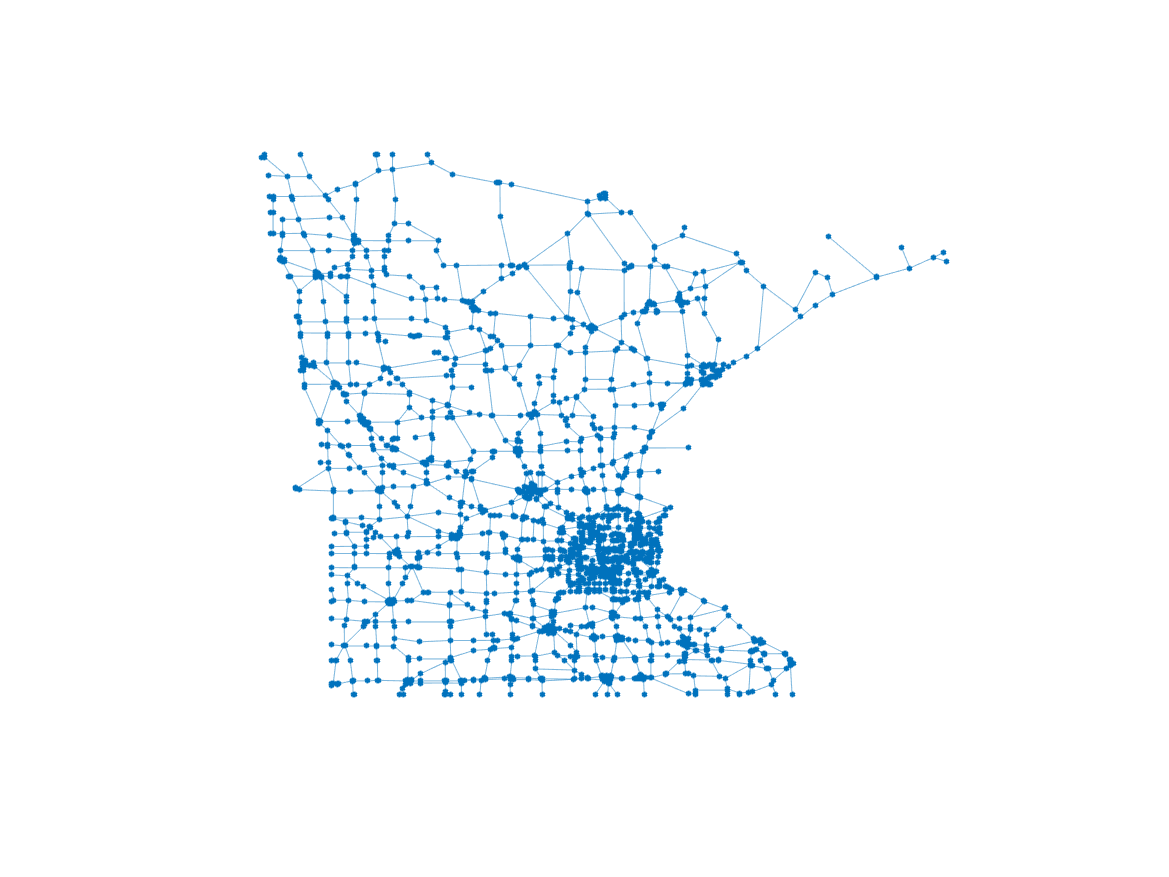
\includegraphics{Figure/minnesota}
\caption[Grafico della rete stradale del Minnesota.]{Grafico della rete stradale del Minnesota. I dati provengo dalla \emph{SuiteSparse Matrix Collection}~\cite{RepMatrici}.}\label{fig::minnesota}
\end{figure}
In particolare, ci concentriamo su alcuni aspetti numerici concernenti l'integrazione del sistema di ODE risultante.
%\newpage

Un primo quesito su cui abbiamo indagato \`e come la scelta dei tassi d'infezione e di recupero influenzassero la scelta dei passi temporali (\emph{time-step}) nei due metodi. Il time-step deve essere scelto sufficientemente piccolo in modo da garantire il controllo dell'errore locale di troncamento.  In particolare, se le condizioni sulla stabilit\`a ci costringono ad utilizzare un passo molto pi\`u piccolo di quanto indicato dall'errore di troncamento locale allora il metodo che abbiamo scelto non \`e ottimale per il problema. Ci\`o accade, ad esempio, se proviamo ad utilizzare un metodo esplicito per risolvere un problema stiff.
	
In Figura~\ref{fig::minnesota_lenght} si pu\`o osservare come varia il numero di time-step  utilizzati dalla  funzione \texttt{ode45} e \texttt{ode15s} per diversi valori dei parametri $\tau$ e $\gamma$. Per tutti le combinazioni dei parametri la funzione \texttt{ode15s} impiega molte meno iterazioni: il modello, dunque, \`e stiff. Un'altra conferma di ci\`o ci viene data anche calcolando il rapporto di stiffness~(Figura~\ref{fig::minnesota_ratiostiff}) nelle condizioni iniziali.\\
\begin{figure}[htbp]
\centering
\subfloat[][$\gamma=0.10$]{% This file was created by matlab2tikz.
%
%The latest updates can be retrieved from
%  http://www.mathworks.com/matlabcentral/fileexchange/22022-matlab2tikz-matlab2tikz
%where you can also make suggestions and rate matlab2tikz.
%
\definecolor{mycolor1}{rgb}{0.00000,0.44700,0.74100}%
\definecolor{mycolor2}{rgb}{0.85000,0.32500,0.09800}%
%
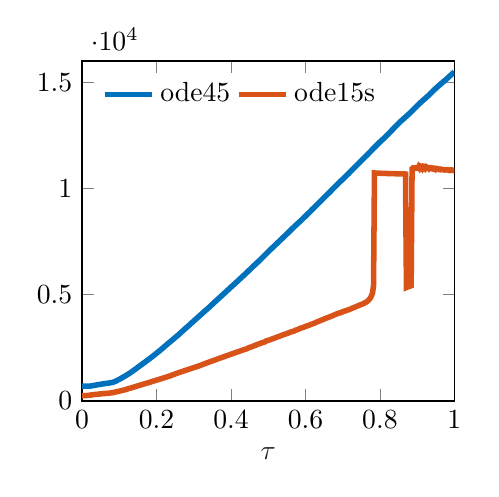
\begin{tikzpicture}

\begin{axis}[%
width=0.39\columnwidth,
height=1.7in,
at={(1.011in,0.642in)},
scale only axis,
xmin=0,
xmax=1,
xlabel style={font=\color{white!15!black}},
xlabel={$\tau$},
ymin=0,
ymax=16000,
axis background/.style={fill=white},
legend columns=2,
legend pos=north west,
legend style={legend cell align=left, align=left, draw=none,fill=none}
]
\addplot [color=mycolor1, line width=2.0pt]
  table[row sep=crcr]{%
0	693\\
0.00252525252525253	693\\
0.00505050505050505	693\\
0.00757575757575758	693\\
0.0101010101010101	693\\
0.0126262626262626	693\\
0.0151515151515152	693\\
0.0176767676767677	693\\
0.0202020202020202	697\\
0.0227272727272727	701\\
0.0252525252525253	709\\
0.0277777777777778	717\\
0.0303030303030303	725\\
0.0328282828282828	733\\
0.0353535353535354	741\\
0.0378787878787879	749\\
0.0404040404040404	757\\
0.0429292929292929	765\\
0.0454545454545455	773\\
0.047979797979798	781\\
0.0505050505050505	785\\
0.053030303030303	793\\
0.0555555555555556	801\\
0.0580808080808081	809\\
0.0606060606060606	813\\
0.0631313131313131	821\\
0.0656565656565657	829\\
0.0681818181818182	833\\
0.0707070707070707	841\\
0.0732323232323232	845\\
0.0757575757575758	853\\
0.0782828282828283	861\\
0.0808080808080808	869\\
0.0833333333333333	881\\
0.0858585858585859	897\\
0.0883838383838384	913\\
0.0909090909090909	933\\
0.0934343434343434	957\\
0.095959595959596	981\\
0.0984848484848485	1001\\
0.101010101010101	1025\\
0.103535353535354	1049\\
0.106060606060606	1077\\
0.108585858585859	1101\\
0.111111111111111	1125\\
0.113636363636364	1153\\
0.116161616161616	1177\\
0.118686868686869	1205\\
0.121212121212121	1233\\
0.123737373737374	1261\\
0.126262626262626	1289\\
0.128787878787879	1317\\
0.131313131313131	1349\\
0.133838383838384	1377\\
0.136363636363636	1409\\
0.138888888888889	1441\\
0.141414141414141	1473\\
0.143939393939394	1505\\
0.146464646464646	1537\\
0.148989898989899	1569\\
0.151515151515152	1605\\
0.154040404040404	1637\\
0.156565656565657	1669\\
0.159090909090909	1701\\
0.161616161616162	1733\\
0.164141414141414	1765\\
0.166666666666667	1797\\
0.169191919191919	1829\\
0.171717171717172	1861\\
0.174242424242424	1897\\
0.176767676767677	1929\\
0.179292929292929	1961\\
0.181818181818182	1993\\
0.184343434343434	2029\\
0.186868686868687	2065\\
0.189393939393939	2097\\
0.191919191919192	2133\\
0.194444444444444	2165\\
0.196969696969697	2201\\
0.19949494949495	2237\\
0.202020202020202	2273\\
0.204545454545455	2309\\
0.207070707070707	2345\\
0.20959595959596	2381\\
0.212121212121212	2417\\
0.214646464646465	2453\\
0.217171717171717	2493\\
0.21969696969697	2533\\
0.222222222222222	2569\\
0.224747474747475	2609\\
0.227272727272727	2645\\
0.22979797979798	2685\\
0.232323232323232	2721\\
0.234848484848485	2757\\
0.237373737373737	2793\\
0.23989898989899	2829\\
0.242424242424242	2869\\
0.244949494949495	2905\\
0.247474747474747	2945\\
0.25	2981\\
0.25	2981\\
0.252525252525253	3017\\
0.255050505050505	3053\\
0.257575757575758	3093\\
0.26010101010101	3133\\
0.262626262626263	3173\\
0.265151515151515	3213\\
0.267676767676768	3253\\
0.27020202020202	3293\\
0.272727272727273	3333\\
0.275252525252525	3373\\
0.277777777777778	3413\\
0.28030303030303	3449\\
0.282828282828283	3489\\
0.285353535353535	3529\\
0.287878787878788	3569\\
0.29040404040404	3609\\
0.292929292929293	3649\\
0.295454545454545	3689\\
0.297979797979798	3729\\
0.30050505050505	3769\\
0.303030303030303	3809\\
0.305555555555556	3849\\
0.308080808080808	3889\\
0.310606060606061	3929\\
0.313131313131313	3969\\
0.315656565656566	4009\\
0.318181818181818	4045\\
0.320707070707071	4085\\
0.323232323232323	4125\\
0.325757575757576	4165\\
0.328282828282828	4205\\
0.330808080808081	4245\\
0.333333333333333	4281\\
0.335858585858586	4321\\
0.338383838383838	4361\\
0.340909090909091	4397\\
0.343434343434343	4437\\
0.345959595959596	4481\\
0.348484848484849	4525\\
0.351010101010101	4565\\
0.353535353535354	4609\\
0.356060606060606	4649\\
0.358585858585859	4689\\
0.361111111111111	4729\\
0.363636363636364	4769\\
0.366161616161616	4809\\
0.368686868686869	4849\\
0.371212121212121	4889\\
0.373737373737374	4929\\
0.376262626262626	4973\\
0.378787878787879	5013\\
0.381313131313131	5053\\
0.383838383838384	5093\\
0.386363636363636	5137\\
0.388888888888889	5177\\
0.391414141414141	5217\\
0.393939393939394	5257\\
0.396464646464646	5297\\
0.398989898989899	5341\\
0.401515151515151	5381\\
0.404040404040404	5421\\
0.406565656565657	5461\\
0.409090909090909	5501\\
0.411616161616162	5541\\
0.414141414141414	5581\\
0.416666666666667	5621\\
0.419191919191919	5661\\
0.421717171717172	5705\\
0.424242424242424	5745\\
0.426767676767677	5785\\
0.429292929292929	5825\\
0.431818181818182	5869\\
0.434343434343434	5909\\
0.436868686868687	5949\\
0.439393939393939	5993\\
0.441919191919192	6037\\
0.444444444444444	6077\\
0.446969696969697	6121\\
0.44949494949495	6161\\
0.452020202020202	6205\\
0.454545454545455	6249\\
0.457070707070707	6289\\
0.45959595959596	6333\\
0.462121212121212	6373\\
0.464646464646465	6413\\
0.467171717171717	6453\\
0.46969696969697	6497\\
0.472222222222222	6537\\
0.474747474747475	6581\\
0.477272727272727	6625\\
0.47979797979798	6669\\
0.482323232323232	6713\\
0.484848484848485	6753\\
0.487373737373737	6797\\
0.48989898989899	6841\\
0.492424242424242	6885\\
0.494949494949495	6929\\
0.497474747474748	6977\\
0.5	7021\\
0.5	7021\\
0.502525252525252	7061\\
0.505050505050505	7105\\
0.507575757575758	7149\\
0.51010101010101	7189\\
0.512626262626263	7233\\
0.515151515151515	7273\\
0.517676767676768	7317\\
0.52020202020202	7361\\
0.522727272727273	7401\\
0.525252525252525	7445\\
0.527777777777778	7485\\
0.53030303030303	7529\\
0.532828282828283	7569\\
0.535353535353535	7613\\
0.537878787878788	7653\\
0.54040404040404	7697\\
0.542929292929293	7741\\
0.545454545454545	7781\\
0.547979797979798	7825\\
0.55050505050505	7865\\
0.553030303030303	7909\\
0.555555555555556	7953\\
0.558080808080808	7997\\
0.560606060606061	8041\\
0.563131313131313	8085\\
0.565656565656566	8129\\
0.568181818181818	8169\\
0.570707070707071	8213\\
0.573232323232323	8253\\
0.575757575757576	8293\\
0.578282828282828	8337\\
0.580808080808081	8377\\
0.583333333333333	8417\\
0.585858585858586	8457\\
0.588383838383838	8501\\
0.590909090909091	8541\\
0.593434343434343	8585\\
0.595959595959596	8629\\
0.598484848484849	8669\\
0.601010101010101	8713\\
0.603535353535354	8757\\
0.606060606060606	8801\\
0.608585858585859	8845\\
0.611111111111111	8885\\
0.613636363636364	8929\\
0.616161616161616	8977\\
0.618686868686869	9021\\
0.621212121212121	9065\\
0.623737373737374	9109\\
0.626262626262626	9153\\
0.628787878787879	9197\\
0.631313131313131	9241\\
0.633838383838384	9285\\
0.636363636363636	9329\\
0.638888888888889	9369\\
0.641414141414141	9413\\
0.643939393939394	9457\\
0.646464646464646	9501\\
0.648989898989899	9545\\
0.651515151515151	9589\\
0.654040404040404	9633\\
0.656565656565657	9677\\
0.659090909090909	9721\\
0.661616161616162	9765\\
0.664141414141414	9809\\
0.666666666666667	9853\\
0.669191919191919	9897\\
0.671717171717172	9945\\
0.674242424242424	9989\\
0.676767676767677	10037\\
0.679292929292929	10081\\
0.681818181818182	10125\\
0.684343434343434	10169\\
0.686868686868687	10213\\
0.689393939393939	10257\\
0.691919191919192	10297\\
0.694444444444444	10341\\
0.696969696969697	10381\\
0.69949494949495	10425\\
0.702020202020202	10469\\
0.704545454545455	10509\\
0.707070707070707	10553\\
0.70959595959596	10597\\
0.712121212121212	10641\\
0.714646464646465	10681\\
0.717171717171717	10725\\
0.71969696969697	10773\\
0.722222222222222	10817\\
0.724747474747475	10861\\
0.727272727272727	10905\\
0.72979797979798	10953\\
0.732323232323232	10997\\
0.734848484848485	11041\\
0.737373737373737	11085\\
0.73989898989899	11133\\
0.742424242424242	11177\\
0.744949494949495	11221\\
0.747474747474748	11265\\
0.75	11309\\
0.75	11309\\
0.752525252525252	11353\\
0.755050505050505	11397\\
0.757575757575758	11441\\
0.76010101010101	11481\\
0.762626262626263	11525\\
0.765151515151515	11565\\
0.767676767676768	11613\\
0.77020202020202	11657\\
0.772727272727273	11705\\
0.775252525252525	11749\\
0.777777777777778	11797\\
0.78030303030303	11841\\
0.782828282828283	11889\\
0.785353535353535	11933\\
0.787878787878788	11977\\
0.79040404040404	12021\\
0.792929292929293	12065\\
0.795454545454545	12109\\
0.797979797979798	12153\\
0.80050505050505	12193\\
0.803030303030303	12233\\
0.805555555555556	12277\\
0.808080808080808	12317\\
0.810606060606061	12357\\
0.813131313131313	12401\\
0.815656565656566	12441\\
0.818181818181818	12485\\
0.820707070707071	12529\\
0.823232323232323	12577\\
0.825757575757576	12621\\
0.828282828282828	12669\\
0.830808080808081	12713\\
0.833333333333333	12761\\
0.835858585858586	12805\\
0.838383838383838	12853\\
0.840909090909091	12897\\
0.843434343434343	12941\\
0.845959595959596	12985\\
0.848484848484849	13029\\
0.851010101010101	13073\\
0.853535353535354	13117\\
0.856060606060606	13161\\
0.858585858585859	13201\\
0.861111111111111	13241\\
0.863636363636364	13281\\
0.866161616161616	13321\\
0.868686868686869	13361\\
0.871212121212121	13397\\
0.873737373737374	13437\\
0.876262626262626	13477\\
0.878787878787879	13517\\
0.881313131313131	13557\\
0.883838383838384	13601\\
0.886363636363636	13645\\
0.888888888888889	13693\\
0.891414141414141	13737\\
0.893939393939394	13781\\
0.896464646464646	13825\\
0.898989898989899	13873\\
0.901515151515151	13917\\
0.904040404040404	13957\\
0.906565656565657	14001\\
0.909090909090909	14041\\
0.911616161616162	14081\\
0.914141414141414	14121\\
0.916666666666667	14161\\
0.919191919191919	14197\\
0.921717171717172	14237\\
0.924242424242424	14277\\
0.926767676767677	14317\\
0.929292929292929	14357\\
0.931818181818182	14401\\
0.934343434343434	14445\\
0.936868686868687	14489\\
0.939393939393939	14533\\
0.941919191919192	14577\\
0.944444444444444	14617\\
0.946969696969697	14661\\
0.94949494949495	14701\\
0.952020202020202	14741\\
0.954545454545455	14781\\
0.957070707070707	14821\\
0.95959595959596	14861\\
0.962121212121212	14897\\
0.964646464646465	14937\\
0.967171717171717	14973\\
0.96969696969697	15013\\
0.972222222222222	15049\\
0.974747474747475	15085\\
0.977272727272727	15125\\
0.97979797979798	15165\\
0.982323232323232	15205\\
0.984848484848485	15245\\
0.987373737373737	15285\\
0.98989898989899	15325\\
0.992424242424242	15365\\
0.994949494949495	15405\\
0.997474747474748	15445\\
1	15485\\
};
\addlegendentry{ode45}

\addplot [color=mycolor2, line width=2.0pt]
  table[row sep=crcr]{%
0	253\\
0.00252525252525253	253\\
0.00505050505050505	253\\
0.00757575757575758	253\\
0.0101010101010101	253\\
0.0126262626262626	255\\
0.0151515151515152	259\\
0.0176767676767677	265\\
0.0202020202020202	271\\
0.0227272727272727	277\\
0.0252525252525253	282\\
0.0277777777777778	288\\
0.0303030303030303	295\\
0.0328282828282828	300\\
0.0353535353535354	305\\
0.0378787878787879	311\\
0.0404040404040404	312\\
0.0429292929292929	320\\
0.0454545454545455	324\\
0.047979797979798	329\\
0.0505050505050505	333\\
0.053030303030303	338\\
0.0555555555555556	342\\
0.0580808080808081	346\\
0.0606060606060606	350\\
0.0631313131313131	354\\
0.0656565656565657	358\\
0.0681818181818182	361\\
0.0707070707070707	365\\
0.0732323232323232	369\\
0.0757575757575758	373\\
0.0782828282828283	380\\
0.0808080808080808	387\\
0.0833333333333333	395\\
0.0858585858585859	403\\
0.0883838383838384	415\\
0.0909090909090909	424\\
0.0934343434343434	434\\
0.095959595959596	443\\
0.0984848484848485	454\\
0.101010101010101	464\\
0.103535353535354	475\\
0.106060606060606	486\\
0.108585858585859	497\\
0.111111111111111	509\\
0.113636363636364	522\\
0.116161616161616	529\\
0.118686868686869	543\\
0.121212121212121	557\\
0.123737373737374	574\\
0.126262626262626	588\\
0.128787878787879	597\\
0.131313131313131	611\\
0.133838383838384	625\\
0.136363636363636	638\\
0.138888888888889	652\\
0.141414141414141	665\\
0.143939393939394	679\\
0.146464646464646	692\\
0.148989898989899	706\\
0.151515151515152	719\\
0.154040404040404	732\\
0.156565656565657	745\\
0.159090909090909	759\\
0.161616161616162	773\\
0.164141414141414	786\\
0.166666666666667	800\\
0.169191919191919	813\\
0.171717171717172	826\\
0.174242424242424	840\\
0.176767676767677	853\\
0.179292929292929	866\\
0.181818181818182	880\\
0.184343434343434	894\\
0.186868686868687	908\\
0.189393939393939	922\\
0.191919191919192	935\\
0.194444444444444	949\\
0.196969696969697	962\\
0.19949494949495	976\\
0.202020202020202	989\\
0.204545454545455	1002\\
0.207070707070707	1017\\
0.20959595959596	1031\\
0.212121212121212	1044\\
0.214646464646465	1059\\
0.217171717171717	1072\\
0.21969696969697	1088\\
0.222222222222222	1099\\
0.224747474747475	1115\\
0.227272727272727	1128\\
0.22979797979798	1145\\
0.232323232323232	1157\\
0.234848484848485	1169\\
0.237373737373737	1186\\
0.23989898989899	1204\\
0.242424242424242	1219\\
0.244949494949495	1236\\
0.247474747474747	1252\\
0.25	1272\\
0.25	1272\\
0.252525252525253	1289\\
0.255050505050505	1302\\
0.257575757575758	1319\\
0.26010101010101	1335\\
0.262626262626263	1351\\
0.265151515151515	1366\\
0.267676767676768	1380\\
0.27020202020202	1395\\
0.272727272727273	1409\\
0.275252525252525	1424\\
0.277777777777778	1439\\
0.28030303030303	1453\\
0.282828282828283	1467\\
0.285353535353535	1481\\
0.287878787878788	1496\\
0.29040404040404	1511\\
0.292929292929293	1526\\
0.295454545454545	1541\\
0.297979797979798	1555\\
0.30050505050505	1570\\
0.303030303030303	1585\\
0.305555555555556	1600\\
0.308080808080808	1614\\
0.310606060606061	1629\\
0.313131313131313	1644\\
0.315656565656566	1660\\
0.318181818181818	1675\\
0.320707070707071	1693\\
0.323232323232323	1711\\
0.325757575757576	1729\\
0.328282828282828	1745\\
0.330808080808081	1762\\
0.333333333333333	1779\\
0.335858585858586	1794\\
0.338383838383838	1810\\
0.340909090909091	1825\\
0.343434343434343	1844\\
0.345959595959596	1860\\
0.348484848484849	1876\\
0.351010101010101	1890\\
0.353535353535354	1907\\
0.356060606060606	1922\\
0.358585858585859	1938\\
0.361111111111111	1953\\
0.363636363636364	1970\\
0.366161616161616	1988\\
0.368686868686869	2005\\
0.371212121212121	2021\\
0.373737373737374	2033\\
0.376262626262626	2051\\
0.378787878787879	2067\\
0.381313131313131	2083\\
0.383838383838384	2099\\
0.386363636363636	2114\\
0.388888888888889	2130\\
0.391414141414141	2144\\
0.393939393939394	2160\\
0.396464646464646	2176\\
0.398989898989899	2194\\
0.401515151515151	2207\\
0.404040404040404	2222\\
0.406565656565657	2239\\
0.409090909090909	2255\\
0.411616161616162	2271\\
0.414141414141414	2287\\
0.416666666666667	2304\\
0.419191919191919	2317\\
0.421717171717172	2332\\
0.424242424242424	2349\\
0.426767676767677	2365\\
0.429292929292929	2381\\
0.431818181818182	2398\\
0.434343434343434	2410\\
0.436868686868687	2424\\
0.439393939393939	2438\\
0.441919191919192	2453\\
0.444444444444444	2471\\
0.446969696969697	2493\\
0.44949494949495	2519\\
0.452020202020202	2532\\
0.454545454545455	2542\\
0.457070707070707	2559\\
0.45959595959596	2577\\
0.462121212121212	2596\\
0.464646464646465	2613\\
0.467171717171717	2628\\
0.46969696969697	2655\\
0.472222222222222	2670\\
0.474747474747475	2682\\
0.477272727272727	2698\\
0.47979797979798	2715\\
0.482323232323232	2732\\
0.484848484848485	2745\\
0.487373737373737	2757\\
0.48989898989899	2776\\
0.492424242424242	2792\\
0.494949494949495	2827\\
0.497474747474748	2844\\
0.5	2848\\
0.5	2848\\
0.502525252525252	2865\\
0.505050505050505	2881\\
0.507575757575758	2896\\
0.51010101010101	2917\\
0.512626262626263	2933\\
0.515151515151515	2946\\
0.517676767676768	2964\\
0.52020202020202	2979\\
0.522727272727273	2997\\
0.525252525252525	3014\\
0.527777777777778	3028\\
0.53030303030303	3048\\
0.532828282828283	3063\\
0.535353535353535	3081\\
0.537878787878788	3097\\
0.54040404040404	3114\\
0.542929292929293	3126\\
0.545454545454545	3143\\
0.547979797979798	3159\\
0.55050505050505	3175\\
0.553030303030303	3193\\
0.555555555555556	3211\\
0.558080808080808	3227\\
0.560606060606061	3244\\
0.563131313131313	3262\\
0.565656565656566	3269\\
0.568181818181818	3283\\
0.570707070707071	3301\\
0.573232323232323	3328\\
0.575757575757576	3340\\
0.578282828282828	3357\\
0.580808080808081	3374\\
0.583333333333333	3391\\
0.585858585858586	3418\\
0.588383838383838	3430\\
0.590909090909091	3443\\
0.593434343434343	3460\\
0.595959595959596	3474\\
0.598484848484849	3495\\
0.601010101010101	3512\\
0.603535353535354	3529\\
0.606060606060606	3540\\
0.608585858585859	3561\\
0.611111111111111	3573\\
0.613636363636364	3595\\
0.616161616161616	3611\\
0.618686868686869	3627\\
0.621212121212121	3643\\
0.623737373737374	3659\\
0.626262626262626	3680\\
0.628787878787879	3703\\
0.631313131313131	3719\\
0.633838383838384	3741\\
0.636363636363636	3755\\
0.638888888888889	3771\\
0.641414141414141	3790\\
0.643939393939394	3812\\
0.646464646464646	3825\\
0.648989898989899	3843\\
0.651515151515151	3864\\
0.654040404040404	3883\\
0.656565656565657	3901\\
0.659090909090909	3918\\
0.661616161616162	3932\\
0.664141414141414	3951\\
0.666666666666667	3967\\
0.669191919191919	3985\\
0.671717171717172	4004\\
0.674242424242424	4024\\
0.676767676767677	4043\\
0.679292929292929	4062\\
0.681818181818182	4081\\
0.684343434343434	4099\\
0.686868686868687	4112\\
0.689393939393939	4132\\
0.691919191919192	4144\\
0.694444444444444	4151\\
0.696969696969697	4168\\
0.69949494949495	4198\\
0.702020202020202	4210\\
0.704545454545455	4225\\
0.707070707070707	4239\\
0.70959595959596	4254\\
0.712121212121212	4271\\
0.714646464646465	4286\\
0.717171717171717	4303\\
0.71969696969697	4317\\
0.722222222222222	4337\\
0.724747474747475	4357\\
0.727272727272727	4374\\
0.72979797979798	4392\\
0.732323232323232	4412\\
0.734848484848485	4431\\
0.737373737373737	4447\\
0.73989898989899	4467\\
0.742424242424242	4487\\
0.744949494949495	4506\\
0.747474747474748	4523\\
0.75	4542\\
0.75	4542\\
0.752525252525252	4560\\
0.755050505050505	4576\\
0.757575757575758	4599\\
0.76010101010101	4625\\
0.762626262626263	4646\\
0.765151515151515	4675\\
0.767676767676768	4711\\
0.77020202020202	4754\\
0.772727272727273	4809\\
0.775252525252525	4875\\
0.777777777777778	4968\\
0.78030303030303	5101\\
0.782828282828283	5423\\
0.785353535353535	10728\\
0.787878787878788	10726\\
0.79040404040404	10725\\
0.792929292929293	10722\\
0.795454545454545	10719\\
0.797979797979798	10718\\
0.80050505050505	10716\\
0.803030303030303	10711\\
0.805555555555556	10712\\
0.808080808080808	10710\\
0.810606060606061	10708\\
0.813131313131313	10706\\
0.815656565656566	10706\\
0.818181818181818	10704\\
0.820707070707071	10703\\
0.823232323232323	10700\\
0.825757575757576	10700\\
0.828282828282828	10698\\
0.830808080808081	10697\\
0.833333333333333	10695\\
0.835858585858586	10696\\
0.838383838383838	10694\\
0.840909090909091	10693\\
0.843434343434343	10691\\
0.845959595959596	10693\\
0.848484848484849	10687\\
0.851010101010101	10690\\
0.853535353535354	10685\\
0.856060606060606	10686\\
0.858585858585859	10685\\
0.861111111111111	10685\\
0.863636363636364	10681\\
0.866161616161616	10684\\
0.868686868686869	10678\\
0.871212121212121	5339\\
0.873737373737374	5357\\
0.876262626262626	5376\\
0.878787878787879	5391\\
0.881313131313131	5401\\
0.883838383838384	5423\\
0.886363636363636	10925\\
0.888888888888889	10964\\
0.891414141414141	10950\\
0.893939393939394	10966\\
0.896464646464646	10953\\
0.898989898989899	10972\\
0.901515151515151	10956\\
0.904040404040404	11030\\
0.906565656565657	10961\\
0.909090909090909	11042\\
0.911616161616162	11019\\
0.914141414141414	10951\\
0.916666666666667	11032\\
0.919191919191919	11010\\
0.921717171717172	10950\\
0.924242424242424	11021\\
0.926767676767677	10998\\
0.929292929292929	10980\\
0.931818181818182	10931\\
0.934343434343434	10974\\
0.936868686868687	10977\\
0.939393939393939	10928\\
0.941919191919192	10915\\
0.944444444444444	10952\\
0.946969696969697	10940\\
0.94949494949495	10898\\
0.952020202020202	10940\\
0.954545454545455	10931\\
0.957070707070707	10920\\
0.95959595959596	10884\\
0.962121212121212	10879\\
0.964646464646465	10906\\
0.967171717171717	10894\\
0.96969696969697	10886\\
0.972222222222222	10870\\
0.974747474747475	10866\\
0.977272727272727	10884\\
0.97979797979798	10879\\
0.982323232323232	10875\\
0.984848484848485	10849\\
0.987373737373737	10845\\
0.98989898989899	10875\\
0.992424242424242	10872\\
0.994949494949495	10866\\
0.997474747474748	10842\\
1	10845\\
};
\addlegendentry{ode15s}
\end{axis}
\end{tikzpicture}%}
\subfloat[][$\gamma=0.30$]{% This file was created by matlab2tikz.
%
%The latest updates can be retrieved from
%  http://www.mathworks.com/matlabcentral/fileexchange/22022-matlab2tikz-matlab2tikz
%where you can also make suggestions and rate matlab2tikz.
%
\definecolor{mycolor1}{rgb}{0.00000,0.44700,0.74100}%
\definecolor{mycolor2}{rgb}{0.85000,0.32500,0.09800}%
%
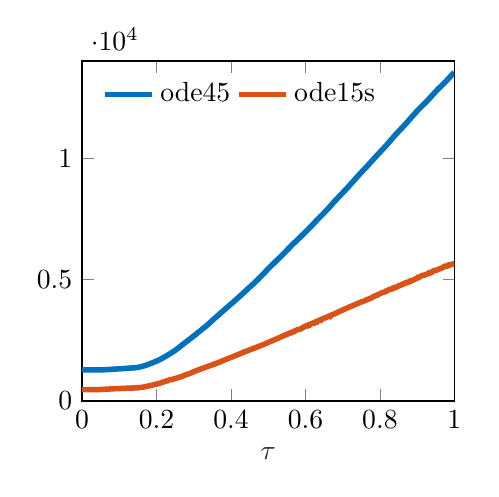
\begin{tikzpicture}

\begin{axis}[%
width=0.39\columnwidth,
height=1.7in,
at={(1.011in,0.642in)},
scale only axis,
xmin=0,
xmax=1,
xlabel style={font=\color{white!15!black}},
xlabel={$\tau$},
ymin=0,
ymax=14000,
legend columns=2,
legend pos=north west,
legend style={legend cell align=left, align=left, draw=none,fill=none}
]
\addplot [color=mycolor1, line width=2.0pt]
  table[row sep=crcr]{%
0	1281\\
0.00252525252525253	1281\\
0.00505050505050505	1281\\
0.00757575757575758	1281\\
0.0101010101010101	1281\\
0.0126262626262626	1281\\
0.0151515151515152	1281\\
0.0176767676767677	1281\\
0.0202020202020202	1281\\
0.0227272727272727	1281\\
0.0252525252525253	1281\\
0.0277777777777778	1281\\
0.0303030303030303	1281\\
0.0328282828282828	1281\\
0.0353535353535354	1281\\
0.0378787878787879	1281\\
0.0404040404040404	1281\\
0.0429292929292929	1281\\
0.0454545454545455	1281\\
0.047979797979798	1281\\
0.0505050505050505	1281\\
0.053030303030303	1281\\
0.0555555555555556	1281\\
0.0580808080808081	1285\\
0.0606060606060606	1285\\
0.0631313131313131	1289\\
0.0656565656565657	1289\\
0.0681818181818182	1293\\
0.0707070707070707	1293\\
0.0732323232323232	1297\\
0.0757575757575758	1297\\
0.0782828282828283	1301\\
0.0808080808080808	1305\\
0.0833333333333333	1305\\
0.0858585858585859	1309\\
0.0883838383838384	1309\\
0.0909090909090909	1313\\
0.0934343434343434	1317\\
0.095959595959596	1317\\
0.0984848484848485	1321\\
0.101010101010101	1325\\
0.103535353535354	1325\\
0.106060606060606	1329\\
0.108585858585859	1333\\
0.111111111111111	1333\\
0.113636363636364	1337\\
0.116161616161616	1341\\
0.118686868686869	1341\\
0.121212121212121	1345\\
0.123737373737374	1349\\
0.126262626262626	1349\\
0.128787878787879	1353\\
0.131313131313131	1357\\
0.133838383838384	1357\\
0.136363636363636	1361\\
0.138888888888889	1365\\
0.141414141414141	1365\\
0.143939393939394	1369\\
0.146464646464646	1373\\
0.148989898989899	1381\\
0.151515151515152	1389\\
0.154040404040404	1397\\
0.156565656565657	1405\\
0.159090909090909	1413\\
0.161616161616162	1425\\
0.164141414141414	1433\\
0.166666666666667	1445\\
0.169191919191919	1457\\
0.171717171717172	1473\\
0.174242424242424	1485\\
0.176767676767677	1497\\
0.179292929292929	1513\\
0.181818181818182	1529\\
0.184343434343434	1541\\
0.186868686868687	1557\\
0.189393939393939	1573\\
0.191919191919192	1589\\
0.194444444444444	1605\\
0.196969696969697	1621\\
0.19949494949495	1637\\
0.202020202020202	1653\\
0.204545454545455	1673\\
0.207070707070707	1689\\
0.20959595959596	1709\\
0.212121212121212	1729\\
0.214646464646465	1749\\
0.217171717171717	1773\\
0.21969696969697	1793\\
0.222222222222222	1817\\
0.224747474747475	1837\\
0.227272727272727	1861\\
0.22979797979798	1885\\
0.232323232323232	1909\\
0.234848484848485	1933\\
0.237373737373737	1957\\
0.23989898989899	1981\\
0.242424242424242	2005\\
0.244949494949495	2029\\
0.247474747474747	2057\\
0.25	2081\\
0.25	2081\\
0.252525252525253	2109\\
0.255050505050505	2137\\
0.257575757575758	2169\\
0.26010101010101	2197\\
0.262626262626263	2229\\
0.265151515151515	2261\\
0.267676767676768	2293\\
0.27020202020202	2321\\
0.272727272727273	2353\\
0.275252525252525	2381\\
0.277777777777778	2413\\
0.28030303030303	2441\\
0.282828282828283	2469\\
0.285353535353535	2501\\
0.287878787878788	2529\\
0.29040404040404	2561\\
0.292929292929293	2589\\
0.295454545454545	2621\\
0.297979797979798	2653\\
0.30050505050505	2681\\
0.303030303030303	2713\\
0.305555555555556	2741\\
0.308080808080808	2773\\
0.310606060606061	2805\\
0.313131313131313	2837\\
0.315656565656566	2865\\
0.318181818181818	2897\\
0.320707070707071	2929\\
0.323232323232323	2961\\
0.325757575757576	2993\\
0.328282828282828	3021\\
0.330808080808081	3053\\
0.333333333333333	3085\\
0.335858585858586	3117\\
0.338383838383838	3153\\
0.340909090909091	3185\\
0.343434343434343	3221\\
0.345959595959596	3257\\
0.348484848484849	3293\\
0.351010101010101	3329\\
0.353535353535354	3365\\
0.356060606060606	3401\\
0.358585858585859	3433\\
0.361111111111111	3465\\
0.363636363636364	3501\\
0.366161616161616	3533\\
0.368686868686869	3569\\
0.371212121212121	3601\\
0.373737373737374	3637\\
0.376262626262626	3673\\
0.378787878787879	3705\\
0.381313131313131	3741\\
0.383838383838384	3773\\
0.386363636363636	3809\\
0.388888888888889	3841\\
0.391414141414141	3873\\
0.393939393939394	3909\\
0.396464646464646	3941\\
0.398989898989899	3977\\
0.401515151515151	4009\\
0.404040404040404	4045\\
0.406565656565657	4077\\
0.409090909090909	4113\\
0.411616161616162	4145\\
0.414141414141414	4181\\
0.416666666666667	4213\\
0.419191919191919	4249\\
0.421717171717172	4285\\
0.424242424242424	4317\\
0.426767676767677	4353\\
0.429292929292929	4389\\
0.431818181818182	4425\\
0.434343434343434	4461\\
0.436868686868687	4497\\
0.439393939393939	4533\\
0.441919191919192	4569\\
0.444444444444444	4605\\
0.446969696969697	4641\\
0.44949494949495	4677\\
0.452020202020202	4709\\
0.454545454545455	4745\\
0.457070707070707	4781\\
0.45959595959596	4813\\
0.462121212121212	4849\\
0.464646464646465	4889\\
0.467171717171717	4925\\
0.46969696969697	4965\\
0.472222222222222	5001\\
0.474747474747475	5041\\
0.477272727272727	5081\\
0.47979797979798	5121\\
0.482323232323232	5157\\
0.484848484848485	5197\\
0.487373737373737	5237\\
0.48989898989899	5277\\
0.492424242424242	5317\\
0.494949494949495	5361\\
0.497474747474748	5401\\
0.5	5441\\
0.5	5441\\
0.502525252525252	5481\\
0.505050505050505	5521\\
0.507575757575758	5557\\
0.51010101010101	5593\\
0.512626262626263	5633\\
0.515151515151515	5669\\
0.517676767676768	5709\\
0.52020202020202	5745\\
0.522727272727273	5785\\
0.525252525252525	5821\\
0.527777777777778	5861\\
0.53030303030303	5897\\
0.532828282828283	5937\\
0.535353535353535	5973\\
0.537878787878788	6013\\
0.54040404040404	6053\\
0.542929292929293	6093\\
0.545454545454545	6129\\
0.547979797979798	6169\\
0.55050505050505	6209\\
0.553030303030303	6249\\
0.555555555555556	6289\\
0.558080808080808	6329\\
0.560606060606061	6369\\
0.563131313131313	6409\\
0.565656565656566	6445\\
0.568181818181818	6485\\
0.570707070707071	6521\\
0.573232323232323	6557\\
0.575757575757576	6597\\
0.578282828282828	6633\\
0.580808080808081	6669\\
0.583333333333333	6705\\
0.585858585858586	6745\\
0.588383838383838	6781\\
0.590909090909091	6821\\
0.593434343434343	6857\\
0.595959595959596	6893\\
0.598484848484849	6933\\
0.601010101010101	6973\\
0.603535353535354	7013\\
0.606060606060606	7049\\
0.608585858585859	7089\\
0.611111111111111	7129\\
0.613636363636364	7169\\
0.616161616161616	7209\\
0.618686868686869	7249\\
0.621212121212121	7289\\
0.623737373737374	7329\\
0.626262626262626	7373\\
0.628787878787879	7413\\
0.631313131313131	7453\\
0.633838383838384	7493\\
0.636363636363636	7533\\
0.638888888888889	7573\\
0.641414141414141	7613\\
0.643939393939394	7649\\
0.646464646464646	7689\\
0.648989898989899	7729\\
0.651515151515151	7769\\
0.654040404040404	7813\\
0.656565656565657	7853\\
0.659090909090909	7893\\
0.661616161616162	7933\\
0.664141414141414	7973\\
0.666666666666667	8017\\
0.669191919191919	8061\\
0.671717171717172	8105\\
0.674242424242424	8149\\
0.676767676767677	8193\\
0.679292929292929	8237\\
0.681818181818182	8277\\
0.684343434343434	8321\\
0.686868686868687	8361\\
0.689393939393939	8401\\
0.691919191919192	8441\\
0.694444444444444	8481\\
0.696969696969697	8521\\
0.69949494949495	8561\\
0.702020202020202	8605\\
0.704545454545455	8645\\
0.707070707070707	8685\\
0.70959595959596	8725\\
0.712121212121212	8769\\
0.714646464646465	8809\\
0.717171717171717	8853\\
0.71969696969697	8897\\
0.722222222222222	8941\\
0.724747474747475	8981\\
0.727272727272727	9025\\
0.72979797979798	9069\\
0.732323232323232	9113\\
0.734848484848485	9157\\
0.737373737373737	9197\\
0.73989898989899	9241\\
0.742424242424242	9285\\
0.744949494949495	9325\\
0.747474747474748	9369\\
0.75	9409\\
0.75	9409\\
0.752525252525252	9453\\
0.755050505050505	9493\\
0.757575757575758	9533\\
0.76010101010101	9573\\
0.762626262626263	9617\\
0.765151515151515	9657\\
0.767676767676768	9701\\
0.77020202020202	9745\\
0.772727272727273	9785\\
0.775252525252525	9829\\
0.777777777777778	9873\\
0.78030303030303	9913\\
0.782828282828283	9957\\
0.785353535353535	10001\\
0.787878787878788	10041\\
0.79040404040404	10085\\
0.792929292929293	10125\\
0.795454545454545	10169\\
0.797979797979798	10209\\
0.80050505050505	10249\\
0.803030303030303	10293\\
0.805555555555556	10333\\
0.808080808080808	10373\\
0.810606060606061	10413\\
0.813131313131313	10457\\
0.815656565656566	10497\\
0.818181818181818	10541\\
0.820707070707071	10589\\
0.823232323232323	10633\\
0.825757575757576	10673\\
0.828282828282828	10721\\
0.830808080808081	10765\\
0.833333333333333	10809\\
0.835858585858586	10857\\
0.838383838383838	10901\\
0.840909090909091	10945\\
0.843434343434343	10989\\
0.845959595959596	11029\\
0.848484848484849	11073\\
0.851010101010101	11113\\
0.853535353535354	11153\\
0.856060606060606	11193\\
0.858585858585859	11233\\
0.861111111111111	11273\\
0.863636363636364	11313\\
0.866161616161616	11357\\
0.868686868686869	11401\\
0.871212121212121	11441\\
0.873737373737374	11489\\
0.876262626262626	11533\\
0.878787878787879	11577\\
0.881313131313131	11621\\
0.883838383838384	11665\\
0.886363636363636	11709\\
0.888888888888889	11749\\
0.891414141414141	11793\\
0.893939393939394	11837\\
0.896464646464646	11881\\
0.898989898989899	11925\\
0.901515151515151	11969\\
0.904040404040404	12009\\
0.906565656565657	12049\\
0.909090909090909	12085\\
0.911616161616162	12125\\
0.914141414141414	12161\\
0.916666666666667	12197\\
0.919191919191919	12237\\
0.921717171717172	12273\\
0.924242424242424	12313\\
0.926767676767677	12349\\
0.929292929292929	12393\\
0.931818181818182	12433\\
0.934343434343434	12477\\
0.936868686868687	12521\\
0.939393939393939	12565\\
0.941919191919192	12609\\
0.944444444444444	12653\\
0.946969696969697	12693\\
0.94949494949495	12737\\
0.952020202020202	12777\\
0.954545454545455	12817\\
0.957070707070707	12857\\
0.95959595959596	12893\\
0.962121212121212	12933\\
0.964646464646465	12969\\
0.967171717171717	13005\\
0.96969696969697	13041\\
0.972222222222222	13081\\
0.974747474747475	13121\\
0.977272727272727	13161\\
0.97979797979798	13201\\
0.982323232323232	13245\\
0.984848484848485	13289\\
0.987373737373737	13329\\
0.98989898989899	13373\\
0.992424242424242	13413\\
0.994949494949495	13449\\
0.997474747474748	13489\\
1	13529\\
};
\addlegendentry{ode45}

\addplot [color=mycolor2, line width=2.0pt]
  table[row sep=crcr]{%
0	464\\
0.00252525252525253	464\\
0.00505050505050505	464\\
0.00757575757575758	464\\
0.0101010101010101	464\\
0.0126262626262626	464\\
0.0151515151515152	464\\
0.0176767676767677	464\\
0.0202020202020202	464\\
0.0227272727272727	464\\
0.0252525252525253	464\\
0.0277777777777778	464\\
0.0303030303030303	465\\
0.0328282828282828	465\\
0.0353535353535354	466\\
0.0378787878787879	467\\
0.0404040404040404	468\\
0.0429292929292929	469\\
0.0454545454545455	470\\
0.047979797979798	471\\
0.0505050505050505	473\\
0.053030303030303	475\\
0.0555555555555556	477\\
0.0580808080808081	479\\
0.0606060606060606	481\\
0.0631313131313131	483\\
0.0656565656565657	485\\
0.0681818181818182	487\\
0.0707070707070707	489\\
0.0732323232323232	491\\
0.0757575757575758	493\\
0.0782828282828283	495\\
0.0808080808080808	497\\
0.0833333333333333	499\\
0.0858585858585859	501\\
0.0883838383838384	503\\
0.0909090909090909	505\\
0.0934343434343434	506\\
0.095959595959596	508\\
0.0984848484848485	510\\
0.101010101010101	512\\
0.103535353535354	514\\
0.106060606060606	515\\
0.108585858585859	517\\
0.111111111111111	519\\
0.113636363636364	521\\
0.116161616161616	522\\
0.118686868686869	524\\
0.121212121212121	526\\
0.123737373737374	527\\
0.126262626262626	529\\
0.128787878787879	530\\
0.131313131313131	532\\
0.133838383838384	533\\
0.136363636363636	532\\
0.138888888888889	534\\
0.141414141414141	535\\
0.143939393939394	537\\
0.146464646464646	539\\
0.148989898989899	542\\
0.151515151515152	548\\
0.154040404040404	551\\
0.156565656565657	554\\
0.159090909090909	559\\
0.161616161616162	564\\
0.164141414141414	570\\
0.166666666666667	578\\
0.169191919191919	586\\
0.171717171717172	595\\
0.174242424242424	603\\
0.176767676767677	611\\
0.179292929292929	619\\
0.181818181818182	627\\
0.184343434343434	636\\
0.186868686868687	645\\
0.189393939393939	654\\
0.191919191919192	663\\
0.194444444444444	672\\
0.196969696969697	682\\
0.19949494949495	692\\
0.202020202020202	701\\
0.204545454545455	711\\
0.207070707070707	721\\
0.20959595959596	738\\
0.212121212121212	741\\
0.214646464646465	761\\
0.217171717171717	774\\
0.21969696969697	786\\
0.222222222222222	800\\
0.224747474747475	811\\
0.227272727272727	826\\
0.22979797979798	828\\
0.232323232323232	853\\
0.234848484848485	866\\
0.237373737373737	880\\
0.23989898989899	874\\
0.242424242424242	886\\
0.244949494949495	898\\
0.247474747474747	910\\
0.25	922\\
0.25	922\\
0.252525252525253	934\\
0.255050505050505	946\\
0.257575757575758	959\\
0.26010101010101	972\\
0.262626262626263	983\\
0.265151515151515	996\\
0.267676767676768	1009\\
0.27020202020202	1022\\
0.272727272727273	1042\\
0.275252525252525	1055\\
0.277777777777778	1070\\
0.28030303030303	1087\\
0.282828282828283	1101\\
0.285353535353535	1109\\
0.287878787878788	1124\\
0.29040404040404	1140\\
0.292929292929293	1155\\
0.295454545454545	1172\\
0.297979797979798	1189\\
0.30050505050505	1204\\
0.303030303030303	1222\\
0.305555555555556	1237\\
0.308080808080808	1254\\
0.310606060606061	1269\\
0.313131313131313	1283\\
0.315656565656566	1299\\
0.318181818181818	1312\\
0.320707070707071	1328\\
0.323232323232323	1342\\
0.325757575757576	1355\\
0.328282828282828	1369\\
0.330808080808081	1384\\
0.333333333333333	1397\\
0.335858585858586	1410\\
0.338383838383838	1425\\
0.340909090909091	1438\\
0.343434343434343	1452\\
0.345959595959596	1466\\
0.348484848484849	1479\\
0.351010101010101	1493\\
0.353535353535354	1509\\
0.356060606060606	1522\\
0.358585858585859	1535\\
0.361111111111111	1549\\
0.363636363636364	1564\\
0.366161616161616	1579\\
0.368686868686869	1595\\
0.371212121212121	1611\\
0.373737373737374	1630\\
0.376262626262626	1645\\
0.378787878787879	1662\\
0.381313131313131	1677\\
0.383838383838384	1693\\
0.386363636363636	1709\\
0.388888888888889	1724\\
0.391414141414141	1740\\
0.393939393939394	1756\\
0.396464646464646	1773\\
0.398989898989899	1787\\
0.401515151515151	1801\\
0.404040404040404	1816\\
0.406565656565657	1832\\
0.409090909090909	1849\\
0.411616161616162	1863\\
0.414141414141414	1879\\
0.416666666666667	1895\\
0.419191919191919	1911\\
0.421717171717172	1926\\
0.424242424242424	1942\\
0.426767676767677	1957\\
0.429292929292929	1973\\
0.431818181818182	1993\\
0.434343434343434	2007\\
0.436868686868687	2023\\
0.439393939393939	2039\\
0.441919191919192	2055\\
0.444444444444444	2066\\
0.446969696969697	2082\\
0.44949494949495	2096\\
0.452020202020202	2111\\
0.454545454545455	2127\\
0.457070707070707	2142\\
0.45959595959596	2159\\
0.462121212121212	2173\\
0.464646464646465	2188\\
0.467171717171717	2203\\
0.46969696969697	2218\\
0.472222222222222	2233\\
0.474747474747475	2248\\
0.477272727272727	2265\\
0.47979797979798	2279\\
0.482323232323232	2295\\
0.484848484848485	2310\\
0.487373737373737	2325\\
0.48989898989899	2339\\
0.492424242424242	2357\\
0.494949494949495	2375\\
0.497474747474748	2393\\
0.5	2410\\
0.5	2410\\
0.502525252525252	2426\\
0.505050505050505	2442\\
0.507575757575758	2459\\
0.51010101010101	2475\\
0.512626262626263	2492\\
0.515151515151515	2506\\
0.517676767676768	2522\\
0.52020202020202	2539\\
0.522727272727273	2554\\
0.525252525252525	2571\\
0.527777777777778	2589\\
0.53030303030303	2610\\
0.532828282828283	2628\\
0.535353535353535	2646\\
0.537878787878788	2662\\
0.54040404040404	2679\\
0.542929292929293	2697\\
0.545454545454545	2714\\
0.547979797979798	2731\\
0.55050505050505	2734\\
0.553030303030303	2763\\
0.555555555555556	2782\\
0.558080808080808	2800\\
0.560606060606061	2799\\
0.563131313131313	2816\\
0.565656565656566	2833\\
0.568181818181818	2865\\
0.570707070707071	2865\\
0.573232323232323	2898\\
0.575757575757576	2914\\
0.578282828282828	2932\\
0.580808080808081	2948\\
0.583333333333333	2945\\
0.585858585858586	2960\\
0.588383838383838	2976\\
0.590909090909091	2993\\
0.593434343434343	3030\\
0.595959595959596	3045\\
0.598484848484849	3065\\
0.601010101010101	3080\\
0.603535353535354	3096\\
0.606060606060606	3091\\
0.608585858585859	3129\\
0.611111111111111	3125\\
0.613636363636364	3163\\
0.616161616161616	3179\\
0.618686868686869	3196\\
0.621212121212121	3212\\
0.623737373737374	3206\\
0.626262626262626	3223\\
0.628787878787879	3263\\
0.631313131313131	3253\\
0.633838383838384	3296\\
0.636363636363636	3313\\
0.638888888888889	3330\\
0.641414141414141	3319\\
0.643939393939394	3363\\
0.646464646464646	3382\\
0.648989898989899	3398\\
0.651515151515151	3416\\
0.654040404040404	3429\\
0.656565656565657	3448\\
0.659090909090909	3464\\
0.661616161616162	3479\\
0.664141414141414	3498\\
0.666666666666667	3481\\
0.669191919191919	3530\\
0.671717171717172	3547\\
0.674242424242424	3564\\
0.676767676767677	3579\\
0.679292929292929	3597\\
0.681818181818182	3613\\
0.684343434343434	3631\\
0.686868686868687	3650\\
0.689393939393939	3670\\
0.691919191919192	3690\\
0.694444444444444	3705\\
0.696969696969697	3724\\
0.69949494949495	3741\\
0.702020202020202	3761\\
0.704545454545455	3775\\
0.707070707070707	3791\\
0.70959595959596	3809\\
0.712121212121212	3827\\
0.714646464646465	3843\\
0.717171717171717	3859\\
0.71969696969697	3878\\
0.722222222222222	3891\\
0.724747474747475	3910\\
0.727272727272727	3926\\
0.72979797979798	3943\\
0.732323232323232	3960\\
0.734848484848485	3976\\
0.737373737373737	3993\\
0.73989898989899	4011\\
0.742424242424242	4027\\
0.744949494949495	4048\\
0.747474747474748	4061\\
0.75	4079\\
0.75	4079\\
0.752525252525252	4084\\
0.755050505050505	4101\\
0.757575757575758	4117\\
0.76010101010101	4135\\
0.762626262626263	4149\\
0.765151515151515	4177\\
0.767676767676768	4183\\
0.77020202020202	4197\\
0.772727272727273	4217\\
0.775252525252525	4231\\
0.777777777777778	4249\\
0.78030303030303	4275\\
0.782828282828283	4293\\
0.785353535353535	4313\\
0.787878787878788	4333\\
0.79040404040404	4341\\
0.792929292929293	4355\\
0.795454545454545	4389\\
0.797979797979798	4402\\
0.80050505050505	4421\\
0.803030303030303	4438\\
0.805555555555556	4455\\
0.808080808080808	4469\\
0.810606060606061	4476\\
0.813131313131313	4488\\
0.815656565656566	4523\\
0.818181818181818	4522\\
0.820707070707071	4544\\
0.823232323232323	4573\\
0.825757575757576	4594\\
0.828282828282828	4604\\
0.830808080808081	4602\\
0.833333333333333	4635\\
0.835858585858586	4633\\
0.838383838383838	4671\\
0.840909090909091	4670\\
0.843434343434343	4679\\
0.845959595959596	4693\\
0.848484848484849	4716\\
0.851010101010101	4749\\
0.853535353535354	4749\\
0.856060606060606	4763\\
0.858585858585859	4801\\
0.861111111111111	4801\\
0.863636363636364	4828\\
0.866161616161616	4831\\
0.868686868686869	4863\\
0.871212121212121	4862\\
0.873737373737374	4890\\
0.876262626262626	4884\\
0.878787878787879	4907\\
0.881313131313131	4942\\
0.883838383838384	4938\\
0.886363636363636	4960\\
0.888888888888889	4976\\
0.891414141414141	4992\\
0.893939393939394	5016\\
0.896464646464646	5025\\
0.898989898989899	5048\\
0.901515151515151	5088\\
0.904040404040404	5081\\
0.906565656565657	5103\\
0.909090909090909	5133\\
0.911616161616162	5154\\
0.914141414141414	5166\\
0.916666666666667	5183\\
0.919191919191919	5181\\
0.921717171717172	5193\\
0.924242424242424	5212\\
0.926767676767677	5226\\
0.929292929292929	5241\\
0.931818181818182	5275\\
0.934343434343434	5263\\
0.936868686868687	5292\\
0.939393939393939	5298\\
0.941919191919192	5342\\
0.944444444444444	5360\\
0.946969696969697	5375\\
0.94949494949495	5368\\
0.952020202020202	5386\\
0.954545454545455	5404\\
0.957070707070707	5418\\
0.95959595959596	5432\\
0.962121212121212	5451\\
0.964646464646465	5463\\
0.967171717171717	5479\\
0.96969696969697	5498\\
0.972222222222222	5536\\
0.974747474747475	5551\\
0.977272727272727	5542\\
0.97979797979798	5544\\
0.982323232323232	5566\\
0.984848484848485	5600\\
0.987373737373737	5596\\
0.98989898989899	5612\\
0.992424242424242	5620\\
0.994949494949495	5639\\
0.997474747474748	5652\\
1	5671\\
};
\addlegendentry{ode15s}

\end{axis}
\end{tikzpicture}%}
\\
\subfloat[][$\gamma=0.50$]{% This file was created by matlab2tikz.
%
%The latest updates can be retrieved from
%  http://www.mathworks.com/matlabcentral/fileexchange/22022-matlab2tikz-matlab2tikz
%where you can also make suggestions and rate matlab2tikz.
%
\definecolor{mycolor1}{rgb}{0.00000,0.44700,0.74100}%
\definecolor{mycolor2}{rgb}{0.85000,0.32500,0.09800}%
%
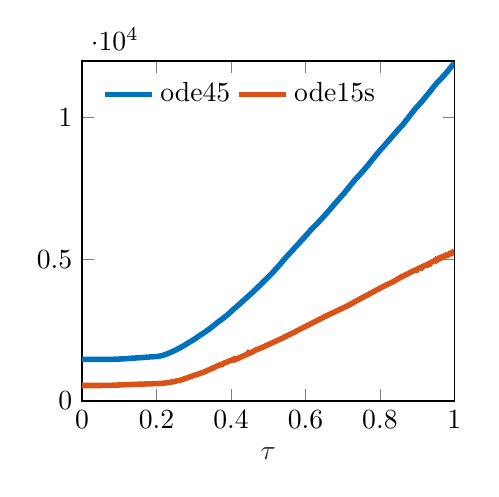
\begin{tikzpicture}

\begin{axis}[%
width=0.39\columnwidth,
height=1.7in,
scale only axis,
xmin=0,
xmax=1,
xlabel style={font=\color{white!15!black}},
xlabel={$\tau$},
ymin=0,
ymax=12000,
legend columns=2,
legend pos=north west,
legend style={legend cell align=left, align=left, draw=none,fill=none}
]
\addplot [color=mycolor1, line width=2.0pt]
  table[row sep=crcr]{%
0	1465\\
0.00252525252525253	1465\\
0.00505050505050505	1465\\
0.00757575757575758	1465\\
0.0101010101010101	1465\\
0.0126262626262626	1465\\
0.0151515151515152	1465\\
0.0176767676767677	1465\\
0.0202020202020202	1465\\
0.0227272727272727	1465\\
0.0252525252525253	1465\\
0.0277777777777778	1465\\
0.0303030303030303	1465\\
0.0328282828282828	1465\\
0.0353535353535354	1465\\
0.0378787878787879	1465\\
0.0404040404040404	1465\\
0.0429292929292929	1465\\
0.0454545454545455	1465\\
0.047979797979798	1465\\
0.0505050505050505	1465\\
0.053030303030303	1465\\
0.0555555555555556	1465\\
0.0580808080808081	1465\\
0.0606060606060606	1465\\
0.0631313131313131	1465\\
0.0656565656565657	1465\\
0.0681818181818182	1465\\
0.0707070707070707	1469\\
0.0732323232323232	1469\\
0.0757575757575758	1469\\
0.0782828282828283	1469\\
0.0808080808080808	1469\\
0.0833333333333333	1469\\
0.0858585858585859	1473\\
0.0883838383838384	1473\\
0.0909090909090909	1473\\
0.0934343434343434	1477\\
0.095959595959596	1477\\
0.0984848484848485	1477\\
0.101010101010101	1481\\
0.103535353535354	1481\\
0.106060606060606	1485\\
0.108585858585859	1485\\
0.111111111111111	1489\\
0.113636363636364	1489\\
0.116161616161616	1493\\
0.118686868686869	1493\\
0.121212121212121	1497\\
0.123737373737374	1497\\
0.126262626262626	1501\\
0.128787878787879	1501\\
0.131313131313131	1505\\
0.133838383838384	1509\\
0.136363636363636	1509\\
0.138888888888889	1513\\
0.141414141414141	1513\\
0.143939393939394	1517\\
0.146464646464646	1517\\
0.148989898989899	1521\\
0.151515151515152	1525\\
0.154040404040404	1525\\
0.156565656565657	1529\\
0.159090909090909	1529\\
0.161616161616162	1533\\
0.164141414141414	1533\\
0.166666666666667	1537\\
0.169191919191919	1541\\
0.171717171717172	1541\\
0.174242424242424	1545\\
0.176767676767677	1545\\
0.179292929292929	1549\\
0.181818181818182	1553\\
0.184343434343434	1553\\
0.186868686868687	1557\\
0.189393939393939	1557\\
0.191919191919192	1561\\
0.194444444444444	1565\\
0.196969696969697	1565\\
0.19949494949495	1569\\
0.202020202020202	1573\\
0.204545454545455	1577\\
0.207070707070707	1581\\
0.20959595959596	1585\\
0.212121212121212	1593\\
0.214646464646465	1601\\
0.217171717171717	1609\\
0.21969696969697	1621\\
0.222222222222222	1633\\
0.224747474747475	1645\\
0.227272727272727	1657\\
0.22979797979798	1669\\
0.232323232323232	1685\\
0.234848484848485	1697\\
0.237373737373737	1713\\
0.23989898989899	1725\\
0.242424242424242	1741\\
0.244949494949495	1757\\
0.247474747474747	1773\\
0.25	1789\\
0.25	1789\\
0.252525252525253	1805\\
0.255050505050505	1821\\
0.257575757575758	1837\\
0.26010101010101	1857\\
0.262626262626263	1873\\
0.265151515151515	1893\\
0.267676767676768	1909\\
0.27020202020202	1929\\
0.272727272727273	1949\\
0.275252525252525	1969\\
0.277777777777778	1989\\
0.28030303030303	2009\\
0.282828282828283	2029\\
0.285353535353535	2049\\
0.287878787878788	2069\\
0.29040404040404	2089\\
0.292929292929293	2109\\
0.295454545454545	2129\\
0.297979797979798	2149\\
0.30050505050505	2169\\
0.303030303030303	2193\\
0.305555555555556	2213\\
0.308080808080808	2237\\
0.310606060606061	2261\\
0.313131313131313	2281\\
0.315656565656566	2305\\
0.318181818181818	2329\\
0.320707070707071	2349\\
0.323232323232323	2373\\
0.325757575757576	2393\\
0.328282828282828	2417\\
0.330808080808081	2437\\
0.333333333333333	2461\\
0.335858585858586	2485\\
0.338383838383838	2509\\
0.340909090909091	2533\\
0.343434343434343	2557\\
0.345959595959596	2585\\
0.348484848484849	2609\\
0.351010101010101	2633\\
0.353535353535354	2661\\
0.356060606060606	2685\\
0.358585858585859	2713\\
0.361111111111111	2741\\
0.363636363636364	2765\\
0.366161616161616	2793\\
0.368686868686869	2817\\
0.371212121212121	2841\\
0.373737373737374	2865\\
0.376262626262626	2889\\
0.378787878787879	2917\\
0.381313131313131	2941\\
0.383838383838384	2969\\
0.386363636363636	2993\\
0.388888888888889	3021\\
0.391414141414141	3049\\
0.393939393939394	3081\\
0.396464646464646	3109\\
0.398989898989899	3141\\
0.401515151515151	3169\\
0.404040404040404	3201\\
0.406565656565657	3233\\
0.409090909090909	3261\\
0.411616161616162	3289\\
0.414141414141414	3317\\
0.416666666666667	3345\\
0.419191919191919	3377\\
0.421717171717172	3405\\
0.424242424242424	3433\\
0.426767676767677	3465\\
0.429292929292929	3493\\
0.431818181818182	3525\\
0.434343434343434	3553\\
0.436868686868687	3585\\
0.439393939393939	3613\\
0.441919191919192	3641\\
0.444444444444444	3673\\
0.446969696969697	3701\\
0.44949494949495	3733\\
0.452020202020202	3761\\
0.454545454545455	3793\\
0.457070707070707	3821\\
0.45959595959596	3853\\
0.462121212121212	3885\\
0.464646464646465	3917\\
0.467171717171717	3949\\
0.46969696969697	3981\\
0.472222222222222	4013\\
0.474747474747475	4045\\
0.477272727272727	4077\\
0.47979797979798	4109\\
0.482323232323232	4145\\
0.484848484848485	4177\\
0.487373737373737	4213\\
0.48989898989899	4245\\
0.492424242424242	4277\\
0.494949494949495	4309\\
0.497474747474748	4341\\
0.5	4373\\
0.5	4373\\
0.502525252525252	4405\\
0.505050505050505	4437\\
0.507575757575758	4473\\
0.51010101010101	4505\\
0.512626262626263	4541\\
0.515151515151515	4577\\
0.517676767676768	4617\\
0.52020202020202	4653\\
0.522727272727273	4689\\
0.525252525252525	4725\\
0.527777777777778	4765\\
0.53030303030303	4801\\
0.532828282828283	4837\\
0.535353535353535	4877\\
0.537878787878788	4917\\
0.54040404040404	4957\\
0.542929292929293	4993\\
0.545454545454545	5033\\
0.547979797979798	5073\\
0.55050505050505	5109\\
0.553030303030303	5145\\
0.555555555555556	5181\\
0.558080808080808	5217\\
0.560606060606061	5249\\
0.563131313131313	5285\\
0.565656565656566	5325\\
0.568181818181818	5361\\
0.570707070707071	5397\\
0.573232323232323	5433\\
0.575757575757576	5469\\
0.578282828282828	5505\\
0.580808080808081	5541\\
0.583333333333333	5577\\
0.585858585858586	5613\\
0.588383838383838	5649\\
0.590909090909091	5685\\
0.593434343434343	5721\\
0.595959595959596	5757\\
0.598484848484849	5797\\
0.601010101010101	5833\\
0.603535353535354	5873\\
0.606060606060606	5909\\
0.608585858585859	5949\\
0.611111111111111	5985\\
0.613636363636364	6025\\
0.616161616161616	6057\\
0.618686868686869	6089\\
0.621212121212121	6125\\
0.623737373737374	6157\\
0.626262626262626	6193\\
0.628787878787879	6225\\
0.631313131313131	6261\\
0.633838383838384	6293\\
0.636363636363636	6329\\
0.638888888888889	6365\\
0.641414141414141	6401\\
0.643939393939394	6437\\
0.646464646464646	6473\\
0.648989898989899	6509\\
0.651515151515151	6545\\
0.654040404040404	6585\\
0.656565656565657	6621\\
0.659090909090909	6657\\
0.661616161616162	6697\\
0.664141414141414	6733\\
0.666666666666667	6773\\
0.669191919191919	6813\\
0.671717171717172	6853\\
0.674242424242424	6889\\
0.676767676767677	6929\\
0.679292929292929	6969\\
0.681818181818182	7005\\
0.684343434343434	7041\\
0.686868686868687	7081\\
0.689393939393939	7117\\
0.691919191919192	7153\\
0.694444444444444	7193\\
0.696969696969697	7229\\
0.69949494949495	7269\\
0.702020202020202	7305\\
0.704545454545455	7345\\
0.707070707070707	7385\\
0.70959595959596	7425\\
0.712121212121212	7465\\
0.714646464646465	7505\\
0.717171717171717	7549\\
0.71969696969697	7589\\
0.722222222222222	7633\\
0.724747474747475	7673\\
0.727272727272727	7713\\
0.72979797979798	7753\\
0.732323232323232	7793\\
0.734848484848485	7829\\
0.737373737373737	7865\\
0.73989898989899	7901\\
0.742424242424242	7937\\
0.744949494949495	7973\\
0.747474747474748	8013\\
0.75	8049\\
0.75	8049\\
0.752525252525252	8085\\
0.755050505050505	8121\\
0.757575757575758	8161\\
0.76010101010101	8201\\
0.762626262626263	8241\\
0.765151515151515	8281\\
0.767676767676768	8321\\
0.77020202020202	8361\\
0.772727272727273	8401\\
0.775252525252525	8445\\
0.777777777777778	8485\\
0.78030303030303	8525\\
0.782828282828283	8565\\
0.785353535353535	8605\\
0.787878787878788	8649\\
0.79040404040404	8689\\
0.792929292929293	8729\\
0.795454545454545	8769\\
0.797979797979798	8805\\
0.80050505050505	8845\\
0.803030303030303	8885\\
0.805555555555556	8921\\
0.808080808080808	8957\\
0.810606060606061	8993\\
0.813131313131313	9033\\
0.815656565656566	9073\\
0.818181818181818	9109\\
0.820707070707071	9149\\
0.823232323232323	9185\\
0.825757575757576	9225\\
0.828282828282828	9261\\
0.830808080808081	9301\\
0.833333333333333	9337\\
0.835858585858586	9377\\
0.838383838383838	9413\\
0.840909090909091	9453\\
0.843434343434343	9489\\
0.845959595959596	9525\\
0.848484848484849	9565\\
0.851010101010101	9601\\
0.853535353535354	9637\\
0.856060606060606	9673\\
0.858585858585859	9709\\
0.861111111111111	9749\\
0.863636363636364	9789\\
0.866161616161616	9829\\
0.868686868686869	9869\\
0.871212121212121	9913\\
0.873737373737374	9953\\
0.876262626262626	9997\\
0.878787878787879	10041\\
0.881313131313131	10089\\
0.883838383838384	10129\\
0.886363636363636	10173\\
0.888888888888889	10213\\
0.891414141414141	10257\\
0.893939393939394	10297\\
0.896464646464646	10337\\
0.898989898989899	10373\\
0.901515151515151	10409\\
0.904040404040404	10445\\
0.906565656565657	10481\\
0.909090909090909	10517\\
0.911616161616162	10553\\
0.914141414141414	10593\\
0.916666666666667	10633\\
0.919191919191919	10673\\
0.921717171717172	10713\\
0.924242424242424	10757\\
0.926767676767677	10797\\
0.929292929292929	10837\\
0.931818181818182	10877\\
0.934343434343434	10917\\
0.936868686868687	10961\\
0.939393939393939	11001\\
0.941919191919192	11045\\
0.944444444444444	11089\\
0.946969696969697	11129\\
0.94949494949495	11169\\
0.952020202020202	11209\\
0.954545454545455	11245\\
0.957070707070707	11277\\
0.95959595959596	11313\\
0.962121212121212	11345\\
0.964646464646465	11381\\
0.967171717171717	11417\\
0.96969696969697	11453\\
0.972222222222222	11489\\
0.974747474747475	11529\\
0.977272727272727	11565\\
0.97979797979798	11605\\
0.982323232323232	11645\\
0.984848484848485	11685\\
0.987373737373737	11729\\
0.98989898989899	11769\\
0.992424242424242	11809\\
0.994949494949495	11849\\
0.997474747474748	11885\\
1	11921\\
};
\addlegendentry{ode45}

\addplot [color=mycolor2, line width=2.0pt]
  table[row sep=crcr]{%
0	545\\
0.00252525252525253	545\\
0.00505050505050505	545\\
0.00757575757575758	545\\
0.0101010101010101	545\\
0.0126262626262626	545\\
0.0151515151515152	545\\
0.0176767676767677	545\\
0.0202020202020202	545\\
0.0227272727272727	545\\
0.0252525252525253	545\\
0.0277777777777778	545\\
0.0303030303030303	545\\
0.0328282828282828	545\\
0.0353535353535354	545\\
0.0378787878787879	545\\
0.0404040404040404	545\\
0.0429292929292929	545\\
0.0454545454545455	545\\
0.047979797979798	546\\
0.0505050505050505	546\\
0.053030303030303	546\\
0.0555555555555556	547\\
0.0580808080808081	547\\
0.0606060606060606	548\\
0.0631313131313131	548\\
0.0656565656565657	549\\
0.0681818181818182	549\\
0.0707070707070707	550\\
0.0732323232323232	551\\
0.0757575757575758	552\\
0.0782828282828283	552\\
0.0808080808080808	553\\
0.0833333333333333	555\\
0.0858585858585859	556\\
0.0883838383838384	558\\
0.0909090909090909	559\\
0.0934343434343434	561\\
0.095959595959596	562\\
0.0984848484848485	563\\
0.101010101010101	565\\
0.103535353535354	566\\
0.106060606060606	567\\
0.108585858585859	569\\
0.111111111111111	570\\
0.113636363636364	571\\
0.116161616161616	573\\
0.118686868686869	574\\
0.121212121212121	575\\
0.123737373737374	576\\
0.126262626262626	578\\
0.128787878787879	579\\
0.131313131313131	580\\
0.133838383838384	581\\
0.136363636363636	583\\
0.138888888888889	584\\
0.141414141414141	585\\
0.143939393939394	586\\
0.146464646464646	588\\
0.148989898989899	589\\
0.151515151515152	590\\
0.154040404040404	591\\
0.156565656565657	593\\
0.159090909090909	594\\
0.161616161616162	595\\
0.164141414141414	596\\
0.166666666666667	597\\
0.169191919191919	599\\
0.171717171717172	600\\
0.174242424242424	601\\
0.176767676767677	602\\
0.179292929292929	603\\
0.181818181818182	604\\
0.184343434343434	605\\
0.186868686868687	606\\
0.189393939393939	608\\
0.191919191919192	609\\
0.194444444444444	610\\
0.196969696969697	611\\
0.19949494949495	612\\
0.202020202020202	613\\
0.204545454545455	614\\
0.207070707070707	616\\
0.20959595959596	617\\
0.212121212121212	619\\
0.214646464646465	622\\
0.217171717171717	625\\
0.21969696969697	628\\
0.222222222222222	633\\
0.224747474747475	637\\
0.227272727272727	641\\
0.22979797979798	645\\
0.232323232323232	651\\
0.234848484848485	655\\
0.237373737373737	662\\
0.23989898989899	667\\
0.242424242424242	673\\
0.244949494949495	681\\
0.247474747474747	688\\
0.25	693\\
0.25	693\\
0.252525252525253	703\\
0.255050505050505	708\\
0.257575757575758	715\\
0.26010101010101	723\\
0.262626262626263	728\\
0.265151515151515	737\\
0.267676767676768	745\\
0.27020202020202	755\\
0.272727272727273	775\\
0.275252525252525	777\\
0.277777777777778	797\\
0.28030303030303	808\\
0.282828282828283	819\\
0.285353535353535	830\\
0.287878787878788	842\\
0.29040404040404	854\\
0.292929292929293	865\\
0.295454545454545	877\\
0.297979797979798	888\\
0.30050505050505	900\\
0.303030303030303	914\\
0.305555555555556	925\\
0.308080808080808	931\\
0.310606060606061	942\\
0.313131313131313	954\\
0.315656565656566	966\\
0.318181818181818	977\\
0.320707070707071	992\\
0.323232323232323	1004\\
0.325757575757576	1012\\
0.328282828282828	1026\\
0.330808080808081	1038\\
0.333333333333333	1053\\
0.335858585858586	1073\\
0.338383838383838	1087\\
0.340909090909091	1099\\
0.343434343434343	1113\\
0.345959595959596	1129\\
0.348484848484849	1141\\
0.351010101010101	1164\\
0.353535353535354	1169\\
0.356060606060606	1192\\
0.358585858585859	1207\\
0.361111111111111	1222\\
0.363636363636364	1236\\
0.366161616161616	1249\\
0.368686868686869	1264\\
0.371212121212121	1277\\
0.373737373737374	1291\\
0.376262626262626	1285\\
0.378787878787879	1317\\
0.381313131313131	1334\\
0.383838383838384	1348\\
0.386363636363636	1361\\
0.388888888888889	1372\\
0.391414141414141	1385\\
0.393939393939394	1400\\
0.396464646464646	1416\\
0.398989898989899	1428\\
0.401515151515151	1442\\
0.404040404040404	1454\\
0.406565656565657	1445\\
0.409090909090909	1482\\
0.411616161616162	1462\\
0.414141414141414	1475\\
0.416666666666667	1496\\
0.419191919191919	1503\\
0.421717171717172	1518\\
0.424242424242424	1534\\
0.426767676767677	1550\\
0.429292929292929	1567\\
0.431818181818182	1581\\
0.434343434343434	1597\\
0.436868686868687	1611\\
0.439393939393939	1623\\
0.441919191919192	1638\\
0.444444444444444	1653\\
0.446969696969697	1700\\
0.44949494949495	1684\\
0.452020202020202	1700\\
0.454545454545455	1713\\
0.457070707070707	1730\\
0.45959595959596	1746\\
0.462121212121212	1762\\
0.464646464646465	1785\\
0.467171717171717	1800\\
0.46969696969697	1816\\
0.472222222222222	1832\\
0.474747474747475	1835\\
0.477272727272727	1850\\
0.47979797979798	1865\\
0.482323232323232	1880\\
0.484848484848485	1894\\
0.487373737373737	1911\\
0.48989898989899	1924\\
0.492424242424242	1940\\
0.494949494949495	1958\\
0.497474747474748	1971\\
0.5	1987\\
0.5	1987\\
0.502525252525252	2002\\
0.505050505050505	2017\\
0.507575757575758	2033\\
0.51010101010101	2050\\
0.512626262626263	2064\\
0.515151515151515	2079\\
0.517676767676768	2094\\
0.52020202020202	2110\\
0.522727272727273	2124\\
0.525252525252525	2140\\
0.527777777777778	2154\\
0.53030303030303	2168\\
0.532828282828283	2184\\
0.535353535353535	2198\\
0.537878787878788	2215\\
0.54040404040404	2230\\
0.542929292929293	2249\\
0.545454545454545	2266\\
0.547979797979798	2283\\
0.55050505050505	2301\\
0.553030303030303	2316\\
0.555555555555556	2331\\
0.558080808080808	2347\\
0.560606060606061	2365\\
0.563131313131313	2381\\
0.565656565656566	2397\\
0.568181818181818	2412\\
0.570707070707071	2429\\
0.573232323232323	2445\\
0.575757575757576	2464\\
0.578282828282828	2483\\
0.580808080808081	2501\\
0.583333333333333	2518\\
0.585858585858586	2534\\
0.588383838383838	2551\\
0.590909090909091	2568\\
0.593434343434343	2585\\
0.595959595959596	2601\\
0.598484848484849	2618\\
0.601010101010101	2635\\
0.603535353535354	2654\\
0.606060606060606	2666\\
0.608585858585859	2683\\
0.611111111111111	2699\\
0.613636363636364	2718\\
0.616161616161616	2739\\
0.618686868686869	2750\\
0.621212121212121	2772\\
0.623737373737374	2785\\
0.626262626262626	2804\\
0.628787878787879	2817\\
0.631313131313131	2837\\
0.633838383838384	2853\\
0.636363636363636	2871\\
0.638888888888889	2886\\
0.641414141414141	2908\\
0.643939393939394	2925\\
0.646464646464646	2936\\
0.648989898989899	2954\\
0.651515151515151	2976\\
0.654040404040404	2986\\
0.656565656565657	3007\\
0.659090909090909	3021\\
0.661616161616162	3039\\
0.664141414141414	3054\\
0.666666666666667	3069\\
0.669191919191919	3085\\
0.671717171717172	3099\\
0.674242424242424	3115\\
0.676767676767677	3130\\
0.679292929292929	3147\\
0.681818181818182	3165\\
0.684343434343434	3177\\
0.686868686868687	3195\\
0.689393939393939	3212\\
0.691919191919192	3225\\
0.694444444444444	3242\\
0.696969696969697	3258\\
0.69949494949495	3275\\
0.702020202020202	3287\\
0.704545454545455	3306\\
0.707070707070707	3320\\
0.70959595959596	3337\\
0.712121212121212	3353\\
0.714646464646465	3369\\
0.717171717171717	3384\\
0.71969696969697	3405\\
0.722222222222222	3423\\
0.724747474747475	3441\\
0.727272727272727	3458\\
0.72979797979798	3480\\
0.732323232323232	3498\\
0.734848484848485	3517\\
0.737373737373737	3535\\
0.73989898989899	3551\\
0.742424242424242	3569\\
0.744949494949495	3588\\
0.747474747474748	3608\\
0.75	3625\\
0.75	3625\\
0.752525252525252	3642\\
0.755050505050505	3660\\
0.757575757575758	3677\\
0.76010101010101	3696\\
0.762626262626263	3714\\
0.765151515151515	3732\\
0.767676767676768	3740\\
0.77020202020202	3759\\
0.772727272727273	3786\\
0.775252525252525	3801\\
0.777777777777778	3821\\
0.78030303030303	3839\\
0.782828282828283	3857\\
0.785353535353535	3870\\
0.787878787878788	3894\\
0.79040404040404	3912\\
0.792929292929293	3930\\
0.795454545454545	3942\\
0.797979797979798	3960\\
0.80050505050505	3984\\
0.803030303030303	3994\\
0.805555555555556	4018\\
0.808080808080808	4034\\
0.810606060606061	4049\\
0.813131313131313	4066\\
0.815656565656566	4088\\
0.818181818181818	4098\\
0.820707070707071	4116\\
0.823232323232323	4132\\
0.825757575757576	4149\\
0.828282828282828	4162\\
0.830808080808081	4180\\
0.833333333333333	4195\\
0.835858585858586	4213\\
0.838383838383838	4229\\
0.840909090909091	4249\\
0.843434343434343	4269\\
0.845959595959596	4290\\
0.848484848484849	4310\\
0.851010101010101	4327\\
0.853535353535354	4347\\
0.856060606060606	4364\\
0.858585858585859	4381\\
0.861111111111111	4397\\
0.863636363636364	4413\\
0.866161616161616	4433\\
0.868686868686869	4447\\
0.871212121212121	4464\\
0.873737373737374	4481\\
0.876262626262626	4499\\
0.878787878787879	4515\\
0.881313131313131	4535\\
0.883838383838384	4549\\
0.886363636363636	4568\\
0.888888888888889	4582\\
0.891414141414141	4598\\
0.893939393939394	4613\\
0.896464646464646	4628\\
0.898989898989899	4616\\
0.901515151515151	4659\\
0.904040404040404	4677\\
0.906565656565657	4692\\
0.909090909090909	4707\\
0.911616161616162	4695\\
0.914141414141414	4737\\
0.916666666666667	4755\\
0.919191919191919	4771\\
0.921717171717172	4784\\
0.924242424242424	4797\\
0.926767676767677	4787\\
0.929292929292929	4806\\
0.931818181818182	4845\\
0.934343434343434	4837\\
0.936868686868687	4883\\
0.939393939393939	4902\\
0.941919191919192	4922\\
0.944444444444444	4939\\
0.946969696969697	4951\\
0.94949494949495	4944\\
0.952020202020202	4992\\
0.954545454545455	4978\\
0.957070707070707	5001\\
0.95959595959596	5041\\
0.962121212121212	5029\\
0.964646464646465	5046\\
0.967171717171717	5083\\
0.96969696969697	5076\\
0.972222222222222	5090\\
0.974747474747475	5130\\
0.977272727272727	5147\\
0.97979797979798	5134\\
0.982323232323232	5146\\
0.984848484848485	5160\\
0.987373737373737	5202\\
0.98989898989899	5215\\
0.992424242424242	5207\\
0.994949494949495	5254\\
0.997474747474748	5269\\
1	5285\\
};
\addlegendentry{ode15s}

\end{axis}
\end{tikzpicture}%}
\subfloat[][$\gamma=0.70$]{% This file was created by matlab2tikz.
%
%The latest updates can be retrieved from
%  http://www.mathworks.com/matlabcentral/fileexchange/22022-matlab2tikz-matlab2tikz
%where you can also make suggestions and rate matlab2tikz.
%
\definecolor{mycolor1}{rgb}{0.00000,0.44700,0.74100}%
\definecolor{mycolor2}{rgb}{0.85000,0.32500,0.09800}%
%
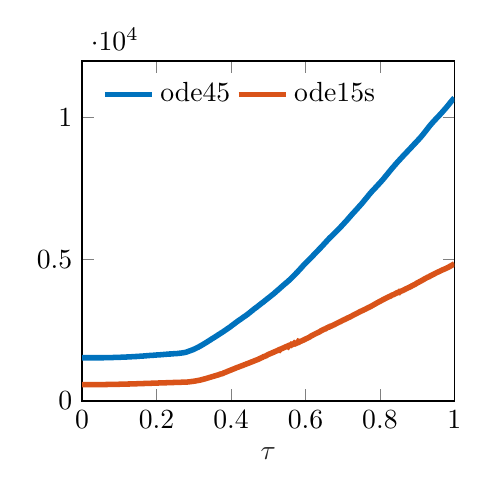
\begin{tikzpicture}

\begin{axis}[%
width=0.39\columnwidth,
height=1.7in,
at={(1.011in,0.642in)},
scale only axis,
xmin=0,
xmax=1,
xlabel style={font=\color{white!15!black}},
xlabel={$\tau$},
ymin=0,
ymax=12000,
legend columns=2,
legend pos=north west,
legend style={legend cell align=left, align=left, draw=none,fill=none}
]
\addplot [color=mycolor1, line width=2.0pt]
  table[row sep=crcr]{%
0	1525\\
0.00252525252525253	1525\\
0.00505050505050505	1525\\
0.00757575757575758	1525\\
0.0101010101010101	1525\\
0.0126262626262626	1525\\
0.0151515151515152	1525\\
0.0176767676767677	1525\\
0.0202020202020202	1525\\
0.0227272727272727	1525\\
0.0252525252525253	1525\\
0.0277777777777778	1525\\
0.0303030303030303	1525\\
0.0328282828282828	1525\\
0.0353535353535354	1525\\
0.0378787878787879	1525\\
0.0404040404040404	1525\\
0.0429292929292929	1525\\
0.0454545454545455	1525\\
0.047979797979798	1525\\
0.0505050505050505	1525\\
0.053030303030303	1525\\
0.0555555555555556	1525\\
0.0580808080808081	1525\\
0.0606060606060606	1529\\
0.0631313131313131	1529\\
0.0656565656565657	1529\\
0.0681818181818182	1529\\
0.0707070707070707	1529\\
0.0732323232323232	1529\\
0.0757575757575758	1533\\
0.0782828282828283	1533\\
0.0808080808080808	1533\\
0.0833333333333333	1533\\
0.0858585858585859	1537\\
0.0883838383838384	1537\\
0.0909090909090909	1537\\
0.0934343434343434	1537\\
0.095959595959596	1541\\
0.0984848484848485	1541\\
0.101010101010101	1541\\
0.103535353535354	1541\\
0.106060606060606	1545\\
0.108585858585859	1545\\
0.111111111111111	1545\\
0.113636363636364	1549\\
0.116161616161616	1549\\
0.118686868686869	1549\\
0.121212121212121	1553\\
0.123737373737374	1553\\
0.126262626262626	1553\\
0.128787878787879	1557\\
0.131313131313131	1557\\
0.133838383838384	1561\\
0.136363636363636	1561\\
0.138888888888889	1565\\
0.141414141414141	1565\\
0.143939393939394	1569\\
0.146464646464646	1569\\
0.148989898989899	1573\\
0.151515151515152	1573\\
0.154040404040404	1577\\
0.156565656565657	1581\\
0.159090909090909	1581\\
0.161616161616162	1585\\
0.164141414141414	1585\\
0.166666666666667	1589\\
0.169191919191919	1593\\
0.171717171717172	1593\\
0.174242424242424	1597\\
0.176767676767677	1597\\
0.179292929292929	1601\\
0.181818181818182	1605\\
0.184343434343434	1605\\
0.186868686868687	1609\\
0.189393939393939	1609\\
0.191919191919192	1613\\
0.194444444444444	1617\\
0.196969696969697	1617\\
0.19949494949495	1621\\
0.202020202020202	1625\\
0.204545454545455	1625\\
0.207070707070707	1629\\
0.20959595959596	1629\\
0.212121212121212	1633\\
0.214646464646465	1637\\
0.217171717171717	1637\\
0.21969696969697	1641\\
0.222222222222222	1641\\
0.224747474747475	1645\\
0.227272727272727	1649\\
0.22979797979798	1649\\
0.232323232323232	1653\\
0.234848484848485	1657\\
0.237373737373737	1657\\
0.23989898989899	1661\\
0.242424242424242	1661\\
0.244949494949495	1665\\
0.247474747474747	1669\\
0.25	1669\\
0.25	1669\\
0.252525252525253	1673\\
0.255050505050505	1673\\
0.257575757575758	1677\\
0.26010101010101	1681\\
0.262626262626263	1685\\
0.265151515151515	1689\\
0.267676767676768	1693\\
0.27020202020202	1697\\
0.272727272727273	1705\\
0.275252525252525	1709\\
0.277777777777778	1717\\
0.28030303030303	1725\\
0.282828282828283	1737\\
0.285353535353535	1749\\
0.287878787878788	1761\\
0.29040404040404	1773\\
0.292929292929293	1785\\
0.295454545454545	1797\\
0.297979797979798	1809\\
0.30050505050505	1825\\
0.303030303030303	1841\\
0.305555555555556	1857\\
0.308080808080808	1873\\
0.310606060606061	1889\\
0.313131313131313	1905\\
0.315656565656566	1925\\
0.318181818181818	1941\\
0.320707070707071	1961\\
0.323232323232323	1981\\
0.325757575757576	2001\\
0.328282828282828	2021\\
0.330808080808081	2041\\
0.333333333333333	2061\\
0.335858585858586	2081\\
0.338383838383838	2105\\
0.340909090909091	2125\\
0.343434343434343	2145\\
0.345959595959596	2165\\
0.348484848484849	2189\\
0.351010101010101	2209\\
0.353535353535354	2229\\
0.356060606060606	2249\\
0.358585858585859	2273\\
0.361111111111111	2293\\
0.363636363636364	2313\\
0.366161616161616	2337\\
0.368686868686869	2357\\
0.371212121212121	2377\\
0.373737373737374	2401\\
0.376262626262626	2421\\
0.378787878787879	2441\\
0.381313131313131	2465\\
0.383838383838384	2489\\
0.386363636363636	2509\\
0.388888888888889	2533\\
0.391414141414141	2557\\
0.393939393939394	2577\\
0.396464646464646	2601\\
0.398989898989899	2625\\
0.401515151515151	2653\\
0.404040404040404	2677\\
0.406565656565657	2701\\
0.409090909090909	2725\\
0.411616161616162	2753\\
0.414141414141414	2777\\
0.416666666666667	2801\\
0.419191919191919	2825\\
0.421717171717172	2849\\
0.424242424242424	2869\\
0.426767676767677	2893\\
0.429292929292929	2917\\
0.431818181818182	2941\\
0.434343434343434	2965\\
0.436868686868687	2985\\
0.439393939393939	3009\\
0.441919191919192	3033\\
0.444444444444444	3057\\
0.446969696969697	3085\\
0.44949494949495	3109\\
0.452020202020202	3137\\
0.454545454545455	3165\\
0.457070707070707	3189\\
0.45959595959596	3217\\
0.462121212121212	3245\\
0.464646464646465	3269\\
0.467171717171717	3293\\
0.46969696969697	3317\\
0.472222222222222	3345\\
0.474747474747475	3369\\
0.477272727272727	3397\\
0.47979797979798	3421\\
0.482323232323232	3449\\
0.484848484848485	3473\\
0.487373737373737	3497\\
0.48989898989899	3525\\
0.492424242424242	3553\\
0.494949494949495	3577\\
0.497474747474748	3605\\
0.5	3629\\
0.5	3629\\
0.502525252525252	3657\\
0.505050505050505	3681\\
0.507575757575758	3709\\
0.51010101010101	3737\\
0.512626262626263	3761\\
0.515151515151515	3789\\
0.517676767676768	3817\\
0.52020202020202	3849\\
0.522727272727273	3877\\
0.525252525252525	3905\\
0.527777777777778	3933\\
0.53030303030303	3961\\
0.532828282828283	3993\\
0.535353535353535	4021\\
0.537878787878788	4053\\
0.54040404040404	4081\\
0.542929292929293	4109\\
0.545454545454545	4137\\
0.547979797979798	4165\\
0.55050505050505	4193\\
0.553030303030303	4221\\
0.555555555555556	4253\\
0.558080808080808	4281\\
0.560606060606061	4313\\
0.563131313131313	4345\\
0.565656565656566	4381\\
0.568181818181818	4413\\
0.570707070707071	4445\\
0.573232323232323	4481\\
0.575757575757576	4517\\
0.578282828282828	4549\\
0.580808080808081	4585\\
0.583333333333333	4621\\
0.585858585858586	4657\\
0.588383838383838	4693\\
0.590909090909091	4729\\
0.593434343434343	4769\\
0.595959595959596	4805\\
0.598484848484849	4841\\
0.601010101010101	4873\\
0.603535353535354	4905\\
0.606060606060606	4937\\
0.608585858585859	4969\\
0.611111111111111	5005\\
0.613636363636364	5037\\
0.616161616161616	5073\\
0.618686868686869	5105\\
0.621212121212121	5141\\
0.623737373737374	5177\\
0.626262626262626	5209\\
0.628787878787879	5245\\
0.631313131313131	5281\\
0.633838383838384	5313\\
0.636363636363636	5349\\
0.638888888888889	5381\\
0.641414141414141	5417\\
0.643939393939394	5453\\
0.646464646464646	5485\\
0.648989898989899	5525\\
0.651515151515151	5561\\
0.654040404040404	5597\\
0.656565656565657	5633\\
0.659090909090909	5669\\
0.661616161616162	5705\\
0.664141414141414	5741\\
0.666666666666667	5773\\
0.669191919191919	5805\\
0.671717171717172	5837\\
0.674242424242424	5869\\
0.676767676767677	5901\\
0.679292929292929	5933\\
0.681818181818182	5969\\
0.684343434343434	6001\\
0.686868686868687	6033\\
0.689393939393939	6069\\
0.691919191919192	6101\\
0.694444444444444	6137\\
0.696969696969697	6173\\
0.69949494949495	6209\\
0.702020202020202	6245\\
0.704545454545455	6281\\
0.707070707070707	6317\\
0.70959595959596	6353\\
0.712121212121212	6389\\
0.714646464646465	6429\\
0.717171717171717	6465\\
0.71969696969697	6505\\
0.722222222222222	6541\\
0.724747474747475	6581\\
0.727272727272727	6617\\
0.72979797979798	6653\\
0.732323232323232	6689\\
0.734848484848485	6725\\
0.737373737373737	6761\\
0.73989898989899	6797\\
0.742424242424242	6837\\
0.744949494949495	6873\\
0.747474747474748	6909\\
0.75	6945\\
0.75	6945\\
0.752525252525252	6985\\
0.755050505050505	7025\\
0.757575757575758	7065\\
0.76010101010101	7105\\
0.762626262626263	7145\\
0.765151515151515	7185\\
0.767676767676768	7225\\
0.77020202020202	7269\\
0.772727272727273	7309\\
0.775252525252525	7345\\
0.777777777777778	7385\\
0.78030303030303	7421\\
0.782828282828283	7457\\
0.785353535353535	7489\\
0.787878787878788	7525\\
0.79040404040404	7561\\
0.792929292929293	7597\\
0.795454545454545	7633\\
0.797979797979798	7669\\
0.80050505050505	7705\\
0.803030303030303	7741\\
0.805555555555556	7781\\
0.808080808080808	7817\\
0.810606060606061	7857\\
0.813131313131313	7897\\
0.815656565656566	7937\\
0.818181818181818	7977\\
0.820707070707071	8017\\
0.823232323232323	8061\\
0.825757575757576	8101\\
0.828282828282828	8141\\
0.830808080808081	8181\\
0.833333333333333	8221\\
0.835858585858586	8257\\
0.838383838383838	8297\\
0.840909090909091	8337\\
0.843434343434343	8373\\
0.845959595959596	8413\\
0.848484848484849	8449\\
0.851010101010101	8485\\
0.853535353535354	8521\\
0.856060606060606	8557\\
0.858585858585859	8593\\
0.861111111111111	8629\\
0.863636363636364	8665\\
0.866161616161616	8701\\
0.868686868686869	8733\\
0.871212121212121	8769\\
0.873737373737374	8805\\
0.876262626262626	8841\\
0.878787878787879	8877\\
0.881313131313131	8909\\
0.883838383838384	8945\\
0.886363636363636	8981\\
0.888888888888889	9017\\
0.891414141414141	9053\\
0.893939393939394	9089\\
0.896464646464646	9121\\
0.898989898989899	9157\\
0.901515151515151	9193\\
0.904040404040404	9229\\
0.906565656565657	9265\\
0.909090909090909	9301\\
0.911616161616162	9341\\
0.914141414141414	9381\\
0.916666666666667	9421\\
0.919191919191919	9465\\
0.921717171717172	9505\\
0.924242424242424	9549\\
0.926767676767677	9593\\
0.929292929292929	9633\\
0.931818181818182	9677\\
0.934343434343434	9717\\
0.936868686868687	9757\\
0.939393939393939	9793\\
0.941919191919192	9833\\
0.944444444444444	9869\\
0.946969696969697	9905\\
0.94949494949495	9941\\
0.952020202020202	9977\\
0.954545454545455	10009\\
0.957070707070707	10045\\
0.95959595959596	10081\\
0.962121212121212	10117\\
0.964646464646465	10153\\
0.967171717171717	10189\\
0.96969696969697	10229\\
0.972222222222222	10265\\
0.974747474747475	10305\\
0.977272727272727	10341\\
0.97979797979798	10381\\
0.982323232323232	10421\\
0.984848484848485	10461\\
0.987373737373737	10505\\
0.98989898989899	10545\\
0.992424242424242	10585\\
0.994949494949495	10625\\
0.997474747474748	10661\\
1	10697\\
};
\addlegendentry{ode45}

\addplot [color=mycolor2, line width=2.0pt]
  table[row sep=crcr]{%
0	578\\
0.00252525252525253	578\\
0.00505050505050505	578\\
0.00757575757575758	578\\
0.0101010101010101	578\\
0.0126262626262626	578\\
0.0151515151515152	578\\
0.0176767676767677	578\\
0.0202020202020202	578\\
0.0227272727272727	578\\
0.0252525252525253	578\\
0.0277777777777778	578\\
0.0303030303030303	578\\
0.0328282828282828	578\\
0.0353535353535354	578\\
0.0378787878787879	578\\
0.0404040404040404	578\\
0.0429292929292929	578\\
0.0454545454545455	578\\
0.047979797979798	578\\
0.0505050505050505	578\\
0.053030303030303	579\\
0.0555555555555556	579\\
0.0580808080808081	579\\
0.0606060606060606	580\\
0.0631313131313131	580\\
0.0656565656565657	581\\
0.0681818181818182	581\\
0.0707070707070707	582\\
0.0732323232323232	582\\
0.0757575757575758	583\\
0.0782828282828283	584\\
0.0808080808080808	584\\
0.0833333333333333	584\\
0.0858585858585859	585\\
0.0883838383838384	586\\
0.0909090909090909	587\\
0.0934343434343434	588\\
0.095959595959596	588\\
0.0984848484848485	589\\
0.101010101010101	590\\
0.103535353535354	591\\
0.106060606060606	592\\
0.108585858585859	592\\
0.111111111111111	593\\
0.113636363636364	594\\
0.116161616161616	595\\
0.118686868686869	596\\
0.121212121212121	597\\
0.123737373737374	598\\
0.126262626262626	598\\
0.128787878787879	599\\
0.131313131313131	600\\
0.133838383838384	601\\
0.136363636363636	602\\
0.138888888888889	603\\
0.141414141414141	604\\
0.143939393939394	605\\
0.146464646464646	607\\
0.148989898989899	608\\
0.151515151515152	609\\
0.154040404040404	611\\
0.156565656565657	612\\
0.159090909090909	613\\
0.161616161616162	614\\
0.164141414141414	615\\
0.166666666666667	616\\
0.169191919191919	617\\
0.171717171717172	619\\
0.174242424242424	620\\
0.176767676767677	621\\
0.179292929292929	622\\
0.181818181818182	623\\
0.184343434343434	624\\
0.186868686868687	625\\
0.189393939393939	627\\
0.191919191919192	628\\
0.194444444444444	629\\
0.196969696969697	630\\
0.19949494949495	631\\
0.202020202020202	632\\
0.204545454545455	633\\
0.207070707070707	635\\
0.20959595959596	636\\
0.212121212121212	637\\
0.214646464646465	638\\
0.217171717171717	639\\
0.21969696969697	640\\
0.222222222222222	641\\
0.224747474747475	642\\
0.227272727272727	643\\
0.22979797979798	644\\
0.232323232323232	645\\
0.234848484848485	646\\
0.237373737373737	647\\
0.23989898989899	649\\
0.242424242424242	650\\
0.244949494949495	651\\
0.247474747474747	652\\
0.25	653\\
0.25	653\\
0.252525252525253	654\\
0.255050505050505	655\\
0.257575757575758	656\\
0.26010101010101	657\\
0.262626262626263	658\\
0.265151515151515	659\\
0.267676767676768	661\\
0.27020202020202	662\\
0.272727272727273	663\\
0.275252525252525	664\\
0.277777777777778	665\\
0.28030303030303	667\\
0.282828282828283	668\\
0.285353535353535	671\\
0.287878787878788	675\\
0.29040404040404	679\\
0.292929292929293	683\\
0.295454545454545	688\\
0.297979797979798	692\\
0.30050505050505	697\\
0.303030303030303	702\\
0.305555555555556	707\\
0.308080808080808	714\\
0.310606060606061	720\\
0.313131313131313	726\\
0.315656565656566	733\\
0.318181818181818	740\\
0.320707070707071	749\\
0.323232323232323	757\\
0.325757575757576	766\\
0.328282828282828	776\\
0.330808080808081	782\\
0.333333333333333	793\\
0.335858585858586	803\\
0.338383838383838	813\\
0.340909090909091	822\\
0.343434343434343	833\\
0.345959595959596	842\\
0.348484848484849	852\\
0.351010101010101	863\\
0.353535353535354	873\\
0.356060606060606	884\\
0.358585858585859	890\\
0.361111111111111	903\\
0.363636363636364	912\\
0.366161616161616	921\\
0.368686868686869	933\\
0.371212121212121	949\\
0.373737373737374	954\\
0.376262626262626	963\\
0.378787878787879	974\\
0.381313131313131	993\\
0.383838383838384	1005\\
0.386363636363636	1018\\
0.388888888888889	1033\\
0.391414141414141	1046\\
0.393939393939394	1061\\
0.396464646464646	1074\\
0.398989898989899	1086\\
0.401515151515151	1099\\
0.404040404040404	1115\\
0.406565656565657	1127\\
0.409090909090909	1140\\
0.411616161616162	1154\\
0.414141414141414	1168\\
0.416666666666667	1181\\
0.419191919191919	1191\\
0.421717171717172	1204\\
0.424242424242424	1218\\
0.426767676767677	1231\\
0.429292929292929	1243\\
0.431818181818182	1255\\
0.434343434343434	1269\\
0.436868686868687	1281\\
0.439393939393939	1294\\
0.441919191919192	1308\\
0.444444444444444	1321\\
0.446969696969697	1333\\
0.44949494949495	1345\\
0.452020202020202	1359\\
0.454545454545455	1373\\
0.457070707070707	1385\\
0.45959595959596	1398\\
0.462121212121212	1412\\
0.464646464646465	1426\\
0.467171717171717	1438\\
0.46969696969697	1451\\
0.472222222222222	1464\\
0.474747474747475	1480\\
0.477272727272727	1496\\
0.47979797979798	1512\\
0.482323232323232	1527\\
0.484848484848485	1541\\
0.487373737373737	1563\\
0.48989898989899	1570\\
0.492424242424242	1585\\
0.494949494949495	1599\\
0.497474747474748	1622\\
0.5	1638\\
0.5	1638\\
0.502525252525252	1653\\
0.505050505050505	1667\\
0.507575757575758	1680\\
0.51010101010101	1695\\
0.512626262626263	1710\\
0.515151515151515	1723\\
0.517676767676768	1739\\
0.52020202020202	1753\\
0.522727272727273	1768\\
0.525252525252525	1780\\
0.527777777777778	1800\\
0.53030303030303	1791\\
0.532828282828283	1829\\
0.535353535353535	1840\\
0.537878787878788	1854\\
0.54040404040404	1871\\
0.542929292929293	1884\\
0.545454545454545	1901\\
0.547979797979798	1916\\
0.55050505050505	1930\\
0.553030303030303	1913\\
0.555555555555556	1960\\
0.558080808080808	1972\\
0.560606060606061	1965\\
0.563131313131313	2002\\
0.565656565656566	1994\\
0.568181818181818	2005\\
0.570707070707071	2042\\
0.573232323232323	2021\\
0.575757575757576	2036\\
0.578282828282828	2051\\
0.580808080808081	2098\\
0.583333333333333	2080\\
0.585858585858586	2102\\
0.588383838383838	2109\\
0.590909090909091	2126\\
0.593434343434343	2141\\
0.595959595959596	2158\\
0.598484848484849	2173\\
0.601010101010101	2192\\
0.603535353535354	2206\\
0.606060606060606	2221\\
0.608585858585859	2237\\
0.611111111111111	2255\\
0.613636363636364	2279\\
0.616161616161616	2299\\
0.618686868686869	2315\\
0.621212121212121	2333\\
0.623737373737374	2350\\
0.626262626262626	2367\\
0.628787878787879	2383\\
0.631313131313131	2401\\
0.633838383838384	2414\\
0.636363636363636	2430\\
0.638888888888889	2447\\
0.641414141414141	2473\\
0.643939393939394	2489\\
0.646464646464646	2507\\
0.648989898989899	2522\\
0.651515151515151	2539\\
0.654040404040404	2546\\
0.656565656565657	2573\\
0.659090909090909	2587\\
0.661616161616162	2605\\
0.664141414141414	2609\\
0.666666666666667	2637\\
0.669191919191919	2640\\
0.671717171717172	2658\\
0.674242424242424	2674\\
0.676767676767677	2688\\
0.679292929292929	2705\\
0.681818181818182	2723\\
0.684343434343434	2741\\
0.686868686868687	2756\\
0.689393939393939	2774\\
0.691919191919192	2789\\
0.694444444444444	2804\\
0.696969696969697	2823\\
0.69949494949495	2841\\
0.702020202020202	2855\\
0.704545454545455	2871\\
0.707070707070707	2888\\
0.70959595959596	2902\\
0.712121212121212	2920\\
0.714646464646465	2936\\
0.717171717171717	2950\\
0.71969696969697	2966\\
0.722222222222222	2984\\
0.724747474747475	3001\\
0.727272727272727	3020\\
0.72979797979798	3038\\
0.732323232323232	3053\\
0.734848484848485	3072\\
0.737373737373737	3087\\
0.73989898989899	3104\\
0.742424242424242	3122\\
0.744949494949495	3140\\
0.747474747474748	3157\\
0.75	3172\\
0.75	3172\\
0.752525252525252	3189\\
0.755050505050505	3200\\
0.757575757575758	3222\\
0.76010101010101	3234\\
0.762626262626263	3251\\
0.765151515151515	3271\\
0.767676767676768	3285\\
0.77020202020202	3301\\
0.772727272727273	3317\\
0.775252525252525	3336\\
0.777777777777778	3352\\
0.78030303030303	3371\\
0.782828282828283	3392\\
0.785353535353535	3409\\
0.787878787878788	3427\\
0.79040404040404	3448\\
0.792929292929293	3466\\
0.795454545454545	3483\\
0.797979797979798	3502\\
0.80050505050505	3518\\
0.803030303030303	3536\\
0.805555555555556	3555\\
0.808080808080808	3572\\
0.810606060606061	3590\\
0.813131313131313	3607\\
0.815656565656566	3624\\
0.818181818181818	3640\\
0.820707070707071	3658\\
0.823232323232323	3673\\
0.825757575757576	3689\\
0.828282828282828	3699\\
0.830808080808081	3724\\
0.833333333333333	3741\\
0.835858585858586	3749\\
0.838383838383838	3766\\
0.840909090909091	3783\\
0.843434343434343	3800\\
0.845959595959596	3821\\
0.848484848484849	3833\\
0.851010101010101	3827\\
0.853535353535354	3868\\
0.856060606060606	3867\\
0.858585858585859	3885\\
0.861111111111111	3896\\
0.863636363636364	3917\\
0.866161616161616	3928\\
0.868686868686869	3950\\
0.871212121212121	3966\\
0.873737373737374	3980\\
0.876262626262626	3996\\
0.878787878787879	4011\\
0.881313131313131	4028\\
0.883838383838384	4045\\
0.886363636363636	4067\\
0.888888888888889	4078\\
0.891414141414141	4100\\
0.893939393939394	4111\\
0.896464646464646	4135\\
0.898989898989899	4156\\
0.901515151515151	4175\\
0.904040404040404	4188\\
0.906565656565657	4211\\
0.909090909090909	4226\\
0.911616161616162	4244\\
0.914141414141414	4265\\
0.916666666666667	4279\\
0.919191919191919	4303\\
0.921717171717172	4321\\
0.924242424242424	4339\\
0.926767676767677	4356\\
0.929292929292929	4373\\
0.931818181818182	4382\\
0.934343434343434	4407\\
0.936868686868687	4425\\
0.939393939393939	4439\\
0.941919191919192	4458\\
0.944444444444444	4473\\
0.946969696969697	4489\\
0.94949494949495	4509\\
0.952020202020202	4525\\
0.954545454545455	4541\\
0.957070707070707	4557\\
0.95959595959596	4570\\
0.962121212121212	4588\\
0.964646464646465	4603\\
0.967171717171717	4621\\
0.96969696969697	4633\\
0.972222222222222	4650\\
0.974747474747475	4662\\
0.977272727272727	4679\\
0.97979797979798	4694\\
0.982323232323232	4708\\
0.984848484848485	4725\\
0.987373737373737	4746\\
0.98989898989899	4763\\
0.992424242424242	4783\\
0.994949494949495	4801\\
0.997474747474748	4820\\
1	4839\\
};
\addlegendentry{ode15s}

\end{axis}
\end{tikzpicture}%}
\caption[Numero di time-step per \texttt{ode45} e \texttt{ode15s}  sulla rete stradale del Minnesota al variare dei parametri]{Numero di time-step  per \texttt{ode45} e \texttt{ode15s}  sulla rete stradale del Minnesota al variare dei parametri.\\Per ottenere i grafici abbiamo risolto numericamente,  usando gli integratori \texttt{ode45} e \texttt{ode15s},  il problema chiuso alle coppie con condizioni iniziali  di stati puri ($1$ sicuramente infetto, gli altri nodi sicuramente sani) per la rete~\ref{fig::minnesota}.\\
Per la sperimentazione abbiamo usato l'intervallo temporale $[0 \,\,30]$.}
\label{fig::minnesota_lenght}
\end{figure}
\begin{figure}[htbp]
\centering
\subfloat[][$\gamma=0.10$]{% This file was created by matlab2tikz.
%
%The latest updates can be retrieved from
%  http://www.mathworks.com/matlabcentral/fileexchange/22022-matlab2tikz-matlab2tikz
%where you can also make suggestions and rate matlab2tikz.
%
\definecolor{mycolor1}{rgb}{0.00000,0.44700,0.74100}%
%
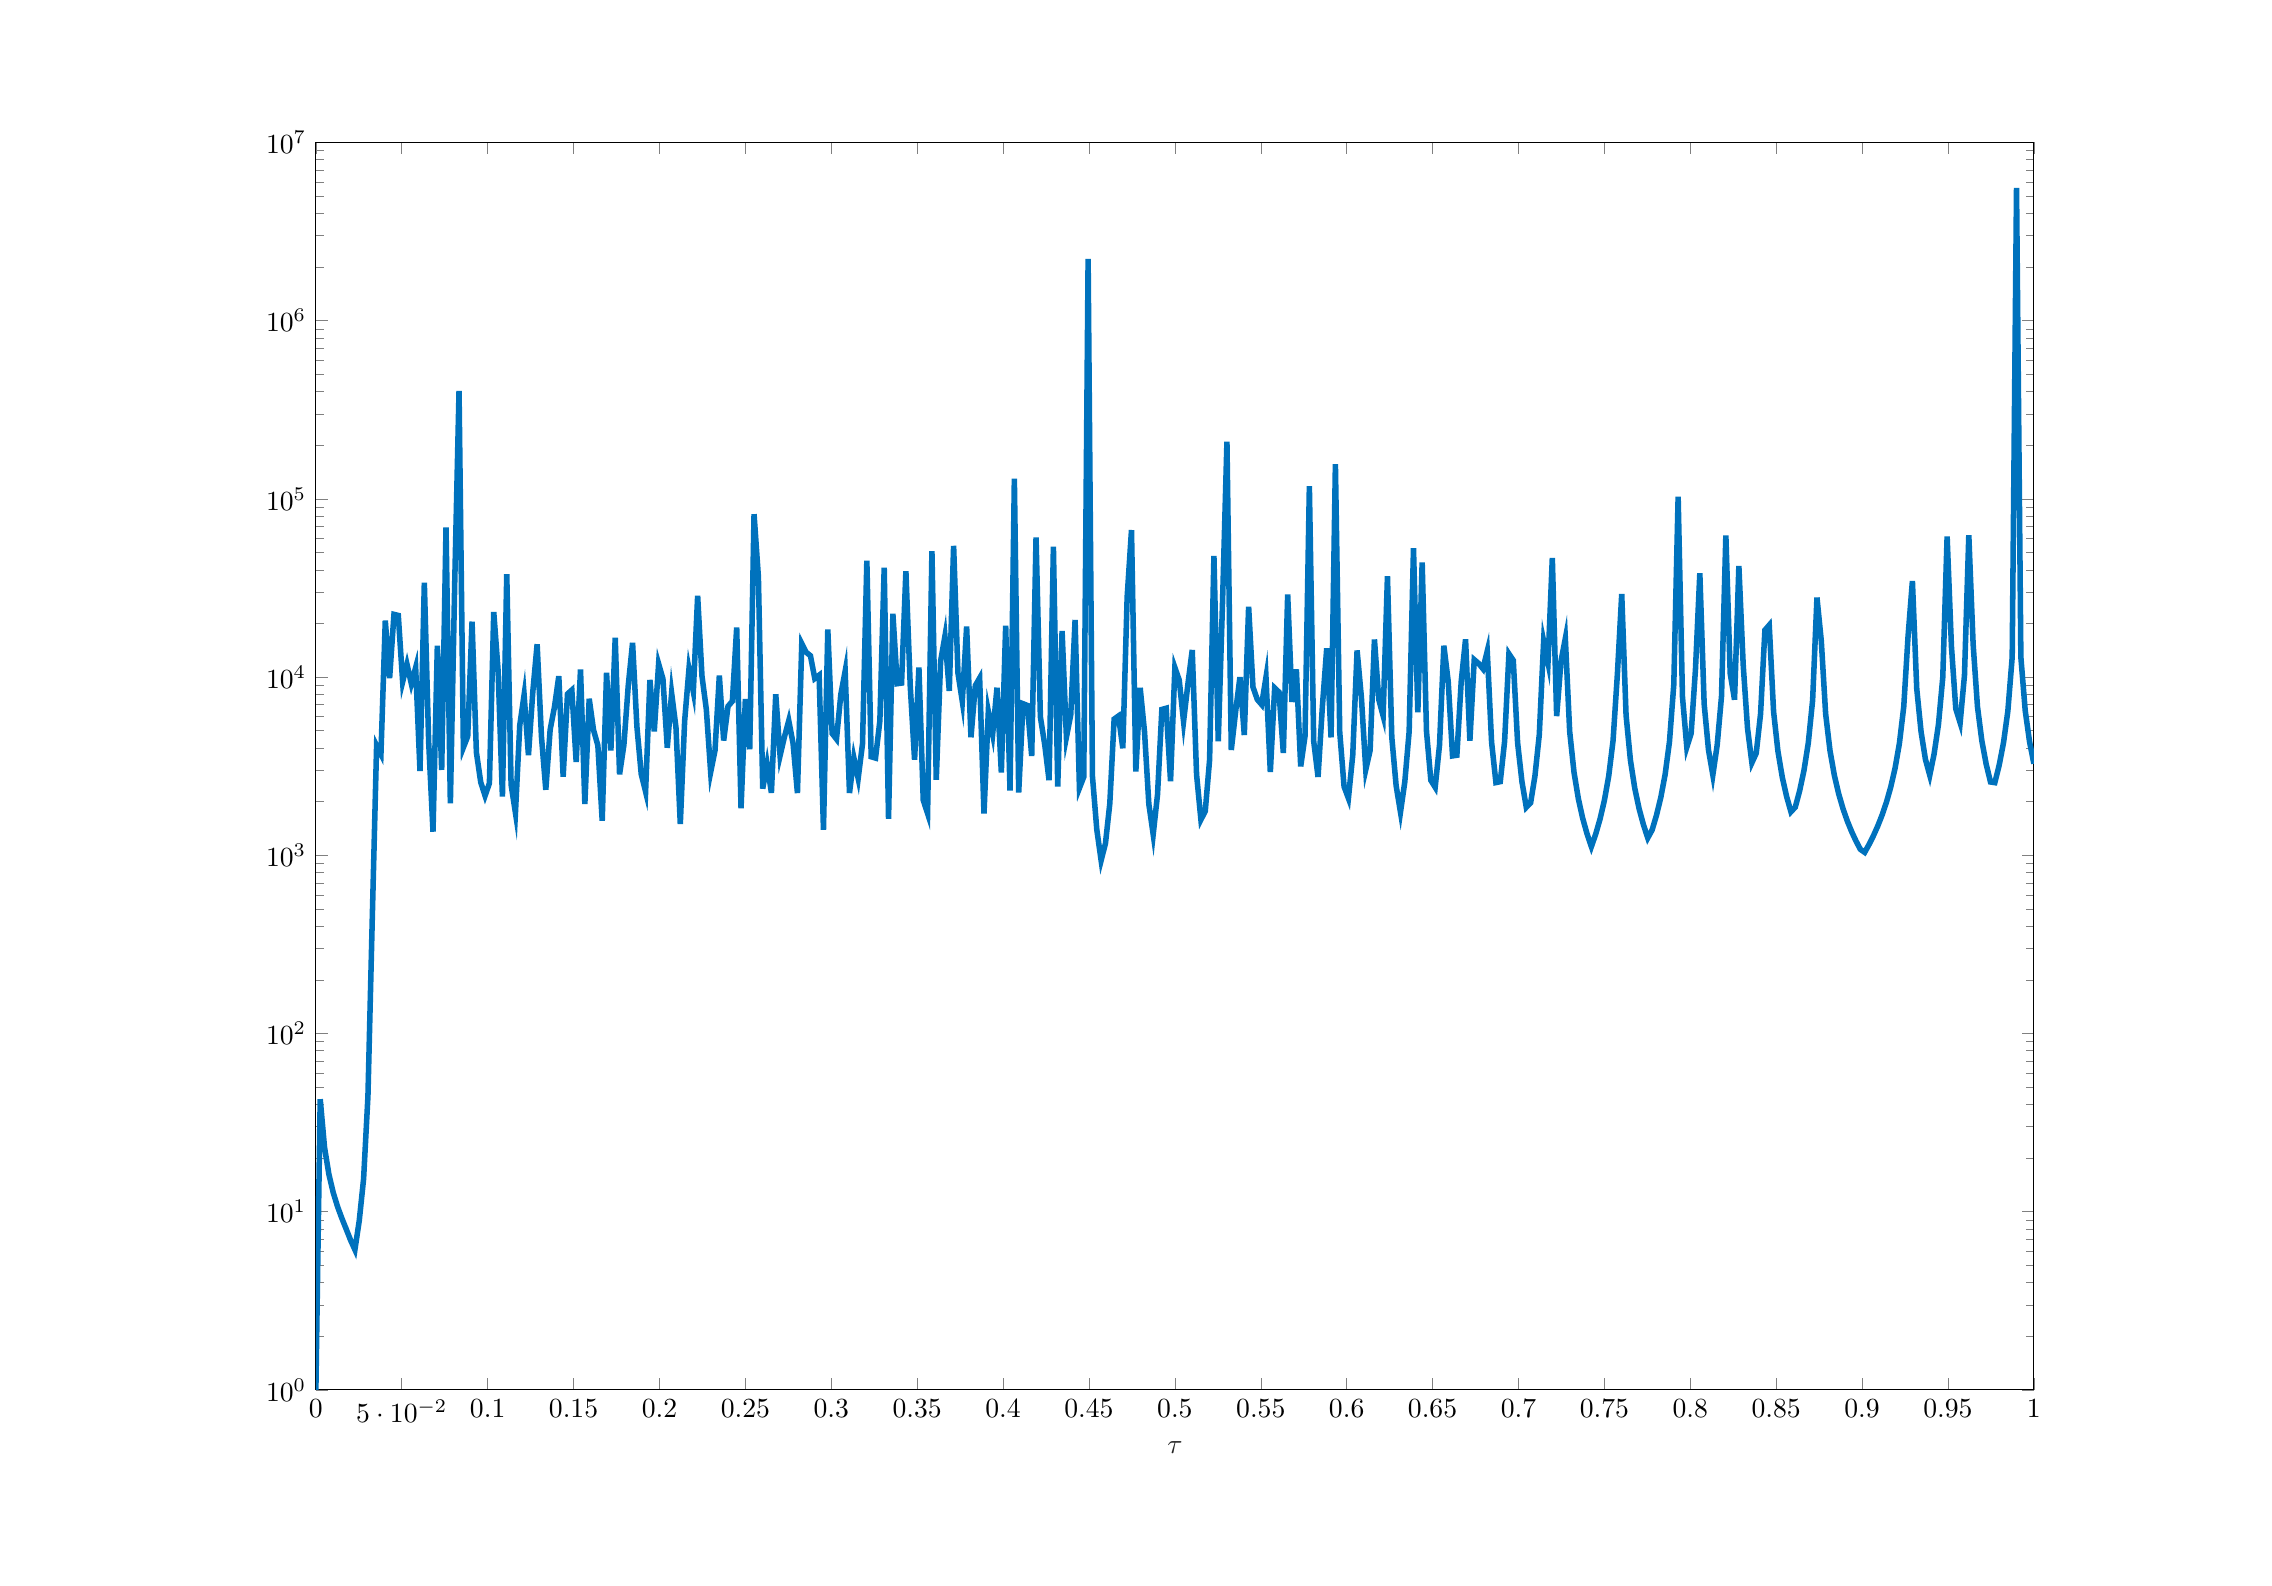
\begin{tikzpicture}

\begin{axis}[%
width=8.59in,
height=6.237in,
at={(1.441in,0.842in)},
scale only axis,
xmin=0,
xmax=1,
xlabel style={font=\color{white!15!black}},
xlabel={$\tau$},
ymode=log,
ymin=1,
ymax=10000000,
yminorticks=true,
axis background/.style={fill=white}
]
\addplot [color=mycolor1, line width=2.0pt, forget plot]
  table[row sep=crcr]{%
0	1\\
0.00252525252525253	42.7748593822766\\
0.00505050505050505	22.9016124475196\\
0.00757575757575758	16.2095708526608\\
0.0101010101010101	12.794427755266\\
0.0126262626262626	10.66977329505\\
0.0151515151515152	9.16518349417042\\
0.0176767676767677	7.97837748372638\\
0.0202020202020202	6.92139615748255\\
0.0227272727272727	6.11765225153679\\
0.0252525252525253	8.90586510272569\\
0.0277777777777778	15.2644376850026\\
0.0303030303030303	44.2567539425871\\
0.0328282828282828	439.93484507811\\
0.0353535353535354	4130.44922831594\\
0.0378787878787879	3693.33279172186\\
0.0404040404040404	20741.2351421972\\
0.0429292929292929	9872.55689751719\\
0.0454545454545455	22476.2846458954\\
0.047979797979798	22175.3209622675\\
0.0505050505050505	9405.7072745575\\
0.053030303030303	11795.7952851076\\
0.0555555555555556	9184.20354914725\\
0.0580808080808081	11311.2508162148\\
0.0606060606060606	2970.16044440938\\
0.0631313131313131	33826.8031634121\\
0.0656565656565657	4320.57353718789\\
0.0681818181818182	1356.70531684815\\
0.0707070707070707	14981.9077866418\\
0.0732323232323232	3012.63976660876\\
0.0757575757575758	69234.8100537946\\
0.0782828282828283	1957.8588410801\\
0.0808080808080808	33407.2969714485\\
0.0833333333333333	403722.319991324\\
0.0858585858585859	4026.9606698185\\
0.0883838383838384	4649.3104158616\\
0.0909090909090909	20476.8852731092\\
0.0934343434343434	3780.57588668615\\
0.095959595959596	2569.75986473666\\
0.0984848484848485	2158.17174834313\\
0.101010101010101	2537.23948820989\\
0.103535353535354	23184.4474259677\\
0.106060606060606	10906.0446424754\\
0.108585858585859	2137.89263705541\\
0.111111111111111	37829.869877445\\
0.113636363636364	2492.3947308361\\
0.116161616161616	1729.54827784607\\
0.118686868686869	5373.17767636901\\
0.121212121212121	7937.73614776365\\
0.123737373737374	3642.24366808765\\
0.126262626262626	8236.07352203103\\
0.128787878787879	15287.994957103\\
0.131313131313131	4622.03472325205\\
0.133838383838384	2330.60655775048\\
0.136363636363636	5065.12337138248\\
0.138888888888889	6802.02900958937\\
0.141414141414141	10117.9921603089\\
0.143939393939394	2760.69709858114\\
0.146464646464646	8039.5206225865\\
0.148989898989899	8453.40188226067\\
0.151515151515152	3335.1066069191\\
0.154040404040404	11030.1820646278\\
0.156565656565657	1939.06555725378\\
0.159090909090909	7558.74243446266\\
0.161616161616162	5049.92423967379\\
0.164141414141414	4129.80323079152\\
0.166666666666667	1562.66000251985\\
0.169191919191919	10580.3829165583\\
0.171717171717172	3874.58398561808\\
0.174242424242424	16637.4646284623\\
0.176767676767677	2844.77071182738\\
0.179292929292929	4159.19140974163\\
0.181818181818182	8934.61812170373\\
0.184343434343434	15576.7269486714\\
0.186868686868687	5267.00047496911\\
0.189393939393939	2847.77747675523\\
0.191919191919192	2273.53269152136\\
0.194444444444444	9639.0933594786\\
0.196969696969697	4959.61577237241\\
0.19949494949495	11870.1876838099\\
0.202020202020202	9769.69689680882\\
0.204545454545455	4009.29952671166\\
0.207070707070707	8130.40599365902\\
0.20959595959596	5225.09310083335\\
0.212121212121212	1498.44214297675\\
0.214646464646465	5660.37566925506\\
0.217171717171717	11113.0077641677\\
0.21969696969697	8282.94332511185\\
0.222222222222222	28552.8562073982\\
0.224747474747475	10117.1721430989\\
0.227272727272727	6588.99746719412\\
0.22979797979798	2923.39961682113\\
0.232323232323232	3874.40324747273\\
0.234848484848485	10192.970946119\\
0.237373737373737	4405.08843277271\\
0.23989898989899	6857.11995937019\\
0.242424242424242	7317.66921037397\\
0.244949494949495	18983.7613400783\\
0.247474747474747	1836.66533933842\\
0.25	7529.57186010592\\
0.25	7529.57186010592\\
0.252525252525253	3933.33654829326\\
0.255050505050505	82056.8336372577\\
0.257575757575758	36543.1590554406\\
0.26010101010101	2365.06559912299\\
0.262626262626263	3260.97490225633\\
0.265151515151515	2240.40186405888\\
0.267676767676768	8014.60966016066\\
0.27020202020202	3622.43499739783\\
0.272727272727273	4611.22672445401\\
0.275252525252525	5692.01855561071\\
0.277777777777778	4231.89479580688\\
0.28030303030303	2233.89158274554\\
0.282828282828283	15425.3571478632\\
0.285353535353535	13791.9405161147\\
0.287878787878788	13168.1453643387\\
0.29040404040404	9813.67905667038\\
0.292929292929293	10241.6921107818\\
0.295454545454545	1390.07293008522\\
0.297979797979798	18500.5000897162\\
0.30050505050505	4824.95390141257\\
0.303030303030303	4485.76648803146\\
0.305555555555556	7985.67824670372\\
0.308080808080808	10801.1684212918\\
0.310606060606061	2236.34904867372\\
0.313131313131313	3526.96457907671\\
0.315656565656566	2701.25563739622\\
0.318181818181818	4217.43225049004\\
0.320707070707071	44989.0846688254\\
0.323232323232323	3571.20192796793\\
0.325757575757576	3512.24008082661\\
0.328282828282828	5676.40883624382\\
0.330808080808081	41104.2090454016\\
0.333333333333333	1602.66047148333\\
0.335858585858586	22661.7775103776\\
0.338383838383838	9179.00079007402\\
0.340909090909091	9255.28922752962\\
0.343434343434343	39279.3182413748\\
0.345959595959596	8942.12130675921\\
0.348484848484849	3433.12990842816\\
0.351010101010101	11327.5237434216\\
0.353535353535354	2038.49552924144\\
0.356060606060606	1716.37280571114\\
0.358585858585859	50888.1090896974\\
0.361111111111111	2652.99150381596\\
0.363636363636364	12269.8437393391\\
0.366161616161616	16972.4907390548\\
0.368686868686869	8366.83744672745\\
0.371212121212121	54501.543696365\\
0.373737373737374	10538.6998778213\\
0.376262626262626	7307.78356399971\\
0.378787878787879	19230.9663084091\\
0.381313131313131	4591.72551083083\\
0.383838383838384	8958.88716337281\\
0.386363636363636	9877.03530979109\\
0.388888888888889	1714.53464279414\\
0.391414141414141	6417.32914934128\\
0.393939393939394	4793.78549973718\\
0.396464646464646	8714.99149487626\\
0.398989898989899	2910.90123762325\\
0.401515151515151	19409.4800486498\\
0.404040404040404	2303.88761510293\\
0.406565656565657	129651.967566173\\
0.409090909090909	2250.20202141355\\
0.411616161616162	7085.22778810726\\
0.414141414141414	6930.93293468323\\
0.416666666666667	3608.79627790766\\
0.419191919191919	60777.013803871\\
0.421717171717172	5973.1222855154\\
0.424242424242424	4175.38835547838\\
0.426767676767677	2638.31347388497\\
0.429292929292929	53839.0461337961\\
0.431818181818182	2428.13694639956\\
0.434343434343434	18137.2643674434\\
0.436868686868687	4601.41431412213\\
0.439393939393939	6142.30684658894\\
0.441919191919192	20939.5946375052\\
0.444444444444444	2382.95123848172\\
0.446969696969697	2753.1227569566\\
0.44949494949495	2220313.80014399\\
0.452020202020202	2775.29875302558\\
0.454545454545455	1395.77278992282\\
0.457070707070707	935.549300815097\\
0.45959595959596	1166.14889504773\\
0.462121212121212	1949.06049341732\\
0.464646464646465	5809.82095352902\\
0.467171717171717	6047.19039323032\\
0.46969696969697	3985.46871814603\\
0.472222222222222	28147.0333990911\\
0.474747474747475	66785.8799779668\\
0.477272727272727	2951.79886280301\\
0.47979797979798	8709.33140178189\\
0.482323232323232	4941.16226966547\\
0.484848484848485	1936.19669347093\\
0.487373737373737	1308.74540015485\\
0.48989898989899	2190.2823394388\\
0.492424242424242	6578.88580102069\\
0.494949494949495	6682.95706814844\\
0.497474747474748	2603.15277126231\\
0.5	11301.3634454102\\
0.5	11301.3634454102\\
0.502525252525252	9622.50921886594\\
0.505050505050505	5634.79231005907\\
0.507575757575758	9113.84021878156\\
0.51010101010101	14186.8150377107\\
0.512626262626263	2838.76544964284\\
0.515151515151515	1583.68758739326\\
0.517676767676768	1767.65025545783\\
0.52020202020202	3423.94975962034\\
0.522727272727273	47859.9969567559\\
0.525252525252525	4363.09264066134\\
0.527777777777778	27061.9028542765\\
0.53030303030303	209209.228275255\\
0.532828282828283	3898.17854493762\\
0.535353535353535	6392.83290388065\\
0.537878787878788	9991.77090465694\\
0.54040404040404	4726.45806540602\\
0.542929292929293	24822.9548514123\\
0.545454545454545	8792.45164909188\\
0.547979797979798	7482.71114768553\\
0.55050505050505	7010.58671213233\\
0.553030303030303	9966.1446907418\\
0.555555555555556	2930.58733141792\\
0.558080808080808	8685.8897130763\\
0.560606060606061	8231.23063778734\\
0.563131313131313	3747.85886639782\\
0.565656565656566	29117.1858389766\\
0.568181818181818	7250.13052109782\\
0.570707070707071	11040.4674154213\\
0.573232323232323	3152.88164612367\\
0.575757575757576	4669.06076114453\\
0.578282828282828	117642.887535563\\
0.580808080808081	4360.37541953436\\
0.583333333333333	2751.58233790225\\
0.585858585858586	6831.78280945966\\
0.588383838383838	14512.1316082054\\
0.590909090909091	4585.30598435827\\
0.593434343434343	156573.270836805\\
0.595959595959596	4911.37735704447\\
0.598484848484849	2427.65851972793\\
0.601010101010101	2088.56338309642\\
0.603535353535354	3649.3363369545\\
0.606060606060606	14110.2596207847\\
0.608585858585859	7652.44166528164\\
0.611111111111111	3024.44206915936\\
0.613636363636364	3873.31798328393\\
0.616161616161616	16264.548017052\\
0.618686868686869	7480.51625439177\\
0.621212121212121	6062.78365074663\\
0.623737373737374	36869.8524961953\\
0.626262626262626	4593.27412718569\\
0.628787878787879	2457.98199076312\\
0.631313131313131	1745.69079043029\\
0.633838383838384	2585.33671814319\\
0.636363636363636	4946.51429386351\\
0.638888888888889	52852.8453556291\\
0.641414141414141	6340.73051138113\\
0.643939393939394	43982.7031742981\\
0.646464646464646	4954.4782777104\\
0.648989898989899	2634.29212502817\\
0.651515151515151	2407.54883985784\\
0.654040404040404	4160.15259593321\\
0.656565656565657	14997.7110984511\\
0.659090909090909	9456.19588112223\\
0.661616161616162	3611.13892249453\\
0.664141414141414	3642.71511266802\\
0.666666666666667	9438.77360484288\\
0.669191919191919	16283.3208055228\\
0.671717171717172	4394.28882410717\\
0.674242424242424	12516.9196726081\\
0.676767676767677	11930.4429665082\\
0.679292929292929	11136.1996964602\\
0.681818181818182	13977.5020705665\\
0.684343434343434	4315.08541900991\\
0.686868686868687	2558.72578313316\\
0.689393939393939	2588.36744367428\\
0.691919191919192	4354.74803805533\\
0.694444444444444	13510.5977094122\\
0.696969696969697	12418.8477146635\\
0.69949494949495	4273.63199252327\\
0.702020202020202	2587.95293109193\\
0.704545454545455	1859.5240517237\\
0.707070707070707	1971.18616481559\\
0.70959595959596	2791.87476512837\\
0.712121212121212	4760.33338582945\\
0.714646464646465	15883.188620368\\
0.717171717171717	12025.4577545875\\
0.71969696969697	46568.4946115058\\
0.722222222222222	6038.51708807857\\
0.724747474747475	12275.1440190806\\
0.727272727272727	16475.848984018\\
0.72979797979798	4952.66254965848\\
0.732323232323232	2922.31869225998\\
0.734848484848485	2076.62132649937\\
0.737373737373737	1612.92147787755\\
0.73989898989899	1320.08381267527\\
0.742424242424242	1118.36261494902\\
0.744949494949495	1314.72552353355\\
0.747474747474748	1597.45993368385\\
0.75	2031.51623172231\\
0.75	2031.51623172231\\
0.752525252525252	2782.76535834434\\
0.755050505050505	4399.07996096747\\
0.757575757575758	10402.4233172483\\
0.76010101010101	29222.87196802\\
0.762626262626263	6107.19134902916\\
0.765151515151515	3419.48961260647\\
0.767676767676768	2379.09834204359\\
0.77020202020202	1826.79399728078\\
0.772727272727273	1484.36604616473\\
0.775252525252525	1251.28516087856\\
0.777777777777778	1386.42513311147\\
0.78030303030303	1673.49625962099\\
0.782828282828283	2107.07703533721\\
0.785353535353535	2837.75291875989\\
0.787878787878788	4330.02515887117\\
0.79040404040404	9070.60181022762\\
0.792929292929293	102952.77393104\\
0.795454545454545	7755.56762547324\\
0.797979797979798	4041.38790969401\\
0.80050505050505	4826.92295508482\\
0.803030303030303	11089.7229056541\\
0.805555555555556	38288.1118452323\\
0.808080808080808	7056.7100071235\\
0.810606060606061	3897.01421451344\\
0.813131313131313	2822.05031651926\\
0.815656565656566	4151.0152615437\\
0.818181818181818	7804.43471444253\\
0.820707070707071	62389.4071828853\\
0.823232323232323	10480.7781387005\\
0.825757575757576	7467.0403034116\\
0.828282828282828	41968.4384985247\\
0.830808080808081	11679.2722765379\\
0.833333333333333	5143.20236399421\\
0.835858585858586	3304.61599293267\\
0.838383838383838	3736.54219986153\\
0.840909090909091	6220.01997624221\\
0.843434343434343	18337.765220737\\
0.845959595959596	19571.3946040905\\
0.848484848484849	6405.49952628246\\
0.851010101010101	3838.24759169927\\
0.853535353535354	2744.54372852352\\
0.856060606060606	2138.61596319492\\
0.858585858585859	1753.65019843833\\
0.861111111111111	1862.46578637198\\
0.863636363636364	2295.89256725696\\
0.866161616161616	2987.13536825935\\
0.868686868686869	4263.60805304037\\
0.871212121212121	7414.08431362677\\
0.873737373737374	27956.3452002799\\
0.876262626262626	15926.9605893413\\
0.878787878787879	6219.05262457326\\
0.881313131313131	3872.01859509858\\
0.883838383838384	2815.37715515881\\
0.886363636363636	2214.40993038501\\
0.888888888888889	1826.63835897092\\
0.891414141414141	1555.70580082541\\
0.893939393939394	1355.71927562975\\
0.896464646464646	1202.03819757376\\
0.898989898989899	1080.24872453366\\
0.901515151515151	1038.60316580193\\
0.904040404040404	1149.11281344812\\
0.906565656565657	1285.11524790723\\
0.909090909090909	1456.58173387659\\
0.911616161616162	1679.46341648138\\
0.914141414141414	1980.96470009103\\
0.916666666666667	2411.59202661214\\
0.919191919191919	3076.90159641525\\
0.921717171717172	4240.59360544469\\
0.924242424242424	6798.03252347133\\
0.926767676767677	16991.0347034491\\
0.929292929292929	34568.4626205788\\
0.931818181818182	8602.13019051157\\
0.934343434343434	4923.30556588008\\
0.936868686868687	3453.90270649758\\
0.939393939393939	2813.49183347163\\
0.941919191919192	3704.04103829196\\
0.944444444444444	5406.48593227937\\
0.946969696969697	9961.18839627927\\
0.94949494949495	61531.5715316457\\
0.952020202020202	14824.9700907472\\
0.954545454545455	6634.35981904543\\
0.957070707070707	5544.17926468181\\
0.95959595959596	10207.3874315405\\
0.962121212121212	62555.3643893233\\
0.964646464646465	15248.28823459\\
0.967171717171717	6814.96785127399\\
0.96969696969697	4395.96330879867\\
0.972222222222222	3248.64095811367\\
0.974747474747475	2578.92981545088\\
0.977272727272727	2556.17493823454\\
0.97979797979798	3203.59410192397\\
0.982323232323232	4282.96066648484\\
0.984848484848485	6442.94952215234\\
0.987373737373737	12932.9794814945\\
0.98989898989899	5565585.84134609\\
0.992424242424242	12936.8497061437\\
0.994949494949495	6491.91265395544\\
0.997474747474748	4340.27429537292\\
1	3263.83040043697\\
};
\end{axis}

\begin{axis}[%
width=11.083in,
height=7.653in,
at={(0in,0in)},
scale only axis,
xmin=0,
xmax=1,
ymin=0,
ymax=1,
axis line style={draw=none},
ticks=none,
axis x line*=bottom,
axis y line*=left
]
\end{axis}
\end{tikzpicture}%}
\subfloat[][$\gamma=0.30$]{% This file was created by matlab2tikz.
%
%The latest updates can be retrieved from
%  http://www.mathworks.com/matlabcentral/fileexchange/22022-matlab2tikz-matlab2tikz
%where you can also make suggestions and rate matlab2tikz.
%
\definecolor{mycolor1}{rgb}{0.00000,0.44700,0.74100}%
%
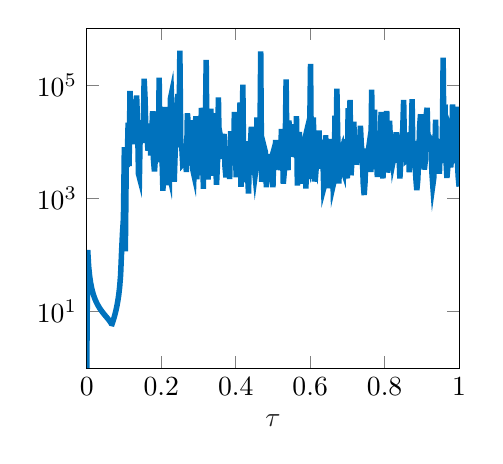
\begin{tikzpicture}

\begin{axis}[%
width=0.39\columnwidth,
height=1.7in,
at={(1.441in,0.842in)},
scale only axis,
xmin=0,
xmax=1,
xlabel style={font=\color{white!15!black}},
xlabel={$\tau$},
ymode=log,
ymin=1,
ymax=1000000,
yminorticks=true,
axis background/.style={fill=white}
]
\addplot [color=mycolor1, line width=2.0pt, forget plot]
  table[row sep=crcr]{%
0	1\\
0.00252525252525253	122.014807520731\\
0.00505050505050505	62.5956567253491\\
0.00757575757575758	42.7748593822774\\
0.0101010101010101	32.8523226179406\\
0.0126262626262626	26.887944470322\\
0.0151515151515152	22.9016124475198\\
0.0176767676767677	20.044630355608\\
0.0202020202020202	17.892573314431\\
0.0227272727272727	16.2095708526607\\
0.0252525252525253	14.8540179348892\\
0.0277777777777778	13.7357137182503\\
0.0303030303030303	12.7944277552662\\
0.0328282828282828	11.9883547774899\\
0.0353535353535354	11.2875124168418\\
0.0378787878787879	10.6697732950499\\
0.0404040404040404	10.118376290194\\
0.0429292929292929	9.62030399297802\\
0.0454545454545455	9.16518349417035\\
0.047979797979798	8.7445080424225\\
0.0505050505050505	8.35105088004771\\
0.053030303030303	7.97837748372629\\
0.0555555555555556	7.62036642264013\\
0.0580808080808081	7.27060833209817\\
0.0606060606060606	6.92139615748242\\
0.0631313131313131	6.56142238153865\\
0.0656565656565657	6.16818997173652\\
0.0681818181818182	6.11765225153678\\
0.0707070707070707	6.85514187932508\\
0.0732323232323232	7.76245043463956\\
0.0757575757575758	8.9058651027257\\
0.0782828282828283	10.391332747234\\
0.0808080808080808	12.3993372136625\\
0.0833333333333333	15.2644376850023\\
0.0858585858585859	19.6842921009203\\
0.0883838383838384	27.3956676836616\\
0.0909090909090909	44.2567539425884\\
0.0934343434343434	110.304215203538\\
0.095959595959596	243.797400196456\\
0.0984848484848485	439.934845078718\\
0.101010101010101	7929.56288990357\\
0.103535353535354	115.309472846875\\
0.106060606060606	4130.44922841372\\
0.108585858585859	4085.22803757058\\
0.111111111111111	21618.1416346271\\
0.113636363636364	3693.33279174367\\
0.116161616161616	78580.0432666054\\
0.118686868686869	18349.4209201815\\
0.121212121212121	20741.2351418741\\
0.123737373737374	9019.07719035265\\
0.126262626262626	15923.3275783095\\
0.128787878787879	9872.55689745587\\
0.131313131313131	41301.3066990395\\
0.133838383838384	64886.5126086417\\
0.136363636363636	22476.284646095\\
0.138888888888889	2696.08658695682\\
0.141414141414141	2327.47375601248\\
0.143939393939394	22175.320962572\\
0.146464646464646	9421.01798956002\\
0.148989898989899	20892.4325527475\\
0.151515151515152	9405.70727451478\\
0.154040404040404	128277.016727865\\
0.156565656565657	57489.7163419085\\
0.159090909090909	11795.7952850942\\
0.161616161616162	20823.0391646857\\
0.164141414141414	6918.59868990844\\
0.166666666666667	9184.20354913013\\
0.169191919191919	18766.7322069444\\
0.171717171717172	5694.7907160554\\
0.174242424242424	11311.2508162459\\
0.176767676767677	34420.6779277789\\
0.179292929292929	4622.77118351157\\
0.181818181818182	2970.1604444002\\
0.184343434343434	5198.32844169814\\
0.186868686868687	7599.04356005366\\
0.189393939393939	33826.8031639717\\
0.191919191919192	5084.69467070449\\
0.194444444444444	134646.541855683\\
0.196969696969697	4320.57353717893\\
0.19949494949495	10141.7779132601\\
0.202020202020202	5564.42011436136\\
0.204545454545455	1356.70531684764\\
0.207070707070707	7101.08182591639\\
0.20959595959596	40677.4925291347\\
0.212121212121212	14981.9077869319\\
0.214646464646465	1696.17386235868\\
0.217171717171717	19696.7476460192\\
0.21969696969697	3012.63976661366\\
0.222222222222222	2526.96274543381\\
0.224747474747475	57454.0526339864\\
0.227272727272727	69234.8100504111\\
0.22979797979798	21770.7462600589\\
0.232323232323232	5936.97473153588\\
0.234848484848485	1957.85884107952\\
0.237373737373737	6364.20084967841\\
0.23989898989899	11493.6806514899\\
0.242424242424242	33407.2969729058\\
0.244949494949495	69339.7930173466\\
0.247474747474747	8356.10713217375\\
0.25	403722.320027175\\
0.25	403722.320027175\\
0.252525252525253	8664.81541673576\\
0.255050505050505	8537.65544000069\\
0.257575757575758	4026.96066984142\\
0.26010101010101	4224.7338473836\\
0.262626262626263	8612.78096125572\\
0.265151515151515	4649.31041586675\\
0.267676767676768	2902.66169388937\\
0.27020202020202	31519.3048529255\\
0.272727272727273	20476.8852729639\\
0.275252525252525	6119.2441389686\\
0.277777777777778	23887.5745641141\\
0.28030303030303	3780.57588668324\\
0.282828282828283	6384.12800034867\\
0.285353535353535	3058.58643275702\\
0.287878787878788	2569.75986474298\\
0.29040404040404	7929.82163774097\\
0.292929292929293	28077.5054970774\\
0.295454545454545	2158.17174834419\\
0.297979797979798	8772.986630708\\
0.30050505050505	9278.83247624925\\
0.303030303030303	2537.23948820873\\
0.305555555555556	11068.672421851\\
0.308080808080808	39307.1463186107\\
0.310606060606061	23184.4474259031\\
0.313131313131313	1470.31758115809\\
0.315656565656566	27289.0320843977\\
0.318181818181818	10906.0446425463\\
0.320707070707071	277171.550875709\\
0.323232323232323	3680.47539639818\\
0.325757575757576	2137.89263705444\\
0.328282828282828	8958.55838523984\\
0.330808080808081	8265.91741855081\\
0.333333333333333	37829.8698790483\\
0.335858585858586	7659.65350446386\\
0.338383838383838	31732.4951488801\\
0.340909090909091	2492.39473083533\\
0.343434343434343	7637.01409690376\\
0.345959595959596	4311.26445164717\\
0.348484848484849	1729.54827784582\\
0.351010101010101	4110.47586728823\\
0.353535353535354	59960.5688607433\\
0.356060606060606	5373.17767636452\\
0.358585858585859	12876.0419916469\\
0.361111111111111	10450.1717092893\\
0.363636363636364	7937.73614774581\\
0.366161616161616	4928.58023955851\\
0.368686868686869	13685.2231130608\\
0.371212121212121	3642.24366808304\\
0.373737373737374	2342.60465815109\\
0.376262626262626	3492.07678272929\\
0.378787878787879	8236.07352204065\\
0.381313131313131	5214.97346101201\\
0.383838383838384	2178.75668235586\\
0.386363636363636	15287.994957068\\
0.388888888888889	3777.77057438653\\
0.391414141414141	9695.91971341005\\
0.393939393939394	4622.03472325429\\
0.396464646464646	33181.5753531896\\
0.398989898989899	6792.3254623107\\
0.401515151515151	2330.60655775188\\
0.404040404040404	15372.1343532261\\
0.406565656565657	9951.36037685698\\
0.409090909090909	5065.12337137181\\
0.411616161616162	48822.0409612698\\
0.414141414141414	1583.85648771682\\
0.416666666666667	6802.02900959846\\
0.419191919191919	100719.620436379\\
0.421717171717172	1900.03629504623\\
0.424242424242424	10117.9921603274\\
0.426767676767677	2010.03903527277\\
0.429292929292929	5490.821435911\\
0.431818181818182	2760.69709858209\\
0.434343434343434	1208.94871999827\\
0.436868686868687	5243.45827751107\\
0.439393939393939	8039.52062262357\\
0.441919191919192	18199.6640306235\\
0.444444444444444	5166.58021109019\\
0.446969696969697	8453.40188226134\\
0.44949494949495	3658.10172158646\\
0.452020202020202	2485.33879872883\\
0.454545454545455	3335.1066069166\\
0.457070707070707	26643.3309331169\\
0.45959595959596	3843.78584787138\\
0.462121212121212	11030.1820646181\\
0.464646464646465	4986.42046271783\\
0.467171717171717	389335.517099946\\
0.46969696969697	1939.06555725343\\
0.472222222222222	5230.51902339219\\
0.474747474747475	5808.28675728599\\
0.477272727272727	7558.74243446834\\
0.47979797979798	6497.02868740449\\
0.482323232323232	1556.11945246532\\
0.484848484848485	5049.92423967486\\
0.487373737373737	3964.13897759494\\
0.48989898989899	5979.57283845895\\
0.492424242424242	4129.80323078867\\
0.494949494949495	4746.37428948774\\
0.497474747474748	2492.64643765164\\
0.5	1562.66000251922\\
0.5	1562.66000251922\\
0.502525252525252	6804.11036024396\\
0.505050505050505	6922.33131860453\\
0.507575757575758	10580.382916533\\
0.51010101010101	5669.97688726515\\
0.512626262626263	3755.47995079555\\
0.515151515151515	3874.58398562165\\
0.517676767676768	6278.12708174189\\
0.52020202020202	3109.51752288367\\
0.522727272727273	16637.4646284316\\
0.525252525252525	11156.2207944621\\
0.527777777777778	1803.55107282132\\
0.53030303030303	2844.77071182753\\
0.532828282828283	7185.38723658703\\
0.535353535353535	125330.548747662\\
0.537878787878788	4159.19140974628\\
0.54040404040404	3133.09783311055\\
0.542929292929293	23460.4413448864\\
0.545454545454545	8934.61812170407\\
0.547979797979798	5415.66268780268\\
0.55050505050505	8049.03931072141\\
0.553030303030303	15576.7269487107\\
0.555555555555556	5614.34522165434\\
0.558080808080808	20158.8587200511\\
0.560606060606061	5267.00047495846\\
0.563131313131313	28052.6603892587\\
0.565656565656566	1676.55863987325\\
0.568181818181818	2847.77747675716\\
0.570707070707071	14798.7130141656\\
0.573232323232323	1821.49537152427\\
0.575757575757576	2273.53269152256\\
0.578282828282828	6007.56568861713\\
0.580808080808081	3304.60545251016\\
0.583333333333333	9639.09335945984\\
0.585858585858586	11310.4931391905\\
0.588383838383838	1479.86967506519\\
0.590909090909091	4959.61577237341\\
0.593434343434343	4820.08127886398\\
0.595959595959596	4127.67201541453\\
0.598484848484849	11870.187683792\\
0.601010101010101	235565.645272801\\
0.603535353535354	2207.18949073374\\
0.606060606060606	9769.69689678301\\
0.608585858585859	26739.2577601182\\
0.611111111111111	1962.01786223412\\
0.613636363636364	4009.29952670672\\
0.616161616161616	3458.2547654385\\
0.618686868686869	5748.43043820067\\
0.621212121212121	8130.40599364372\\
0.623737373737374	15711.0507110377\\
0.626262626262626	3302.88952174617\\
0.628787878787879	5225.09310083545\\
0.631313131313131	7260.75994776236\\
0.633838383838384	6244.86455529316\\
0.636363636363636	1498.44214297719\\
0.638888888888889	1733.28647327214\\
0.641414141414141	12887.1648455382\\
0.643939393939394	5660.37566925743\\
0.646464646464646	1494.59631543078\\
0.648989898989899	2775.5956848678\\
0.651515151515151	11113.0077641698\\
0.654040404040404	4561.62981029031\\
0.656565656565657	6206.69442099204\\
0.659090909090909	8282.94332511662\\
0.661616161616162	1688.45123123576\\
0.664141414141414	2002.21723223607\\
0.666666666666667	28552.8562074141\\
0.669191919191919	4912.11720495116\\
0.671717171717172	85950.2662739805\\
0.674242424242424	10117.1721431124\\
0.676767676767677	1816.29879818563\\
0.679292929292929	4042.14994983316\\
0.681818181818182	6588.99746719023\\
0.684343434343434	7362.13340936055\\
0.686868686868687	3296.39845428195\\
0.689393939393939	2923.39961682165\\
0.691919191919192	10987.8286128006\\
0.694444444444444	5911.88189616365\\
0.696969696969697	3874.40324747132\\
0.69949494949495	2235.9894294349\\
0.702020202020202	38651.6241354706\\
0.704545454545455	10192.9709461098\\
0.707070707070707	54255.1087123796\\
0.70959595959596	2533.8771868925\\
0.712121212121212	4405.08843277598\\
0.714646464646465	14011.795092665\\
0.717171717171717	22332.5637943211\\
0.71969696969697	6857.11995936973\\
0.722222222222222	9847.15202429175\\
0.724747474747475	3882.43669401615\\
0.727272727272727	7317.66921037579\\
0.72979797979798	4357.51765546727\\
0.732323232323232	6264.73387416174\\
0.734848484848485	18983.761340058\\
0.737373737373737	8687.4767065136\\
0.73989898989899	6054.86561959307\\
0.742424242424242	1836.66533933899\\
0.744949494949495	1137.98331771039\\
0.747474747474748	1981.54084927317\\
0.75	7529.57186010876\\
0.75	7529.57186010876\\
0.752525252525252	4817.51690893294\\
0.755050505050505	6262.61432032042\\
0.757575757575758	3933.33654829296\\
0.76010101010101	9225.71677768881\\
0.762626262626263	2891.11862042694\\
0.765151515151515	82056.8336370554\\
0.767676767676768	3238.80016982379\\
0.77020202020202	22271.4141949608\\
0.772727272727273	36543.1590555634\\
0.775252525252525	5695.66114705002\\
0.777777777777778	12879.8851466869\\
0.78030303030303	2365.06559912214\\
0.782828282828283	7812.80423740809\\
0.785353535353535	4697.2638878579\\
0.787878787878788	3260.97490225501\\
0.79040404040404	33285.3472630948\\
0.792929292929293	3386.55869116665\\
0.795454545454545	2240.40186405944\\
0.797979797979798	8640.31004591044\\
0.80050505050505	5291.8831889787\\
0.803030303030303	8014.6096601675\\
0.805555555555556	34639.4351272585\\
0.808080808080808	2842.30592629153\\
0.810606060606061	3622.43499739822\\
0.813131313131313	23254.7318155147\\
0.815656565656566	10150.0757412541\\
0.818181818181818	4611.2267244544\\
0.820707070707071	10273.0091228828\\
0.823232323232323	4664.81519216507\\
0.825757575757576	5692.01855561128\\
0.828282828282828	7552.90439514042\\
0.830808080808081	14646.9376327546\\
0.833333333333333	4231.89479580612\\
0.835858585858586	6542.08637672629\\
0.838383838383838	6747.15279586583\\
0.840909090909091	2233.89158274512\\
0.843434343434343	4660.64448597597\\
0.845959595959596	12288.939170352\\
0.848484848484849	15425.3571478561\\
0.851010101010101	54336.1836273674\\
0.853535353535354	6434.8675082456\\
0.856060606060606	13791.9405160821\\
0.858585858585859	4646.05515730569\\
0.861111111111111	4794.67350888903\\
0.863636363636364	13168.1453643437\\
0.866161616161616	2858.52837885212\\
0.868686868686869	14597.0541827063\\
0.871212121212121	9813.67905666175\\
0.873737373737374	55898.4539788148\\
0.876262626262626	3393.34593252975\\
0.878787878787879	10241.69211079\\
0.881313131313131	5678.13496462261\\
0.883838383838384	2229.88911852101\\
0.886363636363636	1390.07293008506\\
0.888888888888889	2082.88344987802\\
0.891414141414141	4709.42181159148\\
0.893939393939394	18500.500089659\\
0.896464646464646	30404.1815515522\\
0.898989898989899	3372.69930405319\\
0.901515151515151	4824.95390141083\\
0.904040404040404	18696.9772226993\\
0.906565656565657	3195.83429440676\\
0.909090909090909	4485.76648803136\\
0.911616161616162	29685.8363460381\\
0.914141414141414	39402.4687267699\\
0.916666666666667	7985.67824669281\\
0.919191919191919	7850.03745478819\\
0.921717171717172	11545.4807912308\\
0.924242424242424	10801.1684213102\\
0.926767676767677	2929.81713711103\\
0.929292929292929	1698.29794280344\\
0.931818181818182	2236.34904867393\\
0.934343434343434	4940.77598661022\\
0.936868686868687	24294.1671545723\\
0.939393939393939	3526.96457907722\\
0.941919191919192	11009.0432824276\\
0.944444444444444	6710.13220433599\\
0.946969696969697	2701.25563739634\\
0.94949494949495	7528.01737711769\\
0.952020202020202	9673.36417103107\\
0.954545454545455	4217.4322504901\\
0.957070707070707	302877.160466333\\
0.95959595959596	4359.469427826\\
0.962121212121212	44989.0846683735\\
0.964646464646465	4804.70404916685\\
0.967171717171717	2286.29553268826\\
0.96969696969697	3571.20192796856\\
0.972222222222222	18816.185507858\\
0.974747474747475	16663.6333150822\\
0.977272727272727	3512.24008082755\\
0.97979797979798	4990.61183658873\\
0.982323232323232	45320.5389104158\\
0.984848484848485	5676.40883624712\\
0.987373737373737	22673.9573852233\\
0.98989898989899	4124.70769191741\\
0.992424242424242	41104.2090454834\\
0.994949494949495	5187.47807795255\\
0.997474747474748	2445.78586955221\\
1	1602.66047148327\\
};
\end{axis}
\end{tikzpicture}%}
\\
\subfloat[][$\gamma=0.50$]{% This file was created by matlab2tikz.
%
%The latest updates can be retrieved from
%  http://www.mathworks.com/matlabcentral/fileexchange/22022-matlab2tikz-matlab2tikz
%where you can also make suggestions and rate matlab2tikz.
%
\definecolor{mycolor1}{rgb}{0.00000,0.44700,0.74100}%
%
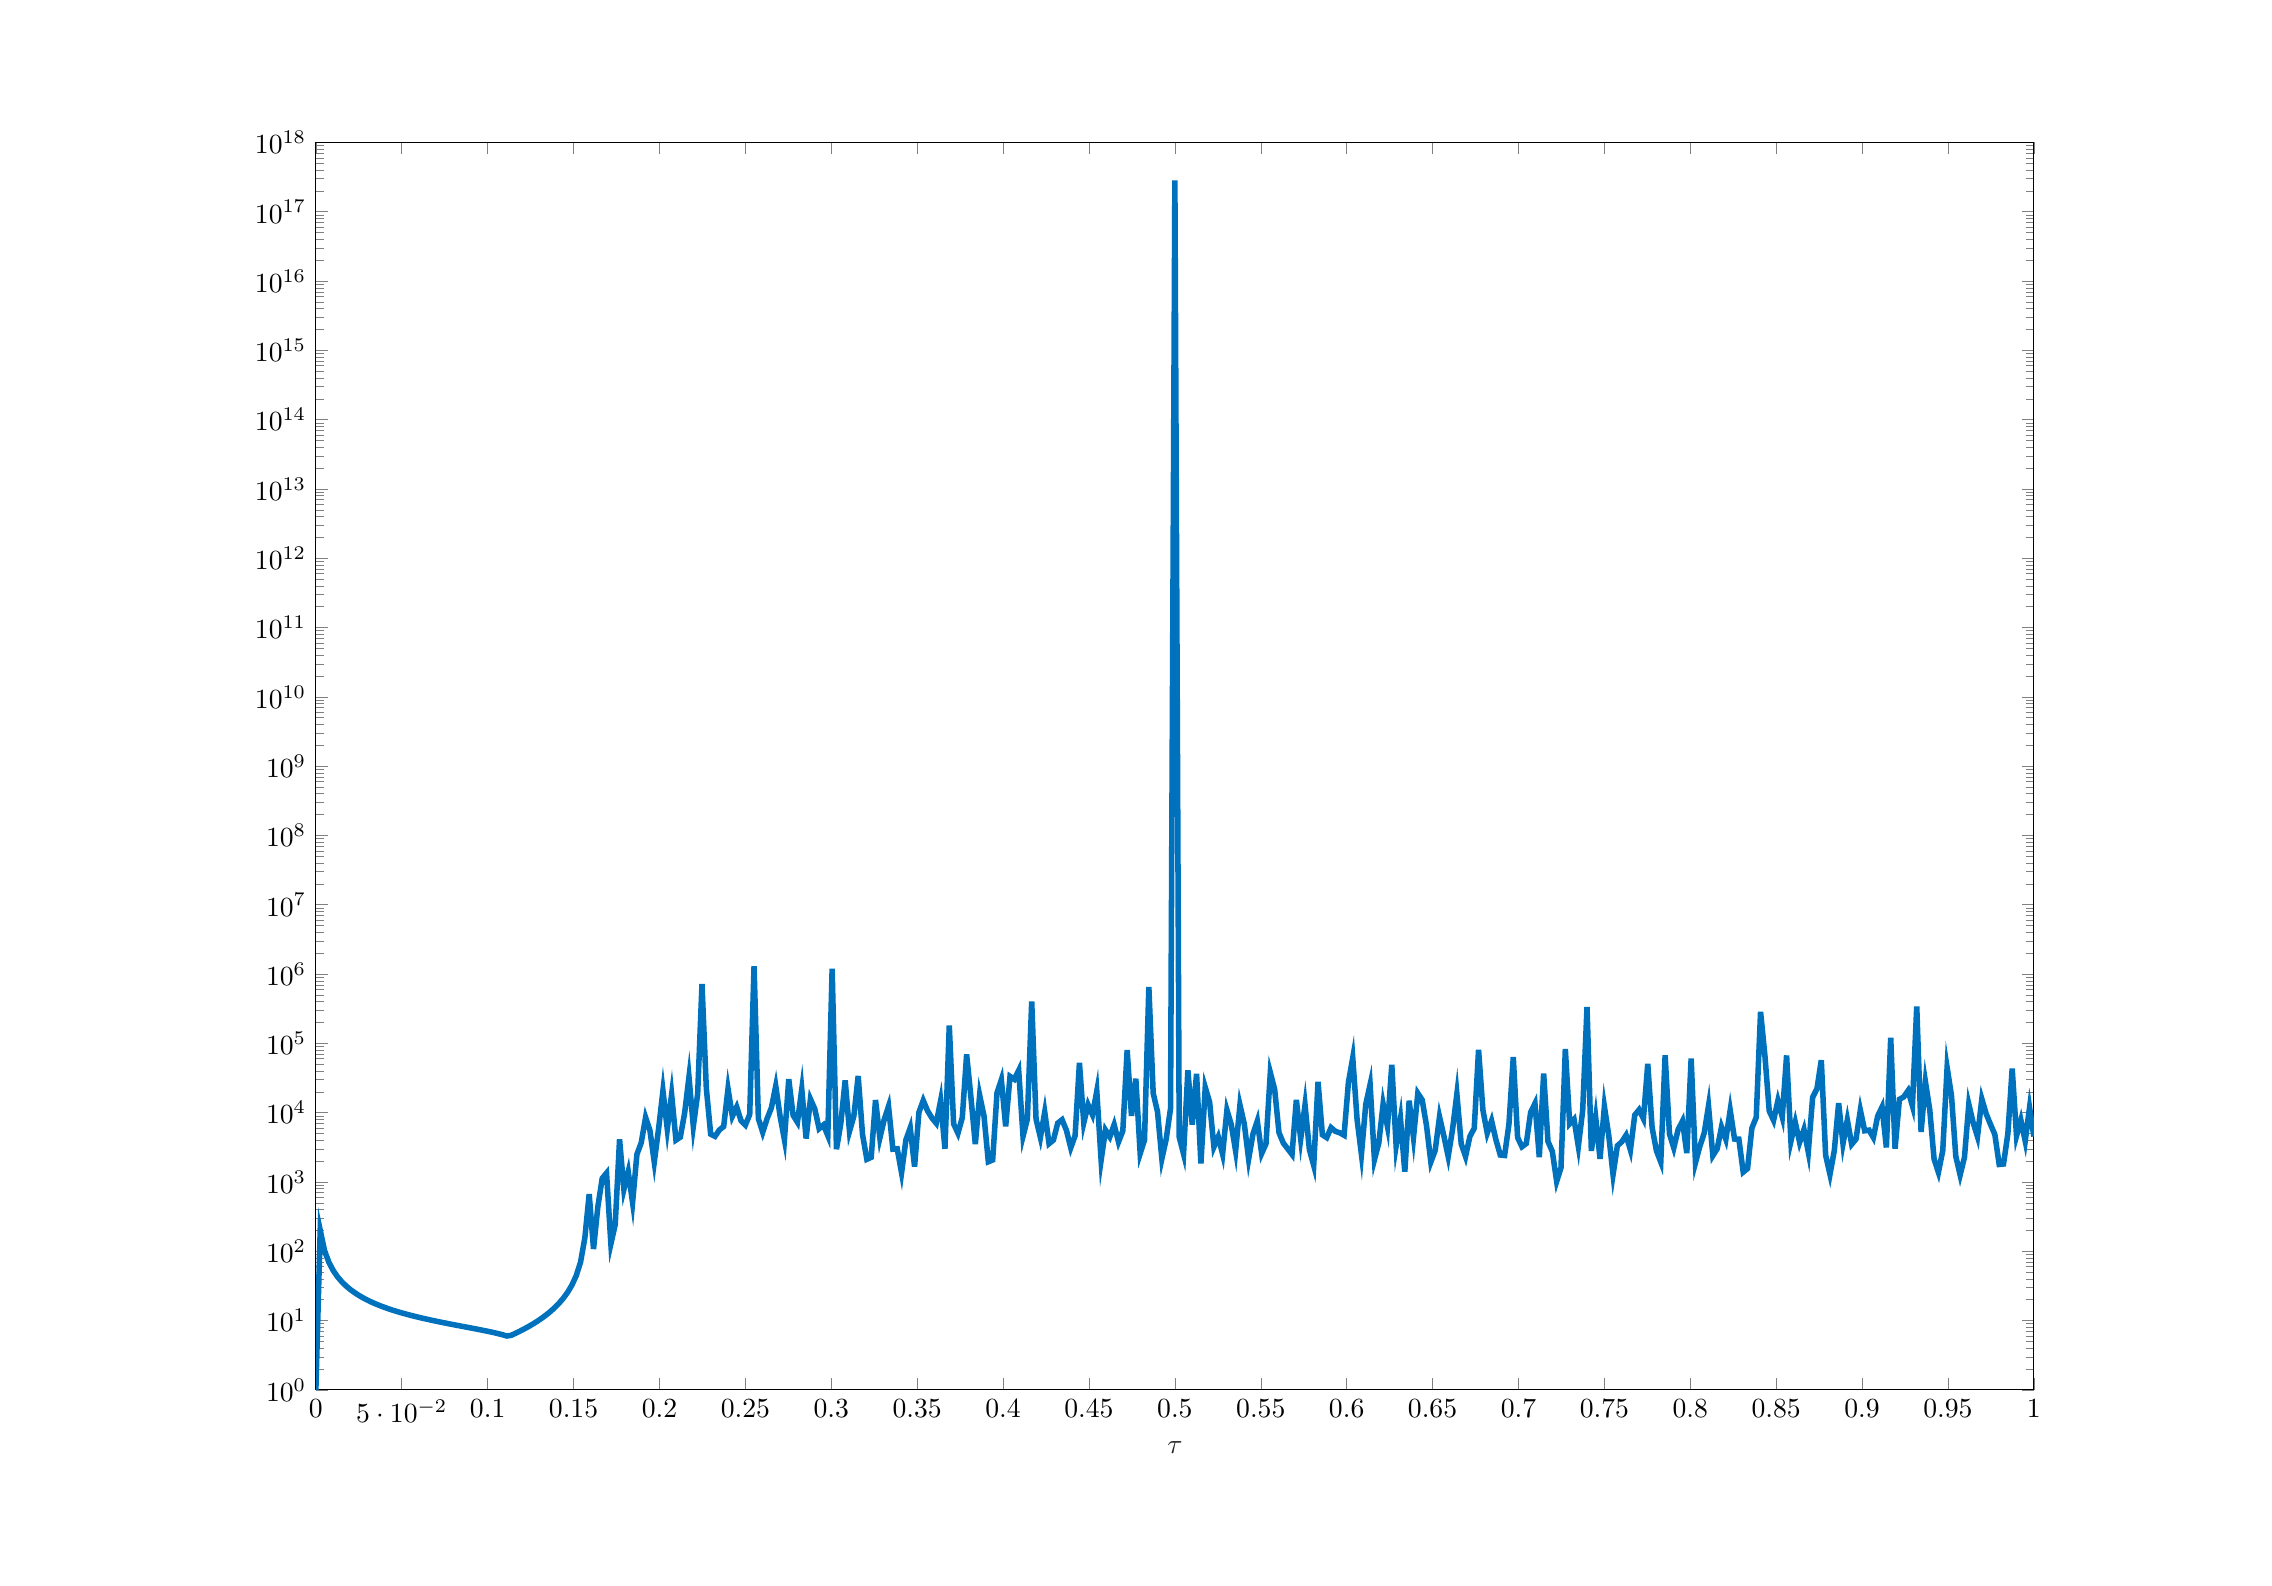
\begin{tikzpicture}

\begin{axis}[%
width=8.59in,
height=6.237in,
at={(1.441in,0.842in)},
scale only axis,
xmin=0,
xmax=1,
xlabel style={font=\color{white!15!black}},
xlabel={$\tau$},
ymode=log,
ymin=1,
ymax=1e+18,
yminorticks=true,
axis background/.style={fill=white}
]
\addplot [color=mycolor1, line width=2.0pt, forget plot]
  table[row sep=crcr]{%
0	1\\
0.00252525252525253	201.222026083381\\
0.00505050505050505	102.211104901192\\
0.00757575757575758	69.1996157820081\\
0.0101010101010101	52.6875403861659\\
0.0126262626262626	42.774859382277\\
0.0151515151515152	36.1615523606765\\
0.0176767676767677	31.4333120228461\\
0.0202020202020202	27.8829726454385\\
0.0227272727272727	25.1176528172878\\
0.0252525252525253	22.9016124475196\\
0.0277777777777778	21.0848240425146\\
0.0303030303030303	19.5672582490739\\
0.0328282828282828	18.2796528913835\\
0.0353535353535354	17.1725237397472\\
0.0378787878787879	16.2095708526607\\
0.0404040404040404	15.3635574097664\\
0.0429292929292929	14.6136429293887\\
0.0454545454545455	13.9436052515079\\
0.047979797979798	13.3406238170285\\
0.0505050505050505	12.794427755266\\
0.053030303030303	12.2966871361117\\
0.0555555555555556	11.8405699673361\\
0.0580808080808081	11.4204144334662\\
0.0606060606060606	11.0314826912126\\
0.0631313131313131	10.6697732950501\\
0.0656565656565657	10.3318763539018\\
0.0681818181818182	10.0148601949683\\
0.0707070707070707	9.71618146929939\\
0.0732323232323232	9.43361279227464\\
0.0757575757575758	9.16518349417045\\
0.0782828282828283	8.90913006434504\\
0.0808080808080808	8.66385353047672\\
0.0833333333333333	8.42788138679004\\
0.0858585858585859	8.19983178539984\\
0.0883838383838384	7.97837748372629\\
0.0909090909090909	7.76220634969708\\
0.0934343434343434	7.54997372160132\\
0.095959595959596	7.34023882423508\\
0.0984848484848485	7.1313709167691\\
0.101010101010101	6.92139615748229\\
0.103535353535354	6.70771970724248\\
0.106060606060606	6.48655391557079\\
0.108585858585859	6.2515253827957\\
0.111111111111111	5.98925290122007\\
0.113636363636364	6.11765225153678\\
0.116161616161616	6.54259650087602\\
0.118686868686869	7.02129940606921\\
0.121212121212121	7.56465112443861\\
0.123737373737374	8.18669624726054\\
0.126262626262626	8.90586510272531\\
0.128787878787879	9.74683065033622\\
0.131313131313131	10.7433960925893\\
0.133838383838384	11.9431487300731\\
0.136363636363636	13.4152835378361\\
0.138888888888889	15.2644376850017\\
0.141414141414141	17.6567152522\\
0.143939393939394	20.8725908180722\\
0.146464646464646	25.4258141962413\\
0.148989898989899	32.3695995075329\\
0.151515151515152	44.2567539425881\\
0.154040404040404	69.2837268871797\\
0.156565656565657	156.15661274065\\
0.159090909090909	668.223547423091\\
0.161616161616162	107.866840129296\\
0.164141414141414	439.934845077959\\
0.166666666666667	1127.1533406727\\
0.169191919191919	1344.15073342419\\
0.171717171717172	127.836795516225\\
0.174242424242424	242.476558672376\\
0.176767676767677	4130.44922837377\\
0.179292929292929	780.557886581919\\
0.181818181818182	1405.66658093116\\
0.184343434343434	504.931991891288\\
0.186868686868687	2502.76055407928\\
0.189393939393939	3693.33279176294\\
0.191919191919192	8523.76207459058\\
0.194444444444444	5540.89261097636\\
0.196969696969697	1934.60636709296\\
0.19949494949495	5871.44766263422\\
0.202020202020202	20741.235142454\\
0.204545454545455	5812.71118284689\\
0.207070707070707	18299.9548573317\\
0.20959595959596	4025.11619235659\\
0.212121212121212	4429.00263673802\\
0.214646464646465	9872.5568974809\\
0.217171717171717	32708.8585747356\\
0.21969696969697	6339.49081484248\\
0.222222222222222	18583.8524086627\\
0.224747474747475	718740.847204131\\
0.227272727272727	22476.2846463046\\
0.22979797979798	4903.53926000797\\
0.232323232323232	4554.25186103541\\
0.234848484848485	5628.76572561402\\
0.237373737373737	6318.26504408063\\
0.23989898989899	22175.3209624706\\
0.242424242424242	8857.63874722938\\
0.244949494949495	12076.7593973366\\
0.247474747474747	7663.30468666123\\
0.25	6630.54717747124\\
0.25	6630.54717747124\\
0.252525252525253	9405.70727454514\\
0.255050505050505	1300710.80010891\\
0.257575757575758	8200.51139423311\\
0.26010101010101	5212.99705577379\\
0.262626262626263	8175.41017554886\\
0.265151515151515	11795.7952850729\\
0.267676767676768	24217.916796163\\
0.27020202020202	8897.869450608\\
0.272727272727273	4080.48541847287\\
0.275252525252525	30530.7444925427\\
0.277777777777778	9184.20354912901\\
0.28030303030303	7280.72789046288\\
0.282828282828283	21816.6369199269\\
0.285353535353535	4240.79069350453\\
0.287878787878788	15690.3566403038\\
0.29040404040404	11311.2508161649\\
0.292929292929293	5881.16577723194\\
0.295454545454545	6633.19459004495\\
0.297979797979798	4678.83428948599\\
0.30050505050505	1194866.33550132\\
0.303030303030303	2970.16044439923\\
0.305555555555556	7001.199410383\\
0.308080808080808	29251.995222915\\
0.310606060606061	5387.29915533468\\
0.313131313131313	8904.20587909371\\
0.315656565656566	33826.8031636577\\
0.318181818181818	4860.84719276396\\
0.320707070707071	2123.71742810787\\
0.323232323232323	2268.08635494099\\
0.325757575757576	15221.8235931438\\
0.328282828282828	4320.5735371705\\
0.330808080808081	7972.55483823288\\
0.333333333333333	12340.1586750135\\
0.335858585858586	2970.8124971746\\
0.338383838383838	3012.28867932352\\
0.340909090909091	1356.70531684868\\
0.343434343434343	4040.25413917823\\
0.345959595959596	6049.7657903781\\
0.348484848484849	1662.95592423066\\
0.351010101010101	10073.3499322453\\
0.353535353535354	14981.9077865113\\
0.356060606060606	10612.4991602702\\
0.358585858585859	8384.36592508378\\
0.361111111111111	7034.2575647983\\
0.363636363636364	14834.7955797615\\
0.366161616161616	3012.63976660723\\
0.368686868686869	181748.00628404\\
0.371212121212121	6900.66537358397\\
0.373737373737374	5049.66288367381\\
0.376262626262626	8492.64075409687\\
0.378787878787879	69234.8100513959\\
0.381313131313131	16425.0346151049\\
0.383838383838384	3513.88488965436\\
0.386363636363636	17849.7053813401\\
0.388888888888889	8976.56603021651\\
0.391414141414141	1957.85884107944\\
0.393939393939394	2075.88409544361\\
0.396464646464646	19253.3596379856\\
0.398989898989899	29853.1575123334\\
0.401515151515151	6347.15259083093\\
0.404040404040404	33407.2969712893\\
0.406565656565657	30340.6048677664\\
0.409090909090909	40764.4515856017\\
0.411616161616162	4576.43173435077\\
0.414141414141414	8139.54599407232\\
0.416666666666667	403722.319952506\\
0.419191919191919	8087.21539909324\\
0.421717171717172	4396.96622459713\\
0.424242424242424	10196.4741193967\\
0.426767676767677	3575.03946982351\\
0.429292929292929	4026.96066983226\\
0.431818181818182	7057.59451007163\\
0.434343434343434	7910.4925427484\\
0.436868686868687	5563.52056348649\\
0.439393939393939	3114.62237683958\\
0.441919191919192	4649.31041586244\\
0.444444444444444	52375.4611804592\\
0.446969696969697	7121.86348030164\\
0.44949494949495	12989.2169363251\\
0.452020202020202	9349.25711237492\\
0.454545454545455	20476.8852732028\\
0.457070707070707	2062.06185959462\\
0.45959595959596	5628.03347655061\\
0.462121212121212	4473.53355060189\\
0.464646464646465	6703.28268897322\\
0.467171717171717	3780.57588668458\\
0.46969696969697	5469.32468463404\\
0.472222222222222	80051.7130183847\\
0.474747474747475	8980.35544874469\\
0.477272727272727	30901.1693764549\\
0.47979797979798	2569.75986474011\\
0.482323232323232	4039.77640160784\\
0.484848484848485	653488.908816563\\
0.487373737373737	19169.4525530379\\
0.48989898989899	10284.836583459\\
0.492424242424242	2158.17174834373\\
0.494949494949495	4160.67036402028\\
0.497474747474748	11545.0501155952\\
0.5	2.82834806842669e+17\\
0.5	2.82834806842669e+17\\
0.502525252525252	4437.1145563268\\
0.505050505050505	2537.23948820971\\
0.507575757575758	40945.04426539\\
0.51010101010101	6739.5066536819\\
0.512626262626263	36387.3228621742\\
0.515151515151515	1841.86342360214\\
0.517676767676768	23184.4474261755\\
0.52020202020202	14260.7925660326\\
0.522727272727273	3204.44758342758\\
0.525252525252525	4488.45061718494\\
0.527777777777778	2518.94923495843\\
0.53030303030303	10906.0446424952\\
0.532828282828283	6740.70380064331\\
0.535353535353535	2803.88963706646\\
0.537878787878788	12923.963345191\\
0.54040404040404	6883.84518289358\\
0.542929292929293	2137.89263705437\\
0.545454545454545	4922.0821518045\\
0.547979797979798	7581.61930584703\\
0.55050505050505	2571.49893457291\\
0.553030303030303	3556.81620656491\\
0.555555555555556	37829.8698774527\\
0.558080808080808	21712.4744399708\\
0.560606060606061	5138.83062283794\\
0.563131313131313	3644.13333165517\\
0.565656565656566	3019.49016249266\\
0.568181818181818	2492.3947308363\\
0.570707070707071	15270.1035736438\\
0.573232323232323	4181.06994859688\\
0.575757575757576	12941.4231127382\\
0.578282828282828	2942.02253785787\\
0.580808080808081	1729.54827784538\\
0.583333333333333	27811.5848398376\\
0.585858585858586	4791.29994126038\\
0.588383838383838	4362.9267615439\\
0.590909090909091	6080.71711323596\\
0.593434343434343	5373.17767636801\\
0.595959595959596	5130.03052442174\\
0.598484848484849	4726.338260712\\
0.601010101010101	27328.8054523816\\
0.603535353535354	61972.5276478228\\
0.606060606060606	7937.73614774808\\
0.608585858585859	2498.81037678552\\
0.611111111111111	13218.0653870853\\
0.613636363636364	25488.0624309039\\
0.616161616161616	2097.91634106711\\
0.618686868686869	3642.24366808517\\
0.621212121212121	13341.1193203864\\
0.623737373737374	6315.19882996587\\
0.626262626262626	48998.0512965906\\
0.628787878787879	3321.10629394955\\
0.631313131313131	8236.07352203642\\
0.633838383838384	1405.828041632\\
0.636363636363636	14881.018855222\\
0.638888888888889	4393.69122265759\\
0.641414141414141	19070.5870003108\\
0.643939393939394	15287.9949571552\\
0.646464646464646	6517.12222642145\\
0.648989898989899	1942.73761490678\\
0.651515151515151	2851.37731385888\\
0.654040404040404	8713.42954792713\\
0.656565656565657	4622.03472325407\\
0.659090909090909	2326.99447643749\\
0.661616161616162	5723.42014245261\\
0.664141414141414	18626.9189525507\\
0.666666666666667	3547.26243891808\\
0.669191919191919	2330.60655775163\\
0.671717171717172	4546.27145112983\\
0.674242424242424	5945.57761538672\\
0.676767676767677	80799.1707390757\\
0.679292929292929	10924.290362739\\
0.681818181818182	5065.12337137175\\
0.684343434343434	7623.66576603826\\
0.686868686868687	4064.7333618258\\
0.689393939393939	2452.52600782571\\
0.691919191919192	2413.68238734944\\
0.694444444444444	6802.02900959551\\
0.696969696969697	63269.204244943\\
0.69949494949495	4379.3773063116\\
0.702020202020202	3227.03973348237\\
0.704545454545455	3590.17821627656\\
0.707070707070707	10117.9921603215\\
0.70959595959596	13571.9499239029\\
0.712121212121212	2272.78774135754\\
0.714646464646465	36640.1697835612\\
0.717171717171717	3838.4436861197\\
0.71969696969697	2760.69709858087\\
0.722222222222222	1018.96263242765\\
0.724747474747475	1605.62668996683\\
0.727272727272727	82748.9523811562\\
0.72979797979798	6914.78260366417\\
0.732323232323232	8039.5206226081\\
0.734848484848485	3258.61792570804\\
0.737373737373737	10768.9098431217\\
0.73989898989899	335864.558677771\\
0.742424242424242	2808.57208305738\\
0.744949494949495	8453.40188225862\\
0.747474747474748	2160.50147016002\\
0.75	12299.7788040376\\
0.75	12299.7788040376\\
0.752525252525252	4722.06825980048\\
0.755050505050505	1277.99185278384\\
0.757575757575758	3335.10660692238\\
0.76010101010101	3793.12399422117\\
0.762626262626263	4730.85731494759\\
0.765151515151515	2895.6621868116\\
0.767676767676768	9231.46552342091\\
0.77020202020202	11030.1820646211\\
0.772727272727273	8191.63314643329\\
0.775252525252525	50559.9726049183\\
0.777777777777778	6114.70118159648\\
0.78030303030303	2815.80555629043\\
0.782828282828283	1939.06555725342\\
0.785353535353535	67457.4176955532\\
0.787878787878788	4948.72680256639\\
0.79040404040404	3101.62530202742\\
0.792929292929293	5711.56630601324\\
0.795454545454545	7558.74243446666\\
0.797979797979798	2610.23219523526\\
0.80050505050505	60525.7187556437\\
0.803030303030303	1900.99777917296\\
0.805555555555556	3273.52485602882\\
0.808080808080808	5049.92423966855\\
0.810606060606061	12509.6167014847\\
0.813131313131313	2392.75526457458\\
0.815656565656566	3014.67309597811\\
0.818181818181818	6216.5378238464\\
0.820707070707071	4129.80323079174\\
0.823232323232323	10852.2364225111\\
0.825757575757576	4168.31645828491\\
0.828282828282828	4143.86751251982\\
0.830808080808081	1388.73444501802\\
0.833333333333333	1562.66000251956\\
0.835858585858586	5988.40105486937\\
0.838383838383838	8553.66763980394\\
0.840909090909091	285666.555017552\\
0.843434343434343	66739.8564896258\\
0.845959595959596	10580.382916516\\
0.848484848484849	7747.27033393286\\
0.851010101010101	14948.9818285773\\
0.853535353535354	8695.4830004228\\
0.856060606060606	67010.8558418669\\
0.858585858585859	3874.58398562089\\
0.861111111111111	7250.96010396945\\
0.863636363636364	3724.3439329011\\
0.866161616161616	5732.82774788577\\
0.868686868686869	2703.36253458618\\
0.871212121212121	16637.4646284635\\
0.873737373737374	22208.279257522\\
0.876262626262626	57129.7934335489\\
0.878787878787879	2432.4615587441\\
0.881313131313131	1285.33467222525\\
0.883838383838384	2844.77071182821\\
0.886363636363636	13718.430845484\\
0.888888888888889	3571.99982539383\\
0.891414141414141	7854.44261542293\\
0.893939393939394	3492.73280491349\\
0.896464646464646	4159.19140974481\\
0.898989898989899	10866.359009861\\
0.901515151515151	5484.13295574858\\
0.904040404040404	5600.10998512424\\
0.906565656565657	4374.18326471316\\
0.909090909090909	8934.6181216959\\
0.911616161616162	12076.8972485896\\
0.914141414141414	3144.06255524821\\
0.916666666666667	121079.711846698\\
0.919191919191919	3026.03257198478\\
0.921717171717172	15576.7269487142\\
0.924242424242424	16868.5731444403\\
0.926767676767677	20789.6481140756\\
0.929292929292929	12570.9874095061\\
0.931818181818182	341920.506408944\\
0.934343434343434	5267.00047496983\\
0.936868686868687	27933.4086158359\\
0.939393939393939	10969.336977127\\
0.941919191919192	2125.73012108172\\
0.944444444444444	1376.80341399277\\
0.946969696969697	2847.77747675741\\
0.94949494949495	44838.8803337454\\
0.952020202020202	17820.1384558596\\
0.954545454545455	2347.09176516744\\
0.957070707070707	1258.93594207258\\
0.95959595959596	2273.53269152174\\
0.962121212121212	13242.3645441757\\
0.964646464646465	7183.81058918352\\
0.967171717171717	4510.67699696082\\
0.96969696969697	15766.993503445\\
0.972222222222222	9639.09335946981\\
0.974747474747475	6768.60949003146\\
0.977272727272727	4849.02057665762\\
0.97979797979798	1790.12740357853\\
0.982323232323232	1816.88564450761\\
0.984848484848485	4959.61577237115\\
0.987373737373737	43242.4694499327\\
0.98989898989899	4630.42874556263\\
0.992424242424242	7814.82073649517\\
0.994949494949495	3895.35888776054\\
0.997474747474748	11870.1876838345\\
1	4526.63314313822\\
};
\end{axis}

\begin{axis}[%
width=11.083in,
height=7.653in,
at={(0in,0in)},
scale only axis,
xmin=0,
xmax=1,
ymin=0,
ymax=1,
axis line style={draw=none},
ticks=none,
axis x line*=bottom,
axis y line*=left
]
\end{axis}
\end{tikzpicture}%}
\subfloat[][$\gamma=0.70$]{% This file was created by matlab2tikz.
%
%The latest updates can be retrieved from
%  http://www.mathworks.com/matlabcentral/fileexchange/22022-matlab2tikz-matlab2tikz
%where you can also make suggestions and rate matlab2tikz.
%
\definecolor{mycolor1}{rgb}{0.00000,0.44700,0.74100}%
%
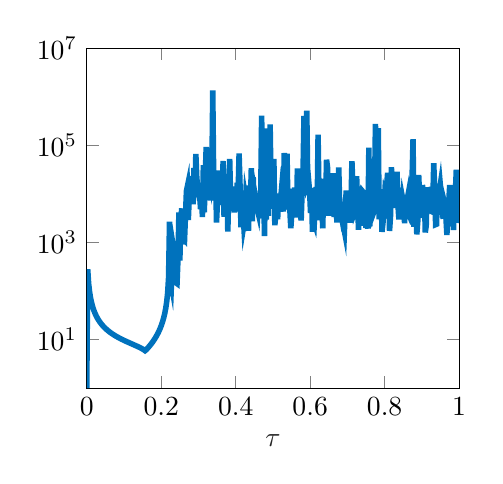
\begin{tikzpicture}

\begin{axis}[%
width=0.39\columnwidth,
height=1.7in,
at={(1.441in,0.842in)},
scale only axis,
xmin=0,
xmax=1,
xlabel style={font=\color{white!15!black}},
xlabel={$\tau$},
ymode=log,
ymin=1,
ymax=10000000,
yminorticks=true,
axis background/.style={fill=white}
]
\addplot [color=mycolor1, line width=2.0pt, forget plot]
  table[row sep=crcr]{%
0	1\\
0.00252525252525253	280.425044566451\\
0.00505050505050505	141.81741398227\\
0.00757575757575758	95.6094987876126\\
0.0101010101010101	72.5012925411307\\
0.0126262626262626	58.6327885610113\\
0.0151515151515152	49.3839799104936\\
0.0176767676767677	42.7748593822763\\
0.0202020202020202	37.8154194817012\\
0.0227272727272727	33.9556524085943\\
0.0252525252525253	30.8655500376393\\
0.0277777777777778	28.3351038971302\\
0.0303030303030303	26.2243051459311\\
0.0328282828282828	24.4362214715429\\
0.0353535353535354	22.9016124475197\\
0.0378787878787879	21.5696987346128\\
0.0404040404040404	20.4023928176823\\
0.0429292929292929	19.3705659387\\
0.0454545454545455	18.4515593702941\\
0.047979797979798	17.6274815869489\\
0.0505050505050505	16.8840162679141\\
0.053030303030303	16.2095708526607\\
0.0555555555555556	15.5946572891548\\
0.0580808080808081	15.0314343052504\\
0.0606060606060606	14.513364089732\\
0.0631313131313131	14.0349513454633\\
0.0656565656565657	13.5915425343545\\
0.0681818181818182	13.1791697052926\\
0.0707070707070707	12.7944277552661\\
0.0732323232323232	12.4343770490249\\
0.0757575757575758	12.0964654750576\\
0.0782828282828283	11.7784655430429\\
0.0808080808080808	11.4784232255193\\
0.0833333333333333	11.1946160445182\\
0.0858585858585859	10.9255184903567\\
0.0883838383838384	10.66977329505\\
0.0909090909090909	10.4261674087678\\
0.0934343434343434	10.1936117738156\\
0.095959595959596	9.97112417761455\\
0.0984848484848485	9.75781460897192\\
0.101010101010101	9.55287265128586\\
0.103535353535354	9.35555652990623\\
0.106060606060606	9.16518349417062\\
0.108585858585859	8.98112126147036\\
0.111111111111111	8.80278028352028\\
0.113636363636364	8.6296066150359\\
0.116161616161616	8.46107517230684\\
0.118686868686869	8.29668316216694\\
0.121212121212121	8.13594343716822\\
0.123737373737374	7.97837748372623\\
0.126262626262626	7.82350766492515\\
0.128787878787879	7.67084819782483\\
0.131313131313131	7.51989410931921\\
0.133838383838384	7.37010701600331\\
0.136363636363636	7.22089587944804\\
0.138888888888889	7.07158963035891\\
0.141414141414141	6.92139615748229\\
0.143939393939394	6.76933729447587\\
0.146464646464646	6.61413878540263\\
0.148989898989899	6.45402847600956\\
0.151515151515152	6.28632528865459\\
0.154040404040404	6.10646938587172\\
0.156565656565657	5.90514219956007\\
0.159090909090909	6.11765225153677\\
0.161616161616162	6.41611084997832\\
0.164141414141414	6.74059811755492\\
0.166666666666667	7.09467424991223\\
0.169191919191919	7.482579743534\\
0.171717171717172	7.90940604204948\\
0.174242424242424	8.38132026135905\\
0.176767676767677	8.90586510272556\\
0.179292929292929	9.4923650359584\\
0.181818181818182	10.1524854411686\\
0.184343434343434	10.9010164097171\\
0.186868686868687	11.7569940735574\\
0.189393939393939	12.7453421496616\\
0.191919191919192	13.8993388604399\\
0.194444444444444	15.2644376850021\\
0.196969696969697	16.9043960087878\\
0.19949494949495	18.9115201534123\\
0.202020202020202	21.4246590091643\\
0.204545454545455	24.6627696798165\\
0.207070707070707	28.9924274416023\\
0.20959595959596	35.0774468523567\\
0.212121212121212	44.2567539425843\\
0.214646464646465	59.6952491464505\\
0.217171717171717	91.1068070623672\\
0.21969696969697	189.848104456246\\
0.222222222222222	2661.83484087803\\
0.224747474747475	167.950125685363\\
0.227272727272727	131.186584322301\\
0.22979797979798	439.934845078913\\
0.232323232323232	831.156848636871\\
0.234848484848485	629.935899152038\\
0.237373737373737	567.559302979335\\
0.23989898989899	146.671191786587\\
0.242424242424242	141.993145381452\\
0.244949494949495	456.808631961247\\
0.247474747474747	4130.44922846475\\
0.25	421.411018473775\\
0.25	421.411018473775\\
0.252525252525253	2790.05206860388\\
0.255050505050505	5024.20990645839\\
0.257575757575758	921.768931450329\\
0.26010101010101	1206.16020308722\\
0.262626262626263	1143.10371180762\\
0.265151515151515	3693.33279174988\\
0.267676767676768	11474.9428538841\\
0.27020202020202	14206.0163056496\\
0.272727272727273	2895.72298665753\\
0.275252525252525	8699.43951441068\\
0.277777777777778	8443.92222458506\\
0.28030303030303	20442.7910700165\\
0.282828282828283	20741.2351427282\\
0.285353535353535	6118.91127880323\\
0.287878787878788	34169.7581918253\\
0.29040404040404	8600.23886658527\\
0.292929292929293	66573.2271525922\\
0.295454545454545	21921.8548258606\\
0.297979797979798	12800.9469127817\\
0.30050505050505	9872.55689765536\\
0.303030303030303	10493.7670397881\\
0.305555555555556	4844.65898024111\\
0.308080808080808	9073.88523437389\\
0.310606060606061	3326.54565085481\\
0.313131313131313	38792.3853968008\\
0.315656565656566	4181.15720855082\\
0.318181818181818	22476.2846455355\\
0.320707070707071	92127.5041840876\\
0.323232323232323	47327.769250624\\
0.325757575757576	7442.65048086383\\
0.328282828282828	10950.3159372789\\
0.330808080808081	23524.7486467581\\
0.333333333333333	7334.43439666107\\
0.335858585858586	22175.32096263\\
0.338383838383838	1352814.1347754\\
0.340909090909091	19390.4766872987\\
0.343434343434343	23831.3010605585\\
0.345959595959596	23039.9007020838\\
0.348484848484849	2566.69619786544\\
0.351010101010101	7005.39769083338\\
0.353535353535354	9405.70727451935\\
0.356060606060606	30324.2488819281\\
0.358585858585859	14336.0648383092\\
0.361111111111111	5931.71568559169\\
0.363636363636364	10163.0008857919\\
0.366161616161616	47394.6394979355\\
0.368686868686869	3367.11841802912\\
0.371212121212121	11795.7952851123\\
0.373737373737374	12614.8312354613\\
0.376262626262626	17694.8406300376\\
0.378787878787879	1671.98899303981\\
0.381313131313131	10670.7374666237\\
0.383838383838384	52462.1039238192\\
0.386363636363636	8308.81468543193\\
0.388888888888889	9184.20354910051\\
0.391414141414141	14149.0898768326\\
0.393939393939394	7222.83868798584\\
0.396464646464646	4136.94424694675\\
0.398989898989899	12297.9347082819\\
0.401515151515151	4311.11217074937\\
0.404040404040404	16953.2107087678\\
0.406565656565657	11311.2508162164\\
0.409090909090909	67886.8829796858\\
0.411616161616162	15031.789135047\\
0.414141414141414	2052.19761918105\\
0.416666666666667	4990.07884214797\\
0.419191919191919	5038.03998105288\\
0.421717171717172	2250.996248654\\
0.424242424242424	2970.16044441344\\
0.426767676767677	8150.47160237483\\
0.429292929292929	6164.52247763114\\
0.431818181818182	2351.1398053837\\
0.434343434343434	1748.10639578677\\
0.436868686868687	14869.4006310508\\
0.439393939393939	6048.4013611554\\
0.441919191919192	33826.8031636535\\
0.444444444444444	2713.72826017406\\
0.446969696969697	22349.6742008258\\
0.44949494949495	4386.91805858726\\
0.452020202020202	9405.2481778098\\
0.454545454545455	7070.72744614876\\
0.457070707070707	5255.90387675512\\
0.45959595959596	4320.57353717885\\
0.462121212121212	9535.90327365163\\
0.464646464646465	3162.67270938364\\
0.467171717171717	9809.9006542028\\
0.46969696969697	405843.577046543\\
0.472222222222222	8227.05529253302\\
0.474747474747475	18766.4135246337\\
0.477272727272727	1356.70531684816\\
0.47979797979798	18607.1177651978\\
0.482323232323232	2951.69388471509\\
0.484848484848485	222522.324633985\\
0.487373737373737	3537.91416820075\\
0.48989898989899	18675.3092004354\\
0.492424242424242	269004.395742346\\
0.494949494949495	14981.9077869429\\
0.497474747474748	8958.92464712588\\
0.5	4980.41261092707\\
0.5	4980.41261092707\\
0.502525252525252	52207.3821193889\\
0.505050505050505	2262.48126570674\\
0.507575757575758	3578.66529138508\\
0.51010101010101	4439.99037447479\\
0.512626262626263	3012.63976661262\\
0.515151515151515	10236.34989264\\
0.517676767676768	4727.00736648422\\
0.52020202020202	7063.07296852085\\
0.522727272727273	11777.9518629757\\
0.525252525252525	8683.99443183194\\
0.527777777777778	4306.85384966114\\
0.53030303030303	69234.8100507212\\
0.532828282828283	24619.9469668883\\
0.535353535353535	10966.6550579508\\
0.537878787878788	67193.7889970867\\
0.54040404040404	4736.41427926669\\
0.542929292929293	7696.37230071336\\
0.545454545454545	4597.63620157784\\
0.547979797979798	1957.85884108217\\
0.55050505050505	3760.0484338117\\
0.553030303030303	12761.1535180644\\
0.555555555555556	4915.54461745998\\
0.558080808080808	13543.5249495096\\
0.560606060606061	9354.88628760107\\
0.563131313131313	3269.3231728826\\
0.565656565656566	33407.2969712365\\
0.568181818181818	5948.48608465095\\
0.570707070707071	7967.08094390823\\
0.573232323232323	4375.52121642825\\
0.575757575757576	2836.77429328138\\
0.578282828282828	10633.8082676137\\
0.580808080808081	26759.022484292\\
0.583333333333333	403722.319985918\\
0.585858585858586	32162.345398403\\
0.588383838383838	183366.063738128\\
0.590909090909091	515471.118852643\\
0.593434343434343	16324.0854095165\\
0.595959595959596	18459.0741167322\\
0.598484848484849	11062.9253881963\\
0.601010101010101	4026.96066983386\\
0.603535353535354	13270.1670414878\\
0.606060606060606	1660.72482065628\\
0.608585858585859	2903.40453281673\\
0.611111111111111	2526.69728714204\\
0.613636363636364	6703.41759263169\\
0.616161616161616	13828.3398443243\\
0.618686868686869	4649.31041586817\\
0.621212121212121	164870.233449715\\
0.623737373737374	8874.18476998996\\
0.626262626262626	2875.03238821648\\
0.628787878787879	7774.26293738007\\
0.631313131313131	5529.67007730176\\
0.633838383838384	1947.4888107295\\
0.636363636363636	20476.8852721587\\
0.638888888888889	11744.0421506645\\
0.641414141414141	5972.09651049693\\
0.643939393939394	50446.8872556618\\
0.646464646464646	36318.572998049\\
0.648989898989899	3532.73614496921\\
0.651515151515151	7627.1871367784\\
0.654040404040404	3780.57588668223\\
0.656565656565657	22887.9058931869\\
0.659090909090909	6285.97448620077\\
0.661616161616162	26623.7961360487\\
0.664141414141414	3338.31556600016\\
0.666666666666667	4358.09173001764\\
0.669191919191919	10708.5564967653\\
0.671717171717172	2569.75986473945\\
0.674242424242424	7241.91905999705\\
0.676767676767677	34833.6763415062\\
0.679292929292929	5603.71182544735\\
0.681818181818182	4336.40999191806\\
0.684343434343434	6840.89726119568\\
0.686868686868687	3909.80526586651\\
0.689393939393939	2158.1717483407\\
0.691919191919192	1701.32816751981\\
0.694444444444444	5752.50685862935\\
0.696969696969697	11726.3512266426\\
0.69949494949495	5862.86950498664\\
0.702020202020202	7599.59572978319\\
0.704545454545455	11486.0410804989\\
0.707070707070707	2537.23948820831\\
0.70959595959596	6256.6643677201\\
0.712121212121212	46938.2436707056\\
0.714646464646465	14778.8696961834\\
0.717171717171717	7365.11951343883\\
0.71969696969697	4075.01326406969\\
0.722222222222222	4545.44162967431\\
0.724747474747475	23184.4474260633\\
0.727272727272727	6436.30100504939\\
0.72979797979798	1830.72501283402\\
0.732323232323232	6468.02902360905\\
0.734848484848485	2637.48074943021\\
0.737373737373737	8453.11735553199\\
0.73989898989899	11501.4431300773\\
0.742424242424242	10906.044642449\\
0.744949494949495	2206.08955671768\\
0.747474747474748	7950.02532611046\\
0.75	1969.71942589582\\
0.75	1969.71942589582\\
0.752525252525252	5053.25975473367\\
0.755050505050505	1921.12545230043\\
0.757575757575758	89662.8380290266\\
0.76010101010101	2137.89263705506\\
0.762626262626263	21146.6076792881\\
0.765151515151515	7637.81143409102\\
0.767676767676768	3611.10475289129\\
0.77020202020202	4081.53834946879\\
0.772727272727273	8395.11880209004\\
0.775252525252525	275178.03277861\\
0.777777777777778	37829.8698772387\\
0.78030303030303	4258.77252959851\\
0.782828282828283	224921.966088977\\
0.785353535353535	2996.58613003569\\
0.787878787878788	7339.04260714577\\
0.79040404040404	12432.3528754505\\
0.792929292929293	1653.14803738401\\
0.795454545454545	2492.39473083623\\
0.797979797979798	4892.73740361377\\
0.80050505050505	10781.0520340512\\
0.803030303030303	9475.26873690466\\
0.805555555555556	15691.5686165426\\
0.808080808080808	27051.3306582424\\
0.810606060606061	12996.0397522311\\
0.813131313131313	1729.54827784611\\
0.815656565656566	3383.9616137311\\
0.818181818181818	35563.240476525\\
0.820707070707071	12473.8363083676\\
0.823232323232323	9868.58456627642\\
0.825757575757576	5118.76748352723\\
0.828282828282828	11282.504296556\\
0.830808080808081	5373.1776763679\\
0.833333333333333	28731.6909598258\\
0.835858585858586	5592.25819377693\\
0.838383838383838	2982.01127156038\\
0.840909090909091	6269.21835971574\\
0.843434343434343	9226.34131865199\\
0.845959595959596	4395.23889460702\\
0.848484848484849	7937.73614771051\\
0.851010101010101	6265.50761261331\\
0.853535353535354	2486.07990823566\\
0.856060606060606	8316.40614979953\\
0.858585858585859	6343.43298912575\\
0.861111111111111	8094.64716770937\\
0.863636363636364	3553.85157306283\\
0.866161616161616	3642.24366808421\\
0.868686868686869	3260.39548629173\\
0.871212121212121	3678.23855122417\\
0.873737373737374	23018.7615356434\\
0.876262626262626	134319.555965751\\
0.878787878787879	2100.93297524401\\
0.881313131313131	13375.2796438274\\
0.883838383838384	8236.07352204465\\
0.886363636363636	1465.23388646866\\
0.888888888888889	2652.08677213406\\
0.891414141414141	24443.5285889526\\
0.893939393939394	8513.82843276454\\
0.896464646464646	3622.12502715891\\
0.898989898989899	3690.67325986183\\
0.901515151515151	15287.9949571071\\
0.904040404040404	8006.48263824276\\
0.906565656565657	11656.1734605435\\
0.909090909090909	1608.40618111421\\
0.911616161616162	2188.33637366914\\
0.914141414141414	13626.8247601423\\
0.916666666666667	10414.4321544882\\
0.919191919191919	4622.03472325315\\
0.921717171717172	4517.35822587947\\
0.924242424242424	7012.75181394212\\
0.926767676767677	13995.9788087935\\
0.929292929292929	6396.39896816951\\
0.931818181818182	43003.5522530945\\
0.934343434343434	12767.3864808607\\
0.936868686868687	2330.60655775298\\
0.939393939393939	2374.47052437491\\
0.941919191919192	12321.2207466175\\
0.944444444444444	3731.21191277704\\
0.946969696969697	11515.8499777855\\
0.94949494949495	15555.5706275043\\
0.952020202020202	9498.91017100749\\
0.954545454545455	5065.12337137048\\
0.957070707070707	3070.46325944281\\
0.95959595959596	7097.66886660331\\
0.962121212121212	5904.8435903849\\
0.964646464646465	3207.53450902199\\
0.967171717171717	1427.88583371025\\
0.96969696969697	4463.82626128846\\
0.972222222222222	6802.02900960236\\
0.974747474747475	15207.7083372975\\
0.977272727272727	6833.13993011734\\
0.97979797979798	4022.59752978839\\
0.982323232323232	4608.33624208819\\
0.984848484848485	1798.39856568405\\
0.987373737373737	10647.685610602\\
0.98989898989899	10117.9921602856\\
0.992424242424242	31551.8890477589\\
0.994949494949495	2887.44207042945\\
0.997474747474748	2859.8977720089\\
1	9916.75582756751\\
};
\end{axis}

\end{tikzpicture}%}
\caption[Stiff ratio alle condizioni iniziali sulla rete stradale del Minnesota al variare dei parametri ]{Stiff ratio calcolato alle condizioni iniziali:  stati puri ($1$ sicuramente infetto, gli altri nodi sicuramente sani) al variare dei parametri $\tau$ e $\gamma$.\\ Per ottenere i grafici abbiamo calcolato il rapporto tra l'autovalore di modulo massimo e quello minimo della matrice Jacobiana, calcolato alle condizioni iniziali, del modello chiuso alle coppie.\\
Per la sperimentazione abbiamo calcolato numericamente gli autovalori della matrice Jacobiana usando il comando \texttt{eig} di MATLAB.}
\label{fig::minnesota_ratiostiff}
\end{figure}
Questo ci suggerisce di utilizzare metodi di tipo implicito per integrare i sistemi di ode~\eqref{Chiuso_coppie}.

Un altro aspetto su cui abbiamo indagato \`e il legame tra il grado del nodo in cui ``inizia" l'epidemia e il suo sviluppo.
Nella rete in esame ogni nodo ha come grado un numero compreso tra $1$ e $5$ dunque abbiamo risolto $5$ problemi di Cauchy facendo partire l'epidemia ogni volta da un nodo di grado diverso. 
\begin{figure}[htbp]
\centering
%% This file was created by matlab2tikz.
%
%The latest updates can be retrieved from
%  http://www.mathworks.com/matlabcentral/fileexchange/22022-matlab2tikz-matlab2tikz
%where you can also make suggestions and rate matlab2tikz.
%
\definecolor{mycolor1}{rgb}{0.00000,0.44700,0.74100}%
\definecolor{mycolor2}{rgb}{0.85000,0.32500,0.09800}%
\definecolor{mycolor3}{rgb}{0.92900,0.69400,0.12500}%
\definecolor{mycolor4}{rgb}{0.49400,0.18400,0.55600}%
\definecolor{mycolor5}{rgb}{0.46600,0.67400,0.18800}%
%
\tikzsetnextfilename{minnesota_prevalenza}
\begin{tikzpicture}

\begin{axis}[%
width=0.8\columnwidth,
height=3.6in,
at={(1.011in,0.642in)},
scale only axis,
xmin=0,
xmax=160,
xlabel style={font=\color{white!15!black}},
xlabel={T},
ymin=0,
ymax=0.18,
axis background/.style={fill=white},
legend style={legend cell align=left, align=left, draw=none,fill=none}
]
\addplot [color=mycolor1, line width=2.0pt, forget plot]
  table[row sep=crcr]{%
0	0.000378501135503407\\
0.00265404780368998	0.000378702100931543\\
0.00530809560737996	0.000378903173506919\\
0.00796214341106994	0.000379104353728901\\
0.0106161912147599	0.00037930564209484\\
0.016768268594088	0.00037977264672713\\
0.0229203459734162	0.000380240241215078\\
0.0290724233527443	0.000380708431629854\\
0.0352245007320724	0.000381177223986136\\
0.0413877012676709	0.000381647473487505\\
0.0475509018032694	0.000382118339023979\\
0.0537141023388679	0.000382589826475308\\
0.0598773028744664	0.000383061941666519\\
0.0660727377033551	0.00038353716457721\\
0.0722681725322438	0.000384013033449107\\
0.0784636073611325	0.000384489554034799\\
0.0846590421900212	0.000384966732033141\\
0.0908868966764125	0.000385447075304373\\
0.0971147511628038	0.000385928094271776\\
0.103342605649195	0.000386409794562818\\
0.109570460135586	0.00038689218175222\\
0.115831050990007	0.000387377802482237\\
0.122091641844428	0.00038786412848824\\
0.128352232698848	0.00038835116527496\\
0.134612823553269	0.000388838918295359\\
0.14090647298924	0.000389329974229644\\
0.147200122425211	0.000389821764875846\\
0.153493771861182	0.000390314295618334\\
0.159787421297153	0.000390807571790679\\
0.166114457881547	0.000391304221447755\\
0.172441494465942	0.000391801635120365\\
0.178768531050337	0.000392299818074884\\
0.185095567634732	0.00039279877552784\\
0.191456326615837	0.000393301178287133\\
0.197817085596942	0.00039380437424504\\
0.204177844578047	0.000394308368552293\\
0.210538603559152	0.000394813166310729\\
0.216933426884191	0.000395321482477766\\
0.22332825020923	0.000395830620917875\\
0.22972307353427	0.000396340586668496\\
0.236117896859309	0.000396851384719118\\
0.242547133439283	0.000397365775611708\\
0.248976370019256	0.000397881017755342\\
0.25540560659923	0.000398397116076514\\
0.261834843179204	0.000398914075454698\\
0.268298849139544	0.000399434703489979\\
0.274762855099884	0.000399956211670151\\
0.281226861060224	0.000400478604813102\\
0.287690867020564	0.000401001887690627\\
0.294190005970066	0.000401528916475648\\
0.300689144919567	0.000402056854227889\\
0.307188283869069	0.000402585705658975\\
0.31368742281857	0.000403115475435356\\
0.320222065858517	0.000403649069838639\\
0.326756708898465	0.000404183601972756\\
0.333291351938412	0.000404719076445409\\
0.33982599497836	0.000405255497820037\\
0.346396521179263	0.00040579582408305\\
0.352967047380166	0.000406337116794927\\
0.359537573581069	0.000406879380461795\\
0.366108099781972	0.000407422619546422\\
0.372714896128684	0.000407969845354086\\
0.379321692475397	0.0004085180662964\\
0.385928488822109	0.000409067286780266\\
0.392535285168822	0.000409617511170129\\
0.399178747127128	0.000410171805774578\\
0.405822209085434	0.000410727124180957\\
0.412465671043739	0.000411283470699304\\
0.419109133002045	0.000411840849598098\\
0.425789664736969	0.000412402383916826\\
0.432470196471894	0.000412964970700318\\
0.439150728206818	0.000413528614164122\\
0.445831259941742	0.000414093318483119\\
0.452549274143124	0.000414662265166402\\
0.459267288344506	0.000415232292987112\\
0.465985302545888	0.000415803406068696\\
0.47270331674727	0.000416375608494825\\
0.479459235650332	0.000416952142096353\\
0.486215154553394	0.000417529785532696\\
0.492971073456456	0.000418108542837604\\
0.499726992359517	0.000418688418005939\\
0.506521247405368	0.000419272715042291\\
0.513315502451219	0.000419858150650661\\
0.52010975749707	0.00042044472877754\\
0.526904012542921	0.000421032453331406\\
0.53373704484832	0.000421624692412436\\
0.540570077153719	0.0004222180988581\\
0.547403109459117	0.000422812676530078\\
0.554236141764516	0.000423408429252923\\
0.561108402734927	0.00042400879122874\\
0.567980663705339	0.000424610349433377\\
0.57485292467575	0.000425213107646188\\
0.581725185646161	0.000425817069610286\\
0.588637136978784	0.000426425737669304\\
0.595549088311406	0.00042703563090945\\
0.602461039644028	0.000427646753030273\\
0.60937299097665	0.000428259107695969\\
0.616322696890948	0.000428876053503409\\
0.623272402805246	0.000429494252679492\\
0.630222108719543	0.000430113708842778\\
0.637171814633841	0.000430734425577408\\
0.644156756611822	0.000431359563197536\\
0.651141698589803	0.000431985981359669\\
0.658126640567784	0.000432613683599694\\
0.665111582545765	0.000433242673420059\\
0.672132042490007	0.000433876162531398\\
0.679152502434249	0.00043451095934436\\
0.68617296237849	0.000435147067315026\\
0.693193422322732	0.00043578448986703\\
0.700249666234234	0.000436426489496157\\
0.707305910145735	0.00043706982397889\\
0.714362154057237	0.000437714496694387\\
0.721418397968738	0.000438360510990352\\
0.728510693267482	0.000439011181095336\\
0.735602988566226	0.000439663213210866\\
0.74269528386497	0.000440316610642106\\
0.749787579163713	0.000440971376663754\\
0.756916195464473	0.000441630878264061\\
0.764044811765234	0.000442291769049997\\
0.771173428065994	0.0004429540522557\\
0.778302044366754	0.000443617731085841\\
0.785467252466709	0.000444286226230298\\
0.792632460566664	0.000444956137766713\\
0.799797668666619	0.000445627468861229\\
0.806962876766575	0.000446300222651513\\
0.814164948912488	0.0004469778745036\\
0.821367021058401	0.000447656969998773\\
0.828569093204314	0.000448337512238256\\
0.835771165350227	0.000449019504295802\\
0.843010375911676	0.000449706477260417\\
0.850249586473125	0.000450394921178222\\
0.857488797034573	0.000451084839088671\\
0.864728007596022	0.000451776234004756\\
0.872004631685139	0.000452472693663286\\
0.879281255774256	0.000453170651658109\\
0.886557879863373	0.000453870110970125\\
0.893834503952491	0.000454571074554789\\
0.901148817876876	0.000455277187772482\\
0.908463131801261	0.000455984826797189\\
0.915777445725646	0.000456693994554547\\
0.923091759650032	0.000457404693945771\\
0.930444040702097	0.00045812062891862\\
0.937796321754161	0.000458838117271798\\
0.945148602806226	0.000459557161879054\\
0.952500883858291	0.000460277765590745\\
0.959891411548084	0.000461003692035366\\
0.967281939237877	0.000461731199552209\\
0.97467246692767	0.000462460290966596\\
0.982062994617462	0.000463190969081506\\
0.989492047173736	0.000463927057964289\\
0.99692109973001	0.00046466475574477\\
1.00435015228628	0.000465404065203402\\
1.01177920484256	0.00046614498909936\\
1.01924706180043	0.000466891412958957\\
1.02671491875831	0.000467639473691951\\
1.03418277571618	0.000468389174037593\\
1.04165063267405	0.000469140516714927\\
1.04915757655225	0.000469897449908752\\
1.05666452043045	0.000470656048119879\\
1.06417146430864	0.000471416314050134\\
1.07167840818684	0.000472178250382226\\
1.07922471777503	0.000472945868490367\\
1.08677102736323	0.000473715179943559\\
1.09431733695142	0.000474486187410101\\
1.10186364653962	0.000475258893540277\\
1.10944960429035	0.000476037374185323\\
1.11703556204108	0.000476817576706586\\
1.12462151979181	0.000477599503742857\\
1.13220747754254	0.000478383157916047\\
1.13983336396315	0.000479172680278409\\
1.14745925038377	0.000479963953269329\\
1.15508513680439	0.00048075697950226\\
1.16271102322501	0.000481551761574919\\
1.17037712053123	0.00048235250684929\\
1.17804321783746	0.000483155031745898\\
1.18570931514368	0.000483959338857174\\
1.1933754124499	0.000484765430760979\\
1.20108200069287	0.000485577581842293\\
1.20878858893584	0.000486391541800037\\
1.21649517717882	0.000487207313210087\\
1.22420176542179	0.000488024898634941\\
1.23194912478866	0.000488848640443411\\
1.23969648415552	0.000489674220664073\\
1.24744384352239	0.000490501641860887\\
1.25519120288925	0.000491330906585653\\
1.26297961102761	0.000492166425874052\\
1.27076801916597	0.000493003813412649\\
1.27855642730433	0.000493843071758299\\
1.28634483544269	0.000494684203456951\\
1.29417457141287	0.000495531689324713\\
1.30200430738305	0.000496381073606402\\
1.30983404335324	0.000497232358856781\\
1.31766377932342	0.000498085547620983\\
1.32553511873684	0.000498945191091679\\
1.33340645815026	0.000499806763487897\\
1.34127779756368	0.000500670267367513\\
1.3491491369771	0.000501535705280089\\
1.35706235464723	0.000502407699683762\\
1.36497557231736	0.000503281653896863\\
1.3728887899875	0.000504157570485805\\
1.38080200765763	0.000505035452010033\\
1.38875737542382	0.000505919992848358\\
1.39671274319	0.000506806524776799\\
1.40466811095619	0.000507695050375952\\
1.41262347872237	0.000508585572220829\\
1.42062126732206	0.000509482857478872\\
1.42861905592174	0.000510382165531046\\
1.43661684452143	0.000511283498978017\\
1.44461463312112	0.00051218686041629\\
1.45265510828528	0.000513097090235934\\
1.46069558344945	0.000514009375002837\\
1.46873605861361	0.000514923717343875\\
1.47677653377778	0.000515840119883224\\
1.48485995954462	0.000516763497043573\\
1.49294338531146	0.000517688961782143\\
1.50102681107831	0.000518616516758424\\
1.50911023684515	0.000519546164630713\\
1.5172368720298	0.000520482894264606\\
1.52536350721444	0.000521421744613757\\
1.53349014239909	0.000522362718376951\\
1.54161677758374	0.000523305818253342\\
1.54978687752722	0.000524256108162483\\
1.55795697747069	0.000525208552460517\\
1.56612707741417	0.000526163153892505\\
1.57429717735764	0.00052711991520548\\
1.58251099258344	0.000528083975829185\\
1.59072480780924	0.000529050225083291\\
1.59893862303504	0.000530018665766426\\
1.60715243826084	0.000530989300680848\\
1.61541021270888	0.000531967345012498\\
1.62366798715692	0.000532947612815786\\
1.63192576160495	0.000533930106950513\\
1.64018353605299	0.000534914830281831\\
1.6484855082196	0.000535907074128194\\
1.65678748038621	0.000536901576921178\\
1.66508945255282	0.000537898341589717\\
1.67339142471943	0.00053889737106986\\
1.68173782652846	0.000539904033050552\\
1.69008422833748	0.000540912990121665\\
1.6984306301465	0.000541924245289572\\
1.70677703195552	0.000542937801569592\\
1.71516808828458	0.00054395910319608\\
1.72355914461364	0.000544982736762126\\
1.7319502009427	0.000546008705360223\\
1.74034125727176	0.000547037012093705\\
1.74877718456917	0.000548073177740659\\
1.75721311186658	0.000549111712919178\\
1.76564903916399	0.000550152620816942\\
1.7740849664614	0.000551195904634438\\
1.78256597151399	0.000552247161528069\\
1.79104697656658	0.000553300826326809\\
1.79952798161918	0.000554356902322997\\
1.80800898667177	0.000555415392823817\\
1.81653526729983	0.000556481971270856\\
1.82506154792789	0.00055755099681904\\
1.83358782855595	0.000558622472875265\\
1.84211410918401	0.000559696402863374\\
1.85068585212982	0.000560778536138031\\
1.85925759507562	0.000561863156574079\\
1.86782933802142	0.000562950267703301\\
1.87640108096722	0.000564039873076607\\
1.88501846252594	0.000565137797650905\\
1.89363584408466	0.000566238250355152\\
1.90225322564338	0.000567341234856803\\
1.91087060720211	0.000568446754844698\\
1.91953379026225	0.000569560710169349\\
1.9281969733224	0.000570677235545276\\
1.93686015638254	0.000571796334786859\\
1.94552333944269	0.000572918011732202\\
1.95423247360919	0.000574048240405576\\
1.9629416077757	0.000575181082050962\\
1.9716507419422	0.000576316540641403\\
1.98035987610871	0.000577454620176088\\
1.98911509746045	0.000578601368074626\\
1.9978703188122	0.000579750772914004\\
2.00662554016394	0.000580902838838159\\
2.01538076151568	0.000582057570019694\\
2.02418218887136	0.000583221085973254\\
2.03298361622703	0.000584387303933205\\
2.04178504358271	0.000585556228227136\\
2.05058647093838	0.000586727863213898\\
2.05943420818955	0.000587908399472959\\
2.06828194544071	0.000589091683952994\\
2.07712968269188	0.000590277721178514\\
2.08597741994304	0.000591466515707991\\
2.09487155303471	0.000592664327715207\\
2.10376568612638	0.000593864935359746\\
2.11265981921806	0.000595068343376863\\
2.12155395230973	0.000596274556538558\\
2.1304945484036	0.000597489902983695\\
2.13943514449747	0.000598708093738788\\
2.14837574059134	0.000599929133764203\\
2.15731633668521	0.000601153028059932\\
2.16630344097851	0.000602386170615121\\
2.17529054527181	0.000603622207463975\\
2.18427764956511	0.000604861143806889\\
2.19326475385841	0.000606102984886878\\
2.20229839189264	0.000607354188687148\\
2.21133202992686	0.000608608338134422\\
2.22036566796109	0.000609865438684623\\
2.22939930599531	0.00061112549583938\\
2.23847947958951	0.000612395029097026\\
2.2475596531837	0.000613667560782881\\
2.25663982677789	0.000614943096624462\\
2.26572000037209	0.000616221642398181\\
2.27484668902269	0.000617509776765866\\
2.2839733776733	0.000618800963832244\\
2.29310006632391	0.000620095209613072\\
2.30222675497451	0.0006213925201763\\
2.31139991044299	0.000622699530157355\\
2.32057306591147	0.000624009648656908\\
2.32974622137995	0.000625322881996177\\
2.33891937684843	0.000626639236551973\\
2.34812123881268	0.000627962852863503\\
2.35732310077693	0.000629289622978319\\
2.36652496274117	0.00063061955350257\\
2.37572682470542	0.000631952651101047\\
2.38494102326719	0.000633290716120355\\
2.39415522182897	0.000634631970261556\\
2.40336942039074	0.000635976420393644\\
2.41258361895251	0.000637324073446921\\
2.42180944219507	0.000638676642698995\\
2.43103526543762	0.000640032437046992\\
2.44026108868018	0.00064139146363275\\
2.44948691192273	0.000642753729662075\\
2.45872366549583	0.000644120862129715\\
2.46796041906892	0.000645491256367209\\
2.47719717264201	0.000646864919799164\\
2.4864339262151	0.000648241859916796\\
2.49568093760537	0.000649623618905597\\
2.50492794899565	0.000651008677085359\\
2.51417496038592	0.000652397042173287\\
2.52342197177619	0.000653788721955827\\
2.53267859155347	0.000655185175538679\\
2.54193521133074	0.000656584966528749\\
2.55119183110802	0.000657988102945577\\
2.5604484508853	0.000659394592880561\\
2.56969435219189	0.000660802810047311\\
2.57894025349849	0.000662214389320061\\
2.58818615480509	0.000663629338977055\\
2.59743205611168	0.000665047667370345\\
2.60664448855305	0.000666464230396349\\
2.61585692099442	0.000667884164513026\\
2.62506935343579	0.000669307478200838\\
2.63428178587715	0.000670734180015216\\
2.64346157523825	0.000672159205207517\\
2.65264136459935	0.000673587611739125\\
2.66182115396045	0.000675019408297032\\
2.67100094332155	0.000676454603644304\\
2.68014902131601	0.000677888231124094\\
2.68929709931046	0.00067932525155147\\
2.69844517730492	0.000680765673824416\\
2.70759325529938	0.000682209506918037\\
2.71671051530543	0.000683651878636374\\
2.72582777531148	0.000685097656260497\\
2.73494503531753	0.000686546848903615\\
2.74406229532357	0.000687999465757042\\
2.75314959586158	0.000689450725851549\\
2.76223689639959	0.000690905406151957\\
2.7713241969376	0.000692363515990696\\
2.7804114974756	0.000693825064779246\\
2.78946966492245	0.000695285359834762\\
2.7985278323693	0.000696749090731397\\
2.80758599981614	0.000698216267024587\\
2.81664416726299	0.000699686898349711\\
2.82567399950379	0.000701156377832303\\
2.83470383174459	0.000702629310121488\\
2.84373366398539	0.000704105704999294\\
2.85276349622619	0.000705585572328523\\
2.86176576527131	0.000707064388878994\\
2.87076803431643	0.000708546676528205\\
2.87977030336155	0.000710032445288158\\
2.88877257240667	0.000711521705252415\\
2.89774802722445	0.000713010015036334\\
2.90672348204223	0.000714501815535716\\
2.91569893686001	0.000715997116995733\\
2.9246743916778	0.000717495929743849\\
2.93362376027718	0.000718993892699087\\
2.94257312887657	0.000720495367309961\\
2.95152249747595	0.000722000364057827\\
2.96047186607534	0.00072350889350701\\
2.96939585799537	0.000725016673676769\\
2.9783198499154	0.00072652798776601\\
2.98724384183543	0.000728042846495106\\
2.99616783375546	0.000729561260668035\\
3.00506714186217	0.000731079026436579\\
3.01396644996888	0.000732600349713211\\
3.0228657580756	0.000734125241459989\\
3.03176506618231	0.000735653712723158\\
3.04064036833087	0.000737181637043173\\
3.04951567047943	0.000738713143786541\\
3.05839097262799	0.000740248244159506\\
3.06726627477655	0.000741786949453017\\
3.07611823581175	0.000743325210145786\\
3.08497019684696	0.000744867079506856\\
3.09382215788217	0.000746412568988995\\
3.10267411891737	0.000747961690130153\\
3.11150339190671	0.000749510470068604\\
3.12033266489606	0.000751062886253587\\
3.1291619378854	0.000752618950386579\\
3.13799121087475	0.000754178674254652\\
3.14679843895819	0.000755738161666314\\
3.15560566704164	0.000757301314240743\\
3.16441289512509	0.000758868143930151\\
3.17322012320854	0.000760438662772706\\
3.18200594034256	0.000762009051361873\\
3.19079175747657	0.000763583135373023\\
3.19957757461059	0.000765160927010977\\
3.2083633917446	0.000766742438566824\\
3.21712842459564	0.000768323927850767\\
3.22589345744667	0.000769909144165131\\
3.23465849029771	0.000771498099969073\\
3.24342352314874	0.000773090807808273\\
3.25216839156968	0.000774683603213457\\
3.26091325999062	0.000776280158613074\\
3.26965812841156	0.0007778804867222\\
3.2784029968325	0.000779484600342638\\
3.28712831544844	0.000781088913509463\\
3.29585363406438	0.000782697020997769\\
3.30457895268032	0.000784308935779989\\
3.31330427129626	0.000785924670915424\\
3.32201065006193	0.000787540719827981\\
3.33071702882759	0.000789160598759815\\
3.33942340759326	0.000790784320942024\\
3.34812978635892	0.000792411899692637\\
3.35681783203462	0.000794039908986512\\
3.36550587771031	0.000795671785377047\\
3.37419392338601	0.000797307542355148\\
3.3828819690617	0.00079894719349868\\
3.39155228546949	0.000800587394553588\\
3.40022260187729	0.000802231501171019\\
3.40889291828508	0.000803879527102704\\
3.41756323469287	0.000805531486187297\\
3.42621642398442	0.000807184117416263\\
3.43486961327598	0.000808840694072004\\
3.44352280256753	0.000810501230167953\\
3.45217599185909	0.000812165739804371\\
3.46081265526035	0.000813831046856289\\
3.46944931866162	0.000815500340608122\\
3.47808598206288	0.000817173635335745\\
3.48672264546414	0.000818850945401693\\
3.49534338401916	0.000820529181372798\\
3.50396412257417	0.000822211446736964\\
3.51258486112919	0.000823897756033114\\
3.5212055996842	0.000825588123886598\\
3.52981101454994	0.000827279549452954\\
3.53841642941568	0.000828975048536903\\
3.54702184428142	0.000830674635940864\\
3.55562725914716	0.0008323783265534\\
3.56421795291397	0.00083408321031181\\
3.57280864668078	0.000835792213156315\\
3.58139934044759	0.000837505350153169\\
3.5899900342144	0.000839222636454406\\
3.59856661125112	0.000840941255084236\\
3.60714318828785	0.00084266403982562\\
3.61571976532457	0.000844391006008828\\
3.62429634236129	0.000846122169049479\\
3.63285940935906	0.000847854807520592\\
3.64142247635683	0.000849591660599227\\
3.6499855433546	0.000851332743879717\\
3.65854861035238	0.000853078073041245\\
3.66709877698689	0.000854825024854541\\
3.67564894362141	0.000856576241256128\\
3.68419911025593	0.000858331738104307\\
3.69274927689045	0.000860091531341657\\
3.70128715684689	0.000861853098854643\\
3.70982503680333	0.000863618982436924\\
3.71836291675977	0.000865389198210528\\
3.72690079671621	0.000867163762381129\\
3.73542700754597	0.000868940256904696\\
3.74395321837573	0.000870721120494237\\
3.75247942920549	0.000872506369535131\\
3.76100564003525	0.000874296020495686\\
3.76952080423241	0.00087608776264889\\
3.77803596842958	0.000877883928397129\\
3.78655113262675	0.000879684534388608\\
3.79506629682392	0.000881489597353677\\
3.80357104245543	0.000883296917339814\\
3.81207578808694	0.000885108717000015\\
3.82058053371845	0.000886925013244636\\
3.82908527934997	0.000888745823065314\\
3.83758024029722	0.000890569060875775\\
3.84607520124448	0.00089239683600736\\
3.85457016219173	0.000894229165631769\\
3.86306512313899	0.000896066067001016\\
3.87155093990785	0.000897905572749103\\
3.88003675667672	0.000899749675052623\\
3.88852257344558	0.00090159839134363\\
3.89700839021445	0.000903451739133473\\
3.90548571024985	0.00090530787329388\\
3.91396303028526	0.000907168664851104\\
3.92244035032067	0.000909034131496438\\
3.93091767035607	0.000910904290999338\\
3.93938714872392	0.000912777424737137\\
3.94785662709177	0.000914655278341139\\
3.95632610545962	0.000916537869760568\\
3.96479558382747	0.00091842521702163\\
3.97325788400163	0.000920315732558151\\
3.9817201841758	0.000922211032080398\\
3.99018248434996	0.000924111133794088\\
3.99864478452412	0.000926016055980624\\
4.00710057892049	0.000927924346917449\\
4.01555637331686	0.000929837487632816\\
4.02401216771322	0.000931755496587324\\
4.03246796210959	0.000933678392315866\\
4.04091793227224	0.000935604863891736\\
4.04936790243489	0.000937536252736059\\
4.05781787259754	0.00093947257756252\\
4.0662678427602	0.000941413857157625\\
4.07471268010346	0.000943358926641379\\
4.08315751744673	0.000945308982605682\\
4.09160235478999	0.000947264044015345\\
4.10004719213326	0.000949224129906422\\
4.10848759920525	0.000951188227127345\\
4.11692800627724	0.000953157381790191\\
4.12536841334923	0.000955131613108735\\
4.13380882042122	0.000957110940366351\\
4.14224551048116	0.000959094507871615\\
4.15068220054111	0.000961083205556556\\
4.15911889060106	0.000963077052881595\\
4.16755558066101	0.000965076069374975\\
4.17598927888764	0.000967079562975195\\
4.18442297711427	0.000969088261298355\\
4.1928566753409	0.000971102184048991\\
4.20129037356753	0.000973121350997592\\
4.20972181874674	0.000975145240451834\\
4.21815326392594	0.000977174411009604\\
4.22658470910515	0.000979208882616842\\
4.23501615428435	0.00098124867528345\\
4.24344609708982	0.000983293444189174\\
4.2518760398953	0.000985343572446681\\
4.26030598270077	0.000987399080240377\\
4.26873592550624	0.000989459987816528\\
4.27716513109149	0.000991526134539066\\
4.28559433667673	0.000993597720763545\\
4.29402354226198	0.000995674766909681\\
4.30245274784723	0.000997757293456859\\
4.31088199644109	0.000999845331611017\\
4.31931124503495	0.00100193889135493\\
4.32774049362881	0.00100403799334025\\
4.33616974222267	0.00100614265827601\\
4.34459982899918	0.00100825311704352\\
4.35302991577569	0.0010103691814626\\
4.3614600025522	0.00101249087241327\\
4.36989008932872	0.00101461821083043\\
4.37832182622431	0.00101675163577741\\
4.38675356311991	0.00101889075245133\\
4.3951853000155	0.00102103558195671\\
4.4036170369111	0.00102318614545041\\
4.41205125303612	0.0010253430990231\\
4.42048546916115	0.00102750583245263\\
4.42891968528618	0.00102967436706394\\
4.4373539014112	0.00103184872423162\\
4.44579144418968	0.00103402978645723\\
4.45422898696816	0.00103621671876754\\
4.46266652974663	0.00103840954270358\\
4.47110407252511	0.00104060827985316\\
4.47954580784242	0.00104281404881021\\
4.48798754315973	0.00104502578022241\\
4.49642927847704	0.00104724349584221\\
4.50487101379435	0.00104946721746591\\
4.51331782807969	0.00105169831027955\\
4.52176464236504	0.00105393546010986\\
4.53021145665039	0.00105617868891583\\
4.53865827093573	0.0010584280186972\\
4.54710953316863	0.00106068466079287\\
4.55556079540153	0.00106294745446422\\
4.56401205763442	0.00106521642185946\\
4.57246331986732	0.00106749158516426\\
4.58091675743331	0.0010697735546246\\
4.5893701949993	0.0010720617676902\\
4.5978236325653	0.00107435624666735\\
4.60627707013129	0.00107665701389637\\
4.61473356079598	0.00107896492613229\\
4.62319005146068	0.00108127917597929\\
4.63164654212538	0.00108359978589475\\
4.64010303279008	0.00108592677836643\\
4.64856348165446	0.00108826126959955\\
4.65702393051883	0.00109060219447767\\
4.66548437938321	0.00109294957560195\\
4.67394482824759	0.0010953034356002\\
4.6824101596182	0.00109766516116638\\
4.69087549098881	0.00110003341848038\\
4.69934082235943	0.00110240823027952\\
4.70780615373004	0.00110478961932387\\
4.71627731331164	0.00110717925475629\\
4.72474847289324	0.00110957552215319\\
4.73321963247484	0.00111197844438006\\
4.74169079205644	0.00111438804432109\\
4.75016874607346	0.00111680628560757\\
4.75864670009049	0.00111923126123339\\
4.76712465410751	0.00112166299418385\\
4.77560260812453	0.00112410150745873\\
4.78408834700588	0.00112654907261148\\
4.79257408588724	0.00112900347668763\\
4.80105982476859	0.00113146474278351\\
4.80954556364994	0.00113393289400558\\
4.81804010087533	0.00113641052329999\\
4.82653463810072	0.0011388950983611\\
4.83502917532611	0.0011413866423871\\
4.8435237125515	0.00114388517858181\\
4.85202808619862	0.00114639363558299\\
4.86053245984574	0.00114890914750681\\
4.86903683349286	0.00115143173764376\\
4.87754120713998	0.00115396142928522\\
4.88605648267345	0.00115650150228827\\
4.89457175820693	0.00115904874174155\\
4.9030870337404	0.00116160317101774\\
4.91160230927387	0.00116416481348559\\
4.9201295793021	0.00116673731610934\\
4.92865684933032	0.00116931709914211\\
4.93718411935855	0.00117190418602826\\
4.94571138938677	0.00117449860020319\\
4.95425177601205	0.00117710437278553\\
4.96279216263733	0.00117971754223152\\
4.97133254926261	0.00118233813204612\\
4.97987293588788	0.00118496616572018\\
4.98842759246203	0.00118760607659296\\
4.99698224903618	0.00119025350334855\\
5.00553690561032	0.001192908469541\\
5.01409156218447	0.00119557099870487\\
5.02266167370047	0.00119824594509495\\
5.03123178521647	0.00120092852902216\\
5.03980189673248	0.00120361877407755\\
5.04837200824848	0.00120631670382708\\
5.0569587947224	0.00120902761372763\\
5.06554558119632	0.00121174628553261\\
5.07413236767025	0.00121447274285737\\
5.08271915414417	0.00121720700928636\\
5.09132387126067	0.00121995484254325\\
5.09992858837717	0.00122271056486512\\
5.10853330549366	0.00122547419987832\\
5.11713802261016	0.00122824577117233\\
5.12576196498888	0.00123103152145103\\
5.1343859073676	0.00123382529083616\\
5.14300984974632	0.00123662710295114\\
5.15163379212504	0.00123943698137635\\
5.16027829414231	0.00124226167742087\\
5.16892279615959	0.00124509452558485\\
5.17756729817687	0.00124793554947414\\
5.18621180019415	0.00125078477264518\\
5.19487823947356	0.00125364948045989\\
5.20354467875298	0.00125652247647737\\
5.2122111180324	0.00125940378427063\\
5.22087755731182	0.00126229342735662\\
5.22956735722224	0.00126519925215708\\
5.23825715713267	0.00126811350441921\\
5.24694695704309	0.00127103620766707\\
5.25563675695351	0.00127396738536186\\
5.26435138889382	0.00127691547353515\\
5.27306602083413	0.00127987213171608\\
5.28178065277444	0.00128283738336293\\
5.29049528471475	0.00128581125186404\\
5.29923627148589	0.00128880279338057\\
5.30797725825703	0.00129180305085786\\
5.31671824502818	0.00129481204767073\\
5.32545923179932	0.00129782980711677\\
5.3342281502748	0.00130086603780589\\
5.34299706875028	0.00130391113394361\\
5.35176598722577	0.00130696511880269\\
5.36053490570125	0.00131002801557112\\
5.36933339161646	0.00131311022023342\\
5.37813187753166	0.00131620144350631\\
5.38693036344687	0.00131930170854104\\
5.39572884936208	0.00132241103839629\\
5.40455860058234	0.00132554055352399\\
5.4133883518026	0.00132867924424724\\
5.42221810302285	0.00133182713357531\\
5.43104785424311	0.00133498424441687\\
5.43991063408425	0.00133816246104815\\
5.44877341392539	0.00134135001424134\\
5.45763619376653	0.00134454692684222\\
5.46649897360767	0.00134775322158771\\
5.47539661749152	0.00135098158949225\\
5.48429426137537	0.00135421945908191\\
5.49319190525923	0.00135746685301644\\
5.50208954914308	0.00136072379383811\\
5.51102396812565	0.00136400382476166\\
5.51995838710821	0.00136729352683684\\
5.52889280609078	0.00137059292251363\\
5.53782722507335	0.00137390203411572\\
5.54680041227998	0.00137723530624034\\
5.55577359948661	0.00138057842353051\\
5.56474678669325	0.0013839314082015\\
5.57371997389988	0.00138729428233319\\
5.58273401035243	0.00139068244472354\\
5.59174804680498	0.00139408063106185\\
5.60076208325753	0.00139748886330245\\
5.60977611971009	0.00140090716325491\\
5.61883318204376	0.00140435194123002\\
5.62789024437744	0.00140780692694688\\
5.63694730671111	0.00141127214207132\\
5.64600436904479	0.00141474760811477\\
5.65510673617711	0.00141825080847943\\
5.66420910330943	0.0014217644056543\\
5.67331147044175	0.00142528842098771\\
5.68241383757408	0.00142882287566359\\
5.69152395137929	0.00143237081210049\\
5.70063406518451	0.00143592924760866\\
5.70974417898972	0.00143949820291566\\
5.71885429279494	0.00144307769857745\\
5.72794692100005	0.00144666085423248\\
5.73703954920517	0.00145025455021135\\
5.74613217741029	0.00145385880642513\\
5.7552248056154	0.00145747364260823\\
5.76430006309173	0.00146109214209774\\
5.77337532056805	0.00146472121991355\\
5.78245057804437	0.00146836089513597\\
5.79152583552069	0.00147201118666405\\
5.80058394158272	0.00147566518435181\\
5.80964204764475	0.00147932979532367\\
5.81870015370678	0.00148300503781718\\
5.82775825976881	0.00148669092988433\\
5.83679942404394	0.00149038056557836\\
5.84584058831908	0.00149408084641801\\
5.85488175259421	0.00149779178978748\\
5.86392291686934	0.00150151341288153\\
5.87294733974631	0.00150523881172342\\
5.88197176262327	0.00150897488443094\\
5.89099618550024	0.0015127216475259\\
5.9000206083772	0.00151647911733718\\
5.90902848234499	0.00152024039009623\\
5.91803635631278	0.00152401236226305\\
5.92704423028057	0.00152779504948951\\
5.93605210424836	0.00153158846723158\\
5.94504361393162	0.00153538571010684\\
5.95403512361489	0.00153919367472359\\
5.96302663329815	0.00154301237585796\\
5.97201814298142	0.00154684182808756\\
5.98099346618555	0.00155067512296453\\
5.98996878938967	0.00155451915868643\\
5.9989441125938	0.0015583739491494\\
6.00791943579793	0.00156223950804891\\
6.01687874454079	0.0015661089228034\\
6.02583805328365	0.00156998909426267\\
6.03479736202651	0.0015738800354404\\
6.04375667076937	0.00157778175914787\\
6.05270013192063	0.00158168734783139\\
6.0616435930719	0.00158560370583069\\
6.07058705422317	0.00158953084527619\\
6.07953051537443	0.00159346877809461\\
6.08845829169706	0.0015974105813405\\
6.09738606801969	0.001601363163268\\
6.10631384434231	0.00160532653512517\\
6.11524162066494	0.00160930070795567\\
6.12415387239842	0.00161327875368225\\
6.1330661241319	0.0016172675842252\\
6.14197837586538	0.00162126720995298\\
6.15089062759886	0.00162527764102932\\
6.15978751258981	0.00162929194455805\\
6.16868439758076	0.00163331703582795\\
6.1775812825717	0.00163735292433237\\
6.18647816756265	0.00164139961936009\\
6.19535984251503	0.00164545018407433\\
6.2042415174674	0.0016495115362754\\
6.21312319241977	0.00165358368458783\\
6.22200486737214	0.0016576666374322\\
6.2308714891871	0.00166175345553943\\
6.23973811100205	0.0016658510577408\\
6.24860473281701	0.00166995945180008\\
6.25747135463197	0.00167407864527818\\
6.2663230818758	0.00167820169869668\\
6.27517480911963	0.00168233552972931\\
6.28402653636346	0.00168648014528889\\
6.29287826360729	0.00169063555208694\\
6.30171525643276	0.00169479481267198\\
6.31055224925822	0.0016989648413612\\
6.31938924208369	0.00170314564422808\\
6.32822623490915	0.00170733722714681\\
6.33704865720079	0.00171153265799851\\
6.34587107949243	0.00171573884448371\\
6.35469350178408	0.00171995579184977\\
6.36351592407572	0.00172418350514736\\
6.37232394435757	0.0017284150614107\\
6.38113196463942	0.00173265735795375\\
6.38993998492127	0.00173691039921282\\
6.39874800520312	0.00174117418943046\\
6.4075417970596	0.00174544181890912\\
6.41633558891608	0.00174972017051556\\
6.42512938077256	0.00175400924789168\\
6.43392317262904	0.001758309054489\\
6.44270291717521	0.00176261269930054\\
6.45148266172137	0.0017669270453867\\
6.46026240626753	0.00177125209561322\\
6.4690421508137	0.00177558785265931\\
6.47780803632354	0.00177992744957612\\
6.48657392183338	0.0017842777243149\\
6.49533980734323	0.00178863867898508\\
6.50410569285307	0.00179301031551382\\
6.51285791658786	0.00179738579741548\\
6.52161014032266	0.00180177193119871\\
6.53036236405745	0.00180616871823793\\
6.53911458779224	0.00181057615973\\
6.54785335694324	0.00181498745668138\\
6.55659212609425	0.00181940937720538\\
6.56533089524525	0.0018238419219642\\
6.57406966439626	0.00182828509144752\\
6.58279519693014	0.00183273213177331\\
6.59152072946402	0.0018371897651204\\
6.6002462619979	0.00184165799146286\\
6.60897179453179	0.00184613681060775\\
6.6176843200383	0.00185061952201001\\
6.62639684554482	0.00185511279377263\\
6.63510937105134	0.001859616625207\\
6.64382189655786	0.00186413101546335\\
6.65252165797485	0.0018686493266355\\
6.66122141939185	0.00187317816353863\\
6.66992118080885	0.00187771752484815\\
6.67862094222585	0.00188226740908442\\
6.68730819586906	0.00188682125049983\\
6.69599544951228	0.00189138558119355\\
6.7046827031555	0.00189596039923276\\
6.71336995679871	0.0019005457025361\\
6.72204497311827	0.00190513500763487\\
6.73071998943784	0.0019097347638864\\
6.7393950057574	0.00191434496877847\\
6.74807002207696	0.00191896561965713\\
6.75673308714476	0.00192359032645622\\
6.76539615221256	0.00192822544476672\\
6.77405921728035	0.00193287097152683\\
6.78272228234815	0.00193752690354013\\
6.79137369842286	0.00194218695579814\\
6.80002511449757	0.00194685737857162\\
6.80867653057227	0.00195153816827984\\
6.81732794664698	0.00195622932121483\\
6.82596803213139	0.00196092466928994\\
6.83460811761579	0.00196563034569332\\
6.8432482031002	0.00197034634635681\\
6.85188828858461	0.00197507266709262\\
6.86051738033034	0.00197980327009323\\
6.86914647207608	0.00198454415821453\\
6.87777556382182	0.00198929532693307\\
6.88640465556756	0.00199405677161358\\
6.89502310763168	0.00199882259765501\\
6.90364155969581	0.00200359866475854\\
6.91226001175994	0.00200838496797818\\
6.92087846382406	0.00201318150226415\\
6.92947753208588	0.00201797744008598\\
6.9380766003477	0.00202278355265375\\
6.94667566860952	0.00202759983464925\\
6.95527473687134	0.00203242628065914\\
6.96385358890372	0.00203725150251075\\
6.9724324409361	0.00204208682959707\\
6.98101129296849	0.00204693225626643\\
6.98959014500087	0.00205178777678076\\
6.99814934770067	0.00205664222941719\\
7.00670855040047	0.00206150671804654\\
7.01526775310027	0.00206638123671981\\
7.02382695580007	0.00207126577941037\\
7.03236707983579	0.00207614941878823\\
7.04090720387151	0.00208104302532985\\
7.04944732790722	0.00208594659282479\\
7.05798745194294	0.00209086011499375\\
7.06650906509525	0.00209577290301838\\
7.07503067824756	0.00210069558991586\\
7.08355229139987	0.00210562816924984\\
7.09207390455218	0.00211057063452386\\
7.10057757259853	0.00211551253998866\\
7.10908124064489	0.0021204642766992\\
7.11758490869124	0.00212542583802832\\
7.12608857673759	0.00213039721729749\\
7.1345748635407	0.00213536821637122\\
7.14306115034381	0.00214034897985079\\
7.15154743714692	0.00214533950095292\\
7.16003372395003	0.00215033977285163\\
7.16850319190331	0.00215533984976849\\
7.17697265985659	0.00216034962516053\\
7.18544212780988	0.00216536909212247\\
7.19391159576316	0.00217039824371488\\
7.20236480628996	0.0021754273914979\\
7.21081801681677	0.0021804661728551\\
7.21927122734358	0.00218551458079271\\
7.22772443787038	0.00219057260829132\\
7.23616195155336	0.00219563082925564\\
7.24459946523633	0.00220069862004067\\
7.2530369789193	0.00220577597359704\\
7.26147449260228	0.00221086288285809\\
7.26989686978753	0.00221595018939252\\
7.27831924697278	0.00222104700325795\\
7.28674162415802	0.00222615331738156\\
7.29516400134327	0.00223126912468146\\
7.30357180242906	0.0022363855398415\\
7.31197960351485	0.00224151140122024\\
7.32038740460065	0.0022466467017528\\
7.32879520568644	0.00225179143437333\\
7.33718899160913	0.00225693699258956\\
7.34558277753182	0.00226209193740102\\
7.35397656345451	0.00226725626178133\\
7.3623703493772	0.00227242995871104\\
7.37075068197515	0.00227760470642141\\
7.37913101457311	0.00228278878270104\\
7.38751134717106	0.00228798218059176\\
7.39589167976902	0.00229318489315009\\
7.40425912195893	0.00229838888931074\\
7.41262656414885	0.00230360215771767\\
7.42099400633877	0.00230882469150975\\
7.42936144852869	0.00231405648384797\\
7.43771656486786	0.00231928980067615\\
7.44607168120704	0.0023245323352336\\
7.45442679754622	0.002329784080784\\
7.46278191388539	0.00233504503062046\\
7.47112527096188	0.00234030775422864\\
7.47946862803837	0.00234557964295498\\
7.48781198511486	0.00235086069021478\\
7.49615534219135	0.00235615088945983\\
7.50448750908034	0.0023614431205269\\
7.51281967596933	0.00236674446610383\\
7.52115184285832	0.00237205491978337\\
7.52948400974731	0.00237737447520147\\
7.53780555817409	0.00238269632945239\\
7.54612710660087	0.00238802724970099\\
7.55444865502765	0.00239336722974208\\
7.56277020345444	0.00239871626342023\\
7.57108170827304	0.00240406787229764\\
7.57939321309164	0.00240942850084671\\
7.58770471791024	0.00241479814308792\\
7.59601622272884	0.00242017679309771\\
7.60431826246943	0.00242555830447449\\
7.61262030221002	0.00243094879147016\\
7.62092234195062	0.00243634824835327\\
7.62922438169121	0.00244175666945424\\
7.63751753870999	0.00244716824808454\\
7.64581069572878	0.00245258876063726\\
7.65410385274756	0.00245801820165022\\
7.66239700976635	0.0024634565657288\\
7.67068187071596	0.00246889839389724\\
7.67896673166558	0.00247434911672764\\
7.68725159261519	0.00247980872904715\\
7.6955364535648	0.00248527722575574\\
7.70381361001167	0.00249074950401966\\
7.71209076645854	0.00249623064019772\\
7.72036792290541	0.00250172062942516\\
7.72864507935228	0.00250721946691504\\
7.73691512782659	0.00251272241446828\\
7.74518517630089	0.00251823418577274\\
7.7534552247752	0.0025237547762893\\
7.76172527324951	0.00252928418156127\\
7.76998881605455	0.00253481803709171\\
7.77825235885959	0.00254036068486491\\
7.78651590166463	0.00254591212068358\\
7.79477944446967	0.0025514723404372\\
7.80303708940412	0.00255703736225547\\
7.81129473433857	0.00256261114752686\\
7.81955237927302	0.00256819369241091\\
7.82781002420747	0.00257378499315782\\
7.83606238579991	0.00257938146032883\\
7.84431474739235	0.0025849866649447\\
7.85256710898479	0.00259060060353541\\
7.86081947057722	0.00259622327272518\\
7.86906717015388	0.00260185148541809\\
7.87731486973053	0.00260748841238712\\
7.88556256930719	0.00261313405054499\\
7.89381026888384	0.00261878839690187\\
7.90205393468032	0.00262444867675583\\
7.91029760047679	0.00263011765061053\\
7.91854126627327	0.00263579531577242\\
7.92678493206975	0.00264148166964819\\
7.935025200098	0.00264717436064711\\
7.94326546812626	0.00265287572831596\\
7.95150573615451	0.00265858577036449\\
7.95974600418277	0.00266430448460517\\
7.96798351866292	0.00267002995365602\\
7.97622103314308	0.00267576408503812\\
7.98445854762324	0.00268150687687278\\
7.99269606210339	0.00268725832738609\\
8.00093147573114	0.00269301696477748\\
8.00916688935888	0.00269878425319723\\
8.01740230298663	0.00270456019118509\\
8.02563771661437	0.00271034477738728\\
8.0338716907362	0.00271613699717456\\
8.04210566485803	0.00272193785976268\\
8.05033963897986	0.00272774736411535\\
8.05857361310169	0.00273356550930403\\
8.06680681846534	0.00273939175009112\\
8.07504002382899	0.00274522662856365\\
8.08327322919264	0.00275107014411341\\
8.09150643455629	0.00275692229624084\\
8.09973955213064	0.0027627830220157\\
8.107972669705	0.00276865238350679\\
8.11620578727935	0.00277453038053671\\
8.12443890485371	0.00278041701303722\\
8.13267262552442	0.00278631271320784\\
8.14090634619514	0.00279221705030071\\
8.14914006686585	0.00279813002457064\\
8.15737378753657	0.00280405163638164\\
8.16560881320275	0.00280998282679994\\
8.17384383886894	0.00281592265854885\\
8.18207886453512	0.00282187113231531\\
8.19031389020131	0.0028278282488952\\
8.1985509342757	0.00283379547246235\\
8.20678797835009	0.0028397713449946\\
8.21502502242448	0.00284575586760965\\
8.22326206649887	0.00285174904153339\\
8.23150185389806	0.00285775286843221\\
8.23974164129726	0.00286376535517638\\
8.24798142869645	0.00286978650331152\\
8.25622121609565	0.00287581631449035\\
8.26446448440968	0.00288185734326924\\
8.27270775272372	0.00288790704603732\\
8.28095102103775	0.00289396542476395\\
8.28919428935179	0.00290003248152408\\
8.2974417881547	0.00290611133882627\\
8.30568928695761	0.00291219888753736\\
8.31393678576052	0.00291829513004489\\
8.32218428456343	0.00292440006884001\\
8.33043677774642	0.00293051741134503\\
8.33868927092941	0.00293664346596761\\
8.34694176411241	0.00294277823550648\\
8.3551942572954	0.00294892172286165\\
8.3634525228874	0.00295507823739904\\
8.3717107884794	0.00296124348806026\\
8.37996905407141	0.00296741747804684\\
8.38822731966341	0.00297360021065889\\
8.39649214940592	0.00297979661412116\\
8.40475697914844	0.0029860017810148\\
8.41302180889096	0.00299221571493447\\
8.42128663863348	0.0029984384195702\\
8.42955883917713	0.00300467546002676\\
8.43783103972078	0.00301092129452585\\
8.44610324026443	0.00301717592704404\\
8.45437544080808	0.00302343936164977\\
8.46265583524492	0.00302971781973475\\
8.47093622968176	0.00303600510577854\\
8.4792166241186	0.00304230122412712\\
8.48749701855544	0.00304860617921439\\
8.49578644582266	0.0030549268679182\\
8.50407587308988	0.00306125642179861\\
8.5123653003571	0.00306759484555707\\
8.52065472762432	0.00307394214397863\\
8.52895404355582	0.00308030590967786\\
8.53725335948732	0.00308667858106768\\
8.54555267541882	0.00309306016318968\\
8.55385199135032	0.00309945066116434\\
8.56216207008194	0.00310585838494083\\
8.57047214881356	0.00311227505821189\\
8.57878222754519	0.00311870068634257\\
8.58709230627681	0.00312513527477169\\
8.59541403951722	0.00313158787210122\\
8.60373577275764	0.00313804946600773\\
8.61205750599805	0.00314452006216157\\
8.62037923923847	0.00315099966630134\\
8.62871353746807	0.00315749808821765\\
8.63704783569768	0.00316400555705877\\
8.64538213392728	0.00317052207878082\\
8.65371643215688	0.00317704765940232\\
8.66206422618169	0.00318359289396025\\
8.67041202020649	0.00319014722904281\\
8.6787598142313	0.00319671067087097\\
8.68710760825611	0.00320328322572177\\
8.69546984923814	0.003209876298289\\
8.70383209022017	0.00321647852821538\\
8.7121943312022	0.00322308992196433\\
8.72055657218423	0.00322971048604872\\
8.72893423174395	0.00323635245964534\\
8.73731189130367	0.00324300365064932\\
8.74568955086339	0.00324966406574275\\
8.75406721042311	0.0032563337116501\\
8.76246128302394	0.00326302568910134\\
8.77085535562478	0.00326972694720213\\
8.77924942822561	0.00327643749282791\\
8.78764350082645	0.00328315733288917\\
8.79605500389193	0.00328990045721208\\
8.80446650695742	0.00329665292859717\\
8.8128780100229	0.00330341475408661\\
8.82128951308839	0.00331018594074977\\
8.8297194869379	0.00331698139538654\\
8.83814946078741	0.00332378626664095\\
8.84657943463692	0.00333060056169362\\
8.85500940848643	0.00333742428774433\\
8.86345891856768	0.00334427329864649\\
8.87190842864893	0.00335113179883765\\
8.88035793873018	0.00335799979560727\\
8.88880744881143	0.00336487729625543\\
8.89727106753173	0.00337177581569316\\
8.90573468625203	0.00337868388545463\\
8.91419830497233	0.00338560151288992\\
8.92266192369263	0.0033925287053509\\
8.93108269305192	0.00339943032681788\\
8.93950346241121	0.0034063414312155\\
8.9479242317705	0.00341326202577123\\
8.95634500112979	0.00342019211770545\\
8.96472522551921	0.00342709827814135\\
8.97310544990863	0.00343401385895242\\
8.98148567429806	0.003440938867216\\
8.98986589868748	0.00344787330999367\\
8.99820788293325	0.00345478548695327\\
9.00654986717903	0.00346170702642509\\
9.0148918514248	0.00346863793531009\\
9.02323383567057	0.00347557822048512\\
9.03153977431083	0.00348249783917986\\
9.0398457129511	0.00348942676683226\\
9.04815165159136	0.00349636501014164\\
9.05645759023163	0.0035033125757752\\
9.06472957743115	0.00351024101429376\\
9.07300156463068	0.00351717871217148\\
9.0812735518302	0.00352412567588166\\
9.08954553902973	0.00353108191185769\\
9.0977855763655	0.00353802050491087\\
9.10602561370127	0.00354496831135415\\
9.11426565103705	0.00355192533741135\\
9.12250568837282	0.00355889158925884\\
9.13071568999469	0.00356584162995485\\
9.13892569161655	0.00357280084139388\\
9.14713569323841	0.00357976922952759\\
9.15534569486027	0.00358674680025287\\
9.16352749563752	0.00359370954459353\\
9.17170929641475	0.00360068142006957\\
9.17989109719199	0.00360766243233854\\
9.18807289796923	0.00361465258699622\\
9.19622825876715	0.00362162925616974\\
9.20438361956507	0.0036286150196456\\
9.21253898036299	0.00363560988276614\\
9.2206943411609	0.00364261385080508\\
9.22882495212424	0.00364960563193573\\
9.23695556308758	0.00365660647305834\\
9.24508617405092	0.00366361637917951\\
9.25321678501426	0.00367063535523078\\
9.26132427338704	0.00367764340616768\\
9.26943176175983	0.00368466048507908\\
9.27753925013261	0.0036916865966162\\
9.2856467385054	0.00369872174534878\\
9.29373267168964	0.00370574719554858\\
9.30181860487389	0.00371278164378004\\
9.30990453805814	0.00371982509431984\\
9.31799047124239	0.00372687755135721\\
9.32605636026202	0.00373392150322433\\
9.33412224928166	0.00374097442504826\\
9.34218813830129	0.00374803632071276\\
9.35025402732093	0.00375510719400839\\
9.35830133131611	0.00376217072525203\\
9.3663486353113	0.0037692432000528\\
9.37439593930648	0.00377632462188381\\
9.38244324330167	0.00378341499411945\\
9.39047337303744	0.00379049915937786\\
9.39850350277322	0.00379759224328734\\
9.40653363250899	0.00380469424889327\\
9.41456376224477	0.00381180517913702\\
9.42257808246799	0.00381891101068919\\
9.43059240269121	0.00382602573730697\\
9.43860672291443	0.00383314936159149\\
9.44662104313765	0.00384028188603493\\
9.45462087679945	0.00384741039625283\\
9.46262071046124	0.00385454777911072\\
9.47062054412304	0.00386169403674976\\
9.47862037778484	0.00386884917119736\\
9.48660700700986	0.00387600135220839\\
9.49459363623488	0.00388316238443805\\
9.5025802654599	0.00389033226955231\\
9.51056689468491	0.00389751100909897\\
9.5185415659226	0.00390468783625227\\
9.52651623716029	0.00391187349406557\\
9.53449090839798	0.00391906798371517\\
9.54246557963567	0.00392627130625497\\
9.55042950308966	0.00393347373655783\\
9.55839342654366	0.00394068497768462\\
9.56635734999766	0.00394790503030814\\
9.57432127345166	0.00395513389497479\\
9.58227562687755	0.00396236286949668\\
9.59022998030344	0.00396960063559979\\
9.59818433372933	0.00397684719344022\\
9.60613868715522	0.00398410254304399\\
9.61408461795501	0.00399135898787489\\
9.6220305487548	0.00399862420551553\\
9.62997647955459	0.0040058981955928\\
9.63792241035438	0.00401318095760012\\
9.64586103742399	0.00402046578464688\\
9.6537996644936	0.00402775936608751\\
9.66173829156321	0.0040350617010079\\
9.66967691863282	0.00404237278835732\\
9.67760933348753	0.00404968689553182\\
9.68554174834224	0.00405700973892924\\
9.69347416319695	0.00406434131708334\\
9.70140657805165	0.0040716816283884\\
9.709333847225	0.00407902590101485\\
9.71726111639835	0.00408637889183509\\
9.72518838557169	0.00409374059882039\\
9.73311565474504	0.00410111101979997\\
9.74103882097812	0.00410848633096739\\
9.7489619872112	0.00411587034234334\\
9.75688515344428	0.0041232630513269\\
9.76480831967736	0.00413066445517295\\
9.77272840320513	0.00413807166621856\\
9.78064848673289	0.00414548755943849\\
9.78856857026065	0.00415291213165086\\
9.79648865378841	0.00416034537952753\\
9.8044066548637	0.00416778534172618\\
9.81232465593898	0.00417523396793128\\
9.82024265701427	0.0041826912543719\\
9.82816065808955	0.00419015719712919\\
9.83607755687636	0.00419763075097285\\
9.84399445566316	0.00420511295043906\\
9.85191135444997	0.00421260379116055\\
9.85982825323678	0.0042201032686208\\
9.86774501167542	0.00422761124497535\\
9.87566177011405	0.00423512784827675\\
9.88357852855269	0.00424265307355498\\
9.89149528699133	0.00425018691568976\\
9.89941285059439	0.00425773013694366\\
9.90733041419746	0.00426528196610779\\
9.91524797780053	0.00427284239760385\\
9.92316554140359	0.00428041142570256\\
9.93108483882089	0.00428799070483528\\
9.93900413623819	0.00429557857241338\\
9.94692343365549	0.00430317502224565\\
9.95484273107279	0.00431078004798956\\
9.96276467639292	0.00431839619027086\\
9.97068662171305	0.00432602090104508\\
9.97860856703318	0.00433365417350444\\
9.98653051235332	0.00434129600068978\\
9.99445600639982	0.00434894980447739\\
10.0023815004463	0.00435661215626433\\
10.0103069944928	0.00436428304862349\\
10.0182324885393	0.00437196247397669\\
10.0261624182032	0.00437965472965235\\
10.034092347867	0.00438735551224068\\
10.0420222775309	0.00439506481369354\\
10.0499522071947	0.0044027826258124\\
10.0578874480972	0.00441051411795814\\
10.0658226889997	0.004418254115294\\
10.0737579299022	0.00442600260915018\\
10.0816931708046	0.00443375959070745\\
10.0896345864856	0.00444153109696019\\
10.0975760021666	0.00444931108600348\\
10.1055174178476	0.00445709954854621\\
10.1134588335286	0.00446489647514928\\
10.1214072782838	0.00447270876863507\\
10.1293557230389	0.00448052952180326\\
10.1373041677941	0.00448835872474303\\
10.1452526125493	0.0044961963673973\\
10.1532089303452	0.00450405021537729\\
10.1611652481412	0.00451191249919299\\
10.1691215659371	0.00451978320831647\\
10.1770778837331	0.00452766233207579\\
10.1850429103971	0.00453555849782637\\
10.1930079370611	0.00454346307480583\\
10.2009729637251	0.00455137605187315\\
10.2089379903891	0.00455929741774577\\
10.2169125526397	0.00456723665936149\\
10.2248871148904	0.00457518428681981\\
10.232861677141	0.00458314028837177\\
10.2408362393917	0.00459110465212979\\
10.2488211572238	0.00459908772467239\\
10.256806075056	0.00460707915688186\\
10.2647909928881	0.0046150789364077\\
10.2727759107202	0.0046230870507642\\
10.2807719973008	0.0046311147059875\\
10.2887680838814	0.0046391506939067\\
10.2967641704619	0.00464719500157763\\
10.3047602570425	0.00465524761592464\\
10.3127683195088	0.00466332060292359\\
10.3207763819751	0.00467140189485298\\
10.3287844444414	0.00467949147818412\\
10.3367925069078	0.00468758933926102\\
10.344806916696	0.00469570189262245\\
10.3528213264843	0.00470382270910752\\
10.3608357362725	0.00471195177464771\\
10.3688501460608	0.00472008907505219\\
10.3768673157051	0.004728237402428\\
10.3848844853494	0.00473639394156702\\
10.3929016549938	0.00474455867789987\\
10.4009188246381	0.00475273159674059\\
10.4089396757923	0.00476091644194177\\
10.4169605269466	0.00476910944741129\\
10.4249813781009	0.00477731059809645\\
10.4330022292551	0.00478551987883393\\
10.4410276552095	0.00479374196356436\\
10.4490530811638	0.0048019721569218\\
10.4570785071181	0.00481021044338893\\
10.4651039330725	0.00481845680734418\\
10.473134812444	0.00482671684482593\\
10.4811656918155	0.00483498493916804\\
10.489196571187	0.00484326107440859\\
10.4972274505586	0.00485154523448818\\
10.5052646479495	0.0048598439299786\\
10.5133018453403	0.00486815063046507\\
10.5213390427312	0.00487646531956242\\
10.5293762401221	0.00488478798079508\\
10.5374206079064	0.00489312603331225\\
10.5454649756906	0.0049014720389001\\
10.5535093434749	0.00490982598077283\\
10.5615537112592	0.00491818784206165\\
10.569606090493	0.00492656594526265\\
10.5776584697269	0.00493495194959161\\
10.5857108489607	0.00494334583788608\\
10.5937632281946	0.00495174759290841\\
10.6018244482697	0.00496016643469848\\
10.6098856683449	0.00496859312570519\\
10.61794688842	0.00497702764841472\\
10.6260081084951	0.00498546998524621\\
10.6340789897583	0.00499393025051455\\
10.6421498710215	0.00500239831317908\\
10.6502207522847	0.00501087415540131\\
10.6582916335479	0.00501935775928425\\
10.6663729863206	0.00502786012893598\\
10.6744543390933	0.00503637024431782\\
10.682535691866	0.00504488808729469\\
10.6906170446387	0.00505341363968197\\
10.6987096712827	0.00506195879289034\\
10.7068022979268	0.00507051164039057\\
10.7148949245709	0.00507907216378058\\
10.722987551215	0.00508764034461792\\
10.7310922463844	0.00509622895922658\\
10.7391969415538	0.00510482521699682\\
10.7473016367233	0.00511342909929052\\
10.7554063318927	0.00512204058743874\\
10.763523883229	0.0051306733408681\\
10.7716414345654	0.00513931368672446\\
10.7797589859017	0.00514796160616608\\
10.787876537238	0.00515661708033035\\
10.7960077260118	0.00516529465046947\\
10.8041389147857	0.00517397976279214\\
10.8122701035595	0.00518267239828692\\
10.8204012923333	0.00519137253793171\\
10.8285468940526	0.00520009560403657\\
10.8366924957719	0.0052088261626758\\
10.8448380974912	0.00521756419470362\\
10.8529836992105	0.00522630968097426\\
10.8611444845777	0.00523507892498344\\
10.8693052699449	0.00524385561258372\\
10.8774660553121	0.00525263972453195\\
10.8856268406793	0.00526143124159582\\
10.8938035750473	0.00527024734787734\\
10.9019803094154	0.0052790708496302\\
10.9101570437835	0.00528790172755223\\
10.9183337781516	0.00529673996236343\\
10.9265272243494	0.00530560362112641\\
10.9347206705472	0.00531447462819418\\
10.942914116745	0.00532335296424554\\
10.9511075629428	0.00533223860999303\\
10.959318478989	0.0053411505152411\\
10.9675293950351	0.00535006972271343\\
10.9757403110812	0.00535899621311125\\
10.9839512271273	0.00536792996718141\\
10.992180369196	0.00537689082037023\\
11.0004095112646	0.00538585893093416\\
11.0086386533333	0.00539483427963993\\
11.0168677954019	0.00540381684731199\\
11.0251159172335	0.0054128273572166\\
11.0333640390651	0.00542184508103037\\
11.0416121608966	0.00543086999963008\\
11.0498602827282	0.00543990209396264\\
11.058128135484	0.00544896297705281\\
11.0663959882399	0.00545803103212849\\
11.0746638409958	0.00546710624022262\\
11.0829316937517	0.00547618858245095\\
11.0912200284616	0.0054853005661486\\
11.0995083631716	0.00549441968162156\\
11.1077966978815	0.0055035459101065\\
11.1160850325915	0.00551267923293595\\
11.1243945985517	0.00552184305449094\\
11.1327041645118	0.00553101396950051\\
11.141013730472	0.00554019195945433\\
11.1493232964321	0.00554937700595111\\
11.1576548424112	0.00555859341442691\\
11.1659863883903	0.00556781688011229\\
11.1743179343694	0.00557704738480059\\
11.1826494803484	0.00558628491040762\\
11.191003756255	0.00559555466924015\\
11.1993580321616	0.00560483145130996\\
11.2077123080682	0.00561411523876633\\
11.2160665839748	0.00562340601389468\\
11.2244443392602	0.00563272989988704\\
11.2328220945456	0.00564206077761967\\
11.241199849831	0.00565139862965148\\
11.2495776051164	0.00566074343869145\\
11.2579795904602	0.00567012224468057\\
11.266381575804	0.00567950801360181\\
11.2747835611479	0.00568890072847897\\
11.2831855464917	0.0056983003725\\
11.2916125141587	0.00570773490860688\\
11.3000394818256	0.00571717638174923\\
11.3084664494925	0.00572662477547239\\
11.3168934171595	0.00573608007350015\\
11.3253461211182	0.00574557116815986\\
11.333798825077	0.00575506917710102\\
11.3422515290357	0.00576457408444877\\
11.3507042329945	0.00577408587452105\\
11.3591834296096	0.00578363437620021\\
11.3676626262248	0.00579318977279048\\
11.3761418228399	0.00580275204905632\\
11.384621019455	0.00581232118996953\\
11.3931274672789	0.0058219279679217\\
11.4016339151028	0.00583154162504748\\
11.4101403629266	0.00584116214681165\\
11.4186468107505	0.00585078951890101\\
11.4271812716551	0.00586045546547779\\
11.4357157325596	0.00587012827938334\\
11.4442501934642	0.00587980794684507\\
11.4527846543687	0.00588949445432724\\
11.4613478940257	0.00589922048661333\\
11.4699111336827	0.00590895337854527\\
11.4784743733397	0.00591869311717686\\
11.4870376129967	0.00592843968981353\\
11.495630400303	0.0059382267501123\\
11.5042231876094	0.00594802066681318\\
11.5128159749157	0.00595782142786137\\
11.5214087622221	0.00596762902146849\\
11.5299697055428	0.00597740705232387\\
11.5385306488635	0.00598719184262232\\
11.5470915921842	0.00599698338150195\\
11.555652535505	0.00600678165837418\\
11.5641672895837	0.00601653374350941\\
11.5726820436625	0.00602629247403954\\
11.5811967977412	0.00603605784035675\\
11.58971155182	0.00604582983313068\\
11.5981823083559	0.00605555789815942\\
11.6066530648917	0.00606529250373937\\
11.6151238214276	0.00607503364150634\\
11.6235945779635	0.00608478130337713\\
11.6320234885498	0.00609448727943113\\
11.6404523991361	0.00610419970015139\\
11.6488813097224	0.0061139185584065\\
11.6573102203087	0.00612364384734913\\
11.6656993556147	0.00613332962225043\\
11.6740884909207	0.00614302175459568\\
11.6824776262268	0.00615272023847537\\
11.6908667615328	0.00616242506826664\\
11.6992181151417	0.00617209248875192\\
11.7075694687506	0.00618176618784479\\
11.7159208223595	0.00619144616084676\\
11.7242721759685	0.00620113240334805\\
11.7325876685249	0.00621078327781526\\
11.7409031610813	0.00622044036018194\\
11.7492186536377	0.00623010364694971\\
11.7575341461941	0.00623977313491054\\
11.765815628417	0.00624940923500591\\
11.77409711064	0.0062590514801795\\
11.7823785928629	0.00626869986812208\\
11.7906600750858	0.006278354396816\\
11.7989093327435	0.00628797746144409\\
11.8071585904013	0.00629760661599295\\
11.8154078480591	0.00630724185933155\\
11.8236571057169	0.00631688319062156\\
11.8318758631365	0.00632649492840244\\
11.8400946205562	0.0063361127084027\\
11.8483133779758	0.00634573653065893\\
11.8565321353955	0.00635536639550069\\
11.8647220574909	0.00636496848562013\\
11.8729119795864	0.00637457657751863\\
11.8811019016818	0.0063841906723895\\
11.8892918237773	0.00639381077171931\\
11.8974545204549	0.00640340486767232\\
11.9056172171326	0.00641300493204527\\
11.9137799138103	0.00642261096717755\\
11.9219426104879	0.0064322229757017\\
11.9300796402205	0.00644181070819094\\
11.9382166699531	0.00645140438265587\\
11.9463536996856	0.00646100400257134\\
11.9544907294182	0.006470609571705\\
11.9626036007316	0.00648019254918968\\
11.9707164720451	0.00648978144896415\\
11.9788293433585	0.0064993762756283\\
11.9869422146719	0.00650897703407411\\
11.9950323898278	0.00651855684599439\\
12.0031225649836	0.00652814256713303\\
12.0112127401395	0.00653773420320457\\
12.0193029152954	0.00654733176021468\\
12.0273718130238	0.00655690997919935\\
12.0354407107523	0.00656649410081216\\
12.0435096084807	0.00657608413187204\\
12.0515785062092	0.00658568007948774\\
12.0596275023215	0.00659525826112789\\
12.0676764984339	0.00660484234516115\\
12.0757254945463	0.00661443233950056\\
12.0837744906587	0.00662402825234759\\
12.0918049228398	0.00663360794000792\\
12.0998353550209	0.00664319353606825\\
12.107865787202	0.00665278504952563\\
12.1158962193831	0.00666238248966395\\
12.1239093873377	0.00667196521385739\\
12.1319225552923	0.0066815538585921\\
12.1399357232469	0.00669114843393924\\
12.1479488912015	0.00670074895025486\\
12.155946060423	0.00671033623239726\\
12.1639432296446	0.00671992945325982\\
12.1719403988661	0.00672952862397789\\
12.1799375680877	0.00673913375596947\\
12.1879199707375	0.00674872710875899\\
12.1959023733872	0.00675832642439442\\
12.203884776037	0.00676793171506548\\
12.2118671786868	0.00677754299324226\\
12.2198360154297	0.00678714392223662\\
12.2278048521727	0.0067967508440661\\
12.2357736889157	0.00680636377196508\\
12.2437425256587	0.00681598271944578\\
12.2516989679373	0.00682559272522891\\
12.2596554102159	0.006835208759624\\
12.2676118524946	0.00684483083690045\\
12.2755682947732	0.00685445897160279\\
12.2835134857679	0.00686407955042729\\
12.2914586767626	0.00687370619935789\\
12.2994038677573	0.00688333893368945\\
12.307349058752	0.00689297776898908\\
12.3152841155992	0.00690261041498693\\
12.3232191724465	0.00691224917823912\\
12.3311542292937	0.00692189407505643\\
12.3390892861409	0.00693154512201899\\
12.3470153007825	0.00694119132780947\\
12.3549413154242	0.00695084370359817\\
12.3628673300658	0.00696050226670253\\
12.3707933447075	0.00697016703470593\\
12.3787113856976	0.00697982829320791\\
12.3866294266877	0.00698949577999552\\
12.3945474676778	0.00699916951338338\\
12.402465508668	0.00700884951194877\\
12.4103766225229	0.00701852731768827\\
12.4182877363778	0.00702821141549729\\
12.4261988502327	0.0070379018246784\\
12.4341099640876	0.00704759856479324\\
12.442015175936	0.00705729441439587\\
12.4499203877845	0.00706699662530546\\
12.4578255996329	0.00707670521780329\\
12.4657308114813	0.00708642021242593\\
12.4736311278031	0.0070961356077082\\
12.4815314441248	0.00710585743895269\\
12.4894317604466	0.00711558572741008\\
12.4973320767683	0.00712532049458266\\
12.5052284845756	0.0071350569413255\\
12.513124892383	0.00714479990406917\\
12.5210213001903	0.00715454940502466\\
12.5289177079977	0.00716430546665052\\
12.5368111767486	0.00717406447675039\\
12.5447046454994	0.00718383008824433\\
12.5525981142503	0.0071936023242944\\
12.5604915830012	0.00720338120830619\\
12.5683830660674	0.00721316430142685\\
12.5762745491335	0.00722295408666544\\
12.5841660321997	0.00723275058812597\\
12.5920575152658	0.00724255383015169\\
12.5999479502177	0.00725236253394804\\
12.6078383851696	0.00726217802589561\\
12.6157288201215	0.00727200033103112\\
12.6236192550734	0.00728182947462622\\
12.6315095647343	0.00729166532594625\\
12.6393998743953	0.0073015080667428\\
12.6472901840562	0.0073113577229762\\
12.6551804937171	0.00732121432083705\\
12.6630715879356	0.00733107886785595\\
12.670962682154	0.00734095041095648\\
12.6788537763725	0.00735082897701328\\
12.6867448705909	0.00736071459312666\\
12.6946376454348	0.00737060939429717\\
12.7025304202786	0.00738051130342237\\
12.7104231951224	0.00739042034828197\\
12.7183159699662	0.00740033655687658\\
12.7262113101835	0.00741026318398156\\
12.7341066504008	0.00742019703617667\\
12.7420019906182	0.00743013814213726\\
12.7498973308355	0.0074400865307548\\
12.7577961098258	0.00745004656888337\\
12.7656948888161	0.00746001395449573\\
12.7735936678065	0.00746998871715361\\
12.7814924467968	0.00747997088662965\\
12.7893955272554	0.00748996593501451\\
12.7972986077139	0.00749996845853385\\
12.8052016881725	0.00750997848762618\\
12.813104768631	0.00751999605293562\\
12.821013003132	0.00753002772573715\\
12.828921237633	0.00754006700658197\\
12.836829472134	0.00755011392677567\\
12.8447377066351	0.0075601685178242\\
12.8526519394326	0.00757023844648622\\
12.8605661722302	0.00758031612136439\\
12.8684804050278	0.00759040157462158\\
12.8763946378254	0.00760049483861562\\
12.8843157041375	0.00761060467105837\\
12.8922367704497	0.00762072239315988\\
12.9001578367619	0.00763084803793046\\
12.9080789030741	0.00764098163856963\\
12.9160076304646	0.00765113304106098\\
12.9239363578551	0.00766129248193305\\
12.9318650852456	0.00767145999503333\\
12.9397938126361	0.00768163561439288\\
12.9477310216903	0.00769183027255296\\
12.9556682307445	0.00770203312310693\\
12.9636054397986	0.00771224420072914\\
12.9715426488528	0.00772246354027152\\
12.9794891533276	0.00773270315942382\\
12.9874356578024	0.00774295113028733\\
12.9953821622772	0.00775320748835262\\
13.003328666752	0.00776347226928184\\
13.0112852746543	0.00777375857601475\\
13.0192418825565	0.00778405339909639\\
13.0271984904588	0.0077943567748226\\
13.035155098361	0.00780466873965467\\
13.043122611702	0.00781500348169923\\
13.0510901250429	0.00782534691006615\\
13.0590576383838	0.00783569906184538\\
13.0670251517247	0.00784605997428598\\
13.075004367872	0.00785644492247318\\
13.0829835840194	0.00786683873231177\\
13.0909628001668	0.00787724144167434\\
13.0989420163141	0.00788765308858593\\
13.1069199560944	0.00789807204360336\\
13.1148978958747	0.007908500009772\\
13.1228758356549	0.00791893702553524\\
13.1308537754352	0.00792938312948123\\
13.1388063350724	0.00793980508470219\\
13.1467588947095	0.00795023614735239\\
13.1547114543467	0.00796067635606175\\
13.1626640139839	0.00797112574959555\\
13.1705928508939	0.00798155315472341\\
13.1785216878039	0.00799198976730085\\
13.1864505247139	0.00800243562612845\\
13.1943793616239	0.00801289077013283\\
13.2022860794145	0.00802332603257415\\
13.2101927972051	0.00803377060612995\\
13.2180995149957	0.00804422452975599\\
13.2260062327863	0.0080546878425252\\
13.2338923749988	0.00806513331823831\\
13.2417785172113	0.00807558821226296\\
13.2496646594239	0.00808605256369532\\
13.2575508016364	0.00809652641173962\\
13.2654178552459	0.0081069844088696\\
13.2732849088554	0.00811745193493546\\
13.2811519624649	0.00812792902915886\\
13.2890190160744	0.00813841573086094\\
13.2968684164576	0.00814888851541428\\
13.3047178168408	0.00815937094286045\\
13.312567217224	0.00816986305253223\\
13.3204166176072	0.00818036488385338\\
13.3282497512763	0.00819085468250411\\
13.3360828849454	0.00820135424124804\\
13.3439160186146	0.00821186359951476\\
13.3517491522837	0.00822238279681637\\
13.3595673598364	0.00823289180006363\\
13.3673855673891	0.00824341068376393\\
13.3752037749419	0.00825393948742953\\
13.3830219824946	0.00826447825064683\\
13.3908265620457	0.00827500861668979\\
13.3986311415968	0.00828554898662796\\
13.4064357211479	0.00829609940004211\\
13.414240300699	0.00830665989657884\\
13.4220325102796	0.0083172137538761\\
13.4298247198602	0.00832777774151987\\
13.4376169294407	0.00833835189914515\\
13.4454091390213	0.00834893626644476\\
13.4531901986561	0.00835951571588866\\
13.4609712582909	0.00837010542506913\\
13.4687523179257	0.00838070543366121\\
13.4765333775605	0.00839131578138967\\
13.4843044726798	0.00840192290034609\\
13.492075567799	0.00841254041130406\\
13.4998466629183	0.00842316835396429\\
13.5076177580376	0.00843380676806922\\
13.51538004034	0.00844444361100919\\
13.5231423226423	0.0084550909810264\\
13.5309046049447	0.00846574891783267\\
13.538666887247	0.00847641746117358\\
13.5464214787624	0.00848708606471578\\
13.5541760702778	0.00849776533316552\\
13.5619306617932	0.00850845530623092\\
13.5696852533086	0.00851915602364593\\
13.5774332457016	0.00852985840513195\\
13.5851812380945	0.00854057159204944\\
13.5929292304874	0.00855129562408779\\
13.6006772228804	0.0085620305409542\\
13.6084196808887	0.00857276870271685\\
13.616162138897	0.00858351781307394\\
13.6239045969054	0.00859427791168064\\
13.6316470549137	0.00860504903820202\\
13.6393850178783	0.00861582496926649\\
13.647122980843	0.00862661199467377\\
13.6548609438076	0.00863741015402905\\
13.6625989067723	0.00864821948693941\\
13.6703333907252	0.00865903516553501\\
13.6780678746782	0.00866986208675625\\
13.6858023586311	0.00868070029014201\\
13.693536842584	0.00869154981522513\\
13.7012688400551	0.00870240720814204\\
13.7090008375262	0.00871327599444668\\
13.7167328349972	0.00872415621359497\\
13.7244648324683	0.0087350479050287\\
13.7321953152023	0.00874594897105064\\
13.7399257979363	0.00875686158365078\\
13.7476562806703	0.0087677857821847\\
13.7553867634043	0.00877872160598583\\
13.7631166832329	0.00878966829678102\\
13.7708466030615	0.00880062668972091\\
13.7785765228901	0.00881159682404301\\
13.7863064427187	0.00882257873895438\\
13.7940367333454	0.00883357300127373\\
13.8017670239721	0.00884457912362956\\
13.8094973145987	0.00885559714512266\\
13.8172276052254	0.00886662710481519\\
13.8249591823313	0.00887767088033201\\
13.8326907594372	0.00888872667604752\\
13.8404223365431	0.00889979453090657\\
13.8481539136489	0.00891087448380709\\
13.855887676805	0.00892196971152917\\
13.8636214399611	0.00893307712182931\\
13.8713552031171	0.00894419675347645\\
13.8790889662732	0.00895532864518423\\
13.8868258006269	0.00896647726358746\\
13.8945626349806	0.00897763822911278\\
13.9022994693344	0.00898881158033244\\
13.9100363036881	0.00899999735575485\\
13.917777079222	0.00901120130143976\\
13.9255178547559	0.00902241776089581\\
13.9332586302897	0.00903364677247702\\
13.9409994058236	0.00904488837446487\\
13.9487449790543	0.00905614958430936\\
13.9564905522851	0.00906742347662008\\
13.9642361255158	0.00907871008951018\\
13.9719816987465	0.00909000946101153\\
13.9797329150071	0.00910132987521489\\
13.9874841312677	0.00911266314256871\\
13.9952353475283	0.00912400930092187\\
14.0029865637888	0.00913536838803295\\
14.0107442557001	0.00914674994762977\\
14.0185019476113	0.00915814453298346\\
14.0262596395225	0.00916955218165399\\
14.0340173314338	0.00918097293110205\\
14.0417823213633	0.00919241758126837\\
14.0495473112929	0.00920387543165555\\
14.0573123012224	0.00921534651950911\\
14.065077291152	0.00922683088196605\\
14.0728503913745	0.00923834057199031\\
14.0806234915969	0.00924986363848731\\
14.0883965918194	0.00926140011836143\\
14.0961696920418	0.00927295004839909\\
14.1039517061301	0.00928452673346384\\
14.1117337202184	0.00929611697297026\\
14.1195157343066	0.00930772080345371\\
14.1272977483949	0.00931933826132187\\
14.1350894709952	0.00933098390189641\\
14.1428811935954	0.00934264327652079\\
14.1506729161957	0.00935431642133203\\
14.1584646387959	0.00936600337232987\\
14.1662668566524	0.00937771993540138\\
14.1740690745089	0.00938945041368919\\
14.1818712923654	0.00940119484290174\\
14.1896735102219	0.00941295325859994\\
14.1974870030393	0.00942474271867066\\
14.2053004958567	0.00943654627659812\\
14.2131139886741	0.00944836396763022\\
14.2209274814915	0.00946019582685719\\
14.2287530227081	0.00947206016681185\\
14.2365785639247	0.00948393878864903\\
14.2444041051413	0.00949583172712282\\
14.2522296463579	0.00950773901681925\\
14.2600680030939	0.0095196802275353\\
14.2679063598298	0.00953163590544885\\
14.2757447165658	0.00954360608478553\\
14.2835830733018	0.00955559079959215\\
14.2914350076355	0.00956761088154766\\
14.2992869419692	0.00957964561720603\\
14.3071388763029	0.00959169504022807\\
14.3149908106366	0.00960375918408492\\
14.3228570798876	0.00961586014745899\\
14.3307233491386	0.00962797595212596\\
14.3385896183896	0.00964010663114395\\
14.3464558876406	0.00965225221737034\\
14.3543372447462	0.0096644360822647\\
14.3622186018518	0.0096766349770143\\
14.3700999589574	0.00968884893403514\\
14.377981316063	0.00970107798553089\\
14.3858785103918	0.00971334678284989\\
14.3937757047206	0.0097256307994412\\
14.4016728990494	0.00973793006703733\\
14.4095700933782	0.00975024461714692\\
14.4174838708908	0.00976260038845649\\
14.4253976484034	0.00977497156918441\\
14.433311425916	0.00978735819033668\\
14.4412252034286	0.00979976028268346\\
14.4491563075526	0.00981220508115877\\
14.4570874116767	0.00982466547979601\\
14.4650185158008	0.00983714150882983\\
14.4729496199248	0.00984963319824672\\
14.4808987920685	0.00986216908904843\\
14.4888479642122	0.00987472077121454\\
14.4967971363559	0.00988728827416152\\
14.5047463084996	0.00989987162704524\\
14.5127142877212	0.0099125006863392\\
14.5206822669427	0.00992514572850926\\
14.5286502461642	0.00993780678210497\\
14.5366182253857	0.00995048387540246\\
14.5446057501695	0.00996320819267732\\
14.5525932749534	0.00997594868449661\\
14.5605807997372	0.00998870537849222\\
14.5685683245211	0.0100014783020095\\
14.5765761322149	0.010014299978686\\
14.5845839399088	0.0100271380215669\\
14.5925917476027	0.0100399924573134\\
14.6005995552966	0.010052863312287\\
14.6086283827713	0.0100657844622225\\
14.616657210246	0.0100787221698406\\
14.6246860377207	0.0100916764607772\\
14.6327148651954	0.0101046473603546\\
14.6407654493607	0.0101176701100977\\
14.6488160335261	0.0101307096086381\\
14.6568666176915	0.010143765880529\\
14.6649172018569	0.0101568389499963\\
14.6729902803043	0.0101699654392229\\
14.6810633587518	0.0101831088678072\\
14.6891364371993	0.0101962692591604\\
14.6972095156467	0.0102094466363523\\
14.7053058264417	0.0102226790168912\\
14.7134021372367	0.0102359285265906\\
14.7214984480317	0.0102491951876582\\
14.7295947588266	0.0102624790219457\\
14.73771504144	0.0102758194586126\\
14.7458353240534	0.010289177213274\\
14.7539556066668	0.0103025523068703\\
14.7620758892802	0.0103159447599706\\
14.770220885	0.010329395430535\\
14.7783658807198	0.0103428636067373\\
14.7865108764396	0.0103563493081838\\
14.7946558721594	0.0103698525540951\\
14.802826324144	0.0103834156486162\\
14.8109967761287	0.0103969964349934\\
14.8191672281134	0.0104105949314306\\
14.8273376800981	0.0104242111557304\\
14.8355343340681	0.0104378888769025\\
14.8437309880382	0.0104515844744795\\
14.8519276420082	0.0104652979651916\\
14.8601242959782	0.0104790293653522\\
14.8683479007867	0.0104928239286228\\
14.8765715055951	0.0105066365509222\\
14.8847951104036	0.0105204672474335\\
14.893018715212	0.0105343160329072\\
14.9012700223307	0.0105482296647329\\
14.9095213294495	0.0105621615360155\\
14.9177726365682	0.0105761116603151\\
14.926023943687	0.0105900800507427\\
14.9343037084352	0.0106041149897094\\
14.9425834731834	0.0106181683460857\\
14.9508632379317	0.0106322401317298\\
14.9591430026799	0.010646330358035\\
14.9674519843139	0.0106604888540363\\
14.9757609659478	0.0106746659426305\\
14.9840699475818	0.0106888616338935\\
14.9923789292157	0.0107030759374194\\
15.0007178915637	0.010717360251706\\
15.0090568539116	0.010731663330695\\
15.0173958162596	0.0107459851825959\\
15.0257347786075	0.0107603258151202\\
15.0341044898447	0.010774738218834\\
15.0424742010818	0.0107891695559644\\
15.050843912319	0.0108036198327689\\
15.0592136235561	0.0108180890549902\\
15.0676148572878	0.0108326318298809\\
15.0760160910195	0.0108471937031764\\
15.0844173247512	0.0108617746790936\\
15.0928185584829	0.0108763747613178\\
15.1012520938428	0.0108910501987314\\
15.1096856292028	0.010905744895466\\
15.1181191645627	0.0109204588536072\\
15.1265526999226	0.0109351920746922\\
15.135019321676	0.0109500024745002\\
15.1434859434293	0.0109648322901127\\
15.1519525651827	0.0109796815213912\\
15.160419186936	0.010994550167631\\
15.1689196859551	0.0110094978377449\\
15.1774201849742	0.0110244650753406\\
15.1859206839933	0.0110394518779593\\
15.1944211830124	0.0110544582425594\\
15.2029563571635	0.0110695454991233\\
15.2114915313146	0.0110846524696541\\
15.2200267054657	0.0110997791492753\\
15.2285618796168	0.0111149255325103\\
15.237132533179	0.0111301546974541\\
15.2457031867413	0.0111454037172542\\
15.2542738403035	0.011160672584516\\
15.2628444938658	0.0111759612912278\\
15.2714514393418	0.0111913346939849\\
15.2800583848179	0.0112067280864804\\
15.288665330294	0.0112221414586994\\
15.2972722757701	0.0112375747999934\\
15.3059163329691	0.011253094774338\\
15.3145603901682	0.0112686348668646\\
15.3232044473672	0.0112841950648338\\
15.3318485045662	0.0112997753548562\\
15.3404867394665	0.0113153652083366\\
15.3491249743667	0.011330975098113\\
15.3577632092669	0.0113466050088551\\
15.3664014441671	0.0113622549245789\\
15.37503197928	0.0113779108522039\\
15.3836625143928	0.0113935867152935\\
15.3922930495057	0.0114092824959319\\
15.4009235846185	0.0114249981755483\\
15.4095466025893	0.0114407200206954\\
15.4181696205601	0.0114564616911333\\
15.4267926385309	0.0114722231663614\\
15.4354156565017	0.0114880044252225\\
15.444031338237	0.0115037919944181\\
15.4526470199724	0.0115195992693952\\
15.4612627017078	0.0115354262270715\\
15.4698783834431	0.011551272843708\\
15.4784869018913	0.011567125895172\\
15.4870954203395	0.0115829985235625\\
15.4957039387877	0.0115988907032218\\
15.5043124572359	0.0116148024078364\\
15.5129139792911	0.011630720654775\\
15.5215155013464	0.0116466583404499\\
15.5301170234017	0.0116626154366372\\
15.538718545457	0.0116785919144597\\
15.5473132322346	0.0116945750254772\\
15.5559079190122	0.011710577427729\\
15.5645026057898	0.0117265990904385\\
15.5730972925674	0.0117426399821778\\
15.5816853021995	0.0117586875864653\\
15.5902733118316	0.0117747543252223\\
15.5988613214637	0.0117908401651355\\
15.6074493310958	0.0118069450722439\\
15.6160308192879	0.0118230567607583\\
15.62461230748	0.0118391874177784\\
15.6331937956721	0.0118553370074734\\
15.6417752838642	0.0118715054933694\\
15.6503504055844	0.0118876808222285\\
15.6589255273046	0.0119038749445132\\
15.6675006490248	0.0119200878218983\\
15.6760757707449	0.0119363194154207\\
15.6846446813762	0.0119525579084148\\
15.6932135920074	0.0119688150107389\\
15.7017825026386	0.0119850906815992\\
15.7103514132698	0.0120013848795702\\
15.7189142706124	0.0120176860323994\\
15.7274771279549	0.0120340056015681\\
15.7360399852975	0.0120503435438431\\
15.74460284264	0.0120666998153666\\
15.7531598084272	0.012083063099093\\
15.7617167742143	0.012099444597412\\
15.7702737400014	0.0121158442646837\\
15.7788307057885	0.0121322620546515\\
15.7873819473163	0.0121486869194895\\
15.795933188844	0.0121651297885735\\
15.8044844303717	0.0121815906138925\\
15.8130356718995	0.0121980693468274\\
15.821548316111	0.0122144914382548\\
15.8300609603224	0.0122309311780558\\
15.8385736045339	0.0122473885164716\\
15.8470862487454	0.0122638634031551\\
15.8555509332331	0.0122802628211571\\
15.8640156177209	0.0122966794892264\\
15.8724803022086	0.012313113356131\\
15.8809449866963	0.012329564370072\\
15.8893640296078	0.0123459436369016\\
15.8977830725193	0.0123623397624668\\
15.9062021154308	0.0123787526941353\\
15.9146211583423	0.0123951823787295\\
15.9229968186788	0.012411543973071\\
15.9313724790153	0.0124279220415246\\
15.9397481393518	0.0124443165301272\\
15.9481237996883	0.0124607273843914\\
15.9564582465002	0.0124770736774649\\
15.964792693312	0.0124934360663452\\
15.9731271401239	0.0125098144958041\\
15.9814615869357	0.0125262089101098\\
15.9897569077856	0.0125425421777418\\
15.9980522286354	0.01255889116884\\
16.0063475494853	0.0125752558269741\\
16.0146428703351	0.0125916360952305\\
16.0229010723192	0.0126079585156857\\
16.0311592743033	0.0126242962928865\\
16.0394174762873	0.0126406493692604\\
16.0476756782714	0.0126570176867723\\
16.0558986937775	0.01267333134812\\
16.0641217092836	0.0126896600047942\\
16.0723447247897	0.0127060035981384\\
16.0805677402957	0.012722362069053\\
16.0887574305242	0.0127386689724175\\
16.0969471207527	0.0127549905146909\\
16.1051368109812	0.0127713266361879\\
16.1133265012097	0.0127876772768004\\
16.1214846602944	0.0128039793410454\\
16.1296428193792	0.012820295692503\\
16.1378009784639	0.0128366262705131\\
16.1459591375486	0.0128529710140119\\
16.1540874979206	0.0128692700831732\\
16.1622158582926	0.0128855830923164\\
16.1703442186646	0.012901909979858\\
16.1784725790365	0.0129182506838301\\
16.1865728095106	0.0129345485201993\\
16.1946730399847	0.0129508599535278\\
16.2027732704589	0.012967184921359\\
16.210873500933	0.012983523360871\\
16.2189472171791	0.0129998216630865\\
16.2270209334253	0.0130161332232306\\
16.2350946496715	0.013032457978023\\
16.2431683659177	0.0130487958638357\\
16.2512171287677	0.0130650962608183\\
16.2592658916176	0.0130814095804748\\
16.2673146544676	0.0130977357587476\\
16.2753634173175	0.0131140747312504\\
16.2833887369352	0.0131303787880566\\
16.2914140565529	0.0131466954358597\\
16.2994393761705	0.0131630246098713\\
16.3074646957882	0.0131793662449927\\
16.3154680342518	0.0131956754656558\\
16.3234713727153	0.0132119969490326\\
16.3314747111789	0.0132283306296489\\
16.3394780496425	0.0132446764417383\\
16.3474608236351	0.0132609922724914\\
16.3554435976277	0.0132773200408984\\
16.3634263716203	0.0132936596808432\\
16.3714091456129	0.0133100111259358\\
16.3793727313006	0.0133263349630802\\
16.3873363169883	0.0133426704158912\\
16.3952999026761	0.0133590174176542\\
16.4032634883638	0.0133753759013983\\
16.4112092192109	0.0133917090848775\\
16.4191549500579	0.0134080535649564\\
16.427100680905	0.013424409274364\\
16.4350464117521	0.013440776145591\\
16.4429755848783	0.0134571199701594\\
16.4509047580046	0.0134734747750518\\
16.4588339311308	0.0134898404924832\\
16.4667631042571	0.0135062170544468\\
16.4746769802991	0.013522572767677\\
16.4825908563412	0.0135389391476227\\
16.4905047323832	0.0135553161260254\\
16.4984186084253	0.013571703634422\\
16.5063184145063	0.0135880724412011\\
16.5142182205872	0.0136044516036427\\
16.5221180266682	0.0136208410530548\\
16.5300178327492	0.0136372407205585\\
16.5379047641432	0.0136536237850173\\
16.5457916955373	0.0136700168965381\\
16.5536786269314	0.0136864199860357\\
16.5615655583254	0.0137028329842545\\
16.5694407789512	0.0137192314293557\\
16.5773159995769	0.0137356396152743\\
16.5851912202026	0.0137520574725709\\
16.5930664408284	0.0137684849316528\\
16.6009310873649	0.0137848998464043\\
16.6087957339014	0.0138013241980023\\
16.6166603804378	0.0138177579166921\\
16.6245250269743	0.0138342009325826\\
16.6323802087704	0.0138506333706118\\
16.6402353905664	0.0138670749437122\\
16.6480905723624	0.0138835255818523\\
16.6559457541585	0.0138999852148805\\
16.6637925558747	0.0139164361987786\\
16.6716393575909	0.0139328960181004\\
16.6794861593071	0.0139493646025752\\
16.6873329610233	0.0139658418818293\\
16.6951724421282	0.0139823124009963\\
16.7030119232331	0.0139987914580019\\
16.710851404338	0.0140152789823746\\
16.7186908854429	0.0140317749035554\\
16.7265240845535	0.0140482659222727\\
16.7343572836642	0.0140647651832547\\
16.7421904827749	0.014081272615866\\
16.7500236818856	0.0140977881494001\\
16.7578516149849	0.0141143006021306\\
16.7656795480841	0.0141308210035114\\
16.7735074811834	0.0141473492827803\\
16.7813354142827	0.0141638853691195\\
16.7891590768266	0.0141804201640231\\
16.7969827393705	0.0141969626158782\\
16.8048064019144	0.0142135126538325\\
16.8126300644584	0.0142300702069942\\
16.8204504344408	0.0142466282315549\\
16.8282708044233	0.0142631936232504\\
16.8360911744057	0.0142797663111747\\
16.8439115443882	0.0142963462243975\\
16.8517295816571	0.0143129283432025\\
16.859547618926	0.0143295175411751\\
16.8673656561949	0.0143461137473916\\
16.8751836934637	0.0143627168909198\\
16.8830003410623	0.0143793239477549\\
16.8908169886608	0.0143959377976135\\
16.8986336362594	0.0144125583695902\\
16.9064502838579	0.0144291855927863\\
16.914266468861	0.0144458184117163\\
16.9220826538642	0.0144624577393269\\
16.9298988388673	0.0144791035047666\\
16.9377150238704	0.0144957556372057\\
16.9455316587257	0.0145124150247755\\
16.953348293581	0.0145290806384675\\
16.9611649284362	0.0145457524075196\\
16.9689815632915	0.0145624302612061\\
16.976799547617	0.014579117009671\\
16.9846175319425	0.0145958097034734\\
16.992435516268	0.0146125082719753\\
17.0002535005935	0.0146292126445898\\
17.0080737195366	0.0146459275278522\\
17.0158939384798	0.01466264807743\\
17.0237141574229	0.0146793742228437\\
17.0315343763661	0.0146961058936801\\
17.039357702971	0.0147128496718023\\
17.0471810295759	0.0147295988389751\\
17.0550043561808	0.0147463533249127\\
17.0628276827857	0.0147631130594094\\
17.0706549802737	0.0147798864830054\\
17.0784822777618	0.0147966650201457\\
17.0863095752498	0.014813448600772\\
17.0941368727379	0.0148302371549205\\
17.1019689925626	0.0148470409605379\\
17.1098011123872	0.0148638496059517\\
17.1176332322119	0.0148806630213652\\
17.1254653520366	0.0148974811370898\\
17.133303136165	0.0149143160516622\\
17.1411409202934	0.0149311555340468\\
17.1489787044218	0.014947999514742\\
17.1568164885501	0.014964847924368\\
17.16466076966	0.0149817146652388\\
17.1725050507699	0.0149985857037089\\
17.1803493318797	0.0150154609706047\\
17.1881936129896	0.0150323403968883\\
17.1960452158482	0.0150492396743997\\
17.2038968187067	0.0150661429810791\\
17.2117484215652	0.015083050248114\\
17.2196000244238	0.0150999614068408\\
17.2274597658013	0.0151168939238006\\
17.2353195071788	0.015133830203291\\
17.2431792485563	0.0151507701768932\\
17.2510389899338	0.01516771377635\\
17.2589076793222	0.0151846802292504\\
17.2667763687106	0.0152016501798522\\
17.274645058099	0.0152186235601622\\
17.2825137474874	0.0152356003023619\\
17.2903921878027	0.0152526013825863\\
17.298270628118	0.0152696056975074\\
17.3061490684332	0.0152866131795896\\
17.3140275087485	0.0153036237614841\\
17.3219164968279	0.0153206601560941\\
17.3298054849073	0.0153376995242386\\
17.3376944729867	0.0153547417988707\\
17.3455834610662	0.0153717869131428\\
17.3534837885832	0.0153888593065856\\
17.3613841161002	0.0154059344142628\\
17.3692844436173	0.0154230121696472\\
17.3771847711343	0.0154400925064229\\
17.3850972249923	0.0154572015811323\\
17.3930096788504	0.0154743131126593\\
17.4009221327084	0.0154914270350266\\
17.4088345865665	0.0155085432824798\\
17.4167599495611	0.0155256897200741\\
17.4246853125558	0.0155428383589738\\
17.4326106755505	0.0155599891337815\\
17.4405360385452	0.0155771419793343\\
17.4484603985759	0.0155942946596134\\
17.4563847586067	0.0156114492805312\\
17.4643091186375	0.0156286057776577\\
17.4722334786682	0.0156457640868071\\
17.4801456093621	0.0156628976603167\\
17.488057740056	0.0156800329131098\\
17.4959698707498	0.0156971697820285\\
17.5038820014437	0.0157143082041664\\
17.5117830983292	0.0157314242135093\\
17.5196841952147	0.0157485416471153\\
17.5275852921002	0.0157656604430934\\
17.5354863889857	0.0157827805398102\\
17.5433776024061	0.0157998804580991\\
17.5512688158265	0.0158169815517617\\
17.5591600292469	0.0158340837601683\\
17.5670512426673	0.0158511870229534\\
17.5749336949983	0.0158682722897668\\
17.5828161473293	0.0158853584890093\\
17.5906985996602	0.0159024455613069\\
17.5985810519912	0.0159195334475555\\
17.6064558374324	0.0159366054672568\\
17.6143306228736	0.0159536781822097\\
17.6222054083148	0.0159707515342899\\
17.630080193756	0.0159878254656484\\
17.6379483832505	0.0160048856168895\\
17.6458165727449	0.0160219462318029\\
17.6536847622394	0.0160390072535081\\
17.6615529517338	0.0160560686254045\\
17.66941559198	0.0160731182578908\\
17.6772782322261	0.0160901681279072\\
17.6851408724722	0.0161072181798102\\
17.6930035127184	0.0161242683582407\\
17.7008616274399	0.0161413087944477\\
17.7087197421614	0.0161583492473252\\
17.7165778568829	0.01617538966246\\
17.7244359716044	0.0161924299857274\\
17.7322905638736	0.0162094625249578\\
17.7401451561428	0.0162264948651343\\
17.747999748412	0.0162435269530668\\
17.7558543406812	0.0162605587358572\\
17.7637063952859	0.0162775846584437\\
17.7715584498906	0.0162946101712451\\
17.7794105044953	0.0163116352222872\\
17.7872625591	0.0163286597598911\\
17.7951130421051	0.0163456803253607\\
17.8029635251103	0.0163627002751714\\
17.8108140081154	0.016379719558557\\
17.8186644911206	0.0163967381250499\\
17.8265143507169	0.0164137545731234\\
17.8343642103131	0.0164307702043908\\
17.8422140699094	0.0164477849692862\\
17.8500639295057	0.0164647988185447\\
17.8579140985826	0.0164818123739144\\
17.8657642676596	0.0164988249159311\\
17.8736144367365	0.0165158363962213\\
17.8814646058135	0.0165328467667144\\
17.8893160023906	0.0165498586392126\\
17.8971673989677	0.0165668693062901\\
17.9050187955448	0.0165838787207571\\
17.912870192122	0.0166008868357286\\
17.9207237194202	0.0166178982197532\\
17.9285772467184	0.0166349082106513\\
17.9364307740166	0.016651916762408\\
17.9442843013148	0.0166689238293155\\
17.9521408506209	0.016685935909337\\
17.9599973999269	0.0167029464127742\\
17.9678539492329	0.0167199552947789\\
17.9757104985389	0.0167369625108107\\
17.9835709483322	0.0167539764588107\\
17.9914313981256	0.0167709886509074\\
17.9992918479189	0.0167879990434102\\
18.0071522977122	0.016805007592937\\
18.0150175155481	0.016822024571844\\
18.0228827333839	0.0168390396195612\\
18.0307479512198	0.0168560526935463\\
18.0386131690556	0.0168730637515662\\
18.0464840108747	0.0168900849131468\\
18.0543548526937	0.0169071039721813\\
18.0622256945127	0.0169241208872664\\
18.0700965363318	0.0169411356173086\\
18.0779738493327	0.0169581621077917\\
18.0858511623337	0.0169751863282025\\
18.0937284753346	0.0169922082382674\\
18.1016057883356	0.0170092277980225\\
18.1094904104876	0.0170262607564734\\
18.1173750326396	0.0170432912810595\\
18.1252596547916	0.0170603193326272\\
18.1331442769437	0.0170773448723327\\
18.1410138119041	0.0170943352906811\\
18.1488833468645	0.0171113231303681\\
18.1567528818249	0.0171283083536844\\
18.1646224167854	0.0171452909232261\\
18.1724759271426	0.017162236228808\\
18.1803294374998	0.0171791788178865\\
18.188182947857	0.0171961186541852\\
18.1960364582142	0.0172130557017294\\
18.2038752811038	0.0172299582574791\\
18.2117141039934	0.0172468579641708\\
18.219552926883	0.0172637547869173\\
18.2273917497726	0.0172806486911296\\
18.2352171830125	0.0172975107932791\\
18.2430426162524	0.0173143699188483\\
18.2508680494923	0.0173312260342983\\
18.2586934827322	0.0173480791063831\\
18.2665067838343	0.0173649029812037\\
18.2743200849364	0.0173817237567174\\
18.2821333860385	0.0173985414006938\\
18.2899466871407	0.0174153558811908\\
18.2977490773891	0.017432143692742\\
18.3055514676376	0.0174489282868323\\
18.313353857886	0.0174657096325017\\
18.3211562481345	0.017482487699074\\
18.3289489163724	0.0174992415563806\\
18.3367415846104	0.0175159920824337\\
18.3445342528483	0.0175327392475073\\
18.3523269210862	0.0175494830221553\\
18.3601110229	0.0175662049765453\\
18.3678951247137	0.0175829234900544\\
18.3756792265275	0.0175996385341563\\
18.3834633283412	0.0176163500806003\\
18.3912399898148	0.0176330421329403\\
18.3990166512884	0.017649730638752\\
18.4067933127619	0.0176664155706757\\
18.4145699742355	0.0176830969016233\\
18.4223402944416	0.0176997610068812\\
18.4301106146478	0.0177164214637679\\
18.4378809348539	0.0177330782460597\\
18.44565125506	0.0177497313278001\\
18.4534163052946	0.0177663693926723\\
18.4611813555293	0.0177830037109741\\
18.4689464057639	0.0177996342575873\\
18.4767114559985	0.0178162610076574\\
18.4844722831572	0.0178328748971397\\
18.492233110316	0.0178494849453418\\
18.4999939374747	0.0178660911282238\\
18.5077547646334	0.0178826934220047\\
18.5155123932032	0.017899284963024\\
18.5232700217729	0.0179158725713997\\
18.5310276503427	0.0179324562241425\\
18.5387852789124	0.0179490358985192\\
18.5465407108265	0.0179656068790382\\
18.5542961427406	0.0179821738387627\\
18.5620515746547	0.0179987367557294\\
18.5698070065689	0.0180152956082272\\
18.5775612229641	0.0180318477804658\\
18.5853154393592	0.018048395846847\\
18.5930696557544	0.01806493978641\\
18.6008238721496	0.0180814795784426\\
18.6085778359925	0.0180980146639864\\
18.6163317998353	0.0181145455615807\\
18.6240857636781	0.0181310722512452\\
18.6318397275209	0.0181475947132442\\
18.6395943826763	0.0181641144005931\\
18.6473490378317	0.0181806298207647\\
18.6551036929871	0.0181971409547381\\
18.6628583481425	0.0182136477837339\\
18.6706146225677	0.0182301537346902\\
18.6783708969928	0.0182466553420049\\
18.686127171418	0.0182631525875971\\
18.6938834458432	0.0182796454536245\\
18.7016422512481	0.0182961393021771\\
18.7094010566531	0.0183126287332957\\
18.717159862058	0.018329113729822\\
18.724918667463	0.018345594274833\\
18.7326809011995	0.0183620776308232\\
18.7404431349359	0.018378556498175\\
18.7482053686724	0.0183950308606361\\
18.7559676024089	0.0184115007021868\\
18.7637341473027	0.0184279751506318\\
18.7715006921965	0.0184444450417464\\
18.7792672370902	0.0184609103601697\\
18.787033781984	0.0184773710907702\\
18.7947999210512	0.0184938263588813\\
18.8025660601185	0.0185102770100696\\
18.8103321991857	0.0185267230298828\\
18.818098338253	0.0185431644040956\\
18.8258539832356	0.018559578911559\\
18.8336096282183	0.0185759887582812\\
18.8413652732009	0.018592393930759\\
18.8491209181836	0.0186087944157129\\
18.8568672664902	0.0186251705493094\\
18.8646136147968	0.0186415419807884\\
18.8723599631034	0.018657908697571\\
18.88010631141	0.0186742706872979\\
18.8878445126841	0.0186906107369825\\
18.8955827139581	0.0187069460455407\\
18.9033209152321	0.018723276601295\\
18.9110591165062	0.0187396023927844\\
18.9187902899853	0.0187559085882685\\
18.9265214634644	0.0187722100059027\\
18.9342526369436	0.0187885066348905\\
18.9419838104227	0.0188047984646491\\
18.949709048307	0.0188210729823229\\
18.9574342861913	0.0188373426876351\\
18.9651595240756	0.0188536075706521\\
18.9728847619599	0.0188698676216512\\
18.9806051298623	0.0188861125853781\\
18.9883254977647	0.0189023527043815\\
18.9960458656671	0.0189185879695747\\
19.0037662335694	0.0189348183720795\\
19.0114827731484	0.0189510358586267\\
19.0191993127274	0.0189672484701848\\
19.0269158523064	0.0189834561985\\
19.0346323918854	0.018999659035525\\
19.0423461220084	0.0190158510769255\\
19.0500598521313	0.0190320382151236\\
19.0577735822543	0.0190482204426867\\
19.0654873123773	0.0190643977523868\\
19.0731992303373	0.019080566338449\\
19.0809111482974	0.0190967299951135\\
19.0886230662575	0.0191128887157591\\
19.0963349842176	0.0191290424939677\\
19.1040460661677	0.0191451895731784\\
19.1117571481179	0.0191613316987898\\
19.1194682300681	0.0191774688649842\\
19.1271793120182	0.019193601066146\\
19.1348905171455	0.0192097285544374\\
19.1426017222728	0.0192258510669023\\
19.1503129274001	0.0192419685985206\\
19.1580241325273	0.0192580811444737\\
19.1657364014662	0.0192741909219423\\
19.1734486704051	0.0192902957033244\\
19.181160939344	0.0193063954843938\\
19.1888732082828	0.0193224902611256\\
19.1965874657496	0.0193385841776269\\
19.2043017232163	0.0193546730797486\\
19.2120159806831	0.0193707569640563\\
19.2197302381498	0.0193868358273174\\
19.2274473932502	0.0194029157032186\\
19.2351645483507	0.0194189905484226\\
19.2428817034511	0.0194350603602875\\
19.2505988585515	0.0194511251363728\\
19.2583198065828	0.0194671927664547\\
19.2660407546142	0.0194832553515143\\
19.2737617026456	0.0194993128897036\\
19.281482650677	0.019515365379377\\
19.2892082727941	0.0195314225323136\\
19.2969338949113	0.0195474746279214\\
19.3046595170284	0.0195635216651505\\
19.3123851391456	0.0195795636431542\\
19.3201163052928	0.0195956120678196\\
19.3278474714399	0.0196116554249009\\
19.3355786375871	0.0196276937141518\\
19.3433098037343	0.019643726935531\\
19.3510473717875	0.0196597683594491\\
19.3587849398407	0.0196758047076219\\
19.3665225078939	0.0196918359806147\\
19.3742600759471	0.0197078621791994\\
19.3820048929288	0.0197238983113405\\
19.3897497099105	0.0197399293617202\\
19.3974945268922	0.0197559553317252\\
19.4052393438739	0.0197719762229508\\
19.4129922474808	0.0197880087572002\\
19.4207451510876	0.019804036205876\\
19.4284980546945	0.0198200585711983\\
19.4362509583014	0.0198360758555978\\
19.444012776662	0.0198521064705885\\
19.4517745950226	0.0198681319984665\\
19.4595364133832	0.0198841524422986\\
19.4672982317438	0.019900167805365\\
19.4750697850589	0.0199161981682416\\
19.482841338374	0.0199322234448159\\
19.4906128916891	0.0199482436390167\\
19.4983844450041	0.0199642587549902\\
19.5061665454029	0.0199802905215162\\
19.5139486458016	0.019996317204986\\
19.5217307462003	0.0200123388102085\\
19.529512846599	0.0200283553422136\\
19.537306299691	0.0200443901604138\\
19.5450997527829	0.0200604199013347\\
19.5528932058748	0.0200764445706849\\
19.5606866589668	0.0200924641743978\\
19.5684922641698	0.020108503685708\\
19.5762978693728	0.0201245381281506\\
19.5841034745758	0.0201405675083559\\
19.5919090797788	0.0201565918331827\\
19.5997276300175	0.0201726376723479\\
19.6075461802562	0.0201886784538075\\
19.6153647304949	0.0202047141851369\\
19.6231832807335	0.020220744874145\\
19.6310155642123	0.0202367986734217\\
19.638847847691	0.020252847429028\\
19.6466801311698	0.0202688911495109\\
19.6545124146485	0.0202849298436553\\
19.6623592157946	0.0203009932353348\\
19.6702060169406	0.0203170516003859\\
19.6780528180867	0.0203331049483546\\
19.6858996192328	0.0203491532890305\\
19.6937617171039	0.0203652279028149\\
19.7016238149751	0.0203812975101649\\
19.7094859128463	0.0203973621216562\\
19.7173480107175	0.0204134217481136\\
19.7252261822333	0.0204295092184132\\
19.7331043537492	0.0204455917057781\\
19.7409825252651	0.0204616692218457\\
19.7488606967809	0.0204777417785087\\
19.7567346067596	0.0204938006978015\\
19.7646085167383	0.0205098546875625\\
19.772482426717	0.0205259037604231\\
19.7803563366957	0.0205419479292733\\
19.7882215706985	0.0205579695368486\\
19.7960868047012	0.020573986277689\\
19.803952038704	0.0205899981654095\\
19.8118172727068	0.0206060052138868\\
19.8196749340601	0.0206219920326297\\
19.8275325954135	0.0206379740499054\\
19.8353902567668	0.0206539512803281\\
19.8432479181201	0.0206699237387775\\
19.8510990754614	0.0206858782254349\\
19.8589502328027	0.0207018279784988\\
19.8668013901441	0.0207177730136\\
19.8746525474854	0.0207337133466384\\
19.8824982460002	0.0207496379155195\\
19.890343944515	0.0207655578214156\\
19.8981896430298	0.0207814730809932\\
19.9060353415446	0.0207973837111916\\
19.9138766033713	0.0208132807357794\\
19.9217178651981	0.020829173170862\\
19.9295591270248	0.020845061034162\\
19.9374003888515	0.0208609443436787\\
19.9452382144994	0.0208768161603201\\
19.9530760401473	0.0208926834639495\\
19.9609138657951	0.0209085462733673\\
19.968751691443	0.020924404607655\\
19.9765870596232	0.0209402535160543\\
19.9844224278034	0.0209560979910978\\
19.9922577959836	0.0209719380526867\\
20.0000931641638	0.0209877737210086\\
20.0079270366912	0.0210036019949978\\
20.0157609092186	0.0210194259186013\\
20.0235947817461	0.0210352455128463\\
20.0314286542735	0.0210510607990511\\
20.039261972917	0.0210668706810777\\
20.0470952915606	0.0210826762991647\\
20.0549286102041	0.0210984776754915\\
20.0627619288476	0.0211142748325333\\
20.0705956197998	0.0211300685435813\\
20.0784293107521	0.021145858080776\\
20.0862630017043	0.0211616434674764\\
20.0940966926565	0.0211774247273418\\
20.1019316658596	0.0211932044664666\\
20.1097666390627	0.0212089801256363\\
20.1176016122657	0.021224751729418\\
20.1254365854688	0.0212405193026843\\
20.1332737352162	0.0212562872491547\\
20.1411108849637	0.021272051213558\\
20.1489480347111	0.0212878112216994\\
20.1567851844586	0.0213035672996946\\
20.1646253918799	0.0213193256189412\\
20.1724655993012	0.021335080058181\\
20.1803058067225	0.021350830644488\\
20.1881460141438	0.0213665774052522\\
20.1959901463731	0.0213823282481598\\
20.2038342786024	0.0213980753174828\\
20.2116784108318	0.0214138186415962\\
20.2195225430611	0.0214295582491966\\
20.2273714568012	0.021445303760253\\
20.2352203705413	0.0214610456087018\\
20.2430692842813	0.0214767838242524\\
20.2509181980214	0.0214925184369413\\
20.2587727361423	0.0215082607484186\\
20.2666272742633	0.0215239995130231\\
20.2744818123842	0.0215397347618329\\
20.2823363505051	0.0215554665262589\\
20.2901973461817	0.021571207767557\\
20.2980583418582	0.0215869455826807\\
20.3059193375348	0.0216026800041118\\
20.3137803332114	0.0216184110646707\\
20.3216486098086	0.0216341533631417\\
20.3295168864059	0.0216498923613117\\
20.3373851630032	0.0216656280931032\\
20.3452534396004	0.0216813605927822\\
20.353129811779	0.0216971060770246\\
20.3610061839577	0.0217128483922331\\
20.3688825561363	0.021728587573807\\
20.3767589283149	0.0217443236574955\\
20.384644200638	0.0217600744556802\\
20.3925294729612	0.0217758222217159\\
20.4004147452843	0.0217915669925171\\
20.4083000176074	0.0218073088053537\\
20.4161949883961	0.0218230670540673\\
20.4240899591848	0.0218388224133628\\
20.4319849299735	0.0218545749217091\\
20.4398799007622	0.0218703246179353\\
20.447775546447	0.0218860728872276\\
20.4556711921318	0.0219018184226655\\
20.4635668378166	0.0219175612641614\\
20.4714624835014	0.0219333014519924\\
20.4793388818488	0.0219490006662128\\
20.4872152801963	0.0219646973208276\\
20.4950916785437	0.0219803914568938\\
20.5029680768912	0.0219960831158326\\
20.5108257600618	0.0220117350629835\\
20.5186834432324	0.0220273846281886\\
20.526541126403	0.0220430318536475\\
20.5343988095736	0.0220586767819231\\
20.5422384117381	0.0220742834637517\\
20.5500780139026	0.022089887944665\\
20.5579176160671	0.0221054902680037\\
20.5657572182316	0.0221210904774714\\
20.5735793743707	0.0221366539077456\\
20.5814015305097	0.0221522153215368\\
20.5892236866487	0.022167774763326\\
20.5970458427878	0.0221833322779556\\
20.6048511880551	0.0221988544814542\\
20.6126565333225	0.022214374856337\\
20.6204618785898	0.0222298934482229\\
20.6282672238572	0.0222454103030914\\
20.6360563945436	0.022260893317788\\
20.6438455652301	0.0222763746952029\\
20.6516347359165	0.022291854482091\\
20.659423906603	0.0223073327255658\\
20.6671975397337	0.022322778602099\\
20.6749711728644	0.0223382230361844\\
20.6827448059951	0.0223536660757103\\
20.6905184391259	0.0223691077689208\\
20.6982771739315	0.0223845185737954\\
20.7060359087372	0.0223999281345886\\
20.7137946435429	0.0224153365003182\\
20.7215533783485	0.0224307437203561\\
20.7292978553743	0.0224461215344548\\
20.7370423324001	0.0224614983064041\\
20.7447868094259	0.0224768740863471\\
20.7525312864516	0.0224922489247792\\
20.7602621499067	0.0225075958483186\\
20.7679930133617	0.022522941935238\\
20.7757238768167	0.0225382872368021\\
20.7834547402718	0.0225536318046247\\
20.7911726355132	0.0225689499524539\\
20.7988905307546	0.022584267472824\\
20.806608425996	0.0225995844181156\\
20.8143263212375	0.0226149008410554\\
20.8220318984941	0.0226301923503524\\
20.8297374757507	0.0226454834450148\\
20.8374430530074	0.0226607741785333\\
20.845148630264	0.0226760646047415\\
20.8528425421447	0.0226913316303766\\
20.8605364540254	0.0227065984578983\\
20.8682303659061	0.0227218651419011\\
20.8759242777868	0.0227371317373182\\
20.8836071819526	0.0227523764574759\\
20.8912900861185	0.0227676211997708\\
20.8989729902844	0.0227828660198939\\
20.9066558944502	0.0227981109738706\\
20.9143284521877	0.0228133355875441\\
20.9220010099252	0.0228285604473677\\
20.9296735676626	0.022843785610121\\
20.9373461254001	0.0228590111329132\\
20.9450090039705	0.022874217864902\\
20.9526718825408	0.0228894250708493\\
20.9603347611112	0.0229046328086141\\
20.9679976396815	0.0229198411363804\\
20.9756515112481	0.0229350322355074\\
20.9833053828146	0.0229502240402291\\
20.9909592543812	0.0229654166094748\\
20.9986131259477	0.0229806100024929\\
21.0062586686394	0.0229957877440698\\
21.0139042113311	0.0230109664267388\\
21.0215497540228	0.0230261461104887\\
21.0291952967145	0.0230413268556213\\
21.0368331953826	0.0230564935433179\\
21.0444710940508	0.023071661411498\\
21.052108992719	0.0230868305211983\\
21.0597468913871	0.0231020009337628\\
21.0673778372011	0.0231171588991817\\
21.075008783015	0.0231323182884025\\
21.082639728829	0.0231474791634975\\
21.0902706746429	0.0231626415868394\\
21.0978953673576	0.023177793194411\\
21.1055200600724	0.0231929464730629\\
21.1131447527871	0.02320810148589\\
21.1207694455018	0.0232232582962802\\
21.1283885917825	0.023238405940339\\
21.1360077380632	0.02325355550675\\
21.143626884344	0.0232687070596159\\
21.1512460306247	0.0232838606633249\\
21.1588603463153	0.0232990067730351\\
21.166474662006	0.0233141550603958\\
21.1740889776966	0.0233293055905025\\
21.1817032933873	0.0233444584287279\\
21.1893135031063	0.0233596054677141\\
21.1969237128252	0.0233747549437094\\
21.2045339225442	0.0233899069227853\\
21.2121441322632	0.0234050614712818\\
21.219750970607	0.0234202119404732\\
21.2273578089509	0.0234353651101261\\
21.2349646472947	0.0234505210472703\\
21.2425714856385	0.023465679819195\\
21.2501756970735	0.0234808362570764\\
21.2577799085084	0.023495995662999\\
21.2653841199433	0.0235111581049319\\
21.2729883313782	0.0235263236510943\\
21.2805906721462	0.0235414886379882\\
21.2881930129141	0.023556656864665\\
21.295795353682	0.0235718284000133\\
21.3033976944499	0.0235870033131611\\
21.3109989317192	0.0236021794700416\\
21.3186001689885	0.0236173591426425\\
21.3262014062578	0.0236325424007505\\
21.3338026435271	0.0236477293143804\\
21.341403556595	0.0236629193057932\\
21.3490044696628	0.0236781130930942\\
21.3566053827306	0.023693310746945\\
21.3642062957984	0.0237085123382241\\
21.3718076780546	0.0237237188767581\\
21.3794090603107	0.0237389294956142\\
21.3870104425668	0.0237541442663047\\
21.3946118248229	0.0237693632605472\\
21.4022144818329	0.023784589103574\\
21.409817138843	0.0237998193156566\\
21.417419795853	0.0238150539691321\\
21.4250224528631	0.0238302931365307\\
21.4326272055227	0.0238455410931042\\
21.4402319581824	0.023860793711803\\
21.4478367108421	0.023876051065762\\
21.4554414635018	0.0238913132282955\\
21.4630491485882	0.0239065861608846\\
21.4706568336746	0.0239218640530409\\
21.478264518761	0.0239371469786682\\
21.4858722038474	0.0239524350118355\\
21.4934836734384	0.0239677358358083\\
21.5010951430293	0.0239830419211979\\
21.5087066126203	0.0239983533426461\\
21.5163180822112	0.0240136701749454\\
21.5239342052447	0.0240290018623703\\
21.5315503282782	0.0240443391175056\\
21.5391664513117	0.0240596820156982\\
21.5467825743451	0.0240750306324311\\
21.5544042379416	0.0240903962154433\\
21.562025901538	0.0241057676769401\\
21.5696475651345	0.0241211450929396\\
21.5772692287309	0.0241365285395797\\
21.584897338749	0.0241519311122411\\
21.5925254487671	0.024167339878679\\
21.6001535587852	0.0241827549155462\\
21.6077816688033	0.0241981762995983\\
21.6154171513967	0.0242136190218118\\
21.6230526339901	0.0242290682576496\\
21.6306881165835	0.0242445240843602\\
21.6383235991769	0.0242599865792782\\
21.6459674015597	0.024275472679149\\
21.6536112039424	0.0242909656170854\\
21.6612550063252	0.0243064654708914\\
21.668898808708	0.0243219723184381\\
21.676551899041	0.0243375050928864\\
21.6842049893741	0.0243530450344711\\
21.6918580797072	0.0243685922215083\\
21.6995111700403	0.0243841467323623\\
21.7071745401431	0.0243997295534975\\
21.714837910246	0.0244153198755083\\
21.7225012803489	0.0244309177771772\\
21.7301646504518	0.0244465233373151\\
21.7378393165986	0.0244621596549875\\
21.7455139827453	0.0244778038119811\\
21.7531886488921	0.0244934558874967\\
21.7608633150388	0.0245091159607426\\
21.7685503180896	0.0245248093037767\\
21.7762373211404	0.0245405108293197\\
21.7839243241912	0.0245562206169396\\
21.791611327242	0.0245719387461904\\
21.7993117367621	0.0245876927318001\\
21.8070121462823	0.0246034552478902\\
21.8147125558024	0.0246192263743417\\
21.8224129653226	0.0246350061909994\\
21.8301278779445	0.0246508245225221\\
21.8378427905664	0.0246666517373148\\
21.8455577031883	0.0246824879155148\\
21.8532726158103	0.0246983331371993\\
21.8610031576253	0.0247142196100896\\
21.8687336994403	0.0247301153238939\\
21.8764642412553	0.0247460203589451\\
21.8841947830704	0.0247619347954915\\
21.8919421128465	0.0247778933050987\\
21.8996894426226	0.0247938614181574\\
21.9074367723987	0.0248098392151325\\
21.9151841021748	0.0248258267763784\\
21.9229494101303	0.0248418613166574\\
21.9307147180859	0.0248579058278508\\
21.9384800260415	0.0248739603904874\\
21.946245333997	0.0248900250849589\\
21.9540298452181	0.0249061397567756\\
21.9618143564391	0.0249222647719291\\
21.9695988676602	0.0249384002109405\\
21.9773833788812	0.0249545461541659\\
21.9851883566866	0.0249707451736137\\
21.992993334492	0.0249869549138176\\
22.0007983122974	0.0250031754552146\\
22.0086032901027	0.0250194068780485\\
22.0164300339626	0.0250356945735516\\
22.0242567778225	0.0250519933722511\\
22.0320835216824	0.02506830335442\\
22.0399102655424	0.0250846246001073\\
22.0477601171658	0.0251010054265172\\
22.0556099687893	0.0251173977436182\\
22.0634598204128	0.0251338016314341\\
22.0713096720362	0.0251502171697322\\
22.0791840151222	0.0251666957093775\\
22.0870583582082	0.0251831861322875\\
22.0949327012942	0.025199688518145\\
22.1028070443802	0.0252162029463449\\
22.1107048051153	0.0252327786627426\\
22.1186025658505	0.0252493666522752\\
22.1265003265856	0.0252659669941137\\
22.1343980873208	0.0252825797671077\\
22.1423075429324	0.0252992296775412\\
22.150216998544	0.0253158922132452\\
22.1581264541556	0.025332567452388\\
22.1660359097672	0.0253492554727834\\
22.1739578966568	0.0253659828220203\\
22.1818798835464	0.0253827231481765\\
22.189801870436	0.0253994765283049\\
22.1977238573256	0.0254162430390707\\
22.2056591600136	0.0254330509723612\\
22.2135944627017	0.0254498722332322\\
22.2215297653897	0.0254667068975034\\
22.2294650680778	0.0254835550405724\\
22.2374144670184	0.025500446702589\\
22.245363865959	0.0255173520414851\\
22.2533132648996	0.0255342711317242\\
22.2612626638402	0.0255512040473137\\
22.2692269352007	0.0255681825804272\\
22.2771912065612	0.0255851751379584\\
22.2851554779217	0.0256021817928882\\
22.2931197492823	0.0256192026177058\\
22.3010996671583	0.0256362711653595\\
22.3090795850344	0.0256533540827955\\
22.3170595029104	0.0256704514413807\\
22.3250394207865	0.0256875633119542\\
22.333035755412	0.0257047250134287\\
22.3410320900376	0.025721901427434\\
22.3490284246631	0.0257390926235874\\
22.3570247592887	0.0257562986709416\\
22.3650382802803	0.0257735566667816\\
22.3730518012719	0.025790829714831\\
22.3810653222635	0.0258081178828172\\
22.389078843255	0.0258254212378662\\
22.3971103177136	0.0258427786642247\\
22.4051417921722	0.0258601514789165\\
22.4131732666308	0.0258775397476354\\
22.4212047410894	0.0258949435354358\\
22.4292549353543	0.0259124035261464\\
22.4373051296191	0.025929879237259\\
22.445355323884	0.0259473707322847\\
22.4534055181488	0.0259648780740567\\
22.4614751972246	0.0259824437576102\\
22.4695448763004	0.0260000254890513\\
22.4776145553762	0.026017623329555\\
22.485684234452	0.0260352373395802\\
22.4937741638208	0.0260529118411724\\
22.5018640931896	0.0260706027130097\\
22.5099540225584	0.0260883100137742\\
22.5180439519272	0.0261060338013931\\
22.5261548969157	0.026123820239582\\
22.5342658419043	0.0261416233646748\\
22.5423767868929	0.0261594432326992\\
22.5504877318815	0.0261772798988889\\
22.5586204581668	0.0261951813846141\\
22.5667531844522	0.0262130998676094\\
22.5748859107375	0.0262310354010833\\
22.5830186370228	0.0262489880374102\\
22.5911651262448	0.0262669882527989\\
22.5993116154667	0.0262850057316091\\
22.6074581046887	0.0263030405239003\\
22.6156045939106	0.0263210926788611\\
22.623743374602	0.0263391451384192\\
22.6318821552935	0.0263572150233024\\
22.6400209359849	0.0263753023798965\\
22.6481597166764	0.0263934072536899\\
22.6562919953976	0.0264115152044586\\
22.6644242741188	0.0264296407325211\\
22.6725565528399	0.0264477838805159\\
22.6806888315611	0.02646594469016\\
22.6888157462851	0.0264841112059718\\
22.696942661009	0.0265022954406388\\
22.705069575733	0.0265204974329797\\
22.7131964904569	0.0265387172208675\\
22.721319152675	0.0265569452934986\\
22.7294418148931	0.0265751912158329\\
22.7375644771111	0.0265934550227966\\
22.7456871393292	0.0266117367483467\\
22.753806634118	0.0266300292860078\\
22.7619261289067	0.0266483397931891\\
22.7700456236955	0.0266666683008512\\
22.7781651184842	0.0266850148389629\\
22.786282506127	0.0267033746682267\\
22.7943998937697	0.0267217525754735\\
22.8025172814124	0.0267401485876265\\
22.8106346690551	0.0267585627305959\\
22.8187509880349	0.0267769926014439\\
22.8268673070147	0.0267954406470654\\
22.8349836259945	0.0268139068902746\\
22.8430999449744	0.0268323913528523\\
22.8511786100688	0.0268508081741558\\
22.8592572751632	0.0268692430861376\\
22.8673359402577	0.0268876961071822\\
22.8754146053521	0.0269061672546407\\
22.8834554710367	0.0269245699926876\\
22.8914963367214	0.0269429907191311\\
22.899537202406	0.0269614294479902\\
22.9075780680906	0.0269798861922527\\
22.9155834853433	0.0269982794776284\\
22.923588902596	0.0270166906425237\\
22.9315943198486	0.0270351196966724\\
22.9395997371013	0.0270535666487816\\
22.947571942165	0.0270719548641075\\
22.9555441472286	0.0270903608433558\\
22.9635163522922	0.0271087845920523\\
22.9714885573559	0.0271272261146994\\
22.9794296743378	0.027145613397117\\
22.9873707913197	0.0271640183209916\\
22.9953119083016	0.0271824408877127\\
23.0032530252836	0.0272008810976521\\
23.0111650774374	0.0272192713614613\\
23.0190771295912	0.0272376791372648\\
23.0269891817451	0.0272561044223844\\
23.0349012338989	0.0272745472131293\\
23.042786151076	0.0272929441639349\\
23.050671068253	0.0273113584901504\\
23.05855598543	0.0273297901850947\\
23.066440902607	0.0273482392410812\\
23.074300527229	0.0273666463867347\\
23.0821601518509	0.0273850707639695\\
23.0900197764728	0.0274035123621641\\
23.0978794010948	0.0274219711696988\\
23.1057154966135	0.027440391837287\\
23.1135515921323	0.0274588295852766\\
23.1213876876511	0.0274772843991662\\
23.1292237831699	0.0274957562634639\\
23.1370380381295	0.0275141936062572\\
23.1448522930891	0.0275326478708129\\
23.1526665480488	0.0275511190388077\\
23.1604808030084	0.0275696070909362\\
23.1682748397578	0.0275880641064782\\
23.1760688765072	0.0276065378775978\\
23.1838629132566	0.0276250283822056\\
23.191656950006	0.0276435355972408\\
23.1994323272225	0.027662015131094\\
23.207207704439	0.0276805112467029\\
23.2149830816555	0.0276990239182681\\
23.222758458872	0.0277175531190288\\
23.2305166756618	0.0277360578723438\\
23.2382748924516	0.0277545790258706\\
23.2460331092413	0.0277731165501534\\
23.2537913260311	0.0277916704147872\\
23.2615338279199	0.0278102029565508\\
23.2692763298087	0.0278287517091886\\
23.2770188316975	0.027847316639643\\
23.2847613335862	0.0278658977139184\\
23.2924895157856	0.027884460486906\\
23.3002176979849	0.0279030392735709\\
23.3079458801843	0.0279216340373062\\
23.3156740623836	0.0279402447405804\\
23.3233892719721	0.0279588400648137\\
23.3311044815606	0.0279774511976025\\
23.338819691149	0.027996078098844\\
23.3465349007375	0.0280147207275244\\
23.3542384407893	0.0280333508085131\\
23.3619419808411	0.0280519964849563\\
23.3696455208929	0.0280706577133086\\
23.3773490609448	0.0280893344491277\\
23.3850421946288	0.0281080013862122\\
23.3927353283129	0.0281266836976288\\
23.400428461997	0.028145381336442\\
23.408121595681	0.0281640942548357\\
23.4158055477207	0.0281828000432774\\
23.4234894997604	0.0282015209768659\\
23.4311734518001	0.0282202570053299\\
23.4388574038397	0.028239008077533\\
23.4465333632076	0.028257754613672\\
23.4542093225754	0.0282765160576767\\
23.4618852819432	0.0282952923559933\\
23.4695612413111	0.0283140834542215\\
23.4772303637997	0.0283328725404442\\
23.4848994862883	0.0283516762891303\\
23.4925686087769	0.0283704946434992\\
23.5002377312656	0.028389327545941\\
23.5079011406142	0.028408160892207\\
23.5155645499628	0.0284270086473912\\
23.5232279593114	0.0284458707515418\\
23.5308913686601	0.0284647471438965\\
23.5385501610883	0.0284836263777142\\
23.5462089535165	0.0285025197587575\\
23.5538677459447	0.02852142722396\\
23.561526538373	0.0285403487094646\\
23.5691817825265	0.0285592753747215\\
23.5768370266801	0.0285782159173589\\
23.5844922708337	0.0285971702712543\\
23.5921475149873	0.0286161383695142\\
23.5998002537261	0.0286351139298748\\
23.6074529924649	0.0286541030896219\\
23.6151057312037	0.0286731057796356\\
23.6227584699425	0.0286921219300466\\
23.6304097218937	0.0287111477718488\\
23.6380609738449	0.0287301869269056\\
23.645712225796	0.0287492393231602\\
23.6533634777472	0.0287683048878286\\
23.6610142404509	0.0287873823270286\\
23.6686650031547	0.0288064727852377\\
23.6763157658584	0.0288255761875245\\
23.6839665285621	0.0288446924582529\\
23.6916177781776	0.0288638227389065\\
23.6992690277931	0.0288829657362366\\
23.7069202774085	0.0289021213725009\\
23.714571527024	0.0289212895692759\\
23.7222242206038	0.0289404738684616\\
23.7298769141837	0.0289596705739423\\
23.7375296077635	0.0289788796052301\\
23.7451823013434	0.0289981008811802\\
23.7528373769882	0.0290173403086988\\
23.760492452633	0.0290365918241251\\
23.7681475282778	0.0290558553442924\\
23.7758026039227	0.0290751307854023\\
23.7834609839819	0.0290944263911788\\
23.7911193640411	0.0291137337585276\\
23.7987777441002	0.029133052801672\\
23.8064361241594	0.0291523834342297\\
23.8140987151415	0.0291717362075422\\
23.8217613061236	0.0291911004082056\\
23.8294238971057	0.0292104759479044\\
23.8370864880878	0.0292298627377438\\
23.8447541818477	0.0292492736097016\\
23.8524218756076	0.0292686955669754\\
23.8600895693675	0.029288128518783\\
23.8677572631275	0.0293075723737911\\
23.8754309371806	0.029327042217664\\
23.8831046112337	0.0293465227970829\\
23.8907782852868	0.029366014018874\\
23.8984519593399	0.0293855157893404\\
23.9061324786111	0.0294050454245739\\
23.9138129978823	0.0294245854379388\\
23.9214935171536	0.0294441357339464\\
23.9291740364248	0.0294636962166142\\
23.9368622542477	0.0294832864110191\\
23.9445504720707	0.029502886618596\\
23.9522386898937	0.0295224967416206\\
23.9599269077166	0.0295421166819037\\
23.9676236669646	0.0295617681542425\\
23.9753204262125	0.0295814292673588\\
23.9830171854605	0.0296010999213739\\
23.9907139447084	0.0296207800159742\\
23.9984200778939	0.0296404934359716\\
24.0061262110794	0.0296602161170349\\
24.0138323442649	0.0296799479572139\\
24.0215384774504	0.0296996888541549\\
24.0292548076965	0.0297194648447769\\
24.0369711379425	0.0297392497095636\\
24.0446874681885	0.0297590433445787\\
24.0524037984346	0.029778845645515\\
24.0601311402122	0.0297986847847088\\
24.0678584819899	0.0298185324041137\\
24.0755858237675	0.0298383883978957\\
24.0833131655452	0.0298582526598823\\
24.0910523258382	0.0298781554834672\\
24.0987914861312	0.0298980663864062\\
24.1065306464242	0.0299179852610575\\
24.1142698067172	0.0299379119994742\\
24.1220215850011	0.0299578790010452\\
24.1297733632851	0.0299778536743663\\
24.137525141569	0.0299978359100809\\
24.145276919853	0.0300178255985609\\
24.1530421095444	0.0300378572332176\\
24.1608072992357	0.0300578961254429\\
24.1685724889271	0.0300779421642601\\
24.1763376786184	0.0300979952384553\\
24.184117066818	0.030118091922197\\
24.1918964550175	0.0301381954429251\\
24.199675843217	0.0301583056881405\\
24.2074552314166	0.0301784225451416\\
24.2152496003714	0.03019858465874\\
24.2230439693262	0.0302187531825318\\
24.2308383382811	0.0302389280025952\\
24.2386327072359	0.0302591090048414\\
24.2464428345986	0.0302793368946665\\
24.2542529619612	0.0302995707618809\\
24.2620630893239	0.0303198104912421\\
24.2698732166865	0.0303400559673767\\
24.2776998760949	0.030360349947101\\
24.2855265355032	0.0303806494656089\\
24.2933531949115	0.0304009544064421\\
24.3011798543198	0.0304212646530486\\
24.3090238157957	0.0304416250049302\\
24.3168677772716	0.03046199045141\\
24.3247117387475	0.0304823608749206\\
24.3325557002234	0.0305027361578388\\
24.3404177302445	0.0305231631332057\\
24.3482797602655	0.0305435947536365\\
24.3561417902865	0.0305640309005647\\
24.3640038203075	0.0305844714554054\\
24.3718846840417	0.0306049652808111\\
24.3797655477759	0.0306254632966419\\
24.3876464115102	0.0306459653834449\\
24.3955272752444	0.0306664714217865\\
24.4034277353689	0.030687032296347\\
24.4113281954934	0.0307075969018439\\
24.4192286556179	0.0307281651180524\\
24.4271291157424	0.0307487368248055\\
24.4350499328523	0.0307693649217106\\
24.4429707499622	0.0307899962854795\\
24.4508915670721	0.0308106307952324\\
24.458812384182	0.0308312683301868\\
24.466754318998	0.0308519638029519\\
24.4746962538141	0.0308726620742032\\
24.4826381886301	0.0308933630225257\\
24.4905801234462	0.0309140665266413\\
24.4985439353915	0.0309348295059608\\
24.5065077473367	0.0309555948113731\\
24.514471559282	0.030976362321051\\
24.5224353712273	0.0309971319133434\\
24.5304218197236	0.0310179625110761\\
24.53840826822	0.0310387949587956\\
24.5463947167164	0.0310596291343869\\
24.5543811652128	0.0310804649159518\\
24.5623910105841	0.0311013632281422\\
24.5704008559555	0.0311222629108155\\
24.5784107013268	0.031143163841697\\
24.5864205466982	0.031164065898769\\
24.5944545491527	0.0311850320037119\\
24.6024885516073	0.031205998996564\\
24.6105225540618	0.0312269667550206\\
24.6185565565164	0.0312479351570758\\
24.6266154786898	0.0312689691227276\\
24.6346744008632	0.0312900034909857\\
24.6427333230367	0.0313110381396492\\
24.6507922452101	0.0313320729468567\\
24.6588768501137	0.0313531748263148\\
24.6669614550174	0.0313742766207018\\
24.675046059921	0.0313953782080564\\
24.6831306648247	0.0314164794667978\\
24.6912417186109	0.0314376493064105\\
24.6993527723972	0.0314588185712691\\
24.7074638261835	0.0314799871397903\\
24.7155748799697	0.0315011548908128\\
24.7237131507007	0.0315223927279202\\
24.7318514214317	0.0315436294989676\\
24.7399896921627	0.0315648650828911\\
24.7481279628937	0.0315860993590909\\
24.7562611906271	0.0316073190506597\\
24.7643944183604	0.0316285371967043\\
24.7725276460938	0.0316497536782767\\
24.7806608738272	0.0316709683769267\\
24.788736163726	0.0316920300702886\\
24.7968114536248	0.0317130897748131\\
24.8048867435236	0.0317341473760569\\
24.8129620334224	0.0317552027600941\\
24.8209825902049	0.031776113127146\\
24.8290031469875	0.0317970210844674\\
24.83702370377	0.0318179265219806\\
24.8450442605526	0.0318388293301429\\
24.8530133191795	0.0318595952143585\\
24.8609823778064	0.0318803582888762\\
24.8689514364333	0.0319011184478464\\
24.8769204950603	0.0319218755859689\\
24.8848410980355	0.0319425034139221\\
24.8927617010107	0.0319631280518672\\
24.900682303986	0.0319837493980543\\
24.9086029069612	0.0320043673512969\\
24.9164779181514	0.0320248631622643\\
24.9243529293416	0.032045355421431\\
24.9322279405317	0.032065844031029\\
24.9401029517219	0.0320863288938655\\
24.9479350744247	0.0321066983812167\\
24.9557671971275	0.0321270639724643\\
24.9635993198302	0.032147425573712\\
24.971431442533	0.0321677830916514\\
24.9792232345689	0.0321880316370884\\
24.9870150266048	0.0322082759586779\\
24.9948068186407	0.0322285159662949\\
25.0025986106767	0.0322487515704122\\
25.0103524937509	0.032268884263844\\
25.018106376825	0.0322890124214059\\
25.0258602598992	0.0323091359566506\\
25.0336141429734	0.0323292547837372\\
25.0413324172466	0.0323492764571709\\
25.0490506915199	0.032369293297672\\
25.0567689657931	0.0323893052223836\\
25.0644872400663	0.0324093121490639\\
25.0721720904841	0.0324292273894965\\
25.0798569409019	0.0324491375142071\\
25.0875417913197	0.0324690424438493\\
25.0952266417375	0.0324889420996991\\
25.1028801512995	0.0325087552803878\\
25.1105336608615	0.0325285630762119\\
25.1181871704234	0.0325483654112608\\
25.1258406799854	0.0325681622102535\\
25.1334648352257	0.0325878775020953\\
25.1410889904659	0.0326075871530113\\
25.1487131457061	0.0326272910904576\\
25.1563373009464	0.0326469892425269\\
25.1639339998792	0.0326666106321301\\
25.1715306988121	0.032686226137314\\
25.1791273977449	0.0327058356888387\\
25.1867240966778	0.0327254392181064\\
25.1942951572819	0.0327449705274895\\
25.2018662178861	0.0327644957210607\\
25.2094372784902	0.0327840147328253\\
25.2170083390944	0.0328035274974357\\
25.2245555022511	0.0328229723896303\\
25.2321026654078	0.0328424109463021\\
25.2396498285644	0.0328618431046479\\
25.2471969917211	0.0328812688025166\\
25.2547219291428	0.03290063080027\\
25.2622468665644	0.03291998625409\\
25.269771803986	0.0329393351043154\\
25.2772967414077	0.0329586772919416\\
25.2848010595705	0.0329779597862871\\
25.2923053777334	0.0329972355392459\\
25.2998096958962	0.0330165044942537\\
25.307314014059	0.033035766595407\\
25.3147992589808	0.0330549728565888\\
25.3222845039025	0.0330741721895797\\
25.3297697488242	0.0330933645408714\\
25.337254993746	0.03311254985762\\
25.3447226572603	0.0331316830499994\\
25.3521903207747	0.0331508091377529\\
25.359657984289	0.0331699280703905\\
25.3671256478034	0.0331890397980906\\
25.3745771675667	0.0332081029791092\\
25.38202868733	0.0332271588891929\\
25.3894802070934	0.0332462074808365\\
25.3969317268567	0.0332652487072066\\
25.4043684938838	0.0332842448457921\\
25.4118052609108	0.0333032335570372\\
25.4192420279378	0.033322214796391\\
25.4266787949649	0.0333411885199784\\
25.4341021526432	0.0333601204932451\\
25.4415255103215	0.0333790448924812\\
25.4489488679999	0.0333979616760635\\
25.4563722256782	0.0334168708030479\\
25.4637834774929	0.0334357414153806\\
25.4711947293076	0.033454604316535\\
25.4786059811223	0.0334734594677922\\
25.4860172329371	0.033492306831115\\
25.4934176430632	0.0335111188151103\\
25.5008180531893	0.033529922960177\\
25.5082184633155	0.0335487192304795\\
25.5156188734416	0.0335675075908679\\
25.5230096672332	0.0335862636081605\\
25.5304004610247	0.0336050116680523\\
25.5377912548162	0.0336237517375745\\
25.5451820486078	0.0336424837844464\\
25.5525644192742	0.0336611864423482\\
25.5599467899406	0.0336798810335492\\
25.567329160607	0.0336985675279327\\
25.5747115312734	0.0337172458960723\\
25.5820866384757	0.033735897743754\\
25.589461745678	0.0337545414245278\\
25.5968368528803	0.0337731769111166\\
25.6042119600825	0.0337918041769376\\
25.611580934758	0.0338104077175029\\
25.6189499094335	0.0338290029999794\\
25.6263188841089	0.033847589999922\\
25.6336878587844	0.0338661686935813\\
25.641051803258	0.0338847263842672\\
25.6484157477317	0.033903275734667\\
25.6557796922053	0.03392181672316\\
25.6631436366789	0.0339403493288249\\
25.6705036267224	0.0339588635862207\\
25.6778636167659	0.033977369430089\\
25.6852236068093	0.0339958668416306\\
25.6925835968528	0.0340143558027484\\
25.6999406835245	0.0340328290075249\\
25.7072977701962	0.0340512937344792\\
25.7146548568679	0.0340697499676319\\
25.7220119435397	0.0340881976917087\\
25.7293671558995	0.0341066321956029\\
25.7367223682594	0.0341250581663298\\
25.7440775806193	0.0341434755907316\\
25.7514327929792	0.0341618844563578\\
25.758787137934	0.0341802825820103\\
25.7661414828887	0.0341986721281237\\
25.7734958278435	0.0342170530843652\\
25.7808501727983	0.0342354254411121\\
25.788204638381	0.0342537894905862\\
25.7955591039636	0.034272144923157\\
25.8029135695463	0.0342904917313224\\
25.810268035129	0.0343088299082936\\
25.8176235888043	0.0343271621592066\\
25.8249791424796	0.0343454857649159\\
25.832334696155	0.0343638007207586\\
25.8396902498303	0.0343821070227875\\
25.8470478431012	0.0344004097402571\\
25.854405436372	0.034418703793349\\
25.8617630296429	0.0344369891802503\\
25.8691206229138	0.0344552658998658\\
25.87648118987	0.0344735413333801\\
25.8838417568262	0.0344918080925529\\
25.8912023237824	0.0345100661784336\\
25.8985628907386	0.0345283155927917\\
25.9059273513789	0.0345465659850373\\
25.9132918120192	0.0345648077022799\\
25.9206562726595	0.0345830407484456\\
25.9280207332998	0.0346012651281832\\
25.9353899922501	0.034619492712481\\
25.9427592512004	0.0346377116305272\\
25.9501285101506	0.0346559218891416\\
25.9574977691009	0.0346741234958689\\
25.9648727191005	0.0346923305054987\\
25.9722476691001	0.0347105288671605\\
25.9796226190997	0.0347287185905859\\
25.9869975690992	0.0347468996862346\\
25.9943790895375	0.0347650883515508\\
26.0017606099758	0.0347832683968519\\
26.0091421304142	0.0348014398348019\\
26.0165236508525	0.0348196026787959\\
26.0239126107703	0.034837775235443\\
26.0313015706881	0.0348559392098424\\
26.038690530606	0.0348740946176134\\
26.0460794905238	0.034892241475108\\
26.0534767476995	0.0349104001626211\\
26.0608740048752	0.034928550315631\\
26.0682712620509	0.0349466919527361\\
26.0756685192266	0.0349648250932702\\
26.0830749216332	0.0349829721595876\\
26.0904813240398	0.0350011107492964\\
26.0978877264465	0.0350192408840001\\
26.1052941288531	0.0350373625860395\\
26.1127105171362	0.0350555002945453\\
26.1201269054193	0.0350736295946687\\
26.1275432937024	0.0350917505110461\\
26.1349596819855	0.0351098630690525\\
26.1423868869781	0.0351279936935144\\
26.1498140919707	0.035146115988353\\
26.1572412969633	0.0351642299812663\\
26.1646685019559	0.0351823357006932\\
26.1721073472173	0.0352004615325789\\
26.1795461924786	0.0352185791243426\\
26.1869850377399	0.035236688506774\\
26.1944238830012	0.0352547897114061\\
26.2018751858304	0.0352729130634966\\
26.2093264886595	0.0352910282759273\\
26.2167777914887	0.0353091353826126\\
26.2242290943178	0.0353272344182112\\
26.2316936661999	0.0353453576268783\\
26.2391582380819	0.0353634728075418\\
26.2466228099639	0.0353815799972736\\
26.254087381846	0.0353996792338915\\
26.2615660281493	0.0354178046596229\\
26.2690446744526	0.0354359221804458\\
26.276523320756	0.0354540318366243\\
26.2840019670593	0.0354721336691696\\
26.2914948965366	0.0354902622695384\\
26.2989878260139	0.0355083831010117\\
26.3064807554912	0.0355264962070712\\
26.3139736849685	0.0355446016319465\\
26.3214635812304	0.0355626920959791\\
26.3289534774923	0.0355807749756375\\
26.3364433737543	0.0355988503173158\\
26.3439332700162	0.0356169181681498\\
26.3514211859759	0.0356349738018844\\
26.3589091019356	0.0356530220451473\\
26.3663970178953	0.0356710629472353\\
26.373884933855	0.0356890965581802\\
26.3813718611182	0.0357071205490374\\
26.3888587883814	0.03572513735289\\
26.3963457156446	0.0357431470219283\\
26.4038326429078	0.0357611496090704\\
26.4113195516922	0.0357791451235516\\
26.4188064604765	0.0357971336641701\\
26.4262933692609	0.0358151152860015\\
26.4337802780453	0.0358330900448427\\
26.441268119461	0.0358510602350225\\
26.4487559608767	0.0358690236742719\\
26.4562438022924	0.0358869804205453\\
26.4637316437081	0.0359049305325109\\
26.4712213517346	0.0359228785417965\\
26.4787110597611	0.0359408200329959\\
26.4862007677876	0.0359587550669362\\
26.4936904758141	0.0359766837051508\\
26.5011829662697	0.0359946126668488\\
26.5086754567254	0.0360125353533476\\
26.516167947181	0.0360304518283422\\
26.5236604376367	0.036048362156226\\
26.5311566121171	0.0360662752040411\\
26.5386527865976	0.0360841822297193\\
26.5461489610781	0.0361020832998189\\
26.5536451355585	0.0361199784815886\\
26.5611458799912	0.0361378787472351\\
26.5686466244239	0.0361557732541239\\
26.5761473688566	0.0361736620716727\\
26.5836481132893	0.0361915452699809\\
26.5911543006935	0.03620943589088\\
26.5986604880977	0.0362273210268612\\
26.6061666755019	0.0362452007501973\\
26.6136728629061	0.0362630751338356\\
26.6211853527985	0.0362809592528094\\
26.6286978426909	0.0362988381713153\\
26.6362103325833	0.0363167119644791\\
26.6437228224757	0.0363345807080907\\
26.6512403764565	0.0363524565187151\\
26.6587579304372	0.0363703274267856\\
26.666275484418	0.0363881935102109\\
26.6737930383987	0.0364060548475548\\
26.6813083514263	0.0364239061957152\\
26.6888236644539	0.0364417529595696\\
26.6963389774815	0.036459595219539\\
26.703854290509	0.0364774330566859\\
26.711368425768	0.0364952637582537\\
26.7188825610269	0.0365130902023434\\
26.7263966962859	0.0365309124718672\\
26.7339108315448	0.0365487306503657\\
26.7414248076149	0.0365665444446468\\
26.7489387836851	0.0365843543170043\\
26.7564527597552	0.0366021603528214\\
26.7639667358254	0.0366199626380949\\
26.7714815490434	0.0366377632422122\\
26.7789963622614	0.0366555602688083\\
26.7865111754793	0.0366733538057154\\
26.7940259886973	0.0366911439413661\\
26.8015426109327	0.0367089350461632\\
26.8090592331681	0.036726722926812\\
26.8165758554035	0.0367445076735735\\
26.824092477639	0.0367622893772946\\
26.8316118620051	0.0367800746620244\\
26.8391312463713	0.0367978570850687\\
26.8466506307375	0.0368156367390962\\
26.8541700151037	0.0368334137173466\\
26.8616930945923	0.036851196847574\\
26.8692161740809	0.0368689774877895\\
26.8767392535695	0.0368867557330474\\
26.8842623330582	0.0369045316789585\\
26.8917900225963	0.0369223163125569\\
26.8993177121344	0.0369400988371457\\
26.9068454016725	0.0369578793501429\\
26.9143730912106	0.0369756579495073\\
26.9219062897856	0.03699344774279\\
26.9294394883606	0.03701123581751\\
26.9369726869356	0.0370290222734262\\
26.9445058855107	0.0370468072108226\\
26.95204547607	0.0370646058193999\\
26.9595850666293	0.0370824031094207\\
26.9671246571886	0.0371001991829611\\
26.9746642477479	0.0371179941426058\\
26.982211099782	0.0371358052285654\\
26.9897579518161	0.0371536154056453\\
26.9973048038501	0.0371714247782139\\
27.0048516558842	0.037189233451132\\
27.0124066236546	0.0372070606799215\\
27.019961591425	0.0372248874192878\\
27.0275165591954	0.0372427137758657\\
27.0350715269658	0.0372605398567651\\
27.0426354543224	0.0372783869096109\\
27.050199381679	0.0372962339023745\\
27.0577633090356	0.03731408094393\\
27.0653272363922	0.0373319281436084\\
27.072900955275	0.0373497987150122\\
27.0804746741578	0.0373676696656605\\
27.0880483930405	0.0373855411066384\\
27.0956221119233	0.0374034131494691\\
27.1032064432064	0.0374213109502166\\
27.1107907744895	0.0374392095796189\\
27.1183751057726	0.0374571091509411\\
27.1259594370557	0.0374750097778678\\
27.1335551929255	0.0374929385416405\\
27.1411509487953	0.0375108685936541\\
27.1487467046651	0.0375288000493219\\
27.1563424605349	0.0375467330244569\\
27.1639504428695	0.0375646965049896\\
27.1715584252042	0.0375826617436121\\
27.1791664075389	0.0376006288578519\\
27.1867743898735	0.0376185979656155\\
27.1943953933837	0.0376365999450712\\
27.2020163968939	0.0376546041628107\\
27.2096374004041	0.0376726107384389\\
27.2172584039143	0.0376906197919195\\
27.2248932160059	0.0377086640815116\\
27.2325280280975	0.0377267111000018\\
27.2401628401891	0.0377447609690345\\
27.2477976522807	0.0377628138105915\\
27.255447053344	0.0377809042521889\\
27.2630964544072	0.0377989979237883\\
27.2707458554705	0.0378170949490328\\
27.2783952565338	0.0378351954518804\\
27.2860600209226	0.037853335921223\\
27.2937247853114	0.0378714801322225\\
27.3013895497002	0.0378896282104779\\
27.309054314089	0.0379077802818792\\
27.3167352116937	0.0379259746931784\\
27.3244161092985	0.0379441733683964\\
27.3320970069033	0.0379623764350416\\
27.3397779045081	0.0379805840208894\\
27.3474756991793	0.0379988363239518\\
27.3551734938506	0.0380170934238463\\
27.3628712885218	0.0380353554499419\\
27.3705690831931	0.0380536225318502\\
27.3782845353575	0.0380719367190982\\
27.385999987522	0.0380902562467816\\
27.3937154396864	0.0381085812460781\\
27.4014308918509	0.0381269118483826\\
27.4091647580374	0.0381452919545347\\
27.416898624224	0.0381636779554431\\
27.4246324904106	0.0381820699840394\\
27.4323663565971	0.0382004681734452\\
27.4401193909758	0.0382189182799426\\
27.4478724253544	0.038237374846254\\
27.4556254597331	0.0382558380070064\\
27.4633784941117	0.0382743078969897\\
27.4711514472195	0.0382928321297076\\
27.4789244003273	0.0383113633980402\\
27.4866973534351	0.0383299018382479\\
27.4944703065429	0.0383484475867258\\
27.5022639276693	0.0383670501223525\\
27.5100575487956	0.0383856602801352\\
27.517851169922	0.0384042781979021\\
27.5256447910483	0.0384229040135873\\
27.5334598281087	0.0384415890800044\\
27.5412748651691	0.0384602823658443\\
27.5490899022295	0.0384789840104339\\
27.5569049392899	0.0384976941531755\\
27.5647421390246	0.0385164660305682\\
27.5725793387592	0.0385352467353478\\
27.5804165384938	0.0385540364082666\\
27.5882537382285	0.0385728351901213\\
27.5961138463775	0.0385916982119872\\
27.6039739545265	0.03861057067986\\
27.6118340626755	0.0386294527358392\\
27.6196941708246	0.0386483445220372\\
27.627577933806	0.0386673030797617\\
27.6354616967875	0.0386862717127147\\
27.643345459769	0.0387052505642617\\
27.6512292227504	0.0387242397777476\\
27.6591373874236	0.0387432983205564\\
27.6670455520967	0.0387623675783484\\
27.6749537167698	0.0387814476956679\\
27.682861881443	0.0388005388170054\\
27.6907951944625	0.0388197018508656\\
27.698728507482	0.038838876249908\\
27.7066618205015	0.0388580621597654\\
27.7145951335211	0.0388772597259812\\
27.7225291806006	0.0388964708719696\\
27.7304632276801	0.0389156939673055\\
27.7383972747596	0.0389349291572287\\
27.7463313218392	0.0389541765868544\\
27.7542309777505	0.038973352890038\\
27.7621306336619	0.0389925416137209\\
27.7700302895733	0.0390117429006986\\
27.7779299454846	0.0390309568936104\\
27.7857972165716	0.039050104887622\\
27.7936644876585	0.0390692657654556\\
27.8015317587455	0.0390884396674705\\
27.8093990298324	0.0391076267338383\\
27.8172358902679	0.0391267528604043\\
27.8250727507035	0.0391458923267876\\
27.832909611139	0.0391650452709181\\
27.8407464715745	0.0391842118305099\\
27.8485548109506	0.0392033223141258\\
27.8563631503267	0.0392224465865193\\
27.8641714897028	0.039241584783197\\
27.871979829079	0.0392607370394209\\
27.8797614566669	0.0392798378987493\\
27.8875430842549	0.0392989529890374\\
27.8953247118429	0.0393180824433706\\
27.9031063394309	0.0393372263945626\\
27.9108629909121	0.0393563234597427\\
27.9186196423933	0.0393754351915175\\
27.9263762938746	0.0393945617205519\\
27.9341329453558	0.0394137031772122\\
27.9418662879977	0.0394328021032945\\
27.9495996306396	0.0394519161252655\\
27.9573329732815	0.0394710453713678\\
27.9650663159234	0.0394901899695184\\
27.9727779545898	0.0395092962518981\\
27.9804895932562	0.0395284180533073\\
27.9882012319226	0.0395475554995611\\
27.995912870589	0.0395667087161246\\
28.0036043493653	0.0395858276950722\\
28.0112958281417	0.0396049626101913\\
28.018987306918	0.0396241135848631\\
28.0266787856944	0.0396432807420944\\
28.0343515930416	0.0396624176159047\\
28.0420244003888	0.0396815708371673\\
28.0496972077361	0.0397007405268215\\
28.0573700150833	0.0397199268054077\\
28.0650255879264	0.0397390866408868\\
28.0726811607696	0.0397582632293596\\
28.0803367336127	0.0397774566893118\\
28.0879923064559	0.0397966671388081\\
28.0956320344216	0.0398158548821151\\
28.1032717623873	0.0398350597783237\\
28.110911490353	0.0398542819434541\\
28.1185512183187	0.0398735214930829\\
28.1261764438472	0.0398927419701753\\
28.1338016693757	0.0399119799945202\\
28.1414268949042	0.0399312356796583\\
28.1490521204327	0.0399505091386639\\
28.1566641458346	0.0399697670731215\\
28.1642761712366	0.0399890429437051\\
28.1718881966385	0.0400083368614592\\
28.1795002220405	0.0400276489369412\\
28.1871003082554	0.0400469489469074\\
28.1947003944703	0.0400662672764421\\
28.2023004806852	0.0400856040340758\\
28.2099005669001	0.040104959327831\\
28.2174899397246	0.0401243059417544\\
28.2250793125492	0.0401436712533074\\
28.2326686853737	0.0401630553684876\\
28.2402580581982	0.0401824583927643\\
28.2478379068471	0.040201856045701\\
28.2554177554959	0.0402212727689663\\
28.2629976041447	0.0402407086660035\\
28.2705774527935	0.0402601638397084\\
28.2781489345763	0.0402796168851004\\
28.2857204163591	0.0402990893681758\\
28.2932918981419	0.0403185813898016\\
28.3008633799247	0.0403380930502776\\
28.3084276216936	0.0403576057635257\\
28.3159918634625	0.0403771382764717\\
28.3235561052314	0.0403966906873822\\
28.3311203470003	0.0404162630939382\\
28.3386784475817	0.0404358396784727\\
28.346236548163	0.0404554364193745\\
28.3537946487443	0.0404750534122851\\
28.3613527493256	0.0404946907522419\\
28.3689057788216	0.0405143353374668\\
28.3764588083175	0.0405340004303553\\
28.3840118378135	0.0405536861238973\\
28.3915648673094	0.0405733925104605\\
28.3991138732137	0.0405931091673284\\
28.406662879118	0.0406128466777681\\
28.4142118850224	0.040632605132091\\
28.4217608909267	0.0406523846199675\\
28.4293068952029	0.0406721773531154\\
28.4368528994792	0.0406919912803075\\
28.4443989037554	0.040711826489147\\
28.4519449080317	0.04073168306658\\
28.4594889113843	0.0407515558251133\\
28.4670329147369	0.0407714501126855\\
28.4745769180895	0.0407913660141614\\
28.4821209214422	0.0408113036137329\\
28.489663903259	0.0408312602907289\\
28.4972068850759	0.040851238826221\\
28.5047498668928	0.0408712393023056\\
28.5122928487096	0.0408912618003899\\
28.5198357695192	0.0409113062389771\\
28.5273786903288	0.0409313728599204\\
28.5349216111384	0.0409514617425159\\
28.542464531948	0.0409715729653552\\
28.5500083332376	0.0409917089578168\\
28.5575521345271	0.0410118674508207\\
28.5650959358167	0.0410320485208307\\
28.5726397371062	0.0410522522435897\\
28.5801853448365	0.0410724835402756\\
28.5877309525669	0.0410927376499471\\
28.5952765602972	0.0411130146462013\\
28.6028221680275	0.0411333146019009\\
28.6103704903887	0.0411536449047812\\
28.6179188127498	0.0411739983272504\\
28.6254671351109	0.0411943749400053\\
28.6330154574721	0.0412147748129938\\
28.6405673886936	0.0412352077853543\\
28.6481193199152	0.0412556641779802\\
28.6556712511368	0.0412761440586335\\
28.6632231823584	0.0412966474943132\\
28.670779602771	0.0413171867604505\\
28.6783360231837	0.0413377497415052\\
28.6858924435964	0.0413583365022689\\
28.693448864009	0.041378947106757\\
28.7010106405875	0.0413995962529182\\
28.7085724171659	0.0414202694025174\\
28.7161341937444	0.0414409666173398\\
28.7236959703228	0.041461687958382\\
28.7312639581216	0.0414824505361196\\
28.7388319459205	0.0415032373995753\\
28.7463999337193	0.0415240486074923\\
28.7539679215181	0.0415448842178129\\
28.7615429642424	0.0415657637449914\\
28.7691180069668	0.0415866678338129\\
28.7766930496912	0.0416075965399415\\
28.7842680924155	0.0416285499182296\\
28.7918510238242	0.0416495498823147\\
28.7994339552329	0.0416705746774956\\
28.8070168866417	0.0416916243563214\\
28.8145998180504	0.041712698970518\\
28.8221914616095	0.0417338228270402\\
28.8297831051686	0.0417549717775114\\
28.8373747487278	0.0417761458713288\\
28.8449663922869	0.041797345157056\\
28.8525675621135	0.0418185963315924\\
28.8601687319401	0.0418398728562015\\
28.8677699017666	0.0418611747770914\\
28.8753710715932	0.0418825021396271\\
28.8829825749096	0.0419038840340477\\
28.890594078226	0.0419252915278118\\
28.8982055815424	0.0419467246639026\\
28.9058170848588	0.0419681834844506\\
28.9134397199131	0.0419896994704968\\
28.9210623549673	0.0420112412981617\\
28.9286849900215	0.0420328090071669\\
28.9363076250757	0.0420544026363729\\
28.94394218454	0.0420760560645652\\
28.9515767440043	0.042097735569528\\
28.9592113034686	0.0421194411876851\\
28.9668458629329	0.0421411729545916\\
28.9744931319134	0.0421629671479958\\
28.982140400894	0.042184787646051\\
28.9897876698746	0.0422066344818478\\
28.9974349388551	0.0422285076876011\\
29.0050956980259	0.0422504459500669\\
29.0127564571967	0.0422724107376612\\
29.0204172163675	0.0422944020801061\\
29.0280779755383	0.042316420006242\\
29.0357529995025	0.0423385056171159\\
29.0434280234667	0.0423606179660437\\
29.0511030474308	0.0423827570793453\\
29.058778071395	0.0424049229824531\\
29.0664681304029	0.0424271592008239\\
29.0741581894107	0.0424494223624815\\
29.0818482484186	0.0424717124903096\\
29.0895383074264	0.0424940296062998\\
29.0972441682495	0.0425164196728974\\
29.1049500290726	0.0425388368801824\\
29.1126558898957	0.0425612812475703\\
29.1203617507187	0.0425837527935804\\
29.1280841762893	0.042606299929104\\
29.1358066018598	0.0426288743947389\\
29.1435290274304	0.0426514762064008\\
29.1512514530009	0.0426741053791063\\
29.158991203001	0.0426968127852791\\
29.166730953001	0.0427195477028662\\
29.174470703001	0.0427423101442541\\
29.182210453001	0.0427651001209274\\
29.189968285492	0.0427879709846389\\
29.197726117983	0.0428108695328136\\
29.205483950474	0.0428337957742796\\
29.213241782965	0.0428567497169621\\
29.2210184532102	0.0428797872062025\\
29.2287951234554	0.0429028525445571\\
29.2365717937006	0.0429259457372681\\
29.2443484639459	0.0429490667886753\\
29.25214472639	0.0429722740577494\\
29.2599409888341	0.0429955093320594\\
29.2677372512783	0.0430187726132375\\
29.2755335137224	0.0430420639020129\\
29.2833501207376	0.0430654440872232\\
29.2911667277527	0.0430888524251232\\
29.2989833347679	0.0431122889137113\\
29.306799941783	0.0431357535500847\\
29.3146160792051	0.0431592449182333\\
29.3224322166271	0.0431827644222679\\
29.3302483540492	0.0432063120565814\\
29.3380644914712	0.0432298878146788\\
29.3458610325016	0.0432534324750793\\
29.353657573532	0.0432770051028542\\
29.3614541145624	0.0433006056889151\\
29.3692506555928	0.0433242342233073\\
29.3770280972013	0.0433478327091102\\
29.3848055388098	0.0433714589841056\\
29.3925829804183	0.0433951130358371\\
29.4003604220268	0.0434187948510056\\
29.4081193616516	0.0434424479791742\\
29.4158783012763	0.0434661287098832\\
29.423637240901	0.0434898370274221\\
29.4313961805258	0.0435135729152618\\
29.4391372164594	0.0435372814904007\\
29.4468782523929	0.0435610174734323\\
29.4546192883265	0.0435847808455062\\
29.4623603242601	0.0436085715869755\\
29.4700840572604	0.0436323364081983\\
29.4778077902607	0.0436561284351483\\
29.4855315232611	0.0436799476459463\\
29.4932552562614	0.0437037940179424\\
29.5009622879501	0.0437276158758867\\
29.5086693196387	0.0437514647303304\\
29.5163763513274	0.0437753405564784\\
29.524083383016	0.0437992433287887\\
29.5317743176414	0.0438231230128943\\
29.5394652522668	0.0438470294776687\\
29.5471561868922	0.0438709626955118\\
29.5548471215176	0.0438949226381015\\
29.5625225659388	0.0439188609384294\\
29.57019801036	0.0439428257974419\\
29.5778734547812	0.0439668171848442\\
29.5855488992024	0.043990835069644\\
29.5932094631932	0.0440148327796411\\
29.6008700271841	0.0440388568206261\\
29.608530591175	0.0440629071597187\\
29.6161911551658	0.0440869837633667\\
29.623837452033	0.0441110416835876\\
29.6314837489001	0.044135125701823\\
29.6391300457673	0.0441592357827151\\
29.6467763426344	0.0441833718902593\\
29.6544089895007	0.0442074908310252\\
29.662041636367	0.0442316356319819\\
29.6696742832333	0.0442558062554007\\
29.6773069300996	0.0442800026629324\\
29.6849265479575	0.0443041834462238\\
29.6925461658154	0.0443283898474483\\
29.7001657836733	0.0443526218266124\\
29.7077854015312	0.0443768793431278\\
29.715392616518	0.0444011228083209\\
29.7229998315048	0.0444253916451697\\
29.7306070464916	0.0444496858115206\\
29.7382142614784	0.0444740052646501\\
29.7458097043507	0.0444983122685311\\
29.753405147223	0.0445226443941709\\
29.7610005900953	0.0445470015973582\\
29.7685960329676	0.044571383833338\\
29.7761803406138	0.0445957552565693\\
29.78376464826	0.0446201515484416\\
29.7913489559062	0.0446445726627874\\
29.7989332635524	0.0446690185529213\\
29.8065070782457	0.0446934552992753\\
29.814080892939	0.0447179166583137\\
29.8216547076323	0.0447424025820134\\
29.8292285223256	0.0447669130218581\\
29.8367924929363	0.0447914160236816\\
29.8443564635469	0.0448159433797744\\
29.8519204341575	0.0448404950403548\\
29.8594844047682	0.0448650709551745\\
29.8670391877498	0.0448896411781555\\
29.8745939707314	0.044914235494905\\
29.882148753713	0.0449388538539799\\
29.8897035366946	0.0449634962034961\\
29.8972497953046	0.0449881346456752\\
29.9047960539146	0.0450127969193945\\
29.9123423125246	0.0450374829716439\\
29.9198885711347	0.0450621927489983\\
29.9274269776667	0.0450869004495388\\
29.9349653841987	0.0451116317180232\\
29.9425037907308	0.0451363864999674\\
29.9500421972628	0.0451611647404984\\
29.9575734317731	0.0451859427770243\\
29.9651046662833	0.0452107441168695\\
29.9726359007936	0.0452355687041679\\
29.9801671353038	0.0452604164826884\\
29.9876918873298	0.0452852659783516\\
29.9952166393558	0.0453101385120207\\
30.0027413913818	0.0453350340265363\\
30.0102661434078	0.045359952464399\\
30.0177851128417	0.0453848745922115\\
30.0253040822757	0.0454098194923601\\
30.0328230517096	0.0454347871064788\\
30.0403420211436	0.0454597773758871\\
30.047855917725	0.045484773358459\\
30.0553698143064	0.0455097918476571\\
30.0628837108877	0.0455348327839952\\
30.0703976074691	0.0455598961076962\\
30.0779071529962	0.0455849672259573\\
30.0854166985233	0.045610060585414\\
30.0929262440504	0.0456351761255421\\
30.1004357895776	0.0456603137855522\\
30.1079417167527	0.0456854613762874\\
30.1154476439279	0.0457106309433658\\
30.1229535711031	0.0457358224253068\\
30.1304594982782	0.0457610357603881\\
30.137962553095	0.0457862612255427\\
30.1454656079119	0.0458115084030669\\
30.1529686627287	0.0458367772306032\\
30.1604717175455	0.0458620676455763\\
30.1679726595104	0.0458873724543557\\
30.1754736014753	0.0459126987127014\\
30.1829745434403	0.0459380463574554\\
30.1904754854052	0.0459634153252651\\
30.1979750874651	0.0459888010151947\\
30.2054746895251	0.046014207893334\\
30.212974291585	0.0460396358957996\\
30.2204738936449	0.0460650849585365\\
30.2279729447431	0.046090553145381\\
30.2354719958412	0.0461160422608057\\
30.2429710469394	0.0461415522402736\\
30.2504700980375	0.0461670830191002\\
30.2579694024832	0.0461926353960344\\
30.2654687069289	0.0462182084439093\\
30.2729680113745	0.0462438020976058\\
30.2804673158202	0.046269416291879\\
30.2879676945525	0.0462950546350282\\
30.2954680732849	0.0463207133937279\\
30.3029684520172	0.0463463925023439\\
30.3104688307495	0.0463720918951395\\
30.3179711230858	0.0463978180708048\\
30.3254734154221	0.046423564409134\\
30.3329757077584	0.0464493308440447\\
30.3404780000948	0.0464751173093733\\
30.3479830643284	0.0465009332773451\\
30.355488128562	0.0465267691578448\\
30.3629931927956	0.0465526248844051\\
30.3704982570293	0.0465785003904982\\
30.3780069708898	0.0466044082068711\\
30.3855156847504	0.046630335688622\\
30.3930243986109	0.0466562827689595\\
30.4005331124715	0.0466822493810535\\
30.408046374922	0.0467082512056332\\
30.4155596373725	0.0467342724516598\\
30.423072899823	0.0467603130520773\\
30.4305861622735	0.0467863729398116\\
30.4381048962208	0.0468124710467408\\
30.445623630168	0.0468385883346391\\
30.4531423641152	0.0468647247362428\\
30.4606610980624	0.0468908801842889\\
30.4681862479895	0.0469170769550918\\
30.4757113979166	0.0469432926700489\\
30.4832365478437	0.0469695272617419\\
30.4907616977708	0.046995780662774\\
30.498294234603	0.0470220786044527\\
30.5058267714353	0.0470483952573541\\
30.5133593082675	0.0470747305539578\\
30.5208918450998	0.047101084426784\\
30.5284327660121	0.0471274861724249\\
30.5359736869244	0.0471539064004483\\
30.5435146078368	0.0471803450432808\\
30.5510555287491	0.0472068020334083\\
30.5586058587067	0.047233310348798\\
30.5661561886643	0.0472598369220228\\
30.5737065186219	0.0472863816855034\\
30.5812568485795	0.0473129445717385\\
30.5888176430617	0.0473395623661679\\
30.5963784375439	0.0473661981983808\\
30.6039392320261	0.0473928520008359\\
30.6115000265083	0.0474195237060884\\
30.6190723727788	0.0474462540381152\\
30.6266447190493	0.0474730021925639\\
30.6342170653198	0.047499768101974\\
30.6417894115903	0.0475265516989981\\
30.6493744291116	0.0475533977791786\\
30.6569594466329	0.0475802614712938\\
30.6645444641541	0.0476071427080029\\
30.6721294816754	0.0476340414220955\\
30.6797283276284	0.0476610066337961\\
30.6873271735814	0.0476879892520147\\
30.6949260195345	0.0477149892095674\\
30.7025248654875	0.0477420064394164\\
30.7101387328857	0.0477690943335015\\
30.7177526002838	0.0477961994339322\\
30.725366467682	0.0478233216737158\\
30.7329803350802	0.0478504609860209\\
30.7406104580641	0.0478776753009865\\
30.7482405810481	0.0479049066275542\\
30.755870704032	0.0479321548989538\\
30.763500827016	0.047959420048592\\
30.7711484815931	0.0479867647146193\\
30.7787961361703	0.048014126203108\\
30.7864437907475	0.048041504447539\\
30.7940914453246	0.0480688993815852\\
30.8017579537425	0.0480963785375882\\
30.8094244621603	0.048123874332693\\
30.8170909705782	0.0481513867006583\\
30.824757478996	0.0481789155754481\\
30.8324442124188	0.0482065335801756\\
30.8401309458416	0.0482341680466028\\
30.8478176792644	0.0482618189087893\\
30.8555044126872	0.0482894861010139\\
30.8632127921987	0.0483172475381814\\
30.8709211717102	0.0483450252657698\\
30.8786295512216	0.04837281921816\\
30.8863379307331	0.0484006293299652\\
30.8940694326207	0.048428539028821\\
30.9018009345083	0.048456464853115\\
30.9095324363959	0.0484844067375673\\
30.9172639382835	0.048512364617142\\
30.9250012399136	0.0485403594174056\\
30.9327385415437	0.0485683701072043\\
30.9404758431738	0.0485963966220834\\
30.9482131448039	0.0486244388978417\\
30.9559548053312	0.0486525126817208\\
30.9636964658586	0.0486806021164062\\
30.9714381263859	0.0487087071383413\\
30.9791797869133	0.0487368276842305\\
30.9869266673105	0.0487649826671426\\
30.9946735477077	0.0487931530689172\\
31.0024204281049	0.048821338826906\\
31.0101673085021	0.04884953987873\\
31.0179202523964	0.0488777782531611\\
31.0256731962907	0.0489060318211665\\
31.033426140185	0.0489343005210165\\
31.0411790840793	0.0489625842912554\\
31.0489389235546	0.0489909082467083\\
31.0566987630298	0.049019247176995\\
31.064458602505	0.0490476010213091\\
31.0722184419802	0.0490759697191241\\
31.0799860000222	0.0491043814500611\\
31.0877535580641	0.0491328079435331\\
31.095521116106	0.0491612491396597\\
31.103288674148	0.0491897049788455\\
31.1110647654659	0.0492182066867826\\
31.1188408567839	0.0492467229512877\\
31.1266169481018	0.0492752537134077\\
31.1343930394198	0.0493037989144772\\
31.1421784695552	0.0493323928038104\\
31.1499638996907	0.0493610010499591\\
31.1577493298262	0.0493896235948932\\
31.1655347599617	0.0494182603808748\\
31.1733303275106	0.0494469486661191\\
31.1811258950596	0.0494756511145212\\
31.1889214626085	0.0495043676689711\\
31.1967170301575	0.0495330982726505\\
31.2045235256197	0.0495618831733189\\
31.2123300210818	0.0495906820494559\\
31.220136516544	0.0496194948448613\\
31.2279430120062	0.0496483215036282\\
31.2357612209613	0.0496772052550381\\
31.2435794299163	0.0497061028000695\\
31.2513976388713	0.0497350140834215\\
31.2592158478264	0.0497639390500869\\
31.2670465492167	0.0497929238961649\\
31.274877250607	0.0498219223597214\\
31.2827079519973	0.0498509343863415\\
31.2905386533876	0.0498799599219016\\
31.2983826206687	0.0499090481185337\\
31.3062265879498	0.0499381497620634\\
31.314070555231	0.0499672647989444\\
31.3219145225121	0.0499963931759193\\
31.3297725245205	0.0500255869932782\\
31.337630526529	0.0500547940923677\\
31.3454885285374	0.0500840144204908\\
31.3533465305458	0.0501132479252365\\
31.3612193325035	0.050142549650629\\
31.3690921344612	0.050171864497848\\
31.3769649364188	0.050201192415022\\
31.3848377383765	0.0502305333505629\\
31.3927261013702	0.0502599452856076\\
31.4006144643638	0.0502893701876738\\
31.4085028273575	0.0503188080056901\\
31.4163911903511	0.0503482586888646\\
31.4242958726628	0.0503777831535367\\
31.4322005549744	0.0504073204353564\\
31.4401052372861	0.050436870484025\\
31.4480099195977	0.0504664332495183\\
31.4559316762091	0.0504960725793846\\
31.4638534328205	0.0505257245812787\\
31.4717751894319	0.0505553892056435\\
31.4796969460433	0.05058506640319\\
31.4876365308459	0.0506148229567394\\
31.4955761156484	0.0506445920417712\\
31.5035157004509	0.0506743736094356\\
31.5114552852534	0.0507041676111439\\
31.5194134492237	0.0507340437620229\\
31.5273716131939	0.0507639323082177\\
31.5353297771642	0.0507938332015492\\
31.5432879411345	0.0508237463940926\\
31.5512654347041	0.0508537445390143\\
31.5592429282737	0.0508837549472676\\
31.5672204218433	0.0509137775713049\\
31.5751979154129	0.0509438123638248\\
31.5831954880309	0.0509739349199589\\
31.5911930606489	0.0510040696114156\\
31.5991906332668	0.051034216391236\\
31.6071882058848	0.0510643752126988\\
31.6152066063597	0.0510946246179547\\
31.6232250068345	0.0511248860342819\\
31.6312434073093	0.0511551594152665\\
31.6392618077842	0.051185444714722\\
31.6473017849216	0.0512158234291243\\
31.6553417620589	0.0512462140338816\\
31.6633817391963	0.0512766164830773\\
31.6714217163337	0.0513070307310117\\
31.6794840195149	0.0513375412378423\\
31.6875463226961	0.0513680635176151\\
31.6956086258773	0.0513985975248605\\
31.7036709290585	0.051429143214316\\
31.7117563084042	0.0514597880196682\\
31.7198416877498	0.0514904444836119\\
31.7279270670954	0.0515211125610735\\
31.7360124464411	0.0515517922071742\\
31.7440789180913	0.051582411592378\\
31.7521453897416	0.0516130424034868\\
31.7602118613918	0.0516436845964697\\
31.768278333042	0.0516743381274752\\
31.7763120107882	0.0517048782634497\\
31.7843456885344	0.0517354295591254\\
31.7923793662806	0.051765991971668\\
31.8004130440268	0.0517965654584065\\
31.8084158930029	0.0518270325894868\\
31.8164187419789	0.0518575106258521\\
31.824421590955	0.0518879995257572\\
31.8324244399311	0.0519184992476033\\
31.8403983561389	0.0519488994256854\\
31.8483722723467	0.051979310265553\\
31.8563461885545	0.0520097317264473\\
31.8643201047623	0.0520401637677412\\
};
\addplot [color=mycolor1, line width=2.0pt, forget plot]
  table[row sep=crcr]{%
31.8643201047623	0.0520401637677412\\
31.8722669071286	0.0520705028166979\\
31.8802137094949	0.0521008522940127\\
31.8881605118611	0.0521312121598167\\
31.8961073142274	0.0521615823743582\\
31.9040287460889	0.0521918658905197\\
31.9119501779504	0.0522221596108878\\
31.9198716098119	0.0522524634963937\\
31.9277930416735	0.0522827775080705\\
31.9356907776172	0.0523130108815047\\
31.9435885135609	0.052343254243537\\
31.9514862495046	0.0523735075558112\\
31.9593839854483	0.0524037707800602\\
31.9672596377058	0.0524339592145912\\
31.9751352899634	0.0524641574299734\\
31.9830109422209	0.0524943653884826\\
31.9908865944784	0.0525245830524706\\
31.9987417147291	0.0525547315684722\\
32.0065968349797	0.0525848896648004\\
32.0144519552304	0.0526150573042864\\
32.0223070754811	0.0526452344498245\\
32.0301431611275	0.0526753479044526\\
32.037979246774	0.0527054707455139\\
32.0458153324204	0.0527356029363216\\
32.0536514180668	0.052765744440241\\
32.0614699142188	0.0527958275315088\\
32.0692884103707	0.0528259198213899\\
32.0771069065227	0.0528560212736122\\
32.0849254026746	0.0528861318519435\\
32.0927277084211	0.0529161891395378\\
32.1005300141677	0.0529462554434868\\
32.1083323199142	0.052976330727867\\
32.1161346256608	0.0530064149567868\\
32.1239220924899	0.0530364508529177\\
32.1317095593191	0.0530664955882139\\
32.1394970261482	0.0530965491270411\\
32.1472844929774	0.0531266114337864\\
32.1550584319299	0.0531566302278636\\
32.1628323708825	0.0531866576885369\\
32.1706063098351	0.0532166937804029\\
32.1783802487877	0.0532467384680709\\
32.1861419324893	0.0532767443318984\\
32.1939036161909	0.0533067586939485\\
32.2016652998925	0.0533367815189966\\
32.2094269835941	0.0533668127718201\\
32.2171776468932	0.0533968097595656\\
32.2249283101924	0.0534268150809571\\
32.2326789734916	0.0534568287008965\\
32.2404296367908	0.0534868505842818\\
32.2481704817875	0.0535168426495855\\
32.2559113267842	0.053546842887385\\
32.2636521717809	0.0535768512626632\\
32.2713930167776	0.0536068677403896\\
32.2791252120259	0.0536368587311037\\
32.2868574072742	0.0536668577362392\\
32.2945896025225	0.0536968647208134\\
32.3023217977709	0.0537268796498256\\
32.3100464822021	0.0537568733211609\\
32.3177711666334	0.0537868748515907\\
32.3254958510647	0.0538168842061273\\
32.3332205354959	0.0538469013497578\\
32.3409388214822	0.0538769013742725\\
32.3486571074684	0.0539069091050001\\
32.3563753934546	0.0539369245069089\\
32.3640936794408	0.0539669475449368\\
32.3718066514294	0.0539969575054491\\
32.379519623418	0.0540269750214473\\
32.3872325954066	0.0540570000578208\\
32.3949455673952	0.0540870325794223\\
32.4026542853347	0.0541170559806305\\
32.4103630032742	0.0541470867884843\\
32.4180717212137	0.0541771249677599\\
32.4257804391533	0.054207170483194\\
32.4334859395594	0.0542372107542491\\
32.4411914399655	0.054267258284743\\
32.4488969403716	0.0542973130393095\\
32.4566024407777	0.0543273749825392\\
32.46430573991	0.054357435487949\\
32.4720090390423	0.0543875031069919\\
32.4797123381746	0.0544175778041325\\
32.4874156373069	0.0544476595437877\\
32.4951177301974	0.0544777435782507\\
32.5028198230879	0.0545078345817219\\
32.5105219159784	0.0545379325184701\\
32.518224008869	0.0545680373527145\\
32.5259258719692	0.0545981481501437\\
32.5336277350694	0.0546282657729312\\
32.5413295981696	0.0546583901851274\\
32.5490314612698	0.0546885213507323\\
32.5567340542126	0.0547186620899281\\
32.5644366471555	0.0547488095116181\\
32.5721392400983	0.0547789635796144\\
32.5798418330411	0.0548091242576768\\
32.5875460975083	0.0548392980567552\\
32.5952503619755	0.0548694783960692\\
32.6029546264427	0.0548996652391741\\
32.6106588909099	0.0549298585495722\\
32.618365752792	0.0549600684733272\\
32.6260726146741	0.0549902847954981\\
32.6337794765561	0.0550205074793683\\
32.6414863384382	0.0550507364881676\\
32.6491967114007	0.0550809855610465\\
32.6569070843632	0.0551112408908119\\
32.6646174573257	0.0551415024404609\\
32.6723278302883	0.0551717701729367\\
32.6800426124426	0.0552020613650545\\
32.6877573945969	0.0552323586726733\\
32.6954721767512	0.0552626620584915\\
32.7031869589055	0.0552929714851568\\
32.7109070369069	0.055323307727477\\
32.7186271149082	0.0553536499439266\\
32.7263471929095	0.0553839980968975\\
32.7340672709108	0.0554143521487303\\
32.7417935198213	0.0554447363317107\\
32.7495197687319	0.0554751263473431\\
32.7572460176424	0.0555055221577039\\
32.7649722665529	0.0555359237248204\\
32.7727055493791	0.0555663586958133\\
32.7804388322053	0.055596799357761\\
32.7881721150315	0.0556272456724188\\
32.7959053978577	0.055657697601496\\
32.8036465701027	0.0556881861819306\\
32.8113877423477	0.0557186803113052\\
32.8191289145928	0.0557491799510499\\
32.8268700868378	0.0557796850625514\\
32.8346199925893	0.0558102300318676\\
32.8423698983408	0.0558407804076942\\
32.8501198040924	0.0558713361511348\\
32.8578697098439	0.055901897223252\\
32.8656291860799	0.0559325013352142\\
32.8733886623159	0.0559631107107612\\
32.881148138552	0.0559937253106683\\
32.888907614788	0.0560243450956734\\
32.8966774893131	0.0560550110696483\\
32.9044473638381	0.0560856821637062\\
32.9122172383632	0.0561163583382958\\
32.9199871128882	0.0561470395538322\\
32.9277682081557	0.0561777700893095\\
32.9355493034232	0.0562085056007257\\
32.9433303986907	0.0562392460482051\\
32.9511114939582	0.0562699913918425\\
32.9589046249894	0.0563007891597138\\
32.9666977560206	0.0563315917586736\\
32.9744908870518	0.0563623991485252\\
32.982284018083	0.0563932112890477\\
32.9900899943909	0.0564240789387157\\
32.9978959706987	0.0564549512738596\\
33.0057019470066	0.056485828253968\\
33.0135079233145	0.0565167098385091\\
33.0213275494593	0.0565476499996351\\
33.029147175604	0.0565785946998136\\
33.0369668017488	0.0566095438982242\\
33.0447864278936	0.0566404975540316\\
33.0526205040125	0.0566715128382125\\
33.0604545801313	0.0567025325141674\\
33.0682886562502	0.0567335565407742\\
33.0761227323691	0.0567645848769024\\
33.0839720539116	0.0567956778762263\\
33.0918213754542	0.056826775119151\\
33.0996706969967	0.0568578765642622\\
33.1075200185393	0.056888982170142\\
33.1153853777409	0.0569201554626495\\
33.1232507369425	0.0569513328496569\\
33.1311160961441	0.0569825142894659\\
33.1389814553457	0.057013699740382\\
33.1468636404512	0.0570449558866418\\
33.1547458255566	0.0570762159773406\\
33.1626280106621	0.0571074799705078\\
33.1705101957676	0.0571387478241822\\
33.1784099953144	0.0571700893839448\\
33.1863097948613	0.0572014347371035\\
33.1942095944082	0.0572327838414259\\
33.2021093939551	0.0572641366546957\\
33.2100275917311	0.0572955661665944\\
33.2179457895072	0.057326999319838\\
33.2258639872832	0.0573584360719439\\
33.2337821850593	0.0573898763804532\\
33.2417195653729	0.0574213963826109\\
33.2496569456865	0.0574529198730358\\
33.2575943260001	0.0574844468090088\\
33.2655317063138	0.0575159771478389\\
33.2734890518944	0.0575475901692632\\
33.281446397475	0.0575792065248328\\
33.2894037430557	0.057610826171603\\
33.2973610886363	0.0576424490666668\\
33.305339180752	0.0576741576274394\\
33.3133172728677	0.0577058693671737\\
33.3212953649833	0.0577375842427144\\
33.329273457099	0.0577693022109483\\
33.3372651529412	0.0578010773200082\\
33.3452568487833	0.0578328554458281\\
33.3532485446255	0.057864636545183\\
33.3612402404676	0.0578964205748963\\
33.3692306284949	0.0579282022897784\\
33.3772210165221	0.0579599868478662\\
33.3852114045494	0.0579917742061321\\
33.3932017925766	0.0580235643216028\\
33.4011916094786	0.0580553548788194\\
33.4091814263806	0.0580871481070576\\
33.4171712432826	0.0581189439634981\\
33.4251610601846	0.0581507424053829\\
33.4331510989647	0.0581825442731616\\
33.4411411377448	0.0582143486411638\\
33.4491311765248	0.0582461554667891\\
33.4571212153049	0.0582779647075033\\
33.465112279874	0.0583097804050714\\
33.4731033444431	0.0583415984334278\\
33.4810944090122	0.0583734187501998\\
33.4890854735813	0.0584052413130862\\
33.4970783770376	0.058437073403553\\
33.5050712804939	0.0584689076567065\\
33.5130641839501	0.05850074403041\\
33.5210570874064	0.058532582482602\\
33.5290526565312	0.0585644335905722\\
33.537048225656	0.0585962866944293\\
33.5450437947808	0.0586281417522781\\
33.5530393639056	0.0586599987223032\\
33.5610384366603	0.0586918715236011\\
33.569037509415	0.0587237461552478\\
33.5770365821697	0.0587556225755947\\
33.5850356549244	0.0587875007430774\\
33.5930390819302	0.0588193979703028\\
33.6010425089359	0.0588512968635559\\
33.6090459359417	0.0588831973814376\\
33.6170493629475	0.058915099482638\\
33.6250580078244	0.058947023926154\\
33.6330666527013	0.0589789498725414\\
33.6410752975783	0.0590108772806537\\
33.6490839424552	0.0590428061094368\\
33.6570986830207	0.0590747606217543\\
33.6651134235863	0.0591067164748943\\
33.6731281641518	0.0591386736279637\\
33.6811429047173	0.0591706320401646\\
33.6891646336908	0.059202619538331\\
33.6971863626643	0.0592346082163139\\
33.7052080916378	0.0592665980334723\\
33.7132298206114	0.0592985889492632\\
33.7212594452421	0.0593306124129257\\
33.7292890698729	0.0593626368963687\\
33.7373186945036	0.0593946623592012\\
33.7453483191344	0.0594266887611324\\
33.753386762056	0.059458751235456\\
33.7614252049777	0.0594908145704157\\
33.7694636478993	0.0595228787258648\\
33.777502090821	0.059554943661761\\
33.7855502907715	0.0595870482597783\\
33.793598490722	0.0596191535600901\\
33.8016466906725	0.0596512595227897\\
33.809694890623	0.059683366108075\\
33.8177538037197	0.0597155160152132\\
33.8258127168164	0.0597476664670124\\
33.833871629913	0.059779817423798\\
33.8419305430097	0.0598119688460004\\
33.8500011454925	0.0598441673304297\\
33.8580717479754	0.059876366202491\\
33.8661423504582	0.0599085654227317\\
33.874212952941	0.0599407649518064\\
33.8822836957891	0.0599729653104965\\
33.8903544386371	0.060005165899625\\
33.8984251814852	0.0600373666801333\\
33.9064959243333	0.0600695676130676\\
33.9145655055257	0.0601017640247394\\
33.9226350867182	0.0601339605112037\\
33.9307046679106	0.0601661570338106\\
33.938774249103	0.0601983535540163\\
33.9468435724374	0.0602305490045609\\
33.9549128957718	0.060262744375907\\
33.9629822191062	0.0602949396297974\\
33.9710515424406	0.0603271347280793\\
33.979121493273	0.0603593321362741\\
33.9871914441054	0.0603915293127955\\
33.9952613949378	0.0604237262197599\\
34.0033313457703	0.0604559228193865\\
34.0114027973294	0.0604881250613265\\
34.0194742488886	0.060520326920492\\
34.0275457004477	0.0605525283593536\\
34.0356171520069	0.0605847293404827\\
34.0436909662506	0.0606169392522322\\
34.0517647804943	0.0606491486313361\\
34.059838594738	0.060681357440599\\
34.0679124089818	0.0607135656429227\\
34.0759894348141	0.0607457860126373\\
34.0840664606464	0.0607780057009192\\
34.0921434864788	0.0608102246708842\\
34.1002205123111	0.0608424428857424\\
34.1083015886197	0.0608746764650182\\
34.1163826649283	0.0609069092150085\\
34.1244637412369	0.0609391410991167\\
34.1325448175455	0.0609713720808381\\
34.1406307752554	0.0610036215921282\\
34.1487167329654	0.0610358701270612\\
34.1568026906754	0.0610681176493048\\
34.1648886483853	0.0611003641226142\\
34.1729803085362	0.0611326322507743\\
34.1810719686871	0.0611648992561328\\
34.189163628838	0.0611971651025954\\
34.1972552889889	0.0612294297541523\\
34.2053534636602	0.0612617191493461\\
34.2134516383315	0.0612940072757621\\
34.2215498130029	0.0613262940975183\\
34.2296479876742	0.0613585795788127\\
34.237753480556	0.061390892857991\\
34.2458589734378	0.0614232047227232\\
34.2539644663196	0.0614555151373117\\
34.2620699592014	0.0614878240661358\\
34.2701823787082	0.0615201590815797\\
34.278294798215	0.0615524925375151\\
34.2864072177218	0.0615848243984163\\
34.2945196372286	0.0616171546288302\\
34.3025650221955	0.0616492160629145\\
34.3106104071625	0.0616812758240657\\
34.3186557921295	0.0617133338778698\\
34.3267011770964	0.0617453901899764\\
34.3346834859184	0.061777193424222\\
34.3426657947403	0.0618089948767621\\
34.3506481035623	0.0618407945141955\\
34.3586304123843	0.0618725923031775\\
34.3665537154015	0.0619041531797513\\
34.3744770184187	0.0619357121697696\\
34.382400321436	0.061967269240752\\
34.3903236244532	0.0619988243602668\\
34.3981917002791	0.0620301575704647\\
34.406059776105	0.0620614887926804\\
34.4139278519308	0.0620928179952668\\
34.4217959277567	0.062124145146621\\
34.4296122882916	0.0621552643286262\\
34.4374286488264	0.0621863814241988\\
34.4452450093613	0.0622174964024488\\
34.4530613698962	0.0622486092325241\\
34.4608292926697	0.0622795270985667\\
34.4685972154432	0.0623104427823035\\
34.4763651382167	0.0623413562535296\\
34.4841330609903	0.062372267482072\\
34.4918556125871	0.0624029959102467\\
34.499578164184	0.062433722062457\\
34.5073007157808	0.0624644459091185\\
34.5150232673777	0.0624951674206733\\
34.5227033229883	0.0625257175314781\\
34.5303833785989	0.0625562652745498\\
34.5380634342095	0.0625868106208646\\
34.5457434898201	0.0626173535414189\\
34.5533837520799	0.0626477357715892\\
34.5610240143397	0.0626781155438518\\
34.5686642765995	0.0627084928296866\\
34.5763045388593	0.062738867600591\\
34.5839075534786	0.0627690917642668\\
34.5915105680978	0.062799313381184\\
34.5991135827171	0.0628295324232761\\
34.6067165973364	0.0628597488624894\\
34.6142847694213	0.0628898242152102\\
34.6218529415062	0.0629198969333986\\
34.6294211135911	0.0629499669893939\\
34.636989285676	0.0629800343555436\\
34.6445248912481	0.0630099696392234\\
34.6520604968203	0.0630399022014463\\
34.6595961023924	0.0630698320149137\\
34.6671317079645	0.0630997590523313\\
34.6746369040027	0.0631295625344275\\
34.682142100041	0.0631593632087846\\
34.6896472960792	0.0631891610484252\\
34.6971524921174	0.063218956026373\\
34.7046293277487	0.0632486355436768\\
34.71210616338	0.0632783121674093\\
34.7195829990113	0.0633079858708758\\
34.7270598346426	0.06333765662738\\
34.7345102613784	0.0633672196260494\\
34.7419606881142	0.0633967796455848\\
34.74941111485	0.0634263366595404\\
34.7568615415857	0.0634558906414647\\
34.7642874184735	0.0634853441969107\\
34.7717132953612	0.0635147946877676\\
34.779139172249	0.063544242087804\\
34.7865650491367	0.0635736863707811\\
34.7939681523121	0.0636030372250607\\
34.8013712554874	0.0636323849292477\\
34.8087743586627	0.0636617294572952\\
34.8161774618381	0.0636910707831468\\
34.8235594894043	0.0637203253638383\\
34.8309415169705	0.063749576708743\\
34.8383235445367	0.0637788247919711\\
34.8457055721029	0.0638080695876198\\
34.8530681513203	0.0638372340358874\\
34.8604307305377	0.0638663951623502\\
34.867793309755	0.0638955529412488\\
34.8751558889724	0.0639247073468074\\
34.8825005823676	0.0639537875411953\\
34.8898452757629	0.0639828643273102\\
34.8971899691581	0.0640119376794978\\
34.9045346625533	0.0640410075720872\\
34.9118629692274	0.0640700091333194\\
34.9191912759015	0.0640990071992454\\
34.9265195825755	0.0641280017442939\\
34.9338478892496	0.0641569927428746\\
34.9411612539942	0.0641859210695941\\
34.9484746187388	0.0642148458132977\\
34.9557879834834	0.0642437669484754\\
34.963101348228	0.0642726844495973\\
34.9704011619406	0.0643015447196633\\
34.9777009756531	0.0643304013182255\\
34.9850007893656	0.0643592542198154\\
34.9923006030782	0.0643881033989441\\
34.9995882083542	0.0644169005912411\\
35.0068758136302	0.0644456940226699\\
35.0141634189062	0.0644744836677866\\
35.0214510241823	0.0645032695011251\\
35.0287277164278	0.0645320083996618\\
35.0360044086733	0.0645607434470019\\
35.0432811009187	0.0645894746177086\\
35.0505577931642	0.064618201886322\\
35.0578248283029	0.0646468871104024\\
35.0650918634417	0.0646755683919041\\
35.0723588985803	0.0647042457053822\\
35.0796259337191	0.0647329190253686\\
35.0868845273337	0.0647615550259147\\
35.0941431209483	0.0647901869913667\\
35.1014017145629	0.0648188148962584\\
35.1086603081775	0.0648474387151\\
35.1159116396241	0.0648760297906377\\
35.1231629710707	0.0649046167373574\\
35.1304143025174	0.0649331995297579\\
35.137665633964	0.0649617781423148\\
35.1449108479029	0.0649903284447662\\
35.1521560618418	0.065018874523395\\
35.1594012757806	0.0650474163526544\\
35.1666464897195	0.0650759539069739\\
35.1738866987068	0.0651044674516424\\
35.1811269076941	0.065132976676137\\
35.1883671166814	0.0651614815548543\\
35.1956073256687	0.0651899820621684\\
35.2028436131639	0.0652184627393619\\
35.210079900659	0.0652469389986186\\
35.2173161881542	0.0652754108142701\\
35.2245524756493	0.0653038781606259\\
35.231785897643	0.0653323297418432\\
35.2390193196367	0.0653607768058905\\
35.2462527416304	0.0653892193270256\\
35.253486163624	0.0654176572794856\\
35.2607177483396	0.0654460834160394\\
35.2679493330551	0.0654745049346656\\
35.2751809177706	0.0655029218095414\\
35.2824125024861	0.0655313340148251\\
35.2896432550419	0.0655597382559868\\
35.2968740075977	0.0655881377768855\\
35.3041047601534	0.0656165325516121\\
35.3113355127092	0.0656449225542405\\
35.3185664162747	0.065673308351579\\
35.3257973198402	0.0657016893246913\\
35.3330282234058	0.065730065447578\\
35.3402591269713	0.065758436694223\\
35.3474911430112	0.0657868074023738\\
35.3547231590511	0.0658151731806635\\
35.361955175091	0.0658435340029981\\
35.3691871911309	0.0658718898432688\\
35.3764212614582	0.0659002487278193\\
35.3836553317855	0.065928602575159\\
35.3908894021128	0.0659569513590971\\
35.3981234724401	0.0659852950534298\\
35.40536052133	0.0660136452990314\\
35.4125975702199	0.0660419903983185\\
35.4198346191098	0.066070330325001\\
35.4270716679997	0.0660986650527784\\
35.4343126014224	0.0661270097599724\\
35.4415535348451	0.0661553492099588\\
35.4487944682678	0.0661836833763481\\
35.4560354016905	0.0662120122327424\\
35.4632811100485	0.0662403544285285\\
35.4705268184066	0.066268691254391\\
35.4777725267647	0.066297022683842\\
35.4850182351228	0.0663253486903868\\
35.4922695950057	0.0663536913349249\\
35.4995209548886	0.06638202849497\\
35.5067723147715	0.0664103601439357\\
35.5140236746544	0.0664386862552326\\
35.5212815474332	0.0664670322361966\\
35.528539420212	0.0664953726162188\\
35.5357972929908	0.0665237073686175\\
35.5430551657696	0.0665520364667101\\
35.5503204010052	0.0665803886124703\\
35.5575856362407	0.0666087350389345\\
35.5648508714762	0.066637075719329\\
35.5721161067118	0.0666654106268829\\
35.5793895412527	0.0666937717028389\\
35.5866629757936	0.0667221269392208\\
35.5939364103345	0.066750476309166\\
35.6012098448753	0.0667788197858192\\
35.6084923053425	0.0668071925039671\\
35.6157747658097	0.0668355592603177\\
35.6230572262768	0.066863920027925\\
35.630339686744	0.066892274779855\\
35.6376319897256	0.0669206617994095\\
35.6449242927073	0.0669490427329827\\
35.6522165956889	0.0669774175535524\\
35.6595088986705	0.0670057862341118\\
35.6668118512015	0.0670341901632523\\
35.6741148037325	0.0670625878802552\\
35.6814177562634	0.0670909793580281\\
35.6887207087944	0.0671193645694985\\
35.6960351103332	0.0671477879729435\\
35.7033495118721	0.0671762050361092\\
35.7106639134109	0.067204615731842\\
35.7179783149498	0.0672330200330121\\
35.725304955206	0.0672614654234592\\
35.7326315954621	0.067289904343497\\
35.7399582357183	0.0673183367659194\\
35.7472848759744	0.0673467626635492\\
35.75462453898	0.0673752325174004\\
35.7619642019856	0.0674036957687174\\
35.7693038649912	0.0674321523902511\\
35.7766435279968	0.0674606023547872\\
35.7839969912329	0.0674890991086438\\
35.7913504544691	0.0675175891258447\\
35.7987039177053	0.0675460723791091\\
35.8060573809415	0.0675745488411956\\
35.8134254165172	0.0676030748963323\\
35.8207934520929	0.0676315940786951\\
35.8281614876686	0.0676601063609845\\
35.8355295232443	0.0676886117159443\\
35.8429128968409	0.0677171694341348\\
35.8502962704375	0.0677457201414447\\
35.8576796440341	0.0677742638105674\\
35.8650630176308	0.0678028004142461\\
35.8724624918064	0.0678313921304759\\
35.8798619659821	0.0678599766957338\\
35.8872614401578	0.0678885540827204\\
35.8946609143335	0.0679171242641909\\
35.9020772468221	0.067945752279992\\
35.9094935793107	0.0679743730027571\\
35.9169099117994	0.0680029864052086\\
35.924326244288	0.0680315924601299\\
35.9317601893185	0.0680602590486173\\
35.939194134349	0.0680889182000452\\
35.9466280793795	0.0681175698871742\\
35.95406202441	0.0681462140828313\\
35.9615143343703	0.0681749214950545\\
35.9689666443307	0.0682036213242498\\
35.976418954291	0.0682323135432328\\
35.9838712642513	0.0682609981248915\\
35.9913426883968	0.0682897485847909\\
35.9988141125424	0.0683184913137708\\
36.0062855366879	0.0683472262847191\\
36.0137569608335	0.0683759534706024\\
36.0212482466914	0.0684047491803772\\
36.0287395325493	0.0684335370094397\\
36.0362308184072	0.068462316930769\\
36.0437221042651	0.0684910889174295\\
36.0512339978613	0.0685199320583686\\
36.0587458914576	0.0685487671669276\\
36.0662577850538	0.0685775942161967\\
36.0737696786501	0.0686064131793592\\
36.0813029262628	0.0686353059185373\\
36.0888361738756	0.0686641904718201\\
36.0963694214883	0.0686930668124299\\
36.1039026691011	0.0687219349136899\\
36.1114580149264	0.0687508793949797\\
36.1190133607516	0.0687798155350478\\
36.1265687065769	0.0688087433072715\\
36.1341240524022	0.0688376626851345\\
36.1417022419195	0.0688666610421064\\
36.1492804314367	0.0688956509007538\\
36.156858620954	0.0689246322346308\\
36.1644368104712	0.0689536050174067\\
36.1720385898762	0.0689826593711301\\
36.1796403692811	0.0690117050676886\\
36.187242148686	0.0690407420808387\\
36.1948439280909	0.0690697703844581\\
36.2024700439868	0.0690988828423237\\
36.2100961598828	0.0691279864824928\\
36.2177222757787	0.0691570812789485\\
36.2253483916746	0.0691861672058042\\
36.2329995916795	0.0692153398638659\\
36.2406507916845	0.0692445035420575\\
36.2483019916894	0.0692736582146154\\
36.2559531916943	0.0693028038559143\\
36.2636302258097	0.0693320388041376\\
36.2713072599252	0.0693612646087255\\
36.2789842940406	0.0693904812441962\\
36.286661328156	0.0694196886852137\\
36.2943649486905	0.0694489880072099\\
36.302068569225	0.0694782780202714\\
36.3097721897595	0.0695075586992269\\
36.317475810294	0.0695368300190592\\
36.3252067723153	0.0695661957938518\\
36.3329377343366	0.0695955520929378\\
36.3406686963579	0.0696248988914864\\
36.3483996583792	0.0696542361648295\\
36.3561587192647	0.0696836704652129\\
36.3639177801503	0.0697130951217132\\
36.3716768410358	0.0697425101098716\\
36.3794359019213	0.0697719154054016\\
36.3872238236058	0.0698014203065531\\
36.3950117452904	0.06983091539431\\
36.4027996669749	0.069860400644618\\
36.4105875886594	0.069889876033605\\
36.4184051365975	0.0699194536092302\\
36.4262226845356	0.0699490212006905\\
36.4340402324737	0.0699785787843726\\
36.4418577804118	0.0700081263368524\\
36.4497057236943	0.0700377786597457\\
36.4575536669767	0.0700674208265317\\
36.4654016102592	0.0700970528140723\\
36.4732495535416	0.0701266745994292\\
36.4811286669259	0.0701564037492837\\
36.4890077803101	0.0701861225700014\\
36.4968868936944	0.0702158310389581\\
36.5047660070786	0.0702455291337387\\
36.5126770702415	0.0702753371944573\\
36.5205881334045	0.0703051347520201\\
36.5284991965674	0.0703349217843548\\
36.5364102597304	0.0703646982696091\\
36.5443540566326	0.070394587327094\\
36.5522978535349	0.0704244657065179\\
36.5602416504371	0.0704543333864033\\
36.5681854473393	0.0704841903455014\\
36.5761627689973	0.0705141624982956\\
36.5841400906553	0.0705441237973466\\
36.5921174123133	0.0705740742218132\\
36.6000947339713	0.0706040137510936\\
36.608106377664	0.0706340711076002\\
36.6161180213568	0.0706641174340216\\
36.6241296650495	0.0706941527101976\\
36.6321413087422	0.0707241769162182\\
36.6401880779834	0.0707543215948504\\
36.6482348472245	0.070784455066522\\
36.6562816164656	0.070814577311802\\
36.6643283857068	0.0708446883115191\\
36.6724110918777	0.0708749224471023\\
36.6804937980486	0.0709051451984505\\
36.6885765042195	0.0709353565469105\\
36.6966592103903	0.0709655564740998\\
36.7047786709145	0.0709958822113512\\
36.7128981314386	0.0710261963868439\\
36.7210175919627	0.0710564989827525\\
36.7291370524868	0.0710867899815362\\
36.7372940939307	0.0711172094870224\\
36.7454511353746	0.071147617253128\\
36.7536081768185	0.0711780132629102\\
36.7617652182624	0.0712083974997229\\
36.7699606747567	0.0712389129563393\\
36.778156131251	0.071269416496024\\
36.7863515877453	0.0712999081027738\\
36.7945470442396	0.0713303877608944\\
36.8027817587418	0.0713610013730184\\
36.811016473244	0.071391602890909\\
36.8192511877462	0.0714221922995627\\
36.8274859022484	0.071452769584296\\
36.8357235711319	0.0714833456944673\\
36.8439612400154	0.0715139096435607\\
36.8521989088989	0.071544461417818\\
36.8604365777824	0.0715750010038085\\
36.8686754796098	0.0716055329565898\\
36.8769143814371	0.0716360526915426\\
36.8851532832644	0.0716665601961916\\
36.8933921850918	0.0716970554583965\\
36.9015795473315	0.0717273478137974\\
36.9097669095712	0.0717576280565014\\
36.9179542718109	0.0717878961755542\\
36.9261416340506	0.071818152160335\\
36.9342754092738	0.0718481980914241\\
36.9424091844971	0.0718782320266186\\
36.9505429597203	0.0719082539564584\\
36.9586767349436	0.0719382638718138\\
36.9667600868671	0.071968075836526\\
36.9748434387906	0.0719978759182228\\
36.9829267907141	0.0720276641088909\\
36.9910101426376	0.072057440400845\\
36.9990460618756	0.0720870301656077\\
37.0070819811136	0.0721166081566843\\
37.0151179003516	0.0721461743674664\\
37.0231538195896	0.0721757287916714\\
37.0311451268458	0.0722051074478635\\
37.0391364341021	0.0722344744365292\\
37.0471277413584	0.0722638297524282\\
37.0551190486146	0.0722931733906437\\
37.063068406697	0.0723223514033665\\
37.0710177647794	0.0723515178519134\\
37.0789671228618	0.0723806727323791\\
37.0869164809442	0.0724098160411801\\
37.0948264069241	0.0724388032981791\\
37.102736332904	0.0724677790918817\\
37.1106462588839	0.0724967434196884\\
37.1185561848638	0.0725256962793205\\
37.1264290659306	0.0725545021530388\\
37.1343019469974	0.0725832966621734\\
37.1421748280642	0.0726120798054057\\
37.150047709131	0.0726408515817368\\
37.1578858082016	0.072669484953432\\
37.1657239072721	0.07269810705739\\
37.1735620063427	0.0727267178935509\\
37.1814001054133	0.0727553174621736\\
37.1892055791234	0.0727837867910275\\
37.1970110528335	0.0728122449473832\\
37.2048165265436	0.0728406919324202\\
37.2126220002537	0.0728691277476358\\
37.2203968993643	0.0728974410752484\\
37.2281717984749	0.072925743324262\\
37.2359466975855	0.0729540344970789\\
37.2437215966961	0.072982314596419\\
37.2514678772924	0.0730104795905505\\
37.2592141578888	0.0730386335988871\\
37.2669604384851	0.0730667766250398\\
37.2747067190815	0.0730949086729388\\
37.2824262519072	0.0731229326641276\\
37.2901457847329	0.073150945761457\\
37.2978653175586	0.0731789479697369\\
37.3055848503842	0.0732069392940934\\
37.3132794253234	0.0732348292943984\\
37.3209740002626	0.0732627084921345\\
37.3286685752017	0.0732905768932989\\
37.3363631501409	0.0733184345042069\\
37.3440344826494	0.0733461972328751\\
37.351705815158	0.07337394924983\\
37.3593771476665	0.0734016905622503\\
37.367048480175	0.0734294211776327\\
37.3746982157984	0.0734570630796585\\
37.3823479514217	0.0734846943605991\\
37.3899976870451	0.0735123150288091\\
37.3976474226685	0.0735399250929602\\
37.4052771442668	0.0735674523672832\\
37.4129068658651	0.0735949691111135\\
37.4205365874634	0.0736224753339779\\
37.4281663090617	0.0736499710457196\\
37.4357775380496	0.0736773896516418\\
37.4433887670376	0.073704797817824\\
37.4509999960256	0.0737321955549631\\
37.4586112250135	0.073759582874072\\
37.4662054268546	0.0737868985529539\\
37.4737996286956	0.0738142038831957\\
37.4813938305367	0.0738414988766615\\
37.4889880323777	0.0738687835455349\\
37.4965666222624	0.0738960018429907\\
37.504145212147	0.0739232098834267\\
37.5117238020316	0.0739504076798785\\
37.5193023919162	0.0739775952456981\\
37.5268667381505	0.0740047215254096\\
37.5344310843847	0.0740318376404168\\
37.541995430619	0.0740589436049261\\
37.5495597768533	0.074086039433462\\
37.5571111981681	0.0741130788691381\\
37.564662619483	0.0741401082333035\\
37.5722140407979	0.0741671275413389\\
37.5797654621128	0.0741941368089434\\
37.5873052407767	0.0742210944328719\\
37.5948450194407	0.0742480420795148\\
37.6023847981046	0.0742749797654306\\
37.6099245767686	0.0743019075074973\\
37.617453952417	0.0743287881898619\\
37.6249833280653	0.0743556589903709\\
37.6325127037137	0.0743825199267662\\
37.6400420793621	0.0744093710171096\\
37.6475622555364	0.0744361794908164\\
37.6550824317106	0.0744629781794642\\
37.6626026078849	0.0744897671019831\\
37.6701227840591	0.074516546277624\\
37.6776349302135	0.0745432871468045\\
37.6851470763679	0.0745700183292466\\
37.6926592225224	0.0745967398450762\\
37.7001713686768	0.0746234517147396\\
37.7076766226532	0.0746501294648646\\
37.7151818766297	0.0746767976282526\\
37.7226871306061	0.0747034562262318\\
37.7301923845826	0.0747301052804518\\
37.7376918545379	0.074756724286439\\
37.7451913244932	0.074783333807525\\
37.7526907944485	0.0748099338662491\\
37.7601902644038	0.0748365244854702\\
37.7676850299789	0.074863089017056\\
37.775179795554	0.0748896441675656\\
37.7826745611291	0.0749161899607559\\
37.7901693267043	0.0749427264207045\\
37.7976604410751	0.0749692406509105\\
37.8051515554459	0.0749957456060044\\
37.8126426698168	0.0750222413109699\\
37.8201337841876	0.0750487277911117\\
37.8276222749855	0.0750751958006629\\
37.8351107657833	0.0751016546433567\\
37.8425992565812	0.0751281043454127\\
37.850087747379	0.0751545449333709\\
37.8575746205822	0.0751809707255794\\
37.8650614937854	0.0752073874616197\\
37.8725483669887	0.0752337951689561\\
37.8800352401919	0.0752601938753723\\
37.8875214806872	0.0752865813791793\\
37.8950077211826	0.0753129599400853\\
37.9024939616779	0.0753393295868078\\
37.9099802021732	0.0753656903483842\\
37.9174667744333	0.0753920434218005\\
37.9249533466934	0.0754183876683042\\
37.9324399189534	0.075444723117876\\
37.9399264912135	0.0754710498008159\\
37.9474143392197	0.0754973722316951\\
37.9549021872259	0.0755236859545175\\
37.962390035232	0.0755499910005353\\
37.9698778832382	0.0755762874013197\\
37.9773679351466	0.07560258292479\\
37.9848579870549	0.0756288698620605\\
37.9923480389633	0.0756551482456647\\
37.9998380908716	0.0756814181084525\\
38.0073312576481	0.0757076904030776\\
38.0148244244246	0.0757339542365002\\
38.022317591201	0.0757602096425431\\
38.0298107579775	0.0757864566553454\\
38.0373079346458	0.0758127093484752\\
38.044805111314	0.0758389537086764\\
38.0523022879822	0.0758651897710691\\
38.0597994646505	0.0758914175710894\\
38.0673015339237	0.0759176542525149\\
38.074803603197	0.0759438827326897\\
38.0823056724702	0.0759701030480397\\
38.0898077417434	0.0759963152353048\\
38.0973155708115	0.0760225394469126\\
38.1048233998796	0.0760487555924865\\
38.1123312289476	0.0760749637097661\\
38.1198390580157	0.0761011638368018\\
38.1273535020168	0.07612737908563\\
38.1348679460178	0.0761535864073068\\
38.1423823900188	0.0761797858408911\\
38.1498968340199	0.0762059774257511\\
38.157418738078	0.0762321871919583\\
38.1649406421361	0.0762583891736825\\
38.1724625461943	0.0762845834113093\\
38.1799844502524	0.0763107699455292\\
38.1875146467452	0.0763369776737104\\
38.195044843238	0.0763631777639898\\
38.2025750397308	0.0763893702580836\\
38.2101052362237	0.07641555519801\\
38.2176445490787	0.0764417643130101\\
38.2251838619338	0.0764679659407159\\
38.2327231747889	0.0764941601241796\\
38.2402624876439	0.0765203469067509\\
38.2478117301927	0.0765465608069991\\
38.2553609727415	0.0765727673747054\\
38.2629102152903	0.0765989666542601\\
38.2704594578391	0.0766251586903478\\
38.2780194372009	0.0766513807638863\\
38.2855794165628	0.0766775956638854\\
38.2931393959247	0.0767038034360763\\
38.3006993752865	0.0767300041264795\\
38.3082708879863	0.0767562377365127\\
38.315842400686	0.0767824643363715\\
38.3234139133858	0.0768086839731285\\
38.3309854260856	0.0768348966941412\\
38.3385692646906	0.07686114520281\\
38.3461531032956	0.0768873868691283\\
38.3537369419006	0.0769136217415098\\
38.3613207805056	0.0769398498686474\\
38.3689177299189	0.0769661166248906\\
38.3765146793323	0.0769923767111655\\
38.3841116287456	0.0770186301772246\\
38.391708578159	0.0770448770730935\\
38.39931941695	0.0770711654179725\\
38.406930255741	0.0770974472699164\\
38.4145410945319	0.0771237226800138\\
38.4221519333229	0.0771499916996184\\
38.4297774339699	0.07717630496785\\
38.4374029346169	0.0772026119249193\\
38.4450284352639	0.0772289126232456\\
38.4526539359109	0.0772552071155056\\
38.4602948693555	0.0772815486518346\\
38.4679358028001	0.0773078840635903\\
38.4755767362447	0.0773342134045147\\
38.4832176696894	0.0773605367286001\\
38.490874800359	0.077386909871245\\
38.4985319310287	0.0774132770807995\\
38.5061890616983	0.0774396384123199\\
38.513846192368	0.0774659939211049\\
38.5215202813452	0.077492402013311\\
38.5291943703225	0.0775188043688719\\
38.5368684592997	0.0775452010441472\\
38.544542548277	0.0775715920957305\\
38.5522343551816	0.0775980384928199\\
38.5599261620861	0.077624479354731\\
38.5676179689907	0.0776509147391137\\
38.5753097758953	0.0776773447038417\\
38.5830200553453	0.0777038327615899\\
38.5907303347953	0.0777303154907052\\
38.5984406142452	0.0777567929501128\\
38.6061508936952	0.0777832651989513\\
38.6138804012328	0.0778097982944859\\
38.6216099087703	0.077836326273055\\
38.6293394163079	0.0778628491948406\\
38.6370689238454	0.0778893671202278\\
38.6448184115341	0.0779159486373844\\
38.6525678992229	0.0779425252544046\\
38.6603173869116	0.0779690970327073\\
38.6680668746003	0.0779956640339033\\
38.6758094787303	0.0780222027276478\\
38.6835520828603	0.0780487367762472\\
38.6912946869903	0.0780752662416694\\
38.6990372911203	0.0781017911860575\\
38.7067667549965	0.0781282666665883\\
38.7144962188726	0.0781547377656633\\
38.7222256827488	0.0781812045455842\\
38.7299551466249	0.0782076670688128\\
38.737672782752	0.0782340849141774\\
38.7453904188791	0.0782604986407505\\
38.7531080550063	0.0782869083111344\\
38.7608256911334	0.0783133139880747\\
38.7685327607629	0.0783396795895159\\
38.7762398303923	0.0783660413338929\\
38.7839469000218	0.0783923992840732\\
38.7916539696513	0.0784187535030507\\
38.7993516954813	0.0784450721095884\\
38.8070494213112	0.0784713871199129\\
38.8147471471411	0.0784976985971211\\
38.8224448729711	0.07852400660442\\
38.8301344378793	0.0785502833194711\\
38.8378240027874	0.0785765566983376\\
38.8455135676956	0.078602826804307\\
38.8532031326037	0.0786290937007618\\
38.8608856883959	0.0786553335129105\\
38.8685682441881	0.0786815702481119\\
38.8762507999803	0.0787078039698072\\
38.8839333557725	0.078734034741516\\
38.8916100215475	0.0787602425196752\\
38.8992866873224	0.0787864474793587\\
38.9069633530974	0.0788126496841232\\
38.9146400188724	0.0788388491975866\\
38.9223118811002	0.0788650296919583\\
38.929983743328	0.0788912076255763\\
38.9376556055558	0.0789173830620722\\
38.9453274677836	0.0789435560651223\\
38.9529955881297	0.0789697139345154\\
38.9606637084758	0.0789958695001267\\
38.9683318288219	0.0790220228256219\\
38.975999949168	0.0790481739746944\\
38.9836653604734	0.0790743137733314\\
38.9913307717788	0.0791004515244013\\
38.9989961830841	0.0791265872915627\\
39.0066615943895	0.0791527211384854\\
39.0143253063713	0.0791788473359145\\
39.0219890183531	0.0792049717412166\\
39.0296527303349	0.0792310944180005\\
39.0373164423167	0.0792572154298682\\
39.0449794419132	0.0792833324125338\\
39.0526424415096	0.0793094478577096\\
39.0603054411061	0.079335561828911\\
39.0679684407025	0.0793616743896291\\
39.0756316941014	0.0793877864681204\\
39.0832949475003	0.0794138972629197\\
39.0909582008992	0.0794400068374047\\
39.098621454298	0.0794661152549113\\
39.1062859070333	0.0794922266645701\\
39.1139503597686	0.0795183370434501\\
39.1216148125039	0.0795444464547466\\
39.1292792652392	0.0795705549615951\\
39.1369458432361	0.0795966698663014\\
39.144612421233	0.0796227839922055\\
39.1522789992299	0.0796488974022721\\
39.1599455772268	0.0796750101593911\\
39.1676151908938	0.0797011326656754\\
39.1752848045609	0.0797272546441334\\
39.1829544182279	0.0797533761574542\\
39.190624031895	0.079779497268233\\
39.1982975742776	0.0798056314191046\\
39.2059711166602	0.079831765292057\\
39.2136446590428	0.0798578989494546\\
39.2213182014253	0.0798840324535513\\
39.2289965507654	0.0799101822372916\\
39.2366749001055	0.0799363319918733\\
39.2443532494456	0.0799624817792873\\
39.2520315987856	0.0799886316613969\\
39.2597156196543	0.0800148010154444\\
39.2673996405229	0.0800409705878624\\
39.2750836613916	0.0800671404402192\\
39.2827676822602	0.0800933106339383\\
39.2904582256261	0.0801195034451054\\
39.2981487689919	0.0801456967208494\\
39.3058393123577	0.0801718905222653\\
39.3135298557235	0.080198084910287\\
39.3212277610491	0.0802243050218431\\
39.3289256663747	0.0802505258427609\\
39.3366235717002	0.0802767474336123\\
39.3443214770258	0.0803029698547887\\
39.3520275737826	0.0803292210715245\\
39.3597336705395	0.080355473240881\\
39.3674397672963	0.0803817264228537\\
39.3751458640531	0.0804079806772412\\
39.3828609689262	0.0804342667558121\\
39.3905760737993	0.0804605540286234\\
39.3982911786724	0.0804868425550425\\
39.4060062835455	0.080513132394223\\
39.4137312049973	0.0805394570585206\\
39.4214561264492	0.0805657831569223\\
39.429181047901	0.0805921107481141\\
39.4369059693529	0.0806184398905501\\
39.4446415077754	0.0806448068320165\\
39.4523770461979	0.0806711754455703\\
39.4601125846205	0.080697545789162\\
39.467848123043	0.0807239179204932\\
39.4755950703654	0.0807503307965417\\
39.4833420176878	0.0807767455806502\\
39.4910889650102	0.0808031623299796\\
39.4988359123326	0.0808295811014239\\
39.5065950523016	0.0808560435361172\\
39.5143541922706	0.0808825081126957\\
39.5221133322396	0.0809089748874749\\
39.5298724722086	0.0809354439164883\\
39.5376445835193	0.0809619595109031\\
39.5454166948301	0.0809884774787405\\
39.5531888061408	0.0810149978754153\\
39.5609609174515	0.0810415207560423\\
39.568739527712	0.0810680683567586\\
39.5765181379725	0.0810946185551072\\
39.584296748233	0.0811211714053941\\
39.5920753584935	0.081147726961611\\
39.5998452418348	0.0811742554797583\\
39.6076151251762	0.0812007868044694\\
39.6153850085175	0.0812273209885671\\
39.6231548918589	0.0812538580845474\\
39.6309166356846	0.0812803703403682\\
39.6386783795102	0.0813068856056752\\
39.6464401233359	0.0813334039317761\\
39.6542018671616	0.0813599253696389\\
39.6619561274228	0.0813864243943832\\
39.6697103876839	0.0814129266255316\\
39.6774646479451	0.0814394321128464\\
39.6852189082063	0.0814659409057391\\
39.6929663514598	0.0814924297441351\\
39.7007137947133	0.0815189219798204\\
39.7084612379668	0.081545417660984\\
39.7162086812203	0.0815719168354529\\
39.7239499836112	0.0815983985424022\\
39.7316912860022	0.0816248838314689\\
39.7394325883931	0.081651372749243\\
39.7471738907841	0.0816778653419419\\
39.7549097403724	0.0817043429906658\\
39.7626455899607	0.0817308244002629\\
39.7703814395491	0.0817573096156995\\
39.7781172891374	0.0817837986815575\\
39.7858483860254	0.0818102753642577\\
39.7935794829133	0.0818367559805029\\
39.8013105798013	0.0818632405736103\\
39.8090416766892	0.0818897291865067\\
39.8167687327937	0.0819162080138253\\
39.8244957888982	0.0819426909412671\\
39.8322228450027	0.0819691780104806\\
39.8399499011072	0.0819956692627138\\
39.8476736408839	0.0820221533664659\\
39.8553973806605	0.0820486417308241\\
39.8631211204372	0.0820751343957462\\
39.8708448602139	0.0821016314007815\\
39.8785660223347	0.0821281239399817\\
39.8862871844555	0.0821546208941755\\
39.8940083465763	0.082181122301611\\
39.9017295086971	0.08220762820012\\
39.9094488463534	0.0822341323623189\\
39.9171681840097	0.0822606410878083\\
39.9248875216661	0.082287154413108\\
39.9326068593224	0.0823136723743146\\
39.940325141644	0.0823401913807815\\
39.9480434239657	0.0823667150927536\\
39.9557617062873	0.0823932435450043\\
39.963479988609	0.0824197767718779\\
39.9711980004616	0.0824463138772342\\
39.9789160123143	0.082472855824236\\
39.986634024167	0.082499402645896\\
39.9943520360197	0.0825259543747887\\
40.0020705796347	0.0825525128729415\\
40.0097891232496	0.0825790763428206\\
40.0175076668646	0.0826056448156605\\
40.0252262104796	0.0826322183222511\\
40.0329461062571	0.0826588015495105\\
40.0406660020345	0.08268538987253\\
40.048385897812	0.0827119833207515\\
40.0561057935895	0.0827385819231651\\
40.0638160781117	0.0827651525834129\\
40.0715263626339	0.082791728441455\\
40.0792366471561	0.0828183095248\\
40.0869469316782	0.0828448958605016\\
40.0946481529071	0.0828714562141094\\
40.102349374136	0.0828980218603024\\
40.1100505953648	0.0829245928246569\\
40.1177518165937	0.0829511691322941\\
40.1254450854476	0.0829777233565363\\
40.1331383543015	0.0830042829617565\\
40.1408316231554	0.0830308479716081\\
40.1485248920093	0.0830574184092879\\
40.1562112912434	0.0830839705644457\\
40.1638976904774	0.0831105281826383\\
40.1715840897115	0.0831370912856043\\
40.1792704889455	0.0831636598946239\\
40.1869510741726	0.0831902139276931\\
40.1946316593997	0.0832167734995697\\
40.2023122446267	0.0832433386300848\\
40.2099928298538	0.0832699093386091\\
40.2176686321275	0.0832964690923627\\
40.2253444344012	0.0833230344544584\\
40.233020236675	0.083349605442825\\
40.2406960389487	0.083376182074931\\
40.2483680660309	0.0834027512924091\\
40.2560400931131	0.0834293261815615\\
40.2637121201954	0.0834559067584213\\
40.2713841472776	0.0834824930385595\\
40.2790533856682	0.0835090753701608\\
40.2867226240589	0.083535663430597\\
40.2943918624495	0.0835622572340106\\
40.3020611008402	0.0835888567940795\\
40.3097285164188	0.0836154557998166\\
40.3173959319974	0.0836420605853998\\
40.325063347576	0.0836686711630831\\
40.3327307631547	0.0836952875446556\\
40.3403973017859	0.0837219066962392\\
40.348063840417	0.0837485316725418\\
40.3557303790482	0.0837751624839327\\
40.3633969176794	0.0838017991403162\\
40.3710635072432	0.0838284418281466\\
40.378730096807	0.0838550903794386\\
40.3863966863708	0.083881744802678\\
40.3940632759347	0.0839084051058856\\
40.401730828366	0.0839350746460618\\
40.4093983807973	0.0839617500823111\\
40.4170659332287	0.0839884314212373\\
40.42473348566	0.0840151186689792\\
40.4324028950498	0.0840418182965795\\
40.4400723044396	0.0840685238467224\\
40.4477417138294	0.084095235324129\\
40.4554111232192	0.0841219527330571\\
40.4630832702891	0.0841486856175446\\
40.4707554173589	0.084175424444887\\
40.4784275644287	0.0842021692179244\\
40.4860997114985	0.0842289199390298\\
40.4937754619161	0.0842556891782078\\
40.5014512123337	0.0842824643743723\\
40.5091269627513	0.0843092455284782\\
40.5168027131688	0.0843360326410138\\
40.5244829220993	0.0843628412766703\\
40.5321631310298	0.0843896558772357\\
40.5398433399603	0.0844164764417765\\
40.5475235488907	0.0844433029688935\\
40.5552090562212	0.0844701539698916\\
40.5628945635516	0.0844970109374674\\
40.5705800708821	0.0845238738687958\\
40.5782655782125	0.0845507427605845\\
40.5859572141172	0.0845776390419785\\
40.5936488500219	0.084604541285322\\
40.6013404859266	0.0846314494858912\\
40.6090321218313	0.0846583636384965\\
40.6167307060851	0.084685308058821\\
40.6244292903389	0.0847122584301129\\
40.6321278745927	0.0847392147457448\\
40.6398264588465	0.0847661769986227\\
40.6475328016014	0.084793172362243\\
40.6552391443563	0.0848201736594337\\
40.6629454871112	0.0848471808816546\\
40.6706518298661	0.0848741940198997\\
40.6783667320718	0.0849012430780823\\
40.6860816342776	0.08492829804595\\
40.6937965364834	0.084955358913042\\
40.7015114386891	0.0849824256684303\\
40.7092356912099	0.0850095311157941\\
40.7169599437307	0.0850366424423874\\
40.7246841962515	0.0850637596358176\\
40.7324084487723	0.0850908826832239\\
40.7401428385585	0.0851180471789076\\
40.7478772283447	0.0851452175167114\\
40.7556116181308	0.0851723936822981\\
40.763346007917	0.0851995756608633\\
40.7710913117378	0.0852268018060236\\
40.7788366155586	0.0852540337494381\\
40.7865819193794	0.0852812714748117\\
40.7943272232003	0.0853085149653825\\
40.8020842120222	0.0853358053179856\\
40.8098412008441	0.0853631014181137\\
40.8175981896661	0.0853904032474998\\
40.825355178488	0.0854177107874089\\
40.8331246188145	0.0854450678663486\\
40.8408940591409	0.0854724306351072\\
40.8486634994674	0.085499799073428\\
40.8564329397939	0.0855271731605869\\
40.864215592419	0.0855545994406604\\
40.871998245044	0.0855820313457414\\
40.8797808976691	0.0856094688535661\\
40.8875635502942	0.0856369119414025\\
40.8953601703683	0.0856644098528359\\
40.9031567904424	0.0856919133172231\\
40.9109534105165	0.0857194223102736\\
40.9187500305906	0.0857469368072274\\
40.9265613705862	0.0857745087453881\\
40.9343727105819	0.0858020861570621\\
40.9421840505775	0.0858296690159106\\
40.9499953905732	0.0858572572951245\\
40.9578221984024	0.0858849056131001\\
40.9656490062317	0.085912559317603\\
40.9734758140609	0.0859402183802229\\
40.9813026218902	0.0859678827720788\\
40.9891456425765	0.085995609785733\\
40.9969886632629	0.0860233420912165\\
41.0048316839493	0.086051079658022\\
41.0126747046357	0.0860788224551709\\
41.0205346808047	0.0861066304439925\\
41.0283946569736	0.0861344436220534\\
41.0362546331426	0.0861622619567238\\
41.0441146093116	0.0861900854149006\\
41.0519922814912	0.0862179766221265\\
41.0598699536709	0.0862458729079207\\
41.0677476258505	0.0862737742375026\\
41.0756252980302	0.0863016805756153\\
41.0835214044204	0.0863296572064167\\
41.0914175108107	0.0863576387968327\\
41.0993136172009	0.0863856253099001\\
41.1072097235911	0.0864136167081796\\
41.1151031189628	0.086441603340801\\
41.1229965143346	0.0864695947790134\\
41.1308899097063	0.086497590983966\\
41.138783305078	0.0865255919163348\\
41.1466732994476	0.0865535854686226\\
41.1545632938171	0.08658158366425\\
41.1624532881867	0.0866095864625049\\
41.1703432825562	0.0866375938222072\\
41.1782308508427	0.0866655970876796\\
41.1861184191293	0.0866936048280661\\
41.1940059874158	0.0867216170007962\\
41.2018935557024	0.0867496335628334\\
41.2097796523349	0.0867776492421588\\
41.2176657489675	0.0868056692217014\\
41.2255518456	0.0868336934570323\\
41.2334379422326	0.0868617219032595\\
41.2413235031466	0.0868897526105711\\
41.2492090640605	0.0869177874370286\\
41.2570946249745	0.0869458263363411\\
41.2649801858884	0.0869738692617582\\
41.2728661344407	0.0870019175448945\\
41.2807520829931	0.0870299697596203\\
41.2886380315454	0.08705802585778\\
41.2965239800978	0.0870860857907626\\
41.3044112245308	0.0871141541214549\\
41.3122984689637	0.0871422261895759\\
41.3201857133967	0.0871703019451012\\
41.3280729578297	0.0871983813375524\\
41.3359623917925	0.0872264721124319\\
41.3438518257553	0.0872545664238471\\
41.3517412597182	0.0872826642198968\\
41.359630693681	0.0873107654482292\\
41.3675232013645	0.0873388810062353\\
41.375415709048	0.0873669998930185\\
41.3833082167315	0.0873951220547934\\
41.391200724415	0.0874232474373261\\
41.3990971758313	0.0874513900420038\\
41.4069936272477	0.0874795357606897\\
41.414890078664	0.0875076845377043\\
41.4227865300803	0.0875358363169231\\
41.4306877854959	0.087564008171274\\
41.4385890409114	0.0875921829177045\\
41.4464902963269	0.0876203604986321\\
41.4543915517425	0.0876485408560303\\
41.4622984609008	0.0876767440987855\\
41.4702053700592	0.0877049500043772\\
41.4781122792175	0.0877331585133063\\
41.4860191883758	0.0877613695656351\\
41.4939325918819	0.0877896062752019\\
41.5018459953879	0.087817845410883\\
41.5097593988939	0.0878460869112527\\
41.5176728023999	0.0878743307144479\\
41.5255935322801	0.0879026029098912\\
41.5335142621604	0.0879308772870809\\
41.5414349920406	0.0879591537826502\\
41.5493557219208	0.0879874323327995\\
41.5572844875072	0.0880157415653385\\
41.5652132530935	0.0880440527273799\\
41.5731420186799	0.0880723657536072\\
41.5810707842663	0.0881006805782728\\
41.5889890595805	0.0881289596694368\\
41.5969073348948	0.088157240421917\\
41.604825610209	0.0881855227689245\\
41.6127438855233	0.0882138066432483\\
41.62065287613	0.0882420588099759\\
41.6285618667366	0.0882703123651259\\
41.6364708573432	0.0882985672404437\\
41.6443798479499	0.0883268233672582\\
41.6522807042673	0.0883550516136381\\
41.6601815605846	0.0883832809706918\\
41.668082416902	0.088411511368702\\
41.6759832732193	0.0884397427375446\\
41.6838771118215	0.0884679499297812\\
41.6917709504236	0.0884961579499497\\
41.6996647890258	0.0885243667268774\\
41.7075586276279	0.0885525761889923\\
41.715446537437	0.0885807650764808\\
41.7233344472461	0.0886089545040346\\
41.7312223570553	0.0886371443990303\\
41.7391102668644	0.0886653346884525\\
41.7469933098054	0.0886935079051011\\
41.7548763527465	0.088721681368691\\
41.7627593956876	0.0887498550051533\\
41.7706424386286	0.0887780287400354\\
41.7785216530356	0.0888061888154377\\
41.7864008674426	0.0888343488392698\\
41.7942800818496	0.0888625087360238\\
41.8021592962566	0.0888906684298147\\
41.8100356947907	0.0889188177808294\\
41.8179120933248	0.0889469667762486\\
41.8257884918589	0.0889751153391297\\
41.833664890393	0.0890032633921631\\
41.8415394658501	0.0890314043427101\\
41.8494140413072	0.0890595446279968\\
41.8572886167643	0.0890876841696537\\
41.8651631922213	0.0891158228889532\\
41.8730369164711	0.0891439576652828\\
41.8809106407209	0.0891720914609269\\
41.8887843649707	0.0892002241960973\\
41.8966580892205	0.0892283557906554\\
41.9045319133455	0.0892564865209261\\
41.9124057374704	0.0892846159492097\\
41.9202795615953	0.0893127439943062\\
41.9281533857202	0.0893408705746761\\
41.93602824443	0.0893689993038347\\
41.9439031031398	0.0893971264037131\\
41.9517779618496	0.0894252517917099\\
41.9596528205594	0.0894533753848945\\
41.9675296311536	0.0894815040700904\\
41.9754064417477	0.0895096307926134\\
41.9832832523419	0.0895377554684722\\
41.991160062936	0.0895658780133554\\
41.9990397271806	0.089594008529793\\
42.0069193914251	0.0896221367439617\\
42.0147990556696	0.0896502625704917\\
42.0226787199142	0.0896783859237051\\
42.0305621245223	0.0897065200655297\\
42.0384455291305	0.0897346515591881\\
42.0463289337386	0.0897627803179464\\
42.0542123383468	0.0897909062547739\\
42.0621003569464	0.0898190457412902\\
42.0699883755461	0.0898471822273486\\
42.0778763941458	0.0898753156248662\\
42.0857644127455	0.0899034458454761\\
42.093657307191	0.0899315901856995\\
42.1015502016365	0.0899597311672088\\
42.109443096082	0.0899878687006109\\
42.1173359905275	0.090016002696241\\
42.1252085181774	0.0900440604814086\\
42.1330810458274	0.0900721145680386\\
42.1409535734773	0.0901001648663455\\
42.1488261011273	0.0901282112862875\\
42.156679836037	0.09015618680141\\
42.1645335709466	0.0901841582768774\\
42.1723873058563	0.0902121256225285\\
42.180241040766	0.0902400887479627\\
42.1880774893047	0.090267986028919\\
42.1959139378434	0.0902958789276851\\
42.203750386382	0.0903237673537428\\
42.2115868349207	0.0903516512163528\\
42.2194074541102	0.0903794741142898\\
42.2272280732997	0.0904072922859597\\
42.2350486924892	0.0904351056405096\\
42.2428693116787	0.0904629140868828\\
42.2506755050068	0.0904906662524228\\
42.2584816983348	0.0905184133459776\\
42.2662878916629	0.0905461552763829\\
42.2740940849909	0.0905738919522846\\
42.2818872108585	0.0906015768647947\\
42.289680336726	0.090629256357867\\
42.2974734625936	0.0906569303400476\\
42.3052665884612	0.0906845987197126\\
42.313047964299	0.0907122197011839\\
42.3208293401368	0.090739834913945\\
42.3286107159746	0.0907674442662809\\
42.3363920918124	0.0907950476663217\\
42.3441629930495	0.0908226078770267\\
42.3519338942866	0.0908501619678661\\
42.3597047955237	0.0908777098468877\\
42.3674756967608	0.0909052514220055\\
42.3752373602789	0.0909327538721732\\
42.3829990237969	0.0909602498493778\\
42.3907606873149	0.0909877392614624\\
42.3985223508329	0.0910152220161519\\
42.4062759812827	0.0910426695878079\\
42.4140296117325	0.0910701103314133\\
42.4217832421823	0.091097544154635\\
42.429536872632	0.0911249709650413\\
42.437283640466	0.0911523664045228\\
42.4450304083	0.0911797546588412\\
42.452777176134	0.0912071356355206\\
42.460523943968	0.0912345092420054\\
42.4682649901981	0.0912618551763632\\
42.4760060364281	0.091289193566393\\
42.4837470826582	0.0913165243195109\\
42.4914881288883	0.0913438473430715\\
42.4992245640121	0.0913711462758779\\
42.5069609991359	0.0913984373031287\\
42.5146974342597	0.0914257203321668\\
42.5224338693835	0.0914529952702938\\
42.5301667798906	0.0914802496042765\\
42.5378996903978	0.0915074956694006\\
42.5456326009049	0.0915347333729753\\
42.553365511412	0.0915619626222868\\
42.5610959562715	0.0915891746466176\\
42.568826401131	0.0916163780367227\\
42.5765568459905	0.0916435726999161\\
42.5842872908499	0.0916707585435095\\
42.5920163080418	0.0916979304565715\\
42.5997453252336	0.0917250933679842\\
42.6074743424254	0.0917522471851085\\
42.6152033596173	0.0917793918153228\\
42.6229319649195	0.0918065257201918\\
42.6306605702218	0.0918336502539555\\
42.638389175524	0.0918607653240652\\
42.6461177808263	0.0918878708380093\\
42.6538469686312	0.0919149687451539\\
42.661576156436	0.0919420569097397\\
42.6693053442409	0.0919691352393531\\
42.6770345320458	0.0919962036416377\\
42.6847652785212	0.0920232674798802\\
42.6924960249966	0.0920503212021517\\
42.7002267714719	0.0920773647162204\\
42.7079575179473	0.092104397929933\\
42.7156907818799	0.0921314295492825\\
42.7234240458126	0.0921584506773386\\
42.7311573097452	0.0921854612221006\\
42.7388905736778	0.092212461091667\\
42.7466272967926	0.0922394622643627\\
42.7543640199074	0.0922664525685931\\
42.7621007430222	0.0922934319126392\\
42.7698374661369	0.0923204002049009\\
42.7775785762892	0.0923473726365236\\
42.7853196864414	0.0923743338207216\\
42.7930607965936	0.0924012836661095\\
42.8008019067459	0.0924282220814422\\
42.8085483153471	0.0924551674019236\\
42.8162947239484	0.0924821010943157\\
42.8240411325497	0.0925090230676197\\
42.831787541151	0.0925359332310002\\
42.8395401467116	0.0925628530070244\\
42.8472927522723	0.0925897607726711\\
42.855045357833	0.0926166564373846\\
42.8627979633937	0.092643539910794\\
42.8705576527432	0.0926704356500851\\
42.8783173420927	0.092697318995177\\
42.8860770314422	0.0927241898560144\\
42.8938367207917	0.0927510481427488\\
42.9016043705675	0.0927779212993017\\
42.9093720203432	0.0928047816763958\\
42.9171396701189	0.0928316291845353\\
42.9249073198947	0.0928584637344523\\
42.932680872107	0.092885305613092\\
42.9404544243193	0.0929121343356147\\
42.9482279765316	0.092938949813245\\
42.9560015287438	0.0929657519574569\\
42.9637546757253	0.0929924703784082\\
42.9715078227067	0.0930191753606949\\
42.9792609696882	0.0930458668172376\\
42.9870141166696	0.0930725446612254\\
42.994747248591	0.0930991399892656\\
43.0024803805124	0.0931257216032316\\
43.0102135124338	0.0931522894177864\\
43.0179466443552	0.0931788433478803\\
43.0256602881475	0.0932053164434891\\
43.0333739319399	0.0932317755563406\\
43.0410875757322	0.0932582206028816\\
43.0488012195245	0.09328465149986\\
43.0564959035537	0.093311003250959\\
43.0641905875828	0.09333734075738\\
43.0718852716119	0.0933636639373878\\
43.0795799556411	0.0933899727095665\\
43.0872562059903	0.0934162040186025\\
43.0949324563395	0.0934424208278405\\
43.1026087066887	0.0934686230573995\\
43.1102849570379	0.093494810627732\\
43.1179432999352	0.0935209224198473\\
43.1256016428325	0.0935470194638703\\
43.1332599857299	0.0935731016818048\\
43.1409183286272	0.0935991689960043\\
43.1485592907672	0.0936251622199141\\
43.1562002529072	0.0936511404542757\\
43.1638412150471	0.0936771036230096\\
43.1714821771871	0.0937030516503978\\
43.1791062844855	0.0937289272739084\\
43.1867303917839	0.0937547876732683\\
43.1943544990823	0.0937806327743401\\
43.2019786063806	0.0938064625033614\\
43.2095863866741	0.0938322215222819\\
43.2171941669675	0.0938579650892951\\
43.2248019472609	0.0938836931322311\\
43.2324097275544	0.0939094055793076\\
43.2400017089033	0.0939350490113591\\
43.2475936902522	0.0939606767705867\\
43.2551856716011	0.0939862887868115\\
43.26277765295	0.0940118849902521\\
43.2703543650948	0.0940374138796597\\
43.2779310772395	0.0940629268821484\\
43.2855077893843	0.0940884239295495\\
43.293084501529	0.0941139049541039\\
43.3006464765384	0.0941393203733801\\
43.3082084515478	0.0941647196984357\\
43.3157704265572	0.0941901028631295\\
43.3233324015665	0.0942154698017413\\
43.3308801735687	0.0942407728503418\\
43.3384279455709	0.0942660596041776\\
43.3459757175731	0.0942913299991519\\
43.3535234895753	0.0943165839715968\\
43.3610575950252	0.0943417757763589\\
43.368591700475	0.0943669510925279\\
43.3761258059249	0.0943921098580641\\
43.3836599113748	0.0944172520113673\\
43.3911808892371	0.0944423337266348\\
43.3987018670995	0.0944673987661473\\
43.4062228449619	0.0944924470699343\\
43.4137438228243	0.0945174785784727\\
43.4212522174498	0.0945424513951467\\
43.4287606120754	0.0945674073555024\\
43.436269006701	0.0945923464016466\\
43.4437774013266	0.0946172684761426\\
43.4512737585135	0.0946421336079604\\
43.4587701157003	0.0946669817094377\\
43.4662664728872	0.094691812724767\\
43.4737628300741	0.0947166265986026\\
43.4812477016925	0.0947413852969303\\
43.4887325733108	0.0947661267973533\\
43.4962174449291	0.0947908510461542\\
43.5037023165475	0.0948155579900846\\
43.5111762593742	0.0948402115393457\\
43.5186502022009	0.094864847729512\\
43.5261241450277	0.0948894665089595\\
43.5335980878544	0.0949140678265383\\
43.541061662192	0.0949386175389802\\
43.5485252365295	0.0949631497374281\\
43.5559888108671	0.094987664372353\\
43.5634523852047	0.0950121613947049\\
43.5709061592146	0.0950366086239633\\
43.5783599332246	0.0950610381905128\\
43.5858137072345	0.095085450046917\\
43.5932674812444	0.0951098441462246\\
43.6007120276714	0.0951341902757559\\
43.6081565740984	0.0951585185999468\\
43.6156011205255	0.0951828290734543\\
43.6230456669525	0.0952071216514216\\
43.6304815658503	0.0952313681026649\\
43.6379174647481	0.0952555966119082\\
43.645353363646	0.0952798071358953\\
43.6527892625438	0.0953039996318608\\
43.6602171010088	0.0953281478625124\\
43.6676449394739	0.0953522780203563\\
43.6750727779389	0.0953763900642179\\
43.6825006164039	0.0954004839534155\\
43.6899209895747	0.0954245354598064\\
43.6973413627454	0.095448568768306\\
43.7047617359162	0.0954725838398148\\
43.7121821090869	0.0954965806357275\\
43.719595620844	0.095520536954162\\
43.7270091326011	0.0955444749552135\\
43.7344226443582	0.095568394601847\\
43.7418361561153	0.0955922958575233\\
43.7492434175795	0.0956161585584809\\
43.7566506790437	0.0956400028280222\\
43.764057940508	0.0956638286311676\\
43.7714652019722	0.095687635933434\\
43.7788668357767	0.0957114066343833\\
43.7862684695813	0.0957351587951882\\
43.7936701033858	0.0957588923829126\\
43.8010717371904	0.0957826073651163\\
43.8084683749039	0.0958062877211511\\
43.8158650126174	0.0958299494334731\\
43.8232616503308	0.0958535924711752\\
43.8306582880443	0.0958772168038483\\
43.838050571419	0.0959008085106735\\
43.8454428547937	0.0959243814752215\\
43.8528351381684	0.0959479356686019\\
43.8602274215431	0.0959714710624194\\
43.8676160058294	0.0959949758658262\\
43.8750045901158	0.0960184618332234\\
43.8823931744021	0.0960419289377205\\
43.8897817586885	0.0960653771529206\\
43.8971673089832	0.0960887968359746\\
43.9045528592778	0.0961121975939599\\
43.9119384095725	0.0961355794019705\\
43.9193239598672	0.0961589422355896\\
43.9267071549082	0.0961822786295667\\
43.9340903499493	0.0962055960139124\\
43.9414735449904	0.0962288943656848\\
43.9488567400314	0.0962521736624308\\
43.9562382725492	0.0962754286466728\\
43.9636198050669	0.096298664541033\\
43.9710013375847	0.0963218813245158\\
43.9783828701024	0.0963450789766114\\
43.9857634477987	0.0963682544803292\\
43.993144025495	0.0963914108180382\\
44.0005246031912	0.0964145479706695\\
44.0079051808875	0.0964376659196361\\
44.015285525503	0.0964607639176695\\
44.0226658701184	0.0964838426775053\\
44.0300462147339	0.0965069021819804\\
44.0374265593494	0.0965299424144099\\
44.0448074090801	0.09655296493349\\
44.0521882588109	0.0965759681459229\\
44.0595691085416	0.0965989520364297\\
44.0669499582723	0.0966219165902044\\
44.0743320686086	0.096644865710163\\
44.0817141789449	0.0966677954585597\\
44.0890962892812	0.0966907058219762\\
44.0964783996175	0.0967135967874637\\
44.1038620225077	0.0967364730268048\\
44.111245645398	0.0967593298357398\\
44.1186292682882	0.0967821672026918\\
44.1260128911785	0.0968049851165467\\
44.1333984245948	0.0968277894632718\\
44.1407839580112	0.0968505743259568\\
44.1481694914276	0.0968733396948416\\
44.155555024844	0.0968960855606245\\
44.1629432511359	0.0969188201972633\\
44.1703314774278	0.0969415352993019\\
44.1777197037198	0.0969642308587717\\
44.1851079300117	0.0969869068681547\\
44.1924996491517	0.097009574026789\\
44.1998913682918	0.0970322216031234\\
44.2072830874319	0.0970548495909539\\
44.2146748065719	0.0970774579845203\\
44.222070840815	0.0971000599595583\\
44.2294668750581	0.0971226423072192\\
44.2368629093011	0.0971452050230366\\
44.2442589435442	0.097167748102981\\
44.2516601366306	0.0971902872470313\\
44.2590613297171	0.0972128067210187\\
44.2664625228036	0.0972353065221839\\
44.27386371589	0.0972577866481989\\
44.2812709340309	0.0972802653734144\\
44.2886781521718	0.0973027243880293\\
44.2960853703126	0.0973251636909652\\
44.3034925884535	0.0973475832815668\\
44.3109067201973	0.0973700040575413\\
44.3183208519411	0.0973924050842894\\
44.3257349836849	0.097414786362385\\
44.3331491154287	0.0974371478928162\\
44.3405710749663	0.0974595132548578\\
44.3479930345039	0.0974818588307048\\
44.3554149940415	0.0975041846225539\\
44.3628369535792	0.0975264906330049\\
44.3702676833933	0.0975488031882386\\
44.3776984132074	0.0975710959216978\\
44.3851291430215	0.0975933688371713\\
44.3925598728357	0.0976156219388408\\
44.4000003423085	0.0976378843600598\\
44.4074408117812	0.0976601269250505\\
44.414881281254	0.0976823496391632\\
44.4223217507268	0.0977045525081322\\
44.4297729582666	0.0977267675382307\\
44.4372241658064	0.0977489626785024\\
44.4446753733462	0.0977711379358268\\
44.4521265808861	0.097793293317459\\
44.4595895581094	0.0978154637798433\\
44.4670525353327	0.0978376143193602\\
44.474515512556	0.0978597449443897\\
44.4819784897793	0.0978818556636749\\
44.4894542993623	0.0979039844536781\\
44.4969301089453	0.0979260932880506\\
44.5044059185283	0.09794818217664\\
44.5118817281114	0.0979702511296459\\
44.5193714713739	0.0979923412347809\\
44.5268612146364	0.0980144113514759\\
44.5343509578989	0.0980364614910134\\
44.5418407011614	0.0980584916650165\\
44.5493455146154	0.098080546152334\\
44.5568503280694	0.0981025806180525\\
44.5643551415234	0.0981245950748543\\
44.5718599549773	0.0981465895357526\\
44.579381014625	0.0981686115621074\\
44.5869020742726	0.0981906135330226\\
44.5944231339202	0.0982125954625498\\
44.6019441935679	0.0982345573650589\\
44.6094827177066	0.0982565501827459\\
44.6170212418453	0.09827852291013\\
44.6245597659841	0.0983004755625979\\
44.6320982901228	0.098322408155841\\
44.6396555423064	0.0983443751185132\\
44.64721279449	0.0983663219546358\\
44.6547700466736	0.0983882486808952\\
44.6623272988573	0.0984101553142712\\
44.669895714438	0.0984320741875003\\
44.6774641300187	0.0984539729433678\\
44.6850325455994	0.098475851599762\\
44.6926009611802	0.0984977101748483\\
44.7001510246944	0.0985194957567919\\
44.7077010882086	0.0985412613915981\\
44.7152511517227	0.0985630070980789\\
44.7228012152369	0.0985847328953031\\
44.7303345197671	0.0986063906436918\\
44.7378678242974	0.0986280286097719\\
44.7454011288276	0.0986496468132084\\
44.7529344333578	0.0986712452739036\\
44.7604524978589	0.0986927803776593\\
44.76797056236	0.0987142958587527\\
44.775488626861	0.0987357917376307\\
44.7830066913621	0.0987572680349602\\
44.7905109759638	0.0987786854613372\\
44.7980152605655	0.0988000834196469\\
44.8055195451672	0.0988214619310511\\
44.8130238297689	0.0988428210169137\\
44.8205157391173	0.0988641255236625\\
44.8280076484657	0.0988854107120036\\
44.8354995578141	0.0989066766037487\\
44.8429914671625	0.0989279232208942\\
44.8504723599928	0.0989491193858433\\
44.8579532528231	0.0989702963771776\\
44.8654341456535	0.0989914542172958\\
44.8729150384838	0.0990125929287621\\
44.8803862245498	0.0990336851431171\\
44.8878574106158	0.0990547583238688\\
44.8953285966817	0.0990758124939395\\
44.9027997827477	0.0990968476764005\\
44.9102625298279	0.0991178401665425\\
44.917725276908	0.0991388137583611\\
44.9251880239882	0.0991597684752404\\
44.9326507710684	0.0991807043406972\\
44.9401063081153	0.0992016011787321\\
44.9475618451622	0.0992224792490225\\
44.9550173822091	0.0992433385753566\\
44.962472919256	0.0992641791816347\\
44.9699224381854	0.0992849842919293\\
44.9773719571149	0.0993057707603821\\
44.9848214760444	0.0993265386111253\\
44.9922709949739	0.0993472878683863\\
44.9997156538595	0.0993680050378879\\
45.0071603127451	0.0993887036867816\\
45.0146049716307	0.0994093838394841\\
45.0220496305164	0.0994300455204893\\
45.0294905535157	0.0994506783997748\\
45.036931476515	0.0994712928750211\\
45.0443723995143	0.0994918889708705\\
45.0518133225136	0.0995124667120272\\
45.0592516060791	0.0995330188336893\\
45.0666898896445	0.0995535526631863\\
45.0741281732099	0.0995740682253314\\
45.0815664567753	0.0995945655449795\\
45.0890031698567	0.0996150403250843\\
45.096439882938	0.0996354969201753\\
45.1038765960194	0.0996559353551775\\
45.1113133091007	0.0996763556550412\\
45.1187494941964	0.0996967563968829\\
45.1261856792921	0.0997171390561\\
45.1336218643877	0.0997375036576713\\
45.1410580494834	0.0997578502265874\\
45.1484947238096	0.099778180124677\\
45.1559313981358	0.0997984920377209\\
45.163368072462	0.099818785990698\\
45.1708047467882	0.0998390620085799\\
45.1782429076588	0.0998593241640059\\
45.1856810685294	0.0998795684270793\\
45.1931192294	0.0998997948227226\\
45.2005573902706	0.0999200033758328\\
45.2079910529802	0.0999401819064925\\
45.2154247156898	0.099960342665809\\
45.2228583783995	0.0999804856785214\\
45.2302920411091	0.100000610969327\\
45.2377068733202	0.100020667649894\\
45.2451217055312	0.100040706747157\\
45.2525365377423	0.100060728285467\\
45.2599513699534	0.100080732289117\\
45.2673477991072	0.100100669199019\\
45.2747442282611	0.100120588709281\\
45.2821406574149	0.10014049084381\\
45.2895370865687	0.100160375626442\\
45.2969156136524	0.100180195015313\\
45.3042941407361	0.100199997183322\\
45.3116726678198	0.100219782153882\\
45.3190511949035	0.100239549950318\\
45.3264123154721	0.100259254022735\\
45.3337734360406	0.100278941048057\\
45.3411345566092	0.100298611049153\\
45.3484956771777	0.100318264048793\\
45.3558398829964	0.10033785496846\\
45.363184088815	0.100357429009668\\
45.3705282946336	0.100376986194693\\
45.3778725004523	0.100396526545704\\
45.3852002797357	0.100416006435856\\
45.3925280590191	0.100435469610932\\
45.3998558383025	0.100454916092576\\
45.4071836175859	0.100474345902308\\
45.4144954545757	0.100493716844365\\
45.4218072915656	0.100513071229375\\
45.4291191285554	0.100532409078304\\
45.4364309655452	0.100551730411983\\
45.4437273411372	0.100570994447035\\
45.4510237167292	0.100590242077608\\
45.4583200923212	0.100609473323953\\
45.4656164679133	0.100628688206171\\
45.4728978596834	0.100647847334866\\
45.4801792514536	0.100666990206097\\
45.4874606432238	0.100686116839361\\
45.4947420349939	0.100705227253992\\
45.5020089182523	0.100724283439142\\
45.5092758015107	0.100743323508199\\
45.516542684769	0.100762347479866\\
45.5238095680274	0.100781355372677\\
45.531062414938	0.100800310536787\\
45.5383152618487	0.100819249720444\\
45.5455681087593	0.100838172941527\\
45.55282095567	0.100857080217736\\
45.5600602372644	0.100875936248122\\
45.5672995188588	0.100894776427885\\
45.5745388004532	0.100913600774046\\
45.5817780820476	0.100932409303438\\
45.5890042673011	0.100951168049656\\
45.5962304525546	0.100969911069192\\
45.6034566378081	0.100988638378183\\
45.6106828230616	0.101007349992563\\
45.6178963801958	0.101026013269649\\
45.62510993733	0.101044660938037\\
45.6323234944642	0.101063293012946\\
45.6395370515984	0.10108190950939\\
45.6467384457563	0.101100479091712\\
45.6539398399141	0.101119033177304\\
45.6611412340719	0.101137571780445\\
45.6683426282297	0.101156094915194\\
45.6755323264745	0.10117457254926\\
45.6827220247193	0.101193034792473\\
45.6899117229641	0.101211481658146\\
45.6971014212089	0.101229913159366\\
45.7042798886327	0.101248300553618\\
45.7114583560565	0.101266672656757\\
45.7186368234804	0.101285029481106\\
45.7258152909042	0.101303371038756\\
45.7329829928348	0.10132166986916\\
45.7401506947655	0.101339953501995\\
45.7473183966961	0.101358221948574\\
45.7544860986267	0.101376475219974\\
45.7616435014307	0.101394687131929\\
45.7688009042346	0.101412883933613\\
45.7759583070385	0.101431065635311\\
45.7831157098424	0.101449232247063\\
45.7902632817779	0.101467358857421\\
45.7974108537133	0.101485470438509\\
45.8045584256488	0.101503566999565\\
45.8117059975842	0.101521648549577\\
45.8188442066349	0.101539691441002\\
45.8259824156855	0.101557719377825\\
45.8331206247361	0.10157573236822\\
45.8402588337868	0.101593730420104\\
45.8473881512022	0.101611691149934\\
45.8545174686176	0.101629636993444\\
45.861646786033	0.101647567957733\\
45.8687761034484	0.101665484049636\\
45.8758970017148	0.101683364144584\\
45.8830178999812	0.101701229415081\\
45.8901387982476	0.101719079867134\\
45.897259696514	0.101736915506483\\
45.9043726511405	0.101754716467016\\
45.9114856057669	0.101772502658511\\
45.9185985603933	0.101790274085875\\
45.9257115150198	0.101808030753741\\
45.9328170063329	0.10182575405839\\
45.9399224976461	0.10184346264292\\
45.9470279889593	0.101861156511124\\
45.9541334802724	0.101878835666525\\
45.9612319915522	0.101896482767028\\
45.9683305028319	0.101914115189807\\
45.9754290141116	0.101931732937535\\
45.9825275253914	0.101949336012609\\
45.989619545062	0.101966908339202\\
45.9967115647326	0.101984466023906\\
46.0038035844033	0.102002009068266\\
46.0108956040739	0.102019537473549\\
46.0179816246196	0.102037036432068\\
46.0250676451653	0.102054520777946\\
46.0321536657109	0.102071990511594\\
46.0392396862566	0.102089445633145\\
46.0463202050918	0.102106872606999\\
46.053400723927	0.102124284990844\\
46.0604812427622	0.102141682783955\\
46.0675617615974	0.102159065985324\\
46.0746372856576	0.102176422346554\\
46.0817128097178	0.102193764133748\\
46.088788333778	0.102211091345042\\
46.0958638578382	0.102228403978285\\
46.1029348988518	0.102245691075625\\
46.1100059398655	0.102262963608225\\
46.1170769808791	0.102280221573073\\
46.1241480218927	0.102297464966877\\
46.1312150993101	0.102314684132708\\
46.1382821767274	0.10233188873638\\
46.1453492541448	0.102349078773736\\
46.1524163315622	0.10236625424034\\
46.1594799732489	0.102383406792066\\
46.1665436149355	0.102400544777468\\
46.1736072566222	0.102417668191246\\
46.1806708983089	0.102434777027816\\
46.1877316416228	0.102451864270139\\
46.1947923849367	0.102468936935192\\
46.2018531282506	0.102485995016531\\
46.2089138715645	0.102503038507429\\
46.2159722636897	0.102520061732776\\
46.223030655815	0.102537070363089\\
46.2300890479403	0.102554064390783\\
46.2371474400655	0.102571043807989\\
46.2442040380468	0.1025880042962\\
46.251260636028	0.102604950164762\\
46.2583172340093	0.102621881404948\\
46.2653738319906	0.102638798007753\\
46.2724292068768	0.102655697035601\\
46.2794845817631	0.102672581412278\\
46.2865399566494	0.102689451127924\\
46.2935953315356	0.102706306172397\\
46.3006500635444	0.10272314500147\\
46.3077047955531	0.102739969140914\\
46.3147595275618	0.102756778579737\\
46.3218142595705	0.102773573306669\\
46.3288689440349	0.102790353197122\\
46.3359236284994	0.102807118352494\\
46.3429783129638	0.102823868760666\\
46.3500329974282	0.102840604409244\\
46.3570882438656	0.102857326616944\\
46.364143490303	0.102874034037061\\
46.3711987367404	0.102890726656358\\
46.3782539831777	0.10290740446132\\
46.3853104155758	0.102924070237897\\
46.3923668479738	0.102940721167286\\
46.3994232803719	0.102957357235135\\
46.4064797127699	0.102973978426817\\
46.4135379720178	0.102990589024735\\
46.4205962312657	0.103007184708686\\
46.4276544905135	0.103023765463209\\
46.4347127497614	0.103040331272573\\
46.4417734946426	0.10305688794668\\
46.4488342395238	0.103073429632795\\
46.4558949844049	0.103089956314351\\
46.4629557292861	0.103106467974522\\
46.4700196364309	0.103122971981107\\
46.4770835435757	0.103139460918345\\
46.4841474507205	0.103155934768578\\
46.4912113578653	0.103172393513887\\
46.4982791240531	0.103188846115173\\
46.5053468902409	0.10320528355834\\
46.5124146564287	0.103221705824644\\
46.5194824226164	0.103238112895082\\
46.5265547660647	0.103254515361228\\
46.5336271095129	0.103270902572966\\
46.5406994529612	0.103287274510471\\
46.5477717964095	0.103303631153665\\
46.5548494576844	0.103319984763795\\
46.5619271189592	0.103336323015599\\
46.5690047802341	0.103352645888179\\
46.576082441509	0.103368953360391\\
46.5831661836623	0.103385259401759\\
46.5902499258156	0.103401549973139\\
46.5973336679689	0.10341782505257\\
46.6044174101222	0.103434084617846\\
46.6115080235562	0.10345034439579\\
46.6185986369901	0.103466588584198\\
46.625689250424	0.103482817160053\\
46.632779863858	0.103499030100095\\
46.6398781661531	0.103515244936193\\
46.6469764684482	0.103531444055171\\
46.6540747707433	0.103547627432965\\
46.6611730730384	0.103563795045268\\
46.6682799103528	0.103579966279026\\
46.6753867476673	0.103596121659883\\
46.6824935849817	0.103612261162731\\
46.6896004222961	0.103628384762227\\
46.6967166706024	0.10364451375227\\
46.7038329189086	0.103660626745257\\
46.7109491672149	0.103676723715039\\
46.7180654155211	0.103692804635246\\
46.7251919856776	0.103708892769039\\
46.7323185558341	0.103724964753032\\
46.7394451259906	0.10374102056005\\
46.7465716961471	0.103757060162694\\
46.7537095332293	0.103773108853016\\
46.7608473703115	0.103789141231996\\
46.7679852073937	0.103805157271429\\
46.7751230444759	0.103821156942898\\
46.7822731302347	0.10383716763129\\
46.7894232159935	0.103853161837752\\
46.7965733017523	0.103869139533059\\
46.8037233875112	0.103885100687778\\
46.8108867443737	0.103901074851203\\
46.8180501012362	0.103917032352796\\
46.8252134580988	0.103932973162316\\
46.8323768149613	0.103948897249317\\
46.8395545098514	0.10396483640612\\
46.8467322047416	0.103980758711571\\
46.8539098996317	0.103996664134415\\
46.8610875945218	0.104012552643197\\
46.8682778959366	0.104028452067314\\
46.8754681973514	0.104044334454108\\
46.8826584987662	0.10406019977135\\
46.889848800181	0.104076047986619\\
46.8970520004995	0.104091907451746\\
46.904255200818	0.104107749687756\\
46.9114584011365	0.10412357466146\\
46.9186616014551	0.104139382339486\\
46.925878876526	0.104155203524967\\
46.9330961515969	0.10417100727946\\
46.9403134266678	0.104186793568821\\
46.9475307017387	0.104202562358729\\
46.9547632694775	0.104218346971335\\
46.9619958372162	0.104234113940677\\
46.969228404955	0.104249863231658\\
46.9764609726937	0.104265594809005\\
46.9837100924291	0.104281344578558\\
46.9909592121645	0.104297076481819\\
46.9982083318999	0.104312790482737\\
47.0054574516353	0.10432848654509\\
47.0127244266189	0.104344203226838\\
47.0199914016024	0.104359901808135\\
47.0272583765859	0.104375582251975\\
47.0345253515695	0.104391244521189\\
47.0418115338415	0.104406929902974\\
47.0490977161135	0.104422596938597\\
47.0563838983855	0.104438245590097\\
47.0636700806575	0.104453875819352\\
47.0709768722609	0.104469531720536\\
47.0782836638643	0.104485169017846\\
47.0855904554677	0.104500787672356\\
47.0928972470711	0.104516387644992\\
47.1002261049555	0.104532015923022\\
47.1075549628399	0.104547625326959\\
47.1148838207243	0.104563215816914\\
47.1222126786087	0.104578787352846\\
47.1295651185439	0.104594389907257\\
47.1369175584792	0.104609973304306\\
47.1442699984144	0.104625537503126\\
47.1516224383497	0.104641082462711\\
47.1590000381406	0.104656661237233\\
47.1663776379314	0.104672220557478\\
47.1737552377223	0.104687760381596\\
47.1811328375132	0.1047032806676\\
47.1885372431662	0.104718837658078\\
47.1959416488192	0.104734374883062\\
47.2033460544722	0.104749892299703\\
47.2107504601252	0.104765389865027\\
47.2181833865548	0.104780927115326\\
47.2256163129844	0.104796444273915\\
47.233049239414	0.104811941296934\\
47.2404821658436	0.104827418140407\\
47.2479454070741	0.104842937757781\\
47.2554086483046	0.104858436941443\\
47.2628718895352	0.104873915646508\\
47.2703351307657	0.10488937382798\\
47.2778305645105	0.104904877985906\\
47.2853259982553	0.104920361351479\\
47.2928214320001	0.104935823878771\\
47.300316865745	0.104951265521747\\
47.3078464580605	0.104966756462336\\
47.315376050376	0.104982226234369\\
47.3229056426915	0.104997674790852\\
47.330435235007	0.10501310208469\\
47.338001048379	0.105028582127501\\
47.345566861751	0.105044040606971\\
47.353132675123	0.105059477475017\\
47.360698488495	0.105074892683462\\
47.3683026893508	0.105090364232272\\
47.3759068902066	0.10510581380326\\
47.3835110910624	0.105121241347228\\
47.3911152919182	0.105136646814892\\
47.39876016172	0.105152112370821\\
47.4064050315217	0.105167555513515\\
47.4140499013234	0.10518297619263\\
47.4216947711252	0.105198374357745\\
47.4293827104169	0.105213836517045\\
47.4370706497086	0.105229275805435\\
47.4447585890004	0.105244692171393\\
47.4524465282921	0.10526008556333\\
47.4601800718295	0.105275547036572\\
47.467913615367	0.105290985157478\\
47.4756471589044	0.105306399873315\\
47.4833807024419	0.105321791131284\\
47.4911126621695	0.105337155733664\\
47.4988446218972	0.10535249678205\\
47.5065765816249	0.105367814223484\\
47.5143085413525	0.105383108004961\\
47.5220336431944	0.105398364540107\\
47.5297587450363	0.105413597351301\\
47.5374838468781	0.105428806385513\\
47.54520894872	0.105443991589673\\
47.5529283182943	0.105459141669361\\
47.5606476878686	0.105474267848265\\
47.5683670574429	0.105489370073302\\
47.5760864270172	0.105504448291353\\
47.5838011530093	0.105519493400692\\
47.5915158790015	0.105534514425735\\
47.5992306049937	0.105549511313356\\
47.6069453309858	0.105564484010408\\
47.6146564728775	0.105579425524618\\
47.6223676147693	0.105594342764477\\
47.630078756661	0.105609235676838\\
47.6377898985527	0.105624104208539\\
47.6454984944568	0.105638943409368\\
47.6532070903609	0.105653758139348\\
47.660915686265	0.105668548345326\\
47.6686242821691	0.105683313974146\\
47.6763313450593	0.105698052043545\\
47.6840384079494	0.105712765439279\\
47.6917454708396	0.105727454108205\\
47.6994525337297	0.105742117997192\\
47.7071590550751	0.105756756025356\\
47.7148655764206	0.105771369170823\\
47.722572097766	0.105785957380484\\
47.7302786191114	0.105800520601249\\
47.7379855714758	0.10581505959245\\
47.7456925238402	0.105829573485802\\
47.7533994762046	0.105844062228251\\
47.761106428569	0.10585852576677\\
47.768814766905	0.105872966642578\\
47.7765231052411	0.105887382199356\\
47.7842314435771	0.105901772384128\\
47.7919397819131	0.105916137143952\\
47.7996504427811	0.105930480742522\\
47.8073611036491	0.10594479879496\\
47.8150717645171	0.105959091248385\\
47.822782425385	0.105973358049967\\
47.8304963293949	0.105987605131379\\
47.8382102334048	0.106001826433725\\
47.8459241374147	0.106016021904247\\
47.8536380414246	0.106030191490248\\
47.8613560938103	0.106044342738261\\
47.8690741461959	0.106058467968541\\
47.8767921985816	0.10607256712848\\
47.8845102509673	0.106086640165545\\
47.8922333445469	0.106100696193684\\
47.8999564381264	0.106114725959777\\
47.9076795317059	0.106128729411399\\
47.9154026252855	0.106142706496207\\
47.9231316389494	0.106156667845585\\
47.9308606526134	0.106170602683068\\
47.9385896662774	0.106184510956442\\
47.9463186799414	0.10619839261359\\
47.9540544802891	0.106212259756532\\
47.9617902806368	0.1062261001323\\
47.9695260809845	0.106239913688928\\
47.9772618813322	0.106253700374557\\
47.9850053246317	0.10626747371872\\
47.9927487679312	0.106281220035108\\
48.0004922112307	0.106294939272034\\
48.0082356545302	0.106308631377938\\
48.0159875883364	0.106322311269717\\
48.0237395221425	0.106335963867897\\
48.0314914559487	0.106349589121116\\
48.0392433897549	0.106363186978152\\
48.0470046495956	0.106376773697369\\
48.0547659094364	0.106390332852089\\
48.0625271692772	0.106403864391316\\
48.070288429118	0.106417368264205\\
48.0780598440231	0.106430862034492\\
48.0858312589283	0.106444327964424\\
48.0936026738334	0.106457766003416\\
48.1013740887385	0.106471176101053\\
48.1091564779825	0.106484577084699\\
48.1169388672264	0.106497949947328\\
48.1247212564704	0.106511294638817\\
48.1325036457143	0.106524611109228\\
48.1402740836702	0.106537878924038\\
48.1480445216261	0.106551118505431\\
48.155814959582	0.106564329804252\\
48.1635853975379	0.106577512771544\\
48.1713112296764	0.106590591926374\\
48.179037061815	0.106603642978079\\
48.1867628939536	0.106616665879131\\
48.1944887260921	0.106629660582211\\
48.2021705171461	0.106642553205089\\
48.2098523082001	0.106655417857885\\
48.2175340992541	0.106668254494707\\
48.2252158903081	0.106681063069885\\
48.2328565678205	0.106693775210811\\
48.2404972453329	0.106706459500195\\
48.2481379228454	0.106719115893753\\
48.2557786003578	0.106731744347438\\
48.2633809179464	0.106744281626901\\
48.2709832355349	0.106756791160016\\
48.2785855531235	0.106769272904087\\
48.286187870712	0.106781726816662\\
48.293754414444	0.106794094448265\\
48.301320958176	0.106806434426495\\
48.3088875019081	0.106818746710223\\
48.3164540456401	0.106831031258578\\
48.3239872516732	0.10684323408938\\
48.3315204577063	0.106855409348576\\
48.3390536637394	0.106867556996593\\
48.3465868697725	0.106879676994126\\
48.3540890399679	0.106891719540245\\
48.3615912101634	0.106903734586231\\
48.3690933803588	0.106915722094059\\
48.3765955505542	0.106927682025984\\
48.3840688643607	0.106939568500958\\
48.3915421781671	0.106951427537819\\
48.3990154919736	0.10696325910009\\
48.4064888057801	0.106975063151586\\
48.4139353275177	0.10698679748651\\
48.4213818492554	0.106998504436697\\
48.428828370993	0.107010183967218\\
48.4362748927307	0.107021836043448\\
48.4436965850492	0.107033421916165\\
48.4511182773678	0.107044980449595\\
48.4585399696864	0.107056511610364\\
48.4659616620049	0.107068015365413\\
48.4733603961767	0.107079456223683\\
48.4807591303484	0.107090869780852\\
48.4881578645201	0.107102256005108\\
48.4955565986919	0.107113614864971\\
48.5029341551438	0.107124913933867\\
48.5103117115957	0.107136185733253\\
48.5176892680477	0.107147430232896\\
48.5250668244996	0.107158647402904\\
48.5324249089645	0.107169807715881\\
48.5397829934294	0.107180940784913\\
48.5471410778944	0.107192046581359\\
48.5544991623593	0.10720312507693\\
48.5618394069469	0.107214149482908\\
48.5691796515346	0.107225146665048\\
48.5765198961222	0.10723611659632\\
48.5838601407099	0.107247059250061\\
48.5911841090722	0.107257950426548\\
48.5985080774345	0.107268814394392\\
48.6058320457969	0.107279651128197\\
48.6131560141592	0.107290460602946\\
48.6204652094477	0.10730122107287\\
48.6277744047363	0.107311954344933\\
48.6350836000249	0.107322660395399\\
48.6423927953134	0.10733333920092\\
48.6496886613368	0.107343971338911\\
48.6569845273602	0.107354576285915\\
48.6642803933836	0.107365154019881\\
48.671576259407	0.107375704519158\\
48.6788601891945	0.107386210568459\\
48.6861441189819	0.107396689430187\\
48.6934280487693	0.107407141084007\\
48.7007119785568	0.107417565509995\\
48.7079853142727	0.107427947586322\\
48.7152586499885	0.107438302475498\\
48.7225319857044	0.10744863015893\\
48.7298053214203	0.107458930618457\\
48.7370693606051	0.107469190722858\\
48.7443333997899	0.107479423637961\\
48.7515974389746	0.107489629346954\\
48.7588614781594	0.107499807833466\\
48.7661174753462	0.107509947858211\\
48.7733734725329	0.107520060689373\\
48.7806294697197	0.107530146311953\\
48.7878854669065	0.107540204711405\\
48.795134638832	0.107550226450753\\
48.8023838107576	0.107560220990488\\
48.8096329826832	0.107570188317463\\
48.8168821546087	0.107580128418993\\
48.8241256798842	0.107590033571967\\
48.8313692051597	0.107599911517965\\
48.8386127304352	0.107609762245729\\
48.8458562557107	0.107619585744478\\
48.8530952778885	0.10762937592231\\
48.8603343000664	0.107639138884867\\
48.8675733222442	0.10764887462282\\
48.874812344422	0.107658583127329\\
48.8820479789266	0.107668259865839\\
48.8892836134313	0.107677909380191\\
48.8965192479359	0.107687531663027\\
48.9037548824405	0.10769712670749\\
48.9109882120958	0.107706691463823\\
48.9182215417512	0.107716228986929\\
48.9254548714065	0.107725739271461\\
48.9326882010619	0.107735222312589\\
48.9399202810841	0.10774467647476\\
48.9471523611063	0.107754103394815\\
48.9543844411285	0.107763503069463\\
48.9616165211507	0.107772875495942\\
48.9688483827621	0.107782220390198\\
48.9760802443734	0.107791538033974\\
48.9833121059847	0.107800828426082\\
48.9905439675961	0.107810091565873\\
48.9977766182745	0.107819328459472\\
49.005009268953	0.107828538095108\\
49.0122419196315	0.107837720473742\\
49.01947457031	0.107846875596882\\
49.0267089939783	0.107856005700819\\
49.0339434176466	0.107865108540552\\
49.041177841315	0.107874184119235\\
49.0484122649833	0.107883232440578\\
49.055649425038	0.107892256915873\\
49.0628865850928	0.107901254122307\\
49.0701237451475	0.10791022406527\\
49.0773609052023	0.107919166750727\\
49.0846017453557	0.10792808671178\\
49.0918425855091	0.107936979401239\\
49.0990834256624	0.107945844826785\\
49.1063242658158	0.107954682996679\\
49.1135697135075	0.107963499517709\\
49.1208151611992	0.107972288766668\\
49.1280606088909	0.107981050753568\\
49.1353060565826	0.107989785489016\\
49.1425570202879	0.107998499602911\\
49.1498079839932	0.108007186446857\\
49.1570589476986	0.10801584603325\\
49.1643099114039	0.108024478375088\\
49.1715672854512	0.108033091081421\\
49.1788246594985	0.108041676522847\\
49.1860820335458	0.108050234714195\\
49.1933394075931	0.108058765670901\\
49.2006040724887	0.10806727793829\\
49.2078687373843	0.108075762949059\\
49.2151334022798	0.108084220720514\\
49.2223980671754	0.108092651270581\\
49.2296708881947	0.108101064037051\\
49.2369437092141	0.108109449558769\\
49.2442165302334	0.108117807855567\\
49.2514893512528	0.108126138947904\\
49.2587711818134	0.108134453126861\\
49.2660530123741	0.108142740076828\\
49.2733348429347	0.108150999820212\\
49.2806166734954	0.108159232380054\\
49.2879083563248	0.10816744886349\\
49.2952000391543	0.108175638137907\\
49.3024917219837	0.108183800228332\\
49.3097834048132	0.108191935160437\\
49.3170857721448	0.108200054820994\\
49.3243881394764	0.108208147297021\\
49.331690506808	0.108216212616218\\
49.3389928741397	0.10822425080693\\
49.3463067470973	0.108232274499071\\
49.3536206200549	0.108240271036017\\
49.3609344930126	0.10824824044818\\
49.3682483659702	0.108256182766628\\
49.3755736906101	0.108264110395169\\
49.3828990152499	0.108272010909407\\
49.3902243398897	0.108279884342503\\
49.3975496645296	0.108287730728275\\
49.4048865800049	0.108295562452378\\
49.4122234954802	0.108303367113364\\
49.4195604109555	0.108311144747176\\
49.4268973264308	0.108318895390418\\
49.4342466508354	0.108326632120622\\
49.4415959752399	0.108334341844372\\
49.4489452996444	0.108342024600432\\
49.456294624049	0.108349680428229\\
49.4636571610721	0.108357323058974\\
49.4710196980954	0.108364938745741\\
49.4783822351186	0.108372527530152\\
49.4857447721418	0.108380089454498\\
49.4931213214608	0.108387638876921\\
49.5004978707798	0.108395161423917\\
49.5078744200988	0.108402657140005\\
49.5152509694178	0.108410126070374\\
49.5226423204316	0.108417583167439\\
49.5300336714454	0.108425013464009\\
49.5374250224592	0.108432417007539\\
49.5448163734731	0.108439793846153\\
49.5522233130109	0.108447159502207\\
49.5596302525488	0.108454498439335\\
49.5670371920867	0.108461810707962\\
49.5744441316246	0.10846909635918\\
49.5818674400658	0.108476371457521\\
49.5892907485071	0.108483619925424\\
49.5967140569483	0.108490841816313\\
49.6041373653895	0.108498037184283\\
49.61157781703	0.108505222609175\\
49.6190182686704	0.108512381499308\\
49.6264587203109	0.108519513911141\\
49.6338991719513	0.108526619901799\\
49.6413575374087	0.108533716542392\\
49.6488159028661	0.108540786751357\\
49.6562742683235	0.108547830588219\\
49.663732633781	0.108554848113161\\
49.6712096819656	0.108561856866813\\
49.6786867301502	0.108568839299669\\
49.6861637783349	0.108575795474339\\
49.6936408265195	0.108582725454097\\
49.7011373204665	0.10858964722389\\
49.7086338144134	0.108596542791681\\
49.7161303083604	0.108603412223201\\
49.7236268023074	0.108610255584837\\
49.7311435049987	0.108617091286503\\
49.7386602076899	0.108623900913163\\
49.7461769103812	0.108630684533686\\
49.7536936130724	0.108637442217597\\
49.7612312841136	0.10864419277781\\
49.7687689551549	0.108650917398456\\
49.7763066261961	0.108657616151572\\
49.7838442972374	0.108664289109836\\
49.7914036946892	0.108670955469306\\
49.798963092141	0.108677596033334\\
49.8065224895929	0.108684210877138\\
49.8140818870447	0.108690800076574\\
49.8216283612472	0.108697352508975\\
49.8291748354496	0.108703879537546\\
49.8367213096521	0.108710381239604\\
49.8442677838546	0.108716857693092\\
49.8517865577893	0.108723285342252\\
49.8593053317241	0.108729688084102\\
49.8668241056588	0.108736065997507\\
49.8743428795936	0.108742419161925\\
49.8818358059765	0.108748725943872\\
49.8893287323594	0.108755008305974\\
49.8968216587422	0.108761266328577\\
49.9043145851251	0.108767500092597\\
49.911783447093	0.108773689775302\\
49.9192523090608	0.108779855517176\\
49.9267211710287	0.108785997399991\\
49.9341900329966	0.108792115506062\\
49.9416365397257	0.108798191712176\\
49.9490830464549	0.108804244448648\\
49.956529553184	0.108810273798622\\
49.9639760599132	0.108816279845758\\
49.9714018481922	0.108822246060312\\
49.9788276364713	0.10882818926919\\
49.9862534247503	0.108834109556849\\
49.9936792130293	0.108840007008245\\
50.0010858549074	0.108845866590873\\
50.0084924967855	0.108851703625099\\
50.0158991386635	0.108857518196646\\
50.0233057805416	0.108863310391711\\
50.0306947891635	0.108869066586737\\
50.0380837977853	0.108874800684436\\
50.0454728064072	0.108880512771745\\
50.0528618150291	0.108886202936051\\
50.0602346464505	0.108891858878958\\
50.0676074778718	0.108897493169874\\
50.0749803092932	0.108903105896903\\
50.0823531407145	0.108908697148577\\
50.089711201867	0.108914255876848\\
50.0970692630195	0.108919793393135\\
50.104427324172	0.108925309786663\\
50.1117853853244	0.108930805147059\\
50.1191300326239	0.10893626960341\\
50.1264746799234	0.108941713282861\\
50.1338193272228	0.10894713627571\\
50.1411639745223	0.108952538672639\\
50.1484965183512	0.108957911712537\\
50.1558290621802	0.108963264406067\\
50.1631616060091	0.108968596844555\\
50.170494149838	0.108973909119695\\
50.1778158617479	0.108979193520441\\
50.1851375736578	0.108984458001116\\
50.1924592855677	0.108989702654039\\
50.1997809974776	0.10899492757187\\
50.2070931086216	0.109000126034884\\
50.2144052197657	0.109005305000221\\
50.2217173309097	0.10901046456115\\
50.2290294420537	0.109015604811255\\
50.236333147632	0.109020719968601\\
50.2436368532103	0.109025816047055\\
50.2509405587886	0.109030893140792\\
50.2582442643669	0.109035951344286\\
50.2655407250364	0.109040985762749\\
50.272837185706	0.109046001517772\\
50.2801336463755	0.109050998704403\\
50.2874301070451	0.109055977417965\\
50.2947204520582	0.109060933604135\\
50.3020107970713	0.109065871539252\\
50.3093011420844	0.10907079131919\\
50.3165914870975	0.109075693040093\\
50.3238768162087	0.109080573444388\\
50.3311621453199	0.109085436007186\\
50.338447474431	0.109090280825166\\
50.3457328035422	0.109095107995248\\
50.3530141900099	0.109099915016469\\
50.3602955764777	0.109104704603158\\
50.3675769629454	0.109109476852757\\
50.3748583494131	0.109114231862933\\
50.3821125137929	0.109118952050443\\
50.3893666781728	0.109123655321333\\
50.3966208425526	0.109128341772795\\
50.4038750069324	0.109133011502226\\
50.4110966586152	0.109137643789242\\
50.4183183102979	0.109142259696967\\
50.4255399619807	0.109146859322047\\
50.4327616136635	0.109151442761311\\
50.4399530971216	0.109155991065131\\
50.4471445805797	0.109160523510234\\
50.4543360640377	0.109165040192736\\
50.4615275474958	0.109169541208916\\
50.4686910858496	0.1091740092554\\
50.4758546242034	0.109178461948227\\
50.4830181625571	0.109182899382997\\
50.4901817009109	0.109187321655456\\
50.497319392857	0.109191712987037\\
50.5044570848031	0.109196089455691\\
50.5115947767492	0.109200451156522\\
50.5187324686953	0.109204798184757\\
50.5258463014463	0.109209116177821\\
50.5329601341972	0.109213419785438\\
50.5400739669481	0.109217709102222\\
50.5471877996991	0.1092219842229\\
50.5542796587006	0.109226232102158\\
50.5613715177021	0.10923046606117\\
50.5684633767036	0.109234686194077\\
50.5755552357051	0.109238892595119\\
50.582626914655	0.109243073447278\\
50.5896985936049	0.109247240833005\\
50.5967702725548	0.109251394845982\\
50.6038419515047	0.109255535579976\\
50.6108951590946	0.109259652364684\\
50.6179483666845	0.109263756126208\\
50.6250015742744	0.109267846957784\\
50.6320547818643	0.109271924952716\\
50.6390911505822	0.109275980514066\\
50.6461275193001	0.109280023485662\\
50.6531638880181	0.109284053960306\\
50.660200256736	0.109288072030857\\
50.6672213482066	0.109292069106251\\
50.6742424396773	0.109296054016198\\
50.681263531148	0.10930002685308\\
50.6882846226186	0.109303987709321\\
50.6952919338005	0.109307928938329\\
50.7022992449824	0.109311858417719\\
50.7093065561643	0.109315776239463\\
50.7163138673461	0.109319682495564\\
50.7233088340946	0.109323570426841\\
50.730303800843	0.10932744701645\\
50.7372987675915	0.109331312355967\\
50.7442937343399	0.10933516653699\\
50.7512777387156	0.109339003636885\\
50.7582617430913	0.109342829795739\\
50.765245747467	0.109346645104746\\
50.7722297518427	0.109350449655104\\
50.7792041269894	0.10935423831449\\
50.7861785021361	0.109358016426653\\
50.7931528772828	0.109361784082413\\
50.8001272524295	0.109365541372592\\
50.8070932811006	0.109369283909928\\
50.8140593097717	0.109373016287551\\
50.8210253384428	0.109376738595922\\
50.8279913671139	0.109380450925494\\
50.8349502904643	0.109384149595241\\
50.8419092138147	0.109387838486927\\
50.8488681371651	0.109391517690671\\
50.8558270605155	0.109395187296573\\
50.8627800805774	0.109398844293832\\
50.8697331006393	0.109402491889264\\
50.8766861207012	0.109406130172652\\
50.8836391407631	0.109409759233756\\
50.8905874224792	0.109413376698484\\
50.8975357041954	0.109416985132602\\
50.9044839859115	0.109420584625578\\
50.9114322676277	0.109424175266843\\
50.91837694021	0.109427755287522\\
50.9253216127924	0.109431326644191\\
50.9322662853747	0.109434889426014\\
50.939210957957	0.109438443722107\\
50.9461531186962	0.109441988340528\\
50.9530952794354	0.109445524657291\\
50.9600374401746	0.109449052761266\\
50.9669796009138	0.109452572741278\\
50.9739203185658	0.109456083956887\\
50.9808610362178	0.109459587229294\\
50.9878017538697	0.109463082647092\\
50.9947424715217	0.109466570298823\\
51.0016827873349	0.109470050071711\\
51.008623103148	0.109473522256296\\
51.0155634189612	0.10947698694091\\
51.0225037347743	0.109480444213824\\
51.0294446640399	0.109483894467865\\
51.0363855933055	0.109487337485271\\
51.0433265225711	0.109490773354128\\
51.0502674518366	0.109494202162455\\
51.0572099855673	0.10949762478839\\
51.0641525192979	0.109501040526445\\
51.0710950530285	0.109504449464472\\
51.0780375867591	0.109507851690251\\
51.0849826948814	0.109511248549409\\
51.0919278030038	0.109514638866825\\
51.0988729111261	0.109518022730135\\
51.1058180192485	0.109521400226897\\
51.1127666522594	0.109524773154023\\
51.1197152852702	0.109528139883222\\
51.1266639182811	0.10953150050193\\
51.133612551292	0.109534855097498\\
51.1405656370993	0.109538205901183\\
51.1475187229065	0.109541550848724\\
51.1544718087137	0.109544890027369\\
51.1614248945209	0.109548223524281\\
51.1683833470341	0.109551553993019\\
51.1753417995472	0.109554878945629\\
51.1823002520604	0.109558198469193\\
51.1892587045735	0.109561512650698\\
51.1962234200147	0.109564824552884\\
51.2031881354558	0.109568131277468\\
51.210152850897	0.109571432911376\\
51.2171175663381	0.109574729541441\\
51.2240894259121	0.109578024628413\\
51.2310612854861	0.109581314875076\\
51.2380331450601	0.109584600368222\\
51.2450050046341	0.109587881194542\\
51.2519848761591	0.109591161203037\\
51.258964747684	0.109594436707542\\
51.2659446192089	0.109597707794729\\
51.2729244907338	0.109600974551168\\
51.2799132278818	0.109604241204607\\
51.2869019650298	0.109607503689652\\
51.2938907021778	0.109610762092875\\
51.3008794393258	0.109614016500739\\
51.3078778857357	0.109617271512753\\
51.3148763321456	0.109620522691492\\
51.3218747785555	0.109623770123443\\
51.3288732249654	0.109627013894984\\
51.3358822116182	0.109630258969733\\
51.3428911982709	0.109633500546096\\
51.3499001849237	0.109636738710489\\
51.3569091715765	0.109639973549222\\
51.3639295193545	0.10964321038412\\
51.3709498671324	0.109646444055524\\
51.3779702149103	0.109649674649803\\
51.3849905626883	0.10965290225321\\
51.392023083806	0.109656132541062\\
51.3990556049238	0.109659360000554\\
51.4060881260415	0.109662584718022\\
51.4131206471593	0.109665806779685\\
51.4201661463293	0.109669032210678\\
51.4272116454992	0.109672255148916\\
51.4342571446692	0.109675475680721\\
51.4413026438392	0.109678693892295\\
51.4483619166812	0.109681916154694\\
51.4554211895232	0.109685136260647\\
51.4624804623651	0.109688354296478\\
51.4695397352071	0.10969157034839\\
51.4766135726805	0.109694791131974\\
51.4836874101539	0.109698010096348\\
51.4907612476273	0.10970122732786\\
51.4978350851008	0.10970444291273\\
51.50492426933	0.109707663908269\\
51.5120134535591	0.109710883422993\\
51.5191026377883	0.109714101543285\\
51.5261918220175	0.109717318355399\\
51.5332971303905	0.109720541257899\\
51.5404024387636	0.109723763019354\\
51.5475077471366	0.109726983726199\\
51.5546130555096	0.109730203464744\\
51.5617352616831	0.109733429975243\\
51.5688574678565	0.109736655686062\\
51.57597967403	0.109739880683708\\
51.5831018802034	0.109743105054561\\
51.5902417529789	0.109746336880958\\
51.5973816257544	0.109749568250853\\
51.6045214985298	0.109752799250844\\
51.6116613713053	0.109756029967396\\
51.6188196754122	0.109759268826125\\
51.6259779795191	0.109762507573563\\
51.633136283626	0.109765746296414\\
51.6402945877329	0.109768985081243\\
51.647472085396	0.109772232699298\\
51.6546495830592	0.10977548055352\\
51.6618270807223	0.109778728730728\\
51.6690045783855	0.109781977317609\\
51.6762020297277	0.109785235434028\\
51.6833994810698	0.109788494136525\\
51.690596932412	0.109791753512058\\
51.6977943837542	0.109795013647444\\
51.7050125453151	0.109798284013926\\
51.7122307068761	0.109801555319065\\
51.7194488684371	0.109804827649969\\
51.726667029998	0.109808101093601\\
51.7339066584032	0.109811385477451\\
51.7411462868084	0.10981467115541\\
51.7483859152137	0.109817958214753\\
51.7556255436189	0.1098212467426\\
51.7628873936406	0.109824546927125\\
51.7701492436623	0.109827848764292\\
51.777411093684	0.109831152341551\\
51.7846729437057	0.109834457746199\\
51.7919577695577	0.109837775532559\\
51.7992425954097	0.109841095333378\\
51.8065274212617	0.109844417236292\\
51.8138122471137	0.109847741328783\\
51.821120804721	0.109851078538289\\
51.8284293623282	0.109854418127552\\
51.8357379199355	0.109857760184408\\
51.8430464775427	0.109861104796534\\
51.8503695057928	0.109864458681547\\
51.8576925340429	0.109867815307669\\
51.865015562293	0.109871174762589\\
51.8723385905431	0.109874537133827\\
51.8796678061937	0.109877905353518\\
51.8869970218442	0.109881276669353\\
51.8943262374947	0.109884651168556\\
51.9016554531453	0.109888028938185\\
51.9089917754892	0.109891413345255\\
51.9163280978332	0.109894801203105\\
51.9236644201772	0.109898192598515\\
51.9310007425212	0.109901587618095\\
51.9383450429658	0.109904990046385\\
51.9456893434105	0.109908396279888\\
51.9530336438551	0.109911806404958\\
51.9603779442997	0.109915220507778\\
51.9677310802127	0.109918642789012\\
51.9750842161256	0.109922069229903\\
51.9824373520386	0.109925499916393\\
51.9897904879515	0.109928934934245\\
51.9971533020181	0.109932378898955\\
52.0045161160847	0.109935827377969\\
52.0118789301513	0.10993928045683\\
52.0192417442179	0.109942738220896\\
52.0266150690162	0.109946205701706\\
52.0339883938145	0.109949678051863\\
52.0413617186128	0.109953155356516\\
52.0487350434111	0.109956637700628\\
52.056119697707	0.109960130531636\\
52.063504352003	0.109963628587596\\
52.0708890062989	0.109967131953273\\
52.0782736605948	0.109970640713242\\
52.0856704533094	0.109974160732918\\
52.0930672460241	0.109977686333876\\
52.1004640387387	0.109981217600504\\
52.1078608314534	0.109984754616993\\
52.1152705609929	0.109988303668857\\
52.1226802905325	0.109991858659212\\
52.130090020072	0.109995419672068\\
52.1374997496116	0.109998986791232\\
52.1449232054699	0.110002566725561\\
52.1523466613283	0.110006152956601\\
52.1597701171867	0.110009745567988\\
52.1671935730451	0.110013344643148\\
52.1746315364822	0.110016957318188\\
52.1820694999194	0.110020576649303\\
52.1895074633566	0.110024202719751\\
52.1969454267938	0.110027835612574\\
52.2043986710946	0.110031482895512\\
52.2118519153955	0.110035137195147\\
52.2193051596963	0.110038798594354\\
52.2267584039972	0.110042467175785\\
52.2342276983429	0.110046150945442\\
52.2416969926886	0.110049842093788\\
52.2491662870343	0.110053540703304\\
52.25663558138	0.110057246856247\\
52.2641216858626	0.1100609690014\\
52.2716077903453	0.110064698888688\\
52.2790938948279	0.110068436600193\\
52.2865799993105	0.110072182217764\\
52.2940836693869	0.11007594464002\\
52.3015873394633	0.110079715169398\\
52.3090910095396	0.110083493887568\\
52.316594679616	0.110087280875958\\
52.3240855534922	0.110091069736299\\
52.3315764273684	0.110094867000073\\
52.3390673012447	0.110098672747523\\
52.3465581751209	0.110102487058642\\
52.3540349075733	0.110106302787921\\
52.3615116400257	0.110110127207019\\
52.3689883724782	0.110113960394694\\
52.3764651049306	0.110117802429449\\
52.3839283324908	0.110121646425615\\
52.391391560051	0.110125499392435\\
52.3988547876113	0.110129361407191\\
52.4063180151715	0.110133232546906\\
52.4137683862171	0.110137106195917\\
52.4212187572627	0.110140989091047\\
52.4286691283083	0.110144881308111\\
52.4361194993539	0.110148782922654\\
52.4435576652304	0.11015268759504\\
52.4509958311069	0.110156601783794\\
52.4584339969833	0.110160525563265\\
52.4658721628598	0.110164459007533\\
52.4732987772883	0.11016839605906\\
52.4807253917169	0.110172342892129\\
52.4881520061454	0.110176299579631\\
52.4955786205739	0.110180266194178\\
52.5029943405745	0.110184236967275\\
52.510410060575	0.110188217782152\\
52.5178257805756	0.110192208710243\\
52.5252415005762	0.110196209822701\\
52.5326469878785	0.110200215648142\\
52.5400524751808	0.110204231770801\\
52.5474579624831	0.110208258260659\\
52.5548634497854	0.110212295187407\\
52.5622593698745	0.110216337384721\\
52.5696552899636	0.110220390130018\\
52.5770512100527	0.110224453491823\\
52.5844471301418	0.110228527538368\\
52.5918341536377	0.110232607417473\\
52.5992211771337	0.110236698090774\\
52.6066082006297	0.110240799625344\\
52.6139952241257	0.110244912087954\\
52.6213740277712	0.110249030950594\\
52.6287528314167	0.110253160849215\\
52.6361316350623	0.110257301849435\\
52.6435104387078	0.110261454016564\\
52.6508817031837	0.110265613155965\\
52.6582529676596	0.110269783568811\\
52.6656242321356	0.110273965319263\\
52.6729954966115	0.110278158471168\\
52.6803599101683	0.110282359174906\\
52.6877243237251	0.110286571385348\\
52.695088737282	0.110290795165195\\
52.7024531508388	0.110295030576827\\
52.7098114096845	0.110299274127939\\
52.7171696685303	0.11030352941492\\
52.724527927376	0.110307796499005\\
52.7318861862218	0.110312075441104\\
52.7392389933681	0.110316363118291\\
52.7465918005145	0.110320662756518\\
52.7539446076608	0.110324974415551\\
52.7612974148072	0.110329298154824\\
52.7686454810588	0.110333631233852\\
52.7759935473104	0.110337976495199\\
52.783341613562	0.110342333997158\\
52.7906896798135	0.110346703797679\\
52.7980337244706	0.11035108355263\\
52.8053777691277	0.110355475707386\\
52.8127218137848	0.110359880318758\\
52.8200658584419	0.11036429744321\\
52.8274066122286	0.110368725149083\\
52.8347473660152	0.110373165468559\\
52.8420881198018	0.11037761845696\\
52.8494288735885	0.110382084169252\\
52.8567670754765	0.110386561100942\\
52.8641052773646	0.110391050856434\\
52.8714434792527	0.110395553489548\\
52.8787816811408	0.11040006905375\\
52.8861180823747	0.110404596489323\\
52.8934544836086	0.110409136955395\\
52.9007908848425	0.11041369050428\\
52.9081272860764	0.110418257187928\\
52.9154626490264	0.110422836408819\\
52.9227980119764	0.110427428863494\\
52.9301333749264	0.110432034602753\\
52.9374687378763	0.110436653677024\\
52.9448038369978	0.110441285969499\\
52.9521389361192	0.110445931695728\\
52.9594740352406	0.110450590904979\\
52.9668091343621	0.110455263646149\\
52.9741447581634	0.110459950303446\\
52.9814803819647	0.110464650591236\\
52.988816005766	0.110469364557253\\
52.9961516295674	0.110474092248846\\
53.0034885815146	0.110478834572686\\
53.0108255334618	0.110483590720627\\
53.018162485409	0.110488360738856\\
53.0254994373562	0.110493144673162\\
53.0328385350477	0.110497943974168\\
53.0401776327393	0.110502757289838\\
53.0475167304309	0.110507584664795\\
53.0548558281225	0.110512426143262\\
53.0621979054521	0.110517283743296\\
53.0695399827818	0.110522155545603\\
53.0768820601114	0.110527041593227\\
53.0842241374411	0.11053194192881\\
53.0915700461131	0.110536859162966\\
53.0989159547852	0.110541790784139\\
53.1062618634572	0.110546736833784\\
53.1136077721293	0.110551697352946\\
53.1209583808304	0.110556675570003\\
53.1283089895315	0.110561668356047\\
53.1356595982327	0.110566675750925\\
53.1430102069338	0.110571697794068\\
53.1503664068652	0.110576738361263\\
53.1577226067966	0.110581793676738\\
53.165078806728	0.110586863778719\\
53.1724350066594	0.110591948705008\\
53.1797977070586	0.110597053006099\\
53.1871604074578	0.110602172232169\\
53.1945231078569	0.110607306419807\\
53.2018858082561	0.110612455605168\\
53.2092559411072	0.110617625044722\\
53.2166260739583	0.110622809583458\\
53.2239962068094	0.110628009256307\\
53.2313663396605	0.110633224097762\\
53.2387448610753	0.110638460103293\\
53.2461233824901	0.110643711379807\\
53.2535019039049	0.11064897796056\\
53.2608804253197	0.110654259878358\\
53.2682683166456	0.110659563902318\\
53.2756562079716	0.110664883366756\\
53.2830440992976	0.11067021830323\\
53.2904319906236	0.110675568742845\\
53.297830259609	0.110680942264691\\
53.3052285285945	0.110686331394299\\
53.3126267975799	0.11069173616151\\
53.3200250665654	0.110697156595702\\
53.3274226827084	0.110702592245401\\
53.3348202988514	0.110708043616659\\
53.3422179149945	0.110713510737437\\
53.3496155311375	0.110718993635236\\
53.3570099654365	0.110724489968598\\
53.3644043997355	0.110730002118933\\
53.3717988340346	0.110735530112289\\
53.3791932683336	0.110741073974244\\
53.3865855661513	0.110746632121219\\
53.3939778639689	0.11075220617732\\
53.4013701617866	0.110757796166675\\
53.4087624596043	0.110763402112944\\
53.4161536333949	0.11076902318326\\
53.4235448071855	0.110774660251505\\
53.430935980976	0.110780313339893\\
53.4383271547666	0.110785982470163\\
53.4457181990973	0.110791667563859\\
53.4531092434279	0.110797368740913\\
53.4605002877586	0.110803086021618\\
53.4678913320892	0.110808819425797\\
53.4752832219183	0.110814569631431\\
53.4826751117474	0.110820336002427\\
53.4900670015765	0.110826118557158\\
53.4974588914056	0.110831917313521\\
53.5048525847309	0.110837733709667\\
53.5122462780563	0.110843566349704\\
53.5196399713816	0.110849415250085\\
53.527033664707	0.110855280426774\\
53.534430102239	0.11086116408122\\
53.5418265397711	0.110867064054557\\
53.5492229773031	0.110872980361302\\
53.5566194148351	0.110878913015488\\
53.5640195226522	0.110884864986767\\
53.5714196304693	0.11089083334834\\
53.5788197382865	0.110896818112788\\
53.5862198461036	0.1109028192922\\
53.5936245364576	0.110908840629689\\
53.6010292268116	0.110914878425216\\
53.6084339171657	0.110920932689413\\
53.6158386075197	0.110927003432418\\
53.6232487772306	0.110933095174447\\
53.6306589469415	0.110939203438511\\
53.6380691166523	0.110945328233282\\
53.6454792863632	0.11095146956694\\
53.6528958218828	0.1109576327443\\
53.6603123574024	0.110963812503874\\
53.667728892922	0.110970008852363\\
53.6751454284415	0.110976221795975\\
53.6825692045043	0.110982457430258\\
53.689992980567	0.110988709703025\\
53.6974167566298	0.110994978618996\\
53.7048405326925	0.111001264182396\\
53.7122724135195	0.111007573286374\\
53.7197042943465	0.111013899081107\\
53.7271361751734	0.111020241569321\\
53.7345680560004	0.111026600753242\\
53.7420088945724	0.111032984329604\\
53.7494497331443	0.11103938464489\\
53.7568905717163	0.111045801699812\\
53.7643314102882	0.111052235494582\\
53.7717820509178	0.111058694537449\\
53.7792326915474	0.111065170363196\\
53.7866833321769	0.11107166297051\\
53.7941339728065	0.111078172357573\\
53.801588752326	0.111084702152062\\
53.8090435318454	0.111091248739779\\
53.8164983113649	0.111097812117372\\
53.8239530908844	0.111104392280992\\
53.8314060670006	0.111110987628366\\
53.8388590431169	0.111117599744416\\
53.8463120192332	0.111124228623764\\
53.8537649953495	0.111130874260533\\
53.8612172445922	0.111137535997756\\
53.868669493835	0.111144214475856\\
53.8761217430777	0.111150909687433\\
53.8835739923205	0.11115762162459\\
53.8910265507434	0.111164350558434\\
53.8984791091664	0.111171096201929\\
53.9059316675893	0.111177858545658\\
53.9133842260122	0.111184637579707\\
53.9208381028636	0.111191434497361\\
53.9282919797149	0.111198248089886\\
53.9357458565662	0.11120507834585\\
53.9431997334175	0.111211925253322\\
53.9506559178164	0.111218790927243\\
53.9581121022153	0.111225673237594\\
53.9655682866142	0.111232572170923\\
53.9730244710131	0.111239487713287\\
53.9804839329091	0.111246422901032\\
53.9879433948052	0.111253374682988\\
53.9954028567012	0.111260343043686\\
54.0028623185973	0.111267327967165\\
54.0103260074542	0.111274333409091\\
54.017789696311	0.111281355399103\\
54.0252533851679	0.111288393919712\\
54.0327170740247	0.111295448952937\\
54.0401859234164	0.111302525375393\\
54.0476547728081	0.111309618295786\\
54.0551236221998	0.111316727694603\\
54.0625924715915	0.11132385355184\\
54.0700673977465	0.111331001664762\\
54.0775423239014	0.111338166221318\\
54.0850172500564	0.111345347199961\\
54.0924921762113	0.111352544578662\\
54.0999740802589	0.111359765076633\\
54.1074559843065	0.111367001959643\\
54.1149378883541	0.111374255204112\\
54.1224197924017	0.111381524785977\\
54.1299095616856	0.111388818348443\\
54.1373993309696	0.111396128232933\\
54.1448891002536	0.111403454413827\\
54.1523788695375	0.111410796865018\\
54.15987737894	0.111418164156556\\
54.1673758883425	0.111425547702548\\
54.174874397745	0.111432947475321\\
54.1823729071474	0.111440363446724\\
54.1898810192412	0.111447805116172\\
54.197389131335	0.111455262967804\\
54.2048972434288	0.111462736971891\\
54.2124053555226	0.111470227098223\\
54.2199239223696	0.111477743779426\\
54.2274424892166	0.11148527656571\\
54.2349610560635	0.111492825425273\\
54.2424796229105	0.11150039032584\\
54.250009485325	0.111507982635909\\
54.2575393477395	0.111515590968963\\
54.2650692101539	0.111523215291125\\
54.2725990725684	0.111530855568043\\
54.2801410632901	0.111538524109502\\
54.2876830540117	0.111546208586723\\
54.2952250447333	0.111553908963739\\
54.302767035455	0.111561625204113\\
54.3103181222938	0.11156936660583\\
54.3178692091327	0.111577123834654\\
54.3254202959715	0.111584896852578\\
54.3329713828104	0.111592685621127\\
54.3405183080866	0.111600485795819\\
54.3480652333628	0.111608301625513\\
54.355612158639	0.111616133070381\\
54.3631590839152	0.111623980090132\\
54.3707029754365	0.111631839480269\\
54.3782468669578	0.111639714350877\\
54.385790758479	0.111647604660324\\
54.3933346500003	0.111655510366523\\
54.4008765755807	0.111663429360704\\
54.408418501161	0.111671363658122\\
54.4159604267413	0.111679313215353\\
54.4235023523216	0.111687277988528\\
54.431043351531	0.11169525695223\\
54.4385843507404	0.111703251039077\\
54.4461253499498	0.111711260203872\\
54.4536663491592	0.111719284400978\\
54.461207438916	0.11172732368094\\
54.4687485286729	0.111735377900974\\
54.4762896184298	0.111743447014118\\
54.4838307081867	0.111751530972986\\
54.4913728824593	0.111759630895535\\
54.498915056732	0.111767745571964\\
54.5064572310046	0.111775874953566\\
54.5139994052772	0.111784018991214\\
54.5215436349793	0.111792179860778\\
54.5290878646814	0.11180035529478\\
54.5366320943834	0.111808545242779\\
54.5441763240855	0.111816749653927\\
54.551723560249	0.111824971755119\\
54.5592707964124	0.111833208227935\\
54.5668180325759	0.111841459020218\\
54.5743652687393	0.111849724079408\\
54.5819164454567	0.111858007679009\\
54.589467622174	0.111866305453941\\
54.5970187988914	0.111874617350341\\
54.6045699756087	0.111882943313958\\
54.612126008318	0.111891288657893\\
54.6196820410274	0.111899647977266\\
54.6272380737367	0.111908021216532\\
54.634794106446	0.111916408319762\\
54.6423558948661	0.111924815635173\\
54.6499176832863	0.111933236722436\\
54.6574794717064	0.111941671524335\\
54.6650412601266	0.11195011998328\\
54.6726096899174	0.111958589479324\\
54.6801781197082	0.111967072539845\\
54.687746549499	0.111975569105973\\
54.6953149792897	0.111984079118476\\
54.7028909218778	0.111992610985135\\
54.7104668644659	0.112001156205018\\
54.718042807054	0.112009714717618\\
54.7256187496421	0.112018286462082\\
54.7332030627918	0.112026880869828\\
54.7407873759415	0.112035488415581\\
54.7483716890911	0.112044109037222\\
54.7559560022408	0.112052742672298\\
54.7635495330128	0.112061399774526\\
54.7711430637848	0.112070069795517\\
54.7787365945568	0.112078752671563\\
54.7863301253288	0.112087448338631\\
54.7939337109652	0.112096168271863\\
54.8015372966016	0.112104900900529\\
54.8091408822381	0.112113646159354\\
54.8167444678745	0.112122403982753\\
54.8243589336709	0.112131186863422\\
54.8319733994674	0.112139982212053\\
54.8395878652638	0.112148789961832\\
54.8472023310602	0.112157610045649\\
54.854828494567	0.112166455974177\\
54.8624546580738	0.112175314139018\\
54.8700808215805	0.112184184471847\\
54.8777069850873	0.112193066904059\\
54.8853456551789	0.112201975963147\\
54.8929843252705	0.112210897022692\\
54.9006229953621	0.112219830012891\\
54.9082616654537	0.112228774863678\\
54.9159136432554	0.112237747118773\\
54.9235656210571	0.112246731134248\\
54.9312175988589	0.112255726838859\\
54.9388695766606	0.112264734161111\\
54.9465351909948	0.112273769111975\\
54.9542008053289	0.112282815577528\\
54.9618664196631	0.112291873485133\\
54.9695320339973	0.112300942761921\\
54.9771967265361	0.112310022242167\\
54.984861419075	0.112319112942458\\
54.9925261116138	0.112328214789251\\
55.0001908041527	0.112337327708795\\
55.0078555936503	0.112346451742607\\
55.0155203831479	0.112355586701287\\
55.0231851726455	0.112364732510441\\
55.0308499621431	0.112373889095485\\
55.0385158102738	0.112383057648529\\
55.0461816584045	0.112392236830631\\
55.0538475065352	0.112401426566603\\
55.0615133546659	0.112410626781087\\
55.0691812049829	0.112419839805559\\
55.0768490552999	0.11242906316268\\
55.0845169056169	0.112438296776527\\
55.0921847559339	0.112447540571028\\
55.0998555340896	0.112456798005327\\
55.1075263122452	0.112466065475316\\
55.1151970904009	0.112475342904397\\
55.1228678685565	0.112484630215849\\
55.130542485066	0.11249393198742\\
55.1382171015754	0.112503243497239\\
55.1458917180849	0.112512564668102\\
55.1535663345943	0.112521895422708\\
55.1612456831779	0.112531241445656\\
55.1689250317614	0.112540596909015\\
55.1766043803449	0.112549961735042\\
55.1842837289285	0.112559335845926\\
55.1919686904038	0.112568726025456\\
55.1996536518791	0.112578125347273\\
55.2073386133545	0.112587533733171\\
55.2150235748298	0.1125969511049\\
55.2227150176865	0.112606385337878\\
55.2304064605433	0.112615828414861\\
55.2380979034	0.11262528025726\\
55.2457893462568	0.112634740786467\\
55.2534881262151	0.112644218960828\\
55.2611869061734	0.112653705680906\\
55.2688856861317	0.11266320086781\\
55.27658446609	0.112672704442653\\
55.2842744755088	0.112682205485805\\
55.2919644849276	0.112691714740481\\
55.2996544943464	0.112701232128092\\
55.3073445037652	0.112710757570083\\
55.3150063599743	0.112720256071531\\
55.3226682161834	0.112729762412912\\
55.3303300723925	0.112739276516641\\
55.3379919286017	0.112748798305198\\
55.3456275688325	0.112758295082249\\
55.3532632090634	0.11276779933809\\
55.3608988492943	0.11277731099619\\
55.3685344895252	0.11278682998011\\
55.3761457715903	0.112796325812778\\
55.3837570536554	0.112805828773198\\
55.3913683357205	0.112815338785943\\
55.3989796177856	0.112824855775697\\
55.4065683167698	0.112834351399237\\
55.4141570157541	0.112843853809283\\
55.4217457147383	0.112853362931555\\
55.4293344137225	0.112862878691919\\
55.4369022252582	0.112872374797807\\
55.4444700367939	0.112881877358472\\
55.4520378483296	0.112891386300841\\
55.4596056598653	0.112900901552009\\
55.4671542122043	0.112910398800319\\
55.4747027645433	0.112919902180989\\
55.4822513168824	0.1129294116222\\
55.4897998692214	0.112938927052334\\
55.4973307207832	0.112948426066277\\
55.504861572345	0.112957930899285\\
55.5123924239069	0.112967441480856\\
55.5199232754687	0.112976957740715\\
55.5274379264412	0.11298645911912\\
55.5349525774138	0.11299596601229\\
55.5424672283863	0.113005478351096\\
55.5499818793589	0.113014996066664\\
55.5574817707968	0.113024500381037\\
55.5649816622348	0.113034009914763\\
55.5724815536727	0.113043524600149\\
55.5799814451106	0.113053044369786\\
55.5874679673201	0.113062552173341\\
55.5949544895296	0.113072064909661\\
55.6024410117391	0.113081582512558\\
55.6099275339486	0.113091104916153\\
55.6174020291055	0.113100616745822\\
55.6248765242624	0.113110133230469\\
55.6323510194193	0.113119654305471\\
55.6398255145762	0.113129179906544\\
55.6472892791067	0.113138696284908\\
55.6547530436373	0.113148217049253\\
55.6622168081678	0.113157742136596\\
55.6696805726984	0.113167271484316\\
55.6771348598878	0.113176792922012\\
55.6845891470771	0.113186318485515\\
55.6920434342665	0.113195848113548\\
55.6994977214559	0.113205381745226\\
55.7069437480878	0.113214908748715\\
55.7143897747197	0.113224439626715\\
55.7218358013517	0.113233974319729\\
55.7292818279836	0.113243512768677\\
55.7367207727752	0.113253045837727\\
55.7441597175668	0.113262582538946\\
55.7515986623585	0.113272122814696\\
55.7590376071501	0.113281666607779\\
55.7664706152576	0.113291206240853\\
55.773903623365	0.113300749272821\\
55.7813366314725	0.113310295647975\\
55.7887696395799	0.113319845311081\\
55.7961978241328	0.11332939200711\\
55.8036260086857	0.113338941877948\\
55.8110541932385	0.113348494869902\\
55.8184823777914	0.113358050929773\\
55.8259068241041	0.113367605193506\\
55.8333312704168	0.11337716241731\\
55.8407557167295	0.113386722549582\\
55.8481801630422	0.11339628553925\\
55.8556019277438	0.113405847880227\\
55.8630236924454	0.113415412976055\\
55.870445457147	0.113424980777308\\
55.8778672218486	0.113434551235119\\
55.8852873361408	0.113444122172079\\
55.892707450433	0.113453695668385\\
55.9001275647252	0.113463271676874\\
55.9075476790174	0.113472850150964\\
55.9149671500606	0.113482430213985\\
55.9223866211038	0.113492012650776\\
55.929806092147	0.113501597416522\\
55.9372255631902	0.113511184467017\\
55.9446453776564	0.113520774202573\\
55.9520651921226	0.113530366136486\\
55.9594850065888	0.113539960226382\\
55.966904821055	0.113549556430518\\
55.9743259424144	0.113559156398565\\
55.9817470637738	0.113568758399976\\
55.9891681851331	0.113578362394904\\
55.9965893064925	0.11358796834416\\
56.0040126800603	0.11359757912536\\
56.011436053628	0.11360719178562\\
56.0188594271957	0.113616806287711\\
56.0262828007635	0.113626422595094\\
56.0337093539683	0.113636044791977\\
56.0411359071731	0.113645668724595\\
56.0485624603779	0.113655294358434\\
56.0559890135827	0.113664921659692\\
56.0634196577073	0.113674555899829\\
56.0708503018318	0.113684191743663\\
56.0782809459564	0.113693829159489\\
56.085711590081	0.11370346811634\\
56.0931472192604	0.113713115052064\\
56.1005828484397	0.113722763471056\\
56.1080184776191	0.113732413344518\\
56.1154541067985	0.113742064644412\\
56.1228956014472	0.113751724958378\\
56.1303370960958	0.113761386647135\\
56.1377785907444	0.113771049684884\\
56.145220085393	0.113780714046619\\
56.152668312999	0.113790388454052\\
56.160116540605	0.113800064140103\\
56.1675647682109	0.113809741082077\\
56.1750129958169	0.113819419258091\\
56.182468810813	0.113829108507928\\
56.1899246258091	0.113838798952886\\
56.1973804408052	0.113848490573472\\
56.2048362558013	0.113858183351031\\
56.2123005002249	0.113867888228173\\
56.2197647446486	0.113877594230002\\
56.2272289890723	0.113887301340327\\
56.2346932334959	0.113897009543821\\
56.2421667404388	0.113906730875108\\
56.2496402473817	0.113916453274111\\
56.2571137543246	0.113926176728043\\
56.2645872612676	0.113935901225004\\
56.2720708529745	0.113945639878318\\
56.2795544446815	0.113955379556252\\
56.2870380363885	0.113965120249528\\
56.2945216280955	0.113974861949776\\
56.3020161191102	0.113984618839792\\
56.3095106101249	0.113994376725639\\
56.3170051011396	0.114004135601647\\
56.3244995921543	0.114013895463081\\
56.3320057864542	0.114023671549283\\
56.339511980754	0.11403344861727\\
56.3470181750539	0.114043226665087\\
56.3545243693537	0.114053005691734\\
56.3620430661785	0.114062801987822\\
56.3695617630034	0.114072599266851\\
56.3770804598282	0.114082397530681\\
56.384599156653	0.114092196782151\\
56.3921311453589	0.114102014351248\\
56.3996631340647	0.114111832920102\\
56.4071951227705	0.114121652494497\\
56.4147271114763	0.114131473081214\\
56.4222731779851	0.114141313046242\\
56.429819244494	0.114151154043986\\
56.4373653110028	0.114160996084256\\
56.4449113775117	0.114170839177881\\
56.4524723010886	0.114180702719421\\
56.4600332246654	0.114190567343266\\
56.4675941482423	0.114200433063359\\
56.4751550718192	0.114210299894673\\
56.4827289988931	0.114220184825398\\
56.4903029259671	0.114230070904344\\
56.4978768530411	0.114239958149667\\
56.505450780115	0.114249846580572\\
56.513025994653	0.11425973789852\\
56.520601209191	0.114269630444008\\
56.528176423729	0.11427952423939\\
56.535751638267	0.11428941930807\\
56.5433291093934	0.114299318622747\\
56.5509065805198	0.114309219261487\\
56.5584840516461	0.114319121250876\\
56.5660615227725	0.114329024618569\\
56.5736421717823	0.114338933547501\\
56.5812228207922	0.114348843914432\\
56.588803469802	0.114358755750231\\
56.5963841188119	0.114368669086838\\
56.6039688502878	0.114378589297212\\
56.6115535817637	0.114388511077173\\
56.6191383132396	0.114398434461908\\
56.6267230447155	0.114408359487685\\
56.6343127505021	0.114418292702656\\
56.6419024562887	0.114428227636684\\
56.6494921620753	0.114438164329323\\
56.6570818678619	0.114448102821202\\
56.664677425174	0.114458050818569\\
56.672272982486	0.114468000702596\\
56.6798685397981	0.114477952517233\\
56.6874640971102	0.114487906307513\\
56.6950663721565	0.11449787092567\\
56.7026686472028	0.114507837616465\\
56.7102709222491	0.114517806428279\\
56.7178731972954	0.114527777410584\\
56.7254830451182	0.114537760549558\\
56.7330928929411	0.11454774596577\\
56.7407027407639	0.11455773371207\\
56.7483125885868	0.114567723842397\\
56.7559308525445	0.114577727464453\\
56.7635491165023	0.114587733587222\\
56.77116738046	0.114597742268053\\
56.7787856444178	0.114607753565383\\
56.7864131590629	0.114617779700121\\
56.7940406737081	0.114627808578174\\
56.8016681883533	0.114637840261419\\
56.8092957029984	0.114647874812819\\
56.8169332949685	0.114657925559705\\
56.8245708869385	0.114667979311892\\
56.8322084789085	0.114678036135808\\
56.8398460708786	0.114688096098964\\
56.8474842249246	0.114698160010646\\
56.8551223789706	0.114708227200275\\
56.8627605330166	0.114718297738569\\
56.8703986870626	0.114728371697313\\
56.8779981915416	0.114738398147862\\
56.8855976960206	0.114748428129215\\
56.8931972004996	0.114758461715175\\
56.9007967049785	0.114768498980579\\
56.9083599912873	0.114778492138169\\
56.915923277596	0.114788489091131\\
56.9234865639047	0.11479848991624\\
56.9310498502135	0.114808494691267\\
56.9385792944369	0.114818458701287\\
56.9461087386603	0.114828426782694\\
56.9536381828838	0.114838399015127\\
56.9611676271072	0.114848375479193\\
56.9686654732877	0.114858314362032\\
56.9761633194682	0.114868257603415\\
56.9836611656486	0.114878205285747\\
56.9911590118291	0.114888157492364\\
56.9986273868331	0.114898075161955\\
57.0060957618371	0.114907997488111\\
57.0135641368411	0.114917924555904\\
57.021032511845	0.11492785645131\\
57.0284734357944	0.114937756727963\\
57.0359143597438	0.114947661969814\\
57.0433552836932	0.114957572264515\\
57.0507962076426	0.114967487700583\\
57.0582116002354	0.114977374318487\\
57.0656269928282	0.114987266220604\\
57.073042385421	0.114997163497071\\
57.0804577780138	0.115007066238862\\
57.0878494691055	0.115016942859363\\
57.0952411601973	0.115026825093257\\
57.102632851289	0.115036713033082\\
57.1100245423807	0.115046606772183\\
57.1173942792803	0.115056476992809\\
57.1247640161798	0.115066353165978\\
57.1321337530794	0.115076235386543\\
57.1395034899789	0.115086123750137\\
57.1468529422482	0.115095991110378\\
57.1542023945175	0.115105864772092\\
57.1615518467869	0.11511574483237\\
57.1689012990562	0.11512563138905\\
57.1762320675692	0.115135499381916\\
57.1835628360822	0.115145374034803\\
57.1908936045951	0.115155255446956\\
57.1982243731081	0.115165143718337\\
57.2055379940188	0.11517501579521\\
57.2128516149294	0.115184894900101\\
57.2201652358401	0.115194781134337\\
57.2274788567507	0.115204674599928\\
57.2347768053605	0.1152145541753\\
57.2420747539704	0.11522444115599\\
57.2493727025802	0.115234335645329\\
57.25667065119	0.115244237747295\\
57.2639543483194	0.115254128206972\\
57.2712380454489	0.115264026458425\\
57.2785217425783	0.115273932606911\\
57.2858054397077	0.115283846758309\\
57.2930762521349	0.115293751459621\\
57.3003470645621	0.115303664348187\\
57.3076178769892	0.115313585531113\\
57.3148886894164	0.115323515116098\\
57.3221479400954	0.115333437401459\\
57.3294071907744	0.115343368278441\\
57.3366664414534	0.115353307855931\\
57.3439256921324	0.115363256243373\\
57.3511746567897	0.115373199435362\\
57.3584236214469	0.115383151632101\\
57.3656725861042	0.115393112944179\\
57.3729215507614	0.115403083482718\\
57.3801614660595	0.115413050894953\\
57.3874013813576	0.11542302773371\\
57.3946412966557	0.115433014111208\\
57.4018812119538	0.11544301014017\\
57.4091132754662	0.115453005077055\\
57.4163453389786	0.115463009870753\\
57.423577402491	0.115473024635042\\
57.4308094660034	0.115483049484171\\
57.4380348396415	0.115493075245376\\
57.4452602132796	0.115503111302089\\
57.4524855869176	0.115513157769574\\
57.4597109605557	0.115523214763529\\
57.4669307747923	0.115533274649646\\
57.4741505890288	0.115543345278258\\
57.4813704032654	0.11555342676604\\
57.4885902175019	0.11556351923007\\
57.4958055696054	0.115573616539976\\
57.5030209217088	0.115583725047534\\
57.5102362738123	0.115593844870757\\
57.5174516259158	0.11560397612803\\
57.5246635868113	0.115614114168263\\
57.5318755477069	0.115624263869371\\
57.5390875086025	0.115634425350628\\
57.546299469498	0.115644598731652\\
57.5535090803259	0.11565478081144\\
57.5607186911538	0.115664975023265\\
57.5679283019817	0.115675181487588\\
57.5751379128096	0.115685400325184\\
57.5823461938676	0.115695629768865\\
57.5895544749255	0.11570587182358\\
57.5967627559834	0.115716126610907\\
57.6039710370414	0.115726394252701\\
57.6111789826626	0.115736674392379\\
57.6183869282839	0.115746967629806\\
57.6255948739052	0.115757274087594\\
57.6328028195265	0.115767593888603\\
57.6400114032903	0.115777928071374\\
57.6472199870541	0.115788275846205\\
57.654428570818	0.115798637336668\\
57.6616371545818	0.115809012666552\\
57.6688473293458	0.115819404254418\\
57.6760575041098	0.115829809936134\\
57.6832676788738	0.115840229836151\\
57.6904778536378	0.115850664079111\\
57.6976905534229	0.115861116451541\\
57.704903253208	0.115871583426965\\
57.7121159529931	0.115882065130636\\
57.7193286527782	0.115892561687968\\
57.7265447966564	0.11590307824741\\
57.7337609405346	0.115913609926229\\
57.7409770844128	0.115924156850403\\
57.748193228291	0.115934719146033\\
57.7554137157301	0.115945303311037\\
57.7626342031693	0.1159559031189\\
57.7698546906084	0.115966518696243\\
57.7770751780476	0.115977150169774\\
57.7843008946952	0.115987805383229\\
57.7915266113428	0.115998476769999\\
57.7987523279905	0.116009164457262\\
57.8059780446381	0.116019868572253\\
57.8132098633495	0.116030598302813\\
57.8204416820609	0.116041344743984\\
57.8276735007723	0.116052108023422\\
57.8349053194838	0.116062888268803\\
57.8421440993522	0.116073696009328\\
57.8493828792206	0.116084521004463\\
57.856621659089	0.116095363382251\\
57.8638604389574	0.11610622327073\\
57.8711070273691	0.116117112541178\\
57.8783536157809	0.116128019616793\\
57.8856002041927	0.116138944625923\\
57.8928467926045	0.116149887696873\\
57.9001020253183	0.116160862044263\\
57.9073572580322	0.116171854753786\\
57.914612490746	0.116182865954003\\
57.9218677234599	0.116193895773402\\
57.9291324251933	0.116204958772503\\
57.9363971269267	0.116216040696951\\
57.94366182866	0.116227141675434\\
57.9509265303934	0.116238261836532\\
57.9582015186764	0.11624941709554\\
57.9654765069594	0.116260591849213\\
57.9727514952423	0.116271786226277\\
57.9800264835253	0.116283000355311\\
57.9873125664178	0.116294251512245\\
57.9945986493103	0.116305522739102\\
58.0018847322028	0.116316814164546\\
58.0091708150953	0.116328125917067\\
58.0164687916348	0.116339476640217\\
58.0237667681743	0.116350848014306\\
58.0310647447138	0.116362240167847\\
58.0383627212532	0.116373653229145\\
58.0456733853935	0.116385107222961\\
58.0529840495338	0.11639658245433\\
58.0602947136742	0.11640807905152\\
58.0676053778145	0.116419597142554\\
58.0749295158282	0.116431158143432\\
58.0822536538419	0.116442740973893\\
58.0895777918556	0.116454345761856\\
58.0969019298693	0.116465972634965\\
58.1042403227141	0.116477644414712\\
58.1115787155588	0.116489338621296\\
58.1189171084036	0.116501055382194\\
58.1262555012483	0.116512794824571\\
58.1336089240773	0.116524581189386\\
58.1409623469062	0.116536390583326\\
58.1483157697352	0.116548223133325\\
58.1556691925641	0.116560078965969\\
58.1630317602967	0.116571972995444\\
58.1703943280292	0.116583890618378\\
58.1777568957618	0.116595831960715\\
58.1851194634943	0.116607797148024\\
58.1924826287208	0.116619787279412\\
58.1998457939473	0.116631801509637\\
58.2072089591738	0.116643839963087\\
58.2145721244003	0.116655902763743\\
58.2219368966902	0.116667992675981\\
58.2293016689801	0.116680107192873\\
58.23666644127	0.116692246437178\\
58.2440312135599	0.116704410531225\\
58.2513985566263	0.116716603856027\\
58.2587658996928	0.116728822291416\\
58.2661332427592	0.116741065958459\\
58.2735005858256	0.116753334977753\\
58.2808714427805	0.116765635339433\\
58.2882422997354	0.116777961317583\\
58.2956131566903	0.1167903130315\\
58.3029840136452	0.116802690599985\\
58.3103593084774	0.11681510161716\\
58.3177346033097	0.116827538756466\\
58.3251098981419	0.116840002135357\\
58.3324851929742	0.116852491870766\\
58.3398658350353	0.116865017163214\\
58.3472464770964	0.116877569083077\\
58.3546271191575	0.116890147745898\\
58.3620077612187	0.116902753266669\\
58.3693946416538	0.116915396448686\\
58.3767815220889	0.11692806676284\\
58.3841684025241	0.116940764322691\\
58.3915552829592	0.116953489241223\\
58.3989492780193	0.116966253926487\\
58.4063432730794	0.116979046247879\\
58.4137372681395	0.116991866316903\\
58.4211312631996	0.11700471424446\\
58.4285332374221	0.117017604050891\\
58.4359352116446	0.117030521996548\\
58.4433371858671	0.117043468190809\\
58.4507391600896	0.117056442742423\\
58.4581466483757	0.117069455456671\\
58.4655541366617	0.117082496786499\\
58.4729616249478	0.117095566838945\\
58.4803691132338	0.117108665720392\\
58.4877754098226	0.117121791422263\\
58.4951817064113	0.117134946154538\\
58.502588003	0.117148130021532\\
58.5099942995887	0.117161343126888\\
58.5174004208269	0.117174585259692\\
58.524806542065	0.11718785683468\\
58.5322126633032	0.117201157953409\\
58.5396187845413	0.117214488716747\\
58.5470257064221	0.117227850670815\\
58.5544326283029	0.117241242475566\\
58.5618395501837	0.117254664229763\\
58.5692464720645	0.117268116031464\\
58.5766551517003	0.117281601181025\\
58.5840638313362	0.117295116586402\\
58.591472510972	0.117308662343533\\
58.5988811906078	0.117322238547631\\
58.6062925669032	0.117335850251414\\
58.6137039431986	0.117349492612698\\
58.621115319494	0.117363165724561\\
58.6285266957894	0.117376869679336\\
58.6359416899517	0.117390611280866\\
58.643356684114	0.117404383938045\\
58.6507716782763	0.117418187741054\\
58.6581866724386	0.117432022779318\\
58.6656061899499	0.117445897609932\\
58.6730257074612	0.117459803890718\\
58.6804452249726	0.117473741708934\\
58.6878647424839	0.117487711151063\\
58.6952896731688	0.117501722529445\\
58.7027146038537	0.117515765748819\\
58.7101395345387	0.117529840893483\\
58.7175644652236	0.117543948046949\\
58.7249956874883	0.117558099286581\\
58.7324269097529	0.117572282754258\\
58.7398581320176	0.117586498531292\\
58.7472893542823	0.117600746698193\\
58.7547277305984	0.117615041098335\\
58.7621661069144	0.117629368109708\\
58.7696044832305	0.117643727810609\\
58.7770428595466	0.117658120278521\\
58.7844892433704	0.117672561136868\\
58.7919356271942	0.117687034985723\\
58.799382011018	0.117701541900335\\
58.8068283948418	0.117716081955134\\
58.8142836273452	0.117730672561201\\
58.8217388598487	0.117745296533058\\
58.8291940923521	0.117759953942885\\
58.8366493248555	0.117774644862034\\
58.8441142353624	0.117789388497465\\
58.8515791458693	0.1178041658699\\
58.8590440563762	0.117818977048425\\
58.8665089668831	0.117833822101285\\
58.8739843790431	0.117848722051626\\
58.8814597912032	0.117863656106089\\
58.8889352033632	0.117878624330642\\
58.8964106155232	0.117893626790407\\
58.903897340952	0.117908686332267\\
58.9113840663807	0.117923780341189\\
58.9188707918094	0.117938908880001\\
58.9263575172382	0.117954072010678\\
58.9338563597851	0.117969294419769\\
58.9413552023319	0.117984551654635\\
58.9488540448788	0.117999843774943\\
58.9563528874257	0.118015170839502\\
58.9638646461215	0.118030559396404\\
58.9713764048172	0.118045983133543\\
58.978888163513	0.118061442107411\\
58.9863999222087	0.118076936373636\\
58.9939253878949	0.118092494356791\\
59.0014508535812	0.118108087870349\\
59.0089763192674	0.118123716967606\\
59.0165017849536	0.118139381700994\\
59.0240417428654	0.118155112391745\\
59.0315817007772	0.118170878958736\\
59.039121658689	0.118186681452055\\
59.0466616166008	0.118202519920926\\
59.0542168466902	0.118218426604056\\
59.0617720767796	0.118234369504912\\
59.069327306869	0.118250348670366\\
59.0768825369585	0.11826636414642\\
59.0844538127973	0.118282450107697\\
59.0920250886362	0.118298572623808\\
59.0995963644751	0.118314731738394\\
59.107167640314	0.11833092749423\\
59.1147453882931	0.118347173824863\\
59.1223231362721	0.1183634569425\\
59.1299008842512	0.118379776887386\\
59.1374786322303	0.118396133698899\\
59.1450430322973	0.118412498506179\\
59.1526074323643	0.118428900126131\\
59.1601718324314	0.11844533859533\\
59.1677362324984	0.118461813949506\\
59.1752833409249	0.118478288435611\\
59.1828304493514	0.11849479970675\\
59.1903775577779	0.118511347795865\\
59.1979246662044	0.118527932735074\\
59.2054550676231	0.118544517719236\\
59.2129854690418	0.118561139451899\\
59.2205158704604	0.118577797962485\\
59.2280462718791	0.1185944932796\\
59.235560572549	0.118611189616724\\
59.2430748732189	0.118627922657633\\
59.2505891738889	0.11864469242833\\
59.2581034745588	0.11866149895403\\
59.2656022810656	0.11867830749113\\
59.2731010875724	0.118695152679609\\
59.2805998940793	0.118712034542162\\
59.2880987005861	0.118728953100717\\
59.2955826192695	0.118745874677732\\
59.3030665379529	0.118762832846511\\
59.3105504566363	0.118779827626553\\
59.3180343753197	0.118796859036608\\
59.3255040129404	0.118813894489931\\
59.3329736505611	0.118830966468679\\
59.3404432881819	0.118848074989261\\
59.3479129258026	0.11886522006736\\
59.3553688909036	0.118882370235001\\
59.3628248560047	0.11889955685549\\
59.3702808211058	0.118916779942255\\
59.3777367862068	0.118934039508018\\
59.3851796873198	0.11895130522755\\
59.3926225884327	0.118968607321578\\
59.4000654895457	0.118985945800654\\
59.4075083906586	0.11900332067465\\
59.4149388385991	0.119020702790472\\
59.4223692865395	0.119038121197136\\
59.4297997344799	0.119055575902428\\
59.4372301824204	0.119073066913473\\
59.4446487900192	0.11909056627824\\
59.4520673976181	0.119108101845358\\
59.459486005217	0.11912567361995\\
59.4669046128158	0.119143281606502\\
59.4743119942098	0.119160899081419\\
59.4817193756038	0.119178552665804\\
59.4891267569977	0.119196242362226\\
59.4965341383917	0.119213968172632\\
59.5039309113672	0.119231704634943\\
59.5113276843427	0.119249477109913\\
59.5187244573182	0.119267285597652\\
59.5261212302937	0.119285130097677\\
59.533508014802	0.119302986439118\\
59.5408947993103	0.119320878692913\\
59.5482815838187	0.119338806856817\\
59.555668368327	0.119356770928018\\
59.5630457872864	0.119374748058615\\
59.5704232062458	0.119392760998199\\
59.5778006252052	0.119410809742272\\
59.5851780441646	0.119428894285792\\
59.592546725354	0.119446993140385\\
59.5999154065433	0.119465127697977\\
59.6072840877327	0.119483297951918\\
59.614652768922	0.119501503895034\\
59.6220133429405	0.119519725430221\\
59.6293739169591	0.119537982560214\\
59.6367344909776	0.1195562752763\\
59.6440950649961	0.119574603569273\\
59.6514481671567	0.119592948769891\\
59.6588012693174	0.119611329455326\\
59.666154371478	0.119629745614907\\
59.6735074736386	0.119648197237485\\
59.6808537440238	0.119666667118622\\
59.688200014409	0.119685172373206\\
59.6955462847941	0.119703712988696\\
59.7028925551793	0.119722288952097\\
59.7102326390911	0.119740884562069\\
59.7175727230029	0.119759515433134\\
59.7249128069147	0.119778181550974\\
59.7322528908265	0.119796882900839\\
59.7395874390981	0.119815605323799\\
59.7469219873697	0.119834362894911\\
59.7542565356412	0.119853155598166\\
59.7615910839128	0.119871983417145\\
59.7689207535375	0.119890833776503\\
59.7762504231622	0.119909719170867\\
59.7835800927869	0.119928639582626\\
59.7909097624116	0.119947594993781\\
59.7982352162091	0.119966574453137\\
59.8055606700066	0.119985588834521\\
59.8128861238042	0.120004638118806\\
59.8202115776017	0.120023722286499\\
59.8275334856419	0.120042832055076\\
59.8348553936821	0.120061976633248\\
59.8421773017222	0.120081156000455\\
59.8494992097624	0.120100370135788\\
59.8568182506915	0.120119611473723\\
59.8641372916205	0.120138887509739\\
59.8714563325496	0.120158198221922\\
59.8787753734787	0.120177543588029\\
59.8860922318391	0.120196917801138\\
59.8934090901996	0.120216326602072\\
59.90072594856	0.120235769967639\\
59.9080428069205	0.120255247874341\\
59.9153581762455	0.12027475632394\\
59.9226735455705	0.120294299252722\\
59.9299889148956	0.120313876636291\\
59.9373042842206	0.120333488449968\\
59.944618867162	0.120353132555023\\
59.9519334501035	0.120372811032574\\
59.959248033045	0.120392523857098\\
59.9665626159864	0.120412271002806\\
59.9738771247935	0.120432052242983\\
59.9811916336005	0.120451867751266\\
59.9885061424076	0.120471717501073\\
59.9958206512146	0.120491601465575\\
60.0031358066558	0.120511521380059\\
60.0104509620969	0.12053147546087\\
60.017766117538	0.120551463680433\\
60.0250812729792	0.12057148601095\\
60.0323978082851	0.120591546210863\\
60.039714343591	0.120611640478275\\
60.0470308788969	0.120631768784685\\
60.0543474142029	0.120651931101384\\
60.0616660734563	0.12067213326725\\
60.0689847327098	0.120692369405052\\
60.0763033919633	0.120712639485425\\
60.0836220512167	0.12073294347881\\
60.090943588654	0.120753289360326\\
60.0982651260912	0.120773669121773\\
60.1055866635284	0.12079408273298\\
60.1129082009657	0.120814530163602\\
60.1202333831184	0.120835021587228\\
60.127558565271	0.120855546802642\\
60.1348837474237	0.120876105778924\\
60.1422089295764	0.120896698484994\\
60.1495385373733	0.120917337361618\\
60.1568681451702	0.120938009946058\\
60.1641977529671	0.120958716206698\\
60.171527360764	0.120979456111778\\
60.1788621888132	0.121000244436565\\
60.1861970168625	0.121021066389656\\
60.1935318449117	0.121041921938793\\
60.2008666729609	0.121062811051581\\
60.20820752925	0.121083750904878\\
60.2155483855391	0.121104724311707\\
60.2228892418281	0.121125731239207\\
60.2302300981172	0.121146771654404\\
60.2375777199134	0.121167864961807\\
60.2449253417096	0.121188991752202\\
60.2522729635058	0.121210151992176\\
60.259620585302	0.121231345648215\\
60.2669646509292	0.121252562404976\\
60.2743087165565	0.1212738124782\\
60.2816527821837	0.121295095834114\\
60.288996847811	0.121316412438858\\
60.2963379983849	0.121337753777594\\
60.3036791489589	0.121359128270843\\
60.3110202995328	0.121380535884519\\
60.3183614501068	0.121401976584461\\
60.3257003686575	0.121423443802477\\
60.3330392872083	0.121444944018134\\
60.3403782057591	0.121466477197073\\
60.3477171243098	0.12148804330487\\
60.3550544999049	0.121509637762546\\
60.3623918755	0.121531265066222\\
60.369729251095	0.121552925181299\\
60.3770666266901	0.121574618073127\\
60.3844031564934	0.121596341200767\\
60.3917396862967	0.121618097028149\\
60.3990762161	0.12163988552047\\
60.4064127459034	0.121661706642883\\
60.4137491341205	0.121683559938435\\
60.4210855223376	0.121705445792987\\
60.4284219105547	0.121727364171559\\
60.4357582987718	0.121749315039135\\
60.4430952579206	0.121771300072714\\
60.4504322170693	0.121793317530193\\
60.457769176218	0.121815367376439\\
60.4651061353668	0.121837449576293\\
60.4724443851377	0.121859567987505\\
60.4797826349087	0.121881718693265\\
60.4871208846797	0.121903901658302\\
60.4944591344507	0.121926116847331\\
60.5017994030603	0.121948370349989\\
60.50913967167	0.121970656023678\\
60.5164799402797	0.121992973833016\\
60.5238202088893	0.122015323742605\\
60.531163235583	0.122037714133017\\
60.5385062622766	0.122060136576895\\
60.5458492889703	0.122082591038748\\
60.5531923156639	0.122105077483082\\
60.5605388481997	0.12212760663316\\
60.5678853807355	0.12215016772515\\
60.5752319132713	0.122172760723466\\
60.5825784458071	0.122195385592522\\
60.5899292412646	0.122218055452811\\
60.597280036722	0.12224075714953\\
60.6046308321794	0.122263490647005\\
60.6119816276368	0.122286255909559\\
60.6193374547023	0.12230906851688\\
60.6266932817677	0.122331912861289\\
60.6340491088331	0.122354788907018\\
60.6414049358986	0.122377696618302\\
60.6487665742385	0.122400654094487\\
60.6561282125785	0.122423643214595\\
60.6634898509185	0.122446663942764\\
60.6708514892584	0.122469716243136\\
60.6782197302338	0.122492820797834\\
60.6855879712092	0.122515956909505\\
60.6929562121846	0.12253912454218\\
60.70032445316	0.122562323659902\\
60.7077000992883	0.122585577589456\\
60.7150757454166	0.122608862995257\\
60.7224513915449	0.12263217984122\\
60.7298270376732	0.122655528091269\\
60.7372109035712	0.122678933782165\\
60.7445947694692	0.12270237087481\\
60.7519786353673	0.122725839332987\\
60.7593625012653	0.122749339120486\\
60.7667554178923	0.122772899063359\\
60.7741483345193	0.122796490339736\\
60.7815412511463	0.122820112913249\\
60.7889341677733	0.122843766747528\\
60.796336976427	0.122867483518685\\
60.8037397850807	0.122891231561312\\
60.8111425937344	0.122915010838858\\
60.8185454023881	0.122938821314774\\
60.8259589585794	0.122962697588877\\
60.8333725147707	0.122986605078593\\
60.8407860709621	0.123010543747166\\
60.8481996271534	0.123034513557832\\
60.8556248047864	0.123058552121888\\
60.8630499824195	0.123082621851872\\
60.8704751600526	0.123106722710785\\
60.8779003376857	0.123130854661612\\
60.8853380221936	0.123155058393357\\
60.8927757067016	0.123179293247428\\
60.9002133912095	0.123203559186543\\
60.9076510757174	0.123227856173396\\
60.9151021714205	0.123252228065458\\
60.9225532671236	0.123276631042284\\
60.9300043628266	0.123301065066262\\
60.9374554585297	0.123325530099755\\
60.9449208860123	0.123350073251648\\
60.9523863134949	0.123374647456695\\
60.9598517409776	0.12339925267691\\
60.9673171684602	0.123423888874267\\
60.9747978650627	0.123448606494339\\
60.9822785616652	0.123473355141808\\
60.9897592582677	0.123498134778257\\
60.9972399548702	0.123522945365219\\
61.004736877317	0.123547840779664\\
61.0122337997637	0.123572767201502\\
61.0197307222104	0.123597724591823\\
61.0272276446571	0.123622712911661\\
61.0347417664591	0.12364778955626\\
61.042255888261	0.123672897193854\\
61.049770010063	0.123698035784978\\
61.057284131865	0.1237232052901\\
61.0648099765103	0.123748445009026\\
61.0723358211557	0.123773715658846\\
61.0798616658011	0.123799017199574\\
61.0873875104464	0.123824349591141\\
61.0949138149828	0.123849714344223\\
61.1024401195192	0.123875109871463\\
61.1099664240556	0.123900536132478\\
61.1174927285919	0.123925993086785\\
61.1250202683213	0.123951484879254\\
61.1325478080507	0.123977007293755\\
61.14007534778	0.124002560289439\\
61.1476028875094	0.124028143825343\\
61.1551324763674	0.124053764837123\\
61.1626620652253	0.124079416323391\\
61.1701916540833	0.124105098242757\\
61.1777212429413	0.124130810553707\\
61.1852536986633	0.12415656302179\\
61.1927861543852	0.124182345821065\\
61.2003186101072	0.12420815890953\\
61.2078510658292	0.124234002245037\\
61.2153872110234	0.124259888465805\\
61.2229233562175	0.124285804878383\\
61.2304595014117	0.124311751440075\\
61.2379956466058	0.124337728108024\\
61.2455363065937	0.124363750428459\\
61.2530769665816	0.124389802804867\\
61.2606176265695	0.124415885193775\\
61.2681582865574	0.124441997551533\\
61.2757042917666	0.124468158375952\\
61.2832502969758	0.124494349123687\\
61.290796302185	0.124520569750403\\
61.2983423073943	0.124546820211569\\
61.3058944898909	0.124573121988099\\
61.3134466723876	0.124599453558064\\
61.3209988548843	0.124625814876176\\
61.3285510373809	0.124652205896931\\
61.3361102351626	0.124678651130765\\
61.3436694329442	0.124705126030541\\
61.3512286307258	0.124731630549923\\
61.3587878285075	0.124758164642344\\
61.3663548806888	0.124784755877313\\
61.3739219328701	0.124811376652677\\
61.3814889850514	0.124838026920958\\
61.3890560372328	0.124864706634424\\
61.3966317871562	0.124891446462037\\
61.4042075370796	0.124918215706015\\
61.4117832870031	0.124945014317634\\
61.4193590369265	0.1249718422479\\
61.4269443296191	0.124998733296557\\
61.4345296223118	0.125025653638595\\
61.4421149150044	0.125052603223945\\
61.449700207697	0.125079582002243\\
61.4572958902788	0.125106626936652\\
61.4648915728607	0.125133701042026\\
61.4724872554425	0.125160804266843\\
61.4800829380244	0.125187936559264\\
61.4876612186338	0.125215035606503\\
61.4952394992432	0.125242163484231\\
61.5028177798527	0.125269320139959\\
61.5103960604621	0.125296505520867\\
61.5179545812971	0.125323648578039\\
61.5255131021321	0.125350820104792\\
61.5330716229671	0.125378020047666\\
61.540630143802	0.12540524835285\\
61.5481704645662	0.125432439301349\\
61.5557107853303	0.125459658367673\\
61.5632511060945	0.125486905497299\\
61.5707914268587	0.125514180635341\\
61.5783150481543	0.125541423227824\\
61.58583866945	0.125568693594496\\
61.5933622907457	0.125595991679686\\
61.6008859120414	0.125623317427342\\
61.6083942793003	0.125650615294595\\
61.6159026465591	0.125677940599542\\
61.623411013818	0.125705293285279\\
61.6309193810769	0.125732673294508\\
61.6384138880016	0.125760029951019\\
61.6459083949262	0.125787413714939\\
61.6534029018509	0.125814824528049\\
61.6608974087756	0.125842262331714\\
61.6683794051529	0.125869681197716\\
61.6758614015301	0.125897126846194\\
61.6833433979073	0.125924599217525\\
61.6908253942846	0.125952098251664\\
61.6982961843649	0.125979582641241\\
61.7057669744453	0.126007093492855\\
61.7132377645256	0.126034630745401\\
61.7207085546059	0.126062194337337\\
61.7281694026818	0.126089747473092\\
61.7356302507577	0.126117326754141\\
61.7430910988336	0.126144932117817\\
61.7505519469095	0.126172563500998\\
61.7580040783449	0.126200188512423\\
61.7654562097803	0.126227839355315\\
61.7729083412156	0.126255515965363\\
61.780360472651	0.126283218277787\\
61.7878050794332	0.126310918216636\\
61.7952496862154	0.126338643675312\\
61.8026942929976	0.126366394587778\\
61.8101388997798	0.126394170887522\\
61.817577138375	0.126421948714969\\
61.8250153769702	0.126449751752052\\
61.8324536155653	0.126477579930935\\
61.8398918541605	0.126505433183292\\
61.8473248517807	0.126533291788517\\
61.8547578494009	0.126561175293958\\
61.8621908470212	0.126589083629903\\
61.8696238446414	0.126617016726134\\
61.8770526993937	0.12664495892246\\
61.8844815541459	0.126672925709683\\
61.8919104088982	0.126700917016135\\
61.8993392636505	0.126728932769637\\
};
\addplot [color=mycolor1, line width=2.0pt, forget plot]
  table[row sep=crcr]{%
61.8993392636505	0.126728932769637\\
61.9067650463297	0.126756961296946\\
61.914190829009	0.126785014105278\\
61.9216166116882	0.126813091120941\\
61.9290423943675	0.126841192269712\\
61.9364661508061	0.126869309799156\\
61.9438899072447	0.126897451298571\\
61.9513136636832	0.126925616692159\\
61.9587374201218	0.126953805903589\\
61.9661601734073	0.126982015042034\\
61.9735829266927	0.127010247837606\\
61.9810056799782	0.127038504212338\\
61.9884284332637	0.12706678408771\\
61.9958511822937	0.127095087368415\\
62.0032739313238	0.127123413991007\\
62.0106966803539	0.127151763875274\\
62.018119429384	0.127180136940441\\
62.0255431559948	0.127208536846481\\
62.0329668826057	0.127236959776212\\
62.0403906092166	0.127265405647104\\
62.0478143358274	0.127293874376062\\
62.0552400009692	0.127322373322265\\
62.0626656661109	0.127350894970427\\
62.0700913312527	0.127379439235636\\
62.0775169963945	0.127408006032405\\
62.0849455429223	0.127436606372512\\
62.0923740894501	0.127465229088758\\
62.0998026359779	0.12749387409378\\
62.1072311825058	0.127522541299635\\
62.1146635377737	0.127551245332937\\
62.1220958930415	0.127579971411934\\
62.1295282483094	0.127608719446751\\
62.1369606035773	0.12763748934692\\
62.1443976777717	0.127666299308589\\
62.151834751966	0.127695130980352\\
62.1592718261603	0.127723984269751\\
62.1667089003546	0.127752859083736\\
62.1741515906935	0.127781777157873\\
62.1815942810324	0.127810716600828\\
62.1890369713713	0.127839677317509\\
62.1964796617101	0.127868659212216\\
62.2039288510776	0.127897687523504\\
62.2113780404451	0.127926736856159\\
62.2188272298125	0.127955807112384\\
62.22627641918	0.127984898193776\\
62.233732979124	0.128014038816133\\
62.241189539068	0.128043200105735\\
62.248646099012	0.128072381962024\\
62.256102658956	0.128101584283834\\
62.2635674492967	0.128130839235992\\
62.2710322396374	0.128160114494114\\
62.2784970299781	0.128189409954827\\
62.2859618203188	0.128218725514146\\
62.293435689321	0.128248096757434\\
62.3009095583232	0.128277487937767\\
62.3083834273254	0.128306898948904\\
62.3158572963276	0.128336329683987\\
62.323341083376	0.128365819130017\\
62.3308248704244	0.128395328136075\\
62.3383086574728	0.128424856592996\\
62.3457924445212	0.128454404391003\\
62.3532869794447	0.128484013896297\\
62.3607815143682	0.128513642576041\\
62.3682760492917	0.128543290318101\\
62.3757705842152	0.128572957009729\\
62.3832766891594	0.128602688380411\\
62.3907827941035	0.128632438530964\\
62.3982888990477	0.128662207346237\\
62.4057950039919	0.128691994710465\\
62.4132814320094	0.128721722348674\\
62.4207678600269	0.128751468206846\\
62.4282542880444	0.128781232168278\\
62.4357407160619	0.128811014115664\\
62.4432024636387	0.128840715661085\\
62.4506642112155	0.128870434839579\\
62.4581259587923	0.128900171533197\\
62.4655877063691	0.128929925623402\\
62.4730265627941	0.128959605632162\\
62.480465419219	0.128989302693916\\
62.4879042756439	0.129019016689463\\
62.4953431320689	0.12904874749903\\
62.5027608140745	0.12907841030357\\
62.5101784960802	0.129108089586988\\
62.5175961780859	0.129137785228823\\
62.5250138600915	0.129167497108067\\
62.532412010903	0.129197146806528\\
62.5398101617144	0.1292268124149\\
62.5472083125259	0.129256493811464\\
62.5546064633373	0.129286190873968\\
62.5619866626119	0.129315831363574\\
62.5693668618865	0.129345487198541\\
62.5767470611611	0.129375158255898\\
62.5841272604357	0.12940484441215\\
62.5914910283137	0.129434479399658\\
62.5988547961916	0.129464129171725\\
62.6062185640695	0.129493793604124\\
62.6135823319475	0.129523472572129\\
62.6209311297386	0.129553105571165\\
62.6282799275297	0.129582752797062\\
62.6356287253208	0.12961241412435\\
62.642977523112	0.129642089427072\\
62.6503127618177	0.129671723787391\\
62.6576480005234	0.129701371819408\\
62.6649832392291	0.129731033396415\\
62.6723184779349	0.129760708391236\\
62.6796415199759	0.129790347301087\\
62.6869645620169	0.129819999329469\\
62.694287604058	0.129849664348447\\
62.701610646099	0.129879342229637\\
62.7089228104663	0.129908988732282\\
62.7162349748336	0.129938647801795\\
62.7235471392008	0.129968319309028\\
62.7308593035681	0.129998003124405\\
62.7381618666854	0.130027660117617\\
62.7454644298026	0.130057329127077\\
62.7527669929199	0.13008701002244\\
62.7600695560371	0.130116702672952\\
62.7673637547386	0.13014637291733\\
62.77465795344	0.130176054627952\\
62.7819521521415	0.130205747673292\\
62.789246350843	0.130235451921437\\
62.7965333885312	0.130265138061957\\
62.8038204262195	0.130294835118945\\
62.8111074639077	0.130324542959718\\
62.818394501596	0.130354261451224\\
62.8256755444479	0.130383965998558\\
62.8329565872999	0.130413680912441\\
62.8402376301519	0.130443406059053\\
62.8475186730038	0.130473141304229\\
62.8547948588808	0.130502866667984\\
62.8620710447577	0.1305326018479\\
62.8693472306347	0.130562346709044\\
62.8766234165116	0.130592101116159\\
62.8838958523715	0.130621849591517\\
62.8911682882315	0.13065160733186\\
62.8984407240914	0.130681374201171\\
62.9057131599514	0.13071115006313\\
62.9129829270694	0.130740923849505\\
62.9202526941874	0.130770706348621\\
62.9275224613054	0.130800497423407\\
62.9347922284234	0.130830296936509\\
62.9420603821022	0.130860098133889\\
62.9493285357809	0.130889907490438\\
62.9565966894597	0.130919724868057\\
62.9638648431385	0.130949550128393\\
62.9711324143755	0.130979380741827\\
62.9783999856126	0.131009218959282\\
62.9856675568496	0.13103906464167\\
62.9929351280867	0.131068917649672\\
63.0002031253579	0.131098779594383\\
63.0074711226292	0.131128648586173\\
63.0147391199005	0.131158524485002\\
63.0220071171717	0.131188407150621\\
63.0292765301067	0.131218302265053\\
63.0365459430416	0.131248203867634\\
63.0438153559765	0.131278111817409\\
63.0510847689115	0.131308025973236\\
63.0583565679025	0.131337956015552\\
63.0656283668936	0.131367891984914\\
63.0729001658847	0.131397833739495\\
63.0801719648758	0.131427781137304\\
63.0874471014157	0.131457747784958\\
63.0947222379556	0.131487719796223\\
63.1019973744955	0.131517697028439\\
63.1092725110354	0.131547679338809\\
63.1165519213365	0.13157768420176\\
63.1238313316375	0.131607693862408\\
63.1311107419385	0.131637708177309\\
63.1383901522396	0.131667727002907\\
63.1456747553967	0.131697771614472\\
63.1529593585538	0.131727820455215\\
63.160243961711	0.131757873380952\\
63.1675285648681	0.131787930247421\\
63.1748192683536	0.131818016085453\\
63.1821099718391	0.131848105581428\\
63.1894006753246	0.131878198590479\\
63.1966913788101	0.131908294967681\\
63.2039890741218	0.131938423435245\\
63.2112867694336	0.131968554986705\\
63.2185844647453	0.131998689476564\\
63.225882160057	0.132028826759294\\
63.2331877270792	0.132058999201361\\
63.2404932941013	0.132089174150393\\
63.2477988611234	0.132119351460315\\
63.2551044281455	0.132149530985051\\
63.2624187364241	0.132179748692584\\
63.2697330447027	0.1322099683272\\
63.2770473529813	0.132240189742308\\
63.2843616612599	0.132270412791345\\
63.2916855686946	0.132300676994781\\
63.2990094761293	0.132330942542424\\
63.306333383564	0.132361209287228\\
63.3136572909987	0.132391477082203\\
63.3209916482943	0.132421788968824\\
63.3283260055899	0.13245210161375\\
63.3356603628854	0.132482414869546\\
63.342994720181	0.13251272858886\\
63.3503403663076	0.132543089283085\\
63.3576860124341	0.132573450146673\\
63.3650316585607	0.132603811031866\\
63.3723773046872	0.13263417179102\\
63.3797350727599	0.132664582377837\\
63.3870928408325	0.132694992542038\\
63.3944506089052	0.132725402135608\\
63.4018083769778	0.132755811010682\\
63.409179091537	0.132786272523623\\
63.4165498060963	0.132816733018941\\
63.4239205206555	0.132847192348443\\
63.4312912352147	0.132877650364118\\
63.4386757152292	0.13290816379695\\
63.4460601952436	0.13293867561416\\
63.453444675258	0.132969185667455\\
63.4608291552725	0.132999693808748\\
63.4682282136776	0.133030260112929\\
63.4756272720827	0.133060824200544\\
63.4830263304879	0.133091385923275\\
63.490425388893	0.133121945133046\\
63.4978398335412	0.133152565221083\\
63.5052542781895	0.133183182488724\\
63.5126687228377	0.133213796787713\\
63.520083167486	0.133244407970065\\
63.5275138008451	0.133275082713771\\
63.5349444342042	0.133305754030449\\
63.5423750675633	0.133336421771987\\
63.5498057009225	0.133367085790579\\
63.5572430590314	0.133397773684473\\
63.5646804171403	0.133428457553316\\
63.5721177752492	0.13345913724984\\
63.5795551333581	0.133489812627115\\
63.5869640404049	0.133520366217947\\
63.5943729474517	0.133550915232454\\
63.6017818544985	0.133581459526405\\
63.6091907615453	0.133611998955929\\
63.6165731116346	0.133642423937114\\
63.6239554617239	0.133672843804591\\
63.6313378118132	0.133703258417121\\
63.6387201619025	0.133733667633857\\
63.6460777955291	0.133763969530746\\
63.6534354291558	0.13379426578971\\
63.6607930627824	0.133824556272469\\
63.6681506964091	0.133854840841159\\
63.6754853733554	0.133885024895348\\
63.6828200503018	0.13391520279994\\
63.6901547272482	0.133945374419584\\
63.6974894041946	0.133975539619363\\
63.7048028075173	0.134005610801744\\
63.7121162108401	0.134035675334844\\
63.7194296141628	0.134065733086211\\
63.7267430174855	0.134095783923852\\
63.7340367595893	0.134125746956607\\
63.7413305016932	0.134155702851882\\
63.748624243797	0.134185651480103\\
63.7559179859008	0.134215592712171\\
63.7631936157985	0.134245452095923\\
63.7704692456962	0.134275303865021\\
63.7777448755939	0.134305147892748\\
63.7850205054916	0.134334984052882\\
63.7922795071606	0.134364744057548\\
63.7995385088297	0.134394495981011\\
63.8067975104987	0.134424239699393\\
63.8140565121678	0.134453975089338\\
63.821300318669	0.134483639809921\\
63.8285441251701	0.134513295992996\\
63.8357879316713	0.134542943517515\\
63.8430317381724	0.134572582262969\\
63.850261728991	0.134602155606679\\
63.8574917198095	0.13463171996649\\
63.864721710628	0.134661275224179\\
63.8719517014466	0.134690821262073\\
63.8791692069385	0.13472030696483\\
63.8863867124305	0.134749783246921\\
63.8936042179224	0.134779249992936\\
63.9008217234144	0.134808707088035\\
63.908028032187	0.134838108743102\\
63.9152343409596	0.134867500550079\\
63.9224406497322	0.134896882396371\\
63.9296469585048	0.134926254169965\\
63.9368433157459	0.13495557521971\\
63.9440396729869	0.134984886003059\\
63.951236030228	0.135014186410223\\
63.9584323874691	0.135043476332021\\
63.9656199990127	0.135072720083324\\
63.9728076105562	0.135101953158827\\
63.9799952220997	0.135131175451553\\
63.9871828336433	0.13516038685515\\
63.9943628708814	0.135189556498317\\
64.0015429081194	0.135218715064993\\
64.0087229453575	0.13524786245102\\
64.0159029825956	0.135276998552875\\
64.0230765806645	0.135306097153311\\
64.0302501787334	0.135335184285125\\
64.0374237768023	0.135364259846981\\
64.0445973748712	0.135393323738196\\
64.0517656447655	0.135422354284733\\
64.0589339146597	0.13545137297891\\
64.066102184554	0.135480379722224\\
64.0732704544483	0.135509374416837\\
64.0804344699922	0.135538339768131\\
64.0875984855361	0.135567292891628\\
64.09476250108	0.135596233691663\\
64.1019265166239	0.135625162073255\\
64.1090873257124	0.135654065002813\\
64.1162481348009	0.135682955337328\\
64.1234089438895	0.135711832983986\\
64.130569752978	0.135740697850676\\
64.1377283826287	0.135769541066658\\
64.1448870122793	0.135798371328438\\
64.1520456419299	0.135827188546072\\
64.1592042715806	0.135855992630327\\
64.166361724632	0.135884778761678\\
64.1735191776834	0.135913551587692\\
64.1806766307349	0.135942311021306\\
64.1878340837863	0.135971056976184\\
64.1949913367355	0.135999788563623\\
64.2021485896848	0.136028506502574\\
64.209305842634	0.136057210708872\\
64.2164630955832	0.136085901099092\\
64.2236211072994	0.136114580629904\\
64.2307791190155	0.136143246177008\\
64.2379371307317	0.136171897659156\\
64.2450951424478	0.136200534995854\\
64.2522548523566	0.136229164896307\\
64.2594145622653	0.13625778048574\\
64.2665742721741	0.136286381685845\\
64.2737339820828	0.136314968419068\\
64.2808963102981	0.136343551054808\\
64.2880586385134	0.136372119060117\\
64.2952209667286	0.136400672359641\\
64.3023832949439	0.136429210878799\\
64.3095491464201	0.136457748571352\\
64.3167149978962	0.136486271321955\\
64.3238808493723	0.136514779058234\\
64.3310467008485	0.136543271708596\\
64.3382169661994	0.136571766738533\\
64.3453872315503	0.136600246522901\\
64.3525574969013	0.136628710992325\\
64.3597277622522	0.136657160078225\\
64.3669033167544	0.136685614681184\\
64.3740788712565	0.136714053742878\\
64.3812544257587	0.136742477196952\\
64.3884299802608	0.136770884977865\\
64.3956116823527	0.136799301338726\\
64.4027933844445	0.136827701870591\\
64.4099750865364	0.136856086510156\\
64.4171567886282	0.136884455194937\\
64.4243454910266	0.136912835491962\\
64.431534193425	0.136941199680241\\
64.4387228958234	0.136969547699545\\
64.4459115982218	0.136997879490469\\
64.4531081371774	0.137026225852861\\
64.4603046761331	0.137054555834806\\
64.4675012150887	0.137082869379175\\
64.4746977540444	0.137111166429674\\
64.4819029536409	0.137139480954884\\
64.4891081532374	0.137167778836064\\
64.4963133528339	0.137196060019209\\
64.5035185524304	0.137224324451161\\
64.5107157868382	0.137252540861767\\
64.517913021246	0.137280740454667\\
64.5251102556538	0.137308923179374\\
64.5323074900616	0.137337088986245\\
64.5394916406753	0.137365186670354\\
64.546675791289	0.137393267401738\\
64.5538599419027	0.137421331133512\\
64.5610440925164	0.137449377819637\\
64.568212122852	0.137477344539386\\
64.5753801531876	0.137505294200801\\
64.5825481835232	0.13753322676062\\
64.5897162138588	0.137561142176417\\
64.5968659009245	0.137588969035901\\
64.6040155879901	0.137616778757139\\
64.6111652750557	0.13764457130048\\
64.6183149621213	0.137672346627101\\
64.6254468399406	0.137700035577532\\
64.6325787177599	0.13772770732217\\
64.6397105955792	0.13775536182491\\
64.6468424733985	0.137782999050458\\
64.6539570874596	0.137810552127208\\
64.6610717015207	0.13783808794256\\
64.6681863155819	0.137865606463881\\
64.675300929643	0.137893107659346\\
64.6823988290094	0.137920526949232\\
64.6894967283758	0.137947928933673\\
64.6965946277422	0.137975313583441\\
64.7036925271086	0.138002680870105\\
64.7107742610755	0.138029968496674\\
64.7178559950424	0.138057238784949\\
64.7249377290094	0.138084491709036\\
64.7320194629763	0.138111727243829\\
64.7390855819947	0.138138885369279\\
64.7461517010131	0.13816602613442\\
64.7532178200315	0.138193149516626\\
64.7602839390499	0.138220255494046\\
64.7673349953558	0.138247286319996\\
64.7743860516616	0.138274299774102\\
64.7814371079674	0.138301295836934\\
64.7884881642732	0.138328274489826\\
64.795524710232	0.138355180249361\\
64.8025612561908	0.138382068635652\\
64.8095978021496	0.138408939632396\\
64.8166343481084	0.138435793224041\\
64.8236569405752	0.138462576196824\\
64.8306795330419	0.13848934180474\\
64.8377021255087	0.138516090034542\\
64.8447247179755	0.138542820873723\\
64.8517339131344	0.138569483364694\\
64.8587431082934	0.138596128508622\\
64.8657523034523	0.138622756295248\\
64.8727614986113	0.138649366715038\\
64.879757857709	0.138675911074765\\
64.8867542168068	0.138702438114373\\
64.8937505759046	0.138728947826518\\
64.9007469350024	0.138755440204571\\
64.9077310223595	0.138781868820102\\
64.9147151097166	0.138808280151201\\
64.9216991970737	0.138834674193371\\
64.9286832844309	0.138861050942817\\
64.9356556678332	0.138887366237657\\
64.9426280512355	0.138913664292188\\
64.9496004346378	0.138939945104689\\
64.9565728180402	0.138966208674128\\
64.9635340699317	0.138992413111262\\
64.9704953218232	0.139018600360313\\
64.9774565737147	0.13904477042227\\
64.9844178256062	0.139070923298794\\
64.9913685195232	0.139097019365804\\
64.9983192134401	0.139123098304761\\
65.005269907357	0.139149160119289\\
65.012220601274	0.139175204813673\\
65.0191613169138	0.139201195040445\\
65.0261020325536	0.139227168206668\\
65.0330427481934	0.139253124318535\\
65.0399834638332	0.139279063382884\\
65.0469147881471	0.139304950344196\\
65.0538461124611	0.139330820319616\\
65.060777436775	0.139356673317837\\
65.067708761089	0.139382509348182\\
65.0746312840207	0.139408295646338\\
65.0815538069524	0.139434065040116\\
65.0884763298841	0.13945981754064\\
65.0953988528158	0.139485553159648\\
65.1023131709601	0.139511241436814\\
65.1092274891044	0.139536912897665\\
65.1161418072486	0.139562567555688\\
65.1230561253929	0.13958820542497\\
65.1299628410265	0.13961379835819\\
65.13686955666	0.139639374569414\\
65.1437762722936	0.139664934074422\\
65.1506829879271	0.139690476889577\\
65.1575827094782	0.139715977191209\\
65.1644824310292	0.139741460871123\\
65.1713821525802	0.139766927947324\\
65.1782818741312	0.139792378438388\\
65.185175219169	0.139817788865825\\
65.1920685642068	0.139843182777482\\
65.1989619092446	0.139868560193522\\
65.2058552542824	0.139893921134663\\
65.2127428469493	0.139919244479502\\
65.2196304396161	0.139944551419874\\
65.2265180322829	0.139969841978037\\
65.2334056249497	0.139995116176782\\
65.2402880982377	0.140020355271933\\
65.2471705715256	0.140045578079023\\
65.2540530448135	0.140070784622334\\
65.2609355181015	0.140095974926664\\
65.2678135145107	0.140121132647456\\
65.2746915109199	0.1401462742014\\
65.2815695073292	0.140171399614734\\
65.2884475037384	0.140196508914195\\
65.2953216733059	0.140221588169889\\
65.3021958428733	0.140246651384483\\
65.3090700124408	0.140271698586106\\
65.3159441820083	0.140296729803369\\
65.3228151855304	0.140321733547708\\
65.3296861890526	0.140346721380954\\
65.3365571925747	0.140371693333061\\
65.3434281960969	0.140396649434445\\
65.350296706512	0.140421580669391\\
65.3571652169272	0.14044649612723\\
65.3640337273424	0.140471395839673\\
65.3709022377576	0.140496279838877\\
65.377768936054	0.140521141598486\\
65.3846356343503	0.140545987718699\\
65.3915023326467	0.140570818232918\\
65.3983690309431	0.14059563317497\\
65.4052346138278	0.140620428551998\\
65.4121001967126	0.140645208430777\\
65.4189657795974	0.140669972846335\\
65.4258313624822	0.140694721834108\\
65.4326965359973	0.14071945395561\\
65.4395617095124	0.140744170723198\\
65.4464268830275	0.140768872173461\\
65.4532920565426	0.140793558343374\\
65.4601575418379	0.14081823039037\\
65.4670230271333	0.140842887230702\\
65.4738885124286	0.140867528902453\\
65.480753997724	0.140892155444074\\
65.4876205315026	0.140916770651834\\
65.4944870652813	0.140941370802827\\
65.5013535990599	0.140965955936565\\
65.5082201328386	0.140990526092906\\
65.515088462362	0.141015087731809\\
65.5219567918855	0.141039634466245\\
65.528825121409	0.141064166337089\\
65.5356934509325	0.141088683385539\\
65.5425623629114	0.141113187730358\\
65.5494312748903	0.141137677333623\\
65.5563001868693	0.141162152237467\\
65.5631690988482	0.141186612484332\\
65.570031226881	0.141211033980897\\
65.5768933549138	0.141235440934956\\
65.5837554829467	0.14125983338968\\
65.5906176109795	0.14128421138852\\
65.5974735891407	0.141308553146883\\
65.6043295673019	0.141332880562777\\
65.6111855454631	0.141357193680326\\
65.6180415236243	0.141381492543918\\
65.624892026775	0.141405757810739\\
65.6317425299257	0.14143000893569\\
65.6385930330764	0.141454245963773\\
65.645443536227	0.141478468940229\\
65.6522892459667	0.141502660975995\\
65.6591349557064	0.141526839070782\\
65.6659806654461	0.141551003270391\\
65.6728263751858	0.141575153620836\\
65.6796679787767	0.141599275695042\\
65.6865095823676	0.141623384029188\\
65.6933511859585	0.141647478669793\\
65.7001927895494	0.141671559663568\\
65.7070309872991	0.141695615079719\\
65.7138691850489	0.141719656956466\\
65.7207073827986	0.141743685340973\\
65.7275455805483	0.141767700280568\\
65.7343810756401	0.141791692339266\\
65.7412165707319	0.141815671058712\\
65.7480520658236	0.141839636486634\\
65.7548875609154	0.141863588670902\\
65.7617210717055	0.1418875207121\\
65.7685545824955	0.141911439613406\\
65.7753880932856	0.141935345423032\\
65.7822216040757	0.141959238189316\\
65.7890538572319	0.141983113567087\\
65.7958861103882	0.142006976003273\\
65.8027183635445	0.142030825546495\\
65.8095506167007	0.142054662245479\\
65.8163823521217	0.142078484344193\\
65.8232140875427	0.142102293698303\\
65.8300458229637	0.142126090356762\\
65.8368775583846	0.142149874368607\\
65.8437095227991	0.142173646579524\\
65.8505414872136	0.142197406241243\\
65.857373451628	0.142221153402974\\
65.8642054160425	0.142244888113986\\
65.8710383702093	0.142268613859364\\
65.8778713243761	0.142292327249101\\
65.884704278543	0.142316028332589\\
65.8915372327098	0.142339717159248\\
65.8983719538781	0.142363399899722\\
65.9052066750464	0.142387070475984\\
65.9120413962147	0.142410728937527\\
65.9188761173831	0.14243437533385\\
65.9257133920382	0.142458018542139\\
65.9325506666934	0.142481649775263\\
65.9393879413486	0.142505269082736\\
65.9462252160038	0.14252887651406\\
65.9530658458322	0.142552483694601\\
65.9599064756606	0.142576079086362\\
65.966747105489	0.142599662738804\\
65.9735877353174	0.142623234701351\\
65.9804325394423	0.142646809396837\\
65.9872773435672	0.142670372486983\\
65.9941221476921	0.142693924021122\\
66.0009669518169	0.142717464048517\\
66.0078167646994	0.142741009831457\\
66.0146665775819	0.142764544189278\\
66.0215163904643	0.142788067171098\\
66.0283662033468	0.142811578825946\\
66.0352218754019	0.142835099299621\\
66.042077547457	0.142858608524893\\
66.0489332195121	0.142882106550586\\
66.0557888915672	0.142905593425412\\
66.0626512890294	0.142929092222233\\
66.0695136864916	0.142952579943574\\
66.0763760839538	0.142976056637886\\
66.0832384814159	0.142999522353482\\
66.0901084962178	0.143023003167553\\
66.0969785110196	0.143046473074954\\
66.1038485258214	0.143069932123683\\
66.1107185406232	0.14309338036157\\
66.1175970757755	0.143116846897308\\
66.1244756109278	0.143140302690797\\
66.13135414608	0.143163747789492\\
66.1382326812323	0.143187182240661\\
66.1451206665784	0.143210638265364\\
66.1520086519244	0.14323408370751\\
66.1588966372705	0.14325751861393\\
66.1657846226166	0.143280943031242\\
66.1726830101588	0.143304392357618\\
66.179581397701	0.143327831256075\\
66.1864797852432	0.143351259772736\\
66.1933781727853	0.14337467795348\\
66.2002879343933	0.143398124430413\\
66.2071976960013	0.143421560628685\\
66.2141074576092	0.143444986593621\\
66.2210172192172	0.143468402370274\\
66.2279393538318	0.143491849905792\\
66.2348614884464	0.143515287306171\\
66.241783623061	0.143538714615843\\
66.2487057576756	0.143562131878946\\
66.2556412913371	0.143585584438643\\
66.2625768249986	0.143609027000616\\
66.2695123586601	0.143632459608312\\
66.2764478923216	0.143655882304861\\
66.2833978765151	0.143679343904595\\
66.2903478607087	0.143702795637536\\
66.2972978449023	0.143726237546057\\
66.3042478290959	0.143749669672183\\
66.3112133432079	0.143773144384631\\
66.31817885732	0.143796609354343\\
66.3251443714321	0.143820064622518\\
66.3321098855441	0.14384351022998\\
66.3390920430839	0.143867002203721\\
66.3460742006236	0.143890484551485\\
66.3530563581633	0.143913957313193\\
66.360038515703	0.143937420528366\\
66.36703845932	0.143960933969073\\
66.374038402937	0.143984437892829\\
66.381038346554	0.144007932338179\\
66.388038290171	0.144031417343237\\
66.3950571996111	0.144054956538327\\
66.4020761090512	0.144078486317299\\
66.4090950184913	0.144102006717211\\
66.4161139279314	0.144125517774666\\
66.4231530169897	0.144149087080797\\
66.4301921060479	0.144172647062965\\
66.4372311951062	0.144196197756638\\
66.4442702841645	0.144219739196789\\
66.4513308074389	0.144243343060105\\
66.4583913307134	0.144266937682424\\
66.4654518539878	0.144290523097501\\
66.4725123772622	0.144314099338575\\
66.4795956293326	0.144337742289368\\
66.4866788814031	0.144361376072396\\
66.4937621334735	0.144385000719588\\
66.500845385544	0.144408616262324\\
66.5079527039534	0.144432302922275\\
66.5150600223628	0.144455980477388\\
66.5221673407722	0.144479648957641\\
66.5292746591817	0.144503308392433\\
66.5364074288707	0.144527043486466\\
66.5435401985597	0.144550769527669\\
66.5506729682488	0.14457448654394\\
66.5578057379378	0.14459819456257\\
66.5649653960142	0.144621982931547\\
66.5721250540907	0.144645762288122\\
66.5792847121671	0.144669532657984\\
66.5864443702435	0.144693294066182\\
66.5936324015394	0.144717140648732\\
66.6008204328353	0.144740978247053\\
66.6080084641313	0.144764806884482\\
66.6151964954272	0.144788626583686\\
66.6224144443112	0.144812536451843\\
66.6296323931951	0.144836437350931\\
66.6368503420791	0.144860329301796\\
66.644068290963	0.144884212324572\\
66.6513058132639	0.144908151167698\\
66.6585433355648	0.144932081072621\\
66.6657808578657	0.14495600205745\\
66.6730183801666	0.144979914139559\\
66.6802590691555	0.145003827792187\\
66.6874997581445	0.145027732566844\\
66.6947404471335	0.145051628478665\\
66.7019811361224	0.145075515542035\\
66.7092259431421	0.145099407348439\\
66.7164707501618	0.145123290322821\\
66.7237155571814	0.145147164477265\\
66.7309603642011	0.145171029823081\\
66.7382101685419	0.145194902823531\\
66.7454599728828	0.145218767023488\\
66.7527097772236	0.145242622431905\\
66.7599595815644	0.14526646905694\\
66.7672152554188	0.145290326201756\\
66.7744709292733	0.145314174562885\\
66.7817266031277	0.145338014146064\\
66.7889822769821	0.14536184495622\\
66.796244676025	0.145385689073728\\
66.8035070750678	0.145409524409333\\
66.8107694741106	0.14543335096548\\
66.8180318731535	0.145457168743784\\
66.8253018422397	0.145481002558023\\
66.8325718113259	0.145504827576809\\
66.8398417804121	0.145528643799215\\
66.8471117494984	0.145552451223464\\
66.8543901215748	0.145576277349461\\
66.8616684936512	0.1456000946508\\
66.8689468657276	0.145623903123103\\
66.876225237804	0.145647702761125\\
66.8835128377902	0.145671523716386\\
66.8908004377765	0.145695335801793\\
66.8980880377627	0.145719139009436\\
66.9053756377489	0.145742933330528\\
66.9126732791495	0.145766751522636\\
66.91997092055	0.145790560783367\\
66.9272685619506	0.145814361101203\\
66.9345662033511	0.145838152463738\\
66.9418746904699	0.145861970196257\\
66.9491831775887	0.1458857789192\\
66.9564916647074	0.14590957861737\\
66.9638001518262	0.145933369274665\\
66.9711202821985	0.145957188753633\\
66.9784404125708	0.145980999127795\\
66.9857605429432	0.1460048003782\\
66.9930806733155	0.146028592484977\\
67.0004132368705	0.146052415814661\\
67.0077458004256	0.146076229926919\\
67.0150783639807	0.14610003479897\\
67.0224109275358	0.146123830407108\\
67.0297567063957	0.146147659587805\\
67.0371024852557	0.146171479420701\\
67.0444482641156	0.146195289879118\\
67.0517940429755	0.146219090935441\\
67.0591538166373	0.146242927878679\\
67.0665135902991	0.146266755325606\\
67.0738733639609	0.14629057324558\\
67.0812331376227	0.146314381607013\\
67.0886076801981	0.146338228124871\\
67.0959822227736	0.1463620649794\\
67.103356765349	0.146385892135931\\
67.1107313079245	0.146409709558835\\
67.1181213853235	0.146433567353136\\
67.1255114627227	0.146457415298219\\
67.1329015401218	0.146481253355317\\
67.1402916175209	0.146505081484706\\
67.1476979926332	0.146528952162046\\
67.1551043677455	0.14655281278502\\
67.1625107428578	0.146576663310709\\
67.1699171179701	0.146600503695231\\
67.1773405532451	0.14662438877344\\
67.18476398852	0.146648263572493\\
67.1921874237949	0.146672128045262\\
67.1996108590698	0.14669598214365\\
67.2070521102569	0.146719883029762\\
67.214493361444	0.146743773391918\\
67.2219346126311	0.146767653178726\\
67.2293758638182	0.146791522337823\\
67.2368356882317	0.146815440352794\\
67.2442955126452	0.146839347578608\\
67.2517553370587	0.146863243959561\\
67.2592151614722	0.146887129438981\\
67.2666943098195	0.146911065789514\\
67.2741734581668	0.14693499106493\\
67.2816526065141	0.146958905205169\\
67.2891317548614	0.146982808149203\\
67.2966309792046	0.147006763951378\\
67.3041302035478	0.147030708371341\\
67.311629427891	0.147054641344632\\
67.3191286522342	0.147078562805829\\
67.3266478238556	0.147102536271233\\
67.3341669954769	0.147126498028574\\
67.3416861670983	0.147150448008983\\
67.3492053387197	0.147174386142634\\
67.3566980662547	0.147198228233882\\
67.3641907937897	0.147222058420269\\
67.3716835213247	0.147245876629865\\
67.3791762488597	0.147269682789815\\
67.3866443564741	0.147293398662821\\
67.3941124640884	0.147317102417955\\
67.4015805717028	0.147340793980337\\
67.4090486793172	0.147364473274187\\
67.4164939366927	0.147388067827757\\
67.4239391940682	0.147411650034691\\
67.4313844514437	0.147435219817256\\
67.4388297088192	0.14745877709686\\
67.4462538116574	0.147482254913364\\
67.4536779144955	0.14750572013921\\
67.4611020173336	0.147529172693922\\
67.4685261201718	0.147552612496193\\
67.4759306927226	0.147575977852421\\
67.4833352652733	0.147599330359196\\
67.4907398378241	0.147622669933397\\
67.4981444103749	0.147645996491108\\
67.505531015934	0.147669253394083\\
67.5129176214931	0.147692497174467\\
67.5203042270522	0.1477157277466\\
67.5276908326114	0.147738945024056\\
67.5350609739726	0.147762097214826\\
67.5424311153338	0.147785235995955\\
67.5498012566951	0.147808361279339\\
67.5571713980563	0.147831472976147\\
67.5645265190823	0.147854523937061\\
67.5718816401084	0.147877561187783\\
67.5792367611344	0.147900584637867\\
67.5865918821604	0.147923594196176\\
67.5939333833085	0.147946547201698\\
67.6012748844566	0.147969486183332\\
67.6086163856047	0.147992411048392\\
67.6159578867528	0.14801532170353\\
67.6232871128302	0.148038179783779\\
67.6306163389077	0.148061023513698\\
67.6379455649852	0.148083852798456\\
67.6452747910626	0.1481066675426\\
67.6525930492344	0.148129433541545\\
67.6599113074062	0.148152184851298\\
67.667229565578	0.148174921374983\\
67.6745478237498	0.148197643015139\\
67.6818563761183	0.148220319569088\\
67.6891649284868	0.148242981082917\\
67.6964734808553	0.14826562745781\\
67.7037820332238	0.148288258594399\\
67.7110821048161	0.148310848158524\\
67.7183821764085	0.148333422319868\\
67.7256822480008	0.148355980977771\\
67.7329823195931	0.148378524031059\\
67.7402750980483	0.14840102887996\\
67.7475678765035	0.148423517952011\\
67.7548606549587	0.148445991144813\\
67.7621534334139	0.148468448355484\\
67.7694400741345	0.148490870600596\\
67.7767267148551	0.148513276683695\\
67.7840133555756	0.148535666500744\\
67.7912999962962	0.148558039947257\\
67.7985816226747	0.148580381538923\\
67.8058632490532	0.148602706572636\\
67.8131448754317	0.148625014942821\\
67.8204265018103	0.148647306543493\\
67.8277042112198	0.148669569290686\\
67.8349819206293	0.1486918150735\\
67.8422596300388	0.148714043784925\\
67.8495373394483	0.148736255317583\\
67.8568121989791	0.148758440876076\\
67.8640870585098	0.148780609053595\\
67.8713619180406	0.148802759741803\\
67.8786367775713	0.148824892832031\\
67.8859098300579	0.148847002724117\\
67.8931828825446	0.148869094808765\\
67.9004559350311	0.148891168976414\\
67.9077289875177	0.148913225117211\\
67.9149898625124	0.148935226237332\\
67.9222507375071	0.148957209171249\\
67.9295116125018	0.14897917380881\\
67.9367724874964	0.149001120039606\\
67.9440169199582	0.14902299811782\\
67.9512613524201	0.149044857652215\\
67.9585057848819	0.1490666985324\\
67.9657502173437	0.149088520647772\\
67.9729797170803	0.149110278964658\\
67.9802092168169	0.149132018373304\\
67.9874387165535	0.149153738763178\\
67.9946682162902	0.149175440023575\\
68.0018842265797	0.14919708160535\\
68.0091002368693	0.149218703908072\\
68.0163162471588	0.149240306821163\\
68.0235322574484	0.149261890233909\\
68.0307361737385	0.149283417911101\\
68.0379400900286	0.149304925932361\\
68.0451440063188	0.149326414187155\\
68.0523479226089	0.149347882564858\\
68.0595410856451	0.149369298953781\\
68.0667342486813	0.149390695304195\\
68.0739274117176	0.149412071505709\\
68.0811205747538	0.149433427447875\\
68.088304278798	0.149454734977386\\
68.0954879828422	0.149476022080456\\
68.1026716868865	0.149497288646928\\
68.1098553909307	0.149518534566627\\
68.1170308870375	0.149539735489852\\
68.1242063831443	0.149560915593677\\
68.1313818792512	0.149582074768275\\
68.138557375358	0.149603212903832\\
68.1457258793124	0.149624309323467\\
68.1528943832668	0.149645384526012\\
68.1600628872213	0.149666438402062\\
68.1672313911757	0.149687470842258\\
68.1743940770458	0.149708464693259\\
68.181556762916	0.149729436925095\\
68.1887194487861	0.149750387428869\\
68.1958821346562	0.149771316095779\\
68.2030401446909	0.149792209176291\\
68.2101981547255	0.149813080231468\\
68.2173561647601	0.149833929153022\\
68.2245141747948	0.149854755832794\\
68.2316686181551	0.149875549802014\\
68.2388230615155	0.14989632133595\\
68.2459775048758	0.149917070327018\\
68.2531319482362	0.149937796667795\\
68.2602839045506	0.14995849305796\\
68.267435860865	0.149979166599419\\
68.2745878171795	0.149999817185382\\
68.2817397734939	0.150020444709258\\
68.2888902961413	0.150041044936678\\
68.2960408187887	0.150061621898786\\
68.3031913414361	0.15008217548968\\
68.3103418640835	0.150102705603697\\
68.3174919787758	0.150123210966133\\
68.3246420934681	0.150143692643778\\
68.3317922081604	0.150164150531717\\
68.3389423228526	0.150184584525306\\
68.3460930335924	0.150204996220584\\
68.3532437443321	0.150225383809007\\
68.3603944550718	0.150245747186741\\
68.3675451658115	0.150266086250255\\
68.3746974554637	0.150286405379196\\
68.3818497451158	0.150306699976921\\
68.3890020347679	0.150326969940772\\
68.3961543244201	0.15034721516843\\
68.4033091526609	0.15036744273039\\
68.4104639809017	0.150387645334794\\
68.4176188091425	0.150407822880256\\
68.4247736373833	0.15042797526576\\
68.4319319474126	0.150448112179063\\
68.4390902574418	0.150468223706768\\
68.4462485674711	0.150488309748857\\
68.4534068775004	0.15050837020572\\
68.4605695918471	0.15052841729709\\
68.4677323061937	0.150548438573438\\
68.4748950205404	0.150568433936214\\
68.482057734887	0.15058840328731\\
68.4892257606832	0.150608361308084\\
68.4963937864794	0.150628293083326\\
68.5035618122756	0.150648198516052\\
68.5107298380718	0.150668077509753\\
68.5179040690874	0.15068794714275\\
68.525078300103	0.150707790098909\\
68.5322525311185	0.150727606282909\\
68.5394267621341	0.150747395599938\\
68.5466080763017	0.150767177453801\\
68.5537893904693	0.150786932199039\\
68.5609707046368	0.150806659742098\\
68.5681520188044	0.15082635998996\\
68.5753412831812	0.150846054614148\\
68.582530547558	0.150865721697739\\
68.5897198119348	0.150885361149043\\
68.5969090763116	0.150904972876941\\
68.6041071434686	0.150924580753009\\
68.6113052106257	0.150944160656652\\
68.6185032777827	0.150963712498148\\
68.6257013449397	0.150983236188374\\
68.6329090571443	0.151002757742747\\
68.6401167693488	0.151022250893323\\
68.6473244815534	0.151041715552448\\
68.6545321937579	0.151061151633099\\
68.6617503816639	0.151080587234756\\
68.6689685695699	0.15109999400203\\
68.6761867574759	0.151119371849439\\
68.6834049453819	0.151138720692163\\
68.6906344345383	0.15115807067142\\
68.6978639236947	0.151177391386786\\
68.7050934128511	0.151196682755056\\
68.7123229020075	0.151215944693716\\
68.7195645073403	0.151235209328484\\
68.726806112673	0.15125444427128\\
68.7340477180058	0.151273649441277\\
68.7412893233385	0.151292824758371\\
68.7485438505071	0.151312004279183\\
68.7557983776756	0.151331153681712\\
68.7630529048442	0.151350272887618\\
68.7703074320127	0.151369361819314\\
68.7775756822745	0.151388456423495\\
68.7848439325364	0.151407520485175\\
68.7921121827982	0.151426553928607\\
68.79938043306	0.151445556678826\\
68.8066632001426	0.151464566523409\\
68.8139459672251	0.151483545403721\\
68.8212287343077	0.151502493246718\\
68.8285115013902	0.151521409980164\\
68.8358095753704	0.151540335193343\\
68.8431076493505	0.151559229023269\\
68.8504057233306	0.151578091399705\\
68.8577037973108	0.151596922253255\\
68.8650179601071	0.151615762923931\\
68.8723321229033	0.151634571795544\\
68.8796462856996	0.151653348800776\\
68.8869604484959	0.151672093873181\\
68.8942874032982	0.151690839647081\\
68.9016143581004	0.15170955324548\\
68.9089413129027	0.151728234604199\\
68.916268267705	0.151746883659948\\
68.9236045773079	0.151765524098761\\
68.9309408869108	0.151784132027764\\
68.9382771965137	0.151802707386117\\
68.9456135061167	0.151821250113896\\
68.9529599881935	0.151839785795252\\
68.9603064702703	0.151858288637961\\
68.9676529523471	0.151876758584607\\
68.9749994344239	0.15189519557871\\
68.9823568850631	0.151913627017838\\
68.9897143357023	0.151932025295387\\
68.9970717863415	0.151950390357447\\
69.0044292369807	0.151968722151073\\
69.011798437895	0.151987049821319\\
69.0191676388092	0.152005344013339\\
69.0265368397234	0.152023604676821\\
69.0339060406376	0.152041831762432\\
69.0412877726803	0.152060056130642\\
69.048669504723	0.152078246710542\\
69.0560512367657	0.152096403455498\\
69.0634329688084	0.152114526319876\\
69.070805888095	0.152132593683623\\
69.0781788073815	0.152150627159623\\
69.0855517266681	0.152168626705384\\
69.0929246459546	0.152186592279428\\
69.1002829112719	0.152204488235348\\
69.1076411765892	0.152222350274891\\
69.1149994419065	0.152240178359818\\
69.1223577072238	0.152257972452895\\
69.1297018027921	0.152275698350219\\
69.1370458983605	0.152293390315375\\
69.1443899939289	0.152311048314347\\
69.1517340894972	0.152328672314131\\
69.1590383682892	0.1523461670087\\
69.1663426470812	0.152363628009594\\
69.1736469258731	0.152381055287312\\
69.1809512046651	0.152398448813348\\
69.188218353623	0.15241572040087\\
69.1954855025809	0.152432958525624\\
69.2027526515388	0.152450163162465\\
69.2100198004967	0.152467334287236\\
69.2172524035862	0.152484390489113\\
69.2244850066757	0.152501413451926\\
69.2317176097652	0.152518403154752\\
69.2389502128548	0.152535359577639\\
69.2461507077755	0.152552207647282\\
69.2533512026963	0.152569022695211\\
69.2605516976171	0.152585804704592\\
69.2677521925379	0.152602553659552\\
69.2749228743622	0.152619200402529\\
69.2820935561865	0.152635814335642\\
69.2892642380108	0.152652395446029\\
69.2964349198351	0.152668943721782\\
69.3035779508324	0.152685395529969\\
69.3107209818296	0.152701814735451\\
69.3178640128269	0.152718201329239\\
69.3250070438242	0.152734555303275\\
69.3321244765349	0.152750818218325\\
69.3392419092457	0.152767048733784\\
69.3463593419565	0.152783246844433\\
69.3534767746672	0.152799412545969\\
69.3605705557526	0.152815492276872\\
69.3676643368379	0.152831539807892\\
69.3747581179232	0.152847555137486\\
69.3818518990086	0.152863538265021\\
69.3889238786713	0.152879440217886\\
69.3959958583341	0.152895310167754\\
69.4030678379969	0.15291114811668\\
69.4101398176596	0.152926954067617\\
69.417191758384	0.152942683373025\\
69.4242436991085	0.152958380870043\\
69.4312956398329	0.152974046564247\\
69.4383475805573	0.1529896804621\\
69.4453811637236	0.153005241996925\\
69.4524147468899	0.153020771916192\\
69.4594483300562	0.153036270228933\\
69.4664819132226	0.153051736945051\\
69.4734987510835	0.153067135365417\\
69.4805155889445	0.153082502361711\\
69.4875324268055	0.153097837946352\\
69.4945492646665	0.153113142132625\\
69.5015508967792	0.153128381871866\\
69.5085525288918	0.153143590377655\\
69.5155541610045	0.153158767665742\\
69.5225557931172	0.153173913752729\\
69.5295437010639	0.153188999059265\\
69.5365316090106	0.15320405332247\\
69.5435195169573	0.153219076561374\\
69.550507424904	0.153234068795845\\
69.5574830280675	0.153249003729027\\
69.564458631231	0.153263907808936\\
69.5714342343945	0.153278781057826\\
69.578409837558	0.153293623498787\\
69.5853745066086	0.153308411962852\\
69.5923391756591	0.153323169763959\\
69.5993038447097	0.15333789692755\\
69.6062685137602	0.153352593479888\\
69.6132235700804	0.153367239226954\\
69.6201786264006	0.153381854501994\\
69.6271336827208	0.153396439333591\\
69.634088739041	0.153410993751144\\
69.6410354563238	0.153425500388883\\
69.6479821736067	0.153439976746493\\
69.6549288908895	0.153454422855667\\
69.6618756081723	0.153468838748899\\
69.6688152210929	0.153483209762721\\
69.6757548340135	0.153497550689574\\
69.6826944469341	0.153511861564226\\
69.6896340598546	0.153526142422236\\
69.6965677607956	0.153540381172124\\
69.7035014617365	0.153554590029807\\
69.7104351626775	0.153568769033093\\
69.7173688636184	0.153582918220574\\
69.7242978085405	0.153597027956923\\
69.7312267534626	0.153611107997728\\
69.7381556983846	0.153625158383815\\
69.7450846433067	0.153639179156783\\
69.7520099579249	0.153653163036281\\
69.7589352725431	0.153667117419061\\
69.7658605871613	0.153681042348939\\
69.7727859017796	0.153694937870498\\
69.7797086815699	0.153708798959102\\
69.7866314613602	0.153722630752251\\
69.7935542411505	0.15373643329673\\
69.8004770209408	0.153750206640081\\
69.8073878061006	0.153763927042151\\
69.8142985912605	0.153777618441087\\
69.8212093764203	0.153791280886397\\
69.8281201615801	0.153804914428327\\
69.8350202108543	0.153818498005367\\
69.8419202601285	0.153832052871048\\
69.8488203094028	0.153845579077559\\
69.8557203586769	0.153859076677814\\
69.8626110297463	0.153872527438338\\
69.8695017008157	0.153885949777922\\
69.8763923718851	0.153899343751397\\
69.8832830429545	0.153912709414307\\
69.8901656367967	0.153926031205344\\
69.897048230639	0.153939324865012\\
69.9039308244812	0.153952590450751\\
69.9108134183235	0.153965828020703\\
69.9176891977949	0.153979024568837\\
69.9245649772663	0.153992193274689\\
69.9314407567377	0.154005334198284\\
69.9383165362091	0.154018447400331\\
69.9451867170687	0.154031522298539\\
69.9520568979283	0.154044569643522\\
69.9589270787879	0.154057589497859\\
69.9657972596475	0.154070581924802\\
69.9726630228944	0.154083538660351\\
69.9795287861413	0.154096468132054\\
69.9863945493882	0.154109370405021\\
69.9932603126351	0.154122245545023\\
70.0001227989158	0.154135087492664\\
70.0069852851964	0.154147902466568\\
70.0138477714771	0.154160690534354\\
70.0207102577578	0.15417345176429\\
70.0275705773239	0.154186182208814\\
70.0344308968899	0.154198885970774\\
70.041291216456	0.154211563120279\\
70.048151536022	0.154224213728077\\
70.055010764884	0.154236835860565\\
70.0618699937459	0.154249431603098\\
70.0687292226078	0.154262001028257\\
70.0755884514697	0.15427454420925\\
70.0824476401828	0.154287061146716\\
70.0893068288958	0.154299551988577\\
70.0961660176088	0.154312016809876\\
70.1030252063218	0.154324455686264\\
70.1098853803404	0.154336870475246\\
70.116745554359	0.154349259465033\\
70.1236057283776	0.154361622733109\\
70.1304659023961	0.154373960357561\\
70.137328057437	0.154386275968758\\
70.1441902124778	0.154398566079575\\
70.1510523675187	0.154410830769933\\
70.1579145225596	0.154423070120339\\
70.1647796342408	0.154435289469037\\
70.1716447459221	0.154447483618869\\
70.1785098576033	0.154459652652176\\
70.1853749692846	0.154471796651876\\
70.192243992069	0.154483922598676\\
70.1991130148534	0.154496023651115\\
70.2059820376378	0.15450809989395\\
70.2128510604222	0.154520151412501\\
70.2197249298471	0.15453218676989\\
70.226598799272	0.154544197540706\\
70.2334726686969	0.154556183812111\\
70.2403465381217	0.154568145671822\\
70.2472261669678	0.154580093200055\\
70.2541057958139	0.154592016453104\\
70.26098542466	0.154603915520532\\
70.2678650535061	0.154615790492443\\
70.2747513456317	0.154627652926153\\
70.2816376377574	0.154639491399894\\
70.288523929883	0.154651306005626\\
70.2954102220086	0.154663096835836\\
70.3023040569973	0.154674876859671\\
70.3091978919861	0.15468663324292\\
70.3160917269748	0.154698366079931\\
70.3229855619635	0.154710075465575\\
70.3298878106267	0.154721775743372\\
70.3367900592898	0.154733452704368\\
70.3436923079529	0.154745106445297\\
70.350594556616	0.154756737063403\\
70.3575060743841	0.154768360228958\\
70.3644175921521	0.154779960406178\\
70.3713291099201	0.154791537694187\\
70.3782406276882	0.154803092192598\\
70.385162257076	0.154814640856099\\
70.3920838864639	0.154826166864692\\
70.3990055158518	0.154837670319881\\
70.4059271452396	0.154849151323651\\
70.4128597194278	0.154860628079781\\
70.419792293616	0.154872082519638\\
70.4267248678042	0.154883514747106\\
70.4336574419923	0.154894924866541\\
70.4406017818765	0.154906332291589\\
70.4475461217607	0.154917717744483\\
70.4544904616449	0.154929081331486\\
70.4614348015291	0.154940423159322\\
70.4683744894101	0.15495173575902\\
70.4753141772911	0.154963026843122\\
70.4822538651721	0.154974296519462\\
70.4891935530531	0.154985544896321\\
70.4961253597126	0.154996759343969\\
70.5030571663722	0.155007952757714\\
70.5099889730318	0.15501912524674\\
70.5169207796913	0.155030276920658\\
70.523845987836	0.155041397303528\\
70.5307711959807	0.155052497130829\\
70.5376964041253	0.155063576513077\\
70.54462161227	0.155074635561201\\
70.5515414497754	0.155085665833497\\
70.5584612872808	0.155096676025797\\
70.5653811247862	0.155107666249938\\
70.5723009622916	0.155118636618149\\
70.5792166156458	0.155129580627576\\
70.586132269	0.155140505030324\\
70.5930479223542	0.155151409939538\\
70.5999635757084	0.155162295468736\\
70.6068761954266	0.155173156969388\\
70.6137888151449	0.155183999334889\\
70.6207014348632	0.155194822679674\\
70.6276140545814	0.155205627118538\\
70.6345247575742	0.155216409778582\\
70.6414354605671	0.155227173773645\\
70.6483461635599	0.155237919219444\\
70.6552568665527	0.155248646232038\\
70.662166732132	0.155259353631277\\
70.6690765977112	0.155270042834802\\
70.6759864632905	0.155280713959594\\
70.6828963288698	0.155291367122962\\
70.6898064125627	0.155302002777958\\
70.6967164962556	0.15531262070596\\
70.7036265799485	0.155323221025206\\
70.7105366636415	0.155333803854241\\
70.7174479890765	0.15534437120897\\
70.7243593145116	0.155354921305279\\
70.7312706399466	0.155365454262649\\
70.7381819653817	0.15537597020085\\
70.7450955329658	0.155386472643268\\
70.7520091005498	0.155396958296039\\
70.7589226681339	0.15540742727987\\
70.7658362357179	0.155417879715743\\
70.7727530213795	0.155428320578778\\
70.7796698070411	0.155438745121474\\
70.7865865927027	0.155449153465753\\
70.7935033783643	0.155459545733795\\
70.8004243355433	0.155469928301199\\
70.8073452927222	0.155480295018431\\
70.8142662499012	0.155490646008611\\
70.8211872070801	0.155500981395104\\
70.8281132709465	0.155511308910452\\
70.8350393348129	0.155521621046944\\
70.8419653986794	0.155531917928886\\
70.8488914625458	0.155542199680813\\
70.8558235497912	0.155552475349645\\
70.8627556370366	0.155562736112373\\
70.869687724282	0.155572982094478\\
70.8766198115273	0.155583213421646\\
70.883558817594	0.155593440409793\\
70.8904978236606	0.155603652966318\\
70.8974368297271	0.155613851217855\\
70.9043758357937	0.155624035291229\\
70.9113226446424	0.155634216741585\\
70.9182694534911	0.155644384236765\\
70.9252162623398	0.155654537904542\\
70.9321630711885	0.155664677872862\\
70.9391185480449	0.155674816896807\\
70.9460740249012	0.155684942444253\\
70.9530295017575	0.155695054644091\\
70.9599849786139	0.155705153625369\\
70.9669499804049	0.155715253320138\\
70.9739149821959	0.155725340019523\\
70.9808799839869	0.155735413853517\\
70.9878449857779	0.155745474952249\\
70.9948203505099	0.155755538387397\\
71.0017957152419	0.15576558931096\\
71.0087710799739	0.155775627854012\\
71.015746444706	0.155785654147744\\
71.0227330048296	0.155795684386446\\
71.0297195649532	0.155805702600234\\
71.0367061250768	0.155815708921238\\
71.0436926852004	0.155825703481693\\
71.0506912601369	0.155835703571668\\
71.0576898350735	0.155845692126476\\
71.06468841001	0.155855669279282\\
71.0716869849465	0.155865635163336\\
71.0786983848782	0.15587560814405\\
71.0857097848099	0.155885570082601\\
71.0927211847415	0.155895521113166\\
71.0997325846732	0.155905461369984\\
71.106757612712	0.155915410277348\\
71.1137826407507	0.15592534863898\\
71.1208076687895	0.155935276590041\\
71.1278326968283	0.155945194265736\\
71.1348721461741	0.155955122129624\\
71.14191159552	0.155965039947805\\
71.1489510448658	0.155974947856396\\
71.1559904942116	0.155984845991537\\
71.1630402649253	0.155994748981071\\
71.170090035639	0.156004642441785\\
71.1771398063527	0.156014526510435\\
71.1841895770665	0.156024401323782\\
71.1912344628496	0.156034260185567\\
71.1982793486328	0.156044110077887\\
71.205324234416	0.156053951137173\\
71.2123691201991	0.156063783499842\\
71.2194096833403	0.156073601277135\\
71.2264502464815	0.156083410640799\\
71.2334908096227	0.156093211726892\\
71.2405313727639	0.156103004671435\\
71.247568240188	0.156112784476193\\
71.2546051076121	0.156122556419479\\
71.2616419750361	0.156132320636932\\
71.2686788424602	0.156142077264136\\
71.2757126432683	0.156151822189594\\
71.2827464440765	0.156161559802073\\
71.2897802448846	0.15617129023675\\
71.2968140456928	0.156181013628725\\
71.3038454187131	0.156190726760448\\
71.3108767917334	0.15620043312402\\
71.3179081647537	0.156210132854115\\
71.324939537774	0.156219826085305\\
71.3319691236849	0.15622951049082\\
71.3389987095957	0.156239188669372\\
71.3460282955066	0.156248860755083\\
71.3530578814174	0.156258526881954\\
71.3600863321823	0.15626818562437\\
71.3671147829473	0.156277838677369\\
71.3741432337122	0.156287486174479\\
71.3811716844772	0.156297128249088\\
71.3881996554465	0.156306764376764\\
71.3952276264159	0.156316395348951\\
71.4022555973853	0.156326021298538\\
71.4092835683547	0.156335642358255\\
71.4163117261456	0.15634525891623\\
71.4233398839365	0.156354870849033\\
71.4303680417275	0.156364478288871\\
71.4373961995184	0.156374081367772\\
71.4444252156741	0.156383681389655\\
71.4514542318298	0.156393277313091\\
71.4584832479855	0.156402869269562\\
71.4655122641412	0.156412457390351\\
71.4725428208448	0.156422043906752\\
71.4795733775485	0.156431626847855\\
71.4866039342521	0.156441206344373\\
71.4936344909558	0.1564507825268\\
71.5006672784768	0.15646035856245\\
71.5077000659978	0.156469931542393\\
71.5147328535188	0.156479501596529\\
71.5217656410398	0.156489068854515\\
71.5288013572226	0.156498637428206\\
71.5358370734055	0.15650820346224\\
71.5428727895883	0.15651776708566\\
71.5499085057711	0.156527328427245\\
71.5569478601114	0.156536892558013\\
71.5639872144517	0.156546454661652\\
71.5710265687921	0.156556014866301\\
71.5780659231324	0.156565573299815\\
71.5851096322673	0.156575136001452\\
71.5921533414023	0.156584697184981\\
71.5991970505372	0.156594256977596\\
71.6062407596722	0.156603815506182\\
71.6132895509723	0.156613379792772\\
71.6203383422725	0.15662294306679\\
71.6273871335727	0.156632505454434\\
71.6344359248728	0.156642067081577\\
71.6414905400855	0.156651635973098\\
71.6485451552982	0.15666120435411\\
71.6555997705109	0.156670772349771\\
71.6626543857236	0.156680340084893\\
71.6697155703692	0.156689916593496\\
71.6767767550147	0.1566994930902\\
71.6838379396603	0.156709069699074\\
71.6908991243058	0.156718646543821\\
71.6979676426392	0.156728233694804\\
71.7050361609725	0.156737821329058\\
71.7121046793058	0.156747409569513\\
71.7191731976391	0.156756998538717\\
71.726249822681	0.156766599357685\\
71.7333264477229	0.156776201151663\\
71.7404030727648	0.156785804042401\\
71.7474796978066	0.15679540815124\\
71.7545652124262	0.156805025666255\\
71.7616507270458	0.156814644644607\\
71.7687362416654	0.156824265206809\\
71.7758217562849	0.156833887472949\\
71.7829169609008	0.156843524725674\\
71.7900121655166	0.156853163926659\\
71.7971073701325	0.156862805195131\\
71.8042025747483	0.156872448649871\\
71.811308277544	0.156882108682989\\
71.8184139803397	0.156891771145888\\
71.8255196831354	0.156901436156461\\
71.8326253859311	0.15691110383213\\
71.8397393500523	0.156920785534697\\
71.8468533141735	0.156930470142623\\
71.8539672782948	0.156940157772264\\
71.861081242416	0.156949848539479\\
71.8681882840659	0.156959533124936\\
71.8752953257158	0.156969221071509\\
71.8824023673656	0.156978912493191\\
71.8895094090155	0.156988607503472\\
71.896610115923	0.156998297568855\\
71.9037108228304	0.157007991441344\\
71.9108115297379	0.157017689232546\\
71.9179122366454	0.157027391053542\\
71.9250072558548	0.157037089238679\\
71.9321022750641	0.157046791667266\\
71.9391972942735	0.157056498448494\\
71.9462923134828	0.157066209691015\\
71.9533822912921	0.15707591859767\\
71.9604722691014	0.15708563217454\\
71.9675622469106	0.157095350528377\\
71.9746522247199	0.157105073765376\\
71.9817378121546	0.157114795965532\\
71.9888233995892	0.157124523253164\\
71.9959089870239	0.157134255732559\\
72.0029945744586	0.15714399350743\\
72.01007642251	0.157153731537564\\
72.0171582705614	0.157163475062997\\
72.0242401186128	0.157173224185521\\
72.0313219666642	0.157182979006347\\
72.0384007292408	0.157192735372232\\
72.0454794918173	0.157202497631864\\
72.0525582543939	0.157212265884518\\
72.0596370169704	0.157222040228875\\
72.0667133474756	0.157231817401608\\
72.0737896779808	0.157241600857217\\
72.0808660084861	0.157251390692437\\
72.0879423389913	0.157261187003395\\
72.0950168942295	0.157270987425478\\
72.1020914494677	0.157280794510309\\
72.1091660047059	0.157290608352059\\
72.1162405599442	0.157300429044277\\
72.1233139982354	0.157310255127716\\
72.1303874365266	0.157320088244571\\
72.1374608748179	0.157329928486424\\
72.1445343131091	0.157339775944224\\
72.1516072946049	0.157349630071625\\
72.1586802761007	0.157359491593956\\
72.1657532575965	0.157369360600187\\
72.1728262390922	0.157379237178644\\
72.1798994265289	0.157389121704901\\
72.1869726139656	0.157399013978497\\
72.1940458014023	0.157408914085769\\
72.2011189888389	0.157418822112394\\
72.2081930456745	0.157428739362703\\
72.2152671025101	0.157438664703696\\
72.2223411593457	0.157448598219052\\
72.2294152161813	0.157458539991781\\
72.2364908098728	0.157468492266807\\
72.2435664035644	0.157478452966844\\
72.2506419972559	0.157488422172891\\
72.2577175909474	0.157498399965264\\
72.2647953893686	0.157508389536693\\
72.2718731877899	0.157518387858471\\
72.2789509862111	0.157528395008896\\
72.2860287846323	0.157538411065569\\
72.2931094582702	0.157548440179709\\
72.3001901319082	0.157558478360582\\
72.3072708055462	0.157568525683763\\
72.3143514791841	0.15757858222412\\
72.3214356994965	0.15758865310008\\
72.3285199198089	0.157598733350232\\
72.3356041401212	0.157608823047402\\
72.3426883604336	0.157618922263705\\
72.3497768023625	0.157629037097435\\
72.3568652442914	0.157639161603913\\
72.3639536862204	0.157649295853202\\
72.3710421281493	0.157659439914639\\
72.378135466858	0.15766960087473\\
72.3852288055667	0.157679771797245\\
72.3923221442753	0.157689952749455\\
72.399415482984	0.157700143797904\\
72.406514395984	0.157710353029019\\
72.4136133089839	0.157720572503363\\
72.4207122219838	0.157730802285403\\
72.4278111349837	0.157741042438863\\
72.4349163017557	0.157751302061578\\
72.4420214685276	0.157761572199474\\
72.4491266352995	0.157771852914188\\
72.4562318020715	0.157782144266611\\
72.4633439024655	0.157792456375447\\
72.4704560028595	0.157802779262565\\
72.4775681032535	0.157813112986753\\
72.4846802036475	0.157823457606046\\
72.4917999221055	0.157833824275894\\
72.4989196405635	0.157844201978285\\
72.5060393590216	0.157854590769139\\
72.5131590774796	0.157864990703618\\
72.5202870962644	0.157875413980206\\
72.5274151150492	0.157885848534744\\
72.534543133834	0.157896294420268\\
72.5416711526188	0.157906751689046\\
72.5488081542011	0.157917233592575\\
72.5559451557833	0.1579277270106\\
72.5630821573656	0.157938231993253\\
72.5702191589479	0.157948748589892\\
72.5773658295019	0.157959291120368\\
72.5845125000559	0.157969845393022\\
72.5916591706099	0.157980411455062\\
72.5988058411639	0.157990989352921\\
72.605962867424	0.158001594485749\\
72.6131198936841	0.158012211579557\\
72.6202769199442	0.158022840678611\\
72.6274339462043	0.158033481826401\\
72.634602013693	0.15804415150987\\
72.6417700811817	0.158054833364212\\
72.6489381486703	0.158065527430739\\
72.656106216159	0.158076233749978\\
72.6632821346877	0.158086964108303\\
72.6704580532164	0.158097706825088\\
72.6776339717451	0.158108461938611\\
72.6848098902737	0.158119229486364\\
72.6919831659163	0.158130005532478\\
72.6991564415589	0.158140794076203\\
72.7063297172014	0.158151595152617\\
72.713502992844	0.158162408796016\\
72.7206742834238	0.158173232042217\\
72.7278455740037	0.158184067914631\\
72.7350168645836	0.158194916445165\\
72.7421881551634	0.15820577766495\\
72.7493581579155	0.158216649650443\\
72.7565281606676	0.158227534380519\\
72.7636981634196	0.158238431883945\\
72.7708681661717	0.158249342188724\\
72.7780375831498	0.158260264429159\\
72.7852070001279	0.15827119952251\\
72.7923764171061	0.158282147494441\\
72.7995458340842	0.158293108369853\\
72.8067153701813	0.158304082355315\\
72.8138849062783	0.158315069292177\\
72.8210544423753	0.158326069203029\\
72.8282239784724	0.158337082109707\\
72.8353943395406	0.158348109302747\\
72.8425647006089	0.158359149535992\\
72.8497350616771	0.158370202828995\\
72.8569054227454	0.158381269200558\\
72.8640773173088	0.158392351039654\\
72.8712492118722	0.158403445998258\\
72.8784211064356	0.158414554092918\\
72.885593000999	0.158425675339439\\
72.8927671454249	0.158436813247875\\
72.8999412898508	0.15844796434581\\
72.9071154342767	0.158459128646819\\
72.9142895787026	0.158470306163745\\
72.921466687524	0.158481501535505\\
72.9286437963454	0.158492710157591\\
72.9358209051668	0.158503932040641\\
72.9429980139881	0.158515167194569\\
72.9501788082338	0.158526421408011\\
72.9573596024794	0.158537688923618\\
72.9645403967251	0.158548969749123\\
72.9717211909708	0.158560263891549\\
72.9789063948277	0.158571578305026\\
72.9860915986847	0.158582906063674\\
72.9932768025416	0.158594247172362\\
73.0004620063986	0.158605601635253\\
73.0076523510664	0.158616977593938\\
73.0148426957342	0.158628366932139\\
73.022033040402	0.158639769651894\\
73.0292233850698	0.158651185754542\\
73.0364196003346	0.158662624577861\\
73.0436158155994	0.158674076806512\\
73.0508120308642	0.158685542439733\\
73.058008246129	0.158697021476078\\
73.0652110726661	0.158708524477852\\
73.0724138992031	0.158720040902414\\
73.0796167257402	0.158731570746241\\
73.0868195522772	0.158743114005138\\
73.0940297291223	0.158754682474379\\
73.1012399059674	0.158766264375625\\
73.1084500828125	0.158777859702631\\
73.1156602596576	0.158789468448488\\
73.1228785377933	0.158801103671714\\
73.1300968159289	0.158812752328093\\
73.1373150940645	0.158824414408693\\
73.1445333722002	0.158836089903925\\
73.1517605007145	0.158847793143613\\
73.1589876292289	0.158859509809644\\
73.1662147577433	0.15887123989043\\
73.1734418862576	0.158882983373745\\
73.1806786245413	0.158894755888512\\
73.187915362825	0.158906541815001\\
73.1951521011087	0.158918341139007\\
73.2023888393924	0.158930153845703\\
73.2096359506139	0.158941996880378\\
73.2168830618354	0.158953853304467\\
73.2241301730569	0.158965723101185\\
73.2313772842785	0.158977606253135\\
73.2386355364437	0.15898952104097\\
73.245893788609	0.159001449188343\\
73.2531520407743	0.159013390675924\\
73.2604102929395	0.159025345483785\\
73.267679353223	0.159037331422776\\
73.2749484135065	0.159049330679925\\
73.28221747379	0.159061343233405\\
73.2894865340735	0.159073369060806\\
73.2967659195307	0.159085425249183\\
73.3040453049878	0.15909749470246\\
73.311324690445	0.159109577396366\\
73.3186040759021	0.159121673306058\\
73.3258944435264	0.159133800684675\\
73.3331848111506	0.159145941267382\\
73.3404751787749	0.159158095027504\\
73.3477655463991	0.159170261937815\\
73.3550586296841	0.159182446510029\\
73.3623517129691	0.15919464418604\\
73.3696447962541	0.15920685493692\\
73.3769378795391	0.159219078733205\\
73.3842216599863	0.159231299927707\\
73.3915054404334	0.159243534073999\\
73.3987892208805	0.159255781141123\\
73.4060730013277	0.159268041097612\\
73.4133481282592	0.159280299323113\\
73.4206232551907	0.159292570343065\\
73.4278983821223	0.159304854124572\\
73.4351735090538	0.159317150634243\\
73.4424406890195	0.159329446385356\\
73.4497078689853	0.159341754768756\\
73.456975048951	0.159354075749688\\
73.4642422289167	0.159366409292925\\
73.4715021773218	0.159378743070994\\
73.4787621257268	0.159391089314674\\
73.4860220741319	0.15940344798743\\
73.493282022537	0.159415819052275\\
73.5005354638872	0.159428191367057\\
73.5077889052375	0.159440575976556\\
73.5150423465878	0.159452972842534\\
73.522295787938	0.159465381926326\\
73.5295434600302	0.15947779330435\\
73.5367911321223	0.159490216802275\\
73.5440388042144	0.159502652380237\\
73.5512864763065	0.15951509999796\\
73.5585291221597	0.1595275509699\\
73.565771768013	0.159540013883254\\
73.5730144138662	0.159552488696599\\
73.5802570597194	0.159564975368123\\
73.5874954397065	0.159577466490632\\
73.5947338196936	0.159589969372669\\
73.6019721996807	0.159602483971323\\
73.6092105796678	0.159615010243312\\
73.6164454617316	0.159627542083279\\
73.6236803437955	0.159640085497715\\
73.6309152258594	0.159652640442284\\
73.6381501079233	0.159665206872301\\
73.6453822748672	0.159677780020339\\
73.6526144418111	0.159690364554843\\
73.6598466087549	0.15970296043012\\
73.6670787756988	0.159715567600139\\
73.6743090248468	0.159728182670948\\
73.6815392739948	0.159740808937495\\
73.6887695231428	0.159753446352782\\
73.6959997722907	0.159766094869495\\
73.7032289156456	0.159778752503007\\
73.7104580590005	0.159791421138995\\
73.7176872023554	0.159804100729214\\
73.7249163457103	0.159816791225121\\
73.732145210073	0.159829492087485\\
73.7393740744358	0.159842203756708\\
73.7466029387985	0.159854926183354\\
73.7538318031612	0.159867659317701\\
73.7610612357347	0.159880404111867\\
73.7682906683082	0.159893159515099\\
73.7755201008817	0.159905925476818\\
73.7827495334552	0.159918701946176\\
73.7899803966035	0.159931491403394\\
73.7972112597518	0.159944291269856\\
73.8044421229002	0.159957101493883\\
73.8116729860485	0.159969922023547\\
73.8189061619274	0.159982756912123\\
73.8261393378063	0.159995602008227\\
73.8333725136851	0.160008457259127\\
73.840605689564	0.160021322611857\\
73.8478420830415	0.160034203742924\\
73.8550784765191	0.160047094878042\\
73.8623148699966	0.160059995963466\\
73.8695512634741	0.160072906945229\\
73.8767917984396	0.160085835166722\\
73.8840323334051	0.160098773187126\\
73.8912728683706	0.160111720951721\\
73.8985134033361	0.160124678405578\\
73.9057590297296	0.160137654615187\\
73.913004656123	0.16015064041701\\
73.9202502825164	0.16016363575538\\
73.9274959089099	0.160176640574439\\
73.934747601208	0.160189665717356\\
73.9419992935061	0.160202700244302\\
73.9492509858042	0.160215744098699\\
73.9565026781023	0.160228797223788\\
73.9637614364547	0.16024187229506\\
73.9710201948072	0.160254956540756\\
73.9782789531596	0.160268049903409\\
73.985537711512	0.160281152325387\\
73.9928045665548	0.160294278378865\\
74.0000714215975	0.16030741339579\\
74.0073382766403	0.16032055731783\\
74.014605131683	0.1603337100865\\
74.0218811407107	0.160346888228161\\
74.0291571497383	0.160360075120939\\
74.036433158766	0.160373270705659\\
74.0437091677936	0.160386474923003\\
74.0509954226159	0.160399706325269\\
74.0582816774382	0.160412946264993\\
74.0655679322605	0.16042619468217\\
74.0728541870828	0.160439451516666\\
74.0801518165808	0.160452737423194\\
74.0874494460787	0.160466031652193\\
74.0947470755767	0.160479334142839\\
74.1020447050746	0.160492644834194\\
74.1093548691992	0.160505986548984\\
74.1166650333237	0.160519336369893\\
74.1239751974482	0.160532694235291\\
74.1312853615727	0.16054606008344\\
74.1386092641955	0.16055945899416\\
74.1459331668184	0.160572865793254\\
74.1532570694412	0.16058628041829\\
74.160580972064	0.160599702806738\\
74.1679198599742	0.160613160382842\\
74.1752587478844	0.160626625628128\\
74.1825976357945	0.160640098479361\\
74.1899365237047	0.160653578873216\\
74.1972916838044	0.160667096660593\\
74.2046468439041	0.160680621896421\\
74.2120020040038	0.16069415451666\\
74.2193571641035	0.160707694457184\\
74.2267299346343	0.160721274098438\\
74.2341027051652	0.160734860965782\\
74.241475475696	0.160748454994361\\
74.2488482462268	0.160762056119243\\
74.2562400207714	0.160775699360758\\
74.2636317953161	0.160789349604257\\
74.2710235698607	0.160803006784056\\
74.2784153444054	0.160816670834406\\
74.2858275628823	0.160830379509273\\
74.2932397813592	0.160844094960108\\
74.3006519998361	0.160857817120387\\
74.308064218313	0.160871545923524\\
74.3154983886703	0.160885321991\\
74.3229325590277	0.160899104606367\\
74.330366729385	0.16091289370224\\
74.3378008997423	0.160926689211174\\
74.3452585938376	0.160940534748491\\
74.3527162879329	0.160954386603369\\
74.3601739820281	0.160968244707528\\
74.3676316761234	0.160982108992643\\
74.375102132345	0.160996003131523\\
74.3825725885667	0.161009903335111\\
74.3900430447883	0.161023809534551\\
74.39751350101	0.161037721660942\\
74.4049646401606	0.16105160364878\\
74.4124157793112	0.161065491395883\\
74.4198669184618	0.161079384833723\\
74.4273180576124	0.161093283893735\\
74.4347513839953	0.161107155260229\\
74.4421847103782	0.16112103208558\\
74.4496180367612	0.161134914301568\\
74.4570513631441	0.161148801839936\\
74.4644683296691	0.161162664050299\\
74.4718852961941	0.161176531423739\\
74.4793022627191	0.161190403892316\\
74.4867192292441	0.161204281388059\\
74.4941212366144	0.161218135838721\\
74.5015232439847	0.161231995160906\\
74.508925251355	0.161245859286928\\
74.5163272587253	0.161259728149073\\
74.5237156606392	0.161273576174742\\
74.5311040625531	0.161287428784217\\
74.5384924644671	0.161301285910044\\
74.545880866381	0.161315147484739\\
74.5532569799432	0.161328990375404\\
74.5606330935055	0.161342837565639\\
74.5680092070678	0.161356688988188\\
74.5753853206301	0.161370544575774\\
74.58275041718	0.161384383557146\\
74.59011551373	0.16139822655696\\
74.5974806102799	0.161412073508135\\
74.6048457068298	0.161425924343564\\
74.6122010263547	0.161439760601827\\
74.6195563458796	0.161453600600171\\
74.6269116654045	0.161467444271658\\
74.6342669849294	0.161481291549324\\
74.6416137329251	0.161495126223082\\
74.6489604809207	0.161508964360987\\
74.6563072289164	0.161522805896208\\
74.663653976912	0.161536650761898\\
74.6709933252651	0.161550484941726\\
74.6783326736183	0.161564322311852\\
74.6856720219714	0.16157816280553\\
74.6930113703245	0.161592006355988\\
74.7003444597885	0.161605841087047\\
74.7076775492525	0.161619678736318\\
74.7150106387166	0.161633519237104\\
74.7223437281806	0.16164736252268\\
74.7296716748244	0.161661198814919\\
74.7369996214682	0.16167503775473\\
74.744327568112	0.161688879275427\\
74.7516555147557	0.1617027233103\\
74.758979405783	0.161716562128679\\
74.7663032968102	0.16173040332511\\
74.7736271878374	0.161744246832895\\
74.7809510788646	0.161758092585299\\
74.7882719797783	0.161771934861453\\
74.795592880692	0.161785779246964\\
74.8029137816057	0.161799625675072\\
74.8102346825195	0.161813474078993\\
74.8175428136512	0.161827300231307\\
74.824850944783	0.161841128219445\\
74.8321590759147	0.161854957976855\\
74.8394672070465	0.161868789436958\\
74.84675359955	0.161882581383114\\
74.8540399920534	0.16189637488956\\
74.8613263845569	0.16191016989019\\
74.8686127770604	0.161923966318867\\
74.8758791175333	0.16193772613632\\
74.8831454580063	0.161951487242483\\
74.8904117984793	0.161965249571641\\
74.8976781389523	0.161979013058044\\
74.9049260536292	0.161992742730724\\
74.9121739683061	0.162006473423996\\
74.9194218829831	0.162020205072479\\
74.92666979766	0.16203393761076\\
74.9339008365371	0.16204763899618\\
74.9411318754143	0.162061341137058\\
74.9483629142914	0.162075043968301\\
74.9555939531685	0.162088747424778\\
74.9628096092976	0.162102422287912\\
74.9700252654266	0.162116097643915\\
74.9772409215557	0.162129773427929\\
74.9844565776848	0.162143449575057\\
74.9916582879315	0.1621570995873\\
74.9988599981782	0.162170749831941\\
75.006061708425	0.162184400244312\\
75.0132634186717	0.162198050759704\\
75.020452561428	0.162211677492185\\
75.0276417041844	0.162225304198316\\
75.0348308469408	0.162238930813568\\
75.0420199896971	0.16225255727337\\
75.0491978992465	0.162266162221983\\
75.0563758087959	0.162279766886831\\
75.0635537183453	0.162293371203483\\
75.0707316278947	0.162306975107462\\
75.0778995930101	0.16232055968811\\
75.0850675581254	0.16233414372855\\
75.0922355232408	0.162347727164403\\
75.0994034883562	0.16236130993124\\
75.1065627528536	0.16237487547891\\
75.1137220173509	0.162388440230545\\
75.1208812818483	0.162402004121779\\
75.1280405463456	0.162415567088187\\
75.1351923181142	0.162429114872166\\
75.1423440898827	0.162442661604569\\
75.1494958616513	0.162456207220991\\
75.1566476334198	0.162469751656978\\
75.1637930824197	0.16248328287526\\
75.1709385314195	0.162496812786377\\
75.1780839804194	0.162510341325852\\
75.1852294294192	0.162523868429153\\
75.1923696916932	0.162537384214307\\
75.1995099539671	0.162550898436346\\
75.2066502162411	0.162564411030683\\
75.213790478515	0.16257792193267\\
75.2209266579595	0.162591423353529\\
75.2280628374041	0.162604922954663\\
75.2351990168486	0.16261842067133\\
75.2423351962931	0.16263191643873\\
75.2494683707234	0.162645404510268\\
75.2566015451538	0.162658890504508\\
75.2637347195841	0.162672374356519\\
75.2708678940144	0.16268585600131\\
75.2779991137467	0.162699331680397\\
75.2851303334791	0.162712805023362\\
75.2922615532115	0.162726275965051\\
75.2993927729438	0.162739744440244\\
75.3065230579182	0.162753208618707\\
75.3136533428926	0.162766670200701\\
75.320783627867	0.162780129120809\\
75.3279139128414	0.162793585313547\\
75.3350442654286	0.162807038840917\\
75.3421746180158	0.162820489509666\\
75.349304970603	0.162833937254079\\
75.3564353231902	0.162847382008374\\
75.3635667209375	0.162860825676738\\
75.3706981186849	0.162874266222258\\
75.3778295164322	0.16288770357889\\
75.3849609141796	0.162901137680515\\
75.39209431613	0.162914572235047\\
75.3992277180804	0.162928003400179\\
75.4063611200308	0.1629414311095\\
75.4134945219812	0.162954855296526\\
75.4206107474457	0.162968243583664\\
75.4277269729103	0.162981628233039\\
75.4348431983749	0.162995009178407\\
75.4419594238394	0.163008386353449\\
75.4490567102062	0.163021724105164\\
75.4561539965729	0.163035057974596\\
75.4632512829397	0.163048387895711\\
75.4703485693064	0.163061713802405\\
75.477428503161	0.163075003062321\\
75.4845084370154	0.163088288195774\\
75.49158837087	0.163101569136896\\
75.4986683047245	0.16311484581975\\
75.5057324146213	0.163128088518895\\
75.5127965245182	0.163141326847401\\
75.5198606344151	0.163154560739524\\
75.526924744312	0.163167790129451\\
75.5339744912219	0.163180988066814\\
75.5410242381318	0.163194181389066\\
75.5480739850417	0.163207370030549\\
75.5551237319516	0.163220553925535\\
75.5621605251717	0.163233708796512\\
75.5691973183918	0.163246858807317\\
75.5762341116119	0.163260003892338\\
75.5832709048319	0.163273143985888\\
75.5902960987182	0.163286257374827\\
75.5973212926045	0.163299365657669\\
75.6043464864908	0.163312468768808\\
75.6113716803771	0.163325566642573\\
75.6183865883299	0.163338640047639\\
75.6254014962826	0.163351708099543\\
75.6324164042354	0.163364770732658\\
75.6394313121882	0.163377827881285\\
75.6464371937942	0.163390862689256\\
75.6534430754001	0.163403891895628\\
75.6604489570061	0.163416915434714\\
75.6674548386121	0.163429933240757\\
75.6744529232036	0.163442930769797\\
75.6814510077952	0.163455922447163\\
75.6884490923867	0.16346890820708\\
75.6954471769783	0.163481887983704\\
75.7024386465961	0.163494849450512\\
75.7094301162139	0.163507804813718\\
75.7164215858317	0.163520754007431\\
75.7234130554495	0.163533696965687\\
75.7303990616374	0.163546623515676\\
75.7373850678253	0.163559543708051\\
75.7443710740132	0.163572457476772\\
75.751357080201	0.163585364755731\\
75.758338741911	0.163598257458058\\
75.765320403621	0.163611143546452\\
75.7723020653311	0.163624022954701\\
75.7792837270411	0.163636895616523\\
75.7862621272456	0.163649755456846\\
75.7932405274501	0.163662608424412\\
75.8002189276546	0.16367545445281\\
75.8071973278591	0.163688293475561\\
75.8141735273865	0.163701121380612\\
75.8211497269139	0.16371394215136\\
75.8281259264413	0.16372675572117\\
75.8351021259688	0.163739562023339\\
75.8420771548032	0.163752358843893\\
75.8490521836377	0.163765148265682\\
75.8560272124721	0.163777930221824\\
75.8630022413065	0.163790704645372\\
75.8699771065852	0.163803471170034\\
75.8769519718639	0.163816230028356\\
75.8839268371426	0.163828981153184\\
75.8909017024213	0.163841724477303\\
75.8978773874911	0.163854461429828\\
75.904853072561	0.163867190445132\\
75.9118287576309	0.163879911455768\\
75.9188044427007	0.163892624394231\\
75.9257819091941	0.163905332436407\\
75.9327593756874	0.163918032266985\\
75.9397368421808	0.163930723818206\\
75.9467143086741	0.163943407022253\\
75.9536944982326	0.163956086756128\\
75.960674687791	0.163968758000348\\
75.9676548773495	0.163981420686821\\
75.9746350669079	0.163994074747397\\
75.9816189000114	0.16400672671226\\
75.9886027331149	0.16401936990555\\
75.9955865662184	0.164032004258823\\
76.0025703993219	0.164044629703578\\
76.0095531947346	0.164057244297312\\
76.0165359901473	0.164069849848039\\
76.0235187855601	0.164082446287106\\
76.0305015809728	0.164095033545809\\
76.0374769469977	0.164107598177872\\
76.0444523130225	0.164120153511871\\
76.0514276790474	0.164132699479141\\
76.0584030450722	0.16414523601097\\
76.0653721531023	0.164157751804167\\
76.0723412611323	0.164170258041557\\
76.0793103691624	0.164182754654444\\
76.0862794771924	0.164195241574083\\
76.0932434503512	0.164207709542061\\
76.10020742351	0.16422016769367\\
76.1071713966687	0.164232615960159\\
76.1141353698275	0.164245054272726\\
76.1210953003921	0.164257475350811\\
76.1280552309566	0.164269886348975\\
76.1350151615212	0.164282287198386\\
76.1419750920858	0.164294677830168\\
76.1489320403305	0.164307052872652\\
76.1558889885752	0.16431941756851\\
76.1628459368199	0.16433177184881\\
76.1698028850646	0.164344115644576\\
76.1767578900324	0.164356445443241\\
76.1837128950002	0.164368764625238\\
76.190667899968	0.164381073121511\\
76.1976229049359	0.164393370862969\\
76.2045769778808	0.164405656134666\\
76.2115310508258	0.164417930516157\\
76.2184851237707	0.164430193938246\\
76.2254391967157	0.164442446331698\\
76.2323933220082	0.164454687719349\\
76.2393474473008	0.164466917939605\\
76.2463015725933	0.164479136923107\\
76.2532556978859	0.164491344600462\\
76.2602108391132	0.164503542683177\\
76.2671659803406	0.164515729317488\\
76.274121121568	0.164527904433854\\
76.2810762627953	0.164540067962704\\
76.2880333632372	0.16455222325588\\
76.2949904636791	0.164564366815657\\
76.3019475641211	0.164576498572294\\
76.308904664563	0.164588618456019\\
76.315864651739	0.164600731418532\\
76.3228246389151	0.164612832358487\\
76.3297846260912	0.164624921205922\\
76.3367446132672	0.164636997890848\\
76.3437083919918	0.164649068912175\\
76.3506721707164	0.164661127617468\\
76.357635949441	0.164673173936527\\
76.3645997281656	0.164685207799123\\
76.3715681863453	0.16469723720876\\
76.378536644525	0.164709254004404\\
76.3855051027046	0.164721258115594\\
76.3924735608843	0.164733249471846\\
76.3994475755202	0.164745237548862\\
76.406421590156	0.164757212709252\\
76.4133956047919	0.164769174882275\\
76.4203696194278	0.16478112399717\\
76.4273500482841	0.164793070954988\\
76.4343304771403	0.164805004688714\\
76.4413109059966	0.16481692512731\\
76.4482913348529	0.164828832199717\\
76.4552790259591	0.164840738201648\\
76.4622667170653	0.164852630666998\\
76.4692544081715	0.164864509524409\\
76.4762420992777	0.164876374702504\\
76.4832378859365	0.164888239852291\\
76.4902336725953	0.164900091147809\\
76.497229459254	0.164911928517358\\
76.5042252459128	0.164923751889225\\
76.5112299521072	0.164935576239369\\
76.5182346583017	0.164947386412158\\
76.5252393644962	0.164959182335533\\
76.5322440706907	0.164970963937421\\
76.5392585066607	0.164982747480738\\
76.5462729426307	0.16499451651804\\
76.5532873786006	0.165006270976886\\
76.5603018145706	0.165018010784821\\
76.5673267837626	0.165029753465228\\
76.5743517529545	0.165041481305173\\
76.5813767221464	0.16505319423181\\
76.5884016913384	0.165064892172282\\
76.5954379891649	0.165076593881607\\
76.6024742869913	0.165088280410027\\
76.6095105848178	0.165099951684271\\
76.6165468826443	0.165111607631052\\
76.623595292985	0.165123268202167\\
76.6306437033257	0.165134913245744\\
76.6376921136664	0.165146542688059\\
76.6447405240071	0.165158156455375\\
76.651801825862	0.165169775672198\\
76.6588631277168	0.165181379008426\\
76.6659244295717	0.16519296638986\\
76.6729857314265	0.16520453774229\\
76.6800606979794	0.165216115337\\
76.6871356645324	0.16522767669141\\
76.6942106310853	0.165239221730816\\
76.7012855976382	0.165250750380507\\
76.7083749920173	0.165262286025432\\
76.7154643863963	0.16527380506348\\
76.7225537807753	0.165285307419423\\
76.7296431751543	0.165296793018019\\
76.7367477586644	0.165308286337885\\
76.7438523421745	0.165319762677174\\
76.7509569256847	0.165331221960101\\
76.7580615091948	0.165342664110867\\
76.7651820383575	0.165354114676591\\
76.7723025675202	0.165365547880657\\
76.7794230966829	0.165376963646697\\
76.7865436258456	0.165388361898326\\
76.7936808497478	0.165399769221427\\
76.80081807365	0.165411158794167\\
76.8079552975522	0.165422530539561\\
76.8150925214544	0.16543388438061\\
76.822247191154	0.165445247926892\\
76.8294018608536	0.165456593326186\\
76.8365565305532	0.165467920500862\\
76.8437112002529	0.165479229373271\\
76.8508775402852	0.165490538267168\\
76.8580438803175	0.165501828643044\\
76.8652102203498	0.165513100422803\\
76.8723765603822	0.165524353528331\\
76.8795266567414	0.165535562438269\\
76.8866767531007	0.165546752603119\\
76.89382684946	0.165557923945219\\
76.9009769458193	0.165569076386896\\
76.9081123275495	0.165580186957743\\
76.9152477092798	0.165591278551248\\
76.9223830910101	0.165602351090134\\
76.9295184727404	0.165613404497108\\
76.9366405898872	0.165624418200288\\
76.9437627070341	0.165635412688668\\
76.950884824181	0.165646387885302\\
76.9580069413279	0.165657343713221\\
76.9651171866094	0.165668261881787\\
76.9722274318908	0.165679160592775\\
76.9793376771723	0.165690039769516\\
76.9864479224538	0.165700899335314\\
76.9935476388674	0.165711723176325\\
77.0006473552811	0.16572252731152\\
77.0077470716947	0.165733311664452\\
77.0148467881084	0.16574407615865\\
77.0219372735499	0.165754806760634\\
77.0290277589915	0.165765517402948\\
77.0361182444331	0.165776208009319\\
77.0432087298746	0.165786878503449\\
77.050291229951	0.165797516825927\\
77.0573737300273	0.165808134929167\\
77.0644562301037	0.165818732737023\\
77.07153873018	0.165829310173319\\
77.078614454779	0.165839857072291\\
77.0856901793779	0.165850383486564\\
77.0927659039768	0.165860889340068\\
77.0998416285757	0.165871374556701\\
77.1069117478461	0.165881830778656\\
77.1139818671165	0.165892266244405\\
77.1210519863868	0.165902680877912\\
77.1281221056572	0.165913074603102\\
77.1351877567005	0.165923440795064\\
77.1422534077439	0.165933785953099\\
77.1493190587872	0.165944110001151\\
77.1563847098305	0.165954412863127\\
77.1634469934057	0.165964689567792\\
77.1705092769809	0.165974944954437\\
77.177571560556	0.165985178946947\\
77.1846338441312	0.165995391469163\\
77.1916938353404	0.166005579140474\\
77.1987538265496	0.1660157452031\\
77.2058138177588	0.166025889580817\\
77.2128738089679	0.16603601219736\\
77.2199325483899	0.166046111187418\\
77.2269912878119	0.166056188271408\\
77.2340500272339	0.166066243372956\\
77.2411087666559	0.166076276415643\\
77.2481672754073	0.166086286996221\\
77.2552257841586	0.166096275366401\\
77.26228429291	0.166106241449614\\
77.2693428016613	0.166116185169245\\
77.2764020726372	0.166126107518778\\
77.2834613436131	0.166136007346463\\
77.290520614589	0.166145884575495\\
77.2975798855648	0.166155739129019\\
77.3046408892792	0.166165573340599\\
77.3117018929935	0.166175384711563\\
77.3187628967078	0.166185173164824\\
77.3258239004221	0.166194938623247\\
77.3328875864782	0.166204684706194\\
77.3399512725342	0.166214407622228\\
77.3470149585903	0.166224107293945\\
77.3540786446463	0.166233783643883\\
77.3611459417944	0.1662434415233\\
77.3682132389426	0.166253075901782\\
77.3752805360907	0.16626268670156\\
77.3823478332388	0.16627227384481\\
77.3894196563342	0.166281843370497\\
77.3964914794295	0.166291389053253\\
77.4035633025248	0.166300910814905\\
77.4106351256201	0.166310408577225\\
77.4177123714337	0.16631988951714\\
77.4247896172472	0.166329346263939\\
77.4318668630607	0.166338778739011\\
77.4389441088742	0.166348186863678\\
77.4460276554051	0.166357578902393\\
77.453111201936	0.166366946389417\\
77.4601947484669	0.166376289245657\\
77.4672782949978	0.166385607391952\\
77.4743690086974	0.166394910139563\\
77.481459722397	0.166404187968266\\
77.4885504360966	0.166413440798448\\
77.4956411497962	0.166422668550425\\
77.5027398849595	0.166431881540727\\
77.5098386201229	0.166441069236018\\
77.5169373552862	0.166450231556124\\
77.5240360904496	0.166459368420804\\
77.5311436857348	0.166468491105847\\
77.5382512810201	0.166477588110671\\
77.5453588763054	0.166486659354505\\
77.5524664715907	0.166495704756511\\
77.5595837562203	0.166504736513744\\
77.56670104085	0.166513742196184\\
77.5738183254797	0.16652272172243\\
77.5809356101094	0.166531675011012\\
77.5880634056767	0.166540615144392\\
77.5951912012441	0.166549528798773\\
77.6023189968114	0.166558415892088\\
77.6094467923787	0.166567276342195\\
77.6165859072167	0.166576124073949\\
77.6237250220548	0.166584944912639\\
77.6308641368928	0.166593738775493\\
77.6380032517308	0.166602505579672\\
77.6451544843864	0.166611260053697\\
77.652305717042	0.166619987210482\\
77.6594569496976	0.166628686966525\\
77.6666081823531	0.166637359238246\\
77.6737723283657	0.166646019527204\\
77.6809364743783	0.166654652064342\\
77.6881006203909	0.166663256765389\\
77.6952647664035	0.166671833545999\\
77.7024426125203	0.166680398642822\\
77.7096204586371	0.166688935542587\\
77.716798304754	0.166697444160222\\
77.7239761508708	0.166705924410585\\
77.7311684760423	0.166714393228498\\
77.7383608012137	0.166722833393196\\
77.7455531263852	0.166731244818781\\
77.7527454515567	0.166739627419285\\
77.7599530299935	0.16674799879413\\
77.7671606084304	0.166756341048411\\
77.7743681868672	0.166764654095375\\
77.7815757653041	0.166772937848196\\
77.7887993656375	0.166781210536022\\
77.796022965971	0.166789453624475\\
77.8032465663044	0.166797667025916\\
77.8104701666379	0.166805850652642\\
77.8177105529877	0.166814023329532\\
77.8249509393376	0.166822165916504\\
77.8321913256875	0.166830278325011\\
77.8394317120373	0.166838360466441\\
77.8466767820489	0.166846417450807\\
77.8539218520606	0.166854443951192\\
77.8611669220722	0.166862439878594\\
77.8684119920838	0.166870405143946\\
77.8756479317572	0.166878329678318\\
77.8828838714305	0.166886223450091\\
77.8901198111039	0.166894086370329\\
77.8973557507773	0.166901918350035\\
77.9045838601857	0.166909710875272\\
77.9118119695941	0.166917472349196\\
77.9190400790024	0.166925202682909\\
77.9262681884108	0.166932901787454\\
77.933489698981	0.166940562587891\\
77.9407112095511	0.166948192038468\\
77.9479327201213	0.166955790050295\\
77.9551542306914	0.166963356534431\\
77.9623703368369	0.166970885774795\\
77.9695864429823	0.166978383356925\\
77.9768025491277	0.16698584919192\\
77.9840186552731	0.166993283190833\\
77.9912305078557	0.167000680910907\\
77.9984423604384	0.167008046654638\\
78.005654213021	0.167015380333091\\
78.0128660656036	0.167022681857293\\
78.0200747852013	0.167029947987311\\
78.0272835047991	0.167037181813125\\
78.0344922243968	0.167044383245754\\
78.0417009439946	0.167051552196182\\
78.0489076153649	0.167058686552321\\
78.0561142867352	0.167065788266702\\
78.0633209581055	0.16707285725028\\
78.0705276294758	0.167079893413988\\
78.0777333078964	0.167086895706077\\
78.084938986317	0.167093865009172\\
78.0921446647376	0.167100801234159\\
78.0993503431582	0.167107704291905\\
78.106556056096	0.167114574126085\\
78.1137617690337	0.167121410614373\\
78.1209674819715	0.167128213667575\\
78.1281731949093	0.167134983196486\\
78.1353799471454	0.167141720081002\\
78.1425866993815	0.167148423253045\\
78.1497934516176	0.167155092623338\\
78.1570002038537	0.167161728102603\\
78.164208970375	0.167168331441918\\
78.1714177368962	0.167174900692563\\
78.1786265034175	0.167181435765177\\
78.1858352699387	0.167187936570406\\
78.1930470082231	0.167194405677557\\
78.2002587465074	0.167200840310188\\
78.2074704847918	0.167207240378856\\
78.2146822230761	0.167213605794136\\
78.2218978678167	0.167219939886387\\
78.2291135125572	0.167226239108647\\
78.2363291572978	0.167232503371393\\
78.2435448020384	0.167238732585132\\
78.2507652691986	0.167244930788303\\
78.2579857363588	0.167251093716391\\
78.265206203519	0.167257221279802\\
78.2724266706793	0.167263313388984\\
78.2796528594297	0.167269374739601\\
78.2868790481801	0.167275400400422\\
78.2941052369305	0.167281390281793\\
78.3013314256809	0.167287344294111\\
78.3085633647816	0.16729326704286\\
78.3157953038823	0.167299153686026\\
78.3230272429829	0.167305004133937\\
78.3302591820836	0.167310818296987\\
78.3374833382435	0.167316589887215\\
78.3447074944033	0.167322325092081\\
78.3519316505631	0.167328023822452\\
78.359155806723	0.167333685989263\\
78.3663734150289	0.167339306421276\\
78.3735910233349	0.167344890178473\\
78.3808086316408	0.167350437172252\\
78.3880262399467	0.167355947314097\\
78.3952384736088	0.167361416453683\\
78.4024507072708	0.167366848619745\\
78.4096629409328	0.167372243724218\\
78.4168751745948	0.167377601679138\\
78.4240831697738	0.167382919280712\\
78.4312911649527	0.167388199600997\\
78.4384991601317	0.167393442552476\\
78.4457071553106	0.167398648047742\\
78.4529120229763	0.167403813765303\\
78.460116890642	0.167408941884847\\
78.4673217583076	0.167414032319414\\
78.4745266259733	0.167419084982163\\
78.4817294439626	0.167424098365136\\
78.4889322619519	0.16742907382459\\
78.4961350799412	0.167434011274132\\
78.5033378979305	0.167438910627504\\
78.5105397165791	0.167443771126786\\
78.5177415352277	0.167448593368419\\
78.5249433538763	0.167453377266593\\
78.5321451725248	0.16745812273565\\
78.5393470161178	0.167462829706315\\
78.5465488597108	0.167467498076721\\
78.5537507033039	0.167472127761658\\
78.5609525468969	0.167476718676085\\
78.5681554189348	0.167481271382389\\
78.5753582909727	0.167485785137445\\
78.5825611630107	0.167490259856669\\
78.5897640350486	0.167494695455652\\
78.5969689125743	0.16749909306878\\
78.6041737900999	0.167503451371478\\
78.6113786676256	0.167507770279804\\
78.6185835451513	0.16751204971001\\
78.6257913877014	0.167516291315218\\
78.6329992302516	0.167520493242711\\
78.6402070728017	0.167524655409218\\
78.6474149153519	0.167528777731676\\
78.6546266613292	0.167532862327229\\
78.6618384073065	0.167536906869831\\
78.6690501532838	0.167540911276909\\
78.6762618992611	0.167544875466113\\
78.6834784711884	0.167548801967587\\
78.6906950431157	0.167552688033027\\
78.697911615043	0.167556533580587\\
78.7051281869703	0.16756033852866\\
78.7123504902496	0.167564105769241\\
78.7195727935289	0.167567832182986\\
78.7267950968082	0.167571517688809\\
78.7340174000876	0.167575162205878\\
78.7412463220449	0.167578768937027\\
78.7484752440022	0.167582334442975\\
78.7557041659595	0.167585858643428\\
78.7629330879168	0.167589341458359\\
78.7701695026722	0.167592786353442\\
78.7774059174276	0.1675961896175\\
78.7846423321831	0.16759955117107\\
78.7918787469385	0.167602870934969\\
78.799123519091	0.167606152591733\\
78.8063682912434	0.167609392204273\\
78.8136130633958	0.16761258969399\\
78.8208578355483	0.167615744982583\\
78.8281118114406	0.167618861919892\\
78.8353657873329	0.167621936392585\\
78.8426197632253	0.167624968322972\\
78.8498737391176	0.167627957633675\\
78.8571377576351	0.167630908297383\\
78.8644017761527	0.167633816068973\\
78.8716657946702	0.167636680871699\\
78.8789298131877	0.16763950262915\\
78.8862047012138	0.167642285390706\\
78.8934795892398	0.167645024825664\\
78.9007544772658	0.16764772085827\\
78.9080293652919	0.167650373413121\\
78.9153136079389	0.167652985741947\\
78.9225978505858	0.167655554330877\\
78.9298820932328	0.167658079105264\\
78.9371663358798	0.167660559990829\\
78.9444532510493	0.167662997799661\\
78.9517401662188	0.167665391539847\\
78.9590270813883	0.167667741138118\\
78.9663139965578	0.167670046521586\\
78.9736045665449	0.167672308740688\\
78.980895136532	0.16767452655579\\
78.9881857065191	0.167676699895033\\
78.9954762765062	0.167678828686948\\
79.002771443852	0.167680914160626\\
79.0100666111978	0.167682954888789\\
79.0173617785436	0.167684950801014\\
79.0246569458894	0.167686901827288\\
79.0319576312831	0.167688809322719\\
79.0392583166768	0.16769067172519\\
79.0465590020705	0.167692488965756\\
79.0538596874642	0.167694260975886\\
79.0611667981717	0.167695989187179\\
79.0684739088793	0.16769767195229\\
79.0757810195868	0.167699309203778\\
79.0830881302943	0.167700900874634\\
79.0904025565999	0.167702448423214\\
79.0977169829056	0.167703950166802\\
79.1050314092112	0.167705406039501\\
79.1123458355169	0.16770681597586\\
79.1196684489449	0.167708181411749\\
79.126991062373	0.167709500678483\\
79.134313675801	0.167710773711744\\
79.141636289229	0.167712000447674\\
79.1489679494117	0.16771318225248\\
79.1562996095944	0.167714317518765\\
79.1636312697771	0.167715406183827\\
79.1709629299597	0.167716448185442\\
79.1783044814616	0.167717444773022\\
79.1856460329635	0.167718394447714\\
79.1929875844654	0.167719297148472\\
79.2003291359672	0.167720152814742\\
79.2076814151734	0.167720962533479\\
79.2150336943796	0.167721724960082\\
79.2223859735858	0.167722440035201\\
79.229738252792	0.16772310769999\\
79.2371020840363	0.167723728833188\\
79.2444659152804	0.167724302290303\\
79.2518297465246	0.167724828013723\\
79.2591935777689	0.167725305946351\\
79.266569771768	0.167725736713389\\
79.2739459657672	0.167726119415903\\
79.2813221597663	0.167726453998058\\
79.2886983537654	0.167726740404545\\
79.2960877152054	0.167726978962603\\
79.3034770766454	0.167727169063314\\
79.3108664380854	0.167727310652664\\
79.3182557995253	0.167727403677175\\
79.3256591222241	0.167727448121766\\
79.3330624449228	0.167727443711994\\
79.3404657676215	0.167727390395704\\
79.3478690903202	0.167727288121296\\
79.3552871632486	0.167727136487351\\
79.362705236177	0.167726935597942\\
79.3701233091053	0.16772668540282\\
79.3775413820337	0.1677263858523\\
79.384974986823	0.167726036114758\\
79.3924085916124	0.16772563671672\\
79.3998421964017	0.167725187609882\\
79.407275801191	0.167724688746519\\
79.4147257092095	0.167724138821385\\
79.4221756172279	0.167723538826983\\
79.4296255252463	0.167722888717001\\
79.4370754332648	0.167722188445715\\
79.4445424159601	0.167721436190241\\
79.4520093986555	0.167720633453052\\
79.4594763813508	0.167719780189869\\
79.4669433640462	0.167718876357014\\
79.4744281824042	0.167717919570988\\
79.4819130007623	0.167716911887327\\
79.4893978191203	0.167715853263837\\
79.4968826374784	0.167714743658926\\
79.5043860517992	0.16771358008447\\
79.51188946612	0.167712365193076\\
79.5193928804407	0.167711098944672\\
79.5268962947615	0.167709781299799\\
79.5344190590896	0.167708408622471\\
79.5419418234176	0.167706984205677\\
79.5494645877457	0.167705508011508\\
79.5569873520738	0.167703980002685\\
79.5645302204662	0.167702395850987\\
79.5720730888585	0.167700759534143\\
79.5796159572509	0.16769907101646\\
79.5871588256433	0.167697330262878\\
79.5947225456714	0.167695532209828\\
79.6022862656995	0.167693681562982\\
79.6098499857276	0.167691778288899\\
79.6174137057557	0.167689822354788\\
79.6249990252219	0.167687807917056\\
79.6325843446881	0.167685740453984\\
79.6401696641544	0.167683619934434\\
79.6477549836206	0.167681446327922\\
79.6553626484414	0.167679212966484\\
79.6629703132622	0.167676926145387\\
79.6705779780831	0.16767458583584\\
79.6781856429039	0.167672192009711\\
79.6858163990201	0.167669737129571\\
79.6934471551363	0.167667228352773\\
79.7010779112526	0.167664665652914\\
79.7087086673688	0.16766204900426\\
79.7163420408258	0.167659377456459\\
79.7239754142828	0.167656651873323\\
79.7316087877398	0.167653872231078\\
79.7392421611969	0.16765103850662\\
79.7468742669894	0.167648151161579\\
79.7545063727818	0.167645209708079\\
79.7621384785743	0.167642214125006\\
79.7697705843668	0.167639164391915\\
79.7774024347787	0.167636060593789\\
79.7850342851906	0.167632902610355\\
79.7926661356024	0.167629690423141\\
79.8002979860143	0.167626424014339\\
79.8079305659343	0.167623103046798\\
79.8155631458542	0.167619727813645\\
79.8231957257742	0.167616298299032\\
79.8308283056942	0.16761281448777\\
79.8384625785203	0.167609275574546\\
79.8460968513465	0.167605682312146\\
79.8537311241727	0.167602034687327\\
79.8613653969988	0.167598332687498\\
79.8690023080893	0.167594574993185\\
79.8766392191797	0.167590762863021\\
79.8842761302701	0.167586896286348\\
79.8919130413605	0.167582975253161\\
79.8995535224122	0.167578997882972\\
79.9071940034639	0.167574965987242\\
79.9148344845156	0.167570879557883\\
79.9224749655673	0.167566738587453\\
79.9301199293029	0.167562540591625\\
79.9377648930386	0.167558287977728\\
79.9454098567742	0.167553980740225\\
79.9530548205099	0.167549618874225\\
79.9607051639265	0.167545199248394\\
79.968355507343	0.167540724909263\\
79.9760058507596	0.167536195853834\\
79.9836561941762	0.167531612079748\\
79.9913128068766	0.167526969761701\\
79.9989694195769	0.167522272632446\\
80.0066260322773	0.167517520691509\\
80.0142826449776	0.16751271393905\\
80.0219224181995	0.167507863128219\\
80.0295621914214	0.167502957748879\\
80.0372019646432	0.167497997803044\\
80.0448417378651	0.167492983293348\\
80.0524347252177	0.167487945431995\\
80.0600277125704	0.167482853680023\\
80.067620699923	0.16747770804181\\
80.0752136872756	0.16747250852233\\
80.0827617351949	0.167467286378085\\
80.0903097831141	0.167462011000025\\
80.0978578310333	0.167456682394765\\
80.1054058789525	0.167451300569495\\
80.1129108751041	0.167445896682649\\
80.1204158712558	0.167440440197013\\
80.1279208674074	0.167434931121319\\
80.135425863559	0.167429369464854\\
80.142889629105	0.167423786224236\\
80.1503533946511	0.167418150998925\\
80.1578171601971	0.16741246379966\\
80.1652809257431	0.167406724637715\\
80.1727052232652	0.167400964284624\\
80.1801295207872	0.16739515254076\\
80.1875538183093	0.167389289418767\\
80.1949781158313	0.167383374931803\\
80.2023646423525	0.167377439574589\\
80.2097511688737	0.1673714534012\\
80.2171376953949	0.167365416426086\\
80.2245242219161	0.167359328664198\\
80.2318746143925	0.167353220283536\\
80.2392250068689	0.167347061642755\\
80.2465753993453	0.167340852758027\\
80.2539257918218	0.167334593646004\\
80.2612416386518	0.167328314094011\\
80.2685574854819	0.167321984820046\\
80.275873332312	0.16731560584192\\
80.283189179142	0.167309177177905\\
80.290472011574	0.167302728193188\\
80.2977548440059	0.167296230007494\\
80.3050376764379	0.16728968264019\\
80.3123205088698	0.167283086111095\\
80.3195718043954	0.167276469324179\\
80.3268230999209	0.167269803840832\\
80.3340743954465	0.167263089681913\\
80.341325690972	0.167256326868713\\
80.3485468832306	0.16724954380071\\
80.3557680754892	0.167242712524961\\
80.3629892677478	0.167235833063745\\
80.3702104600064	0.167228905439762\\
80.3774029306704	0.167221957516877\\
80.3845954013343	0.167214961859758\\
80.3917878719982	0.167207918492047\\
80.3989803426622	0.16720082743779\\
80.4061454340059	0.167193715986472\\
80.4133105253496	0.16718655725979\\
80.4204756166933	0.167179351282689\\
80.4276407080369	0.16717209808051\\
80.4347797191756	0.167164824337253\\
80.4419187303143	0.167157503763443\\
80.449057741453	0.167150136385275\\
80.4561967525917	0.167142722229328\\
80.463310944005	0.16713528734235\\
80.4704251354183	0.167127806056088\\
80.4775393268316	0.167120278397946\\
80.4846535182449	0.167112704395695\\
80.4917441084203	0.167105109434315\\
80.4988346985957	0.167097468491961\\
80.5059252887711	0.167089781597195\\
80.5130158789465	0.167082048778933\\
80.5200840497172	0.16707429473389\\
80.5271522204878	0.16706649511372\\
80.5342203912585	0.167058649948103\\
80.5412885620292	0.167050759267063\\
80.5483354629694	0.167042847051007\\
80.5553823639096	0.167034889653662\\
80.5624292648498	0.167026887105783\\
80.56947616579	0.167018839438469\\
80.576502915014	0.1670107698899\\
80.583529664238	0.167002655542305\\
80.590556413462	0.166994496427489\\
80.597583162686	0.166986292577584\\
80.604590843558	0.16697806646944\\
80.6115985244299	0.166969795933451\\
80.6186062053018	0.166961481002437\\
80.6256138861738	0.166953121709532\\
80.6326035513052	0.166944739749497\\
80.6395932164366	0.166936313722151\\
80.646582881568	0.166927843661296\\
80.6535725466994	0.166919329601047\\
80.6605452235979	0.166910792429191\\
80.6675179004963	0.166902211540276\\
80.6744905773947	0.166893586969064\\
80.6814632542932	0.166884918750619\\
80.6884199443323	0.166876226944527\\
80.6953766343713	0.166867491761729\\
80.7023333244104	0.166858713237923\\
80.7092900144495	0.166849891409103\\
80.7162316871232	0.166841045495161\\
80.7231733597968	0.166832156535424\\
80.7301150324705	0.166823224566507\\
80.7370567051442	0.16681424962531\\
80.7439843138833	0.166805250062753\\
80.7509119226223	0.166796207776132\\
80.7578395313614	0.166787122802957\\
80.7647671401004	0.166777995181019\\
80.7716816056119	0.166768842386695\\
80.7785960711235	0.166759647181325\\
80.7855105366351	0.1667504096033\\
80.7924250021466	0.166741129691285\\
80.7993272326768	0.166731824016969\\
80.806229463207	0.166722476236137\\
80.8131316937371	0.166713086388044\\
80.8200339242673	0.166703654512216\\
80.8269247989044	0.166694196269777\\
80.8338156735416	0.166684696217289\\
80.8407065481787	0.166675154394863\\
80.8475974228158	0.16666557084287\\
80.8544778061398	0.16665596028798\\
80.8613581894638	0.166646308211699\\
80.8682385727877	0.16663661465498\\
80.8751189561117	0.166626879659036\\
80.8819896896712	0.16661711700573\\
80.8888604232307	0.16660731311224\\
80.8957311567901	0.166597468020352\\
80.9026018903496	0.166587581772108\\
80.9094638030895	0.166577667181133\\
80.9163257158293	0.166567711623959\\
80.9231876285692	0.166557715143201\\
80.930049541309	0.166547677781724\\
80.9369034379705	0.166537611379786\\
80.9437573346319	0.16652750427879\\
80.9506112312933	0.166517356522173\\
80.9574651279548	0.166507168153618\\
80.9643118027946	0.166496950016423\\
80.9711584776343	0.166486691440677\\
80.9780051524741	0.166476392470638\\
80.9848518273139	0.166466053150803\\
80.9916920561202	0.166455683317097\\
80.9985322849264	0.166445273299026\\
81.0053725137327	0.166434823141663\\
81.0122127425389	0.166424332890319\\
81.0190472846991	0.166413811361557\\
81.0258818268592	0.166403249896577\\
81.0327163690193	0.166392648541267\\
81.0395509111794	0.166382007341752\\
81.0463805163686	0.166371334074219\\
81.0532101215578	0.166360621112786\\
81.060039726747	0.166349868504161\\
81.0668693319362	0.166339076295279\\
81.0736947362459	0.166328251208054\\
81.0805201405557	0.16631738666368\\
81.0873455448655	0.16630648270968\\
81.0941709491752	0.166295539393808\\
81.1009928722038	0.166284562375719\\
81.1078147952324	0.166273546131952\\
81.114636718261	0.166262490710853\\
81.1214586412896	0.166251396160995\\
81.1282777950109	0.166240267058706\\
81.1350969487322	0.166229098957126\\
81.1419161024535	0.166217891905426\\
81.1487352561747	0.166206645953003\\
81.155552337034	0.166195364585685\\
81.1623694178932	0.16618404444066\\
81.1691864987525	0.166172685567933\\
81.1760035796117	0.166161288017728\\
81.1828192780467	0.166149854163523\\
81.1896349764816	0.166138381748575\\
81.1964506749166	0.166126870823722\\
81.2032663733516	0.166115321440028\\
81.2100813660205	0.166103734850672\\
81.2168963586895	0.166092109913178\\
81.2237113513584	0.166080446679232\\
81.2305263440274	0.166068745200738\\
81.2373413013735	0.166057005590764\\
81.2441562587197	0.166045227841085\\
81.2509712160658	0.166033412004243\\
81.257786173412	0.166021558132993\\
81.2646017552672	0.166009665188824\\
81.2714173371225	0.165997734309447\\
81.2782329189777	0.165985765548268\\
81.285048500833	0.165973758958905\\
81.291865355896	0.165961712341675\\
81.2986822109591	0.165949627990042\\
81.3054990660222	0.165937505958284\\
81.3123159210852	0.165925346300891\\
81.3191346954837	0.165913145633059\\
81.3259534698822	0.165900907428084\\
81.3327722442807	0.165888631741126\\
81.3395910186792	0.165876318627558\\
81.3464123455545	0.165863963512807\\
81.3532336724297	0.165851571054893\\
81.360054999305	0.16583914130987\\
81.3668763261802	0.165826674334007\\
81.3737008370132	0.165814164338606\\
81.3805253478462	0.165801617190884\\
81.3873498586792	0.165789032947803\\
81.3941743695121	0.165776411666539\\
81.4010026839405	0.165763746339174\\
81.4078309983688	0.165751044047448\\
81.4146593127971	0.165738304849246\\
81.4214876272254	0.16572552880266\\
81.428320362431	0.165712707658816\\
81.4351530976366	0.165699849735847\\
81.4419858328422	0.165686955092568\\
81.4488185680477	0.165674023788004\\
81.4556563348576	0.165661046318389\\
81.4624941016674	0.165648032252353\\
81.4693318684773	0.165634981649659\\
81.4761696352871	0.165621894570277\\
81.4830130392712	0.165608760240139\\
81.4898564432553	0.165595589493942\\
81.4966998472394	0.16558238239241\\
81.5035432512234	0.165569138996475\\
81.510392891999	0.165555847248268\\
81.5172425327747	0.165542519262218\\
81.5240921735503	0.165529155100025\\
81.5309418143259	0.165515754823596\\
81.5377982862427	0.165502305077026\\
81.5446547581595	0.165488819268872\\
81.5515112300764	0.165475297461824\\
81.5583677019932	0.16546173971878\\
81.5652315981135	0.165448131364217\\
81.5720954942337	0.16543448712252\\
81.578959390354	0.165420807057386\\
81.5858232864743	0.165407091232714\\
81.5926951950348	0.165393323639193\\
81.5995671035953	0.165379520331365\\
81.6064390121558	0.165365681373947\\
81.6133109207163	0.165351806831858\\
81.6201914238589	0.165337879350921\\
81.6270719270015	0.165323916327082\\
81.6339524301441	0.165309917826092\\
81.6408329332867	0.165295883913906\\
81.6477226139733	0.16528179586685\\
81.6546122946599	0.165267672447002\\
81.6615019753464	0.165253513721162\\
81.668391656033	0.165239319756335\\
81.6752910915252	0.165225070448386\\
81.6821905270173	0.165210785936655\\
81.6890899625095	0.165196466289007\\
81.6959893980016	0.16518211157351\\
81.7028991648378	0.165167700284788\\
81.7098089316741	0.165153253960337\\
81.7167186985103	0.165138772669106\\
81.7236284653465	0.165124256480241\\
81.7305491370761	0.165109682471388\\
81.7374698088057	0.165095073594074\\
81.7443904805353	0.165080429918345\\
81.7513111522649	0.165065751514438\\
81.7582433014269	0.165051014023492\\
81.7651754505889	0.165036241830713\\
81.7721075997509	0.165021435007257\\
81.7790397489128	0.16500659362447\\
81.7859839453238	0.164991691871421\\
81.7929281417349	0.164976755582692\\
81.7998723381459	0.164961784830563\\
81.8068165345569	0.164946779687502\\
81.8137733471228	0.164931712871417\\
81.8207301596888	0.164916611685475\\
81.8276869722547	0.164901476203092\\
81.8346437848206	0.164886306497872\\
81.8416137823652	0.164871073795949\\
81.8485837799097	0.164855806889797\\
81.8555537774542	0.164840505853981\\
81.8625237749988	0.164825170763254\\
81.869507524906	0.164809771334604\\
81.8764912748133	0.164794337867303\\
81.8834750247206	0.164778870437083\\
81.8904587746278	0.164763369119854\\
81.8974568433275	0.164747802105332\\
81.9044549120271	0.164732201217834\\
81.9114529807268	0.164716566534263\\
81.9184510494264	0.164700898131705\\
81.9254359745956	0.164685225609938\\
81.9324208997647	0.16466951964968\\
81.9394058249339	0.164653780328087\\
81.946390750103	0.164638007722488\\
81.9533560247808	0.164622246422928\\
81.9603212994586	0.164606452180438\\
81.9672865741364	0.164590625072179\\
81.9742518488142	0.164574765175483\\
81.9811979875788	0.164558916274828\\
81.9881441263434	0.164543034919716\\
81.995090265108	0.164527121187303\\
82.0020364038726	0.164511175154906\\
82.0089639617589	0.164495239684638\\
82.0158915196453	0.164479272241003\\
82.0228190775317	0.164463272901138\\
82.0297466354181	0.16444724174233\\
82.0366561693215	0.164431220675268\\
82.0435657032249	0.164415168108616\\
82.0504752371283	0.164399084119478\\
82.0573847710317	0.164382968785102\\
82.064276835866	0.164366863044976\\
82.0711689007002	0.164350726271828\\
82.0780609655345	0.164334558542719\\
82.0849530303687	0.164318359934841\\
82.0918281835712	0.1643021703866\\
82.0987033367736	0.164285950264763\\
82.105578489976	0.164269699646328\\
82.1124536431784	0.164253418608418\\
82.1193124444304	0.16423714605941\\
82.1261712456824	0.164220843389144\\
82.1330300469344	0.164204510674547\\
82.1398888481863	0.16418814799266\\
82.1467318591032	0.164171793193896\\
82.15357487002	0.164155408719196\\
82.1604178809369	0.164138994645395\\
82.1672608918537	0.164122551049442\\
82.1740886733301	0.164106114702547\\
82.1809164548064	0.164089649118101\\
82.1877442362827	0.164073154372841\\
82.1945720177591	0.164056630543599\\
82.2013851364312	0.164040113285899\\
82.2081982551033	0.164023567222128\\
82.2150113737754	0.164006992428903\\
82.2218244924475	0.163990388982933\\
82.228623516502	0.163973791397904\\
82.2354225405564	0.163957165431439\\
82.2422215646109	0.163940511160023\\
82.2490205886653	0.163923828660222\\
82.2558060897615	0.163907151273322\\
82.2625915908578	0.16389044592282\\
82.269377091954	0.163873712685053\\
82.2761625930503	0.163856951636431\\
82.282935146137	0.163840194915947\\
82.2897076992238	0.16382341064294\\
82.2964802523105	0.163806598893581\\
82.3032528053972	0.163789759744109\\
82.3100129892345	0.163772924100257\\
82.3167731730718	0.163756061308243\\
82.3235333569091	0.163739171444058\\
82.3302935407464	0.163722254583752\\
82.3370419395576	0.163705340364891\\
82.3437903383688	0.163688399395535\\
82.35053873718	0.16367143175148\\
82.3572871359912	0.163654437508567\\
82.364024336369	0.163637445009227\\
82.3707615367468	0.163620426150412\\
82.3774987371245	0.163603381007707\\
82.3842359375023	0.16358630965673\\
82.3909625346119	0.163569239102315\\
82.3976891317215	0.1635521425728\\
82.4044157288311	0.163535020143536\\
82.4111423259407	0.163517871889903\\
82.4178589184203	0.1635007234497\\
82.4245755108999	0.163483549412158\\
82.4312921033795	0.16346634985238\\
82.4380086958591	0.16344912484549\\
82.4447158875063	0.163431898628697\\
82.4514230791535	0.163414647185736\\
82.4581302708006	0.163397370591444\\
82.4648374624478	0.163380068920669\\
82.471535866633	0.163362764965221\\
82.4782342708183	0.163345436148172\\
82.4849326750035	0.163328082544075\\
82.4916310791887	0.163310704227486\\
82.4983213156603	0.163293322508262\\
82.5050115521318	0.163275916285409\\
82.5117017886033	0.163258485633183\\
82.5183920250749	0.163241030625828\\
82.5250747205972	0.163223571053121\\
82.5317574161195	0.163206087328175\\
82.5384401116418	0.163188579524922\\
82.5451228071641	0.163171047717277\\
82.5517985952905	0.163153510137492\\
82.5584743834169	0.163135948750274\\
82.5651501715432	0.163118363629215\\
82.5718259596696	0.16310075484788\\
82.5784954859327	0.163083139029917\\
82.5851650121959	0.163065499742712\\
82.591834538459	0.163047837059498\\
82.5985040647221	0.163030151053469\\
82.6051679818077	0.163012456701289\\
82.6118318988933	0.162994739211441\\
82.6184958159789	0.162976998656783\\
82.6251597330645	0.16295923511012\\
82.6318187035832	0.162941461855419\\
82.6384776741019	0.162923665787994\\
82.6451366446205	0.162905846980302\\
82.6517956151392	0.162888005504739\\
82.6584503127908	0.162870152903715\\
82.6651050104423	0.162852277808247\\
82.6717597080939	0.162834380290374\\
82.6784144057454	0.162816460422058\\
82.6850655165672	0.162798527951851\\
82.691716627389	0.16278057329878\\
82.6983677382108	0.162762596534441\\
82.7050188490326	0.162744597730345\\
82.7116670730727	0.162726584784229\\
82.7183152971127	0.162708549960076\\
82.7249635211527	0.162690493329021\\
82.7316117451928	0.162672414962103\\
82.7382577914071	0.162654320863008\\
82.7449038376215	0.162636205183936\\
82.7515498838358	0.162618067995538\\
82.7581959300501	0.162599909368355\\
82.7648405227458	0.162581733351192\\
82.7714851154415	0.162563536045282\\
82.7781297081371	0.162545317520767\\
82.7847743008328	0.162527077847673\\
82.7914181804945	0.162508819056594\\
82.7980620601561	0.162490539261101\\
82.8047059398178	0.162472238530807\\
82.8113498194794	0.162453916935192\\
82.817993739559	0.162435574431953\\
82.8246376596386	0.162417211201686\\
82.8312815797182	0.162398827313451\\
82.8379254997977	0.162380422836162\\
82.8445702342774	0.162361995578826\\
82.8512149687571	0.162343547864807\\
82.8578597032368	0.162325079762584\\
82.8645044377165	0.16230659134048\\
82.8711507768338	0.16228807819456\\
82.8777971159511	0.162269544855184\\
82.8844434550683	0.162250991390229\\
82.8910897941856	0.162232417867402\\
82.8977385449455	0.162213817603911\\
82.9043872957054	0.162195197403002\\
82.9110360464654	0.162176557331918\\
82.9176847972253	0.162157897457727\\
82.9243367880524	0.162139208739568\\
82.9309887788794	0.162120500332723\\
82.9376407697065	0.162101772303784\\
82.9442927605335	0.162083024719146\\
82.950948842651	0.162064246096383\\
82.9576049247685	0.162045448026253\\
82.964261006886	0.162026630574659\\
82.9709170890035	0.162007793807303\\
82.9775781340142	0.161988923723125\\
82.9842391790249	0.16197003442537\\
82.9909002240356	0.161951125979231\\
82.9975612690463	0.161932198449682\\
83.0042281753927	0.161913235221248\\
83.0108950817391	0.161894253005354\\
83.0175619880855	0.161875251866455\\
83.0242288944318	0.161856231868768\\
83.0309025846002	0.161837173694056\\
83.0375762747685	0.161818096750196\\
83.0442499649369	0.161799001100872\\
83.0509236551053	0.161779886809515\\
83.0576050796252	0.161760731754863\\
83.0642865041451	0.161741558141412\\
83.0709679286651	0.161722366032038\\
83.0776493531851	0.161703155489357\\
83.0843394934568	0.161683901480111\\
83.0910296337285	0.161664629114265\\
83.0977197740002	0.16164533845386\\
83.1044099142719	0.161626029560662\\
83.1111097801694	0.161606674386717\\
83.1178096460669	0.161587301050054\\
83.1245095119643	0.161567909611844\\
83.1312093778618	0.161548500132968\\
83.1379200189345	0.161529041415015\\
83.1446306600071	0.16150956471967\\
83.1513413010798	0.161490070107199\\
83.1580519421524	0.161470557637562\\
83.1647744373308	0.161450992855181\\
83.1714969325093	0.161431410271993\\
83.1782194276877	0.161411809947319\\
83.1849419228661	0.161392191940161\\
83.19167739254	0.16137251839519\\
83.198412862214	0.161352827216992\\
83.2051483318879	0.161333118463907\\
83.2118838015618	0.161313392193939\\
83.2186334041144	0.161293607018628\\
83.2253830066669	0.16127380436842\\
83.2321326092194	0.161253984300633\\
83.2388822117719	0.161234146872229\\
83.2456471570446	0.161214246987773\\
83.2524121023173	0.16119432977717\\
83.25917704759	0.161174395296674\\
83.2659419928627	0.161154443602168\\
83.2727235332723	0.161134425742366\\
83.2795050736819	0.161114390695303\\
83.2862866140915	0.161094338516121\\
83.2930681545011	0.161074269259575\\
83.2998675964922	0.16105412993476\\
83.3066670384833	0.161033973551342\\
83.3134664804744	0.161013800163302\\
83.3202659224655	0.160993609824223\\
83.3270846233451	0.160973345327903\\
83.3339033242248	0.160953063891054\\
83.3407220251045	0.160932765566449\\
83.3475407259841	0.160912450406444\\
83.3543801043352	0.160892056781587\\
83.3612194826863	0.160871646323269\\
83.3680588610374	0.160851219083004\\
83.3748982393884	0.160830775111869\\
83.3817597845416	0.160810248119329\\
83.3886213296947	0.160789704388907\\
83.3954828748478	0.160769143970804\\
83.4023444200009	0.160748566914758\\
83.4092296807598	0.160727902063377\\
83.4161149415187	0.160707220557761\\
83.4230002022775	0.160686522446734\\
83.4298854630364	0.160665807778638\\
83.4367870190328	0.160645027517639\\
83.4436885750291	0.160624230716891\\
83.4505901310254	0.160603417423591\\
83.4574916870217	0.160582587684442\\
83.4644093303084	0.160561692934885\\
83.471326973595	0.160540781755135\\
83.4782446168817	0.160519854190678\\
83.4851622601684	0.160498910286486\\
83.4920972663321	0.160477897457676\\
83.4990322724958	0.160456868295923\\
83.5059672786596	0.160435822844941\\
83.5129022848233	0.160414761147905\\
83.5198559716216	0.160393626448656\\
83.5268096584198	0.16037247550101\\
83.5337633452181	0.160351308346844\\
83.5407170320164	0.160330125027478\\
83.5476907693559	0.160308864433072\\
83.5546645066953	0.160287587661652\\
83.5616382440348	0.160266294753187\\
83.5686119813743	0.160244985747077\\
83.5756071822208	0.160223595023908\\
83.5826023830674	0.160202188181497\\
83.5895975839139	0.160180765257836\\
83.5965927847605	0.160159326290329\\
83.6036109201164	0.160137800947081\\
83.6106290554723	0.16011625952821\\
83.6176471908282	0.16009470206966\\
83.6246653261841	0.160073128606761\\
83.6317079184305	0.160051463911204\\
83.638750510677	0.160029783168957\\
83.6457931029234	0.16000808641383\\
83.6528356951699	0.159986373679\\
83.6599043294786	0.159964564619245\\
83.6669729637872	0.159942739526417\\
83.6740415980959	0.159920898432111\\
83.6811102324045	0.159899041367266\\
83.688206557978	0.159877082643703\\
83.6953028835515	0.159855107884709\\
83.702399209125	0.15983311711957\\
83.7094955346985	0.159811110376898\\
83.716621265412	0.159788996395755\\
83.7237469961255	0.159766866360138\\
83.730872726839	0.159744720296931\\
83.7379984575525	0.159722558232319\\
83.7451553853096	0.15970028305939\\
83.7523123130667	0.159677991795448\\
83.7594692408238	0.159655684464872\\
83.7666261685809	0.159633361091321\\
83.7738161589043	0.159610918460211\\
83.7810061492276	0.159588459683215\\
83.788196139551	0.159565984782098\\
83.7953861298743	0.159543493777885\\
83.802595600131	0.159520925690281\\
83.8098050703877	0.159498341452268\\
83.8170145406443	0.15947574108276\\
83.824224010901	0.159453124599914\\
83.8314296722555	0.159430503982597\\
83.83863533361	0.159407867302927\\
83.8458409949646	0.159385214576728\\
83.8530466563191	0.159362545819058\\
83.8602492275854	0.15933987077581\\
83.8674517988518	0.159317179742599\\
83.8746543701181	0.15929447273214\\
83.8818569413845	0.159271749756372\\
83.8890572351804	0.159249018019086\\
83.8962575289764	0.159226270348112\\
83.9034578227723	0.15920350675304\\
83.9106581165682	0.159180727242678\\
83.9178569554424	0.1591579364328\\
83.9250557943166	0.15913512972932\\
83.9322546331907	0.159112307138684\\
83.9394534720649	0.159089468666555\\
83.9466516963021	0.159066616269793\\
83.9538499205393	0.159043748003203\\
83.9610481447766	0.159020863870074\\
83.9682463690138	0.158997963872907\\
83.975444837761	0.158975047234735\\
83.9826433065082	0.158952114734065\\
83.9898417752553	0.158929166371012\\
83.9970402440025	0.1589062021449\\
84.0042398321551	0.158883218479479\\
84.0114394203077	0.158860218942314\\
84.0186390084603	0.158837203530332\\
84.0258385966129	0.15881417223966\\
84.0330401996519	0.158791118613396\\
84.040241802691	0.158768049089404\\
84.04744340573	0.158744963661404\\
84.054645008769	0.158721862322319\\
84.0618495406869	0.158698735659282\\
84.0690540726047	0.15867559305563\\
84.0762586045226	0.158652434501862\\
84.0834631364404	0.158629259987677\\
84.0906715321715	0.158606057060552\\
84.0978799279025	0.158582838132834\\
84.1050883236336	0.158559603191787\\
84.1122967193646	0.158536352223869\\
84.119509941222	0.158513069631756\\
84.1267231630793	0.158489770961755\\
84.1339363849366	0.158466456197875\\
84.1411496067939	0.15844312532332\\
84.1483686369339	0.158419759514347\\
84.1555876670739	0.158396377532661\\
84.1628066972139	0.158372979359001\\
84.1700257273539	0.158349564973305\\
84.1772515795876	0.158326112204727\\
84.1844774318213	0.158302643150807\\
84.191703284055	0.158279157788999\\
84.1989291362886	0.158255656095954\\
84.2061628473658	0.158232112460357\\
84.213396558443	0.15820855240873\\
84.2206302695202	0.158184975915225\\
84.2278639805974	0.158161382953193\\
84.23510661697	0.158137744354514\\
84.2423492533426	0.158114089190759\\
84.2495918897152	0.15809041743276\\
84.2568345260878	0.158066729050552\\
84.2640871909951	0.158042991178568\\
84.2713398559024	0.158019236573749\\
84.2785925208097	0.157995465203595\\
84.285845185717	0.157971677034802\\
84.2931090113602	0.157947835388053\\
84.3003728370035	0.157923976821665\\
84.3076366626467	0.157900101299781\\
84.3149004882899	0.157876208785754\\
84.3221766458771	0.157852258635922\\
84.3294528034644	0.157828291360197\\
84.3367289610516	0.15780430691935\\
84.3440051186388	0.157780305273367\\
84.351294814924	0.15775624167355\\
84.3585845112091	0.157732160721724\\
84.3658742074943	0.15770806237527\\
84.3731639037794	0.157683946590791\\
84.3804683905857	0.157659764340805\\
84.387772877392	0.157635564492352\\
84.3950773641983	0.157611346999406\\
84.4023818510046	0.157587111815165\\
84.4097024251532	0.157562805458\\
84.4170229993017	0.157538481235059\\
84.4243435734503	0.157514139096891\\
84.4316641475988	0.157489778993272\\
84.4390021470709	0.157465342823901\\
84.446340146543	0.157440888500081\\
84.4536781460151	0.157416415968909\\
84.4610161454872	0.157391925176722\\
84.4683729687573	0.157367353173528\\
84.4757297920273	0.157342762705194\\
84.4830866152974	0.15731815371535\\
84.4904434385675	0.157293526146872\\
84.4978205322515	0.157268812007866\\
84.5051976259356	0.157244079070397\\
84.5125747196196	0.157219327274602\\
84.5199518133037	0.157194556559877\\
84.5273506842247	0.157169693657349\\
84.5347495551456	0.15714481159968\\
84.5421484260665	0.157119910323493\\
84.5495472969875	0.157094989764681\\
84.5569695153503	0.157069971128814\\
84.5643917337131	0.157044932956996\\
84.5718139520759	0.157019875182314\\
84.5792361704387	0.156994797737133\\
84.5866833774189	0.156969616024202\\
84.5941305843991	0.156944414369516\\
84.6015777913793	0.156919192702598\\
84.6090249983594	0.156893950952262\\
84.6164989087759	0.1568685984287\\
84.6239728191923	0.156843225531656\\
84.6314467296088	0.156817832187058\\
84.6389206400252	0.156792418320146\\
84.6464230481803	0.156766886835299\\
84.6539254563354	0.156741334518299\\
84.6614278644905	0.156715761291455\\
84.6689302726455	0.1566901670764\\
84.6764580695972	0.156664465073915\\
84.6839858665488	0.156638741780834\\
84.6915136635004	0.156612997115975\\
84.699041460452	0.156587230997504\\
84.7065956844272	0.156561352774966\\
84.7141499084024	0.156535452780838\\
84.7217041323776	0.156509530930459\\
84.7292583563527	0.156483587138541\\
84.7368409187019	0.15645752387127\\
84.744423481051	0.156431438323434\\
84.7520060434001	0.156405330406889\\
84.7595886057493	0.156379200032876\\
84.767201512979	0.156352942404468\\
84.7748144202087	0.156326661957348\\
84.7824273274384	0.156300358599868\\
84.7900402346681	0.156274032239791\\
84.797685595303	0.156247570408446\\
84.8053309559378	0.156221085189754\\
84.8129763165726	0.156194576488543\\
84.8206216772074	0.156168044209083\\
84.8283017073694	0.156141367777347\\
84.8359817375314	0.156114667357703\\
84.8436617676933	0.156087942851441\\
84.8513417978553	0.156061194159315\\
84.8590588368829	0.156034292107797\\
84.8667758759105	0.156007365434263\\
84.874492914938	0.155980414036439\\
84.8822099539656	0.155953437811549\\
84.8899664678111	0.15592629847357\\
84.8977229816566	0.155899133844168\\
84.905479495502	0.155871943817483\\
84.9132360093475	0.155844728287183\\
84.9210346171486	0.155817339240994\\
84.9288332249496	0.155789924196638\\
84.9366318327507	0.155762483044639\\
84.9444304405518	0.155735015675082\\
84.9522739093879	0.155707363745354\\
84.960117378224	0.155679685071238\\
84.9679608470602	0.15565197953961\\
84.9758043158963	0.155624247036942\\
84.9836955929253	0.15559631816337\\
84.9915868699544	0.15556836175721\\
84.9994781469835	0.155540377701654\\
85.0073694240126	0.155512365879524\\
85.0153116423252	0.155484145075159\\
85.0232538606378	0.155455895905315\\
85.0311960789504	0.155427618249458\\
85.0391382972631	0.155399311986721\\
85.0471272746307	0.155370810091048\\
85.0551162519984	0.155342279004382\\
85.063105229366	0.15531371860276\\
85.0710942067336	0.155285128761937\\
85.0790527160388	0.155256618561319\\
85.087011225344	0.155228078898669\\
85.0949697346493	0.155199509650372\\
85.1029282439545	0.155170910692583\\
85.1108580632577	0.155142385160228\\
85.118787882561	0.155113829886074\\
85.1267177018642	0.155085244746987\\
85.1346475211674	0.155056629619655\\
85.1425504423384	0.155028081596953\\
85.1504533635094	0.154999503544068\\
85.1583562846804	0.154970895338472\\
85.1662592058514	0.154942256857514\\
85.174136956044	0.15491367933782\\
85.1820147062365	0.154885071491612\\
85.1898924564291	0.154856433197089\\
85.1977702066217	0.15482776433238\\
85.2056244412178	0.154799150491379\\
85.2134786758139	0.154770506020297\\
85.22133291041	0.154741830798181\\
85.2291871450061	0.154713124704054\\
85.2370194587382	0.154684467864252\\
85.2448517724703	0.154655780084194\\
85.2526840862024	0.154627061243886\\
85.2605163999345	0.154598311223354\\
85.2683283297937	0.15456960484778\\
85.2761402596529	0.154540867215758\\
85.2839521895121	0.154512098208362\\
85.2917641193714	0.154483297706728\\
85.2995571450681	0.154454535401424\\
85.3073501707649	0.154425741518051\\
85.3151431964617	0.154396915938854\\
85.3229362221585	0.154368058546184\\
85.3307117725115	0.15433923404071\\
85.3384873228645	0.154310377630649\\
85.3462628732175	0.154281489199516\\
85.3540384235704	0.154252568630976\\
85.3617978850302	0.154223675750386\\
85.3695573464899	0.154194750634249\\
85.3773168079497	0.15416579316745\\
85.3850762694094	0.154136803235064\\
85.3928209792425	0.154107835928471\\
85.4005656890756	0.154078836051446\\
85.4083103989088	0.154049803490334\\
85.4160551087419	0.154020738131712\\
85.4237863679	0.153991690427592\\
85.431517627058	0.153962609814628\\
85.4392488862161	0.153933496180717\\
85.4469801453741	0.153904349414024\\
85.4546992076595	0.153875215463758\\
85.4624182699449	0.1538460482632\\
85.4701373322302	0.153816847701888\\
85.4778563945156	0.153787613669663\\
85.4855644854497	0.153758387679556\\
85.4932725763838	0.153729128095006\\
85.5009806673179	0.153699834807274\\
85.508688758252	0.153670507707959\\
85.5163870655527	0.153641183977551\\
85.5240853728534	0.153611826306256\\
85.5317836801541	0.153582434587136\\
85.5394819874548	0.15355300871363\\
85.5471716663881	0.153523581618088\\
85.5548613453214	0.15349412023328\\
85.5625510242546	0.153464624454154\\
85.5702407031879	0.153435094176062\\
85.5779228786411	0.153405558160658\\
85.5856050540942	0.153375987506024\\
85.5932872295474	0.153346382109064\\
85.6009694050006	0.153316741867121\\
85.6086451729825	0.153287091443748\\
85.6163209409645	0.153257406029923\\
85.6239967089464	0.153227685524583\\
85.6316724769283	0.153197929827131\\
85.6393429125133	0.153168159545671\\
85.6470133480982	0.15313835392154\\
85.6546837836832	0.153108512855775\\
85.6623542192681	0.153078636249911\\
85.670020365185	0.153048740744287\\
85.6776865111019	0.153018809543136\\
85.6853526570188	0.152988842549666\\
85.6930188029357	0.152958839667609\\
85.700672260188	0.15292885055\\
85.7083257174403	0.152898825472331\\
85.7159791746926	0.152868764340394\\
85.723632631945	0.152838667060525\\
85.7312473996679	0.152808685960985\\
85.7388621673907	0.15277866889471\\
85.7464769351136	0.152748615771085\\
85.7540917028365	0.152718526500053\\
85.761670209131	0.152688544535418\\
85.7692487154254	0.152658526590506\\
85.7768272217199	0.152628472578215\\
85.7844057280143	0.152598382412014\\
85.7919503229472	0.152568390892701\\
85.79949491788	0.152538363372876\\
85.8070395128129	0.152508299768873\\
85.8145841077457	0.15247819999761\\
85.8220970165758	0.152448190619021\\
85.8296099254059	0.15241814521364\\
85.837122834236	0.152388063701172\\
85.8446357430661	0.152357946001915\\
85.8521190777179	0.152327910807492\\
85.8596024123698	0.152297839554539\\
85.8670857470216	0.152267732166066\\
85.8745690816735	0.152237588565682\\
85.8820248512136	0.152207519912904\\
85.8894806207536	0.152177415164918\\
85.8969363902937	0.152147274247976\\
85.9043921598337	0.15211709708894\\
85.9118222771754	0.152086987629606\\
85.9192523945171	0.152056842033933\\
85.9266825118587	0.15202666023136\\
85.9341126292004	0.151996442151943\\
85.9415189194976	0.151966284805\\
85.9489252097948	0.151936091276575\\
85.956331500092	0.151905861499241\\
85.9637377903893	0.151875595406192\\
85.9711219953321	0.151845383346547\\
85.978506200275	0.151815135056693\\
85.9858904052179	0.151784850472286\\
85.9932746101608	0.15175452952961\\
86.0006383964464	0.151724256159439\\
86.008002182732	0.151693946507122\\
86.0153659690176	0.151663600511353\\
86.0227297553032	0.151633218111459\\
86.0300747243165	0.151602877025685\\
86.0374196933299	0.151572499602924\\
86.0447646623433	0.151542085784865\\
86.0521096313566	0.151511635513837\\
86.0594373190753	0.151481220505216\\
86.066765006794	0.151450769102196\\
86.0740926945126	0.151420281249425\\
86.0814203822313	0.151389756892189\\
86.088732265406	0.151359261930365\\
86.0960441485806	0.151328730514459\\
86.1033560317553	0.151298162592036\\
86.1106679149299	0.151267558111307\\
86.1179654181937	0.151236977317377\\
86.1252629214575	0.151206360007656\\
86.1325604247213	0.151175706132596\\
86.1398579279851	0.151145015643297\\
86.1471424187197	0.151114343315233\\
86.1544269094544	0.151083634407971\\
86.161711400189	0.151052888874815\\
86.1689958909236	0.151022106669727\\
86.1762686969577	0.150991337211895\\
86.1835415029917	0.150960531109923\\
86.1908143090258	0.150929688319945\\
86.1980871150598	0.150898808798753\\
86.2053495165821	0.150867936759084\\
86.2126119181043	0.150837028009072\\
86.2198743196266	0.150806082507654\\
86.2271367211488	0.150775100214428\\
86.234389960806	0.150744120244972\\
86.2416432004632	0.150713103497897\\
86.2488964401203	0.15068204993492\\
86.2561496797775	0.150650959518424\\
86.2633949587916	0.150619866394819\\
86.2706402378056	0.150588736425491\\
86.2778855168196	0.150557569574921\\
86.2851307958337	0.150526365808257\\
86.2923692812334	0.150495154401823\\
86.2996077666331	0.15046390608093\\
86.3068462520329	0.150432620812806\\
86.3140847374326	0.150401298565347\\
86.3213062581492	0.150370012846428\\
86.3285277788657	0.150338690259453\\
86.3357492995823	0.150307330774521\\
86.3429708202989	0.150275934362398\\
86.3501638286465	0.15024462517401\\
86.3573568369941	0.150213279293521\\
86.3645498453416	0.150181896694003\\
86.3717428536892	0.150150477349186\\
86.3789094771795	0.15011913668566\\
86.3860761006698	0.150087759495801\\
86.39324272416	0.15005634575557\\
86.4004093476503	0.150024895441581\\
86.407551610744	0.149993515621702\\
86.4146938738377	0.149962099431835\\
86.4218361369314	0.149930646850755\\
86.4289784000251	0.149899157857888\\
86.4360982269047	0.149867731522166\\
86.4432180537844	0.14983626896414\\
86.450337880664	0.14980477016534\\
86.4574577075436	0.149773235107932\\
86.4645569249823	0.149741755215202\\
86.4716561424211	0.149710239239963\\
86.4787553598598	0.149678687166432\\
86.4858545772985	0.149647098979462\\
86.4929349283252	0.149615558755125\\
86.5000152793518	0.149583982580829\\
86.5070956303784	0.149552370443428\\
86.514175981405	0.149520722330408\\
86.5212391259629	0.149489115271319\\
86.5283022705209	0.149457472388246\\
86.5353654150788	0.149425793670632\\
86.5424285596367	0.14939407910855\\
86.5494760915996	0.149362398914351\\
86.5565236235626	0.149330683016083\\
86.5635711555255	0.149298931405741\\
86.5706186874884	0.149267144075942\\
86.5776521309604	0.149235384671997\\
86.5846855744325	0.14920358967842\\
86.5917190179045	0.149171759089717\\
86.5987524613765	0.149139892901017\\
86.6057732820609	0.149108048393501\\
86.6127941027453	0.14907616840579\\
86.6198149234297	0.149044252934874\\
86.6268357441141	0.149012301978361\\
86.6338453505433	0.148980366654253\\
86.6408549569726	0.14894839595488\\
86.6478645634019	0.148916389879691\\
86.6548741698311	0.148884348428745\\
86.6618739192858	0.148852316734288\\
86.6688736687405	0.148820249765438\\
86.6758734181952	0.148788147524081\\
86.6828731676499	0.148756010012707\\
86.6898643699182	0.14872387654115\\
86.6968555721865	0.148691707892446\\
86.7038467744547	0.148659504070896\\
86.710837976723	0.148627265081408\\
86.7178218972357	0.148595024563251\\
86.7248058177484	0.148562748961979\\
86.7317897382611	0.148530438284299\\
86.7387736587739	0.148498092537521\\
86.7457515230861	0.1484657398242\\
86.7527293873984	0.148433352118974\\
86.7597072517107	0.148400929430942\\
86.7666851160229	0.14836847176981\\
86.7736581113566	0.148336001830609\\
86.7806311066902	0.148303496988277\\
86.7876041020239	0.148270957254301\\
86.7945770973575	0.148238382640774\\
86.8015463765865	0.148205790548181\\
86.8085156558156	0.148173163639159\\
86.8154849350446	0.148140501927583\\
86.8224542142737	0.148107805427931\\
86.829420897803	0.148075086352481\\
86.8363875813323	0.148042332545595\\
86.8433542648616	0.148009544023536\\
86.8503209483909	0.147976720803173\\
86.8572644802454	0.147943972152726\\
86.8642080121	0.147911189069447\\
86.8711515439545	0.147878371571815\\
86.8780950758091	0.147845519678906\\
86.8850145036064	0.147812747632548\\
86.8919339314037	0.147779941468882\\
86.8988533592011	0.147747101208544\\
86.9057727869984	0.147714226872755\\
86.9126701286139	0.147681423578051\\
86.9195674702294	0.147648586468928\\
86.9264648118448	0.147615715568142\\
86.9333621534603	0.147582810899029\\
86.9402393267129	0.147549968849154\\
86.9471164999655	0.147517093276198\\
86.953993673218	0.147484184205009\\
86.9608708464706	0.14745124166101\\
86.9677296686334	0.147418353708007\\
86.9745884907961	0.1473854325128\\
86.9814473129589	0.147352478102307\\
86.9883061351217	0.147319490504014\\
86.995148334783	0.147286549812544\\
87.0019905344444	0.147253576150263\\
87.0088327341057	0.147220569546139\\
87.015674933767	0.147187530029703\\
87.022502155925	0.147154530062068\\
87.0293293780829	0.14712149738646\\
87.0361566002408	0.147088432033879\\
87.0429838223988	0.147055334035889\\
87.0497976424718	0.147022268493125\\
87.0566114625448	0.14698917049746\\
87.0634252826177	0.146956040081923\\
87.0702391026907	0.146922877280094\\
87.0770410271235	0.146889740106735\\
87.0838429515562	0.146856570728579\\
87.0906448759889	0.146823369180672\\
87.0974468004217	0.146790135498609\\
87.1042382725082	0.146756920861826\\
87.1110297445947	0.14672367426212\\
87.1178212166812	0.146690395736551\\
87.1246126887677	0.146657085322724\\
87.1313950958357	0.146623787584084\\
87.1381775029037	0.146590458118839\\
87.1449599099718	0.146557096966063\\
87.1517423170398	0.146523704165373\\
87.1585169914039	0.146490317882478\\
87.1652916657681	0.146456900104411\\
87.1720663401322	0.146423450872263\\
87.1788410144963	0.146389970227665\\
87.185609240017	0.146356490127926\\
87.1923774655378	0.146322978760177\\
87.1991456910585	0.146289436167529\\
87.2059139165792	0.146255862393633\\
87.2126769353637	0.146222283346591\\
87.2194399541481	0.146188673254982\\
87.2262029729325	0.14615503216395\\
87.232965991717	0.14612136011917\\
87.2397250005215	0.146087677159408\\
87.246484009326	0.146053963375401\\
87.2532430181305	0.146020218814329\\
87.260002026935	0.145986443523909\\
87.2667581905338	0.145952651789459\\
87.2735143541326	0.145918829448436\\
87.2802705177314	0.145884976550075\\
87.2870266813302	0.145851093144139\\
87.2937811243922	0.145817187921359\\
87.3005355674543	0.145783252307584\\
87.3072900105164	0.145749286354116\\
87.3140444535784	0.145715290112785\\
87.320798270973	0.145681266789235\\
87.3275520883676	0.14564721328864\\
87.3343059057621	0.145613129664388\\
87.3410597231567	0.145579015970389\\
87.3478139750856	0.145544870063344\\
87.3545682270145	0.145510694192092\\
87.3613224789435	0.145476488412124\\
87.3680767308724	0.145442252779454\\
87.3748324558042	0.145407979874587\\
87.381588180736	0.145373677217648\\
87.3883439056678	0.145339344866248\\
87.3950996305995	0.145304982878524\\
87.4018578385534	0.145270578667309\\
87.4086160465073	0.145236144915921\\
87.4153742544612	0.145201681684116\\
87.422132462415	0.145167189032174\\
87.4288941366931	0.145132649306834\\
87.4356558109713	0.145098080253443\\
87.4424174852494	0.14506348193393\\
87.4491791595275	0.145028854410743\\
87.4559452635888	0.144994175032655\\
87.4627113676501	0.144959466539274\\
87.4694774717115	0.144924728994723\\
87.4762435757728	0.144889962463647\\
87.4830150541043	0.144855139361939\\
87.4897865324359	0.144820287358734\\
87.4965580107675	0.144785406520381\\
87.503329489099	0.144750496913744\\
87.5101072670637	0.144715526089103\\
87.5168850450284	0.144680526578215\\
87.5236628229931	0.144645498449683\\
87.5304406009578	0.144610441772619\\
87.5372255813901	0.144575319317974\\
87.5440105618225	0.144540168394237\\
87.5507955422548	0.144504989072289\\
87.5575805226871	0.144469781423528\\
87.5643735957308	0.144434503476303\\
87.5711666687745	0.144399197279414\\
87.5779597418182	0.144363862906056\\
87.5847528148619	0.144328500429939\\
87.5915548577722	0.144293063175638\\
87.5983569006824	0.144257597893759\\
87.6051589435927	0.144222104659839\\
87.6119609865029	0.144186583549935\\
87.6187728579027	0.14415098325478\\
87.6255847293025	0.144115355157219\\
87.6323966007023	0.144079699335173\\
87.6392084721021	0.144044015867076\\
87.6460310227646	0.144008248824551\\
87.6528535734271	0.143972454208239\\
87.6596761240896	0.143936632098476\\
87.6664986747521	0.14390078257611\\
87.673332739984	0.143864845149286\\
87.6801668052158	0.14382888038116\\
87.6870008704476	0.143792888354521\\
87.6938349356795	0.143756869152667\\
87.7006813399697	0.143720757752562\\
87.70752774426	0.143684619247901\\
87.7143741485502	0.14364845372396\\
87.7212205528405	0.143612261266525\\
87.7280801115187	0.143575972345885\\
87.7349396701969	0.143539656562078\\
87.7417992288751	0.143503314002908\\
87.7486587875533	0.143466944756687\\
87.7555323096134	0.143430474797448\\
87.7624058316735	0.143393978221446\\
87.7692793537335	0.143357455119054\\
87.7761528757936	0.143320905581149\\
87.7830411595674	0.143284251119737\\
87.7899294433412	0.143247570293397\\
87.7968177271149	0.143210863195109\\
87.8037060108887	0.143174129918358\\
87.8106098464032	0.14313728753575\\
87.8175136819177	0.14310041904588\\
87.8244175174323	0.143063524544377\\
87.8313213529468	0.143026604127374\\
87.8382415266551	0.142989570426265\\
87.8451617003634	0.142952510881766\\
87.8520818740717	0.142915425592196\\
87.85900204778	0.142878314656382\\
87.8659393378457	0.14284108628868\\
87.8728766279113	0.142803832348082\\
87.879813917977	0.142766552935645\\
87.8867512080426	0.142729248152925\\
87.8936993068199	0.14269185991987\\
87.9006474055972	0.14265444644281\\
87.9075955043745	0.142617007825264\\
87.9145436031517	0.142579544171248\\
87.9214939457561	0.142542043474645\\
87.9284442883604	0.142504517935067\\
87.9353946309648	0.142466967658094\\
87.9423449735691	0.142429392749799\\
87.9492985441894	0.142391775848382\\
87.9562521148097	0.142354134506594\\
87.96320568543	0.1423164688321\\
87.9701592560503	0.142278778933045\\
87.9771169918614	0.142241042320141\\
87.9840747276725	0.14220328167169\\
87.9910324634837	0.142165497097455\\
87.9979901992948	0.142127688707675\\
88.0049530214966	0.1420898289476\\
88.0119158436983	0.142051945559432\\
88.0188786659001	0.142014038655054\\
88.0258414881018	0.141976108346816\\
88.0328102964408	0.141938122107748\\
88.0397791047798	0.141900112651128\\
88.0467479131187	0.141862080090975\\
88.0537167214577	0.141824024541769\\
88.060692399821	0.141785908568541\\
88.0676680781843	0.141747769791798\\
88.0746437565475	0.141709608327715\\
88.0816194349108	0.14167142429292\\
88.0886028525549	0.141633175403249\\
88.095586270199	0.141594904128002\\
88.1025696878432	0.141556610585529\\
88.1095531054873	0.141518294894627\\
88.1165451128643	0.141479910004913\\
88.1235371202414	0.141441503151893\\
88.1305291276184	0.141403074456112\\
88.1375211349955	0.141364624038558\\
88.1445225714241	0.141326100124785\\
88.1515240078528	0.14128755467469\\
88.1585254442815	0.141248987811035\\
88.1655268807102	0.141210399657011\\
88.1725385740039	0.141171733759433\\
88.1795502672975	0.141133046757616\\
88.1865619605911	0.141094338776554\\
88.1935736538847	0.141055609941668\\
88.2005964184261	0.141016799178099\\
88.2076191829675	0.140977967747867\\
88.2146419475089	0.140939115778223\\
88.2216647120503	0.140900243396831\\
88.2286993528877	0.14086128494272\\
88.235733993725	0.140822306265391\\
88.2427686345623	0.140783307494366\\
88.2498032753996	0.140744288759577\\
88.2568505903467	0.140705179838864\\
88.2638979052938	0.140666051144605\\
88.2709452202409	0.140626902808619\\
88.2779925351879	0.140587734963117\\
88.2850533086611	0.140548472884916\\
88.2921140821343	0.140509191489469\\
88.2991748556075	0.140469890910905\\
88.3062356290807	0.140430571283741\\
88.3133106390397	0.140391153406405\\
88.3203856489987	0.140351716675105\\
88.3274606589578	0.140312261226306\\
88.3345356689168	0.140272787196845\\
88.3416256894808	0.14023321091572\\
88.3487157100449	0.140193616251248\\
88.3558057306089	0.140154003342244\\
88.362895751173	0.140114372327887\\
88.3700015470068	0.140074635108957\\
88.3771073428407	0.140034879985007\\
88.3842131386745	0.139995107097221\\
88.3913189345084	0.139955316587141\\
88.398441264272	0.139915415950231\\
88.4055635940355	0.139875497894702\\
88.4126859237991	0.139835562564124\\
88.4198082535627	0.139795610102417\\
88.42694787057	0.139755543619867\\
88.4340874875772	0.139715460213528\\
88.4412271045845	0.139675360029378\\
88.4483667215918	0.139635243213731\\
88.4555243774472	0.139595008492287\\
88.4626820333025	0.139554757350661\\
88.4698396891579	0.139514489937255\\
88.4769973450132	0.139474206400794\\
88.484173784939	0.139433801110112\\
88.4913502248648	0.139393379911999\\
88.4985266647906	0.139352942957295\\
88.5057031047164	0.139312490397155\\
88.5128990723676	0.139271912245063\\
88.5200950400189	0.139231318707777\\
88.5272910076702	0.139190709938597\\
88.5344869753214	0.139150086091122\\
88.5416862437016	0.139109428675188\\
88.5488855120818	0.139068756475548\\
88.5560847804619	0.139028069646876\\
88.5632840488421	0.138987368344132\\
88.5704672765805	0.138946743456559\\
88.5776505043189	0.138906104468359\\
88.5848337320573	0.138865451534267\\
88.5920169597957	0.138824784809285\\
88.5991856543619	0.138784186767219\\
88.6063543489282	0.138743575299219\\
88.6135230434944	0.138702950560108\\
88.6206917380607	0.138662312704953\\
88.6278473373818	0.138621736158717\\
88.635002936703	0.138581146853755\\
88.6421585360241	0.138540544944991\\
88.6493141353453	0.138499930587583\\
88.6564580261371	0.138459370423248\\
88.6636019169289	0.138418798160685\\
88.6707458077208	0.13837821395494\\
88.6778896985126	0.138337617961278\\
88.6850232126647	0.138297069326896\\
88.6921567268168	0.138256509248827\\
88.6992902409689	0.138215937882262\\
88.7064237551211	0.138175355382584\\
88.713548186148	0.138134813600085\\
88.720672617175	0.138094261023153\\
88.727797048202	0.138053697807132\\
88.734921479229	0.138013124107545\\
88.7420380689735	0.137972584753254\\
88.7491546587181	0.137932035249166\\
88.7562712484626	0.137891475750792\\
88.7633878382072	0.137850906413808\\
88.7704977951062	0.137810365219202\\
88.7776077520052	0.137769814515403\\
88.7847177089042	0.137729254458102\\
88.7918276658031	0.137688685203138\\
88.7989321600355	0.137648138086723\\
88.8060366542678	0.137607582098261\\
88.8131411485002	0.137567017393634\\
88.8202456427325	0.137526444128854\\
88.8273458092951	0.137485887182719\\
88.8344459758576	0.137445321998764\\
88.8415461424201	0.137404748733071\\
88.8486463089827	0.13736416754183\\
88.8557432507375	0.137323597018087\\
88.8628401924924	0.137283018888338\\
88.8699371342472	0.137242433308867\\
88.8770340760021	0.137201840436053\\
88.8841288659586	0.137161252737391\\
88.8912236559152	0.137120658062597\\
88.8983184458717	0.137080056568165\\
88.9054132358282	0.137039448410666\\
88.9125069184304	0.136998840086385\\
88.9196006010326	0.136958225414358\\
88.9266942836348	0.13691760455129\\
88.933787966237	0.136876977653952\\
88.9408815646228	0.1368363453616\\
88.9479751630085	0.136795707348816\\
88.9550687613942	0.136755063772522\\
88.96216235978	0.136714414789682\\
88.9692477879322	0.136673807384822\\
88.9763332160845	0.136633194899014\\
88.9834186442368	0.136592577488789\\
88.990504072389	0.13655195531071\\
88.9975776652076	0.136511396387165\\
89.0046512580262	0.136470833023566\\
89.0117248508448	0.13643026537575\\
89.0187984436634	0.136389693599566\\
89.0258608023494	0.136349182295499\\
89.0329231610353	0.136308667186647\\
89.0399855197213	0.136268148428123\\
89.0470478784073	0.13622762617504\\
89.05409962875	0.136187161458275\\
89.0611513790927	0.136146693566469\\
89.0682031294355	0.136106222653994\\
89.0752548797782	0.136065748875201\\
89.082296651047	0.136025329665361\\
89.0893384223158	0.135984907904843\\
89.0963801935846	0.135944483747252\\
89.1034219648534	0.135904057346159\\
89.1104543952025	0.135863682484864\\
89.1174868255517	0.13582330569201\\
89.1245192559008	0.135782927120416\\
89.1315516862499	0.135742546922852\\
89.1385754198029	0.135702215191681\\
89.1455991533558	0.135661882142975\\
89.1526228869087	0.135621547928745\\
89.1596466204616	0.13558121270094\\
89.166662309968	0.13554092280744\\
89.1736779994744	0.135500632205481\\
89.1806936889807	0.13546034104625\\
89.1877093784871	0.135420049480853\\
89.1947176833262	0.135379800071285\\
89.2017259881653	0.135339550557544\\
89.2087342930044	0.135299301089973\\
89.2157425978435	0.135259051818815\\
89.2227441880955	0.13521884145609\\
89.2297457783476	0.135178631588846\\
89.2367473685996	0.135138422366563\\
89.2437489588517	0.135098213938603\\
89.2507445140086	0.135058041111029\\
89.2577400691656	0.135017869374123\\
89.2647356243225	0.134977698876481\\
89.2717311794795	0.134937529766566\\
89.2787213869843	0.134897392897613\\
89.2857115944891	0.134857257710213\\
89.2927018019939	0.134817124352059\\
89.2996920094987	0.134776992970703\\
89.3066775689486	0.13473689039627\\
89.3136631283984	0.134696790090146\\
89.3206486878483	0.134656692199107\\
89.3276342472981	0.134616596869766\\
89.3346158704811	0.134576526839423\\
89.3415974936642	0.134536459660192\\
89.3485791168472	0.134496395477914\\
89.3555607400302	0.134456334438251\\
89.3625391495319	0.134416295124715\\
89.3695175590337	0.134376259241325\\
89.3764959685354	0.134336226932969\\
89.3834743780371	0.134296198344337\\
89.3904503110655	0.13425618782305\\
89.3974262440939	0.134216181307361\\
89.4044021771222	0.134176178941183\\
89.4113781101506	0.13413618086822\\
89.418352314444	0.134096197142385\\
89.4253265187375	0.134056217994203\\
89.432300723031	0.134016243566598\\
89.4392749273244	0.133976274002266\\
89.4462481680526	0.133936314964873\\
89.4532214087808	0.133896361073992\\
89.460194649509	0.133856412471539\\
89.4671678902372	0.133816469299183\\
89.4741409475904	0.133776532748508\\
89.4811140049436	0.133736601910209\\
89.4880870622968	0.133696676925173\\
89.49506011965	0.133656757934026\\
89.5020337882499	0.133616841578707\\
89.5090074568498	0.133576931498834\\
89.5159811254497	0.133537027834248\\
89.5229547940495	0.133497130724512\\
89.5299298876128	0.133457232158599\\
89.536904981176	0.133417340428624\\
89.5438800747393	0.133377455673361\\
89.5508551683025	0.133337578031293\\
89.5578325210326	0.133297694728145\\
89.5648098737627	0.13325781881907\\
89.5717872264927	0.133217950441759\\
89.5787645792228	0.133178089733587\\
89.5857450394438	0.13313821908416\\
89.5927254996649	0.133098356384798\\
89.5997059598859	0.133058501772086\\
89.606686420107	0.133018655382273\\
89.6136708636015	0.132978794620838\\
89.620655307096	0.132938942363563\\
89.6276397505905	0.132899098745902\\
89.634624194085	0.132859263902961\\
89.6416135119538	0.132819410178506\\
89.6486028298225	0.132779565510629\\
89.6555921476913	0.132739730033631\\
89.66258146556	0.132699903881447\\
89.6695765779008	0.132660054181696\\
89.6765716902416	0.132620214089521\\
89.6835668025823	0.132580383738049\\
89.6905619149231	0.132540563260018\\
89.6975637657381	0.132500714442748\\
89.7045656165531	0.132460875782885\\
89.711567467368	0.132421047412352\\
89.718569318183	0.13238122946267\\
89.7255788757747	0.132341378255721\\
89.7325884333664	0.132301537755094\\
89.7395979909581	0.132261708091487\\
89.7466075485498	0.132221889395172\\
89.7536258107961	0.132182032368812\\
89.7606440730424	0.13214218659705\\
89.7676623352886	0.132102352209327\\
89.7746805975349	0.13206252933464\\
89.7817085942776	0.132022662890555\\
89.7887365910202	0.131982808248988\\
89.7957645877629	0.131942965538096\\
89.8027925845056	0.13190313488557\\
89.8098313729765	0.131863255285453\\
89.8168701614474	0.131823388035696\\
89.8239089499183	0.131783533263137\\
89.8309477383891	0.131743691094129\\
89.8379984163694	0.131703794387814\\
89.8450490943496	0.131663910579944\\
89.8520997723299	0.131624039796005\\
89.8591504503102	0.131584182160977\\
89.8662141458102	0.131544264247865\\
89.8732778413102	0.131504359781816\\
89.8803415368102	0.131464468886932\\
89.8874052323103	0.13142459168678\\
89.8944831191821	0.131384648230553\\
89.9015610060539	0.131344718770898\\
89.9086388929258	0.131304803430488\\
89.9157167797976	0.131264902331446\\
89.9228100682323	0.131224928817089\\
89.9299033566669	0.131184969850022\\
89.9369966451016	0.131145025551452\\
89.9440899335362	0.13110509604201\\
89.9511998771258	0.131065087739263\\
89.9583098207154	0.131025094536086\\
89.965419764305	0.130985116552176\\
89.9725297078946	0.130945153906629\\
89.979657611777	0.130905105827773\\
89.9867855156594	0.130865073402722\\
89.9939134195418	0.130825056749614\\
90.0010413234242	0.130785055985961\\
90.0081885441192	0.130744962890721\\
90.0153357648143	0.130704886005869\\
90.0224829855093	0.130664825447936\\
90.0296302062043	0.130624781332798\\
90.0367981530902	0.130584637724144\\
90.043966099976	0.130544510885219\\
90.0511340468619	0.130504400930891\\
90.0583019937477	0.130464307975346\\
90.0654921362522	0.13042410806353\\
90.0726822787566	0.130383925483987\\
90.079872421261	0.130343760349861\\
90.0870625637655	0.130303612773586\\
90.0942764366924	0.130263350451093\\
90.1014903096192	0.130223106027092\\
90.1087041825461	0.13018287961294\\
90.115918055473	0.130142671319258\\
90.1231572589269	0.130102340166264\\
90.1303964623808	0.130062027482136\\
90.1376356658348	0.130021733376378\\
90.1448748692887	0.129981457957722\\
90.1521410785963	0.129941051192089\\
90.1594072879039	0.129900663470385\\
90.1666734972114	0.129860294900182\\
90.173939706519	0.129819945588256\\
90.1812346793086	0.129779456032025\\
90.1885296520982	0.129738986100047\\
90.1958246248878	0.129698535897886\\
90.2031195976774	0.129658105530275\\
90.2104451778389	0.129617525594022\\
90.2177707580004	0.129576965868209\\
90.2250963381619	0.129536426456308\\
90.2324219183234	0.12949590746092\\
90.239780042806	0.129455229112832\\
90.2471381672887	0.129414571567881\\
90.2544962917713	0.129373934927347\\
90.2618544162539	0.129333319291606\\
90.2692471258562	0.129292534005139\\
90.2766398354586	0.129251770121718\\
90.2840325450609	0.129211027740334\\
90.2914252546633	0.129170306959034\\
90.2988547020127	0.129129405676935\\
90.3062841493621	0.129088526405767\\
90.3137135967115	0.129047669242119\\
90.3211430440609	0.129006834281594\\
90.3286115126481	0.128965807319951\\
90.3360799812352	0.128924802985975\\
90.3435484498224	0.128883821373732\\
90.3510169184096	0.128842862576261\\
90.3585268161449	0.128801699669729\\
90.3660367138801	0.128760560017295\\
90.3735466116153	0.128719443710373\\
90.3810565093506	0.128678350839302\\
90.3886103996614	0.128637040980815\\
90.3961642899722	0.128595755013596\\
90.4037181802831	0.128554493026256\\
90.4112720705939	0.128513255106291\\
90.4188726766663	0.128471786535809\\
90.4264732827387	0.128430342505569\\
90.434073888811	0.128388923101228\\
90.4416744948834	0.128347528407276\\
};
\addplot [color=mycolor1, line width=2.0pt]
  table[row sep=crcr]{%
90.4416744948834	0.128347528407276\\
90.4493247329015	0.128305888443311\\
90.4569749709196	0.128264273681662\\
90.4646252089378	0.128222684204859\\
90.4722754469559	0.128181120094214\\
90.4799784245418	0.128139295157129\\
90.4876814021278	0.128097496098827\\
90.4953843797137	0.128055722998519\\
90.5030873572996	0.128013975934145\\
90.5108464168292	0.12797195132666\\
90.5186054763588	0.127929953290397\\
90.5263645358884	0.127887981901043\\
90.534123595418	0.127846037232955\\
90.5419423287366	0.127803797078942\\
90.5497610620553	0.12776158420626\\
90.5575797953739	0.127719398686842\\
90.5653985286925	0.127677240591225\\
90.5732808188761	0.127634767630433\\
90.5811631090597	0.127592322680744\\
90.5890453992432	0.12754990581008\\
90.5969276894268	0.1275075170849\\
90.6048777424762	0.127464792525701\\
90.6128277955256	0.127422096729266\\
90.6207778485749	0.127379429759223\\
90.6287279016243	0.127336791677668\\
90.6367502928222	0.127293794974452\\
90.6447726840202	0.127250827810124\\
90.6527950752181	0.127207890243705\\
90.660817466416	0.127164982332607\\
90.6689172019343	0.127121690886298\\
90.6770169374526	0.12707842978251\\
90.6851166729708	0.127035199075299\\
90.6932164084891	0.126991998817036\\
90.7013652863743	0.12694856723388\\
90.7095141642595	0.12690516657142\\
90.7176630421447	0.126861796877768\\
90.7258119200298	0.126818458199289\\
90.7339896345636	0.12677499738199\\
90.7421673490974	0.126731567887989\\
90.7503450636311	0.126688169758799\\
90.7585227781649	0.126644803034146\\
90.7667302313812	0.12660131021839\\
90.7749376845976	0.126557849110723\\
90.7831451378139	0.126514419745839\\
90.7913525910303	0.126471022156604\\
90.7995905729807	0.126427495128562\\
90.8078285549312	0.126384000173776\\
90.8160665368816	0.126340537319894\\
90.8243045188321	0.126297106592699\\
90.8325738237253	0.126253543064849\\
90.8408431286186	0.126210011954833\\
90.8491124335118	0.126166513283027\\
90.8573817384051	0.126123047067904\\
90.8656831650559	0.126079444672872\\
90.8739845917066	0.126035875018676\\
90.8822860183574	0.125992338118192\\
90.8905874450082	0.125948833982356\\
90.8989217993942	0.125905190255609\\
90.9072561537803	0.125861579570135\\
90.9155905081663	0.125818001931079\\
90.9239248625523	0.125774457341614\\
90.9322929558632	0.125730769727782\\
90.9406610491741	0.125687115432064\\
90.9490291424849	0.125643494451645\\
90.9573972357958	0.125599906781709\\
90.9657998836477	0.125556172634511\\
90.9742025314996	0.125512472057616\\
90.9826051793515	0.125468805040022\\
90.9910078272034	0.125425171568694\\
90.9994458549758	0.125381388118907\\
91.0078838827482	0.125337638465928\\
91.0163219105206	0.125293922590344\\
91.0247599382929	0.125250240470674\\
91.033217340009	0.125206491904272\\
91.0416747417251	0.125162777199518\\
91.0501321434412	0.125119096328534\\
91.0585895451572	0.125075449261367\\
91.0670291306161	0.125031927805743\\
91.0754687160751	0.124988439945879\\
91.083908301534	0.124944985645838\\
91.0923478869929	0.124901564867631\\
91.1007709663954	0.12485826239502\\
91.1091940457979	0.12481499323155\\
91.1176171252004	0.124771757333374\\
91.1260402046029	0.124728554654638\\
91.1344480252805	0.124685463320696\\
91.142855845958	0.124642404988644\\
91.1512636666356	0.12459937960689\\
91.1596714873131	0.124556387121868\\
91.1680652613175	0.124513499221964\\
91.1764590353219	0.12447064399638\\
91.1848528093263	0.12442782138594\\
91.1932465833306	0.124385031329531\\
91.2016274971751	0.124342339248449\\
91.2100084110195	0.124299679494176\\
91.2183893248639	0.124257052000114\\
91.2267702387083	0.124214456697768\\
91.2351394467954	0.124171952943059\\
91.2435086548825	0.124129481148021\\
91.2518778629696	0.124087041238803\\
91.2602470710568	0.124044633139695\\
91.2686056981267	0.124002310328698\\
91.2769643251966	0.123960019090945\\
91.2853229522666	0.123917759345495\\
91.2936815793365	0.123875531009596\\
91.302030723394	0.123833381854236\\
91.3103798674514	0.12379126386675\\
91.3187290115089	0.123749176959287\\
91.3270781555664	0.123707121042224\\
91.3354188963491	0.123665138306156\\
91.3437596371319	0.123623186314074\\
91.3521003779146	0.123581264971388\\
91.3604411186974	0.123539374181784\\
91.3687745065166	0.123497550736754\\
91.3771078943358	0.123455757593638\\
91.3854412821551	0.123413994651287\\
91.3937746699743	0.123372261806883\\
91.402101734322	0.123330590589207\\
91.4104287986697	0.1232889492136\\
91.4187558630174	0.123247337572538\\
91.4270829273651	0.123205755556885\\
91.4354046751158	0.123164229576607\\
91.4437264228665	0.123122732961181\\
91.4520481706172	0.123081265596903\\
91.4603699183679	0.123039827368507\\
91.4686873406628	0.122998439675228\\
91.4770047629576	0.122957080852678\\
91.4853221852525	0.122915750781167\\
91.4936396075474	0.1228744493395\\
91.5019536747966	0.122833193047758\\
91.5102677420457	0.122791965116157\\
91.5185818092948	0.122750765419221\\
91.526895876544	0.12270959383003\\
91.5352075404431	0.1226684621096\\
91.5435192043423	0.122627358222727\\
91.5518308682415	0.122586282038356\\
91.5601425321406	0.122545233424053\\
91.5684527282946	0.122504219487472\\
91.5767629244486	0.122463232842372\\
91.5850731206026	0.122422273352333\\
91.5933833167565	0.122381340879622\\
91.6016929672466	0.122340437970259\\
91.6100026177366	0.122299561795348\\
91.6183122682267	0.122258712213322\\
91.6266219187167	0.122217889081369\\
91.634931928265	0.122177090493179\\
91.6432419378132	0.122136318067989\\
91.6515519473615	0.122095571659312\\
91.6598619569098	0.122054851119483\\
91.6681732174602	0.122014150175336\\
91.6764844780106	0.121973474808896\\
91.684795738561	0.121932824868989\\
91.6931069991115	0.121892200203333\\
91.7014203883556	0.121851590263335\\
91.7097337775998	0.121811005302506\\
91.7180471668439	0.121770445165221\\
91.7263605560881	0.121729909694826\\
91.73467693986	0.12168938414577\\
91.7429933236319	0.12164888296473\\
91.7513097074038	0.121608405991878\\
91.7596260911757	0.121567953066431\\
91.7679463258437	0.121527505311525\\
91.7762665605117	0.121487081301535\\
91.7845867951797	0.121446680872682\\
91.7929070298477	0.121406303860308\\
91.8012319609329	0.121365927327447\\
91.809556892018	0.121325573905141\\
91.8178818231031	0.121285243425915\\
91.8262067541883	0.121244935721501\\
91.8345372134229	0.121204623879094\\
91.8428676726575	0.121164334502307\\
91.8511981318921	0.121124067420241\\
91.8595285911267	0.12108382246128\\
91.8678654055983	0.121043568775645\\
91.8762022200699	0.121003336900894\\
91.8845390345414	0.120963126662972\\
91.892875849013	0.120922937887192\\
91.9012198322306	0.120882735867718\\
91.9095638154482	0.120842554995336\\
91.9179077986658	0.120802395093114\\
91.9262517818834	0.120762255983571\\
91.9346037444614	0.12072209913314\\
91.9429557070395	0.120681962757776\\
91.9513076696175	0.120641846677956\\
91.9596596321956	0.120601750713695\\
91.9680203729371	0.120561632573871\\
91.9763811136787	0.120521534229667\\
91.9847418544203	0.120481455499257\\
91.9931025951618	0.120441396200444\\
92.0014729117176	0.120401310302533\\
92.0098432282735	0.120361243514253\\
92.0182135448293	0.120321195651776\\
92.0265838613851	0.120281166530991\\
92.0349645376113	0.120241106459156\\
92.0433452138375	0.120201064805275\\
92.0517258900637	0.120161041383821\\
92.0601065662898	0.120121036009071\\
92.0684983871862	0.120080995331314\\
92.0768902080825	0.120040972375093\\
92.0852820289789	0.120000966953486\\
92.0936738498752	0.11996097887947\\
92.1020775906591	0.119920951202676\\
92.110481331443	0.119880940547175\\
92.1188850722268	0.119840946724967\\
92.1272888130107	0.119800969548043\\
92.135701302297	0.119760967236813\\
92.1441137915833	0.119720981228585\\
92.1525262808696	0.119681011334866\\
92.160938770156	0.119641057367245\\
92.169351580723	0.119601117612434\\
92.17776439129	0.119561193408404\\
92.186177201857	0.119521284567106\\
92.194590012424	0.119481390900668\\
92.2030040810637	0.119441506258967\\
92.2114181497034	0.119401636421383\\
92.2198322183431	0.11936178120062\\
92.2282462869828	0.119321940409654\\
92.2366625086189	0.119282103672713\\
92.245078730255	0.119242280999543\\
92.2534949518911	0.119202472203909\\
92.2619111735272	0.119162677099943\\
92.270330434606	0.119122881137802\\
92.2787496956848	0.119083098506293\\
92.2871689567636	0.119043329020554\\
92.2955882178424	0.119003572496175\\
92.304011393103	0.118963810274969\\
92.3124345683636	0.118924060659349\\
92.3208577436243	0.118884323466127\\
92.3292809188849	0.118844598512657\\
92.3377088744539	0.11880486308243\\
92.3461368300229	0.118765139541728\\
92.354564785592	0.118725427709338\\
92.362992741161	0.118685727404677\\
92.3714107973708	0.118646085059317\\
92.3798288535807	0.118606453856458\\
92.3882469097905	0.118566833618147\\
92.3966649660004	0.118527224167145\\
92.4050522474765	0.11848777007328\\
92.4134395289525	0.11844832633891\\
92.4218268104286	0.118408892790943\\
92.4302140919047	0.118369469257071\\
92.4385710400036	0.118330198091499\\
92.4469279881025	0.118290936528578\\
92.4552849362015	0.11825168440028\\
92.4636418843004	0.11821244153942\\
92.4719690681682	0.118173347499262\\
92.480296252036	0.118134262331811\\
92.4886234359038	0.118095185874267\\
92.4969506197716	0.118056117964737\\
92.5052486061057	0.118017195381854\\
92.5135465924398	0.117978280968933\\
92.521844578774	0.117939374568558\\
92.5301425651081	0.117900476024278\\
92.5384119199544	0.117861719357059\\
92.5466812748008	0.117822970184505\\
92.5549506296472	0.117784228354714\\
92.5632199844936	0.117745493716803\\
92.5714612680549	0.117706897574487\\
92.5797025516162	0.117668308279146\\
92.5879438351775	0.117629725684512\\
92.5961851187387	0.117591149645381\\
92.604346863878	0.117552952231309\\
92.6125086090173	0.117514760966489\\
92.6206703541565	0.117476575713032\\
92.6288320992958	0.117438396334122\\
92.6369122451323	0.11740060431759\\
92.6449923909688	0.117362817795053\\
92.6530725368053	0.11732503663694\\
92.6611526826418	0.117287260714766\\
92.6691572857561	0.117249843003928\\
92.6771618888704	0.117212430183762\\
92.6851664919847	0.117175022132555\\
92.693171095099	0.117137618729681\\
92.701105677766	0.117100546983816\\
92.709040260433	0.117063479572512\\
92.7169748431	0.117026416381499\\
92.7249094257671	0.116989357297596\\
92.7327790029128	0.11695260577339\\
92.7406485800585	0.116915858070735\\
92.7485181572043	0.116879114082435\\
92.75638773435	0.116842373702383\\
92.764196888442	0.116805918880285\\
92.7720060425339	0.116769467406297\\
92.7798151966258	0.116733019179964\\
92.7876243507177	0.116696574101922\\
92.7953772782399	0.116660394448914\\
92.8031302057621	0.116624217707072\\
92.8108831332844	0.116588043782383\\
92.8186360608066	0.116551872581927\\
92.8263366277095	0.116515948275375\\
92.8340371946125	0.116480026476871\\
92.8417377615155	0.116444107098575\\
92.8494383284184	0.116408190053737\\
92.857090112586	0.11637250276837\\
92.8647418967535	0.116336817619418\\
92.872393680921	0.11630113452497\\
92.8800454650886	0.116265453404194\\
92.8876517813118	0.116229986182728\\
92.895258097535	0.116194520755463\\
92.9028644137583	0.116159057046189\\
92.9104707299815	0.116123594979767\\
92.9180346693714	0.116088332037892\\
92.9255986087612	0.116053070575596\\
92.9331625481511	0.11601781052216\\
92.940726487541	0.115982551807933\\
92.9482509370302	0.115947478433609\\
92.9557753865194	0.115912406250204\\
92.9632998360087	0.115877335192304\\
92.9708242854979	0.115842265195549\\
92.9783119448039	0.115807367661328\\
92.98579960411	0.115772471053879\\
92.993287263416	0.115737575312911\\
93.000774922722	0.115702680379181\\
93.0082283292194	0.115667945818706\\
93.0156817357169	0.115633211944067\\
93.0231351422143	0.115598478699931\\
93.0305885487117	0.115563746032006\\
93.0380100928807	0.11552916236133\\
93.0454316370497	0.115494579157595\\
93.0528531812188	0.115459996370273\\
93.0602747253878	0.115425413949867\\
93.0676666680698	0.115390969781117\\
93.0750586107517	0.115356525881397\\
93.0824505534337	0.115322082204843\\
93.0898424961157	0.115287638706607\\
93.0972069733833	0.115253323320017\\
93.1045714506509	0.115219008024577\\
93.1119359279185	0.11518469277895\\
93.1193004051861	0.115150377542804\\
93.1266394434968	0.115116180811402\\
93.1339784818076	0.115081984012434\\
93.1413175201183	0.115047787108963\\
93.148656558429	0.115013590065048\\
93.1559720824203	0.114979502414137\\
93.1632876064116	0.11494541455532\\
93.1706031304028	0.114911326455944\\
93.1779186543941	0.114877238084334\\
93.18521250182	0.114843250418132\\
93.192506349246	0.114809262421344\\
93.1998001966719	0.114775274065484\\
93.2070940440979	0.114741285323038\\
93.214367966781	0.114707389016868\\
93.2216418894641	0.114673492274436\\
93.2289158121472	0.114639595071319\\
93.2361897348304	0.114605697384049\\
93.2434454047965	0.114571884252727\\
93.2507010747626	0.114538070595871\\
93.2579567447287	0.114504256393018\\
93.2652124146949	0.114470441624648\\
93.2724514405599	0.114436703843387\\
93.2796904664251	0.114402965463175\\
93.2869294922901	0.114369226467412\\
93.2941685181552	0.114335486840425\\
93.3013924358069	0.114301816985809\\
93.3086163534585	0.114268146474174\\
93.3158402711102	0.114234475292691\\
93.3230641887618	0.114200803429444\\
93.3302744775956	0.114167194401546\\
93.3374847664294	0.114133584673445\\
93.3446950552632	0.114099974235995\\
93.351905344097	0.114066363080948\\
93.3591034298044	0.114032808088334\\
93.3663015155119	0.113999252366789\\
93.3734996012193	0.113965695910766\\
93.3806976869267	0.113932138715597\\
93.3878849445112	0.113898631259463\\
93.3950722020957	0.11386512305973\\
93.4022594596801	0.113831614114367\\
93.4094467172646	0.113798104422209\\
93.4166244711435	0.113764638294276\\
93.4238022250225	0.113731171421774\\
93.4309799789014	0.113697703806107\\
93.4381577327803	0.113664235449531\\
93.4453272651481	0.113630804691594\\
93.4524967975158	0.113597373201472\\
93.4596663298835	0.113563940983931\\
93.4668358622513	0.113530508044574\\
93.4739984165863	0.113497106930813\\
93.4811609709213	0.113463705110294\\
93.4883235252564	0.113430302591073\\
93.4954860795914	0.113396899382022\\
93.5026428605967	0.113363522418084\\
93.509799641602	0.113330144785568\\
93.5169564226073	0.113296766495744\\
93.5241132036126	0.113263387560685\\
93.5312653792178	0.113230029473268\\
93.538417554823	0.113196670767932\\
93.5455697304282	0.113163311459096\\
93.5527219060334	0.113129951561961\\
93.5598706149345	0.113096607262674\\
93.5670193238357	0.113063262408356\\
93.5741680327368	0.113029917016504\\
93.581316741638	0.112996571105383\\
93.5884630923974	0.112963235694067\\
93.5956094431568	0.1129298998026\\
93.6027557939161	0.112896563451491\\
93.6099021446755	0.112863226662001\\
93.6170472160748	0.112829895424291\\
93.6241922874741	0.112796563793081\\
93.6313373588733	0.11276323179183\\
93.6384824302726	0.112729899444728\\
93.6456272751514	0.112696567833442\\
93.6527721200301	0.112663235926873\\
93.6599169649088	0.112629903751365\\
93.6670618097875	0.112596571333973\\
93.6742074589705	0.112563234950155\\
93.6813531081534	0.112529898380642\\
93.6884987573363	0.112496561654599\\
93.6956444065192	0.112463224801888\\
93.7027918645039	0.112429879414356\\
93.7099393224887	0.112396533961905\\
93.7170867804734	0.112363188476464\\
93.7242342384581	0.112329842990633\\
93.7313844944479	0.112296484483999\\
93.7385347504377	0.112263126044242\\
93.7456850064275	0.11222976770599\\
93.7528352624174	0.112196409504523\\
93.7599740917489	0.112163104784308\\
93.7671129210805	0.112129800272653\\
93.774251750412	0.112096496006585\\
93.7813905797436	0.112063192023761\\
93.78850830919	0.112029986795935\\
93.7956260386365	0.111996781926286\\
93.8027437680829	0.111963577453968\\
93.8098614975293	0.111930373418734\\
93.8169599112097	0.111897259966537\\
93.8240583248901	0.11186414702979\\
93.8311567385705	0.111831034649671\\
93.8382551522509	0.11179792286793\\
93.8453359492071	0.111764893900735\\
93.8524167461632	0.11173186561362\\
93.8594975431194	0.111698838049688\\
93.8665783400756	0.111665811252593\\
93.873643141861	0.111632859869651\\
93.8807079436465	0.111599909338496\\
93.8877727454319	0.111566959704069\\
93.8948375472174	0.111534011011831\\
93.9018879082333	0.111501130653289\\
93.9089382692492	0.111468251325067\\
93.9159886302652	0.11143537307385\\
93.9230389912811	0.111402495946821\\
93.9300764036503	0.11136968037031\\
93.9371138160194	0.111336866009234\\
93.9441512283885	0.111304052911945\\
93.9511886407577	0.111271241127262\\
93.9582145320951	0.111238484417659\\
93.9652404234325	0.111205729114973\\
93.97226631477	0.111172975269137\\
93.9792922061074	0.111140222930524\\
93.9863079495619	0.111107519452562\\
93.9933236930164	0.111074817579153\\
94.000339436471	0.111042117361734\\
94.0073551799255	0.111009418852157\\
94.014362102726	0.110976763210066\\
94.0213690255265	0.110944109376128\\
94.0283759483269	0.110911457403208\\
94.0353828711274	0.110878807344562\\
94.042382250337	0.110846194401402\\
94.0493816295466	0.110813583475773\\
94.0563810087562	0.110780974621893\\
94.0633803879657	0.110748367894351\\
94.0703734562844	0.110715792744525\\
94.0773665246031	0.11068321982721\\
94.0843595929217	0.110650649197908\\
94.0913526612404	0.110618080912467\\
94.0983406156693	0.110585538840959\\
94.1053285700983	0.110552999222383\\
94.1123165245272	0.110520462113455\\
94.1193044789562	0.110487927571214\\
94.1262884766486	0.110455414072563\\
94.1332724743411	0.110422903252545\\
94.1402564720336	0.110390395169022\\
94.147240469726	0.110357889880156\\
94.1542216342912	0.110325400628749\\
94.1612027988564	0.110292914286804\\
94.1681839634216	0.110260430913266\\
94.1751651279868	0.110227950567351\\
94.1821445501609	0.110195481413982\\
94.189123972335	0.110163015405887\\
94.1961033945092	0.110130552603024\\
94.2030828166833	0.110098093065603\\
94.2100615586937	0.110065640016863\\
94.2170403007042	0.110033190354049\\
94.2240190427146	0.110000744138068\\
94.2309977847251	0.109968301430058\\
94.2379768815187	0.109935860642341\\
94.2449559783124	0.109903423485903\\
94.251935075106	0.109870990022538\\
94.2589141718996	0.109838560314248\\
94.2658946339516	0.109806128080424\\
94.2728750960035	0.109773699727799\\
94.2798555580554	0.109741275318992\\
94.2868360201073	0.109708854916801\\
94.2938188308825	0.109676427677744\\
94.3008016416578	0.109644004574236\\
94.307784452433	0.109611585669655\\
94.3147672632082	0.109579171027538\\
94.3217533844423	0.109546745347313\\
94.3287395056764	0.109514324061284\\
94.3357256269105	0.109481907233524\\
94.3427117481446	0.109449494928248\\
94.3497021257979	0.109417067466234\\
94.3566925034513	0.109384644661231\\
94.3636828811047	0.109352226577949\\
94.370673258758	0.109319813281215\\
94.3776688161398	0.109287380823779\\
94.3846643735216	0.109254953290205\\
94.3916599309033	0.109222530745774\\
94.3986554882851	0.109190113255862\\
94.4056571304909	0.109157672695495\\
94.4126587726967	0.109125237329739\\
94.4196604149024	0.109092807224385\\
94.4266620571082	0.109060382445296\\
94.4336706766558	0.109027930754244\\
94.4406792962034	0.108995484532323\\
94.447687915751	0.108963043845771\\
94.4546965352986	0.108930608760873\\
94.4617130046087	0.108898143025715\\
94.4687294739188	0.108865683037836\\
94.4757459432289	0.108833228863856\\
94.482762412539	0.10880078057042\\
94.489787594601	0.108768297942403\\
94.496812776663	0.108735821343308\\
94.5038379587251	0.108703350840073\\
94.5108631407871	0.10867088649964\\
94.5178978847011	0.108638384215061\\
94.5249326286152	0.108605888244402\\
94.5319673725293	0.108573398654852\\
94.5390021164433	0.108540915513583\\
94.5460472566659	0.108508390896964\\
94.5530923968884	0.108475872882463\\
94.560137537111	0.108443361537458\\
94.5671826773335	0.108410856929286\\
94.574239039105	0.108378307367971\\
94.5812954008765	0.108345764700031\\
94.5883517626479	0.108313228992964\\
94.5954081244194	0.108280700314204\\
94.6024765264617	0.108248123245639\\
94.609544928504	0.108215553364616\\
94.6166133305463	0.108182990738685\\
94.6236817325886	0.10815043543531\\
94.6307629784675	0.108117828386538\\
94.6378442243464	0.108085228822215\\
94.6449254702253	0.108052636809873\\
94.6520067161043	0.108020052416936\\
94.6591016042237	0.107987412958138\\
94.6661964923431	0.107954781283275\\
94.6732913804626	0.107922157459794\\
94.6803862685821	0.107889541555007\\
94.6874955887793	0.107856867314826\\
94.6946049089766	0.107824201160476\\
94.7017142291739	0.107791543159244\\
94.7088235493712	0.10775889337826\\
94.7159480864179	0.107726182027301\\
94.7230726234646	0.107693479066303\\
94.7301971605114	0.10766078456232\\
94.7373216975581	0.107628098582227\\
94.7444622272929	0.107595347850392\\
94.7516027570277	0.107562605814694\\
94.7587432867625	0.107529872541876\\
94.7658838164974	0.107497148098483\\
94.7730411129298	0.107464355741902\\
94.7801984093623	0.107431572389491\\
94.7873557057947	0.107398798107609\\
94.7945130022272	0.107366032962392\\
94.8016878306622	0.107333196794475\\
94.8088626590971	0.10730036994041\\
94.816037487532	0.107267552466094\\
94.823212315967	0.107234744437172\\
94.8304054420009	0.107201862286865\\
94.8375985680347	0.107168989761541\\
94.8447916940686	0.107136126926555\\
94.8519848201024	0.107103273846984\\
94.8591970004624	0.107070343600141\\
94.8664091808223	0.107037423290631\\
94.8736213611822	0.107004512983181\\
94.8808335415421	0.106971612742218\\
94.888065533352	0.106938632298612\\
94.8952975251619	0.106905662105684\\
94.9025295169718	0.106872702227451\\
94.9097615087817	0.106839752727603\\
94.9170140664672	0.106806720014467\\
94.9242666241526	0.106773697866113\\
94.9315191818381	0.106740686345756\\
94.9387717395235	0.106707685516265\\
94.9460456144923	0.106674598489061\\
94.9533194894611	0.106641522341243\\
94.9605933644298	0.106608457135139\\
94.9678672393986	0.106575402932705\\
94.9751631833072	0.106542259559522\\
94.9824591272159	0.106509127380575\\
94.9897550711245	0.106476006457211\\
94.9970510150331	0.106442896850381\\
95.0043697771712	0.106409695123078\\
95.0116885393093	0.106376504904825\\
95.0190073014473	0.106343326255896\\
95.0263260635854	0.106310159236141\\
95.0336683916877	0.106276897165794\\
95.0410107197901	0.106243646918986\\
95.0483530478924	0.106210408554819\\
95.0556953759947	0.106177182131946\\
95.0630620223008	0.106143857720528\\
95.0704286686069	0.106110545446524\\
95.077795314913	0.106077245367768\\
95.0851619612191	0.106043957541614\\
95.0925444721771	0.106010610376821\\
95.0999269831351	0.105977275631328\\
95.1073094940931	0.105943953361384\\
95.1146920050511	0.105910643622739\\
95.1220898809723	0.105877277183595\\
95.1294877568935	0.105843923438512\\
95.1368856328147	0.105810582442037\\
95.1442835087359	0.105777254248197\\
95.1516975091923	0.105743866309896\\
95.1591115096487	0.105710491337137\\
95.1665255101051	0.105677129382681\\
95.1739395105615	0.10564378049874\\
95.1813703884727	0.105610368865452\\
95.1888012663838	0.105576970465603\\
95.196232144295	0.105543585350077\\
95.2036630222062	0.105510213569185\\
95.2111115257689	0.105476776064253\\
95.2185600293317	0.105443352056764\\
95.2260085328944	0.105409941595631\\
95.2334570364572	0.105376544729172\\
95.2409239114119	0.105343079183824\\
95.2483907863666	0.105309627395713\\
95.2558576613214	0.105276189411687\\
95.2633245362761	0.105242765277977\\
95.2708105250446	0.10520926953406\\
95.2782965138131	0.105175787802631\\
95.2857825025816	0.10514232012838\\
95.2932684913501	0.105108866555358\\
95.3007743343281	0.105075338458346\\
95.308280177306	0.105041824624193\\
95.3157860202839	0.105008325095334\\
95.3232918632619	0.104974839913543\\
95.3308182988227	0.104941277311282\\
95.3383447343834	0.10490772921702\\
95.3458711699442	0.104874195670837\\
95.353397605505	0.104840676712131\\
95.3609453718922	0.104807077445114\\
95.3684931382793	0.104773492925642\\
95.3760409046665	0.104739923191345\\
95.3835886710537	0.104706368279147\\
95.3911585056542	0.104672730182433\\
95.3987283402546	0.104639107066848\\
95.4062981748551	0.104605498967471\\
95.4138680094556	0.10457190591865\\
95.421460649915	0.104538226815522\\
95.4290532903744	0.104504562920764\\
95.4366459308338	0.104470914266798\\
95.4442385712932	0.104437280885294\\
95.4518547548881	0.104403558588615\\
95.4594709384831	0.1043698517208\\
95.467087122078	0.104336160311515\\
95.474703305673	0.104302484389649\\
95.4823437708866	0.104268716693367\\
95.4899842361002	0.104234964639301\\
95.4976247013138	0.104201228254247\\
95.5052651665275	0.104167507564211\\
95.5129306506616	0.10413369225237\\
95.5205961347957	0.104099892788516\\
95.5282616189298	0.104066109196477\\
95.535927103064	0.104032341499267\\
95.5436183478079	0.103998476319779\\
95.5513095925518	0.103964627186058\\
95.5590008372957	0.103930794118853\\
95.5666920820396	0.103896977138077\\
95.5744098292183	0.103863059819862\\
95.582127576397	0.103829158736751\\
95.5898453235757	0.103795273906304\\
95.5975630707544	0.103761405345227\\
95.6053080668714	0.103727433576494\\
95.6130530629885	0.103693478223315\\
95.6207980591055	0.103659539299952\\
95.6285430552226	0.103625616819793\\
95.6363160456066	0.103591588271978\\
95.6440890359906	0.103557576310799\\
95.6518620263746	0.103523580947109\\
95.6596350167587	0.103489602190868\\
95.6674367533165	0.103455514482763\\
95.6752384898743	0.103421443522547\\
95.6830402264321	0.103387389317553\\
95.6908419629899	0.103353351874202\\
95.698673199752	0.10331920258963\\
95.7065044365141	0.103285070203878\\
95.7143356732762	0.103250954720646\\
95.7221669100384	0.103216856142703\\
95.7300284042594	0.103182642823716\\
95.7378898984805	0.103148446543658\\
95.7457513927016	0.103114267302483\\
95.7536128869227	0.103080105099195\\
95.7615046183335	0.103045828634243\\
95.7693963497443	0.103011569333596\\
95.7772880811551	0.10297732719335\\
95.7851798125659	0.102943102208636\\
95.793090340678	0.102908812917104\\
95.8010008687901	0.102874540850202\\
95.8089113969021	0.102840286000096\\
95.8168219250142	0.102806048357976\\
95.8247520519954	0.10277174315194\\
95.8326821789766	0.102737455218582\\
95.8406123059578	0.102703184546071\\
95.848542432939	0.102668931121591\\
95.8564929046733	0.102634607120494\\
95.8644433764075	0.102600300427267\\
95.8723938481418	0.102566011026011\\
95.8803443198761	0.102531738899841\\
95.8883158808545	0.102497393190109\\
95.8962874418328	0.102463064810231\\
95.9042590028112	0.102428753740181\\
95.9122305637896	0.102394459958938\\
95.92022395936	0.102360089582708\\
95.9282173549304	0.102325736544772\\
95.9362107505009	0.102291400820914\\
95.9442041460713	0.102257082385914\\
95.9522201206111	0.102222684347349\\
95.9602360951509	0.102188303641623\\
95.9682520696907	0.102153940240269\\
95.9762680442305	0.102119594113812\\
95.9843073425122	0.102085165371607\\
95.9923466407938	0.102050753942549\\
96.0003859390755	0.102016359793859\\
96.0084252373572	0.101981982891752\\
96.0164886065494	0.101947520348978\\
96.0245519757416	0.101913075085083\\
96.0326153449338	0.101878647062923\\
96.0406787141259	0.101844236244345\\
96.0487668995657	0.101809736764925\\
96.0568550850055	0.101775254515189\\
96.0649432704453	0.101740789453573\\
96.073031455885	0.101706341537504\\
96.0811452080604	0.101671801914746\\
96.0892589602357	0.101637279457224\\
96.0973727124111	0.101602774118907\\
96.1054864645864	0.101568285852755\\
96.1136265335717	0.101533702831509\\
96.121766602557	0.101499136895458\\
96.1299066715423	0.101464587994054\\
96.1380467405276	0.101430056075746\\
96.1462138817213	0.101395426326359\\
96.1543810229149	0.101360813566214\\
96.1625481641085	0.101326217740204\\
96.1707153053021	0.101291638792225\\
96.1789055754423	0.101256978810737\\
96.1870958455825	0.101222335686979\\
96.1952861157226	0.10118770936135\\
96.2034763858628	0.101153099773257\\
96.2116765297293	0.101118465167899\\
96.2198766735958	0.101083847215926\\
96.2280768174623	0.101049245853555\\
96.2362769613288	0.101014661016029\\
96.2444878377846	0.100980047404262\\
96.2526987142405	0.100945450227754\\
96.2609095906963	0.100910869418572\\
96.2691204671521	0.100876304907828\\
96.2773428783968	0.100841708103005\\
96.2855652896414	0.100807127501305\\
96.2937877008861	0.100772563030689\\
96.3020101121307	0.100738014618174\\
96.3102448541887	0.100703430414944\\
96.3184795962466	0.100668862168689\\
96.3267143383046	0.100634309803297\\
96.3349490803625	0.100599773241741\\
96.3431969440093	0.100565197411613\\
96.351444807656	0.100530637278298\\
96.3596926713028	0.100496092761662\\
96.3679405349496	0.100461563780672\\
96.3762023066776	0.100426992067468\\
96.3844640784056	0.100392435776918\\
96.3927258501336	0.100357894824912\\
96.4009876218616	0.100323369126466\\
96.4092640838482	0.100288797246005\\
96.4175405458348	0.100254240500063\\
96.4258170078214	0.10021969880061\\
96.434093469808	0.100185172058766\\
96.4423854015589	0.100150595691576\\
96.4506773333098	0.100116034156838\\
96.4589692650607	0.100081487362657\\
96.4672611968115	0.100046955216317\\
96.4755693748091	0.100012370008756\\
96.4838775528067	0.0999777993176948\\
96.4921857308043	0.0999432430474364\\
96.5004939088019	0.0999087011014913\\
96.5088191049697	0.0998741026717912\\
96.5171443011375	0.0998395184288095\\
96.5254694973054	0.0998049482731136\\
96.5337946934732	0.0997703921045093\\
96.5421376826836	0.0997357760112786\\
96.5504806718939	0.0997011737612493\\
96.5588236611043	0.0996665852513244\\
96.5671666503146	0.099632010377676\\
96.5755282005635	0.0995973721605235\\
96.5838897508124	0.099562747429392\\
96.5922513010613	0.0995281360775957\\
96.6006128513102	0.0994935379977518\\
96.608993731707	0.0994588731438891\\
96.6173746121038	0.0994242214053168\\
96.6257554925005	0.0993895826718417\\
96.6341363728973	0.099354956832607\\
96.6425373528182	0.0993202607802883\\
96.650938332739	0.0992855774591026\\
96.6593393126599	0.0992509067554355\\
96.6677402925807	0.0992162485550434\\
96.6761621392604	0.0991815167034502\\
96.6845839859401	0.0991467971855385\\
96.6930058326198	0.0991120898843622\\
96.7014276792994	0.0990773946823842\\
96.7098711611823	0.0990426223777589\\
96.7183146430651	0.0990078619962257\\
96.7267581249479	0.0989731134176034\\
96.7352016068307	0.0989383765211578\\
96.7436674920975	0.098903559062938\\
96.7521333773643	0.0988687531042525\\
96.7605992626311	0.0988339585217861\\
96.7690651478979	0.0987991751917107\\
96.7775542071424	0.0987643078216279\\
96.7860432663869	0.0987294515147464\\
96.7945323256314	0.0986946061447231\\
96.8030213848759	0.0986597715847449\\
96.8115343891887	0.0986248494948969\\
96.8200473935015	0.0985899380193472\\
96.8285603978143	0.0985550370288377\\
96.8370734021271	0.0985201463936828\\
96.8456105667745	0.0984851670058439\\
96.8541477314219	0.0984501977697395\\
96.8626848960693	0.0984152385533406\\
96.8712220607167	0.098380289224235\\
96.8797564805468	0.0983453608816397\\
96.8882909003769	0.098310442154249\\
96.8968253202071	0.0982755329086909\\
96.9053597400372	0.0982406330112604\\
96.9138924176949	0.0982057494493985\\
96.9224250953525	0.0981708749636046\\
96.9309577730101	0.0981360094193183\\
96.9394904506677	0.0981011526816966\\
96.9480223120604	0.0980663079488938\\
96.9565541734531	0.09803147175063\\
96.9650860348458	0.0979966439513141\\
96.9736178962385	0.0979618244151224\\
96.9821498498145	0.0979270126299253\\
96.9906818033905	0.0978922088357073\\
96.9992137569665	0.0978574128960042\\
97.0077457105426	0.0978226246741689\\
97.0162786569241	0.0977878399866264\\
97.0248116033056	0.097753062744855\\
97.0333445496871	0.0977182928116733\\
97.0418774960687	0.0976835300497671\\
97.0504123245474	0.0976487666564503\\
97.0589471530262	0.0976140101624232\\
97.0674819815049	0.0975792604299436\\
97.0760168099836	0.097544517321186\\
97.0845543998618	0.0975097694604281\\
97.09309198974	0.0974750279515848\\
97.1016295796182	0.0974402926565084\\
97.1101671694963	0.0974055634370173\\
97.1187083883735	0.0973708253966224\\
97.1272496072507	0.0973360931602507\\
97.1357908261279	0.097301366589505\\
97.1443320450051	0.0972666455460032\\
97.1528777537543	0.0972319116437618\\
97.1614234625034	0.0971971829975252\\
97.1699691712526	0.0971624594688009\\
97.1785148800017	0.0971277409191607\\
97.1870659306903	0.0970930055121247\\
97.1956169813789	0.097058274813334\\
97.2041680320676	0.0970235486843555\\
97.2127190827562	0.0969888269868694\\
97.2212763181448	0.0969540844742136\\
97.2298335535335	0.0969193461226921\\
97.2383907889222	0.0968846117940853\\
97.2469480243109	0.0968498813503357\\
97.2555122828954	0.0968151261537473\\
97.2640765414799	0.0967803745722275\\
97.2726408000644	0.0967456264679242\\
97.2812050586489	0.0967108817031951\\
97.2897771692284	0.0966761082898293\\
97.298349279808	0.0966413379469065\\
97.3069213903875	0.0966065705370959\\
97.315493500967	0.0965718059233231\\
97.3240742897413	0.0965370087779281\\
97.3326550785156	0.0965022141601951\\
97.34123586729	0.096467421933467\\
97.3498166560642	0.0964326319613903\\
97.3584069395137	0.0963978056161555\\
97.3669972229632	0.0963629812580483\\
97.3755875064126	0.0963281587512379\\
97.3841777898621	0.0962933379602445\\
97.3927759362766	0.0962584868794771\\
97.4013740826912	0.0962236372471747\\
97.4099722291057	0.0961887889285999\\
97.4185703755203	0.0961539417894131\\
97.4271379475518	0.0961192196041575\\
97.4357055195833	0.0960844983248262\\
97.4442730916148	0.0960497778197399\\
97.4528406636463	0.0960150579576538\\
97.4613792890732	0.0959804559106767\\
97.4699179145002	0.0959458542434014\\
97.4784565399272	0.0959112528272502\\
97.4869951653542	0.0958766515341154\\
97.4955064511886	0.0958421610254624\\
97.5040177370231	0.0958076703862912\\
97.5125290228576	0.0957731794911649\\
97.521040308692	0.0957386882151505\\
97.5295258138012	0.0957043009104802\\
97.5380113189104	0.0956699129807659\\
97.5464968240196	0.095635524303747\\
97.5549823291288	0.0956011347576983\\
97.5634435643865	0.0955668425851906\\
97.5719047996443	0.0955325493085151\\
97.580366034902	0.0954982548086211\\
97.5888272701598	0.0954639589670219\\
97.5972657033077	0.0954297540953676\\
97.6057041364556	0.0953955476555501\\
97.6141425696035	0.0953613395317581\\
97.6225810027514	0.0953271296087719\\
97.6309980514119	0.0952930044733519\\
97.6394151000724	0.0952588773206475\\
97.6478321487329	0.0952247480381141\\
97.6562491973934	0.0951906165138272\\
97.6646462447557	0.0951565637511482\\
97.673043292118	0.095122508536695\\
97.6814403394802	0.0950884507612164\\
97.6898373868425	0.095054390316106\\
97.69821577601	0.0950204027848623\\
97.7065941651776	0.0949864123817617\\
97.7149725543452	0.0949524190008709\\
97.7233509435127	0.0949184225369225\\
97.7316828321466	0.0948846115942979\\
97.7400147207805	0.0948507973971018\\
97.7483466094144	0.0948169798438051\\
97.7566784980483	0.0947831588335586\\
97.7649341173922	0.0947496439093928\\
97.7731897367362	0.0947161253961569\\
97.7814453560801	0.0946826031977482\\
97.7897009754241	0.0946490772187435\\
97.7978849575535	0.0946158383329043\\
97.8060689396829	0.0945825955470599\\
97.8142529218122	0.0945493487702525\\
97.8224369039416	0.0945160979122042\\
97.8305537626822	0.0944831156516338\\
97.8386706214229	0.0944501292016135\\
97.8467874801635	0.0944171384760681\\
97.8549043389041	0.094384143389601\\
97.862958245278	0.0943513998110971\\
97.8710121516519	0.0943186517735441\\
97.8790660580257	0.0942858991955138\\
97.8871199643996	0.0942531419962518\\
97.8951147982906	0.0942206204096498\\
97.9031096321816	0.0941880941127834\\
97.9111044660726	0.0941555630286536\\
97.9190992999635	0.0941230270809333\\
97.9270386779242	0.0940907119300586\\
97.9349780558849	0.0940583918347925\\
97.9429174338456	0.0940260667223684\\
97.9508568118062	0.0939937365206888\\
97.9587441069373	0.0939616132973507\\
97.9666314020684	0.0939294849114399\\
97.9745186971995	0.0938973512942434\\
97.9824059923305	0.0938652123777122\\
97.9902443733115	0.0938332674583509\\
97.9980827542925	0.0938013171731461\\
98.0059211352734	0.0937693614572717\\
98.0137595162544	0.0937374002465623\\
98.0215519512825	0.0937056208722797\\
98.0293443863106	0.0936738359428851\\
98.0371368213387	0.0936420453972879\\
98.0449292563669	0.0936102491750543\\
98.0526785442522	0.0935786233215099\\
98.0604278321375	0.0935469917367578\\
98.0681771200228	0.0935153543633033\\
98.0759264079081	0.0934837111443039\\
98.0836351868861	0.0934522274827677\\
98.0913439658641	0.0934207379263643\\
98.0990527448421	0.0933892424210661\\
98.1067615238201	0.0933577409134929\\
98.1144322857676	0.0933263887502507\\
98.1221030477151	0.0932950305402555\\
98.1297738096626	0.0932636662328276\\
98.13744457161	0.0932322957779292\\
98.1450796818978	0.0932010649709006\\
98.1527147921856	0.0931698279763975\\
98.1603499024734	0.0931385847469773\\
98.1679850127612	0.0931073352358352\\
98.1755867101598	0.0930762161929471\\
98.1831884075584	0.0930450908324942\\
98.190790104957	0.0930139591101688\\
98.1983918023556	0.0929828209822956\\
98.2059622179765	0.0929518045822834\\
98.2135326335975	0.0929207817447507\\
98.2211030492184	0.09288975242843\\
98.2286734648394	0.0928587165926801\\
98.2362146283118	0.0928277941582326\\
98.2437557917843	0.0927968651759983\\
98.2512969552567	0.0927659296076611\\
98.2588381187292	0.0927349874155257\\
98.2663519701364	0.0927041506629988\\
98.2738658215436	0.0926733072616979\\
98.2813796729508	0.0926424571761747\\
98.288893524358	0.0926116003715975\\
98.2963819121609	0.0925808414183459\\
98.3038702999638	0.0925500757242531\\
98.3113586877668	0.0925193032566634\\
98.3188470755697	0.0924885239835304\\
98.3263117699365	0.0924578352922125\\
98.3337764643034	0.092427139776572\\
98.3412411586702	0.0923964374066734\\
98.348705853037	0.0923657281531844\\
98.3561485538639	0.0923351024978763\\
98.3635912546908	0.0923044699430414\\
98.3710339555177	0.0922738304613959\\
98.3784766563446	0.0922431840262556\\
98.3858989908463	0.0922126145015719\\
98.393321325348	0.0921820380101664\\
98.4007436598498	0.092151454527346\\
98.4081659943515	0.092120864029009\\
98.4155695284217	0.0920903440027112\\
98.422973062492	0.0920598169502529\\
98.4303765965623	0.0920292828494718\\
98.4377801306325	0.0919987416787915\\
98.4451663751195	0.0919682647653076\\
98.4525526196064	0.0919377807737467\\
98.4599388640933	0.091907289684422\\
98.4673251085802	0.0918767914782263\\
98.4746955142295	0.0918463515590039\\
98.4820659198787	0.0918159045171143\\
98.4894363255279	0.0917854503352934\\
98.4968067311771	0.0917549889968518\\
98.5041627036106	0.0917245801581449\\
98.5115186760441	0.091694164159308\\
98.5188746484775	0.0916637409854516\\
98.5262306209111	0.0916333106222541\\
98.5335735123158	0.0916029271890842\\
98.5409164037205	0.0915725365652914\\
98.5482592951252	0.0915421387383147\\
98.5556021865299	0.0915117336961541\\
98.5629333097179	0.0914813701739262\\
98.570264432906	0.0914509994373894\\
98.5775955560941	0.091420621476267\\
98.5849266792821	0.0913902362808384\\
98.5922473060395	0.0913598873618866\\
98.5995679327969	0.0913295312116073\\
98.6068885595543	0.091299167821968\\
98.6142091863117	0.0912687971854852\\
98.6215205487385	0.0912384577433505\\
98.6288319111652	0.0912081110594141\\
98.636143273592	0.091177757127849\\
98.6434546360188	0.0911473959433703\\
98.6507579272035	0.0911170610299107\\
98.6580612183883	0.0910867188706136\\
98.665364509573	0.0910563694618201\\
98.6726678007577	0.0910260128004068\\
98.6799641866127	0.0909956775965778\\
98.6872605724676	0.090965335149199\\
98.6945569583225	0.0909349854567454\\
98.7018533441774	0.0909046285182208\\
98.7091439559032	0.090874288365277\\
98.7164345676291	0.0908439409773112\\
98.7237251793549	0.0908135863548991\\
98.7310157910807	0.0907832244991383\\
98.738301731431	0.0907528748726049\\
98.7455876717814	0.0907225180257347\\
98.7528736121317	0.0906921539611726\\
98.760159552482	0.0906617826820794\\
98.7674418974177	0.0906314191848691\\
98.7747242423535	0.090601048488092\\
98.7820065872892	0.0905706705964325\\
98.789288932225	0.0905402855150834\\
98.7965687289708	0.0905099038856601\\
98.8038485257166	0.090479515083467\\
98.8111283224624	0.0904491191152\\
98.8184081192082	0.0904187159880559\\
98.8256863951345	0.0903883120634768\\
98.8329646710607	0.0903579009988894\\
98.840242946987	0.0903274828029734\\
98.8475212229132	0.0902970574849024\\
98.8547989827697	0.0902666272124205\\
98.8620767426261	0.0902361898386083\\
98.8693545024825	0.0902057453741031\\
98.876632262339	0.0901752938300294\\
98.8839104852369	0.0901448332798669\\
98.8911887081348	0.0901143656729361\\
98.8984669310328	0.0900838910218072\\
98.9057451539307	0.0900534093395302\\
98.9130248039566	0.0900229146606622\\
98.9203044539825	0.0899924129754277\\
98.9275841040084	0.0899619042983066\\
98.9348637540343	0.0899313886442501\\
98.9421457768446	0.0899008560787728\\
98.9494277996549	0.0898703165631426\\
98.9567098224652	0.0898397701137254\\
98.9639918452754	0.0898092167473505\\
98.9712771668112	0.0897786426360771\\
98.978562488347	0.0897480616366574\\
98.9858478098827	0.0897174737673194\\
98.9931331314185	0.0896868790467491\\
99.0004226650065	0.0896562597996427\\
99.0077121985945	0.0896256337321622\\
99.0150017321825	0.0895950008643794\\
99.0222912657704	0.0895643612168132\\
99.029585906933	0.089533693334975\\
99.0368805480956	0.0895030187062947\\
99.0441751892582	0.0894723373526642\\
99.0514698304208	0.089441649296416\\
99.0587704627013	0.0894109293478708\\
99.0660710949818	0.0893802027317607\\
99.0733717272623	0.0893494694717772\\
99.0806723595429	0.0893187295920452\\
99.0879798528107	0.0892879542191053\\
99.0952873460786	0.0892571722636168\\
99.1025948393465	0.0892263837510527\\
99.1099023326144	0.0891955887073091\\
99.1172175448552	0.0891647546193122\\
99.124532757096	0.0891339140395217\\
99.1318479693367	0.0891030669951704\\
99.1391631815775	0.0890722135139074\\
99.1464869598013	0.0890413174836674\\
99.153810738025	0.0890104150581262\\
99.1611345162487	0.0889795062662589\\
99.1684582944724	0.0889485911374466\\
99.1757914744486	0.0889176300026646\\
99.1831246544248	0.0888866625748177\\
99.1904578344009	0.0888556888846036\\
99.1977910143771	0.0888247089631167\\
99.2051344238278	0.0887936796132088\\
99.2124778332784	0.0887626440782203\\
99.219821242729	0.0887316023905522\\
99.2271646521796	0.0887005545829933\\
99.2345191097206	0.0886694539638584\\
99.2418735672615	0.0886383472733844\\
99.2492280248025	0.0886072345456568\\
99.2565824823434	0.0885761158151402\\
99.2639487990097	0.0885449409230338\\
99.2713151156759	0.0885137600790973\\
99.2786814323422	0.0884825733190828\\
99.2860477490084	0.0884513806791106\\
99.2934267293133	0.0884201285564832\\
99.3008057096181	0.0883888706073148\\
99.308184689923	0.0883576068690043\\
99.3155636702278	0.08832633737931\\
99.322956109864	0.0882950051248783\\
99.3303485495001	0.0882636671749926\\
99.3377409891362	0.0882323235686802\\
99.3451334287723	0.0882009743453175\\
99.3525401176491	0.0881695591015613\\
99.3599468065259	0.0881381382992516\\
99.3673534954026	0.0881067119790251\\
99.3747601842794	0.0880752801818574\\
99.3821819093178	0.0880437791235023\\
99.3896036343561	0.088012272649322\\
99.3970253593945	0.0879807608015429\\
99.4044470844329	0.08794924362272\\
99.4118846240156	0.0879176539806341\\
99.4193221635984	0.087886059071302\\
99.4267597031811	0.087854458938521\\
99.4341972427639	0.0878228536264063\\
99.4416513764448	0.0877911726467464\\
99.4491055101257	0.0877594865542824\\
99.4565596438066	0.0877277953943619\\
99.4640137774875	0.0876960992126397\\
99.4714852746096	0.087664324205552\\
99.4789567717317	0.0876325442459932\\
99.4864282688538	0.0876007593808413\\
99.4938997659759	0.0875689696572702\\
99.5013893994551	0.0875370979386872\\
99.5088790329344	0.0875052214338682\\
99.5163686664137	0.0874733401912007\\
99.5238582998929	0.0874414542593565\\
99.5313668349228	0.0874094831993826\\
99.5388753699526	0.0873775075253364\\
99.5463839049825	0.0873455272870927\\
99.5538924400124	0.0873135425348004\\
99.5614206406473	0.087281469530101\\
99.5689488412823	0.0872493920894389\\
99.5764770419172	0.087217310264155\\
99.5840052425522	0.0871852241058526\\
99.5915538731436	0.0871530465738966\\
99.5991025037351	0.0871208647900495\\
99.6066511343265	0.0870886788070971\\
99.6141997649179	0.0870564886780738\\
99.6217695882937	0.0870242040652526\\
99.6293394116695	0.0869919153905946\\
99.6369092350452	0.0869596227083058\\
99.644479058421	0.0869273260728281\\
99.6520708357352	0.0868949318554814\\
99.6596626130493	0.0868625337723516\\
99.6672543903635	0.0868301318790416\\
99.6748461676777	0.0867977262313765\\
99.6824606620584	0.0867652199006044\\
99.6900751564392	0.0867327099061174\\
99.6976896508199	0.0867001963048896\\
99.7053041452007	0.0866676791541038\\
99.712942115629	0.0866350582422685\\
99.7205800860573	0.0866024338748188\\
99.7282180564856	0.0865698061100739\\
99.735856026914	0.0865371750065482\\
99.7435182371512	0.0865044370495409\\
99.7511804473884	0.086471695851061\\
99.7588426576256	0.0864389514707453\\
99.7665048678629	0.0864062039684132\\
99.7741920809968	0.0863733465293015\\
99.7818792941308	0.0863404860689121\\
99.7895665072648	0.0863076226481718\\
99.7972537203987	0.0862747563281757\\
99.8049667023804	0.0862417769824628\\
99.812679684362	0.0862087948417273\\
99.8203926663437	0.0861758099681572\\
99.8281056483254	0.0861428224240937\\
99.8358451654799	0.0861097187707177\\
99.8435846826343	0.0860766125546416\\
99.8513241997888	0.086043503839284\\
99.8590637169433	0.0860103926882008\\
99.8668305387467	0.0859771623380222\\
99.8745973605501	0.0859439296635352\\
99.8823641823535	0.0859106947293565\\
99.8901310041569	0.0858774576002255\\
99.8979259028614	0.0858440981779765\\
99.9057208015659	0.0858107366758787\\
99.9135157002704	0.0857773731597145\\
99.9213105989749	0.0857440076953733\\
99.929134348329	0.0857105168454783\\
99.9369580976831	0.0856770241662595\\
99.9447818470373	0.0856435297246298\\
99.9526055963914	0.0856100335875921\\
99.9604589776801	0.0855764089486492\\
99.9683123589689	0.0855427827369616\\
99.9761657402576	0.0855091550205369\\
99.9840191215463	0.0854755258674555\\
99.9919029158245	0.085441765105802\\
99.9997867101027	0.0854080030340271\\
100.007670504381	0.085374239721195\\
100.015554298659	0.0853404752364246\\
100.023469294266	0.0853065760142799\\
100.031384289874	0.0852726757506626\\
100.039299285481	0.0852387745156532\\
100.047214281089	0.08520487237937\\
100.055161270835	0.085170832367186\\
100.063108260581	0.0851367915881814\\
100.071055250327	0.0851027501134117\\
100.079002240073	0.0850687080139527\\
100.086982020184	0.0850345248952125\\
100.094961800295	0.0850003412902799\\
100.102941580406	0.0849661572711418\\
100.110921360517	0.0849319729097869\\
100.118919282348	0.0848977105605181\\
100.126917204179	0.084863448012256\\
100.13491512601	0.0848291853374526\\
100.142913047841	0.0847949226085439\\
100.150904320802	0.0847606883813568\\
100.158895593762	0.0847264542446512\\
100.166886866723	0.084692220270598\\
100.174878139683	0.084657986531332\\
100.182863864835	0.0846237768648178\\
100.190849589987	0.0845895675766572\\
100.198835315139	0.0845553587386957\\
100.206821040291	0.0845211504227257\\
100.214802244203	0.0844869620675239\\
100.222783448115	0.0844527743769222\\
100.230764652027	0.0844185874223979\\
100.238745855939	0.0843844012753571\\
100.246723549684	0.0843502310417491\\
100.25470124343	0.0843160617573353\\
100.262678937175	0.0842818934931815\\
100.270656630921	0.0842477263202657\\
100.27863180266	0.084213571110259\\
100.2866069744	0.084179417132357\\
100.294582146139	0.0841452644571721\\
100.302557317878	0.0841111131552115\\
100.310530939428	0.0840769699346761\\
100.318504560977	0.0840428282274394\\
100.326478182526	0.0840086881036191\\
100.334451804075	0.08397454963321\\
100.342424828858	0.083940415440899\\
100.350397853641	0.0839062830413283\\
100.358370878423	0.0838721525040795\\
100.366343903206	0.0838380238985939\\
100.37431726716	0.0838038958424731\\
100.382290631114	0.0837697698567423\\
100.390263995068	0.0837356460104047\\
100.398237359022	0.0837015243723085\\
100.406211983844	0.0836673996158611\\
100.414186608667	0.0836332772056187\\
100.422161233489	0.0835991572099663\\
100.430135858311	0.0835650396971177\\
100.43811265163	0.083530915458765\\
100.44608944495	0.0834967938405529\\
100.454066238269	0.0834626749102077\\
100.462043031589	0.0834285587352678\\
100.470022886591	0.0833944322901159\\
100.478002741594	0.083360308737112\\
100.485982596596	0.0833261881432815\\
100.493962451599	0.0832920705754489\\
100.501946249822	0.0832579392434451\\
100.509930048045	0.0832238110736158\\
100.517913846268	0.0831896861322463\\
100.525897644491	0.0831555644854052\\
100.533886255818	0.0831214256314497\\
100.541874867146	0.0830872902076589\\
100.549863478474	0.0830531582795378\\
100.557852089801	0.083019029912359\\
100.565846369733	0.0829848809580331\\
100.573840649665	0.0829507356997635\\
100.581834929597	0.0829165942022345\\
100.58982920953	0.0828824565298823\\
100.597830007388	0.082848294918412\\
100.605830805247	0.0828141372667317\\
100.613831603105	0.0827799836386642\\
100.621832400964	0.0827458340977691\\
100.629840555855	0.0827116573113097\\
100.637848710746	0.0826774847461492\\
100.645856865637	0.0826433164652069\\
100.653865020528	0.0826091525311265\\
100.661881359708	0.0825749580977033\\
100.669897698889	0.0825407681447876\\
100.67791403807	0.0825065827343564\\
100.68593037725	0.0824724019280942\\
100.69395572129	0.0824381873995303\\
100.70198106533	0.0824039776083104\\
100.71000640937	0.0823697726154259\\
100.71803175341	0.0823355724815638\\
100.726066915202	0.0823013354376498\\
100.734102076994	0.0822671033854636\\
100.742137238785	0.0822328763849712\\
100.750172400577	0.0821986544958191\\
100.758218189129	0.0821643925280684\\
100.766263977682	0.0821301358038985\\
100.774309766234	0.0820958843822072\\
100.782355554786	0.0820616383215605\\
100.790412768263	0.0820273490627643\\
100.79846998174	0.0819930652967774\\
100.806527195216	0.0819587870813882\\
100.814584408693	0.0819245144740395\\
100.822653840049	0.0818901955740999\\
100.830723271405	0.0818558824134832\\
100.838792702761	0.0818215750488257\\
100.846862134118	0.0817872735364045\\
100.854944572736	0.0817529226552279\\
100.863027011355	0.0817185777570784\\
100.871109449974	0.0816842388973977\\
100.879191888592	0.0816499061312547\\
100.887288118354	0.081615520946788\\
100.895384348116	0.0815811419861417\\
100.903480577878	0.0815467693035196\\
100.91157680764	0.0815124029527406\\
100.919687608698	0.0814779811532242\\
100.927798409756	0.0814435658153062\\
100.935909210813	0.0814091569919096\\
100.944020011871	0.081374754735559\\
100.952146159596	0.081340294023762\\
100.960272307322	0.0813058400082149\\
100.968398455047	0.0812713927405162\\
100.976524602773	0.0812369522718521\\
100.98466686983	0.0812024503560173\\
100.992809136887	0.0811679553678438\\
101.000951403944	0.0811334673575606\\
101.009093671001	0.0810989863749726\\
101.017252828967	0.0810644409616803\\
101.025411986933	0.0810299027041046\\
101.033571144899	0.0809953716510601\\
101.041730302865	0.0809608478509258\\
101.04990711807	0.0809262566624128\\
101.058083933276	0.0808916728541867\\
101.066260748481	0.0808570964736025\\
101.074437563686	0.0808225275675677\\
101.0826328027	0.0807878883181615\\
101.090828041714	0.0807532566700018\\
101.099023280728	0.0807186326689392\\
101.107218519742	0.0806840163603636\\
101.115432946551	0.0806493267680781\\
101.12364737336	0.080614644994253\\
101.131861800169	0.0805799710831878\\
101.140076226978	0.0805453050787105\\
101.1483106052	0.0805105628555048\\
101.156544983423	0.0804758286640906\\
101.164779361645	0.0804411025471699\\
101.173013739867	0.080406384546962\\
101.181268832275	0.0803715874003563\\
101.189523924682	0.0803367984948461\\
101.19777901709	0.0803020178714902\\
101.206034109497	0.0802672455708511\\
101.214310679635	0.0802323911966784\\
101.222587249773	0.080197545268733\\
101.230863819911	0.0801627078263818\\
101.239140390049	0.0801278789084853\\
101.247439201366	0.080092964994107\\
101.255738012684	0.0800580597267619\\
101.264036824001	0.0800231631440773\\
101.272335635319	0.0799882752831631\\
101.280657453267	0.0799532994981725\\
101.288979271215	0.0799183325565397\\
101.297301089163	0.0798833744941047\\
101.305622907111	0.0798484253461798\\
101.31396849484	0.0798133853599859\\
101.322314082569	0.0797783544088245\\
101.330659670298	0.0797433325266992\\
101.339005258027	0.0797083197470769\\
101.347375382329	0.0796732132033821\\
101.355745506632	0.0796381158815812\\
101.364115630934	0.0796030278137938\\
101.372485755237	0.0795679490315917\\
101.380881186839	0.0795327735466649\\
101.389276618442	0.0794976074655131\\
101.397672050045	0.0794624508183234\\
101.406067481648	0.0794273036347241\\
101.414488990048	0.079392056818478\\
101.422910498449	0.0793568195827251\\
101.431332006849	0.0793215919556693\\
101.43975351525	0.0792863739649481\\
101.448201873342	0.0792510534009223\\
101.456650231435	0.0792157425887651\\
101.465098589528	0.0791804415546483\\
101.473546947621	0.0791451503241688\\
101.482022933357	0.0791097535619949\\
101.490498919094	0.0790743667175415\\
101.49897490483	0.0790389898148999\\
101.507450890566	0.0790036228775767\\
101.515955283427	0.0789681474470894\\
101.524459676287	0.0789326820944583\\
101.532964069147	0.0788972268416442\\
101.541468462008	0.0788617817100151\\
101.550002046021	0.0788262251079598\\
101.558535630035	0.078790678737989\\
101.567069214049	0.0787551426198833\\
101.575602798063	0.0787196167728224\\
101.584166361178	0.0786839764648082\\
101.592729924293	0.0786483465370012\\
101.601293487408	0.078612727006953\\
101.609857050523	0.0785771178916065\\
101.618451386026	0.0785413913054771\\
101.627045721529	0.078505675241374\\
101.635640057032	0.0784699697145701\\
101.644234392535	0.0784342747397239\\
101.652860296439	0.0783984592757001\\
101.661486200342	0.0783626544690085\\
101.670112104245	0.0783268603325951\\
101.678738008148	0.0782910768787845\\
101.687396285792	0.078255169881268\\
101.696054563436	0.0782192736696798\\
101.70471284108	0.0781833882545905\\
101.713371118724	0.0781475136459426\\
101.722062578503	0.0781115124288403\\
101.730754038282	0.0780755221193358\\
101.73944549806	0.0780395427255765\\
101.748136957839	0.0780035742550763\\
101.756855549601	0.0779675044837896\\
101.765574141363	0.0779314457172912\\
101.774292733125	0.0778953979612451\\
101.783011324887	0.077859361220679\\
101.791720790619	0.0778233732034989\\
101.800430256351	0.0777873961868743\\
101.809139722084	0.0777514301739172\\
101.817849187816	0.0777154751671122\\
101.826550124575	0.0776795663620378\\
101.835251061333	0.0776436685446476\\
101.843951998092	0.0776077817155449\\
101.852652934851	0.0775719058747151\\
101.86134608796	0.0775360731004535\\
101.870039241069	0.0775002512929325\\
101.878732394179	0.0774644404502916\\
101.887425547288	0.0774286405700617\\
101.896111669322	0.0773928805910361\\
101.904797791355	0.0773571315499446\\
101.913483913389	0.0773213934425072\\
101.922170035423	0.0772856662638455\\
101.930849890091	0.0772499757751743\\
101.939529744759	0.077214296187982\\
101.948209599428	0.0771786274956155\\
101.956889454096	0.0771429696908324\\
101.96556381187	0.0771073453373238\\
101.974238169644	0.0770717318413924\\
101.982912527418	0.0770361291940567\\
101.991586885193	0.0770005373857577\\
102.000256527548	0.0769649757453967\\
102.008926169903	0.0769294249114726\\
102.017595812258	0.0768938848727216\\
102.026265454613	0.0768583556173149\\
102.034931173732	0.0768228532034551\\
102.04359689285	0.0767873615378573\\
102.052262611968	0.0767518806070231\\
102.060928331086	0.0767164103968996\\
102.069590933839	0.076680963642906\\
102.078253536591	0.0766455275721761\\
102.086916139343	0.0766101021690226\\
102.095578742095	0.0765746874172164\\
102.104239048166	0.0765392926851312\\
102.112899354237	0.076503908564689\\
102.121559660308	0.0764685350380611\\
102.130219966379	0.0764331720868895\\
102.138878808108	0.0763978256690171\\
102.147537649836	0.0763624897847421\\
102.156196491565	0.0763271644141415\\
102.164855333293	0.0762918495367763\\
102.173513560812	0.0762565476356198\\
102.18217178833	0.0762212561837956\\
102.190830015849	0.0761859751593339\\
102.199488243367	0.0761507045397621\\
102.208146722133	0.0761154432790639\\
102.216805200899	0.0760801923774078\\
102.225463679665	0.0760449518108252\\
102.234122158431	0.0760097215548577\\
102.242781281252	0.0759744989651275\\
102.251440404073	0.0759392866371598\\
102.260099526894	0.0759040845450379\\
102.268758649715	0.0758688926623712\\
102.277411907409	0.0758337347886524\\
102.286065165103	0.0757985870564545\\
102.294718422797	0.0757634494380343\\
102.303371680491	0.0757283219051899\\
102.312020009523	0.075693224428376\\
102.320668338554	0.0756581369679614\\
102.329316667585	0.075623059494435\\
102.337964996616	0.0755879919778436\\
102.346609374511	0.0755529504021878\\
102.355253752406	0.0755179187132131\\
102.363898130301	0.0754828968796995\\
102.372542508196	0.0754478848699997\\
102.381183930608	0.0754128946175079\\
102.389825353021	0.0753779141176044\\
102.398466775434	0.0753429433374161\\
102.407108197846	0.0753079822436597\\
102.415747677049	0.0752730386611491\\
102.424387156251	0.0752381046929669\\
102.433026635453	0.0752031803046436\\
102.441666114655	0.0751682654613172\\
102.450304682881	0.0751333638077745\\
102.458943251107	0.0750984716263407\\
102.467581819332	0.0750635888810059\\
102.476220387558	0.0750287155353849\\
102.484859096699	0.0749938509840809\\
102.49349780584	0.0749589957589045\\
102.502136514981	0.0749241498223605\\
102.510775224122	0.0748893131365953\\
102.519415149987	0.0748544807587516\\
102.528055075852	0.0748196575574909\\
102.536695001716	0.0747848434938864\\
102.545334927581	0.0747500385286706\\
102.553977166018	0.074715233309935\\
102.562619404455	0.0746804371148544\\
102.571261642891	0.0746456499031243\\
102.579903881328	0.0746108716341157\\
102.588549557968	0.0745760884360983\\
102.597195234609	0.0745413141056165\\
102.605840911249	0.0745065486010401\\
102.614486587889	0.0744717918804315\\
102.623136852811	0.074437025463024\\
102.631787117734	0.074402267754012\\
102.640437382656	0.0743675187104905\\
102.649087647578	0.0743327782892653\\
102.65774368005	0.0742980232923093\\
102.666399712522	0.0742632768417585\\
102.675055744994	0.0742285388934835\\
102.683711777466	0.0741938094030836\\
102.692374787131	0.0741590603423531\\
102.701037796796	0.0741243196633499\\
102.709700806461	0.0740895873207701\\
102.718363816126	0.0740548632690554\\
102.727035046572	0.0740201145226612\\
102.735706277018	0.0739853739907885\\
102.744377507464	0.0739506416270067\\
102.75304873791	0.0739159173846492\\
102.761729468432	0.0738811631866896\\
102.770410198954	0.0738464170336692\\
102.779090929476	0.0738116788780787\\
102.787771659998	0.0737769486721898\\
102.796463203955	0.0737421831199979\\
102.805154747912	0.0737074254409245\\
102.813846291868	0.0736726755864275\\
102.822537835825	0.0736379335077641\\
102.831241550672	0.0736031505223876\\
102.83994526552	0.0735683752362157\\
102.848648980368	0.0735336075997187\\
102.857352695215	0.0734988475631839\\
102.866069979654	0.0734640409014651\\
102.874787264093	0.0734292417630712\\
102.883504548532	0.0733944500975291\\
102.892221832971	0.0733596658542004\\
102.900954132209	0.0733248290883384\\
102.909686431447	0.0732899996680812\\
102.918418730685	0.0732551775420549\\
102.927151029923	0.0732203626587383\\
102.935899837741	0.0731854891686302\\
102.94464864556	0.073150622844682\\
102.953397453378	0.0731157636346606\\
102.962146261197	0.0730809114862043\\
102.970913122556	0.0730459944495944\\
102.979679983915	0.0730110843980819\\
102.988446845274	0.072976181278615\\
102.997213706633	0.072941285038032\\
103.005959006658	0.0729064814222198\\
103.014704306683	0.0728716845455073\\
103.023449606708	0.0728368943548187\\
103.032194906734	0.0728021107969876\\
103.040904283359	0.0727674766600814\\
103.049613659985	0.0727328489961499\\
103.058323036611	0.0726982277524333\\
103.067032413236	0.0726636128761014\\
103.075707549112	0.0726291403648674\\
103.084382684989	0.0725946740662242\\
103.093057820865	0.0725602139277741\\
103.101732956741	0.0725257598970668\\
103.110375507127	0.0724914413036019\\
103.119018057514	0.0724571286680188\\
103.127660607901	0.0724228219383217\\
103.136303158287	0.0723885210624811\\
103.144914729688	0.0723543489078926\\
103.153526301088	0.0723201824620464\\
103.162137872489	0.0722860216733874\\
103.17074944389	0.072251866490343\\
103.179331597909	0.0722178335080688\\
103.187913751927	0.0721838059908657\\
103.196495905946	0.0721497838876534\\
103.205078059965	0.0721157671473506\\
103.213632319879	0.0720818662558097\\
103.222186579792	0.0720479705910405\\
103.230740839706	0.0720140801024698\\
103.23929509962	0.0719801947395382\\
103.247822943118	0.0719464190696788\\
103.256350786616	0.0719126483935563\\
103.264878630114	0.071878882661134\\
103.273406473613	0.0718451218224027\\
103.28190934268	0.0718114646773263\\
103.290412211748	0.0717778122981202\\
103.298915080816	0.0717441646353112\\
103.307417949884	0.0717105216394664\\
103.315897245742	0.0716769765133263\\
103.324376541601	0.0716434359302553\\
103.332855837459	0.0716098998413677\\
103.341335133317	0.0715763681978308\\
103.349792218375	0.0715429287669612\\
103.358249303433	0.0715094936613233\\
103.366706388491	0.0714760628326411\\
103.37516347355	0.0714426362327044\\
103.383599684245	0.0714092963037924\\
103.39203589494	0.0713759604871504\\
103.400472105635	0.0713426287351323\\
103.40890831633	0.0713093010001699\\
103.417324949284	0.0712760545639924\\
103.425741582237	0.0712428120318956\\
103.434158215191	0.0712095733568828\\
103.442574848145	0.0711763384920451\\
103.450973169645	0.0711431796849933\\
103.459371491145	0.0711100245785129\\
103.467769812645	0.0710768731262736\\
103.476168134145	0.0710437252820421\\
103.484549379208	0.0710106483888835\\
103.492930624271	0.0709775749973743\\
103.501311869334	0.0709445050618649\\
103.509693114397	0.0709114385368135\\
103.518058491512	0.0708784379710764\\
103.526423868627	0.070845440712565\\
103.534789245742	0.070812446716325\\
103.543154622857	0.0707794559375181\\
103.551505316182	0.0707465262319872\\
103.559856009507	0.0707135996436703\\
103.568206702832	0.0706806761283202\\
103.576557396157	0.0706477556418146\\
103.584894555887	0.0706148914856832\\
103.593231715618	0.0705820302610731\\
103.601568875348	0.0705491719244554\\
103.609906035079	0.0705163164324337\\
103.618230793228	0.0704835126082832\\
103.626555551378	0.0704507115341998\\
103.634880309527	0.070417913167383\\
103.643205067677	0.070385117465172\\
103.651518531554	0.070352368873949\\
103.659831995431	0.0703196228554934\\
103.668145459308	0.0702868793677418\\
103.676458923185	0.0702541383687773\\
103.68476217566	0.0702214400280082\\
103.693065428135	0.0701887440867786\\
103.70136868061	0.0701560505037699\\
103.709671933086	0.0701233592378164\\
103.717966038663	0.070090706256995\\
103.726260144241	0.0700580555064795\\
103.734554249818	0.0700254069457022\\
103.742848355396	0.0699927605342544\\
103.751134354708	0.069960148135861\\
103.759420354021	0.0699275378024535\\
103.767706353333	0.0698949294942214\\
103.775992352646	0.0698623231715181\\
103.784271269786	0.0698297466615108\\
103.792550186926	0.069797172055009\\
103.800829104065	0.0697645993129636\\
103.809108021205	0.0697320283964953\\
103.817380860593	0.0696994831760312\\
103.82565369998	0.0696669397013559\\
103.833926539367	0.0696343979341872\\
103.842199378755	0.0696018578364156\\
103.850467129639	0.0695693393835504\\
103.858734880523	0.0695368225224509\\
103.867002631407	0.0695043072156032\\
103.875270382291	0.0694717934256723\\
103.883534014945	0.069439297309773\\
103.891797647598	0.0694068026352365\\
103.900061280251	0.0693743093653216\\
103.908324912904	0.0693418174634682\\
103.916585386645	0.0693093393131187\\
103.924845860385	0.0692768624572834\\
103.933106334125	0.069244386859994\\
103.941366807866	0.0692119124854688\\
103.949625060018	0.0691794480313593\\
103.95788331217	0.0691469847283989\\
103.966141564322	0.0691145225413951\\
103.974399816474	0.0690820614353449\\
103.982656778622	0.0690496064458749\\
103.990913740769	0.0690171524676106\\
103.999170702917	0.0689846994661356\\
104.007427665064	0.0689522474072267\\
104.015684248078	0.0689197977468898\\
104.023940831091	0.0688873489611709\\
104.032197414104	0.0688549010164309\\
104.040453997117	0.0688224538792263\\
104.048711107571	0.06879000544362\\
104.056968218025	0.0687575577493405\\
104.065225328479	0.0687251107635258\\
104.073482438932	0.0686926644535125\\
104.081740965861	0.068660213220963\\
104.089999492789	0.0686277625996853\\
104.098258019717	0.0685953125575938\\
104.106516546645	0.0685628630628045\\
104.11477737107	0.0685304050564954\\
104.123038195495	0.0684979475345812\\
104.131299019921	0.0684654904657536\\
104.139559844346	0.068433033818907\\
104.147823834898	0.068400565123696\\
104.156087825451	0.0683680967891266\\
104.164351816003	0.0683356287846666\\
104.172615806556	0.0683031610799888\\
104.18088382549	0.0682706778183888\\
104.189151844424	0.0682381947967482\\
104.197419863359	0.0682057119853098\\
104.205687882293	0.0681732293545234\\
104.213960779786	0.068140727708743\\
104.222233677278	0.0681082261852591\\
104.230506574771	0.0680757247550893\\
104.238779472263	0.0680432233894594\\
104.247058092747	0.0680106995761728\\
104.255336713231	0.0679781757704913\\
104.263615333715	0.0679456519442066\\
104.271893954198	0.0679131280693195\\
104.280179133409	0.067880578350944\\
104.288464312619	0.0678480285284089\\
104.296749491829	0.0678154785742778\\
104.305034671039	0.0677829284613258\\
104.313327239273	0.0677503491329099\\
104.321619807507	0.0677177695914513\\
104.329912375741	0.0676851898102863\\
104.338204943975	0.0676526097629628\\
104.346501880628	0.0676200122602545\\
104.35479881728	0.0675874144387704\\
104.363095753933	0.0675548162726534\\
104.371392690585	0.06752221773626\\
104.379669294485	0.0674896986927045\\
104.387945898386	0.0674571792303443\\
104.396222502286	0.0674246593243559\\
104.404499106186	0.0673921389501271\\
104.412756786114	0.0673596924409045\\
104.421014466041	0.0673272454172644\\
104.429272145969	0.0672947978553899\\
104.437529825897	0.0672623497316733\\
104.445769936462	0.0672299700624931\\
104.454010047028	0.067197589787517\\
104.462250157594	0.067165208883909\\
104.470490268159	0.0671328273290413\\
104.478714125539	0.0671005089734182\\
104.486937982919	0.0670681899246853\\
104.495161840299	0.0670358701609646\\
104.503385697679	0.0670035496605832\\
104.511594581786	0.0669712872504647\\
104.519803465894	0.0669390240638299\\
104.528012350002	0.066906760079735\\
104.536221234109	0.0668744952774414\\
104.544416387754	0.0668422836057509\\
104.552611541399	0.0668100710778981\\
104.560806695043	0.0667778576738539\\
104.569001848688	0.066745643373792\\
104.577184482975	0.0667134773724904\\
104.585367117263	0.0666813104390069\\
104.59354975155	0.0666491425542071\\
104.601732385838	0.0666169736991577\\
104.609903676626	0.0665848484525328\\
104.618074967414	0.0665527222012087\\
104.626246258203	0.0665205949269276\\
104.634417548991	0.0664884666116315\\
104.642578650936	0.0664563773004838\\
104.650739752881	0.0664242869155053\\
104.658900854826	0.0663921954392983\\
104.667061956771	0.0663601028546635\\
104.675213988323	0.0663280448147475\\
104.683366019875	0.0662959856351521\\
104.691518051427	0.0662639252993245\\
104.699670082979	0.0662318637909084\\
104.707814139263	0.0661998324617972\\
104.715958195548	0.0661677999303451\\
104.724102251833	0.066135766180829\\
104.732246308117	0.0661037311977226\\
104.740383460413	0.0660717221244115\\
104.74852061271	0.0660397117891964\\
104.756657765006	0.0660077001771727\\
104.764794917302	0.0659756872736307\\
104.772926214247	0.0659436961013865\\
104.781057511192	0.065911703610696\\
104.789188808138	0.0658797097874609\\
104.797320105083	0.0658477146177774\\
104.805446569804	0.0658157371030709\\
104.813573034524	0.0657837582163269\\
104.821699499245	0.0657517779442436\\
104.829825963966	0.0657197962737128\\
104.837948604909	0.0656878282412787\\
104.846071245852	0.0656558587861029\\
104.854193886795	0.0656238878956711\\
104.862316527739	0.0655919155576619\\
104.870436327387	0.0655599529446193\\
104.878556127034	0.0655279888609651\\
104.886675926682	0.0654960232949651\\
104.89479572633	0.0654640562350772\\
104.902913651856	0.0654320950487548\\
104.911031577382	0.0654001323467372\\
104.919149502908	0.0653681681180632\\
104.927267428433	0.0653362023519643\\
104.935384430678	0.0653042386737122\\
104.943501432922	0.0652722734374262\\
104.951618435166	0.0652403066329142\\
104.95973543741	0.0652083382501756\\
104.967852449899	0.0651763682390495\\
104.975969462388	0.0651443966302646\\
104.984086474878	0.0651124234143926\\
104.992203487367	0.0650804485821978\\
105.000321427057	0.0650484684718914\\
105.008439366747	0.0650164867269882\\
105.016557306437	0.064984503338822\\
105.024675246127	0.0649525182989183\\
105.032795016422	0.0649205243857727\\
105.040914786716	0.0648885288037601\\
105.04903455701	0.0648565315449744\\
105.057154327304	0.0648245326017013\\
105.065276821856	0.0647925212296243\\
105.073399316408	0.0647605081570637\\
105.08152181096	0.0647284933768724\\
105.089644305512	0.0646964768820965\\
105.097770399797	0.0646644444757382\\
105.105896494081	0.0646324103399283\\
105.114022588366	0.0646003744682801\\
105.122148682651	0.0645683368546006\\
105.130279243361	0.0645362798822945\\
105.138409804072	0.0645042211542164\\
105.146540364783	0.0644721606647424\\
105.154670925494	0.0644400984084416\\
105.162806807848	0.0644080133928338\\
105.170942690202	0.0643759265977883\\
105.179078572556	0.064343838018445\\
105.187214454911	0.0643117476501394\\
105.195356503045	0.0642796311666698\\
105.203498551179	0.0642475128827622\\
105.211640599313	0.0642153927943258\\
105.219782647447	0.0641832708974654\\
105.227931698337	0.0641511195589634\\
105.236080749228	0.0641189664017062\\
105.244229800118	0.0640868114223767\\
105.252378851009	0.0640546546178548\\
105.260535731697	0.0640224650855763\\
105.268692612385	0.0639902737189325\\
105.276849493073	0.063958080515386\\
105.285006373761	0.063925885472598\\
105.293171902329	0.0638936544524888\\
105.301337430897	0.0638614215851407\\
105.309502959466	0.0638291868688036\\
105.317668488034	0.0637969503019266\\
105.325843473142	0.0637646745466098\\
105.33401845825	0.0637323969339535\\
105.342193443358	0.0637001174630021\\
105.350368428466	0.063667836133001\\
105.358553677543	0.063635512409598\\
105.36673892662	0.0636031868215651\\
105.374924175697	0.0635708593687501\\
105.383109424773	0.0635385300512039\\
105.391305734332	0.0635061551797625\\
105.39950204389	0.0634737784392588\\
105.407698353449	0.063441399830354\\
105.415894663007	0.0634090193539145\\
105.42410282615	0.063376590177993\\
105.432310989293	0.0633441591314845\\
105.440519152435	0.0633117262158748\\
105.448727315578	0.0632792914328561\\
105.456948117685	0.0632468048368037\\
105.465168919791	0.0632143163716049\\
105.473389721898	0.0631818260395811\\
105.481610524004	0.0631493338432624\\
105.489844748635	0.0631167867291541\\
105.498078973266	0.0630842377503648\\
105.506313197897	0.0630516869100642\\
105.514547422528	0.0630191342116325\\
105.522795848113	0.0629865235126495\\
105.531044273697	0.0629539109565424\\
105.539292699282	0.0629212965473423\\
105.547541124866	0.0628886802892925\\
105.555804525755	0.0628560029658711\\
105.564067926644	0.0628233237960449\\
105.572331327533	0.0627906427847197\\
105.580594728422	0.0627579599370167\\
105.588864052012	0.062725251831233\\
105.597133375602	0.0626925418973404\\
105.605402699192	0.062659830141114\\
105.613672022782	0.0626271165685444\\
105.621929497253	0.0625944480650243\\
105.630186971724	0.0625617777629427\\
105.638444446194	0.062529105668906\\
105.646701920665	0.0624964317897357\\
105.654948720228	0.0624637983752933\\
105.663195519792	0.0624311631945676\\
105.671442319355	0.062398526254992\\
105.679689118918	0.0623658875642144\\
105.687926370663	0.0623332849209048\\
105.696163622408	0.0623006805463345\\
105.704400874153	0.0622680744487612\\
105.712638125898	0.0622354666366563\\
105.720866929551	0.0622028905637649\\
105.729095733204	0.0621703127973904\\
105.737324536856	0.0621377333466127\\
105.745553340509	0.0621051522207233\\
105.753774768683	0.0620725986339335\\
105.761996196857	0.0620400433942083\\
105.770217625031	0.0620074865114466\\
105.778439053204	0.0619749279957589\\
105.786654160062	0.0619423928930248\\
105.794869266919	0.0619098561806869\\
105.803084373776	0.0618773178694624\\
105.811299480634	0.0618447779702785\\
105.819509296096	0.0618122574549215\\
105.827719111557	0.0617797353760976\\
105.835928927019	0.0617472117453402\\
105.844138742481	0.0617146865743928\\
105.85234427942	0.0616821768268048\\
105.860549816359	0.0616496655647125\\
105.868755353297	0.0616171528004654\\
105.876960890236	0.0615846385466213\\
105.885163138288	0.0615521358489711\\
105.89336538634	0.0615196316886311\\
105.901567634393	0.0614871260787658\\
105.909769882445	0.0614546190327479\\
105.917969815129	0.0614221197409929\\
105.926169747814	0.0613896190412408\\
105.934369680499	0.061357116947471\\
105.942569613183	0.0613246134738697\\
105.95076818551	0.0612921140274521\\
105.958966757836	0.0612596132306372\\
105.967165330162	0.0612271110982191\\
105.975363902489	0.0611946076451974\\
105.983562055962	0.0611621045474288\\
105.991760209436	0.0611296001597992\\
105.99995836291	0.0610970944979178\\
106.008156516384	0.0610645875775973\\
106.016355177729	0.0610320774009516\\
106.024553839074	0.0609995659979505\\
106.032752500419	0.060967053385017\\
106.040951161765	0.0609345395787778\\
106.049151241807	0.0609020189695619\\
106.05735132185	0.0608694972004982\\
106.065551401893	0.0608369742888246\\
106.073751481936	0.0608044502519802\\
106.081953879987	0.0607719159132067\\
106.090156278037	0.060739380484129\\
106.098358676088	0.0607068439827997\\
106.106561074138	0.0606743064274708\\
106.114766673906	0.0606417551353063\\
106.122972273674	0.0606092028254536\\
106.131177873441	0.0605766495167797\\
106.139383473209	0.0605440952283493\\
106.147593149137	0.0605115238072539\\
106.155802825066	0.0604789514441938\\
106.164012500994	0.0604463781588503\\
106.172222176922	0.0604138039710995\\
106.180436794308	0.0603812092936048\\
106.188651411694	0.0603486137530128\\
106.196866029079	0.0603160173698179\\
106.205080646465	0.0602834201647083\\
106.213301056485	0.0602507991714176\\
106.221521466505	0.0602181773970784\\
106.229741876525	0.0601855548629982\\
106.237962286545	0.0601529315906752\\
106.246189334189	0.0601202812590648\\
106.254416381832	0.060087630231673\\
106.262643429475	0.060054978530619\\
106.270870477118	0.0600223261782107\\
106.279104998496	0.0599896435335674\\
106.287339519874	0.0599569602816657\\
106.295574041252	0.0599242764454353\\
106.30380856263	0.0598915920479919\\
106.312051384726	0.059858874164683\\
106.320294206823	0.0598261557659321\\
106.328537028919	0.0597934368754778\\
106.336779851016	0.059760717517242\\
106.345031791151	0.059727961521128\\
106.353283731286	0.0596952051047195\\
106.361535671421	0.0596624482925621\\
106.369787611556	0.0596296911093816\\
106.378049484578	0.0595968941495414\\
106.3863113576	0.059564096867922\\
106.394573230621	0.0595312992898734\\
106.402835103643	0.0594985014409231\\
106.41110771575	0.0594656607144603\\
106.419380327858	0.059432819768139\\
106.427652939965	0.0593999786281106\\
106.435925552072	0.0593671373207008\\
106.44420970515	0.0593342500558134\\
106.452493858228	0.0593013626764293\\
106.460778011306	0.0592684752094984\\
106.469062164384	0.0592355876821414\\
106.477358654162	0.0592026511457242\\
106.48565514394	0.0591697146036495\\
106.493951633717	0.0591367780836624\\
106.502248123495	0.0591038416136741\\
106.510557740549	0.0590708531076155\\
106.518867357602	0.059037864708252\\
106.527176974656	0.0590048764441186\\
106.53548659171	0.0589718883439133\\
106.543810123253	0.0589388451982782\\
106.552133654797	0.0589058022752382\\
106.56045718634	0.0588727596041145\\
106.568780717884	0.0588397172143857\\
106.577118948757	0.0588066167837751\\
106.585457179631	0.0587735166952418\\
106.593795410504	0.0587404169788868\\
106.602133641378	0.0587073176649651\\
106.610487351149	0.0586741573403136\\
106.61884106092	0.0586409974808367\\
106.62719477069	0.0586078381174092\\
106.635548480461	0.0585746792810557\\
106.643918446957	0.0585414564758944\\
106.652288413452	0.0585082342626517\\
106.660658379947	0.0584750126729705\\
106.669028346443	0.0584417917386379\\
106.677415344841	0.0584085038929884\\
106.685802343239	0.0583752167696805\\
106.694189341637	0.0583419304011176\\
106.702576340035	0.0583086448198416\\
106.71098114512	0.0582752893915566\\
106.719385950204	0.0582419348197449\\
106.727790755289	0.0582085811375628\\
106.736195560374	0.0581752283782992\\
106.744618944619	0.0581418028509557\\
106.753042328864	0.0581083783179559\\
106.761465713108	0.0580749548131995\\
106.769889097353	0.0580415323707142\\
106.778331832328	0.0580080342483153\\
106.786774567303	0.0579745372618966\\
106.795217302278	0.0579410414460925\\
106.803660037253	0.0579075468356594\\
106.812122894991	0.0578739736374985\\
106.82058575273	0.0578404017207473\\
106.829048610469	0.0578068311207653\\
106.837511468207	0.0577732618730276\\
106.845995220065	0.0577396111385076\\
106.854478971923	0.0577059618346456\\
106.862962723781	0.0576723139975161\\
106.871446475639	0.0576386676633014\\
106.879951893526	0.057604936947328\\
106.888457311414	0.0575712078151051\\
106.896962729301	0.0575374803034094\\
106.905468147188	0.0575037544491202\\
106.913996003925	0.0574699413209852\\
106.922523860661	0.0574361299335596\\
106.931051717397	0.0574023203243111\\
106.939579574134	0.057368512530803\\
106.948130643733	0.0573346145733401\\
106.956681713333	0.0573007185174344\\
106.965232782932	0.0572668244012313\\
106.973783852532	0.0572329322629652\\
106.982358910106	0.0571989470732206\\
106.99093396768	0.0571649639497897\\
106.999509025254	0.0571309829314826\\
107.008084082828	0.0570970040571906\\
107.016683907438	0.0570629292354072\\
107.025283732048	0.0570288566486232\\
107.033883556658	0.0569947863362991\\
107.042483381267	0.0569607183379687\\
107.051108751625	0.0569265515049079\\
107.059734121983	0.056892387079478\\
107.068359492341	0.0568582251017747\\
107.076984862699	0.056824065611959\\
107.085636562206	0.0567898043892271\\
107.094288261713	0.0567555457507211\\
107.10293996122	0.0567212897371557\\
107.111591660727	0.0566870363893031\\
107.120270475937	0.0566526784057225\\
107.128949291148	0.0566183231869414\\
107.137628106358	0.0565839707742768\\
107.146306921569	0.0565496212090951\\
107.155013641053	0.0565151641054977\\
107.163720360538	0.0564807099512644\\
107.172427080023	0.056446258788297\\
107.181133799507	0.0564118106585396\\
107.189869217943	0.0563772520718636\\
107.198604636378	0.0563426966231216\\
107.207340054813	0.0563081443547827\\
107.216075473248	0.0562735953093487\\
107.224840388685	0.0562389328837468\\
107.233605304122	0.0562042737886642\\
107.242370219558	0.0561696180671187\\
107.251135134995	0.056134965762151\\
107.259930348532	0.0561001971505626\\
107.268725562069	0.0560654320661039\\
107.277520775605	0.0560306705523204\\
107.286315989142	0.0559959126527726\\
107.295142309564	0.055961035498877\\
107.303968629986	0.055926162072756\\
107.312794950408	0.055891292418463\\
107.32162127083	0.055856426580057\\
107.330479511383	0.0558214385313291\\
107.339337751936	0.0557864544150624\\
107.348195992489	0.0557514742757965\\
107.357054233042	0.0557164981580672\\
107.365945213008	0.0556813968598417\\
107.374836192974	0.055646299702811\\
107.38372717294	0.0556112067319796\\
107.392618152906	0.0555761179923386\\
107.401542696711	0.0555409010916355\\
107.410467240516	0.0555056885449128\\
107.419391784321	0.0554704803976167\\
107.428316328126	0.0554352766951702\\
107.437275267359	0.0553999418330241\\
107.446234206591	0.0553646115416998\\
107.455193145824	0.0553292858670612\\
107.464152085056	0.0552939648549403\\
107.473146259236	0.0552585096636783\\
107.482140433415	0.0552230592641383\\
107.491134607595	0.0551876137025788\\
107.500128781774	0.0551521730252156\\
107.509159036261	0.0551165951370116\\
107.518189290748	0.0550810222654899\\
107.527219545235	0.0550454544572776\\
107.536249799722	0.0550098917589495\\
107.545316989065	0.0549741887929404\\
107.554384178407	0.0549384910726348\\
107.56345136775	0.0549027986450038\\
107.572518557093	0.0548671115569551\\
107.581623544123	0.0548312811231352\\
107.590728531153	0.0547954561681024\\
107.599833518184	0.0547596367391443\\
107.608938505214	0.0547238228834762\\
107.618082160189	0.0546878625863894\\
107.627225815165	0.0546519080052327\\
107.636369470141	0.0546159591875838\\
107.645513125116	0.0545800161809373\\
107.65469632769	0.0545439236122576\\
107.663879530263	0.0545078370007091\\
107.673062732837	0.0544717563941325\\
107.68224593541	0.0544356818402739\\
107.691469574239	0.0543994545806721\\
107.700693213069	0.0543632335234586\\
107.709916851898	0.0543270187167087\\
107.719140490727	0.0542908102083918\\
107.728405465079	0.05425444582158\\
107.737670439431	0.0542180878864683\\
107.746935413783	0.0541817364513369\\
107.756200388136	0.0541453915643502\\
107.765507607512	0.0541088875989078\\
107.774814826889	0.0540723903385286\\
107.784122046266	0.0540358998316691\\
107.793429265643	0.0539994161266587\\
107.802779650403	0.0539627701139601\\
107.812130035163	0.053926131063737\\
107.821480419923	0.0538894990245919\\
107.830830804682	0.0538528740449896\\
107.840225284072	0.0538160835072767\\
107.849619763461	0.0537793001934944\\
107.859014242851	0.0537425241523608\\
107.86840872224	0.0537057554324452\\
107.877848240203	0.0536688178604528\\
107.887287758165	0.0536318877778907\\
107.896727276127	0.0535949652335616\\
107.906166794089	0.053558050276109\\
107.915652304664	0.0535209631474852\\
107.925137815239	0.0534838837778308\\
107.934623325813	0.0534468122160023\\
107.944108836388	0.0534097485106853\\
107.953596058963	0.0533726860230629\\
107.963083281537	0.0533356314916827\\
107.972570504112	0.0532985849647312\\
107.982057726687	0.0532615464902166\\
107.991525238669	0.0532245930416076\\
108.000992750651	0.0531876477069909\\
108.010460262632	0.0531507105335329\\
108.019927774614	0.0531137815682174\\
108.02937817706	0.0530769275728844\\
108.038828579507	0.0530400818490418\\
108.048278981953	0.05300324444286\\
108.057729384399	0.0529664154003217\\
108.067165132356	0.0529296518574694\\
108.076600880313	0.0528928967433818\\
108.08603662827	0.052856150103255\\
108.095472376227	0.0528194119820923\\
108.104895820735	0.0527827303114646\\
108.114319265244	0.0527460572267301\\
108.123742709753	0.0527093927721302\\
108.133166154262	0.0526727369917095\\
108.142579528984	0.0526361290852839\\
108.151992903706	0.0525995299217671\\
108.161406278428	0.0525629395444643\\
108.170819653151	0.0525263579964794\\
108.180225103835	0.0524898161033025\\
108.189630554519	0.0524532831100046\\
108.199036005204	0.0524167590589714\\
108.208441455888	0.0523802439923838\\
108.217841040415	0.052343760718128\\
108.227240624942	0.0523072865007271\\
108.236640209468	0.0522708213816629\\
108.246039793995	0.05223436540221\\
108.2554354845	0.0521979337005613\\
108.264831175004	0.0521615112127883\\
108.274226865509	0.0521250979794842\\
108.283622556013	0.0520886940410316\\
108.293016258365	0.0520523071378077\\
108.302409960716	0.0520159296055881\\
108.311803663067	0.0519795614840915\\
108.321197365418	0.0519432028128233\\
108.330590919206	0.0519068542058683\\
108.339984472995	0.0518705151272056\\
108.349378026783	0.0518341856156926\\
108.358771580571	0.0517978657099708\\
108.368166761009	0.0517615491615777\\
108.377561941447	0.0517252422989677\\
108.386957121885	0.0516889451601494\\
108.396352302324	0.0516526577829133\\
108.405750832338	0.0516163672728762\\
108.415149362353	0.0515800866063737\\
108.424547892367	0.0515438158205774\\
108.433946422382	0.0515075549524394\\
108.443349970443	0.0514712846863326\\
108.452753518504	0.0514350244218163\\
108.462157066565	0.0513987741952376\\
108.471560614626	0.0513625340427216\\
108.480970803632	0.0513262784174869\\
108.490380992637	0.0512900329522588\\
108.499791181642	0.0512537976825701\\
108.509201370647	0.0512175726437308\\
108.518619783168	0.051181326227425\\
108.528038195689	0.0511450901299601\\
108.537456608209	0.0511088643860655\\
108.54687502073	0.0510726490302474\\
108.556303197259	0.0510364065687854\\
108.565731373787	0.0510001745854648\\
108.575159550316	0.0509639531142233\\
108.584587726845	0.0509277421887736\\
108.59402717127	0.0508914985848277\\
108.603466615695	0.0508552656188453\\
108.61290606012	0.0508190433239821\\
108.622345504545	0.0507828317331684\\
108.631797691078	0.0507465820196079\\
108.641249877611	0.0507103431044188\\
108.650702064144	0.050674115019985\\
108.660154250677	0.0506378977984656\\
108.669620619609	0.0506016371547253\\
108.679086988542	0.0505653874704004\\
108.688553357474	0.0505291487771143\\
108.698019726406	0.0504929211062648\\
108.707501690819	0.0504566448326716\\
108.716983655232	0.0504203796802368\\
108.726465619645	0.0503841256798328\\
108.735947584057	0.0503478828621071\\
108.745446536274	0.0503115863553387\\
108.754945488491	0.0502753011322437\\
108.764444440707	0.0502390272229545\\
108.773943392924	0.0502027646573789\\
108.783460695163	0.0501664434463794\\
108.792977997401	0.0501301336823892\\
108.80249529964	0.0500938353948117\\
108.812012601878	0.0500575486128256\\
108.821548340224	0.0500212031072771\\
108.831084078571	0.0499848692099032\\
108.840619816917	0.0499485469493769\\
108.850155555263	0.0499122363541484\\
108.859708748741	0.0498758710181854\\
108.86926194222	0.0498395174467539\\
108.878815135698	0.0498031756677888\\
108.888368329176	0.0497668457090035\\
108.897940342514	0.0497304560626638\\
108.907512355851	0.049694078338153\\
108.917084369188	0.0496577125626814\\
108.926656382526	0.0496213587632398\\
108.93624855277	0.0495849404501145\\
108.945840723014	0.0495485342171136\\
108.955432893259	0.0495121400907369\\
108.965025063503	0.0494757580972668\\
108.974638708882	0.0494393068509454\\
108.984252354261	0.0494028678441201\\
108.99386599964	0.0493664411025943\\
109.003479645019	0.0493300266519562\\
109.013116069522	0.0492935382789156\\
109.022752494025	0.0492570623059069\\
109.032388918528	0.0492205987580521\\
109.042025343031	0.0491841476602602\\
109.051685831502	0.049147618058753\\
109.061346319973	0.0491111010190533\\
109.071006808444	0.0490745965656163\\
109.080667296915	0.0490381047226871\\
109.090353122339	0.0490015298554437\\
109.100038947762	0.0489649677131167\\
109.109724773186	0.0489284183195098\\
109.119410598609	0.0488918816982195\\
109.12912302541	0.0488552575803875\\
109.138835452211	0.0488186463520167\\
109.148547879012	0.0487820480362752\\
109.158260305813	0.0487454626561267\\
109.167995660734	0.0487088039131887\\
109.177731015655	0.0486721582125741\\
109.187466370575	0.0486355255767976\\
109.197201725496	0.0485989060281736\\
109.206946874156	0.0485622627694514\\
109.216692022816	0.0485256326683658\\
109.226437171475	0.0484890157467011\\
109.236182320135	0.0484524120260464\\
109.245938825438	0.0484157788942787\\
109.25569533074	0.0483791590370253\\
109.265451836043	0.0483425524753691\\
109.275208341345	0.0483059592302033\\
109.284977685812	0.0482693311933568\\
109.294747030278	0.0482327165494259\\
109.304516374745	0.0481961153188202\\
109.314285719211	0.0481595275217656\\
109.324069351321	0.0481228996982735\\
109.333852983431	0.0480862853877002\\
109.343636615542	0.048049684609811\\
109.353420247652	0.0480130973841923\\
109.363219584321	0.0479764650336186\\
109.37301892099	0.0479398463176521\\
109.38281825766	0.0479032412554412\\
109.392617594329	0.0478666498659616\\
109.402434026689	0.0478300083674028\\
109.41225045905	0.0477933806269206\\
109.42206689141	0.0477567666630743\\
109.431883323771	0.0477201664942567\\
109.441718214574	0.0476835113561387\\
109.451553105377	0.0476468701014334\\
109.46138799618	0.0476102427481401\\
109.471222886983	0.0475736293140959\\
109.481077579029	0.0475369561428333\\
109.490932271075	0.0475002969822964\\
109.500786963121	0.0474636518499506\\
109.510641655167	0.0474270207631063\\
109.520517467983	0.0473903252757056\\
109.5303932808	0.047353643928417\\
109.540269093616	0.0473169767382009\\
109.550144906432	0.0472803237218687\\
109.560043141665	0.047243601726076\\
109.569941376897	0.0472068940019685\\
109.57983961213	0.0471702005660295\\
109.589737847362	0.0471335214345988\\
109.599659789049	0.0470967688281877\\
109.609581730735	0.0470600306273344\\
109.619503672422	0.0470233068480728\\
109.629425614108	0.0469865975063003\\
109.63937253194	0.0469498102653109\\
109.649319449772	0.0469130375661737\\
109.659266367604	0.0468762794245019\\
109.669213285436	0.0468395358557781\\
109.679186435006	0.046802710033998\\
109.689159584577	0.0467658988929103\\
109.699132734147	0.0467291024477352\\
109.709105883717	0.0466923207135693\\
109.719106507632	0.0466554524388364\\
109.729107131546	0.0466185989863085\\
109.739107755461	0.0465817603708417\\
109.749108379375	0.0465449366071753\\
109.759137710719	0.0465080220690568\\
109.769167042063	0.0464711224974673\\
109.779196373406	0.0464342379069275\\
109.78922570475	0.0463973683118481\\
109.799284967053	0.0463604037623023\\
109.809344229357	0.0463234543265602\\
109.81940349166	0.0462865200188364\\
109.829462753964	0.0462496008532422\\
109.839553161719	0.0462125826052757\\
109.849643569474	0.0461755796214813\\
109.85973397723	0.0461385919157969\\
109.869824384985	0.0461016195020633\\
109.879947148466	0.0460645439126375\\
109.890069911948	0.046027483741005\\
109.900192675429	0.0459904390008561\\
109.910315438911	0.0459534097057912\\
109.920471759933	0.0459162731920557\\
109.930628080956	0.0458791522531353\\
109.940784401979	0.0458420469025028\\
109.950940723001	0.0458049571535479\\
109.96113180126	0.0457677561702996\\
109.97132287952	0.0457305709224588\\
109.981513957779	0.0456934014233105\\
109.991705036038	0.0456562476860644\\
110.001932065626	0.0456189787392499\\
110.012159095214	0.045581725692167\\
110.022386124801	0.0455444885579438\\
110.032613154389	0.0455072673496399\\
110.042877330032	0.0454699269743769\\
110.053141505675	0.045432602667085\\
110.063405681319	0.045395294440766\\
110.073669856962	0.0453580023083598\\
110.083972370359	0.0453205870831551\\
110.094274883756	0.0452831880982509\\
110.104577397154	0.0452458053665536\\
110.114879910551	0.0452084389009149\\
110.125221953391	0.0451709454375499\\
110.135563996231	0.0451334683910924\\
110.14590603907	0.0450960077743845\\
110.15624808191	0.0450585636002204\\
110.166630847268	0.0450209885396258\\
110.177013612625	0.0449834300770176\\
110.187396377983	0.0449458882252054\\
110.19777914334	0.0449083629969578\\
110.208203825379	0.0448707030112866\\
110.218628507418	0.0448330598093502\\
110.229053189457	0.0447954334039575\\
110.239477871496	0.0447578238078829\\
110.249945666306	0.0447200755984936\\
110.260413461116	0.0446823443634607\\
110.270881255926	0.0446446301156233\\
110.281349050736	0.0446069328677945\\
110.29186116006	0.0445690931528932\\
110.302373269383	0.044531270608061\\
110.312885378707	0.0444934652462009\\
110.32339748803	0.0444556770801959\\
110.333955115025	0.0444177426112471\\
110.34451274202	0.0443798255133816\\
110.355070369014	0.0443419257995975\\
110.365627996009	0.0443040434828806\\
110.376232352518	0.0442660110196223\\
110.386836709026	0.0442279961339986\\
110.397441065534	0.0441899988391358\\
110.408045422043	0.0441520191481548\\
110.418697721531	0.0441138854852102\\
110.429350021018	0.0440757696122063\\
110.440002320506	0.0440376715424304\\
110.450654619994	0.0439995912891706\\
110.461356086113	0.04396135322659\\
110.472057552232	0.0439231331722603\\
110.482759018351	0.043884931139663\\
110.49346048447	0.0438467471422862\\
110.50421234901	0.0438084014942872\\
110.51496421355	0.0437700740791015\\
110.525716078091	0.0437317649104369\\
110.536467942631	0.0436934740020146\\
110.547271442567	0.0436550176089033\\
110.558074942502	0.0436165796796603\\
110.568878442437	0.0435781602282531\\
110.579681942373	0.043539759268669\\
110.590538325101	0.0435011889795446\\
110.60139470783	0.0434626373921002\\
110.612251090559	0.0434241045205957\\
110.623107473288	0.0433855903793166\\
110.634017997734	0.04334690304971\\
110.644928522179	0.043308234666623\\
110.655839046625	0.0432695852446404\\
110.66674957107	0.0432309547983795\\
110.677715505283	0.0431921473003349\\
110.688681439496	0.043153359000945\\
110.699647373709	0.0431145899151532\\
110.710613307922	0.0430758400579398\\
110.721635931769	0.0430369092720709\\
110.732658555617	0.0429979979445693\\
110.743681179464	0.0429591060907687\\
110.754703803311	0.0429202337260458\\
110.765784409357	0.0428811765401005\\
110.776865015404	0.0428421390801011\\
110.787945621451	0.0428031213618044\\
110.799026227497	0.0427641234010155\\
110.810135220648	0.042725045381833\\
110.821244213799	0.0426859872534809\\
110.83235320695	0.0426469490320366\\
110.843462200101	0.04260793073363\\
110.8545680594	0.0425689433730858\\
110.865673918699	0.0425299759567368\\
110.876779777998	0.0424910285008609\\
110.887885637297	0.0424521010217921\\
110.898990239734	0.042413197937993\\
110.910094842171	0.0423743148593076\\
110.921199444607	0.042335451802236\\
110.932304047044	0.0422966087833367\\
110.943409147567	0.0422577840783078\\
110.954514248091	0.0422189794465481\\
110.965619348615	0.042180194904798\\
110.976724449139	0.0421414304698596\\
110.987831743164	0.042102678507735\\
110.998939037188	0.0420639466941719\\
111.010046331213	0.0420252350461686\\
111.021153625238	0.0419865435807876\\
111.032264758787	0.0419478589509226\\
111.043375892336	0.0419091945519803\\
111.054487025885	0.0418705504012326\\
111.065598159434	0.0418319265160171\\
111.07671473353	0.0417933040165216\\
111.087831307626	0.041754701837322\\
111.098947881723	0.0417161199959776\\
111.110064455819	0.0416775585101145\\
111.121188028472	0.0416389931398797\\
111.132311601125	0.0416004481862711\\
111.143435173778	0.041561923667148\\
111.154558746432	0.0415234196004368\\
111.16569083795	0.0414849065397453\\
111.176822929468	0.0414464139989281\\
111.187955020986	0.0414079419961549\\
111.199087112504	0.0413694905496634\\
111.210229206391	0.0413310251562406\\
111.221371300278	0.0412925803928169\\
111.232513394165	0.0412541562778825\\
111.243655488052	0.0412157528299953\\
111.254809033682	0.0411773306289775\\
111.265962579311	0.0411389291749261\\
111.27711612494	0.0411005484866591\\
111.288269670569	0.0410621885830624\\
111.29943609372	0.0410238052300406\\
111.31060251687	0.0409854427477945\\
111.321768940021	0.0409471011554771\\
111.332935363172	0.0409087804723089\\
111.344116054538	0.04087043179237\\
111.355296745904	0.0408321041138124\\
111.36647743727	0.0407937974561294\\
111.377658128637	0.0407555118388811\\
111.38885445989	0.04071719377084\\
111.400050791143	0.0406788968415921\\
111.411247122396	0.0406406210709753\\
111.42244345365	0.0406023664788928\\
111.433656773387	0.0405640750889097\\
111.444870093124	0.0405258049819296\\
111.456083412861	0.0404875561781381\\
111.467296732598	0.0404493286977845\\
111.478528365517	0.0404110601817897\\
111.489759998436	0.0403728130997911\\
111.500991631356	0.0403345874723237\\
111.512223264275	0.0402963833199847\\
111.523474520111	0.0402581339728903\\
111.534725775947	0.0402199062175846\\
111.545977031783	0.0401817000749534\\
111.557228287619	0.0401435155659412\\
111.568500456744	0.0401052817964635\\
111.579772625869	0.040067069783363\\
111.591044794994	0.0400288795478752\\
111.602316964119	0.0399907111112924\\
111.613611321424	0.0399524894285537\\
111.624905678729	0.039914289673585\\
111.636200036033	0.03987611186797\\
111.647494393338	0.039837956033347\\
111.658812203914	0.0397997430275633\\
111.670130014491	0.0397615521277742\\
111.681447825067	0.0397233833559096\\
111.692765635643	0.0396852367339507\\
111.704108148437	0.0396470290978899\\
111.715450661231	0.0396088437528809\\
111.726793174025	0.0395706807211963\\
111.738135686819	0.0395325400251567\\
111.749504142111	0.0394943345288367\\
111.760872597403	0.0394561515154856\\
111.772241052695	0.0394179910077145\\
111.783609507987	0.0393798530281779\\
111.795005135235	0.0393416465262123\\
111.806400762483	0.0393034627060096\\
111.817796389731	0.0392653015905128\\
111.82919201698	0.0392271632027057\\
111.84061604103	0.0391889526135613\\
111.852040065081	0.0391507649118888\\
111.863464089132	0.0391126001209576\\
111.874888113182	0.0390744582640735\\
111.886341749333	0.0390362405868059\\
111.897795385483	0.0389980460096519\\
111.909249021634	0.0389598745562\\
111.920702657784	0.0389217262500706\\
111.932187115937	0.0388834985505703\\
111.943671574089	0.0388452941707902\\
111.955156032241	0.0388071131346292\\
111.966640490393	0.0387689554660141\\
111.978156974707	0.0387307148783819\\
111.989673459021	0.0386924978370695\\
112.001189943336	0.0386543043662775\\
112.01270642765	0.0386161344902293\\
112.024256142353	0.0385778781977538\\
112.035805857057	0.0385396456852414\\
112.047355571761	0.0385014369771843\\
112.058905286464	0.0384632520980927\\
112.070489430518	0.0384249773513132\\
112.082073574572	0.038386726625211\\
112.093657718626	0.038348499944559\\
112.10524186268	0.0383102973341432\\
112.116840929936	0.0382720696510739\\
112.128439997192	0.0382338661500592\\
112.140039064448	0.0381956868560079\\
112.151638131704	0.0381575317938357\\
112.163181138416	0.0381195852236751\\
112.174724145128	0.0380816627009706\\
112.186267151839	0.038043764250289\\
112.197810158551	0.0380058898961981\\
112.209300942906	0.0379682108492498\\
112.220791727261	0.0379305557299323\\
112.232282511616	0.0378929245624757\\
112.243773295971	0.0378553173711065\\
112.255215647162	0.0378178925411878\\
112.266657998352	0.0377804915335919\\
112.278100349543	0.0377431143722189\\
112.289542700733	0.0377057610809592\\
112.300940198105	0.037668577967606\\
112.312337695477	0.0376314185848738\\
112.323735192848	0.0375942829563372\\
112.33513269022	0.0375571711055564\\
112.346488722393	0.0375202179428232\\
112.357844754566	0.0374832884317945\\
112.36920078674	0.0374463825957237\\
112.380556818913	0.037409500457845\\
112.391874583533	0.0373727662069919\\
112.403192348153	0.0373360555408999\\
112.414510112773	0.0372993684825043\\
112.425827877393	0.037262705054717\\
112.437110419093	0.0372261792732818\\
112.448392960792	0.0371896770209905\\
112.459675502492	0.0371531983204633\\
112.470958044191	0.0371167431942922\\
112.482208257705	0.0370804160195995\\
112.493458471218	0.0370441123291324\\
112.504708684732	0.0370078321451978\\
112.515958898246	0.0369715754900704\\
112.527179541433	0.0369354375910479\\
112.53840018462	0.0368993231414636\\
112.549620827808	0.0368632321633129\\
112.560841470995	0.0368271646785547\\
112.572035179261	0.0367912072037376\\
112.583228887527	0.0367552731531988\\
112.594422595793	0.0367193625486233\\
112.605616304059	0.0366834754116558\\
112.616785595772	0.0366476899667928\\
112.627954887484	0.0366119279301987\\
112.639124179196	0.0365761893232488\\
112.650293470908	0.0365404741672738\\
112.661440762267	0.0365048527630214\\
112.672588053626	0.0364692547597666\\
112.683735344985	0.036433680178575\\
112.694882636343	0.0363981290404642\\
112.706010245577	0.0363626640748647\\
112.71713785481	0.0363272225113372\\
112.728265464044	0.0362918043706377\\
112.739393073277	0.0362564096734706\\
112.750503229814	0.0362210938988386\\
112.76161338635	0.0361858015353465\\
112.772723542887	0.0361505326034406\\
112.783833699423	0.0361152871235119\\
112.794928550099	0.0360801136231923\\
112.806023400775	0.03604496355075\\
112.81711825145	0.0360098369263205\\
112.828213102126	0.0359747337699812\\
112.839294719845	0.0359396959276759\\
112.850376337565	0.0359046815373678\\
112.861457955284	0.035869690618881\\
112.872539573003	0.0358347231919774\\
112.883609957356	0.0357998146868749\\
112.894680341709	0.0357649296649886\\
112.905750726061	0.0357300681458295\\
112.916821110414	0.0356952301488438\\
112.927882196804	0.0356604449240208\\
112.938943283195	0.0356256832204878\\
112.950004369585	0.0355909450574415\\
112.961065455976	0.0355562304540106\\
112.97211912057	0.0355215626984187\\
112.983172785164	0.0354869185088225\\
112.994226449759	0.0354522979041028\\
113.005280114353	0.0354177009030693\\
113.016328175772	0.0353831450439478\\
113.02737623719	0.0353486128019444\\
113.038424298609	0.0353141041956221\\
113.049472360027	0.0352796192434698\\
113.060516583599	0.0352451699308584\\
113.071560807171	0.035210744292707\\
113.082605030743	0.0351763423472586\\
113.093649254315	0.0351419641126794\\
113.10469135889	0.0351076161962011\\
113.115733463464	0.0350732920175759\\
113.126775568039	0.0350389915947248\\
113.137817672613	0.0350047149454889\\
113.148859333838	0.0349704634624317\\
113.159900995063	0.0349362357865183\\
113.170942656288	0.0349020319353446\\
113.181984317513	0.0348678519264245\\
113.193027167571	0.0348336921009506\\
113.20407001763	0.0347995561576527\\
113.215112867688	0.0347654441137993\\
113.226155717747	0.0347313559865748\\
113.23720134848	0.0346972832184664\\
113.248246979214	0.0346632344131658\\
113.259292609947	0.0346292095876114\\
113.270338240681	0.0345952087586548\\
113.281388209974	0.0345612186021889\\
113.292438179268	0.0345272524946469\\
113.303488148562	0.0344933104526343\\
113.314538117856	0.0344593924926672\\
113.325593948286	0.0344254806595517\\
113.336649778716	0.0343915929668397\\
113.347705609146	0.0343577294308002\\
113.358761439576	0.0343238900676107\\
113.369824626302	0.0342900524015738\\
113.380887813027	0.0342562389726956\\
113.391950999752	0.0342224497969058\\
113.403014186477	0.0341886848900401\\
113.414086191672	0.0341549173828704\\
113.425158196866	0.0341211742147788\\
113.43623020206	0.0340874554013518\\
113.447302207255	0.0340537609580799\\
113.458384471614	0.0340200597134669\\
113.469466735973	0.0339863829149527\\
113.480549000332	0.0339527305777776\\
113.491631264691	0.0339191027170834\\
113.502725197733	0.033885463979333\\
113.513819130775	0.0338518497996988\\
113.524913063816	0.0338182601930711\\
113.536006996858	0.0337846951742391\\
113.547113989498	0.0337511152891619\\
113.558220982138	0.0337175600791649\\
113.569327974777	0.0336840295587837\\
113.580434967417	0.033650523742452\\
113.59155638651	0.0336169991732459\\
113.602677805603	0.033583499400955\\
113.613799224696	0.033550024439757\\
113.624920643789	0.0335165743037253\\
113.636057840386	0.0334831016053741\\
113.647195036983	0.0334496538306057\\
113.658332233579	0.0334162309932358\\
113.669469430176	0.033382833106973\\
113.680623736707	0.0333494089342345\\
113.691778043239	0.0333160098165275\\
113.70293234977	0.0332826357673008\\
113.714086656301	0.033249286799895\\
113.72525938725	0.0332159079047317\\
113.736432118199	0.0331825542007802\\
113.747604849148	0.0331492257011183\\
113.758777580097	0.0331159224187137\\
113.769970034169	0.0330825856432881\\
113.781162488241	0.0330492741999465\\
113.792354942313	0.0330159881013908\\
113.803547396385	0.0329827273602112\\
113.814760862669	0.0329494296181552\\
113.825974328953	0.0329161573537343\\
113.837187795237	0.0328829105792699\\
113.848401261521	0.0328496893069699\\
113.859637013133	0.0328164276020254\\
113.870872764744	0.0327831915249042\\
113.882108516355	0.0327499810875421\\
113.893344267966	0.0327167963017603\\
113.90460356752	0.0326835677111716\\
113.915862867073	0.0326503649032141\\
113.927122166627	0.032617187889433\\
113.938381466181	0.0325840366812573\\
113.949665566074	0.0325508383547321\\
113.960949665967	0.0325176659702488\\
113.972233765861	0.0324845195389569\\
113.983517865754	0.032451399071888\\
113.994828010143	0.0324182282255942\\
114.006138154532	0.0323850834853477\\
114.017448298921	0.032351964861897\\
114.02875844331	0.0323188723658707\\
114.04009586814	0.0322857262822396\\
114.05143329297	0.0322526064732476\\
114.0627707178	0.0322195129492366\\
114.07410814263	0.0321864457204269\\
114.085474077731	0.0321533217419324\\
114.096840012832	0.0321202242112564\\
114.108205947933	0.0320871531383282\\
114.119571883034	0.032054108532954\\
114.130967551792	0.0320210040630476\\
114.14236322055	0.0319879262187254\\
114.153758889308	0.0319548750094981\\
114.165154558066	0.0319218504447521\\
114.176581180733	0.0318887629382545\\
114.188007803399	0.031855702239707\\
114.199434426066	0.0318226683581959\\
114.210861048733	0.0317896613026815\\
114.22231983743	0.0317565882803094\\
114.233778626127	0.0317235422528441\\
114.245237414824	0.0316905232289409\\
114.256696203521	0.0316575312171279\\
114.268188371674	0.0316244702382505\\
114.279680539828	0.0315914364458614\\
114.291172707981	0.0315584298481783\\
114.302664876135	0.0315254504532908\\
114.314191633756	0.031492399129782\\
114.325718391377	0.0314593751889794\\
114.337245148999	0.0314263786386566\\
114.34877190662	0.0313934094864579\\
114.360334461911	0.031360365478218\\
114.371897017201	0.0313273490535574\\
114.383459572492	0.031294360219799\\
114.395022127782	0.0312613989841348\\
114.406621687668	0.0312283599977456\\
114.418221247554	0.0311953488004854\\
114.42982080744	0.0311623653992191\\
114.441420367326	0.0311294098006795\\
114.453058138796	0.0310963735858159\\
114.464695910266	0.0310633653703348\\
114.476333681736	0.0310303851606355\\
114.487971453206	0.0309974329629843\\
114.499648647734	0.0309643973001781\\
114.511325842262	0.0309313898517593\\
114.523003036789	0.0308984106236547\\
114.534680231317	0.0308654596216565\\
114.54639805782	0.0308324223426221\\
114.558115884322	0.0307994134977462\\
114.569833710825	0.0307664330924745\\
114.581551537327	0.0307334811321178\\
114.593311211144	0.0307004400946793\\
114.605070884961	0.0306674277159929\\
114.616830558778	0.030634444001016\\
114.628590232595	0.0306014889545695\\
114.640392968544	0.030568442062678\\
114.652195704493	0.0305354240589783\\
114.663998440442	0.030502434947931\\
114.675801176391	0.0304694747338594\\
114.687648196617	0.0304364199159413\\
114.699495216844	0.0304033942205621\\
114.71134223707	0.030370397651677\\
114.723189257296	0.0303374302131032\\
114.735081787241	0.0303043654338971\\
114.746974317185	0.0302713300165252\\
114.758866847129	0.0302383239644291\\
114.770759377074	0.0302053472809112\\
114.782698648952	0.0301722705322611\\
114.794637920831	0.0301392233897479\\
114.806577192709	0.0301062058562898\\
114.818516464588	0.0300732179346654\\
114.830503713807	0.0300401272460195\\
114.842490963027	0.0300070664128599\\
114.854478212247	0.0299740354375728\\
114.866465461467	0.0299410343224038\\
114.878501933034	0.0299079277436237\\
114.890538404602	0.0298748512747983\\
114.90257487617	0.0298418049177724\\
114.914611347737	0.0298087886742488\\
114.926698294382	0.0297756642815043\\
114.938785241026	0.0297425702583646\\
114.95087218767	0.029709506606123\\
114.962959134315	0.0296764733259299\\
114.975097815021	0.0296433292263614\\
114.987236495727	0.0296102157612843\\
114.999375176432	0.0295771329314303\\
115.011513857138	0.0295440807373874\\
115.023705541211	0.0295109150586443\\
115.035897225283	0.029477780284591\\
115.048088909356	0.0294446764153872\\
115.060280593428	0.0294116034510483\\
115.072526560348	0.0293784143424782\\
115.084772527268	0.0293452564141826\\
115.097018494187	0.0293121296657386\\
115.109264461107	0.029279034096578\\
115.121565998597	0.0292458197352406\\
115.133867536086	0.0292126368352134\\
115.146169073576	0.0291794853954794\\
115.158470611065	0.0291463654148762\\
115.170829019243	0.0291131239950737\\
115.183187427421	0.0290799143231535\\
115.195545835599	0.0290467363974934\\
115.207904243776	0.029013590216325\\
115.220320835911	0.0289803199484982\\
115.232737428045	0.0289470817207515\\
115.245154020179	0.0289138755308462\\
115.257570612314	0.028880701376396\\
115.270046711497	0.0288474004969564\\
115.28252281068	0.0288141319554931\\
115.294998909863	0.0287808957491384\\
115.307475009046	0.0287476918748765\\
115.320011951651	0.0287143586378097\\
115.332548894256	0.0286810580424039\\
115.345085836861	0.0286477900851497\\
115.357622779467	0.0286145547623891\\
115.37022191781	0.0285811874331852\\
115.382821056154	0.0285478530552191\\
115.395420194498	0.0285145516243268\\
115.408019332841	0.0284812831361954\\
115.420682032562	0.0284478799998761\\
115.433344732283	0.0284145101303536\\
115.446007432004	0.0283811735227963\\
115.458670131725	0.028347870172223\\
115.471397773327	0.0283144295302764\\
115.484125414929	0.0282810224767662\\
115.496853056532	0.0282476490061795\\
115.509580698134	0.0282143091128531\\
115.522374678398	0.0281808292806199\\
115.535168658662	0.028147383364649\\
115.547962638926	0.028113971358732\\
115.56075661919	0.0280805932565096\\
115.573618352836	0.028047072559998\\
115.586480086483	0.0280135861138756\\
115.59934182013	0.0279801339112234\\
115.612203553777	0.027946715944972\\
115.625134471252	0.0279131527278601\\
115.638065388727	0.0278796241016674\\
115.650996306201	0.0278461300587501\\
115.663927223676	0.0278126705913128\\
115.676928774748	0.0277790632067843\\
115.68993032582	0.0277454907602305\\
115.702931876892	0.0277119532432671\\
115.715933427964	0.0276784506473573\\
115.729007080548	0.0276447974624679\\
115.742080733132	0.02761117956925\\
115.755154385716	0.0275775969585622\\
115.7682280383	0.027544049621111\\
115.781375280824	0.0275103490120074\\
115.794522523348	0.0274766840550415\\
115.807669765871	0.0274430547402986\\
115.820817008395	0.0274094610577111\\
115.834039350848	0.0273757114083661\\
115.847261693302	0.0273419977785284\\
115.860484035755	0.027308320157493\\
115.873706378208	0.0272746785344018\\
115.88700534959	0.0272408782445824\\
115.900304320972	0.0272071143486642\\
115.913603292354	0.0271733868351338\\
115.926902263736	0.0271396956923248\\
115.940279417832	0.027105843164328\\
115.953656571928	0.0270720274118019\\
115.967033726025	0.0270382484224071\\
115.980410880121	0.0270045061836506\\
115.993867792115	0.0269705998325101\\
116.007324704109	0.0269367306457194\\
116.020781616103	0.0269028986100937\\
116.034238528097	0.0268691037122947\\
116.047776798857	0.0268351419565325\\
116.061315069617	0.0268012177614654\\
116.074853340377	0.0267673311130442\\
116.088391611136	0.0267334819970656\\
116.102012864977	0.0266994632660186\\
116.115634118817	0.0266654824996233\\
116.129255372657	0.0266315396829458\\
116.142876626497	0.0265976348008979\\
116.156582515046	0.0265635575267375\\
116.170288403594	0.0265295186289631\\
116.183994292143	0.0264955180917352\\
116.197700180692	0.0264615558990599\\
116.211492380723	0.0264274185240059\\
116.225284580755	0.0263933199450041\\
116.239076780787	0.0263592601452879\\
116.252868980819	0.0263252391079364\\
116.266749198805	0.0262910400747948\\
116.280629416791	0.0262568802654835\\
116.294509634778	0.0262227596622866\\
116.308389852764	0.0261886782473338\\
116.322359822574	0.0261544160071421\\
116.336329792384	0.0261201934268376\\
116.350299762193	0.0260860104877322\\
116.364269732003	0.0260518671709834\\
116.378331218553	0.0260175401759957\\
116.392392705103	0.025983253285419\\
116.406454191652	0.0259490064795691\\
116.420515678202	0.0259147997386078\\
116.434670476353	0.0258804064470822\\
116.448825274504	0.0258460537131398\\
116.462980072655	0.0258117415160762\\
116.477134870806	0.0257774698350321\\
116.491384807489	0.0257430087081516\\
116.505634744173	0.025708588600869\\
116.519884680857	0.0256742094914338\\
116.53413461754	0.0256398713579408\\
116.548481554392	0.0256053408556715\\
116.562828491244	0.0255708518440664\\
116.577175428097	0.0255364043003021\\
116.591522364949	0.0255019982014018\\
116.60596819539	0.0254673967918381\\
116.620414025831	0.0254328373532484\\
116.634859856272	0.02539831986171\\
116.649305686713	0.0253638442931463\\
116.663852342527	0.0253291704390432\\
116.678398998341	0.0252945390456983\\
116.692945654155	0.025259950088061\\
116.707492309969	0.0252254035409273\\
116.722141757591	0.0251906557110973\\
116.736791205212	0.0251559508414934\\
116.751440652834	0.0251212889059075\\
116.766090100455	0.0250866698779789\\
116.780844345785	0.0250518465383318\\
116.795598591115	0.0250170666682988\\
116.810352836445	0.0249823302404848\\
116.825107081775	0.024947637227342\\
116.839968169621	0.0249127368448908\\
116.854829257467	0.0248778804515968\\
116.869690345313	0.0248430680188458\\
116.884551433159	0.0248082995178719\\
116.899521449511	0.0247733205580947\\
116.914491465863	0.0247383861174195\\
116.929461482216	0.0247034961659812\\
116.944431498568	0.024668650673763\\
116.959512571639	0.0246335916010172\\
116.974593644709	0.0245985775879743\\
116.98967471778	0.0245636086034843\\
117.004755790851	0.024528684616246\\
117.019950092299	0.0244935438938407\\
117.035144393748	0.0244584487826561\\
117.050338695196	0.0244233992502223\\
117.065532996645	0.0243883952639191\\
117.080842743742	0.0243531713521374\\
117.096152490839	0.0243179936142853\\
117.111462237935	0.0242828620165369\\
117.126771985032	0.0242477765249163\\
117.142199442358	0.0242124678802741\\
117.157626899684	0.0241772059837456\\
117.17305435701	0.0241419908001112\\
117.188481814336	0.0241068222940024\\
117.204029294033	0.024071427371942\\
117.21957677373	0.0240360797839404\\
117.235124253427	0.0240007794933456\\
117.250671733124	0.0239655264633573\\
117.266341599509	0.0239300437111102\\
117.282011465894	0.023894608890942\\
117.297681332279	0.0238592219647274\\
117.313351198664	0.0238238828941943\\
117.329145867568	0.0237883107558651\\
117.344940536473	0.0237527871600193\\
117.360735205378	0.0237173120670169\\
117.376529874283	0.0236818854370714\\
117.392451814696	0.0236462223535495\\
117.408373755109	0.0236106084356197\\
117.424295695522	0.0235750436420835\\
117.440217635935	0.0235395279315973\\
117.456269374083	0.0235037723351741\\
117.472321112231	0.023468066540501\\
117.488372850379	0.0234324105047757\\
117.504424588527	0.0233968041850518\\
117.520608709271	0.02336095450031\\
117.536792830016	0.0233251552668787\\
117.55297695076	0.0232894064403046\\
117.569161071505	0.0232537079759921\\
117.585480219138	0.0232177626221438\\
117.601799366771	0.0231818683829269\\
117.618118514405	0.0231460252121885\\
117.634437662038	0.0231102330636347\\
117.650894543364	0.0230741904519442\\
117.667351424689	0.0230381996323438\\
117.683808306015	0.0230022605569303\\
117.700265187341	0.0229663731776606\\
117.716862575886	0.0229302317066629\\
117.733459964431	0.0228941427197553\\
117.750057352975	0.0228581061672312\\
117.76665474152	0.0228221219992462\\
117.783395475571	0.022785880063667\\
117.800136209621	0.0227496913191102\\
117.816876943672	0.022713555714011\\
117.833617677723	0.0226774731966684\\
117.850504668506	0.0226411291744111\\
117.867391659289	0.0226048390654828\\
117.884278650072	0.0225686028164036\\
117.901165640855	0.0225324203735593\\
117.918201869713	0.0224959726368663\\
117.935238098572	0.022459579551608\\
117.95227432743	0.0224232410623298\\
117.969310556289	0.0223869571134446\\
117.986499083152	0.0223504040158783\\
118.003687610015	0.0223139063241293\\
118.020876136877	0.0222774639807062\\
118.03806466374	0.0222410769279873\\
118.055408624877	0.0222044168147173\\
118.072752586015	0.022167812878387\\
118.090096547152	0.0221312650594044\\
118.10744050829	0.0220947732980488\\
118.124943122869	0.0220580044975316\\
118.142445737449	0.0220212926623224\\
118.159948352028	0.0219846377306603\\
118.177450966608	0.0219480396406592\\
118.19511553895	0.0219111604658289\\
118.212780111292	0.0218743390624392\\
118.230444683634	0.0218375753664911\\
118.248109255976	0.0218008693138625\\
118.2659391796	0.0217638780598211\\
118.283769103224	0.0217269454016629\\
118.301599026848	0.0216900712730776\\
118.319428950472	0.0216532556076347\\
118.337427710565	0.0216161505529504\\
118.355426470658	0.0215791049374629\\
118.373425230751	0.0215421186924742\\
118.391423990844	0.0215051917491694\\
118.409595168421	0.0214679711539418\\
118.427766345998	0.0214308108606828\\
118.445937523575	0.0213937107982277\\
118.464108701151	0.0213566708952978\\
118.482455979502	0.0213193329949463\\
118.500803257853	0.0212820562794233\\
118.519150536204	0.0212448406750144\\
118.537497814555	0.0212076861078942\\
118.556024981002	0.0211702291169761\\
118.574552147449	0.0211328342144751\\
118.593079313896	0.0210955013240404\\
118.611606480344	0.0210582303692138\\
118.630317431136	0.0210206524791348\\
118.649028381928	0.0209831376024628\\
118.667739332721	0.02094568566012\\
118.686450283513	0.0209082965729251\\
118.705349029989	0.0208705959475571\\
118.724247776465	0.0208329592827003\\
118.743146522942	0.0207953864964552\\
118.762045269418	0.0207578775068229\\
118.781135943368	0.0207200522802627\\
118.800226617318	0.0206822919841803\\
118.819317291267	0.0206445965337558\\
118.838407965217	0.020606965844074\\
118.857694822443	0.0205690141224244\\
118.876981679668	0.0205311283248534\\
118.896268536894	0.0204933083635172\\
118.915555394119	0.020455554150481\\
118.935042822371	0.0204174740054388\\
118.954530250622	0.0203794608025347\\
118.974017678874	0.0203415144507925\\
118.993505107126	0.0203036348591499\\
119.013197631638	0.020265424326959\\
119.03289015615	0.0202272817802859\\
119.052582680661	0.0201892071249083\\
119.072275205173	0.0201512002665231\\
119.092177495255	0.0201128573454063\\
119.112079785337	0.0200745834794127\\
119.131982075419	0.020036378570955\\
119.151884365502	0.0199982425223705\\
119.172001242152	0.0199597651686302\\
119.192118118802	0.0199213579668013\\
119.212234995453	0.0198830208158066\\
119.232351872103	0.0198447536144995\\
119.252688314899	0.0198061397406847\\
119.273024757695	0.0197675971437562\\
119.293361200491	0.0197291257190157\\
119.313697643286	0.019690725361702\\
119.334258801366	0.019651972827724\\
119.354819959446	0.0196132927248726\\
119.375381117526	0.0195746849446914\\
119.395942275606	0.0195361493786672\\
119.416733472442	0.0194972559955249\\
119.437524669278	0.019458436228127\\
119.458315866114	0.019419689964114\\
119.47910706295	0.0193810170910767\\
119.500133808849	0.0193419806107323\\
119.521160554749	0.0193030189623254\\
119.542187300648	0.0192641320294416\\
119.563214046547	0.0192253196956241\\
119.584482049929	0.0191861378042826\\
119.605750053311	0.0191470319939242\\
119.627018056694	0.0191080021439195\\
119.648286060076	0.0190690481336045\\
119.669801235464	0.0190297184520582\\
119.691316410853	0.0189904661347255\\
119.712831586241	0.0189512910565938\\
119.73434676163	0.0189121930926242\\
119.756115243514	0.0188727131667456\\
119.777883725398	0.0188333119239275\\
119.799652207282	0.0187939892345957\\
119.821420689166	0.0187547449691595\\
119.843448845464	0.0187151122624202\\
119.865477001763	0.0186755595947302\\
119.887505158062	0.0186360868317674\\
119.90953331436	0.0185966938392018\\
119.931827760788	0.0185569057248717\\
119.954122207216	0.0185171990443522\\
119.976416653644	0.0184775736583746\\
119.998711100071	0.0184380294276728\\
120.021278714224	0.018398083182896\\
120.043846328377	0.0183582198071942\\
120.06641394253	0.0183184391561433\\
120.088981556683	0.0182787410853324\\
120.111829496238	0.018238633879368\\
120.134677435794	0.01819861102011\\
120.157525375349	0.0181586723577576\\
120.180373314905	0.0181188177425344\\
120.203509036109	0.0180785466262527\\
120.226644757314	0.0180383613786753\\
120.249780478518	0.0179982618443901\\
120.272916199722	0.0179582478680219\\
120.296347478062	0.0179178097614449\\
120.319778756401	0.0178774590920892\\
120.34321003474	0.0178371956986826\\
120.36664131308	0.017797019420003\\
120.390376264821	0.0177564111003835\\
120.414111216562	0.0177158918353343\\
120.437846168304	0.0176754614574591\\
120.461581120045	0.017635119799426\\
120.48562822986	0.0175943378811548\\
120.509675339675	0.0175536466861561\\
120.53372244949	0.0175130460406288\\
120.557769559306	0.0174725357708515\\
120.582137700506	0.0174315767004846\\
120.606505841706	0.0173907100761208\\
120.630873982906	0.0173499357172558\\
120.655242124106	0.0173092534434804\\
120.679940598137	0.0172681134647988\\
120.704639072168	0.0172270677118565\\
120.729337546199	0.0171861159971269\\
120.75403602023	0.0171452581331958\\
120.779074584409	0.0171039332755227\\
120.804113148589	0.0170627044835231\\
120.829151712768	0.0170215715623077\\
120.854190276948	0.0169805343171184\\
120.879579184326	0.0169390203666853\\
120.904968091704	0.0168976043855612\\
120.930356999082	0.0168562861711304\\
120.95574590646	0.0168150655209276\\
120.981495947046	0.0167733579940486\\
121.007245987632	0.0167317504076443\\
121.032996028218	0.0166902425509821\\
121.058746068804	0.0166488342135014\\
121.084868616916	0.0166069283241442\\
121.110991165027	0.0165651244181634\\
121.137113713138	0.0165234222762906\\
121.16323626125	0.0164818216794523\\
121.189743331938	0.0164397122972614\\
121.216250402625	0.0163977070177434\\
121.242757473313	0.0163558056126436\\
121.269264544001	0.016314007853926\\
121.296168850244	0.0162716894668276\\
121.323073156487	0.0162294773832185\\
121.34997746273	0.0161873713653713\\
121.376881768974	0.0161453711758039\\
121.404196790198	0.0161028378409648\\
121.431511811421	0.0160604130976391\\
121.458826832645	0.0160180966981013\\
121.486141853869	0.0159758883948995\\
121.513881918351	0.0159331336754687\\
121.541621982832	0.0158904899291535\\
121.569362047314	0.0158479568976605\\
121.597102111796	0.0158055343230008\\
121.625282483289	0.0157625512270442\\
121.653462854782	0.0157196815864823\\
121.681643226275	0.0156769251318348\\
121.709823597768	0.0156342815939595\\
121.738460587669	0.0155910624841069\\
121.76709757757	0.0155479594206523\\
121.79573456747	0.0155049721222538\\
121.824371557371	0.0154621003079434\\
121.853482631514	0.0154186368309147\\
121.882593705656	0.0153752921089828\\
121.911704779799	0.0153320658482062\\
121.940815853941	0.0152889577550561\\
121.970419789609	0.0152452407087434\\
122.000023725277	0.0152016452542472\\
122.029627660945	0.0151581710842158\\
122.059231596612	0.0151148178917524\\
122.089348643156	0.0150708371038565\\
122.119465689699	0.0150269808842579\\
122.149582736243	0.0149832489113013\\
122.179699782786	0.014939640863833\\
122.210351853262	0.014895385043342\\
122.241003923739	0.0148512569208376\\
122.271655994215	0.0148072561593727\\
122.302308064691	0.014763382422552\\
122.333518980673	0.0147188389565501\\
122.364729896654	0.0146744264870766\\
122.395940812636	0.0146301446607929\\
122.427151728618	0.0145859931249676\\
122.458947496321	0.0145411478583454\\
122.490743264023	0.014496437073812\\
122.522539031726	0.0144518604004081\\
122.554334799429	0.0144074174678429\\
122.586743952775	0.0143622544207873\\
122.619153106122	0.0143172295497339\\
122.651562259468	0.0142723424647204\\
122.683971412814	0.0142275927765205\\
122.717025439274	0.0141820937869119\\
122.750079465733	0.0141367369008865\\
122.783133492192	0.0140915217079149\\
122.816187518652	0.0140464477982782\\
122.849921364843	0.0140005921042252\\
122.883655211035	0.013954882705131\\
122.917389057227	0.0139093191681161\\
122.951122903418	0.0138639010611943\\
122.985575644766	0.0138176647220459\\
123.020028386113	0.0137715791695814\\
123.05448112746	0.0137256439465224\\
123.088933868808	0.0136798585965764\\
123.12414951973	0.0136332138056548\\
123.159365170653	0.0135867246379832\\
123.194580821575	0.0135403906095093\\
123.229796472497	0.01349421123727\\
123.265825060962	0.013447125385073\\
123.301853649426	0.0134002003926802\\
123.33788223789	0.013353435746482\\
123.373910826355	0.0133068309340759\\
123.410468171565	0.0132597049924575\\
123.447025516776	0.0132127425514679\\
123.483582861987	0.0131659430796612\\
123.520140207198	0.0131193060468835\\
123.557022204244	0.0130724189201791\\
123.59390420129	0.0130256960504245\\
123.630786198336	0.0129791368972522\\
123.667668195382	0.0129327409216449\\
123.704886249358	0.0128860870686721\\
123.742104303335	0.0128395982818724\\
123.779322357311	0.0127932740115775\\
123.816540411287	0.0127471137095292\\
123.854104743078	0.0127006896382167\\
123.891669074869	0.0126544314826382\\
123.92923340666	0.0126083386834947\\
123.966797738451	0.0125624106829594\\
124.004718843042	0.0125162130621992\\
124.042639947632	0.0124701822475327\\
124.080561052222	0.0124243176696857\\
124.118482156813	0.0123786187609202\\
124.156770831171	0.012332644401333\\
124.195059505529	0.0122868377796189\\
124.233348179887	0.0122411983161684\\
124.271636854245	0.0121957254329742\\
124.310304242168	0.0121499712501202\\
124.348971630092	0.0121043857792589\\
124.387639018015	0.0120589684300673\\
124.426306405939	0.0120137186138932\\
124.465364037358	0.0119681816021279\\
124.504421668778	0.0119228143199743\\
124.543479300197	0.011877616165998\\
124.582536931617	0.0118325865405062\\
124.621996765303	0.0117872637464744\\
124.661456598989	0.0117421117445886\\
124.700916432674	0.0116971299218829\\
124.74037626636	0.0116523176672066\\
124.780250753061	0.0116072061440929\\
124.820125239762	0.0115622665224114\\
124.859999726463	0.0115174981772187\\
124.899874213163	0.0114729004854641\\
124.940176336967	0.0114279972773166\\
124.98047846077	0.0113832671286911\\
125.020780584574	0.0113387094021944\\
125.061082708377	0.0112943234624054\\
125.101826056836	0.0112496255604834\\
125.142569405295	0.011205101927479\\
125.183312753754	0.0111607519130444\\
125.224056102212	0.0111165748688877\\
125.265254931326	0.0110720791799409\\
125.306453760439	0.0110277590235008\\
125.347652589552	0.0109836137357257\\
125.388851418665	0.0109396426549173\\
125.430520729278	0.0108953459631029\\
125.472190039891	0.0108512261249304\\
125.513859350504	0.0108072824624854\\
125.555528661117	0.0107635143000884\\
125.597684281687	0.0107194132290454\\
125.639839902257	0.0106754903941748\\
125.681995522827	0.0106317451028665\\
125.724151143397	0.0105881766648415\\
125.766809830726	0.0105442676286357\\
125.809468518055	0.0105005382770024\\
125.852127205384	0.0104569879019629\\
125.894785892713	0.0104136157979702\\
125.93796543606	0.0103698949576328\\
125.981144979406	0.0103263553212377\\
126.024324522753	0.010282996164708\\
126.0675040661	0.0102398167665047\\
126.111223415069	0.0101962799721381\\
126.154942764038	0.0101529259779495\\
126.198662113007	0.0101097540429696\\
126.242381461976	0.0100667634288796\\
126.286660872383	0.0100234061556192\\
126.33094028279	0.00998023336244588\\
126.375219693198	0.00993724429063042\\
126.419499103605	0.00989443818421312\\
126.464360299143	0.00985125546603889\\
126.509221494682	0.00980825899934596\\
126.55408269022	0.00976544800669393\\
126.598943885759	0.00972282171353792\\
126.644410254046	0.00967980805903395\\
126.689876622333	0.00963698252794957\\
126.735342990621	0.00959434432308505\\
126.780809358908	0.00955189265027023\\
126.826906184637	0.00950904194155928\\
126.873003010366	0.00946638133931292\\
126.919099836094	0.00942391002541162\\
126.965196661823	0.00938162718490864\\
127.011951380622	0.00933893257872616\\
127.05870609942	0.00929643018534039\\
127.105460818219	0.00925411916442197\\
127.152215537018	0.0092119986789675\\
127.199658076651	0.00916945245237163\\
127.247100616283	0.00912710068264528\\
127.294543155916	0.00908494250580617\\
127.341985695549	0.00904297706136251\\
127.390148842373	0.00900057046632388\\
127.438311989198	0.00895836072682644\\
127.486475136022	0.00891634695361254\\
127.534638282847	0.00887452826109249\\
127.583558165927	0.00883225131086383\\
127.632478049007	0.00879017378958994\\
127.681397932087	0.00874829478090155\\
127.730317815167	0.00870661337228924\\
127.780034462064	0.00866445461151859\\
127.829751108962	0.00862249805177476\\
127.879467755859	0.00858074274748482\\
127.929184402756	0.0085391877571449\\
127.979577897786	0.00849727049456988\\
128.029971392817	0.00845555710219347\\
128.080364887848	0.00841404661232774\\
128.130758382878	0.00837273806152684\\
128.181219121563	0.00833157577165446\\
128.231679860247	0.0082906140396082\\
128.282140598932	0.00824985191085969\\
128.332601337616	0.00820928843509066\\
128.383143851673	0.00816885741041989\\
128.43368636573	0.00812862378748519\\
128.484228879787	0.00808858662403454\\
128.534771393844	0.00804874498199767\\
128.585398931775	0.00800903139565001\\
128.636026469705	0.00796951211768313\\
128.686654007636	0.00793018621789336\\
128.737281545567	0.00789105277023046\\
128.787781907859	0.00785220843514037\\
128.83828227015	0.00781355375841905\\
128.888782632442	0.00777508783331525\\
128.939282994733	0.00773680975713283\\
128.989694417053	0.00769878555255657\\
129.040105839373	0.00766094675048669\\
129.090517261694	0.00762329246506415\\
129.140928684014	0.00758582181440006\\
129.191283233095	0.00754857588544634\\
129.241637782177	0.00751151143022326\\
129.291992331258	0.00747462758167091\\
129.34234688034	0.00743792347662509\\
129.392671986797	0.00740141956024727\\
129.442997093254	0.00736509346512462\\
129.493322199712	0.00732894434125247\\
129.543647306169	0.00729297134245645\\
129.593966636697	0.00725717772495546\\
129.644285967224	0.00722155851174673\\
129.694605297752	0.00718611286841492\\
129.74492462828	0.00715083996431684\\
129.795258799623	0.00711572864543013\\
129.845592970966	0.00708078851651667\\
129.89592714231	0.00704601875750622\\
129.946261313653	0.00701141855204871\\
129.996628427826	0.0069769646078055\\
130.046995541999	0.00694267881495177\\
130.097362656171	0.00690856036669839\\
130.147729770344	0.00687460845992919\\
130.198145841476	0.00684078953533726\\
130.248561912608	0.0068071358770717\\
130.29897798374	0.00677364669070742\\
130.349394054872	0.00674032118544992\\
130.399873333929	0.00670711709922924\\
130.450352612985	0.00667407552919002\\
130.500831892042	0.00664119569247688\\
130.551311171099	0.00660847680982642\\
130.601866432162	0.00657586921816549\\
130.652421693226	0.00654342151191\\
130.70297695429	0.0065111329190817\\
130.753532215354	0.00647900267125894\\
130.804174963269	0.00644697481040415\\
130.854817711183	0.00641510431030221\\
130.905460459098	0.00638339040924545\\
130.956103207012	0.00635183234905019\\
131.006843864451	0.00632036881223035\\
131.057584521889	0.00628906020637634\\
131.108325179328	0.00625790577951716\\
131.159065836767	0.00622690478317574\\
131.20991389581	0.00619599133785527\\
131.260761954853	0.00616523047893461\\
131.311610013896	0.00613462146370748\\
131.36245807294	0.00610416355293356\\
131.41342220832	0.00607378699601377\\
131.4643863437	0.0060435607577636\\
131.51535047908	0.00601348410432315\\
131.56631461446	0.00598355630527247\\
131.617402803588	0.00595370432592587\\
131.668490992716	0.00592400046717148\\
131.719579181844	0.00589444400362312\\
131.770667370972	0.00586503421331011\\
131.821886969737	0.00583569529247707\\
131.873106568501	0.00580650235748618\\
131.924326167266	0.00577745469109228\\
131.97554576603	0.00574855157944275\\
132.026903598325	0.00571971488939103\\
132.07826143062	0.00569102210830491\\
132.129619262915	0.00566247252678182\\
132.18097709521	0.00563406543879018\\
132.23247951031	0.00560572076856154\\
132.283981925411	0.00557751798347098\\
132.335484340512	0.00554945638169054\\
132.386986755612	0.00552153526474258\\
132.438639677196	0.00549367295577513\\
132.490292598779	0.00546595055688262\\
132.541945520363	0.00543836737357032\\
132.593598441946	0.00541092271467429\\
132.645407436732	0.00538353359091278\\
132.697216431519	0.00535628244724913\\
132.749025426305	0.00532916859630328\\
132.800834421092	0.0053021913540073\\
132.852804715783	0.00527526668455398\\
132.904775010475	0.00524847810692047\\
132.956745305166	0.00522182494064389\\
133.008715599858	0.00519530650855557\\
133.0608521424	0.005168837950165\\
133.112988684942	0.00514250363413018\\
133.165125227484	0.00511630288672557\\
133.217261770026	0.00509023503750273\\
133.269569240366	0.00506421460702678\\
133.321876710707	0.00503832660558095\\
133.374184181047	0.00501257036601376\\
133.426491651387	0.00498694522443426\\
133.478974503891	0.00496136525746624\\
133.531457356395	0.0049359159400209\\
133.583940208898	0.00491059661137167\\
133.636423061402	0.00488540661403649\\
133.689085549952	0.00486025973519127\\
133.741748038502	0.00483524175810454\\
133.794410527052	0.00481035202833801\\
133.847073015602	0.00478558989468246\\
133.899919206357	0.00476086899583904\\
133.952765397111	0.00473627528082782\\
134.005611587865	0.00471180810137383\\
134.058457778619	0.00468746681241613\\
134.11149157297	0.00466316502768264\\
134.16452536732	0.00463898873699574\\
134.217559161671	0.00461493729812902\\
134.270592956022	0.00459101007205543\\
134.32381811118	0.00456712075569133\\
134.377043266338	0.00454335527021467\\
134.430268421496	0.00451971297934195\\
134.483493576654	0.00449619324997463\\
134.536913730157	0.00447270995425947\\
134.590333883659	0.00444934885157364\\
134.643754037162	0.00442610931147868\\
134.697174190665	0.00440299070670716\\
134.750792847786	0.00437990717753247\\
134.804411504908	0.00435694422751374\\
134.85803016203	0.00433410123196766\\
134.911648819151	0.00431137756936817\\
134.965469399764	0.00428868771655286\\
135.019289980378	0.00426611685196283\\
135.073110560991	0.00424366435658602\\
135.126931141604	0.00422132961455414\\
135.180956960506	0.00419902751242211\\
135.234982779409	0.00417684282944922\\
135.289008598311	0.00415477495221725\\
135.343034417213	0.00413282327043847\\
135.397268717679	0.00411090313621668\\
135.451503018146	0.00408909887307162\\
135.505737318612	0.00406740987310648\\
135.559971619078	0.00404583553154187\\
135.614417571024	0.00402429171975322\\
135.668863522969	0.00400286225109522\\
135.723309474915	0.00398154652312497\\
135.77775542686	0.00396034393650412\\
135.832416133991	0.0039391709300411\\
135.887076841121	0.00391811075812151\\
135.941737548251	0.00389716282369341\\
135.996398255381	0.00387632653279663\\
136.051276767676	0.00385551893256795\\
136.106155279971	0.00383482267696433\\
136.161033792266	0.00381423717426574\\
136.215912304561	0.00379376183583119\\
136.271011622871	0.00377331435414904\\
136.326110941182	0.0037529767452024\\
136.381210259492	0.00373274842254762\\
136.436309577803	0.00371262880280761\\
136.491632665468	0.00369253625463543\\
136.546955753132	0.00367255212477263\\
136.602278840797	0.00365267583199961\\
136.657601928462	0.00363290679815099\\
136.713151708765	0.00361316409808366\\
136.768701489067	0.00359352837881264\\
136.82425126937	0.00357399906429322\\
136.879801049673	0.00355457558152246\\
136.935580417583	0.00353517773583916\\
136.991359785493	0.00351588544987104\\
137.047139153404	0.00349669815270154\\
137.102918521314	0.00347761527644366\\
137.158930344918	0.00345855737933357\\
137.214942168522	0.00343960363683405\\
137.270953992126	0.00342075348311257\\
137.326965815729	0.00340200635535394\\
137.383212944143	0.00338328358317004\\
137.439460072557	0.00336466357606166\\
137.49570720097	0.00334614577323827\\
137.551954329384	0.00332772961691458\\
137.608439594791	0.00330933722479232\\
137.664924860198	0.00329104622339706\\
137.721410125605	0.0032728560569403\\
137.777895391012	0.00325476617262667\\
137.834621611853	0.00323669949091792\\
137.891347832694	0.00321873284041792\\
137.948074053535	0.00320086567030215\\
138.004800274376	0.00318309743272703\\
138.06177025844	0.00316535186368667\\
138.118740242504	0.00314770498083597\\
138.175710226568	0.00313015623827786\\
138.232680210633	0.0031127050930842\\
138.289896764483	0.00309527610584034\\
138.347113318333	0.00307794447397989\\
138.404329872183	0.00306070965649822\\
138.461546426033	0.00304357111534767\\
138.519012352706	0.00302645424480824\\
138.57647827938	0.00300943341277506\\
138.633944206053	0.00299250808310233\\
138.691410132726	0.00297567772258918\\
138.749128233929	0.00295886856700646\\
138.806846335132	0.00294215414671576\\
138.864564436335	0.0029255339303978\\
138.922282537538	0.00290900738966624\\
138.98025562235	0.00289250160649641\\
139.038228707162	0.00287608926883882\\
139.096201791973	0.00285976985016944\\
139.154174876785	0.00284354282688519\\
139.212405754889	0.00282733613332693\\
139.270636632993	0.00281122160869281\\
139.328867511097	0.00279519873122398\\
139.387098389201	0.0027792669820705\\
139.445589883094	0.00276335515023789\\
139.504081376988	0.0027475342237369\\
139.562572870882	0.00273180368554451\\
139.621064364776	0.00271616302153472\\
139.679819304078	0.00270054187887356\\
139.73857424338	0.00268501039073891\\
139.797329182682	0.00266956804481534\\
139.856084121984	0.00265421433167248\\
139.915105353858	0.00263887975702102\\
139.974126585731	0.00262363359870824\\
140.033147817605	0.00260847534909867\\
140.092169049479	0.00259340450342991\\
140.151459433088	0.00257835242752697\\
140.210749816698	0.00256338754220977\\
140.270040200308	0.00254850934449595\\
140.329330583917	0.00253371733426425\\
140.388892994833	0.00251894373762092\\
140.448455405749	0.00250425611808089\\
140.508017816665	0.00248965397728879\\
140.567580227581	0.00247513681973834\\
140.627417564802	0.0024606377300545\\
140.687254902022	0.00244622341612176\\
140.747092239243	0.00243189338418605\\
140.806929576464	0.00241764714333039\\
140.867038234191	0.00240342017542495\\
140.927146891919	0.00238927677581086\\
140.987255549646	0.00237521645546907\\
141.047364207374	0.00236123872820429\\
141.107733243797	0.00234728309551664\\
141.168102280221	0.00233340979863122\\
141.228471316645	0.00231961835356669\\
141.288840353068	0.0023059082791497\\
141.349473071523	0.00229221974372094\\
141.410105789977	0.00227861232695978\\
141.470738508432	0.00226508554987269\\
141.531371226886	0.0022516389362585\\
141.592270849485	0.00223821334722085\\
141.653170472083	0.00222486767453081\\
141.714070094681	0.00221160144413645\\
141.77496971728	0.00219841418476261\\
141.836139475978	0.00218524745479907\\
141.897309234677	0.00217215945340204\\
141.958478993376	0.00215914971141631\\
142.019648752075	0.00214621776244801\\
142.081091894492	0.00213330586507429\\
142.142535036908	0.00212047152277219\\
142.203978179325	0.00210771427123956\\
142.265421321742	0.00209503364892024\\
142.327141106333	0.00208237261815803\\
142.388860890924	0.00206978798300111\\
142.450580675515	0.00205727928395804\\
142.512300460106	0.00204484606426806\\
142.574300168517	0.00203243199078136\\
142.636299876928	0.00202009316724236\\
142.698299585339	0.00200782913892888\\
142.76029929375	0.00199563945383429\\
142.822582219678	0.0019834684860356\\
142.884865145605	0.00197137163609447\\
142.947148071533	0.0019593484540178\\
143.009430997461	0.00194739849251299\\
143.072000462093	0.00193546683232323\\
143.134569926726	0.0019236081712704\\
143.197139391359	0.00191182206405115\\
143.259708855992	0.00190010806804763\\
143.322568200941	0.00188841197129427\\
143.38542754589	0.00187678776811663\\
143.448286890839	0.00186523501786274\\
143.511146235789	0.00185375328255117\\
143.574298827386	0.00184228905713206\\
143.637451418984	0.00183089563269179\\
143.700604010581	0.00181957257319227\\
143.763756602179	0.00180831944525112\\
143.827205833983	0.00179708344975272\\
143.890655065788	0.00178591717541552\\
143.954104297592	0.00177482019077862\\
144.017553529396	0.00176379206702202\\
144.081302820056	0.00175278071022\\
144.145052110716	0.001741838007355\\
144.208801401376	0.00173096353150745\\
144.272550692036	0.00172015685838396\\
144.336603494302	0.00170936659683226\\
144.400656296568	0.00169864393442442\\
144.464709098834	0.00168798844874692\\
144.5287619011	0.00167739971999784\\
144.593121698099	0.0016668270579459\\
144.657481495098	0.00165632095250798\\
144.721841292097	0.00164588098574219\\
144.786201089097	0.00163550674230358\\
144.850871396618	0.00162514823056892\\
144.915541704139	0.00161485524502211\\
144.980212011661	0.001604627372159\\
145.044882319182	0.00159446420105786\\
145.109866687921	0.00158431643597111\\
145.174851056659	0.00157423317859727\\
145.239835425397	0.0015642140198367\\
145.304819794135	0.0015542585531577\\
145.370121811484	0.00154431817563696\\
145.435423828833	0.00153444129915896\\
145.500725846182	0.00152462751899589\\
145.56602786353	0.00151487643297345\\
145.631651156029	0.00150514012754973\\
145.697274448528	0.00149546632816364\\
145.762897741026	0.00148585463442709\\
145.828521033525	0.0014763046484911\\
145.894469263855	0.00146676914317837\\
145.960417494186	0.0014572951604198\\
146.026365724517	0.00144788230413542\\
146.092313954847	0.00143853018077005\\
146.158590827243	0.0014291922456898\\
146.224867699638	0.00141991486107056\\
146.291144572033	0.00141069763510942\\
146.357421444429	0.00140154017851397\\
146.424030710796	0.00139239662454452\\
146.490639977164	0.00138331266021437\\
146.557249243531	0.00137428789796697\\
146.623858509899	0.001365321952742\\
146.690803961627	0.00135636963220611\\
146.757749413355	0.00134747595162652\\
146.824694865083	0.00133864052766285\\
146.891640316812	0.00132986297945672\\
146.958925794188	0.00132109878434635\\
147.026211271565	0.00131239229053333\\
147.093496748942	0.00130374311886364\\
147.160782226318	0.00129515089265104\\
147.228411613286	0.00128657175490116\\
147.296041000253	0.00127804939069076\\
147.363670387221	0.00126958342502278\\
147.431299774188	0.00126117348535384\\
147.499277009187	0.00125277637502476\\
147.567254244186	0.00124443512127457\\
147.635231479186	0.00123614935323409\\
147.703208714185	0.00122791870247372\\
147.771537780821	0.00121970062856368\\
147.839866847457	0.00121153750495018\\
147.908195914094	0.00120342896486332\\
147.97652498073	0.00119537464395863\\
148.045209918698	0.00118733265266374\\
148.113894856666	0.00117934471596082\\
148.182579794633	0.00117141047115082\\
148.251264732601	0.00116352955794612\\
148.320309632219	0.0011556607329858\\
148.389354531837	0.00114784507738148\\
148.458399431455	0.00114008223247696\\
148.527444331073	0.0011323718420135\\
148.596853340395	0.00112467330345522\\
148.666262349718	0.00111702705938779\\
148.735671359041	0.00110943275517018\\
148.805080368364	0.00110189003854477\\
148.874857692271	0.00109435894261484\\
148.944635016178	0.00108687927658213\\
149.014412340086	0.0010794506897933\\
149.084189663993	0.00107207283396445\\
149.15433956477	0.00106470637267639\\
149.224489465547	0.00105739048686492\\
149.294639366324	0.00105012482983724\\
149.364789267101	0.00104290905725606\\
149.435316069144	0.00103570445762051\\
149.505842871187	0.00102854958912212\\
149.57636967323	0.00102144410900171\\
149.646896475272	0.0010143876768417\\
149.717804562796	0.00100734220083956\\
149.788712650319	0.00100034562162091\\
149.859620737842	0.000993397600333549\\
149.930528825366	0.000986497800453007\\
150.00182264892	0.000979608744111405\\
150.073116472474	0.000972767760098707\\
150.144410296028	0.000965974513443273\\
150.215704119583	0.000959228671487297\\
150.287388195255	0.000952493364736007\\
150.359072270927	0.000945805315669622\\
150.430756346599	0.000939164193170839\\
150.502440422272	0.000932569668422338\\
150.574519331506	0.000925985474867797\\
150.646598240741	0.000919447734075522\\
150.718677149976	0.000912956118756563\\
150.790756059211	0.000906510303908152\\
150.86323445208	0.000900074620287953\\
150.93571284495	0.000893684594143289\\
151.00819123782	0.00088733990198782\\
151.08066963069	0.000881040222607577\\
151.153552232844	0.000874750477966951\\
151.226434834998	0.000868505605073531\\
151.299317437153	0.000862305284217954\\
151.372200039307	0.000856149197949448\\
151.445491646664	0.000850002853930711\\
151.518783254022	0.000843900605404027\\
151.592074861379	0.000837842136411623\\
151.665366468737	0.000831827133240525\\
151.739071950897	0.000825821683572413\\
151.812777433056	0.000819859562532698\\
151.886482915216	0.000813940457889973\\
151.960188397375	0.000808064059643873\\
152.034312702428	0.000802197029556234\\
152.10843700748	0.000796372570547904\\
152.182561312533	0.000790590374088768\\
152.256685617585	0.000784850133866037\\
152.331233773179	0.000779119079843807\\
152.405781928773	0.00077342984858946\\
152.480330084367	0.000767782135249286\\
152.55487823996	0.000762175637173161\\
152.629855352698	0.000756578146832799\\
152.704832465435	0.000751021740107928\\
152.779809578173	0.00074550611579649\\
152.854786690911	0.000740030974886314\\
152.930197952393	0.000734564666348972\\
153.005609213874	0.000729138711360698\\
153.081020475356	0.000723752812346486\\
153.156431736838	0.000718406673907522\\
153.232282423156	0.000713069195694176\\
153.308133109474	0.000707771349974511\\
153.383983795792	0.000702512842776111\\
153.45983448211	0.000697293382289073\\
153.536129957789	0.000692082412889516\\
153.612425433468	0.000686910363867249\\
153.688720909147	0.000681776944828103\\
153.765016384826	0.000676681867526769\\
153.841762103315	0.00067159511522872\\
153.918507821804	0.000666546580057647\\
153.995253540293	0.000661535975173443\\
154.071999258783	0.000656563015871193\\
154.149200765542	0.000651598218411667\\
154.226402272301	0.000646670943623764\\
154.30360377906	0.00064178090819735\\
154.380805285819	0.000636927830943851\\
154.458468223034	0.000632082755078762\\
154.536131160249	0.000627274516156878\\
154.613794097464	0.000622502834374064\\
154.691457034679	0.000617767432034116\\
154.769587136961	0.000613039873687231\\
154.847717239243	0.000608348475208462\\
154.925847341525	0.000603692960275842\\
155.003977443807	0.000599073054661727\\
155.082580550517	0.000594460838035843\\
155.161183657227	0.000589884112792817\\
155.239786763938	0.000585342606069077\\
155.318389870648	0.000580836047081775\\
155.397471919709	0.000576337024936129\\
155.476553968771	0.000571872834206941\\
155.555636017833	0.000567443205465418\\
155.634718066894	0.00056304787134988\\
155.714285101974	0.000558659924457061\\
155.793852137053	0.000554306157467191\\
155.873419172133	0.000549986304362696\\
155.952986207212	0.00054570010117953\\
156.033044380224	0.000541421138088496\\
156.113102553237	0.000537175711774211\\
156.193160726249	0.000532963559606861\\
156.273218899261	0.00052878442099659\\
156.353774472457	0.000524612377822783\\
156.434330045653	0.000520473236621273\\
156.514885618849	0.000516366738126641\\
156.595441192045	0.00051229262509986\\
156.676500539694	0.000508225465336451\\
156.757559887343	0.000504190580996768\\
156.838619234992	0.000500187716156507\\
156.919678582641	0.000496216616904207\\
157.001248195755	0.000492252331082917\\
157.082817808869	0.000488319702328851\\
157.164387421984	0.00048441847803564\\
157.245957035098	0.00048054840759619\\
157.328043524972	0.000476685013028318\\
157.410130014846	0.000472852665300342\\
157.492216504719	0.000469051115100682\\
157.574302994593	0.00046528011510351\\
157.656913092919	0.000461515655788117\\
157.739523191246	0.000457781641149773\\
157.822133289572	0.000454077825148667\\
157.904743387898	0.000450403963717209\\
157.987883954309	0.000446736509903687\\
158.071024520719	0.00044309890660796\\
158.15416508713	0.000439490911039002\\
158.23730565354	0.000435912282364488\\
158.320983676698	0.000432339930434404\\
158.404661699856	0.000428796842804286\\
158.488339723015	0.000425282779908993\\
158.572017746173	0.000421797504128551\\
158.656240345338	0.000418318376445489\\
158.740462944503	0.000414867934723044\\
158.824685543668	0.000411445942599119\\
158.908908142833	0.000408052165643282\\
158.993682574649	0.000404664410186895\\
159.078457006466	0.000401304770170044\\
159.163231438282	0.000397973012410911\\
159.248005870098	0.000394668905645834\\
159.333335387181	0.00039137085533897\\
159.418664904263	0.00038810035504349\\
159.503994421346	0.000384857174768502\\
159.589323938428	0.00038164108642741\\
159.675133123134	0.000378434011590031\\
159.76094230784	0.000375253877323136\\
159.846751492546	0.00037210045745621\\
159.932560677252	0.000368973527701943\\
159.949420507939	0.000368362241553139\\
159.966280338626	0.000367751967774418\\
159.983140169313	0.000367142704690155\\
160	0.00036653445062749\\
};
\addlegendentry{1}

\addplot [color=mycolor2, line width=2.0pt, forget plot]
  table[row sep=crcr]{%
0	0.000378501135503407\\
0.00265404780368998	0.000379003269151036\\
0.00530809560737996	0.000379505110914523\\
0.00796214341106994	0.000380006662183825\\
0.0106161912147599	0.000380507924346226\\
0.0167136829581807	0.000381658452011739\\
0.0228111747016014	0.000382807477756695\\
0.0289086664450222	0.000383955018244995\\
0.035006158188443	0.000385101090067966\\
0.0411135818607237	0.000386247572988354\\
0.0472210055330045	0.000387392615555777\\
0.0533284292052852	0.000388536234226962\\
0.059435852877566	0.000389678445388091\\
0.0655728699526391	0.000390824789815737\\
0.0717098870277122	0.000391969746017906\\
0.0778469041027853	0.000393113330407954\\
0.0839839211778584	0.000394255559329768\\
0.0901506509797974	0.000395401969511166\\
0.0963173807817363	0.000396547043942465\\
0.102484110583675	0.000397690798997149\\
0.108650840385614	0.000398833250980303\\
0.114847516614291	0.000399979954659186\\
0.121044192842969	0.00040112537538096\\
0.127240869071646	0.000402269529483649\\
0.133437545300323	0.000403412433237918\\
0.139664401617667	0.000404559660204015\\
0.145891257935011	0.000405705657348271\\
0.152118114252356	0.000406850440977619\\
0.1583449705697	0.000407994027332663\\
0.164602242432465	0.000409142009879669\\
0.170859514295231	0.000410288816106393\\
0.177116786157997	0.000411434462293038\\
0.183374058020762	0.000412578964654488\\
0.189661983188955	0.000413727937788584\\
0.195949908357147	0.000414875788494294\\
0.20223783352534	0.000416022533029434\\
0.208525758693532	0.000417168187587503\\
0.214844576107973	0.000418318388938591\\
0.221163393522414	0.000419467522168191\\
0.227482210936855	0.000420615603516075\\
0.233801028351295	0.000421762649158664\\
0.240150979280929	0.000422914319309329\\
0.246500930210563	0.000424064976084891\\
0.252850881140196	0.000425214635711395\\
0.25920083206983	0.0004263633143525\\
0.265582158877003	0.000427516696733642\\
0.271963485684176	0.000428669120950665\\
0.278344812491349	0.000429820603220197\\
0.284726139298522	0.000430971159697421\\
0.29113908653315	0.000432126500909519\\
0.297552033767778	0.000433280939658059\\
0.303964981002406	0.000434434492154556\\
0.310377928237034	0.000435587174549996\\
0.316822742119648	0.000436744724392827\\
0.323267556002263	0.000437901427987625\\
0.329712369884877	0.00043905730154508\\
0.336157183767491	0.000440212361216256\\
0.342634111484092	0.000441372372688415\\
0.349111039200692	0.000442531594668821\\
0.355587966917292	0.000443690043371607\\
0.362064894633892	0.000444847734952173\\
0.368574185112637	0.000446010464518858\\
0.375083475591382	0.000447172461916613\\
0.381592766070127	0.000448333743367283\\
0.388102056548872	0.000449494325034846\\
0.394643961294522	0.000450660032905237\\
0.401185866040171	0.00045182506652194\\
0.407727770785821	0.000452989442118773\\
0.41426967553147	0.000454153175872536\\
0.420844446901396	0.000455322125822255\\
0.427419218271322	0.000456490460052472\\
0.433993989641247	0.000457658194813221\\
0.440568761011173	0.000458825346298355\\
0.447176651802603	0.000459997805730479\\
0.453784542594033	0.000461169708623003\\
0.460392433385463	0.000462341071246408\\
0.467000324176894	0.000463511909815808\\
0.473641589367301	0.000464688150205271\\
0.480282854557708	0.000465863893907434\\
0.486924119748116	0.000467039157217445\\
0.493565384938523	0.000468213956375893\\
0.500240281508696	0.000469394253373179\\
0.506915178078869	0.000470574114234874\\
0.513590074649042	0.00047175355528502\\
0.520264971219216	0.000472932592793872\\
0.526973758103519	0.000474117226353593\\
0.533682544987822	0.000475301485056167\\
0.540391331872125	0.000476485385258742\\
0.547100118756428	0.000477668943265442\\
0.553843053559339	0.00047885819720683\\
0.560585988362251	0.000480047138324174\\
0.567328923165163	0.000481235783011914\\
0.574071857968074	0.000482424147612214\\
0.580849201634432	0.000483618310586251\\
0.587626545300789	0.000484812223551632\\
0.594403888967146	0.000486005902944274\\
0.601181232633504	0.00048719936514856\\
0.607993246852891	0.000488398730322692\\
0.614805261072278	0.000489597909114025\\
0.621617275291665	0.000490796918004143\\
0.628429289511051	0.000491995773423807\\
0.635276236155781	0.000493200638528835\\
0.64212318280051	0.000494405381715828\\
0.648970129445239	0.0004956100195162\\
0.655817076089969	0.000496814568411235\\
0.6626992198022	0.000498025236343873\\
0.669581363514432	0.000499235847690716\\
0.676463507226663	0.000500446419037174\\
0.683345650938895	0.000501656966919206\\
0.690263255822951	0.000502873745308832\\
0.697180860707007	0.000504090533341337\\
0.704098465591064	0.00050530734766027\\
0.71101607047512	0.000506524204860398\\
0.717969403159464	0.00050774740675858\\
0.724922735843809	0.0005089706854539\\
0.731876068528153	0.000510194057652204\\
0.738829401212498	0.000511417540011196\\
0.745818726767669	0.000512647483326069\\
0.752808052322841	0.000513877571547306\\
0.759797377878013	0.000515107821447163\\
0.766786703433185	0.000516338249750391\\
0.773812291420257	0.000517575258465027\\
0.780837879407329	0.00051881248118001\\
0.787863467394401	0.000520049934738153\\
0.794889055381474	0.00052128763593537\\
0.801951172542506	0.000522532038977636\\
0.809013289703539	0.00052377672612877\\
0.816075406864572	0.000525021714306233\\
0.823137524025604	0.000526267020381197\\
0.830236439341223	0.000527519152671188\\
0.837335354656843	0.000528771640223326\\
0.844434269972462	0.000530024500033835\\
0.851533185288081	0.000531277749053229\\
0.858669167394129	0.000532537951207475\\
0.865805149500178	0.000533798580852219\\
0.872941131606226	0.000535059655066537\\
0.880077113712275	0.000536321190884351\\
0.887250433277791	0.000537589809796239\\
0.894423752843308	0.000538858929532861\\
0.901597072408824	0.00054012856726023\\
0.90877039197434	0.000541398740099751\\
0.915981318861973	0.00054267612860092\\
0.923192245749606	0.000543954092397676\\
0.930403172637239	0.000545232648747039\\
0.937614099524872	0.00054651181486195\\
0.944862904137792	0.000547798332123674\\
0.952111708750711	0.000549085500319576\\
0.959360513363631	0.000550373336801739\\
0.96660931797655	0.000551661858878681\\
0.973896270310604	0.000552957870409033\\
0.981183222644658	0.000554254609711071\\
0.988470174978712	0.000555552094235986\\
0.995757127312766	0.000556850341391897\\
1.00308249800017	0.000558156219387409\\
1.01040786868758	0.000559462903222627\\
1.01773323937499	0.000560770410451882\\
1.0250586100624	0.000562078758586911\\
1.03242266912655	0.000563394881879128\\
1.03978672819069	0.000564711890341149\\
1.04715078725484	0.00056602980163446\\
1.05451484631898	0.000567348633378418\\
1.0619178644809	0.000568675387836041\\
1.06932088264281	0.000570003108087721\\
1.07672390080473	0.00057133181190611\\
1.08412691896664	0.000572661517022177\\
1.09156916561753	0.00057399929535908\\
1.09901141226841	0.000575338121440241\\
1.1064536589193	0.000576678013153462\\
1.11389590557019	0.000578018988345298\\
1.12137764970887	0.000579368190458278\\
1.12885939384755	0.000580718523623848\\
1.13634113798623	0.000582070005848935\\
1.14382288212491	0.000583422655099633\\
1.1513443920258	0.000584783688180596\\
1.1588659019267	0.000586145937012884\\
1.1663874118276	0.000587509419726507\\
1.1739089217285	0.000588874154411041\\
1.18147046476691	0.000590247433087763\\
1.18903200780532	0.000591622013637333\\
1.19659355084373	0.000592997914316781\\
1.20415509388214	0.000594375153343089\\
1.2117569356166	0.000595761099684854\\
1.21935877735106	0.000597148435475978\\
1.22696061908552	0.000598537179104428\\
1.23456246081998	0.000599927348918491\\
1.2422048676053	0.000601326393085299\\
1.24984727439062	0.000602726915766254\\
1.25748968117594	0.000604128935484174\\
1.26513208796125	0.000605532470722547\\
1.27281532262205	0.000606945050350739\\
1.28049855728285	0.000608359199077983\\
1.28818179194365	0.000609774935565825\\
1.29586502660444	0.000611192278436821\\
1.30358935044158	0.000612618839175325\\
1.31131367427871	0.000614047061150524\\
1.31903799811584	0.000615476963166552\\
1.32676232195298	0.000616908563988876\\
1.3345279941851	0.000618349559569256\\
1.34229366641722	0.000619792310109189\\
1.35005933864935	0.000621236834559235\\
1.35782501088147	0.000622683151831597\\
1.36563228893852	0.000624139044294661\\
1.37343956699557	0.000625596787058026\\
1.38124684505263	0.000627056399222499\\
1.38905412310968	0.000628517899850825\\
1.3969032625865	0.000629989159711533\\
1.40475240206332	0.000631462366863929\\
1.41260154154014	0.000632937540562867\\
1.42045068101696	0.000634414700025419\\
1.42834193210546	0.000635901805773997\\
1.43623318319395	0.000637390957487261\\
1.44412443428245	0.000638882174577874\\
1.45201568537095	0.000640375476420985\\
1.45994929689172	0.000641878915442993\\
1.4678829084125	0.000643384500817208\\
1.47581651993327	0.000644892252117852\\
1.48375013145405	0.000646402188881888\\
1.49172634830126	0.000647922457146822\\
1.49970256514848	0.000649444973897621\\
1.5076787819957	0.00065096975887378\\
1.51565499884291	0.000652496831777788\\
1.52367406049362	0.000654034433715167\\
1.53169312214432	0.000655574388048825\\
1.53971218379502	0.000657116714687218\\
1.54773124544573	0.00065866143350203\\
1.55579338915603	0.000660216882770857\\
1.56385553286633	0.000661774790155462\\
1.57191767657663	0.000663335175736937\\
1.57997982028693	0.000664898059559826\\
1.58808527706874	0.000666471878437105\\
1.59619073385055	0.000668048262988597\\
1.60429619063237	0.000669627233471666\\
1.61240164741418	0.000671208810107342\\
1.62055064305395	0.000672801529832049\\
1.62869963869371	0.000674396924658533\\
1.63684863433348	0.000675995015024034\\
1.64499762997325	0.000677595821329669\\
1.6531903835155	0.000679207981953145\\
1.66138313705775	0.000680822929004021\\
1.6695758906	0.000682440683102991\\
1.67776864414225	0.00068406126483482\\
1.68600536956624	0.000685693415690077\\
1.69424209499022	0.000687328466226165\\
1.70247882041421	0.000688966437250786\\
1.7107155458382	0.000690607349535902\\
1.71899644993422	0.000692260048959364\\
1.72727735403023	0.000693915763272904\\
1.73555825812625	0.000695574513474748\\
1.74383916222227	0.000697236320527574\\
1.75216444304828	0.000698910135677097\\
1.76048972387429	0.000700587082908188\\
1.7688150047003	0.000702267183413079\\
1.77714028552631	0.000703950458348647\\
1.7855101338449	0.000705645965608506\\
1.79387998216349	0.000707344724150648\\
1.80224983048208	0.000709046755364778\\
1.81061967880067	0.000710752080605429\\
1.81903427616321	0.000712469865315511\\
1.82744887352575	0.000714191022542861\\
1.83586347088828	0.000715915573878085\\
1.84427806825082	0.000717643540876799\\
1.85273758585935	0.000719384197200034\\
1.86119710346788	0.000721128349333286\\
1.86965662107641	0.000722876019071453\\
1.87811613868494	0.000724627228174633\\
1.88662073682746	0.000726391359067346\\
1.89512533496998	0.000728159111142879\\
1.9036299331125	0.000729930506403786\\
1.91213453125502	0.000731705566818016\\
1.92068436033135	0.000733493784321932\\
1.92923418940768	0.000735285750483951\\
1.93778401848401	0.000737081487517631\\
1.94633384756033	0.000738881017602118\\
1.9549290448766	0.000740693942247924\\
1.96352424219286	0.00074251074514848\\
1.97211943950912	0.000744331448731654\\
1.98071463682538	0.000746156075391109\\
1.98935532494124	0.000747994335892325\\
1.9979960130571	0.000749836606382649\\
2.00663670117296	0.000751682909507532\\
2.01527738928882	0.000753533267878437\\
2.02396367925947	0.000755397501850636\\
2.03264996923012	0.000757265879702304\\
2.04133625920077	0.000759138424299737\\
2.05002254917142	0.000761015158475476\\
2.05875453379152	0.000762906011016797\\
2.06748651841162	0.000764801143494809\\
2.07621850303172	0.000766700578999876\\
2.08495048765182	0.000768604340588853\\
2.09372824607866	0.00077052246526297\\
2.10250600450549	0.000772445008111856\\
2.11128376293233	0.000774371992453155\\
2.12006152135917	0.000776303441571279\\
2.12888511187602	0.000778249498816528\\
2.13770870239288	0.000780200114660986\\
2.14653229290973	0.000782155312652748\\
2.15535588342659	0.000784115116306964\\
2.16422534855022	0.000786089774497988\\
2.17309481367386	0.000788069133908139\\
2.1819642787975	0.000790053218319134\\
2.19083374392113	0.000792042051480072\\
2.19974910436337	0.000794045985533124\\
2.2086644648056	0.000796054765622042\\
2.21757982524783	0.000798068415765308\\
2.22649518569007	0.000800086959949142\\
2.23545644141223	0.00080212085144967\\
2.24441769713439	0.000804159736000255\\
2.25337895285655	0.000806203637859277\\
2.26234020857872	0.000808252581253249\\
2.27134733657136	0.000810317117831577\\
2.280354464564	0.000812386796667954\\
2.28936159255664	0.000814461642263785\\
2.29836872054928	0.00081654167908903\\
2.30742167452176	0.000818637554194187\\
2.31647462849424	0.000820738722953189\\
2.32552758246673	0.000822845210113586\\
2.33458053643921	0.000824957040391959\\
2.34367924231517	0.000827084952063335\\
2.35277794819112	0.000829218310958758\\
2.36187665406708	0.000831357142075033\\
2.37097535994303	0.000833501470378499\\
2.38011971943188	0.000835662121846845\\
2.38926407892072	0.00083782837627232\\
2.39840843840956	0.000840000258904103\\
2.4075527978984	0.000842177794961485\\
2.41674268205451	0.00084437189288981\\
2.42593256621061	0.000846571751649555\\
2.43512245036672	0.00084877739674539\\
2.44431233452283	0.000850988853652728\\
2.4535475851971	0.000853217108169306\\
2.46278283587138	0.000855451283510186\\
2.47201808654565	0.00085769140543866\\
2.48125333721993	0.000859937499689469\\
2.49053376589704	0.000862200623782983\\
2.49981419457416	0.000864469830785513\\
2.50909462325128	0.000866745146722141\\
2.51837505192839	0.000869026597590165\\
2.52770043541908	0.000871325305689197\\
2.53702581890976	0.000873630260838548\\
2.54635120240044	0.000875941489328263\\
2.55567658589112	0.000878259017421446\\
2.56504666797181	0.000880594025366239\\
2.5744167500525	0.000882935446523008\\
2.58378683213319	0.000885283307449993\\
2.59315691421388	0.000887637634679401\\
2.60257140235671	0.000890009658456537\\
2.61198589049953	0.000892388263583896\\
2.62140037864236	0.000894773476891149\\
2.63081486678518	0.000897165325182956\\
2.6402734297574	0.000899575079802334\\
2.64973199272961	0.000901991585836181\\
2.65919055570182	0.000904414870388894\\
2.66864911867403	0.000906844960540979\\
2.6781513894415	0.000909293160212731\\
2.68765366020896	0.000911748283239232\\
2.69715593097643	0.000914210357002982\\
2.70665820174389	0.000916679408863794\\
2.71620377091836	0.000919166764729895\\
2.72574934009284	0.000921661217704114\\
2.73529490926731	0.000924162795450475\\
2.74484047844179	0.000926671525611618\\
2.75442889738715	0.000929198745882379\\
2.76401731633252	0.000931733238765465\\
2.77360573527788	0.000934275032209929\\
2.78319415422324	0.000936824154144869\\
2.79282493181698	0.000939391942566186\\
2.80245570941071	0.000941967180784027\\
2.81208648700444	0.000944549897036061\\
2.82171726459817	0.000947140119541548\\
2.83138986742908	0.000949749174700232\\
2.84106247025998	0.00095236585844512\\
2.85073507309088	0.000954990199306193\\
2.86040767592178	0.000957622225796689\\
2.87012152650746	0.000960273239856037\\
2.87983537709314	0.000962932062815477\\
2.88954922767882	0.000965598723501093\\
2.8992630782645	0.000968273250724029\\
2.90901755458456	0.000970966908456448\\
2.91877203090461	0.000973668556840896\\
2.92852650722467	0.000976378225003487\\
2.93828098354473	0.000979095942057313\\
2.9480754204109	0.00098183292034807\\
2.95786985727707	0.000984578072392875\\
2.96766429414324	0.000987331427621918\\
2.97745873100942	0.000990093015454441\\
2.98722476764453	0.000992854821789873\\
2.99699080427965	0.000995624871431387\\
3.00675684091477	0.000998403193508014\\
3.01652287754988	0.00100118981714028\\
3.02625201728914	0.00100397419615665\\
3.03598115702839	0.00100676687178262\\
3.04571029676764	0.00100956787278224\\
3.05543943650689	0.00101237722791349\\
3.06513246769666	0.00101518449269328\\
3.07482549888643	0.00101800010667107\\
3.08451853007619	0.0010208240982655\\
3.09421156126596	0.0010236564958916\\
3.10386929244887	0.00102648696690307\\
3.11352702363178	0.00102932583913116\\
3.12318475481469	0.00103217314066846\\
3.13284248599761	0.00103502889960639\\
3.14246569281	0.00103788288981335\\
3.1520888996224	0.0010407453327368\\
3.1617121064348	0.00104361625616204\\
3.1713353132472	0.00104649568787555\\
3.18092474124396	0.00104937350352824\\
3.19051416924073	0.00105225982292975\\
3.20010359723749	0.00105515467357619\\
3.20969302523425	0.00105805808296719\\
3.21924939315023	0.00106096002455896\\
3.22880576106621	0.00106387052051683\\
3.23836212898219	0.00106678959806526\\
3.24791849689817	0.00106971728443462\\
3.25744249908755	0.00107264364745079\\
3.26696650127692	0.0010755786150881\\
3.27649050346629	0.00107852221431642\\
3.28601450565567	0.00108147447211383\\
3.29550681576408	0.00108442554819474\\
3.3049991258725	0.00108738527884528\\
3.31449143598091	0.00109035369079731\\
3.32398374608933	0.00109333081079321\\
3.33344501791282	0.00109630688807072\\
3.34290628973632	0.00109929166961374\\
3.35236756155981	0.00110228518193222\\
3.3618288333833	0.00110528745154896\\
3.37125970463911	0.00110828881591157\\
3.38069057589492	0.00111129893404061\\
3.39012144715072	0.00111431783223988\\
3.39955231840653	0.00111734553682827\\
3.40895341148765	0.00112037247228034\\
3.41835450456877	0.00112340821086106\\
3.42775559764989	0.00112645277868344\\
3.437156690731	0.00112950620187778\\
3.44652861475248	0.0011325589913218\\
3.45590053877396	0.00113562063317546\\
3.46527246279544	0.0011386911533759\\
3.47464438681692	0.00114177057787981\\
3.48398773957664	0.00114484950390257\\
3.49333109233637	0.00114793733159335\\
3.50267444509609	0.00115103408672811\\
3.51201779785582	0.00115413979510451\\
3.52133316730999	0.00115724514063301\\
3.53064853676416	0.0011603594371246\\
3.53996390621833	0.00116348271020835\\
3.54927927567251	0.00116661498553722\\
3.55856724057615	0.00116974703423494\\
3.5678552054798	0.00117288808328591\\
3.57714317038345	0.00117603815818632\\
3.5864311352871	0.00117919728445839\\
3.59569226718159	0.00118235632158577\\
3.60495339907609	0.00118552440861195\\
3.61421453097059	0.00118870157091396\\
3.62347566286508	0.00119188783389699\\
3.63271052697981	0.00119507414683327\\
3.64194539109454	0.00119826955942959\\
3.65118025520926	0.00120147409695726\\
3.66041511932399	0.00120468778471784\\
3.66962427545301	0.00120790166348652\\
3.67883343158204	0.00121112469195252\\
3.68804258771106	0.00121435689529462\\
3.69725174384008	0.0012175982987239\\
3.70643574763721	0.00122084003667876\\
3.71561975143434	0.00122409097470566\\
3.72480375523147	0.00122735113790374\\
3.7339877590286	0.00123062055140651\\
3.74314716199612	0.00123389044547415\\
3.75230656496364	0.00123716959038589\\
3.76146596793116	0.00124045801117396\\
3.77062537089868	0.0012437557329069\\
3.77976072299012	0.00124705408476729\\
3.78889607508156	0.00125036173870507\\
3.798031427173	0.00125367871969794\\
3.80716677926444	0.00125700505276192\\
3.81627862724479	0.00126033216853495\\
3.82539047522515	0.00126366863813916\\
3.8345023232055	0.00126701448650992\\
3.84361417118585	0.00127036973862292\\
3.85270306088555	0.00127372592994895\\
3.86179195058524	0.00127709152744317\\
3.87088084028494	0.00128046655601064\\
3.87996972998463	0.00128385104059859\\
3.88903620666382	0.0012872366250629\\
3.898102683343	0.00129063166867806\\
3.90716916002219	0.00129403619633057\\
3.91623563670137	0.00129745023295098\\
3.92528024557179	0.00130086553457245\\
3.93432485444221	0.00130429034903564\\
3.94336946331263	0.00130772470122003\\
3.95241407218305	0.00131116861605097\\
3.96143735892373	0.00131461396577762\\
3.97046064566442	0.00131806888280776\\
3.97948393240511	0.00132153339202519\\
3.9885072191458	0.00132500751836137\\
3.99750972981799	0.00132848325434307\\
4.00651224049018	0.00133196861292261\\
4.01551475116237	0.00133546361899926\\
4.02451726183456	0.00133896829752167\\
4.03349954491143	0.00134247476620426\\
4.04248182798829	0.00134599091367685\\
4.05146411106515	0.00134951676486512\\
4.06044639414202	0.00135305234474581\\
4.06940899878827	0.00135658990053262\\
4.07837160343452	0.00136013719226028\\
4.08733420808076	0.00136369424489157\\
4.09629681272701	0.00136726108344204\\
4.10524029150302	0.00137083009007667\\
4.11418377027902	0.00137440889082768\\
4.12312724905502	0.00137799751070554\\
4.13207072783102	0.0013815959747751\\
4.14099563502842	0.00138519680502811\\
4.14992054222583	0.00138880748865961\\
4.15884544942323	0.00139242805073809\\
4.16777035662064	0.00139605851638799\\
4.17667725035311	0.00139969155323218\\
4.18558414408559	0.00140333450386944\\
4.19449103781806	0.00140698739343645\\
4.20339793155053	0.00141065024712739\\
4.21228737300992	0.00141431588379713\\
4.22117681446931	0.00141799149589081\\
4.23006625592869	0.00142167710862333\\
4.23895569738808	0.0014253727472685\\
4.24782825148255	0.00142907138787552\\
4.25670080557702	0.00143278006681851\\
4.2655733596715	0.00143649880940037\\
4.27444591376597	0.00144022764098433\\
4.28330214964619	0.00144395970110318\\
4.29215838552642	0.00144770186381689\\
4.30101462140665	0.001451454154526\\
4.30987085728688	0.00145521659869271\\
4.31871134894942	0.00145898250599372\\
4.32755184061197	0.00146275858156216\\
4.33639233227452	0.00146654485090566\\
4.34523282393707	0.00147034133959478\\
4.35405814953782	0.00147414153393814\\
4.36288347513858	0.00147795196370021\\
4.37170880073933	0.00148177265450495\\
4.38053412634008	0.00148560363204054\\
4.38934486972336	0.00148943856651796\\
4.39815561310664	0.00149328380511243\\
4.40696635648992	0.00149713937357339\\
4.4157770998732	0.00150100529771566\\
4.42457384989295	0.0015048754387634\\
4.43337059991271	0.00150875595424037\\
4.44216734993246	0.0015126468700304\\
4.45096409995221	0.00151654821208379\\
4.45974745191668	0.00152045404052408\\
4.46853080388115	0.00152437031538967\\
4.47731415584563	0.00152829706270754\\
4.4860975078101	0.00153223430857223\\
4.49486806267085	0.0015361763196827\\
4.50363861753159	0.00154012885096667\\
4.51240917239233	0.00154409192860288\\
4.52117972725308	0.00154806557883861\\
4.52993781374931	0.00155204415637952\\
4.53869590024554	0.00155603332898942\\
4.54745398674177	0.00156003312300469\\
4.55621207323801	0.00156404356483119\\
4.56495059895383	0.00156805568805364\\
4.57368912466965	0.00157207846429738\\
4.58242765038548	0.00157611191999462\\
4.5911661761013	0.00158015608164759\\
4.59988570412891	0.0015842021487658\\
4.60860523215653	0.00158825892826152\\
4.61732476018414	0.00159232644666904\\
4.62604428821176	0.0015964047305932\\
4.63474542394833	0.00160048517015417\\
4.64344655968491	0.00160457638299892\\
4.65214769542149	0.00160867839577024\\
4.66084883115806	0.00161279123518186\\
4.66953218413145	0.00161690648922092\\
4.67821553710483	0.00162103257905382\\
4.68689889007821	0.00162516953143797\\
4.69558224305159	0.00162931737320206\\
4.70424842688771	0.00163346789756324\\
4.71291461072384	0.00163762932188531\\
4.72158079455996	0.00164180167304615\\
4.73024697839608	0.00164598497799523\\
4.73889661119715	0.00165017124285001\\
4.74754624399823	0.00165436847354345\\
4.7561958767993	0.00165857669707957\\
4.76484550960037	0.00166279594053415\\
4.7734792140393	0.00166701843077334\\
4.78211291847823	0.00167125195449338\\
4.79074662291716	0.00167549653882982\\
4.79938032735609	0.00167975221099002\\
4.80799873082396	0.00168401142664582\\
4.81661713429184	0.00168828174524284\\
4.82523553775971	0.00169256319405328\\
4.83385394122758	0.00169685580042115\\
4.84245767651155	0.00170115225736022\\
4.85106141179551	0.00170545988857433\\
4.85966514707948	0.00170977872147725\\
4.86826888236344	0.00171410878355444\\
4.87685858755901	0.00171844301380693\\
4.88544829275458	0.00172278849159669\\
4.89403799795015	0.00172714524448364\\
4.90262770314572	0.00173151330009929\\
4.91120402216974	0.00173588585249401\\
4.91978034119375	0.00174026972767269\\
4.92835666021777	0.00174466495334589\\
4.93693297924179	0.00174907155729544\\
4.94549656216392	0.00175348299801996\\
4.95406014508605	0.00175790583881662\\
4.96262372800819	0.00176234010755075\\
4.97118731093032	0.00176678583215861\\
4.97973881416417	0.00177123674525981\\
4.98829031739801	0.00177569913782027\\
4.99684182063186	0.00178017303786408\\
5.0053933238657	0.00178465847348573\\
5.0139334105593	0.00178914946148477\\
5.02247349725289	0.0017936520104878\\
5.03101358394648	0.00179816614868131\\
5.03955367064008	0.00180269190432166\\
5.04808301076659	0.0018072235886859\\
5.0566123508931	0.0018117669178154\\
5.0651416910196	0.00181632192006256\\
5.07367103114611	0.00182088862384897\\
5.08219030258467	0.00182546164600309\\
5.09070957402324	0.00183004639896246\\
5.0992288454618	0.0018346429112486\\
5.10774811690036	0.00183925121145146\\
5.11625800504998	0.00184386623303237\\
5.12476789319961	0.00184849307379858\\
5.13327778134923	0.00185313176244374\\
5.14178766949886	0.00185778232772906\\
5.15028886859374	0.00186244003176654\\
5.15879006768861	0.0018671096457748\\
5.16729126678349	0.00187179119862236\\
5.17579246587837	0.00187648471924437\\
5.18428567822915	0.00188118581024204\\
5.19277889057993	0.00188589890446505\\
5.20127210293071	0.00189062403095929\\
5.20976531528149	0.00189536121883629\\
5.2182512525625	0.00190010642397866\\
5.22673718984352	0.0019048637281377\\
5.23522312712453	0.00190963316053903\\
5.24370906440554	0.00191441475047268\\
5.25218844817766	0.00191920482045026\\
5.26066783194978	0.00192400708784243\\
5.2691472157219	0.0019288215820566\\
5.27762659949402	0.00193364833256328\\
5.2861001610874	0.00193848404205734\\
5.29457372268078	0.00194333205004062\\
5.30304728427416	0.00194819238610413\\
5.31152084586753	0.00195306507990058\\
5.31998932727478	0.00195794722865502\\
5.32845780868203	0.00196284177972342\\
5.33692629008928	0.00196774876288195\\
5.34539477149653	0.00197266820796699\\
5.35385892620391	0.00197759762186374\\
5.3623230809113	0.00198253954472587\\
5.37078723561868	0.00198749400651612\\
5.37925139032606	0.00199246103725574\\
5.38771198326848	0.00199743856891249\\
5.3961725762109	0.00200242871909018\\
5.40463316915331	0.0020074315179392\\
5.41309376209573	0.00201244699566668\\
5.42155157065791	0.0020174735256656\\
5.43000937922009	0.0020225127867265\\
5.43846718778227	0.00202756480918826\\
5.44692499634446	0.00203262962344464\\
5.45538081072807	0.00203770606122635\\
5.46383662511169	0.00204279534568007\\
5.4722924394953	0.00204789750733377\\
5.48074825387892	0.00205301257676835\\
5.4892028785197	0.0020581398621881\\
5.49765750316047	0.00206328011304786\\
5.50611212780125	0.00206843336006511\\
5.51456675244203	0.0020735996340081\\
5.52302100532338	0.00207877873766586\\
5.53147525820474	0.00208397092877787\\
5.5399295110861	0.00208917623825118\\
5.54838376396746	0.00209439469704139\\
5.5568384788728	0.00209962662242039\\
5.56529319377814	0.0021048717606106\\
5.57374790868348	0.00211013014270854\\
5.58220262358882	0.00211540179985684\\
5.59065864949169	0.00212068758376851\\
5.59911467539456	0.00212598670928726\\
5.60757070129743	0.00213129920769865\\
5.6160267272003	0.00213662511033181\\
5.62448493036825	0.00214196582506835\\
5.6329431335362	0.00214732001375116\\
5.64140133670415	0.00215268770785415\\
5.6498595398721	0.00215806893889212\\
5.65832080417605	0.00216346569332882\\
5.66678206847999	0.00216887605770149\\
5.67524333278394	0.00217430006367145\\
5.68370459708789	0.00217973774293809\\
5.69216982458716	0.00218519168384262\\
5.70063505208644	0.00219065937443434\\
5.70910027958571	0.00219614084656075\\
5.71756550708499	0.00220163613210441\\
5.72603561922353	0.00220714844588506\\
5.73450573136208	0.00221267465298252\\
5.74297584350063	0.00221821478542894\\
5.75144595563918	0.00222376887528843\\
5.75992189483114	0.0022293407900645\\
5.76839783402309	0.00223492674578977\\
5.77687377321505	0.0022405267746792\\
5.78534971240701	0.00224614090897645\\
5.79383244238325	0.0022517736959085\\
5.8023151723595	0.00225742067555276\\
5.81079790233574	0.0022630818803049\\
5.81928063231199	0.00226875734258583\\
5.82777114000327	0.00227445231827374\\
5.83626164769455	0.00228016164270427\\
5.84475215538583	0.00228588534845138\\
5.85324266307711	0.00229162346811059\\
5.86174195933709	0.00229738199630434\\
5.87024125559707	0.00230315503368052\\
5.87874055185705	0.00230894261298858\\
5.88723984811703	0.00231474476699578\\
5.89574896890427	0.00232056826067548\\
5.90425808969152	0.00232640642853582\\
5.91276721047876	0.00233225930349864\\
5.921276331266	0.00233812691849966\\
5.92979633983083	0.00234401684272663\\
5.93831634839566	0.00234992161085056\\
5.94683635696049	0.00235584125596229\\
5.95535636552532	0.00236177581116232\\
5.96388835326352	0.00236773368511795\\
5.97242034100172	0.00237370657757123\\
5.98095232873992	0.00237969452177814\\
5.98948431647813	0.00238569755100001\\
5.99802940442666	0.0023917249505451\\
6.00657449237519	0.00239776754824801\\
6.01511958032372	0.00240382537752575\\
6.02366466827225	0.00240989847179608\\
6.03222401008381	0.00241599703318155\\
6.04078335189537	0.00242211097763435\\
6.04934269370693	0.0024282403387279\\
6.05790203551848	0.00243438515003165\\
6.06647681837859	0.0024405565722902\\
6.0750516012387	0.0024467435679724\\
6.08362638409881	0.00245294617080314\\
6.09220116695892	0.00245916441449836\\
6.10079261249427	0.00246541046190827\\
6.10938405802961	0.0024716722787504\\
6.11797550356496	0.00247794989889574\\
6.12656694910031	0.00248424335620109\\
6.13517631801699	0.00249056586357303\\
6.14378568693367	0.00249690434226551\\
6.15239505585036	0.00250325882628973\\
6.16100442476704	0.00250962934963736\\
6.16963301775157	0.00251603022507492\\
6.17826161073609	0.0025224472798375\\
6.18689020372062	0.00252888054807026\\
6.19551879670515	0.00253533006389318\\
6.20416795643706	0.00254181129247642\\
6.21281711616897	0.00254830891475523\\
6.22146627590088	0.00255482296500193\\
6.23011543563279	0.0025613534774578\\
6.23878655175141	0.00256791712730799\\
6.24745766787003	0.0025744973918655\\
6.25612878398865	0.00258109430552259\\
6.26479990010726	0.00258770790263428\\
6.27349440873951	0.00259435612709777\\
6.28218891737175	0.00260102119420204\\
6.29088342600399	0.00260770313845144\\
6.29957793463624	0.0026144019943067\\
6.30829732558078	0.00262113704009902\\
6.31701671652533	0.00262788916370306\\
6.32573610746987	0.00263465839972694\\
6.33445549841442	0.00264144478272848\\
6.34320131430951	0.00264826899221644\\
6.3519471302046	0.00265511052224564\\
6.3606929460997	0.00266196940751895\\
6.36943876199479	0.00266884568268206\\
6.37821260588284	0.00267576150282522\\
6.38698644977089	0.00268269489415748\\
6.39576029365894	0.00268964589146699\\
6.40453413754699	0.00269661452947739\\
6.4133376762714	0.00270362451788454\\
6.42214121499581	0.00271065233643068\\
6.43094475372022	0.00271769801997902\\
6.43974829244464	0.00272476160332069\\
6.44858325898597	0.00273186843370228\\
6.4574182255273	0.00273899336187884\\
6.46625319206864	0.00274613642277769\\
6.47508815860997	0.00275329765124625\\
6.48395635983964	0.00276050412348101\\
6.4928245610693	0.00276772897032037\\
6.50169276229896	0.00277497222674421\\
6.51056096352862	0.00278223392764425\\
6.51946428415517	0.00278954297519989\\
6.52836760478172	0.00279687068380076\\
6.53727092540826	0.00280421708846692\\
6.54617424603481	0.00281158222412166\\
6.55511465494348	0.00281899692377192\\
6.56405506385214	0.00282643058105744\\
6.57299547276081	0.00283388323102524\\
6.58193588166947	0.00284135490861666\\
6.59090781557522	0.00284887209571632\\
6.59987974948097	0.00285640851502837\\
6.60885168338671	0.00286396420152368\\
6.61782361729246	0.00287153919005853\\
6.62678133721872	0.002879121468587\\
6.63573905714497	0.00288672305712307\\
6.64469677707123	0.00289434398999529\\
6.65365449699749	0.00290198430141102\\
6.66259824558386	0.0029096320634626\\
6.67154199417022	0.00291729921142616\\
6.68048574275659	0.00292498577896729\\
6.68942949134296	0.00293269179962386\\
6.6983596916961	0.00294040558924139\\
6.70728989204925	0.00294813883950794\\
6.71622009240239	0.00295589158340801\\
6.72515029275554	0.00296366385379206\\
6.73406735600717	0.00297144420653319\\
6.74298441925881	0.00297924409339403\\
6.75190148251045	0.0029870635466603\\
6.76081854576209	0.00299490259847747\\
6.76972287066456	0.0030027500404178\\
6.77862719556704	0.00301061708858194\\
6.78753152046951	0.00301850377453954\\
6.79643584537199	0.00302641012971392\\
6.80532781803741	0.00303432517655491\\
6.81421979070283	0.00304225990025649\\
6.82311176336825	0.00305021433165537\\
6.83200373603368	0.00305818850143612\\
6.84088373022121	0.00306617165809128\\
6.84976372440874	0.00307417456067785\\
6.85864371859627	0.00308219723928328\\
6.8675237127838	0.00309023972383729\\
6.87639208933321	0.00309829148325704\\
6.88526046588262	0.00310636305601293\\
6.89412884243203	0.00311445447142748\\
6.90299721898144	0.00312256575865996\\
6.91185432688679	0.00313068660213208\\
6.92071143479214	0.00313882732458498\\
6.9295685426975	0.00314698795456107\\
6.93842565060285	0.00315516852043426\\
6.94727182579072	0.00316335891581542\\
6.95611800097858	0.00317156925396377\\
6.96496417616645	0.00317979956262715\\
6.97381035135432	0.00318804986937996\\
6.98264591815458	0.00319631027178355\\
6.99148148495483	0.00320459067879274\\
7.00031705175508	0.00321289111734706\\
7.00915261855534	0.00322121161420785\\
7.01797788878009	0.00322954246451412\\
7.02680315900484	0.00323789337922432\\
7.03562842922958	0.00324626438445667\\
7.04445369945433	0.00325465550614675\\
7.05326897345773	0.00326305723135688\\
7.06208424746113	0.00327147907864399\\
7.07089952146453	0.00327992107329288\\
7.07971479546793	0.00328838324040142\\
7.08852036194868	0.00329685625284322\\
7.09732592842944	0.00330534944282606\\
7.10613149491019	0.00331386283478999\\
7.11493706139094	0.00332239645298418\\
7.12373319748487	0.00333094114979507\\
7.13252933357879	0.00333950607732126\\
7.14132546967271	0.00334809125914764\\
7.15012160576664	0.00335669671866458\\
7.15890857797802	0.00336531348210998\\
7.16769555018939	0.00337395052708133\\
7.17648252240077	0.00338260787629898\\
7.18526949461215	0.0033912855522853\\
7.19404755890308	0.00339997474930194\\
7.20282562319402	0.00340868427622121\\
7.21160368748496	0.00341741415489043\\
7.22038175177589	0.00342616440695589\\
7.22915115373863	0.00343492638879206\\
7.23792055570137	0.00344370874640712\\
7.24668995766411	0.00345251150076791\\
7.25545935962685	0.00346133467263753\\
7.26422033546953	0.00347016977533395\\
7.27298131131221	0.00347902529712654\\
7.28174228715489	0.00348790125809533\\
7.29050326299756	0.00349679767811419\\
7.29925604014152	0.00350570622265488\\
7.30800881728548	0.00351463522699782\\
7.31676159442943	0.00352358471033102\\
7.32551437157339	0.0035325546916342\\
7.33425916853805	0.00354153698340994\\
7.34300396550272	0.00355053977303377\\
7.35174876246738	0.0035595630787976\\
7.36049355943204	0.00356860691878322\\
7.36923058765161	0.00357766324906569\\
7.37796761587117	0.00358674011254521\\
7.38670464409074	0.00359583752661465\\
7.3954416723103	0.00360495550845531\\
7.40417113533737	0.00361408615325065\\
7.41290059836444	0.00362323736385879\\
7.42163006139151	0.00363240915677176\\
7.43035952441857	0.00364160154826893\\
7.43908162031541	0.00365080677050846\\
7.44780371621225	0.00366003258842226\\
7.45652581210909	0.00366927901760102\\
7.46524790800593	0.00367854607342198\\
7.47396282908958	0.0036878261224819\\
7.48267775017324	0.00369712679430537\\
7.4913926712569	0.00370644810358245\\
7.50010759234055	0.00371579006478929\\
7.50881552635104	0.00372514517754183\\
7.51752346036153	0.00373452093736701\\
7.52623139437202	0.00374391735805613\\
7.53493932838252	0.00375333445318649\\
7.5436404594994	0.0037627648549688\\
7.55234159061628	0.00377221592535376\\
7.56104272173316	0.00378168767723706\\
7.56974385285004	0.00379118012330066\\
7.57843836246764	0.00380068602869342\\
7.58713287208525	0.00381021262144909\\
7.59582738170285	0.00381975991357209\\
7.60452189132046	0.00382932791685379\\
7.61320995910874	0.00383890953083587\\
7.62189802689703	0.00384851184819013\\
7.63058609468532	0.00385813488003541\\
7.63927416247361	0.00386777863727835\\
7.64795596778382	0.00387743615684256\\
7.65663777309402	0.00388711439306723\\
7.66531957840423	0.00389681335619241\\
7.67400138371443	0.00390653305624726\\
7.68267710642257	0.00391626667148176\\
7.6913528291307	0.00392602101398243\\
7.70002855183884	0.00393579609311858\\
7.70870427454697	0.00394559191805025\\
7.71737409552962	0.0039554018128684\\
7.72604391651228	0.00396523244292095\\
7.73471373749493	0.00397508381671566\\
7.74338355847759	0.00398495594255298\\
7.75203905904791	0.00399483247078843\\
7.76069455961823	0.00400472969847407\\
7.76935006018856	0.00401464763324405\\
7.77800556075888	0.00402458628252823\\
7.78663765697161	0.00403451869559892\\
7.79526975318435	0.00404447172545557\\
7.80390184939708	0.00405444537885458\\
7.81253394560981	0.00406443966235223\\
7.82114325344178	0.00407442811615146\\
7.82975256127375	0.00408443710369108\\
7.83836186910572	0.00409446663087502\\
7.84697117693769	0.00410451670341146\\
7.85555835469567	0.0041145614141024\\
7.86414553245366	0.00412462657541206\\
7.87273271021164	0.00413471219241752\\
7.88131988796962	0.00414481827000468\\
7.88988558760651	0.00415491945897556\\
7.89845128724339	0.00416504101543948\\
7.90701698688027	0.00417518294367244\\
7.91558268651716	0.00418534524776391\\
7.92412755339621	0.00419550314144247\\
7.93267242027526	0.00420568131955475\\
7.94121728715431	0.00421587978560144\\
7.94976215403336	0.00422609854290159\\
7.95828682806794	0.00423631337420094\\
7.96681150210252	0.00424654840701607\\
7.9753361761371	0.00425680364409823\\
7.98386085017168	0.00426707908802205\\
7.99236596548199	0.00427735109605342\\
8.0008710807923	0.00428764322289657\\
8.00937619610261	0.0042979554705792\\
8.01788131141292	0.00430828784095746\\
8.02636749691437	0.00431861727185291\\
8.03485368241582	0.00432896673914446\\
8.04333986791727	0.00433933624416206\\
8.05182605341872	0.00434972578806937\\
8.06029393322351	0.00436011289560254\\
8.0687618130283	0.00437051995747964\\
8.07722969283309	0.00438094697435865\\
8.08569757263787	0.00439139394673651\\
8.09414776632828	0.00440183899280112\\
8.10259796001869	0.00441230391159631\\
8.1110481537091	0.00442278870313368\\
8.1194983473995	0.00443329336726915\\
8.12793147039636	0.00444379662248495\\
8.13636459339322	0.00445431966933247\\
8.14479771639008	0.00446486250720236\\
8.15323083938694	0.00447542513533505\\
8.16164750310339	0.0044859868793978\\
8.17006416681984	0.00449656833458282\\
8.17848083053629	0.00450716949968516\\
8.18689749425275	0.004517790373355\\
8.19529830661734	0.00452841089585501\\
8.20369911898193	0.00453905104963326\\
8.21209993134652	0.00454971083291412\\
8.22050074371111	0.0045603902437826\\
8.22888630955439	0.00457106984487121\\
8.23727187539768	0.00458176899813543\\
8.24565744124097	0.00459248770125369\\
8.25404300708426	0.00460322595177059\\
8.26241392832575	0.00461396494258371\\
8.27078484956724	0.00462472340728638\\
8.27915577080872	0.00463550134303553\\
8.28752669205021	0.00464629874685975\\
8.29588356793041	0.00465709745000193\\
8.30424044381061	0.0046679155496386\\
8.31259731969081	0.00467875304242922\\
8.32095419557101	0.00468960992491042\\
8.329297623047	0.00470046867515631\\
8.33764105052299	0.00471134674546688\\
8.34598447799899	0.0047222441320278\\
8.35432790547498	0.00473316083090744\\
8.3626584799633	0.0047440799763719\\
8.37098905445161	0.00475501836651216\\
8.37931962893993	0.00476597599706344\\
8.38765020342825	0.00477695286364902\\
8.39596851834549	0.004787932765401\\
8.40428683326273	0.00479893183755235\\
8.41260514817998	0.00480995007541055\\
8.42092346309722	0.0048209874741766\\
8.42923011077975	0.0048320285076528\\
8.43753675846228	0.00484308863843776\\
8.44584340614481	0.00485416786143362\\
8.45415005382734	0.00486526617144138\\
8.46244562538096	0.00487636872646765\\
8.47074119693458	0.00488749030696845\\
8.47903676848819	0.00489863090746238\\
8.48733234004181	0.00490979052237218\\
8.49561742610175	0.00492095500439466\\
8.5039025121617	0.00493213844138538\\
8.51218759822164	0.00494334082750072\\
8.52047268428159	0.00495456215680637\\
8.52874787530028	0.00496578898751291\\
8.53702306631897	0.00497703470407986\\
8.54529825733767	0.00498829930032208\\
8.55357344835636	0.00499958276996889\\
8.56183933475254	0.00501087238772653\\
8.57010522114873	0.00502218082370385\\
8.57837110754492	0.00503350807139439\\
8.5866369939411	0.00504485412421109\\
8.59489416624784	0.00505620698449957\\
8.60315133855458	0.00506757859690094\\
8.61140851086131	0.00507896895460688\\
8.61966568316805	0.00509037805073344\\
8.62791473268272	0.00510179462727155\\
8.63616378219738	0.00511322989141681\\
8.64441283171204	0.00512468383607792\\
8.6526618812267	0.0051361564540928\\
8.66090340014535	0.00514763723927054\\
8.66914491906401	0.00515913664921571\\
8.67738643798266	0.00517065467657238\\
8.68562795690131	0.00518219131391843\\
8.69386253874294	0.00519373681963209\\
8.70209712058457	0.00520530088900385\\
8.7103317024262	0.00521688351443064\\
8.71856628426782	0.00522848468824783\\
8.72679452397537	0.00524009544629076\\
8.73502276368292	0.0052517247086748\\
8.74325100339047	0.00526337246756665\\
8.75147924309801	0.00527503871507582\\
8.75970173793672	0.00528671527865671\\
8.76792423277543	0.00529841028911725\\
8.77614672761414	0.00531012373841009\\
8.78436922245285	0.00532185561843493\\
8.79258657179581	0.00533359856214173\\
8.80080392113876	0.00534535989718171\\
8.80902127048172	0.0053571396153089\\
8.81723861982467	0.00536893770822847\\
8.82545142519486	0.00538074762833872\\
8.83366423056504	0.00539257588620739\\
8.84187703593522	0.00540442247340465\\
8.8500898413054	0.0054162873814557\\
8.85829870792233	0.00542816489841652\\
8.86650757453925	0.00544006070159359\\
8.87471644115618	0.00545197478238709\\
8.8829253077731	0.00546390713215611\\
8.89113084349184	0.00547585288933662\\
8.89933637921059	0.00548781688327693\\
8.90754191492933	0.00549979910522045\\
8.91574745064807	0.00551179954637316\\
8.92395026701842	0.00552381421185651\\
8.93215308338877	0.00553584706678391\\
8.94035589975912	0.00554789810225443\\
8.94855871612946	0.0055599673093332\\
8.95675942872947	0.00557205157668382\\
8.96496014132947	0.00558415398835697\\
8.97316085392948	0.00559627453531908\\
8.98136156652948	0.00560841320850583\\
8.98956079529063	0.00562056779753063\\
8.99776002405177	0.00563274048800275\\
9.00595925281291	0.00564493127076676\\
9.01415848157406	0.00565714013663968\\
9.02235685067463	0.00566936579351082\\
9.03055521977521	0.005681609511249\\
9.03875358887578	0.00569387128058707\\
9.04695195797636	0.00570615109223313\\
9.05515009706284	0.00571844859158748\\
9.06334823614932	0.00573076411357467\\
9.0715463752358	0.00574309764882498\\
9.07974451432229	0.00575544918794679\\
9.08794305812748	0.00576781933261802\\
9.09614160193267	0.00578020746408039\\
9.10434014573786	0.00579261357287013\\
9.11253868954305	0.00580503764950403\\
9.12073827853579	0.00581748127178995\\
9.12893786752852	0.00582994284746426\\
9.13713745652125	0.00584242236697671\\
9.14533704551399	0.00585491982076002\\
9.15353832609545	0.00586743778302068\\
9.16173960667691	0.00587997366775022\\
9.16994088725837	0.00589252746531877\\
9.17814216783983	0.00590509916608158\\
9.18634579310554	0.00591769236220556\\
9.19454941837125	0.00593030345240698\\
9.20275304363695	0.00594293242698229\\
9.21095666890266	0.00595557927621509\\
9.21916329811242	0.00596824863111895\\
9.22736992732218	0.00598093585427639\\
9.23557655653194	0.00599364093591537\\
9.2437831857417	0.00600636386625272\\
9.25199348643365	0.0060191103394497\\
9.2602037871256	0.00603187465768985\\
9.26841408781755	0.00604465681113694\\
9.2766243885095	0.00605745678994523\\
9.28483903459108	0.00607028137292853\\
9.29305368067265	0.0060831237803927\\
9.30126832675422	0.00609598400244082\\
9.30948297283579	0.00610886202916792\\
9.31770264663862	0.00612176574891102\\
9.32592232044144	0.00613468727526148\\
9.33414199424427	0.00614762659826446\\
9.34236166804709	0.00616058370795814\\
9.35058706059176	0.00617356762768382\\
9.35881245313643	0.00618656933887126\\
9.36703784568109	0.00619958883150945\\
9.37526323822576	0.00621262609558142\\
9.38349504862129	0.00622569131415995\\
9.39172685901682	0.00623877431181609\\
9.39995866941235	0.00625187507848361\\
9.40819047980789	0.00626499360409118\\
9.41642941698128	0.00627814125911792\\
9.42466835415467	0.00629130668363769\\
9.43290729132807	0.00630448986752923\\
9.44114622850146	0.0063176908006669\\
9.44939301051764	0.0063309220677505\\
9.45763979253381	0.0063441710975746\\
9.46588657454999	0.0063574378799623\\
9.47413335656617	0.0063707224047326\\
9.48238871162104	0.00638403849943864\\
9.4906440666759	0.00639737235299863\\
9.49889942173077	0.00641072395517845\\
9.50715477678563	0.00642409329574008\\
9.51541944403409	0.00643749547530815\\
9.52368411128254	0.00645091541274423\\
9.53194877853099	0.00646435309775453\\
9.54021344577945	0.0064778085200415\\
9.54848817446899	0.00649129808237083\\
9.55676290315853	0.00650480540451089\\
9.56503763184807	0.00651833047610504\\
9.57331236053761	0.00653187328679278\\
9.58159791152832	0.00654545157328672\\
9.58988346251904	0.00655904762449459\\
9.59816901350975	0.00657266142999288\\
9.60645456450047	0.00658629297935371\\
9.61475171087325	0.00659996137632954\\
9.62304885724602	0.00661364754591459\\
9.6313460036188	0.00662735147761348\\
9.63964314999158	0.0066410731609259\\
9.64791660008795	0.00665477332091595\\
9.65619005018433	0.00666849111039279\\
9.6644635002807	0.00668222651892049\\
9.67273695037708	0.00669597953605759\\
9.6809856793016	0.00670970897838262\\
9.68923440822612	0.00672345590349055\\
9.69748313715064	0.00673722030100586\\
9.70573186607517	0.00675100216054657\\
9.71395738214807	0.00676476261443134\\
9.72218289822098	0.00677854041155226\\
9.73040841429388	0.00679233554158491\\
9.73863393036679	0.00680614799419758\\
9.74683769627208	0.00681994116713239\\
9.75504146217737	0.00683375155059923\\
9.76324522808267	0.00684757913431528\\
9.77144899398796	0.00686142390798939\\
9.77963243096779	0.0068752514901864\\
9.78781586794761	0.00688909615676306\\
9.79599930492744	0.00690295789746826\\
9.80418274190727	0.00691683670204135\\
9.81234723077407	0.00693070036574006\\
9.82051171964086	0.00694458099393626\\
9.82867620850766	0.0069584785764005\\
9.83684069737446	0.00697239310289245\\
9.84498758123503	0.00698629450467938\\
9.8531344650956	0.00700021275708684\\
9.86128134895617	0.00701414784989661\\
9.86942823281673	0.00702809977287816\\
9.87755881929304	0.00704204055531692\\
9.88568940576935	0.00705599808025296\\
9.89381999224565	0.0070699723374687\\
9.90195057872196	0.00708396331673269\\
9.91006614099913	0.00709794510811669\\
9.91818170327631	0.00711194353938555\\
9.92629726555348	0.00712595860031137\\
9.93441282783065	0.00713999028065081\\
9.94251460854814	0.00715401469976418\\
9.95061638926562	0.00716805566143749\\
9.95871816998311	0.00718211315542144\\
9.96681995070059	0.00719618717144971\\
9.97490916121252	0.0072102558244897\\
9.98299837172445	0.00722434092782934\\
9.99108758223638	0.00723844247118665\\
9.9991767927483	0.0072525604442608\\
10.0072546167624	0.00726667492940565\\
10.0153324407766	0.00728080577744956\\
10.0234102647907	0.00729495297806628\\
10.0314880888048	0.00730911652090879\\
10.039555683137	0.00732327842802099\\
10.0476232774692	0.00733745661529214\\
10.0556908718014	0.00735165107234\\
10.0637584661336	0.0073658617887596\\
10.0718169622276	0.00738007270049753\\
10.0798754583215	0.00739429981412442\\
10.0879339544155	0.00740854311918994\\
10.0959924505094	0.0074228026052191\\
10.1040429558075	0.007437064097979\\
10.1120934611055	0.00745134171864506\\
10.1201439664036	0.00746563545668678\\
10.1281944717017	0.00747994530154682\\
10.1362380715541	0.00749425894744677\\
10.1442816714065	0.00750858865138428\\
10.1523252712589	0.00752293440273618\\
10.1603688711113	0.00753729619085039\\
10.1684066293224	0.00755166355738489\\
10.1764443875335	0.00756604691603325\\
10.1844821457445	0.0075804462560671\\
10.1925199039556	0.00759486156672689\\
10.2005528641549	0.00760928421794425\\
10.2085858243541	0.00762372279913464\\
10.2166187845534	0.00763817729945153\\
10.2246517447527	0.00765264770801492\\
10.2326809320492	0.00766712720628388\\
10.2407101193457	0.00768162257601343\\
10.2487393066422	0.00769613380622581\\
10.2567684939388	0.00771066088590755\\
10.2647949159515	0.00772519879264386\\
10.2728213379642	0.00773975251580759\\
10.2808477599769	0.00775432204427649\\
10.2888741819896	0.00776890736689023\\
10.2968988293915	0.00778350524245679\\
10.3049234767933	0.00779811888275074\\
10.3129481241951	0.00781274827649187\\
10.320972771597	0.00782739341235934\\
10.3289966192425	0.00784205281706802\\
10.337020466888	0.00785672793799642\\
10.3450443145336	0.00787141876369242\\
10.3530681621791	0.00788612528266099\\
10.3610921706515	0.00790084777860517\\
10.3691161791239	0.00791558594531929\\
10.3771401875962	0.0079303397711654\\
10.3851641960686	0.00794510924446017\\
10.3931893118106	0.00795989639481608\\
10.4012144275527	0.00797469917341664\\
10.4092395432947	0.00798951756842392\\
10.4172646590367	0.00800435156795202\\
10.4252918154526	0.00801920493808905\\
10.4333189718685	0.00803407389674116\\
10.4413461282845	0.0080489584318559\\
10.4493732847004	0.00806385853133022\\
10.4574034033669	0.00807877969018024\\
10.4654335220334	0.00809371640048736\\
10.4734636406998	0.00810866864996986\\
10.4814937593663	0.00812363642629283\\
10.4895277503979	0.00813862694620083\\
10.4975617414295	0.00815363298305686\\
10.5055957324611	0.00816865452433494\\
10.5136297234926	0.00818369155745319\\
10.5216684869896	0.008198753016077\\
10.5297072504867	0.00821382995957132\\
10.5377460139837	0.00822892237515064\\
10.5457847774807	0.00824403024997098\\
10.553829203206	0.00825916422891544\\
10.5618736289313	0.00827431366296559\\
10.5699180546566	0.00828947853906092\\
10.5779624803819	0.00830465884407968\\
10.5860134488607	0.00831986693020663\\
10.5940644173395	0.00833509044387212\\
10.6021153858183	0.00835032937172475\\
10.6101663542971	0.00836558370034929\\
10.6182247384397	0.00838086748813088\\
10.6262831225823	0.00839616667797199\\
10.6343415067249	0.00841148125621434\\
10.6423998908675	0.00842681120913315\\
10.6504484481699	0.00844213780065996\\
10.6584970054722	0.00845747970181136\\
10.6665455627746	0.00847283689870019\\
10.674594120077	0.00848820937737041\\
10.6826230798451	0.00850355963744506\\
10.6906520396132	0.00851892507701313\\
10.6986809993813	0.00853430568200238\\
10.7067099591494	0.00854970143827025\\
10.7147208226341	0.00856507758034277\\
10.7227316861189	0.00858046877712475\\
10.7307425496036	0.00859587501434608\\
10.7387534130884	0.00861129627766452\\
10.7467476200192	0.00862670044129022\\
10.75474182695	0.00864211953982969\\
10.7627360338807	0.00865755355880205\\
10.7707302408115	0.00867300248365261\\
10.7787091820599	0.00868843675597284\\
10.7866881233083	0.00870388584809525\\
10.7946670645567	0.00871934974531558\\
10.8026460058051	0.00873482843285441\\
10.8106110262446	0.00875029485164859\\
10.8185760466841	0.00876577597953047\\
10.8265410671236	0.00878127180156031\\
10.8345060875631	0.00879678230272147\\
10.8424584883059	0.00881228285841561\\
10.8504108890487	0.00882779801660756\\
10.8583632897915	0.00884332776210996\\
10.8663156905343	0.00885887207965696\\
10.8742567335444	0.00887440872212264\\
10.8821977765546	0.00888995986437052\\
10.8901388195648	0.00890552549095369\\
10.898079862575	0.00892110558634535\\
10.9060107709752	0.00893668022347705\\
10.9139416793755	0.00895226926130537\\
10.9218725877757	0.00896787268411213\\
10.929803496176	0.00898349047609794\\
10.937725459205	0.0089991049816077\\
10.9456474222341	0.00901473379213677\\
10.9535693852631	0.00903037689168419\\
10.9614913482921	0.00904603426416655\\
10.9694055220343	0.00906169047725667\\
10.9773196957765	0.00907736090288195\\
10.9852338695187	0.00909304552474744\\
10.9931480432609	0.00910874432647445\\
11.0010555532983	0.00912444405538725\\
11.0089630633357	0.00914015790734252\\
11.016870573373	0.00915588586574022\\
11.0247780834104	0.00917162791389531\\
11.0326800267056	0.00918737293806908\\
11.0405819700008	0.00920313199859252\\
11.048483913296	0.00921890507854962\\
11.0563858565912	0.00923469216093811\\
11.0642833034402	0.00925048423340597\\
11.0721807502892	0.00926629025814918\\
11.0800781971383	0.00928211021792499\\
11.0879756439873	0.00929794409540331\\
11.0958696403641	0.00931378494608229\\
11.1037636367409	0.00932963966741055\\
11.1116576331178	0.0093455082418081\\
11.1195516294946	0.00936139065160659\\
11.1274431970658	0.00937728198601202\\
11.1353347646371	0.00939318711172157\\
11.1432263322084	0.00940910601080761\\
11.1511178997797	0.00942503866525336\\
11.1590080396397	0.0094409821707515\\
11.1668981794997	0.00945693939033768\\
11.1747883193597	0.00947291030572662\\
11.1826784592197	0.00948889489854304\\
11.1905681513395	0.00950489224208332\\
11.1984578434594	0.00952090322447337\\
11.2063475355792	0.00953692782706044\\
11.2142372276991	0.00955296603110105\\
11.2221274332897	0.00956901886287075\\
11.2300176388803	0.0095850852600891\\
11.2379078444709	0.00960116520372624\\
11.2457980500615	0.00961725867466105\\
11.2536897127664	0.00963336862946271\\
11.2615813754713	0.00964949207801459\\
11.2694730381761	0.00966562900090044\\
11.277364700881	0.00968177937861219\\
11.2852587477353	0.00969794807682425\\
11.2931527945895	0.0097141301986618\\
11.3010468414438	0.0097303257243132\\
11.308940888298	0.00974653463387452\\
11.31683823098	0.00976276368306511\\
11.324735573662	0.00977900608720762\\
11.332632916344	0.00979526182608615\\
11.3405302590259	0.0098115308793924\\
11.3484317946881	0.00982782187512886\\
11.3563333303502	0.00984412615847687\\
11.3642348660124	0.00986044370880809\\
11.3721364016745	0.0098767745054016\\
11.3800430149149	0.0098931290344647\\
11.3879496281552	0.00990949678502335\\
11.3958562413956	0.00992587773602861\\
11.4037628546359	0.00994227186633911\\
11.4116754167549	0.00995869150439271\\
11.4195879788739	0.00997512429894054\\
11.4275005409928	0.00999157022850563\\
11.4354131031118	0.0100080292715186\\
11.4433324743824	0.0100245155870356\\
11.4512518456531	0.0100410149950606\\
11.4591712169237	0.0100575274736812\\
11.4670905881943	0.0100740530008931\\
11.4750176184151	0.010090607555595\\
11.4829446486359	0.0101071751397378\\
11.4908716788567	0.0101237557309671\\
11.4987987090774	0.0101403493068368\\
11.5067342383078	0.0101569736565484\\
11.5146697675382	0.0101736109734615\\
11.5226052967686	0.0101902612347735\\
11.530540825999	0.010206924417591\\
11.5384856853054	0.0102236201131559\\
11.5464305446118	0.0102403287144244\\
11.5543754039182	0.0102570501981401\\
11.5623202632246	0.0102737845409565\\
11.5702752747327	0.0102905531277308\\
11.5782302862408	0.0103073345593683\\
11.5861852977489	0.0103241288121535\\
11.5941403092571	0.0103409358622823\\
11.6021062889346	0.0103577788854159\\
11.6100722686121	0.0103746346931571\\
11.6180382482897	0.0103915032613274\\
11.6260042279672	0.0104083845656605\\
11.6339819842099	0.0104253035665934\\
11.6419597404527	0.0104422352923893\\
11.6499374966954	0.0104591797184025\\
11.6579152529381	0.0104761368199014\\
11.6659055880538	0.0104931333389842\\
11.6738959231696	0.0105101425236294\\
11.6818862582853	0.0105271643487213\\
11.689876593401	0.01054419878906\\
11.6978803043459	0.0105612743666474\\
11.7058840152909	0.0105783625508792\\
11.7138877262358	0.0105954633161675\\
11.7218914371808	0.0106125766368424\\
11.7299093158533	0.0106297328134796\\
11.7379271945258	0.0106469015381686\\
11.7459450731983	0.010664082784848\\
11.7539629518708	0.0106812765273768\\
11.761995785893	0.0106985148450579\\
11.7700286199151	0.0107157656524721\\
11.7780614539373	0.0107330289230844\\
11.7860942879595	0.0107503046302825\\
11.7941428615382	0.0107676266339233\\
11.802191435117	0.0107849610692075\\
11.8102400086958	0.010802307909127\\
11.8182885822745	0.0108196671265995\\
11.8263536760832	0.0108370743634423\\
11.8344187698919	0.0108544939740263\\
11.8424838637006	0.0108719259308722\\
11.8505489575093	0.0108893702064296\\
11.8586313496201	0.0109068642277351\\
11.8667137417309	0.0109243705650329\\
11.8747961338417	0.0109418891903752\\
11.8828785259525	0.0109594200757469\\
11.8909789924846	0.0109770024379203\\
11.8990794590168	0.0109945970584624\\
11.907179925549	0.0110122039089612\\
11.9152803920811	0.0110298229609413\\
11.9233997073085	0.0110474952255229\\
11.9315190225359	0.0110651796909525\\
11.9396383377633	0.011082876328359\\
11.9477576529906	0.0111005851088128\\
11.9558965906578	0.011118348845131\\
11.964035528325	0.0111361247248656\\
11.9721744659922	0.0111539127186936\\
11.9803134036594	0.0111717127972385\\
11.9884727360667	0.0111895695802464\\
11.996632068474	0.0112074384493175\\
12.0047914008813	0.0112253193746859\\
12.0129507332885	0.0112432123265365\\
12.0211312333102	0.0112611637410771\\
12.0293117333319	0.0112791271844081\\
12.0374922333536	0.0112971026263302\\
12.0456727333752	0.0113150900366007\\
12.0538751735049	0.0113331376752249\\
12.0620776136345	0.0113511972854519\\
12.0702800537642	0.0113692688366609\\
12.0784824938938	0.0113873522981939\\
12.0867076480888	0.0114054977651482\\
12.0949328022839	0.0114236551466205\\
12.1031579564789	0.0114418244115819\\
12.111383110674	0.0114600055289733\\
12.1196317534566	0.0114782504382092\\
12.1278803962393	0.0114965072050032\\
12.136129039022	0.011514775797934\\
12.1443776818047	0.0115330561855573\\
12.1526505898165	0.0115514021641826\\
12.1609234978283	0.0115697599435655\\
12.1691964058402	0.0115881294919103\\
12.177469313852	0.0116065107774057\\
12.1857672655533	0.0116249594650957\\
12.1940652172547	0.0116434198969449\\
12.2023631689561	0.0116618920408029\\
12.2106611206574	0.0116803758645116\\
12.2189848970869	0.0116989289153083\\
12.2273086735165	0.0117174936539213\\
12.235632449946	0.0117360700478675\\
12.2439562263755	0.0117546580646652\\
12.2523066115379	0.0117733171480084\\
12.2606569967004	0.0117919878631449\\
12.2690073818629	0.0118106701772837\\
12.2773577670253	0.0118293640576445\\
12.2857355482735	0.0118481308594427\\
12.2941133295216	0.0118669092374068\\
12.3024911107698	0.0118856991584653\\
12.310868892018	0.0119045005895673\\
12.3192748602783	0.0119233768129725\\
12.3276808285386	0.0119422645573996\\
12.3360867967989	0.0119611637895264\\
12.3444927650592	0.011980074476062\\
12.3529277153472	0.0119990618429508\\
12.3613626656352	0.0120180606763013\\
12.3697976159232	0.0120370709425737\\
12.3782325662111	0.0120560926082707\\
12.3866861987595	0.0120751678080877\\
12.3951398313078	0.0120942543906391\\
12.4035934638561	0.0121133523223355\\
12.4120470964044	0.0121324615696423\\
12.4204798003348	0.0121515347485715\\
12.4289125042651	0.0121706191206546\\
12.4373452081955	0.0121897146527695\\
12.4457779121258	0.0122088213118603\\
12.4541910108428	0.0122278946051858\\
12.4626041095598	0.0122469789082707\\
12.4710172082767	0.0122660741884868\\
12.4794303069937	0.0122851804132826\\
12.4878250801817	0.0123042558971341\\
12.4962198533697	0.0123233422134135\\
12.5046146265577	0.0123424393300132\\
12.5130093997457	0.0123615472149141\\
12.5213736619954	0.0123805963298467\\
12.5297379242451	0.0123996560717463\\
12.5381021864948	0.0124187264092057\\
12.5464664487445	0.0124378073109168\\
12.5547905428241	0.0124568070366714\\
12.5631146369036	0.0124758171638755\\
12.5714387309832	0.0124948376619649\\
12.5797628250627	0.0125138685004846\\
12.5880487736189	0.0125328223687272\\
12.5963347221751	0.01255178642295\\
12.6046206707312	0.01257076063344\\
12.6129066192874	0.0125897449706034\\
12.6211563915176	0.0126086564536489\\
12.6294061637477	0.0126275779169394\\
12.6376559359779	0.0126465093316224\\
12.645905708208	0.0126654506689739\\
12.6541212005677	0.0126843231328527\\
12.6623366929273	0.012703205380634\\
12.670552185287	0.0127220973843351\\
12.6787676776466	0.0127409991161121\\
12.6869507168168	0.0127598358244633\\
12.6951337559871	0.0127786821294527\\
12.7033167951573	0.0127975380039783\\
12.7114998343276	0.0128164034210867\\
12.7196521809212	0.0128352075409743\\
12.7278045275149	0.0128540210790276\\
12.7359568741085	0.0128728440090373\\
12.7441092207022	0.012891676304952\\
12.7522325741835	0.0129104509157174\\
12.7603559276649	0.012929234774711\\
12.7684792811462	0.0129480278566289\\
12.7766026346276	0.012966830136334\\
12.7846986346392	0.0129855782303792\\
12.7927946346509	0.0130043354110132\\
12.8008906346625	0.0130231016538507\\
12.8089866346742	0.0130418769346824\\
12.8170568656538	0.0130606014260338\\
12.8251270966334	0.0130793348504221\\
12.8331973276131	0.0130980771843945\\
12.8412675585927	0.013116828404684\\
12.8493135531384	0.0131355321348739\\
12.8573595476842	0.0131542446524477\\
12.8654055422299	0.0131729659349006\\
12.8734515367756	0.013191695959922\\
12.8814747783141	0.0132103817024301\\
12.8894980198526	0.0132290760943992\\
12.897521261391	0.0132477791142886\\
12.9055445029295	0.01326649074076\\
12.9135464282176	0.0132851612052253\\
12.9215483535058	0.0133038401888097\\
12.9295502787939	0.0133225276709522\\
12.9375522040821	0.013341223631304\\
12.9455342058549	0.0133598814682279\\
12.9535162076278	0.0133785477013776\\
12.9614982094006	0.0133972223111893\\
12.9694802111734	0.0134159052783203\\
12.9774436400836	0.0134345530822571\\
12.9854070689937	0.013453209166859\\
12.9933704979039	0.0134718735135777\\
13.001333926814	0.0134905461040943\\
13.0092800956472	0.0135091864223049\\
13.0172262644805	0.0135278349128569\\
13.0251724333137	0.0135464915582356\\
13.033118602147	0.013565156341165\\
13.0410487859341	0.0135837916728009\\
13.0489789697213	0.0136024350756062\\
13.0569091535085	0.0136210865331194\\
13.0648393372957	0.0136397460291256\\
13.0727547765808	0.0136583788319131\\
13.080670215866	0.0136770196117809\\
13.0885856551511	0.0136956683533411\\
13.0965010944363	0.0137143250414598\\
13.1044029960793	0.013732957732711\\
13.1123048977223	0.01375159831398\\
13.1202067993653	0.0137702467709722\\
13.1281087010083	0.0137889030896555\\
13.1359982419961	0.013807538054467\\
13.1438877829839	0.0138261808292196\\
13.1517773239717	0.013844831400733\\
13.1596668649594	0.013863489756098\\
13.1675451920534	0.0138821293458435\\
13.1754235191474	0.0139007766724067\\
13.1833018462413	0.0139194317237437\\
13.1911801733353	0.0139380944880891\\
13.1990484065477	0.0139567410280327\\
13.2069166397601	0.0139753952386072\\
13.2147848729725	0.0139940571089267\\
13.222653106185	0.0140127266283923\\
13.2305123380578	0.0140313824154697\\
13.2383715699306	0.0140500458139169\\
13.2462308018034	0.014068716814029\\
13.2540900336761	0.0140873954063959\\
13.2619413342473	0.0141060627205525\\
13.2697926348184	0.0141247375937507\\
13.2776439353896	0.0141434200174896\\
13.2854952359607	0.0141621099835708\\
13.293339650185	0.0141807910812893\\
13.3011840644092	0.0141994796926629\\
13.3090284786335	0.0142181758104189\\
13.3168728928577	0.0142368794275937\\
13.3247114444181	0.0142555765506531\\
13.3325499959784	0.014274281148947\\
13.3403885475388	0.0142929932164545\\
13.3482270990991	0.0143117127474712\\
13.3560607918025	0.0143304281260641\\
13.3638944845058	0.0143491509484698\\
13.3717281772091	0.0143678812099436\\
13.3795618699124	0.014386618906065\\
13.387391687335	0.0144053547577993\\
13.3952215047576	0.0144240980289629\\
13.4030513221802	0.0144428487161122\\
13.4108811396028	0.0144616068161351\\
13.4187080470728	0.01448036535067\\
13.4265349545428	0.0144991312873379\\
13.4343618620128	0.0145179046240218\\
13.4421887694827	0.014536685358943\\
13.4500137158566	0.014555468782213\\
13.4578386622304	0.0145742595974661\\
13.4656636086042	0.0145930578039374\\
13.473488554978	0.0146118634012069\\
13.4813124724104	0.0146306739148993\\
13.4891363898427	0.0146494918176356\\
13.4969603072751	0.0146683171100286\\
13.5047842247075	0.0146871497930433\\
13.5126080300573	0.0147059895980464\\
13.5204318354071	0.0147248367964374\\
13.5282556407569	0.0147436913902333\\
13.5360794461067	0.0147625533818097\\
13.5439040419704	0.0147814246808288\\
13.5517286378341	0.0148003033849433\\
13.5595532336978	0.0148191894976011\\
13.5673778295616	0.0148380830226147\\
13.5752041061074	0.0148569880247802\\
13.5830303826533	0.0148759004512018\\
13.5908566591991	0.0148948203067843\\
13.598682935745	0.014913747596804\\
13.6065117694444	0.0149326885148464\\
13.6143406031438	0.01495163688385\\
13.6221694368431	0.0149705927102043\\
13.6299982705425	0.014989556000675\\
13.6378305267657	0.0150085350574684\\
13.6456627829889	0.0150275215995749\\
13.653495039212	0.0150465156348952\\
13.6613272954352	0.0150655171717119\\
13.669163828868	0.0150845366016178\\
13.6770003623007	0.015103563558943\\
13.6848368957335	0.0151225980531263\\
13.6926734291662	0.0151416400939942\\
13.7005150837358	0.015160702143053\\
13.7083567383054	0.0151797717695037\\
13.716198392875	0.0151988489843505\\
13.7240400474446	0.0152179337989904\\
13.731887658025	0.0152370407294733\\
13.7397352686054	0.0152561552953067\\
13.7475828791858	0.0152752775090876\\
13.7554304897662	0.0152944073838105\\
13.7632848825579	0.0153135614756061\\
13.7711392753496	0.0153327232688223\\
13.7789936681414	0.0153518927776756\\
13.7868480609331	0.0153710700167851\\
13.794710053757	0.0153902735686147\\
13.8025720465809	0.0154094848961757\\
13.8104340394048	0.0154287040153313\\
13.8182960322287	0.015447930942352\\
13.826166435375	0.0154671862743751\\
13.8340368385212	0.0154864494648167\\
13.8419072416675	0.0155057205312137\\
13.8497776448138	0.0155249994915141\\
13.8576572621905	0.0155443089487174\\
13.8655368795673	0.0155636263555438\\
13.8734164969441	0.0155829517312305\\
13.8812961143208	0.0156022850954298\\
13.8891857431117	0.0156216510474073\\
13.8970753719027	0.0156410250488742\\
13.9049650006936	0.0156604071207948\\
13.9128546294845	0.0156797972845512\\
13.9207550615011	0.0156992221294699\\
13.9286554935177	0.0157186551325564\\
13.9365559255343	0.015738096316528\\
13.9444563575509	0.0157575457045229\\
13.9523683790252	0.0157770318693031\\
13.9602804004995	0.0157965263098949\\
13.9681924219738	0.015816029050794\\
13.9761044434481	0.0158355401169202\\
13.9840288365676	0.0158550900617345\\
13.9919532296871	0.0158746484091283\\
13.9998776228066	0.0158942151854015\\
14.0078020159262	0.01591379041728\\
14.0157395584482	0.0159334066353651\\
14.0236771009702	0.015953031392083\\
14.0316146434921	0.0159726647155624\\
14.0395521860141	0.0159923066343597\\
14.0475036521436	0.0160119916549703\\
14.0554551182731	0.0160316853597178\\
14.0634065844026	0.0160513877785836\\
14.071358050532	0.0160710989419782\\
14.0793242109224	0.0160908553312081\\
14.0872903713128	0.016110620559697\\
14.0952565317031	0.0161303946593023\\
14.1032226920935	0.016150177662312\\
14.111204316122	0.0161700080295879\\
14.1191859401505	0.0161898474010374\\
14.127167564179	0.0162096958104165\\
14.1351491882076	0.0162295532919123\\
14.1431244214975	0.0162494039696777\\
14.1510996547875	0.0162692637745459\\
14.1590748880774	0.0162891327418896\\
14.1670501213674	0.0163090109075076\\
14.1749993692364	0.0163288334941734\\
14.1829486171054	0.0163486652915329\\
14.1908978649745	0.0163685063362779\\
14.1988471128435	0.016388356665516\\
14.2067720625956	0.0164081555984022\\
14.2146970123477	0.016427963833978\\
14.2226219620997	0.016447781410225\\
14.2305469118518	0.0164676083655317\\
14.2384491913613	0.0164873879809626\\
14.2463514708708	0.016507176999289\\
14.2542537503803	0.0165269754597548\\
14.2621560298898	0.0165467834020012\\
14.2700372075896	0.016566547933888\\
14.2779183852893	0.0165863219768981\\
14.2857995629891	0.0166061055715108\\
14.2936807406889	0.016625898758592\\
14.301542325148	0.0166456523360088\\
14.3094039096072	0.0166654155406144\\
14.3172654940664	0.0166851884140964\\
14.3251270785256	0.0167049709985186\\
14.3329705253249	0.0167247176616581\\
14.3408139721242	0.0167444740757258\\
14.3486574189235	0.0167642402835904\\
14.3565008657228	0.0167840163284869\\
14.3643275798335	0.0168037600334849\\
14.3721542939443	0.0168235136206688\\
14.379981008055	0.0168432771340619\\
14.3878077221657	0.0168630506180433\\
14.3956190615594	0.0168827952449938\\
14.4034304009532	0.0169025498927619\\
14.4112417403469	0.016922314606499\\
14.4190530797406	0.0169420894317016\\
14.4268503572863	0.0169618387884453\\
14.4346476348319	0.0169815983118746\\
14.4424449123775	0.0170013680482424\\
14.4502421899232	0.0170211480441355\\
14.4580266788562	0.0170409058791767\\
14.4658111677892	0.0170606740338852\\
14.4735956567222	0.0170804525555877\\
14.4813801456552	0.0171002414919346\\
14.4891530792523	0.0171200114927867\\
14.4969260128494	0.0171397919732771\\
14.5046989464465	0.0171595829817798\\
14.5124718800437	0.0171793845669809\\
14.5202344560259	0.01719917037055\\
14.527997032008	0.017218966820606\\
14.5357596079902	0.0172387739665423\\
14.5435221839724	0.0172585918580527\\
14.5512755662887	0.017278397054466\\
14.5590289486051	0.0172982130709838\\
14.5667823309214	0.0173180399579909\\
14.5745357132377	0.0173378777661608\\
14.5822810337409	0.0173577059023671\\
14.5900263542442	0.0173775450389597\\
14.5977716747475	0.017397395227286\\
14.6055169952507	0.0174172565189699\\
14.6132553561895	0.0174371111044801\\
14.6209937171282	0.0174569768772224\\
14.6287320780669	0.0174768538894775\\
14.6364704390057	0.0174967421937903\\
14.6442029144795	0.0175166267038224\\
14.6519353899532	0.0175365225943988\\
14.659667865427	0.017556429918703\\
14.6674003409008	0.0175763487301702\\
14.6751279788999	0.0175962666103375\\
14.6828556168989	0.017616196070732\\
14.690583254898	0.0176361371654094\\
14.6983108928971	0.0176560899486643\\
14.706034718018	0.0176760446214645\\
14.713758543139	0.0176960110804559\\
14.72148236826	0.0177159893805345\\
14.729206193381	0.0177359795768219\\
14.7369272047016	0.0177559744356671\\
14.7446482160222	0.0177759812928486\\
14.7523692273429	0.0177960002040697\\
14.7600902386635	0.0178160312252457\\
14.7678094153531	0.0178360696484805\\
14.7755285920427	0.0178561202882904\\
14.7832477687323	0.0178761832011522\\
14.7909669454219	0.0178962584437408\\
14.7986852465536	0.0179163437937541\\
14.8064035476854	0.0179364415845835\\
14.8141218488172	0.0179565518734439\\
14.8218401499489	0.0179766747177343\\
14.8295585151058	0.0179968103421136\\
14.8372768802627	0.0180169586374574\\
14.8449952454196	0.0180371196616821\\
14.8527136105765	0.018057293472874\\
14.8604329613528	0.0180774827079016\\
14.8681523121292	0.0180976848498538\\
14.8758716629056	0.0181178999573112\\
14.8835910136819	0.0181381280890093\\
14.8913122553696	0.0181583742636737\\
14.8990334970573	0.0181786335869398\\
14.906754738745	0.0181989061180128\\
14.9144759804327	0.0182191919162375\\
14.9222000024445	0.0182394983529656\\
14.9299240244563	0.0182598181855889\\
14.9376480464681	0.0182801514738969\\
14.9453720684799	0.0183004982778026\\
14.9530812864792	0.0183208196212109\\
14.9607905044786	0.0183411545480519\\
14.9684997224779	0.0183615031182249\\
14.9762089404772	0.0183818653917359\\
14.9839043720916	0.01840220497793\\
14.991599803706	0.0184225583382606\\
14.9992952353203	0.0184429255326909\\
15.0069906669347	0.0184633066212741\\
15.0146735972388	0.0184836685208355\\
15.022356527543	0.0185040443893014\\
15.0300394578472	0.0185244342866604\\
15.0377223881514	0.018544838272973\\
15.045394062813	0.0185652264850224\\
15.0530657374746	0.0185856288646439\\
15.0607374121362	0.0186060454718107\\
15.0684090867979	0.0186264763665511\\
15.0760707144403	0.0186468948239275\\
15.0837323420827	0.0186673276512789\\
15.0913939697251	0.0186877749085225\\
15.0990555973675	0.0187082366556131\\
15.1067083518758	0.0187286892299567\\
15.1143611063841	0.0187491563802512\\
15.1220138608923	0.0187696381663157\\
15.1296666154006	0.0187901346479895\\
15.1373116399547	0.0188106251595112\\
15.1449566645088	0.0188311304563775\\
15.1526016890629	0.0188516505982668\\
15.1602467136171	0.0188721856448598\\
15.1678851201411	0.018892717859921\\
15.1755235266652	0.0189132650729743\\
15.1831619331892	0.0189338273435129\\
15.1908003397133	0.0189544047310148\\
15.1984332126688	0.0189749823713492\\
15.2060660856242	0.0189955752254185\\
15.2136989585796	0.0190161833524856\\
15.2213318315351	0.0190368068117805\\
15.2289602294401	0.0190574335576939\\
15.236588627345	0.0190780757360206\\
15.24421702525	0.0190987334057464\\
15.251845423155	0.0191194066258067\\
15.2594703793138	0.0191400861172589\\
15.2670953354727	0.0191607812625722\\
15.2747202916316	0.0191814921204081\\
15.2823452477904	0.0192022187493589\\
15.2899677732089	0.0192229545929784\\
15.2975902986274	0.019243706314514\\
15.3052128240459	0.0192644739722534\\
15.3128353494644	0.019285257624397\\
15.3204564324039	0.0193060533914147\\
15.3280775153434	0.0193268652628374\\
15.335698598283	0.0193476932965282\\
15.3433196812225	0.0193685375502446\\
15.3509402913252	0.0193893967868711\\
15.3585609014279	0.0194102723566596\\
15.3661815115307	0.019431164316997\\
15.3738021216334	0.0194520727251452\\
15.3814232089257	0.0194729989490363\\
15.389044296218	0.0194939417369361\\
15.3966653835104	0.019514901145701\\
15.4042864708027	0.0195358772320439\\
15.4119089674539	0.0195568739362573\\
15.4195314641051	0.0195778874372343\\
15.4271539607564	0.0195989177912455\\
15.4347764574076	0.0196199650543985\\
15.4424012796465	0.019641035711824\\
15.4500261018855	0.0196621234004929\\
15.4576509241244	0.0196832281760331\\
15.4652757463633	0.0197043500938901\\
15.4729037954005	0.0197254981589698\\
15.4805318444377	0.0197466634913094\\
15.4881598934749	0.0197678461458345\\
15.4957879425121	0.0197890461772691\\
15.5034201044567	0.0198102750849177\\
15.5110522664014	0.0198315214971782\\
15.518684428346	0.019852785468214\\
15.5263165902907	0.0198740670519662\\
15.5339537380942	0.0198953802220861\\
15.5415908858978	0.0199167111353041\\
15.5492280337013	0.0199380598449578\\
15.5568651815048	0.0199594264041429\\
15.5645081761846	0.0199808272441757\\
15.5721511708644	0.0200022460667186\\
15.5797941655442	0.0200236829242188\\
15.587437160224	0.0200451378688616\\
15.5950868512171	0.0200666297739039\\
15.6027365422102	0.0200881399015765\\
15.6103862332033	0.0201096683033696\\
15.6180359241964	0.0201312150304908\\
15.6256931493884	0.0201528013824558\\
15.6333503745804	0.0201744061976499\\
15.6410075997723	0.0201960295265374\\
15.6486648249643	0.020217671419279\\
15.6563304133125	0.0202393555933408\\
15.6639960016607	0.0202610584714802\\
15.6716615900088	0.0202827801030641\\
15.679327178357	0.020304520537135\\
15.6870019490786	0.0203263058985094\\
15.6946767198002	0.0203481102048135\\
15.7023514905219	0.0203699335042437\\
15.7100262612435	0.0203917758446504\\
15.7177110255074	0.0204136657523991\\
15.7253957897713	0.0204355748456829\\
15.7330805540352	0.0204575031714521\\
15.7407653182992	0.0204794507762888\\
15.748459836257	0.0205014455996746\\
15.7561543542148	0.0205234598434194\\
15.7638488721726	0.0205454935531304\\
15.7715433901304	0.0205675467740252\\
15.7792291416726	0.0205895943921195\\
15.7869148932148	0.020611661565946\\
15.794600644757	0.0206337483393599\\
15.8022863962992	0.0206558547558087\\
15.8099645660832	0.0206779590218909\\
15.8176427358672	0.020700082977704\\
15.8253209056512	0.0207222266653055\\
15.8329990754352	0.0207443901263277\\
15.8406707877823	0.0207665547372225\\
15.8483425001294	0.0207887391700791\\
15.8560142124765	0.0208109434651098\\
15.8636859248236	0.0208331676620839\\
15.8713522760451	0.0208553962487613\\
15.8790186272667	0.0208776447876201\\
15.8866849784882	0.0208999133169786\\
15.8943513297098	0.0209222018746945\\
15.9020133905111	0.0209444980076747\\
15.9096754513125	0.0209668142208019\\
15.9173375121139	0.0209891505504496\\
15.9249995729152	0.0210115070325134\\
15.9326583892146	0.0210338742227207\\
15.940317205514	0.0210562616185346\\
15.9479760218134	0.0210786692543323\\
15.9556348381128	0.0211010971639957\\
15.963291433322	0.0211235388678778\\
15.9709480285312	0.021146000900069\\
15.9786046237404	0.0211684832928966\\
15.9862612189495	0.0211909860781753\\
15.9939165954693	0.0212135057005876\\
16.001571971989	0.0212360457709981\\
16.0092273485088	0.0212586063196295\\
16.0168827250285	0.0212811873761743\\
16.0245378648457	0.0213037882706364\\
16.0321930046629	0.0213264097295076\\
16.03984814448	0.0213490517808494\\
16.0475032842972	0.0213717144521766\\
16.0551591502896	0.0213943999231976\\
16.062815016282	0.0214171060714901\\
16.0704708822744	0.0214398329228969\\
16.0781267482668	0.0214625805026972\\
16.0857842871566	0.0214853538130217\\
16.0934418260465	0.0215081479096656\\
16.1010993649363	0.0215309628161938\\
16.1087569038262	0.0215537985555909\\
16.1164170457058	0.0215766629233345\\
16.1240771875853	0.0215995481823501\\
16.1317373294649	0.0216224543538643\\
16.1393974713445	0.0216453814585065\\
16.1470611303225	0.0216683400575534\\
16.1547247893006	0.0216913196484406\\
16.1623884482787	0.0217143202499943\\
16.1700521072568	0.0217373418804269\\
16.1777201836054	0.0217603978453166\\
16.185388259954	0.0217834748979411\\
16.1930563363026	0.0218065730546629\\
16.2007244126512	0.0218296923312145\\
16.2083977932073	0.0218528487568352\\
16.2160711737634	0.0218760263611127\\
16.2237445543195	0.0218992251578814\\
16.2314179348756	0.0219224451603291\\
16.2390974943766	0.0219457051044027\\
16.2467770538777	0.0219689863127796\\
16.2544566133787	0.0219922887966996\\
16.2621361728797	0.0220156125667403\\
16.2698227747742	0.0220389790507356\\
16.2775093766688	0.0220623668790944\\
16.2851959785633	0.0220857760603949\\
16.2928825804578	0.0221092066025372\\
16.3005770771209	0.022132682610754\\
16.3082715737841	0.0221561800374877\\
16.3159660704472	0.0221796988885862\\
16.3236605671103	0.0222032391692037\\
16.3313638005008	0.0222268276491626\\
16.3390670338913	0.022250437615556\\
16.3467702672818	0.0222740690714321\\
16.3544735006724	0.0222977220191296\\
16.3621863052025	0.0223214258887431\\
16.3698991097327	0.0223451513061491\\
16.3776119142629	0.0223688982715249\\
16.3853247187931	0.0223926667843233\\
16.3930479198379	0.0224164889257411\\
16.4007711208827	0.0224403326694058\\
16.4084943219275	0.0224641980125522\\
16.4162175229724	0.0224880849516755\\
16.4239519376165	0.0225120282118964\\
16.4316863522607	0.0225359931215646\\
16.4394207669049	0.0225599796748994\\
16.447155181549	0.0225839878653654\\
16.4549016207682	0.0226080550612956\\
16.4626480599875	0.0226321439462697\\
16.4703944992067	0.0226562545114176\\
16.4781409384259	0.0226803867471\\
16.4859002068995	0.0227045806633056\\
16.4936594753731	0.022728796300187\\
16.5014187438467	0.0227530336457093\\
16.5091780123203	0.0227772926870553\\
16.5169441634911	0.022801594957951\\
16.524710314662	0.0228259189351097\\
16.5324764658328	0.0228502646032975\\
16.5402426170036	0.0228746319464872\\
16.5480070137462	0.0228990154357625\\
16.5557714104888	0.0229234205558111\\
16.5635358072314	0.0229478472882125\\
16.5713002039739	0.022972295613746\\
16.5790638734541	0.0229967632193727\\
16.5868275429343	0.0230212523732351\\
16.5945912124145	0.0230457630536948\\
16.6023548818946	0.0230702952383077\\
16.6101188061246	0.0230948497098535\\
16.6178827303546	0.0231194256396345\\
16.6256466545845	0.023144023002764\\
16.6334105788145	0.0231686417735436\\
16.6411757182312	0.0231932857837379\\
16.648940857648	0.0232179511544148\\
16.6567059970647	0.0232426378574081\\
16.6644711364815	0.0232673458637353\\
16.6722384337411	0.0232920820185314\\
16.6800057310007	0.0233168394280306\\
16.6877730282603	0.0233416180607565\\
16.69554032552	0.0233664178844123\\
16.7033107043886	0.0233912487175854\\
16.7110810832572	0.023416100691369\\
16.7188514621259	0.0234409737709455\\
16.7266218409945	0.0234658679206742\\
16.7343962079041	0.0234907958968594\\
16.7421705748136	0.0235157448909659\\
16.7499449417231	0.0235407148648056\\
16.7577193086327	0.0235657057793636\\
16.765498555086	0.0235907332998957\\
16.7732778015392	0.0236157817067896\\
16.7810570479925	0.0236408509584567\\
16.7888362944457	0.0236659410124796\\
16.7965962753508	0.0236909896122865\\
16.8043562562559	0.023716058824748\\
16.812116237161	0.0237411486052825\\
16.8198762180661	0.023766258908489\\
16.8276179262441	0.0237913304877114\\
16.8353596344222	0.0238164224003447\\
16.8431013426003	0.0238415345988573\\
16.8508430507783	0.023866667034908\\
16.8585678138192	0.0238917645829888\\
16.8662925768601	0.0239168821815313\\
16.874017339901	0.0239420197800896\\
16.8817421029419	0.0239671773274184\\
16.8894512098165	0.0239923037229905\\
16.8971603166912	0.024017449882184\\
16.9048694235659	0.024042615751674\\
16.9125785304405	0.0240678012773464\\
16.9202732316282	0.02409295928628\\
16.9279679328158	0.0241181367679157\\
16.9356626340035	0.0241433336660839\\
16.9433573351911	0.024168549923837\\
16.9510388452715	0.0241937422053794\\
16.9587203553518	0.024218953664448\\
16.9664018654322	0.0242441842420626\\
16.9740833755125	0.024269433878477\\
16.9817528773221	0.0242946629966953\\
16.9894223791316	0.0243199109928487\\
16.9970918809412	0.0243451778051808\\
17.0047613827508	0.0243704633711808\\
17.0124200250828	0.0243957317853442\\
17.0200786674149	0.0244210187732654\\
17.027737309747	0.0244463242704454\\
17.0353959520791	0.0244716482116435\\
17.0430448571459	0.0244969582987891\\
17.0506937622127	0.0245222866507934\\
17.0583426672795	0.024547633200449\\
17.0659915723463	0.0245729978798202\\
17.0736318330517	0.0245983519239316\\
17.0812720937571	0.0246237239191319\\
17.0889123544625	0.02464911379554\\
17.096552615168	0.0246745214825602\\
17.1041852976701	0.0246999216812057\\
17.1118179801722	0.0247253395121641\\
17.1194506626744	0.0247507749029155\\
17.1270833451765	0.0247762277802391\\
17.1347094917169	0.0248016762522573\\
17.1423356382574	0.0248271420326845\\
17.1499617847978	0.0248526250463975\\
17.1575879313383	0.0248781252175866\\
17.1652085602254	0.0249036240014129\\
17.1728291891126	0.0249291397644968\\
17.1804498179998	0.0249546724291475\\
17.1880704468869	0.0249802219170038\\
17.1956865545268	0.0250057729758814\\
17.2033026621667	0.0250313406795091\\
17.2109187698066	0.0250569249476657\\
17.2185348774465	0.0250825256994761\\
17.2261474400658	0.0251081309257562\\
17.2337600026851	0.0251337524568249\\
17.2413725653045	0.0251593902099686\\
17.2489851279238	0.0251850441018369\\
17.2565951018171	0.0252107053164071\\
17.2642050757104	0.0252363824902565\\
17.2718150496036	0.0252620755382187\\
17.2794250234969	0.0252877843745078\\
17.2870333466591	0.0253135033309371\\
17.2946416698213	0.0253392378955056\\
17.3022499929835	0.0253649879806351\\
17.3098583161456	0.0253907534981451\\
17.3174659093829	0.025416531885164\\
17.3250735026201	0.0254423255234781\\
17.3326810958573	0.0254681343231393\\
17.3402886890946	0.0254939581936151\\
17.3478964573404	0.0255197976383707\\
17.3555042255861	0.0255456519718102\\
17.3631119938319	0.0255715211016583\\
17.3707197620777	0.0255974049350754\\
17.378328595317	0.0256233070051385\\
17.3859374285563	0.0256492235954518\\
17.3935462617955	0.0256751546114587\\
17.4011550950348	0.0257010999580574\\
17.408765867919	0.0257270661590309\\
17.4163766408032	0.0257530465059488\\
17.4239874136874	0.0257790409020198\\
17.4315981865715	0.0258050492499285\\
17.4392117618142	0.0258310810359975\\
17.4468253370569	0.0258571265878023\\
17.4544389122996	0.0258831858063657\\
17.4620524875423	0.025909258592208\\
17.4696697150032	0.0259353573620924\\
17.477286942464	0.0259614695115735\\
17.4849041699248	0.0259875949395391\\
17.4925213973856	0.0260137335443968\\
17.5001431147758	0.0260399006428633\\
17.507764832166	0.0260660807288391\\
17.5153865495562	0.0260922736991306\\
17.5230082669464	0.0261184794500861\\
17.5306353020419	0.0261447161747107\\
17.5382623371374	0.0261709654888077\\
17.545889372233	0.0261972272871562\\
17.5535164073285	0.026223501464102\\
17.5611495769729	0.0262498090610908\\
17.5687827466173	0.0262761288435674\\
17.5764159162617	0.026302460704342\\
17.5840490859061	0.0263288045358158\\
17.5916891974645	0.0263551842042862\\
17.5993293090229	0.0263815756483291\\
17.6069694205813	0.0264079787588457\\
17.6146095321397	0.0264343934263535\\
17.6222573852949	0.0264608463238949\\
17.62990523845	0.0264873105811936\\
17.6375530916051	0.0265137860873049\\
17.6452009447603	0.0265402727309258\\
17.6528573305533	0.0265667999697148\\
17.6605137163463	0.0265933381465842\\
17.6681701021393	0.0266198871488081\\
17.6758264879323	0.0266464468633297\\
17.6834921900022	0.0266730495138843\\
17.691157892072	0.0266996626750322\\
17.6988235941419	0.0267262862323344\\
17.7064892962118	0.0267529200710486\\
17.7141650916815	0.0267795991648399\\
17.7218408871513	0.0268062883359913\\
17.729516682621	0.0268329874684222\\
17.7371924780907	0.0268596964457764\\
17.7448791377466	0.0268864529754516\\
17.7525657974025	0.0269132191435844\\
17.7602524570584	0.0269399948325257\\
17.7679391167143	0.0269667799243803\\
17.7756374058252	0.0269936148462697\\
17.7833356949362	0.0270204589621337\\
17.7910339840472	0.0270473121528317\\
17.7987322731581	0.0270741742990075\\
17.8064429514341	0.0271010885326965\\
17.8141536297101	0.0271280115103982\\
17.8218643079861	0.0271549431115605\\
17.829574986262	0.0271818832154466\\
17.8372988102049	0.0272088776517606\\
17.8450226341478	0.0272358803767653\\
17.8527464580907	0.0272628912685801\\
17.8604702820337	0.0272899102051716\\
17.8682080027573	0.0273169856984159\\
17.8759457234809	0.027344069019795\\
17.8836834442045	0.0273711600461866\\
17.8914211649282	0.0273982586543477\\
17.8991735311777	0.0274254160327612\\
17.9069258974272	0.0274525807736658\\
17.9146782636767	0.0274797527527874\\
17.9224306299262	0.0275069318457638\\
17.93019838635	0.027534171905448\\
17.9379661427738	0.0275614188570481\\
17.9457338991975	0.0275886725752306\\
17.9535016556213	0.0276159329346082\\
17.9612855450971	0.0276432564477071\\
17.9690694345729	0.0276705863773887\\
17.9768533240488	0.0276979225973567\\
17.9846372135246	0.0277252649812958\\
17.9924379771955	0.0277526726962323\\
18.0002387408665	0.0277800863478481\\
18.0080395045374	0.0278075058089841\\
18.0158402682083	0.0278349309524976\\
18.0236586442259	0.0278624235897219\\
18.0314770202435	0.027889921679352\\
18.039295396261	0.0279174250934697\\
18.0471137722786	0.0279449337042089\\
18.0549504990037	0.0279725119676738\\
18.0627872257288	0.0280000951951213\\
18.070623952454	0.0280276832579804\\
18.0784606791791	0.0280552760277697\\
18.086316493436	0.0280829405990964\\
18.0941723076928	0.0281106096420645\\
18.1020281219497	0.0281382830275608\\
18.1098839362065	0.0281659606265994\\
18.1177408489724	0.0281936461814426\\
18.1255977617384	0.0282213356933408\\
18.1334546745043	0.0282490290336742\\
18.1413115872702	0.0282767260739866\\
18.1491599507318	0.0283043965423626\\
18.1570083141933	0.0283320704469605\\
18.1648566776549	0.0283597476602709\\
18.1727050411165	0.0283874280549834\\
18.1805459514687	0.0284150852133085\\
18.1883868618209	0.0284427452935902\\
18.1962277721731	0.0284704081695136\\
18.2040686825254	0.0284980737149982\\
18.2119031933948	0.0285257192214501\\
18.2197377042641	0.028553367142175\\
18.2275722151335	0.0285810173521377\\
18.2354067260029	0.0286086697265713\\
18.2432358691429	0.0286363051931923\\
18.2510650122828	0.0286639425730303\\
18.2588941554228	0.0286915817424146\\
18.2667232985627	0.0287192225779759\\
18.2745480849815	0.0287468495739563\\
18.2823728714002	0.028774477988783\\
18.290197657819	0.0288021077002321\\
18.2980224442378	0.0288297385864155\\
18.3058438646441	0.0288573586390581\\
18.3136652850505	0.0288849796229268\\
18.3214867054568	0.0289126014173285\\
18.3293081258632	0.0289402239019381\\
18.3371271521677	0.0289678385014328\\
18.3449461784722	0.0289954535513608\\
18.3527652047766	0.0290230689326423\\
18.3605842310811	0.0290506845265971\\
18.3684018179984	0.0290782951312355\\
18.3762194049156	0.0291059057124276\\
18.3840369918328	0.0291335161527883\\
18.39185457875	0.0291611263353638\\
18.3996716635688	0.0291887343703594\\
18.4074887483875	0.029216341915036\\
18.4153058332063	0.0292439488537845\\
18.423122918025	0.0292715550714581\\
18.4309404230457	0.0292991619372578\\
18.4387579280664	0.0293267678529744\\
18.4465754330871	0.0293543727048559\\
18.4543929381078	0.0293819763796423\\
18.4622117720014	0.029409583456493\\
18.4700306058949	0.0294371891307151\\
18.4778494397885	0.0294647932904929\\
18.485668273682	0.029492395824532\\
18.4934893302868	0.029520004468063\\
18.5013103868915	0.0295476112637545\\
18.5091314434962	0.029575216101806\\
18.5169525001009	0.0296028188729671\\
18.5247766610178	0.0296304304232443\\
18.5326008219347	0.0296580396879279\\
18.5404249828516	0.029685646559311\\
18.5482491437685	0.0297132509302645\\
18.5560772786857	0.0297408667128776\\
18.563905413603	0.0297684797797285\\
18.5717335485202	0.0297960900252811\\
18.5795616834374	0.0298236973446035\\
18.5873946512975	0.0298513186747795\\
18.5952276191576	0.0298789368667434\\
18.6030605870177	0.0299065518172056\\
18.6108935548778	0.0299341634235074\\
18.6187322040568	0.0299617916067824\\
18.6265708532359	0.0299894162372525\\
18.6344095024149	0.0300170372139499\\
18.6422481515939	0.0300446544365631\\
18.650093320371	0.030072290770527\\
18.6579384891482	0.0300999231450935\\
18.6657836579253	0.0301275514616906\\
18.6736288267024	0.0301551756224273\\
18.6814813447599	0.0301828214021396\\
18.6893338628174	0.0302104628240084\\
18.6971863808749	0.0302380997919305\\
18.7050388989324	0.0302657322105069\\
18.7128995879812	0.0302933887308622\\
18.72076027703	0.030321040503224\\
18.7286209660789	0.030348687434029\\
18.7364816551277	0.0303763294304413\\
18.7443513296528	0.0304039979889899\\
18.7522210041779	0.0304316614178431\\
18.760090678703	0.0304593196260474\\
18.7679603532282	0.0304869725233989\\
18.7758398204756	0.0305146544205314\\
18.783719287723	0.0305423308148692\\
18.7915987549705	0.0305700016181379\\
18.7994782222179	0.0305976667428331\\
18.8073682829466	0.0306253632846866\\
18.8152583436752	0.0306530539594062\\
18.8231484044039	0.0306807386814627\\
18.8310384651325	0.0307084173661179\\
18.8389399141849	0.0307361298668705\\
18.8468413632373	0.0307638361450678\\
18.8547428122897	0.0307915361179914\\
18.862644261342	0.0308192297037329\\
18.8705350785156	0.0308468795708797\\
18.8784258956892	0.0308745229071683\\
18.8863167128627	0.0309021596334404\\
18.8942075300363	0.0309297896713553\\
18.9020827338936	0.0309573582928063\\
18.9099579377509	0.0309849200988688\\
18.9178331416082	0.0310124750141038\\
18.9257083454655	0.031040022963896\\
18.9335685101168	0.0310675112865777\\
18.9414286747681	0.0310949925243223\\
18.9492888394193	0.0311224666053913\\
18.9571490040706	0.0311499334588726\\
18.9649947290747	0.0311773425763764\\
18.9728404540789	0.0312047443541063\\
18.9806861790831	0.0312321387239993\\
18.9885319040873	0.0312595256188212\\
18.9963637890723	0.0312868566811044\\
19.0041956740573	0.0313141801632509\\
19.0120275590423	0.0313414960008445\\
19.0198594440273	0.0313688041302987\\
19.0276780892792	0.0313960583444289\\
19.0354967345311	0.0314233047522855\\
19.0433153797829	0.0314505432930677\\
19.0511340250348	0.0314777739068032\\
19.0589400321204	0.0315049525377905\\
19.0667460392059	0.0315321231503378\\
19.0745520462914	0.0315592856872239\\
19.0823580533769	0.0315864400920546\\
19.0901520240992	0.0316135444578616\\
19.0979459948216	0.0316406406067723\\
19.1057399655439	0.0316677284851059\\
19.1135339362662	0.0316948080400064\\
19.1213164750289	0.0317218395184131\\
19.1290990137917	0.0317488625949052\\
19.1368815525545	0.0317758772193015\\
19.1446640913172	0.0318028833422404\\
19.1524358040508	0.0318298433657181\\
19.1602075167844	0.0318567948154264\\
19.1679792295179	0.0318837376446386\\
19.1757509422515	0.0319106718074429\\
19.1835124374223	0.0319375618652671\\
19.191273932593	0.0319644431903488\\
19.1990354277637	0.031991315739369\\
19.2067969229345	0.0320181794698168\\
19.2145488121089	0.0320450011086119\\
19.2223007012833	0.0320718138682862\\
19.2300525904577	0.0320986177088785\\
19.2378044796321	0.0321254125912281\\
19.24554453537	0.0321521575945782\\
19.2532845911079	0.0321788935913625\\
19.2610246468457	0.0322056205449652\\
19.2687647025836	0.0322323384195616\\
19.2764913981253	0.0322590010856978\\
19.2842180936669	0.0322856546351427\\
19.2919447892085	0.0323122990345907\\
19.2996714847502	0.0323389342515162\\
19.3073854454124	0.0323655163776863\\
19.3150994060746	0.0323920892891002\\
19.3228133667368	0.0324186529556921\\
19.3305273273991	0.0324452073481641\\
19.3382291917884	0.0324717108198851\\
19.3459310561776	0.0324982049904524\\
19.3536329205669	0.0325246898329683\\
19.3613347849562	0.0325511653212898\\
19.3690251949404	0.0325775920759436\\
19.3767156049245	0.0326040094543456\\
19.3844060149087	0.0326304174326928\\
19.3920964248929	0.0326568159879234\\
19.3997760267994	0.0326831680171802\\
19.407455628706	0.0327095106060172\\
19.4151352306126	0.0327358437336516\\
19.4228148325191	0.0327621673800279\\
19.4304842764345	0.0327884467257531\\
19.4381537203499	0.032814716577455\\
19.4458231642652	0.0328409769172963\\
19.4534926081806	0.0328672277281522\\
19.461152550143	0.0328934364882595\\
19.4688124921054	0.0329196357109376\\
19.4764724340679	0.0329458253812186\\
19.4841323760303	0.0329720054848318\\
19.4917819088715	0.0329981404514915\\
19.4994314417127	0.033024265851077\\
19.5070809745539	0.0330503816714211\\
19.5147305073951	0.033076487901037\\
19.5223698630143	0.0331025498155753\\
19.5300092186335	0.0331286021439967\\
19.5376485742527	0.0331546448768555\\
19.5452879298719	0.0331806780053695\\
19.5529182848822	0.0332066708664387\\
19.5605486398926	0.0332326541302226\\
19.568178994903	0.033258627789914\\
19.5758093499133	0.0332845918393512\\
19.5834318474909	0.0333105195511291\\
19.5910543450685	0.0333364376620471\\
19.5986768426461	0.0333623461678549\\
19.6062993402237	0.0333882450649307\\
19.6139150932063	0.0334141114469747\\
19.6215308461889	0.0334399682319061\\
19.6291465991715	0.0334658154179522\\
19.6367623521541	0.0334916530039505\\
19.6443724475269	0.0335174618057482\\
19.6519825428997	0.0335432610212336\\
19.6595926382724	0.0335690506510334\\
19.6672027336452	0.0335948306963666\\
19.6748082314777	0.0336205855930412\\
19.6824137293102	0.0336463309210046\\
19.6900192271426	0.0336720666832062\\
19.6976247249751	0.0336977928831694\\
19.7052266604869	0.0337234974818676\\
19.7128285959987	0.0337491925360113\\
19.7204305315105	0.0337748780507971\\
19.7280324670222	0.0338005540319773\\
19.7356318541101	0.0338262118831931\\
19.7432312411979	0.033851860220324\\
19.7508306282857	0.0338774990507394\\
19.7584300153735	0.0339031283823462\\
19.7660278461096	0.0339287429776193\\
19.7736256768458	0.033954348095359\\
19.7812235075819	0.0339799437450344\\
19.788821338318	0.0340055299366333\\
19.79641858406	0.0340311047117411\\
19.8040158298019	0.0340566700517243\\
19.8116130755438	0.0340822259680797\\
19.8192103212858	0.0341077724728042\\
19.8268079364654	0.0341333108199746\\
19.8344055516451	0.0341588397800621\\
19.8420031668248	0.03418435936652\\
19.8496007820044	0.0342098695932826\\
19.8571997029153	0.034235374856555\\
19.8647986238262	0.0342608707862055\\
19.8723975447371	0.0342863573975732\\
19.879996465648	0.0343118347064592\\
19.8875962739834	0.0343373057028097\\
19.8951960823187	0.0343627674274698\\
19.902795890654	0.0343882198975859\\
19.9103956989894	0.0344136631307471\\
19.9179968102571	0.0344391015046675\\
19.9255979215249	0.034464530674952\\
19.9331990327926	0.0344899506604799\\
19.9408001440603	0.0345153614805531\\
19.9484033724046	0.0345407702285418\\
19.9560066007488	0.034566169845835\\
19.963609829093	0.0345915603529724\\
19.9712130574373	0.0346169417708974\\
19.9788192340441	0.0346423239576922\\
19.9864254106509	0.034667697091327\\
19.9940315872577	0.0346930611939321\\
20.0016377638645	0.0347184162880217\\
20.0092477374054	0.0347437750467922\\
20.0168577109462	0.0347691248342514\\
20.0244676844871	0.0347944656740507\\
20.0320776580279	0.0348197975902049\\
20.0396922956312	0.0348451361245383\\
20.0473069332345	0.0348704657734459\\
20.0549215708378	0.0348957865620311\\
20.0625362084411	0.0349210985157416\\
20.0701563959901	0.0349464200994094\\
20.0777765835392	0.0349717328873051\\
20.0853967710882	0.034997036905917\\
20.0930169586373	0.0350223321820578\\
20.1006436017069	0.0350476401609417\\
20.1082702447765	0.0350729394372136\\
20.1158968878461	0.0350982300386806\\
20.1235235309157	0.035123511993454\\
20.131157557537	0.0351488097935515\\
20.1387915841583	0.0351740989874445\\
20.1464256107796	0.0351993796041934\\
20.154059637401	0.0352246516731431\\
20.1617019970163	0.035249942795942\\
20.1693443566316	0.0352752254119428\\
20.176986716247	0.0353004995513953\\
20.1846290758623	0.0353257652448145\\
20.1922807421723	0.0353510532756053\\
20.1999324084823	0.0353763329017582\\
20.2075840747923	0.03540160415465\\
20.2152357411023	0.0354268670659027\\
20.222897712658	0.0354521556746253\\
20.2305596842138	0.0354774359833869\\
20.2382216557695	0.0355027080246293\\
20.2458836273252	0.0355279718310203\\
20.2535346262256	0.0355531912729245\\
20.2611856251259	0.0355784025692902\\
20.2688366240263	0.0356036057532727\\
20.2764876229266	0.0356288008582321\\
20.284122653949	0.0356539353598871\\
20.2917576849713	0.0356790618831541\\
20.2993927159936	0.0357041804617469\\
20.3070277470159	0.0357292911295625\\
20.3146481577394	0.0357543458589179\\
20.322268568463	0.0357793927757462\\
20.3298889791866	0.0358044319142486\\
20.3375093899101	0.0358294633087901\\
20.3451164821971	0.0358544432658982\\
20.3527235744841	0.0358794155749707\\
20.3603306667712	0.0359043802706307\\
20.3679377590582	0.0359293373876445\\
20.3755327947013	0.0359542474237506\\
20.3831278303445	0.0359791499748641\\
20.3907228659876	0.0360040450759666\\
20.3983179016308	0.0360289327621632\\
20.4059021052943	0.0360537775898188\\
20.4134863089579	0.036078615094\\
20.4210705126214	0.0361034453099868\\
20.4286547162849	0.0361282682731637\\
20.436229277186	0.0361530524721697\\
20.4438038380871	0.0361778295076245\\
20.4513783989883	0.0362025994150489\\
20.4589529598894	0.0362273622300516\\
20.4665190352743	0.0362520902592457\\
20.4740851106593	0.036276811283148\\
20.4816511860442	0.0363015253374663\\
20.4892172614292	0.0363262324579796\\
20.4967759771324	0.0363509086574421\\
20.5043346928357	0.0363755780081459\\
20.5118934085389	0.0364002405459353\\
20.5194521242421	0.0364248963067091\\
20.5270045784572	0.036449524910442\\
20.5345570326724	0.0364741468201629\\
20.5421094868875	0.0364987620718037\\
20.5496619411026	0.0365233707013347\\
20.5572092041676	0.0365479558368944\\
20.5647564672327	0.0365725344313484\\
20.5723037302977	0.0365971065206696\\
20.5798509933628	0.0366216721408551\\
20.5873941099541	0.0366462178368391\\
20.5949372265455	0.0366707571427316\\
20.6024803431368	0.0366952900945035\\
20.6100234597281	0.0367198167281359\\
20.617563452076	0.0367443269249559\\
20.625103444424	0.0367688308807568\\
20.6326434367719	0.0367933286314668\\
20.6401834291198	0.0368178202130103\\
20.6477212962866	0.0368422987608287\\
20.6552591634534	0.0368667712147165\\
20.6627970306202	0.0368912376105196\\
20.670334897787	0.0369156979840684\\
20.677871618806	0.0369401486532854\\
20.685408339825	0.0369645933736339\\
20.692945060844	0.036989032180842\\
20.7004817818631	0.0370134651106093\\
20.7080183150461	0.0370378915898834\\
20.7155548482292	0.0370623122632904\\
20.7230913814122	0.0370867271664063\\
20.7306279145952	0.0371111363347668\\
20.7381652008164	0.0371355422419337\\
20.7457024870375	0.0371599424841406\\
20.7532397732587	0.037184337096779\\
20.7607770594798	0.0372087261151895\\
20.7683160227438	0.0372331149993502\\
20.7758549860079	0.0372574983573341\\
20.7833939492719	0.037281876224319\\
20.7909329125359	0.0373062486354214\\
20.7984744595065	0.0373306239756696\\
20.806016006477	0.0373549939263783\\
20.8135575534475	0.0373793585224839\\
20.8210991004181	0.0374037177988519\\
20.8286441243675	0.037428083017301\\
20.8361891483168	0.0374524429806792\\
20.8437341722662	0.0374767977236564\\
20.8512791962156	0.0375011472808227\\
20.8588285748092	0.0375255057356856\\
20.8663779534028	0.0375498590677652\\
20.8739273319965	0.037574207311441\\
20.8814767105901	0.0375985505010054\\
20.8890313104875	0.037622905501702\\
20.896585910385	0.0376472555097072\\
20.9041405102824	0.0376716005590903\\
20.9116951101799	0.037695940683825\\
20.9192557836138	0.0377202954801892\\
20.9268164570476	0.0377446454117564\\
20.9343771304815	0.0377689905122663\\
20.9419378039153	0.0377933308153565\\
20.9495053925722	0.0378176886104155\\
20.957072981229	0.0378420416663721\\
20.9646405698859	0.0378663900166208\\
20.9722081585427	0.0378907336944467\\
20.9797834945549	0.0379150976478651\\
20.9873588305671	0.0379394569856807\\
20.9949341665794	0.0379638117409275\\
21.0025095025916	0.0379881619465256\\
21.010093407225	0.0380125351706504\\
21.0176773118584	0.0380369039004883\\
21.0252612164918	0.0380612681687019\\
21.0328451211252	0.0380856280078346\\
21.040438407319	0.0381100135761484\\
21.0480316935128	0.0381343947693246\\
21.0556249797067	0.0381587716196447\\
21.0632182659005	0.0381831441592663\\
21.0708217378818	0.0382075451054396\\
21.0784252098632	0.0382319417934816\\
21.0860286818446	0.0382563342552853\\
21.0936321538259	0.0382807225226172\\
21.1012466087412	0.0383051418460546\\
21.1088610636565	0.0383295570262542\\
21.1164755185717	0.038353968094716\\
21.124089973487	0.0383783750828112\\
21.1317162006915	0.0384028157466983\\
21.1393424278959	0.0384272523801665\\
21.1469686551003	0.0384516850143213\\
21.1545948823048	0.0384761136801368\\
21.1622336649924	0.0385005786170152\\
21.1698724476799	0.0385250396342648\\
21.1775112303675	0.0385494967625967\\
21.1851500130551	0.0385739500325895\\
21.1928021296651	0.0385984421492254\\
21.2004542462751	0.0386229304550462\\
21.208106362885	0.0386474149803716\\
21.215758479495	0.0386718957553887\\
21.2234247024316	0.0386964179290619\\
21.2310909253682	0.0387209363988199\\
21.2387571483048	0.0387454511945976\\
21.2464233712415	0.0387699623461974\\
21.2540945309411	0.0387944856640718\\
21.2617656906407	0.0388190053923568\\
21.2694368503403	0.0388435215604966\\
21.2771080100399	0.0388680341978046\\
21.2847837684025	0.0388925580250127\\
21.2924595267651	0.0389170783754581\\
21.3001352851277	0.0389415952780978\\
21.3078110434903	0.0389661087617604\\
21.3154922819409	0.0389906363528586\\
21.3231735203916	0.039015160577454\\
21.3308547588422	0.0390396814640371\\
21.3385359972929	0.0390641990409732\\
21.3462235818534	0.0390887335884497\\
21.3539111664138	0.0391132648772647\\
21.3615987509743	0.0391377929354645\\
21.3692863355347	0.0391623177909752\\
21.3769811196774	0.0391868624351823\\
21.38467590382	0.0392114039263024\\
21.3923706879627	0.0392359422919639\\
21.4000654721054	0.0392604775596798\\
21.4077682991383	0.0392850353972625\\
21.4154711261712	0.0393095901852253\\
21.4231739532041	0.0393341419508067\\
21.430876780237	0.0393586907211354\\
21.4385884838739	0.0393832648076812\\
21.4463001875108	0.0394078359461336\\
21.4540118911476	0.0394324041633721\\
21.4617235947845	0.0394569694861728\\
21.4694449997872	0.0394815628391149\\
21.4771664047898	0.0395061533437249\\
21.4848878097925	0.0395307410265574\\
21.4926092147952	0.0395553259140695\\
21.5003411380486	0.0395799415169921\\
21.508073061302	0.0396045543697632\\
21.5158049845554	0.0396291644986477\\
21.5235369078088	0.0396537719298218\\
21.5312801576716	0.0396784127313017\\
21.5390234075344	0.0397030508794236\\
21.5467666573972	0.0397276864002019\\
21.5545099072599	0.0397523193195709\\
21.5622652859498	0.0397769882417116\\
21.5700206646396	0.0398016546061026\\
21.5777760433294	0.0398263184385502\\
21.5855314220193	0.0398509797647888\\
21.5932997251933	0.0398756797028534\\
21.6010680283673	0.0399003771778051\\
21.6088363315413	0.0399250722152853\\
21.6166046347153	0.0399497648408747\\
21.6243866533909	0.0399744986703997\\
21.6321686720665	0.0399992301306983\\
21.6399506907421	0.0400239592472953\\
21.6477327094177	0.0400486860456646\\
21.6555292284545	0.0400734566186744\\
21.6633257474914	0.0400982249158288\\
21.6711222665283	0.0401229909625851\\
21.6789187855652	0.0401477547843616\\
21.6867079782094	0.0401724931390515\\
21.6944971708536	0.0401972293235269\\
21.7022863634978	0.040221963363011\\
21.7100755561421	0.0402466952826997\\
21.7178459863223	0.0402713655415083\\
21.7256164165025	0.0402960337407161\\
21.7333868466827	0.0403206999052512\\
21.7411572768629	0.0403453640600269\\
21.7489094786553	0.0403699683780979\\
21.7566616804477	0.0403945707453064\\
21.7644138822401	0.0404191711863427\\
21.7721660840325	0.0404437697258944\\
21.7799006522156	0.0404683104417565\\
21.7876352203987	0.0404928493138522\\
21.7953697885819	0.0405173863666906\\
21.803104356765	0.0405419216247921\\
21.810821887598	0.0405664010733766\\
21.818539418431	0.0405908787839119\\
21.826256949264	0.0406153547807839\\
21.833974480097	0.0406398290884016\\
21.841675571715	0.0406642496034454\\
21.8493766633329	0.0406886684850397\\
21.8570777549509	0.0407130857575031\\
21.8647788465689	0.04073750144519\\
21.8724640993461	0.0407618653615202\\
21.8801493521232	0.0407862277481399\\
21.8878346049004	0.0408105886293565\\
21.8955198576776	0.0408349480295258\\
21.9031898753697	0.0408592576877948\\
21.9108598930618	0.0408835659194852\\
21.9185299107539	0.0409078727489485\\
21.926199928446	0.0409321782005963\\
21.933855317325	0.0409564359456359\\
21.9415107062039	0.0409806923668714\\
21.9491660950829	0.041004947488752\\
21.9568214839618	0.0410292013357999\\
21.9644628541407	0.041053409521899\\
21.9721042243195	0.0410776164868555\\
21.9797455944984	0.04110182225527\\
21.9873869646773	0.041126026851828\\
21.9950149300783	0.0411501878436894\\
22.0026428954792	0.0411743477171974\\
22.0102708608802	0.0411985064971561\\
22.0178988262812	0.0412226642084659\\
22.0255140050814	0.0412467803836578\\
22.0331291838816	0.0412708955436487\\
22.0407443626817	0.0412950097134971\\
22.0483595414819	0.0413191229183687\\
22.055962557179	0.04134319667172\\
22.0635655728761	0.0413672695136157\\
22.0711685885732	0.0413913414694184\\
22.0787716042703	0.0414154125646092\\
22.0863630851455	0.0414394463075055\\
22.0939545660207	0.0414634792435107\\
22.1015460468958	0.0414875113983394\\
22.109137527771	0.0415115427978353\\
22.1167181079663	0.0415355389626117\\
22.1242986881617	0.0415595344260995\\
22.131879268357	0.0415835292144123\\
22.1394598485524	0.041607523353803\\
22.1470301678882	0.0416314843941233\\
22.154600487224	0.0416554448400103\\
22.1621708065599	0.0416794047180212\\
22.1697411258957	0.0417033640548632\\
22.1773018317077	0.0417272924524745\\
22.1848625375198	0.0417512203639683\\
22.1924232433318	0.0417751478163898\\
22.1999839491439	0.0417990748369428\\
22.2075356953604	0.0418229730996724\\
22.215087441577	0.0418468709862643\\
22.2226391877935	0.0418707685242928\\
22.2301909340101	0.0418946657415001\\
22.237734383121	0.0419185364103864\\
22.2452778322319	0.0419424068149752\\
22.2528212813428	0.0419662769834103\\
22.2603647304538	0.0419901469440112\\
22.267900551991	0.0420139925893748\\
22.2754363735281	0.0420378380843326\\
22.2829721950653	0.0420616834576361\\
22.2905080166025	0.04208552873822\\
22.2980368898586	0.042109351969128\\
22.3055657631147	0.0421331751657589\\
22.3130946363708	0.0421569983575077\\
22.3206235096268	0.04218082157396\\
22.3281461228693	0.0422046250365825\\
22.3356687361117	0.0422284285834725\\
22.3431913493542	0.0422522322447028\\
22.3507139625966	0.0422760360505432\\
22.3582310146063	0.0422998224338479\\
22.3657480666159	0.0423236090225532\\
22.3732651186256	0.0423473958474426\\
22.3807821706352	0.042371182939502\\
22.3882943709372	0.0423949549767932\\
22.3958065712393	0.0424187273433755\\
22.4033187715413	0.0424425000707718\\
22.4108309718433	0.0424662731907136\\
22.4183390406781	0.0424900336603354\\
22.4258471095128	0.0425137945860561\\
22.4333551783476	0.042537556000167\\
22.4408632471824	0.0425613179351723\\
22.4483679178932	0.0425850696688429\\
22.4558725886041	0.0426088219884942\\
22.4633772593149	0.0426325749272111\\
22.4708819300258	0.0426563285182958\\
22.4783839476679	0.0426800743974722\\
22.4858859653101	0.0427038209957342\\
22.4933879829522	0.0427275683469844\\
22.5008900005944	0.0427513164853457\\
22.5083901249415	0.0427750594514917\\
22.5158902492886	0.0427988032731966\\
22.5233903736357	0.0428225479852016\\
22.5308904979828	0.0428462936224704\\
22.5383895022897	0.0428700366738858\\
22.5458885065967	0.0428937807208399\\
22.5533875109036	0.0429175257989312\\
22.5608865152106	0.0429412719439827\\
22.5683851888506	0.0429650181448843\\
22.5758838624907	0.0429887654849441\\
22.5833825361308	0.0430125140006352\\
22.5908812097708	0.0430362637286554\\
22.5983803581483	0.0430600162096275\\
22.6058795065257	0.0430837699771462\\
22.6133786549032	0.0431075250685723\\
22.6208778032806	0.0431312815214919\\
22.6283782485181	0.0431550434823843\\
22.6358786937556	0.0431788068811022\\
22.6433791389932	0.0432025717559065\\
22.6508795842307	0.0432263381452827\\
22.6583821667555	0.0432501128609493\\
22.6658847492804	0.0432738891697296\\
22.6733873318052	0.0432976671107936\\
22.68088991433	0.043321446723534\\
22.6883954939995	0.0433452375481145\\
22.6959010736689	0.043369030125219\\
22.7034066533384	0.0433928244949339\\
22.7109122330078	0.0434166206975647\\
22.718421689218	0.0434404310655426\\
22.7259311454283	0.043464243349686\\
22.7334406016385	0.0434880575910009\\
22.7409500578487	0.0435118738307095\\
22.7484642924897	0.043535707266996\\
22.7559785271307	0.0435595427874251\\
22.7634927617716	0.0435833804339237\\
22.7710069964126	0.0436072202486312\\
22.7785269333126	0.0436310803675272\\
22.7860468702127	0.0436549427429781\\
22.7935668071128	0.0436788074178308\\
22.8010867440128	0.0437026744351396\\
22.8086133322379	0.0437265649515296\\
22.8161399204629	0.043750457901419\\
22.823666508688	0.0437743533285711\\
22.831193096913	0.04379825127695\\
22.8387273096032	0.0438221760033517\\
22.8462615222933	0.0438461033448217\\
22.8537957349835	0.0438700333460324\\
22.8613299476736	0.0438939660518502\\
22.868872785199	0.0439179289091806\\
22.8764156227243	0.0439418945678613\\
22.8839584602497	0.0439658630734649\\
22.8915012977751	0.0439898344717498\\
22.8990537897464	0.0440138394964823\\
22.9066062817177	0.0440378475136475\\
22.9141587736891	0.0440618585697056\\
22.9217112656604	0.0440858727112934\\
22.9292744713022	0.0441099240574341\\
22.936837676944	0.0441339785919733\\
22.9444008825857	0.0441580363622432\\
22.9519640882275	0.0441820974157428\\
22.9595390987952	0.0442061993633256\\
22.967114109363	0.0442303047002365\\
22.9746891199308	0.0442544134746616\\
22.9822641304985	0.0442785257349428\\
22.9898520713028	0.0443026826973065\\
22.9974400121071	0.0443268432549706\\
23.0050279529114	0.0443510074569543\\
23.0126158937157	0.0443751753524193\\
23.0202179270226	0.0443993918863142\\
23.0278199603294	0.044423612226603\\
23.0354219936363	0.0444478364231126\\
23.0430240269432	0.0444720645257997\\
23.0506413514152	0.0444963453305161\\
23.0582586758872	0.0445206301579145\\
23.0658760003592	0.044544919058602\\
23.0734933248312	0.0445692120833009\\
23.0811271811705	0.0445935620195931\\
23.0887610375098	0.044617916200126\\
23.0963948938491	0.0446422746762558\\
23.1040287501884	0.0446666374994378\\
23.1116804214146	0.0446910615914137\\
23.1193320926408	0.0447154901545325\\
23.1269837638671	0.0447399232408651\\
23.1346354350933	0.0447643609025644\\
23.1423062499203	0.0447888643495017\\
23.1499770647473	0.0448133724999015\\
23.1576478795744	0.0448378854065109\\
23.1653186944014	0.0448624031221411\\
23.1730100315017	0.0448869913132148\\
23.180701368602	0.0449115844455635\\
23.1883927057023	0.0449361825725683\\
23.1960840428026	0.0449607857476551\\
23.203797333313	0.0449854642711302\\
23.2115106238234	0.0450101479792607\\
23.2192239143338	0.0450348369260159\\
23.2269372048442	0.0450595311653903\\
23.2346739328202	0.045084305811315\\
23.2424106607963	0.0451090858909167\\
23.2501473887724	0.0451338714587034\\
23.2578841167484	0.0451586625691856\\
23.2656458278943	0.0451835393586506\\
23.2734075390401	0.0452084218365363\\
23.281169250186	0.0452333100578355\\
23.2889309613318	0.0452582040775194\\
23.2967192643872	0.0452831892685425\\
23.3045075674425	0.0453081804085329\\
23.3122958704979	0.0453331775529091\\
23.3200841735532	0.0453581807570441\\
23.327900742832	0.0453832808542182\\
23.3357173121108	0.04540838716679\\
23.3435338813897	0.04543349975054\\
23.3513504506685	0.0454586186611778\\
23.3591970356985	0.0454838404482345\\
23.3670436207285	0.0455090687230941\\
23.3748902057585	0.0455343035418315\\
23.3827367907885	0.0455595449604229\\
23.3905996839534	0.0455848455166372\\
23.3984625771182	0.0456101528123592\\
23.4063254702831	0.0456354669035529\\
23.4141883634479	0.0456607878460553\\
23.4220547601381	0.0456861269826263\\
23.4299211568283	0.0457114730879842\\
23.4377875535185	0.045736826217595\\
23.4456539502087	0.0457621864267701\\
23.4535247549486	0.0457875679876282\\
23.4613955596886	0.045812956746253\\
23.4692663644285	0.0458383527575189\\
23.4771371691685	0.0458637560761166\\
23.485013233969	0.0458891837409819\\
23.4928892987694	0.0459146188319161\\
23.5007653635699	0.0459400614031028\\
23.5086414283704	0.0459655115085138\\
23.5165235946759	0.0459909889266644\\
23.5244057609815	0.0460164739981847\\
23.532287927287	0.0460419667764679\\
23.5401700935926	0.0460674673146656\\
23.5480591924876	0.0460929981044535\\
23.5559482913826	0.0461185367735754\\
23.5638373902776	0.0461440833745299\\
23.5717264891726	0.0461696379595449\\
23.5796233430958	0.0461952257127377\\
23.5875201970189	0.0462208215695445\\
23.5954170509421	0.0462464255814643\\
23.6033139048652	0.0462720377996953\\
23.6112193282995	0.0462976860824669\\
23.6191247517338	0.0463233426910899\\
23.6270301751681	0.0463490076759559\\
23.6349355986024	0.0463746810871248\\
23.6428503969769	0.0464003934351888\\
23.6507651953514	0.046426114328925\\
23.6586799937259	0.046451843817507\\
23.6665947921005	0.0464775819497471\\
23.6745197638846	0.0465033618737832\\
23.6824447356687	0.0465291505605129\\
23.6903697074528	0.0465549480577804\\
23.698294679237	0.0465807544130375\\
23.7062306178545	0.0466066054035225\\
23.714166556472	0.0466324653705333\\
23.7221024950895	0.0466583343604703\\
23.730038433707	0.0466842124193118\\
23.7379861250607	0.0467101379370203\\
23.7459338164143	0.0467360726414898\\
23.753881507768	0.0467620165775621\\
23.7618291991217	0.0467879697896261\\
23.769789424338	0.0468139732730597\\
23.7777496495544	0.0468399861494803\\
23.7857098747708	0.0468660084620546\\
23.7936700999871	0.0468920402534655\\
23.8015853379927	0.0469179343666036\\
23.8095005759982	0.0469438379344343\\
23.8174158140038	0.0469697509974364\\
23.8253310520093	0.0469956735955893\\
23.8331982682064	0.0470214484087321\\
23.8410654844035	0.0470472327189151\\
23.8489327006006	0.0470730265638698\\
23.8567999167977	0.0470988299808168\\
23.8646220255003	0.0471244949773583\\
23.8724441342028	0.0471501695082703\\
23.8802662429054	0.0471758536085763\\
23.8880883516079	0.0472015473127771\\
23.8958681173704	0.0472271114905175\\
23.9036478831328	0.0472526852349463\\
23.9114276488952	0.0472782685784147\\
23.9192074146576	0.0473038615527417\\
23.9269474432976	0.0473293333926588\\
23.9346874719376	0.0473548148265166\\
23.9424275005775	0.0473803058840276\\
23.9501675292175	0.0474058065943627\\
23.9578702857945	0.0474311941177578\\
23.9655730423716	0.0474565912572377\\
23.9732757989486	0.0474819980399072\\
23.9809785555256	0.0475074144923221\\
23.9886463728668	0.0475327252870901\\
23.996314190208	0.0475580457149281\\
24.0039820075492	0.0475833758003629\\
24.0116498248903	0.0476087155673651\\
24.0192849178354	0.0476339568332527\\
24.0269200107804	0.0476592077439953\\
24.0345551037254	0.0476844683215695\\
24.0421901966704	0.0477097385873894\\
24.049794671376	0.0477349171651629\\
24.0573991460815	0.0477601053943346\\
24.0650036207871	0.0477853032943575\\
24.0726080954926	0.0478105108841173\\
24.0801839567672	0.0478356332783366\\
24.0877598180417	0.0478607653252131\\
24.0953356793163	0.0478859070417012\\
24.1029115405909	0.0479110584441844\\
24.1104607011129	0.0479361308523331\\
24.1180098616349	0.0479612129090746\\
24.1255590221569	0.0479863046288895\\
24.1331081826789	0.0480114060256853\\
24.1406324700681	0.0480364343603255\\
24.1481567574572	0.0480614723341339\\
24.1556810448463	0.0480865199591429\\
24.1632053322354	0.0481115772468079\\
24.1707064958117	0.0481365671568125\\
24.178207659388	0.048161566691168\\
24.1857088229643	0.0481865758594815\\
24.1932099865406	0.0482115946707818\\
24.2006897030521	0.0482365515592437\\
24.2081694195637	0.0482615180518143\\
24.2156491360752	0.0482864941556991\\
24.2231288525868	0.0483114798775252\\
24.2305887307646	0.0483364089158435\\
24.2380486089424	0.0483613475325726\\
24.2455084871202	0.0483862957325405\\
24.252968365298	0.0484112535199972\\
24.2604099521545	0.0484361596678696\\
24.2678515390111	0.0484610753629755\\
24.2752931258676	0.0484860006077888\\
24.2827347127241	0.0485109354042067\\
24.2901594968896	0.0485358234198256\\
24.2975842810551	0.0485607209459967\\
24.3050090652207	0.048585627982864\\
24.3124338493862	0.048610544529997\\
24.3198432663627	0.048635418986729\\
24.3272526833393	0.0486603029118099\\
24.3346621003158	0.0486851963030792\\
24.3420715172923	0.0487100991578032\\
24.3494669522685	0.0487349644527826\\
24.3568623872447	0.0487598391683696\\
24.364257822221	0.0487847233001229\\
24.3716532571972	0.0488096168430335\\
24.3790360493908	0.0488344772109431\\
24.3864188415844	0.0488593469461694\\
24.393801633778	0.0488842260420178\\
24.4011844259716	0.048909114491228\\
24.4085558698732	0.0489339740077249\\
24.4159273137747	0.0489588428326879\\
24.4232987576762	0.0489837209571935\\
24.4306702015777	0.0490086083717588\\
24.4380315526782	0.0490334709720551\\
24.4453929037786	0.0490583428164052\\
24.4527542548791	0.0490832238936846\\
24.4601156059795	0.0491081141922163\\
24.4674680803349	0.0491329836689547\\
24.4748205546904	0.0491578623197691\\
24.4821730290458	0.0491827501313634\\
24.4895255034013	0.0492076470898939\\
24.4968702839937	0.0492325271140155\\
24.5042150645862	0.049257416236681\\
24.5115598451787	0.0492823144424501\\
24.5189046257712	0.0493072217153442\\
24.5262428621534	0.0493321158343398\\
24.5335810985355	0.0493570189708002\\
24.5409193349177	0.0493819311071722\\
24.5482575712998	0.0494068522253716\\
24.5555903815579	0.0494317638693861\\
24.562923191816	0.0494566844442523\\
24.5702560020741	0.0494816139303345\\
24.5775888123322	0.0495065523074765\\
24.5849172867357	0.0495314848011981\\
24.5922457611393	0.0495564261336455\\
24.5995742355428	0.0495813762831338\\
24.6069027099463	0.0496063352274673\\
24.6142279109975	0.0496312917898495\\
24.6215531120486	0.0496562570933404\\
24.6288783130998	0.0496812311142412\\
24.6362035141509	0.0497062138283516\\
24.6435264799037	0.0497311975834854\\
24.6508494456564	0.0497561899766531\\
24.6581724114092	0.0497811909821764\\
24.6654953771619	0.0498062005738874\\
24.6728171231182	0.0498312145571087\\
24.6801388690745	0.0498562370698687\\
24.6874606150308	0.0498812680845465\\
24.6947823609871	0.049906307573043\\
24.70210387877	0.0499313547260622\\
24.7094253965528	0.0499564102947413\\
24.7167469143357	0.0499814742495552\\
24.7240684321186	0.0500065465605133\\
24.7313906953241	0.0500316297511083\\
24.7387129585297	0.0500567212381546\\
24.7460352217352	0.050081820990262\\
24.7533574849408	0.0501069289755896\\
24.7606814456312	0.0501320509853576\\
24.7680054063217	0.0501571811670857\\
24.7753293670122	0.0501823194875613\\
24.7826533277026	0.0502074659131344\\
24.7899799226096	0.0502326294585101\\
24.7973065175165	0.0502578010461385\\
24.8046331124235	0.0502829806410275\\
24.8119597073305	0.0503081682077619\\
24.819289854947	0.0503333759298741\\
24.8266200025636	0.050358591559378\\
24.8339501501802	0.0503838150595468\\
24.8412802977968	0.0504090463932457\\
24.8486149019261	0.0504343008699413\\
24.8559495060554	0.0504595631140893\\
24.8632841101847	0.0504848330872735\\
24.8706187143141	0.0505101107506874\\
24.8779586641022	0.0505354144965393\\
24.8852986138904	0.0505607258649039\\
24.8926385636785	0.050586044815725\\
24.8999785134667	0.0506113713085726\\
24.9073246846576	0.0506367267791184\\
24.9146708558485	0.0506620897223244\\
24.9220170270394	0.0506874600965437\\
24.9293631982303	0.0507128378597734\\
24.9367164539863	0.0507382474543021\\
24.9440697097422	0.0507636643668184\\
24.9514229654982	0.0507890885541361\\
24.9587762212542	0.050814519972732\\
24.9661374142207	0.0508399860414109\\
24.9734986071873	0.0508654592686866\\
24.9808598001538	0.0508909396098874\\
24.9882209931203	0.0509164270200237\\
24.9955909637522	0.0509419518581421\\
25.002960934384	0.0509674836908526\\
25.0103309050159	0.0509930224720539\\
25.0177008756477	0.051018568155345\\
25.025080455538	0.0510441540148871\\
25.0324600354283	0.051069746700519\\
25.0398396153186	0.0510953461647667\\
25.0472191952089	0.0511209523598758\\
25.0546092074336	0.0511466014508278\\
25.0619992196583	0.051172257194993\\
25.0693892318831	0.0511979195435825\\
25.0767792441078	0.0512235884475477\\
25.084180502133	0.0512493029342398\\
25.0915817601583	0.0512750238970193\\
25.0989830181835	0.051300751285844\\
25.1063842762088	0.0513264850504316\\
25.1137975866037	0.0513522670611154\\
25.1212108969987	0.0513780553666495\\
25.1286242073937	0.0514038499158\\
25.1360375177887	0.0514296506571138\\
25.1434636808405	0.0514555022863134\\
25.1508898438922	0.0514813600251588\\
25.158316006944	0.0515072238212878\\
25.1657421699958	0.0515330936221423\\
25.1731819790904	0.0515590169287418\\
25.1806217881851	0.0515849461559641\\
25.1880615972797	0.0516108812503847\\
25.1955014063744	0.0516368221584052\\
25.2029556493487	0.05166281917062\\
25.2104098923229	0.0516888219107735\\
25.2178641352972	0.051714830324446\\
25.2253183782715	0.051740844357067\\
25.232787838258	0.0517669170756969\\
25.2402572982446	0.051792995326085\\
25.2477267582311	0.0518190790528854\\
25.2551962182176	0.0518451682006246\\
25.2626816738184	0.0518713185999995\\
25.2701671294191	0.0518974743316266\\
25.2776525850199	0.0519236353393052\\
25.2851380406207	0.0519498015667283\\
25.2926402669285	0.051976031598646\\
25.3001424932362	0.0520022667601639\\
25.307644719544	0.0520285069942962\\
25.3151469458517	0.0520547522439767\\
25.3226642204259	0.0520810551107228\\
25.330181495	0.0521073628982078\\
25.3376987695742	0.0521336755487933\\
25.3452160441483	0.052159993004783\\
25.3527333144767	0.0521863151935572\\
25.3602505848051	0.052212642072169\\
25.3677678551334	0.0522389735827678\\
25.3752851254618	0.0522653096674715\\
25.3828034598298	0.0522916539970887\\
25.3903217941977	0.052318002786202\\
25.3978401285657	0.0523443559768226\\
25.4053584629336	0.0523707135109526\\
25.4128788620829	0.0523970825709915\\
25.4203992612321	0.0524234558608272\\
25.4279196603814	0.0524498333224045\\
25.4354400595307	0.0524762148976843\\
25.4429635005909	0.0525026112021259\\
25.4504869416511	0.0525290115074483\\
25.4580103827113	0.0525554157556027\\
25.4655338237715	0.0525818238885797\\
25.4730612640006	0.0526082498889875\\
25.4805887042298	0.0526346796622908\\
25.4881161444589	0.0526611131505184\\
25.4956435846881	0.0526875502957601\\
25.5031759608004	0.0527140083790272\\
25.5107083369127	0.0527404700082819\\
25.518240713025	0.0527669351257004\\
25.5257730891373	0.0527934036735425\\
25.5333113197048	0.052819896170455\\
25.5408495502724	0.0528463919876747\\
25.54838778084	0.0528728910675935\\
25.5559260114075	0.0528993933527103\\
25.5634709976406	0.0529259225408549\\
25.5710159838737	0.0529524548250035\\
25.5785609701067	0.0529789901478333\\
25.5861059563398	0.0530055284521494\\
25.5936585848471	0.0530320965658106\\
25.6012112133543	0.0530586675527051\\
25.6087638418616	0.0530852413558607\\
25.6163164703689	0.0531118179184561\\
25.6238776128449	0.0531384271477427\\
25.6314387553209	0.0531650390291756\\
25.6389998977969	0.0531916535062002\\
25.6465610402729	0.0532182705224326\\
25.6541315543851	0.0532449230166373\\
25.6617020684973	0.0532715779437384\\
25.6692725826095	0.0532982352476633\\
25.6768430967217	0.0533248948725298\\
25.6844238281175	0.0533515927474533\\
25.6920045595133	0.0533782928380142\\
25.6995852909091	0.053404995088685\\
25.7071660223049	0.0534316994441479\\
25.7147578062317	0.0534584447880854\\
25.7223495901584	0.0534851921325454\\
25.7299413740852	0.0535119414226075\\
25.7375331580119	0.0535386926035796\\
25.7451368189871	0.0535654874764563\\
25.7527404799623	0.0535922841370366\\
25.7603441409375	0.0536190825310669\\
25.7679478019128	0.0536458826045408\\
25.7755641544795	0.0536727290408758\\
25.7831805070463	0.0536995770545414\\
25.790796859613	0.0537264265920097\\
25.7984132121798	0.0537532776000188\\
25.8060430631078	0.0537801776169976\\
25.8136729140359	0.0538070790035286\\
25.821302764964	0.0538339817068677\\
25.828932615892	0.0538608856745537\\
25.8365767632788	0.0538878412691813\\
25.8442209106656	0.0539147980283246\\
25.8518650580524	0.0539417559000784\\
25.8595092054392	0.0539687148328367\\
25.8671684413234	0.0539957279914796\\
25.8748276772077	0.0540227421124873\\
25.8824869130919	0.0540497571448476\\
25.8901461489762	0.0540767730378625\\
25.8978212590485	0.0541038457355584\\
25.9054963691208	0.0541309191964953\\
25.9131714791931	0.0541579933706054\\
25.9208465892654	0.0541850682081506\\
25.9285383528245	0.0542122024087827\\
25.9362301163836	0.0542393371766964\\
25.9439218799427	0.0542664724628185\\
25.9516136435018	0.0542936082184199\\
25.9593228357902	0.0543208058832837\\
25.9670320280787	0.054348003922768\\
25.9747412203671	0.0543752022888428\\
25.9824504126555	0.0544024009338346\\
25.9901778042724	0.0544296640198902\\
25.9979051958892	0.0544569272913334\\
26.005632587506	0.0544841907012235\\
26.0133599791229	0.0545114542029879\\
26.021106337001	0.0545387846666252\\
26.0288526948791	0.0545661151299717\\
26.0365990527572	0.0545934455472184\\
26.0443454106353	0.0546207758729378\\
26.0521114985903	0.054648175672224\\
26.0598775865453	0.0546755752892151\\
26.0676436745003	0.0547029746792762\\
26.0754097624553	0.0547303737981637\\
26.0831963426793	0.0547578448984141\\
26.0909829229033	0.0547853156381541\\
26.0987695031274	0.0548127859739617\\
26.1065560833514	0.0548402558628175\\
26.1143639151768	0.0548678002325225\\
26.1221717470023	0.0548953440674001\\
26.1299795788278	0.0549228873252793\\
26.1377874106533	0.0549504299643988\\
26.1456172527721	0.0549780495833267\\
26.1534470948909	0.0550056684971135\\
26.1612769370097	0.055033286664871\\
26.1691067791285	0.0550609040461314\\
26.1769593889134	0.0550886009031966\\
26.1848119986983	0.055116296888905\\
26.1926646084832	0.055143991963685\\
26.2005172182681	0.0551716860883921\\
26.2083933530124	0.0551994621862679\\
26.2162694877566	0.0552272372507607\\
26.2241456225008	0.0552550112436446\\
26.2320217572451	0.0552827841271263\\
26.2399221743434	0.0553106414831085\\
26.2478225914417	0.0553384976479539\\
26.25572300854	0.0553663525848087\\
26.2636234256383	0.055394206257257\\
26.2715488836498	0.0554221469072132\\
26.2794743416613	0.0554500862126277\\
26.2873997996728	0.0554780241380411\\
26.2953252576843	0.0555059606484383\\
26.3032765151053	0.0555339866426639\\
26.3112277725262	0.0555620111433583\\
26.3191790299472	0.0555900341164796\\
26.3271302873681	0.0556180555284317\\
26.3351081056042	0.0556461689422844\\
26.3430859238404	0.0556742807180929\\
26.3510637420765	0.0557023908232492\\
26.3590415603127	0.0557304992255952\\
26.3670407461067	0.0557586811711469\\
26.3750399319006	0.0557868613413364\\
26.3830391176946	0.0558150397050748\\
26.3910383034886	0.0558432162317233\\
26.3990119126197	0.0558713008082061\\
26.4069855217507	0.0558993834998456\\
26.4149591308818	0.055927464277597\\
26.4229327400129	0.0559555431128532\\
26.4308824435044	0.0559835358032999\\
26.4388321469959	0.0560115265073701\\
26.4467818504874	0.0560395151979814\\
26.4547315539789	0.0560675018484776\\
26.4626589737249	0.0560954079921898\\
26.4705863934708	0.0561233120555095\\
26.4785138132168	0.0561512140132379\\
26.4864412329628	0.0561791138405908\\
26.4943479298224	0.0562069385893568\\
26.502254626682	0.0562347611708305\\
26.5101613235417	0.0562625815616201\\
26.5180680204013	0.0562903997387356\\
26.5259555001123	0.0563181480759451\\
26.5338429798233	0.0563458941656969\\
26.5417304595344	0.056373637986331\\
26.5496179392454	0.056401379516577\\
26.5574876547167	0.0564290562636901\\
26.5653573701881	0.0564567306895516\\
26.5732270856594	0.0564844027741608\\
26.5810968011307	0.0565120724978932\\
26.5889501573653	0.056539682330258\\
26.5968035135998	0.0565672897736029\\
26.6046568698344	0.056594894809514\\
26.6125102260689	0.0566224974199429\\
26.6203485835838	0.0566500448774057\\
26.6281869410988	0.056677589883774\\
26.6360252986137	0.0567051324221529\\
26.6438636561286	0.0567326724759992\\
26.6516883308885	0.0567601619613365\\
26.6595130056484	0.0567876489388858\\
26.6673376804083	0.0568151333932021\\
26.6751623551682	0.0568426153091804\\
26.6829746249226	0.0568700511091169\\
26.6907868946769	0.0568974843496485\\
26.6985991644313	0.0569249150167157\\
26.7064114341857	0.0569523430965856\\
26.7142125393212	0.0569797293835898\\
26.7220136444568	0.0570071130643614\\
26.7298147495924	0.0570344941261618\\
26.7376158547279	0.0570618725565657\\
26.7454070007417	0.0570892133964064\\
26.7531981467555	0.0571165515876994\\
26.7609892927693	0.0571438871189641\\
26.7687804387832	0.0571712199790207\\
26.776562798727	0.0571985193382762\\
26.7843451586708	0.0572258160109155\\
26.7921275186147	0.0572531099866551\\
26.7999098785585	0.0572804012555004\\
26.807669146692	0.0573076088412015\\
26.8154284148254	0.0573348137170293\\
26.8231876829589	0.0573620158738926\\
26.8309469510923	0.0573892153029733\\
26.8386615001515	0.0574162552605802\\
26.8463760492106	0.0574432925051451\\
26.8540905982698	0.0574703270287645\\
26.8618051473289	0.0574973588237902\\
26.8694777449993	0.0575242409073651\\
26.8771503426698	0.0575511202775751\\
26.8848229403402	0.0575779969276094\\
26.8924955380106	0.0576048708508962\\
26.9001288570553	0.0576316044853441\\
26.9077621761	0.0576583354085892\\
26.9153954951447	0.0576850636148249\\
26.9230288141894	0.0577117890984686\\
26.9306253736868	0.0577383831727199\\
26.9382219331842	0.0577649745401349\\
26.9458184926816	0.0577915631958312\\
26.9534150521789	0.0578181491351338\\
26.9609772290549	0.0578446120419851\\
26.9685394059309	0.0578710722483194\\
26.9761015828069	0.0578975297501029\\
26.9836637596829	0.057923984543496\\
26.991193807366	0.0579503242444289\\
26.9987238550492	0.0579766612528835\\
27.0062539027324	0.0580029955656064\\
27.0137839504155	0.0580293271795234\\
27.0212840035709	0.058055551220833\\
27.0287840567262	0.0580817725792153\\
27.0362841098816	0.0581079912521318\\
27.0437841630369	0.0581342072372128\\
27.0512562513017	0.0581603227976843\\
27.0587283395666	0.0581864356860989\\
27.0662004278314	0.0582125459005752\\
27.0736725160962	0.0582386534393867\\
27.0811185711483	0.0582646673546722\\
27.0885646262005	0.0582906786099169\\
27.0960106812526	0.058316687203841\\
27.1034567363047	0.0583426931353078\\
27.1108785999864	0.0583686119260274\\
27.1183004636681	0.0583945280697098\\
27.1257223273498	0.0584204415656241\\
27.1331441910315	0.0584463524131732\\
27.1405436239032	0.0584721823145386\\
27.1479430567749	0.0584980095827091\\
27.1553424896466	0.0585238342174564\\
27.1627419225183	0.0585496562186769\\
27.1701206074098	0.0585754031926622\\
27.1774992923013	0.058601147548002\\
27.1848779771928	0.058626889284928\\
27.1922566620843	0.0586526284037845\\
27.1996162131296	0.0586782981704663\\
27.2069757641748	0.0587039653336367\\
27.2143353152201	0.0587296298939453\\
27.2216948662654	0.058755291852145\\
27.2290368304277	0.0587808898948474\\
27.2363787945899	0.0588064853496464\\
27.2437207587522	0.0588320782175715\\
27.2510627229144	0.0588576684997467\\
27.2583885885941	0.0588832000949145\\
27.2657144542738	0.0589087291181577\\
27.2730403199535	0.05893425557085\\
27.2803661856332	0.0589597794544522\\
27.2876773858012	0.0589852496824331\\
27.2949885859691	0.0590107173547447\\
27.3022997861371	0.0590361824730723\\
27.309610986305	0.0590616450391809\\
27.3169089003368	0.0590870587905056\\
27.3242068143686	0.0591124700026086\\
27.3315047284004	0.0591378786774573\\
27.3388026424322	0.0591632848170904\\
27.3460886036491	0.0591886468186453\\
27.3533745648661	0.05921400629754\\
27.360660526083	0.0592393632559942\\
27.3679464873	0.059264717696294\\
27.3752217825663	0.0592900325098321\\
27.3824970778327	0.0593153448173141\\
27.389772373099	0.0593406546211882\\
27.3970476683654	0.0593659619239612\\
27.4043135433403	0.0593912339643194\\
27.4115794183153	0.0594165035152059\\
27.4188452932903	0.0594417705792715\\
27.4261111682653	0.0594670351592222\\
27.4333688302042	0.059492268704011\\
27.4406264921431	0.0595174997758328\\
27.447884154082	0.0595427283775215\\
27.4551418160209	0.0595679545119581\\
27.46239243559	0.0595931537078313\\
27.469643055159	0.0596183504471126\\
27.4768936747281	0.0596435447327974\\
27.4841442942971	0.0596687365679239\\
27.4913890083899	0.0596939054403427\\
27.4986337224827	0.059719071872369\\
27.5058784365755	0.0597442358671407\\
27.5131231506683	0.0597693974278356\\
27.5203630657128	0.0597945398925438\\
27.5276029807573	0.0598196799328408\\
27.5348428958018	0.0598448175519918\\
27.5420828108463	0.0598699527532977\\
27.5493190028955	0.0598950726166292\\
27.5565551949447	0.0599201900712791\\
27.5637913869939	0.0599453051206246\\
27.571027579043	0.0599704177680749\\
27.5782610969307	0.0599955187379243\\
27.5854946148184	0.0600206173145389\\
27.5927281327061	0.0600457135013954\\
27.5999616505938	0.0600708073019984\\
27.6071935171293	0.060095892991986\\
27.6144253836648	0.0601209763038786\\
27.6216572502004	0.0601460572412405\\
27.6288891167359	0.0601711358076604\\
27.6361203320158	0.0601962097486537\\
27.6433515472956	0.0602212813263633\\
27.6505827625755	0.0602463505444311\\
27.6578139778554	0.0602714174065207\\
27.6650455189766	0.0602964830456777\\
27.6722770600978	0.0603215463360198\\
27.679508601219	0.0603466072812567\\
27.6867401423403	0.0603716658851184\\
27.6939729655525	0.0603967265934086\\
27.7012057887647	0.0604217849669979\\
27.708438611977	0.0604468410096575\\
27.7156714351892	0.0604718947251773\\
27.7229064769751	0.0604969538011918\\
27.730141518761	0.0605220105562591\\
27.7373765605469	0.0605470649942067\\
27.7446116023329	0.060572117118879\\
27.7518497819607	0.060597177797752\\
27.7590879615885	0.0606222361690698\\
27.7663261412164	0.0606472922367117\\
27.7735643208442	0.0606723460045718\\
27.7808065402156	0.0606974114575434\\
27.7880487595871	0.0607224746159928\\
27.7952909789585	0.0607475354838485\\
27.8025331983299	0.060772594065053\\
27.8097803434025	0.0607976674044991\\
27.8170274884751	0.060822738462106\\
27.8242746335477	0.0608478072418494\\
27.8315217786203	0.060872873747719\\
27.8387747220864	0.0608979580365392\\
27.8460276655525	0.0609230400558644\\
27.8532806090186	0.0609481198097177\\
27.8605335524847	0.0609731973021363\\
27.8677931515321	0.0609982955461374\\
27.8750527505796	0.0610233915326675\\
27.882312349627	0.0610484852657986\\
27.8895719486744	0.0610735767496172\\
27.8968390486259	0.0610986919102516\\
27.9041061485774	0.0611238048251405\\
27.9113732485289	0.061148915498408\\
27.9186403484804	0.0611740239341931\\
27.9259157834792	0.0611991589310859\\
27.9331912184779	0.0612242916936874\\
27.9404666534766	0.0612494222261783\\
27.9477420884754	0.0612745505327536\\
27.95502668166	0.061299708244484\\
27.9623112748445	0.0613248637331383\\
27.9695958680291	0.0613500170029588\\
27.9768804612137	0.0613751680582038\\
27.9841750255715	0.0614003513254483\\
27.9914695899294	0.0614255323806303\\
27.9987641542872	0.0614507112280603\\
28.006058718645	0.061475887872068\\
28.0133640580028	0.0615010995012323\\
28.0206693973605	0.0615263089291889\\
28.0279747367182	0.0615515161603253\\
28.0352800760759	0.0615767211990506\\
28.0425969864422	0.061601963967134\\
28.0499138968084	0.0616272045447524\\
28.0572308071746	0.0616524429363816\\
28.0645477175409	0.0616776791465196\\
28.0718769866959	0.061702955799947\\
28.079206255851	0.0617282302735944\\
28.0865355250061	0.0617535025720373\\
28.0938647941612	0.0617787726998754\\
28.1012072029707	0.0618040859592979\\
28.1085496117802	0.0618293970496281\\
28.1158920205897	0.0618547059755528\\
28.1232344293992	0.0618800127417874\\
28.1305907525308	0.0619053653048454\\
28.1379470756625	0.0619307157095651\\
28.1453033987941	0.0619560639607599\\
28.1526597219257	0.061981410063276\\
28.1600307291842	0.0620068046095098\\
28.1674017364427	0.0620321970082968\\
28.1747727437012	0.0620575872645942\\
28.1821437509598	0.0620829753833937\\
28.1895302056418	0.0621084145689089\\
28.1969166603239	0.0621338516180859\\
28.204303115006	0.0621592865360414\\
28.2116895696881	0.0621847193279325\\
28.2190922317639	0.0622102057967238\\
28.2264948938398	0.0622356901405843\\
28.2338975559157	0.0622611723648114\\
28.2413002179916	0.0622866524747462\\
28.2487198435227	0.062312188857071\\
28.2561394690539	0.0623377231262637\\
28.2635590945851	0.0623632552878221\\
28.2709787201162	0.0623887853472934\\
28.2784160618543	0.0624143742621469\\
28.2858534035924	0.0624399610761546\\
28.2932907453305	0.0624655457950392\\
28.3007280870685	0.0624911284245764\\
28.3081838941527	0.0625167724790892\\
28.3156397012369	0.0625424144456383\\
28.323095508321	0.0625680543301935\\
28.3305513154052	0.0625936921387841\\
28.3380263355283	0.0626193939361472\\
28.3455013556514	0.0626450936591343\\
28.3529763757744	0.0626707913139902\\
28.3604513958975	0.0626964869070241\\
28.3679463748129	0.0627222490452888\\
28.3754413537282	0.0627480091235931\\
28.3829363326436	0.062773767148484\\
28.390431311559	0.0627995231265799\\
28.3979469937518	0.0628253482014993\\
28.4054626759447	0.0628511712318306\\
28.4129783581375	0.0628769922244526\\
28.4204940403304	0.062902811186323\\
28.4280311696933	0.0629287017942422\\
28.4355682990563	0.0629545903740387\\
28.4431054284193	0.0629804769329557\\
28.4506425577822	0.0630063614783222\\
28.4582018780971	0.063032320218433\\
28.465761198412	0.0630582769481269\\
28.473320518727	0.0630842316750447\\
28.4808798390419	0.0631101844069208\\
28.4884620934779	0.0631362138801822\\
28.496044347914	0.0631622413621277\\
28.50362660235	0.063188266860832\\
28.5112088567861	0.0632142903844711\\
28.5188147897476	0.0632403932006331\\
28.5264207227091	0.0632664940461417\\
28.5340266556706	0.0632925929295419\\
28.5416325886321	0.0633186898594894\\
28.5492629456461	0.0633448686374288\\
28.5568933026601	0.0633710454671118\\
28.564523659674	0.0633972203575952\\
28.572154016688	0.0634233933180538\\
28.5798095442739	0.0634496506860925\\
28.5874650718597	0.0634759061301925\\
28.5951205994456	0.0635021596599648\\
28.6027761270315	0.0635284112851457\\
28.6104575738976	0.0635547498859675\\
28.6181390207638	0.0635810865892852\\
28.6258204676299	0.0636074214053081\\
28.6335019144961	0.0636337543443799\\
28.6412100315894	0.0636601768360581\\
28.6489181486827	0.0636865974589926\\
28.656626265776	0.0637130162240356\\
28.6643343828693	0.0637394331421855\\
28.6720699239627	0.0637659422011094\\
28.6798054650561	0.0637924494225926\\
28.6875410061495	0.0638189548181802\\
28.695276547243	0.0638454583995748\\
28.7030402693419	0.0638720567228029\\
28.7108039914409	0.0638986532426673\\
28.7185677135399	0.0639252479714588\\
28.7263314356389	0.0639518409216344\\
28.7341240988627	0.0639785312275055\\
28.7419167620866	0.064005219767109\\
28.7497094253104	0.0640319065535345\\
28.7575020885342	0.0640585916000486\\
28.7653244575619	0.064085376634211\\
28.7731468265896	0.0641121599424771\\
28.7809691956173	0.0641389415387922\\
28.7887915646449	0.0641657214372889\\
28.796644408112	0.0641926039717685\\
28.8044972515791	0.0642194848242704\\
28.8123500950462	0.0642463640096532\\
28.8202029385133	0.0642732415429753\\
28.8280870296644	0.064300224379612\\
28.8359711208156	0.0643272055820199\\
28.8438552119668	0.0643541851660339\\
28.851739303118	0.0643811631476999\\
28.8596554204174	0.0644082491214996\\
28.8675715377168	0.0644353335129512\\
28.8754876550161	0.0644624163389288\\
28.8834037723155	0.0644894976165314\\
28.8913527003647	0.0645166896001432\\
28.899301628414	0.064543880057733\\
28.9072505564632	0.0645710690072817\\
28.9151994845124	0.0645982564670082\\
28.9231820130548	0.0646255573687225\\
28.9311645415972	0.0646528568055169\\
28.9391470701395	0.0646801547965502\\
28.9471295986819	0.0647074513612313\\
28.9551465239007	0.064734864130904\\
28.9631634491195	0.0647622755018836\\
28.9711803743383	0.0647896854945781\\
28.9791972995571	0.0648170941296607\\
28.9872494249692	0.0648446217633303\\
28.9953015503814	0.0648721480700206\\
29.0033536757935	0.0648996730714664\\
29.0114058012057	0.0649271967896802\\
29.0194939366531	0.0649548423277597\\
29.0275820721006	0.0649824866164448\\
29.035670207548	0.0650101296788748\\
29.0437583429955	0.0650377715384805\\
29.0518833066511	0.0650655380743457\\
29.0600082703067	0.0650933034446709\\
29.0681332339624	0.0651210676740817\\
29.076258197618	0.0651488307875113\\
29.084420814869	0.0651767214654982\\
29.0925834321201	0.0652046110684892\\
29.1007460493711	0.0652324996226817\\
29.1089086666221	0.0652603871545949\\
29.1171097714073	0.0652884051764822\\
29.1253108761925	0.0653164222210453\\
29.1335119809777	0.0653444383161416\\
29.1417130857629	0.0653724534899652\\
29.1499535205269	0.0654006021168228\\
29.1581939552909	0.0654287498716146\\
29.1664343900548	0.0654568967839492\\
29.1746748248188	0.0654850428837863\\
29.1829148791688	0.0655131869021435\\
29.1911549335189	0.065541330169022\\
29.1993949878689	0.0655694727154132\\
29.2076350422189	0.0655976145726681\\
29.2158522676094	0.0656256778085603\\
29.224069493	0.0656537404224469\\
29.2322867183906	0.0656818024464686\\
29.2405039437812	0.0657098639131321\\
29.248698871244	0.0657378487109559\\
29.2568937987068	0.0657658330200728\\
29.2650887261695	0.0657938168737862\\
29.2732836536323	0.0658218003057684\\
29.28144736079	0.0658496767434361\\
29.2896110679476	0.065877552830349\\
29.2977747751052	0.0659054286008629\\
29.3059384822628	0.0659333040897028\\
29.3140500180539	0.0659610011918479\\
29.3221615538449	0.0659886980853151\\
29.330273089636	0.066016394805229\\
29.3383846254271	0.0660440913870805\\
29.3464469996606	0.0660716200069984\\
29.3545093738942	0.0660991485614872\\
29.3625717481278	0.0661266770864496\\
29.3706341223614	0.0661542056181516\\
29.3786502532553	0.0661815762974448\\
29.3866663841493	0.0662089470559417\\
29.3946825150433	0.0662363179303318\\
29.4026986459372	0.0662636889576644\\
29.4106712856775	0.0662909116734668\\
29.4186439254177	0.0663181346146915\\
29.426616565158	0.0663453578188237\\
29.4345892048982	0.0663725813237064\\
29.4425209552846	0.066399665543414\\
29.450452705671	0.0664267501365392\\
29.4583844560573	0.0664538351413715\\
29.4663162064437	0.066480920596553\\
29.4742095274471	0.0665078753082521\\
29.4821028484505	0.066534830543317\\
29.4899961694539	0.0665617863408481\\
29.4978894904573	0.066588742740295\\
29.5057467171244	0.0666155765115997\\
29.5136039437915	0.0666424109583372\\
29.5214611704586	0.0666692461204245\\
29.5293183971258	0.0666960820381262\\
29.5371417456283	0.0667228030378717\\
29.5449650941308	0.0667495248673897\\
29.5527884426334	0.0667762475674213\\
29.5606117911359	0.0668029711790503\\
29.5684033718279	0.0668295872228483\\
29.5761949525198	0.0668562042531789\\
29.5839865332118	0.066882822311612\\
29.5917781139037	0.0669094414400565\\
29.5995399366691	0.0669359600094627\\
29.6073017594345	0.0669624797247185\\
29.6150635821999	0.0669890006282285\\
29.6228254049653	0.067015522762731\\
29.6305593901787	0.0670419510435312\\
29.638293375392	0.0670683806321868\\
29.6460273606054	0.0670948115719415\\
29.6537613458187	0.0671212439063669\\
29.6614693283445	0.0671475888030381\\
29.6691773108703	0.067173935172384\\
29.6768852933961	0.0672002830584894\\
29.6845932759218	0.0672266325057632\\
29.6922770138042	0.0672529006719211\\
29.6999607516866	0.0672791704785036\\
29.707644489569	0.0673054419704395\\
29.7153282274514	0.0673317151929778\\
29.7229894041925	0.067357913039874\\
29.7306505809335	0.067384112697986\\
29.7383117576746	0.0674103142130893\\
29.7459729344156	0.0674365176312748\\
29.7536131679715	0.0674626513592248\\
29.7612534015274	0.0674887870723309\\
29.7688936350833	0.0675149248172167\\
29.7765338686392	0.0675410646408157\\
29.7841547144507	0.0675671402502095\\
29.7917755602622	0.0675932180219503\\
29.7993964060737	0.0676192980035097\\
29.8070172518852	0.0676453802426646\\
29.8146202085292	0.0676714035539144\\
29.8222231651733	0.067697429208049\\
29.8298261218173	0.0677234572533885\\
29.8374290784613	0.0677494877385525\\
29.8450155885466	0.0677754643957428\\
29.8526020986318	0.0678014435797933\\
29.8601886087171	0.0678274253398722\\
29.8677751188023	0.0678534097254401\\
29.8753465751171	0.0678793452179249\\
29.8829180314318	0.0679052834247714\\
29.8904894877465	0.0679312243959921\\
29.8980609440612	0.0679571681818877\\
29.9056186946445	0.0679830678622017\\
29.9131764452278	0.0680089704479876\\
29.9207341958111	0.0680348759901006\\
29.9282919463944	0.0680607845396781\\
29.9358372929901	0.0680866536187567\\
29.9433826395858	0.0681125257981028\\
29.9509279861814	0.0681384011294116\\
29.9584733327771	0.0681642796646521\\
29.9660075384719	0.0681901232384972\\
29.9735417441667	0.0682159701111684\\
29.9810759498614	0.0682418203351932\\
29.9886101555562	0.0682676739633686\\
29.9961344437915	0.0682934970101432\\
30.0036587320268	0.0683193235581305\\
30.0111830202621	0.0683451536606873\\
30.0187073084974	0.0683709873714308\\
30.0262228679904	0.0683967947687885\\
30.0337384274833	0.0684226058736415\\
30.0412539869763	0.0684484207401678\\
30.0487695464693	0.0684742394227975\\
30.0562775320688	0.0685000359512619\\
30.0637855176683	0.0685258363974592\\
30.0712935032679	0.0685516408163801\\
30.0788014888674	0.068577449263261\\
30.0863030255427	0.0686032396203429\\
30.0938045622181	0.068629034109408\\
30.1013060988935	0.0686548327862507\\
30.1088076355689	0.0686806357069014\\
30.1163038171762	0.0687064245032614\\
30.1237999987836	0.0687322176499161\\
30.1312961803909	0.0687580152034521\\
30.1387923619983	0.0687838172206844\\
30.1462842556185	0.0688096089954191\\
30.1537761492387	0.0688354053428671\\
30.161268042859	0.0688612063203961\\
30.1687599364792	0.0688870119855919\\
30.1762485847821	0.0689128112147391\\
30.1837372330851	0.0689386152431692\\
30.191225881388	0.0689644241290156\\
30.1987145296909	0.0689902379306215\\
30.2062009507411	0.0690160490268424\\
30.2136873717913	0.0690418651531001\\
30.2211737928414	0.0690676863682783\\
30.2286602138916	0.0690935127314631\\
30.2361454033303	0.0691193400518804\\
30.243630592769	0.0691451726373024\\
30.2511157822076	0.0691710105473472\\
30.2586009716463	0.0691968538418248\\
30.2660859036902	0.0692227016917685\\
30.273570835734	0.0692485550459216\\
30.2810557677779	0.0692744139646195\\
30.2885406998217	0.0693002785083763\\
30.2960263295167	0.069326151149444\\
30.3035119592116	0.0693520295381827\\
30.3109975889066	0.0693779137356228\\
30.3184832186015	0.069403803802963\\
30.3259704833712	0.0694297054586398\\
30.3334577481409	0.0694556131097174\\
30.3409450129105	0.0694815268178995\\
30.3484322776802	0.0695074466450457\\
30.3559220969881	0.0695333814997789\\
30.363411916296	0.0695593226019143\\
30.3709017356039	0.0695852700138045\\
30.3783915549118	0.0696112237979456\\
30.3858848327891	0.0696371960061037\\
30.3933781106665	0.0696631747179357\\
30.4008713885439	0.0696891599964167\\
30.4083646664213	0.0697151519046525\\
30.4158622910148	0.0697411655891513\\
30.4233599156084	0.0697671860378544\\
30.4308575402019	0.0697932133143304\\
30.4383551647955	0.0698192474822653\\
30.4458580109384	0.0698453067436413\\
30.4533608570814	0.0698713730339938\\
30.4608637032243	0.0698974464174537\\
30.4683665493673	0.0699235269582557\\
30.4758754791904	0.0699496358769343\\
30.4833844090136	0.0699757520935768\\
30.4908933388367	0.0700018756728437\\
30.4984022686598	0.0700280066794851\\
30.5059181317474	0.0700541693164307\\
30.513433994835	0.0700803395245076\\
30.5209498579225	0.0701065173688697\\
30.5284657210101	0.0701327029147461\\
30.5359893558589	0.0701589233166117\\
30.5435129907077	0.0701851515669113\\
30.5510366255565	0.0702113877312544\\
30.5585602604053	0.0702376318753097\\
30.5660924954946	0.0702639140782114\\
30.5736247305838	0.0702902044109323\\
30.5811569656731	0.0703165029394961\\
30.5886892007624	0.0703428097299691\\
30.5962308545123	0.0703691577593552\\
30.6037725082623	0.0703955142039627\\
30.6113141620122	0.0704218791301855\\
30.6188558157622	0.0704482526044434\\
30.6264076979068	0.0704746704798556\\
30.6339595800514	0.0705010970598341\\
30.641511462196	0.0705275324110962\\
30.6490633443406	0.0705539766003667\\
30.6566262567107	0.0705804683381188\\
30.6641891690809	0.0706069690736385\\
30.6717520814511	0.0706334788739167\\
30.6793149938213	0.0706599978059328\\
30.6868897304486	0.0706865674193686\\
30.6944644670758	0.070713146327531\\
30.7020392037031	0.0707397345976315\\
30.7096139403303	0.0707663322968497\\
30.7172012893393	0.0707929838028305\\
30.7247886383482	0.0708196449041469\\
30.7323759873571	0.0708463156681726\\
30.739963336366	0.0708729961622317\\
30.747564078913	0.0708997335772255\\
30.7551648214599	0.070926480891687\\
30.7627655640069	0.0709532381730937\\
30.7703663065539	0.0709800054888518\\
30.7779812185149	0.0710068328346133\\
30.785596130476	0.0710336703873621\\
30.793211042437	0.0710605182146141\\
30.800825954398	0.0710873763837947\\
30.8084558063011	0.0711142976868358\\
30.8160856582041	0.0711412295076172\\
30.8237155101072	0.0711681719136275\\
30.8313453620102	0.0711951249722404\\
30.8389909205379	0.0712221442687796\\
30.8466364790655	0.0712491743968807\\
30.8542820375931	0.071276215423933\\
30.8619275961208	0.0713032674171882\\
30.8695896243626	0.0713303887536505\\
30.8772516526045	0.071357521238384\\
30.8849136808464	0.0713846649386019\\
30.8925757090883	0.0714118199213585\\
30.9002549657057	0.0714390473509547\\
30.9079342223231	0.0714662862482151\\
30.9156134789405	0.0714935366800994\\
30.923292735558	0.0715207987133814\\
30.9309899778704	0.0715481363065086\\
30.9386872201829	0.0715754856891656\\
30.9463844624954	0.0716028469279735\\
30.9540817048079	0.0716302200893428\\
30.9617976866799	0.0716576719255122\\
30.969513668552	0.0716851358753113\\
30.9772296504241	0.0717126120049357\\
30.9849456322962	0.0717401003803423\\
30.9926811061913	0.0717676705547994\\
31.0004165800864	0.07179525316897\\
31.0081520539815	0.0718228482885296\\
31.0158875278766	0.0718504559788879\\
31.0236432448882	0.071878148602\\
31.0313989618998	0.0719058539926187\\
31.0391546789114	0.0719335722158029\\
31.0469103959231	0.0719613033363165\\
31.0546871064838	0.0719891225352911\\
31.0624638170444	0.0720169548309841\\
31.0702405276051	0.0720448002877338\\
31.0780172381658	0.0720726589695555\\
31.085815692478	0.0721006088890987\\
31.0936141467901	0.072128572235676\\
31.1014126011023	0.0721565490727981\\
31.1092110554144	0.0721845394636234\\
31.1170320023419	0.0722126242609849\\
31.1248529492693	0.0722407228164597\\
31.1326738961967	0.0722688351926187\\
31.1404948431242	0.0722969614516484\\
31.1483390337499	0.072325185308312\\
31.1561832243756	0.0723534232545785\\
31.1640274150013	0.0723816753519604\\
31.1718716056269	0.0724099416615548\\
31.1797397904595	0.0724383087720675\\
31.187607975292	0.0724666903036944\\
31.1954761601245	0.0724950863167672\\
31.203344344957	0.0725234968711686\\
31.211237276625	0.0725520114515691\\
31.219130208293	0.0725805407842135\\
31.227023139961	0.0726090849281227\\
31.234916071629	0.0726376439418359\\
31.2428345043325	0.072666310226343\\
31.250752937036	0.0726949915934083\\
31.2586713697395	0.072723688100607\\
31.266589802443	0.0727523998049984\\
31.2745344921441	0.0727812220452397\\
31.2824791818453	0.0728100596970762\\
31.2904238715465	0.0728389128164983\\
31.2983685612476	0.0728677814589433\\
31.3063402668839	0.0728967639267825\\
31.3143119725201	0.0729257621334931\\
31.3222836781563	0.072954776133333\\
31.3302553837926	0.0729838059799724\\
31.3382548668214	0.0730129529641889\\
31.3462543498502	0.0730421160122749\\
31.354253832879	0.0730712951766047\\
31.3622533159078	0.0731004905089264\\
31.3702813406039	0.073129806314485\\
31.3783093653	0.0731591385060876\\
31.3863373899961	0.0731884871340661\\
31.3943654146922	0.0732178522480888\\
31.4024227496108	0.0732473411995553\\
31.4104800845295	0.0732768468558459\\
31.4185374194481	0.0733063692650855\\
31.4265947543668	0.0733359084746962\\
31.4346821722239	0.0733655749137745\\
31.4427695900811	0.0733952583724581\\
31.4508570079382	0.0734249588964945\\
31.4589444257954	0.0734546765308884\\
31.4670627032104	0.0734845248132992\\
31.4751809806255	0.0735143904254597\\
31.4832992580406	0.0735442734105631\\
31.4914175354557	0.0735741738110189\\
31.4995674545216	0.0736042083099496\\
31.5077173735875	0.0736342604434728\\
31.5158672926534	0.0736643302520432\\
31.5240172117193	0.0736944177752913\\
31.5321995586634	0.0737246428740216\\
31.5403819056074	0.0737548859061792\\
31.5485642525514	0.0737851469092907\\
31.5567465994954	0.0738154259200178\\
31.5649476542347	0.0738457922648365\\
31.573148708974	0.0738761767707838\\
31.5813497637133	0.0739065794720821\\
31.5895508184525	0.0739370004020543\\
31.5977477555671	0.0739674243054697\\
31.6059446926817	0.0739978664830661\\
31.6141416297963	0.0740283269653442\\
31.6223385669109	0.0740588057818797\\
31.6305324101766	0.0740892914469997\\
31.6387262534422	0.0741197954888042\\
31.6469200967078	0.0741503179339899\\
31.6551139399735	0.0741808588083021\\
};
\addplot [color=mycolor2, line width=2.0pt, forget plot]
  table[row sep=crcr]{%
31.6551139399735	0.0741808588083021\\
31.6633056449995	0.0742114101594505\\
31.6714973500255	0.0742419799786633\\
31.6796890550515	0.0742725682887476\\
31.6878807600775	0.0743031751115369\\
31.6960712685581	0.0743337959931433\\
31.7042617770387	0.0743644354227234\\
31.7124522855193	0.0743950934191127\\
31.7206427939999	0.0744257700001492\\
31.7288330311513	0.0744564641655089\\
31.7370232683027	0.0744871769469162\\
31.745213505454	0.0745179083591509\\
31.7534037426054	0.0745486584159755\\
31.7615946198402	0.074579429535488\\
31.7697854970749	0.0746102193269244\\
31.7779763743096	0.0746410278009284\\
31.7861672515444	0.0746718549671031\\
31.7943574077766	0.0747026981179695\\
31.8025475640088	0.0747335599737503\\
31.810737720241	0.074764440540865\\
31.8189278764732	0.074795339824675\\
31.8271142080506	0.0748262433869545\\
31.835300539628	0.0748571656559418\\
31.8434868712054	0.0748881066337593\\
31.8516732027827	0.0749190663214546\\
31.8598564226839	0.0749500329403529\\
31.8680396425851	0.0749810182537341\\
31.8762228624862	0.0750120222593667\\
31.8844060823874	0.0750430449539306\\
31.8925869217319	0.0750740773001347\\
31.9007677610765	0.075105128314451\\
31.908948600421	0.075136197990243\\
31.9171294397655	0.075167286319771\\
31.9253086352029	0.0751983870414875\\
31.9334878306402	0.0752295063906205\\
31.9416670260775	0.0752606443560762\\
31.9498462215148	0.075291800925646\\
31.9580245173353	0.0753229726560698\\
31.9662028131559	0.0753541629587172\\
31.9743811089765	0.075385371817991\\
31.982559404797	0.0754165992171665\\
31.990737550499	0.0754478445646751\\
31.9989156962009	0.0754791084145398\\
32.0070938419029	0.0755103907466133\\
32.0152719876049	0.0755416915396127\\
32.0234507406051	0.0755730130975212\\
32.0316294936054	0.0756043530730776\\
32.0398082466057	0.0756357114415424\\
32.047986999606	0.0756670881770329\\
32.0561671239991	0.0756984885183001\\
32.0643472483923	0.0757299071774958\\
32.0725273727854	0.0757613441252499\\
32.0807074971786	0.0757927993310417\\
32.0888897652502	0.0758242810134887\\
32.0970720333219	0.075855780898973\\
32.1052543013935	0.0758872989534569\\
32.1134365694652	0.0759188351417469\\
32.1216217620491	0.075950400708874\\
32.129806954633	0.075981984348816\\
32.1379921472169	0.0760135860228344\\
32.1461773398009	0.0760452056910298\\
32.154357234826	0.0760768228302767\\
32.1625371298511	0.0761084578572411\\
32.1707170248762	0.0761401107285966\\
32.1788969199013	0.0761717813998593\\
32.1870621242295	0.0762034128986131\\
32.1952273285577	0.0762350620413426\\
32.2033925328859	0.0762667287803236\\
32.2115577372141	0.0762984130666844\\
32.2197094287797	0.0763300623720472\\
32.2278611203453	0.0763617290659632\\
32.2360128119109	0.0763934130963528\\
32.2441645034764	0.0764251144100007\\
32.2523038225844	0.0764567847978178\\
32.2604431416923	0.076488472307017\\
32.2685824608003	0.0765201768812095\\
32.2767217799082	0.0765518984628804\\
32.2848498419846	0.0765835930859447\\
32.292977904061	0.0766153045514591\\
32.3011059661374	0.0766470327987696\\
32.3092340282138	0.0766787777661104\\
32.3173519197405	0.0767104996372669\\
32.3254698112673	0.0767422380601463\\
32.333587702794	0.076773992969877\\
32.3417055943208	0.0768057643004905\\
32.3498143810861	0.0768375163237565\\
32.3579231678515	0.0768692845962224\\
32.3660319546169	0.0769010690488488\\
32.3741407413822	0.0769328696115143\\
32.3822414634044	0.0769646545612826\\
32.3903421854266	0.0769964554459114\\
32.3984429074488	0.0770282721922439\\
32.406543629471	0.0770601047260574\\
32.4146373070737	0.0770919252698991\\
32.4227309846765	0.077123761422449\\
32.4308246622793	0.0771556131064841\\
32.4389183398821	0.0771874802437337\\
32.4470059733166	0.0772193389400523\\
32.4550936067512	0.0772512129071143\\
32.4631812401858	0.0772831020636852\\
32.4712688736204	0.0773150063275018\\
32.4793514419611	0.0773469056202902\\
32.4874340103018	0.0773788198340449\\
32.4955165786426	0.0774107488835755\\
32.5035991469832	0.0774426926826835\\
32.5116776122961	0.07747463491709\\
32.5197560776089	0.0775065917108895\\
32.5278345429218	0.0775385629749943\\
32.5359130082346	0.0775705486193287\\
32.5439883151108	0.0776025360390379\\
32.5520636219869	0.077634537644789\\
32.5601389288631	0.0776665533436556\\
32.5682142357393	0.0776985830417467\\
32.5762843111562	0.0777306058807849\\
32.584354386573	0.0777626425105358\\
32.5924244619899	0.077794692834405\\
32.6004945374067	0.0778267567548584\\
32.608552352886	0.0778587854316982\\
32.6166101683652	0.0778908274666944\\
32.6246679838444	0.0779228827599558\\
32.6327257993236	0.0779549512106798\\
32.6407725374822	0.0779869886048275\\
32.6488192756409	0.0780190389166429\\
32.6568660137996	0.0780511020430253\\
32.6649127519582	0.0780831778799926\\
32.6729495566664	0.0781152267027599\\
32.6809863613746	0.0781472879947853\\
32.6890231660828	0.0781793616498491\\
32.6970599707911	0.0782114475608791\\
32.7050879587824	0.0782435104003985\\
32.7131159467737	0.0782755852529003\\
32.7211439347651	0.0783076720091326\\
32.7291719227564	0.0783397705590227\\
32.737192186552	0.0783718498909701\\
32.7452124503476	0.0784039407718169\\
32.7532327141432	0.0784360430893696\\
32.7612529779387	0.0784681567306438\\
32.7692665861509	0.0785002549185741\\
32.7772801943631	0.0785323641835771\\
32.7852938025753	0.0785644844106046\\
32.7933074107875	0.0785966154838526\\
32.8013154082131	0.0786287347787129\\
32.8093234056387	0.078660864671137\\
32.8173314030643	0.0786930050433133\\
32.8253394004899	0.0787251557767057\\
32.8333428136243	0.0787572983381423\\
32.8413462267588	0.0787894510100298\\
32.8493496398932	0.0788216136718837\\
32.8573530530276	0.0788537862025265\\
32.865352886534	0.0788859540839977\\
32.8733527200404	0.0789181315812735\\
32.8813525535468	0.0789503185712865\\
32.8893523870531	0.0789825149303088\\
32.8973496284022	0.0790147100970048\\
32.9053468697512	0.0790469143774096\\
32.9133441111002	0.0790791276459615\\
32.9213413524492	0.079111349776474\\
32.9293369713615	0.0791435741024349\\
32.9373325902737	0.0791758070326398\\
32.9453282091859	0.0792080484391248\\
32.9533238280981	0.0792402981933343\\
32.9613187769407	0.0792725534624152\\
32.9693137257833	0.0793048168189907\\
32.9773086746258	0.0793370881327864\\
32.9853036234684	0.0793693672729696\\
32.9932988393809	0.0794016551868151\\
33.0012940552935	0.0794339506642132\\
33.0092892712061	0.0794662535726691\\
33.0172844871186	0.0794985637791653\\
33.0252808941589	0.0795308859653324\\
33.0332773011992	0.0795632151840118\\
33.0412737082395	0.0795955513005808\\
33.0492701152798	0.0796278941799275\\
33.0572686216809	0.0796602521802879\\
33.065267128082	0.0796926166751133\\
33.0732656344832	0.0797249875277452\\
33.0812641408843	0.0797573646010706\\
33.0892656443455	0.0797897598926959\\
33.0972671478066	0.0798221611338355\\
33.1052686512678	0.0798545681858859\\
33.1132701547289	0.079886980909825\\
33.1212755395111	0.0799194148927855\\
33.1292809242933	0.0799518542735025\\
33.1372863090755	0.0799842989115203\\
33.1452916938577	0.0800167486659993\\
33.1532849954394	0.0800491544053863\\
33.161278297021	0.0800815649640416\\
33.1692715986026	0.0801139802006453\\
33.1772649001843	0.0801463999735313\\
33.1852437945587	0.0801787656951772\\
33.1932226889331	0.0802111356536838\\
33.2012015833075	0.0802435097071482\\
33.2091804776819	0.0802758877133581\\
33.2171461798626	0.080308215987083\\
33.2251118820433	0.0803405479163308\\
33.2330775842241	0.0803728833587039\\
33.2410432864048	0.0804052221715345\\
33.2489969792752	0.0804375154497841\\
33.2569506721455	0.0804698118032702\\
33.2649043650159	0.0805021110891885\\
33.2728580578863	0.0805344131645002\\
33.2808008928388	0.0805666737836733\\
33.2887437277913	0.0805989368988311\\
33.2966865627438	0.080631202366847\\
33.3046293976962	0.080663470044395\\
33.3125624999294	0.0806957002451521\\
33.3204956021625	0.0807279323636645\\
33.3284287043956	0.0807601662565636\\
33.3363618066288	0.0807924017803174\\
33.3442862748795	0.0808246037053599\\
33.3522107431302	0.0808568069709353\\
33.360135211381	0.0808890114335117\\
33.3680596796317	0.0809212169494266\\
33.3759765894593	0.0809533926557472\\
33.383893499287	0.0809855691263697\\
33.3918104091147	0.081017746217675\\
33.3997273189423	0.0810499237859453\\
33.4076377200365	0.0810820752328334\\
33.4155481211307	0.0811142268687669\\
33.4234585222249	0.0811463785501123\\
33.431368923319	0.0811785301331685\\
33.4392738466978	0.0812106592104479\\
33.4471787700767	0.0812427879024734\\
33.4550836934555	0.081274916065666\\
33.4629886168343	0.0813070435564099\\
33.4708890704181	0.0813391520654646\\
33.478789524002	0.0813712596159014\\
33.4866899775859	0.0814033660642633\\
33.4945904311698	0.0814354712670862\\
33.5024874041978	0.0814675609378491\\
33.5103843772258	0.0814996490775431\\
33.5182813502538	0.0815317355428962\\
33.5261783232818	0.0815638201906596\\
33.5340727879445	0.0815958926873096\\
33.5419672526073	0.0816279630813236\\
33.54986171727	0.0816600312296777\\
33.5577561819327	0.0816920969893975\\
33.5656490915772	0.0817241539021406\\
33.5735420012216	0.0817562081415363\\
33.5814349108661	0.0817882595648655\\
33.5893278205105	0.0818203080294869\\
33.5972201139196	0.0818523508910346\\
33.6051124073287	0.0818843905093421\\
33.6130047007377	0.0819164267420506\\
33.6208969941468	0.0819484594469058\\
33.6287895949681	0.0819804897292448\\
33.6366821957893	0.0820125161992282\\
33.6445747966106	0.0820445387149117\\
33.6524673974319	0.0820765571344784\\
33.6603612144733	0.0821085762491726\\
33.6682550315147	0.08214059098313\\
33.6761488485562	0.0821726011948682\\
33.6840426655976	0.0822046067430578\\
33.6919385941885	0.0822366160458766\\
33.6998345227793	0.0822686204002587\\
33.7077304513701	0.0823006196652314\\
33.715626379961	0.0823326136999976\\
33.7235253034409	0.082364614496051\\
33.7314242269209	0.0823966097765914\\
33.7393231504009	0.0824285994011994\\
33.7472220738808	0.0824605832296525\\
33.7551248638353	0.0824925767734311\\
33.7630276537897	0.0825245642351797\\
33.7709304437441	0.0825565454750719\\
33.7788332336986	0.0825885203534997\\
33.7867407513395	0.0826205078535446\\
33.7946482689804	0.082652488705528\\
33.8025557866214	0.0826844627702549\\
33.8104633042623	0.0827164299087682\\
33.8183764005799	0.0827484125273414\\
33.8262894968976	0.0827803879322286\\
33.8342025932152	0.082812355984899\\
33.8421156895328	0.0828443165470798\\
33.850035205482	0.0828762953999698\\
33.8579547214312	0.0829082664738674\\
33.8658742373804	0.0829402296309385\\
33.8737937533297	0.0829721847336236\\
33.8817205216812	0.0830041608966499\\
33.8896472900327	0.0830361287155986\\
33.8975740583842	0.0830680880533598\\
33.9055008267356	0.0831000387731142\\
33.9134356726064	0.0831320132832577\\
33.9213705184771	0.0831639788843524\\
33.9293053643478	0.0831959354400371\\
33.9372402102185	0.083227882814257\\
33.9451705748613	0.0832598028368047\\
33.9531009395041	0.0832917134174372\\
33.9610313041469	0.0833236144212467\\
33.9689616687897	0.0833555057136438\\
33.9768814244384	0.0833873445169894\\
33.9848011800871	0.0834191733675507\\
33.9927209357358	0.0834509921322263\\
34.0006406913845	0.0834828006782437\\
34.0085510316929	0.0835145610763171\\
34.0164613720013	0.0835463110162287\\
34.0243717123097	0.0835780503666552\\
34.0322820526181	0.0836097789966115\\
34.0401841282398	0.0836414636425685\\
34.0480862038615	0.0836731373301542\\
34.0559882794832	0.0837047999297938\\
34.0638903551049	0.0837364513122587\\
34.0717852845204	0.0837680627403045\\
34.079680213936	0.0837996627145986\\
34.0875751433515	0.0838312511072846\\
34.0954700727671	0.0838628277908571\\
34.1033589477885	0.0838943684365551\\
34.11124782281	0.0839258971376069\\
34.1191366978314	0.0839574137678398\\
34.1270255728528	0.0839889182014393\\
34.1349094585351	0.0840203903995981\\
34.1427933442173	0.0840518501663647\\
34.1506772298996	0.0840832973772171\\
34.1585611155818	0.0841147319079941\\
34.1664410498568	0.0841461378895364\\
34.1743209841319	0.084177530956763\\
34.1822009184069	0.0842089109867657\\
34.190080852682	0.0842402778569997\\
34.1979578503666	0.0842716197633283\\
34.2058348480512	0.0843029482759077\\
34.2137118457359	0.0843342632734048\\
34.2215888434205	0.0843655646348545\\
34.229463897985	0.084396844523244\\
34.2373389525495	0.0844281105416082\\
34.2452140071139	0.0844593625701513\\
34.2530890616784	0.084490600489444\\
34.2609631454015	0.0845218203320298\\
34.2688372291246	0.0845530258311443\\
34.2767113128477	0.0845842168684868\\
34.2845853965708	0.0846153933261244\\
34.2924594635632	0.0846465550202944\\
34.3003335305555	0.0846777019000428\\
34.3082075975479	0.084708833848523\\
34.3160816645402	0.0847399507492553\\
34.3239566504628	0.0847710561149133\\
34.3318316363854	0.0848021461973684\\
34.339706622308	0.0848332208811827\\
34.3475816082305	0.084864280051286\\
34.3554584301568	0.0848953308287475\\
34.363335252083	0.0849263658560679\\
34.3712120740093	0.0849573850191756\\
34.3790888959355	0.0849883882043631\\
34.3869684573634	0.0850193860725598\\
34.3948480187914	0.0850503677251825\\
34.4027275802193	0.0850813330494787\\
34.4106071416472	0.0851122819330574\\
34.4184903312685	0.0851432285030432\\
34.4263735208897	0.0851741583931945\\
34.434256710511	0.0852050714920309\\
34.4421399001323	0.0852359676884307\\
34.450027592136	0.0852668645029945\\
34.4579152841397	0.0852977441743059\\
34.4658029761434	0.0853286065921076\\
34.4736906681471	0.0853594516464985\\
34.4815837236252	0.0853903001841052\\
34.4894767791033	0.0854211311155496\\
34.4973698345814	0.0854519443317492\\
34.5052628900595	0.0854827397239739\\
34.513162158765	0.0855135414040402\\
34.5210614274705	0.0855443250152041\\
34.5289606961759	0.0855750904495075\\
34.5368599648814	0.0856058375993414\\
34.5447662859788	0.0856365937835314\\
34.5526726070761	0.0856673314359075\\
34.5605789281735	0.0856980504495868\\
34.5684852492708	0.0857287507180288\\
34.5763994509083	0.0857594627069619\\
34.5843136525457	0.0857901557006629\\
34.5922278541832	0.0858208295932719\\
34.6001420558206	0.0858514842792665\\
34.6080649571234	0.0858821533186473\\
34.6159878584262	0.085912802898527\\
34.623910759729	0.085943432914018\\
34.6318336610318	0.085974043260564\\
34.6397660722726	0.0860046705401851\\
34.6476984835135	0.0860352778948444\\
34.6556308947544	0.086065865220574\\
34.6635633059953	0.086096432413731\\
34.671506030675	0.086127019073844\\
34.6794487553548	0.0861575853419917\\
34.6873914800346	0.086188131115073\\
34.6953342047143	0.0862186562903079\\
34.7032880374288	0.0862492034117093\\
34.7112418701432	0.0862797296722617\\
34.7191957028577	0.08631023496968\\
34.7271495355721	0.0863407192019922\\
34.7351152653062	0.0863712278170443\\
34.7430809950403	0.086401715100132\\
34.7510467247745	0.0864321809497335\\
34.7590124545086	0.0864626252646335\\
34.7669908638231	0.0864930963524141\\
34.7749692731376	0.0865235456345384\\
34.7829476824521	0.086553973010196\\
34.7909260917666	0.0865843783788768\\
34.7989179580726	0.0866148128683507\\
34.8069098243786	0.0866452250755516\\
34.8149016906847	0.0866756149003291\\
34.8228935569907	0.0867059822428254\\
34.8308545097014	0.0867362096695591\\
34.838815462412	0.0867664145906557\\
34.8467764151226	0.0867965969082461\\
34.8547373678333	0.0868267565247403\\
34.8626692935476	0.0868567835003564\\
34.8706012192619	0.0868867877475183\\
34.8785331449761	0.0869167691704968\\
34.8864650706904	0.0869467276738326\\
34.8943698976639	0.0869765609295979\\
34.9022747246373	0.0870063712335331\\
34.9101795516108	0.0870361584919148\\
34.9180843785843	0.0870659226112777\\
34.9259639499602	0.0870955685145887\\
34.9338435213361	0.0871251912417957\\
34.9417230927121	0.0871547907010566\\
34.949602664088	0.0871843668007758\\
34.9574587474272	0.0872138313917128\\
34.9653148307663	0.0872432725810415\\
34.9731709141054	0.0872726902786842\\
34.9810269974445	0.0873020843947993\\
34.9888612832055	0.0873313733810377\\
34.9966955689665	0.0873606387386655\\
35.0045298547274	0.0873898803792611\\
35.0123641404884	0.0874190982146299\\
35.0201782532534	0.0874482170142374\\
35.0279923660184	0.0874773119564527\\
35.0358064787834	0.087506382954409\\
35.0436205915483	0.0875354299214591\\
35.051413680595	0.0875643747181925\\
35.0592067696417	0.0875932954416529\\
35.0669998586884	0.0876221920065157\\
35.074792947735	0.0876510643276674\\
35.082558657805	0.0876798110130235\\
35.0903243678751	0.087708533456588\\
35.0980900779451	0.0877372315747425\\
35.1058557880151	0.0877659052840731\\
35.11359596734	0.0877944603536923\\
35.1213361466648	0.0878229910098421\\
35.1290763259897	0.0878514971705086\\
35.1368165053145	0.0878799787538758\\
35.1445329295639	0.0879083483801162\\
35.1522493538132	0.0879366934178687\\
35.1599657780626	0.0879650137866296\\
35.1676822023119	0.0879933094060872\\
35.175376572052	0.0880214994301065\\
35.1830709417921	0.0880496646871628\\
35.1907653115322	0.0880778050981752\\
35.1984596812723	0.0881059205842506\\
35.2061336257487	0.0881339365316197\\
35.2138075702251	0.0881619275299989\\
35.2214815147016	0.0881898935016532\\
35.229155459178	0.0882178343690306\\
35.2368105424538	0.0882456814738639\\
35.2444656257297	0.0882735034440414\\
35.2521207090055	0.0883013002031026\\
35.2597757922814	0.0883290716747655\\
35.2674135205885	0.0883567549079958\\
35.2750512488956	0.0883844128171703\\
35.2826889772027	0.0884120453270372\\
35.2903267055097	0.0884396523625216\\
35.2979485273369	0.088467176433588\\
35.3055703491641	0.0884946749874058\\
35.3131921709912	0.0885221479498741\\
35.3208139928184	0.0885495952470669\\
35.3284213065391	0.0885769646329041\\
35.3360286202599	0.088604308304434\\
35.3436359339806	0.0886316261886551\\
35.3512432477014	0.0886589182127389\\
35.3588374017763	0.0886861371597327\\
35.3664315558512	0.0887133301914553\\
35.3740257099261	0.0887404972359576\\
35.3816198640011	0.0887676382214633\\
35.3892021638706	0.0887947107714402\\
35.3967844637402	0.0888217572012211\\
35.4043667636098	0.0888487774398685\\
35.4119490634793	0.0888757714166184\\
35.4195207720084	0.0889027014095057\\
35.4270924805374	0.0889296050732832\\
35.4346641890664	0.088956482337989\\
35.4422358975955	0.0889833331338364\\
35.4497982383031	0.0890101242202995\\
35.4573605790107	0.0890368887647275\\
35.4649229197183	0.0890636266981037\\
35.4724852604259	0.0890903379515896\\
35.4800394188522	0.0891169935989719\\
35.4875935772786	0.0891436224873781\\
35.4951477357049	0.0891702245487118\\
35.5027018941313	0.089196799715057\\
35.5102490234349	0.0892233232282031\\
35.5177961527386	0.0892498197613987\\
35.5253432820422	0.0892762892474474\\
35.5328904113459	0.0893027316193354\\
35.5404316328264	0.0893291261433121\\
35.5479728543069	0.0893554934623352\\
35.5555140757874	0.0893818335100901\\
35.5630552972679	0.0894081462204508\\
35.5705917014329	0.0894344147452436\\
35.5781281055979	0.0894606558360689\\
35.5856645097629	0.0894868694274833\\
35.5932009139279	0.0895130554542371\\
35.6007335637327	0.0895392008270083\\
35.6082662135376	0.0895653185328073\\
35.6157988633424	0.0895914085070543\\
35.6233315131473	0.0896174706853694\\
35.6308614444764	0.0896434956130173\\
35.6383913758055	0.0896694926367358\\
35.6459213071346	0.0896954616928055\\
35.6534512384636	0.0897214027177138\\
35.6609794654731	0.0897473097862209\\
35.6685076924826	0.0897731887099083\\
35.6760359194921	0.0897990394259186\\
35.6835641465016	0.0898248618716082\\
35.6910916578178	0.0898506535337005\\
35.6986191691341	0.0898764168062198\\
35.7061466804503	0.0899021516271755\\
35.7136741917666	0.0899278579347989\\
35.721201954762	0.0899535365255875\\
35.7287297177574	0.0899791864782445\\
35.7362574807528	0.0900048077316556\\
35.7437852437482	0.0900304002249365\\
35.7513142074204	0.0900559679725319\\
35.7588431710925	0.0900815068296876\\
35.7663721347646	0.0901070167361784\\
35.7739010984368	0.0901324976320196\\
35.7814321912736	0.0901579566510345\\
35.7889632841103	0.0901833865236449\\
35.7964943769471	0.0902087871905315\\
35.8040254697839	0.0902341585926257\\
35.811559603856	0.090259510898914\\
35.8190937379281	0.090284833799254\\
35.8266278720003	0.0903101272352549\\
35.8341620060724	0.0903353911487853\\
35.8417000775171	0.0903606386618086\\
35.8492381489618	0.0903858565058574\\
35.8567762204065	0.0904110446234928\\
35.8643142918512	0.0904362029575471\\
35.8718571805428	0.090461347500076\\
35.8794000692344	0.0904864621072372\\
35.8869429579259	0.0905115467225721\\
35.8944858466175	0.0905366012899052\\
35.9020344188479	0.0905616445978224\\
35.9095829910782	0.0905866577007241\\
35.9171315633086	0.0906116405431638\\
35.924680135539	0.0906365930699925\\
35.9322352450459	0.0906615367964695\\
35.9397903545528	0.0906864500451525\\
35.9473454640597	0.0907113327616431\\
35.9549005735665	0.0907361848918539\\
35.9624630607101	0.0907610306054378\\
35.9700255478538	0.0907858455654649\\
35.9775880349974	0.0908106297186258\\
35.985150522141	0.0908353830119344\\
35.9927163255984	0.090860116227239\\
36.0002821290559	0.0908848184505016\\
36.0078479325133	0.090909489629644\\
36.0154137359708	0.0909341297129275\\
36.0229652026398	0.0909586920458347\\
36.0305166693088	0.090983223298635\\
36.0380681359778	0.0910077234208927\\
36.0456196026468	0.0910321923625223\\
36.0531571855594	0.0910565851724965\\
36.060694768472	0.0910809468177161\\
36.0682323513846	0.0911052772494147\\
36.0757699342972	0.0911295764191871\\
36.083294171375	0.0911538013386869\\
36.0908184084528	0.0911779950115508\\
36.0983426455305	0.0912021573907074\\
36.1058668826083	0.0912262884294565\\
36.1133783160054	0.0912503470987804\\
36.1208897494026	0.0912743744423669\\
36.1284011827997	0.0912983704148637\\
36.1359126161968	0.0913223349713029\\
36.1434117930228	0.0913462290405893\\
36.1509109698488	0.0913700917078252\\
36.1584101466748	0.091393922929407\\
36.1659093235008	0.0914177226621251\\
36.1733967936214	0.091441453784043\\
36.180884263742	0.0914651534304216\\
36.1883717338626	0.0914888215594324\\
36.1958592039832	0.0915124581296526\\
36.2033355238234	0.0915360279712464\\
36.2108118436637	0.0915595662666414\\
36.2182881635039	0.091583072975813\\
36.2257644833441	0.0916065480591535\\
36.2332302143796	0.0916299582966765\\
36.240695945415	0.0916533369201935\\
36.2481616764505	0.0916766838915118\\
36.2556274074859	0.0916999991728673\\
36.263083116173	0.0917232514912714\\
36.2705388248601	0.0917464721307391\\
36.2779945335473	0.0917696610549402\\
36.2854502422344	0.0917928182279847\\
36.2928965021294	0.0918159143272145\\
36.3003427620244	0.0918389786854679\\
36.3077890219195	0.0918620112683065\\
36.3152352818145	0.091885012041742\\
36.3226726727577	0.0919079536337878\\
36.3301100637009	0.0919308634257279\\
36.337547454644	0.0919537413850451\\
36.3449848455872	0.0919765874796839\\
36.3524139555466	0.0919993762938812\\
36.359843065506	0.0920221332517626\\
36.3672721754654	0.0920448583227624\\
36.3747012854247	0.092067551476789\\
36.3821227101182	0.092090189258173\\
36.3895441348117	0.0921127951299644\\
36.3969655595052	0.0921353690635799\\
36.4043869841986	0.0921579110309202\\
36.4118013271939	0.0921803995400826\\
36.4192156701891	0.0922028560893246\\
36.4266300131844	0.0922252806520758\\
36.4340443561797	0.0922476732022608\\
36.4414522304471	0.0922700142195875\\
36.4488601047145	0.0922923232296198\\
36.4562679789819	0.0923146002078315\\
36.4636758532493	0.0923368451302013\\
36.4710778800538	0.0923590404519909\\
36.4784799068583	0.0923812037220837\\
36.4858819336628	0.0924033349180274\\
36.4932839604673	0.0924254340178861\\
36.5006807738063	0.0924474854691205\\
36.5080775871452	0.0924695048272071\\
36.5154744004842	0.0924914920717994\\
36.5228712138232	0.0925134471830765\\
36.5302634559726	0.0925353566034091\\
36.5376556981221	0.0925572338921167\\
36.5450479402716	0.0925790790309892\\
36.5524401824211	0.0926008920023518\\
36.5598285090243	0.0926226612606696\\
36.5672168356276	0.0926443983518396\\
36.5746051622308	0.0926661032598176\\
36.581993488834	0.0926877759691058\\
36.589378566173	0.0927094069546995\\
36.5967636435119	0.0927310057405814\\
36.6041487208509	0.092752572312906\\
36.6115337981898	0.0927741066583824\\
36.6189163067942	0.0927956012908513\\
36.6262988153985	0.0928170636939825\\
36.6336813240028	0.0928384938561594\\
36.6410638326072	0.0928598917663287\\
36.6484444667655	0.0928812519932797\\
36.6558251009238	0.0929025799641896\\
36.6632057350822	0.0929238756697001\\
36.6705863692405	0.0929451391010278\\
36.6779658359252	0.0929663668941561\\
36.68534530261	0.0929875624074579\\
36.6927247692947	0.0930087256338664\\
36.7001042359795	0.0930298565668971\\
36.7074832589547	0.0930509539330064\\
36.7148622819298	0.0930720189983871\\
36.722241304905	0.0930930517582943\\
36.7296203278801	0.0931140522085743\\
36.7369996461385	0.093135021184086\\
36.7443789643968	0.0931559578408322\\
36.7517582826552	0.0931768621764211\\
36.7591376009135	0.093197734189059\\
36.7665179716636	0.0932185768475493\\
36.7738983424137	0.0932393871720606\\
36.7812787131638	0.0932601651625852\\
36.7886590839139	0.0932809108197213\\
36.7960412816349	0.0933016292681389\\
36.8034234793558	0.0933223153701589\\
36.8108056770768	0.0933429691281895\\
36.8181878747978	0.0933635905452512\\
36.8255726935025	0.0933841869292036\\
36.8329575122073	0.093404750957091\\
36.8403423309121	0.0934252826337696\\
36.8477271496168	0.0934457819647125\\
36.855115403424	0.0934662584688595\\
36.8625036572312	0.093486702609982\\
36.8698919110383	0.0935071143954139\\
36.8772801648455	0.0935274938331151\\
36.884672689404	0.0935478526838804\\
36.8920652139626	0.0935681791673178\\
36.8994577385211	0.0935884732932717\\
36.9068502630797	0.0936087350722195\\
36.9142479151674	0.0936289785353934\\
36.9216455672551	0.0936491896295497\\
36.9290432193428	0.093669368367077\\
36.9364408714306	0.0936895147610016\\
36.9438445343349	0.0937096451551313\\
36.9512481972392	0.0937297431810863\\
36.9586518601435	0.0937498088538313\\
36.9660555230478	0.093769842188975\\
36.9734661048622	0.0937898618791085\\
36.9808766866766	0.0938098492043821\\
36.988287268491	0.0938298041823704\\
36.9956978503053	0.0938497268312972\\
37.0031162851579	0.0938696382308134\\
37.0105347200105	0.0938895172711926\\
37.0179531548631	0.0939093639726542\\
37.0253715897156	0.0939291783560709\\
37.0327988414482	0.0939489839349569\\
37.0402260931808	0.0939687571627512\\
37.0476533449133	0.0939884980623515\\
37.0550805966459	0.0940082066573149\\
37.0625174703084	0.0940279084413939\\
37.0699543439709	0.0940475778863085\\
37.0773912176334	0.0940672150176705\\
37.0848280912959	0.0940868198617533\\
37.0922744337797	0.0941064173452604\\
37.0997207762636	0.0941259825139049\\
37.1071671187475	0.0941455153960342\\
37.1146134612313	0.0941650160206608\\
37.122070270336	0.0941845117596786\\
37.1295270794406	0.094203975210658\\
37.1369838885453	0.0942234064047163\\
37.1444406976499	0.0942428053736379\\
37.1519090053325	0.0942622019890609\\
37.1593773130151	0.0942815663456908\\
37.1668456206977	0.094300898477449\\
37.1743139283804	0.0943201984189274\\
37.1817948016617	0.0943394985967972\\
37.1892756749431	0.0943587665474433\\
37.1967565482244	0.0943780023076275\\
37.2042374215057	0.0943972059147827\\
37.2117319606474	0.0944164123996176\\
37.2192264997891	0.0944355866910523\\
37.2267210389308	0.0944547288287268\\
37.2342155780725	0.0944738388529525\\
37.2417249222743	0.0944929544604653\\
37.2492342664761	0.0945120379105531\\
37.2567436106779	0.0945310892457713\\
37.2642529548797	0.0945501085093479\\
37.2717782796736	0.0945691361176866\\
37.2793036044675	0.0945881316066595\\
37.2868289292614	0.0946070950217772\\
37.2943542540553	0.0946260264092239\\
37.3018967794541	0.0946449689775547\\
37.309439304853	0.0946638794665415\\
37.3169818302518	0.0946827579246931\\
37.3245243556507	0.0947016044011901\\
37.3320853447511	0.0947204649637522\\
37.3396463338515	0.0947392934888643\\
37.3472073229519	0.0947580900280766\\
37.3547683120523	0.0947768546336117\\
37.3623490763612	0.0947956363106644\\
37.36992984067	0.0948143859939169\\
37.3775106049788	0.0948331037380061\\
37.3850913692877	0.0948517895982412\\
37.3926932696324	0.0948704955957284\\
37.4002951699771	0.0948891696447156\\
37.4078970703219	0.0949078118029762\\
37.4154989706666	0.0949264221289537\\
37.423123420278	0.0949450557435014\\
37.4307478698894	0.0949636574563938\\
37.4383723195007	0.0949822273285905\\
37.4459967691121	0.0950007654217208\\
37.45364524194	0.0950193300581528\\
37.4612937147678	0.0950378628411644\\
37.4689421875957	0.0950563638349578\\
37.4765906604236	0.0950748331043996\\
37.4842646876597	0.0950933322641577\\
37.4919387148959	0.0951117996200261\\
37.4996127421321	0.0951302352395042\\
37.5072867693683	0.0951486391907546\\
37.5149879485721	0.0951670764909749\\
37.5226891277759	0.0951854820379857\\
37.5303903069797	0.0952038559026464\\
37.5380914861835	0.0952221981564755\\
37.5458042365092	0.0952405363600393\\
37.5535169868349	0.0952588430032352\\
37.5612297371607	0.0952771181598484\\
37.5689424874864	0.0952953619043143\\
37.5766299986589	0.0953135147645724\\
37.5843175098315	0.0953316365674817\\
37.592005021004	0.0953497273886296\\
37.5996925321765	0.0953677873042308\\
37.6073551662192	0.0953857580978248\\
37.615017800262	0.0954036983385966\\
37.6226804343047	0.0954216081038351\\
37.6303430683474	0.0954394874714337\\
37.6379814004324	0.0954572799596697\\
37.6456197325174	0.0954750423990845\\
37.6532580646024	0.0954927748685778\\
37.6608963966873	0.0955104774476301\\
37.6685109949538	0.0955280953495713\\
37.6761255932202	0.0955456837059531\\
37.6837401914866	0.095563242597194\\
37.6913547897531	0.0955807721042717\\
37.6989462154617	0.0955982190968907\\
37.7065376411704	0.0956156370462635\\
37.714129066879	0.0956330260342394\\
37.7217204925877	0.095650386143203\\
37.7292892996602	0.0956676658601473\\
37.7368581067327	0.0956849170350131\\
37.7444269138053	0.0957021397509931\\
37.7519957208778	0.0957193340917922\\
37.7595424572419	0.0957364501263148\\
37.7670891936059	0.0957535381185817\\
37.7746359299699	0.0957705981530437\\
37.782182666334	0.0957876303146414\\
37.7897078718451	0.0958045862147326\\
37.7972330773562	0.095821514570871\\
37.8047582828672	0.095838415468682\\
37.8122834883783	0.0958552889942584\\
37.8197876981743	0.0958720882701463\\
37.8272919079703	0.0958888604986714\\
37.8347961177663	0.0959056057665525\\
37.8423003275623	0.0959223241609534\\
37.8497840688116	0.0959389702776555\\
37.8572678100609	0.0959555898417127\\
37.8647515513102	0.0959721829408563\\
37.8722352925595	0.0959887496632425\\
37.8796990883627	0.0960052460492269\\
37.8871628841658	0.0960217163752309\\
37.8946266799689	0.0960381607299216\\
37.902090475772	0.0960545792023691\\
37.9095348416713	0.0960709292416926\\
37.9169792075705	0.0960872537114996\\
37.9244235734697	0.0961035527013176\\
37.9318679393689	0.0961198263010556\\
37.9392933876024	0.0961360333427117\\
37.946718835836	0.0961522153029464\\
37.9541442840695	0.0961683722720734\\
37.961569732303	0.096184504340768\\
37.9689767676762	0.096200571689548\\
37.9763838030494	0.0962166144424999\\
37.9837908384226	0.0962326326906535\\
37.9911978737959	0.0962486265253777\\
37.9985869981546	0.0962645574516229\\
38.0059761225133	0.0962804642649791\\
38.013365246872	0.0962963470571212\\
38.0207543712307	0.0963122059200431\\
38.0281260806713	0.0963280036535218\\
38.0354977901118	0.0963437777542682\\
38.0428694995523	0.0963595283145342\\
38.0502412089929	0.0963752554268726\\
38.0575959956193	0.0963909231605825\\
38.0649507822457	0.0964065677388028\\
38.0723055688721	0.0964221892542986\\
38.0796603554985	0.0964377878001161\\
38.0869987064491	0.096453328688201\\
38.0943370573998	0.0964688468950098\\
38.1016754083505	0.0964843425137578\\
38.1090137593011	0.0964998156379211\\
38.1163361595416	0.0965152328016152\\
38.1236585597821	0.0965306277550923\\
38.1309809600226	0.0965460005919561\\
38.1383033602631	0.0965613514060519\\
38.1456102897793	0.0965766479277344\\
38.1529172192955	0.0965919227070038\\
38.1602241488117	0.0966071758377932\\
38.1675310783278	0.0966224074142595\\
38.1748230142456	0.0966375863419871\\
38.1821149501634	0.0966527439917463\\
38.1894068860812	0.0966678804577422\\
38.196698821999	0.0966829958343859\\
38.2039762390044	0.0966980601827902\\
38.2112536560097	0.096713103714211\\
38.2185310730151	0.0967281265230709\\
38.2258084900204	0.0967431287039817\\
38.2330718587821	0.0967580814510547\\
38.2403352275437	0.0967730138385875\\
38.2475985963054	0.0967879259611678\\
38.254861965067	0.0968028179135553\\
38.2621117560169	0.0968176620085347\\
38.2693615469668	0.0968324861977802\\
38.2766113379167	0.0968472905759932\\
38.2838611288666	0.0968620752380316\\
38.2910978085018	0.0968768135938418\\
38.2983344881369	0.0968915324940194\\
38.3055711677721	0.0969062320333309\\
38.3128078474073	0.0969209123066852\\
38.3200318810649	0.096935547805755\\
38.3272559147225	0.0969501642955132\\
38.3344799483801	0.0969647618707474\\
38.3417039820377	0.0969793406263669\\
38.3489158343897	0.0969938761217012\\
38.3561276867418	0.0970083930501962\\
38.3633395390938	0.0970228915066133\\
38.3705513914458	0.0970373715858212\\
38.3777515262648	0.0970518099006127\\
38.3849516610838	0.0970662300871272\\
38.3921517959028	0.0970806322400567\\
38.3993519307218	0.0970950164541876\\
38.4065408101835	0.0971093603805479\\
38.4137296896453	0.0971236866132319\\
38.420918569107	0.0971379952468239\\
38.4281074485688	0.0971522863759862\\
38.4352855356899	0.097166538679964\\
38.4424636228111	0.0971807737208538\\
38.4496417099323	0.0971949915930889\\
38.4568197970534	0.0972091923911708\\
38.4639875547524	0.0972233558109936\\
38.4711553124513	0.097237502394255\\
38.4783230701503	0.0972516322352061\\
38.4854908278492	0.0972657454281499\\
38.4926487204205	0.0972798226772802\\
38.4998066129917	0.0972938835122786\\
38.5069645055629	0.0973079280271745\\
38.5141223981341	0.0973219563160377\\
38.5212708896452	0.0973359500801675\\
38.5284193811563	0.0973499278484657\\
38.5355678726674	0.0973638897147086\\
38.5427163641785	0.0973778357726985\\
38.5498559208598	0.097391748714627\\
38.5569954775411	0.0974056460748629\\
38.5641350342225	0.0974195279468976\\
38.5712745909038	0.0974333944242367\\
38.5784056822134	0.0974472291860779\\
38.5855367735231	0.0974610487761762\\
38.5926678648327	0.0974748532877085\\
38.5997989561423	0.0974886428138521\\
38.6069220527259	0.0975024020132281\\
38.6140451493096	0.097516146446607\\
38.6211682458932	0.0975298762068215\\
38.6282913424768	0.0975435913866951\\
38.6354069180015	0.0975572776205025\\
38.6425224935262	0.0975709494898388\\
38.6496380690509	0.0975846070871678\\
38.6567536445755	0.0975982505049307\\
38.6638621768709	0.0976118663517184\\
38.6709707091662	0.0976254682313302\\
38.6780792414616	0.097639056235832\\
38.6851877737569	0.0976526304572593\\
38.6922897440523	0.0976661784759512\\
38.6993917143476	0.0976797129205239\\
38.706493684643	0.0976932338826249\\
38.7135956549383	0.0977067414538583\\
38.7206915504014	0.0977202241888053\\
38.7277874458646	0.0977336937384443\\
38.7348833413277	0.0977471501939831\\
38.7419792367908	0.0977605936465729\\
38.7490695497427	0.0977740136262309\\
38.7561598626946	0.097787420805151\\
38.7632501756465	0.097800815274077\\
38.7703404885984	0.0978141971236878\\
38.7774257162993	0.0978275568604378\\
38.7845109440001	0.0978409041767852\\
38.791596171701	0.0978542391629899\\
38.7986813994019	0.0978675619092398\\
38.8057620458281	0.09788086390298\\
38.8128426922542	0.0978941538524243\\
38.8199233386804	0.0979074318473329\\
38.8270039851065	0.0979206979773811\\
38.8340805621163	0.0979339447179282\\
38.8411571391261	0.0979471797860682\\
38.8482337161359	0.097960403271042\\
38.8553102931456	0.0979736152619975\\
38.8623833198152	0.0979868092280547\\
38.8694563464847	0.097999991889393\\
38.8765293731542	0.0980131633347168\\
38.8836023998237	0.0980263236526285\\
38.8906724043956	0.0980394673156679\\
38.8977424089676	0.0980526000374886\\
38.9048124135396	0.0980657219062453\\
38.9118824181115	0.0980788330099801\\
38.9189499381224	0.0980919288346967\\
38.9260174581333	0.098105014077531\\
38.9330849781443	0.0981180888260704\\
38.9401524981552	0.0981311531677825\\
38.94721808141	0.0981442036141429\\
38.9542836646648	0.098157243833813\\
38.9613492479197	0.0981702739138\\
38.9684148311745	0.0981832939409838\\
38.9754790352378	0.0981963014635319\\
38.9825432393011	0.098209299110466\\
38.9896074433644	0.0982222869682007\\
38.9966716474277	0.0982352651230136\\
39.0037350440042	0.0982482321791947\\
39.0107984405808	0.0982611897067436\\
39.0178618371573	0.098274137791468\\
39.0249252337339	0.0982870765190318\\
39.031988405694	0.0983000055639374\\
39.0390515776542	0.0983129254231303\\
39.0461147496143	0.0983258361818005\\
39.0531779215744	0.0983387379249854\\
39.0602414652412	0.0983516314158265\\
39.0673050089081	0.0983645160598439\\
39.0743685525749	0.0983773919415973\\
39.0814320962417	0.0983902591454846\\
39.0884966240423	0.0984031195466793\\
39.0955611518428	0.0984159714359354\\
39.1026256796434	0.0984288148971707\\
39.109690207444	0.098441650014134\\
39.1167563447518	0.0984544797917998\\
39.1238224820597	0.0984673013884475\\
39.1308886193676	0.0984801148873434\\
39.1379547566755	0.098492920371574\\
39.1450231485818	0.0985057220061125\\
39.1520915404881	0.0985185157866175\\
39.1591599323944	0.0985313017956892\\
39.1662283243006	0.0985440801157426\\
39.1732996324604	0.0985568560963411\\
39.1803709406202	0.0985696245459884\\
39.1874422487799	0.0985823855466116\\
39.1945135569397	0.0985951391799399\\
39.2015884613928	0.098607892008144\\
39.208663365846	0.0986206376246163\\
39.2157382702992	0.0986333761105963\\
39.2228131747524	0.0986461075471183\\
39.2298923778462	0.0986588397441661\\
39.23697158094	0.0986715650448665\\
39.2440507840337	0.0986842835297607\\
39.2511299871275	0.0986969952791764\\
39.2582142095088	0.0987097093790324\\
39.2652984318901	0.0987224168941321\\
39.2723826542713	0.0987351179043076\\
39.2794668766526	0.0987478124891658\\
39.2865568661842	0.0987605110548162\\
39.2936468557158	0.0987732033435352\\
39.3007368452474	0.0987858894344301\\
39.307826834779	0.0987985694063781\\
39.3149233601447	0.0988112550185916\\
39.3220198855103	0.098823934657971\\
39.329116410876	0.0988366084028858\\
39.3362129362417	0.0988492763314695\\
39.3433167937419	0.0988619516012496\\
39.3504206512421	0.0988746211985933\\
39.3575245087422	0.0988872852011214\\
39.3646283662424	0.0988999436862055\\
39.3717403814406	0.0989126112579606\\
39.3788523966387	0.0989252734540055\\
39.3859644118369	0.0989379303511972\\
39.393076427035	0.0989505820261335\\
39.4001974524647	0.0989632445738384\\
39.4073184778945	0.0989759020389219\\
39.4144395033242	0.0989885544974607\\
39.421560528754	0.0990012020252618\\
39.4286914499043	0.0990138622633822\\
39.4358223710546	0.0990265177083559\\
39.4429532922049	0.0990391684354613\\
39.4500842133552	0.0990518145196984\\
39.4572259500214	0.099064475205821\\
39.4643676866875	0.0990771313846789\\
39.4715094233537	0.099089783130736\\
39.4786511600199	0.0991024305181657\\
39.4858046666307	0.0991150944538225\\
39.4929581732415	0.0991277541645277\\
39.5001116798523	0.0991404097239092\\
39.5072651864632	0.0991530612052949\\
39.5144295121258	0.0991657278069055\\
39.5215938377885	0.0991783904644437\\
39.5287581634512	0.0991910492506236\\
39.5359224891138	0.099203704237845\\
39.5430966820182	0.0992163729199068\\
39.5502708749225	0.099229037936862\\
39.5574450678269	0.0992416993604286\\
39.5646192607312	0.0992543572619976\\
39.571804390237	0.0992670310009386\\
39.5789895197427	0.099279701349454\\
39.5861746492485	0.0992923683782452\\
39.5933597787542	0.099305032157674\\
39.6005569480304	0.0993177139698786\\
39.6077541173065	0.0993303926620897\\
39.6149512865827	0.0993430683039669\\
39.6221484558588	0.0993557409648198\\
39.6293588035934	0.0993684339100594\\
39.6365691513281	0.0993811240015128\\
39.6437794990628	0.0993938113077755\\
39.6509898467974	0.0994064958970766\\
39.6582145460242	0.0994192030768399\\
39.6654392452509	0.0994319076648247\\
39.6726639444777	0.0994446097285308\\
39.6798886437044	0.0994573093350776\\
39.6871289097213	0.099470033906886\\
39.6943691757382	0.0994827561447282\\
39.7016094417552	0.0994954761149753\\
39.7088497077721	0.099508193883608\\
39.7161067944608	0.099520939054877\\
39.7233638811495	0.0995336821457956\\
39.7306209678382	0.0995464232215759\\
39.737878054527	0.0995591623470196\\
39.7451532612764	0.0995719313875414\\
39.7524284680258	0.0995846985971223\\
39.7597036747753	0.0995974640397741\\
39.7669788815247	0.0996102277790825\\
39.7742735538142	0.0996230240223251\\
39.7815682261037	0.0996358186798037\\
39.7888628983932	0.0996486118142878\\
39.7961575706828	0.0996614034881045\\
39.80347310589	0.0996742303416433\\
39.8107886410973	0.0996870558503221\\
39.8181041763046	0.0996998800756243\\
39.8254197115119	0.0997127030785695\\
39.8327575608627	0.0997255640276984\\
39.8400954102135	0.0997384238685495\\
39.8474332595642	0.0997512826612661\\
39.854771108915	0.0997641404655103\\
39.8621327805788	0.0997770390788295\\
39.8694944522426	0.0997899368160608\\
39.8768561239064	0.0998028337359528\\
39.8842177955702	0.0998157298967544\\
39.8916048583516	0.0998286698327501\\
39.898991921133	0.0998416091203693\\
39.9063789839143	0.0998545478169074\\
39.9137660466957	0.0998674859791395\\
39.9211801380035	0.0998804710002017\\
39.9285942293113	0.0998934555960182\\
39.9360083206191	0.0999064398223669\\
39.9434224119269	0.0999194237344796\\
39.950865235789	0.0999324577034278\\
39.9583080596512	0.0999454914655591\\
39.9657508835134	0.0999585250750591\\
39.9731937073755	0.0999715585855456\\
39.9806670463113	0.0999846454863654\\
39.988140385247	0.0999977323939479\\
39.9956137241828	0.100010819360809\\
40.0030870631185	0.100023906438872\\
40.0105927815323	0.100037050382533\\
40.0180984999459	0.100050194541515\\
40.0256042183596	0.100063338966582\\
40.0331099367734	0.100076483707879\\
40.0406499843487	0.100089688938074\\
40.048190031924	0.100102894586937\\
40.0557300794993	0.100116100703384\\
40.0632701270747	0.100129307335689\\
40.070846548315	0.100142578245264\\
40.0784229695553	0.100155849771413\\
40.0859993907957	0.100169121961106\\
40.093575812036	0.100182394860642\\
40.1011907553395	0.100195736007112\\
40.108805698643	0.100209077962367\\
40.1164206419465	0.100222420771322\\
40.12403558525	0.100235764478192\\
40.1316913087192	0.100249180593445\\
40.1393470321884	0.100262597703707\\
40.1470027556576	0.100276015851717\\
40.1546584791268	0.100289435079488\\
40.1623573580926	0.100302931082373\\
40.1700562370585	0.10031642826017\\
40.1777551160243	0.100329926653317\\
40.1854539949902	0.100343426301491\\
40.1931985370069	0.100357007323372\\
40.2009430790237	0.100370589693375\\
40.2086876210405	0.100384173449496\\
40.2164321630573	0.100397758628934\\
40.2242250150178	0.100411430025299\\
40.2320178669784	0.100425102935879\\
40.239810718939	0.100438777396075\\
40.2476035708995	0.100452453440452\\
40.2554475338627	0.100466220815879\\
40.2632914968258	0.100479989864018\\
40.2711354597889	0.100493760617509\\
40.2789794227521	0.100507533108118\\
40.286877465042	0.100521402338028\\
40.2947755073319	0.100535273391016\\
40.3026735496217	0.100549146296776\\
40.3105715919116	0.100563021084092\\
40.3185123705944	0.100576972873027\\
40.3264531492771	0.10059092661946\\
40.3343939279598	0.100604882349802\\
40.3423347066426	0.100618840089517\\
40.3502572342501	0.100632767775636\\
40.3581797618577	0.100646697509672\\
40.3661022894652	0.100660629314039\\
40.3740248170727	0.100674563210203\\
40.3819293538026	0.100688467569664\\
40.3898338905325	0.100702374051234\\
40.3977384272623	0.100716282673349\\
40.4056429639922	0.100730193453481\\
40.4135300811402	0.100744075745139\\
40.4214171982882	0.100757960217178\\
40.4293043154361	0.100771846884063\\
40.4371914325841	0.100785735759295\\
40.4450617050003	0.100799597185439\\
40.4529319774165	0.100813460834466\\
40.4608022498327	0.100827326716887\\
40.4686725222489	0.100841194842248\\
40.4765265250745	0.100855036543669\\
40.4843805279	0.100868880494857\\
40.4922345307256	0.100882726702391\\
40.5000885335512	0.100896575171886\\
40.5079268464348	0.100910398236107\\
40.5157651593185	0.100924223561525\\
40.5236034722021	0.100938051150811\\
40.5314417850857	0.10095188100567\\
40.5392649876994	0.100965686459856\\
40.547088190313	0.100979494171378\\
40.5549113929267	0.100993304139027\\
40.5627345955403	0.101007116360628\\
40.5705432715251	0.10102090517935\\
40.5783519475099	0.101034696236432\\
40.5861606234948	0.101048489526812\\
40.5939692994796	0.101062285044465\\
40.6017640353394	0.101076058148574\\
40.6095587711992	0.101089833457126\\
40.617353507059	0.10110361096124\\
40.6251482429187	0.101117390651077\\
40.6329296302429	0.101131148912453\\
40.640711017567	0.101144909329602\\
40.6484924048911	0.101158671889858\\
40.6562737922153	0.101172436579606\\
40.6640424236593	0.101186180814892\\
40.6718110551033	0.101199927142713\\
40.6795796865473	0.101213675546662\\
40.6873483179913	0.101227426009385\\
40.695104793995	0.101241156992703\\
40.7028612699988	0.101254889990951\\
40.7106177460025	0.101268624984021\\
40.7183742220063	0.101282361950873\\
40.7261191444866	0.101296080403518\\
40.7338640669669	0.101309800779323\\
40.7416089894473	0.10132352305453\\
40.7493539119276	0.101337247204454\\
40.7570878903338	0.101350953806466\\
40.7648218687399	0.10136466222592\\
40.7725558471461	0.101378372435451\\
40.7802898255522	0.101392084406784\\
40.7880134745339	0.101405779793698\\
40.7957371235155	0.101419476878595\\
40.8034607724971	0.101433175630567\\
40.8111844214788	0.101446876017802\\
40.8188983607517	0.10146056078127\\
40.8266123000247	0.101474247109756\\
40.8343262392977	0.101487934968859\\
40.8420401785707	0.101501624323291\\
40.8497450355839	0.101515299016702\\
40.8574498925971	0.101528975128884\\
40.8651547496102	0.101542652622008\\
40.8728596066234	0.101556331457374\\
40.8805460676645	0.101569978931444\\
40.8882325287056	0.101583627661795\\
40.8959189897467	0.101597277607398\\
40.9036054507878	0.101610928726368\\
40.9112498760586	0.101624506311459\\
40.9188943013295	0.101638084971962\\
40.9265387266004	0.101651664664166\\
40.9341831518713	0.101665245343537\\
40.94178827084	0.101678757128061\\
40.9493933898087	0.101692269799264\\
40.9569985087775	0.101705783310879\\
40.9646036277462	0.10171929761585\\
40.9721720737185	0.101732747493068\\
40.9797405196908	0.101746198060686\\
40.9873089656631	0.10175964927\\
40.9948774116354	0.101773101071552\\
41.0024116642203	0.101786492637807\\
41.0099459168052	0.101799884690906\\
41.0174801693901	0.101813277179828\\
41.025014421975	0.101826670052824\\
41.0325168206787	0.101840006631997\\
41.0400192193824	0.101853343487442\\
41.0475216180861	0.101866680565928\\
41.0550240167898	0.101880017813526\\
41.0624967726895	0.101893302478077\\
41.0699695285891	0.101906587201552\\
41.0774422844888	0.101919871928614\\
41.0849150403884	0.101933156603266\\
41.0923602532387	0.10194639220492\\
41.099805466089	0.101959627641606\\
41.1072506789393	0.101972862855984\\
41.1146958917895	0.101986097790085\\
41.1221155523671	0.101999286964283\\
41.1295352129448	0.102012475743293\\
41.1369548735224	0.102025664067874\\
41.1443745341	0.102038851878186\\
41.151770540097	0.102051997072604\\
41.1591665460939	0.102065141635502\\
41.1665625520909	0.102078285505834\\
41.1739585580878	0.102091428621983\\
41.1813327166737	0.102104532101366\\
41.1887068752595	0.102117634706988\\
41.1960810338454	0.102130736376095\\
41.2034551924312	0.102143837045389\\
41.2108092318136	0.102156900912374\\
41.218163271196	0.102169963657651\\
41.2255173105784	0.102183025216845\\
41.2328713499608	0.102196085525075\\
41.2402069231309	0.102209111727128\\
41.247542496301	0.102222136554013\\
41.2548780694711	0.10223515993983\\
41.2622136426412	0.102248181818198\\
41.2695323337739	0.102261172159277\\
41.2768510249067	0.102274160866407\\
41.2841697160394	0.102287147872252\\
41.2914884071722	0.102300133109025\\
41.2987917373953	0.102313089260119\\
41.3060950676183	0.102326043513353\\
41.3133983978414	0.102338995800043\\
41.3207017280645	0.102351946051084\\
41.3279911577912	0.102364869554668\\
41.3352805875179	0.10237779089154\\
41.3425700172447	0.102390709991754\\
41.3498594469714	0.102403626784976\\
41.3571363854701	0.102416519072305\\
41.3644133239688	0.102429408919311\\
41.3716902624675	0.102442296254877\\
41.3789672009662	0.102455181007526\\
41.3862330055227	0.102468043397472\\
41.3934988100791	0.102480903068917\\
41.4007646146355	0.102493759949653\\
41.408030419192	0.10250661396715\\
41.4152864018463	0.102519447678486\\
41.4225423845006	0.102532278388753\\
41.429798367155	0.102545106024747\\
41.4370543498093	0.102557930512962\\
41.4443017771813	0.1025707366644\\
41.4515492045532	0.102583539528005\\
41.4587966319252	0.102596339029658\\
41.4660440592971	0.102609135094965\\
41.4732841592472	0.102621914717312\\
41.4805242591973	0.102634690761049\\
41.4877643591473	0.102647463151224\\
41.4950044590974	0.102660231812645\\
41.5022384210563	0.102672985849759\\
41.5094723830152	0.102685736013659\\
41.5167063449741	0.102698482228647\\
41.523940306933	0.102711224418814\\
41.5311692871735	0.102723953737299\\
41.538398267414	0.102736678884323\\
41.5456272476545	0.102749399783529\\
41.552856227895	0.102762116358377\\
41.5600813492234	0.10277482174743\\
41.5673064705519	0.102787522663327\\
41.5745315918803	0.102800219029132\\
41.5817567132088	0.102812910767755\\
41.5889790685215	0.102825592945853\\
41.5962014238342	0.102838270345835\\
41.6034237791469	0.102850942890272\\
41.6106461344596	0.102863610501611\\
41.6178667879406	0.102876270119038\\
41.6250874414216	0.102888924650317\\
41.6323080949027	0.10290157401761\\
41.6395287483837	0.102914218142983\\
41.646748737606	0.102926855785962\\
41.6539687268284	0.102939488031882\\
41.6611887160508	0.102952114802578\\
41.6684087052732	0.102964736019819\\
41.6756290451321	0.102977352217847\\
41.682849384991	0.102989962705214\\
41.6900697248499	0.103002567403512\\
41.6972900647089	0.103015166234296\\
41.7045117465707	0.103027761459096\\
41.7117334284326	0.103040350657138\\
41.7189551102945	0.103052933749853\\
41.7261767921564	0.103065510658662\\
41.7334007851768	0.103078085326964\\
41.7406247781973	0.103090653650109\\
41.7478487712177	0.103103215549449\\
41.7550727642381	0.103115770946358\\
41.762300020091	0.103128325428607\\
41.7695272759438	0.103140873245191\\
41.7767545317966	0.103153414317464\\
41.7839817876494	0.103165948566833\\
41.7912132368599	0.103178483181283\\
41.7984446860704	0.103191010807646\\
41.8056761352809	0.103203531367366\\
41.8129075844915	0.103216044781961\\
41.8201441412207	0.103228559803487\\
41.82738069795	0.103241067512791\\
41.8346172546792	0.103253567831481\\
41.8418538114085	0.103266060681271\\
41.8490963746605	0.103278556343938\\
41.8563389379125	0.103291044368724\\
41.8635815011645	0.103303524677484\\
41.8708240644164	0.103315997192207\\
41.8780735183272	0.103328473690248\\
41.885322972238	0.10334094222342\\
41.8925724261487	0.103353402713908\\
41.8998218800595	0.103365855084054\\
41.9070790945912	0.103378312573565\\
41.914336309123	0.103390761770087\\
41.9215935236547	0.103403202596214\\
41.9288507381864	0.103415634974719\\
41.9361165704182	0.103428073576378\\
41.9433824026501	0.103440503555992\\
41.9506482348819	0.103452924836639\\
41.9579140671137	0.103465337341602\\
41.9651893634372	0.103477757144923\\
41.9724646597606	0.103490167996393\\
41.9797399560841	0.103502569819652\\
41.9870152524076	0.103514962538575\\
41.9943008465038	0.103527363598932\\
42.0015864405999	0.103539755377081\\
42.0088720346961	0.1035521377973\\
42.0161576287923	0.103564510784129\\
42.023454345781	0.10357689313034\\
42.0307510627698	0.103589265863618\\
42.0380477797586	0.103601628908957\\
42.0453444967473	0.103613982191634\\
42.052653153084	0.103626345826231\\
42.0599618094207	0.103638699516991\\
42.0672704657574	0.103651043189695\\
42.0745791220941	0.103663376770432\\
42.0819005233795	0.103675721666441\\
42.0892219246648	0.103688056287717\\
42.0965433259502	0.103700380560901\\
42.1038647272355	0.10371269441297\\
42.1111996726935	0.103725020521965\\
42.1185346181515	0.103737336025518\\
42.1258695636095	0.103749640851206\\
42.1332045090675	0.103761934926957\\
42.1405537917334	0.103774242179802\\
42.1479030743993	0.103786538496859\\
42.1552523570652	0.103798823806709\\
42.1626016397311	0.103811098038307\\
42.1699660459246	0.103823386344697\\
42.177330452118	0.103835663385494\\
42.1846948583115	0.103847929090348\\
42.192059264505	0.103860183389307\\
42.1994395745871	0.103872452639474\\
42.2068198846692	0.103884710294951\\
42.2142001947513	0.103896956286526\\
42.2215805048333	0.103909190545404\\
42.2289774941722	0.103921440612136\\
42.2363744835111	0.103933678755955\\
42.24377147285	0.103945904908852\\
42.2511684621889	0.103958119003253\\
42.2585829017721	0.103970349743303\\
42.2659973413553	0.103982568233248\\
42.2734117809385	0.103994774406348\\
42.2808262205217	0.104006968196311\\
42.2882588776611	0.104019179451922\\
42.2956915348004	0.104031378131427\\
42.3031241919398	0.10404356416941\\
42.3105568490791	0.104055737500922\\
42.3180070250748	0.104067926708923\\
42.3254572010705	0.104080103021227\\
42.3329073770662	0.104092266373839\\
42.3403575530619	0.104104416703248\\
42.3478251392132	0.104116582294315\\
42.3552927253646	0.104128734674928\\
42.362760311516	0.104140873782591\\
42.3702278976673	0.104152999555305\\
42.3777136691065	0.104165141411587\\
42.3851994405456	0.104177269744634\\
42.3926852119847	0.104189384493497\\
42.4001709834238	0.104201485597739\\
42.4076757070485	0.104213603582398\\
42.4151804306733	0.104225707733149\\
42.422685154298	0.104237797990636\\
42.4301898779227	0.104249874296026\\
42.4377143192434	0.104261968264636\\
42.445238760564	0.104274048090871\\
42.4527632018847	0.104286113717014\\
42.4602876432053	0.104298165085882\\
42.4678325630252	0.10431023488126\\
42.4753774828452	0.104322290228112\\
42.4829224026651	0.104334331070399\\
42.490467322485	0.104346357352628\\
42.4980334817035	0.104358402812729\\
42.5055996409221	0.104370433520549\\
42.5131658001406	0.104382449421767\\
42.5207319593592	0.104394450462616\\
42.5283201164655	0.104406471416616\\
42.5359082735719	0.10441847731706\\
42.5434964306782	0.104430468111382\\
42.5510845877846	0.104442443747578\\
42.558695501407	0.10445444002002\\
42.5663064150295	0.104466420940181\\
42.5739173286519	0.10447838645728\\
42.5815282422744	0.104490336521108\\
42.5891626697592	0.10450230792969\\
42.5967970972439	0.104514263689877\\
42.6044315247287	0.104526203752707\\
42.6120659522134	0.104538128069793\\
42.6197246517489	0.104550074428722\\
42.6273833512843	0.104562004845809\\
42.6350420508197	0.104573919273931\\
42.6427007503552	0.104585817666551\\
42.6503539079704	0.104597691385363\\
42.6580070655856	0.104609549000684\\
42.6656602232008	0.104621390467796\\
42.6733133808161	0.104633215742557\\
42.6809323671511	0.104644972090297\\
42.6885513534862	0.104656712304347\\
42.6961703398213	0.104668436342835\\
42.7037893261563	0.104680144164448\\
42.7113762617208	0.104691786579671\\
42.7189631972852	0.10470341283406\\
42.7265501328497	0.104715022888459\\
42.7341370684141	0.10472661670426\\
42.7416940183536	0.104738148517913\\
42.7492509682932	0.104749664146217\\
42.7568079182327	0.104761163552609\\
42.7643648681723	0.104772646701062\\
42.7718938002778	0.104784071072178\\
42.7794227323833	0.10479547923585\\
42.7869516644888	0.104806871157998\\
42.7944805965943	0.104818246805057\\
42.8019833864791	0.104829566729936\\
42.8094861763638	0.104840870427518\\
42.8169889662486	0.10485215786609\\
42.8244917561334	0.104863429014441\\
42.8319701966237	0.104874647342115\\
42.839448637114	0.104885849424685\\
42.8469270776043	0.104897035232706\\
42.8544055180946	0.104908204737216\\
42.8618613278262	0.104919324183415\\
42.8693171375579	0.10493042736857\\
42.8767729472895	0.104941514265396\\
42.8842287570211	0.104952584847085\\
42.8916635809837	0.104963607996029\\
42.8990984049463	0.104974614869688\\
42.9065332289089	0.10498560544285\\
42.9139680528715	0.104996579690761\\
42.9213834701095	0.105007509007608\\
42.9287988873475	0.105018422036472\\
42.9362143045855	0.105029318754121\\
42.9436297218235	0.105040199137771\\
42.9510272522623	0.105051036979543\\
42.958424782701	0.105061858522013\\
42.9658223131398	0.105072663743847\\
42.9732198435786	0.105083452624138\\
42.9806009516426	0.105094201245759\\
42.9879820597066	0.105104933557986\\
42.9953631677706	0.105115649541299\\
43.0027442758346	0.105126349176592\\
43.0101103725512	0.105137010734667\\
43.0174764692677	0.105147655974347\\
43.0248425659843	0.105158284877847\\
43.0322086627009	0.105168897427786\\
43.039545642677	0.105179451754803\\
43.0468826226531	0.105189989824033\\
43.0542196026292	0.105200511619459\\
43.0615565826054	0.105211017125445\\
43.0688555756958	0.105221452061385\\
43.0761545687863	0.105231870846374\\
43.0834535618767	0.105242273466126\\
43.0907525549672	0.10525265990672\\
43.0980162345378	0.105262980020933\\
43.1052799141084	0.105273284085722\\
43.1125435936791	0.10528357208842\\
43.1198072732497	0.105293844016712\\
43.1270381656776	0.105304053601482\\
43.1342690581054	0.105314247233294\\
43.1414999505333	0.105324424901007\\
43.1487308429612	0.105334586593812\\
43.1559313257455	0.105344689666768\\
43.1631318085297	0.10535477687848\\
43.170332291314	0.105364848219234\\
43.1775327740983	0.105374903679639\\
43.1847050820902	0.105384903997728\\
43.191877390082	0.105394888541829\\
43.1990496980739	0.10540485730358\\
43.2062220060658	0.105414810274924\\
43.21336825308	0.105424711369446\\
43.2205145000941	0.105434596773025\\
43.2276607471083	0.105444466478569\\
43.2348069941225	0.105454320479285\\
43.2419291785517	0.105464125667902\\
43.249051362981	0.105473915244644\\
43.2561735474103	0.105483689203629\\
43.2632957318395	0.10549344753925\\
43.2703957527813	0.105503159952154\\
43.277495773723	0.105512856828474\\
43.2845957946648	0.105522538163469\\
43.2916958156065	0.105532203952666\\
43.2987754737474	0.105541826537289\\
43.3058551318883	0.105551433657058\\
43.3129347900292	0.105561025308311\\
43.3200144481701	0.105570601487651\\
43.3270754611216	0.105580137032917\\
43.3341364740731	0.105589657181657\\
43.3411974870247	0.105599161931244\\
43.3482584999762	0.105608651279302\\
43.3553025092818	0.105618102427973\\
43.3623465185875	0.105627538245205\\
43.3693905278931	0.105636958729358\\
43.3764345371987	0.105646363879034\\
43.3834631095696	0.105655733132078\\
43.3904916819404	0.105665087115699\\
43.3975202543113	0.105674425829202\\
43.4045488266821	0.105683749272124\\
43.4115634674163	0.105693039009207\\
43.4185781081505	0.10570231353594\\
43.4255927488847	0.105711572852535\\
43.4326073896189	0.105720816959427\\
43.4396095412848	0.105730029439394\\
43.4466116929506	0.105739226765293\\
43.4536138446165	0.105748408938205\\
43.4606159962824	0.105757575959434\\
43.4676070465344	0.105766713332846\\
43.4745980967865	0.105775835605807\\
43.4815891470385	0.105784942780245\\
43.4885801972905	0.105794034858299\\
43.4955614804529	0.105803099171529\\
43.5025427636154	0.105812148435406\\
43.5095240467778	0.105821182652674\\
43.5165053299403	0.105830201826284\\
43.5234781370286	0.105839195036464\\
43.5304509441169	0.105848173245977\\
43.5374237512052	0.105857136458361\\
43.5443965582935	0.105866084677358\\
43.5513621340206	0.105875008650194\\
43.5583277097477	0.105883917668774\\
43.5652932854748	0.105892811737412\\
43.5722588612019	0.105901690860622\\
43.5792184113061	0.105910547381538\\
43.5861779614104	0.105919388992453\\
43.5931375115147	0.10592821569844\\
43.6000970616189	0.10593702750477\\
43.6070517540205	0.105945818281931\\
43.6140064464221	0.105954594191312\\
43.6209611388236	0.105963355238737\\
43.6279158312252	0.10597210143022\\
43.6348667986002	0.105980828099314\\
43.6418177659752	0.105989539940946\\
43.6487687333501	0.105998236961679\\
43.6557197007251	0.106006919168262\\
43.6626680423185	0.106015583296251\\
43.6696163839119	0.106024232635324\\
43.6765647255053	0.106032867192773\\
43.6835130670987	0.106041486976081\\
43.6904598559646	0.106050090071623\\
43.6974066448305	0.10605867841513\\
43.7043534336963	0.106067252014625\\
43.7113002225622	0.106075810878319\\
43.7182465011591	0.106084354387546\\
43.7251927797561	0.106092883180098\\
43.732139058353	0.10610139726473\\
43.7390853369499	0.106109896650379\\
43.7460321235248	0.106118381966114\\
43.7529789100996	0.106126852599141\\
43.7599256966745	0.106135308558946\\
43.7668724832494	0.1061437498552\\
43.7738207703878	0.106152178316399\\
43.7807690575261	0.106160592127607\\
43.7877173446644	0.106168991299046\\
43.7946656318028	0.106177375841123\\
43.801616391215	0.106185748739939\\
43.8085671506272	0.106194107020363\\
43.8155179100394	0.10620245069336\\
43.8224686694516	0.106210779770087\\
43.829422852492	0.10621909835363\\
43.8363770355323	0.106227402349407\\
43.8433312185726	0.106235691769136\\
43.8502854016129	0.106243966624732\\
43.8572439408949	0.106252232098156\\
43.8642024801768	0.106260483013609\\
43.8711610194588	0.106268719383581\\
43.8781195587407	0.106276941220756\\
43.8850833669563	0.106285154747\\
43.8920471751719	0.106293353744406\\
43.8990109833874	0.106301538226247\\
43.905974791603	0.106309708205993\\
43.9129447671912	0.106317870913653\\
43.9199147427795	0.106326019121091\\
43.9268847183677	0.106334152842381\\
43.9338546939559	0.106342272091801\\
43.9408317196859	0.106350385074518\\
43.9478087454159	0.106358483585277\\
43.9547857711458	0.10636656763898\\
43.9617627968758	0.10637463725073\\
43.9687477415476	0.106382701570293\\
43.9757326862193	0.106390751445984\\
43.982717630891	0.106398786893552\\
43.9897025755628	0.106406807928952\\
43.9966962930435	0.106414824615312\\
44.0036900105242	0.106422826885892\\
44.010683728005	0.106430814757312\\
44.0176774454857	0.106438788246405\\
44.0246807803121	0.106446758305243\\
44.0316841151385	0.106454713976568\\
44.0386874499649	0.106462655277903\\
44.0456907847912	0.106470582226986\\
44.0527045699422	0.10647850663821\\
44.0597183550931	0.10648641669056\\
44.066732140244	0.106494312402488\\
44.073745925395	0.106502193792669\\
44.0807709819424	0.106510073511179\\
44.0877960384898	0.106517938900023\\
44.0948210950373	0.106525789978621\\
44.1018461515847	0.106533626766618\\
44.1088832935407	0.106541462728901\\
44.1159204354967	0.106549284391498\\
44.1229575774527	0.106557091774827\\
44.1299947194086	0.106564884899541\\
44.1370447506385	0.106572678021326\\
44.1440947818684	0.106580456874393\\
44.1511448130983	0.106588221480196\\
44.1581948443282	0.10659597186043\\
44.1652585613339	0.106603723040972\\
44.1723222783396	0.106611459984969\\
44.1793859953454	0.10661918271495\\
44.1864497123511	0.106626891253695\\
44.1935279059223	0.106634601378736\\
44.2006060994936	0.106642297300832\\
44.2076842930648	0.106649979043632\\
44.2147624866361	0.106657646631041\\
44.2218559402855	0.106665316572269\\
44.2289493939349	0.106672972345819\\
44.2360428475843	0.106680613976507\\
44.2431363012337	0.106688241489404\\
44.2502457937224	0.106695872108421\\
44.257355286211	0.106703488596937\\
44.2644647786996	0.106711090980978\\
44.2715742711883	0.106718679286831\\
44.2787005749051	0.106726271434636\\
44.285826878622	0.106733849491287\\
44.2929531823389	0.106741413484062\\
44.3000794860558	0.106748963440517\\
44.3072233711481	0.106756517963195\\
44.3143672562404	0.106764058436483\\
44.3215111413327	0.106771584888967\\
44.3286550264249	0.106779097349518\\
44.3358172575059	0.106786615085998\\
44.3429794885869	0.106794118817548\\
44.3501417196679	0.106801608574112\\
44.3573039507489	0.106809084385931\\
44.3644852900386	0.106816566172642\\
44.3716666293283	0.106824034001855\\
44.378847968618	0.106831487904927\\
44.3860293079078	0.106838927913518\\
44.3932305148958	0.106846374585364\\
44.4004317218838	0.106853807350401\\
44.4076329288718	0.106861226241455\\
44.4148341358599	0.106868631291665\\
44.4220559686052	0.106876043684739\\
44.4292778013506	0.106883442225244\\
44.436499634096	0.106890826947535\\
44.4437214668413	0.106898197886284\\
44.4509646810513	0.106905576838317\\
44.4582078952613	0.106912941995882\\
44.4654511094712	0.106920293394919\\
44.4726943236812	0.106927631071694\\
44.4799596748568	0.1069349774257\\
44.4872250260325	0.106942310047507\\
44.4944903772082	0.106949628974701\\
44.5017557283839	0.106956934245203\\
44.509043971421	0.10696424885052\\
44.516332214458	0.1069715497904\\
44.5236204574951	0.106978837104134\\
44.5309087005322	0.106986110831362\\
44.5382205892991	0.10699339454475\\
44.5455324780659	0.107000664664286\\
44.5528443668327	0.107007921231034\\
44.5601562555995	0.107015164286413\\
44.5674780777598	0.107022403684636\\
44.5747998999201	0.10702962961893\\
44.5821217220804	0.107036842131939\\
44.5894435442407	0.107044041266673\\
44.5967712553283	0.107051232840666\\
44.6040989664159	0.107058411102112\\
44.6114266775035	0.107065576095194\\
44.6187543885911	0.107072727864463\\
44.6260888982134	0.107079873071799\\
44.6334234078358	0.107087005121165\\
44.6407579174581	0.107094124058322\\
44.6480924270805	0.107101229929402\\
44.6554346109334	0.107108330195482\\
44.6627767947863	0.107115417461731\\
44.6701189786392	0.107122491775526\\
44.6774611624922	0.10712955318462\\
44.6848118839208	0.10713660992581\\
44.6921626053494	0.107143653829163\\
44.699513326778	0.107150684943709\\
44.7068640482066	0.10715770331886\\
44.7142241529503	0.107164717939184\\
44.721584257694	0.107171719887825\\
44.7289443624376	0.107178709215508\\
44.7363044671813	0.107185685973338\\
44.743674791257	0.107192659873804\\
44.7510451153327	0.107199621273186\\
44.7584154394084	0.107206570223938\\
44.7657857634841	0.107213506778898\\
44.7731671275596	0.107220441353825\\
44.7805484916351	0.107227363603012\\
44.7879298557106	0.107234273580676\\
44.7953112197862	0.107241171341426\\
44.8027044360112	0.10724806798661\\
44.8100976522362	0.107254952486416\\
44.8174908684613	0.107261824896866\\
44.8248840846863	0.10726868527437\\
44.8322899549973	0.107275545387084\\
44.8396958253082	0.107282393540086\\
44.8471016956191	0.107289229791234\\
44.8545075659301	0.107296054198776\\
44.8619268828777	0.107302879180161\\
44.8693461998252	0.107309692393081\\
44.8767655167728	0.107316493897262\\
44.8841848337204	0.107323283752825\\
44.891618380128	0.10733007500918\\
44.8990519265356	0.107336854694173\\
44.9064854729431	0.107343622869433\\
44.9139190193507	0.107350379596984\\
44.9213675707284	0.107357138543565\\
44.9288161221061	0.107363886122012\\
44.9362646734838	0.107370622395888\\
44.9437132248615	0.10737734742915\\
44.9511651956105	0.107384064365687\\
44.9586171663594	0.107390770180507\\
44.9660691371084	0.107397464938809\\
44.9735211078574	0.107404148706185\\
44.9809609362329	0.107410810684615\\
44.9884007646083	0.107417461839697\\
44.9958405929838	0.107424102237839\\
45.0032804213592	0.107430731945831\\
45.0107086881515	0.107437340752911\\
45.0181369549438	0.107443939037222\\
45.0255652217361	0.107450526866359\\
45.0329934885283	0.10745710430829\\
45.0404108479016	0.107463661795942\\
45.0478282072748	0.107470209063407\\
45.055245566648	0.107476746179445\\
45.0626629260213	0.107483273213182\\
45.0700700368392	0.107489781236427\\
45.0774771476571	0.107496279344062\\
45.084884258475	0.107502767605994\\
45.0922913692929	0.107509246092487\\
45.0996888948016	0.107515706509354\\
45.1070864203104	0.107522157317184\\
45.1144839458191	0.107528598587007\\
45.1218814713279	0.107535030390202\\
45.1292700786243	0.107541445061477\\
45.1366586859207	0.107547850432279\\
45.1440472932171	0.107554246574736\\
45.1514359005136	0.107560633561321\\
45.1588162620565	0.107567004352073\\
45.1661966235993	0.107573366152897\\
45.1735769851422	0.107579719037\\
45.1809573466851	0.107586063077916\\
45.1883301415622	0.107592391858777\\
45.1957029364392	0.107598711962224\\
45.2030757313162	0.107605023462516\\
45.2104485261933	0.107611326434229\\
45.217814439652	0.107617615081163\\
45.2251803531108	0.107623895365157\\
45.2325462665696	0.107630167361495\\
45.2399121800283	0.107636431145766\\
45.2472719024929	0.107642681539433\\
45.2546316249575	0.107648923886583\\
45.2619913474221	0.107655158263498\\
45.2693510698867	0.107661384746755\\
45.2767053013634	0.107667598776454\\
45.2840595328402	0.107673805077992\\
45.291413764317	0.107680003728621\\
45.2987679957938	0.107686194805877\\
45.3061174440955	0.107692374368206\\
45.3134668923974	0.107698546522649\\
45.3208163406992	0.1077047113474\\
45.3281657890009	0.107710868920925\\
45.3355111696443	0.107717015919898\\
45.3428565502876	0.107723155833167\\
45.3502019309309	0.107729288739841\\
45.3575473115742	0.107735414719288\\
45.3648893492102	0.107741531067751\\
45.3722313868462	0.10774764065459\\
45.3795734244822	0.107753743559796\\
45.3869154621181	0.107759839863608\\
45.3942548926216	0.107765927485194\\
45.401594323125	0.107772008671114\\
45.4089337536284	0.107778083502216\\
45.4162731841318	0.107784152059581\\
45.4236107536919	0.107790212888157\\
45.430948323252	0.107796267608899\\
45.438285892812	0.107802316303481\\
45.4456234623721	0.107808359053794\\
45.4529599276672	0.10781439503386\\
45.4602963929622	0.107820425235791\\
45.4676328582573	0.107826449742054\\
45.4749693235523	0.10783246863532\\
45.4823054556437	0.107838481725473\\
45.489641587735	0.107844489369045\\
45.4969777198264	0.107850491649267\\
45.5043138519177	0.107856488649559\\
45.5116504328168	0.107862480819935\\
45.5189870137158	0.10786846787714\\
45.5263235946148	0.107874449905137\\
45.5336601755139	0.107880426988066\\
45.5409980030518	0.107886400224633\\
45.5483358305898	0.107892368683292\\
45.5556736581278	0.10789833244871\\
45.5630114856657	0.107904291605711\\
45.5703513715085	0.107910247908959\\
45.5776912573514	0.107916199771424\\
45.5850311431942	0.107922147278438\\
45.592371029037	0.107928090515484\\
45.5997138008292	0.107934031902529\\
45.6070565726214	0.107939969187778\\
45.6143993444136	0.107945902457205\\
45.6217421162058	0.107951831796913\\
45.6290886195545	0.107957760303475\\
45.6364351229031	0.107963685049106\\
45.6437816262518	0.107969606120388\\
45.6511281296005	0.107975523604017\\
45.6584792267042	0.107981441283724\\
45.665830323808	0.107987355545262\\
45.6731814209117	0.10799326647579\\
45.6805325180154	0.107999174162563\\
45.6878890919805	0.108005083090888\\
45.6952456659455	0.108010988945724\\
45.7026022399106	0.108016891814774\\
45.7099588138756	0.108022791785823\\
45.7173217671367	0.108028694059299\\
45.7246847203978	0.108034593605914\\
45.732047673659	0.108040490513883\\
45.7394106269201	0.108046384871492\\
45.7467808835583	0.108052282610115\\
45.7541511401966	0.108058177970488\\
45.7615213968348	0.10806407104131\\
45.7688916534731	0.108069961911335\\
45.7762701614641	0.108075857260951\\
45.7836486694551	0.108081750582955\\
45.7910271774461	0.108087641966501\\
45.7984056854371	0.108093531500777\\
45.8057934175571	0.108099426634446\\
45.8131811496771	0.108105320093218\\
45.8205688817971	0.108111211966672\\
45.8279566139171	0.108117102344402\\
45.8353545680103	0.108122999463309\\
45.8427525221036	0.108128895262174\\
45.8501504761969	0.10813478983097\\
45.8575484302901	0.108140683259669\\
45.864945550086	0.108146574973784\\
45.872342669882	0.108152465727915\\
45.8797397896779	0.108158355611955\\
45.8871369094738	0.108164244715782\\
45.8945317066259	0.108170131280429\\
45.9019265037779	0.10817601724488\\
45.90932130093	0.10818190269883\\
45.9167160980821	0.108187787731942\\
45.924109595651	0.108193671399666\\
45.9315030932198	0.108199554825808\\
45.9388965907887	0.108205438099834\\
45.9462900883576	0.108211321311161\\
45.9536832851695	0.108217204309827\\
45.9610764819814	0.108223087424429\\
45.9684696787933	0.108228970744176\\
45.9758628756052	0.108234854358209\\
45.9832567492528	0.10824073889429\\
45.9906506229005	0.108246623902801\\
45.9980444965481	0.108252509472664\\
46.0054383701958	0.108258395692714\\
46.0128338821176	0.108264283956173\\
46.0202293940394	0.108270173047599\\
46.0276249059612	0.10827606305559\\
46.035020417883	0.10828195406865\\
46.0424185119428	0.108287848232602\\
46.0498166060026	0.108293743579151\\
46.0572147000623	0.108299640196548\\
46.0646127941221	0.108305538172929\\
46.0720143995537	0.108311440396721\\
46.0794160049854	0.10831734415689\\
46.086817610417	0.108323249541304\\
46.0942192158486	0.108329156637704\\
46.1016252454789	0.108335069066203\\
46.1090312751092	0.108340983384047\\
46.1164373047396	0.108346899678694\\
46.1238433343699	0.108352818037458\\
46.1312546896173	0.108358742805684\\
46.1386660448646	0.108364669815458\\
46.146077400112	0.108370599153793\\
46.1534887553594	0.108376530907543\\
46.1609063247597	0.108382470140126\\
46.16832389416	0.108388411965723\\
46.1757414635603	0.108394356470873\\
46.1831590329606	0.108400303741939\\
46.1905836931452	0.10840625955448\\
46.1980083533297	0.108412218310796\\
46.2054330135143	0.108418180096921\\
46.2128576736988	0.108424144998692\\
46.2202902901591	0.108430119498929\\
46.2277229066193	0.108436097293021\\
46.2351555230796	0.108442078466463\\
46.2425881395398	0.10844806310454\\
46.2500295673785	0.108454058393472\\
46.2574709952172	0.108460057325679\\
46.2649124230559	0.108466059986083\\
46.2723538508946	0.108472066459385\\
46.2798049376502	0.108478084634043\\
46.2872560244059	0.108484106800754\\
46.2947071111615	0.108490133043835\\
46.3021581979171	0.108496163447371\\
46.3096154153824	0.108502203062245\\
46.3170726328477	0.108508247012191\\
46.3245298503129	0.108514295380747\\
46.3319870677782	0.108520348251201\\
46.3394422656419	0.108526404065446\\
46.3468974635057	0.108532464544832\\
46.3543526613695	0.108538529771788\\
46.3618078592333	0.108544599828483\\
46.3692621245284	0.108550674036591\\
46.3767163898235	0.108556753236697\\
46.3841706551186	0.108562837510112\\
46.3916249204137	0.108568926937872\\
46.3990792919258	0.108575021687622\\
46.4065336634379	0.108581121753095\\
46.4139880349499	0.108587227214471\\
46.421442406462	0.108593338151648\\
46.4288978989907	0.108599455564477\\
46.4363533915195	0.108605578613722\\
46.4438088840483	0.108611707378421\\
46.4512643765771	0.10861784193732\\
46.458721984323	0.108623984111821\\
46.466179592069	0.10863013224049\\
46.4736371998149	0.108636286401215\\
46.4810948075608	0.108642446671574\\
46.4885526873815	0.108648613353923\\
46.4960105672022	0.10865478630058\\
46.503468447023	0.108660965588178\\
46.5109263268437	0.108667151293039\\
46.518377071962	0.108673337564166\\
46.5258278170804	0.108679530391581\\
46.5332785621987	0.108685729850407\\
46.5407293073171	0.108691936015443\\
46.5481741082666	0.10869814400178\\
46.5556189092162	0.108704358831935\\
46.5630637101657	0.108710580579528\\
46.5705085111153	0.108716809317849\\
46.5779485089936	0.108723041094485\\
46.585388506872	0.108729279998158\\
46.5928285047503	0.108735526100997\\
46.6002685026287	0.10874177947479\\
46.6077048102714	0.108748037083846\\
46.6151411179141	0.108754302099012\\
46.6225774255569	0.108760574590935\\
46.6300137331996	0.108766854629916\\
46.6374474328449	0.108773140079412\\
46.6448811324902	0.108779433210099\\
46.6523148321355	0.108785734091145\\
46.6597485317808	0.108792042791372\\
46.6671806818922	0.108798358061746\\
46.6746128320035	0.108804681284544\\
46.6820449821148	0.108811012527465\\
46.6894771322261	0.108817351857864\\
46.6969087644194	0.108823698900116\\
46.7043403966127	0.10883005416231\\
46.711772028806	0.108836417710692\\
46.7192036609993	0.108842789611154\\
46.726635785461	0.108849170352132\\
46.7340679099227	0.108855559576997\\
46.7415000343845	0.108861957350548\\
46.7489321588462	0.108868363737223\\
46.7563657627478	0.108874780078946\\
46.7637993666494	0.10888120516505\\
46.771232970551	0.108887639058895\\
46.7786665744526	0.108894081823477\\
46.7861026263936	0.108900535647578\\
46.7935386783345	0.108906998473231\\
46.8009747302754	0.108913470362366\\
46.8084107822164	0.108919951376547\\
46.8158502315805	0.10892644454435\\
46.8232896809445	0.10893294696767\\
46.8307291303086	0.10893945870702\\
46.8381685796727	0.10894597982254\\
46.8456123567444	0.10895251417573\\
46.8530561338161	0.108959058035313\\
46.8604999108877	0.108965611460392\\
46.8679436879594	0.108972174509692\\
46.8753905503402	0.108978749967856\\
46.882837412721	0.10898533517465\\
46.8902842751018	0.108991930187723\\
46.8977311374825	0.108998535064353\\
46.9051818699285	0.109005153301673\\
46.9126326023745	0.109011781526351\\
46.9200833348205	0.109018419794599\\
46.9275340672664	0.109025068162253\\
46.9349895975082	0.109031730975715\\
46.94244512775	0.109038404012289\\
46.9499006579917	0.109045087326765\\
46.9573561882335	0.109051780973552\\
46.9648174253321	0.109058490142294\\
46.9722786624307	0.109065209767047\\
46.9797398995293	0.10907193990119\\
46.9872011366279	0.109078680597725\\
46.9946689780662	0.109085437889941\\
47.0021368195045	0.109092205868342\\
47.0096046609429	0.109098984584915\\
47.0170725023812	0.109105774091271\\
47.0245478291223	0.109112581260348\\
47.0320231558635	0.109119399343177\\
47.0394984826046	0.109126228390371\\
47.0469738093458	0.109133068452168\\
47.0544574903066	0.109139927241265\\
47.0619411712674	0.109146797169203\\
47.0694248522282	0.109153678285236\\
47.076908533189	0.109160570638246\\
47.0844014260919	0.109167482781658\\
47.0918943189948	0.109174406286646\\
47.0993872118977	0.109181341201125\\
47.1068801048006	0.109188287572641\\
47.1143830563731	0.109195254796563\\
47.1218860079457	0.10920223360257\\
47.1293889595182	0.109209224037258\\
47.1368919110907	0.109216226146855\\
47.1444057561115	0.109223250169057\\
47.1519196011323	0.109230285991749\\
47.1594334461531	0.10923733366023\\
47.1669472911739	0.109244393219429\\
47.1744728573019	0.109251475754325\\
47.1819984234299	0.109258570306153\\
47.189523989558	0.109265676918932\\
47.197049555686	0.109272795636318\\
47.2045876604371	0.10927993839276\\
47.2121257651882	0.10928709338074\\
47.2196638699394	0.109294260643021\\
47.2272019746905	0.109301440222007\\
47.23475342966	0.109308644907875\\
47.2423048846294	0.109315862038194\\
47.2498563395988	0.109323091654497\\
47.2574077945682	0.109330333797958\\
47.264973401742	0.109337602117299\\
47.2725390089158	0.109344883092448\\
47.2801046160896	0.109352176763727\\
47.2876702232633	0.109359483171113\\
47.2952507807232	0.10936681683023\\
47.3028313381831	0.109374163355108\\
47.3104118956429	0.109381522784889\\
47.3179924531028	0.10938889515837\\
47.3255887504224	0.10939629586209\\
47.3331850477421	0.109403709640263\\
47.3407813450617	0.109411136530876\\
47.3483776423814	0.109418576571582\\
47.3559904671985	0.109426046030312\\
47.3636032920156	0.109433528771093\\
47.3712161168327	0.109441024830789\\
47.3788289416498	0.109448534245934\\
47.3864590748299	0.109456074171715\\
47.3940892080101	0.109463627586208\\
47.4017193411903	0.109471194525185\\
47.4093494743704	0.109478775024094\\
47.4169961293122	0.109486385576556\\
47.424642784254	0.109494009818021\\
47.4322894391958	0.109501647783177\\
47.4399360941376	0.109509299506398\\
47.4475964189593	0.109516978737705\\
47.4552567437809	0.109524671844396\\
47.4629170686026	0.109532378860066\\
47.4705773934242	0.109540099818002\\
47.4782519124525	0.10954784909663\\
47.4859264314807	0.109555612435186\\
47.493600950509	0.109563389866208\\
47.5012754695372	0.10957118142194\\
47.50894191631	0.109578978916629\\
47.5166083630827	0.10958679056974\\
47.5242748098554	0.109594616412519\\
47.5319412566281	0.109602456475928\\
47.539600177234	0.109610303073048\\
47.54725909784	0.109618163923799\\
47.5549180184459	0.109626039058199\\
47.5625769390519	0.109633928505993\\
47.5702289776534	0.109641825188176\\
47.5778810162549	0.109649736216581\\
47.5855330548564	0.109657661620063\\
47.5931850934578	0.109665601427218\\
47.6008309014473	0.109673549183836\\
47.6084767094368	0.109681511376983\\
47.6161225174262	0.109689488034417\\
47.6237683254157	0.109697479183653\\
47.6314085671779	0.10970547901847\\
47.6390488089402	0.109713493378192\\
47.6466890507025	0.109721522289547\\
47.6543292924648	0.109729565779036\\
47.6619646415351	0.109737618707973\\
47.6695999906055	0.109745686248599\\
47.6772353396758	0.109753768426676\\
47.6848706887461	0.109761865267757\\
47.6925018313471	0.10976997232432\\
47.700132973948	0.10977809407811\\
47.7077641165489	0.109786230553993\\
47.7153952591499	0.109794381776633\\
47.7230228939538	0.109802544013447\\
47.7306505287577	0.109810721032128\\
47.7382781635616	0.109818912856708\\
47.7459057983655	0.109827119511033\\
47.7535306373741	0.109835338002566\\
47.7611554763827	0.109843571360056\\
47.7687803153913	0.109851819606762\\
47.7764051543999	0.109860082765776\\
47.7840279226314	0.109868358609799\\
47.791650690863	0.109876649403658\\
47.7992734590946	0.109884955169908\\
47.8068962273262	0.109893275930952\\
47.8145176671489	0.109901610255058\\
47.8221391069716	0.109909959613031\\
47.8297605467942	0.109918324026785\\
47.8373819866169	0.109926703518095\\
47.8450028550509	0.109935097478672\\
47.8526237234849	0.109943506557643\\
47.8602445919188	0.109951930776345\\
47.8678654603528	0.109960370155989\\
47.8754865291135	0.109968824940097\\
47.8831075978743	0.109977294927968\\
47.8907286666351	0.109985780140425\\
47.8983497353958	0.109994280598177\\
47.9059717983082	0.110002797433669\\
47.9135938612207	0.110011329559508\\
47.9212159241331	0.110019876996062\\
47.9288379870455	0.1100284397636\\
47.9364618523277	0.110037019912553\\
47.9440857176099	0.11004561543999\\
47.951709582892	0.110054226365885\\
47.9593334481742	0.110062852710132\\
47.9669599474845	0.110071497480918\\
47.9745864467948	0.110080157720253\\
47.9822129461051	0.110088833447781\\
47.9898394454154	0.110097524683075\\
47.9974694276	0.110106235425394\\
48.0050994097846	0.110114961728602\\
48.0127293919693	0.110123703612075\\
48.0203593741539	0.110132461095125\\
48.0279937145349	0.110141239212612\\
48.0356280549158	0.110150032985993\\
48.0432623952967	0.110158842434428\\
48.0508967356777	0.110167667577033\\
48.0585363295557	0.110176514522037\\
48.0661759234336	0.110185377220957\\
48.0738155173116	0.1101942556928\\
48.0814551111896	0.110203149956538\\
48.0891008810803	0.110212067240609\\
48.0967466509711	0.110221000380025\\
48.1043924208618	0.110229949393694\\
48.1120381907525	0.110238914300507\\
48.1196910837508	0.110247903493647\\
48.1273439767491	0.110256908647341\\
48.1349968697474	0.11026592978046\\
48.1426497627457	0.110274966911864\\
48.1503107558477	0.110284029651079\\
48.1579717489497	0.11029310846024\\
48.1656327420517	0.110302203358229\\
48.1732937351537	0.110311314363936\\
48.1809638317293	0.110320452351517\\
48.1886339283048	0.110329606522997\\
48.1963040248803	0.11033877689733\\
48.2039741214559	0.110347963493484\\
48.2116543594959	0.110357178509264\\
48.2193345975359	0.11036640982788\\
48.2270148355759	0.110375657468406\\
48.2346950736159	0.110384921449948\\
48.2423865206095	0.110394215347827\\
48.2500779676031	0.110403525672859\\
48.2577694145968	0.110412852444296\\
48.2654608615904	0.110422195681429\\
48.2731646238017	0.1104315704032\\
48.2808683860131	0.110440961682264\\
48.2885721482244	0.110450369538102\\
48.2962759104357	0.110459793990242\\
48.3039931288436	0.110469251563562\\
48.3117103472514	0.110478725830565\\
48.3194275656593	0.110488216811008\\
48.3271447840672	0.110497724524711\\
48.3348766397514	0.110507267072567\\
48.3426084954356	0.110516826457194\\
48.3503403511198	0.110526402698681\\
48.358072206804	0.110535995817184\\
48.365819921293	0.1105456255614\\
48.3735676357819	0.110555272292636\\
48.3813153502709	0.110564936031358\\
48.3890630647599	0.110574616798109\\
48.3968279066396	0.110584336070765\\
48.4045927485193	0.110594072488342\\
48.4123575903991	0.11060382607173\\
48.4201224322788	0.110613596841908\\
48.4279057167074	0.110623408088206\\
48.435689001136	0.110633236645471\\
48.4434722855646	0.110643082535068\\
48.4512555699932	0.110652945778455\\
48.4590586639914	0.110662851566951\\
48.4668617579896	0.110672774841133\\
48.4746648519877	0.110682715622886\\
48.4824679459859	0.110692673934195\\
48.4902922670183	0.110702676958796\\
48.4981165880507	0.110712697653005\\
48.5059409090831	0.11072273603927\\
48.5137652301154	0.110732792140148\\
48.5216122561592	0.110742895236906\\
48.5294592822029	0.110753016196978\\
48.5373063082467	0.110763155043421\\
48.5451533342904	0.110773311799406\\
48.5530033368225	0.110783490351025\\
48.5608533393546	0.11079368687248\\
48.5687033418867	0.110803901387287\\
48.5765533444188	0.110814133919083\\
48.5843895029144	0.110824366398113\\
48.5922256614099	0.110834616878031\\
48.6000618199054	0.110844885382677\\
48.607897978401	0.110855171936015\\
48.6157215290305	0.110865459968127\\
48.6235450796601	0.110875766038967\\
48.6313686302897	0.110886090172717\\
48.6391921809192	0.110896432393685\\
48.6470043126595	0.110906777591632\\
48.6548164443998	0.110917140872814\\
48.6626285761401	0.110927522261776\\
48.6704407078803	0.110937921783185\\
48.6782425769572	0.110948325764383\\
48.6860444460341	0.110958747879937\\
48.693846315111	0.11096918815476\\
48.7016481841879	0.110979646613895\\
48.7094409214076	0.110990111009217\\
48.7172336586274	0.111000593596587\\
48.7250263958472	0.111011094401302\\
48.7328191330669	0.111021613448784\\
48.7406038399757	0.111032139896603\\
48.7483885468845	0.111042684600671\\
48.7561732537932	0.111053247586676\\
48.763957960702	0.111063828880427\\
48.7717357167481	0.111074419035407\\
48.7795134727943	0.111085027517304\\
48.7872912288404	0.111095654352204\\
48.7950689848866	0.111106299566313\\
48.8028408454998	0.111116955096097\\
48.810612706113	0.111127629029886\\
48.8183845667263	0.11113832139416\\
48.8261564273395	0.111149032215519\\
48.8339234239903	0.111159754800038\\
48.841690420641	0.111170495871997\\
48.8494574172918	0.111181255458272\\
48.8572244139426	0.111192033585861\\
48.8649875595459	0.111202824924028\\
48.8727507051493	0.111213634839372\\
48.8805138507526	0.111224463359167\\
48.8882769963559	0.111235310510803\\
48.8960372824368	0.111246172315961\\
48.9037975685177	0.111257052794272\\
48.9115578545985	0.111267951973402\\
48.9193181406794	0.111278869881126\\
48.9270765431459	0.111289803888447\\
48.9348349456124	0.111300756671088\\
48.9425933480789	0.111311728257099\\
48.9503517505454	0.111322718674636\\
48.9581092256389	0.111333726634876\\
48.9658667007324	0.111344753478723\\
48.9736241758259	0.111355799234604\\
48.9813816509193	0.111366863931047\\
48.9891391390683	0.111377947615348\\
48.9968966272172	0.111389050297603\\
49.0046541153662	0.111400172006607\\
49.0124116035151	0.11141131277125\\
49.0201700313262	0.111422473973461\\
49.0279284591373	0.111433654293979\\
49.0356868869485	0.111444853761957\\
49.0434453147596	0.111456072406632\\
49.0512055950469	0.111467312942884\\
49.0589658753342	0.111478572723745\\
49.0667261556214	0.111489851778708\\
49.0744864359087	0.111501150137349\\
49.0822494657175	0.11151247184269\\
49.0900124955263	0.111523812924814\\
49.0977755253351	0.11153517341354\\
49.1055385551439	0.111546553338768\\
49.113305221403	0.111557958074871\\
49.1210718876621	0.111569382325751\\
49.1288385539213	0.111580826121542\\
49.1366052201804	0.111592289492447\\
49.1443763975626	0.111603779144109\\
49.1521475749449	0.111615288454303\\
49.1599187523272	0.111626817453455\\
49.1676899297095	0.111638366172056\\
49.1754664821765	0.111649942649054\\
49.1832430346435	0.111661538934032\\
49.1910195871105	0.111673155057696\\
49.1987961395775	0.111684791050807\\
49.2065789203773	0.111696456287501\\
49.2143617011771	0.11170814148726\\
49.2221444819769	0.111719846681046\\
49.2299272627767	0.111731571899871\\
49.2377171175411	0.111743327859495\\
49.2455069723055	0.111755103942849\\
49.2532968270699	0.111766900181136\\
49.2610866818343	0.111778716605596\\
49.2688844462212	0.111790565276422\\
49.276682210608	0.111802434237163\\
49.2844799749949	0.111814323519239\\
49.2922777393818	0.111826233154103\\
49.3000394952806	0.111838108035938\\
49.3078012511794	0.111850003145267\\
49.3155630070781	0.111861918513163\\
49.3233247629769	0.111873854170728\\
49.3310399965534	0.111885738426879\\
49.3387552301299	0.111897642791512\\
49.3464704637063	0.111909567295203\\
49.3541856972828	0.111921511968545\\
49.3618573618753	0.111933409218086\\
49.3695290264679	0.111945326470459\\
49.3772006910604	0.111957263755753\\
49.3848723556529	0.111969221104062\\
49.3925032577177	0.111981134851547\\
49.4001341597825	0.111993068508799\\
49.4077650618473	0.112005022105423\\
49.4153959639121	0.112016995671029\\
49.4229887391295	0.11202892926112\\
49.4305815143467	0.112040882679598\\
49.438174289564	0.112052855955601\\
49.4457670647814	0.112064849118257\\
49.4533241952547	0.112076805753988\\
49.4608813257281	0.112088782147626\\
49.4684384562015	0.112100778327842\\
49.4759955866749	0.112112794323296\\
49.4835194117216	0.112124777075276\\
49.4910432367682	0.112136779524848\\
49.4985670618148	0.112148801700227\\
49.5060908868615	0.112160843629611\\
49.5135836240318	0.112172855462357\\
49.5210763612021	0.112184886941936\\
49.5285690983725	0.112196938096112\\
49.5360618355428	0.11220900895263\\
49.5435255811618	0.112221052719196\\
49.5509893267808	0.112233116090787\\
49.5584530723998	0.112245199094726\\
49.5659168180188	0.112257301758309\\
49.5733535673264	0.112269380226843\\
49.5807903166339	0.112281478267052\\
49.5882270659414	0.112293595905825\\
49.5956638152489	0.112305733170018\\
49.6030754635207	0.112317849020497\\
49.6104871117926	0.112329984417277\\
49.6178987600644	0.112342139386821\\
49.6253104083362	0.112354313955556\\
49.6326987659931	0.112366469799647\\
49.6400871236499	0.112378645172247\\
49.6474754813067	0.112390840099396\\
49.6548638389636	0.112403054607097\\
49.6622306305928	0.112415252982346\\
49.669597422222	0.112427470875487\\
49.6769642138512	0.112439708312149\\
49.6843310054804	0.11245196531792\\
49.6916778857236	0.112464208710008\\
49.6990247659667	0.112476471616238\\
49.7063716462099	0.112488754061836\\
49.7137185264531	0.11250105607198\\
49.7210470800117	0.11251334691136\\
49.7283756335704	0.112525657267689\\
49.735704187129	0.112537987165797\\
49.7430327406876	0.112550336630465\\
49.7503444852769	0.112562677293988\\
49.7576562298662	0.112575037483531\\
49.7649679744555	0.112587417223539\\
49.7722797190447	0.112599816538407\\
49.7795761173724	0.112612209366484\\
49.7868725157001	0.112624621735696\\
49.7941689140277	0.112637053670112\\
49.8014653123554	0.112649505193746\\
49.8087477715154	0.112661952486767\\
49.8160302306754	0.112674419341857\\
49.8233126898354	0.112686905782717\\
49.8305951489954	0.112699411832995\\
49.8378650234354	0.112711915853868\\
49.8451348978754	0.112724439463356\\
49.8524047723155	0.112736982684803\\
49.8596746467555	0.1127495455415\\
49.8669332482096	0.112762108530452\\
49.8741918496637	0.112774691140027\\
49.8814504511178	0.112787293393225\\
49.8887090525719	0.11279991531299\\
49.8959576467041	0.112812539479858\\
49.9032062408362	0.112825183304654\\
49.9104548349684	0.112837846810045\\
49.9177034291006	0.112850530018646\\
49.9249432417814	0.112863217551851\\
49.9321830544623	0.112875924785459\\
49.9394228671431	0.112888651741818\\
49.946662679824	0.112901398443222\\
49.9538949007473	0.112914151514468\\
49.9611271216706	0.112926924333657\\
49.9683593425939	0.112939716922828\\
49.9755915635172	0.112952529303969\\
49.9828173456712	0.112965350065825\\
49.9900431278253	0.11297819062812\\
49.9972689099793	0.112991051012599\\
50.0044946921333	0.113003931240959\\
50.0117151578707	0.113016821836201\\
50.018935623608	0.113029732289264\\
50.0261560893454	0.113042662621615\\
50.0333765550827	0.113055612854672\\
50.0405927936608	0.1130685754107\\
50.0478090322389	0.113081557886736\\
50.0550252708169	0.113094560303983\\
50.062241509395	0.113107582683599\\
50.0694545851939	0.113120619326012\\
50.0766676609929	0.113133675955392\\
50.0838807367918	0.113146752592695\\
50.0910938125907	0.11315984925883\\
50.0983047608257	0.113172962102799\\
50.1055157090607	0.113186095005409\\
50.1127266572957	0.113199247987386\\
50.1199376055307	0.11321242106941\\
50.127147439353	0.113225612231619\\
50.1343572731753	0.113238823528848\\
50.1415671069976	0.113252054981608\\
50.1487769408199	0.113265306610369\\
50.1559866506404	0.113278578207117\\
50.1631963604609	0.113291870019954\\
50.1704060702814	0.113305182069198\\
50.177615780102	0.113318514375123\\
50.1848263322235	0.113331868519109\\
50.1920368843449	0.113345242964926\\
50.1992474364664	0.113358637732713\\
50.2064579885879	0.113372052842572\\
50.2136703326305	0.113385491655989\\
50.220882676673	0.113398950861678\\
50.2280950207156	0.113412430479617\\
50.2353073647581	0.113425930529752\\
50.2425224310754	0.113439456139119\\
50.2497374973926	0.113453002235908\\
50.2569525637099	0.11346656883996\\
50.2641676300272	0.113480155971083\\
50.2713863311212	0.113493770509453\\
50.2786050322153	0.113507405635132\\
50.2858237333093	0.11352106136784\\
50.2930424344034	0.113534737727273\\
50.3002656680244	0.11354844333975\\
50.3074889016454	0.113562169644202\\
50.3147121352664	0.113575916660253\\
50.3219353688874	0.113589684407502\\
50.3291640159297	0.113603483247037\\
50.336392662972	0.113617302888029\\
50.3436213100143	0.113631143350025\\
50.3508499570566	0.113645004652552\\
50.3580848868598	0.113658898889835\\
50.365319816663	0.113672814042941\\
50.3725547464662	0.113686750131361\\
50.3797896762694	0.11370070717457\\
50.3870317450699	0.113714698995058\\
50.3942738138704	0.113728711850678\\
50.4015158826709	0.113742745760889\\
50.4087579514715	0.113756800745134\\
50.4160080023358	0.113770892348859\\
50.4232580532002	0.113785005112031\\
50.4305081040645	0.1137991390541\\
50.4377581549289	0.113813294194502\\
50.4450170221925	0.113827487804698\\
50.4522758894561	0.113841702703757\\
50.4595347567197	0.113855938911139\\
50.4667936239834	0.113870196446298\\
50.4740621311572	0.113884494305499\\
50.4813306383311	0.113898813588159\\
50.488599145505	0.113913154313769\\
50.4958676526788	0.113927516501824\\
50.5031466129434	0.113941920872939\\
50.5104255732079	0.113956346807372\\
50.5177045334725	0.113970794324672\\
50.5249834937371	0.113985263444396\\
50.5322737142937	0.113999776619516\\
50.5395639348503	0.11401431150319\\
50.5468541554069	0.114028868115051\\
50.5541443759635	0.114043446474737\\
50.561446653615	0.114058070766681\\
50.5687489312666	0.114072716917882\\
50.5760512089182	0.114087384948079\\
50.5833534865697	0.114102074877017\\
50.5906686130153	0.114116812630155\\
50.5979837394609	0.114131572398843\\
50.6052988659066	0.114146354202946\\
50.6126139923522	0.114161158062341\\
50.6199427525621	0.114176011649775\\
50.6272715127719	0.114190887414753\\
50.6346002729818	0.114205785377289\\
50.6419290331917	0.114220705557414\\
50.6492722072437	0.114235677385105\\
50.6566153812956	0.114250671558162\\
50.6639585553476	0.114265688096767\\
50.6713017293996	0.114280727021132\\
50.6786600909688	0.114295819525307\\
50.686018452538	0.114310934548608\\
50.6933768141071	0.114326072111417\\
50.7007351756763	0.114341232234142\\
50.7080973491112	0.114356422808193\\
50.7154595225461	0.114371636006466\\
50.7228216959811	0.114386871849458\\
50.730183869416	0.114402130357697\\
50.7375466761919	0.1144174128673\\
50.7449094829678	0.11443271808718\\
50.7522722897438	0.114448046037938\\
50.7596350965197	0.11446339674021\\
50.7669995308464	0.114478773615487\\
50.7743639651732	0.114494173293703\\
50.7817283994999	0.114509595795581\\
50.7890928338266	0.114525041141882\\
50.7964598586423	0.11454051479847\\
50.8038268834579	0.114556011357196\\
50.8111939082735	0.114571530838927\\
50.8185609330891	0.114587073264569\\
50.8259314903547	0.114602646124098\\
50.8333020476203	0.114618241991499\\
50.8406726048859	0.1146338608878\\
50.8480431621515	0.11464950283407\\
50.8554181766623	0.114665177331607\\
50.8627931911732	0.1146808749493\\
50.870168205684	0.114696595708354\\
50.8775432201948	0.114712339630019\\
50.8849235981707	0.114728118210618\\
50.8923039761466	0.114743920030209\\
50.8996843541225	0.114759745110188\\
50.9070647320984	0.114775593472\\
50.9144513649508	0.114791478598268\\
50.9218379978033	0.114807387088933\\
50.9292246306557	0.114823318965605\\
50.9366112635081	0.114839274249932\\
50.9440050271573	0.114855268400228\\
50.9513987908065	0.114871286046918\\
50.9587925544557	0.114887327211827\\
50.9661863181049	0.11490339191683\\
50.9735880756368	0.11491949759068\\
50.9809898331687	0.11493562689953\\
50.9883915907006	0.114951779865439\\
50.9957933482325	0.114967956510511\\
51.0032039506039	0.114984176229924\\
51.0106145529753	0.115000419729582\\
51.0180251553467	0.115016687031786\\
51.0254357577181	0.115032978158879\\
51.0328560405856	0.115049314461167\\
51.0402763234531	0.115065674695583\\
51.0476966063206	0.115082058884676\\
51.0551168891881	0.11509846705104\\
51.0625476809485	0.115114922506215\\
51.0699784727088	0.115131402052086\\
51.0774092644692	0.115147905711458\\
51.0848400562295	0.11516443350718\\
51.0922821741971	0.115181010709516\\
51.0997242921646	0.11519761216782\\
51.1071664101322	0.115214237905154\\
51.1146085280997	0.115230887944627\\
51.1220627799044	0.115247589515612\\
51.129517031709	0.115264315514557\\
51.1369712835137	0.115281065964787\\
51.1444255353183	0.115297840889672\\
51.1518927196628	0.115314669479597\\
51.1593599040072	0.115331522676216\\
51.1668270883517	0.115348400503118\\
51.1742942726961	0.115365302983934\\
51.1817751825213	0.11538226127899\\
51.1892560923465	0.115399244366248\\
51.1967370021717	0.115416252269563\\
51.2042179119968	0.115433285012826\\
51.2117133322178	0.115450375730036\\
51.2192087524388	0.115467491431747\\
51.2267041726598	0.115484632142074\\
51.2341995928808	0.115501797885163\\
51.241710301348	0.11551902377452\\
51.2492210098153	0.115536274847478\\
51.2567317182825	0.115553551128408\\
51.2642424267497	0.115570852641706\\
51.2717691970487	0.1155882164926\\
51.2792959673477	0.115605605733024\\
51.2868227376467	0.115623020387593\\
51.2943495079457	0.115640460480951\\
51.3018931074287	0.115657965117734\\
51.3094367069117	0.115675495356805\\
51.3169803063946	0.115693051223019\\
51.3245239058776	0.115710632741253\\
51.3320850989175	0.115728281030811\\
51.3396462919575	0.115745955142265\\
51.3472074849974	0.115763655100699\\
51.3547686780373	0.115781380931213\\
51.3623482251201	0.115799175780999\\
51.3699277722028	0.115816996679147\\
51.3775073192856	0.115834843650955\\
51.3850868663684	0.11585271672173\\
51.3926855224784	0.115870661076034\\
51.4002841785884	0.115888631712006\\
51.4078828346984	0.115906628655146\\
51.4154814908084	0.115924651930954\\
51.423100011635	0.115942748785587\\
51.4307185324616	0.115960872162065\\
51.4383370532882	0.115979022086064\\
51.4459555741148	0.115997198583259\\
51.4535882631192	0.116015435556445\\
51.4612209521237	0.116033699253304\\
51.4688536411281	0.116051989699603\\
51.4764863301325	0.116070306921108\\
51.4841133925252	0.11608863741097\\
51.491740454918	0.116106994687939\\
51.4993675173108	0.116125378777649\\
51.5069945797035	0.116143789705719\\
51.5146164341655	0.116162214898829\\
51.5222382886276	0.11618066694472\\
51.5298601430896	0.116199145868861\\
51.5374819975516	0.116217651696699\\
51.5450991307678	0.116236172965465\\
51.552716263984	0.116254721155309\\
51.5603333972002	0.11627329629151\\
51.5679505304163	0.116291898399318\\
51.5755634318422	0.116310517146814\\
51.5831763332681	0.11632916288624\\
51.5907892346939	0.116347835642656\\
51.5984021361198	0.116366535441083\\
51.6060112944288	0.116385253092195\\
51.6136204527378	0.116403997808545\\
51.6212296110468	0.116422769614941\\
51.6288387693558	0.116441568536146\\
51.6364446783591	0.116460386551856\\
51.6440505873624	0.1164792317085\\
51.6516564963656	0.116498104030609\\
51.6592624053689	0.116517003542656\\
51.6668655585078	0.116535923406356\\
51.6744687116467	0.116554870488974\\
51.6820718647856	0.116573844814733\\
51.6896750179245	0.116592846407784\\
51.6972759114909	0.116611869632974\\
51.7048768050573	0.116630920157271\\
51.7124776986238	0.116649998004556\\
51.7200785921902	0.116669103198627\\
51.727677727816	0.116688231335036\\
51.7352768634417	0.116707386852879\\
51.7428759990675	0.116726569775656\\
51.7504751346932	0.116745780126784\\
51.7580730174727	0.116765014755638\\
51.7656709002521	0.116784276850302\\
51.7732687830315	0.116803566433868\\
51.780866665811	0.11682288352933\\
51.7884517042973	0.116842195434052\\
51.7960367427836	0.116861534803195\\
51.8036217812699	0.116880901659298\\
51.8112068197563	0.116900296024797\\
51.8187743124386	0.116919672963255\\
51.8263418051209	0.116939077328236\\
51.8339092978032	0.116958509141657\\
51.8414767904856	0.116977968425316\\
51.8490273160655	0.116997411478756\\
51.8565778416454	0.117016881922363\\
51.8641283672254	0.117036379777401\\
51.8716788928053	0.117055905065011\\
51.8792130558002	0.117075415404172\\
51.8867472187952	0.117094953098778\\
51.8942813817901	0.11711451816942\\
51.9018155447851	0.117134110636553\\
51.9093339484514	0.117153689452643\\
51.9168523521177	0.117173295590998\\
51.924370755784	0.117192929071507\\
51.9318891594503	0.117212589913918\\
51.9393924069398	0.117232238421237\\
51.9468956544293	0.117251914219092\\
51.9543989019189	0.117271617326646\\
51.9619021494084	0.117291347762917\\
51.9693908446057	0.117311067200736\\
51.976879539803	0.117330813898734\\
51.9843682350003	0.117350587875327\\
51.9918569301976	0.117370389148775\\
51.9993316763546	0.117390180777465\\
52.0068064225116	0.11740999963726\\
52.0142811686686	0.117429845745807\\
52.0217559148255	0.117449719120591\\
52.0292173169742	0.117469584227701\\
52.0366787191229	0.117489476538062\\
52.0441401212716	0.117509396068526\\
52.0516015234203	0.117529342835779\\
52.0590501865132	0.117549282730895\\
52.066498849606	0.117569249802543\\
52.0739475126989	0.117589244066764\\
52.0813961757917	0.117609265539418\\
52.0888327074458	0.117629281561257\\
52.0962692390999	0.117649324733991\\
52.103705770754	0.117669395072824\\
52.111142302408	0.11768949259277\\
52.1185673103757	0.117709586102248\\
52.1259923183434	0.117729706737987\\
52.1334173263111	0.117749854514334\\
52.1408423342788	0.117770029445441\\
52.1482564296971	0.117790201834248\\
52.1556705251154	0.117810401325641\\
52.1630846205337	0.117830627933085\\
52.1704987159519	0.117850881669848\\
52.1779025115736	0.117871134355592\\
52.1853063071953	0.117891414121136\\
52.192710102817	0.117911720979052\\
52.2001138984387	0.117932054941703\\
52.2075080095633	0.117952389370312\\
52.2149021206878	0.117972750856782\\
52.2222962318123	0.117993139412765\\
52.2296903429368	0.1180135550497\\
52.2370753884889	0.118033972698341\\
52.244460434041	0.1180544173837\\
52.2518454795931	0.118074889116492\\
52.2592305251452	0.118095387907212\\
52.2666071270942	0.118115890282675\\
52.2739837290432	0.118136419674464\\
52.2813603309922	0.118156976092337\\
52.2887369329412	0.11817755954583\\
52.296105717216	0.118198148187051\\
52.3034745014908	0.118218763824918\\
52.3108432857656	0.118239406468215\\
52.3182120700404	0.118260076125495\\
52.3255736658862	0.118280752601783\\
52.332935261732	0.118301456055705\\
52.3402968575778	0.118322186495051\\
52.3476584534235	0.118342943927375\\
52.3550134953787	0.118363709843984\\
52.3623685373339	0.118384502719852\\
52.3697235792891	0.11840532256176\\
52.3770786212443	0.118426169376241\\
52.3844277491787	0.118447026374605\\
52.3917768771131	0.118467910314464\\
52.3991260050476	0.118488821201567\\
52.406475132982	0.118509759041418\\
52.4138189905424	0.118530708794845\\
52.4211628481028	0.118551685472573\\
52.4285067056632	0.118572689079305\\
52.4358505632236	0.118593719619488\\
52.4431898008746	0.118614763841901\\
52.4505290385255	0.11863583497197\\
52.4578682761765	0.118656933013337\\
52.4652075138275	0.118678057969375\\
52.4725427886441	0.118699198414941\\
52.4798780634606	0.118720365752053\\
52.4872133382772	0.118741559983266\\
52.4945486130938	0.118762781110868\\
52.5018805871645	0.118784019569585\\
52.5092125612353	0.118805284904234\\
52.516544535306	0.118826577116268\\
52.5238765093768	0.11884789620687\\
52.5312058540015	0.11886923451688\\
52.5385351986262	0.118890599687701\\
52.545864543251	0.118911991719668\\
52.5531938878757	0.118933410612839\\
52.5605212793314	0.118954850648416\\
52.5678486707871	0.118976317530144\\
52.5751760622428	0.118997811257216\\
52.5825034536985	0.119019331828551\\
52.5898295771212	0.119040875511595\\
52.5971557005438	0.119062446026573\\
52.6044818239665	0.119084043371526\\
52.6118079473892	0.119105667544211\\
52.6191334964148	0.11912731684352\\
52.6264590454404	0.119148992960981\\
52.6337845944661	0.119170695893462\\
52.6411101434917	0.11919242563754\\
52.6484358224173	0.119214182575534\\
52.6557615013429	0.119235966318331\\
52.6630871802685	0.119257776861605\\
52.6704128591941	0.119279614200737\\
52.6777393782668	0.119301480839835\\
52.6850658973394	0.119323374270781\\
52.6923924164121	0.119345294488036\\
52.6997189354847	0.119367241485762\\
52.7070470186273	0.119389219951653\\
52.7143751017699	0.119411225196842\\
52.7217031849124	0.119433257214559\\
52.729031268055	0.119455315997731\\
52.7363616469837	0.119477408462258\\
52.7436920259123	0.119499527693912\\
52.7510224048409	0.119521673684669\\
52.7583527837696	0.119543846426197\\
52.7656862025547	0.119566055121369\\
52.7730196213397	0.119588290571868\\
52.7803530401248	0.119610552768397\\
52.7876864589099	0.119632841701345\\
52.7950236723022	0.119655168914726\\
52.8023608856944	0.119677522871989\\
52.8096980990867	0.119699903562542\\
52.817035312479	0.11972231097547\\
52.8243770900277	0.119744759063133\\
52.8317188675763	0.119767233883592\\
52.839060645125	0.119789735424934\\
52.8464024226737	0.119812263674925\\
52.8537495449216	0.119834835050374\\
52.8610966671696	0.119857433147866\\
52.8684437894175	0.119880057954145\\
52.8757909116655	0.119902709455628\\
52.8831441733526	0.119925406600016\\
52.8904974350397	0.119948130456014\\
52.8978506967267	0.119970881009\\
52.9052039584138	0.11999365824402\\
52.9125588594673	0.120016467232755\\
52.9199137605208	0.120039302884481\\
52.9272686615743	0.120062165183215\\
52.9346235626278	0.120085054112643\\
52.9419755991124	0.120107960725845\\
52.9493276355969	0.120130893915377\\
52.9566796720815	0.120153853663914\\
52.964031708566	0.1201768399538\\
52.9713815414006	0.12019984586536\\
52.9787313742352	0.120222878266039\\
52.9860812070698	0.12024593713716\\
52.9934310399043	0.120269022459709\\
53.000779351081	0.120292129426703\\
53.0081276622576	0.120315262795127\\
53.0154759734343	0.120338422544939\\
53.022824284611	0.120361608655756\\
53.030171763307	0.120384818475654\\
53.037519242003	0.120408054608784\\
53.044866720699	0.120431317033722\\
53.052214199395	0.120454605728704\\
53.0595615408961	0.120477920236026\\
53.0669088823972	0.120501260967827\\
53.0742562238983	0.120524627901286\\
53.0816035653994	0.120548021013239\\
53.0889514750717	0.1205714420922\\
53.0962993847439	0.120594889306305\\
53.1036472944162	0.120618362631321\\
53.1109952040885	0.12064186204267\\
53.1183443934759	0.120665391614897\\
53.1256935828634	0.120688947232296\\
53.1330427722508	0.120712528869206\\
53.1403919616383	0.120736136499615\\
53.147743152672	0.120759776537609\\
53.1550943437057	0.120783442530132\\
53.1624455347393	0.120807134450075\\
53.169796725773	0.120830852269977\\
53.177150648404	0.120854604789644\\
53.184504571035	0.120878383172467\\
53.191858493666	0.120902187389872\\
53.1992124162969	0.120926017412927\\
53.2065698099982	0.120949884478428\\
53.2139272036995	0.12097377731493\\
53.2212845974007	0.120997695892371\\
53.228641991102	0.121021640180334\\
53.2360036048037	0.121045623903922\\
53.2433652185054	0.121069633305512\\
53.2507268322071	0.121093668353533\\
53.2580884459088	0.121117729016057\\
53.2654550400158	0.121141831564686\\
53.2728216341227	0.121165959697416\\
53.2801882282297	0.121190113381147\\
53.2875548223367	0.121214292582417\\
53.2949271687986	0.121238516178071\\
53.3022995152606	0.121262765262964\\
53.3096718617226	0.12128703980244\\
53.3170442081845	0.121311339761481\\
53.3244230888826	0.121335686675915\\
53.3318019695807	0.121360058983678\\
53.3391808502788	0.121384456648536\\
53.3465597309769	0.121408879633887\\
53.3539459407466	0.121433352198553\\
53.3613321505163	0.121457850059522\\
53.3687183602859	0.121482373178951\\
53.3761045700556	0.121506921518629\\
53.383498914408	0.121531522117159\\
53.3908932587603	0.12155614791375\\
53.3982876031127	0.121580798868925\\
53.4056819474651	0.121605474942835\\
53.4130852475211	0.121630206027393\\
53.4204885475771	0.121654962210482\\
53.4278918476331	0.121679743450963\\
53.4352951476891	0.121704549707317\\
53.4427082378908	0.121729413791061\\
53.4501213280925	0.121754302872423\\
53.4575344182942	0.121779216908564\\
53.4649475084959	0.121804155856271\\
53.4723712358955	0.121829155510894\\
53.4797949632951	0.12185418006072\\
53.4872186906947	0.12187922946118\\
53.4946424180943	0.121904303667329\\
53.5020776456345	0.121929441533979\\
53.5095128731747	0.121954604191811\\
53.5169481007149	0.121979791594496\\
53.5243833282551	0.122005003695317\\
53.5318309356458	0.122030282487563\\
53.5392785430364	0.122055585965257\\
53.5467261504271	0.122080914080266\\
53.5541737578178	0.122106266784072\\
53.5616346383249	0.122131689276934\\
53.5690955188321	0.12215713634765\\
53.5765563993393	0.122182607946247\\
53.5840172798464	0.122208104022362\\
53.5914923451125	0.122233673068508\\
53.5989674103786	0.122259266582928\\
53.6064424756447	0.122284884513769\\
53.6139175409108	0.122310526808784\\
53.6214077205779	0.122336245337179\\
53.6288979002451	0.122361988222143\\
53.6363880799123	0.122387755409895\\
53.6438782595794	0.122413546846264\\
53.6513845024959	0.122439417866181\\
53.6588907454123	0.122465313128681\\
53.6663969883288	0.122491232578016\\
53.6739032312452	0.122517176158042\\
53.6814265025994	0.122543202748978\\
53.6889497739535	0.122569253466053\\
53.6964730453076	0.122595328251502\\
53.7039963166618	0.122621427047162\\
53.7115304989636	0.122647587697463\\
53.7190646812653	0.122673772309678\\
53.7265988635671	0.122699980824147\\
53.7341330458689	0.122726213180807\\
53.7416677497071	0.122752471137531\\
53.7492024535453	0.122778752818361\\
53.7567371573834	0.122805058161981\\
53.7642718612216	0.122831387106673\\
53.7718078727563	0.122857744165995\\
53.7793438842909	0.122884124709852\\
53.7868798958256	0.122910528675255\\
53.7944159073603	0.122936955998814\\
53.8019540489906	0.12296341409643\\
53.8094921906209	0.122989895437297\\
53.8170303322512	0.123016399956733\\
53.8245684738815	0.123042927589653\\
53.8321095724969	0.12306948869011\\
53.8396506711123	0.123096072790658\\
53.8471917697277	0.1231226798249\\
53.8547328683431	0.123149309726039\\
53.8622777553211	0.1231759758219\\
53.8698226422992	0.123202664672644\\
53.8773675292772	0.123229376210139\\
53.8849124162552	0.123256110365854\\
53.892461927093	0.123282883475516\\
53.9000114379307	0.123309679092627\\
53.9075609487685	0.123336497147296\\
53.9151104596062	0.123363337569239\\
53.9226654351645	0.123390219740425\\
53.9302204107227	0.123417124169218\\
53.937775386281	0.123444050783948\\
53.9453303618392	0.123470999512546\\
53.9528916473706	0.123497992817929\\
53.9604529329019	0.123525008128472\\
53.9680142184332	0.123552045370701\\
53.9755755039646	0.123579104470744\\
53.9831439468952	0.12360621099898\\
53.9907123898257	0.123633339277113\\
53.9982808327563	0.123660489229835\\
54.0058492756868	0.123687660781445\\
54.0134257286959	0.123714882647067\\
54.0210021817051	0.123742126004294\\
54.0285786347142	0.123769390775962\\
54.0361550877233	0.123796676884514\\
54.0437404078042	0.123824016223486\\
54.0513257278851	0.123851376792526\\
54.058911047966	0.123878758512586\\
54.0664963680469	0.123906161304225\\
54.0740893678928	0.123933612863452\\
54.0816823677387	0.123961085376448\\
54.0892753675845	0.123988578762319\\
54.0968683674304	0.12401609293978\\
54.104440420927	0.124043551839906\\
54.1120124744237	0.124071031254418\\
54.1195845279203	0.124098531101509\\
54.1271565814169	0.124126051298991\\
54.134709293518	0.124153521391566\\
54.1422620056191	0.124181011566199\\
54.1498147177202	0.124208521740164\\
54.1573674298213	0.124236051830358\\
54.1649023392947	0.124263536791646\\
54.1724372487682	0.124291041409009\\
54.1799721582416	0.124318565598786\\
54.1875070677151	0.124346109276951\\
54.1950256579441	0.124373612641571\\
54.2025442481731	0.124401135241985\\
54.2100628384021	0.124428676993589\\
54.2175814286311	0.124456237811422\\
54.2250851286679	0.124483762971042\\
54.2325888287047	0.124511306951263\\
54.2400925287415	0.124538869666528\\
54.2475962287783	0.124566451030932\\
54.2550864199239	0.124594001253507\\
54.2625766110695	0.124621569886013\\
54.2700668022151	0.124649156841933\\
54.2775569933607	0.124676762034405\\
54.2850350106023	0.124704340464967\\
54.2925130278439	0.124731936898775\\
54.2999910450855	0.124759551248339\\
54.3074690623271	0.124787183425832\\
54.3149361968556	0.124814793091483\\
54.3224033313841	0.124842420357162\\
54.3298704659126	0.1248700651344\\
54.337337600441	0.124897727334393\\
54.3447951039933	0.124925371156317\\
54.3522526075455	0.124953032178043\\
54.3597101110977	0.124980710310109\\
54.3671676146499	0.12500840546273\\
54.3746167036514	0.125036086267818\\
54.3820657926528	0.125063783875024\\
54.3895148816543	0.125091498193884\\
54.3969639706557	0.125119229133623\\
54.4044058243501	0.125146949644012\\
54.4118476780444	0.12517468656093\\
54.4192895317387	0.125202439792908\\
54.4267313854331	0.125230209248167\\
54.4341671533166	0.125257972105516\\
54.4416029212002	0.125285750975504\\
54.4490386890837	0.125313545765645\\
54.4564744569672	0.125341356383155\\
54.4639052572632	0.12536916413986\\
54.4713360575591	0.125396987516616\\
54.478766857855	0.125424826419914\\
54.4861976581509	0.125452680755952\\
54.4936245805211	0.125480535882254\\
54.5010515028913	0.125508406236947\\
54.5084784252614	0.125536291725489\\
54.5159053476316	0.12556419225306\\
54.5233294555083	0.125592097142935\\
54.5307535633851	0.125620016870112\\
54.5381776712618	0.125647951339014\\
54.5456017791386	0.125675900453791\\
54.5530241114973	0.125703857428916\\
54.5604464438561	0.125731828850487\\
54.5678687762149	0.125759814621886\\
54.5752911085736	0.125787814646232\\
54.5827126824017	0.125815825962726\\
54.5901342562298	0.125843851334723\\
54.5975558300579	0.125871890664561\\
54.604977403886	0.125899943854321\\
54.6123992135354	0.125928011697875\\
54.6198210231848	0.125956093205588\\
54.6272428328342	0.12598418827875\\
54.6346646424836	0.126012296818403\\
54.642087662009	0.126040423310749\\
54.6495106815344	0.126068563075215\\
54.6569337010599	0.126096716012036\\
54.6643567205853	0.126124882021212\\
54.671781906157	0.126153069227045\\
54.6792070917287	0.126181269311977\\
54.6866322773005	0.126209482175192\\
54.6940574628722	0.126237707715643\\
54.7014857525335	0.126265957639579\\
54.7089140421947	0.126294220048343\\
54.716342331856	0.126322494840065\\
54.7237706215173	0.126350781912653\\
54.7312029378798	0.126379096507438\\
54.7386352542422	0.126407423191273\\
54.7460675706047	0.126435761861231\\
54.7534998869671	0.126464112414178\\
54.7609371378733	0.126492493581284\\
54.7683743887796	0.126520886439907\\
54.7758116396858	0.126549290886066\\
54.7832488905921	0.126577706815585\\
54.7906919684128	0.12660615640066\\
54.7981350462335	0.126634617277721\\
54.8055781240542	0.126663089341738\\
54.813021201875	0.126691572487495\\
54.8204709859634	0.126720092287919\\
54.8279207700518	0.126748622978575\\
54.8353705541402	0.126777164453388\\
54.8428203382287	0.126805716606111\\
54.8502776970378	0.126834308377392\\
54.8577350558468	0.126862910634719\\
54.8651924146559	0.126891523270977\\
54.872649773465	0.126920146178888\\
54.8801155639693	0.126948811630829\\
54.8875813544737	0.126977487161988\\
54.895047144978	0.127006172664217\\
54.9025129354823	0.12703486802922\\
54.9099880035817	0.127063608825869\\
54.9174630716812	0.127092359292072\\
54.9249381397806	0.127121119318658\\
54.93241320788	0.127149888796316\\
54.939898390002	0.127178706560601\\
54.947383572124	0.127207533581752\\
54.954868754246	0.127236369749586\\
54.962353936368	0.127265214953793\\
54.9698500599198	0.127294111267802\\
54.9773461834717	0.127323016422793\\
54.9848423070235	0.127351930307582\\
54.9923384305754	0.127380852810871\\
54.9998463164331	0.127409829224055\\
55.0073542022908	0.127438814058979\\
55.0148620881485	0.127467807203471\\
55.0223699740062	0.12749680854526\\
55.0298904348508	0.127525866566694\\
55.0374108956954	0.127554932587109\\
55.0449313565399	0.127584006493363\\
55.0524518173845	0.12761308817223\\
55.0599856589061	0.127642229273961\\
55.0675195004276	0.127671377948255\\
55.0750533419492	0.127700534081017\\
55.0825871834707	0.127729697558083\\
55.0901352054447	0.127758923178062\\
55.0976832274186	0.127788155940391\\
55.1052312493925	0.127817395730044\\
55.1127792713664	0.127846642431943\\
55.1203422681647	0.127875953974827\\
55.127905264963	0.127905272225932\\
55.1354682617613	0.127934597069325\\
55.1430312585596	0.127963928389036\\
55.1506100209753	0.127993327232146\\
55.158188783391	0.128022732345323\\
55.1657675458066	0.128052143611749\\
55.1733463082223	0.12808156091459\\
55.1809416213061	0.128111048398461\\
55.1885369343899	0.128140541710113\\
55.1961322474737	0.128170040731878\\
55.2037275605574	0.128199545346082\\
55.2113402073853	0.12822912278806\\
55.2189528542131	0.12825870561132\\
55.226565501041	0.128288293697368\\
55.2341781478688	0.128317886927728\\
55.2418089068975	0.128347555610753\\
55.2494396659263	0.128377229224263\\
55.257070424955	0.128406907648978\\
55.2647011839837	0.128436590765651\\
55.2723394488478	0.128466307658952\\
55.2799777137119	0.128496029014455\\
55.2876159785759	0.128525754712662\\
55.29525424344	0.128555484634128\\
55.3028971305527	0.128585236654043\\
55.3105400176653	0.128614992663229\\
55.318182904778	0.128644752542186\\
55.3258257918907	0.128674516171484\\
55.333474191867	0.128704304904369\\
55.3411225918433	0.12873409715393\\
55.3487709918197	0.128763892800701\\
55.356419391796	0.12879369172531\\
55.3640741709834	0.128823518666436\\
55.3717289501707	0.128853348651895\\
55.3793837293581	0.128883181562298\\
55.3870385085454	0.128913017278369\\
55.3947005233787	0.128942883886798\\
55.402362538212	0.128972753067418\\
55.4100245530453	0.129002624700958\\
55.4176865678786	0.129032498668285\\
55.4253566634013	0.12906240636023\\
55.4330267589239	0.129092316152385\\
55.4406968544466	0.129122227925646\\
55.4483669499692	0.129152141561066\\
55.4560459636772	0.129182091724083\\
55.4637249773852	0.129212043515468\\
55.4714039910932	0.129241996816334\\
55.4790830048011	0.129271951507974\\
55.4867683098532	0.129301932014987\\
55.4944536149053	0.129331913677676\\
55.5021389199574	0.129361896377579\\
55.5098242250095	0.129391879996441\\
55.5175112226701	0.129421871020038\\
55.5251982203308	0.12945186272694\\
55.5328852179915	0.129481854999417\\
55.5405722156522	0.129511847719961\\
55.548261867827	0.12954185112869\\
55.5559515200018	0.129571854751235\\
55.5636411721766	0.129601858470641\\
55.5713308243514	0.129631862170196\\
55.579024056357	0.129661879701205\\
55.5867172883627	0.129691896979377\\
55.5944105203683	0.129721913888576\\
55.602103752374	0.129751930312938\\
55.6098014758636	0.129781963660587\\
55.6174991993531	0.129811996291556\\
55.6251969228427	0.129842028090582\\
55.6328946463323	0.129872058942697\\
55.6405977554096	0.129902109742681\\
55.6483008644868	0.129932159364949\\
55.6560039735641	0.129962207695168\\
55.6637070826414	0.129992254619318\\
55.6714164588955	0.130022324467702\\
55.6791258351496	0.130052392680159\\
55.6868352114037	0.130082459143337\\
55.6945445876578	0.130112523744226\\
55.7022610974149	0.130142614186216\\
55.709977607172	0.130172702536925\\
55.7176941169291	0.130202788684043\\
55.7254106266862	0.130232872515627\\
55.7331262594872	0.130262950501579\\
55.7408418922883	0.130293025949768\\
55.7485575250893	0.130323098749369\\
55.7562731578904	0.130353168789948\\
55.7639829422747	0.130383213171777\\
55.7716927266589	0.130413254579445\\
55.7794025110432	0.130443292903915\\
55.7871122954275	0.130473328036558\\
55.7948168808074	0.130503339618664\\
55.8025214661873	0.130533347797553\\
55.8102260515671	0.130563352466026\\
55.817930636947	0.130593353517315\\
55.8256306952986	0.130623333220485\\
55.8333307536503	0.130653309098757\\
55.841030812002	0.130683281046826\\
55.8487308703537	0.130713248959834\\
55.8564270773371	0.130743197747326\\
55.8641232843205	0.130773142295667\\
55.8718194913038	0.130803082501497\\
55.8795156982872	0.130833018261923\\
55.8872087344425	0.130862937143849\\
55.8949017705978	0.130892851379849\\
55.902594806753	0.130922760868564\\
55.9102878429083	0.130952665509117\\
55.917978394249	0.130982555544474\\
55.9256689455897	0.131012440534668\\
55.9333594969304	0.131042320380387\\
55.9410500482711	0.131072194982829\\
55.9487388078365	0.13110205728527\\
55.9564275674019	0.131131914150899\\
55.9641163269673	0.131161765482507\\
55.9718050865327	0.131191611183418\\
55.9794927528339	0.131221446914949\\
55.9871804191351	0.131251276825669\\
55.9948680854363	0.131281100820527\\
56.0025557517375	0.131310918805022\\
56.0102202075455	0.131340640686878\\
56.0178846633534	0.13137035640865\\
56.0255491191614	0.131400065878322\\
56.0332135749693	0.13142976900444\\
56.0408356157075	0.1314593013726\\
56.0484576564456	0.13148882728848\\
56.0560796971838	0.131518346663786\\
56.0637017379219	0.131547859410799\\
56.0712839781596	0.131577211386413\\
56.0788662183973	0.131606556631281\\
56.0864484586351	0.131635895060722\\
56.0940306988728	0.131665226590632\\
56.1015756554853	0.131694406959134\\
56.1091206120978	0.13172358033133\\
56.1166655687102	0.13175274662604\\
56.1242105253227	0.13178190576267\\
56.1317205755736	0.131810922808205\\
56.1392306258245	0.131839932604112\\
56.1467406760754	0.131868935072622\\
56.1542507263263	0.131897930136553\\
56.1617281217567	0.13192679169327\\
56.1692055171871	0.131955645758688\\
56.1766829126174	0.131984492258358\\
56.1841603080478	0.13201333111842\\
56.1916071804645	0.13204204459154\\
56.1990540528812	0.13207075034282\\
56.2065009252979	0.132099448301048\\
56.2139477977146	0.132128138395608\\
56.2213661739758	0.132156710816716\\
56.2287845502369	0.132185275296096\\
56.2362029264981	0.132213831765705\\
56.2436213027592	0.132242380158097\\
56.2510131122677	0.132270818212457\\
56.2584049217762	0.132299248115438\\
56.2657967312848	0.132327669802093\\
56.2731885407933	0.132356083208085\\
56.2805556230208	0.132384393262279\\
56.2879227052484	0.132412694965299\\
56.2952897874759	0.132440988255239\\
56.3026568697035	0.132469273070805\\
56.3100009792701	0.132497461191143\\
56.3173450888367	0.13252564077004\\
56.3246891984033	0.132553811748575\\
56.3320333079699	0.132581974068444\\
56.3393561275632	0.132610046069613\\
56.3466789471565	0.132638109348293\\
56.3540017667499	0.132666163848497\\
56.3613245863432	0.132694209514862\\
56.3686277245149	0.132722170950614\\
56.3759308626866	0.132750123491786\\
56.3832340008584	0.132778067085282\\
56.3905371390301	0.132806001678635\\
56.3978221412801	0.132833857883602\\
56.4051071435301	0.132861705030614\\
56.41239214578	0.132889543069426\\
56.41967714803	0.132917371950422\\
56.4269454998009	0.132945128050961\\
56.4342138515718	0.132972874938672\\
56.4414822033427	0.133000612566127\\
56.4487505551136	0.133028340886522\\
56.4560036850863	0.133056001812839\\
56.463256815059	0.133083653379776\\
56.4705099450317	0.133111295542681\\
56.4777630750044	0.133138928257531\\
56.4850023630558	0.13316649877366\\
56.4922416511073	0.133194059791997\\
56.4994809391587	0.133221611270641\\
56.5067202272101	0.133249153168317\\
56.5139470026565	0.133276637865086\\
56.5211737781028	0.133304112933659\\
56.5284005535491	0.133331578334849\\
56.5356273289954	0.133359034030103\\
56.5428428783738	0.133386437354555\\
56.5500584277522	0.133413830928274\\
56.5572739771306	0.133441214714763\\
56.564489526509	0.133468588678165\\
56.571695093297	0.133495914932305\\
56.5789006600849	0.133523231320931\\
56.5861062268728	0.133550537810217\\
56.5933117936607	0.133577834366975\\
56.6005085853773	0.133605087734614\\
56.607705377094	0.133632331129614\\
56.6149021688106	0.133659564520793\\
56.6220989605272	0.133686787877613\\
56.6292881456492	0.133713972412607\\
56.6364773307712	0.133741146875412\\
56.6436665158931	0.133768311237473\\
56.6508557010151	0.133795465470876\\
56.6580384182963	0.133822585132409\\
56.6652211355775	0.133849694629693\\
56.6724038528587	0.133876793936781\\
56.6795865701399	0.133903883028371\\
56.6867639240008	0.13393094166352\\
56.6939412778618	0.133957990049798\\
56.7011186317227	0.13398502816385\\
56.7082959855836	0.134012055982962\\
56.7154690519997	0.134039057349039\\
56.7226421184157	0.134066048389005\\
56.7298151848317	0.134093029082079\\
56.7369882512478	0.134119999408123\\
56.7441580811061	0.13414694718539\\
56.7513279109644	0.134173884566638\\
56.7584977408227	0.134200811533647\\
56.7656675706811	0.134227728068835\\
56.7728351877329	0.134254625852913\\
56.7800028047848	0.134281513178364\\
56.7871704218366	0.134308390029512\\
56.7943380388885	0.134335256391321\\
56.8015044448616	0.134362107712567\\
56.8086708508346	0.134388948519843\\
56.8158372568077	0.134415778800005\\
56.8230036627807	0.134442598540545\\
56.8301698352764	0.134469406856335\\
56.8373360077721	0.134496204610058\\
56.8445021802677	0.134522991791091\\
56.8516683527634	0.13454976838944\\
56.8588352500438	0.134576537102318\\
56.8660021473242	0.13460329521226\\
56.8731690446046	0.134630042711146\\
56.880335941885	0.134656779591487\\
56.8875045040913	0.134683512053902\\
56.8946730662977	0.134710233879722\\
56.9018416285041	0.134736945063314\\
56.9090101907105	0.13476364559968\\
56.9161813380685	0.134790345107521\\
56.9233524854266	0.134817033952305\\
56.9305236327846	0.134843712130881\\
56.9376947801426	0.134870379640727\\
56.9448694177723	0.134897049451499\\
56.9520440554021	0.134923708579946\\
56.9592186930318	0.134950357025383\\
56.9663933306615	0.134976994787748\\
56.9735723492429	0.135003638123264\\
56.9807513678244	0.135030270764366\\
56.9879303864058	0.135056892712825\\
56.9951094049872	0.135083503971024\\
57.0022936782166	0.135110124008207\\
57.009477951446	0.135136733346074\\
57.0166622246754	0.135163331988835\\
57.0238464979048	0.135189919941304\\
57.031036887973	0.135216519832792\\
57.0382272780411	0.135243109027239\\
57.0454176681093	0.135269687531276\\
57.0526080581775	0.135296255352138\\
57.0598054137757	0.135322838219131\\
57.0670027693739	0.135349410398531\\
57.0742001249721	0.13537597189938\\
57.0813974805703	0.135402522731313\\
57.0886026394084	0.135429091673144\\
57.0958077982466	0.135455649944004\\
57.1030129570847	0.135482197555323\\
57.1102181159228	0.13550873451912\\
57.1174319058787	0.135535292617733\\
57.1246456958346	0.135561840069157\\
57.1318594857905	0.135588376887194\\
57.1390732757463	0.135614903086231\\
57.1462965147077	0.135641453405817\\
57.1535197536691	0.135667993109152\\
57.1607429926304	0.135694522212391\\
57.1679662315918	0.135721040732264\\
57.1751997282213	0.135747586322317\\
57.1824332248509	0.135774121334199\\
57.1896667214804	0.135800645786398\\
57.1969002181099	0.135827159697971\\
57.2041447715666	0.135853703592488\\
57.2113893250234	0.135880236954049\\
57.2186338784801	0.135906759803454\\
57.2258784319368	0.135933272162059\\
57.2331348369569	0.13595981739837\\
57.2403912419769	0.135986352154048\\
57.247647646997	0.136012876452178\\
57.254904052017	0.136039390316391\\
57.262173092945	0.136065939913461\\
57.2694421338729	0.136092479089312\\
57.2767111748009	0.136119007869289\\
57.2839802157288	0.136145526279273\\
57.291244791715	0.1361720180665\\
57.2985093677013	0.136198499549699\\
57.3057739436875	0.136224970756245\\
57.3130385196737	0.136251431714022\\
57.3202888150015	0.13627783046474\\
57.3275391103292	0.136304219063942\\
57.3347894056569	0.136330597540831\\
57.3420397009847	0.136356965925105\\
57.3492770889087	0.136383277331232\\
57.3565144768327	0.136409578741212\\
57.3637518647567	0.136435870186001\\
57.3709892526806	0.136462151697031\\
57.3782150518943	0.13648838124725\\
57.3854408511079	0.136514600959473\\
57.3926666503216	0.136540810866334\\
57.3998924495352	0.13656701100092\\
57.4071079350924	0.13659316402114\\
57.4143234206495	0.1366193073642\\
57.4215389062066	0.136645441064334\\
57.4287543917638	0.136671565156206\\
57.4359607956855	0.136697646812358\\
57.4431671996071	0.136723718954772\\
57.4503736035288	0.136749781619206\\
57.4575800074505	0.13677583484183\\
57.4647785228105	0.136801850155216\\
57.4719770381705	0.136827856120765\\
57.4791755535305	0.136853852775688\\
57.4863740688904	0.136879840157581\\
57.4935658567322	0.136905794030316\\
57.5007576445739	0.136931738723474\\
57.5079494324156	0.136957674275642\\
57.5151412202573	0.136983600725771\\
57.5223274056123	0.137009497926738\\
57.5295135909673	0.137035386118636\\
57.5366997763222	0.137061265341354\\
57.5438859616772	0.137087135635122\\
57.5510676386612	0.137112980818708\\
57.5582493156452	0.137138817165857\\
57.5654309926292	0.137164644717685\\
57.5726126696132	0.137190463515629\\
57.5797909028039	0.137216261226936\\
57.5869691359947	0.137242050276434\\
57.5941473691855	0.137267830706392\\
57.6013256023763	0.137293602559376\\
57.608501430484	0.137319357247606\\
57.6156772585917	0.137345103450509\\
57.6228530866994	0.137370841211434\\
57.6300289148071	0.137396570574\\
57.6372033520572	0.137422286597516\\
57.6443777893074	0.137447994313898\\
57.6515522265576	0.137473693767497\\
57.6587266638077	0.137499385002913\\
57.6659006984246	0.137525066623866\\
57.6730747330415	0.137550740117444\\
57.6802487676584	0.137576405528922\\
57.6874228022753	0.137602062903802\\
57.6945974025626	0.137627714309935\\
57.7017720028498	0.137653357769852\\
57.708946603137	0.137678993329675\\
57.7161212034242	0.137704621035732\\
57.723297314757	0.13773024632954\\
57.7304734260899	0.137755863859529\\
57.7376495374227	0.137781473672592\\
57.7448256487555	0.137807075815801\\
57.7520042010552	0.137832679041126\\
57.7591827533549	0.137858274686082\\
57.7663613056546	0.137883862798255\\
57.7735398579543	0.137909443425381\\
57.7807217594987	0.13793502854511\\
57.7879036610432	0.137960606268797\\
57.7950855625876	0.137986176644639\\
57.802267464132	0.138011739720955\\
57.8094536079573	0.138037310639636\\
57.8166397517826	0.138062874347283\\
57.8238258956079	0.138088430892618\\
57.8310120394333	0.138113980324464\\
57.8382033040772	0.138139540890623\\
57.8453945687212	0.138165094431226\\
57.8525858333652	0.138190640995439\\
57.8597770980091	0.138216180632503\\
57.8669743461798	0.138241734633532\\
57.8741715943505	0.138267281794744\\
57.8813688425211	0.138292822165661\\
57.8885660906918	0.138318355795858\\
57.895770171279	0.138343906964752\\
57.9029742518663	0.138369451479601\\
57.9101783324535	0.1383949893902\\
57.9173824130408	0.138420520746368\\
57.9245941639529	0.138446072771292\\
57.931805914865	0.13847161832774\\
57.9390176657771	0.138497157465687\\
57.9462294166892	0.138522690235107\\
57.9534496643846	0.138548246757161\\
57.96066991208	0.138573796995851\\
57.9678901597754	0.138599341001248\\
57.9751104074709	0.138624878823389\\
57.9823293603879	0.138650405934323\\
57.9895483133049	0.138675926964108\\
57.9967672662219	0.138701441962589\\
58.0039862191388	0.13872695097956\\
58.0111989898188	0.138752432226686\\
58.0184117604988	0.138777907601684\\
58.0256245311787	0.138803377153973\\
58.0328373018587	0.138828840932887\\
58.0400450148331	0.138854281138082\\
58.0472527278076	0.138879715676186\\
58.0544604407821	0.138905144596106\\
58.0616681537565	0.138930567946637\\
58.0688718899894	0.138955971754082\\
58.0760756262223	0.138981370095353\\
58.0832793624552	0.139006763018759\\
58.090483098688	0.139032150572476\\
58.0976839120069	0.139057522506769\\
58.1048847253258	0.139082889171511\\
58.1120855386447	0.139108250614335\\
58.1192863519636	0.13913360688271\\
58.1264852701371	0.139158951352563\\
58.1336841883106	0.13918429074502\\
58.1408831064841	0.139209625106948\\
58.1480820246577	0.139234954485029\\
58.155280051938	0.139260275792051\\
58.1624780792183	0.139285592209164\\
58.1696761064986	0.139310903782394\\
58.1768741337789	0.139336210557546\\
58.1840722505501	0.139361512894744\\
58.1912703673212	0.139386810524663\\
58.1984684840924	0.139412103492391\\
58.2056666008636	0.139437391842781\\
58.2128657666004	0.139462679304649\\
58.2200649323372	0.139487962236789\\
58.227264098074	0.139513240683275\\
58.2344632638108	0.139538514687918\\
58.2416644175781	0.139563791271779\\
58.2488655713453	0.139589063498168\\
58.2560667251126	0.139614331410058\\
58.2632678788798	0.139639595050134\\
58.2704719419203	0.139664864664752\\
58.2776760049608	0.139690130088626\\
58.2848800680012	0.139715391363542\\
58.2920841310417	0.139740648530971\\
58.2992920070463	0.139765914996943\\
58.3064998830509	0.139791177433126\\
58.3137077590555	0.139816435880036\\
58.3209156350601	0.139841690377846\\
58.3281282122493	0.139866957434273\\
58.3353407894385	0.139892220615846\\
58.3425533666277	0.139917479961719\\
58.3497659438169	0.139942735510683\\
58.3569840950025	0.1399680068147\\
58.3642022461881	0.13999327439251\\
58.3714203973737	0.140018538281823\\
58.3786385485593	0.140043798519957\\
58.3858631336439	0.14006907765472\\
58.3930877187285	0.140094353205368\\
58.4003123038131	0.140119625208073\\
58.4075368888978	0.140144893698596\\
58.414768753604	0.140170184168012\\
58.4220006183102	0.140195471188561\\
58.4292324830164	0.140220754794797\\
58.4364643477227	0.14024603502083\\
58.4437043264514	0.140271340258663\\
58.4509443051802	0.140296642175749\\
58.458184283909	0.140321940804926\\
58.4654242626378	0.140347236178569\\
58.4726731793861	0.140372559550694\\
58.4799220961344	0.14039787972275\\
58.4871710128827	0.140423196725779\\
58.494419929631	0.140448510590328\\
58.5016785978443	0.14047385539318\\
58.5089372660576	0.140499197108898\\
58.5161959342709	0.140524535766628\\
58.5234546024842	0.140549871395006\\
58.530723826018	0.140575240857864\\
58.5379930495517	0.140600607338452\\
58.5452622730855	0.140625970863929\\
58.5525314966192	0.14065133146093\\
58.5598120699736	0.140676728745587\\
58.567092643328	0.140702123144433\\
58.5743732166825	0.140727514682555\\
58.5816537900369	0.140752903384488\\
58.5889326206733	0.140778283198033\\
58.5962114513098	0.140803660224076\\
58.6034902819463	0.140829034485411\\
58.6107691125828	0.140854406004262\\
58.6180277713784	0.140879704501399\\
58.6252864301739	0.140905000313617\\
58.6325450889695	0.140930293461197\\
58.6398037477651	0.140955583963835\\
58.647042685712	0.140980803140248\\
58.654281623659	0.141006019723416\\
58.661520561606	0.14103123373109\\
58.6687594995529	0.141056445180426\\
58.6759792680203	0.141081587335444\\
58.6831990364876	0.14110672697793\\
58.690418804955	0.141131864123091\\
58.6976385734224	0.141156998785527\\
58.704839723062	0.141182066169794\\
58.7120408727016	0.141207131111314\\
58.7192420223413	0.141232193622735\\
58.7264431719809	0.141257253716101\\
58.7336262517787	0.141282248528598\\
58.7408093315764	0.141307240957242\\
58.7479924113742	0.141332231012122\\
58.755175491172	0.141357218702717\\
58.7623410498683	0.141382143096049\\
58.7695066085646	0.14140706515358\\
58.7766721672609	0.141431984882843\\
58.7838377259572	0.141456902290748\\
58.7909863099904	0.141481758364347\\
58.7981348940236	0.14150661213942\\
58.8052834780568	0.141531463620935\\
58.81243206209	0.141556312813236\\
58.8195642189345	0.141581102625351\\
58.8266963757791	0.141605890165492\\
58.8338285326237	0.141630675436068\\
58.8409606894682	0.141655458438855\\
58.8480769662454	0.141680184002093\\
58.8551932430226	0.141704907309255\\
58.8623095197998	0.141729628360194\\
58.8694257965769	0.141754347154128\\
58.876526739478	0.14177901043384\\
58.8836276823791	0.141803671462792\\
58.8907286252802	0.141828330238286\\
58.8978295681813	0.141852986756992\\
58.9049157254154	0.141877589681904\\
58.9120018826496	0.141902190350863\\
58.9190880398837	0.141926788758632\\
58.9261741971179	0.141951384899339\\
58.9332461160089	0.141975929351855\\
58.9403180348999	0.142000471532798\\
58.9473899537909	0.142025011434399\\
58.9544618726819	0.142049549048261\\
58.9615201034467	0.142074036877973\\
58.9685783342114	0.142098522410142\\
58.9756365649761	0.142123005634483\\
58.9826947957409	0.142147486540081\\
58.9897398880025	0.142171919552046\\
58.9967849802641	0.14219635023023\\
59.0038300725258	0.142220778561851\\
59.0108751647874	0.14224520453349\\
59.0179076724645	0.142269584505564\\
59.0249401801416	0.142293962097439\\
59.0319726878188	0.142318337293847\\
59.0390051954959	0.142342710078884\\
59.0460256721123	0.142367038745818\\
59.0530461487288	0.142391364976039\\
59.0600666253452	0.142415688751808\\
59.0670871019616	0.142440010054756\\
59.0740961053659	0.142464289124911\\
59.0811051087701	0.142488565691823\\
59.0881141121743	0.142512839735303\\
59.0951231155785	0.142537111234536\\
59.1021212048787	0.142561342379589\\
59.1091192941789	0.14258557094494\\
59.116117383479	0.142609796907969\\
59.1231154727792	0.142634020245433\\
59.1301032119312	0.14265820511312\\
59.1370909510831	0.142682387314797\\
59.144078690235	0.142706566825433\\
59.151066429387	0.14273074361938\\
59.1580443840225	0.142754883822803\\
59.1650223386581	0.142779021264142\\
59.1720002932936	0.142803155915974\\
59.1789782479292	0.142827287750269\\
59.185946988984	0.142851384880724\\
59.1929157300388	0.142875479143327\\
59.1998844710936	0.142899570508291\\
59.2068532121484	0.142923658945219\\
59.2138133153342	0.142947714570598\\
59.2207734185201	0.14297176721274\\
59.2277335217059	0.142995816839513\\
59.2346936248917	0.14301986341818\\
59.2416456686224	0.143043879076011\\
59.2485977123532	0.143067891625673\\
59.2555497560839	0.143091901032713\\
59.2625017998147	0.143115907262078\\
59.2694463691584	0.143139884473361\\
59.2763909385022	0.143163858442062\\
59.2833355078459	0.14318782913143\\
59.2902800771897	0.143211796504116\\
59.2972177632493	0.143235736771312\\
59.3041554493089	0.143259673652091\\
59.3110931353686	0.143283607107424\\
59.3180308214282	0.143307537097693\\
59.3249622190819	0.143331441897023\\
59.3318936167356	0.143355343156735\\
59.3388250143893	0.143379240835545\\
59.345756412043	0.14340313489159\\
59.3526821248662	0.143427005690077\\
59.3596078376895	0.143450872786423\\
59.3665335505128	0.143474736137115\\
59.373459263336	0.143498595698064\\
59.3803799005979	0.143522433943169\\
59.3873005378597	0.143546268314334\\
59.3942211751215	0.143570098765834\\
59.4011418123834	0.14359392525138\\
59.408057992481	0.143617732382801\\
59.4149741725786	0.143641535459229\\
59.4218903526762	0.143665334432759\\
59.4288065327738	0.143689129254918\\
59.435718879272	0.143712906690845\\
59.4426312257701	0.14373667988151\\
59.4495435722683	0.143760448776837\\
59.4564559187665	0.143784213326202\\
59.4633650655608	0.143807962480949\\
59.4702742123552	0.143831707190953\\
59.4771833591496	0.143855447403995\\
59.4840925059439	0.143879183067314\\
59.4909990971432	0.143902905350677\\
59.4979056883425	0.14392662298061\\
59.5048122795418	0.143950335902771\\
59.5117188707411	0.143974044062279\\
59.5186235578807	0.143997740869677\\
59.5255282450204	0.14402143280575\\
59.5324329321601	0.144045119814045\\
59.5393376192998	0.14406880183759\\
59.5462410638627	0.144092474558393\\
59.5531445084256	0.144116142180743\\
59.5600479529885	0.144139804646105\\
59.5669513975514	0.144163461895423\\
59.5738542749873	0.1441871119263\\
59.5807571524232	0.144210756622336\\
59.5876600298592	0.144234395922923\\
59.5945629072951	0.144258029766945\\
59.6014659017075	0.144281658493133\\
59.6083688961199	0.144305281638786\\
59.6152718905323	0.144328899141245\\
59.6221748849448	0.144352510937345\\
59.6290786932359	0.14437611974628\\
59.635982501527	0.144399722719627\\
59.6428863098181	0.144423319792684\\
59.6497901181092	0.144446910900254\\
59.6566954509576	0.144470501184232\\
59.663600783806	0.14449408536813\\
59.6705061166544	0.144517663385218\\
59.6774114495028	0.14454123516828\\
59.6843190319579	0.1445648083257\\
59.691226614413	0.14458837510902\\
59.6981341968681	0.144611935449492\\
59.7050417793232	0.144635489277894\\
59.7119523484392	0.14465904670431\\
59.7188629175552	0.144682597472977\\
59.7257734866712	0.14470614151314\\
59.7326840557871	0.144729678753573\\
59.7395983666273	0.144753221861214\\
59.7465126774674	0.144776758017697\\
59.7534269883075	0.144800287150264\\
59.7603412991476	0.144823809185698\\
59.7672544038139	0.144847319948875\\
59.7741675084801	0.14487082346963\\
59.7810806131464	0.144894319673394\\
59.7879937178126	0.14491780848515\\
59.7949049235496	0.144941283380475\\
59.8018161292865	0.144964750736553\\
59.8087273350235	0.144988210477068\\
59.8156385407604	0.145011662525265\\
59.822548519617	0.145035102642799\\
59.8294584984735	0.145058534915965\\
59.83636847733	0.145081959266717\\
59.8432784561866	0.145105375616579\\
59.8501878915654	0.145128782045875\\
59.8570973269442	0.14515218031731\\
59.8640067623231	0.145175570351125\\
59.8709161977019	0.145198952067141\\
59.8778257838442	0.145222325894663\\
59.8847353699865	0.145245691242373\\
59.8916449561288	0.145269048028811\\
59.8985545422711	0.145292396172106\\
59.9054649818956	0.145315738472347\\
59.9123754215201	0.145339071962266\\
59.9192858611446	0.145362396558713\\
59.9261963007691	0.145385712178137\\
59.9331083077351	0.145409024021658\\
59.940020314701	0.145432326715663\\
59.9469323216669	0.145455620175324\\
59.9538443286329	0.145478904315422\\
59.960758625548	0.145502186759693\\
59.9676729224631	0.145525459706443\\
59.9745872193782	0.145548723069169\\
59.9815015162933	0.14557197676099\\
59.9884188388917	0.145595230863985\\
59.99533616149	0.145618475112473\\
60.0022534840883	0.145641709418289\\
60.0091708066866	0.145664933692889\\
60.016091902107	0.145688160505955\\
60.0230129975274	0.145711377098381\\
60.0299340929478	0.145734583380334\\
60.0368551883681	0.145757779261612\\
60.0437808155708	0.145780979829473\\
60.0507064427734	0.145804169801212\\
60.0576320699761	0.145827349085328\\
60.0645576971787	0.145850517589962\\
60.0714886300858	0.145873692959699\\
60.0784195629929	0.145896857348259\\
60.0853504959	0.145920010662471\\
60.092281428807	0.145943152808814\\
60.0992184527888	0.145966304016421\\
60.1061554767705	0.145989443847986\\
60.1130925007522	0.146012572208667\\
60.120029524734	0.146035689003272\\
60.1269734410564	0.146058817086738\\
60.1339173573788	0.146081933389223\\
60.1408612737013	0.1461050378142\\
60.1478051900237	0.146128130264801\\
60.154756815176	0.146151236259893\\
60.1617084403283	0.146174330058699\\
60.1686600654806	0.146197411562994\\
60.1756116906329	0.146220480674225\\
60.1825718582589	0.146243565618798\\
60.1895320258849	0.146266637941093\\
60.1964921935109	0.146289697541178\\
60.2034523611369	0.146312744318793\\
60.210421920355	0.146335809244943\\
60.2173914795732	0.146358861111802\\
60.2243610387914	0.146381899817712\\
60.2313305980095	0.14640492526069\\
60.2383104165769	0.146427971202833\\
60.2452902351442	0.146451003637279\\
60.2522700537115	0.146474022460618\\
60.2592498722789	0.146497027569129\\
60.2662408380946	0.14652005556633\\
60.2732318039103	0.146543069595625\\
60.2802227697261	0.146566069551834\\
60.2872137355418	0.146589055329471\\
60.2942167538853	0.146612066413533\\
60.3012197722289	0.146635063057259\\
60.3082227905724	0.146658045153671\\
60.3152258089159	0.146681012595493\\
60.3222418070075	0.146704007803018\\
60.329257805099	0.146726988085091\\
60.3362738031906	0.146749953332906\\
60.3432898012822	0.146772903437358\\
60.3503197285778	0.146795883807486\\
60.3573496558735	0.146818848753856\\
60.3643795831692	0.146841798165802\\
60.3714095104649	0.146864731932365\\
60.3784543391785	0.146887698505044\\
60.3854991678921	0.146910649141943\\
60.3925439966057	0.146933583730499\\
60.3995888253193	0.146956502157855\\
60.4066495541225	0.146979455982249\\
60.4137102829257	0.147002393344542\\
60.4207710117289	0.14702531413023\\
60.4278317405321	0.147048218224527\\
60.4349093913123	0.147071160344512\\
60.4419870420924	0.147094085461175\\
60.4490646928726	0.147116993458032\\
60.4561423436527	0.147139884218316\\
60.4632379667608	0.147162815685393\\
60.4703335898689	0.14718572959237\\
60.477429212977	0.147208625820732\\
60.4845248360851	0.147231504251686\\
60.4916395104886	0.147254426120962\\
60.498754184892	0.147277329857104\\
60.5058688592954	0.147300215339512\\
60.5129835336989	0.147323082447318\\
60.520118368337	0.147345995777111\\
60.5272532029751	0.14736889038373\\
60.5343880376132	0.147391766144442\\
60.5415228722513	0.147414622936243\\
60.5486790098297	0.147437528795158\\
60.5558351474081	0.147460415323051\\
60.5629912849865	0.147483282394993\\
60.5701474225649	0.147506129885787\\
60.5773260411556	0.147529029352298\\
60.5845046597463	0.147551908861268\\
60.591683278337	0.147574768285507\\
60.5988618969277	0.147597607497569\\
60.6060642076038	0.147620501646608\\
60.6132665182798	0.147643375192022\\
60.6204688289558	0.147666228004298\\
60.6276711396319	0.147689059953662\\
60.6348983949779	0.147711949877517\\
60.6421256503239	0.147734818531108\\
60.6493529056699	0.147757665782521\\
60.6565801610159	0.147780491499592\\
60.6638336541876	0.147803378298085\\
60.6710871473592	0.147826243138077\\
60.6783406405309	0.14784908588518\\
60.6855941337025	0.147871906404759\\
60.6928752032845	0.147894791193371\\
60.7001562728666	0.147917653312521\\
60.7074373424486	0.147940492625265\\
60.7147184120306	0.147963308994418\\
60.7220284427745	0.147986192898797\\
60.7293384735185	0.148009053398834\\
60.7366485042624	0.148031890354947\\
60.7439585350063	0.148054703627314\\
60.7512954687258	0.148077576903299\\
60.7586324024452	0.148100426037926\\
60.7659693361647	0.148123250889083\\
60.7733062698841	0.148146051314428\\
60.7806660272611	0.1481688979838\\
60.7880257846381	0.148191719787525\\
60.7953855420151	0.148214516581206\\
60.8027452993921	0.148237288220218\\
60.8101293071005	0.148260109466704\\
60.8175133148089	0.148282905100136\\
60.8248973225173	0.148305674973752\\
60.8322813302257	0.148328418940573\\
60.8396910560977	0.14835121593315\\
60.8471007819697	0.148373986540937\\
60.8545105078417	0.148396730614729\\
60.8619202337137	0.14841944800511\\
60.8693571899854	0.148442221899525\\
60.876794146257	0.148464968611793\\
60.8842311025287	0.148487687990187\\
60.8916680588003	0.14851037988277\\
60.8991194066167	0.14853308796899\\
60.9065707544331	0.148555768156936\\
60.9140221022495	0.148578420293158\\
60.9214734500659	0.148601044224007\\
60.9289043794675	0.148623577917443\\
60.936335308869	0.14864608325408\\
60.9437662382706	0.148668560080944\\
60.9511971676722	0.148691008244872\\
60.9586092683641	0.148713370822259\\
60.9660213690561	0.148735704576842\\
60.973433469748	0.148758009356076\\
60.98084557044	0.148780285007247\\
60.9882403658741	0.148802479472412\\
60.9956351613082	0.148824644641207\\
61.0030299567423	0.148846780361479\\
61.0104247521763	0.148868886480926\\
61.0178037087354	0.148890915593736\\
61.0251826652944	0.148912914928939\\
61.0325616218535	0.148934884334746\\
61.0399405784125	0.148956823659231\\
61.0473051052789	0.14897868993628\\
61.0546696321453	0.149000525946747\\
61.0620341590117	0.149022331539179\\
61.0693986858782	0.149044106562003\\
61.0767501444704	0.149065812305786\\
61.0841016030626	0.149087487286169\\
61.0914530616548	0.149109131352011\\
61.098804520247	0.149130744352068\\
61.1061442226417	0.149152291647147\\
61.1134839250364	0.149173807674102\\
61.1208236274311	0.149195292282089\\
61.1281633298258	0.149216745320173\\
61.1354925448283	0.149238136052011\\
61.1428217598309	0.149259495003022\\
61.1501509748334	0.149280822022648\\
61.1574801898359	0.14930211696025\\
61.1648001475251	0.149323352829222\\
61.1721201052143	0.149344556396609\\
61.1794400629035	0.149365727512122\\
61.1867600205927	0.149386866025417\\
61.1940719103468	0.149407948541758\\
61.201383800101	0.149428998227664\\
61.2086956898551	0.149450014933118\\
61.2160075796092	0.149470998508062\\
61.2233125556706	0.149491929008799\\
61.2306175317321	0.149512826142116\\
61.2379225077935	0.149533689758267\\
61.2452274838549	0.149554519707482\\
61.2525266702651	0.149575299371165\\
61.2598258566753	0.149596045122246\\
61.2671250430854	0.149616756811254\\
61.2744242294956	0.149637434288718\\
61.2817162847172	0.149658057253987\\
61.2890083399388	0.149678645776302\\
61.2963003951604	0.149699199706631\\
61.303592450382	0.149719718895957\\
61.310865929789	0.149740151057943\\
61.3181394091959	0.149760548359614\\
61.3254128886028	0.149780910653154\\
61.3326863680097	0.149801237790786\\
61.3399428643677	0.149821482286039\\
61.3471993607256	0.149841691495642\\
61.3544558570835	0.149861865272975\\
61.3617123534415	0.149882003471476\\
61.3689533900927	0.14990206315512\\
61.3761944267439	0.14992208711998\\
61.3834354633951	0.149942075220619\\
61.3906765000464	0.149962027311677\\
61.3979035405643	0.149981904787519\\
61.4051305810823	0.150001746103778\\
61.4123576216002	0.150021551116193\\
61.4195846621182	0.150041319680603\\
};
\addplot [color=mycolor2, line width=2.0pt, forget plot]
  table[row sep=crcr]{%
61.4195846621182	0.150041319680603\\
61.4267991165049	0.150061017320958\\
61.4340135708916	0.15008067835339\\
61.4412280252783	0.15010030263481\\
61.448442479665	0.150119890022255\\
61.4556457048685	0.150139409971935\\
61.462848930072	0.150158892857963\\
61.4700521552754	0.150178338538431\\
61.4772553804789	0.150197746871581\\
61.4844486882718	0.150217091071838\\
61.4916419960648	0.150236397745448\\
61.4988353038577	0.150255666751698\\
61.5060286116506	0.150274897950046\\
61.5132132681282	0.150294068139453\\
61.5203979246059	0.150313200332125\\
61.5275825810835	0.150332294388553\\
61.5347672375612	0.150351350169433\\
61.5419444722293	0.150370347910429\\
61.5491217068975	0.150389307177607\\
61.5562989415657	0.150408227832698\\
61.5634761762339	0.150427109737652\\
61.5706471778344	0.150445936407343\\
61.577818179435	0.150464724119341\\
61.5849891810355	0.150483472736638\\
61.5921601826361	0.150502182122474\\
61.5993261062298	0.150520838933486\\
61.6064920298236	0.150539456296284\\
61.6136579534174	0.150558034075159\\
61.6208238770111	0.150576572134675\\
61.6279858450449	0.150595060139756\\
61.6351478130786	0.150613508199636\\
61.6423097811123	0.150631916179944\\
61.6494717491461	0.150650283946607\\
61.6566308546903	0.150668604048845\\
61.6637899602346	0.150686883702603\\
61.6709490657788	0.15070512277489\\
61.6781081713231	0.150723321133045\\
61.6852654774107	0.15074147408595\\
61.6924227834984	0.150759586081018\\
61.6995800895861	0.150777656986691\\
61.7067373956737	0.150795686671769\\
61.7138939420826	0.150813673098325\\
61.7210504884916	0.150831618051777\\
61.7282070349005	0.150849521402062\\
61.7353635813094	0.150867383019497\\
61.7425203830879	0.150885203409908\\
61.7496771848664	0.150902981806267\\
61.7568339866449	0.150920718080056\\
61.7639907884235	0.150938412103176\\
61.7711488367271	0.150956066818694\\
61.7783068850308	0.15097367901376\\
61.7854649333344	0.150991248561478\\
61.7926229816381	0.151008775335396\\
61.7997832469329	0.151026264617955\\
61.8069435122277	0.151043710848455\\
61.8141037775225	0.151061113901686\\
61.8212640428173	0.151078473652918\\
61.8284274764664	0.151095797630587\\
61.8355909101155	0.151113078019622\\
61.8427543437646	0.15113031469658\\
61.8499177774136	0.151147507538528\\
61.8570853149432	0.151164666234895\\
61.8642528524728	0.151181780801322\\
61.8714203900023	0.151198851116217\\
61.8785879275319	0.151215877058524\\
61.8857604835068	0.151232870381903\\
61.8929330394816	0.151249819029635\\
61.9001055954565	0.151266722882061\\
61.9072781514314	0.151283581820096\\
61.9144566285688	0.151300409586983\\
61.9216351057062	0.151317192128357\\
61.9288135828436	0.151333929326586\\
61.9359920599811	0.151350621064647\\
61.9431773456121	0.151367282992657\\
61.9503626312431	0.151383899141446\\
61.9575479168742	0.151400469395508\\
61.9647332025052	0.151416993639974\\
61.9719261693832	0.151433489351415\\
61.9791191362613	0.151449938726422\\
61.9863121031393	0.15146634165171\\
61.9935050700173	0.151482698014676\\
62.0007065795862	0.151499027045713\\
62.0079080891551	0.151515309179917\\
62.015109598724	0.151531544306335\\
62.0223111082929	0.151547732314731\\
62.0295220104654	0.151563894116381\\
62.0367329126379	0.151580008457963\\
62.0439438148105	0.151596075230972\\
62.051154716983	0.15161209432765\\
62.0583758526501	0.151628088272982\\
62.0655969883171	0.151644034192528\\
62.0728181239842	0.151659931980344\\
62.0800392596513	0.151675781531264\\
62.0872529692941	0.15169156651623\\
62.094466678937	0.151707303156015\\
62.1016803885799	0.151722991348141\\
62.1088940982227	0.151738630990939\\
62.1161006802159	0.151754206602605\\
62.123307262209	0.151769733560429\\
62.1305138442022	0.151785211765488\\
62.1377204261953	0.151800641119697\\
62.1449210698143	0.151816008872213\\
62.1521217134332	0.151831327661099\\
62.1593223570522	0.151846597391042\\
62.1665230006711	0.151861817967593\\
62.1737188572525	0.151876979227545\\
62.1809147138339	0.151892091213447\\
62.1881105704152	0.15190715383365\\
62.1953064269966	0.151922166997395\\
62.2024986152537	0.151937122999261\\
62.2096908035108	0.151952029416473\\
62.2168829917678	0.151966886161103\\
62.2240751800249	0.151981693146143\\
62.2312647903802	0.151996445005036\\
62.2384544007355	0.152011146968901\\
62.2456440110908	0.152025798953599\\
62.2528336214461	0.152040400875935\\
62.2600217143003	0.152054949587535\\
62.2672098071545	0.152069448094439\\
62.2743979000087	0.152083896316359\\
62.2815859928629	0.152098294173978\\
62.2887736038781	0.152112640628897\\
62.2959612148934	0.152126936570578\\
62.3031488259087	0.152141181922653\\
62.3103364369239	0.152155376609752\\
62.3175245779754	0.152169521598651\\
62.3247127190269	0.15218361576733\\
62.3319008600785	0.152197659043412\\
62.33908900113	0.152211651355548\\
62.3462786583509	0.152225595568607\\
62.3534683155718	0.15223948865651\\
62.3606579727927	0.152253330550948\\
62.3678476300136	0.152267121184663\\
62.3750397726762	0.152280865232195\\
62.3822319153388	0.152294557852068\\
62.3894240580014	0.152308198980114\\
62.3966162006641	0.152321788553242\\
62.4038117749826	0.152335332956598\\
62.4110073493012	0.152348825632715\\
62.4182029236197	0.152362266521644\\
62.4253984979383	0.152375655564543\\
62.4325984349846	0.152389000774306\\
62.439798372031	0.152402293960574\\
62.4469983090774	0.152415535067703\\
62.4541982461237	0.152428724041171\\
62.4614034578009	0.15244187043237\\
62.4686086694781	0.152454964507621\\
62.4758138811552	0.152468006215665\\
62.4830190928324	0.152480995506391\\
62.4902304765282	0.15249394339007\\
62.497441860224	0.152506838669586\\
62.5046532439197	0.15251968129815\\
62.5118646276155	0.152532471230139\\
62.5190830667816	0.152545220857065\\
62.5263015059478	0.152557917596291\\
62.5335199451139	0.152570561405579\\
62.54073838428	0.152583152243884\\
62.5479647479852	0.152595703806469\\
62.5551911116905	0.152608202202957\\
62.5624174753957	0.152620647395753\\
62.5696438391009	0.152633039348473\\
62.5768789856604	0.152645392989828\\
62.58411413222	0.152657693192262\\
62.5913492787795	0.152669939922909\\
62.598584425339	0.152682133150134\\
62.6058291990483	0.152694288961042\\
62.6130739727577	0.15270639106627\\
62.6203187464671	0.15271843943777\\
62.6275635201764	0.152730434048746\\
62.6348187580131	0.152742392081701\\
62.6420739958497	0.152754296148694\\
62.6493292336864	0.152766146226584\\
62.656584471523	0.152777942293502\\
62.6638509979352	0.152789702556418\\
62.6711175243475	0.152801408600068\\
62.6783840507597	0.152813060406309\\
62.685650577172	0.15282465795829\\
62.6929292102775	0.152836220427312\\
62.700207843383	0.152847728431167\\
62.7074864764885	0.152859181956802\\
62.714765109594	0.152870580992473\\
62.722056658766	0.152881945610376\\
62.7293482079381	0.15289325552509\\
62.7366397571101	0.152904510728742\\
62.7439313062821	0.152915711214786\\
62.7512365735519	0.152926877895718\\
62.7585418408216	0.152937989643782\\
62.7658471080913	0.152949046456378\\
62.7731523753611	0.152960048332249\\
62.7804721553831	0.15297101696415\\
62.7877919354051	0.152981930442327\\
62.7951117154271	0.152992788769548\\
62.8024314954491	0.153003591949933\\
62.8097665791322	0.153014362402413\\
62.8171016628152	0.153025077489579\\
62.8244367464983	0.153035737219652\\
62.8317718301813	0.153046341602225\\
62.8391230022475	0.153056913725164\\
62.8464741743136	0.153067430280944\\
62.8538253463798	0.153077891283335\\
62.861176518446	0.153088296747492\\
62.8685445580312	0.153098670374416\\
62.8759125976165	0.153108988242574\\
62.8832806372018	0.153119250371376\\
62.890648676787	0.153129456781625\\
62.898034360924	0.153139631737025\\
62.905420045061	0.153149750752731\\
62.912805729198	0.153159813853886\\
62.9201914133351	0.153169821067033\\
62.9275887384617	0.153179788060928\\
62.9349860635884	0.153189699048004\\
62.9423833887151	0.153199554059135\\
62.9497807138417	0.153209353126606\\
62.957183574181	0.153219103553712\\
62.9645864345203	0.153228798022294\\
62.9719892948596	0.15323843656891\\
62.9793921551989	0.153248019231522\\
62.9868014732902	0.153257554335676\\
62.9942107913815	0.153267033538574\\
63.0016201094728	0.15327645688247\\
63.0090294275641	0.153285824411025\\
63.016446085875	0.153295145366574\\
63.0238627441858	0.153304410487857\\
63.0312794024967	0.153313619822844\\
63.0386960608076	0.153322773420904\\
63.0461209314573	0.153331881375916\\
63.053545802107	0.153340933573682\\
63.0609706727566	0.153349930067904\\
63.0683955434063	0.153358870913676\\
63.0758294830907	0.153367766986311\\
63.083263422775	0.153376607389149\\
63.0906973624594	0.153385392181632\\
63.0981313021437	0.153394121424591\\
63.1055751564084	0.153402806711326\\
63.1130190106732	0.153411436426467\\
63.1204628649379	0.153420010635215\\
63.1279067192027	0.153428529404151\\
63.1353339980147	0.153436974016986\\
63.1427612768268	0.153445363573118\\
63.1501885556388	0.153453698142732\\
63.1576158344508	0.153461977797362\\
63.1650028592119	0.153470158181072\\
63.172389883973	0.153478284388517\\
63.179776908734	0.153486356493994\\
63.1871639334951	0.153494374573097\\
63.1945133357367	0.153502298277527\\
63.2018627379783	0.153510168657584\\
63.2092121402199	0.1535179857915\\
63.2165615424615	0.15352574975876\\
63.2238758625581	0.153533423958416\\
63.2311901826546	0.153541045658544\\
63.2385045027511	0.153548614941152\\
63.2458188228477	0.153556131889459\\
63.2531004514002	0.153563563340347\\
63.2603820799527	0.153570943091845\\
63.2676637085052	0.153578271229591\\
63.2749453370577	0.15358554784039\\
63.2821965334465	0.15359274292292\\
63.2894477298353	0.153599887083535\\
63.2966989262241	0.153606980411363\\
63.3039501226129	0.153614022996665\\
63.3111730202762	0.153620987742233\\
63.3183959179396	0.153627902322636\\
63.3256188156029	0.153634766830369\\
63.3328417132662	0.153641581359017\\
63.3400383398427	0.153648321489197\\
63.3472349664192	0.15365501219187\\
63.3544315929957	0.15366165356278\\
63.3616282195721	0.153668245698723\\
63.3688005005382	0.153674766645822\\
63.3759727815042	0.153681238885548\\
63.3831450624702	0.153687662516782\\
63.3903173434362	0.153694037639419\\
63.3974671111251	0.153700344570886\\
63.404616878814	0.153706603499009\\
63.4117666465029	0.153712814525703\\
63.4189164141918	0.153718977753859\\
63.4260454161695	0.153725075594406\\
63.4331744181472	0.153731126120827\\
63.4403034201249	0.153737129437968\\
63.4474324221026	0.15374308565162\\
63.4545423299061	0.153748979104059\\
63.4616522377096	0.153754825917932\\
63.468762145513	0.153760626200928\\
63.4758720533165	0.153766380061648\\
63.4829644660398	0.153772073621999\\
63.4900568787631	0.153777721206788\\
63.4971492914864	0.153783322926462\\
63.5042417042097	0.153788878892344\\
63.5113181566156	0.153794376867699\\
63.5183946090215	0.153799829518919\\
63.5254710614274	0.153805236959129\\
63.5325475138333	0.153810599302297\\
63.5396094790571	0.153815905823191\\
63.546671444281	0.153821167660743\\
63.5537334095049	0.153826384930672\\
63.5607953747288	0.153831557749512\\
63.567844271717	0.15383667678516\\
63.5748931687052	0.153841751768447\\
63.5819420656934	0.153846782817618\\
63.5889909626816	0.153851770051701\\
63.5960281574975	0.15385670541966\\
63.6030653523135	0.153861597357239\\
63.6101025471294	0.15386644598514\\
63.6171397419454	0.153871251424813\\
63.6241665544862	0.15387600680398\\
63.631193367027	0.153880719366463\\
63.6382201795679	0.153885389235352\\
63.6452469921087	0.153890016534458\\
63.6522646945627	0.15389459547158\\
63.6592823970166	0.153899132198155\\
63.6663000994705	0.153903626839599\\
63.6733178019244	0.153908079522022\\
63.6803276299828	0.153912485446299\\
63.6873374580412	0.153916849759191\\
63.6943472860996	0.153921172588383\\
63.701357114158	0.153925454062221\\
63.708360262292	0.153929690288598\\
63.7153634104261	0.153933885496416\\
63.7223665585601	0.153938039815571\\
63.7293697066941	0.153942153376589\\
63.7363673332132	0.153946223115297\\
63.7433649597323	0.153950252422506\\
63.7503625862514	0.153954241430265\\
63.7573602127705	0.153958190271231\\
63.7643534464639	0.153962096637395\\
63.7713466801572	0.15396596315384\\
63.7783399138506	0.153969789954724\\
63.785333147544	0.153973577174775\\
63.7923230843605	0.153977323191726\\
63.7993130211769	0.153981029935987\\
63.8063029579934	0.153984697543769\\
63.8132928948098	0.153988326151831\\
63.8202806006838	0.153991914757938\\
63.8272683065577	0.153995464664119\\
63.8342560124316	0.153998976008591\\
63.8412437183056	0.154002448930094\\
63.8482302368904	0.154005882987541\\
63.8552167554753	0.154009278913959\\
63.8622032740602	0.154012636849527\\
63.8691897926451	0.154015956934916\\
63.8761761384793	0.154019239230595\\
63.8831624843135	0.154022483960746\\
63.8901488301478	0.154025691267464\\
63.897135175982	0.154028861293314\\
63.9041223441921	0.154031994547923\\
63.9111095124022	0.154035090799472\\
63.9180966806123	0.154038150191931\\
63.9250838488224	0.154041172869716\\
63.9320728103046	0.154044159739389\\
63.9390617717869	0.154047110165852\\
63.9460507332691	0.154050024294907\\
63.9530396947513	0.154052902272782\\
63.9600228488191	0.154055741899508\\
63.967006002887	0.154058545728168\\
63.9739891569548	0.15406131390582\\
63.9809723110226	0.154064046579917\\
63.9879412002327	0.154066738424284\\
63.9949100894427	0.154069395204535\\
64.0018789786528	0.154072017068336\\
64.0088478678629	0.154074604163718\\
64.0158039947052	0.15407715199619\\
64.0227601215475	0.154079665483231\\
64.0297162483899	0.154082144773096\\
64.0366723752322	0.154084590014376\\
64.0436171707461	0.154086997455474\\
64.0505619662601	0.154089371255767\\
64.057506761774	0.154091711564078\\
64.0644515572879	0.154094018529538\\
64.0713863964605	0.154096289065502\\
64.0783212356332	0.15409852665224\\
64.0852560748058	0.15410073143912\\
64.0921909139784	0.154102903575801\\
64.0991171262246	0.154105040570643\\
64.1060433384708	0.154107145295668\\
64.112969550717	0.154109217900779\\
64.1198957629632	0.154111258536142\\
64.1268146257487	0.154113265237415\\
64.1337334885342	0.154115240337031\\
64.1406523513197	0.154117183985407\\
64.1475712141052	0.154119096333202\\
64.1544839599284	0.154120975881855\\
64.1613967057515	0.154122824486576\\
64.1683094515747	0.154124642298287\\
64.1752221973978	0.154126429468127\\
64.1821300229893	0.154128184907912\\
64.1890378485808	0.154129910051776\\
64.1959456741723	0.154131605051133\\
64.2028534997638	0.154133270057586\\
64.2097575638044	0.154134904340616\\
64.2166616278451	0.15413650896674\\
64.2235656918857	0.154138084087847\\
64.2304697559263	0.154139629855995\\
64.2373711781691	0.154141145848672\\
64.2442726004119	0.154142632815163\\
64.2511740226547	0.154144090907818\\
64.2580754448975	0.154145520279143\\
64.264975318673	0.154146920770686\\
64.2718751924485	0.154148292859044\\
64.2787750662239	0.154149636697024\\
64.2856749399994	0.154150952437567\\
64.2925743245708	0.154152240143418\\
64.2994737091421	0.154153500061999\\
64.3063730937135	0.154154732346561\\
64.3132724782849	0.15415593715047\\
64.3201724058706	0.154157114718798\\
64.3270723334563	0.154158265109236\\
64.333972261042	0.15415938847547\\
64.3408721886277	0.154160484971284\\
64.3477736693687	0.154161554988353\\
64.3546751501096	0.15416259843088\\
64.3615766308506	0.15416361545298\\
64.3684781115915	0.154164606208844\\
64.3753821270808	0.154165571202241\\
64.3822861425701	0.154166510218954\\
64.3891901580594	0.154167423413517\\
64.3960941735487	0.154168310940522\\
64.4030016863848	0.154169173384839\\
64.4099091992209	0.154170010445293\\
64.416816712057	0.154170822276831\\
64.4237242248932	0.15417160903444\\
64.4306361795576	0.15417237135505\\
64.437548134222	0.154173108880025\\
64.4444600888864	0.154173821764717\\
64.4513720435509	0.154174510164502\\
64.4582893606446	0.154175174740566\\
64.4652066777383	0.1541758151051\\
64.4721239948321	0.154176431413857\\
64.4790413119258	0.154177023822598\\
64.4859648964434	0.154177592991599\\
64.492888480961	0.154178138529456\\
64.4998120654786	0.154178660592322\\
64.5067356499962	0.154179159336335\\
64.5136663914775	0.154179635397297\\
64.5205971329588	0.154180088404184\\
64.5275278744401	0.154180518513538\\
64.5344586159215	0.154180925881873\\
64.541397391095	0.154181311098642\\
64.5483361662686	0.154181673835459\\
64.5552749414421	0.15418201424925\\
64.5622137166157	0.154182332496901\\
64.5691613844481	0.154182629100852\\
64.5761090522805	0.154182903796422\\
64.583056720113	0.154183156740924\\
64.5900043879454	0.154183388091614\\
64.5969541473696	0.154183598065663\\
64.6039039067937	0.154183786747428\\
64.6108536662179	0.154183954294084\\
64.617803425642	0.154184100862734\\
64.624748282473	0.154184226528994\\
64.6316931393039	0.154184331560227\\
64.6386379961349	0.154184416112938\\
64.6455828529658	0.154184480343547\\
64.652523992737	0.154184524390158\\
64.6594651325082	0.154184548448534\\
64.6664062722795	0.154184552674539\\
64.6733474120507	0.154184537223933\\
64.6802859707315	0.154184502268986\\
64.6872245294124	0.154184447962956\\
64.6941630880932	0.154184374461089\\
64.7011016467741	0.154184281918516\\
64.7080387249102	0.154184170516028\\
64.7149758030463	0.154184040390681\\
64.7219128811824	0.154183891697124\\
64.7288499593185	0.154183724589882\\
64.7357866246019	0.154183539234921\\
64.7427232898853	0.154183335777058\\
64.7496599551687	0.154183114370373\\
64.7565966204521	0.154182875168807\\
64.7635339152815	0.154182618302052\\
64.7704712101109	0.154182343944693\\
64.7774085049403	0.15418205225026\\
64.7843457997697	0.154181743372134\\
64.7912847376853	0.154181417384346\\
64.7982236756009	0.15418107451119\\
64.8051626135165	0.154180714905667\\
64.8121015514321	0.154180338720622\\
64.8190431233789	0.154179945956597\\
64.8259846953258	0.154179536905924\\
64.8329262672726	0.154179111721101\\
64.8398678392195	0.154178670554454\\
64.8468130102157	0.154178213317114\\
64.8537581812119	0.154177740385878\\
64.8607033522081	0.154177251912758\\
64.8676485232044	0.154176748049587\\
64.8745982412754	0.154176228603189\\
64.8815479593463	0.154175694050165\\
64.8884976774173	0.154175144542061\\
64.8954473954883	0.154174580230234\\
64.9024025873548	0.154174000804101\\
64.9093577792213	0.154173406853617\\
64.9163129710878	0.154172798529885\\
64.9232681629543	0.154172175983805\\
64.9302297377307	0.154171538775421\\
64.9371913125071	0.15417088762043\\
64.9441528872835	0.154170222669508\\
64.9511144620598	0.154169544073119\\
64.9580833141374	0.154168851251024\\
64.965052166215	0.15416814505597\\
64.9720210182926	0.154167425638221\\
64.9789898703702	0.154166693147826\\
64.9859668751272	0.154165946855056\\
64.9929438798842	0.154165187759313\\
64.9999208846412	0.154164416010472\\
65.0068978893982	0.154163631758179\\
65.0138839105085	0.154162834114469\\
65.0208699316188	0.154162024234511\\
65.0278559527291	0.154161202267808\\
65.0348419738394	0.154160368363622\\
65.0418378631428	0.154159521468115\\
65.0488337524462	0.154158662900215\\
65.0558296417496	0.154157792809066\\
65.0628255310529	0.154156911343569\\
65.0698321259309	0.154156017277788\\
65.0768387208088	0.154155112100984\\
65.0838453156868	0.154154195961963\\
65.0908519105647	0.154153269009274\\
65.097870037795	0.154152329839246\\
65.1048881650252	0.154151380117449\\
65.1119062922554	0.154150419992362\\
65.1189244194856	0.154149449612205\\
65.1259548991738	0.154148467390365\\
65.132985378862	0.154147475174237\\
65.1400158585501	0.154146473111992\\
65.1470463382383	0.154145461351529\\
65.1540899778978	0.154144438119871\\
65.1611336175574	0.154143405449989\\
65.1681772572169	0.154142363489758\\
65.1752208968765	0.154141312386775\\
65.1822784983533	0.154140250178202\\
65.1893360998301	0.154139179086379\\
65.196393701307	0.154138099258899\\
65.2034513027838	0.154137010843073\\
65.2105236583774	0.154135911684164\\
65.217596013971	0.154134804196219\\
65.2246683695646	0.154133688526566\\
65.2317407251582	0.154132564822238\\
65.2388286238342	0.154131430734462\\
65.2459165225102	0.154130288871414\\
65.2530044211862	0.15412913938017\\
65.2600923198622	0.1541279824075\\
65.2671965411093	0.154126815410253\\
65.2743007623563	0.154125641191368\\
65.2814049836033	0.154124459897677\\
65.2885092048504	0.154123271675701\\
65.295630527216	0.154122073786991\\
65.3027518495817	0.154120869230435\\
65.3098731719473	0.154119658152635\\
65.316994494313	0.154118440699874\\
65.3241336861705	0.15411721393982\\
65.331272878028	0.154115981066179\\
65.3384120698854	0.154114742225331\\
65.3455512617429	0.154113497563333\\
65.3527090939561	0.154112243953989\\
65.3598669261693	0.154110984786057\\
65.3670247583825	0.154109720205711\\
65.3741825905957	0.154108450358789\\
65.3813598258447	0.154107171927853\\
65.3885370610937	0.154105888494362\\
65.3957142963427	0.154104600204289\\
65.4028915315917	0.154103307203268\\
65.4100889326937	0.154102005984517\\
65.4172863337956	0.154100700320547\\
65.4244837348976	0.154099390357145\\
65.4316811359995	0.154098076239741\\
65.4388994619322	0.154096754275553\\
65.4461177878648	0.154095428425063\\
65.4533361137974	0.154094098833873\\
65.4605544397301	0.154092765647225\\
65.4677944504567	0.15409142498951\\
65.4750344611833	0.15409008100625\\
65.4822744719099	0.154088733842873\\
65.4895144826365	0.154087383644436\\
65.4967587506173	0.154086029759162\\
65.5040030185982	0.154084673124662\\
65.511247286579	0.154083313885105\\
65.5184915545598	0.154081952184291\\
65.525723602115	0.154080590468485\\
65.5329556496702	0.154079226584954\\
65.5401876972254	0.154077860675622\\
65.5474197447806	0.154076492882038\\
65.5546400615461	0.154075125568171\\
65.5618603783116	0.15407375665696\\
65.5690806950771	0.154072386288114\\
65.5763010118426	0.15407101460097\\
65.5835101627441	0.15406964385839\\
65.5907193136457	0.154068272078026\\
65.5979284645472	0.154066899397412\\
65.6051376154487	0.154065525953709\\
65.6123361718452	0.154064153903409\\
65.6195347282418	0.154062781364418\\
65.6267332846383	0.154061408472135\\
65.6339318410348	0.154060035361582\\
65.6411203751672	0.154058664079241\\
65.6483089092997	0.154057292847187\\
65.6554974434321	0.15405592179872\\
65.6626859775645	0.154054551066764\\
65.6698650656526	0.154053182584118\\
65.6770441537407	0.154051814680967\\
65.6842232418288	0.154050447488547\\
65.6914023299168	0.154049081137721\\
65.6985725510823	0.154047717444699\\
65.7057427722477	0.154046354850946\\
65.7129129934131	0.154044993485673\\
65.7200832145785	0.154043633477717\\
65.7272451560971	0.154042276523345\\
65.7344070976158	0.154040921178917\\
65.7415690391344	0.154039567571659\\
65.748730980653	0.154038215828414\\
65.7558852312123	0.154036867523982\\
65.7630394817716	0.154035521331402\\
65.7701937323309	0.154034177375945\\
65.7773479828902	0.154032835782498\\
65.7844951385842	0.154031498002283\\
65.7916422942782	0.154030162827385\\
65.7987894499721	0.154028830381152\\
65.8059366056661	0.154027500786552\\
65.8130772666852	0.154026175370287\\
65.8202179277043	0.154024853044679\\
65.8273585887235	0.154023533931188\\
65.8344992497426	0.154022218150892\\
65.8416340256739	0.154020906904605\\
65.8487688016052	0.154019599226508\\
65.8559035775366	0.154018295236207\\
65.8630383534679	0.154016995052927\\
65.8701678557367	0.154015699752151\\
65.8772973580054	0.154014408489603\\
65.8844268602741	0.154013121383063\\
65.8915563625429	0.154011838549935\\
65.8986812128841	0.154010560939945\\
65.9058060632254	0.154009287831031\\
65.9129309135666	0.154008019339187\\
65.9200557639078	0.154006755580021\\
65.9271765891788	0.154005497378566\\
65.9342974144498	0.154004244134155\\
65.9414182397207	0.154002995961021\\
65.9485390649917	0.154001752973013\\
65.9556565042429	0.154000515870844\\
65.9627739434942	0.153999284175113\\
65.9698913827454	0.153998057998323\\
65.9770088219967	0.15399683745259\\
65.9841235192895	0.153995623116519\\
65.9912382165824	0.153994414630001\\
65.9983529138753	0.153993212103839\\
66.0054676111682	0.153992015648448\\
66.0125802191739	0.153990825722468\\
66.0196928271796	0.153989642083177\\
66.0268054351853	0.153988464839704\\
66.033918043191	0.153987294100793\\
66.0410292272417	0.153986130207185\\
66.0481404112925	0.153984973031722\\
66.0552515953432	0.153983822681889\\
66.062362779394	0.153982679264787\\
66.0694732135596	0.153981543006578\\
66.0765836477252	0.153980413892585\\
66.0836940818909	0.153979292028678\\
66.0908045160566	0.15397817752034\\
66.0979148864107	0.15397707048256\\
66.1050252567649	0.15397597100998\\
66.1121356271191	0.153974879206882\\
66.1192459974733	0.153973795177157\\
66.1263570019668	0.153972718928682\\
66.1334680064602	0.1539716506616\\
66.1405790109537	0.15397059047863\\
66.1476900154472	0.153969538482102\\
66.1548023597536	0.153968494578088\\
66.1619147040601	0.153967459067154\\
66.1690270483666	0.153966432050483\\
66.176139392673	0.153965413628868\\
66.1832538009577	0.153964403610957\\
66.1903682092424	0.153963402393617\\
66.1974826175271	0.153962410076519\\
66.2045970258118	0.153961426758945\\
66.2117142357763	0.153960452157932\\
66.2188314457408	0.15395948676108\\
66.2259486557053	0.153958530666577\\
66.2330658656698	0.153957583972217\\
66.24018662477	0.15395664631043\\
66.2473073838702	0.153955718252783\\
66.2544281429704	0.153954799896004\\
66.2615489020706	0.153953891336425\\
66.2686739771969	0.1539529921283\\
66.2757990523233	0.153952102920995\\
66.2829241274496	0.153951223809801\\
66.2900492025759	0.153950354889614\\
66.2971793785998	0.153949495643931\\
66.3043095546236	0.15394864679276\\
66.3114397306475	0.153947808429981\\
66.3185699066713	0.153946980649074\\
66.3257059815263	0.153946162871568\\
66.3328420563814	0.153945355879575\\
66.3399781312364	0.153944559765587\\
66.3471142060915	0.153943774621692\\
66.3542569988733	0.153942999816098\\
66.361399791655	0.15394223618465\\
66.3685425844368	0.153941483818475\\
66.3756853772186	0.153940742808295\\
66.3828357226111	0.153940012479097\\
66.3899860680037	0.15393929371062\\
66.3971364133963	0.153938586592644\\
66.4042867587888	0.153937891214551\\
66.4114455183091	0.153937206867954\\
66.4186042778293	0.153936534466938\\
66.4257630373495	0.153935874099961\\
66.4329217968697	0.153935225855084\\
66.4400898473416	0.153934589002457\\
66.4472578978135	0.153933964478867\\
66.4544259482855	0.153933352371477\\
66.4615939987574	0.153932752767047\\
66.4687603240096	0.153932165891694\\
66.4759266492618	0.153931591685462\\
66.4830929745141	0.153931030233815\\
66.4902592997663	0.153930481621813\\
66.4974168555152	0.153929946581705\\
66.504574411264	0.153929424518208\\
66.5117319670128	0.153928915514848\\
66.5188895227617	0.153928419654745\\
66.5260389012869	0.153927937564435\\
66.5331882798121	0.153927468751925\\
66.5403376583372	0.153927013298836\\
66.5474870368624	0.153926571286397\\
66.5546288582005	0.153926143241201\\
66.5617706795387	0.153925728769072\\
66.5689125008769	0.153925327949775\\
66.576054322215	0.153924940862681\\
66.5831892115821	0.153924567942353\\
66.5903241009492	0.153924208884744\\
66.5974589903163	0.1539238637678\\
66.6045938796834	0.153923532669077\\
66.6117224587334	0.153923215939857\\
66.6188510377834	0.153922913357655\\
66.6259796168334	0.153922624998634\\
66.6331081958833	0.153922350938577\\
66.6402310911977	0.15392209145418\\
66.647353986512	0.153921846396033\\
66.6544768818263	0.15392161583856\\
66.6615997771406	0.153921399855803\\
66.6687176144723	0.153921198659171\\
66.6758354518041	0.153921012163217\\
66.6829532891358	0.15392084044066\\
66.6900711264675	0.153920683563842\\
66.697184532534	0.153920541688445\\
66.7042979386005	0.153920414783608\\
66.711411344667	0.153920302920385\\
66.7185247507335	0.153920206169453\\
66.7256343546573	0.153920124640642\\
66.732743958581	0.153920058347994\\
66.7398535625047	0.153920007360928\\
66.7469631664285	0.153919971748496\\
66.7540695969499	0.153919951584921\\
66.7611760274713	0.153919946919071\\
66.7682824579927	0.15391995781877\\
66.7753888885141	0.153919984351479\\
66.7824927771184	0.153920026566366\\
66.7895966657227	0.153920084536753\\
66.796700554327	0.153920158328909\\
66.8038044429313	0.153920248008734\\
66.8109064240667	0.153920353611255\\
66.8180084052021	0.153920475223519\\
66.8251103863374	0.153920612910267\\
66.8322123674728	0.153920766735878\\
66.8393130753817	0.153920936732433\\
66.8464137832905	0.153921122989668\\
66.8535144911994	0.15392132557083\\
66.8606151991082	0.153921544538813\\
66.8677152684838	0.153921779934238\\
66.8748153378594	0.153922031838202\\
66.881915407235	0.153922300312495\\
66.8890154766106	0.153922585418554\\
66.8961155465538	0.153922887217487\\
66.903215616497	0.153923205769986\\
66.9103156864402	0.153923541136413\\
66.9174157563834	0.153923893376784\\
66.9245164690797	0.153924262584951\\
66.931617181776	0.153924648789111\\
66.9387178944723	0.15392505204823\\
66.9458186071686	0.153925472420935\\
66.9529206016114	0.153925910046038\\
66.9600225960542	0.153926364907156\\
66.967124590497	0.153926837061896\\
66.9742265849398	0.153927326567524\\
66.9813305057602	0.153927833620831\\
66.9884344265805	0.153928358148011\\
66.9955383474008	0.153928900205341\\
67.0026422682212	0.153929459848762\\
67.0097487620104	0.153930037346165\\
67.0168552557996	0.153930632553354\\
67.0239617495888	0.153931245525305\\
67.031068243378	0.153931876316661\\
67.0381779570662	0.1539325252797\\
67.0452876707544	0.153933192186694\\
67.0523973844426	0.153933877091348\\
67.0595070981309	0.153934580047043\\
67.0666206821289	0.153935301504291\\
67.073734266127	0.153936041138138\\
67.080847850125	0.15393679900105\\
67.0879614341231	0.153937575145172\\
67.0950795399513	0.15393837013318\\
67.1021976457795	0.15393918352911\\
67.1093157516077	0.153940015384217\\
67.1164338574359	0.153940865749438\\
67.1235571378248	0.153941735313826\\
67.1306804182138	0.153942623516334\\
67.1378036986027	0.153943530407037\\
67.1449269789917	0.153944456035696\\
67.1520560894373	0.153945401232421\\
67.1591851998828	0.153946365296547\\
67.1663143103283	0.153947348276997\\
67.1734434207739	0.153948350222383\\
67.1805790167261	0.153949372118466\\
67.1877146126783	0.153950413110502\\
67.1948502086305	0.153951473246289\\
67.2019858045827	0.153952552573321\\
67.2091285436893	0.153953652248165\\
67.2162712827959	0.153954771246983\\
67.2234140219025	0.153955909616473\\
67.2305567610091	0.153957067403039\\
67.2377073052984	0.153958245949872\\
67.2448578495877	0.153959444048369\\
67.252008393877	0.153960661744164\\
67.2591589381664	0.153961899082591\\
67.2663179460762	0.153963157608232\\
67.2734769539861	0.153964435913063\\
67.280635961896	0.153965734041676\\
67.2877949698058	0.153967052038369\\
67.2949631048486	0.153968391665598\\
67.3021312398915	0.153969751299585\\
67.3092993749343	0.153971130983903\\
67.3164675099771	0.153972530761843\\
67.3236454377441	0.153973952630007\\
67.3308233655112	0.153975394732723\\
67.3380012932782	0.153976857112573\\
67.3451792210452	0.153978339811866\\
67.3523592076734	0.153979843306671\\
67.3595391943015	0.153981367216379\\
67.3667191809297	0.153982911582467\\
67.3738991675578	0.15398447644614\\
67.3810763663808	0.153986061228757\\
67.3882535652037	0.153987666574523\\
67.3954307640266	0.153989292523748\\
67.4026079628495	0.153990939116476\\
67.409783033768	0.153992605895094\\
67.4169581046865	0.153994293384175\\
67.424133175605	0.153996001622905\\
67.4313082465235	0.153997730650207\\
67.4384818729764	0.153999480150363\\
67.4456554994293	0.154001250507722\\
67.4528291258822	0.154003041760379\\
67.4600027523351	0.154004853946176\\
67.4671756173722	0.154006686907007\\
67.4743484824094	0.154008540871409\\
67.4815213474465	0.154010415876427\\
67.4886942124837	0.154012311958859\\
67.4958670023646	0.15401422913505\\
67.5030397922454	0.154016167461036\\
67.5102125821263	0.15401812697285\\
67.5173853720072	0.154020107706279\\
67.5245587792469	0.154022109870095\\
67.5317321864866	0.154024133330026\\
67.5389055937264	0.154026178121124\\
67.5460790009661	0.154028244278209\\
67.5532537156306	0.154030332218287\\
67.5604284302951	0.154032441601076\\
67.5676031449596	0.154034572460686\\
67.5747778596241	0.154036724830997\\
67.5819545791563	0.154038899356139\\
67.5891312986885	0.154041095471101\\
67.5963080182207	0.154043313209084\\
67.6034847377529	0.154045552603065\\
67.6106641626294	0.154047814542229\\
67.6178435875059	0.154050098219043\\
67.6250230123824	0.154052403665832\\
67.6322024372589	0.154054730914703\\
67.6393852710073	0.154057081118104\\
67.6465681047557	0.154059453207909\\
67.6537509385041	0.154061847215598\\
67.6609337722525	0.154064263172439\\
67.6681207208944	0.154066702512436\\
67.6753076695363	0.15406916388871\\
67.6824946181782	0.154071647331927\\
67.6896815668201	0.15407415287255\\
67.6968733408141	0.15407668224536\\
67.704065114808	0.154079233805644\\
67.711256888802	0.154081807583284\\
67.718448662796	0.154084403607968\\
67.7256459763009	0.154087023934532\\
67.7328432898057	0.154089666601284\\
67.7400406033105	0.154092331637356\\
67.7472379168154	0.154095019071687\\
67.7544414923123	0.154097731300491\\
67.7616450678092	0.15410046602394\\
67.7688486433061	0.15410322327044\\
67.7760522188031	0.154106003068213\\
67.783261753783	0.154108807773032\\
67.7904712887628	0.154111635122417\\
67.7976808237427	0.154114485144066\\
67.8048903587226	0.1541173578655\\
67.8121052015942	0.154120255454149\\
67.8193200444657	0.154123175830578\\
67.8265348873372	0.154126119021794\\
67.8337497302088	0.154129085054625\\
67.8409705040384	0.154132076422156\\
67.848191277868	0.154135090722076\\
67.8554120516976	0.154138127980725\\
67.8626328255273	0.154141188224266\\
67.8698601601125	0.154144274290588\\
67.8770874946977	0.154147383435493\\
67.884314829283	0.154150515684678\\
67.8915421638682	0.154153671063668\\
67.8987766973388	0.154156852775396\\
67.9060112308093	0.154160057713684\\
67.9132457642799	0.15416328590361\\
67.9204802977504	0.15416653737009\\
67.9277226764119	0.154169815701715\\
67.9349650550733	0.154173117409856\\
67.9422074337348	0.154176442518996\\
67.9494498123963	0.154179791053465\\
67.9567006892354	0.154183167007882\\
67.9639515660745	0.154186566490932\\
67.9712024429137	0.154189989526529\\
67.9784533197528	0.154193436138436\\
67.9857133529173	0.154196910747335\\
67.9929733860817	0.154200409039316\\
68.0002334192462	0.154203931037748\\
68.0074934524106	0.154207476765852\\
68.0147633144638	0.154211051095297\\
68.022033176517	0.154214649264837\\
68.0293030385702	0.154218271297317\\
68.0365729006234	0.154221917215438\\
68.0438532704659	0.154225592363398\\
68.0511336403084	0.154229291511203\\
68.0584140101508	0.154233014681194\\
68.0656943799933	0.154236761895575\\
68.072985949138	0.154240538996267\\
68.0802775182828	0.154244340259506\\
68.0875690874275	0.15424816570715\\
68.0948606565722	0.154252015360924\\
68.1021641243447	0.154255895583751\\
68.1094675921172	0.154259800134959\\
68.1167710598897	0.154263729035945\\
68.1240745276621	0.154267682307971\\
68.1313906109172	0.154271666864008\\
68.1387066941722	0.154275675917638\\
68.1460227774272	0.15427970948981\\
68.1533388606822	0.154283767601346\\
68.1606682855703	0.154287857740558\\
68.1679977104583	0.154291972550135\\
68.1753271353463	0.154296112050602\\
68.1826565602344	0.154300276262358\\
68.1900000705051	0.154304473279629\\
68.1973435807758	0.154308695143845\\
68.2046870910465	0.154312941875121\\
68.2120306013172	0.154317213493446\\
68.2193889558067	0.154321518728947\\
68.2267473102963	0.154325848992003\\
68.2341056647858	0.154330204302331\\
68.2414640192754	0.154334584679532\\
68.2488379948699	0.154338999522171\\
68.2562119704644	0.154343439577244\\
68.2635859460589	0.15434790486409\\
68.2709599216534	0.154352395401933\\
68.2783503126514	0.154356921290838\\
68.2857407036495	0.154361472581567\\
68.2931310946475	0.154366049293094\\
68.3005214856455	0.154370651444278\\
68.3079291035667	0.154375289870522\\
68.315336721488	0.154379953892726\\
68.3227443394092	0.154384643529509\\
68.3301519573305	0.154389358799378\\
68.3375776389331	0.154394111312961\\
68.3450033205358	0.154398889621671\\
68.3524290021385	0.154403693743787\\
68.3598546837411	0.154408523697477\\
68.3672992923943	0.154413391910618\\
68.3747439010475	0.154418286123389\\
68.3821885097006	0.154423206353736\\
68.3896331183538	0.154428152619498\\
68.3970975374513	0.154433138204741\\
68.4045619565488	0.154438149999702\\
68.4120263756463	0.154443188022005\\
68.4194907947439	0.154448252289168\\
68.4269759380238	0.154453356988496\\
68.4344610813038	0.154458488113541\\
68.4419462245838	0.154463645681612\\
68.4494313678637	0.154468829709914\\
68.4569381842732	0.154474055340946\\
68.4644450006827	0.154479307619965\\
68.4719518170922	0.15448458656397\\
68.4794586335017	0.154489892189859\\
68.4869880990965	0.154495240643251\\
68.4945175646912	0.154500615973468\\
68.502047030286	0.154506018197211\\
68.5095764958807	0.154511447331071\\
68.5171296273495	0.154516920582947\\
68.5246827588182	0.154522420947462\\
68.532235890287	0.154527948441012\\
68.5397890217558	0.154533503079888\\
68.547354480549	0.154539094012434\\
68.5549199393423	0.154544712211348\\
68.5624853981355	0.154550357692652\\
68.5700508569288	0.154556030472256\\
68.5776286726542	0.154561739898482\\
68.5852064883795	0.154567476743861\\
68.5927843041049	0.154573241024033\\
68.6003621198303	0.15457903275453\\
68.6079531371524	0.154584862112586\\
68.6155441544744	0.154590719047542\\
68.6231351717965	0.154596603574654\\
68.6307261891186	0.154602515709075\\
68.6383312127824	0.154608466450949\\
68.6459362364462	0.154614444932189\\
68.65354126011	0.154620451167671\\
68.6611462837738	0.154626485172162\\
68.668734358866	0.154632533420102\\
68.6763224339583	0.154638609342431\\
68.6839105090505	0.15464471295346\\
68.6914985841428	0.15465084426739\\
68.6990701356006	0.15465698985641\\
68.7066416870584	0.154663163055702\\
68.7142132385162	0.154669363879016\\
68.7217847899739	0.154675592339993\\
68.7293403909575	0.154681835243758\\
68.7368959919411	0.154688105695641\\
68.7444515929247	0.154694403708833\\
68.7520071939083	0.154700729296417\\
68.7595474212477	0.154707069516316\\
68.767087648587	0.154713437224177\\
68.7746278759264	0.154719832432635\\
68.7821681032658	0.154726255154218\\
68.7896935317999	0.154732692714807\\
68.797218960334	0.154739157705189\\
68.8047443888681	0.154745650137446\\
68.8122698174022	0.154752170023546\\
68.8197810212934	0.154758704973548\\
68.8272922251846	0.154765267297152\\
68.8348034290757	0.154771857005882\\
68.8423146329669	0.154778474111146\\
68.8498121920969	0.154785106529033\\
68.8573097512269	0.154791766266338\\
68.8648073103569	0.154798453334023\\
68.8723048694869	0.15480516774293\\
68.8797893606275	0.154811897729318\\
68.8872738517682	0.154818654982904\\
68.8947583429088	0.154825439514079\\
68.9022428340494	0.154832251333116\\
68.9097148351115	0.154839079014332\\
68.9171868361737	0.154845933912467\\
68.9246588372358	0.154852816037336\\
68.9321308382979	0.154859725398633\\
68.9395909330436	0.154866650931048\\
68.9470510277892	0.154873603632052\\
68.9545111225349	0.154880583510876\\
68.9619712172806	0.15488759057662\\
68.96941998933	0.154894614141256\\
68.9768687613794	0.154901664828058\\
68.9843175334289	0.154908742645654\\
68.9917663054783	0.154915847602545\\
68.9992043415177	0.154922969407954\\
69.006642377557	0.154930118290977\\
69.0140804135964	0.154937294259635\\
69.0215184496357	0.154944497321808\\
69.0289463364504	0.154951717601182\\
69.036374223265	0.154958964915439\\
69.0438021100796	0.154966239271971\\
69.0512299968942	0.154973540678028\\
69.0586483303482	0.154980859697839\\
69.0660666638021	0.154988205711621\\
69.0734849972561	0.15499557872612\\
69.08090333071	0.155002978747936\\
69.0883127041842	0.155010396796722\\
69.0957220776583	0.155017841800294\\
69.1031314511325	0.155025313764735\\
69.1105408246066	0.155032812695975\\
69.1179418417796	0.155040330096859\\
69.1253428589526	0.155047874415068\\
69.1327438761256	0.155055445656001\\
69.1401448932986	0.155063043824896\\
69.1475329440595	0.155070655544264\\
69.1549209948205	0.155078294107228\\
69.1623090455816	0.155085959518472\\
69.1696970963425	0.155093651782511\\
69.17707153027	0.15510135665195\\
69.1844459641974	0.155109088283738\\
69.1918203981248	0.155116846681817\\
69.1991948320522	0.155124631849959\\
69.2065563058666	0.155132430039255\\
69.2139177796809	0.155140254911547\\
69.2212792534953	0.155148106470018\\
69.2286407273096	0.155155984717672\\
69.235989908781	0.155163876435238\\
69.2433390902524	0.155171794758328\\
69.2506882717238	0.155179739689343\\
69.2580374531952	0.155187711230497\\
69.2653750150465	0.155195696717107\\
69.2727125768979	0.155203708733584\\
69.2800501387492	0.155211747281523\\
69.2873877006006	0.155219812362325\\
69.2947143209541	0.155227891891518\\
69.3020409413076	0.15523599787667\\
69.3093675616611	0.155244130318543\\
69.3166941820146	0.1552522892177\\
69.3240075465663	0.155260459741117\\
69.331320911118	0.155268656626638\\
69.3386342756697	0.155276879874173\\
69.3459476402214	0.155285129483418\\
69.3532456399883	0.155293388039077\\
69.3605436397553	0.155301672844524\\
69.3678416395222	0.155309983898784\\
69.3751396392892	0.155318321200668\\
69.3824236974152	0.155326668746538\\
69.3897077555413	0.155335042436781\\
69.3969918136673	0.155343442269518\\
69.4042758717934	0.155351868242646\\
69.411547363601	0.155360305749897\\
69.4188188554086	0.155368769302518\\
69.4260903472162	0.155377258897697\\
69.4333618390238	0.155385774532391\\
69.4406220845618	0.155394302972454\\
69.4478823300997	0.155402857364746\\
69.4551425756377	0.155411437705496\\
69.4624028211757	0.155420043990693\\
69.4696531039752	0.155428664352893\\
69.4769033867748	0.155437310579627\\
69.4841536695743	0.155445982666137\\
69.4914039523739	0.155454680607413\\
69.4986455094632	0.155463393883576\\
69.5058870665525	0.155472132941536\\
69.5131286236419	0.155480897775511\\
69.5203701807312	0.155489688379462\\
69.5276042148262	0.155498495574708\\
69.5348382489211	0.155507328473558\\
69.5420722830161	0.155516187069176\\
69.5493063171111	0.155525071354458\\
69.5565339950139	0.155533973482007\\
69.5637616729168	0.155542901239087\\
69.5709893508196	0.155551854617775\\
69.5782170287224	0.15556083360987\\
69.5854394820038	0.155569831688554\\
69.5926619352853	0.155578855326396\\
69.5998843885667	0.155587904514348\\
69.6071068418481	0.155596979243074\\
69.6143251752976	0.155606074304702\\
69.6215435087471	0.155615194858444\\
69.6287618421966	0.155624340894088\\
69.6359801756461	0.155633512401126\\
69.643195460872	0.155642705479601\\
69.6504107460979	0.155651923986053\\
69.6576260313239	0.15566116790907\\
69.6648413165499	0.155670437236931\\
69.672054604252	0.155679729380889\\
69.6792678919541	0.155689046891261\\
69.6864811796562	0.155698389755389\\
69.6936944673583	0.155707757960301\\
69.7009067765028	0.155717150216659\\
69.7081190856473	0.155726567780019\\
69.7153313947918	0.155736010636435\\
69.7225437039363	0.155745478771641\\
69.7297560381857	0.155754972204129\\
69.736968372435	0.155764490886045\\
69.7441807066844	0.155774034802115\\
69.7513930409337	0.155783603936731\\
69.7586063764626	0.155793199607667\\
69.7658197119913	0.155802820471896\\
69.7730330475201	0.155812466512768\\
69.7802463830489	0.15582213771329\\
69.7874616785671	0.155831836694202\\
69.7946769740853	0.155841560813371\\
69.8018922696035	0.155851310052724\\
69.8091075651216	0.155861084393835\\
69.8163257618871	0.155870887763282\\
69.8235439586525	0.155880716216704\\
69.8307621554179	0.155890569734554\\
69.8379803521834	0.155900448296929\\
69.8452023720209	0.155910357135555\\
69.8524243918583	0.155920291004259\\
69.8596464116958	0.155930249881977\\
69.8668684315333	0.155940233747272\\
69.8740951833336	0.155950249144432\\
69.881321935134	0.155960289517834\\
69.8885486869343	0.155970354844842\\
69.8957754387346	0.15598044510244\\
69.9030078107414	0.155990568143421\\
69.9102401827481	0.156000716106479\\
69.9174725547549	0.156010888967355\\
69.9247049267616	0.156021086701398\\
69.9319438010216	0.156031318485331\\
69.9391826752816	0.156041575136552\\
69.9464215495416	0.156051856629124\\
69.9536604238016	0.15606216293671\\
69.9609066633096	0.156072504556629\\
69.9681529028176	0.156082870988029\\
69.9753991423255	0.156093262203242\\
69.9826453818335	0.156103678174186\\
69.9898998412245	0.156114130729958\\
69.9971543006154	0.156124608040061\\
70.0044087600064	0.156135110075037\\
70.0116632193974	0.156145636805006\\
70.0189267401842	0.156156201394599\\
70.0261902609711	0.156166790679664\\
70.0334537817579	0.156177404628893\\
70.0407173025447	0.15618804321055\\
70.0479907184955	0.15619872093578\\
70.0552641344462	0.15620942329557\\
70.062537550397	0.156220150256709\\
70.0698109663477	0.156230901785546\\
70.0770951008965	0.156241693746399\\
70.0843792354454	0.156252510278488\\
70.0916633699943	0.156263351346638\\
70.0989475045431	0.156274216915219\\
70.1062431742662	0.156285124213009\\
70.1135388439892	0.156296056015951\\
70.1208345137122	0.156307012286838\\
70.1281301834353	0.156317992988006\\
70.1354381958473	0.156329016720192\\
70.1427462082592	0.156340064888307\\
70.1500542206712	0.156351137453057\\
70.1573622330832	0.156362234374674\\
70.1646833915941	0.156373375640362\\
70.1720045501051	0.156384541269273\\
70.179325708616	0.15639573121996\\
70.1866468671269	0.156406945450491\\
70.193946757203	0.156418151234915\\
70.201246647279	0.156429381073597\\
70.208546537355	0.156440634923495\\
70.215846427431	0.156451912741093\\
70.2231167644105	0.156463168679894\\
70.23038710139	0.156474448305092\\
70.2376574383695	0.156485751572229\\
70.244927775349	0.156497078436364\\
70.2521705581761	0.156508385790254\\
70.2594133410032	0.156519716472126\\
70.2666561238303	0.156531070436091\\
70.2738989066575	0.15654244763578\\
70.2811160525531	0.156553807630092\\
70.2883331984488	0.156565190602557\\
70.2955503443444	0.156576596505844\\
70.3027674902401	0.156588025292148\\
70.3099608252977	0.156599439094457\\
70.3171541603553	0.156610875532773\\
70.324347495413	0.156622334558318\\
70.3315408304706	0.156633816121839\\
70.338712103816	0.156645284856748\\
70.3458833771615	0.156656775892414\\
70.3530546505069	0.1566682891786\\
70.3602259238524	0.1566798246646\\
70.3673768040685	0.156691349401141\\
70.3745276842847	0.156702896109289\\
70.3816785645008	0.156714464737341\\
70.3888294447169	0.156726055233121\\
70.3959615327757	0.156737636998865\\
70.4030936208344	0.156749240412471\\
70.4102257088931	0.156760865420752\\
70.4173577969518	0.15677251197006\\
70.4244726318228	0.156784151754319\\
70.4315874666938	0.156795812867444\\
70.4387023015648	0.156807495254758\\
70.4458171364357	0.156819198861126\\
70.4529161932502	0.15683089760639\\
70.4600152500647	0.156842617365626\\
70.4671143068791	0.156854358082659\\
70.4742133636936	0.15686611970085\\
70.4812980619704	0.156877878310917\\
70.4883827602471	0.156889657623579\\
70.4954674585239	0.156901457581147\\
70.5025521568007	0.156913278125473\\
70.5096238664299	0.156925097470511\\
70.5166955760591	0.156936937209739\\
70.5237672856882	0.156948797283944\\
70.5308389953174	0.156960677633454\\
70.537899039105	0.156972558549772\\
70.5449590828925	0.156984459554329\\
70.5520191266801	0.156996380586375\\
70.5590791704676	0.157008321584706\\
70.5661288234789	0.157020264869344\\
70.5731784764901	0.157032227938213\\
70.5802281295013	0.157044210729011\\
70.5872777825125	0.15705621317899\\
70.5943182844233	0.157068219606549\\
70.601358786334	0.157080245515832\\
70.6083992882447	0.157092290842978\\
70.6154397901554	0.157104355523679\\
70.6224723361724	0.157116425827219\\
70.6295048821894	0.157128515311\\
70.6365374282064	0.157140623909587\\
70.6435699742234	0.157152751557103\\
70.6505957271652	0.157164886445077\\
70.6576214801069	0.157177040212425\\
70.6646472330486	0.157189212792127\\
70.6716729859903	0.157201404116724\\
70.6786930763202	0.157213604269807\\
70.6857131666502	0.157225823001612\\
70.6927332569801	0.15723806024352\\
70.69975334731	0.157250315926477\\
70.7067662321707	0.157262577373427\\
70.7137791170314	0.15727485708453\\
70.7207920018921	0.157287154989634\\
70.7278048867528	0.157299471018162\\
70.7348109313944	0.157311793059933\\
70.741816976036	0.157324133047682\\
70.7488230206776	0.157336490909741\\
70.7558290653192	0.157348866574023\\
70.7628294229104	0.157361249900694\\
70.7698297805016	0.157373650855528\\
70.7768301380928	0.157386069365333\\
70.7838304956839	0.157398505356499\\
70.7908262767368	0.157410950607817\\
70.7978220577897	0.157423413169399\\
70.8048178388426	0.157435892966514\\
70.8118136198955	0.15744838992402\\
70.8188059108376	0.157460897719009\\
70.8257982017797	0.157473422505926\\
70.8327904927219	0.157485964208491\\
70.839782783664	0.157498522750024\\
70.8467726370868	0.157511093666759\\
70.8537624905096	0.157523681256258\\
70.8607523439323	0.157536285440689\\
70.8677421973551	0.157548906141817\\
70.8747306429226	0.157561540734061\\
70.88171908849	0.157574191678746\\
70.8887075340575	0.157586858896476\\
70.8956959796249	0.157599542307459\\
70.9026840188763	0.157612241092673\\
70.9096720581277	0.157624955908497\\
70.9166600973791	0.157637686673955\\
70.9236481366305	0.15765043330769\\
70.9306367534953	0.157663196783508\\
70.9376253703601	0.157675975966289\\
70.9446139872248	0.157688770773478\\
70.9516026040896	0.157701581122134\\
70.9585927543481	0.157714409744776\\
70.9655829046066	0.157727253748579\\
70.9725730548651	0.157740113049393\\
70.9795632051236	0.157752987562694\\
70.9865558294148	0.157765881768296\\
70.993548453706	0.157778791026816\\
71.0005410779972	0.157791715252505\\
71.0075337022884	0.157804654359242\\
71.0145297218993	0.157817614553981\\
71.0215257415102	0.157830589470658\\
71.0285217611211	0.157843579021912\\
71.035517780732	0.157856583120023\\
71.0425181006954	0.157869609683656\\
71.0495184206587	0.157882650635224\\
71.0565187406221	0.15789570588575\\
71.0635190605854	0.157908775345904\\
71.0705245645737	0.157921868620139\\
71.077530068562	0.157934975944986\\
71.0845355725503	0.157948097229842\\
71.0915410765385	0.15796123238376\\
71.0985526370146	0.157974392689061\\
71.1055641974906	0.157987566704071\\
71.1125757579667	0.158000754336558\\
71.1195873184427	0.158013955493948\\
71.1266057952304	0.158027183125006\\
71.1336242720182	0.158040424121032\\
71.1406427488059	0.158053678388153\\
71.1476612255937	0.158066945832167\\
71.1546874636761	0.158080241051851\\
71.1617137017586	0.158093549287655\\
71.1687399398411	0.15810687044406\\
71.1757661779236	0.158120204425229\\
71.1828010104765	0.158133567468404\\
71.1898358430294	0.158146943174489\\
71.1968706755822	0.158160331446317\\
71.2039055081351	0.158173732186407\\
71.2109497566883	0.158187163258423\\
71.2179940052415	0.158200606635529\\
71.2250382537947	0.158214062218902\\
71.2320825023478	0.158227529909413\\
71.2391369797569	0.158241029189993\\
71.246191457166	0.158254540412993\\
71.2532459345751	0.158268063477926\\
71.2603004119842	0.158281598284014\\
71.2673659208723	0.158295165922574\\
71.2744314297604	0.158308745135786\\
71.2814969386485	0.158322335821502\\
71.2885624475367	0.158335937877284\\
71.2956397831264	0.158349573996651\\
71.3027171187161	0.158363221317579\\
71.3097944543058	0.158376879736246\\
71.3168717898955	0.15839054914856\\
71.3239617353566	0.158404253834348\\
71.3310516808177	0.158417969343029\\
71.3381416262788	0.158431695569111\\
71.3452315717399	0.158445432406838\\
71.3523349104232	0.158459205729402\\
71.3594382491065	0.15847298949041\\
71.3665415877898	0.158486783582697\\
71.373644926473	0.158500587898841\\
71.3807624289624	0.158514429886687\\
71.3878799314517	0.158528281922502\\
71.3949974339411	0.158542143897444\\
71.4021149364304	0.158556015702424\\
71.4092473699926	0.158569926358867\\
71.4163798035549	0.15858384666656\\
71.4235122371171	0.158597776514982\\
71.4306446706794	0.158611715793377\\
71.4377927980607	0.158625695092683\\
71.4449409254421	0.158639683640054\\
71.4520890528234	0.158653681323291\\
71.4592371802048	0.158667688029969\\
71.4664017574086	0.15868173591145\\
71.4735663346124	0.158695792631122\\
71.4807309118163	0.158709858075103\\
71.4878954890201	0.158723932129301\\
71.4950772697265	0.158738048504408\\
71.5022590504329	0.158752173300922\\
71.5094408311394	0.158766306403287\\
71.5166226118458	0.158780447695741\\
71.5238223473257	0.158794632446395\\
71.5310220828057	0.158808825194556\\
71.5382218182856	0.158823025822985\\
71.5454215537656	0.158837234214257\\
71.5526399905853	0.158851487186816\\
71.5598584274049	0.158865747725638\\
71.5670768642246	0.158880015711807\\
71.5742953010443	0.158894291026233\\
71.5814995391917	0.158908545448911\\
71.5887037773391	0.158922806933497\\
71.5959080154865	0.158937075361075\\
71.6031122536339	0.158951350612569\\
71.6102996465204	0.15896559916633\\
71.6174870394069	0.158979854274884\\
71.6246744322934	0.15899411581951\\
71.6318618251799	0.159008383681342\\
71.6390339151561	0.159022627343508\\
71.6462060051322	0.1590368770591\\
71.6533780951084	0.159051132709579\\
71.6605501850846	0.159065394176272\\
71.667708454081	0.159079633841433\\
71.6748667230773	0.159093879063819\\
71.6820249920736	0.159108129725058\\
71.68918326107	0.159122385706662\\
71.6963291322846	0.159136622185907\\
71.7034750034992	0.159150863730798\\
71.7106208747138	0.159165110223117\\
71.7177667459284	0.159179361544546\\
71.724901580694	0.159193595555346\\
71.7320364154596	0.159207834144316\\
71.7391712502253	0.159222077193377\\
71.7463060849909	0.159236324584372\\
71.7534312017066	0.159250556784723\\
71.7605563184224	0.159264793079397\\
71.7676814351381	0.159279033350456\\
71.7748065518539	0.159293277479883\\
71.7819232220138	0.159307508457114\\
71.7890398921738	0.159321743048013\\
71.7961565623337	0.15933598113476\\
71.8032732324937	0.159350222599481\\
71.810382683881	0.159364452873531\\
71.8174921352683	0.159378686283355\\
71.8246015866556	0.159392922711251\\
71.831711038043	0.159407162039468\\
71.8388144560046	0.159421392062515\\
71.8459178739663	0.159435624745807\\
71.8530212919279	0.159449859971748\\
71.8601247098895	0.159464097622705\\
71.8672232475339	0.159478327796853\\
71.8743217851783	0.159492560157708\\
71.8814203228227	0.159506794587769\\
71.8885188604671	0.159521030969514\\
71.8956136346572	0.159535261636207\\
71.9027084088473	0.159549494017696\\
71.9098031830374	0.15956372799657\\
71.9168979572275	0.159577963455403\\
71.9239900560869	0.15959219490803\\
71.9310821549462	0.159606427604827\\
71.9381742538055	0.159620661428462\\
71.9452663526648	0.159634896261602\\
71.9523568295717	0.15964912873113\\
71.9594473064786	0.159663361975154\\
71.9665377833856	0.159677595876413\\
71.9736282602925	0.159691830317657\\
71.9807181450983	0.159706063992924\\
71.987808029904	0.159720297973648\\
71.9948979147098	0.159734532142633\\
72.0019877995155	0.159748766382697\\
72.0090780973798	0.159763001405967\\
72.016168395244	0.159777236265982\\
72.0232586931083	0.159791470845597\\
72.0303489909725	0.159805705027696\\
72.0374406809129	0.159819941489705\\
72.0445323708532	0.159834177319774\\
72.0516240607935	0.159848412400799\\
72.0587157507338	0.159862646615718\\
72.0658097928961	0.159876884568308\\
72.0729038350584	0.159891121420003\\
72.0799978772207	0.159905357053734\\
72.087091919383	0.159919591352478\\
72.0941892527848	0.159933830802155\\
72.1012865861866	0.159948068681425\\
72.1083839195884	0.159962304873242\\
72.1154812529902	0.159976539260616\\
72.1225827968229	0.159990780169303\\
72.1296843406557	0.160005019037235\\
72.1367858844884	0.160019255747374\\
72.1438874283212	0.160033490182749\\
72.1509940842379	0.160047732470572\\
72.1581007401546	0.160061972246169\\
72.1652073960713	0.160076209392501\\
72.1723140519881	0.1600904437926\\
72.1794267085022	0.16010468734491\\
72.1865393650163	0.160118927912123\\
72.1936520215305	0.160133165377181\\
72.2007646780446	0.160147399623108\\
72.207884207245	0.160161644282133\\
72.2150037364455	0.160175885481507\\
72.2221232656459	0.16019012310414\\
72.2292427948463	0.160204357033031\\
72.2363700541197	0.160218602599585\\
72.2434973133931	0.160232844229973\\
72.2506245726665	0.160247081807057\\
72.2577518319398	0.16026131521379\\
72.2648876688486	0.160275561455291\\
72.2720235057573	0.160289803281863\\
72.279159342666	0.160304040576299\\
72.2862951795748	0.160318273221494\\
72.2934404261741	0.160332519858866\\
72.3005856727734	0.160346761600014\\
72.3077309193727	0.160360998327647\\
72.3148761659719	0.160375229924574\\
72.3220316439576	0.16038947664081\\
72.3291871219432	0.160403717976706\\
72.3363425999289	0.160417953814861\\
72.3434980779145	0.16043218403798\\
72.3506646020062	0.160446430483114\\
72.3578311260978	0.160460671060668\\
72.3649976501894	0.160474905653108\\
72.3721641742811	0.16048913414301\\
72.3793425500494	0.160503379927992\\
72.3865209258176	0.160517619354727\\
72.3936993015859	0.160531852305519\\
72.4008776773542	0.160546078662788\\
72.408068699459	0.160560323354204\\
72.4152597215637	0.160574561192965\\
72.4224507436684	0.16058879206119\\
72.4296417657731	0.160603015841113\\
72.4368462235095	0.160617258970363\\
72.4440506812459	0.160631494748489\\
72.4512551389823	0.160645723057392\\
72.4584595967187	0.160659943779088\\
72.4656782724501	0.160674184837394\\
72.4728969481816	0.160688418041713\\
72.480115623913	0.160702643273691\\
72.4873342996444	0.160716860415092\\
72.4945679704461	0.160731098854825\\
72.5018016412477	0.160745328932964\\
72.5090353120494	0.160759550530866\\
72.5162689828511	0.160773763530005\\
72.5235184171895	0.160787998756182\\
72.5307678515278	0.160802225108065\\
72.5380172858661	0.160816442466683\\
72.5452667202045	0.16083065071318\\
72.5525086195361	0.160844834975298\\
72.5597505188677	0.160859009907457\\
72.5669924181992	0.160873175391496\\
72.5742343175308	0.160887331309364\\
72.5814679344635	0.160901461369966\\
72.5887015513963	0.160915581651155\\
72.595935168329	0.160929692035599\\
72.6031687852617	0.160943792406072\\
72.6103953746411	0.16095786896156\\
72.6176219640205	0.160971935288948\\
72.6248485533999	0.160985991271653\\
72.6320751427793	0.161000036793195\\
72.6392959115242	0.161014060437078\\
72.6465166802692	0.161028073404441\\
72.6537374490141	0.161042075579367\\
72.6609582177591	0.161056066846041\\
72.6681743380053	0.161070038092281\\
72.6753904582515	0.161083998213322\\
72.6826065784976	0.161097947093836\\
72.6898226987438	0.16111188461859\\
72.6970353034882	0.16112580389085\\
72.7042479082325	0.161139711588478\\
72.7114605129769	0.161153607596657\\
72.7186731177213	0.161167491800656\\
72.7258833089915	0.161181359445902\\
72.7330935002617	0.161195215065825\\
72.7403036915319	0.161209058546036\\
72.7475138828021	0.161222889772222\\
72.7547227272521	0.161236706050029\\
72.7619315717022	0.161250509850079\\
72.7691404161523	0.161264301058328\\
72.7763492606023	0.161278079560801\\
72.7835577972108	0.161291844656022\\
72.7907663338194	0.161305596818809\\
72.7979748704279	0.161319335935379\\
72.8051834070364	0.16133306189201\\
72.8123926491125	0.161346775916383\\
72.8196018911886	0.161360476550899\\
72.8268111332647	0.161374163681951\\
72.8340203753408	0.161387837195987\\
72.8412313120095	0.161401500188726\\
72.8484422486783	0.161415149330933\\
72.855653185347	0.161428784509098\\
72.8628641220158	0.16144240560975\\
72.870077719457	0.161456017537653\\
72.8772913168983	0.161469615150598\\
72.8845049143396	0.16148319833508\\
72.8917185117808	0.161496766977622\\
72.8989357124723	0.161510327731421\\
72.9061529131637	0.161523873701581\\
72.9133701138552	0.161537404774512\\
72.9205873145466	0.161550920836646\\
72.9278090421154	0.161564430237913\\
72.9350307696842	0.161577924382083\\
72.9422524972531	0.161591403155396\\
72.9494742248219	0.161604866444099\\
72.9567013859385	0.161618324246434\\
72.9639285470552	0.161631766312911\\
72.9711557081719	0.161645192529504\\
72.9783828692886	0.161658602782186\\
72.9856163539947	0.161672008669422\\
72.9928498387008	0.161685398336199\\
73.0000833234069	0.161698771668135\\
73.007316808113	0.161712128550833\\
73.0145574868234	0.161725482129097\\
73.0217981655338	0.161738818995937\\
73.0290388442443	0.161752139036523\\
73.0362795229547	0.161765442135991\\
73.0435282560656	0.161778742949057\\
73.0507769891765	0.161792026552801\\
73.0580257222874	0.161805292831844\\
73.0652744553984	0.161818541670758\\
73.0725320890639	0.161831789189621\\
73.0797897227295	0.161845018993771\\
73.0870473563951	0.161858230967179\\
73.0943049900606	0.161871424993756\\
73.1015723581451	0.161884618617641\\
73.1088397262295	0.16189779401335\\
73.116107094314	0.161910951064107\\
73.1233744623985	0.161924089653057\\
73.1306523852307	0.16193722870452\\
73.137930308063	0.161950349005699\\
73.1452082308953	0.161963450438965\\
73.1524861537276	0.161976532886595\\
73.1597754447232	0.161989616620799\\
73.1670647357188	0.162002681073345\\
73.1743540267144	0.162015726125644\\
73.18164331771	0.162028751659004\\
73.1889447768573	0.162041779249124\\
73.1962462360046	0.162054787016349\\
73.2035476951519	0.162067774841031\\
73.2108491542992	0.162080742603394\\
73.2181635764636	0.162093713152662\\
73.225477998628	0.162106663327295\\
73.2327924207924	0.162119593006467\\
73.2401068429568	0.162132502069214\\
73.247435015205	0.162145414603058\\
73.2547631874532	0.162158306199372\\
73.2620913597014	0.162171176736043\\
73.2694195319496	0.162184026090805\\
73.2767622322255	0.162196879551468\\
73.2841049325015	0.162209711499903\\
73.2914476327775	0.162222521812598\\
73.2987903330534	0.16223531036587\\
73.306148334609	0.162248103617084\\
73.3135063361646	0.162260874768881\\
73.3208643377202	0.162273623696235\\
73.3282223392758	0.162286350273934\\
73.335596408753	0.162299082094266\\
73.3429704782303	0.162311791214817\\
73.3503445477076	0.16232447750893\\
73.3577186171848	0.162337140849741\\
73.3651095179493	0.162349809935024\\
73.3725004187137	0.162362455706264\\
73.3798913194782	0.162375078035053\\
73.3872822202427	0.162387676792759\\
73.3946907100487	0.162400281748569\\
73.4020991998547	0.162412862761458\\
73.4095076896608	0.162425419701146\\
73.4169161794668	0.16243795243711\\
73.4243430136052	0.162450491780609\\
73.4317698477437	0.162463006536939\\
73.4391966818821	0.162475496573825\\
73.4466235160205	0.162487961758731\\
73.45406944414	0.162500433909608\\
73.4615153722595	0.162512880812953\\
73.468961300379	0.16252530233437\\
73.4764072284984	0.162537698339185\\
73.4838729996449	0.162550101624424\\
73.4913387707913	0.162562478984856\\
73.4988045419378	0.162574830283843\\
73.5062703130843	0.162587155384445\\
73.5137566733202	0.162599488030394\\
73.521243033556	0.162611794056563\\
73.5287293937919	0.162624073323938\\
73.5362157540278	0.162636325693191\\
73.5437234509531	0.162648585829016\\
73.5512311478785	0.162660818631547\\
73.5587388448039	0.16267302395927\\
73.5662465417293	0.162685201670335\\
73.5737763186691	0.162697387314292\\
73.5813060956089	0.162709544892093\\
73.5888358725487	0.162721674259588\\
73.5963656494885	0.162733775272283\\
73.6039178351346	0.162745883670591\\
73.6114700207806	0.162757963252845\\
73.6190222064266	0.162770013872158\\
73.6265743920726	0.16278203538128\\
73.6341181787218	0.162794014311977\\
73.6416619653709	0.16280596390239\\
73.64920575202	0.162817884004628\\
73.6567495386692	0.162829774470429\\
73.6642861180734	0.162841623833858\\
73.6718226974776	0.162853443320483\\
73.6793592768818	0.162865232781307\\
73.686895856286	0.162876992066953\\
73.6944263344515	0.162888711544778\\
73.7019568126169	0.162900400596933\\
73.7094872907824	0.162912059073221\\
73.7170177689478	0.162923686823052\\
73.7245432281336	0.162935275976574\\
73.7320686873193	0.16294683414271\\
73.739594146505	0.162958361169969\\
73.7471196056908	0.162969856906462\\
73.7546411016819	0.162981315170662\\
73.762162597673	0.162992741872449\\
73.7696840936641	0.163004136858948\\
73.7772055896552	0.163015499976885\\
73.7847241546506	0.163026826663301\\
73.792242719646	0.163038121198498\\
73.7997612846413	0.163049383428138\\
73.8072798496367	0.163060613197478\\
73.8147964956331	0.163071807497632\\
73.8223131416296	0.163082969043512\\
73.829829787626	0.163094097679239\\
73.8373464336225	0.163105193248523\\
73.8448450722536	0.163116229132807\\
73.8523437108847	0.163127231796925\\
73.8598423495157	0.163138201084455\\
73.8673409881468	0.163149136838563\\
73.8748094623599	0.163159995114488\\
73.882277936573	0.163170819814471\\
73.8897464107861	0.163181610782324\\
73.8972148849992	0.163192367861454\\
73.9046553169661	0.163203050696429\\
73.9120957489331	0.163213699585208\\
73.9195361809001	0.16322431437173\\
73.9269766128671	0.163234894899535\\
73.9343910381222	0.163245404209812\\
73.9418054633774	0.163255879189044\\
73.9492198886325	0.163266319681201\\
73.9566343138877	0.163276725529861\\
73.9640246655722	0.163287062961385\\
73.9714150172567	0.163297365662512\\
73.9788053689413	0.163307633477154\\
73.9861957206258	0.163317866248837\\
73.9935638344059	0.163328033188701\\
74.0009319481861	0.163338164984419\\
74.0083000619663	0.163348261479766\\
74.0156681757464	0.163358322518143\\
74.0230158105992	0.163368320127412\\
74.0303634454519	0.163378282164363\\
74.0377110803046	0.163388208472562\\
74.0450587151573	0.163398098895207\\
74.0523875513766	0.163407928109209\\
74.0597163875959	0.163417721308333\\
74.0670452238152	0.163427478335873\\
74.0743740600345	0.163437199034765\\
74.0816857038954	0.163446860572679\\
74.0889973477562	0.163456485638817\\
74.096308991617	0.163466074076141\\
74.1036206354779	0.163475625727268\\
74.1109166263105	0.163485120104613\\
74.1182126171431	0.163494577538961\\
74.1255086079757	0.1635039978729\\
74.1328045988084	0.163513380948674\\
74.1400864160512	0.16352270848918\\
74.1473682332941	0.163531998601151\\
74.1546500505369	0.163541251126746\\
74.1619318677797	0.1635504659078\\
74.1692009393415	0.163559626756341\\
74.1764700109032	0.163568749676434\\
74.183739082465	0.163577834509774\\
74.1910081540267	0.163586881097748\\
74.1982658515181	0.163595875216215\\
74.2055235490095	0.163604830891983\\
74.2127812465009	0.163613747966253\\
74.2200389439923	0.16362262627993\\
74.2272865893474	0.163631453457775\\
74.2345342347025	0.163640241664337\\
74.2417818800576	0.163648990740297\\
74.2490295254127	0.163657700526051\\
74.2562684011715	0.163666360394578\\
74.2635072769302	0.163674980748835\\
74.270746152689	0.16368356142896\\
74.2779850284478	0.163692102274821\\
74.285216370963	0.163700594300332\\
74.2924477134782	0.163709046254215\\
74.2996790559934	0.163717457976049\\
74.3069103985086	0.163725829305161\\
74.3141354110964	0.163734152806097\\
74.3213604236843	0.1637424356636\\
74.3285854362721	0.163750677716677\\
74.3358104488599	0.163758878804102\\
74.3430302927592	0.163767032941615\\
74.3502501366586	0.16377514584949\\
74.3574699805579	0.163783217366158\\
74.3646898244572	0.163791247329832\\
74.3719056323383	0.163799231124627\\
74.3791214402194	0.163807173089109\\
74.3863372481004	0.163815073061129\\
74.3935530559815	0.163822930878343\\
74.4007659252075	0.163830743203964\\
74.4079787944335	0.163838513084157\\
74.4151916636594	0.1638462403562\\
74.4224045328854	0.16385392485719\\
74.4296155372873	0.163861564453955\\
74.4368265416892	0.163869160975662\\
74.4440375460911	0.163876714259016\\
74.451248550493	0.163884224140573\\
74.4584587333154	0.163891689608549\\
74.4656689161378	0.163899111357345\\
74.4728790989603	0.163906489223115\\
74.4800892817827	0.163913823041879\\
74.4872996643908	0.163921112850891\\
74.4945100469988	0.163928358282066\\
74.5017204296068	0.163935559171019\\
74.5089308122148	0.163942715353252\\
74.5161423888185	0.163949827838021\\
74.5233539654222	0.163956895271795\\
74.5305655420258	0.163963917489672\\
74.5377771186295	0.163970894326661\\
74.5449908628531	0.163977827694192\\
74.5522046070767	0.163984715323054\\
74.5594183513004	0.163991557047855\\
74.566632095524	0.163998352703136\\
74.5738489624156	0.164005105035013\\
74.5810658293072	0.16401181092601\\
74.5882826961988	0.164018470210273\\
74.5954995630904	0.164025082721911\\
74.6027204882966	0.164031651973823\\
74.6099414135028	0.164038174068118\\
74.6171623387089	0.164044648838519\\
74.6243832639151	0.164051076118736\\
74.6316091670371	0.16405746012393\\
74.6388350701591	0.164063796240239\\
74.646060973281	0.164070084301\\
74.653286876403	0.164076324139564\\
74.6605186578971	0.164082520606378\\
74.6677504393913	0.164088668438561\\
74.6749822208854	0.164094767469111\\
74.6822140023796	0.164100817531061\\
74.6894525480439	0.164106824047338\\
74.6966910937082	0.164112781168779\\
74.7039296393725	0.164118688728088\\
74.7111681850368	0.164124546558038\\
74.7184143666272	0.164130360591839\\
74.7256605482176	0.164136124456172\\
74.732906729808	0.164141837983501\\
74.7401529113984	0.164147501006391\\
74.7474075892767	0.164153119908282\\
74.754662267155	0.164158687851663\\
74.7619169450333	0.164164204668819\\
74.7691716229116	0.16416967019216\\
74.7764356453802	0.164175091194702\\
74.7836996678489	0.164180460435331\\
74.7909636903176	0.164185777746212\\
74.7982277127862	0.164191042959669\\
74.8055019179461	0.164196263178924\\
74.8127761231059	0.164201430818541\\
74.8200503282657	0.164206545710638\\
74.8273245334255	0.164211607687519\\
74.8346097437153	0.164216624119324\\
74.841894954005	0.164221587139594\\
74.8491801642948	0.164226496580469\\
74.8564653745845	0.164231352274305\\
74.8637563967512	0.164236157862804\\
74.8710474189179	0.164240909283198\\
74.8783384410846	0.164245606368134\\
74.8856294632512	0.164250248950519\\
74.892921944689	0.164254837776283\\
74.9002144261268	0.164259371744087\\
74.9075069075646	0.164263850687523\\
74.9147993890024	0.164268274440473\\
74.9220943334102	0.164272644303124\\
74.9293892778179	0.164276958606349\\
74.9366842222256	0.16428121718475\\
74.9439791666333	0.164285419873247\\
74.9512775415005	0.164289568443831\\
74.9585759163677	0.164293660742354\\
74.9658742912349	0.164297696604491\\
74.9731726661021	0.16430167586627\\
74.9804754166977	0.164305600698744\\
74.9877781672933	0.164309468535604\\
74.9950809178889	0.164313279213674\\
75.0023836684845	0.164317032570165\\
75.0096917233561	0.164320731106203\\
75.0169997782277	0.164324371912358\\
75.0243078330992	0.164327954826681\\
75.0316158879708	0.164331479687639\\
75.0389131714713	0.164334941267537\\
75.0462104549717	0.164338344644466\\
75.0535077384721	0.164341689658893\\
75.0608050219725	0.164344976151739\\
75.0680811617297	0.164348194696767\\
75.0753573014869	0.16435135474434\\
75.0826334412441	0.164354456138126\\
75.0899095810013	0.164357498722272\\
75.0971650631359	0.164360473954249\\
75.1044205452704	0.164363390401977\\
75.111676027405	0.164366247912373\\
75.1189315095396	0.164369046332865\\
75.1261668770562	0.164371777999497\\
75.1334022445728	0.164374450601876\\
75.1406376120895	0.164377063990219\\
75.1478729796061	0.164379618015278\\
75.1550887755936	0.164382105861131\\
75.1623045715811	0.164384534369517\\
75.1695203675686	0.164386903394001\\
75.1767361635561	0.164389212788699\\
75.1839329290716	0.164391456554028\\
75.1911296945871	0.1643936407155\\
75.1983264601026	0.164395765130062\\
75.2055232256181	0.164397829655239\\
75.2127014984458	0.164399829075474\\
75.2198797712735	0.164401768632323\\
75.2270580441012	0.164403648186153\\
75.2342363169289	0.164405467597939\\
75.2413966364527	0.164407222404871\\
75.2485569559766	0.164408917095701\\
75.2557172755004	0.164410551534261\\
75.2628775950243	0.164412125585008\\
75.270020499353	0.164413635505377\\
75.2771634036818	0.164415085063749\\
75.2843063080106	0.164416474127447\\
75.2914492123393	0.164417802564444\\
75.2985752373683	0.164419067319447\\
75.3057012623973	0.164420271473377\\
75.3128272874262	0.164421414897087\\
75.3199533124552	0.164422497462095\\
75.327062996658	0.164423516767854\\
75.3341726808607	0.16442447524021\\
75.3412823650635	0.164425372753573\\
75.3483920492663	0.164426209183042\\
75.3554859271811	0.164426982748907\\
75.3625798050959	0.164427695255814\\
75.3696736830106	0.164428346581759\\
75.3767675609254	0.164428936605445\\
75.383846171869	0.164429464134702\\
75.3909247828125	0.164429930386093\\
75.3980033937561	0.164430335241228\\
75.4050820046996	0.164430678582437\\
75.4121458845178	0.164430959770593\\
75.4192097643359	0.164431179468639\\
75.4262736441541	0.164431337561815\\
75.4333375239722	0.164431433936107\\
75.4403872106091	0.164431468470906\\
75.4474368972459	0.164431441309918\\
75.4544865838827	0.164431352342043\\
75.4615362705196	0.164431201456938\\
75.4685723048664	0.164430989017355\\
75.4756083392131	0.164430714682775\\
75.4826443735599	0.164430378345771\\
75.4896804079067	0.164429979899696\\
75.4967033293457	0.16442952015513\\
75.5037262507847	0.164428998322785\\
75.5107491722238	0.164428414298931\\
75.5177720936628	0.164427767980629\\
75.5247824441198	0.164427060590129\\
75.5317927945769	0.164426290925392\\
75.5388031450339	0.1644254588864\\
75.545813495491	0.164424564373937\\
75.5528118209908	0.164423608984925\\
75.5598101464907	0.164422591141402\\
75.5668084719905	0.164421510747077\\
75.5738067974903	0.164420367706473\\
75.5807936419998	0.164419163954489\\
75.5877804865092	0.164417897573876\\
75.5947673310187	0.164416568472078\\
75.6017541755281	0.164415176557371\\
75.6087300888703	0.164413724064153\\
75.6157060022126	0.164412208774164\\
75.6226819155548	0.164410630598598\\
75.629657828897	0.164408989449491\\
75.6366233628231	0.164407287822293\\
75.6435888967492	0.164405523236053\\
75.6505544306753	0.164403695605724\\
75.6575199646014	0.164401804847113\\
75.664475672381	0.164399853677871\\
75.6714313801606	0.164397839393086\\
75.6783870879402	0.164395761911478\\
75.6853427957198	0.164393621152632\\
75.6922892356749	0.164391420015962\\
75.69923567563	0.164389155612849\\
75.7061821155851	0.164386827865789\\
75.7131285555402	0.164384436698152\\
75.720066290387	0.164381985150073\\
75.7270040252338	0.164379470190101\\
75.7339417600806	0.16437689174451\\
75.7408794949274	0.164374249740459\\
75.7478090902148	0.164371547317632\\
75.7547386855023	0.164368781342779\\
75.7616682807897	0.164365951745957\\
75.7685978760772	0.164363058458121\\
75.7755199033701	0.164360104675385\\
75.782441930663	0.164357087205619\\
75.7893639579558	0.164354005982671\\
75.7962859852487	0.164350860941289\\
75.8032010181972	0.164347655291834\\
75.8101160511458	0.164344385825362\\
75.8170310840943	0.164341052479512\\
75.8239461170429	0.16433765519283\\
75.830854738968	0.164334197143436\\
75.8377633608932	0.1643306751518\\
75.8446719828183	0.164327089159352\\
75.8515806047435	0.164323439108437\\
75.8584834005358	0.164319728101546\\
75.865386196328	0.164315953031844\\
75.8722889921203	0.164312113844554\\
75.8791917879126	0.164308210485819\\
75.8860893508118	0.164304245934796\\
75.892986913711	0.164300217204821\\
75.8998844766102	0.164296124244909\\
75.9067820395094	0.164291967004999\\
75.913674968354	0.164287748293779\\
75.9205678971987	0.164283465291715\\
75.9274608260433	0.164279117951613\\
75.934353754888	0.164274706227209\\
75.9412426551234	0.164270232708106\\
75.9481315553589	0.164265694790324\\
75.9550204555943	0.164261092430457\\
75.9619093558298	0.164256425586035\\
75.9687948415547	0.164251696576635\\
75.9756803272797	0.164246903064543\\
75.9825658130046	0.164242045010142\\
75.9894512987295	0.164237122374754\\
75.9963339937224	0.164232137155098\\
76.0032166887153	0.164227087332314\\
76.0100993837082	0.164221972870572\\
76.016982078701	0.16421679373498\\
76.0238626121576	0.164211551548597\\
76.0307431456142	0.164206244662063\\
76.0376236790707	0.164200873043325\\
76.0445042125273	0.164195436661281\\
76.0513832238165	0.164189936709947\\
76.0582622351057	0.164184371964593\\
76.0651412463949	0.164178742396951\\
76.0720202576841	0.164173047979694\\
76.078898396476	0.164167289421033\\
76.085776535268	0.164161465977393\\
76.0926546740599	0.164155577624279\\
76.0995328128518	0.164149624338143\\
76.1064107361518	0.164143606285949\\
76.1132886594518	0.164137523260531\\
76.1201665827518	0.164131375241165\\
76.1270445060518	0.164125162208076\\
76.1339228885389	0.16411888372112\\
76.140801271026	0.164112540175026\\
76.1476796535132	0.164106131552837\\
76.1545580360003	0.164099657838546\\
76.1614303366751	0.164093124827427\\
76.1683026373499	0.164086526810133\\
76.1751749380247	0.164079863773514\\
76.1820472386994	0.164073135705362\\
76.1889124624735	0.164066349623219\\
76.1957776862476	0.164059498621858\\
76.2026429100216	0.164052582691905\\
76.2095081337957	0.164045601824927\\
76.2163669281655	0.164038562642334\\
76.2232257225353	0.164031458630243\\
76.2300845169052	0.164024289783025\\
76.236943311275	0.164017056095979\\
76.2437963372693	0.164009763730781\\
76.2506493632636	0.164002406628161\\
76.2575023892579	0.163994984786196\\
76.2643554152522	0.163987498203882\\
76.2712033434398	0.163979952522456\\
76.2780512716273	0.163972342197711\\
76.2848991998149	0.163964667231393\\
76.2917471280025	0.163956927626162\\
76.2985906406659	0.163949128438565\\
76.3054341533294	0.163941264703421\\
76.3122776659929	0.163933336426107\\
76.3191211786563	0.163925343612905\\
76.3259609662475	0.163917290674341\\
76.3328007538387	0.163909173285381\\
76.3396405414298	0.163900991454994\\
76.3464803290209	0.163892745193053\\
76.3533170951572	0.163884438195765\\
76.3601538612934	0.163876066846233\\
76.3669906274297	0.163867631156988\\
76.3738273935659	0.163859131141455\\
76.3806618505946	0.163850569717388\\
76.3874963076232	0.163841944039953\\
76.3943307646519	0.163833254125206\\
76.4011652216806	0.163824499990086\\
76.4079980966698	0.163815683701108\\
76.4148309716589	0.163806803257971\\
76.4216638466481	0.163797858680221\\
76.4284967216373	0.16378884998828\\
76.4353287549525	0.163779778324971\\
76.4421607882676	0.163770642606693\\
76.4489928215827	0.163761442856449\\
76.4558248548978	0.16375217909811\\
76.4626567967576	0.163742851481694\\
76.4694887386174	0.163733459909201\\
76.4763206804772	0.163724004407059\\
76.483152622337	0.163714485002552\\
76.4899852449319	0.163704900765752\\
76.4968178675267	0.163695252670971\\
76.5036504901215	0.16368554074803\\
76.5104831127164	0.163675765027595\\
76.5173171986365	0.163665923427045\\
76.5241512845566	0.163656018065542\\
76.5309853704767	0.163646048976269\\
76.5378194563968	0.163636016193244\\
76.5446544814607	0.163625918359477\\
76.5514895065246	0.16361575688498\\
76.5583245315886	0.163605531806245\\
76.5651595566525	0.163595243160588\\
76.5719936202895	0.163584892446758\\
76.5788276839266	0.163574478260925\\
76.5856617475636	0.16356400064281\\
76.5924958112007	0.163553459632944\\
76.5993296702245	0.163542855591102\\
76.6061635292483	0.163532188244751\\
76.6129973882722	0.1635214576368\\
76.619831247296	0.163510663810951\\
76.626665683142	0.163499805892627\\
76.6335001189879	0.163488884835505\\
76.6403345548339	0.163477900685639\\
76.6471689906798	0.163466853489862\\
76.6540048034881	0.163455741051018\\
76.6608406162964	0.163444565636874\\
76.6676764291047	0.16343332729659\\
76.674512241913	0.163422026080086\\
76.6813502493528	0.163410658379546\\
76.6881882567925	0.163399227864593\\
76.6950262642323	0.163387734587453\\
76.7018642716721	0.163376178601096\\
76.7087053151025	0.163364554786797\\
76.715546358533	0.163352868315862\\
76.7223874019635	0.163341119243545\\
76.7292284453939	0.163329307625827\\
76.7360733835647	0.163317426741469\\
76.7429183217355	0.163305483354771\\
76.7497632599062	0.163293477523973\\
76.756608198077	0.163281409308034\\
76.7634579178221	0.163269270270985\\
76.7703076375672	0.163257068881852\\
76.7771573573122	0.163244805201828\\
76.7840070770573	0.163232479292811\\
76.7908624852569	0.163220080903708\\
76.7977178934565	0.163207620308336\\
76.8045733016561	0.163195097570813\\
76.8114287098557	0.16318251275594\\
76.8182907421653	0.163169853679097\\
76.8251527744748	0.163157132536824\\
76.8320148067844	0.163144349396123\\
76.8388768390939	0.163131504324668\\
76.8457464586091	0.163118583085653\\
76.8526160781242	0.163105599916553\\
76.8594856976393	0.163092554887231\\
76.8663553171545	0.1630794480682\\
76.8732335170568	0.163066263044106\\
76.8801117169591	0.163053016219244\\
76.8869899168614	0.163039707666306\\
76.8938681167637	0.163026337458615\\
76.9007559185487	0.163012886876501\\
76.9076437203337	0.16299937461641\\
76.9145315221186	0.162985800753832\\
76.9214193239035	0.162972165364874\\
76.9283177850471	0.162958447281848\\
76.9352162461907	0.162944667636484\\
76.9421147073342	0.162930826507051\\
76.9490131684778	0.162916923972411\\
76.9559233829923	0.162902936268568\\
76.9628335975068	0.162888887110264\\
76.9697438120212	0.162874776578519\\
76.9766540265357	0.162860604754927\\
76.9835771280267	0.162846345121101\\
76.9905002295177	0.162832024132269\\
76.9974233310087	0.16281764187218\\
77.0043464324997	0.162803198425139\\
77.0112835908829	0.162788664363394\\
77.0182207492661	0.162774069037094\\
77.0251579076493	0.162759412532696\\
77.0320950660326	0.162744694937198\\
77.0390474964481	0.162729883736068\\
77.0459999268637	0.162715011351103\\
77.0529523572793	0.16270007787145\\
77.0599047876949	0.162685083386779\\
77.0668433149508	0.16267005815511\\
77.0737818422068	0.162654972342121\\
77.0807203694627	0.162639826038437\\
77.0876588967186	0.162624619335172\\
77.0945827646772	0.162609384642642\\
77.1015066326357	0.162594089988172\\
77.1084305005942	0.162578735463704\\
77.1153543685527	0.162563321161643\\
77.1222645230229	0.162547877881722\\
77.129174677493	0.162532375246\\
77.1360848319632	0.162516813347654\\
77.1429949864334	0.16250119228029\\
77.1498923441262	0.162485541230228\\
77.1567897018191	0.162469831417698\\
77.163687059512	0.162454062937024\\
77.1705844172049	0.162438235882936\\
77.1774698773375	0.162422377802514\\
77.1843553374702	0.162406461540383\\
77.1912407976028	0.162390487191933\\
77.1981262577354	0.162374454852928\\
77.2050006971475	0.162358390419394\\
77.2118751365596	0.162342268372646\\
77.2187495759717	0.16232608880906\\
77.2256240153838	0.162309851825357\\
77.2324882896622	0.162293581655028\\
77.2393525639407	0.162277254428007\\
77.2462168382191	0.162260870241578\\
77.2530811124975	0.162244429193342\\
77.2599360619358	0.16222795383129\\
77.266791011374	0.162211421957285\\
77.2736459608123	0.162194833669441\\
77.2805009102505	0.162178189066166\\
77.287347352158	0.162161509007985\\
77.2941937940655	0.162144772971121\\
77.301040235973	0.162127981054444\\
77.3078866778805	0.162111133357092\\
77.3147254145751	0.162094249033348\\
77.3215641512697	0.1620773092529\\
77.3284028879643	0.162060314115302\\
77.3352416246589	0.162043263720351\\
77.3420734472822	0.162026175489885\\
77.3489052699054	0.162009032313518\\
77.3557370925287	0.16199183429142\\
77.362568915152	0.161974581523975\\
77.3693945922806	0.161957289705004\\
77.3762202694093	0.161939943440062\\
77.3830459465379	0.161922542829861\\
77.3898716236666	0.161905087975304\\
77.3966919126898	0.161887592820191\\
77.403512201713	0.161870043708273\\
77.4103324907363	0.161852440740736\\
77.4171527797595	0.161834784018933\\
77.423968425685	0.161817085719426\\
77.4307840716104	0.161799333941642\\
77.4375997175359	0.161781528787178\\
77.4444153634613	0.161763670357772\\
77.4512270938653	0.16174576906058\\
77.4580388242693	0.161727814753214\\
77.4648505546732	0.161709807537611\\
77.4716622850772	0.161691747515831\\
77.4784708214487	0.161673643295463\\
77.4852793578202	0.161655486522621\\
77.4920878941916	0.161637277299522\\
77.4988964305631	0.161619015728478\\
77.5057024778715	0.161600708616585\\
77.5125085251798	0.161582349399703\\
77.5193145724881	0.161563938180267\\
77.5261206197965	0.16154547506078\\
77.5329248717344	0.161526965034695\\
77.5397291236724	0.161508403340995\\
77.5465333756103	0.16148979008227\\
77.5533376275482	0.161471125361157\\
77.5601407712277	0.161452412332938\\
77.5669439149071	0.161433648064397\\
77.5737470585866	0.161414832658221\\
77.5805502022661	0.161395966217117\\
77.5873529111979	0.161377050054336\\
77.5941556201298	0.161358083068584\\
77.6009583290616	0.161339065362578\\
77.6077610379935	0.161319997039045\\
77.6145639771349	0.161300877552854\\
77.6213669162764	0.161281707651151\\
77.6281698554178	0.161262487436637\\
77.6349727945592	0.16124321701199\\
77.6417766231583	0.161223893950511\\
77.6485804517573	0.16120452087111\\
77.6553842803563	0.161185097876406\\
77.6621881089554	0.16116562506898\\
77.6689934717505	0.161146098143634\\
77.6757988345456	0.161126521588225\\
77.6826041973407	0.161106895505239\\
77.6894095601358	0.161087219997101\\
77.6962171009023	0.1610674888456\\
77.7030246416688	0.161047708442109\\
77.7098321824353	0.161027878888926\\
77.7166397232018	0.161008000288268\\
77.7234500722882	0.160988064511453\\
77.7302604213746	0.160968079851061\\
77.737070770461	0.160948046409146\\
77.7438811195474	0.160927964287667\\
77.750694903528	0.160907823423036\\
77.7575086875086	0.160887634033561\\
77.7643224714893	0.160867396221008\\
77.7711362554699	0.160847110087021\\
77.7779540952727	0.160826763615003\\
77.7847719350756	0.16080636896721\\
77.7915897748784	0.160785926245067\\
77.7984076146813	0.160765435549858\\
77.8052301226822	0.160744882903518\\
77.8120526306832	0.160724282420862\\
77.8188751386841	0.160703634202925\\
77.8256976466851	0.16068293835058\\
77.832525433342	0.160662178896759\\
77.8393532199989	0.16064137193643\\
77.8461810066557	0.160620517570191\\
77.8530087933126	0.16059961589846\\
77.8598424592982	0.160578648962329\\
77.8666761252838	0.160557634839919\\
77.8735097912695	0.160536573631347\\
77.8803434572551	0.16051546543653\\
77.8871836013296	0.160494290278663\\
77.8940237454042	0.160473068245135\\
77.9008638894787	0.160451799435531\\
77.9077040335533	0.16043048394923\\
77.9145512498918	0.160409099774339\\
77.9213984662304	0.160387669024791\\
77.9282456825689	0.160366191799603\\
77.9350928989074	0.160344668197568\\
77.9419477758005	0.160323074159336\\
77.9488026526936	0.160301433837861\\
77.9556575295866	0.160279747331554\\
77.9625124064797	0.160258014738582\\
77.9693755313501	0.160236209924615\\
77.9762386562205	0.160214359109188\\
77.9831017810908	0.160192462390065\\
77.9899649059612	0.160170519864753\\
77.9968368614107	0.160148503309488\\
78.0037088168601	0.16012644102493\\
78.0105807723096	0.160104333108159\\
78.017452727759	0.160082179655986\\
78.0243340918973	0.160059950340388\\
78.0312154560355	0.160037675558062\\
78.0380968201737	0.160015355405368\\
78.044978184312	0.159992989978387\\
78.051869534916	0.159970546817109\\
78.0587608855201	0.159948058442023\\
78.0656522361242	0.159925524948742\\
78.0725435867282	0.159902946432588\\
78.0794454978133	0.159880288285406\\
78.0863474088985	0.15985758516771\\
78.0932493199836	0.159834837174335\\
78.1001512310688	0.15981204439981\\
78.1070642742414	0.159789170067782\\
78.1139773174141	0.159766250998902\\
78.1208903605867	0.159743287287203\\
78.1278034037594	0.159720279026398\\
78.1347281510075	0.159697187243003\\
78.1416528982556	0.159674050946763\\
78.1485776455037	0.15965087023088\\
78.1555023927518	0.159627645188226\\
78.1624394123191	0.159604334633368\\
78.1693764318863	0.159580979780043\\
78.1763134514535	0.159557580720598\\
78.1832504710207	0.159534137547047\\
78.1902003316801	0.159510606833231\\
78.1971501923396	0.159487032025675\\
78.2041000529991	0.15946341321586\\
78.2110499136585	0.159439750494918\\
78.2180131823082	0.159415998175592\\
78.224976450958	0.159392201957629\\
78.2319397196077	0.159368361931622\\
78.2389029882575	0.159344478187811\\
78.2458802316857	0.159320502751761\\
78.252857475114	0.159296483602555\\
78.2598347185422	0.159272420829888\\
78.2668119619705	0.159248314523095\\
78.2738037464958	0.159224114395953\\
78.2807955310211	0.159199870731536\\
78.2877873155464	0.159175583618631\\
78.2947791000718	0.159151253145657\\
78.301785992172	0.159126826688044\\
78.3087928842723	0.159102356859457\\
78.3157997763725	0.159077843747769\\
78.3228066684728	0.159053287440481\\
78.329829234067	0.159028632950816\\
78.3368517996613	0.15900393524694\\
78.3438743652555	0.158979194415809\\
78.3508969308498	0.158954410544005\\
78.3579357380615	0.158929526249139\\
78.3649745452733	0.158904598887304\\
78.372013352485	0.158879628544543\\
78.3790521596967	0.158854615306517\\
78.3861077758575	0.158829499372513\\
78.3931633920183	0.15880434050933\\
78.400219008179	0.1587791388021\\
78.4072746243398	0.158753894335572\\
78.4143476188176	0.158728544858074\\
78.4214206132955	0.15870315257978\\
78.4284936077733	0.158677717584914\\
78.4355666022511	0.158652239957328\\
78.4426575443918	0.15862665496921\\
78.4497484865325	0.158601027299347\\
78.4568394286732	0.158575357031077\\
78.4639303708139	0.158549644247363\\
78.4710398338226	0.158523821705116\\
78.4781492968313	0.158497956590901\\
78.48525875984	0.158472048987182\\
78.4923682228486	0.158446098976053\\
78.4994967808958	0.158420036770471\\
78.506625338943	0.158393932093517\\
78.5137538969902	0.158367785026806\\
78.5208824550373	0.158341595651584\\
78.5280306828002	0.158315291609936\\
78.535178910563	0.158288945188453\\
78.5423271383258	0.158262556467927\\
78.5494753660887	0.158236125528783\\
78.556643842332	0.158209577402141\\
78.5638123185752	0.158182986978234\\
78.5709807948185	0.158156354337061\\
78.5781492710618	0.158129679558256\\
78.5853385773848	0.158102885026397\\
78.5925278837077	0.158076048271001\\
78.5997171900307	0.158049169371306\\
78.6069064963537	0.158022248406197\\
78.614117216584	0.157995205080321\\
78.6213279368144	0.157968119595938\\
78.6285386570447	0.157940992031572\\
78.635749377275	0.157913822465396\\
78.642982097518	0.157886527888514\\
78.650214817761	0.157859191209631\\
78.657447538004	0.157831812506592\\
78.6646802582469	0.157804391856909\\
78.6719355697615	0.157776843493559\\
78.6791908812761	0.157749253076329\\
78.6864461927907	0.157721620682446\\
78.6937015043052	0.157693946388805\\
78.7009800012004	0.157666141634226\\
78.7082584980956	0.157638294865708\\
78.7155369949908	0.157610406159906\\
78.722815491886	0.157582475593163\\
78.7301177721264	0.157554411770147\\
78.7374200523668	0.157526305965151\\
78.7447223326073	0.157498158254325\\
78.7520246128477	0.157469968713513\\
78.7593512796062	0.157441643067844\\
78.7666779463648	0.157413275464385\\
78.7740046131233	0.15738486597884\\
78.7813312798818	0.157356414686627\\
78.7886543931927	0.157327935492153\\
78.7959775065035	0.157299414681347\\
78.8033006198144	0.157270852328669\\
78.8106237331252	0.157242248508311\\
78.8179351300621	0.157213649157188\\
78.8252465269989	0.157185008617962\\
78.8325579239357	0.157156326963684\\
78.8398693208725	0.15712760426716\\
78.8471702864721	0.157098881667879\\
78.8544712520716	0.157070118287736\\
78.8617722176712	0.157041314198502\\
78.8690731832708	0.157012469471724\\
78.8763649538841	0.156983620582938\\
78.8836567244975	0.156954731300874\\
78.8909484951109	0.15692580169615\\
78.8982402657243	0.156896831839179\\
78.9055240398371	0.156867853635938\\
78.91280781395	0.156838835408521\\
78.9200915880629	0.156809777226519\\
78.9273753621757	0.156780679159335\\
78.934652302767	0.156751568631536\\
78.9419292433583	0.156722418431302\\
78.9492061839496	0.156693228627314\\
78.9564831245408	0.156663999288091\\
78.9637543610249	0.156634753440095\\
78.971025597509	0.156605468255109\\
78.9782968339931	0.156576143801023\\
78.9855680704772	0.15654678014559\\
78.9928347072161	0.156517395968823\\
79.000101343955	0.156487972775161\\
79.0073679806939	0.156458510631822\\
79.0146346174328	0.156429009605906\\
79.0218977299573	0.156399484100191\\
79.0291608424818	0.156369919883289\\
79.0364239550063	0.156340317021863\\
79.0436870675308	0.156310675582474\\
79.0509476997624	0.156281005773616\\
79.0582083319939	0.156251297545863\\
79.0654689642254	0.156221550965433\\
79.072729596457	0.156191766098466\\
79.0799887757903	0.156161948982631\\
79.0872479551236	0.156132093727566\\
79.0945071344569	0.156102200399154\\
79.1017663137903	0.156072269063221\\
79.10902503901	0.156042301661516\\
79.1162837642297	0.156012296388512\\
79.1235424894495	0.155982253309866\\
79.1308012146692	0.155952172491199\\
79.1380604629332	0.155922051826485\\
79.1453197111971	0.15589189354747\\
79.1525789594611	0.155861697719694\\
79.1598382077251	0.155831464408679\\
79.1670989429816	0.155801187475414\\
79.174359678238	0.155770873174614\\
79.1816204134945	0.155740521571806\\
79.188881148751	0.155710132732516\\
79.1961443105558	0.155679696547651\\
79.2034074723606	0.155649223232581\\
79.2106706341654	0.15561871285292\\
79.2179337959701	0.1555881654743\\
79.2252003060434	0.155557567054707\\
79.2324668161167	0.155526931733516\\
79.2397333261899	0.155496259576524\\
79.2469998362632	0.155465550649571\\
79.2542706056049	0.155434786986216\\
79.2615413749467	0.155403986641766\\
79.2688121442884	0.155373149682306\\
79.2760829136302	0.155342276173974\\
79.2833588329377	0.155311344276167\\
79.2906347522453	0.155280375910377\\
79.2979106715528	0.155249371143066\\
79.3051865908603	0.155218330040769\\
79.3124685408301	0.155187226896521\\
79.3197504907999	0.155156087490595\\
79.3270324407696	0.155124911889924\\
79.3343143907394	0.155093700161531\\
79.3416032356554	0.155062422768354\\
79.3488920805715	0.155031109313638\\
79.3561809254875	0.154999759864875\\
79.3634697704036	0.154968374489663\\
79.3707663640845	0.154936919832762\\
79.3780629577654	0.154905429308857\\
79.3853595514463	0.154873902986087\\
79.3926561451272	0.154842340932712\\
79.399961332435	0.154810705981629\\
79.4072665197428	0.154779035353009\\
79.4145717070507	0.154747329115724\\
79.4218768943585	0.154715587338779\\
79.4291915089861	0.154683769059995\\
79.4365061236137	0.154651915288621\\
79.4438207382412	0.154620026094341\\
79.4511353528688	0.154588101546985\\
79.458460216603	0.154556096910269\\
79.4657850803372	0.154524056961927\\
79.4731099440714	0.154491981772532\\
79.4804348078056	0.154459871412817\\
79.4877707361272	0.154427677369772\\
79.4951066644488	0.15439544819255\\
79.5024425927704	0.154363183952689\\
79.5097785210921	0.154330884721898\\
79.5171263215693	0.154298498215576\\
79.5244741220465	0.154266076749485\\
79.5318219225238	0.1542336203962\\
79.539169723001	0.154201129228476\\
79.5465301942169	0.154168547200759\\
79.5538906654328	0.15413593038511\\
79.5612511366487	0.154103278855206\\
79.5686116078646	0.154070592684916\\
79.5759855445775	0.154037812056238\\
79.5833594812904	0.154004996809297\\
79.5907334180033	0.153972147018937\\
79.5981073547161	0.153939262760208\\
79.6054955429854	0.15390628045345\\
79.6128837312546	0.153873263696367\\
79.6202719195238	0.153840212565037\\
79.6276601077931	0.153807127135742\\
79.6350633318113	0.153773940048116\\
79.6424665558295	0.153740718676736\\
79.6498697798478	0.153707463098965\\
79.657273003866	0.153674173392378\\
79.6646920420943	0.153640778414667\\
79.6721110803227	0.153607349318784\\
79.679530118551	0.153573886183432\\
79.6869491567794	0.15354038908753\\
79.6943847812437	0.153506783109402\\
79.701820405708	0.15347314317807\\
79.7092560301724	0.153439469373625\\
79.7166916546367	0.153405761776377\\
79.7241446362843	0.153371941664209\\
79.7315976179319	0.153338087763498\\
79.7390505995794	0.153304200155766\\
79.746503581227	0.15327027892276\\
79.7539746883832	0.153236241528259\\
79.7614457955394	0.153202170509874\\
79.7689169026956	0.153168065950604\\
79.7763880098518	0.153133927933669\\
79.7838780081529	0.153099670095856\\
79.791368006454	0.153065378799113\\
79.7988580047551	0.153031054127948\\
79.8063480030562	0.152996696167092\\
79.8138576552718	0.152962214714737\\
79.8213673074874	0.152927699968979\\
79.8288769597031	0.152893152015866\\
79.8363866119187	0.152858570941665\\
79.8438725880643	0.152824066014378\\
79.8513585642098	0.152789528346333\\
79.8588445403553	0.152754958023614\\
79.8663305165009	0.152720355132516\\
79.8737838763892	0.15268587073554\\
79.8812372362776	0.152651354224689\\
79.888690596166	0.152616805685737\\
79.8961439560543	0.152582225204657\\
79.9035669694892	0.152547753856679\\
79.9109899829242	0.152513250996927\\
79.9184129963591	0.152478716710897\\
79.925836009794	0.152444151084277\\
79.9332308433964	0.152409685601356\\
79.9406256769988	0.15237518918564\\
79.9480205106012	0.15234066192238\\
79.9554153442036	0.152306103897003\\
79.9627716600062	0.152271695438154\\
79.9701279758087	0.152237256705963\\
79.9774842916112	0.152202787785025\\
79.9848406074138	0.152168288760103\\
79.9921496850962	0.15213398153779\\
79.9994587627787	0.152099644764152\\
80.0067678404612	0.152065278522784\\
80.0140769181436	0.15203088289743\\
80.0213421806512	0.151996664423607\\
80.0286074431587	0.151962417082447\\
80.0358727056662	0.151928140956612\\
80.0431379681737	0.151893836128897\\
80.0503626113749	0.151859694716265\\
80.0575872545761	0.151825525085464\\
80.0648118977774	0.151791327318281\\
80.0720365409786	0.151757101496622\\
80.0792235382334	0.151723026263479\\
80.0864105354881	0.1516889234295\\
80.0935975327429	0.151654793075648\\
80.1007845299977	0.151620635282992\\
80.1079366539434	0.151586616074483\\
80.115088777889	0.151552569853285\\
80.1222409018347	0.151518496699582\\
80.1293930257804	0.151484396693649\\
80.1365128607202	0.151450424044772\\
80.14363269566	0.151416424944576\\
80.1507525305998	0.151382399472501\\
80.1578723655397	0.151348347708067\\
80.1649623384278	0.15131441271554\\
80.172052311316	0.151280451808333\\
80.1791422842041	0.151246465065173\\
80.1862322570923	0.151212452564854\\
80.1932946483453	0.151178546852274\\
80.2003570395983	0.151144615738779\\
80.2074194308514	0.151110659302412\\
80.2144818221044	0.151076677621264\\
80.2215187784577	0.151042793292746\\
80.228555734811	0.151008884055875\\
80.2355926911643	0.150974949988026\\
80.2426296475175	0.150940991166614\\
80.2496432047366	0.15090712071108\\
80.2566567619556	0.150873225819969\\
80.2636703191746	0.150839306570008\\
80.2706838763936	0.150805363037953\\
80.2776759571478	0.150771499351273\\
80.284668037902	0.15073761168337\\
80.2916601186561	0.15070370011034\\
80.2986521994103	0.150669764708292\\
80.3056246305537	0.150635901020828\\
80.3125970616972	0.150602013789252\\
80.3195694928406	0.150568103089037\\
80.3265419239841	0.150534168995655\\
80.3334964469647	0.150500298831426\\
80.3404509699454	0.150466405543998\\
80.347405492926	0.150432489208231\\
80.3543600159067	0.150398549898973\\
80.3612982898672	0.150364667069293\\
80.3682365638277	0.150330761522109\\
80.3751748377882	0.150296833331675\\
80.3821131117487	0.150262882572215\\
80.3890367173563	0.150228981165187\\
80.3959603229639	0.150195057432032\\
80.4028839285715	0.150161111446402\\
80.4098075341791	0.150127143281908\\
80.4167179915472	0.150093217582079\\
80.4236284489155	0.150059269933934\\
80.4305389062837	0.150025300410522\\
80.4374493636519	0.149991309084843\\
80.4443481288068	0.149957353596861\\
80.4512468939616	0.149923376525536\\
80.4581456591165	0.149889377943319\\
80.4650444242714	0.149855357922599\\
80.4719328933235	0.14982136735685\\
80.4788213623756	0.149787355560572\\
80.4857098314277	0.149753322605613\\
80.4925983004797	0.149719268563752\\
80.4994778209305	0.149685237786162\\
80.5063573413811	0.149651186119266\\
80.5132368618319	0.149617113634313\\
80.5201163822826	0.149583020402466\\
80.5269882525907	0.149548944441497\\
80.5338601228989	0.149514847921408\\
80.5407319932071	0.149480730912844\\
80.5476038635152	0.149446593486352\\
80.5544693344927	0.149412467530764\\
80.5613348054701	0.149378321335721\\
80.5682002764475	0.14934415497126\\
80.5750657474249	0.149309968507311\\
80.581926030644	0.149275787868703\\
80.588786313863	0.14924158730023\\
80.5956465970821	0.149207366871316\\
80.6025068803011	0.14917312665127\\
80.6093631497642	0.149138886759546\\
80.6162194192273	0.149104627237885\\
80.6230756886904	0.149070348155097\\
80.6299319581534	0.149036049579863\\
80.6367853527629	0.149001745974433\\
80.6436387473724	0.14896742302972\\
80.6504921419818	0.148933080813914\\
80.6573455365913	0.148898719395063\\
80.6641971621005	0.148864347718364\\
80.6710487876098	0.148829956984118\\
80.677900413119	0.148795547259888\\
80.6847520386283	0.148761118613089\\
80.6916029689657	0.148726674607013\\
80.6984538993031	0.148692211816545\\
80.7053048296405	0.148657730308615\\
80.7121557599779	0.148623230149996\\
80.7190070440318	0.148588709624607\\
80.7258583280856	0.148554170579682\\
80.7327096121394	0.148519613081513\\
80.7395608961932	0.148485037196228\\
80.7464135559178	0.148450436041772\\
80.7532662156423	0.148415816624622\\
80.7601188753669	0.148381179010427\\
80.7669715350914	0.148346523264662\\
80.773826568664	0.148311837438056\\
80.7806816022365	0.148277133597841\\
80.7875366358091	0.148242411809016\\
80.7943916693817	0.1482076721364\\
80.8012500524849	0.148172897656951\\
80.8081084355881	0.14813810540546\\
80.8149668186913	0.148103295446273\\
80.8218252017946	0.148068467843543\\
80.8286878901371	0.148033600782225\\
80.8355505784796	0.147998716183132\\
80.8424132668221	0.147963814109949\\
80.8492759551646	0.147928894626164\\
80.8561438826258	0.147893931116952\\
80.8630118100869	0.147858950297153\\
80.8698797375481	0.147823952229787\\
80.8767476650093	0.147788936977669\\
80.8836217506819	0.147753873183534\\
80.8904958363546	0.147718792299099\\
80.8973699220272	0.147683694386712\\
80.9042440076999	0.147648579508512\\
80.9111251525003	0.147613411640271\\
80.9180062973007	0.1475782268953\\
80.9248874421012	0.147543025335277\\
80.9317685869016	0.147507807021657\\
80.9386576792502	0.147472531310514\\
80.9455467715988	0.147437238929655\\
80.9524358639474	0.14740192994008\\
80.9593249562961	0.14736660440256\\
80.9662228686212	0.147331217119368\\
80.9731207809464	0.147295813367085\\
80.9800186932715	0.147260393206026\\
80.9869166055967	0.14722495669628\\
80.9938116176144	0.147189518807657\\
81.0007066296321	0.147154064703438\\
81.0076016416499	0.147118594442933\\
81.0144966536676	0.147083108085217\\
81.0213846619042	0.147047641759693\\
81.0282726701408	0.147012159486784\\
81.0351606783775	0.146976661324674\\
81.0420486866141	0.14694114733131\\
81.0489309419414	0.14690564724566\\
81.0558131972687	0.146870131470128\\
81.062695452596	0.146834600061798\\
81.0695777079233	0.146799053077517\\
81.0764554117358	0.146763514097933\\
81.0833331155483	0.146727959675776\\
81.0902108193608	0.146692389867056\\
81.0970885231733	0.146656804727541\\
81.1039628408395	0.146621221843904\\
81.1108371585056	0.146585623755241\\
81.1177114761718	0.146550010516511\\
81.1245857938379	0.146514382182432\\
81.1314578558442	0.146478750505551\\
81.1383299178506	0.14644310385184\\
81.1452019798569	0.146407442275233\\
81.1520740418632	0.14637176582942\\
81.1589449447363	0.146336080589256\\
81.1658158476094	0.146300380591503\\
81.1726867504824	0.146264665889088\\
81.1795576533555	0.146228936534697\\
81.186428465124	0.146193193054816\\
81.1932992768925	0.14615743502798\\
81.200170088661	0.146121662506135\\
81.2070409004295	0.146085875540988\\
81.2139126624689	0.146050069231482\\
81.2207844245082	0.146014248577387\\
81.2276561865476	0.14597841362969\\
81.2345279485869	0.14594256443914\\
81.2414016741023	0.145906690806931\\
81.2482753996177	0.145870803024557\\
81.2551491251331	0.145834901142071\\
81.2620228506485	0.145798985209285\\
81.2688995340147	0.145763039811657\\
81.2757762173809	0.145727080450629\\
81.2826529007471	0.14569110717534\\
81.2895295841132	0.145655120034692\\
81.2964101921015	0.14561909852714\\
81.3032908000899	0.1455830632356\\
81.3101714080782	0.145547014208324\\
81.3170520160665	0.14551095149332\\
81.3239374969505	0.145474849584002\\
81.3308229778345	0.145438734063021\\
81.3377084587185	0.145402604977757\\
81.3445939396025	0.145366462375353\\
81.3514852251321	0.145330275816501\\
81.3583765106617	0.145294075811465\\
81.3652677961913	0.145257862406781\\
81.3721590817208	0.145221635648747\\
81.3790570832496	0.14518536025868\\
81.3859550847783	0.145149071581323\\
81.3928530863071	0.145112769662386\\
81.3997510878358	0.145076454547345\\
81.4066566992553	0.14504008619677\\
81.4135623106748	0.145003704711445\\
81.4204679220944	0.144967310136281\\
81.4273735335139	0.144930902515954\\
81.434287640713	0.144894437079652\\
81.441201747912	0.144857958654986\\
81.4481158551111	0.144821467286088\\
81.4550299623102	0.14478496301686\\
81.4619534280244	0.144748396454912\\
81.4688768937386	0.14471181704508\\
81.4758003594528	0.144675224830739\\
81.4827238251669	0.144638619855036\\
81.4896575076725	0.144601948115662\\
81.4965911901781	0.144565263663148\\
81.5035248726836	0.144528566540137\\
81.5104585551892	0.144491856789043\\
81.5174032961944	0.144455075873731\\
81.5243480371995	0.144418282374504\\
81.5312927782047	0.144381476333293\\
81.5382375192099	0.144344657791806\\
81.5451941520752	0.144307763713125\\
81.5521507849405	0.144270857174412\\
81.5591074178058	0.144233938216911\\
81.5660640506711	0.144197006881643\\
81.5730333951087	0.144159995692473\\
81.5800027395463	0.14412297216201\\
81.5869720839839	0.14408593633083\\
81.5939414284215	0.144048888239296\\
81.6009243000847	0.144011755983074\\
81.6079071717478	0.143974611499308\\
81.614890043411	0.143937454827935\\
81.6218729150742	0.143900286008677\\
81.6288701193685	0.143863028753234\\
81.6358673236629	0.143825759379187\\
81.6428645279573	0.143788477925855\\
81.6498617322516	0.143751184432344\\
81.656874066534	0.143713798259261\\
81.6638864008165	0.14367640007187\\
81.6708987350989	0.143638989908896\\
81.6779110693813	0.143601567808852\\
81.6849393236865	0.143564048810559\\
81.6919675779917	0.143526517897773\\
81.6989958322969	0.143488975108647\\
81.7060240866021	0.143451420481128\\
81.7130690488105	0.143413764734216\\
81.7201140110189	0.143376097168288\\
81.7271589732272	0.143338417820947\\
81.7342039354356	0.143300726729598\\
81.7412663837434	0.143262930335873\\
81.7483288320512	0.143225122214436\\
81.755391280359	0.143187302402365\\
81.7624537286667	0.143149470936545\\
81.7695344402871	0.143111529977383\\
81.7766151519075	0.143073577377773\\
81.7836958635278	0.143035613174297\\
81.7907765751482	0.142997637403342\\
81.7978728444258	0.142959566623178\\
81.8049691137034	0.142921484297245\\
81.812065382981	0.142883390461595\\
81.8191616522586	0.142845285152094\\
81.8262694715514	0.142807106355612\\
81.8333772908441	0.142768916119355\\
81.8404851101369	0.142730714478801\\
81.8475929294296	0.142692501469248\\
81.8547131147199	0.142654210614245\\
81.8618333000102	0.142615908421001\\
81.8689534853005	0.142577594924451\\
81.8760736705908	0.142539270159356\\
81.8832070138953	0.14250086330547\\
81.8903403571998	0.142462445210657\\
81.8974737005042	0.14242401590934\\
81.9046070438087	0.142385575435772\\
81.9117543255045	0.142347048679573\\
81.9189016072002	0.142308510775738\\
81.926048888896	0.142269961758206\\
81.9331961705918	0.14223140166075\\
81.9403581693979	0.142192751082993\\
81.9475201682041	0.142154089447027\\
81.9546821670102	0.142115416786336\\
81.9618441658163	0.142076733134244\\
81.9690216514032	0.142037954840599\\
81.9761991369901	0.141999165574489\\
81.9833766225769	0.141960365368973\\
81.9905541081638	0.141921554256955\\
81.9977478464538	0.141882644350339\\
82.0049415847438	0.141843723553482\\
82.0121353230337	0.141804791899047\\
82.0193290613237	0.141765849419546\\
82.0265398115523	0.14172680401687\\
82.0337505617809	0.141687747802827\\
82.0409613120095	0.141648680809711\\
82.0481720622381	0.141609603069673\\
82.055400580308	0.141570418284563\\
82.062629098378	0.141531222763766\\
82.069857616448	0.141492016539237\\
82.0770861345179	0.141452799642795\\
82.084333175072	0.141413471575137\\
82.0915802156261	0.141374132844428\\
82.0988272561801	0.141334783482315\\
82.1060742967342	0.141295423520312\\
82.1133406075484	0.14125594828744\\
82.1206069183626	0.141216462461276\\
82.1278732291769	0.141176966073188\\
82.1351395399911	0.141137459154415\\
82.1424258684289	0.141097832856888\\
82.1497121968667	0.141058196033099\\
82.1569985253045	0.141018548714164\\
82.1642848537423	0.140978890931076\\
82.1715919474431	0.140939109649621\\
82.178899041144	0.140899317906347\\
82.1862061348448	0.140859515732148\\
82.1935132285457	0.140819703157802\\
82.2008398526245	0.140779773761462\\
82.2081664767032	0.140739833970923\\
82.215493100782	0.140699883816863\\
82.2228197248607	0.140659923329849\\
82.2301586290408	0.14061988553696\\
82.2374975332208	0.140579837437508\\
82.2448364374009	0.140539779061887\\
82.2521753415809	0.140499710440386\\
82.2595273571777	0.140459559990688\\
82.2668793727745	0.140419399319003\\
82.2742313883713	0.140379228455471\\
82.2815834039681	0.140339047430137\\
82.2889493226575	0.140298780259536\\
82.296315241347	0.140258502948743\\
82.3036811600364	0.140218215527682\\
82.3110470787258	0.140177918026188\\
82.3184276822915	0.140137530105861\\
82.3258082858572	0.140097132124558\\
82.3331888894228	0.140056724112021\\
82.3405694929885	0.140016306097907\\
82.3479655581614	0.139975793408861\\
82.3553616233343	0.139935270735658\\
82.3627576885072	0.139894738107893\\
82.3701537536801	0.13985419555508\\
82.3775660510648	0.139813554094968\\
82.3849783484496	0.139772902725312\\
82.3923906458342	0.13973224147559\\
82.3998029432189	0.13969157037521\\
82.4072322326346	0.139650796184862\\
82.4146615220503	0.139610012157574\\
82.422090811466	0.139569218322744\\
82.4295201008817	0.139528414709705\\
82.4369671418417	0.139487503816629\\
82.4444141828017	0.139446583157382\\
82.4518612237617	0.139405652761317\\
82.4593082647217	0.139364712657729\\
82.4667738084753	0.139323661120683\\
82.4742393522288	0.139282599886596\\
82.4817048959824	0.139241528984809\\
82.4891704397359	0.139200448444616\\
82.496655237516	0.139159252309225\\
82.5041400352962	0.139118046544459\\
82.5116248330763	0.139076831179685\\
82.5191096308564	0.139035606244234\\
82.5266144255872	0.138994261589495\\
82.5341192203179	0.138952907371785\\
82.5416240150487	0.138911543620537\\
82.5491288097794	0.138870170365151\\
82.5566543431783	0.138828673265306\\
82.5641798765771	0.138787166667818\\
82.571705409976	0.138745650602226\\
82.5792309433748	0.13870412509804\\
82.5867779567297	0.13866247161916\\
82.5943249700845	0.138620808707084\\
82.6018719834394	0.138579136391489\\
82.6094189967942	0.138537454702039\\
82.6169882267871	0.138495640925978\\
82.62455745678	0.138453817780486\\
82.6321266867729	0.138411985295425\\
82.6396959167658	0.138370143500649\\
82.6472881006404	0.13832816549747\\
82.6548802845149	0.138286178188145\\
82.6624724683895	0.138244181602762\\
82.670064652264	0.13820217577141\\
82.677680524921	0.138160029616365\\
82.685296397578	0.138117874218192\\
82.692912270235	0.13807570960725\\
82.700528142892	0.138033535813905\\
82.7081657630962	0.13799123239971\\
82.7158033833004	0.137948919811772\\
82.7234410035046	0.137906598080736\\
82.7310786237088	0.137864267237259\\
82.7386686565161	0.137822191145646\\
82.7462586893234	0.137780106115196\\
82.7538487221308	0.13773801217604\\
82.7614387549381	0.137695909358334\\
82.7689841601227	0.13765404532483\\
82.7765295653072	0.137612172576367\\
82.7840749704918	0.137570291142639\\
82.7916203756764	0.137528401053371\\
82.7991241508194	0.137486733528475\\
82.8066279259623	0.137445057502007\\
82.8141317011052	0.137403373003297\\
82.8216354762482	0.137361680061711\\
82.8291004308827	0.137320194468704\\
82.8365653855173	0.137278700578043\\
82.8440303401518	0.137237198418756\\
82.8514952947864	0.137195688019922\\
82.8589240608015	0.137154370704402\\
82.8663528268167	0.137113045286613\\
82.8737815928318	0.137071711795347\\
82.881210358847	0.137030370259452\\
82.8886054121423	0.136989208375611\\
82.8960004654375	0.136948038577191\\
82.9033955187328	0.136906860892808\\
82.910790572028	0.136865675351141\\
82.9181542429735	0.136824656809524\\
82.9255179139191	0.136783630534099\\
82.9328815848646	0.136742596553362\\
82.9402452558101	0.136701554895878\\
82.9475797512445	0.136660668246291\\
82.9549142466789	0.136619774037435\\
82.9622487421133	0.136578872297742\\
82.9695832375478	0.136537963055718\\
82.9768906452749	0.136497197466988\\
82.9841980530022	0.136456424487947\\
82.9915054607294	0.136415644147014\\
82.9988128684566	0.136374856472685\\
83.0060951706961	0.136334201662124\\
83.0133774729356	0.136293539625222\\
83.0206597751752	0.136252870390429\\
83.0279420774147	0.136212193986286\\
83.0352011569072	0.13617164018969\\
83.0424602363998	0.136131079326284\\
83.0497193158923	0.136090511424603\\
83.0569783953848	0.136049936513278\\
83.0642160467017	0.136009474425519\\
83.0714536980186	0.13596900542656\\
83.0786913493354	0.135928529545064\\
83.0859290006523	0.135888046809798\\
83.0931469361947	0.135847667554743\\
83.1003648717372	0.135807281540653\\
83.1075828072796	0.135766888796367\\
83.114800742822	0.135726489350833\\
83.1220006024035	0.135686184430935\\
83.129200461985	0.13564587290117\\
83.1364003215665	0.135605554790596\\
83.143600181148	0.135565230128389\\
83.150783533004	0.135524991421987\\
83.15796688486	0.13548474625232\\
83.1651502367159	0.13544449464871\\
83.1723335885719	0.135404236640602\\
83.1795019408658	0.135364056340273\\
83.1866702931597	0.135323869721111\\
83.1938386454536	0.135283676812746\\
83.2010069977476	0.135243477644936\\
83.2081617936208	0.135203348287817\\
83.2153165894941	0.135163212754526\\
83.2224713853674	0.135123071075039\\
83.2296261812407	0.135082923279473\\
83.2367688152477	0.1350428376576\\
83.2439114492546	0.135002746000798\\
83.2510540832615	0.134962648339435\\
83.2581967172685	0.134922544704025\\
83.2653285320702	0.134882495885125\\
83.272460346872	0.134842441171479\\
83.2795921616738	0.13480238059389\\
83.2867239764755	0.134762314183308\\
83.2938462664688	0.134722295492647\\
83.3009685564622	0.134682271046705\\
83.3080908464555	0.13464224087676\\
83.3152131364488	0.134602205014245\\
83.3223271537761	0.134562210002961\\
83.3294411711034	0.134522209375471\\
83.3365551884307	0.13448220316357\\
83.3436692057579	0.134442191399214\\
83.3507761617656	0.134402213838102\\
83.3578831177733	0.134362230799792\\
83.3649900737809	0.134322242316634\\
83.3720970297886	0.13428224842115\\
83.3791980994168	0.13424228227789\\
83.3862991690451	0.134202310796678\\
83.3934002386734	0.134162334010466\\
83.4005013083016	0.13412235195238\\
83.4075976322149	0.134082391381372\\
83.4146939561282	0.134042425612204\\
83.4217902800414	0.134002454678469\\
83.4288866039547	0.13396247861394\\
83.4359792879569	0.133922517961381\\
83.4430719719591	0.133882552251302\\
83.4501646559612	0.133842581517978\\
83.4572573399634	0.133802605795873\\
83.4643474622887	0.133762639560425\\
83.4714375846139	0.133722668409235\\
83.4785277069391	0.133682692377304\\
83.4856178292643	0.133642711499828\\
83.4927064405038	0.133602734334682\\
83.4997950517433	0.133562752397001\\
83.5068836629828	0.133522765722553\\
83.5139722742223	0.13348277434731\\
83.5210603978139	0.133442781059062\\
83.5281485214056	0.133402783143203\\
83.5352366449972	0.133362780636316\\
83.5423247685888	0.133322773575185\\
83.5494134042845	0.133282759105888\\
83.5565020399802	0.133242740155912\\
83.5635906756759	0.133202716762688\\
83.5706793113715	0.133162688963866\\
83.5777694340166	0.1331226483995\\
83.5848595566617	0.133082603503676\\
83.5919496793067	0.133042554314723\\
83.5990398019518	0.133002500871194\\
83.6061323678248	0.132962429407434\\
83.6132249336978	0.132922353764011\\
83.6203174995708	0.132882273980192\\
83.6274100654439	0.132842190095479\\
83.6345060094016	0.132802083055346\\
83.6416019533593	0.1327619719902\\
83.6486978973171	0.132721856940297\\
83.6557938412748	0.13268173794613\\
83.662894079409	0.132641590766514\\
83.6699943175432	0.132601439719682\\
83.6770945556774	0.132561284846919\\
83.6841947938116	0.132521126189757\\
83.6913002284439	0.132480934394692\\
83.6984056630761	0.132440738893634\\
83.7055110977084	0.132400539728945\\
83.7126165323406	0.132360336943239\\
83.7197280479626	0.132320096168357\\
83.7268395635846	0.132279851852423\\
83.7339510792066	0.132239604038921\\
83.7410625948287	0.132199352771593\\
83.7481810614481	0.132159058746722\\
83.7552995280676	0.132118761349747\\
83.762417994687	0.13207846062532\\
83.7695364613065	0.13203815661836\\
83.7766627337542	0.131997805172964\\
83.7837890062019	0.131957450528713\\
83.7909152786496	0.131917092731475\\
83.7980415510974	0.131876731827391\\
83.805176473479	0.131836318866891\\
83.8123113958606	0.131795902885381\\
83.8194463182422	0.131755483929993\\
83.8265812406238	0.13171506204814\\
83.8337256441651	0.131674583567641\\
83.8408700477064	0.131634102248873\\
83.8480144512477	0.131593618140281\\
83.8551588547891	0.131553131290599\\
83.8623135627117	0.131512583348811\\
83.8694682706343	0.131472032756695\\
83.8766229785569	0.131431479564057\\
83.8837776864795	0.131390923820999\\
83.8909435092586	0.131350302568664\\
83.8981093320377	0.131309678859451\\
83.9052751548168	0.131269052744577\\
83.9124409775959	0.131228424275562\\
83.919618714412	0.131187725948824\\
83.9267964512282	0.131147025364479\\
83.9339741880443	0.131106322575209\\
83.9411519248605	0.131065617634002\\
83.9483423734657	0.13102483850006\\
83.955532822071	0.130984057313921\\
83.9627232706762	0.13094327412978\\
83.9699137192815	0.130902489002147\\
83.9771176628571	0.130861625435393\\
83.9843216064326	0.130820760028317\\
83.9915255500082	0.13077989283668\\
83.9987294935838	0.130739023916565\\
84.0059477113634	0.13069807234\\
84.013165929143	0.130657119141782\\
84.0203841469226	0.13061616437929\\
84.0276023647022	0.130575208110231\\
84.0348356314502	0.130534165000091\\
84.0420688981981	0.130493120494093\\
84.049302164946	0.130452074651291\\
84.056535431694	0.130411027531071\\
84.0637845122093	0.130369889449716\\
84.0710335927246	0.130328750205774\\
84.0782826732399	0.130287609860023\\
84.0855317537551	0.130246468473582\\
84.0927974123883	0.130205232017247\\
84.1000630710214	0.130163994639414\\
84.1073287296546	0.130122756402642\\
84.1145943882877	0.130081517369839\\
84.1218773816718	0.130040179211653\\
84.1291603750558	0.129998840381236\\
84.1364433684399	0.129957500942983\\
84.143726361824	0.129916160961646\\
84.1510274427675	0.129874717831362\\
84.1583285237111	0.129833274286653\\
84.1656296046546	0.129791830393809\\
84.1729306855982	0.129750386219483\\
84.1802506061178	0.129708834888114\\
84.1875705266374	0.129667283409039\\
84.194890447157	0.129625731850501\\
84.2022103676766	0.129584180281106\\
84.2095498765797	0.129542517576549\\
84.2168893854827	0.129500855000298\\
84.2242288943858	0.129459192622602\\
84.2315684032888	0.129417530514081\\
84.2389282457913	0.129375753325228\\
84.2462880882938	0.12933397655037\\
84.2536479307962	0.129292200261824\\
84.2610077732987	0.129250424532281\\
84.2683711417761	0.129208629421234\\
84.2757345102535	0.1291668350164\\
84.2830978787308	0.129125041391688\\
84.2904612472082	0.129083248621388\\
84.2978076569706	0.129041553030627\\
84.3051540667331	0.128999858439178\\
84.3125004764955	0.128958164921924\\
84.3198468862579	0.128916472554124\\
84.3271767764921	0.128874875158899\\
84.3345066667264	0.128833279058734\\
84.3418365569606	0.128791684329479\\
84.3491664471949	0.128750091047353\\
84.3564803665618	0.128708589910208\\
84.3637942859287	0.128667090366593\\
84.3711082052957	0.12862559249332\\
84.3784221246626	0.128584096367566\\
84.3857206238015	0.128542689548988\\
84.3930191229404	0.12850128462519\\
84.4003176220794	0.128459881673937\\
84.4076161212183	0.128418480773361\\
84.414899755597	0.128377166316083\\
84.4221833899758	0.128335854057668\\
84.4294670243546	0.128294544076833\\
84.4367506587334	0.128253236452656\\
84.444019983478	0.128212012411468\\
84.4512893082226	0.128170790876118\\
84.4585586329672	0.128129571926267\\
84.4658279577118	0.128088355641931\\
84.4730810416453	0.128047234177865\\
84.4803341255789	0.128006115527597\\
84.4875872095125	0.127964999771645\\
84.494840293446	0.127923886990876\\
84.502075085931	0.127882880936614\\
84.509309878416	0.127841878004284\\
84.516544670901	0.127800878275161\\
84.523779463386	0.127759881830863\\
84.5309965324131	0.127718989172098\\
84.5382136014401	0.127678099945325\\
84.5454306704672	0.127637214232562\\
84.5526477394943	0.127596332116165\\
84.5598476692776	0.127555550753353\\
84.567047599061	0.127514773134565\\
84.5742475288443	0.127473999342555\\
84.5814474586276	0.127433229460403\\
84.5886308369588	0.127392557280936\\
84.5958142152899	0.127351889159547\\
84.602997593621	0.127311225179707\\
84.6101809719522	0.12727056542521\\
84.6173483874183	0.127230000319645\\
84.6245158028844	0.127189439588268\\
84.6316832183505	0.127148883315259\\
84.6388506338167	0.127108331585111\\
84.6460026775518	0.127067871437716\\
84.6531547212869	0.127027415982723\\
84.660306765022	0.126986965305005\\
84.6674588087571	0.12694651948974\\
84.6745960758825	0.126906162170841\\
84.6817333430078	0.126865809864707\\
84.6888706101332	0.126825462656889\\
84.6960078772586	0.126785120633238\\
84.7031309636558	0.126744864017976\\
84.710254050053	0.126704612738034\\
84.7173771364502	0.126664366879626\\
84.7245002228474	0.126624126529263\\
84.731609731749	0.126583968460855\\
84.7387192406507	0.126543816052565\\
84.7458287495524	0.126503669391263\\
84.752938258454	0.1264635285641\\
84.7600347952129	0.126423466883966\\
84.7671313319718	0.126383411191045\\
84.7742278687307	0.126343361572845\\
84.7813244054895	0.126303318117145\\
84.7884085778346	0.126263350664001\\
84.7954927501797	0.126223389527512\\
84.8025769225247	0.126183434795803\\
84.8096610948698	0.126143486557272\\
84.8167335194451	0.12610361113082\\
84.8238059440204	0.126063742352869\\
84.8308783685957	0.126023880312153\\
84.837950793171	0.125984025097669\\
84.8450120908746	0.125944239485536\\
84.8520733885782	0.125904460856218\\
84.8591346862818	0.125864689299041\\
84.8661959839854	0.125824924903583\\
84.8732467805557	0.125785226878651\\
84.880297577126	0.125745536173372\\
84.8873483736963	0.12570585287765\\
84.8943991702665	0.125666177081629\\
84.9014400993327	0.125626564385518\\
84.9084810283988	0.125586959348495\\
84.915521957465	0.125547362061022\\
84.9225628865311	0.125507772613796\\
84.9295945863003	0.125468242976227\\
84.9366262860694	0.125428721339836\\
84.9436579858386	0.125389207795634\\
84.9506896856077	0.125349702434849\\
84.9577128012689	0.125310253560819\\
84.9647359169302	0.12527081303279\\
84.9717590325914	0.1252313809423\\
84.9787821482526	0.125191957381096\\
84.9857973365898	0.125152586925755\\
84.992812524927	0.125113225164053\\
84.9998277132642	0.125073872188037\\
85.0068429016014	0.125034528089959\\
85.0138508229867	0.124995233704392\\
85.020858744372	0.124955948362985\\
85.0278666657574	0.124916672158281\\
85.0348745871427	0.124877405183012\\
85.0418759142005	0.124838184466431\\
85.0488772412584	0.124798973147509\\
85.0558785683162	0.124759771319263\\
85.0628798953741	0.124720579074893\\
85.0698753101754	0.124681429591305\\
85.0768707249768	0.124642289861939\\
85.0838661397781	0.124603159980271\\
85.0908615545795	0.124564040039948\\
85.0978517486593	0.124524959318982\\
85.1048419427392	0.124485888711958\\
85.111832136819	0.124446828312793\\
85.1188223308989	0.124407778215562\\
85.125808005999	0.124368763749273\\
85.1327936810992	0.124329759759901\\
85.1397793561994	0.124290766341783\\
85.1467650312995	0.124251783589404\\
85.1537469009768	0.124212832824305\\
85.160728770654	0.124173892902455\\
85.1677106403313	0.124134963918594\\
85.1746925100085	0.124096045967595\\
85.1816713016814	0.124057156294331\\
85.1886500933543	0.124018277834123\\
85.1956288850272	0.12397941068209\\
85.2026076767002	0.123940554933475\\
85.2095841284707	0.123901723705696\\
85.2165605802412	0.123862904064357\\
85.2235370320117	0.12382409610494\\
85.2305134837822	0.123785299923034\\
85.2374883479481	0.123746524438974\\
85.244463212114	0.123707760918443\\
85.2514380762799	0.123669009457258\\
85.2584129404458	0.123630270151339\\
85.2653869869387	0.123591547635995\\
85.2723610334316	0.123552837465106\\
85.2793350799245	0.123514139734809\\
85.2863091264174	0.123475454541324\\
85.2932831391677	0.123436782168028\\
85.3002571519179	0.123398122524081\\
85.3072311646682	0.123359475705917\\
85.3142051774184	0.123320841810035\\
85.3211799554389	0.123282216695782\\
85.3281547334594	0.123243604699881\\
85.3351295114798	0.123205005919032\\
85.3421042895003	0.123166420449993\\
85.3490806495955	0.123127839641875\\
85.3560570096906	0.123089272345363\\
85.3630333697857	0.123050718657407\\
85.3700097298808	0.123012178674991\\
85.3769885089207	0.122973639139187\\
85.3839672879605	0.122935113512662\\
85.3909460670003	0.122896601892586\\
85.3979248460402	0.122858104376148\\
85.4049069016343	0.122819602995895\\
85.4118889572285	0.122781115927182\\
85.4188710128227	0.122742643267371\\
85.4258530684169	0.122704185113829\\
85.4328392787791	0.122665718691933\\
85.4398254891413	0.122627266988599\\
85.4468116995035	0.122588830101354\\
85.4537979098658	0.122550408127715\\
85.4607891744093	0.122511973385085\\
85.4677804389528	0.122473553772981\\
85.4747717034963	0.122435149389065\\
85.4817629680398	0.122396760330974\\
85.488760208939	0.122358353899935\\
85.4957574498383	0.122319963016517\\
85.5027546907375	0.122281587778492\\
85.5097519316368	0.122243228283583\\
85.5167561006712	0.12220484667238\\
85.5237602697057	0.122166481031257\\
85.5307644387401	0.122128131458057\\
85.5377686077746	0.122089798050559\\
85.5447806799242	0.122051437680761\\
85.5517927520738	0.122013093709064\\
85.5588048242234	0.121974766233349\\
85.5658168963731	0.121936455351419\\
85.57283788019	0.121898112503425\\
85.5798588640069	0.121859786487371\\
85.5868798478238	0.121821477401145\\
85.5939008316407	0.121783185342532\\
85.600931758312	0.121744856217874\\
85.6079626849834	0.121706544365024\\
85.6149936116547	0.121668249881838\\
85.622024538326	0.121629972866049\\
85.6290664770962	0.121591653505716\\
85.6361084158663	0.121553351863378\\
85.6431503546364	0.121515068036818\\
85.6501922934066	0.121476802123678\\
85.6572463498097	0.121438488420774\\
85.6643004062127	0.121400192888655\\
85.6713544626158	0.121361915624994\\
85.6784085190189	0.121323656727298\\
85.6854758308102	0.121285344452142\\
85.6925431426016	0.121247050807441\\
85.6996104543929	0.121208775890713\\
85.7066777661842	0.121170519799284\\
85.7137595129524	0.121132204550342\\
85.7208412597206	0.121093908398733\\
85.7279230064888	0.12105563144177\\
85.7350047532569	0.121017373776556\\
85.7421021598977	0.120979050965196\\
85.7491995665384	0.120940747725609\\
85.7562969731791	0.120902464154855\\
85.7633943798199	0.12086420034976\\
85.770508709665	0.120825865241068\\
85.77762303951	0.12078755018647\\
85.7847373693551	0.120749255282727\\
85.7918516992002	0.120710980626336\\
85.7989842719574	0.12067262824618\\
85.8061168447145	0.120634296410759\\
85.8132494174716	0.120595985216474\\
85.8203819902287	0.120557694759437\\
85.8275341713712	0.120519319956015\\
85.8346863525137	0.120480966196661\\
85.8418385336562	0.120442633577361\\
85.8489907147987	0.120404322193784\\
85.8561639261224	0.120365919585245\\
85.8633371374461	0.120327538529252\\
85.8705103487697	0.12028917912131\\
85.8776835600934	0.120250841456582\\
85.8848792904792	0.120212405378417\\
85.892075020865	0.120173991370938\\
85.8992707512508	0.120135599529106\\
85.9064664816365	0.120097229947506\\
85.9136862782713	0.120058754504968\\
85.920906074906	0.120020301661395\\
85.9281258715407	0.119981871511134\\
85.9353456681755	0.119943464148125\\
85.9425911470348	0.119904943165752\\
85.9498366258941	0.119866445321318\\
85.9570821047534	0.119827970708478\\
85.9643275836127	0.119789519420445\\
85.9716004428887	0.11975094637691\\
85.9788733021648	0.119712397021624\\
85.9861461614408	0.119673871447472\\
85.9934190207169	0.119635369746859\\
86.000721033959	0.119596737818304\\
86.0080230472011	0.119558130140264\\
86.0153250604432	0.119519546804763\\
86.0226270736853	0.119480987903311\\
86.0299601055075	0.119442289887276\\
86.0372931373296	0.119403616696703\\
86.0446261691518	0.119364968422663\\
86.051959200974	0.119326345155677\\
86.0593252148138	0.119287573438282\\
86.0666912286536	0.119248827134774\\
86.0740572424935	0.119210106335169\\
86.0814232563333	0.119171411128896\\
86.0888243224678	0.119132557651525\\
86.0962253886024	0.119093730190806\\
86.103626454737	0.119054928835595\\
86.1110275208716	0.119016153674118\\
86.1184658174614	0.118977209937485\\
86.1259041140513	0.118938292835498\\
86.1333424106411	0.118899402455736\\
86.1407807072309	0.118860538885102\\
86.148258540793	0.118821495852234\\
86.155736374355	0.118782480088283\\
86.1632142079171	0.118743491679421\\
86.1706920414791	0.118704530711103\\
86.1782118646562	0.11866537872642\\
86.1857316878334	0.118626254662393\\
86.1932515110105	0.118587158603658\\
86.2007713341876	0.118548090634078\\
86.2083357395586	0.118508819468687\\
86.2159001449295	0.118469576894338\\
86.2234645503005	0.118430362993975\\
86.2310289556715	0.118391177849726\\
86.2386407160483	0.118351776505941\\
86.2462524764251	0.11831240444372\\
86.2538642368019	0.11827306174416\\
86.2614759971787	0.118233748487483\\
86.2691380687949	0.118194205198814\\
86.276800140411	0.118154691903919\\
86.2844622120271	0.118115208681871\\
86.2921242836433	0.118075755610809\\
86.2998398281032	0.118036057746185\\
86.3075553725631	0.11799639061098\\
86.3152709170231	0.117956754282049\\
86.322986461483	0.117917148835252\\
86.3307588729555	0.117877282778873\\
86.338531284428	0.117837448212986\\
86.3463036959005	0.117797645212016\\
86.354076107373	0.117757873849334\\
86.3619090469044	0.117717824847258\\
86.3697419864358	0.117677808124482\\
86.3775749259672	0.117637823752776\\
86.3854078654986	0.117597871802782\\
86.3933052914608	0.117557623833153\\
86.4012027174229	0.117517408961978\\
86.4091001433851	0.117477227258116\\
86.4169975693473	0.117437078789222\\
86.4249637643073	0.117396614454392\\
86.4329299592674	0.1173561840704\\
86.4408961542274	0.117315787702906\\
86.4488623491874	0.117275425416296\\
86.4569019892858	0.117234725623325\\
86.4649416293842	0.117194060670334\\
86.4729812694826	0.117153430619475\\
86.481020909581	0.11711283553154\\
86.4890864614494	0.117072144797493\\
86.4971520133177	0.117031489370504\\
86.505217565186	0.116990869307755\\
86.5132831170543	0.116950284665017\\
86.5213753499961	0.11690960141777\\
86.5294675829378	0.116868953933399\\
86.5375598158796	0.116828342263874\\
86.5456520488214	0.116787766459695\\
86.5537717389198	0.116747089078183\\
86.5618914290183	0.116706447903195\\
86.5700111191167	0.116665842981233\\
86.5781308092152	0.116625274357285\\
86.5862787343566	0.11658460119314\\
86.5944266594981	0.116543964666004\\
86.6025745846395	0.116503364816662\\
86.610722509781	0.116462801684332\\
86.6188994512276	0.116422131050266\\
86.6270763926742	0.116381497469527\\
86.6352533341208	0.116340900976927\\
86.6434302755674	0.116300341605658\\
86.6516370191131	0.116259671765923\\
86.6598437626588	0.116219039380642\\
86.6680505062045	0.116178444478393\\
86.6762572497502	0.116137887086085\\
86.6844945855526	0.116097216253436\\
86.692731921355	0.116056583260124\\
86.7009692571574	0.116015988128232\\
86.7092065929598	0.115975430878128\\
86.7174753152015	0.115934757211462\\
86.7257440374431	0.11589412175169\\
86.7340127596847	0.115853524514139\\
86.7422814819263	0.115812965512374\\
86.7505823906985	0.1157722871033\\
86.7588832994706	0.115731647250264\\
86.7671842082428	0.115691045961575\\
86.7754851170149	0.115650483243732\\
86.7838190178148	0.11560979811486\\
86.7921529186146	0.115569151871645\\
86.8004868194145	0.115528544515114\\
86.8088207202144	0.115487976044442\\
86.8171884252443	0.115447282138731\\
86.8255561302742	0.115406627427651\\
86.833923835304	0.115366011904688\\
86.8422915403339	0.115325435561432\\
86.8506938650297	0.115284730754663\\
86.8590961897255	0.115244065429689\\
86.8674985144213	0.115203439572196\\
86.8759008391171	0.115162853165931\\
86.8843386079458	0.115122135233975\\
86.8927763767745	0.115081457048046\\
86.9012141456032	0.11504081858577\\
86.909651914432	0.115000219822802\\
86.9181004101636	0.114959609195448\\
86.9265489058952	0.114919038313607\\
86.9349974016268	0.114878507146883\\
86.9434458973584	0.114838015662901\\
86.9518771977152	0.114797646119403\\
86.9603084980719	0.114757316026932\\
86.9687397984287	0.114717025347396\\
86.9771710987854	0.114676774040746\\
86.985586489907	0.114636637904963\\
86.9940018810287	0.114596540908042\\
87.0024172721503	0.114556483004316\\
87.0108326632719	0.114516464146185\\
87.0192333752113	0.114476553988085\\
87.0276340871507	0.114436682638913\\
87.0360347990901	0.114396850045547\\
87.0444355110296	0.114357056152961\\
87.0528227418147	0.114317364671058\\
87.0612099725999	0.114277711650512\\
87.0695972033851	0.114238097030878\\
87.0779844341702	0.114198520749836\\
87.0863593551175	0.114159040744631\\
87.0947342760648	0.114119598835771\\
87.1031091970121	0.114080194955621\\
87.1114841179593	0.114040829034706\\
87.1198478722901	0.11400155341415\\
87.1282116266208	0.113962315507675\\
87.1365753809515	0.113923115240599\\
87.1449391352822	0.113883952536433\\
87.1532928328405	0.113844874339479\\
87.1616465303987	0.113805833457244\\
87.170000227957	0.113766829808146\\
87.1783539255153	0.113727863308834\\
87.186698656064	0.113688975641911\\
87.1950433866128	0.113650124873537\\
87.2033881171615	0.113611310915382\\
87.2117328477102	0.113572533677392\\
87.2200696772376	0.113533829731178\\
87.2284065067651	0.1134951622508\\
87.2367433362925	0.113456531141345\\
87.24508016582	0.11341793630622\\
87.2534101341278	0.113379409366126\\
87.2617401024357	0.113340918442882\\
87.2700700707435	0.113302463435158\\
87.2784000390514	0.113264044239991\\
87.286724164719	0.113225687662484\\
87.2950482903867	0.113187366636893\\
87.3033724160544	0.113149081055646\\
87.3116965417221	0.11311083080959\\
87.3200158253436	0.113072638007013\\
87.3283351089652	0.113034480275844\\
87.3366543925867	0.11299635750245\\
87.3449736762082	0.112958269571677\\
87.3532890967432	0.112920234028942\\
87.3616045172783	0.112882233061894\\
87.3699199378133	0.112844266551036\\
87.3782353583483	0.112806334375402\\
87.3865478802107	0.112768449617471\\
87.394860402073	0.112730598924742\\
87.4031729239354	0.112692782172049\\
87.4114854457978	0.112654999232816\\
87.4197960101402	0.112617258864702\\
87.4281065744825	0.112579552036936\\
87.4364171388249	0.112541878618886\\
87.4447277031673	0.112504238478575\\
87.4530372418395	0.112466636122016\\
87.4613467805117	0.112429066767113\\
87.4696563191839	0.112391530277982\\
87.4779658578562	0.112354026517461\\
87.4862752818843	0.112316555863869\\
87.4945847059125	0.112279117659866\\
87.5028941299407	0.112241711764539\\
87.5112035539689	0.112204338035763\\
87.5195137654646	0.112166992792922\\
87.5278239769603	0.112129679434814\\
87.5361341884561	0.112092397815723\\
87.5444443999518	0.112055147788791\\
87.5527562812184	0.112017921730846\\
87.5610681624849	0.11198072698051\\
87.5693800437515	0.111943563387499\\
87.577691925018	0.111906430800462\\
87.5860063495608	0.111869317719273\\
87.5943207741036	0.111832235356933\\
87.6026351986465	0.111795183558837\\
87.6109496231893	0.111758162169382\\
87.6192674540326	0.111721155883423\\
87.6275852848758	0.111684179716567\\
87.6359031157191	0.111647233510132\\
87.6442209465624	0.111610317104521\\
87.6525430316985	0.111573411480435\\
87.6608651168346	0.111536535365354\\
87.6691872019707	0.11149968859678\\
87.6775092871067	0.111462871011377\\
87.6858364684009	0.111426059925788\\
87.694163649695	0.111389277729484\\
87.7024908309892	0.111352524256413\\
87.7108180122834	0.111315799339767\\
87.7191511170883	0.111279076718114\\
87.7274842218933	0.111242382357095\\
87.7358173266983	0.11120571608738\\
87.7441504315033	0.11116907773896\\
87.7524902837317	0.111132437508288\\
87.76083013596	0.11109582490147\\
87.7691699881884	0.11105923974617\\
87.7775098404167	0.11102268186946\\
87.7858572507749	0.110986118003456\\
87.7942046611331	0.110949581117151\\
87.8025520714912	0.110913071035485\\
87.8108994818494	0.110876587582896\\
87.8192515924254	0.110840110062723\\
87.8276037030014	0.110803658848547\\
87.8359558135774	0.110767233763108\\
87.8443079241535	0.110730834628732\\
87.85263760917	0.110694558896091\\
87.8609672941866	0.110658308621196\\
87.8692969792031	0.11062208362668\\
87.8776266642197	0.110585883734856\\
87.8859357006162	0.110549798411893\\
87.8942447370127	0.11051373771324\\
87.9025537734092	0.110477701461683\\
87.9108628098057	0.110441689479778\\
87.9191528923686	0.110405783654949\\
87.9274429749316	0.110369901635673\\
87.9357330574945	0.110334043245146\\
87.9440231400575	0.110298208306417\\
87.9522958945196	0.110262471472534\\
87.9605686489818	0.110226757640095\\
87.968841403444	0.110191066632951\\
87.9771141579061	0.110155398274895\\
87.9853711510456	0.11011982028127\\
87.993628144185	0.11008426449967\\
88.0018851373244	0.110048730754841\\
88.0101421304638	0.110013218871563\\
88.0183848700835	0.109977789920529\\
88.0266276097032	0.109942382406845\\
88.0348703493229	0.109906996156394\\
88.0431130889425	0.109871630995173\\
88.051343026021	0.109836341629505\\
88.0595729630996	0.109801072941341\\
88.0678029001781	0.109765824757933\\
88.0760328372565	0.109730596906725\\
88.0842513701332	0.109695437988704\\
88.0924699030099	0.109660299003293\\
88.1006884358865	0.109625179779338\\
88.1089069687632	0.109590080145958\\
88.117115453517	0.109555042810454\\
88.1253239382709	0.109520024677802\\
88.1335324230247	0.109485025578665\\
88.1417409077786	0.109450045344055\\
88.1499406556079	0.109415121007733\\
88.1581404034372	0.109380215159821\\
88.1663401512665	0.109345327633018\\
88.1745398990958	0.109310458260443\\
88.1827321783386	0.109275638611249\\
88.1909244575813	0.109240836751546\\
88.1991167368241	0.109206052516276\\
88.2073090160669	0.109171285740877\\
88.2154950574738	0.109136562714004\\
88.2236810988808	0.109101856793459\\
88.2318671402877	0.109067167816634\\
88.2400531816947	0.109032495621489\\
88.2482341820686	0.108997861382673\\
88.2564151824425	0.108963243583034\\
88.2645961828164	0.108928642062618\\
88.2727771831903	0.108894056662104\\
88.2809543073527	0.108859503598289\\
88.2891314315151	0.108824966322785\\
88.2973085556774	0.108790444678486\\
88.3054856798398	0.108755938508986\\
88.3136600593984	0.108721459232685\\
88.321834438957	0.108686995110387\\
88.3300088185156	0.108652545988022\\
88.3381831980742	0.108618111712286\\
88.3463559388979	0.10858369902935\\
88.3545286797217	0.108549300882966\\
88.3627014205455	0.10851491712229\\
88.3708741613693	0.108480547597303\\
88.3790463389124	0.108446194526178\\
88.3872185164554	0.108411855391304\\
88.3953906939985	0.108377530045241\\
88.4035628715416	0.108343218341434\\
88.4117355389997	0.108308918078471\\
88.4199082064578	0.108274631168929\\
88.428080873916	0.108240357468948\\
88.4362535413741	0.108206096835605\\
88.4443545180853	0.108172149492499\\
88.4524554947964	0.108138214710958\\
88.4605564715075	0.10810429235459\\
88.4686574482187	0.108070382287956\\
88.4766811801203	0.108036807544545\\
88.4847049120219	0.108003244595975\\
88.4927286439236	0.107969693313485\\
88.5007523758252	0.107936153569281\\
88.5087044794551	0.107902924495603\\
88.516656583085	0.107869706508056\\
88.5246086867149	0.107836499485107\\
88.5325607903448	0.107803303306195\\
88.5404464342949	0.107770395154953\\
88.5483320782451	0.10773749743401\\
88.5562177221953	0.10770461002869\\
88.5641033661455	0.107671732825297\\
88.5719272588012	0.107639123049655\\
88.5797511514569	0.107606523096712\\
88.5875750441127	0.107573932858323\\
88.5953989367684	0.107541352227326\\
88.6031653840556	0.107509020210189\\
88.6109318313427	0.10747669745237\\
88.6186982786299	0.107444383851957\\
88.6264647259171	0.107412079308024\\
88.6341776955472	0.107380006068918\\
88.6418906651773	0.107347941566507\\
88.6496036348075	0.107315885704844\\
88.6573166044376	0.107283838388966\\
88.6649797598749	0.107252006420891\\
88.6726429153122	0.1072201827046\\
88.6803060707495	0.107188367149866\\
88.6879692261868	0.107156559667441\\
88.6955859559965	0.107124952795822\\
88.7032026858061	0.107093353726097\\
88.7108194156158	0.107061762373533\\
88.7184361454255	0.107030178654372\\
88.7260096078815	0.106998781835251\\
88.7335830703375	0.106967392400802\\
88.7411565327935	0.106936010271581\\
88.7487299952495	0.106904635369114\\
88.7562631346337	0.106873434607132\\
88.7637962740179	0.106842240843166\\
88.7713294134021	0.106811054002866\\
88.7788625527863	0.106779874012849\\
88.786358125409	0.106748856240656\\
88.7938536980317	0.106717845108512\\
88.8013492706543	0.106686840546987\\
88.808844843277	0.106655842487613\\
88.8163054350396	0.106624995481908\\
88.8237660268022	0.106594154785298\\
88.8312266185648	0.10656332033311\\
88.8386872103273	0.106532492061618\\
88.8461152572704	0.106501804348192\\
88.8535433042134	0.106471122638416\\
88.8609713511564	0.106440446872218\\
88.8683993980994	0.106409776990467\\
88.8757971945779	0.106379237801545\\
88.8831949910565	0.106348704334976\\
88.890592787535	0.106318176535142\\
88.8979905840135	0.106287654347361\\
88.9053603031845	0.106257253529066\\
88.9127300223554	0.106226858174747\\
88.9200997415264	0.106196468233107\\
88.9274694606974	0.106166083653777\\
88.9348131627197	0.106135811625244\\
88.9421568647419	0.106105544824116\\
88.9495005667642	0.106075283203292\\
88.9568442687864	0.106045026716588\\
88.9641639057815	0.106014874443129\\
88.9714835427766	0.105984727181292\\
88.9788031797717	0.105954584888052\\
88.9861228167668	0.105924447521287\\
88.9934202542723	0.105894406420261\\
89.0007176917777	0.105864370134948\\
89.0080151292832	0.105834338626285\\
89.0153125667886	0.105804311856099\\
89.0225895799574	0.105774373807457\\
89.0298665931261	0.105744440397642\\
89.0371436062948	0.105714511591445\\
89.0444206194635	0.105684587354535\\
89.0516789026569	0.105654744656633\\
89.0589371858504	0.105624906438922\\
89.0661954690438	0.105595072669942\\
89.0734537522373	0.1055652433191\\
89.0806949329414	0.105535488627262\\
89.0879361136456	0.10550573827452\\
89.0951772943497	0.105475992233069\\
89.1024184750539	0.105446250475958\\
89.109644111996	0.10541657680642\\
89.1168697489382	0.105386907351774\\
89.1240953858804	0.105357242087774\\
89.1313210228225	0.105327580991017\\
89.1385326122007	0.105297981691846\\
89.145744201579	0.105268386499649\\
89.1529557909572	0.10523879539365\\
89.1601673803354	0.105209208353902\\
89.167366362064	0.105179677076184\\
89.1745653437926	0.105150149813252\\
89.1817643255212	0.105120626547715\\
89.1889633072498	0.105091107262997\\
89.1961510690671	0.105061637941106\\
89.2033388308844	0.10503217255703\\
89.2105265927017	0.105002711096682\\
89.217714354519	0.104973253546772\\
89.2248922381404	0.104943840370519\\
89.2320701217619	0.104914431069856\\
89.2392480053833	0.104885025633915\\
89.2464258890047	0.104855624052618\\
89.2535951881469	0.10482626147296\\
89.2607644872891	0.104796902720965\\
89.2679337864313	0.10476754778891\\
89.2751030855736	0.104738196669847\\
89.2822650546678	0.104708879360986\\
89.289427023762	0.10467956584575\\
89.2965889928562	0.10465025611949\\
89.3037509619504	0.104620950178314\\
89.3109068166155	0.104591673033768\\
89.3180626712806	0.104562399662321\\
89.3252185259456	0.10453313006232\\
89.3323743806107	0.104503864232859\\
89.339525300881	0.104474622350425\\
89.3466762211513	0.104445384233713\\
89.3538271414215	0.104416149884004\\
89.3609780616918	0.104386919303301\\
89.3681251941952	0.104357707974462\\
89.3752723266987	0.10432850041679\\
89.3824194592022	0.104299296634426\\
89.3895665917056	0.104270096632221\\
89.3967110530565	0.104240911326743\\
89.4038555144074	0.104211729810388\\
89.4109999757582	0.104182552090091\\
89.4181444371091	0.10415337817348\\
89.4252873113649	0.104124214548389\\
89.4324301856208	0.104095054742591\\
89.4395730598766	0.10406589876575\\
89.4467159341325	0.104036746628205\\
89.4538582855305	0.104007600474475\\
89.4610006369286	0.103978458182157\\
89.4681429883266	0.103949319763577\\
89.4752853397247	0.103920185231724\\
89.4824282045934	0.10389105250615\\
89.489571069462	0.103861923695791\\
89.4967139343307	0.103832798815579\\
89.5038567991994	0.103803677881086\\
89.5110011892454	0.103774554691755\\
89.5181455792913	0.103745435482889\\
89.5252899693373	0.103716320271958\\
89.5324343593832	0.103687209077059\\
89.5395812683375	0.103658091655261\\
89.5467281772918	0.103628978290396\\
89.5538750862461	0.103599869002414\\
89.5610219952004	0.103570763811869\\
89.5681644308063	0.103541680953387\\
89.5753068664122	0.103512602230052\\
89.5824493020181	0.103483527664158\\
89.589591737624	0.103454457278583\\
89.5967128386146	0.103425477911838\\
89.6038339396052	0.103396502747607\\
89.6109550405959	0.103367531810263\\
89.6180761415865	0.103338565124738\\
89.6251777037309	0.103309682177572\\
89.6322792658754	0.103280803510084\\
89.6393808280198	0.103251929148625\\
89.6464823901643	0.103223059120076\\
89.6535661225238	0.103194265918962\\
89.6606498548834	0.103165477084019\\
89.667733587243	0.103136692643473\\
89.6748173196026	0.10310791262606\\
89.6818848527197	0.103079202860543\\
89.6889523858368	0.103050497556583\\
89.6960199189539	0.103021796744192\\
89.703087452071	0.102993100453866\\
89.7101403489927	0.102964468129736\\
89.7171932459144	0.102935840371053\\
89.7242461428361	0.102907217209522\\
89.7312990397579	0.10287859867731\\
89.7383387951772	0.102850038118258\\
89.7453785505965	0.10282148223667\\
89.7524183060158	0.102792931065865\\
89.7594580614351	0.102764384639595\\
89.7664861160078	0.102735890427415\\
89.7735141705806	0.102707401012516\\
89.7805422251533	0.102678916429745\\
89.787570279726	0.102650436714362\\
89.7945880110004	0.102622003724218\\
89.8016057422747	0.102593575658642\\
89.8086234735491	0.102565152553932\\
89.8156412048235	0.102536734446775\\
89.8226499469551	0.102508357765844\\
89.8296586890868	0.102479986143952\\
89.8366674312184	0.102451619618775\\
89.84367617335	0.102423258228352\\
89.8506772055317	0.10239493320142\\
89.8576782377133	0.102366613374899\\
89.864679269895	0.102338298787763\\
89.8716803020766	0.102309989479335\\
89.8786748676136	0.102281711630361\\
89.8856694331505	0.102253439129816\\
89.8926639986875	0.102225172017907\\
89.8996585642244	0.102196910335164\\
89.9066478629333	0.102168675396976\\
89.9136371616422	0.102140445961634\\
89.9206264603511	0.102112222070507\\
89.92761575906	0.102084003765268\\
89.9346009523895	0.102055807657807\\
89.941586145719	0.102027617213776\\
89.9485713390486	0.101999432475637\\
89.9555565323781	0.101971253486137\\
89.9625387474339	0.101943092299251\\
89.9695209624897	0.10191493694232\\
89.9765031775455	0.101886787458837\\
89.9834853926013	0.101858643892559\\
89.9904657267819	0.101830513866419\\
89.9974460609624	0.101802389842499\\
90.0044263951429	0.101774271865257\\
90.0114067293235	0.101746159979393\\
90.018386247797	0.101718057513857\\
90.0253657662704	0.101689961228337\\
90.0323452847439	0.101661871168195\\
90.0393248032174	0.10163378737901\\
90.046304543827	0.101605709013058\\
90.0532842844366	0.101577637010258\\
90.0602640250462	0.101549571416811\\
90.0672437656558	0.101521512279113\\
90.0742247402747	0.101493454684665\\
90.0812057148936	0.101465403641654\\
90.0881866895125	0.10143735919706\\
90.0951676641314	0.101409321398036\\
90.1021508617082	0.101381281367012\\
90.1091340592849	0.101353248080683\\
90.1161172568617	0.101325221586742\\
90.1231004544384	0.10129720193304\\
90.1300868408361	0.101269176377355\\
90.1370732272338	0.101241157764413\\
90.1440596136315	0.101213146142562\\
90.1510460000292	0.101185141560287\\
90.1580365197044	0.101157127504466\\
90.1650270393796	0.101129120594051\\
90.1720175590549	0.101101120877983\\
90.1790080787301	0.101073128405321\\
90.1860036595652	0.101045122966522\\
90.1929992404004	0.10101712488024\\
90.1999948212355	0.100989134195949\\
90.2069904020707	0.100961150963221\\
90.2139919547475	0.100933151353197\\
90.2209935074243	0.100905159307081\\
90.2279950601011	0.100877174874821\\
90.2349966127779	0.10084919810644\\
90.2420050285522	0.100821201639865\\
90.2490134443264	0.100793212952695\\
90.2560218601007	0.10076523209529\\
90.263030275875	0.100737259118064\\
90.2700464302797	0.100709263197128\\
90.2770625846845	0.100681275275032\\
90.2840787390892	0.100653295402484\\
90.2910948934939	0.100625323630228\\
90.298119650189	0.10059732572873\\
90.3051444068841	0.100569336049279\\
90.3121691635792	0.100541354642872\\
90.3191939202742	0.100513381560519\\
};
\addplot [color=mycolor2, line width=2.0pt]
  table[row sep=crcr]{%
90.3191939202742	0.100513381560519\\
90.3262281308394	0.100485379224195\\
90.3332623414045	0.10045738533673\\
90.3402965519697	0.100429399949347\\
90.3473307625348	0.100401423113263\\
90.3543752659105	0.100373413961484\\
90.3614197692862	0.100345413488811\\
90.3684642726618	0.100317421746629\\
90.3755087760375	0.100289438786295\\
90.3825643968908	0.100261420518001\\
90.3896200177441	0.100233411162312\\
90.3966756385975	0.100205410770709\\
90.4037312594508	0.100177419394627\\
90.4107988165995	0.100149389754292\\
90.4178663737482	0.100121369263145\\
90.424933930897	0.100093357972701\\
90.4320014880457	0.100065355934406\\
90.4390817881689	0.100037312736498\\
90.4461620882921	0.100009278927261\\
90.4532423884153	0.0999812545581744\\
90.4603226885385	0.099953239680632\\
90.4674165311703	0.0999251807892305\\
90.4745103738021	0.0998971315286989\\
90.4816042164338	0.099869091950417\\
90.4886980590656	0.0998410621056545\\
90.4958062360373	0.0998129854361131\\
90.5029144130089	0.0997849186421682\\
90.5100225899806	0.0997568617750298\\
90.5171307669522	0.0997288148857759\\
90.5242540611098	0.0997007184091902\\
90.5313773552675	0.099672632055254\\
90.5385006494251	0.0996445558749374\\
90.5456239435827	0.0996164899190571\\
90.5527631357007	0.0995883716343743\\
90.5599023278188	0.099560263721532\\
90.5670415199369	0.0995321662311877\\
90.5741807120549	0.0995040792138238\\
90.5813365744537	0.0994759371724342\\
90.5884924368525	0.0994478057539964\\
90.5956482992513	0.0994196850087825\\
90.6028041616501	0.0993915749868673\\
90.6099774632952	0.0993634072718476\\
90.6171507649403	0.0993352504326021\\
90.6243240665854	0.0993071045189408\\
90.6314973682306	0.0992789695804561\\
90.6386888707129	0.0992507743217004\\
90.6458803731952	0.0992225901930174\\
90.6530718756776	0.0991944172436802\\
90.6602633781599	0.0991662555227203\\
90.6674738435973	0.0991380308652141\\
90.6746843090346	0.0991098175933387\\
90.681894774472	0.0990816157557495\\
90.6891052399093	0.099053425400838\\
90.6963354249227	0.0990251695275911\\
90.7035656099362	0.0989969252965431\\
90.7107957949496	0.0989686927556502\\
90.718025979963	0.0989404719525829\\
90.7252766380424	0.0989121830745563\\
90.7325272961218	0.0988839060960532\\
90.7397779542012	0.0988556410642479\\
90.7470286122806	0.0988273880260063\\
90.7543004973593	0.0987990643673632\\
90.761572382438	0.0987707528660725\\
90.7688442675167	0.0987424535684405\\
90.7761161525954	0.0987141665204423\\
90.7834100146619	0.0986858063348415\\
90.7907038767283	0.0986574585646456\\
90.7979977387948	0.0986291232552047\\
90.8052916008613	0.0986008004515142\\
90.8126081901299	0.0985724020049531\\
90.8199247793986	0.0985440162317922\\
90.8272413686672	0.0985156431763351\\
90.8345579579358	0.0984872828825069\\
90.8418980249999	0.0984588444518302\\
90.849238092064	0.0984304189521996\\
90.856578159128	0.0984020064267782\\
90.8639182261921	0.0983736069183275\\
90.8712825188439	0.0983451268025689\\
90.8786468114957	0.0983166598748328\\
90.8860111041474	0.098288206177047\\
90.8933753967992	0.0982597657507129\\
90.9007569440412	0.0982312720476332\\
90.9081384912833	0.0982027917604447\\
90.9155200385253	0.0981743249296135\\
90.9229015857674	0.0981458715951578\\
90.9302985695022	0.0981173723367697\\
90.9376955532369	0.0980888867103387\\
90.9450925369717	0.0980604147547409\\
90.9524895207065	0.0980319565083809\\
90.959902705256	0.098003449725389\\
90.9673158898055	0.0979749567875382\\
90.974729074355	0.0979464777320278\\
90.9821422589044	0.0979180125955633\\
90.9895723975132	0.0978894963621166\\
90.9970025361219	0.0978609941837754\\
91.0044326747307	0.0978325060959725\\
91.0118628133394	0.0978040321336271\\
91.0193106536091	0.097775504545061\\
91.0267584938789	0.0977469912180132\\
91.0342063341486	0.0977184921860613\\
91.0416541744184	0.0976900074822463\\
91.049120461048	0.0976614666433005\\
91.0565867476777	0.0976329402684018\\
91.0640530343073	0.0976044283891806\\
91.071519320937	0.0975759310367085\\
91.0790047967931	0.0975473750561741\\
91.0864902726493	0.0975188337379902\\
91.0939757485054	0.0974903071117464\\
91.1014612243616	0.0974617952064525\\
91.1089666302086	0.0974332221969056\\
91.1164720360556	0.0974046640434331\\
91.1239774419026	0.097376120773488\\
91.1314828477496	0.0973475924139231\\
91.1390089218056	0.0973190004920427\\
91.1465349958616	0.09729042361501\\
91.1540610699176	0.0972618618080466\\
91.1615871439736	0.0972333150957509\\
91.1691346248958	0.0972047023695474\\
91.1766821058181	0.097176104871645\\
91.1842295867403	0.0971475226249346\\
91.1917770676625	0.0971189556516627\\
91.1993466910465	0.0970903202323141\\
91.2069163144304	0.0970617002190019\\
91.2144859378143	0.0970330956321857\\
91.2220555611982	0.09700450649166\\
91.2296480652557	0.0969758464704669\\
91.2372405693131	0.0969472020269377\\
91.2448330733706	0.0969185731789995\\
91.2524255774281	0.0968899599438931\\
91.2600416999407	0.0968612734022934\\
91.2676578224532	0.0968326026034631\\
91.2752739449657	0.0968039475626934\\
91.2828900674783	0.0967753082945678\\
91.2905305464442	0.0967465933000513\\
91.2981710254101	0.096717894206461\\
91.305811504376	0.0966892110263482\\
91.3134519833419	0.0966605437715344\\
91.3211175574339	0.096631798374225\\
91.3287831315259	0.0966030690286131\\
91.3364487056178	0.0965743557444018\\
91.3441142797098	0.0965456585305447\\
91.3518056890124	0.0965168807586841\\
91.3594970983149	0.0964881191814561\\
91.3671885076175	0.0964593738056086\\
91.3748799169201	0.096430644637119\\
91.3825979051899	0.0964018324868274\\
91.3903158934596	0.0963730366658147\\
91.3980338817294	0.0963442571777625\\
91.4057518699992	0.0963154940255646\\
91.4134971822408	0.0962866454680827\\
91.4212424944823	0.0962578133657579\\
91.4289878067238	0.0962289977190961\\
91.4367331189654	0.0962001985277957\\
91.4445065018521	0.0961713115059562\\
91.4522798847389	0.0961424410558937\\
91.4600532676256	0.0961135871748269\\
91.4678266505124	0.0960847498591468\\
91.4756288554402	0.0960558222740305\\
91.483431060368	0.0960269113675622\\
91.4912332652957	0.0959980171335592\\
91.4990354702235	0.0959691395649934\\
91.5068672510007	0.0959401692824984\\
91.514699031778	0.0959112157752573\\
91.5225308125552	0.0958822790335728\\
91.5303625933324	0.0958533590468839\\
91.5382247083945	0.0958243438874024\\
91.5460868234566	0.0957953455889974\\
91.5539489385188	0.0957663641383414\\
91.5618110535809	0.095737399521226\\
91.5697042658695	0.0957083372579558\\
91.5775974781581	0.0956792919302675\\
91.5854906904468	0.0956502635210884\\
91.5933839027354	0.0956212520124467\\
91.6013089799021	0.0955921403684226\\
91.6092340570688	0.0955630457226234\\
91.6171591342355	0.0955339680541139\\
91.6250842114022	0.0955049073410454\\
91.6330340033187	0.0954757730126308\\
91.6409837952351	0.0954466556987583\\
91.6489335871516	0.0954175553745902\\
91.6568833790681	0.095388472014364\\
91.6648544903392	0.0953593276652565\\
91.6728256016102	0.0953302003165189\\
91.6807967128813	0.0953010899393687\\
91.6887678241523	0.0952719965040886\\
91.6967610209058	0.09524283944144\\
91.7047542176593	0.095213699351992\\
91.7127474144128	0.0951845762029427\\
91.7207406111663	0.0951554699605481\\
91.7287566375687	0.0951262975310819\\
91.736772663971	0.0950971420341556\\
91.7447886903733	0.0950680034328759\\
91.7528047167757	0.0950388816894009\\
91.7608443174147	0.0950096911953788\\
91.7688839180537	0.0949805175793432\\
91.7769235186927	0.0949513608002401\\
91.7849631193317	0.09492222081606\\
91.7930270388166	0.094893009514859\\
91.8010909583016	0.0948638150227939\\
91.8091548777865	0.0948346372945812\\
91.8172187972715	0.0948054762839791\\
91.8253077841229	0.0947762413721147\\
91.8333967709744	0.0947470231858493\\
91.8414857578259	0.0947178216756042\\
91.8495747446774	0.0946886367908389\\
91.8576895478705	0.0946593754146392\\
91.8658043510636	0.0946301306654093\\
91.8739191542568	0.0946009024892123\\
91.8820339574499	0.0945716908311484\\
91.8901643570348	0.0945424395389382\\
91.8982947566196	0.0945132047151833\\
91.9064251562045	0.0944839863017655\\
91.9145555557894	0.0944547842396091\\
91.9226842169778	0.0944256047072819\\
91.9308128781662	0.0943964413982646\\
91.9389415393546	0.0943672942506574\\
91.9470702005431	0.0943381632016175\\
91.9551981198493	0.0943090508438826\\
91.9633260391555	0.0942799544532922\\
91.9714539584617	0.0942508739642041\\
91.9795818777679	0.0942218093100484\\
91.9877099938763	0.0941927597201564\\
91.9958381099846	0.0941637258300373\\
92.003966226093	0.0941347075703493\\
92.0120943422013	0.0941057048708393\\
92.0202235776454	0.0940767136695346\\
92.0283528130894	0.0940477378894124\\
92.0364820485335	0.0940187774574753\\
92.0446112839775	0.0939898322998329\\
92.0527425464054	0.0939608951300548\\
92.0608738088333	0.0939319730916442\\
92.0690050712612	0.0939030661079952\\
92.0771363336891	0.0938741741016287\\
92.0852705181516	0.0938452866196413\\
92.0934047026141	0.0938164139679892\\
92.1015388870766	0.093787556066508\\
92.1096730715391	0.0937587128341792\\
92.1178110595786	0.0937298707121441\\
92.1259490476182	0.0937010431082035\\
92.1340870356578	0.0936722299386857\\
92.1422250236973	0.0936434311190871\\
92.1503676873139	0.0936146300303598\\
92.1585103509306	0.0935858431363054\\
92.1666530145472	0.0935570703497995\\
92.1747956781638	0.0935283115829085\\
92.1829438757771	0.0934995472157627\\
92.1910920733903	0.093470796708706\\
92.1992402710035	0.0934420599712191\\
92.2073884686167	0.093413336911997\\
92.2155430505987	0.09338460494948\\
92.2236976325806	0.0933558865013516\\
92.2318522145626	0.0933271814737576\\
92.2400067965445	0.093298489772082\\
92.2481686003296	0.0932697859087626\\
92.2563304041148	0.093241095203049\\
92.2644922078999	0.0932124175578156\\
92.272654011685	0.0931837528752008\\
92.2808238702096	0.0931550727869611\\
92.2889937287341	0.0931264054885337\\
92.2971635872587	0.0930977508795873\\
92.3053334457832	0.093069108859082\\
92.3135121815982	0.0930404482234486\\
92.3216909174132	0.0930117999988817\\
92.3298696532283	0.0929831640819146\\
92.3380483890433	0.0929545403683992\\
92.3462368175715	0.0929258948526951\\
92.3544252460997	0.0928972613584397\\
92.3626136746279	0.0928686397791014\\
92.3708021031562	0.0928400300074986\\
92.3790010340272	0.0928113952638546\\
92.3871999648983	0.0927827721412584\\
92.3953988957693	0.0927541605301919\\
92.4035978266404	0.0927255603205153\\
92.4118080609042	0.0926969319953233\\
92.420018295168	0.0926683148800894\\
92.4282285294318	0.0926397088623879\\
92.4364387636956	0.0926111138292032\\
92.4446610967961	0.0925824875524584\\
92.4528834298965	0.092553872064007\\
92.461105762997	0.0925252672485973\\
92.4693280960974	0.0924966729904218\\
92.4775633207966	0.0924680443653749\\
92.4857985454959	0.0924394260965098\\
92.4940337701951	0.0924108180658369\\
92.5022689948943	0.0923822201548439\\
92.5105178965196	0.0923535847744186\\
92.5187667981448	0.0923249593077471\\
92.52701569977	0.0922963436341919\\
92.5352646013953	0.0922677376326275\\
92.5435279620775	0.0922390910645727\\
92.5517913227596	0.0922104539576794\\
92.5600546834418	0.0921818261887561\\
92.568318044124	0.0921532076341595\\
92.5765966445749	0.0921245454148857\\
92.5848752450259	0.0920958921941844\\
92.5931538454768	0.0920672478464083\\
92.6014324459277	0.0920386122454944\\
92.6097270600476	0.0920099298987851\\
92.6180216741676	0.0919812560782312\\
92.6263162882875	0.0919525906558312\\
92.6346109024074	0.091923933503206\\
92.642922304728	0.091895226514511\\
92.6512337070486	0.0918665275699245\\
92.6595451093692	0.0918378365391964\\
92.6678565116898	0.0918091532917372\\
92.6761854723087	0.0917804171258472\\
92.6845144329276	0.0917516885125891\\
92.6928433935466	0.0917229673195737\\
92.7011723541655	0.091694253414113\\
92.7095196411029	0.0916654835071859\\
92.7178669280403	0.0916367206522044\\
92.7262142149777	0.0916079647147547\\
92.7345615019151	0.0915792155601646\\
92.7429278841174	0.0915504073096309\\
92.7512942663198	0.0915216056013875\\
92.7596606485221	0.0914928102991122\\
92.7680270307245	0.091464021266268\\
92.7764132759594	0.091435170038422\\
92.7847995211943	0.0914063248344901\\
92.7931857664292	0.0913774855163652\\
92.8015720116642	0.0913486519457683\\
92.8099788860767	0.0913197530776582\\
92.8183857604893	0.0912908597066316\\
92.8267926349018	0.0912619716929225\\
92.8351995093144	0.0912330888966364\\
92.8436277795689	0.09120413768913\\
92.8520560498235	0.0911751914437059\\
92.860484320078	0.0911462500190694\\
92.8689125903326	0.0911173132738423\\
92.8773630218393	0.0910883049982239\\
92.885813453346	0.0910593011418136\\
92.8942638848528	0.0910303015619232\\
92.9027143163595	0.0910013061158262\\
92.9111876791532	0.0909722359941813\\
92.919661041947	0.0909431697413189\\
92.9281344047407	0.0909141072132956\\
92.9366077675344	0.0908850482661767\\
92.9451048289647	0.0908559114971283\\
92.953601890395	0.0908267780392154\\
92.9620989518254	0.0907976477473826\\
92.9705960132557	0.0907685204766313\\
92.9791175459458	0.0907393122087344\\
92.987639078636	0.0907101066874592\\
92.9961606113261	0.0906809037667854\\
93.0046821440163	0.0906517033007991\\
93.013226542396	0.0906224267997359\\
93.0217709407757	0.0905931524731111\\
93.0303153391554	0.0905638801742146\\
93.0388597375351	0.0905346097564922\\
93.0474096830487	0.090505322072475\\
93.0559596285623	0.0904760359789853\\
93.0645095740759	0.0904467513297102\\
93.0730595195894	0.0904174679785391\\
93.0816159127086	0.0903881636979496\\
93.0901723058278	0.0903588604252921\\
93.0987286989469	0.0903295580147968\\
93.1072850920661	0.0903002563209445\\
93.1158487678345	0.0902709302594536\\
93.1244124436029	0.0902416046249531\\
93.1329761193713	0.090212279272367\\
93.1415397951398	0.0901829540569174\\
93.1501115828614	0.0901536010557264\\
93.158683370583	0.0901242479026163\\
93.1672551583046	0.0900948944533545\\
93.1758269460262	0.0900655405640529\\
93.184407666589	0.0900361554999052\\
93.1929883871517	0.0900067697073429\\
93.2015691077144	0.0899773830431254\\
93.2101498282772	0.089947995364405\\
93.2187403011624	0.0899185731264659\\
93.2273307740476	0.0898891495864158\\
93.2359212469327	0.0898597246021567\\
93.2445117198179	0.0898302980320294\\
93.253112756548	0.0898008335452392\\
93.2617137932782	0.0897713671858339\\
93.2703148300083	0.0897418988130067\\
93.2789158667384	0.0897124282864353\\
93.2874980110443	0.0896830202067992\\
93.2960801553502	0.0896536097052337\\
93.3046622996561	0.0896241966438338\\
93.313244443962	0.0895947808852172\\
93.321796702866	0.089565464741286\\
93.3303489617701	0.0895361456480858\\
93.3389012206741	0.0895068234712623\\
93.3474534795782	0.0894774980770166\\
93.3559774873207	0.0894482662210765\\
93.3645014950632	0.0894190309052145\\
93.3730255028057	0.0893897919986469\\
93.3815495105483	0.0893605493711773\\
93.3900468501092	0.0893313943997696\\
93.3985441896701	0.0893022354741078\\
93.4070415292311	0.0892730724669984\\
93.415538868792	0.0892439052518627\\
93.4240110800826	0.0892148199751461\\
93.4324832913732	0.0891857302658156\\
93.4409555026638	0.0891566360002823\\
93.4494277139544	0.0891275370556007\\
93.4578762877728	0.0890985145157255\\
93.4663248615912	0.0890694870805266\\
93.4747734354095	0.0890404546300352\\
93.4832220092279	0.0890114170449504\\
93.49164839537	0.0889824504860382\\
93.500074781512	0.0889534785844367\\
93.5085011676541	0.0889245012238082\\
93.5169275537961	0.0888955182885078\\
93.5253331532773	0.0888666011813751\\
93.5337387527585	0.0888376782992545\\
93.5421443522396	0.0888087495294514\\
93.5505499517208	0.0887798147599864\\
93.5589361295479	0.0887509407564102\\
93.567322307375	0.0887220605603457\\
93.575708485202	0.08869317406275\\
93.5840946630291	0.0886642811553181\\
93.5924392707758	0.088635525000482\\
93.6007838785225	0.0886067622874539\\
93.6091284862691	0.0885779929117336\\
93.6174730940158	0.0885492167695691\\
93.6257406558916	0.0885206995436075\\
93.6340082177674	0.0884921754750219\\
93.6422757796432	0.0884636444651076\\
93.650543341519	0.0884351064159047\\
93.6587385112774	0.0884068112077405\\
93.6669336810359	0.0883785088935481\\
93.6751288507944	0.0883501993801083\\
93.6833240205529	0.0883218825749409\\
93.6914513629524	0.088293792842132\\
93.699578705352	0.088265695758815\\
93.7077060477515	0.0882375912369647\\
93.7158333901511	0.0882094791892908\\
93.723897131017	0.088181579612929\\
93.7319608718829	0.0881536724590488\\
93.7400246127488	0.0881257576445572\\
93.7480883536148	0.088097835087091\\
93.7560924192668	0.0880701114310135\\
93.7640964849189	0.0880423799865915\\
93.772100550571	0.0880146406754256\\
93.7801046162231	0.0879868934198401\\
93.7880526642367	0.0879593324203491\\
93.7960007122504	0.0879317634367346\\
93.803948760264	0.0879041863950731\\
93.8118968082776	0.0878766012221594\\
93.8197922554289	0.0878491904879601\\
93.8276877025802	0.087821771587894\\
93.8355831497315	0.0877943444523158\\
93.8434785968829	0.0877669090122911\\
93.8513246367432	0.0877396369607488\\
93.8591706766035	0.0877123565747449\\
93.8670167164638	0.0876850677887303\\
93.8748627563241	0.0876577705378603\\
93.8826623877029	0.0876306262939447\\
93.8904620190818	0.0876034735593158\\
93.8982616504606	0.0875763122723527\\
93.9060612818394	0.0875491423721343\\
93.9138173338315	0.087522115679252\\
93.9215733858236	0.0874950803510088\\
93.9293294378157	0.0874680363295601\\
93.9370854898078	0.0874409835577525\\
93.9448006237914	0.087414064769025\\
93.952515757775	0.0873871372112611\\
93.9602308917586	0.0873602008302499\\
93.9679460257422	0.0873332555724652\\
93.9756227573128	0.0873064355728989\\
93.9832994888834	0.0872796066810077\\
93.990976220454	0.087252768846084\\
93.9986529520246	0.087225922018098\\
94.0062936617437	0.0871991921858227\\
94.0139343714627	0.0871724533477994\\
94.0215750811818	0.0871457054567023\\
94.0292157909009	0.0871189484658764\\
94.0368227411774	0.0870923006120747\\
94.0444296914539	0.0870656436484818\\
94.0520366417304	0.087038977531042\\
94.0596435920069	0.0870123022163637\\
94.0672189322381	0.0869857285663285\\
94.0747942724693	0.0869591457114127\\
94.0823696127006	0.0869325536107265\\
94.0899449529318	0.0869059522240364\\
94.0974907285665	0.0868794453846797\\
94.1050365042012	0.0868529292539207\\
94.1125822798359	0.0868264037939374\\
94.1201280554707	0.0867998689675582\\
94.1276462174255	0.0867734218937504\\
94.1351643793803	0.0867469654502327\\
94.1426825413351	0.0867204996021616\\
94.1502007032899	0.0866940243153363\\
94.1576931142132	0.0866676302873761\\
94.1651855251366	0.0866412268192964\\
94.1726779360599	0.0866148138791478\\
94.1801703469832	0.086588391435616\\
94.1876387942609	0.0865620440130015\\
94.1951072415386	0.086535687087452\\
94.2025756888162	0.0865093206298339\\
94.2100441360939	0.0864829446116404\\
94.2174903268252	0.0864566376503979\\
94.2249365175565	0.0864303211307518\\
94.2323827082878	0.0864039950263089\\
94.2398288990191	0.0863776593112971\\
94.2472544712872	0.0863513869240292\\
94.2546800435553	0.0863251049299953\\
94.2621056158233	0.086298813305475\\
94.2695311880914	0.0862725120273618\\
94.2769377220773	0.0862462685437017\\
94.2843442560633	0.0862200154117884\\
94.2917507900493	0.0861937526105092\\
94.2991573240353	0.0861674801193577\\
94.3065463327826	0.0861412601184892\\
94.3139353415299	0.0861150304345782\\
94.3213243502772	0.086088791049059\\
94.3287133590245	0.0860625419439643\\
94.3360863071089	0.0860363401884077\\
94.3434592551933	0.0860101287215212\\
94.3508322032776	0.0859839075272286\\
94.358205151362	0.0859576765900454\\
94.3655634507052	0.0859314880403709\\
94.3729217500484	0.0859052897574224\\
94.3802800493916	0.0858790817275599\\
94.3876383487348	0.0858528639377272\\
94.3949833576874	0.0858266837558845\\
94.4023283666401	0.0858004938250362\\
94.4096733755928	0.0857742941339272\\
94.4170183845455	0.0857480846718787\\
94.4243514273248	0.0857219081520124\\
94.4316844701042	0.0856957218734603\\
94.4390175128835	0.0856695258273046\\
94.4463505556629	0.0856433200051967\\
94.4536729043164	0.0856171426379498\\
94.46099525297	0.0855909555082975\\
94.4683176016235	0.0855647586096142\\
94.4756399502771	0.0855385519358352\\
94.4829528457806	0.0855123693331988\\
94.4902657412842	0.0854861769702688\\
94.4975786367878	0.0854599748426697\\
94.5048915322914	0.0854337629465781\\
94.5121961750636	0.0854075708758459\\
94.5195008178359	0.0853813690526792\\
94.5268054606082	0.0853551574749105\\
94.5341101033804	0.0853289361409176\\
94.5414076621488	0.0853027304931235\\
94.5487052209172	0.0852765151064073\\
94.5560027796857	0.0852502899807715\\
94.5633003384541	0.0852240551167565\\
94.5705919520817	0.0851978319002299\\
94.5778835657093	0.085171598963865\\
94.5851751793369	0.0851453563097973\\
94.5924667929645	0.0851191039406928\\
94.599753566285	0.0850928592962191\\
94.6070403396054	0.0850666049565043\\
94.6143271129258	0.0850403409257823\\
94.6216138862463	0.0850140672088101\\
94.6288968981885	0.0849877973806563\\
94.6361799101306	0.0849615178873058\\
94.6434629220728	0.0849352287350582\\
94.6507459340149	0.0849089299307275\\
94.6580262397145	0.0848826312592005\\
94.665306545414	0.084856322957909\\
94.6725868511136	0.0848300050351862\\
94.6798671568132	0.0848036774998715\\
94.6871457851169	0.0847773464305398\\
94.6944244134205	0.0847510057722217\\
94.7017030417242	0.0847246555352533\\
94.7089816700279	0.0846982957304689\\
94.71625962865	0.0846719287957927\\
94.7235375872721	0.0846455523182087\\
94.7308155458941	0.0846191663100263\\
94.7380935045162	0.0845927707840453\\
94.7453717776027	0.0845663646124465\\
94.7526500506891	0.0845399489492883\\
94.7599283237756	0.0845135238088265\\
94.7672065968621	0.0844870892057982\\
94.7744861507845	0.084460640500946\\
94.781765704707	0.0844341823611185\\
94.7890452586295	0.0844077148024897\\
94.796324812552	0.0843812378417072\\
94.8036065960794	0.0843547433821316\\
94.8108883796067	0.0843282395493715\\
94.8181701631341	0.0843017263614933\\
94.8254519466615	0.0842752038370287\\
94.8327368871965	0.0842486604901078\\
94.8400218277316	0.0842221078369896\\
94.8473067682667	0.0841955458976073\\
94.8545917088017	0.0841689746923506\\
94.8618807222141	0.0841423793788364\\
94.8691697356265	0.084115774831279\\
94.8764587490388	0.0840891610714534\\
94.8837477624512	0.0840625381215839\\
94.8910417494497	0.0840358878290519\\
94.8983357364483	0.084009228379784\\
94.9056297234468	0.0839825597973746\\
94.9129237104454	0.0839558821058566\\
94.9202235533159	0.0839291739009638\\
94.9275233961864	0.0839024566217973\\
94.9348232390569	0.0838757302937468\\
94.9421230819274	0.0838489949426314\\
94.9494296540755	0.0838222259365788\\
94.9567362262237	0.0837954479438521\\
94.9640427983719	0.0837686609916133\\
94.9713493705201	0.0837418651074436\\
94.978663532874	0.0837150324694005\\
94.9859776952279	0.0836881909374163\\
94.9932918575818	0.0836613405404024\\
95.0006060199357	0.0836344813076807\\
95.0079286189884	0.0836075822723142\\
95.015251218041	0.0835806744408795\\
95.0225738170937	0.0835537578440148\\
95.0298964161463	0.0835268325127599\\
95.0372282927298	0.0834998643483681\\
95.0445601693133	0.0834728874909089\\
95.0518920458967	0.0834459019727255\\
95.0592239224802	0.0834189078265535\\
95.0665659035144	0.0833918678656816\\
95.0739078845486	0.083364819319883\\
95.0812498655828	0.0833377622231853\\
95.0885918466171	0.0833106966099973\\
95.0959447513374	0.083283582226909\\
95.1032976560577	0.0832564593721765\\
95.1106505607779	0.0832293280814893\\
95.1180034654982	0.0832021883909079\\
95.1253681079297	0.0831749969927609\\
95.1327327503611	0.0831477972413924\\
95.1400973927926	0.0831205891741315\\
95.147462035224	0.0830933728286685\\
95.1548392179054	0.0830661018789946\\
95.1622164005867	0.0830388226996768\\
95.1695935832681	0.0830115353296626\\
95.1769707659494	0.0829842398082504\\
95.1843612896824	0.0829568867912991\\
95.1917518134155	0.0829295256734328\\
95.1991423371485	0.0829021564951957\\
95.2065328608815	0.0828747792974717\\
95.2139375154497	0.0828473417528393\\
95.2213421700179	0.0828198962411908\\
95.2287468245861	0.0827924428046451\\
95.2361514791542	0.0827649814856491\\
95.2435710501347	0.0827374569834532\\
95.2509906211151	0.0827099246533148\\
95.2584101920956	0.0826823845389051\\
95.265829763076	0.0826548366842126\\
95.2732650320197	0.082627222824734\\
95.2807003009635	0.0825996012815681\\
95.2881355699072	0.082571972099916\\
95.295570838851	0.0825443353252843\\
95.303022583454	0.0825166297386527\\
95.310474328057	0.0824889166177778\\
95.31792607266	0.0824611960093674\\
95.3253778172629	0.0824334679604232\\
95.3328468106504	0.0824056683096085\\
95.3403158040379	0.082377861279193\\
95.3477847974254	0.0823500469173674\\
95.3552537908129	0.0823222252726047\\
95.3627408039034	0.0822943292449593\\
95.3702278169939	0.0822664259975586\\
95.3777148300844	0.0822385155800527\\
95.3852018431749	0.0822105980423622\\
95.3927076425308	0.0821826033579491\\
95.4002134418866	0.0821546016188396\\
95.4077192412424	0.0821265928761184\\
95.4152250405983	0.0820985771811287\\
95.4227503918887	0.0820704815801497\\
95.4302757431791	0.082042379094749\\
95.4378010944696	0.0820142697774213\\
95.44532644576	0.0819861536809059\\
95.4528721136495	0.0819579549244172\\
95.4604177815391	0.081929749459\\
95.4679634494286	0.0819015373385329\\
95.4755091173182	0.0818733186171264\\
95.483075863177	0.0818450144959087\\
95.4906426090358	0.0818167038464805\\
95.4982093548946	0.0817883867240784\\
95.5057761007534	0.0817600631841562\\
95.5133646865825	0.0817316515043645\\
95.5209532724116	0.0817032334823037\\
95.5285418582408	0.0816748091745401\\
95.5361304440699	0.0816463786378434\\
95.5437416315252	0.0816178572249462\\
95.5513528189805	0.081589329660943\\
95.5589640064357	0.0815607960037007\\
95.566575193891	0.0815322563112772\\
95.5742097436232	0.0815036230128294\\
95.5818442933554	0.0814749837596576\\
95.5894788430876	0.0814463386109012\\
95.5971133928198	0.0814176876258756\\
95.6047720670473	0.0813889403021663\\
95.6124307412749	0.0813601872253265\\
95.6200894155025	0.0813314284557373\\
95.6277480897301	0.0813026640539406\\
95.6354316533609	0.0812738005740435\\
95.6431152169918	0.0812449315478089\\
95.6507987806226	0.0812160570368273\\
95.6584823442535	0.0811871771028356\\
95.6661915607519	0.0811581953603936\\
95.6739007772503	0.0811292082835975\\
95.6816099937488	0.0811002159352149\\
95.6893192102472	0.0810712183781445\\
95.6970548467489	0.0810421162724234\\
95.7047904832506	0.0810130090495036\\
95.7125261197523	0.0809838967732956\\
95.7202617562539	0.0809547795078246\\
95.728024582949	0.0809255549462582\\
95.7357874096441	0.0808963254897986\\
95.7435502363392	0.0808670912034642\\
95.7513130630343	0.0808378521523712\\
95.7591038501698	0.0808085030620774\\
95.7668946373053	0.0807791493043257\\
95.7746854244409	0.0807497909452046\\
95.7824762115764	0.0807204280508846\\
95.7902957351723	0.0806909523573685\\
95.7981152587682	0.080661472228927\\
95.8059347823641	0.08063198773268\\
95.8137543059601	0.0806024989358134\\
95.821603343636	0.0805728945788807\\
95.829452381312	0.0805432860246198\\
95.837301418988	0.080513673341143\\
95.845150456664	0.0804840565966104\\
95.8530297913462	0.0804543215165849\\
95.8609091260284	0.0804245824818532\\
95.8687884607106	0.0803948395614776\\
95.8766677953929	0.0803650928245505\\
95.8845782124914	0.0803352249730863\\
95.8924886295899	0.0803053534145195\\
95.9003990466884	0.0802754782188185\\
95.9083094637869	0.0802455994559643\\
95.9162517563246	0.0802155967768359\\
95.9241940488623	0.0801855906431359\\
95.9321363414001	0.0801555811256941\\
95.9400786339378	0.0801255682953337\\
95.9480535967856	0.0800954287463265\\
95.9560285596335	0.0800652860001522\\
95.9640035224813	0.0800351401284541\\
95.9719784853291	0.08000499120285\\
95.9799761879421	0.0799747533157468\\
95.987973890555	0.0799445125014529\\
95.995971593168	0.079914268832085\\
96.0039692957809	0.0798840223797153\\
96.0119604078324	0.0798537981444911\\
96.019951519884	0.0798235712745374\\
96.0279426319355	0.0797933418415768\\
96.035933743987	0.0797631099172683\\
96.0439193670134	0.0797328963417236\\
96.0519049900398	0.0797026804211105\\
96.0598906130663	0.0796724622267139\\
96.0678762360927	0.0796422418297383\\
96.0758574025614	0.0796120361682475\\
96.0838385690302	0.0795818284485761\\
96.0918197354989	0.0795516187415288\\
96.0998009019677	0.0795214071178114\\
96.1077786190901	0.0794912067062448\\
96.1157563362125	0.079461004520602\\
96.1237340533349	0.079430800631165\\
96.1317117704573	0.0794005951080984\\
96.1396870238975	0.0793703973502466\\
96.1476622773376	0.0793401980996234\\
96.1556375307778	0.079309997425945\\
96.1636127842179	0.0792797953987941\\
96.1715865462434	0.0792495977359098\\
96.1795603082689	0.0792193988587355\\
96.1875340702944	0.0791891988363806\\
96.1955078323199	0.0791589977378042\\
96.2034810547558	0.0791287976756384\\
96.2114542771916	0.0790985966748175\\
96.2194274996274	0.0790683948038023\\
96.2274007220633	0.0790381921308868\\
96.235374340273	0.0790079872249435\\
96.2433479584828	0.0789777816531032\\
96.2513215766925	0.0789475754831375\\
96.2592951949022	0.0789173687826352\\
96.2672701321316	0.0788871566220045\\
96.2752450693609	0.0788569440653244\\
96.2832200065902	0.0788267311796371\\
96.2911949438196	0.0787965180317855\\
96.2991721061488	0.0787662962585157\\
96.3071492684781	0.0787360743560972\\
96.3151264308073	0.0787058523908017\\
96.3231035931366	0.0786756304286865\\
96.3310838729752	0.0786453967247666\\
96.3390641528139	0.0786151631556095\\
96.3470444326525	0.0785849297866761\\
96.3550247124912	0.0785546966831983\\
96.3630089887828	0.0785244487699642\\
96.3709932650745	0.0784942012523687\\
96.3789775413661	0.0784639541950223\\
96.3869618176578	0.0784337076622909\\
96.3949509595619	0.0784034432866273\\
96.4029401014659	0.0783731795643922\\
96.41092924337	0.0783429165593054\\
96.4189183852741	0.0783126543348277\\
96.4269132509156	0.0782823712740232\\
96.4349081165572	0.0782520891212967\\
96.4429029821987	0.0782218079394375\\
96.4508978478402	0.0781915277909611\\
96.4588992838625	0.0781612238544893\\
96.4669007198848	0.0781309210775455\\
96.4749021559071	0.078100619521948\\
96.4829035919294	0.0780703192492277\\
96.4909124350566	0.0780399922728815\\
96.4989212781838	0.0780096667042499\\
96.506930121311	0.0779793426041402\\
96.5149389644382	0.0779490200330585\\
96.5229560463165	0.0779186678606442\\
96.5309731281948	0.0778883173408009\\
96.5389902100731	0.0778579685332852\\
96.5470072919513	0.077827621497538\\
96.5550334297862	0.0777972420163214\\
96.5630595676211	0.0777668644291275\\
96.5710857054559	0.0777364887946215\\
96.5791118432908	0.0777061151711396\\
96.5871478513771	0.0776757062681525\\
96.5951838594633	0.0776452994971598\\
96.6032198675496	0.0776148949156954\\
96.6112558756359	0.0775844925809492\\
96.619302559669	0.0775540521644657\\
96.6273492437021	0.0775236141143863\\
96.6353959277352	0.0774931784870719\\
96.6434426117683	0.0774627453385277\\
96.6515007714358	0.0774322713281594\\
96.6595589311033	0.0774017999149569\\
96.6676170907709	0.0773713311540676\\
96.6756752504384	0.0773408651002699\\
96.6837456799351	0.0773103554248984\\
96.6918161094317	0.0772798485737152\\
96.6998865389284	0.0772493446006138\\
96.7079569684251	0.0772188435591051\\
96.7160404563453	0.0771882961571361\\
96.7241239442655	0.0771577518025445\\
96.7322074321857	0.0771272105479271\\
96.7402909201059	0.0770966724454869\\
96.7483882504868	0.0770660852607291\\
96.7564855808677	0.0770355013426026\\
96.7645829112486	0.0770049207423675\\
96.7726802416295	0.0769743435108768\\
96.7807921921116	0.0769437144992769\\
96.7889041425937	0.0769130889695221\\
96.7970160930759	0.0768824669714925\\
96.805128043558	0.07685184855465\\
96.8132553912638	0.0768211756618532\\
96.8213827389696	0.0767905064619668\\
96.8295100866754	0.0767598410034502\\
96.8376374343813	0.0767291793343311\\
96.8457809524028	0.0766984605086922\\
96.8539244704244	0.0766677455827665\\
96.862067988446	0.0766370346035494\\
96.8702115064676	0.0766063276175936\\
96.8783719652972	0.0765755608044842\\
96.8865324241269	0.0765447980935093\\
96.8946928829565	0.0765140395301581\\
96.9028533417862	0.0764832851594649\\
96.9110315084656	0.0764524683041614\\
96.9192096751451	0.0764216557489076\\
96.9273878418246	0.0763908475376427\\
96.935566008504	0.0763600437138412\\
96.9437626474925	0.0763291747578974\\
96.9519592864809	0.0762983102952827\\
96.9601559254694	0.0762674503683438\\
96.9683525644578	0.0762365950189509\\
96.9765684421576	0.0762056718827821\\
96.9847843198575	0.0761747534284567\\
96.9930001975573	0.0761438396966848\\
97.0012160752571	0.0761129307276901\\
97.0094519548894	0.076081951329484\\
97.0176878345218	0.0760509767967302\\
97.0259237141541	0.0760200071684589\\
97.0341595937864	0.0759890424832039\\
97.0424162394475	0.0759580047232209\\
97.0506728851086	0.0759269720072528\\
97.0589295307696	0.0758959443726068\\
97.0671861764307	0.0758649218560823\\
97.075464349341	0.0758338236303089\\
97.0837425222513	0.0758027306219171\\
97.0920206951616	0.0757716428664462\\
97.1002988680719	0.0757405603989185\\
97.1085993336838	0.0757093995718716\\
97.1168997992958	0.0756782441302304\\
97.1252002649077	0.0756470941077222\\
97.1335007305196	0.075615949537548\\
97.1418242525692	0.0755847239641339\\
97.1501477746188	0.0755535039386477\\
97.1584712966685	0.0755222894929611\\
97.1667948187181	0.0754910806584097\\
97.1751421608135	0.0754597881774059\\
97.183489502909	0.0754285014011896\\
97.1918368450044	0.0753972203597316\\
97.2001841870999	0.0753659450824583\\
97.2085561178973	0.0753345834965544\\
97.2169280486947	0.0753032277664747\\
97.2252999794921	0.075271877920245\\
97.2336719102895	0.0752405339853389\\
97.2420691989095	0.0752091010777591\\
97.2504664875295	0.0751776741710471\\
97.2588637761495	0.0751462532912406\\
97.2672610647695	0.0751148384638148\\
97.2756844813361	0.0750833319956783\\
97.2841078979027	0.0750518316672872\\
97.2925313144692	0.0750203375026449\\
97.3009547310358	0.0749888495251865\\
97.3094050505971	0.0749572672202083\\
97.3178553701583	0.074925691187513\\
97.3263056897195	0.0748941214490274\\
97.3347560092808	0.0748625580261014\\
97.3432340085196	0.0748308975822549\\
97.3517120077585	0.0747992435367086\\
97.3601900069974	0.0747675959092677\\
97.3686680062362	0.0747359547191542\\
97.3771744650211	0.0747042138021915\\
97.3856809238059	0.074672479402842\\
97.3941873825908	0.0746407515387465\\
97.4026938413756	0.0746090302269556\\
97.411229543374	0.074577206467418\\
97.4197652453724	0.074545389337917\\
97.4283009473708	0.0745135788538855\\
97.4368366493692	0.0744817750301611\\
97.4454023843283	0.0744498660141679\\
97.4539681192873	0.0744179637335595\\
97.4625338542464	0.0743860682015182\\
97.4710995892054	0.0743541794306257\\
97.4796961502259	0.0743221827093113\\
97.4882927112463	0.074290192821461\\
97.4968892722667	0.0742582097779652\\
97.5054858332872	0.0742262335891082\\
97.5141140191819	0.0741941466690753\\
97.5227422050767	0.0741620666731256\\
97.5313703909715	0.0741299936098157\\
97.5399985768663	0.0740979274870919\\
97.5486591896448	0.0740657478389956\\
97.5573198024233	0.0740335751979422\\
97.5659804152019	0.074001409570114\\
97.5746410279804	0.0739692509610803\\
97.5833348771112	0.0739369760029787\\
97.5920287262421	0.0739047081270265\\
97.6007225753729	0.0738724473369927\\
97.6094164245037	0.0738401936360294\\
97.6181189761739	0.0738079147513833\\
97.626821527844	0.0737756429744697\\
97.6355240795142	0.0737433783065967\\
97.6442266311844	0.0737111207484604\\
97.6529213479978	0.0736788993318384\\
97.6616160648113	0.0736466850117143\\
97.6703107816248	0.0736144777869561\\
97.6790054984383	0.0735822776558308\\
97.6876930726155	0.0735501110594046\\
97.6963806467927	0.073517951539701\\
97.7050682209699	0.0734857990931971\\
97.7137557951471	0.0734536537157789\\
97.7224369868467	0.0734215390111216\\
97.7311181785462	0.0733894313551851\\
97.7397993702457	0.0733573307421033\\
97.7484805619452	0.0733252371654299\\
97.7571561434388	0.0732931713517498\\
97.7658317249324	0.0732611125507805\\
97.774507306426	0.073229060754361\\
97.7831828879196	0.0731970159537621\\
97.791853639273	0.0731649959748364\\
97.8005243906264	0.0731329829648108\\
97.8091951419798	0.0731009769132789\\
97.8178658933332	0.0730689778092788\\
97.826532608301	0.0730370005325923\\
97.8351993232688	0.0730050301734096\\
97.8438660382366	0.0729730667191286\\
97.8525327532045	0.0729411101566046\\
97.8611962363302	0.0729091723849961\\
97.869859719456	0.0728772414721151\\
97.8785232025818	0.0728453174032145\\
97.8871866857075	0.072813400163017\\
97.8958477514969	0.0727814986386039\\
97.9045088172862	0.0727496039069641\\
97.9131698830755	0.0727177159512553\\
97.9218309488649	0.0726858347541186\\
97.9304904299943	0.072653966128929\\
97.9391499111238	0.0726221042235905\\
97.9478093922532	0.0725902490192163\\
97.9564688733827	0.0725584004964165\\
97.965127616548	0.0725265613485917\\
97.9737863597133	0.0724947288409266\\
97.9824451028786	0.0724629029525412\\
97.9911038460439	0.0724310836620665\\
97.9997627135993	0.0723992704906759\\
98.0084215811547	0.0723674638731837\\
98.0170804487102	0.0723356637867665\\
98.0257393162656	0.0723038702081273\\
98.0343982795039	0.0722720827622752\\
98.0430572427423	0.072240301776331\\
98.0517162059806	0.0722085272255884\\
98.0603751692189	0.0721767590848816\\
98.0690279165099	0.0721450201268852\\
98.0776806638009	0.0721132875181138\\
98.0863334110919	0.0720815612320968\\
98.094986158383	0.0720498412419215\\
98.1036336246501	0.0720181468741359\\
98.1122810909172	0.0719864587394455\\
98.1209285571844	0.0719547768096783\\
98.1295760234515	0.0719231010562367\\
98.1382191811747	0.0718914472277487\\
98.1468623388978	0.0718597995110407\\
98.155505496621	0.0718281578763003\\
98.1641486543442	0.0717965222933071\\
98.1727884959152	0.0717649048657135\\
98.1814283374861	0.0717332934236246\\
98.1900681790571	0.0717016879356485\\
98.1987080206281	0.0716700883700033\\
98.2073455525773	0.0716385031394254\\
98.2159830845264	0.0716069237633255\\
98.2246206164756	0.0715753502087935\\
98.2332581484248	0.0715437824425456\\
98.2418943978018	0.0715122251170894\\
98.2505306471788	0.0714806735105433\\
98.2591668965559	0.0714491275885378\\
98.2678031459329	0.0714175873163471\\
98.2764391580298	0.0713860535252267\\
98.2850751701267	0.0713545253131048\\
98.2937111822236	0.0713230026442108\\
98.3023471943204	0.0712914854824359\\
98.3109840385591	0.07125997075522\\
98.3196208827978	0.0712284614629432\\
98.3282577270364	0.0711969575684919\\
98.3368945712751	0.071165459034432\\
98.3455333399064	0.0711339588065355\\
98.3541721085378	0.0711024638655569\\
98.3628108771691	0.0710709741730962\\
98.3714496458005	0.0710394896904512\\
98.3800914535515	0.0710079993050993\\
98.3887332613026	0.0709765140548577\\
98.3973750690536	0.0709450339000965\\
98.4060168768046	0.070913558800901\\
98.4146628651427	0.0708820734942193\\
98.4233088534808	0.0708505931672263\\
98.4319548418189	0.0708191177791166\\
98.4406008301569	0.0707876472888193\\
98.4492521679509	0.070756162188041\\
98.4579035057449	0.0707246819080778\\
98.4665548435389	0.0706932064070046\\
98.4752061813329	0.0706617356426477\\
98.4838640720191	0.070630245740613\\
98.4925219627053	0.0705987604972306\\
98.5011798533915	0.0705672798695078\\
98.5098377440777	0.0705358038142218\\
98.5185034163823	0.0705043040036799\\
98.527169088687	0.0704728086864782\\
98.5358347609916	0.0704413178186085\\
98.5445004332962	0.0704098313558523\\
98.5531751554302	0.0703783163783132\\
98.5618498775643	0.0703468057257987\\
98.5705245996983	0.0703152993533378\\
98.5791993218323	0.0702837972157664\\
98.5878843973159	0.0702522616771648\\
98.5965694727995	0.0702207302923999\\
98.6052545482831	0.0701892030155874\\
98.6139396237667	0.0701576798006696\\
98.6226363960534	0.0701261181549766\\
98.6313331683399	0.0700945604891844\\
98.6400299406266	0.0700630067565453\\
98.6487267129132	0.0700314569101562\\
98.6574365644843	0.0699998634630313\\
98.6661464160554	0.0699682738192356\\
98.6748562676266	0.0699366879312067\\
98.6835661191977	0.0699051057512454\\
98.6922904784178	0.0698734746354752\\
98.7010148376379	0.0698418471439348\\
98.7097391968579	0.0698102232282943\\
98.718463556078	0.069778602840105\\
98.727203897776	0.0697469280137737\\
98.735944239474	0.0697152566301404\\
98.744684581172	0.0696835886401539\\
98.75342492287	0.0696519239946631\\
98.7621334962036	0.069620377717458\\
98.7708420695373	0.0695888346627818\\
98.779550642871	0.0695572947817428\\
98.7882592162047	0.0695257580253702\\
98.796933770204	0.0694943475224574\\
98.8056083242033	0.0694629400226304\\
98.8142828782026	0.0694315354772748\\
98.8229574322019	0.0694001338377169\\
98.8315996109902	0.0693688522366557\\
98.8402417897785	0.0693375734231305\\
98.8488839685668	0.0693062973488522\\
98.8575261473551	0.0692750239654906\\
98.866137548123	0.0692438645868097\\
98.8747489488909	0.0692127077839957\\
98.8833603496588	0.0691815535091294\\
98.8919717504267	0.0691504017142676\\
98.9005539350671	0.0691193580286562\\
98.9091361197074	0.0690883167111121\\
98.9177183043478	0.0690572777141263\\
98.9263004889881	0.0690262409901829\\
98.9348549669678	0.0689953066797731\\
98.9434094449475	0.0689643745334726\\
98.9519639229272	0.0689334445042209\\
98.9605184009069	0.0689025165449662\\
98.9690466482881	0.0688716854338316\\
98.9775748956692	0.0688408562866688\\
98.9861031430504	0.0688100290569006\\
98.9946313904316	0.0687792036979739\\
99.0031348399072	0.0687484697875123\\
99.0116382893827	0.0687177376446745\\
99.0201417388583	0.0686870072233996\\
99.0286451883339	0.0686562784776646\\
99.0371252392658	0.0686256359096585\\
99.0456052901977	0.0685949949166892\\
99.0540853411296	0.0685643554532413\\
99.0625653920615	0.068533717473851\\
99.071023403041	0.068503160556735\\
99.0794814140205	0.0684726050257938\\
99.0879394250001	0.068442050836085\\
99.0963974359796	0.068411497942731\\
99.1048347343696	0.0683810211164989\\
99.1132720327596	0.0683505454912702\\
99.1217093311496	0.0683200710227014\\
99.1301466295397	0.0682895976665253\\
99.1385645078723	0.068259195515164\\
99.1469823862049	0.068228794383288\\
99.1554002645376	0.0681983942271759\\
99.1638181428702	0.0681679950031941\\
99.1722178659336	0.0681376622285196\\
99.1806175889969	0.0681073302954282\\
99.1890173120603	0.0680769991608419\\
99.1974170351237	0.0680466687817814\\
99.2057998314568	0.0680164002336087\\
99.2141826277899	0.067986132352692\\
99.2225654241229	0.0679558650966164\\
99.230948220456	0.0679255984230758\\
99.2393152992395	0.0678953890376957\\
99.247682378023	0.0678651801487801\\
99.2560494568065	0.0678349717145958\\
99.2644165355899	0.0678047636935269\\
99.2727690703271	0.0677746085521228\\
99.2811216050643	0.0677444537398859\\
99.2894741398015	0.0677142992157799\\
99.2978266745387	0.0676841449388954\\
99.3061658173428	0.067654039215463\\
99.3145049601469	0.0676239336573522\\
99.3228441029511	0.0675938282242389\\
99.3311832457552	0.0675637228759346\\
99.3395101224401	0.0675336618545317\\
99.3478369991251	0.0675036008380142\\
99.35616387581	0.0674735397867834\\
99.364490752495	0.0674434786613846\\
99.3728064670385	0.0674134577195579\\
99.381122181582	0.0673834366255462\\
99.3894378961255	0.0673534153404892\\
99.397753610669	0.0673233938256766\\
99.4060592459776	0.0672934084312548\\
99.4143648812861	0.0672634227309007\\
99.4226705165947	0.0672334366865021\\
99.4309761519032	0.067203450260104\\
99.4392727654152	0.0671734959866415\\
99.4475693789272	0.067143541256778\\
99.4558659924392	0.0671135860331593\\
99.4641626059512	0.0670836302785952\\
99.4724512397665	0.0670537027683849\\
99.4807398735818	0.0670237746545393\\
99.4890285073972	0.0669938459004709\\
99.4973171412125	0.0669639164697616\\
99.5055988131616	0.0669340114656767\\
99.5138804851107	0.0669041057139132\\
99.5221621570599	0.0668741991786571\\
99.530443829009	0.0668442918242703\\
99.5387195454956	0.0668144051230034\\
99.5469952619822	0.0667845175331593\\
99.5552709784688	0.0667546290197048\\
99.5635466949554	0.066724739547787\\
99.5718174390796	0.066694867042356\\
99.5800881832039	0.0666649935105514\\
99.5883589273282	0.0666351189181259\\
99.5966296714524	0.0666052432310173\\
99.6048964135237	0.0665753808724386\\
99.613163155595	0.0665455173527465\\
99.6214298976663	0.0665156526384843\\
99.6296966397376	0.0664857866963844\\
99.6379603348895	0.0664559305019264\\
99.6462240300414	0.0664260730146275\\
99.6544877251932	0.0663962142018251\\
99.6627514203451	0.0663663540310502\\
99.6710130073526	0.0663365000881635\\
99.6792745943601	0.0663066447236764\\
99.6875361813676	0.0662767879057242\\
99.6957977683751	0.0662469296026381\\
99.7040581757219	0.0662170740466987\\
99.7123185830687	0.0661872169433228\\
99.7205789904155	0.0661573582614456\\
99.7288393977623	0.066127497970201\\
99.7370995357197	0.0660976370128115\\
99.7453596736769	0.0660677743850306\\
99.7536198116343	0.0660379100565951\\
99.7618799495916	0.0660080439974435\\
99.7701407215666	0.0659781738851047\\
99.7784014935416	0.0659483019822557\\
99.7866622655167	0.0659184282594356\\
99.7949230374917	0.0658885526873884\\
99.8031853333552	0.0658586697253079\\
99.8114476292187	0.0658287848553919\\
99.8197099250822	0.065798898048983\\
99.8279722209458	0.0657690092776302\\
99.8362369162976	0.0657391098320944\\
99.8445016116494	0.0657092083641511\\
99.8527663070012	0.0656793048459456\\
99.8610310023531	0.065649399249833\\
99.8692989682904	0.0656194797125906\\
99.8775669342277	0.065589558041077\\
99.885834900165	0.0655596342082409\\
99.8941028661024	0.0655297081872421\\
99.9023749635211	0.0654997649958299\\
99.9106470609399	0.065469819560951\\
99.9189191583586	0.0654398718563565\\
99.9271912557774	0.0654099218560103\\
99.9354683344932	0.0653799514966742\\
99.9437454132091	0.0653499787873047\\
99.9520224919249	0.0653200037024548\\
99.9602995706408	0.065290026216891\\
99.9685824723623	0.0652600252135728\\
99.9768653740838	0.0652300217562452\\
99.9851482758054	0.0652000158202611\\
99.9934311775269	0.0651700073811882\\
100.001720738419	0.065139972285991\\
100.010010299312	0.0651099346353587\\
100.018299860204	0.0650798944054434\\
100.026589421097	0.0650498515726133\\
100.034886470135	0.0650197789715219\\
100.043183519173	0.0649897037160847\\
100.051480568211	0.0649596257832512\\
100.059777617249	0.0649295451501874\\
100.068082973468	0.0648994316728111\\
100.076388329686	0.0648693154446598\\
100.084693685905	0.0648391964434786\\
100.092999042124	0.0648090746472297\\
100.101294059045	0.0647789875378376\\
100.109589075966	0.0647488975970397\\
100.117884092887	0.0647188048035251\\
100.126179109808	0.0646887091361985\\
100.134454113471	0.06465868319601\\
100.142729117135	0.0646286543545614\\
100.151004120798	0.0645986225915474\\
100.159279124461	0.0645685878868747\\
100.167535504195	0.0645386178275243\\
100.175791883928	0.064508644800412\\
100.184048263662	0.0644786687862097\\
100.192304643395	0.0644486897657992\\
100.200543746276	0.0644187704622482\\
100.208782849156	0.0643888481276438\\
100.217021952037	0.0643589227436094\\
100.225261054917	0.0643289942919758\\
100.233484189496	0.0642991207684392\\
100.241707324074	0.0642692441536356\\
100.249930458653	0.0642393644301152\\
100.258153593232	0.0642094815806334\\
100.266362029442	0.0641796490104133\\
100.274570465653	0.0641498132916691\\
100.282778901863	0.0641199744078545\\
100.290987338073	0.0640901323426262\\
100.29918231313	0.0640603360262202\\
100.307377288187	0.0640305365068736\\
100.315572263244	0.0640007337689221\\
100.323767238301	0.0639709277969018\\
100.331949951969	0.0639411631787839\\
100.340132665637	0.0639113953060479\\
100.348315379305	0.0638816241638913\\
100.356498092973	0.0638518497377089\\
100.36466972164	0.0638221123547716\\
100.372841350308	0.0637923716681748\\
100.381012978975	0.0637626276639581\\
100.389184607642	0.063732880328356\\
100.397346292724	0.063703165851728\\
100.405507977806	0.0636734480249502\\
100.413669662888	0.0636437268348856\\
100.421831347971	0.0636140022685911\\
100.42998420385	0.0635843064744575\\
100.43813705973	0.0635546072861515\\
100.44628991561	0.0635249046913446\\
100.45444277149	0.0634951986778985\\
100.462587889366	0.0634655174331986\\
100.470733007241	0.0634358327526959\\
100.478878125117	0.0634061446248537\\
100.487023242993	0.0633764530383247\\
100.495161688157	0.0633467823104058\\
100.503300133321	0.0633171081073786\\
100.511438578485	0.0632874304184847\\
100.519577023649	0.0632577492331533\\
100.527709840443	0.0632280850714939\\
100.535842657237	0.0631984173976834\\
100.543975474032	0.0631687462017288\\
100.552108290826	0.0631390714738229\\
100.560236496839	0.0631094100310109\\
100.568364702851	0.0630797450412175\\
100.576492908864	0.0630500764952039\\
100.584621114876	0.0630204043839156\\
100.592745710938	0.0629907418790311\\
100.600870307	0.0629610757944971\\
100.608994903062	0.0629314061218185\\
100.617119499123	0.0629017328526834\\
100.625241467857	0.0628720655764367\\
100.633363436592	0.0628423946899924\\
100.641485405326	0.0628127201855899\\
100.64960737406	0.0627830420556506\\
100.657727678982	0.0627533663735533\\
100.665847983905	0.0627236870527957\\
100.673968288828	0.0626940040863445\\
100.682088593751	0.0626643174673464\\
100.690208178385	0.0626346298228851\\
100.698327763018	0.0626049385133605\\
100.706447347652	0.0625752435324596\\
100.714566932286	0.0625455448740484\\
100.722686725691	0.0625158417684145\\
100.730806519097	0.0624861349733498\\
100.738926312503	0.0624564244832553\\
100.747046105909	0.0624267102927123\\
100.755167025111	0.0623969882758814\\
100.763287944314	0.0623672625472674\\
100.771408863517	0.0623375331019822\\
100.779529782719	0.062307799935317\\
100.787652729608	0.062278055617366\\
100.795775676497	0.0622483075672849\\
100.803898623385	0.0622185557808934\\
100.812021570274	0.0621888002541895\\
100.820147430304	0.0621590303100791\\
100.828273290333	0.0621292566154941\\
100.836399150363	0.0620994791669602\\
100.844525010392	0.0620696979611811\\
100.852654660656	0.0620398991012304\\
100.86078431092	0.0620100964744602\\
100.868913961184	0.0619802900781011\\
100.877043611448	0.061950479909562\\
100.885177913794	0.0619206489047236\\
100.89331221614	0.0618908141187287\\
100.901446518486	0.0618609755495141\\
100.909580820832	0.0618311331951942\\
100.917720628084	0.0618012668543421\\
100.925860435335	0.0617713967200151\\
100.934000242587	0.0617415227908566\\
100.942140049838	0.0617116450656886\\
100.950286206357	0.0616817402336442\\
100.958432362875	0.0616518315978392\\
100.966578519394	0.0616219191576273\\
100.974724675912	0.0615920029125409\\
100.982878013782	0.061562056484199\\
100.991031351652	0.0615321062438697\\
100.999184689521	0.0615021521916197\\
101.007338027391	0.0614721943276961\\
101.015499369954	0.0614422032352123\\
101.023660712517	0.0614122083245994\\
101.03182205508	0.0613822095966428\\
101.039983397643	0.061352207052309\\
101.048153565355	0.0613221682437408\\
101.056323733066	0.0612921256130152\\
101.064493900778	0.0612620791616426\\
101.072664068489	0.0612320288913145\\
101.080843868056	0.0612019393707243\\
101.089023667623	0.0611718460261063\\
101.09720346719	0.0611417488597017\\
101.105383266756	0.061111647873935\\
101.113573501242	0.0610815046644709\\
101.121763735727	0.061051357631305\\
101.129953970212	0.0610212067774191\\
101.138144204697	0.0609910521059781\\
101.14634567146	0.0609608522576639\\
101.154547138224	0.0609306485882199\\
101.162748604987	0.0609004411013759\\
101.17095007175	0.0608702298010471\\
101.179163561229	0.0608399703955287\\
101.187377050707	0.0608097071737515\\
101.195590540185	0.0607794401402037\\
101.203804029664	0.0607491692995607\\
101.212030327392	0.0607188474429446\\
101.22025662512	0.0606885217772975\\
101.228482922848	0.0606581923078778\\
101.236709220576	0.0606278590401317\\
101.244949108631	0.0605974718579563\\
101.253188996685	0.0605670808763969\\
101.261428884739	0.0605366861014934\\
101.269668772793	0.0605062875394752\\
101.277923029053	0.0604758321797443\\
101.286177285313	0.0604453730327638\\
101.294431541573	0.060414910105367\\
101.302685797833	0.0603844434045796\\
101.310955193795	0.0603539170461703\\
101.319224589758	0.0603233869152071\\
101.32749398572	0.0602928530193311\\
101.335763381683	0.0602623153663774\\
101.344022961463	0.0602318102207495\\
101.352282541243	0.0602013013431585\\
101.360542121023	0.0601707887419882\\
101.368801700804	0.0601402724258157\\
101.377050846671	0.0601097909601599\\
101.385299992538	0.0600793058065572\\
101.393549138405	0.0600488169741274\\
101.401798284272	0.0600183244721827\\
101.410038116328	0.0599878627443958\\
101.418277948385	0.0599573973745222\\
101.426517780441	0.0599269283724162\\
101.434757612497	0.0598964557481248\\
101.442989223171	0.059866009921684\\
101.451220833844	0.0598355605008988\\
101.459452444517	0.0598051074963587\\
101.46768405519	0.0597746509188445\\
101.475908515035	0.0597442172417001\\
101.484132974879	0.0597137800198738\\
101.492357434724	0.05968333926469\\
101.500581894568	0.0596528949876644\\
101.508800248985	0.0596224698047181\\
101.517018603402	0.0595920411287162\\
101.525236957818	0.0595616089717191\\
101.533455312235	0.0595311733459781\\
101.541668587882	0.0595007530757086\\
101.54988186353	0.0594703293660153\\
101.558095139177	0.0594399022296959\\
101.566308414825	0.0594094716797389\\
101.574517618839	0.0593790528174295\\
101.582726822854	0.0593486305713787\\
101.590936026868	0.0593182049551238\\
101.599145230882	0.0592877759823919\\
101.607351349672	0.0592573551049532\\
101.615557468462	0.0592269309015554\\
101.623763587251	0.0591965033864774\\
101.631969706041	0.0591660725741867\\
101.640173706277	0.0591356463368616\\
101.648377706512	0.05910521683351\\
101.656581706747	0.0590747840791542\\
101.664785706983	0.0590443480890059\\
101.672988544998	0.0590139131908648\\
101.681191383014	0.0589834750888246\\
101.689394221029	0.0589530337986548\\
101.697597059044	0.0589225893363129\\
101.705799669947	0.0588921425609949\\
101.714002280849	0.0588616926461568\\
101.722204891752	0.0588312396083171\\
101.730407502655	0.0588007834641832\\
101.738610808639	0.0587703216494317\\
101.746814114623	0.0587398567618408\\
101.755017420607	0.0587093888186822\\
101.763220726591	0.0586789178374145\\
101.7714256363	0.0586484378777997\\
101.77963054601	0.0586179549143814\\
101.787835455719	0.0585874689651868\\
101.796040365429	0.0585569800484296\\
101.804247772908	0.0585264788996111\\
101.812455180388	0.0584959748184348\\
101.820662587868	0.0584654678236868\\
101.828869995347	0.0584349579343392\\
101.837080786068	0.0584044325910457\\
101.845291576789	0.0583739043893021\\
101.85350236751	0.0583433733486563\\
101.861713158232	0.0583128394888414\\
101.869928201809	0.0582822870123028\\
101.878143245386	0.0582517317537411\\
101.886358288963	0.0582211737334695\\
101.894573332541	0.0581906129719852\\
101.902793490172	0.0581600304626536\\
101.911013647803	0.0581294452502994\\
101.919233805434	0.058098857356004\\
101.927453963064	0.0580682668010306\\
101.935680087466	0.0580376513991712\\
101.943906211867	0.0580070333759168\\
101.952132336269	0.0579764127531196\\
101.96035846067	0.0579457895528122\\
101.968591390856	0.0579151384583099\\
101.976824321041	0.0578844848267258\\
101.985057251226	0.0578538286806852\\
101.993290181411	0.0578231700429923\\
102.001530754	0.0577924804736258\\
102.009771326588	0.0577617884542273\\
102.018011899177	0.0577310940081974\\
102.026252471765	0.0577003971591135\\
102.034501509315	0.0576696663943557\\
102.042750546864	0.0576389332694105\\
102.050999584414	0.0576081978084554\\
102.059248621963	0.0575774600358441\\
102.067506945133	0.0575466853719347\\
102.075765268304	0.0575159084405282\\
102.084023591474	0.0574851292665817\\
102.092281914644	0.0574543478752253\\
102.100550332406	0.0574235266620066\\
102.108818750167	0.057392703276884\\
102.117087167928	0.0573618777455952\\
102.125355585689	0.0573310500940478\\
102.133634905545	0.0573001796972384\\
102.1419142254	0.0572693072270724\\
102.150193545256	0.057238432710068\\
102.158472865111	0.0572075561729119\\
102.166763885934	0.0571766340011621\\
102.175054906757	0.0571457098576104\\
102.18334592758	0.0571147837695565\\
102.191636948402	0.0570838557644663\\
102.199940464448	0.0570528792547648\\
102.208243980494	0.0570219008778757\\
102.21654749654	0.0569909206618807\\
102.224851012586	0.0569599386350235\\
102.23316781351	0.0569289052529892\\
102.241484614435	0.0568978701114927\\
102.249801415359	0.0568668332393958\\
102.258118216284	0.0568357946657207\\
102.266449089779	0.0568047018961192\\
102.274779963275	0.0567736074779406\\
102.283110836771	0.0567425114408263\\
102.291441710267	0.0567114138145749\\
102.29978743915	0.0566802591725401\\
102.308133168034	0.0566491029960228\\
102.316478896917	0.0566179453154429\\
102.324824625801	0.0565867861613729\\
102.333185990772	0.0565555671824645\\
102.341547355742	0.0565243467864255\\
102.349908720713	0.0564931250044518\\
102.358270085684	0.056461901867888\\
102.366647862782	0.0564306161179303\\
102.375025639881	0.0563993290714992\\
102.38340341698	0.0563680407605635\\
102.391781194078	0.0563367512172368\\
102.400176159162	0.0563053962759629\\
102.408571124245	0.0562740401622228\\
102.416966089329	0.056242682908755\\
102.425361054412	0.0562113245484378\\
102.43377397961	0.0561798980230625\\
102.442186904809	0.0561484704526232\\
102.450599830007	0.0561170418706236\\
102.459012755205	0.0560856123107031\\
102.467444414582	0.056054111815126\\
102.475876073959	0.0560226104053245\\
102.484307733337	0.0559911081155627\\
102.492739392714	0.0559596049802356\\
102.501190559223	0.0559280281467508\\
102.509641725732	0.0558964505333603\\
102.518092892241	0.0558648721750832\\
102.52654405875	0.0558332931070639\\
102.535015502143	0.0558016375945137\\
102.543486945536	0.0557699814398964\\
102.551958388928	0.0557383246789792\\
102.560429832321	0.0557066673476504\\
102.568922323434	0.0556749308257473\\
102.577414814547	0.0556431938031738\\
102.58590730566	0.055611456316439\\
102.594399796774	0.0555797184021666\\
102.602914108538	0.0555478985480564\\
102.611428420302	0.0555160783382679\\
102.619942732066	0.0554842578100434\\
102.628457043829	0.0554524370007351\\
102.636993949642	0.0554205315054072\\
102.645530855454	0.0553886258030237\\
102.654067761266	0.0553567199315521\\
102.662604667078	0.0553248139290636\\
102.671164941921	0.0552928204934985\\
102.679725216765	0.0552608270031655\\
102.688285491608	0.0552288334967478\\
102.696845766452	0.0551968400130257\\
102.705430185176	0.0551647563549506\\
102.714014603901	0.0551326727980922\\
102.722599022625	0.0551005893818394\\
102.731183441349	0.0550685061456715\\
102.739792782133	0.0550363299869406\\
102.748402122918	0.0550041540891386\\
102.757011463702	0.0549719784923491\\
102.765620804486	0.0549398032367392\\
102.774255849797	0.0549075323000725\\
102.782890895109	0.0548752617878038\\
102.79152594042	0.0548429917406995\\
102.800160985732	0.0548107221996022\\
102.808822516435	0.0547783542309257\\
102.817484047138	0.0547459868538998\\
102.826145577841	0.0547136201099611\\
102.834807108544	0.0546812540406147\\
102.843495913577	0.054648786773213\\
102.852184718611	0.0546163202685239\\
102.860873523644	0.0545838545686407\\
102.869562328677	0.0545513897157176\\
102.87827919804	0.0545188208967602\\
102.886996067403	0.0544862530154105\\
102.895712936765	0.0544536861144042\\
102.904429806128	0.0544211202365297\\
102.913175533992	0.0543884476157602\\
102.921921261856	0.0543557761113486\\
102.93066698972	0.0543231057666573\\
102.939412717584	0.054290436625094\\
102.948188102383	0.0542576579548052\\
102.956963487183	0.0542248805834995\\
102.965738871982	0.0541921045551504\\
102.974514256781	0.0541593299137682\\
102.98332010358	0.0541264429402756\\
102.992125950378	0.0540935574522859\\
103.000931797177	0.0540606734943661\\
103.009737643975	0.0540277911111126\\
103.018574760566	0.0539947935896352\\
103.027411877156	0.0539617977440903\\
103.036248993746	0.0539288036196216\\
103.045086110337	0.0538958112613931\\
103.053955310935	0.0538627009425665\\
103.062824511533	0.0538295924940281\\
103.07169371213	0.0537964859614794\\
103.080562912728	0.0537633813906327\\
103.089465018547	0.0537301560186802\\
103.098367124365	0.053696932715311\\
103.107269230183	0.0536637115267653\\
103.116171336001	0.0536304924992844\\
103.125107172797	0.0535971498214811\\
103.134043009593	0.0535638094145072\\
103.142978846389	0.0535304713251211\\
103.151914683185	0.0534971356000726\\
103.160885084695	0.053463673354237\\
103.169855486205	0.0534302135854391\\
103.178825887716	0.0533967563409335\\
103.187796289226	0.0533633016679578\\
103.19680209691	0.0533297175837287\\
103.205807904593	0.0532961361867162\\
103.214813712277	0.05326255752465\\
103.223819519961	0.0532289816452325\\
103.232861579651	0.0531952734568628\\
103.241903639342	0.0531615681698651\\
103.250945699032	0.053127865832421\\
103.259987758723	0.0530941664926752\\
103.269066927527	0.0530603319136193\\
103.278146096331	0.053026500454075\\
103.287225265135	0.0529926721626525\\
103.296304433939	0.0529588470879148\\
103.305421576267	0.0529248838259521\\
103.314538718596	0.0528909239056289\\
103.323655860924	0.0528569673759597\\
103.332773003252	0.0528230142859012\\
103.341928991223	0.0527889200419453\\
103.351084979194	0.0527548293657479\\
103.360240967165	0.0527207423067023\\
103.369396955135	0.0526866589141338\\
103.378592670073	0.0526524313769679\\
103.38778838501	0.0526182076376724\\
103.396984099948	0.0525839877459937\\
103.406179814885	0.0525497717515996\\
103.415416148901	0.0525154085923223\\
103.424652482916	0.0524810494650226\\
103.433888816931	0.0524466944197733\\
103.443125150946	0.0524123435065576\\
103.452403004028	0.0523778423897357\\
103.46168085711	0.0523433455429917\\
103.470958710192	0.0523088530166975\\
103.480236563274	0.0522743648611248\\
103.489556847327	0.0522397234301111\\
103.49887713138	0.0522050865112699\\
103.508197415433	0.0521704541552441\\
103.517517699486	0.0521358264125652\\
103.526881337131	0.0521010422942936\\
103.536244974777	0.0520662629342818\\
103.545608612423	0.0520314883834146\\
103.554972250068	0.0519967186924549\\
103.564380175143	0.0519617894959448\\
103.573788100218	0.051926865307772\\
103.583196025293	0.0518919461790343\\
103.592603950368	0.0518570321606968\\
103.602057107004	0.0518219554808225\\
103.611510263639	0.0517868840633499\\
103.620963420274	0.05175181795956\\
103.630416576909	0.0517167572205893\\
103.639915923538	0.0516815306235623\\
103.649415270167	0.0516463095469879\\
103.658914616796	0.0516110940422993\\
103.668413963425	0.0515758841607748\\
103.67795049433	0.05154054216128\\
103.687487025235	0.0515052059321388\\
103.697023556139	0.0514698755247451\\
103.706560087044	0.0514345509903269\\
103.716071213117	0.051399326459004\\
103.72558233919	0.0513641078706783\\
103.735093465263	0.0513288952756614\\
103.744604591336	0.0512936887240925\\
103.754093201867	0.0512585715882071\\
103.763581812397	0.051223460566356\\
103.773070422928	0.0511883557077981\\
103.782559033458	0.0511532570616151\\
103.792027864931	0.0511182378204217\\
103.801496696404	0.0510832248628467\\
103.810965527877	0.0510482182371247\\
103.82043435935	0.0510132179913087\\
103.829886002741	0.0509782876891525\\
103.839337646131	0.0509433638388786\\
103.848789289522	0.0509084464877231\\
103.858240932912	0.0508735356827353\\
103.867677851952	0.0508386858415509\\
103.877114770991	0.0508038426193204\\
103.886551690031	0.0507690060623048\\
103.895988609071	0.0507341762165738\\
103.905413150043	0.0506993987997533\\
103.914837691015	0.0506646281678822\\
103.924262231987	0.0506298643662677\\
103.933686772959	0.0505951074400223\\
103.943101179273	0.0505603947986645\\
103.952515585588	0.0505256891072887\\
103.961929991902	0.0504909904102692\\
103.971344398216	0.0504562987517813\\
103.98075081685	0.0504216436010186\\
103.990157235483	0.0503869955644114\\
103.999563654116	0.0503523546854192\\
104.00897007275	0.0503177210072999\\
104.018370560061	0.050283116404899\\
104.027771047373	0.0502485190800605\\
104.037171534684	0.0502139290753472\\
104.046572021996	0.0501793464331168\\
104.055968555652	0.0501447857356091\\
104.065365089307	0.050110232478399\\
104.074761622963	0.0500756867031688\\
104.084158156618	0.050041148451393\\
104.093552645409	0.0500066252780473\\
104.1029471342	0.0499721097071576\\
104.11234162299	0.0499376017795417\\
104.121736111781	0.0499031015358068\\
104.131130391335	0.049868609784489\\
104.14052467089	0.0498341257972842\\
104.149918950444	0.0497996496141604\\
104.159313229998	0.0497651812748723\\
104.168709081398	0.0497307150537202\\
104.178104932798	0.0496962567579301\\
104.187500784198	0.0496618064266336\\
104.196896635598	0.0496273640987481\\
104.206295781957	0.0495929177388921\\
104.215694928317	0.0495584794653159\\
104.225094074677	0.0495240493163284\\
104.234493221036	0.0494896273300232\\
104.243897334368	0.0494551953605103\\
104.2533014477	0.0494207716379426\\
104.262705561032	0.0493863561998197\\
104.272109674364	0.0493519490834238\\
104.281520378326	0.0493175262212773\\
104.290931082288	0.0492831117665639\\
104.30034178625	0.049248705755986\\
104.309752490212	0.0492143082260282\\
104.319171367668	0.0491798893487203\\
104.328590245125	0.0491454790392362\\
104.338009122581	0.0491110773334939\\
104.347428000038	0.0490766842671918\\
104.356856592227	0.0490422644158644\\
104.366285184416	0.0490078532927261\\
104.375713776605	0.0489734509329222\\
104.385142368794	0.0489390573713781\\
104.394582181809	0.0489046317273261\\
104.404021994823	0.0488702149718806\\
104.413461807838	0.0488358071394263\\
104.422901620853	0.0488014082641273\\
104.432354130096	0.048766972132769\\
104.441806639339	0.0487325450505676\\
104.451259148582	0.0486981270511583\\
104.460711657825	0.0486637181679559\\
104.470178302686	0.0486292669984376\\
104.479644947547	0.0485948250388242\\
104.489111592408	0.0485603923220137\\
104.498578237269	0.0485259688806832\\
104.508060435847	0.0484914982124751\\
104.517542634425	0.0484570369152076\\
104.527024833003	0.0484225850210529\\
104.53650703158	0.0483881425619629\\
104.546006170382	0.0483536480626162\\
104.555505309183	0.0483191630955995\\
104.565004447985	0.0482846876923708\\
104.574503586786	0.0482502218841682\\
104.584019228272	0.0482157058502925\\
104.593534869758	0.0481811995068947\\
104.603050511244	0.0481467028847129\\
104.612566152731	0.0481122160142666\\
104.622097627553	0.048077681566653\\
104.631629102376	0.0480431569638868\\
104.641160577199	0.0480086422359808\\
104.650692052021	0.0479741374127303\\
104.660240750343	0.0479395802000098\\
104.669789448664	0.0479050329869766\\
104.679338146986	0.0478704958029328\\
104.688886845307	0.0478359686769644\\
104.698454128532	0.0478013844663014\\
104.708021411757	0.047766810410709\\
104.717588694982	0.0477322465387943\\
104.727155978206	0.0476976928789497\\
104.736743186772	0.0476630775280675\\
104.746330395337	0.0476284724882717\\
104.755917603903	0.0475938777874886\\
104.765504812468	0.0475592934534325\\
104.775113267554	0.0475246429047531\\
104.78472172264	0.0474900028238966\\
104.794330177726	0.0474553732381248\\
104.803938632811	0.0474207541744894\\
104.813569637955	0.0473860644496313\\
104.823200643098	0.0473513853501459\\
104.832831648241	0.0473167169026455\\
104.842462653384	0.0472820591335354\\
104.85211750089	0.0472473263106003\\
104.861772348395	0.0472126042715051\\
104.871427195901	0.0471778930422296\\
104.881082043406	0.0471431926485489\\
104.890762005295	0.0471084128951104\\
104.900441967184	0.0470736440849818\\
104.910121929073	0.0470388862435262\\
104.919801890962	0.0470041393959057\\
104.929508232967	0.04696930891906\\
104.939214574972	0.0469344895461124\\
104.948920916977	0.0468996813018266\\
104.958627258982	0.0468648842107681\\
104.96836071096	0.0468300011553508\\
104.978094162938	0.046795129364428\\
104.987827614917	0.0467602688621771\\
104.997561066895	0.046725419672581\\
105.007304158753	0.0466905473221157\\
105.017047250611	0.0466556863542258\\
105.026790342469	0.0466208367923861\\
105.036533434327	0.0465859986598818\\
105.046287749886	0.0465511318673037\\
105.056042065446	0.0465162765765458\\
105.065796381005	0.0464814328104099\\
105.075550696564	0.046446600591514\\
105.085317720589	0.0464117345835681\\
105.095084744614	0.0463768801978018\\
105.104851768639	0.0463420374563736\\
105.114618792664	0.0463072063812634\\
105.12439997596	0.0462723365250436\\
105.134181159256	0.0462374784125753\\
105.143962342552	0.0462026320654021\\
105.153743525848	0.0461677975048946\\
105.163540289023	0.0461329192945427\\
105.173337052198	0.0460980529508281\\
105.183133815372	0.0460631984947094\\
105.192930578547	0.046028355946977\\
105.202744312555	0.0459934650018914\\
105.212558046562	0.0459585860477456\\
105.22237178057	0.0459237191049403\\
105.232185514577	0.0458888641937151\\
105.24201758741	0.0458539562349463\\
105.251849660242	0.0458190603929499\\
105.261681733074	0.0457841766875986\\
105.271513805907	0.0457493051386089\\
105.281365560341	0.0457143759971299\\
105.291217314775	0.0456794590998943\\
105.301069069209	0.0456445544662747\\
105.310920823643	0.0456096621154936\\
105.320793582589	0.045574707713495\\
105.330666341534	0.0455397656849681\\
105.34053910048	0.0455048360488139\\
105.350411859426	0.04546991882379\\
105.360306927707	0.0454349351687196\\
105.370201995989	0.0453999640182293\\
105.380097064271	0.0453650053907776\\
105.389992132552	0.0453300593046849\\
105.399910794715	0.0452950424973746\\
105.409829456878	0.0452600383277498\\
105.419748119041	0.0452250468138544\\
105.429666781204	0.0451900679736012\\
105.439610307842	0.0451550141862776\\
105.44955383448	0.0451199731718738\\
105.459497361118	0.0450849449480485\\
105.469440887756	0.0450499295323349\\
105.479410536257	0.045014835006478\\
105.489380184757	0.0449797533910386\\
105.499349833257	0.0449446847033185\\
105.509319481757	0.0449096289605012\\
105.519316496499	0.0448744900066313\\
105.529313511241	0.0448393641030754\\
105.539310525983	0.0448042512668076\\
105.549307540725	0.0447691515146904\\
105.559333155731	0.0447339645035696\\
105.569358770737	0.0446987906852008\\
105.579384385743	0.0446636300762601\\
105.589410000749	0.0446284826933177\\
105.599465439046	0.0445932440587555\\
105.609520877342	0.0445580187620672\\
105.619576315638	0.0445228068196599\\
105.629631753935	0.0444876082478418\\
105.63971823259	0.0444523144696266\\
105.649804711244	0.044417034177248\\
105.659891189899	0.0443817673868739\\
105.669977668554	0.0443465141145797\\
105.680096396138	0.0443111617280456\\
105.690215123721	0.0442758229783032\\
105.700333851305	0.0442404978813111\\
105.710452578889	0.0442051864529419\\
105.720604760222	0.044169772033044\\
105.730756941555	0.0441343714040517\\
105.740909122888	0.044098984581744\\
105.751061304221	0.0440636115818213\\
105.761248137812	0.0440281317528312\\
105.771434971402	0.0439926658721802\\
105.781621804993	0.0439572139554987\\
105.791808638583	0.0439217760183451\\
105.802031322125	0.0438862274354481\\
105.812254005666	0.0438506929618224\\
105.822476689208	0.0438151726129803\\
105.832699372749	0.0437796664043686\\
105.842959098166	0.043744045771737\\
105.853218823583	0.0437084394129748\\
105.863478549	0.043672847343507\\
105.873738274417	0.0436372695786995\\
105.884036234251	0.0436015736281105\\
105.894334194085	0.0435658921198425\\
105.904632153919	0.0435302250692641\\
105.914930113753	0.0434945724916919\\
105.925267499368	0.043458797989683\\
105.935604884983	0.0434230381024856\\
105.945942270598	0.0433872928454432\\
105.956279656213	0.0433515622338543\\
105.966657661364	0.0433157059702969\\
105.977035666516	0.0432798644982789\\
105.987413671667	0.0432440378331502\\
105.997791676818	0.0432082259902226\\
106.00821149578	0.0431722847858135\\
106.018631314741	0.0431363585541048\\
106.029051133702	0.0431004473104854\\
106.039470952664	0.0430645510703117\\
106.049933782873	0.0430285217684493\\
106.060396613083	0.0429925076250899\\
106.070859443293	0.0429565086556918\\
106.081322273503	0.0429205248756884\\
106.091829313549	0.0428844043504853\\
106.102336353596	0.0428482991744322\\
106.112843393643	0.0428122093630904\\
106.123350433689	0.0427761349320019\\
106.133902889206	0.0427399200691041\\
106.144455344723	0.0427037207510744\\
106.15500780024	0.0426675369936081\\
106.165560255757	0.0426313688123888\\
106.176159336366	0.0425950565206912\\
106.186758416974	0.0425587599748701\\
106.197357497583	0.0425224791907876\\
106.207956578191	0.0424862141843007\\
106.218603499469	0.0424498013903871\\
106.229250420747	0.0424134045488778\\
106.239897342025	0.0423770236758351\\
106.250544263303	0.0423406587873212\\
106.261240247322	0.0423041424348841\\
106.271936231342	0.0422676422471345\\
106.282632215362	0.0422311582403663\\
106.293328199382	0.0421946904308801\\
106.304074475134	0.0421580674805767\\
106.314820750885	0.0421214609132388\\
106.325567026637	0.0420848707454247\\
106.336313302389	0.0420482969937053\\
106.347111108026	0.0420115644168586\\
106.357908913662	0.041974848447501\\
106.368706719298	0.0419381491024875\\
106.379504524934	0.0419014663986922\\
106.390355107597	0.0418646211793028\\
106.40120569026	0.0418277927984258\\
106.412056272924	0.0417909812732459\\
106.422906855587	0.0417541866209721\\
106.433811473557	0.0417172257498923\\
106.444716091527	0.0416802819551134\\
106.455620709497	0.0416433552541817\\
106.466525327467	0.0416064456646739\\
106.477485247736	0.0415693661493629\\
106.488445168005	0.0415323039551679\\
106.499405088274	0.0414952591000295\\
106.510365008542	0.0414582316019234\\
106.521381510484	0.0414210304555519\\
106.532398012425	0.0413838468824157\\
106.543414514367	0.0413466809008814\\
106.554431016308	0.0413095325293557\\
106.565505390807	0.0412722067753897\\
106.576579765306	0.0412348988543608\\
106.587654139805	0.0411976087850937\\
106.598728514304	0.041160336586458\\
106.60983181612	0.0411229849890203\\
106.620935117936	0.0410856513938182\\
106.632038419752	0.0410483358200085\\
106.643141721568	0.0410110382867971\\
106.654241934854	0.0409737691807043\\
106.66534214814	0.0409365181437066\\
106.676442361426	0.0408992851951425\\
106.687542574712	0.0408620703544029\\
106.698641578692	0.0408248776923129\\
106.709740582673	0.0407877031730284\\
106.720839586654	0.0407505468160911\\
106.731938590634	0.0407134086410973\\
106.743038135444	0.0406762868593692\\
106.754137680254	0.0406391833007168\\
106.765237225064	0.0406020979849033\\
106.776336769874	0.0405650309317488\\
106.787438549492	0.0405279747034897\\
106.798540329109	0.0404909367850738\\
106.809642108726	0.0404539171965034\\
106.820743888343	0.0404169159578392\\
106.831849553331	0.0403799201492566\\
106.842955218318	0.0403429427437571\\
106.854060883305	0.040305983761597\\
106.865166548292	0.0402690432230927\\
106.876277695462	0.0402321029270296\\
106.887388842632	0.0401951811336958\\
106.898499989801	0.0401582778636158\\
106.909611136971	0.0401213931373748\\
106.920729325767	0.0400845036177866\\
106.931847514564	0.0400476327069644\\
106.94296570336	0.0400107804257128\\
106.954083892157	0.0399739467948977\\
106.965210641867	0.0399371034954301\\
106.976337391577	0.0399002789171247\\
106.987464141287	0.039863473081077\\
106.998590890997	0.0398266860084437\\
107.009727685302	0.0397898845366218\\
107.020864479607	0.0397531019046977\\
107.032001273913	0.0397163381340668\\
107.043138068218	0.039679593246186\\
107.054286357706	0.0396428293644984\\
107.065434647194	0.039606084447767\\
107.076582936682	0.0395693585176955\\
107.087731226171	0.0395326515960481\\
107.098892431876	0.0394959212097303\\
107.110053637582	0.0394592099197417\\
107.121214843288	0.0394225177481004\\
107.132376048994	0.0393858447168846\\
107.143551567915	0.0393491438553442\\
107.154727086836	0.0393124622278263\\
107.165902605757	0.0392757998566692\\
107.177078124677	0.0392391567642701\\
107.188269323095	0.0392024816026754\\
107.199460521512	0.0391658258190969\\
107.21065171993	0.0391291894361967\\
107.221842918347	0.0390925724766945\\
107.233051144806	0.0390559192930075\\
107.244259371265	0.0390192856376501\\
107.255467597723	0.038982671533612\\
107.266675824182	0.0389460770039377\\
107.277902406412	0.0389094421888546\\
107.289128988642	0.0388728270587416\\
107.300355570872	0.0388362316369172\\
107.311582153102	0.0387996559467525\\
107.322828395373	0.0387630360120932\\
107.334074637645	0.038726435925365\\
107.345320879916	0.0386898557102155\\
107.356567122188	0.038653295390343\\
107.367834317212	0.0386166869300735\\
107.379101512237	0.0385800984870485\\
107.390368707261	0.0385435300852448\\
107.401635902285	0.0385069817486871\\
107.412925328308	0.0384703814484206\\
107.424214754331	0.0384338013410843\\
107.435504180354	0.0383972414509823\\
107.446793606377	0.038360701802464\\
107.458106523091	0.0383241064526582\\
107.469419439805	0.0382875314778419\\
107.480732356519	0.0382509769026443\\
107.492045273233	0.0382144427517364\\
107.503382932426	0.0381778492131455\\
107.514720591618	0.0381412762380144\\
107.526058250811	0.0381047238512936\\
107.537395910003	0.0380681920779722\\
107.548759550889	0.0380315972968706\\
107.560123191776	0.0379950232741275\\
107.571486832662	0.0379584700350107\\
107.582850473548	0.0379219376048228\\
107.594241325924	0.0378853386028849\\
107.6056321783	0.0378487605606596\\
107.617023030676	0.0378122035037271\\
107.628413883053	0.0377756674576971\\
107.639833169436	0.0377390613252661\\
107.65125245582	0.0377024763603902\\
107.662671742204	0.0376659125889547\\
107.674091028588	0.0376293700368707\\
107.685539965598	0.0375927539287422\\
107.696988902608	0.0375561592025343\\
107.708437839618	0.0375195858844309\\
107.719886776627	0.0374830340006367\\
107.731366574894	0.0374464051365817\\
107.742846373161	0.0374097978753698\\
107.754326171428	0.0373732122434745\\
107.765805969695	0.0373366482673862\\
107.777317833691	0.0373000039329319\\
107.788829697687	0.0372633814288297\\
107.800341561683	0.0372267807818341\\
107.811853425679	0.0371902020187124\\
107.823398558788	0.0371535395492708\\
107.834943691896	0.0371168991443249\\
107.846488825005	0.037080280830901\\
107.858033958113	0.0370436846360323\\
107.869613559562	0.0370070014270239\\
107.881193161011	0.0369703405233242\\
107.892772762459	0.0369337019522203\\
107.904352363908	0.0368970857410009\\
107.915910327423	0.036860560276197\\
107.927468290938	0.0368240571421125\\
107.939026254453	0.036787576365878\\
107.950584217968	0.036751117974621\\
107.962088559281	0.0367148509853433\\
107.973592900594	0.0366786062274285\\
107.985097241906	0.036642383727607\\
107.996601583219	0.0366061835126005\\
108.00805610236	0.0365701622376357\\
108.0195106215	0.0365341631077188\\
108.030965140641	0.0364981861491898\\
108.042419659781	0.0364622313883746\\
108.053828021163	0.0364264436026737\\
108.065236382544	0.0363906778882246\\
108.076644743926	0.036354934270986\\
108.088053105308	0.0363192127768973\\
108.099418773038	0.0362836469886554\\
108.110784440769	0.0362481032096235\\
108.122150108499	0.0362125814653864\\
108.133515776229	0.0361770817815053\\
108.14484202232	0.0361417271988069\\
108.156168268412	0.0361063945743033\\
108.167494514503	0.0360710839332122\\
108.178820760594	0.0360357953007236\\
108.190110687878	0.0360006417528422\\
108.201400615161	0.0359655101225323\\
108.212690542445	0.0359304004346509\\
108.223980469728	0.0358953127140225\\
108.235237034393	0.0358603505749874\\
108.246493599058	0.0358254103227493\\
108.257750163724	0.0357904919818093\\
108.269006728389	0.0357555955766318\\
108.280232740131	0.0357208157592184\\
108.291458751874	0.035686057807136\\
108.302684763616	0.035651321744534\\
108.313910775359	0.0356166075955214\\
108.325108918335	0.0355820014809901\\
108.336307061312	0.0355474172191753\\
108.347505204289	0.0355128548338786\\
108.358703347266	0.0354783143488569\\
108.369876184107	0.035443873769896\\
108.381049020948	0.0354094550394486\\
108.392221857789	0.0353750581809715\\
108.40339469463	0.0353406832178733\\
108.414544683535	0.0353064004015216\\
108.425694672441	0.0352721394375201\\
108.436844661347	0.0352379003489832\\
108.447994650252	0.0352036831589736\\
108.459124143179	0.0351695507283302\\
108.470253636106	0.0351354401615347\\
108.481383129033	0.0351013514813607\\
108.49251262196	0.0350672847105274\\
108.503623888476	0.0350332956078883\\
108.514735154992	0.0349993283879703\\
108.525846421508	0.0349653830732087\\
108.536957688024	0.0349314596859803\\
108.548052902985	0.0348976072074452\\
108.559148117946	0.0348637766375471\\
108.570243332908	0.034829967998384\\
108.581338547869	0.0347961813119917\\
108.592419812596	0.0347624590395771\\
108.603501077324	0.0347287587085083\\
108.614582342052	0.0346950803405463\\
108.62566360678	0.0346614239573868\\
108.636732948518	0.0346278257580445\\
108.647802290257	0.0345942495392967\\
108.658871631995	0.0345606953225681\\
108.669940973733	0.0345271631292149\\
108.681000351596	0.0344936831341839\\
108.692059729459	0.0344602251653066\\
108.703119107322	0.0344267892436715\\
108.714178485185	0.0343933753902957\\
108.725229798816	0.0343600079665404\\
108.736281112447	0.0343266626206132\\
108.747332426078	0.034293339373266\\
108.75838373971	0.0342600382451766\\
108.769428829114	0.0342267779938199\\
108.780473918519	0.0341935398778837\\
108.791519007924	0.0341603239177829\\
108.802564097329	0.0341271301338555\\
108.813604748686	0.0340939718706387\\
108.824645400043	0.0340608358061782\\
108.8356860514	0.0340277219605516\\
108.846726702757	0.0339946303537563\\
108.857764654417	0.0339615690892173\\
108.868802606076	0.0339285300923631\\
108.879840557735	0.0338955133829326\\
108.890878509395	0.0338625189805821\\
108.901915447949	0.0338295499301623\\
108.912952386503	0.0337966032217806\\
108.923989325057	0.0337636788748359\\
108.935026263611	0.0337307769086418\\
108.946063839084	0.0336978954456613\\
108.957101414557	0.0336650364043896\\
108.96813899003	0.0336321998038837\\
108.979176565503	0.0335993856631137\\
108.990216384354	0.0335665873383697\\
109.001256203205	0.0335338115201858\\
109.012296022056	0.0335010582272759\\
109.023335840907	0.0334683274782647\\
109.034379475933	0.0334356079892271\\
109.04542311096	0.0334029110966845\\
109.056466745987	0.0333702368190062\\
109.067510381013	0.0333375851744693\\
109.078559365394	0.0333049403818036\\
109.089608349776	0.0332723182805292\\
109.100657334157	0.0332397188886685\\
109.111706318538	0.0332071422241492\\
109.122762158618	0.0331745681127384\\
109.133817998699	0.033142016792506\\
109.144873838779	0.0331094882811248\\
109.155929678859	0.033076982596171\\
109.16699384719	0.0330444752947495\\
109.17805801552	0.0330119908890833\\
109.189122183851	0.0329795293964939\\
109.200186352182	0.0329470908342035\\
109.211260296775	0.0329146465871565\\
109.222334241368	0.0328822253451696\\
109.233408185962	0.0328498271252093\\
109.244482130555	0.0328174519441415\\
109.255567273723	0.0327850671141781\\
109.266652416891	0.0327527054032379\\
109.277737560059	0.0327203668279302\\
109.288822703227	0.0326880514047617\\
109.299920440215	0.0326557224761192\\
109.311018177203	0.0326234167850465\\
109.322115914191	0.0325911343477926\\
109.333213651179	0.0325588751805022\\
109.34432536144	0.0325265987253742\\
109.355437071701	0.0324943456309173\\
109.366548781962	0.0324621159130172\\
109.377660492223	0.032429909587453\\
109.3887875291	0.0323976822954938\\
109.399914565977	0.0323654784917888\\
109.411041602854	0.032333298191857\\
109.422168639731	0.0323011414111086\\
109.433312340993	0.0322689600582069\\
109.444456042256	0.0322368023255946\\
109.455599743519	0.0322046682284206\\
109.466743444781	0.0321725577817231\\
109.477905132474	0.0321404192300714\\
109.489066820168	0.0321083044351662\\
109.500228507861	0.0320762134117825\\
109.511390195554	0.0320441461745828\\
109.522571173158	0.0320120473804496\\
109.533752150763	0.0319799724838982\\
109.544933128367	0.0319479214993258\\
109.556114105971	0.0319158944410152\\
109.567315664391	0.031883832437108\\
109.57851722281	0.0318517944759774\\
109.589718781229	0.0318197805716384\\
109.600920339649	0.0317877907379905\\
109.612143760239	0.0317557626245672\\
109.623367180829	0.0317237587034683\\
109.63459060142	0.0316917789883229\\
109.64581402201	0.0316598234926426\\
109.657060566705	0.0316278264654679\\
109.6683071114	0.0315958537844689\\
109.679553656095	0.0315639054628845\\
109.69080020079	0.0315319815138342\\
109.702071128016	0.0315000128185012\\
109.713342055243	0.0314680686275175\\
109.724612982469	0.0314361489537267\\
109.735883909696	0.0314042538098523\\
109.747180465307	0.0313723107675423\\
109.758477020918	0.0313403923920559\\
109.76977357653	0.0313084986958374\\
109.781070132141	0.0312766296912083\\
109.792393555649	0.0312447096808647\\
109.803716979157	0.0312128145041251\\
109.815040402665	0.0311809441730288\\
109.826363826174	0.031149098699492\\
109.837715348696	0.0311171991635926\\
109.849066871218	0.0310853246323793\\
109.860418393741	0.0310534751174818\\
109.871769916263	0.0310216506304052\\
109.883150762541	0.03098976906922\\
109.89453160882	0.0309579126881087\\
109.905912455099	0.030926081498286\\
109.917293301377	0.0308942755108407\\
109.928704690125	0.0308624094814627\\
109.940116078874	0.0308305688118569\\
109.951527467622	0.0307987535128178\\
109.96293885637	0.0307669635950125\\
109.974382003915	0.0307351107012364\\
109.98582515146	0.0307032833512622\\
109.997268299005	0.0306714815554584\\
110.008711446549	0.030639705324065\\
110.020187566143	0.0306078632184681\\
110.031663685736	0.0305760468450514\\
110.043139805329	0.0305442562137515\\
110.054615924922	0.0305124913343753\\
110.066126224131	0.0304806577256714\\
110.07763652334	0.0304488500418793\\
110.089146822549	0.030417068292498\\
110.100657121759	0.0303853124868951\\
110.112202810852	0.0303534851168536\\
110.123748499946	0.0303216838688514\\
110.13529418904	0.0302899087519433\\
110.146839878134	0.0302581597750517\\
110.158422163606	0.0302263364366778\\
110.170004449079	0.0301945394218789\\
110.181586734552	0.0301627687392596\\
110.193169020024	0.0301310243972905\\
110.204789108199	0.0300992029250705\\
110.216409196374	0.0300674079823982\\
110.228029284548	0.0300356395774212\\
110.239649372723	0.0300038977181517\\
110.251308472511	0.0299720759807907\\
110.262967572299	0.0299402809834281\\
110.274626672087	0.0299085127337472\\
110.286285771875	0.0298767712392952\\
110.297985092633	0.0298449471459445\\
110.309684413391	0.029813150007551\\
110.321383734148	0.0297813798313271\\
110.333083054906	0.0297496366243479\\
110.344823809253	0.0297178081172603\\
110.356564563599	0.0296860067846405\\
110.368305317946	0.0296542326332225\\
110.380046072293	0.0296224856696019\\
110.39182947391	0.0295906507305058\\
110.403612875528	0.0295588431899725\\
110.415396277145	0.0295270630542503\\
110.427179678763	0.0294953103294478\\
110.439006947559	0.0294634669659733\\
110.450834216356	0.0294316512297979\\
110.462661485152	0.0293998631266758\\
110.474488753949	0.0293681026622213\\
110.486361112484	0.0293362489180577\\
110.49823347102	0.0293044230346099\\
110.510105829555	0.0292726250171304\\
110.52197818809	0.0292408548707308\\
110.533896863039	0.0292089888221126\\
110.545815537988	0.0291771508723536\\
110.557734212937	0.0291453410261964\\
110.569652887887	0.0291135592882414\\
110.581619116073	0.0290816790283568\\
110.593585344259	0.0290498271102759\\
110.605551572446	0.0290180035382225\\
110.617517800632	0.0289862083162775\\
110.629532822191	0.0289543119741647\\
110.64154784375	0.0289224442216429\\
110.653562865309	0.0288906050624087\\
110.665577886868	0.0288587945000145\\
110.6776429499	0.0288268802286947\\
110.689708012933	0.0287949947996599\\
110.701773075965	0.0287631382160701\\
110.713838138997	0.0287313104809404\\
110.725954500927	0.0286993764545031\\
110.738070862856	0.0286674715280214\\
110.750187224786	0.0286355957041094\\
110.762303586715	0.0286037489852354\\
110.774472511253	0.0285717934075297\\
110.786641435791	0.0285398671924822\\
110.798810360329	0.0285079703421515\\
110.810979284867	0.0284761028584494\\
110.823202046247	0.0284441239525989\\
110.835424807626	0.0284121746772169\\
110.847647569005	0.028380255033796\\
110.859870330385	0.0283483650236818\\
110.872148213906	0.0283163610314542\\
110.884426097426	0.0282843869426907\\
110.896703980947	0.0282524427583081\\
110.908981864467	0.0282205284790751\\
110.921316165336	0.0281884976647125\\
110.933650466205	0.0281564970320676\\
110.945984767074	0.0281245265814707\\
110.958319067943	0.0280925863131031\\
110.970711093012	0.028060526959599\\
110.983103118082	0.0280284980714051\\
110.995495143151	0.0279964996482538\\
111.00788716822	0.0279645316897282\\
111.020338235201	0.0279324421017086\\
111.032789302182	0.0279003832680068\\
111.045240369163	0.0278683551877464\\
111.057691436144	0.0278363578599008\\
111.070202877779	0.0278042363537422\\
111.082714319414	0.0277721458964219\\
111.095225761049	0.0277400864864427\\
111.107737202683	0.0277080581221566\\
111.120310365368	0.0276759030305391\\
111.132883528053	0.0276437792878833\\
111.145456690738	0.0276116868920593\\
111.158029853422	0.0275796258407861\\
111.17066609509	0.0275474355190529\\
111.183302336759	0.0275152768520881\\
111.195938578427	0.0274831498371165\\
111.208574820095	0.0274510544712111\\
111.221275516162	0.0274188272831633\\
111.233976212229	0.0273866320614829\\
111.246676908296	0.0273544688027367\\
111.259377604363	0.0273223375033388\\
111.272144143995	0.0272900718318306\\
111.284910683627	0.0272578384441721\\
111.297677223259	0.0272256373362587\\
111.310443762891	0.0271934685038325\\
111.323277554262	0.0271611627385379\\
111.336111345633	0.0271288895805758\\
111.348945137004	0.0270966490251563\\
111.361778928375	0.0270644410673361\\
111.374681395032	0.0270320936151154\\
111.387583861689	0.0269997790998095\\
111.400486328347	0.0269674975159291\\
111.413388795004	0.026935248857831\\
111.42636137912	0.0269028581357046\\
111.439333963235	0.0268705006862901\\
111.452306547351	0.0268381765033841\\
111.465279131466	0.0268058855806292\\
111.478323293298	0.0267734500183695\\
111.49136745513	0.0267410480709462\\
111.504411616962	0.0267086797314271\\
111.517455778794	0.0266763449927253\\
111.530572998693	0.0266438630291282\\
111.543690218592	0.0266114150289428\\
111.556807438492	0.0265790009844924\\
111.569924658391	0.0265466208879447\\
111.583116436701	0.0265140909724205\\
111.596308215011	0.0264815953754566\\
111.609499993321	0.0264491340886154\\
111.622691771631	0.0264167071033034\\
111.635959631082	0.026384127691353\\
111.649227490532	0.0263515829598199\\
111.662495349983	0.0263190728994888\\
111.675763209434	0.0262865975009885\\
111.689108693843	0.0262539670588564\\
111.702454178253	0.0262213716658352\\
111.715799662662	0.026188811311915\\
111.729145147071	0.0261562859869297\\
111.742569822982	0.0261236029890434\\
111.755994498892	0.0260909554159357\\
111.769419174802	0.0260583432567839\\
111.782843850713	0.0260257665006094\\
111.796349307939	0.025993029429769\\
111.809854765166	0.0259603281664885\\
111.823360222393	0.0259276626991145\\
111.836865679619	0.0258950330158371\\
111.850453533421	0.0258622403595308\\
111.864041387223	0.0258294839008311\\
111.877629241025	0.0257967636272347\\
111.891217094827	0.0257640795260817\\
111.904888985788	0.0257312297784507\\
111.918560876749	0.0256984166258893\\
111.93223276771	0.025665640055025\\
111.945904658671	0.0256329000523277\\
111.959662254412	0.0255999917117559\\
111.973419850152	0.0255671203712937\\
111.987177445892	0.0255342860166784\\
112.000935041632	0.0255014886334902\\
112.014780035578	0.0254685202073167\\
112.028625029524	0.025435589194023\\
112.042470023469	0.0254026955784356\\
112.056315017415	0.0253698393452238\\
112.070249133772	0.0253368093396846\\
112.08418325013	0.0253038171677067\\
112.098117366488	0.0252708628131841\\
112.112051482845	0.0252379462598533\\
112.126076473607	0.0252048531891535\\
112.140101464368	0.0251717983807725\\
112.154126455129	0.0251387818176489\\
112.16815144589	0.025105803482564\\
112.182269094044	0.0250726458631956\\
112.196386742197	0.0250395269431612\\
112.21050439035	0.0250064467044211\\
112.224622038504	0.0249734051287783\\
112.238834158936	0.0249401814794556\\
112.253046279369	0.0249069969749273\\
112.267258399801	0.0248738515961514\\
112.281470520233	0.0248407453239282\\
112.295778960485	0.0248074541659395\\
112.310087400736	0.0247742026068425\\
112.324395840988	0.0247409906265675\\
112.338704281239	0.0247078182048878\\
112.353110922583	0.0246744580617551\\
112.367517563926	0.0246411379804456\\
112.381924205269	0.0246078579398363\\
112.396330846612	0.0245746179186474\\
112.41083760565	0.0245411873146806\\
112.425344364688	0.0245077972445092\\
112.439851123726	0.0244744476859304\\
112.454357882764	0.0244411386165846\\
112.46896671215	0.0244076360775645\\
112.483575541535	0.0243741745535637\\
112.498184370921	0.0243407540212716\\
112.512793200307	0.0243073744572212\\
112.527506090771	0.0242737985081669\\
112.542218981235	0.0242402640648294\\
112.556931871699	0.0242067711027617\\
112.571644762162	0.0241733195973608\\
112.586463743654	0.0241396687624551\\
112.601282725146	0.024106059933666\\
112.616101706637	0.0240724930853806\\
112.630920688129	0.0240389681918299\\
112.64584782941	0.0240052409979367\\
112.660774970691	0.0239715563204888\\
112.675702111972	0.0239379141326763\\
112.690629253253	0.023904314407534\\
112.70566666654	0.0238705093763573\\
112.720704079827	0.0238367473821362\\
112.735741493114	0.0238030283968321\\
112.7507789064	0.0237693523922516\\
112.765928746309	0.0237354680455659\\
112.781078586217	0.0237016272667751\\
112.796228426126	0.0236678300265785\\
112.811378266034	0.0236340762955212\\
112.826642732825	0.0236001111507828\\
112.841907199616	0.0235661901155729\\
112.857171666406	0.0235323131592946\\
112.872436133197	0.0234984802511975\\
112.887817472437	0.0234644328253236\\
112.903198811677	0.0234304300615701\\
112.918580150916	0.0233964719280085\\
112.933961490156	0.0233625583925571\\
112.949461995935	0.0233284271978828\\
112.964962501713	0.0232943412291617\\
112.980463007492	0.0232603004530966\\
112.99596351327	0.0232263048362379\\
113.011585529611	0.0231920883806576\\
113.027207545953	0.023157917726395\\
113.042829562295	0.0231237928387458\\
113.058451578636	0.023089713682854\\
113.074197500978	0.023055410469946\\
113.08994342332	0.0230211536455513\\
113.105689345662	0.0229869431735187\\
113.121435268004	0.0229527790175462\\
113.137307545147	0.0229183875457929\\
113.15317982229	0.0228840430618906\\
113.169052099433	0.0228497455281998\\
113.184924376576	0.0228154949069314\\
113.200925512507	0.0227810136693786\\
113.216926648438	0.0227465800314783\\
113.232927784369	0.0227121939540597\\
113.2489289203	0.0226778553978039\\
113.265061476766	0.0226432828802601\\
113.281194033231	0.0226087585869709\\
113.297326589696	0.0225742824771898\\
113.313459146162	0.0225398545100232\\
113.329725744333	0.0225051891914032\\
113.345992342504	0.0224705727347871\\
113.362258940675	0.0224360050978068\\
113.378525538846	0.0224014862379479\\
113.394928862403	0.0223667265877531\\
113.41133218596	0.0223320164508247\\
113.427735509517	0.0222973557831242\\
113.444138833074	0.0222627445404686\\
113.46068162867	0.0222278890220315\\
113.477224424266	0.0221930836820039\\
113.493767219863	0.0221583284746272\\
113.510310015459	0.0221236233539995\\
113.526995097278	0.0220886704192238\\
113.543680179096	0.0220537683422769\\
113.560365260915	0.0220189170756278\\
113.577050342733	0.021984116571604\\
113.593880593241	0.0219490646639707\\
113.610710843749	0.0219140643082613\\
113.627541094257	0.0218791154551187\\
113.644371344764	0.0218442180550454\\
113.661349718277	0.0218090656068936\\
113.67832809179	0.0217739654198585\\
113.695306465303	0.0217389174426999\\
113.712284838816	0.0217039216240395\\
113.729414365319	0.0216686670536077\\
113.746543891822	0.0216334654690274\\
113.763673418326	0.021598316817117\\
113.780802944829	0.0215632210445583\\
113.798086730297	0.0215278627604998\\
113.815370515764	0.0214925582030161\\
113.832654301232	0.021457307316923\\
113.849938086699	0.0214221100469018\\
113.867379319813	0.0213866464398491\\
113.884820552927	0.021351237316571\\
113.902261786041	0.0213158826198167\\
113.919703019155	0.0212805822922036\\
113.937304969823	0.0212450117434299\\
113.954906920492	0.0212094964525849\\
113.972508871161	0.0211740363602854\\
113.99011082183	0.0211386314070181\\
114.007876849727	0.0211029522769127\\
114.025642877624	0.0210673291963762\\
114.043408905521	0.0210317621038232\\
114.061174933419	0.0209962509375412\\
114.079108488733	0.0209604615702978\\
114.097042044047	0.0209247290622847\\
114.114975599361	0.0208890533496428\\
114.132909154675	0.020853434368388\\
114.151013781476	0.0208175330916027\\
114.169118408276	0.0207816895022872\\
114.187223035077	0.0207459035342331\\
114.205327661877	0.0207101751211099\\
114.223607004382	0.0206741602399635\\
114.241886346887	0.0206382038937004\\
114.260165689392	0.020602306013684\\
114.278445031896	0.0205664665311589\\
114.29690283646	0.0205303363314921\\
114.315360641023	0.0204942655339035\\
114.333818445586	0.0204582540672467\\
114.352276250149	0.0204223018602593\\
114.370916371655	0.0203860546032789\\
114.389556493162	0.0203498676360019\\
114.408196614668	0.0203137408846859\\
114.426836736174	0.0202776742754763\\
114.445663142487	0.0202413081967617\\
114.4644895488	0.020205003316482\\
114.483315955114	0.0201687595582094\\
114.502142361427	0.0201325768454076\\
114.521159135834	0.0200960901581486\\
114.540175910241	0.0200596655998541\\
114.559192684648	0.0200233030913172\\
114.578209459055	0.0199870025532262\\
114.597420811195	0.0199503934355531\\
114.616632163334	0.0199138473999339\\
114.635843515473	0.0198773643642846\\
114.655054867612	0.0198409442464204\\
114.674465134071	0.0198042108491749\\
114.693875400529	0.019767541510398\\
114.713285666987	0.0197309361450255\\
114.732695933445	0.0196943946678975\\
114.752309586669	0.0196575351068992\\
114.771923239893	0.019620740604932\\
114.791536893117	0.0195840110738445\\
114.81115054634	0.0195473464253937\\
114.830972200387	0.0195103587803647\\
114.850793854433	0.0194734372199371\\
114.870615508479	0.0194365816527596\\
114.890437162525	0.0193997919873942\\
114.910471579232	0.0193626743006256\\
114.930505995938	0.0193256237499369\\
114.950540412644	0.0192886402406586\\
114.970574829351	0.0192517236780396\\
114.990826928453	0.0192144739463686\\
115.011079027555	0.0191772924291306\\
115.031331126657	0.0191401790282138\\
115.051583225759	0.0191031336454308\\
115.072058091042	0.0190657498203334\\
115.092532956325	0.0190284353159038\\
115.113007821608	0.0189911900304578\\
115.133482686891	0.0189540138622416\\
115.154185573787	0.0189164938478853\\
115.174888460684	0.0188790442893703\\
115.19559134758	0.0188416650813033\\
115.216294234476	0.0188043561182279\\
115.237230582676	0.018766697761209\\
115.258166930876	0.0187291110252854\\
115.279103279075	0.018691595801211\\
115.300039627275	0.0186541519796833\\
115.321215068238	0.0186163530689757\\
115.342390509201	0.01857862697589\\
115.363565950163	0.0185409735871758\\
115.384741391126	0.0185033927895338\\
115.406161759033	0.0184654510510613\\
115.42758212694	0.0184275833592756\\
115.449002494847	0.0183897895967629\\
115.470422862754	0.0183520696460683\\
115.492094210139	0.0183139827300597\\
115.513765557525	0.018275971123714\\
115.53543690491	0.018238034705286\\
115.557108252296	0.018200173352998\\
115.579036854815	0.0181619388416733\\
115.600965457335	0.0181237809383036\\
115.622894059854	0.0180856995166356\\
115.644822662374	0.0180476944503918\\
115.667015040985	0.0180093098360718\\
115.689207419596	0.0179710031648734\\
115.711399798207	0.0179327743058479\\
115.733592176818	0.0178946231280325\\
115.7560551079	0.0178560858139032\\
115.778518038981	0.0178176278165654\\
115.800980970063	0.0177792490001781\\
115.823443901144	0.0177409492288956\\
115.846184434771	0.0177022565169014\\
115.868924968397	0.017663644535629\\
115.891665502024	0.0176251131441362\\
115.914406035651	0.0175866622014865\\
115.937431514067	0.0175478112815818\\
115.960456992483	0.0175090425484778\\
115.983482470899	0.0174703558559093\\
116.006507949315	0.0174317510576286\\
116.029826024014	0.0173927390010949\\
116.053144098713	0.0173538106315984\\
116.076462173413	0.0173149657973167\\
116.099780248112	0.0172762043464573\\
116.123398903601	0.0172370280897865\\
116.14701755909	0.0171979370667273\\
116.170636214578	0.0171589311196516\\
116.194254870067	0.0171200100909737\\
116.218182449176	0.0170806664194414\\
116.242110028285	0.0170414095767972\\
116.266037607395	0.0170022393993423\\
116.289965186504	0.0169631557234347\\
116.314210413726	0.0169236412602998\\
116.338455640949	0.0168842152725661\\
116.362700868172	0.0168448775901832\\
116.386946095395	0.0168056280431717\\
116.41151810509	0.0167659392332888\\
116.436090114786	0.0167263405992999\\
116.460662124482	0.016686831964503\\
116.485234134177	0.0166474131522831\\
116.510142508545	0.0166075462328265\\
116.535050882913	0.0165677712467618\\
116.559959257281	0.0165280880104153\\
116.584867631649	0.016488496340217\\
116.610122431637	0.0164484473262301\\
116.635377231625	0.0164084920633967\\
116.660632031613	0.0163686303607291\\
116.685886831602	0.0163288620273618\\
116.711498639822	0.0162886266815336\\
116.737110448043	0.0162484869684683\\
116.762722256264	0.0162084426894977\\
116.788334064485	0.0161684936460954\\
116.81431403021	0.0161280674494897\\
116.840293995935	0.016087738835033\\
116.86627396166	0.0160475075959834\\
116.892253927385	0.016007373525762\\
116.918613815967	0.0159667516461843\\
116.944973704548	0.015926229370231\\
116.971333593129	0.0158858064826635\\
116.99769348171	0.0158454827684293\\
117.024445735182	0.0158046600166725\\
117.051197988654	0.0157639389668897\\
117.077950242125	0.0157233193948908\\
117.104702495597	0.0156828010766955\\
117.131860297005	0.0156417718631912\\
117.159018098414	0.0156008465321803\\
117.186175899823	0.0155600248500283\\
117.213333701231	0.0155193065833375\\
117.24091104917	0.015478064866052\\
117.268488397108	0.0154369292998384\\
117.296065745046	0.0153958996410857\\
117.323643092985	0.015354975646448\\
117.351654888479	0.015313514868061\\
117.379666683973	0.0152721626039754\\
117.407678479467	0.0152309186000255\\
117.435690274961	0.015189782602341\\
117.464152417878	0.0151480956223468\\
117.492614560795	0.0151065196219143\\
117.521076703712	0.0150650543356931\\
117.549538846629	0.0150236994986615\\
117.578468355085	0.0149817785020988\\
117.607397863541	0.0149399710607521\\
117.636327371997	0.0148982768973983\\
117.665256880453	0.0148566957351792\\
117.694672022021	0.0148145321367675\\
117.724087163588	0.0147724847890806\\
117.753502305155	0.0147305534022688\\
117.782917446723	0.0146887376868863\\
117.812837891845	0.0146463220174066\\
117.842758336967	0.0146040254247741\\
117.87267878209	0.0145618476056822\\
117.902599227212	0.0145197882572714\\
117.933046241637	0.0144771100114605\\
117.963493256062	0.014434553811632\\
117.993940270488	0.0143921193401057\\
118.024387284913	0.0143498062796949\\
118.055383940214	0.0143068537593783\\
118.086380595516	0.0142640264114208\\
118.117377250818	0.0142213239027506\\
118.148373906119	0.0141787459008404\\
118.179945350878	0.0141355059976534\\
118.211516795636	0.0140923945670435\\
118.243088240395	0.0140494112594113\\
118.274659685154	0.0140065557257582\\
118.306833457503	0.0139630136770434\\
118.339007229853	0.0139196035943447\\
118.371181002202	0.0138763251102608\\
118.403354774552	0.0138331778580533\\
118.436161195222	0.013789316929279\\
118.468967615891	0.0137455916760932\\
118.501774036561	0.0137020017118544\\
118.534580457231	0.0136585466506521\\
118.568053104701	0.0136143477525634\\
118.601525752172	0.0135702884830195\\
118.634998399642	0.0135263684345037\\
118.668471047112	0.0134825872003058\\
118.702647359339	0.0134380283939126\\
118.736823671566	0.0133936134452179\\
118.770999983793	0.0133493419239568\\
118.805176296019	0.0133052134007555\\
118.840098319084	0.0132602692807246\\
118.875020342149	0.0132154735635922\\
118.909942365214	0.0131708257941811\\
118.944864388279	0.0131263255183006\\
118.980579748092	0.01308096639818\\
119.016295107906	0.0130357605913117\\
119.05201046772	0.0129907076150814\\
119.087725827534	0.0129458069879688\\
119.124155993656	0.0129001641759011\\
119.160586159778	0.0128546788637006\\
119.1970163259	0.0128093505439087\\
119.233446492022	0.0127641787102649\\
119.270196317258	0.0127187685517182\\
119.306946142494	0.0126735166063928\\
119.343695967731	0.0126284223583282\\
119.380445792967	0.0125834852928172\\
119.417527814289	0.012538300821776\\
119.45460983561	0.0124932753388444\\
119.491691856931	0.0124484083191489\\
119.528773878253	0.0124036992391268\\
119.566198210142	0.0123587370440653\\
119.60362254203	0.0123139346506716\\
119.641046873919	0.0122692915248471\\
119.678471205808	0.0122248071338636\\
119.716248231086	0.0121800639595006\\
119.754025256364	0.0121354814394698\\
119.791802281641	0.012091059030122\\
119.829579306919	0.0120467961892391\\
119.867719693616	0.0120022689303025\\
119.905860080313	0.0119579032179684\\
119.944000467011	0.0119136984986963\\
119.982140853708	0.0118696542204405\\
120.020655599698	0.0118253398848397\\
120.059170345687	0.0117811880285088\\
120.097685091676	0.0117371980876591\\
120.136199837666	0.0116933695000622\\
120.175100311626	0.0116492651802678\\
120.214000785585	0.0116053243138479\\
120.252901259545	0.01156154632639\\
120.291801733505	0.0115179306451098\\
120.331099713702	0.0114740334955785\\
120.370397693899	0.0114303008162228\\
120.409695674097	0.0113867320216106\\
120.448993654294	0.0113433265280082\\
120.488701393442	0.0112996337173006\\
120.52840913259	0.0112561064379514\\
120.568116871738	0.0112127440930889\\
120.607824610886	0.0111695460876136\\
120.647954868224	0.0111260547918271\\
120.688085125562	0.0110827301347849\\
120.7282153829	0.0110395715077312\\
120.768345640238	0.0109965783037584\\
120.808911759148	0.010953285653962\\
120.849477878058	0.0109101607988237\\
120.890043996969	0.0108672031172295\\
120.930610115879	0.0108244119899927\\
120.971626076574	0.0107813150527601\\
121.01264203727	0.0107383871172299\\
121.053657997965	0.0106956275494233\\
121.094673958661	0.0106530357173719\\
121.136154456844	0.0106101314528802\\
121.177634955028	0.0105673974513438\\
121.219115453212	0.0105248330653762\\
121.260595951395	0.0104824376496884\\
121.302556477557	0.0104397228760142\\
121.34451700372	0.0103971796842948\\
121.386477529882	0.0103548074131525\\
121.428438056044	0.0103126054033982\\
121.470894990325	0.0102700767520387\\
121.513351924606	0.0102277210634837\\
121.555808858887	0.0101855376617342\\
121.598265793168	0.0101435258730757\\
121.641236498323	0.0101011797545204\\
121.684207203477	0.0100590080460974\\
121.727177908632	0.010017010056505\\
121.770148613787	0.0099751850968268\\
121.813651569251	0.00993301763423246\\
121.857154524716	0.00989102610103688\\
121.900657480181	0.00984920978989469\\
121.944160435645	0.00980756799595164\\
121.98821536246	0.00976557497921728\\
122.032270289275	0.00972375948927164\\
122.07632521609	0.00968212080191713\\
122.120380142905	0.00964065819555965\\
122.165008162782	0.00959883501410804\\
122.20963618266	0.00955719104210934\\
122.254264202537	0.00951572553762866\\
122.298892222415	0.00947443776145364\\
122.344116045029	0.00943277932482335\\
122.389339867644	0.00939130187388771\\
122.434563690258	0.00935000464800077\\
122.479787512873	0.00930888688936546\\
122.52563164542	0.00926738754393654\\
122.571475777967	0.00922607106360927\\
122.617319910514	0.00918493666795083\\
122.663164043061	0.00914398357951199\\
122.709655040057	0.00910263700767277\\
122.756146037054	0.00906147529464999\\
122.80263703405	0.00902049763902975\\
122.849128031047	0.00897970324252576\\
122.896294799215	0.00893850233557014\\
122.943461567383	0.00889748840853006\\
122.990628335551	0.00885666063767792\\
123.03779510372	0.00881601820256815\\
123.085669252474	0.00877495492126647\\
123.133543401229	0.00873408088366847\\
123.181417549984	0.00869339524223781\\
123.229291698739	0.00865289715288637\\
123.277907982242	0.00861196234185761\\
123.326524265745	0.00857121919919124\\
123.375140549248	0.00853066685185419\\
123.423756832751	0.00849030443044133\\
123.473153672535	0.00844948760516799\\
123.52255051232	0.00840886505539214\\
123.571947352104	0.0083684358806662\\
123.621344191889	0.0083281991843655\\
123.671564324919	0.00828748826309278\\
123.721784457949	0.00824697443284952\\
123.772004590978	0.00820665676357885\\
123.822224724008	0.00816653432925962\\
123.872644364015	0.00812644797376376\\
123.923064004022	0.00808655654928202\\
123.973483644028	0.00804685913098585\\
124.023903284035	0.00800735479809621\\
124.074397974304	0.00796798426002116\\
124.124892664574	0.00792880554641057\\
124.175387354844	0.00788981774457382\\
124.225882045114	0.00785101994584204\\
124.276463864854	0.00781234478849185\\
124.327045684594	0.00777385847748404\\
124.377627504334	0.00773556011156829\\
124.428209324075	0.00769744879349094\\
124.478750363848	0.00765955413120114\\
124.52929140362	0.00762184443636279\\
124.579832443393	0.00758431882583646\\
124.630373483166	0.007546976420413\\
124.680811736589	0.0075098917335871\\
124.731249990011	0.00747298776969826\\
124.781688243434	0.00743626366658585\\
124.832126496857	0.00739971856593416\\
124.882496258734	0.00736340087659081\\
124.932866020612	0.00732726000459448\\
124.98323578249	0.00729129510658807\\
125.033605544368	0.00725550534298514\\
125.083935891561	0.00721991767939366\\
125.134266238753	0.00718450321164207\\
125.184596585946	0.00714926111337969\\
125.234926933139	0.00711419056196134\\
125.285242867038	0.00707930070848279\\
125.335558800938	0.00704458067062279\\
125.385874734838	0.00701002963753175\\
125.436190668738	0.00697564680200789\\
125.486513898294	0.00694142641146276\\
125.536837127851	0.00690737266324119\\
125.587160357407	0.00687348476072146\\
125.637483586963	0.00683976191087805\\
125.687833115168	0.00680618582955325\\
125.738182643373	0.00677277339615865\\
125.788532171577	0.0067395238272145\\
125.838881699782	0.00670643634279105\\
125.88927428924	0.00667348207533242\\
125.939666878698	0.00664068861725239\\
125.990059468156	0.00660805519728048\\
126.040452057614	0.00657558104765438\\
126.090902598741	0.00654322833196225\\
126.141353139867	0.00651103372378059\\
126.191803680993	0.00647899646324155\\
126.242254222119	0.00644711579394748\\
126.292776021185	0.00641534626367449\\
126.34329782025	0.0063837322596318\\
126.393819619315	0.00635227303265284\\
126.44434141838	0.00632096783700657\\
126.494946436488	0.00628976474331298\\
126.545551454596	0.00625871470156508\\
126.596156472703	0.00622781697268442\\
126.646761490811	0.00619707082099632\\
126.6974605465	0.00616641879997599\\
126.748159602189	0.0061359174520969\\
126.798858657878	0.00610556604783007\\
126.849557713567	0.00607536386102084\\
126.900360633353	0.00604524875162763\\
126.951163553139	0.00601528202213947\\
127.001966472925	0.00598546295210164\\
127.05276939271	0.00595579082440659\\
127.103685150563	0.00592619950771884\\
127.154600908416	0.00589675435476878\\
127.205516666269	0.00586745465375505\\
127.256432424122	0.0058382996961982\\
127.307469250022	0.00580921996555529\\
127.358506075921	0.00578028425217968\\
127.409542901821	0.00575149185254932\\
127.460579727721	0.00572284206644042\\
127.511745205732	0.00569426251387321\\
127.562910683742	0.0056658248954116\\
127.614076161753	0.00563752851547919\\
127.665241639764	0.00560937268177548\\
127.716542789953	0.00558128260243629\\
127.767843940143	0.00555333243178284\\
127.819145090332	0.00552552148188558\\
127.870446240521	0.00549784906806999\\
127.921889581302	0.00547023838275569\\
127.973332922084	0.00544276563353812\\
128.024776262865	0.0054154301398667\\
128.076219603646	0.00538823122442602\\
128.127811217211	0.00536109040642986\\
128.179402830776	0.0053340856004867\\
128.230994444341	0.00530721613318364\\
128.282586057906	0.00528048133432412\\
128.334331639247	0.00525380135054746\\
128.386077220588	0.00522725549953471\\
128.437822801928	0.00520084311479296\\
128.489568383269	0.00517456353302771\\
128.541473286754	0.00514833579082056\\
128.593378190239	0.00512224034350041\\
128.645283093725	0.00509627653129724\\
128.69718799721	0.00507044369762229\\
128.749257270896	0.00504466000179332\\
128.801326544583	0.00501900680139938\\
128.853395818269	0.00499348344321466\\
128.905465091955	0.00496808927717823\\
128.957703514018	0.00494274178914177\\
129.009941936081	0.00491752303286802\\
129.062180358144	0.00489243236151302\\
129.114418780206	0.00486746913138167\\
129.166830887794	0.00484255033502311\\
129.219242995383	0.00481775854017125\\
129.271655102971	0.00479309310621581\\
129.324067210559	0.00476855339568016\\
129.376657327004	0.00474405606651324\\
129.429247443449	0.00471968403990507\\
129.481837559894	0.00469543668134388\\
129.534427676339	0.00467131335943668\\
129.587199939051	0.00464723053575296\\
129.639972201763	0.00462327134512137\\
129.692744464475	0.00459943515900466\\
129.745516727186	0.00457572135196998\\
129.798475096368	0.00455204631676737\\
129.851433465549	0.00452849327282164\\
129.90439183473	0.00450506159745659\\
129.957350203912	0.00448175067108639\\
130.010498494427	0.00445847692494693\\
130.063646784942	0.00443532355448466\\
130.116795075457	0.00441228994277979\\
130.169943365972	0.00438937547598924\\
130.223285252879	0.00436649672348362\\
130.276627139785	0.00434373675589537\\
130.329969026692	0.00432109496196489\\
130.383310913598	0.0042985707334959\\
130.436849954467	0.00427608086330244\\
130.490388995335	0.00425370821085931\\
130.543928036204	0.00423145217047809\\
130.597467077072	0.00420931213952056\\
130.65120671937	0.00418720521226189\\
130.704946361667	0.00416521395804482\\
130.758686003965	0.00414333777666983\\
130.812425646263	0.00412157607097474\\
130.866369241491	0.00409984630508365\\
130.92031283672	0.00407823068896545\\
130.974256431948	0.00405672862783318\\
131.028200027177	0.00403533952992457\\
131.08235084859	0.00401398128715214\\
131.136501670003	0.00399273569142887\\
131.190652491416	0.00397160215330927\\
131.244803312829	0.00395058008635999\\
131.299164555816	0.00392958786513197\\
131.353525798803	0.0039087068079235\\
131.407887041791	0.00388793633056424\\
131.462248284778	0.00386727585188383\\
131.516823076	0.00384664427762911\\
131.571397867223	0.00382612240328504\\
131.625972658445	0.00380570964989477\\
131.680547449668	0.00378540544148913\\
131.735338859134	0.00376512925656261\\
131.7901302686	0.00374496132566959\\
131.844921678067	0.00372490107500875\\
131.899713087533	0.0037049479337545\\
131.954724133465	0.00368502199074993\\
132.009735179396	0.00366520287349506\\
132.064746225327	0.00364549001328996\\
132.119757271259	0.0036258828443984\\
132.174990929016	0.00360630209843747\\
132.230224586774	0.00358682676696089\\
132.285458244531	0.00356745628631897\\
132.340691902288	0.00354819009581393\\
132.396151111184	0.00352894959814487\\
132.451610320079	0.00350981312018942\\
132.507069528974	0.00349078010330003\\
132.562528737869	0.00347184999176928\\
132.618216400212	0.00345294488644822\\
132.673904062555	0.00343414242206045\\
132.729591724898	0.00341544204491514\\
132.78527938724	0.00339684320424997\\
132.841198383807	0.00337826871947449\\
132.897117380374	0.00335979551241655\\
132.953036376941	0.00334142303429898\\
133.008955373508	0.00332315073926138\\
133.065108554915	0.00330490218731039\\
133.121261736322	0.00328675356498678\\
133.177414917728	0.00326870432838627\\
133.233568099135	0.00325075393650986\\
133.289958308307	0.00323282670355943\\
133.346348517478	0.00321499806693059\\
133.402738726649	0.00319726748755299\\
133.459128935821	0.00317963442924997\\
133.515758990664	0.00316202397857634\\
133.572389045507	0.00314451080531485\\
133.629019100351	0.00312709437519218\\
133.685649155194	0.00310977415681721\\
133.742521870262	0.00309247601953635\\
133.799394585329	0.00307527385485646\\
133.856267300397	0.00305816713326582\\
133.913140015464	0.00304115532812342\\
133.970258195881	0.00302416510312427\\
134.027376376299	0.00300726955970567\\
134.084494556716	0.00299046817308366\\
134.141612737133	0.00297376042133351\\
134.198979187315	0.00295707377074019\\
134.256345637497	0.00294048052423061\\
134.313712087679	0.00292398016171597\\
134.371078537861	0.00290757216595524\\
134.428696056786	0.00289118481480681\\
134.48631357571	0.00287488960349606\\
134.543931094634	0.00285868601659816\\
134.601548613559	0.00284257354152459\\
134.659420008254	0.00282648127227466\\
134.717291402949	0.00281047989164695\\
134.775162797645	0.00279456888885034\\
134.83303419234	0.00277874775591863\\
134.891162271289	0.00276294640894049\\
134.949290350237	0.00274723471216593\\
135.007418429186	0.00273161215940848\\
135.065546508135	0.00271607824729515\\
135.123934085299	0.0027005637183644\\
135.182321662463	0.0026851376138021\\
135.240709239628	0.00266979943199831\\
135.299096816792	0.00265454867414513\\
135.357746723676	0.00263931691003064\\
135.41639663056	0.00262417235686247\\
135.475046537443	0.00260911451757975\\
135.533696444327	0.00259414289791223\\
135.592611515687	0.002579189899098\\
135.651526587046	0.0025643229100128\\
135.710441658406	0.00254954143811837\\
135.769356729765	0.00253484499365566\\
135.828539819907	0.00252016680902102\\
135.887722910048	0.00250557344494877\\
135.94690600019	0.00249106441339741\\
136.006089090331	0.00247663922909319\\
136.065543071445	0.00246223195552694\\
136.124997052559	0.00244790832525154\\
136.184451033673	0.00243366785469703\\
136.243905014787	0.00241951006304966\\
136.303632772655	0.00240536984564198\\
136.363360530524	0.0023913121059851\\
136.423088288392	0.00237733636495599\\
136.48281604626	0.00236344214617637\\
136.542820490216	0.00234956517499966\\
136.602824934173	0.00233576952763313\\
136.662829378129	0.00232205472937661\\
136.722833822085	0.00230842030826314\\
136.783117882562	0.00229480281829129\\
136.843401943039	0.00228126550965226\\
136.903686003516	0.00226780791204509\\
136.963970063993	0.00225442955789051\\
137.024524885043	0.00224107042546224\\
137.085079706092	0.00222779031249159\\
137.145634527141	0.00221458875332537\\
137.206189348191	0.00220146528501847\\
137.267010056621	0.00218836233546847\\
137.327830765052	0.00217533723619411\\
137.388651473483	0.00216238952633539\\
137.449472181913	0.00214951874772538\\
137.510562061848	0.0021366679910148\\
137.571651941783	0.00212389392967834\\
137.632741821717	0.00211119610760439\\
137.693831701652	0.00209857407135953\\
137.755193994801	0.00208597158973121\\
137.816556287951	0.00207344466245746\\
137.8779185811	0.00206099283813275\\
137.93928087425	0.00204861566801494\\
138.000918837584	0.00203625760171968\\
138.062556800917	0.00202397396240152\\
138.124194764251	0.00201176430331986\\
138.185832727585	0.00199962818038276\\
138.247749630444	0.00198751072698742\\
138.309666533304	0.00197546658659379\\
138.371583436164	0.00196349531708621\\
138.433500339024	0.0019515964789831\\
138.495699479548	0.00193971588895172\\
138.557898620072	0.00192790751115395\\
138.620097760596	0.00191617090805994\\
138.682296901121	0.00190450564475933\\
138.744781589458	0.00189285822369308\\
138.807266277795	0.00188128192707039\\
138.869750966132	0.00186977632190914\\
138.932235654469	0.00185834097783228\\
138.995009225126	0.00184692308298516\\
139.057782795783	0.00183557523757486\\
139.12055636644	0.00182429701312979\\
139.183329937097	0.00181308798376913\\
139.246395749191	0.00180189602306502\\
139.309461561286	0.00179077304938448\\
139.37252737338	0.00177971863873019\\
139.435593185475	0.00176873236968128\\
139.498954624441	0.00175776280050451\\
139.562316063407	0.00174686116834982\\
139.625677502373	0.00173602705365864\\
139.689038941339	0.00172526003943454\\
139.752699421867	0.00171450936727326\\
139.816359902395	0.00170382559437266\\
139.880020382923	0.00169320830557809\\
139.943680863452	0.00168265708828288\\
140.007643825357	0.00167212186662227\\
140.071606787263	0.00166165251852427\\
140.135569749169	0.00165124863320415\\
140.199532711075	0.00164090980241101\\
140.263801627129	0.00163058663062157\\
140.328070543183	0.00162032831860313\\
140.392339459238	0.00161013445990752\\
140.456608375292	0.0016000046506063\\
140.521186753459	0.0015898901729097\\
140.585765131627	0.00157983955294919\\
140.650343509794	0.00156985238858037\\
140.714921887962	0.0015599282801645\\
140.779813268935	0.00155001918537495\\
140.844704649909	0.00154017295789101\\
140.909596030883	0.00153038919983984\\
140.974487411857	0.00152066751584034\\
141.039695371207	0.00151096053636992\\
141.104903330556	0.0015013154452336\\
141.170111289906	0.00149173184879853\\
141.235319249256	0.0014822093559097\\
141.300847400878	0.00147270126664202\\
141.3663755525	0.00146325409805922\\
141.431903704122	0.00145386746073739\\
141.497431855744	0.00144454096771658\\
141.563283853952	0.00143522858515396\\
141.629135852159	0.00142597616681826\\
141.694987850366	0.00141678332746392\\
141.760839848574	0.00140764968429548\\
141.827019384768	0.00139852986649811\\
141.893198920963	0.00138946906752549\\
141.959378457157	0.00138046690628033\\
142.025557993352	0.0013715230041017\\
142.092068806446	0.00136259264871682\\
142.158579619541	0.00135372037769512\\
142.225090432635	0.00134490581405792\\
142.29160124573	0.00133614858324913\\
142.358447113971	0.00132740462818557\\
142.425292982212	0.00131871783383555\\
142.492138850454	0.00131008782730982\\
142.558984718695	0.001301514238128\\
142.626169469506	0.00129295365977059\\
142.693354220317	0.00128444932917866\\
142.760538971128	0.00127600087752354\\
142.827723721939	0.00126760793837175\\
142.895251224145	0.00125922775217317\\
142.96277872635	0.00125090291137088\\
143.030306228556	0.00124263305116843\\
143.097833730761	0.00123441780915088\\
143.165707907764	0.00122621506754269\\
143.233582084766	0.00121806677944053\\
143.301456261769	0.00120997258405205\\
143.369330438772	0.00120193212295281\\
143.437555260286	0.00119390391602385\\
143.5057800818	0.0011859292810764\\
143.574004903314	0.00117800786129453\\
143.642229724828	0.0011701393022166\\
143.710809214046	0.00116228275646483\\
143.779388703265	0.00115447891143472\\
143.847968192483	0.00114672741425932\\
143.916547681702	0.00113902791441242\\
143.985485914733	0.00113134019248514\\
144.054424147764	0.00112370431018245\\
144.123362380795	0.00111611991855928\\
144.192300613826	0.00110858667099781\\
144.261601722463	0.00110106497105311\\
144.3309028311	0.00109359425970122\\
144.400203939738	0.00108617419189217\\
144.469505048375	0.00107880442488972\\
144.539173217846	0.00107144598052861\\
144.608841387316	0.00106413768369311\\
144.678509556787	0.00105687919320188\\
144.748177726258	0.0010496701701738\\
144.818217204181	0.00104247224917733\\
144.888256682103	0.00103532364451619\\
144.958296160026	0.00102822401885138\\
145.028335637949	0.00102117303713066\\
145.098750727582	0.00101413294190637\\
145.169165817215	0.00100714134160641\\
145.239580906848	0.00100019790270813\\
145.309995996482	0.000993302293962224\\
145.380791066383	0.000986417360277258\\
145.451586136284	0.000979580109800586\\
145.522381206185	0.000972790212800151\\
145.593176276086	0.000966047341803808\\
145.664355757244	0.000959314938846955\\
145.735535238401	0.000952629416988464\\
145.806714719559	0.000945990450261338\\
145.877894200717	0.000939397714945079\\
145.949462588768	0.000932815244864575\\
146.021030976819	0.000926278863292315\\
146.092599364871	0.000919788248001038\\
146.164167752922	0.00091334307899662\\
146.23612960954	0.000906907976535845\\
146.308091466158	0.000900518179428036\\
146.380053322775	0.00089417336916057\\
146.452015179393	0.000887873229440603\\
146.524375136603	0.000881582961329654\\
146.596735093813	0.000875337224771092\\
146.669095051023	0.000869135704942003\\
146.741455008233	0.000862978089225936\\
146.814217766664	0.000856830154135839\\
146.886980525095	0.000850725986069143\\
146.959743283526	0.000844665273867945\\
147.032506041957	0.000838647708567485\\
147.105676377036	0.000832639636375834\\
147.178846712115	0.000826674575873886\\
147.252017047194	0.000820752219544183\\
147.325187382274	0.000814872262049114\\
147.39877014203	0.000809001613847665\\
147.472352901787	0.000803173231117586\\
147.545935661544	0.000797386809957509\\
147.6195184213	0.000791642048632606\\
147.693518530248	0.000785906416220699\\
147.767518639195	0.000780212312100986\\
147.841518748142	0.00077455943596397\\
147.915518857089	0.000768947489653416\\
147.989941320624	0.000763344495031737\\
148.064363784158	0.000757782300489869\\
148.138786247693	0.000752260609286097\\
148.213208711228	0.000746779126818722\\
148.288058610175	0.000741306422443957\\
148.362908509122	0.00073587379882394\\
148.437758408069	0.000730480962760877\\
148.512608307016	0.00072512762318373\\
148.587890810374	0.000719782890850267\\
148.663173313733	0.000714477528767175\\
148.738455817092	0.000709211247256755\\
148.81373832045	0.00070398375875486\\
148.889458676899	0.000698764710081695\\
148.965179033349	0.000693584329898145\\
149.040899389798	0.00068844233202301\\
149.116619746247	0.000683338432375414\\
149.19278329613	0.000678242807805993\\
149.268946846014	0.000673185158643314\\
149.345110395897	0.000668165202179134\\
149.421273945781	0.000663182657792341\\
149.497886114308	0.000658208226938992\\
149.574498282835	0.000653271087013314\\
149.651110451362	0.000648370958756669\\
149.727722619889	0.00064350756498434\\
149.804788924592	0.000638652125980275\\
149.881855229295	0.000633833301960808\\
149.958921533998	0.000629050817093636\\
150.035987838701	0.000624304397607195\\
150.113513893561	0.00061956577673197\\
150.191039948421	0.000614863103368851\\
150.268566003281	0.000610196105088693\\
150.346092058141	0.00060556451150993\\
150.424083571913	0.000600940563185646\\
150.502075085686	0.000596351903303007\\
150.580066599458	0.000591798262812981\\
150.65805811323	0.000587279374700949\\
150.736520891122	0.000582767981259838\\
150.814983669015	0.000578291225523624\\
150.893446446907	0.00057384884180046\\
150.9719092248	0.000569440566419769\\
151.050849177673	0.000565039637455551\\
151.129789130546	0.000560672703731556\\
151.208729083419	0.000556339502890259\\
151.287669036293	0.000552039774582254\\
151.367092175961	0.000547747247127518\\
151.446515315629	0.000543488080652929\\
151.525938455297	0.000539262016112532\\
151.605361594965	0.000535068796455358\\
151.685274040808	0.000530882634501575\\
151.765186486651	0.000526729207409142\\
151.845098932495	0.000522608259421014\\
151.925011378338	0.000518519536762\\
152.005419357987	0.000514437731127411\\
152.085827337635	0.000510388042312244\\
152.166235317284	0.000506370217825788\\
152.246643296933	0.000502384007146074\\
152.327553153296	0.000498404575020356\\
152.40846300966	0.000494456649688542\\
152.489372866023	0.000490539981903749\\
152.570282722387	0.000486654324374727\\
152.651700911796	0.000482775309332372\\
152.733119101205	0.000478927199011064\\
152.814537290615	0.000475109747385327\\
152.895955480024	0.000471322710372218\\
152.977888576494	0.000467542182067578\\
153.059821672963	0.000463791964301667\\
153.141754769433	0.000460071814248081\\
153.223687865902	0.00045638149100986\\
153.306142567272	0.000452697544808\\
153.388597268641	0.000449043322793738\\
153.47105197001	0.00044541858531746\\
153.553506671379	0.000441823094645909\\
153.636489797303	0.000438233851638036\\
153.719472923227	0.000434673754235117\\
153.80245604915	0.000431142565942137\\
153.885439175074	0.000427640052167366\\
153.968957676796	0.000424143658657583\\
154.052476178519	0.000420675839881036\\
154.135994680242	0.000417236362475158\\
154.219513181964	0.000413824994967596\\
154.303574138202	0.000410419622581092\\
154.38763509444	0.000407042261704636\\
154.471696050677	0.000403692682086059\\
154.555757006915	0.000400370655350333\\
154.640367634953	0.000397054500493437\\
154.724978262991	0.000393765801515214\\
154.809588891029	0.000390504331251864\\
154.894199519068	0.000387269864403668\\
154.979352799283	0.000384041690909315\\
155.064506079498	0.000380840416150332\\
155.149659359713	0.000377665816142308\\
155.234812639927	0.000374517668750613\\
155.320443260755	0.000371378326808554\\
155.406073881582	0.000368265289999773\\
155.491704502409	0.000365178338051495\\
155.577335123236	0.000362117252520298\\
155.663450233402	0.000359064715166931\\
155.749565343567	0.000356037900241881\\
155.835680453733	0.0003530365911301\\
155.921795563899	0.0003500605730257\\
156.008401831064	0.00034709287377971\\
156.095008098229	0.000344150324610315\\
156.181614365394	0.000341232712511705\\
156.268220632559	0.000338339826267238\\
156.355324830317	0.000335455035637236\\
156.442429028076	0.000332594832918848\\
156.529533225835	0.000329759008667783\\
156.616637423593	0.000326947355209125\\
156.704246431657	0.000324143580100492\\
156.791855439721	0.00032136384076083\\
156.879464447785	0.000318607931260427\\
156.967073455849	0.000315875647419339\\
157.05519425811	0.000313151030608419\\
157.143315060371	0.00031044990728283\\
157.231435862632	0.000307772074981273\\
157.319556664892	0.000305117332972786\\
157.408196356945	0.000302470052289096\\
157.496836048998	0.000299845732508936\\
157.58547574105	0.000297244174593983\\
157.674115433103	0.000294665181216996\\
157.763281224986	0.000292093448911855\\
157.852447016868	0.000289544154476364\\
157.941612808751	0.000287017102250438\\
158.030778600634	0.000284512098265994\\
158.120477819315	0.000282014160404945\\
158.210177037997	0.000279538146776645\\
158.299876256679	0.000277083865055201\\
158.38957547536	0.000274651124587822\\
158.479815572335	0.000272225260320791\\
158.570055669309	0.000269820815900952\\
158.660295766283	0.000267437602293205\\
158.750535863257	0.000265075432116809\\
158.841324412042	0.00026271995325132\\
158.932112960827	0.00026038539895336\\
159.022901509612	0.000258071583435876\\
159.113690058397	0.000255778322547601\\
159.205034763864	0.000253491572811221\\
159.296379469332	0.000251225261328907\\
159.387724174799	0.000248979205519523\\
159.479068880266	0.0002467532244193\\
159.570977581493	0.000244533578926388\\
159.662886282719	0.000242333894202976\\
159.754794983946	0.000240153990832302\\
159.846703685172	0.000237993690996717\\
159.885027763879	0.000237098638840075\\
159.923351842586	0.000236206951842318\\
159.961675921293	0.000235318617357072\\
160	0.000234433622785307\\
};
\addlegendentry{2}

\addplot [color=mycolor3, line width=2.0pt, forget plot]
  table[row sep=crcr]{%
0	0.000378501135503407\\
0.00265404780368998	0.000379605845288755\\
0.00530809560737996	0.000380709943504796\\
0.00796214341106994	0.000381813431791507\\
0.0106161912147599	0.000382916311783057\\
0.017351733228199	0.000385712522238075\\
0.0240872752416381	0.000388504851815971\\
0.0308228172550772	0.000391293326729452\\
0.0375583592685163	0.000394077972956298\\
0.0443049739404761	0.000396863384593677\\
0.051051588612436	0.000399645006413371\\
0.0577982032843958	0.000402422863824174\\
0.0645448179563557	0.000405196982006679\\
0.0713238021620783	0.000407980669102261\\
0.0781027863678009	0.000410760631282148\\
0.0848817705735235	0.00041353689340636\\
0.0916607547792462	0.00041630948011051\\
0.0984722757354603	0.000419091696964078\\
0.105283796691674	0.000421870252219555\\
0.112095317647888	0.000424645170195674\\
0.118906838604103	0.000427416474990551\\
0.125751184906431	0.000430197519706602\\
0.13259553120876	0.000432974964446947\\
0.139439877511088	0.000435748832997878\\
0.146284223813417	0.000438519148928849\\
0.153161687627719	0.000441299314610672\\
0.160039151442021	0.000444075940267023\\
0.166916615256323	0.000446849049160623\\
0.173794079070625	0.000449618664341117\\
0.180704957268658	0.000452398239613559\\
0.187615835466691	0.000455174333160761\\
0.194526713664723	0.000457946967730779\\
0.201437591862756	0.000460716165862343\\
0.208382185981387	0.000463495434911733\\
0.215326780100017	0.000466271278908651\\
0.222271374218648	0.000469043720095433\\
0.229215968337278	0.000471812780508833\\
0.236194584437706	0.000474592023085613\\
0.243173200538134	0.000477367895678249\\
0.250151816638562	0.000480140420032349\\
0.25713043273899	0.000482909617691668\\
0.264143381783851	0.000485689109321773\\
0.271156330828711	0.000488465284454647\\
0.278169279873572	0.000491238164348208\\
0.285182228918433	0.000494007770062242\\
0.292229826778099	0.000496787782110038\\
0.299277424637765	0.000499564529589516\\
0.306325022497431	0.000502338033279999\\
0.313372620357097	0.000505108313766389\\
0.320455187854476	0.000507889113514861\\
0.327537755351855	0.000510666699089721\\
0.334620322849234	0.00051344109080085\\
0.341702890346613	0.000516212308767415\\
0.348820753443841	0.000518994159555569\\
0.355938616541068	0.000521772845054673\\
0.363056479638296	0.000524548385114385\\
0.370174342735523	0.000527320799397349\\
0.377327832544745	0.000530103960689581\\
0.384481322353967	0.000532884004091708\\
0.391634812163189	0.000535660949002452\\
0.39878830197241	0.000538434814637213\\
0.405977755119977	0.000541219542231893\\
0.413167208267543	0.000544001197874494\\
0.420356661415109	0.000546779800522172\\
0.427546114562675	0.000549555368952447\\
0.434771872938505	0.000552341914952401\\
0.441997631314335	0.00055512543350284\\
0.449223389690165	0.000557905943128802\\
0.456449148065995	0.000560683462179373\\
0.463711559032982	0.000563472075144248\\
0.470973969999969	0.000566257703752536\\
0.478236380966956	0.000569040366106692\\
0.485498791933942	0.000571820080136908\\
0.492798208740872	0.000574611005314062\\
0.500097625547802	0.000577398987843997\\
0.507397042354731	0.000580184045416226\\
0.514696459161661	0.000582966195551682\\
0.522033240484743	0.000585759674774502\\
0.529370021807824	0.000588550251702996\\
0.536706803130905	0.000591337943623476\\
0.544043584453986	0.000594122767657354\\
0.551418095311633	0.000596919039771607\\
0.558792606169279	0.000599712448614968\\
0.566167117026925	0.000602503011080402\\
0.573541627884571	0.000605290743899659\\
0.580954238768555	0.00060809004451138\\
0.588366849652538	0.000610886519574589\\
0.595779460536521	0.000613680185598881\\
0.603192071420504	0.000616471058936318\\
0.61064315949323	0.000619273620948001\\
0.618094247565956	0.000622073393860727\\
0.625545335638683	0.000624870393810824\\
0.632996423711409	0.000627664636780782\\
0.640486372110582	0.000630470690211718\\
0.647976320509756	0.000633273989749987\\
0.655466268908929	0.000636074551168891\\
0.662956217308103	0.000638872390091596\\
0.670485415261145	0.000641682162210443\\
0.678014613214186	0.000644489214429937\\
0.685543811167228	0.00064729356217075\\
0.69307300912027	0.000650095220707117\\
0.700641852993228	0.000652908936514712\\
0.708210696866185	0.000655719965233717\\
0.715779540739143	0.000658528321942725\\
0.7233483846121	0.000661334021577601\\
0.73095727706854	0.000664151903585543\\
0.738566169524981	0.000666967130165088\\
0.746175061981421	0.000669779716063464\\
0.753783954437861	0.000672589675888902\\
0.761433304959973	0.000675411944412261\\
0.769082655482086	0.00067823158804944\\
0.776732006004199	0.000681048621227204\\
0.784381356526311	0.000683863058237056\\
0.792071581432902	0.000686689931502678\\
0.799761806339493	0.000689514209339998\\
0.807452031246084	0.000692335905866408\\
0.815142256152675	0.000695155035067788\\
0.82287377899795	0.000697986729466948\\
0.830605301843226	0.000700815856845828\\
0.838336824688502	0.000703642431023741\\
0.846068347533778	0.000706466465692254\\
0.853841598655976	0.000709303195725394\\
0.861614849778173	0.000712137386132382\\
0.869388100900371	0.000714969050445957\\
0.877161352022569	0.0007177982020749\\
0.884976769579215	0.000720640180845941\\
0.892792187135861	0.000723479646407582\\
0.900607604692507	0.000726316612017733\\
0.908423022249153	0.000729151090814146\\
0.916281051818639	0.000731998530003446\\
0.924139081388124	0.000734843481460838\\
0.93199711095761	0.000737685958181382\\
0.939855140527096	0.00074052597304381\\
0.94775623548026	0.000743379083168502\\
0.955657330433424	0.000746229730138787\\
0.963558425386588	0.000749077926699119\\
0.971459520339752	0.00075192368548147\\
0.979404141024297	0.000754782675732637\\
0.987348761708842	0.000757639226548158\\
0.995293382393386	0.000760493350434388\\
1.00323800307793	0.000763345059789076\\
1.01122661885262	0.00076621013890358\\
1.01921523462731	0.000769072801483995\\
1.02720385040199	0.000771933059811385\\
1.03519246617668	0.00077479092606211\\
1.04322555370679	0.000777662301851141\\
1.0512586412369	0.000780531283234689\\
1.05929172876701	0.000783397882281626\\
1.06732481629712	0.000786262110960061\\
1.07540286090329	0.000789139990945247\\
1.08348090550947	0.000792015497925756\\
1.09155895011564	0.000794888643771703\\
1.09963699472181	0.000797759440256408\\
1.10776049048158	0.000800644031861812\\
1.11588398624135	0.000803526271182501\\
1.12400748200112	0.000806406169903607\\
1.13213097776089	0.000809283739617468\\
1.14030042669317	0.00081217525004528\\
1.14846987562544	0.000815064428276864\\
1.15663932455771	0.000817951285826497\\
1.16480877348998	0.000820835834119704\\
1.17302468665384	0.000823734470915878\\
1.1812405998177	0.00082663079502361\\
1.18945651298156	0.000829524817800833\\
1.19767242614542	0.000832416550520812\\
1.20593532386564	0.00083532252183592\\
1.21419822158585	0.000838226199442492\\
1.22246111930607	0.000841127594557035\\
1.23072401702629	0.00084402671831551\\
1.2390344284509	0.000846940232940378\\
1.24734483987551	0.000849851472364101\\
1.25565525130012	0.000852760447677092\\
1.26396566272474	0.000855667169893391\\
1.27232412677539	0.000858588437795132\\
1.28068259082604	0.00086150744858785\\
1.28904105487669	0.000864424213251648\\
1.29739951892734	0.000867338742694481\\
1.30580658307636	0.000870267974800887\\
1.31421364722537	0.000873194967535587\\
1.32262071137439	0.000876119731784623\\
1.33102777552341	0.000879042278366163\\
1.33948399804981	0.000881979687578081\\
1.3479402205762	0.000884914874862739\\
1.3563964431026	0.000887847851028863\\
1.364852665629	0.00089077862682164\\
1.37335861373018	0.000893724427589098\\
1.38186456183136	0.000896668023646647\\
1.39037050993253	0.000899609425742971\\
1.39887645803371	0.000902548644567595\\
1.40743270983743	0.000905503053837569\\
1.41598896164116	0.000908455275455616\\
1.42454521344489	0.000911405320128187\\
1.43310146524862	0.000914353198507028\\
1.44170860859022	0.000917316435559786\\
1.45031575193183	0.00092027750193074\\
1.45892289527344	0.000923236408302502\\
1.46753003861505	0.000926193165307498\\
1.47618867240176	0.000929165452503306\\
1.48484730618848	0.000932135585973727\\
1.4935059399752	0.000935103576396538\\
1.50216457376191	0.000938069434403905\\
1.51087530703605	0.000941050997150094\\
1.51958604031018	0.000944030423191749\\
1.52829677358431	0.00094700772322144\\
1.53700750685844	0.000949982907890793\\
1.54577095996287	0.000952973975348507\\
1.55453441306729	0.000955962923268235\\
1.56329786617172	0.000958949762377655\\
1.57206131927614	0.000961934503368232\\
1.58087812370926	0.000964935308724216\\
1.58969492814237	0.000967934011939713\\
1.59851173257549	0.000970930623798519\\
1.60732853700861	0.000973925155053031\\
1.61619933560619	0.000976935935921991\\
1.62507013420378	0.000979944632368197\\
1.63394093280137	0.000982951255253317\\
1.64281173139895	0.000985955815412519\\
1.65173717845043	0.000988976814236059\\
1.66066262550191	0.000991995746768385\\
1.66958807255339	0.00099501262397157\\
1.67851351960487	0.00099802745678617\\
1.68749428178832	0.00100105892152826\\
1.69647504397176	0.00100408833862221\\
1.70545580615521	0.00100711571915383\\
1.71443656833866	0.00101014107419253\\
1.72347332415025	0.00101318325854528\\
1.73251007996185	0.00101622341450731\\
1.74154683577344	0.00101926155331239\\
1.75058359158504	0.00102229768618304\\
1.75967703135497	0.00102535084999577\\
1.76877047112491	0.00102840200539743\\
1.77786391089484	0.00103145116379485\\
1.78695735066478	0.00103449833658891\\
1.79610817834695	0.00103756274691547\\
1.80525900602913	0.0010406251696453\\
1.8144098337113	0.00104368561638436\\
1.82356066139348	0.00104674409873802\\
1.83276959356756	0.00104982002996994\\
1.84197852574163	0.00105289399537273\\
1.85118745791571	0.00105596600677851\\
1.86039639008979	0.00105903607602429\\
1.86966415656875	0.00106212381059136\\
1.87893192304771	0.00106520960217441\\
1.88819968952667	0.00106829346285978\\
1.89746745600563	0.00107137540474435\\
1.90677739793241	0.00107446945211954\\
1.91608733985919	0.00107756158769441\\
1.92539728178597	0.0010806518237696\\
1.93470722371274	0.00108374017266184\\
1.94405066238588	0.00108683774832729\\
1.95339410105901	0.00108993344811209\\
1.96273753973214	0.00109302728452098\\
1.97208097840527	0.00109611927008035\\
1.98145756838025	0.00109922037818186\\
1.99083415835524	0.00110231964761995\\
2.00021074833022	0.00110541709112603\\
2.0095873383052	0.00110851272145869\\
2.01899667696857	0.00111161735377803\\
2.02840601563194	0.0011147201860613\\
2.03781535429531	0.00111782123128897\\
2.04722469295868	0.0011209205024742\\
2.05666635451556	0.00112402865018829\\
2.06610801607243	0.0011271350380018\\
2.07554967762931	0.00113023967916661\\
2.08499133918619	0.00113334258697276\\
2.09446487666579	0.00113645424174745\\
2.10393841414539	0.00113956417836186\\
2.11341195162499	0.0011426724103616\\
2.12288548910459	0.00114577895133583\\
2.13239043373094	0.00114889410554266\\
2.14189537835729	0.00115200758503057\\
2.15140032298364	0.00115511940366105\\
2.16090526760999	0.00115822957534453\\
2.17043961300397	0.00116134772687759\\
2.17997395839795	0.00116446424944512\\
2.18950830379193	0.00116757915723976\\
2.19904264918591	0.00117069246450838\\
2.20860150835579	0.00117381218407304\\
2.21816036752566	0.00117693032371322\\
2.22771922669554	0.00118004689795424\\
2.23727808586542	0.00118316192138081\\
2.24686087979028	0.00118628320268902\\
2.25644367371514	0.00118940295493956\\
2.26602646764	0.00119252119301052\\
2.27560926156486	0.00119563793184443\\
2.28521539639411	0.00119876077250479\\
2.29482153122336	0.00120188213687867\\
2.30442766605262	0.00120500204021662\\
2.31403380088187	0.00120812049783861\\
2.32366267901814	0.00121124490326543\\
2.33329155715441	0.00121436788715443\\
2.34292043529068	0.00121748946514797\\
2.35254931342695	0.00122060965296271\\
2.36220033546592	0.00122373563727366\\
2.37185135750489	0.0012268602568436\\
2.38150237954387	0.00122998352772568\\
2.39115340158284	0.00123310546605214\\
2.40082596830495	0.00123623305296705\\
2.41049853502705	0.00123935933405417\\
2.42017110174916	0.00124248432579603\\
2.42984366847126	0.00124560804475894\\
2.43953718373282	0.00124873726877347\\
2.44923069899437	0.00125186524805541\\
2.45892421425593	0.00125499199953484\\
2.46861772951748	0.00125811754023024\\
2.47833160111333	0.00126124844711804\\
2.48804547270919	0.00126437817261386\\
2.49775934430504	0.00126750673411312\\
2.50747321590089	0.00127063414910412\\
2.51720685921667	0.00127376679730556\\
2.52694050253245	0.00127689832976169\\
2.53667414584822	0.00128002876435059\\
2.546407789164	0.00128315811904759\\
2.55616062849702	0.00128629258029084\\
2.56591346783003	0.00128942599379996\\
2.57566630716304	0.00129255837795256\\
2.58541914649606	0.00129568975122785\\
2.59519061722123	0.00129882611141002\\
2.60496208794641	0.00130196149428987\\
2.61473355867158	0.00130509591876104\\
2.62450502939676	0.00130822940382291\\
2.63429458082404	0.00131136776410026\\
2.64408413225132	0.00131450521998156\\
2.6538736836786	0.00131764179089244\\
2.66366323510588	0.00132077749636838\\
2.67347033180166	0.00132391797374175\\
2.68327742849743	0.00132705762215162\\
2.69308452519321	0.00133019646157123\\
2.70289162188898	0.00133333451208754\\
2.71271574683044	0.00133647724056562\\
2.72253987177191	0.00133961921808882\\
2.73236399671337	0.00134276046519306\\
2.74218812165483	0.0013459010025318\\
2.75202877700971	0.00134904613352481\\
2.7618694323646	0.0013521905941958\\
2.77171008771948	0.00135533440565802\\
2.78155074307437	0.00135847758914598\\
2.79140745344386	0.00136162529264084\\
2.80126416381336	0.00136477240911719\\
2.81112087418286	0.00136791896027982\\
2.82097758455235	0.00137106496795838\\
2.83084989806768	0.00137421543300145\\
2.84072221158301	0.0013773653970453\\
2.85059452509834	0.00138051488240006\\
2.86046683861367	0.00138366391150416\\
2.87035432925202	0.00138681734707015\\
2.88024181989036	0.00138997037041592\\
2.8901293105287	0.0013931230044703\\
2.90001680116704	0.00139627527229377\\
2.90991907017955	0.00139943190786902\\
2.91982133919206	0.00140258822280581\\
2.92972360820458	0.00140574424066464\\
2.93962587721709	0.00140889998514083\\
2.94954255571888	0.00141206007167705\\
2.95945923422067	0.00141521993200167\\
2.96937591272246	0.00141837959031938\\
2.97929259122425	0.00142153907097283\\
2.98922334047446	0.00142470288110629\\
2.99915408972467	0.00142786656234207\\
3.00908483897488	0.00143103013954131\\
3.01901558822509	0.00143419363770597\\
3.02895627886574	0.00143736024879399\\
3.03889696950639	0.00144052683123945\\
3.04883766014703	0.00144369341054219\\
3.05877835078768	0.00144686001234548\\
3.0686927220872	0.00145001827820894\\
3.07860709338672	0.00145317661782602\\
3.08852146468623	0.0014563350570616\\
3.09843583598575	0.00145949362192435\\
3.10832486644671	0.00146264426476464\\
3.11821389690767	0.00146579508470161\\
3.12810292736864	0.00146894610797067\\
3.1379919578296	0.00147209736095125\\
3.14785677508252	0.00147524115338793\\
3.15772159233545	0.00147838522727508\\
3.16758640958838	0.00148152960922512\\
3.1774512268413	0.0014846743259946\\
3.18729292060462	0.00148781203186165\\
3.19713461436794	0.00149095012460674\\
3.20697630813126	0.00149408863122529\\
3.21681800189458	0.00149722757885691\\
3.22663762705932	0.00150035995454689\\
3.23645725222407	0.00150349282367624\\
3.24627687738882	0.00150662621362904\\
3.25609650255356	0.00150976015193348\\
3.26589508267225	0.00151288794785413\\
3.27569366279094	0.00151601634496672\\
3.28549224290963	0.00151914537104924\\
3.29529082302832	0.00152227505402365\\
3.30506935294903	0.00152539901576832\\
3.31484788286973	0.00152852368770392\\
3.32462641279044	0.00153164909800728\\
3.33440494271115	0.00153477527499899\\
3.344164392506	0.00153789614491944\\
3.35392384230086	0.00154101783532969\\
3.36368329209571	0.00154414037481006\\
3.37344274189056	0.00154726379208433\\
3.38318405901708	0.00155038231029131\\
3.39292537614361	0.00155350176063877\\
3.40266669327013	0.00155662217211487\\
3.41240801039666	0.00155974357385084\\
3.42213212202969	0.00156286047926237\\
3.43185623366272	0.00156597842986746\\
3.44158034529575	0.00156909745506626\\
3.45130445692878	0.00157221758440151\\
3.46101227209547	0.00157533361572323\\
3.47072008726216	0.00157845080674369\\
3.48042790242884	0.00158156918727886\\
3.49013571759553	0.00158468878728683\\
3.49982813038375	0.00158780468433469\\
3.50952054317198	0.00159092185708767\\
3.5192129559602	0.00159404033578133\\
3.52890536874842	0.0015971601507927\\
3.53858325875398	0.00160027665492879\\
3.54826114875955	0.00160339455232598\\
3.55793903876511	0.0016065138736429\\
3.56761692877067	0.00160963464967898\\
3.57728116440626	0.00161275250516676\\
3.58694540004186	0.00161587187306968\\
3.59660963567745	0.00161899278447281\\
3.60627387131305	0.00162211527060123\\
3.61592531048625	0.00162523522511751\\
3.62557674965945	0.00162835681284919\\
3.63522818883265	0.00163148006531095\\
3.64487962800586	0.0016346050141567\\
3.654519120023	0.00163772781970059\\
3.66415861204014	0.00164085238095471\\
3.67379810405728	0.00164397872986645\\
3.68343759607442	0.00164710689852152\\
3.69306598333707	0.00165023331226203\\
3.70269437059971	0.00165336160595096\\
3.71232275786236	0.00165649181197135\\
3.72195114512501	0.00165962396284359\\
3.73156926490435	0.00166275474799963\\
3.74118738468369	0.00166588753913504\\
3.75080550446303	0.0016690223690714\\
3.76042362424237	0.00167215927076654\\
3.77003230934551	0.00167529519713434\\
3.77964099444865	0.00167843325735513\\
3.78924967955179	0.00168157348469175\\
3.79885836465493	0.00168471591254219\\
3.80845844491466	0.00168785775729751\\
3.81805852517439	0.00169100186567287\\
3.82765860543412	0.00169414827137506\\
3.83725868569385	0.00169729700824483\\
3.84685098967392	0.00170044555682656\\
3.856443293654	0.00170359650074085\\
3.86603559763407	0.00170674987414106\\
3.87562790161414	0.0017099057113132\\
3.88521325722523	0.0017130617579619\\
3.89479861283632	0.00171622033365413\\
3.9043839684474	0.0017193814729923\\
3.91396932405849	0.00172254521071021\\
3.92354856029637	0.0017257095593862\\
3.93312779653426	0.00172887657286968\\
3.94270703277215	0.00173204628621469\\
3.95228626901003	0.00173521873460518\\
3.96186021679628	0.00173839219962601\\
3.97143416458254	0.00174156846732736\\
3.98100811236879	0.00174474757321729\\
3.99058206015504	0.00174792955293228\\
4.00015155319117	0.00175111295962761\\
4.00972104622731	0.00175429930904306\\
4.01929053926344	0.00175748863714312\\
4.02886003229957	0.00176068098001912\\
4.03842590841777	0.00176387516556535\\
4.04799178453598	0.00176707243609742\\
4.05755766065418	0.00177027282803863\\
4.06712353677239	0.00177347637793745\\
4.07668663963691	0.00177668219232909\\
4.08624974250143	0.00177989123626041\\
4.09581284536596	0.00178310354661589\\
4.10537594823048	0.0017863191604034\\
4.11493712661533	0.0017895374666319\\
4.12449830500018	0.00179275914930511\\
4.13405948338503	0.00179598424577098\\
4.14362066176987	0.00179921279349903\\
4.15318077265665	0.00180244446902871\\
4.16274088354343	0.0018056796703261\\
4.17230099443021	0.00180891843520494\\
4.18186110531699	0.00181216080159861\\
4.19142101333043	0.00181540673863721\\
4.20098092134388	0.00181865635325273\\
4.21054082935732	0.001821909683727\\
4.22010073737077	0.00182516676845948\\
4.22966131622201	0.00182842787492231\\
4.23922189507325	0.00183169281332873\\
4.24878247392449	0.00183496162243094\\
4.25834305277574	0.00183823434109666\\
4.26790518783558	0.00184151154198594\\
4.27746732289542	0.00184479273181833\\
4.28702945795526	0.00184807794981873\\
4.2965915930151	0.00185136723532534\\
4.3061561794221	0.00185466147261182\\
4.3157207658291	0.00185795985855003\\
4.3252853522361	0.00186126243283984\\
4.3348499386431	0.00186456923529209\\
4.34441788490098	0.00186788146969581\\
4.35398583115887	0.00187119801525061\\
4.36355377741675	0.00187451891213358\\
4.37312172367463	0.00187784420063044\\
4.382693950928	0.00188117541195218\\
4.39226617818138	0.00188451109979869\\
4.40183840543475	0.00188785130482663\\
4.41141063268812	0.00189119606779872\\
4.42098807709333	0.00189454725634668\\
4.43056552149853	0.00189790308975604\\
4.44014296590374	0.00190126360916533\\
4.44972041030895	0.00190462885581649\\
4.45930402318114	0.00190800104309737\\
4.46888763605334	0.00191137804663099\\
4.47847124892554	0.00191475990804001\\
4.48805486179774	0.00191814666904778\\
4.49764561177981	0.00192154089919787\\
4.50723636176189	0.00192494012014373\\
4.51682711174396	0.0019283443739945\\
4.52641786172603	0.00193175370295716\\
4.53601673444239	0.00193517104332728\\
4.54561560715875	0.00193859355228798\\
4.5552144798751	0.00194202127243724\\
4.56481335259146	0.00194545424646781\\
4.57442135376762	0.00194889578947127\\
4.58402935494377	0.00195234268221886\\
4.59363735611993	0.00195579496779969\\
4.60324535729608	0.00195925268939454\\
4.61286351156955	0.00196271955286829\\
4.62248166584302	0.00196619195070789\\
4.63209982011649	0.00196966992649594\\
4.64171797438997	0.00197315352390342\\
4.65134732906507	0.00197664685327631\\
4.66097668374017	0.00198014590522262\\
4.67060603841528	0.00198365072382079\\
4.68023539309038	0.00198716135323425\\
4.68987701781382	0.00199068232228676\\
4.69951864253726	0.00199420920582779\\
4.7091602672607	0.00199774204843397\\
4.71880189198414	0.00200128089476338\\
4.72845688017545	0.00200483070706085\\
4.73811186836676	0.00200838662959729\\
4.74776685655807	0.0020119487074499\\
4.75742184474938	0.0020155169857736\\
4.76709131627271	0.00201909687661411\\
4.77676078779604	0.00202268307741539\\
4.78643025931937	0.00202627563375759\\
4.7960997308427	0.00202987459129464\\
4.80578483191273	0.00203348582870199\\
4.81546993298277	0.00203710357990428\\
4.82515503405279	0.00204072789098691\\
4.83484013512283	0.00204435880810506\\
4.84454204068009	0.00204800269478696\\
4.85424394623736	0.00205165330335975\\
4.86394585179463	0.00205531068041649\\
4.8736477573519	0.00205897487261574\\
4.88336767325842	0.0020626527479329\\
4.89308758916494	0.00206633755765696\\
4.90280750507146	0.00207002934889093\\
4.91252742097798	0.00207372816879896\\
4.92226658436771	0.00207744141011058\\
4.93200574775744	0.0020811618029299\\
4.94174491114717	0.0020848893948723\\
4.9514840745369	0.00208862423360958\\
4.96124375673536	0.00209237425865879\\
4.97100343893383	0.0020961316570768\\
4.9807631211323	0.00209989647699355\\
4.99052280333076	0.00210366876659067\\
5.00030431122961	0.00210745703539168\\
5.01008581912845	0.00211125290436709\\
5.01986732702729	0.00211505642216376\\
5.02964883492614	0.00211886763747516\\
5.03945351357526	0.0021226956547533\\
5.04925819222438	0.00212653150415156\\
5.05906287087351	0.00213037523483591\\
5.06886754952263	0.00213422689601368\\
5.07869678296292	0.00213809621305648\\
5.08852601640321	0.00214197359950971\\
5.0983552498435	0.00214585910506065\\
5.10818448328379	0.00214975277943243\\
5.11803969893679	0.00215366499742867\\
5.12789491458978	0.00215758552769005\\
5.13775013024277	0.00216151442042732\\
5.14760534589576	0.00216545172588128\\
5.15744141994921	0.00216938982229365\\
5.16727749400266	0.00217333639884658\\
5.1771135680561	0.00217729150556189\\
5.18694964210955	0.00218125519248503\\
5.1967643427166	0.0021852188685834\\
5.20657904332365	0.00218919118724722\\
5.2163937439307	0.00219317219825023\\
5.22620844453775	0.00219716195138323\\
5.23600251617465	0.00220115208287867\\
5.24579658781155	0.00220515101889144\\
5.25559065944844	0.00220915880893348\\
5.26538473108534	0.00221317550252737\\
5.27515893591296	0.0022171929742754\\
5.28493314074057	0.00222121941205398\\
5.29470734556819	0.00222525486509995\\
5.3044815503958	0.00222929938265433\\
5.31423665424977	0.00223334508334159\\
5.32399175810375	0.00223739991114523\\
5.33374686195772	0.00224146391501386\\
5.3435019658117	0.00224553714389368\\
5.3532387389386	0.00224961196660482\\
5.3629755120655	0.00225369607710435\\
5.37271228519241	0.00225778952403952\\
5.38244905831931	0.00226189235604872\\
5.39216827595753	0.00226599719878922\\
5.40188749359575	0.00227011148959182\\
5.41160671123397	0.00227423527678942\\
5.42132592887219	0.00227836860869967\\
5.4310283715645	0.00228250437482288\\
5.44073081425682	0.00228664974890062\\
5.45043325694913	0.00229080477893863\\
5.46013569964145	0.00229496951292096\\
5.46982215274749	0.00229913711122326\\
5.47950860585354	0.0023033144770082\\
5.48919505895958	0.00230750165794164\\
5.49888151206562	0.0023116987016613\\
5.50855276710966	0.00231589904726876\\
5.5182240221537	0.00232010931954315\\
5.52789527719774	0.00232432956579779\\
5.53756653224178	0.0023285598333115\\
5.54722338744837	0.00233279384824801\\
5.55688024265497	0.00233703794871444\\
5.56653709786156	0.00234129218165905\\
5.57619395306816	0.00234555659398921\\
5.58583721340822	0.00234982520754688\\
5.59548047374828	0.00235410406519965\\
5.60512373408834	0.00235839321351834\\
5.61476699442841	0.00236269269902643\\
5.62439747138074	0.00236699684801557\\
5.63402794833307	0.00237131139939112\\
5.64365842528541	0.00237563639933402\\
5.65328890223774	0.00237997189397162\\
5.66290741610781	0.00238431252412551\\
5.67252592997787	0.00238866371471291\\
5.68214444384793	0.00239302551151269\\
5.691762957718	0.00239739796024379\\
5.70137033609317	0.00240177602592721\\
5.71097771446834	0.00240616480987435\\
5.72058509284351	0.00241056435744985\\
5.73019247121868	0.00241497471395208\\
5.7397895508321	0.00241939117940562\\
5.74938663044552	0.00242381852076848\\
5.75898371005894	0.00242825678297894\\
5.76858078967236	0.00243270601090274\\
5.77816841660445	0.00243716185076966\\
5.78775604353655	0.00244162872404054\\
5.79734367046865	0.00244610667521528\\
5.80693129740074	0.00245059574871494\\
5.816510327179	0.00245509194853238\\
5.82608935695725	0.0024595993391322\\
5.83566838673551	0.00246411796456394\\
5.84524741651377	0.00246864786879209\\
5.85481871529654	0.0024731854260059\\
5.86439001407931	0.00247773433130269\\
5.87396131286208	0.00248229462826974\\
5.88353261164485	0.00248686636040301\\
5.89309705629057	0.00249144628488816\\
5.90266150093629	0.00249603771471853\\
5.912225945582	0.00250064069300722\\
5.92179039022772	0.00250525526276984\\
5.93134886965491	0.00250987857798475\\
5.9409073490821	0.00251451355581232\\
5.95046582850929	0.00251916023887964\\
5.96002430793647	0.00252381866971012\\
5.96957772339489	0.00252848641336477\\
5.9791311388533	0.0025331659769499\\
5.98868455431171	0.00253785740259477\\
5.99823796977012	0.0025425607323188\\
6.00778723454008	0.00254727395677563\\
6.01733649931005	0.00255199915857646\\
6.02688576408001	0.00255673637934087\\
6.03643502884997	0.0025614856605725\\
6.04598107086343	0.002566245434704\\
6.05552711287689	0.00257101734374134\\
6.06507315489035	0.00257580142878266\\
6.07461919690381	0.002580597730804\\
6.08416295773192	0.00258540514010439\\
6.09370671856003	0.00259022484207189\\
6.10325047938813	0.00259505687727131\\
6.11279424021624	0.00259990128613933\\
6.12233667742334	0.00260475743452852\\
6.13187911463043	0.00260962603360342\\
6.14142155183752	0.00261450712338368\\
6.15096398904462	0.00261940074375474\\
6.16050607521952	0.00262430675375272\\
6.17004816139443	0.00262922537276867\\
6.17959024756933	0.00263415664026517\\
6.18913233374424	0.00263910059556457\\
6.19867505900093	0.00264405761024793\\
6.20821778425763	0.00264902739265888\\
6.21776050951433	0.00265400998169101\\
6.22730323477103	0.0026590054160916\\
6.23684760658844	0.00266401459973959\\
6.24639197840586	0.00266903671026637\\
6.25593635022327	0.00267407178598447\\
6.26548072204069	0.00267911986505413\\
6.27502776635619	0.00268418240446396\\
6.2845748106717	0.00268925803041329\\
6.2941218549872	0.0026943467806215\\
6.30366889930271	0.00269944869264966\\
6.31321966194556	0.0027045657986784\\
6.32277042458841	0.00270969615148961\\
6.33232118723127	0.00271483978819725\\
6.34187194987412	0.002719996745751\\
6.35142749741261	0.00272516965459617\\
6.3609830449511	0.00273035597112491\\
6.37053859248959	0.00273555573183342\\
6.38009414002808	0.00274076897304764\\
6.38965555981587	0.00274599894712689\\
6.39921697960366	0.00275124249052582\\
6.40877839939145	0.00275649963911032\\
6.41833981917924	0.00276177042857007\\
6.42790822192377	0.00276705875880747\\
6.4374766246683	0.00277236082082048\\
6.44704502741284	0.00277767664983201\\
6.45661343015737	0.00278300628088279\\
6.46618995084017	0.00278835428817088\\
6.47576647152297	0.00279371619059871\\
6.48534299220577	0.00279909202273328\\
6.49491951288856	0.00280448181895346\\
6.50450531046426	0.00280989085496767\\
6.51409110803996	0.00281531395048216\\
6.52367690561566	0.00282075113939484\\
6.53326270319135	0.00282620245540963\\
6.54285896390815	0.00283167390548962\\
6.55245522462495	0.00283715958052541\\
6.56205148534174	0.00284265951373247\\
6.57164774605854	0.00284817373812633\\
6.58125568306022	0.00285370902214003\\
6.59086362006189	0.00285925869775828\\
6.60047155706357	0.00286482279750037\\
6.61007949406525	0.00287040135367973\\
6.61970035058481	0.00287600192897771\\
6.62932120710437	0.00288161706383057\\
6.63894206362393	0.00288724679004742\\
6.64856292014349	0.00289289113922557\\
6.65819796971068	0.00289855850196304\\
6.66783301927787	0.00290424059361709\\
6.67746806884505	0.00290993744527224\\
6.68710311841224	0.0029156490877953\\
6.69675366571914	0.00292138477466522\\
6.70640421302604	0.00292713536133775\\
6.71605476033294	0.00293290087815799\\
6.72570530763983	0.00293868135524745\\
6.73537269254889	0.00294448694714632\\
6.74504007745795	0.00295030761138401\\
6.75470746236701	0.00295614337755098\\
6.76437484727607	0.00296199427500818\\
6.77406044462513	0.00296787139830949\\
6.78374604197418	0.00297376376826194\\
6.79343163932323	0.00297967141368563\\
6.80311723667228	0.00298559436316518\\
6.81282245778118	0.00299154469204318\\
6.82252767889009	0.00299751044379184\\
6.83223289999899	0.00300349164644461\\
6.84193812110789	0.00300948832779351\\
6.85166441740739	0.00301551358793274\\
6.86139071370689	0.00302155444921236\\
6.87111701000639	0.00302761093886233\\
6.88084330630589	0.00303368308386516\\
6.89059216936329	0.0030397850540639\\
6.9003410324207	0.00304590280586655\\
6.91008989547811	0.00305203636568203\\
6.91983875853552	0.00305818575966579\\
6.92961172366894	0.00306436627572653\\
6.93938468880235	0.00307056275620395\\
6.94915765393577	0.00307677522666774\\
6.95893061906919	0.00308300371242806\\
6.96872926712817	0.00308926467002945\\
6.97852791518715	0.00309554177737124\\
6.98832656324613	0.00310183505916484\\
6.99812521130511	0.0031081445398561\\
7.0079511705187	0.00311448789755326\\
7.01777712973228	0.00312084759299334\\
7.02760308894586	0.00312722365000969\\
7.03742904815945	0.00313361609216394\\
7.0472839963811	0.00314004387473592\\
7.05713894460275	0.00314648818590763\\
7.0669938928244	0.00315294904861357\\
7.07684884104606	0.00315942648551036\\
7.0867345088844	0.00316594078799688\\
7.09662017672275	0.0031724718129801\\
7.1065058445611	0.00317901958247392\\
7.11639151239944	0.00318558411820819\\
7.12629509660205	0.00319217738459078\\
7.13619868080466	0.00319878752083128\\
7.14610226500726	0.00320541454790796\\
7.15600584920987	0.00321205848651048\\
7.16588997090541	0.0032187062504887\\
7.17577409260094	0.00322537089989403\\
7.18565821429648	0.00323205245442261\\
7.19554233599201	0.00323875093348201\\
7.20540710932911	0.0032454531940567\\
7.2152718826662	0.00325217235072142\\
7.2251366560033	0.00325890842189882\\
7.23500142934039	0.00326566142572333\\
7.24484714616952	0.00327241828566896\\
7.25469286299865	0.00327919204812901\\
7.26453857982777	0.00328598273026323\\
7.2743842966569	0.00329279034894367\\
7.28421125713777	0.00329960190363751\\
7.29403821761865	0.00330643036312579\\
7.30386517809952	0.00331327574331664\\
7.3136921385804	0.00332013805983136\\
7.3235006507223	0.00332700439753101\\
7.3333091628642	0.00333388763825544\\
7.3431176750061	0.00334078779667324\\
7.352926187148	0.00334770488716717\\
7.3627165678931	0.00335462609036754\\
7.3725069486382	0.00336156419087374\\
7.3822973293833	0.00336851920212752\\
7.3920877101284	0.00337549113728608\\
7.40186028573537	0.00338246728362651\\
7.41163286134235	0.00338946031770795\\
7.42140543694933	0.00339647025175866\\
7.43117801255631	0.00340349709772386\\
7.44093312023603	0.00341052826181909\\
7.45068822791575	0.00341757630035524\\
7.46044333559547	0.00342464122436104\\
7.47019844327519	0.00343172304458386\\
7.47993643148744	0.00343880929895093\\
7.4896744196997	0.00344591241083649\\
7.49941240791195	0.00345303239008424\\
7.50915039612421	0.00346016924625843\\
7.51887162533995	0.00346731066260079\\
7.5285928545557	0.00347446891603353\\
7.53831408377144	0.00348164401523037\\
7.54803531298719	0.00348883596858759\\
7.55774015646949	0.00349603261912626\\
7.56744499995179	0.0035032460829418\\
7.57714984343409	0.00351047636755338\\
7.5868546869164	0.003517723480205\\
7.59654353126936	0.00352497543886879\\
7.60623237562233	0.00353224418373333\\
7.61592121997529	0.00353952972117909\\
7.62561006432826	0.00354683205731388\\
7.63528331018467	0.00355413940105677\\
7.64495655604109	0.0035614635007872\\
7.6546298018975	0.00356880436176327\\
7.66430304775392	0.00357616198897295\\
7.6739611105484	0.00358352479918349\\
7.68361917334289	0.00359090433215976\\
7.69327723613737	0.00359830059205406\\
7.70293529893186	0.00360571358275128\\
7.71257860949786	0.00361313194655578\\
7.72222192006387	0.00362056699702606\\
7.73186523062988	0.00362801873722547\\
7.74150854119588	0.00363548716995287\\
7.75113754603087	0.00364296118128159\\
7.76076655086586	0.00365045184042913\\
7.77039555570085	0.00365795914938699\\
7.78002456053585	0.00366548310988524\\
7.7896397226355	0.0036730128709908\\
7.79925488473515	0.00368055923845469\\
7.8088700468348	0.0036881222132139\\
7.81848520893445	0.00369570179594713\\
7.82808700786384	0.00370328741834799\\
7.83768880679323	0.00371088960316624\\
7.84729060572262	0.00371850835030181\\
7.85689240465201	0.00372614365939963\\
7.86648133766559	0.00373378526565619\\
7.87607027067918	0.00374144338804477\\
7.88565920369276	0.00374911802544579\\
7.89524813670635	0.00375680917648813\\
7.90482471828249	0.00376450690074139\\
7.91440129985863	0.00377222109263012\\
7.92397788143477	0.0037799517500329\\
7.93355446301092	0.00378769887058031\\
7.94311922603236	0.00379545286039796\\
7.9526839890538	0.00380322326727939\\
7.96224875207525	0.00381101008811903\\
7.97181351509669	0.00381881331956697\\
7.98136701097749	0.00382662373696597\\
7.99092050685829	0.00383445051891689\\
8.00047400273909	0.00384229366134771\\
8.01002749861989	0.00385015315994574\\
8.0195702977571	0.00385802018267729\\
8.0291130968943	0.0038659035156435\\
8.0386558960315	0.00387380315382356\\
8.0481986951687	0.00388171909195981\\
8.05773138722471	0.00388964291466006\\
8.06726407928073	0.00389758299160628\\
8.07679677133674	0.0039055393168464\\
8.08632946339275	0.00391351188419545\\
8.09585265706688	0.00392149271910678\\
8.10537585074101	0.003929489750735\\
8.11489904441514	0.00393750297221431\\
8.12442223808927	0.00394553237644995\\
8.13393656311695	0.0039535704560034\\
8.14345088814462	0.00396162467334002\\
8.15296521317229	0.00396969502069758\\
8.16247953819997	0.00397778149008899\\
8.17198564387829	0.00398587706659284\\
8.18149174955661	0.00399398872066985\\
8.19099785523493	0.00400211644367855\\
8.20050396091325	0.0040102602267567\\
8.21000251778362	0.00401841357472285\\
8.21950107465399	0.00402658293890743\\
8.22899963152437	0.00403476830980668\\
8.23849818839474	0.00404296967770027\\
8.24798988725362	0.00405118109390947\\
8.2574815861125	0.00405940846396328\\
8.26697328497138	0.00406765177751238\\
8.27646498383026	0.00407591102399515\\
8.2859505374238	0.00408418082984836\\
8.29543609101734	0.00409246652628182\\
8.30492164461088	0.00410076810211713\\
8.31440719820442	0.00410908554596794\\
8.32388734060214	0.00411741408784812\\
8.33336748299987	0.00412575845627725\\
8.3428476253976	0.00413411863926409\\
8.35232776779533	0.00414249462461377\\
8.36180325543571	0.00415088227568652\\
8.37127874307609	0.00415928568863411\\
8.38075423071647	0.00416770485066832\\
8.39022971835685	0.00417613974880173\\
8.39970132996722	0.00418458690983504\\
8.4091729415776	0.004193049767547\\
8.41864455318797	0.004201528308368\\
8.42811616479835	0.00421002251853365\\
8.43758470142174	0.00421852961879213\\
8.44705323804513	0.00422705235012865\\
8.45652177466853	0.00423559069820741\\
8.46599031129192	0.00424414464850233\\
8.47545659901425	0.00425271214906997\\
8.48492288673659	0.00426129521483398\\
8.49438917445893	0.00426989383070722\\
8.50385546218127	0.00427850798141676\\
8.51332034906534	0.00428713637332199\\
8.5227852359494	0.00429578026437072\\
8.53225012283347	0.0043044396387389\\
8.54171500971754	0.00431311448042119\\
8.55117936982094	0.00432180428913134\\
8.56064372992434	0.0043305095308805\\
8.57010809002774	0.00433923018912166\\
8.57957245013115	0.00434796624713116\\
8.58903718059238	0.00435671803076899\\
8.59850191105362	0.00436548518139613\\
8.60796664151485	0.00437426768175623\\
8.61743137197609	0.00438306551442084\\
8.62689739641808	0.00439187986773412\\
8.63636342086008	0.00440070952215572\\
8.64582944530207	0.00440955445973302\\
8.65529546974406	0.00441841466234593\\
8.66476373773521	0.00442729221708877\\
8.67423200572636	0.00443618500733602\\
8.68370027371751	0.00444509301445139\\
8.69316854170866	0.00445401621963572\\
8.70264002906347	0.00446295764570055\\
8.71211151641828	0.00447191424204844\\
8.72158300377309	0.00448088598937149\\
8.7310544911279	0.00448987286820363\\
8.74053020103644	0.00449887887553121\\
8.75000591094497	0.00450789998840825\\
8.7594816208535	0.00451693618686684\\
8.76895733076204	0.0045259874507855\\
8.77843829564838	0.00453505879199409\\
8.78791926053473	0.0045441451746134\\
8.79740022542108	0.00455324657802648\\
8.80688119030742	0.00456236298146747\\
8.81636847056705	0.00457150045152137\\
8.82585575082668	0.00458065289954101\\
8.83534303108631	0.00458982030427085\\
8.84483031134594	0.00459900264431104\\
8.85432499760449	0.00460820708353423\\
8.86381968386305	0.00461742643807389\\
8.8733143701216	0.00462666068604564\\
8.88280905638015	0.00463590980542547\\
8.89231226981859	0.00464518210068897\\
8.90181548325704	0.0046544692495139\\
8.91131869669548	0.00466377122939628\\
8.92082191013393	0.00467308801769707\\
8.93033480453484	0.00468242910528541\\
8.93984769893576	0.00469178498567497\\
8.94936059333667	0.00470115563575066\\
8.95887348773759	0.00471054103226694\\
8.96837904838242	0.00471993389936783\\
8.97788460902725	0.0047293414433857\\
8.98739016967207	0.00473876364073826\\
8.9968957303169	0.00474820046771838\\
9.00638996461467	0.00475764062996067\\
9.01588419891244	0.0047670953393373\\
9.02537843321021	0.00477656457185239\\
9.03487266750798	0.00478604830339096\\
9.04435618135952	0.00479553577663337\\
9.05383969521106	0.00480503766772054\\
9.0633232090626	0.00481455395226263\\
9.07280672291414	0.00482408460575626\\
9.08228015132933	0.00483361944515078\\
9.09175357974452	0.00484316857373132\\
9.10122700815971	0.00485273196673278\\
9.1107004365749	0.004862309599282\\
9.12016442664849	0.00487189188301005\\
9.12962841672208	0.00488148832797697\\
9.13909240679567	0.00489109890906036\\
9.14855639686925	0.00490072360103515\\
9.15801160888908	0.00491035343188185\\
9.1674668209089	0.00491999729681162\\
9.17692203292872	0.00492965517036194\\
9.18637724494855	0.00493932702697287\\
9.19582435271073	0.00494900453310615\\
9.20527146047291	0.00495869594703433\\
9.21471856823509	0.00496840124297114\\
9.22416567599728	0.00497812039503806\\
9.23360536710872	0.0049878457307636\\
9.24304505822016	0.00499758484893619\\
9.2524847493316	0.00500733772346144\\
9.26192444044304	0.00501710432815768\\
9.27135741699448	0.0050268776750463\\
9.28079039354592	0.00503666468004469\\
9.29022337009736	0.00504646531676508\\
9.2996563466488	0.00505627955873733\\
9.30905016133484	0.0050660665502786\\
9.31844397602088	0.00507586698169867\\
9.32783779070692	0.00508568082661122\\
9.33723160539297	0.00509550805855341\\
9.34657481464163	0.00510529560296481\\
9.35591802389029	0.00511509633811385\\
9.36526123313896	0.00512491023773665\\
9.37460444238762	0.00513473727549871\\
9.38389945747271	0.00514452663391558\\
9.39319447255779	0.00515432894307768\\
9.40248948764288	0.00516414417684659\\
9.41178450272797	0.00517397230901882\\
9.4210336665272	0.00518376473718585\\
9.43028283032643	0.00519356988485753\\
9.43953199412566	0.00520338772602287\\
9.44878115792489	0.00521321823461097\\
9.45798671369096	0.00522301494630753\\
9.46719226945702	0.00523282415454858\\
9.47639782522308	0.00524264583345179\\
9.48560338098915	0.00525247995707972\\
9.49476748161164	0.00526228212995944\\
9.50393158223413	0.00527209658427205\\
9.51309568285661	0.00528192329426449\\
9.5222597834791	0.00529176223413307\\
9.53138449443941	0.00530157100919359\\
9.54050920539971	0.00531139185801315\\
9.54963391636002	0.00532122475496795\\
9.55875862732032	0.00533106967438777\\
9.56784593484037	0.0053408861612533\\
9.57693324236043	0.0053507145212647\\
9.58602054988048	0.00536055472892692\\
9.59510785740053	0.00537040675870236\\
9.60415967029294	0.00538023203441896\\
9.61321148318536	0.00539006898936779\\
9.62226329607777	0.00539991759818149\\
9.63131510897018	0.00540977783545392\\
9.64033326626272	0.00541961294973181\\
9.64935142355525	0.00542945955569672\\
9.65836958084777	0.00543931762810757\\
9.6673877381403	0.00544918714168791\\
9.67637401016493	0.00545903311529565\\
9.68536028218956	0.00546889039909475\\
9.69434655421419	0.00547875896796856\\
9.70333282623882	0.00548863879676824\\
9.71228892401903	0.00549849662917392\\
9.72124502179924	0.00550836559603837\\
9.73020111957946	0.00551824567236716\\
9.73915721735967	0.00552813683313659\\
9.74808478972638	0.00553800749692461\\
9.75701236209309	0.00554788912491614\\
9.76593993445979	0.00555778169223636\\
9.7748675068265	0.00556768517398397\\
9.78376814899433	0.00557756962198362\\
9.79266879116216	0.00558746486915179\\
9.80156943332999	0.00559737089073041\\
9.81047007549782	0.0056072876619375\\
9.81934532992194	0.00561718682604814\\
9.82822058434606	0.00562709662926445\\
9.83709583877018	0.00563701704694189\\
9.8459710931943	0.0056469480544144\\
9.85482245325526	0.00565686284767887\\
9.86367381331623	0.00566678812472529\\
9.8725251733772	0.00567672386101926\\
9.88137653343816	0.00568667003200704\\
9.89020544623367	0.00569660134983593\\
9.89903435902918	0.00570654300064185\\
9.90786327182469	0.00571649495999681\\
9.9166921846202	0.00572645720345556\\
9.92550005364745	0.00573640592485369\\
9.93430792267471	0.00574636483273408\\
9.94311579170196	0.00575633390277121\\
9.95192366072921	0.00576631311062429\\
9.96071184882461	0.00577628009982743\\
9.96950003692	0.00578625713313142\\
9.9782882250154	0.00579624418630917\\
9.9870764131108	0.00580624123511999\\
9.99584624379353	0.00581622734153446\\
10.0046160744763	0.00582622335359284\\
10.013385905159	0.00583622924716209\\
10.0221557358417	0.00584624499809727\\
10.0309084966909	0.00585625105863941\\
10.03966125754	0.00586626689011609\\
10.0484140183891	0.00587629246848384\\
10.0571667792382	0.00588632776968882\\
10.0659037233955	0.00589635460909839\\
10.0746406675527	0.00590639108831122\\
10.08337761171	0.00591643718336879\\
10.0921145558672	0.00592649287030361\\
10.1008369029139	0.0059365413008079\\
10.1095592499606	0.00594659924339864\\
10.1182815970073	0.00595666667419747\\
10.127003944054	0.00596674356931836\\
10.1357128843127	0.00597681439431211\\
10.1444218245715	0.00598689460693929\\
10.1531307648302	0.00599698418339683\\
10.1618397050889	0.00600708309987517\\
10.170536398944	0.00601717711195634\\
10.179233092799	0.00602728039033296\\
10.1879297866541	0.0060373929112722\\
10.1966264805092	0.00604751465103589\\
10.2053120619533	0.00605763263497551\\
10.2139976433973	0.00606775976684957\\
10.2226832248414	0.0060778960229904\\
10.2313688062855	0.00608804137972597\\
10.240044382604	0.00609818411103526\\
10.2487199589225	0.00610833587475917\\
10.257395535241	0.00611849664729001\\
10.2660711115595	0.0061286664050167\\
10.2747377664943	0.00613883465261337\\
10.2834044214291	0.00614901181981974\\
10.2920710763639	0.00615919788308285\\
10.3007377312987	0.00616939281884722\\
10.3093965250069	0.00617958734404695\\
10.3180553187151	0.00618979067864252\\
10.3267141124233	0.00620000279913044\\
10.3353729061315	0.00621022368200547\\
10.3440248771563	0.00622044523991088\\
10.3526768481811	0.00623067549947217\\
10.3613288192059	0.00624091443722995\\
10.3699807902307	0.00625116202972389\\
10.3786269571683	0.00626141137032\\
10.3872731241058	0.00627166930719439\\
10.3959192910433	0.00628193581692649\\
10.4045654579808	0.00629221087609549\\
10.4132068200704	0.00630248874412211\\
10.4218481821599	0.00631277510530379\\
10.4304895442495	0.0063230699362534\\
10.439130906339	0.00633337321358431\\
10.4477684441556	0.00634368034856143\\
10.4564059819721	0.00635399587572025\\
10.4650435197887	0.00636431977170184\\
10.4736810576052	0.0063746520131484\\
10.4823157360536	0.0063849891521907\\
10.4909504145021	0.00639533458449475\\
10.4995850929505	0.0064056882867245\\
10.508219771399	0.00641605023554569\\
10.5168525372013	0.00642641810964516\\
10.5254853030036	0.00643679418004044\\
10.5341180688059	0.00644717842341321\\
10.5427508346083	0.00645757081644753\\
10.5513826213953	0.00646797015587835\\
10.5600144081823	0.00647837759650555\\
10.5686461949694	0.00648879311502336\\
10.5772779817564	0.00649921668812898\\
10.5859097074498	0.00650964821866109\\
10.5945414331432	0.00652008775706594\\
10.6031731588365	0.0065305352800453\\
10.6118048845299	0.00654099076430454\\
10.620437454831	0.00655145521077723\\
10.6290700251322	0.0065619275734927\\
10.6377025954333	0.0065724078291553\\
10.6463351657344	0.00658289595447363\\
10.6549694730581	0.00659339403891883\\
10.6636037803818	0.00660389994958815\\
10.6722380877055	0.00661441366318382\\
10.6808723950292	0.00662493515641289\\
10.68950932069	0.00663546760013519\\
10.6981462463508	0.00664600778159789\\
10.7067831720116	0.00665655567749645\\
10.7154200976725	0.00666711126453178\\
10.7240605117788	0.0066776787874434\\
10.7327009258852	0.00668825396107188\\
10.7413413399915	0.00669883676210143\\
10.7499817540979	0.00670942716722246\\
10.7586265161902	0.00672003048810059\\
10.7672712782825	0.00673064137406042\\
10.7759160403748	0.00674125980177075\\
10.7845608024671	0.0067518857479073\\
10.7932107635573	0.00676252558640053\\
10.8018607246475	0.00677317290566247\\
10.8105106857377	0.00678382768234253\\
10.8191606468278	0.00679448989309776\\
10.8278166484029	0.00680516696804042\\
10.836472649978	0.00681585144069486\\
10.8451286515531	0.00682654328768735\\
10.8537846531282	0.00683724248565262\\
10.8624475284005	0.00684795751614894\\
10.8711104036728	0.0068586798624942\\
10.8797732789451	0.00686940950128808\\
10.8884361542174	0.00688014640913966\\
10.8971067293414	0.0068909001156436\\
10.9057773044654	0.00690166105726982\\
10.9144478795895	0.00691242921058832\\
10.9231184547135	0.00692320455217943\\
10.9317975488483	0.00693399765617356\\
10.9404766429832	0.00694479791564371\\
10.9491557371181	0.00695560530712743\\
10.9578348312529	0.00696641980717367\\
10.9665232571165	0.00697725303147345\\
10.9752116829801	0.00698809333263069\\
10.9839001088437	0.00699894068714813\\
10.9925885347073	0.00700979507154106\\
11.0012870987425	0.00702066914013593\\
11.0099856627777	0.00703155020794722\\
11.0186842268129	0.00704243825144087\\
11.0273827908481	0.00705333324709661\\
11.036092295412	0.00706424888754207\\
11.0448017999758	0.007075171450496\\
11.0535113045397	0.00708610091238604\\
11.0622208091035	0.00709703724965499\\
11.0709420511992	0.00710799519117234\\
11.0796632932949	0.00711895997937925\\
11.0883845353905	0.00712993159066407\\
11.0971057774862	0.00714091000143174\\
11.1058395495146	0.00715191097554026\\
11.114573321543	0.00716291872136817\\
11.1233070935714	0.00717393321526403\\
11.1320408655998	0.00718495443359456\\
11.1407879568881	0.00719599917575102\\
11.1495350481764	0.0072070506154701\\
11.1582821394646	0.00721810872906069\\
11.1670292307529	0.00722917349285155\\
11.1757904276951	0.00724026274237314\\
11.1845516246373	0.00725135861608169\\
11.1933128215796	0.00726246109024709\\
11.2020740185218	0.00727357014116099\\
11.2108501043459	0.00728470464068939\\
11.2196261901701	0.00729584569178043\\
11.2284022759943	0.00730699327066628\\
11.2371783618184	0.00731814735360303\\
11.2459701176624	0.00732932785024226\\
11.2547618735064	0.00734051482654599\\
11.2635536293504	0.00735170825871081\\
11.2723453851945	0.00736290812295944\\
11.2811411743437	0.00737411953799564\\
11.289936963493	0.0073853373434825\\
11.2987327526423	0.00739656151568444\\
11.3075285417916	0.00740779203089429\\
11.3162962288179	0.00741899295424924\\
11.3250639158442	0.00743020013318806\\
11.3338316028705	0.00744141354431042\\
11.3425992898968	0.00745263316424637\\
11.3513403926202	0.00746382492282261\\
11.3600814953436	0.00747502280631681\\
11.368822598067	0.00748622679165738\\
11.3775637007904	0.00749743685580513\\
11.3862797057952	0.00750862076304259\\
11.3949957108	0.00751981066857298\\
11.4037117158049	0.00753100654964782\\
11.4124277208097	0.0075422083835532\\
11.4211200725313	0.00755338572424617\\
11.4298124242529	0.00756456894048197\\
11.4385047759745	0.00757575800983072\\
11.4471971276961	0.00758695290989934\\
11.4558672315676	0.00759812494301131\\
11.4645373354391	0.00760930273263911\\
11.4732074393106	0.00762048625666788\\
11.4818775431821	0.00763167549302194\\
11.4905267648004	0.0076428434494673\\
11.4991759864188	0.00765401704698087\\
11.5078252080372	0.00766519626376025\\
11.5164744296555	0.00767638107804478\\
11.5251041016325	0.00768754616845664\\
11.5337337736094	0.00769871678794268\\
11.5423634455863	0.00770989291501137\\
11.5509931175633	0.00772107452821552\\
11.5596045358116	0.00773223793717272\\
11.5682159540599	0.00774340676654141\\
11.5768273723082	0.00775458099514026\\
11.5854387905565	0.00776576060183515\\
11.5940332191782	0.00777692349325611\\
11.6026276477998	0.00778809169964944\\
11.6112220764215	0.00779926520014437\\
11.6198165050432	0.00781044397392024\\
11.6283951777101	0.0078216074920122\\
11.636973850377	0.00783277622276273\\
11.6455525230439	0.00784395014561288\\
11.6541311957108	0.00785512924005687\\
11.6626953164784	0.00786629450959025\\
11.6712594372461	0.00787746489250401\\
11.6798235580138	0.00788864036855324\\
11.6883876787815	0.00789982091754933\\
11.6969384240993	0.00791098904574931\\
11.705489169417	0.00792216219100713\\
11.7140399147347	0.00793334033339505\\
11.7225906600525	0.00794452345304488\\
11.7311291804751	0.00795569553116238\\
11.7396677008977	0.00796687253289994\\
11.7482062213203	0.00797805443865104\\
11.7567447417429	0.00798924122887219\\
11.7652721617506	0.00800041833133729\\
11.7737995817583	0.0080116002668053\\
11.7823270017659	0.00802278701599593\\
11.7908544217736	0.00803397855969548\\
11.7993718429805	0.00804516174775705\\
11.8078892641873	0.00805634968097129\\
11.8164066853942	0.00806754234039007\\
11.8249241066011	0.00807873970713555\\
11.8334326080049	0.00808993002868867\\
11.8419411094086	0.00810112501026427\\
11.8504496108124	0.00811232463325322\\
11.8589581122162	0.0081235288791206\\
11.8674587516508	0.00813472737015802\\
11.8759593910855	0.008145930438769\\
11.8844600305202	0.00815713806669123\\
11.8929606699549	0.00816835023574067\\
11.9014544845477	0.00817955792054388\\
11.9099482991405	0.00819077010312111\\
11.9184421137333	0.0082019867655657\\
11.9269359283261	0.00821320789005336\\
11.9354239369042	0.00822442578400094\\
11.9439119454824	0.00823564809854947\\
11.9523999540605	0.00824687481615759\\
11.9608879626387	0.00825810591937072\\
11.9693711651476	0.00826933502785391\\
11.9778543676566	0.00828056848237404\\
11.9863375701656	0.00829180626576583\\
11.9948207726745	0.00830304836095525\\
12.0033001522822	0.00831428968188031\\
12.0117795318899	0.00832553527687848\\
12.0202589114976	0.00833678512917227\\
12.0287382911054	0.00834803922208006\\
12.0372148148428	0.00835929374648526\\
12.0456913385802	0.00837055247559791\\
12.0541678623177	0.00838181539304091\\
12.0626443860551	0.008393082482538\\
12.0711190066532	0.00840435119684111\\
12.0795936272513	0.00841562404909001\\
12.0880682478494	0.00842690102332183\\
12.0965428684476	0.00843818210367949\\
12.1050165225293	0.00844946598712386\\
12.1134901766111	0.00846075394436682\\
12.1219638306928	0.00847204595987447\\
12.1304374847745	0.00848334201822393\\
12.1389110965649	0.00849464204769497\\
12.1473847083552	0.00850594608945213\\
12.1558583201455	0.00851725412840634\\
12.1643319319358	0.00852856614958484\\
12.1728064122965	0.00853988329825627\\
12.1812808926571	0.00855120440036169\\
12.1897553730178	0.00856252944127373\\
12.1982298533785	0.00857385840648693\\
12.2067061017995	0.00858519364644159\\
12.2151823502205	0.00859653278367225\\
12.2236585986415	0.00860787580403127\\
12.2321348470625	0.00861922269349869\\
12.2406137511593	0.00863057699506296\\
12.2490926552562	0.00864193514047915\\
12.257571559353	0.00865329711609854\\
12.2660504634499	0.00866466290840597\\
12.2745329007349	0.00867603724255973\\
12.2830153380199	0.00868741536992318\\
12.291497775305	0.00869879727736677\\
12.29998021259	0.00871018295190068\\
12.3084670506427	0.00872157829058877\\
12.3169538886955	0.00873297737468077\\
12.3254407267482	0.0087443801915878\\
12.3339275648009	0.00875578672886702\\
12.3424196613069	0.00876720404516765\\
12.3509117578129	0.00877862506196426\\
12.3594038543189	0.0087900497672313\\
12.3678959508249	0.00880147814909582\\
12.3763941561424	0.00881291842082593\\
12.38489236146	0.00882436235111238\\
12.3933905667776	0.00883580992851689\\
12.4018887720951	0.00884726114176049\\
12.410393927491	0.0088587253493018\\
12.4188990828869	0.00887019317650399\\
12.4274042382828	0.00888166461254119\\
12.4359093936786	0.00889313964675384\\
12.4444223340108	0.00890462877689735\\
12.4529352743429	0.00891612149093569\\
12.461448214675	0.00892761777868195\\
12.4699611550071	0.00893911763012253\\
12.4784827071627	0.0089506326742377\\
12.4870042593183	0.00896215126970233\\
12.4955258114738	0.00897367340699613\\
12.5040473636294	0.00898519907677957\\
12.5125783496513	0.008996741035347\\
12.5211093356732	0.00900828651604034\\
12.5296403216951	0.00901983551003509\\
12.538171307717	0.00903138800869509\\
12.5467125429226	0.00904295788912144\\
12.5552537781283	0.00905453126587919\\
12.563795013334	0.00906610813087016\\
12.5723362485397	0.00907768847619227\\
12.5808750671538	0.00908926901621226\\
12.5894138857678	0.00910085301938647\\
12.5979527043819	0.00911244047840908\\
12.6064915229959	0.00912403138617708\\
12.6150088286611	0.00913559652032812\\
12.6235261343264	0.00914716507235338\\
12.6320434399916	0.00915873703580831\\
12.6405607456568	0.00917031240445605\\
12.6490568406313	0.00918186233338429\\
12.6575529356058	0.00919341563878621\\
12.6660490305803	0.00920497231509081\\
12.6745451255548	0.0092165323569396\\
12.6830204126122	0.00922806743497886\\
12.6914956996696	0.009239605852076\\
12.699970986727	0.00925114760354543\\
12.7084462737844	0.00926269268491884\\
12.7169011621213	0.00927421329270497\\
12.7253560504581	0.00928573720614657\\
12.733810938795	0.00929726442145521\\
12.7422658271318	0.00930879493506439\\
12.7507007312764	0.00932030147813922\\
12.7591356354209	0.00933181129750833\\
12.7675705395654	0.00934332439029204\\
12.77600544371	0.00935484075383706\\
12.7844207844438	0.00936633366399356\\
12.7928361251777	0.00937782982515302\\
12.8012514659116	0.00938932923535576\\
12.8096668066455	0.00940083189287305\\
12.8180630108312	0.00941231162801483\\
12.8264592150169	0.00942379459296653\\
12.8348554192025	0.00943528078669968\\
12.8432516233882	0.00944677020842114\\
12.85162912427	0.00945823725307141\\
12.8600066251517	0.00946970751046562\\
12.8683841260335	0.00948118098051749\\
12.8767616269153	0.00949265766338031\\
12.8851208641313	0.0095041125287998\\
12.8934801013474	0.0095155705940532\\
12.9018393385634	0.0095270318600071\\
12.9101985757795	0.00953849632777188\\
12.9185399961721	0.00954993955317522\\
12.9268814165647	0.00956138596968795\\
12.9352228369572	0.00957283557914001\\
12.9435642573498	0.00958428838360928\\
12.9518883142165	0.00959572053525041\\
12.9602123710831	0.00960715587349097\\
12.9685364279497	0.00961859440113462\\
12.9768604848163	0.00963003612123683\\
12.9851676384099	0.00964145779320855\\
12.9934747920035	0.00965288265151401\\
13.0017819455971	0.00966431069994059\\
13.0100890991907	0.0096757419425313\\
13.0183798176565	0.00968715375817431\\
13.0266705361222	0.00969856876416019\\
13.0349612545879	0.00970998696526985\\
13.0432519730537	0.00972140836654345\\
13.0515267314051	0.00973281097716605\\
13.0598014897565	0.00974421678644553\\
13.0680762481079	0.00975562580016575\\
13.0763510064593	0.00976703802437352\\
13.0846102873211	0.00977843211040405\\
13.0928695681829	0.00978982940774107\\
13.1011288490447	0.00980122992318078\\
13.1093881299066	0.00981263366378571\\
13.1176324236427	0.00982401993508713\\
13.1258767173787	0.00983540943471164\\
13.1341210111148	0.00984680217047672\\
13.1423653048509	0.00985819815046947\\
13.1505951098172	0.00986957734683374\\
13.1588249147835	0.00988095979293648\\
13.1670547197497	0.00989234549762518\\
13.175284524716	0.00990373447002002\\
13.183500347259	0.00991510736131808\\
13.1917161698019	0.009926483528201\\
13.1999319923448	0.0099378629805547\\
13.2081478148878	0.00994924572854074\\
13.2163501692517	0.00996061311475241\\
13.2245525236156	0.00997198380685894\\
13.2327548779794	0.00998335781579285\\
13.2409572323433	0.00999473515276514\\
13.249146641391	0.0100060978651434\\
13.2573360504387	0.010017463918224\\
13.2655254594864	0.0100288333239939\\
13.2737148685341	0.010040206094721\\
13.2818918637018	0.0100515649959067\\
13.2900688588695	0.0100629272771338\\
13.2982458540372	0.0100742929514512\\
13.3064228492049	0.0100856620321914\\
13.3145879706643	0.0100970180166231\\
13.3227530921237	0.010108377425002\\
13.3309182135831	0.0101197402714464\\
13.3390833350426	0.01013110657036\\
13.3472371310843	0.0101424605636094\\
13.3553909271261	0.0101538180293139\\
13.3635447231679	0.0101651789826679\\
13.3716985192097	0.0101765434391533\\
13.3798415476705	0.0101878964001128\\
13.3879845761314	0.0101992528866746\\
13.3961276045923	0.0102106129151157\\
13.4042706330531	0.0102219765020027\\
13.412403461291	0.0102333294230696\\
13.4205362895289	0.0102446859275632\\
13.4286691177667	0.0102560460328495\\
13.4368019460046	0.0102674097565859\\
13.4449251496266	0.0102787636621128\\
13.4530483532486	0.0102901212136059\\
13.4611715568707	0.0103014824295262\\
13.4692947604927	0.0103128473286276\\
13.4774089255442	0.0103242032782137\\
13.4855230905957	0.0103355629410616\\
13.4936372556472	0.0103469263367328\\
13.5017514206987	0.0103582934850828\\
13.509857142598	0.0103696525723396\\
13.5179628644973	0.0103810154449505\\
13.5260685863966	0.0103923821235828\\
13.534174308296	0.0104037526291988\\
13.5422721928675	0.0104151159834597\\
13.550370077439	0.0104264832000066\\
13.5584679620105	0.0104378543006177\\
13.566565846582	0.0104492293073669\\
13.5746565095772	0.0104605980932958\\
13.5827471725723	0.0104719708233264\\
13.5908378355675	0.010483347520352\\
13.5989284985626	0.0104947282075622\\
13.6070125660212	0.0105061036259531\\
13.6150966334799	0.0105174830751899\\
13.6231807009385	0.0105288665792855\\
13.6312647683971	0.0105402541625492\\
13.6393428776105	0.0105516374519899\\
13.6474209868238	0.0105630248639973\\
13.6554990960372	0.0105744164237075\\
13.6635772052505	0.0105858121565531\\
13.6716500037975	0.0105972045923965\\
13.6797228023446	0.010608601247552\\
13.6877956008916	0.0106200021482824\\
13.6958683994386	0.0106314073211467\\
13.7039365464769	0.0106428102176717\\
13.7120046935152	0.01065421743533\\
13.7200728405535	0.0106656290015139\\
13.7281409875917	0.0106770449439116\\
13.7362051538546	0.0106884596546846\\
13.7442693201174	0.0106998787935401\\
13.7523334863802	0.0107113023890029\\
13.760397652643	0.0107227304698926\\
13.7684585205783	0.010734158388346\\
13.7765193885136	0.010745590847014\\
13.7845802564488	0.0107570278755558\\
13.7926411243841	0.0107684695039247\\
13.8006993886859	0.0107799120645122\\
13.8087576529876	0.0107913592826862\\
13.8168159172893	0.010802811189242\\
13.8248741815911	0.0108142678152679\\
13.832930549637	0.0108257264945122\\
13.840986917683	0.0108371899540135\\
13.849043285729	0.0108486582257051\\
13.8570996537749	0.0108601313418113\\
13.8651548457203	0.0108716076588853\\
13.8732100376657	0.0108830888842476\\
13.881265229611	0.0108945750509699\\
13.8893204215564	0.0109060661924132\\
13.8973751705694	0.0109175617099467\\
13.9054299195824	0.0109290622692238\\
13.9134846685955	0.0109405679044553\\
13.9215394176085	0.0109520786501392\\
13.9295944711871	0.0109635949765938\\
13.9376495247656	0.0109751164837392\\
13.9457045783442	0.0109866432069254\\
13.9537596319227	0.0109981751817866\\
13.9618157512654	0.0110097139710861\\
13.9698718706081	0.0110212580855847\\
13.9779279899508	0.0110328075617708\\
13.9859841092935	0.0110443624364144\\
13.994042070349	0.0110559253899966\\
14.0021000314045	0.01106749381892\\
14.01015799246	0.0110790677608106\\
14.0182159535155	0.0110906472535729\\
14.0262765475268	0.0111022361217549\\
14.0343371415381	0.0111138306211304\\
14.0423977355495	0.0111254307904616\\
14.0504583295608	0.0111370366687854\\
14.0585223627279	0.0111486532508928\\
14.066586395895	0.0111602756258347\\
14.0746504290621	0.0111719038335072\\
14.0827144622292	0.0111835379140775\\
14.090782756946	0.0111951840608666\\
14.0988510516627	0.0112068361680025\\
14.1069193463795	0.0112184942765128\\
14.1149876410963	0.0112301584276916\\
14.1230610375657	0.0112418360443663\\
14.1311344340352	0.0112535197948593\\
14.1392078305046	0.011265209721327\\
14.147281226974	0.0112769058661869\\
14.1553605808419	0.0112886169097004\\
14.1634399347098	0.0113003342665513\\
14.1715192885777	0.0113120579800202\\
14.1795986424457	0.0113237880936442\\
14.1876848282482	0.0113355345784349\\
14.1957710140508	0.0113472875622247\\
14.2038571998533	0.0113590470894146\\
14.2119433856559	0.0113708132046565\\
14.2200372963507	0.011382597202774\\
14.2281312070455	0.011394387891794\\
14.2362251177403	0.0114061853172327\\
14.2443190284351	0.0114179895248511\\
14.2524215758169	0.0114298131673979\\
14.2605241231988	0.0114416436990948\\
14.2686266705806	0.0114534811665671\\
14.2767292179625	0.0114653256166791\\
14.2848413340135	0.0114771910966603\\
14.2929534500644	0.0114890636704913\\
14.3010655661154	0.0115009433859004\\
14.3091776821664	0.0115128302908481\\
14.317300318087	0.0115247398626818\\
14.3254229540077	0.0115366567396274\\
14.3335455899283	0.011548580970509\\
14.3416682258489	0.0115605126043758\\
14.3498023556177	0.0115724685900768\\
14.3579364853865	0.0115844320988342\\
14.3660706151553	0.0115964031805604\\
14.3742047449242	0.0116083818853845\\
14.3823513642937	0.0116203866741357\\
14.3904979836633	0.0116323992106931\\
14.3986446030328	0.0116444195460478\\
14.4067912224024	0.0116564477314002\\
14.414951349148	0.0116685037809931\\
14.4231114758936	0.0116805678100734\\
14.4312716026392	0.0116926398707019\\
14.4394317293848	0.0117047200151396\\
14.4476064054372	0.0117168298562514\\
14.4557810814896	0.0117289479155983\\
14.4639557575419	0.0117410742463001\\
14.4721304335943	0.0117532089016675\\
14.480320724794	0.0117653751386966\\
14.4885110159937	0.0117775498399137\\
14.4967013071934	0.0117897330594859\\
14.5048915983931	0.0118019248517618\\
14.5130985962596	0.0118141501667026\\
14.5213055941261	0.0118263841991358\\
14.5295125919926	0.0118386270042635\\
14.5377195898591	0.011850878637459\\
14.5459444124266	0.0118631657924717\\
14.5541692349942	0.0118754619257857\\
14.5623940575618	0.0118877670936243\\
14.5706188801293	0.0119000813523712\\
14.5788626715222	0.0119124331905303\\
14.5871064629151	0.0119247942754603\\
14.595350254308	0.0119371646643908\\
14.6035940457009	0.0119495444147008\\
14.6118579780343	0.0119619638642766\\
14.6201219103677	0.0119743928369183\\
14.6283858427011	0.0119868313908464\\
14.6366497750345	0.0119992795844181\\
14.6449350496053	0.0120117696621878\\
14.653220324176	0.0120242695473166\\
14.6615055987468	0.0120367792989982\\
14.6697908733175	0.0120492989765503\\
14.6780987209303	0.012061862789886\\
14.686406568543	0.0120744367030499\\
14.6947144161558	0.01208702077619\\
14.7030222637685	0.0120996150695653\\
14.7113539459178	0.012112255819883\\
14.7196856280671	0.0121249069708591\\
14.7280173102164	0.0121375685835758\\
14.7363489923657	0.0121502407192126\\
14.7447058008959	0.0121629617031921\\
14.753062609426	0.0121756933972103\\
14.7614194179561	0.0121884358632619\\
14.7697762264862	0.0122011891634246\\
14.7781594865893	0.012213993779374\\
14.7865427466923	0.0122268094234939\\
14.7949260067953	0.012239636158668\\
14.8033092668984	0.0122524740478476\\
14.8117136882769	0.0122653556023905\\
14.8201181096555	0.0122782484941973\\
14.8285225310341	0.0122911527868644\\
14.8369269524126	0.0123040685440396\\
14.8453411447223	0.0123170108653374\\
14.853755337032	0.0123299648056102\\
14.8621695293416	0.012342930428845\\
14.8705837216513	0.0123559077990632\\
14.8790085337662	0.0123689133818423\\
14.8874333458812	0.0123819308698002\\
14.8958581579961	0.0123949603272665\\
14.904282970111	0.0124080018185876\\
14.91271920106	0.0124210731089543\\
14.9211554320089	0.0124341565949728\\
14.9295916629578	0.0124472523412639\\
14.9380278939068	0.0124603604124481\\
14.9464763391067	0.0124734998783848\\
14.9549247843066	0.0124866518346082\\
14.9633732295065	0.0124998163459781\\
14.9718216747064	0.0125129934773353\\
14.9802831244014	0.0125262036060847\\
14.9887445740964	0.012539426523799\\
14.9972060237915	0.0125526622955222\\
15.0056674734865	0.0125659109862605\\
15.0141427147217	0.0125791942871654\\
15.0226179559569	0.0125924906796361\\
15.0310931971921	0.0126058002288441\\
15.0395684384273	0.0126191229999047\\
15.0480582546125	0.0126324820034942\\
15.0565480707977	0.0126458544050437\\
15.0650378869829	0.012659240269794\\
15.0735277031681	0.0126726396629105\\
15.0820328746744	0.0126860769215704\\
15.0905380461807	0.0126995278882423\\
15.099043217687	0.0127129926281763\\
15.1075483891933	0.0127264712065281\\
15.1160696941875	0.0127399892955385\\
15.1245909991816	0.0127535214061305\\
15.1331123041757	0.0127670676035021\\
15.1416336091698	0.0127806279527367\\
15.1501718242749	0.0127942294710338\\
15.1587100393801	0.0128078453278542\\
15.1672482544852	0.0128214755882803\\
15.1757864695903	0.0128351203172596\\
15.1843327775605	0.0128487925333141\\
15.1928790855307	0.0128624793751299\\
15.2014253935009	0.0128761809073906\\
15.2099717014711	0.0128898971946256\\
15.2185019898219	0.0129036025490401\\
15.2270322781726	0.0129173227311293\\
15.2355625665234	0.0129310578045577\\
15.2440928548742	0.0129448078328173\\
15.2526083588399	0.0129585490091172\\
15.2611238628056	0.0129723052143462\\
15.2696393667713	0.0129860765111121\\
15.278154870737	0.012999862961833\\
15.2866567733698	0.0130136425719445\\
15.2951586760025	0.0130274374113846\\
15.3036605786352	0.0130412475416672\\
15.312162481268	0.0130550730240997\\
15.3206519374245	0.0130688936459151\\
15.3291413935811	0.0130827296964861\\
15.3376308497377	0.013096581236196\\
15.3461203058942	0.0131104483252059\\
15.3545984442259	0.0131243125051384\\
15.3630765825577	0.0131381923121675\\
15.3715547208894	0.0131520878055104\\
15.3800328592211	0.0131659990441461\\
15.3885007830045	0.0131799092978333\\
15.3969687067879	0.013193835375759\\
15.4054366305713	0.0132077773359392\\
15.4139045543547	0.0132217352361362\\
15.422363342603	0.0132356940496129\\
15.4308221308514	0.0132496688831593\\
15.4392809190997	0.0132636597935558\\
15.447739707348	0.0132776668373141\\
15.4561904168703	0.0132916766697762\\
15.4646411263925	0.0133057027167223\\
15.4730918359147	0.0133197450336636\\
15.481542545437	0.0133338036758283\\
15.4899862112037	0.0133478669596416\\
15.4984298769705	0.0133619466508297\\
15.5068735427372	0.0133760428036019\\
15.5153172085039	0.0133901554718709\\
15.5237548454897	0.0134042746150429\\
15.5321924824756	0.013418410356856\\
15.5406301194614	0.0134325627501859\\
15.5490677564472	0.0134467318475983\\
15.557500359879	0.0134609092336313\\
15.5659329633107	0.0134751034078457\\
15.5743655667425	0.0134893144217531\\
15.5827981701743	0.0135035423265423\\
15.5912267179103	0.0135177803178771\\
15.5996552656464	0.0135320352851155\\
15.6080838133824	0.0135463072783748\\
15.6165123611185	0.0135605963474382\\
15.6249378129361	0.0135748972837432\\
15.6333632647536	0.0135892153817593\\
15.6417887165712	0.0136035506901816\\
15.6502141683888	0.0136179032573594\\
15.6586319145999	0.0136322599812154\\
15.667049660811	0.0136466340276927\\
15.6754674070221	0.0136610254439439\\
15.6838851532331	0.0136754342767654\\
15.6922754871177	0.0136898135650804\\
15.7006658210023	0.0137042102484708\\
15.7090561548869	0.013718624372194\\
15.7174464887715	0.0137330559811459\\
15.7258097187151	0.0137474584154231\\
15.7341729486587	0.0137618783101172\\
15.7425361786023	0.0137763157085917\\
15.7508994085459	0.0137907706538437\\
15.7592359599085	0.0138051969933172\\
15.7675725112711	0.0138196408520015\\
15.7759090626337	0.0138341022713725\\
15.7842456139963	0.0138485812925363\\
15.7925559115349	0.0138630322749777\\
15.8008662090735	0.0138775008289702\\
15.8091765066121	0.0138919869941118\\
15.8174868041507	0.0139064908096282\\
15.8257712719598	0.0139209671517726\\
15.8340557397689	0.0139354611114592\\
15.842340207578	0.0139499727264209\\
15.8506246753871	0.0139645020340164\\
15.8588837370718	0.0139790044324297\\
15.8671427987565	0.0139935244881418\\
15.8754018604411	0.0140080622370363\\
15.8836609221258	0.0140226177146217\\
15.8918950011721	0.0140371468469578\\
15.9001290802184	0.0140516936702407\\
15.9083631592647	0.0140662582185238\\
15.916597238311	0.0140808405254845\\
15.9248067580791	0.0140953970511231\\
15.9330162778473	0.0141099712953833\\
15.9412257976154	0.014124563290509\\
15.9494353173835	0.0141391730683691\\
15.9576207023518	0.0141537576313126\\
15.9658060873201	0.0141683599347275\\
15.9739914722884	0.0141829800090724\\
15.9821768572567	0.0141976178844326\\
15.9903385319872	0.0142122311122123\\
15.9985002067178	0.0142268620966404\\
16.0066618814483	0.0142415108664168\\
16.0148235561789	0.0142561774498705\\
16.0229619464232	0.0142708199562762\\
16.0311003366675	0.0142854802299991\\
16.0392387269118	0.0143001582980091\\
16.0473771171561	0.0143148541869081\\
16.0554926505295	0.0143295265740192\\
16.063608183903	0.0143442167337816\\
16.0717237172764	0.0143589246914668\\
16.0798392506499	0.0143736504719815\\
16.087932355958	0.0143883533298015\\
16.0960254612661	0.0144030739604504\\
16.1041185665741	0.014417812387534\\
16.1122116718822	0.014432568634298\\
16.1202827802356	0.0144473025436415\\
16.1283538885889	0.0144620542210225\\
16.1364249969422	0.0144768236884169\\
16.1444961052955	0.0144916109674453\\
16.1525456499289	0.0145063765005198\\
16.1605951945622	0.014521159792065\\
16.1686447391956	0.0145359608624634\\
16.1766942838289	0.0145507797317479\\
16.1847227004855	0.0145655774537847\\
16.1927511171421	0.0145803929201483\\
16.2007795337986	0.014595226149667\\
16.2088079504552	0.0146100771608258\\
16.2168156775881	0.0146249076314028\\
16.2248234047209	0.0146397558277905\\
16.2328311318537	0.0146546217673034\\
16.2408388589866	0.014669505466919\\
16.2488263385871	0.014684369242474\\
16.2568138181877	0.0146992507211628\\
16.2648012977882	0.0147141499188279\\
16.2727887773888	0.0147290668509824\\
16.2807564547708	0.0147439644854231\\
16.2887241321529	0.0147588797963744\\
16.2966918095349	0.0147738127982498\\
16.304659486917	0.0147887635051414\\
16.31260781065	0.0148036955507324\\
16.3205561343829	0.0148186452424804\\
16.3285044581159	0.0148336125934149\\
16.3364527818489	0.0148485976162517\\
16.344382204963	0.0148635646269035\\
16.3523116280772	0.0148785492498531\\
16.3602410511913	0.014893551496791\\
16.3681704743055	0.0149085713791029\\
16.3760814539583	0.0149235739108091\\
16.3839924336112	0.0149385940176724\\
16.3919034132641	0.0149536317100911\\
16.399814392917	0.0149686869981677\\
16.4077073907253	0.0149837256106933\\
16.4156003885337	0.0149987817581815\\
16.4234933863421	0.0150138554497855\\
16.4313863841504	0.0150289466943726\\
16.4392618668793	0.0150440219536443\\
16.4471373496083	0.0150591147048614\\
16.4550128323372	0.0150742249559807\\
16.4628883150661	0.0150893527146822\\
16.4707467537493	0.0151044651921934\\
16.4786051924324	0.0151195951160389\\
16.4864636311156	0.0151347424930271\\
16.4943220697988	0.0151499073297003\\
16.502163941834	0.0151650576076184\\
16.5100058138692	0.0151802252839026\\
16.5178476859045	0.0151954103642627\\
16.5256895579397	0.0152106128541528\\
16.5335153456542	0.0152258015236757\\
16.5413411333687	0.0152410075414709\\
16.5491669210832	0.0152562309121992\\
16.5569927087976	0.0152714716402763\\
16.5648029013761	0.0152866993064673\\
16.5726130939546	0.0153019442689503\\
16.5804232865331	0.0153172065313868\\
16.5882334791116	0.0153324860972047\\
16.5960285711217	0.0153477533772538\\
16.6038236631318	0.0153630378999592\\
16.6116187551418	0.015378339668034\\
16.6194138471519	0.0153936586839681\\
16.6271943402304	0.0154089662115878\\
16.634974833309	0.0154242909268109\\
16.6427553263875	0.0154396328314524\\
16.650535819466	0.0154549919271151\\
16.6583022219171	0.0154703403528868\\
16.6660686243681	0.0154857059100267\\
16.6738350268192	0.0155010885995016\\
16.6816014292703	0.0155164884220781\\
16.6893542568408	0.0155318784161048\\
16.6971070844113	0.015547285484318\\
16.7048599119818	0.015562709626887\\
16.7126127395523	0.0155781508437926\\
16.7203525154319	0.0155935830968335\\
16.7280922913114	0.0156090323661669\\
16.735832067191	0.0156244986512152\\
16.7435718430706	0.0156399819512235\\
16.7512990986671	0.0156554571773695\\
16.7590263542637	0.0156709493614372\\
16.7667536098603	0.0156864585021523\\
16.7744808654568	0.0157019845980748\\
16.7821961391216	0.0157175035333246\\
16.7899114127864	0.0157330393678764\\
16.7976266864511	0.0157485920998086\\
16.8053419601159	0.0157641617270458\\
16.8130458000695	0.0157797251362938\\
16.820749640023	0.015795305386212\\
16.8284534799766	0.0158109024742814\\
16.8361573199301	0.0158265163978411\\
16.8438502830499	0.0158421250736008\\
16.8515432461696	0.015857750531617\\
16.8592362092893	0.0158733927688221\\
16.866929172409	0.0158890517820189\\
16.8746118241736	0.0159047065454288\\
16.8822944759382	0.0159203780331253\\
16.8899771277027	0.0159360662415415\\
16.8976597794673	0.0159517711669924\\
16.905332696585	0.0159674728742969\\
16.9130056137027	0.0159831912485971\\
16.9206785308204	0.015998926285875\\
16.9283514479381	0.0160146779820058\\
16.9360152156061	0.0160304275201198\\
16.9436789832741	0.0160461936688372\\
16.9513427509421	0.0160619764237364\\
16.9590065186101	0.016077775780301\\
16.9666617338851	0.0160935740748344\\
16.9743169491602	0.0161093889247086\\
16.9819721644353	0.0161252203251458\\
16.9896273797104	0.0161410682712846\\
16.9972746497248	0.0161569162840383\\
17.0049219197392	0.0161727807982201\\
17.0125691897537	0.0161886618087422\\
17.0202164597681	0.0162045593104455\\
17.0278564027972	0.0162204580427364\\
17.0354963458262	0.0162363732241142\\
17.0431362888553	0.0162523048492273\\
17.0507762318843	0.0162682529126639\\
17.0584094795701	0.0162842034111085\\
17.0660427272559	0.0163001703080978\\
17.0736759749416	0.0163161535980617\\
17.0813092226274	0.0163321532753814\\
17.0889364179364	0.016348156628822\\
17.0965636132455	0.0163641763322802\\
17.1041908085545	0.0163802123800118\\
17.1118180038635	0.0163962647662353\\
17.1194398032691	0.0164123221114521\\
17.1270616026747	0.0164283957603963\\
17.1346834020803	0.0164444857071934\\
17.1423052014858	0.0164605919459429\\
17.1499222752418	0.0164767044694251\\
17.1575393489977	0.0164928332528012\\
17.1651564227537	0.0165089782901097\\
17.1727734965097	0.0165251395753737\\
17.1803865287604	0.0165413085147427\\
17.1879995610111	0.0165574936728463\\
17.1956125932618	0.0165736950436779\\
17.2032256255125	0.016589912621227\\
17.2108353155022	0.0166061392689981\\
17.2184450054918	0.0166223820972379\\
17.2260546954815	0.0166386410999366\\
17.2336643854711	0.016654916271091\\
17.241271447189	0.0166712019751352\\
17.248878508907	0.0166875038244906\\
17.2564855706249	0.016703821813185\\
17.2640926323428	0.0167201559352635\\
17.2716977971486	0.0167365021056473\\
17.2793029619543	0.0167528643895169\\
17.2869081267601	0.0167692427809778\\
17.2945132915659	0.0167856372741629\\
17.302110782946	0.0168020312972388\\
17.3097082743262	0.0168184413779383\\
17.3173057657063	0.0168348675104986\\
17.3249032570865	0.0168513096891944\\
17.3324921723326	0.0168677493210732\\
17.3400810875788	0.0168842049515731\\
17.3476700028249	0.0169006765751042\\
17.355258918071	0.0169171641861237\\
17.362839908521	0.0169336505367693\\
17.370420898971	0.0169501528306125\\
17.378001889421	0.0169666710622723\\
17.385582879871	0.0169832052264244\\
17.3931566105827	0.0169997394614195\\
17.4007303412944	0.0170162895879502\\
17.4083040720061	0.0170328556008799\\
17.4158778027178	0.0170494374951377\\
17.4234449476317	0.0170660208260993\\
17.4310120925457	0.0170826200008549\\
17.4385792374597	0.0170992350145458\\
17.4461463823737	0.0171158658623876\\
17.4537076248859	0.0171324995490313\\
17.4612688673981	0.0171491490358037\\
17.4688301099103	0.0171658143181567\\
17.4763913524224	0.0171824953916251\\
17.4839473854318	0.0171991807426826\\
17.4915034184412	0.017215881854433\\
17.4990594514506	0.01723259872267\\
17.50661548446	0.0172493313432784\\
17.5141670120516	0.0172660697210321\\
17.5217185396432	0.0172828238244281\\
17.5292700672348	0.0172995936496323\\
17.5368215948264	0.0173163791929093\\
17.5443693307762	0.0173331720107241\\
17.5519170667259	0.0173499805236623\\
17.5594648026757	0.017366804728291\\
17.5670125386254	0.0173836446212834\\
17.5745572095381	0.0174004933514056\\
17.5821018804508	0.01741735775082\\
17.5896465513635	0.0174342378165228\\
17.5971912222762	0.0174511335456236\\
17.6047218757528	0.0174680135007242\\
17.6122525292294	0.0174849090556538\\
17.6197831827061	0.0175018202078759\\
17.6273138361827	0.0175187469549738\\
17.6348014122972	0.0175355923355748\\
17.6422889884117	0.0175524531287307\\
17.6497765645262	0.0175693293324164\\
17.6572641406408	0.0175862209447302\\
17.6647102505304	0.0176030342903341\\
17.67215636042	0.0176198628709798\\
17.6796024703096	0.0176367066851579\\
17.6870485801991	0.0176535657314855\\
17.6944548715002	0.0176703497318343\\
17.7018611628012	0.0176871487994968\\
17.7092674541023	0.0177039629334823\\
17.7166737454033	0.0177207921329288\\
17.7240418190139	0.0177375494392419\\
17.7314098926246	0.0177543216546108\\
17.7387779662352	0.0177711087785647\\
17.7461460398458	0.017787910810764\\
17.7534774504487	0.0178046440342007\\
17.7608088610515	0.0178213920175986\\
17.7681402716544	0.0178381547610072\\
17.7754716822573	0.0178549322646088\\
17.7827679393529	0.0178716439759824\\
17.7900641964485	0.0178883703070888\\
17.7973604535442	0.0179051112584971\\
17.8046567106398	0.0179218668309104\\
17.8119192801706	0.0179385595618637\\
17.8191818497013	0.0179552667809031\\
17.8264444192321	0.0179719884891153\\
17.8337069887628	0.0179887246877228\\
17.8409372942422	0.0180054009308925\\
17.8481675997216	0.0180220915388086\\
17.855397905201	0.0180387965130733\\
17.8626282106804	0.018055515855425\\
17.86982763463	0.0180721780654208\\
17.8770270585795	0.0180888545248671\\
17.8842264825291	0.0181055452358782\\
17.8914259064787	0.0181222502007051\\
17.8985957909302	0.0181389007930328\\
17.9057656753817	0.0181555655273028\\
17.9129355598332	0.0181722444061376\\
17.9201054442848	0.0181889374322966\\
17.9272470946204	0.0182055787901306\\
17.9343887449561	0.0182222341899507\\
17.9415303952918	0.0182389036348827\\
17.9486720456275	0.0182555871281895\\
17.9557867295871	0.0182722215980645\\
17.9629014135468	0.0182888700172858\\
17.9700160975064	0.018305532389478\\
17.9771307814661	0.0183222087184019\\
17.984219730624	0.0183388386116919\\
17.991308679782	0.0183554823687806\\
17.9983976289399	0.0183721399937856\\
18.0054865780978	0.0183888114909599\\
18.0125509909105	0.0184054390891635\\
18.0196154037231	0.0184220804725019\\
18.0266798165358	0.0184387356455797\\
18.0337442293484	0.018455404613136\\
18.0407852718948	0.0184720321678881\\
18.0478263144412	0.0184886734357938\\
18.0548673569876	0.0185053284219377\\
18.061908399534	0.0185219971315384\\
18.0689272065485	0.018538626865382\\
18.0759460135631	0.0185552702468866\\
18.0829648205776	0.0185719272816107\\
18.0899836275921	0.0185885979752449\\
18.0969813040175	0.0186052320837181\\
18.1039789804428	0.0186218797806652\\
18.1109766568682	0.0186385410721107\\
18.1179743332936	0.0186552159642106\\
18.1249519541844	0.0186718566141\\
18.1319295750752	0.0186885107994006\\
18.138907195966	0.0187051785265959\\
18.1458848168568	0.0187218598022989\\
18.1528434314712	0.0187385091399387\\
18.1598020460856	0.0187551719658901\\
18.1667606606999	0.0187718482870877\\
18.1737192753143	0.0187885381105939\\
18.180659906112	0.0188051982581494\\
18.1876005369096	0.0188218718527176\\
18.1945411677073	0.0188385589016762\\
18.2014817985049	0.0188552594125287\\
18.2084054423823	0.0188719324696451\\
18.2153290862596	0.0188886189381214\\
18.222252730137	0.0189053188257702\\
18.2291763740144	0.0189220321405273\\
18.236084004271	0.0189387201878251\\
18.2429916345277	0.0189554216163318\\
18.2498992647843	0.018972136434286\\
18.256806895041	0.0189888646500478\\
18.2636994620357	0.0190055697495524\\
18.2705920290304	0.019022288205477\\
18.2774845960252	0.0190390200264781\\
18.2843771630199	0.0190557652213307\\
18.291255596278	0.0190724894204807\\
18.2981340295361	0.0190892269564956\\
18.3050124627943	0.0191059778384406\\
18.3118908960524	0.0191227420754965\\
18.3187561026957	0.0191394874022948\\
18.325621309339	0.019156246051504\\
18.3324865159824	0.0191730180325884\\
18.3393517226257	0.0191898033551262\\
18.3462045905415	0.0192065718248339\\
18.3530574584573	0.019223353607481\\
18.3599103263731	0.0192401487129223\\
18.3667631942888	0.019256957151123\\
18.3736045927447	0.0192737507668445\\
18.3804459912005	0.0192905576909026\\
18.3872873896563	0.0193073779335329\\
18.3941287881121	0.0193242115050786\\
18.4009595676944	0.0193410322567228\\
18.4077903472768	0.0193578663168572\\
18.4146211268592	0.0193747136960885\\
18.4214519064415	0.0193915744051282\\
18.4282729008557	0.0194084242729796\\
18.43509389527	0.0194252874541274\\
18.4419148896842	0.0194421639595398\\
18.4487358840984	0.0194590538002866\\
18.455547910264	0.0194759347544474\\
18.4623599364296	0.0194928290312618\\
18.4691719625953	0.0195097366420493\\
18.4759839887609	0.0195266575982283\\
18.4827878480685	0.0195435716009642\\
18.4895917073761	0.0195604989401659\\
18.4963955666838	0.019577439627495\\
18.5031994259914	0.0195943936747082\\
18.5099959058749	0.0196113426836499\\
18.5167923857584	0.0196283050472378\\
18.5235888656419	0.0196452807774647\\
18.5303853455254	0.0196622698864158\\
18.537175217827	0.0196792558498192\\
18.5439650901286	0.0196962551903237\\
18.5507549624301	0.0197132679202437\\
18.5575448347317	0.0197302940519825\\
18.5643288583431	0.0197473189146546\\
18.5711128819544	0.0197643571810765\\
18.5778969055658	0.0197814088638736\\
18.5846809291771	0.0197984739757567\\
18.5914598504533	0.0198155396795071\\
18.5982387717295	0.0198326188177709\\
18.6050176930057	0.0198497114034742\\
18.6117966142819	0.0198668174496251\\
18.6185711674642	0.0198839259337661\\
18.6253457206465	0.0199010478872234\\
18.6321202738288	0.0199181833232134\\
18.6388948270111	0.0199353322550311\\
18.6456657340044	0.019952485455271\\
18.6524366409978	0.019969652163594\\
18.6592075479911	0.0199868323934963\\
18.6659784549845	0.0200040261585489\\
18.6727464281449	0.0200212260135336\\
18.6795144013054	0.0200384394192686\\
18.6862823744658	0.0200556663895193\\
18.6930503476262	0.0200729069381222\\
18.6998160879826	0.0200901553844726\\
18.7065818283389	0.0201074174280713\\
18.7133475686953	0.0201246930829423\\
18.7201133090516	0.020141982363177\\
18.7268775075754	0.0201592813382461\\
18.7336417060991	0.0201765939608289\\
18.7404059046229	0.0201939202451971\\
18.7471701031467	0.0202112602056864\\
18.7539334423003	0.0202286116510978\\
18.760696781454	0.0202459767979989\\
18.7674601206076	0.020263355660899\\
18.7742234597613	0.020280748254367\\
18.7809866128108	0.0202981541138777\\
18.7877497658602	0.0203155737325071\\
18.7945129189097	0.0203330071249906\\
18.8012760719592	0.0203504543061201\\
18.8080397037382	0.020367916527206\\
18.8148033355172	0.0203853925686376\\
18.8215669672963	0.0204028824453662\\
18.8283305990753	0.0204203861723955\\
18.8350953669079	0.0204379067082884\\
18.8418601347405	0.0204554411293026\\
18.8486249025732	0.0204729894505945\\
18.8553896704058	0.0204905516873689\\
18.8621562244177	0.0205081324975557\\
18.8689227784295	0.0205257272611406\\
18.8756893324414	0.0205433359934739\\
18.8824558864532	0.0205609587099512\\
18.8892248697813	0.0205786017604294\\
18.8959938531095	0.0205962588360375\\
18.9027628364376	0.0206139299523095\\
18.9095318197657	0.0206316151248206\\
18.9163038694596	0.0206493223901767\\
18.9230759191534	0.0206670437558085\\
18.9298479688473	0.0206847792374231\\
18.9366200185412	0.0207025288507646\\
18.9433957649551	0.0207203023123441\\
18.9501715113691	0.0207380899527165\\
18.956947257783	0.0207558917877508\\
18.963723004197	0.02077370783335\\
18.9705030723863	0.0207915494826768\\
18.9772831405756	0.0208094053926486\\
18.9840632087649	0.0208272755792861\\
18.9908432769542	0.0208451600586403\\
18.9976282867289	0.0208630718973658\\
19.0044132965035	0.0208809980818885\\
19.0111983062782	0.0208989386283708\\
19.0179833160529	0.0209168935530006\\
19.0247738829849	0.0209348775953875\\
19.031564449917	0.0209528760719945\\
19.0383550168491	0.0209708889991147\\
19.0451455837812	0.0209889163930636\\
19.0519423180966	0.0210069746629035\\
19.058739052412	0.0210250474586236\\
19.0655357867274	0.0210431347966376\\
19.0723325210428	0.021061236693378\\
19.0791360293539	0.0210793712284324\\
19.085939537665	0.0210975203842394\\
19.092743045976	0.0211156841773235\\
19.0995465542871	0.0211338626242237\\
19.1063574390554	0.0211520754746875\\
19.1131683238236	0.0211703030439627\\
19.1199792085918	0.0211885453486744\\
19.12679009336	0.0212068024054586\\
19.1336089547221	0.0212250956387445\\
19.1404278160842	0.0212434036920701\\
19.1472466774463	0.0212617265821512\\
19.1540655388084	0.0212800643257112\\
19.1608929733229	0.0212984400230438\\
19.1677204078374	0.0213168306447929\\
19.1745478423519	0.0213352362077554\\
19.1813752768664	0.0213536567287325\\
19.1882118781224	0.0213721169867132\\
19.1950484793784	0.0213905922766187\\
19.2018850806343	0.0214090826153175\\
19.2087216818903	0.021427588019679\\
19.215568040729	0.0214461349508411\\
19.2224143995677	0.0214646970245529\\
19.2292607584064	0.0214832742577452\\
19.2361071172451	0.021501866667347\\
19.2429638235596	0.0215205024050193\\
19.2498205298742	0.0215391533989774\\
19.2566772361887	0.0215578196662061\\
19.2635339425032	0.0215765012236846\\
19.2704015840261	0.0215952279187417\\
19.277269225549	0.0216139699869232\\
19.2841368670719	0.0216327274452592\\
19.2910045085947	0.0216515003107707\\
19.2978836710857	0.021670320132159\\
19.3047628335767	0.0216891554466065\\
19.3116419960677	0.0217080062711801\\
19.3185211585587	0.0217268726229345\\
19.3254124273167	0.0217457877618524\\
19.3323036960747	0.0217647185168624\\
19.3391949648327	0.0217836649050603\\
19.3460862335907	0.0218026269435266\\
19.3529901928684	0.021821639611917\\
19.3598941521462	0.0218406680225322\\
19.3667981114239	0.0218597121924891\\
19.3737020707016	0.0218787721388866\\
19.3806193038531	0.0218978845699327\\
19.3875365370046	0.0219170128724401\\
19.3944537701561	0.0219361570635396\\
19.4013710033075	0.0219553171603413\\
19.4083020939305	0.0219745316117397\\
19.4152331845535	0.0219937620669512\\
19.4221642751764	0.0220130085431138\\
19.4290953657994	0.0220322710573421\\
19.4360408970639	0.0220515898096018\\
19.4429864283285	0.0220709247011525\\
19.449931959593	0.022090275749133\\
19.4568774908576	0.0221096429706561\\
19.4638380470107	0.0221290683314465\\
19.4707986031638	0.022148509970152\\
19.4777591593169	0.0221679679039064\\
19.48471971547	0.0221874421498149\\
19.4916958805429	0.0222069764505737\\
19.4986720456158	0.0222265271710348\\
19.5056482106887	0.0222460943283213\\
19.5126243757616	0.0222656779395258\\
19.5196167345577	0.0222853235384166\\
19.5266090933537	0.0223049857019838\\
19.5336014521498	0.022324664447335\\
19.5405938109458	0.0223443597915453\\
19.5476029500541	0.0223641190765559\\
19.5546120891623	0.0223838950744355\\
19.5616212282705	0.022403687802272\\
19.5686303673788	0.0224234972771188\\
19.5756568744054	0.0224433726641882\\
19.5826833814321	0.0224632649155689\\
19.5897098884588	0.0224831740483254\\
19.5967363954854	0.0225031000794858\\
19.6037808598919	0.0225230940151634\\
19.6108253242983	0.0225431049698825\\
19.6178697887048	0.0225631329606808\\
19.6249142531112	0.0225831780045584\\
19.6319772661898	0.02260329296627\\
19.6390402792684	0.0226234251050826\\
19.646103292347	0.0226435744380047\\
19.6531663054256	0.0226637409820057\\
19.6602484602883	0.0226839794783711\\
19.667330615151	0.0227042353132709\\
19.6744127700137	0.0227245085036829\\
19.6814949248764	0.0227447990665443\\
19.6885968179104	0.0227651636419185\\
19.6956987109443	0.0227855457206902\\
19.7028006039783	0.0228059453198054\\
19.7099024970123	0.0228263624561683\\
19.7170247265757	0.0228468556873418\\
19.724146956139	0.0228673665902591\\
19.7312691857024	0.0228878951818335\\
19.7383914152658	0.0229084414789361\\
19.7455345830533	0.0229290659794901\\
19.7526777508409	0.0229497083236805\\
19.7598209186285	0.0229703685283888\\
19.7669640864161	0.0229910466104535\\
19.7741287976719	0.0230118050318711\\
19.7812935089277	0.0230325814724335\\
19.7884582201835	0.0230533759489915\\
19.7956229314392	0.0230741884783526\\
19.8028097939379	0.0230950835075838\\
19.8099966564365	0.0231159967351525\\
19.8171835189351	0.0231369281778807\\
19.8243703814338	0.0231578778525469\\
19.8315800077528	0.0231789122191387\\
19.8387896340719	0.023199964967029\\
19.845999260391	0.0232210361130142\\
19.85320888671	0.0232421256738469\\
19.8604418934662	0.0232633021483397\\
19.8676749002223	0.0232844971909461\\
19.8749079069785	0.0233057108184402\\
19.8821409137346	0.023326943047553\\
19.889397921218	0.0233482644410259\\
19.8966549287014	0.0233696045933695\\
19.9039119361848	0.0233909635213407\\
19.9111689436682	0.0234123412416536\\
19.9184505769699	0.0234338104096735\\
19.9257322102716	0.0234552985313628\\
19.9330138435732	0.0234768056234668\\
19.9402954768749	0.0234983317026881\\
19.9476023663273	0.0235199515473223\\
19.9549092557798	0.023541590544573\\
19.9622161452322	0.0235632487111802\\
19.9695230346847	0.0235849260638424\\
19.9768558152144	0.0236066995324915\\
19.9841885957442	0.0236284923569619\\
19.9915213762739	0.0236503045539955\\
19.9988541568036	0.0236721361402943\\
20.0062134693963	0.0236940662308113\\
20.013572781989	0.023716015884734\\
20.0209320945817	0.023737985118815\\
20.0282914071744	0.0237599739497685\\
20.0356778981095	0.0237820637090242\\
20.0430643890446	0.0238041732437741\\
20.0504508799796	0.023826302570791\\
20.0578373709147	0.0238484517068109\\
20.0652516926629	0.0238707042342342\\
20.0726660144111	0.0238929767538793\\
20.0800803361593	0.0239152692825497\\
20.0874946579074	0.0239375818370142\\
20.0949374687123	0.0239600002842538\\
20.1023802795171	0.023982438945221\\
20.1098230903219	0.0240048978367616\\
20.1172659011267	0.0240273769756885\\
20.124737866634	0.0240499645524734\\
20.1322098321412	0.024072572569424\\
20.1396817976485	0.0240952010434409\\
20.1471537631558	0.0241178499913941\\
20.1546555552876	0.0241406099631689\\
20.1621573474195	0.0241633906066345\\
20.1696591395514	0.02418619193876\\
20.1771609316833	0.0242090139764862\\
20.1846932294393	0.024231949667877\\
20.1922255271954	0.0242549062677364\\
20.1997578249515	0.0242778837931166\\
20.2072901227075	0.0243008822610441\\
20.2148536129219	0.0243239970592769\\
20.2224171031364	0.0243471330081856\\
20.2299805933508	0.0243702901249213\\
20.2375440835652	0.0243934684266118\\
20.2451394605921	0.0244167657817287\\
20.252734837619	0.0244400845353405\\
20.2603302146459	0.0244634247047134\\
20.2679255916728	0.0244867863070936\\
20.2755535580643	0.0245102697352419\\
20.2831815244558	0.0245337748155083\\
20.2908094908473	0.0245573015652921\\
20.2984374572388	0.0245808500019757\\
20.3060987238537	0.0246045230870202\\
20.3137599904686	0.0246282180838114\\
20.3214212570835	0.0246519350098999\\
20.3290825236985	0.0246756738828234\\
20.3367778105452	0.0246995402802824\\
20.3444730973918	0.0247234288553346\\
20.3521683842385	0.0247473396257019\\
20.3598636710852	0.0247712726090968\\
20.3675937068548	0.0247953360460981\\
20.3753237426245	0.0248194219329749\\
20.3830537783941	0.0248435302876409\\
20.3907838141638	0.0248676611280041\\
20.3985493367049	0.0248919254061907\\
20.4063148592461	0.0249162124131988\\
20.4140803817873	0.0249405221671552\\
20.4218459043285	0.024964854686185\\
20.4296139562203	0.024989217925021\\
20.4373820081121	0.0250136039800226\\
20.445150060004	0.0250380128693152\\
20.4529181118958	0.0250624446110264\\
20.4606820217235	0.0250868861775497\\
20.4684459315512	0.0251113506083259\\
20.4762098413789	0.0251358379214477\\
20.4839737512067	0.0251603481350137\\
20.4917342597584	0.025184870514434\\
20.4994947683101	0.0252094158103986\\
20.5072552768619	0.0252339840409877\\
20.5150157854136	0.0252585752242909\\
20.5227736719512	0.0252831810582312\\
20.5305315584888	0.0253078098655411\\
20.5382894450264	0.025332461664308\\
20.5460473315639	0.0253571364726325\\
20.5538033898862	0.0253818284856461\\
20.5615594482086	0.0254065435335779\\
20.5693155065309	0.025431281634542\\
20.5770715648532	0.0254560428066692\\
20.5848266048105	0.0254808238124318\\
20.5925816447678	0.0255056279195831\\
20.6003366847252	0.0255304551462831\\
20.6080917246825	0.0255553055107114\\
20.6158465719517	0.0255801784127493\\
20.623601419221	0.0256050744877662\\
20.6313562664903	0.0256299937539862\\
20.6391111137596	0.0256549362296559\\
20.6468666125668	0.0256799040315585\\
20.654622111374	0.0257048950833644\\
20.6623776101813	0.0257299094033794\\
20.6701331089885	0.0257549470099345\\
20.6778901209266	0.0257800128131501\\
20.6856471328647	0.0258051019487347\\
20.6934041448029	0.0258302144350928\\
20.701161156741	0.0258553502906573\\
20.7089205636086	0.0258805173052608\\
20.7166799704763	0.0259057077404656\\
20.7244393773439	0.0259309216147916\\
20.7321987842115	0.0259561589467894\\
20.739961487867	0.0259814304927476\\
20.7477241915224	0.0260067255535311\\
20.7554868951779	0.026032044147791\\
20.7632495988333	0.0260573862942114\\
20.7710165227533	0.0260827658082233\\
20.7787834466732	0.0261081689375116\\
20.7865503705931	0.0261335957008738\\
20.7943172945131	0.026159046117142\\
20.8020893857443	0.026184537160899\\
20.8098614769756	0.026210051926859\\
20.8176335682069	0.0262355904339803\\
20.8254056594381	0.0262611527012572\\
20.833183889214	0.026286758965464\\
20.8409621189898	0.0263123890655298\\
20.8487403487656	0.0263380430205869\\
20.8565185785415	0.0263637208498056\\
20.8643039435064	0.0263894461602792\\
20.8720893084713	0.0264151954272598\\
20.8798746734362	0.0264409686700668\\
20.8876600384011	0.0264667659080587\\
20.8954535622794	0.0264926142334119\\
20.9032470861577	0.026518486643187\\
20.911040610036	0.026544383156903\\
20.9188341339144	0.0265703037941186\\
20.9266368705294	0.0265962792580889\\
20.9344396071444	0.0266222789419598\\
20.9422423437594	0.0266483028654609\\
20.9500450803745	0.0266743510483621\\
20.9578581125283	0.0267004579285572\\
20.9656711446822	0.0267265891719873\\
20.9734841768361	0.0267527447986031\\
20.9812972089899	0.0267789248283963\\
20.9891216536362	0.0268051675761015\\
20.9969460982825	0.0268314348385596\\
21.0047705429288	0.0268577266359524\\
21.0125949875751	0.0268840429885027\\
21.0204319939177	0.0269104262250862\\
21.0282690002603	0.026936834136444\\
21.0361060066029	0.026963266742998\\
21.0439430129454	0.0269897240652104\\
21.0517937684421	0.0270162526051487\\
21.0596445239388	0.027042805988748\\
21.0674952794355	0.0270693842366786\\
21.0753460349323	0.0270959873696501\\
21.0832117646061	0.0271226662213399\\
21.09107749428	0.0271493700948058\\
21.0989432239539	0.0271760990109736\\
21.1068089536278	0.0272028529908076\\
21.1146909241292	0.027229687373557\\
21.1225728946306	0.0272565469658204\\
21.130454865132	0.0272834317887854\\
21.1383368356335	0.0273103418636774\\
21.1462363583083	0.0273373372216624\\
21.1541358809832	0.0273643579869424\\
21.1620354036581	0.0273914041809733\\
21.1699349263329	0.0274184758252466\\
21.1778321990386	0.0274455652197634\\
21.1857294717443	0.027472680093063\\
21.19362674445	0.0274998204667004\\
21.2015240171556	0.027526986362264\\
21.2093719090619	0.0275540076968123\\
21.2172198009681	0.0275810542776925\\
21.2250676928743	0.0276081261261634\\
21.2329155847806	0.027635223263513\\
21.240716961436	0.0276621848789543\\
21.2485183380913	0.0276891715263971\\
21.2563197147467	0.027716183226816\\
21.2641210914021	0.0277432200012124\\
21.2718788083293	0.0277701303513363\\
21.2796365252565	0.0277970655370463\\
21.2873942421837	0.0278240255790457\\
21.2951519591109	0.0278510104980602\\
21.3028687087851	0.0278778776149151\\
21.3105854584594	0.0279047693876873\\
21.3183022081336	0.0279316858368186\\
21.3260189578079	0.0279586269827694\\
21.3336972845895	0.0279854585175407\\
21.3413756113712	0.0280123145442534\\
21.3490539381529	0.028039195083096\\
21.3567322649346	0.0280661001542723\\
21.3643745737162	0.0280929033974003\\
21.3720168824978	0.028119730983205\\
21.3796591912794	0.0281465829316284\\
21.3873015000609	0.028173459262624\\
21.3949100733095	0.0282002411942791\\
21.4025186465581	0.0282270473331981\\
21.4101272198067	0.028253877699082\\
21.4177357930553	0.0282807323116395\\
21.4253127985793	0.0283074996208245\\
21.4328898041033	0.0283342910149154\\
21.4404668096273	0.028361106513376\\
21.4480438151513	0.0283879461356746\\
21.4555913161673	0.0284147052481741\\
21.4631388171833	0.0284414883355529\\
21.4706863181993	0.0284682954170412\\
21.4782338192153	0.0284951265118697\\
21.4857537822507	0.0285218836113425\\
21.493273745286	0.0285486645873358\\
21.5007937083214	0.0285754694588483\\
21.5083136713568	0.0286022982448754\\
21.5158079755735	0.028629059299696\\
21.5233022797903	0.0286558441437494\\
21.530796584007	0.0286826527958042\\
21.5382908882237	0.0287094852746219\\
21.5457613306022	0.0287362560506501\\
21.5532317729808	0.0287630505391375\\
21.5607022153593	0.028789868758623\\
21.5681726577378	0.0288167107276347\\
21.5756209597007	0.0288434968066118\\
21.5830692616637	0.0288703065312791\\
21.5905175636266	0.0288971399199458\\
21.5979658655896	0.0289239969909067\\
21.6053936789533	0.0289508037869732\\
21.6128214923171	0.0289776341714993\\
21.6202493056808	0.0290044881625642\\
21.6276771190446	0.0290313657782286\\
21.635086032292	0.0290581985560983\\
21.6424949455394	0.0290850548743138\\
21.6499038587867	0.0291119347507226\\
21.6573127720341	0.0291388382031509\\
21.6647043126686	0.0291657020825492\\
21.6720958533031	0.0291925894628928\\
21.6794873939376	0.0292195003617967\\
21.6868789345721	0.0292464347968506\\
21.6942545745151	0.0292733347682646\\
21.7016302144582	0.0293002582095724\\
21.7090058544013	0.0293272051381542\\
21.7163814943444	0.0293541755713618\\
21.7237426546914	0.0293811165098805\\
21.7311038150384	0.0294080808952583\\
21.7384649753855	0.0294350687446389\\
21.7458261357325	0.0294620800751343\\
21.7531741887204	0.0294890667444293\\
21.7605222417083	0.02951607684525\\
21.7678702946962	0.0295431103945014\\
21.7752183476842	0.0295701674090532\\
21.7825546217789	0.0295972044770331\\
21.7898908958736	0.0296242649686259\\
21.7972271699683	0.0296513489004951\\
21.804563444063	0.0296784562892664\\
21.8118892257875	0.0297055483320804\\
21.8192150075119	0.0297326637977483\\
21.8265407892364	0.0297598027026901\\
21.8338665709608	0.0297869650632848\\
21.8411831076564	0.0298141165729471\\
21.8484996443519	0.0298412915116119\\
21.8558161810474	0.0298684898954531\\
21.8631327177429	0.029895711740601\\
21.8704412213723	0.0299229271367234\\
21.8777497250017	0.0299501659746848\\
21.8850582286311	0.0299774282704109\\
21.8923667322605	0.0300047140397807\\
21.8996683804498	0.0300319976712892\\
21.906970028639	0.0300593047639507\\
21.9142716768283	0.0300866353334402\\
21.9215733250176	0.0301139893953833\\
21.9288692644005	0.030141345550966\\
21.9361652037835	0.0301687251933064\\
21.9434611431664	0.0301961283378264\\
21.9507570825494	0.0302235549998966\\
21.9580484296199	0.0302509879093414\\
21.9653397766903	0.03027844433726\\
21.9726311237608	0.0303059242988198\\
21.9799224708313	0.0303334278091342\\
21.9872103157378	0.030360941655857\\
21.9944981606444	0.0303884790587296\\
22.001786005551	0.0304160400326627\\
22.0090738504575	0.0304436245925116\\
22.0163592562187	0.030471223509036\\
22.0236446619798	0.0304988460251908\\
22.030930067741	0.0305264921556292\\
22.0382154735021	0.0305541619149469\\
22.045499480764	0.0305818499994106\\
22.0527834880258	0.0306095617326688\\
22.0600674952877	0.0306372971291165\\
22.0673515025495	0.0306650562030889\\
22.0746351281233	0.0306928375123979\\
22.081918753697	0.030720642525221\\
22.0892023792708	0.0307484712556942\\
22.0964860048445	0.0307763237178924\\
22.1037702460954	0.0308042022831769\\
22.1110544873463	0.0308321046121538\\
22.1183387285971	0.0308600307187\\
22.125622969848	0.0308879806166305\\
22.1329088032777	0.0309159604367493\\
22.1401946367074	0.0309439640860943\\
22.1474804701371	0.0309719915782843\\
22.1547663035669	0.0310000429268747\\
22.1620546885269	0.0310281279816006\\
22.169343073487	0.0310562369363664\\
22.1766314584471	0.0310843698045339\\
22.1839198434072	0.0311125265994009\\
22.191211721563	0.0311407208464744\\
22.1985035997188	0.0311689390696057\\
22.2057954778746	0.0311971812819017\\
22.2130873560304	0.0312254474964042\\
22.2203836534316	0.0312537548786765\\
22.2276799508329	0.0312820863181699\\
22.2349762482341	0.0313104418277389\\
22.2422725456353	0.0313388214201729\\
22.2495741741795	0.0313672458705627\\
22.2568758027236	0.0313956944644373\\
22.2641774312678	0.0314241672144022\\
22.2714790598119	0.0314526641329981\\
22.2787869173785	0.031481209574387\\
22.286094774945	0.0315097792505842\\
22.2934026325115	0.0315383731739508\\
22.300710490078	0.0315669913567834\\
22.3080254613258	0.0315956617045391\\
22.3153404325735	0.0316243563834558\\
22.3226554038213	0.0316530754056555\\
22.329970375069	0.0316818187831965\\
22.3372933336321	0.0317106179532795\\
22.3446162921952	0.0317394415558938\\
22.3519392507582	0.0317682896029289\\
22.3592622093213	0.031797162106211\\
22.3665940178158	0.0318260940148351\\
22.3739258263103	0.0318550504623718\\
22.3812576348048	0.0318840314604853\\
22.3885894432994	0.0319130370207778\\
22.3959309546634	0.0319421055893721\\
22.4032724660274	0.0319711988082788\\
22.4106139773914	0.032000316688945\\
22.4179554887554	0.0320294592427583\\
22.425307545691	0.0320586683955168\\
22.4326596026267	0.0320879023150147\\
22.4400116595624	0.0321171610124928\\
22.447363716498	0.0321464444991333\\
22.4547271548025	0.0321757981760507\\
22.4620905931069	0.0322051767412\\
22.4694540314113	0.0322345802056256\\
22.4768174697157	0.0322640085803166\\
22.4841931163753	0.0322935107295654\\
22.4915687630349	0.0323230378936338\\
22.4989444096944	0.0323525900833831\\
22.506320056354	0.0323821673096216\\
22.5137087313113	0.0324118218945464\\
22.5210974062685	0.0324415016260234\\
22.5284860812258	0.0324712065147445\\
22.5358747561831	0.0325009365713517\\
22.5432592608944	0.0325306750051628\\
22.5506437656057	0.0325604385995466\\
22.5580282703169	0.0325902273649643\\
22.5654127750282	0.0326200413118313\\
22.5727880977009	0.0326498433322951\\
22.5801634203736	0.0326796704922381\\
22.5875387430464	0.0327095228018867\\
22.5949140657191	0.0327394002714258\\
22.6022814666944	0.0327692707796192\\
22.6096488676697	0.0327991664138606\\
22.617016268645	0.0328290871841659\\
22.6243836696202	0.0328590331005141\\
22.6317443603019	0.0328889768634798\\
22.6391050509835	0.0329189457464903\\
22.6464657416651	0.0329489397593755\\
22.6538264323467	0.0329789589119332\\
22.6611815880191	0.0330089806121005\\
22.6685367436914	0.0330390274335951\\
22.6758918993638	0.0330690993860864\\
22.6832470550362	0.0330991964792167\\
22.6905978161037	0.0331293007174612\\
22.6979485771712	0.0331594300854735\\
22.7052993382387	0.0331895845927884\\
22.7126500993063	0.0332197642489195\\
22.7199975740889	0.0332499555541495\\
22.7273450488714	0.0332801720046427\\
22.734692523654	0.0333104136098258\\
22.7420399984366	0.0333406803791109\\
22.7493852662951	0.0333709632194726\\
22.7567305341536	0.0334012712275709\\
22.764075802012	0.0334316044127524\\
22.7714210698705	0.0334619627843551\\
22.7787651822477	0.0334923415700958\\
22.7861092946248	0.0335227455529602\\
22.793453407002	0.0335531747422439\\
22.8007975193792	0.0335836291472393\\
22.80814150226	0.0336141082395741\\
22.8154854851408	0.0336446125652925\\
22.8228294680216	0.033675142133668\\
22.8301734509025	0.0337056969539772\\
22.8375183069606	0.0337362806728801\\
22.8448631630188	0.0337668896682777\\
22.852208019077	0.0337975239494515\\
22.8595528751352	0.0338281835256928\\
22.8668995839921	0.0338588761500013\\
22.8742462928489	0.0338895941007528\\
22.8815930017058	0.0339203373872675\\
22.8889397105626	0.033951106018883\\
22.8962892327954	0.0339819118021727\\
22.9036387550282	0.0340127429687098\\
22.9109882772609	0.0340435995278853\\
22.9183377994937	0.0340744814891147\\
22.925691074763	0.0341054046511924\\
22.9330443500323	0.0341363532601893\\
22.9403976253016	0.0341673273256002\\
22.9477509005709	0.0341983268569523\\
22.9551088524242	0.0342293716033964\\
22.9624668042774	0.0342604418673502\\
22.9698247561306	0.0342915376584459\\
22.9771827079839	0.0343226589863555\\
22.984546242368	0.0343538295018465\\
22.9919097767521	0.0343850256124018\\
22.9992733111362	0.0344162473278255\\
23.0066368455204	0.0344474946579693\\
23.014006854001	0.034478795119517\\
23.0213768624816	0.0345101212607215\\
23.0287468709622	0.0345414730915943\\
23.0361168794428	0.0345728506222026\\
23.0434942384334	0.034604285195662\\
23.0508715974239	0.034635745540483\\
23.0582489564145	0.034667231666921\\
23.065626315405	0.0346987435852947\\
23.0730118893007	0.0347303164385452\\
23.0803974631964	0.0347619151620762\\
23.0877830370921	0.0347935397664236\\
23.0951686109877	0.0348251902621955\\
23.1025632515434	0.0348569055624939\\
23.109957892099	0.0348886468393086\\
23.1173525326547	0.0349204141034945\\
23.1247471732103	0.0349522073659867\\
23.1321517216341	0.034984069288987\\
23.1395562700579	0.0350159573021802\\
23.1469608184816	0.0350478714167788\\
23.1543653669054	0.0350798116440837\\
23.1617806531578	0.0351118243709929\\
23.1691959394102	0.0351438633093367\\
23.1766112256626	0.0351759284707244\\
23.1840265119151	0.0352080198668628\\
23.1914533578242	0.0352401875981004\\
23.1988802037334	0.0352723816697312\\
23.2063070496425	0.0353046020938018\\
23.2137338955517	0.0353368488824648\\
23.2211619635216	0.0353691273605821\\
23.2285900314916	0.0354014322365888\\
23.2360180994616	0.0354337635229529\\
23.2434461674316	0.035466121232257\\
23.2508587789891	0.0354984379644254\\
23.2582713905466	0.0355307810350464\\
23.2656840021041	0.035563150456955\\
23.2730966136616	0.0355955462431074\\
23.2804941871649	0.0356279026046351\\
23.2878917606681	0.035660285249672\\
23.2952893341714	0.0356926941914465\\
23.3026869076746	0.035725129443315\\
23.3100699444711	0.0357575272038587\\
23.3174529812677	0.0357899511981438\\
23.3248360180643	0.0358224014398184\\
23.3322190548608	0.0358548779426649\\
23.3395880572969	0.0358873189113707\\
23.3469570597329	0.0359197860693226\\
23.354326062169	0.0359522794306131\\
23.361695064605	0.0359847990094752\\
23.3690505352558	0.0360172850319771\\
23.3764060059065	0.0360497972045895\\
23.3837614765572	0.0360823355418731\\
23.3911169472079	0.0361149000585349\\
23.3984593912226	0.0361474330276808\\
23.4058018352372	0.0361799921132616\\
23.4131442792518	0.0362125773303289\\
23.4204867232664	0.0362451886940854\\
23.4278166463175	0.0362777705413048\\
23.4351465693686	0.0363103784768253\\
23.4424764924197	0.0363430125162105\\
23.4498064154708	0.0363756726751801\\
23.4571243256075	0.0364083053790792\\
23.4644422357442	0.0364409641487787\\
23.4717601458808	0.0364736490003739\\
23.4790780560175	0.0365063599501207\\
23.4863844633893	0.0365390455356956\\
23.4936908707612	0.0365717571702882\\
23.500997278133	0.0366044948705441\\
23.5083036855048	0.0366372586532734\\
23.5155991022616	0.0366699991918757\\
23.5228945190183	0.0367027657685117\\
23.5301899357751	0.0367355584003939\\
23.5374853525318	0.0367683771049038\\
23.5447702940917	0.036801174720351\\
23.5520552356517	0.0368339983687317\\
23.5593401772116	0.0368668480678415\\
23.5666251187715	0.0368997238356486\\
23.5739001034094	0.0369325807028386\\
23.5811750880473	0.0369654636038245\\
23.5884500726852	0.0369983725569995\\
23.5957250573232	0.0370313075809323\\
23.6029906069098	0.0370642259296313\\
23.6102561564965	0.0370971703190311\\
23.6175217060832	0.0371301407681355\\
23.6247872556699	0.0371631372961264\\
23.6320438949909	0.0371961194083484\\
23.6393005343119	0.0372291275742902\\
23.6465571736329	0.0372621618135775\\
23.6538138129538	0.0372952221460162\\
23.6610620718398	0.0373282703661591\\
23.6683103307257	0.037361344659237\\
23.6755585896116	0.037394445045508\\
23.6828068484975	0.0374275715454117\\
23.6900472607882	0.0374606882760788\\
23.697287673079	0.0374938311051642\\
23.7045280853697	0.0375270000535668\\
23.7117684976604	0.0375601951423684\\
23.7190016020816	0.0375933828488689\\
23.7262347065027	0.0376265966856129\\
23.7334678109238	0.0376598366741475\\
23.740700915345	0.0376931028362035\\
23.7479272547595	0.0377263640436389\\
23.7551535941739	0.0377596514195501\\
23.7623799335884	0.0377929649861381\\
23.7696062730029	0.0378263047657885\\
23.7768263970534	0.0378596420717269\\
23.784046521104	0.0378930055908613\\
23.7912666451545	0.0379263953460511\\
23.798486769205	0.0379598113603399\\
23.8057012328895	0.0379932274288701\\
23.8129156965741	0.0380266697618713\\
23.8201301602586	0.038060138382864\\
23.8273446239431	0.0380936333155528\\
23.8345539884259	0.0381271308815972\\
23.8417633529088	0.0381606547700117\\
23.8489727173916	0.03819420500498\\
23.8561820818744	0.0382277816108687\\
23.8633869151012	0.038261363483648\\
23.870591748328	0.0382949717433922\\
23.8777965815547	0.0383286064149479\\
23.8850014147815	0.0383622675233435\\
23.8922022918047	0.0383959365885361\\
23.8994031688279	0.038429632112054\\
23.9066040458512	0.0384633541194057\\
23.9138049228744	0.0384971026362797\\
23.9210024260605	0.0385308618576503\\
23.9281999292467	0.0385646476155415\\
23.9353974324328	0.038598459936121\\
23.942594935619	0.0386322988457343\\
23.9497896554214	0.0386661512694403\\
23.9569843752238	0.0387000303147691\\
23.9641790950262	0.0387339360085436\\
23.9713738148286	0.0387678683777619\\
23.9785663508231	0.0388018171379673\\
23.9857588868175	0.0388357926118819\\
23.992951422812	0.0388697948269784\\
24.0001439588065	0.0389038238109017\\
24.00733491889	0.0389378721267813\\
24.0145258789736	0.0389719472555097\\
24.0217168390571	0.0390060492252027\\
24.0289077991407	0.0390401780641447\\
24.0360978013956	0.039074329249482\\
24.0432878036505	0.0391085073539414\\
24.0504778059054	0.0391427124062738\\
24.0576678081603	0.0391769444353948\\
24.0648574803405	0.0392112018970148\\
24.0720471525208	0.0392454863912389\\
24.0792368247011	0.039279797947444\\
24.0864264968813	0.0393141365951667\\
24.0936110994789	0.0393484781225414\\
24.1007957020765	0.0393828467626646\\
24.1079803046741	0.0394172425454604\\
24.1151649072717	0.0394516655010081\\
24.1223436843238	0.0394860877150264\\
24.1295224613758	0.0395205371182219\\
24.1367012384279	0.0395550137410338\\
24.1438800154799	0.0395895176140494\\
24.1510536110005	0.0396240238340965\\
24.158227206521	0.0396585573265084\\
24.1654008020416	0.0396931181222217\\
24.1725743975621	0.0397277062523157\\
24.1797434682494	0.0397622999052274\\
24.1869125389366	0.0397969209205078\\
24.1940816096239	0.0398315693295732\\
24.2012506803111	0.0398662451639754\\
24.2084158901597	0.0399009297588567\\
24.2155811000084	0.0399356418129425\\
24.222746309857	0.0399703813581091\\
24.2299115197056	0.0400051484263618\\
24.2370735413491	0.0400399275616109\\
24.2442355629925	0.0400747342597564\\
24.251397584636	0.0401095685531147\\
24.2585596062794	0.0401444304741236\\
24.2657191202731	0.04017930783455\\
24.2728786342668	0.0402142128684391\\
24.2800381482605	0.0402491456085259\\
24.2871976622542	0.0402841060876595\\
24.2943553588104	0.040319085453528\\
24.3015130553666	0.0403540926103309\\
24.3086707519229	0.0403891275911994\\
24.3158284484791	0.0404241904293707\\
24.3229850272365	0.040459275675976\\
24.3301416059939	0.0404943888379207\\
24.3372981847514	0.0405295299487092\\
24.3444547635088	0.0405646990419432\\
24.351610934581	0.0405998941454622\\
24.3587671056533	0.0406351172956955\\
24.3659232767255	0.0406703685264961\\
24.3730794477977	0.0407056478718057\\
24.380235932278	0.0407409569125755\\
24.3873924167583	0.0407762941384439\\
24.3945489012386	0.0408116595835876\\
24.4017053857188	0.0408470532822625\\
24.4088629159178	0.0408824804467935\\
24.4160204461168	0.0409179359418589\\
24.4231779763158	0.0409534198019323\\
24.4303355065148	0.0409889320615574\\
24.4374948278633	0.0410244816528508\\
24.4446541492117	0.0410600597272222\\
24.4518134705601	0.0410956663194151\\
24.4589727919085	0.0411313014642332\\
24.4661346604956	0.041166977890545\\
24.4732965290828	0.0412026829596237\\
24.48045839767	0.0412384167064544\\
24.4876202662572	0.0412741791660725\\
24.4947854533424	0.0413099869643147\\
24.5019506404277	0.0413458235722313\\
24.509115827513	0.0413816890250201\\
24.5162810145983	0.0414175833579189\\
24.5234503052166	0.0414535271878877\\
24.530619595835	0.0414895000017207\\
24.5377888864534	0.0415255018347976\\
24.5449581770717	0.0415615327225279\\
24.5521323720237	0.0415976173780449\\
24.5593065669757	0.0416337311989764\\
24.5664807619278	0.041669874220854\\
24.5736549568798	0.0417060464792275\\
24.580834872427	0.0417422768879051\\
24.5880147879743	0.041778536650987\\
24.5951947035216	0.0418148258041242\\
24.6023746190688	0.0418511443829744\\
24.6095610877713	0.0418875256117551\\
24.6167475564738	0.0419239363914548\\
24.6239340251762	0.0419603767578103\\
24.6311204938787	0.0419968467465541\\
24.6383143669147	0.0420333840148843\\
24.6455082399507	0.0420699510382777\\
24.6527021129867	0.0421065478525234\\
24.6598959860227	0.042143174493394\\
24.6670953385168	0.0421798589287028\\
24.6742946910109	0.04221657330769\\
24.6814940435049	0.0422533176661198\\
24.688693395999	0.042290092039728\\
24.6958879174544	0.0423268717569668\\
24.7030824389098	0.042363681520348\\
24.7102769603652	0.0424005213654089\\
24.7174714818205	0.0424373913276465\\
24.7246618274743	0.042474270016412\\
24.7318521731281	0.042511178858139\\
24.7390425187818	0.0425481178880996\\
24.7462328644356	0.042585087141513\\
24.7534197346483	0.0426220687625753\\
24.760606604861	0.0426590806480426\\
24.7677934750737	0.0426961228328829\\
24.7749803452864	0.0427331953520001\\
24.7821644463678	0.0427702839384745\\
24.7893485474492	0.0428074029053655\\
24.7965326485307	0.0428445522872991\\
24.8037167496121	0.0428817321188245\\
24.8108987948647	0.0429189317818029\\
24.8180808401173	0.0429561619457311\\
24.82526288537	0.0429934226448547\\
24.8324449306226	0.043030713913329\\
24.8396256399865	0.0430680288403511\\
24.8468063493504	0.0431053743933294\\
24.8539870587143	0.0431427506060892\\
24.8611677680782	0.0431801575123535\\
24.8683478674509	0.0432175919641571\\
24.8755279668237	0.0432550571713418\\
24.8827080661965	0.0432925531672729\\
24.8898881655692	0.0433300799852011\\
24.897068389416	0.0433676383096232\\
24.9042486132628	0.0434052275232371\\
24.9114288371096	0.0434428476589087\\
24.9186090609564	0.0434804987493767\\
24.925790150516	0.0435181853724081\\
24.9329712400756	0.0435559030227811\\
24.9401523296352	0.0435936517328215\\
24.9473334191948	0.0436314315347151\\
24.9545161242613	0.0436692509702097\\
24.9616988293278	0.0437071015755022\\
24.9688815343942	0.0437449833823376\\
24.9760642394607	0.0437828964223083\\
24.9832493176509	0.0438208532685947\\
24.9904343958412	0.0438588414314032\\
24.9976194740314	0.0438968609418566\\
25.0048045522217	0.0439349118309129\\
25.0119927707173	0.0439730107804534\\
25.019180989213	0.0440111411974839\\
25.0263692077086	0.0440493031124636\\
25.0335574262043	0.044087496555674\\
25.0407495614308	0.0441257423939357\\
25.0479416966574	0.0441640198548719\\
25.0551338318839	0.0442023289682359\\
25.0623259671105	0.0442406697635905\\
25.0695228038015	0.0442790673646041\\
25.0767196404926	0.0443174967476569\\
25.0839164771836	0.0443559579417533\\
25.0911133138747	0.0443944509756947\\
25.0983156478261	0.0444330053172749\\
25.1055179817775	0.044471591604426\\
25.1127203157289	0.0445102098653604\\
25.1199226496803	0.0445488601280743\\
25.1271312862917	0.0445875762847001\\
25.1343399229031	0.0446263245545682\\
25.1415485595145	0.0446651049650552\\
25.1487571961259	0.0447039175433081\\
25.1559729520093	0.0447428006953803\\
25.1631887078928	0.0447817161324923\\
25.1704044637762	0.0448206638811393\\
25.1776202196596	0.0448596439675748\\
25.184843922023	0.0448986993988109\\
25.1920676243864	0.0449377872909882\\
25.1992913267497	0.0449769076696756\\
25.2065150291131	0.0450160605601873\\
25.2137475169856	0.0450552936649422\\
25.220980004858	0.0450945594106318\\
25.2282124927305	0.0451338578218519\\
25.235444980603	0.0451731889229313\\
25.242687105386	0.0452126052099762\\
25.2499292301689	0.0452520543220314\\
25.2571713549519	0.0452915362826728\\
25.2644134797349	0.0453310511151962\\
25.2716661040625	0.0453706562023168\\
25.2789187283901	0.0454102943025829\\
25.2861713527178	0.0454499654385029\\
25.2934239770454	0.0454896696322916\\
25.3006879771562	0.0455294692600029\\
25.3079519772671	0.0455693020930516\\
25.315215977378	0.045609168152829\\
25.3224799774889	0.0456490674604203\\
25.3297562425485	0.0456890674891638\\
25.3370325076081	0.0457291009194798\\
25.3443087726677	0.045769167771593\\
25.3515850377272	0.0458092680654088\\
25.3588744699476	0.0458494744770661\\
25.366163902168	0.0458897144905599\\
25.3734533343883	0.0459299881248969\\
25.3807427666087	0.0459702953987513\\
25.3880462832174	0.0460107143084001\\
25.3953497998261	0.0460511670241772\\
25.4026533164348	0.046091653563819\\
25.4099568330435	0.0461321739447168\\
25.4172753647479	0.0461728115931249\\
25.4245938964524	0.0462134832559623\\
25.4319124281569	0.0462541889496418\\
25.4392309598613	0.046294928690218\\
25.4465654543059	0.0463357914639825\\
25.4538999487505	0.0463766884644952\\
25.4612344431951	0.0464176197067907\\
25.4685689376397	0.0464585852055328\\
25.475920355029	0.0464996796137817\\
25.4832717724184	0.0465408084650794\\
25.4906231898078	0.0465819717730266\\
25.4979746071971	0.0466231695508397\\
25.5053439265834	0.0466645022612637\\
25.5127132459697	0.0467058696350362\\
25.520082565356	0.0467472716842661\\
25.5274518847423	0.0467887084206655\\
25.5348401014975	0.0468302862466129\\
25.5422283182527	0.0468718989601954\\
25.5496165350079	0.0469135465719717\\
25.5570047517631	0.0469552290920912\\
25.5644128769954	0.0469970589903392\\
25.5718210022277	0.0470389240044734\\
25.5792291274601	0.0470808241434422\\
25.5866372526924	0.0471227594157712\\
25.594066316743	0.0471648485073403\\
25.6014953807937	0.0472069729470148\\
25.6089244448444	0.0472491327420709\\
25.6163535088951	0.0472913278993495\\
25.6238045602063	0.047333683464366\\
25.6312556115175	0.0473760746136623\\
25.6387066628287	0.0474185013527794\\
25.6461577141399	0.0474609636868099\\
25.653621168318	0.0475035323912604\\
25.6610846224961	0.0475461368180652\\
25.6685480766742	0.0475887769709497\\
25.6760115308524	0.0476314528531811\\
25.6834716864952	0.0476741455829188\\
25.690931842138	0.0477168740155483\\
25.6983919977808	0.0477596381529207\\
25.7058521534236	0.0478024379964239\\
25.713310089683	0.0478452607981643\\
25.7207680259425	0.0478881192861422\\
25.728225962202	0.0479310134603157\\
25.7356838984615	0.0479739433201746\\
25.7431406350562	0.0480169019505347\\
25.7505973716508	0.0480598962526399\\
25.7580541082454	0.0481029262245367\\
25.76551084484	0.0481459918637981\\
25.7729673786537	0.048189091994922\\
25.7804239124673	0.048232227785163\\
25.787880446281	0.0482753992306371\\
25.7953369800946	0.0483186063269828\\
25.8027942873334	0.0483618535565353\\
25.8102515945723	0.0484051364341628\\
25.8177089018111	0.0484484549540325\\
25.8251662090499	0.0484918091098302\\
25.8326252464679	0.0485352089658064\\
25.840084283886	0.0485786444601337\\
25.847543321304	0.0486221155850119\\
25.8550023587221	0.0486656223321564\\
25.8624640648013	0.0487091802775561\\
25.8699257708805	0.0487527738526428\\
25.8773874769598	0.0487964030476316\\
25.884849183039	0.0488400678522504\\
25.8923144789495	0.0488837892885891\\
25.89977977486	0.0489275463467617\\
25.9072450707705	0.0489713390149815\\
25.9147103666809	0.0490151672809715\\
25.9221801582129	0.0490590575576076\\
25.9296499497449	0.0491029834488046\\
25.9371197412769	0.0491469449407566\\
25.9445895328089	0.0491909420191656\\
25.9520647108954	0.0492350064345293\\
25.9595398889818	0.0492791064575338\\
25.9670150670682	0.0493232420723386\\
25.9744902451547	0.0493674132626097\\
25.9819716868815	0.0494116570683702\\
25.9894531286084	0.049455936474989\\
25.9969345703352	0.0495002514645755\\
26.0044160120621	0.0495446020187443\\
26.0119045813426	0.0495890304220968\\
26.0193931506232	0.0496334944194532\\
26.0268817199037	0.0496779939908581\\
26.0343702891843	0.049722529115862\\
26.0418619542838	0.0497671182066347\\
26.0493536193833	0.0498117428379511\\
26.0568452844829	0.0498564029878219\\
26.0643369495824	0.0499010986337646\\
26.0718156692914	0.0499457524280787\\
26.0792943890005	0.049990441549627\\
26.0867731087095	0.0500351659745469\\
26.0942518284185	0.0500799256784895\\
26.1017180958199	0.0501246460222894\\
26.1091843632213	0.0501694014777528\\
26.1166506306227	0.0502141920191764\\
26.1241168980241	0.050259017620378\\
26.1315712828751	0.0503038068312585\\
26.139025667726	0.0503486309367969\\
26.146480052577	0.0503934899094828\\
26.1539344374279	0.0504383837213355\\
26.1613775158829	0.0504832441723197\\
26.1688205943379	0.0505281392996827\\
26.1762636727929	0.0505730690741422\\
26.1837067512479	0.0506180334659535\\
26.1911391058498	0.0506629675863226\\
26.1985714604516	0.0507079361636809\\
26.2060038150535	0.0507529391670103\\
26.2134361696553	0.0507979765648395\\
26.220858390153	0.0508429868459765\\
26.2282806106506	0.0508880313637751\\
26.2357028311482	0.0509331100855193\\
26.2431250516459	0.050978222978049\\
26.2505377345856	0.0510233119719063\\
26.2579504175254	0.0510684349813302\\
26.2653631004652	0.0511135919719451\\
26.2727757834049	0.0511587829089422\\
26.2801795329523	0.0512039532339697\\
26.2875832824996	0.0512491573528809\\
26.294987032047	0.0512943952296806\\
26.3023907815944	0.0513396668279515\\
26.3097862102349	0.0513849211743733\\
26.3171816388755	0.0514302090925947\\
26.3245770675161	0.0514755305450427\\
26.3319724961566	0.0515208854937327\\
26.3393602250464	0.0515662266267388\\
26.3467479539361	0.0516116011092517\\
26.3541356828258	0.051657008902162\\
26.3615234117155	0.0517024499659611\\
26.3689040710727	0.051747880729192\\
26.3762847304298	0.0517933446196233\\
26.383665389787	0.0518388415966531\\
26.3910460491442	0.0518843716192925\\
26.3984202788512	0.0519298949396505\\
26.4057945085582	0.051975451165092\\
26.4131687382652	0.0520210402535663\\
26.4205429679722	0.0520666621626498\\
26.4279114190347	0.0521122810604819\\
26.4352798700973	0.0521579326416858\\
26.4426483211599	0.052203616862808\\
26.4500167722225	0.0522493336800353\\
26.4573801061104	0.0522950512663022\\
26.4647434399983	0.0523408013148451\\
26.4721067738861	0.0523865837808542\\
26.479470107774	0.0524323986191741\\
26.4868289977716	0.0524782181050604\\
26.4941878877692	0.0525240698329661\\
26.5015467777668	0.0525699537567726\\
26.5089056677644	0.0526158698300302\\
26.5162607991824	0.0526617945295722\\
26.5236159306003	0.0527077512519417\\
26.5309710620183	0.0527537399497596\\
26.5383261934362	0.0527997605753306\\
26.5456782650641	0.05284579391583\\
26.5530303366919	0.0528918590612681\\
26.5603824083198	0.052937955963054\\
26.5677344799476	0.0529840845722974\\
26.5750842038754	0.0530302300946309\\
26.5824339278033	0.0530764072055534\\
26.5897836517311	0.053122615855314\\
26.597133375659	0.0531688559938764\\
26.6044814793447	0.0532151173669172\\
26.6118295830304	0.0532614101139921\\
26.6191776867162	0.0533077341842402\\
26.6265257904019	0.0533540895265321\\
26.6338730159144	0.0534004705439388\\
26.6412202414269	0.0534468827228676\\
26.6485674669395	0.0534933260113993\\
26.655914692452	0.0535398003573633\\
26.6632617983764	0.0535863049511336\\
26.6706089043007	0.0536328404962206\\
26.6779560102251	0.0536794069396997\\
26.6853031161495	0.0537260042284127\\
26.6926508778595	0.0537726364722527\\
26.6999986395694	0.0538192994597774\\
26.7073464012794	0.0538659931371101\\
26.7146941629894	0.0539127174501588\\
26.7220433749677	0.0539594815759011\\
26.7293925869461	0.0540062762405546\\
26.7367417989244	0.0540531013893455\\
26.7440910109027	0.0540999569673024\\
26.7514424855623	0.0541468573592113\\
26.7587939602219	0.0541937880883928\\
26.7661454348815	0.0542407490992303\\
26.7734969095411	0.0542877403359291\\
26.7808514814142	0.0543347815592215\\
26.7882060532873	0.054381852921592\\
26.7955606251604	0.0544289543666377\\
26.8029151970336	0.0544760858377967\\
26.8102737215342	0.0545232726327512\\
26.8176322460349	0.0545704893723337\\
26.8249907705356	0.0546177359994109\\
26.8323492950363	0.0546650124567109\\
26.8397126495912	0.0547123497478723\\
26.8470760041462	0.0547597167932637\\
26.8544393587011	0.0548071135350795\\
26.861802713256	0.0548545399153951\\
26.8691718005894	0.0549020328347613\\
26.8765408879229	0.0549495553223471\\
26.8839099752563	0.0549971073197327\\
26.8912790625897	0.0550446887683992\\
26.8986548099334	0.0550923426525781\\
26.906030557277	0.0551400259236827\\
26.9134063046207	0.0551877385227376\\
26.9207820519644	0.0552354803906887\\
26.9281654152677	0.0552833008103577\\
26.9355487785711	0.055331150440737\\
26.9429321418744	0.0553790292223551\\
26.9503155051777	0.0554269370956831\\
26.9577074679246	0.0554749298504128\\
26.9650994306714	0.0555229516450692\\
26.9724913934183	0.0555710024197449\\
26.9798833561652	0.0556190821144966\\
26.9872849325109	0.0556672532555716\\
26.9946865088566	0.0557154532715998\\
27.0020880852023	0.0557636821022986\\
27.009489661548	0.055811939687372\\
27.0168931460138	0.0558602384183659\\
27.0242966304797	0.0559085657978394\\
27.0317001149455	0.0559569217654114\\
27.0391035994113	0.0560053062607098\\
27.0464916044663	0.0560536179705479\\
27.0538796095213	0.0561019579688435\\
27.0612676145764	0.0561503261956303\\
27.0686556196314	0.0561987225909734\\
27.0760286124587	0.0562470486692179\\
27.0834016052861	0.0562954026824771\\
27.0907745981135	0.0563437845712752\\
27.0981475909408	0.0563921942761882\\
27.1055061290352	0.056440536749212\\
27.1128646671295	0.0564889068112705\\
27.1202232052239	0.0565373044034477\\
27.1275817433182	0.0565857294669018\\
27.1349263883919	0.056634090438134\\
27.1422710334655	0.0566824786600885\\
27.1496156785392	0.0567308940744779\\
27.1569603236128	0.0567793366231109\\
27.1642916416396	0.0568277182740259\\
27.1716229596664	0.0568761268452163\\
27.1789542776932	0.0569245622790907\\
27.18628559572	0.0569730245181731\\
27.1936041584692	0.0570214291191108\\
27.2009227212184	0.0570698603179439\\
27.2082412839676	0.0571183180578409\\
27.2155598467168	0.0571668022821058\\
27.2228662298533	0.0572152321804257\\
27.2301726129898	0.0572636883625067\\
27.2374789961263	0.0573121707723398\\
27.2447853792629	0.057360679354071\\
27.2520801654246	0.0574091369951804\\
27.2593749515864	0.0574576206143561\\
27.2666697377482	0.0575061301564717\\
27.2739645239099	0.0575546655665752\\
27.2812483004019	0.057603153479346\\
27.2885320768939	0.0576516670730967\\
27.2958158533859	0.0577002062936418\\
27.3030996298779	0.0577487710869886\\
27.3103729916856	0.0577972919044415\\
27.3176463534933	0.057845838114579\\
27.324919715301	0.0578944096642128\\
27.3321930771087	0.0579430065003648\\
27.3394566255742	0.0579915629515746\\
27.3467201740396	0.0580401445161307\\
27.3539837225051	0.0580887511418959\\
27.3612472709706	0.0581373827769606\\
27.368501614236	0.0581859776906644\\
27.3757559575014	0.0582345974474951\\
27.3830103007668	0.0582832419964179\\
27.3902646440322	0.0583319112866431\\
27.3975103996004	0.0583805476090745\\
27.4047561551686	0.0584292085137032\\
27.4120019107368	0.0584778939506472\\
27.419247666305	0.0585266038702861\\
27.426485458318	0.0585752846476497\\
27.433723250331	0.0586239897557181\\
27.440961042344	0.0586727191458094\\
27.4481988343569	0.0587214727695194\\
27.4554292968721	0.0587702011706567\\
27.4626597593873	0.0588189536606041\\
27.4698902219025	0.0588677301919261\\
27.4771206844177	0.0589165307174793\\
27.4843444611519	0.0589653100329102\\
27.491568237886	0.059014113205008\\
27.4987920146202	0.0590629401876269\\
27.5060157913544	0.0591117909349276\\
27.5132335346667	0.0591606245707016\\
27.5204512779791	0.0592094818408905\\
27.5276690212915	0.0592583627006801\\
27.5348867646038	0.0593072671055767\\
27.5420991388219	0.0593561586064659\\
27.54931151304	0.0594050735295661\\
27.556523887258	0.0594540118314338\\
27.5637362614761	0.0595029734689598\\
27.5709439410901	0.059551926507035\\
27.5781516207041	0.0596009027653031\\
27.5853593003181	0.0596499022017296\\
27.5925669799321	0.0596989247746265\\
27.5997706525409	0.0597479431700124\\
27.6069743251497	0.0597969845939114\\
27.6141779977586	0.0598460490057334\\
27.6213816703674	0.0598951363652473\\
27.6285820351945	0.0599442240768791\\
27.6357824000216	0.0599933346358201\\
27.6429827648487	0.0600424680029581\\
27.6501831296758	0.0600916241395525\\
27.6573808988316	0.0601407852745685\\
27.6645786679875	0.060189969086306\\
27.6717764371433	0.060239175537164\\
27.6789742062992	0.0602884045899226\\
27.6861701074197	0.0603376434225567\\
27.6933660085402	0.0603869047720945\\
27.7005619096607	0.0604361886024762\\
27.7077578107812	0.0604854948780336\\
27.7149525857364	0.0605348158417506\\
27.7221473606917	0.060584159173465\\
27.7293421356469	0.0606335248386862\\
27.7365369106021	0.0606829128033257\\
27.7437313170405	0.0607323205023289\\
27.7509257234789	0.0607817504314813\\
27.7581201299173	0.0608312025578891\\
27.7653145363557	0.0608806768490699\\
27.7725093494988	0.0609301760716397\\
27.7797041626419	0.0609796973977247\\
27.7868989757849	0.0610292407960531\\
27.794093788928	0.0610788062357732\\
27.8012898007247	0.0611284019495346\\
27.8084858125214	0.0611780196515392\\
27.8156818243181	0.0612276593121607\\
27.8228778361148	0.0612773209022013\\
27.8300756690338	0.0613270169692481\\
27.8372735019529	0.0613767349196417\\
27.8444713348719	0.061426474725427\\
27.8516691677909	0.0614762363590836\\
27.8588637158576	0.0615259970690449\\
27.8660582639243	0.0615757795332605\\
27.873252811991	0.0616255837255301\\
27.8804473600577	0.0616754096200943\\
27.8876393180706	0.0617252392424928\\
27.8948312760835	0.0617750905013852\\
27.9020232340964	0.0618249633723379\\
27.9092151921093	0.0618748578313622\\
27.9164052889775	0.0619247609347869\\
27.9235953858457	0.0619746855684742\\
27.9307854827139	0.0620246317097656\\
27.9379755795821	0.0620745993364519\\
27.9451645570625	0.0621245806425651\\
27.952353534543	0.0621745833843028\\
27.9595425120234	0.0622246075407889\\
27.9667314895039	0.0622746530916001\\
27.9739201059866	0.0623247175020915\\
27.9811087224693	0.0623748032652479\\
27.9882973389519	0.0624249103619812\\
27.9954859554346	0.0624750387736587\\
28.0026749832923	0.06252519135257\\
28.00986401115	0.0625753652129332\\
28.0170530390077	0.0626255603374526\\
28.0242420668654	0.0626757767092902\\
28.0314322964243	0.0627260227114359\\
28.0386225259832	0.0627762899356585\\
28.0458127555421	0.0628265783664571\\
28.053002985101	0.0628768879887906\\
28.060195223961	0.0629272328559127\\
28.067387462821	0.062977598897661\\
28.074579701681	0.0630279861003317\\
28.081771940541	0.0630783944506812\\
28.0889670136136	0.0631288438126013\\
28.0961620866861	0.0631793143137095\\
28.1033571597586	0.063229805942099\\
28.1105522328312	0.0632803186863236\\
28.117750986535	0.0633308783913248\\
28.1249497402389	0.0633814592122018\\
28.1321484939428	0.0634320611388443\\
28.1393472476467	0.0634826841616021\\
28.1465505476722	0.0635333602618684\\
28.1537538476976	0.0635840574669265\\
28.1609571477231	0.0636347757684601\\
28.1681604477486	0.063685515158613\\
28.1753691822865	0.0637363139340558\\
28.1825779168245	0.0637871338155579\\
28.1897866513624	0.0638379747965942\\
28.1969953859004	0.0638888368710984\\
28.2042104672218	0.063939764841791\\
28.2114255485432	0.0639907139322975\\
28.2186406298646	0.0640416841378803\\
28.225855711186	0.0640926754542584\\
28.2330780751844	0.0641437393786069\\
28.2403004391828	0.0641948244491477\\
28.2475228031812	0.0642459306629259\\
28.2547451671795	0.0642970580174418\\
28.2619517921862	0.064348095024753\\
28.2691584171929	0.0643991530771101\\
28.2763650421996	0.0644502321733456\\
28.2835716672063	0.0645013323127375\\
28.2907568496293	0.0645523013578854\\
28.2979420320523	0.064603291321011\\
28.3051272144753	0.0646543022026842\\
28.3123123968983	0.0647053340039106\\
28.3194777922302	0.0647562461046027\\
28.3266431875621	0.0648071790130439\\
28.333808582894	0.0648581327314856\\
28.3409739782259	0.064909107262603\\
28.3481211738015	0.064959973057414\\
28.355268369377	0.0650108595658549\\
28.3624155649526	0.0650617667918036\\
28.3695627605282	0.0651126947395518\\
28.3766932810248	0.0651635245216272\\
28.3838238015214	0.065214374938653\\
28.390954322018	0.0652652459960812\\
28.3980848425146	0.0653161376997666\\
28.4052001531447	0.0653669414345922\\
28.4123154637748	0.0654177657405021\\
28.419430774405	0.0654686106244719\\
28.4265460850351	0.0655194760938696\\
28.4336475976658	0.0655702634583412\\
28.4407491102966	0.065621071344277\\
28.4478506229273	0.0656718997601274\\
28.454952135558	0.0657227487147252\\
28.4620412113351	0.0657735291117321\\
28.4691302871122	0.065824329994297\\
28.4762193628893	0.0658751513722991\\
28.4833084386664	0.0659259932559876\\
28.4903863924759	0.065976775842479\\
28.4974643462854	0.0660275788918496\\
28.5045423000948	0.066078402415361\\
28.5116202539043	0.0661292464246331\\
28.5186883563906	0.0661800401225346\\
28.5257564588768	0.0662308542734049\\
28.5328245613631	0.0662816888898429\\
28.5398926638493	0.0663325439847951\\
28.5469521458538	0.0663833575095843\\
28.5540116278582	0.0664341914897816\\
28.5610711098626	0.0664850459392802\\
28.568130591867	0.0665359208723099\\
28.5751826452169	0.0665867627356657\\
28.5822346985667	0.0666376250688186\\
28.5892867519166	0.066688507886914\\
28.5963388052665	0.0667394112054224\\
28.6033845888505	0.0667902897561855\\
28.6104303724344	0.0668411888027319\\
28.6174761560184	0.066892108361418\\
28.6245219396024	0.0669430484489135\\
28.6315625787842	0.0669939718663445\\
28.6386032179661	0.0670449158167976\\
28.6456438571479	0.067095880317799\\
28.6526844963297	0.0671468653871777\\
28.6597210851959	0.0671978416947716\\
28.6667576740622	0.0672488385835564\\
28.6737942629284	0.0672998560721893\\
28.6808308517947	0.0673508941796177\\
28.6878644567563	0.0674019312689518\\
28.694898061718	0.0674529889982848\\
28.7019316666797	0.0675040673873646\\
28.7089652716414	0.0675551664562184\\
28.7159969325775	0.0676062720932363\\
28.7230285935137	0.0676573984394224\\
28.7300602544498	0.0677085455155769\\
28.737091915386	0.0677597133427678\\
28.744122648475	0.0678108951864749\\
28.751153381564	0.0678620978186273\\
28.758184114653	0.0679133212610398\\
28.765214847742	0.0679645655357833\\
28.7722456448216	0.0680158311318648\\
28.7792764419012	0.0680671176055268\\
28.7863072389808	0.0681184249795611\\
28.7933380360604	0.0681697532770032\\
28.8003698679763	0.0682211100805688\\
28.8074016998921	0.0682724878604836\\
28.814433531808	0.0683238866404782\\
28.8214653637238	0.0683753064445165\\
28.8284991811528	0.0684267618246383\\
28.8355329985818	0.0684782382892964\\
28.8425668160108	0.0685297358631243\\
28.8496006334398	0.068581254570976\\
28.8566373687753	0.0686328158230947\\
28.8636741041108	0.0686843982771571\\
28.8707108394463	0.0687360019586628\\
28.8777475747818	0.0687876268933196\\
28.8847881427781	0.0688393012427058\\
28.8918287107745	0.0688909969204736\\
28.8988692787708	0.0689427139529516\\
28.9059098467671	0.068994452366665\\
28.912955145653	0.0690462469753966\\
28.9200004445389	0.0690980630477981\\
28.9270457434248	0.0691499006109904\\
28.9340910423107	0.0692017596922802\\
28.9411419569918	0.0692536816817076\\
28.9481928716729	0.0693056252787862\\
28.955243786354	0.0693575905113943\\
28.9622947010351	0.0694095774075828\\
28.9693521000299	0.0694616338348165\\
28.9764094990247	0.069513712022204\\
28.9834668980196	0.0695658119983439\\
28.9905242970144	0.0696179337919961\\
28.9975879331162	0.0696701235246512\\
29.0046515692179	0.0697223351714871\\
29.0117152053197	0.0697745687617736\\
29.0187788414215	0.069826824324929\\
29.0258377068293	0.0698790665754485\\
29.032896572237	0.0699313308283067\\
29.0399554376448	0.0699836171132574\\
29.0470143030526	0.0700359254601895\\
29.054069536503	0.0700882289681555\\
29.0611247699534	0.0701405545754711\\
29.0681800034039	0.0701929023123351\\
29.0752352368543	0.0702452722090687\\
29.0822879238566	0.0702976453822058\\
29.0893406108588	0.0703500407601331\\
29.0963932978611	0.0704024583734564\\
29.1034459848634	0.0704548982528918\\
29.1104971827998	0.0705073493503251\\
29.1175483807363	0.0705598227661567\\
29.1245995786727	0.0706123185313629\\
29.1316507766091	0.0706648366770175\\
29.1387015178665	0.0707173738307082\\
29.145752259124	0.0707699334243361\\
29.1528030003814	0.070822515489212\\
29.1598537416388	0.0708751200567307\\
29.1669050334803	0.0709277512688343\\
29.1739563253217	0.0709804050501121\\
29.1810076171632	0.0710330814321725\\
29.1880589090046	0.071085780446697\\
29.1951117369282	0.0711385136130096\\
29.2021645648518	0.0711912694852231\\
29.2092173927755	0.0712440480952087\\
29.2162702206991	0.0712968494748993\\
29.2233255498452	0.0713496923939548\\
29.2303808789913	0.071402558162932\\
29.2374362081375	0.0714554468139313\\
29.2444915372836	0.0715083583791029\\
29.2515503120612	0.0715613187480295\\
29.2586090868387	0.0716143021179997\\
29.2656678616163	0.071667308521309\\
29.2727266363939	0.0717203379902907\\
29.2797897841605	0.0717734234311265\\
29.2868529319271	0.0718265320310609\\
29.2939160796937	0.0718796638225512\\
29.3009792274604	0.0719328188380814\\
29.3080405338764	0.0719859832436356\\
29.3151018402924	0.0720391709260847\\
29.3221631467084	0.0720923819179167\\
29.3292244531244	0.072145616251635\\
29.3362797418417	0.0721988285631684\\
29.343335030559	0.0722520642416924\\
29.3503903192763	0.0723053233196233\\
29.3574456079935	0.0723586058293823\\
29.3644954503107	0.0724118706442533\\
29.3715452926278	0.0724651589194763\\
29.3785951349449	0.0725184706873614\\
29.3856449772621	0.0725718059802117\\
29.3926899689718	0.0726251281089308\\
29.3997349606815	0.0726784737946887\\
29.4067799523912	0.0727318430696545\\
29.4138249441009	0.0727852359659807\\
29.4208656894478	0.0728386203118851\\
29.4279064347947	0.0728920283148005\\
29.4349471801416	0.0729454600067239\\
29.4419879254884	0.0729989154196257\\
29.4490250362329	0.0730523669720757\\
29.4560621469774	0.0731058422847574\\
29.4630992577219	0.0731593413894659\\
29.4701363684664	0.0732128643179592\\
29.4771704652463	0.0732663881629815\\
29.4842045620262	0.0733199358746858\\
29.4912386588061	0.073373507484635\\
29.498272755586	0.073427103024347\\
29.5053044678456	0.0734807043445062\\
29.5123361801052	0.073534329641013\\
29.5193678923648	0.0735879789451718\\
29.5263996046244	0.0736416522882329\\
29.5334295712868	0.0736953363682072\\
29.5404595379493	0.0737490445374101\\
29.5474895046117	0.0738027768268614\\
29.5545194712742	0.0738565332675185\\
29.5615483425342	0.0739103055083415\\
29.5685772137943	0.073964101954509\\
29.5756060850544	0.0740179226367316\\
29.5826349563144	0.0740717675856505\\
29.589663391968	0.0741256334925886\\
29.5966918276215	0.074179523724237\\
29.603720263275	0.0742334383109753\\
29.6107486989286	0.0742873772831053\\
29.6177773706803	0.0743413424839851\\
29.6248060424321	0.0743953321322307\\
29.6318347141839	0.0744493462578688\\
29.6388633859357	0.0745033848908417\\
29.6458929768038	0.0745574551322688\\
29.652922567672	0.0746115499470493\\
29.6599521585402	0.0746656693648377\\
29.6669817494084	0.0747198134151966\\
29.6740129564104	0.0747739945840531\\
29.6810441634125	0.074828200455652\\
29.6880753704145	0.0748824310592572\\
29.6951065774166	0.0749366864240339\\
29.7021401097415	0.0749909845343866\\
29.7091736420665	0.0750453074803361\\
29.7162071743914	0.075099655290739\\
29.7232407067163	0.0751540279943466\\
29.7302772882522	0.0752084492079292\\
29.737313869788	0.0752628953935185\\
29.7443504513238	0.0753173665795476\\
29.7513870328597	0.0753718627943394\\
29.7584274020836	0.0754264134208486\\
29.7654677713074	0.0754809891594261\\
29.7725081405313	0.0755355900380679\\
29.7795485097552	0.0755902160846544\\
29.7865934208237	0.0756449025913943\\
29.7936383318922	0.0756996143540282\\
29.8006832429607	0.0757543514001024\\
29.8077281540292	0.0758091137570432\\
29.8147783775791	0.0758639427764488\\
29.8218286011289	0.0759187971994644\\
29.8288788246788	0.0759736770531762\\
29.8359290482286	0.0760285823645445\\
29.8429853735922	0.0760835607128426\\
29.8500416989559	0.0761385646165081\\
29.8570980243195	0.0761935941021559\\
29.8641543496831	0.0762486491962724\\
29.871217583491	0.0763037838641672\\
29.8782808172989	0.0763589442433756\\
29.8853440511068	0.0764141303600341\\
29.8924072849147	0.0764693422401462\\
29.899478253686	0.0765246404146204\\
29.9065492224573	0.0765799644607195\\
29.9136201912287	0.0766353144040948\\
29.92069116	0.0766906902702604\\
29.9277707110775	0.0767461593436737\\
29.934850262155	0.0768016544535803\\
29.9419298132325	0.0768571756251397\\
29.94900936431	0.0769127228833723\\
29.9560983676033	0.0769683704690368\\
29.9631873708967	0.077024044260833\\
29.97027637419	0.0770797442834246\\
29.9773653774834	0.0771354705613342\\
29.9844647268131	0.0771913045061491\\
29.9915640761429	0.077247164831736\\
29.9986634254726	0.077303051562261\\
30.0057627748023	0.0773589647217459\\
30.0128733874796	0.0774149931050996\\
30.0199840001569	0.0774710480491072\\
30.0270946128342	0.0775271295774347\\
30.0342052255115	0.0775832377136037\\
30.0413280461654	0.0776394688798301\\
30.0484508668193	0.0776957267921104\\
30.0555736874732	0.0777520114736117\\
30.0626965081271	0.0778083229473549\\
30.0698306088408	0.0778647504776556\\
30.0769647095546	0.0779212049308698\\
30.0840988102683	0.0779776863296483\\
30.091232910982	0.078034194696495\\
30.0983720394226	0.0780907699063336\\
30.1055111678632	0.0781473721668731\\
30.1126502963038	0.0782040015001854\\
30.1197894247444	0.0782606579281955\\
30.1269344663068	0.0783173884331675\\
30.1340795078692	0.0783741461212016\\
30.1412245494317	0.0784309310137993\\
30.1483695909941	0.0784877431323147\\
30.155521466412	0.0785446368748558\\
30.1626733418299	0.0786015579377548\\
30.1698252172478	0.0786585063419512\\
30.1769770926657	0.0787154821082399\\
30.1841367425509	0.0787725472376118\\
30.1912963924361	0.0788296398298235\\
30.1984560423214	0.0788867599052645\\
30.2056156922066	0.0789439074841796\\
30.2127840778732	0.0790011523651628\\
30.2199524635397	0.079058424856921\\
30.2271208492063	0.079115724979305\\
30.2342892348729	0.0791730527520229\\
30.2414673397986	0.0792304859788314\\
30.2486454447243	0.0792879469700896\\
30.2558235496501	0.0793454357451228\\
30.2630016545758	0.0794029523231158\\
30.2701904846912	0.0794605827240928\\
30.2773793148067	0.0795182410492308\\
30.2845681449221	0.079575927317344\\
30.2917569750376	0.0796336415471088\\
30.2989575605293	0.0796914782016615\\
30.306158146021	0.0797493429464428\\
30.3133587315127	0.0798072357997721\\
30.3205593170045	0.0798651567798335\\
30.3277718514697	0.0799232020914399\\
30.334984385935	0.0799812756592821\\
30.3421969204002	0.0800393775011939\\
30.3494094548654	0.0800975076348781\\
30.3566032864691	0.0801555152303061\\
30.3637971180728	0.0802135510057177\\
30.3709909496765	0.080271614978253\\
30.3781847812802	0.0803297071649268\\
30.3853602693285	0.0803876793454198\\
30.3925357573769	0.0804456796297506\\
30.3997112454252	0.080503708034397\\
30.4068867334735	0.0805617645757172\\
30.4140444010309	0.0806197049803723\\
30.4212020685883	0.080677673414239\\
30.4283597361457	0.080735669893165\\
30.435517403703	0.0807936944328832\\
30.4426577751017	0.0808516067338052\\
30.4497981465003	0.0809095469909713\\
30.456938517899	0.0809675152196306\\
30.4640788892976	0.0810255114349243\\
30.4712024897095	0.0810833993343601\\
30.4783260901214	0.0811413151188662\\
30.4854496905332	0.0811992588031247\\
30.4925732909451	0.0812572304017167\\
30.4996806460745	0.0813150976301282\\
30.506788001204	0.0813729926743598\\
30.5138953563334	0.0814309155485589\\
30.5210027114629	0.0814888662667779\\
30.5280943480487	0.081546716587478\\
30.5351859846346	0.0816045946568048\\
30.5422776212204	0.0816625004884023\\
30.5493692578063	0.0817204340958248\\
30.5564457051238	0.0817782713178276\\
30.5635221524414	0.0818361362234626\\
30.5705985997589	0.0818940288259007\\
30.5776750470765	0.0819519491382288\\
30.5847368353961	0.0820097771043023\\
30.5917986237158	0.0820676326913389\\
30.5988604120354	0.0821255159120666\\
30.605922200355	0.0821834267791353\\
30.612969862895	0.0822412493823694\\
30.620017525435	0.0822990995463628\\
30.6270651879749	0.0823569772834299\\
30.6341128505149	0.082414882605813\\
30.641146923292	0.082472703789076\\
30.6481809960691	0.0825305524754948\\
30.6552150688461	0.0825884286769988\\
30.6622491416232	0.0826463324054509\\
30.6692701629538	0.0827041561579382\\
30.6762911842844	0.0827620073587057\\
30.6833122056151	0.0828198860193255\\
30.6903332269457	0.0828777921513088\\
30.6973417390255	0.0829356225221839\\
30.7043502511054	0.0829934802893273\\
30.7113587631853	0.0830513654639812\\
30.7183672752652	0.0831092780573315\\
30.7253638239299	0.0831671191544585\\
30.7323603725947	0.0832249875988372\\
30.7393569212595	0.0832828834014043\\
30.7463534699243	0.0833408065730467\\
30.7533386054993	0.0833986625707082\\
30.7603237410743	0.0834565458697316\\
30.7673088766493	0.0835144564807733\\
30.7742940122243	0.0835723944144451\\
30.7812682895423	0.0836302695542154\\
30.7882425668603	0.0836881719527129\\
30.7952168441783	0.0837461016203378\\
30.8021911214963	0.0838040585674501\\
30.8091551003607	0.0838619571627568\\
30.8161190792251	0.0839198829775392\\
30.8230830580895	0.0839778360219632\\
30.8300470369539	0.0840358163061592\\
30.8370012827764	0.0840937427483248\\
30.8439555285989	0.0841516963742252\\
30.8509097744214	0.0842096771938128\\
30.857864020244	0.0842676852170087\\
30.864809103933	0.0843256439750778\\
30.871754187622	0.0843836298847724\\
30.878699271311	0.0844416429558518\\
30.885644355	0.0844996831980465\\
30.8925808541108	0.0845576788291355\\
30.8995173532216	0.084615701583499\\
30.9064538523323	0.0846737514707196\\
30.9133903514431	0.0847318285003562\\
30.9203188508344	0.084789865655957\\
30.9272473502257	0.0848479299103631\\
30.934175849617	0.0849060212729986\\
30.9411043490083	0.0849641397532658\\
30.9480254402027	0.0850222231747087\\
30.9549465313972	0.0850803336744847\\
30.9618676225916	0.0851384712618739\\
30.968788713786	0.0851966359461377\\
30.9757023448765	0.0852547649981663\\
30.982615975967	0.0853129211070728\\
30.9895296070575	0.0853711042820037\\
30.996443238148	0.0854293145320893\\
31.0033495890337	0.085487490527003\\
31.0102559399194	0.0855456935582131\\
31.0171622908052	0.0856039236347424\\
31.0240686416909	0.0856621807655997\\
31.0309683691298	0.0857204090501017\\
31.0378680965687	0.0857786643549648\\
31.0447678240076	0.0858369466890993\\
31.0516675514466	0.0858952560614017\\
31.0585613230042	0.0859535421127792\\
31.0654550945619	0.0860118551733518\\
31.0723488661195	0.0860701952519243\\
31.0792426376772	0.08612856235729\\
31.0861311289346	0.0861869117607487\\
31.0930196201919	0.0862452881670994\\
31.0999081114493	0.0863036915850476\\
31.1067966027067	0.0863621220232884\\
31.1136804971479	0.0864205404717491\\
31.1205643915891	0.0864789859217469\\
31.1274482860304	0.0865374583818934\\
31.1343321804716	0.0865959578607891\\
31.1412121722299	0.086654451178955\\
31.1480921639881	0.0867129715023533\\
31.1549721557464	0.0867715188395039\\
31.1618521475046	0.0868300931989143\\
31.1687289403172	0.0868886673352799\\
31.1756057331298	0.0869472684857101\\
31.1824825259425	0.087005896658632\\
31.1893593187551	0.0870645518624602\\
31.1962336265993	0.0871232128955423\\
31.2031079344435	0.087181900956741\\
31.2099822422877	0.0872406160543896\\
31.2168565501319	0.0872993581968062\\
31.2237290992062	0.087358112352916\\
31.2306016482804	0.0874168935565072\\
31.2374741973546	0.0874757018158144\\
31.2443467464288	0.087534537139055\\
31.2512182751441	0.087593390793188\\
31.2580898038594	0.0876522715195647\\
31.2649613325747	0.087711179326314\\
31.27183286129	0.0877701142215459\\
31.2787041200766	0.0878290738966547\\
31.2855753788631	0.0878880606742435\\
31.2924466376496	0.0879470745623256\\
31.2993178964362	0.0880061155688926\\
31.3061896499313	0.0880651879556002\\
31.3130614034264	0.0881242874805808\\
31.3199331569216	0.0881834141517216\\
31.3268049104167	0.0882425679768835\\
31.3336779377695	0.0883017599371439\\
31.3405509651223	0.0883609790771077\\
31.3474239924751	0.0884202254045206\\
31.354297019828	0.0884794989270987\\
31.3611721153033	0.0885388175004495\\
31.3680472107786	0.0885981633006459\\
31.374922306254	0.0886575363352764\\
31.3817974017293	0.0887169366118924\\
31.3886753763134	0.0887763890303928\\
31.3955533508974	0.0888358687286728\\
31.4024313254815	0.0888953757141419\\
31.4093093000655	0.0889549099941679\\
31.4161909814018	0.0890145036830008\\
31.423072662738	0.0890741247104067\\
31.4299543440743	0.0891337730835947\\
31.4368360254106	0.0891934488097235\\
31.4437222593682	0.0892531914019221\\
31.4506084933258	0.0893129613974194\\
31.4574947272834	0.0893727588031967\\
31.464380961241	0.0894325836261784\\
31.4712726129716	0.0894924829730245\\
31.4781642647021	0.0895524097938977\\
31.4850559164326	0.0896123640955216\\
31.4919475681631	0.0896723458845554\\
31.498845523136	0.0897324100658606\\
31.5057434781089	0.0897925017979904\\
31.5126414330817	0.0898526210873785\\
31.5195393880546	0.0899127679403845\\
31.526444553164	0.0899730052754562\\
31.5333497182735	0.0900332702442845\\
31.5402548833829	0.0900935628529767\\
31.5471600484924	0.0901538831075554\\
31.5540733536685	0.090214302170638\\
31.5609866588445	0.0902747489566095\\
31.5678999640206	0.0903352234712106\\
31.5748132691967	0.0903957257200854\\
31.5817356674022	0.0904563353417818\\
31.5886580656078	0.0905169727817533\\
31.5955804638134	0.0905776380453287\\
31.602502862019	0.0906383311377288\\
31.6094353326531	0.0906991404362646\\
31.6163678032872	0.0907599776547819\\
31.6233002739214	0.0908208427981489\\
31.6302327445555	0.0908817358711141\\
31.6371762936478	0.0909427542556766\\
31.64411984274	0.0910038006683015\\
31.6510633918322	0.0910648751133436\\
31.6580069409245	0.0911259775950238\\
31.6649626021815	0.091187214776577\\
31.6719182634385	0.091248480100695\\
31.6788739246955	0.0913097735711612\\
31.6858295859525	0.0913710951916102\\
31.6927984244343	0.0914325612169569\\
31.6997672629161	0.0914940555058523\\
31.7067361013979	0.0915555780614457\\
31.7137049398797	0.0916171288867211\\
31.7206858693834	0.0916788148495639\\
31.7276667988871	0.0917405291857186\\
31.7346477283908	0.0918022718976289\\
31.7416286578945	0.0918640429875568\\
31.7486187907632	0.0919259239501383\\
31.7556089236319	0.0919878333695533\\
31.7625990565006	0.092049771247465\\
31.7695891893694	0.0921117375853368\\
31.776589418429	0.0921738219471299\\
31.7835896474886	0.0922359348534422\\
31.7905898765482	0.0922980763050811\\
31.7975901056078	0.0923602463026364\\
31.8046013537001	0.0924225427754529\\
31.8116126017925	0.0924848678845997\\
31.8186238498848	0.0925472216299488\\
31.8256350979771	0.0926096040111337\\
31.832658308717	0.0926721215381869\\
31.8396815194569	0.0927346677973724\\
31.8467047301968	0.0927972427875397\\
31.8537279409367	0.0928598465072798\\
31.8607640827143	0.0929225942993989\\
31.8678002244919	0.0929853709233163\\
31.8748363662695	0.0930481763767679\\
31.8818725080471	0.0931110106572082\\
31.8889225731308	0.0931739981855722\\
31.8959726382145	0.0932370146491077\\
31.9030227032982	0.0933000600443377\\
31.9100727683818	0.0933631343674814\\
31.9171377751021	0.0934263713837477\\
31.9242027818223	0.0934896374420987\\
31.9312677885426	0.0935529325377401\\
31.9383327952628	0.0936162566655485\\
31.9454137900657	0.0936797532209159\\
31.9524947848685	0.0937432789286435\\
31.9595757796714	0.0938068337825072\\
31.9666567744742	0.0938704177759275\\
};
\addplot [color=mycolor3, line width=2.0pt, forget plot]
  table[row sep=crcr]{%
31.9666567744742	0.0938704177759275\\
31.9737548318983	0.0939341842216276\\
31.9808528893224	0.0939979799331171\\
31.9879509467465	0.0940618049026219\\
31.9950490041705	0.0941256591219855\\
32.0021652290244	0.0941897061294519\\
32.0092814538783	0.0942537825190664\\
32.0163976787322	0.0943178882813773\\
32.023513903586	0.0943820234065216\\
32.0306494341462	0.09444636199684\\
32.0377849647064	0.0945107300883622\\
32.0449204952666	0.0945751276698222\\
32.0520560258268	0.0946395547295124\\
32.0592120321558	0.0947041962589461\\
32.0663680384847	0.0947688674110506\\
32.0735240448137	0.0948335681726005\\
32.0806800511427	0.0948982985298961\\
32.087857742562	0.0949632547579492\\
32.0950354339812	0.0950282407322875\\
32.1022131254005	0.0950932564375701\\
32.1093908168198	0.0951583018579486\\
32.1165914390282	0.0952235849220918\\
32.1237920612365	0.0952888978579476\\
32.1309926834448	0.0953542406478946\\
32.1381933056532	0.0954196132737682\\
32.1454181444162	0.0954852357233827\\
32.1526429831792	0.0955508881716005\\
32.1598678219422	0.0956165705983412\\
32.1670926607052	0.0956822829829451\\
32.1743430443911	0.0957482578029203\\
32.181593428077	0.0958142627494679\\
32.1888438117629	0.0958802977998606\\
32.1960941954488	0.0959463629307518\\
32.2033381844126	0.0960123998100333\\
32.2105821733764	0.0960784666682673\\
32.2178261623401	0.0961445634802317\\
32.2250701513039	0.0962106902200562\\
32.2323020558331	0.0962767364737064\\
32.2395339603624	0.0963428125019229\\
32.2467658648916	0.096408918276946\\
32.2539977694208	0.0964750537703401\\
32.2612190603	0.0965411218262438\\
32.2684403511792	0.0966072194546094\\
32.2756616420584	0.0966733466250268\\
32.2828829329376	0.0967395033063836\\
32.2900950166279	0.0968056050603485\\
32.2973071003182	0.096871736185856\\
32.3045191840085	0.0969378966497294\\
32.3117312676988	0.0970040864180619\\
32.3189248153428	0.0970701352266891\\
32.3261183629868	0.0971362131197187\\
32.3333119106309	0.0972023200612493\\
32.3405054582749	0.0972684560146259\\
32.3476803104707	0.0973344489476133\\
32.3548551626664	0.0974004706667012\\
32.3620300148622	0.097466521133195\\
32.3692048670579	0.097532600307624\\
32.376362689433	0.0975985512060094\\
32.3835205118082	0.0976645305953612\\
32.3906783341833	0.0977305384340951\\
32.3978361565584	0.0977965746798272\\
32.4049785404013	0.097862496765729\\
32.4121209242443	0.0979284470494625\\
32.4192633080872	0.0979944254864549\\
32.4264056919302	0.0980604320313093\\
32.4335341636003	0.0981263379861467\\
32.4406626352705	0.0981922718465869\\
32.4477911069407	0.0982582335649655\\
32.4549195786108	0.0983242230927721\\
32.4620356032376	0.0983901250835109\\
32.4691516278643	0.0984560546874611\\
32.476267652491	0.0985220118537631\\
32.4833836771177	0.0985879965306871\\
32.4904886620381	0.0986539062340326\\
32.4975936469585	0.0987198432569916\\
32.5046986318789	0.0987858075454013\\
32.5118036167993	0.0988517990442061\\
32.518898914665	0.0989177276680545\\
32.5259942125306	0.0989836833156858\\
32.5330895103963	0.0990496659295248\\
32.5401848082619	0.0991156754510805\\
32.5472717280314	0.0991816338296728\\
32.5543586478009	0.0992476189330373\\
32.5614455675705	0.0993136307000749\\
32.56853248734	0.0993796690687454\\
32.5756122903793	0.0994456676199663\\
32.5826920934187	0.0995116925927828\\
32.5897718964581	0.0995777439224563\\
32.5968516994975	0.099643821543285\\
32.6039256052354	0.0997098703148242\\
32.6109995109733	0.0997759451996658\\
32.6180734167112	0.0998420461293149\\
32.6251473224491	0.0999081730342905\\
32.6322165155056	0.099974281764079\\
32.6392857085621	0.100040416292852\\
32.6463549016186	0.100106576548239\\
32.6534240946751	0.100172762456859\\
32.6604897217364	0.100238940538045\\
32.6675553487976	0.100305144096932\\
32.6746209758589	0.10037137305715\\
32.6816866029201	0.1004376273413\\
32.6887497776106	0.100503883861955\\
32.6958129523011	0.100570165531144\\
32.7028761269916	0.100636472268375\\
32.7099393016821	0.100702803992102\\
32.7170011086749	0.100769147768154\\
32.7240629156677	0.100835516354788\\
32.7311247226605	0.100901909667267\\
32.7381865296533	0.100968327619771\\
32.7452480246164	0.101034767189052\\
32.7523095195795	0.101101231221271\\
32.7593710145425	0.10116771962731\\
32.7664325095056	0.101234232316951\\
32.7734947227247	0.101300775967852\\
32.7805569359439	0.101367343723447\\
32.787619149163	0.101433935490113\\
32.7946813623822	0.101500551173098\\
32.8017452990089	0.101567206941603\\
32.8088092356356	0.101633886445052\\
32.8158731722623	0.101700589585178\\
32.822937108889	0.101767316262567\\
32.8300037500922	0.101834091937804\\
32.8370703912954	0.101900890965806\\
32.8441370324985	0.101967713243532\\
32.8512036737017	0.102034558666764\\
32.8582739834229	0.102101461849615\\
32.865344293144	0.10216838798974\\
32.8724146028651	0.102235336979178\\
32.8794849125863	0.102302308708774\\
32.886559832059	0.102369346754998\\
32.8936347515316	0.102436407348745\\
32.9007096710043	0.102503490377\\
32.907784590477	0.10257059572553\\
32.9148650437692	0.102637775792983\\
32.9219454970614	0.102704977983033\\
32.9290259503536	0.102772202177466\\
32.9361064036458	0.102839448256832\\
32.9431932994154	0.102906777317066\\
32.950280195185	0.102974128058869\\
32.9573670909546	0.103041500358687\\
32.9644539867243	0.103108894091708\\
32.9715482158075	0.103176378901969\\
32.9786424448908	0.103243884935714\\
32.985736673974	0.103311412063902\\
32.9928309030573	0.103378960156214\\
32.9999333447134	0.103446607313647\\
33.0070357863696	0.103514275218487\\
33.0141382280257	0.103581963736058\\
33.0212406696819	0.103649672730388\\
33.0283521883825	0.103717488636423\\
33.0354637070831	0.103785324794822\\
33.0425752257837	0.103853181065127\\
33.0496867444843	0.103921057305564\\
33.0568081935823	0.10398904819568\\
33.0639296426804	0.104057058823186\\
33.0710510917785	0.10412508904169\\
33.0781725408765	0.104193138703466\\
33.0853047611264	0.104261310627894\\
33.0924369813763	0.104329501753811\\
33.0995692016262	0.104397711928742\\
33.1067014218761	0.104465940998855\\
33.1138452443119	0.104534299844798\\
33.1209890667477	0.104602677334411\\
33.1281328891835	0.104671073308979\\
33.1352767116193	0.104739487608414\\
33.142432959442	0.104808039112871\\
33.1495892072648	0.104876608680253\\
33.1567454550875	0.104945196145452\\
33.1639017029102	0.105013801341971\\
33.1710711891149	0.105082551063708\\
33.1782406753196	0.105151318243667\\
33.1854101615244	0.105220102710191\\
33.1925796477291	0.10528890429022\\
33.1997631782371	0.105357857634356\\
33.2069467087452	0.105426827807016\\
33.2141302392533	0.105495814629837\\
33.2213137697614	0.10556481792304\\
33.2285121434748	0.10563398013613\\
33.2357105171882	0.105703158521996\\
33.2429088909016	0.105772352895414\\
33.250107264615	0.105841563069727\\
33.2573212735997	0.105910939235986\\
33.2645352825844	0.10598033089215\\
33.271749291569	0.106049737845977\\
33.2789633005537	0.106119159903777\\
33.2861937327079	0.106188754965127\\
33.2934241648622	0.106258364805311\\
33.3006545970165	0.10632798922491\\
33.3078850291707	0.106397628023044\\
33.3151326661213	0.106467446753205\\
33.322380303072	0.106537279521823\\
33.3296279400226	0.106607126122141\\
33.3368755769732	0.106676986345934\\
33.3441411979599	0.106747033382043\\
33.3514068189466	0.106817093685813\\
33.3586724399332	0.106887167042995\\
33.3659380609199	0.106957253237858\\
33.3731759765712	0.107027084728026\\
33.3804138922225	0.107096928526385\\
33.3876518078739	0.107166784415268\\
33.3948897235252	0.107236652175555\\
33.4021009283067	0.107306273681913\\
33.4093121330881	0.107375906533685\\
33.4165233378696	0.107445550509859\\
33.4237345426511	0.107515205388005\\
33.4309210624689	0.107584632451359\\
33.4381075822867	0.107654069896871\\
33.4452941021045	0.107723517500166\\
33.4524806219223	0.107792975035478\\
33.4596443799825	0.10786222223801\\
33.4668081380428	0.107931478857628\\
33.473971896103	0.10800074466657\\
33.4811356541633	0.108070019435714\\
33.4882784783292	0.108139100462226\\
33.4954213024952	0.108208189937684\\
33.5025641266611	0.108277287630921\\
33.509706950827	0.108346393309442\\
33.5168305845673	0.108415321044126\\
33.5239542183076	0.10848425625539\\
33.5310778520478	0.108553198708647\\
33.5382014857881	0.10862214816801\\
33.5453075974607	0.108690934775905\\
33.5524137091332	0.108759727882711\\
33.5595198208058	0.108828527250403\\
33.5666259324783	0.108897332639685\\
33.5737161162221	0.108965989567536\\
33.5808062999659	0.109034652010295\\
33.5878964837097	0.109103319726485\\
33.5949866674535	0.109171992473388\\
33.6020624506435	0.109240530514504\\
33.6091382338335	0.109309073079227\\
33.6162140170236	0.109377619922618\\
33.6232898002136	0.109446170798524\\
33.6303526523205	0.10951460017177\\
33.6374155044274	0.10958303306912\\
33.6444783565343	0.109651469242158\\
33.6515412086412	0.109719908441289\\
33.6585925415121	0.109788238787421\\
33.6656438743831	0.109856571649082\\
33.6726952072541	0.109924906774372\\
33.679746540125	0.109993243910242\\
33.6867877162629	0.110061484366071\\
33.6938288924007	0.110129726318961\\
33.7008700685385	0.110197969513521\\
33.7079112446764	0.110266213693239\\
33.7149435772543	0.110334372886055\\
33.7219759098321	0.110402532546782\\
33.72900824241	0.110470692416534\\
33.7360405749879	0.110538852235332\\
33.7430653340513	0.110606938337562\\
33.7500900931146	0.110675023867124\\
33.757114852178	0.110743108561628\\
33.7641396112414	0.110811192157627\\
33.7711580259828	0.110879212903705\\
33.7781764407243	0.110947232024378\\
33.7851948554657	0.111015249253757\\
33.7922132702071	0.111083264324922\\
33.7992265333123	0.111151227048438\\
33.8062397964174	0.111219187080967\\
33.8132530595225	0.111287144153114\\
33.8202663226276	0.111355097994491\\
33.8272755904798	0.111423009625417\\
33.8342848583319	0.111490917486255\\
33.8412941261841	0.111558821304111\\
33.8483033940362	0.111626720805124\\
33.8553097903374	0.111694587900323\\
33.8623161866386	0.111762450132171\\
33.8693225829398	0.111830307224275\\
33.876328979241	0.111898158899315\\
33.8833335986604	0.111965987673464\\
33.8903382180797	0.11203381047621\\
33.8973428374991	0.112101627027673\\
33.9043474569185	0.112169437047072\\
33.911351365174	0.112237233369174\\
33.9183552734295	0.112305022596432\\
33.9253591816851	0.112372804445481\\
33.9323630899406	0.112440578632095\\
33.9393673298623	0.112508348080024\\
33.9463715697841	0.112576109293681\\
33.9533758097058	0.112643861986232\\
33.9603800496275	0.112711605870013\\
33.9673856368408	0.112779353684676\\
33.9743912240541	0.11284709210909\\
33.9813968112673	0.112914820852963\\
33.9884023984806	0.11298253962521\\
33.9954103275123	0.113050270765715\\
34.0024182565441	0.113117991342888\\
34.0094261855758	0.113185701062996\\
34.0164341146076	0.113253399631546\\
34.023445358909	0.11332111877156\\
34.0304566032104	0.113388826157513\\
34.0374678475118	0.113456521492246\\
34.0444790918133	0.113524204477885\\
34.0514912922108	0.113591884042896\\
34.0585034926084	0.113659550657327\\
34.065515693006	0.113727204021047\\
34.0725278934035	0.113794843833241\\
34.0795293818841	0.113862366496951\\
34.0865308703648	0.113929875049143\\
34.0935323588454	0.113997369188377\\
34.100533847326	0.114064848612575\\
34.1075259675793	0.114132222759545\\
34.1145180878326	0.114199581626794\\
34.1215102080859	0.114266924911584\\
34.1285023283392	0.114334252310582\\
34.1354863605718	0.114401485668193\\
34.1424703928044	0.114468702570062\\
34.149454425037	0.114535902712166\\
34.1564384572696	0.114603085789933\\
34.1634156401987	0.114670185636837\\
34.1703928231278	0.114737267843568\\
34.177370006057	0.114804332104842\\
34.1843471889861	0.114871378114865\\
34.1913187193983	0.114938351273104\\
34.1982902498105	0.115005305597798\\
34.2052617802228	0.11507224078242\\
34.212233310635	0.115139156519977\\
34.2192003498835	0.115206009414055\\
34.226167389132	0.115272842271748\\
34.2331344283805	0.115339654785308\\
34.2401014676291	0.115406446646573\\
34.2470651408178	0.115473185292338\\
34.2540288140066	0.115539902688929\\
34.2609924871954	0.115606598527412\\
34.2679561603842	0.11567327249848\\
34.2749175597475	0.115739902532511\\
34.2818789591108	0.11580651009418\\
34.2888403584742	0.115873094873397\\
34.2958017578375	0.115939656559741\\
34.3027619497128	0.11600618330313\\
34.3097221415881	0.116072686340107\\
34.3166823334634	0.11613916535946\\
34.3236425253387	0.116205620049695\\
34.3306025457344	0.116272048462689\\
34.3375625661302	0.116338451923961\\
34.3445225865259	0.116404830121223\\
34.3514826069217	0.116471182741939\\
34.3584434657335	0.1165375174616\\
34.3654043245454	0.116603825972588\\
34.3723651833573	0.116670107961572\\
34.3793260421692	0.116736363115026\\
34.3862887279969	0.116802608498496\\
34.3932514138246	0.116868826404305\\
34.4002140996524	0.11693501651813\\
34.4071767854801	0.117001178525498\\
34.414142262943	0.117067338621795\\
34.4211077404059	0.117133469959072\\
34.4280732178688	0.117199572222063\\
34.4350386953318	0.117265645095396\\
34.4420079097788	0.11733172368778\\
34.4489771242258	0.11739777222707\\
34.4559463386729	0.117463790397109\\
34.4629155531199	0.117529777881684\\
34.4698894298463	0.117595778477777\\
34.4768633065727	0.117661747713681\\
34.483837183299	0.117727685272406\\
34.4908110600254	0.117793590836953\\
34.4977905081568	0.117859516703212\\
34.5047699562881	0.117925409888854\\
34.5117494044195	0.11799127007612\\
34.5187288525509	0.118057096947283\\
34.5257147642251	0.118122951098913\\
34.5327006758993	0.118188771235892\\
34.5396865875735	0.118254557039753\\
34.5466724992477	0.11832030819211\\
34.5536657528013	0.118386093420908\\
34.5606590063549	0.118451843287135\\
34.5676522599085	0.118517557471687\\
34.5746455134621	0.118583235655583\\
34.5816469709181	0.118648954504089\\
34.588648428374	0.118714636627995\\
34.59564988583	0.118780281707627\\
34.6026513432859	0.118845889423488\\
34.6096618562701	0.118911544238535\\
34.6166723692543	0.11897716095258\\
34.6236828822384	0.119042739245461\\
34.6306933952226	0.119108278797238\\
34.6377138018575	0.11917387169862\\
34.6447342084923	0.119239425108027\\
34.6517546151272	0.119304938704889\\
34.6587750217621	0.119370412168905\\
34.6658061507245	0.119435945085355\\
34.6728372796868	0.119501437104068\\
34.6798684086492	0.119566887904147\\
34.6868995376115	0.11963229716502\\
34.693942207317	0.119697771824492\\
34.7009848770225	0.119763204165489\\
34.708027546728	0.119828593866877\\
34.7150702164334	0.119893940607898\\
34.7221252354622	0.119959358539603\\
34.729180254491	0.120024732716953\\
34.7362352735197	0.120090062818671\\
34.7432902925485	0.120155348523906\\
34.7503584616109	0.120220711074661\\
34.7574266306734	0.120286028419874\\
34.7644947997358	0.120351300238225\\
34.7715629687982	0.120416526208869\\
34.7786450818074	0.120481834551051\\
34.7857271948165	0.120547096221047\\
34.7928093078256	0.120612310897593\\
34.7998914208347	0.120677478259957\\
34.8069882638433	0.12074273337979\\
34.8140851068518	0.120807940345219\\
34.8211819498603	0.120873098835145\\
34.8282787928689	0.120938208529051\\
34.8353911473284	0.121003411254797\\
34.842503501788	0.121068564328212\\
34.8496158562476	0.121133667428474\\
34.8567282107072	0.121198720235397\\
34.8638568517331	0.121263871219501\\
34.870985492759	0.121328971037552\\
34.8781141337849	0.121394019369123\\
34.8852427748109	0.121459015894474\\
34.8923884720085	0.121524115619454\\
34.8995341692061	0.121589162648792\\
34.9066798664037	0.121654156662575\\
34.9138255636013	0.121719097341633\\
34.9209890849604	0.121784146153796\\
34.9281526063195	0.121849140724754\\
34.9353161276785	0.121914080735236\\
34.9424796490376	0.121978965866767\\
34.9496617565565	0.122043963934527\\
34.9568438640755	0.12210890619953\\
34.9640259715944	0.122173792343274\\
34.9712080791133	0.122238622048113\\
34.9784095330677	0.122303569399152\\
34.9856109870221	0.122368459369831\\
34.9928124409766	0.122433291642557\\
35.000013894931	0.122498065900651\\
35.0072352912462	0.122562960959259\\
35.0144566875615	0.122627797046487\\
35.0216780838767	0.122692573845813\\
35.028899480192	0.122757291041683\\
35.0360915244898	0.122821685635869\\
35.0432835687875	0.122886020488305\\
35.0504756130853	0.122950295290172\\
35.057667657383	0.123014509733644\\
35.0648323721548	0.123078419844911\\
35.0719970869265	0.123142269448779\\
35.0791618016982	0.123206058243907\\
35.08632651647	0.123269785929976\\
35.0934658809194	0.123333227051137\\
35.1006052453689	0.123396606902622\\
35.1077446098184	0.123459925190362\\
35.1148839742679	0.123523181621335\\
35.1219998696245	0.123586168268382\\
35.1291157649812	0.123649092886569\\
35.1362316603379	0.123711955188906\\
35.1433475556946	0.123774754889479\\
35.1504417769619	0.123837300711064\\
35.1575359982292	0.123899783747379\\
35.1646302194965	0.123962203718341\\
35.1717244407638	0.124024560344966\\
35.1787987003996	0.124086678159607\\
35.1858729600354	0.124148732435114\\
35.1929472196711	0.124210722898147\\
35.2000214793069	0.124272649276495\\
35.2070774158222	0.1243343511529\\
35.2141333523375	0.124395988738604\\
35.2211892888528	0.12445756176687\\
35.2282452253681	0.124519069972108\\
35.2352844053875	0.124580367251565\\
35.2423235854069	0.124641599490899\\
35.2493627654262	0.124702766429842\\
35.2564019454456	0.124763867809294\\
35.2634258774733	0.124824771229836\\
35.2704498095011	0.124885608862687\\
35.2774737415288	0.124946380453929\\
35.2844976735566	0.125007085750826\\
35.2915078020579	0.125067605399164\\
35.2985179305593	0.125128058514027\\
35.3055280590606	0.125188444847728\\
35.3125381875619	0.125248764153791\\
35.3195359071959	0.125308909592349\\
35.32653362683	0.125368987753183\\
35.333531346464	0.125428998394741\\
35.340529066098	0.1254889412767\\
35.3475157194294	0.125548721526699\\
35.3545023727607	0.125608433756153\\
35.361489026092	0.125668077729555\\
35.3684756794234	0.125727653212638\\
35.3754525616859	0.125787076798286\\
35.3824294439485	0.125846431621881\\
35.389406326211	0.125905717453874\\
35.3963832084736	0.125964934065975\\
35.4033515734095	0.126024009067164\\
35.4103199383453	0.126083014565952\\
35.4172883032812	0.12614195033867\\
35.4242566682171	0.126200816162929\\
35.4312177298944	0.126259550233105\\
35.4381787915717	0.126318214061574\\
35.445139853249	0.126376807430479\\
35.4521009149263	0.126435330123259\\
35.4590558494027	0.126493730505985\\
35.4660107838791	0.126552059908656\\
35.4729657183555	0.126610318119165\\
35.4799206528319	0.126668504926718\\
35.4868706018436	0.126726578489158\\
35.4938205508554	0.126784580334057\\
35.5007704998671	0.126842510255003\\
35.5077204488789	0.126900368046911\\
35.5146665226931	0.126958121305825\\
35.5216125965074	0.12701580211048\\
35.5285586703217	0.127073410260108\\
35.5355047441359	0.127130945555283\\
35.5424480226552	0.127188384688218\\
35.5493913011745	0.127245750630879\\
35.5563345796938	0.127303043188097\\
35.5632778582131	0.127360262166057\\
35.5702193944686	0.127417393042228\\
35.577160930724	0.127474449992727\\
35.5841024669796	0.127531432827942\\
35.591044003235	0.127588341359631\\
35.5979848221407	0.127645169531448\\
35.6049256410463	0.127701923042795\\
35.6118664599519	0.127758601709588\\
35.6188072788575	0.127815205349118\\
35.6257439862106	0.12787170031645\\
35.6326806935636	0.127928119984629\\
35.6396174009167	0.127984464175401\\
35.6465541082697	0.128040732711897\\
35.6534796735603	0.12809683522019\\
35.6604052388509	0.128152861968867\\
35.6673308041415	0.128208812786048\\
35.6742563694321	0.128264687501241\\
35.6811721908669	0.128320407493927\\
35.6880880123017	0.128376051262968\\
35.6950038337364	0.128431618642731\\
35.7019196551712	0.128487109468974\\
35.7088270691058	0.128542456259062\\
35.7157344830404	0.128597726358302\\
35.7226418969749	0.128652919607194\\
35.7295493109095	0.12870803584763\\
35.7364496050394	0.128763018231242\\
35.7433498991692	0.128817923453812\\
35.7502501932991	0.128872751361866\\
35.757150487429	0.128927501803325\\
35.7640449051301	0.128982128100088\\
35.7709393228313	0.129036676762778\\
35.7778337405325	0.12909114764385\\
35.7847281582336	0.129145540597152\\
35.7916179043338	0.129199818701071\\
35.7985076504339	0.129254018695134\\
35.805397396534	0.129308140437639\\
35.8122871426341	0.129362183788273\\
35.8191733791872	0.12941612113915\\
35.8260596157402	0.129469979901885\\
35.8329458522932	0.129523759940532\\
35.8398320888463	0.129577461120534\\
35.846715947698	0.129631064807538\\
35.8535998065498	0.12968458942562\\
35.8604836654015	0.129738034844514\\
35.8673675242532	0.129791400935347\\
35.874250103037	0.129844677669265\\
35.8811326818208	0.129897874851142\\
35.8880152606046	0.129950992356326\\
35.8948978393884	0.130004030061553\\
35.9017802040907	0.130056986198948\\
35.9086625687929	0.130109862298991\\
35.9155449334952	0.130162658242577\\
35.9224272981975	0.13021537391199\\
35.9293104900439	0.130268015511935\\
35.9361936818904	0.130320576587052\\
35.9430768737368	0.130373057023727\\
35.9499600655832	0.13042545670973\\
35.9568450972541	0.130477789507819\\
35.9637301289249	0.130530041291599\\
35.9706151605957	0.130582211952891\\
35.9775001922666	0.130634301384903\\
35.9843880533231	0.13068633083808\\
35.9912759143796	0.130738278785532\\
35.9981637754361	0.13079014512447\\
36.0050516364926	0.130841929753487\\
36.0119432958879	0.130893661061696\\
36.0188349552832	0.130945310370879\\
36.0257266146784	0.130996877583592\\
36.0326182740737	0.131048362603771\\
36.0395146783559	0.131099800698988\\
36.0464110826381	0.13115115630012\\
36.0533074869202	0.131202429315026\\
36.0602038912024	0.131253619652946\\
36.0671059684256	0.131304769231181\\
36.0740080456487	0.131355835818578\\
36.0809101228719	0.131406819328266\\
36.087812200095	0.131457719674751\\
36.094720860935	0.131508585206553\\
36.1016295217751	0.131559367249139\\
36.1085381826151	0.131610065720878\\
36.1154468434551	0.131660680541512\\
36.1223629814895	0.131711266276201\\
36.1292791195239	0.131761768021768\\
36.1361952575582	0.131812185701792\\
36.1431113955926	0.131862519241221\\
36.1500358911657	0.131912829237246\\
36.1569603867389	0.131963054742738\\
36.1638848823121	0.132013195686464\\
36.1708093778852	0.132063251998556\\
36.1777430968217	0.132113290115711\\
36.1846768157582	0.132163243239508\\
36.1916105346947	0.132213111303877\\
36.1985442536312	0.132262894244113\\
36.2054880480816	0.132312664151568\\
36.2124318425321	0.13236234856151\\
36.2193756369826	0.132411947413019\\
36.226319431433	0.132461460646534\\
36.2332741424871	0.132510965843307\\
36.2402288535411	0.132560385037138\\
36.2471835645951	0.132609718172242\\
36.2541382756492	0.132658965194186\\
36.2611047334561	0.13270820901139\\
36.2680711912631	0.132757366319021\\
36.2750376490701	0.132806437066413\\
36.282004106877	0.132855421204255\\
36.2889831312072	0.13290440681052\\
36.2959621555374	0.132953305399456\\
36.3029411798676	0.133002116925514\\
36.3099202041978	0.133050841344492\\
36.3169123708119	0.133099570120712\\
36.3239045374261	0.13314821137668\\
36.3308967040402	0.133196765071962\\
36.3378888706543	0.133245231167464\\
36.3448820280033	0.133293616474061\\
36.3518751853524	0.133341914081826\\
36.3588683427014	0.133390123955625\\
36.3658615000504	0.133438246061651\\
36.3728566819644	0.133486294260949\\
36.3798518638785	0.133534254577932\\
36.3868470457925	0.133582126982698\\
36.3938422277065	0.133629911446656\\
36.400840407973	0.133677628367858\\
36.4078385882396	0.133725257219509\\
36.4148367685061	0.133772797976872\\
36.4218349487726	0.13382025061651\\
36.4288370822036	0.133867641846839\\
36.4358392156346	0.133914944816778\\
36.4428413490656	0.133962159506697\\
36.4498434824966	0.13400928589825\\
36.4568505006285	0.134056356757384\\
36.4638575187605	0.134103339161975\\
36.4708645368925	0.134150233097446\\
36.4778715550245	0.134197038550488\\
36.4848843744369	0.134243794150492\\
36.4918971938493	0.134290461098595\\
36.4989100132617	0.134337039385222\\
36.5059228326742	0.134383529002053\\
36.5129423492796	0.134429974212198\\
36.5199618658851	0.134476330570161\\
36.5269813824906	0.134522598071322\\
36.534000899096	0.134568776712303\\
36.5410279949443	0.134614916207845\\
36.5480550907926	0.134660966648132\\
36.5550821866409	0.134706928033459\\
36.5621092824891	0.134752800365352\\
36.5691448250819	0.134798638625617\\
36.5761803676748	0.134844387624942\\
36.5832159102676	0.134890047368502\\
36.5902514528604	0.134935617862686\\
36.5972962951007	0.134981159173591\\
36.604341137341	0.135026611015462\\
36.6113859795813	0.13507197339832\\
36.6184308218216	0.135117246333389\\
36.6254858057697	0.13516249481449\\
36.6325407897179	0.135207653616187\\
36.6395957736661	0.135252722753318\\
36.6466507576142	0.135297702241915\\
36.6537167129779	0.135342661838947\\
36.6607826683416	0.135387531544122\\
36.6678486237053	0.135432311377075\\
36.674914579069	0.135477001358617\\
36.6819923246589	0.135521675855317\\
36.6890700702489	0.135566260245805\\
36.6961478158388	0.135610754554491\\
36.7032255614288	0.135655158806949\\
36.7103159075979	0.135699551842684\\
36.717406253767	0.135743854556093\\
36.7244965999361	0.135788066976344\\
36.7315869461052	0.135832189133756\\
36.7386906949709	0.135876304206777\\
36.7457944438366	0.135920328739753\\
36.7528981927023	0.135964262766598\\
36.760001941568	0.136008106322368\\
36.7671198866066	0.136051946789221\\
36.7742378316451	0.136095696496897\\
36.7813557766836	0.136139355484048\\
36.7884737217221	0.136182923790455\\
36.7956066488765	0.13622649287487\\
36.8027395760308	0.136269970979745\\
36.8098725031852	0.136313358148465\\
36.8170054303395	0.136356654425532\\
36.8241541211197	0.136399955239124\\
36.8313028118999	0.136443164851706\\
36.8384515026801	0.136486283311398\\
36.8456001934603	0.136529310667421\\
36.8527654232766	0.136572346200944\\
36.8599306530928	0.136615290311073\\
36.867095882909	0.13665814305066\\
36.8742611127253	0.136700904473652\\
36.881443651276	0.136743677601092\\
36.8886261898267	0.136786359082035\\
36.8958087283774	0.136828948974077\\
36.9029912669281	0.136871447335896\\
36.9101918809334	0.136913960832374\\
36.9173924949387	0.13695638245869\\
36.924593108944	0.136998712277191\\
36.9317937229492	0.137040950351295\\
36.9390131743677	0.137083206883832\\
36.9462326257862	0.137125371322196\\
36.9534520772047	0.137167443733499\\
36.9606715286232	0.137209424185916\\
36.9679105772146	0.137251426330029\\
36.9751496258059	0.137293336155786\\
36.9823886743973	0.137335153735082\\
36.9896277229886	0.137376879140868\\
36.9968871262286	0.137418629381273\\
37.0041465294687	0.137460287079166\\
37.0114059327087	0.137501852311249\\
37.0186653359487	0.137543325155266\\
37.0259458493098	0.137584825888795\\
37.0332263626709	0.137626233855894\\
37.040506876032	0.137667549138097\\
37.0477873893931	0.137708771817972\\
37.0550897676599	0.13775002536234\\
37.0623921459268	0.137791185916804\\
37.0696945241936	0.137832253567754\\
37.0769969024605	0.137873228402612\\
37.0843218988468	0.137914236992601\\
37.091646895233	0.137955152369894\\
37.0989718916193	0.137995974625777\\
37.1062968880056	0.138036703852553\\
37.1136452563457	0.138077469653602\\
37.1209936246859	0.138118142020059\\
37.128341993026	0.138158721048141\\
37.1356903613661	0.138199206835076\\
37.143042093023	0.13823961794532\\
37.1503938246798	0.138279935926705\\
37.1577455563367	0.138320160879561\\
37.1650972879935	0.138360292905211\\
37.1724480649675	0.13840032691256\\
37.1797988419415	0.138440268222335\\
37.1871496189154	0.138480116938725\\
37.1945003958894	0.138519873166888\\
37.2018512741189	0.138559537558671\\
37.2092021523484	0.138599109672862\\
37.2165530305779	0.138638589617469\\
37.2239039088074	0.138677977501449\\
37.2312559017778	0.138717279386851\\
37.2386078947482	0.138756489404496\\
37.2459598877186	0.138795607666172\\
37.2533118806889	0.1388346342846\\
37.2606615584759	0.13887355712694\\
37.2680112362629	0.138912388611737\\
37.2753609140498	0.138951128854326\\
37.2827105918368	0.13898977797095\\
37.2900348596134	0.139028202928608\\
37.2973591273901	0.13906653762244\\
37.3046833951667	0.139104782170117\\
37.3120076629434	0.139142936690184\\
37.3193059670271	0.139180866526005\\
37.3266042711108	0.139218707208914\\
37.3339025751945	0.139256458858736\\
37.3412008792782	0.139294121596144\\
37.3484751684618	0.139331572051915\\
37.3557494576455	0.139368934421265\\
37.3630237468291	0.139406208826124\\
37.3702980360128	0.139443395389241\\
37.3775501634036	0.139480381342207\\
37.3848022907944	0.139517280233859\\
37.3920544181852	0.139554092188194\\
37.399306545576	0.139590817329991\\
37.4065382754663	0.139627352856099\\
37.4137700053567	0.139663802307438\\
37.4210017352471	0.139700165810024\\
37.4282334651374	0.139736443490637\\
37.4354464815462	0.139772541933615\\
37.4426594979549	0.139808555252355\\
37.4498725143637	0.139844483574865\\
37.4570855307724	0.139880327029891\\
37.4642814439433	0.139916001057286\\
37.4714773571142	0.139951590877314\\
37.4786732702851	0.13998709661995\\
37.4858691834561	0.140022518415879\\
37.4930495346867	0.140057780064634\\
37.5002298859173	0.140092958391432\\
37.507410237148	0.140128053528189\\
37.5145905883786	0.140163065607513\\
37.5217568555493	0.140197926331207\\
37.52892312272	0.140232704588921\\
37.5360893898907	0.140267400514492\\
37.5432556570614	0.140302014242432\\
37.5504092622627	0.140336484966728\\
37.5575628674641	0.140370874053401\\
37.5647164726654	0.1404051816382\\
37.5718700778668	0.140439407857525\\
37.579012386824	0.14047349899409\\
37.5861546957812	0.140507509295574\\
37.5932970047383	0.140541438899622\\
37.6004393136955	0.140575287944513\\
37.607571644662	0.140609009449537\\
37.6147039756285	0.14064265089777\\
37.6218363065949	0.140676212428747\\
37.6289686375614	0.140709694182617\\
37.6360922630524	0.140743055579154\\
37.6432158885433	0.140776337674446\\
37.6503395140343	0.14080954060991\\
37.6574631395253	0.140842664527559\\
37.6645792896433	0.140875674934561\\
37.6716954397613	0.140908606774523\\
37.6788115898793	0.140941460190743\\
37.6859277399973	0.140974235327095\\
37.6930376040252	0.14100690347939\\
37.700147468053	0.14103949377886\\
37.7072573320809	0.14107200637068\\
37.7143671961088	0.141104441400586\\
37.7214719293294	0.141136775691995\\
37.7285766625501	0.141169032825983\\
37.7356813957707	0.141201212949604\\
37.7427861289914	0.141233316210455\\
37.7498868514701	0.141265324698761\\
37.7569875739489	0.141297256707428\\
37.7640882964276	0.141329112385391\\
37.7711890189064	0.14136089188211\\
37.7782868197429	0.141392582318575\\
37.7853846205794	0.141424196936641\\
37.792482421416	0.141455735887126\\
37.7995802222525	0.141487199321361\\
37.8066761615822	0.141518579169052\\
37.8137721009118	0.141549883844065\\
37.8208680402414	0.141581113499106\\
37.827963979571	0.141612268287382\\
37.8350590896101	0.141643344734673\\
37.8421541996492	0.141674346640475\\
37.8492493096883	0.141705274159387\\
37.8563444197274	0.141736127446496\\
37.8634397066414	0.141766907423741\\
37.8705349935553	0.141797613477084\\
37.8776302804693	0.141828245763028\\
37.8847255673833	0.141858804438544\\
37.8918220170525	0.141889294650887\\
37.8989184667217	0.141919711544116\\
37.9060149163909	0.141950055276642\\
37.9131113660601	0.141980326007333\\
37.9202099406807	0.142010532927025\\
37.9273085153013	0.142040667120454\\
37.934407089922	0.142070728747947\\
37.9415056645426	0.142100717970273\\
37.9486073054003	0.142130647855722\\
37.9557089462579	0.142160505596611\\
37.9628105871155	0.142190291355193\\
37.9699122279731	0.142220005294148\\
37.9770178601058	0.142249664216063\\
37.9841234922386	0.142279251564662\\
37.9912291243713	0.142308767504133\\
37.998334756504	0.142338212199077\\
38.0054452844029	0.142367606028396\\
38.0125558123019	0.142396928845949\\
38.0196663402008	0.142426180817868\\
38.0267768680997	0.142455362110683\\
38.0338931822645	0.142484496551847\\
38.0410094964292	0.142513560533723\\
38.048125810594	0.142542554224398\\
38.0552421247587	0.142571477792337\\
38.0623650995783	0.142600358379782\\
38.0694880743979	0.142629169052007\\
38.0766110492175	0.142657909979056\\
38.0837340240371	0.142686581331345\\
38.0908645214135	0.142715213449475\\
38.0979950187899	0.142743776188614\\
38.1051255161663	0.142772269720778\\
38.1122560135427	0.142800694218338\\
38.1193948805256	0.142829083096784\\
38.1265337475086	0.142857403125249\\
38.1336726144916	0.142885654477727\\
38.1408114814746	0.142913837328555\\
38.1479595553871	0.142941988067393\\
38.1551076292996	0.142970070478548\\
38.1622557032121	0.142998084738002\\
38.1694037771246	0.14302603102206\\
38.1765618828389	0.143053948585212\\
38.1837199885531	0.143081798336822\\
38.1908780942674	0.143109580454862\\
38.1980361999817	0.143137295117617\\
38.2052051543772	0.143164984354526\\
38.2123741087728	0.143192606290334\\
38.2195430631684	0.143220161105013\\
38.2267120175639	0.14324764897883\\
38.2338926263651	0.14327511461596\\
38.2410732351663	0.143302513457245\\
38.2482538439674	0.14332984568466\\
38.2554344527686	0.143357111480461\\
38.2626275144965	0.143384358140379\\
38.2698205762245	0.143411538504951\\
38.2770136379525	0.143438652758161\\
38.2842066996804	0.143465701084257\\
38.2914130041957	0.143492733283511\\
38.2986193087109	0.143519699683613\\
38.3058256132262	0.143546600470557\\
38.3130319177414	0.143573435830587\\
38.3202522497682	0.14360025799635\\
38.3274725817949	0.143627014855225\\
38.3346929138216	0.14365370659522\\
38.3419132458483	0.143680333404574\\
38.3491483828972	0.14370694986989\\
38.3563835199461	0.143733501517061\\
38.363618656995	0.14375998853611\\
38.3708537940439	0.143786411117269\\
38.3781045083263	0.143812826131231\\
38.3853552226087	0.143839176812634\\
38.3926059368911	0.143865463353516\\
38.3998566511735	0.1438916859461\\
38.4071237108538	0.143917903681188\\
38.4143907705341	0.143944057566484\\
38.4216578302143	0.143970147796032\\
38.4289248898946	0.143996174564046\\
38.4362090572746	0.144022199112215\\
38.4434932246546	0.144048160290895\\
38.4507773920346	0.144074058296131\\
38.4580615594145	0.144099893324124\\
38.4653635956865	0.144125728716439\\
38.4726656319584	0.144151501217369\\
38.4799676682303	0.144177211024957\\
38.4872697045022	0.144202858337378\\
38.4945903647769	0.144228508528591\\
38.5019110250517	0.144254096304669\\
38.5092316853264	0.144279621865642\\
38.5165523456012	0.14430508541165\\
38.5238923851396	0.144330554304583\\
38.5312324246779	0.144355961257004\\
38.5385724642163	0.144381306470918\\
38.5459125037547	0.144406590148418\\
38.5532726753977	0.144431881586829\\
38.5606328470407	0.144457111557986\\
38.5679930186837	0.144482280265853\\
38.5753531903267	0.144507387914464\\
38.5827342436423	0.144532505682229\\
38.5901152969578	0.144557562454898\\
38.5974963502733	0.14458255843838\\
38.6048774035888	0.144607493838627\\
38.6122800896075	0.144632441677861\\
38.6196827756261	0.144657328993232\\
38.6270854616447	0.144682155992574\\
38.6344881476633	0.14470692288374\\
38.6419132157427	0.144731704485696\\
38.649338283822	0.144756426034317\\
38.6567633519014	0.144781087739337\\
38.6641884199808	0.144805689810488\\
38.6716366203795	0.144830308825882\\
38.6790848207783	0.144854868257924\\
38.6865330211771	0.144879368318229\\
38.6939812215759	0.144903809218378\\
38.7014533034861	0.144928269252318\\
38.7089253853963	0.144952670172536\\
38.7163974673066	0.14497701219249\\
38.7238695492168	0.145001295525586\\
38.7313662642513	0.1450256001505\\
38.7388629792857	0.145049846131079\\
38.7463596943201	0.145074033682596\\
38.7538564093545	0.145098163020244\\
38.7613785109491	0.145122315774998\\
38.7689006125437	0.145146410354673\\
38.7764227141383	0.145170446976325\\
38.7839448157328	0.145194425856898\\
38.7914930578701	0.145218430243818\\
38.7990413000073	0.145242376924909\\
38.8065895421445	0.145266266118968\\
38.8141377842817	0.145290098044649\\
38.8217129232784	0.14531395753638\\
38.8292880622752	0.145337759791603\\
38.8368632012719	0.145361505030809\\
38.8444383402686	0.145385193474321\\
38.8520411362866	0.14540891151943\\
38.8596439323046	0.14543257279746\\
38.8672467283226	0.145456177530554\\
38.8748495243405	0.145479725940653\\
38.8824712215777	0.145503276583704\\
38.8900929188149	0.145526771069337\\
38.8977146160521	0.145550209620459\\
38.9053363132893	0.145573592459744\\
38.9129765319593	0.145596976429842\\
38.9206167506294	0.145620304864294\\
38.9282569692994	0.145643577986611\\
38.9358971879695	0.14566679602004\\
38.9435566882633	0.145690017575233\\
38.9512161885572	0.145713184211586\\
38.958875688851	0.145736296153158\\
38.9665351891448	0.145759353623707\\
38.9742147237223	0.145782416943265\\
38.9818942582998	0.14580542595597\\
38.9895737928773	0.145828380886359\\
38.9972533274547	0.145851281958641\\
39.0049536461555	0.145874191159102\\
39.0126539648563	0.145897046659929\\
39.0203542835571	0.145919848686071\\
39.0280546022578	0.145942597462115\\
39.0357764540202	0.145965356604206\\
39.0434983057825	0.145988062649123\\
39.0512201575449	0.146010715822157\\
39.0589420093072	0.146033316348199\\
39.0666570620583	0.146055844621351\\
39.0743721148094	0.146078320787723\\
39.0820871675605	0.146100745070341\\
39.0898022203116	0.146123117691804\\
39.0975110475156	0.146145420883208\\
39.1052198747196	0.146167672939763\\
39.1129287019236	0.146189874082175\\
39.1206375291276	0.146212024530695\\
39.1283371404729	0.146234098114765\\
39.1360367518183	0.146256121563848\\
39.1437363631636	0.14627809509597\\
39.151435974509	0.146300018928678\\
39.1591117051433	0.146321825510961\\
39.1667874357777	0.14634358313188\\
39.1744631664121	0.146365292005456\\
39.1821388970464	0.146386952345214\\
39.1897923715431	0.146408501768756\\
39.1974458460397	0.146430003361926\\
39.2050993205363	0.146451457334825\\
39.212752795033	0.146472863897036\\
39.220385579601	0.146494165579472\\
39.228018364169	0.146515420521925\\
39.2356511487369	0.146536628930649\\
39.2432839333049	0.146557791011356\\
39.2508975313779	0.146578853947775\\
39.2585111294508	0.146599871195965\\
39.2661247275237	0.146620842958402\\
39.2737383255967	0.146641769437001\\
39.2813341861632	0.146662602237658\\
39.2889300467297	0.146683390364976\\
39.2965259072962	0.146704134017715\\
39.3041217678627	0.146724833394057\\
39.3117012860076	0.146745444299086\\
39.3192808041526	0.146766011510475\\
39.3268603222975	0.146786535223326\\
39.3344398404425	0.14680701563214\\
39.342004366344	0.146827412548377\\
39.3495688922454	0.146847766716963\\
39.3571334181469	0.146868078329392\\
39.3646979440484	0.146888347576546\\
39.3722487801302	0.146908538080931\\
39.3797996162121	0.146928686751382\\
39.387350452294	0.14694879377584\\
39.3949012883758	0.14696885934161\\
39.4024396965491	0.146988850711211\\
39.4099781047224	0.147008801129614\\
39.4175165128957	0.147028710781248\\
39.4250549210689	0.147048579849889\\
39.4325821247983	0.147068379076911\\
39.4401093285276	0.147088138205688\\
39.4476365322569	0.147107857417178\\
39.4551637359862	0.147127536891671\\
39.4626809224564	0.147147150698043\\
39.4701981089266	0.147166725230459\\
39.4777152953967	0.147186260666442\\
39.4852324818669	0.147205757182835\\
39.4927408047166	0.147225192035606\\
39.5002491275663	0.147244588411078\\
39.507757450416	0.147263946483376\\
39.5152657732656	0.147283266425934\\
39.5227663541827	0.147302528549053\\
39.5302669350999	0.147321752964867\\
39.537767516017	0.147340939844136\\
39.5452680969341	0.147360089356912\\
39.5527620300984	0.147379184749737\\
39.5602559632626	0.147398243179462\\
39.5677498964268	0.147417264813512\\
39.575243829591	0.147436249818593\\
39.5827321800489	0.147455184258237\\
39.5902205305067	0.147474082454049\\
39.5977088809645	0.147492944570147\\
39.6051972314223	0.147511770769914\\
39.6126810396298	0.147530549828974\\
39.6201648478373	0.147549293339295\\
39.6276486560448	0.147568001461713\\
39.6351324642522	0.147586674356322\\
39.6426127465159	0.147605303409609\\
39.6500930287795	0.147623897585802\\
39.6575733110431	0.14764245704248\\
39.6650535933067	0.147660981936468\\
39.6725313427668	0.1476794661688\\
39.6800090922268	0.147697916172913\\
39.6874868416868	0.147716332103154\\
39.6949645911469	0.147734714113103\\
39.7024407820074	0.147753058534715\\
39.7099169728679	0.147771369354828\\
39.7173931637283	0.147789646724576\\
39.7248693545888	0.147807890794315\\
39.7323449422058	0.147826100245535\\
39.7398205298228	0.1478442767004\\
39.7472961174398	0.147862420306852\\
39.7547717050568	0.147880531212045\\
39.7622476241761	0.1478986103633\\
39.7697235432955	0.147916657102338\\
39.7771994624149	0.14793467157393\\
39.7846753815343	0.147952653922049\\
39.792152551725	0.147970607291137\\
39.7996297219157	0.147988528811642\\
39.8071068921064	0.14800641862518\\
39.8145840622971	0.148024276872563\\
39.8220633866961	0.148042108825271\\
39.8295427110952	0.148059909473012\\
39.8370220354943	0.148077678954264\\
39.8445013598934	0.148095417406697\\
39.8519837281712	0.148113132167382\\
39.8594660964491	0.148130816147136\\
39.8669484647269	0.148148469481319\\
39.8744308330048	0.148166092304477\\
39.8819171186546	0.148183693952872\\
39.8894034043044	0.148201265325238\\
39.8968896899543	0.148218806553835\\
39.9043759756041	0.148236317770103\\
39.9118670424589	0.148253810259791\\
39.9193581093136	0.148271272959591\\
39.9268491761684	0.148288705998681\\
39.9343402430232	0.148306109505412\\
39.9418369425345	0.148323496660142\\
39.9493336420458	0.148340854492745\\
39.9568303415571	0.148358183129333\\
39.9643270410683	0.148375482695187\\
39.9718302122373	0.148392768211447\\
39.9793333834062	0.148410024855325\\
39.9868365545751	0.148427252749886\\
39.9943397257441	0.14844445201736\\
40.0018501986764	0.148461639475135\\
40.0093606716087	0.148478798492583\\
40.0168711445411	0.148495929189739\\
40.0243816174734	0.148513031685799\\
40.0319002127002	0.148530124549292\\
40.0394188079271	0.148547189387139\\
40.046937403154	0.148564226316364\\
40.0544559983808	0.14858123545315\\
40.0619835286751	0.148598237077107\\
40.0695110589694	0.148615211073019\\
40.0770385892637	0.148632157554917\\
40.084566119558	0.14864907663599\\
40.092103389066	0.148665990265764\\
40.099640658574	0.148682876648305\\
40.1071779280819	0.148699735894669\\
40.1147151975899	0.148716568115072\\
40.1222630029437	0.148733396891105\\
40.1298108082975	0.148750198784196\\
40.1373586136513	0.148766973902453\\
40.1449064190051	0.148783722353139\\
40.1524655512947	0.148800469317175\\
40.1600246835844	0.148817189746298\\
40.1675838158741	0.148833883745684\\
40.1751429481637	0.148850551419664\\
40.1827141929645	0.148867219516465\\
40.1902854377652	0.148883861410359\\
40.1978566825659	0.148900477203613\\
40.2054279273667	0.148917066997653\\
40.2130120638535	0.148933659074653\\
40.2205962003403	0.148950225264974\\
40.2281803368271	0.148966765668002\\
40.2357644733138	0.148983280382278\\
40.2433622768872	0.14899979919689\\
40.2509600804606	0.149016292425499\\
40.258557884034	0.149032760164629\\
40.2661556876073	0.149049202509967\\
40.273767928904	0.149065650728823\\
40.2813801702007	0.149082073647024\\
40.2889924114973	0.149098471358257\\
40.296604652794	0.149114843955382\\
40.3042321003453	0.149131224161444\\
40.3118595478966	0.149147579337069\\
40.3194869954479	0.149163909573143\\
40.3271144429992	0.149180214959722\\
40.3347578599437	0.149196529646454\\
40.3424012768883	0.149212819558067\\
40.3500446938328	0.14922908478267\\
40.3576881107773	0.149245325407548\\
40.3653482600477	0.149261576991287\\
40.3730084093181	0.149277804040507\\
40.3806685585885	0.149294006640575\\
40.3883287078589	0.149310184876037\\
40.3960063498055	0.149326375691986\\
40.403683991752	0.149342542199506\\
40.4113616336985	0.149358684481249\\
40.4190392756451	0.149374802619059\\
40.4267351671639	0.149390934920601\\
40.4344310586828	0.149407043125496\\
40.4421269502016	0.149423127313719\\
40.4498228417205	0.149439187564445\\
40.4575377412704	0.14945526353475\\
40.4652526408203	0.149471315606059\\
40.4729675403702	0.149487343855707\\
40.4806824399201	0.149503348360236\\
40.488417104207	0.149519370106234\\
40.4961517684938	0.149535368136954\\
40.5038864327807	0.149551342527128\\
40.5116210970676	0.149567293350707\\
40.5193762830466	0.149583262908233\\
40.5271314690256	0.149599208920451\\
40.5348866550046	0.14961513145953\\
40.5426418409836	0.149631030596873\\
40.5504183057165	0.149646949931264\\
40.5581947704495	0.149662845876758\\
40.5659712351824	0.149678718503006\\
40.5737476999154	0.149694567878902\\
40.581546200861	0.149710438886478\\
40.5893447018066	0.149726286648198\\
40.5971432027522	0.149742111231239\\
40.6049417036978	0.149757912702033\\
40.6127629991373	0.149773737211819\\
40.6205842945767	0.14978953860561\\
40.6284055900162	0.149805316948155\\
40.6362268854557	0.149821072303473\\
40.6440717360529	0.149836852081169\\
40.6519165866501	0.149852608859734\\
40.6597614372473	0.149868342701539\\
40.6676062878445	0.149884053668236\\
40.6754754558514	0.149899790415371\\
40.6833446238583	0.14991550426743\\
40.6912137918652	0.14993119528446\\
40.6990829598721	0.149946863525801\\
40.7069772100178	0.149962558882277\\
40.7148714601635	0.149978231435121\\
40.7227657103092	0.149993881242101\\
40.7306599604549	0.150009508360299\\
40.7385800602491	0.150025163905734\\
40.7465001600434	0.150040796726551\\
40.7544202598376	0.150056406878303\\
40.7623403596318	0.150071994415866\\
40.7702870799113	0.150087611671378\\
40.7782338001907	0.150103206269055\\
40.7861805204701	0.150118778262287\\
40.7941272407495	0.150134327703809\\
40.802101356274	0.150149908133874\\
40.8100754717985	0.150165465960847\\
40.8180495873229	0.150181001236015\\
40.8260237028474	0.150196514010029\\
40.8340259907914	0.150212059020213\\
40.8420282787354	0.150227581470213\\
40.8500305666794	0.150243081409277\\
40.8580328546233	0.150258558886031\\
40.8660581893345	0.150274058427081\\
40.8740835240457	0.150289535472313\\
40.882108858757	0.150304990068894\\
40.8901341934682	0.150320422263392\\
40.8981772489687	0.150335866103624\\
40.9062203044692	0.15035128753455\\
40.9142633599698	0.150366686601231\\
40.9223064154703	0.150382063348149\\
40.9303685783586	0.150397454269385\\
40.9384307412469	0.150412822852417\\
40.9464929041352	0.150428169140297\\
40.9545550670236	0.150443493175524\\
40.962637761977	0.150458833941166\\
40.9707204569304	0.150474152424506\\
40.9788031518838	0.150489448666684\\
40.9868858468372	0.150504722708307\\
40.9949645696159	0.150519967099471\\
41.0030432923945	0.150535189391395\\
41.0111220151732	0.150550389623029\\
41.0192007379518	0.150565567832819\\
41.0272729725146	0.150580711895189\\
41.0353452070774	0.150595834046282\\
41.0434174416402	0.150610934322942\\
41.0514896762029	0.150626012761537\\
41.0595467424403	0.150641041125848\\
41.0676038086777	0.150656047805045\\
41.0756608749151	0.150671032833872\\
41.0837179411525	0.150685996246626\\
41.091748112294	0.150700888236065\\
41.0997782834354	0.150715758820187\\
41.1078084545768	0.150730608031626\\
41.1158386257183	0.1507454359026\\
41.123843510605	0.150760195873849\\
41.1318483954917	0.150774934701503\\
41.1398532803784	0.150789652416244\\
41.1478581652651	0.150804349048372\\
41.1558393222186	0.150818981157798\\
41.1638204791722	0.150833592368399\\
41.1718016361258	0.150848182709062\\
41.1797827930793	0.150862752208317\\
41.1877417312104	0.150877260420965\\
41.1957006693414	0.150891747963668\\
41.2036596074724	0.150906214863652\\
41.2116185456034	0.150920661147817\\
41.2195567236194	0.150935049241468\\
41.2274949016353	0.150949416879154\\
41.2354330796513	0.150963764086575\\
41.2433712576673	0.150978090889129\\
41.2512900900823	0.150992362471437\\
41.2592089224974	0.151006613797769\\
41.2671277549124	0.151020844892422\\
41.2750465873274	0.151035055779413\\
41.282947446786	0.151049214297419\\
41.2908483062445	0.151063352746289\\
41.298749165703	0.151077471149029\\
41.3066500251615	0.151091569528387\\
41.3145342413786	0.151105618271607\\
41.3224184575957	0.151119647120175\\
41.3303026738128	0.151133656095914\\
41.3381868900299	0.151147645220407\\
41.3460557556275	0.15116158733594\\
41.3539246212251	0.151175509719674\\
41.3617934868228	0.151189412392341\\
41.3696623524204	0.151203295374457\\
41.3775171253113	0.151217133875451\\
41.3853718982023	0.151230952796526\\
41.3932266710932	0.151244752157419\\
41.4010814439842	0.151258531977665\\
41.4089233443928	0.151272269742033\\
41.4167652448015	0.151285988068031\\
41.4246071452102	0.151299686974483\\
41.4324490456188	0.151313366480027\\
41.4402792649833	0.151327006269834\\
41.4481094843477	0.151340626753047\\
41.4559397037121	0.151354227947653\\
41.4637699230765	0.151367809871469\\
41.4715896216592	0.151381354332071\\
41.4794093202419	0.151394879608614\\
41.4872290188246	0.15140838571832\\
41.4950487174072	0.151421872678255\\
41.5028590271713	0.151435324346474\\
41.5106693369353	0.151448756944416\\
41.5184796466993	0.151462170488602\\
41.5262899564634	0.15147556499541\\
41.5340919835252	0.151488926306662\\
41.5418940105871	0.151502268653108\\
41.549696037649	0.15151559205063\\
41.5574980647108	0.151528896514973\\
41.5652928867854	0.151542169801589\\
41.57308770886	0.151555424220986\\
41.5808825309346	0.15156865978846\\
41.5886773530092	0.151581876519183\\
41.5964660256749	0.151595064023662\\
41.6042546983407	0.151608232750999\\
41.6120433710065	0.151621382715948\\
41.6198320436722	0.151634513933156\\
41.6276156008238	0.151647617811162\\
41.6353991579754	0.151660702994927\\
41.643182715127	0.151673769498715\\
41.6509662722786	0.151686817336686\\
41.6587457269052	0.151699839660434\\
41.6665251815317	0.151712843365985\\
41.6743046361583	0.15172582846715\\
41.6820840907848	0.151738794977641\\
41.689860434161	0.151751737736497\\
41.6976367775371	0.151764661946637\\
41.7054131209133	0.151777567621451\\
41.7131894642894	0.151790454774241\\
41.7209636700095	0.151803319883271\\
41.7287378757296	0.151816166506754\\
41.7365120814498	0.151828994657693\\
41.7442862871699	0.151841804349008\\
41.7520593119359	0.151854593651859\\
41.7598323367019	0.151867364526251\\
41.7676053614679	0.151880116984827\\
41.7753783862339	0.151892851040152\\
41.7831511693687	0.151905566309718\\
41.7909239525036	0.151918263202045\\
41.7986967356384	0.151930941729438\\
41.8064695187733	0.151943601904128\\
41.8142429841132	0.15195624484702\\
41.8220164494532	0.151968869458209\\
41.8297899147931	0.15198147574968\\
41.8375633801331	0.151994063733353\\
41.8453384372689	0.152006635993129\\
41.8531134944047	0.152019189961215\\
41.8608885515405	0.152031725649295\\
41.8686636086764	0.152044243068988\\
41.8764364384948	0.152056738653823\\
41.8842092683132	0.152069216003723\\
41.8919820981316	0.152081675130063\\
41.89975492795	0.152094116044155\\
41.9075239872201	0.152106532735473\\
41.9152930464903	0.152118931254573\\
41.9230621057604	0.152131311612521\\
41.9308311650306	0.152143673820319\\
41.9385974929738	0.15215601355235\\
41.946363820917	0.152168335168752\\
41.9541301488603	0.152180638680293\\
41.9618964768035	0.152192924097675\\
41.9696610877633	0.152205188721462\\
41.9774256987231	0.152217435280261\\
41.9851903096829	0.152229663784545\\
41.9929549206427	0.152241874244723\\
42.0007188047103	0.152254065530571\\
42.008482688778	0.15226623879628\\
42.0162465728457	0.152278394052033\\
42.0240104569134	0.152290531307946\\
42.0317745868335	0.152302650957556\\
42.0395387167536	0.152314752626197\\
42.0473028466738	0.152326836323763\\
42.0550669765939	0.15233890206008\\
42.0628323052395	0.15235095170361\\
42.070597633885	0.152362983399777\\
42.0783629625306	0.152374997158182\\
42.0861282911761	0.152386992988357\\
42.0938957551207	0.152398974190972\\
42.1016632190652	0.152410937474344\\
42.1094306830098	0.152422882847778\\
42.1171981469543	0.152434810320512\\
42.1249686675676	0.15244672458487\\
42.1327391881809	0.152458620952688\\
42.1405097087942	0.15247049943297\\
42.1482802294074	0.15248236003465\\
42.1560547122115	0.152494208800641\\
42.1638291950156	0.152506039687434\\
42.1716036778197	0.152517852703727\\
42.1793781606237	0.152529647858141\\
42.1871574970644	0.152541432506257\\
42.1949368335051	0.152553199287201\\
42.2027161699458	0.152564948209351\\
42.2104955063865	0.152576679281012\\
42.2182805758571	0.152588401135962\\
42.2260656453278	0.152600105130471\\
42.2338507147985	0.152611791272589\\
42.2416357842691	0.15262345957029\\
42.2494168987162	0.152635104117237\\
42.2571980131633	0.152646730853539\\
42.2649791276104	0.152658339786874\\
42.2727602420575	0.15266993092484\\
42.280510124671	0.152681457857383\\
42.2882600072845	0.152692967151885\\
42.2960098898981	0.152704458815565\\
42.3037597725116	0.152715932855562\\
42.3114803597111	0.152727346005534\\
42.3192009469107	0.152738741678657\\
42.3269215341102	0.152750119881699\\
42.3346421213097	0.152761480621338\\
42.3423352915393	0.152772783653327\\
42.3500284617688	0.152784069358667\\
42.3577216319984	0.152795337743669\\
42.3654148022279	0.152806588814557\\
42.3730823570382	0.152817785201882\\
42.3807499118486	0.152828964402239\\
42.3884174666589	0.152840126421489\\
42.3960850214693	0.152851271265398\\
42.4037286865905	0.152862364295963\\
42.4113723517118	0.152873440269187\\
42.419016016833	0.152884499190476\\
42.4266596819543	0.152895541065144\\
42.4342811172614	0.152906533859957\\
42.4419025525685	0.152917509717395\\
42.4495239878756	0.152928468642414\\
42.4571454231827	0.152939410639873\\
42.464746223593	0.152950306157934\\
42.4723470240033	0.15296118484931\\
42.4799478244136	0.152972046718505\\
42.4875486248239	0.152982891769923\\
42.495130329231	0.152993692824421\\
42.5027120336382	0.153004477153978\\
42.5102937380453	0.153015244762644\\
42.5178754424525	0.153025995654371\\
42.5254395327366	0.153036704914294\\
42.5330036230207	0.153047397542396\\
42.5405677133048	0.153058073542276\\
42.5481318035889	0.153068732917431\\
42.5556797114581	0.153079352920167\\
42.5632276193273	0.153089956375866\\
42.5707755271965	0.153100543287673\\
42.5783234350657	0.153111113658634\\
42.5858565444867	0.153121646815991\\
42.5933896539077	0.153132163503024\\
42.6009227633287	0.153142663722428\\
42.6084558727497	0.153153147476794\\
42.6159755232193	0.153163596082006\\
42.6234951736891	0.153174028285786\\
42.6310148241588	0.153184444090376\\
42.6385344746285	0.153194843497914\\
42.6460419662092	0.153205209734867\\
42.6535494577899	0.153215559631674\\
42.6610569493706	0.153225893190128\\
42.6685644409513	0.153236210411916\\
42.6760610327024	0.153246496355007\\
42.6835576244536	0.15325676601186\\
42.6910542162048	0.153267019383815\\
42.698550807956	0.15327725647211\\
42.7060377241139	0.153287464096725\\
42.7135246402718	0.153297655481815\\
42.7210115564298	0.153307830628273\\
42.7284984725877	0.153317989536891\\
42.7359769048132	0.153328120724189\\
42.7434553370387	0.153338235711663\\
42.7509337692643	0.153348334499762\\
42.7584122014898	0.15335841708883\\
42.7658833074178	0.153368473625424\\
42.7733544133459	0.153378513995063\\
42.7808255192739	0.153388538197754\\
42.788296625202	0.153398546233401\\
42.7957615342443	0.153408529820777\\
42.8032264432867	0.153418497267391\\
42.8106913523291	0.153428448572813\\
42.8181562613714	0.153438383736509\\
42.8256160749725	0.153448295992764\\
42.8330758885735	0.153458192127926\\
42.8405357021745	0.153468072141132\\
42.8479955157756	0.153477936031418\\
42.8554513111589	0.15348777849757\\
42.8629071065422	0.153497604855912\\
42.8703629019255	0.153507415105153\\
42.8778186973089	0.153517209243904\\
42.8852715256968	0.15352698338276\\
42.8927243540847	0.153536741420843\\
42.9001771824726	0.153546483356443\\
42.9076300108605	0.153556209187751\\
42.9150809015008	0.153565916390406\\
42.9225317921411	0.153575607493208\\
42.9299826827813	0.153585282494034\\
42.9374335734216	0.153594941390665\\
42.9448835359203	0.153604582980603\\
42.9523334984189	0.153614208465608\\
42.9597834609176	0.153623817843153\\
42.9672334234163	0.153633411110615\\
42.9746834444805	0.153642988340501\\
42.9821334655448	0.153652549454506\\
42.989583486609	0.153662094449706\\
42.9970335076733	0.153671623323089\\
43.0044845594275	0.153681137386493\\
43.0119356111817	0.153690635317297\\
43.0193866629359	0.153700117112191\\
43.0268377146902	0.153709582767783\\
43.0342907499612	0.153719034793961\\
43.0417437852323	0.153728470665165\\
43.0491968205034	0.153737890377718\\
43.0566498557744	0.153747293927859\\
43.0641058109631	0.153756684986317\\
43.0715617661518	0.153766059861892\\
43.0790177213405	0.153775418550545\\
43.0864736765293	0.15378476104816\\
43.0939334735385	0.153794092151915\\
43.1013932705478	0.153803407039437\\
43.1088530675571	0.153812705706345\\
43.1163128645664	0.153821988148183\\
43.1237774119094	0.153831260255887\\
43.1312419592525	0.153840516108676\\
43.1387065065955	0.153849755701839\\
43.1461710539385	0.153858979030597\\
43.1536412478398	0.153868193048618\\
43.1611114417411	0.153877390767807\\
43.1685816356424	0.153886572183143\\
43.1760518295437	0.153895737289539\\
43.1835285533332	0.153904894071897\\
43.1910052771227	0.15391403450638\\
43.1984820009122	0.153923158587673\\
43.2059587247017	0.153932266310404\\
43.2134224284414	0.15394134185157\\
43.2208861321811	0.153950401080199\\
43.2283498359208	0.153959443990751\\
43.2358135396605	0.153968470577632\\
43.243259699127	0.153977459674724\\
43.2507058585934	0.153986432513497\\
43.2581520180599	0.153995389088222\\
43.2655981775263	0.154004329393124\\
43.2730282872299	0.154013234204663\\
43.2804583969336	0.154022122804796\\
43.2878885066372	0.154030995187633\\
43.2953186163408	0.154039851347243\\
43.3027341108377	0.15404867390523\\
43.3101496053345	0.154057480291813\\
43.3175650998314	0.154066270500965\\
43.3249805943283	0.154075044526627\\
43.3323828574949	0.154083786750681\\
43.3397851206615	0.154092512836769\\
43.3471873838282	0.154101222778753\\
43.3545896469948	0.154109916570474\\
43.3619800143098	0.154118580273264\\
43.3693703816247	0.154127227865295\\
43.3767607489397	0.15413585934035\\
43.3841511162546	0.154144474692196\\
43.391530879822	0.154153061587915\\
43.3989106433893	0.154161632394166\\
43.4062904069567	0.154170187104679\\
43.413670170524	0.154178725713175\\
43.4210405829474	0.154187237424414\\
43.4284109953708	0.154195733061852\\
43.4357814077942	0.154204212619194\\
43.4431518202175	0.154212676090144\\
43.4505140925921	0.154221114147807\\
43.4578763649667	0.154229536142013\\
43.4652386373413	0.154237942066471\\
43.4726009097159	0.154246331914897\\
43.4799562192931	0.154254697769206\\
43.4873115288704	0.154263047565346\\
43.4946668384476	0.154271381297059\\
43.5020221480249	0.154279698958107\\
43.5093716381434	0.154287993980477\\
43.5167211282619	0.154296272945177\\
43.5240706183804	0.154304535846017\\
43.5314201084989	0.154312782676831\\
43.5387648919285	0.154321008165563\\
43.5461096753581	0.154329217592591\\
43.5534544587877	0.154337410951824\\
43.5607992422173	0.154345588237202\\
43.5681404035908	0.154353745421989\\
43.5754815649643	0.154361886536752\\
43.5828227263378	0.154370011575529\\
43.5901638877113	0.154378120532399\\
43.5975024807499	0.154386210572976\\
43.6048410737884	0.154394284531178\\
43.612179666827	0.154402342401207\\
43.6195182598655	0.154410384177319\\
43.6268553177975	0.154418408176668\\
43.6341923757295	0.15442641607748\\
43.6415294336614	0.154434407874159\\
43.6488664915934	0.154442383561164\\
43.6562030203834	0.154450342559561\\
43.6635395491734	0.154458285439699\\
43.6708760779635	0.154466212196212\\
43.6782126067535	0.154474122823805\\
43.6855495910547	0.154482017806906\\
43.6928865753559	0.154489896648687\\
43.700223559657	0.154497759344054\\
43.7075605439582	0.154505605887991\\
43.7148989496272	0.15451343779095\\
43.7222373552962	0.154521253526412\\
43.7295757609652	0.154529053089589\\
43.7369141666342	0.154536836475784\\
43.7442549384578	0.154544606182195\\
43.7515957102814	0.154552359692045\\
43.7589364821049	0.154560097000894\\
43.7662772539285	0.154567818104404\\
43.773621319946	0.154575526452288\\
43.7809653859634	0.154583218571883\\
43.7883094519808	0.154590894459135\\
43.7956535179983	0.154598554110104\\
43.8030017893448	0.154606201893042\\
43.8103500606913	0.154613833413519\\
43.8176983320378	0.154621448667912\\
43.8250466033843	0.154629047652719\\
43.8323999748043	0.154636635621691\\
43.8397533462242	0.154644207291819\\
43.8471067176442	0.154651762659949\\
43.8544600890642	0.154659301723062\\
43.8618194407196	0.154666830589619\\
43.8691787923751	0.154674343118959\\
43.8765381440306	0.154681839308445\\
43.8838974956861	0.154689319155582\\
43.8912636952107	0.154696789595189\\
43.8986298947354	0.15470424365744\\
43.9059960942601	0.154711681340259\\
43.9133622937848	0.154719102641725\\
43.9207361963774	0.154726515295055\\
43.92811009897	0.154733911529353\\
43.9354840015627	0.154741291343154\\
43.9428579041553	0.154748654735157\\
43.9502403533757	0.154756010210109\\
43.9576228025961	0.154763349223052\\
43.9650052518165	0.154770671773178\\
43.9723877010369	0.154777977859853\\
43.9797795294749	0.154785276733439\\
43.9871713579128	0.154792559100974\\
43.9945631863508	0.154799824962356\\
44.0019550147888	0.154807074317673\\
44.0093570455538	0.154814317138701\\
44.0167590763188	0.154821543408809\\
44.0241611070837	0.154828753128655\\
44.0315631378487	0.154835946299102\\
44.0389761848978	0.154843133589694\\
44.046389231947	0.154850304283918\\
44.0538022789962	0.154857458383247\\
44.0612153260453	0.154864595889369\\
44.0686401960662	0.154871728147992\\
44.0760650660871	0.154878843764467\\
44.0834899361079	0.154885942741136\\
44.0909148061288	0.154893025080572\\
44.0983522956293	0.154900102780453\\
44.1057897851298	0.154907163792344\\
44.1132272746303	0.154914208119515\\
44.1206647641308	0.154921235765481\\
44.1281156656212	0.154928259361784\\
44.1355665671116	0.154935266224446\\
44.143017468602	0.154942256357724\\
44.1504683700923	0.154949229766138\\
44.1579334689798	0.154956199694196\\
44.1653985678673	0.154963152843429\\
44.1728636667547	0.154970089219145\\
44.1803287656422	0.15497700882693\\
44.1878088416062	0.154983925504829\\
44.1952889175702	0.154990825359468\\
44.2027689935342	0.154997708397273\\
44.2102490694981	0.155004574624959\\
44.2177448971704	0.155011438455464\\
44.2252407248427	0.155018285419317\\
44.232736552515	0.155025115524127\\
44.2402323801873	0.155031928777805\\
44.2477447300064	0.155038740150467\\
44.2552570798256	0.155045534614426\\
44.2627694296447	0.155052312178541\\
44.2702817794639	0.155059072851992\\
44.2778114195449	0.15506583214617\\
44.2853410596258	0.155072574491239\\
44.2928706997068	0.155079299897382\\
44.3004003397878	0.155086008375117\\
44.3079480327531	0.155092715958493\\
44.3154957257184	0.155099406554329\\
44.3230434186838	0.15510608017421\\
44.3305911116491	0.155112736830066\\
44.3381576187728	0.155119393063815\\
44.3457241258965	0.155126032273901\\
44.3532906330201	0.155132654473382\\
44.3608571401438	0.155139259675682\\
44.3684432210246	0.155145864915601\\
44.3760293019053	0.155152453098382\\
44.3836153827861	0.155159024238639\\
44.3912014636669	0.155165578351368\\
44.398807875588	0.155172132948822\\
44.4064142875092	0.155178670458675\\
44.4140206994304	0.155185190897178\\
44.4216271113516	0.155191694280983\\
44.4292546108193	0.155198198585812\\
44.4368821102869	0.155204685775959\\
44.4445096097546	0.155211155869401\\
44.4521371092222	0.155217608884529\\
44.4597864514155	0.155224063246192\\
44.4674357936088	0.155230500469864\\
44.4750851358021	0.155236920575337\\
44.4827344779953	0.155243323582833\\
44.4904064195138	0.155249728354406\\
44.4980783610322	0.15525611596885\\
44.5057503025506	0.155262486447861\\
44.513422244069	0.155268839813586\\
44.5211175401018	0.155275195351097\\
44.5288128361347	0.155281533716937\\
44.5365081321675	0.155287854934804\\
44.5442034282003	0.155294159028861\\
44.5519228361943	0.155300465696168\\
44.5596422441883	0.155306755182289\\
44.5673616521822	0.155313027513018\\
44.5750810601762	0.155319282714637\\
44.5828253380667	0.155325540883812\\
44.5905696159572	0.155331781867765\\
44.5983138938477	0.155338005694492\\
44.6060581717382	0.155344212392494\\
44.6138280787071	0.155350422446407\\
44.6215979856759	0.155356615317018\\
44.6293678926447	0.155362791034628\\
44.6371377996135	0.155368949630066\\
44.6449340981802	0.155375111966085\\
44.652730396747	0.155381257127163\\
44.6605266953137	0.155387385146014\\
44.6683229938804	0.155393496055901\\
44.6760945611794	0.155399570586843\\
44.6838661284784	0.155405628184783\\
44.6916376957773	0.155411668884264\\
44.6994092630763	0.155417692720381\\
44.7071520874153	0.155423677542949\\
44.7148949117544	0.155429645697801\\
44.7226377360934	0.15543559722125\\
44.7303805604325	0.155441532150162\\
44.7380965076885	0.155447430006546\\
44.7458124549445	0.155453311458109\\
44.7535284022006	0.155459176542952\\
44.7612443494566	0.155465025299733\\
44.7689352113604	0.155470838832047\\
44.7766260732642	0.155476636220611\\
44.7843169351679	0.155482417505335\\
44.7920077970717	0.155488182726689\\
44.799675289919	0.155493914480704\\
44.8073427827664	0.155499630350781\\
44.8150102756137	0.155505330378661\\
44.822677768461	0.155511014606647\\
44.8303235370609	0.155516667039382\\
44.8379693056608	0.155522303847279\\
44.8456150742607	0.155527925073929\\
44.8532608428605	0.155533530763489\\
44.8608864706651	0.15553910625506\\
44.8685120984697	0.155544666380676\\
44.8761377262742	0.155550211185799\\
44.8837633540787	0.155555740716462\\
44.8913703599061	0.155561241571699\\
44.8989773657335	0.155566727320149\\
44.9065843715609	0.15557219800917\\
44.9141913773882	0.155577653686691\\
44.9217812300375	0.155583082149632\\
44.9293710826867	0.155588495765682\\
44.936960935336	0.155593894584119\\
44.9445507879852	0.15559927865479\\
44.952124899374	0.155604636907271\\
44.9596990107628	0.155609980573953\\
44.9672731221516	0.155615309706051\\
44.9748472335403	0.155620624355358\\
44.982406971903	0.155625914529896\\
44.9899667102657	0.155631190381329\\
44.9975264486284	0.15563645196284\\
45.0050861869911	0.155641699328184\\
45.0126328736727	0.155646923508879\\
45.0201795603544	0.155652133631189\\
45.027726247036	0.155657329750286\\
45.0352729337176	0.155662511921912\\
45.0428078474229	0.155667672150558\\
45.0503427611282	0.155672818587968\\
45.0578776748335	0.155677951291321\\
45.0654125885388	0.155683070318376\\
45.0729369718229	0.155688168601872\\
45.080461355107	0.155693253364081\\
45.0879857383912	0.155698324664218\\
45.0955101216753	0.155703382562077\\
45.1030251787599	0.155708420873717\\
45.1105402358446	0.155713445937202\\
45.1180552929292	0.155718457813808\\
45.1255703500139	0.155723456565389\\
45.133077250324	0.155728436850012\\
45.140584150634	0.155733404163164\\
45.1480910509441	0.155738358568206\\
45.1555979512541	0.155743300129074\\
45.1630978341879	0.155748224308854\\
45.1705977171216	0.155753135797749\\
45.1780976000554	0.155758034661223\\
45.1855974829892	0.155762920965324\\
45.1930914598049	0.155767790943471\\
45.2005854366207	0.155772648515557\\
45.2080794134365	0.155777493749181\\
45.2155733902523	0.155782326712522\\
45.223062540189	0.155787144373183\\
45.2305516901257	0.155791949917206\\
45.2380408400623	0.155796743414342\\
45.245529989999	0.155801524934923\\
45.2530153713708	0.155806292152755\\
45.2605007527426	0.155811047548276\\
45.2679861341145	0.15581579119342\\
45.2754715154863	0.155820523160697\\
45.2829541589383	0.155825241798741\\
45.2904368023903	0.155829948914052\\
45.2979194458422	0.155834644580764\\
45.3054020892942	0.155839328873586\\
45.312883003108	0.155844000788925\\
45.3203639169218	0.15584866148667\\
45.3278448307356	0.155853311043179\\
45.3353257445494	0.155857949535386\\
45.3428059166725	0.155862576582547\\
45.3502860887956	0.155867192723126\\
45.3577662609188	0.155871798035729\\
45.3652464330419	0.155876392599535\\
45.3727268321649	0.155880976633237\\
45.3802072312879	0.15588555007755\\
45.3876876304109	0.155890113013346\\
45.3951680295339	0.155894665522073\\
45.4026496051087	0.155899208399283\\
45.4101311806835	0.15590374101078\\
45.4176127562583	0.155908263439727\\
45.4250943318331	0.155912775769856\\
45.4325780159778	0.155917279352969\\
45.4400617001224	0.155921773000826\\
45.447545384267	0.155926256798902\\
45.4550290684117	0.155930730833233\\
45.4625157776998	0.15593519699311\\
45.4700024869879	0.155939653555261\\
45.477489196276	0.15594410060749\\
45.484975905564	0.155948538238161\\
45.4924665410523	0.155952968856059\\
45.4999571765405	0.155957390221125\\
45.5074478120287	0.155961802423508\\
45.5149384475169	0.155966205553918\\
45.5224338953581	0.15597060252376\\
45.5299293431993	0.15597499059331\\
45.5374247910405	0.155979369855083\\
45.5449202388816	0.155983740402147\\
45.5524173097222	0.15598810327168\\
45.5599143805627	0.155992457610583\\
45.5674114514032	0.155996803513597\\
45.5749085222438	0.156001141076011\\
45.582391380179	0.156005462193893\\
45.5898742381143	0.156009775194028\\
45.5973570960495	0.156014080172744\\
45.6048399539848	0.156018377226901\\
45.6123091486121	0.156022658629054\\
45.6197783432394	0.15602693232995\\
45.6272475378667	0.156031198427463\\
45.634716732494	0.156035457019988\\
45.6421728889312	0.156039700791978\\
45.6496290453684	0.156043937282605\\
45.6570852018056	0.156048166591257\\
45.6645413582428	0.156052388817825\\
45.6719851028988	0.156056597051606\\
45.6794288475548	0.156060798427294\\
45.6868725922109	0.156064993045752\\
45.6943163368669	0.156069181008337\\
45.7017482982425	0.156073355802941\\
45.709180259618	0.156077524166072\\
45.7166122209936	0.156081686200032\\
45.7240441823691	0.1560858420076\\
45.7314649914237	0.156089985469594\\
45.7388858004784	0.156094122930053\\
45.746306609533	0.156098254492679\\
45.7537274185876	0.156102380261639\\
45.7611377082324	0.156106494505094\\
45.7685479978772	0.156110603180244\\
45.775958287522	0.156114706392153\\
45.7833685771669	0.156118804246337\\
45.7907689853243	0.156122891394791\\
45.7981693934817	0.156126973411432\\
45.8055698016392	0.156131050402647\\
45.8129702097966	0.156135122475259\\
45.8203613763098	0.156139184660271\\
45.8277525428229	0.156143242153197\\
45.8351437093361	0.156147295061708\\
45.8425348758493	0.156151343493898\\
45.8499174450938	0.156155382856781\\
45.8573000143384	0.156159417970515\\
45.8646825835829	0.156163448944016\\
45.8720651528274	0.156167475886602\\
45.8794397738077	0.156171494578768\\
45.8868143947879	0.156175509467907\\
45.8941890157681	0.156179520664137\\
45.9015636367483	0.156183528277963\\
45.9089309631517	0.156187528461265\\
45.9162982895551	0.156191525290822\\
45.9236656159586	0.156195518877915\\
45.931032942362	0.15619950933419\\
45.9383936324981	0.156203493181219\\
45.9457543226343	0.156207474126926\\
45.9531150127704	0.156211452283708\\
45.9604757029066	0.156215427764316\\
45.9678304216397	0.156219397459798\\
45.9751851403729	0.156223364709498\\
45.982539859106	0.156227329626889\\
45.9898945778391	0.156231292325779\\
45.9972439948035	0.156235250065974\\
46.0045934117679	0.156239205819026\\
46.0119428287322	0.156243159699443\\
46.0192922456966	0.156247111822045\\
46.0266370396766	0.156251059817495\\
46.0339818336565	0.156255006287525\\
46.0413266276365	0.15625895134763\\
46.0486714216164	0.156262895113602\\
46.056012276569	0.156266835587397\\
46.0633531315216	0.156270775000564\\
46.0706939864741	0.15627471346954\\
46.0780348414267	0.156278651111042\\
46.0853724494807	0.156282586300871\\
46.0927100575347	0.156286520897918\\
46.1000476655887	0.156290455019522\\
46.1073852736427	0.156294388783277\\
46.1147203357836	0.15629832094225\\
46.1220553979245	0.156302252979338\\
46.1293904600655	0.156306185012729\\
46.1367255222064	0.156310117160851\\
46.1440587475753	0.156314048557616\\
46.1513919729441	0.156317980306432\\
46.1587251983129	0.156321912526293\\
46.1660584236818	0.156325845336413\\
46.1733905299029	0.156329778255847\\
46.1807226361241	0.156333712004305\\
46.1880547423452	0.156337646701541\\
46.1953868485663	0.156341582467505\\
46.2027185654339	0.156345519213243\\
46.2100502823015	0.156349457268016\\
46.2173819991691	0.156353396752286\\
46.2247137160367	0.156357337786698\\
46.2320457807134	0.15636128067914\\
46.2393778453901	0.156365225363664\\
46.2467099100667	0.1563691719614\\
46.2540419747434	0.156373120593631\\
46.2613751395798	0.15637707197476\\
46.2687083044162	0.156381025634069\\
46.2760414692526	0.1563849816933\\
46.283374634089	0.156388940274329\\
46.2907096599545	0.156392902504789\\
46.2980446858201	0.156396867502584\\
46.3053797116857	0.15640083539002\\
46.3127147375512	0.156404806289512\\
46.3200523986966	0.156408781751923\\
46.327390059842	0.156412760473893\\
46.3347277209875	0.156416742578242\\
46.3420653821329	0.156420728187877\\
46.3494064676201	0.156424719288351\\
46.3567475531073	0.156428714143701\\
46.3640886385946	0.15643271287721\\
46.3714297240818	0.156436715612222\\
46.3787750350313	0.156440724779666\\
46.3861203459808	0.156444738200416\\
46.3934656569303	0.156448755998165\\
46.4008109678798	0.156452778296646\\
46.4081613202903	0.156456807985121\\
46.4155116727009	0.156460842428475\\
46.4228620251114	0.156464881750755\\
46.430212377522	0.156468926076027\\
46.4375686048306	0.156472978767046\\
46.4449248321392	0.156477036717689\\
46.4522810594478	0.156481100052308\\
46.4596372867564	0.156485168895248\\
46.4670002370199	0.156489247097171\\
46.4743631872834	0.156493331066675\\
46.4817261375469	0.156497420928361\\
46.4890890878104	0.156501516806799\\
46.4964596273306	0.156505623057825\\
46.5038301668507	0.156509735587646\\
46.5112007063709	0.156513854521054\\
46.5185712458911	0.156517979982786\\
46.5259502597982	0.15652211685235\\
46.5333292737053	0.156526260515226\\
46.5407082876124	0.156530411096343\\
46.5480873015195	0.156534568720548\\
46.555475692479	0.156538738809715\\
46.5628640834385	0.156542916210067\\
46.570252474398	0.156547101046613\\
46.5776408653576	0.15655129344425\\
46.5850395582129	0.156555499389508\\
46.5924382510683	0.156559713167246\\
46.5998369439236	0.156563934902489\\
46.607235636779	0.156568164720128\\
46.6146455786058	0.156572409194713\\
46.6220555204326	0.156576662026559\\
46.6294654622594	0.156580923340652\\
46.6368754040862	0.156585193261812\\
46.6442975616638	0.156589478975593\\
46.6517197192413	0.156593773574973\\
46.6591418768189	0.156598077184834\\
46.6665640343964	0.156602389929866\\
46.6739994000275	0.156606719634082\\
46.6814347656585	0.156611058755875\\
46.6888701312895	0.156615407419959\\
46.6963054969205	0.156619765750827\\
46.7037550890923	0.156624142240008\\
46.711204681264	0.156628528682472\\
46.7186542734358	0.156632925202701\\
46.7261038656075	0.156637331924929\\
46.7335687264584	0.156641758037002\\
46.7410335873093	0.156646194641882\\
46.7484984481602	0.15665064186375\\
46.7559633090111	0.156655099826515\\
46.7634445120222	0.156659578449013\\
46.7709257150334	0.156664068107769\\
46.7784069180446	0.156668568926599\\
46.7858881210558	0.156673081029011\\
46.7933867675447	0.156677615098823\\
46.8008854140337	0.15668216075238\\
46.8083840605227	0.156686718113059\\
46.8158827070117	0.156691287303901\\
46.8233999286348	0.156695879810637\\
46.8309171502578	0.156700484452757\\
46.8384343718809	0.156705101353125\\
46.845951593504	0.156709730634241\\
46.8534885550507	0.156714384623932\\
46.8610255165973	0.156719051304923\\
46.868562478144	0.156723730799494\\
46.8760994396907	0.156728423229527\\
46.8836547464382	0.156733140185825\\
46.8912100531856	0.156737870384619\\
46.8987653599331	0.156742613947402\\
46.9063206666806	0.156747370995235\\
46.9138744889367	0.156752140710041\\
46.9214283111927	0.156756924145253\\
46.9289821334488	0.156761721420498\\
46.9365359557049	0.15676653265494\\
46.944089060552	0.156771357508332\\
46.951642165399	0.156776196555118\\
46.959195270246	0.156781049912983\\
46.9667483750931	0.156785917699128\\
46.974301597918	0.156790800106634\\
46.9818548207428	0.15679569717577\\
46.9894080435677	0.156800609022215\\
46.9969612663925	0.156805535761136\\
47.0045154530775	0.156810478138753\\
47.0120696397624	0.156815435641462\\
47.0196238264474	0.156820408382866\\
47.0271780131323	0.156825396476031\\
47.0347340155016	0.156830401237969\\
47.0422900178708	0.156835421583642\\
47.04984602024	0.156840457624508\\
47.0574020226092	0.156845509471461\\
47.0649607007765	0.156850579032294\\
47.0725193789438	0.156855664630645\\
47.0800780571111	0.15686076637576\\
47.0876367352784	0.156865884376293\\
47.0951989582721	0.156871021152037\\
47.1027611812657	0.156876174414184\\
47.1103234042594	0.156881344269696\\
47.117885627253	0.156886530824919\\
47.1254522712564	0.156891737232484\\
47.1330189152598	0.156896960570387\\
47.1405855592632	0.156902200943237\\
47.1481522032666	0.156907458455\\
47.1557241536551	0.15691273691418\\
47.1632961040437	0.156918032742636\\
47.1708680544323	0.156923346042552\\
47.1784400048208	0.156928676915448\\
47.1860181564531	0.156934029849764\\
47.1935963080854	0.156939400587245\\
47.2011744597176	0.156944789227583\\
47.2087526113499	0.156950195869775\\
47.2163378642715	0.156955625704022\\
47.2239231171931	0.156961073770199\\
47.2315083701146	0.156966540165431\\
47.2390936230362	0.156972024986123\\
47.2466868878501	0.156977534150662\\
47.2542801526639	0.156983061970715\\
47.2618734174778	0.156988608540763\\
47.2694666822916	0.156994173954549\\
47.2770688760471	0.156999764882897\\
47.2846710698026	0.157005374885072\\
47.2922732635581	0.157011004052842\\
47.2998754573136	0.157016652477208\\
47.3074875063325	0.157022327608526\\
47.3150995553515	0.157028022226633\\
47.3227116043705	0.157033736420508\\
47.3303236533895	0.15703947027834\\
47.3379464912845	0.157045232056404\\
47.3455693291796	0.157051013728773\\
47.3531921670746	0.157056815381558\\
47.3608150049697	0.157062637100056\\
47.368449571958	0.157068487973068\\
47.3760841389463	0.157074359142336\\
47.3837187059347	0.15708025069103\\
47.391353272923	0.15708616270148\\
47.3990005155361	0.157092105122077\\
47.4066477581491	0.157098068235197\\
47.4142950007621	0.157104052120987\\
47.4219422433752	0.157110056858729\\
47.4296031139557	0.157116093283765\\
47.4372639845363	0.157122150791764\\
47.4449248551168	0.15712822945977\\
47.4525857256974	0.157134329363939\\
47.4602611809332	0.157140462253389\\
47.4679366361691	0.157146616610256\\
47.4756120914049	0.1571527925084\\
47.4832875466408	0.157158990020766\\
47.4909785500968	0.157165221839719\\
47.4986695535529	0.157171475504399\\
47.506360557009	0.157177751085394\\
47.5140515604651	0.157184048652363\\
47.5217590770164	0.157190381866447\\
47.5294665935677	0.157196737298219\\
47.5371741101191	0.157203115014915\\
47.5448816266704	0.157209515082814\\
47.5526066246634	0.157215952159619\\
47.5603316226564	0.157222411819521\\
47.5680566206494	0.15722889412631\\
47.5757816186424	0.157235399142804\\
47.5835250653996	0.157241942547743\\
47.5912685121568	0.157248508894379\\
47.599011958914	0.157255098242975\\
47.6067554056712	0.1572617106528\\
47.6145074664987	0.157268353576593\\
47.6222595273262	0.157275019728767\\
47.6300115881536	0.157281709165729\\
47.6377636489811	0.157288421942877\\
47.6455142697381	0.157295156861059\\
47.653264890495	0.157301915218419\\
47.6610155112519	0.157308697067236\\
47.6687661320089	0.157315502458772\\
47.6765163074773	0.157322331050239\\
47.6842664829457	0.157329183281118\\
47.6920166584141	0.157336059199547\\
47.6997668338825	0.157342958852639\\
47.7075173526014	0.15734988259363\\
47.7152678713202	0.157356830162488\\
47.7230183900391	0.157363801603197\\
47.730768908758	0.157370796958704\\
47.7385171882337	0.157377814239464\\
47.7462654677093	0.157384855503891\\
47.754013747185	0.157391920791747\\
47.7617620266607	0.157399010141753\\
47.7695091047766	0.157406122486782\\
47.7772561828926	0.157413258960752\\
47.7850032610085	0.157420419599205\\
47.7927503391245	0.157427604436637\\
47.8004972252911	0.157434813327578\\
47.8082441114578	0.157442046482122\\
47.8159909976245	0.157449303931593\\
47.8237378837911	0.157456585706269\\
47.8314855649623	0.1574638925864\\
47.8392332461335	0.157471223854123\\
47.8469809273047	0.157478579536548\\
47.8547286084759	0.157485959659736\\
47.8624780539955	0.157493365937701\\
47.8702274995151	0.157500796716532\\
47.8779769450347	0.157508252019125\\
47.8857263905544	0.157515731867331\\
47.8934722304242	0.157523232784583\\
47.901218070294	0.157530758265078\\
47.9089639101638	0.157538308327459\\
47.9167097500337	0.157545882989323\\
47.9244393184514	0.157553466277832\\
47.9321688868692	0.15756107409444\\
47.939898455287	0.157568706453491\\
47.9476280237048	0.157576363368293\\
47.9553426838631	0.157584030011947\\
47.9630573440214	0.157591721140093\\
47.9707720041797	0.157599436762856\\
47.9784866643379	0.157607176889336\\
47.9861877266159	0.157614927820069\\
47.9938887888938	0.157622703183259\\
48.0015898511717	0.157630502984887\\
48.0092909134497	0.157638327229927\\
48.0169796500373	0.157646163340829\\
48.0246683866249	0.157654023823828\\
48.0323571232125	0.157661908680839\\
48.0400458598001	0.157669817912783\\
48.0477235055482	0.157677740057969\\
48.0554011512964	0.157685686506655\\
48.0630787970446	0.157693657256764\\
48.0707564427928	0.157701652305239\\
48.0784241994636	0.157709661303223\\
48.0860919561344	0.157717694527969\\
48.0937597128052	0.157725751973482\\
48.101427469476	0.157733833632802\\
48.1090865065584	0.157741930266458\\
48.1167455436408	0.157750051042084\\
48.1244045807232	0.157758195949837\\
48.1320636178056	0.157766364978922\\
48.1397150750296	0.157774549997238\\
48.1473665322535	0.157782759064761\\
48.1550179894775	0.15779099216787\\
48.1626694467015	0.157799249292006\\
48.1703144339693	0.157807523409141\\
48.1779594212371	0.157815821474821\\
48.1856044085049	0.157824143471714\\
48.1932493957726	0.157832489381569\\
48.2008889981893	0.157840853281422\\
48.208528600606	0.157849241021351\\
48.2161682030227	0.157857652580379\\
48.2238078054394	0.15786608793663\\
48.2314430833529	0.157874542272194\\
48.2390783612664	0.157883020331633\\
48.2467136391799	0.157891522090397\\
48.2543489170934	0.157900047523053\\
48.2619809075998	0.157908592917344\\
48.2696128981061	0.157917161911662\\
48.2772448886125	0.157925754477948\\
48.2848768791189	0.157934370587279\\
48.2925065978031	0.157943007634601\\
48.3001363164872	0.157951668150536\\
48.3077660351714	0.157960352103584\\
48.3153957538555	0.157969059461397\\
48.323024194496	0.157977788726355\\
48.3306526351365	0.157986541321017\\
48.338281075777	0.157995317210512\\
48.3459095164175	0.158004116359137\\
48.3535376555439	0.158012938381203\\
48.3611657946703	0.158021783586671\\
48.3687939337968	0.15803065193736\\
48.3764220729232	0.158039543394287\\
48.3840508690289	0.158048458686416\\
48.3916796651346	0.158057397008338\\
48.3993084612403	0.158066358318631\\
48.406937257346	0.158075342575093\\
48.4145676496009	0.158084351621666\\
48.4221980418559	0.158093383537186\\
48.4298284341109	0.158102438277064\\
48.4374588263658	0.158111515795947\\
48.4450917420288	0.158120619060972\\
48.4527246576917	0.158129745026985\\
48.4603575733546	0.158138893646295\\
48.4679904890175	0.158148064870473\\
48.4756268383679	0.158157262791258\\
48.4832631877183	0.158166483238044\\
48.4908995370687	0.158175726160108\\
48.4985358864191	0.158184991506012\\
48.5061765677452	0.158194284498709\\
48.5138172490713	0.158203599835501\\
48.5214579303973	0.15821293746271\\
48.5290986117234	0.158222297325961\\
48.5367445087791	0.158231685782177\\
48.5443904058348	0.158241096393772\\
48.5520363028904	0.158250529104177\\
48.5596821999461	0.158259983856158\\
48.5673341850283	0.158269468146377\\
48.5749861701104	0.15827897439656\\
48.5826381551926	0.158288502547326\\
48.5902901402748	0.158298052538652\\
48.5979490766671	0.158307633015056\\
48.6056080130594	0.158317235249449\\
48.6132669494517	0.158326859179712\\
48.620925885844	0.158336504743106\\
48.6285926251017	0.158346181736056\\
48.6362593643593	0.158355880278578\\
48.6439261036169	0.15836560030589\\
48.6515928428746	0.158375341752623\\
48.6592682277679	0.158385115574163\\
48.6669436126613	0.158394910730558\\
48.6746189975547	0.158404727154444\\
48.6822943824481	0.158414564777894\\
48.6899792468866	0.158424435721586\\
48.6976641113252	0.158434327779259\\
48.7053489757638	0.158444240881047\\
48.7130338402024	0.158454174956547\\
48.720729009165	0.158464143297309\\
48.7284241781276	0.15847413252517\\
48.7361193470902	0.158484142567843\\
48.7438145160528	0.158494173352533\\
48.7515208081877	0.158504239349985\\
48.7592271003226	0.158514326001813\\
48.7669333924575	0.158524433233391\\
48.7746396845924	0.158534560969618\\
48.7823579127927	0.158544724868937\\
48.790076140993	0.158554909184242\\
48.7977943691932	0.158565113838656\\
48.8055125973935	0.158575338754856\\
48.8132435672204	0.158585600784827\\
48.8209745370472	0.1585958829869\\
48.8287055068741	0.158606185282034\\
48.8364364767009	0.158616507590774\\
48.8441809895942	0.15862686796817\\
48.8519255024876	0.158637248268486\\
48.8596700153809	0.158647648410606\\
48.8674145282742	0.158658068313034\\
48.8751733791951	0.158668527239708\\
48.8829322301159	0.158679005835008\\
48.8906910810367	0.158689504015842\\
48.8984499319575	0.158700021698761\\
48.9062239126336	0.158710579366225\\
48.9139978933097	0.158721156443131\\
48.9217718739858	0.158731752844497\\
48.9295458546618	0.158742368485021\\
48.9373357541842	0.158753025075634\\
48.9451256537066	0.158763700811832\\
48.952915553229	0.158774395606843\\
48.9607054527514	0.158785109373607\\
48.9684943563555	0.158795840651437\\
48.9762832599596	0.158806590721245\\
48.9840721635637	0.158817359495167\\
48.9918610671678	0.15882814688509\\
48.9996376948213	0.158838935757107\\
49.0074143224749	0.158849743010206\\
49.0151909501284	0.158860568555962\\
49.022967577782	0.158871412305737\\
49.0307324936044	0.158882257798821\\
49.0384974094269	0.158893121263889\\
49.0462623252494	0.158904002612089\\
49.0540272410718	0.158914901754395\\
49.0617810576519	0.158925802984368\\
49.0695348742319	0.158936721779663\\
49.077288690812	0.158947658051126\\
49.0850425073921	0.158958611709466\\
49.0927858383921	0.158969567817453\\
49.1005291693921	0.15898054108692\\
49.108272500392	0.158991531428532\\
49.116015831392	0.159002538752857\\
49.1237492893815	0.159013548903383\\
49.131482747371	0.159024575814722\\
49.1392162053604	0.159035619397484\\
49.1469496633499	0.159046679562209\\
49.1546738619188	0.159057742947243\\
49.1623980604877	0.159068822695955\\
49.1701222590566	0.159079918719012\\
49.1778464576255	0.159091030927045\\
49.1855620114335	0.159102146767119\\
49.1932775652416	0.159113278577604\\
49.2009931190496	0.159124426269335\\
49.2087086728576	0.159135589753142\\
49.2164161955678	0.159146757295336\\
49.224123718278	0.159157940418852\\
49.2318312409882	0.159169139034801\\
49.2395387636984	0.159180353054321\\
49.2472388735871	0.159191571581272\\
49.2549389834759	0.159202805304956\\
49.2626390933646	0.15921405413686\\
49.2703392032534	0.159225317988533\\
49.2780325199445	0.159236586814646\\
49.2857258366357	0.159247870457686\\
49.2934191533268	0.159259168829621\\
49.301112470018	0.159270481842505\\
49.3087996156583	0.159281800316476\\
49.3164867612985	0.159293133232634\\
49.3241739069388	0.15930448050352\\
49.3318610525791	0.159315842041789\\
49.3395426517418	0.159327209547244\\
49.3472242509044	0.159338591125471\\
49.3549058500671	0.159349986689674\\
49.3625874492297	0.159361396153201\\
49.3702641316057	0.159372812113414\\
49.3779408139817	0.159384241782562\\
49.3856174963576	0.159395685074601\\
49.3932941787336	0.159407141903659\\
49.4009665786005	0.159418605781498\\
49.4086389784674	0.159430083010253\\
49.4163113783344	0.159441573504715\\
49.4239837782013	0.15945307717987\\
49.4316525340031	0.159464588477831\\
49.4393212898048	0.159476112774723\\
49.4469900456066	0.159487649986252\\
49.4546588014083	0.159499200028342\\
49.4623245566974	0.159510758290549\\
49.4699903119864	0.159522329205946\\
49.4776560672754	0.159533912691224\\
49.4853218225644	0.159545508663322\\
49.4929852283125	0.15955711347958\\
49.5006486340606	0.159568730609728\\
49.5083120398087	0.159580359971512\\
49.5159754455569	0.159592001482954\\
49.5236371589993	0.159603652487555\\
49.5312988724417	0.159615315473361\\
49.5389605858842	0.159626990359245\\
49.5466222993266	0.159638677064372\\
49.5542829843233	0.159650373937104\\
49.56194366932	0.159662082465138\\
49.5696043543167	0.159673802568533\\
49.5772650393134	0.159685534167662\\
49.5849253703797	0.159697276640399\\
49.5925857014459	0.159709030449477\\
49.6002460325122	0.159720795516199\\
49.6079063635784	0.159732571762198\\
49.6155383899859	0.159744315535254\\
49.6231704163934	0.159756070250794\\
49.6308024428009	0.159767835832281\\
49.6384344692084	0.159779612203522\\
49.6460310302782	0.159791344490481\\
49.6536275913479	0.159803087317515\\
49.6612241524177	0.159814840610488\\
49.6688207134874	0.159826604295612\\
49.6763841121138	0.159838326878249\\
49.6839475107401	0.159850059617552\\
49.6915109093665	0.159861802441723\\
49.6990743079928	0.159873555279322\\
49.7066067375398	0.159885269875232\\
49.7141391670868	0.159896994262357\\
49.7216715966338	0.159908728371182\\
49.7292040261808	0.159920472132556\\
49.7367075721802	0.159932180390577\\
49.7442111181797	0.159943898091349\\
49.7517146641792	0.159955625167582\\
49.7592182101786	0.15996736155236\\
49.7666948509016	0.159979065046704\\
49.7741714916246	0.159990777651402\\
49.7816481323475	0.160002499301338\\
49.7891247730705	0.160014229931775\\
49.7965763957787	0.160025930181184\\
49.8040280184868	0.160037639223791\\
49.811479641195	0.160049356996606\\
49.8189312639032	0.160061083437016\\
49.82635966776	0.160072781903716\\
49.8337880716169	0.160084488860933\\
49.8412164754738	0.160096204247744\\
49.8486448793306	0.160107928003609\\
49.8560517833999	0.160119626100703\\
49.8634586874693	0.160131332399384\\
49.8708655915386	0.160143046840751\\
49.8782724956079	0.160154769366286\\
49.8856595490824	0.160166468469153\\
49.8930466025569	0.160178175497779\\
49.9004336560314	0.160189890395233\\
49.9078207095059	0.160201613104969\\
49.9151894898424	0.160213314543987\\
49.9225582701789	0.160225023645406\\
49.9299270505155	0.160236740354218\\
49.937295830852	0.160248464615798\\
49.9446478558599	0.160260169691445\\
49.9519998808679	0.160271882178037\\
49.9593519058758	0.160283602022436\\
49.9667039308837	0.160295329171888\\
49.9740406611285	0.160307039154895\\
49.9813773913732	0.160318756308745\\
49.988714121618	0.160330480582123\\
49.9960508518627	0.160342211924096\\
50.0033736937372	0.160353928056889\\
50.0106965356117	0.160365651131264\\
50.0180193774861	0.160377381097679\\
50.0253422193606	0.160389117906977\\
50.032652530083	0.160400841408446\\
50.0399628408054	0.160412571632592\\
50.0472731515277	0.160424308531602\\
50.0545834622501	0.160436052058036\\
50.0618825508411	0.160447784122098\\
50.0691816394321	0.160459522699825\\
50.0764807280231	0.160471267745081\\
50.0837798166141	0.160483019212098\\
50.0910689535711	0.16049476102042\\
50.0983580905281	0.160506509142857\\
50.1056472274851	0.160518263534899\\
50.112936364442	0.160530024152403\\
50.1202167770234	0.160541776864212\\
50.1274971896048	0.160553535699623\\
50.1347776021862	0.160565300615704\\
50.1420580147676	0.160577071569883\\
50.1493308963913	0.160588836334619\\
50.156603778015	0.160600607041083\\
50.1638766596387	0.160612383647872\\
50.1711495412624	0.160624166113932\\
50.1784160496775	0.160635944065979\\
50.1856825580926	0.16064772778613\\
50.1929490665077	0.160659517234459\\
50.2002155749228	0.160671312371382\\
50.207476835357	0.160683104632924\\
50.2147380957913	0.160694902496823\\
50.2219993562255	0.160706705924577\\
50.2292606166597	0.16071851487802\\
50.236517725347	0.160730322562651\\
50.2437748340342	0.160742135691408\\
50.2510319427215	0.160753954227158\\
50.2582890514088	0.160765778133101\\
50.2655430780067	0.160777602347759\\
50.2727971046047	0.160789431855472\\
50.2800511312026	0.160801266620427\\
50.2873051578006	0.160813106607134\\
50.2945571452594	0.160824948449955\\
50.3018091327183	0.16083679544158\\
50.3090611201771	0.160848647547459\\
50.3163131076359	0.160860504733356\\
50.3235640751781	0.160872365296682\\
50.3308150427204	0.160884230871038\\
50.3380660102626	0.160896101423085\\
50.3453169778049	0.160907976919783\\
50.3525679216279	0.160919857289516\\
50.359818865451	0.160931742538651\\
50.3670698092741	0.160943632635002\\
50.3743207530972	0.160955527546672\\
50.3815726486963	0.160967428804339\\
50.3888245442954	0.160979334815599\\
50.3960764398945	0.160991245549362\\
50.4033283354937	0.161003160974811\\
50.4105821397808	0.161015084199363\\
50.4178359440679	0.161027012057193\\
50.4250897483551	0.161038944518246\\
50.4323435526422	0.161050881552731\\
50.4396002041673	0.161062827819267\\
50.4468568556924	0.161074778603938\\
50.4541135072176	0.161086733877662\\
50.4613701587427	0.161098693611612\\
50.4686305794621	0.161110663992681\\
50.4758910001815	0.16112263878159\\
50.483151420901	0.16113461795017\\
50.4904118416204	0.161146601470492\\
50.4976769374784	0.16115859703547\\
50.5049420333363	0.161170596902517\\
50.5122071291943	0.161182601044317\\
50.5194722250523	0.161194609433775\\
50.5267428888335	0.161206631252009\\
50.5340135526147	0.161218657270752\\
50.5412842163959	0.161230687463466\\
50.548554880177	0.161242721803827\\
50.5558319899651	0.161254770940559\\
50.5631090997531	0.161266824180115\\
50.5703862095412	0.161278881496675\\
50.5776633193292	0.161290942864615\\
50.5849477399658	0.161303020381846\\
50.5922321606023	0.161315101907764\\
50.5995165812388	0.161327187417202\\
50.6068010018754	0.161339276885165\\
50.6140935892354	0.16135138384721\\
50.6213861765954	0.161363494727032\\
50.6286787639554	0.161375609500038\\
50.6359713513154	0.161387728141798\\
50.6432729501921	0.16139986561027\\
50.6505745490688	0.161412006908495\\
50.6578761479456	0.161424152012385\\
50.6651777468223	0.161436300897997\\
50.6724891898645	0.161448469928496\\
50.6798006329067	0.161460642703268\\
50.6871120759489	0.161472819198657\\
50.6944235189912	0.16148499939113\\
50.7017456338613	0.161497201043602\\
50.7090677487315	0.161509406357069\\
50.7163898636017	0.161521615308229\\
50.7237119784718	0.161533827873888\\
50.7310455817955	0.161546063201007\\
50.7383791851191	0.161558302107693\\
50.7457127884427	0.161570544570918\\
50.7530463917664	0.161582790567745\\
50.760392293733	0.161595060620997\\
50.7677381956996	0.161607334173877\\
50.7750840976663	0.16161961120355\\
50.7824299996329	0.161631891687254\\
50.7897890031992	0.161644197514014\\
50.7971480067654	0.161656506761583\\
50.8045070103316	0.161668819407239\\
50.8118660138979	0.161681135428311\\
50.8192282088368	0.16169346014543\\
50.8265904037757	0.161705788195616\\
50.8339525987147	0.161718119556273\\
50.8413147936536	0.161730454204833\\
50.8486591764969	0.161742762264483\\
50.8560035593402	0.161755073551339\\
50.8633479421835	0.161767388043038\\
50.8706923250268	0.161779705717231\\
50.8780203667375	0.161791999134424\\
50.8853484084482	0.161804295675504\\
50.892676450159	0.161816595318248\\
50.9000044918697	0.161828898040428\\
50.9073176025006	0.161841178743353\\
50.9146307131316	0.161853462468875\\
50.9219438237626	0.161865749194824\\
50.9292569343936	0.161878038898996\\
50.9365564764792	0.161890308748967\\
50.9438560185649	0.161902581521799\\
50.9511555606506	0.161914857195275\\
50.9584551027362	0.161927135747132\\
50.9657423925497	0.161939396538347\\
50.9730296823633	0.161951660153766\\
50.9803169721768	0.161963926571044\\
50.9876042619903	0.161976195767767\\
50.9948805746919	0.161988449233696\\
51.0021568873936	0.162000705425808\\
51.0094332000952	0.162012964321539\\
51.0167095127968	0.162025225898242\\
51.0239760844827	0.162037473712916\\
51.0312426561686	0.162049724155947\\
51.0385092278545	0.162061977204473\\
51.0457757995403	0.162074232835525\\
51.0530338261879	0.162086476609658\\
51.0602918528355	0.162098722914096\\
51.0675498794831	0.162110971725589\\
51.0748079061307	0.162123223020767\\
51.0820585517644	0.162135464313495\\
51.089309197398	0.162147708037833\\
51.0965598430317	0.162159954170066\\
51.1038104886654	0.162172202686338\\
51.1110548842742	0.16218444300144\\
51.1182992798831	0.162196685648411\\
51.1255436754919	0.162208930602989\\
51.1327880711007	0.162221177840758\\
51.1400273170872	0.162233418628879\\
51.1472665630737	0.162245661647687\\
51.1545058090602	0.162257906872294\\
51.1617450550467	0.162270154277641\\
51.168980224713	0.162282396940326\\
51.1762153943793	0.162294641730685\\
51.1834505640456	0.162306888623128\\
51.1906857337119	0.162319137591877\\
51.197917873114	0.162331383479504\\
51.2051500125161	0.162343631389582\\
51.2123821519182	0.162355881295739\\
51.2196142913203	0.162368133171401\\
51.2268444203583	0.162380383583239\\
51.2340745493964	0.162392635909712\\
51.2413046784345	0.162404890123595\\
51.2485348074725	0.162417146197443\\
51.255763924432	0.16242940238758\\
51.2629930413915	0.162441660381578\\
51.2702221583509	0.162453920151282\\
51.2774512753104	0.162466181668299\\
51.2846803577436	0.162478444845418\\
51.2919094401767	0.162490709712296\\
51.2991385226099	0.162502976239772\\
51.306367605043	0.162515244398437\\
51.3135976088749	0.162527515722589\\
51.3208276127068	0.162539788618701\\
51.3280576165387	0.162552063056541\\
51.3352876203706	0.162564339005606\\
51.3425194828537	0.162576619591522\\
51.3497513453369	0.162588901627549\\
51.35698320782	0.162601185082305\\
51.3642150703031	0.162613469924125\\
51.3714497118296	0.162625760842622\\
51.3786843533561	0.162638053084967\\
51.3859189948825	0.162650346618559\\
51.393153636409	0.1626626414105\\
51.4003919610885	0.162674943687791\\
51.407630285768	0.162687247157898\\
51.4148686104476	0.162699551786932\\
51.4221069351271	0.16271185754069\\
51.4293498300651	0.162724172155497\\
51.4365927250031	0.162736487826964\\
51.4438356199412	0.162748804519842\\
51.4510785148792	0.162761122198556\\
51.4583268538627	0.162773450086718\\
51.4655751928461	0.162785778889903\\
51.4728235318296	0.162798108571437\\
51.4800718708131	0.162810439094306\\
51.4873265150821	0.162822781148435\\
51.494581159351	0.162835123970124\\
51.50183580362	0.162847467521198\\
51.509090447889	0.162859811763141\\
51.5163522448501	0.162872168828788\\
51.5236140418112	0.162884526508345\\
51.5308758387723	0.162896884762078\\
51.5381376357334	0.162909243549895\\
51.5454074221761	0.162921616429361\\
51.5526772086188	0.162933989762553\\
51.5599469950616	0.162946363508113\\
51.5672167815043	0.162958737624308\\
51.5744953835627	0.162971127074926\\
51.5817739856212	0.162983516812201\\
51.5890525876796	0.162995906793086\\
51.5963311897381	0.163008296974145\\
51.6036194237321	0.163020703708047\\
51.6109076577261	0.163033110554306\\
51.61819589172	0.163045517468116\\
51.625484125714	0.163057924404278\\
51.6327827986937	0.16307034908766\\
51.6400814716734	0.163082773701511\\
51.6473801446531	0.163095198199211\\
51.6546788176328	0.163107622533734\\
51.6619887289808	0.163120065787902\\
51.6692986403287	0.163132508782723\\
51.6766085516767	0.163144951469695\\
51.6839184630247	0.163157393799903\\
51.6912404041063	0.163169856199008\\
51.6985623451879	0.163182318140664\\
51.7058842862696	0.163194779574431\\
51.7132062273512	0.163207240449448\\
51.7205409825616	0.16321972252057\\
51.727875737772	0.163232203927511\\
51.7352104929824	0.163244684617834\\
51.7425452481928	0.163257164538673\\
51.7498935958013	0.163269666761564\\
51.7572419434098	0.163282168104564\\
51.7645902910183	0.163294668513182\\
51.7719386386268	0.163307167932489\\
51.7793013506542	0.163319690737656\\
51.7866640626816	0.163332212437899\\
51.794026774709	0.163344732976615\\
51.8013894867364	0.163357252296758\\
51.8087673311694	0.163369796067518\\
51.8161451756024	0.163382338498649\\
51.8235230200355	0.163394879531383\\
51.8309008644685	0.163407419106504\\
51.8382946045159	0.163419984175992\\
51.8456883445633	0.163432547661129\\
51.8530820846107	0.16344510950093\\
51.8604758246581	0.163457669633958\\
51.8678862191972	0.163470256284151\\
51.8752966137364	0.163482841094911\\
51.8827070082755	0.163495424002987\\
51.8901174028146	0.163508004944672\\
51.8975452087109	0.163520613408587\\
51.9049730146072	0.163533219767286\\
51.9124008205035	0.163545823955204\\
51.9198286263998	0.163558425906314\\
51.9272596112388	0.163571030946006\\
51.9346905960778	0.163583633613374\\
51.9421215809168	0.1635962338409\\
51.9495525657557	0.163608831560609\\
51.9569848151719	0.163621428847235\\
51.9644170645881	0.163634023487781\\
51.9718493140043	0.163646615412838\\
51.9792815634205	0.163659204552543\\
51.9867159931774	0.163671794528487\\
51.9941504229343	0.163684381576225\\
52.0015848526912	0.163696965624444\\
52.0090192824481	0.163709546601381\\
52.0164567840089	0.163722129631147\\
52.0238942855698	0.163734709442042\\
52.0313317871306	0.163747285960839\\
52.0387692886914	0.163759859113868\\
52.0462107386307	0.163772435499021\\
52.05365218857	0.163785008365932\\
52.0610936385093	0.163797577639456\\
52.0685350884486	0.163810143244008\\
52.0759813507718	0.163822713226085\\
52.083427613095	0.163835279381686\\
52.0908738754183	0.16384784163374\\
52.0983201377415	0.163860399904749\\
52.1057720632635	0.16387296366322\\
52.1132239887854	0.163885523277965\\
52.1206759143074	0.163898078669991\\
52.1281278398293	0.163910629759878\\
52.1355862675129	0.163923187413447\\
52.1430446951965	0.163935740596884\\
52.1505031228801	0.163948289229272\\
52.1579615505637	0.163960833229276\\
52.1654273096754	0.163973384838572\\
52.1728930687872	0.163985931642036\\
52.1803588278989	0.163998473556832\\
52.1878245870107	0.164011010499718\\
52.195298496577	0.164023556065456\\
52.2027724061434	0.164036096480243\\
52.2102463157098	0.164048631659331\\
52.2177202252762	0.16406116151758\\
52.2252030947921	0.164073700980865\\
52.232685964308	0.164086234938542\\
52.240168833824	0.164098763303965\\
52.2476517033399	0.164111285990105\\
52.2551211769962	0.164123780506917\\
52.2625906506525	0.164136269190321\\
52.2700601243089	0.164148751952602\\
52.2775295979652	0.164161228705682\\
52.2849846953308	0.164173675365104\\
52.2924397926965	0.164186115862019\\
52.2998948900621	0.164198550107762\\
52.3073499874277	0.16421097801332\\
52.3147913414713	0.16422337659656\\
52.3222326955148	0.164235768684715\\
52.3296740495584	0.16424815418822\\
52.337115403602	0.164260533017189\\
52.3445436566406	0.164272883305547\\
52.3519719096793	0.164285226762868\\
52.359400162718	0.164297563298754\\
52.3668284157566	0.164309892822499\\
52.3742442147696	0.164322194589617\\
52.3816600137826	0.164334489186498\\
52.3890758127956	0.164346776521969\\
52.3964916118086	0.164359056504568\\
52.4038956053996	0.164371309511502\\
52.4112995989907	0.164383555005881\\
52.4187035925818	0.164395792895813\\
52.4261075861728	0.164408023089142\\
52.4335004282716	0.164420227090621\\
52.4408932703704	0.164432423234224\\
52.4482861124692	0.164444611427405\\
52.455678954568	0.164456791577372\\
52.4630613023042	0.164468946318355\\
52.4704436500404	0.164481092853263\\
52.4778259977766	0.164493231088959\\
52.4852083455128	0.16450536093208\\
52.4925808600876	0.16451746614928\\
52.4999533746625	0.164529562809451\\
52.5073258892373	0.164541650818926\\
52.5146984038121	0.164553730083835\\
52.5220617521937	0.164565785508554\\
52.5294251005753	0.164577832022651\\
52.536788448957	0.164589869531993\\
52.5441517973386	0.164601897942265\\
52.5515066507907	0.164613903297999\\
52.5588615042429	0.164625899386997\\
52.566216357695	0.164637886114724\\
52.5735712111471	0.164649863386484\\
52.5809182492819	0.16466181839554\\
52.5882652874167	0.164673763779332\\
52.5956123255515	0.164685699442986\\
52.6029593636863	0.164697625291491\\
52.6102992690557	0.164709529666118\\
52.617639174425	0.164721424054656\\
52.6249790797944	0.16473330836196\\
52.6323189851638	0.164745182492768\\
52.6396524501055	0.164757035946243\\
52.6469859150472	0.164768879050609\\
52.6543193799889	0.164780711710511\\
52.6616528449306	0.164792533830503\\
52.6689805671378	0.16480433606982\\
52.6763082893451	0.164816127594918\\
52.6836360115523	0.164827908310299\\
52.6909637337595	0.164839678120397\\
52.6982864194633	0.164851428851288\\
52.705609105167	0.164863168500857\\
52.7129317908707	0.164874896973529\\
52.7202544765745	0.164886614173684\\
52.7275728396248	0.164898313098959\\
52.7348912026751	0.164910000573912\\
52.7422095657254	0.164921676502958\\
52.7495279287757	0.16493334079049\\
52.7568426926837	0.164944987613094\\
52.7641574565917	0.164956622614569\\
52.7714722204997	0.164968245699383\\
52.7787869844077	0.164979856772006\\
52.7860988819755	0.164991451194158\\
52.7934107795434	0.165003033422648\\
52.8007226771112	0.165014603362066\\
52.8080345746791	0.165026160917024\\
52.8153443482258	0.165037702640272\\
52.8226541217726	0.165049231795685\\
52.8299638953194	0.165060748288036\\
52.8372736688662	0.16507225202215\\
52.8445820723745	0.165083740750424\\
52.8518904758829	0.165095216535114\\
52.8591988793912	0.165106679281249\\
52.8665072828995	0.165118128893929\\
52.8738150806186	0.165129564330921\\
52.8811228783376	0.165140986447081\\
52.8884306760566	0.165152395147757\\
52.8957384737756	0.165163790338392\\
52.9030458613682	0.165175171286151\\
52.9103532489607	0.165186538536578\\
52.9176606365533	0.165197891995425\\
52.9249680241458	0.165209231568568\\
52.9322592824055	0.16522053217889\\
52.9395505406652	0.165231818777873\\
52.9468417989249	0.165243091272378\\
52.9541330571845	0.165254349569411\\
52.9614086227641	0.165265569391508\\
52.9686841883437	0.165276774892605\\
52.9759597539233	0.165287965980737\\
52.9832353195029	0.165299142564105\\
52.9904957120978	0.165310281288322\\
52.9977561046926	0.165321405386054\\
53.0050164972875	0.165332514766573\\
53.0122768898824	0.165343609339341\\
53.0195226326825	0.165354666672842\\
53.0267683754826	0.16536570907867\\
53.0340141182827	0.165376736467397\\
53.0412598610828	0.165387748749803\\
53.0484914816712	0.165398724417996\\
53.0557231022596	0.165409684861737\\
53.0629547228479	0.165420629992952\\
53.0701863434363	0.165431559723798\\
53.0774043732901	0.165442453469576\\
53.0846224031439	0.165453331698629\\
53.0918404329976	0.165464194324296\\
53.0990584628514	0.165475041260166\\
53.1062634382612	0.165485852845259\\
53.1134684136709	0.165496648625951\\
53.1206733890806	0.165507428517045\\
53.1278783644904	0.165518192433617\\
53.1350708270964	0.165528921639291\\
53.1422632897024	0.165539634757559\\
53.1494557523085	0.165550331704745\\
53.1566482149145	0.165561012397459\\
53.1638287113751	0.16557165902386\\
53.1710092078358	0.165582289284595\\
53.1781897042964	0.165592903097556\\
53.185370200757	0.165603500380939\\
53.1925392822238	0.165614064246142\\
53.1997083636906	0.165624611472229\\
53.2068774451574	0.165635141978704\\
53.2140465266242	0.165645655685394\\
53.2212047532463	0.165656136631804\\
53.2283629798685	0.165666600670487\\
53.2355212064906	0.165677047722609\\
53.2426794331127	0.165687477709671\\
53.2498273698026	0.165697875597426\\
53.2569753064925	0.165708256313734\\
53.2641232431824	0.165718619781459\\
53.2712711798722	0.165728965923825\\
53.2784093992538	0.165739280634786\\
53.2855476186354	0.165749577915491\\
53.2926858380169	0.165759857690544\\
53.2998240573985	0.165770119884929\\
53.3069531407358	0.165780351323564\\
53.3140822240731	0.165790565078054\\
53.3212113074105	0.165800761074786\\
53.3283403907478	0.165810939240539\\
53.3354609257073	0.165821087330207\\
53.3425814606669	0.165831217486779\\
53.3497019956264	0.165841329638458\\
53.356822530586	0.165851423713852\\
53.3639351142608	0.165861488400638\\
53.3710476979356	0.165871534910301\\
53.3781602816104	0.165881563172894\\
53.3852728652852	0.165891573118891\\
53.3923781046214	0.165901554371566\\
53.3994833439576	0.165911517207996\\
53.4065885832938	0.165921461560119\\
53.4136938226301	0.165931387360302\\
53.4207923338121	0.165941285168782\\
53.4278908449942	0.165951164326779\\
53.4349893561762	0.16596102476814\\
53.4420878673583	0.165970866427159\\
53.4491802783804	0.165980680805375\\
53.4562726894025	0.165990476303703\\
53.4633651004246	0.166000252857931\\
53.4704575114467	0.166010010404303\\
53.4775444593438	0.166019741385546\\
53.484631407241	0.166029453262294\\
53.4917183551382	0.166039145972297\\
53.4988053030353	0.166048819453778\\
53.5058874389538	0.166058467096866\\
53.5129695748724	0.166068095415573\\
53.5200517107909	0.166077704349637\\
53.5271338467094	0.166087293839282\\
53.5342118323711	0.166096858222743\\
53.5412898180328	0.166106403066597\\
53.5483678036944	0.166115928312595\\
53.5554457893561	0.166125433902975\\
53.5625203006419	0.166134915128967\\
53.5695948119276	0.166144376604702\\
53.5766693232134	0.166153818273955\\
53.5837438344992	0.166163240081002\\
53.5908155615911	0.166172638274403\\
53.5978872886831	0.166182016511366\\
53.6049590157751	0.166191374737715\\
53.6120307428671	0.166200712899781\\
53.6191003902708	0.166210028207064\\
53.6261700376746	0.166219323356102\\
53.6332396850783	0.16622859829478\\
53.6403093324821	0.166237852971496\\
53.6473776212586	0.166247085562477\\
53.6544459100351	0.166256297797654\\
53.6615141988116	0.166265489626983\\
53.6685824875881	0.166274661000943\\
53.6756501550269	0.166283811067027\\
53.6827178224656	0.166292940583863\\
53.6897854899044	0.166302049503492\\
53.6968531573431	0.166311137778485\\
53.7039209589328	0.16632020553385\\
53.7109887605224	0.166329252550492\\
53.7180565621121	0.166338278782548\\
53.7251243637018	0.166347284184686\\
53.7321930725065	0.166356269864007\\
53.7392617813112	0.166365234618952\\
53.7463304901159	0.166374178405755\\
53.7533991989206	0.166383101181192\\
53.7604696099293	0.166392005043641\\
53.767540020938	0.166400887799693\\
53.7746104319467	0.166409749407691\\
53.7816808429554	0.166418589826518\\
53.7887537707834	0.166427412151134\\
53.7958266986114	0.166436213190795\\
53.8028996264393	0.166444992905949\\
53.8099725542673	0.16645375125759\\
53.8170488362995	0.166462492345511\\
53.8241251183316	0.16647121197317\\
53.8312014003638	0.166479910103126\\
53.8382776823959	0.166488586698488\\
53.8453581809561	0.166497246873721\\
53.8524386795162	0.166505885416421\\
53.8595191780763	0.166514502291254\\
53.8665996766364	0.166523097463441\\
53.8736852777793	0.166531677069372\\
53.8807708789222	0.166540234873308\\
53.8878564800652	0.166548770842024\\
53.8949420812081	0.166557284942844\\
53.9020337000348	0.166565784346612\\
53.9091253188616	0.166574261781472\\
53.9162169376883	0.166582717216298\\
53.923308556515	0.166591150620518\\
53.9304071350489	0.166599570208147\\
53.9375057135828	0.166607967662244\\
53.9446042921166	0.16661634295378\\
53.9517028706505	0.166624696054278\\
53.9588093822624	0.166633036233612\\
53.9659158938743	0.166641354116794\\
53.9730224054862	0.166649649676878\\
53.9801289170981	0.166657922887469\\
53.987244367011	0.166666184086207\\
53.9943598169239	0.166674422827867\\
54.0014752668368	0.166682639087578\\
54.0085907167498	0.166690832841018\\
54.0157161454318	0.16669901550797\\
54.0228415741137	0.166707175558284\\
54.0299670027957	0.166715312969151\\
54.0370924314777	0.166723427718306\\
54.0442289158622	0.166731532321908\\
54.0513654002466	0.166739614150329\\
54.0585018846311	0.166747673182803\\
54.0656383690156	0.166755709399111\\
54.0727870273695	0.166763736429889\\
54.0799356857234	0.166771740527568\\
54.0870843440774	0.166779721673416\\
54.0942330024313	0.166787679849233\\
54.101394993607	0.166795629815626\\
54.1085569847826	0.16680355669124\\
54.1157189759583	0.166811460459351\\
54.122880967134	0.166819341103764\\
54.1300535175367	0.166827210176369\\
54.1372260679394	0.166835056026092\\
54.1443986183421	0.166842878638218\\
54.1515711687448	0.166850677998556\\
54.1587552861581	0.166858466614964\\
54.1659394035713	0.166866231877566\\
54.1731235209845	0.166873973773628\\
54.1803076383977	0.16688169229093\\
54.1875045017707	0.16688940104955\\
54.1947013651436	0.166897086323337\\
54.2018982285165	0.166904748101506\\
54.2090950918895	0.166912386373773\\
54.2163059230383	0.166920015886307\\
54.2235167541871	0.166927621782417\\
54.2307275853359	0.166935204053227\\
54.2379384164847	0.166942762690351\\
54.2451644776805	0.166950313575579\\
54.2523905388763	0.166957840711765\\
54.2596166000721	0.166965344091903\\
54.2668426612679	0.166972823709463\\
54.2740852630121	0.166980296597658\\
54.2813278647564	0.166987745602641\\
54.2885704665006	0.166995170719234\\
54.2958130682448	0.167002571942726\\
54.3030735709546	0.167009967473205\\
54.3103340736644	0.167017338984207\\
54.3175945763742	0.167024686472336\\
54.3248550790839	0.167032009934649\\
54.3321348929219	0.16703932875128\\
54.3394147067599	0.16704662340951\\
54.3466945205979	0.16705389390768\\
54.3539743344358	0.167061140244566\\
54.3612749275608	0.16706838299955\\
54.3685755206858	0.167075601453926\\
54.3758761138107	0.167082795607716\\
54.3831767069357	0.167089965461363\\
54.3904996089213	0.167097132813579\\
54.397822510907	0.167104275719022\\
54.4051454128926	0.167111394179343\\
54.4124683148783	0.167118488196597\\
54.419815119608	0.16712558080907\\
54.4271619243378	0.167132648823946\\
54.4345087290676	0.167139692244443\\
54.4418555337973	0.167146711074164\\
54.4492279036746	0.167153729612478\\
54.4566002735519	0.167160723396946\\
54.4639726434292	0.1671676924323\\
54.4713450133066	0.167174636723626\\
54.4787446866367	0.167181581856842\\
54.4861443599669	0.167188502073722\\
54.4935440332971	0.167195397380435\\
54.5009437066273	0.167202267783486\\
54.508372505273	0.167209140184627\\
54.5158013039187	0.167215987499787\\
54.5232301025645	0.167222809736502\\
54.5306589012102	0.167229606902625\\
54.5380930866281	0.167236383907804\\
54.545527272046	0.167243135822636\\
54.5529614574639	0.167249862655856\\
54.5603956428818	0.167256564416484\\
54.5678333822864	0.167263244299685\\
54.5752711216909	0.167269899105177\\
54.5827088610955	0.167276528842773\\
54.5901466005001	0.167283133522539\\
54.5975888056041	0.167289717097745\\
54.6050310107081	0.167296275605888\\
54.6124732158121	0.167302809057741\\
54.6199154209162	0.167309317464294\\
54.6273629802633	0.167315805492159\\
54.6348105396105	0.16732226846131\\
54.6422580989577	0.167328706383353\\
54.6497056583049	0.167335119270084\\
54.6571594477514	0.16734151246664\\
54.664613237198	0.167347880610139\\
54.6720670266446	0.167354223712897\\
54.6795208160912	0.167360541787393\\
54.6869816979133	0.167366840822265\\
54.6944425797355	0.16737311480665\\
54.7019034615576	0.167379363753451\\
54.7093643433798	0.167385587675699\\
54.7168331678122	0.167391793172368\\
54.7243019922445	0.167397973617615\\
54.7317708166769	0.167404129024801\\
54.7392396411093	0.167410259407375\\
54.7467167198639	0.167416371512514\\
54.7541937986185	0.167422458564885\\
54.7616708773731	0.167428520578171\\
54.7691479561277	0.16743455756611\\
54.7766157273455	0.16744056207426\\
54.7840834985633	0.167446541646821\\
54.791551269781	0.167452496297559\\
54.7990190409988	0.167458426040259\\
54.8064788330169	0.167464324592755\\
54.8139386250351	0.167470198317908\\
54.8213984170532	0.167476047229432\\
54.8288582090713	0.167481871341029\\
54.8363112794004	0.167487665452005\\
54.8437643497295	0.167493434834953\\
54.8512174200587	0.167499179503405\\
54.8586704903878	0.167504899470839\\
54.866118054378	0.167510590552101\\
54.8735656183682	0.167516256995527\\
54.8810131823584	0.167521898814329\\
54.8884607463485	0.167527516021637\\
54.8959039818746	0.167533105387241\\
54.9033472174006	0.167538670195849\\
54.9107904529267	0.167544210460225\\
54.9182336884527	0.167549726193012\\
54.9256737387091	0.167555215062048\\
54.9331137889655	0.167560679445328\\
54.940553839222	0.167566119355037\\
54.9479938894784	0.167571534803204\\
54.955431864548	0.167576924301439\\
54.9628698396176	0.167582289375297\\
54.9703078146872	0.167587630036255\\
54.9777457897568	0.167592946295597\\
54.9851827704415	0.16759823745857\\
54.9926197511261	0.167603504248396\\
55.0000567318108	0.167608746675711\\
55.0074937124954	0.167613964750931\\
55.0149307501232	0.167619158523912\\
55.0223677877509	0.167624327964533\\
55.0298048253787	0.167629473082464\\
55.0372418630065	0.167634593887122\\
55.0446799835025	0.167639691127966\\
55.0521181039985	0.167644764066474\\
55.0595562244944	0.167649812711227\\
55.0669943449904	0.167654837070516\\
55.0744345502492	0.167659838550358\\
55.081874755508	0.167664815746799\\
55.0893149607667	0.167669768667198\\
55.0967551660255	0.167674697318597\\
55.1041984347087	0.167679603722042\\
55.1116417033918	0.167684485849586\\
55.119084972075	0.167689343707246\\
55.1265282407582	0.16769417730069\\
55.1339521503617	0.167698974158167\\
55.1413760599653	0.167703746887651\\
55.1487999695688	0.167708495493655\\
55.1562238791723	0.167713219980315\\
55.1636237050401	0.167717905142005\\
55.1710235309079	0.16772256634763\\
55.1784233567757	0.167727203600104\\
55.1858231826435	0.167731816901945\\
55.1932007081378	0.167736392460604\\
55.2005782336321	0.167740944216532\\
55.2079557591264	0.167745472170975\\
55.2153332846207	0.167749976324762\\
55.2226902172806	0.167754444205436\\
55.2300471499406	0.167758888418486\\
55.2374040826005	0.167763308963421\\
55.2447610152604	0.167767705839316\\
55.2520989897132	0.167772067805829\\
55.259436964166	0.167776406221934\\
55.2667749386188	0.167780721085346\\
55.2741129130716	0.167785012393322\\
55.2814334994727	0.167789270057652\\
55.2887540858738	0.167793504271187\\
55.2960746722749	0.167797715029787\\
55.303395258676	0.167801902328838\\
55.3106999627628	0.167806057155033\\
55.3180046668496	0.167810188612724\\
55.3253093709364	0.167814296695861\\
55.3326140750232	0.167818381397903\\
55.3399043458639	0.167822434710194\\
55.3471946167046	0.167826464719179\\
55.3544848875453	0.167830471416847\\
55.3617751583861	0.167834454794683\\
55.3690523918271	0.167838407782622\\
55.376329625268	0.167842337515567\\
55.383606858709	0.167846243983502\\
55.39088409215	0.167850127175893\\
55.3981496364088	0.167853980900321\\
55.4054151806675	0.167857811401358\\
55.4126807249263	0.167861618666938\\
55.4199462691851	0.167865402684466\\
55.4272014253607	0.167869158080396\\
55.4344565815364	0.167872890268\\
55.4417117377121	0.167876599233121\\
55.4489668938878	0.167880284961069\\
55.4562129209149	0.167883942842741\\
55.463458947942	0.167887577514755\\
55.4707049749692	0.167891188960831\\
55.4779510019963	0.16789477716415\\
55.4851891195115	0.167898338228655\\
55.4924272370268	0.167901876065903\\
55.499665354542	0.167905390657464\\
55.5069034720572	0.167908881984352\\
55.5141348638304	0.1679123468153\\
55.5213662556035	0.167915788385237\\
55.5285976473767	0.16791920667355\\
55.5358290391498	0.167922601659074\\
55.5430548549776	0.167925970729264\\
55.5502806708053	0.167929316488639\\
55.5575064866331	0.167932638914383\\
55.5647323024608	0.16793593798312\\
55.5719536588243	0.167939211656514\\
55.5791750151877	0.167942461953342\\
55.5863963715512	0.167945688848567\\
55.5936177279146	0.167948892316591\\
55.6008357132798	0.167952070852264\\
55.608053698645	0.167955225929754\\
55.6152716840103	0.167958357521791\\
55.6224896693755	0.167961465600538\\
55.6297053440093	0.167964549153894\\
55.6369210186432	0.167967609151675\\
55.644136693277	0.167970645564362\\
55.6513523679109	0.167973658361875\\
55.6585667650863	0.167976646986463\\
55.6657811622617	0.167979611942393\\
55.6729955594371	0.167982553197896\\
55.6802099566125	0.16798547072064\\
55.6874240887416	0.167988364371855\\
55.6946382208707	0.1679912342257\\
55.7018523529998	0.167994080248149\\
55.7090664851289	0.167996902404624\\
55.7162813382573	0.167999700938453\\
55.7234961913857	0.168002475530671\\
55.7307110445141	0.168005226145004\\
55.7379258976426	0.168007952744626\\
55.7451424398247	0.168010655922028\\
55.7523589820068	0.168013334998111\\
55.759575524189	0.168015989934358\\
55.7667920663711	0.16801862069171\\
55.7740112460207	0.168021228178753\\
55.7812304256702	0.168023811389385\\
55.7884496053198	0.168026370282859\\
55.7956687849694	0.168028904817895\\
55.8028915313453	0.1680314161868\\
55.8101142777212	0.168033903088905\\
55.8173370240971	0.168036365481254\\
55.824559770473	0.168038803320364\\
55.8317869968039	0.168041218051413\\
55.8390142231349	0.168043608110065\\
55.8462414494658	0.168045973451174\\
55.8534686757967	0.16804831402908\\
55.8607012793141	0.168050631511335\\
55.8679338828314	0.168052924100481\\
55.8751664863488	0.168055191749212\\
55.8823990898661	0.168057434409719\\
55.8896379531948	0.168059653942188\\
55.8968768165234	0.168061848345824\\
55.904115679852	0.168064017571193\\
55.9113545431806	0.168066161568375\\
55.918600536392	0.168068282361306\\
55.9258465296033	0.168070377774772\\
55.9330925228147	0.168072447757249\\
55.940338516026	0.168074492256743\\
55.9475924954168	0.168076513431887\\
55.9548464748076	0.168078508962154\\
55.9621004541984	0.168080478793972\\
55.9693544335891	0.168082422873319\\
55.9766172438519	0.168084343465246\\
55.9838800541146	0.16808623813223\\
55.9911428643773	0.168088106818704\\
55.99840567464	0.168089949468667\\
56.0056781514477	0.168091768426054\\
56.0129506282553	0.168093561163907\\
56.020223105063	0.168095327624719\\
56.0274955818706	0.168097067750571\\
56.0347785495293	0.168098783936174\\
56.042061517188	0.168100473593292\\
56.0493444848468	0.168102136662538\\
56.0566274525055	0.168103773084134\\
56.0639217264991	0.168105385276103\\
56.0712160004927	0.16810697061644\\
56.0785102744863	0.168108529043942\\
56.0858045484799	0.168110060497045\\
56.0931109375935	0.168111567389997\\
56.1004173267071	0.16811304709414\\
56.1077237158206	0.16811449954653\\
56.1150301049342	0.168115924683886\\
56.1223494088068	0.168117324888995\\
56.1296687126793	0.168118697554292\\
56.1369880165519	0.168120042615173\\
56.1443073204244	0.168121360006722\\
56.1516307928959	0.168122650390311\\
56.1589542653674	0.168123912942109\\
56.1662777378388	0.168125147596191\\
56.1736012103103	0.168126354286355\\
56.180925292953	0.168127533043159\\
56.1882493755957	0.168128683698129\\
56.1955734582384	0.168129806184243\\
56.2028975408812	0.168130900434236\\
56.2102232161254	0.168131966609303\\
56.2175488913696	0.168133004400638\\
56.2248745666137	0.168134013740224\\
56.2322002418579	0.168134994559839\\
56.2395284627486	0.168135947116971\\
56.2468566836393	0.168136870997117\\
56.25418490453	0.168137766131381\\
56.2615131254206	0.16813863245069\\
56.2688448285769	0.168139470276861\\
56.2761765317332	0.168140279121861\\
56.2835082348895	0.168141058916022\\
56.2908399380457	0.168141809589539\\
56.2981760442799	0.168142531496974\\
56.3055121505141	0.168143224108546\\
56.3128482567483	0.168143887353935\\
56.3201843629825	0.168144521162718\\
56.3275257797534	0.168145125891118\\
56.3348671965243	0.168145700998878\\
56.3422086132952	0.168146246415146\\
56.3495500300661	0.168146762069005\\
56.3568976511126	0.168147248287406\\
56.3642452721591	0.168147704550748\\
56.3715928932056	0.168148130787766\\
56.3789405142521	0.168148526927173\\
56.3862952223036	0.168148893236058\\
56.3936499303551	0.168149229246246\\
56.4010046384067	0.168149534886194\\
56.4083593464582	0.168149810084368\\
56.4157220108882	0.168150055017404\\
56.4230846753182	0.168150269299357\\
56.4304473397481	0.16815045285853\\
56.4378100041781	0.168150605623279\\
56.4451814850185	0.168150727649449\\
56.4525529658589	0.168150818663844\\
56.4599244466993	0.168150878594751\\
56.4672959275396	0.168150907370546\\
56.474677073595	0.168150904895958\\
56.4820582196505	0.168150871041075\\
56.4894393657059	0.168150805734302\\
56.4968205117613	0.168150708904177\\
56.5042121652804	0.168150580273999\\
56.5116038187995	0.16815041988763\\
56.5189954723186	0.168150227673732\\
56.5263871258377	0.168150003561148\\
56.5337901191905	0.168149747061429\\
56.5411931125433	0.168149458422737\\
56.5485961058961	0.168149137574143\\
56.555999099249	0.168148784444933\\
56.5634084605579	0.168148398619079\\
56.5708178218669	0.168147980315972\\
56.5782271831758	0.168147529465399\\
56.5856365444848	0.168147045997404\\
56.5930225558202	0.168146531520323\\
56.6004085671557	0.168145984493036\\
56.6077945784911	0.16814540484704\\
56.6151805898266	0.168144792514129\\
56.6225449855871	0.168144149362129\\
56.6299093813476	0.168143473579716\\
56.6372737771081	0.168142765100181\\
56.6446381728686	0.168142023857149\\
56.6519826234985	0.168141251925403\\
56.6593270741284	0.168140447276515\\
56.6666715247583	0.168139609845655\\
56.6740159753882	0.168138739568355\\
56.6813420823141	0.16813783867739\\
56.6886681892401	0.168136904976814\\
56.6959942961661	0.168135938403751\\
56.703320403092	0.168134938895723\\
56.710629706957	0.168133908796589\\
56.717939010822	0.168132845790337\\
56.725248314687	0.168131749816126\\
56.732557618552	0.168130620813541\\
56.739851599222	0.168129461193452\\
56.7471455798919	0.16812826856441\\
56.7544395605619	0.168127042867683\\
56.7617335412319	0.168125784044997\\
56.7690136243581	0.168124494531844\\
56.7762937074844	0.168123171904223\\
56.7835737906106	0.168121816105588\\
56.7908538737369	0.168120427079879\\
56.7981214365979	0.16811900724621\\
56.805388999459	0.168117554189482\\
56.8126565623201	0.168116067855405\\
56.8199241251811	0.168114548190208\\
56.8271804985809	0.16811299755747\\
56.8344368719806	0.168111413590588\\
56.8416932453804	0.168109796237605\\
56.8489496187801	0.168108145447109\\
56.8561960895888	0.16810646348957\\
56.8634425603974	0.168104748084876\\
56.8706890312061	0.168102999183474\\
56.8779355020147	0.168101216736383\\
56.8851733188717	0.168099402884019\\
56.8924111357287	0.16809755547008\\
56.8996489525857	0.16809567444749\\
56.9068867694427	0.168093759769765\\
56.9141171398503	0.168091813412899\\
56.9213475102579	0.168089833379177\\
56.9285778806655	0.168087819624067\\
56.9358082510731	0.168085772103657\\
56.9430323516472	0.168083692594144\\
56.9502564522213	0.168081579292093\\
56.9574805527954	0.168079432155581\\
56.9647046533695	0.168077251143334\\
56.9719236272125	0.168075037798629\\
56.9791426010555	0.16807279054578\\
56.9863615748984	0.16807050934555\\
56.9935805487414	0.168068194159366\\
57.0007955079976	0.168065846265222\\
57.0080104672537	0.168063464347879\\
57.0152254265099	0.168061048370844\\
57.0224403857661	0.168058598298317\\
57.0296524159401	0.168056115110637\\
57.0368644461142	0.168053597785677\\
57.0440764762882	0.16805104628976\\
57.0512885064623	0.168048460589919\\
57.0584986647565	0.168045841338345\\
57.0657088230507	0.168043187836838\\
57.0729189813448	0.168040500054597\\
57.080129139639	0.168037777961554\\
57.087338461063	0.168035021850301\\
57.094547782487	0.168032231378282\\
57.101757103911	0.16802940651764\\
57.1089664253351	0.168026547241268\\
57.1161759219032	0.168023653452094\\
57.1233854184713	0.16802072519355\\
57.1305949150394	0.168017762440788\\
57.1378044116075	0.168014765169726\\
57.1450150729316	0.168011732864445\\
57.1522257342556	0.16800866598383\\
57.1594363955796	0.168005564506101\\
57.1666470569037	0.168002428410264\\
57.1738598533009	0.167999256732127\\
57.1810726496981	0.167996050375713\\
57.1882854460953	0.167992809322373\\
57.1954982424925	0.167989533554261\\
57.2027141274216	0.16798622162933\\
57.2099300123508	0.167982874926564\\
57.2171458972799	0.167979493430506\\
57.224361782209	0.167976077126519\\
57.2315816903618	0.16797262406689\\
57.2388015985146	0.167969136133641\\
57.2460215066674	0.167965613314569\\
57.2532414148202	0.167962055598305\\
57.260466265576	0.167958460502915\\
57.2676911163318	0.167954830442254\\
57.2749159670876	0.167951165407431\\
57.2821408178434	0.167947465390405\\
57.2893715151513	0.167943727347338\\
57.2966022124592	0.167939954251848\\
57.3038329097672	0.167936146098417\\
57.3110636070751	0.167932302882389\\
57.3183010423278	0.167928420969626\\
57.3255384775805	0.167924503922131\\
57.3327759128332	0.167920551737819\\
57.3400133480859	0.167916564415477\\
57.3472584007056	0.167912537702631\\
57.3545034533252	0.167908475777934\\
57.3617485059449	0.167904378642788\\
57.3689935585645	0.167900246299483\\
57.3762470932985	0.167896073851418\\
57.3835006280324	0.167891866119944\\
57.3907541627663	0.167887623110011\\
57.3980076975003	0.167883344827465\\
57.4052705718577	0.167879025702209\\
57.4125334462151	0.167874671227859\\
57.4197963205725	0.167870281412969\\
57.4270591949299	0.167865856267001\\
57.4343322540545	0.167861389520587\\
57.4416053131791	0.167856887365633\\
57.4488783723037	0.167852349814354\\
57.4561514314282	0.167847776879881\\
57.4634354341817	0.167843161615591\\
57.4707194369352	0.167838510890642\\
57.4780034396887	0.167833824720968\\
57.4852874424422	0.167829103123424\\
57.49256464402	0.167824350573981\\
57.4998418455977	0.167819562699169\\
57.5071190471755	0.16781473951854\\
57.5143962487532	0.167809881052564\\
57.5216678859459	0.167804991078003\\
57.5289395231386	0.167800065915639\\
57.5362111603313	0.167795105588631\\
57.543482797524	0.167790110121062\\
57.5507500384418	0.167785082589911\\
57.5580172793596	0.167780020011493\\
57.5652845202774	0.167774922412575\\
57.5725517611951	0.167769789820839\\
57.5798157402753	0.167764624592129\\
57.5870797193555	0.167759424460028\\
57.5943436984357	0.167754189454903\\
57.6016076775158	0.16774891960803\\
57.6088694975447	0.167743616533452\\
57.6161313175735	0.167738278703055\\
57.6233931376023	0.167732906150796\\
57.6306549576312	0.167727498911544\\
57.637915692523	0.167722057836841\\
57.6451764274148	0.167716582157919\\
57.6524371623066	0.167711071912326\\
57.6596978971985	0.167705527138513\\
57.6669319373715	0.167699968451594\\
57.6741659775445	0.167694375568739\\
57.6814000177175	0.167688748530627\\
57.6886340578905	0.16768308737882\\
57.6958377686977	0.167677416104567\\
57.7030414795048	0.167671711086928\\
57.710245190312	0.167665972369538\\
57.7174489011191	0.167660199996893\\
57.7246244745945	0.167654416757549\\
57.7318000480699	0.167648600216018\\
57.7389756215453	0.167642750418806\\
57.7461511950206	0.167636867413266\\
57.7533007152541	0.167630972788067\\
57.7604502354875	0.167625045291581\\
57.7675997557209	0.167619084973117\\
57.7747492759543	0.167613091882811\\
57.7818747181618	0.167607086420096\\
57.7890001603692	0.167601048507761\\
57.7961256025767	0.167594978197851\\
57.8032510447841	0.167588875543221\\
57.8103542868062	0.167582759761788\\
57.8174575288283	0.167576611944124\\
57.8245607708503	0.16757043214495\\
57.8316640128724	0.167564220419773\\
57.8387468429027	0.167557994812186\\
57.8458296729329	0.167551737574358\\
57.8529125029632	0.167545448763626\\
57.8599953329934	0.167539128438096\\
57.8670594573705	0.167532793472983\\
57.8741235817476	0.167526427277025\\
57.8811877061247	0.167520029910123\\
57.8882518305018	0.167513601432934\\
57.8952988819609	0.16750715755593\\
57.90234593342	0.167500682841619\\
57.9093929848791	0.167494177352417\\
57.9164400363382	0.167487641151474\\
57.923471577822	0.167481088789364\\
57.9305031193059	0.167474505978321\\
57.9375346607898	0.167467892783229\\
57.9445662022736	0.16746124926969\\
57.9515837346495	0.167454588830353\\
57.9586012670254	0.167447898325919\\
57.9656187994013	0.1674411778237\\
57.9726363317772	0.167434427391709\\
57.9796412958859	0.167427659268678\\
57.9866462599946	0.167420861460463\\
57.9936512241033	0.167414034036762\\
58.000656188212	0.167407177067959\\
58.0076499737237	0.167400301638014\\
58.0146437592355	0.167393396899405\\
58.0216375447472	0.167386462924182\\
58.0286313302589	0.167379499785062\\
58.0356152732246	0.167372517416186\\
58.0425992161902	0.16736550611233\\
58.0495831591558	0.167358465947859\\
58.0565671021215	0.167351396997793\\
58.0635424961288	0.167344308043472\\
58.0705178901361	0.167337190525479\\
58.0774932841434	0.167330044520466\\
58.0844686781508	0.167322870105721\\
58.0914367726851	0.167315674911331\\
58.0984048672194	0.16730845152268\\
58.1053729617538	0.167301200018675\\
58.1123410562881	0.167293920478846\\
58.1193030616429	0.167286619381283\\
58.1262650669977	0.167279290457409\\
58.1332270723526	0.167271933788357\\
58.1401890777074	0.167264549455871\\
58.1471461679218	0.167257142784773\\
58.1541032581363	0.167249708654262\\
58.1610603483508	0.167242247147678\\
58.1680174385653	0.167234758348951\\
58.1749707526769	0.167227246429425\\
58.1819240667884	0.167219707416743\\
58.1888773809	0.167212141396424\\
58.1958306950115	0.167204548454564\\
58.2027813400261	0.167196931607889\\
58.2097319850406	0.167189288034053\\
58.2166826300551	0.167181617820733\\
58.2236332750697	0.167173921056168\\
58.2305823319509	0.167166199596826\\
58.2375313888322	0.167158451776393\\
58.2444804457134	0.167150677684687\\
58.2514295025947	0.167142877412067\\
58.2583780208813	0.167135051657036\\
58.2653265391679	0.167127199907441\\
58.2722750574545	0.167119322255219\\
58.2792235757411	0.167111418792834\\
58.2861725816858	0.167103489055895\\
58.2931215876305	0.167095533691694\\
58.3000705935752	0.167087552794269\\
58.30701959952	0.16707954645817\\
58.3139700968788	0.167071513051969\\
58.3209205942376	0.167063454386898\\
58.3278710915964	0.167055370559078\\
58.3348215889552	0.167047261665133\\
58.3417745563786	0.167039124907147\\
58.3487275238019	0.167030963260108\\
58.3556804912252	0.167022776822207\\
58.3626334586485	0.167014565692122\\
58.3695898586971	0.167006325897044\\
58.3765462587456	0.166998061584428\\
58.3835026587942	0.166989772854518\\
58.3904590588428	0.166981459808036\\
58.3974198306795	0.166973117298974\\
58.4043806025163	0.166964750645909\\
58.411341374353	0.166956359951129\\
58.4183021461898	0.16694794531738\\
58.4252682143838	0.166939500418096\\
58.4322342825777	0.16693103175063\\
58.4392003507717	0.166922539419301\\
58.4461664189657	0.166914023528868\\
58.4531386911276	0.166905476568987\\
58.4601109632894	0.166896906219314\\
58.4670832354513	0.166888312586185\\
58.4740555076132	0.166879695776366\\
58.4810348760393	0.166871047091801\\
58.4880142444655	0.166862375398677\\
58.4949936128916	0.166853680805336\\
58.5019729813177	0.166844963420534\\
58.5089603241944	0.166836213354325\\
58.515947667071	0.166827440663897\\
58.5229350099476	0.166818645459586\\
58.5299223528242	0.16680982785213\\
58.5369185349514	0.166800976755788\\
58.5439147170786	0.166792103422934\\
58.5509108992057	0.166783207965892\\
58.5579070813329	0.16677429049737\\
58.5649129574032	0.166765338728889\\
58.5719188334735	0.166756365115217\\
58.5789247095438	0.166747369770653\\
58.5859305856141	0.166738352809866\\
58.5929469976912	0.166729300738984\\
58.5999634097682	0.166720227218104\\
58.6069798218453	0.16671113236349\\
58.6139962339224	0.166702016291764\\
58.6210240135287	0.166692864299396\\
58.628051793135	0.166683691256342\\
58.6350795727413	0.166674497280822\\
58.6421073523476	0.166665282491401\\
58.6491473231256	0.166656030968161\\
58.6561872939036	0.166646758797898\\
58.6632272646816	0.166637466100779\\
58.6702672354596	0.166628152997302\\
58.6773202121203	0.166618802346762\\
58.6843731887809	0.166609431457454\\
58.6914261654415	0.166600040451483\\
58.6984791421021	0.166590629451268\\
58.7055459314951	0.166581180090454\\
58.7126127208882	0.166571710903951\\
58.7196795102813	0.166562222015793\\
58.7267462996744	0.166552713550313\\
58.7338277025754	0.166543165909157\\
58.7409091054764	0.16653359886044\\
58.7479905083774	0.166524012530118\\
58.7550719112784	0.166514407044425\\
58.7621687214784	0.16650476156877\\
58.7692655316785	0.166495097108962\\
58.7763623418785	0.166485413792867\\
58.7834591520786	0.166475711748614\\
58.7905721567506	0.166465968901527\\
58.7976851614226	0.166456207499205\\
58.8047981660946	0.16644642767141\\
58.8119111707667	0.166436629548158\\
58.819041154548	0.16642678980609\\
58.8261711383293	0.166416931943416\\
58.8333011221106	0.166407056091788\\
58.8404311058919	0.166397162383096\\
58.8475788466058	0.166387226243416\\
58.8547265873197	0.166377272423703\\
58.8618743280335	0.166367301057488\\
58.8690220687474	0.166357312278519\\
58.8761883435247	0.166347280252743\\
58.8833546183021	0.166337230993645\\
58.8905208930795	0.166327164636625\\
58.8976871678569	0.16631708131728\\
58.9048727472878	0.166306953940823\\
58.9120583267187	0.166296809784124\\
58.9192439061496	0.166286648984432\\
58.9264294855805	0.166276471679183\\
58.9336351402208	0.166266249503907\\
58.9408407948612	0.166256011008024\\
58.9480464495015	0.166245756330625\\
58.9552521041418	0.166235485610967\\
58.9624786017225	0.166225169210644\\
58.9697050993032	0.166214836956113\\
58.9769315968838	0.166204488988292\\
58.9841580944645	0.166194125448244\\
58.9914062009245	0.166183715418682\\
58.9986543073845	0.166173290008274\\
59.0059024138444	0.166162849359748\\
59.0131505203044	0.166152393615959\\
59.0204210013917	0.166141890574247\\
59.0276914824789	0.166131372632203\\
59.0349619635662	0.16612083993435\\
59.0422324446535	0.166110292625317\\
59.0495131579228	0.166099715975495\\
59.0567938711922	0.166089124963909\\
59.0640745844615	0.166078519736078\\
59.0713552977308	0.166067900437613\\
59.0786448969714	0.166057254228113\\
59.085934496212	0.166046594205951\\
59.0932240954526	0.166035920517489\\
59.1005136946931	0.166025233309158\\
59.1078130399988	0.166014518412078\\
59.1151123853044	0.166003790252964\\
59.12241173061	0.165993048978993\\
59.1297110759156	0.165982294737391\\
59.1370210059478	0.165971512052949\\
59.1443309359799	0.165960716658868\\
59.1516408660121	0.165949908703108\\
59.1589507960443	0.165939088333661\\
59.1662721377372	0.165928238778009\\
59.17359347943	0.165917377067066\\
59.1809148211229	0.165906503349548\\
59.1882361628158	0.165895617774184\\
59.1955697340245	0.165884702277242\\
59.2029033052332	0.165873775181487\\
59.2102368764419	0.16586283663636\\
59.2175704476506	0.165851886791293\\
59.2249170560234	0.165840906300084\\
59.2322636643963	0.165829914768835\\
59.2396102727691	0.165818912347682\\
59.2469568811419	0.165807899186727\\
59.2543173242293	0.165796854666836\\
59.2616777673168	0.165785799668134\\
59.2690382104042	0.165774734341415\\
59.2763986534916	0.165763658837418\\
59.2837737230322	0.165752551268103\\
59.2911487925727	0.165741433783793\\
59.2985238621133	0.165730306535907\\
59.3058989316539	0.165719169675786\\
59.3132894095762	0.16570800005741\\
59.3206798874985	0.165696821090584\\
59.3280703654208	0.165685632927311\\
59.3354608433431	0.165674435719496\\
59.3428675069194	0.165663205067159\\
59.3502741704956	0.165651965635757\\
59.3576808340719	0.165640717577835\\
59.3650874976482	0.165629461045826\\
59.372511117082	0.165618170394299\\
59.3799347365157	0.165606871536036\\
59.3873583559494	0.165595564624092\\
59.3947819753832	0.165584249811377\\
59.4022233176109	0.165572900210564\\
59.4096646598386	0.165561542978385\\
59.4171060020664	0.165550178268356\\
59.4245473442941	0.165538806233827\\
59.4320071690527	0.165527398755921\\
59.4394669938113	0.165515984225145\\
59.4469268185699	0.16550456279543\\
59.4543866433285	0.165493134620519\\
59.461865708049	0.165481670353658\\
59.4693447727694	0.165470199615614\\
59.4768238374899	0.165458722560687\\
59.4843029022103	0.165447239342964\\
59.491801961373	0.165435719393233\\
59.4993010205356	0.165424193557255\\
59.5068000796983	0.165412661989649\\
59.5142991388609	0.165401124844797\\
59.521818942292	0.165389550339829\\
59.5293387457231	0.165377970536849\\
59.5368585491542	0.16536638559074\\
59.5443783525852	0.165354795656123\\
59.5519196493187	0.165343167740089\\
59.5594609460521	0.165331535117605\\
59.5670022427856	0.165319897943762\\
59.574543539519	0.165308256373364\\
59.5820952495015	0.165296594477174\\
59.589646959484	0.165284928482045\\
59.5971986694664	0.165273258542496\\
59.6047503794489	0.165261584812733\\
59.6122942164457	0.165249919622644\\
59.6198380534424	0.16523825095687\\
59.6273818904392	0.165226578968142\\
59.6349257274359	0.165214903808863\\
59.6424629021954	0.165203235945801\\
59.6500000769549	0.165191565220871\\
59.6575372517144	0.165179891785017\\
59.6650744264739	0.165168215788829\\
59.6726060852306	0.165156545930101\\
59.6801377439873	0.165144873814318\\
59.6876694027439	0.165133199590621\\
59.6952010615006	0.165121523407789\\
59.702728320222	0.165109852237058\\
59.7102555789434	0.165098179405433\\
59.7177828376649	0.165086505060251\\
59.7253100963863	0.165074829348461\\
59.7328340405234	0.165063157558724\\
59.7403579846606	0.165051484695933\\
59.7478819287977	0.165039810905606\\
59.7554058729349	0.165028136332853\\
59.7629275627082	0.16501646462063\\
59.7704492524816	0.165004792415168\\
59.777970942255	0.164993119860152\\
59.7854926320283	0.164981447098835\\
59.7930131013296	0.164969776168066\\
59.8005335706309	0.164958105316115\\
59.8080540399322	0.164946434684816\\
59.8155745092335	0.16493476441555\\
59.8230947686581	0.164923094974905\\
59.8306150280826	0.164911426177618\\
59.8381352875072	0.164899758163652\\
59.8456555469318	0.164888091072495\\
59.8531765839271	0.164876423836989\\
59.8606976209224	0.164864757802081\\
59.8682186579177	0.164853093105836\\
59.875739694913	0.164841429885829\\
59.8832624786733	0.164829765570923\\
59.8907852624336	0.16481810300674\\
59.8983080461939	0.164806442329426\\
59.9058308299542	0.164794783674617\\
59.9133563072731	0.16478312300419\\
59.920881784592	0.164771464627665\\
59.9284072619109	0.16475980867924\\
59.9359327392298	0.164748155292588\\
59.94346184258	0.164736498987816\\
59.9509909459302	0.164724845513323\\
59.9585200492804	0.164713195001333\\
59.9660491526306	0.164701547583522\\
59.9735827949981	0.164689896372161\\
59.9811164373657	0.164678248520776\\
59.9886500797332	0.164666604159583\\
59.9961837221008	0.164654963418235\\
60.0037228025467	0.164643318027154\\
60.0112618829927	0.16463167651917\\
60.0188009634386	0.164620039022458\\
60.0263400438845	0.164608405664608\\
60.033885446211	0.164596766822891\\
60.0414308485375	0.164585132380895\\
60.048976250864	0.164573502464718\\
60.0565216531905	0.164561877199852\\
60.0640742474219	0.164550245637423\\
60.0716268416534	0.164538618984904\\
60.0791794358848	0.164526997366277\\
60.0867320301163	0.164515380904901\\
60.0942926741195	0.164503757350832\\
60.1018533181227	0.164492139210472\\
60.1094139621259	0.164480526605646\\
60.1169746061291	0.164468919657536\\
60.1245441478815	0.16445730483728\\
60.1321136896339	0.164445695928167\\
60.1396832313863	0.164434093049821\\
60.1472527731387	0.164422496321208\\
60.1548320472465	0.164410890962551\\
60.1624113213543	0.16439929200611\\
60.169990595462	0.164387699569266\\
60.1775698695698	0.164376113768715\\
60.185159701647	0.164364518595559\\
60.1927495337242	0.164352930309319\\
60.2003393658014	0.164341349025084\\
60.2079291978786	0.164329774857238\\
60.2155304052712	0.164318190588914\\
60.2231316126637	0.16430661368581\\
60.2307328200563	0.164295044260668\\
60.2383340274488	0.164283482425513\\
60.2459474183591	0.164271909778457\\
60.2535608092695	0.164260344968478\\
60.2611742001798	0.16424878810592\\
60.2687875910901	0.164237239300393\\
60.2764139663335	0.164225678985696\\
60.284040341577	0.164214126973423\\
60.2916667168204	0.164202583371466\\
60.2992930920638	0.164191048286962\\
60.3069332461185	0.164179501008935\\
60.3145734001732	0.164167962492089\\
60.3222135542279	0.164156432841805\\
60.3298537082826	0.164144912162696\\
60.3375084289618	0.164133378619434\\
60.3451631496409	0.164121854289421\\
60.3528178703201	0.164110339275473\\
60.3604725909993	0.164098833679609\\
60.3681082445642	0.164087366226671\\
60.3757438981292	0.164075908345321\\
60.3833795516941	0.164064460134405\\
60.3910152052591	0.164053021691969\\
60.3986330354189	0.164041619780668\\
60.4062508655787	0.164030227784825\\
60.4138686957384	0.164018845799373\\
60.4214865258982	0.164007473918442\\
60.4290879326831	0.163996136719108\\
60.436689339468	0.163984809765581\\
60.4442907462529	0.163973493148941\\
60.4518921530378	0.16396218695946\\
60.4594784881104	0.163950913672658\\
60.467064823183	0.163939650948905\\
60.4746511582556	0.16392839887548\\
60.4822374933282	0.16391715753885\\
60.489810066849	0.163905947386877\\
60.4973826403698	0.163894748102466\\
60.5049552138906	0.163883559769148\\
60.5125277874114	0.163872382469632\\
60.5200878652994	0.163861234702115\\
60.5276479431875	0.163850098094279\\
60.5352080210755	0.163838972725944\\
60.5427680989636	0.163827858676109\\
60.5503169111581	0.163816772559111\\
60.5578657233526	0.163805697881823\\
60.5654145355471	0.163794634720398\\
60.5729633477416	0.163783583150161\\
60.5805020868896	0.16377255796932\\
60.5880408260377	0.163761544496399\\
60.5955795651857	0.163750542803918\\
60.6031183043337	0.163739552963562\\
60.61064812954	0.163728588019604\\
60.6181779547462	0.163717635040195\\
60.6257077799525	0.163706694094251\\
60.6332376051587	0.163695765249851\\
60.6407596443984	0.163684859855956\\
60.6482816836381	0.163673966671871\\
60.6558037228777	0.163663085762936\\
60.6633257621174	0.163652217193649\\
60.6708411150374	0.163641370672157\\
60.6783564679573	0.163630536594558\\
60.6858718208772	0.163619715022638\\
60.6933871737972	0.163608906017338\\
60.7008969122249	0.163598117699672\\
60.7084066506526	0.163587342048963\\
60.7159163890803	0.16357657912346\\
60.723426127508	0.163565828980569\\
60.7309312976077	0.16355509820465\\
60.7384364677073	0.163544380307866\\
60.7459416378069	0.163533675344949\\
60.7534468079065	0.163522983369784\\
60.760948433234	0.163512309476084\\
60.7684500585615	0.163501648662934\\
60.775951683889	0.16349100098156\\
60.7834533092165	0.163480366482335\\
60.790952388146	0.163469748817877\\
60.7984514670754	0.163459144424698\\
60.8059505460049	0.16344855335053\\
60.8134496249344	0.163437975642252\\
60.8209471377959	0.163427413550663\\
60.8284446506575	0.163416864910484\\
60.835942163519	0.163406329765959\\
60.8434396763806	0.163395808160473\\
60.8509365824656	0.163385300986412\\
60.8584334885505	0.163374807433338\\
60.8659303946354	0.16336432754201\\
60.8734273007204	0.163353861352327\\
60.880924541262	0.163343408437309\\
60.8884217818036	0.163332969302336\\
60.8959190223451	0.163322543984685\\
60.9034162628867	0.163312132520765\\
60.9109147631746	0.163301733200197\\
60.9184132634624	0.163291347808232\\
60.9259117637502	0.163280976378661\\
60.933410264038	0.163270618944405\\
60.9409109315482	0.16326027255008\\
60.9484115990584	0.163249940222404\\
60.9559122665686	0.163239621991683\\
60.9634129340788	0.163229317887342\\
60.9709166630848	0.163219023740846\\
60.9784203920908	0.163208743788526\\
60.9859241210968	0.163198478057188\\
60.9934278501027	0.163188226572761\\
61.0009355211901	0.163177983985928\\
61.0084431922774	0.163167755710238\\
61.0159508633648	0.163157541768992\\
61.0234585344521	0.16314734218461\\
61.0309710150092	0.163137150458519\\
61.0384834955662	0.163126973149927\\
61.0459959761233	0.163116810278616\\
61.0535084566804	0.163106661863489\\
61.061026602191	0.163096520286295\\
61.0685447477017	0.163086393222277\\
61.0760628932124	0.163076280687687\\
61.083581038723	0.163066182697894\\
61.0911056930451	0.163056090543979\\
61.0986303473672	0.163046012988155\\
61.1061550016893	0.163035950043128\\
61.1136796560114	0.163025901720713\\
61.121211654093	0.163015858246504\\
61.1287436521746	0.163005829444445\\
61.1362756502562	0.162995815323677\\
61.1438076483378	0.162985815892447\\
61.1513478142291	0.16297582033849\\
61.1588879801205	0.162965839519768\\
61.1664281460118	0.162955873441839\\
61.1739683119031	0.162945922109361\\
61.1815174618066	0.162935973695574\\
61.1890666117102	0.162926040069017\\
61.1966157616137	0.162916121231635\\
61.2041649115173	0.162906217184478\\
61.2117238540387	0.162896315109131\\
61.2192827965602	0.162886427861771\\
61.2268417390817	0.162876555440713\\
61.2344006816032	0.162866697843371\\
61.2419702167029	0.162856841283661\\
61.2495397518026	0.162846999581304\\
61.2571092869023	0.162837172730959\\
61.2646788220019	0.162827360726377\\
61.2722597445443	0.162817548832933\\
61.2798406670867	0.162807751814656\\
61.287421589629	0.16279796966252\\
61.2950025121714	0.162788202366586\\
61.3025956118373	0.162778434262725\\
61.3101887115032	0.162768681040117\\
61.3177818111692	0.16275894268602\\
61.3253749108351	0.162749219186776\\
61.3329809693267	0.162739493971131\\
61.3405870278183	0.162729783630894\\
61.3481930863099	0.162720088149574\\
61.3557991448015	0.162710407509764\\
61.363418941804	0.162700724247579\\
61.3710387388065	0.162691055842828\\
61.378658535809	0.162681402275243\\
61.3862783328115	0.162671763523635\\
61.3939126419683	0.162662121250855\\
61.4015469511251	0.162652493805189\\
61.4091812602819	0.16264288116255\\
61.4168155694387	0.162633283297935\\
};
\addplot [color=mycolor3, line width=2.0pt, forget plot]
  table[row sep=crcr]{%
61.4168155694387	0.162633283297935\\
61.4244651603904	0.162623681017435\\
61.432114751342	0.162614093521143\\
61.4397643422937	0.162604520781124\\
61.4474139332453	0.162594962768524\\
61.455079574772	0.162585399444962\\
61.4627452162986	0.162575850849889\\
61.4704108578253	0.162566316951483\\
61.4780764993519	0.162556797717002\\
61.4857589560764	0.16254727227973\\
61.493441412801	0.162537761502155\\
61.5011238695255	0.162528265348527\\
61.50880632625	0.162518783782183\\
61.5165063603542	0.162509295121752\\
61.5242063944584	0.162499821038883\\
61.5319064285626	0.162490361493866\\
61.5396064626668	0.16248091644607\\
61.5473248363316	0.162471463409847\\
61.5550432099963	0.162462024855444\\
61.562761583661	0.162452600739147\\
61.5704799573258	0.162443191016321\\
61.5782174309456	0.16243377240929\\
61.5859549045654	0.162424368174439\\
61.5936923781852	0.162414978264007\\
61.601429851805	0.162405602629317\\
61.6091871836925	0.162396217212921\\
61.6169445155799	0.162386846044862\\
61.6247018474674	0.162377489073292\\
61.6324591793548	0.16236814624545\\
61.6402371303153	0.162358792730491\\
61.6480150812757	0.162349453325526\\
61.6557930322362	0.162340127974583\\
61.6635709831966	0.162330816620769\\
61.6713703124982	0.16232149367072\\
61.6791696417998	0.162312184677501\\
61.6869689711013	0.162302889580967\\
61.6947683004029	0.16229360832006\\
61.7025897680528	0.162284314546641\\
61.7104112357027	0.162275034561738\\
61.7182327033526	0.162265768300992\\
61.7260541710025	0.162256515699134\\
61.7338985381754	0.1622472496601\\
61.7417429053483	0.162237997225781\\
61.7495872725212	0.162228758327563\\
61.757431639694	0.162219532895923\\
61.7652996697559	0.1622102930921\\
61.7731676998177	0.162201066693363\\
61.7810357298796	0.162191853626798\\
61.7889037599414	0.162182653818589\\
61.7967962175678	0.162173438693107\\
61.8046886751941	0.162164236756898\\
61.8125811328205	0.162155047932708\\
61.8204735904469	0.162145872142382\\
61.8283912436234	0.16213668007647\\
61.8363088968	0.162127500967477\\
61.8442265499766	0.162118334733762\\
61.8521442031532	0.162109181292793\\
61.8600878216224	0.162100010605682\\
61.8680314400916	0.162090852626217\\
61.8759750585608	0.162081707268335\\
61.8839186770301	0.162072574445088\\
61.8918890341986	0.162063423389816\\
61.8998593913671	0.16205428477563\\
61.9078297485355	0.162045158512007\\
61.915800105704	0.162036044507535\\
61.9237979778584	0.162026911269847\\
61.9317958500127	0.162017790189017\\
61.9397937221671	0.162008681170012\\
61.9477915943215	0.161999584116928\\
61.9558177629239	0.161990466810584\\
61.9638439315263	0.161981361358813\\
61.9718701001287	0.161972267662038\\
61.9798962687311	0.16196318561982\\
61.9879515186733	0.161954082286495\\
61.9960067686156	0.161944990487004\\
62.0040620185578	0.161935910117193\\
62.0121172685	0.161926841072052\\
62.0202023905242	0.161917749676431\\
62.0282875125485	0.161908669475062\\
62.0363726345727	0.161899600359175\\
62.0444577565969	0.161890542219159\\
62.0525735456165	0.161881460648648\\
62.0606893346361	0.16187238991356\\
62.0688051236556	0.161863329900477\\
62.0769209126751	0.161854280495153\\
62.0850681685797	0.161845206556724\\
62.0932154244843	0.161836143075234\\
62.1013626803889	0.16182708993259\\
62.1095099362935	0.161818047009882\\
62.1176894669609	0.16180897842444\\
62.1258689976282	0.161799919897402\\
62.1340485282955	0.16179087130597\\
62.1422280589629	0.161781832526546\\
62.150414188961	0.16177279615384\\
62.158600318959	0.16176376935887\\
62.1667864489571	0.161754752015341\\
62.1749725789552	0.161745743996183\\
62.1831205285751	0.161736787123211\\
62.1912684781951	0.161727839234355\\
62.199416427815	0.161718900202046\\
62.2075643774349	0.161709969897984\\
62.2156762925106	0.161701087630896\\
62.2237882075863	0.161692213759085\\
62.231900122662	0.161683348153801\\
62.2400120377377	0.161674490685611\\
62.248090042155	0.161665678201767\\
62.2561680465723	0.16165687352891\\
62.2642460509896	0.161648076537202\\
62.2723240554068	0.16163928709616\\
62.2803701734527	0.161630539725585\\
62.2884162914986	0.161621799585862\\
62.2964624095445	0.161613066546148\\
62.3045085275904	0.161604340474995\\
62.312524695225	0.161595653683817\\
62.3205408628596	0.161586973547154\\
62.3285570304942	0.161578299933241\\
62.3365731981288	0.16156963270974\\
62.344561272265	0.161561002086241\\
62.3525493464013	0.161552377544396\\
62.3605374205376	0.161543758951589\\
62.3685254946739	0.161535146174676\\
62.3764872529721	0.161526567425934\\
62.3844490112704	0.161517994189149\\
62.3924107695686	0.161509426330934\\
62.4003725278669	0.161500863717406\\
62.4083096789143	0.161492332654966\\
62.4162468299618	0.161483806537676\\
62.4241839810092	0.161475285231449\\
62.4321211320567	0.161466768601734\\
62.4400353192388	0.16145828113439\\
62.4479495064209	0.161449798048024\\
62.4558636936031	0.161441319207915\\
62.4637778807852	0.161432844478917\\
62.4716706845493	0.161424396607438\\
62.4795634883134	0.161415952555162\\
62.4874562920776	0.161407512186798\\
62.4953490958417	0.161399075366671\\
62.5032220406836	0.161390663173678\\
62.5110949855255	0.161382254240287\\
62.5189679303675	0.161373848430712\\
62.5268408752094	0.161365445608809\\
62.5346954326015	0.161357065253203\\
62.5425499899935	0.16134868759958\\
62.5504045473856	0.161340312511718\\
62.5582591047777	0.161331939853073\\
62.566096694414	0.161323587566437\\
62.5739342840503	0.161315237425963\\
62.5817718736866	0.161306889295052\\
62.5896094633229	0.161298543036822\\
62.597424898041	0.161290222099675\\
62.605240332759	0.16128190275194\\
62.6130557674771	0.161273584857053\\
62.6208712021951	0.161265268278197\\
62.6286634938539	0.161256977500246\\
62.6364557855127	0.161248687758167\\
62.6442480771715	0.161240398915613\\
62.6520403688303	0.161232110836016\\
62.659811070999	0.161223846343242\\
62.6675817731676	0.161215582337289\\
62.6753524753362	0.161207318682079\\
62.6831231775048	0.161199055241338\\
62.6908737927414	0.161190813239061\\
62.698624407978	0.161182571178789\\
62.7063750232146	0.161174328924759\\
62.7141256384512	0.161166086341037\\
62.7218576147569	0.161157863115357\\
62.7295895910626	0.161149639290866\\
62.7373215673683	0.161141414732153\\
62.745053543674	0.161133189303677\\
62.7527682870692	0.161124981205935\\
62.7604830304643	0.161116771972337\\
62.7681977738594	0.161108561467876\\
62.7759125172545	0.161100349557441\\
62.7836113863616	0.161092153007953\\
62.7913102554687	0.161083954789136\\
62.7990091245758	0.161075754766427\\
62.8067079936829	0.16106755280519\\
62.8143923061542	0.161059364284535\\
62.8220766186255	0.161051173564455\\
62.8297609310967	0.161042980510879\\
62.837445243568	0.161034784989685\\
62.8451162795287	0.161026601033273\\
62.8527873154893	0.161018414350547\\
62.8604583514499	0.161010224807963\\
62.8681293874105	0.161002032271959\\
62.8757883903693	0.160993849467423\\
62.883447393328	0.16098566341272\\
62.8911063962867	0.16097747397488\\
62.8987653992454	0.160969281020942\\
62.906413576102	0.160961096006595\\
62.9140617529587	0.160952907221123\\
62.9217099298154	0.160944714532167\\
62.9293581066721	0.160936517807404\\
62.9369966370602	0.160928327260826\\
62.9446351674483	0.160920132424908\\
62.9522736978365	0.160911933167947\\
62.9599122282246	0.160903729358301\\
62.9675422567493	0.160895530003286\\
62.975172285274	0.160887325843341\\
62.9828023137987	0.160879116747457\\
62.9904323423235	0.160870902584711\\
62.9980549884229	0.160862691179453\\
63.0056776345224	0.160854474456174\\
63.0133002806218	0.1608462522846\\
63.0209229267213	0.160838024534568\\
63.0285392824414	0.160829797872848\\
63.0361556381616	0.160821565382408\\
63.0437719938818	0.160813326933749\\
63.0513883496019	0.160805082397505\\
63.0589994829491	0.160796837303969\\
63.0666106162963	0.160788585873303\\
63.0742217496435	0.160780327976821\\
63.0818328829907	0.160772063485995\\
63.0894398375485	0.160763796815518\\
63.0970467921063	0.160755523301697\\
63.1046537466641	0.160747242816701\\
63.1122607012219	0.160738955232876\\
63.1198644991691	0.16073066386631\\
63.1274682971162	0.1607223651523\\
63.1350720950633	0.160714058963903\\
63.1426758930105	0.160705745174381\\
63.1502775364136	0.160697426016213\\
63.1578791798167	0.160689099008532\\
63.1654808232198	0.160680764025323\\
63.1730824666229	0.160672420940801\\
63.1806829361536	0.160664070919682\\
63.1882834056844	0.160655712548945\\
63.1958838752151	0.160647345703544\\
63.2034843447459	0.160638970258682\\
63.2110846066369	0.160630586318979\\
63.2186848685279	0.160622193531441\\
63.226285130419	0.160613791772034\\
63.23388539231	0.160605380916985\\
63.2414863933513	0.160596960023463\\
63.2490873943926	0.160588529785729\\
63.2566883954339	0.160580090080794\\
63.2642893964752	0.160571640785951\\
63.2718920691391	0.160563179917391\\
63.2794947418029	0.160554709210024\\
63.2870974144667	0.160546228541939\\
63.2947000871305	0.160537737791536\\
63.3023053475522	0.160529233942259\\
63.3099106079738	0.160520719761313\\
63.3175158683954	0.160512195127908\\
63.325121128817	0.160503659921582\\
63.3327298809362	0.160495110096169\\
63.3403386330554	0.16048654944791\\
63.3479473851746	0.160477977857172\\
63.3555561372939	0.160469395204675\\
63.363169271009	0.16046079641937\\
63.3707824047242	0.160452186321693\\
63.3783955384394	0.160443564793209\\
63.3860086721546	0.160434931715848\\
63.3936270670003	0.160426280993816\\
63.4012454618459	0.160417618471495\\
63.4088638566916	0.160408944031684\\
63.4164822515373	0.160400257557568\\
63.4241067744094	0.160391551930861\\
63.4317312972815	0.160382834017533\\
63.4393558201536	0.160374103701655\\
63.4469803430257	0.1603653608677\\
63.4546118506989	0.160356597373862\\
63.4622433583721	0.160347821108629\\
63.4698748660453	0.160339031957379\\
63.4775063737185	0.160330229805911\\
63.485145713794	0.16032140548635\\
63.4927850538696	0.16031256791215\\
63.5004243939451	0.160303716970035\\
63.5080637340206	0.160294852547167\\
63.5157117456821	0.160285964445749\\
63.5233597573436	0.160277062607959\\
63.5310077690051	0.160268146921905\\
63.5386557806665	0.160259217276147\\
63.5463132953065	0.160250262437964\\
63.5539708099465	0.16024129338317\\
63.5616283245865	0.160232310001289\\
63.5692858392265	0.160223312182324\\
63.5769536801435	0.160214287653565\\
63.5846215210604	0.160205248429435\\
63.5922893619773	0.16019619440092\\
63.5999572028943	0.160187125459494\\
63.6076361861112	0.160178028286044\\
63.6153151693282	0.160168915939939\\
63.6229941525452	0.160159788313659\\
63.6306731357621	0.160150645300191\\
63.6383640728615	0.160141472523831\\
63.6460550099609	0.160132284098992\\
63.6537459470603	0.160123079919686\\
63.6614368841597	0.160113859880446\\
63.6691405797923	0.160104608541353\\
63.6768442754249	0.160095341079417\\
63.6845479710575	0.160086057390219\\
63.6922516666901	0.160076757369878\\
63.6999689207019	0.160067424503693\\
63.7076861747136	0.16005807504176\\
63.7154034287253	0.160048708881268\\
63.7231206827371	0.160039325919957\\
63.7308522920884	0.160029908555041\\
63.7385839014397	0.160020474122928\\
63.746315510791	0.160011022522449\\
63.7540471201423	0.160001553653005\\
63.7617938773358	0.15999204881192\\
63.7695406345293	0.159982526433646\\
63.7772873917228	0.159972986418699\\
63.7850341489163	0.159963428668175\\
63.7927968425401	0.159953833366654\\
63.8005595361639	0.159944220059424\\
63.8083222297877	0.159934588648722\\
63.8160849234115	0.159924939037374\\
63.8238643402967	0.159915250281297\\
63.831643757182	0.159905543052467\\
63.8394231740673	0.159895817254874\\
63.8472025909526	0.159886072793121\\
63.8549995141402	0.159876287580663\\
63.8627964373277	0.159866483429898\\
63.8705933605153	0.159856660246616\\
63.8783902837029	0.159846817937227\\
63.8862054965735	0.159836933253349\\
63.8940207094441	0.159827029167113\\
63.9018359223147	0.159817105586142\\
63.9096511351853	0.159807162418691\\
63.917485418677	0.159797175238254\\
63.9253197021686	0.159787168192929\\
63.9331539856602	0.15977714119221\\
63.9409882691519	0.15976709414624\\
63.9488424039257	0.159757001430942\\
63.9566965386996	0.159746888389764\\
63.9645506734735	0.159736754934115\\
63.9724048082474	0.15972660097606\\
63.9802795738563	0.15971639967516\\
63.9881543394651	0.159706177588959\\
63.9960291050739	0.159695934630817\\
64.0039038706828	0.15968567071476\\
64.0117763738808	0.159675388713379\\
64.0196488770788	0.159665085596307\\
64.0275213802768	0.15965476127965\\
64.0353938834748	0.159644415680189\\
64.0432608079037	0.159634056069405\\
64.0511277323325	0.159623675041833\\
64.0589946567614	0.159613272516436\\
64.0668615811903	0.159602848412858\\
64.0747239803598	0.159592408666333\\
64.0825863795293	0.159581947207974\\
64.0904487786989	0.159571463959573\\
64.0983111778684	0.159560958843609\\
64.1061700692297	0.15955043648478\\
64.1140289605911	0.15953989212503\\
64.1218878519524	0.159529325688956\\
64.1297467433137	0.159518737101833\\
64.1376031288086	0.159508129676502\\
64.1454595143035	0.159497499966936\\
64.1533158997983	0.159486847900505\\
64.1611722852932	0.159476173405258\\
64.1690271416983	0.159465478494077\\
64.1768819981033	0.159454761021003\\
64.1847368545084	0.159444020916153\\
64.1925917109134	0.159433258110325\\
64.2004460001029	0.159422473314669\\
64.2083002892924	0.159411665684961\\
64.2161545784819	0.159400835154041\\
64.2240088676714	0.159389981655431\\
64.2318635304997	0.159379104605373\\
64.2397181933281	0.159368204454496\\
64.2475728561565	0.159357281138341\\
64.2554275189848	0.159346334593133\\
64.2632834820461	0.159335362937934\\
64.2711394451075	0.159324367920415\\
64.2789954081688	0.159313349478795\\
64.2868513712301	0.15930230755198\\
64.2947095424311	0.159291238965976\\
64.302567713632	0.159280146761325\\
64.310425884833	0.159269030878909\\
64.318284056034	0.159257891260294\\
64.326137281463	0.159246734881245\\
64.3339905068921	0.159235554681207\\
64.3418437323211	0.159224350603876\\
64.3496969577502	0.159213122593632\\
64.3575367273845	0.159201889895365\\
64.3653764970187	0.159190633237371\\
64.373216266653	0.159179352566322\\
64.3810560362873	0.159168047829561\\
64.3888836938774	0.159156736496235\\
64.3967113514674	0.159145401068588\\
64.4045390090575	0.159134041496195\\
64.4123666666476	0.159122657729302\\
64.4201834972381	0.159111265514826\\
64.4280003278286	0.159099849075541\\
64.4358171584192	0.159088408363868\\
64.4436339890097	0.159076943332888\\
64.4514412436557	0.159065468026261\\
64.4592484983017	0.159053968368289\\
64.4670557529477	0.159042444314181\\
64.4748630075937	0.159030895819802\\
64.4826618933379	0.159019335260325\\
64.4904607790821	0.159007750226857\\
64.4982596648263	0.158996140677343\\
64.5060585505705	0.158984506570379\\
64.5138502434092	0.158972858629368\\
64.5216419362478	0.158961186095494\\
64.5294336290865	0.158949488929388\\
64.5372253219252	0.158937767092329\\
64.545010966359	0.158926029674243\\
64.5527966107928	0.158914267548106\\
64.5605822552265	0.158902480677193\\
64.5683678996603	0.158890669025417\\
64.576148607456	0.158878840070342\\
64.5839293152517	0.158866986295659\\
64.5917100230475	0.15885510766724\\
64.5994907308432	0.158843204151596\\
64.607267075428	0.158831282412001\\
64.6150434200128	0.158819335748078\\
64.6228197645976	0.158807364128266\\
64.6305961091824	0.15879536752164\\
64.6383526835532	0.158783376492856\\
64.6461092579239	0.158771360544535\\
64.6538658322947	0.158759319647834\\
64.6616224066655	0.158747253774528\\
64.6693607092245	0.158735191408345\\
64.6770990117835	0.158723104128799\\
64.6848373143425	0.158710991909683\\
64.6925756169016	0.158698854725401\\
64.7002970893801	0.158686719029685\\
64.7080185618587	0.158674558428162\\
64.7157400343372	0.158662372897194\\
64.7234615068158	0.158650162413746\\
64.7311675468298	0.15863795143461\\
64.7388735868439	0.158625715558565\\
64.746579626858	0.158613454764476\\
64.7542856668721	0.158601169031801\\
64.7619776239116	0.158588880861455\\
64.7696695809511	0.158576567804443\\
64.7773615379906	0.158564229842077\\
64.7850534950301	0.158551866956256\\
64.7927326784924	0.158539499721869\\
64.8004118619547	0.158527107612397\\
64.808091045417	0.158514690611542\\
64.8157702288793	0.158502248703584\\
64.8234379063574	0.158489800571504\\
64.8311055838356	0.158477327577273\\
64.8387732613136	0.158464829706935\\
64.8464409387917	0.158452306947101\\
64.8540983403716	0.158439776117466\\
64.8617557419514	0.158427220439987\\
64.8694131435311	0.158414639903002\\
64.877070545111	0.158402034495407\\
64.8847188654904	0.158389419200134\\
64.8923671858698	0.158376779072722\\
64.9000155062492	0.158364114103757\\
64.9076638266286	0.158351424284384\\
64.9153042345313	0.158338722772956\\
64.922944642434	0.158325996446474\\
64.9305850503367	0.158313245297737\\
64.9382254582394	0.158300469320093\\
64.9458590840741	0.15828767988119\\
64.9534927099089	0.158274865645781\\
64.9611263357437	0.158262026608843\\
64.9687599615785	0.158249162765894\\
64.9763879118828	0.158236283704805\\
64.9840158621871	0.158223379867231\\
64.9916438124914	0.158210451250293\\
64.9992717627958	0.158197497851652\\
65.0068951158173	0.158184527498771\\
65.0145184688388	0.158171532390952\\
65.0221418218602	0.158158512527436\\
65.0297651748817	0.15814546790799\\
65.0373849829936	0.158132404616009\\
65.0450047911055	0.158119316592219\\
65.0526245992174	0.158106203837951\\
65.0602444073293	0.158093066355058\\
65.0678617006331	0.158079908493992\\
65.0754789939369	0.158066725925875\\
65.0830962872407	0.158053518654103\\
65.0907135805445	0.158040286682593\\
65.0983293682102	0.158027032638536\\
65.105945155876	0.158013753913865\\
65.1135609435417	0.158000450514023\\
65.1211767312074	0.157987122444969\\
65.1287919988195	0.15797377062582\\
65.1364072664316	0.157960394154259\\
65.1440225340437	0.157946993037758\\
65.1516378016558	0.157933567284298\\
65.1592535191878	0.157920116106972\\
65.1668692367198	0.157906640307245\\
65.1744849542518	0.1578931398946\\
65.1821006717838	0.157879614879027\\
65.1897177889315	0.157866062778613\\
65.1973349060791	0.157852486087703\\
65.2049520232268	0.157838884817783\\
65.2125691403745	0.157825258980835\\
65.2201885901249	0.157811604405398\\
65.2278080398752	0.157797925273348\\
65.2354274896256	0.157784221598155\\
65.2430469393759	0.157770493393785\\
65.2506696381915	0.157756734805071\\
65.2582923370072	0.157742951695686\\
65.2659150358228	0.157729144081075\\
65.2735377346384	0.157715311977177\\
65.2811645856712	0.157701447845836\\
65.288791436704	0.157687559231899\\
65.2964182877369	0.157673646152782\\
65.3040451387697	0.15765970862639\\
65.3116770283983	0.157645737439229\\
65.3193089180268	0.157631741809794\\
65.3269408076554	0.157617721757462\\
65.334572697284	0.1576036773021\\
65.3422105050411	0.157589597544954\\
65.3498483127982	0.157575493388153\\
65.3574861205552	0.157561364853036\\
65.3651239283123	0.157547211961425\\
65.372768516033	0.157533022139906\\
65.3804131037536	0.157518807963787\\
65.3880576914743	0.157504569456363\\
65.3957022791949	0.157490306641405\\
65.4033545006057	0.157476005264299\\
65.4110067220165	0.157461679580161\\
65.4186589434273	0.157447329614241\\
65.426311164838	0.15743295539226\\
65.4339718624449	0.157418540978141\\
65.4416325600518	0.157404102307183\\
65.4492932576587	0.157389639406588\\
65.4569539552656	0.157375152304029\\
65.4646239617627	0.157360623379587\\
65.4722939682598	0.157346070251229\\
65.4799639747569	0.157331492948114\\
65.487633981254	0.157316891499864\\
65.4953141198476	0.157302246600229\\
65.5029942584412	0.157287577552448\\
65.5106743970347	0.157272884387635\\
65.5183545356283	0.157258167137367\\
65.5260456258242	0.157243404795953\\
65.5337367160201	0.15722861836509\\
65.541427806216	0.157213807877854\\
65.5491188964119	0.157198973367778\\
65.5568217450457	0.157184092134252\\
65.5645245936796	0.157169186873054\\
65.5722274423135	0.15715425761922\\
65.5799302909474	0.157139304408247\\
65.5876457011748	0.157124302832264\\
65.5953611114022	0.157109277293559\\
65.6030765216297	0.157094227829138\\
65.6107919318571	0.157079154476457\\
65.6185206999967	0.15706403111454\\
65.6262494681363	0.157048883858145\\
65.6339782362759	0.157033712746253\\
65.6417070044156	0.157018517818292\\
65.6494499214315	0.157003271231823\\
65.6571928384474	0.156988000822539\\
65.6649357554633	0.156972706631399\\
65.6726786724793	0.156957388699805\\
65.6804365243624	0.156942017455138\\
65.6881943762454	0.156926622462855\\
65.6959522281285	0.156911203765901\\
65.7037100800116	0.156895761407658\\
65.7114836497959	0.156880264072951\\
65.7192572195801	0.156864743069479\\
65.7270307893643	0.156849198442178\\
65.7348043591485	0.15683363023642\\
65.7425944237497	0.156818005388747\\
65.7503844883509	0.156802356954951\\
65.7581745529521	0.156786684981964\\
65.7659646175533	0.156770989517154\\
65.7737719502099	0.15675523573856\\
65.7815792828664	0.156739458460398\\
65.789386615523	0.156723657731609\\
65.7971939481796	0.156707833601556\\
65.805019323029	0.156691949470613\\
65.8128446978784	0.156676041930675\\
65.8206700727278	0.156660111032696\\
65.8284954475772	0.156644156828048\\
65.836322870317	0.156628175184197\\
65.8441502930567	0.156612170325515\\
65.8519777157964	0.156596142304632\\
65.8598051385362	0.156580091174591\\
65.8676348420619	0.156564012301723\\
65.8754645455877	0.156547910413586\\
65.8832942491134	0.156531785564462\\
65.8911239526392	0.15651563780903\\
65.8989568179509	0.156499460667756\\
65.9067896832625	0.156483260712312\\
65.9146225485741	0.15646703799861\\
65.9224554138858	0.156450792582951\\
65.9302923022294	0.156434516160788\\
65.9381291905731	0.156418217127231\\
65.9459660789168	0.156401895539804\\
65.9538029672604	0.156385551456412\\
65.9616447310915	0.156369174746417\\
65.9694864949226	0.156352775629559\\
65.9773282587537	0.156336354164955\\
65.9851700225848	0.156319910412095\\
65.9930175022052	0.15630343242084\\
66.0008649818255	0.156286932229103\\
66.0087124614459	0.156270409897578\\
66.0165599410663	0.156253865487321\\
66.0244139665418	0.156237285231939\\
66.0322679920172	0.156220682984393\\
66.0401220174927	0.156204058806938\\
66.0479760429682	0.156187412762175\\
66.0558374358559	0.156170729267682\\
66.0636988287436	0.156154023991358\\
66.0715602216313	0.156137296996997\\
66.079421614519	0.156120548348728\\
66.0872911879053	0.156103760648832\\
66.0951607612916	0.156086951379526\\
66.1030303346778	0.156070120606122\\
66.1108999080641	0.156053268394261\\
66.1187784655437	0.156036375534431\\
66.1266570230232	0.156019461319778\\
66.1345355805028	0.156002525817114\\
66.1424141379823	0.155985569093569\\
66.150302476818	0.155968570125156\\
66.1581908156537	0.155951550018731\\
66.1660791544894	0.155934508842588\\
66.1739674933251	0.155917446665322\\
66.1818664048343	0.155900340645467\\
66.1897653163435	0.155883213706695\\
66.1976642278528	0.155866065918752\\
66.205563139362	0.155848897351682\\
66.2134734040121	0.155831683354721\\
66.2213836686622	0.155814448660293\\
66.2292939333122	0.155797193339581\\
66.2372041979623	0.155779917464048\\
66.2451265959838	0.155762594559256\\
66.2530489940054	0.155745251180823\\
66.2609713920269	0.155727887401345\\
66.2688937900484	0.155710503293682\\
66.2768290937579	0.155693070562545\\
66.2847643974675	0.155675617584029\\
66.2926997011771	0.155658144432111\\
66.3006350048866	0.155640651181028\\
66.3085839833261	0.155623107707788\\
66.3165329617655	0.155605544215888\\
66.324481940205	0.155587960780666\\
66.3324309186444	0.155570357477703\\
66.3403943362537	0.155552702352829\\
66.3483577538629	0.155535027440504\\
66.3563211714722	0.155517332817397\\
66.3642845890814	0.155499618560405\\
66.3722632068399	0.155481850878633\\
66.3802418245983	0.155464063643125\\
66.3882204423568	0.155446256931855\\
66.3961990601152	0.155428430823007\\
66.4041936349781	0.155410549685103\\
66.4121882098409	0.155392649229705\\
66.4201827847038	0.155374729536056\\
66.4281773595666	0.155356790683598\\
66.4361886483747	0.155338795188087\\
66.4441999371828	0.155320780613838\\
66.4522112259909	0.155302747041336\\
66.460222514799	0.155284694551244\\
66.4682512677128	0.155266583809527\\
66.4762800206265	0.155248454230365\\
66.4843087735403	0.155230305895446\\
66.4923375264541	0.155212138886619\\
66.5003788128825	0.155193924882253\\
66.5084200993109	0.155175692310429\\
66.5164613857393	0.155157441253828\\
66.5245026721677	0.155139171795277\\
66.5325302157308	0.155120915287832\\
66.5405577592939	0.15510264060663\\
66.548585302857	0.155084347834458\\
66.5566128464201	0.155066037054235\\
66.5646270161828	0.155047738899287\\
66.5726411859454	0.155029422961728\\
66.5806553557081	0.155011089324394\\
66.5886695254707	0.154992738070227\\
66.596670805464	0.154974398840158\\
66.6046720854573	0.154956042215385\\
66.6126733654505	0.154937668278723\\
66.6206746454438	0.154919277113078\\
66.6286635180761	0.154900897359925\\
66.6366523907085	0.15488250059658\\
66.6446412633409	0.154864086905779\\
66.6526301359733	0.154845656370332\\
66.6606070817231	0.154827236626212\\
66.6685840274729	0.154808800252877\\
66.6765609732227	0.154790347332919\\
66.6845379189725	0.154771877948993\\
66.69250341768	0.154753418722853\\
66.7004689163875	0.154734943244785\\
66.708434415095	0.154716451597188\\
66.7163999138025	0.154697943862494\\
66.7243544423237	0.154679445645263\\
66.7323089708449	0.154660931549574\\
66.740263499366	0.15464240165757\\
66.7482180278872	0.154623856051408\\
66.7561620660827	0.154605319301822\\
66.7641061042782	0.154586767043277\\
66.7720501424737	0.154568199357599\\
66.7799941806692	0.15454961632661\\
66.7879282050275	0.154531041485733\\
66.7958622293858	0.154512451501294\\
66.8037962537441	0.154493846454746\\
66.8117302781024	0.154475226427524\\
66.8196547680103	0.154456613903849\\
66.8275792579182	0.154437986597762\\
66.8355037478262	0.154419344590288\\
66.8434282377341	0.154400687962419\\
66.8513436694422	0.154382038145709\\
66.8592591011504	0.154363373903368\\
66.8671745328585	0.154344695315943\\
66.8750899645667	0.154326002463924\\
66.8829968164616	0.154307315712598\\
66.8909036683565	0.154288614887922\\
66.8988105202515	0.154269900069903\\
66.9067173721464	0.154251171338481\\
66.9146161236639	0.154232447981865\\
66.9225148751815	0.154213710899545\\
66.930413626699	0.154194960170941\\
66.9383123782166	0.154176195875385\\
66.9462035091437	0.154157436215094\\
66.9540946400707	0.154138663171991\\
66.9619857709978	0.154119876824855\\
66.9698769019249	0.154101077252362\\
66.9777608945997	0.154082281556823\\
66.9856448872744	0.154063472816479\\
66.9935288799492	0.154044651109421\\
67.001412872624	0.154025816513619\\
67.009290210507	0.154006985021181\\
67.01716754839	0.153988140816949\\
67.025044886273	0.153969283978274\\
67.032922224156	0.15395041458237\\
67.0407933942927	0.153931547495175\\
67.0486645644294	0.153912668024076\\
67.0565357345661	0.153893776245637\\
67.0644069047028	0.153874872236269\\
67.0722723988333	0.15385596971728\\
67.080137892964	0.153837055137038\\
67.0880033870946	0.153818128571273\\
67.0958688812252	0.153799190095546\\
67.1037291904062	0.153780252281204\\
67.1115894995872	0.153761302722919\\
67.1194498087683	0.153742341495543\\
67.1273101179493	0.153723368673742\\
67.1351657365886	0.153704395664079\\
67.143021355228	0.153685411222337\\
67.1508769738673	0.153666415422446\\
67.1587325925066	0.15364740833813\\
67.1665840245439	0.153628400181563\\
67.1744354565811	0.153609380899216\\
67.1822868886184	0.153590350564048\\
67.1901383206556	0.153571309248806\\
67.1979860702716	0.153552265964292\\
67.2058338198877	0.15353321185464\\
67.2136815695037	0.1535141469918\\
67.2215293191197	0.153495071447497\\
67.2293738972908	0.153475993008474\\
67.237218475462	0.153456904039196\\
67.2450630536331	0.153437804610565\\
67.2529076318043	0.15341869479324\\
67.2607495536393	0.153399581133844\\
67.2685914754744	0.153380457233224\\
67.2764333973094	0.153361323161195\\
67.2842753191445	0.153342178987318\\
67.2921151112604	0.153323029984167\\
67.2999549033763	0.153303871022871\\
67.3077946954922	0.153284702172122\\
67.3156344876081	0.153265523500338\\
67.3234726773326	0.15324633899862\\
67.331310867057	0.153227144815811\\
67.3391490567815	0.153207941019438\\
67.3469872465059	0.153188727676749\\
67.3548243723372	0.153169507464495\\
67.3626614981685	0.153150277842084\\
67.3704986239998	0.153131038875847\\
67.3783357498311	0.153111790631825\\
67.3861723560737	0.153092534452796\\
67.3940089623163	0.153073269128351\\
67.4018455685589	0.153053994723591\\
67.4096821748014	0.153034711303315\\
67.4175188168512	0.153015418843838\\
67.425355458901	0.152996117497408\\
67.4331921009508	0.152976807327869\\
67.4410287430006	0.152957488398745\\
67.4488659881878	0.152938159285379\\
67.456703233375	0.152918821537173\\
67.4645404785622	0.152899475216678\\
67.4723777237493	0.152880120386117\\
67.4802161446566	0.152860754201929\\
67.4880545655639	0.152841379628602\\
67.4958929864711	0.152821996727367\\
67.5037314073784	0.152802605559118\\
67.5115715911333	0.1527832018206\\
67.5194117748882	0.152763789932162\\
67.5272519586431	0.152744369953688\\
67.535092142398	0.152724941944714\\
67.542934686204	0.152705500112616\\
67.55077723001	0.152686050363276\\
67.5586197738159	0.152666592755205\\
67.5664623176219	0.15264712734656\\
67.5743067213508	0.152627649576007\\
67.5821511250798	0.152608164116459\\
67.5899955288087	0.152588671025012\\
67.5978399325377	0.152569170358391\\
67.6056820040175	0.152549667974119\\
67.6135240754973	0.152530158131424\\
67.6213661469772	0.152510640885856\\
67.629208218457	0.152491116292593\\
67.6370486847133	0.152471588405235\\
67.6448891509695	0.152452053282343\\
67.6527296172257	0.152432510977913\\
67.660570083482	0.152412961545561\\
67.668409699409	0.152393407159883\\
67.6762493153361	0.15237384575387\\
67.6840889312632	0.152354277379957\\
67.6919285471902	0.152334702090189\\
67.6997680746815	0.152315120157165\\
67.7076076021728	0.152295531411355\\
67.7154471296641	0.15227593590362\\
67.7232866571554	0.152256333684433\\
67.7311268713457	0.152236723085953\\
67.7389670855359	0.152217105874615\\
67.7468072997261	0.152197482099703\\
67.7546475139163	0.152177851810107\\
67.7624891990775	0.152158211369492\\
67.7703308842387	0.152138564508364\\
67.7781725693999	0.152118911274426\\
67.7860142545611	0.152099251714984\\
67.7938582086168	0.152079580185967\\
67.8017021626725	0.152059902421237\\
67.8095461167283	0.152040218466912\\
67.817390070784	0.15202052836871\\
67.8252371017432	0.152000824444632\\
67.8330841327025	0.151981114462141\\
67.8409311636617	0.151961398465769\\
67.848778194621	0.15194167649964\\
67.8566291271499	0.151921938797233\\
67.8644800596789	0.151902195206248\\
67.8723309922078	0.15188244576963\\
67.8801819247368	0.151862690529915\\
67.8880375972341	0.151842917596871\\
67.8958932697315	0.151823138937666\\
67.9037489422288	0.151803354593659\\
67.9116046147261	0.151783564605798\\
67.9194658785167	0.151763754923067\\
67.9273271423073	0.151743939669223\\
67.9351884060979	0.151724118884041\\
67.9430496698885	0.151704292606877\\
67.9509173933825	0.151684444578455\\
67.9587851168764	0.151664591126641\\
67.9666528403704	0.151644732289628\\
67.9745205638644	0.151624868105194\\
67.9823956325108	0.151604980058459\\
67.9902707011572	0.151585086728778\\
67.9981457698036	0.151565188152766\\
68.00602083845	0.151545284366625\\
68.0139041557217	0.151525354550086\\
68.0217874729935	0.151505419583818\\
68.0296707902652	0.151485479502866\\
68.037554107537	0.15146553434186\\
68.0454465924543	0.151445560931649\\
68.0533390773717	0.151425582497753\\
68.0612315622891	0.151405599073654\\
68.0691240472064	0.151385610692418\\
68.0770266399454	0.151365591778338\\
68.0849292326844	0.151345567959495\\
68.0928318254234	0.151325539267816\\
68.1007344181624	0.151305505734812\\
68.1086480776935	0.151285439326524\\
68.1165617372247	0.151265368125327\\
68.1244753967558	0.151245292161601\\
68.1323890562869	0.151225211465315\\
68.1403147660142	0.151205095478249\\
68.1482404757415	0.151184974803107\\
68.1561661854688	0.151164849468737\\
68.1640918951961	0.15114471950358\\
68.1720306612451	0.151124551763441\\
68.1799694272941	0.1511043794331\\
68.1879081933431	0.151084202539883\\
68.1958469593922	0.15106402111071\\
68.203799807622	0.151043799361271\\
68.2117526558518	0.1510235731126\\
68.2197055040816	0.151003342390516\\
68.2276583523114	0.150983107220434\\
68.2356263384618	0.150962829097924\\
68.2435943246122	0.150942546560303\\
68.2515623107626	0.150922259631895\\
68.259530296913	0.150901968336625\\
68.2675144964344	0.150881631395754\\
68.2754986959559	0.150861290117101\\
68.2834828954773	0.150840944523517\\
68.2914670949988	0.150820594637455\\
68.2994686189187	0.150800196311174\\
68.3074701428386	0.150779793717707\\
68.3154716667585	0.150759386878441\\
68.3234731906784	0.150738975814379\\
68.3314931751726	0.150718513440556\\
68.3395131596668	0.150698046863462\\
68.3475331441611	0.150677576103048\\
68.3555531286553	0.15065710117888\\
68.363592738267	0.150636571992236\\
68.3716323478788	0.150616038659622\\
68.3796719574906	0.150595501199572\\
68.3877115671024	0.150574959630235\\
68.3957720021283	0.150554360743604\\
68.4038324371543	0.150533757761746\\
68.4118928721802	0.150513150701794\\
68.4199533072061	0.15049253958051\\
68.4280358033966	0.150471867985663\\
68.436118299587	0.150451192339826\\
68.4442007957775	0.150430512658762\\
68.4522832919679	0.150409828957863\\
68.4603891160735	0.150389081536967\\
68.4684949401792	0.150368330102885\\
68.4766007642848	0.150347574670025\\
68.4847065883904	0.15032681525244\\
68.4928370505037	0.150305988746551\\
68.500967512617	0.150285158258894\\
68.5090979747303	0.150264323802555\\
68.5172284368436	0.15024348539027\\
68.5253719401799	0.150222609600221\\
68.5335154435162	0.15020172986603\\
68.5416589468526	0.150180846199433\\
68.5498024501889	0.150159958611826\\
68.5579460450537	0.150139066879435\\
68.5660896399185	0.150118171247708\\
68.5742332347833	0.150097271727021\\
68.5823768296481	0.150076368327423\\
68.5905214618511	0.150055458395206\\
68.5986660940542	0.150034544602205\\
68.6068107262572	0.150013626957495\\
68.6149553584602	0.149992705469838\\
68.6231019285728	0.14997177516832\\
68.6312484986854	0.149950841038614\\
68.639395068798	0.149929903088551\\
68.6475416389106	0.149908961325667\\
68.6556910312584	0.149888008500318\\
68.6638404236063	0.149867051873684\\
68.6719898159542	0.149846091452416\\
68.6801392083021	0.149825127242879\\
68.6882922921745	0.14980414975219\\
68.696445376047	0.149783168481691\\
68.7045984599195	0.14976218343691\\
68.7127515437919	0.149741194623106\\
68.7209091815836	0.149720190318784\\
68.7290668193753	0.149699182250951\\
68.7372244571669	0.149678170424075\\
68.7453820949586	0.14965715484237\\
68.753545137279	0.149636121583009\\
68.7617081795994	0.14961508457152\\
68.7698712219198	0.14959404381137\\
68.7780342642402	0.149572999305791\\
68.786203546737	0.149551934966171\\
68.7943728292337	0.14953086688115\\
68.8025421117305	0.149509795053254\\
68.8107113942272	0.149488719484795\\
68.818887748786	0.149467621928108\\
68.8270641033448	0.149446520628336\\
68.8352404579037	0.149425415587131\\
68.8434168124625	0.149404306805946\\
68.8516010595727	0.149383173904521\\
68.859785306683	0.149362037258177\\
68.8679695537932	0.149340896867755\\
68.8761538009035	0.149319752733912\\
68.8843465181752	0.149298582968502\\
68.892539235447	0.149277409452657\\
68.9007319527188	0.14925623218647\\
68.9089246699906	0.149235051169866\\
68.9171089451007	0.149213888234308\\
68.9252932202108	0.149192721555384\\
68.9334774953209	0.149171551132508\\
68.941661770431	0.14915037696494\\
68.9498382760373	0.149129219158207\\
68.9580147816437	0.14910805761195\\
68.96619128725	0.149086892324979\\
68.9743677928564	0.14906572329597\\
68.9825339024399	0.149044577445974\\
68.9907000120233	0.149023427860395\\
68.9988661216068	0.14900227453751\\
69.0070322311902	0.148981117475485\\
69.0151666313068	0.148960038848202\\
69.0233010314233	0.148938956506765\\
69.0314354315398	0.148917870449014\\
69.0395698316563	0.148896780672693\\
69.0476744276789	0.148875764467912\\
69.0557790237015	0.148854744566987\\
69.0638836197242	0.148833720967397\\
69.0719882157468	0.148812693666541\\
69.0800648571857	0.148791735208799\\
69.0881414986246	0.148770773069879\\
69.0962181400635	0.14874980724697\\
69.1042947815023	0.148728837737205\\
69.1123452344395	0.148707932549192\\
69.1203956873767	0.148687023692302\\
69.1284461403138	0.148666111163507\\
69.136496593251	0.148645194959736\\
69.1445225601998	0.148624338712664\\
69.1525485271487	0.148603478806691\\
69.1605744940976	0.148582615238642\\
69.1686004610465	0.148561748005306\\
69.176603577701	0.148540936529068\\
69.1846066943555	0.148520121401916\\
69.1926098110099	0.148499302620581\\
69.2006129276644	0.148478480181781\\
69.2085947703782	0.148457709447159\\
69.216576613092	0.14843693506792\\
69.2245584558057	0.148416157040763\\
69.2325402985195	0.148395375362393\\
69.240502381614	0.1483746414896\\
69.2484644647086	0.148353903977088\\
69.2564265478031	0.148333162821587\\
69.2643886308977	0.148312418019844\\
69.272332421469	0.148291717241425\\
69.2802762120403	0.148271012827061\\
69.2882200026117	0.148250304773564\\
69.296163793183	0.148229593077775\\
69.3040907110212	0.148208921740133\\
69.3120176288594	0.148188246769448\\
69.3199445466976	0.148167568162666\\
69.3278714645358	0.148146885916776\\
69.3357828767193	0.148126240495538\\
69.3436942889028	0.148105591443539\\
69.3516057010863	0.148084938757908\\
69.3595171132697	0.148064282435833\\
69.3674143453766	0.148043659507841\\
69.3753115774834	0.148023032950979\\
69.3832088095902	0.14800240276261\\
69.391106041697	0.147981768940165\\
69.3989903805445	0.147961165177445\\
69.4068747193921	0.147940557787577\\
69.4147590582396	0.147919946768203\\
69.4226433970871	0.147899332117043\\
69.4305160915195	0.147878744285814\\
69.4383887859519	0.147858152829202\\
69.4462614803843	0.147837557745169\\
69.4541341748167	0.147816959031772\\
69.4619964398346	0.147796383982674\\
69.4698587048526	0.147775805310201\\
69.4777209698706	0.147755223012678\\
69.4855832348885	0.147734637088536\\
69.4934362467533	0.14771407177042\\
69.5012892586181	0.147693502831375\\
69.5091422704829	0.147672930270133\\
69.5169952823478	0.147652354085539\\
69.5248401923064	0.147631795510484\\
69.532685102265	0.147611233317567\\
69.5405300122236	0.147590667505962\\
69.5483749221822	0.147570098074971\\
69.5562128485599	0.147549543339862\\
69.5640507749376	0.147528984990757\\
69.5718887013153	0.147508423027316\\
69.5797266276929	0.147487857449328\\
69.587558663507	0.147467303716767\\
69.5953906993211	0.147446746375048\\
69.6032227351351	0.147426185424349\\
69.6110547709492	0.147405620864982\\
69.6188819819032	0.147385065369364\\
69.6267091928571	0.147364506270561\\
69.6345364038111	0.147343943569301\\
69.6423636147651	0.147323377266462\\
69.6501870422612	0.14730281730686\\
69.6580104697574	0.147282253751341\\
69.6658338972535	0.147261686601217\\
69.6736573247496	0.147241115857959\\
69.6814779910646	0.147220548785279\\
69.6892986573795	0.147199978125393\\
69.6971193236945	0.147179403880229\\
69.7049399900095	0.147158826051883\\
69.7127588926191	0.147138249284503\\
69.7205777952287	0.14711766894022\\
69.7283966978383	0.147097085021611\\
69.7362156004479	0.147076497531423\\
69.7440337167349	0.147055908543534\\
69.751851833022	0.147035315990781\\
69.759669949309	0.147014719876415\\
69.7674880655961	0.14699412020387\\
69.7753063568598	0.146973516515593\\
69.7831246481235	0.146952909276361\\
69.7909429393872	0.14693229849013\\
69.7987612306508	0.14691168416104\\
69.8065806388185	0.146891063347741\\
69.8144000469862	0.146870438999399\\
69.8222194551538	0.146849811120698\\
69.8300388633215	0.146829179716516\\
69.8378603140076	0.146808539401385\\
69.8456817646938	0.14678789556925\\
69.8535032153799	0.146767248225554\\
69.8613246660661	0.146746597375936\\
69.8691490729677	0.146725935218996\\
69.8769734798693	0.146705269565343\\
69.884797886771	0.146684600421199\\
69.8926222936726	0.146663927792986\\
69.900450551052	0.146643241511529\\
69.9082788084314	0.146622551756022\\
69.9161070658109	0.146601858533488\\
69.9239353231903	0.146581161851154\\
69.9317683172935	0.14656044919017\\
69.9396013113968	0.146539733080277\\
69.9474343055	0.146519013529322\\
69.9552672996032	0.146498290545361\\
69.9631059031205	0.146477549292701\\
69.9709445066377	0.146456804618868\\
69.978783110155	0.146436056532549\\
69.9866217136722	0.146415305042643\\
69.9944667842839	0.146394533033433\\
70.0023118548956	0.14637375763348\\
70.0101569255073	0.146352978852332\\
70.018001996119	0.146332196699753\\
70.0258543844574	0.146311391795839\\
70.0337067727958	0.146290583534407\\
70.0415591611342	0.146269771925882\\
70.0494115494725	0.146248956980907\\
70.0572720953949	0.146228117081213\\
70.0651326413174	0.146207273860116\\
70.0729931872398	0.146186427328934\\
70.0808537331622	0.146165577499204\\
70.0887232682503	0.146144700533593\\
70.0965928033385	0.146123820285674\\
70.1044623384266	0.14610293676767\\
70.1123318735148	0.146082049992028\\
70.1202112211213	0.146061133921639\\
70.1280905687279	0.146040214611101\\
70.1359699163344	0.146019292073558\\
70.143849263941	0.145998366322373\\
70.1517392387351	0.145977409141274\\
70.1596292135292	0.145956448765334\\
70.1675191883233	0.145935485208623\\
70.1754091631175	0.145914518485436\\
70.1833105717748	0.145893518219233\\
70.1912119804321	0.145872514806716\\
70.1991133890894	0.145851508262896\\
70.2070147977467	0.145830498603005\\
70.2148935792814	0.145809546020777\\
70.2227723608161	0.145788590371192\\
70.2306511423508	0.145767631669996\\
70.2385299238855	0.14574666993315\\
70.2463841858244	0.145725770426025\\
70.2542384477634	0.145704867934424\\
70.2620927097023	0.145683962474787\\
70.2699469716412	0.145663054063769\\
70.2777785052671	0.145642203234772\\
70.285610038893	0.145621349505134\\
70.2934415725188	0.145600492891975\\
70.3012731061447	0.145579633412624\\
70.3090836271337	0.145558827063723\\
70.3168941481227	0.145538017899013\\
70.3247046691118	0.14551720593628\\
70.3325151901008	0.145496391193509\\
70.3403063435693	0.145475625312846\\
70.3480974970378	0.145454856702244\\
70.3558886505062	0.145434085380135\\
70.3636798039747	0.145413311365143\\
70.3714531670574	0.145392582120787\\
70.37922653014	0.145371850233431\\
70.3869998932226	0.145351115722134\\
70.3947732563053	0.145330378606139\\
70.402530345794	0.145309682326287\\
70.4102874352828	0.145288983491465\\
70.4180445247715	0.145268282121337\\
70.4258016142603	0.14524757823575\\
70.4335438917591	0.145226911395471\\
70.4412861692579	0.145206242089357\\
70.4490284467567	0.145185570337661\\
70.4567707242555	0.145164896160811\\
70.4644995995757	0.145144255373427\\
70.4722284748959	0.145123612210461\\
70.4799573502161	0.145102966692732\\
70.4876862255363	0.14508231884123\\
70.4954030597159	0.145061700850658\\
70.5031198938955	0.145041080575876\\
70.5108367280751	0.145020458038251\\
70.5185535622547	0.144999833259313\\
70.526259667036	0.144979234941824\\
70.5339657718173	0.144958634432622\\
70.5416718765986	0.144938031753597\\
70.5493779813799	0.1449174269268\\
70.5570746312827	0.144896845259086\\
70.5647712811855	0.144876261493264\\
70.5724679310883	0.144855675651735\\
70.580164580991	0.144835087757046\\
70.5878530104638	0.144814519824089\\
70.5955414399365	0.14479394988774\\
70.6032298694092	0.144773377970879\\
70.610918298882	0.144752804096528\\
70.6185997050313	0.144732247084565\\
70.6262811111806	0.144711688165012\\
70.6339625173299	0.144691127361209\\
70.6416439234793	0.14467056469663\\
70.6493194682928	0.144650015887414\\
70.6569950131063	0.14462946526748\\
70.6646705579198	0.144608912860608\\
70.6723461027334	0.144588358690695\\
70.6800169200592	0.144567815442999\\
70.687687737385	0.144547270482503\\
70.6953585547108	0.144526723833399\\
70.7030293720366	0.144506175519991\\
70.7106965668203	0.14448563527179\\
70.7183637616041	0.144465093409724\\
70.7260309563878	0.144444549958376\\
70.7336981511716	0.144424004942428\\
70.7413627958794	0.144403465220618\\
70.7490274405872	0.144382923984869\\
70.756692085295	0.144362381260125\\
70.7643567300028	0.144341837071426\\
70.7720198738703	0.144321295467155\\
70.7796830177377	0.144300752449822\\
70.7873461616052	0.14428020804471\\
70.7950093054726	0.144259662277192\\
70.8026719718323	0.144239116453097\\
70.810334638192	0.144218569317735\\
70.8179973045518	0.1441980208967\\
70.8256599709115	0.144177471215669\\
70.8333231668375	0.144156918880078\\
70.8409863627636	0.144136365335885\\
70.8486495586897	0.144115810608973\\
70.8563127546158	0.144095254725298\\
70.8639774582738	0.14407469366618\\
70.8716421619317	0.144054131501959\\
70.8793068655897	0.144033568258778\\
70.8869715692477	0.144013003962844\\
70.8946387480677	0.143992431999098\\
70.9023059268877	0.143971859034528\\
70.9099731057076	0.143951285095513\\
70.9176402845276	0.143930710208484\\
70.9253108780247	0.143910125236018\\
70.9329814715218	0.143889539367741\\
70.9406520650189	0.143868952630243\\
70.948322658516	0.143848365050153\\
70.9559975994653	0.143827764985053\\
70.9636725404146	0.143807164129841\\
70.9713474813639	0.143786562511283\\
70.9790224223132	0.143765960156182\\
70.9867026200231	0.143745342979572\\
70.9943828177331	0.143724725119174\\
71.002063015443	0.14370410660191\\
71.009743213153	0.143683487454725\\
71.017429565	0.143662851181759\\
71.0251159168471	0.143642214331904\\
71.0328022686941	0.143621576932207\\
71.0404886205412	0.143600939009731\\
71.0481820107507	0.143580281692809\\
71.0558754009603	0.143559623906412\\
71.0635687911698	0.143538965677686\\
71.0712621813794	0.143518307033781\\
71.0789634795281	0.143497626766499\\
71.0866647776768	0.143476946137614\\
71.0943660758255	0.143456265174339\\
71.1020673739742	0.14343558390389\\
71.1097774414073	0.143414878803728\\
71.1174875088405	0.14339417345023\\
71.1251975762737	0.143373467870652\\
71.1329076437069	0.143352762092241\\
71.1406273298116	0.143332030310483\\
71.1483470159163	0.143311298383987\\
71.156066702021	0.143290566340029\\
71.1637863881258	0.143269834205859\\
71.1715165313297	0.143249073924805\\
71.1792466745337	0.143228313607887\\
71.1869768177376	0.143207553282368\\
71.1947069609415	0.143186792975476\\
71.2024483921111	0.14316600239922\\
71.2101898232806	0.143145211896183\\
71.2179312544501	0.143124421493588\\
71.2256726856197	0.143103631218617\\
71.2334262253019	0.143082808580338\\
71.241179764984	0.14306198612451\\
71.2489333046662	0.143041163878287\\
71.2566868443484	0.143020341868776\\
71.2644533065356	0.142999485420519\\
71.2722197687229	0.142978629264026\\
71.2799862309101	0.142957773426359\\
71.2877526930974	0.142936917934522\\
71.2955328859249	0.142916025945202\\
71.3033130787524	0.142895134356983\\
71.3110932715799	0.142874243196804\\
71.3188734644074	0.142853352491544\\
71.3266681876698	0.142832423253499\\
71.3344629109323	0.142811494525849\\
71.3422576341947	0.142790566335391\\
71.3500523574571	0.142769638708846\\
71.3578624068818	0.142748670526244\\
71.3656724563064	0.142727702963231\\
71.3734825057311	0.142706736046432\\
71.3812925551557	0.142685769802391\\
71.3891187203355	0.14266476099666\\
71.3969448855153	0.142643752919552\\
71.404771050695	0.142622745597496\\
71.4125972158748	0.14260173905683\\
71.4204402839509	0.142580687956661\\
71.4282833520269	0.14255963769393\\
71.436126420103	0.142538588294845\\
71.443969488179	0.14251753978552\\
71.4518302415903	0.142496444732799\\
71.4596909950016	0.142475350626056\\
71.4675517484128	0.142454257491257\\
71.4754125018241	0.142433165354266\\
71.4832874419999	0.142412036177403\\
71.4911623821757	0.142390908053572\\
71.4990373223515	0.142369781008434\\
71.5069122625274	0.142348655067537\\
71.5147870956562	0.142327530543469\\
71.5226619287851	0.142306407174353\\
71.530536761914	0.14228528498538\\
71.5384115950428	0.142264164001622\\
71.5462873224008	0.142243041849847\\
71.5541630497587	0.142221920953352\\
71.5620387771167	0.142200801336845\\
71.5699145044746	0.142179683024915\\
71.5777920646539	0.142158561127886\\
71.5856696248331	0.142137440584862\\
71.5935471850124	0.142116321420057\\
71.6014247451916	0.142095203657567\\
71.6093050603014	0.142074079936831\\
71.6171853754112	0.142052957667223\\
71.625065690521	0.142031836872461\\
71.6329460056308	0.142010717576139\\
71.6408299804832	0.141989589994646\\
71.6487139553357	0.141968463959813\\
71.6565979301881	0.141947339494858\\
71.6644819050406	0.141926216622862\\
71.6723704336194	0.141905083167765\\
71.6802589621982	0.141883951353287\\
71.688147490777	0.141862821202134\\
71.6960360193558	0.141841692736879\\
71.7039001940971	0.141820631200825\\
71.7117643688384	0.141799571384652\\
71.7196285435797	0.141778513310304\\
71.727492718321	0.141757456999592\\
71.7353182687998	0.1417365058774\\
71.7431438192787	0.141715556544233\\
71.7509693697576	0.141694609021164\\
71.7587949202364	0.141673663329135\\
71.7665842644937	0.141652816384848\\
71.774373608751	0.141631971295686\\
71.7821629530083	0.141611128081892\\
71.7899522972656	0.141590286763578\\
71.7977077522227	0.14156953802307\\
71.8054632071799	0.141548791200966\\
71.8132186621371	0.14152804631671\\
71.8209741170943	0.141507303389622\\
71.8286978781671	0.141486647195991\\
71.8364216392398	0.141465992981407\\
71.8441454003126	0.141445340764553\\
71.8518691613854	0.14142469056399\\
71.8595633182181	0.141404121536158\\
71.8672574750508	0.141383554545562\\
71.8749516318835	0.14136298961016\\
71.8826457887162	0.141342426747787\\
71.8903123315618	0.141321939764092\\
71.8979788744073	0.141301454873543\\
71.9056454172529	0.141280972093404\\
71.9133119600985	0.14126049144082\\
71.9209527898333	0.141240081612863\\
71.9285936195681	0.141219673931844\\
71.9362344493028	0.141199268414367\\
71.9438752790376	0.14117886507692\\
71.9514922083809	0.141158527746869\\
71.9591091377243	0.141138192615588\\
71.9667260670676	0.141117859699049\\
71.9743429964109	0.141097529013116\\
71.9819377607	0.141077259725459\\
71.9895325249892	0.141056992686589\\
71.9971272892784	0.14103672791188\\
72.0047220535675	0.141016465416601\\
72.0122963164159	0.140996259903551\\
72.0198705792644	0.140976056687633\\
72.0274448421128	0.140955855783655\\
72.0350191049612	0.140935657206324\\
72.0425744659627	0.140915511367749\\
72.0501298269642	0.140895367873123\\
72.0576851879656	0.140875226736716\\
72.0652405489671	0.140855087972703\\
72.0727785441287	0.140834997875449\\
72.0803165392903	0.140814910167562\\
72.0878545344519	0.140794824862808\\
72.0953925296134	0.140774741974853\\
72.102914641013	0.140754703827443\\
72.1104367524126	0.140734668113555\\
72.1179588638122	0.140714634846474\\
72.1254809752118	0.140694604039394\\
72.1329886308306	0.140674614192926\\
72.1404962864493	0.140654626822993\\
72.1480039420681	0.140634641942431\\
72.1555115976868	0.140614659563991\\
72.1630061739594	0.140594714505753\\
72.1705007502321	0.140574771966045\\
72.1779953265047	0.140554831957285\\
72.1854899027774	0.140534894491807\\
72.1929727315623	0.140514990827134\\
72.2004555603473	0.140495089722092\\
72.2079383891322	0.140475191188704\\
72.2154212179172	0.140455295238918\\
72.2228935900611	0.140435429682119\\
72.230365962205	0.140415566725275\\
72.2378383343489	0.140395706380043\\
72.2453107064928	0.14037584865801\\
72.2527738717654	0.140356018032947\\
72.2602370370381	0.1403361900475\\
72.2677002023107	0.140316364712987\\
72.2751633675834	0.140296542040666\\
72.2826185383294	0.140276743271428\\
72.2900737090753	0.140256947180919\\
72.2975288798213	0.140237153780149\\
72.3049840505672	0.140217363080067\\
72.3124324088826	0.140197593172307\\
72.319880767198	0.140177825981956\\
72.3273291255133	0.140158061519741\\
72.3347774838287	0.140138299796334\\
72.3422201758718	0.140118555852766\\
72.3496628679149	0.140098814664963\\
72.357105559958	0.140079076243396\\
72.3645482520012	0.140059340598487\\
72.3719863970669	0.140039619795179\\
72.3794245421326	0.140019901785782\\
72.3868626871984	0.140000186580537\\
72.3943008322641	0.139980474189636\\
72.4017355180479	0.139960773788964\\
72.4091702038317	0.139941076220241\\
72.4166048896155	0.139921381493502\\
72.4240395753993	0.139901689618744\\
72.4314718658442	0.139882006948953\\
72.4389041562892	0.13986232714915\\
72.4463364467342	0.139842650229195\\
72.4537687371792	0.139822976198912\\
72.4611996710464	0.139803308658294\\
72.4686306049136	0.139783644025815\\
72.4760615387808	0.139763982311181\\
72.483492472648	0.139744323524069\\
72.4909230691948	0.139724668566317\\
72.4983536657417	0.139705016555072\\
72.5057842622886	0.139685367499912\\
72.5132148588355	0.139665721410393\\
72.5206461124533	0.139646076559177\\
72.5280773660711	0.139626434693155\\
72.5355086196889	0.139606795821802\\
72.5429398733067	0.139587159954576\\
72.5503727602971	0.139567522785991\\
72.5578056472875	0.13954788864171\\
72.5652385342779	0.139528257531133\\
72.5726714212683	0.139508629463645\\
72.5801068990462	0.139488997608706\\
72.5875423768241	0.139469368817711\\
72.594977854602	0.139449743100007\\
72.6024133323799	0.13943012046493\\
72.609852342273	0.139410491602567\\
72.6172913521661	0.13939086584442\\
72.6247303620592	0.139371243199807\\
72.6321693719523	0.139351623678041\\
72.6396128360354	0.139331995543839\\
72.6470563001184	0.139312370554858\\
72.6544997642015	0.139292748720408\\
72.6619432282845	0.139273130049804\\
72.6693920597286	0.13925350040909\\
72.6768408911727	0.13923387395544\\
72.6842897226169	0.139214250698182\\
72.691738554061	0.139194630646656\\
72.6991936482706	0.139174997318279\\
72.7066487424803	0.139155367219746\\
72.7141038366899	0.139135740360427\\
72.7215589308996	0.139116116749707\\
72.7290211717188	0.139096477590064\\
72.736483412538	0.139076841704084\\
72.7439456533572	0.139057209101202\\
72.7514078941764	0.139037579790873\\
72.7588781529164	0.13901793269687\\
72.7663484116564	0.13899828892149\\
72.7738186703964	0.138978648474255\\
72.7812889291364	0.138959011364706\\
72.7887680668253	0.138939354268242\\
72.7962472045142	0.138919700536599\\
72.8037263422031	0.138900050179406\\
72.811205479892	0.138880403206323\\
72.8186943488666	0.138860734070511\\
72.8261832178412	0.138841068347059\\
72.8336720868158	0.138821406045728\\
72.8411609557904	0.13880174717631\\
72.8486603963519	0.138782064004673\\
72.8561598369134	0.138762384294374\\
72.8636592774749	0.138742708055322\\
72.8711587180364	0.138723035297468\\
72.8786695656601	0.138703336115415\\
72.8861804132838	0.138683640445214\\
72.8936912609074	0.13866394829695\\
72.9012021085311	0.138644259680746\\
72.9087251878537	0.138624542551768\\
72.9162482671762	0.138604828986794\\
72.9237713464987	0.138585118996099\\
72.9312944258212	0.13856541259\\
72.9388305571235	0.138545675599085\\
72.9463666884257	0.138525942226056\\
72.953902819728	0.138506212481402\\
72.9614389510302	0.138486486375655\\
72.968988947861	0.13846672763594\\
72.9765389446918	0.138446972569826\\
72.9840889415225	0.13842722118803\\
72.9916389383533	0.138407473501322\\
72.9992036056653	0.138387691159387\\
73.0067682729773	0.13836791254869\\
73.0143329402893	0.138348137680199\\
73.0218976076013	0.138328366564935\\
73.0294777495886	0.138308558780718\\
73.0370578915758	0.138288754787399\\
73.0446380335631	0.138268954596213\\
73.0522181755504	0.138249158218451\\
73.0598145899211	0.138229323180668\\
73.0674110042917	0.138209491995557\\
73.0750074186623	0.13818966467464\\
73.082603833033	0.138169841229494\\
73.0902173140506	0.138149977148109\\
73.0978307950681	0.13813011698338\\
73.1054442760857	0.13811026074713\\
73.1130577571033	0.138090408451242\\
73.1206890963045	0.138070513556033\\
73.1283204355056	0.138050622643768\\
73.1359517747067	0.138030735726585\\
73.1435831139079	0.138010852816687\\
73.1512321358905	0.137990927869105\\
73.158881157873	0.137971006972125\\
73.1665301798556	0.137951090138212\\
73.1741792018382	0.1379311773799\\
73.1818250628579	0.13791127693621\\
73.1894709238777	0.137891380589973\\
73.1971167848974	0.137871488353891\\
73.2047626459172	0.137851600240731\\
73.2124064587135	0.137831721589421\\
73.2200502715098	0.137811847084527\\
73.2276940843061	0.137791976738993\\
73.2353378971024	0.13777211056583\\
73.2429806957336	0.137752251213087\\
73.2506234943647	0.13773239605781\\
73.2582662929959	0.137712545113195\\
73.265909091627	0.137692698392505\\
73.2735518871061	0.137672855917255\\
73.2811946825852	0.137653017692645\\
73.2888374780643	0.137633183732127\\
73.2964802735433	0.137613354049225\\
73.3041240566122	0.137593526096001\\
73.3117678396811	0.137573702448745\\
73.31941162275	0.137553883121173\\
73.327055405819	0.137534068127074\\
73.3347011417156	0.137514252419652\\
73.3423468776122	0.137494441075702\\
73.3499926135088	0.13747463410921\\
73.3576383494054	0.137454831534237\\
73.3652869844102	0.137435025858679\\
73.3729356194149	0.137415224606303\\
73.3805842544197	0.137395427791369\\
73.3882328894244	0.137375635428209\\
73.3958853503249	0.137355837634313\\
73.4035378112254	0.137336044325531\\
73.4111902721259	0.137316255516407\\
73.4188427330265	0.137296471221547\\
73.4264999325457	0.137276679208846\\
73.434157132065	0.137256891745448\\
73.4418143315843	0.137237108846176\\
73.4494715311035	0.137217330525912\\
73.457134365821	0.137197542249138\\
73.4647972005385	0.137177758588126\\
73.4724600352559	0.137157979557979\\
73.4801228699734	0.137138205173861\\
73.4877922187415	0.137118418647072\\
73.4954615675097	0.13709863680479\\
73.5031309162778	0.137078859662397\\
73.510800265046	0.137059087235339\\
73.5184769936301	0.137039300519979\\
73.5261537222142	0.137019518560172\\
73.5338304507983	0.136999741371579\\
73.5415071793825	0.136979968969925\\
73.549192144802	0.136960180163703\\
73.5568771102214	0.1369403961864\\
73.5645620756409	0.136920617053953\\
73.5722470410604	0.136900842782366\\
73.5799410833898	0.136881050040445\\
73.5876351257192	0.136861262203131\\
73.5953291680486	0.136841479286639\\
73.6030232103781	0.136821701307244\\
73.6107271624487	0.136801902817296\\
73.6184311145193	0.136782109309978\\
73.6261350665899	0.136762320801781\\
73.6338390186606	0.13674253730925\\
73.6415537018904	0.136722731302247\\
73.6492683851203	0.136702930358244\\
73.6569830683502	0.136683134493996\\
73.6646977515801	0.136663343726314\\
73.6724239764976	0.136643528475221\\
73.6801502014152	0.136623718369837\\
73.6878764263328	0.136603913427184\\
73.6956026512503	0.13658411366433\\
73.7033412246424	0.136564287465805\\
73.7110797980345	0.136544466498054\\
73.7188183714266	0.136524650778353\\
73.7265569448187	0.136504840324024\\
73.7343086633217	0.136485001514927\\
73.7420603818247	0.136465168024017\\
73.7498121003277	0.136445339868817\\
73.7575638188307	0.136425517066897\\
73.7653294713772	0.136405664018037\\
73.7730951239236	0.13638581637712\\
73.7808607764701	0.136365974161913\\
73.7886264290165	0.13634613739022\\
73.7964067994207	0.136326268499777\\
73.804187169825	0.136306405109375\\
73.8119675402292	0.136286547237013\\
73.8197479106334	0.136266694900723\\
73.827543779126	0.136246808590379\\
73.8353396476186	0.136226927874512\\
73.8431355161112	0.136207052771339\\
73.8509313846038	0.136187183299114\\
73.8587435245814	0.136167278022392\\
73.866555664559	0.136147378436904\\
73.8743678045366	0.136127484561083\\
73.8821799445142	0.13610759641338\\
73.8900091243515	0.136087670651026\\
73.8978383041888	0.136067750678974\\
73.9056674840261	0.136047836515854\\
73.9134966638634	0.136027928180313\\
73.9213436518878	0.13600798042766\\
73.9291906399123	0.135988038566678\\
73.9370376279368	0.135968102616177\\
73.9448846159613	0.135948172594989\\
73.9527501729013	0.135928201381197\\
73.9606157298413	0.135908236162716\\
73.9684812867814	0.135888276958531\\
73.9763468437214	0.135868323787635\\
73.9842317304186	0.135848327656075\\
73.9921166171159	0.135828337625725\\
74.0000015038131	0.135808353715724\\
74.0078863905103	0.135788375945217\\
74.0157913682404	0.1357683534527\\
74.0236963459704	0.135748337169529\\
74.0316013237004	0.135728327114982\\
74.0395063014305	0.135708323308336\\
74.0474321243826	0.135688273044174\\
74.0553579473347	0.135668229099692\\
74.0632837702869	0.135648191494291\\
74.071209593239	0.135628160247365\\
74.0791449111577	0.135608111392766\\
74.0870802290764	0.135588068950746\\
74.0950155469952	0.13556803294072\\
74.1029508649139	0.135548003382091\\
74.110874848989	0.135528008888166\\
74.1187988330641	0.135508020865828\\
74.1267228171392	0.135488039334327\\
74.1346468012143	0.135468064312899\\
74.1425599697241	0.135448123071594\\
74.1504731382339	0.13542818836086\\
74.1583863067437	0.135408260199767\\
74.1662994752535	0.135388338607363\\
74.1742024394303	0.135368449279575\\
74.1821054036072	0.135348566541416\\
74.190008367784	0.135328690411758\\
74.1979113319608	0.13530882090944\\
74.205803823438	0.135288984370342\\
74.2136963149152	0.13526915447847\\
74.2215888063924	0.135249331252467\\
74.2294812978697	0.135229514710942\\
74.2373579018099	0.1352097447428\\
74.2452345057502	0.135189981469146\\
74.2531111096905	0.135170224908338\\
74.2609877136307	0.135150475078692\\
74.268849820141	0.135130768330758\\
74.2767119266512	0.135111068325543\\
74.2845740331615	0.135091375081105\\
74.2924361396718	0.135071688615455\\
74.3002850927915	0.135052041865171\\
74.3081340459112	0.135032401906717\\
74.315982999031	0.135012768757842\\
74.3238319521507	0.134993142436243\\
74.3316690454108	0.134973552599644\\
74.3395061386708	0.134953969604776\\
74.3473432319309	0.134934393469066\\
74.3551803251909	0.134914824209883\\
74.3630068242555	0.134895288284307\\
74.37083332332	0.134875759251095\\
74.3786598223845	0.134856237127337\\
74.386486321449	0.134836721930062\\
74.3943034497077	0.134817237029646\\
74.4021205779665	0.134797759072872\\
74.4099377062252	0.13477828807648\\
74.4177548344839	0.134758824057146\\
74.4255637785152	0.134739387398551\\
74.4333727225464	0.134719957735439\\
74.4411816665777	0.134700535084191\\
74.448990610609	0.134681119461117\\
74.4567925331397	0.13466172833072\\
74.4645944556705	0.134642344248153\\
74.4723963782013	0.134622967229428\\
74.4801983007321	0.134603597290472\\
74.4879943276775	0.134584249076136\\
74.495790354623	0.134564907962404\\
74.5035863815684	0.1345455739649\\
74.5113824085139	0.134526247099158\\
74.5191736393288	0.134506939263952\\
74.5269648701436	0.134487638582482\\
74.5347561009585	0.134468345069965\\
74.5425473317734	0.134449058741533\\
74.5503348448764	0.134429788809851\\
74.5581223579794	0.134410526085327\\
74.5659098710823	0.134391270582767\\
74.5736973841853	0.134372022316882\\
74.5814822260517	0.134352787901001\\
74.589267067918	0.134333560745913\\
74.5970519097844	0.134314340865998\\
74.6048367516507	0.134295128275532\\
74.6126183355215	0.134275931024669\\
74.6203999193923	0.13425674108535\\
74.6281815032631	0.134237558471503\\
74.6359630871339	0.134218383196951\\
74.6437296935785	0.134199252161352\\
74.651496300023	0.13418012846399\\
74.6592629064676	0.13416101211826\\
74.6670295129122	0.134141903137449\\
74.6747825463353	0.134122834910494\\
74.6825355797584	0.134103774048841\\
74.6902886131815	0.134084720565352\\
74.6980416466046	0.134065674472771\\
74.7057824545661	0.134046665799273\\
74.7135232625277	0.134027664518419\\
74.7212640704892	0.134008670642527\\
74.7290048784508	0.133989684183795\\
74.736734761575	0.133970731934741\\
74.7444646446992	0.133951787105863\\
74.7521945278235	0.133932849708927\\
74.7599244109477	0.133913919755581\\
74.7676446316415	0.133895020905996\\
74.7753648523353	0.133876129504234\\
74.7830850730291	0.133857245561507\\
74.7908052937228	0.133838369088903\\
74.7985170734401	0.133819520723879\\
74.8062288531573	0.133800679834364\\
74.8139406328745	0.133781846431008\\
74.8216524125917	0.13376302052433\\
74.8293569365561	0.133744219826784\\
74.8370614605205	0.133725426632398\\
74.8447659844848	0.133706640951251\\
74.8524705084492	0.13368786279329\\
74.8601689272369	0.133669107039458\\
74.8678673460245	0.13365035881633\\
74.8755657648122	0.133631618133408\\
74.8832641835998	0.133612885000058\\
74.8909576178394	0.133594171547437\\
74.898651052079	0.133575465652891\\
74.9063444863186	0.133556767325337\\
74.9140379205582	0.133538076573554\\
74.9217274628074	0.133519402855788\\
74.9294170050565	0.13350073672323\\
74.9371065473057	0.133482078184206\\
74.9447960895548	0.133463427246901\\
74.9524828031525	0.133444790776031\\
74.9601695167502	0.133426161917199\\
74.9678562303479	0.13340754067813\\
74.9755429439456	0.133388927066409\\
74.9832278680405	0.133370325420139\\
74.9909127921354	0.133351731412369\\
74.9985977162303	0.133333145050221\\
75.0062826403252	0.133314566340669\\
75.0139667890331	0.133295997163918\\
75.0216509377411	0.133277435651703\\
75.029335086449	0.133258881810532\\
75.0370192351569	0.133240335646766\\
75.0447035973224	0.133221796651737\\
75.0523879594879	0.133203265346788\\
75.0600723216534	0.133184741737806\\
75.0677566838189	0.133166225830527\\
75.0754422327826	0.133147714772663\\
75.0831277817463	0.133129211429882\\
75.0908133307101	0.133110715807445\\
75.0984988796738	0.133092227910459\\
75.1061865680094	0.133073742600757\\
75.1138742563449	0.133055265030545\\
75.1215619446805	0.133036795204448\\
75.1292496330161	0.133018333126939\\
75.1369403920647	0.132999871432618\\
75.1446311511133	0.132981417501535\\
75.1523219101619	0.132962971337675\\
75.1600126692105	0.132944532944867\\
75.1677074159715	0.132926092772387\\
75.1754021627325	0.132907660386188\\
75.1830969094935	0.132889235789607\\
75.1907916562546	0.132870818985824\\
75.1984912918326	0.132852398284265\\
75.2061909274107	0.132833985391272\\
75.2138905629888	0.132815580309533\\
75.2215901985669	0.132797183041568\\
75.2292956078249	0.13277877980308\\
75.2370010170829	0.132760384394641\\
75.2447064263409	0.132741996818272\\
75.2524118355989	0.132723617075836\\
75.260123890527	0.132705229327228\\
75.2678359454551	0.132686849429295\\
75.2755480003832	0.132668477383394\\
75.2832600553113	0.13265011319072\\
75.2909796158403	0.132631738991196\\
75.2986991763692	0.132613372662076\\
75.3064187368981	0.132595014204049\\
75.314138297427	0.132576663617638\\
75.3218662109288	0.132558301059675\\
75.3295941244305	0.132539946390908\\
75.3373220379322	0.132521599611348\\
75.3450499514339	0.132503260720842\\
75.3527870550756	0.132484907924288\\
75.3605241587172	0.132466563034741\\
75.3682612623589	0.132448226051532\\
75.3759983660005	0.132429896973829\\
75.3837454859405	0.13241155208753\\
75.3914926058804	0.132393215125029\\
75.3992397258204	0.132374886084975\\
75.4069868457604	0.13235656496585\\
75.4147447990191	0.132338226162936\\
75.4225027522778	0.132319895299557\\
75.4302607055365	0.132301572373677\\
75.4380186587952	0.132283257383089\\
75.445788256587	0.132264922852858\\
75.4535578543787	0.132246596276821\\
75.4613274521705	0.132228277652248\\
75.4690970499623	0.132209966976249\\
75.476879091401	0.132191634938814\\
75.4846611328397	0.13217331086911\\
75.4924431742785	0.132154994763719\\
75.5002252157172	0.132136686619058\\
75.5080204943602	0.132118355309649\\
75.5158157730031	0.132100031980369\\
75.5236110516461	0.132081716627105\\
75.5314063302891	0.132063409245584\\
75.5392156334797	0.132045076915925\\
75.5470249366703	0.132026752577626\\
75.5548342398609	0.132008436225884\\
75.5626435430515	0.131990127855735\\
75.570467654336	0.131971792768202\\
75.5782917656206	0.13195346568208\\
75.5861158769052	0.131935146591878\\
75.5939399881897	0.131916835491942\\
75.6017796827089	0.131898495930218\\
75.609619377228	0.131880164378761\\
75.6174590717472	0.131861840831386\\
75.6252987662663	0.131843525281753\\
75.6331548158896	0.131825179538641\\
75.6410108655129	0.131806841813441\\
75.6488669151361	0.13178851209928\\
75.6567229647594	0.13177019038914\\
75.6645961381599	0.131751836766293\\
75.6724693115604	0.131733491167788\\
75.6803424849609	0.131715153586077\\
75.6882156583614	0.131696824013457\\
75.696106719505	0.131678460824816\\
75.7039977806486	0.131660105665735\\
75.7118888417921	0.131641758527989\\
75.7197799029357	0.131623419403203\\
75.727680180657	0.131605066877203\\
75.7355804583784	0.131586722365634\\
75.7434807360997	0.13156838585963\\
75.751381013821	0.131550057350187\\
75.7592815963281	0.131531736121517\\
75.7671821788353	0.131513422871562\\
75.7750827613424	0.131495117590871\\
75.7829833438495	0.131476820269857\\
75.7908852015895	0.131458527947344\\
75.7987870593295	0.131440243567461\\
75.8066889170694	0.131421967120187\\
75.8145907748094	0.131403698595371\\
75.8224948384767	0.131385432886095\\
75.8303989021441	0.13136717508297\\
75.8383029658115	0.131348925175428\\
75.8462070294788	0.131330683152774\\
75.8541142167336	0.131312441799833\\
75.8620214039885	0.131294208316211\\
75.8699285912433	0.131275982690809\\
75.8778357784981	0.131257764912416\\
75.8857469902582	0.131239545703407\\
75.8936582020183	0.131221334326564\\
75.9015694137783	0.131203130770283\\
75.9094806255384	0.131184935022852\\
75.9173967556732	0.131166735767477\\
75.9253128858081	0.131148544306849\\
75.9332290159429	0.131130360628887\\
75.9411451460777	0.131112184721402\\
75.9490670721297	0.13109400327285\\
75.9569889981817	0.13107582958141\\
75.9649109242336	0.131057663634542\\
75.9728328502856	0.131039505419612\\
75.9807614415588	0.131021339655963\\
75.988690032832	0.131003181611637\\
75.9966186241052	0.130985031273664\\
76.0045472153784	0.130966888628987\\
76.0124833308476	0.130948736458106\\
76.0204194463168	0.13093059196867\\
76.028355561786	0.130912455147309\\
76.0362916772552	0.130894325980571\\
76.0442361675507	0.130876185335666\\
76.0521806578461	0.130858052334318\\
76.0601251481416	0.130839926962782\\
76.0680696384371	0.130821809207244\\
76.0760233453505	0.130803678048145\\
76.0839770522639	0.130785554494784\\
76.0919307591773	0.130767438533074\\
76.0998844660907	0.130749330148864\\
76.1078482238801	0.130731206459225\\
76.1158119816695	0.130713090337662\\
76.1237757394588	0.130694981769778\\
76.1317394972482	0.130676880741123\\
76.139714133176	0.130658762527416\\
76.1476887691037	0.130640651844378\\
76.1556634050314	0.130622548677339\\
76.1636380409592	0.13060445301158\\
76.1716243771551	0.130586338299127\\
76.1796107133511	0.130568231080303\\
76.1875970495471	0.130550131340193\\
76.1955833857431	0.130532039063851\\
76.2035430244072	0.130514014679696\\
76.2115026630713	0.130495997679742\\
76.2194623017354	0.13047798804909\\
76.2274219403996	0.130459985772826\\
76.2353556625238	0.130442049415533\\
76.2432893846481	0.130424120335148\\
76.2512231067724	0.130406198516834\\
76.2591568288966	0.130388283945746\\
76.2670663860784	0.130370431139163\\
76.2749759432601	0.130352585506218\\
76.2828855004419	0.130334747032169\\
76.2907950576236	0.130316915702274\\
76.2986821343314	0.130299142151493\\
76.3065692110393	0.130281375675036\\
76.3144562877472	0.13026361625829\\
76.3223433644551	0.130245863886655\\
76.3302095762346	0.130228165480833\\
76.3380757880142	0.130210474053916\\
76.3459419997938	0.130192789591456\\
76.3538082115734	0.130175112079027\\
76.3616551163362	0.130157484864831\\
76.3695020210989	0.130139864537979\\
76.3773489258617	0.130122251084221\\
76.3851958306245	0.13010464448934\\
76.3930249255275	0.130087084676986\\
76.4008540204306	0.130069531664236\\
76.4086831153336	0.130051985437069\\
76.4165122102367	0.130034445981515\\
76.4243249395467	0.130016949926184\\
76.4321376688566	0.129999460586516\\
76.4399503981666	0.129981977948758\\
76.4477631274766	0.12996450199922\\
76.4555608900708	0.129947066183491\\
76.463358652665	0.129929637003284\\
76.4711564152592	0.12991221444515\\
76.4789541778534	0.129894798495708\\
76.4867383239633	0.129877419536191\\
76.4945224700731	0.129860047135853\\
76.5023066161829	0.129842681281582\\
76.5100907622928	0.129825321960346\\
76.5178626030429	0.129807996585762\\
76.5256344437931	0.129790677697833\\
76.5334062845432	0.129773365283818\\
76.5411781252934	0.129756059331063\\
76.5489389233956	0.129738784402499\\
76.5566997214978	0.129721515891887\\
76.5644605196001	0.129704253786892\\
76.5722213177023	0.129686998075277\\
76.5799723057914	0.129669770544843\\
76.5877232938806	0.129652549367528\\
76.5954742819697	0.129635334531432\\
76.6032252700588	0.12961812602477\\
76.6109676426461	0.129600942953211\\
76.6187100152334	0.129583766173832\\
76.6264523878207	0.129566595675209\\
76.6341947604081	0.12954943144604\\
76.6419296793286	0.129532289990302\\
76.6496645982492	0.12951515476975\\
76.6573995171698	0.129498025773468\\
76.6651344360903	0.129480902990673\\
76.6728630316134	0.129463800401208\\
76.6805916271366	0.129446703993928\\
76.6883202226597	0.129429613758462\\
76.6960488181828	0.12941252968458\\
76.703772190792	0.129395463301217\\
76.7114955634012	0.129378403051093\\
76.7192189360104	0.129361348924411\\
76.7269423086196	0.12934430091153\\
76.734661536003	0.129327268147912\\
76.7423807633865	0.129310241472708\\
76.7500999907699	0.129293220876736\\
76.7578192181534	0.129276206350972\\
76.7655353470055	0.129259204712609\\
76.7732514758577	0.129242209122023\\
76.7809676047099	0.129225219570675\\
76.7886837335621	0.129208236050199\\
76.7963977909497	0.12919126310935\\
76.8041118483374	0.129174296179908\\
76.811825905725	0.129157335254015\\
76.8195399631126	0.129140380323994\\
76.8272529539816	0.129123433725232\\
76.8349659448505	0.129106493105858\\
76.8426789357194	0.129089558458728\\
76.8503919265883	0.129072629776887\\
76.8581048324554	0.129055707240035\\
76.8658177383224	0.129038790654984\\
76.8735306441895	0.129021880015339\\
76.8812435500566	0.129004975314903\\
76.8889573339923	0.128988074624186\\
76.896671117928	0.128971179862211\\
76.9043849018636	0.12895429102336\\
76.9120986857993	0.12893740810223\\
76.9198142938856	0.128920527103253\\
76.9275299019719	0.128903652014577\\
76.9352455100583	0.128886782831405\\
76.9429611181446	0.128869919549152\\
76.9506794772548	0.128853056153946\\
76.958397836365	0.128836198655321\\
76.9661161954753	0.128819347049328\\
76.9738345545855	0.128802501332236\\
76.981556575113	0.128785653513496\\
76.9892785956405	0.128768811582437\\
76.997000616168	0.128751975535987\\
77.0047226366955	0.128735145371306\\
77.0124492180783	0.128718311150595\\
77.0201757994611	0.128701482813595\\
77.0279023808438	0.128684660358144\\
77.0356289622266	0.128667843782321\\
77.0433609876466	0.128651021241942\\
77.0510930130666	0.128634204586334\\
77.0588250384866	0.128617393814281\\
77.0665570639066	0.128600588924813\\
77.0742954036952	0.128583776200675\\
77.0820337434837	0.128566969367515\\
77.0897720832723	0.128550168425089\\
77.0975104230608	0.128533373373407\\
77.1052559351393	0.128516568654411\\
77.1130014472178	0.12849976983785\\
77.1207469592962	0.128482976924486\\
77.1284924713747	0.128466189915339\\
77.1362460024587	0.128449391441106\\
77.1439995335427	0.128432598886134\\
77.1517530646267	0.128415812252217\\
77.1595065957107	0.128399031541414\\
77.1672689829746	0.128382237599068\\
77.1750313702385	0.128365449598289\\
77.1827937575025	0.128348667541929\\
77.1905561447664	0.128331891433116\\
77.1983282152357	0.128315100358996\\
77.206100285705	0.12829831525434\\
77.2138723561743	0.12828153612309\\
77.2216444266436	0.128264762969465\\
77.2294251231978	0.12824797719169\\
77.2372058197521	0.128231197414092\\
77.2449865163063	0.128214423641718\\
77.2527672128605	0.1281976558799\\
77.2605327604983	0.128180926763305\\
77.2682983081361	0.128164203645316\\
77.2760638557739	0.128147486532055\\
77.2838294034116	0.128130775429924\\
77.2915811723103	0.128114099980812\\
77.2993329412089	0.12809743053509\\
77.3070847101076	0.128080767099949\\
77.3148364790063	0.128064109682862\\
77.3225757797677	0.128047485069249\\
77.3303150805291	0.128030866470052\\
77.3380543812906	0.128014253893527\\
77.345793682052	0.127997647348214\\
77.3535217806791	0.127981070866707\\
77.3612498793062	0.127964500416796\\
77.3689779779332	0.127947936007798\\
77.3767060765603	0.127931377649308\\
77.3844242032328	0.127914846705556\\
77.3921423299052	0.127898321816653\\
77.3998604565777	0.127881802992974\\
77.4075785832501	0.127865290245166\\
77.4152879323573	0.127848802353162\\
77.4229972814645	0.127832320545264\\
77.4307066305716	0.127815844832892\\
77.4384159796788	0.127799375227738\\
77.4461177127099	0.127782928003044\\
77.4538194457409	0.127766486897639\\
77.4615211787719	0.127750051923977\\
77.469222911803	0.127733623094787\\
77.4769181580035	0.127717214252563\\
77.4846134042041	0.127700811570658\\
77.4923086504047	0.127684415062554\\
77.5000038966053	0.127668024742002\\
77.5076937569827	0.127651652087921\\
77.5153836173601	0.127635285640965\\
77.5230734777374	0.127618925415631\\
77.5307633381148	0.127602571426682\\
77.538448886573	0.127586232854014\\
77.5461344350311	0.127569900540981\\
77.5538199834893	0.12755357450308\\
77.5615055319474	0.127537254756067\\
77.5691878154993	0.127520948244741\\
77.5768700990512	0.127504648051184\\
77.5845523826031	0.127488354191876\\
77.592234666155	0.127472066683552\\
77.5999147119029	0.127455790284863\\
77.6075947576507	0.127439520267632\\
77.6152748033986	0.127423256649304\\
77.6229548491465	0.127406999447571\\
77.630633656174	0.127390751300945\\
77.6383124632015	0.127374509604927\\
77.645991270229	0.127358274377907\\
77.6536700772565	0.127342045638516\\
77.6613486282847	0.127325823946336\\
77.6690271793128	0.127309608779301\\
77.6767057303409	0.127293400156727\\
77.684384281369	0.127277198098159\\
77.6920635383425	0.127261001134704\\
77.699742795316	0.127244810776232\\
77.7074220522895	0.127228627042955\\
77.715101309263	0.12721244995531\\
77.7227822168774	0.127196276058872\\
77.7304631244918	0.12718010885246\\
77.7381440321063	0.127163948357162\\
77.7458249397207	0.127147794594276\\
77.7535084243073	0.12713164216907\\
77.7611919088938	0.127115496524044\\
77.7688753934804	0.127099357681132\\
77.776558878067	0.127083225662464\\
77.7842458496642	0.127067093173816\\
77.7919328212613	0.127050967560511\\
77.7996197928585	0.127034848845293\\
77.8073067644556	0.127018737051097\\
77.8149981174095	0.127002623023723\\
77.8226894703633	0.126986515971754\\
77.8303808233171	0.126970415918708\\
77.8380721762709	0.126954322888291\\
77.8457687950635	0.126938225893631\\
77.853465413856	0.126922135979225\\
77.8611620326486	0.126906053169336\\
77.8688586514411	0.126889977488397\\
77.8765614034882	0.126873896159238\\
77.8842641555354	0.126857822019843\\
77.8919669075825	0.126841755095181\\
77.8996696596297	0.126825695410374\\
77.9073794020015	0.126809628426276\\
77.9150891443732	0.12679356874599\\
77.922798886745	0.12677751639514\\
77.9305086291167	0.126761471399502\\
77.938226207478	0.12674541748852\\
77.9459437858392	0.126729370999788\\
77.9536613642004	0.12671333195955\\
77.9613789425616	0.126697300394185\\
77.9691051916097	0.126681258331409\\
77.9768314406578	0.126665223813571\\
77.9845576897059	0.126649196867483\\
77.9922839387539	0.126633177520079\\
78.0000196865963	0.126617146117993\\
78.0077554344386	0.126601122387626\\
78.0154911822809	0.126585106356314\\
78.0232269301232	0.12656909805149\\
78.0309729935646	0.126553076169179\\
78.038719057006	0.126537062089296\\
78.0464651204474	0.126521055839639\\
78.0542111838888	0.126505057448092\\
78.0619683720663	0.126489043983069\\
78.0697255602437	0.126473038454927\\
78.0774827484211	0.126457040891876\\
78.0852399365986	0.126441051322193\\
78.0930090526478	0.12642504520631\\
78.100778168697	0.126409047165327\\
78.1085472847463	0.126393057227802\\
78.1163164007955	0.126377075422342\\
78.1240982378122	0.126361075629432\\
78.131880074829	0.126345084052796\\
78.1396619118457	0.126329100721277\\
78.1474437488624	0.126313125663747\\
78.1552390975652	0.126297131193096\\
78.1630344462681	0.126281145083243\\
78.1708297949709	0.126265167363249\\
78.1786251436737	0.126249198062187\\
78.1864347886177	0.126233207945585\\
78.1942444335618	0.126217226337228\\
78.2020540785058	0.126201253266326\\
78.2098637234499	0.126185288762081\\
78.2176679603164	0.126169343899956\\
78.225472197183	0.126153407650859\\
78.2332764340496	0.126137480043845\\
78.2410806709162	0.126121561107942\\
78.2488715593275	0.126105678077742\\
78.2566624477388	0.126089803746687\\
78.2644533361502	0.126073938143507\\
78.2722442245615	0.126058081296885\\
78.2800222172887	0.126042259460293\\
78.287800210016	0.126026446408221\\
78.2955782027433	0.126010642168997\\
78.3033561954706	0.125994846770878\\
78.311121785559	0.125979085407862\\
78.3188873756474	0.125963332913808\\
78.3266529657358	0.125947589316568\\
78.3344185558242	0.125931854643896\\
78.3421722336665	0.125916153039494\\
78.3499259115088	0.125900460387284\\
78.3576795893512	0.125884776714562\\
78.3654332671935	0.125869102048512\\
78.3731755200224	0.12585345949278\\
78.3809177728513	0.125837825970977\\
78.3886600256803	0.125822201509769\\
78.3964022785092	0.125806586135688\\
78.404133592015	0.125791001919358\\
78.4118649055208	0.125775426816924\\
78.4195962190266	0.125759860854347\\
78.4273275325324	0.125744304057431\\
78.4350483962558	0.125728777460028\\
78.4427692599792	0.125713260054455\\
78.4504901237026	0.125697751865894\\
78.458210987426	0.125682252919348\\
78.4659218861179	0.125666783225607\\
78.4736327848098	0.12565132279932\\
78.4813436835016	0.125635871664811\\
78.4890545821935	0.12562042984621\\
78.49675600339	0.125605016329818\\
78.5044574245865	0.125589612153929\\
78.512158845783	0.125574217341938\\
78.5198602669795	0.125558831917027\\
78.5275526974885	0.125543473846712\\
78.5352451279974	0.125528125187107\\
78.5429375585063	0.125512785960608\\
78.5506299890152	0.125497456189374\\
78.5583139170846	0.12548215282359\\
78.565997845154	0.125466858935625\\
78.5736817732233	0.125451574546799\\
78.5813657012927	0.125436299678177\\
78.5890416123368	0.125421050272655\\
78.5967175233809	0.125405810408691\\
78.6043934344251	0.12539058010646\\
78.6120693454692	0.125375359385859\\
78.6197377318643	0.125360163173163\\
78.6274061182595	0.125344976562152\\
78.6350745046546	0.125329799571786\\
78.6427428910498	0.125314632220724\\
78.6504042418263	0.125299488429828\\
78.6580655926028	0.12528435429687\\
78.6657269433793	0.125269229839519\\
78.6733882941558	0.125254115075132\\
78.6810431014446	0.125239022917678\\
78.6886979087334	0.125223940470288\\
78.6963527160223	0.125208867749278\\
78.7040075233111	0.125193804770629\\
78.7116562850611	0.125178763434706\\
78.7193050468111	0.125163731856616\\
78.726953808561	0.125148710051248\\
78.734602570311	0.125133698033136\\
78.7422457844052	0.125118706694027\\
78.7498889984993	0.125103725155903\\
78.7575322125935	0.125088753432164\\
78.7651754266876	0.125073791535832\\
78.7728135949897	0.125058849347146\\
78.7804517632917	0.125043916997751\\
78.7880899315938	0.125028994499484\\
78.7957280998958	0.12501408186379\\
78.8033617263998	0.124999187960244\\
78.8109953529037	0.124984303929201\\
78.8186289794077	0.124969429780871\\
78.8262626059117	0.124954565525057\\
78.8338922013975	0.124939719012532\\
78.8415217968833	0.124924882400402\\
78.8491513923691	0.124910055697187\\
78.8567809878549	0.124895238910981\\
78.8644070670936	0.124880438871189\\
78.8720331463322	0.124865648754132\\
78.8796592255708	0.124850868566573\\
78.8872853048094	0.124836098314835\\
78.8949083903673	0.124821343797125\\
78.9025314759253	0.124806599218715\\
78.9101545614833	0.124791864584549\\
78.9177776470412	0.124777139899118\\
78.9253982612468	0.124762429935248\\
78.9330188754524	0.124747729921226\\
78.9406394896581	0.124733039860117\\
78.9482601038637	0.124718359754516\\
78.9558787846011	0.124703693327316\\
78.9634974653384	0.124689036854297\\
78.9711161460758	0.124674390336586\\
78.9787348268132	0.124659753774817\\
78.9863521115854	0.12464512984824\\
78.9939693963576	0.124630515873725\\
79.0015866811297	0.124615911850394\\
79.0092039659019	0.124601317776867\\
79.0168204030214	0.124586735273618\\
79.024436840141	0.124572162713647\\
79.0320532772605	0.124557600094013\\
79.0396697143801	0.124543047411258\\
79.0472858625195	0.124528505212983\\
79.054902010659	0.124513972942324\\
79.0625181587984	0.12449945059422\\
79.0701343069379	0.124484938163078\\
79.0777507326187	0.124470435114453\\
79.0853671582994	0.124455941970688\\
79.0929835839802	0.124441458724542\\
79.100600009661	0.124426985368228\\
79.1082172913871	0.124412520268344\\
79.1158345731132	0.124398065043259\\
79.1234518548393	0.124383619683499\\
79.1310691365653	0.124369184179024\\
79.1386878671588	0.124354755776293\\
79.1463065977523	0.124340337210794\\
79.1539253283458	0.124325928470761\\
79.1615440589393	0.124311529543847\\
79.1691467745184	0.124297170653641\\
79.1767494900975	0.124282821509039\\
79.1843522056767	0.124268482096025\\
79.1919549212558	0.124254152399999\\
79.199533254665	0.124239878314998\\
79.2071115880743	0.124225613854037\\
79.2146899214835	0.124211359000893\\
79.2222682548927	0.124197113738758\\
79.2298239081584	0.124182920639986\\
79.237379561424	0.124168737039766\\
79.2449352146897	0.124154562919666\\
79.2524908679553	0.124140398260664\\
79.2600254796894	0.124126282450531\\
79.2675600914235	0.124112176009315\\
79.2750947031576	0.124098078916371\\
79.2826293148917	0.124083991150459\\
79.2901444602238	0.124069949050846\\
79.2976596055559	0.124055916186139\\
79.3051747508881	0.124041892533471\\
79.3126898962202	0.124027878069379\\
79.3201870859498	0.124013906221139\\
79.3276842756794	0.123999943469178\\
79.335181465409	0.1239859897884\\
79.3426786551386	0.123972045153114\\
79.3501593508937	0.123958140185792\\
79.3576400466488	0.123944244171295\\
79.3651207424038	0.123930357082294\\
79.3726014381589	0.123916478890856\\
79.3800670452621	0.123902637534131\\
79.3875326523653	0.123888804981721\\
79.3949982594684	0.123874981204052\\
79.4024638665716	0.123861166170948\\
79.409915746505	0.12384738522962\\
79.4173676264383	0.123833612938833\\
79.4248195063717	0.123819849266761\\
79.4322713863051	0.123806094180968\\
79.4397108508879	0.123792370544001\\
79.4471503154707	0.12377865539831\\
79.4545897800536	0.123764948709801\\
79.4620292446364	0.123751250443776\\
79.4694575689267	0.123737581058706\\
79.4768858932169	0.123723919999951\\
79.4843142175072	0.123710267231142\\
79.4917425417975	0.123696622715302\\
79.4991609585929	0.123683004596749\\
79.5065793753884	0.123669394633634\\
79.5139977921838	0.123655792787298\\
79.5214162089793	0.123642199018478\\
79.5288259162394	0.123628629232828\\
79.5362356234995	0.123615067425611\\
79.5436453307596	0.123601513555869\\
79.5510550380198	0.123587967582039\\
79.5584572003856	0.123574443243083\\
79.5658593627515	0.123560926699217\\
79.5732615251174	0.123547417907171\\
79.5806636874833	0.123533916823066\\
79.5880594375522	0.123520435088104\\
79.5954551876212	0.123506960958334\\
79.6028509376901	0.12349349438816\\
79.6102466877591	0.123480035331377\\
79.6176371265441	0.123466593398808\\
79.6250275653291	0.123453158874763\\
79.632418004114	0.123439731711303\\
79.639808442899	0.12342631185988\\
79.6471946458489	0.123412906956702\\
79.6545808487987	0.123399509258396\\
79.6619670517486	0.123386118714663\\
79.6693532546984	0.1233727352746\\
79.6767362717417	0.123359364654849\\
79.684119288785	0.123346001029113\\
79.6915023058283	0.123332644344721\\
79.6988853228716	0.123319294548398\\
79.7062661773718	0.123305955493525\\
79.7136470318719	0.123292623214384\\
79.7210278863721	0.123279297655917\\
79.7284087408723	0.123265978762458\\
79.7357884337334	0.123252668572382\\
79.7431681265945	0.123239364932108\\
79.7505478194557	0.123226067784169\\
79.7579275123168	0.123212777070499\\
79.765307025975	0.123199493054933\\
79.7726865396333	0.123186215355368\\
79.7800660532915	0.123172943911916\\
79.7874455669498	0.123159678664088\\
79.7948258627403	0.123146418145817\\
79.8022061585308	0.123133163701649\\
79.8095864543213	0.123119915269254\\
79.8169667501118	0.123106672785702\\
79.8243487707092	0.123093433094693\\
79.8317307913066	0.123080199227558\\
79.839112811904	0.123066971119507\\
79.8464948325014	0.123053748705151\\
79.8538795032335	0.123040527174697\\
79.8612641739656	0.123027311209323\\
79.8686488446977	0.12301410074176\\
79.8760335154298	0.123000895704144\\
79.8834217441599	0.122987689669572\\
79.8908099728899	0.122974488932482\\
79.89819820162	0.122961293423106\\
79.90558643035	0.122948103071082\\
79.9129791103366	0.122934909863119\\
79.9203717903232	0.122921721675992\\
79.9277644703099	0.122908538437417\\
79.9351571502965	0.122895360074515\\
79.9425551635386	0.122882177011811\\
79.9499531767808	0.12286899868401\\
79.957351190023	0.122855825016289\\
79.9647492032652	0.122842655933235\\
79.9721534167648	0.122829480327514\\
79.9795576302645	0.122816309161223\\
79.9869618437641	0.122803142356977\\
79.9943660572638	0.122789979836808\\
80.0017773255459	0.122776808986812\\
80.009188593828	0.122763642270975\\
80.0165998621101	0.122750479609334\\
80.0240111303922	0.122737320921342\\
80.0314302964515	0.122724152109579\\
80.0388494625109	0.122710987116651\\
80.0462686285702	0.122697825859991\\
80.0536877946295	0.122684668256454\\
80.0611156919482	0.122671498744033\\
80.068543589267	0.122658332724803\\
80.0759714865857	0.122645170113574\\
80.0833993839044	0.122632010824578\\
80.090836837706	0.122618837847386\\
80.0982742915077	0.122605668027155\\
80.1057117453093	0.122592501276048\\
80.1131491991109	0.122579337505657\\
80.1205970222699	0.122566158279975\\
80.128044845429	0.122552981864161\\
80.135492668588	0.122539808167709\\
80.142940491747	0.122526637099546\\
80.1503994923778	0.122513448806947\\
80.1578584930085	0.122500262965985\\
80.1653174936393	0.122487079483459\\
80.1727764942701	0.122473898265609\\
80.1802474721156	0.122460698057682\\
80.1877184499612	0.122447499931732\\
80.1951894278067	0.122434303791845\\
80.2026604056522	0.122421109541549\\
80.2101441553247	0.122407894532452\\
80.2176279049972	0.122394681223956\\
80.2251116546698	0.122381469517412\\
80.2325954043423	0.122368259313612\\
80.2400927091816	0.122355026589176\\
80.2475900140209	0.122341795171952\\
80.2550873188601	0.122328564960529\\
80.2625846236994	0.122315335852945\\
80.2700962676716	0.122302082447885\\
80.2776079116438	0.122288829944336\\
80.2851195556161	0.122275578238102\\
80.2926311995883	0.122262327224441\\
80.3001579591051	0.122249050135\\
80.307684718622	0.122235773528748\\
80.3152114781388	0.122222497298677\\
80.3227382376557	0.122209221337245\\
80.3302808845042	0.122195917514174\\
80.3378235313528	0.122182613743033\\
80.3453661782013	0.122169309913982\\
80.3529088250498	0.122156005916652\\
80.3604681269621	0.122142672262323\\
80.3680274288745	0.122129338215412\\
80.3755867307868	0.122116003663221\\
80.3831460326991	0.12210266849253\\
80.390722756188	0.122089301854022\\
80.3982994796768	0.122075934364837\\
80.4058762031656	0.122062565909397\\
80.4134529266545	0.122049196371611\\
80.4210478343786	0.122035793543394\\
80.4286427421028	0.122022389392494\\
80.436237649827	0.122008983800428\\
80.4438325575511	0.121995576648209\\
80.4514464093198	0.121982134368379\\
80.4590602610884	0.121968690279607\\
80.4666741128571	0.121955244260487\\
80.4742879646257	0.121941796189112\\
80.4819215214886	0.121928311130126\\
80.4895550783516	0.121914823761347\\
80.4971886352145	0.121901333958417\\
80.5048221920774	0.12188784159649\\
80.5124762105772	0.121874310373233\\
80.520130229077	0.121860776324388\\
80.5277842475769	0.121847239322624\\
80.5354382660767	0.121833699240128\\
80.5431135031625	0.121820118399115\\
80.5507887402482	0.121806534201415\\
80.558463977334	0.121792946516703\\
80.5661392144198	0.121779355214186\\
80.5738364261935	0.121765721233597\\
80.5815336379672	0.121752083349563\\
80.5892308497408	0.121738441428743\\
80.5969280615145	0.121724795337336\\
80.6046480060883	0.121711104619749\\
80.6123679506621	0.121697409435926\\
80.6200878952359	0.121683709649489\\
80.6278078398097	0.121670005123612\\
80.6355512751799	0.12165625399749\\
80.6432947105502	0.121642497825937\\
80.6510381459205	0.121628736469518\\
80.6587815812907	0.121614969788362\\
80.6665492663929	0.121601154503878\\
80.6743169514951	0.121587333577985\\
80.6820846365973	0.12157350686817\\
80.6898523216995	0.121559674231499\\
80.6976262000519	0.121545824488415\\
80.7054000784044	0.12153196852129\\
80.7131739567568	0.121518106185578\\
80.7209478351092	0.121504237336315\\
80.7287061847708	0.121490389551854\\
80.7364645344324	0.121476534990141\\
80.744222884094	0.121462673505875\\
80.7519812337556	0.121448804953363\\
80.7597254368289	0.121434954494279\\
80.7674696399023	0.121421096701488\\
80.7752138429756	0.12140723142895\\
80.7829580460489	0.121393358530256\\
80.7906894254389	0.121379500850246\\
80.7984208048289	0.121365635276614\\
80.8061521842189	0.121351761662597\\
80.8138835636089	0.121337879861083\\
80.8216033995875	0.121324010469709\\
80.829323235566	0.121310132621112\\
80.8370430715446	0.12129624616782\\
80.8447629075231	0.121282350962036\\
80.8524724469259	0.121268465406675\\
80.8601819863287	0.121254570826572\\
80.8678915257314	0.121240667073565\\
80.8756010651342	0.121226753999183\\
80.8833015182506	0.121212847869081\\
80.891001971367	0.12119893214259\\
80.8987024244834	0.121185006670872\\
80.9064028775998	0.121171071304802\\
80.9140954222223	0.121157140222347\\
80.9217879668448	0.121143198967525\\
80.9294805114673	0.121129247390835\\
80.9371730560898	0.121115285342516\\
80.9448588367649	0.121101324963229\\
80.9525446174401	0.12108735383107\\
80.9602303981152	0.121073371795899\\
80.9679161787904	0.121059378707334\\
80.9755963118205	0.121045384709499\\
80.9832764448506	0.121031379373575\\
80.9909565778807	0.1210173625488\\
80.9986367109108	0.121003334084193\\
81.0063122898096	0.1209893021576\\
81.0139878687083	0.120975258302794\\
81.0216634476071	0.120961202368413\\
81.0293390265058	0.120947134202893\\
81.0370111153719	0.120933060059634\\
81.0446832042381	0.120918973392973\\
81.0523552931042	0.120904874050967\\
81.0600273819703	0.120890761881492\\
81.0676970230766	0.120876641240923\\
81.0753666641829	0.120862507476527\\
81.0830363052892	0.120848360435801\\
81.0907059463955	0.120834199966085\\
81.0983741573211	0.120820028558912\\
81.1060423682467	0.120805843422101\\
81.1137105791722	0.120791644402616\\
81.1213787900978	0.120777431347282\\
81.1290425156198	0.120763212428974\\
81.1367062411418	0.120748979184919\\
81.1443699666638	0.120734731461815\\
81.1520336921858	0.120720469106241\\
81.1596899228038	0.12070620593457\\
81.1673461534217	0.120691927852601\\
81.1750023840397	0.120677634707031\\
81.1826586146576	0.120663326344464\\
81.1903085119426	0.120649014466582\\
81.1979584092277	0.120634687090428\\
81.2056083065127	0.120620344062722\\
81.2132582037977	0.120605985230106\\
81.2209028882743	0.120591620239923\\
81.228547572751	0.12057723915996\\
81.2361922572277	0.120562841836976\\
81.2438369417043	0.120548428117677\\
81.2514775088196	0.12053400562522\\
81.259118075935	0.120519566447781\\
81.2667586430503	0.120505110432179\\
81.2743992101656	0.120490637425206\\
81.2820367226282	0.120476153070145\\
81.2896742350909	0.120461651431097\\
81.2973117475535	0.120447132354969\\
81.3049492600161	0.120432595688658\\
81.3125847586787	0.120418045119006\\
81.3202202573412	0.120403476662426\\
81.3278557560038	0.120388890165938\\
81.3354912546664	0.120374285476575\\
81.3431257561166	0.120359664352388\\
81.3507602575668	0.120345024734292\\
81.358394759017	0.120330366469445\\
81.3660292604671	0.12031568940504\\
81.3736637594703	0.120300993393027\\
81.3812982584734	0.120286278275978\\
81.3889327574765	0.12027154390122\\
81.3965672564797	0.120256790116143\\
81.4042027252532	0.120242014890363\\
81.4118381940267	0.120227219944198\\
81.4194736628002	0.120212405125177\\
81.4271091315737	0.120197570280914\\
81.434746525943	0.120182711510248\\
81.4423839203124	0.12016783239953\\
81.4500213146817	0.120152932796527\\
81.457658709051	0.120138012549115\\
81.4652989615951	0.120123065909912\\
81.4729392141392	0.120108098306634\\
81.4805794666832	0.120093109587325\\
81.4882197192273	0.120078099600156\\
81.4958637512502	0.120063060752372\\
81.5035077832731	0.120048000312048\\
81.511151815296	0.12003291812754\\
81.5187958473189	0.12001781404736\\
81.5264445604287	0.12000267865038\\
81.5340932735385	0.119987521027926\\
81.5417419866484	0.119972341028711\\
81.5493906997582	0.119957138501624\\
81.5570449819924	0.119941902201774\\
81.5646992642266	0.119926643039005\\
81.5723535464608	0.119911360862432\\
81.5800078286951	0.119896055521369\\
81.5876685541184	0.119880713952182\\
81.5953292795418	0.119865348878097\\
81.6029900049651	0.119849960148678\\
81.6106507303885	0.119834547613711\\
81.6183187629418	0.119819096387738\\
81.6259867954951	0.119803621010326\\
81.6336548280484	0.119788121331532\\
81.6413228606017	0.119772597201667\\
81.6489990494623	0.11975703191932\\
81.6566752383229	0.119741441834438\\
81.6643514271836	0.119725826797631\\
81.6720276160442	0.11971018665978\\
81.6797127995881	0.119694502901039\\
81.6873979831321	0.119678793684123\\
81.695083166676	0.119663058860246\\
81.70276835022	0.119647298280919\\
81.7104633581753	0.119631491600551\\
81.7181583661306	0.119615658801831\\
81.7258533740859	0.119599799736632\\
81.7335483820412	0.119583914257156\\
81.7412540357611	0.119567980183731\\
81.7489596894811	0.11955201932726\\
81.756665343201	0.119536031540339\\
81.764370996921	0.119520016675915\\
81.7720881060729	0.119503950718353\\
81.7798052152248	0.119487857308593\\
81.7875223243767	0.119471736300016\\
81.7952394335285	0.119455587546382\\
81.802968801814	0.119439385181908\\
81.8106981700995	0.119423154691666\\
81.818427538385	0.119406895929887\\
81.8261569066705	0.11939060875121\\
81.833899331556	0.119374265425568\\
81.8416417564415	0.119357893296224\\
81.849384181327	0.119341492218328\\
81.8571266062125	0.119325062047466\\
81.8648828769074	0.11930857317896\\
81.8726391476024	0.119292054824537\\
81.8803954182974	0.11927550684034\\
81.8881516889924	0.119258929082974\\
81.8959225900097	0.119242290054806\\
81.9036934910271	0.119225620854301\\
81.9114643920445	0.119208921338671\\
81.9192352930618	0.119192191365615\\
81.9270216034848	0.119175397527248\\
81.9348079139078	0.11915857282602\\
81.9425942243308	0.119141717120285\\
81.9503805347537	0.119124830268918\\
81.958183028929	0.11910787693449\\
81.9659855231042	0.119090892042676\\
81.9737880172795	0.119073875453058\\
81.9815905114547	0.119056827025764\\
81.9894099598455	0.11903970947216\\
81.9972294082363	0.119022559662762\\
82.005048856627	0.119005377458465\\
82.0128683050178	0.118988162720737\\
82.0207054734301	0.118970876189246\\
82.0285426418424	0.118953556699818\\
82.0363798102548	0.11893620411474\\
82.0442169786672	0.118918818296907\\
82.052065376053	0.118901374127876\\
82.0599137734388	0.118883896357431\\
82.0677621708245	0.118866384849722\\
82.0756105682103	0.118848839469537\\
82.0834614585102	0.118831254493075\\
82.09131234881	0.118813635353881\\
82.0991632391099	0.118795981918531\\
82.1070141294097	0.118778294054262\\
82.1148684499822	0.118760563877978\\
82.1227227705546	0.118742798978847\\
82.1305770911271	0.118724999225926\\
82.1384314116996	0.118707164488955\\
82.1462900549038	0.118689284793978\\
82.154148698108	0.118671369817605\\
82.1620073413122	0.11865341943143\\
82.1698659845165	0.118635433507746\\
82.1777243524026	0.11861741255155\\
82.1855827202888	0.118599355807073\\
82.193441088175	0.11858126314876\\
82.2012994560612	0.118563134451782\\
82.2091319208271	0.118545029527439\\
82.216964385593	0.118526888556182\\
82.2247968503588	0.118508711416586\\
82.2326293151247	0.118490497987963\\
82.2404375146733	0.11847230474527\\
82.2482457142218	0.11845407520074\\
82.2560539137704	0.11843580923701\\
82.263862113319	0.118417506737465\\
82.2716476443247	0.118399220881102\\
82.2794331753304	0.118380898471447\\
82.2872187063361	0.118362539395138\\
82.2950042373418	0.118344143539569\\
82.3027686400739	0.118325760865468\\
82.3105330428061	0.118307341390035\\
82.3182974455382	0.118288885003849\\
82.3260618482703	0.118270391598256\\
82.3338066060523	0.118251907996974\\
82.3415513638344	0.118233387349731\\
82.3492961216164	0.118214829550993\\
82.3570408793985	0.118196234496006\\
82.3647674327268	0.118177645921128\\
82.372493986055	0.118159020058973\\
82.3802205393833	0.118140356807844\\
82.3879470927115	0.118121656066832\\
82.3956568300902	0.118102958558509\\
82.403366567469	0.11808422352493\\
82.4110763048477	0.118065450868191\\
82.4187860422264	0.118046640491181\\
82.4264803157142	0.118027830140475\\
82.434174589202	0.118008982029782\\
82.4418688626898	0.117990096064954\\
82.4495631361776	0.117971172152638\\
82.457243248996	0.117952245133173\\
82.4649233618143	0.117933280122315\\
82.4726034746326	0.117914277029623\\
82.4802835874509	0.117895235765464\\
82.4879508112704	0.117876188292952\\
82.4956180350899	0.117857102600882\\
82.5032852589093	0.117837978602492\\
82.5109524827288	0.117818816211829\\
82.5186080535561	0.117799644555341\\
82.5262636243833	0.117780434454376\\
82.5339191952106	0.117761185825811\\
82.5415747660379	0.117741898587344\\
82.5492198820037	0.11772259907645\\
82.5568649979695	0.117703260899445\\
82.5645101139353	0.117683883976822\\
82.5721552299011	0.117664468229894\\
82.5797910612016	0.117645037231266\\
82.5874268925022	0.117625567348157\\
82.5950627238027	0.117606058504638\\
82.6026985551032	0.117586510625617\\
82.6103262410267	0.117566944551739\\
82.6179539269502	0.117547339378292\\
82.6255816128737	0.117527695032906\\
82.6332092987972	0.117508011444051\\
82.6408299502099	0.117488306748295\\
82.6484506016226	0.117468562741187\\
82.6560712530353	0.117448779353894\\
82.6636919044479	0.117428956518425\\
82.6713066055929	0.117409109691748\\
82.6789213067379	0.117389223345265\\
82.6865360078829	0.11736929741366\\
82.6941507090279	0.117349331832457\\
82.701760523676	0.117329339388546\\
82.7093703383241	0.11730930721969\\
82.7169801529722	0.117289235264063\\
82.7245899676203	0.117269123460687\\
82.7321959296549	0.117248981961723\\
82.7398018916895	0.117228800536081\\
82.7474078537241	0.117208579125406\\
82.7550138157588	0.117188317672199\\
82.7626169426734	0.117168023694684\\
82.7702200695881	0.117147689592133\\
82.7778231965028	0.11712731530965\\
82.7854263234174	0.117106900793199\\
82.7930276121211	0.117086450939826\\
82.8006289008248	0.11706596076647\\
82.8082301895286	0.117045430221679\\
82.8158314782323	0.117024859254858\\
82.8234319036261	0.117004250159491\\
82.8310323290199	0.116983600552665\\
82.8386327544137	0.116962910386358\\
82.8462331798075	0.116942179613404\\
82.8538337010365	0.116921407925322\\
82.8614342222656	0.116900595537791\\
82.8690347434946	0.116879742406201\\
82.8766352647236	0.116858848486801\\
82.8842368240331	0.116837910874633\\
82.8918383833426	0.116816932378542\\
82.899439942652	0.11679591295732\\
82.9070415019615	0.116774852570618\\
82.9146450251084	0.116753745722166\\
82.9222485482554	0.116732597808879\\
82.9298520714023	0.116711408792937\\
82.9374555945492	0.116690178637382\\
82.9450619925867	0.116668899255633\\
82.9526683906242	0.116647578631731\\
82.9602747886616	0.116626216731238\\
82.9678811866991	0.116604813520574\\
82.9754913585312	0.116583358317369\\
82.9831015303634	0.116561861698309\\
82.9907117021955	0.116540323632326\\
82.9983218740276	0.116518744089208\\
83.0059367023715	0.116497109797396\\
83.0135515307153	0.116475433919716\\
83.0211663590592	0.11645371642846\\
83.028781187403	0.116431957296773\\
83.0364015450672	0.116410140653393\\
83.0440219027314	0.116388282257836\\
83.0516422603956	0.116366382085742\\
83.0592626180598	0.116344440113604\\
83.0668893678856	0.116322437860604\\
83.0745161177114	0.116300393692841\\
83.0821428675371	0.116278307589298\\
83.0897696173629	0.116256179529806\\
83.0974036088383	0.116233988424497\\
83.1050376003138	0.116211755245634\\
83.1126715917893	0.116189479975534\\
83.1203055832647	0.116167162597356\\
83.1279476599467	0.116144779391686\\
83.1355897366286	0.116122353957463\\
83.1432318133105	0.116099886280324\\
83.1508738899924	0.116077376346752\\
83.1585248821614	0.116054797809267\\
83.1661758743304	0.116032176892101\\
83.1738268664994	0.116009513584206\\
83.1814778586683	0.115986807875373\\
83.1891385937347	0.115964030761368\\
83.1967993288011	0.115941211120397\\
83.2044600638675	0.115918348944721\\
83.2121207989339	0.115895444227434\\
83.2197896971695	0.11587247248749\\
83.227458595405	0.115849458103867\\
83.2351274936406	0.115826401072127\\
83.2427963918761	0.115803301388659\\
83.250427950789	0.115780271832423\\
83.2580595097019	0.115757200034084\\
83.2656910686148	0.115734085992499\\
83.2733226275277	0.115710929707333\\
83.2809191338268	0.115687837829079\\
83.2885156401258	0.115664704096099\\
83.2961121464249	0.1156415285104\\
83.3037086527239	0.115618311074769\\
83.3112723547871	0.115595152324022\\
83.3188360568502	0.115571952091797\\
83.3263997589134	0.115548710383113\\
83.3339634609765	0.115525427203738\\
83.3414964901033	0.115502197231894\\
83.3490295192301	0.115478926138659\\
83.3565625483569	0.115455613931929\\
83.3640955774838	0.115432260620328\\
83.3715999629386	0.115408955246173\\
83.3791043483934	0.115385609098373\\
83.3866087338482	0.115362222187579\\
83.394113119303	0.115338794525149\\
83.4015907904563	0.115315409738793\\
83.4090684616096	0.115291984515009\\
83.4165461327629	0.115268518867091\\
83.4240238039162	0.115245012809019\\
83.4314765984825	0.115221544756335\\
83.4389293930487	0.115198036591654\\
83.446382187615	0.115174488330805\\
83.4538349821812	0.115150899990283\\
83.4612646578213	0.115127344945603\\
83.4686943334614	0.115103750104195\\
83.4761240091015	0.115080115484328\\
83.4835536847417	0.115056441104911\\
83.4909619201063	0.115032795475947\\
83.498370155471	0.115009110355997\\
83.5057783908357	0.114985385765674\\
83.5131866262004	0.114961621726207\\
83.5205750307131	0.114937882030734\\
83.5279634352259	0.114914103141028\\
83.5353518397387	0.114890285079952\\
83.5427402442515	0.114866427870969\\
83.5501103661247	0.11484259071798\\
83.557480487998	0.114818714658978\\
83.5648506098712	0.114794799718996\\
83.5722207317444	0.114770845923646\\
83.5795740551019	0.114746908028966\\
83.5869273784594	0.114722931508466\\
83.594280701817	0.114698916389268\\
83.6016340251745	0.114674862699049\\
83.6089719803119	0.114650820858243\\
83.6163099354493	0.114626740664182\\
83.6236478905866	0.114602622146\\
83.630985845724	0.114578465333367\\
83.6383098151897	0.114554316407131\\
83.6456337846554	0.114530129392923\\
83.6529577541211	0.114505904321818\\
83.6602817235868	0.114481641225407\\
83.6675930386923	0.114457382155984\\
83.6749043537979	0.114433085256981\\
83.6822156689034	0.114408750561341\\
83.689526984009	0.114384378102506\\
83.6968269344653	0.114360005886677\\
83.7041268849217	0.114335596093057\\
83.7114268353781	0.114311148756397\\
83.7187267858345	0.114286663911923\\
83.7260166187775	0.114262175608456\\
83.7333064517205	0.114237649972702\\
83.7405962846635	0.114213087041149\\
83.7478861176066	0.114188486850748\\
83.7551670411458	0.114163879572677\\
83.762447964685	0.114139235201812\\
83.7697288882242	0.114114553776318\\
83.7770098117634	0.114089835334807\\
83.7842830002469	0.114065106235422\\
83.7915561887304	0.114040340276951\\
83.7988293772139	0.114015537499181\\
83.8061025656974	0.113990697942323\\
83.8133691641649	0.113965844203287\\
83.8206357626323	0.113940953833279\\
83.8279023610998	0.113916026873648\\
83.8351689595673	0.113891063366149\\
83.8424300734556	0.113866082235851\\
83.8496911873439	0.113841064697393\\
83.8569523012322	0.11381601079363\\
83.8642134151205	0.113790920567806\\
83.8714701291138	0.113765809300017\\
83.878726843107	0.113740661841685\\
83.8859835571003	0.113715478237115\\
83.8932402710935	0.113690258530991\\
83.9004936408198	0.113665014415815\\
83.9077470105461	0.113639734322709\\
83.9150003802723	0.113614418297381\\
83.9222537499986	0.113589066385896\\
83.9295048040294	0.113563686745624\\
83.9367558580602	0.113538271335209\\
83.944006912091	0.113512820201706\\
83.9512579661218	0.113487333392514\\
83.9585077110248	0.113461815566477\\
83.9657574559277	0.113436262173379\\
83.9730072008307	0.113410673261575\\
83.9802569457336	0.113385048879746\\
83.9875063682669	0.113359390218673\\
83.9947557908002	0.113333696189023\\
84.0020052133335	0.113307966840403\\
84.0092546358668	0.113282202222726\\
84.0165046989434	0.113256400105035\\
84.0237547620199	0.113230562812798\\
84.0310048250965	0.113204690396825\\
84.0382548881731	0.113178782908216\\
84.0455065393947	0.113152834711747\\
84.0527581906163	0.113126851530372\\
84.0600098418379	0.113100833416059\\
84.0672614930595	0.113074780421044\\
84.0745156612361	0.113048683537044\\
84.0817698294128	0.113022551853487\\
84.0890239975895	0.112996385423446\\
84.0962781657662	0.112970184300254\\
84.1035357642615	0.112943936123053\\
84.1107933627568	0.112917653327412\\
84.1180509612521	0.112891335967469\\
84.1253085597474	0.112864984097601\\
84.1325704864626	0.112838582026113\\
84.1398324131779	0.112812145513135\\
84.1470943398932	0.112785674613825\\
84.1543562666085	0.11275916938356\\
84.1616234029505	0.112732610826494\\
84.1688905392925	0.112706018000797\\
84.1761576756345	0.112679390962597\\
84.1834248119765	0.112652729768229\\
84.1906980281274	0.112626012126232\\
84.1979712442783	0.112599260384391\\
84.2052444604293	0.112572474599761\\
84.2125176765802	0.11254565482959\\
84.2197978300397	0.112518775501646\\
84.2270779834992	0.112491862238604\\
84.2343581369587	0.112464915098408\\
84.2416382904182	0.112437934139168\\
84.2489262283746	0.112410890514913\\
84.256214166331	0.112383813116283\\
84.2635021042874	0.112356702002058\\
84.2707900422438	0.112329557231176\\
84.2780866003441	0.112302346696386\\
84.2853831584445	0.112275102543935\\
84.2926797165449	0.112247824833403\\
84.2999762746452	0.112220513624503\\
84.3072822799832	0.112193133550878\\
84.3145882853212	0.112165720012295\\
84.3218942906592	0.11213827306908\\
84.3292002959972	0.112110792781683\\
84.3365165670636	0.112083240527739\\
84.34383283813	0.112055654957508\\
84.3511491091964	0.112028036132028\\
84.3584653802628	0.112000384112438\\
84.3657927277814	0.111972657021018\\
84.3731200753001	0.11194489675794\\
84.3804474228187	0.111917103384904\\
84.3877747703374	0.111889276963698\\
84.3951139952135	0.111861372370383\\
84.4024532200897	0.111833434745987\\
84.4097924449659	0.111805464152831\\
84.417131669842	0.111777460653302\\
84.4244835700944	0.111749375860675\\
84.4318354703467	0.111721258173424\\
84.439187370599	0.111693107654443\\
84.4465392708514	0.11166492436668\\
84.4539046348211	0.11163665667052\\
84.4612699987908	0.111608356212062\\
84.4686353627604	0.11158002305473\\
84.4760007267301	0.111551657261986\\
84.4833803401775	0.111523203924607\\
84.4907599536248	0.111494717953046\\
84.4981395670721	0.111466199411214\\
84.5055191805195	0.11143764836304\\
84.5129138217918	0.111409006632074\\
84.5203084630641	0.111380332390796\\
84.5277031043364	0.111351625703557\\
84.5350977456088	0.111322886634712\\
84.5425081924452	0.111294053717088\\
84.5499186392816	0.111265188408673\\
84.5573290861181	0.111236290774215\\
84.5647395329545	0.11120736087845\\
84.5721665557713	0.111178333966502\\
84.5795935785881	0.111149274778892\\
84.5870206014049	0.111120183380719\\
84.5944476242217	0.111091059837054\\
84.60189199445	0.11106183607619\\
84.6093363646783	0.11103258015028\\
84.6167807349067	0.11100329212473\\
84.624225105135	0.110973972064898\\
84.6316875863278	0.110944548588361\\
84.6391500675205	0.110915093052834\\
84.6466125487132	0.110885605523981\\
84.654075029906	0.110856086067404\\
84.661556388969	0.110826459952193\\
84.669037748032	0.110796801879339\\
84.676519107095	0.11076711191472\\
84.684000466158	0.110737390124134\\
84.6915014665906	0.110707558417337\\
84.6990024670232	0.110677694849444\\
84.7065034674558	0.110647799486498\\
84.7140044678884	0.11061787239445\\
84.7215258703031	0.110587832111166\\
84.7290472727177	0.11055776005843\\
84.7365686751324	0.110527656302406\\
84.744090077547	0.110497520909148\\
84.7516326445627	0.110467269012781\\
84.7591752115785	0.110436985433554\\
84.7667177785942	0.11040667023771\\
84.7742603456099	0.11037632349136\\
84.7818248383235	0.110345856907326\\
84.7893893310371	0.110315358721861\\
84.7969538237507	0.110284829001235\\
84.8045183164643	0.110254267811568\\
84.8121054952264	0.110223583423937\\
84.8196926739885	0.110192867511008\\
84.8272798527506	0.110162120139027\\
84.8348670315126	0.11013134137408\\
84.842477661292	0.110100436003464\\
84.8500882910714	0.110069499178205\\
84.8576989208508	0.110038530964484\\
84.8653095506302	0.110007531428302\\
84.8729443935443	0.109976401861547\\
84.8805792364585	0.109945240905211\\
84.8882140793726	0.109914048625361\\
84.8958489222867	0.109882825087867\\
84.9035087440308	0.109851468051538\\
84.911168565775	0.10982007968492\\
84.9188283875192	0.109788660053918\\
84.9264882092634	0.109757209224229\\
84.9341737762372	0.109725621395695\\
84.941859343211	0.109694002290242\\
84.9495449101848	0.109662351973565\\
84.9572304771586	0.109630670511136\\
84.9649425617042	0.109598848496432\\
84.9726546462499	0.109566995252054\\
84.9803667307955	0.109535110843441\\
84.9880788153411	0.109503195335793\\
84.9958181888575	0.109471135697199\\
85.0035575623739	0.109439044869902\\
85.0112969358903	0.10940692291904\\
85.0190363094067	0.109374769909495\\
85.0267886643614	0.109342531896881\\
85.034541019316	0.109310262850824\\
85.0422933742707	0.109277962835735\\
85.0500457292254	0.10924563191576\\
85.0577948151168	0.109213283807775\\
85.0655439010082	0.109180904948293\\
85.0732929868997	0.109148495400543\\
85.0810420727911	0.109116055227485\\
85.0887889137329	0.109083593903148\\
85.0965357546747	0.109051102096213\\
85.1042825956165	0.109018579868724\\
85.1120294365583	0.108986027282438\\
85.1197750023132	0.108953449764694\\
85.1275205680681	0.108920842020733\\
85.135266133823	0.108888204111398\\
85.1430116995779	0.108855536097238\\
85.1507569401688	0.108822839411817\\
85.1585021807598	0.108790112744279\\
85.1662474213507	0.108757356154257\\
85.1739926619416	0.10872456970108\\
85.1817385085142	0.10869175087509\\
85.1894843550867	0.10865890229903\\
85.1972302016593	0.108626024031314\\
85.2049760482319	0.108593116130046\\
85.2127234176433	0.108560172174581\\
85.2204707870547	0.108527198689231\\
85.2282181564661	0.108494195731183\\
85.2359655258775	0.108461163357309\\
85.2437153207836	0.108428091268823\\
85.2514651156897	0.108394989858956\\
85.2592149105958	0.108361859183668\\
85.2669647055019	0.10832869929859\\
85.274717809586	0.108295496081028\\
85.2824709136702	0.108262263739135\\
85.2902240177543	0.108229002327631\\
85.2979771218384	0.108195711900914\\
85.3057344108051	0.108162374520472\\
85.3134916997718	0.108129008201424\\
85.3212489887384	0.108095612997253\\
85.3290062777051	0.108062188961112\\
85.3367686118017	0.108028714379664\\
85.3445309458983	0.107995211034199\\
85.3522932799949	0.107961678976965\\
85.3600556140915	0.10792811825987\\
85.3678238422191	0.107894503418864\\
85.3755920703467	0.107860859977456\\
85.3833602984743	0.107827187986654\\
85.3911285266018	0.107793487497127\\
85.3989034892514	0.107759729306197\\
85.4066784519009	0.10772594266764\\
85.4144534145505	0.107692127631226\\
85.4222283772	0.107658284246388\\
85.4300109024102	0.107624379602101\\
85.4377934276204	0.107590446652283\\
85.4455759528306	0.107556485445476\\
85.4533584780407	0.107522496029878\\
85.4611493841558	0.107488441805074\\
85.4689402902708	0.107454359406308\\
85.4767311963858	0.107420248880893\\
85.4845221025009	0.107386110275801\\
85.4923222032345	0.107351903298566\\
85.5001223039682	0.107317668268513\\
85.5079224047019	0.10728340523174\\
85.5157225054355	0.107249114234\\
85.5235326022954	0.107214751321812\\
85.5313426991552	0.107180360467698\\
85.5391527960151	0.107145941716546\\
85.5469628928749	0.107111495112897\\
85.5547837846626	0.107076973032022\\
85.5626046764502	0.107042423109956\\
85.5704255682379	0.107007845390384\\
85.5782464600256	0.106973239916653\\
85.5860789335938	0.10693855542374\\
85.5939114071621	0.106903843180379\\
85.6017438807303	0.106869103229069\\
85.6095763542985	0.10683433561197\\
85.6174211964516	0.106799485402466\\
85.6252660386047	0.106764607523348\\
85.6331108807578	0.106729702015947\\
85.6409557229109	0.106694768921252\\
85.6488137112234	0.106659749670788\\
85.6566716995359	0.106624702821793\\
85.6645296878484	0.106589628414441\\
85.6723876761609	0.106554526488571\\
85.6802595830217	0.106519334835981\\
85.6881314898825	0.106484115646316\\
85.6960033967433	0.106448868958611\\
85.7038753036041	0.106413594811569\\
85.7117618993712	0.106378227345554\\
85.7196484951383	0.106342832394396\\
85.7275350909053	0.106307409996017\\
85.7354216866724	0.106271960188006\\
85.7433181573089	0.106236438569226\\
85.7512146279454	0.106200889546562\\
85.7591110985819	0.106165313156765\\
85.7670075692184	0.106129709436257\\
85.7748980428141	0.106094105491765\\
85.7827885164098	0.106058474329808\\
85.7906789900056	0.106022815985769\\
85.7985694636013	0.105987130494717\\
85.8064550103577	0.105951440198937\\
85.8143405571141	0.105915722859126\\
85.8222261038705	0.105879978509357\\
85.8301116506269	0.105844207183397\\
85.8379932873864	0.105808426671719\\
85.845874924146	0.105772619277138\\
85.8537565609056	0.105736785032467\\
85.8616381976651	0.105700923970228\\
85.8695169199519	0.105665049398206\\
85.8773956422388	0.105629148092544\\
85.8852743645256	0.105593220084854\\
85.8931530868124	0.105557265406461\\
85.9010298684467	0.10552129295445\\
85.908906650081	0.10548529390664\\
85.9167834317153	0.105449268293492\\
85.9246602133495	0.105413216145195\\
85.9325360080583	0.105377142013817\\
85.940411802767	0.105341041413478\\
85.9482875974757	0.105304914373544\\
85.9561633921844	0.105268760923119\\
85.9640391386168	0.105232581312898\\
85.9719148850491	0.105196375349933\\
85.9797906314815	0.105160143062547\\
85.9876663779138	0.105123884478818\\
85.99554299578	0.105087595610277\\
86.0034196136462	0.105051280494985\\
86.0112962315124	0.105014939160283\\
86.0191728493786	0.104978571633271\\
86.0270512403188	0.104942169745429\\
86.0349296312589	0.104905741706999\\
86.0428080221991	0.10486928754439\\
86.0506864131393	0.104832807283786\\
86.0585674653697	0.104796288615037\\
86.0664485176001	0.104759743882385\\
86.0743295698305	0.104723173111364\\
86.0822106220608	0.104686576327292\\
86.0900952138143	0.104649937101491\\
86.0979798055678	0.104613271889317\\
86.1058643973213	0.104576580715489\\
86.1137489890748	0.104539863604516\\
86.1216379795361	0.104503100075042\\
86.1295269699975	0.104466310627961\\
86.1374159604589	0.104429495287225\\
86.1453049509203	0.104392654076597\\
86.1531991898979	0.104355762483532\\
86.1610934288755	0.104318845033172\\
86.1689876678532	0.104281901748764\\
86.1768819068308	0.104244932653373\\
86.1847822311896	0.104207909241945\\
86.1926825555484	0.104170860025419\\
86.2005828799072	0.104133785026391\\
86.208483204266	0.104096684267291\\
86.216390443995	0.104059525261281\\
86.2242976837241	0.104022340494549\\
86.2322049234531	0.1039851299891\\
86.2401121631821	0.103947893766785\\
86.2480271360718	0.103910595395143\\
86.2559421089615	0.103873271299663\\
86.2638570818512	0.103835921501815\\
86.2717720547409	0.103798546022928\\
86.2796955692943	0.103761104507858\\
86.2876190838478	0.103723637298649\\
86.2955425984012	0.103686144416293\\
86.3034661129546	0.103648625881655\\
86.31139897168	0.103611037424655\\
86.3193318304054	0.103573423296313\\
86.3272646891308	0.103535783517202\\
86.3351975478562	0.103498118107784\\
86.3431405404341	0.103460378923537\\
86.351083533012	0.103422614084173\\
86.3590265255899	0.103384823609905\\
86.3669695181677	0.103347007520846\\
86.3749234323165	0.103309113787294\\
86.3828773464653	0.103271194408533\\
86.390831260614	0.103233249404474\\
86.3987851747628	0.103195278794943\\
86.4067507924905	0.103157226672332\\
86.4147164102182	0.103119148908384\\
86.4226820279459	0.10308104552277\\
86.4306476456736	0.103042916535086\\
86.4386257387351	0.103004702189114\\
86.4466038317965	0.102966462199951\\
86.454581924858	0.102928196587087\\
86.4625600179195	0.102889905369949\\
86.4705513541123	0.102851524943176\\
86.4785426903051	0.102813118865905\\
86.4865340264979	0.102774687157501\\
86.4945253626908	0.102736229837284\\
86.5025307080275	0.102697679439929\\
86.5105360533643	0.102659103379565\\
86.518541398701	0.102620501675499\\
86.5265467440378	0.102581874347001\\
86.534566857624	0.102543150082789\\
86.5425869712102	0.102504400138152\\
86.5506070847964	0.10246562453239\\
86.5586271983826	0.102426823284788\\
86.5666628355821	0.102387921237069\\
86.5746984727816	0.102348993486863\\
86.5827341099811	0.102310040053534\\
86.5907697471806	0.10227106095644\\
86.5988216613197	0.102231977181151\\
86.6068735754588	0.102192867676934\\
86.6149254895979	0.102153732463276\\
86.622977403737	0.102114571559669\\
86.6310463479141	0.10207530207766\\
86.6391152920912	0.102036006836153\\
86.6471842362684	0.101996685854815\\
86.6552531804455	0.10195733915334\\
86.6633399010626	0.101917879982971\\
86.6714266216798	0.101878395018696\\
86.6795133422969	0.101838884280425\\
86.687600062914	0.101799347788111\\
86.6957053070389	0.101759694910666\\
86.7038105511638	0.101720016201312\\
86.7119157952887	0.101680311680271\\
86.7200210394136	0.101640581367817\\
86.7281455519228	0.101600730742494\\
86.7362700644319	0.101560854243938\\
86.7443945769411	0.101520951892743\\
86.7525190894502	0.101481023709565\\
86.7606636166843	0.10144097125667\\
86.7688081439184	0.10140089288614\\
86.7769526711525	0.101360788619002\\
86.7850971983866	0.101320658476361\\
86.7932624838121	0.101280400099646\\
86.8014277692376	0.101240115758091\\
86.8095930546631	0.10119980547322\\
86.8177583400885	0.101159469266652\\
86.8259451300738	0.101119000825984\\
86.8341319200592	0.101078506370711\\
86.8423187100445	0.101037985922918\\
86.8505055000298	0.100997439504799\\
86.8587145372378	0.100956756849796\\
86.8669235744459	0.100916048128145\\
86.875132611654	0.100875313362559\\
86.883341648862	0.100834552575871\\
86.8915736812288	0.10079365150258\\
86.8998057135956	0.100752724308557\\
86.9080377459624	0.100711771017203\\
86.9162697783292	0.100670791652055\\
86.924525551113	0.100629667943325\\
86.9327813238969	0.100588518058018\\
86.9410370966808	0.100547342020291\\
86.9492928694647	0.100506139854449\\
86.9575731336962	0.10046478923899\\
86.9658533979278	0.100423412389583\\
86.9741336621593	0.100382009331208\\
86.9824139263908	0.100340580089002\\
86.9907194317987	0.100298998277565\\
86.9990249372066	0.100257390173568\\
87.0073304426145	0.100215755802876\\
87.0156359480224	0.100174095191528\\
87.0239630027352	0.10013230017182\\
87.0322900574481	0.100090478828053\\
87.040617112161	0.100048631186996\\
87.0489441668738	0.100006757275611\\
87.0572107259069	0.0999651616183601\\
87.0654772849399	0.09992354012459\\
87.0737438439729	0.0998818928212255\\
87.082010403006	0.099840219735382\\
87.0902197789573	0.0997988094302599\\
87.0984291549087	0.0997573737519752\\
87.1066385308601	0.0997159127276488\\
87.1148479068115	0.09967442638459\\
87.1230035373648	0.0996331866021511\\
87.1311591679181	0.0995919218857127\\
87.1393147984714	0.0995506322626245\\
87.1474704290248	0.0995093177604341\\
87.1555755373701	0.099468234570869\\
87.1636806457154	0.0994271268643079\\
87.1717857540607	0.0993859946683688\\
87.179890862406	0.0993448380108672\\
87.1879484686412	0.0993038983435133\\
87.1960060748764	0.0992629345558907\\
87.2040636811115	0.0992219466759152\\
87.2121212873467	0.0991809347317056\\
87.2201342361109	0.0991401262504585\\
87.2281471848751	0.0990992940270298\\
87.2361601336393	0.0990584380896636\\
87.2441730824035	0.0990175584668072\\
87.2521440557397	0.0989768695184667\\
87.2601150290759	0.0989361571888833\\
87.2680860024121	0.0988954215066584\\
87.2760569757483	0.0988546625005933\\
87.2839885099314	0.0988140820415572\\
87.2919200441144	0.0987734785464091\\
87.2998515782975	0.098732852044126\\
87.3077831124805	0.098692202563888\\
87.3156776054434	0.0986517201335123\\
87.3235720984062	0.0986112149975842\\
87.331466591369	0.0985706871854798\\
87.3393610843319	0.0985301367267786\\
87.3472208117201	0.0984897423755176\\
87.3550805391082	0.0984493256357965\\
87.3629402664964	0.0984088865374092\\
87.3707999938846	0.0983684251103558\\
87.3786271226929	0.098328109338956\\
87.3864542515011	0.0982877714837051\\
87.3942813803094	0.0982474115748351\\
87.4021085091177	0.0982070296427813\\
87.4099050938712	0.0981667834304144\\
87.4177016786246	0.0981265154272948\\
87.4254982633781	0.0980862256641086\\
87.4332948481316	0.0980459141717442\\
87.4410628583431	0.0980057288423197\\
87.4488308685546	0.0979655220045173\\
87.4565988787661	0.0979252936894903\\
87.4643668889776	0.0978850439285962\\
87.4721082017825	0.0978449111956087\\
87.4798495145874	0.0978047572266918\\
87.4875908273923	0.097764582053483\\
87.4953321401972	0.0977243857078211\\
87.5030485495926	0.0976842976332166\\
87.5107649589879	0.0976441885859308\\
87.5184813683832	0.0976040585980971\\
87.5261977777786	0.097563907702051\\
87.5338910071294	0.0975238566373046\\
87.5415842364801	0.0974837848545569\\
87.5492774658309	0.0974436923864518\\
87.5569706951817	0.0974035792658331\\
87.5646423983947	0.097363557851199\\
87.5723141016077	0.0973235159652871\\
87.5799858048208	0.0972834536412615\\
87.5876575080338	0.0972433709124849\\
87.5953092717656	0.0972033720706393\\
87.6029610354975	0.0971633529968595\\
87.6106127992293	0.0971233137248404\\
87.6182645629612	0.0970832542884762\\
87.6258979158233	0.0970432711812323\\
87.6335312686854	0.0970032680745319\\
87.6411646215475	0.0969632450026122\\
87.6487979744096	0.0969232019999093\\
87.6564143905422	0.0968832280138071\\
87.6640308066747	0.0968432342543407\\
87.6716472228073	0.0968032207563032\\
87.6792636389399	0.0967631875546802\\
87.6868645409449	0.0967232162896243\\
87.69446544295	0.0966832254713699\\
87.702066344955	0.0966432151352702\\
87.7096672469601	0.0966031853168732\\
87.7172540101789	0.0965632105674245\\
87.7248407733977	0.0965232164794324\\
87.7324275366165	0.0964832030888223\\
87.7400142998353	0.0964431704317117\\
87.7475882540356	0.0964031861817088\\
87.7551622082358	0.0963631828027105\\
87.7627361624361	0.0963231603312224\\
87.7703101166363	0.0962831188039417\\
87.7778725471133	0.0962431192240507\\
87.7854349775903	0.0962031007199902\\
87.7929974080673	0.0961630633288579\\
87.8005598385443	0.0961230070879366\\
87.8081119985397	0.0960829864730781\\
87.8156641585352	0.0960429471344733\\
87.8232163185306	0.0960028891098171\\
87.830768478526	0.0959628124369891\\
87.8383115829735	0.0959227652421287\\
87.8458546874211	0.095882699519882\\
87.8533977918686	0.0958426153085493\\
87.8609408963161	0.0958025126466161\\
87.8684761227743	0.0957624334846388\\
87.8760113492324	0.0957223359879008\\
87.8835465756906	0.0956822201953163\\
87.8910818021488	0.0956420861459834\\
87.8986102991395	0.0956019697459909\\
87.9061387961303	0.0955618352004114\\
87.913667293121	0.0955216825487811\\
87.9211957901118	0.0954815118308185\\
87.9287186776911	0.0954413530373739\\
87.9362415652704	0.0954011762843376\\
87.9437644528497	0.0953609816118765\\
87.951287340429	0.0953207690603374\\
87.9588057094412	0.0952805628396809\\
87.9663240784533	0.0952403388425232\\
87.9738424474654	0.0952000971096709\\
87.9813608164775	0.0951598376821068\\
87.9888757303106	0.0951195791149739\\
87.9963906441438	0.0950793029517883\\
88.003905557977	0.0950390092340013\\
88.0114204718102	0.0949986980032404\\
88.0189329761478	0.094958382234634\\
88.0264454804855	0.0949180490479898\\
88.0339579848232	0.0948776984854135\\
88.0414704891609	0.0948373305891856\\
88.0489815999819	0.0947969528945244\\
88.0564927108029	0.0947565579576727\\
88.0640038216239	0.0947161458213982\\
88.0715149324449	0.0946757165286396\\
88.0790256477854	0.0946352722525674\\
88.086536363126	0.0945948109081897\\
88.0940470784666	0.0945543325389436\\
88.1015577938072	0.0945138371884352\\
88.109069094332	0.0944733217433338\\
88.1165803948568	0.0944327894020523\\
88.1240916953816	0.0943922402087037\\
88.1316029959063	0.0943516742075692\\
88.139115840847	0.0943110830970574\\
88.1466286857877	0.0942704752609466\\
88.1541415307283	0.0942298507440365\\
88.161654375669	0.09418920959129\\
88.1691697084723	0.0941485383813646\\
88.1766850412757	0.0941078506150699\\
88.184200374079	0.0940671463378985\\
88.1917157068823	0.094026425595504\\
88.1992344525363	0.0939856699304844\\
88.2067531981903	0.0939448978771737\\
88.2142719438443	0.0939041094817656\\
88.2217906894982	0.0938633047906113\\
88.2293137611793	0.0938224603585914\\
88.2368368328603	0.0937815997053777\\
88.2443599045413	0.0937407228778711\\
88.2518829762223	0.0936998299231308\\
88.2594112746185	0.0936588924609075\\
88.2669395730148	0.0936179389437779\\
88.274467871411	0.0935769694193605\\
88.2819961698072	0.0935359839354286\\
88.2895305780123	0.0934949492575868\\
88.2970649862174	0.0934538986905112\\
88.3045993944224	0.0934128322825455\\
88.3121338026275	0.0933717500821845\\
88.3196751933171	0.0933306140434207\\
88.3272165840068	0.0932894622806417\\
88.3347579746964	0.0932482948429234\\
88.3422993653861	0.0932071117794924\\
88.3498486032098	0.0931658702627103\\
88.3573978410334	0.0931246131868285\\
88.364947078857	0.0930833406016659\\
88.3724963166807	0.0930420525571869\\
88.3800480848603	0.0930007352568193\\
88.3875998530399	0.0929594025872146\\
88.3951516212196	0.0929180545988194\\
88.4027033893992	0.0928766913422203\\
88.4102544859725	0.0928353165487616\\
88.4178055825457	0.0927939265913894\\
88.425356679119	0.0927525215210983\\
88.4329077756922	0.0927111013890208\\
88.4404592130852	0.0926696643759094\\
88.4480106504783	0.0926282124023414\\
88.4555620878713	0.092586745519867\\
88.4631135252643	0.0925452637801707\\
88.4706662859716	0.0925037599619216\\
88.4782190466789	0.0924622413850601\\
88.4857718073861	0.0924207081016983\\
88.4933245680934	0.0923791601640792\\
88.5008796106899	0.0923375850652323\\
88.5084346532863	0.0922959954082292\\
88.5159896958828	0.0922543912457516\\
88.5235447384792	0.0922127726306063\\
88.5311030059503	0.0921711218415855\\
88.5386612734214	0.0921294566936684\\
88.5462195408924	0.0920877772401089\\
88.5537778083635	0.092046083534288\\
88.5613402258195	0.0920043527254429\\
88.5689026432754	0.091962607755959\\
88.5764650607314	0.0919208486796724\\
88.5840274781874	0.0918790755505415\\
88.5915949499505	0.0918372604897413\\
88.5991624217135	0.0917954314657635\\
88.6067298934766	0.0917535885330333\\
88.6142973652397	0.091711731746093\\
88.6218707880455	0.0916698282272534\\
88.6294442108513	0.0916279109420558\\
88.6370176336571	0.0915859799455202\\
88.6445910564629	0.0915440352927808\\
88.6521713059827	0.0915020392116274\\
88.6597515555025	0.0914600295604968\\
88.6673318050224	0.0914180063950102\\
88.6749120545422	0.0913759697709002\\
88.682499998292	0.0913338770549067\\
88.6900879420418	0.0912917709650312\\
88.6976758857917	0.0912496515575029\\
88.7052638295415	0.0912075188886595\\
88.7128603208656	0.0911653255315519\\
88.7204568121897	0.091123118996547\\
88.7280533035137	0.0910808993404893\\
88.7356497948378	0.0910386666203283\\
88.7432556747649	0.0909963686730463\\
88.750861554692	0.0909540577439076\\
88.7584674346191	0.0909117338903807\\
88.7660733145463	0.090869397170033\\
88.7736894168545	0.0908269907137343\\
88.7813055191628	0.0907845714718273\\
88.7889216214711	0.0907421395024084\\
88.7965377237793	0.0906996948636718\\
88.8041648679067	0.0906571760502941\\
88.8117920120341	0.0906146446479346\\
88.8194191561614	0.0905721007153259\\
88.8270463002888	0.0905295443112952\\
88.834685303147	0.0904869092988703\\
88.8423243060052	0.090444261894601\\
88.8499633088634	0.0904016021578651\\
88.8576023117216	0.0903589301481299\\
88.8652539781207	0.0903161751551642\\
88.8729056445197	0.0902734079681698\\
88.8805573109188	0.0902306286471749\\
88.8882089773179	0.0901878372522938\\
88.8958741072529	0.0901449585181804\\
88.9035392371879	0.0901020677886706\\
88.911204367123	0.0900591651244526\\
88.918869497058	0.0900162505862967\\
88.9265488816098	0.0899732443952147\\
88.9342282661617	0.0899302264083434\\
88.9419076507135	0.0898871966870356\\
88.9495870352653	0.0898441552927248\\
88.9572814591262	0.0898010179605516\\
88.9649758829871	0.0897578690333142\\
88.972670306848	0.0897147085730394\\
88.9803647307088	0.0896715366418318\\
88.9880749764344	0.0896282644932618\\
88.99578522216	0.0895849809516073\\
89.0034954678856	0.0895416860795776\\
89.0112057136112	0.0894983799399546\\
89.0189325587667	0.0894549693254048\\
89.0266594039222	0.0894115475211482\\
89.0343862490778	0.0893681145905846\\
89.0421130942333	0.0893246705971826\\
89.0498573101733	0.0892811179006072\\
89.0576015261133	0.089237554219251\\
89.0653457420533	0.0891939796172115\\
89.0730899579933	0.0891503941586524\\
89.080852313781	0.0891066957764709\\
89.0886146695687	0.0890629866161204\\
89.0963770253564	0.0890192667424052\\
89.1041393811441	0.0889755362201906\\
89.1119206428291	0.0889316885662432\\
89.1197019045141	0.0888878303425661\\
89.127483166199	0.0888439616146785\\
89.135264427884	0.0888000824481569\\
89.1430653581249	0.0887560819567448\\
89.1508662883657	0.088712071106015\\
89.1586672186066	0.0886680499622083\\
89.1664681488475	0.0886240185916222\\
89.1742895097162	0.0885798617026019\\
89.182110870585	0.0885356946667849\\
89.1899322314538	0.0884915175511451\\
89.1977535923225	0.0884473304227067\\
89.2055961438839	0.0884030135903825\\
89.2134386954453	0.0883586868260358\\
89.2212812470067	0.088314350197382\\
89.2291237985681	0.088270003772182\\
89.2369883012457	0.0882255234528296\\
89.2448528039232	0.088181033418623\\
89.2527173066007	0.0881365337380264\\
89.2605818092783	0.088092024479548\\
89.268469021831	0.0880473771437303\\
89.2763562343838	0.0880027203127653\\
89.2842434469366	0.087958054055877\\
89.2921306594893	0.0879133784423286\\
89.3000413397222	0.0878685605717924\\
89.307952019955	0.087823733428503\\
89.3158627001878	0.0877788970824517\\
89.3237733804206	0.087734051603666\\
89.3317082889241	0.0876890596710478\\
89.3396431974276	0.0876440586908956\\
89.3475781059312	0.0875990487339797\\
89.3555130144347	0.0875540298711006\\
89.3634729099911	0.0875088603668398\\
89.3714328055476	0.0874636820432446\\
89.379392701104	0.087418494971872\\
89.3873525966604	0.0873732992243052\\
89.3953382425554	0.0873279486217573\\
89.4033238884503	0.0872825894311954\\
89.4113095343452	0.0872372217249721\\
89.4192951802401	0.0871918455754656\\
89.4273073401675	0.0871463103550114\\
89.4353195000948	0.0871007667811371\\
89.4433316600221	0.0870552149270029\\
89.4513438199494	0.0870096548657896\\
89.4593832580742	0.0869639315154209\\
89.467422696199	0.0869182000496558\\
89.4754621343238	0.0868724605424717\\
89.4835015724485	0.0868267130678627\\
89.4915690582494	0.0867807980565734\\
89.4996365440503	0.0867348751714894\\
89.5077040298512	0.0866889444874164\\
89.5157715156521	0.0866430060791714\\
89.5238678200706	0.0865968958797672\\
89.5319641244891	0.086550778051908\\
89.5400604289075	0.0865046526712381\\
89.548156733326	0.0864585198134085\\
89.556282631955	0.0864122108853041\\
89.5644085305841	0.0863658945779792\\
89.5725344292132	0.0863195709679275\\
89.5806603278422	0.0862732401316447\\
89.5888165996034	0.0862267289293415\\
89.5969728713646	0.0861802106011105\\
89.6051291431257	0.0861336852243048\\
89.6132854148869	0.0860871528762755\\
89.6214728415065	0.0860404358533295\\
89.6296602681262	0.0859937119619724\\
89.6378476947458	0.0859469812804279\\
89.6460351213655	0.0859002438869145\\
89.6542544916155	0.0858533174727295\\
89.6624738618656	0.0858063844520376\\
89.6706932321157	0.0857594449039457\\
89.6789126023658	0.0857124989075491\\
89.6871647083628	0.0856653595294831\\
89.6954168143598	0.0856182138113762\\
89.7036689203568	0.0855710618332293\\
89.7119210263539	0.0855239036750267\\
89.7202066661267	0.0854765477447617\\
89.7284923058994	0.0854291857456567\\
89.7367779456722	0.0853818177586182\\
89.745063585445	0.0853344438645318\\
89.7533835633754	0.0852868677765864\\
89.7617035413058	0.085239285895915\\
89.7700235192363	0.0851916983043396\\
89.7783434971667	0.08514410508366\\
89.786698623214	0.085096305220883\\
89.7950537492613	0.0850484998465866\\
89.8034088753087	0.0850006890435241\\
89.811764001356	0.084952872894418\\
89.8201550930817	0.0849048456174909\\
89.8285461848073	0.0848568131155301\\
89.836937276533	0.0848087754722318\\
89.8453283682586	0.0847607327712549\\
89.8537562498035	0.0847124744256457\\
89.8621841313484	0.0846642111469593\\
89.8706120128932	0.0846159430198449\\
89.8790398944381	0.0845676701289109\\
89.887505395747	0.0845191770504603\\
89.895970897056	0.0844706793365528\\
89.904436398365	0.0844221770728046\\
89.912901899674	0.0843736703447877\\
89.9214058607911	0.0843249388362721\\
89.9299098219083	0.0842762029957828\\
89.9384137830254	0.0842274629099151\\
89.9469177441426	0.0841787186652147\\
89.9554610129507	0.0841297450104769\\
89.9640042817588	0.0840807673333122\\
89.9725475505669	0.0840317857213099\\
89.981090819375	0.0839828002620047\\
89.9896742512607	0.0839335807290987\\
89.9982576831464	0.083884357489589\\
90.0068411150321	0.0838351306320713\\
90.0154245469178	0.0837859002450803\\
90.0240490084013	0.0837364310667201\\
90.0326734698848	0.0836869585040663\\
90.0412979313682	0.0836374826467343\\
90.0499223928517	0.0835880035842745\\
90.0585887573063	0.0835382809836649\\
90.0672551217608	0.0834885553277806\\
90.0759214862154	0.0834388267072711\\
90.08458785067	0.0833890952127131\\
90.0932970034508	0.0833391153754642\\
90.1020061562317	0.0832891328188912\\
90.1107153090125	0.0832391476346909\\
90.1194244617934	0.0831891599144818\\
90.1281772983699	0.0831389190006779\\
90.1369301349465	0.0830886757106638\\
90.145682971523	0.0830384301371964\\
90.1544358080995	0.0829881823729514\\
90.1632332339208	0.0829376765193299\\
90.1720306597421	0.0828871686400118\\
90.1808280855633	0.0828366588288301\\
90.1896255113846	0.0827861471795302\\
90.1984684435664	0.0827353724912438\\
90.2073113757481	0.0826845961354174\\
90.2161543079298	0.0826338182069755\\
90.2249972401116	0.0825830388007453\\
90.2338866076923	0.0825319913513775\\
90.2427759752731	0.0824809426005198\\
90.2516653428539	0.0824298926442008\\
90.2605547104346	0.0823788415783472\\
90.2694914543041	0.0823275174118586\\
90.2784281981735	0.0822761923180798\\
90.2873649420429	0.0822248663941579\\
90.2963016859123	0.0821735397371329\\
90.3052867597674	0.0821219348639494\\
90.3142718336225	0.0820703294460885\\
90.3232569074776	0.0820187235818313\\
90.3322419813327	0.0819671173693449\\
90.3412763516604	0.0819152277680893\\
90.3503107219882	0.0818633380134533\\
90.3593450923159	0.0818114482048669\\
90.3683794626436	0.0817595584416392\\
90.3774641092573	0.0817073800577315\\
90.386548755871	0.0816552019207039\\
90.3956334024846	0.0816030241311497\\
90.4047180490983	0.0815508467895345\\
90.4138539672779	0.0814983755246369\\
90.4229898854575	0.0814459049161285\\
90.4321258036371	0.0813934350657817\\
90.4412617218167	0.0813409660752333\\
90.4504499196647	0.0812881978042278\\
90.4596381175127	0.0812354306086643\\
90.4688263153607	0.0811826645915087\\
90.4780145132087	0.0811298998555848\\
90.4872560155352	0.0810768304061126\\
90.4964975178616	0.0810237624609812\\
90.5057390201881	0.0809706961243658\\
90.5149805225145	0.0809176315002922\\
90.5242763678312	0.0808642566719263\\
90.5335722131478	0.0808108837869579\\
90.5428680584644	0.0807575129507864\\
90.5521639037811	0.0807041442686537\\
90.5615151491673	0.0806504598069329\\
90.5708663945536	0.0805967777381445\\
90.5802176399399	0.0805430981689283\\
90.5895688853262	0.0804894212057563\\
90.5989766021916	0.080435422828559\\
90.6083843190569	0.0803814273046373\\
90.6177920359223	0.0803274347418844\\
90.6271997527877	0.0802734452480181\\
90.6366650314611	0.0802191286213244\\
90.6461303101345	0.080164815319395\\
90.655595588808	0.080110505451393\\
90.6650608674814	0.0800561991262973\\
90.6745848155796	0.0800015598757361\\
90.6841087636779	0.079946924432924\\
90.6936327117761	0.079892292908308\\
90.7031566598744	0.0798376654121425\\
90.7127404040407	0.0797826991152734\\
90.7223241482072	0.0797277371209926\\
90.7319078923735	0.0796727795410455\\
90.7414916365399	0.0796178264869769\\
90.751136321737	0.0795625286796798\\
90.760781006934	0.0795072356820336\\
90.770425692131	0.0794519476070966\\
90.7800703773281	0.0793966645677172\\
90.7897771685207	0.0793410307369502\\
90.7994839597133	0.0792854022354997\\
90.8091907509059	0.0792297791777516\\
90.8188975420985	0.0791741616778713\\
90.828667623963	0.0791181872658346\\
90.8384377058275	0.0790622187157729\\
90.8482077876921	0.0790062561434132\\
90.8579778695566	0.0789502996642528\\
90.8678124496352	0.0788939800528961\\
90.8776470297139	0.0788376668495705\\
90.8874816097925	0.0787813601713574\\
90.8973161898711	0.0787250601350992\\
90.907216496149	0.0786683906626846\\
90.9171168024268	0.0786117281581661\\
90.9270171087047	0.0785550727399932\\
90.9369174149825	0.0784984245263665\\
90.946856577338	0.0784415613493313\\
90.9567957396934	0.0783847056714594\\
90.9667349020489	0.078327857611572\\
90.9766740644043	0.0782710172882312\\
90.9866159904344	0.0782141690180559\\
90.9965579164645	0.0781573287252306\\
91.0064998424946	0.0781004965276271\\
91.0164417685247	0.0780436725428511\\
91.0263882091792	0.0779868310901896\\
91.0363346498338	0.0779299980924962\\
91.0462810904884	0.0778731736667335\\
91.056227531143	0.0778163579295971\\
91.0661800971912	0.0777595160163959\\
91.0761326632395	0.0777026830354604\\
91.0860852292877	0.077645859102883\\
91.096037795336	0.0775890443344854\\
91.1059980557317	0.0775321949330022\\
91.1159583161274	0.0774753549411335\\
91.1259185765231	0.0774185244741355\\
91.1358788369189	0.077361703646989\\
91.1458483209569	0.0773048399693815\\
91.155817804995	0.077247986179137\\
91.1657872890331	0.0771911423907094\\
91.1757567730712	0.0771343087182697\\
91.1857369745472	0.0770774241946681\\
91.1957171760233	0.077020550036916\\
91.2056973774994	0.0769636863586922\\
91.2156775789755	0.0769068332733902\\
91.225669961511	0.0768499215233042\\
91.2356623440465	0.0767930206186176\\
91.2456547265821	0.0767361306722641\\
91.2556471091176	0.0766792517968839\\
91.2656531065571	0.0766223066286647\\
91.2756591039965	0.0765653727867705\\
91.285665101436	0.0765084503834116\\
91.2956710988754	0.076451539530502\\
91.3056921175613	0.0763945549300329\\
91.3157131362472	0.0763375821384839\\
91.325734154933	0.076280621267368\\
91.3357551736188	0.0762236724278937\\
91.3457925957842	0.0761666425408844\\
91.3558300179495	0.0761096249473517\\
91.3658674401149	0.0760526197581296\\
91.3759048622802	0.0759956270837454\\
91.3859600449526	0.0759385462235126\\
91.3960152276251	0.0758814781435426\\
91.4060704102975	0.0758244229540122\\
91.41612559297	0.0757673807647836\\
91.4261998724107	0.075710243388517\\
91.4362741518514	0.0756531192817984\\
91.446348431292	0.0755960085541619\\
91.4564227107327	0.0755389113148236\\
91.4665174074645	0.0754817119965647\\
91.4766121041963	0.0754245264399036\\
91.4867068009281	0.0753673547537482\\
91.4968014976599	0.0753101970466837\\
91.5069179138637	0.0752529304935929\\
91.5170343300675	0.0751956781971628\\
91.5271507462712	0.0751384402656904\\
91.537267162475	0.0750812168071408\\
91.5474065855236	0.075023877840904\\
91.5575460085722	0.074966553629651\\
91.5676854316209	0.074909244281078\\
91.5778248546695	0.0748519499025456\\
91.5879885554025	0.0747945334705429\\
91.5981522561355	0.0747371322953378\\
91.6083159568685	0.0746797464840361\\
91.6184796576016	0.0746223761434008\\
91.6286688980474	0.0745648772764479\\
91.6388581384933	0.0745073941718384\\
91.6490473789392	0.074449926936095\\
91.6592366193851	0.0743924756753937\\
91.6694526490996	0.0743348895098648\\
91.6796686788141	0.0742773196161779\\
91.6898847085286	0.0742197661002816\\
91.7001007382431	0.074162229067771\\
91.7103447975448	0.0741045508287088\\
91.7205888568464	0.0740468893751633\\
91.7308329161481	0.0739892448125157\\
91.7410769754497	0.0739316172457824\\
91.7513502947682	0.0738738422519401\\
91.7616236140867	0.0738160845616785\\
91.7718969334051	0.0737583442798109\\
91.7821702527236	0.0737006215107825\\
91.7924740566561	0.073642745153154\\
91.8027778605886	0.0735848866217725\\
91.8130816645211	0.0735270460208881\\
91.8233854684537	0.0734692234543734\\
91.8337209756966	0.0734112411979796\\
91.8440564829395	0.0733532772953104\\
91.8543919901824	0.0732953318500528\\
91.8647274974253	0.0732374049655104\\
91.8750959219639	0.0731793123440985\\
91.8854643465026	0.0731212386089057\\
91.8958327710412	0.0730631838630543\\
91.9062011955798	0.0730051482092767\\
91.9166037467766	0.072946940826199\\
91.9270062979734	0.0728887528670488\\
91.9374088491702	0.0728305844343811\\
91.947811400367	0.0727724356303534\\
91.9582492856355	0.0727141091449669\\
91.968687170904	0.0726558026266303\\
91.9791250561725	0.0725975161773272\\
91.989562941441	0.0725392498986348\\
92.0000373668006	0.0724808000246141\\
92.0105117921602	0.072422370666375\\
92.0209862175198	0.0723639619253241\\
92.0314606428794	0.0723055739024527\\
92.0419728124125	0.072246996412216\\
92.0524849819456	0.0721884399922889\\
92.0629971514786	0.0721299047434931\\
92.0735093210117	0.0720713907662279\\
92.0840604401501	0.0720126814740027\\
92.0946115592886	0.0719539938126064\\
92.105162678427	0.0718953278822655\\
92.1157137975655	0.0718366837827768\\
92.1263050719671	0.0717778385523034\\
92.1368963463686	0.0717190155193497\\
92.1474876207702	0.0716602147835385\\
92.1580788951718	0.0716014364440529\\
92.1687115324942	0.0715424511801304\\
92.1793441698165	0.0714834886867768\\
92.1899768071389	0.0714245490629966\\
92.2006094444613	0.0713656324073472\\
92.2112846545221	0.0713065030563895\\
92.221959864583	0.071247397055584\\
92.2326350746439	0.0711883145033052\\
92.2433102847048	0.0711292554974695\\
92.2540292826471	0.0710699780314273\\
92.2647482805894	0.0710107245018445\\
92.2754672785317	0.0709514950064484\\
92.2861862764739	0.0708922896424997\\
92.2968550280414	0.0708333858676143\\
92.3075237796088	0.0707745061893311\\
92.3181925311763	0.0707156507021655\\
92.3288612827437	0.0706568195001731\\
92.3394824245363	0.0705982750507022\\
92.3501035663289	0.0705397548547931\\
92.3607247081216	0.0704812590038836\\
92.3713458499141	0.0704227875889582\\
92.3819229033359	0.0703645832628281\\
92.3924999567577	0.0703064033489758\\
92.4030770101796	0.0702482479359139\\
92.4136540636014	0.0701901171117078\\
92.4241903451987	0.070132234900763\\
92.434726626796	0.0700743772625806\\
92.4452629083934	0.0700165442828841\\
92.4557991899907	0.0699587360469564\\
92.4662978399226	0.0699011589761226\\
92.4767964898545	0.0698436066403558\\
92.4872951397864	0.0697860791227181\\
92.4977937897183	0.0697285765058348\\
92.5082577780789	0.0696712885946355\\
92.5187217664395	0.069614025582635\\
92.5291857548001	0.0695567875503482\\
92.5396497431607	0.0694995745778591\\
92.5500818918928	0.0694425607166817\\
92.560514040625	0.0693855719207002\\
92.5709461893571	0.0693286082679888\\
92.5813783380893	0.0692716698361956\\
92.5917813283671	0.0692149157426898\\
92.6021843186449	0.0691581868822539\\
92.6125873089228	0.0691014833306193\\
92.6229902992006	0.0690448051630938\\
92.6333666890545	0.0689882972828914\\
92.6437430789085	0.0689318148055492\\
92.6541194687624	0.068875357804544\\
92.6644958586163	0.068818926352935\\
92.6748480915837	0.0687626518098618\\
92.6852003245511	0.068706402841385\\
92.6955525575186	0.0686501795188096\\
92.705904790486	0.068593981913028\\
92.7162352053558	0.0685379284536183\\
92.7265656202257	0.0684819007425176\\
92.7368960350955	0.0684258988489364\\
92.7472264499653	0.0683699228416745\\
92.7575372866754	0.0683140788008414\\
92.7678481233854	0.0682582606840246\\
92.7781589600955	0.06820246855841\\
92.7884697968055	0.0681467024907771\\
92.7987632056113	0.0680910567399263\\
92.809056614417	0.0680354370908196\\
92.8193500232228	0.0679798436086823\\
92.8296434320285	0.0679242763583382\\
92.8399214865286	0.0678688182330227\\
92.8501995410287	0.0678133863892537\\
92.8604775955287	0.0677579808903581\\
92.8707556500288	0.0677026017992611\\
92.8810203394179	0.0676473211392847\\
92.8912850288071	0.0675920669427156\\
92.9015497181963	0.0675368392710372\\
92.9118144075855	0.0674816381853354\\
92.9220676591498	0.067426525211684\\
92.932320910714	0.0673714388854308\\
92.9425741622783	0.0673163792662655\\
92.9528274138425	0.0672613464134839\\
92.9630710879521	0.0672063917540033\\
92.9733147620617	0.0671514639280546\\
92.9835584361713	0.0670965629935843\\
92.9938021102808	0.0670416890081452\\
93.0040380047743	0.0669868836724845\\
93.0142738992678	0.0669321053586493\\
93.0245097937613	0.0668773541228849\\
93.0347456882548	0.0668226300210477\\
93.0449755494376	0.0667679653404104\\
93.0552054106204	0.0667133278720995\\
93.0654352718032	0.0666587176707019\\
93.075665132986	0.0666041347904167\\
};
\addplot [color=mycolor3, line width=2.0pt]
  table[row sep=crcr]{%
93.075665132986	0.0666041347904167\\
93.0858906553643	0.0665496024179439\\
93.0961161777425	0.066495097450532\\
93.1063417001207	0.0664406199411481\\
93.1165672224989	0.066386169942373\\
93.1267900538299	0.066331761825105\\
93.1370128851609	0.0662773813079015\\
93.1472357164919	0.0662230284421442\\
93.1574585478229	0.066168703278831\\
93.1676802914174	0.0661144116444868\\
93.1779020350119	0.0660601478075072\\
93.1881237786064	0.0660059118177216\\
93.1983455222009	0.0659517037245773\\
93.2085677369582	0.0658975210803964\\
93.2187899517156	0.0658433664331876\\
93.2290121664729	0.0657892398312592\\
93.2392343812302	0.0657351413225386\\
93.2494585958094	0.0656810603792792\\
93.2596828103887	0.0656270076349812\\
93.2699070249679	0.0655729831364588\\
93.2801312395471	0.0655189869301491\\
93.2903589429228	0.0654650006515603\\
93.3005866462985	0.0654110427763102\\
93.3108143496742	0.0653571133497464\\
93.3210420530499	0.0653032124168407\\
93.3312747041304	0.0652493139680491\\
93.3415073552109	0.0651954441294089\\
93.3517400062915	0.0651416029448257\\
93.361972657372	0.0650877904578307\\
93.3722116820347	0.065033973220416\\
93.3824507066975	0.06498018480242\\
93.3926897313602	0.0649264252463281\\
93.402928756023	0.0648726945942536\\
93.413175557151	0.0648189521128896\\
93.4234223582789	0.0647652386627278\\
93.4336691594068	0.0647115542848556\\
93.4439159605348	0.0646578990199895\\
93.4541719135962	0.0646042250253395\\
93.4644278666576	0.0645505802762202\\
93.474683819719	0.0644969648123404\\
93.4849397727804	0.0644433786730397\\
93.4952062299236	0.0643897670598441\\
93.5054726870667	0.0643361849090934\\
93.5157391442099	0.064282632259136\\
93.5260056013531	0.0642291091479533\\
93.536283892519	0.0641755539688771\\
93.546562183685	0.0641220284717839\\
93.556840474851	0.0640685326936801\\
93.567118766017	0.0640150666712037\\
93.5774102040098	0.063961562110142\\
93.5877016420027	0.0639080874532858\\
93.5979930799955	0.063854642736313\\
93.6082845179884	0.0638012279945375\\
93.6185903912557	0.063747768403963\\
93.628896264523	0.0636943389425098\\
93.6392021377903	0.0636409396445431\\
93.6495080110576	0.0635875705440648\\
93.659829599281	0.0635341503638066\\
93.6701511875044	0.0634807605403716\\
93.6804727757278	0.0634274011068257\\
93.6907943639512	0.0633740720958748\\
93.7011329240395	0.0633206859257445\\
93.7114714841278	0.0632673303429304\\
93.7218100442161	0.0632140053792128\\
93.7321486043044	0.063160711066013\\
93.7425053876625	0.0631073535763227\\
93.7528621710206	0.0630540269073338\\
93.7632189543787	0.0630007310895522\\
93.7735757377369	0.062947466153127\\
93.7839519759835	0.0628941321585306\\
93.7943282142301	0.0628408292209223\\
93.8047044524768	0.0627875573695458\\
93.8150806907234	0.0627343166332896\\
93.8254776080994	0.0626810010287397\\
93.8358745254755	0.0626277167204472\\
93.8462714428515	0.062574463736403\\
93.8566683602275	0.0625212421042438\\
93.8670871698422	0.0624679398844804\\
93.8775059794567	0.0624146692032757\\
93.8879247890713	0.0623614300873785\\
93.898343598686	0.0623082225631857\\
93.9087855040637	0.0622549288148748\\
93.9192274094414	0.0622016668505142\\
93.9296693148192	0.0621484366956203\\
93.9401112201969	0.0620952383753605\\
93.9505774205314	0.0620419482504605\\
93.9610436208659	0.0619886901580794\\
93.9715098212003	0.0619354641225093\\
93.9819760215348	0.0618822701676958\\
93.9924677063124	0.0618289789111663\\
94.0029593910899	0.0617757199389493\\
94.0134510758675	0.0617224932741225\\
94.023942760645	0.0616692989394175\\
94.034461115643	0.0616160018588966\\
94.0449794706409	0.0615627373177915\\
94.0554978256389	0.0615095053379715\\
94.0660161806368	0.0614563059409652\\
94.0765623845772	0.0614029984240936\\
94.0871085885176	0.0613497237051098\\
94.097654792458	0.0612964818046842\\
94.1082009963984	0.0612432727431477\\
94.1187762254464	0.0611899502350885\\
94.1293514544944	0.0611366607868438\\
94.1399266835424	0.0610834044178927\\
94.1505019125904	0.0610301811473767\\
94.1611073411746	0.0609768391471521\\
94.1717127697589	0.0609235304722138\\
94.1823181983431	0.0608702551408549\\
94.1929236269273	0.0608170131710378\\
94.2035604264767	0.0607636472383696\\
94.2141972260261	0.0607103149000835\\
94.2248340255755	0.0606570161732963\\
94.2354708251249	0.0606037510747941\\
94.2461401670142	0.0605503568157879\\
94.2568095089035	0.0604969964239806\\
94.2674788507927	0.06044366991532\\
94.278148192682	0.0603903773054255\\
94.2888512460197	0.0603369503842053\\
94.2995542993573	0.0602835576068069\\
94.3102573526949	0.0602301989880136\\
94.3209604060325	0.0601768745422871\\
94.331698343425	0.0601234106527599\\
94.3424362808176	0.0600699811876003\\
94.3531742182101	0.0600165861604369\\
94.3639121556026	0.0599632255845785\\
94.3746861469427	0.0599097204820927\\
94.3854601382828	0.0598562500885244\\
94.3962341296228	0.0598028144163532\\
94.4070081209629	0.0597494134777435\\
94.4178193432936	0.0596958629306685\\
94.4286305656242	0.059642347381206\\
94.4394417879549	0.0595888668406963\\
94.4502530102855	0.0595354213201655\\
94.4611026399509	0.0594818211497126\\
94.4719522696163	0.0594282562698079\\
94.4828018992817	0.0593747266906579\\
94.4936515289471	0.0593212324221598\\
94.5045407464407	0.0592675784790587\\
94.5154299639342	0.0592139601238071\\
94.5263191814278	0.0591603773654846\\
94.5372083989213	0.0591068302128679\\
94.5481261297631	0.0590531786015565\\
94.5590438606049	0.0589995627994161\\
94.5699615914467	0.0589459828143815\\
94.5808793222885	0.0588924386540919\\
94.5917834208794	0.0588389971158657\\
94.6026875194702	0.058785591327319\\
94.6135916180611	0.058732221295183\\
94.6244957166519	0.0586788870259005\\
94.6353882617528	0.058625644979379\\
94.6462808068537	0.0585724386319649\\
94.6571733519547	0.058519267989233\\
94.6680658970556	0.0584661330564828\\
94.6789488274044	0.0584130806931908\\
94.6898317577531	0.0583600639866168\\
94.7007146881019	0.0583070829412285\\
94.7115976184506	0.0582541375612263\\
94.7224728143628	0.0582012654405094\\
94.7333480102749	0.0581484289420978\\
94.744223206187	0.0580956280693947\\
94.7550984020991	0.0580428628255507\\
94.7659676706764	0.0579901619431032\\
94.7768369392536	0.0579374966562124\\
94.7877062078309	0.0578848669672651\\
94.7985754764082	0.0578322728784002\\
94.8094405769958	0.0577797345390548\\
94.8203056775835	0.0577272317760354\\
94.8311707781712	0.0576747645907509\\
94.8420358787589	0.0576223329843724\\
94.8528985130112	0.0575699488474921\\
94.8637611472634	0.057517600275004\\
94.8746237815157	0.0574652872673789\\
94.885486415768	0.0574130098248606\\
94.8963482354368	0.0573607718637248\\
94.9072100551057	0.0573085694621711\\
94.9180718747745	0.057256402619772\\
94.9289336944433	0.0572042713358797\\
94.9397963075265	0.0571521718055366\\
94.9506589206098	0.0571001078369525\\
94.9615215336931	0.0570480794288371\\
94.9723841467763	0.0569960865796898\\
94.983249123127	0.0569441179878564\\
94.9941140994777	0.0568921849668409\\
95.0049790758284	0.0568402875145261\\
95.0158440521791	0.0567884256285939\\
95.0267129193286	0.0567365807536488\\
95.0375817864781	0.0566847714653278\\
95.0484506536276	0.0566329977607204\\
95.0593195207771	0.0565812596367254\\
95.0701937766166	0.0565295314651995\\
95.0810680324562	0.0564778389027948\\
95.0919422882957	0.0564261819458411\\
95.1028165441352	0.0563745605904862\\
95.1136976486577	0.0563229423548383\\
95.1245787531801	0.056271359757388\\
95.1354598577026	0.0562198127937364\\
95.1463409622251	0.0561683014593135\\
95.1572303475451	0.0561167865886135\\
95.1681197328652	0.0560653073917154\\
95.1790091181852	0.0560138638635244\\
95.1898985035053	0.0559624559987831\\
95.2007975773272	0.0559110381010733\\
95.2116966511491	0.0558596559192688\\
95.222595724971	0.055808309447611\\
95.2334947987929	0.0557569986801832\\
95.2444049396464	0.0557056715638219\\
95.2553150804999	0.0556543802119074\\
95.2662252213535	0.0556031246180442\\
95.277135362207	0.0555519047756889\\
95.2880579285994	0.0555006624050529\\
95.2989804949917	0.0554494558538377\\
95.309903061384	0.0553982851150408\\
95.3208256277763	0.0553471501815188\\
95.331761958425	0.0552959866751315\\
95.3426982890736	0.0552448590495673\\
95.3536346197223	0.0551937672972437\\
95.3645709503709	0.0551427114104461\\
95.375522361862	0.0550916210511293\\
95.3864737733531	0.055040566640445\\
95.3974251848442	0.0549895481702569\\
95.4083765963353	0.0549385656323077\\
95.4193443885368	0.0548875428410827\\
95.4303121807383	0.0548365560727181\\
95.4412799729397	0.0547856053185538\\
95.4522477651412	0.0547346905698124\\
95.4632332237106	0.0546837298936992\\
95.47421868228	0.0546328053211228\\
95.4852041408494	0.0545819168429227\\
95.4961895994188	0.05453106444983\\
95.5071939938661	0.0544801605703981\\
95.5181983883134	0.0544292928816415\\
95.5292027827607	0.0543784613739249\\
95.540207177208	0.0543276660375137\\
95.5512317680622	0.0542768137373033\\
95.5622563589164	0.0542259977214294\\
95.5732809497706	0.0541752179798081\\
95.5843055406248	0.0541244745022617\\
95.5953515716537	0.0540736687004928\\
95.6063976026826	0.0540228992832536\\
95.6174436337115	0.0539721662400355\\
95.6284896647405	0.0539214695602424\\
95.6395583729199	0.0538707052665378\\
95.6506270810992	0.053819977464163\\
95.6616957892786	0.0537692861422064\\
95.672764497458	0.0537186312896789\\
95.6838571116088	0.0536679036103795\\
95.6949497257597	0.0536172125358798\\
95.7060423399105	0.0535665580548903\\
95.7171349540614	0.0535159401560503\\
95.7282526923034	0.0534652443058209\\
95.7393704305454	0.0534145851805792\\
95.7504881687874	0.0533639627686808\\
95.7616059070294	0.0533133770584158\\
95.7727499826781	0.053262708333277\\
95.7838940583267	0.0532120764601192\\
95.7950381339754	0.0531614814269633\\
95.806182209624	0.0531109232217743\\
95.81735383048	0.0530602770025503\\
95.828525451336	0.0530096677691853\\
95.839697072192	0.0529590955093897\\
95.8508686930479	0.0529085602108225\\
95.8620690612113	0.0528579319641637\\
95.8732694293746	0.052807340844209\\
95.884469797538	0.0527567868383772\\
95.8956701657013	0.0527062699340444\\
95.9069004818919	0.0526556551931411\\
95.9181307980825	0.0526050777268612\\
95.9293611142731	0.052554537522354\\
95.9405914304638	0.0525040345667313\\
95.9518528922393	0.0524534289397862\\
95.9631143540149	0.0524028607425553\\
95.9743758157905	0.0523523299619389\\
95.9856372775661	0.0523018365848052\\
95.9969310783582	0.0522512357597066\\
96.0082248791503	0.0522006725266767\\
96.0195186799424	0.0521501468723852\\
96.0308124807346	0.0520996587834762\\
96.042139817314	0.0520490584947627\\
96.0534671538934	0.0519984959678751\\
96.0647944904728	0.0519479711892719\\
96.0761218270523	0.0518974841453934\\
96.0874838935748	0.0518468802015619\\
96.0988459600974	0.0517963141968186\\
96.1102080266199	0.0517457861174303\\
96.1215700931425	0.05169529594965\\
96.1329680853444	0.0516446842149479\\
96.1443660775463	0.0515941106042315\\
96.1557640697481	0.0515435751035925\\
96.16716206195	0.0514930776991153\\
96.1785971775456	0.0514424540924812\\
96.1900322931412	0.051391868802497\\
96.2014674087367	0.0513413218150982\\
96.2129025243323	0.0512908131162176\\
96.2243759625903	0.0512401736138847\\
96.2358494008483	0.0511895726287642\\
96.2473228391063	0.0511390101466512\\
96.2587962773643	0.0510884861533445\\
96.2703092436131	0.0510378267697411\\
96.2818222098619	0.0509872061119713\\
96.2933351761107	0.0509366241657064\\
96.3048481423595	0.0508860809166268\\
96.3164018432217	0.0508353977262993\\
96.3279555440839	0.0507847534786151\\
96.3395092449461	0.050734148159137\\
96.3510629458083	0.0506835817534443\\
96.3626585958839	0.0506328708625576\\
96.3742542459596	0.0505821991394869\\
96.3858498960352	0.0505315665697034\\
96.3974455461108	0.0504809731386974\\
96.4090843621261	0.0504302307117121\\
96.4207231781413	0.0503795276862156\\
96.4323619941566	0.0503288640476005\\
96.4440008101718	0.0502782397812851\\
96.4556840190861	0.0502274620065279\\
96.4673672280004	0.0501767238756235\\
96.4790504369147	0.0501260253739007\\
96.490733645829	0.0500753664867175\\
96.5024624787738	0.0500245496039833\\
96.5141913117187	0.0499737726163081\\
96.5259201446636	0.0499230355089707\\
96.5376489776085	0.0498723382672823\\
96.5494246753859	0.0498214785450482\\
96.5612003731633	0.0497706589781124\\
96.5729760709407	0.0497198795517139\\
96.5847517687181	0.0496691402511305\\
96.5965755786207	0.0496182340015788\\
96.6083993885232	0.0495673681767638\\
96.6202231984258	0.0495165427618982\\
96.6320470083284	0.0494657577422364\\
96.6439201903924	0.0494148012955615\\
96.6557933724565	0.0493638855524739\\
96.6676665545205	0.0493130104981702\\
96.6795397365846	0.0492621761178927\\
96.6914635575542	0.0492111658496864\\
96.7033873785239	0.0491601965734999\\
96.7153111994935	0.0491092682745251\\
96.7272350204632	0.0490583809380019\\
96.7391529948269	0.0490075594706917\\
96.7510709691906	0.0489567788963342\\
96.7629889435542	0.0489060392003375\\
96.7749069179179	0.0488553403681612\\
96.7867676213981	0.0488049257205909\\
96.7986283248783	0.0487545515164642\\
96.8104890283585	0.0487042177415991\\
96.8223497318387	0.0486539243818645\\
96.8341570176136	0.0486038976596593\\
96.8459643033886	0.048553910961573\\
96.8577715891636	0.0485039642738174\\
96.8695788749385	0.0484540575826575\\
96.8813364925129	0.0484044005585968\\
96.8930941100872	0.0483547831683121\\
96.9048517276615	0.0483052053983944\\
96.9166093452358	0.0482556672354868\\
96.9283208330909	0.0482063627911271\\
96.940032320946	0.0481570976173021\\
96.9517438088011	0.048107871700966\\
96.9634552966561	0.0480586850291259\\
96.9751240046298	0.0480097170439006\\
96.9867927126034	0.0479607879913942\\
96.998461420577	0.04791189785891\\
97.0101301285507	0.0478630466338029\\
97.021759225515	0.0478143999377675\\
97.0333883224793	0.0477657918604838\\
97.0450174194435	0.0477172223895896\\
97.0566465164078	0.0476686915127741\\
97.0682390255897	0.0476203517250699\\
97.0798315347717	0.0475720502646992\\
97.0914240439536	0.0475237871196191\\
97.1030165531355	0.0474755622778377\\
97.1145753438794	0.0474275158292365\\
97.1261341346233	0.0473795074377791\\
97.1376929253673	0.0473315370917279\\
97.1492517161112	0.0472836047793967\\
97.1607795324615	0.0472358387819322\\
97.1723073488118	0.0471881105915521\\
97.1838351651621	0.0471404201968113\\
97.1953629815124	0.047092767586314\\
97.2068624467215	0.0470452698047906\\
97.2183619119305	0.0469978095993824\\
97.2298613771395	0.0469503869589228\\
97.2413608423485	0.0469030018722928\\
97.2528344680165	0.0468557606772757\\
97.2643080936845	0.0468085568455392\\
97.2757817193525	0.0467613903661808\\
97.2872553450204	0.0467142612283459\\
97.2987055458315	0.0466672655270789\\
97.3101557466426	0.046620306993555\\
97.3216059474537	0.0465733856171229\\
97.3330561482647	0.0465265013871779\\
97.3444852404896	0.0464797406221941\\
97.3559143327144	0.0464330168458856\\
97.3673434249393	0.0463863300478397\\
97.3787725171641	0.0463396802176881\\
97.3901827308397	0.0462931443096789\\
97.4015929445152	0.0462466452270176\\
97.4130031581908	0.0462001829595159\\
97.4244133718664	0.0461537574970296\\
97.4358068634758	0.0461074367867493\\
97.4472003550852	0.0460611527535963\\
97.4585938466946	0.0460149053875953\\
97.4699873383041	0.0459686946788126\\
97.4813661865663	0.045922579938493\\
97.4927450348285	0.045876501741543\\
97.5041238830908	0.045830460078187\\
97.515502731353	0.0457844549386888\\
97.5268689482719	0.0457385373216052\\
97.5382351651907	0.0456926561280349\\
97.5496013821096	0.0456468113483891\\
97.5609675990285	0.0456010029731173\\
97.5723231344422	0.0455552739902565\\
97.5836786698558	0.0455095813244337\\
97.5950342052695	0.0454639249662345\\
97.6063897406831	0.0454183049062811\\
97.6177364839521	0.0453727564149182\\
97.629083227221	0.0453272441469999\\
97.6404299704899	0.0452817680932743\\
97.6517767137589	0.0452363282445243\\
97.6631165059336	0.0451909523950817\\
97.6744562981084	0.0451456126879616\\
97.6857960902831	0.0451003091140618\\
97.6971358824578	0.0450550416643127\\
97.7084705103726	0.0450098309202805\\
97.7198051382873	0.0449646562494784\\
97.731139766202	0.0449195176429422\\
97.7424743941167	0.0448744150917376\\
97.7538056013922	0.044829362181992\\
97.7651368086677	0.0447843452880521\\
97.7764680159432	0.044739364401079\\
97.7877992232187	0.0446944195122611\\
97.7991287048342	0.044649517449373\\
97.8104581864498	0.0446046513561439\\
97.8217876680653	0.0445598212238477\\
97.8331171496808	0.0445150270437846\\
97.8444465702289	0.0444702690484363\\
97.8557759907771	0.0444255469876103\\
97.8671054113253	0.0443808608526818\\
97.8784348318734	0.04433621063505\\
97.889765809822	0.0442915901956939\\
97.9010967877706	0.0442470056663727\\
97.9124277657192	0.0442024570385505\\
97.9237587436678	0.0441579443037139\\
97.9350928691516	0.0441134551035121\\
97.9464269946355	0.0440690017992641\\
97.9577611201193	0.044024584382511\\
97.9690952456032	0.0439802028448142\\
97.980434075539	0.0439358387786582\\
97.9917729054749	0.0438915106045116\\
98.0031117354108	0.0438472183139814\\
98.0144505653466	0.0438029618986917\\
98.0257956270869	0.0437587170565949\\
98.0371406888273	0.0437145081124596\\
98.0484857505676	0.0436703350579459\\
98.059830812308	0.043626197884729\\
98.071183605703	0.0435820665417124\\
98.082536399098	0.0435379711122822\\
98.093889192493	0.0434939115881394\\
98.1052419858881	0.043449887960998\\
98.1166039847527	0.0434058645694666\\
98.1279659836174	0.0433618771166082\\
98.139327982482	0.0433179255941526\\
98.1506899813467	0.0432740099938417\\
98.1620626418013	0.0432300891495614\\
98.1734353022559	0.0431862042783481\\
98.1848079627106	0.0431423553719494\\
98.1961806231652	0.0430985424221214\\
98.2075653726096	0.0430547189053719\\
98.2189501220539	0.0430109314051702\\
98.2303348714982	0.0429671799132694\\
98.2417196209425	0.0429234644214295\\
98.2531178732104	0.0428797331369354\\
98.2645161254783	0.0428360379214358\\
98.2759143777461	0.0427923787666773\\
98.287312630014	0.04274875566441\\
98.2987257777331	0.0427051116695776\\
98.3101389254521	0.0426615038049845\\
98.3215520731712	0.0426179320623583\\
98.3329652208903	0.0425743964334289\\
98.3443946398771	0.0425308349201677\\
98.355824058864	0.0424873096070525\\
98.3672534778508	0.04244382048578\\
98.3786828968377	0.0424003675480464\\
98.3901299500932	0.0423568838264621\\
98.4015770033486	0.0423134363834828\\
98.4130240566041	0.0422700252107625\\
98.4244711098596	0.0422266502999524\\
98.4359371468192	0.0421832398003147\\
98.4474031837788	0.0421398656661832\\
98.4588692207384	0.0420965278891562\\
98.4703352576981	0.0420532264608273\\
98.4818216143827	0.0420098847321033\\
98.4933079710674	0.0419665794641198\\
98.5047943277521	0.0419233106484072\\
98.5162806844368	0.0418800782764894\\
98.5277886856181	0.0418368009773295\\
98.5392966867994	0.0417935602423848\\
98.5508046879806	0.0417503560631062\\
98.5623126891619	0.0417071884309349\\
98.5738436521418	0.041663971314787\\
98.5853746151217	0.0416207908745034\\
98.5969055781017	0.0415776471014427\\
98.6084365410816	0.0415345399869517\\
98.6199917700815	0.0414913789225411\\
98.6315469990815	0.0414482546537181\\
98.6431022280814	0.0414051671717359\\
98.6546574570814	0.0413621164678342\\
98.6662382541554	0.0413190073977422\\
98.6778190512295	0.0412759352510054\\
98.6893998483035	0.0412329000187593\\
98.7009806453776	0.041189901692123\\
98.7125883008567	0.0411468406681121\\
98.7241959563359	0.041103816703179\\
98.735803611815	0.0410608297883293\\
98.7474112672942	0.0410178799145494\\
98.7590470714702	0.0409748630536806\\
98.7706828756461	0.0409318833955559\\
98.7823186798221	0.0408889409310373\\
98.7939544839981	0.0408460356509655\\
98.805619717121	0.0408030591724846\\
98.8172849502439	0.0407601200482815\\
98.8289501833668	0.0407172182690618\\
98.8406154164897	0.0406743538255075\\
98.8523113605571	0.0406314140070033\\
98.8640073046244	0.0405885117021799\\
98.8757032486918	0.0405456469015728\\
98.8873991927591	0.0405028195956928\\
98.8991271236139	0.0404599128021802\\
98.9108550544687	0.0404170436895727\\
98.9225829853235	0.0403742122482231\\
98.9343109161782	0.0403314184684562\\
98.9460721110513	0.0402885411245811\\
98.9578333059244	0.0402457016366588\\
98.9695945007975	0.0402028999948448\\
98.9813556956705	0.0401601361892654\\
98.9931514290283	0.0401172847945672\\
99.004947162386	0.0400744714386679\\
99.0167428957438	0.0400316961115136\\
99.0285386291015	0.0399889588030172\\
99.0403701754007	0.0399461299218854\\
99.0522017217	0.0399033392701934\\
99.0640332679992	0.0398605868376623\\
99.0758648142984	0.0398178726139795\\
99.0877334490358	0.0397750628719836\\
99.0996020837732	0.0397322915578647\\
99.1114707185106	0.0396895586611057\\
99.1233393532481	0.0396468641711534\\
99.1352463543864	0.0396040702501082\\
99.1471533555248	0.0395613149631871\\
99.1590603566631	0.0395185982996202\\
99.1709673578014	0.0394759202485992\\
99.1829140049872	0.0394331388896553\\
99.1948606521729	0.039390396378901\\
99.2068072993587	0.0393476927052992\\
99.2187539465445	0.0393050278577721\\
99.2307415222974	0.0392622558574221\\
99.2427290980504	0.0392195229271628\\
99.2547166738034	0.0391768290556753\\
99.2667042495564	0.0391341742315978\\
99.2787173998004	0.0390914675680233\\
99.2907305500443	0.0390488000956678\\
99.3027437002882	0.0390061718029635\\
99.3147568505322	0.0389635826782979\\
99.3267750118507	0.0389210149692092\\
99.3387931731693	0.0388784864374558\\
99.3508113344879	0.0388359970712726\\
99.3628294958065	0.0387935468588483\\
99.374854402659	0.0387511119948967\\
99.3868793095115	0.038708716304871\\
99.398904216364	0.0386663597767971\\
99.4109291232164	0.0386240423986529\\
99.4229624161921	0.0385817346873431\\
99.4349957091677	0.0385394661563567\\
99.4470290021433	0.0384972367935\\
99.4590622951189	0.0384550465865298\\
99.4711055776906	0.0384128605471523\\
99.4831488602623	0.0383707137040122\\
99.4951921428341	0.0383286060446845\\
99.5072354254058	0.0382865375566936\\
99.5192902710111	0.0382444678929961\\
99.5313451166165	0.0382024374507238\\
99.5433999622219	0.0381604462172103\\
99.5554548078272	0.0381184941797364\\
99.5675227572403	0.0380765357869099\\
99.5795907066534	0.038034616649717\\
99.5916586560665	0.0379927367552371\\
99.6037266054796	0.0379508960904975\\
99.6158091712874	0.037909044037388\\
99.6278917370952	0.0378672312829165\\
99.6399743029029	0.0378254578138995\\
99.6520568687107	0.0377837236170978\\
99.6641555416248	0.0377419731224527\\
99.676254214539	0.0377002619780685\\
99.6883528874531	0.0376585901704867\\
99.7004515603673	0.0376169576861933\\
99.7125678026979	0.0375753041395367\\
99.7246840450286	0.0375336900031639\\
99.7368002873592	0.0374921152633312\\
99.7489165296898	0.0374505799062377\\
99.7610517830252	0.0374090188396219\\
99.7731870363606	0.0373674972515468\\
99.785322289696	0.0373260151279723\\
99.7974575430314	0.0372845724548012\\
99.809613234151	0.0372430995211988\\
99.8217689252705	0.0372016661425026\\
99.8339246163901	0.0371602723043663\\
99.8460803075096	0.0371189179923839\\
99.8582578374501	0.0370775290017873\\
99.8704353673905	0.0370361796503767\\
99.882612897331	0.0369948699234879\\
99.8947904272715	0.0369535998063973\\
99.9069911881275	0.036912290667219\\
99.9191919489835	0.0368710212593373\\
99.9313927098395	0.0368297915677601\\
99.9435934706955	0.036788601577434\\
99.9558188330622	0.0367473683382019\\
99.9680441954289	0.0367061749300445\\
99.9802695577956	0.0366650213376307\\
99.9924949201623	0.0366239075455671\\
100.004746246142	0.0365827463498026\\
100.016997572121	0.0365416250924809\\
100.029248898101	0.036500543757921\\
100.04150022408	0.0364595023303791\\
100.053778863402	0.0364184094289852\\
100.066057502724	0.036377356580891\\
100.078336142047	0.036336343770055\\
100.090614781369	0.0362953709803714\\
100.102922071755	0.0362543427295899\\
100.115229362142	0.0362133546543564\\
100.127536652528	0.0361724067382574\\
100.139843942915	0.0361314989648147\\
100.152181210746	0.0360905318232125\\
100.164518478577	0.0360496049867052\\
100.176855746409	0.0360087184384967\\
100.18919301424	0.0359678721617252\\
100.201561583487	0.0359269626599221\\
100.213930152734	0.0358860936000268\\
100.22629872198	0.0358452649648496\\
100.238667291227	0.0358044767371338\\
100.251068473074	0.03576362151181\\
100.263469654921	0.0357228068723729\\
100.275870836768	0.0356820328012277\\
100.288272018615	0.0356412992807119\\
100.300707122605	0.0356004950372326\\
100.313142226595	0.0355597315307591\\
100.325577330585	0.0355190087432795\\
100.338012434575	0.0354783266567142\\
100.350482763066	0.0354375701871423\\
100.362953091558	0.0353968546127729\\
100.375423420049	0.0353561799151662\\
100.38789374854	0.0353155460758136\\
100.400400601193	0.0352748342438618\\
100.412907453847	0.0352341634723557\\
100.4254143065	0.0351935337424154\\
100.437921159153	0.0351529450350917\\
100.450465833551	0.0351122747739617\\
100.463010507949	0.0350716457455396\\
100.475555182347	0.0350310579304936\\
100.488099856746	0.034990511309422\\
100.500683647661	0.034949879624069\\
100.513267438577	0.0349092893506732\\
100.525851229493	0.0348687404694392\\
100.538435020408	0.0348282329605015\\
100.551059222785	0.0347876369179029\\
100.563683425161	0.0347470824734875\\
100.576307627537	0.0347065696069834\\
100.588931829914	0.0346660982980488\\
100.601597737244	0.0346255350324483\\
100.614263644574	0.0345850135582109\\
100.626929551903	0.0345445338545768\\
100.639595459233	0.0345040959007145\\
100.652304368672	0.034463562597274\\
100.665013278111	0.0344230712853427\\
100.67772218755	0.0343826219436607\\
100.69043109699	0.0343422145508948\\
100.703184304474	0.0343017084614854\\
100.715937511959	0.0342612445706795\\
100.728690719444	0.0342208228567024\\
100.741443926928	0.0341804432977067\\
100.754242733505	0.0341399617208765\\
100.767041540082	0.0340995225567127\\
100.779840346659	0.0340591257829132\\
100.792639153236	0.0340187713771042\\
100.805484862073	0.0339783116678874\\
100.818330570909	0.0339378945923714\\
100.831176279745	0.0338975201277148\\
100.844021988582	0.0338571882510029\\
100.856915909007	0.0338167478084512\\
100.869809829433	0.0337763502276374\\
100.882703749858	0.033735995485166\\
100.895597670283	0.033695683557568\\
100.908541114897	0.0336552598342603\\
100.921484559511	0.0336148792077397\\
100.934428004124	0.0335745416540431\\
100.947371448738	0.0335342471491336\\
100.960365737541	0.0334938376386187\\
100.973360026343	0.0334534714669908\\
100.986354315146	0.0334131486097052\\
100.999348603948	0.033372869042143\\
101.012395064811	0.0333324712780549\\
101.025441525674	0.0332921171020465\\
101.038487986537	0.0332518064889761\\
101.0515344474	0.0332115394136283\\
101.064634412777	0.0331711509804211\\
101.077734378154	0.0331308063915967\\
101.090834343531	0.0330905056214034\\
101.103934308908	0.0330502486440143\\
101.11708912115	0.0330098671610434\\
101.130243933392	0.0329695297859255\\
101.143398745634	0.0329292364922831\\
101.156553557876	0.0328889872536627\\
101.169764570051	0.0328486103734213\\
101.182975582226	0.0328082778717306\\
101.196186594401	0.0327679897215705\\
101.209397606576	0.032727745895847\\
101.222666178865	0.0326873713157386\\
101.235934751153	0.0326470413921412\\
101.249203323441	0.0326067560973778\\
101.26247189573	0.0325665154036965\\
101.275799400691	0.0325261408506495\\
101.289126905653	0.0324858112394083\\
101.302454410614	0.0324455265416226\\
101.315781915576	0.0324052867288671\\
101.329169736385	0.0323649099655764\\
101.342557557195	0.0323245784367809\\
101.355945378005	0.0322842921134396\\
101.369333198815	0.0322440509664376\\
101.382782731705	0.0322036697848497\\
101.396232264594	0.0321633341379156\\
101.409681797484	0.0321230439958881\\
101.423131330374	0.0320827993289448\\
101.436643984233	0.0320424115524272\\
101.450156638092	0.0320020696182651\\
101.463669291951	0.031961773495987\\
101.47718194581	0.0319215231550462\\
101.490759143809	0.0318811266345114\\
101.504336341807	0.0318407762716605\\
101.517913539806	0.0318004720352797\\
101.531490737805	0.0317602138940803\\
101.545133916371	0.031719806512091\\
101.558777094938	0.0316794456108172\\
101.572420273504	0.0316391311582849\\
101.58606345207	0.0315988631224445\\
101.599774064814	0.0315584427826474\\
101.613484677558	0.0315180692544038\\
101.627195290301	0.0314777425049598\\
101.640905903045	0.0314374625014875\\
101.654685418245	0.031397027137265\\
101.668464933445	0.0313566389233253\\
101.682244448645	0.0313162978261167\\
101.696023963845	0.0312760038120124\\
101.709873867332	0.0312355513791672\\
101.72372377082	0.0311951464433315\\
101.737573674308	0.0311547889701352\\
101.751423577795	0.031114478925133\\
101.765345372689	0.0310740074039745\\
101.779267167583	0.0310335837346517\\
101.793188962477	0.0309932078819559\\
101.807110757371	0.0309528798106038\\
101.82110596669	0.0309123871996855\\
101.835101176009	0.0308719428036494\\
101.849096385327	0.0308315465864276\\
101.863091594646	0.0307911985118777\\
101.877161758789	0.0307506828367311\\
101.891231922931	0.0307102157478369\\
101.905302087074	0.0306697972082459\\
101.919372251216	0.0306294271809351\\
101.933518933283	0.0305888864801402\\
101.94766561535	0.0305483947454303\\
101.961812297417	0.0305079519389528\\
101.975958979484	0.0304675580227821\\
101.990183762262	0.0304269903582454\\
102.004408545041	0.0303864720482064\\
102.018633327819	0.0303460030538868\\
102.032858110598	0.0303055833364356\\
102.047162598269	0.0302649867900305\\
102.06146708594	0.0302244399952456\\
102.075771573611	0.0301839429123534\\
102.090076061282	0.0301434955015539\\
102.104461881742	0.0301028681701717\\
102.118847702202	0.0300622909963865\\
102.133233522663	0.0300217639394977\\
102.147619343123	0.0299812869587328\\
102.162088149378	0.0299406269521374\\
102.176556955634	0.0299000175181247\\
102.19102576189	0.029859458614996\\
102.205494568145	0.029818950200981\\
102.22004803692	0.0297782556475769\\
102.234601505695	0.0297376120908941\\
102.249154974469	0.0296970194882104\\
102.263708443244	0.0296564777967324\\
102.278348276991	0.0296157468397537\\
102.292988110738	0.0295750673129453\\
102.307627944484	0.0295344391725348\\
102.322267778231	0.0294938623746801\\
102.336995705603	0.0294530931728173\\
102.351723632975	0.0294123758440444\\
102.366451560347	0.0293717103435117\\
102.381179487719	0.0293310966263009\\
102.395997266832	0.0292902873466936\\
102.410815045945	0.0292495303927484\\
102.425632825058	0.0292088257185113\\
102.440450604171	0.0291681732779593\\
102.455360021292	0.0291273221019915\\
102.470269438412	0.0290865237140842\\
102.485178855533	0.0290457780671495\\
102.500088272653	0.0290050851140315\\
102.515091142568	0.0289641902384493\\
102.530094012482	0.0289233486233268\\
102.545096882397	0.0288825602204121\\
102.560099752311	0.0288418249813869\\
102.575197922792	0.0288008846083499\\
102.590296093272	0.0287599979783774\\
102.605394263753	0.0287191650420232\\
102.620492434233	0.0286783857497763\\
102.635687784917	0.0286373980923541\\
102.650883135601	0.0285964646710042\\
102.666078486285	0.0285555854350548\\
102.681273836969	0.0285147603337695\\
102.69656828047	0.028473723615368\\
102.711862723972	0.0284327416366535\\
102.727157167474	0.0283918143456956\\
102.742451610975	0.0283509416905008\\
102.757847094507	0.0283098541430324\\
102.773242578038	0.0282688218496877\\
102.78863806157	0.0282278447572441\\
102.804033545101	0.0281869228124166\\
102.819532051564	0.0281457826760211\\
102.835030558027	0.0281046983192296\\
102.850529064489	0.0280636696874919\\
102.866027570952	0.0280226967261977\\
102.881631120507	0.0279815022478029\\
102.897234670061	0.027940364085768\\
102.912838219616	0.02789928218418\\
102.928441769171	0.0278582564870657\\
102.944152420964	0.0278170059186846\\
102.959863072757	0.0277758122149385\\
102.975573724551	0.0277346753185137\\
102.991284376344	0.0276935951720389\\
103.007104228885	0.0276522867727452\\
103.022924081425	0.027611035798126\\
103.038743933966	0.0275698421894294\\
103.054563786506	0.0275287058878459\\
103.070494979359	0.0274873379223757\\
103.086426172211	0.0274460279536411\\
103.102357365063	0.0274047759214115\\
103.118288557915	0.0273635817653998\\
103.134333274333	0.0273221525004807\\
103.150377990752	0.0272807818166543\\
103.16642270717	0.0272394696521692\\
103.182467423589	0.0271982159452213\\
103.198627890723	0.0271567236523778\\
103.214788357858	0.0271152905375546\\
103.230948824992	0.027073916537438\\
103.247109292126	0.0270326015886626\\
103.263387782794	0.0269910445430505\\
103.279666273461	0.0269495472852437\\
103.295944764128	0.0269081097503219\\
103.312223254796	0.0268667318733147\\
103.328622089893	0.0268251083510968\\
103.34502092499	0.0267835452396296\\
103.361419760087	0.0267420424723405\\
103.377818595185	0.0267005999826087\\
103.394340145043	0.0266589082612245\\
103.410861694902	0.0266172775870084\\
103.42738324476	0.0265757078916881\\
103.443904794619	0.0265341991069456\\
103.460551480806	0.0264924374643905\\
103.477198166993	0.0264507375192166\\
103.49384485318	0.0264090992014034\\
103.510491539367	0.0263675224408857\\
103.527265835814	0.0263256891568397\\
103.544040132261	0.0262839182345143\\
103.560814428709	0.0262422096020894\\
103.577588725156	0.0262005631877026\\
103.594493161045	0.0261586565404202\\
103.611397596935	0.0261168129336739\\
103.628302032824	0.0260750322937911\\
103.645206468714	0.0260333145470605\\
103.662243632209	0.0259913328084459\\
103.679280795704	0.0259494148040354\\
103.6963179592	0.0259075604582499\\
103.713355122695	0.0258657696954733\\
103.730527658686	0.0258237111411594\\
103.747700194677	0.0257817170299274\\
103.764872730667	0.0257397872842356\\
103.782045266658	0.0256979218265071\\
103.799355882899	0.0256557847253258\\
103.81666649914	0.0256137127917173\\
103.83397711538	0.025571705946117\\
103.851287731621	0.0255297641089291\\
103.868739199214	0.0254875467266218\\
103.886190666806	0.0254453952523932\\
103.903642134399	0.0254033096045961\\
103.921093601992	0.025361289701554\\
103.938688758192	0.0253189902989627\\
103.956283914393	0.0252767575613943\\
103.973879070593	0.0252345914050557\\
103.991474226794	0.0251924917461265\\
104.009215978323	0.025150108576443\\
104.026957729852	0.0251077928456111\\
104.044699481381	0.0250655444676246\\
104.062441232911	0.0250233633564551\\
104.08033255817	0.0249808946653965\\
104.098223883429	0.0249384942043616\\
104.116115208688	0.0248961618850639\\
104.134006533948	0.0248538976191977\\
104.152050485082	0.0248113416457508\\
104.170094436217	0.0247688547113175\\
104.188138387352	0.0247264367252599\\
104.206182338487	0.0246840875969234\\
104.224382045691	0.0246414425690589\\
104.242581752894	0.0245988674075194\\
104.260781460098	0.0245563620192405\\
104.278981167301	0.0245139263111464\\
104.297339841069	0.0244711904467098\\
104.315698514836	0.0244285252947487\\
104.334057188604	0.0243859307596965\\
104.352415862371	0.0243434067459785\\
104.37093679697	0.0243005782509993\\
104.389457731569	0.0242578213340281\\
104.407978666168	0.0242151358969158\\
104.426499600767	0.0241725218415094\\
104.445186177855	0.0241295989085192\\
104.463872754943	0.0240867484390186\\
104.48255933203	0.0240439703321927\\
104.501245909118	0.024001264487227\\
104.520101600833	0.0239582452951261\\
104.538957292548	0.0239152994725339\\
104.557812984263	0.0238724269158828\\
104.576668675978	0.0238296275216101\\
104.595697050477	0.0237865102303173\\
104.614725424976	0.0237434672357175\\
104.633753799475	0.0237004984313996\\
104.652782173975	0.023657603710963\\
104.671986897924	0.0236143864634481\\
104.691191621874	0.0235712444616195\\
104.710396345824	0.0235281775961287\\
104.729601069773	0.0234851857576424\\
104.748985913316	0.0234418666766964\\
104.768370756858	0.023398623812918\\
104.787755600401	0.023355457053923\\
104.807140443944	0.0233123662873474\\
104.826709284012	0.0232689434765047\\
104.846278124081	0.0232255978775003\\
104.86584696415	0.0231823293748115\\
104.885415804219	0.0231391378529416\\
104.905172631775	0.0230956093891153\\
104.92492945933	0.0230521591557417\\
104.944686286886	0.0230087870340525\\
104.964443114441	0.0229654929053115\\
104.984392038492	0.0229218568391672\\
105.004340962543	0.0228783000468157\\
105.024289886594	0.022834822406131\\
105.044238810645	0.0227914237950256\\
105.064384063234	0.0227476781496807\\
105.084529315822	0.0227040128470114\\
105.104674568411	0.022660427761417\\
105.124819821	0.0226169227673418\\
105.145165763657	0.0225730655344061\\
105.165511706315	0.0225292897394348\\
105.185857648973	0.0224855952532305\\
105.206203591631	0.0224419819466477\\
105.226754721821	0.0223980110829483\\
105.247305852011	0.0223541227798193\\
105.267856982201	0.022310316904338\\
105.28840811239	0.0222665933236414\\
105.309169069405	0.0222225067497579\\
105.329930026419	0.0221785038873196\\
105.350690983433	0.0221345845995451\\
105.371451940447	0.0220907487497201\\
105.392427514392	0.0220465443426318\\
105.413403088338	0.0220024248271525\\
105.434378662283	0.0219583900625013\\
105.455354236228	0.0219144399079727\\
105.476549372818	0.0218701155033784\\
105.497744509408	0.0218258772008979\\
105.518939645999	0.0217817248556039\\
105.540134782589	0.0217376583226531\\
105.56155459281	0.0216932117077005\\
105.582974403031	0.0216488524368331\\
105.604394213252	0.0216045803608223\\
105.625814023474	0.021560395330533\\
105.647463794252	0.0215158242354821\\
105.669113565031	0.0214713417591591\\
105.69076333581	0.021426947747873\\
105.712413106589	0.0213826420480348\\
105.734298308125	0.0213379441458226\\
105.756183509661	0.0212933361709123\\
105.778068711197	0.0212488179649795\\
105.799953912733	0.0212043893698122\\
105.822080206944	0.0211595622741452\\
105.844206501155	0.0211148264496066\\
105.866332795366	0.0210701817330597\\
105.888459089577	0.0210256279614909\\
105.910832347109	0.0209806692086455\\
105.93320560464	0.0209358031074622\\
105.955578862172	0.020891029489803\\
105.977952119703	0.0208463481876659\\
106.000578426081	0.0208012552416509\\
106.023204732459	0.0207562563660367\\
106.045831038837	0.0207113513874866\\
106.068457345215	0.0206665401328109\\
106.091343016477	0.0206213103725106\\
106.114228687739	0.020576176141175\\
106.137114359	0.0205311372600596\\
106.160000030262	0.0204861935505794\\
106.183151625957	0.0204408242636811\\
106.206303221653	0.0203955520058578\\
106.229454817348	0.020350376592736\\
106.252606413044	0.0203052978401156\\
106.276030755366	0.0202597862065372\\
106.299455097688	0.0202143731455624\\
106.32287944001	0.0201690584669563\\
106.346303782333	0.0201238419806712\\
106.370007966599	0.020078185074653\\
106.393712150865	0.0200326283301379\\
106.417416335132	0.0199871715507831\\
106.441120519398	0.0199418145404481\\
106.465111935412	0.0198960093130596\\
106.489103351427	0.0198503058835686\\
106.513094767442	0.0198047040492632\\
106.537086183456	0.0197592036076508\\
106.561372539915	0.0197132468658317\\
106.585658896375	0.0196673936081203\\
106.609945252834	0.0196216436251605\\
106.634231609294	0.0195759967078314\\
106.658820947555	0.0195298851159783\\
106.683410285817	0.0194838787466901\\
106.707999624078	0.0194379773836727\\
106.732588962339	0.0193921808108854\\
106.757489688313	0.0193459108603559\\
106.782390414286	0.0192997479257885\\
106.807291140259	0.0192536917836399\\
106.832191866233	0.0192077422106397\\
106.857412770582	0.0191613102141962\\
106.882633674931	0.0191149870849108\\
106.907854579281	0.0190687725916592\\
106.93307548363	0.0190226665036119\\
106.958625779989	0.0189760685593192\\
106.984176076348	0.0189295813943578\\
107.009726372707	0.0188832047696705\\
107.035276669067	0.0188369384465157\\
107.061166019058	0.0187901704296182\\
107.08705536905	0.0187435151685906\\
107.112944719042	0.0186969724160658\\
107.138834069034	0.0186505419250159\\
107.165072621893	0.0186035994565635\\
107.191311174751	0.0185567717886095\\
107.217549727609	0.0185100586650746\\
107.243788280468	0.0184634598302432\\
107.270386720128	0.0184163382369086\\
107.296985159789	0.0183693335609208\\
107.32358359945	0.0183224455370565\\
107.350182039111	0.0182756739004831\\
107.377151622167	0.0182283681956379\\
107.404121205224	0.0181811816016645\\
107.43109078828	0.0181341138437337\\
107.458060371337	0.0180871646474356\\
107.48541298445	0.0180396694828449\\
107.512765597562	0.017992295704289\\
107.540118210675	0.0179450430268352\\
107.567470823788	0.017897911166001\\
107.59521904002	0.017850220791848\\
107.622967256252	0.0178026541659892\\
107.650715472484	0.0177552109928527\\
107.678463688717	0.0177078909773494\\
107.706620838719	0.0176599991835077\\
107.734777988721	0.0176122335934108\\
107.762935138723	0.0175645939002688\\
107.791092288726	0.0175170797978097\\
107.81967253504	0.0174689798580289\\
107.848252781354	0.017421008677402\\
107.876833027668	0.017373165937294\\
107.905413273983	0.0173254513196255\\
107.934431701012	0.0172771359183019\\
107.96345012804	0.0172289519390879\\
107.992468555069	0.0171808990508229\\
108.021486982098	0.0171329769229423\\
108.050959693356	0.0170844380803834\\
108.080432404615	0.0170360334389248\\
108.109905115873	0.0169877626541386\\
108.139377827131	0.016939625382237\\
108.169322068248	0.0168908543494935\\
108.199266309364	0.0168422204225122\\
108.22921055048	0.0167937232427868\\
108.259154791597	0.0167453624524997\\
108.289589084265	0.0166963496030779\\
108.320023376933	0.016647476900654\\
108.350457669601	0.0165987439717556\\
108.38089196227	0.0165501504436495\\
108.411836269129	0.0165008851320203\\
108.442780575989	0.0164517631576789\\
108.473724882849	0.0164027841312073\\
108.504669189709	0.0163539476639831\\
108.536145099813	0.0163044180714811\\
108.567621009918	0.0162550351698877\\
108.599096920022	0.0162057985527576\\
108.630572830126	0.0161567078145022\\
108.662603786063	0.0161069007529997\\
108.694634741999	0.0160572439158611\\
108.726665697935	0.0160077368784118\\
108.758696653871	0.0159583792169004\\
108.791308222816	0.0159082798927394\\
108.82391979176	0.0158583345254262\\
108.856531360704	0.015808542670715\\
108.889142929648	0.0157589038853565\\
108.922363135634	0.0157084956038194\\
108.95558334162	0.0156582452331762\\
108.988803547606	0.0156081523081034\\
109.022023753593	0.0155582163643536\\
109.055883464916	0.0155074801927581\\
109.089743176239	0.0154569061341567\\
109.123602887563	0.0154064937004458\\
109.157462598886	0.0153562424046867\\
109.191996040081	0.015305156700054\\
109.226529481275	0.0152542375903384\\
109.261062922469	0.0152034845627189\\
109.295596363664	0.0151528971056383\\
109.330841708905	0.0151014369880632\\
109.366087054147	0.0150501482651603\\
109.401332399388	0.0149990303971717\\
109.436577744629	0.0149480828457123\\
109.47257791007	0.0148962194615275\\
109.508578075511	0.0148445326360288\\
109.544578240952	0.0147930217999531\\
109.580578406394	0.0147416863855323\\
109.617382047592	0.0146893859814148\\
109.654185688791	0.0146372677214616\\
109.690989329989	0.0145853310039045\\
109.727792971187	0.0145335752286086\\
109.765455776889	0.0144807979411021\\
109.80311858259	0.0144282088761247\\
109.840781388291	0.0143758073958594\\
109.878444193993	0.0143235928642801\\
109.9170306176	0.0142702910765206\\
109.955617041207	0.0142171841732971\\
109.994203464815	0.0141642714765047\\
110.032789888422	0.0141115523100078\\
110.071980176966	0.0140582055091225\\
110.11117046551	0.0140050569436675\\
110.150360754054	0.0139521059115281\\
110.189551042597	0.0138993517126802\\
110.22911727058	0.0138462904246226\\
110.268683498563	0.0137934283368785\\
110.308249726545	0.0137407647355968\\
110.347815954528	0.0136882989090937\\
110.387772342731	0.0136355157075554\\
110.427728730933	0.0135829327484979\\
110.467685119136	0.0135305493057259\\
110.507641507339	0.0134783646552909\\
110.54800100405	0.0134258546046035\\
110.588360500762	0.0133735458998573\\
110.628719997473	0.0133214378019723\\
110.669079494185	0.0132695295741973\\
110.709855561591	0.0132172878022674\\
110.750631628997	0.0131652485430474\\
110.791407696403	0.0131134110440003\\
110.832183763808	0.0130617745550053\\
110.873390433185	0.013009796219258\\
110.914597102562	0.0129580216286906\\
110.955803771939	0.0129064500167038\\
110.997010441315	0.0128550806192053\\
111.038662375578	0.0128033608690595\\
111.08031430984	0.0127518461650902\\
111.121966244103	0.0127005357259925\\
111.163618178365	0.0126494287730637\\
111.205730759034	0.0125979626890195\\
111.247843339702	0.0125467030241494\\
111.289955920371	0.0124956489817565\\
111.33206850104	0.0124447997678453\\
111.374657903313	0.012393582323975\\
111.417247305586	0.0123425727482574\\
111.45983670786	0.0122917702278672\\
111.502426110133	0.0122411739527869\\
111.545509409722	0.0121901999493017\\
111.588592709312	0.0121394353436952\\
111.631676008901	0.0120888793062234\\
111.67475930849	0.0120385310100608\\
111.718354588394	0.0119877950170664\\
111.761949868298	0.0119372700379442\\
111.805545148201	0.0118869552251775\\
111.849140428105	0.011836849734285\\
111.893266898848	0.0117863460310789\\
111.937393369592	0.0117360550503741\\
111.981519840335	0.0116859759259551\\
112.025646311079	0.0116361077947661\\
112.070324456332	0.0115858302929175\\
112.115002601585	0.0115357673222553\\
112.159680746838	0.0114859179968578\\
112.204358892091	0.0114362814340944\\
112.249610635648	0.01138622359193\\
112.294862379204	0.0113363821983263\\
112.340114122761	0.0112867563465532\\
112.385365866318	0.011237345133312\\
112.431214762544	0.0111874998621305\\
112.477063658771	0.0111378730755911\\
112.522912554998	0.0110884638449448\\
112.568761451225	0.0110392712450235\\
112.615232909528	0.0109896307986502\\
112.661704367832	0.0109402110033765\\
112.708175826136	0.0108910109070987\\
112.75464728444	0.0108420295614537\\
112.801768833942	0.0107925854068764\\
112.848890383444	0.0107433642138689\\
112.896011932947	0.0106943650054909\\
112.943133482449	0.0106455868087132\\
112.990935089919	0.0105963294693733\\
113.03873669739	0.0105472975621186\\
113.08653830486	0.0104984900835187\\
113.13433991233	0.0104499060342387\\
113.182854353981	0.0104008249120281\\
113.231368795633	0.0103519718713142\\
113.279883237284	0.0103033458803217\\
113.328397678935	0.0102549459115698\\
113.377661006901	0.0102060290537902\\
113.426924334867	0.0101573431282773\\
113.476187662833	0.0101088870728172\\
113.525450990799	0.0100606598297053\\
113.575503087094	0.0100118936599776\\
113.625555183389	0.00996336150142948\\
113.675607279683	0.0099150622590267\\
113.725659375978	0.00986699484247907\\
113.776057955034	0.00981882782125007\\
113.826456534089	0.00977089364260999\\
113.876855113144	0.00972319120803805\\
113.927253692199	0.00967571942382585\\
113.977634298633	0.00962849400732635\\
114.028014905067	0.00958149690569663\\
114.078395511501	0.00953472704080432\\
114.128776117934	0.00948818333925817\\
114.179162005838	0.00944185988852823\\
114.229547893741	0.00939576051547456\\
114.279933781645	0.00934988416058128\\
114.330319669548	0.0093042297690103\\
114.380730273585	0.00925877405784735\\
114.431140877623	0.00921353842963766\\
114.48155148166	0.00916852184203095\\
114.531962085698	0.00912372325729823\\
114.582414518337	0.00907910474018815\\
114.632866950976	0.0090347025220378\\
114.683319383616	0.00899051557641913\\
114.733771816255	0.00894654288147489\\
114.784281256707	0.00890273409493235\\
114.834790697159	0.00885913800780307\\
114.885300137611	0.00881575360850874\\
114.935809578064	0.00877257988999606\\
114.986389569674	0.00872955598410818\\
115.036969561284	0.00868674134047214\\
115.087549552894	0.00864413496142903\\
115.138129544504	0.0086017358538035\\
115.188792254417	0.00855947419535373\\
115.239454964329	0.00851741850587031\\
115.290117674241	0.008475567800802\\
115.340780384154	0.00843392110004303\\
115.391536792059	0.0083924009675546\\
115.442293199963	0.00835108363880365\\
115.493049607868	0.00830996814163543\\
115.543806015773	0.00826905350830589\\
115.594666093276	0.00822825581984211\\
115.64552617078	0.00818765788452308\\
115.696386248284	0.00814725874196417\\
115.747246325787	0.00810705743615954\\
115.798219164703	0.00806696454008417\\
115.84919200362	0.00802706844958942\\
115.900164842536	0.0079873682155078\\
115.951137681452	0.00794786289302049\\
116.00223161329	0.00790845838239311\\
116.053325545129	0.00786924782281037\\
116.104419476968	0.00783023027583119\\
116.155513408806	0.00779140480733557\\
116.206736106129	0.00775267336309254\\
116.257958803453	0.00771413309973466\\
116.309181500776	0.00767578308911074\\
116.360404198099	0.00763762240736461\\
116.411695557588	0.00759959936052068\\
116.462986917076	0.00756176430951207\\
116.514278276565	0.00752411633967865\\
116.565569636053	0.00748665454060882\\
116.616894991529	0.00744935336043626\\
116.668220347006	0.00741223678684077\\
116.719545702482	0.00737530392034397\\
116.770871057958	0.00733855386565785\\
116.822246687183	0.00730195000169054\\
116.873622316408	0.00726552752549868\\
116.924997945633	0.00722928555174431\\
116.976373574857	0.00719322319922691\\
117.027813858936	0.0071572945445702\\
117.079254143015	0.0071215442080525\\
117.130694427093	0.0070859713175784\\
117.182134711172	0.00705057500514223\\
117.2336525763	0.00701530142020385\\
117.285170441428	0.00698020321609665\\
117.336688306556	0.00694527953318284\\
117.388206171685	0.00691052951587004\\
117.439813304034	0.00687589254869238\\
117.491420436384	0.0068414281430744\\
117.543027568734	0.00680713545114545\\
117.594634701084	0.00677301362903975\\
117.646341720185	0.0067389962867733\\
117.698048739286	0.00670514879259706\\
117.749755758387	0.00667147030979817\\
117.801462777488	0.00663796000563088\\
117.853279379053	0.00660454656485839\\
117.905095980618	0.00657130035396801\\
117.956912582182	0.00653822054686408\\
118.008729183747	0.00650530632138312\\
118.060664256753	0.00647248217037188\\
118.112599329759	0.00643982271714979\\
118.164534402765	0.00640732714575775\\
118.216469475771	0.00637499464413613\\
118.268531216041	0.00634274614008223\\
118.320592956311	0.006310659879958\\
118.372654696582	0.00627873505751134\\
118.424716436852	0.00624697087035905\\
118.476912428541	0.00621528522789397\\
118.52910842023	0.00618375944682073\\
118.58130441192	0.0061523927302093\\
118.633500403609	0.00612118428496997\\
118.685837689351	0.00609004948020662\\
118.738174975093	0.0060590722195363\\
118.790512260835	0.00602825171500546\\
118.842849546577	0.00599758718247363\\
118.895334698632	0.00596699186397863\\
118.947819850687	0.00593655183220857\\
119.000305002743	0.00590626630787468\\
119.052790154798	0.00587613451547556\\
119.105429324083	0.00584606793500289\\
119.158068493369	0.00581615443909829\\
119.210707662655	0.00578639325685603\\
119.26334683194	0.00575678362113343\\
119.316145801465	0.00572723556713794\\
119.368944770991	0.00569783844661735\\
119.421743740516	0.00566859149679373\\
119.474542710041	0.00563949395862917\\
119.527506938794	0.00561045470025694\\
119.580471167548	0.00558156427166035\\
119.633435396301	0.00555282191795738\\
119.686399625054	0.00552422688798369\\
119.73953426912	0.00549568713559539\\
119.792668913186	0.00546729415332612\\
119.845803557253	0.00543904719397886\\
119.898938201319	0.00541094551405301\\
119.952248165009	0.00538289636660599\\
120.0055581287	0.00535499197077405\\
120.05886809239	0.00532723158685234\\
120.11217805608	0.00529961447881206\\
120.165668006351	0.00527204739452845\\
120.219157956621	0.00524462308185011\\
120.272647906892	0.00521734080838838\\
120.326137857162	0.00519019984541088\\
120.379812255163	0.00516310660566818\\
120.433486653164	0.00513615419366458\\
120.487161051165	0.00510934188416604\\
120.540835449166	0.00508266895557591\\
120.594698570949	0.00505604163697222\\
120.648561692732	0.00502955323626492\\
120.702424814515	0.00500320303522634\\
120.756287936297	0.00497699031924775\\
120.810343893465	0.00495082126770677\\
120.864399850632	0.00492478925633802\\
120.9184558078	0.00489889357378376\\
120.972511764967	0.00487313351228716\\
121.026764522269	0.00484741532051823\\
121.081017279571	0.00482183232159699\\
121.135270036872	0.00479638381090957\\
121.189522794174	0.00477106908742573\\
121.243976180298	0.00474579457716357\\
121.298429566423	0.00472065344124571\\
121.352882952547	0.00469564498168599\\
121.407336338671	0.00467076850406477\\
121.461994069304	0.0046459307039031\\
121.516651799936	0.00462122448701633\\
121.571309530568	0.00459664916193803\\
121.6259672612	0.00457220404075183\\
121.680832946399	0.00454779617273433\\
121.735698631599	0.00452351812307267\\
121.790564316798	0.00449936920672014\\
121.845430001997	0.00447534874216384\\
121.900507158885	0.00445136420689101\\
121.955584315772	0.00442750775004415\\
122.01066147266	0.00440377869290334\\
122.065738629548	0.0043801763602664\\
122.12103069008	0.00435660872517205\\
122.176322750612	0.00433316745249433\\
122.231614811145	0.0043098518697533\\
122.286906871677	0.00428666130797127\\
122.342417196307	0.00426350429390538\\
122.397927520937	0.00424047194921154\\
122.453437845567	0.00421756360756899\\
122.508948170197	0.00419477860614369\\
122.56468005488	0.00417202607770338\\
122.620411939563	0.00414939654767598\\
122.676143824246	0.00412688935582408\\
122.731875708929	0.00410450384538187\\
122.78783239377	0.00408214980122064\\
122.843789078611	0.00405991710579808\\
122.899745763451	0.00403780510488916\\
122.955702448292	0.0040158131477254\\
123.011887122331	0.00399385171305637\\
123.06807179637	0.00397200999799366\\
123.124256470409	0.0039502873542578\\
123.180441144448	0.00392868313701119\\
123.236856954962	0.00390710855484767\\
123.293272765477	0.00388565208302993\\
123.349688575992	0.00386431307916134\\
123.406104386506	0.00384309090427243\\
123.462754442017	0.00382189752967791\\
123.519404497528	0.00380082067541303\\
123.576054553039	0.00377985970490469\\
123.632704608549	0.00375901398499249\\
123.6895919903	0.0037381962765597\\
123.74647937205	0.00371749351713156\\
123.803366753801	0.00369690507590243\\
123.860254135552	0.00367643032546498\\
123.917381894441	0.00365598284270072\\
123.97450965333	0.00363564875576557\\
124.031637412219	0.00361542743956831\\
124.088765171108	0.00359531827240184\\
124.146136340977	0.00357523566739136\\
124.203507510846	0.00355526492271773\\
124.260878680715	0.00353540541895363\\
124.318249850584	0.00351565654004175\\
124.375867445166	0.00349593355544302\\
124.433485039748	0.00347632091291309\\
124.49110263433	0.00345681799864069\\
124.548720228911	0.00343742420217043\\
124.606587251644	0.00341805566488014\\
124.664454274377	0.00339879596821209\\
124.722321297111	0.00337964450392519\\
124.780188319844	0.00336060066712036\\
124.838307763419	0.00334158148583904\\
124.896427206994	0.00332266966016611\\
124.95454665057	0.00330386458738705\\
125.012666094145	0.00328516566811538\\
125.071040944046	0.0032664908297049\\
125.129415793947	0.00324792187796124\\
125.187790643847	0.00322945821565473\\
125.246165493748	0.0032110992488698\\
125.304798738418	0.00319276381288267\\
125.363431983088	0.00317453281038283\\
125.422065227758	0.0031564056495852\\
125.480698472427	0.00313838174200498\\
125.539593097129	0.00312038084069057\\
125.59848772183	0.00310248293512482\\
125.657382346532	0.00308468743892874\\
125.716276971233	0.00306699376900982\\
125.775435968329	0.0030493226022303\\
125.834594965424	0.00303175300862803\\
125.893753962519	0.00301428440719292\\
125.952912959615	0.00299691622018761\\
126.012339325613	0.00297957005467021\\
126.071765691612	0.00296232405465124\\
126.131192057611	0.00294517764445365\\
126.190618423609	0.00292813025165948\\
126.250315165232	0.0029111044176119\\
126.310011906855	0.00289417735603136\\
126.369708648478	0.0028773484965393\\
126.4294053901	0.00286061727200248\\
126.489375526591	0.00284390716105923\\
126.549345663081	0.00282729444396926\\
126.609315799571	0.00281077855561881\\
126.669285936062	0.00279435893412585\\
126.729532501783	0.00277795999734447\\
126.789779067504	0.00276165709000534\\
126.850025633225	0.00274544965222699\\
126.910272198946	0.002729337127346\\
126.970798241917	0.00271324487441078\\
127.031324284888	0.00269724730049631\\
127.091850327859	0.00268134385092182\\
127.15237637083	0.0026655339742109\\
127.213184960046	0.0026497439703371\\
127.273993549263	0.0026340473088677\\
127.334802138479	0.00261844344029171\\
127.395610727696	0.00260293181828893\\
127.456704952685	0.00258743968338735\\
127.517799177673	0.00257203956789746\\
127.578893402662	0.00255673092744802\\
127.639987627651	0.00254151322084492\\
127.70137059948	0.0025263146283288\\
127.762753571309	0.00251120674568124\\
127.824136543138	0.00249618903364147\\
127.885519514968	0.00248126095611213\\
127.947194369647	0.00246635163118239\\
128.008869224327	0.00245153171986766\\
128.070544079006	0.00243680068798892\\
128.132218933686	0.00242215800451684\\
128.194188834759	0.00240753372277098\\
128.256158735832	0.00239299757152674\\
128.318128636905	0.00237854902165864\\
128.380098537978	0.0023641875471773\\
128.442366676232	0.00234984413397888\\
128.504634814485	0.00233558758116122\\
128.566902952739	0.00232141736462479\\
128.629171090993	0.00230733296339249\\
128.691740686355	0.00229326629274866\\
128.754310281716	0.00227928522521749\\
128.816879877078	0.00226538924169837\\
128.879449472439	0.00225157782619941\\
128.942323777464	0.00223778381935975\\
129.005198082488	0.00222407417108942\\
129.068072387512	0.00221044836726002\\
129.130946692537	0.00219690589683817\\
129.194128996326	0.00218338052091824\\
129.257311300114	0.00216993827163273\\
129.320493603903	0.00215657863979912\\
129.383675907692	0.00214330111931623\\
129.447169526472	0.00213004038882164\\
129.510663145251	0.0021168615654951\\
129.574156764031	0.00210376414507421\\
129.637650382811	0.00209074762636419\\
129.701458675283	0.00207774759938982\\
129.765266967756	0.00206482827248749\\
129.829075260229	0.00205198914628934\\
129.892883552702	0.00203922972448137\\
129.957009915669	0.00202648650328939\\
130.021136278637	0.0020138227873342\\
130.085262641604	0.00200123808211723\\
130.149389004572	0.00198873189617999\\
130.213836871466	0.00197624162707487\\
130.27828473836	0.00196382968051952\\
130.342732605254	0.00195149556685975\\
130.407180472147	0.00193923879946763\\
130.471953318957	0.00192699767123026\\
130.536726165767	0.00191483369490646\\
130.601499012577	0.00190274638566167\\
130.666271859387	0.00189073526167384\\
130.731373203163	0.00187873950552508\\
130.796474546938	0.00186681974260336\\
130.861575890714	0.00185497549286937\\
130.926677234489	0.00184320627928245\\
130.992110639705	0.00183145216738683\\
131.057544044921	0.00181977290189509\\
131.122977450137	0.00180816800753888\\
131.188410855353	0.00179663701203465\\
131.254179931069	0.00178512085777693\\
131.319949006786	0.00177367841486969\\
131.385718082502	0.00176230921279146\\
131.451487158219	0.00175101278399173\\
131.517595558777	0.00173973094156137\\
131.583703959335	0.00172852168710554\\
131.649812359893	0.00171738455482588\\
131.715920760451	0.00170631908188094\\
131.782372192898	0.0016952679447497\\
131.848823625344	0.00168428828381801\\
131.91527505779	0.00167337963798671\\
131.981726490236	0.00166254154909976\\
132.048524705955	0.00165171755122883\\
132.115322921674	0.00164096392928768\\
132.182121137393	0.00163028022685287\\
132.248919353112	0.00161966599043017\\
132.316068159054	0.00160906560416714\\
132.383216964996	0.00159853450499703\\
132.450365770938	0.00158807224114869\\
132.517514576879	0.00157767836376619\\
132.585017835626	0.00156729809971979\\
132.652521094373	0.00155698604528843\\
132.72002435312	0.00154674175332984\\
132.787527611867	0.00153656477960298\\
132.85538923473	0.00152640118754048\\
132.923250857592	0.00151630473888495\\
132.991112480454	0.00150627499109984\\
133.058974103316	0.00149631150453577\\
133.127198062446	0.00148636117133468\\
133.195422021575	0.00147647692653648\\
133.263645980705	0.00146665833218712\\
133.331869939835	0.00145690495320574\\
133.40046026193	0.00144716450368043\\
133.469050584024	0.00143748909867792\\
133.537640906119	0.00142787830480368\\
133.606231228214	0.00141833169152227\\
133.675192002264	0.00140879778715114\\
133.744152776315	0.00139932789448027\\
133.813113550365	0.00138992158465165\\
133.882074324415	0.00138057843165222\\
133.951409699098	0.00137124777084974\\
134.020745073781	0.00136198009990931\\
134.090080448465	0.00135277499448652\\
134.159415823148	0.00134363203306774\\
134.229130010926	0.00133450135050352\\
134.298844198704	0.00132543264688013\\
134.368558386483	0.00131642550234383\\
134.438272574261	0.00130747949985757\\
134.508369851574	0.00129854556634051\\
134.578467128887	0.0012896726116911\\
134.6485644062	0.00128086022052348\\
134.718661683512	0.0012721079802543\\
134.789146393688	0.00126336760226326\\
134.859631103864	0.00125468721384905\\
134.930115814039	0.00124606640407091\\
135.000600524215	0.00123750476477633\\
135.071477076351	0.00122895478451485\\
135.142353628487	0.00122046381525221\\
135.213230180623	0.00121203145046999\\
135.284106732759	0.00120365728642382\\
135.355379605054	0.00119529458131037\\
135.426652477349	0.00118698991926488\\
135.497925349643	0.00117874289816856\\
135.569198221938	0.00117055311866245\\
135.640871967101	0.00116237460062975\\
135.712545712264	0.00115425316832214\\
135.784219457428	0.00114618842399777\\
135.855893202591	0.00113817997266031\\
135.927972444874	0.00113018258846184\\
136.000051687158	0.00112224134316737\\
136.072130929442	0.0011143558433893\\
136.144210171726	0.00110652569847126\\
136.216699610385	0.00109870642921665\\
136.289189049044	0.00109094236250387\\
136.361678487703	0.00108323310927692\\
136.434167926363	0.0010755782831967\\
136.507072336523	0.00106793414419952\\
136.579976746683	0.0010603442817772\\
136.652881156844	0.00105280831118272\\
136.725785567004	0.00104532585037157\\
136.799109803326	0.0010378538907057\\
136.872434039647	0.00103043529198244\\
136.945758275969	0.00102306967374112\\
137.019082512291	0.00101575665820917\\
137.092831510351	0.00100845396053125\\
137.166580508411	0.00100120371843755\\
137.240329506472	0.000994005555731083\\
137.314078504532	0.000986859098888579\\
137.388257283618	0.000979722779124185\\
137.462436062704	0.000972638019800115\\
137.536614841791	0.00096560444896042\\
137.610793620877	0.000958621697308465\\
137.685407283574	0.000951648904658764\\
137.760020946272	0.000944726787457593\\
137.834634608969	0.000937854977967446\\
137.909248271667	0.000931033111095641\\
137.984302008611	0.00092422102754525\\
138.059355745556	0.000917458744545451\\
138.1344094825	0.000910745898554511\\
138.209463219445	0.000904082128661075\\
138.284962310997	0.000897427968807961\\
138.360461402548	0.000890822744642668\\
138.4359604941	0.000884266096796608\\
138.511459585652	0.000877757668517016\\
138.587409401531	0.00087125867957603\\
138.66335921741	0.00086480777143358\\
138.73930903329	0.000858404588871581\\
138.815258849169	0.000852048779273225\\
138.891664854742	0.000845702240498267\\
138.968070860316	0.000839402937549906\\
139.044476865889	0.00083315051933786\\
139.120882871462	0.000826944637358594\\
139.197750627755	0.000820747860037067\\
139.274618384047	0.000814597483428578\\
139.35148614034	0.000808493160547981\\
139.428353896632	0.000802434546982296\\
139.505689064289	0.000796384874094718\\
139.583024231945	0.000790380776608177\\
139.660359399602	0.000784421911619971\\
139.737694567258	0.000778507938784951\\
139.815502906317	0.000772602745010727\\
139.893311245376	0.000766742311067297\\
139.971119584434	0.000760926298111697\\
140.048927923493	0.000755154369843878\\
140.127215297977	0.000749391061183701\\
140.205502672461	0.000743671706468719\\
140.283790046944	0.00073799597089297\\
140.362077421428	0.000732363522178759\\
140.440849800627	0.00072673953584819\\
140.519622179825	0.000721158707203412\\
140.598394559024	0.000715620705452734\\
140.677166938222	0.000710125202318074\\
140.75643040377	0.000704638006231027\\
140.835693869317	0.000699193181143073\\
140.914957334865	0.000693790400254015\\
140.994220800412	0.000688429339262547\\
141.073981542535	0.000683076432302005\\
141.153742284659	0.000677765119166052\\
141.233503026782	0.000672495077023184\\
141.313263768906	0.000667265985526093\\
141.393528094257	0.000662044896988186\\
141.473792419609	0.000656864634557553\\
141.55405674496	0.000651724879348588\\
141.634321070311	0.000646625314945137\\
141.715095403259	0.000641533604463004\\
141.795869736206	0.000636481961771335\\
141.876644069154	0.00063147007190758\\
141.957418402102	0.000626497622363871\\
142.038709285341	0.000621532879859057\\
142.120000168581	0.000616607456169462\\
142.20129105182	0.000611721040232742\\
142.28258193506	0.000606873323426475\\
142.364396037866	0.000602033168589109\\
142.446210140673	0.000597231592879499\\
142.528024243479	0.000592468289112629\\
142.609838346285	0.000587742952528595\\
142.692110151338	0.000583029161378313\\
142.77438195639	0.00057835315271888\\
142.856653761442	0.000573714624014917\\
142.938925566494	0.000569113275132923\\
143.021633011346	0.000564524736537925\\
143.104340456198	0.000559973171621192\\
143.187047901049	0.000555458282745811\\
143.269755345901	0.000550979774650476\\
143.352904680918	0.000546513715837874\\
143.436054015934	0.000542083836388893\\
143.519203350951	0.000537689843495147\\
143.602352685967	0.000533331446697915\\
143.685950025608	0.000528985160403857\\
143.769547365248	0.000524674273203409\\
143.853144704888	0.000520398497050474\\
143.936742044529	0.000516157546222961\\
144.020793580207	0.000511928377143716\\
144.104845115886	0.000507733840682258\\
144.188896651564	0.000503573653489851\\
144.272948187243	0.000499447534516374\\
144.357460194328	0.000495332877974732\\
144.441972201413	0.000491252101129355\\
144.526484208499	0.000487204925265157\\
144.610996215584	0.000483191073940549\\
144.695975054182	0.000479188374925275\\
144.78095389278	0.000475218816004032\\
144.865932731377	0.000471282123032879\\
144.950911569975	0.000467378024116481\\
145.036363686971	0.000463484776282982\\
145.121815803966	0.00045962394203132\\
145.207267920961	0.00045579525172733\\
145.292720037956	0.000451998437960838\\
145.378651973383	0.000448212182471289\\
145.46458390881	0.000444457626920894\\
145.550515844237	0.000440734506124977\\
145.636447779664	0.000437042557098497\\
145.722866167844	0.000433360881749686\\
145.809284556025	0.000429710205350595\\
145.895702944205	0.000426090267106843\\
145.982121332385	0.000422500808399537\\
146.069032905258	0.000418921346677372\\
146.15594447813	0.000415372195358255\\
146.242856051002	0.000411853097979898\\
146.329767623875	0.000408363800231624\\
146.417179213823	0.000404884230419957\\
146.50459080377	0.000401434294702028\\
146.592002393718	0.000398013740890451\\
146.679413983666	0.000394622318925781\\
146.767332528222	0.000391240363171567\\
146.855251072778	0.000387887377239845\\
146.943169617334	0.000384563113161874\\
147.03108816189	0.00038126732507342\\
147.119520707366	0.000377980748533025\\
147.207953252842	0.000374722489387645\\
147.296385798318	0.000371492303831852\\
147.384818343794	0.000368289950141497\\
147.473772046546	0.000365096560241943\\
147.562725749297	0.000361930846962681\\
147.651679452049	0.000358792570607147\\
147.740633154801	0.000355681493537049\\
147.830115286911	0.000352579139095807\\
147.919597419021	0.000349503831967767\\
148.009079551131	0.000346455336511632\\
148.09856168324	0.000343433419121582\\
148.188579636534	0.000340419989564529\\
148.278597589827	0.000337432989300569\\
148.36861554312	0.000334472186690905\\
148.458633496413	0.000331537352109624\\
148.549194785075	0.000328610776761744\\
148.639756073737	0.00032571002379662\\
148.730317362399	0.000322834865525985\\
148.820878651062	0.000319985076252057\\
148.911990914412	0.000317143323639956\\
149.003103177762	0.000314326797436229\\
149.094215441112	0.000311535273851951\\
149.185327704462	0.000308768531066473\\
149.276998713215	0.000306009608133073\\
149.368669721967	0.000303275326400951\\
149.46034073072	0.000300565465930072\\
149.552011739473	0.000297879808726669\\
149.644249399851	0.00029520176014616\\
149.73648706023	0.000292547778162064\\
149.828724720609	0.0002899176466335\\
149.920962380988	0.00028731115134404\\
150.013774736511	0.000284712058923496\\
150.106587092035	0.000282136468933913\\
150.199399447559	0.000279584168984544\\
150.292211803083	0.000277054948587457\\
150.385607040055	0.000274532930575401\\
150.479002277027	0.000272033861109503\\
150.572397514	0.000269557531500817\\
150.665792750972	0.000267103734941748\\
150.759779204863	0.000264656945341505\\
150.853765658754	0.000262232560528711\\
150.947752112646	0.000259830375468516\\
151.041738566537	0.000257450186986147\\
151.136324722508	0.000255076815046387\\
151.230910878478	0.00025272531410803\\
151.325497034449	0.000250395482743291\\
151.42008319042	0.000248087121363347\\
151.515277691946	0.000245785390869954\\
151.610472193472	0.000243505007416075\\
151.705666694998	0.000241245773134556\\
151.800861196523	0.000239007491976266\\
151.896672846953	0.000236775660748178\\
151.992484497382	0.00023456466227473\\
152.088296147811	0.000232374302203573\\
152.18410779824	0.000230204387979611\\
152.280545569695	0.00022804074720102\\
152.376983341149	0.00022589743442658\\
152.473421112604	0.000223774258773502\\
152.569858884059	0.000221671031135632\\
152.666931916887	0.00021957390492861\\
152.764004949715	0.000217496611367247\\
152.861077982543	0.000215438962993639\\
152.958151015371	0.000213400774106076\\
153.055868628004	0.000211368518876203\\
153.153586240637	0.000209355610187658\\
153.251303853271	0.000207361863963307\\
153.349021465904	0.000205387097861916\\
153.447393159382	0.000203418101788787\\
153.545764852859	0.000201467975271054\\
153.644136546337	0.000199536537568749\\
153.742508239815	0.000197623609657687\\
153.841543702317	0.000195716292196049\\
153.94057916482	0.000193827376288448\\
154.039614627323	0.000191956684489027\\
154.138650089826	0.000190104041047734\\
154.238359202682	0.000188256852411621\\
154.338068315539	0.000186427606181371\\
154.437777428396	0.000184616128162683\\
154.537486541253	0.00018282224583723\\
154.637879385571	0.000181033666488719\\
154.73827222989	0.000179262579122152\\
154.838665074208	0.00017750881275272\\
154.939057918526	0.000175772198051908\\
155.04014477989	0.000174040738239696\\
155.141231641253	0.00017232632858247\\
155.242318502616	0.000170628801263334\\
155.343405363979	0.000168947990102157\\
155.445196741181	0.00016727218934173\\
155.546988118383	0.000165613005381883\\
155.648779495584	0.000163970273532521\\
155.750570872786	0.000162343830720927\\
155.853077481592	0.000160722257375707\\
155.955584090397	0.000159116875825855\\
156.058090699202	0.000157527524467432\\
156.160597308007	0.000155954043294626\\
156.263830089867	0.000154385294084176\\
156.367062871726	0.000152832319892305\\
156.470295653586	0.000151294962161025\\
156.573528435445	0.000149773063911364\\
156.677498564589	0.000148255763462992\\
156.781468693733	0.000146753829365921\\
156.885438822876	0.00014526710606834\\
156.98940895202	0.00014379543957849\\
157.094127842502	0.000142328239991757\\
157.198846732984	0.000140876006081362\\
157.303565623465	0.000139438585262321\\
157.408284513947	0.00013801582649088\\
157.513763825223	0.000136597406932607\\
157.619243136499	0.000135193560252018\\
157.724722447775	0.000133804136792044\\
157.83020175905	0.000132428988418135\\
157.936453406082	0.000131058054664442\\
158.042705053113	0.000129701308752472\\
158.148956700145	0.00012835860391454\\
158.255208347176	0.000127029794886924\\
158.362244508733	0.000125705078906342\\
158.469280670289	0.000124394173382248\\
158.576316831846	0.000123096934398223\\
158.683352993402	0.000121813219523368\\
158.791186118663	0.000120533479091472\\
158.899019243924	0.000119267179270712\\
159.006852369185	0.000118014178958196\\
159.114685494446	0.000116774338518248\\
159.223328313237	0.000115538356796427\\
159.331971132028	0.00011431545327137\\
159.440613950819	0.000113105489616358\\
159.54925676961	0.000111908328953709\\
159.661942577207	0.000110679999330903\\
159.774628384805	0.000109465148165029\\
159.887314192402	0.000108263627616912\\
160	0.00010707529145284\\
};
\addlegendentry{3}

\addplot [color=mycolor4, line width=2.0pt, forget plot]
  table[row sep=crcr]{%
0	0.000378501135503407\\
0.00265404780368998	0.000379304557251762\\
0.00530809560737996	0.000380107527464771\\
0.00796214341106994	0.000380910047849293\\
0.0106161912147599	0.000381712120108506\\
0.0170803913401181	0.000383663783299136\\
0.0235445914654764	0.000385612822680411\\
0.0300087915908346	0.000387559262589594\\
0.0364729917161928	0.000389503127238075\\
0.0429473063781743	0.000391447476299631\\
0.0494216210401558	0.000393389290271801\\
0.0558959357021374	0.000395328593106943\\
0.0623702503641189	0.000397265408635802\\
0.0688778342644893	0.000399209694204669\\
0.0753854181648597	0.000401151514748282\\
0.0818930020652301	0.000403090894101954\\
0.0884005859656005	0.000405027855981871\\
0.094941713043878	0.000406972389507369\\
0.101482840122155	0.000408914528260104\\
0.108023967200433	0.000410854295967701\\
0.11456509427871	0.000412791716241147\\
0.121140186557638	0.000414736854656969\\
0.127715278836566	0.000416679668682713\\
0.134290371115493	0.000418620181949386\\
0.140865463394421	0.00042055841797385\\
0.147474952756543	0.000422504522214314\\
0.154084442118664	0.000424448372630955\\
0.160693931480786	0.00042638999276943\\
0.167303420842908	0.000428329406063732\\
0.173947750260252	0.000430276841652062\\
0.180592079677597	0.000432222094220791\\
0.187236409094941	0.000434165187241696\\
0.193880738512286	0.000436106144077367\\
0.200560362592644	0.000438055281515996\\
0.207239986673003	0.000440002307033274\\
0.213919610753361	0.000441947244038792\\
0.220599234833719	0.00044389011583543\\
0.227314620115021	0.000445841330931104\\
0.234030005396323	0.000447790505555724\\
0.240745390677625	0.000449737663068622\\
0.247460775958926	0.000451682826724897\\
0.254212401608191	0.000453636501041404\\
0.260964027257456	0.000455588206749044\\
0.26771565290672	0.000457537967169074\\
0.274467278555985	0.000459485805520995\\
0.281255636582821	0.000461442326700533\\
0.288043994609657	0.00046339695160739\\
0.294832352636493	0.000465349703537195\\
0.301620710663329	0.000467300605686301\\
0.308446306856451	0.000469260367991066\\
0.315271903049573	0.000471218306897427\\
0.322097499242696	0.000473174445688118\\
0.328923095435818	0.000475128807549079\\
0.33578644962268	0.000477092212218131\\
0.342649803809541	0.000479053866967771\\
0.349513157996403	0.000481013795080871\\
0.356376512183264	0.000482972019745996\\
0.363278158972626	0.000484939475503952\\
0.370179805761989	0.00048690525549525\\
0.377081452551352	0.000488869383016257\\
0.383983099340714	0.000490831881271524\\
0.390923588709011	0.000492803804805092\\
0.397864078077309	0.00049477412747026\\
0.404804567445606	0.000496742872590586\\
0.411745056813903	0.000498710063400307\\
0.418724954814193	0.000500686879883822\\
0.425704852814482	0.000502662171217258\\
0.432684750814772	0.000504635960765419\\
0.439664648815062	0.000506608271806297\\
0.446684538356634	0.000508590415461996\\
0.453704427898206	0.000510571110583551\\
0.460724317439778	0.000512550380591459\\
0.467744206981351	0.000514528248821921\\
0.474804688649621	0.000516516163507307\\
0.481865170317891	0.000518502707252864\\
0.488925651986162	0.000520487903549631\\
0.495986133654432	0.000522471775806887\\
0.503087826094458	0.000524465915496612\\
0.510189518534485	0.000526458762903557\\
0.517291210974512	0.000528450341604599\\
0.524392903414538	0.000530440675097388\\
0.5315364448796	0.000532441504711692\\
0.538679986344661	0.000534441121850766\\
0.545823527809722	0.000536439550193076\\
0.552967069274784	0.000538436813340419\\
0.560153117918202	0.000540444809239421\\
0.56733916656162	0.000542451673713161\\
0.574525215205039	0.000544457430557939\\
0.581711263848457	0.000546462103495961\\
0.588940499011621	0.000548477754275496\\
0.596169734174786	0.000550492356018137\\
0.60339896933795	0.000552505932654793\\
0.610628204501114	0.000554518508044869\\
0.617901328034143	0.000556542315363116\\
0.625174451567172	0.000558565157471638\\
0.632447575100202	0.000560587058453289\\
0.639720698633231	0.000562608042322028\\
0.647038435182197	0.000564640521463073\\
0.654356171731164	0.000566672120765791\\
0.66167390828013	0.000568702864482907\\
0.668991644829097	0.000570732776800884\\
0.676354743769365	0.000572774457723736\\
0.683717842709632	0.000574815345834246\\
0.6910809416499	0.00057685546557357\\
0.698444040590168	0.00057889484131927\\
0.705853277126467	0.000580946269502764\\
0.713262513662765	0.000582996993670413\\
0.720671750199064	0.000585047038471055\\
0.728080986735363	0.000587096428492617\\
0.735537163083046	0.000589158165834312\\
0.74299333943073	0.000591219289849069\\
0.750449515778413	0.000593279825413365\\
0.757905692126096	0.000595339797345492\\
0.765409639171307	0.000597412423226748\\
0.772913586216518	0.000599484528490587\\
0.780417533261728	0.000601556138261874\\
0.787921480306939	0.000603627277610032\\
0.795474058983148	0.000605711389918717\\
0.803026637659357	0.000607795076475218\\
0.810579216335566	0.00060987836267435\\
0.818131795011775	0.000611961273858269\\
0.825733897917851	0.000614057490117674\\
0.833336000823927	0.000616153377788303\\
0.840938103730003	0.000618248962557359\\
0.848540206636079	0.000620344270062217\\
0.856192760197775	0.000622453228752344\\
0.863845313759471	0.000624561958465644\\
0.871497867321167	0.000626670485205104\\
0.879150420882862	0.000628778834926748\\
0.886854386586799	0.000630901196596073\\
0.894558352290735	0.000633023431508068\\
0.902262317994671	0.000635145566005893\\
0.909966283698608	0.000637267626388664\\
0.917722661353454	0.000639404075374956\\
0.925479039008301	0.000641540502599165\\
0.933235416663147	0.000643676934770116\\
0.940991794317993	0.000645813398555547\\
0.948801623121488	0.000647964644156818\\
0.956611451924982	0.000650115975945307\\
0.964421280728476	0.000652267421022142\\
0.97223110953197	0.000654419006450373\\
0.98009547152876	0.000656585784814367\\
0.98795983352555	0.000658752760458092\\
0.995824195522341	0.000660919960902871\\
1.00368855751913	0.000663087413635016\\
1.01160857872771	0.000665270489071779\\
1.01952859993629	0.000667453876224899\\
1.02744862114487	0.00066963760306511\\
1.03536864235345	0.000671821697531266\\
1.04334549698187	0.000674021864747801\\
1.05132235161028	0.000676222461675163\\
1.0592992062387	0.000678423516764167\\
1.06727606086712	0.000680625058436936\\
1.07531097449424	0.000682843144565525\\
1.08334588812137	0.000685061782185004\\
1.0913808017485	0.000687281000258485\\
1.09941571537563	0.000689500827723648\\
1.10750996777588	0.000691737694337779\\
1.11560422017614	0.000693975238251364\\
1.1236984725764	0.000696213488973702\\
1.13179272497666	0.000698452475991992\\
1.13994765256113	0.000700709021109454\\
1.14810258014561	0.000702966373622682\\
1.15625750773008	0.000705224563622838\\
1.16441243531456	0.000707483621182397\\
1.17262943794669	0.000709760782581294\\
1.18084644057883	0.00071203888603788\\
1.18906344321096	0.000714317962262831\\
1.1972804458431	0.000716598041951624\\
1.20556098932392	0.000718896799405257\\
1.21384153280473	0.000721196638441581\\
1.22212207628555	0.00072349759043053\\
1.23040261976636	0.000725799686730426\\
1.23874824073843	0.000728121065036473\\
1.2470938617105	0.000730443669632556\\
1.25543948268257	0.000732767532589907\\
1.26378510365464	0.000735092685971814\\
1.27219741548645	0.000737437758394667\\
1.28060972731826	0.000739784207340699\\
1.28902203915007	0.000742132065626953\\
1.29743435098188	0.000744481366066314\\
1.30591504882489	0.00074685125770554\\
1.31439574666791	0.000749222681996589\\
1.32287644451093	0.000751595672549535\\
1.33135714235395	0.00075397026297418\\
1.33990477434353	0.000756365247880878\\
1.34845240633311	0.000758761926567018\\
1.3570000383227	0.000761160333446765\\
1.36554767031228	0.00076356050293801\\
1.37412838767021	0.000765971770304245\\
1.38270910502814	0.000768384883469092\\
1.39128982238608	0.000770799877265859\\
1.39987053974401	0.000773216786535544\\
1.40848436880853	0.000775644983967471\\
1.41709819787305	0.000778075182063705\\
1.42571202693757	0.000780507416096163\\
1.43432585600209	0.000782941721348375\\
1.4429726318792	0.000785387456173395\\
1.4516194077563	0.000787835349371927\\
1.46026618363341	0.000790285436671628\\
1.46891295951051	0.000792737753815645\\
1.47759249804144	0.000795201641336318\\
1.48627203657238	0.000797667847843415\\
1.49495157510331	0.000800136409537167\\
1.50363111363424	0.000802607362637123\\
1.51234321017019	0.000805090025950176\\
1.52105530670613	0.0008075751718227\\
1.52976740324208	0.000810062836943995\\
1.53847949977803	0.000812553058026459\\
1.54722392965483	0.000815055128299327\\
1.55596835953164	0.000817559847718111\\
1.56471278940844	0.000820067253477317\\
1.57345721928525	0.000822577382798271\\
1.58223373713538	0.00082509949919205\\
1.59101025498552	0.000827624434380819\\
1.59978677283566	0.000830152226080031\\
1.60856329068579	0.000832682912035613\\
1.61737163097049	0.000835225721951582\\
1.62617997125518	0.000837771523419934\\
1.63498831153988	0.000840320354692366\\
1.64379665182457	0.00084287225405464\\
1.652636529172	0.000845436413303663\\
1.66147640651943	0.000848003740012641\\
1.67031628386685	0.000850574272984355\\
1.67915616121428	0.000853148051059178\\
1.68802727062383	0.000855734223969116\\
1.69689838003337	0.000858323743434543\\
1.70576948944292	0.000860916648823665\\
1.71464059885246	0.000863512979545721\\
1.72354261602699	0.000866121839081551\\
1.73244463320151	0.000868734227489961\\
1.74134665037604	0.000871350184718384\\
1.75024866755057	0.000873969750758645\\
1.75917818271794	0.000876601074352323\\
1.76810769788532	0.000879236109822686\\
1.7770372130527	0.000881874897667865\\
1.78596672822008	0.000884517478433578\\
1.79492122179117	0.000887171300904083\\
1.80387571536227	0.000889829019346341\\
1.81283020893337	0.000892490674791107\\
1.82178470250447	0.000895156308319774\\
1.83076373942222	0.000897833283868921\\
1.83974277633997	0.000900514342216871\\
1.84872181325772	0.000903199524936474\\
1.85770085017547	0.000905888873654144\\
1.86670398171273	0.000908589663718467\\
1.87570711324999	0.000911294726141306\\
1.88471024478725	0.000914004103046344\\
1.8937133763245	0.000916717836613643\\
1.90274014722664	0.000919443111859496\\
1.91176691812878	0.000922172851758923\\
1.92079368903091	0.000924907098994521\\
1.92982045993305	0.000927645896307947\\
1.93887040984624	0.000930396336946512\\
1.94792035975944	0.0009331514372692\\
1.95697030967263	0.000935911240524924\\
1.96602025958582	0.0009386757900242\\
1.97509292515984	0.00094145208633015\\
1.98416559073386	0.000944233240084736\\
1.99323825630787	0.0009470192951099\\
2.00231092188189	0.000949810295291591\\
2.01140583731159	0.000952613147647767\\
2.02050075274129	0.000955421057946408\\
2.029595668171	0.000958234070588501\\
2.0386905836007	0.000961052230041293\\
2.04780728386203	0.000963882349809808\\
2.05692398412335	0.000966717730739272\\
2.06604068438468	0.000969558417815035\\
2.075157384646	0.000972404456090807\\
2.0842954056883	0.000975262565558844\\
2.09343342673059	0.00097812614212322\\
2.10257144777288	0.000980995231358237\\
2.11170946881517	0.000983869878908506\\
2.12086835014019	0.000986756711975219\\
2.13002723146522	0.00098964922078259\\
2.13918611279025	0.000992547451497769\\
2.14834499411527	0.000995451450359976\\
2.15752428030432	0.000998367752912882\\
2.16670356649337	0.00100128994255065\\
2.17588285268242	0.00100421806603643\\
2.18506213887146	0.00100715217020706\\
2.19426138138261	0.00101009870059678\\
2.20346062389376	0.00101305133210591\\
2.21265986640491	0.00101601011209604\\
2.22185910891606	0.00101897508800391\\
2.23107786760661	0.00102195261744849\\
2.24029662629717	0.0010249364647273\\
2.24951538498772	0.0010279266778021\\
2.25873414367828	0.00103092330471104\\
2.26797198928839	0.00103393261803052\\
2.27720983489851	0.00103694846857033\\
2.28644768050862	0.00103997090489345\\
2.29568552611873	0.00104299997564027\\
2.30494204112198	0.0010460418714899\\
2.31419855612523	0.00104909052660753\\
2.32345507112848	0.00105214599015766\\
2.33271158613173	0.00105520831138304\\
2.34198636714143	0.00105828360301424\\
2.35126114815113	0.0010613658786147\\
2.36053592916083	0.00106445518795002\\
2.36981071017052	0.00106755158086472\\
2.3791033692254	0.0010706610965519\\
2.38839602828027	0.00107377782355572\\
2.39768868733514	0.00107690181224177\\
2.40698134639002	0.00108003311305506\\
2.41629151280418	0.00108317769673791\\
2.42560167921835	0.00108632972172512\\
2.43491184563252	0.00108948923898054\\
2.44422201204669	0.00109265629954764\\
2.45354933407256	0.00109583681144755\\
2.46287665609843	0.00109902499727601\\
2.47220397812431	0.00110222090859268\\
2.48153130015018	0.00110542459703682\\
2.4908754464898	0.00110864191425908\\
2.50021959282942	0.00111186714066867\\
2.50956373916904	0.00111510032841789\\
2.51890788550866	0.00111834152973846\\
2.52826854679566	0.00112159654690246\\
2.53762920808265	0.00112485971114753\\
2.54698986936965	0.00112813107521485\\
2.55635053065665	0.00113141069192461\\
2.56572742124317	0.00113470432194196\\
2.57510431182968	0.00113800633957276\\
2.5844812024162	0.00114131679814268\\
2.59385809300272	0.00114463575105571\\
2.60325095196218	0.00114796892568036\\
2.61264381092164	0.00115131073109546\\
2.62203666988111	0.00115466122120611\\
2.63142952884057	0.00115802044999482\\
2.64083812113339	0.00116139412046855\\
2.65024671342621	0.00116477666756321\\
2.65965530571904	0.00116816814575762\\
2.66906389801186	0.00117156860960692\\
2.67848801568995	0.00117498374736194\\
2.68791213336803	0.00117840801023394\\
2.69733625104611	0.00118184145326922\\
2.7067603687242	0.00118528413158897\\
2.71619983316518	0.00118874172937477\\
2.72563929760616	0.00119220870345702\\
2.73507876204713	0.00119568510944263\\
2.74451822648811	0.00119917100301174\\
2.75394474963852	0.00120266164119356\\
2.76337127278892	0.00120616185215131\\
2.77279779593932	0.00120967169154477\\
2.78222431908973	0.00121319121510426\\
2.79162719315647	0.00121671161224554\\
2.80103006722321	0.00122024175598681\\
2.81043294128994	0.00122378170183898\\
2.81983581535668	0.00122733150538022\\
2.82921599061774	0.00123088261701516\\
2.8385961658788	0.00123444364948117\\
2.84797634113985	0.00123801465814407\\
2.85735651640091	0.00124159569843352\\
2.86671496622058	0.00124517849672748\\
2.87607341604024	0.00124877139063301\\
2.88543186585991	0.00125237443537447\\
2.89479031567957	0.00125598768623659\\
2.90412798294208	0.00125960314032357\\
2.91346565020459	0.0012632288653788\\
2.9228033174671	0.00126686491648783\\
2.93214098472961	0.00127051134879294\\
2.94145878475674	0.0012741604258574\\
2.95077658478387	0.00127781994984859\\
2.960094384811	0.00128148997571491\\
2.96941218483812	0.00128517055845776\\
2.97871100839427	0.00128885422488498\\
2.98800983195041	0.00129254851482462\\
2.99730865550656	0.00129625348308868\\
3.0066074790627	0.00129996918453825\\
3.01588819466957	0.00130368840682924\\
3.02516891027643	0.00130741842986983\\
3.03444962588329	0.00131115930833546\\
3.04373034149015	0.00131491109694672\\
3.05299379818261	0.00131866684283974\\
3.06225725487507	0.00132243356739579\\
3.07152071156753	0.00132621132515287\\
3.08078416825999	0.00133000017068996\\
3.09003119741986	0.00133379340994762\\
3.09927822657973	0.00133759780648177\\
3.1085252557396	0.0013414134146912\\
3.11777228489947	0.00134524028901147\\
3.1270037029491	0.00134907199458766\\
3.13623512099873	0.00135291503677904\\
3.14546653904837	0.00135676946984274\\
3.154697957098	0.00136063534806826\\
3.16391456694069	0.00136450649679918\\
3.17313117678338	0.00136838916223343\\
3.18234778662607	0.0013722833984833\\
3.19156439646876	0.00137618925968897\\
3.20076698936471	0.00138010083318763\\
3.20996958226066	0.00138402410425187\\
3.21917217515661	0.00138795912684527\\
3.22837476805256	0.0013919059549547\\
3.23756412572184	0.00139585894063733\\
3.24675348339112	0.001399823805548\\
3.2559428410604	0.00140380060349708\\
3.26513219872968	0.00140778938831351\\
3.27430909480958	0.00141178478018891\\
3.28348599088949	0.00141579223378139\\
3.29266288696939	0.00141981180274296\\
3.30183978304929	0.00142384354073937\\
3.31100498390707	0.00142788233994148\\
3.32017018476485	0.00143193338420146\\
3.32933538562262	0.00143599672700721\\
3.3385005864804	0.00144007242185543\\
3.34765485387754	0.00144415563801223\\
3.35680912127467	0.00144825128344868\\
3.36596338867181	0.00145235941148229\\
3.37511765606894	0.00145648007543419\\
3.38426174723152	0.00146060872693525\\
3.3934058383941	0.00146474999284549\\
3.40254992955669	0.00146890392630506\\
3.41169402071927	0.00147307058045254\\
3.42082869064619	0.00147724569573052\\
3.42996336057311	0.0014814336114854\\
3.43909803050003	0.00148563438067253\\
3.44823270042696	0.00148984805624034\\
3.45735870287186	0.00149407067450334\\
3.46648470531676	0.00149830628028014\\
3.47561070776167	0.00150255492633324\\
3.48473671020657	0.0015068166654128\\
3.49385479826747	0.0015110878372165\\
3.50297288632836	0.00151537218457053\\
3.51209097438926	0.001519669760036\\
3.52120906245015	0.00152398061615611\\
3.53031999046934	0.00152830140460987\\
3.53943091848853	0.0015326355576841\\
3.54854184650772	0.00153698312772946\\
3.55765277452691	0.00154134416707297\\
3.56675729930356	0.00154571564877448\\
3.57586182408021	0.00155010068523603\\
3.58496634885686	0.00155449932858821\\
3.59407087363351	0.00155891163093216\\
3.60316975454567	0.00156333489640864\\
3.61226863545783	0.0015677719078887\\
3.62136751636999	0.00157222271727278\\
3.63046639728216	0.00157668737642587\\
3.63956039842657	0.00158116353156957\\
3.64865439957098	0.00158565362510391\\
3.65774840071539	0.0015901577086885\\
3.66684240185979	0.00159467583394148\\
3.67593229265711	0.00159920600075366\\
3.68502218345444	0.0016037502995271\\
3.69411207425176	0.00160830878166952\\
3.70320196504908	0.00161288149854088\\
3.71228852124453	0.00161746681609586\\
3.72137507743998	0.00162206646040835\\
3.73046163363543	0.00162668048262251\\
3.73954818983088	0.00163130893382838\\
3.74863219442086	0.00163595055923596\\
3.75771619901085	0.0016406067074668\\
3.76680020360083	0.00164527742938931\\
3.77588420819081	0.00164996277581137\\
3.78496645281799	0.00165466188545681\\
3.79404869744517	0.00165937571530811\\
3.80313094207234	0.00166410431594534\\
3.81221318669952	0.00166884773788135\\
3.82129447229259	0.00167360552832353\\
3.83037575788567	0.0016783782377197\\
3.83945704347874	0.00168316591634839\\
3.84853832907182	0.00168796861441416\\
3.85761946737007	0.00169278630378059\\
3.86670060566832	0.00169761911226762\\
3.87578174396657	0.00170246708983853\\
3.88486288226482	0.00170733028637577\\
3.89394469657237	0.00171220911540623\\
3.90302651087991	0.00171710326519723\\
3.91210832518746	0.00172201278538263\\
3.921190139495	0.00172693772550841\\
3.93027346504206	0.00173187895841847\\
3.93935679058911	0.00173683571525796\\
3.94844011613617	0.00174180804531654\\
3.95752344168322	0.00174679599778881\\
3.9666091281269	0.00175180092433262\\
3.97569481457059	0.00175682157956731\\
3.98478050101427	0.00176185801242304\\
3.99386618745795	0.00176691027172764\\
4.00295509881999	0.00177198020793708\\
4.01204401018202	0.00177706607925459\\
4.02113292154406	0.001782167934235\\
4.0302218329061	0.00178728582132339\\
4.03931484909512	0.00179242211114764\\
4.04840786528414	0.00179757454422114\\
4.05750088147316	0.00180274316870699\\
4.06659389766219	0.00180792803265093\\
4.07569191534824	0.00181313204929618\\
4.0847899330343	0.00181835241912702\\
4.09388795072035	0.00182358918989782\\
4.10298596840641	0.00182884240923787\\
4.11208990305384	0.0018341155572243\\
4.12119383770126	0.00183940527020625\\
4.13029777234869	0.00184471159551174\\
4.13940170699612	0.00185003458033591\\
4.14851249306691	0.00185537829657722\\
4.1576232791377	0.00186073879157672\\
4.1667340652085	0.00186611611221797\\
4.17584485127929	0.00187151030524357\\
4.18496344401443	0.00187692606108398\\
4.19408203674957	0.00188235881148387\\
4.20320062948471	0.00188780860286349\\
4.21231922221985	0.00189327548149395\\
4.22144659818605	0.00189876478409129\\
4.23057397415226	0.00190427129917601\\
4.23970135011847	0.00190979507268555\\
4.24882872608468	0.00191533615039992\\
4.25796588659329	0.00192090054589639\\
4.26710304710191	0.00192648237403588\\
4.27624020761053	0.00193208168025288\\
4.28537736811915	0.00193769850981597\\
4.29452533756153	0.00194333958353789\\
4.30367330700391	0.00194899831238137\\
4.31282127644629	0.0019546747412571\\
4.32196924588866	0.00196036891490125\\
4.33112907590462	0.00196608829514359\\
4.34028890592058	0.00197182555542043\\
4.34944873593654	0.00197758074009712\\
4.3586085659525	0.00198335389335569\\
4.36778133598878	0.00198915325308878\\
4.37695410602505	0.00199497072031802\\
4.38612687606133	0.00200080633884108\\
4.39529964609761	0.00200666015226337\\
4.40448646441454	0.00201254121116973\\
4.41367328273148	0.00201844060770138\\
4.42286010104841	0.00202435838506519\\
4.43204691936535	0.00203029458626669\\
4.44124892532582	0.00203625911367467\\
4.4504509312863	0.00204224221163302\\
4.45965293724677	0.0020482439227339\\
4.46885494320725	0.00205426428935884\\
4.4780733102267	0.00206031410773847\\
4.48729167724616	0.00206638273253063\\
4.49651004426561	0.00207247020568799\\
4.50572841128507	0.00207857656894313\\
4.51496434702891	0.00208471355573347\\
4.52420028277276	0.00209086958787843\\
4.53343621851661	0.0020970447066655\\
4.54267215426046	0.00210323895315251\\
4.55192690294588	0.00210946504403753\\
4.56118165163129	0.00211571042245233\\
4.57043640031671	0.00212197512899261\\
4.57969114900213	0.00212825920401462\\
4.58896599443945	0.00213457639683927\\
4.59824083987677	0.00214091312276868\\
4.60751568531408	0.00214726942167917\\
4.6167905307514	0.00215364533319766\\
4.62608679799468	0.00216005569109952\\
4.63538306523795	0.00216648583125584\\
4.64467933248123	0.00217293579279491\\
4.6539755997245	0.00217940561458554\\
4.66329465783371	0.00218591127001274\\
4.67261371594291	0.00219243696060664\\
4.68193277405211	0.0021989827247178\\
4.69125183216131	0.00220554860042701\\
4.70059509707375	0.00221215175940173\\
4.70993836198618	0.00221877521041948\\
4.71928162689862	0.00222541899102224\\
4.72862489181105	0.00223208313847176\\
4.73799382793155	0.00223878608411325\\
4.74736276405205	0.00224550958284814\\
4.75673170017255	0.00225225367137775\\
4.76610063629305	0.00225901838611259\\
4.77549676159421	0.00226582348481976\\
4.78489288689538	0.00227264940207862\\
4.79428901219655	0.00227949617371652\\
4.80368513749772	0.00228636383525922\\
4.81311002434856	0.00229327354005914\\
4.82253491119941	0.0023002043335164\\
4.83195979805025	0.00230715625054975\\
4.84138468490109	0.00231412932576533\\
4.85083996524431	0.00232114618297329\\
4.86029524558753	0.00232818440385612\\
4.86975052593075	0.00233524402238787\\
4.87920580627397	0.00234232507221882\\
4.8886931743937	0.00234945172660188\\
4.89818054251344	0.00235660002486842\\
4.90766791063318	0.00236377000001022\\
4.91715527875291	0.00237096168468397\\
4.92667649714855	0.00237820088718096\\
4.9361977155442	0.00238546201926959\\
4.94571893393984	0.00239274511292023\\
4.95524015233548	0.00240005019975662\\
4.96479705329547	0.00240740481225088\\
4.97435395425545	0.00241478164586302\\
4.98391085521544	0.00242218073150114\\
4.99346775617542	0.00242960209971505\\
5.00306224841298	0.00243707510389044\\
5.01265674065053	0.00244457062688022\\
5.02225123288808	0.00245208869848761\\
5.03184572512563	0.00245962934814571\\
5.04147979885111	0.0024672238535301\\
5.05111387257659	0.00247484118197514\\
5.06074794630207	0.00248248136213465\\
5.07038202002755	0.00249014442228034\\
5.08005775109653	0.00249786367389327\\
5.08973348216551	0.00250560605976572\\
5.09940921323449	0.00251337160735557\\
5.10908494430347	0.00252116034372641\\
5.11880450163475	0.00252900773266723\\
5.12852405896602	0.00253687857446144\\
5.1382436162973	0.0025447728953223\\
5.14796317362858	0.00255269072105645\\
5.15772882476217	0.00256066979406241\\
5.16749447589576	0.0025686726463846\\
5.17726012702935	0.00257669930294067\\
5.18702577816294	0.00258474978822919\\
5.19683989782115	0.0025928642601145\\
5.20665401747935	0.00260100284616874\\
5.21646813713756	0.00260916556996054\\
5.22628225679576	0.00261735245462684\\
5.23614733402901	0.00262560622011596\\
5.24601241126226	0.00263388444357868\\
5.2558774884955	0.00264218714717858\\
5.26574256572875	0.0026505143526348\\
5.27566121148307	0.00265891149906232\\
5.28557985723738	0.00266733345682644\\
5.2954985029917	0.00267578024662687\\
5.30541714874602	0.00268425188870595\\
5.31537960588156	0.00269278598777091\\
5.3253420630171	0.00270134519867792\\
5.33530452015264	0.00270992954052981\\
5.34526697728818	0.00271853903196147\\
5.35520199910471	0.00272714987782725\\
5.36513702092124	0.0027357857705538\\
5.37507204273776	0.00274444672721759\\
5.38500706455429	0.00275313276443055\\
5.3949147251602	0.00276181987325675\\
5.4048223857661	0.00277053195627823\\
5.41473004637201	0.00277926902857651\\
5.42463770697791	0.00278803110477266\\
5.43451846544478	0.00279679430565941\\
5.44439922391165	0.00280558240250463\\
5.45427998237852	0.00281439540843041\\
5.46416074084538	0.0028232333361032\\
5.47401506326666	0.00283207245180043\\
5.48386938568794	0.00284093637986269\\
5.49372370810922	0.00284982513149009\\
5.5035780305305	0.0028587387174325\\
5.51340638810971	0.00286765356374668\\
5.52323474568893	0.00287659313368561\\
5.53306310326814	0.0028855574365666\\
5.54289146084736	0.00289454648126281\\
5.55269433101102	0.00290353686913739\\
5.56249720117468	0.00291255188696926\\
5.57230007133835	0.00292159154223394\\
5.58210294150201	0.00293065584196941\\
5.59188080673965	0.0029397215775323\\
5.6016586719773	0.00294881184467583\\
5.61143653721495	0.00295792664907629\\
5.62121440245259	0.00296706599597969\\
5.63096775219378	0.00297620688337975\\
5.64072110193496	0.00298537219950566\\
5.65047445167615	0.00299456194827867\\
5.66022780141734	0.0030037761331976\\
5.66995713110592	0.00301299197490315\\
5.67968646079451	0.00302223213823149\\
5.6894157904831	0.0030314966253945\\
5.69914512017169	0.00304078543819006\\
5.70885093174375	0.00305007603658312\\
5.71855674331582	0.00305939084548293\\
5.72826255488788	0.00306872986543915\\
5.73796836645995	0.00307809309659637\\
5.74765116915329	0.00308745825592138\\
5.75733397184664	0.00309684751086627\\
5.76701677453998	0.0031062608603669\\
5.77669957723333	0.00311569830296357\\
5.78635988738185	0.0031251378303346\\
5.79602019753037	0.00313460133491128\\
5.80568050767888	0.0031440888140654\\
5.8153408178274	0.0031536002647832\\
5.8249791588412	0.00316311397136425\\
5.834617499855	0.00317265153345483\\
5.84425584086879	0.00318221294691361\\
5.85389418188259	0.00319179820722408\\
5.86351108503044	0.00320138591020972\\
5.8731279881783	0.00321099734397801\\
5.88274489132616	0.00322063250292646\\
5.89236179447401	0.00323029138108835\\
5.90195779855232	0.00323995290460741\\
5.91155380263063	0.00324963803140241\\
5.92114980670894	0.00325934675446268\\
5.93074581078725	0.00326907906642475\\
5.9403214629199	0.00327881424357361\\
5.94989711505256	0.00328857289396779\\
5.95947276718521	0.0032983550092424\\
5.96904841931787	0.00330816058069153\\
5.97860427477061	0.00331796925459826\\
5.98816013022336	0.00332780126945163\\
5.9977159856761	0.00333765661558727\\
6.00727184112885	0.003347535283012\\
6.01680846333505	0.00335741730810433\\
6.02634508554126	0.00336732253983294\\
6.03588170774746	0.00337725096728954\\
6.04541832995367	0.00338720257924959\\
6.05493629144582	0.00339715782346697\\
6.06445425293797	0.00340713613825978\\
6.07397221443012	0.00341713751153198\\
6.08349017592227	0.00342716193088421\\
6.09299005776852	0.0034371902763574\\
6.10248993961476	0.00344724155485291\\
6.111989821461	0.00345731575314374\\
6.12148970330725	0.00346741285771282\\
6.13097209571973	0.00347751420265217\\
6.14045448813222	0.00348763834182933\\
6.14993688054471	0.00349778526094357\\
6.15941927295719	0.00350795494541767\\
6.16888477533758	0.00351812920542207\\
6.17835027771798	0.00352832611990861\\
6.18781578009837	0.00353854567356059\\
6.19728128247876	0.00354878785079858\\
6.20673050396413	0.00355903496069996\\
6.2161797254495	0.00356930458461869\\
6.22562894693488	0.00357959670628009\\
6.23507816842025	0.00358991130916083\\
6.24451172753723	0.00360023122391233\\
6.25394528665422	0.0036105735117664\\
6.2633788457712	0.00362093815554859\\
6.27281240488818	0.00363132513785019\\
6.28223093047036	0.00364171783477815\\
6.29164945605253	0.00365213276370582\\
6.30106798163471	0.0036625699066175\\
6.31048650721688	0.00367302924527771\\
6.3198906381539	0.00368349472507135\\
6.32929476909092	0.0036939822958329\\
6.33869890002794	0.00370449193876394\\
6.34810303096497	0.00371502363486093\\
6.35749341680007	0.00372556192348743\\
6.36688380263516	0.00373612216238105\\
6.37627418847026	0.00374670433201921\\
6.38566457430536	0.00375730841268902\\
6.39504187509216	0.00376791956248889\\
6.40441917587896	0.00377855252244327\\
6.41379647666576	0.00378920727236387\\
6.42317377745256	0.00379988379188708\\
6.43253866370202	0.00381056788274961\\
6.44190354995149	0.00382127364449676\\
6.45126843620095	0.00383200105633289\\
6.46063332245041	0.00384275009730217\\
6.46998647701927	0.00385350724005778\\
6.47933963158813	0.00386428591553163\\
6.48869278615699	0.00387508610237893\\
6.49804594072585	0.00388590777910976\\
6.50738805741199	0.00389673811518957\\
6.51673017409813	0.00390758984717633\\
6.52607229078426	0.00391846295323389\\
6.5354144074704	0.00392935741139625\\
6.54474619201494	0.00394026111521238\\
6.55407797655948	0.0039511860797325\\
6.56340976110402	0.0039621322826867\\
6.57274154564856	0.00397309970169037\\
6.58206371575847	0.00398407698190012\\
6.59138588586838	0.00399507538946965\\
6.60070805597829	0.00400609490175236\\
6.6100302260882	0.00401713549600219\\
6.61934351302144	0.0040281865986123\\
6.62865679995469	0.00403925869735111\\
6.63797008688793	0.00405035176925193\\
6.64728337382118	0.00406146579126385\\
6.65658852037253	0.00407259099849578\\
6.66589366692389	0.00408373707298039\\
6.67519881347524	0.00409490399148702\\
6.6845039600266	0.00410609173071595\\
6.69380172364846	0.00411729136593598\\
6.70309948727031	0.00412851174214039\\
6.71239725089217	0.00413975283589001\\
6.72169501451403	0.00415101462369168\\
6.7309861654948	0.00416228905048822\\
6.74027731647557	0.00417358409484943\\
6.74956846745634	0.00418489973318246\\
6.75885961843711	0.00419623594185543\\
6.76814494217213	0.00420758556800779\\
6.77743026590714	0.00421895569140115\\
6.78671558964215	0.00423034628834302\\
6.79600091337717	0.00424175733511681\\
6.80528120912122	0.00425318261233159\\
6.81456150486526	0.00426462826979791\\
6.82384180060931	0.00427609428377695\\
6.83312209635336	0.00428758063052054\\
6.84239817845286	0.00429908205716146\\
6.85167426055237	0.00431060375063855\\
6.86095034265188	0.00432214568721915\\
6.87022642475138	0.00433370784317582\\
6.87949912404055	0.00434528596724596\\
6.88877182332973	0.00435688424855321\\
6.8980445226189	0.00436850266342262\\
6.90731722190807	0.00438014118819886\\
6.91658738542626	0.00439179660826586\\
6.92585754894446	0.00440347208002424\\
6.93512771246265	0.0044151675799074\\
6.94439787598085	0.00442688308438254\\
6.95366636708312	0.00443861645096976\\
6.96293485818539	0.00445036976798963\\
6.97220334928766	0.00446214301203355\\
6.98147184038993	0.00447393615974063\\
6.99073953981464	0.00448574817792825\\
7.00000723923936	0.00449758004981119\\
7.00927493866407	0.00450943175218742\\
7.01854263808878	0.00452130326191633\\
7.02781044575396	0.00453319469491699\\
7.03707825341915	0.00454510588963521\\
7.04634606108433	0.00455703682312302\\
7.05561386874951	0.00456898747250731\\
7.06488270286798	0.00458095914185178\\
7.07415153698644	0.00459295048592602\\
7.08342037110491	0.0046049614820825\\
7.09268920522337	0.00461699210776164\\
7.10196000337239	0.00462904489596667\\
7.11123080152141	0.00464111727713476\\
7.12050159967043	0.00465320922896401\\
7.12977239781945	0.00466532072925323\\
7.1390461188596	0.00467745558364112\\
7.14831983989975	0.00468960995468181\\
7.1575935609399	0.00470178382046294\\
7.16686728198005	0.00471397715918531\\
7.17614490552053	0.00472619509255256\\
7.185422529061	0.00473843247194796\\
7.19470015260148	0.0047506892758914\\
7.20397777614195	0.00476296548302796\\
7.21326030429011	0.00477526757730278\\
7.22254283243827	0.00478758905289954\\
7.23182536058643	0.00479992988881168\\
7.24110788873459	0.00481229006416953\\
7.25039634686023	0.00482467747282952\\
7.25968480498587	0.00483708420425585\\
7.26897326311151	0.0048495102379555\\
7.27826172123715	0.00486195555358361\\
7.28755715813759	0.00487442950329483\\
7.29685259503802	0.00488692272359663\\
7.30614803193845	0.0048994351945481\\
7.31544346883889	0.00491196689636732\\
7.32474696029199	0.00492452869319869\\
7.3340504517451	0.00493710971506507\\
7.3433539431982	0.00494970994261478\\
7.35265743465131	0.00496232935666547\\
7.36197008189631	0.00497498038557365\\
7.37128272914131	0.00498765060081198\\
7.38059537638631	0.00500033998365359\\
7.38990802363131	0.00501304851555088\\
7.39923095560384	0.00502579024491565\\
7.40855388757637	0.00503855112899274\\
7.41787681954891	0.0050513311497142\\
7.42719975152144	0.0050641302892007\\
7.43653412667524	0.0050769642748943\\
7.44586850182905	0.00508981739100998\\
7.45520287698285	0.0051026896201711\\
7.46453725213665	0.0051155809451986\\
7.47388425892676	0.00512850883288558\\
7.48323126571687	0.00514145583427121\\
7.49257827250698	0.00515442193270105\\
7.50192527929709	0.00516740711172655\\
7.5112861382484	0.00518043064138936\\
7.52064699719971	0.00519347327583896\\
7.53000785615101	0.00520653499917221\\
7.53936871510232	0.00521961579569966\\
7.54874468097354	0.00523273680639573\\
7.55812064684477	0.00524587692102886\\
7.56749661271599	0.00525903612447463\\
7.57687257858722	0.00527221440182946\\
7.58626494038039	0.00528543483351709\\
7.59565730217357	0.00529867437660208\\
7.60504966396674	0.0053119330167643\\
7.61444202575992	0.00532521073991103\\
7.62382816610518	0.00533849871814639\\
7.63321430645044	0.00535180572662704\\
7.6426004467957	0.00536513175196274\\
7.65198658714096	0.00537847678099423\\
7.66136570640827	0.00539183079706185\\
7.67074482567558	0.00540520376281787\\
7.68012394494289	0.00541859566581614\\
7.6895030642102	0.00543200649384409\\
7.69887594185759	0.00544542729140544\\
7.70824881950499	0.0054588669651208\\
7.71762169715239	0.00547232550349219\\
7.72699457479979	0.00548580289525694\\
7.73636200695838	0.00549929128282613\\
7.74572943911697	0.00551279848008917\\
7.75509687127555	0.00552632447649744\\
7.76446430343414	0.0055398692617387\\
7.77382709929684	0.00555342610797181\\
7.78318989515953	0.00556700170454091\\
7.79255269102222	0.00558059604184527\\
7.80191548688492	0.00559420911052064\\
7.81127446804874	0.0056078353436036\\
7.82063344921256	0.00562148027478379\\
7.82999243037638	0.00563514389540404\\
7.8393514115402	0.0056488261970431\\
7.84870741324338	0.00566252280679517\\
7.85806341494656	0.00567623806953806\\
7.86741941664974	0.0056899719775512\\
7.87677541835292	0.00570372452334854\\
7.88612086389699	0.00571748015148243\\
7.89546630944105	0.00573125436112413\\
7.90481175498511	0.0057450471454981\\
7.91415720052917	0.00575885849806025\\
7.92345842993668	0.00577262293528319\\
7.93275965934418	0.00578640575314278\\
7.94206088875169	0.00580020694585386\\
7.9513621181592	0.00581402650785562\\
7.9606208951689	0.00582780123344511\\
7.96987967217859	0.00584159415068067\\
7.97913844918829	0.00585540525472227\\
7.98839722619799	0.00586923454094663\\
7.99761533520811	0.00588302114198113\\
8.00683344421824	0.00589682575730457\\
8.01605155322836	0.00591064838297651\\
8.02526966223849	0.00592448901526527\\
8.03444884156551	0.00593828908535948\\
8.04362802089254	0.00595210700351962\\
8.05280720021956	0.00596594276665924\\
8.06198637954659	0.00597979637189239\\
8.07112831981116	0.00599361150535532\\
8.08027026007572	0.00600744433130254\\
8.08941220034029	0.00602129484745612\\
8.09855414060485	0.00603516305172991\\
8.10766048695691	0.00604899484357002\\
8.11676683330896	0.00606284418248243\\
8.12587317966101	0.00607671106695233\\
8.13497952601306	0.00609059549564767\\
8.1440518805757	0.0061044455420978\\
8.15312423513833	0.0061183129999274\\
8.16219658970097	0.00613219786833939\\
8.1712689442636	0.00614610014671026\\
8.18030886599347	0.00615997004197651\\
8.18934878772335	0.00617385722220833\\
8.19838870945322	0.00618776168728136\\
8.2074286311831	0.00620168343723525\\
8.21643763924017	0.00621557477572589\\
8.22544664729724	0.00622948328163052\\
8.23445565535431	0.00624340895545254\\
8.24346466341139	0.00625735179784971\\
8.25244423689113	0.00627126617098638\\
8.26142381037087	0.00628519760243985\\
8.27040338385061	0.00629914609329663\\
8.27938295733034	0.00631311164478781\\
8.28833453774726	0.0063270506421543\\
8.29728611816417	0.00634100659680567\\
8.30623769858108	0.00635497951036725\\
8.31518927899799	0.00636896938459887\\
8.3241142722116	0.00638293459438927\\
8.33303926542522	0.0063969166681249\\
8.34196425863883	0.00641091560792583\\
8.35088925185245	0.00642493141603656\\
8.35978902900574	0.00643892442409211\\
8.36868880615903	0.0064529342100843\\
8.37758858331232	0.00646696077658432\\
8.38648836046561	0.00648100412627747\\
8.3953642600003	0.00649502651691955\\
8.40424015953499	0.00650906560647506\\
8.41311605906969	0.0065231213979229\\
8.42199195860438	0.00653719389434582\\
8.43084528589441	0.00655124724756492\\
8.43969861318443	0.00656531722731982\\
8.44855194047446	0.00657940383695423\\
8.45740526776449	0.00659350707990535\\
8.46623729818158	0.00660759297405509\\
8.47506932859867	0.00662169542868741\\
8.48390135901577	0.00663581444746833\\
8.49273338943286	0.00664995003414693\\
8.50154536946931	0.00666407004570317\\
8.51035734950575	0.00667820655770288\\
8.5191693295422	0.00669235957409224\\
8.52798130957865	0.00670652909889014\\
8.53677445820696	0.00672068480268112\\
8.54556760683527	0.0067348569525915\\
8.55436075546359	0.00674904555280607\\
8.5631539040919	0.00676325060757193\\
8.57192941255946	0.00677744357457315\\
8.58070492102702	0.00679165293879104\\
8.58948042949458	0.00680587870460786\\
8.59825593796214	0.00682012087645779\\
8.60701497260395	0.00683435267651854\\
8.61577400724576	0.00684860083003702\\
8.62453304188758	0.00686286534155231\\
8.63329207652939	0.00687714621564512\\
8.64203577967606	0.00689141841726216\\
8.65077948282273	0.00690570693345303\\
8.65952318596939	0.00692001176887357\\
8.66826688911606	0.006934332928211\\
8.67699637967925	0.00694864709784373\\
8.68572587024244	0.00696297754778015\\
8.69445536080563	0.00697732428275329\\
8.70318485136882	0.00699168730751744\\
8.71190122568429	0.00700604500938199\\
8.72061759999977	0.00702041896164062\\
8.72933397431524	0.00703480916906465\\
8.73805034863071	0.00704921563643656\\
8.74675468267248	0.00706361843463424\\
8.75545901671425	0.00707803745743685\\
8.76416335075603	0.00709247270961564\\
8.7728676847978	0.00710692419594314\\
8.78156103354487	0.00712137365197766\\
8.79025438229195	0.00713583931071058\\
8.79894773103902	0.00715032117687544\\
8.80764107978609	0.0071648192551973\\
8.8163244803829	0.00717931693182482\\
8.82500788097972	0.00719383079290544\\
8.83369128157653	0.00720836084309799\\
8.84237468217334	0.00722290708704314\\
8.85104915241713	0.00723745454444529\\
8.85972362266093	0.00725201817149374\\
8.86839809290472	0.0072665979727363\\
8.87707256314852	0.00728119395269323\\
8.885739103906	0.00729579275122642\\
8.89440564466349	0.0073104077078283\\
8.90307218542097	0.00732503882690013\\
8.91173872617845	0.00733968611280636\\
8.92039832164872	0.00735433781223409\\
8.929057917119	0.007369005661178\\
8.93771751258927	0.00738368966385805\\
8.94637710805954	0.00739838982444833\\
8.95503072745497	0.00741309598561617\\
8.96368434685039	0.00742781829057923\\
8.97233796624582	0.00744255674334222\\
8.98099158564125	0.00745731134785516\\
8.9896401825044	0.0074720735304232\\
8.99828877936755	0.00748685185370517\\
9.00693737623071	0.00750164632145738\\
9.01558597309386	0.00751645693737296\\
9.02423048707048	0.00753127670174933\\
9.03287500104709	0.00754611260621685\\
9.04151951502371	0.00756096465425128\\
9.05016402900033	0.00757583284925693\\
9.05880538663424	0.00759071175694414\\
9.06744674426816	0.00760560680638434\\
9.07608810190207	0.0076205180007415\\
9.08472945953598	0.00763544534310014\\
9.09336857463044	0.00765038495634498\\
9.10200768972489	0.007665340715121\\
9.11064680481935	0.00768031262225007\\
9.1192859199138	0.00769530068046692\\
9.12792369431177	0.00771030256267264\\
9.13656146870974	0.0077253205961429\\
9.14519924310771	0.00774035478332825\\
9.15383701750568	0.00775540512658478\\
9.16247434181896	0.00777047084268654\\
9.17111166613224	0.00778555271758737\\
9.17974899044552	0.00780065075333839\\
9.1883863147588	0.00781576495188917\\
9.19702406912439	0.00783089606882801\\
9.20566182348999	0.00784604335375491\\
9.21429957785558	0.00786120680829448\\
9.22293733222118	0.00787638643396316\\
9.23157638677525	0.00789158452071459\\
9.24021544132932	0.00790679878615708\\
9.24885449588339	0.00792202923146291\\
9.25749355043746	0.00793727585768993\\
9.26613476573437	0.0079525424852349\\
9.27477598103127	0.00796782530355375\\
9.28341719632817	0.00798312431334189\\
9.29205841162507	0.00799843951517429\\
9.30068780159804	0.00801374991774317\\
9.30931719157102	0.00802907646884075\\
9.31794658154399	0.00804441916866151\\
9.32657597151696	0.00805977801727496\\
9.33517836806806	0.00807510489522372\\
9.34378076461915	0.00809044782084524\\
9.35238316117024	0.00810580679381962\\
9.36098555772134	0.00812118181369877\\
9.36956257138664	0.00813652744224977\\
9.37813958505194	0.00815188902186187\\
9.38671659871725	0.00816726655169351\\
9.39529361238255	0.00818266003077236\\
9.40384680273885	0.00819802663504866\\
9.41239999309514	0.00821340909776059\\
9.42095318345143	0.00822880741753924\\
9.42950637380773	0.00824422159288284\\
9.43803724710261	0.00825961134135522\\
9.44656812039748	0.00827501685936654\\
9.45509899369236	0.00829043814501642\\
9.46362986698723	0.00830587519626994\\
9.47213987969083	0.00832129020487868\\
9.48064989239443	0.00833672089762337\\
9.48915990509803	0.00835216727206945\\
9.49766991780162	0.00836762932564667\\
9.50616047996306	0.00838307166177142\\
9.51465104212449	0.00839852959990873\\
9.52314160428592	0.00841400313708864\\
9.53163216644735	0.00842949227020478\\
9.54010464526941	0.00844496395722455\\
9.54857712409147	0.00846045116722033\\
9.55704960291354	0.00847595389668688\\
9.5655220817356	0.00849147214198238\\
9.57397780163629	0.00850697515758887\\
9.58243352153698	0.00852249362003685\\
9.59088924143767	0.00853802752528738\\
9.59934496133836	0.0085535768691653\\
9.60778520934617	0.0085691131535399\\
9.61622545735398	0.00858466481136596\\
9.62466570536179	0.00860023183807386\\
9.6331059533696	0.00861581422895846\\
9.64153197989323	0.0086313856846695\\
9.64995800641685	0.00864697244303893\\
9.65838403294048	0.00866257449897077\\
9.66681005946411	0.00867819184723468\\
9.6752230806424	0.00869380034213569\\
9.68363610182069	0.00870942407136685\\
9.69204912299898	0.00872506302931153\\
9.70046214417727	0.00874071721022031\\
9.70886334460337	0.00875636458118073\\
9.71726454502947	0.00877202712049241\\
9.72566574545558	0.00878770482202511\\
9.73406694588168	0.00880339767951782\\
9.74245747942111	0.0088190857327379\\
9.75084801296054	0.00883478889057372\\
9.75923854649997	0.00885050714638977\\
9.7676290800394	0.00886624049342224\\
9.77601007238751	0.00888197100808001\\
9.78439106473562	0.00889771656577093\\
9.79277205708372	0.00891347715936391\\
9.80115304943183	0.00892925278160253\\
9.8095194125726	0.00894501584910389\\
9.81788577571337	0.00896079387799907\\
9.82625213885414	0.00897658686068947\\
9.83461850199491	0.00899239478945481\\
9.84296875198405	0.00900818716813496\\
9.85131900197318	0.00902399441963787\\
9.85966925196231	0.00903981653591957\\
9.86801950195145	0.00905565350881877\\
9.87635406140698	0.00907147552977884\\
9.88468862086252	0.00908731233497229\\
9.89302318031805	0.00910316391592875\\
9.90135773977358	0.009119030264065\\
9.90967704248608	0.00913488228620794\\
9.91799634519857	0.00915074900408477\\
9.92631564791106	0.00916663040881876\\
9.93463495062356	0.00918252649142544\\
9.94293943285325	0.00919840888544966\\
9.95124391508294	0.00921430588687965\\
9.95954839731264	0.00923021748645371\\
9.96785287954233	0.00924614367480781\\
9.97614298159786	0.00926205682659094\\
9.9844330836534	0.00927798449771425\\
9.99272318570893	0.0092939266785537\\
10.0010132877645	0.00930988335938853\\
10.009289452594	0.00932582766769367\\
10.0175656174235	0.0093417864076261\\
10.025841782253	0.00935775956922306\\
10.0341179470825	0.0093737471424311\\
10.0423806218006	0.00938972302224621\\
10.0506432965187	0.00940571324642749\\
10.0589059712368	0.00942171780469815\\
10.0671686459549	0.00943773668669701\\
10.0754182817729	0.00945374456955066\\
10.0836679175909	0.00946976671006325\\
10.091917553409	0.00948580309766953\\
10.100167189227	0.00950185372172658\\
10.1084042414144	0.00951789405607207\\
10.1166412936017	0.00953394856202813\\
10.1248783457891	0.0095500172287676\\
10.1331153979764	0.00956610004539253\\
10.1413403270227	0.00958217329934811\\
10.149565256069	0.00959826063963651\\
10.1577901851153	0.00961436205519597\\
10.1660151141616	0.00963047753490106\\
10.1742283845816	0.00964658419442206\\
10.1824416550015	0.0096627048558789\\
10.1906549254214	0.00967883950800322\\
10.1988681958413	0.00969498813947042\\
10.2070702771284	0.00971112871071068\\
10.2152723584154	0.00972728320048616\\
10.2234744397024	0.0097434515973507\\
10.2316765209895	0.00975963388980944\\
10.2398678889211	0.00977580890222308\\
10.2480592568527	0.00979199775088986\\
10.2562506247843	0.0098082004242151\\
10.2644419927159	0.00982441691056314\\
10.2726231284681	0.00984062691572328\\
10.2808042642203	0.00985685067609381\\
10.2889853999724	0.00987308817996134\\
10.2971665357246	0.00988933941557949\\
10.305337926075	0.00990558498813067\\
10.3135093164254	0.00992184423621188\\
10.3216807067758	0.00993811714802136\\
10.3298520971261	0.00995440371173241\\
10.33801423457	0.00997068545018286\\
10.3461763720139	0.00998698078597019\\
10.3543385094578	0.010003289707235\\
10.3625006469017	0.0100196122021011\\
10.370654031489	0.0100359307330683\\
10.3788074160762	0.0100522627847986\\
10.3869608006635	0.0100686083454058\\
10.3951141852508	0.0100849674029958\\
10.4032593226419	0.0101013233779338\\
10.411404460033	0.0101176927988068\\
10.4195495974242	0.0101340756537338\\
10.4276947348153	0.0101504719308334\\
10.4358321384381	0.0101668660309497\\
10.443969542061	0.0101832735040535\\
10.4521069456838	0.0101996943383\\
10.4602443493067	0.0102161285218531\\
10.4683745392064	0.0102325614564268\\
10.4765047291061	0.0102490076930522\\
10.4846349190059	0.0102654672199528\\
10.4927651089056	0.0102819400253693\\
10.5008886131653	0.0102984125352398\\
10.5090121174249	0.0103148982783747\\
10.5171356216845	0.0103313972430975\\
10.5252591259442	0.0103479094177575\\
10.5333764797637	0.0103644222741058\\
10.5414938335833	0.0103809482972131\\
10.5496111874029	0.0103974874755353\\
10.5577285412224	0.0104140397975625\\
10.5658402883808	0.0104305938055205\\
10.5739520355391	0.0104471609161535\\
10.5820637826974	0.0104637411180815\\
10.5901755298558	0.0104803343999675\\
10.5982822219028	0.0104969303976381\\
10.6063889139499	0.0105135394364572\\
10.6144956059969	0.0105301615052411\\
10.6226022980439	0.0105467965928578\\
10.6307044954712	0.0105634354543673\\
10.6388066928984	0.0105800872981968\\
10.6469088903256	0.0105967521133909\\
10.6550110877529	0.0106134298890545\\
10.6631093597261	0.0106301125246878\\
10.6712076316993	0.0106468080866501\\
10.6793059036725	0.0106635165642459\\
10.6874041756457	0.0106802379468493\\
10.695499100535	0.0106969653048237\\
10.7035940254243	0.0107137055361144\\
10.7116889503136	0.0107304586303181\\
10.7197838752029	0.0107472245771095\\
10.7278760407479	0.0107639976446114\\
10.7359682062929	0.0107807835355371\\
10.7440603718379	0.0107975822398069\\
10.7521525373829	0.0108143937474279\\
10.7602425409155	0.0108312135517776\\
10.7683325444481	0.0108480461329205\\
10.7764225479807	0.0108648914811326\\
10.7845125515133	0.0108817495867845\\
10.7926010015802	0.0108986171995287\\
10.8006894516471	0.0109154975458451\\
10.8087779017139	0.0109323906163961\\
10.8168663517808	0.0109492964019475\\
10.8249538651437	0.0109662129333428\\
10.8330413785066	0.0109831421586362\\
10.8411288918695	0.0110000840689079\\
10.8492164052324	0.0110170386553495\\
10.8573036106267	0.0110340052629181\\
10.8653908160211	0.0110509845284071\\
10.8734780214154	0.0110679764433449\\
10.8815652268097	0.0110849809993801\\
10.8896527631764	0.0111019988849746\\
10.8977402995431	0.0111190293963514\\
10.9058278359097	0.0111360725255183\\
10.9139153722764	0.0111531282646109\\
10.922003890607	0.011170198679043\\
10.9300924089376	0.0111872816911089\\
10.9381809272683	0.0112043772933257\\
10.9462694455989	0.0112214854783465\\
10.9543596086218	0.0112386097215162\\
10.9624497716447	0.0112557465383091\\
10.9705399346677	0.0112728959217816\\
10.9786300976906	0.0112900578651341\\
10.9867225790771	0.0113072372851308\\
10.9948150604637	0.0113244292590242\\
11.0029075418502	0.0113416337804396\\
11.0110000232368	0.0113588508431543\\
11.0190955099678	0.011376086842064\\
11.0271909966989	0.0113933353795813\\
11.0352864834299	0.0114105964499306\\
11.043381970161	0.0114278700474946\\
11.0514811609726	0.0114451640789237\\
11.0595803517842	0.0114624706382588\\
11.0676795425958	0.0114797897203514\\
11.0757787334074	0.0114971213202195\\
11.0838823407012	0.0115144748941897\\
11.0919859479949	0.0115318409901067\\
11.1000895552886	0.0115492196034783\\
11.1081931625824	0.011566610729986\\
11.1163019121798	0.011584025413274\\
11.1244106617773	0.0116014526174478\\
11.1325194113747	0.0116188923387\\
11.1406281609722	0.0116363445734032\\
11.1487427924423	0.011653821991114\\
11.1568574239123	0.0116713119337049\\
11.1649720553824	0.011688814398081\\
11.1730866868525	0.0117063293813346\\
11.1812079534654	0.0117238712176879\\
11.1893292200782	0.0117414255881288\\
11.1974504866911	0.0117589924903028\\
11.205571753304	0.0117765719220492\\
11.2137004231613	0.0117941799237236\\
11.2218290930187	0.0118118004740689\\
11.229957762876	0.0118294335714983\\
11.2380864327334	0.0118470792146253\\
11.2462232895916	0.0118647551934877\\
11.2543601464497	0.0118824437411464\\
11.2624970033079	0.0119001448568095\\
11.2706338601661	0.0119178585398913\\
11.2787797023244	0.0119356043715529\\
11.2869255444827	0.0119533627978429\\
11.2950713866411	0.0119711338187908\\
11.3032172287994	0.0119889174346385\\
11.3113728705245	0.0120067350625255\\
11.3195285122495	0.0120245653167504\\
11.3276841539746	0.0120424081981901\\
11.3358397956997	0.0120602637079403\\
11.3440060685163	0.0120781551471417\\
11.352172341333	0.0120960592504437\\
11.3603386141497	0.0121139760195976\\
11.3685048869664	0.0121319054565782\\
11.3766826377899	0.012149872790814\\
11.3848603886134	0.01216785283314\\
11.393038139437	0.0121858455862073\\
11.4012158902605	0.0122038510528957\\
11.4094059838851	0.0122218964410379\\
11.4175960775096	0.0122399545876699\\
11.4257861711341	0.0122580254963677\\
11.4339762647587	0.0122761091709417\\
11.4421795846022	0.012294234849794\\
11.4503829044457	0.0123123733441337\\
11.4585862242892	0.0123305246584873\\
11.4667895441327	0.0123486887976204\\
11.4749885298674	0.0123668561596013\\
11.4831875156021	0.012385036343037\\
11.4913865013367	0.012403229353392\\
11.4995854870714	0.0124214351963719\\
11.5077619539739	0.0124396038220187\\
11.5159384208765	0.0124577852219366\\
11.524114887779	0.0124759794024916\\
11.5322913546815	0.0124941863702908\\
11.5404456040861	0.0125123566072058\\
11.5485998534906	0.0125305395757977\\
11.5567541028952	0.0125487352833259\\
11.5649083522998	0.0125669437372903\\
11.5730407895246	0.0125851161876551\\
11.5811732267494	0.0126033013319589\\
11.5893056639743	0.0126214991783452\\
11.5974381011991	0.0126397097351971\\
11.6055491377593	0.0126578850395359\\
11.6136601743195	0.0126760730048896\\
11.6217712108797	0.0126942736402757\\
11.6298822474399	0.0127124869549497\\
11.6379723003917	0.0127306657905515\\
11.6460623533436	0.0127488572590107\\
11.6541524062954	0.0127670613702069\\
11.6622424592472	0.0127852781342566\\
11.6703119504264	0.0128034612133255\\
11.6783814416056	0.0128216569018077\\
11.6864509327848	0.0128398652104333\\
11.694520423964	0.0128580861501663\\
11.7025697816589	0.0128762742234401\\
11.7106191393538	0.0128944748873474\\
11.7186684970488	0.0129126881534549\\
11.7267178547437	0.0129309140335608\\
11.7347475130007	0.0129491078886205\\
11.7427771712577	0.0129673143201439\\
11.7508068295146	0.0129855333405201\\
11.7588364877716	0.0130037649623674\\
11.7668468868878	0.0130219654246166\\
11.7748572860041	0.0130401784537159\\
11.7828676851203	0.0130584040628618\\
11.7908780842365	0.0130766422654772\\
11.7988696707389	0.0130948501979661\\
11.8068612572412	0.0131130706921921\\
11.8148528437436	0.0131313037621435\\
11.8228444302459	0.0131495494220322\\
11.830817657771	0.0131677657273404\\
11.8387908852961	0.0131859945937196\\
11.8467641128212	0.0132042360359342\\
11.8547373403463	0.0132224900689682\\
11.8626926687991	0.0132407156871764\\
11.870647997252	0.0132589538701797\\
11.8786033257048	0.0132772046335017\\
11.8865586541576	0.0132954679928821\\
11.894496550408	0.0133137039030481\\
11.9024344466583	0.0133319523860687\\
11.9103723429087	0.0133502134582094\\
11.918310239159	0.013368487135948\\
11.9262311777205	0.0133867343575737\\
11.934152116282	0.0134049941643959\\
11.9420730548434	0.0134232665734043\\
11.9499939934049	0.0134415516017973\\
11.9578984557561	0.0134598111931879\\
11.9658029181072	0.0134780833863443\\
11.9737073804584	0.0134963681989632\\
11.9816118428095	0.0135146656489449\\
11.9895003186311	0.0135329387099884\\
11.9973887944526	0.0135512243935448\\
12.0052772702741	0.0135695227179988\\
12.0131657460956	0.0135878337019352\\
12.0210387330759	0.0136061213736114\\
12.0289117200563	0.0136244216926748\\
12.0367847070366	0.0136427346781802\\
12.044657694017	0.0136610603493779\\
12.0525156972544	0.0136793638123269\\
12.0603737004918	0.013697679951614\\
12.0682317037292	0.0137160087869456\\
12.0760897069666	0.0137343503382188\\
12.0839332402893	0.0137526708157796\\
12.091776773612	0.0137710040026604\\
12.0996203069347	0.0137893499192007\\
12.1074638402574	0.013807708585926\\
12.1152934265031	0.0138260473447966\\
12.1231230127488	0.0138443988499577\\
12.1309525989944	0.0138627631223632\\
12.1387821852401	0.0138811401831477\\
12.1465983560098	0.0138994985328354\\
12.1544145267794	0.0139178696697307\\
12.1622306975491	0.0139362536153827\\
12.1700468683187	0.0139546503915171\\
12.1778501643148	0.0139730296851673\\
12.185653460311	0.0139914218108495\\
12.1934567563071	0.0140098267906901\\
12.2012600523032	0.0140282446469868\\
12.2090510236507	0.0140466462821981\\
12.2168419949982	0.0140650607981382\\
12.2246329663457	0.0140834882174919\\
12.2324239376931	0.0141019285631101\\
12.2402031446002	0.0141203539835834\\
12.2479823515073	0.0141387923373232\\
12.2557615584144	0.0141572436475542\\
12.2635407653215	0.0141757079376621\\
12.2713087780265	0.0141941586331935\\
12.2790767907315	0.0142126223183411\\
12.2868448034365	0.0142310990168515\\
12.2946128161415	0.0142495887526268\\
12.302370215093	0.0142680662596714\\
12.3101276140445	0.0142865568164689\\
12.317885012996	0.0143050604472692\\
12.3256424119476	0.0143235771764727\\
12.3333897893742	0.0143420830820529\\
12.3411371668008	0.0143606021012918\\
12.3488845442273	0.014379134258925\\
12.3566319216539	0.014397679579833\\
12.364369880069	0.0144162155181842\\
12.3721078384841	0.0144347646378497\\
12.3798457968992	0.014453326964033\\
12.3875837553143	0.0144719025220769\\
12.3953129093993	0.0144904701793688\\
12.4030420634843	0.0145090510893704\\
12.4107712175693	0.0145276452777354\\
12.4185003716543	0.0145462527702516\\
12.4262213479758	0.0145648538841866\\
12.4339423242974	0.0145834683259586\\
12.4416633006189	0.0146020961216543\\
12.4493842769405	0.014620737297489\\
12.4570928955169	0.0146393620116394\\
12.4648015140933	0.0146580001157202\\
12.4725101326697	0.0146766516361845\\
12.4802187512461	0.0146953165996079\\
12.4879147757762	0.0147139645055759\\
12.4956108003062	0.0147326258638978\\
12.5033068248362	0.0147513007013649\\
12.5110028493663	0.0147699890448854\\
12.5186868758656	0.0147886617548826\\
12.526370902365	0.0148073479827929\\
12.5340549288643	0.0148260477557271\\
12.5417389553636	0.0148447611009063\\
12.5494115896392	0.0148634602712893\\
12.5570842239148	0.0148821730282586\\
12.5647568581904	0.0149008993992254\\
12.572429492466	0.0149196394117053\\
12.5800913468969	0.0149383667352962\\
12.5877532013278	0.0149571077172305\\
12.5954150557588	0.0149758623852009\\
12.6030769101897	0.0149946307669993\\
12.6107286045588	0.0150133879752205\\
12.618380298928	0.0150321589166014\\
12.6260319932971	0.0150509436190987\\
12.6336836876662	0.0150697421107619\\
12.6413258486669	0.015088530972565\\
12.6489680096675	0.015107333645381\\
12.6566101706682	0.015126150157412\\
12.6642523316689	0.0151449805369477\\
12.6718855941329	0.0151638028619843\\
12.679518856597	0.0151826390789076\\
12.687152119061	0.0152014892161481\\
12.694785381525	0.0152203533022174\\
12.7024103887458	0.0152392109418411\\
12.7100353959666	0.0152580825572345\\
12.7176604031874	0.015276968177039\\
12.7252854104082	0.0152958678299713\\
12.7329028136905	0.0153147626763521\\
12.7405202169728	0.0153336715853844\\
12.7481376202552	0.0153525945859037\\
12.7557550235375	0.0153715317068146\\
12.7633654842554	0.0153904656982921\\
12.7709759449734	0.0154094138423021\\
12.7785864056913	0.0154283761678568\\
12.7861968664092	0.0154473527040319\\
12.7938010555399	0.0154663278242767\\
12.8014052446705	0.0154853171899346\\
12.8090094338012	0.0155043208301782\\
12.8166136229318	0.0155233387742377\\
12.824212221883	0.0155423570546473\\
12.8318108208341	0.0155613896763572\\
12.8394094197853	0.0155804366686841\\
12.8470080187365	0.0155994980609959\\
12.8546017198361	0.0156185615822961\\
12.8621954209358	0.0156376395438017\\
12.8697891220355	0.0156567319749572\\
12.8773828231351	0.015675838905252\\
12.8849723298877	0.0156949497985493\\
12.8925618366403	0.01571407523399\\
12.9001513433929	0.0157332152411298\\
12.9077408501454	0.0157523698495636\\
12.9153268781895	0.0157715302991988\\
12.9229129062335	0.0157907053959687\\
12.9304989342776	0.0158098951695243\\
12.9380849623216	0.0158290996495498\\
12.9456682404354	0.0158483118961325\\
12.9532515185492	0.0158675388979217\\
12.960834796663	0.015886780684648\\
12.9684180747768	0.0159060372860684\\
12.9759993451087	0.0159253036276045\\
12.9835806154406	0.01594458483553\\
12.9911618857725	0.0159638809396385\\
12.9987431561044	0.0159831919697442\\
13.0063231750364	0.0160025147644055\\
13.0139031939684	0.0160218525397859\\
13.0214832129004	0.0160412053257259\\
13.0290632318325	0.0160605731520804\\
13.0366427706277	0.0160799548204784\\
13.044222309423	0.0160993515871122\\
13.0518018482183	0.0161187634818534\\
13.0593813870136	0.0161381905345813\\
13.0669612327246	0.0161576335627562\\
13.0745410784356	0.0161770918099174\\
13.0821209241465	0.0161965653059505\\
13.0897007698575	0.0162160540807431\\
13.09728172636	0.0162355610235378\\
13.1048626828624	0.0162550833093545\\
13.1124436393649	0.0162746209680769\\
13.1200245958673	0.0162941740295837\\
13.1276074849441	0.0163137475142113\\
13.1351903740209	0.0163333364692405\\
13.1427732630976	0.0163529409245361\\
13.1503561521744	0.0163725609099512\\
13.1579418137649	0.0163922036374711\\
13.1655274753554	0.0164118619661771\\
13.1731131369459	0.0164315359258979\\
13.1806987985364	0.0164512255464437\\
13.1882880917596	0.0164709402952759\\
13.1958773849828	0.0164906707795502\\
13.203466678206	0.0165104170290418\\
13.2110559714292	0.0165301790735002\\
13.2186497770968	0.0165499687068915\\
13.2262435827644	0.0165697742135311\\
13.233837388432	0.0165895956231226\\
13.2414311940996	0.0166094329653368\\
13.2490304146472	0.0166293004322153\\
13.2566296351948	0.0166491839137781\\
13.2642288557424	0.0166690834396386\\
13.27182807629	0.0166889990393704\\
13.2794336368895	0.0167089473783133\\
13.287039197489	0.0167289118770916\\
13.2946447580885	0.0167488925652097\\
13.302250318688	0.0167688894721245\\
13.3098631690822	0.0167889218172994\\
13.3174760194765	0.0168089704712704\\
13.3250888698707	0.016829035463413\\
13.332701720265	0.0168491168230473\\
13.3403228364639	0.016869236409898\\
13.3479439526628	0.0168893724584175\\
13.3555650688617	0.0169095249978317\\
13.3631861850606	0.0169296940573034\\
13.370816570572	0.0169499042271078\\
13.3784469560834	0.0169701310154741\\
13.3860773415949	0.0169903744514574\\
13.3937077271063	0.0170106345640416\\
13.4013484142421	0.0170309387687503\\
13.4089891013779	0.0170512597530494\\
13.4166297885137	0.017071597545801\\
13.4242704756495	0.0170919521757874\\
13.4319225277843	0.0171123539854896\\
13.4395745799191	0.0171327727400714\\
13.447226632054	0.0171532084681786\\
13.4548786841888	0.0171736611983681\\
13.4625431973176	0.0171941643070174\\
13.4702077104464	0.0172146845302288\\
13.4778722235752	0.0172352218964071\\
13.485536736704	0.0172557764338592\\
13.4932148423359	0.0172763846686901\\
13.5008929479679	0.0172970101923046\\
13.5085710535999	0.0173176530328403\\
13.5162491592319	0.0173383132183284\\
13.5239420257576	0.0173590305453326\\
13.5316348922834	0.0173797653400322\\
13.5393277588091	0.0174005176302714\\
13.5470206253349	0.0174212874437772\\
13.5547294605156	0.0174421179763073\\
13.5624382956963	0.0174629661602985\\
13.570147130877	0.0174838320232724\\
13.5778559660578	0.0175047155926235\\
13.5855820201491	0.0175256636018736\\
13.5933080742404	0.0175466294513815\\
13.6010341283318	0.0175676131683156\\
13.6087601824231	0.017588614779707\\
13.6165047502576	0.0176096847025527\\
13.6242493180922	0.0176307726596696\\
13.6319938859267	0.0176518786778411\\
13.6397384537613	0.0176730027837023\\
13.6475028793628	0.0176941992375913\\
13.6552673049643	0.0177154139251891\\
13.6630317305658	0.0177366468728596\\
13.6707961561674	0.0177578981068075\\
13.6785818345134	0.0177792258971175\\
13.6863675128594	0.0178005721262124\\
13.6941531912055	0.0178219368200006\\
13.7019388695515	0.0178433200042194\\
13.7097472509818	0.0178647841390153\\
13.7175556324121	0.0178862669235452\\
13.7253640138424	0.0179077683832236\\
13.7331723952727	0.0179292885432811\\
13.7410049898472	0.0179508942482096\\
13.7488375844216	0.0179725188199484\\
13.7566701789961	0.0179941622833767\\
13.7645027735705	0.0180158246631771\\
13.7723611553197	0.0180375773963406\\
13.7802195370689	0.0180593492197913\\
13.7880779188181	0.018081140157829\\
13.7959363005673	0.0181029502345438\\
13.8038221128582	0.0181248557047491\\
13.8117079251491	0.0181467804954168\\
13.81959373744	0.0181687246302206\\
13.8274795497309	0.0181906881326102\\
13.8353945097617	0.0182127523155329\\
13.8433094697925	0.0182348360561097\\
13.8512244298233	0.0182569393773383\\
13.8591393898541	0.018279062301977\\
13.8670852963732	0.0183012914656478\\
13.8750312028923	0.0183235404315357\\
13.8829771094115	0.0183458092219081\\
13.8909230159306	0.0183680978587779\\
13.8989017545005	0.0183904985826678\\
13.9068804930703	0.0184129193610878\\
13.9148592316402	0.0184353602155174\\
13.9228379702101	0.0184578211671655\\
13.9308355121308	0.0184803552414802\\
13.9388330540516	0.0185029095496759\\
13.9468305959723	0.0185254841122598\\
13.9548281378931	0.0185480789494538\\
13.9628289871819	0.018570703437835\\
13.9708298364708	0.0185933482572022\\
13.9788306857596	0.0186160134269116\\
13.9868315350485	0.0186386989660219\\
13.9948366560756	0.0186614170216736\\
14.0028417771028	0.0186841555057302\\
14.0108468981299	0.0187069144363523\\
14.0188520191571	0.0187296938313896\\
14.0268624325369	0.0187525087886301\\
14.0348728459167	0.0187753442721531\\
14.0428832592965	0.0187982002988764\\
14.0508936726763	0.0188210768853943\\
14.0589104132827	0.0188439921420105\\
14.0669271538892	0.0188669280231698\\
14.0749438944957	0.0188898845444995\\
14.0829606351022	0.0189128617212906\\
14.0909847541501	0.0189358807447592\\
14.0990088731981	0.0189589204913432\\
14.1070329922461	0.0189819809753299\\
14.115057111294	0.0190050622106573\\
14.1230896753469	0.0190281885356126\\
14.1311222393998	0.0190513356824831\\
14.1391548034527	0.0190745036641653\\
14.1471873675056	0.019097692493193\\
14.1552294602915	0.0191209297269177\\
14.1632715530774	0.0191441878815029\\
14.1713136458632	0.0191674669684015\\
14.1793557386491	0.0191907669986903\\
14.1874084611313	0.0192141188216224\\
14.1954611836134	0.0192374916644154\\
14.2035139060955	0.0192608855370244\\
14.2115666285777	0.0192843004490155\\
14.2196310989627	0.0193077706150413\\
14.2276955693477	0.0193312618998853\\
14.2357600397328	0.0193547743119493\\
14.2438245101178	0.0193783078592323\\
14.2519018646863	0.0194019001983458\\
14.2599792192548	0.0194255137550893\\
14.2680565738233	0.0194491485362536\\
14.2761339283918	0.0194728045482137\\
14.2842253223798	0.0194965229693383\\
14.2923167163677	0.0195202627066522\\
14.3004081103557	0.0195440237652764\\
14.3084995043437	0.0195678061499027\\
14.3166061114735	0.0195916546397516\\
14.3247127186033	0.0196155245439785\\
14.3328193257331	0.0196394158659737\\
14.3409259328629	0.019663328608685\\
14.3490089164508	0.0196871929967042\\
14.3570919000387	0.0197110786852888\\
14.3651748836267	0.0197349856760165\\
14.3732578672146	0.019758913970018\\
14.3812778980671	0.0197826769589019\\
14.3892979289197	0.019806460921403\\
14.3973179597722	0.0198302658572928\\
14.4053379906248	0.0198540917659012\\
14.4132968448687	0.0198777566632939\\
14.4212556991127	0.0199014422120341\\
14.4292145533566	0.0199251484101504\\
14.4371734076005	0.0199488752552354\\
14.4450730808553	0.0199724460850729\\
14.45297275411	0.019996037249938\\
14.4608724273647	0.0200196487461774\\
14.4687721006195	0.020043280569708\\
14.4766145774742	0.0200667613931657\\
14.4844570543289	0.0200902622413251\\
14.4922995311837	0.0201137831089107\\
14.5001420080384	0.0201373239902231\\
14.5079292500921	0.0201607188691394\\
14.5157164921459	0.020184133468399\\
14.5235037341996	0.020207567781161\\
14.5312909762534	0.0202310218001681\\
14.5390249192154	0.0202543347870189\\
14.5467588621774	0.0202776671957716\\
14.5544928051394	0.0203010190180757\\
14.5622267481014	0.0203243902451714\\
14.569909293683	0.02034762535708\\
14.5775918392647	0.0203708795982679\\
14.5852743848463	0.0203941529589289\\
14.592956930428	0.0204174454288542\\
14.6005899412467	0.0204406066302362\\
14.6082229520654	0.0204637866739648\\
14.6158559628841	0.0204869855488297\\
14.6234889737028	0.0205102032432257\\
14.6310742742327	0.020533294446538\\
14.6386595747626	0.0205564042108251\\
14.6462448752925	0.0205795325235229\\
14.6538301758224	0.0206026793716801\\
14.6613695477003	0.0206257044209768\\
14.6689089195783	0.0206487477552821\\
14.6764482914563	0.0206718093607264\\
14.6839876633343	0.0206948892230613\\
14.6914828438589	0.0207178518870638\\
14.6989780243836	0.0207408325653487\\
14.7064732049083	0.0207638312427885\\
14.713968385433	0.0207868479038845\\
14.7214210687026	0.0208097518770863\\
14.7288737519722	0.0208326735989229\\
14.7363264352418	0.0208556130530545\\
14.7437791185114	0.0208785702227785\\
14.751190952902	0.0209014191153423\\
14.7586027872926	0.0209242854957972\\
14.7660146216832	0.0209471693466354\\
14.7734264560738	0.0209700706499948\\
14.7807990468608	0.0209928679934316\\
14.7881716376478	0.0210156825687564\\
14.7955442284349	0.0210385143573369\\
14.8029168192219	0.0210613633401951\\
14.8102517269142	0.0210841125799075\\
14.8175866346065	0.0211068788000748\\
14.8249215422988	0.0211296619809822\\
14.8322564499911	0.0211524621025782\\
14.8395551915071	0.0211751665991746\\
14.8468539330231	0.0211978878291977\\
14.854152674539	0.0212206257718916\\
14.861451416055	0.0212433804061724\\
14.8687154656263	0.0212660434360198\\
14.8759795151975	0.0212887229565107\\
14.8832435647688	0.0213114189458879\\
14.89050761434	0.0213341313820762\\
14.8977384051175	0.0213567561401257\\
14.904969195895	0.0213793971501286\\
14.9121999866724	0.0214020543893664\\
14.9194307774499	0.0214247278348114\\
14.9266297027911	0.0214473174365342\\
14.9338286281323	0.0214699230554688\\
14.9410275534735	0.0214925446679742\\
14.9482264788147	0.0215151822501094\\
14.9553948912515	0.0215377397262257\\
14.9625633036884	0.0215603129886136\\
14.9697317161252	0.0215829020127471\\
14.976900128562	0.0216055067738107\\
14.9840393440524	0.0216280350816708\\
14.9911785595428	0.0216505789485364\\
14.9983177750332	0.0216731383490344\\
15.0054569905236	0.021695713257512\\
15.0125682873092	0.0217182152756534\\
15.0196795840948	0.0217407326290786\\
15.0267908808804	0.0217632652916045\\
15.033902177666	0.0217858132367779\\
15.0409867992329	0.0218082917724733\\
15.0480714207998	0.0218307854231603\\
15.0551560423668	0.0218532941618823\\
15.0622406639337	0.0218758179614228\\
15.0692998189406	0.0218982757487561\\
15.0763589739475	0.0219207484341054\\
15.0834181289544	0.0219432359897771\\
15.0904772839614	0.0219657383878275\\
15.0975121486559	0.0219881780937336\\
15.1045470133504	0.0220106324838969\\
15.1115818780449	0.0220331015299224\\
15.1186167427394	0.0220555852031753\\
15.1256284617038	0.0220780094282842\\
15.1326401806683	0.0221004481270139\\
15.1396518996327	0.0221229012703034\\
15.1466636185971	0.0221453688288628\\
15.1536533053925	0.0221677801080821\\
15.1606429921878	0.0221902056533189\\
15.1676326789832	0.0222126454348818\\
15.1746223657786	0.0222350994228612\\
15.1815911056068	0.0222575002325062\\
15.1885598454351	0.0222799151035233\\
15.1955285852634	0.0223023440056261\\
15.2024973250917	0.0223247869083206\\
15.2094461754413	0.022347179666901\\
15.2163950257909	0.0223695862850961\\
15.2233438761404	0.0223920067320597\\
15.23029272649	0.0224144409767488\\
15.2372227168098	0.0224368280426725\\
15.2441527071295	0.0224592287692734\\
15.2510826974492	0.0224816431251807\\
15.2580126877689	0.0225040710788374\\
15.2649248233606	0.0225264547617914\\
15.2718369589523	0.0225488519092555\\
15.278749094544	0.0225712624893689\\
15.2856612301357	0.0225936864700961\\
15.2925564909884	0.0226160690262123\\
15.2994517518411	0.0226384648533903\\
15.3063470126938	0.0226608739193146\\
15.3132422735465	0.0226832961915061\\
15.3201216167686	0.022705679830208\\
15.3270009599907	0.0227280765492033\\
15.3338803032128	0.0227504863157573\\
15.3407596464348	0.0227729090969826\\
15.3476240058939	0.0227952959788611\\
15.3544883653531	0.0228176957529082\\
15.3613527248122	0.0228401083860045\\
15.3682170842713	0.0228625338448901\\
15.3750673733178	0.0228849260896703\\
15.3819176623642	0.0229073310411142\\
15.3887679514107	0.0229297486657533\\
15.3956182404571	0.0229521789299902\\
15.4024553513034	0.0229745786136886\\
15.4092924621497	0.0229969908211431\\
15.4161295729959	0.0230194155185719\\
15.4229666838422	0.0230418526720754\\
15.4297914891384	0.0230642618313652\\
15.4366162944347	0.0230866833340879\\
15.4434410997309	0.0231091171461839\\
15.4502659050271	0.0231315632334873\\
15.4570792589179	0.023153983868452\\
15.4638926128087	0.0231764166691048\\
15.4707059666995	0.0231988616011441\\
15.4775193205902	0.0232213186301737\\
15.4843220600387	0.0232437527080122\\
15.4911247994871	0.0232661987763747\\
15.4979275389355	0.0232886568007534\\
15.504730278384	0.0233111267465581\\
15.5115232230235	0.0233335762005037\\
15.518316167663	0.0233560374723947\\
15.5251091123025	0.0233785105275536\\
15.5319020569421	0.0234009953312326\\
15.5386860096888	0.023423462062009\\
15.5454699624356	0.0234459404407487\\
15.5522539151824	0.0234684304326413\\
15.5590378679291	0.0234909320028179\\
15.5658136168537	0.0235134178843263\\
15.5725893657783	0.0235359152464335\\
15.579365114703	0.0235584240542327\\
15.5861408636276	0.0235809442727713\\
15.5929091817741	0.0236034511510509\\
15.5996774999206	0.023625969345206\\
15.606445818067	0.023648498820271\\
15.6132141362135	0.0236710395412462\\
15.6199757833214	0.0236935692397932\\
15.6267374304293	0.0237161100921671\\
15.6334990775372	0.0237386620633808\\
15.6402607246451	0.0237612251184255\\
15.6470164464257	0.0237837794354377\\
15.6537721682063	0.0238063447469375\\
15.6605278899869	0.0238289210179542\\
15.6672836117675	0.0238515082135081\\
15.6740341415284	0.0238740889269822\\
15.6807846712893	0.0238966804783578\\
15.6875352010502	0.023919282832719\\
15.6942857308111	0.0239418959551529\\
15.7010317901546	0.0239645048249638\\
15.707777849498	0.023987124378893\\
15.7145239088415	0.0240097545821178\\
15.7212699681849	0.0240323953998314\\
15.7280122670618	0.0240550341676984\\
15.7347545659386	0.0240776834687573\\
15.7414968648154	0.0241003432683177\\
15.7482391636923	0.0241230135317179\\
15.7549784014516	0.0241456839245468\\
15.761717639211	0.0241683647025589\\
15.7684568769703	0.024191055831236\\
15.7751961147297	0.0242137572761006\\
15.7819329800152	0.0242364610055009\\
15.7886698453006	0.0242591749750585\\
15.7954067105861	0.0242818991504668\\
15.8021435758716	0.0243046334974731\\
15.8088787480047	0.0243273722643179\\
15.8156139201378	0.0243501211293498\\
15.8223490922709	0.0243728800585144\\
15.8290842644041	0.0243956490178235\\
15.8358184134521	0.024418424512434\\
15.8425525625002	0.0244412099663944\\
15.8492867115483	0.024464005345943\\
15.8560208605964	0.0244868106173975\\
15.8627546482938	0.0245096245226447\\
15.8694884359911	0.0245324482516217\\
15.8762222236884	0.024555281770901\\
15.8829560113857	0.0245781250471474\\
15.8896900906706	0.024600979036913\\
15.8964241699555	0.0246238427180925\\
15.9031582492403	0.0246467160576346\\
15.9098923285252	0.0246695990225927\\
15.9166273452196	0.0246924947675244\\
15.9233623619141	0.0247154000749547\\
15.9300973786086	0.0247383149122504\\
15.936832395303	0.0247612392468961\\
15.9435689875165	0.0247841784124924\\
15.95030557973	0.0248071270151715\\
15.9570421719435	0.0248300850227608\\
15.9637787641569	0.0248530524032192\\
15.9705175630808	0.0248760366526653\\
15.9772563620046	0.0248990302173831\\
15.9839951609284	0.0249220330657046\\
15.9907339598522	0.0249450451661055\\
15.9974755912522	0.0249680761655453\\
16.0042172226521	0.024991116362165\\
16.0109588540521	0.0250141657248445\\
16.017700485452	0.0250372242226208\\
16.0244455683175	0.0250603036367733\\
16.0311906511831	0.0250833921338479\\
16.0379357340486	0.0251064896833173\\
16.0446808169141	0.0251295962548236\\
16.0514299646205	0.0251527257511945\\
16.0581791123269	0.0251758642201871\\
16.0649282600333	0.0251990116319112\\
16.0716774077397	0.0252221679566596\\
16.078431228416	0.0252453492070899\\
16.0851850490923	0.0252685393239273\\
16.0919388697687	0.0252917382779643\\
16.098692690445	0.0253149460401898\\
16.1054517883606	0.0253381807259459\\
16.1122108862761	0.0253614241761174\\
16.1189699841917	0.0253846763622257\\
16.1257290821073	0.0254079372560016\\
16.1324940562306	0.0254312270631983\\
16.1392590303539	0.0254545255371799\\
16.1460240044773	0.0254778326502436\\
16.1527889786006	0.0255011483749087\\
16.1595604242316	0.025524495000513\\
16.1663318698627	0.0255478501997811\\
16.1731033154937	0.0255712139458324\\
16.1798747611248	0.0255945862120224\\
16.186653269824	0.0256179913640553\\
16.1934317785233	0.0256414050012919\\
16.2002102872226	0.0256648270977224\\
16.2069887959218	0.0256882576275858\\
16.2137749554446	0.0257117230253656\\
16.2205611149673	0.0257351968247082\\
16.22734727449	0.0257586790005229\\
16.2341334340128	0.0257821695279807\\
16.2409278302271	0.0258056969092661\\
16.2477222264414	0.0258292326134605\\
16.2545166226558	0.025852776616441\\
16.2613110188701	0.0258763288943599\\
16.2681142333355	0.0258999200075281\\
16.274917447801	0.0259235193701053\\
16.2817206622665	0.025947126958987\\
16.288523876732	0.0259707427513557\\
16.2953364900078	0.0259943993674392\\
16.3021491032836	0.0260180641647672\\
16.3089617165594	0.0260417371213031\\
16.3157743298352	0.0260654182153109\\
16.3225969194753	0.026089142121683\\
16.3294195091154	0.0261128741466522\\
16.3362420987554	0.0261366142693009\\
16.3430646883955	0.026160362469025\\
16.3498978309329	0.0261841554769524\\
16.3567309734703	0.0262079565465388\\
16.3635641160076	0.0262317656580374\\
16.370397258545	0.0262555827920281\\
16.3772415286165	0.026279446734339\\
16.384085798688	0.0263033186872768\\
16.3909300687596	0.0263271986323179\\
16.3977743388311	0.026351086551278\\
16.4046303098051	0.0263750232852877\\
16.4114862807792	0.0263989679850021\\
16.4183422517532	0.0264229206331738\\
16.4251982227273	0.0264468812129074\\
16.432066467169	0.0264708926228269\\
16.4389347116108	0.0264949119598502\\
16.4458029560526	0.0265189392080598\\
16.4526712004943	0.026542974351903\\
16.4595522909474	0.0265670623524027\\
16.4664333814006	0.0265911582479465\\
16.4733144718537	0.0266152620240011\\
16.4801955623068	0.0266393736664105\\
16.4870900701677	0.026663540199555\\
16.4939845780286	0.0266877146024486\\
16.5008790858896	0.0267118968619973\\
16.5077735937505	0.0267360869654972\\
16.5146820906444	0.0267603340064665\\
16.5215905875383	0.0267845888988881\\
16.5284990844322	0.0268088516311634\\
16.535407581326	0.0268331221920962\\
16.5423306395679	0.0268574517517666\\
16.5492536978098	0.026881789151833\\
16.5561767560516	0.0269061343822481\\
16.5630998142935	0.0269304874333798\\
16.5700380060615	0.0269549015564245\\
16.5769761978296	0.0269793235162954\\
16.5839143895976	0.0270037533045544\\
16.5908525813656	0.027028190913191\\
16.5978064799765	0.0270526916836033\\
16.6047603785874	0.0270772002950163\\
16.6117142771982	0.0271017167406589\\
16.6186681758091	0.0271262410142001\\
16.6256383557191	0.0271508305563981\\
16.6326085356292	0.0271754279517799\\
16.6395787155392	0.0272000331953008\\
16.6465488954492	0.0272246462823675\\
16.6535359318735	0.0272493267609894\\
16.6605229682977	0.0272740151132588\\
16.667510004722	0.0272987113359164\\
16.6744970411462	0.0273234154261669\\
16.681501511471	0.0273481890522442\\
16.6885059817957	0.0273729705809959\\
16.6955104521205	0.0273977600110085\\
16.7025149224453	0.0274225573413447\\
16.7095374059059	0.0274474263724137\\
16.7165598893666	0.0274723033440373\\
16.7235823728272	0.0274971882567093\\
16.7306048562879	0.027522081111411\\
16.7376459335148	0.0275470478511937\\
16.7446870107416	0.0275720225785619\\
16.7517280879685	0.0275970052959789\\
16.7587691651954	0.0276219960064067\\
16.7658294202205	0.0276470628132644\\
16.7728896752457	0.0276721376642007\\
16.7799499302708	0.0276972205637104\\
16.7870101852959	0.0277223115167994\\
16.7940902037251	0.0277474807986566\\
16.8011702221542	0.0277726581908624\\
16.8082502405833	0.0277978437000077\\
16.8153302590125	0.027823037333205\\
16.8224306300775	0.0278483115562874\\
16.8295310011426	0.0278735939660952\\
16.8366313722076	0.0278988845713796\\
16.8437317432727	0.0279241833814244\\
16.8508530588822	0.0279495650684043\\
16.8579743744917	0.0279749550289299\\
16.8650956901012	0.0280003532739779\\
16.8722170057107	0.0280257598150686\\
16.8793598614798	0.0280512515503039\\
16.8865027172489	0.0280767516566974\\
16.893645573018	0.0281022601475173\\
16.9007884287871	0.0281277770365869\\
16.9079534236026	0.0281533814662077\\
16.915118418418	0.0281789943757492\\
16.9222834132334	0.0282046157808384\\
16.9294484080488	0.0282302456976679\\
16.9366361450889	0.0282559655349161\\
16.943823882129	0.0282816939723681\\
16.9510116191691	0.0283074310280774\\
16.9581993562091	0.028333176720674\\
16.9654104426107	0.0283590147464818\\
16.9726215290124	0.0283848615046771\\
16.979832615414	0.0284107170158092\\
16.9870437018156	0.0284365813010138\\
16.9942787491241	0.0284625403674442\\
17.0015137964326	0.028488508310739\\
17.0087488437411	0.028514485154013\\
17.0159838910496	0.0285404709209773\\
17.0232435157981	0.0285665539552052\\
17.0305031405466	0.0285926460234726\\
17.0377627652951	0.0286187471515307\\
17.0450223900436	0.0286448573657365\\
17.0523072133744	0.028671067370667\\
17.0595920367053	0.0286972865799264\\
17.0668768600362	0.0287235150219734\\
17.0741616833671	0.0287497527258824\\
17.0814723318906	0.0287760927852826\\
17.088782980414	0.0288024422328447\\
17.0960936289375	0.028828801099808\\
17.1034042774609	0.0288551694180365\\
17.1107413829507	0.0288816426975677\\
17.1180784884405	0.0289081255630796\\
17.1254155939303	0.0289346180486651\\
17.1327526994201	0.0289611201890513\\
17.1401169002472	0.0289877299436452\\
17.1474811010743	0.0290143494964819\\
17.1548453019015	0.0290409788845826\\
17.1622095027286	0.0290676181456116\\
17.16960048792	0.0290943642618197\\
17.1769914731113	0.029121120400849\\
17.1843824583026	0.0291478866027096\\
17.191773443494	0.0291746629080615\\
17.1991546750216	0.0292014140022262\\
17.2065359065492	0.0292281752562116\\
17.2139171380768	0.0292549467124405\\
17.2212983696044	0.0292817284139806\\
17.2286711163846	0.0293084896011455\\
17.2360438631649	0.0293352610978796\\
17.2434166099451	0.0293620429490095\\
17.2507893567253	0.0293888352000018\\
17.2581548023056	0.0294156113491793\\
17.2655202478859	0.0294423979702342\\
17.2728856934662	0.0294691951103891\\
17.2802511390465	0.0294960028175012\\
17.2876104357968	0.029522798747114\\
17.294969732547	0.0295496053234412\\
17.3023290292973	0.0295764225960956\\
17.3096883260476	0.0296032506153179\\
17.317042597819	0.0296300711025484\\
17.3243968695905	0.0296569024238487\\
17.3317511413619	0.0296837446312149\\
17.3391054131333	0.0297105977772665\\
17.3464557569358	0.0297374475639713\\
17.3538061007384	0.0297643083846225\\
17.361156444541	0.0297911802935963\\
17.3685067883436	0.0298180633458859\\
17.3758542755888	0.0298449471430273\\
17.3832017628341	0.0298718421865318\\
17.3905492500794	0.0298987485331523\\
17.3978967373247	0.0299256662402527\\
17.4052424146245	0.0299525887307988\\
17.4125880919243	0.0299795226926951\\
17.4199337692241	0.0300064681850691\\
17.4272794465239	0.0300334252676529\\
17.4346243405053	0.0300603911243009\\
17.4419692344866	0.0300873686899114\\
17.4493141284679	0.0301143580259852\\
17.4566590224493	0.0301413591946219\\
17.4640041383927	0.0301683730750286\\
17.4713492543362	0.0301953989146951\\
17.4786943702797	0.0302224367774957\\
17.4860394862232	0.0302494867278971\\
17.4933858093576	0.0302765532796907\\
17.5007321324919	0.0303036320537994\\
17.5080784556263	0.0303307231164718\\
17.5154247787607	0.0303578265345423\\
17.5227732766291	0.0303849504043828\\
17.5301217744975	0.0304120867724408\\
17.5374702723659	0.030439235707341\\
17.5448187702342	0.0304663972782875\\
17.5521703940272	0.0304935831172429\\
17.5595220178202	0.0305207817432678\\
17.5668736416132	0.0305479932273658\\
17.5742252654062	0.0305752176411127\\
17.5815809503129	0.0306024701064916\\
17.5889366352195	0.0306297356608537\\
17.5962923201262	0.0306570143775842\\
17.6036480050328	0.0306843063306345\\
17.6110086721106	0.0307116300935155\\
17.6183693391885	0.030738967260481\\
17.6257300062663	0.0307663179073025\\
17.6330906733442	0.0307936821103107\\
17.6404572299626	0.0308210818578833\\
17.6478237865811	0.0308484953379654\\
17.6551903431995	0.0308759226287201\\
17.662556899818	0.0309033638088618\\
17.6699302405712	0.0309308442485777\\
17.6773035813245	0.0309583387626997\\
17.6846769220778	0.0309858474317871\\
17.6920502628311	0.0310133703369443\\
17.6994312707493	0.0310409362018636\\
17.7068122786676	0.0310685164967157\\
17.7141932865859	0.0310961113044635\\
17.7215742945041	0.0311237207086065\\
17.7289638419644	0.0311513767617135\\
17.7363533894246	0.0311790476140815\\
17.7437429368849	0.0312067333510834\\
17.7511324843451	0.0312344340586211\\
17.7585314344833	0.0312621850991049\\
17.7659303846215	0.0312899513221632\\
17.7733293347596	0.0313177328155863\\
17.7807282848978	0.0313455296676859\\
17.7881374901899	0.0313733805266842\\
17.7955466954819	0.0314012469657416\\
17.8029559007739	0.0314291290750736\\
17.810365106066	0.0314570269454095\\
17.817770362742	0.0314849257875819\\
17.825175619418	0.031512840556689\\
17.832580876094	0.0315407713448164\\
17.83998613277	0.0315687182445507\\
17.8473805454784	0.0315966403890078\\
17.8547749581868	0.0316245787838845\\
17.8621693708951	0.031652533522821\\
17.8695637836035	0.0316805046999441\\
17.8769486633158	0.0317084563169715\\
17.884333543028	0.0317364245189025\\
17.8917184227402	0.0317644094009181\\
17.8991033024524	0.0317924110586723\\
17.906479906702	0.0318203981813716\\
17.9138565109517	0.0318484022343904\\
17.9212331152014	0.0318764233144375\\
17.928609719451	0.0319044615186813\\
17.9359792662534	0.0319324900949049\\
17.9433488130557	0.03196053595779\\
17.950718359858	0.0319885992055616\\
17.9580879066603	0.0320166799368901\\
17.9654515771344	0.0320447558388258\\
17.9728152476085	0.032072849394699\\
17.9801789180826	0.0321009607042397\\
17.9875425885567	0.0321290898676096\\
17.9949015299441	0.0321572189030092\\
18.0022604713314	0.0321853659705794\\
18.0096194127187	0.0322135311715446\\
18.016978354106	0.0322417146075478\\
18.0243336807327	0.0322699025232303\\
18.0316890073594	0.0322981088603019\\
18.0390443339861	0.0323263337214719\\
18.0463996606127	0.0323545772098552\\
18.0537524580146	0.0323828297074035\\
18.0611052554164	0.0324111010265946\\
18.0684580528182	0.0324393912716137\\
18.07581085022	0.0324677005470384\\
18.0831621764101	0.032496023287718\\
18.0905135026003	0.0325243652613858\\
18.0978648287905	0.0325527265736947\\
18.1052161549806	0.0325811073306769\\
18.1125670412464	0.0326095059385965\\
18.1199179275122	0.0326379242020032\\
18.127268813778	0.0326663622280094\\
18.1346197000438	0.0326948201240944\\
18.1419711547666	0.0327233002011184\\
18.1493226094895	0.0327518003673638\\
18.1566740642123	0.0327803207313952\\
18.1640255189352	0.0328088614021316\\
18.171378528261	0.0328374285307843\\
18.1787315375868	0.0328660161937148\\
18.1860845469127	0.0328946245009329\\
18.1934375562385	0.03292325356279\\
18.2007930849282	0.0329519133098945\\
18.2081486136178	0.0329805940477467\\
18.2155041423075	0.0330092958877952\\
18.2228596709971	0.0330380189418171\\
18.2302186648914	0.0330667768684919\\
18.2375776587858	0.0330955562539042\\
18.2449366526801	0.0331243572109346\\
18.2522956465744	0.0331531798527793\\
18.2596590342791	0.0331820415215342\\
18.2670224219838	0.0332109251286524\\
18.2743858096886	0.0332398307884401\\
18.2817491973933	0.0332687586155069\\
18.2891178907623	0.0332977295927242\\
18.2964865841313	0.0333267229996863\\
18.3038552775003	0.0333557389521195\\
18.3112239708693	0.0333847775660399\\
18.3185988657242	0.0334138634254156\\
18.3259737605792	0.0334429722177983\\
18.3333486554341	0.0334721040603277\\
18.340723550289	0.033501259070421\\
18.3481055287355	0.03353046540277\\
18.3554875071819	0.0335596951834078\\
18.3628694856283	0.0335889485308817\\
18.3702514640747	0.0336182255640035\\
18.3776413951382	0.0336475579805612\\
18.3850313262016	0.033676914372853\\
18.392421257265	0.0337062948608276\\
18.3998111883285	0.0337356995646856\\
18.4072099282581	0.0337651636991305\\
18.4146086681877	0.0337946523490645\\
18.4220074081174	0.0338241656358316\\
18.429406148047	0.0338537036810147\\
18.4368145427353	0.0338833051999692\\
18.4442229374236	0.0339129317866397\\
18.4516313321119	0.0339425835637599\\
18.4590397268002	0.0339722606542883\\
18.4664586110366	0.0340020052553104\\
18.4738774952729	0.0340317754889062\\
18.4812963795092	0.0340615714791917\\
18.4887152637456	0.034091393350495\\
18.496145463352	0.0341212867716111\\
18.5035756629585	0.0341512064029618\\
18.5110058625649	0.0341811523700389\\
18.5184360621714	0.0342111247985331\\
18.5258783941507	0.0342411728199156\\
18.5333207261301	0.0342712476421717\\
18.5407630581094	0.0343013493921619\\
18.5482053900888	0.0343314781969321\\
18.5556329252698	0.0343615742007088\\
18.5630604604509	0.0343916974051388\\
18.5704879956319	0.034421847937017\\
18.577915530813	0.0344520259233076\\
18.5853281558425	0.0344821708282897\\
18.592740780872	0.0345123433306935\\
18.6001534059015	0.0345425435571776\\
18.607566030931	0.0345727716345536\\
18.6149642344128	0.0346029687982125\\
18.6223624378946	0.0346331939573106\\
18.6297606413763	0.0346634472383308\\
18.6371588448581	0.0346937287678937\\
18.6445431192633	0.0347239815795898\\
18.6519273936685	0.0347542627859828\\
18.6593116680737	0.0347845725133434\\
18.6666959424789	0.034814910888064\\
18.6740667810319	0.0348452227567416\\
18.6814376195849	0.0348755634205906\\
18.6888084581378	0.0349059330056332\\
18.6961792966908	0.034936331637999\\
18.7035371938495	0.0349667059944745\\
18.7108950910083	0.034997109547799\\
18.718252988167	0.0350275424237125\\
18.7256108853257	0.0350580047480472\\
18.7329563371047	0.03508844504672\\
18.7403017888837	0.035118914945119\\
18.7476472406627	0.0351494145686684\\
18.7549926924417	0.0351799440428707\\
18.7623261968102	0.0352104537638081\\
18.7696597011787	0.0352409934885536\\
18.7769932055472	0.0352715633421846\\
18.7843267099156	0.0353021634498417\\
18.7916487671139	0.035332746100591\\
18.7989708243122	0.0353633591604499\\
18.8062928815104	0.0353940027541183\\
18.8136149387087	0.0354246770063453\\
18.8209260507702	0.0354553361204732\\
18.8282371628317	0.0354860260502488\\
18.8355482748932	0.035516746919965\\
18.8428593869548	0.0355474988539504\\
18.8501600595222	0.0355782379992277\\
18.8574607320897	0.035609008367965\\
18.8647614046571	0.0356398100840205\\
18.8720620772246	0.0356706432712742\\
18.8793528177153	0.0357014660426308\\
18.8866435582059	0.0357323204465626\\
18.8939342986966	0.0357632066064661\\
18.9012250391873	0.0357941246457454\\
18.9085063588128	0.0358250346744353\\
18.9157876784384	0.0358559767461699\\
18.9230689980639	0.0358869509838573\\
18.9303503176894	0.0359179575104008\\
18.937622732114	0.0359489584675984\\
18.9448951465385	0.035979991879727\\
18.9521675609631	0.0360110578691817\\
18.9594399753877	0.0360421565583399\\
18.9667040033116	0.0360732521499499\\
18.9739680312355	0.0361043806098502\\
18.9812320591594	0.0361355420598988\\
18.9884960870833	0.0361667366219233\\
18.995752251519	0.0361979305948476\\
19.0030084159547	0.0362291578509672\\
19.0102645803905	0.0362604185115798\\
19.0175207448262	0.0362917126979397\\
19.0247695739563	0.0363230088447031\\
19.0320184030863	0.036354338691198\\
19.0392672322164	0.0363857023581395\\
19.0465160613464	0.0364170999661869\\
19.0537580878345	0.0364485021229762\\
19.0610001143225	0.0364799383977494\\
19.0682421408106	0.0365114089106173\\
19.0754841672987	0.0365429137816231\\
19.0827199299411	0.0365744258364753\\
19.0899556925835	0.0366059724293853\\
19.0971914552259	0.0366375536798393\\
19.1044272178683	0.0366691697072429\\
19.1116572602203	0.0367007955952088\\
19.1188873025723	0.0367324564432258\\
19.1261173449242	0.0367641523701347\\
19.1333473872762	0.0367958834946842\\
19.1405722597211	0.0368276272079992\\
19.1477971321661	0.0368594063053995\\
19.155022004611	0.0368912209050618\\
19.1622468770559	0.0369230711250587\\
19.1694671361062	0.0369549367113567\\
19.1766873951565	0.0369868381079367\\
19.1839076542067	0.0370187754322922\\
19.191127913257	0.037050748801801\\
19.1983441231128	0.0370827403722926\\
19.2055603329685	0.037114768181566\\
19.2127765428242	0.0371468323464135\\
19.2199927526799	0.0371789329835002\\
19.2272054835843	0.0372110547070928\\
19.2344182144886	0.0372432131003998\\
19.2416309453929	0.0372754082794949\\
19.2488436762972	0.0373076403603126\\
19.2560535081179	0.0373398964809559\\
19.2632633399386	0.0373721897048499\\
19.2704731717593	0.0374045201473323\\
19.27768300358	0.0374368879235904\\
19.2848905233449	0.037469282750902\\
19.2920980431097	0.037501715117755\\
19.2993055628746	0.0375341851387347\\
19.3065130826395	0.0375666929282648\\
19.3137188859823	0.0375992308455515\\
19.3209246893252	0.0376318067415953\\
19.3281304926681	0.037664420730213\\
19.3353362960109	0.0376970729250483\\
19.3425409899042	0.0377297584033797\\
19.3497456837976	0.0377624823028134\\
19.3569503776909	0.0377952447363819\\
19.3641550715842	0.0378280458169335\\
19.3713592706091	0.0378608834001253\\
19.378563469634	0.0378937598500644\\
19.3857676686589	0.0379266752789833\\
19.3929718676838	0.0379596297989201\\
19.4001701812827	0.0379925965516621\\
19.4073684948816	0.0380256025545788\\
19.4145668084804	0.038058647918809\\
19.4217651220793	0.038091732755287\\
19.4289574584403	0.038124829652879\\
19.4361497948012	0.0381579661779528\\
19.4433421311622	0.0381911424405117\\
19.4505344675232	0.0382243585503434\\
19.4577214641761	0.0382575899123189\\
19.4649084608291	0.0382908612809125\\
19.472095457482	0.0383241727649827\\
19.479282454135	0.0383575244731623\\
19.4864647574348	0.0383908946945314\\
19.4936470607347	0.0384243053036949\\
19.5008293640346	0.0384577564083581\\
19.5080116673344	0.0384912481159911\\
19.515189931882	0.0385247616664163\\
19.5223681964296	0.0385583159880605\\
19.5295464609772	0.0385919111874681\\
19.5367247255247	0.0386255473709383\\
19.5438996124755	0.0386592087886355\\
19.5510744994263	0.0386929113634169\\
19.5582493863772	0.038726655200658\\
19.565424273328	0.0387604404054793\\
19.5725964529285	0.0387942543108498\\
19.5797686325291	0.0388281097618337\\
19.5869408121297	0.0388620068626298\\
19.5941129917303	0.0388959457171726\\
19.6012831421085	0.0389299168090451\\
19.6084532924867	0.038963929837937\\
19.6156234428649	0.0389979849068623\\
19.6227935932431	0.0390320821185615\\
19.6299624020829	0.0390662151840294\\
19.6371312109227	0.0391003905810332\\
19.6443000197625	0.0391346084113948\\
19.6514688286023	0.039168868776653\\
19.6586369929959	0.0392031686924411\\
19.6658051573896	0.0392375113376278\\
19.6729733217832	0.039271896812835\\
19.6801414861769	0.0393063252183925\\
19.6873097144511	0.0393407969617222\\
19.6944779427253	0.0393753118359189\\
19.7016461709995	0.0394098699403974\\
19.7088143992738	0.0394444713742698\\
19.7159834088509	0.039479120014837\\
19.723152418428	0.0395138121915828\\
19.7303214280051	0.0395485480027059\\
19.7374904375823	0.0395833275460934\\
19.7446609594152	0.0396181582697096\\
19.7518314812482	0.0396530329389517\\
19.7590020030812	0.0396879516507944\\
19.7661725249141	0.0397229145018916\\
19.7733453004496	0.0397579325982986\\
19.7805180759851	0.0397929950541738\\
19.7876908515206	0.0398281019652592\\
19.7948636270562	0.039863253426967\\
19.8020394103589	0.0398984643025709\\
19.8092151936617	0.0399337199561672\\
19.8163909769645	0.0399690204822572\\
19.8235667602672	0.0400043659750021\\
19.8307463209969	0.0400397751701552\\
19.8379258817266	0.0400752295668352\\
19.8451054424563	0.040110729258293\\
19.852285003186	0.0401462743374304\\
19.8594691227986	0.0401818875105827\\
19.8666532424112	0.04021754631409\\
19.8738373620237	0.0402532508399428\\
19.8810214816363	0.0402890011797736\\
19.8882109585219	0.0403248241356355\\
19.8954004354075	0.0403606931563244\\
19.9025899122931	0.0403966083325604\\
19.9097793891787	0.0404325697546965\\
19.9169750362135	0.0404686084351974\\
19.9241706832482	0.040504693620964\\
19.931366330283	0.040540825401436\\
19.9385619773178	0.0405770038656755\\
19.9457646248321	0.0406132643678637\\
19.9529672723463	0.0406495718220875\\
19.9601699198605	0.0406859263164943\\
19.9673725673748	0.0407223279388446\\
19.9745824219693	0.0407588132714504\\
19.9817922765639	0.0407953460011223\\
19.9890021311585	0.04083192621468\\
19.9962119857531	0.0408685539985466\\
20.0034164913024	0.0409052022112719\\
20.0106209968518	0.0409418980950516\\
20.0178255024011	0.0409786417348906\\
20.0250300079505	0.0410154332153909\\
20.0322297993866	0.0410522484999858\\
20.0394295908227	0.0410891117303414\\
20.0466293822589	0.041126022989648\\
20.053829173695	0.0411629823606856\\
20.0610249390503	0.0411999692179244\\
20.0682207044055	0.0412370042971697\\
20.0754164697608	0.0412740876797972\\
20.0826122351161	0.0413112194467658\\
20.0898046684634	0.0413483824510325\\
20.0969971018107	0.0413855939552917\\
20.104189535158	0.0414228540391043\\
20.1113819685053	0.0414601627816084\\
20.1185717692736	0.041497506578979\\
20.1257615700419	0.0415348991562573\\
20.1329513708102	0.0415723405911891\\
20.1401411715785	0.0416098309610898\\
20.1473290443398	0.0416473602697553\\
20.1545169171011	0.0416849386403559\\
20.1617047898625	0.0417225661488196\\
20.1688926626238	0.0417602428706389\\
20.1760793188151	0.0417979624914438\\
20.1832659750065	0.0418357314585256\\
20.1904526311979	0.0418735498459928\\
20.1976392873892	0.0419114177275109\\
20.2048254451159	0.0419493325446315\\
20.2120116028425	0.041987296994882\\
20.2191977605692	0.0420253111505473\\
20.2263839182958	0.0420633750834628\\
20.2335703016953	0.0421014900627105\\
20.2407566850947	0.042139654964636\\
20.2479430684941	0.0421778698596958\\
20.2551294518935	0.0422161348178905\\
20.2623167925289	0.0422544550157238\\
20.2695041331644	0.0422928254286762\\
20.2766914737998	0.0423312461253706\\
20.2838788144352	0.0423697171739669\\
20.2910678516657	0.042408247741232\\
20.2982568888963	0.0424468288191518\\
20.3054459261268	0.0424854604745079\\
20.3126349633574	0.0425241427736126\\
20.3198264435886	0.0425628889532996\\
20.3270179238199	0.0426016859424553\\
20.3342094040512	0.0426405338060121\\
20.3414008842824	0.0426794326084263\\
20.3485955618981	0.0427183997423914\\
20.3557902395138	0.0427574179881112\\
20.3629849171295	0.0427964874086594\\
20.3701795947452	0.0428356080666262\\
20.3773782330214	0.0428748016023632\\
20.3845768712976	0.0429140465558142\\
20.3917755095738	0.0429533429881827\\
20.39897414785	0.0429926909601823\\
20.4061775192829	0.0430321164545209\\
20.4133808907158	0.0430715936764069\\
20.4205842621486	0.0431111226851611\\
20.4277876335815	0.0431507035396072\\
20.4349965182832	0.0431903666518167\\
20.4422054029849	0.0432300818054529\\
20.4494142876866	0.0432698490579402\\
20.4566231723882	0.0433096684661972\\
20.4638383613901	0.043349574977953\\
20.471053550392	0.0433895338492749\\
20.4782687393939	0.0434295451356742\\
20.4854839283958	0.0434696088921491\\
20.4927062216753	0.0435097646986976\\
20.4999285149547	0.0435499731873909\\
20.5071508082342	0.0435902344118091\\
20.5143731015137	0.0436305484250115\\
20.5216033091101	0.0436709595432491\\
20.5288335167066	0.0437114236708378\\
20.536063724303	0.0437519408594065\\
20.5432939318995	0.0437925111600558\\
20.5505328739444	0.0438331837306759\\
20.5577718159893	0.043873909642663\\
20.5650107580343	0.0439146889456728\\
20.5722497000792	0.0439555216888247\\
20.5794982087998	0.0439964619896\\
20.5867467175205	0.0440374559687717\\
20.5939952262412	0.0440785036739983\\
20.6012437349618	0.0441196051523933\\
20.608502652044	0.044160819585423\\
20.6157615691261	0.0442020880390495\\
20.6230204862082	0.0442434105589071\\
20.6302794032903	0.0442847871900767\\
20.6375495825197	0.0443262822986869\\
20.6448197617491	0.0443678317754528\\
20.6520899409785	0.0444094356639556\\
20.659360120208	0.0444510940072138\\
20.6666424279555	0.0444928764809187\\
20.6739247357031	0.0445347136758831\\
20.6812070434506	0.0445766056336034\\
20.6884893511982	0.0446185523950034\\
20.6957846646402	0.0446606290614559\\
20.7030799780822	0.0447027608079666\\
20.7103752915242	0.0447449476739123\\
20.7176706049662	0.0447871896980875\\
20.7249798149437	0.0448295675415889\\
20.7322890249212	0.0448720008298249\\
20.7395982348987	0.0449144896000151\\
20.7469074448762	0.0449570338887867\\
20.7542314553524	0.0449997200494398\\
20.7615554658287	0.0450424620255456\\
20.768879476305	0.0450852598521258\\
20.7762034867813	0.0451281135635992\\
20.7835308238751	0.0451710426963447\\
20.7908581609688	0.0452140278318314\\
20.7981854980626	0.0452570690026749\\
20.8055128351564	0.0453001662408811\\
20.8128279495367	0.0453432475471347\\
20.820143063917	0.045386384795746\\
20.8274581782973	0.0454295780167043\\
20.8347732926777	0.045472827239388\\
20.8420766902261	0.045516063084457\\
20.8493800877746	0.0455593548086584\\
20.8566834853231	0.0456027024393681\\
20.8639868828715	0.0456461060033497\\
20.8712791472284	0.0456894992350916\\
20.8785714115852	0.0457329482811666\\
20.8858636759421	0.0457764531663498\\
20.893155940299	0.0458200139148019\\
20.9004376614915	0.0458635674487282\\
20.9077193826841	0.0459071767307832\\
20.9150011038766	0.0459508417831511\\
20.9222828250692	0.0459945626274004\\
20.9295545997878	0.0460382794496352\\
20.9368263745064	0.0460820519525515\\
20.944098149225	0.0461258801557519\\
20.9513699239436	0.0461697640782208\\
20.958632356974	0.0462136472554548\\
20.9658947900044	0.0462575860448555\\
20.9731572230349	0.0463015804634507\\
20.9804196560653	0.0463456305276481\\
20.987673358728	0.0463896831991181\\
20.9949270613906	0.0464337914133131\\
21.0021807640533	0.0464779551846916\\
21.0094344667159	0.0465221745270894\\
21.0166800595571	0.0465663999221941\\
21.0239256523984	0.0466106807898274\\
21.0311712452396	0.0466550171418813\\
21.0384168380809	0.0466994089896231\\
21.0456549492512	0.0467438104195076\\
21.0528930604215	0.0467882672511054\\
21.0601311715919	0.046832779493744\\
21.0673692827622	0.0468773471561237\\
21.0746005505411	0.0469219280304955\\
21.0818318183199	0.0469665642353112\\
21.0890630860988	0.0470112557773334\\
21.0962943538776	0.0470560026626944\\
21.1035194252994	0.0471007664828819\\
21.1107444967212	0.0471455855619223\\
21.117969568143	0.0471904599040105\\
21.1251946395647	0.0472353895127085\\
21.1324141731643	0.0472803398900792\\
21.1396337067639	0.0473253454545529\\
21.1468532403635	0.0473704062077528\\
21.1540727739631	0.0474155221506656\\
21.1612874387896	0.0474606628021297\\
21.168502103616	0.0475058585689251\\
21.1757167684425	0.0475511094500963\\
21.1829314332689	0.0475964154440482\\
21.1901419103752	0.0476417502029039\\
21.1973523874814	0.047687140005445\\
21.2045628645877	0.0477325848481281\\
21.2117733416939	0.0477780847267673\\
21.2189803241445	0.0478236175443934\\
21.226187306595	0.0478692053343197\\
21.2333942890455	0.0479148480904045\\
21.240601271496	0.0479605458058595\\
21.2478054649282	0.0480062807568666\\
21.2550096583603	0.0480520706091815\\
21.2622138517924	0.0480979153540505\\
21.2694180452246	0.0481438149820699\\
21.2766201697623	0.048189756278128\\
21.2838222943001	0.0482357524050419\\
21.2910244188378	0.0482818033514307\\
21.2982265433756	0.048327909105259\\
21.3054273340538	0.0483740610996585\\
21.312628124732	0.0484202678551438\\
21.3198289154102	0.0484665293576882\\
21.3270297060884	0.0485128455926065\\
21.3342299124782	0.048559212779686\\
21.3414301188679	0.0486056346588847\\
21.3486303252577	0.0486521112135097\\
21.3558305316475	0.0486986424262048\\
21.3630309205813	0.0487452294607108\\
21.3702313095151	0.048791871119322\\
21.3774316984489	0.0488385673826555\\
21.3846320873827	0.0488853182306609\\
21.3918334425719	0.0489321299273225\\
21.3990347977612	0.0489789961811559\\
21.4062361529504	0.0490259169700623\\
21.4134375081397	0.0490728922712709\\
21.4206402069061	0.0491199308408953\\
21.4278429056724	0.0491670238955495\\
21.4350456044388	0.0492141714103945\\
21.4422483032052	0.0492613733599144\\
21.4494473463287	0.0493086057197192\\
21.4566463894522	0.0493558924059273\\
21.4638454325756	0.0494032333909963\\
21.4710444756991	0.049450628646704\\
21.4782405498554	0.0494980585642533\\
21.4854366240117	0.0495455426492282\\
21.4926326981679	0.0495930808713671\\
21.4998287723242	0.0496406731997251\\
21.5070225967089	0.0496883046981093\\
21.5142164210936	0.0497359902049633\\
21.5214102454783	0.0497837296872873\\
21.528604069863	0.0498315231113949\\
21.5357963771717	0.0498793603469\\
21.5429886844804	0.0499272514320111\\
21.5501809917891	0.0499751963309692\\
21.5573732990978	0.0500231950073251\\
21.5645648356481	0.0500712422715547\\
21.5717563721985	0.0501193432266758\\
21.5789479087489	0.0501674978341472\\
21.5861394452992	0.0502157060547332\\
21.5933309727471	0.0502639677873798\\
21.6005225001951	0.050312283052422\\
21.607714027643	0.0503606518085089\\
21.6149055550909	0.0504090740135928\\
21.6220978519264	0.0504575548139554\\
21.6292901487619	0.0505060889885093\\
21.6364824455974	0.0505546764930663\\
21.6436747424329	0.050603317282737\\
21.6508686030072	0.0506520219046964\\
21.6580624635814	0.0507007797429788\\
21.6652563241556	0.0507495907505268\\
21.6724501847299	0.0507984548795783\\
21.6796464211912	0.0508473882461076\\
21.6868426576525	0.0508963746714828\\
21.6940388941138	0.0509454141057432\\
21.7012351305751	0.0509945064982193\\
21.7084345747368	0.0510436737156835\\
21.7156340188986	0.0510928938349726\\
21.7228334630603	0.0511421668031856\\
21.7300329072221	0.0511914925667085\\
21.7372364100224	0.0512408989228754\\
21.7444399128228	0.0512903580243412\\
21.7516434156231	0.0513398698152241\\
21.7588469184235	0.0513894342389253\\
21.7660553525268	0.0514390852224337\\
21.7732637866301	0.0514887887952669\\
21.7804722207334	0.0515385448985194\\
21.7876806548367	0.0515883534725635\\
21.7948949144255	0.0516382547733051\\
21.8021091740144	0.0516882085079832\\
21.8093234336032	0.0517382146146214\\
21.8165376931921	0.051788273030517\\
21.8237586975388	0.0518384305661368\\
21.8309797018855	0.0518886403809547\\
21.8382007062321	0.0519389024098738\\
21.8454217105788	0.0519892165870653\\
21.8526504021995	0.0520396364921665\\
21.8598790938202	0.0520901085223924\\
21.8671077854408	0.0521406326094713\\
21.8743364770615	0.0521912086843952\\
21.881573827463	0.0522418973525087\\
21.8888111778646	0.0522926379924126\\
21.8960485282662	0.0523434305326026\\
21.9032858786678	0.0523942749008334\\
21.9105328849795	0.052445238963116\\
21.9177798912913	0.0524962548445936\\
21.9250268976031	0.0525473224704677\\
21.9322739039148	0.0525984417651943\\
21.9395315959445	0.0526496881420568\\
21.9467892879742	0.0527009861863326\\
21.9540469800038	0.0527523358198637\\
21.9613046720335	0.0528037369637405\\
21.9685741093914	0.0528552728470937\\
21.9758435467493	0.0529068602468979\\
21.9831129841071	0.0529584990815639\\
21.990382421465	0.0530101892687471\\
21.9976647000592	0.0530620221703378\\
22.0049469786533	0.0531139064383025\\
22.0122292572474	0.0531658419875474\\
22.0195115358416	0.053217828732216\\
22.0268077860652	0.0532699664735046\\
22.0341040362889	0.0533221554319865\\
22.0414002865125	0.0533743955189812\\
22.0486965367362	0.0534266866450411\\
22.056007929015	0.0534791373994245\\
22.0633193212938	0.0535316392227686\\
22.0706307135726	0.0535841920227213\\
22.0779421058514	0.0536367957061574\\
22.0852698507483	0.0536895680027218\\
22.0925975956452	0.0537423912209806\\
22.0999253405421	0.0537952652648179\\
22.1072530854389	0.0538481900373405\\
22.1145984395174	0.053901292806083\\
22.1219437935959	0.0539544463502796\\
22.1292891476744	0.054007650569954\\
22.1366345017529	0.0540609053643453\\
22.1439884938253	0.054114273347537\\
22.1513424858976	0.0541676918199625\\
22.1586964779699	0.0542211606781157\\
22.1660504700423	0.0542746798177057\\
22.1734090383067	0.0543282824839997\\
22.1807676065711	0.0543819352830313\\
22.1881261748355	0.0544356381079259\\
22.1954847430999	0.0544893908510248\\
22.2028487718036	0.0545432333466313\\
22.2102128005073	0.0545971256164479\\
22.217576829211	0.0546510675501893\\
22.2249408579147	0.0547050590367863\\
22.2323112696738	0.0547591468278502\\
22.239681681433	0.0548132840327057\\
22.2470520931922	0.0548674705376105\\
22.2544225049513	0.0549217062280401\\
22.2618002479119	0.0549760450090402\\
22.2691779908724	0.0550304328414591\\
22.276555733833	0.055084869608049\\
22.2839334767935	0.0551393551907806\\
22.2913195284621	0.0551939509139678\\
22.2987055801307	0.0552485953242072\\
22.3060916317993	0.0553032883006929\\
22.3134776834679	0.0553580297218378\\
22.3208730507444	0.0554128885989263\\
22.3282684180208	0.0554677957966368\\
22.3356637852973	0.0555227511905482\\
22.3430591525738	0.0555777546554617\\
22.3504648756029	0.0556328831875889\\
22.357870598632	0.0556880596717932\\
22.3652763216611	0.0557432839799792\\
22.3726820446902	0.0557985559832752\\
22.3800982519392	0.0558539539011327\\
22.3875144591881	0.0559093993882166\\
22.3949306664371	0.0559648923127441\\
22.4023468736861	0.056020432542158\\
22.4097725173079	0.0560760907024547\\
22.4171981609297	0.0561317960197804\\
22.4246238045515	0.056187548358718\\
22.4320494481734	0.0562433475830792\\
22.4394856266747	0.0562992728186211\\
22.4469218051761	0.0563552447970254\\
22.4543579836774	0.0564112633791808\\
22.4617941621788	0.0564673284252085\\
22.469242006845	0.0565235278604689\\
22.4766898515111	0.0565797736223139\\
22.4841376961773	0.056636065567874\\
22.4915855408435	0.056692403553517\\
22.4990462112188	0.0567488845713322\\
22.5065068815941	0.0568054114971092\\
22.5139675519694	0.0568619841841527\\
22.5214282223448	0.0569186024850098\\
22.5289029112181	0.0569753727646126\\
22.5363776000915	0.0570321885310015\\
22.5438522889648	0.057089049633584\\
22.5513269778382	0.0571459559210148\\
22.5588169089559	0.057203023421153\\
22.5663068400736	0.057260135984075\\
22.5737967711913	0.0573172934552154\\
22.5812867023091	0.0573744956792614\\
22.5887931354869	0.0574318686773306\\
22.5962995686648	0.0574892863111034\\
22.6038060018427	0.0575467484219621\\
22.6113124350206	0.0576042548505461\\
22.6188366665173	0.0576619419458744\\
22.626360898014	0.0577196732464603\\
22.6338851295107	0.0577774485895478\\
22.6414093610074	0.0578352678116452\\
22.6489527256479	0.0578932779420392\\
22.6564960902885	0.0579513318435702\\
22.664039454929	0.0580094293492552\\
22.6715828195696	0.0580675702913816\\
22.679121299416	0.0581257168096734\\
22.6866597792623	0.0581839063710815\\
22.6941982591087	0.0582421388060239\\
22.7017367389551	0.0583004139442064\\
22.7092551235338	0.0583585761012691\\
22.7167735081126	0.058416780393743\\
22.7242918926913	0.0584750266505644\\
22.73181027727	0.0585333146999803\\
22.7393101392783	0.0585915006154127\\
22.7468100012865	0.0586497277743029\\
22.7543098632947	0.0587079960041051\\
22.761809725303	0.0587663051316079\\
22.7692925777185	0.0588245226002577\\
22.7767754301341	0.0588827804348409\\
22.7842582825496	0.058941078461331\\
22.7917411349651	0.058999416505059\\
22.7992084335674	0.0590576730055781\\
22.8066757321696	0.0591159690076868\\
22.8141430307718	0.0591743043358809\\
22.821610329374	0.0592326788140361\\
22.8290634797546	0.0592909815532398\\
22.8365166301352	0.0593493229417408\\
22.8439697805158	0.0594077028025602\\
22.8514229308964	0.0594661209581222\\
22.8588632878604	0.0595244768568461\\
22.8663036448244	0.0595828705635298\\
22.8737440017883	0.0596413018997252\\
22.8811843587523	0.0596997706864104\\
22.8886132330809	0.0597581864234968\\
22.8960421074096	0.0598166391371734\\
22.9034709817382	0.0598751286475296\\
22.9108998560668	0.059933654774104\\
22.9183185177847	0.0599921368039201\\
22.9257371795025	0.0600506549880049\\
22.9331558412204	0.0601092091449932\\
22.9405745029382	0.0601677990929931\\
22.947984181875	0.0602263536422035\\
22.9553938608119	0.060284943531528\\
22.9628035397487	0.0603435685781579\\
22.9702132186855	0.0604022285987807\\
22.9776151082371	0.0604608616887701\\
22.9850169977886	0.0605195293120754\\
22.9924188873402	0.0605782312844563\\
22.9998207768918	0.060636967421192\\
23.0072160363311	0.0606956848796354\\
23.0146112957704	0.0607544360711937\\
23.0220065552098	0.0608132208102091\\
23.0294018146491	0.060872038910568\\
23.0367915725654	0.0609308463924431\\
23.0441813304816	0.0609896868131321\\
23.0515710883978	0.0610485599855759\\
23.0589608463141	0.0611074657222849\\
23.0663461998374	0.0611663686978416\\
23.0737315533607	0.0612253038231344\\
23.081116906884	0.061284270909723\\
23.0885022604074	0.061343269768761\\
23.0958842809553	0.061402273563739\\
23.1032663015032	0.0614613087240023\\
23.1106483220512	0.0615203750597502\\
23.1180303425991	0.061579472380802\\
23.1254100733127	0.0616385821508473\\
23.1327898040262	0.061697722505761\\
23.1401695347398	0.0617568932544066\\
23.1475492654533	0.0618160942052943\\
23.154927727533	0.0618753149817429\\
23.1623061896128	0.0619345655661646\\
23.1696846516925	0.0619938457661146\\
23.1770631137722	0.0620531553888222\\
23.1844413043288	0.0621124920570174\\
23.1918194948854	0.0621718577593075\\
23.199197685442	0.0622312523019709\\
23.2065758759986	0.0622906754909862\\
23.2139547707496	0.0623501328076092\\
23.2213336655007	0.0624096183870107\\
23.2287125602517	0.0624691320342247\\
23.2360914550028	0.0625286735540151\\
23.2434720107665	0.0625882561631907\\
23.2508525665302	0.0626478662659776\\
23.258233122294	0.0627075036662043\\
23.2656136780577	0.0627671681674571\\
23.2729968338171	0.0628268806056717\\
23.2803799895765	0.0628866197701023\\
23.2877631453359	0.0629463854634127\\
23.2951463010953	0.0630061774880542\\
23.3025329770533	0.0630660241730357\\
23.3099196530112	0.0631258968182501\\
23.3173063289692	0.063185795225242\\
23.3246930049272	0.0632457191953737\\
23.3320841058237	0.0633057044496326\\
23.3394752067202	0.0633657148992451\\
23.3468663076166	0.0634257503446849\\
23.3542574085131	0.0634858105862762\\
23.361653824288	0.0635459386394958\\
23.3690502400629	0.0636060911240136\\
23.3764466558378	0.0636662678392875\\
23.3838430716127	0.0637264685846572\\
23.3912358457273	0.0637866635016605\\
23.3986286198419	0.0638468820239201\\
23.4060213939564	0.0639071239507372\\
23.413414168071	0.0639673890813299\\
23.4207729902536	0.0640274002842774\\
23.4281318124363	0.0640874340811377\\
23.435490634619	0.0641474902736542\\
23.4428494568016	0.0642075686635218\\
23.4501765144494	0.0642674095806073\\
23.4575035720972	0.0643272721113357\\
23.464830629745	0.0643871560598356\\
23.4721576873927	0.0644470612302222\\
23.479455113277	0.0645067450336346\\
23.4867525391613	0.0645664494997668\\
23.4940499650456	0.0646261744350804\\
23.5013473909299	0.0646859196460578\\
23.5086172104705	0.0647454588080124\\
23.5158870300111	0.0648050177091878\\
23.5231568495517	0.0648645961583355\\
23.5304266690923	0.0649241939642615\\
23.5376708099917	0.0649836003217416\\
23.5449149508911	0.0650430255206359\\
23.5521590917906	0.0651024693719517\\
23.55940323269	0.065161931686783\\
23.5666235317714	0.0652212164848382\\
23.5738438308528	0.0652805192506248\\
23.5810641299342	0.0653398397973779\\
23.5882844290156	0.065399177938453\\
23.5954826424375	0.065458351902507\\
23.6026808558595	0.0655175429833294\\
23.6098790692814	0.0655767509963631\\
23.6170772827034	0.0656359757572051\\
23.6242550896103	0.0656950491126706\\
23.6314328965172	0.0657541387553789\\
23.6386107034242	0.0658132445029686\\
23.6457885103311	0.0658723661732649\\
23.6529475198647	0.0659313486937365\\
23.6601065293984	0.0659903466922106\\
23.667265538932	0.066049359988515\\
23.6744245484656	0.0661083884026963\\
23.6815663039419	0.0661672894357632\\
23.6887080594181	0.0662262051568317\\
23.6958498148943	0.0662851353879193\\
23.7029915703706	0.0663440799512942\\
23.7101175558923	0.0664029084652517\\
23.717243541414	0.066461750895515\\
23.7243695269357	0.0665206070662969\\
23.7314955124574	0.0665794768020939\\
23.7386071572514	0.0666382414146964\\
23.7457188020455	0.066697019189372\\
23.7528304468395	0.066755809952541\\
23.7599420916336	0.0668146135309397\\
23.7670407713011	0.066873322513306\\
23.7741394509686	0.06693204392021\\
23.7812381306361	0.0669907775802975\\
23.7883368103036	0.0670495233225623\\
23.7954238539898	0.067108184652592\\
23.8025108976761	0.067166857685649\\
23.8095979413623	0.067225542252628\\
23.8166849850485	0.0672842381848041\\
23.8237616774412	0.067342859558469\\
23.8308383698338	0.067401491929073\\
23.8379150622265	0.0674601351297876\\
23.8449917546191	0.0675187889941972\\
23.8520593382667	0.0675773778399526\\
23.8591269219143	0.0676359769914431\\
23.8661945055619	0.067694586284151\\
23.8732620892095	0.0677532055540043\\
23.880321768765	0.0678117690636244\\
23.8873814483204	0.0678703422021916\\
23.8944411278759	0.0679289248075381\\
23.9015008074314	0.067987516717974\\
23.9085537515072	0.0680460618580496\\
23.915606695583	0.0681046159642899\\
23.9226596396588	0.0681631788769202\\
23.9297125837346	0.0682217504366771\\
23.9367599275865	0.0682802839673772\\
23.9438072714383	0.0683388258151117\\
23.9508546152901	0.0683973758225478\\
23.9579019591419	0.0684559338328966\\
23.9649448069223	0.0685144623235421\\
23.9719876547026	0.0685729984954435\\
23.9790305024829	0.0686315421937634\\
23.9860733502632	0.0686900932642409\\
23.9931127771167	0.0687486231079119\\
24.0001522039702	0.0688071600101628\\
24.0071916308237	0.0688657038187086\\
24.0142310576772	0.068924254381875\\
24.0212681115414	0.068982791807894\\
24.0283051654055	0.0690413356827165\\
24.0353422192696	0.0690998858566731\\
24.0423792731337	0.0691584421807377\\
24.049414976346	0.0692169932658456\\
24.0564506795582	0.0692755502027232\\
24.0634863827704	0.0693341128443834\\
24.0705220859827	0.0693926810445164\\
24.0775574387012	0.0694512517394296\\
24.0845927914198	0.0695098277017108\\
24.0916281441383	0.069568408787126\\
24.0986634968569	0.0696269948521527\\
24.1056994759004	0.0696855909702692\\
24.1127354549439	0.0697441917839093\\
24.1197714339874	0.0698027971516681\\
24.1268074130309	0.0698614069328862\\
24.1338449755062	0.0699200341790865\\
24.1408825379815	0.0699786655614923\\
24.1479201004567	0.0700373009416079\\
24.154957662932	0.0700959401817168\\
24.1619977462241	0.0701546041511266\\
24.1690378295162	0.0702132717099556\\
24.1760779128083	0.070271942722701\\
24.1831179961004	0.0703306170546739\\
24.1901615209338	0.0703893232572332\\
24.1972050457672	0.0704480325150011\\
24.2042485706006	0.070506744695556\\
24.211292095434	0.0705654596673242\\
24.2183399650087	0.0706242135198711\\
24.2253878345834	0.0706829699060691\\
24.2324357041581	0.0707417286966691\\
24.2394835737328	0.0708004897633051\\
24.2465366764247	0.0708592966115663\\
24.2535897791167	0.0709181054846859\\
24.2606428818086	0.0709769162566844\\
24.2676959845006	0.0710357288024991\\
24.2747551939359	0.0710945939213879\\
24.2818144033712	0.0711534605692535\\
24.2888736128066	0.071212328623485\\
24.2959328222419	0.0712711979624233\\
24.3029989991904	0.0713301265716952\\
24.3100651761389	0.0713890562271509\\
24.3171313530873	0.0714479868096517\\
24.3241975300358	0.0715069182010447\\
24.3312623363685	0.0715658388531373\\
24.3383271427012	0.0716247600805707\\
24.3453919490339	0.0716836817682334\\
24.3524567553667	0.0717426038020286\\
24.3595171682492	0.0718014894263442\\
24.3665775811316	0.0718603751715603\\
24.3736379940141	0.0719192609268465\\
24.3806984068966	0.0719781465824159\\
24.3877555379439	0.0720370046583368\\
24.3948126689912	0.0720958624184292\\
24.4018698000385	0.0721547197561918\\
24.4089269310858	0.072213576566192\\
24.4159818531284	0.0722724143211689\\
24.4230367751711	0.0723312513412081\\
24.4300916972137	0.072390087524188\\
24.4371466192564	0.0724489227690814\\
24.444200379472	0.0725077472870401\\
24.4512541396876	0.0725665706685219\\
24.4583078999032	0.0726253928158379\\
24.4653616601188	0.0726842136324192\\
24.4724152792687	0.0727430318465225\\
24.4794688984187	0.0728018485401647\\
24.4865225175687	0.0728606636201472\\
24.4935761367187	0.0729194769944161\\
24.5006306137711	0.0729782957249559\\
24.5076850908235	0.0730371125686261\\
24.5147395678759	0.0730959274367776\\
24.5217940449284	0.0731547402419302\\
24.5288378841596	0.0732134622157158\\
24.5358817233908	0.0732721819618962\\
24.5429255626221	0.0733308993968758\\
24.5499694018533	0.0733896144382425\\
24.5570018172215	0.0734482317854022\\
24.5640342325897	0.0735068465860723\\
24.571066647958	0.0735654587617727\\
24.5780990633262	0.0736240682352201\\
24.5851206637502	0.0736825848029902\\
24.5921422641743	0.0737410985263999\\
24.5991638645983	0.0737996093320911\\
24.6061854650223	0.0738581171479148\\
24.6131968697322	0.0739165369533579\\
24.620208274442	0.0739749536374304\\
24.6272196791519	0.0740333671319007\\
24.6342310838617	0.0740917773697563\\
24.6412329165251	0.0741501045497358\\
24.6482347491884	0.0742084283520459\\
24.6552365818518	0.0742667487135826\\
24.6622384145151	0.0743250655724707\\
24.6692313033639	0.0743833043836753\\
24.6762241922128	0.0744415395814729\\
24.6832170810616	0.0744997711078866\\
24.6902099699104	0.0745579989061758\\
24.6971945481847	0.0746161537278065\\
24.704179126459	0.0746743047207042\\
24.7111637047334	0.0747324518320151\\
24.7181482830077	0.0747905950101294\\
24.7251251895498	0.074848670347861\\
24.732102096092	0.0749067416617943\\
24.7390790026341	0.0749648089041931\\
24.7460559091763	0.0750228720285713\\
24.75302578948	0.0750808725223171\\
24.7599956697837	0.075138868817309\\
24.7669655500875	0.0751968608709203\\
24.7739354303912	0.0752548486417789\\
24.7808989361472	0.07531277906096\\
24.7878624419032	0.075370705126391\\
24.7948259476593	0.0754286268005443\\
24.8017894534153	0.0754865440471498\\
24.8087472435249	0.0755444092982085\\
24.8157050336345	0.0756022700603301\\
24.822662823744	0.0756601263010727\\
24.8296206138536	0.0757179779892539\\
24.8365733544928	0.0757757831152899\\
24.843526095132	0.0758335836368607\\
24.8504788357712	0.0758913795265954\\
24.8574315764104	0.0759491707583829\\
24.8643799417206	0.0760069209440241\\
24.8713283070308	0.0760646664291825\\
24.8782766723409	0.0761224071915399\\
24.8852250376511	0.0761801432100376\\
24.8921697115178	0.0762378437953755\\
24.8991143853845	0.0762955396035724\\
24.9060590592511	0.0763532306173435\\
24.9130037331178	0.0764109168206608\\
24.9199454072121	0.0764685732841508\\
24.9268870813064	0.0765262249130558\\
24.9338287554007	0.0765838716951017\\
24.940770429495	0.0766415136192682\\
24.9477098064353	0.0766991316032076\\
24.9546491833756	0.0767567447141837\\
24.9615885603158	0.0768143529449089\\
24.9685279372561	0.076871956289344\\
24.9754657291555	0.0769295415870415\\
24.9824035210548	0.0769871219923196\\
24.9893413129542	0.0770446975028495\\
24.9962791048536	0.0771022681175457\\
25.0032160350093	0.0771598266866201\\
25.010152965165	0.077217380362597\\
25.0170898953207	0.0772749291480777\\
25.0240268254764	0.0773324730468984\\
25.0309636297764	0.0773900110202475\\
25.0379004340763	0.077447544118456\\
25.0448372383763	0.0775050723490232\\
25.0517740426763	0.0775625957206753\\
25.0587114685455	0.0776201193970627\\
25.0656488944146	0.0776776382347627\\
25.0725863202838	0.0777351522461391\\
25.079523746153	0.0777926614447726\\
25.0864625538917	0.0778501772993082\\
25.0934013616303	0.077907688369969\\
25.100340169369	0.0779651946739473\\
25.1072789771077	0.0780226962296402\\
25.114219941371	0.0780802109254523\\
25.1211609056343	0.0781377209104264\\
25.1281018698976	0.0781952262065438\\
25.1350428341609	0.0782527268369789\\
25.1419867443083	0.078310247227556\\
25.1489306544557	0.0783677629984233\\
25.1558745646031	0.078425274176311\\
25.1628184747505	0.0784827807891277\\
25.1697661353952	0.0785403139223598\\
25.1767137960399	0.0785978425449738\\
25.1836614566846	0.0786553666884048\\
25.1906091173292	0.0787128863852516\\
25.1975613497486	0.078770439514649\\
25.204513582168	0.0788279882603566\\
25.2114658145874	0.0788855326584702\\
25.2184180470067	0.0789430727462306\\
25.2253756888171	0.0790006533278129\\
25.2323333306276	0.0790582296703508\\
25.239290972438	0.0791158018145518\\
25.2462486142484	0.0791733698022496\\
25.2532125210068	0.0792309855074438\\
25.2601764277652	0.0792885971358379\\
25.2671403345236	0.0793462047327003\\
25.274104241282	0.0794038083444059\\
25.2810752895817	0.0794614670853419\\
25.2880463378815	0.0795191219292047\\
25.2950173861813	0.0795767729257716\\
25.301988434481	0.0796344201259032\\
25.3089675185869	0.0796921300273108\\
25.3159466026928	0.0797498362287491\\
25.3229256867986	0.0798075387844477\\
25.3299047709045	0.0798652377496966\\
25.3368928081171	0.0799230071930824\\
25.3438808453298	0.0799807731508734\\
25.3508688825425	0.0800385356816931\\
25.3578569197551	0.0800962948452009\\
25.3648548486144	0.0801541324538434\\
25.3718527774736	0.0802119668084379\\
25.3788507063329	0.0802697979719405\\
25.3858486351922	0.0803276260083179\\
25.3928574185819	0.0803855406728628\\
25.3998662019716	0.0804434523319839\\
25.4068749853612	0.0805013610529072\\
25.4138837687509	0.0805592669038398\\
25.4209013985441	0.0806172430367636\\
25.4279190283372	0.0806752164321849\\
25.4349366581304	0.0807331871614403\\
25.4419542879235	0.0807911552968162\\
25.4489800121013	0.0808491877697185\\
25.456005736279	0.0809072177905392\\
25.4630314604567	0.0809652454345863\\
25.4700571846345	0.081023270778085\\
25.4770918537795	0.0810813677702905\\
25.4841265229246	0.0811394626117122\\
25.4911611920696	0.0811975553815334\\
25.4981958612147	0.0812556461598184\\
25.5052403474499	0.081313816090946\\
25.5122848336851	0.0813719841882455\\
25.5193293199204	0.081430150534675\\
25.5263738061556	0.0814883152140357\\
25.5334290019553	0.081546566733767\\
25.540484197755	0.0816048167520671\\
25.5475393935547	0.0816630653555638\\
25.5545945893544	0.0817213126316895\\
25.5616614074705	0.0817796546188034\\
25.5687282255865	0.0818379954521071\\
25.5757950437026	0.0818963352217894\\
25.5828618618186	0.081954674018804\\
25.5899412368157	0.0820131155935448\\
25.5970206118127	0.0820715563771024\\
25.6040999868098	0.0821299964631152\\
25.6111793618068	0.0821884359459435\\
25.6182722522293	0.0822469864876503\\
25.6253651426519	0.0823055366155892\\
25.6324580330744	0.0823640864267316\\
25.639550923497	0.0824226360187262\\
25.6466583107998	0.0824813051567936\\
25.6537656981025	0.0825399742730787\\
25.6608730854053	0.0825986434677647\\
25.6679804727081	0.0826573128416661\\
25.6751033654463	0.0827161104899774\\
25.6822262581846	0.082774908522843\\
25.6893491509228	0.0828337070435321\\
25.6964720436611	0.0828925061558973\\
25.7036114760643	0.0829514425009496\\
25.7107509084675	0.083010379651023\\
25.7178903408707	0.0830693177123422\\
25.7250297732739	0.0831282567916663\\
25.7321868092801	0.0831873423258253\\
25.7393438452862	0.0832464290993811\\
25.7465008812923	0.0833055172213788\\
25.7536579172984	0.0833646068013456\\
25.7608336498651	0.0834238523171744\\
25.7680093824317	0.0834830995204609\\
25.7751851149984	0.0835423485229289\\
25.782360847565	0.0836015994367325\\
25.7895564021274	0.0836610160556123\\
25.7967519566897	0.08372043482347\\
25.803947511252	0.083779855854563\\
25.8111430658144	0.0838392792635223\\
25.818359600342	0.0838988784362599\\
25.8255761348696	0.0839584802327272\\
25.8327926693972	0.0840180847695618\\
25.8400092039248	0.0840776921637181\\
25.8472365922003	0.0841373921894025\\
25.8544639804757	0.0841970953166587\\
25.8616913687512	0.0842568016637893\\
25.8689187570266	0.0843165113493518\\
25.8761361734625	0.08437614210173\\
25.8833535898983	0.0844357764203014\\
25.8905710063342	0.0844954144237606\\
25.8977884227701	0.0845550562309927\\
25.9049972782691	0.0846146312099158\\
25.9122061337682	0.0846742102211351\\
25.9194149892672	0.0847337933835475\\
25.9266238447663	0.0847933808161761\\
25.9338162138859	0.0848528363488141\\
25.9410085830055	0.0849122963691294\\
25.9482009521251	0.084971760995572\\
25.9553933212447	0.0850312303466539\\
25.9625671785303	0.0850905514589859\\
25.9697410358159	0.0851498775072621\\
25.9769148931014	0.085209208609134\\
25.984088750387	0.0852685448822512\\
25.9912457549111	0.0853277470332891\\
25.9984027594353	0.0853869545651314\\
26.0055597639594	0.0854461675944676\\
26.0127167684836	0.0855053862379236\\
26.0198585035188	0.0855644842504974\\
26.027000238554	0.0856235880849949\\
26.0341419735892	0.0856826978569819\\
26.0412837086244	0.0857418136819003\\
26.0484116933761	0.0858008218389861\\
26.0555396781277	0.0858598362550366\\
26.0626676628794	0.0859188570443343\\
26.0697956476311	0.0859778843209787\\
26.0769113382108	0.0860368163729483\\
26.0840270287905	0.0860957551164903\\
26.0911427193702	0.0861547006644455\\
26.0982584099499	0.0862136531294135\\
26.1053632077355	0.0862725223623285\\
26.1124680055212	0.0863313987146299\\
26.1195728033069	0.0863902822975601\\
26.1266776010926	0.086449173222063\\
26.1337728544619	0.0865079924710428\\
26.1408681078312	0.086566819262054\\
26.1479633612006	0.0866256537045833\\
26.1550586145699	0.0866844959077648\\
26.1621456244775	0.0867432776021113\\
26.1692326343852	0.0868020672555804\\
26.1763196442928	0.086860864975749\\
26.1834066542004	0.0869196708697855\\
26.190486677792	0.0869784270617928\\
26.1975667013837	0.0870371916240655\\
26.2046467249753	0.0870959646621159\\
26.2117267485669	0.0871547462809936\\
26.2188010014687	0.0872134886637007\\
26.2258752543705	0.0872722398214598\\
26.2329495072724	0.0873309998575641\\
26.2400237601742	0.0873897688747916\\
26.24709342101	0.0874485088181571\\
26.2541630818458	0.0875072579345891\\
26.2612327426816	0.0875660163250082\\
26.2683024035175	0.0876247840897681\\
26.2753686143677	0.087683532643094\\
26.2824348252178	0.0877422907602969\\
26.289501036068	0.0878010585397708\\
26.2965672469182	0.0878598360792925\\
26.3036311181505	0.0879186040098935\\
26.3106949893828	0.0879773818875389\\
26.3177588606152	0.0880361698079443\\
26.3248227318475	0.0880949678661564\\
26.3318853435299	0.0881537656695894\\
26.3389479552123	0.0882125737951416\\
26.3460105668947	0.0882713923356956\\
26.3530731785772	0.0883302213834167\\
26.3601355828948	0.0883890593019953\\
26.3671979872125	0.0884479079092127\\
26.3742603915302	0.0885067672949656\\
26.3813227958479	0.0885656375483856\\
26.388386019364	0.0886245255883462\\
26.3954492428801	0.0886834246744376\\
26.4025124663962	0.0887423348934188\\
26.4095756899123	0.088801256331236\\
26.4166407339504	0.0888602042641879\\
26.4237057779885	0.0889191635912488\\
26.4307708220266	0.0889781343958864\\
26.4378358660646	0.0890371167607102\\
26.4449037112117	0.0890961341593874\\
26.4519715563587	0.0891551632901473\\
26.4590394015057	0.0892142042330151\\
26.4661072466527	0.0892732570671105\\
26.4731788512217	0.0893323532906967\\
26.4802504557906	0.0893914615738255\\
26.4873220603596	0.0894505819929255\\
26.4943936649285	0.0895097146234763\\
26.501469968186	0.0895688988426087\\
26.5085462714434	0.0896280954377128\\
26.5156225747009	0.0896873044814689\\
26.5226988779584	0.0897465260455647\\
26.5297808025492	0.0898058072606337\\
26.5368627271401	0.0898651011565505\\
26.543944651731	0.0899244078020946\\
26.5510265763219	0.0899837272650103\\
26.5581150269596	0.0900431142931615\\
26.5652034775972	0.0901025142949401\\
26.5722919282349	0.090161927335073\\
26.5793803788726	0.0902213534772106\\
26.58647624551	0.0902808549767586\\
26.5935721121474	0.0903403697300716\\
26.6006679787848	0.0903998977976712\\
26.6077638454222	0.0904594392389636\\
26.6148680034952	0.0905190637092646\\
26.6219721615682	0.0905787017002651\\
26.6290763196412	0.090638353268131\\
26.6361804777142	0.0906980184678724\\
26.6432937905143	0.0907577742669929\\
26.6504071033144	0.0908175438399794\\
26.6575204161145	0.0908773272384903\\
26.6646337289146	0.0909371245129907\\
26.6717570471689	0.0909970198518982\\
26.6788803654231	0.0910569292034889\\
26.6860036836774	0.0911168526147629\\
26.6931270019317	0.0911767901314913\\
26.7002511979977	0.091236749186965\\
26.7073753940636	0.0912967224391884\\
26.7144995901296	0.0913567099301806\\
26.7216237861956	0.0914167117007013\\
26.7287423959387	0.0914766807239782\\
26.7358610056817	0.0915366640819353\\
26.7429796154248	0.0915966618113988\\
26.7500982251678	0.0916566739479144\\
26.7572123800178	0.0917166629560169\\
26.7643265348678	0.0917766664202377\\
26.7714406897177	0.0918366843721543\\
26.7785548445677	0.0918967168420445\\
26.7856656321171	0.0919567354337341\\
26.7927764196665	0.0920167685861937\\
26.7998872072159	0.0920768163256983\\
26.8069979947653	0.0921368786772046\\
26.8141064746558	0.0921969361652222\\
26.8212149545462	0.0922570083016299\\
26.8283234344366	0.0923170951073473\\
26.835431914327	0.0923771966019582\\
26.8425391190167	0.092437302018049\\
26.8496463237064	0.0924974221528626\\
26.8567535283961	0.092557557021911\\
26.8638607330858	0.0926177066393555\\
26.8709676722289	0.0926778687698012\\
26.878074611372	0.0927380456717642\\
26.8851815505152	0.092798237355298\\
26.8922884896583	0.0928584438290929\\
26.8993961490144	0.0929186712040042\\
26.9065038083705	0.0929789133854205\\
26.9136114677265	0.093039170377889\\
26.9207191270826	0.0930994421845807\\
26.9278284711995	0.0931597430990511\\
26.9349378153163	0.0932200588369405\\
26.9420471594332	0.0932803893972411\\
26.94915650355	0.0933407347775596\\
26.9562684785038	0.0934011173133454\\
26.9633804534575	0.0934615146711219\\
26.9704924284113	0.093521926844282\\
26.977604403365	0.0935823538248228\\
26.9847199356774	0.0936428258395818\\
26.9918354679897	0.0937033126562805\\
26.998951000302	0.0937638142626677\\
27.0060665326143	0.093824330645089\\
27.0131865323011	0.0938848997966352\\
27.0203065319879	0.093945483711169\\
27.0274265316747	0.0940060823707526\\
27.0345465313615	0.0940666957560391\\
27.0416718924852	0.0941273695054098\\
27.0487972536088	0.0941880579596296\\
27.0559226147325	0.0942487610950346\\
27.0630479758561	0.0943094788865458\\
27.070179577973	0.094370264508656\\
27.07731118009	0.0944310647580056\\
27.0844427822069	0.0944918796051643\\
27.0915743843239	0.0945527090192848\\
27.0987130924975	0.0946136136013412\\
27.1058518006712	0.0946745327132614\\
27.1129905088449	0.094735466319812\\
27.1201292170185	0.0947964143843421\\
27.1272758850076	0.0948574448513111\\
27.1344225529967	0.0949184897307145\\
27.1415692209857	0.0949795489814812\\
27.1487158889748	0.095040622561123\\
27.1558713580775	0.0951017856641541\\
27.1630268271803	0.0951629630418376\\
27.170182296283	0.0952241546472325\\
27.1773377653857	0.0952853604319814\\
27.1845028656072	0.0953466627565902\\
27.1916679658287	0.0954079791974163\\
27.1988330660502	0.0954693097016186\\
27.2059981662718	0.0955306542149418\\
27.2131737182754	0.0955921021959057\\
27.220349270279	0.0956535641137022\\
27.2275248222827	0.0957150399095603\\
27.2347003742863	0.0957765295233004\\
27.2418871902529	0.095838129450229\\
27.2490740062195	0.0958997431133548\\
27.2562608221861	0.0959613704479514\\
27.2634476381527	0.0960230113878899\\
27.2706465207054	0.0960847693941806\\
27.277845403258	0.096146540914474\\
27.2850442858106	0.0962083258780644\\
27.2922431683633	0.0962701242128512\\
27.2994549129629	0.096332046294349\\
27.3066666575626	0.0963939816457923\\
27.3138784021622	0.0964559301904742\\
27.3210901467618	0.0965178918503026\\
27.3283155423364	0.096579983868835\\
27.335540937911	0.0966420888910872\\
27.3427663334857	0.0967042068343315\\
27.3499917290603	0.0967663376144663\\
27.3572315576422	0.0968286052928244\\
27.3644713862241	0.0968908856861959\\
27.371711214806	0.0969531787058168\\
27.3789510433879	0.0970154842615601\\
27.3862060820345	0.0970779331980703\\
27.393461120681	0.0971403945381\\
27.4007161593276	0.0972028681868337\\
27.4079711979741	0.0972653540481071\\
27.4152422187245	0.0973279897143181\\
27.4225132394749	0.0973906374494549\\
27.4297842602253	0.0974532971526397\\
27.4370552809757	0.0975159687216593\\
27.444343051356	0.097578796464705\\
27.4516308217362	0.0976416359186703\\
27.4589185921165	0.0977044869766051\\
27.4662063624968	0.0977673495302416\\
27.4735116457892	0.0978303745731454\\
27.4808169290817	0.0978934109452349\\
27.4881222123741	0.0979564585334812\\
27.4954274956666	0.0980195172235559\\
27.5027510530889	0.0980827446819892\\
27.5100746105111	0.0981459830638353\\
27.5173981679334	0.0982092322499821\\
27.5247217253557	0.0982724921200383\\
27.5320643143253	0.0983359269852901\\
27.5394069032948	0.0983993723438218\\
27.5467494922644	0.0984628280704383\\
27.554092081234	0.0985262940386847\\
27.5614544575777	0.0985899411946303\\
27.5688168339214	0.0986535983890484\\
27.5761792102652	0.0987172654906612\\
27.5835415866089	0.0987809423669542\\
27.5909245045377	0.0988448065877221\\
27.5983074224665	0.0989086803671608\\
27.6056903403953	0.0989725635679141\\
27.6130732583241	0.0990364560514133\\
27.6204633332076	0.0991004196281051\\
27.627853408091	0.099164392224083\\
27.6352434829745	0.0992283736967419\\
27.642633557858	0.0992923639022989\\
27.6500303865414	0.0993564211882637\\
27.6574272152248	0.0994204869313211\\
27.6648240439082	0.0994845609837671\\
27.6722208725915	0.099548643196754\\
27.6796252999159	0.0996127992631972\\
27.6870297272403	0.0996769632050536\\
27.6944341545647	0.0997411348695981\\
27.7018385818891	0.0998053141029994\\
27.7092366281788	0.0998694454319939\\
27.7166346744685	0.09993358400649\\
27.7240327207582	0.0999977296697672\\
27.7314307670479	0.100061882264045\\
27.7388209759267	0.100125973657209\\
27.7462111848054	0.100190071648794\\
27.7536013936841	0.100254176078372\\
27.7609916025628	0.100318286784502\\
27.7683745347586	0.100382340469898\\
27.7757574669544	0.100446400094367\\
27.7831403991502	0.100510465493938\\
27.790523331346	0.100574536503671\\
27.7978995548598	0.100638554730599\\
27.8052757783736	0.10070257822547\\
27.8126520018874	0.100766606820921\\
27.8200282254012	0.100830640348673\\
27.8273983075885	0.100894625320324\\
27.8347683897758	0.100958614877442\\
27.842138471963	0.101022608849434\\
27.8495085541503	0.10108660706483\\
27.8568730636391	0.101150560956106\\
27.8642375731279	0.101214518739458\\
27.8716020826168	0.101278480241209\\
27.8789665921056	0.101342445286854\\
27.8863260968569	0.101406370228608\\
27.8936856016082	0.101470298358532\\
27.9010451063595	0.101534229500015\\
27.9084046111108	0.10159816347566\\
27.9157596812408	0.101662061580187\\
27.9231147513708	0.101725962158849\\
27.9304698215008	0.101789865032242\\
27.9378248916309	0.101853770020223\\
27.9451760982579	0.101917643372129\\
27.952527304885	0.101981518474365\\
27.959878511512	0.102045395144877\\
27.9672297181391	0.102109273200912\\
27.9745776341443	0.1021731238645\\
27.9819255501495	0.102236975545186\\
27.9892734661548	0.102300828058399\\
27.99662138216	0.102364681218915\\
28.0039665827064	0.102428511243371\\
28.0113117832527	0.102492341542582\\
28.0186569837991	0.102556171929595\\
28.0260021843454	0.102620002216842\\
28.033345246948	0.102683813637416\\
28.0406883095506	0.102747624581589\\
28.0480313721532	0.102811434860149\\
28.0553744347559	0.102875244283317\\
28.0627159406779	0.102939039133913\\
28.0700574466	0.10300283274841\\
28.077398952522	0.103066624935462\\
28.0847404584441	0.103130415503199\\
28.092080991134	0.103194195803144\\
28.0994215238239	0.103257974098998\\
28.1067620565138	0.103321750197405\\
28.1141025892036	0.103385523904518\\
28.1214427370955	0.103449291683132\\
28.1287828849874	0.103513056681599\\
28.1361230328793	0.103576818704663\\
28.1434631807712	0.10364057755662\\
28.1508035362511	0.103704334844349\\
28.1581438917309	0.103768088568011\\
28.1654842472107	0.103831838530562\\
28.1728246026905	0.10389558453455\\
28.1801657630996	0.103959333371689\\
28.1875069235088	0.104023077853154\\
28.1948480839179	0.10408681778022\\
28.2021892443271	0.104150552953794\\
28.2095318118322	0.104214295389232\\
28.2168743793374	0.104278032669856\\
28.2242169468426	0.104341764595366\\
28.2315595143477	0.104405490965124\\
28.2389040970747	0.104469229065945\\
28.2462486798017	0.104532961205411\\
28.2535932625286	0.104596687181739\\
28.2609378452556	0.104660406792847\\
28.2682850584404	0.104724142653947\\
28.2756322716251	0.104787871739847\\
28.2829794848099	0.104851593847376\\
28.2903266979947	0.104915308773102\\
28.2976771628038	0.104979044506436\\
28.3050276276129	0.105042772643503\\
28.3123780924221	0.105106492979831\\
28.3197285572312	0.105170205310726\\
28.3270829020096	0.105233943055508\\
28.334437246788	0.105297672375781\\
28.3417915915664	0.105361393065862\\
28.3491459363448	0.105425104919873\\
28.3565047987886	0.105488846860621\\
28.3638636612325	0.105552579541468\\
28.3712225236763	0.105616302755597\\
28.3785813861201	0.105680016296027\\
28.385945411454	0.105743764645833\\
28.3933094367879	0.105807502893195\\
28.4006734621218	0.105871230830234\\
28.4080374874557	0.105934948248946\\
28.4154073302479	0.105998705264138\\
28.4227771730401	0.106062451327158\\
28.4301470158323	0.106126186229139\\
28.4375168586246	0.106189909761121\\
28.4448931841659	0.106253677751958\\
28.4522695097072	0.106317433933648\\
28.4596458352486	0.106381178096404\\
28.4670221607899	0.106444910030376\\
28.4744056440996	0.106508691351054\\
28.4817891274094	0.106572459998279\\
28.4891726107191	0.106636215761406\\
28.4965560940288	0.106699958429753\\
28.5039474219349	0.106763755494844\\
28.511338749841	0.106827539014723\\
28.5187300777471	0.106891308777943\\
28.5261214056532	0.106955064573053\\
28.5335212769762	0.107018879857354\\
28.5409211482992	0.107082680717082\\
28.5483210196222	0.107146466940044\\
28.5557208909452	0.107210238314068\\
28.5631300175721	0.107274074359962\\
28.5705391441989	0.107337895094139\\
28.5779482708258	0.107401700303707\\
28.5853573974527	0.107465489775824\\
28.5927439623325	0.107529069123519\\
28.6001305272123	0.107592632407149\\
28.6075170920922	0.107656179415968\\
28.614903656972	0.107719709939301\\
28.6222505676131	0.107782882842118\\
28.6295974782541	0.107846039020474\\
28.6369443888952	0.107909178267297\\
28.6442912995363	0.107972300375614\\
28.6516011641375	0.108035086983141\\
28.6589110287388	0.108097856216092\\
28.6662208933401	0.108160607870902\\
28.6735307579414	0.108223341744121\\
28.6808060736973	0.108285761258943\\
28.6880813894532	0.108348162758092\\
28.6953567052091	0.108410546041344\\
28.702632020965	0.108472910908609\\
28.7098751431202	0.108534981316256\\
28.7171182652754	0.108597033075167\\
28.7243613874306	0.108659065988302\\
28.7316045095857	0.108721079858778\\
28.7388176625703	0.10878281802054\\
28.7460308155548	0.108844536907634\\
28.7532439685393	0.108906236326062\\
28.7604571215239	0.108967916082\\
28.7676424124196	0.109029337847886\\
28.7748277033153	0.10909073971946\\
28.782012994211	0.109152121505631\\
28.7891982851067	0.109213483015496\\
28.7963577114067	0.109274603288441\\
28.8035171377067	0.109335703052945\\
28.8106765640068	0.109396782120699\\
28.8178359903068	0.109457840303594\\
28.8249714514061	0.109518673135693\\
28.8321069125053	0.109579484850008\\
28.8392423736046	0.109640275260892\\
28.8463778347039	0.109701044182906\\
28.8534911409733	0.109761602850963\\
28.8606044472427	0.109822139795987\\
28.8677177535121	0.109882654834878\\
28.8748310597815	0.109943147784754\\
28.8819239389097	0.110003444842561\\
28.8890168180379	0.110063719575536\\
28.8961096971661	0.110123971803014\\
28.9032025762943	0.110184201344565\\
28.9102766785752	0.110244248666316\\
28.9173507808562	0.110304273064281\\
28.9244248831371	0.110364274360135\\
28.931498985418	0.11042425237579\\
28.9385558911928	0.11048406121785\\
28.9456127969676	0.110543846539443\\
28.9526697027424	0.110603608164482\\
28.9597266085173	0.110663345917128\\
28.9667678358704	0.110722926981837\\
28.9738090632235	0.110782483931105\\
28.9808502905766	0.11084201659099\\
28.9878915179297	0.110901524787808\\
28.9949185247095	0.110960888239139\\
29.0019455314894	0.111020226981241\\
29.0089725382693	0.11107954084223\\
29.0159995450491	0.111138829650487\\
29.0230137343955	0.11119798515948\\
29.0300279237419	0.111257115366139\\
29.0370421130882	0.111316220100555\\
29.0440563024346	0.111375299193085\\
29.0510590253023	0.111434255957885\\
29.0580617481699	0.111493186827458\\
29.0650644710376	0.111552091633784\\
29.0720671939053	0.11161097020912\\
29.0790597560922	0.111669737012963\\
29.0860523182791	0.111728477328417\\
29.093044880466	0.111787190989277\\
29.1000374426529	0.111845877829618\\
29.1070211050066	0.111904463041273\\
29.1140047673603	0.111963021170669\\
29.1209884297141	0.112021552053341\\
29.1279720920678	0.112080055525111\\
29.1349480758587	0.112138467142819\\
29.1419240596495	0.11219685108325\\
29.1489000434404	0.112255207183608\\
29.1558760272313	0.112313535281386\\
29.1628455152208	0.112371780940583\\
29.1698150032104	0.112429998325923\\
29.1767844911999	0.112488187276208\\
29.1837539791895	0.112546347630535\\
29.1907181197676	0.112604434637293\\
29.1976822603457	0.112662492771636\\
29.2046464009238	0.112720521873897\\
29.211610541502	0.112778521784712\\
29.2185704501586	0.112836457126802\\
29.2255303588152	0.112894362995541\\
29.2324902674718	0.112952239232736\\
29.2394501761284	0.113010085680492\\
29.2464069395457	0.113067876060257\\
29.2533637029629	0.113125636362961\\
29.2603204663802	0.113183366431814\\
29.2672772297975	0.113241066110335\\
29.2742319047733	0.113298717934495\\
29.2811865797492	0.113356339074735\\
29.288141254725	0.113413929375612\\
29.2950959297009	0.113471488681995\\
29.3020495473286	0.113529008095189\\
29.3090031649563	0.113586496214074\\
29.315956782584	0.1136439528845\\
29.3229104002116	0.113701377952626\\
29.3298639683967	0.11375877085695\\
29.3368175365818	0.113816131852669\\
29.3437711047669	0.113873460786864\\
29.350724672952	0.113930757506933\\
29.3576791752359	0.11398802955094\\
29.3646336775197	0.114045269067783\\
29.3715881798035	0.114102475905724\\
29.3785426820874	0.114159649913344\\
29.3854990812616	0.11421680652065\\
29.3924554804359	0.11427392997761\\
29.3994118796101	0.114331020133613\\
29.4063682787843	0.11438807683837\\
29.4133275188839	0.114445123222702\\
29.4202867589835	0.114502135828514\\
29.4272459990831	0.114559114506272\\
29.4342052391826	0.114616059106767\\
29.4411682457594	0.114673000272824\\
29.4481312523361	0.114729907026844\\
29.4550942589128	0.11478677922032\\
29.4620572654896	0.114843616705074\\
29.4690249459795	0.114900457450229\\
29.4759926264694	0.114957263144145\\
29.4829603069593	0.115014033639296\\
29.4899279874492	0.115070768788485\\
29.496901234873	0.115127513731658\\
29.5038744822969	0.11518422297834\\
29.5108477297208	0.115240896381942\\
29.5178209771446	0.115297533796201\\
29.5248006695255	0.11535418737161\\
29.5317803619064	0.115410804598886\\
29.5387600542873	0.115467385332327\\
29.5457397466682	0.115523929426562\\
29.5527234092019	0.11558046886825\\
29.5597070717357	0.115636971338855\\
29.5666907342695	0.115693436693725\\
29.5736743968032	0.115749864788547\\
29.5806513543032	0.115806201356455\\
29.5876283118031	0.115862500448855\\
29.594605269303	0.115918761922815\\
29.601582226803	0.115974985635732\\
29.6085536902494	0.116031127216377\\
29.6155251536958	0.116087230811752\\
29.6224966171422	0.116143296280558\\
29.6294680805887	0.116199323481828\\
29.6364352040701	0.116255277432034\\
29.6434023275516	0.1163111928818\\
29.6503694510331	0.116367069691386\\
29.6573365745146	0.116422907721379\\
29.6643004773358	0.116478681047708\\
29.6712643801571	0.116534415352751\\
29.6782282829783	0.116590110498251\\
29.6851921857996	0.116645766346281\\
29.6921539571088	0.116701365742209\\
29.699115728418	0.116756925590034\\
29.7060774997272	0.116812445752918\\
29.7130392710364	0.116867926094346\\
29.719999969481	0.116923357937411\\
29.7269606679256	0.116978749699333\\
29.7339213663702	0.117034101244621\\
29.7408820648147	0.117089412438111\\
29.7478427215915	0.117144682814228\\
29.7548033783683	0.117199912569667\\
29.7617640351451	0.117255101570224\\
29.7687246919219	0.117310249682025\\
29.7756863139329	0.117365364410365\\
29.782647935944	0.117420437971721\\
29.789609557955	0.117475470233117\\
29.796571179966	0.117530461061907\\
29.8035347508844	0.11758542570299\\
29.8104983218027	0.11764034862374\\
29.817461892721	0.117695229692358\\
29.8244254636393	0.117750068777367\\
29.8313919442189	0.117804888635182\\
29.8383584247986	0.11785966621203\\
29.8453249053782	0.117914401377225\\
29.8522913859579	0.117969094000412\\
29.8592617177327	0.118023774151205\\
29.8662320495075	0.118078411452826\\
29.8732023812824	0.11813300577566\\
29.8801727130572	0.118187556990422\\
29.8871468284272	0.118242094544086\\
29.8941209437972	0.118296588684898\\
29.9010950591671	0.118351039284317\\
29.9080691745371	0.118405446214132\\
29.9150458068164	0.118459828957806\\
29.9220224390957	0.118514167744653\\
29.928999071375	0.118568462447282\\
29.9359757036543	0.118622712938627\\
29.9429558279342	0.11867694621253\\
29.9499359522142	0.118731134977393\\
29.9569160764942	0.11878527910692\\
29.9638962007741	0.118839378475143\\
29.970880764166	0.118893467318846\\
29.9778653275579	0.118947511092917\\
29.9848498909498	0.119001509672109\\
29.9918344543417	0.119055462931503\\
29.9988243861325	0.119109412163031\\
30.0058143179232	0.119163315755712\\
30.0128042497139	0.119217173585301\\
30.0197941815047	0.119270985527884\\
30.0267903928343	0.1193247997408\\
30.033786604164	0.119378567736805\\
30.0407828154937	0.119432289392614\\
30.0477790268234	0.119485964585274\\
30.0547824132163	0.119539648167779\\
30.0617857996093	0.119593284946216\\
30.0687891860023	0.119646874798224\\
30.0757925723952	0.119700417601772\\
30.0828037471459	0.11975397270052\\
30.0898149218965	0.119807480402341\\
30.0968260966472	0.119860940585769\\
30.1038372713979	0.119914353129674\\
30.1108497040046	0.119967727482995\\
30.1178621366113	0.120021053938305\\
30.124874569218	0.120074332375381\\
30.1318870018248	0.120127562674338\\
30.1389016989195	0.120180761881609\\
30.1459163960142	0.120233912680677\\
30.1529310931089	0.120287014952518\\
30.1599457902036	0.120340068578441\\
30.1669637172782	0.120393097835397\\
30.1739816443528	0.120446078164953\\
30.1809995714273	0.120499009449235\\
30.1880174985019	0.120551891570706\\
30.1950395996704	0.120604755821172\\
30.2020617008389	0.120657570615887\\
30.2090838020073	0.120710335838088\\
30.2161059031758	0.120763051371349\\
30.2231331029078	0.12081575532066\\
30.2301603026397	0.120868409276565\\
30.2371875023717	0.120921013123374\\
30.2442147021037	0.120973566745738\\
30.2512479068425	0.121026114873113\\
30.2582811115813	0.121078612459969\\
30.26531431632	0.121131059391657\\
30.2723475210588	0.121183455553866\\
30.2793876212795	0.121235852127885\\
30.2864277215002	0.12128819760465\\
30.2934678217209	0.121340491870518\\
30.3005079219416	0.121392734812191\\
30.3075557921027	0.121444983890399\\
30.3146036622637	0.121497181304845\\
30.3216515324248	0.121549326942869\\
30.3286994025858	0.121601420692154\\
30.3357559038832	0.12165352614145\\
30.3428124051807	0.121705579350536\\
30.3498689064781	0.121757580207707\\
30.3569254077755	0.121809528601602\\
30.363991388764	0.12186149410255\\
30.3710573697526	0.121913406776735\\
30.3781233507412	0.12196526651338\\
30.3851893317298	0.122017073202064\\
30.3922656279032	0.122068902245552\\
30.3993419240765	0.122120677865472\\
30.4064182202499	0.122172399951958\\
30.4134945164233	0.122224068395507\\
30.4205819534818	0.122275764306439\\
30.4276693905403	0.122327406186568\\
30.4347568275988	0.122378993926927\\
30.4418442646572	0.122430527418911\\
30.4489436573813	0.122482093347482\\
30.4560430501054	0.122533604627441\\
30.4631424428295	0.122585061150703\\
30.4702418355536	0.12263646280955\\
30.477353991056	0.122687901754447\\
30.4844661465584	0.122739285422166\\
30.4915783020608	0.122790613705491\\
30.4986904575631	0.122841886497582\\
30.5058161734694	0.122893201292147\\
30.5129418893757	0.122944460170067\\
30.5200676052819	0.12299566302499\\
30.5271933211882	0.123046809750942\\
30.5343333882732	0.12309800308167\\
30.5414734553583	0.123149139845216\\
30.5486135224433	0.123200219936087\\
30.5557535895283	0.123251243249174\\
30.5629087918357	0.123302317655815\\
30.5700639941431	0.12335333483351\\
30.5772191964505	0.12340429467762\\
30.5843743987579	0.123455197083901\\
30.5915455150245	0.123506154968872\\
30.5987166312911	0.123557054951735\\
30.6058877475577	0.123607896928711\\
30.6130588638243	0.123658680796415\\
30.6202466667088	0.123709524418465\\
30.6274344695932	0.123760309453707\\
30.6346222724777	0.123811035799219\\
30.6418100753621	0.123861703352486\\
30.6490153332738	0.12391243483887\\
30.6562205911855	0.123963107042044\\
30.6634258490972	0.124013719859953\\
30.6706311070089	0.124064273190956\\
30.6778545846036	0.124114894539966\\
30.6850780621983	0.124165455897505\\
30.6923015397931	0.124215957162396\\
30.6995250173878	0.124266398233883\\
30.7067674762491	0.124316911318625\\
30.7140099351104	0.124367363691625\\
30.7212523939717	0.124417755252593\\
30.728494852833	0.124468085901672\\
30.7357474110503	0.124518425596047\\
30.7429999692677	0.124568704009407\\
30.750252527485	0.124618921042764\\
30.7575050857024	0.124669076597568\\
30.7647647930382	0.124719219924809\\
30.772024500374	0.124769301455954\\
30.7792842077098	0.124819321093469\\
30.7865439150456	0.124869278740269\\
30.7938116245157	0.12491922926364\\
30.8010793339858	0.124969117466179\\
30.8083470434559	0.125018943251809\\
30.815614752926	0.125068706524909\\
30.8228912920315	0.125118467534183\\
30.830167831137	0.125168165688465\\
30.8374443702426	0.12521780089314\\
30.8447209093481	0.125267373054055\\
30.8520070932351	0.125316947657945\\
30.8592932771221	0.125366458863286\\
30.8665794610091	0.125415906576932\\
30.8738656448962	0.125465290706209\\
30.8811622783905	0.125514681846926\\
30.8884589118849	0.125564009036151\\
30.8957555453793	0.125613272182218\\
30.9030521788737	0.125662471193944\\
30.9103600566156	0.125711681648633\\
30.9176679343575	0.125760827589525\\
30.9249758120994	0.125809908926451\\
30.9322836898413	0.125858925569735\\
30.9396035980325	0.125907957962762\\
30.9469235062237	0.12595692527034\\
30.9542434144149	0.126005827403816\\
30.9615633226062	0.126054664275041\\
30.9688960393182	0.126103521080416\\
30.9762287560302	0.126152312219367\\
30.9835614727422	0.126201037604783\\
30.9908941894543	0.126249697150065\\
};
\addplot [color=mycolor4, line width=2.0pt, forget plot]
  table[row sep=crcr]{%
30.9908941894543	0.126249697150065\\
30.9982404842546	0.126298380689365\\
31.0055867790549	0.126346997971998\\
31.0129330738551	0.126395548912418\\
31.0202793686554	0.126444033425603\\
31.0276400053681	0.12649254588671\\
31.0350006420807	0.126540991491655\\
31.0423612787933	0.126589370156489\\
31.0497219155059	0.126637681797803\\
31.0570976523177	0.126686025235735\\
31.0644733891296	0.126734301208796\\
31.0718491259414	0.12678250963467\\
31.0792248627533	0.126830650431594\\
31.0866164508824	0.126878826760039\\
31.0940080390115	0.126926935005769\\
31.1013996271407	0.12697497508814\\
31.1087912152698	0.127022946927074\\
31.1161968358856	0.127070941319979\\
31.1236024565015	0.127118867050852\\
31.1310080771173	0.127166724040847\\
31.1384136977331	0.127214512211696\\
31.1458190290736	0.127262229623063\\
31.1532243604141	0.127309878065854\\
31.1606296917546	0.127357457463528\\
31.1680350230952	0.127404967740134\\
31.1754410880596	0.127452413516721\\
31.182847153024	0.127499790008345\\
31.1902532179885	0.127547097140779\\
31.1976592829529	0.127594334840397\\
31.2050467778937	0.127641384851258\\
31.2124342728344	0.127688365632483\\
31.2198217677752	0.127735277112757\\
31.2272092627159	0.12778211922137\\
31.2345782318657	0.127828774682226\\
31.2419472010155	0.127875360980148\\
31.2493161701653	0.127921878046729\\
31.256685139315	0.127968325814168\\
31.2640370783914	0.128014597112377\\
31.2713890174678	0.128060799298347\\
31.2787409565442	0.128106932306536\\
31.2860928956205	0.128152996072011\\
31.2934292438776	0.128198893066113\\
31.3007655921346	0.128244720983488\\
31.3081019403917	0.128290479761418\\
31.3154382886487	0.1283361693378\\
31.3227604323656	0.128381701388661\\
31.3300825760824	0.128427164383902\\
31.3374047197992	0.128472558263597\\
31.344726863516	0.128517882968448\\
31.352036141653	0.128563058983115\\
31.3593454197899	0.128608165949565\\
31.3666546979269	0.128653203810646\\
31.3739639760638	0.128698172509835\\
31.3812616808731	0.128743000953258\\
31.3885593856824	0.128787760342885\\
31.3958570904916	0.128832450624315\\
31.4031547953009	0.128877071743784\\
31.4104421785292	0.128921560684635\\
31.4177295617574	0.128965980553748\\
31.4250169449856	0.129010331299466\\
31.4323043282138	0.129054612870771\\
31.43958260253	0.129098769997004\\
31.4468608768461	0.129142858021823\\
31.4541391511623	0.129186876896304\\
31.4614174254784	0.12923082657217\\
31.4686877660945	0.12927465920754\\
31.4759581067106	0.1293184227007\\
31.4832284473267	0.129362117005458\\
31.4904987879428	0.129405742076273\\
31.4977623367483	0.129449257211633\\
31.5050258855538	0.129492703153427\\
31.5122894343592	0.129536079858196\\
31.5195529831647	0.129579387283144\\
31.5268108509768	0.129622591595695\\
31.5340687187888	0.129665726653305\\
31.5413265866009	0.129708792415256\\
31.548584454413	0.129751788841508\\
31.5558377212743	0.129794688702099\\
31.5630909881356	0.129837519236911\\
31.5703442549969	0.129880280407985\\
31.5775975218582	0.129922972178042\\
31.5848472418196	0.129965573684835\\
31.5920969617811	0.130008105786039\\
31.5993466817425	0.130050568446467\\
31.6065964017039	0.130092961631627\\
31.6138436018879	0.130135270609403\\
31.6210908020718	0.130177510093333\\
31.6283380022557	0.130219680051029\\
31.6355852024397	0.130261780450806\\
31.6428308859252	0.13030380247273\\
31.6500765694108	0.130345754904602\\
31.6573222528964	0.130387637716858\\
31.664567936382	0.130429450880647\\
31.6718130844292	0.130471191285665\\
31.6790582324765	0.130512861996948\\
31.6863033805237	0.130554462987786\\
31.693548528571	0.130595994232197\\
31.7007941012818	0.130637458133079\\
31.7080396739927	0.130678852229546\\
31.7152852467036	0.130720176497781\\
31.7225308194145	0.130761430914704\\
31.7297777572333	0.130802623210794\\
31.737024695052	0.130843745585269\\
31.7442716328708	0.130884798017242\\
31.7515185706896	0.13092578048658\\
31.7587677961039	0.130966705877435\\
31.7660170215183	0.131007561223414\\
31.7732662469326	0.131048346506609\\
31.7805154723469	0.131089061709876\\
31.7877678910558	0.131129724705614\\
31.7950203097647	0.131170317527619\\
31.8022727284736	0.13121084016101\\
31.8095251471825	0.131251292591681\\
31.8167816479575	0.131291697515892\\
31.8240381487325	0.131332032132401\\
31.8312946495074	0.131372296429406\\
31.8385511502824	0.131412490395895\\
31.8458126083492	0.131452641408128\\
31.8530740664161	0.13149272197402\\
31.8603355244829	0.131532732084903\\
31.8675969825497	0.13157267173292\\
31.8748642585724	0.131612572826358\\
31.882131534595	0.131652403330625\\
31.8893988106176	0.131692163240254\\
31.8966660866402	0.131731852550601\\
31.9039400294285	0.131771507570351\\
31.9112139722168	0.131811091854363\\
31.9184879150051	0.131850605400437\\
31.9257618577933	0.131890048207208\\
31.9330433032628	0.131929460847795\\
31.9403247487322	0.131968802602835\\
31.9476061942016	0.132008073473461\\
31.954887639671	0.132047273461661\\
31.9621774141175	0.132086447288032\\
31.9694671885641	0.132125550076251\\
31.9767569630106	0.132164581830864\\
31.9840467374571	0.132203542557285\\
31.9913456563287	0.132242481001143\\
31.9986445752003	0.132281348251949\\
32.0059434940719	0.132320144317742\\
32.0132424129434	0.132358869207438\\
32.0205512817548	0.132397575575309\\
32.0278601505662	0.132436210593437\\
32.0351690193776	0.132474774273431\\
32.0424778881891	0.132513266627798\\
32.0497975057475	0.132551744121127\\
32.0571171233059	0.132590150106689\\
32.0644367408643	0.13262848459975\\
32.0717563584227	0.132666747616497\\
32.0790875137088	0.132704999318014\\
32.0864186689949	0.132743179352951\\
32.0937498242809	0.132781287740325\\
32.101080979567	0.132819324500092\\
32.1084244566486	0.132857353402577\\
32.1157679337302	0.132895310479352\\
32.1231114108118	0.132933195753284\\
32.1304548878934	0.132971009248189\\
32.1378114626285	0.133008818240033\\
32.1451680373637	0.133046555247282\\
32.1525246120989	0.133084220296746\\
32.1598811868341	0.133121813416209\\
32.1672516298636	0.133159405299909\\
32.1746220728932	0.133196925040893\\
32.1819925159228	0.133234372670022\\
32.1893629589523	0.13327174821915\\
32.1967480359151	0.133309125715162\\
32.2041331128779	0.133346430911647\\
32.2115181898406	0.133383663843625\\
32.2189032668034	0.133420824547125\\
32.2263037390142	0.133457990300108\\
32.233704211225	0.133495083598615\\
32.2411046834358	0.133532104481937\\
32.2485051556466	0.133569052990392\\
32.2559217792139	0.133606009567632\\
32.2633384027811	0.133642893537904\\
32.2707550263484	0.133679704944886\\
32.2781716499157	0.133716443833298\\
32.2856051783903	0.133753193740899\\
32.2930387068649	0.133789870892063\\
32.3004722353395	0.133826475334972\\
32.3079057638141	0.133863007118873\\
32.31535694881	0.133899552807499\\
32.3228081338059	0.133936025593821\\
32.3302593188019	0.133972425530648\\
32.3377105037978	0.134008752671877\\
32.345180092966	0.134045096529608\\
32.3526496821343	0.13408136734341\\
32.3601192713025	0.134117565170848\\
32.3675888604708	0.134153690070594\\
32.3750775992777	0.134189834434714\\
32.3825663380846	0.134225905618153\\
32.3900550768915	0.134261903683363\\
32.3975438156985	0.134297828693923\\
32.4050524495961	0.134333775864287\\
32.4125610834937	0.134369649722703\\
32.4200697173913	0.134405450336647\\
32.4275783512889	0.134441177774739\\
32.4351076244356	0.134476930010387\\
32.4426368975823	0.13451260880897\\
32.4501661707289	0.134548214243123\\
32.4576954438756	0.134583746386648\\
32.4652320801657	0.134619239955237\\
32.4727687164559	0.134654660241217\\
32.480305352746	0.134690007322088\\
32.4878419890361	0.134725281276525\\
32.4953672363428	0.13476042904561\\
32.5028924836495	0.134795504069343\\
32.5104177309563	0.134830506429524\\
32.517942978263	0.134865436209129\\
32.5254580826368	0.134900246558535\\
32.5329731870106	0.134934984691758\\
32.5404882913844	0.134969650694914\\
32.5480033957582	0.135004244655293\\
32.5555095461442	0.135038725572349\\
32.5630156965303	0.135073134795726\\
32.5705218469164	0.135107472415872\\
32.5780279973024	0.135141738524404\\
32.5855263505935	0.135175897731019\\
32.5930247038846	0.135209985760731\\
32.6005230571756	0.135244002708333\\
32.6080214104667	0.135277948669786\\
32.6154898540175	0.135311688760617\\
32.6229582975684	0.135345358623912\\
32.6304267411192	0.135378958357904\\
32.6378951846701	0.135412488061975\\
32.6453274452186	0.135445785899653\\
32.6527597057671	0.135479014584055\\
32.6601919663156	0.135512174216479\\
32.6676242268641	0.135545264899348\\
32.6750228079149	0.13557813725195\\
32.6824213889657	0.13561094148431\\
32.6898199700166	0.135643677700755\\
32.6972185510674	0.135676346006716\\
32.7045858238276	0.135708808697138\\
32.7119530965879	0.135741204262486\\
32.7193203693482	0.135773532810086\\
32.7266876421085	0.135805794448348\\
32.7340258365279	0.135837862346139\\
32.7413640309473	0.135869864079589\\
32.7487022253667	0.135901799758998\\
32.7560404197861	0.135933669495727\\
32.763351649719	0.13596535665784\\
32.7706628796518	0.135996978584801\\
32.7779741095846	0.136028535389854\\
32.7852853395174	0.136060027187289\\
32.7925716039697	0.136091346890018\\
32.799857868422	0.136122602258021\\
32.8071441328743	0.13615379340747\\
32.8144303973266	0.13618492045556\\
32.8216935970833	0.136215885291084\\
32.82895679684	0.136246786665973\\
32.8362199965967	0.136277624699306\\
32.8434831963534	0.136308399511162\\
32.8507251371711	0.136339021423284\\
32.8579670779887	0.136369580724832\\
32.8652090188064	0.136400077537772\\
32.872450959624	0.136430511985052\\
32.879673362773	0.136460802334568\\
32.886895765922	0.136491030901607\\
32.8941181690709	0.136521197811004\\
32.9013405722199	0.136551303188558\\
32.908545083959	0.136581272811558\\
32.9157495956981	0.136611181460067\\
32.9229541074372	0.136641029261776\\
32.9301586191764	0.136670816345318\\
32.9373468103709	0.13670047556853\\
32.9445350015653	0.136730074606945\\
32.9517231927598	0.136759613591091\\
32.9589113839543	0.136789092652421\\
32.966084765017	0.136818451370924\\
32.9732581460797	0.136847750677553\\
32.9804315271424	0.136876990705658\\
32.987604908205	0.136906171589497\\
32.9947649271776	0.136935239272735\\
33.0019249461502	0.136964248301771\\
33.0090849651227	0.136993198812763\\
33.0162449840953	0.13702209094276\\
33.0233930326323	0.137050876672449\\
33.0305410811693	0.137079604491741\\
33.0376891297063	0.13710827453959\\
33.0448371782434	0.137136886955818\\
33.0519745965958	0.137165399458406\\
33.0591120149482	0.137193854781809\\
33.0662494333006	0.137222253067763\\
33.073386851653	0.137250594458848\\
33.0805149347639	0.137278842141166\\
33.0876430178748	0.137307033364067\\
33.0947711009857	0.137335168272049\\
33.1018991840966	0.137363247010438\\
33.1090191802201	0.137391237964603\\
33.1161391763436	0.137419173168811\\
33.1232591724671	0.137447052770312\\
33.1303791685906	0.13747487691716\\
33.1374922871503	0.137502618961521\\
33.1446054057099	0.137530305956075\\
33.1517185242695	0.137557938050804\\
33.1588316428292	0.137585515396477\\
33.1659390545265	0.137613016084951\\
33.1730464662238	0.137640462415422\\
33.1801538779211	0.137667854540589\\
33.1872612896184	0.137695192613914\\
33.1943641294658	0.137722459256334\\
33.2014669693132	0.137749672225107\\
33.2085698091606	0.137776831675631\\
33.215672649008	0.137803937764047\\
33.2227720228842	0.13783097745919\\
33.2298713967604	0.137857964158374\\
33.2369707706367	0.137884898019677\\
33.2440701445129	0.137911779201898\\
33.2511671242243	0.137938598825794\\
33.2582641039356	0.137965366125581\\
33.265361083647	0.137992081261999\\
33.2724580633583	0.138018744396488\\
33.2795536930986	0.138045350634157\\
33.2866493228389	0.13807190521445\\
33.2937449525792	0.138098408300748\\
33.3008405823195	0.138124860057106\\
33.3079358824503	0.138151259423061\\
33.315031182581	0.1381776077939\\
33.3221264827118	0.138203905335619\\
33.3292217828426	0.138230152214871\\
33.3363177482464	0.138256351052824\\
33.3434137136501	0.138282499554097\\
33.3505096790539	0.138308597887281\\
33.3576056444577	0.138334646221598\\
33.3647032467634	0.138360650718504\\
33.3718008490691	0.138386605533946\\
33.3788984513748	0.138412510839085\\
33.3859960536805	0.138438366805686\\
33.3930962444136	0.138464183008654\\
33.4001964351467	0.138489950182697\\
33.4072966258798	0.138515668501518\\
33.4143968166129	0.138541338139397\\
33.4215005276826	0.138566971962365\\
33.4286042387522	0.138592557406791\\
33.4357079498218	0.138618094648889\\
33.4428116608915	0.138643583865427\\
33.4499198059816	0.138669041098898\\
33.4570279510717	0.138694450602537\\
33.4641360961618	0.13871981255504\\
33.4712442412519	0.138745127135629\\
33.4783577177681	0.138770413458049\\
33.4854711942844	0.13879565269812\\
33.4925846708006	0.138820845036987\\
33.4996981473169	0.138845990656294\\
33.506817836011	0.138871111636845\\
33.5139375247051	0.138896186181738\\
33.5210572133992	0.138921214474531\\
33.5281769020933	0.138946196699254\\
33.5353036708993	0.138971157815353\\
33.5424304397052	0.138996073142062\\
33.5495572085112	0.139020942865315\\
33.5566839773172	0.139045767171492\\
33.5638186792379	0.139070573804937\\
33.5709533811585	0.139095335295223\\
33.5780880830792	0.139120051830619\\
33.5852227849998	0.139144723599815\\
33.5923662618888	0.139169381053513\\
33.5995097387778	0.139193994010563\\
33.6066532156668	0.139218562661531\\
33.6137966925558	0.13924308719737\\
33.6209497749289	0.139267600697809\\
33.6281028573019	0.139292070348704\\
33.6352559396749	0.139316496342871\\
33.642409022048	0.139340878873485\\
33.649572529515	0.139365253575274\\
33.656736036982	0.139389585075506\\
33.6638995444489	0.1394138735692\\
33.6710630519159	0.139438119251704\\
33.6782377942331	0.139462360244069\\
33.6854125365502	0.13948655868401\\
33.6925872788674	0.139510714768699\\
33.6997620211845	0.139534828695606\\
33.706948801137	0.139558941014791\\
33.7141355810895	0.139583011432044\\
33.721322361042	0.139607040146641\\
33.7285091409945	0.139631027358122\\
33.7357087519203	0.139655015981476\\
33.7429083628462	0.139678963354984\\
33.750107973772	0.139702869679968\\
33.7573075846979	0.139726735157985\\
33.7645208123178	0.139750605012562\\
33.7717340399377	0.139774434271167\\
33.7789472675576	0.139798223137112\\
33.7861604951775	0.139821971813906\\
33.7933881209444	0.139845727789732\\
33.8006157467114	0.139869443825392\\
33.8078433724784	0.139893120126124\\
33.8150709982454	0.139916756897334\\
33.8223137958405	0.1399404038378\\
33.8295565934356	0.139964011496005\\
33.8367993910307	0.139987580079054\\
33.8440421886258	0.140011109794177\\
33.8513009261963	0.140034652505439\\
33.8585596637668	0.140058156594575\\
33.8658184013372	0.140081622270487\\
33.8730771389077	0.140105049742168\\
33.8803525828675	0.140128493007211\\
33.8876280268273	0.140151898312568\\
33.894903470787	0.140175265868869\\
33.9021789147468	0.140198595886794\\
33.9094718246972	0.140221944450551\\
33.9167647346477	0.140245255719481\\
33.9240576445981	0.140268529905867\\
33.9313505545485	0.140291767222005\\
33.9386616886918	0.140315025810394\\
33.945972822835	0.140338247771277\\
33.9532839569783	0.140361433318512\\
33.9605950911216	0.140384582665933\\
33.967925204786	0.140407755982406\\
33.9752553184504	0.140430893341199\\
33.9825854321148	0.140453994957663\\
33.9899155457792	0.140477061047092\\
33.9972653901853	0.140500153770054\\
34.0046152345915	0.140523211207707\\
34.0119650789976	0.140546233576814\\
34.0193149234037	0.140569221094038\\
34.0266852509124	0.140592237894568\\
34.034055578421	0.140615220084677\\
34.0414259059296	0.140638167882453\\
34.0487962334382	0.140661081505845\\
34.0561877924499	0.140684027032646\\
34.0635793514616	0.140706938626442\\
34.0709709104733	0.140729816506554\\
34.078362469485	0.140752660892122\\
34.0857760108718	0.140775539792548\\
34.0931895522587	0.140798385439842\\
34.1006030936455	0.140821198054461\\
34.1080166350324	0.140843977856643\\
34.1154529060465	0.140866794758552\\
34.1228891770607	0.140889579089626\\
34.1303254480748	0.140912331071366\\
34.1377617190889	0.140935050925004\\
34.1452214706359	0.140957810459936\\
34.1526812221828	0.140980538108649\\
34.1601409737297	0.14100323409358\\
34.1676007252766	0.141025898636858\\
34.1750847068224	0.1410486054249\\
34.1825686883682	0.141071281013573\\
34.190052669914	0.141093925626147\\
34.1975366514598	0.141116539485535\\
34.205041645903	0.141139186179096\\
34.2125466403463	0.141161802394368\\
34.2200516347896	0.141184388354984\\
34.2275566292328	0.14120694428418\\
34.2350421006802	0.141229411845304\\
34.2425275721275	0.141251849973377\\
34.2500130435748	0.141274258888626\\
34.2574985150222	0.141296638810848\\
34.2649660548526	0.141318936450918\\
34.272433594683	0.141341205672313\\
34.2799011345134	0.141363446691881\\
34.2873686743438	0.141385659726001\\
34.2948198098536	0.14140779628537\\
34.3022709453635	0.14142990541105\\
34.3097220808734	0.141451987316528\\
34.3171732163833	0.141474042214794\\
34.3246094185667	0.141496026196967\\
34.3320456207502	0.141517983702374\\
34.3394818229336	0.14153991494116\\
34.3469180251171	0.141561820122942\\
34.3543407142509	0.141583659721036\\
34.3617634033847	0.141605473772433\\
34.3691860925186	0.141627262483951\\
34.3766087816524	0.141649026061846\\
34.3840193291228	0.141670729173058\\
34.3914298765933	0.14169240764191\\
34.3988404240637	0.141714061671905\\
34.4062509715342	0.141735691465955\\
34.4136507034929	0.141757265710716\\
34.4210504354516	0.14177881619276\\
34.4284501674104	0.141800343112279\\
34.4358498993691	0.141821846668853\\
34.443240102038	0.141843299414043\\
34.450630304707	0.141864729252397\\
34.4580205073759	0.141886136380808\\
34.4654107100449	0.141907520995526\\
34.472792630706	0.141928859364396\\
34.4801745513671	0.141950175659429\\
34.4875564720283	0.141971470074219\\
34.4949383926894	0.141992742801691\\
34.5023132407686	0.142013973683619\\
34.5096880888477	0.142035183302637\\
34.5170629369268	0.142056371849044\\
34.5244377850059	0.142077539512444\\
34.5318067387703	0.142098669588326\\
34.5391756925348	0.142119779190886\\
34.5465446462992	0.142140868507124\\
34.5539136000636	0.14216193772332\\
34.561277804856	0.142182973466035\\
34.5686420096484	0.142203989504363\\
34.5760062144409	0.142224986022\\
34.5833704192333	0.142245963201905\\
34.5907309920212	0.142266910894534\\
34.5980915648092	0.142287839631682\\
34.6054521375972	0.142308749593741\\
34.6128127103852	0.142329640960335\\
34.6201707389307	0.142350506698572\\
34.6275287674763	0.142371354210792\\
34.6348867960219	0.142392183674073\\
34.6422448245675	0.142412995264705\\
34.6496013739955	0.142433784979939\\
34.6569579234236	0.142454557179696\\
34.6643144728517	0.142475312037729\\
34.6716710222797	0.142496049726983\\
34.6790271311806	0.142516769179288\\
34.6863832400815	0.142537471808226\\
34.6937393489824	0.142558157784221\\
34.7010954578833	0.14257882727686\\
34.7084521428671	0.142599482071681\\
34.7158088278508	0.142620120717268\\
34.7231655128345	0.142640743380694\\
34.7305221978182	0.14266135022818\\
34.7378804557852	0.142681945826172\\
34.7452387137522	0.14270252593148\\
34.7525969717192	0.142723090707814\\
34.7599552296863	0.142743640318017\\
34.7673160380252	0.142764182038761\\
34.7746768463641	0.142784708906162\\
34.782037654703	0.142805221080554\\
34.7893984630419	0.142825718721383\\
34.7967627811279	0.14284621175053\\
34.8041270992138	0.142866690548803\\
34.8114914172997	0.142887155273143\\
34.8188557353856	0.142907606079584\\
34.8262245040803	0.142928055470193\\
34.833593272775	0.142948491235837\\
34.8409620414697	0.142968913530047\\
34.8483308101644	0.142989322505424\\
34.8557049565654	0.143009733193669\\
34.8630791029663	0.143030130846568\\
34.8704532493672	0.143050515614218\\
34.8778273957681	0.143070887645773\\
34.885207831719	0.143091264449062\\
34.8925882676699	0.143111628790582\\
34.8999687036208	0.143131980816976\\
34.9073491395717	0.143152320673928\\
34.9147269729994	0.143172641340162\\
34.922104806427	0.143192950133723\\
34.9294826398547	0.143213247197213\\
34.9368604732824	0.14323353267226\\
34.9442309275785	0.143253786427595\\
34.9516013818746	0.143274028897262\\
34.9589718361706	0.143294260219514\\
34.9663422904667	0.143314480531625\\
34.9737066018732	0.143334673130861\\
34.9810709132796	0.143354855009311\\
34.988435224686	0.143375026300931\\
34.9957995360925	0.143395187138695\\
35.0031588941232	0.143415324104405\\
35.010518252154	0.143435450892827\\
35.0178776101848	0.143455567633673\\
35.0252369682155	0.143475674455663\\
35.0325925220284	0.14349576110042\\
35.0399480758412	0.143515838090674\\
35.047303629654	0.143535905551935\\
35.0546591834669	0.143555963608716\\
35.062012051274	0.143576005065054\\
35.0693649190811	0.143596037369554\\
35.0767177868882	0.143616060643565\\
35.0840706546953	0.143636075007434\\
35.0914219231133	0.143656076229854\\
35.0987731915313	0.143676068783532\\
35.1061244599493	0.143696052785693\\
35.1134757283673	0.14371602835256\\
35.1208264557212	0.143735994130022\\
35.1281771830751	0.143755951702775\\
35.135527910429	0.143775901183955\\
35.1428786377829	0.14379584268569\\
35.1502298534997	0.143815777643172\\
35.1575810692166	0.143835704841377\\
35.1649322849334	0.143855624389387\\
35.1722835006502	0.14387553639527\\
35.1796362099942	0.143895445009556\\
35.1869889193381	0.143915346291821\\
35.1943416286821	0.143935240347119\\
35.201694338026	0.143955127279491\\
35.2090495235515	0.143975013885764\\
35.216404709077	0.143994893569478\\
35.2237598946025	0.14401476643169\\
35.231115080128	0.144034632572435\\
35.2384737029362	0.144054501370099\\
35.2458323257444	0.144074363637227\\
35.2531909485526	0.1440942194709\\
35.2605495713609	0.144114068967179\\
35.2679125715293	0.144133924023242\\
35.2752755716977	0.144153772923674\\
35.2826385718662	0.144173615761605\\
35.2900015720346	0.144193452629141\\
35.2973698708489	0.144213297886268\\
35.3047381696632	0.144233137345844\\
35.3121064684775	0.144252971097067\\
35.3194747672917	0.144272799228113\\
35.3268492698911	0.144292638513581\\
35.3342237724905	0.144312472343014\\
35.3415982750899	0.144332300801702\\
35.3489727776893	0.144352123973906\\
35.3563543735832	0.144371961002641\\
35.3637359694771	0.144391792900536\\
35.371117565371	0.144411619748985\\
35.3784991612649	0.144431441628356\\
35.3858887233366	0.144451280001762\\
35.3932782854084	0.144471113553417\\
35.4006678474801	0.144490942360836\\
35.4080574095518	0.144510766500512\\
35.4154557983132	0.144530609719258\\
35.4228541870745	0.144550448409428\\
35.4302525758359	0.144570282644677\\
35.4376509645973	0.144590112497634\\
35.4450590275954	0.144609963961264\\
35.4524670905935	0.144629811173757\\
35.4598751535916	0.144649654204915\\
35.4672832165897	0.144669493123522\\
35.4747017903478	0.144689356136745\\
35.4821203641058	0.14470921516068\\
35.4895389378638	0.144729070261298\\
35.4969575116218	0.144748921503545\\
35.50438741975	0.144768799272133\\
35.5118173278782	0.14478867329784\\
35.5192472360063	0.144808543642808\\
35.5266771441345	0.144828410368164\\
35.5341192026628	0.144848306014088\\
35.5415612611912	0.144868198148204\\
35.5490033197195	0.144888086828846\\
35.5564453782479	0.144907972113326\\
35.5639003934056	0.144927888669539\\
35.5713554085632	0.144947801929796\\
35.5788104237209	0.144967711948625\\
35.5862654388786	0.144987618779541\\
35.5937342091606	0.145007559196155\\
35.6012029794425	0.145027496517526\\
35.6086717497244	0.145047430794392\\
35.6161405200064	0.145067362076478\\
35.6236238349733	0.145087329218102\\
35.6311071499401	0.14510729345014\\
35.638590464907	0.145127254819546\\
35.6460737798739	0.145147213372267\\
35.653572424687	0.145167210030581\\
35.6610710695001	0.145187203949968\\
35.6685697143131	0.14520719517361\\
35.6760683591262	0.145227183743684\\
35.6835831108895	0.14524721262805\\
35.6910978626529	0.145267238929208\\
35.6986126144162	0.145287262686571\\
35.7061273661795	0.14530728393856\\
35.7136589983828	0.145327347688181\\
35.721190630586	0.145347408995406\\
35.7287222627892	0.145367467895895\\
35.7362538949924	0.145387524424317\\
35.7438031749882	0.145407625601736\\
35.751352454984	0.145427724462701\\
35.7589017349798	0.145447821039124\\
35.7664510149756	0.145467915361938\\
35.774018706985	0.145488056461212\\
35.7815863989943	0.145508195355123\\
35.7891540910037	0.145528332071848\\
35.7967217830131	0.14554846663859\\
35.8043086472812	0.145568650083139\\
35.8118955115492	0.14558883141858\\
35.8194823758172	0.145609010669365\\
35.8270692400852	0.145629187858975\\
35.8346760341668	0.145649416005045\\
35.8422828282483	0.145669642123433\\
35.8498896223299	0.145689866234873\\
35.8574964164114	0.145710088359142\\
35.8651238956958	0.145730363497184\\
35.8727513749802	0.14575063667414\\
35.8803788542645	0.145770907907037\\
35.8880063335489	0.145791177211958\\
35.8956552522682	0.145811501569244\\
35.9033041709876	0.145831824017201\\
35.9109530897069	0.145852144569164\\
35.9186020084262	0.145872463237532\\
35.9262731180974	0.145892838973898\\
35.9339442277686	0.145913212837842\\
35.9416153374399	0.145933584839023\\
35.9492864471111	0.14595395498617\\
35.9569805001596	0.145974384203488\\
35.9646745532082	0.145994811570428\\
35.9723686062567	0.146015237092982\\
35.9800626593053	0.146035660776225\\
35.9877804057714	0.146056145509455\\
35.9954981522375	0.146076628399466\\
36.0032158987036	0.146097109448601\\
36.0109336451698	0.146117588658296\\
36.0186758373399	0.146138130887549\\
36.0264180295099	0.146158671265835\\
36.03416022168	0.146179209791862\\
36.0419024138501	0.146199746463447\\
36.0496698047013	0.146220348109581\\
36.0574371955524	0.146240947882067\\
36.0652045864036	0.146261545775995\\
36.0729719772547	0.146282141785583\\
36.0807653192174	0.146302804706624\\
36.08855866118	0.146323465716374\\
36.0963520031427	0.146344124806331\\
36.1041453451053	0.146364781967129\\
36.1119653938849	0.146385507968076\\
36.1197854426646	0.146406232005104\\
36.1276054914442	0.146426954066135\\
36.1354255402238	0.146447674138247\\
36.1432730525411	0.146468464964729\\
36.1511205648583	0.146489253759647\\
36.1589680771756	0.146510040507375\\
36.1668155894929	0.146530825191459\\
36.1746913252532	0.14655168253511\\
36.1825670610135	0.14657253776451\\
36.1904427967738	0.146593390860512\\
36.1983185325342	0.146614241803155\\
36.2062232540884	0.146635167299262\\
36.2141279756427	0.146656090583366\\
36.222032697197	0.146677011632824\\
36.2299374187512	0.1466979304242\\
36.2378718922567	0.146718925654902\\
36.2458063657622	0.146739918560758\\
36.2537408392676	0.146760909115662\\
36.2616753127731	0.146781897292734\\
36.2696403076495	0.14680296378516\\
36.2776053025259	0.146824027824787\\
36.2855702974023	0.14684508938208\\
36.2935352922787	0.146866148426748\\
36.3015119973077	0.146887235883175\\
36.3094887023367	0.146908320756503\\
36.3174654073657	0.146929403014047\\
36.3254421123946	0.146950482622398\\
36.3334311857047	0.146971592226151\\
36.3414202590148	0.146992699103218\\
36.3494093323249	0.14701380321786\\
36.357398405635	0.147034904533642\\
36.3654007601366	0.147056038085577\\
36.3734031146381	0.14707716875406\\
36.3814054691397	0.147098296500387\\
36.3894078236412	0.147119421285191\\
36.3974243830271	0.14714058055877\\
36.405440942413	0.147161736779197\\
36.4134575017989	0.147182889904895\\
36.4214740611847	0.147204039893653\\
36.4295057658658	0.147225226651225\\
36.4375374705469	0.147246410173242\\
36.4455691752279	0.147267590415347\\
36.453600879909	0.147288767332577\\
36.4616486829696	0.147309983315231\\
36.4696964860301	0.147331195867455\\
36.4777442890907	0.147352404942197\\
36.4857920921513	0.147373610491836\\
36.4938569611417	0.147394857424617\\
36.501921830132	0.147416100719829\\
36.5099866991224	0.147437340327825\\
36.5180515681127	0.14745857619841\\
36.5261344869262	0.147479855795665\\
36.5342174057397	0.147501131536163\\
36.5423003245532	0.147522403367744\\
36.5503832433667	0.147543671237739\\
36.5584842527384	0.147564982679524\\
36.5665852621102	0.147586290034482\\
36.5746862714819	0.147607593248054\\
36.5827872808536	0.147628892265205\\
36.5908797479617	0.147650164578004\\
36.5989722150698	0.147671432591998\\
36.6070646821779	0.147692696250903\\
36.615157149286	0.147713955497994\\
36.623242147531	0.147735190661298\\
36.631327145776	0.147756421306414\\
36.6394121440209	0.147777647375469\\
36.6474971422659	0.14779886881019\\
36.6555756793247	0.147820068598271\\
36.6636542163835	0.147841263641888\\
36.6717327534423	0.147862453881711\\
36.6798112905011	0.147883639258045\\
36.6878716201465	0.147904771979889\\
36.695931949792	0.147925899740323\\
36.7039922794375	0.147947022478977\\
36.712052609083	0.147968140135152\\
36.7200860546444	0.147989182238656\\
36.7281195002058	0.148010219172159\\
36.7361529457672	0.148031250874606\\
36.7441863913286	0.148052277284657\\
36.7521946153629	0.148073232352142\\
36.7602028393973	0.148094182037814\\
36.7682110634316	0.148115126280055\\
36.7762192874659	0.148136065017\\
36.784203894646	0.148156936461282\\
36.792188501826	0.148177802309102\\
36.8001731090061	0.148198662498395\\
36.8081577161862	0.14821951696688\\
36.8161202570847	0.148240308042604\\
36.8240827979832	0.148261093304734\\
36.8320453388817	0.148281872690866\\
36.8400078797802	0.148302646138411\\
36.847949850741	0.148323359943041\\
36.8558918217017	0.148344067714798\\
36.8638337926625	0.148364769391035\\
36.8717757636233	0.148385464908959\\
36.8796986095171	0.148406104391229\\
36.887621455411	0.148426737619505\\
36.8955443013049	0.148447364530997\\
36.9034671471987	0.148467985062795\\
36.9113722682698	0.148488553041699\\
36.9192773893409	0.148509114543928\\
36.927182510412	0.148529669506636\\
36.9350876314831	0.148550217866887\\
36.9429763837569	0.148570717033769\\
36.9508651360307	0.148591209499996\\
36.9587538883046	0.148611695202753\\
36.9666426405784	0.148632174079158\\
36.9745163375603	0.148652607003098\\
36.9823900345422	0.148673033001352\\
36.990263731524	0.148693452011213\\
36.9981374285059	0.148713863969934\\
37.0059973477505	0.148734233115699\\
37.013857266995	0.148754595109915\\
37.0217171862396	0.148774949890057\\
37.0295771054842	0.14879529739359\\
37.0374244859026	0.148815605115447\\
37.045271866321	0.148835905459272\\
37.0531192467394	0.148856198362796\\
37.0609666271578	0.148876483763763\\
37.0688026745314	0.148896732320529\\
37.0766387219051	0.148916973272355\\
37.0844747692787	0.148937206557292\\
37.0923108166524	0.148957432113431\\
37.1001367062788	0.148977623675989\\
37.1079625959052	0.148997807406447\\
37.1157884855316	0.149017983243243\\
37.123614375158	0.149038151124874\\
37.1314312497242	0.149058287771307\\
37.1392481242904	0.149078416358401\\
37.1470649988566	0.149098536825041\\
37.1548818734228	0.149118649110192\\
37.1626908489686	0.149138732841764\\
37.1704998245143	0.149158808286832\\
37.1783088000601	0.149178875384784\\
37.1861177756058	0.149198934075104\\
37.193919941731	0.149218966817306\\
37.2017221078561	0.149238991046055\\
37.2095242739813	0.149259006701291\\
37.2173264401064	0.149279013723075\\
37.2251228623546	0.14929899733223\\
37.2329192846028	0.149318972201324\\
37.240715706851	0.149338938270906\\
37.2485121290993	0.149358895481661\\
37.2563038479325	0.149378831742732\\
37.2640955667658	0.149398759037607\\
37.271887285599	0.149418677307487\\
37.2796790044323	0.149438586493729\\
37.2874670395561	0.14945847713182\\
37.2952550746799	0.149478358578159\\
37.3030431098037	0.149498230774643\\
37.3108311449275	0.149518093663346\\
37.318616493518	0.149537940339527\\
37.3264018421085	0.149557777599087\\
37.334187190699	0.149577605384662\\
37.3419725392895	0.149597423639083\\
37.3497561816716	0.14961722796522\\
37.3575398240537	0.149637022650642\\
37.3653234664358	0.149656807638765\\
37.3731071088179	0.149676582873212\\
37.3808900061552	0.149696346406345\\
37.3886729034924	0.14971610007553\\
37.3964558008297	0.149735843825002\\
37.4042386981669	0.149755577599216\\
37.4120217948203	0.149775301847827\\
37.4198048914737	0.149795016010199\\
37.4275879881272	0.149814720031421\\
37.4353710847806	0.149834413856812\\
37.4431553081776	0.149854100280727\\
37.4509395315747	0.149873776397129\\
37.4587237549718	0.149893442151989\\
37.4665079783688	0.149913097491525\\
37.4742942432767	0.149932747512931\\
37.4820805081845	0.14995238700662\\
37.4898667730923	0.14997201591948\\
37.4976530380002	0.149991634198657\\
37.5054422416392	0.150011249189916\\
37.5132314452782	0.150030853434394\\
37.5210206489172	0.150050446879923\\
37.5288098525562	0.150070029474604\\
37.5366028824832	0.150089610778305\\
37.5443959124102	0.150109181117342\\
37.5521889423373	0.150128740440515\\
37.5599819722643	0.150148288696909\\
37.5677797017489	0.15016783761431\\
37.5755774312336	0.150187375350391\\
37.5833751607183	0.150206901854953\\
37.5911728902029	0.150226417078082\\
37.5989761831294	0.150245934881522\\
37.6067794760559	0.150265441288252\\
37.6145827689824	0.150284936249092\\
37.6223860619089	0.150304419715157\\
37.6301957692582	0.150323907639299\\
37.6380054766075	0.150343383952645\\
37.6458151839569	0.150362848607056\\
37.6536248913062	0.150382301554694\\
37.6614272136419	0.15040172436961\\
37.6692295359776	0.150421135405312\\
37.6770318583133	0.150440534614983\\
37.684834180649	0.150459921952112\\
37.6926202655735	0.150479257060726\\
37.700406350498	0.150498580254519\\
37.7081924354225	0.150517891488168\\
37.715978520347	0.150537190716661\\
37.7237331811534	0.150556400077808\\
37.7314878419598	0.150575597442283\\
37.7392425027663	0.150594782766516\\
37.7469971635727	0.150613956007245\\
37.7547223528822	0.15063304432294\\
37.7624475421917	0.150652120561998\\
37.7701727315011	0.150671184682549\\
37.7778979208106	0.150690236643033\\
37.7855955254091	0.15070920843775\\
37.7932931300077	0.1507281680776\\
37.8009907346063	0.150747115522361\\
37.8086883392048	0.150766050732119\\
37.8163601636481	0.150784910312734\\
37.8240319880914	0.150803757661897\\
37.8317038125347	0.150822592740992\\
37.839375636978	0.150841415511705\\
37.8470234148527	0.150860166995959\\
37.8546711927274	0.150878906173736\\
37.8623189706021	0.150897633007971\\
37.8699667484768	0.150916347461906\\
37.8775921411413	0.150934994775977\\
37.8852175338058	0.150953629710024\\
37.8928429264703	0.150972252228495\\
37.9004683191348	0.15099086229614\\
37.9080729290874	0.151009409208025\\
37.9156775390399	0.151027943667724\\
37.9232821489924	0.151046465641152\\
37.9308867589449	0.151064975094529\\
37.9384721260771	0.151083425205405\\
37.9460574932092	0.151101862793247\\
37.9536428603414	0.1511202878254\\
37.9612282274735	0.151138700269509\\
37.9687958404348	0.151157057041982\\
37.976363453396	0.151175401221799\\
37.9839310663573	0.151193732777695\\
37.9914986793186	0.1512120516787\\
37.9990499723629	0.151230318429586\\
38.0066012654073	0.151248572519357\\
38.0141525584516	0.151266813918098\\
38.021703851496	0.151285042596189\\
38.0292402129006	0.151303222517417\\
38.0367765743052	0.151321389710154\\
38.0443129357097	0.1513395441458\\
38.0518492971143	0.15135768579605\\
38.0593720694479	0.151375781955705\\
38.0668948417815	0.151393865320511\\
38.074417614115	0.15141193586315\\
38.0819403864486	0.151429993556595\\
38.0894508721352	0.151448008912726\\
38.0969613578217	0.151466011408596\\
38.1044718435083	0.151484001018138\\
38.1119823291948	0.151501977715569\\
38.1194817915058	0.151519915118907\\
38.1269812538167	0.151537839597454\\
38.1344807161277	0.151555751126365\\
38.1419801784386	0.151573649681069\\
38.149469842865	0.151591511878676\\
38.1569595072915	0.151609361087794\\
38.164449171718	0.151627197284761\\
38.1719388361444	0.151645020446194\\
38.1794198966077	0.151662810096627\\
38.186900957071	0.151680586695629\\
38.1943820175343	0.1516983502207\\
38.2018630779976	0.151716100649612\\
38.2093366959337	0.151733820320986\\
38.2168103138698	0.151751526878696\\
38.2242839318059	0.151769220301372\\
38.231757549742	0.151786900567918\\
38.2392248572029	0.151804552745562\\
38.2466921646639	0.151822191747961\\
38.2541594721249	0.151839817554851\\
38.2616267795858	0.151857430146239\\
38.2690888796967	0.151875017234045\\
38.2765509798076	0.15189259108563\\
38.2840130799185	0.151910151681812\\
38.2914751800294	0.151927699003677\\
38.2989331508237	0.151945223333409\\
38.306391121618	0.151962734366499\\
38.3138490924124	0.151980232084822\\
38.3213070632067	0.151997716470521\\
38.3287619592103	0.152015180305744\\
38.3362168552139	0.152032630784407\\
38.3436717512175	0.152050067889424\\
38.3511266472211	0.152067491603971\\
38.3585794994529	0.15208489714025\\
38.3660323516848	0.152102289260516\\
38.3734852039166	0.152119667948703\\
38.3809380561484	0.152137033188996\\
38.3883898737828	0.152154382558014\\
38.3958416914172	0.152171718451995\\
38.4032935090517	0.152189040855868\\
38.4107453266861	0.152206349754813\\
38.4181971014548	0.152223645034809\\
38.4256488762236	0.152240926781123\\
38.4331006509923	0.152258194979663\\
38.4405524257611	0.152275449616585\\
38.448005128277	0.152292692823958\\
38.4554578307929	0.152309922439359\\
38.4629105333088	0.152327138449656\\
38.4703632358248	0.152344340841962\\
38.4778178209332	0.152361533943885\\
38.4852724060416	0.152378713395859\\
38.49272699115	0.152395879185699\\
38.5001815762584	0.15241303130146\\
38.5076389834894	0.152430176217032\\
38.5150963907204	0.152447307424963\\
38.5225537979514	0.152464424913994\\
38.5300112051824	0.152481528673109\\
38.5374723558372	0.152498627266818\\
38.544933506492	0.152515712095456\\
38.5523946571468	0.152532783148682\\
38.5598558078016	0.152549840416391\\
38.567321612971	0.152566894516692\\
38.5747874181404	0.152583934794718\\
38.5822532233098	0.152600961241031\\
38.5897190284792	0.152617973846425\\
38.597190384963	0.15263498523646\\
38.6046617414467	0.152651982747223\\
38.6121330979305	0.152668966370163\\
38.6196044544142	0.152685936096967\\
38.6270822456421	0.15270290651684\\
38.63456003687	0.152719863000633\\
38.6420378280978	0.152736805540674\\
38.6495156193257	0.152753734129527\\
38.657000719344	0.152770665285501\\
38.6644858193623	0.152787582448748\\
38.6719709193806	0.15280448561247\\
38.6794560193989	0.152821374770093\\
38.6869492912891	0.15283826833108\\
38.6944425631792	0.152855147842845\\
38.7019358350694	0.152872013299447\\
38.7094291069596	0.152888864695171\\
38.7169314039872	0.152905722295461\\
38.7244337010149	0.152922565790165\\
38.7319359980426	0.152939395174195\\
38.7394382950703	0.152956210442686\\
38.7469504626613	0.152973033686488\\
38.7544626302523	0.15298984276846\\
38.7619747978433	0.153006637684355\\
38.7694869654343	0.15302341843015\\
38.7770098409605	0.153040208891192\\
38.7845327164866	0.153056985134264\\
38.7920555920128	0.153073747155954\\
38.799578467539	0.153090494953075\\
38.8071128799288	0.153107254173836\\
38.8146472923186	0.153123999120586\\
38.8221817047084	0.153140729790744\\
38.8297161170983	0.153157446181948\\
38.8372628907006	0.15317417568236\\
38.844809664303	0.153190890852801\\
38.8523564379053	0.153207591691516\\
38.8599032115077	0.153224278196965\\
38.8674631623867	0.153240979466237\\
38.8750231132657	0.153257666349663\\
38.8825830641447	0.153274338846308\\
38.8901430150238	0.153290996955448\\
38.8977169566837	0.153307671464837\\
38.9052908983437	0.153324331532572\\
38.9128648400037	0.153340977158532\\
38.9204387816637	0.153357608342805\\
38.9280251956787	0.153374252437323\\
38.9356116096938	0.15339088204333\\
38.9431980237088	0.153407497161513\\
38.9507844377238	0.153424097792769\\
38.9583662290711	0.153440673836087\\
38.9659480204184	0.153457235412504\\
38.9735298117657	0.153473782523503\\
38.981111603113	0.153490315170767\\
38.9886899059149	0.153506825759131\\
38.9962682087169	0.153523321901011\\
39.0038465115188	0.15353980359866\\
39.0114248143207	0.153556270854535\\
39.0190006649045	0.153572718349752\\
39.0265765154882	0.153589151418011\\
39.0341523660719	0.153605570062328\\
39.0417282166556	0.153621974285911\\
39.0493000003478	0.153638355297603\\
39.0568717840401	0.153654721911003\\
39.0644435677323	0.153671074129866\\
39.0720153514245	0.153687411958135\\
39.0795841494103	0.153703728966116\\
39.0871529473962	0.153720031603268\\
39.094721745382	0.153736319874069\\
39.1022905433679	0.15375259378318\\
39.1098574047396	0.153768849176979\\
39.1174242661112	0.15378509022628\\
39.1249911274829	0.153801316936264\\
39.1325579888546	0.153817529312294\\
39.1401192781837	0.153833715437355\\
39.1476805675129	0.153849887260782\\
39.155241856842	0.153866044788439\\
39.1628031461712	0.153882188026361\\
39.1703397317915	0.153898264308631\\
39.1778763174119	0.153914326406859\\
39.1854129030322	0.153930374327514\\
39.1929494886526	0.153946408077236\\
39.2004631435456	0.153962378943301\\
39.2079767984386	0.153978335738189\\
39.2154904533316	0.153994278468952\\
39.2230041082247	0.154010207142805\\
39.2304965362547	0.154026076826423\\
39.2379889642847	0.15404193254723\\
39.2454813923147	0.154057774312836\\
39.2529738203446	0.154073602131006\\
39.260446655497	0.154089374674162\\
39.2679194906493	0.154105133358606\\
39.2753923258016	0.154120878192477\\
39.2828651609539	0.15413660918407\\
39.2903199709465	0.154152288447247\\
39.297774780939	0.154167953951752\\
39.3052295909315	0.15418360570624\\
39.3126844009241	0.154199243719508\\
39.3201226923592	0.154214833394993\\
39.3275609837944	0.154230409407994\\
39.3349992752295	0.154245971767652\\
39.3424375666647	0.15426152048325\\
39.3498607921297	0.154277024112277\\
39.3572840175946	0.154292514171319\\
39.3647072430596	0.154307990669987\\
39.3721304685245	0.154323453618026\\
39.3795400256936	0.154338874590942\\
39.3869495828627	0.154354282082859\\
39.3943591400318	0.154369676103837\\
39.4017686972009	0.154385056664066\\
39.4091659384203	0.154400398242252\\
39.4165631796397	0.15441572642505\\
39.4239604208592	0.154431041222951\\
39.4313576620786	0.154446342646568\\
39.4387438912145	0.154461607957618\\
39.4461301203503	0.154476859955664\\
39.4535163494861	0.154492098651608\\
39.460902578622	0.154507324056472\\
39.4682790592055	0.154522516112747\\
39.4756555397889	0.154537694935294\\
39.4830320203724	0.15455286053541\\
39.4904085009559	0.154568012924504\\
39.4977764565535	0.154583134625374\\
39.5051444121512	0.154598243168799\\
39.5125123677489	0.154613338566454\\
39.5198803233466	0.154628420830119\\
39.5272409427455	0.154643474974009\\
39.5346015621445	0.154658516033845\\
39.5419621815434	0.154673544021659\\
39.5493228009423	0.154688558949588\\
39.556677236136	0.154703548231138\\
39.5640316713297	0.154718524499231\\
39.5713861065234	0.154733487766243\\
39.5787405417171	0.154748438044648\\
39.5860899157829	0.154763365072011\\
39.5934392898487	0.154778279153796\\
39.6007886639145	0.154793180302709\\
39.6081380379803	0.15480806853154\\
39.6154834420199	0.154822935821216\\
39.6228288460596	0.154837790230562\\
39.6301742500993	0.154852631772589\\
39.6375196541389	0.154867460460395\\
39.6448621539121	0.154882270451723\\
39.6522046536853	0.154897067625391\\
39.6595471534584	0.154911851994704\\
39.6668896532316	0.154926623573049\\
39.6742302870475	0.15494137862484\\
39.6815709208633	0.154956120919131\\
39.6889115546792	0.154970850469506\\
39.696252188495	0.154985567289623\\
39.7035919689502	0.155000269684574\\
39.7109317494053	0.155014959379734\\
39.7182715298604	0.155029636388947\\
39.7256113103155	0.155044300726129\\
39.732951230539	0.155058952684148\\
39.7402911507624	0.155073591997665\\
39.7476310709859	0.155088218680773\\
39.7549709912094	0.155102832747629\\
39.7623120220791	0.155117436420929\\
39.7696530529489	0.155132027502645\\
39.7769940838187	0.1551466060071\\
39.7843351146884	0.155161171948675\\
39.7916782080456	0.15517572942887\\
39.7990213014029	0.155190274368055\\
39.8063643947601	0.155204806780768\\
39.8137074881173	0.1552193266816\\
39.8210535762207	0.155233839999222\\
39.8283996643241	0.155248340824098\\
39.8357457524276	0.155262829170964\\
39.843091840531	0.155277305054604\\
39.8504418380709	0.155291776183678\\
39.8577918356109	0.15530623486598\\
39.8651418331509	0.155320681116431\\
39.8724918306908	0.155335114949994\\
39.8798466382699	0.15534954581539\\
39.887201445849	0.155363964277712\\
39.894556253428	0.155378370352049\\
39.9019110610071	0.155392764053525\\
39.9092715643538	0.155407156529825\\
39.9166320677006	0.155421536644486\\
39.9239925710473	0.155435904412744\\
39.9313530743941	0.155450259849873\\
39.938720144171	0.155464615761421\\
39.9460872139479	0.155478959350505\\
39.9534542837249	0.155493290632503\\
39.9608213535018	0.155507609622819\\
39.9681958486449	0.155521930750612\\
39.9755703437879	0.155536239592867\\
39.982944838931	0.155550536165081\\
39.990319334074	0.155564820482771\\
39.9977021014844	0.155579108564172\\
40.0050848688948	0.155593384394703\\
40.0124676363051	0.155607647989966\\
40.0198504037155	0.15562189936558\\
40.0272422800956	0.155636156098151\\
40.0346341564756	0.155650400612256\\
40.0420260328557	0.15566463292359\\
40.0494179092357	0.155678853047856\\
40.0568197188555	0.155693080085302\\
40.0642215284753	0.155707294934425\\
40.0716233380951	0.155721497610991\\
40.0790251477149	0.155735688130779\\
40.0864377084778	0.155749887094863\\
40.0938502692407	0.15576407389848\\
40.1012628300036	0.155778248557458\\
40.1086753907666	0.155792411087628\\
40.1160995102145	0.155806583560645\\
40.1235236296624	0.155820743898757\\
40.1309477491104	0.155834892117837\\
40.1383718685583	0.155849028233758\\
40.1458083483736	0.155863175767313\\
40.1532448281888	0.155877311189207\\
40.160681308004	0.155891434515345\\
40.1681177878193	0.155905545761625\\
40.1755674193968	0.155919669868316\\
40.1830170509743	0.155933781884262\\
40.1904666825518	0.155947881825385\\
40.1979163141293	0.155961969707596\\
40.205379885904	0.155976071875059\\
40.2128434576787	0.155990161970333\\
40.2203070294533	0.156004240009343\\
40.227770601228	0.156018306007995\\
40.2352488946042	0.156032387691216\\
40.2427271879803	0.156046457318421\\
40.2502054813565	0.156060514905527\\
40.2576837747326	0.156074560468424\\
40.2651775662172	0.156088623093833\\
40.2726713577018	0.156102673676997\\
40.2801651491863	0.156116712233803\\
40.2876589406709	0.156130738780116\\
40.2951690016408	0.156144783745193\\
40.3026790626108	0.156158816679357\\
40.3101891235808	0.156172837598464\\
40.3176991845508	0.156186846518337\\
40.3252262823824	0.156200875193739\\
40.332753380214	0.156214891847106\\
40.3402804780456	0.156228896494243\\
40.3478075758773	0.15624288915092\\
40.3553524755224	0.156256902883422\\
40.3628973751675	0.156270904600273\\
40.3704422748126	0.156284894317218\\
40.3779871744577	0.156298872049965\\
40.3855506382691	0.156312872162081\\
40.3931141020805	0.156326860262411\\
40.4006775658919	0.156340836366629\\
40.4082410297032	0.156354800490368\\
40.4158238173407	0.156368788280146\\
40.4234066049782	0.156382764059457\\
40.4309893926156	0.15639672784389\\
40.4385721802531	0.156410679648995\\
40.4461518284505	0.156424613721343\\
40.4537314766479	0.156438535855178\\
40.4613111248453	0.156452446065861\\
40.4688907730427	0.156466344368705\\
40.4764556942528	0.156480203809692\\
40.4840206154629	0.156494051419377\\
40.491585536673	0.156507887212811\\
40.4991504578831	0.156521711204997\\
40.5067019931378	0.156535498980903\\
40.5142535283926	0.156549275026987\\
40.5218050636473	0.156563039357993\\
40.529356598902	0.156576791988619\\
40.5368960383896	0.156590510933109\\
40.5444354778772	0.156604218243766\\
40.5519749173647	0.156617913935034\\
40.5595143568523	0.156631598021308\\
40.567042950258	0.156645250856273\\
40.5745715436636	0.156658892148112\\
40.5821001370693	0.156672521910972\\
40.589628730475	0.156686140158951\\
40.5971476920656	0.156699729505442\\
40.6046666536562	0.156713307394417\\
40.6121856152469	0.156726873839736\\
40.6197045768375	0.156740428855205\\
40.6272150847769	0.156753957233762\\
40.6347255927162	0.15676747423551\\
40.6422361006555	0.156780979874023\\
40.6497466085948	0.156794474162828\\
40.6572498096063	0.156807944003413\\
40.6647530106177	0.156821402543163\\
40.6722562116292	0.156834849795378\\
40.6797594126406	0.15684828577331\\
40.6872564214955	0.156861699415795\\
40.6947534303504	0.156875101828861\\
40.7022504392054	0.156888493025546\\
40.7097474480603	0.156901873018834\\
40.7172393540701	0.156915232725973\\
40.72473126008	0.15692858127071\\
40.7322231660899	0.156941918665826\\
40.7397150720997	0.156955244924051\\
40.7472029384072	0.156968552881421\\
40.7546908047148	0.15698184973916\\
40.7621786710223	0.156995135509804\\
40.7696665373298	0.157008410205844\\
40.7771513997243	0.157021668520947\\
40.7846362621187	0.157034915795111\\
40.7921211245132	0.157048152040637\\
40.7996059869077	0.157061377269784\\
40.8070888598171	0.157074587983863\\
40.8145717327265	0.157087787711753\\
40.8220546056359	0.157100976465538\\
40.8295374785454	0.157114154257258\\
40.8370193552915	0.157127319346789\\
40.8445012320377	0.157140473501089\\
40.8519831087839	0.157153616732037\\
40.8594649855301	0.157166749051471\\
40.866946839343	0.157179870430981\\
40.8744286931559	0.15719298092257\\
40.8819105469688	0.157206080537926\\
40.8893924007817	0.1572191692887\\
40.8968751856057	0.157232248813186\\
40.9043579704297	0.157245317493555\\
40.9118407552536	0.15725837534132\\
40.9193235400776	0.157271422367963\\
40.9268081910993	0.157284461834795\\
40.934292842121	0.157297490497949\\
40.9417774931428	0.157310508368785\\
40.9492621441645	0.157323515458631\\
40.9567495823668	0.157336516616424\\
40.9642370205692	0.157349507007752\\
40.9717244587716	0.157362486643835\\
40.9792118969739	0.157375455535868\\
40.9867030267466	0.157388420081195\\
40.9941941565192	0.157401373894182\\
41.0016852862919	0.15741431698593\\
41.0091764160645	0.157427249367521\\
41.0166721273454	0.157440178949522\\
41.0241678386264	0.157453097830357\\
41.0316635499073	0.157466006021034\\
41.0391592611882	0.157478903532541\\
41.0466604308511	0.157491799756165\\
41.054161600514	0.157504685306991\\
41.0616627701768	0.15751756019595\\
41.0691639398397	0.157530424433962\\
41.0766612313792	0.157543271389328\\
41.0841585229188	0.157556107726493\\
41.0916558144583	0.157568933456293\\
41.0991531059978	0.157581748589554\\
41.1066361755781	0.157594528857566\\
41.1141192451584	0.1576072985907\\
41.1216023147387	0.157620057799673\\
41.129085384319	0.157632806495197\\
41.1365548053624	0.157645521464059\\
41.1440242264059	0.15765822597908\\
41.1514936474493	0.157670920050884\\
41.1589630684927	0.157683603690091\\
41.1664194649031	0.157696254817757\\
41.1738758613136	0.157708895570315\\
41.181332257724	0.157721525958321\\
41.1887886541344	0.157734145992333\\
41.196232650084	0.157746734720784\\
41.2036766460336	0.157759313150685\\
41.2111206419832	0.157771881292549\\
41.2185646379328	0.1577844391569\\
41.2259968608706	0.157796966917788\\
41.2334290838084	0.157809484454629\\
41.2408613067462	0.157821991777919\\
41.248293529684	0.157834488898172\\
41.2557146085895	0.157846957110381\\
41.2631356874949	0.157859415171114\\
41.2705567664004	0.157871863090876\\
41.2779778453058	0.157884300880201\\
41.2853884125021	0.157896710953417\\
41.2927989796983	0.157909110945916\\
41.3002095468946	0.157921500868243\\
41.3076201140909	0.157933880730973\\
41.3150208042396	0.157946234064501\\
41.3224214943883	0.157958577386384\\
41.329822184537	0.157970910707231\\
41.3372228746858	0.15798323403769\\
41.3446143273747	0.157995532025272\\
41.3520057800636	0.158007820068709\\
41.3593972327525	0.158020098178704\\
41.3667886854414	0.158032366366004\\
41.3741715426393	0.158044610392049\\
41.3815543998371	0.158056844540002\\
41.3889372570349	0.158069068820688\\
41.3963201142327	0.158081283244979\\
41.4036950227506	0.158093474689146\\
41.4110699312685	0.158105656319947\\
41.4184448397864	0.158117828148352\\
41.4258197483042	0.158129990185387\\
41.4331873602083	0.158142130423719\\
41.4405549721124	0.158154260912196\\
41.4479225840165	0.158166381661961\\
41.4552901959206	0.158178492684226\\
41.4626511676683	0.15819058308817\\
41.4700121394159	0.158202663804673\\
41.4773731111635	0.158214734845085\\
41.4847340829112	0.158226796220825\\
41.4920890766459	0.158238838159813\\
41.4994440703807	0.158250870472797\\
41.5067990641154	0.158262893171359\\
41.5141540578502	0.158274906267155\\
41.5215037421889	0.158286901110324\\
41.5288534265276	0.158298886388061\\
41.5362031108663	0.158310862112207\\
41.543552795205	0.158322828294683\\
41.5508978454537	0.158334777411634\\
41.5582428957024	0.158346717022975\\
41.565587945951	0.15835864714083\\
41.5729329961997	0.158370567777417\\
41.5802740951719	0.158382472539953\\
41.5876151941442	0.158394367856058\\
41.5949562931164	0.158406253738173\\
41.6022973920886	0.158418130198834\\
41.6096352284484	0.15842999197867\\
41.6169730648081	0.15844184437073\\
41.6243109011678	0.158453687387798\\
41.6316487375275	0.158465521042758\\
41.6389840101818	0.158477341219028\\
41.646319282836	0.158489152065758\\
41.6536545554902	0.158500953596103\\
41.6609898281445	0.158512745823323\\
41.6683232431269	0.158524525777906\\
41.6756566581094	0.158536296460879\\
41.6829900730918	0.158548057885794\\
41.6903234880743	0.158559810066316\\
41.6976557616921	0.158571551189277\\
41.7049880353099	0.158583283098358\\
41.7123203089277	0.158595005807536\\
41.7196525825455	0.158606719330909\\
41.7269844395824	0.158618423017967\\
41.7343162966193	0.158630117548786\\
41.7416481536562	0.158641802937796\\
41.748980010693	0.158653479199552\\
41.756312187311	0.15866514685708\\
41.7636443639289	0.158676805416024\\
41.7709765405469	0.158688454891294\\
41.7783087171648	0.158700095297933\\
41.7856419613127	0.15871172834392\\
41.7929752054605	0.158723352349097\\
41.8003084496084	0.158734967328883\\
41.8076416937562	0.158746573298834\\
41.814976763699	0.158758173160876\\
41.8223118336417	0.15876976404011\\
41.8296469035844	0.158781345952491\\
41.8369819735272	0.158792918914115\\
41.8443196407178	0.158804487034299\\
41.8516573079084	0.158816046230007\\
41.858994975099	0.158827596517758\\
41.8663326422897	0.158839137914215\\
41.8736736895983	0.158850675746633\\
41.8810147369069	0.158862204713348\\
41.8883557842155	0.158873724831465\\
41.8956968315241	0.158885236118245\\
41.9030420588943	0.158896745138205\\
41.9103872862645	0.158908245351765\\
41.9177325136347	0.158919736776653\\
41.9250777410049	0.158931219430749\\
41.9324279607724	0.158942701127684\\
41.9397781805399	0.158954174078172\\
41.9471284003074	0.15896563830058\\
41.9544786200749	0.158977093813439\\
41.9618346613497	0.158988549698089\\
41.9691907026244	0.158999996896984\\
41.9765467438991	0.159011435429164\\
41.9839027851738	0.159022865313836\\
41.9912654910478	0.159034296914163\\
41.9986281969218	0.159045719890281\\
42.0059909027958	0.15905713426193\\
42.0133536086698	0.159068540049021\\
42.0207238419676	0.159079948919453\\
42.0280940752655	0.159091349228175\\
42.0354643085633	0.159102740995651\\
42.0428345418612	0.159114124242521\\
42.0502131826967	0.159125511960407\\
42.0575918235321	0.159136891180138\\
42.0649704643676	0.15914826192293\\
42.072349105203	0.15915962421018\\
42.0797370523413	0.159170992378182\\
42.0871249994795	0.159182352112746\\
42.0945129466177	0.159193703435868\\
42.101900893756	0.159205046369732\\
42.1092990665435	0.159216396619071\\
42.116697239331	0.159227738500958\\
42.1240954121185	0.159239072038197\\
42.131493584906	0.159250397253782\\
42.1389029245382	0.159261731246448\\
42.1463122641704	0.159273056939021\\
42.1537216038026	0.15928437435514\\
42.1611309434347	0.159295683518637\\
42.1685524125248	0.159307002946993\\
42.1759738816149	0.159318314144096\\
42.1833953507049	0.159329617134451\\
42.190816819795	0.159340911942756\\
42.1982514060722	0.159352218535456\\
42.2056859923495	0.159363516967337\\
42.2131205786267	0.159374807263792\\
42.2205551649039	0.159386089450416\\
42.2280038776003	0.159397384967181\\
42.2354525902966	0.15940867239527\\
42.242901302993	0.159419951760993\\
42.2503500156893	0.159431223090869\\
42.2578138946023	0.159442509336543\\
42.2652777735153	0.159453787567495\\
42.2727416524283	0.159465057810987\\
42.2802055313413	0.159476320094485\\
42.2876856404135	0.159487598909551\\
42.2951657494858	0.159498869785791\\
42.3026458585581	0.159510132751442\\
42.3101259676304	0.159521387834949\\
42.3176234029432	0.159532661107923\\
42.325120838256	0.159543926520016\\
42.3326182735688	0.159555184100474\\
42.3401157088816	0.159566433878748\\
42.3476315949403	0.15957770354085\\
42.355147480999	0.159588965422199\\
42.3626633670577	0.159600219553074\\
42.3701792531164	0.159611465963967\\
42.3777147475863	0.159622733996572\\
42.3852502420563	0.159633994330856\\
42.3927857365263	0.159645246998165\\
42.4003212309962	0.159656492030058\\
42.4078770542643	0.159667759763702\\
42.4154328775324	0.159679019884842\\
42.4229887008005	0.159690272425915\\
42.4305445240686	0.159701517419574\\
42.4380987353392	0.159712752502022\\
42.4456529466099	0.159723980106165\\
42.4532071578806	0.159735200265251\\
42.4607613691513	0.159746413012746\\
42.4683147259446	0.159757617115271\\
42.4758680827379	0.159768813875408\\
42.4834214395312	0.159780003327225\\
42.4909747963245	0.159791185505005\\
42.4985281337809	0.15980236041464\\
42.5060814712373	0.159813528119451\\
42.5136348086937	0.15982468865433\\
42.52118814615	0.159835842054382\\
42.5287423063429	0.159846989568629\\
42.5362964665358	0.159858130017332\\
42.5438506267286	0.159869263436209\\
42.5514047869215	0.159880389861196\\
42.558960619161	0.159891511788859\\
42.5665164514005	0.159902626792039\\
42.57407228364	0.159913734907293\\
42.5816281158795	0.159924836171384\\
42.5891864795376	0.1599359343371\\
42.5967448431956	0.159947025721246\\
42.6043032068537	0.159958110361215\\
42.6118615705117	0.159969188294609\\
42.6194233306965	0.159980264532867\\
42.6269850908812	0.159991334134391\\
42.6345468510659	0.160002397137416\\
42.6421086112506	0.160013453580384\\
42.6496746429296	0.160024509741986\\
42.6572406746085	0.160035559413682\\
42.6648067062875	0.160046602634553\\
42.6723727379664	0.160057639443883\\
42.6799439223075	0.160068677390996\\
42.6875151066486	0.160079708997099\\
42.6950862909896	0.160090734302121\\
42.7026574753307	0.16010175334619\\
42.7102347034437	0.160112774958247\\
42.7178119315567	0.160123790380327\\
42.7253891596697	0.160134799653211\\
42.7329663877827	0.160145802817876\\
42.7405505589644	0.160156809989438\\
42.7481347301462	0.160167811124271\\
42.7557189013279	0.160178806264012\\
42.7633030725097	0.160189795450487\\
42.7708950929402	0.160200790089819\\
42.7784871133708	0.160211778847965\\
42.7860791338014	0.160222761767419\\
42.7936711542319	0.160233738890861\\
42.8012719384273	0.160244722922524\\
42.8088727226226	0.16025570123092\\
42.816473506818	0.160266673859401\\
42.8240742910134	0.160277640851501\\
42.8316847615453	0.160288616216444\\
42.8392952320773	0.160299586018494\\
42.8469057026093	0.160310550301865\\
42.8545161731413	0.160321509110948\\
42.8621372589189	0.160332477764544\\
42.8697583446965	0.160343441018165\\
42.8773794304741	0.160354398916889\\
42.8850005162517	0.160365351505966\\
42.8926331537809	0.16037631542038\\
42.9002657913101	0.160387274100369\\
42.9078984288393	0.160398227591876\\
42.9155310663685	0.16040917594101\\
42.9231761989274	0.160420137104574\\
42.9308213314862	0.160431093201987\\
42.9384664640451	0.160442044280055\\
42.946111596604	0.160452990385749\\
42.9537701713687	0.160463950799438\\
42.9614287461335	0.160474906318067\\
42.9690873208983	0.16048585698931\\
42.9767458956631	0.160496802861001\\
42.9844188673381	0.160507764544258\\
42.9920918390132	0.160518721506461\\
42.9997648106882	0.160529673796149\\
43.0074377823632	0.160540621462021\\
43.0151261098775	0.160551586448663\\
43.0228144373917	0.160562546891268\\
43.030502764906	0.160573502839247\\
43.0381910924202	0.16058445434216\\
43.0458957353132	0.160595424675899\\
43.0536003782061	0.160606390645742\\
43.061305021099	0.160617352301967\\
43.0690096639919	0.160628309695\\
43.0767315846309	0.160639287433331\\
43.0844535052699	0.160650260991131\\
43.0921754259089	0.160661230419549\\
43.099897346548	0.160672195769874\\
43.107637509459	0.160683182983836\\
43.1153776723701	0.160694166203966\\
43.1231178352812	0.160705145482284\\
43.1308579981923	0.16071612087094\\
43.1386173663654	0.160727119640619\\
43.1463767345384	0.160738114606612\\
43.1541361027115	0.160749105821807\\
43.1618954708846	0.160760093339221\\
43.1696692260419	0.160771097574309\\
43.1774429811993	0.160782098204741\\
43.1852167363567	0.160793095284153\\
43.192990491514	0.1608040888663\\
43.2007589493819	0.160815071517171\\
43.2085274072497	0.160826050783179\\
43.2162958651176	0.160837026718273\\
43.2240643229854	0.160847999376513\\
43.2318286032917	0.160858962913998\\
43.239592883598	0.160869923286411\\
43.2473571639043	0.160880880548003\\
43.2551214442106	0.160891834753127\\
43.2628826005596	0.160902781550614\\
43.2706437569087	0.160913725402951\\
43.2784049132578	0.160924666364682\\
43.2861660696068	0.160935604490445\\
43.293925128434	0.160946536879959\\
43.3016841872611	0.160957466544476\\
43.3094432460882	0.160968393538819\\
43.3172023049153	0.160979317917898\\
43.3249602709881	0.160990238198696\\
43.3327182370609	0.161001155974962\\
43.3404762031336	0.16101207130179\\
43.3482341692064	0.161022984234353\\
43.3559920244022	0.161033894671975\\
43.363749879598	0.16104480282593\\
43.3715077347938	0.16105570875157\\
43.3792655899896	0.161066612504319\\
43.3870217082926	0.161077511699148\\
43.3947778265955	0.161088408833009\\
43.4025339448985	0.161099303961447\\
43.4102900632014	0.161110197140071\\
43.4180292218286	0.161121064611477\\
43.4257683804558	0.161131930252337\\
43.433507539083	0.161142794118026\\
43.4412466977102	0.161153656263978\\
43.4489702794941	0.161164494888079\\
43.456693861278	0.161175331909783\\
43.4644174430618	0.161186167384298\\
43.4721410248457	0.16119700136688\\
43.4798503608779	0.161207813934032\\
43.48755969691	0.161218625124841\\
43.4952690329422	0.161229434994345\\
43.5029783689743	0.161240243597617\\
43.5106747491249	0.161251032828445\\
43.5183711292755	0.161261820907051\\
43.5260675094261	0.161272607888294\\
43.5337638895767	0.161283393827068\\
43.5414485674088	0.161294162380528\\
43.5491332452408	0.161304930004099\\
43.5568179230729	0.161315696752465\\
43.5645026009049	0.161326462680331\\
43.572176793677	0.161337213154809\\
43.5798509864491	0.16134796292009\\
43.5875251792212	0.161358712030676\\
43.5951993719933	0.161369460541085\\
43.602864264647	0.161380195481023\\
43.6105291573006	0.161390929930949\\
43.6181940499543	0.16140166394518\\
43.625858942608	0.161412397578045\\
43.6335156875509	0.161423119474619\\
43.6411724324937	0.161433841098987\\
43.6488291774366	0.161444562505278\\
43.6564859223794	0.161455283747629\\
43.6641356445358	0.161465995046749\\
43.6717853666921	0.16147670629021\\
43.6794350888484	0.161487417531955\\
43.6870848110047	0.161498128825921\\
43.6947286069049	0.161508831927834\\
43.7023724028052	0.161519535189497\\
43.7100161987054	0.161530238664658\\
43.7176599946056	0.161540942407058\\
43.7252989380667	0.161551639675141\\
43.7329378815278	0.161562337317352\\
43.7405768249889	0.161573035387244\\
43.74821576845	0.161583733938355\\
43.7558509056025	0.161594427692944\\
43.763486042755	0.161605122035116\\
43.7711211799075	0.161615817018224\\
43.77875631706	0.161626512695599\\
43.7863886736071	0.161637205224917\\
43.7940210301543	0.161647898554446\\
43.8016533867014	0.161658592737339\\
43.8092857432486	0.161669287826718\\
43.8169163248179	0.161679981388084\\
43.8245469063873	0.161690675961564\\
43.8321774879567	0.161701371600105\\
43.839808069526	0.161712068356617\\
43.8474378597216	0.161722765174414\\
43.8550676499172	0.161733463215592\\
43.8626974401128	0.161744162532888\\
43.8703272303084	0.161754863178996\\
43.8779571968324	0.161765565453909\\
43.8855871633565	0.161776269162921\\
43.8932171298805	0.161786974358556\\
43.9008470964046	0.161797681093292\\
43.9084781868315	0.161808390997013\\
43.9161092772584	0.161819102545088\\
43.9237403676853	0.161829815789823\\
43.9313714581121	0.161840530783469\\
43.9390046065626	0.16185125046867\\
43.9466377550131	0.161861972008093\\
43.9542709034636	0.161872695453823\\
43.9619040519141	0.161883420857883\\
43.9695401759229	0.161894152454396\\
43.9771762999318	0.161904886114691\\
43.9848124239407	0.161915621890626\\
43.9924485479496	0.161926359833991\\
44.000088551707	0.161937105453921\\
44.0077285554645	0.161947853346955\\
44.0153685592219	0.16195860356472\\
44.0230085629793	0.161969356158768\\
44.0306533375851	0.161980117897382\\
44.0382981121908	0.161990882118256\\
44.0459428867965	0.162001648872777\\
44.0535876614022	0.162012418212253\\
44.0612380854792	0.162023198149362\\
44.0688885095562	0.16203398077778\\
44.0765389336332	0.16204476614865\\
44.0841893577102	0.162055554313031\\
44.0918462983661	0.162066354514827\\
44.0995032390219	0.162077157616937\\
44.1071601796778	0.162087963670253\\
44.1148171203337	0.16209877272558\\
44.1224814347508	0.162109595247349\\
44.1301457491678	0.162120420878451\\
44.1378100635848	0.16213124966952\\
44.1454743780018	0.162142081671096\\
44.1531469125543	0.162152928556425\\
44.1608194471068	0.162163778760171\\
44.1684919816593	0.162174632332702\\
44.1761645162117	0.162185489324284\\
44.1838461089881	0.162196362609047\\
44.1915277017644	0.162207239421425\\
44.1992092945408	0.162218119811508\\
44.2068908873171	0.162229003829286\\
44.214582367175	0.162239905540719\\
44.2222738470329	0.162250810989119\\
44.2299653268908	0.162261720224295\\
44.2376568067487	0.162272633295944\\
44.2453589973139	0.162283565458694\\
44.2530611878792	0.162294501567964\\
44.2607633784445	0.162305441673269\\
44.2684655690097	0.162316385824003\\
44.276179284705	0.162327350454875\\
44.2838930004003	0.162338319242052\\
44.2916067160956	0.162349292234741\\
44.2993204317909	0.162360269482026\\
44.3070464823662	0.162371268596753\\
44.3147725329416	0.16238227207783\\
44.322498583517	0.162393279974149\\
44.3302246340923	0.162404292334468\\
44.3379638220038	0.162415327944311\\
44.3457030099153	0.162426368130836\\
44.3534421978269	0.162437412942603\\
44.3611813857384	0.162448462428034\\
44.3689345100601	0.162459536545648\\
44.3766876343819	0.162470615450586\\
44.3844407587037	0.162481699191059\\
44.3921938830255	0.162492787815133\\
44.3999617368095	0.162503902451092\\
44.4077295905935	0.162515022085331\\
44.4154974443775	0.1625261467657\\
44.4232652981614	0.162537276539896\\
44.4310486711381	0.162548433706789\\
44.4388320441147	0.162559596083244\\
44.4466154170913	0.162570763716732\\
44.4543987900679	0.16258193665456\\
44.4621984688606	0.162593138367533\\
44.4699981476534	0.162604345501678\\
44.4777978264461	0.162615558104064\\
44.4855975052388	0.162626776221593\\
44.493384532748	0.162637981691358\\
44.5011715602571	0.162649192751263\\
44.5089585877663	0.162660409447427\\
44.5167456152754	0.162671631825796\\
44.5245201012688	0.162682841843907\\
44.5322945872623	0.162694057616893\\
44.5400690732557	0.162705279189908\\
44.5478435592491	0.162716506607927\\
44.5556061166587	0.162727722675667\\
44.5633686740684	0.162738944659515\\
44.571131231478	0.162750172603654\\
44.5788937888876	0.162761406552082\\
44.5866450300314	0.162772630158501\\
44.5943962711752	0.162783859838795\\
44.602147512319	0.162795095636169\\
44.6098987534628	0.162806337593636\\
44.6176392913223	0.162817570217718\\
44.6253798291817	0.162828809070009\\
44.6331203670412	0.162840054192726\\
44.6408609049006	0.16285130562789\\
44.6485913512092	0.162862548736075\\
44.6563217975179	0.162873798223395\\
44.6640522438265	0.16288505413107\\
44.6717826901352	0.162896316500117\\
44.6795036575644	0.162907571549742\\
44.6872246249936	0.162918833126039\\
44.6949455924228	0.162930101269225\\
44.7026665598519	0.162941376019303\\
44.7103786618993	0.162952644458695\\
44.7180907639466	0.16296391956893\\
44.725802865994	0.162975201389205\\
44.7335149680413	0.162986489958502\\
44.7412188194355	0.162997773227806\\
44.7489226708296	0.163009063308768\\
44.7566265222238	0.163020360239555\\
44.7643303736179	0.163031664058111\\
44.7720265904299	0.163042963589669\\
44.7797228072419	0.163054270070352\\
44.7874190240539	0.163065583537278\\
44.7951152408658	0.163076904027347\\
44.8028044417302	0.163088221247686\\
44.8104936425946	0.163099545551265\\
44.818182843459	0.163110876974151\\
44.8258720443234	0.163122215552176\\
44.8335548501577	0.163133551881771\\
44.8412376559919	0.163144895425378\\
44.8489204618262	0.163156246217988\\
44.8566032676605	0.163167604294353\\
44.8642803018742	0.163178961148099\\
44.871957336088	0.163190325343267\\
44.8796343703018	0.163201696913762\\
44.8873114045156	0.163213075893238\\
44.8949832948845	0.163224454683349\\
44.9026551852534	0.163235840938927\\
44.9103270756223	0.163247234692768\\
44.9179989659912	0.163258635977411\\
44.9256663450611	0.163270038114166\\
44.933333724131	0.163281447837046\\
44.9410011032009	0.163292865177721\\
44.9486684822709	0.163304290167596\\
44.9563319873409	0.163315717059424\\
44.9639954924109	0.163327151654628\\
44.9716589974809	0.16333859398373\\
44.9793225025509	0.163350044076985\\
44.9869827755084	0.163361497130308\\
44.9946430484658	0.163372958000822\\
45.0023033214233	0.16338442671788\\
45.0099635943807	0.163395903310559\\
45.0176212843038	0.163407383933756\\
45.0252789742268	0.163418872484487\\
45.0329366641498	0.163430368990918\\
45.0405943540729	0.163441873480925\\
45.0482501160937	0.16345338308269\\
45.0559058781146	0.16346490071883\\
45.0635616401354	0.163476426416292\\
45.0712174021563	0.163487960201731\\
45.0788718984554	0.16349950019261\\
45.0865263947546	0.163511048321152\\
45.0941808910538	0.163522604613061\\
45.1018353873529	0.163534169093745\\
45.1094892885575	0.163545740888263\\
45.1171431897621	0.163557320920129\\
45.1247970909666	0.163568909213782\\
45.1324509921712	0.163580505793353\\
45.140079526785	0.163592072207929\\
45.1477080613989	0.163603646900479\\
45.1553365960127	0.163615229893922\\
45.1629651306265	0.163626821210857\\
45.1705585053739	0.163638367391613\\
45.1781518801213	0.163649921863015\\
45.1857452548687	0.163661484646371\\
45.193338629616	0.163673055762669\\
45.2008991236358	0.163684585073273\\
45.2084596176556	0.163696122685347\\
45.2160201116754	0.163707668618618\\
45.2235806056952	0.163719222892492\\
45.231110399467	0.163730738557724\\
45.2386401932388	0.163742262533382\\
45.2461699870106	0.163753794837638\\
45.2536997807824	0.163765335488338\\
45.2612009449149	0.16377684057569\\
45.2687021090474	0.163788353980487\\
45.2762032731799	0.163799875719363\\
45.2837044373125	0.163811405808627\\
45.2911789379494	0.16382290323504\\
45.2986534385863	0.163834408983891\\
45.3061279392232	0.163845923070299\\
45.3136024398601	0.163857445509047\\
45.3210521517062	0.163868938059424\\
45.3285018635523	0.163880438935132\\
45.3359515753983	0.163891948149782\\
45.3434012872444	0.163903465716649\\
45.3508279981194	0.163914956049487\\
45.3582547089945	0.163926454708356\\
45.3656814198695	0.163937961705371\\
45.3731081307445	0.163949477052306\\
45.3805135530908	0.163960967716138\\
45.387918975437	0.163972466704425\\
45.3953243977833	0.163983974027793\\
45.4027298201295	0.163995489696524\\
45.4101155907976	0.164006983128326\\
45.4175013614657	0.16401848488063\\
45.4248871321338	0.164029994962576\\
45.4322729028019	0.164041513382957\\
45.4396405922545	0.164053011921167\\
45.447008281707	0.164064518773447\\
45.4543759711595	0.164076033947456\\
45.4617436606121	0.164087557450501\\
45.469094778197	0.164099063342042\\
45.4764458957819	0.164110577538644\\
45.4837970133668	0.164122100046484\\
45.4911481309517	0.16413363087138\\
45.4984841292712	0.164145146277336\\
45.5058201275908	0.16415666997666\\
45.5131561259103	0.164168201974042\\
45.5204921242298	0.164179742273812\\
45.5278144032183	0.164191269274691\\
45.5351366822067	0.16420280455445\\
45.5424589611951	0.164214348116287\\
45.5497812401836	0.164225899963038\\
45.5570911500562	0.164237440562294\\
45.5644010599289	0.164248989423029\\
45.5717109698015	0.164260546546944\\
45.5790208796741	0.164272111935373\\
45.5863197254143	0.164283668065384\\
45.5936185711545	0.16429523243644\\
45.6009174168946	0.164306805048739\\
45.6082162626348	0.164318385902105\\
45.6155053076978	0.164329959428964\\
45.6227943527608	0.164341541173284\\
45.6300833978239	0.164353131133745\\
45.6373724428869	0.164364729308653\\
45.644652912099	0.164376322035733\\
45.6519333813111	0.164387922953407\\
45.6592138505232	0.164399532058831\\
45.6664943197353	0.164411149348778\\
45.6737673992785	0.16442276301565\\
45.6810404788217	0.164434384842837\\
45.6883135583648	0.164446014825952\\
45.695586637908	0.164457652960224\\
45.7028534824069	0.164469289252918\\
45.7101203269058	0.1644809336721\\
45.7173871714047	0.164492586211828\\
45.7246540159036	0.164504246865771\\
45.7319157457323	0.164515907411458\\
45.7391774755609	0.164527576046112\\
45.7464392053896	0.164539252762221\\
45.7537009352183	0.164550937551879\\
45.760958643652	0.164562623929294\\
45.7682163520858	0.164574318354325\\
45.7754740605195	0.164586020817869\\
45.7827317689532	0.164597731310429\\
45.7899865224686	0.164609445049377\\
45.797241275984	0.164621166790608\\
45.8044960294993	0.164632896523414\\
45.8117507830147	0.164644634236686\\
45.8190036189516	0.164656376813233\\
45.8262564548885	0.164668127342592\\
45.8335092908254	0.164679885812425\\
45.8407621267623	0.164691652209992\\
45.8480140621034	0.164703425059617\\
45.8552659974445	0.164715205808288\\
45.8625179327856	0.164726994442019\\
45.8697698681267	0.164738790946419\\
45.8770218972857	0.164750595459444\\
45.8842739264446	0.164762407813293\\
45.8915259556036	0.164774227992314\\
45.8987779847626	0.164786055980436\\
45.9060310803879	0.164797893502289\\
45.9132841760133	0.164809738802123\\
45.9205372716386	0.164821591862587\\
45.927790367264	0.164833452665916\\
45.9350454837235	0.164845324501768\\
45.942300600183	0.164857204047957\\
45.9495557166426	0.164869091285418\\
45.9568108331021	0.164880986194661\\
45.9640689069965	0.164892893609222\\
45.971326980891	0.164904808661508\\
45.9785850547854	0.164916731330706\\
45.9858431286798	0.16492866159558\\
45.9931050788326	0.164940605812024\\
46.0003670289855	0.16495255758842\\
46.0076289791384	0.164964516902186\\
46.0148909292913	0.164976483730311\\
46.0221576613672	0.164988465936784\\
46.029424393443	0.165000455620096\\
46.0366911255188	0.165012452755867\\
46.0439578575947	0.165024457319285\\
46.0512302602945	0.165036478661568\\
46.0585026629943	0.165048507392037\\
46.0657750656942	0.165060543484487\\
46.073047468394	0.165072586912275\\
46.0803264181769	0.165084648500445\\
46.0876053679598	0.165096717382413\\
46.0948843177427	0.165108793530119\\
46.1021632675256	0.165120876915059\\
46.1094496296296	0.165132979824077\\
46.1167359917336	0.165145089926569\\
46.1240223538377	0.165157207192587\\
46.1313087159417	0.165169331591738\\
46.1386033443306	0.165181476860236\\
46.1458979727195	0.165193629215736\\
46.1531926011085	0.165205788626372\\
46.1604872294974	0.165217955059831\\
46.167790966066	0.165230143687616\\
46.1750947026346	0.165242339289565\\
46.1823984392032	0.165254541831863\\
46.1897021757718	0.165266751280243\\
46.1970158535054	0.165278984232363\\
46.204329531239	0.165291224039223\\
46.2116432089726	0.165303470665024\\
46.2189568867061	0.165315724073514\\
46.2262813303585	0.165328002280193\\
46.2336057740109	0.165340287215372\\
46.2409302176633	0.165352578841238\\
46.2482546613157	0.165364877119519\\
46.255590687216	0.1653772014746\\
46.2629267131164	0.165389532424894\\
46.2702627390167	0.165401869930537\\
46.2775987649171	0.165414213951203\\
46.2849471822845	0.165426585313088\\
46.292295599652	0.16543896312961\\
46.2996440170195	0.165451347358818\\
46.306992434387	0.165463737958298\\
46.3143540464769	0.165476157150589\\
46.3217156585668	0.165488582649406\\
46.3290772706568	0.165501014410674\\
46.3364388827467	0.165513452389852\\
46.3437923384469	0.165525882750874\\
46.3511457941471	0.165538319225773\\
46.3584992498472	0.165550761768731\\
46.3658527055474	0.165563210333467\\
46.3731984769211	0.165575651855192\\
46.3805442482948	0.165588099292378\\
46.3878900196685	0.165600552597472\\
46.3952357910421	0.165613011722463\\
46.4025665255875	0.165625451097308\\
46.4098972601328	0.16563789617131\\
46.4172279946781	0.165650346895351\\
46.4245587292235	0.165662803219857\\
46.4318743222418	0.165675239349283\\
46.4391899152602	0.165687680956038\\
46.4465055082786	0.165700127989473\\
46.453821101297	0.165712580398485\\
46.4611229237935	0.165725014676711\\
46.4684247462901	0.165737454207204\\
46.4757265687867	0.165749898937784\\
46.4830283912832	0.165762348815827\\
46.4903177670193	0.165774782553082\\
46.4976071427554	0.165787221314111\\
46.5048965184914	0.165799665045206\\
46.5121858942275	0.165812113692222\\
46.5194641019956	0.165824548117002\\
46.5267423097637	0.165836987333436\\
46.5340205175318	0.16584943128629\\
46.5412987252999	0.165861879919898\\
46.5485670050862	0.165874316187923\\
46.5558352848725	0.165886757011666\\
46.5631035646589	0.16589920233437\\
46.5703718444452	0.165911652098849\\
46.5776314014919	0.165924091298526\\
46.5848909585386	0.165936534813989\\
46.5921505155853	0.165948982586953\\
46.5994100726321	0.165961434558715\\
46.6066620724509	0.165973877701146\\
46.6139140722697	0.165986324915239\\
46.6211660720885	0.165998776141183\\
46.6284180719073	0.16601123131875\\
46.6356636504079	0.166023679353647\\
46.6429092289086	0.166036131211708\\
46.6501548074092	0.166048586831594\\
46.6574003859099	0.166061046151552\\
46.664640648826	0.166073499964879\\
46.6718809117421	0.166085957348315\\
46.6791211746583	0.166098418238988\\
46.6863614375744	0.16611088257362\\
46.6935974613808	0.166123342987807\\
46.7008334851873	0.166135806714305\\
46.7080695089937	0.166148273688704\\
46.7153055328002	0.166160743846196\\
46.7225383665549	0.166173211621956\\
46.7297712003097	0.166185682447298\\
46.7370040340644	0.166198156256273\\
46.7442368678191	0.166210632982535\\
46.7514675352054	0.166223108821054\\
46.7586982025917	0.166235587441311\\
46.765928869978	0.16624806877581\\
46.7731595373643	0.166260552756667\\
46.7803890409861	0.166273037305706\\
46.7876185446079	0.166285524363339\\
46.7948480482297	0.16629801386052\\
46.8020775518515	0.166310505727818\\
46.8093068708502	0.166322999576314\\
46.8165361898489	0.166335495654773\\
46.8237655088476	0.16634799389259\\
46.8309948278463	0.166360494218783\\
46.8382249221678	0.166372997902929\\
46.8454550164892	0.16638550353273\\
46.8526851108107	0.166398011036018\\
46.8599152051322	0.166410520340252\\
46.8671470129817	0.166423034337818\\
46.8743788208313	0.166435549990865\\
46.8816106286809	0.166448067225656\\
46.8888424365304	0.16646058596808\\
46.8960768817885	0.166473110709965\\
46.9033113270466	0.166485636811102\\
46.9105457723046	0.166498164196174\\
46.9177802175627	0.1665106927895\\
46.9250182045148	0.166523228649347\\
46.932256191467	0.166535765565967\\
46.9394941784192	0.166548303462457\\
46.9467321653714	0.166560842261553\\
46.9539745858913	0.166573389566911\\
46.9612170064113	0.166585937620121\\
46.9684594269313	0.166598486342682\\
46.9757018474513	0.166611035655745\\
46.9829495753153	0.166623594676948\\
46.9901973031792	0.166636154130442\\
46.9974450310432	0.166648713936122\\
47.0046927589071	0.166661274013539\\
47.0119466580138	0.166673844976674\\
47.0192005571205	0.1666864160497\\
47.0264544562271	0.166698987150898\\
47.0337083553338	0.16671155819821\\
47.0409692743175	0.166724141274497\\
47.0482301933012	0.166736724131233\\
47.0554911122849	0.166749306685079\\
47.0627520312686	0.166761888852361\\
47.0700208091849	0.166774484166713\\
47.0772895871012	0.166787078924833\\
47.0845583650175	0.166799673041746\\
47.0918271429339	0.166812266432155\\
47.0991046064064	0.166824874056939\\
47.1063820698789	0.16683748078136\\
47.1136595333514	0.166850086518801\\
47.1209369968239	0.166862691182329\\
47.128223964033	0.166875311142966\\
47.1355109312422	0.16688792985145\\
47.1427978984513	0.166900547219516\\
47.1500848656604	0.166913163158583\\
47.1573821444357	0.166925795428918\\
47.164679423211	0.166938426087444\\
47.1719767019864	0.166951055044235\\
47.1792739807617	0.166963682209055\\
47.1865823724462	0.166976326716714\\
47.1938907641307	0.166988969244829\\
47.2011991558153	0.167001609701798\\
47.2085075474998	0.167014247995723\\
47.2158278428235	0.167026904613623\\
47.2231481381473	0.167039558875943\\
47.230468433471	0.167052210689403\\
47.2377887287948	0.167064859960431\\
47.2451217135818	0.167077528515286\\
47.2524546983689	0.167090194330011\\
47.2597876831559	0.167102857309636\\
47.267120667943	0.167115517358903\\
47.2744671218868	0.16712819762772\\
47.2818135758307	0.167140874763119\\
47.2891600297745	0.16715354866843\\
47.2965064837184	0.167166219246701\\
47.3038671797514	0.16717891095429\\
47.3112278757845	0.167191599126212\\
47.3185885718175	0.167204283664086\\
47.3259492678506	0.167216964469259\\
47.3333249741086	0.167229667290207\\
47.3407006803667	0.167242366164052\\
47.3480763866247	0.167255060990691\\
47.3554520928827	0.167267751669761\\
47.3628435716216	0.167280465225132\\
47.3702350503605	0.167293174412546\\
47.3776265290994	0.167305879130173\\
47.3850180078382	0.167318579275929\\
47.3924260197236	0.167331303139187\\
47.3998340316089	0.167344022203984\\
47.4072420434943	0.167356736366754\\
47.4146500553796	0.167369445523684\\
47.4220753570266	0.167382179214972\\
47.4295006586735	0.167394907667411\\
47.4369259603205	0.16740763077569\\
47.4443512619674	0.16742034843426\\
47.4517759237633	0.167433059442145\\
47.4592005855591	0.167445764789466\\
47.466625247355	0.167458464369963\\
47.4740499091508	0.167471158077151\\
47.481472425213	0.167483842138425\\
47.4888949412751	0.167496520116261\\
47.4963174573372	0.167509191903566\\
47.5037399733994	0.167521857393033\\
47.511161363845	0.167534514557886\\
47.5185827542906	0.167547165211603\\
47.5260041447361	0.167559809246258\\
47.5334255351817	0.167572446553725\\
47.5408467942724	0.167585076802172\\
47.5482680533631	0.167597700106785\\
47.5556893124538	0.167610316358811\\
47.5631105715445	0.167622925449307\\
47.5705326707598	0.167635528695307\\
47.577954769975	0.167648124559608\\
47.5853768691902	0.167660712932633\\
47.5927989684055	0.16767329370463\\
47.6002228613015	0.167685869803223\\
47.6076467541976	0.16769843807691\\
47.6150706470937	0.167710998415303\\
47.6224945399898	0.167723550707843\\
47.6299211651654	0.167736099459013\\
47.637347790341	0.167748639936563\\
47.6447744155167	0.167761172029294\\
47.6522010406923	0.167773695625851\\
47.6596313160442	0.167786216763688\\
47.6670615913961	0.167798729173524\\
47.674491866748	0.167811232743361\\
47.6819221420999	0.167823727361055\\
47.6893569748432	0.16783622056958\\
47.6967918075864	0.167848704589894\\
47.7042266403297	0.167861179309204\\
47.711661473073	0.167873644614586\\
47.7191017524324	0.167886109514328\\
47.7265420317917	0.167898564759669\\
47.7339823111511	0.167911010237031\\
47.7414225905104	0.167923445832721\\
47.7488691935039	0.167935881989394\\
47.7563157964974	0.167948308019343\\
47.763762399491	0.16796072380822\\
47.7712090024845	0.167973129241569\\
47.7786627947886	0.167985536166431\\
47.7861165870928	0.167997932485967\\
47.793570379397	0.168010318085064\\
47.8010241717011	0.168022692848522\\
47.8084860067051	0.16803506999574\\
47.8159478417092	0.168047436052604\\
47.8234096767132	0.168059790903257\\
47.8308715117172	0.168072134431764\\
47.838342231806	0.168084481199524\\
47.8458129518948	0.168096816385345\\
47.8532836719835	0.168109139872637\\
47.8607543920723	0.168121451544746\\
47.868234830263	0.168133767276944\\
47.8757152684536	0.168146070928925\\
47.8831957066443	0.168158362383381\\
47.890676144835	0.168170641522955\\
47.8981507378971	0.168182898650062\\
47.9056253309592	0.16819514324711\\
47.9130999240213	0.168207375196866\\
47.9205745170835	0.168219594382062\\
47.9280418528438	0.168231788840227\\
47.9355091886041	0.168243970324527\\
47.9429765243645	0.168256138717933\\
47.9504438601248	0.168268293903395\\
47.9579050435778	0.168280425765733\\
47.9653662270307	0.168292544208197\\
47.9728274104837	0.168304649113968\\
47.9802885939367	0.168316740366225\\
47.9877446967553	0.168328809628787\\
47.9952007995738	0.168340865023154\\
48.0026569023924	0.168352906432731\\
48.010113005211	0.168364933740937\\
48.017565070684	0.168376940330197\\
48.025017136157	0.168388932600527\\
48.03246920163	0.16840091043557\\
48.039921267103	0.168412873718996\\
48.0473703115587	0.168424817493604\\
48.0548193560144	0.168436746496041\\
48.0622684004701	0.1684486606102\\
48.0697174449258	0.168460559720023\\
48.077164460685	0.16847244047504\\
48.0846114764442	0.168484306002048\\
48.0920584922034	0.168496156185214\\
48.0995055079627	0.168507990908763\\
48.1069514652706	0.168519808378228\\
48.1143974225785	0.168531610161176\\
48.1218433798865	0.168543396142061\\
48.1292893371944	0.168555166205414\\
48.1367351852857	0.168566920063558\\
48.144181033377	0.168578657773931\\
48.1516268814683	0.168590379221298\\
48.1590727295596	0.168602084290521\\
48.1665193972056	0.168613774152188\\
48.1739660648516	0.168625447402032\\
48.1814127324976	0.168637103925155\\
48.1888594001436	0.168648743606769\\
48.1963077970027	0.168660369029168\\
48.2037561938618	0.168671977372849\\
48.2112045907209	0.168683568523273\\
48.2186529875801	0.168695142366033\\
48.2260950374842	0.168706688946797\\
48.2335370873883	0.16871821802142\\
48.2409791372924	0.168729729476167\\
48.2484211871965	0.168741223197445\\
48.2558433869731	0.168752668486129\\
48.2632655867498	0.168764095910567\\
48.2706877865264	0.168775505358504\\
48.278109986303	0.168786896717842\\
48.2855127642453	0.168798240140099\\
48.2929155421876	0.168809565346037\\
48.3003183201299	0.168820872224911\\
48.3077210980723	0.168832160666156\\
48.3151049566404	0.168843401780503\\
48.3224888152085	0.168854624332129\\
48.3298726737766	0.16886582821183\\
48.3372565323447	0.1688770133106\\
48.3446219758579	0.168888151695115\\
48.351987419371	0.168899271176152\\
48.3593528628841	0.16891037164608\\
48.3667183063972	0.168921452997479\\
48.3740658417457	0.168932488250339\\
48.3814133770942	0.168943504264583\\
48.3887609124427	0.168954500934178\\
48.3961084477912	0.168965478153318\\
48.4034385818842	0.168976409888433\\
48.4107687159771	0.16898732205539\\
48.41809885007	0.168998214549787\\
48.4254289841629	0.169009087267457\\
48.4327422278735	0.169019915119867\\
48.4400554715841	0.169030723080139\\
48.4473687152947	0.169041511045525\\
48.4546819590053	0.169052278913528\\
48.4619788239958	0.169063002534095\\
48.4692756889864	0.169073705944082\\
48.4765725539769	0.169084389042422\\
48.4838694189674	0.169095051728311\\
48.4911504203441	0.169105670787116\\
48.4984314217209	0.169116269322398\\
48.5057124230976	0.169126847234794\\
48.5129934244743	0.169137404425226\\
48.5202590809534	0.169147918611186\\
48.5275247374326	0.169158411966135\\
48.5347903939117	0.169168884392448\\
48.5420560503909	0.169179335792792\\
48.5493068829617	0.169189744811105\\
48.5565577155325	0.169200132696348\\
48.5638085481033	0.169210499352654\\
48.5710593806741	0.169220844684463\\
48.5782959147942	0.169231148259181\\
48.5855324489143	0.169241430404148\\
48.5927689830343	0.16925169102528\\
48.6000055171544	0.169261930028818\\
48.6072282815964	0.16927212790053\\
48.6144510460383	0.169282304051149\\
48.6216738104802	0.169292458388401\\
48.6288965749222	0.169302590820349\\
48.636106104911	0.169312682749953\\
48.6433156348998	0.169322752672403\\
48.6505251648886	0.169332800497257\\
48.6577346948775	0.169342826134425\\
48.6649315288153	0.169352811897781\\
48.6721283627531	0.16936277537316\\
48.6793251966909	0.16937271647198\\
48.6865220306287	0.169382635106017\\
48.6937067117011	0.169392514495545\\
48.7008913927735	0.169402371321462\\
48.7080760738459	0.169412205497066\\
48.7152607549183	0.169422016936029\\
48.72243383456	0.169431789764716\\
48.7296069142016	0.169441539759274\\
48.7367799938433	0.169451266834905\\
48.7439530734849	0.169460970907199\\
48.7511151071826	0.169470637002014\\
48.7582771408802	0.169480279997252\\
48.7654391745779	0.169489899810043\\
48.7726012082755	0.169499496357914\\
48.779752758647	0.169509055563257\\
48.7869043090185	0.169518591408578\\
48.7940558593899	0.169528103812956\\
48.8012074097614	0.16953759269588\\
48.808349045671	0.169547044871551\\
48.8154906815806	0.169556473431696\\
48.8226323174902	0.169565878297365\\
48.8297739533998	0.169575259390031\\
48.8369062534811	0.169584604415038\\
48.8440385535625	0.16959392557387\\
48.8511708536439	0.169603222789569\\
48.8583031537252	0.169612495985615\\
48.8654267029567	0.169621733752694\\
48.8725502521881	0.169630947407742\\
48.8796738014196	0.169640136875814\\
48.886797350651	0.169649302082416\\
48.8939127427894	0.16965843250034\\
48.9010281349278	0.169667538565086\\
48.9081435270662	0.169676620203747\\
48.9152589192046	0.169685677343875\\
48.9223667560222	0.169694700335502\\
48.9294745928398	0.169703698737442\\
48.9365824296573	0.169712672478845\\
48.9436902664749	0.169721621489328\\
48.950791162767	0.169730536996956\\
48.957892059059	0.169739427682913\\
48.964992955351	0.169748293478424\\
48.9720938516431	0.169757134315195\\
48.9791884294365	0.169765942292097\\
48.98628300723	0.169774725219798\\
48.9933775850235	0.169783483031617\\
49.000472162817	0.169792215661367\\
49.0075610563018	0.169800916076957\\
49.0146499497866	0.169809591220161\\
49.0217388432715	0.169818241026414\\
49.0288277367563	0.169826865431656\\
49.0359115902067	0.16983545826774\\
49.0429954436572	0.169844025612508\\
49.0500792971077	0.16985256740353\\
49.0571631505582	0.169861083578885\\
49.0642426232103	0.169869568834416\\
49.0713220958624	0.169878028383826\\
49.0784015685145	0.169886462166835\\
49.0854810411666	0.169894870123684\\
49.092556803696	0.169903247809154\\
49.0996325662255	0.169911599577716\\
49.106708328755	0.16991992537126\\
49.1137840912845	0.169928225132208\\
49.1208568283713	0.16993649527145\\
49.1279295654581	0.169944739286894\\
49.135002302545	0.169952957122615\\
49.1420750396318	0.169961148723231\\
49.1491454505376	0.169969311352701\\
49.1562158614433	0.169977447655247\\
49.1632862723491	0.169985557577148\\
49.1703566832548	0.169993641065233\\
49.1774254839671	0.170001696235019\\
49.1844942846793	0.170009724878373\\
49.1915630853916	0.170017726943793\\
49.1986318861039	0.170025702380335\\
49.2056998064525	0.170033650149316\\
49.2127677268011	0.170041571195848\\
49.2198356471498	0.170049465470662\\
49.2269035674984	0.170057332925058\\
49.2339713572089	0.170065173366223\\
49.2410391469195	0.170072986892236\\
49.2481069366301	0.170080773456081\\
49.2551747263406	0.17008853301131\\
49.2622431512238	0.170096266205739\\
49.269311576107	0.170103972295484\\
49.2763800009902	0.170111651235789\\
49.2834484258734	0.170119302982478\\
49.290518274009	0.17012692902443\\
49.2975881221445	0.170134527775136\\
49.3046579702801	0.170142099192118\\
49.3117278184157	0.170149643233483\\
49.3187998984234	0.170157162226502\\
49.3258719784311	0.170164653744501\\
49.3329440584388	0.170172117747291\\
49.3400161384465	0.170179554195274\\
49.3470912783585	0.170186966249078\\
49.3541664182705	0.170194350646697\\
49.3612415581826	0.170201707350241\\
49.3683166980946	0.170209036322418\\
49.3753957516829	0.170216341557562\\
49.3824748052713	0.170223618957733\\
49.3895538588596	0.170230868487353\\
49.396632912448	0.170238090111443\\
49.4037167580596	0.170245288655775\\
49.4108006036712	0.170252459188499\\
49.4178844492829	0.170259601676357\\
49.4249682948945	0.170266716086697\\
49.4320578357241	0.170273808073345\\
49.4391473765537	0.170280871873675\\
49.4462369173833	0.170287907456759\\
49.4533264582128	0.170294914792278\\
49.4604226274947	0.170301900362435\\
49.4675187967765	0.170308857573215\\
49.4746149660583	0.170315786396028\\
49.4817111353401	0.170322686802895\\
49.4888148950941	0.170329566101861\\
49.4959186548482	0.170336416869774\\
49.5030224146022	0.17034323908039\\
49.5101261743562	0.170350032708078\\
49.5172385189824	0.170356805886009\\
49.5243508636087	0.1703635503623\\
49.5314632082349	0.170370266113054\\
49.5385755528611	0.170376953114994\\
49.5456975115188	0.170383620326162\\
49.5528194701764	0.170390258665861\\
49.5599414288341	0.170396868112553\\
49.5670633874917	0.170403448645317\\
49.5741960247616	0.170410010045528\\
49.5813286620316	0.170416542404876\\
49.5884612993015	0.170423045704179\\
49.5955939365714	0.170429519924874\\
49.602738354516	0.170435975670076\\
49.6098827724607	0.170442402205094\\
49.6170271904053	0.170448799513108\\
49.6241716083499	0.170455167577919\\
49.6313288617325	0.170461517745698\\
49.6384861151152	0.170467838534389\\
49.6456433684978	0.170474129929534\\
49.6528006218805	0.170480391917294\\
49.6599679112678	0.170486633203174\\
49.6671352006551	0.170492844973187\\
49.6743024900425	0.170499027215258\\
49.6814697794298	0.170505179917926\\
49.688648226953	0.1705113125799\\
49.6958266744762	0.170517415589222\\
49.7030051219995	0.170523488936189\\
49.7101835695227	0.170529532611704\\
49.7173743405773	0.170535556906216\\
49.7245651116319	0.170541551410841\\
49.7317558826865	0.17054751611823\\
49.7389466537411	0.170553451021637\\
49.746150953664	0.170559367196784\\
49.7533552535869	0.170565253443925\\
49.7605595535099	0.170571109758056\\
49.7677638534328	0.170576936134768\\
49.7749829290998	0.170582744427738\\
49.7822020047668	0.170588522653262\\
49.7894210804339	0.170594270808658\\
49.7966401561009	0.170599988891836\\
49.8038752990682	0.170605689527392\\
49.8111104420356	0.170611359954251\\
49.818345585003	0.170617000172042\\
49.8255807279703	0.170622610180971\\
49.8328332795473	0.170628203371049\\
49.8400858311243	0.170633766208845\\
49.8473383827013	0.170639298696273\\
49.8545909342783	0.170644800835813\\
49.8618622867107	0.170650286775665\\
49.8691336391431	0.17065574221676\\
49.8764049915755	0.170661167163275\\
49.8836763440079	0.170666561619942\\
49.890967942645	0.170671940484825\\
49.8982595412821	0.170677288701011\\
49.9055511399193	0.17068260627491\\
49.9128427385564	0.170687893213477\\
49.9201560902601	0.170693165159572\\
49.9274694419638	0.170698406302897\\
49.9347827936675	0.170703616652069\\
49.9420961453712	0.170708796216234\\
49.9494328188701	0.170713961374998\\
49.956769492369	0.170719095572108\\
49.9641061658679	0.170724198818356\\
49.9714428393668	0.170729271125048\\
49.978804472394	0.17073432960211\\
49.9861661054212	0.170739356953072\\
49.9935277384484	0.170744353190859\\
50.0008893714756	0.170749318328904\\
50.0082776729261	0.170754270198846\\
50.0156659743766	0.170759190771881\\
50.0230542758271	0.170764080063037\\
50.0304425772777	0.170768938087827\\
50.0378593360917	0.170773783393026\\
50.0452760949058	0.17077859722327\\
50.0526928537199	0.170783379595647\\
50.0601096125339	0.170788130527707\\
50.0675386541058	0.170792857827292\\
50.0749676956777	0.17079755361892\\
50.0823967372496	0.170802217921548\\
50.0898257788215	0.170806850754572\\
50.0972582371964	0.170811454246871\\
50.1046906955713	0.170816026280698\\
50.1121231539462	0.170820566876712\\
50.1195556123211	0.170825076055972\\
50.126992422514	0.170829556452561\\
50.1344292327069	0.170834005438949\\
50.1418660428999	0.170838423037385\\
50.1493028530928	0.170842809270489\\
50.1567449052436	0.170847167219815\\
50.1641869573943	0.170851493805972\\
50.1716290095451	0.17085578905268\\
50.1790710616959	0.170860052984006\\
50.1865192339298	0.17086428909225\\
50.1939674061636	0.17086849388279\\
50.2014155783975	0.170872667380705\\
50.2088637506314	0.170876809611382\\
50.2163189063184	0.170880924440351\\
50.2237740620054	0.1708850079952\\
50.2312292176924	0.170889060302242\\
50.2386843733794	0.170893081388071\\
50.2461473637054	0.170897075456132\\
50.2536103540315	0.170901038291422\\
50.2610733443576	0.170904969921368\\
50.2685363346837	0.170908870373638\\
50.2760080001524	0.170912744155776\\
50.2834796656212	0.170916586743878\\
50.2909513310899	0.17092039816635\\
50.2984229965586	0.170924178451805\\
50.3058688986733	0.170927914754776\\
50.313314800788	0.170931620192375\\
50.3207607029027	0.170935294793445\\
50.3282066050173	0.170938938586992\\
50.3356265691651	0.170942539069549\\
50.3430465333129	0.170946109016789\\
50.3504664974607	0.170949648457825\\
50.3578864616086	0.170953157421893\\
50.3652823413643	0.170956624696683\\
50.3726782211201	0.170960061750346\\
50.3800741008759	0.170963468612126\\
50.3874699806317	0.17096684531135\\
50.3948435522625	0.170970181828484\\
50.4022171238933	0.170973488423159\\
50.4095906955241	0.170976765124616\\
50.4169642671549	0.170980011962139\\
50.4243172262591	0.170983220013608\\
50.4316701853632	0.170986398426128\\
50.4390231444673	0.170989547228806\\
50.4463761035715	0.170992666450756\\
50.4537100808551	0.170995748183067\\
50.4610440581388	0.170998800545012\\
50.4683780354225	0.171001823565437\\
50.4757120127062	0.171004817273159\\
50.4830285698285	0.171007774690334\\
50.4903451269508	0.171010702991057\\
50.4976616840732	0.171013602203787\\
50.5049782411955	0.171016472356923\\
50.5122788807261	0.171019307329257\\
50.5195795202568	0.171022113424553\\
50.5268801597874	0.171024890670764\\
50.5341807993181	0.171027639095749\\
50.5414669696616	0.171030353365661\\
50.548753140005	0.171033038983577\\
50.5560393103485	0.171035695976827\\
50.563325480692	0.171038324372612\\
50.570598577342	0.171040919558653\\
50.577871673992	0.171043486303481\\
50.5851447706421	0.171046024633687\\
50.5924178672921	0.1710485345757\\
50.5996792379127	0.17105101217767\\
50.6069406085334	0.171053461535015\\
50.614201979154	0.171055882673479\\
50.6214633497747	0.171058275618607\\
50.6287142990302	0.171060637022034\\
50.6359652482858	0.171062970363264\\
50.6432161975414	0.171065275667078\\
50.6504671467969	0.171067552958029\\
50.6577089362258	0.171069799436626\\
50.6649507256546	0.171072018021314\\
50.6721925150834	0.171074208735804\\
50.6794343045123	0.171076371603547\\
50.6866681588323	0.171078504323501\\
50.6939020131522	0.171080609303662\\
50.7011358674722	0.171082686566568\\
50.7083697217922	0.171084736134471\\
50.7155968294427	0.171086756156485\\
50.7228239370933	0.171088748578622\\
50.7300510447439	0.171090713422145\\
50.7372781523944	0.171092650708\\
50.7444996677524	0.171094558989697\\
50.7517211831103	0.171096439797178\\
50.7589426984682	0.17109829315033\\
50.7661642138261	0.171100119068698\\
50.7733812631142	0.171101916467676\\
50.7805983124023	0.171103686503746\\
50.7878153616903	0.171105429195323\\
50.7950324109784	0.171107144560454\\
50.8022460877309	0.171108831834348\\
50.8094597644835	0.171110491842225\\
50.816673441236	0.171112124600933\\
50.8238871179885	0.171113730126927\\
50.8310984927694	0.171115307936941\\
50.8383098675503	0.17111685856327\\
50.8455212423312	0.17111838202111\\
50.8527326171121	0.171119878325232\\
50.8599427315146	0.171121347235576\\
50.8671528459172	0.171122789029926\\
50.8743629603197	0.171124203721727\\
50.8815730747222	0.171125591323986\\
50.8887829506334	0.171126951804701\\
50.8959928265446	0.171128285222301\\
50.9032027024557	0.171129591588404\\
50.9104125783669	0.171130870914163\\
50.9176232130726	0.171132123340633\\
50.9248338477783	0.171133348741942\\
50.932044482484	0.171134547127795\\
50.9392551171898	0.171135718507416\\
50.9464674887178	0.171136863161924\\
50.9536798602458	0.17113798081414\\
50.9608922317739	0.171139071471781\\
50.9681046033019	0.171140135142057\\
50.97531967144	0.171141172214229\\
50.9825347395781	0.171142182291731\\
50.9897498077162	0.171143165380218\\
50.9969648758543	0.171144121484817\\
51.0041835832362	0.171145051071967\\
51.0114022906182	0.171145953656662\\
51.0186209980001	0.17114682924242\\
51.0258397053821	0.171147677832218\\
51.0330629758952	0.171148499939302\\
51.0402862464083	0.17114929502059\\
51.0475095169213	0.171150063077397\\
51.0547327874344	0.171150804110482\\
51.0619615325536	0.171151518650953\\
51.0691902776727	0.171152206126544\\
51.0764190227918	0.171152866536304\\
51.083647767911	0.171153499878715\\
51.0908828836726	0.171154106674049\\
51.0981179994342	0.171154686349519\\
51.1053531151958	0.17115523890185\\
51.1125882309575	0.171155764327191\\
51.1198306003635	0.171156263107055\\
51.1270729697696	0.171156734696004\\
51.1343153391756	0.171157179088389\\
51.1415577085817	0.17115759627797\\
51.1488082027028	0.17115798668012\\
51.1560586968239	0.171158349804073\\
51.163309190945	0.171158685641757\\
51.1705596850661	0.171158994184497\\
51.1778191641589	0.171159275754588\\
51.1850786432517	0.17115952994281\\
51.1923381223445	0.17115975673862\\
51.1995976014373	0.171159956130868\\
51.2068669139101	0.171160128322148\\
51.2141362263829	0.171160273011349\\
51.2214055388557	0.171160390185422\\
51.2286748513284	0.171160479830705\\
51.2359548385884	0.171160542003856\\
51.2432348258483	0.171160576538017\\
51.2505148131082	0.171160583417598\\
51.2577948003681	0.171160562626396\\
51.265075548071	0.171160514141076\\
51.2723562957738	0.171160437944907\\
51.2796370434767	0.171160334019815\\
51.2869177911795	0.171160202347112\\
51.2941923552098	0.171160043054698\\
51.3014669192401	0.171159856022641\\
51.3087414832703	0.171159641230451\\
51.3160160473006	0.171159398657037\\
51.3232856271045	0.17115912847547\\
51.3305552069084	0.171158830506791\\
51.3378247867123	0.171158504728123\\
51.3450943665162	0.171158151115995\\
51.3523601115677	0.171157769854914\\
51.3596258566193	0.171157360741046\\
51.3668916016709	0.171156923749159\\
51.3741573467224	0.171156458853437\\
51.3814203769486	0.171155966216836\\
51.3886834071747	0.171155445643891\\
51.3959464374008	0.171154897107051\\
51.403209467627	0.171154320578189\\
51.4104708699613	0.171153716167247\\
51.4177322722956	0.171153083718877\\
51.42499367463	0.17115242320325\\
51.4322550769643	0.171151734589973\\
51.4395159117942	0.171151017905212\\
51.4467767466241	0.171150273064734\\
51.454037581454	0.171149500036475\\
51.4612984162838	0.171148698787826\\
51.4685597183031	0.171147869231352\\
51.4758210203223	0.171147011383987\\
51.4830823223416	0.171146125211487\\
51.4903436243608	0.171145210679079\\
51.4976064043218	0.171144267556649\\
51.5048691842827	0.171143295991597\\
51.5121319642437	0.17114229594755\\
51.5193947442046	0.171141267387632\\
51.5266599897125	0.171140209910738\\
51.5339252352205	0.171139123823256\\
51.5411904807284	0.171138009086755\\
51.5484557262363	0.171136865662314\\
51.5557244060162	0.171135692949651\\
51.562993085796	0.171134491442518\\
51.5702617655759	0.171133261100489\\
51.5775304453558	0.171132001882668\\
51.5848035051118	0.171130712962764\\
51.5920765648678	0.171129395048949\\
51.5993496246237	0.171128048098871\\
51.6066226843797	0.171126672069737\\
51.6138922647425	0.171125267597502\\
51.6211618451052	0.171123833987224\\
51.628431425468	0.171122371194868\\
51.6357010058307	0.171120879175985\\
51.6429631181685	0.171119359463568\\
51.6502252305062	0.171117810494739\\
51.657487342844	0.171116232223969\\
51.6647494551817	0.171114624605345\\
51.6720052761036	0.17111298902351\\
51.6792610970255	0.17111132405188\\
51.6865169179474	0.171109629643537\\
51.6937727388692	0.171107905751209\\
51.7010234007782	0.171106153584491\\
51.7082740626872	0.171104371880273\\
51.7155247245962	0.171102560590353\\
51.7227753865051	0.171100719666207\\
51.7300219905671	0.171098850114192\\
51.7372685946292	0.171096950863243\\
51.7445151986912	0.171095021863982\\
51.7517618027532	0.171093063066743\\
51.7590054245834	0.171091075246115\\
51.7662490464137	0.17108905755194\\
51.7734926682439	0.171087009933775\\
51.7807362900741	0.171084932340924\\
51.7879779785217	0.17108282528899\\
51.7952196669693	0.171080688176283\\
51.8024613554168	0.171078520951412\\
51.8097030438644	0.171076323562766\\
51.8169438209828	0.17107409624075\\
51.8241845981011	0.171071838658701\\
51.8314253752195	0.171069550764396\\
51.8386661523378	0.171067232505423\\
51.8459070168282	0.171064883800666\\
51.8531478813186	0.171062504625135\\
51.860388745809	0.171060094925893\\
51.8676296102993	0.17105765464985\\
51.8748715418507	0.171055183377383\\
51.8821134734021	0.171052681412445\\
51.8893554049535	0.171050148701506\\
51.8965973365049	0.171047585190922\\
51.9038412940219	0.171044990096831\\
51.9110852515389	0.171042364078164\\
51.9183292090559	0.171039707080924\\
51.9255731665729	0.171037019051036\\
51.9328200893093	0.171034298814944\\
51.9400670120457	0.171031547412313\\
51.9473139347821	0.171028764788803\\
51.9545608575185	0.171025950890037\\
51.9618116676972	0.171023104126926\\
51.9690624778758	0.171020225945985\\
51.9763132880545	0.171017316292662\\
51.9835640982332	0.171014375112407\\
51.9908197008119	0.171011400375375\\
51.9980753033906	0.171008393960442\\
52.0053309059692	0.171005355812976\\
52.0125865085479	0.171002285878383\\
52.0198477960224	0.17099918165931\\
52.0271090834969	0.170996045493996\\
52.0343703709714	0.170992877327861\\
52.0416316584459	0.170989677106401\\
52.0488995081854	0.170986441839487\\
52.0561673579248	0.170983174350266\\
52.0634352076643	0.170979874584346\\
52.0707030574038	0.170976542487449\\
52.0779783325	0.170973174551441\\
52.0852536075962	0.17096977410988\\
52.0925288826925	0.1709663411087\\
52.0998041577887	0.170962875493987\\
52.1070877107583	0.17095937321298\\
52.114371263728	0.170955838136519\\
52.1216548166976	0.170952270210999\\
52.1289383696672	0.170948669383011\\
52.1362310420455	0.170945031028962\\
52.1435237144239	0.170941359583432\\
52.1508163868022	0.170937654993424\\
52.1581090591805	0.170933917206169\\
52.1654116820695	0.170930141000993\\
52.1727143049585	0.170926331402726\\
52.1800169278475	0.170922488359117\\
52.1873195507364	0.170918611818185\\
52.1946329448893	0.17091469593609\\
52.2019463390422	0.170910746354257\\
52.209259733195	0.170906763021326\\
52.2165731273479	0.170902745886243\\
52.2238981069718	0.170898688454035\\
52.2312230865958	0.170894597010928\\
52.2385480662198	0.170890471506593\\
52.2458730458437	0.17088631189105\\
52.2532104159956	0.170882110991745\\
52.2605477861475	0.170877875766413\\
52.2678851562994	0.170873606165906\\
52.2752225264513	0.170869302141465\\
52.2825730849426	0.170864955815555\\
52.289923643434	0.17086057484507\\
52.2972742019254	0.170856159182192\\
52.3046247604167	0.170851708779528\\
52.3119892987259	0.170847215026688\\
52.3193538370351	0.170842686307853\\
52.3267183753443	0.170838122576679\\
52.3340829136535	0.170833523787287\\
52.3414622179955	0.170828880567935\\
52.3488415223376	0.170824202058834\\
52.3562208266796	0.170819488215263\\
52.3636001310217	0.170814738993007\\
52.3709949818263	0.170809944230811\\
52.3783898326308	0.170805113853333\\
52.3857846834353	0.170800247817625\\
52.3931795342399	0.170795346081286\\
52.4005907081886	0.170790397664065\\
52.4080018821374	0.170785413304793\\
52.4154130560862	0.17078039296245\\
52.4228242300349	0.170775336596592\\
52.4302524997651	0.170770232378639\\
52.4376807694954	0.170765091891186\\
52.4451090392256	0.170759915095286\\
52.4525373089558	0.170754701952609\\
52.459983442756	0.170749439757094\\
52.4674295765562	0.170744140964513\\
52.4748757103564	0.170738805538144\\
52.4823218441566	0.170733433441918\\
52.4897692936486	0.17072802368147\\
52.4972167431407	0.170722577167994\\
52.5046641926327	0.170717093867382\\
52.5121116421247	0.170711573746206\\
52.5195549595911	0.170706019865089\\
52.5269982770574	0.170700429139534\\
52.5344415945238	0.170694801538229\\
52.5418849119901	0.170689137030566\\
52.5493251727936	0.170683437935582\\
52.556765433597	0.170677701905517\\
52.5642056944005	0.170671928911938\\
52.5716459552039	0.170666118927142\\
52.5790841922865	0.170660273519558\\
52.586522429369	0.170654391087702\\
52.5939606664515	0.170648471606101\\
52.601398903534	0.170642515050036\\
52.6088361253487	0.170636522216167\\
52.6162733471634	0.170630492270792\\
52.623710568978	0.170624425191472\\
52.6311477907927	0.170618320956548\\
52.6385849812898	0.170612179571076\\
52.6460221717868	0.170606000989313\\
52.6534593622839	0.170599785191936\\
52.660896552781	0.170593532160415\\
52.6683346770354	0.170587241084917\\
52.6757728012899	0.170580912731239\\
52.6832109255443	0.170574547083238\\
52.6906490497988	0.170568144125586\\
52.6980890498236	0.170561702214931\\
52.7055290498485	0.170555222947571\\
52.7129690498734	0.170548706310615\\
52.7204090498982	0.170542152292005\\
52.7278518507554	0.170535558392097\\
52.7352946516125	0.170528927060737\\
52.7427374524697	0.170522258288353\\
52.7501802533268	0.170515552066221\\
52.7576267606076	0.170508805018862\\
52.7650732678885	0.170502020469515\\
52.7725197751693	0.170495198411989\\
52.7799662824501	0.170488338840959\\
52.787417389113	0.17048143748033\\
52.7948684957759	0.170474498551751\\
52.8023196024387	0.170467522052472\\
52.8097707091016	0.17046050798062\\
52.8172272892678	0.170453451141325\\
52.8246838694339	0.170446356673108\\
52.8321404496001	0.17043922457672\\
52.8395970297663	0.170432054853802\\
52.847059946983	0.170424841365642\\
52.8545228641997	0.170417590192914\\
52.8619857814164	0.170410301339928\\
52.8694486986331	0.170402974811888\\
52.8769188016973	0.170395603505958\\
52.8843889047614	0.170388194465516\\
52.8918590078256	0.170380747698477\\
52.8993291108898	0.170373263213671\\
52.9068072373491	0.170365732921216\\
52.9142853638084	0.170358164850341\\
52.9217634902677	0.170350559012624\\
52.929241616727	0.170342915420558\\
52.9367285931245	0.170335224974777\\
52.9442155695219	0.170327496713038\\
52.9517025459193	0.170319730650625\\
52.9591895223167	0.170311926803748\\
52.9666861647747	0.170304075041217\\
52.9741828072327	0.170296185431882\\
52.9816794496907	0.17028825799478\\
52.9891760921487	0.170280292749881\\
52.9966832082472	0.170272278510537\\
53.0041903243457	0.170264226400538\\
53.0116974404442	0.17025613644272\\
53.0192045565427	0.170248008660854\\
53.0266796036874	0.170239878041791\\
53.0341546508321	0.170231709970933\\
53.0416296979768	0.170223504474488\\
53.0491047451215	0.170215261579583\\
53.0565327057669	0.170207033589856\\
53.0639606664122	0.170198768727429\\
53.0713886270576	0.170190467021585\\
53.078816587703	0.170182128502504\\
53.0862006565662	0.170173802798832\\
53.0935847254295	0.170165440777767\\
53.1009687942928	0.17015704247155\\
53.1083528631561	0.170148607913286\\
53.1156960719622	0.17014018410993\\
53.1230392807682	0.170131724522455\\
53.1303824895743	0.170123229185941\\
53.1377256983804	0.17011469813631\\
53.1450308793773	0.170106175866118\\
53.1523360603743	0.170097618325124\\
53.1596412413712	0.170089025551148\\
53.1669464223681	0.170080397582827\\
53.1742162253845	0.170071776498567\\
53.1814860284008	0.170063120638758\\
53.1887558314171	0.17005443004386\\
53.1960256344334	0.170045704755133\\
53.2032625500873	0.170036984521079\\
53.2104994657412	0.170028229990297\\
53.2177363813951	0.170019441205804\\
53.224973297049	0.170010618211393\\
53.2321796682898	0.170001798506233\\
53.2393860395306	0.169992944968246\\
53.2465924107714	0.169984057642921\\
53.2537987820122	0.169975136576503\\
53.2609768226476	0.169966217085985\\
53.2681548632831	0.16995726421293\\
53.2753329039186	0.169948278005224\\
53.282510944554	0.169939258511491\\
53.2896627461368	0.16993023893345\\
53.2968145477196	0.169921186410782\\
53.3039663493024	0.169912100993707\\
53.3111181508852	0.169902982733153\\
53.318245697543	0.169893862771381\\
53.3253732442009	0.169884710291602\\
53.3325007908587	0.169875525346299\\
53.3396283375165	0.169866307988643\\
53.3467335158882	0.169857087351312\\
53.3538386942599	0.169847834612282\\
53.3609438726316	0.169838549826237\\
53.3680490510033	0.169829233048532\\
53.3751336582509	0.169819911447905\\
53.3822182654985	0.169810558152473\\
53.3893028727461	0.169801173219067\\
53.3963874799937	0.169791756705172\\
53.4034532285525	0.169782333860663\\
53.4105189771112	0.169772879719684\\
53.41758472567	0.169763394341158\\
53.4246504742288	0.169753877784644\\
53.4316990036492	0.169744353415661\\
53.4387475330695	0.169734798140715\\
53.4457960624899	0.169725212020775\\
53.4528445919102	0.169715595117425\\
53.4598774715676	0.169705968947346\\
53.466910351225	0.169696312254696\\
53.4739432308824	0.169686625102441\\
53.4809761105398	0.169676907554151\\
53.4879948469572	0.16966717930753\\
53.4950135833746	0.169657420915254\\
53.5020323197921	0.169647632442248\\
53.5090510562095	0.169637813954019\\
53.5160570957782	0.16962798335941\\
53.523063135347	0.1696181229902\\
53.5300691749157	0.169608232913232\\
53.5370752144845	0.169598313195917\\
53.5440699484538	0.169588379985107\\
53.5510646824231	0.169578417365457\\
53.5580594163924	0.169568425405694\\
53.5650541503617	0.169558404175089\\
53.5720389223801	0.169548368078086\\
53.5790236943985	0.169538302933215\\
53.5860084664169	0.169528208811048\\
53.5929932384354	0.169518085782687\\
53.5999693446876	0.169507946532663\\
53.6069454509399	0.169497778591452\\
53.6139215571922	0.169487582031439\\
53.6208976634445	0.169477356925527\\
53.6278663577	0.169467114256468\\
53.6348350519556	0.169456843249066\\
53.6418037462112	0.169446543977493\\
53.6487724404667	0.169436216516422\\
53.6557349356085	0.16942587016546\\
53.6626974307502	0.169415495825609\\
53.6696599258919	0.169405093572801\\
53.6766224210336	0.169394663483451\\
53.6835798942765	0.169384213187461\\
53.6905373675194	0.169373735249048\\
53.6974948407623	0.169363229745875\\
53.7044523140052	0.169352696756075\\
53.7114059070939	0.169342142255361\\
53.7183595001826	0.169331560456098\\
53.7253130932713	0.169320951437658\\
53.73226668636	0.16931031527987\\
53.7392175111079	0.16929965631359\\
53.7461683358558	0.1692889703904\\
53.7531191606037	0.169278257591361\\
53.7600699853516	0.169267517997975\\
53.7670191223135	0.169256754309669\\
53.7739682592753	0.169245964004225\\
53.7809173962372	0.169235147164372\\
53.787866533199	0.169224303873265\\
53.794815037293	0.169213435205597\\
53.8017635413871	0.169202540259018\\
53.8087120454811	0.169191619117908\\
53.8156605495752	0.169180671867059\\
53.8226094479967	0.169169697968199\\
53.8295583464182	0.169158698127456\\
53.8365072448397	0.16914767243084\\
53.8434561432612	0.169136620964763\\
53.8504064406075	0.169125541583442\\
53.8573567379538	0.169114436596365\\
53.8643070353002	0.169103306091159\\
53.8712573326465	0.16909215015584\\
53.8782100121732	0.169080965042144\\
53.8851626916999	0.169069754658215\\
53.8921153712265	0.169058519093285\\
53.8990680507532	0.16904725843696\\
53.9060240735003	0.169035967346467\\
53.9129800962473	0.169024651320967\\
53.9199361189944	0.16901331045128\\
53.9268921417414	0.169001944828592\\
53.9338524516099	0.16899054751682\\
53.9408127614783	0.168979125605234\\
53.9477730713468	0.168967679186234\\
53.9547333812152	0.168956208352573\\
53.9616989034186	0.168944704579931\\
53.968664425622	0.168933176542917\\
53.9756299478254	0.168921624335502\\
53.9825954700288	0.168910048051995\\
53.9895671123702	0.168898437584143\\
53.9965387547116	0.168886803187886\\
54.003510397053	0.168875144958756\\
54.0104820393944	0.16886346299261\\
54.0174606960204	0.168851745596546\\
54.0244393526463	0.168840004608819\\
54.0314180092722	0.168828240126514\\
54.0383966658982	0.168816452247025\\
54.0453832168564	0.168804627693967\\
54.0523697678145	0.168792779887018\\
54.0593563187727	0.168780908924804\\
54.0663428697308	0.168769014906258\\
54.0733381817525	0.168757082972466\\
54.0803334937742	0.168745128123835\\
54.0873288057959	0.168733150460531\\
54.0943241178176	0.168721150083012\\
54.1013290444657	0.16870911055164\\
54.1083339711139	0.168697048446013\\
54.115338897762	0.168684963867834\\
54.1223438244101	0.168672856919081\\
54.1293592091896	0.168660709576874\\
54.136374593969	0.168648540002768\\
54.1433899787484	0.168636348299994\\
54.1504053635279	0.168624134572046\\
54.1574320400503	0.16861187921095\\
54.1644587165727	0.168599601962313\\
54.1714853930951	0.168587302930894\\
54.1785120696175	0.168574982221699\\
54.1855508618682	0.168562618640271\\
54.1925896541188	0.168550233517905\\
54.1996284463694	0.168537826960878\\
54.20666723862	0.168525399075709\\
54.2137189618183	0.168512927079468\\
54.2207706850166	0.168500433891365\\
54.2278224082149	0.168487919619197\\
54.2348741314132	0.168475384370989\\
54.2419395935813	0.168462803771442\\
54.2490050557494	0.168450202331809\\
54.2560705179175	0.168437580161405\\
54.2631359800856	0.16842493736976\\
54.2702159815369	0.168412247987047\\
54.2772959829883	0.168399538118958\\
54.2843759844396	0.168386807876321\\
54.2914559858909	0.168374057370171\\
54.2985513213906	0.168361259030938\\
54.3056466568902	0.168348440564189\\
54.3127419923899	0.168335602082268\\
54.3198373278896	0.168322743697712\\
54.3269487856104	0.168309836238649\\
54.3340602433313	0.168296909013315\\
54.3411717010521	0.168283962135564\\
54.3482831587729	0.168270995719436\\
54.3554115232377	0.168257978983621\\
54.3625398877025	0.168244942846373\\
54.3696682521673	0.16823188742306\\
54.3767966166321	0.16821881282922\\
54.3839426674305	0.168205686670033\\
54.3910887182289	0.168192541478073\\
54.3982347690273	0.168179377370215\\
54.4053808198257	0.1681661944635\\
54.41254533238	0.168152958744847\\
54.4197098449344	0.168139704366117\\
54.4268743574888	0.168126431445701\\
54.4340388700431	0.168113140102137\\
54.4412226159503	0.168099794699416\\
54.4484063618574	0.168086431013579\\
54.4555901077645	0.168073049164526\\
54.4627738536716	0.168059649272291\\
54.4699776042275	0.168046194067403\\
54.4771813547834	0.168032720960824\\
54.4843851053394	0.168019230073964\\
54.4915888558953	0.168005721528354\\
54.4988133782219	0.167992156418402\\
54.5060379005485	0.167978573792878\\
54.5132624228751	0.167964973774696\\
54.5204869452018	0.167951356486886\\
54.5277330064876	0.167937681377801\\
54.5349790677735	0.167923989144157\\
54.5422251290594	0.167910279910377\\
54.5494711903453	0.167896553800985\\
54.5567395553789	0.167882768613637\\
54.5640079204124	0.167868966697859\\
54.5712762854459	0.167855148179582\\
54.5785446504794	0.167841313184821\\
54.5858222735579	0.167827444186216\\
54.5930998966364	0.167813558922187\\
54.6003775197148	0.167799657519445\\
54.6076551427933	0.167785740104774\\
54.6149415837191	0.16777178991332\\
54.6222280246448	0.167757823925629\\
54.6295144655705	0.167743842269121\\
54.6368009064963	0.167729845071272\\
54.6440970216743	0.167715813844788\\
54.6513931368524	0.167701767291605\\
54.6586892520305	0.167687705539839\\
54.6659853672086	0.167673628717651\\
54.6732919967702	0.167659516634968\\
54.6805986263318	0.167645389695738\\
54.6879052558933	0.167631248028767\\
54.6952118854549	0.167617091762888\\
54.7025298585973	0.167602899015638\\
54.7098478317397	0.167588691882846\\
54.7171658048822	0.167574470493995\\
54.7244837780246	0.167560234978589\\
54.731813910555	0.167545961777875\\
54.7391440430854	0.167531674663716\\
54.7464741756158	0.167517373766266\\
54.7538043081462	0.167503059215683\\
54.761147408984	0.167488705781303\\
54.7684905098218	0.167474338906876\\
54.7758336106596	0.167459958723216\\
54.7831767114974	0.167445565361123\\
54.7905335794767	0.167431131929492\\
54.797890447456	0.167416685532729\\
54.8052473154353	0.167402226302293\\
54.8126041834146	0.16738775436962\\
54.8199756098817	0.167373241190386\\
54.8273470363488	0.167358715522651\\
54.8347184628159	0.167344177498506\\
54.8420898892829	0.167329627250007\\
54.8494766577902	0.16731503458826\\
54.8568634262974	0.167300429916547\\
54.8642501948047	0.167285813367585\\
54.8716369633119	0.16727118507403\\
54.8790398501273	0.167256513210859\\
54.8864427369426	0.167241829818354\\
54.893845623758	0.167227135029835\\
54.9012485105733	0.167212428978551\\
54.9086682876307	0.167197678206701\\
54.9160880646881	0.167182916388412\\
54.9235078417455	0.16716814365759\\
54.9309276188029	0.16715336014806\\
54.9383650511828	0.167138530778351\\
54.9458024835627	0.167123690847529\\
54.9532399159427	0.167108840490072\\
54.9606773483226	0.167093979840362\\
54.9681331975312	0.167079072196564\\
54.9755890467399	0.167064154479565\\
54.9830448959485	0.167049226824398\\
54.9905007451572	0.167034289365978\\
54.9979757680148	0.167019303788347\\
55.0054507908724	0.167004308628164\\
55.01292581373	0.166989304020992\\
55.0204008365876	0.166974290102265\\
55.0278957877594	0.166959226943756\\
55.0353907389313	0.166944154696217\\
55.0428856901032	0.166929073495719\\
55.050380641275	0.16691398347819\\
55.0578962706523	0.166898843110943\\
55.0654119000295	0.166883694151193\\
55.0729275294068	0.166868536735499\\
55.080443158784	0.166853371000256\\
55.0879802153328	0.166838153809053\\
55.0955172718815	0.166822928525\\
55.1030543284303	0.166807695285116\\
55.1105913849791	0.16679245422624\\
55.1181506160405	0.166777160611031\\
55.1257098471019	0.166761859405862\\
55.1332690781633	0.166746550748186\\
55.1408283092247	0.166731234775257\\
55.1484104604424	0.166715865152403\\
55.1559926116601	0.166700488445821\\
55.1635747628778	0.166685104793367\\
55.1711569140955	0.166669714332681\\
55.178762728928	0.166654269136999\\
55.1863685437606	0.16663881736726\\
55.1939743585932	0.16662335916169\\
55.2015801734258	0.166607894658283\\
55.2092103977479	0.166592374334719\\
55.2168406220701	0.166576847950284\\
55.2244708463923	0.166561315643543\\
55.2321010707145	0.166545777552807\\
55.2397564485553	0.16653018256603\\
55.2474118263961	0.166514582035163\\
55.2550672042368	0.166498976099071\\
55.2627225820776	0.166483364896349\\
55.2704017328286	0.166467700062719\\
55.2780808835795	0.166452030208178\\
55.2857600343305	0.166436355471741\\
55.2934391850815	0.166420675992127\\
55.3011355370974	0.166404956770416\\
55.3088318891133	0.166389233062336\\
55.3165282411292	0.166373505006611\\
55.3242245931451	0.166357772741658\\
55.3319389402708	0.166341999607232\\
55.3396532873964	0.166326222521344\\
55.347367634522	0.166310441622393\\
55.3550819816476	0.166294657048451\\
55.3628150831665	0.166278830550487\\
55.3705481846854	0.166263000636431\\
55.3782812862043	0.166247167444316\\
55.3860143877232	0.166231331111831\\
55.3937670036998	0.16621545180211\\
55.4015196196763	0.166199569612171\\
55.4092722356529	0.166183684679641\\
55.4170248516295	0.166167797141781\\
55.4247977407171	0.166151865579953\\
55.4325706298046	0.166135931674319\\
55.4403435188922	0.166119995562054\\
55.4481164079797	0.166104057379947\\
55.4559103299842	0.16608807412901\\
55.4637042519886	0.166072089071234\\
55.471498173993	0.166056102343297\\
55.4792920959974	0.16604011408147\\
55.4871078096952	0.166024079712917\\
55.494923523393	0.166008044075059\\
55.5027392370908	0.165992007304026\\
55.5105549507886	0.16597596953552\\
55.5183932165608	0.165959884624564\\
55.5262314823331	0.1659437989824\\
55.5340697481054	0.165927712744554\\
55.5419080138777	0.16591162604611\\
55.549769593834	0.165895491171998\\
55.5576311737902	0.165879356105316\\
55.5654927537465	0.165863220980939\\
55.5733543337028	0.165847085933272\\
55.5811948850582	0.165830994254222\\
55.5890354364136	0.165814902917044\\
55.5968759877691	0.165798812053616\\
55.6047165391245	0.165782721795335\\
55.612524866868	0.1657666983972\\
55.6203331946115	0.165750675857883\\
55.6281415223549	0.165734654305693\\
55.6359498500984	0.16571863386845\\
55.6437280727175	0.165702676433179\\
55.6515062953366	0.165686720355971\\
55.6592845179556	0.165670765761677\\
55.6670627405747	0.165654812774655\\
55.6748128897189	0.165638919087416\\
55.682563038863	0.165623027240831\\
55.6903131880072	0.1656071373564\\
55.6980633371513	0.165591249555117\\
55.7057873468815	0.165575417531982\\
55.7135113566117	0.165559587816392\\
55.7212353663419	0.165543760526584\\
55.728959376072	0.165527935780286\\
55.7366590960981	0.165512163446152\\
55.7443588161242	0.165496393871612\\
55.7520585361502	0.165480627171729\\
55.7597582561763	0.16546486346105\\
55.7674354525592	0.165449148952753\\
55.7751126489422	0.165433437642045\\
55.7827898453251	0.165417729640888\\
55.7904670417081	0.165402025060726\\
55.7981234051928	0.165386366614074\\
55.8057797686775	0.165370711789656\\
55.8134361321622	0.165355060696411\\
55.8210924956469	0.165339413442744\\
55.8287296497285	0.165323809379712\\
55.8363668038102	0.165308209350863\\
55.8440039578918	0.16529261346217\\
55.8516411119735	0.165277021819074\\
55.8592606149249	0.165261470547009\\
55.8668801178763	0.165245923708964\\
55.8744996208277	0.165230381408008\\
55.8821191237792	0.165214843746669\\
55.8897224752396	0.165199343747845\\
55.8973258267	0.165183848571304\\
55.9049291781605	0.165168358317262\\
55.9125325296209	0.165152873085385\\
55.9201211721275	0.165137422916603\\
55.927709814634	0.165121977947271\\
55.9352984571406	0.165106538274801\\
55.9428870996472	0.165091103996046\\
55.9504624284166	0.165075702271156\\
55.9580377571859	0.165060306112238\\
55.9656130859553	0.165044915613936\\
55.9731884147247	0.165029530870336\\
55.980751772737	0.16501417627247\\
55.9883151307493	0.164998827596842\\
55.9958784887617	0.164983484935368\\
56.003441846774	0.164968148379397\\
56.0109945359581	0.164952839640212\\
56.0185472251423	0.164937537169638\\
56.0260999143264	0.164922241056897\\
56.0336526035105	0.164906951390634\\
56.041195884633	0.164891687292359\\
56.0487391657554	0.164876429799501\\
56.0562824468778	0.164861178998616\\
56.0638257280003	0.164845934975676\\
56.0713608218583	0.164830714350298\\
56.0788959157164	0.164815500657865\\
56.0864310095745	0.164800293982291\\
56.0939661034326	0.164785094406899\\
56.1014941958395	0.164769916127511\\
56.1090222882465	0.16475474509958\\
56.1165503806534	0.164739581404396\\
56.1240784730604	0.164724425122655\\
56.1316007162547	0.164709288101895\\
56.139122959449	0.16469415864232\\
56.1466452026433	0.164679036822613\\
56.1541674458376	0.164663922720856\\
56.1616849601863	0.164648825908611\\
56.1692024745351	0.164633736958694\\
56.1767199888838	0.164618655947196\\
56.1842375032325	0.164603582949599\\
56.1917513816454	0.164588525325124\\
56.1992652600584	0.16457347585572\\
56.2067791384713	0.164558434614894\\
56.2142930168843	0.164543401675538\\
56.2218043237466	0.164528382250487\\
56.2293156306089	0.164513371264999\\
56.2368269374712	0.164498368790005\\
56.2443382443335	0.164483374895811\\
56.2518480194893	0.164468392707\\
56.2593577946451	0.164453419234127\\
56.2668675698009	0.164438454545548\\
56.2743773449567	0.164423498708987\\
56.2818866029513	0.164408552820545\\
56.2893958609459	0.164393615916405\\
56.2969051189406	0.164378688062346\\
56.3044143769352	0.164363769323513\\
56.3119241121093	0.164348858817261\\
56.3194338472835	0.16433395755575\\
56.3269435824576	0.164319065602187\\
56.3344533176318	0.164304183019127\\
56.3419645026397	0.164289306997973\\
56.3494756876477	0.164274440474147\\
56.3569868726556	0.164259583508269\\
56.3644980576636	0.164244736160305\\
56.3720116451978	0.164229893745142\\
56.379525232732	0.164215061072083\\
56.3870388202662	0.164200238199154\\
56.3945524078004	0.16418542518372\\
56.4020693339358	0.164170615507057\\
56.4095862600711	0.164155815809493\\
56.4171031862065	0.164141026146452\\
56.4246201123419	0.164126246572686\\
56.4321412948605	0.164111468782115\\
56.4396624773792	0.164096701199871\\
56.4471836598978	0.164081943878752\\
56.4547048424164	0.164067196870885\\
56.4622311847061	0.164052450121475\\
56.4697575269957	0.164037713801838\\
56.4772838692854	0.164022987962136\\
56.4848102115751	0.16400827265185\\
56.4923426015881	0.163993556108184\\
56.499874991601	0.163978850207932\\
56.507407381614	0.163964154998601\\
56.514939771627	0.163949470527004\\
56.5224790838135	0.163934783359292\\
56.5300183959999	0.163920107040788\\
56.5375577081863	0.163905441616319\\
56.5450970203728	0.163890787130006\\
56.5526441160381	0.163876128513212\\
56.5601912117034	0.163861480943511\\
56.5677383073687	0.163846844463021\\
56.575285403034	0.163832219113149\\
56.582841132838	0.163817588221879\\
56.590396862642	0.163802968567602\\
56.5979525924459	0.163788360189701\\
56.6055083222499	0.16377376312684\\
56.6130735260821	0.163759159135279\\
56.6206387299142	0.163744566562534\\
56.6282039337463	0.163729985445222\\
56.6357691375784	0.163715415819232\\
56.6433446448396	0.163700837900195\\
56.6509201521007	0.16368627157361\\
56.6584956593619	0.163671716873292\\
56.666071166623	0.163657173832322\\
56.6736577971367	0.163642621155011\\
56.6812444276504	0.163628080235472\\
56.6888310581641	0.163613551104681\\
56.6964176886777	0.163599033792875\\
56.7040162540176	0.163584505519771\\
56.7116148193574	0.163569989161301\\
56.7192133846972	0.163555484745566\\
56.726811950037	0.163540992299913\\
56.7344232539061	0.163526487585434\\
56.7420345577751	0.163511994933832\\
56.7496458616442	0.16349751437029\\
56.7572571655132	0.163483045919227\\
56.7648820065982	0.163468563903595\\
56.7725068476833	0.163454094090297\\
56.7801316887683	0.163439636501554\\
56.7877565298533	0.163425191158812\\
56.7953956969914	0.163410730976487\\
56.8030348641296	0.163396283126967\\
56.8106740312677	0.163381847629458\\
56.8183131984058	0.163367424502389\\
56.8259674772634	0.163352985268518\\
56.8336217561209	0.16333855848873\\
56.8412760349785	0.163324144179173\\
56.8489303138361	0.163309742355204\\
56.8566004836095	0.16329532317097\\
56.864270653383	0.163280916552681\\
56.8719408231564	0.16326652251337\\
56.8796109929299	0.163252141065272\\
56.8872978295051	0.163237741010938\\
56.8949846660804	0.163223353624754\\
56.9026715026557	0.163208978916585\\
56.9103583392309	0.163194616895488\\
56.9180626137165	0.163180235032095\\
56.925766888202	0.163165865929141\\
56.9334711626876	0.163151509593266\\
56.9411754371731	0.163137166030288\\
56.9488979169171	0.163122801396585\\
56.9566203966611	0.163108449605418\\
56.964342876405	0.16309411066014\\
56.972065356149	0.163079784563272\\
56.9798068065062	0.1630654361712\\
56.9875482568634	0.16305110069328\\
56.9952897072206	0.163036778129513\\
57.0030311575778	0.163022468479061\\
57.0107923413744	0.163008135313457\\
57.0185535251709	0.162993815122831\\
57.0263147089675	0.162979507903766\\
57.0340758927641	0.162965213651998\\
57.0418575702241	0.162950894669339\\
57.0496392476842	0.162936588711363\\
57.0574209251443	0.16292229577117\\
57.0652026026043	0.162908015840997\\
57.0730055329815	0.16289370996491\\
57.0808084633586	0.162879417151751\\
57.0886113937358	0.16286513739106\\
57.0964143241129	0.16285087067151\\
57.104239266933	0.162836576788966\\
57.1120642097531	0.162822295995773\\
57.1198891525731	0.162808028277841\\
57.1277140953932	0.162793773620203\\
57.1355618080675	0.162779490584257\\
57.1434095207418	0.16276522065188\\
57.1512572334161	0.162750963805276\\
57.1591049460903	0.162736720025762\\
57.1669761863582	0.162722446649347\\
57.174847426626	0.162708186378118\\
57.1827186668938	0.162693939190496\\
57.1905899071617	0.162679705064002\\
57.1984854340141	0.162665440116462\\
57.2063809608666	0.162651188262713\\
57.214276487719	0.162636949477309\\
57.2221720145715	0.162622723733896\\
57.2300925875265	0.162608465940418\\
57.2380131604815	0.162594221215889\\
57.2459337334365	0.162579989530913\\
57.2538543063915	0.162565770855175\\
57.2618006856123	0.16255151889458\\
57.2697470648332	0.16253727996419\\
57.277693444054	0.162523054030573\\
57.2856398232749	0.162508841059367\\
57.2936127715029	0.162494593558554\\
57.301585719731	0.162480359034834\\
57.3095586679591	0.16246613745065\\
57.3175316161871	0.162451928767506\\
57.3255318987939	0.162437684299221\\
57.3335321814006	0.162423452740059\\
57.3415324640074	0.162409234048252\\
57.3495327466141	0.162395028181077\\
57.3575611305894	0.162380785263453\\
57.3655895145646	0.162366555171621\\
57.3736178985399	0.162352337859502\\
57.3816462825152	0.162338133280058\\
57.3897035381155	0.162323890371321\\
57.3977607937158	0.162309660189152\\
57.4058180493162	0.162295442683073\\
57.4138753049165	0.162281237801636\\
57.4219622057278	0.162266993297544\\
57.430049106539	0.162252761404367\\
57.4381360073503	0.162238542067126\\
57.4462229081616	0.162224335229869\\
57.4543402317681	0.162210087459993\\
57.4624575553745	0.162195852168382\\
57.470574878981	0.162181629295464\\
57.4786922025875	0.162167418780682\\
57.4868330274536	0.162153179473629\\
57.4949738523197	0.162138952471382\\
57.5031146771857	0.162124737709855\\
57.5112555020518	0.162110535123977\\
57.5193909992321	0.162096353930561\\
57.5275264964124	0.16208218476395\\
57.5356619935928	0.162068027556225\\
57.5437974907731	0.162053882238492\\
57.5519287343231	0.162039756127472\\
57.560059977873	0.162025641753455\\
57.568191221423	0.162011539044713\\
57.576322464973	0.161997447928552\\
57.5844504480544	0.161983373974652\\
57.5925784311359	0.161969311455884\\
57.6007064142173	0.161955260296733\\
57.6088343972988	0.161941220420733\\
57.6169600932369	0.161927195696437\\
57.625085789175	0.161913182093236\\
57.6332114851131	0.161899179531856\\
57.6413371810512	0.161885187932082\\
57.6494615483035	0.161871209497946\\
57.6575859155558	0.161857241858619\\
57.6657102828081	0.16184328493109\\
57.6738346500605	0.161829338631415\\
57.6819586323438	0.161815403534809\\
57.6900826146271	0.161801478894379\\
57.6982065969103	0.161787564623396\\
57.7063305791936	0.161773660634213\\
57.7144551050239	0.16175976590902\\
57.7225796308542	0.161745881288914\\
57.7307041566845	0.161732006683473\\
57.7388286825147	0.161718142001368\\
57.7469286336744	0.161704329043118\\
57.7550285848341	0.161690525764287\\
57.7631285359937	0.161676732071685\\
57.7712284871534	0.161662947871243\\
57.7792952473219	0.161649229493677\\
57.7873620074905	0.161635520341805\\
57.795428767659	0.161621820320109\\
57.8034955278275	0.161608129332219\\
57.8115310794014	0.161594500196793\\
57.8195666309752	0.161580879831997\\
57.827602182549	0.161567268140058\\
57.8356377341229	0.161553665022382\\
57.8436439871901	0.161540119931849\\
57.8516502402573	0.161526583155326\\
57.8596564933246	0.161513054592858\\
57.8676627463918	0.161499534143704\\
57.8756415273969	0.161486068058313\\
57.8836203084019	0.161472609828517\\
57.891599089407	0.161459159352252\\
57.899577870412	0.16144571652669\\
57.9075309330158	0.161432324542822\\
57.9154839956195	0.161418939954123\\
57.9234370582233	0.161405562656484\\
57.9313901208271	0.161392192545058\\
57.9393191486412	0.161378869887844\\
57.9472481764554	0.161365554163152\\
57.9551772042696	0.161352245264893\\
57.9631062320838	0.161338943086264\\
57.9710128483196	0.161325685090753\\
57.9789194645555	0.16131243356271\\
57.9868260807913	0.161299188394122\\
57.9947326970271	0.161285949476291\\
58.0026184614181	0.161272751590192\\
58.010504225809	0.161259559703906\\
58.0183899902	0.161246373707555\\
58.0262757545909	0.161233193490603\\
58.0341421713414	0.161220051258626\\
58.042008588092	0.16120691455603\\
58.0498750048425	0.16119378327113\\
58.057741421593	0.161180657291611\\
58.0655899457056	0.16116756634273\\
58.0734384698181	0.161154480449865\\
58.0812869939307	0.161141399499576\\
58.0891355180432	0.161128323377821\\
58.0969675542786	0.161115279424994\\
58.104799590514	0.16110224005172\\
58.1126316267493	0.161089205142863\\
58.1204636629847	0.161076174582705\\
58.1282805700422	0.161063173413954\\
58.1360974770996	0.16105017634505\\
58.143914384157	0.161037183259214\\
58.1517312912144	0.161024194039107\\
58.1595343879791	0.1610112315053\\
58.1673374847438	0.16099827258826\\
58.1751405815085	0.160985317169612\\
58.1829436782732	0.160972365130448\\
58.190734241084	0.160959437148132\\
58.1985248038947	0.160946512295993\\
58.2063153667055	0.160933590454111\\
58.2141059295163	0.160920671502059\\
58.221885198814	0.160907774040774\\
58.2296644681118	0.160894879219442\\
58.2374437374095	0.160881986916653\\
58.2452230067073	0.16086909701051\\
58.252992188139	0.160856226089415\\
58.2607613695708	0.160843357314306\\
58.2685305510026	0.160830490562328\\
58.2762997324343	0.160817625710169\\
58.2840600004981	0.160804777390541\\
58.2918202685618	0.160791930719079\\
58.2995805366256	0.160779085571539\\
58.3073408046894	0.160766241823237\\
58.3150933020695	0.160753412208175\\
58.3228457994496	0.160740583739512\\
58.3305982968297	0.160727756291658\\
58.3383507942099	0.160714929738612\\
58.3460966358495	0.160702114964974\\
58.3538424774892	0.160689300831926\\
58.3615883191289	0.16067648721258\\
58.3693341607685	0.160663673979669\\
58.3770744333264	0.160650870217711\\
58.3848147058844	0.160638066586403\\
58.3925549784423	0.160625262957614\\
58.4002952510002	0.160612459202859\\
58.4080310170802	0.160599662648035\\
58.4157667831603	0.160586865709716\\
58.4235025492403	0.160574068258578\\
58.4312383153204	0.160561270164967\\
58.438970614954	0.160548477034341\\
58.4467029145876	0.160535683001796\\
58.4544352142212	0.160522887936869\\
58.4621675138548	0.160510091708786\\
58.4698973640862	0.160497298240624\\
58.4776272143176	0.160484503347781\\
58.485357064549	0.160471706898699\\
58.4930869147805	0.16045890876154\\
58.5008153124971	0.160446111209598\\
58.5085437102138	0.16043331170581\\
58.5162721079304	0.160420510117579\\
58.5240005056471	0.160407706312053\\
58.5317284286371	0.160394900942829\\
58.5394563516271	0.160382093090144\\
58.5471842746171	0.160369282620412\\
58.5549121976071	0.16035646939982\\
58.5626406035909	0.160343652493222\\
58.5703690095747	0.160330832567051\\
58.5780974155585	0.160318009486791\\
58.5858258215423	0.160305183117714\\
58.5935556536241	0.160292350957128\\
58.601285485706	0.160279515236324\\
58.6090153177878	0.160266675819903\\
58.6167451498696	0.160253832572285\\
58.6244773354865	0.16024098144545\\
58.6322095211033	0.160228126213182\\
58.6399417067202	0.160215266739259\\
58.647673892337	0.160202402887302\\
58.6554093432353	0.16018952908553\\
58.6631447941335	0.16017665062852\\
58.6708802450318	0.160163767379279\\
58.6786156959301	0.160150879200686\\
58.6863553099459	0.160137979015129\\
58.6940949239617	0.160125073619919\\
58.7018345379775	0.16011216287735\\
58.7095741519933	0.160099246649613\\
58.7173188150464	0.160086316367199\\
58.7250634780995	0.160073380316092\\
58.7328081411527	0.160060438357931\\
58.7405528042058	0.16004749035428\\
58.7482936133109	0.160034542614535\\
58.7560344224161	0.160021588558568\\
58.7637752315212	0.160008628047947\\
58.7715160406263	0.159995660944193\\
58.7792390125636	0.159982717012272\\
58.7869619845008	0.159969766242065\\
58.794684956438	0.159956808495928\\
58.8024079283752	0.159943843636196\\
58.8101144505626	0.159930899163287\\
58.8178209727499	0.159917947333131\\
58.8255274949373	0.159904988008906\\
58.8332340171246	0.15989202105379\\
58.8409254219453	0.159879071790308\\
58.8486168267659	0.159866114653568\\
58.8563082315866	0.159853149507592\\
58.8639996364073	0.159840176216437\\
58.8716772221571	0.159827217975564\\
58.8793548079069	0.159814251348186\\
58.8870323936568	0.159801276199207\\
58.8947099794066	0.15978829239359\\
58.9023750021095	0.159775321063761\\
58.9100400248123	0.159762340836807\\
58.9177050475152	0.159749351578545\\
58.9253700702181	0.159736353154876\\
58.9330237536008	0.159723364681813\\
58.9406774369835	0.159710366803485\\
58.9483311203662	0.159697359386656\\
58.9559848037489	0.159684342298197\\
58.9636283395137	0.159671332683315\\
58.9712718752785	0.159658313157384\\
58.9789154110433	0.159645283588144\\
58.9865589468082	0.159632243843471\\
58.9941934923925	0.159619209146701\\
59.0018280379768	0.159606164035343\\
59.009462583561	0.159593108378152\\
59.0170971291453	0.15958004204404\\
59.0247238162332	0.159566978368422\\
59.0323505033211	0.159553903776817\\
59.0399771904089	0.159540818139026\\
59.0476038774968	0.159527721325032\\
59.0552238082879	0.159514624822203\\
59.0628437390791	0.15950151690404\\
59.0704636698702	0.15948839744143\\
59.0780836006614	0.159475266305455\\
59.0856978537373	0.159462133164818\\
59.0933121068133	0.159448988111469\\
59.1009263598893	0.159435831017411\\
59.1085406129653	0.159422661754867\\
59.1161502428146	0.159409488203637\\
59.1237598726639	0.159396302244216\\
59.1313695025133	0.159383103749758\\
59.1389791323626	0.159369892593664\\
59.1465851689392	0.159356674896983\\
59.1541912055158	0.159343444298475\\
59.1617972420924	0.159330200672484\\
59.169403278669	0.159316943893626\\
59.1770067325724	0.159303678344982\\
59.1846101864758	0.159290399402663\\
59.1922136403792	0.159277106942243\\
59.1998170942826	0.159263800839589\\
59.2074189552061	0.159250483762924\\
59.2150208161296	0.159237152802489\\
59.2226226770531	0.159223807835124\\
59.2302245379765	0.159210448737987\\
59.237825779696	0.159197076478454\\
59.2454270214154	0.159183689846764\\
59.2530282631349	0.159170288721066\\
59.2606295048544	0.159156872979849\\
59.268231080638	0.159143441911362\\
59.2758326564217	0.159129995984032\\
59.2834342322054	0.159116535077359\\
59.2910358079891	0.159103059071201\\
59.2986386571354	0.159089565584537\\
59.3062415062816	0.159076056754024\\
59.3138443554279	0.15906253246055\\
59.3214472045741	0.159048992585386\\
59.3290522497933	0.159035433092395\\
59.3366572950125	0.159021857772224\\
59.3442623402316	0.159008266507198\\
59.3518673854508	0.158994659180043\\
59.3594755355725	0.158981030108516\\
59.3670836856941	0.158967384728162\\
59.3746918358158	0.158953722922784\\
59.3822999859374	0.15894004457661\\
59.3899121383711	0.158926342365549\\
59.3975242908047	0.158912623365703\\
59.4051364432383	0.158898887462399\\
59.412748595672	0.158885134541408\\
59.420365632744	0.158871355647325\\
59.427982669816	0.158857559486221\\
59.435599706888	0.158843745944993\\
59.44321674396	0.158829914911006\\
59.4508395380255	0.158816055798537\\
59.4584623320909	0.158802178942556\\
59.4660851261563	0.158788284231583\\
59.4737079202218	0.158774371554623\\
59.4813373323714	0.158760428698648\\
59.4889667445211	0.158746467624464\\
59.4965961566707	0.15873248822226\\
59.5042255688203	0.158718490382731\\
59.5118624509462	0.158704460264478\\
59.5194993330721	0.158690411455156\\
59.527136215198	0.158676343846676\\
59.5347730973239	0.158662257331473\\
59.5424182926194	0.158648136437465\\
59.550063487915	0.158633996381423\\
59.5577086832106	0.158619837057031\\
59.5653538785061	0.158605658358523\\
59.5730082206041	0.1585914431821\\
59.5806625627021	0.15857720837465\\
59.5883169048	0.158562953831686\\
59.595971246898	0.158548679449287\\
59.6036355633452	0.158534366484159\\
59.6112998797924	0.158520033421052\\
59.6189641962396	0.158505680157363\\
59.6266285126868	0.158491306591076\\
59.6343036220898	0.158476892336624\\
59.6419787314928	0.15846245751938\\
59.6496538408958	0.158448002038684\\
59.6573289502988	0.158433525794486\\
59.6650156668364	0.158419006747395\\
59.672702383374	0.158404466674929\\
59.6803890999116	0.15838990547843\\
59.6880758164492	0.158375323059872\\
59.6957749479291	0.158360695717824\\
59.703474079409	0.15834604689016\\
59.711173210889	0.158331376480287\\
59.7188723423689	0.158316684392262\\
59.7265846907615	0.158301945253093\\
59.7342970391542	0.158287184170532\\
59.7420093875469	0.158272401050115\\
59.7497217359395	0.158257595798051\\
59.7574480989894	0.15824274135687\\
59.7651744620392	0.158227864517119\\
59.7729008250891	0.158212965186529\\
59.7806271881389	0.158198043273524\\
59.7883683590839	0.158183070023474\\
59.796109530029	0.158168073922418\\
59.803850700974	0.158153054880351\\
59.811591871919	0.15813801280798\\
59.8193486427992	0.158122917234094\\
59.8271054136793	0.158107798359651\\
59.8348621845594	0.158092656096979\\
59.8426189554395	0.158077490359141\\
59.850392113008	0.158062268946541\\
59.8581652705765	0.158047023786898\\
59.865938428145	0.158031754794949\\
59.8737115857135	0.158016461886183\\
59.8815019152042	0.158001111113158\\
59.8892922446949	0.157985736149849\\
59.8970825741856	0.157970336913471\\
59.9048729036763	0.157954913322018\\
59.912681188553	0.157939429660891\\
59.9204894734297	0.15792392136967\\
59.9282977583064	0.15790838836813\\
59.9361060431832	0.157892830576845\\
59.9439330649991	0.157877210494709\\
59.951760086815	0.157861565346312\\
59.959587108631	0.157845895054069\\
59.9674141304469	0.157830199541218\\
59.9752606696374	0.157814439498897\\
59.9831072088279	0.157798653958013\\
59.9909537480184	0.157782842843705\\
59.9988002872088	0.157767006081956\\
60.0066671245961	0.157751102531549\\
60.0145339619833	0.157735173054371\\
60.0224007993705	0.157719217578374\\
60.0302676367577	0.157703236032371\\
60.0381422465325	0.157687212517593\\
60.0460168563072	0.157671162741131\\
60.053891466082	0.157655086634182\\
60.0617660758567	0.157638984128822\\
60.0696347740111	0.157622867276275\\
60.0775034721654	0.157606723931962\\
60.0853721703198	0.157590554030737\\
60.0932408684741	0.157574357508343\\
60.101104733047	0.157558144275197\\
60.1089685976198	0.157541904327902\\
60.1168324621926	0.157525637604972\\
60.1246963267654	0.157509344045813\\
60.132556384755	0.157493031497329\\
60.1404164427447	0.15747669202023\\
60.1482765007343	0.157460325556692\\
60.1561365587239	0.157443932049797\\
60.1639938163089	0.157427517298744\\
60.1718510738939	0.157411075412564\\
60.1797083314789	0.157394606337106\\
60.1875655890639	0.15737811001913\\
60.1954210292258	0.157361590231466\\
60.2032764693876	0.157345043110199\\
60.2111319095494	0.157328468604858\\
60.2189873497112	0.157311866665895\\
60.2268419378748	0.157295239049796\\
60.2346965260383	0.157278583909711\\
60.2425511142019	0.157261901198861\\
60.2504057023654	0.157245190871407\\
60.2582603871631	0.157228452676335\\
60.2661150719608	0.157211686775062\\
60.2739697567585	0.157194893124524\\
60.2818244415562	0.157178071682597\\
60.2896801523023	0.157161220205483\\
60.2975358630484	0.157144340848239\\
60.3053915737945	0.15712743357153\\
60.3132472845406	0.157110498336966\\
60.3211049360547	0.157093530912839\\
60.3289625875689	0.157076535443038\\
60.336820239083	0.157059511891973\\
60.3446778905971	0.15704246022501\\
60.352538383592	0.157025374226972\\
60.3603988765868	0.157008260026211\\
60.3682593695817	0.156991117590908\\
60.3761198625766	0.156973946890204\\
60.3839717915895	0.156956766647858\\
60.3918237206024	0.156939558142976\\
60.3996756496153	0.156922321347657\\
60.4075275786282	0.156905056234969\\
60.4153665875135	0.156887791258122\\
60.4232055963988	0.156870498006225\\
60.4310446052841	0.15685317645533\\
60.4388836141693	0.156835826582452\\
60.4467110236099	0.156818474101202\\
60.4545384330505	0.156801093338774\\
60.4623658424911	0.156783684275137\\
60.4701932519317	0.15676624689122\\
60.4780045731872	0.156748817096419\\
60.4858158944427	0.15673135906253\\
60.4936272156981	0.156713872773437\\
60.5014385369536	0.156696358213983\\
60.5092268418145	0.156678867102266\\
60.5170151466755	0.156661347859267\\
60.5248034515364	0.15664380047278\\
60.5325917563973	0.156626224931539\\
60.5403586555343	0.156608669646647\\
60.5481255546714	0.156591086341982\\
60.5558924538084	0.156573475009166\\
60.5636593529454	0.156555835640763\\
60.5714063985408	0.156538213426988\\
60.5791534441363	0.156520563308761\\
60.5869004897317	0.156502885281469\\
60.5946475353272	0.156485179341427\\
60.6023762241148	0.156467487539667\\
60.6101049129023	0.156449767952708\\
60.6178336016899	0.156432020579636\\
60.6255622904775	0.156414245420461\\
60.6332740693503	0.156396481458231\\
60.6409858482231	0.156378689834097\\
60.6486976270959	0.156360870550788\\
60.6564094059687	0.156343023611949\\
60.6641056714161	0.156325185007363\\
60.6718019368636	0.156307318868352\\
60.679498202311	0.156289425201236\\
60.6871944677585	0.156271504013237\\
60.6948765709251	0.156253588366043\\
60.7025586740918	0.156235645316217\\
60.7102407772585	0.15621767487362\\
60.7179228804251	0.156199677049005\\
60.7255921302321	0.156181682035845\\
60.7332613800391	0.156163659756294\\
60.7409306298461	0.156145610223704\\
60.748599879653	0.156127533452317\\
60.7562575459333	0.156109456821797\\
60.7639152122136	0.156091353065702\\
60.7715728784938	0.156073222200837\\
60.7792305447741	0.156055064244884\\
60.786877860245	0.156036903815232\\
60.794525175716	0.156018716405535\\
60.8021724911869	0.156000502036008\\
60.8098198066578	0.155982260727738\\
60.8174579701411	0.155964014381406\\
60.8250961336245	0.155945741205403\\
60.8327342971078	0.155927441223318\\
60.8403724605911	0.155909114459605\\
60.8480026360783	0.155890780147668\\
60.8556328115656	0.155872419161431\\
60.8632629870528	0.155854031527825\\
60.8708931625401	0.15583561727464\\
};
\addplot [color=mycolor4, line width=2.0pt, forget plot]
  table[row sep=crcr]{%
60.8708931625401	0.15583561727464\\
60.878516487029	0.155817193000136\\
60.8861398115179	0.155798742211816\\
60.8937631360069	0.155780264939926\\
60.9013864604958	0.155761761215554\\
60.9090040383495	0.155743245049017\\
60.9166216162031	0.155724702534438\\
60.9242391940568	0.155706133705336\\
60.9318567719105	0.155687538596077\\
60.9394696842287	0.155668928654893\\
60.9470825965468	0.155650292536836\\
60.954695508865	0.155631630278682\\
60.9623084211832	0.155612941918038\\
60.969917722337	0.155594236376646\\
60.9775270234908	0.155575504835103\\
60.9851363246446	0.155556747333417\\
60.9927456257984	0.155537963912411\\
61.0003523460467	0.155519160997806\\
61.0079590662951	0.155500332265475\\
61.0155657865435	0.155481477758627\\
61.0231725067919	0.155462597521284\\
61.0307776560188	0.155443695505574\\
61.0383828052457	0.155424767860394\\
61.0459879544726	0.155405814632134\\
61.0535931036994	0.155386835867986\\
61.0611976702598	0.155367833072918\\
61.0688022368202	0.155348804842614\\
61.0764068033806	0.155329751226624\\
61.0840113699409	0.155310672275287\\
61.0916163228536	0.155291567068494\\
61.0992212757662	0.15527243662682\\
61.1068262286788	0.155253281002952\\
61.1144311815914	0.155234100250359\\
61.1220374708646	0.155214891046192\\
61.1296437601377	0.155195656813767\\
61.1372500494109	0.155176397608888\\
61.1448563386841	0.155157113488132\\
61.1524649003636	0.155137798736504\\
61.1600734620432	0.155118459169628\\
61.1676820237228	0.155099094846409\\
61.1752905854024	0.155079705826508\\
61.1829023368341	0.155060284026361\\
61.1905140882659	0.155040837630525\\
61.1981258396976	0.155021366700979\\
61.2057375911293	0.155001871300455\\
61.2133534355102	0.154982340989791\\
61.220969279891	0.154962786309672\\
61.2285851242718	0.15494320732514\\
61.2362009686526	0.154923604101977\\
61.2438217968989	0.154903963854474\\
61.2514426251453	0.154884299470562\\
61.2590634533916	0.15486461101832\\
61.2666842816379	0.154844898566556\\
61.2743109689672	0.154825147001788\\
61.2819376562966	0.154805371540607\\
61.2895643436259	0.15478557225412\\
61.2971910309552	0.154765749214142\\
61.3048244432234	0.154745884982644\\
61.3124578554915	0.154725997101809\\
61.3200912677597	0.154706085645742\\
61.3277246800278	0.154686150689252\\
61.3353656711929	0.154666172480377\\
61.3430066623581	0.154646170876445\\
61.3506476535232	0.154626145954547\\
61.3582886446883	0.154606097792458\\
61.3659380583892	0.154586004331603\\
61.3735874720901	0.154565887737308\\
61.381236885791	0.154545748089624\\
61.3888862994919	0.154525585469279\\
61.3965449701208	0.154505375516358\\
61.4042036407496	0.154485142699068\\
61.4118623113785	0.154464887100405\\
61.4195209820073	0.154444608804022\\
61.4271897343606	0.154424281155638\\
61.4348584867139	0.154403930919539\\
61.4425272390672	0.154383558181641\\
61.4501959914205	0.154363163028505\\
61.4578756423086	0.154342716514942\\
61.4655552931967	0.154322247698016\\
61.4732349440848	0.154301756666542\\
61.4809145949729	0.154281243509963\\
61.4886059555231	0.15426067699022\\
61.4962973160733	0.154240088459267\\
61.5039886766235	0.154219478008792\\
61.5116800371736	0.154198845731096\\
61.5193839103659	0.154178158100575\\
61.5270877835581	0.15415744875891\\
61.5347916567504	0.154136717800642\\
61.5424955299426	0.154115965320905\\
61.5502127126749	0.15409515550705\\
61.5579298954073	0.154074324290138\\
61.5656470781396	0.154053471767535\\
61.573364260872	0.15403259803718\\
61.5810955440378	0.154011665000364\\
61.5888268272036	0.1539907108767\\
61.5965581103694	0.153969735766349\\
61.6042893935352	0.153948739770031\\
61.61203556557	0.153927682495007\\
61.6197817376047	0.153906604457544\\
61.6275279096395	0.153885505760569\\
61.6352740816742	0.15386438650755\\
61.6430359241229	0.153843204016455\\
61.6507977665715	0.153822001095627\\
61.6585596090201	0.153800777850733\\
61.6663214514687	0.153779534387957\\
61.6740997428369	0.153758225730885\\
61.6818780342051	0.153736896985166\\
61.6896563255733	0.153715548259168\\
61.6974346169415	0.15369417966176\\
61.7052301331832	0.153672743916349\\
61.7130256494249	0.153651288431825\\
61.7208211656666	0.153629813319221\\
61.7286166819083	0.153608318690057\\
61.7364301965062	0.15358675496216\\
61.7442437111041	0.153565171853193\\
61.752057225702	0.153543569476825\\
61.7598707402999	0.153521947947183\\
61.7677013751642	0.153500259941161\\
61.7755320100286	0.153478552928669\\
61.7833626448929	0.153456827025896\\
61.7911932797573	0.153435082349463\\
61.7990336083014	0.15341329206369\\
61.8068739368455	0.153391483192966\\
61.8147142653896	0.153369655855583\\
61.8225545939337	0.153347810170236\\
61.8303936158509	0.153325949901259\\
61.8382326377681	0.153304071528901\\
61.8460716596853	0.153282175172956\\
61.8539106816024	0.153260260953592\\
61.8617493584949	0.153238329957044\\
61.8695880353874	0.153216381340048\\
61.8774267122798	0.153194415223825\\
61.8852653891723	0.153172431729944\\
61.8931046355864	0.153150429381222\\
61.9009438820005	0.153128409896505\\
61.9087831284146	0.153106373398368\\
61.9166223748286	0.153084320009713\\
61.9244630893492	0.153062245718968\\
61.9323038038698	0.153040154778205\\
61.9401445183904	0.15301804731129\\
61.9479852329109	0.152995923442377\\
61.9558283020916	0.152973776644526\\
61.9636713712723	0.152951613684151\\
61.971514440453	0.152929434686331\\
61.9793575096337	0.152907239776404\\
61.9872038057804	0.152885019938327\\
61.9950501019271	0.152862784426725\\
62.0028963980738	0.152840533367816\\
62.0107426942205	0.152818266888049\\
62.0185930773801	0.152795973503909\\
62.0264434605397	0.152773664936726\\
62.0342938436994	0.152751341313781\\
62.042144226859	0.152729002762561\\
62.0499995456461	0.152706635352306\\
62.0578548644332	0.152684253250937\\
62.0657101832204	0.152661856586727\\
62.0735655020075	0.152639445488124\\
62.081426594277	0.152617003596344\\
62.0892876865466	0.15259454750679\\
62.0971487788161	0.152572077348648\\
62.1050098710857	0.152549593251254\\
62.112877564751	0.152527076445566\\
62.1207452584164	0.1525045459368\\
62.1286129520817	0.152482001854985\\
62.1364806457471	0.152459444330263\\
62.144355759556	0.152436852199734\\
62.152230873365	0.152414246862127\\
62.1601059871739	0.15239162844823\\
62.1679811009829	0.152368997088916\\
62.175864444798	0.152346329243848\\
62.1837477886132	0.152323648688934\\
62.1916311324283	0.152300955555646\\
62.1995144762435	0.152278249975513\\
62.2074068520572	0.152255506045057\\
62.2152992278709	0.152232749903147\\
62.2231916036845	0.152209981681858\\
62.2310839794982	0.152187201513296\\
62.2389861811622	0.152164381146704\\
62.2468883828262	0.152141549068125\\
62.2547905844902	0.152118705410161\\
62.2626927861542	0.152095850305409\\
62.2706056027273	0.152072953162783\\
62.2785184193004	0.152050044808615\\
62.2864312358734	0.152027125375949\\
62.2943440524465	0.152004194997796\\
62.3022682653372	0.151981220758675\\
62.3101924782278	0.151958235809335\\
62.3181166911185	0.151935240283183\\
62.3260409040091	0.151912234313561\\
62.3339772895766	0.151889182669708\\
62.3419136751442	0.151866120817729\\
62.3498500607117	0.151843048891307\\
62.3577864462793	0.151819967024029\\
62.3657357760536	0.151796837679029\\
62.3736851058279	0.15177369862864\\
62.3816344356022	0.151750550006741\\
62.3895837653766	0.151727391947081\\
62.3975468056612	0.151704184617682\\
62.4055098459457	0.151680968086154\\
62.4134728862303	0.151657742486484\\
62.4214359265149	0.151634507952496\\
62.4294134401827	0.15161122236353\\
62.4373909538505	0.151587928076078\\
62.4453684675184	0.151564625224146\\
62.4533459811862	0.15154131394155\\
62.4613387275968	0.151517949826251\\
62.4693314740074	0.151494577516345\\
62.4773242204181	0.151471197145773\\
62.4853169668287	0.151447808848249\\
62.4933257036067	0.151424365943087\\
62.5013344403848	0.151400915347279\\
62.5093431771629	0.151377457194608\\
62.5173519139409	0.1513539916186\\
62.5253773936666	0.151330469672952\\
62.5334028733922	0.15130694054054\\
62.5414283531178	0.151283404354899\\
62.5494538328434	0.15125986124928\\
62.5574968084799	0.151236260009486\\
62.5655397841163	0.151212652086558\\
62.5735827597528	0.15118903761369\\
62.5816257353892	0.151165416723765\\
62.5896869575653	0.151141735940967\\
62.5977481797414	0.151118048978231\\
62.6058094019175	0.151094355968322\\
62.6138706240936	0.151070657043659\\
62.6219508411891	0.151046896473408\\
62.6300310582845	0.151023130225798\\
62.6381112753799	0.150999358433069\\
62.6461914924754	0.150975581227081\\
62.6542914535671	0.150951740620484\\
62.6623914146587	0.150927894838287\\
62.6704913757504	0.150904044012112\\
62.678591336842	0.150880188273169\\
62.6867117907161	0.150856267379529\\
62.6948322445902	0.15083234181103\\
62.7029526984643	0.150808411698575\\
62.7110731523384	0.150784477172626\\
62.7191986548122	0.1507605234788\\
62.7273241572861	0.150736565625953\\
62.7354496597599	0.1507126037434\\
62.7435751622338	0.150688637959991\\
62.7516912388932	0.150664696211605\\
62.7598073155525	0.150640750826914\\
62.7679233922119	0.15061680193286\\
62.7760394688713	0.150592849655892\\
62.7841472031962	0.150568918746952\\
62.7922549375211	0.150544984712787\\
62.800362671846	0.150521047677927\\
62.8084704061708	0.150497107766394\\
62.8165708362184	0.150473186672894\\
62.8246712662659	0.150449262953801\\
62.8327716963134	0.150425336731211\\
62.8408721263609	0.150401408126678\\
62.8489662687861	0.150377495837408\\
62.8570604112114	0.150353581410896\\
62.8651545536366	0.150329664966764\\
62.8732486960618	0.150305746624079\\
62.8813349159889	0.150281849915049\\
62.889421135916	0.150257951547034\\
62.8975073558431	0.150234051637037\\
62.9055935757702	0.150210150301492\\
62.9136645557865	0.150186292706174\\
62.9217355358028	0.1501624339207\\
62.9298065158191	0.150138574059087\\
62.9378774958354	0.150114713234764\\
62.9459336954181	0.150090895259301\\
62.9539898950007	0.150067076548683\\
62.9620460945834	0.150043257213912\\
62.9701022941661	0.150019437365393\\
62.978144207253	0.149995659354964\\
62.9861861203399	0.149971881050606\\
62.9942280334268	0.149948102560294\\
63.0022699465136	0.149924323991391\\
63.0102980622444	0.149900586246943\\
63.0183261779751	0.149876848636108\\
63.0263542937059	0.14985311126382\\
63.0343824094367	0.149829374234385\\
63.0423972139497	0.149805677008088\\
63.0504120184627	0.149781980329359\\
63.0584268229757	0.149758284300075\\
63.0664416274887	0.149734589021482\\
63.0744436052203	0.149710932513679\\
63.082445582952	0.149687276953911\\
63.0904475606837	0.149663622440998\\
63.0984495384154	0.149639969073114\\
63.1064391701343	0.149616353438938\\
63.1144288018532	0.149592739139895\\
63.1224184335722	0.149569126271741\\
63.1304080652911	0.149545514929581\\
63.1383858296292	0.149521940275258\\
63.1463635939672	0.149498367329919\\
63.1543413583052	0.149474796186258\\
63.1623191226433	0.149451226936308\\
63.1702854977379	0.149427693315161\\
63.1782518728326	0.149404161763732\\
63.1862182479273	0.149380632371657\\
63.1941846230219	0.149357105227902\\
63.202140083013	0.14933361265157\\
63.210095543004	0.149310122492713\\
63.2180510029951	0.149286634837912\\
63.2260064629861	0.149263149773081\\
63.233951481497	0.14923969820212\\
63.2418965000078	0.149216249383561\\
63.2498415185187	0.149192803400943\\
63.2577865370295	0.149169360337129\\
63.2657215869004	0.149145949682715\\
63.2736566367713	0.149122542102955\\
63.2815916866422	0.149099137678354\\
63.289526736513	0.149075736488748\\
63.2974522893563	0.149052366614912\\
63.3053778421996	0.149029000125467\\
63.3133033950429	0.149005637097905\\
63.3212289478861	0.148982277609043\\
63.3291454735348	0.14895894833524\\
63.3370619991836	0.148935622743219\\
63.3449785248323	0.148912300907477\\
63.352895050481	0.148888982901832\\
63.3608030206061	0.148865693993233\\
63.3687109907311	0.148842409051641\\
63.3766189608562	0.148819128148575\\
63.3845269309813	0.14879585135488\\
63.3924268146839	0.148772602536345\\
63.4003266983865	0.148749357958049\\
63.4082265820891	0.148726117688564\\
63.4161264657917	0.148702881795781\\
63.4240187355356	0.148679672735373\\
63.4319110052794	0.148656468176642\\
63.4398032750233	0.148633268185232\\
63.4476955447671	0.148610072826116\\
63.4555806710473	0.148586903151808\\
63.4634657973275	0.14856373822901\\
63.4713509236077	0.148540578120471\\
63.4792360498879	0.148517422888266\\
63.4871145052844	0.148494292177038\\
63.4949929606809	0.148471166455749\\
63.5028714160773	0.148448045784282\\
63.5107498714738	0.148424930221852\\
63.5186221315157	0.148401837998201\\
63.5264943915575	0.148378750991723\\
63.5343666515993	0.148355669259473\\
63.5422389116412	0.148332592857836\\
63.5501054513122	0.148309538605093\\
63.5579719909833	0.148286489785776\\
63.5658385306543	0.14826344645414\\
63.5737050703254	0.148240408663779\\
63.5815663684978	0.148217391812173\\
63.5894276666702	0.148194380599477\\
63.5972889648426	0.148171375077188\\
63.6051502630149	0.148148375296151\\
63.6130068009253	0.148125395228365\\
63.6208633388358	0.148102420994435\\
63.6287198767462	0.148079452643136\\
63.6365764146566	0.148056490222598\\
63.6444286770731	0.148033546271467\\
63.6522809394895	0.148010608338819\\
63.660133201906	0.147987676470757\\
63.6679854643225	0.147964750712739\\
63.6758339394685	0.147941842162586\\
63.6836824146146	0.147918939805466\\
63.6915308897606	0.147896043684849\\
63.6993793649066	0.14787315384357\\
63.7072245472998	0.147850279923064\\
63.715069729693	0.147827412360305\\
63.7229149120862	0.147804551196174\\
63.7307600944794	0.147781696470928\\
63.738602480602	0.147758856366881\\
63.7464448667245	0.147736022775694\\
63.7542872528471	0.14771319573571\\
63.7621296389697	0.147690375284655\\
63.7699697322056	0.147667568128775\\
63.7778098254414	0.147644767631523\\
63.7856499186773	0.147621973828749\\
63.7934900119132	0.1475991867557\\
63.8013283216577	0.147576411628395\\
63.8091666314023	0.14755364329639\\
63.8170049411468	0.147530881793094\\
63.8248432508914	0.147508127151331\\
63.8326802941909	0.147485383078146\\
63.8405173374905	0.1474626459281\\
63.8483543807901	0.147439915732215\\
63.8561914240897	0.147417192520937\\
63.8640277235544	0.147394478479849\\
63.8718640230191	0.147371771481162\\
63.8797003224839	0.147349071553567\\
63.8875366219486	0.147326378725185\\
63.8953727091679	0.147303693637917\\
63.9032087963872	0.147281015704005\\
63.9110448836066	0.147258344949862\\
63.9188809708259	0.147235681401348\\
63.9267173872681	0.14721302413204\\
63.9345538037103	0.14719037411901\\
63.9423902201526	0.147167731386451\\
63.9502266365948	0.147145095958014\\
63.9580639304149	0.14712246532374\\
63.965901224235	0.147099842040902\\
63.9737385180551	0.147077226131529\\
63.9815758118751	0.147054617617126\\
63.9894145445903	0.147032012369878\\
63.9972532773055	0.147009414561744\\
64.0050920100208	0.146986824212653\\
64.012930742736	0.146964241342018\\
64.0207714853275	0.146941660181305\\
64.0286122279191	0.146919086540185\\
64.0364529705107	0.146896520436545\\
64.0442937131023	0.146873961887773\\
64.0521343707291	0.146851411155084\\
64.059975028356	0.146828868010369\\
64.0678156859828	0.146806332469515\\
64.0756563436096	0.146783804547933\\
64.0834942091991	0.146761292278599\\
64.0913320747885	0.146738787652442\\
64.099169940378	0.146716290683407\\
64.1070078059675	0.146693801384975\\
64.1148436002704	0.146671325710283\\
64.1226793945734	0.146648857727676\\
64.1305151888764	0.146626397449228\\
64.1383509831793	0.146603944886566\\
64.1461854441263	0.146581503869472\\
64.1540199050733	0.146559070587427\\
64.1618543660203	0.14653664505071\\
64.1696888269673	0.146514227269169\\
64.177522707159	0.146491818913149\\
64.1853565873506	0.146469418329547\\
64.1931904675423	0.146447025526919\\
64.2010243477339	0.146424640513409\\
64.2088584056185	0.146402262789263\\
64.2166924635031	0.146379892869632\\
64.2245265213877	0.146357530761424\\
64.2323605792723	0.146335176471156\\
64.2401955840123	0.146312827304537\\
64.2480305887523	0.146290485969589\\
64.2558655934922	0.146268152471649\\
64.2637005982322	0.14624582681568\\
64.2715373287995	0.146223504091154\\
64.2793740593667	0.146201189220843\\
64.287210789934	0.146178882208587\\
64.2950475205012	0.146156583057867\\
64.3028867730097	0.146134284599506\\
64.3107260255181	0.146111994013629\\
64.3185652780266	0.146089711302652\\
64.326404530535	0.146067436468653\\
64.3342471089299	0.146045160068048\\
64.3420896873247	0.146022891554238\\
64.3499322657195	0.14600063092829\\
64.3577748441144	0.145978378190953\\
64.3656215655406	0.145956121593356\\
64.3734682869669	0.145933872893234\\
64.3813150083932	0.145911632090375\\
64.3891617298194	0.145889399184273\\
64.3970134258323	0.145867160086628\\
64.4048651218451	0.145844928893825\\
64.4127168178579	0.145822705604454\\
64.4205685138708	0.145800490216824\\
64.4284260331218	0.145778266261631\\
64.4362835523729	0.145756050215664\\
64.444141071624	0.145733842076386\\
64.451998590875	0.145711641841001\\
64.4598627946946	0.145689430630291\\
64.4677269985141	0.145667227330523\\
64.4755912023337	0.145645031938109\\
64.4834554061533	0.145622844449217\\
64.4913271722079	0.145600643535634\\
64.4991989382626	0.145578450532363\\
64.5070707043173	0.145556265434835\\
64.514942470372	0.14553408823826\\
64.5228226937315	0.145511895123512\\
64.530702917091	0.145489709916418\\
64.5385831404506	0.145467532611504\\
64.5464633638101	0.145445363203093\\
64.5543529585081	0.145423175335028\\
64.5622425532061	0.145400995370252\\
64.570132147904	0.14537882330246\\
64.578021742602	0.145356659125163\\
64.5859216428469	0.145334473895846\\
64.5938215430918	0.14531229656407\\
64.6017214433368	0.145290127122772\\
64.6096213435817	0.145267965564723\\
64.6175324994646	0.145245780323971\\
64.6254436553475	0.145223602973939\\
64.6333548112303	0.145201433506878\\
64.6412659671132	0.145179271914894\\
64.6491893522738	0.145157083950209\\
64.6571127374344	0.145134903868675\\
64.665036122595	0.145112731661931\\
64.6729595077555	0.145090567321492\\
64.6808961171314	0.145068373865898\\
64.6888327265072	0.14504618828546\\
64.696769335883	0.145024010571277\\
64.7047059452588	0.145001840714342\\
64.7126568003468	0.144979638933191\\
64.7206076554349	0.1449574450191\\
64.728558510523	0.144935258962706\\
64.736509365611	0.144913080754552\\
64.7444755078264	0.144890867765625\\
64.7524416500418	0.144868662635885\\
64.7604077922572	0.144846465355571\\
64.7683739344726	0.144824275914855\\
64.7763564330866	0.14480204876773\\
64.7843389317006	0.144779829472466\\
64.7923214303146	0.14475761801898\\
64.8003039289286	0.144735414397143\\
64.8083038800909	0.144713170077519\\
64.8163038312531	0.144690933603309\\
64.8243037824153	0.144668704964181\\
64.8323037335775	0.144646484149778\\
64.8403222623329	0.144624219575474\\
64.8483407910884	0.144601962841351\\
64.8563593198438	0.144579713936899\\
64.8643778485992	0.144557472851603\\
64.8724161081365	0.14453518487628\\
64.8804543676738	0.144512904737449\\
64.8884926272111	0.144490632424497\\
64.8965308867483	0.144468367926823\\
64.9045900656551	0.144446053321526\\
64.9126492445619	0.144423746550926\\
64.9207084234687	0.144401447604379\\
64.9287676023755	0.144379156471273\\
64.9368489182856	0.14435681194377\\
64.9449302341957	0.144334475251403\\
64.9530115501057	0.14431214638357\\
64.9610928660158	0.144289825329715\\
64.9691975731654	0.144267447505307\\
64.9773022803149	0.144245077519061\\
64.9854069874645	0.144222715360487\\
64.9935116946141	0.144200361019162\\
65.0016410866802	0.14417794643468\\
65.0097704787463	0.144155539694338\\
65.0178998708123	0.144133140787829\\
65.0260292628784	0.144110749704937\\
65.0341805845842	0.144088306065555\\
65.0423319062899	0.14406587027174\\
65.0504832279957	0.144043442313456\\
65.0586345497015	0.144021022180782\\
65.066755079368	0.143998694512885\\
65.0748756090344	0.143976374592224\\
65.0829961387009	0.1439540624093\\
65.0911166683673	0.143931757954734\\
65.0992082489166	0.143909540691866\\
65.1072998294659	0.143887331084114\\
65.1153914100151	0.143865129122559\\
65.1234829905644	0.143842934798418\\
65.1315474369193	0.143820822490858\\
65.1396118832743	0.143798717752544\\
65.1476763296293	0.143776620575177\\
65.1557407759843	0.143754530950608\\
65.1637798224685	0.143732518408963\\
65.1718188689526	0.143710513356869\\
65.1798579154368	0.143688515786684\\
65.187896961921	0.143666525690932\\
65.195912278107	0.143644607941383\\
65.2039275942929	0.143622697607816\\
65.2119429104789	0.143600794683282\\
65.2199582266649	0.143578899161007\\
65.2279514245124	0.143557071424698\\
65.2359446223599	0.143535251036883\\
65.2439378202073	0.143513437991339\\
65.2519310180548	0.143491632282022\\
65.2599036413821	0.14346989000277\\
65.2678762647095	0.143448155010537\\
65.2758488880368	0.143426427299853\\
65.2838215113641	0.143404706865433\\
65.2917750564724	0.143383045652373\\
65.2997286015807	0.143361391670836\\
65.307682146689	0.143339744916127\\
65.3156356917973	0.143318105383743\\
65.3235716028966	0.143296521022956\\
65.3315075139959	0.143274943844122\\
65.3394434250952	0.14325337384334\\
65.3473793361945	0.143231811016914\\
65.355299004546	0.143210299472852\\
65.3632186728974	0.143188795067039\\
65.3711383412489	0.143167297796393\\
65.3790580096003	0.143145807658039\\
65.3869627871799	0.143124365035546\\
65.3948675647594	0.143102929513433\\
65.402772342339	0.143081501089447\\
65.4106771199185	0.143060079761554\\
65.4185683145899	0.143038702318272\\
65.4264595092612	0.143017331943279\\
65.4343507039325	0.142995968635172\\
65.4422418986038	0.142974612392766\\
65.4501207801966	0.142953296521922\\
65.4579996617894	0.142931987693016\\
65.4658785433822	0.142910685905504\\
65.473757424975	0.142889391159064\\
65.4816252235387	0.142868133393537\\
65.4894930221023	0.142846882649284\\
65.497360820666	0.14282563892663\\
65.5052286192297	0.142804402226123\\
65.5130865323675	0.142783199217965\\
65.5209444455053	0.142762003216063\\
65.5288023586431	0.142740814221615\\
65.5366602717809	0.142719632236049\\
65.5445094656688	0.142698480753175\\
65.5523586595568	0.142677336267139\\
65.5602078534447	0.142656198780021\\
65.5680570473327	0.142635068294131\\
65.5758986571712	0.142613965218555\\
65.5837402670097	0.142592869135952\\
65.5915818768482	0.142571780049289\\
65.5994234866867	0.142550697961759\\
65.607258618421	0.142529640284424\\
65.6150937501554	0.142508589601706\\
65.6229288818897	0.142487545917453\\
65.630764013624	0.14246650923575\\
65.6385937487067	0.142445494043229\\
65.6464234837894	0.142424485852428\\
65.6542532188721	0.142403484668086\\
65.6620829539548	0.14238249049517\\
65.6699083458626	0.142361514978557\\
65.6777337377705	0.142340546476181\\
65.6855591296783	0.14231958499366\\
65.6933845215861	0.142298630536848\\
65.7012066017859	0.142277691975286\\
65.7090286819858	0.142256760445837\\
65.7168507621856	0.142235835955002\\
65.7246728423854	0.142214918509514\\
65.7324926228059	0.142194014263175\\
65.7403124032264	0.142173117072143\\
65.7481321836469	0.142152226943797\\
65.7559519640674	0.142131343885737\\
65.7637704327753	0.142110471406992\\
65.7715889014833	0.142089606012008\\
65.7794073701912	0.142068747709034\\
65.7872258388992	0.142047896506534\\
65.7950439653999	0.142027053325364\\
65.8028620919007	0.142006217261621\\
65.8106802184014	0.141985388324407\\
65.8184983449022	0.141964566523045\\
65.8263170818314	0.141943750242172\\
65.8341358187606	0.141922941117544\\
65.8419545556898	0.14190213915911\\
65.849773292619	0.14188134437704\\
65.8575935739638	0.141860552676298\\
65.8654138553085	0.141839768175714\\
65.8732341366533	0.141818990886075\\
65.8810544179981	0.141798220818379\\
65.8888771632691	0.14177745144325\\
65.8966999085401	0.14175668931723\\
65.9045226538111	0.141735934451931\\
65.9123453990821	0.141715186859164\\
65.920171515053	0.141694437615838\\
65.9279976310239	0.141673695675555\\
65.9358237469948	0.141652961050731\\
65.9436498629656	0.141632233753977\\
65.95148023689	0.141611502527002\\
65.9593106108144	0.141590778661909\\
65.9671409847388	0.141570062171901\\
65.9749713586632	0.141549353070374\\
65.9828068716562	0.141528637786837\\
65.9906423846492	0.141507929928871\\
65.9984778976421	0.141487229510451\\
66.0063134106351	0.141466536545733\\
66.0141549295274	0.141445835196552\\
66.0219964484197	0.14142514134141\\
66.029837967312	0.141404454995029\\
66.0376794862043	0.141383776172308\\
66.0455278635229	0.141363086811906\\
66.0533762408415	0.14134240501871\\
66.0612246181602	0.141321730808166\\
66.0690729954788	0.141301064195894\\
66.0769290779973	0.141280384919308\\
66.0847851605158	0.141259713287724\\
66.0926412430343	0.14123904931729\\
66.1004973255528	0.141218393024319\\
66.108361949206	0.141197721980315\\
66.1162265728592	0.141177058663657\\
66.1240911965125	0.141156403091168\\
66.1319558201657	0.141135755279831\\
66.1398298130561	0.141115090662659\\
66.1477038059465	0.141094433859642\\
66.155577798837	0.141073784888252\\
66.1634517917274	0.14105314376611\\
66.1713359695692	0.141032483827121\\
66.179220147411	0.141011831793464\\
66.1871043252528	0.140991187683233\\
66.1949885030946	0.140970551514658\\
66.2028836808287	0.140949894531491\\
66.2107788585628	0.140929245549125\\
66.218674036297	0.140908604586241\\
66.2265692140311	0.14088797166165\\
66.2344761950725	0.140867315966104\\
66.2423831761139	0.140846668371011\\
66.2502901571553	0.140826028895609\\
66.2581971381967	0.140805397559253\\
66.2661167220072	0.140784741517085\\
66.2740363058177	0.14076409367911\\
66.2819558896282	0.140743454065086\\
66.2898754734387	0.140722822694877\\
66.2978084531222	0.140702164711744\\
66.3057414328057	0.140681515040521\\
66.3136744124892	0.14066087370145\\
66.3216073921727	0.14064024071487\\
66.3295545594148	0.140619579223094\\
66.3375017266569	0.14059892615482\\
66.345448893899	0.140578281530735\\
66.3533960611411	0.140557645371612\\
66.3613581978565	0.140536978851546\\
66.3693203345719	0.140516320870316\\
66.3772824712873	0.140495671449018\\
66.3852446080027	0.140475030608821\\
66.3932224964771	0.140454357562053\\
66.4012003849514	0.140433693173089\\
66.4091782734257	0.14041303746339\\
66.4171561619001	0.140392390454473\\
66.4251505809842	0.140371709413351\\
66.4331450000683	0.140351037152502\\
66.4411394191524	0.140330373693708\\
66.4491338382365	0.140309719058794\\
66.4571455619227	0.140289028589662\\
66.4651572856088	0.140268347026637\\
66.4731690092949	0.140247674391773\\
66.4811807329811	0.140227010707157\\
66.4891773829847	0.140206394847334\\
66.4971740329883	0.140185787948132\\
66.5051706829919	0.140165190031558\\
66.5131673329955	0.140144601119637\\
66.5211305035784	0.140124107376964\\
66.5290936741613	0.140103622607304\\
66.5370568447442	0.140083146832406\\
66.5450200153271	0.140062680074025\\
66.5529518891153	0.140042302738973\\
66.5608837629035	0.140021934392757\\
66.5688156366917	0.140001575056835\\
66.5767475104799	0.139981224752658\\
66.5846501825405	0.139960958372711\\
66.5925528546012	0.139940701000562\\
66.6004555266618	0.139920452657344\\
66.6083581987225	0.139900213364166\\
66.6162336655784	0.139880052769719\\
66.6241091324343	0.139859901204856\\
66.6319845992902	0.13983975869035\\
66.6398600661462	0.139819625246939\\
66.6477102333392	0.139799565529514\\
66.6555604005322	0.139779514865988\\
66.6634105677252	0.139759473276743\\
66.6712607349182	0.139739440782109\\
66.679087417441	0.139719477290969\\
66.6869140999638	0.13969952288028\\
66.6947407824867	0.139679577569996\\
66.7025674650095	0.139659641380012\\
66.7103723991209	0.139639769689801\\
66.7181773332324	0.139619907108562\\
66.7259822673438	0.139600053655794\\
66.7337872014553	0.13958020935092\\
66.7415720536873	0.139560425236763\\
66.7493569059193	0.139540650261829\\
66.7571417581513	0.139520884445125\\
66.7649266103833	0.139501127805576\\
66.7726929788723	0.139481427237889\\
66.7804593473613	0.139461735841162\\
66.7882257158503	0.139442053633884\\
66.7959920843393	0.139422380634449\\
66.80374150645	0.139402759757853\\
66.8114909285607	0.13938314808522\\
66.8192403506714	0.139363545634492\\
66.8269897727821	0.139343952423499\\
66.8347237274206	0.139324407549353\\
66.842457682059	0.139304871913224\\
66.8501916366974	0.139285345532474\\
66.8579255913358	0.139265828424343\\
66.8656455000749	0.139246356026332\\
66.873365408814	0.139226892901227\\
66.8810853175531	0.139207439065779\\
66.8888052262922	0.139187994536612\\
66.896512468904	0.139168591210091\\
66.9042197115159	0.139149197192021\\
66.9119269541277	0.139129812498517\\
66.9196341967395	0.13911043714555\\
66.9273300994531	0.139091099635839\\
66.9350260021667	0.139071771470577\\
66.9427219048802	0.139052452665208\\
66.9504178075938	0.139033143235026\\
66.9581036590398	0.139013868395943\\
66.9657895104858	0.138994602937583\\
66.9734753619319	0.138975346874698\\
66.9811612133779	0.138956100221874\\
66.9888382586526	0.138936885029459\\
66.9965153039274	0.138917679254141\\
67.0041923492022	0.138898482909943\\
67.011869394477	0.13887929601072\\
67.0195388419291	0.138860137545014\\
67.0272082893812	0.138840988532703\\
67.0348777368332	0.138821848987058\\
67.0425471842853	0.138802718921172\\
67.0502102126401	0.138783614347329\\
67.0578732409949	0.138764519262953\\
67.0655362693496	0.138745433680535\\
67.0731992977044	0.138726357612379\\
67.080857045729	0.138707304205415\\
67.0885147937536	0.138688260323585\\
67.0961725417781	0.13866922597857\\
67.1038302898027	0.138650201181861\\
67.1114838721579	0.138631196286071\\
67.1191374545131	0.138612200950533\\
67.1267910368683	0.138593215186095\\
67.1344446192235	0.138574239003404\\
67.1420951187783	0.138555280050554\\
67.149745618333	0.138536330692365\\
67.1573961178878	0.138517390938826\\
67.1650466174425	0.138498460799715\\
67.1726950922101	0.138479545290837\\
67.1803435669777	0.138460639410178\\
67.1879920417453	0.138441743166839\\
67.1956405165129	0.138422856569705\\
67.2032879998988	0.138403982073602\\
67.2109354832847	0.138385117238277\\
67.2185829666706	0.138366262071919\\
67.2262304500565	0.138347416582491\\
67.2338779530066	0.13832858072955\\
67.2415254559567	0.138309754568806\\
67.2491729589068	0.138290938107513\\
67.2568204618569	0.138272131352687\\
67.2644689743375	0.138253331830392\\
67.2721174868181	0.13823454203044\\
67.2797659992987	0.138215761959118\\
67.2874145117793	0.138196991622477\\
67.2950650022329	0.138178226175922\\
67.3027154926866	0.138159470480439\\
67.3103659831403	0.138140724541329\\
67.318016473594	0.138121988363648\\
67.3256698918357	0.138103254787605\\
67.3333233100775	0.138084530989815\\
67.3409767283192	0.13806581697457\\
67.348630146561	0.138047112745907\\
67.3562874278339	0.13802840887414\\
67.3639447091069	0.13800971480614\\
67.3716019903799	0.137991030545162\\
67.3792592716529	0.137972356094205\\
67.3869213320828	0.137953679809865\\
67.3945833925128	0.137935013353001\\
67.4022454529427	0.137916356725812\\
67.4099075133727	0.137897709930236\\
67.4175752558496	0.137879059150751\\
67.4252429983266	0.13786041822053\\
67.4329107408035	0.137841787140693\\
67.4405784832804	0.137823165912093\\
67.448252794704	0.13780453859519\\
67.4559271061275	0.13778592114729\\
67.4636014175511	0.137767313568415\\
67.4712757289746	0.137748715858315\\
67.4789574869917	0.137730109984964\\
67.4866392450088	0.137711513998203\\
67.4943210030259	0.137692927896932\\
67.502002761043	0.137674351679778\\
67.5096928269964	0.137655765270667\\
67.5173828929497	0.137637188763449\\
67.5250729589031	0.137618622155891\\
67.5327630248565	0.137600065445473\\
67.5404622532034	0.137581496537535\\
67.5481614815504	0.13756293754442\\
67.5558607098973	0.137544388462733\\
67.5635599382442	0.137525849288795\\
67.5712691689397	0.137507295953031\\
67.5789783996352	0.137488752542519\\
67.5866876303306	0.13747021905269\\
67.5943968610261	0.137451695478688\\
67.6021169281712	0.137433155798683\\
67.6098369953164	0.13741462605177\\
67.6175570624615	0.137396106232189\\
67.6252771296066	0.137377596333887\\
67.6330088578482	0.137359068413953\\
67.6407405860897	0.137340550432257\\
67.6484723143313	0.137322042381832\\
67.6562040425729	0.137303544255419\\
67.6639482476191	0.137285026218778\\
67.6716924526654	0.137266518122732\\
67.6794366577116	0.137248019959092\\
67.6871808627578	0.137229531719378\\
67.6949383520362	0.13721102170603\\
67.7026958413146	0.13719252163275\\
67.710453330593	0.137174031490114\\
67.7182108198714	0.137155551268405\\
67.7259823987998	0.13713704741966\\
67.7337539777283	0.137118553507493\\
67.7415255566567	0.137100069521236\\
67.7492971355852	0.137081595449926\\
67.7570835975661	0.137063095931784\\
67.7648700595471	0.137044606343675\\
67.772656521528	0.137026126673672\\
67.780442983509	0.137007656909561\\
67.7882451235264	0.136989159879863\\
67.7960472635439	0.136970672770533\\
67.8038494035613	0.13695219556838\\
67.8116515435787	0.136933728259929\\
67.8194701467658	0.136915231895119\\
67.8272887499528	0.136896745437809\\
67.8351073531398	0.13687826887354\\
67.8429259563269	0.136859802187562\\
67.850761804802	0.136841304665997\\
67.8585976532771	0.136822817035798\\
67.8664335017522	0.136804339281229\\
67.8742693502273	0.136785871386267\\
67.8821232242439	0.136767370885138\\
67.8899770982605	0.136748880255917\\
67.8978309722772	0.136730399481587\\
67.9056848462938	0.136711928544851\\
67.9135575244231	0.136693423239423\\
67.9214302025523	0.136674927783069\\
67.9293028806816	0.136656442157492\\
67.9371755588108	0.136637966344116\\
67.9450678125732	0.136619454419998\\
67.9529600663356	0.136600952318686\\
67.960852320098	0.136582460020603\\
67.9687445738604	0.136563977505893\\
67.9766571768212	0.136545457137325\\
67.984569779782	0.136526946561828\\
67.9924823827428	0.136508445758545\\
68.0003949857037	0.136489954706348\\
68.008328709465	0.136471424065366\\
68.0162624332263	0.136452903184217\\
68.0241961569876	0.13643439204077\\
68.032129880749	0.136415890612624\\
68.0400854953878	0.136397347867766\\
68.0480411100266	0.136378814845971\\
68.0559967246655	0.136360291523838\\
68.0639523393043	0.136341777877708\\
68.0719306139938	0.136323221192324\\
68.0799088886833	0.13630467418968\\
68.0878871633728	0.136286136845116\\
68.0958654380622	0.136267609133719\\
68.1038671422139	0.136249036663113\\
68.1118688463656	0.136230473831362\\
68.1198705505173	0.136211920612553\\
68.127872254669	0.136193376980533\\
68.1358342765043	0.136174934800138\\
68.1437962983396	0.136156502059277\\
68.1517583201749	0.136138078731449\\
68.1597203420102	0.136119664789927\\
68.1676373754662	0.13610136417423\\
68.1755544089222	0.136083072785666\\
68.1834714423781	0.136064790597273\\
68.1913884758341	0.136046517581878\\
68.1992633192942	0.136028351016348\\
68.2071381627543	0.136010193472034\\
68.2150130062144	0.135992044921559\\
68.2228878496745	0.135973905337346\\
68.2307231479461	0.135955865716199\\
68.2385584462177	0.135937834916429\\
68.2463937444892	0.135919812910281\\
68.2542290427608	0.135901799669822\\
68.2620272999245	0.1358838802621\\
68.2698255570883	0.135865969481619\\
68.277623814252	0.135848067300295\\
68.2854220714158	0.135830173689874\\
68.2931856567901	0.135812368121776\\
68.3009492421645	0.135794570992149\\
68.3087128275388	0.135776782272615\\
68.3164764129132	0.135759001934643\\
68.3242075656969	0.135741304175165\\
68.3319387184807	0.135723614670432\\
68.3396698712644	0.135705933391808\\
68.3474010240482	0.135688260310521\\
68.3551018787931	0.135670664609749\\
68.3628027335379	0.135653076984779\\
68.3705035882828	0.13563549740676\\
68.3782044430276	0.13561792584671\\
68.3858770240947	0.135600426745577\\
68.3935496051618	0.135582935545834\\
68.4012221862289	0.135565452218442\\
68.4088947672959	0.13554797673425\\
68.4165410083563	0.135530569017255\\
68.4241872494166	0.135513169031552\\
68.431833490477	0.135495776747952\\
68.4394797315373	0.135478392137164\\
68.4471014764347	0.135461070827989\\
68.454723221332	0.135443757084125\\
68.4623449662294	0.13542645087626\\
68.4699667111268	0.135409152174999\\
68.4775657266101	0.13539191250531\\
68.4851647420933	0.135374680238893\\
68.4927637575766	0.13535745534635\\
68.5003627730599	0.135340237798207\\
68.5079407499362	0.135323075203035\\
68.5155187268126	0.135305919852879\\
68.5230967036889	0.135288771718283\\
68.5306746805653	0.135271630769728\\
68.5382332411967	0.135254540868604\\
68.5457918018282	0.135237458057882\\
68.5533503624597	0.135220382308075\\
68.5609089230912	0.135203313589647\\
68.5684496250472	0.135186292176641\\
68.5759903270031	0.135169277702934\\
68.5835310289591	0.135152270139038\\
68.5910717309151	0.135135269455425\\
68.5985960762459	0.135118312476655\\
68.6061204215768	0.135101362289484\\
68.6136447669077	0.135084418864448\\
68.6211691122385	0.135067482172058\\
68.628678547161	0.135050585725018\\
68.6361879820836	0.135033695925175\\
68.6436974170061	0.135016812743117\\
68.6512068519286	0.134999936149414\\
68.658702768091	0.134983096478795\\
68.6661986842535	0.134966263314168\\
68.673694600416	0.134949436626198\\
68.6811905165784	0.134932616385543\\
68.6886742659814	0.134915829848491\\
68.6961580153844	0.134899049679355\\
68.7036417647874	0.134882275848903\\
68.7111255141905	0.134865508327903\\
68.7185983997708	0.134848771414125\\
68.7260712853512	0.134832040733234\\
68.7335441709316	0.134815316256123\\
68.7410170565119	0.134798597953693\\
68.7484803428512	0.134781907260408\\
68.7559436291904	0.134765222667964\\
68.7634069155296	0.134748544147402\\
68.7708702018689	0.13473187166978\\
68.7783251125647	0.13471522390669\\
68.7857800232605	0.134698582115313\\
68.7932349339563	0.134681946266862\\
68.8006898446521	0.134665316332572\\
68.8081375715365	0.1346487083004\\
68.815585298421	0.134632106113686\\
68.8230330253054	0.134615509743834\\
68.8304807521898	0.13459891916228\\
68.8379224539127	0.134582347755189\\
68.8453641556355	0.134565782070126\\
68.8528058573583	0.134549222078704\\
68.8602475590812	0.134532667752582\\
68.8676843625044	0.13451612995434\\
68.8751211659277	0.134499597757476\\
68.8825579693509	0.134483071133833\\
68.8899947727741	0.134466550055307\\
68.8974277770389	0.134450042929571\\
68.9048607813036	0.134433541287302\\
68.9122937855684	0.134417045100597\\
68.9197267898331	0.134400554341609\\
68.927157066011	0.134384075032081\\
68.9345873421888	0.13436760109082\\
68.9420176183667	0.134351132490188\\
68.9494478945446	0.134334669202617\\
68.9568764904276	0.134318214921849\\
68.9643050863107	0.134301765896827\\
68.9717336821937	0.134285322100197\\
68.9791622780768	0.134268883504684\\
68.986590214976	0.134252451540652\\
68.9940181518752	0.134236024722489\\
69.0014460887745	0.134219603023147\\
69.0088740256737	0.134203186415657\\
69.0163023077053	0.134186774110706\\
69.0237305897369	0.134170366844379\\
69.0311588717685	0.134153964589941\\
69.0385871538001	0.134137567320756\\
69.046016763346	0.134121172081226\\
69.0534463728919	0.134104781775675\\
69.0608759824378	0.134088396377708\\
69.0683055919838	0.134072015861024\\
69.0757374926688	0.134055635150241\\
69.0831693933539	0.134039259271381\\
69.0906012940389	0.134022888198395\\
69.098033194724	0.134006521905336\\
69.1054683298953	0.133990153246573\\
69.1129034650665	0.133973789320239\\
69.1203386002378	0.133957430100644\\
69.1277737354091	0.133941075562211\\
69.1352130353027	0.133924716522527\\
69.1426523351963	0.133908362118326\\
69.1500916350899	0.133892012324295\\
69.1575309349835	0.133875667115237\\
69.164975313997	0.133859315311169\\
69.1724196930105	0.133842968048174\\
69.179864072024	0.133826625301325\\
69.1873084510375	0.133810287045816\\
69.194758808795	0.133793940140718\\
69.2022091665525	0.1337775976848\\
69.20965952431	0.133761259653537\\
69.2171098820675	0.133744926022522\\
69.2245671051487	0.133728581722471\\
69.2320243282299	0.133712241782214\\
69.2394815513111	0.133695906177633\\
69.2469387743923	0.133679574884738\\
69.2544037380652	0.133663230934465\\
69.2618687017381	0.133646891257092\\
69.269333665411	0.133630555828924\\
69.276798629084	0.133614224626392\\
69.284272196756	0.13359787881023\\
69.291745764428	0.133581537182559\\
69.2992193321	0.133565199720108\\
69.306692899772	0.133548866399744\\
69.3141759239668	0.133532516539249\\
69.3216589481615	0.133516170785301\\
69.3291419723563	0.133499829115068\\
69.336624996551	0.133483491505857\\
69.3441183236063	0.133467135449313\\
69.3516116506615	0.133450783419834\\
69.3591049777168	0.133434435395035\\
69.366598304772	0.133418091352667\\
69.3741027677825	0.133401726990297\\
69.381607230793	0.133385366577957\\
69.3891116938035	0.133369010093709\\
69.396616156814	0.133352657515764\\
69.4041325856356	0.133336282757688\\
69.4116490144571	0.133319911875044\\
69.4191654432787	0.13330354484635\\
69.4266818721003	0.133287181650279\\
69.4342110856237	0.133270794443183\\
69.4417402991471	0.133254411039341\\
69.4492695126705	0.133238031417739\\
69.4567987261939	0.133221655557515\\
69.4643415388283	0.133205253870334\\
69.4718843514628	0.133188855916645\\
69.4794271640973	0.133172461675903\\
69.4869699767317	0.133156071127716\\
69.4945271956653	0.133139652957435\\
69.5020844145988	0.133123238453285\\
69.5096416335323	0.133106827595195\\
69.5171988524658	0.133090420363248\\
69.5247712815683	0.133073983726255\\
69.5323437106707	0.133057550690424\\
69.5399161397731	0.133041121236162\\
69.5474885688756	0.133024695344028\\
69.5550770043929	0.133008238285317\\
69.5626654399102	0.132991784765176\\
69.5702538754275	0.13297533476449\\
69.5778423109448	0.132958888264303\\
69.5854475504799	0.132942408837838\\
69.5930527900149	0.132925932889721\\
69.6006580295499	0.13290946040132\\
69.608263269085	0.132892991354165\\
69.6158861012914	0.132876487645105\\
69.6235089334978	0.132859987356526\\
69.6311317657043	0.132843490470279\\
69.6387545979107	0.13282699696838\\
69.6463958141333	0.132810467067722\\
69.6540370303558	0.132793940532022\\
69.6616782465784	0.13277741734362\\
69.669319462801	0.132760897485017\\
69.6769637583513	0.132744374283543\\
69.6846080539017	0.132727854379976\\
69.6922523494521	0.132711337757251\\
69.6998966450025	0.132694824398462\\
69.7075384715114	0.13267831961896\\
69.7151802980204	0.132661818067959\\
69.7228221245294	0.13264531972902\\
69.7304639510383	0.132628824585866\\
69.7381043666611	0.132612335666938\\
69.7457447822839	0.132595849910523\\
69.7533851979067	0.1325793673008\\
69.7610256135296	0.132562887822103\\
69.7686656385097	0.132546412301251\\
69.7763056634899	0.132529939880225\\
69.7839456884701	0.132513470543806\\
69.7915857134503	0.132497004276929\\
69.7992263424146	0.132480539763297\\
69.8068669713789	0.132464078289999\\
69.8145076003432	0.132447619842404\\
69.8221482293075	0.132431164406038\\
69.8297904378412	0.132414708565619\\
69.8374326463749	0.132398255709142\\
69.8450748549086	0.132381805822553\\
69.8527170634423	0.132365358891953\\
69.8603618071575	0.132348909449041\\
69.8680065508727	0.132332462936684\\
69.8756512945879	0.132316019341397\\
69.8832960383031	0.132299578649843\\
69.8909442501587	0.132283133392257\\
69.8985924620142	0.13226669101476\\
69.9062406738697	0.132250251504422\\
69.9138888857253	0.132233814848456\\
69.9215414851164	0.132217371607483\\
69.9291940845076	0.132200931198973\\
69.9368466838987	0.13218449361054\\
69.9444992832898	0.132168058829942\\
69.9521571673258	0.132151615498627\\
69.9598150513617	0.132135174954914\\
69.9674729353976	0.132118737186946\\
69.9751308194335	0.132102302183014\\
69.9827948762761	0.132085856687073\\
69.9904589331186	0.132069413936565\\
69.9981229899611	0.132052973920158\\
70.0057870468036	0.132036536626663\\
70.0134581467518	0.13202008694324\\
70.0211292467	0.13200363996571\\
70.0288003466482	0.131987195683256\\
70.0364714465964	0.1319707540852\\
70.0441504491696	0.131954298227302\\
70.0518294517428	0.131937845038327\\
70.059508454316	0.131921394507963\\
70.0671874568892	0.131904946626038\\
70.0748752075611	0.13188848264921\\
70.0825629582329	0.131872021306849\\
70.0902507089048	0.131855562589144\\
70.0979384595766	0.131839106486417\\
70.1056357923714	0.131822632482872\\
70.1133331251661	0.131806161081807\\
70.1210304579609	0.131789692273899\\
70.1287277907556	0.131773226049961\\
70.1364355327258	0.131756740138734\\
70.1441432746959	0.131740256800424\\
70.151851016666	0.131723776026193\\
70.1595587586361	0.131707297807341\\
70.1672777227526	0.131690798149265\\
70.1749966868691	0.13167430103693\\
70.1827156509856	0.131657806461979\\
70.1904346151021	0.131641314416189\\
70.1981656093501	0.131624799194236\\
70.2058966035981	0.131608286493205\\
70.213627597846	0.131591776305214\\
70.221358592094	0.131575268622516\\
70.2291024156402	0.131558736049822\\
70.2368462391865	0.131542205975562\\
70.2445900627328	0.131525678392329\\
70.252333886279	0.131509153292848\\
70.2600913301208	0.131492601611182\\
70.2678487739627	0.131476052407776\\
70.2756062178046	0.131459505675693\\
70.2833636616464	0.131442961408131\\
70.2911355134151	0.131426388877537\\
70.2989073651838	0.131409818807332\\
70.3066792169525	0.13139325119105\\
70.3144510687211	0.131376686022359\\
70.3222381067673	0.131360090933703\\
70.3300251448136	0.13134349828986\\
70.3378121828598	0.131326908084838\\
70.345599220906	0.131310320312775\\
70.3534022196385	0.131293700976309\\
70.3612052183711	0.13127708407138\\
70.3690082171036	0.131260469592468\\
70.3768112158362	0.131243857534188\\
70.3846309467117	0.131227212277446\\
70.3924506775871	0.131210569441274\\
70.4002704084626	0.13119392902063\\
70.4080901393381	0.131177291010603\\
70.4159273692443	0.131160618181876\\
70.4237645991505	0.131143947765077\\
70.4316018290567	0.131127279755645\\
70.4394390589629	0.131110614149155\\
70.4472945516267	0.131093912114559\\
70.4551500442904	0.131077212485598\\
70.4630055369542	0.131060515258202\\
70.4708610296179	0.131043820428435\\
70.4787135381813	0.13102713433307\\
70.4865660467447	0.131010450626037\\
70.4944185553081	0.13099376930379\\
70.5022710638715	0.130977090362921\\
70.5101175383072	0.130960426614067\\
70.5179640127429	0.130943765236516\\
70.5258104871786	0.130927106227254\\
70.5336569616144	0.130910449583404\\
70.5414981876478	0.13089380644126\\
70.5493394136813	0.130877165656007\\
70.5571806397148	0.130860527225162\\
70.5650218657482	0.130843891146379\\
70.5728491492098	0.130827286991981\\
70.5806764326713	0.130810685177004\\
70.5885037161328	0.130794085699502\\
70.5963309995943	0.130777488557668\\
70.6041456793634	0.130760920469339\\
70.6119603591325	0.130744354705951\\
70.6197750389016	0.130727791266094\\
70.6275897186707	0.130711230148498\\
70.6353930808212	0.130694695331646\\
70.6431964429718	0.130678162828191\\
70.6509998051224	0.130661632637263\\
70.6588031672729	0.130645104758125\\
70.666596460073	0.130628600513058\\
70.674389752873	0.13061209857275\\
70.682183045673	0.13059559893687\\
70.689976338473	0.13057910160522\\
70.6977607775928	0.130562625315845\\
70.7055452167126	0.130546151325478\\
70.7133296558324	0.130529679634327\\
70.7211140949522	0.130513210242736\\
70.7288908552578	0.130496759393715\\
70.7366676155633	0.130480310840819\\
70.7444443758689	0.1304638645848\\
70.7522211361745	0.130447420626552\\
70.759991370007	0.130430992764445\\
70.7677616038396	0.130414567198452\\
70.7755318376722	0.130398143929877\\
70.7833020715047	0.13038172296017\\
70.7910668915554	0.130365315729558\\
70.7988317116061	0.130348910797924\\
70.8065965316568	0.130332508167131\\
70.8143613517074	0.130316107839194\\
70.8221218535807	0.130299718934908\\
70.8298823554539	0.13028333233536\\
70.8376428573271	0.130266948042987\\
70.8454033592003	0.130250566060372\\
70.8531606051851	0.130234193261791\\
70.8609178511698	0.130217822776628\\
70.8686750971545	0.1302014546079\\
70.8764323431392	0.130185088758776\\
70.8841873737014	0.130168729905568\\
70.8919424042636	0.130152373377415\\
70.8996974348258	0.130136019177924\\
70.907452465388	0.130119667310862\\
70.9152062991037	0.130103320303217\\
70.9229601328194	0.130086975635257\\
70.9307139665351	0.1300706333112\\
70.9384678002508	0.130054293335421\\
70.9462214364775	0.130037956128538\\
70.9539750727042	0.130021621279023\\
70.9617287089309	0.130005288791711\\
70.9694823451576	0.129988958671604\\
70.9772279821246	0.129972647767623\\
70.9849736190916	0.129956339236406\\
70.9927192560586	0.129940033083409\\
71.0004648930256	0.129923729314252\\
71.0081990629448	0.129907452066367\\
71.0159332328641	0.129891177206946\\
71.0236674027834	0.129874904742062\\
71.0314015727026	0.129858634677955\\
71.0391255624602	0.129842388431884\\
71.0468495522177	0.129826144593202\\
71.0545735419753	0.129809903168614\\
71.0622975317328	0.129793664164997\\
71.0700125837494	0.129777446375984\\
71.077727635766	0.129761231016543\\
71.0854426877826	0.12974501809402\\
71.0931577397993	0.129728807615933\\
71.1008650563755	0.1297126158396\\
71.1085723729518	0.129696426518305\\
71.116279689528	0.129680239660047\\
71.1239870061043	0.129664055273001\\
71.1316877538506	0.129647887156055\\
71.1393885015968	0.129631721522938\\
71.1470892493431	0.129615558382314\\
71.1547899970894	0.129599397743028\\
71.1624853107081	0.129583251015399\\
71.1701806243269	0.129567106803758\\
71.1778759379456	0.12955096511745\\
71.1855712515644	0.129534825966006\\
71.1932622382324	0.129518698431769\\
71.2009532249005	0.129502573449103\\
71.2086442115686	0.129486451028048\\
71.2163351982367	0.12947033117883\\
71.2240229353849	0.129454220721023\\
71.231710672533	0.129438112853847\\
71.2393984096812	0.129422007588053\\
71.2470861468294	0.129405904934581\\
71.2547716828069	0.129389809513976\\
71.2624572187845	0.129373716726602\\
71.270142754762	0.129357626583935\\
71.2778282907396	0.129341539097641\\
71.2855126556332	0.129325456730294\\
71.2931970205269	0.129309377042387\\
71.3008813854205	0.129293300046134\\
71.3085657503141	0.129277225753943\\
71.3162499420907	0.129261154540452\\
71.3239341338673	0.12924508605628\\
71.3316183256439	0.129229020314395\\
71.3393025174205	0.129212957327966\\
71.3469875209674	0.129196895413873\\
71.3546725245144	0.129180836282725\\
71.3623575280613	0.129164779948267\\
71.3700425316082	0.129148726424439\\
71.3777293051601	0.129132672028916\\
71.385416078712	0.129116620473793\\
71.3931028522638	0.129100571773597\\
71.4007896258156	0.129084525943058\\
71.4084791127429	0.129068477334572\\
71.4161685996701	0.129052431627842\\
71.4238580865973	0.129036388838199\\
71.4315475735245	0.129020348981178\\
71.4392407000859	0.129004304482528\\
71.4469338266473	0.128988262950978\\
71.4546269532088	0.128972224402677\\
71.4623200797702	0.128956188853982\\
71.4700177541612	0.128940146844635\\
71.4777154285523	0.128924107871802\\
71.4854131029434	0.128908071952467\\
71.4931107773345	0.128892039103824\\
71.5008138914282	0.128875998016641\\
71.5085170055219	0.128859960039542\\
71.5162201196156	0.128843925190364\\
71.5239232337093	0.128827893487149\\
71.5316326676466	0.128811851799208\\
71.5393421015839	0.12879581329917\\
71.5470515355213	0.128779778005736\\
71.5547609694586	0.128763745937819\\
71.56247758646	0.128747702181618\\
71.5701942034614	0.128731661695475\\
71.5779108204628	0.12871562449897\\
71.5856274374642	0.128699590611899\\
71.5933520943351	0.128683543353921\\
71.601076751206	0.128667499452586\\
71.6088014080769	0.12865145892837\\
71.6165260649478	0.128635421801963\\
71.6242596039652	0.128619369659988\\
71.6319931429826	0.128603320965763\\
71.639726682	0.128587275740672\\
71.6474602210174	0.128571234006317\\
71.6552034720224	0.128555175645494\\
71.6629467230274	0.128539120828142\\
71.6706899740324	0.128523069576568\\
71.6784332250373	0.128507021913296\\
71.6861870112144	0.128490956034606\\
71.6939407973915	0.128474893799818\\
71.7016945835687	0.128458835232175\\
71.7094483697458	0.128442780355135\\
71.7172135050623	0.128426705701181\\
71.7249786403788	0.128410634796361\\
71.7327437756954	0.128394567664869\\
71.7405089110119	0.128378504331112\\
71.7482862024048	0.128362419682058\\
71.7560634937977	0.128346338892274\\
71.7638407851906	0.128330261986911\\
71.7716180765834	0.128314188991337\\
71.7794083191539	0.128298093175336\\
71.7871985617243	0.128282001333727\\
71.7949888042947	0.128265913492634\\
71.8027790468652	0.128249829678393\\
71.8105830332413	0.128233721552699\\
71.8183870196174	0.12821761752161\\
71.8261910059935	0.128201517612225\\
71.8339949923696	0.128185421851861\\
71.8418135085863	0.128169300311866\\
71.8496320248031	0.128153182991864\\
71.8574505410198	0.128137069919944\\
71.8652690572365	0.128120961124412\\
71.8731028806256	0.12810482510848\\
71.8809367040147	0.128088693443198\\
71.8887705274038	0.128072566157651\\
71.8966043507929	0.128056443281138\\
71.9044542587227	0.128040291753097\\
71.9123041666525	0.128024144711724\\
71.9201540745824	0.128008002187108\\
71.9280039825122	0.127991864209547\\
71.9358707435389	0.127975696177431\\
71.9437375045657	0.127959532773445\\
71.9516042655925	0.127943374028689\\
71.9594710266192	0.127927219974467\\
71.9673554091221	0.127911034473248\\
71.975239791625	0.127894853747159\\
71.9831241741279	0.12787867782831\\
71.9910085566308	0.127862506749018\\
71.998911322234	0.127846302854643\\
72.0068140878371	0.127830103888012\\
72.0147168534402	0.127813909882252\\
72.0226196190434	0.127797720870691\\
72.0305415313775	0.127781497682608\\
72.0384634437117	0.127765279580588\\
72.0463853560459	0.127749066598772\\
72.0543072683801	0.127732858771499\\
72.0622490853623	0.127716615429012\\
72.0701909023444	0.127700377336682\\
72.0781327193266	0.127684144529665\\
72.0860745363088	0.127667917043314\\
72.0940279840595	0.127651671159851\\
72.1019814318102	0.127635430684159\\
72.1099348795609	0.12761919565229\\
72.1178883273117	0.127602966100481\\
72.1258505034417	0.127586724263397\\
72.1338126795716	0.127570487991611\\
72.1417748557016	0.127554257322003\\
72.1497370318316	0.127538032291636\\
72.1577087887196	0.127521793424692\\
72.1656805456076	0.127505560285421\\
72.1736523024955	0.127489332911522\\
72.1816240593835	0.127473111340866\\
72.1896062306371	0.127456874430972\\
72.1975884018908	0.127440643415972\\
72.2055705731444	0.127424418334365\\
72.213552744398	0.127408199224819\\
72.2215461547619	0.12739196330194\\
72.2295395651258	0.127375733446022\\
72.2375329754897	0.12735950969635\\
72.2455263858536	0.127343292092373\\
72.2535318563018	0.127327056219349\\
72.2615373267501	0.127310826590204\\
72.2695427971984	0.127294603244998\\
72.2775482676467	0.127278386223936\\
72.2855666135025	0.127262149500493\\
72.2935849593584	0.127245919202705\\
72.3016033052143	0.127229695371377\\
72.3096216510701	0.127213478047459\\
72.3176536809285	0.127197239612559\\
72.325685710787	0.127181007789928\\
72.3337177406454	0.127164782621106\\
72.3417497705039	0.12714856414776\\
72.3497962908867	0.127132323170324\\
72.3578428112695	0.127116088996613\\
72.3658893316524	0.127099861668871\\
72.3739358520352	0.127083641229464\\
72.3819896138362	0.127067413132754\\
72.3900433756372	0.127051192022029\\
72.3980971374383	0.127034977940088\\
72.4061508992393	0.127018770929836\\
72.4141725952145	0.127002635519553\\
72.4221942911898	0.126986507210016\\
72.430215987165	0.126970386043904\\
72.4382376831403	0.126954272063993\\
72.4462292716291	0.126938225752356\\
72.4542208601179	0.12692218665808\\
72.4622124486068	0.126906154823705\\
72.4702040370956	0.126890130291853\\
72.4781674343163	0.126874169594775\\
72.4861308315371	0.1268582162335\\
72.4940942287578	0.126842270250409\\
72.5020576259785	0.126826331687952\\
72.5099946641132	0.126810453308707\\
72.5179317022479	0.126794582385429\\
72.5258687403826	0.126778718960319\\
72.5338057785173	0.126762863075633\\
72.5417182163128	0.126747063882718\\
72.5496306541084	0.126731272267561\\
72.5575430919039	0.126715488272163\\
72.5654555296994	0.126699711938568\\
72.5733450573771	0.126683988955079\\
72.5812345850549	0.126668273672677\\
72.5891241127326	0.126652566133141\\
72.5970136404103	0.126636866378282\\
72.6048818800497	0.12662121678036\\
72.612750119689	0.126605575008292\\
72.6206183593284	0.126589941103616\\
72.6284865989678	0.12657431510789\\
72.636335114182	0.12655873620467\\
72.6441836293962	0.126543165253427\\
72.6520321446104	0.126527602295436\\
72.6598806598247	0.12651204737198\\
72.6677109553973	0.126496536605611\\
72.6755412509699	0.126481033918607\\
72.6833715465425	0.126465539351954\\
72.6912018421151	0.126450052946642\\
72.6990153708604	0.12643460787797\\
72.7068288996058	0.126419171017227\\
72.7146424283511	0.126403742405093\\
72.7224559570965	0.12638832208224\\
72.7302541255207	0.126372940378976\\
72.7380522939448	0.126357567013304\\
72.745850462369	0.126342202025576\\
72.7536486307932	0.126326845456126\\
72.7614327936771	0.126311524902911\\
72.7692169565611	0.126296212817957\\
72.777001119445	0.126280909241264\\
72.7847852823289	0.126265614212802\\
72.7925567554441	0.126250352685495\\
72.8003282285594	0.126235099758043\\
72.8080997016746	0.126219855470077\\
72.8158711747898	0.126204619861179\\
72.8236312308329	0.126189415334293\\
72.831391286876	0.126174219539698\\
72.8391513429191	0.126159032516627\\
72.8469113989622	0.126143854304255\\
72.8546612750236	0.126128704835714\\
72.8624111510851	0.126113564232661\\
72.8701610271465	0.126098432533907\\
72.8779109032079	0.126083309778195\\
72.8856518018286	0.126068213506749\\
72.8933927004492	0.126053126234666\\
72.9011335990699	0.12603804800031\\
72.9088744976905	0.126022978841973\\
72.9166075862531	0.126007933987843\\
72.9243406748158	0.125992898267539\\
72.9320737633784	0.125977871718959\\
72.9398068519411	0.125962854379909\\
72.9475332647558	0.125947859240149\\
72.9552596775705	0.125932873369177\\
72.9629860903853	0.125917896804399\\
72.9707125032	0.125902929583115\\
72.9784333509834	0.125887982512683\\
72.9861541987668	0.12587304484643\\
72.9938750465502	0.125858116621238\\
73.0015958943336	0.12584319787388\\
73.0093122570008	0.125828297299164\\
73.017028619668	0.125813406264346\\
73.0247449823352	0.125798524805765\\
73.0324613450023	0.125783652959634\\
73.0401742804064	0.125768797361021\\
73.0478872158104	0.125753951438275\\
73.0556001512145	0.125739115227165\\
73.0633130866186	0.12572428876332\\
73.0710236234214	0.125709476688465\\
73.0787341602242	0.125694674425596\\
73.0864446970271	0.125679882009878\\
73.0941552338299	0.125665099476331\\
73.1018643792606	0.125650329524663\\
73.1095735246912	0.125635569521154\\
73.1172826701219	0.12562081950034\\
73.1249918155526	0.125606079496604\\
73.1327005619071	0.12559135030643\\
73.1404093082616	0.125576631200563\\
73.1481180546161	0.125561922212885\\
73.1558268009706	0.125547223377112\\
73.1635361135443	0.12553253364826\\
73.171245426118	0.125517854139727\\
73.1789547386917	0.125503184884706\\
73.1866640512654	0.125488525916217\\
73.1943748797043	0.125473874387787\\
73.2020857081432	0.125459233215452\\
73.2097965365821	0.12544460243169\\
73.2175073650209	0.125429982068796\\
73.2252206426076	0.125415367520072\\
73.2329339201942	0.125400763462888\\
73.2406471977808	0.125386169928976\\
73.2483604753674	0.12537158694987\\
73.2560771197972	0.125357008198379\\
73.263793764227	0.125342440073434\\
73.2715104086568	0.125327882605988\\
73.2792270530866	0.125313335826788\\
73.2869479668405	0.125298791727095\\
73.2946688805945	0.125284258388408\\
73.3023897943484	0.125269735840866\\
73.3101107081023	0.125255224114393\\
73.3178367766453	0.125240713560964\\
73.3255628451882	0.125226213902327\\
73.3332889137313	0.125211725167778\\
73.3410149822742	0.125197247386386\\
73.3487470815181	0.125182769299003\\
73.3564791807619	0.125168302239421\\
73.3642112800057	0.125153846236055\\
73.3719433792495	0.125139401317085\\
73.3796758111202	0.125124966889758\\
73.3874082429909	0.125110543603399\\
73.3951406748616	0.12509613148544\\
73.4028731067324	0.125081730563065\\
73.4105950490391	0.125067360376185\\
73.4183169913458	0.125053001407947\\
73.4260389336525	0.125038653684649\\
73.4337608759593	0.12502431723233\\
73.4414735529922	0.125010009258216\\
73.4491862300252	0.12499571257918\\
73.4568989070582	0.12498142722037\\
73.4646115840911	0.124967153206665\\
73.4723161679698	0.124952905522952\\
73.4800207518485	0.124938669209361\\
73.4877253357272	0.124924444289869\\
73.4954299196059	0.124910230788182\\
73.5031275566665	0.124896041527818\\
73.5108251937271	0.124881863711138\\
73.5185228307877	0.12486769736093\\
73.5262204678483	0.124853542499707\\
73.5339122689929	0.12483940986802\\
73.5416040701374	0.124825288751968\\
73.5492958712819	0.124811179173135\\
73.5569876724265	0.124797081152817\\
73.5646747221444	0.12478300341\\
73.5723617718624	0.124768937253053\\
73.5800488215804	0.124754882702333\\
73.5877358712984	0.1247408397779\\
73.5954192277417	0.1247268152381\\
73.6031025841849	0.124712802352573\\
73.6107859406282	0.124698801140423\\
73.6184692970714	0.124684811620457\\
73.6261499954452	0.124670838644785\\
73.6338306938189	0.124656877389838\\
73.6415113921927	0.12464292787345\\
73.6491920905664	0.124628990113147\\
73.6568711434928	0.124615067108253\\
73.6645501964192	0.124601155888467\\
73.6722292493456	0.124587256470326\\
73.679908302272	0.124573368870049\\
73.6875866971003	0.124559494292181\\
73.6952650919287	0.12454563156159\\
73.7029434867571	0.124531780693494\\
73.7106218815854	0.124517941702782\\
73.7183005880563	0.124504114043051\\
73.7259792945272	0.124490298290433\\
73.733658000998	0.124476494458799\\
73.7413367074689	0.12446270256168\\
73.7490166768502	0.124448920346874\\
73.7566966462316	0.124435150096546\\
73.7643766156129	0.124421391823191\\
73.7720565849942	0.124407645538956\\
73.7797387491452	0.124393907332395\\
73.7874209132961	0.124380181145059\\
73.795103077447	0.124366466988037\\
73.802785241598	0.124352764872063\\
73.8104705199714	0.124339069260237\\
73.8181557983447	0.124325385719627\\
73.8258410767181	0.12431171425989\\
73.8335263550915	0.124298054890317\\
73.8412156468945	0.124284400496079\\
73.8489049386975	0.12427075822213\\
73.8565942305005	0.124257128076658\\
73.8642835223035	0.124243510067483\\
73.8719777178424	0.124229895528975\\
73.8796719133814	0.124216293156767\\
73.8873661089203	0.124202702957549\\
73.8950603044593	0.124189124937627\\
73.9027602760595	0.124175548923588\\
73.9104602476597	0.124161985118617\\
73.91816021926	0.12414843352787\\
73.9258601908602	0.124134894156114\\
73.9335667993324	0.124121355353483\\
73.9412734078045	0.12410782879928\\
73.9489800162767	0.124094314497091\\
73.9566866247488	0.124080812450107\\
73.9644007225716	0.124067309557581\\
73.9721148203945	0.12405381894927\\
73.9798289182173	0.124040340627149\\
73.9875430160401	0.124026874592795\\
73.9952654405267	0.124013406331925\\
74.0029878650134	0.123999950387278\\
74.0107102895	0.123986506759187\\
74.0184327139866	0.123973075447574\\
74.0261507179786	0.123959664129764\\
74.0338687219705	0.123946265112915\\
74.0415867259624	0.123932878395686\\
74.0493047299544	0.123919503976313\\
74.0570131418884	0.123906158451642\\
74.0647215538224	0.123892825189492\\
74.0724299657564	0.123879504186829\\
74.0801383776905	0.123866195440199\\
74.0878376583709	0.123852914689273\\
74.0955369390513	0.123839646157183\\
74.1032362197317	0.123826389839193\\
74.1109355004121	0.123813145730146\\
74.1186261345179	0.12379992867752\\
74.1263167686238	0.12378672379484\\
74.1340074027297	0.123773531075656\\
74.1416980368356	0.123760350513095\\
74.1493805111674	0.123747196065117\\
74.1570629854993	0.123734053732952\\
74.1647454598312	0.123720923508432\\
74.172427934163	0.123707805382955\\
74.1801027354303	0.123694712431434\\
74.1877775366976	0.123681631536315\\
74.1954523379649	0.123668562687697\\
74.2031271392321	0.123655505875237\\
74.2107947545969	0.123642473296346\\
74.2184623699617	0.123629452709123\\
74.2261299853265	0.123616444101918\\
74.2337976006913	0.123603447462644\\
74.2414585202478	0.12359047411254\\
74.2491194398042	0.123577512684005\\
74.2567803593607	0.123564563163637\\
74.2644412789172	0.123551625537589\\
74.2720959974484	0.123538710249329\\
74.2797507159797	0.123525806807148\\
74.2874054345109	0.123512915195873\\
74.2950601530422	0.123500035399889\\
74.3027091632377	0.123487176994754\\
74.3103581734332	0.12347433035475\\
74.3180071836287	0.12346149546293\\
74.3256561938242	0.123448672301892\\
74.3332999923383	0.123435869578929\\
74.3409437908524	0.123423078534654\\
74.3485875893665	0.123410299150332\\
74.3562313878806	0.123397531406769\\
74.3638704796663	0.123384783135425\\
74.371509571452	0.123372046450802\\
74.3791486632377	0.12335932133236\\
74.3867877550234	0.123346607759103\\
74.394422642966	0.123333912696432\\
74.4020575309086	0.123321229122919\\
74.4096924188512	0.123308557016212\\
74.4173273067938	0.123295896353498\\
74.4249585029704	0.123283253225151\\
74.432589699147	0.123270621482771\\
74.4402208953236	0.123258001102179\\
74.4478520915002	0.12324539205874\\
74.4554801128198	0.123232799566119\\
74.4631081341393	0.123220218350592\\
74.4707361554589	0.123207648386145\\
74.4783641767785	0.123195089646305\\
74.485989543055	0.123182546469537\\
74.4936149093316	0.123170014455248\\
74.5012402756082	0.123157493575577\\
74.5088656418847	0.123144983802203\\
74.5164888805207	0.123132488592191\\
74.5241121191566	0.123120004424252\\
74.5317353577925	0.123107531268665\\
74.5393585964285	0.123095069095248\\
74.5469802438676	0.123082620471142\\
74.5546018913068	0.123070182762859\\
74.562223538746	0.123057755938809\\
74.5698451861851	0.123045339966934\\
74.577465782827	0.123032936524258\\
74.5850863794689	0.123020543865243\\
74.5927069761108	0.123008161956417\\
74.6003275727527	0.122995790763836\\
74.6079476720276	0.122983431059457\\
74.6155677713025	0.12297108200062\\
74.6231878705774	0.122958743551952\\
74.6308079698523	0.122946415677616\\
74.6384281326012	0.122934098238738\\
74.6460482953501	0.12292179130125\\
74.6536684580991	0.122909494827875\\
74.661288620848	0.122897208780862\\
74.6689094179858	0.122884932100453\\
74.6765302151235	0.122872665771189\\
74.6841510122613	0.122860409753872\\
74.6917718093991	0.122848164008829\\
74.6993938232501	0.122835926543242\\
74.7070158371012	0.122823699272392\\
74.7146378509523	0.122811482155147\\
74.7222598648034	0.122799275149898\\
74.7298836922748	0.122787075313556\\
74.7375075197462	0.122774885509315\\
74.7451313472175	0.122762705694095\\
74.7527551746889	0.122750535824336\\
74.7603814189188	0.122738372002855\\
74.7680076631487	0.122726218044515\\
74.7756339073786	0.122714073904272\\
74.7832601516085	0.12270193953661\\
74.7908894368089	0.122689810062754\\
74.7985187220093	0.122677690276694\\
74.8061480072097	0.122665580131413\\
74.8137772924101	0.122653479579412\\
74.8214102552479	0.122641382746636\\
74.8290432180858	0.122629295419836\\
74.8366761809237	0.12261721755\\
74.8443091437615	0.12260514908764\\
74.8519464388331	0.122593083141061\\
74.8595837339047	0.122581026512072\\
74.8672210289763	0.122568979149655\\
74.8748583240479	0.122556941002313\\
74.8825006224977	0.122544904140581\\
74.8901429209474	0.122532876401393\\
74.8977852193972	0.122520857731704\\
74.9054275178469	0.122508848077992\\
74.9130755090322	0.122496838450292\\
74.9207235002175	0.12248483774332\\
74.9283714914027	0.122472845901988\\
74.936019482588	0.122460862870737\\
74.943673878151	0.122448878569998\\
74.951328273714	0.122436902981298\\
74.958982669277	0.12242493604749\\
74.9666370648401	0.122412977710955\\
74.9742985961382	0.122401016777479\\
74.9819601274363	0.122389064340359\\
74.9896216587345	0.122377120340367\\
74.9972831900326	0.122365184717807\\
75.0049526160152	0.122353245126498\\
75.0126220419978	0.122341313808745\\
75.0202914679804	0.122329390703226\\
75.027960893963	0.122317475748139\\
75.0356389961665	0.122305555415846\\
75.0433170983701	0.122293643127054\\
75.0509952005737	0.122281738818318\\
75.0586733027773	0.122269842425722\\
75.0663608887935	0.122257939205253\\
75.0740484748097	0.122246043790825\\
75.081736060826	0.122234156116849\\
75.0894236468422	0.122222276117264\\
75.0971215582259	0.12221038778455\\
75.1048194696095	0.122198507012859\\
75.1125173809932	0.122186633734433\\
75.1202152923769	0.122174767881045\\
75.1279243989349	0.12216289214335\\
75.1356335054928	0.122151023713923\\
75.1433426120508	0.122139162522814\\
75.1510517186088	0.122127308499598\\
75.1587725310639	0.122115443589776\\
75.166493343519	0.12210358572683\\
75.1742141559741	0.122091734838597\\
75.1819349684292	0.122079890852444\\
75.1896572808056	0.122068051396325\\
75.1973795931821	0.122056218698222\\
75.2051019055585	0.122044392684046\\
75.212824217935	0.122032573279252\\
75.220548958684	0.122020756695151\\
75.228273699433	0.122008946573976\\
75.2359984401821	0.121997142839711\\
75.2437231809311	0.121985345415884\\
75.2514512330633	0.121973549172328\\
75.2591792851954	0.121961759090124\\
75.2669073373276	0.121949975091315\\
75.2746353894598	0.121938197097489\\
75.2823676246472	0.121926418659367\\
75.2900998598346	0.121914646074328\\
75.297832095022	0.121902879262463\\
75.3055643302094	0.121891118143415\\
75.3133016062731	0.121879354974425\\
75.3210388823367	0.121867597343341\\
75.3287761584003	0.121855845168293\\
75.3365134344639	0.121844098366966\\
75.3442566003052	0.121832347920707\\
75.3519997661465	0.121820602690062\\
75.3597429319878	0.121808862591182\\
75.3674860978291	0.121797127539783\\
75.375235989698	0.121785387264036\\
75.3829858815669	0.121773651874269\\
75.3907357734357	0.121761921284645\\
75.3984856653046	0.121750195408892\\
75.4062431107512	0.121738462738196\\
75.4140005561977	0.121726734616283\\
75.4217580016442	0.121715010955311\\
75.4295154470908	0.121703291667011\\
75.4372812665465	0.12169156401885\\
75.4450470860022	0.121679840574484\\
75.4528129054578	0.121668121244055\\
75.4605787249135	0.121656405937281\\
75.4683537264028	0.121644680718624\\
75.476128727892	0.12163295935075\\
75.4839037293813	0.121621241741767\\
75.4916787308706	0.121609527799361\\
75.4994637174471	0.121597802393955\\
75.5072487040237	0.121586080478056\\
75.5150336906002	0.121574361957721\\
75.5228186771768	0.121562646738593\\
75.5305728834191	0.121550981026746\\
75.5383270896615	0.121539318401951\\
75.5460812959038	0.121527658769731\\
75.5538355021461	0.121516002035203\\
75.5615551599697	0.121504400020431\\
75.5692748177934	0.121492800688729\\
75.576994475617	0.121481203945286\\
75.5847141334407	0.121469609694898\\
75.592401405348	0.121458066467854\\
75.6000886772553	0.121446525523419\\
75.6077759491626	0.121434986766432\\
75.6154632210699	0.121423450101356\\
75.6231201658674	0.121411960933984\\
75.6307771106649	0.121400473651734\\
75.6384340554624	0.121388988159079\\
75.6460910002599	0.121377504360134\\
75.6537195870725	0.121366064680883\\
75.661348173885	0.121354626491729\\
75.6689767606976	0.121343189696765\\
75.6766053475102	0.121331754199737\\
75.6842074582776	0.121320359586347\\
75.691809569045	0.121308966070005\\
75.6994116798125	0.12129757355441\\
75.7070137905799	0.121286181942923\\
75.7145912183549	0.121274828121716\\
75.7221686461299	0.121263475006026\\
75.729746073905	0.12125212249914\\
75.73732350168	0.121240770504021\\
75.7448779693602	0.121229453318792\\
75.7524324370404	0.121218136448634\\
75.7599869047206	0.12120681979641\\
75.7675413724007	0.121195503264659\\
75.7750745282175	0.121184218680604\\
75.7826076840342	0.121172934021846\\
75.7901408398509	0.121161649190804\\
75.7976739956677	0.121150364089586\\
75.8051874274672	0.121139108169234\\
75.8127008592667	0.121127851784688\\
75.8202142910662	0.121116594837903\\
75.8277277228657	0.121105337230535\\
75.8352229558916	0.121094106134561\\
75.8427181889175	0.121082874184803\\
75.8502134219434	0.121071641282738\\
75.8577086549693	0.12106040732955\\
75.8651871554077	0.121049197309081\\
75.8726656558461	0.121037986044779\\
75.8801441562845	0.121026773437626\\
75.8876226567228	0.121015559388319\\
75.8950858419383	0.121004366767332\\
75.9025490271537	0.120993172511658\\
75.9100122123691	0.120981976521764\\
75.9174753975846	0.120970778697845\\
75.9249246378914	0.12095959986835\\
75.9323738781983	0.120948419012171\\
75.9398231185052	0.120937236029241\\
75.947272358812	0.120926050819228\\
75.9547089760974	0.120914882241271\\
75.9621455933828	0.120903711243159\\
75.9695822106682	0.120892537724277\\
75.9770188279536	0.120881361583751\\
75.9844441012558	0.120870199775062\\
75.991869374558	0.120859035150963\\
75.9992946478603	0.120847867610268\\
76.0067199211625	0.120836697051543\\
76.0141350942476	0.120825538574244\\
76.0215502673328	0.120814376884181\\
76.0289654404179	0.120803211879579\\
76.036380613503	0.120792043458421\\
76.043786887546	0.120780884928182\\
76.0511931615891	0.120769722785425\\
76.0585994356322	0.120758556927769\\
76.0660057096752	0.1207473872526\\
76.0734042551761	0.120736225318928\\
76.0808028006769	0.120725059370289\\
76.0882013461777	0.120713889303675\\
76.0955998916786	0.12070271501585\\
76.1029918481484	0.120691546360799\\
76.1103838046182	0.120680373285342\\
76.1177757610881	0.120669195685823\\
76.1251677175579	0.120658013458365\\
76.1325541901731	0.120646834799893\\
76.1399406627883	0.120635651312302\\
76.1473271354035	0.120624462891271\\
76.1547136080187	0.120613269432265\\
76.1620956787937	0.120602077505692\\
76.1694777495686	0.120590880337726\\
76.1768598203436	0.120579677823361\\
76.1842418911185	0.120568469857382\\
76.1916206114571	0.12055726142502\\
76.1989993317956	0.120546047335156\\
76.2063780521342	0.120534827482079\\
76.2137567724727	0.120523601759874\\
76.2211331718785	0.120512373596231\\
76.2285095712843	0.120501139354863\\
76.23588597069	0.120489898929331\\
76.2432623700958	0.120478652213\\
76.2506374558162	0.120467401103711\\
76.2580125415365	0.12045614349208\\
76.2653876272569	0.120444879270925\\
76.2727627129772	0.120433608332868\\
76.2801374681034	0.120422331076028\\
76.2875122232295	0.12041104688757\\
76.2948869783557	0.120399755659547\\
76.3022617334818	0.120388457283821\\
76.3096371217538	0.120377150681127\\
76.3170125100257	0.120365836712608\\
76.3243878982976	0.120354515269531\\
76.3317632865696	0.120343186242978\\
76.3391402551114	0.120331847093979\\
76.3465172236533	0.120320500139744\\
76.3538941921952	0.120309145270733\\
76.3612711607371	0.120297782377226\\
76.3686506383677	0.120286407480364\\
76.3760301159982	0.120275024333382\\
76.3834095936288	0.120263632825913\\
76.3907890712594	0.120252232847417\\
76.3981719676319	0.120240818999854\\
76.4055548640044	0.120229396451553\\
76.4129377603769	0.120217965091302\\
76.4203206567494	0.12020652480772\\
76.4277078689216	0.120195068793698\\
76.4350950810939	0.120183603622317\\
76.4424822932661	0.120172129181495\\
76.4498695054384	0.120160645358995\\
76.4572619158112	0.120149143951477\\
76.4646543261841	0.120137632923704\\
76.472046736557	0.120126112162713\\
76.4794391469298	0.120114581555382\\
76.4868376263174	0.120103031509749\\
76.4942361057049	0.120091471374426\\
76.5016345850923	0.120079901035543\\
76.5090330644799	0.120068320379084\\
76.5164384686909	0.120056718436939\\
76.523843872902	0.120045105928866\\
76.5312492771131	0.120033482740078\\
76.5386546813242	0.120021848755636\\
76.5460678566241	0.120010191634763\\
76.5534810319241	0.11999852346466\\
76.560894207224	0.119986844129591\\
76.568307382524	0.119975153513692\\
76.5757291626433	0.119963437911212\\
76.5831509427626	0.119951710768865\\
76.590572722882	0.119939971969963\\
76.5979945030013	0.119928221397686\\
76.6054257122104	0.119916443983706\\
76.6128569214195	0.119904654531632\\
76.6202881306286	0.119892852923801\\
76.6277193398378	0.119881039042425\\
76.6351607965251	0.119869196452805\\
76.6426022532125	0.119857341318994\\
76.6500437098998	0.119845473522342\\
76.6574851665872	0.119833592944077\\
76.6649376791682	0.119821681785317\\
76.6723901917492	0.119809757568147\\
76.6798427043302	0.119797820172912\\
76.6872952169112	0.11978586947984\\
76.6947595847569	0.119773886326099\\
76.7022239526026	0.119761889591349\\
76.7096883204483	0.119749879154911\\
76.717152688294	0.119737854896004\\
76.724629706956	0.119725796279161\\
76.732106725618	0.119713723550052\\
76.73958374428	0.119701636586967\\
76.747060762942	0.119689535268101\\
76.7545512193534	0.119677397683851\\
76.7620416757648	0.119665245447171\\
76.7695321321762	0.119653078435308\\
76.7770225885876	0.119640896525421\\
76.7845272642655	0.119628676426567\\
76.7920319399435	0.119616441125952\\
76.7995366156214	0.119604190499771\\
76.8070412912994	0.119591924424135\\
76.8145609652449	0.119579618214243\\
76.8220806391904	0.119567296243827\\
76.8296003131358	0.119554958388015\\
76.8371199870813	0.119542604521866\\
76.8446554303432	0.119530208562515\\
76.8521908736051	0.119517796274196\\
76.859726316867	0.11950536753097\\
76.8672617601289	0.119492922206834\\
76.8748137433293	0.119480432803695\\
76.8823657265298	0.119467926493201\\
76.8899177097303	0.119455403148338\\
76.8974696929308	0.119442862642037\\
76.9050389804814	0.119430276052736\\
76.912608268032	0.119417671967508\\
76.9201775555826	0.119405050258258\\
76.9277468431331	0.119392410796851\\
76.9353341997124	0.11937972321863\\
76.9429215562917	0.119367017545463\\
76.9505089128709	0.119354293648173\\
76.9580962694501	0.119341551397551\\
76.9657024535413	0.119328758976369\\
76.9733086376324	0.119315947850542\\
76.9809148217235	0.119303117889816\\
76.9885210058146	0.119290268963911\\
76.9961467788481	0.119277367777507\\
77.0037725518815	0.11926444726582\\
77.011398324915	0.119251507297517\\
77.0190240979484	0.119238547741252\\
77.0266702177489	0.119225533808426\\
77.0343163375494	0.11921249991851\\
77.0419624573498	0.119199445939093\\
77.0496085771503	0.119186371737774\\
77.0572757991941	0.119173241014689\\
77.064943021238	0.119160089691309\\
77.0726102432819	0.119146917634159\\
77.0802774653258	0.119133724709783\\
77.0879665468479	0.119120473081305\\
77.0956556283701	0.119107200197689\\
77.1033447098923	0.119093905924405\\
77.1110337914144	0.119080590126958\\
77.1187454898603	0.119067213407563\\
77.1264571883061	0.119053814766325\\
77.134168886752	0.119040394067672\\
77.1418805851979	0.11902695117608\\
77.1495843102185	0.119013499889872\\
77.1572880352392	0.119000026186398\\
77.1649917602598	0.118986529930717\\
77.1726954852804	0.118973010987948\\
77.1803912332119	0.118959483257417\\
77.1880869811433	0.118945932617892\\
77.1957827290748	0.118932358935118\\
77.2034784770062	0.118918762074917\\
77.2111673957112	0.118905154000143\\
77.2188563144163	0.118891522521542\\
77.2265452331213	0.118877867505543\\
77.2342341518263	0.118864188818673\\
77.2419173583429	0.118850496516165\\
77.2496005648595	0.118836780311779\\
77.2572837713761	0.118823040072633\\
77.2649669778926	0.11880927566596\\
77.2726455631427	0.118795495260013\\
77.2803241483927	0.118781690450799\\
77.2880027336428	0.118767861106133\\
77.2956813188928	0.11875400709396\\
77.3033563469222	0.11874013471768\\
77.3110313749516	0.118726237433318\\
77.318706402981	0.118712315109393\\
77.3263814310104	0.11869836761457\\
77.3340539446571	0.118684399399382\\
77.3417264583039	0.118670405767763\\
77.3493989719506	0.118656386588947\\
77.3570714855973	0.118642341732334\\
77.3647425027377	0.118628273814457\\
77.372413519878	0.118614179968203\\
77.3800845370183	0.11860006006354\\
77.3877555541587	0.118585913970613\\
77.3954260758659	0.118571742475926\\
77.4030965975731	0.118557544537226\\
77.4107671192803	0.11854332002523\\
77.4184376409875	0.11852906881085\\
77.4261086442913	0.118514789867896\\
77.433779647595	0.118500483961573\\
77.4414506508988	0.118486150963371\\
77.4491216542025	0.118471790744987\\
77.456794102214	0.118457400466086\\
77.4644665502255	0.118442982700666\\
77.472138998237	0.118428537321007\\
77.4798114462485	0.118414064199617\\
77.4874770751617	0.118399576109799\\
77.4951427040749	0.11838506007382\\
77.5028083329881	0.118370515965231\\
77.5104739619012	0.118355943657832\\
77.5181334781652	0.118341354679682\\
77.5257929944292	0.118326737296525\\
77.5334525106931	0.118312091383221\\
77.5411120269571	0.11829741681489\\
77.5487665486353	0.118282723064024\\
77.5564210703136	0.118268000446941\\
77.5640755919919	0.118253248839815\\
77.5717301136702	0.118238468119103\\
77.5793807287001	0.118223665727599\\
77.58703134373	0.118208834006297\\
77.5946819587599	0.118193972832703\\
77.6023325737898	0.118179082084622\\
77.6099803427768	0.11816416719613\\
77.6176281117638	0.118149222511892\\
77.6252758807508	0.118134247910762\\
77.6329236497378	0.118119243271913\\
77.6405696106662	0.118104212032885\\
77.6482155715946	0.118089150529781\\
77.655861532523	0.118074058642824\\
77.6635074934515	0.118058936252578\\
77.6711526559479	0.118043784823898\\
77.6787978184442	0.118028602660485\\
77.6864429809406	0.118013389643958\\
77.694088143437	0.117998145656285\\
77.701733498965	0.117982870193718\\
77.7093788544931	0.117967563523429\\
77.7170242100211	0.117952225528453\\
77.7246695655491	0.117936856092192\\
77.7323160829964	0.117921452755423\\
77.7399626004436	0.117906017735651\\
77.7476091178909	0.117890550917359\\
77.7552556353381	0.117875052185412\\
77.7629042640538	0.117859517132465\\
77.7705528927694	0.117843949918989\\
77.778201521485	0.117828350430941\\
77.7858501502006	0.117812718554684\\
77.7935018231336	0.117797047935954\\
77.8011534960665	0.117781344676954\\
77.8088051689995	0.117765608665151\\
77.8164568419325	0.117749839788434\\
77.8241124740685	0.117734029750217\\
77.8317681062046	0.117718186589839\\
77.8394237383406	0.117702310196309\\
77.8470793704766	0.117686400459079\\
77.854739864239	0.117670447132843\\
77.8624003580014	0.117654460200435\\
77.8700608517638	0.117638439552445\\
77.8777213455262	0.117622385079923\\
77.8853875844381	0.117606284595783\\
77.8930538233501	0.117590150019444\\
77.900720062262	0.117573981243116\\
77.9083863011739	0.117557778159488\\
77.9160591583654	0.117541526628969\\
77.9237320155569	0.117525240518253\\
77.9314048727484	0.117508919721212\\
77.9390777299399	0.117492564132216\\
77.9467580647361	0.117476157655682\\
77.9544383995323	0.117459716109073\\
77.9621187343285	0.117443239387964\\
77.9697990691247	0.117426727388448\\
77.9774877316047	0.117410162045791\\
77.9851763940846	0.117393561141361\\
77.9928650565645	0.117376924572484\\
78.0005537190445	0.117360252237017\\
78.0082515431642	0.1173435241028\\
78.015949367284	0.117326759913432\\
78.0236471914037	0.117309959568036\\
78.0313450155235	0.117293122966285\\
78.0390300986279	0.117276277965698\\
78.0467151817324	0.117259396630513\\
78.0544002648368	0.117242478862568\\
78.0620853479413	0.117225524564266\\
78.0697571982189	0.117208562926529\\
78.0774290484966	0.117191564691467\\
78.0851008987742	0.117174529763684\\
78.0927727490518	0.117157458048364\\
78.1004326085688	0.11714037622007\\
78.1080924680858	0.117123257531971\\
78.1157523276028	0.117106101891427\\
78.1234121871198	0.117088909206383\\
78.1310612650763	0.117071703663177\\
78.1387103430328	0.117054460997976\\
78.1463594209892	0.117037181120875\\
78.1540084989457	0.117019863942569\\
78.1616479765788	0.117002531179462\\
78.1692874542119	0.116985161032462\\
78.176926931845	0.116967753414393\\
78.1845664094781	0.116950308238688\\
78.1921974297466	0.116932844794773\\
78.1998284500152	0.116915343705496\\
78.2074594702838	0.116897804886399\\
78.2150904905524	0.116880228253649\\
78.222714170343	0.116862630686135\\
78.2303378501337	0.116844995212252\\
78.2379615299243	0.11682732175026\\
78.245585209715	0.116809610219042\\
78.2532026429957	0.116791875097063\\
78.2608200762764	0.116774101808194\\
78.268437509557	0.116756290273403\\
78.2760549428377	0.116738440414292\\
78.2836671944796	0.11672056433438\\
78.2912794461215	0.116702649827645\\
78.2988916977634	0.116684696817761\\
78.3065039494052	0.116666705229045\\
78.3141120667284	0.116648684789437\\
78.3217201840516	0.116630625663663\\
78.3293283013748	0.116612527778102\\
78.336936418698	0.116594391059782\\
78.3445414193084	0.116576222890126\\
78.3521464199188	0.116558015775691\\
78.3597514205292	0.116539769645563\\
78.3673564211396	0.116521484429487\\
78.3749593061197	0.116503165160969\\
78.3825621910998	0.11648480668982\\
78.39016507608	0.116466408947832\\
78.3977679610601	0.116447971867468\\
78.4053697142075	0.116429498135371\\
78.4129714673549	0.116410984943594\\
78.4205732205023	0.11639243222664\\
78.4281749736497	0.116373839919696\\
78.4357765561206	0.116355208377397\\
78.4433781385915	0.11633653711929\\
78.4509797210624	0.116317826082599\\
78.4585813035333	0.116299075205233\\
78.4661836591306	0.116280282512622\\
78.4737860147278	0.116261449849074\\
78.4813883703251	0.116242577154539\\
78.4889907259223	0.116223664369658\\
78.496594786565	0.116204707180525\\
78.5041988472076	0.116185709766358\\
78.5118029078502	0.116166672069839\\
78.5194069684928	0.116147594034352\\
78.5270136504169	0.116128469006482\\
78.534620332341	0.116109303500597\\
78.5422270142651	0.116090097462123\\
78.5498336961892	0.116070850837197\\
78.5574438986893	0.116051554636579\\
78.5650541011895	0.116032217706191\\
78.5726643036896	0.11601283999422\\
78.5802745061898	0.115993421449558\\
78.5878891183024	0.115973950734494\\
78.595503730415	0.115954439039189\\
78.6031183425277	0.115934886314595\\
78.6107329546403	0.115915292512379\\
78.6183528500467	0.11589564394722\\
78.6259727454532	0.115875954152747\\
78.6335926408597	0.115856223082692\\
78.6412125362661	0.115836450691512\\
78.648838581178	0.11581662092732\\
78.65646462609	0.115796749686186\\
78.6640906710019	0.115776836924639\\
78.6717167159138	0.115756882599935\\
78.6793497624257	0.115736868292337\\
78.6869828089377	0.115716812261744\\
78.6946158554497	0.115696714467493\\
78.7022489019617	0.115676574869662\\
78.7098897927938	0.115656372667488\\
78.7175306836259	0.115636128497926\\
78.7251715744581	0.115615842323144\\
78.7328124652902	0.115595514106052\\
78.7404620366321	0.115575120644482\\
78.7481116079741	0.11555468497286\\
78.7557611793161	0.115534207056201\\
78.763410750658	0.115513686860267\\
78.7710698301353	0.115493098766785\\
78.7787289096125	0.115472468222416\\
78.7863879890897	0.115451795195041\\
78.794047068567	0.115431079653294\\
78.8017058832021	0.115410322285087\\
78.8093646978372	0.115389522344972\\
78.8170235124723	0.115368679803835\\
78.8246823271074	0.115347794633318\\
78.8323045560952	0.115326966878093\\
78.839926785083	0.115306096845966\\
78.8475490140707	0.115285184511197\\
78.8551712430585	0.115264229848782\\
78.8627591466119	0.115243327485973\\
78.8703470501653	0.115222383128628\\
78.8779349537187	0.115201396754253\\
78.885522857272	0.115180368341083\\
78.8930786484745	0.11515938712792\\
78.900634439677	0.115138364190092\\
78.9081902308794	0.115117299508239\\
78.9157460220819	0.115096193063718\\
78.9232717966215	0.115075128936187\\
78.9307975711612	0.115054023342324\\
78.9383233457008	0.1150328762658\\
78.9458491202404	0.115011687690984\\
78.9533468737621	0.114990536726796\\
78.9608446272838	0.114969344543863\\
78.9683423808055	0.114948111128786\\
78.9758401343272	0.114926836468855\\
78.9833117640848	0.114905594892861\\
78.9907833938425	0.114884312335757\\
78.9982550236002	0.114862988786989\\
79.0057266533578	0.114841624236679\\
79.0131739703881	0.114820288395961\\
79.0206212874183	0.114798911802505\\
79.0280686044486	0.114777494448518\\
79.0355159214788	0.11475603632687\\
79.0429406532442	0.114734602691826\\
79.0503653850096	0.114713128523828\\
79.057790116775	0.114691613817769\\
79.0652148485404	0.114670058569193\\
79.0726186563711	0.114648523691245\\
79.0800224642017	0.114626948492049\\
79.0874262720323	0.114605332969108\\
79.0948300798629	0.114583677120571\\
79.1022145510051	0.114562037662127\\
79.1095990221473	0.114540358086667\\
79.1169834932895	0.114518638394243\\
79.1243679644317	0.11449687858554\\
79.1317346216557	0.114475131299152\\
79.1391012788798	0.11445334409303\\
79.1464679361039	0.114431516969713\\
79.153834593328	0.114409649932364\\
79.1611849085492	0.114387791626738\\
79.1685352237704	0.114365893592096\\
79.1758855389917	0.11434395583341\\
79.1832358542129	0.114321978356263\\
79.190571238627	0.114300005930945\\
79.1979066230411	0.114277993961279\\
79.2052420074552	0.114255942454614\\
79.2125773918693	0.114233851418902\\
79.2198992131568	0.114211761818555\\
79.2272210344443	0.114189632852811\\
79.2345428557318	0.114167464531349\\
79.2418646770193	0.114145256864438\\
79.2491742484885	0.114123047116266\\
79.2564838199577	0.114100798176394\\
79.263793391427	0.114078510056787\\
79.2711029628962	0.114056182769989\\
79.2784015629758	0.114033849929638\\
79.2857001630554	0.114011478066301\\
79.292998763135	0.113989067194186\\
79.3002973632146	0.113966617328067\\
79.3075862248532	0.113944158515869\\
79.3148750864918	0.113921660844807\\
79.3221639481304	0.113899124331288\\
79.329452809769	0.11387654899228\\
79.3367331305426	0.11385396136658\\
79.3440134513162	0.113831335041836\\
79.3512937720898	0.113808670036615\\
79.3585740928635	0.113785966370046\\
79.3658470379348	0.11376324712161\\
79.3731199830061	0.113740489329914\\
79.3803929280775	0.11371769301566\\
79.3876658731488	0.113694858200092\\
79.3949325715216	0.11367200456727\\
79.4021992698943	0.11364911254326\\
79.4094659682671	0.113626182150859\\
79.4167326666398	0.113603213413404\\
79.4239942218047	0.113580222652193\\
79.4312557769695	0.113557193648362\\
79.4385173321344	0.113534126426777\\
79.4457788872992	0.113511021012833\\
79.4530363719581	0.113487890416398\\
79.4602938566169	0.113464721722686\\
79.4675513412758	0.113441514958602\\
79.4748088259346	0.113418270151571\\
79.4820632830238	0.113394997050231\\
79.489317740113	0.113371685994003\\
79.4965721972022	0.113348337011802\\
79.5038266542913	0.113324950133055\\
79.5110791104522	0.113301531853938\\
79.518331566613	0.113278075759498\\
79.5255840227738	0.11325458188064\\
79.5328364789346	0.113231050248766\\
79.5400879321659	0.113207484157751\\
79.5473393853972	0.113183880388431\\
79.5545908386284	0.113160238973672\\
79.5618422918597	0.113136559946834\\
79.5690937209736	0.113112843420703\\
79.5763451500875	0.113089089350912\\
79.5835965792014	0.113065297772269\\
79.5908480083153	0.113041468720063\\
79.5981003746899	0.113017599142855\\
79.6053527410644	0.112993692154425\\
79.612605107439	0.112969747791499\\
79.6198574738135	0.112945766091275\\
79.6271117132271	0.112921740883317\\
79.6343659526406	0.112897678394619\\
79.6416201920542	0.112873578663802\\
79.6488744314677	0.112849441729955\\
79.656131470963	0.112825258294433\\
79.6633885104582	0.112801037706777\\
79.6706455499535	0.112776780007488\\
79.6779025894487	0.112752485237521\\
79.6851633367842	0.112728140996973\\
79.6924240841196	0.112703759731219\\
79.6996848314551	0.112679341482616\\
79.7069455787905	0.112654886293968\\
79.7142109249583	0.112630378683973\\
79.7214762711261	0.112605834174187\\
79.7287416172939	0.112581252808809\\
79.7360069634617	0.112556634632475\\
79.7432777874417	0.112531961087442\\
79.7505486114218	0.112507250766652\\
79.7578194354018	0.112482503716124\\
79.7650902593819	0.112457719982307\\
79.7723674277085	0.112432877938422\\
79.7796445960351	0.112407999241561\\
79.7869217643618	0.112383083939547\\
79.7941989326884	0.11235813208062\\
79.8014832994255	0.112333118977448\\
79.8087676661626	0.11230806934296\\
79.8160520328997	0.112282983226766\\
79.8233363996367	0.112257860678885\\
79.8306288072504	0.11223267395787\\
79.837921214864	0.112207450826208\\
79.8452136224776	0.112182191335279\\
79.8525060300912	0.112156895536858\\
79.8598073134235	0.112131532628955\\
79.8671085967557	0.112106133430167\\
79.874409880088	0.112080697993627\\
79.8817111634202	0.112055226372852\\
79.8890221459745	0.112029684712551\\
79.8963331285289	0.112004106880349\\
79.9036441110832	0.111978492931114\\
79.9109550936376	0.111952842920087\\
79.918276590781	0.11192711993558\\
79.9255980879245	0.11190136089747\\
79.9329195850679	0.11187556586234\\
79.9402410822114	0.111849734887138\\
79.9475738992871	0.111823828008085\\
79.9549067163627	0.111797885193153\\
79.9622395334384	0.111771906500622\\
79.9695723505141	0.11174589198913\\
79.9769172920937	0.111719798615054\\
79.9842622336733	0.111693669422266\\
79.9916071752529	0.111667504470731\\
79.9989521168325	0.111641303820752\\
80.0063099742865	0.11161502136584\\
80.0136678317405	0.111588703208974\\
80.0210256891945	0.111562349411778\\
80.0283835466486	0.111535960036206\\
80.0357551081258	0.111509485895033\\
80.0431266696031	0.111482976168291\\
80.0504982310803	0.111456430919248\\
80.0578697925576	0.111429850211488\\
80.0652558426628	0.111403181760786\\
80.072641892768	0.111376477840575\\
80.0800279428732	0.111349738515745\\
80.0874139929785	0.11132296385149\\
80.094815310188	0.111296098460172\\
80.1022166273975	0.111269197715147\\
80.109617944607	0.111242261682902\\
80.1170192618166	0.111215290430222\\
80.1244366202046	0.111188225453954\\
80.1318539785927	0.111161125239566\\
80.1392713369807	0.111133989855125\\
80.1466886953688	0.111106819368979\\
80.154122868103	0.111079552138048\\
80.1615570408373	0.111052249784382\\
80.1689912135715	0.111024912377604\\
80.1764253863058	0.110997539987605\\
80.1838771396676	0.110970067829334\\
80.1913288930294	0.110942560663573\\
80.1987806463912	0.110915018561482\\
80.206232399753	0.110887441594467\\
80.2137025006181	0.110859761806383\\
80.2211726014831	0.110832047125911\\
80.2286427023482	0.110804297625712\\
80.2361128032132	0.110776513378687\\
80.2436020142709	0.110748623246531\\
80.2510912253286	0.110720698336965\\
80.2585804363862	0.110692738724134\\
80.2660696474439	0.1106647444824\\
80.2735787344923	0.110636641253417\\
80.2810878215408	0.110608503361844\\
80.2885969085892	0.110580330883274\\
80.2961059956376	0.110552123893506\\
80.3036357184646	0.110523804810694\\
80.3111654412916	0.110495451179984\\
80.3186951641186	0.110467063078389\\
80.3262248869455	0.110438640583115\\
80.3337760068971	0.110410102857341\\
80.3413271268486	0.110381530698197\\
80.3488782468001	0.110352924184084\\
80.3564293667516	0.110324283393578\\
80.3640026458631	0.110295524206913\\
80.3715759249746	0.110266730701198\\
80.3791492040861	0.11023790295619\\
80.3867224831976	0.110209041051806\\
80.3943186845571	0.110180057556209\\
80.4019148859166	0.110151039855631\\
80.4095110872761	0.110121988031149\\
80.4171072886356	0.110092902163981\\
80.4247271737977	0.110063691491251\\
80.4323470589597	0.11003444672732\\
80.4399669441218	0.110005167954551\\
80.4475868292838	0.109975855255425\\
80.4552311645988	0.109946414493026\\
80.4628754999138	0.109916939752827\\
80.4705198352289	0.109887431118431\\
80.4781641705439	0.109857888673541\\
80.4858337206321	0.109828214889504\\
80.4935032707204	0.109798507240633\\
80.5011728208086	0.109768765811733\\
80.5088423708969	0.109738990687689\\
80.5165379033383	0.109709080912538\\
80.5242334357797	0.109679137384993\\
80.5319289682212	0.10964916019101\\
80.5396245006626	0.109619149416613\\
80.5473467879092	0.109589000635628\\
80.5550690751559	0.109558818214029\\
80.5627913624025	0.109528602238884\\
80.5705136496491	0.109498352797303\\
80.5782634648356	0.109467961966469\\
80.5860132800222	0.109437537606048\\
80.5937630952087	0.109407079804168\\
80.6015129103953	0.109376588648974\\
80.6092910303485	0.109345952682968\\
80.6170691503017	0.109315283297511\\
80.6248472702549	0.109284580581739\\
80.6326253902081	0.109253844624781\\
80.640432596371	0.109222960392852\\
80.6482398025339	0.109192042850563\\
80.6560470086967	0.109161092088\\
80.6638542148596	0.109130108195224\\
80.6716912931097	0.109098972521326\\
80.6795283713597	0.109067803644949\\
80.6873654496098	0.109036601657072\\
80.6952025278599	0.109005366648626\\
80.7030702684655	0.10897397631098\\
80.7109380090711	0.108942552877347\\
80.7188057496766	0.108911096439538\\
80.7266734902822	0.108879607089292\\
80.7345726884907	0.10884795881736\\
80.7424718866991	0.108816277554349\\
80.7503710849075	0.108784563392836\\
80.7582702831159	0.108752816425307\\
80.7662017376839	0.10872090690494\\
80.7741331922518	0.108688964496619\\
80.7820646468197	0.108656989293625\\
80.7899961013876	0.108624981389116\\
80.7979606201638	0.108592807239286\\
80.80592513894	0.10856060030259\\
80.8138896577162	0.108528360672938\\
80.8218541764924	0.108496088444092\\
80.8298525710825	0.108463646237322\\
80.8378509656725	0.108431171342506\\
80.8458493602625	0.108398663854109\\
80.8538477548526	0.108366123866424\\
80.861880844146	0.108333410113572\\
80.8699139334395	0.108300663768952\\
80.8779470227329	0.108267884927509\\
80.8859801120263	0.10823507368399\\
80.8940284070112	0.108202167933383\\
80.902076701996	0.108169229847664\\
80.9101249969808	0.108136259521458\\
80.9181732919657	0.108103257049167\\
80.9261928345835	0.108070340597045\\
80.9342123772013	0.108037392414524\\
80.9422319198192	0.108004412594273\\
80.950251462437	0.10797140122872\\
80.9582439875714	0.107938469782529\\
80.9662365127058	0.107905507185759\\
80.9742290378402	0.107872513529129\\
80.9822215629746	0.107839488903089\\
80.9901887651725	0.107806538177151\\
80.9981559673705	0.107773556856389\\
81.0061231695684	0.107740545029563\\
81.0140903717663	0.107707502785153\\
81.0220338834788	0.107674528597555\\
81.0299773951913	0.107641524347767\\
81.0379209069038	0.107608490122596\\
81.0458644186162	0.107575426008545\\
81.053785817775	0.107542424257471\\
81.0617072169338	0.107509392954576\\
81.0696286160926	0.107476332184712\\
81.0775500152514	0.107443242032412\\
81.085450814058	0.107410208750093\\
81.0933516128646	0.107377146404961\\
81.1012524116712	0.107344055079911\\
81.1091532104779	0.107310934857502\\
81.1170348761914	0.107277866130586\\
81.124916541905	0.10724476880921\\
81.1327982076185	0.107211642974313\\
81.1406798733321	0.107178488706484\\
81.1485438204289	0.107145380714892\\
81.1564077675256	0.10711224457728\\
81.1642717146224	0.107079080372627\\
81.1721356617192	0.107045888179551\\
81.1799832614031	0.107012737162476\\
81.187830861087	0.106979558428541\\
81.1956784607709	0.106946352054771\\
81.2035260604547	0.106913118117811\\
81.2113586353586	0.106879920401474\\
81.2191912102624	0.106846695378815\\
81.2270237851662	0.106813443124896\\
81.2348563600701	0.106780163714393\\
81.2426751998944	0.106746915650992\\
81.2504940397187	0.106713640673693\\
81.2583128795431	0.106680338855599\\
81.2661317193675	0.106647010269415\\
81.2739380696572	0.106613708289229\\
81.2817444199469	0.106580379770027\\
81.2895507702366	0.106547024782956\\
81.2973571205263	0.106513643398748\\
81.3051521927606	0.106480283971753\\
81.3129472649949	0.106446898363565\\
81.3207423372292	0.10641348664337\\
81.3285374094635	0.106380048879935\\
81.3363223815503	0.106346628517659\\
81.3441073536372	0.10631318231541\\
81.3518923257241	0.106279710340415\\
81.359677297811	0.106246212659474\\
81.3674533201185	0.106212727892817\\
81.3752293424261	0.106179217611207\\
81.3830053647336	0.106145681879911\\
81.3907813870412	0.106112120763764\\
81.3985495765715	0.106078568171454\\
81.4063177661019	0.106044990373431\\
81.4140859556323	0.106011387433006\\
81.4218541451626	0.105977759413052\\
81.4296155897635	0.105944135606938\\
81.4373770343643	0.105910486888953\\
81.4451384789651	0.105876813320456\\
81.4528999235659	0.105843114962358\\
81.4606556903152	0.105809416554119\\
81.4684114570646	0.105775693512768\\
81.4761672238139	0.105741945897716\\
81.4839229905632	0.105708173767911\\
81.4916741175926	0.105674397407227\\
81.499425244622	0.105640596677463\\
81.5071763716514	0.105606771636078\\
81.5149274986808	0.105572922340072\\
81.5226750027551	0.105539064684438\\
81.5304225068293	0.10550518290932\\
81.5381700109036	0.105471277070235\\
81.5459175149779	0.105437347222234\\
81.5536623921822	0.105403404936336\\
81.5614072693864	0.105369438766397\\
81.5691521465907	0.105335448765997\\
81.576897023795	0.105301434988246\\
81.5846402499242	0.105267404744517\\
81.5923834760534	0.105233350838309\\
81.6001267021826	0.105199273321272\\
81.6078699283119	0.105165172244578\\
81.6156124599101	0.105131050720794\\
81.6233549915083	0.10509690574247\\
81.6310975231065	0.105062737359329\\
81.6388400547047	0.105028545620617\\
81.6465828298072	0.104994329498666\\
81.6543256049098	0.104960090116731\\
81.6620683800123	0.104925827522622\\
81.6698111551149	0.104891541763665\\
81.6775550931822	0.104857227731779\\
81.6852990312495	0.104822890621329\\
81.6930429693169	0.104788530478215\\
81.7007869073842	0.104754147347855\\
81.7085329194366	0.104719732057468\\
81.716278931489	0.104685293856968\\
81.7240249435414	0.104650832790358\\
81.7317709555938	0.104616348901163\\
81.7395199305594	0.104581829028983\\
81.7472689055249	0.104547286402428\\
81.7550178804904	0.104512721063617\\
81.7627668554559	0.104478133054188\\
81.7705196713262	0.104443505254369\\
81.7782724871965	0.104408854843381\\
81.7860253030668	0.104374181861469\\
81.793778118937	0.104339486348404\\
81.8015356411822	0.104304747260959\\
81.8092931634273	0.104269985693203\\
81.8170506856725	0.10423520168353\\
81.8248082079176	0.104200395269852\\
81.8325712887509	0.104165541525323\\
81.8403343695842	0.10413066541919\\
81.8480974504175	0.104095766988008\\
81.8558605312509	0.104060846267853\\
81.8636300155113	0.104025874462213\\
81.8713994997718	0.103990880401681\\
81.8791689840322	0.103955864120988\\
81.8869384682927	0.103920825654393\\
81.8947151874269	0.103885732377235\\
81.9024919065612	0.103850616940088\\
81.9102686256954	0.103815479375883\\
81.9180453448297	0.103780319717079\\
81.9258301224085	0.103745101527996\\
81.9336148999872	0.103709861262176\\
81.941399677566	0.103674598950774\\
81.9491844551448	0.103639314624472\\
81.9569781033343	0.103603968070075\\
81.9647717515237	0.103568599510726\\
81.9725653997131	0.103533208975821\\
81.9803590479026	0.103497796494297\\
81.9881623721575	0.103462318088066\\
81.9959656964125	0.103426817737355\\
82.0037690206675	0.103391295469825\\
82.0115723449225	0.10335575131269\\
82.0193861448717	0.103320137531866\\
82.0271999448209	0.103284501855865\\
82.0350137447701	0.103248844310648\\
82.0428275447193	0.10321316492173\\
82.0506526127416	0.103177412214676\\
82.0584776807639	0.103141637650747\\
82.0663027487862	0.103105841254231\\
82.0741278168085	0.103070023048977\\
82.0819649364347	0.103034127843446\\
82.0898020560608	0.102998210808512\\
82.097639175687	0.102962271966821\\
82.1054762953131	0.102926311340592\\
82.1133262478466	0.102890270014339\\
82.1211762003802	0.102854206875468\\
82.1290261529137	0.102818121945018\\
82.1368761054472	0.102782015243606\\
82.1447396643301	0.102745824150991\\
82.1526032232129	0.10270961125203\\
82.1604667820958	0.102673376566189\\
82.1683303409786	0.102637120112526\\
82.1762082778886	0.102600775557349\\
82.1840862147985	0.102564409191729\\
82.1919641517084	0.102528021033603\\
82.1998420886184	0.102491611100506\\
82.2077251682971	0.102455155619627\\
82.2156082479759	0.10241867836927\\
82.2234913276546	0.102382179365818\\
82.2313744073334	0.102345658625269\\
82.2392516290691	0.102309143326121\\
82.2471288508049	0.102272606352951\\
82.2550060725407	0.102236047720582\\
82.2628832942765	0.102199467443466\\
82.2707557221126	0.102162887817355\\
82.2786281499486	0.102126286600592\\
82.2865005777847	0.10208966380651\\
82.2943730056208	0.102053019448092\\
82.3022416505723	0.102016371161963\\
82.3101102955239	0.101979701357099\\
82.3179789404754	0.101943010045424\\
82.325847585427	0.101906297238525\\
82.333713442591	0.101869575966076\\
82.341579299755	0.101832833235789\\
82.349445156919	0.10179606905825\\
82.357311014083	0.101759283443728\\
82.3651750536688	0.101722484909723\\
82.3730390932545	0.101685664968222\\
82.3809031328403	0.10164882362855\\
82.388767172426	0.101611960899735\\
82.3966303508609	0.101575080830665\\
82.4044935292957	0.101538179394288\\
82.4123567077305	0.101501256598747\\
82.4202198861653	0.1014643124519\\
82.4280831347694	0.101427346631358\\
82.4359463833734	0.101390359474007\\
82.4438096319774	0.101353350986878\\
82.4516728805814	0.101316321176737\\
82.4595371195635	0.101279265382149\\
82.4674013585455	0.101242188271931\\
82.4752655975276	0.101205089852081\\
82.4831298365096	0.101167970128347\\
82.4909959669087	0.101130820170943\\
82.4988620973078	0.101093648910188\\
82.5067282277068	0.101056456351119\\
82.5145943581059	0.101019242498549\\
82.5224632698651	0.100981994187443\\
82.5303321816243	0.100944724576731\\
82.5382010933836	0.100907433670571\\
82.5460700051428	0.10087012147291\\
82.5539425705937	0.10083277064787\\
82.5618151360446	0.10079539851884\\
82.5696877014955	0.100758005089173\\
82.5775602669464	0.100720590362027\\
82.5854373452029	0.100683132874751\\
82.5933144234593	0.100645654071347\\
82.6011915017158	0.100608153954437\\
82.6090685799723	0.100570632526471\\
82.6169510195024	0.100533064230251\\
82.6248334590326	0.100495474598367\\
82.6327158985627	0.100457863632789\\
82.6405983380929	0.100420231335337\\
82.6484869781303	0.100382548080079\\
82.6563756181677	0.100344843462576\\
82.6642642582051	0.100307117484222\\
82.6721528982425	0.100269370146283\\
82.6800485636923	0.100231567804581\\
82.687944229142	0.100193744067383\\
82.6958398945918	0.100155898935588\\
82.7037355600416	0.10011803240998\\
82.7116390689005	0.100080106843442\\
82.7195425777594	0.100042159841824\\
82.7274460866183	0.100004191405604\\
82.7353495954772	0.0999662015351718\\
82.7432617544506	0.0999281486170403\\
82.751173913424	0.099890074218269\\
82.7590860723974	0.0998519783389977\\
82.7669982313708	0.0998138609792957\\
82.7749198414814	0.0997756765691689\\
82.782841451592	0.0997374706271973\\
82.7907630617026	0.0996992431532615\\
82.7986846718131	0.0996609941471878\\
82.806616526159	0.0996226741033114\\
82.8145483805048	0.0995843324710814\\
82.8224802348507	0.0995459692501971\\
82.8304120891965	0.0995075844403234\\
82.8383549724456	0.0994691246236169\\
82.8462978556946	0.0994306431570898\\
82.8542407389437	0.0993921400403374\\
82.8621836221928	0.0993536152729438\\
82.8701383124512	0.099315011539538\\
82.8780930027096	0.0992763860902187\\
82.886047692968	0.0992377389245607\\
82.8940023832264	0.0991990700421448\\
82.9019696545552	0.0991603182326416\\
82.909936925884	0.0991215446368314\\
82.9179041972128	0.0990827492543474\\
82.9258714685417	0.099043932084848\\
82.9338520881675	0.0990050280392947\\
82.9418327077934	0.0989661021330795\\
82.9498133274192	0.0989271543659733\\
82.9577939470451	0.0988881847377943\\
82.9657886790359	0.0988491242792511\\
82.9737834110268	0.0988100418820491\\
82.9817781430176	0.0987709375461771\\
82.9897728750085	0.0987318112716965\\
82.9977824789312	0.098692590214145\\
83.0057920828538	0.0986533471366256\\
83.0138016867764	0.0986140820394289\\
83.0218112906991	0.0985747949229362\\
83.0298365211048	0.0985354090752236\\
83.0378617515105	0.0984960011232552\\
83.0458869819162	0.0984565710677059\\
83.0539122123219	0.0984171189093589\\
83.0619538239116	0.0983775640512339\\
83.0699954355014	0.0983379870018972\\
83.0780370470911	0.098298387762489\\
83.0860786586808	0.0982587663342748\\
83.0941374008824	0.0982190382443133\\
83.102196143084	0.0981792878738542\\
83.1102548852856	0.0981395152245842\\
83.1183136274872	0.0980997202983347\\
83.1263902471216	0.0980598147422487\\
83.1344668667561	0.0980198868143788\\
83.1425434863905	0.0979799365170372\\
83.1506201060249	0.0979399638527049\\
83.1587153506246	0.0978998765682642\\
83.1668105952242	0.0978597668190608\\
83.1749058398239	0.0978196346081176\\
83.1830010844235	0.0977794799386463\\
83.1911156994613	0.0977392066506156\\
83.1992303144991	0.0976989108034822\\
83.2073449295369	0.0976585924010628\\
83.2154595445747	0.0976182514473813\\
83.2235942739212	0.097577787866601\\
83.2317290032678	0.0975373016313458\\
83.2398637326144	0.0974967927463083\\
83.2479984619609	0.0974562612164069\\
83.2561540495556	0.0974156030328006\\
83.2643096371503	0.0973749220986374\\
83.272465224745	0.0973342184195694\\
83.2806208123396	0.0972934920014918\\
83.2887980022226	0.0972526348851709\\
83.2969751921055	0.0972117549218281\\
83.3051523819885	0.0971708521181568\\
83.3133295718714	0.0971299264811107\\
83.321529109975	0.0970888660746832\\
83.3297286480786	0.0970477827247026\\
83.3379281861821	0.0970066764389862\\
83.3461277242857	0.0969655472256295\\
83.3543503550631	0.0969242791623212\\
83.3625729858406	0.0968829880592027\\
83.3707956166181	0.0968416739252973\\
83.3790182473956	0.0968003367699257\\
83.3872647183065	0.0967588566524177\\
83.3955111892175	0.0967173533994331\\
83.4037576601285	0.0966758270212859\\
83.4120041310395	0.0966342775286023\\
83.4202751896311	0.0965925809449209\\
83.4285462482228	0.0965508611310266\\
83.4368173068144	0.0965091180986038\\
83.4450883654061	0.0964673518596684\\
83.4533847649826	0.0964254343558906\\
83.4616811645591	0.0963834935283998\\
83.4699775641355	0.0963415293903352\\
83.478273963712	0.0962995419551829\\
83.4865587055268	0.0962575902848498\\
83.4948434473415	0.0962156154107709\\
83.5031281891562	0.0961736173474209\\
83.511412930971	0.09613159610963\\
83.5196389111691	0.0960898500045667\\
83.5278648913673	0.0960480810828247\\
83.5360908715654	0.0960062893599714\\
83.5443168517636	0.0959644748519308\\
83.5524874438555	0.0959229193546022\\
83.5606580359475	0.0958813414102569\\
83.5688286280394	0.0958397410355512\\
83.5769992201313	0.0957981182474957\\
83.5851177712881	0.0957567383848732\\
83.5932363224449	0.0957153364280372\\
83.6013548736017	0.0956739123947258\\
83.6094734247585	0.0956324663030302\\
83.617543069794	0.095591248041211\\
83.6256127148294	0.0955500080226525\\
83.6336823598648	0.0955087462661676\\
83.6417520049003	0.0954674627909205\\
83.6497756958934	0.0954263928975567\\
83.6577993868866	0.0953853015709173\\
83.6658230778797	0.0953441888308832\\
83.6738467688729	0.0953030546976854\\
83.6818272769791	0.0952621207448341\\
83.6898077850853	0.0952211656694271\\
83.6977882931915	0.0951801894924062\\
83.7057688012977	0.0951391922350602\\
83.713708741235	0.0950983824850267\\
83.7216486811724	0.0950575519115111\\
83.7295886211098	0.0950167005365064\\
83.7375285610471	0.0949758283823516\\
83.7454304074841	0.0949351317134256\\
83.753332253921	0.0948944145094203\\
83.7612341003579	0.0948536767933739\\
83.7691359467948	0.0948129185886665\\
83.7770020446771	0.0947723244508734\\
83.7848681425594	0.0947317100566284\\
83.7927342404416	0.0946910754300081\\
83.8006003383239	0.0946504205954248\\
83.8084329092563	0.0946099189858339\\
83.8162654801887	0.0945693973894834\\
83.8240980511212	0.0945288558314758\\
83.8319306220536	0.0944882943372481\\
83.8397317865873	0.094447875692275\\
83.847532951121	0.0944074373219963\\
83.8553341156547	0.094366979252534\\
83.8631352801884	0.0943265015103414\\
83.8709070496809	0.0942861567545158\\
83.8786788191735	0.0942457925273239\\
83.8864505886661	0.0942054088558999\\
83.8942223581587	0.0941650057677038\\
83.9019666588919	0.094124726194966\\
83.9097109596252	0.0940844273978728\\
83.9174552603584	0.0940441094045602\\
83.9251995610917	0.0940037722434867\\
83.9329182293214	0.0939635495484262\\
83.940636897551	0.0939233078696839\\
83.9483555657807	0.0938830472363909\\
83.9560742340104	0.093842767677996\\
83.9637690327299	0.0938025938738697\\
83.9714638314495	0.0937624013208975\\
83.9791586301691	0.0937221900491968\\
83.9868534288886	0.0936819600892002\\
83.994526044518	0.0936418275298957\\
84.0021986601474	0.0936016764512461\\
84.0098712757768	0.0935615068843472\\
84.0175438914061	0.0935213188606067\\
84.0251959442419	0.0934812201905775\\
84.0328479970777	0.0934411032258102\\
84.0405000499135	0.0934009679983716\\
84.0481521027493	0.0933608145406339\\
84.0557851540498	0.0933207426618158\\
84.0634182053504	0.0932806527083702\\
84.0710512566509	0.0932405447133281\\
84.0786843079515	0.0932004187100198\\
84.0862998566632	0.0931603668027627\\
84.0939154053749	0.093120297036899\\
84.1015309540867	0.0930802094464149\\
84.1091465027984	0.0930401040655933\\
84.116745995396	0.093000065540604\\
84.1243454879936	0.0929600093692907\\
84.1319449805911	0.0929199355865891\\
84.1395444731887	0.0928798442277252\\
84.1471293089369	0.0928398127015662\\
84.1547141446851	0.0927997637379486\\
84.1622989804332	0.09275969737275\\
84.1698838161814	0.0927196136421339\\
84.1774553464599	0.0926795829437733\\
84.1850268767385	0.0926395350137205\\
84.192598407017	0.0925994698887885\\
84.2001699372956	0.0925593876060715\\
84.2077294706364	0.0925193517531623\\
84.2152890039771	0.0924792988715189\\
84.2228485373179	0.0924392289988839\\
84.2304080706587	0.0923991421732747\\
84.2379568763178	0.0923590953558905\\
84.2455056819769	0.092319031710192\\
84.2530544876359	0.0922789512748453\\
84.2606032932949	0.0922388540887846\\
84.2681426015551	0.0921987906703003\\
84.2756819098152	0.0921587106216478\\
84.2832212180754	0.0921186139824099\\
84.2907605263355	0.0920785007924334\\
84.2982915298686	0.092038415304714\\
84.3058225334016	0.0919983133829533\\
84.3133535369346	0.0919581950676452\\
84.3208845404677	0.0919180603995425\\
84.3284084049503	0.0918779474886771\\
84.3359322694328	0.0918378183380833\\
84.3434561339154	0.0917976729891614\\
84.3509799983979	0.091757511483564\\
84.358497853395	0.0917173659604141\\
84.366015708392	0.0916772043902774\\
84.373533563389	0.0916370268154543\\
84.381051418386	0.0915968332784922\\
84.3885643695687	0.0915566500555515\\
84.3960773207515	0.0915164509769806\\
84.4035902719342	0.0914762360859754\\
84.411103223117	0.091436005425974\\
84.4186123457338	0.0913957795540281\\
84.4261214683507	0.0913555380166372\\
84.4336305909675	0.091315280857888\\
84.4411397135844	0.0912750081221049\\
84.4486460622412	0.0912347347396776\\
84.4561524108981	0.0911944458809898\\
84.4636587595549	0.0911541415910145\\
84.4711651082117	0.0911138219149562\\
84.4786697085719	0.0910734962944228\\
84.4861743089322	0.0910331553860151\\
84.4936789092924	0.0909927992355887\\
84.5011835096526	0.0909524278892249\\
84.5086873712175	0.0909120453698488\\
84.5161912327824	0.0908716477503369\\
84.5236950943473	0.0908312350774227\\
84.5311989559122	0.0907908073980606\\
84.5387030655437	0.0907503634222031\\
84.5462071751752	0.0907099045334752\\
84.5537112848067	0.0906694307794845\\
84.5612153944382	0.0906289422080563\\
84.5687207185745	0.0905884323107571\\
84.5762260427107	0.0905479076875454\\
84.583731366847	0.0905073683869005\\
84.5912366909834	0.0904668144575119\\
84.5987441773401	0.090426234258735\\
84.6062516636969	0.0903856395208526\\
84.6137591500537	0.090345030293213\\
84.6212666364105	0.0903044066253676\\
84.6287772215606	0.0902637517903244\\
84.6362878067106	0.0902230826029611\\
84.6437983918607	0.0901823991134915\\
84.6513089770107	0.0901417013723268\\
84.6588235769317	0.0901009676637846\\
84.6663381768527	0.0900602197898514\\
84.6738527767737	0.090019457801603\\
84.6813673766947	0.0899786817503073\\
84.6888868951762	0.0899378649843669\\
84.6964064136577	0.0898970342402386\\
84.7039259321392	0.0898561895698584\\
84.7114454506207	0.0898153310253492\\
84.7189707794948	0.0897744270712805\\
84.7264961083689	0.0897335093266343\\
84.7340214372431	0.0896925778442031\\
84.7415467661172	0.0896516326769637\\
84.7490787814148	0.0896106374792124\\
84.7566107967124	0.0895696286790462\\
84.76414281201	0.0895286063301142\\
84.7716748273077	0.0894875704862418\\
84.7792093672233	0.0894465074400804\\
84.7867439071388	0.0894054309981917\\
84.7942784470544	0.0893643412149703\\
84.80181298697	0.0893232381449811\\
84.80934697681	0.0892821248452242\\
84.81688096665	0.08924099837025\\
84.82441495649	0.089199858775107\\
84.83194894633	0.0891587061150077\\
84.8394833965422	0.089117537929459\\
84.8470178467544	0.08907635678828\\
84.8545522969666	0.0890351627471716\\
84.8620867471788	0.08899395586199\\
84.8696226359565	0.0889527283173875\\
84.8771585247341	0.0889114880360361\\
84.8846944135118	0.0888702350742836\\
84.8922303022895	0.0888289694886281\\
84.8997685848359	0.0887876782217559\\
84.9073068673823	0.0887463744364898\\
84.9148451499288	0.0887050581898213\\
84.9223834324752	0.0886637295388882\\
84.9299250499119	0.0886223702492394\\
84.9374666673486	0.0885809986591729\\
84.9450082847854	0.088539614826323\\
84.9525499022221	0.0884982188084619\\
84.9600957771488	0.0884567872838316\\
84.9676416520754	0.0884153436765438\\
84.9751875270021	0.0883738880448729\\
84.9827334019288	0.088332420447224\\
84.9902844396083	0.0882909125585354\\
84.9978354772879	0.0882493928048917\\
85.0053865149674	0.0882078612452032\\
85.0129375526469	0.0881663179385082\\
85.0204946421698	0.0881247296346939\\
85.0280517316927	0.0880831296837187\\
85.0356088212156	0.0880415181451307\\
85.0431659107385	0.0879998950785965\\
85.050729931749	0.0879582223507724\\
85.0582939527594	0.0879165381938076\\
85.0658579737699	0.0878748426678829\\
85.0734219947803	0.0878331358332949\\
85.0809938089642	0.0877913747627369\\
85.0885656231482	0.0877496024814385\\
85.0961374373321	0.0877078190502142\\
85.103709251516	0.0876660245299865\\
85.1112897121165	0.0876241712368547\\
85.1188701727171	0.0875823069518916\\
85.1264506333176	0.087540431736543\\
85.1340310939182	0.0874985456523578\\
85.1416210424197	0.0874565963150046\\
85.1492109909212	0.0874146362053747\\
85.1568009394227	0.0873726653855453\\
85.1643908879242	0.08733068391769\\
85.1719911543086	0.0872886347723126\\
85.1795914206929	0.0872465750749954\\
85.1871916870773	0.0872045048884449\\
85.1947919534617	0.0871624242754604\\
85.2024033575151	0.0871202716099182\\
85.2100147615686	0.0870781086136861\\
85.217626165622	0.0870359353501028\\
85.2252375696755	0.0869937518825913\\
85.2328609264687	0.0869514920070357\\
85.2404842832619	0.0869092220230738\\
85.2481076400551	0.0868669419946743\\
85.2557309968483	0.0868246519858845\\
85.2633671101268	0.0867822812703033\\
85.2710032234052	0.0867399006697686\\
85.2786393366837	0.0866975102488783\\
85.2862754499622	0.0866551100723054\\
85.2939251167239	0.0866126249221349\\
85.3015747834857	0.0865701301117558\\
85.3092244502474	0.0865276257063981\\
85.3168741170092	0.0864851117713591\\
85.3245381310414	0.0864425086087367\\
85.3322021450736	0.0863998960120611\\
85.3398661591058	0.0863572740471934\\
85.347530173138	0.0863146427800571\\
85.3552093184279	0.0862719180813162\\
85.3628884637177	0.0862291841762211\\
85.3705676090075	0.0861864411312647\\
85.3782467542973	0.0861436890129979\\
85.3859418108488	0.0861008392772675\\
85.3936368674003	0.086057980564545\\
85.4013319239518	0.0860151129419565\\
85.4090269805033	0.0859722364766809\\
85.4167387231963	0.0859292582330965\\
85.4244504658894	0.0858862712436694\\
85.4321622085825	0.0858432755761607\\
85.4398739512756	0.0858002712983778\\
85.4476031523962	0.0857571610928523\\
85.4553323535168	0.0857140423745399\\
85.4630615546374	0.0856709152118386\\
85.470790755758	0.0856277796731866\\
85.478538184058	0.0855845340744895\\
85.4862856123579	0.0855412801980913\\
85.4940330406579	0.085498018113028\\
85.5017804689579	0.0854547478883695\\
85.5095468915254	0.0854113634785371\\
85.5173133140928	0.0853679710282389\\
85.5250797366603	0.0853245706071507\\
85.5328461592278	0.0852811622849776\\
85.5406323374181	0.0852376356828862\\
85.5484185156083	0.0851941012798442\\
85.5562046937986	0.0851505591461697\\
85.5639908719889	0.0851070093522045\\
85.5717975656798	0.0850633371906791\\
85.5796042593708	0.0850196574701215\\
85.5874109530617	0.084975970261493\\
85.5952176467526	0.0849322756357747\\
85.6030456171799	0.0848884545465486\\
85.6108735876073	0.084844626142729\\
85.6187015580346	0.0848007904959252\\
85.626529528462	0.08475694767776\\
85.6343795354891	0.0847129743075609\\
85.6422295425162	0.0846689938698563\\
85.6500795495433	0.0846250064369048\\
85.6579295565704	0.0845810120809731\\
85.6658023574058	0.0845368830995685\\
85.6736751582412	0.0844927473005244\\
85.6815479590766	0.0844486047567519\\
85.689420759912	0.0844044555411655\\
85.69731711357	0.0843601676172259\\
85.7052134672279	0.0843158731284153\\
85.7131098208858	0.0842715721483015\\
85.7210061745437	0.0842272647504492\\
85.7289268409407	0.0841828145574371\\
85.7368475073378	0.0841383580553541\\
85.7447681737348	0.0840938953184273\\
85.7526888401318	0.0840494264208756\\
85.7606345792767	0.0840048106424439\\
85.7685803184216	0.0839601888139048\\
85.7765260575665	0.0839155610101478\\
85.7844717967113	0.0838709273060496\\
85.7924433695641	0.0838261426320866\\
85.8004149424169	0.0837813521702765\\
85.8083865152696	0.0837365559961744\\
85.8163580881224	0.0836917541853177\\
85.8243562573494	0.0836467973085787\\
85.8323544265764	0.0836018349096814\\
85.8403525958035	0.0835568670648519\\
85.8483507650305	0.0835118938502933\\
85.8563762981135	0.0834667614497887\\
85.8644018311966	0.0834216237963777\\
85.8724273642796	0.0833764809669613\\
85.8804528973626	0.0833313330384116\\
85.88850656152	0.083286021808837\\
85.8965602256773	0.083240705599313\\
85.9046138898347	0.0831953844874191\\
85.9126675539921	0.0831500585506996\\
85.9207501204513	0.0831045651793199\\
85.9288326869106	0.083059067104791\\
85.9369152533698	0.0830135644053755\\
85.9449978198291	0.0829680571592953\\
85.9531100637407	0.0829223783273276\\
85.9612223076523	0.0828766950729967\\
85.9693345515639	0.0828310074752531\\
85.9774467954755	0.0827853156130016\\
85.9855894968405	0.0827394479913079\\
85.9937321982056	0.0826935762321672\\
86.0018748995707	0.0826477004152234\\
86.0100176009357	0.0826018206200665\\
86.0181915413033	0.0825557608886934\\
86.026365481671	0.0825096973090713\\
86.0345394220386	0.0824636299615409\\
86.0427133624062	0.0824175589263845\\
86.0509193289238	0.0823713037527141\\
86.0591252954412	0.0823250450244235\\
86.0673312619588	0.0822787828225552\\
86.0755372284763	0.0822325172280885\\
86.0837760153733	0.0821860632594314\\
86.0920148022703	0.0821396060343655\\
86.1002535891674	0.0820931456346413\\
86.1084923760644	0.0820466821419401\\
86.1167647806335	0.0820000260291798\\
86.1250371852026	0.0819533669629652\\
86.1333095897717	0.0819067050257586\\
86.1415819943408	0.0818600402999483\\
86.1498888205086	0.0818131786784261\\
86.1581956466763	0.0817663144113044\\
86.166502472844	0.0817194475817643\\
86.1748092990118	0.0816725782729066\\
86.1831513582522	0.08162550775829\\
86.1914934174926	0.0815784349109943\\
86.199835476733	0.0815313598149234\\
86.2081775359734	0.081484282553896\\
86.2165556442035	0.0814369997607496\\
86.2249337524336	0.0813897149530764\\
86.2333118606638	0.0813424282155104\\
86.2416899688939	0.0812951396325928\\
86.2501049513335	0.0812476411480343\\
86.2585199337732	0.0812001409725048\\
86.2669349162128	0.0811526391913726\\
86.2753498986524	0.081105135889908\\
86.2838025859399	0.0810574182966316\\
86.2922552732274	0.0810096993415171\\
86.3007079605149	0.0809619791106748\\
86.3091606478024	0.0809142576901087\\
86.3176518807128	0.0808663175408806\\
86.3261431136233	0.0808183763647046\\
86.3346343465337	0.0807704342484366\\
86.3431255794442	0.080722491278822\\
86.351656204488	0.080674325122487\\
86.3601868295318	0.0806261582800339\\
86.3687174545755	0.0805779908390709\\
86.3772480796193	0.0805298228870897\\
86.3858189538327	0.0804814272427109\\
86.394389828046	0.0804330312591696\\
86.4029607022594	0.0803846350248331\\
86.4115315764728	0.0803362386279448\\
86.4201435649167	0.0802876100001412\\
86.4287555533606	0.08023898138645\\
86.4373675418044	0.0801903528760019\\
86.4459795302484	0.080141724557798\\
86.4546335090899	0.080092859420596\\
86.4632874879314	0.0800439946572942\\
86.4719414667729	0.079995130357795\\
86.4805954456144	0.0799462666118625\\
86.4892922992934	0.0798971614259753\\
86.4979891529725	0.0798480569804921\\
86.5066860066515	0.0797989533660913\\
86.5153828603305	0.0797498506733067\\
86.5241234834949	0.0797005018765266\\
86.5328641066594	0.079651154193575\\
86.5416047298238	0.0796018077159118\\
86.5503453529882	0.0795524625348472\\
86.5591306522478	0.0795028665334941\\
86.5679159515074	0.0794532720265254\\
86.576701250767	0.07940367910619\\
86.5854865500266	0.0793540878645779\\
86.5943174435899	0.0793042410369458\\
86.6031483371533	0.0792543960916026\\
86.6119792307166	0.0792045531215895\\
86.62081012428	0.0791547122197856\\
86.6296875411962	0.0791046109218537\\
86.6385649581125	0.0790545119016838\\
86.6474423750287	0.0790044152531175\\
86.6563197919449	0.0789543210698249\\
86.6652446727008	0.0789039616333587\\
86.6741695534566	0.0788536048779229\\
86.6830944342125	0.0788032508981651\\
86.6920193149683	0.0787528997885534\\
86.7009926141319	0.0787022785076991\\
86.7099659132954	0.078651660319174\\
86.718939212459	0.0786010453184352\\
86.7279125116226	0.0785504336007534\\
86.7369351967911	0.0784995467395441\\
86.7459578819596	0.0784486633902288\\
86.7549805671281	0.0783977836490808\\
86.7640032522967	0.0783469076121798\\
86.7730763034512	0.0782957514097759\\
86.7821493546057	0.0782445991473428\\
86.7912224057603	0.0781934509219747\\
86.8002954569148	0.0781423068305637\\
86.8094198696714	0.0780908774845749\\
86.8185442824281	0.0780394525153961\\
86.8276686951848	0.0779880320209478\\
86.8367931079414	0.0779366160989396\\
86.8459698907151	0.0778849097831213\\
86.8551466734887	0.0778332082899711\\
86.8643234562623	0.0777815117182398\\
86.873500239036	0.0777298201664591\\
86.8827304169784	0.0776778330102699\\
86.8919605949209	0.0776258511318901\\
86.9011907728634	0.0775738746309055\\
86.9104209508059	0.0775219036066742\\
86.9197055637952	0.0774696317084226\\
86.9289901767846	0.0774173655526751\\
86.9382747897739	0.0773651052398548\\
86.9475594027633	0.0773128508701514\\
86.9568995076016	0.0772602902864813\\
86.9662396124399	0.0772077359198409\\
86.9755797172782	0.0771551878714953\\
86.9849198221165	0.0771026462424664\\
86.9943164910699	0.0770497929985026\\
87.0037131600233	0.0769969464562063\\
87.0131098289767	0.0769441067176891\\
87.0225064979301	0.0768912738848083\\
87.0319608225063	0.0768381239548827\\
87.0414151470824	0.0767849812216713\\
87.0508694716586	0.0767318457881327\\
87.0603237962347	0.0766787177569624\\
87.0698368840947	0.0766252670840401\\
87.0793499719547	0.0765718241135815\\
87.0888630598146	0.0765183889493949\\
87.0983761476746	0.0764649616950173\\
87.1079491262534	0.0764112061724457\\
87.1175221048323	0.0763574588690998\\
87.1270950834111	0.0763037198896387\\
87.13666806199	0.076249989338442\\
87.1463020761204	0.0761959248254837\\
87.1559360902508	0.0761418690598364\\
87.1655701043811	0.0760878221470121\\
87.1752041185115	0.0760337841922303\\
87.1849003346602	0.0759794064925177\\
87.1945965508089	0.07592503807985\\
87.2042927669576	0.0758706790605916\\
87.2139889831063	0.0758163295408041\\
87.2237485876475	0.0757616344143662\\
87.2335081921888	0.075706949126685\\
87.24326779673	0.0756522737849768\\
87.2530274012712	0.0755976084961446\\
87.2628516010005	0.0755425916589091\\
87.2726758007297	0.075487585224457\\
87.282500000459	0.075432589300856\\
87.2923242001883	0.0753776039958483\\
87.302214224022	0.0753222611125827\\
87.3121042478557	0.0752669292087918\\
87.3219942716894	0.0752116083933907\\
87.3318842955231	0.075156298774957\\
87.3418413946492	0.0751006254609812\\
87.3517984937752	0.0750449637161885\\
87.3617555929013	0.074989313650339\\
87.3717126920273	0.0749336753728432\\
87.3817381416149	0.0748776671870978\\
87.3917635912025	0.0748216711736288\\
87.4017890407901	0.0747656874430363\\
87.4118144903777	0.0747097161055593\\
87.4219095888234	0.0746533685575428\\
87.4320046872692	0.0745970337986528\\
87.442099785715	0.074540711940323\\
87.4521948841608	0.0744844030936162\\
87.4623609546357	0.0744277116375426\\
87.4725270251106	0.0743710336015845\\
87.4826930955855	0.0743143690980039\\
87.4928591660604	0.0742577182386773\\
87.5030975576628	0.0742006782699408\\
87.5133359492652	0.074143652366841\\
87.5235743408676	0.0740866406424608\\
87.53381273247	0.0740296432094814\\
87.5441248202379	0.0739722500675839\\
87.5544369080057	0.0739148716517781\\
87.5647489957735	0.0738575080759561\\
87.5750610835414	0.0738001594535967\\
87.5854482702908	0.0737424084149951\\
87.5958354570403	0.0736846727782856\\
87.6062226437897	0.0736269526581602\\
87.6166098305392	0.0735692481688814\\
87.6270735467854	0.0735111344506237\\
87.6375372630316	0.0734530368258263\\
87.6480009792778	0.0733949554099664\\
87.658464695524	0.0733368903180789\\
87.6690064011828	0.0732784090716405\\
87.6795481068415	0.0732199446264295\\
87.6900898125002	0.0731614970986951\\
87.7006315181589	0.0731030666042274\\
87.7112281521915	0.0730443489362056\\
87.721824786224	0.0729856487126221\\
87.7324214202566	0.0729269660496741\\
87.7430180542891	0.0728683010630884\\
87.7536561287897	0.0728094245504385\\
87.7642942032904	0.07275056608496\\
87.774932277791	0.0726917257822995\\
87.7855703522916	0.0726329037576245\\
87.7962511576646	0.0725738639612353\\
87.8069319630376	0.0725148428211519\\
87.8176127684106	0.0724558404524623\\
87.8282935737835	0.0723968569697669\\
87.8390075728415	0.0723377092677617\\
87.8497215718994	0.0722785807988125\\
87.8604355709573	0.0722194716770951\\
87.8711495700153	0.0721603820162877\\
87.8818128263783	0.0721015916457811\\
87.8924760827414	0.0720428207754763\\
87.9031393391044	0.0719840695159676\\
87.9138025954675	0.0719253379773583\\
87.9244186525851	0.0718668861036483\\
87.9350347097027	0.0718084539929614\\
87.9456507668203	0.0717500417524894\\
87.9562668239379	0.0716916494889441\\
87.9668391745036	0.0716335175868471\\
87.9774115250692	0.0715754057073172\\
87.9879838756349	0.0715173139543163\\
87.9985562262005	0.0714592424313321\\
88.0090881709066	0.0714014130650491\\
88.0196201156126	0.0713436039780303\\
88.0301520603186	0.0712858152711661\\
88.0406840050247	0.0712280470448765\\
88.0511786640915	0.0711705038033684\\
88.0616733231583	0.071112981095347\\
88.0721679822251	0.0710554790187713\\
88.0826626412919	0.0709979976711377\\
88.0931229618152	0.0709407251263441\\
88.1035832823385	0.0708834733670817\\
88.1140436028618	0.0708262424885111\\
88.1245039233851	0.0707690325853357\\
88.1349327161358	0.0707120160891952\\
88.1453615088866	0.0706550206288119\\
88.1557903016374	0.0705980462966694\\
88.1662190943881	0.0705410931847963\\
88.1766190225583	0.0704843189298436\\
88.1870189507284	0.0704275659592919\\
88.1974188788986	0.0703708343630578\\
88.2078188070688	0.0703141242306086\\
88.2181924194826	0.0702575790672614\\
88.2285660318964	0.0702010554356782\\
88.2389396443102	0.0701445534233113\\
88.249313256724	0.0700880731171684\\
88.2596629790845	0.0700317446006188\\
88.270012701445	0.0699754378621184\\
88.2803624238055	0.0699191529867474\\
88.290712146166	0.0698628900591491\\
88.3010403089638	0.0698067662962802\\
88.3113684717616	0.0697506645569275\\
88.3216966345594	0.0696945849238884\\
88.3320247973572	0.0696385274795275\\
88.342333627322	0.0695825971746885\\
88.3526424572869	0.0695266891381882\\
88.3629512872518	0.0694708034506236\\
88.3732601172166	0.0694149401921608\\
88.3835517596001	0.0693591925252445\\
88.3938434019835	0.0693034673710685\\
88.404135044367	0.0692477648081039\\
88.4144266867504	0.0691920849143922\\
88.424703200774	0.0691365095649024\\
88.4349797147976	0.0690809569722931\\
88.4452562288212	0.0690254272129776\\
88.4555327428448	0.0689699203629432\\
88.4657961134849	0.0689145074454031\\
88.4760594841249	0.0688591175287929\\
88.4863228547649	0.0688037506875337\\
88.496586225405	0.0687484069956231\\
88.5068383715677	0.0686931470148408\\
88.5170905177305	0.0686379102791215\\
88.5273426638932	0.0685826968609528\\
88.5375948100559	0.0685275068324011\\
88.5478375817212	0.0684723906983339\\
88.5580803533864	0.0684172980536724\\
88.5683231250516	0.0683622289690256\\
88.5785658967168	0.0683071835145853\\
88.5888010890946	0.0682522024654908\\
88.5990362814725	0.0681972451505145\\
88.6092714738503	0.0681423116384398\\
88.6195066662281	0.0680874019976347\\
88.6297360176803	0.0680325476108795\\
88.6399653691324	0.0679777172034506\\
88.6501947205846	0.0679229108423521\\
88.6604240720367	0.0678681285941765\\
88.6706492736419	0.0678133927344636\\
88.680874475247	0.0677586810999221\\
88.6910996768522	0.0677039937558224\\
88.7013248784573	0.0676493307670259\\
88.7115475679511	0.0675947056184945\\
88.7217702574448	0.0675401049417076\\
88.7319929469386	0.067485528800244\\
88.7422156364323	0.067430977257275\\
88.7524374165268	0.0673764552251142\\
88.7626591966214	0.0673219579121553\\
88.7728809767159	0.067267485380325\\
88.7831027568104	0.0672130376911422\\
88.7933251840419	0.0671586114610226\\
88.8035476112735	0.0671042101985312\\
88.813770038505	0.067049833963976\\
88.8239924657365	0.0669954828172618\\
88.8342170597215	0.066941145305576\\
88.8444416537065	0.0668868330110196\\
88.8546662476914	0.0668325459923181\\
88.8648908416764	0.0667782843077932\\
88.8751190879712	0.0667240286462533\\
88.885347334266	0.0666697984525269\\
88.8955755805608	0.0666155937837867\\
88.9058038268556	0.0665614146968037\\
88.9160371817607	0.0665072342068255\\
88.9262705366658	0.0664530794366402\\
88.9365038915709	0.0663989504418981\\
88.946737246476	0.0663448472778473\\
88.9569771364649	0.0662907354735354\\
88.9672170264538	0.0662366496423887\\
88.9774569164426	0.0661825898385606\\
88.9876968064315	0.0661285561158055\\
88.9979446285305	0.0660745067018096\\
89.0081924506294	0.0660204835158278\\
89.0184402727284	0.0659664866105425\\
89.0286880948274	0.0659125160382394\\
89.0389452214807	0.0658585228839539\\
89.0492023481339	0.0658045562141053\\
89.0594594747872	0.0657506160799286\\
89.0697166014405	0.0656967025322637\\
89.0799843792013	0.0656427596786862\\
89.0902521569622	0.0655888435676189\\
89.100519934723	0.0655349542488728\\
89.1107877124839	0.0654810917718635\\
89.1210674740237	0.0654271933684918\\
89.1313472355636	0.0653733219674857\\
89.1416269971035	0.0653194776172515\\
89.1519067586433	0.0652656603658025\\
89.1621998084887	0.0652118007456716\\
89.1724928583341	0.0651579683895878\\
89.1827859081794	0.0651041633445726\\
89.1930789580248	0.0650503856572554\\
89.2033865911717	0.0649965592393718\\
89.2136942243185	0.0649427603491772\\
89.2240018574654	0.0648889890323263\\
89.2343094906122	0.0648352453340834\\
89.2446329762871	0.0647814467085794\\
89.254956461962	0.0647276758764073\\
89.2652799476369	0.0646739328818702\\
89.2756034333118	0.0646202177688849\\
89.2859440330918	0.0645664416024505\\
89.2962846328717	0.0645126934971175\\
89.3066252326517	0.0644589734958551\\
89.3169658324317	0.0644052816412474\\
89.3273247924948	0.0643515227179029\\
89.337683752558	0.0642977921256369\\
89.3480427126212	0.064244089906099\\
89.3584016726843	0.0641904161005563\\
89.3687802265352	0.0641366693076559\\
89.3791587803861	0.0640829511181062\\
89.389537334237	0.0640292615722518\\
89.3999158880878	0.0639756007100551\\
89.4103152550465	0.0639218610463176\\
89.4207146220051	0.0638681502605711\\
89.4311139889637	0.0638144683918678\\
89.4415133559223	0.0637608154788789\\
89.4519347505859	0.0637070780057186\\
89.4623561452495	0.0636533696876764\\
89.4727775399131	0.0635996905625253\\
89.4831989345766	0.0635460406676594\\
89.4936435598424	0.0634923005456782\\
89.5040881851081	0.0634385898585071\\
89.5145328103738	0.0633849086426505\\
89.5249774356396	0.0633312569342369\\
89.5354464886127	0.0632775093930891\\
89.5459155415859	0.0632237915691117\\
89.556384594559	0.0631701034975525\\
89.5668536475322	0.0631164452132855\\
89.5773483182624	0.0630626855586446\\
89.5878429889926	0.0630089559062968\\
89.5983376597228	0.0629552562902434\\
89.6088323304531	0.0629015867441143\\
89.619353799996	0.0628478103679804\\
89.6298752695389	0.0627940642821025\\
89.6403967390819	0.0627403485192466\\
89.6509182086248	0.0626866631118083\\
89.6614676603552	0.0626328654351023\\
89.6720171120857	0.0625790983395965\\
89.6825665638161	0.0625253618568309\\
89.6931160155465	0.0624716560179782\\
89.7036946228957	0.0624178325538214\\
89.7142732302449	0.0623640399648582\\
89.724851837594	0.0623102782814122\\
89.7354304449432	0.0622565475334414\\
89.7460393821451	0.062202693832804\\
89.756648319347	0.0621488713045295\\
89.7672572565489	0.0620950799777334\\
89.7778661937508	0.0620413198811697\\
89.7885066313907	0.0619874315562031\\
89.7991470690307	0.0619335747040428\\
89.8097875066706	0.0618797493526071\\
89.8204279443106	0.0618259555294538\\
89.8311010537522	0.0617720282316524\\
89.8417741631939	0.0617181327105006\\
89.8524472726355	0.0616642689927264\\
89.8631203820772	0.0616104371047008\\
89.8738273346864	0.0615564665295932\\
89.8845342872956	0.061502528038495\\
89.8952412399049	0.0614486216569533\\
89.9059481925141	0.061394747410162\\
89.9166901578536	0.0613407293071128\\
89.9274321231931	0.0612867435990566\\
89.9381740885326	0.0612327903103683\\
89.9489160538721	0.0611788694650738\\
89.9596942061833	0.0611247996053915\\
89.9704723584945	0.0610707624554546\\
89.9812505108057	0.0610167580384753\\
89.9920286631169	0.060962786377319\\
90.0028441758212	0.0609086605827688\\
90.0136596885255	0.0608545678165968\\
90.0244752012298	0.0608005081008628\\
90.0352907139341	0.0607464814572797\\
90.0461447649628	0.0606922955741537\\
90.0569988159916	0.0606381430420663\\
90.0678528670204	0.0605840238819296\\
90.0787069180491	0.0605299381143174\\
90.0896006893123	0.0604756880170783\\
90.1004944605754	0.0604214715977055\\
90.1113882318386	0.0603672888759748\\
90.1222820031017	0.0603131398713277\\
90.1331983968874	0.0602589122596476\\
90.1441147906731	0.0602047185433057\\
90.1550311844588	0.0601505587408586\\
90.1659475782445	0.0600964328705336\\
90.1768505592122	0.0600424073913644\\
90.1877535401799	0.0599884157963456\\
90.1986565211476	0.0599344581026635\\
90.2095595021153	0.0598805343271846\\
90.2204511256471	0.0598267006048583\\
90.2313427491788	0.0597729007628061\\
90.2422343727106	0.0597191348168999\\
90.2531259962424	0.0596654027827039\\
90.2640082033579	0.0596117510858269\\
90.2748904104735	0.0595581332721921\\
90.285772617589	0.0595045493564119\\
90.2966548247046	0.0594509993528021\\
90.3075294819486	0.0593975203920691\\
90.3184041391926	0.0593440753241606\\
90.3292787964366	0.0592906641624818\\
90.3401534536806	0.0592372869201497\\
90.3510223672389	0.0591839717754613\\
90.3618912807972	0.0591306905396413\\
90.3727601943555	0.0590774432249373\\
90.3836291079137	0.0590242298433167\\
90.3944940284976	0.0589710699370691\\
90.4053589490814	0.0589179439620648\\
90.4162238696652	0.058864851929438\\
90.427088790249	0.058811793850056\\
90.437951411607	0.0587587809518439\\
90.4488140329649	0.0587058020134307\\
90.4596766543229	0.0586528570448831\\
90.4705392756809	0.0585999460560097\\
90.4814012477931	0.0585470722157412\\
90.4922632199053	0.0584942323699305\\
90.5031251920175	0.058441426527621\\
90.5139871641297	0.0583886546976076\\
90.5248500928397	0.058335912245394\\
90.5357130215498	0.0582832038283182\\
90.5465759502598	0.0582305294544414\\
90.5574388789698	0.058177889131585\\
90.5683043272872	0.058125270669497\\
90.5791697756046	0.0580726862891642\\
90.5900352239221	0.0580201359977053\\
90.6009006722395	0.0579676198020077\\
90.611770165898	0.057915118175348\\
90.6226396595566	0.0578626506829435\\
90.6335091532151	0.05781021733101\\
90.6443786468737	0.0577578181255389\\
90.6552536763137	0.0577054264117319\\
90.6661287057537	0.0576530688905179\\
90.6770037351937	0.0576007455672433\\
90.6878787646337	0.057548456447043\\
90.6987607890439	0.0574961679347624\\
90.7096428134542	0.0574439136792204\\
90.7205248378645	0.0573916936849332\\
90.7314068622747	0.0573395079562121\\
90.7422973107208	0.0572873161387478\\
90.7531877591668	0.0572351586479536\\
90.7640782076128	0.0571830354875487\\
90.7749686560589	0.0571309466610566\\
90.7858689338082	0.0570788452049217\\
90.7967692115574	0.0570267781511851\\
90.8076694893067	0.0569747455028031\\
90.818569767056	0.056922747262545\\
90.8294812522	0.0568707300227846\\
90.840392737344	0.0568187472669344\\
90.851304222488	0.0567667989972203\\
90.862215707632	0.0567148852156898\\
90.8731397526298	0.0566629462275304\\
90.8840637976275	0.0566110418105698\\
90.8949878426252	0.0565591719663359\\
90.9059118876229	0.0565073366961851\\
90.9168498309342	0.0564554701189576\\
90.9277877742455	0.0564036382060589\\
90.9387257175567	0.0563518409583476\\
90.949663660868	0.0563000783765213\\
90.9606168175656	0.0562482785378412\\
90.9715699742632	0.0561965134624609\\
90.9825231309608	0.0561447831506014\\
90.9934762876584	0.05609308760233\\
91.0044459554763	0.0560413489687695\\
91.0154156232942	0.055989645203359\\
91.0263852911122	0.0559379763057108\\
91.0373549589301	0.0558863422752919\\
91.0483424225616	0.0558346594317369\\
91.0593298861932	0.0557830115671238\\
91.0703173498247	0.0557313986804853\\
91.0813048134563	0.0556798207707162\\
91.0923113403201	0.0556281884400543\\
91.103317867184	0.0555765912051019\\
91.1143243940478	0.0555250290643393\\
91.1253309209117	0.0554735020161161\\
91.136357767502	0.0554219150290985\\
91.1473846140924	0.0553703632606056\\
91.1584114606827	0.0553188467085916\\
91.169438307273	0.0552673653708894\\
91.1804867211187	0.0552158186569493\\
91.1915351349644	0.0551643072904801\\
91.2025835488101	0.0551128312689377\\
91.2136319626558	0.0550613905896622\\
91.2247031778466	0.055009879197806\\
91.2357743930373	0.0549584032885515\\
91.2468456082281	0.0549069628588807\\
91.2579168234189	0.0548555579056682\\
91.2690120644491	0.0548040769864378\\
91.2801073054793	0.0547526316912003\\
91.2912025465095	0.0547012220164901\\
91.3022977875397	0.0546498479587418\\
91.3134182763878	0.0545983927315038\\
91.324538765236	0.0545469732760323\\
91.3356592540842	0.0544955895884395\\
91.3467797429324	0.0544442416647419\\
91.3579266909741	0.054392807455482\\
91.3690736390158	0.0543414091722128\\
91.3802205870576	0.0542900468106471\\
91.3913675350993	0.0542387203664094\\
91.4025421493498	0.0541873025789877\\
91.4137167636003	0.0541359208783403\\
91.4248913778507	0.0540845752598029\\
91.4360659921012	0.0540332657186304\\
91.4472694742326	0.0539818598396637\\
91.4584729563639	0.0539304902149132\\
91.4696764384953	0.0538791568393618\\
91.4808799206266	0.0538278597079176\\
91.4921134708759	0.0537764612892164\\
91.5033470211253	0.0537250992989574\\
91.5145805713746	0.0536737737317936\\
91.5258141216239	0.053622484582309\\
91.5370789363629	0.0535710892525269\\
91.548343751102	0.0535197305323089\\
91.5596085658411	0.053468408415998\\
91.5708733805801	0.0534171228978755\\
91.5821706555308	0.0533657263483025\\
91.5934679304816	0.0533143665964399\\
91.6047652054323	0.0532630436363419\\
91.616062480383	0.0532117574620081\\
91.6273934105546	0.0531603554474797\\
91.6387243407263	0.0531089904259616\\
91.6500552708979	0.0530576623912405\\
91.6613862010695	0.0530063713370547\\
91.6727519810768	0.0529549596751415\\
91.6841177610841	0.0529035852088238\\
91.6954835410914	0.0528522479316417\\
91.7068493210987	0.0528009478370898\\
91.7182511463146	0.0527495224035514\\
91.7296529715305	0.0526981343756194\\
91.7410547967465	0.0526467837466035\\
91.7524566219624	0.0525954705097779\\
91.7638956914199	0.0525440272262541\\
91.7753347608774	0.0524926215659297\\
91.7867738303349	0.0524412535219047\\
91.7982128997924	0.0523899230872488\\
91.8096904117916	0.0523384579418801\\
91.8211679237909	0.0522870306450156\\
91.8326454357902	0.052235641189564\\
91.8441229477894	0.0521842895684087\\
91.855640108663	0.0521327985773125\\
91.8671572695365	0.0520813456679249\\
91.87867443041	0.052029930832981\\
91.8901915912835	0.0519785540651943\\
91.9017496091699	0.0519270333014455\\
91.9133076270564	0.0518755508606551\\
91.9248656449428	0.0518241067354018\\
91.9364236628292	0.0517727009182466\\
91.9480237510647	0.0517211464976418\\
91.9596238393001	0.051669630649461\\
91.9712239275356	0.0516181533661422\\
91.9828240157711	0.051566714640109\\
91.9944673922984	0.051515122724851\\
92.0061107688258	0.0514635696398633\\
92.0177541453532	0.0514120553774576\\
92.0293975218806	0.0513605799299377\\
92.041085414507	0.051308946706454\\
92.0527733071334	0.0512573525796682\\
92.0644611997598	0.0512057975417813\\
92.0761490923861	0.0511542815849913\\
92.087882732531	0.0511026032928556\\
92.0996163726758	0.0510509643725877\\
92.1113500128206	0.0509993648162913\\
92.1230836529654	0.050947804616072\\
92.1348642817137	0.0508960775224262\\
92.146644910462	0.05084439008476\\
92.1584255392103	0.0507927422950935\\
92.1702061679586	0.0507411341454536\\
92.1820350351046	0.0506893545505998\\
92.1938639022506	0.0506376149049744\\
92.2056927693966	0.0505859152005268\\
92.2175216365427	0.0505342554292168\\
92.2294000018399	0.0504824196625182\\
92.2412783671371	0.0504306241476383\\
92.2531567324343	0.0503788688764678\\
92.2650350977316	0.0503271538409094\\
92.2769642292872	0.0502752582692262\\
92.2888933608429	0.0502234032614862\\
92.3008224923986	0.0501715888095314\\
92.3127516239542	0.0501198149052213\\
92.3246644885227	0.050068152058284\\
92.3365773530911	0.0500165296323043\\
92.3484902176595	0.0499649476192259\\
92.360403082228	0.0499134060110112\\
92.3722590081195	0.0498621508585459\\
92.3841149340111	0.0498109357098021\\
92.3959708599027	0.0497597605569152\\
92.4078267857943	0.0497086253920407\\
92.4196296367276	0.0496577588540867\\
92.431432487661	0.0496069319314703\\
92.4432353385943	0.0495561446165148\\
92.4550381895276	0.0495053969015665\\
92.4667916926581	0.0494549007076002\\
92.4785451957887	0.0494044437681159\\
92.4902986989192	0.0493540260756231\\
92.5020522020497	0.0493036476226538\\
92.5137598773557	0.0492535046021327\\
92.5254675526617	0.0492034005010166\\
92.5371752279677	0.0491533353119948\\
92.5488829032737	0.0491033090277821\\
92.5605480815214	0.0490535030173005\\
92.5722132597692	0.0490037356153364\\
92.583878438017	0.048954006814755\\
92.5955436162647	0.0489043166084473\\
92.6071694551515	0.0488548323683936\\
92.6187952940383	0.0488053864487186\\
92.6304211329251	0.048755978842459\\
92.6420469718119	0.0487066095426756\\
92.6536364814394	0.0486574326358748\\
92.6652259910668	0.0486082937828248\\
92.6768155006942	0.0485591929767269\\
92.6884050103216	0.0485101302108068\\
92.6999610457512	0.0484612470226089\\
92.7115170811807	0.0484124016417867\\
92.7230731166103	0.0483635940616995\\
92.7346291520398	0.0483148242757322\\
92.7461544508572	0.0482662218439973\\
92.7576797496746	0.0482176569925312\\
92.769205048492	0.0481691297148456\\
92.7807303473094	0.0481206400044758\\
92.7922275176321	0.0480723060609516\\
92.8037246879547	0.0480240094888181\\
92.8152218582774	0.0479757502817307\\
92.8267190286001	0.0479275284333703\\
92.8381905756385	0.0478794512827764\\
92.8496621226769	0.047831411312077\\
92.8611336697154	0.0477834085150654\\
92.8726052167538	0.0477354428855588\\
92.8840535420594	0.0476876114009629\\
92.895501867365	0.0476398169213149\\
92.9069501926706	0.047592059440538\\
92.9183985179761	0.0475443389525789\\
92.9298259360531	0.0474967424985458\\
92.94125335413	0.0474491828903543\\
92.9526807722069	0.0474016601220503\\
92.9641081902838	0.0473541741877021\\
92.9755169236181	0.0473068026344275\\
92.9869256569524	0.0472594677830026\\
92.9983343902867	0.0472121696275876\\
93.0097431236209	0.0471649081623643\\
93.0211353170449	0.047117751819521\\
93.0325275104688	0.0470706320490285\\
93.0439197038927	0.0470235488451537\\
93.0553118973166	0.0469765022021834\\
93.0666896270248	0.0469295517760295\\
93.078067356733	0.0468826378066695\\
93.0894450864412	0.0468357602884688\\
93.1008228161494	0.0467889192158116\\
93.1121880868362	0.0467421658159198\\
93.1235533575231	0.0466954487706481\\
93.13491862821	0.0466487680744522\\
93.1462838988969	0.0466021237218035\\
93.1576386564134	0.0465555588040251\\
93.16899341393	0.0465090301516077\\
93.1803481714465	0.0464625377590872\\
93.1917029289631	0.0464160816210157\\
93.2030490576875	0.0463696969939487\\
93.2143951864118	0.0463233485554206\\
93.2257413151362	0.0462770363000399\\
93.2370874438605	0.04623076022243\\
93.2484267779553	0.0461845479971733\\
93.2597661120501	0.0461383718956733\\
93.2711054461449	0.0460922319126026\\
93.2824447802397	0.0460461280426468\\
93.2937791038127	0.0460000806285335\\
93.3051134273856	0.0459540692850459\\
93.3164477509586	0.045908094006911\\
93.3277820745316	0.0458621547888673\\
93.339113127759	0.0458162648651199\\
93.3504441809863	0.0457704109701733\\
93.3617752342137	0.0457245930988003\\
93.3731062874411	0.0456788112457838\\
93.3844357630013	0.0456330717727821\\
93.3957652385616	0.0455873682977018\\
93.4070947141218	0.0455417008153532\\
93.4184241896821	0.045496069320553\\
93.4297537430907	0.045450473494949\\
93.4410832964994	0.045404913647043\\
93.452412849908	0.0453593897716727\\
93.4637424033166	0.0453139018636803\\
93.4750736561103	0.0452684431030117\\
93.486404908904	0.0452230203102094\\
93.4977361616977	0.0451776334801271\\
93.5090674144914	0.0451322826076242\\
93.5204019511325	0.0450869545603083\\
93.5317364877735	0.0450416624811356\\
93.5430710244146	0.0449964063649693\\
93.5544055610557	0.0449511862066748\\
93.56574493671	0.0449059827184636\\
93.5770843123644	0.044860815208557\\
93.5884236880188	0.044815683671816\\
93.5997630636732	0.044770588103103\\
93.611108802059	0.0447255032236034\\
93.6224545404448	0.0446804543422153\\
93.6338002788307	0.0446354414537894\\
93.6451460172165	0.0445904645531743\\
93.6564996177048	0.0445454925055933\\
93.6678532181931	0.0445005564853887\\
93.6792068186814	0.0444556564873907\\
93.6905604191697	0.0444107925064247\\
93.7019233541221	0.0443659276964119\\
93.7132862890744	0.0443210989522964\\
93.7246492240267	0.0442763062688771\\
93.7360121589791	0.0442315496409465\\
93.7473858780986	0.0441867866376649\\
93.7587595972182	0.0441420597478849\\
93.7701333163378	0.0440973689663637\\
93.7815070354574	0.0440527142878516\\
93.792892969244	0.0440080478089117\\
93.8042789030306	0.0439634175000133\\
93.8156648368172	0.0439188233558632\\
93.8270507706038	0.043874265371158\\
93.8384503276518	0.0438296902918999\\
93.8498498846997	0.0437851514479982\\
93.8612494417476	0.0437406488340977\\
93.8726489987956	0.0436961824448314\\
};
\addplot [color=mycolor4, line width=2.0pt]
  table[row sep=crcr]{%
93.8726489987956	0.0436961824448314\\
93.8840635710836	0.0436516937762824\\
93.8954781433716	0.0436072414170523\\
93.9068927156596	0.0435628253617138\\
93.9183072879476	0.0435184456048258\\
93.9297382498876	0.0434740384963124\\
93.9411692118275	0.0434296677795979\\
93.9526001737675	0.0433853334491727\\
93.9640311357074	0.0433410354995115\\
93.9754798501696	0.0432967052142099\\
93.9869285646319	0.0432524114116155\\
93.9983772790941	0.0432081540861254\\
94.0098259935564	0.043163933232118\\
94.0212938069116	0.0431196751654528\\
94.0327616202667	0.0430754536807108\\
94.0442294336219	0.043031268772185\\
94.0556972469771	0.0429871204341482\\
94.0671854958216	0.0429429300868988\\
94.078673744666	0.0428987764290221\\
94.0901619935104	0.0428546594546958\\
94.1016502423548	0.0428105791580752\\
94.113160251732	0.0427664521426007\\
94.1246702611092	0.0427223619320961\\
94.1361802704864	0.0426783085206133\\
94.1476902798636	0.0426342919021788\\
94.1592233630679	0.0425902239424731\\
94.1707564462723	0.0425461929113982\\
94.1822895294766	0.0425021988028685\\
94.193822612681	0.042458241610771\\
94.2053800748768	0.0424142285279919\\
94.2169375370726	0.042370252505508\\
94.2284949992684	0.0423263135370841\\
94.2400524614642	0.0422824116164563\\
94.251635604708	0.0422384493094178\\
94.2632187479519	0.0421945242023152\\
94.2748018911958	0.0421506362887524\\
94.2863850344397	0.0421067855623034\\
94.2979951480534	0.0420628700437544\\
94.3096052616671	0.0420189918726712\\
94.3212153752809	0.0419751510424856\\
94.3328254888946	0.0419313475465966\\
94.344463862233	0.0418874748943811\\
94.3561022355714	0.0418436397450466\\
94.3677406089097	0.0417998420918406\\
94.3793789822481	0.0417560819279756\\
94.3910468961395	0.0417122483172759\\
94.4027148100308	0.0416684523726997\\
94.4143827239221	0.0416246940872977\\
94.4260506378135	0.041580973454084\\
94.4377493744175	0.0415371751200888\\
94.4494481110214	0.0414934146232932\\
94.4611468476254	0.0414496919565393\\
94.4728455842294	0.0414060071126296\\
94.4845764172827	0.041362240387114\\
94.4963072503359	0.0413185116776526\\
94.5080380833892	0.0412748209768659\\
94.5197689164424	0.0412311682773327\\
94.5315331244617	0.0411874295391731\\
94.543297332481	0.0411437290037313\\
94.5550615405002	0.0411000666633932\\
94.5668257485195	0.0410564425105019\\
94.5786246039044	0.0410127282264763\\
94.5904234592893	0.040969052339602\\
94.6022223146742	0.0409254148420183\\
94.6140211700591	0.0408818157258184\\
94.6258559480485	0.0408381224173005\\
94.637690726038	0.0407944677081579\\
94.6495255040274	0.0407508515902696\\
94.6613602820169	0.0407072740554662\\
94.6732322603985	0.0406635982998304\\
94.6851042387802	0.0406199613536037\\
94.6969762171618	0.0405763632083907\\
94.7088481955435	0.040532803855746\\
94.7207586500026	0.040489142303736\\
94.7326691044617	0.0404455197789677\\
94.7445795589208	0.0404019362727579\\
94.7564900133799	0.0403583917763718\\
94.7684402251221	0.0403147411242995\\
94.7803904368643	0.0402711297251401\\
94.7923406486064	0.0402275575699096\\
94.8042908603486	0.0401840246495695\\
94.8162821124041	0.0401403816532959\\
94.8282733644595	0.040096778143463\\
94.840264616515	0.0400532141107706\\
94.8522558685705	0.0400096895458623\\
94.8642693331743	0.0399661239242923\\
94.8762827977781	0.0399225978978898\\
94.8882962623819	0.0398791114570733\\
94.9003097269857	0.0398356645922028\\
94.9123283525758	0.0397922386542987\\
94.9243469781659	0.0397488523068741\\
94.936365603756	0.0397055055400992\\
94.9483842293461	0.039662198344085\\
94.9604097397493	0.0396189059345562\\
94.9724352501526	0.0395756531211488\\
94.9844607605558	0.039532439893775\\
94.996486270959	0.0394892662422862\\
95.0085203029807	0.0394461016044597\\
95.0205543350025	0.0394029765781094\\
95.0325883670242	0.0393598911528803\\
95.0446223990459	0.0393168453183548\\
95.0566665531572	0.0392738029072017\\
95.0687107072684	0.0392308001323149\\
95.0807548613797	0.0391878369830615\\
95.0927990154909	0.0391449134487458\\
95.1048548631926	0.0391019879021221\\
95.1169107108942	0.0390591020257618\\
95.1289665585958	0.0390162558087457\\
95.1410224062975	0.0389734492400901\\
95.1530914825765	0.0389306354034383\\
95.1651605588555	0.0388878612799818\\
95.1772296351345	0.0388451268585049\\
95.1892987114135	0.0388024321277264\\
95.2013825323955	0.0387597249891953\\
95.2134663533774	0.0387170576155714\\
95.2255501743593	0.0386744299953331\\
95.2376339953413	0.0386318421168918\\
95.2497340449509	0.0385892368529416\\
95.2618340945606	0.0385466714141506\\
95.2739341441702	0.0385041457886819\\
95.2860341937798	0.0384616599646302\\
95.2981519334343	0.0384191519038415\\
95.3102696730888	0.0383766837368306\\
95.3223874127433	0.0383342554514354\\
95.3345051523977	0.0382918670354247\\
95.3466420249243	0.0382494516432625\\
95.3587788974508	0.0382070762217182\\
95.3709157699774	0.0381647407582934\\
95.3830526425039	0.0381224452404216\\
95.3952100667339	0.0380801181367697\\
95.4073674909638	0.0380378310886152\\
95.4195249151936	0.0379955840831162\\
95.4316823394236	0.0379533771073595\\
95.4438617216663	0.037911134025117\\
95.456041103909	0.0378689310911903\\
95.4682204861518	0.0378267682923826\\
95.4803998683945	0.0377846456154261\\
95.4926025931005	0.0377424824318984\\
95.5048053178065	0.0377003594972809\\
95.5170080425125	0.0376582767980118\\
95.5292107672185	0.0376162343204581\\
95.5414382107122	0.0375741470086493\\
95.5536656542059	0.0375321000540492\\
95.5658930976996	0.0374900934427225\\
95.5781205411933	0.0374481271606603\\
95.5903740595144	0.037406111830395\\
95.6026275778354	0.0373641369731926\\
95.6148810961565	0.037322202574733\\
95.6271346144776	0.0372803086206217\\
95.6394155569002	0.0372383614710518\\
95.6516964993229	0.0371964549178938\\
95.6639774417456	0.0371545889464334\\
95.6762583841682	0.0371127635418809\\
95.6885680885574	0.0370708808768361\\
95.7008777929465	0.0370290389389592\\
95.7131874973356	0.0369872377131301\\
95.7254972017248	0.0369454771841543\\
95.737836994286	0.0369036554122507\\
95.7501767868472	0.0368618745055871\\
95.7625165794084	0.0368201344486279\\
95.7748563719697	0.0367784352257618\\
95.7872275753077	0.0367366708324611\\
95.7995987786458	0.0366949474497522\\
95.8119699819838	0.0366532650616737\\
95.8243411853219	0.0366116236521879\\
95.8367451103816	0.0365699132266735\\
95.8491490354413	0.0365282439642944\\
95.861552960501	0.0364866158486524\\
95.8739568855607	0.0364450288632725\\
95.8863948397364	0.0364033690705634\\
95.8988327939122	0.0363617506006899\\
95.911270748088	0.0363201734368065\\
95.9237087022637	0.0362786375619902\\
95.9361819904709	0.0362370251391739\\
95.9486552786781	0.036195454206024\\
95.9611285668853	0.0361539247452366\\
95.9736018550925	0.0361124367394289\\
95.9861117750277	0.0360708685112845\\
95.998621694963	0.0360293419467098\\
96.0111316148982	0.035987857027931\\
96.0236415348335	0.0359464137370952\\
96.0361893831635	0.0359048865951924\\
96.0487372314936	0.0358634012978195\\
96.0612850798237	0.0358219578267207\\
96.0738329281538	0.035780556163561\\
96.0864199999734	0.0357390670680356\\
96.0990070717931	0.0356976200050363\\
96.1115941436127	0.0356562149558148\\
96.1241812154324	0.0356148519015425\\
96.1368088068573	0.0355733978725432\\
96.1494363982821	0.0355319860711014\\
96.162063989707	0.035490616477964\\
96.1746915811318	0.0354492890737975\\
96.187360984346	0.0354078672078036\\
96.2000303875603	0.035366487771399\\
96.2126997907745	0.0353251507448134\\
96.2253691939887	0.0352838561081965\\
96.2380817071425	0.0352424635456139\\
96.2507942202963	0.0352011136216844\\
96.26350673345	0.0351598063161084\\
96.2762192466038	0.0351185416085052\\
96.2889761655517	0.0350771755609154\\
96.3017330844997	0.0350358523680505\\
96.3144900034476	0.034994572009069\\
96.3272469223955	0.0349533344630485\\
96.3400495485459	0.0349119921877971\\
96.3528521746963	0.0348706929903796\\
96.3656548008467	0.034829436849401\\
96.378457426997	0.0347882237433828\\
96.391307063314	0.0347469025568823\\
96.4041566996309	0.0347056246783654\\
96.4170063359478	0.0346643900858687\\
96.4298559722647	0.0346231987573466\\
96.4427539287561	0.0345818960177004\\
96.4556518852475	0.0345406368232668\\
96.4685498417389	0.0344994211515011\\
96.4814477982303	0.0344582489797768\\
96.4943953887215	0.0344169620976232\\
96.5073429792126	0.0343757190050086\\
96.5202905697037	0.0343345196787937\\
96.5332381601949	0.0342933640957562\\
96.5462367047386	0.0342520905269674\\
96.5592352492823	0.0342108609991754\\
96.572233793826	0.0341696754886316\\
96.5852323383698	0.0341285339715054\\
96.5982831634218	0.0340872712171478\\
96.6113339884739	0.0340460527624104\\
96.6243848135259	0.0340048785829226\\
96.637435638578	0.0339637486542299\\
96.6505400793194	0.0339224942537847\\
96.6636445200608	0.0338812844188016\\
96.6767489608022	0.0338401191242708\\
96.6898534015435	0.0337989983451014\\
96.7030128001455	0.033757749882592\\
96.7161721987474	0.0337165462586425\\
96.7293315973494	0.0336753874475902\\
96.7424909959513	0.0336342734236907\\
96.755706705447	0.0335930285161819\\
96.7689224149427	0.0335518287276509\\
96.7821381244384	0.0335106740317689\\
96.795353833934	0.0334695644021222\\
96.8086272170047	0.0334283207043314\\
96.8219006000754	0.0333871224133164\\
96.8351739831461	0.0333459695020635\\
96.8484473662168	0.0333048619434754\\
96.8617797963959	0.0332636171448171\\
96.8751122265749	0.0332224180481746\\
96.888444656754	0.0331812646258351\\
96.901777086933	0.0331401568500004\\
96.9151699481756	0.0330989086767592\\
96.9285628094181	0.0330577065082794\\
96.9419556706606	0.0330165503161308\\
96.9553485319032	0.0329754400717999\\
96.9688032216037	0.0329341862787083\\
96.9822579113041	0.0328929788007108\\
96.9957126010046	0.0328518176086438\\
97.0091672907051	0.0328107026732598\\
97.0226852178089	0.0327694410502956\\
97.0362031449127	0.0327282260604141\\
97.0497210720166	0.0326870576737008\\
97.0632389991204	0.0326459358601576\\
97.0768215889266	0.0326046642188671\\
97.0904041787328	0.0325634395364061\\
97.1039867685391	0.0325222617820913\\
97.1175693583453	0.0324811309251559\\
97.1312180483704	0.0324398471124034\\
97.1448667383955	0.0323986105920584\\
97.1585154284206	0.0323574213326506\\
97.1721641184458	0.0323162793026257\\
97.1858803631977	0.0322749811871907\\
97.1995966079497	0.0322337307056786\\
97.2133128527017	0.0321925278258124\\
97.2270290974537	0.032151372515232\\
97.2408143662596	0.0321100579956148\\
97.2545996350655	0.0320687914594627\\
97.2683849038715	0.0320275728736737\\
97.2821701726774	0.0319864022050624\\
97.2960259533281	0.0319450691997686\\
97.3098817339788	0.0319037845356258\\
97.3237375146296	0.0318625481786862\\
97.3375932952803	0.0318213600949193\\
97.3515210922035	0.0317800065492921\\
97.3654488891267	0.0317387017107473\\
97.37937668605	0.0316974455444705\\
97.3933044829732	0.0316562380155658\\
97.4073058203369	0.031614861893908\\
97.4213071577005	0.0315735348536323\\
97.4353084950642	0.0315322568590381\\
97.4493098324279	0.031491027874342\\
97.4633862537393	0.0314496271626021\\
97.4774626750507	0.0314082759150344\\
97.4915390963622	0.0313669740950291\\
97.5056155176736	0.0313257216658942\\
97.5197685858624	0.0312842943729114\\
97.5339216540511	0.0312429169355009\\
97.5480747222398	0.031201589316122\\
97.5622277904286	0.0311603114771518\\
97.5764590906372	0.0311188556280274\\
97.5906903908459	0.031077450034626\\
97.6049216910545	0.0310360946584524\\
97.6191529912632	0.0309947894609301\\
97.633464130259	0.0309533031004322\\
97.6477752692549	0.0309118674046931\\
97.6620864082507	0.03087048233424\\
97.6763975472465	0.0308291478495189\\
97.6907901543188	0.0307876290411571\\
97.7051827613911	0.0307461613156169\\
97.7195753684634	0.0307047446324231\\
97.7339679755357	0.03066337895102\\
97.7484437060831	0.0306218257684867\\
97.7629194366304	0.0305803240960308\\
97.7773951671778	0.0305388738921493\\
97.7918708977251	0.03049747511526\\
97.8064314300986	0.0304558856534353\\
97.8209919624721	0.0304143481382797\\
97.8355524948456	0.0303728625272367\\
97.850113027219	0.0303314287776713\\
97.864760066149	0.0302898011446639\\
97.879407105079	0.0302482259044197\\
97.894054144009	0.0302067030133028\\
97.908701182939	0.0301652324275987\\
97.9234364599695	0.0301235647455437\\
97.9381717369999	0.0300819499120193\\
97.9529070140303	0.0300403878822808\\
97.9676422910608	0.0299988786115074\\
97.9824675657017	0.0299571690153891\\
97.9972928403426	0.0299155127334174\\
98.0121181149836	0.029873909719712\\
98.0269433896245	0.0298323599283174\\
98.0418604506447	0.0297906065645047\\
98.0567775116649	0.02974890699049\\
98.0716945726851	0.0297072611592286\\
98.0866116337054	0.0296656690235997\\
98.1016222988423	0.0296238700529065\\
98.1166329639792	0.0295821253578816\\
98.1316436291162	0.0295404348902845\\
98.1466542942531	0.0294987986017998\\
98.1617604143779	0.0294569521901937\\
98.1768665345028	0.0294151605505564\\
98.1919726546276	0.0293734236334209\\
98.2070787747524	0.0293317413892459\\
98.2222822305442	0.0292898457195538\\
98.2374856863359	0.0292480053287495\\
98.2526891421276	0.0292062201661067\\
98.2678925979193	0.0291644901808264\\
98.283195305765	0.0291225434388869\\
98.2984980136108	0.0290806524936016\\
98.3138007214566	0.0290388172929521\\
98.3291034293023	0.0289970377848484\\
98.3445073383716	0.0289550381702341\\
98.3599112474408	0.0289130948810962\\
98.3753151565101	0.0288712078640888\\
98.3907190655794	0.0288293770657972\\
98.4062261634009	0.0287873227792483\\
98.4217332612225	0.0287453253582998\\
98.437240359044	0.0287033847482445\\
98.4527474568656	0.0286615008943062\\
98.4683597659902	0.0286193901496884\\
98.4839720751149	0.0285773368223197\\
98.4995843842396	0.0285353408560941\\
98.5151966933643	0.0284934021948381\\
98.5309162758816	0.0284512332097629\\
98.5466358583988	0.028409122205364\\
98.5623554409161	0.028367069124099\\
98.5780750234334	0.0283250739083584\\
98.5939039819558	0.0282828449046279\\
98.6097329404781	0.0282406744570402\\
98.6255618990005	0.0281985625065763\\
98.6413908575229	0.0281565089941532\\
98.6573313345747	0.0281142182025313\\
98.6732718116266	0.0280719865548127\\
98.6892122886784	0.0280298139904616\\
98.7051527657303	0.02798770044888\\
98.7212069486168	0.0279453460993747\\
98.7372611315032	0.0279030514941166\\
98.7533153143897	0.0278608165710114\\
98.7693694972761	0.0278186412679036\\
98.7855396162851	0.0277762215979672\\
98.8017097352942	0.0277338622854808\\
98.8178798543032	0.0276915632667479\\
98.8340499733122	0.0276493244780127\\
98.8503383050933	0.027606837727101\\
98.8666266368744	0.0275644119600004\\
98.8829149686555	0.0275220471113674\\
98.8992033004366	0.0274797431158005\\
98.915612170694	0.027437187522023\\
98.9320210409514	0.0273946935518938\\
98.9484299112088	0.0273522611383753\\
98.9648387814662	0.0273098902143746\\
98.9813705637306	0.0272672640215012\\
98.9979023459949	0.0272247001058967\\
99.0144341282593	0.0271821983987821\\
99.0309659105237	0.0271397588313238\\
99.047623031097	0.0270970602798821\\
99.0642801516703	0.0270544246734575\\
99.0809372722437	0.0270118519414779\\
99.097594392817	0.0269693420133204\\
99.1143793299987	0.026926569346714\\
99.1311642671805	0.0268838603073352\\
99.1479492043622	0.0268412148227684\\
99.1647341415439	0.026798632820548\\
99.1816494296937	0.026755784278876\\
99.1985647178435	0.0267130000614701\\
99.2154800059933	0.0266702800940165\\
99.2323952941431	0.0266276243021549\\
99.2494435250206	0.0265846981232654\\
99.2664917558981	0.0265418369808818\\
99.2835399867756	0.026499040798737\\
99.3005882176531	0.0264563095005191\\
99.3177720418868	0.026413303920877\\
99.3349558661205	0.0263703641055652\\
99.3521396903542	0.026327489976305\\
99.3693235145879	0.0262846814547755\\
99.386645644575	0.0262415947069238\\
99.4039677745621	0.0261985744672145\\
99.4212899045491	0.0261556206552972\\
99.4386120345362	0.0261127331907822\\
99.4560752472026	0.0260695635014287\\
99.4735384598691	0.0260264610804402\\
99.4910016725355	0.0259834258453322\\
99.508464885202	0.0259404577135838\\
99.5260720238179	0.02589720330428\\
99.5436791624339	0.0258540169404083\\
99.5612863010498	0.0258108985372855\\
99.5788934396658	0.0257678480101949\\
99.596647416135	0.0257245070970414\\
99.6144013926042	0.0256812350236822\\
99.6321553690734	0.0256380317031673\\
99.6499093455427	0.0255948970485178\\
99.6678131441765	0.0255514678385029\\
99.6857169428103	0.0255081082804156\\
99.7036207414441	0.0254648182849701\\
99.721524540078	0.0254215977628547\\
99.7395812196763	0.0253780784546388\\
99.7576378992746	0.0253346296287465\\
99.775694578873	0.0252912511934829\\
99.7937512584713	0.0252479430571309\\
99.8119639550157	0.0252043318405818\\
99.83017665156	0.0251607919555233\\
99.8483893481044	0.0251173233077761\\
99.8666020446487	0.0250739258031426\\
99.8849739765883	0.025030220852978\\
99.9033459085278	0.0249865881027902\\
99.9217178404674	0.0249430274558369\\
99.9400897724069	0.0248995388153613\\
99.9586242404741	0.0248557382982282\\
99.9771587085413	0.0248120108694212\\
99.9956931766084	0.0247683564295529\\
100.014227644676	0.0247247748792251\\
100.032928037875	0.0246808769463049\\
100.051628431074	0.0246370530105104\\
100.070328824273	0.024593302969724\\
100.089029217473	0.0245496267218214\\
100.1078990158	0.0245056295096403\\
100.126768814127	0.0244617072244416\\
100.145638612455	0.0244178597612882\\
100.164508410782	0.0243740870152409\\
100.183551190245	0.0243299886414402\\
100.202593969709	0.024285966146178\\
100.221636749172	0.0242420194216048\\
100.240679528636	0.024198148359875\\
100.259898963395	0.0241539469261043\\
100.279118398155	0.0241098223447835\\
100.298337832914	0.024065774505055\\
100.317557267674	0.0240218032960697\\
100.336957137696	0.0239774968785285\\
100.356357007718	0.0239332683104183\\
100.375756877741	0.0238891174777724\\
100.395156747763	0.0238450442666377\\
100.414740939131	0.0238006309240218\\
100.434325130499	0.0237562964516001\\
100.453909321867	0.0237120407321916\\
100.473493513235	0.0236678636486345\\
100.493266025767	0.0236233414137\\
100.513038538299	0.0235788990942747\\
100.532811050832	0.0235345365698534\\
100.552583563364	0.023490253719956\\
100.572548516824	0.0234456205949989\\
100.592513470284	0.0234010684562332\\
100.612478423744	0.0233565971797146\\
100.632443377204	0.0233122066415311\\
100.652605013525	0.02326746060334\\
100.672766649846	0.0232227966482191\\
100.692928286167	0.0231782146486654\\
100.713089922488	0.0231337144772147\\
100.733452613796	0.0230888534695106\\
100.753815305104	0.0230440756688415\\
100.774177996412	0.0229993809440206\\
100.794540687721	0.0229547691639066\\
100.81510894276	0.0229097910940997\\
100.8356771978	0.0228648973833164\\
100.856245452839	0.0228200878965546\\
100.876813707879	0.0227753624988647\\
100.897592179093	0.0227302652340592\\
100.918370650306	0.0226852535092791\\
100.93914912152	0.0226403271855697\\
100.959927592734	0.0225954861240371\\
100.980921082426	0.0225502674897505\\
101.001914572118	0.0225051356065404\\
101.02290806181	0.0224600903313555\\
101.043901551502	0.0224151315212138\\
101.065115017355	0.0223697893021336\\
101.086328483207	0.0223245350763055\\
101.107541949059	0.0222793686964305\\
101.128755414912	0.0222342900152877\\
101.15019398511	0.0221888219362657\\
101.171632555307	0.0221434431249896\\
101.193071125505	0.022098153429755\\
101.214509695703	0.0220529526989443\\
101.236178668929	0.0220073564393558\\
101.257847642154	0.0219618507555145\\
101.27951661538	0.0219164354911439\\
101.301185588605	0.0218711104900642\\
101.323090451751	0.0218253836612748\\
101.344995314897	0.0217797487510705\\
101.366900178043	0.0217342055984281\\
101.388805041189	0.0216887540424317\\
101.410951473893	0.0216428941943638\\
101.433097906597	0.0215971276439163\\
101.455244339302	0.0215514542251359\\
101.477390772006	0.0215058737721877\\
101.499784659951	0.0214598783824267\\
101.522178547896	0.0214139777069845\\
101.544572435841	0.0213681715747847\\
101.566966323786	0.0213224598148806\\
101.589613772434	0.0212763262783123\\
101.612261221082	0.0212302889119989\\
101.63490866973	0.0211843475395371\\
101.657556118379	0.0211385019846656\\
101.680463463353	0.0210922276113573\\
101.703370808327	0.0210460509051322\\
101.726278153302	0.0209999716840456\\
101.749185498276	0.0209539897663078\\
101.772359319639	0.020907571772733\\
101.795533141001	0.0208612529857303\\
101.818706962364	0.0208150332175871\\
101.841880783727	0.0207689122807601\\
101.865327924894	0.0207223477733833\\
101.888775066062	0.0206758840566498\\
101.912222207229	0.0206295209368402\\
101.935669348396	0.0205832582204192\\
101.959396928916	0.0205365441933959\\
101.983124509436	0.0204899325876924\\
102.006852089955	0.0204434232033305\\
102.030579670475	0.0203970158405305\\
102.054595106461	0.020350149159915\\
102.078610542447	0.0203033865800925\\
102.102625978433	0.0202567278945579\\
102.12664141442	0.0202101728970209\\
102.150952439866	0.0201631502855195\\
102.175263465312	0.0201162335054474\\
102.199574490758	0.0200694223434889\\
102.223885516204	0.0200227165865607\\
102.24850020118	0.0199755346166084\\
102.273114886157	0.0199284602624007\\
102.297729571133	0.0198814933035107\\
102.322344256109	0.0198346335197622\\
102.347271037527	0.0197872885848148\\
102.372197818945	0.0197400531063822\\
102.397124600363	0.0196929268566065\\
102.42205138178	0.0196459096079002\\
102.447299086318	0.0195983979118608\\
102.472546790856	0.0195509975725298\\
102.497794495394	0.0195037083542782\\
102.523042199932	0.019456530021768\\
102.548620073152	0.0194088475595009\\
102.574197946372	0.0193612784167755\\
102.599775819592	0.0193138223498292\\
102.625353692812	0.0192664791152129\\
102.651271438162	0.0192186216381257\\
102.677189183512	0.019170879509607\\
102.703106928862	0.0191232524773735\\
102.729024674212	0.0190757402894799\\
102.755292484289	0.0190277032896366\\
102.781560294365	0.0189797837374062\\
102.807828104442	0.0189319813715721\\
102.834095914518	0.0188842959312801\\
102.860724514594	0.0188360746069548\\
102.88735311467	0.0187879729035124\\
102.913981714746	0.0187399905503589\\
102.940610314821	0.0186921272772908\\
102.967611012785	0.0186437164920294\\
102.994611710749	0.0185954275797956\\
103.021612408713	0.0185472602601436\\
103.048613106677	0.0184992142530466\\
103.075997844554	0.0184506084976768\\
103.103382582432	0.018402126951467\\
103.130767320309	0.0183537693236081\\
103.158152058187	0.0183055353237407\\
103.185933467724	0.0182567286772625\\
103.213714877261	0.0182080486656798\\
103.241496286798	0.018159494987269\\
103.269277696335	0.0181110673407903\\
103.297469175597	0.018062053401311\\
103.325660654859	0.018013168618382\\
103.353852134122	0.0179644126787704\\
103.382043613384	0.0179157852697625\\
103.410659395382	0.01786655710808\\
103.439275177381	0.0178174607274745\\
103.46789095938	0.0177684958025588\\
103.496506741378	0.0177196620085035\\
103.525561989829	0.0176702120837842\\
103.55461723828	0.0176208966753874\\
103.583672486731	0.0175717154450712\\
103.612727735182	0.0175226680551931\\
103.642238644087	0.0174729881355827\\
103.671749552991	0.0174234455870491\\
103.701260461896	0.0173740400577323\\
103.730771370801	0.0173247711964174\\
103.760755285841	0.0172748522553733\\
103.790739200882	0.0172250736696199\\
103.820723115923	0.0171754350728452\\
103.850707030964	0.0171259360994306\\
103.881182587172	0.0170757681999602\\
103.911658143379	0.0170257437807378\\
103.942133699587	0.0169758624600842\\
103.972609255795	0.0169261238570663\\
104.00359653974	0.0168756960128928\\
104.034583823685	0.0168254149275415\\
104.065571107629	0.0167752802029581\\
104.096558391574	0.0167252914418916\\
104.128079136703	0.0166745914452839\\
104.159599881831	0.0166240416544978\\
104.19112062696	0.0165736416539895\\
104.222641372089	0.0165233910290802\\
104.254719186064	0.0164724052520196\\
104.286797000039	0.0164215733132983\\
104.318874814015	0.016370894778643\\
104.35095262799	0.0163203692147148\\
104.38361326853	0.0162690823623685\\
104.416273909069	0.0162179531862924\\
104.448934549609	0.0161669812321009\\
104.481595190148	0.0161161660464169\\
104.514866894457	0.0160645608622689\\
104.548138598765	0.0160131174210277\\
104.581410303073	0.0159618352466404\\
104.614682007382	0.0159107138641455\\
104.64859590785	0.0158587707450014\\
104.682509808318	0.0158069936917305\\
104.716423708787	0.0157553822048559\\
104.750337609255	0.0157039357860821\\
104.784928224349	0.0156516323366438\\
104.819518839444	0.0155994995652055\\
104.854109454538	0.0155475369468656\\
104.888700069632	0.0154957439580047\\
104.924005935092	0.0154430543999245\\
104.959311800552	0.0153905404607347\\
104.994617666012	0.0153382015878147\\
105.029923531471	0.0152860372299377\\
105.065987995435	0.0152329316521878\\
105.102052459398	0.0151800070112501\\
105.138116923361	0.0151272627241284\\
105.174181387324	0.0150746982093463\\
105.211053631393	0.0150211415958069\\
105.247925875461	0.0149677716735998\\
105.28479811953	0.0149145878262481\\
105.321670363598	0.0148615894389371\\
105.35940672625	0.0148075403998682\\
105.397143088902	0.0147536843177125\\
105.434879451553	0.0147000205388409\\
105.472615814205	0.0146465484114472\\
105.511281565593	0.0145919574575789\\
105.549947316981	0.0145375663320266\\
105.588613068369	0.0144833743396109\\
105.627278819758	0.0144293807871594\\
105.66649936788	0.0143748145284415\\
105.705719916002	0.0143204510148421\\
105.744940464124	0.0142662895292767\\
105.784161012246	0.0142123293567823\\
105.823758869653	0.0141580535788788\\
105.86335672706	0.0141039815480091\\
105.902954584467	0.0140501125349839\\
105.942552441874	0.013996445812813\\
105.982541507321	0.0139424534494485\\
106.022530572767	0.0138886659103988\\
106.062519638214	0.0138350824537666\\
106.102508703661	0.0137817023399357\\
106.142901970225	0.0137279883562126\\
106.183295236789	0.0136744803369166\\
106.223688503353	0.0136211775268869\\
106.264081769917	0.0135680791733291\\
106.304892742555	0.0135146386047118\\
106.345703715192	0.0134614052054976\\
106.38651468783	0.0134083782066757\\
106.427325660467	0.0133555568416907\\
106.46856842001	0.013302384747654\\
106.509811179554	0.0132494210953684\\
106.551053939097	0.0131966651013521\\
106.59229669864	0.0131441159846712\\
106.63398596407	0.0130912074113672\\
106.675675229501	0.0130385086224808\\
106.717364494931	0.0129860188193973\\
106.759053760362	0.0129337372061486\\
106.801204977664	0.0128810871224375\\
106.843356194967	0.0128286482397545\\
106.885507412269	0.0127764197436465\\
106.927658629571	0.01272440082241\\
106.970288041064	0.012672004089385\\
107.012917452557	0.0126198200520257\\
107.05554686405	0.0125678478792851\\
107.098176275543	0.0125160867429735\\
107.141301039255	0.0124639380301482\\
107.184425802966	0.0124120035906655\\
107.227550566677	0.0123602825760699\\
107.270675330389	0.0123087741408783\\
107.314313613454	0.012256867886063\\
107.357951896519	0.0122051775709512\\
107.401590179584	0.0121537023288012\\
107.445228462648	0.0121024412959636\\
107.489399577323	0.0120507716249626\\
107.533570691997	0.0119993196553773\\
107.577741806671	0.0119480845012267\\
107.621912921346	0.0118970652797493\\
107.666637462343	0.0118456259389538\\
107.711362003339	0.011794406164296\\
107.756086544336	0.0117434050495174\\
107.800811085333	0.0116926216917149\\
107.846111105625	0.0116414059516347\\
107.891411125917	0.0115904117544052\\
107.936711146209	0.0115396381723551\\
107.982011166501	0.0114890842813129\\
108.027910362064	0.0114380848487914\\
108.073809557628	0.0113873090581625\\
108.119708753192	0.0113367559590954\\
108.165607948755	0.0112864246049115\\
108.212131891558	0.0112356335021525\\
108.258655834362	0.011185068274764\\
108.305179777165	0.0111347279483774\\
108.351703719968	0.0110846115524413\\
108.398880129102	0.0110340199799015\\
108.446056538236	0.0109836566648221\\
108.49323294737	0.0109335206072682\\
108.540409356503	0.0108836108112973\\
108.588268415432	0.0108332089908854\\
108.636127474361	0.0107830379752502\\
108.68398653329	0.0107330967371839\\
108.731845592219	0.0106833842536607\\
108.780420330079	0.0106331612395947\\
108.828995067939	0.0105831717624315\\
108.877569805799	0.010533414765775\\
108.926144543659	0.0104838891976153\\
108.975471306241	0.0104338326372021\\
109.024798068823	0.0103840125539413\\
109.074124831406	0.0103344278600843\\
109.123451593988	0.0102850774724909\\
109.17357060649	0.0102351733263481\\
109.223689618992	0.0101855088335416\\
109.273808631494	0.010136082872509\\
109.323927643996	0.010086894326537\\
109.374323692447	0.01003767215185\\
109.424719740898	0.00998868777451887\\
109.475115789349	0.00993994007403216\\
109.5255118378	0.00989142793477162\\
109.575892072648	0.00984316535824878\\
109.626272307496	0.00979513598035401\\
109.676652542345	0.00974733870117066\\
109.727032777193	0.00969977242560416\\
109.777420024448	0.00965242949060564\\
109.827807271704	0.00960531544708484\\
109.87819451896	0.0095584292139493\\
109.928581766215	0.00951176971486584\\
109.978995246222	0.00946531176233562\\
110.029408726228	0.00941907863886248\\
110.079822206234	0.00937306928071951\\
110.130235686241	0.0093272826288831\\
110.180692333284	0.00928167870823378\\
110.231148980328	0.00923629576702963\\
110.281605627371	0.00919113275765901\\
110.332062274414	0.0091461886371631\\
110.382577121548	0.00910141090233866\\
110.433091968681	0.0090568504837343\\
110.483606815814	0.00901250634877417\\
110.534121662947	0.00896837746948969\\
110.584708132454	0.00892440070983476\\
110.635294601962	0.00888063776735769\\
110.685881071469	0.00883708762358147\\
110.736467540976	0.00879374926459535\\
110.787137688959	0.00875055051488604\\
110.837807836942	0.00870756222876904\\
110.888477984924	0.00866478340104935\\
110.939148132907	0.00862221303106035\\
110.989912850873	0.00857977125052925\\
111.04067756884	0.00853753670957432\\
111.091442286806	0.00849550841556608\\
111.142207004772	0.00845368538036891\\
111.193076184047	0.00841198118909813\\
111.243945363323	0.00837048112937916\\
111.294814542598	0.00832918422051751\\
111.345683721873	0.00828808948628056\\
111.396666388097	0.00824710494740596\\
111.447649054322	0.00820632153636493\\
111.498631720546	0.00816573828384044\\
111.54961438677	0.00812535422494788\\
111.600718813719	0.00808507266087441\\
111.651823240668	0.00804498931512159\\
111.702927667617	0.00800510322925576\\
111.754032094566	0.00796541344924778\\
111.805265899855	0.00792581928666719\\
111.856499705145	0.00788642051832625\\
111.907733510435	0.00784721619623465\\
111.958967315725	0.00780820537678093\\
112.010260764174	0.00776934204282391\\
112.061554212622	0.0077306707827713\\
112.112847661071	0.00769219066287313\\
112.16414110952	0.00765390075370822\\
112.215469994098	0.00761577387354785\\
112.266798878677	0.00757783561799965\\
112.318127763255	0.00754008506870241\\
112.369456647834	0.00750252131156525\\
112.420837056112	0.00746510601011196\\
112.47221746439	0.00742787605609979\\
112.523597872669	0.00739083054550819\\
112.574978280947	0.0073539685785339\\
112.626424466231	0.00731724241954667\\
112.677870651514	0.00728069848176319\\
112.729316836797	0.00724433587459802\\
112.78076302208	0.00720815371163479\\
112.832287800726	0.00717209624705266\\
112.883812579372	0.00713621801138089\\
112.935337358017	0.00710051812667674\\
112.986862136663	0.00706499571912268\\
113.038477099209	0.00702958820753866\\
113.090092061755	0.00699435705208248\\
113.141707024301	0.00695930138675792\\
113.193321986846	0.00692442034965284\\
113.245037670175	0.00688964552493917\\
113.296753353504	0.00685504429073108\\
113.348469036832	0.00682061579236349\\
113.400184720161	0.00678635917921749\\
113.452010750824	0.00675220105755042\\
113.503836781488	0.00671821385729819\\
113.555662812151	0.00668439673458083\\
113.607488842814	0.00665074884952975\\
113.659434047738	0.00661719257344438\\
113.711379252662	0.00658380463695908\\
113.763324457586	0.0065505842064939\\
113.81526966251	0.00651753045244719\\
113.86734218211	0.00648456214592561\\
113.919414701711	0.00645175967649281\\
113.971487221312	0.00641912222043489\\
114.023559740912	0.00638664895798546\\
114.075767113501	0.00635425561132467\\
114.127974486091	0.0063220256715755\\
114.18018185868	0.00628995832450133\\
114.232389231269	0.00625805275978423\\
114.28473845795	0.00622622213548681\\
114.337087684631	0.0061945525540976\\
114.389436911312	0.00616304321050783\\
114.441786137992	0.00613169330350046\\
114.494283756896	0.00610041384385891\\
114.5467813758	0.00606929312394141\\
114.599278994704	0.00603833034745215\\
114.651776613608	0.00600752472196104\\
114.70442874185	0.00597678548296164\\
114.757080870091	0.00594620273652162\\
114.809732998332	0.00591577569487365\\
114.862385126573	0.00588550357409164\\
114.915197521692	0.00585529415302082\\
114.968009916811	0.00582523902919483\\
115.02082231193	0.00579533742311672\\
115.073634707049	0.00576558855910748\\
115.126612793089	0.00573589904784814\\
115.179590879129	0.00570636168658093\\
115.232568965169	0.00567697570384529\\
115.285547051209	0.00564774033197608\\
115.338695970919	0.00561856125918263\\
115.391844890629	0.00558953223390624\\
115.444993810339	0.00556065249250909\\
115.498142730048	0.00553192127512754\\
115.551467360196	0.00550324357296246\\
115.604791990344	0.00547471385759533\\
115.658116620491	0.00544633137301664\\
115.711441250639	0.00541809536697061\\
115.764946244198	0.0053899103258068\\
115.818451237756	0.00536187124984977\\
115.871956231315	0.00533397739054023\\
115.925461224873	0.00530622800305281\\
115.979151028643	0.00527852724254247\\
116.032840832413	0.00525097046238123\\
116.086530636183	0.00522355692129687\\
116.140220439953	0.00519628588173171\\
116.194099312526	0.00516906132366457\\
116.247978185098	0.00514197879564876\\
116.301857057671	0.00511503756354933\\
116.355735930243	0.00508823689692729\\
116.409807969397	0.00506148073531893\\
116.46388000855	0.00503486468610628\\
116.517952047704	0.00500838802215359\\
116.572024086857	0.00498205002000323\\
116.626293246818	0.00495575469845534\\
116.680562406778	0.00492959760255803\\
116.734831566738	0.00490357801204752\\
116.789100726698	0.00487769521032062\\
116.843570829668	0.00485185340372699\\
116.898040932637	0.00482614796536354\\
116.952511035607	0.00480057818172089\\
117.006981138577	0.00477514334293298\\
117.061655886593	0.004749747940247\\
117.116330634609	0.00472448707624828\\
117.171005382625	0.004699360044073\\
117.225680130641	0.0046743661404839\\
117.280563126894	0.00464941022436636\\
117.335446123148	0.00462458704399912\\
117.390329119402	0.00459989589906275\\
117.445212115656	0.00457533609284807\\
117.500306872056	0.00455081292708293\\
117.555401628455	0.00452642071956372\\
117.610496384855	0.00450215877642122\\
117.665591141254	0.00447802640738043\\
117.720901080926	0.00445392942728419\\
117.776211020597	0.00442996165225728\\
117.831520960269	0.00440612239479339\\
117.886830899941	0.00438241097096451\\
117.942359378528	0.00435873376627877\\
117.997887857116	0.00433518403686097\\
118.053416335704	0.00431176110148572\\
118.108944814292	0.0042884642824906\\
118.164695121823	0.00426520058984627\\
118.220445429355	0.00424206266514399\\
118.276195736887	0.00421904983336289\\
118.331946044419	0.00419616142302971\\
118.387921415797	0.00417330511526072\\
118.443896787176	0.00415057288977277\\
118.499872158554	0.00412796407767781\\
118.555847529932	0.00410547801362016\\
118.612051153165	0.00408302309078017\\
118.668254776397	0.00406069058548776\\
118.724458399629	0.0040384798349202\\
118.780662022862	0.00401639017977209\\
118.837097041182	0.00399433076317731\\
118.893532059503	0.00397239211962944\\
118.949967077823	0.00395057359230751\\
119.006402096144	0.00392887452789309\\
119.063071616703	0.00390720485196233\\
119.119741137263	0.00388565432418373\\
119.176410657822	0.00386422229367821\\
119.233080178381	0.00384290811305463\\
119.289987278229	0.0038216225187765\\
119.346894378076	0.00380045446678736\\
119.403801477924	0.00377940331209349\\
119.460708577772	0.00375846841317442\\
119.517856306522	0.00373756134323808\\
119.575004035273	0.00371677022822059\\
119.632151764023	0.00369609442895986\\
119.689299492774	0.0036755333097527\\
119.746690880272	0.00365499930216535\\
119.804082267771	0.0036345796801348\\
119.86147365527	0.00361427381027969\\
119.918865042768	0.00359408106266322\\
119.97650310386	0.00357391474587452\\
120.034141164951	0.0035538612628426\\
120.091779226042	0.00353391998591823\\
120.149417287133	0.00351409029088265\\
120.207305022907	0.00349428638044485\\
120.265192758682	0.00347459376910243\\
120.323080494457	0.00345501183489218\\
120.380968230231	0.00343553995926714\\
120.4391086343	0.00341609325297727\\
120.497249038368	0.00339675632787753\\
120.555389442437	0.00337752856764652\\
120.613529846505	0.00335840935936497\\
120.671925903368	0.00333931473536016\\
120.73032196023	0.00332032839102254\\
120.788718017092	0.00330144971563033\\
120.847114073954	0.00328267810184981\\
120.905768772039	0.00326393051203672\\
120.964423470123	0.0032452897164385\\
121.023078168207	0.00322675510989241\\
121.081732866291	0.00320832609060965\\
121.140649190927	0.00318992056098986\\
121.199565515562	0.00317162035587719\\
121.258481840198	0.00315342487562888\\
121.317398164833	0.00313533352396218\\
121.37657910922	0.0031172651492357\\
121.435760053607	0.00309930064477765\\
121.494940997993	0.00308143941642771\\
121.55412194238	0.00306368087337163\\
121.613570502111	0.00304594481695672\\
121.673019061843	0.00302831119175532\\
121.732467621574	0.00301077940905339\\
121.791916181306	0.00299334888346896\\
121.851635366494	0.00297594037222659\\
121.911354551683	0.00295863286809239\\
121.971073736872	0.00294142578776342\\
122.030792922061	0.00292431855125498\\
122.090785751633	0.00290723287581769\\
122.150778581205	0.00289024679808625\\
122.210771410776	0.00287335974013498\\
122.270764240348	0.00285657112734245\\
122.331033749925	0.00283980363848004\\
122.391303259501	0.0028231343524114\\
122.451572769078	0.00280656269655504\\
122.511842278654	0.00279008810161994\\
122.572391518934	0.00277363420952471\\
122.632940759214	0.00275727713958909\\
122.693489999494	0.00274101632454387\\
122.754039239774	0.00272485120039631\\
122.814871280498	0.002708706372456\\
122.875703321222	0.00269265700012541\\
122.936535361945	0.00267670252141631\\
122.997367402669	0.00266084237760315\\
123.058485334139	0.00264500213698149\\
123.119603265609	0.0026292559993197\\
123.180721197079	0.0026136034078802\\
123.241839128548	0.00259804380917416\\
123.303246065425	0.00258250373289398\\
123.364653002302	0.00256705642065572\\
123.426059939179	0.00255170132094264\\
123.487466876055	0.00253643788547293\\
123.549165957074	0.00252119360365969\\
123.610865038093	0.00250604076053669\\
123.672564119111	0.00249097880977901\\
123.73426320013	0.0024760072082827\\
123.796257588903	0.00246105440314819\\
123.858251977677	0.00244619172475887\\
123.920246366451	0.00243141863195312\\
123.982240755224	0.00241673458677642\\
124.044533645769	0.00240206899053561\\
124.106826536314	0.00238749222236089\\
124.169119426859	0.00237300374622595\\
124.231412317404	0.00235860302929773\\
124.294006933649	0.0023442204236619\\
124.356601549894	0.00232992536053896\\
124.41919616614	0.00231571730901045\\
124.481790782385	0.00230159574133722\\
124.544690377137	0.00228749195711584\\
124.60758997189	0.00227347444283929\\
124.670489566642	0.00225954267267004\\
124.733389161394	0.00224569612393583\\
124.796597026289	0.00223186703821305\\
124.859804891183	0.00221812296274063\\
124.923012756078	0.00220446337673522\\
124.986220620972	0.00219088776256482\\
125.049740077607	0.0021773293002037\\
125.113259534242	0.00216385460113721\\
125.176778990877	0.00215046314960997\\
125.240298447512	0.00213715443300404\\
125.304132857119	0.00212386256401726\\
125.367967266726	0.00211065322400053\\
125.431801676333	0.00209752590220055\\
125.49563608594	0.00208448009098745\\
125.559788846468	0.0020714508307587\\
125.623941606996	0.00205850287769174\\
125.688094367524	0.00204563572600983\\
125.752247128053	0.0020328488730455\\
125.816721677141	0.00202007828129224\\
125.881196226229	0.0020073877873024\\
125.945670775317	0.00199477689025029\\
126.010145324405	0.00198224509240568\\
126.074945142535	0.00196972927219135\\
126.139744960665	0.00195729235265317\\
126.204544778796	0.00194493383789165\\
126.269344596926	0.00193265323508851\\
126.33447320632	0.00192038833271802\\
126.399601815714	0.00190820114614625\\
126.464730425108	0.00189609118437492\\
126.529859034502	0.001884057959473\\
126.595320000912	0.00187204016381727\\
126.660780967321	0.00186009891119543\\
126.72624193373	0.00184823371548588\\
126.79170290014	0.00183644409362013\\
126.857499836657	0.00182466963512122\\
126.923296773174	0.00181297055891545\\
126.989093709691	0.00180134638373343\\
127.054890646208	0.00178979663134473\\
127.121027211586	0.00177826178206995\\
127.187163776964	0.00176680116627845\\
127.253300342341	0.00175541430752888\\
127.319436907719	0.00174410073240457\\
127.385916811063	0.00173280180496207\\
127.452396714406	0.00172157597404085\\
127.51887661775	0.00171042276800333\\
127.585356521094	0.0016993417182226\\
127.652183521735	0.00168827506558409\\
127.719010522377	0.00167728038426806\\
127.785837523018	0.00166635720741691\\
127.85266452366	0.00165550507116931\\
127.919842432125	0.00164466708629746\\
127.98702034059	0.00163389995922923\\
128.054198249056	0.00162320322786307\\
128.121376157521	0.00161257643307946\\
128.188908837893	0.00160196354834676\\
128.256441518266	0.00159142041949927\\
128.323974198638	0.00158094658916774\\
128.39150687901	0.0015705416029507\\
128.459398247974	0.0015601502901073\\
128.527289616937	0.00154982764274853\\
128.5951809859	0.00153957320821388\\
128.663072354864	0.0015293865367963\\
128.731326389256	0.0015192133056346\\
128.799580423648	0.00150910766100624\\
128.867834458041	0.00149906915493589\\
128.936088492433	0.00148909734238733\\
129.004709227215	0.0014791387409555\\
129.073329961996	0.00146924665848045\\
129.141950696778	0.00145942065164848\\
129.210571431559	0.00144966028007074\\
129.279562959276	0.00143991289460693\\
129.348554486992	0.00143023097182086\\
129.417546014709	0.00142061407303717\\
129.486537542425	0.0014110617624909\\
129.555904016285	0.00140152221683129\\
129.625270490145	0.00139204708879531\\
129.694636964005	0.00138263594432259\\
129.764003437865	0.00137328835224875\\
129.833749074129	0.00136395330737852\\
129.903494710392	0.00135468164623282\\
129.973240346655	0.001345472939343\\
130.042985982918	0.00133632676012196\\
130.113115065545	0.00132719291346527\\
130.183244148171	0.00131812142772552\\
130.253373230798	0.00130911187800251\\
130.323502313425	0.00130016384226312\\
130.394019188661	0.00129122792832133\\
130.464536063897	0.0012823533635051\\
130.535052939134	0.00127353972745953\\
130.60556981437	0.00126478660268231\\
130.676478898058	0.00125604539197303\\
130.747387981746	0.00124736452955004\\
130.818297065434	0.00123874359958057\\
130.889206149122	0.00123018218906993\\
130.960511927957	0.00122163248791972\\
131.031817706793	0.00121314214510433\\
131.103123485628	0.00120471074928996\\
131.174429264464	0.00119633789196632\\
131.246136295329	0.00118797654252832\\
131.317843326194	0.0011796735722938\\
131.389550357059	0.00117142857440481\\
131.461257387924	0.00116324114481233\\
131.533370300227	0.00115506502470763\\
131.60548321253	0.00114694631542935\\
131.677596124832	0.00113888461457231\\
131.749709037135	0.00113087952252568\\
131.822232535147	0.00112288554450804\\
131.894756033159	0.00111494801962976\\
131.967279531171	0.0011070665499154\\
132.039803029183	0.00109924074016919\\
132.112741897628	0.0010914258514631\\
132.185680766073	0.00108366646884135\\
132.258619634518	0.00107596219873513\\
132.331558502963	0.00106831265034057\\
132.404917600676	0.00106067383329512\\
132.478276698388	0.00105308958584084\\
132.551635796101	0.00104555951879246\\
132.624994893813	0.001038083245715\\
132.698779165897	0.00103061751645323\\
132.772563437981	0.0010232054307971\\
132.846347710065	0.00101584660392181\\
132.920131982149	0.00100854065373812\\
132.99434645195	0.00100124506297377\\
133.06856092175	0.000994002200268502\\
133.142775391551	0.000986811685134919\\
133.216989861352	0.000979673139806453\\
133.291639640209	0.000972544771804178\\
133.366289419066	0.000965468226696443\\
133.440939197924	0.000958443128310157\\
133.515588976781	0.000951469103178318\\
133.590679261744	0.000944505075966387\\
133.665769546707	0.000937591976803551\\
133.74085983167	0.000930729433807959\\
133.815950116633	0.000923917077789075\\
133.891486194672	0.000917114542724174\\
133.967022272712	0.00091036205112239\\
134.042558350751	0.000903659235370022\\
134.118094428791	0.000897005730529871\\
134.194081680146	0.000890361871979676\\
134.270068931501	0.00088376718250813\\
134.346056182856	0.000877221298746575\\
134.422043434212	0.000870723859987976\\
134.498487329965	0.000864235895526324\\
134.574931225719	0.000857796235896572\\
134.651375121473	0.000851404521951997\\
134.727819017227	0.000845060397192621\\
134.804725128451	0.000838725576781752\\
134.881631239676	0.000832438207039004\\
134.958537350901	0.000826197933016421\\
135.035443462125	0.000820004402397912\\
135.112817454959	0.000813820008800654\\
135.190191447793	0.000807682221726907\\
135.267565440627	0.000801590690404352\\
135.344939433461	0.000795545066677608\\
135.422787077047	0.000789508414776236\\
135.500634720632	0.000783517535216216\\
135.578482364218	0.000777572081377723\\
135.656330007804	0.000771671709242894\\
135.734657175313	0.000765780145962579\\
135.812984342821	0.000759933530745468\\
135.89131151033	0.000754131521101006\\
135.969638677839	0.000748373777125645\\
136.04845134905	0.000742624681230142\\
136.127264020262	0.000736919718965316\\
136.206076691474	0.000731258551946668\\
136.284889362686	0.000725640844361722\\
136.364193626532	0.000720031626258392\\
136.443497890378	0.000714465737140441\\
136.522802154224	0.000708942842706183\\
136.60210641807	0.000703462611210949\\
136.681908475747	0.000697990712721736\\
136.761710533423	0.000692561348301922\\
136.841512591099	0.00068717418770939\\
136.921314648776	0.000681828903243973\\
137.001620813922	0.00067649179758204\\
137.081926979069	0.000671196440742276\\
137.162233144216	0.000665942506518859\\
137.242539309363	0.000660729671232867\\
137.323356016404	0.000655524862429596\\
137.404172723445	0.000650361026815282\\
137.484989430486	0.00064523784219708\\
137.565806137527	0.000640154988893959\\
137.647139941546	0.00063508001182544\\
137.728473745565	0.00063004524186857\\
137.809807549583	0.000625050360820156\\
137.891141353602	0.00062009505297369\\
137.972998932197	0.000615147473235542\\
138.054856510792	0.000610239344028463\\
138.136714089387	0.000605370351115533\\
138.218571667982	0.000600540182741405\\
138.300879069569	0.000595722304421125\\
138.383186471157	0.000590943053958315\\
138.465493872744	0.000586202121966865\\
138.547801274332	0.000581499201517476\\
138.630544874034	0.000576809364175158\\
138.713288473736	0.000572157327794254\\
138.796032073438	0.000567542787996179\\
138.87877567314	0.000562965442832315\\
138.961961664869	0.000558400815703606\\
139.045147656598	0.000553873177397495\\
139.128333648328	0.000549382228472224\\
139.211519640057	0.000544927671889501\\
139.295154142856	0.000540485487465883\\
139.378788645654	0.00053607949407834\\
139.462423148453	0.000531709397154335\\
139.546057651252	0.000527374904498554\\
139.630146865144	0.000523052448153119\\
139.714236079036	0.000518765399157281\\
139.798325292928	0.000514513467741383\\
139.882414506821	0.000510296366487052\\
139.966964713248	0.00050609097547118\\
140.051514919676	0.000501920221971203\\
140.136065126103	0.000497783820955318\\
140.220615332531	0.000493681489717292\\
140.305632897536	0.000489590552042732\\
140.390650462542	0.000485533495663076\\
140.475668027548	0.000481510040220508\\
140.560685592554	0.000477519907657386\\
140.646176972448	0.00047354086090629\\
140.731668352342	0.000469594952610396\\
140.817159732237	0.000465681907023204\\
140.902651112131	0.00046180145067322\\
140.988622853944	0.000457931781105218\\
141.074594595757	0.000454094520306746\\
141.16056633757	0.000450289397081043\\
141.246538079383	0.000446516142481465\\
141.33299682496	0.000442753383995028\\
141.419455570538	0.000439022317525973\\
141.505914316116	0.000435322676366819\\
141.592373061694	0.000431654196035525\\
141.679325551865	0.000427995929170647\\
141.766278042036	0.000424368650290461\\
141.853230532207	0.000420772097117319\\
141.940183022378	0.00041720600957459\\
142.0276360981	0.00041364986067952\\
142.115089173821	0.000410124008245768\\
142.202542249542	0.000406628194367098\\
142.289995325263	0.000403162163314089\\
142.377955932086	0.000399705803596567\\
142.465916538908	0.000396279061122281\\
142.55387714573	0.000392881682298946\\
142.641837752552	0.00038951341568713\\
142.730312945965	0.000386154560273064\\
142.818788139377	0.00038282465499171\\
142.907263332789	0.000379523450508181\\
142.995738526202	0.000376250699616726\\
143.084735472135	0.000372987106830218\\
143.173732418068	0.000369751808978456\\
143.262729364001	0.000366544560928351\\
143.351726309934	0.000363365119652413\\
143.441252291574	0.00036019459007829\\
143.530778273215	0.000357051711965242\\
143.620304254855	0.000353936244327209\\
143.709830236495	0.000350847948260416\\
143.799892653357	0.000347768324121918\\
143.889955070219	0.000344715719508352\\
143.980017487082	0.000341689897526783\\
144.070079903944	0.000338690623343458\\
144.160686281479	0.000335699787526373\\
144.251292659015	0.000332735350656676\\
144.341899036551	0.000329797079881445\\
144.432505414086	0.000326884744384046\\
144.523663401056	0.000323980619915698\\
144.614821388026	0.000321102284997017\\
144.705979374997	0.000318249510762806\\
144.797137361967	0.000315422070361449\\
144.888854742608	0.000312602619416331\\
144.980572123249	0.00030980835963286\\
145.072289503891	0.000307039066081986\\
145.164006884532	0.000304294515825738\\
145.256291573547	0.000301557739316387\\
145.348576262562	0.000298845566418773\\
145.440860951576	0.000296157776089204\\
145.533145640591	0.000293494149252747\\
145.62600569471	0.000290838085911712\\
145.71886574883	0.000288206049306754\\
145.811725802949	0.000285597822229428\\
145.904585857068	0.000283013189417924\\
145.998029474129	0.000280435915291308\\
146.09147309119	0.000277882101536097\\
146.184916708251	0.000275351534729699\\
146.278360325312	0.000272844003374208\\
146.37239585277	0.000270343631053948\\
146.466431380228	0.000267866163093601\\
146.560466907686	0.000265411389807683\\
146.654502435143	0.000262979103413638\\
146.749138372243	0.000260553781476072\\
146.843774309343	0.000258150818084224\\
146.938410246442	0.000255770007241631\\
147.033046183542	0.000253411144833178\\
147.128291184595	0.000251059057255792\\
147.223536185647	0.000248728792453787\\
147.3187811867	0.000246420148072287\\
147.414026187752	0.000244132923616347\\
147.509889071597	0.000241852289059337\\
147.605751955441	0.000239592951402909\\
147.701614839285	0.000237354711886933\\
147.797477723129	0.000235137373589964\\
147.893967474167	0.000232926444913066\\
147.990457225206	0.000230736297010152\\
148.086946976244	0.000228566734669583\\
148.183436727282	0.000226417564497342\\
148.280562501431	0.00022427462816515\\
148.377688275581	0.000222151966084319\\
148.47481404973	0.000220049386546056\\
148.571939823879	0.000217966699638263\\
148.669710955382	0.000215890075128711\\
148.767482086886	0.000213833227810939\\
148.865253218389	0.000211795969433882\\
148.963024349893	0.000209778113522426\\
149.061450353747	0.000207766152848311\\
149.1598763576	0.000205773481629764\\
149.258302361454	0.0002037999150289\\
149.356728365307	0.000201845269963198\\
149.455818945079	0.0001998963570895\\
149.55490952485	0.000197966255122233\\
149.654000104621	0.000196054782592669\\
149.753090684393	0.000194161759767019\\
149.852855737441	0.000192274310103011\\
149.952620790489	0.00019040520184918\\
150.052385843537	0.000188554256862464\\
150.152150896584	0.000186721298714452\\
150.252600521227	0.00018489375858269\\
150.353050145869	0.000183084099286254\\
150.453499770511	0.000181292145964737\\
150.553949395153	0.000179517725452258\\
150.655093894393	0.000177748571636827\\
150.756238393634	0.000175996846873061\\
150.857382892874	0.000174262379540707\\
150.958527392114	0.000172544999694063\\
151.060377282041	0.000170832738914313\\
151.162227171968	0.000169137464066408\\
151.264077061895	0.000167459006728219\\
151.365926951823	0.000165797200132337\\
151.468492967179	0.00016414036858402\\
151.571058982534	0.000162500088385885\\
151.67362499789	0.000160876194272373\\
151.776191013246	0.000159268522612949\\
151.879484114253	0.000157665685498907\\
151.98277721526	0.000156078973567856\\
152.086070316267	0.000154508224669697\\
152.189363417274	0.000152953278269815\\
152.293394796816	0.000151403029338356\\
152.397426176358	0.000149868487715431\\
152.5014575559	0.000148349494325744\\
152.605488935442	0.000146845891690081\\
152.710270027582	0.000145346852767296\\
152.815051119721	0.000143863111451789\\
152.919832211861	0.00014239451170284\\
153.024613304001	0.000140940899056548\\
153.130155789262	0.000139491719639127\\
153.235698274523	0.000138057436182496\\
153.341240759784	0.000136637895640714\\
153.446783245044	0.000135232946525528\\
153.553099060371	0.000133832303316219\\
153.659414875697	0.000132446162359903\\
153.765730691023	0.000131074373566028\\
153.872046506349	0.00012971678838274\\
153.979147851727	0.000128363384886405\\
154.086249197106	0.000127024097759123\\
154.193350542484	0.000125698779826751\\
154.300451887862	0.000124387285434985\\
154.40835123574	0.000123079851527332\\
154.516250583617	0.000121786155815716\\
154.624149931494	0.000120506054003815\\
154.732049279372	0.000119239403296423\\
154.840759382338	0.000117976694826868\\
154.949469485304	0.000116727353979623\\
155.058179588269	0.000115491239297996\\
155.166889691235	0.00011426821080781\\
155.276423592797	0.000113049009175702\\
155.385957494358	0.000111842812081794\\
155.49549139592	0.000110649480871198\\
155.605025297481	0.000109468878353081\\
155.715396340158	0.000108291990127762\\
155.825767382834	0.000107127750737613\\
155.936138425511	0.000105976024292107\\
156.046509468188	0.00010483667634643\\
156.157731303333	0.000103700932876245\\
156.268953138478	0.000102577489812211\\
156.380174973623	0.000101466213991081\\
156.491396808768	0.000100366973677103\\
156.60348340635	9.92712307090253e-05\\
156.715570003932	9.81874468863514e-05\\
156.827656601514	9.71154917363875e-05\\
156.939743199097	9.60552361958442e-05\\
157.052708859505	9.49983734852866e-05\\
157.165674519913	9.39531357235496e-05\\
157.278640180321	9.29193950921196e-05\\
157.391605840729	9.18970251639185e-05\\
157.505465205524	9.08779461067027e-05\\
157.619324570319	8.98701647630483e-05\\
157.733183935115	8.88735559325843e-05\\
157.84704329991	8.78879957885299e-05\\
157.961811361907	8.69056270674352e-05\\
158.076579423905	8.59342356841386e-05\\
158.191347485902	8.49736990207186e-05\\
158.306115547899	8.40238958151169e-05\\
158.421807664949	8.30771870225345e-05\\
158.537499781998	8.21411419512943e-05\\
158.653191899048	8.12156405305547e-05\\
158.768884016097	8.03005640277327e-05\\
158.885515921505	7.93884873279327e-05\\
159.002147826913	7.84867673929814e-05\\
159.118779732321	7.759528666408e-05\\
159.235411637729	7.67139289031961e-05\\
159.352999454533	7.58354786707318e-05\\
159.470587271336	7.49670848087043e-05\\
159.58817508814	7.41086322356319e-05\\
159.705762904943	7.32600071734271e-05\\
159.779322178708	7.27340805005853e-05\\
159.852881452472	7.22119283762159e-05\\
159.926440726236	7.16935237198492e-05\\
160	7.11788396440544e-05\\
};
\addlegendentry{4}

\addplot [color=mycolor5, line width=2.0pt, forget plot]
  table[row sep=crcr]{%
0	0.000378501135503407\\
0.00265404780368998	0.000379907253557296\\
0.00530809560737996	0.000381312841490344\\
0.00796214341106994	0.000382717902405228\\
0.0106161912147599	0.000384122439397466\\
0.0168485751947767	0.000387418609872876\\
0.0230809591747934	0.000390711948130885\\
0.0293133431548102	0.000394002493795218\\
0.0355457271348269	0.000397290286277979\\
0.0417875141858382	0.000400580319092053\\
0.0480293012368494	0.000403867668900298\\
0.0542710882878606	0.000407152374666\\
0.0605128753388719	0.000410434475147673\\
0.0667842190676274	0.000413729532401861\\
0.073055562796383	0.00041702203746077\\
0.0793269065251385	0.000420312029022097\\
0.0855982502538941	0.000423599545582867\\
0.0918992342952385	0.000426900146020298\\
0.098200218336583	0.000430198325308835\\
0.104501202377927	0.000433494121892268\\
0.110802186419272	0.000436787574017802\\
0.117133010159607	0.000440094300256394\\
0.123463833899942	0.000443398736589839\\
0.129794657640278	0.000446700921221894\\
0.136125481380613	0.000450000892163776\\
0.142486342873669	0.000453314329101555\\
0.148847204366725	0.000456625607639857\\
0.155208065859782	0.000459934765756265\\
0.161568927352838	0.000463241841239835\\
0.167960029482151	0.000466562579554303\\
0.174351131611464	0.000469881291297782\\
0.180742233740776	0.000473198014235646\\
0.187133335870089	0.000476512785948711\\
0.193554878348551	0.000479841418212767\\
0.199976420827014	0.000483168156124177\\
0.206397963305476	0.000486493037250021\\
0.212819505783939	0.000489816098976759\\
0.219271693266382	0.000493153224169575\\
0.225723880748826	0.000496488587680462\\
0.23217606823127	0.000499822226892228\\
0.238628255713714	0.000503154179010966\\
0.245111292986541	0.000506500400308246\\
0.251594330259368	0.000509844993113107\\
0.258077367532195	0.000513187994638124\\
0.264560404805022	0.000516529441923031\\
0.271074497706056	0.000519885367475682\\
0.277588590607089	0.000523239798310777\\
0.284102683508122	0.000526592771484743\\
0.290616776409156	0.000529944323884988\\
0.297162132686484	0.000533310567564812\\
0.303707488963812	0.000536675450954271\\
0.31025284524114	0.00054003901096777\\
0.316798201518468	0.000543401284354491\\
0.323375029591342	0.00054677846542324\\
0.329951857664217	0.00055015442134951\\
0.336528685737091	0.000553529188919846\\
0.343105513809965	0.000556902804759326\\
0.349714024274288	0.00056029154895576\\
0.35632253473861	0.00056367920394689\\
0.362931045202932	0.00056706580640562\\
0.369539555667255	0.000570451392847109\\
0.376179958275847	0.000573852331155394\\
0.38282036088444	0.000577252317055303\\
0.389460763493032	0.000580651387120329\\
0.396101166101625	0.000584049577769901\\
0.402773673376687	0.000587463348596434\\
0.409446180651749	0.000590876304741326\\
0.41611868792681	0.000594288482692956\\
0.422791195201872	0.000597699918789275\\
0.429496019931824	0.000601127167006616\\
0.436200844661776	0.000604553739270561\\
0.442905669391728	0.000607979671998697\\
0.44961049412168	0.000611405001461786\\
0.456347850299469	0.000614846379222734\\
0.463085206477257	0.000618287220832294\\
0.469822562655046	0.000621727562651625\\
0.476559918832835	0.00062516744089863\\
0.483330021152467	0.000628623607716779\\
0.4901001234721	0.000632079379332503\\
0.496870225791732	0.000635534792064933\\
0.503640328111365	0.000638989882093478\\
0.510443393940547	0.000642461506193102\\
0.517246459769729	0.000645932877260073\\
0.524049525598912	0.000649404031585968\\
0.530852591428094	0.000652875005326119\\
0.537688835302083	0.000656362761180051\\
0.544525079176073	0.000659850407467103\\
0.551361323050062	0.000663337980465737\\
0.558197566924052	0.000666825516321624\\
0.565067207121215	0.000670330088360493\\
0.571936847318377	0.000673834695669693\\
0.57880648751554	0.000677339374529101\\
0.585676127712703	0.000680844161089218\\
0.59257938209598	0.000684366241936999\\
0.599482636479258	0.00068788850434037\\
0.606385890862535	0.000691410984595172\\
0.613289145245813	0.000694933718871229\\
0.62022623089051	0.00069847400951816\\
0.627163316535206	0.000702014629531187\\
0.634100402179903	0.000705555615236665\\
0.641037487824599	0.00070909700283826\\
0.648008625203851	0.000712656215143917\\
0.654979762583104	0.000716215906229777\\
0.661950899962356	0.00071977611246734\\
0.668922037341608	0.000723336870108696\\
0.675924220050239	0.000726914076783541\\
0.68292640275887	0.000730491912738467\\
0.689928585467501	0.000734070414354526\\
0.696930768176132	0.000737649617896805\\
0.703959690241099	0.000741243231760873\\
0.710988612306066	0.00074483762579784\\
0.718017534371033	0.000748432836343371\\
0.725046456436	0.000752028899620846\\
0.732102531829171	0.000755639748846318\\
0.739158607222342	0.000759251530215177\\
0.746214682615513	0.000762864280036651\\
0.753270758008685	0.000766478034511273\\
0.760354383154454	0.000770106945430751\\
0.767438008300224	0.00077373694164625\\
0.774521633445994	0.000777368059459008\\
0.781605258591764	0.000781000335065058\\
0.788716839137787	0.000784648146391025\\
0.79582841968381	0.000788297197458131\\
0.802940000229833	0.000791947524577999\\
0.810051580775856	0.000795599163960441\\
0.817191532081692	0.000799266727599528\\
0.824331483387527	0.000802935686829445\\
0.831471434693363	0.000806606077990511\\
0.838611385999199	0.000810277937324532\\
0.84578013349778	0.000813966119141122\\
0.852948880996361	0.000817655853916762\\
0.860117628494941	0.000821347178038719\\
0.867286375993522	0.000825040127798973\\
0.87448435595081	0.000828749808599386\\
0.881682335908097	0.000832461201361758\\
0.888880315865384	0.000836174342538544\\
0.896078295822671	0.000839889268490035\\
0.903305956015038	0.000843621344982953\\
0.910533616207406	0.000847355294194018\\
0.917761276399773	0.000851091152659096\\
0.924988936592141	0.000854828956824924\\
0.932246736707791	0.000858584342458958\\
0.939504536823442	0.000862341763441687\\
0.946762336939092	0.000866101256410618\\
0.954020137054743	0.000869862857917073\\
0.961308549796603	0.000873642484101866\\
0.968596962538463	0.000877424310264449\\
0.975885375280323	0.00088120837316222\\
0.983173788022183	0.000884994709469257\\
0.990493299481163	0.000888799526443324\\
0.997812810940144	0.000892606710149965\\
1.00513232239912	0.000896416297484764\\
1.0124518338581	0.00090022832526276\\
1.01980294459448	0.000904059303353201\\
1.02715405533086	0.000907892817187459\\
1.03450516606724	0.000911728903817659\\
1.04185627680362	0.000915567600218074\\
1.04923950254837	0.00091942573093157\\
1.05662272829312	0.000923286568791044\\
1.06400595403787	0.000927150151023611\\
1.07138917978262	0.000931016514781115\\
1.07880505254434	0.000934902812136581\\
1.08622092530607	0.000938791990569851\\
1.09363679806779	0.00094268408750155\\
1.10105267082952	0.000946579140279563\\
1.10850173961951	0.000950494641974771\\
1.1159508084095	0.000954413201352308\\
1.12339987719948	0.000958334856044985\\
1.13084894598947	0.000962259643615297\\
1.13833177813771	0.000966205412538772\\
1.14581461028595	0.000970154418569982\\
1.15329744243418	0.00097410669957273\\
1.16078027458242	0.000978062293342829\\
1.16829745648139	0.000982039418824769\\
1.17581463838036	0.000986019963813914\\
1.18333182027934	0.000990003966424028\\
1.19084900217831	0.000993991464703137\\
1.19840114078242	0.000998001064206276\\
1.20595327938654	0.0010020142687494\\
1.21350541799066	0.00100603111671539\\
1.22105755659477	0.00101005164642356\\
1.22864528079424	0.00101409486721678\\
1.23623300499372	0.00101814188188173\\
1.24382072919319	0.0010221927290898\\
1.25140845339266	0.00102624744745089\\
1.25903241510686	0.00103032546818449\\
1.26665637682107	0.00103440747509279\\
1.27428033853527	0.00103849350715536\\
1.28190430024947	0.00104258360329217\\
1.28956517594386	0.00104669763585243\\
1.29722605163824	0.00105081585054138\\
1.30488692733263	0.00105493828666663\\
1.31254780302701	0.00105906498347809\\
1.32024629528293	0.00106321627493087\\
1.32794478753884	0.0010673719483052\\
1.33564327979476	0.00107153204325694\\
1.34334177205067	0.00107569659938604\\
1.35107861145464	0.00107988643415871\\
1.35881545085861	0.00108408085468161\\
1.36655229026259	0.00108827990097938\\
1.37428912966656	0.00109248361302246\\
1.38206507653233	0.00109671331506898\\
1.38984102339811	0.00110094781093667\\
1.39761697026388	0.0011051871410399\\
1.40539291712966	0.00110943134574038\\
1.41320876347681	0.00111370228092331\\
1.42102460982396	0.00111797822245759\\
1.42884045617112	0.00112225921116867\\
1.43665630251827	0.00112654528783074\\
1.4445128739728	0.00113085886634592\\
1.45236944542733	0.00113517766843006\\
1.46022601688186	0.00113950173534142\\
1.46808258833639	0.00114383110828841\\
1.47598074682961	0.00114818878762026\\
1.48387890532283	0.00115255191266727\\
1.49177706381605	0.00115692052514282\\
1.49967522230927	0.00116129466671165\\
1.50761586851285	0.00116569795455095\\
1.51555651471642	0.00117010691543506\\
1.52349716091999	0.0011745215915553\\
1.53143780712357	0.00117894202505546\\
1.53942188268891	0.00118339248221987\\
1.54740595825426	0.00118784884521138\\
1.55539003381961	0.00119231115672265\\
1.56337410938495	0.00119677945939981\\
1.57140260052586	0.00120127870362312\\
1.57943109166676	0.001205784092195\\
1.58745958280767	0.00121029566833353\\
1.59548807394857	0.00121481347521113\\
1.6035620144808	0.00121936318477406\\
1.61163595501303	0.00122391928325061\\
1.61970989554526	0.00122848181440912\\
1.62778383607749	0.00123305082197297\\
1.635904310284	0.00123765273938255\\
1.64402478449051	0.00124226129663775\\
1.65214525869702	0.0012468765380827\\
1.66026573290353	0.00125149850801717\\
1.66843388081856	0.00125615444521965\\
1.67660202873359	0.00126081727991424\\
1.68477017664861	0.00126548705704728\\
1.69293832456364	0.00127016382152129\\
1.70115534470564	0.00127487566386403\\
1.70937236484763	0.00127959466842924\\
1.71758938498962	0.00128432088079296\\
1.72580640513162	0.00128905434648761\\
1.73407355968917	0.00129382405827164\\
1.74234071424673	0.00129860120448956\\
1.75060786880429	0.0013033858313755\\
1.75887502336185	0.00130817798512011\\
1.76719364329761	0.00131300761534353\\
1.77551226323337	0.00131784496012018\\
1.78383088316914	0.00132269006637187\\
1.7921495031049	0.00132754298097689\\
1.80052099444112	0.00133243467002255\\
1.80889248577735	0.00133733436210989\\
1.81726397711357	0.00134224210487926\\
1.82563546844979	0.00134715794592728\\
1.83406131657431	0.00135211393138308\\
1.84248716469883	0.00135707821723252\\
1.85091301282335	0.00136205085186673\\
1.85933886094787	0.00136703188363272\\
1.86782064059555	0.00137205450974708\\
1.87630242024322	0.00137708574301202\\
1.8847841998909	0.00138212563260328\\
1.89326597953858	0.00138717422765187\\
1.90179712974355	0.0013922610406764\\
1.91032827994852	0.00139735676035471\\
1.91885943015349	0.00140246143653835\\
1.92739058035847	0.00140757511903345\\
1.93596368283022	0.00141272307132665\\
1.94453678530198	0.00141788021942446\\
1.95310988777374	0.00142304661372696\\
1.9616829902455	0.00142822230458814\\
1.97029818413338	0.00143343282246856\\
1.97891337802127	0.00143865283022094\\
1.98752857190915	0.00144388237879756\\
1.99614376579703	0.0014491215191038\\
2.00480114131452	0.00145439602484249\\
2.013458516832	0.00145968031937886\\
2.02211589234949	0.00146497445421948\\
2.03077326786697	0.00147027848082295\\
2.03947290551587	0.00147561841592188\\
2.04817254316477	0.00148096844362015\\
2.05687218081366	0.0014863286159797\\
2.06557181846256	0.00149169898501318\\
2.0743137863625	0.00149710580855622\\
2.08305575426245	0.00150252303338164\\
2.09179772216239	0.0015079507121067\\
2.10053969006233	0.00151338889729786\\
2.10932404714151	0.00151886408785106\\
2.1181084042207	0.00152434999325754\\
2.12689276129988	0.00152984666668877\\
2.13567711837906	0.00153535416126373\\
2.14450391093355	0.00154089921466386\\
2.15333070348804	0.00154645530136779\\
2.16215749604253	0.00155202247509894\\
2.17098428859702	0.0015576007895263\\
2.17985355099418	0.00156321721916015\\
2.18872281339134	0.00156884500541422\\
2.19759207578851	0.00157448420256041\\
2.20646133818567	0.00158013486481404\\
2.21536201025725	0.0015858171189594\\
2.22426268232883	0.00159151102877406\\
2.2331633544004	0.00159721664886956\\
2.24206402647198	0.00160293403379879\\
2.25098419687031	0.00160867580179469\\
2.25990436726864	0.00161442949574404\\
2.26882453766697	0.00162019517037128\\
2.27774470806529	0.00162597288034017\\
2.28668428618961	0.0016317752904125\\
2.29562386431393	0.0016375898979848\\
2.30456344243824	0.00164341675788427\\
2.31350302056256	0.0016492559248753\\
2.32246192894844	0.00165512011999058\\
2.33142083733432	0.00166099678540106\\
2.34037974572021	0.00166688597602609\\
2.34933865410609	0.00167278774671983\\
2.35831684477118	0.00167871489552392\\
2.36729503543627	0.00168465478869993\\
2.37627322610136	0.00169060748124842\\
2.38525141676645	0.0016965730281023\\
2.39424887283808	0.00170256432661853\\
2.40324632890972	0.00170856864490622\\
2.41224378498135	0.0017145860380361\\
2.42124124105299	0.00172061656100854\\
2.4302579779379	0.00172667323412015\\
2.43927471482281	0.00173274320377478\\
2.44829145170773	0.00173882652510211\\
2.45730818859264	0.00174492325315856\\
2.46634425455853	0.00175104655577207\\
2.47538032052443	0.0017571834331279\\
2.48441638649032	0.00176333394040325\\
2.49345245245621	0.0017694981326991\\
2.5025079306174	0.00177568935193042\\
2.51156340877859	0.00178189442559775\\
2.52061888693978	0.0017881134089144\\
2.52967436510097	0.00179434635701422\\
2.53874937326564	0.00180060681301306\\
2.54782438143031	0.00180688140470777\\
2.55689938959498	0.00181317018733617\\
2.56597439775965	0.00181947321605333\\
2.57506908983892	0.00182580426395578\\
2.58416378191819	0.0018321497304618\\
2.59325847399746	0.00183850967082218\\
2.60235316607673	0.00184488414020145\\
2.61146773291859	0.00185128717177752\\
2.62058229976046	0.0018577049066031\\
2.62969686660232	0.00186413739993034\\
2.63881143344419	0.00187058470692149\\
2.64794610396038	0.00187706115251126\\
2.65708077447657	0.00188355258783505\\
2.66621544499276	0.00189005906813478\\
2.67535011550894	0.00189658064855867\\
2.68450515711045	0.00190313197860794\\
2.69366019871195	0.00190969858682263\\
2.70281524031345	0.00191628052842288\\
2.71197028191495	0.00192287785853125\\
2.72114600160109	0.00192950558566947\\
2.73032172128723	0.00193614888147025\\
2.73949744097337	0.00194280780112048\\
2.74867316065951	0.00194948239970543\\
2.75786990552339	0.00195618808049574\\
2.76706665038727	0.00196290962263916\\
2.77626339525115	0.00196964708127797\\
2.78546014011503	0.00197640051144866\\
2.79467829792259	0.00198318574826878\\
2.80389645573015	0.00198998714146308\\
2.81311461353771	0.00199680474611794\\
2.82233277134527	0.00200363861720971\\
2.83157277227859	0.00201050506108057\\
2.84081277321192	0.00201738795882807\\
2.85005277414524	0.00202428736547156\\
2.85929277507856	0.00203120333591602\\
2.86855509156229	0.00203815268802395\\
2.87781740804601	0.00204511879415068\\
2.88707972452974	0.00205210170923761\\
2.89634204101346	0.00205910148810726\\
2.90562718910615	0.00206613550256737\\
2.91491233719884	0.00207318657399976\\
2.92419748529153	0.00208025475725712\\
2.93348263338422	0.00208734010706867\\
2.94279117204317	0.00209446059218352\\
2.95209971070213	0.00210159844021291\\
2.96140824936108	0.00210875370591029\\
2.97071678802004	0.00211592644390089\\
2.98004932141804	0.00212313526581137\\
2.98938185481605	0.00213036175976227\\
2.99871438821405	0.00213760598039741\\
3.00804692161206	0.00214486798222769\\
3.01740410014847	0.00215216706771484\\
3.02676127868489	0.00215948413775978\\
3.0361184572213	0.0021668192468867\\
3.04547563575771	0.00217417244948198\\
3.05485815563265	0.00218156378775156\\
3.06424067550758	0.00218897342670368\\
3.07362319538252	0.00219640142073311\\
3.08300571525745	0.00220384782409188\\
3.09241431961601	0.00221133346986124\\
3.10182292397457	0.00221883773627533\\
3.11123152833313	0.00222636067759\\
3.12064013269168	0.00223390234791342\\
3.13007561293719	0.00224148442476095\\
3.1395110931827	0.00224908544629826\\
3.14894657342821	0.00225670546663315\\
3.15838205367372	0.00226434453972066\\
3.16780179914195	0.00227198993250734\\
3.17722154461018	0.00227965442154343\\
3.1866412900784	0.00228733806004123\\
3.19606103554663	0.00229504090105807\\
3.20544302882502	0.00230273201059259\\
3.21482502210341	0.00231044227361596\\
3.2242070153818	0.0023181717420744\\
3.23358900866019	0.00232592046775859\\
3.24293369977554	0.00233365757882684\\
3.25227839089089	0.00234141389637307\\
3.26162308200625	0.00234918947109549\\
3.2709677731216	0.00235698435353637\\
3.28027574504315	0.00236476785071602\\
3.28958371696471	0.0023725706037933\\
3.29889168888626	0.00238039266223894\\
3.30819966080781	0.00238823407536748\\
3.3174714841665	0.00239606432636669\\
3.32674330752518	0.00240391387920505\\
3.33601513088387	0.00241178278214631\\
3.34528695424255	0.00241967108329796\\
3.35452318692847	0.00242754843881598\\
3.36375941961439	0.00243544513872343\\
3.3729956523003	0.00244336123009758\\
3.38223188498622	0.00245129675985949\\
3.39143307240997	0.00245922155398032\\
3.40063425983373	0.00246716573173494\\
3.40983544725748	0.00247512933903463\\
3.41903663468123	0.00248311242163474\\
3.42820331029094	0.00249108497243818\\
3.43736998590064	0.00249907694289888\\
3.44653666151034	0.00250708837778268\\
3.45570333712005	0.00251511932169991\\
3.46483602278754	0.00252313993176646\\
3.47396870845503	0.00253117999437724\\
3.48310139412252	0.00253923955317323\\
3.49223407979001	0.00254731865164052\\
3.50133328618301	0.00255538760854728\\
3.510432492576	0.00256347604783256\\
3.519531698969	0.00257158401203316\\
3.52863090536199	0.00257971154353177\\
3.53769713231902	0.0025878291203545\\
3.54676335927605	0.00259596620642086\\
3.55582958623308	0.0026041228431842\\
3.56489581319011	0.00261229907194471\\
3.5739295502042	0.00262046552786326\\
3.58296328721828	0.00262865151700506\\
3.59199702423237	0.00263685707976087\\
3.60103076124645	0.00264508225636936\\
3.61003248775433	0.00265329783710682\\
3.61903421426221	0.00266153297224491\\
3.62803594077008	0.00266978770113272\\
3.63703766727796	0.00267806206296854\\
3.64600785306553	0.00268632700133978\\
3.6549780388531	0.0026946115125702\\
3.66394822464067	0.00270291563498825\\
3.67291841042824	0.00271123940677305\\
3.68185751606553	0.00271955392326981\\
3.69079662170281	0.00272788802844923\\
3.69973572734009	0.00273624175964031\\
3.70867483297737	0.00274461515402429\\
3.71758331018531	0.00275297945734749\\
3.72649178739324	0.00276136336262576\\
3.73540026460118	0.00276976690620992\\
3.74430874180911	0.00277819012430474\\
3.75318703376128	0.0027866044118435\\
3.76206532571345	0.00279503831214262\\
3.77094361766561	0.00280349186059613\\
3.77982190961778	0.00281196509245389\\
3.78867045142517	0.00282042955094543\\
3.79751899323257	0.00282891363062036\\
3.80636753503996	0.00283741736593738\\
3.81521607684736	0.00284594079121313\\
3.82403529590712	0.00285445559728708\\
3.83285451496689	0.00286299003067034\\
3.84167373402665	0.00287154412490791\\
3.85049295308642	0.00288011791340492\\
3.85928326945973	0.00288868323416523\\
3.86807358583303	0.00289726818614934\\
3.87686390220634	0.0029058728020103\\
3.88565421857964	0.0029144971142636\\
3.89441604533465	0.00292311310784728\\
3.90317787208965	0.00293174873444398\\
3.91193969884465	0.00294040402583659\\
3.92070152559965	0.00294907901367295\\
3.92943526920022	0.0029577458298641\\
3.93816901280079	0.00296643227881899\\
3.94690275640137	0.00297513839147227\\
3.95563650000194	0.00298386419862615\\
3.96434256082358	0.00299258197961011\\
3.97304862164523	0.00300131939115806\\
3.98175468246687	0.00301007646337844\\
3.99046074328851	0.00301885322624999\\
3.9991395157226	0.00302762210697093\\
4.00781828815669	0.00303641061419315\\
4.01649706059078	0.00304521877722101\\
4.02517583302487	0.00305404662523198\\
4.03382770617898	0.0030628667343568\\
4.04247957933309	0.00307170646414693\\
4.0511314524872	0.00308056584312478\\
4.05978332564131	0.00308944489968889\\
4.06840868343159	0.00309831635997565\\
4.07703404122188	0.00310720743340758\\
4.08565939901216	0.00311611814774739\\
4.09428475680244	0.003125048530637\\
4.10288397850339	0.00313397145977628\\
4.11148320020434	0.00314291399294702\\
4.12008242190528	0.00315187615717453\\
4.12868164360623	0.00316085797936652\\
4.13725510410749	0.00316983249053864\\
4.14582856460874	0.00317882659512573\\
4.15440202511	0.00318784031943806\\
4.16297548561125	0.00319687368967156\\
4.1715235559432	0.003205899892395\\
4.18007162627515	0.00321494567650639\\
4.1886196966071	0.0032240110676233\\
4.19716776693905	0.00323309609125237\\
4.20569081454782	0.00324217409198706\\
4.21421386215659	0.00325127166076462\\
4.22273690976536	0.00326038882253231\\
4.23125995737413	0.00326952560212993\\
4.23975834648449	0.00327865550498346\\
4.24825673559485	0.00328780496130985\\
4.25675512470521	0.00329697399540846\\
4.26525351381557	0.00330616263147474\\
4.27372760575693	0.00331534453888181\\
4.28220169769829	0.00332454598406046\\
4.29067578963966	0.00333376699068452\\
4.29914988158102	0.00334300758232754\\
4.30760003524209	0.00335224159588168\\
4.31605018890317	0.00336149513046952\\
4.32450034256424	0.0033707682091617\\
4.33295049622532	0.00338006085493231\\
4.34137706836485	0.00338934707607736\\
4.34980364050438	0.00339865280057665\\
4.35823021264391	0.00340797805092001\\
4.36665678478344	0.00341732284950447\\
4.37506013041278	0.00342666138031665\\
4.38346347604212	0.00343601939595786\\
4.39186682167146	0.00344539691835936\\
4.4002701673008	0.00345479396936341\\
4.40865064007464	0.00346418491335741\\
4.41703111284847	0.00347359532290589\\
4.42541158562231	0.00348302521940375\\
4.43379205839614	0.00349247462416076\\
4.44215001082499	0.00350191808690938\\
4.45050796325384	0.00351138099528495\\
4.45886591568268	0.00352086337016807\\
4.46722386811153	0.00353036523235823\\
4.47555965202633	0.0035398613224049\\
4.48389543594113	0.00354937683759526\\
4.49223121985593	0.00355891179831771\\
4.50056700377073	0.00356846622488347\\
4.50888097070991	0.003578015054585\\
4.51719493764909	0.00358758328848921\\
4.52550890458828	0.00359717094651419\\
4.53382287152746	0.00360677804850482\\
4.54211537285517	0.00361637973457771\\
4.55040787418288	0.00362600080355177\\
4.55870037551059	0.00363564127489653\\
4.5669928768383	0.00364530116801236\\
4.57526426420905	0.00365495583248391\\
4.58353565157981	0.00366462985829277\\
4.59180703895056	0.00367432326448156\\
4.60007842632132	0.00368403607002779\\
4.60832905243048	0.00369374384154322\\
4.61657967853964	0.00370347095267019\\
4.6248303046488	0.00371321742204588\\
4.63308093075796	0.00372298326824639\\
4.64131114866969	0.00373274428172289\\
4.64954136658142	0.00374252461301918\\
4.65777158449315	0.00375232428038826\\
4.66600180240488	0.00376214330202618\\
4.67421196683265	0.00377195770059865\\
4.68242213126041	0.00378179139523378\\
4.69063229568817	0.00379164440382151\\
4.69884246011593	0.00380151674419888\\
4.70703292731729	0.0038113846795601\\
4.71522339451865	0.0038212718893602\\
4.72341386172001	0.00383117839114695\\
4.73160432892137	0.00384110420241928\\
4.73977545705461	0.0038510258357086\\
4.74794658518785	0.00386096672204538\\
4.75611771332109	0.00387092687865592\\
4.76428884145433	0.00388090632272165\\
4.77244099059722	0.00389088182501334\\
4.78059313974012	0.00390087655929114\\
4.78874528888301	0.00391089054248021\\
4.7968974380259	0.00392092379146494\\
4.80503097125032	0.003930953345554\\
4.81316450447474	0.00394100211099908\\
4.82129803769917	0.00395107010444442\\
4.82943157092359	0.00396115734249749\\
4.8375468538066	0.00397124114279482\\
4.84566213668962	0.00398134413434686\\
4.85377741957263	0.00399146633353681\\
4.86189270245565	0.00400160775671507\\
4.86999010360908	0.00401174601038458\\
4.87808750476252	0.00402190343583473\\
4.88618490591595	0.00403208004920724\\
4.89428230706939	0.00404227586661509\\
4.90236219855587	0.00405246879459062\\
4.91044209004234	0.00406268087559885\\
4.91852198152882	0.00407291212555936\\
4.9266018730153	0.00408316256036691\\
4.93466463057271	0.00409341039814234\\
4.94272738813012	0.00410367737102704\\
4.95079014568753	0.00411396349473748\\
4.95885290324493	0.00412426878496912\\
4.96689890644641	0.00413457178331175\\
4.97494490964789	0.00414489389976238\\
4.98299091284937	0.00415523514985296\\
4.99103691605084	0.00416559554909831\\
4.99906654865189	0.00417595397500629\\
5.00709618125294	0.00418633150304076\\
5.01512581385398	0.00419672814856751\\
5.02315544645503	0.00420714392693895\\
5.03116909683655	0.00421755806473652\\
5.03918274721807	0.00422799128979698\\
5.04719639759959	0.00423844361733795\\
5.05521004798112	0.00424891506256735\\
5.06320810911303	0.00425938521439054\\
5.07120617024495	0.00426987443982734\\
5.07920423137687	0.00428038275396477\\
5.08720229250878	0.00429091017188379\\
5.09518516212551	0.00430143665843712\\
5.10316803174223	0.00431198220626464\\
5.11115090135895	0.00432254683034\\
5.11913377097567	0.00433313054563436\\
5.12710185235219	0.00434371370774944\\
5.1350699337287	0.0043543159202068\\
5.14303801510522	0.00436493719788358\\
5.15100609648174	0.00437557755565785\\
5.15895979825036	0.00438621775460554\\
5.16691350001898	0.00439687699446628\\
5.1748672017876	0.00440755529003707\\
5.18282090355621	0.00441825265611928\\
5.19076064009831	0.00442895027468048\\
5.19870037664041	0.00443966692632352\\
5.2066401131825	0.00445040262578131\\
5.2145798497246	0.00446115738779441\\
5.22250604135377	0.00447191283106382\\
5.23043223298294	0.00448268730127652\\
5.23835842461211	0.00449348081311691\\
5.24628461624128	0.00450429338128024\\
5.25419768947097	0.00451510707759015\\
5.26211076270065	0.00452593979649176\\
5.27002383593033	0.00453679155263606\\
5.27793690916001	0.00454766236068803\\
5.28583729715364	0.0045585347627931\\
5.29373768514727	0.00456942618501998\\
5.3016380731409	0.00458033664200099\\
5.30953846113454	0.00459126614838548\\
5.31742660367829	0.00460219773400544\\
5.32531474622205	0.00461314833925217\\
5.3332028887658	0.00462411797875354\\
5.34109103130956	0.00463510666715732\\
5.34896737496654	0.00464609793976618\\
5.35684371862353	0.00465710823357374\\
5.36472006228051	0.00466813756321724\\
5.37259640593749	0.00467918594335656\\
5.38046140463965	0.00469023743359072\\
5.38832640334181	0.00470130794875602\\
5.39619140204397	0.00471239750351232\\
5.40405640074612	0.00472350611254482\\
5.41191051601769	0.00473461837911878\\
5.41976463128927	0.00474574967660979\\
5.42761874656084	0.00475690001971314\\
5.43547286183241	0.004768069423152\\
5.44331656278983	0.00477924305346338\\
5.45116026374725	0.00479043572302257\\
5.45900396470468	0.00480164744657266\\
5.4668476656621	0.00481287823888696\\
5.4746814294865	0.00482411385029509\\
5.4825151933109	0.00483536851171891\\
5.49034895713529	0.00484664223796106\\
5.49818272095969	0.00485793504385667\\
5.50600703287345	0.00486923328426782\\
5.51383134478721	0.00488055058799016\\
5.52165565670097	0.0048918869698972\\
5.52947996861473	0.00490324244489705\\
5.53729532256351	0.0049146039943703\\
5.54511067651229	0.00492598462307029\\
5.55292603046107	0.00493738434595215\\
5.56074138440986	0.0049488031780076\\
5.56854828314771	0.00496022874952256\\
5.57635518188556	0.00497167341889123\\
5.58416208062341	0.00498313720116057\\
5.59196897936126	0.00499462011141602\\
5.59976793451551	0.00500611045161219\\
5.60756688966975	0.00501761991109068\\
5.61536584482399	0.00502914850500002\\
5.62316479997823	0.00504069624852888\\
5.63095633245347	0.00505225213894883\\
5.63874786492871	0.00506382717297222\\
5.64653939740395	0.0050754213658583\\
5.65433092987918	0.00508703473290793\\
5.6621155707246	0.00509865699195369\\
5.66990021157002	0.00511029842191028\\
5.67768485241543	0.00512195903815618\\
5.68546949326085	0.00513363885611293\\
5.69324778308813	0.00514532833887103\\
5.70102607291541	0.00515703702292311\\
5.70880436274269	0.00516876492377501\\
5.71658265256997	0.00518051205697672\\
5.72435514224833	0.00519226965694006\\
5.73212763192669	0.00520404649174808\\
5.73990012160506	0.00521584257704135\\
5.74767261128342	0.00522765792850561\\
5.75543986240972	0.00523948457899197\\
5.76320711353601	0.00525133050113399\\
5.77097436466231	0.00526319571071384\\
5.7787416157886	0.00527508022355965\\
5.78650420110977	0.00528697689908361\\
5.79426678643093	0.00529889288642819\\
5.8020293717521	0.00531082820152337\\
5.80979195707327	0.00532278286034579\\
5.81755046011183	0.00533475057678451\\
5.82530896315039	0.0053467376486534\\
5.83306746618895	0.00535874409203594\\
5.84082596922751	0.00537076992306272\\
5.84858098572346	0.00538280974062096\\
5.85633600221942	0.00539486896076027\\
5.86409101871537	0.00540694759972262\\
5.87184603521132	0.00541904567379736\\
5.87959817302997	0.00543115869765983\\
5.88735031084863	0.00544329117489078\\
5.89510244866729	0.00545544312189507\\
5.90285458648594	0.00546761455512505\\
5.91060446551393	0.00547980193608497\\
5.91835434454191	0.00549200882493093\\
5.9261042235699	0.00550423523823448\\
5.93385410259789	0.00551648119261448\\
5.94160235590402	0.00552874412970006\\
5.94935060921015	0.00554102663301793\\
5.95709886251628	0.00555332871930936\\
5.96484711582241	0.00556565040536265\\
5.97259439034222	0.0055779901477757\\
5.98034166486203	0.00559034951869699\\
5.98808893938184	0.00560272853503994\\
5.99583621390166	0.00561512721376449\\
6.0035831698895	0.00562754506088545\\
6.01133012587733	0.00563998260281763\\
6.01907708186517	0.00565243985664844\\
6.02682403785301	0.00566491683951097\\
6.03457134989422	0.00567741414339143\\
6.04231866193543	0.0056899312125149\\
6.05006597397664	0.00570246806414376\\
6.05781328601785	0.00571502471558513\\
6.06556164418441	0.00572760288373809\\
6.07331000235097	0.00574020089180141\\
6.08105836051753	0.00575281875721283\\
6.08880671868409	0.00576545649745358\\
6.09655682771274	0.00577811699248508\\
6.10430693674139	0.00579079740643179\\
6.11205704577004	0.00580349775690639\\
6.11980715479869	0.00581621806156364\\
6.1275597364641	0.00582896240601431\\
6.13531231812951	0.00584172675283592\\
6.14306489979492	0.00585451111981501\\
6.15081748146033	0.00586731552477848\\
6.1585708700199	0.00588014132141516\\
6.16632425857948	0.00589298719598128\\
6.17407764713906	0.00590585316641858\\
6.18183103569864	0.00591873925070723\\
6.18957728555583	0.00593163357458358\\
6.19732353541302	0.0059445480112716\\
6.2050697852702	0.00595748257880439\\
6.21281603512739	0.0059704372952511\\
6.22055571199051	0.00598340116046796\\
6.22829538885363	0.00599638517657739\\
6.23603506571675	0.00600938936169765\\
6.24377474257987	0.00602241373398043\\
6.25150844901846	0.00603544824116603\\
6.25924215545706	0.00604850294070333\\
6.26697586189565	0.00606157785078896\\
6.27470956833424	0.0060746729896501\\
6.28243790973186	0.00608777927009078\\
6.29016625112948	0.00610090578772168\\
6.2978945925271	0.00611405256081017\\
6.30562293392472	0.00612721960765111\\
6.31334651888767	0.00614039882412678\\
6.32107010385062	0.00615359832601163\\
6.32879368881358	0.0061668181316353\\
6.33651727377653	0.00618005825935166\\
6.34423671429705	0.00619331160656889\\
6.35195615481756	0.00620658529079428\\
6.35967559533808	0.00621987933041048\\
6.3673950358586	0.00623319374382082\\
6.37511094753579	0.00624652244894993\\
6.38282685921298	0.00625987154606469\\
6.39054277089017	0.0062732410535906\\
6.39825868256735	0.00628663098997012\\
6.40597168471852	0.00630003631299945\\
6.41368468686968	0.00631346208636716\\
6.42139768902084	0.00632690832853065\\
6.429110691172	0.00634037505796028\\
6.43682140704665	0.00635385829223102\\
6.4445321229213	0.00636736203856371\\
6.45224283879595	0.00638088631543577\\
6.4599535546706	0.0063944311413334\\
6.46766261118225	0.00640799361323282\\
6.4753716676939	0.00642157666228031\\
6.48308072420554	0.00643518030696067\\
6.49078978071719	0.00644880456576302\\
6.49849780904831	0.00646244763594081\\
6.50620583737942	0.00647611135170802\\
6.51391386571054	0.00648979573154323\\
6.52162189404165	0.00650350079392469\\
6.52932952978542	0.00651722585771615\\
6.53703716552918	0.00653097163888456\\
6.54474480127294	0.00654473815588784\\
6.55245243701671	0.00655852542717867\\
6.56016031985533	0.00657233391419974\\
6.56786820269396	0.00658616319371825\\
6.57557608553258	0.00660001328415614\\
6.58328396837121	0.006613884203925\\
6.59099274251684	0.00662777757901511\\
6.59870151666247	0.00664169182504276\\
6.6064102908081	0.00665562696037772\\
6.61411906495373	0.00666958300337406\\
6.6218293795411	0.00668356276747304\\
6.62953969412846	0.00669756348425562\\
6.63725000871583	0.00671158517202223\\
6.6449603233032	0.00672562784905204\\
6.65267283198912	0.00673969553864796\\
6.66038534067504	0.00675378426596091\\
6.66809784936097	0.00676789404920405\\
6.67581035804689	0.00678202490656341\\
6.68352571926692	0.00679618209431345\\
6.69124108048695	0.00681036040808173\\
6.69895644170699	0.0068245598659751\\
6.70667180292702	0.00683878048606734\\
6.7143906805555	0.00685302878217333\\
6.72210955818398	0.0068672982958477\\
6.72982843581246	0.00688158904507114\\
6.73754731344094	0.00689590104778508\\
6.74527037622796	0.00691024209913185\\
6.75299343901499	0.00692460446282143\\
6.76071650180202	0.00693898815668763\\
6.76843956458904	0.00695339319851847\\
6.77616748641844	0.00696782868930174\\
6.78389540824783	0.00698228559040059\\
6.79162333007723	0.00699676391948015\\
6.79935125190662	0.0070112636941532\\
6.807084712622	0.00702579534758437\\
6.81481817333738	0.00704034851247795\\
6.82255163405276	0.00705492320630775\\
6.83028509476814	0.0070695194464883\\
6.83802477913862	0.00708414902302684\\
6.8457644635091	0.00709880021531571\\
6.85350414787957	0.00711347304061376\\
6.86124383225005	0.00712816751611344\\
6.86899043109703	0.00714289681573304\\
6.87673702994401	0.00715764783850237\\
6.88448362879099	0.00717242060144064\\
6.89223022763797	0.00718721512149345\\
6.89998443793362	0.00720204598404638\\
6.90773864822927	0.00721689868022769\\
6.91549285852491	0.00723177322679137\\
6.92324706882056	0.00724666964041042\\
6.93100959317958	0.00726160394482086\\
6.93877211753861	0.00727656019637946\\
6.94653464189764	0.00729153841154841\\
6.95429716625666	0.00730653860670132\\
6.96206871354129	0.00732157827227025\\
6.96984026082592	0.0073366400015102\\
6.97761180811055	0.00735172381056412\\
6.98538335539518	0.00736682971547841\\
6.99316464119485	0.00738197670297486\\
7.00094592699451	0.00739714587362987\\
7.00872721279417	0.0074123372432385\\
7.01650849859384	0.00742755082749129\\
7.02430024537971	0.00744280713962879\\
7.03209199216558	0.00745808575733604\\
7.03988373895145	0.00747338669603068\\
7.04767548573732	0.00748870997101769\\
7.05547842217045	0.007504077651262\\
7.06328135860358	0.00751946776236257\\
7.07108429503671	0.00753488031932908\\
7.07888723146984	0.0075503153370502\\
7.08670209436828	0.00756579647363915\\
7.09451695726672	0.00758130016920563\\
7.10233182016515	0.00759682643831982\\
7.11014668306359	0.00761237529542234\\
7.11797421628837	0.00762797201936592\\
7.12580174951314	0.0076435914331926\\
7.13362928273792	0.00765923355100048\\
7.14145681596269	0.0076748983867494\\
7.14929777189979	0.00769061287494716\\
7.15713872783689	0.00770635018667234\\
7.16497968377398	0.00772211033551742\\
7.17282063971108	0.00773789333492775\\
7.18067577873377	0.00775372780930273\\
7.18853091775645	0.00776958524353597\\
7.19638605677914	0.00778546565067969\\
7.20424119580183	0.00780136904363006\\
7.21211128725288	0.00781732577329629\\
7.21998137870394	0.00783330560178783\\
7.227851470155	0.00784930854158105\\
7.23572156160606	0.00786533460498722\\
7.24360738476737	0.00788141590844721\\
7.25149320792868	0.00789752045228743\\
7.25937903108999	0.00791364824837184\\
7.26726485425131	0.00792979930839008\\
7.2751671985093	0.00794600755413707\\
7.2830695427673	0.00796223918435602\\
7.29097188702529	0.00797849421026086\\
7.29887423128329	0.00799477264288188\\
7.30679389711099	0.00801111025168637\\
7.31471356293869	0.00802747139154223\\
7.32263322876639	0.00804385607297479\\
7.3305528945941	0.00806026430631632\\
7.33849069406502	0.00807673375259682\\
7.34642849353594	0.00809322687894594\\
7.35436629300685	0.00810974369516084\\
7.36230409247777	0.00812628421083614\\
7.37025816745799	0.00814288242268612\\
7.3782122424382	0.00815950444994107\\
7.38616631741842	0.00817615030162038\\
7.39412039239863	0.00819281998653166\\
7.40207687024808	0.00820951855986595\\
7.41003334809753	0.00822624099780934\\
7.41798982594699	0.00824298730851918\\
7.42594630379644	0.00825975749993345\\
7.43390587250969	0.00827655810842946\\
7.44186544122294	0.00829338263140254\\
7.44982500993619	0.00831023107611884\\
7.45778457864945	0.00832710344961758\\
7.46574797171241	0.00834400788266502\\
7.47371136477537	0.00836093628089124\\
7.48167475783834	0.00837788865064204\\
7.4896381509013	0.00839486499802905\\
7.49760610692026	0.0084118750768467\\
7.50557406293922	0.0084289091723062\\
7.51354201895817	0.00844596728980418\\
7.52150997497713	0.00846304943449583\\
7.52948323804484	0.00848016701285264\\
7.53745650111255	0.00849730866000542\\
7.54542976418026	0.00851447438037269\\
7.55340302724797	0.00853166417812457\\
7.5613823475335	0.00854889114356737\\
7.56936166781903	0.00856614223058398\\
7.57734098810456	0.00858341744258617\\
7.58532030839009	0.00860071678273054\\
7.59330644233631	0.00861805505699856\\
7.60129257628253	0.00863541750617571\\
7.60927871022875	0.00865280413263849\\
7.61726484417497	0.0086702149385016\\
7.62525855587476	0.00868766648052732\\
7.63325226757455	0.00870514225129669\\
7.64124597927434	0.00872264225212265\\
7.64923969097413	0.00874016648405\\
7.65724175215791	0.00875773329000588\\
7.66524381334168	0.00877532437898073\\
7.67324587452546	0.00879293975119587\\
7.68124793570923	0.00881057940659828\\
7.68925912679347	0.00882826351228345\\
7.6972703178777	0.00884597195565142\\
7.70528150896193	0.00886370473580411\\
7.71329270004617	0.00888146185156324\\
7.72130390586287	0.00889924333418992\\
7.72931511167957	0.00891704914930012\\
7.73732631749627	0.00893487929485699\\
7.74533752331297	0.00895273376853928\\
7.7533467448562	0.00897060813637671\\
7.76135596639942	0.00898850681478248\\
7.76936518794265	0.00900642980056733\\
7.77737440948587	0.00902437709025415\\
7.78538242372577	0.00904234596922224\\
7.79339043796567	0.00906033913693667\\
7.80139845220556	0.00907835658904229\\
7.80940646644546	0.00909639832089304\\
7.81741405930441	0.00911446337627946\\
7.82542165216336	0.00913255269867827\\
7.83342924502231	0.00915066628255566\\
7.84143683788126	0.00916880412208418\\
7.84944479557014	0.0091869670391666\\
7.85745275325902	0.00920515420155941\\
7.8654607109479	0.00922336560253812\\
7.87346866863678	0.00924160123508223\\
7.88147777796027	0.00925986371958808\\
7.88948688728376	0.00927815042768172\\
7.89749599660725	0.0092964613514367\\
7.90550510593075	0.00931479648262866\\
7.91351615448919	0.00933316026098286\\
7.92152720304763	0.00935154824113195\\
7.92953825160607	0.0093699604139372\\
7.93754930016451	0.00938839676996031\\
7.94556307631955	0.00940686358900602\\
7.95357685247459	0.00942535458793549\\
7.96159062862964	0.00944386975638801\\
7.96960440478468	0.00946240908370216\\
7.9776216974175	0.00948098070994152\\
7.98563899005033	0.00949957649398746\\
7.99365628268315	0.00951819642424857\\
8.00167357531597	0.00953684048883196\\
8.00969517444116	0.00955551870964606\\
8.01771677356635	0.00957422106598139\\
8.02573837269154	0.00959294754500792\\
8.03375997181673	0.00961169813359374\\
8.04178666807415	0.00963048475588263\\
8.04981336433157	0.00964929549115585\\
8.05784006058898	0.00966813032533768\\
8.0658667568464	0.00968698924405064\\
8.07389934202139	0.00970588609526069\\
8.08193192719638	0.00972480703662829\\
8.08996451237137	0.00974375205282598\\
8.09799709754636	0.00976272112822483\\
8.10603636404979	0.00978173005495606\\
8.11407563055322	0.00980076304868878\\
8.12211489705665	0.00981982009283847\\
8.13015416356007	0.00983890117051999\\
8.13820090497431	0.00985802403963454\\
8.14624764638854	0.00987717095223102\\
8.15429438780277	0.00989634189046357\\
8.162341129217	0.00991553683618698\\
8.17039613922158	0.00993477553208804\\
8.17845114922616	0.0099540382475496\\
8.18650615923074	0.00997332496346105\\
8.19456116923532	0.00999263566041412\\
8.20262524284568	0.0100119920878079\\
8.21068931645604	0.0100313725104099\\
8.21875339006639	0.0100507769078423\\
8.22681746367675	0.0100702052594319\\
8.2348913961826	0.0100896813406299\\
8.24296532868844	0.01010918139222\\
8.25103926119428	0.0101287053925559\\
8.25911319370013	0.0101482533196983\\
8.267197780931	0.0101678509950679\\
8.27528236816188	0.0101874726155207\\
8.28336695539276	0.0102071181581413\\
8.29145154262364	0.0102267875997242\\
8.2995475811052	0.0102465088278969\\
8.30764361958676	0.010266253975325\\
8.31573965806832	0.0102860230178248\\
8.32383569654988	0.0103058159309261\\
8.3319439823445	0.0103256626857993\\
8.34005226813912	0.0103455333335516\\
8.34816055393374	0.0103654278487325\\
8.35626883972835	0.0103853462056087\\
8.36439016949992	0.0104053204787462\\
8.37251149927149	0.0104253186178164\\
8.38063282904306	0.0104453405961048\\
8.38875415881463	0.0104653863866185\\
8.39688932837	0.0104854901834916\\
8.40502449792536	0.0105056178187542\\
8.41315966748073	0.0105257692644314\\
8.4212948370361	0.010545944492275\\
8.42944464261428	0.0105661798352357\\
8.43759444819247	0.010586438988429\\
8.44574425377065	0.0106067219226248\\
8.45389405934884	0.0106270286083247\\
8.46205929568166	0.0106473975316173\\
8.47022453201448	0.0106677902363472\\
8.4783897683473	0.0106882066920349\\
8.48655500468012	0.0107086468679385\\
8.49473646622189	0.0107291514205309\\
8.50291792776366	0.010749679725112\\
8.51109938930543	0.0107702317499605\\
8.5192808508472	0.0107908074630983\\
8.5274793302913	0.0108114497047732\\
8.5356778097354	0.010832115668315\\
8.5438762891795	0.0108528053207688\\
8.5520747686236	0.0108735186289294\\
8.56029105769099	0.0108943006320312\\
8.56850734675839	0.010915106326193\\
8.57672363582579	0.0109359356772358\\
8.58493992489318	0.0109567886507374\\
8.59317481354374	0.0109777124979749\\
8.6014097021943	0.0109986600047673\\
8.60964459084487	0.0110196311357224\\
8.61787947949542	0.0110406258552122\\
8.6261337553658	0.0110616936379965\\
8.63438803123617	0.0110827850481198\\
8.64264230710655	0.011103900048989\\
8.65089658297692	0.0111250386037831\\
8.65917103154634	0.0111462524224058\\
8.66744548011575	0.0111674898354337\\
8.67571992868517	0.0111887508050859\\
8.68399437725458	0.0112100352933621\\
8.69228978120834	0.0112313972551318\\
8.70058518516209	0.0112527827776473\\
8.70888058911585	0.0112741918219553\\
8.71717599306961	0.0112956243488912\\
8.72549313251155	0.0113171365684362\\
8.73381027195349	0.0113386723143414\\
8.74212741139543	0.0113602315464964\\
8.75044455083737	0.011381814224589\\
8.75878420259916	0.0114034788218437\\
8.76712385436096	0.0114251669103451\\
8.77546350612275	0.0114468784488436\\
8.78380315788455	0.0114686133958974\\
8.79216609490533	0.0114904324942401\\
8.80052903192612	0.0115122750479888\\
8.80889196894691	0.0115341410147737\\
8.81725490596769	0.0115560303520426\\
8.82564189856925	0.0115780060813791\\
8.83402889117081	0.0116000052295664\\
8.84241588377236	0.0116220277531345\\
8.85080287637392	0.0116440736084413\\
8.85921469090025	0.0116662081014536\\
8.86762650542658	0.0116883659760566\\
8.87603831995291	0.011710547187702\\
8.88445013447924	0.0117327516916801\\
8.89288753313817	0.0117550470831806\\
8.9013249317971	0.0117773658183215\\
8.90976233045603	0.0117997078514992\\
8.91819972911497	0.0118220731369605\\
8.92666347096331	0.011844531566293\\
8.93512721281165	0.0118670133006507\\
8.94359095465999	0.0118895182933998\\
8.95205469650833	0.0119120464977682\\
8.96052390365278	0.0119346124364255\\
8.96899311079722	0.0119572015225734\\
8.97746231794167	0.0119798137089375\\
8.98593152508611	0.0120024489481188\\
8.99440687217048	0.0120251236275244\\
9.00288221925485	0.0120478212978342\\
9.01135756633922	0.0120705419111744\\
9.01983291342359	0.0120932854195597\\
9.02831520169112	0.0121160704295496\\
9.03679748995865	0.0121388782755942\\
9.04527977822617	0.0121617089092591\\
9.0537620664937	0.0121845622820118\\
9.06225209004152	0.0122074592170039\\
9.07074211358934	0.0122303788349899\\
9.07923213713715	0.0122533210870136\\
9.08772216068497	0.0122762859240346\\
9.09622070788023	0.0122992963866473\\
9.10471925507549	0.0123223293810428\\
9.11321780227076	0.0123453848577826\\
9.12171634946602	0.0123684627673577\\
9.13022420299649	0.012391588368417\\
9.13873205652696	0.012414736351961\\
9.14723991005744	0.0124379066681085\\
9.15574776358791	0.0124610992669213\\
9.16426570147494	0.0124843416281093\\
9.17278363936196	0.0125076062244675\\
9.18130157724899	0.0125308930057116\\
9.18981951513601	0.0125542019215142\\
9.19834830995269	0.0125775626731743\\
9.20687710476937	0.0126009455147421\\
9.21540589958605	0.0126243503955705\\
9.22393469440273	0.0126477772649826\\
9.23247511549063	0.0126712580521357\\
9.24101553657852	0.0126947607860683\\
9.24955595766642	0.0127182854158104\\
9.25809637875432	0.0127418318903762\\
9.26664919155001	0.0127654343709073\\
9.27520200434571	0.0127890586573044\\
9.2837548171414	0.0128127046983154\\
9.2923076299371	0.0128363724426859\\
9.30087359650346	0.0128600982888389\\
9.30943956306982	0.0128838458022453\\
9.31800552963619	0.0129076149314111\\
9.32657149620255	0.0129314056248544\\
9.33514448464553	0.0129552373597645\\
9.34371747308852	0.0129790905911757\\
9.35229046153151	0.013002965267518\\
9.36086344997449	0.0130268613372472\\
9.36944380898687	0.0130507993208464\\
9.37802416799924	0.0130747586313949\\
9.38660452701161	0.0130987392172957\\
9.39518488602398	0.013122741026991\\
9.4037734200112	0.013146786907043\\
9.41236195399842	0.0131708539481019\\
9.42095048798564	0.0131949420985834\\
9.42953902197286	0.0132190513069564\\
9.43813652938674	0.0132432067443134\\
9.44673403680062	0.01326738318041\\
9.45533154421449	0.0132915805637151\\
9.46392905162837	0.013315798842765\\
9.47253632667778	0.0133400655160853\\
9.48114360172719	0.0133643530296299\\
9.4897508767766	0.0133886613319618\\
9.49835815182601	0.0134129903717246\\
9.50697598418501	0.013437369976638\\
9.51559381654401	0.0134617702670907\\
9.52421164890301	0.0134861911917801\\
9.53282948126201	0.0135106326994973\\
9.54145865689288	0.0135351269509364\\
9.55008783252375	0.0135596417371442\\
9.55871700815462	0.013584177006993\\
9.56734618378549	0.0136087327094624\\
9.57598748611137	0.0136333433450534\\
9.58462878843724	0.0136579743686496\\
9.59327009076311	0.0136826257293393\\
9.60191139308898	0.0137072973763312\\
9.61055624236509	0.0137319993982503\\
9.61920109164119	0.0137567216217967\\
9.6278459409173	0.0137814639964797\\
9.63649079019341	0.013806226471942\\
9.64511897848199	0.0138309612160052\\
9.65374716677058	0.013855715883603\\
9.66237535505916	0.0138804904250663\\
9.67100354334775	0.013905284790871\\
9.67961554517107	0.013930052361871\\
9.6882275469944	0.0139548395847403\\
9.69683954881773	0.0139796464106637\\
9.70545155064105	0.0140044727909816\\
9.713984424435	0.0140290903017854\\
9.72251729822895	0.0140537269146452\\
9.7310501720229	0.0140783825826815\\
9.73958304581685	0.0141030572591762\\
9.74802619572598	0.0141274911434046\\
9.75646934563512	0.0141519435479023\\
9.76491249554426	0.0141764144278741\\
9.7733556454534	0.01420090373869\\
9.78171485495213	0.0142251676940378\\
9.79007406445086	0.0142494496289922\\
9.79843327394959	0.0142737495007172\\
9.80679248344833	0.0142980672665454\\
9.81507318562235	0.0143221742478493\\
9.82335388779638	0.0143462987058591\\
9.83163458997041	0.0143704405995843\\
9.83991529214444	0.0143945998882064\\
9.84812248787104	0.0144185618427236\\
9.85632968359764	0.0144425408053387\\
9.86453687932424	0.0144665367368059\\
9.87274407505085	0.0144905495980532\\
9.8808823827106	0.0145143775834326\\
9.88902069037035	0.0145382221395664\\
9.8971589980301	0.0145620832288622\\
9.90529730568985	0.0145859608139033\\
9.91337100315322	0.0146096650974159\\
9.9214447006166	0.0146333855429452\\
9.92951839807998	0.01465712211447\\
9.93759209554336	0.0146808747761475\\
9.94560515511622	0.0147044649164857\\
9.95361821468909	0.0147280708363604\\
9.96163127426195	0.0147516925012482\\
9.96964433383482	0.0147753298768062\\
9.97760045552127	0.0147988148036665\\
9.98555657720772	0.0148223151517708\\
9.99351269889417	0.0148458308880271\\
10.0014688205806	0.0148693619795256\\
10.0093714617098	0.0148927500649207\\
10.0172741028391	0.0149161532356265\\
10.0251767439683	0.0149395714599223\\
10.0330793850975	0.0149630047062714\\
10.040931778965	0.0149863038054061\\
10.0487841728326	0.01500961767463\\
10.0566365667001	0.01503294628354\\
10.0644889605676	0.0150562896019179\\
10.0722941426356	0.0150795071181011\\
10.0800993247035	0.0151027391084125\\
10.0879045067714	0.015125985543717\\
10.0957096888394	0.0151492463950662\\
10.1034705127902	0.0151723893161406\\
10.1112313367411	0.0151955464333343\\
10.1189921606919	0.0152187177187359\\
10.1267529846428	0.015241903144622\\
10.1344721397164	0.0152649780844684\\
10.1421912947899	0.0152880669592068\\
10.1499104498635	0.0153111697421092\\
10.1576296049371	0.0153342864066375\\
10.165309631497	0.0153572996425934\\
10.1729896580568	0.0153803265679472\\
10.1806696846167	0.0154033671571179\\
10.1883497111766	0.0154264213847159\\
10.19599301182	0.0154493788826847\\
10.2036363124634	0.0154723498393392\\
10.2112796131068	0.0154953342302126\\
10.2189229137502	0.0155183320310313\\
10.2265317663103	0.0155412394771225\\
10.2341406188705	0.015564160165116\\
10.2417494714306	0.0155870940716297\\
10.2493583239907	0.0156100411734758\\
10.2569348911011	0.0156329039961368\\
10.2645114582115	0.0156557798570715\\
10.2720880253218	0.0156786687339557\\
10.2796645924322	0.0157015706046612\\
10.2872109322723	0.0157243940010646\\
10.2947572721125	0.0157472302445726\\
10.3023036119526	0.015770079313895\\
10.3098499517927	0.0157929411879388\\
10.3173680251318	0.0158157301398409\\
10.3248860984709	0.0158385317595036\\
10.33240417181	0.0158613460266491\\
10.339922245149	0.0158841729211984\\
10.3474139232434	0.015906932213906\\
10.3549056013378	0.0159297040062812\\
10.3623972794322	0.0159524882790396\\
10.3698889575266	0.0159752850130966\\
10.3773560289421	0.0159980192516821\\
10.3848231003576	0.0160207658325724\\
10.3922901717731	0.0160435247374589\\
10.3997572431887	0.016066295948235\\
10.4072014212646	0.016089009576166\\
10.4146455993406	0.0161117353993\\
10.4220897774166	0.0161344734002897\\
10.4295339554926	0.0161572235619909\\
10.4369568826121	0.0161799208704526\\
10.4443798097317	0.0162026302368469\\
10.4518027368512	0.0162253516447745\\
10.4592256639708	0.0162480850780407\\
10.4666289178408	0.0162707702217347\\
10.4740321717107	0.016293467295536\\
10.4814354255807	0.0163161762839815\\
10.4888386794506	0.0163388971718146\\
10.4962237758115	0.0163615741741743\\
10.5036088721724	0.0163842629879035\\
10.5109939685332	0.0164069635984662\\
10.5183790648941	0.0164296759915338\\
10.525747463932	0.0164523487615615\\
10.53311586297	0.016475033232992\\
10.5404842620079	0.0164977293922075\\
10.5478526610459	0.0165204372257996\\
10.555205770985	0.0165431095665674\\
10.5625588809241	0.0165657935072539\\
10.5699119908632	0.0165884890351527\\
10.5772651008023	0.0166111961377688\\
10.584604281184	0.0166338717541922\\
10.5919434615656	0.0166565588772711\\
10.5992826419473	0.0166792574952053\\
10.6066218223289	0.0167019675964077\\
10.6139483864544	0.0167246501006467\\
10.6212749505799	0.0167473440262605\\
10.6286015147055	0.0167700493623508\\
10.635928078831	0.0167927660982341\\
10.6432432986332	0.0168154590228115\\
10.6505585184354	0.0168381632912557\\
10.6578737382375	0.0168608788935674\\
10.6651889580397	0.016883605819964\\
10.6724940652137	0.0169063126195154\\
10.6797991723877	0.0169290306930053\\
10.6871042795616	0.0169517600313317\\
10.6944093867356	0.0169745006256109\\
10.7017055778252	0.0169972246910755\\
10.7090017689149	0.0170199599679646\\
10.7162979600045	0.017042706448073\\
10.7235941510942	0.0170654641234154\\
10.7308825866037	0.0170882087778328\\
10.7381710221132	0.0171109645884187\\
10.7454594576227	0.0171337315478648\\
10.7527478931322	0.0171565096490847\\
10.760029702726	0.0171792781624664\\
10.7673115123199	0.0172020577838883\\
10.7745933219137	0.0172248485069406\\
10.7818751315075	0.0172476503254371\\
10.7891514137732	0.0172704459128511\\
10.7964276960389	0.0172932525671841\\
10.8037039783046	0.0173160702829271\\
10.8109802605703	0.0173388990547964\\
10.818252087523	0.0173617248893866\\
10.8255239144758	0.0173845617566842\\
10.8327957414285	0.017407409652084\\
10.8400675683812	0.0174302685712083\\
10.8473359842843	0.0174531277795517\\
10.8546044001874	0.0174759979932081\\
10.8618728160905	0.0174988792084802\\
10.8691412319937	0.0175217714219005\\
10.8764072582834	0.0175446670986095\\
10.8836732845731	0.0175675737599853\\
10.8909393108628	0.0175904914032439\\
10.8982053371525	0.0176134200258323\\
10.9054699715393	0.0176363552299946\\
10.9127346059262	0.0176593014048623\\
10.919999240313	0.0176822585485701\\
10.9272638746998	0.0177052266594857\\
10.9345280932689	0.0177282044206043\\
10.9417923118381	0.0177511931451019\\
10.9490565304072	0.0177741928320386\\
10.9563207489764	0.0177972034807093\\
10.963585508551	0.0178202268055942\\
10.9708502681257	0.0178432610931319\\
10.9781150277004	0.0178663063433148\\
10.9853797872751	0.017889362556372\\
10.9926460259242	0.0179124344302647\\
10.9999122645734	0.0179355172726571\\
11.0071785032225	0.017958611084482\\
11.0144447418716	0.0179817158669109\\
11.0217133802301	0.0180048392572515\\
11.0289820185887	0.0180279736284962\\
11.0362506569472	0.0180511189825265\\
11.0435192953058	0.0180742753214647\\
11.0507912373937	0.0180974531801449\\
11.0580631794816	0.0181206420386837\\
11.0653351215695	0.0181438418999206\\
11.0726070636573	0.0181670527669379\\
11.0798831991493	0.0181902880372535\\
11.0871593346412	0.0182135343329384\\
11.0944354701332	0.0182367916577999\\
11.1017116056251	0.0182600600158898\\
11.1089928092726	0.0182833556304962\\
11.1162740129201	0.0183066623025488\\
11.1235552165676	0.0183299800368331\\
11.1308364202151	0.018353308838381\\
11.1381235548794	0.0183766677288379\\
11.1454106895437	0.0184000377154093\\
11.152697824208	0.01842341880387\\
11.1599849588723	0.0184468110002424\\
11.167278874621	0.0184702360940559\\
11.1745727903697	0.0184936723292719\\
11.1818667061183	0.0185171197126652\\
11.189160621867	0.0185405782512607\\
11.1964621573311	0.0185640724761993\\
11.2037636927951	0.0185875778944849\\
11.2110652282591	0.018611094513905\\
11.2183667637232	0.0186346223424981\\
11.2256767478417	0.0186581886322371\\
11.2329867319603	0.018681766173973\\
11.2402967160789	0.0187053549765177\\
11.2476067001975	0.018728955048936\\
11.2549259513555	0.0187525963403737\\
11.2622452025135	0.0187762489492136\\
11.2695644536716	0.018799912885305\\
11.2768837048296	0.0188235881587515\\
11.2842130338169	0.0188473074016912\\
11.2915423628042	0.0188710380342587\\
11.2988716917915	0.0188947800673538\\
11.3062010207787	0.018918533512132\\
11.3135412292082	0.0189423336643753\\
11.3208814376376	0.0189661452853569\\
11.328221646067	0.0189899683870408\\
11.3355618544965	0.0190138029816474\\
11.3429137377616	0.0190376870188066\\
11.3502656210268	0.0190615826107782\\
11.3576175042919	0.0190854897706038\\
11.3649693875571	0.0191094085115831\\
11.3723337331283	0.0191333794218545\\
11.3796980786995	0.0191573619800537\\
11.3870624242707	0.0191813562003142\\
11.3944267698419	0.0192053620970288\\
11.4018043599619	0.0192294228902806\\
11.4091819500819	0.0192534954317078\\
11.416559540202	0.0192775797365503\\
11.423937130322	0.0193016758203081\\
11.4313287418758	0.0193258295280597\\
11.4387203534295	0.0193499950914616\\
11.4461119649833	0.0193741725268745\\
11.4535035765371	0.0193983618509204\\
11.4609099812075	0.019422611527281\\
11.468316385878	0.0194468731740935\\
11.4757227905484	0.0194711468088545\\
11.4831291952189	0.0194954324493226\\
11.4905511606951	0.0195197811754133\\
11.4979731261714	0.0195441419941925\\
11.5053950916477	0.0195685149243075\\
11.512817057124	0.0195928999846684\\
11.5202553474076	0.0196173508701517\\
11.5276936376911	0.0196418139781078\\
11.5351319279747	0.0196662893283502\\
11.5425702182582	0.0196907769409552\\
11.5500255941031	0.0197153331260435\\
11.557480969948	0.0197399016710554\\
11.5649363457928	0.0197644825969856\\
11.5723917216377	0.0197890759250921\\
11.5798649413796	0.0198137405838824\\
11.5873381611216	0.0198384177478391\\
11.5948113808636	0.019863107439153\\
11.6022846006055	0.0198878096802792\\
11.6097764202287	0.0199125860216241\\
11.6172682398519	0.019937375021299\\
11.6247600594751	0.0199621767027069\\
11.6322518790982	0.0199869910895145\\
11.639763053078	0.0200118823604929\\
11.6472742270578	0.0200367864510222\\
11.6547854010375	0.0200617033857328\\
11.6622965750173	0.0200866331895184\\
11.6698278567388	0.0201116426775566\\
11.6773591384603	0.0201366651545653\\
11.6848904201818	0.0201617006464175\\
11.6924217019032	0.0201867491792491\\
11.6999474651387	0.0202117924109799\\
11.7074732283742	0.0202368487175322\\
11.7149989916097	0.0202619181257524\\
11.7225247548451	0.0202870006627451\\
11.7300361157808	0.0203120483168381\\
11.7375474767164	0.0203371091042074\\
11.745058837652	0.0203621830525537\\
11.7525701985876	0.020387270189831\\
11.760068567166	0.020412327116879\\
11.7675669357444	0.020437397243676\\
11.7750653043228	0.0204624805987658\\
11.7825636729012	0.0204875772109391\\
11.790050397542	0.0205126481066893\\
11.7975371221827	0.0205377322764621\\
11.8050238468234	0.0205628297496321\\
11.8125105714642	0.0205879405558158\\
11.8199869516102	0.020613030001278\\
11.8274633317563	0.0206381328026674\\
11.8349397119023	0.0206632489901785\\
11.8424160920484	0.020688378594242\\
11.8498833833839	0.0207134910716937\\
11.8573506747193	0.0207386169944613\\
11.8648179660548	0.0207637563935486\\
11.8722852573903	0.0207889093001897\\
11.8797446731996	0.0208140491964134\\
11.8872040890089	0.0208392026346877\\
11.8946635048181	0.0208643696468148\\
11.9021229206274	0.0208895502648213\\
11.9095756361286	0.0209147218844641\\
11.9170283516298	0.0209399071501177\\
11.924481067131	0.0209651060943725\\
11.9319337826322	0.0209903187500373\\
11.9393809379671	0.0210155263246198\\
11.9468280933021	0.0210407476562927\\
11.954275248637	0.0210659827784244\\
11.961722403972	0.0210912317245957\\
11.9691651055891	0.0211164794162101\\
11.9766078072061	0.0211417409830149\\
11.9840505088232	0.021167016459146\\
11.9914932104402	0.0211923058789464\\
11.9989325348681	0.0212175977921552\\
12.006371859296	0.0212429037055912\\
12.0138111837239	0.0212682236541481\\
12.0212505081519	0.0212935576729208\\
12.0286875029486	0.021318897857202\\
12.0361244977454	0.0213442521736061\\
12.0435614925422	0.0213696206577749\\
12.050998487339	0.0213950033455447\\
12.058434174234	0.0214203958052772\\
12.065869861129	0.0214458025358227\\
12.073305548024	0.0214712235735606\\
12.0807412349189	0.0214966589550593\\
12.0881766104444	0.0215221076510616\\
12.0956119859698	0.0215475707633\\
12.1030473614952	0.0215730483288817\\
12.1104827370207	0.0215985403850967\\
12.1179187757349	0.0216240492450909\\
12.1253548144492	0.0216495726734293\\
12.1327908531635	0.0216751107079371\\
12.1402268918777	0.0217006633866159\\
12.1476645467615	0.0217262363061208\\
12.1551022016452	0.021751823952718\\
12.1625398565289	0.0217774263649402\\
12.1699775114126	0.0218030435814904\\
12.1774177155511	0.0218286844291711\\
12.1848579196896	0.0218543401692937\\
12.1922981238282	0.0218800108410883\\
12.1997383279667	0.0219056964839487\\
12.2071819975263	0.0219314091115164\\
12.2146256670859	0.0219571368034513\\
12.2220693366455	0.0219828795996703\\
12.2295130062051	0.0220086375402477\\
12.2369610392193	0.0220344257779938\\
12.2444090722334	0.0220602292585776\\
12.2518571052476	0.0220860480225925\\
12.2593051382618	0.0221118821107823\\
12.2667584176766	0.0221377497778398\\
12.2742116970915	0.0221636328727333\\
12.2816649765063	0.0221895314367213\\
12.2891182559212	0.0222154455112066\\
12.2965776497824	0.0222413964160145\\
12.3040370436436	0.022267362940167\\
12.3114964375048	0.0222933451255772\\
12.318955831366	0.0223193430142954\\
12.3264221950213	0.0223453809621026\\
12.3338885586766	0.0223714347272663\\
12.3413549223319	0.0223975043523425\\
12.3488212859872	0.0224235898800177\\
12.356295462111	0.0224497186728833\\
12.3637696382348	0.0224758634876127\\
12.3712438143585	0.0225020243673932\\
12.3787179904823	0.0225282013555357\\
12.3862008103667	0.0225544247967697\\
12.3936836302511	0.0225806644708679\\
12.4011664501356	0.0226069204216373\\
12.40864927002	0.022633192693001\\
12.4161415550777	0.0226595145924146\\
12.4236338401354	0.0226858529421904\\
12.4311261251931	0.0227122077867423\\
12.4386184102508	0.0227385791705935\\
12.4461209712881	0.0227650033419731\\
12.4536235323254	0.0227914441877107\\
12.4611260933627	0.0228179017528149\\
12.4686286543999	0.022844376082396\\
12.4761422947028	0.0228709063544053\\
12.4836559350057	0.0228974535312804\\
12.4911695753085	0.0229240176586113\\
12.4986832156114	0.0229505987820828\\
12.5062087294459	0.022977238993091\\
12.5137342432804	0.0230038963459915\\
12.5212597571149	0.0230305708869426\\
12.5287852709494	0.0230572626621899\\
12.536323446199	0.0230840166697055\\
12.5438616214485	0.0231107880626772\\
12.551399796698	0.0231375768878178\\
12.5589379719476	0.0231643831919196\\
12.566489589071	0.0231912548690722\\
12.5740412061944	0.023218144181795\\
12.5815928233178	0.0232450511773411\\
12.5891444404412	0.0232719759030353\\
12.5967102749337	0.0232989691475004\\
12.6042761094262	0.0233259802842241\\
12.6118419439188	0.0233530093609853\\
12.6194077784113	0.0233800564256261\\
12.6269886008371	0.0234071751599977\\
12.6345694232629	0.0234343120499143\\
12.6421502456888	0.0234614671436653\\
12.6497310681146	0.0234886404895953\\
12.6573276436982	0.0235158886601781\\
12.6649242192818	0.0235431552562114\\
12.6725207948654	0.0235704403264793\\
12.6801173704491	0.0235977439198135\\
12.6877304609371	0.0236251255035595\\
12.6953435514252	0.0236525257893098\\
12.7029566419133	0.0236799448263276\\
12.7105697324014	0.0237073826639148\\
12.7182000959486	0.0237349016683394\\
12.7258304594958	0.0237624396579988\\
12.733460823043	0.0237899966826185\\
12.7410911865902	0.023817572791954\\
12.7487395787505	0.0238452332590443\\
12.7563879709107	0.0238729130013091\\
12.764036363071	0.0239006120689183\\
12.7716847552312	0.0239283305120645\\
12.7793519293238	0.0239561365199794\\
12.7870191034163	0.0239839620997503\\
12.7946862775088	0.024011807301975\\
12.8023534516014	0.0240396721772642\\
12.8100401591661	0.0240676278423811\\
12.8177268667308	0.024095603382813\\
12.8254135742955	0.0241235988495667\\
12.8331002818603	0.0241516142936533\\
12.8408072735121	0.024179723774099\\
12.8485142651639	0.0242078534401346\\
12.8562212568157	0.024236003343157\\
12.8639282484675	0.0242641735345583\\
12.8716562736996	0.0242924410299485\\
12.8793842989317	0.0243207290280558\\
12.8871123241638	0.0243490375806478\\
12.894840349396	0.0243773667394781\\
12.9025901576503	0.0244057964952934\\
12.9103399659046	0.0244342470778467\\
12.9180897741589	0.0244627185392562\\
12.9258395824133	0.0244912109316169\\
12.9336119230417	0.0245198072395664\\
12.9413842636701	0.0245484247052089\\
12.9491566042985	0.0245770633809922\\
12.9569289449269	0.0246057233193317\\
12.9647245685366	0.0246344905228237\\
12.9725201921463	0.0246632792219439\\
12.9803158157559	0.0246920894694487\\
12.9881114393656	0.024720921318052\\
12.9959310971542	0.02474986381031\\
13.0037507549427	0.0247788281431541\\
13.0115704127312	0.0248078143696263\\
13.0193900705198	0.0248368225427174\\
13.027234515377	0.0248659447714151\\
13.0350789602341	0.0248950891927257\\
13.0429234050913	0.0249242558599545\\
13.0507678499485	0.0249534448263457\\
13.0586378369523	0.0249827512960592\\
13.0665078239562	0.0250120803175301\\
13.07437781096	0.0250414319443032\\
13.0822477979638	0.0250708062298525\\
13.0901440844757	0.0251003015030496\\
13.0980403709876	0.0251298196943141\\
13.1059366574995	0.0251593608574062\\
13.1138329440114	0.0251889250460051\\
13.1217339050419	0.0252185298359002\\
13.1296348660724	0.0252481577858149\\
13.1375358271028	0.025277808949244\\
13.1454367881333	0.0253074833795917\\
13.1533355667571	0.025337172923817\\
13.1612343453809	0.0253668858285433\\
13.1691331240046	0.0253966221468248\\
13.1770319026284	0.0254263819316162\\
13.1849292510749	0.0254561598409789\\
13.1928265995215	0.0254859613138896\\
13.200723947968	0.0255157864029425\\
13.2086212964145	0.0255456351606239\\
13.2165180058949	0.0255755052213958\\
13.2244147153753	0.0256053990515662\\
13.2323114248556	0.0256353167032515\\
13.240208134336	0.025665258228452\\
13.2481050100984	0.0256952243102858\\
13.2560018858609	0.0257252143702698\\
13.2638987616233	0.0257552284600252\\
13.2717956373858	0.0257852666310495\\
13.2796935001024	0.025815332693418\\
13.287591362819	0.0258454229457004\\
13.2954892255357	0.0258755374390069\\
13.3033870882523	0.0259056762243152\\
13.3112867746649	0.0259358463202508\\
13.3191864610775	0.025966040820997\\
13.3270861474901	0.0259962597771363\\
13.3349858339027	0.0260265032391113\\
13.3428881976434	0.0260567815196953\\
13.3507905613841	0.0260870844232497\\
13.3586929251248	0.0261174119998142\\
13.3665952888655	0.0261477642992803\\
13.3745012015595	0.0261781550193096\\
13.3824071142535	0.0262085705838749\\
13.3903130269475	0.0262390110424575\\
13.3982189396415	0.0262694764443838\\
13.4061292906209	0.0262999839627927\\
13.4140396416003	0.0263305165508543\\
13.4219499925796	0.0263610742574778\\
13.429860343559	0.0263916571314093\\
13.4377760422877	0.0264222859221988\\
13.4456917410165	0.0264529400114754\\
13.4536074397453	0.0264836194475615\\
13.4615231384741	0.0265143242786093\\
13.4694451153784	0.026545078935798\\
13.4773670922826	0.0265758591242023\\
13.4852890691868	0.0266066648915442\\
13.4932110460911	0.0266374962853679\\
13.5011402518777	0.0266683815221541\\
13.5090694576643	0.026699292526956\\
13.5169986634509	0.0267302293468812\\
13.5249278692375	0.026761192028853\\
13.5328652784883	0.0267922126934733\\
13.5408026877391	0.0268232593671862\\
13.5487400969899	0.0268543320964723\\
13.5566775062407	0.0268854309276201\\
13.5646241171724	0.0269165920044838\\
13.5725707281041	0.0269477793360037\\
13.5805173390358	0.0269789929680199\\
13.5884639499675	0.0270102329461737\\
13.5964207860762	0.0270415395644346\\
13.6043776221849	0.0270728726876274\\
13.6123344582936	0.0271042323609388\\
13.6202912944023	0.0271356186293499\\
13.6282594046815	0.0271670760660128\\
13.6362275149608	0.0271985602628279\\
13.64419562524	0.0272300712643156\\
13.6521637355192	0.0272616091147836\\
13.6601441975989	0.0272932228094446\\
13.6681246596786	0.0273248635246814\\
13.6761051217582	0.0273565313043348\\
13.6840855838379	0.0273882261920271\\
13.6920795052398	0.0274200017544188\\
13.7000734266418	0.0274518046032859\\
13.7080673480438	0.0274836347817774\\
13.7160612694457	0.0275154923328166\\
13.724069788074	0.0275474355474457\\
13.7320783067023	0.0275794063202085\\
13.7400868253306	0.027611404693549\\
13.7480953439589	0.0276434307096784\\
13.7561196301767	0.0276755475469049\\
13.7641439163946	0.027707692219984\\
13.7721682026125	0.0277398647706416\\
13.7801924888304	0.0277720652403639\\
13.7882337477567	0.0278043618685789\\
13.796275006683	0.0278366866167507\\
13.8043162656094	0.0278690395258736\\
13.8123575245357	0.0279014206366956\\
13.8203913559132	0.0279338000408033\\
13.8284251872907	0.0279662076750779\\
13.8364590186682	0.0279986435793865\\
13.8444928500457	0.0280311077933467\\
13.8525181508463	0.0280635658396388\\
13.8605434516469	0.0280960522137438\\
13.8685687524475	0.0281285669543751\\
13.8765940532481	0.028161110099994\\
13.884612013245	0.0281936518823154\\
13.8926299732419	0.0282262220936451\\
13.9006479332388	0.0282588207715519\\
13.9086658932357	0.0282914479533487\\
13.916677661952	0.0283240784490846\\
13.9246894306682	0.028356737478396\\
13.9327011993844	0.0283894250777139\\
13.9407129681007	0.0284221412832109\\
13.9487196619759	0.0284548653803737\\
13.9567263558511	0.0284876181189157\\
13.9647330497264	0.0285203995341369\\
13.9727397436016	0.0285532096610756\\
13.9807424467613	0.0285860321597085\\
13.988745149921	0.0286188834106244\\
13.9967478530807	0.0286517634479977\\
14.0047505562404	0.0286846723057385\\
14.0127503242921	0.0287175979318092\\
14.0207500923437	0.0287505524240508\\
14.0287498603954	0.0287835358155166\\
14.036749628447	0.0288165481389935\\
14.0447474887306	0.0288495815439238\\
14.0527453490141	0.0288826439317765\\
14.0607432092977	0.0289157353344877\\
14.0687410695813	0.0289488557837247\\
14.0767380250126	0.0289820015588054\\
14.084734980444	0.0290151764363242\\
14.0927319358754	0.0290483804471036\\
14.1007288913068	0.0290816136216952\\
14.1087259200673	0.0291148762955127\\
14.1167229488278	0.029148168193942\\
14.1247199775883	0.0291814893466947\\
14.1327170063488	0.029214839783209\\
14.1407150649355	0.0292482238330486\\
14.1487131235222	0.029281637232242\\
14.1567111821089	0.0293150800093912\\
14.1647092406956	0.0293485521928236\\
14.1727092648915	0.0293820620475908\\
14.1807092890874	0.0294156013789336\\
14.1887093132833	0.0294491702143465\\
14.1967093374792	0.0294827685810471\\
14.2047122435899	0.0295164086253661\\
14.2127151497006	0.0295500782758791\\
14.2207180558114	0.0295837775589741\\
14.2287209619221	0.0296175065007597\\
14.2367276478479	0.0296512810784577\\
14.2447343337737	0.0296850853942848\\
14.2527410196995	0.0297189194735223\\
14.2607477056252	0.0297527833411711\\
14.2687590530163	0.0297866967634209\\
14.2767704004074	0.0298206400579832\\
14.2847817477984	0.0298546132490324\\
14.2927930951895	0.0298886163604615\\
14.3008099700436	0.0299226729074703\\
14.3088268448978	0.029956759463155\\
14.316843719752	0.0299908760505831\\
14.3248605946061	0.0300250226925393\\
14.3328838487963	0.0300592266192336\\
14.3409071029864	0.0300934606930874\\
14.3489303571766	0.0301277249360609\\
14.3569536113667	0.0301620193698294\\
14.3649840824748	0.0301963749044083\\
14.3730145535829	0.0302307607266862\\
14.381045024691	0.0302651768575143\\
14.3890754957991	0.0302996233174581\\
14.3971140093899	0.0303341346703908\\
14.4051525229808	0.0303686764535669\\
14.4131910365717	0.0304032486867273\\
14.4212295501625	0.0304378513893266\\
14.429276919796	0.0304725227527875\\
14.4373242894294	0.0305072246909876\\
14.4453716590629	0.0305419572225566\\
14.4534190286963	0.0305767203658363\\
14.4614760568576	0.0306115559170971\\
14.4695330850189	0.0306464221894961\\
14.4775901131802	0.0306813192005495\\
14.4856471413415	0.0307162469674852\\
14.4937146217289	0.0307512508782674\\
14.5017821021164	0.0307862856584556\\
14.5098495825039	0.0308213513244514\\
14.5179170628913	0.0308564478923671\\
14.5259957793208	0.0308916243236515\\
14.5340744957502	0.0309268317744355\\
14.5421532121797	0.0309620702600036\\
14.5502319286091	0.0309973397953516\\
14.5582995178633	0.0310325917527259\\
14.5663671071175	0.0310678747034053\\
14.5744346963717	0.0311031886614359\\
14.5825022856259	0.0311385336405783\\
14.5905413309008	0.0311737844355228\\
14.5985803761758	0.0312090660588598\\
14.6066194214507	0.0312443785233338\\
14.6146584667256	0.0312797218414088\\
14.6226694101714	0.0313149723151081\\
14.6306803536173	0.0313502534509332\\
14.6386912970631	0.0313855652603657\\
14.6467022405089	0.0314209077546129\\
14.6546856277377	0.031456159214514\\
14.6626690149665	0.0314914411698778\\
14.6706524021952	0.0315267536309624\\
14.678635789424	0.0315620966077581\\
14.6865921603644	0.0315973503523241\\
14.6945485313047	0.0316326344254098\\
14.7025049022451	0.0316679488360889\\
14.7104612731854	0.0317032935931738\\
14.7183911615116	0.0317385509095322\\
14.7263210498377	0.0317738383872962\\
14.7342509381638	0.0318091560343942\\
14.7421808264899	0.0318445038584991\\
14.7500847602612	0.0318797660254251\\
14.7579886940325	0.0319150581865827\\
14.7658926278038	0.0319503803487931\\
14.7737965615751	0.0319857325186284\\
14.7816750632502	0.0320210008067701\\
14.7895535649252	0.0320562989220174\\
14.7974320666003	0.0320916268701222\\
14.8053105682753	0.0321269846565941\\
14.8131641552584	0.0321622603310768\\
14.8210177422415	0.0321975656656967\\
14.8288713292246	0.0322329006651737\\
14.8367249162077	0.0322682653339927\\
14.8445541006826	0.0323035496538463\\
14.8523832851576	0.0323388634671312\\
14.8602124696325	0.0323742067775733\\
14.8680416541075	0.0324095795886697\\
14.8758469436436	0.0324448738097204\\
14.8836522331798	0.0324801973578667\\
14.8914575227159	0.0325155502358774\\
14.8992628122521	0.0325509324462992\\
14.9070447102767	0.0325862378234963\\
14.9148266083013	0.0326215723619324\\
14.922608506326	0.0326569360634553\\
14.9303904043506	0.0326923289296982\\
14.9381494098383	0.0327276467159079\\
14.9459084153261	0.0327629934980818\\
14.9536674208138	0.0327983692771839\\
14.9614264263016	0.0328337740539704\\
14.9691630344415	0.0328691055031927\\
14.9768996425814	0.0329044657837937\\
14.9846362507212	0.032939854895889\\
14.9923728588611	0.032975272839394\\
15.0000875611696	0.0330106192074929\\
15.0078022634781	0.0330459942431785\\
15.0155169657866	0.0330813979457545\\
15.023231668095	0.0331168303143312\\
15.030924952983	0.0331521928618484\\
15.0386182378709	0.0331875839140613\\
15.0463115227589	0.0332230034694973\\
15.0540048076468	0.0332584515264972\\
15.0616771601494	0.0332938315176462\\
15.069349512652	0.0333292398516042\\
15.0770218651546	0.0333646765261571\\
15.0846942176572	0.0334001415389121\\
15.0923461200491	0.033435540244635\\
15.099998022441	0.0334709671323897\\
15.1076499248329	0.0335064221992562\\
15.1153018272249	0.0335419054421428\\
15.1229337590395	0.0335773241404445\\
15.1305656908541	0.0336127708612144\\
15.1381976226687	0.0336482456008615\\
15.1458295544833	0.0336837483556301\\
15.1534419931923	0.0337191883349821\\
15.1610544319013	0.0337546561785598\\
15.1686668706102	0.0337901518821351\\
15.1762793093192	0.0338256754413235\\
15.1838727302095	0.0338611380003677\\
15.1914661510998	0.03389662826682\\
15.1990595719902	0.0339321462358502\\
15.2066529928805	0.0339676919024789\\
15.2142278693148	0.0340031783515099\\
15.2218027457491	0.0340386923526615\\
15.2293776221834	0.0340742339005351\\
15.2369524986177	0.0341098029895907\\
15.2445093023837	0.0341453146524712\\
15.2520661061498	0.0341808537138199\\
15.2596229099159	0.0342164201677041\\
15.2671797136819	0.034252014008057\\
15.2747189151721	0.0342875522233539\\
15.2822581166623	0.0343231176852073\\
15.2897973181525	0.034358710387184\\
15.2973365196426	0.0343943303227244\\
15.3048585885686	0.0344298964473859\\
15.3123806574946	0.034465489668542\\
15.3199027264206	0.0345011099792921\\
15.3274247953465	0.0345367573726172\\
15.3349302001412	0.0345723527794749\\
15.3424356049358	0.0346079751347178\\
15.3499410097304	0.0346436244310114\\
15.357446414525	0.0346793006609109\\
15.3649356234147	0.0347149267440734\\
15.3724248323044	0.034750579629574\\
15.379914041194	0.0347862593096773\\
15.3874032500837	0.0348219657765455\\
15.3948767304585	0.0348576239487529\\
15.4023502108334	0.034893308779417\\
15.4098236912082	0.0349290202604343\\
15.417297171583	0.0349647583836067\\
15.4247553914556	0.035000450083524\\
15.4322136113282	0.0350361683002949\\
15.4396718312008	0.0350719130254803\\
15.4471300510734	0.0351076842505548\\
15.4545734782114	0.0351434109390135\\
15.4620169053493	0.035179164005106\\
15.4694603324873	0.0352149434400905\\
15.4769037596253	0.0352507492351461\\
15.4843328624896	0.0352865124000031\\
15.4917619653539	0.0353223018057685\\
15.4991910682183	0.0353581174434294\\
15.5066201710826	0.0353939593039022\\
15.5140354186948	0.0354297604597987\\
15.5214506663069	0.0354655877224808\\
15.5288659139191	0.0355014410826964\\
15.5362811615313	0.0355373205311311\\
15.5436830240853	0.0355731612228439\\
15.5510848866393	0.0356090278899335\\
15.5584867491933	0.0356449205229405\\
15.5658886117474	0.0356808391123515\\
15.5732775605145	0.0357167209147536\\
15.5806665092817	0.0357526285639478\\
15.5880554580489	0.0357885620502988\\
15.595444406816	0.0358245213641258\\
15.602820914783	0.0358604458857078\\
15.6101974227499	0.0358963961284342\\
15.6175739307168	0.0359323720825259\\
15.6249504386838	0.0359683737381651\\
15.6323149804257	0.036004342620869\\
15.6396795221676	0.0360403371021183\\
15.6470440639095	0.0360763571720204\\
15.6544086056514	0.0361124028206527\\
15.6617616582554	0.0361484177448349\\
15.6691147108594	0.0361844581481287\\
15.6764677634634	0.0362205240205593\\
15.6838208160674	0.0362566153521295\\
15.6911628585269	0.0362926780340852\\
15.6985049009864	0.0363287660789957\\
15.7058469434458	0.0363648794768344\\
15.7131889859053	0.0364010182175602\\
15.7205205002839	0.0364371304157124\\
15.7278520146625	0.036473267864058\\
15.7351835290411	0.0365094305525493\\
15.7425150434196	0.0365456184711317\\
15.7498365146146	0.036581781985393\\
15.7571579858095	0.0366179706405983\\
15.7644794570045	0.0366541844267086\\
15.7718009281994	0.0366904233336866\\
15.7791128443485	0.0367266400079866\\
15.7864247604976	0.0367628817176114\\
15.7937366766467	0.0367991484525606\\
15.8010485927957	0.0368354402028438\\
15.8083514457151	0.0368717119278413\\
15.8156542986344	0.0369080085862948\\
15.8229571515537	0.0369443301682726\\
15.830260004473	0.0369806766638608\\
15.837554289784	0.0370170053781403\\
15.8448485750951	0.0370533589278782\\
15.8521428604061	0.0370897373032411\\
15.8594371457171	0.037126140494421\\
15.8667233632053	0.0371625281868549\\
15.8740095806935	0.0371989406207436\\
15.8812957981817	0.0372353777863807\\
15.8885820156699	0.0372718396740934\\
15.8958606703865	0.0373082883899549\\
15.9031393251031	0.0373447617573902\\
15.9104179798198	0.0373812597668494\\
15.9176966345364	0.0374177824088241\\
15.9249682353668	0.0374542942432612\\
15.9322398361972	0.0374908306436333\\
15.9395114370276	0.0375273916005756\\
15.946783037858	0.0375639771047727\\
15.9540480999881	0.0376005542158002\\
15.9613131621183	0.0376371558115012\\
15.9685782242484	0.0376737818827248\\
15.9758432863786	0.0377104324203766\\
15.9831023296517	0.0377470770213113\\
15.9903613729248	0.0377837460301591\\
15.997620416198	0.0378204394380111\\
16.0048794594711	0.037857157236023\\
16.012133010068	0.0378938716046146\\
16.0193865606648	0.037930610308995\\
16.0266401112616	0.0379673733405253\\
16.0338936618585	0.038004160690639\\
16.0411422534002	0.038040947175407\\
16.0483908449418	0.0380777579286173\\
16.0556394364835	0.0381145929419288\\
16.0628880280252	0.0381514522070807\\
16.0701321995599	0.0381883132178777\\
16.0773763710946	0.0382251984346765\\
16.0846205426293	0.0382621078494619\\
16.091864714164	0.0382990414543057\\
16.0991050121022	0.0383359794728719\\
16.1063453100404	0.0383729416400468\\
16.1135856079786	0.0384099279481683\\
16.1208259059168	0.0384469383896681\\
16.1280628851816	0.0384839559763285\\
16.1352998644465	0.0385209976594009\\
16.1425368437113	0.0385580634316027\\
16.1497738229762	0.0385951532857534\\
16.1570080464544	0.0386322530774895\\
16.1642422699327	0.0386693769187821\\
16.1714764934109	0.0387065248027555\\
16.1787107168891	0.0387436967226433\\
16.1859427550501	0.0387808814319905\\
16.1931747932111	0.0388180901495233\\
16.2004068313721	0.0388553228687995\\
16.2076388695331	0.0388925795834927\\
16.2148693030882	0.0389298520130882\\
16.2220997366433	0.0389671484151438\\
16.2293301701984	0.039004468783677\\
16.2365606037535	0.0390418131128284\\
16.2437900228592	0.0390791761523091\\
16.251019441965	0.0391165631343262\\
16.2582488610707	0.039153974053383\\
16.2654782801765	0.039191408904113\\
16.2727016100218	0.039228836120094\\
16.2799249398672	0.0392662872171152\\
16.2871482697125	0.039303762190203\\
16.2943715995579	0.0393412610345205\\
16.3015885876155	0.0393787507914956\\
16.3088055756731	0.0394162643685444\\
16.3160225637308	0.0394538017612406\\
16.3232395517884	0.0394913629653008\\
16.3304508152749	0.0395289181544251\\
16.3376620787613	0.0395664971090163\\
16.3448733422478	0.0396040998252172\\
16.3520846057343	0.0396417262993196\\
16.359290771156	0.0396793499022184\\
16.3664969365777	0.0397169972224652\\
16.3737031019994	0.0397546682567931\\
16.3809092674211	0.0397923630020898\\
16.3881109671249	0.0398300580736294\\
16.3953126668287	0.0398677768209911\\
16.4025143665326	0.039905519241519\\
16.4097160662364	0.0399432853327171\\
16.41691394044	0.0399810550122683\\
16.4241118146435	0.0400188483328274\\
16.4313096888471	0.0400566652923697\\
16.4385075630507	0.0400945058890358\\
16.4457022578121	0.0401323533905382\\
16.4528969525736	0.0401702245050518\\
16.460091647335	0.0402081192312029\\
16.4672863420965	0.0402460375677878\\
16.4744785131019	0.0402839662003507\\
16.4816706841073	0.0403219184248764\\
16.4888628551127	0.040359894240661\\
16.4960550261181	0.040397893647176\\
16.5032453354685	0.0404359067989644\\
16.5104356448189	0.0404739435287257\\
16.5176259541694	0.0405120038364446\\
16.5248162635198	0.0405500877222862\\
16.5320053829323	0.0405881888781662\\
16.5391945023448	0.0406263136052193\\
16.5463836217573	0.0406644619041378\\
16.5535727411698	0.0407026337757981\\
16.5607613512866	0.040740826514561\\
16.5679499614034	0.0407790428250164\\
16.5751385715203	0.0408172827085811\\
16.5823271816371	0.0408555461668612\\
16.5895159731769	0.0408938341682179\\
16.5967047647168	0.040932145749242\\
16.6038935562566	0.0409704809120927\\
16.6110823477964	0.041008839659122\\
16.6182720214758	0.0410472267042324\\
16.6254616951552	0.0410856373445783\\
16.6326513688346	0.0411240715830777\\
16.639841042514	0.0411625294228459\\
16.6470323099049	0.0412010193998658\\
16.6542235772959	0.041239532995427\\
16.6614148446868	0.0412780702132228\\
16.6686061120777	0.041316631057148\\
16.6757996963166	0.0413552279660641\\
16.6829932805556	0.0413938485247155\\
16.6901868647945	0.0414324927375872\\
16.6973804490335	0.0414711606093687\\
16.7045770853906	0.0415098685661489\\
16.7117737217477	0.0415486002119032\\
16.7189703581048	0.0415873555519235\\
16.7261669944619	0.0416261345917098\\
16.7333674309403	0.0416649578326813\\
16.7405678674186	0.0417038048100724\\
16.7477683038969	0.0417426755299974\\
16.7549687403753	0.0417815699987812\\
16.7621737379554	0.0418205128831558\\
16.7693787355356	0.0418594795597684\\
16.7765837331157	0.0418984700355703\\
16.7837887306959	0.0419374843177256\\
16.7909990652319	0.0419765513391147\\
16.7982093997679	0.0420156422171144\\
16.8054197343039	0.0420547569595266\\
16.8126300688399	0.0420938955743691\\
16.8198465305655	0.0421330913594893\\
16.8270629922912	0.0421723110743266\\
16.8342794540168	0.0422115547275481\\
16.8414959157425	0.0422508223280384\\
16.8487193106204	0.0422901516454371\\
16.8559427054984	0.0423295049745868\\
16.8631661003763	0.0423688823250323\\
16.8703894952543	0.0424082837065381\\
16.8776126552896	0.0424477078469188\\
16.8848358153249	0.0424871560369619\\
16.8920589753602	0.0425266282870685\\
16.8992821353955	0.0425661246078598\\
16.90649960533	0.0426056138681873\\
16.9137170752645	0.0426451271831285\\
16.920934545199	0.0426846645639163\\
16.9281520151335	0.0427242260220036\\
16.9353644398238	0.0427637838890688\\
16.942576864514	0.0428033658232849\\
16.9497892892043	0.0428429718367154\\
16.9570017138946	0.0428826019416434\\
16.9642097651357	0.0429222320978571\\
16.9714178163769	0.0429618863415218\\
16.978625867618	0.0430015646855304\\
16.9858339188592	0.0430412671429937\\
16.9930382728979	0.0430809733442217\\
17.0002426269366	0.0431207036609917\\
17.0074469809754	0.0431604581070234\\
17.0146513350141	0.0432002366962524\\
17.0218526728229	0.0432400227736489\\
17.0290540106317	0.0432798330024992\\
17.0362553484406	0.043319667397346\\
17.0434566862494	0.0433595259729467\\
17.0506556925665	0.0433993958279808\\
17.0578546988837	0.0434392898782247\\
17.0650537052008	0.0434792081390403\\
17.0722527115179	0.0435191506260018\\
17.0794500769029	0.0435591082421645\\
17.0866474422878	0.043599090105175\\
17.0938448076727	0.0436390962312092\\
17.1010421730577	0.0436791266366533\\
17.1082385938939	0.0437191760799127\\
17.1154350147301	0.0437592498295779\\
17.1226314355662	0.0437993479026334\\
17.1298278564024	0.0438394703162715\\
17.1370240335078	0.0438796157277711\\
17.1442202106132	0.0439197855131842\\
17.1514163877187	0.0439599796902976\\
17.1586125648241	0.0440001982771026\\
17.1658092055538	0.0440404438852946\\
17.1730058462835	0.0440807139429015\\
17.1802024870133	0.0441210084685053\\
17.187399127743	0.0441613274808893\\
17.1945969453799	0.044201677598642\\
17.2017947630169	0.0442420522493457\\
17.2089925806538	0.0442824514523698\\
17.2161903982907	0.0443228752272813\\
17.2233901119808	0.0443633342520145\\
17.230589825671	0.0444038179013107\\
17.2377895393611	0.0444443261953178\\
17.2449892530512	0.0444848591543783\\
17.2521915892784	0.0445254315768789\\
17.2593939255055	0.0445660287236823\\
17.2665962617327	0.0446066506157065\\
17.2737985979599	0.044647297274059\\
17.2810042902068	0.0446879876771895\\
17.2882099824537	0.044728702912542\\
17.2954156747007	0.0447694430017938\\
17.3026213669476	0.044810207966808\\
17.3098311548643	0.0448510210214116\\
17.3170409427809	0.0448918590243815\\
17.3242507306976	0.0449327219981444\\
17.3314605186143	0.0449736099653073\\
17.3386751500479	0.0450145504423037\\
17.3458897814815	0.0450555159920979\\
17.3531044129151	0.0450965066378538\\
17.3603190443486	0.0451375224029114\\
17.36753927432	0.0451785951682027\\
17.3747595042913	0.0452196931390656\\
17.3819797342627	0.0452608163393897\\
17.3891999642341	0.0453019647932354\\
17.3964265564959	0.0453431748172699\\
17.4036531487577	0.0453844101880604\\
17.4108797410196	0.0454256709302096\\
17.4181063332814	0.0454669570684851\\
17.4253400589099	0.0455083094190065\\
17.4325737845384	0.0455496872659387\\
17.4398075101669	0.0455910906345837\\
17.4470412357954	0.0456325195504031\\
17.4542828742278	0.0456740193991219\\
17.4615245126603	0.0457155449024452\\
17.4687661510928	0.0457570960863602\\
17.4760077895253	0.0457986729770074\\
17.4832581295168	0.0458403256059124\\
17.4905084695083	0.0458820040562308\\
17.4977588094997	0.0459237083546208\\
17.5050091494912	0.0459654385278869\\
17.5122689882721	0.046007249325294\\
17.5195288270529	0.0460490861196124\\
17.5267886658338	0.0460909489381551\\
17.5340485046146	0.0461328378083751\\
17.5413186483418	0.0461748122723984\\
17.5485887920691	0.0462168129175968\\
17.5558589357963	0.0462588397719227\\
17.5631290795235	0.0463008928634607\\
17.5704103446744	0.0463430366109976\\
17.5776916098253	0.0463852067328301\\
17.5849728749763	0.0464274032575323\\
17.5922541401272	0.0464696262138038\\
17.5995473516444	0.0465119449708075\\
17.6068405631616	0.0465542903041619\\
17.6141337746789	0.0465966622430458\\
17.6214269861961	0.0466390608167556\\
17.6287329796897	0.0466815604319781\\
17.6360389731833	0.0467240868346379\\
17.6433449666769	0.0467666400545004\\
17.6506509601706	0.0468092201214408\\
17.6579705813307	0.0468519065641177\\
17.6652902024909	0.0468946200144451\\
17.6726098236511	0.0469373605027562\\
17.6799294448112	0.0469801280594854\\
17.6872635502117	0.0470230074251303\\
17.6945976556123	0.0470659140278687\\
17.7019317610128	0.047108847898582\\
17.7092658664133	0.0471518090682447\\
17.7166153224602	0.0471948875736637\\
17.7239647785071	0.0472379935549472\\
17.7313142345541	0.0472811270435045\\
17.738663690601	0.0473242880708297\\
17.7460293758228	0.0473675720687105\\
17.7533950610445	0.0474108837906724\\
17.7607607462663	0.0474542232686324\\
17.768126431488	0.0474975905345829\\
17.7755092356408	0.0475410865095495\\
17.7828920397936	0.047584610466374\\
17.7902748439464	0.0476281624374591\\
17.7976576480992	0.0476717424552747\\
17.8050584720475	0.047715457024469\\
17.8124592959957	0.047759199842974\\
17.819860119944	0.0478029709436568\\
17.8272609438923	0.0478467703594422\\
17.8346807023627	0.0478907102901462\\
17.8421004608331	0.0479346787474311\\
17.8495202193034	0.0479786757646053\\
17.8569399777738	0.0480227013750261\\
17.864379596263	0.0480668735678489\\
17.8718192147523	0.04811107457446\\
17.8792588332415	0.0481553044285868\\
17.8866984517307	0.0481995631639953\\
17.8941588709638	0.0482439746807655\\
17.9016192901969	0.048288415308628\\
17.9090797094301	0.048332885081705\\
17.9165401286632	0.0483773840341482\\
17.9240223017076	0.0484220420824099\\
17.931504474752	0.0484667295493046\\
17.9389866477964	0.0485114464693257\\
17.9464688208409	0.0485561928769856\\
17.9539737155334	0.0486011048260639\\
17.9614786102259	0.0486460465117164\\
17.9689835049184	0.0486910179687831\\
17.9764883996109	0.048736019232113\\
17.9840125015136	0.0487811656225759\\
17.9915366034163	0.0488263420421959\\
17.9990607053189	0.0488715485260714\\
18.0065848072216	0.0489167851093001\\
18.0141097584427	0.0489620569383678\\
18.0216347096638	0.0490073589437565\\
18.0291596608849	0.0490526911605261\\
18.036684612106	0.0490980536237257\\
18.0442114117284	0.0491434575222166\\
18.0517382113508	0.0491888917520673\\
18.0592650109733	0.0492343563482732\\
18.0667918105957	0.0492798513458092\\
18.0743106817747	0.049325328808843\\
18.0818295529537	0.0493708366788576\\
18.0893484241327	0.0494163749906091\\
18.0968672953117	0.049461943778824\\
18.1043696605227	0.0495074429418809\\
18.1118720257337	0.0495529725166823\\
18.1193743909447	0.0495985325375912\\
18.1268767561557	0.0496441230389314\\
18.1343631061893	0.0496896466360135\\
18.141849456223	0.0497352006516604\\
18.1493358062566	0.0497807851198155\\
18.1568221562902	0.0498264000743753\\
18.1642930284806	0.0498719511467853\\
18.1717639006709	0.0499175326469335\\
18.1792347728613	0.0499631446083208\\
18.1867056450516	0.0500087870643936\\
18.1941615809862	0.050054368705644\\
18.2016175169207	0.050099980786123\\
18.2090734528552	0.0501456233388684\\
18.2165293887897	0.050191296396856\\
18.223970935094	0.0502369117576169\\
18.2314124813983	0.050282557571394\\
18.2388540277025	0.0503282338707427\\
18.2462955740068	0.0503739406881484\\
18.2537232803509	0.0504195929642287\\
18.261150986695	0.0504652757093806\\
18.2685786930392	0.0505109889556595\\
18.2760063993833	0.0505567327350453\\
18.2834208217421	0.0506024251875993\\
18.2908352441009	0.0506481481275546\\
18.2982496664597	0.0506939015864521\\
18.3056640888185	0.0507396855957503\\
18.3130657880369	0.0507854215428212\\
18.3204674872553	0.0508311879979008\\
18.3278691864736	0.0508769849920017\\
18.335270885692	0.0509228125560488\\
18.342660429088	0.0509685953828336\\
18.350049972484	0.0510144087405364\\
18.35743951588	0.0510602526596304\\
18.364829059276	0.0511061271704958\\
18.3722070198213	0.0511519603247475\\
18.3795849803667	0.0511978240351545\\
18.386962940912	0.0512437183316405\\
18.3943409014574	0.0512896432440321\\
18.4017078584832	0.0513355302409191\\
18.409074815509	0.0513814478215658\\
18.4164417725348	0.0514273960153389\\
18.4238087295606	0.051473374851504\\
18.4311652708087	0.051519319286978\\
18.4385218120569	0.0515652943362478\\
18.445878353305	0.0516113000281169\\
18.4532348945531	0.0516573363912853\\
18.4605816140878	0.0517033419297576\\
18.4679283336224	0.0517493781145477\\
18.4752750531571	0.0517954449738931\\
18.4826217726918	0.0518415425359234\\
18.4899592737192	0.0518876129285886\\
18.4972967747467	0.0519337140026664\\
18.5046342757741	0.0519798457858249\\
18.5119717768015	0.0520260083056228\\
18.5193006704973	0.0520721473839587\\
18.5266295641931	0.0521183171814579\\
18.5339584578889	0.0521645177252192\\
18.5412873515847	0.0522107490422293\\
18.5486082587042	0.0522569607289815\\
18.5559291658236	0.0523032031754087\\
18.5632500729431	0.0523494764080408\\
18.5705709800625	0.0523957804532943\\
18.5778845311451	0.0524420687647556\\
18.5851980822276	0.0524883878792773\\
18.5925116333101	0.0525347378228237\\
18.5998251843927	0.0525811186212447\\
18.6071320195341	0.0526274876668403\\
18.6144388546754	0.0526738875618747\\
18.6217456898168	0.0527203183317512\\
18.6290525249582	0.0527667800017573\\
18.6363532953533	0.0528132339949096\\
18.6436540657483	0.0528597188870117\\
18.6509548361434	0.0529062347029106\\
18.6582556065384	0.0529527814673385\\
18.6655509758325	0.0529993247352984\\
18.6728463451266	0.0530458989550076\\
18.6801417144206	0.0530925041507658\\
18.6874370837147	0.0531391403467568\\
18.6947277273006	0.0531857773274555\\
18.7020183708864	0.0532324453161511\\
18.7093090144723	0.0532791443366039\\
18.7165996580581	0.0533258744124596\\
18.7238862636054	0.0533726096592296\\
18.7311728691528	0.0534193759738614\\
18.7384594747001	0.0534661733795868\\
18.7457460802474	0.0535130018995231\\
18.7530293495829	0.0535598400945935\\
18.7603126189185	0.0536067094212005\\
18.7675958882541	0.0536536099020589\\
18.7748791575896	0.0537005415597708\\
18.7821598067198	0.0537474875160019\\
18.7894404558499	0.0537944646714539\\
18.79672110498	0.0538414730483382\\
18.8040017541101	0.0538885126687545\\
18.8112805144012	0.0539355713388995\\
18.8185592746923	0.0539826612801761\\
18.8258380349833	0.054029782514306\\
18.8331167952744	0.054076935062902\\
18.8403944146705	0.0541241115492603\\
18.8476720340666	0.0541713193831208\\
18.8549496534628	0.0542185585857316\\
18.8622272728589	0.0542658291782335\\
18.869504516213	0.0543131287367021\\
18.8767817595671	0.0543604597237469\\
18.8840590029212	0.0544078221601588\\
18.8913362462753	0.0544552160666252\\
18.8986138955127	0.0545026441097223\\
18.9058915447501	0.0545501036674245\\
18.9131691939875	0.0545975947600847\\
18.9204468432249	0.0546451174079541\\
18.9277257000739	0.0546926795246779\\
18.935004556923	0.0547402732472736\\
18.9422834137721	0.0547878985956749\\
18.9495622706212	0.0548355555897174\\
18.9568431578237	0.0548832575557575\\
18.9641240450262	0.0549309912244747\\
18.9714049322287	0.0549787566154035\\
18.9786858194311	0.0550265537479846\\
18.9859695798436	0.0550744015222429\\
18.993253340256	0.055122281101821\\
19.0005371006684	0.0551701925058766\\
19.0078208610808	0.0552181357534769\\
19.0151083603829	0.0552661354982966\\
19.022395859685	0.0553141671572483\\
19.029683358987	0.0553622307491347\\
19.0369708582891	0.0554103262926729\\
19.044262986213	0.0554584843846234\\
19.0515551141368	0.0555066745060365\\
19.0588472420606	0.0555548966753839\\
19.0661393699845	0.0556031509110566\\
19.0734370425161	0.0556514739583294\\
19.0807347150477	0.0556998291572911\\
19.0880323875793	0.0557482165261076\\
19.0953300601109	0.0557966360828686\\
19.1026342190961	0.0558451309257149\\
19.1099383780812	0.0558936580497549\\
19.1172425370664	0.0559422174728743\\
19.1245466960515	0.0559908092128876\\
19.1318583127371	0.0560394829502701\\
19.1391699294226	0.0560881891060526\\
19.1464815461081	0.0561369276978669\\
19.1537931627936	0.0561856987432799\\
19.1611132392848	0.0562345587460401\\
19.1684333157759	0.0562834513125527\\
19.1757533922671	0.0563323764602241\\
19.1830734687583	0.0563813342064013\\
19.1904030390656	0.0564303881278895\\
19.1977326093729	0.0564794747670941\\
19.2050621796803	0.0565285941412247\\
19.2123917499876	0.0565777462674377\\
19.2197318821943	0.0566270020618404\\
19.227072014401	0.0566762907370299\\
19.2344121466077	0.0567256123100495\\
19.2417522788144	0.0567749667978949\\
19.2491040789323	0.0568244327502247\\
19.2564558790502	0.05687393175606\\
19.263807679168	0.0569234638323085\\
19.2711594792859	0.0569730289958364\\
19.2785240913239	0.0570227137268523\\
19.285888703362	0.057072431694295\\
19.2932533154	0.0571221829149693\\
19.3006179274381	0.0571719674056442\\
19.3079965386452	0.0572218799118682\\
19.3153751498523	0.0572718258482599\\
19.3227537610594	0.0573218052315537\\
19.3301323722665	0.0573718180784548\\
19.3375262141409	0.0574219677441251\\
19.3449200560152	0.0574721510451628\\
19.3523138978896	0.0575223679982668\\
19.359707739764	0.0575726186201134\\
19.3671180910782	0.0576230152430518\\
19.3745284423923	0.0576734457187014\\
19.3819387937064	0.0577239100637603\\
19.3893491450205	0.0577744082949122\\
19.3967773376658	0.0578250621320662\\
19.4042055303112	0.057875750052174\\
19.4116337229565	0.0579264720719704\\
19.4190619156019	0.0579772282081831\\
19.4265093357069	0.0580281499895928\\
19.4339567558119	0.0580791060978838\\
19.4414041759168	0.0581300965498659\\
19.4488515960218	0.0581811213623496\\
19.4563196896277	0.0582323223366292\\
19.4637877832335	0.0582835578962628\\
19.4712558768394	0.0583348280581755\\
19.4787239704453	0.0583861328392993\\
19.4862142459939	0.0584376247979663\\
19.4937045215425	0.0584891516159127\\
19.5011947970911	0.0585407133102196\\
19.5086850726397	0.0585923098979833\\
19.5161991098962	0.0586441052445953\\
19.5237131471527	0.0586959357408827\\
19.5312271844093	0.0587478014041255\\
19.5387412216658	0.0587997022516269\\
19.5462806739052	0.0588518140255208\\
19.5538201261446	0.0589039612570248\\
19.561359578384	0.0589561439636628\\
19.5688990306235	0.0590083621629901\\
19.5764656315444	0.0590608040962422\\
19.5840322324653	0.0591132818137452\\
19.5915988333862	0.0591657953333138\\
19.5991654343071	0.0592183446728026\\
19.606761005219	0.0592711312500954\\
19.6143565761308	0.0593239539582593\\
19.6219521470426	0.0593768128154485\\
19.6295477179545	0.0594297078398664\\
19.6371633036265	0.0594827785743175\\
19.6447788892986	0.0595358857036143\\
19.6523944749707	0.0595890292462233\\
19.6600100606428	0.0596422092206682\\
19.6676048166785	0.05969528004182\\
19.6751995727142	0.0597483871327206\\
19.68279432875	0.0598015305118839\\
19.6903890847857	0.0598547101978888\\
19.6979645322746	0.0599077908694395\\
19.7055399797635	0.0599609077005371\\
19.7131154272523	0.0600140607097823\\
19.7206908747412	0.0600672499158468\\
19.728248477496	0.0601203499170269\\
19.7358060802507	0.0601734859820013\\
19.7433636830055	0.0602266581294943\\
19.7509212857602	0.0602798663783091\\
19.7584624572231	0.060332994947377\\
19.766003628686	0.0603861594985601\\
19.7735448001488	0.0604393600507426\\
19.7810859716117	0.0604925966228941\\
19.7886120763696	0.0605457627633685\\
19.7961381811275	0.0605989648179941\\
19.8036642858854	0.0606522028058497\\
19.8111903906433	0.0607054767461059\\
19.818702750828	0.0607586892678213\\
19.8262151110127	0.0608119376491446\\
19.8337274711975	0.0608652219093836\\
19.8412398313822	0.0609185420679427\\
19.8487397279346	0.0609718095923796\\
19.856239624487	0.0610251129350238\\
19.8637395210395	0.0610784521154437\\
19.8712394175919	0.0611318271533105\\
19.878728093383	0.0611851581323324\\
19.8862167691741	0.0612385249010569\\
19.8937054449652	0.0612919274793447\\
19.9011941207563	0.0613453658871652\\
19.908672782797	0.061398768615631\\
19.9161514448376	0.061452207117968\\
19.9236301068782	0.0615056814143606\\
19.9311087689189	0.0615591915251067\\
19.9385785914795	0.061612674160282\\
19.9460484140401	0.061666192565982\\
19.9535182366007	0.0617197467627439\\
19.9609880591613	0.0617733367712239\\
19.9684501847351	0.0618269073370904\\
19.9759123103089	0.0618805136824418\\
19.9833744358827	0.061934155828197\\
19.9908365614565	0.0619878337954004\\
19.9982921045446	0.062041500207421\\
20.0057476476328	0.0620952024200544\\
20.0132031907209	0.0621489404546313\\
20.020658733809	0.0622027143326124\\
20.0281087818371	0.0622564844022455\\
20.0355588298653	0.0623102903056618\\
20.0430088778934	0.0623641320646316\\
20.0504589259216	0.0624180097010601\\
20.0579045403692	0.0624718911419439\\
20.0653501548169	0.062525808461711\\
20.0727957692645	0.0625797616825989\\
20.0802413837122	0.0626337508269853\\
20.0876836028773	0.0626877512731473\\
20.0951258220423	0.0627417876551396\\
20.1025680412074	0.0627958599956949\\
20.1100102603725	0.0628499683176912\\
20.1174501005799	0.0629040953307744\\
20.1248899407874	0.0629582583484147\\
20.1323297809948	0.0630124573938675\\
20.1397696212022	0.0630666924905381\\
20.1472080777713	0.0631209535654358\\
20.1546465343405	0.0631752507253426\\
20.1620849909096	0.0632295839940639\\
20.1695234474788	0.0632839533955596\\
20.176961497467	0.0633383559791778\\
20.1843995474552	0.0633927947399578\\
20.1918375974434	0.0634472697022832\\
20.1992756474316	0.0635017808906952\\
20.206714249071	0.063556332376804\\
20.2141528507104	0.0636109201439038\\
20.2215914523498	0.0636655442169824\\
20.2290300539892	0.0637202046211906\\
20.2364701500323	0.0637749123739858\\
20.2439102460755	0.0638296565232882\\
20.2513503421186	0.0638844370947177\\
20.2587904381618	0.0639392541140618\\
20.2662141700556	0.0639939869194886\\
20.2736379019494	0.0640487560644282\\
20.2810616338432	0.0641035615749611\\
20.288485365737	0.0641584034773378\\
20.2958736826708	0.0642130199141022\\
20.3032619996046	0.0642676724486669\\
20.3106503165384	0.0643223611073755\\
20.3180386334722	0.0643770859167424\\
20.3253938073351	0.0644316011716507\\
20.3327489811979	0.0644861523065142\\
20.3401041550608	0.0645407393479623\\
20.3474593289236	0.0645953623227948\\
20.3547835532774	0.0646497911856965\\
20.3621077776312	0.0647042557337237\\
20.369432001985	0.0647587559938124\\
20.3767562263388	0.0648132919930704\\
20.3840515825506	0.0648676485960612\\
20.3913469387625	0.0649220407112053\\
20.3986422949744	0.0649764683657663\\
20.4059376511862	0.0650309315871812\\
20.4132061183022	0.0650852294668848\\
20.4204745854181	0.0651395627065884\\
20.427743052534	0.0651939313339048\\
20.43501151965	0.0652483353766201\\
20.442254983504	0.0653025875320553\\
20.4494984473579	0.0653568749152285\\
20.4567419112119	0.0654111975541216\\
20.4639853750658	0.0654655554768895\\
20.4712056341319	0.0655197744040772\\
20.4784258931979	0.0655740284457791\\
20.485646152264	0.0656283176303648\\
20.49286641133	0.0656826419863788\\
20.5000651846529	0.0657368397294076\\
20.5072639579757	0.065791072492004\\
20.5144627312986	0.0658453403029454\\
20.5216615046214	0.0658996431911846\\
20.5288404388151	0.0659538313872722\\
20.5360193730089	0.0660080545255809\\
20.5431983072026	0.0660623126353152\\
20.5503772413964	0.0661166057458552\\
20.5575379140189	0.0661707956438861\\
20.5646985866413	0.0662250204237607\\
20.5718592592638	0.0662792801151286\\
20.5790199318863	0.0663335747478168\\
20.5861638589317	0.0663877772586142\\
20.5933077859771	0.0664420146072993\\
20.6004517130225	0.0664962868239859\\
20.6075956400679	0.066550593938966\\
20.6147242795121	0.0666048196564787\\
20.6218529189563	0.0666590801838427\\
20.6289815584004	0.0667133755516546\\
20.6361101978446	0.0667677057906905\\
20.643224953205	0.0668219650137729\\
20.6503397085654	0.0668762590341318\\
20.6574544639259	0.0669305878828656\\
20.6645692192863	0.0669849515912535\\
20.6716714437715	0.0670392543504301\\
20.6787736682567	0.0670935919093624\\
20.6858758927419	0.067147964299669\\
20.6929781172271	0.0672023715531503\\
20.7000691198559	0.067256727653026\\
20.7071601224847	0.0673111185698494\\
20.7142511251135	0.0673655443357782\\
20.7213421277423	0.0674200049831533\\
20.7284231731258	0.0674744239968728\\
20.7355042185093	0.0675288778591103\\
20.7425852638928	0.0675833666025814\\
20.7496663092763	0.0676378902601852\\
20.7567386219549	0.0676923815590184\\
20.7638109346334	0.0677469077520314\\
20.7708832473119	0.067801468872517\\
20.7779555599904	0.067856064953952\\
20.7850203271154	0.0679106377246393\\
20.7920850942403	0.0679652454490076\\
20.7991498613652	0.0680198881609454\\
20.8062146284902	0.068074565894526\\
20.8132730030051	0.0681292291608487\\
20.8203313775201	0.0681839274539771\\
20.8273897520351	0.0682386608084136\\
20.8344481265501	0.0682934292588467\\
20.8415012288767	0.0683481918919922\\
20.8485543312033	0.0684029896384969\\
20.8556074335299	0.0684578225334965\\
20.8626605358566	0.068512690612314\\
20.8697094553614	0.0685675613397688\\
20.8767583748662	0.0686224672803906\\
20.8838072943711	0.0686774084699686\\
20.8908562138759	0.0687323849444782\\
20.8979020139401	0.0687873723872487\\
20.9049478140043	0.0688423951561311\\
20.9119936140685	0.0688974532875843\\
20.9190394141327	0.0689525468182569\\
20.9260831295831	0.0690076594689403\\
20.9331268450334	0.0690628075716746\\
20.9401705604837	0.0691179911636097\\
20.9472142759341	0.0691732102820847\\
20.9542569190893	0.0692284565502569\\
20.9612995622446	0.0692837384093387\\
20.9683422053999	0.069339055897189\\
20.9753848485551	0.0693944090518567\\
20.9824274073557	0.0694497972479301\\
20.9894699661562	0.0695052211866004\\
20.9965125249568	0.0695606809064539\\
21.0035550837573	0.0696161764462676\\
21.0105985254009	0.0696717148085752\\
21.0176419670446	0.0697272890779436\\
21.0246854086882	0.0697828992937054\\
21.0317288503318	0.0698385454953847\\
21.0387741227158	0.0698942422003742\\
21.0458193950997	0.0699499749896325\\
21.0528646674837	0.0700057439032563\\
21.0599099398677	0.0700615489815353\\
21.0669579715724	0.0701174121425978\\
21.0740060032772	0.0701733115778494\\
21.0810540349819	0.07022924732817\\
21.0881020666867	0.0702852194346318\\
21.095146936647	0.0703412028049333\\
21.1021918066074	0.070397222581359\\
21.1092366765677	0.0704532788054679\\
21.116281546528	0.0705093715190104\\
21.1233171086017	0.0705654265802159\\
21.1303526706754	0.0706215181182614\\
21.137388232749	0.0706776461752698\\
21.1444237948227	0.0707338107935548\\
21.1514505879995	0.0707899419454296\\
21.1584773811763	0.0708461096523968\\
21.1655041743531	0.070902313957145\\
21.1725309675299	0.0709585549025501\\
21.17954956356	0.0710147668592847\\
21.1865681595901	0.0710710154572705\\
21.1935867556201	0.0711273007397613\\
21.2006053516502	0.0711836227501965\\
21.2076163284951	0.0712399203307769\\
21.21462730534	0.0712962546467687\\
21.2216382821848	0.0713526257419911\\
21.2286492590297	0.0714090336604463\\
21.2356532014125	0.0714654217939593\\
21.2426571437953	0.0715218467651478\\
21.249661086178	0.0715783086183944\\
21.2566650285608	0.0716348073982637\\
21.2636625294125	0.0716912911365218\\
21.2706600302642	0.0717478118229399\\
21.2776575311159	0.0718043695024633\\
21.2846550319676	0.0718609642202152\\
21.2916466912087	0.0719175487289999\\
21.2986383504497	0.0719741703047542\\
21.3056300096907	0.0720308289929834\\
21.3126216689317	0.0720875248393671\\
21.3196080947024	0.0721442154094086\\
21.3265945204731	0.0722009431736727\\
21.3335809462438	0.0722577081782209\\
21.3405673720145	0.0723145104692851\\
21.3475491816149	0.0723713125250448\\
21.3545309912154	0.0724281519108509\\
21.3615128008158	0.0724850286733164\\
21.3684946104162	0.0725419428592209\\
21.3754724296049	0.0725988619544132\\
21.3824502487936	0.0726558185241667\\
21.3894280679823	0.0727128126156402\\
21.396405887171	0.0727698442761548\\
21.4033803517336	0.072826886107764\\
21.4103548162962	0.0728839655672768\\
21.4173292808588	0.0729410827023912\\
21.4243037454215	0.0729982375609622\\
21.4312755019838	0.0730554079772734\\
21.4382472585462	0.0731126161838034\\
21.4452190151086	0.0731698622287812\\
21.452190771671	0.0732271461605876\\
21.4591604774528	0.0732844511606231\\
21.4661301832346	0.073341794122308\\
21.4730998890164	0.0733991750943924\\
21.4800695947982	0.0734565941257729\\
21.4870379185288	0.0735140398682949\\
21.4940062422594	0.0735715237531626\\
21.50097456599	0.0736290458296377\\
21.5079428897206	0.0736866061471202\\
21.514910512693	0.0737441989609062\\
21.5218781356654	0.0738018301071635\\
21.5288457586379	0.0738594996356515\\
21.5358133816103	0.0739172075962625\\
21.5427809981075	0.0739749539853299\\
21.5497486146047	0.074032738906589\\
21.5567162311018	0.0740905624102837\\
21.563683847599	0.0741484245467829\\
21.570652164592	0.0742063311896322\\
21.5776204815849	0.0742642765741508\\
21.5845887985779	0.0743222607510514\\
21.5915571155708	0.0743802837711635\\
21.5985268561361	0.0744383575509944\\
21.6054965967013	0.0744964702919289\\
21.6124663372665	0.0745546220451304\\
21.6194360778318	0.0746128128618708\\
21.6264079787308	0.0746710608484831\\
21.6333798796299	0.07472934802576\\
21.6403517805289	0.0747876744452968\\
21.647323681428	0.0748460401587879\\
21.6542984963148	0.074904469637332\\
21.6612733112017	0.0749629385464341\\
21.6682481260885	0.0750214469381011\\
21.6752229409754	0.0750799948644274\\
21.6822014410417	0.0751386133430771\\
21.6891799411081	0.0751972715027242\\
21.6961584411744	0.075255969395762\\
21.7031369412408	0.0753147070746615\\
21.710119914584	0.0753735222816323\\
21.7171028879273	0.0754323774307879\\
21.7240858612706	0.0754912725748829\\
21.7310688346139	0.075550207766738\\
21.7380570881579	0.0756092276688011\\
21.7450453417019	0.0756682877852086\\
21.7520335952459	0.0757273881690482\\
21.7590218487899	0.0757865288734616\\
21.7660162115012	0.0758457617057201\\
21.7730105742126	0.0759050350357139\\
21.7800049369239	0.0759643489168332\\
21.7869992996353	0.0760237034025099\\
21.7940006199841	0.0760831576497463\\
21.8010019403329	0.0761426526895691\\
21.8080032606817	0.0762021885756377\\
21.8150045810306	0.0762617653616391\\
21.8220137302375	0.0763214497886227\\
21.8290228794444	0.0763811753147681\\
21.8360320286514	0.0764409419939675\\
21.8430411778583	0.0765007498801266\\
21.8500590517247	0.076560673550294\\
21.8570769255912	0.0766206386382067\\
21.8640947994576	0.076680645197951\\
21.871112673324	0.076740693283611\\
21.8781401925629	0.0768008655651907\\
21.8851677118019	0.0768610795953934\\
21.8921952310408	0.0769213354284575\\
21.8992227502798	0.0769816331186022\\
21.906260862489	0.0770420637049161\\
21.9132989746983	0.0771025363833325\\
21.9203370869075	0.0771630512081959\\
21.9273751991168	0.0772236082338152\\
21.9344248794086	0.0772843071523215\\
21.9414745597005	0.0773450485193243\\
21.9485242399923	0.0774058323892259\\
21.9555739202842	0.0774666588163739\\
21.9626361754083	0.0775276364680012\\
21.9696984305325	0.077588656937794\\
21.9767606856566	0.0776497202801591\\
21.9838229407808	0.0777108265494291\\
21.9908988092471	0.0777720937138933\\
21.9979746777135	0.0778334040798259\\
22.0050505461798	0.0778947577015824\\
22.0121264146461	0.0779561546334224\\
22.0192169682047	0.0780177224863864\\
22.0263075217633	0.0780793339381318\\
22.0333980753218	0.0781409890429008\\
22.0404886288804	0.0782026878548186\\
22.0475949764307	0.0782645680064688\\
22.054701323981	0.0783264921686429\\
22.0618076715313	0.0783884603954053\\
22.0689140190816	0.0784504727406803\\
22.0760373076294	0.0785126772491273\\
22.0831605961772	0.0785749261947011\\
22.0902838847249	0.0786372196312174\\
22.0974071732727	0.0786995576123286\\
22.104548592318	0.0787620990272568\\
22.1116900113632	0.0788246853212562\\
22.1188314304085	0.0788873165478198\\
22.1259728494538	0.0789499927602507\\
22.1331292910048	0.079012845997975\\
22.1402857325559	0.0790757445175656\\
22.147442174107	0.0791386883720148\\
22.154598615658	0.0792016776141002\\
22.1617656260709	0.0792648054216365\\
22.1689326364837	0.0793279788562028\\
22.1760996468966	0.0793911979700827\\
22.1832666573095	0.079454462815319\\
22.1904452939379	0.0795178761824643\\
22.1976239305664	0.0795813355331712\\
22.2048025671948	0.0796448409189266\\
22.2119812038233	0.0797083923909477\\
22.2191725615484	0.0797721027410101\\
22.2263639192735	0.0798358594428315\\
22.2335552769986	0.0798996625470065\\
22.2407466347237	0.0799635121038313\\
22.2479518380574	0.0800275312280381\\
22.2551570413912	0.0800915970840518\\
22.2623622447249	0.080155709721476\\
22.2695674480587	0.0802198691895855\\
22.27677384473	0.0802840861751617\\
22.2839802414013	0.0803483501044777\\
22.2911866380726	0.0804126610257645\\
22.298393034744	0.0804770189868963\\
22.3056007296786	0.0805414356424688\\
22.3128084246132	0.0806058994494919\\
22.3200161195478	0.0806704104547111\\
22.3272238144824	0.0807349687044865\\
22.3344337816308	0.080799594619031\\
22.3416437487793	0.0808642678994941\\
22.3488537159278	0.0809289885910375\\
22.3560636830763	0.0809937567384087\\
22.3632768739188	0.0810586013766921\\
22.3704900647613	0.0811234936015319\\
22.3777032556038	0.0811884334564051\\
22.3849164464462	0.0812534209843428\\
22.3921337908441	0.0813184936907713\\
22.3993511352419	0.0813836142099691\\
22.4065684796397	0.0814487825836203\\
22.4137858240375	0.0815139988529345\\
22.4210082352113	0.0815793088927646\\
22.4282306463852	0.0816446669765992\\
22.435453057559	0.081710073144221\\
22.4426754687328	0.0817755274349061\\
22.449903841968	0.0818410839792391\\
22.4571322152032	0.0819066888032469\\
22.4643605884383	0.0819723419446949\\
22.4715889616735	0.0820380434408129\\
22.4788241763886	0.0821038555818866\\
22.4860593911037	0.0821697162421575\\
22.4932946058188	0.0822356254572568\\
22.5005298205339	0.0823015832622477\\
22.5077727420506	0.082367660026235\\
22.5150156635672	0.0824337855522151\\
22.5222585850839	0.082499959873563\\
22.5295015066006	0.0825661830230523\\
22.5367529868607	0.0826325333734074\\
22.5440044671209	0.0826989327312334\\
22.551255947381	0.0827653811275232\\
22.5585074276412	0.0828318785926344\\
22.5657683055093	0.0828985114296455\\
22.5730291833774	0.0829651935216812\\
22.5802900612456	0.0830319248972207\\
22.5875509391137	0.0830987055840777\\
22.5948220434969	0.0831656297703122\\
22.6020931478802	0.0832326034606123\\
22.6093642522634	0.0832996266808122\\
22.6166353566466	0.0833666994560457\\
22.6239175049558	0.0834339237991743\\
22.631199653265	0.0835011978962697\\
22.6384818015742	0.0835685217703829\\
22.6457639498833	0.0836358954438317\\
22.6530579504852	0.0837034287160676\\
22.6603519510872	0.0837710119924145\\
22.6676459516891	0.0838386452930007\\
22.674939952291	0.0839063286371861\\
22.6822466046225	0.0839741795733\\
22.6895532569541	0.0840420807632777\\
22.6968599092856	0.0841100322241794\\
22.7041665616171	0.0841780339722637\\
22.7114866578192	0.0842462112816779\\
22.7188067540213	0.0843144390936823\\
22.7261268502234	0.0843827174221217\\
22.7334469464255	0.0844510462800066\\
22.7407812710777	0.0845195586413046\\
22.74811559573	0.0845881217522341\\
22.7554499203823	0.084656735623275\\
22.7627842450346	0.0847254002640388\\
22.7701335758254	0.0847942563280957\\
22.7774829066163	0.0848631633864715\\
22.7848322374072	0.0849321214461274\\
22.792181568198	0.0850011305131223\\
22.7995466781751	0.0850703389210998\\
22.8069117881522	0.0851395985650708\\
22.8142768981293	0.0852089094483216\\
22.8216420081064	0.0852782715732023\\
22.829023664779	0.0853478409451352\\
22.8364053214515	0.0854174617910324\\
22.8437869781241	0.0854871341103466\\
22.8511686347966	0.0855568579015606\\
22.8585676016503	0.0856267968475048\\
22.865966568504	0.0856967875009916\\
22.8733655353577	0.0857668298574784\\
22.8807645022114	0.0858369239114202\\
22.8881815385053	0.0859072410264601\\
22.8955985747993	0.085977610077517\\
22.9030156110932	0.0860480310558902\\
22.9104326473871	0.0861185039518435\\
22.9178685094668	0.0861892078253894\\
22.9253043715466	0.0862599638576123\\
22.9327402336264	0.0863307720354875\\
22.9401760957061	0.0864016323449234\\
22.9476315378162	0.0864727315653516\\
22.9550869799263	0.0865438831605843\\
22.9625424220363	0.0866150871131072\\
22.9699978641464	0.0866863434043059\\
22.9774736379567	0.086757846551338\\
22.9849494117671	0.0868294022820294\\
22.9924251855774	0.0869010105742073\\
22.9999009593877	0.0869726714045679\\
23.0073646498777	0.0870442687938516\\
23.0148283403678	0.0871159185017597\\
23.0222920308578	0.0871876205016556\\
23.0297557213478	0.0872593747657627\\
23.0371826679631	0.0873308276326435\\
23.0446096145783	0.0874023321921018\\
23.0520365611936	0.0874738884133376\\
23.0594635078089	0.0875454962644174\\
23.066856149005	0.0876168245953115\\
23.0742487902012	0.0876882040136482\\
23.0816414313974	0.0877596344845263\\
23.0890340725935	0.087831115971919\\
23.0963947611953	0.0879023391502296\\
23.103755449797	0.0879736128303355\\
23.1111161383987	0.0880449369732919\\
23.1184768270005	0.0881163115390363\\
23.1258077848021	0.0881874478902404\\
23.1331387426038	0.0882586341750489\\
23.1404697004054	0.0883298703505261\\
23.147800658207	0.0884011563726292\\
23.1551039892486	0.0884722232732775\\
23.1624073202901	0.0885433395549742\\
23.1697106513317	0.0886145051708432\\
23.1770139823732	0.0886857200729121\\
23.1842916815827	0.0887567340168404\\
23.1915693807921	0.0888277968032168\\
23.1988470800015	0.0888989083812737\\
23.2061247792109	0.0889700686991577\\
23.2133787429092	0.0890410453835725\\
23.2206327066075	0.0891120703842784\\
23.2278866703057	0.0891831436466618\\
23.235140634004	0.0892542651150354\\
23.2423726698523	0.0893252195230347\\
23.2496047057006	0.089396221732251\\
23.2568367415489	0.0894672716842697\\
23.2640687773972	0.0895383693196133\\
23.2712806100016	0.0896093157617551\\
23.278492442606	0.0896803094998558\\
23.2857042752104	0.089751350471743\\
23.2929161078149	0.0898224386141942\\
23.3001093844503	0.0898933907723002\\
23.3073026610858	0.0899643897297508\\
23.3144959377213	0.0900354354206569\\
23.3216892143568	0.0901065277780943\\
23.3288655142144	0.0901774987849777\\
23.336041814072	0.0902485161021978\\
23.3432181139296	0.0903195796601908\\
23.3503944137872	0.0903906893883725\\
23.3575552519329	0.0904616918566946\\
23.3647160900786	0.0905327401529816\\
23.3718769282242	0.0906038342040365\\
23.3790377663699	0.0906749739356569\\
23.3861845976312	0.0907460199868118\\
23.3933314288925	0.0908171113892901\\
23.4004782601538	0.0908882480663029\\
23.4076250914151	0.0909594299400709\\
23.4147593159414	0.0910305312504754\\
23.4218935404676	0.0911016774404706\\
23.4290277649938	0.0911728684297163\\
23.43616198952	0.0912441041368995\\
23.4432849567176	0.091315271969005\\
23.4504079239151	0.0913864842131183\\
23.4575308911127	0.0914577407853901\\
23.4646538583102	0.0915290416010151\\
23.4717668720023	0.091600286847286\\
23.4788798856943	0.0916715760414503\\
23.4859928993864	0.0917429090961909\\
23.4931059130784	0.0918142859232531\\
23.5002102318122	0.0918856191022784\\
23.5073145505459	0.0919569957678838\\
23.5144188692797	0.0920284158293275\\
23.5215231880134	0.0920998791949499\\
23.5286200309858	0.0921713105042611\\
23.5357168739582	0.09224278484106\\
23.5428137169306	0.0923143021112229\\
23.549910559903	0.0923858622197293\\
23.5570011083694	0.0924574015439928\\
23.5640916568358	0.092528983438318\\
23.5711822053021	0.0926006078052445\\
23.5782727537685	0.0926722745464365\\
23.5853581545473	0.0927439314871351\\
23.5924435553261	0.0928156305416365\\
23.599528956105	0.0928873716091897\\
23.6066143568838	0.0929591545881894\\
23.6136957237395	0.0930309384723741\\
23.6207770905951	0.0931027640147971\\
23.6278584574508	0.093174631111464\\
23.6349398243065	0.093246539657548\\
23.6420182406864	0.0933184595606263\\
23.6490966570664	0.0933904206666445\\
23.6561750734464	0.093462422868412\\
23.6632534898263	0.0935344660579303\\
23.6703300116874	0.0936065308278256\\
23.6774065335484	0.0936786363452419\\
23.6844830554095	0.0937507824998424\\
23.6915595772705	0.0938229691805073\\
23.6986352339947	0.0938951874427756\\
23.7057108907189	0.0939674459966605\\
23.7127865474431	0.0940397447287315\\
23.7198622041673	0.0941120835247988\\
23.7269380004165	0.0941844636975432\\
23.7340137966657	0.0942568837051817\\
23.7410895929149	0.0943293434312428\\
23.7481653891641	0.0944018427585211\\
23.7552423079419	0.0944743930800093\\
23.7623192267198	0.0945469827785628\\
23.7693961454976	0.0946196117347234\\
23.7764730642754	0.0946922798283253\\
23.7835404285029	0.0947648887503544\\
23.7906077927304	0.0948375364625721\\
23.7976751569579	0.094910222843194\\
23.8047425211854	0.094982947769761\\
23.8117934402295	0.0950555417602204\\
23.8188443592735	0.0951281738719258\\
23.8258952783176	0.0952008439812689\\
23.8329461973617	0.0952735519640003\\
23.8399811646364	0.095346133075149\\
23.8470161319112	0.0954187516394982\\
23.8540510991859	0.0954914075317422\\
23.8610860664606	0.09556410062597\\
23.8681056136002	0.0956366713359861\\
23.8751251607398	0.0957092788328177\\
23.8821447078794	0.0957819229895869\\
23.889164255019	0.0958546036788455\\
23.8961689159127	0.0959271665241196\\
23.9031735768064	0.0959997654918417\\
23.9101782377	0.0960724004536842\\
23.9171828985937	0.0961450712807832\\
23.9241732095988	0.0962176288591788\\
23.931163520604	0.0962902218980183\\
23.9381538316092	0.0963628502676439\\
23.9451441426144	0.0964355138378982\\
23.952120643268	0.0965080688171507\\
23.9590971439216	0.0965806585975464\\
23.9660736445752	0.0966532830482167\\
23.9730501452288	0.096725942037826\\
23.9800133778201	0.0967984971521\\
23.9869766104113	0.0968710864112421\\
23.9939398430026	0.0969437096832877\\
24.0009030755938	0.0970163668358399\\
24.0078535862597	0.0970889248980661\\
24.0148040969256	0.0971615164522295\\
24.0217546075915	0.0972341413653823\\
24.0287051182574	0.0973067995041791\\
24.0356434569699	0.0973793634068535\\
24.0425817956824	0.0974519601521818\\
24.0495201343949	0.097524589606343\\
24.0564584731074	0.0975972516351524\\
24.063385194382	0.0976698243586238\\
24.0703119156566	0.0977424292794066\\
24.0772386369312	0.097815066262915\\
24.0841653582059	0.0978877351742311\\
24.0910810213473	0.0979603197901273\\
24.0979966844887	0.0980329359622153\\
24.1049123476301	0.0981055835552464\\
24.1118280107716	0.0981782624336744\\
24.1187331810367	0.0982508621179289\\
24.1256383513018	0.0983234927217508\\
24.132543521567	0.0983961541093303\\
24.1394486918321	0.0984688461445919\\
24.1463439390636	0.0985414641638652\\
24.153239186295	0.0986141124708212\\
24.1601344335265	0.098686790929186\\
24.1670296807579	0.0987594994024516\\
24.1739155819456	0.0988321391417716\\
24.1808014831332	0.0989048085418781\\
24.1876873843209	0.0989775074661273\\
24.1945732855085	0.0990502357776702\\
24.2014504242717	0.0991229007357106\\
24.2083275630349	0.0991955947328556\\
24.215204701798	0.0992683176321802\\
24.2220818405612	0.0993410692965849\\
24.2289508067645	0.0994137630822151\\
24.2358197729679	0.0994864852906856\\
24.2426887391712	0.0995592357848759\\
24.2495577053746	0.0996320144275208\\
24.2564190979795	0.0997047407905298\\
24.2632804905845	0.0997774949657396\\
24.2701418831894	0.0998502768159165\\
24.2770032757944	0.0999230862037097\\
24.2838577009891	0.0999958490155879\\
24.2907121261838	0.100068639034825\\
24.2975665513785	0.100141456124149\\
24.3044209765733	0.100214300146203\\
24.3112690502825	0.100287103427217\\
24.3181171239918	0.100359933316715\\
24.324965197701	0.100432789677464\\
24.3318132714103	0.100505672372169\\
24.3386556183137	0.100578520281397\\
24.3454979652172	0.100651394206345\\
24.3523403121206	0.100724294009886\\
24.359182659024	0.100797219554857\\
24.366019914583	0.100870116412114\\
24.372857170142	0.100943038698574\\
24.379694425701	0.101015986277282\\
24.3865316812599	0.101088959011268\\
24.3933644912825	0.10116190929282\\
24.4001973013051	0.101234884423418\\
24.4070301113276	0.101307884266335\\
24.4138629213502	0.101380908684855\\
24.4206919435449	0.101453917040262\\
24.4275209657397	0.101526949671014\\
24.4343499879344	0.101600006440668\\
24.4411790101291	0.101673087212817\\
24.448004914417	0.101746158468495\\
24.454830818705	0.101819253432351\\
24.4616567229929	0.101892371968279\\
24.4684826272808	0.10196551394023\\
24.4753060965512	0.102038653107687\\
24.4821295658216	0.102111815422755\\
24.488953035092	0.102185000749705\\
24.4957765043623	0.102258208952888\\
24.5025982350727	0.102331421235246\\
24.5094199657831	0.102404656111281\\
24.5162416964935	0.102477913445682\\
24.5230634272039	0.102551193103241\\
24.5298841314624	0.102624483917603\\
24.5367048357208	0.102697796778371\\
24.5435255399793	0.102771131550689\\
24.5503462442378	0.10284448809982\\
24.5571666488214	0.102917863066722\\
24.5639870534051	0.102991259539417\\
24.5708074579887	0.103064677383535\\
24.5776278625724	0.103138116464839\\
24.5844461148369	0.103211553464037\\
24.5912643671014	0.103285011419147\\
24.5980826193659	0.10335849019646\\
24.6049008716304	0.103431989662415\\
24.6117155145372	0.103505470759114\\
24.618530157444	0.103578972256226\\
24.6253448003508	0.103652494020846\\
24.6321594432576	0.103726035920235\\
24.6389711910788	0.103799566566061\\
24.6457829389001	0.103873117064833\\
24.6525946867213	0.103946687284467\\
24.6594064345425	0.104020277093054\\
24.6662160208932	0.104093862998461\\
24.6730256072438	0.104167468217303\\
24.6798351935944	0.104241092618323\\
24.6866447799451	0.104314736070451\\
24.6934529516663	0.104388383138166\\
24.7002611233876	0.104462048987623\\
24.7070692951089	0.104535733488391\\
24.7138774668302	0.104609436510238\\
24.7206849842938	0.104683150837707\\
24.7274925017575	0.104756883422873\\
24.7343000192212	0.10483063413613\\
24.7411075366849	0.104904402848075\\
24.7479151737184	0.104978190725686\\
24.754722810752	0.105051996344411\\
24.7615304477855	0.105125819575452\\
24.7683380848191	0.105199660290226\\
24.7751466312304	0.105273528227627\\
24.7819551776417	0.10534741339681\\
24.788763724053	0.105421315669771\\
24.7955722704643	0.105495234918728\\
24.8023825307906	0.10556918963016\\
24.8091927911169	0.105643161071055\\
24.8160030514432	0.10571714911418\\
24.8228133117695	0.105791153632532\\
24.8296261083802	0.105865202069284\\
24.8364389049908	0.105939266739944\\
24.8432517016014	0.106013347518019\\
24.8500644982121	0.106087444277249\\
24.8568806717188	0.106161593630881\\
24.8636968452256	0.106235758729343\\
24.8705130187324	0.106309939446852\\
24.8773291922391	0.106384135657855\\
24.8841496010574	0.106458393354036\\
24.8909700098756	0.106532666312141\\
24.8977904186939	0.10660695440705\\
24.9046108275121	0.106681257513874\\
24.9114363513686	0.106755631249078\\
24.9182618752251	0.106830019769141\\
24.9250873990816	0.106904422949558\\
24.931912922938	0.106978840666054\\
24.9387444619773	0.107053338396281\\
24.9455760010165	0.10712785043978\\
24.9524075400558	0.107202376672603\\
24.959239079095	0.107276916971032\\
24.9660775559695	0.107351546932889\\
24.9729160328439	0.107426190741518\\
24.9797545097183	0.107500848273467\\
24.9865929865928	0.107575519405508\\
24.9934393484202	0.107650290135783\\
25.0002857102476	0.107725074251\\
25.0071320720751	0.107799871628133\\
25.0139784339025	0.107874682144374\\
25.0208336526615	0.107949602482449\\
25.0276888714205	0.108024535747853\\
25.0345440901795	0.10809948181791\\
25.0413993089385	0.108174440570152\\
25.0482643831916	0.108249519674776\\
25.0551294574447	0.10832461125285\\
25.0619945316978	0.108399715181961\\
25.0688596059509	0.108474831339894\\
25.0757355633167	0.108550078714032\\
25.0826115206824	0.108625338110957\\
25.0894874780481	0.108700609408424\\
25.0963634354138	0.108775892484377\\
25.1032508348937	0.108851312522728\\
25.1101382343735	0.108926744134193\\
25.1170256338534	0.109002187196622\\
25.1239130333333	0.109077641588038\\
25.1308053922705	0.109153161531677\\
25.1376977512077	0.109228692576718\\
25.1445901101449	0.109304234601392\\
25.1514824690821	0.109379787484093\\
25.1583805931392	0.109455414313085\\
25.1652787171964	0.109531051774988\\
25.1721768412535	0.109606699748315\\
25.1790749653107	0.10968235811172\\
25.1859796946158	0.109758099204817\\
25.1928844239209	0.10983385046501\\
25.199789153226	0.109909611770977\\
25.2066938825311	0.109985383001519\\
25.213606074218	0.110061245942214\\
25.220518265905	0.110137118586219\\
25.2274304575919	0.110213000812255\\
25.2343426492789	0.110288892499147\\
25.2412631784474	0.11036488508318\\
25.2481837076159	0.110440886908086\\
25.2551042367845	0.110516897852502\\
25.262024765953	0.110592917795144\\
25.2689545268869	0.110669048040701\\
25.2758842878208	0.110745187065329\\
25.2828140487547	0.110821334747442\\
25.2897438096886	0.110897490965512\\
25.2966837156551	0.11097376710768\\
25.3036236216216	0.111050051566994\\
25.3105635275881	0.111126344221501\\
25.3175034335546	0.111202644949281\\
25.3244544197788	0.111279075469209\\
25.3314054060029	0.111355513843444\\
25.3383563922271	0.111431959949512\\
25.3453073784513	0.111508413664946\\
25.3522704007243	0.11158500727085\\
25.3592334229974	0.111661608266466\\
25.3661964452704	0.111738216528638\\
25.3731594675435	0.111814831934191\\
25.3801355053632	0.11189159759197\\
25.387111543183	0.111968370172233\\
25.3940875810027	0.11204514955097\\
25.4010636188225	0.112121935604121\\
25.4080536739745	0.112198882517632\\
25.4150437291264	0.112275835882827\\
25.4220337842784	0.112352795574665\\
25.4290238394304	0.112429761468022\\
25.436028940999	0.112506899129866\\
25.4430340425676	0.112584042768049\\
25.4500391441361	0.11266119225631\\
25.4570442457047	0.112738347468267\\
25.4640654471792	0.112815685623343\\
25.4710866486536	0.112893029273832\\
25.478107850128	0.112970378292047\\
25.4851290516025	0.113047732550151\\
25.492167434081	0.113125281226058\\
25.4992058165595	0.113202834909772\\
25.506244199038	0.113280393471977\\
25.5132825815166	0.113357956783166\\
25.5203392563653	0.11343572631434\\
25.5273959312141	0.113513500357891\\
25.5344526060629	0.113591278782645\\
25.5415092809117	0.113669061457208\\
25.5485853872878	0.11374706245217\\
25.5556614936639	0.113825067455025\\
25.56273760004	0.113903076332517\\
25.5698137064161	0.113981088951123\\
25.5769104175911	0.114059332356358\\
25.5840071287661	0.114137579254668\\
25.5911038399411	0.114215829510465\\
25.5982005511161	0.114294082987855\\
25.6053070454685	0.114372447433347\\
25.6124135398208	0.114450814835607\\
25.6195200341731	0.114529185057162\\
25.6266265285255	0.114607557960193\\
25.6337128090646	0.114685710470813\\
25.6407990896038	0.11476386537289\\
25.6478853701429	0.114842022528652\\
25.6549716506821	0.114920181799945\\
25.6620394612618	0.114998139323229\\
25.6691072718415	0.115076098675313\\
25.6761750824213	0.115154059717892\\
25.683242893001	0.115232022312246\\
25.6902938941851	0.115309800895618\\
25.6973448953692	0.115387580746286\\
25.7043958965533	0.115465361725184\\
25.7114468977374	0.115543143692795\\
25.7184826773081	0.115620758591752\\
25.7255184568788	0.115698374196217\\
25.7325542364495	0.115775990366142\\
25.7395900160202	0.115853606960995\\
25.7466120955513	0.115931072704309\\
25.7536341750823	0.116008538589687\\
25.7606562546134	0.116086004475882\\
25.7676783341445	0.116163470221129\\
25.7746881736111	0.116240800654766\\
25.7816980130778	0.11631813066404\\
25.7887078525444	0.116395460106294\\
25.7957176920111	0.11647278883832\\
25.8027166959397	0.116549997186646\\
25.8097156998683	0.11662720453992\\
25.8167147037968	0.116704410753868\\
25.8237137077254	0.116781615683632\\
25.8307032281028	0.116858714575144\\
25.8376927484803	0.116935811895412\\
25.8446822688577	0.11701290749834\\
25.8516717892351	0.11709000123722\\
25.8586531307114	0.117167002755807\\
25.8656344721878	0.117244002120245\\
25.8726158136641	0.117320999182418\\
25.8795971551404	0.117397993793566\\
25.8865715779327	0.117474909504601\\
25.8935460007251	0.117551822470689\\
25.9005204235174	0.117628732541501\\
25.9074948463098	0.117705639566029\\
25.9144626697701	0.11778247062627\\
25.9214304932305	0.117859298342608\\
25.9283983166908	0.117936122562362\\
25.9353661401512	0.118012943132146\\
25.9423217303263	0.118089625035436\\
25.9492773205014	0.118166302993971\\
25.9562329106765	0.118242976852991\\
25.9631885008516	0.118319646457004\\
25.9701332543599	0.118396192210489\\
25.9770780078681	0.118472733410202\\
25.9840227613763	0.118549269899118\\
25.9909675148846	0.118625801519459\\
25.9979027692005	0.118702223441364\\
26.0048380235164	0.118778640191209\\
26.0117732778323	0.11885505160953\\
26.0187085321482	0.118931457536085\\
26.0256355776391	0.11900776738304\\
26.03256262313	0.119084071429299\\
26.0394896686209	0.119160369512787\\
26.0464167141118	0.119236661470627\\
26.053336796509	0.119312870459683\\
26.0602568789062	0.11938907300801\\
26.0671769613034	0.119465268950752\\
26.0740970437006	0.119541458122231\\
26.0810113677247	0.119617576965729\\
26.0879256917488	0.11969368871604\\
26.0948400157728	0.119769793205368\\
26.1017543397969	0.119845890265071\\
26.1086640725971	0.119921929203567\\
26.1155738053973	0.119997960382995\\
26.1224835381975	0.120073983632456\\
26.1293932709977	0.120149998780183\\
26.1362995443961	0.120225967602313\\
26.1432058177945	0.120301927985082\\
26.1501120911928	0.120377879754334\\
26.1570183645912	0.120453822735027\\
26.1639222779716	0.120529730804542\\
26.170826191352	0.120605629739027\\
26.1777301047324	0.120681519360918\\
26.1846340181128	0.120757399491747\\
26.1915366416122	0.120833255777923\\
26.1984392651115	0.120909102217071\\
26.2053418886108	0.12098493862807\\
26.2122445121101	0.121060764828879\\
26.2191468855913	0.121136577890622\\
26.2260492590725	0.121212380376077\\
26.2329516325538	0.121288172100422\\
26.239854006035	0.121363952877903\\
26.2467571454407	0.121439730929008\\
26.2536602848463	0.121515497656373\\
26.2605634242519	0.121591252871334\\
26.2674665636576	0.121666996384285\\
26.2743714602876	0.121742747280952\\
26.2812763569176	0.121818486087318\\
26.2881812535475	0.121894212610746\\
26.2950861501775	0.12196992665764\\
26.3019937723459	0.122045657912175\\
26.3089013945143	0.122121376289839\\
26.3158090166826	0.122197081593889\\
26.322716638851	0.122272773626612\\
26.3296279339724	0.122348492425859\\
26.3365392290938	0.122424197540764\\
26.3434505242152	0.122499888770345\\
26.3503618193366	0.122575565912645\\
26.3572777163295	0.122651279139869\\
26.3641936133223	0.122726977853482\\
26.3711095103152	0.122802661848145\\
26.3780254073081	0.122878330917531\\
26.3849468164536	0.12295404514642\\
26.3918682255992	0.123029744009759\\
26.3987896347448	0.123105427297727\\
26.4057110438903	0.123181094799511\\
26.4126388594388	0.123256816318273\\
26.4195666749872	0.123332521595998\\
26.4264944905356	0.123408210418268\\
26.4334223060841	0.123483882569668\\
26.4403574063032	0.123559617377122\\
26.4472925065223	0.123635335043638\\
26.4542276067414	0.123711035350091\\
26.4611627069606	0.123786718076354\\
26.468105956995	0.123862471908727\\
26.4750492070295	0.123938207674983\\
26.4819924570639	0.12401392515118\\
26.4889357070984	0.124089624112375\\
26.4958879579732	0.124165402427954\\
26.502840208848	0.124241161726108\\
26.5097924597228	0.124316901777975\\
26.5167447105976	0.124392622353692\\
26.5237068014089	0.124468430352284\\
26.5306688922202	0.124544218355161\\
26.5376309830315	0.124619986128445\\
26.5445930738428	0.124695733437256\\
26.5515658328504	0.124771576067598\\
26.558538591858	0.124847397696111\\
26.5655113508656	0.124923198083802\\
26.5724841098732	0.124998976990687\\
26.5794683548508	0.125074858949756\\
26.5864525998285	0.125150718872216\\
26.5934368448062	0.125226556513874\\
26.6004210897838	0.12530237162955\\
26.6074176297526	0.125378297376884\\
26.6144141697214	0.125454200023327\\
26.6214107096902	0.125530079319403\\
26.6284072496591	0.12560593501465\\
26.6354168842498	0.125681908760874\\
26.6424265188405	0.125757858311599\\
26.6494361534313	0.125833783411985\\
26.656445788022	0.125909683806217\\
26.6634693098126	0.125985709533844\\
26.6704928316031	0.126061709940211\\
26.6775163533937	0.12613768476504\\
26.6845398751843	0.126213633747091\\
26.6915780692217	0.126289715200732\\
26.6986162632592	0.126365770175384\\
26.7056544572967	0.126441798405263\\
26.7126926513342	0.126517799623637\\
26.7197462972069	0.126593940327792\\
26.7267999430796	0.126670053362442\\
26.7338535889523	0.126746138456235\\
26.740907234825	0.126822195336888\\
26.7479771059113	0.126898398583148\\
26.7550469769976	0.126974572935798\\
26.7621168480839	0.127050718117862\\
26.7691867191702	0.127126833851451\\
26.7762735840895	0.127203102709484\\
26.7833604490088	0.127279341415412\\
26.7904473139281	0.127355549686583\\
26.7975341788474	0.127431727239456\\
26.8046388017082	0.127508064554954\\
26.811743424569	0.127584370424667\\
26.8188480474298	0.127660644560225\\
26.8259526702906	0.127736886672393\\
26.833075812311	0.127813295079722\\
26.8401989543314	0.127889670711607\\
26.8473220963517	0.127966013273926\\
26.8544452383721	0.128042322471708\\
26.8615876562916	0.128118804372059\\
26.8687300742111	0.12819525213056\\
26.8758724921306	0.128271665447302\\
26.8830149100501	0.128348044021559\\
26.8901773588975	0.128424601607835\\
26.8973398077449	0.128501123648325\\
26.9045022565922	0.128577609837312\\
26.9116647054396	0.128654059868289\\
26.9188479384976	0.128730695119799\\
26.9260311715557	0.12880729338329\\
26.9332144046137	0.128883854347219\\
26.9403976376718	0.128960377699284\\
26.9476024056801	0.129037092368336\\
26.9548071736885	0.129113768568091\\
26.9620119416968	0.129190405981168\\
26.9692167097052	0.129267004289467\\
26.9764437632638	0.129343799922087\\
26.9836708168223	0.129420555564324\\
26.9908978703809	0.129497270892963\\
26.9981249239395	0.129573945584103\\
27.0053576137381	0.12965063906226\\
27.0125903035366	0.12972729118839\\
27.0198229933352	0.129803901635811\\
27.0270556831337	0.129880470077203\\
27.0342884926349	0.129956997450782\\
27.0415213021362	0.130033482160364\\
27.0487541116374	0.130109923876737\\
27.0559869211386	0.130186322270096\\
27.0632208449662	0.130262688770304\\
27.0704547687938	0.130339011272527\\
27.0776886926215	0.130415289445085\\
27.0849226164491	0.130491522955752\\
27.0921586096559	0.130567733260244\\
27.0993946028628	0.130643898210762\\
27.1066305960696	0.130720017473224\\
27.1138665892764	0.130796090713061\\
27.1211055851231	0.130872149133581\\
27.1283445809698	0.130948160821984\\
27.1355835768165	0.131024125441865\\
27.1428225726632	0.131100042656381\\
27.1500654847138	0.13117595315969\\
27.1573083967644	0.13125181553044\\
27.164551308815	0.131327629429981\\
27.1717942208656	0.131403394519282\\
27.1790419439581	0.131479160736185\\
27.1862896670506	0.13155487739766\\
27.1935373901431	0.1316305441629\\
27.2007851132356	0.131706160690771\\
27.2080385256901	0.131781785938081\\
27.2152919381446	0.131857360184539\\
27.2225453505992	0.131932883087274\\
27.2297987630537	0.13200835430314\\
27.2370587272757	0.132083841588754\\
27.2443186914978	0.132159276405436\\
27.2515786557198	0.13223465840834\\
27.2588386199419	0.132309987252405\\
27.2661059836205	0.132385339286621\\
27.2733733472991	0.132460637361065\\
27.2806407109777	0.132535881129019\\
27.2879080746563	0.13261107024361\\
27.2951836721309	0.13268628945212\\
27.3024592696056	0.13276145318717\\
27.3097348670803	0.132836561100276\\
27.317010464555	0.132911612842854\\
27.3242951174735	0.132986701372339\\
27.3315797703921	0.133061732891752\\
27.3388644233106	0.133136707050953\\
27.3461490762291	0.133211623499756\\
27.3534435954342	0.133286583236121\\
27.3607381146393	0.1333614844028\\
27.3680326338444	0.133436326648106\\
27.3753271530496	0.133511109620367\\
27.3826323378019	0.133585942179479\\
27.3899375225541	0.133660714586237\\
27.3972427073064	0.133735426487529\\
27.4045478920587	0.133810077530317\\
27.4118645330139	0.133884784287325\\
27.419181173969	0.133959429286193\\
27.4264978149242	0.134034012172504\\
27.4338144558794	0.134108532591971\\
27.4411433344291	0.134183114673182\\
27.4484722129789	0.134257633367306\\
27.4558010915286	0.134332088318745\\
27.4631299700784	0.134406479172095\\
27.4704718596086	0.134480937466515\\
27.4778137491388	0.134555330721702\\
27.485155638669	0.134629658581006\\
27.4924975281993	0.134703920688034\\
27.4998531944061	0.134778255849253\\
27.5072088606129	0.134852524295866\\
27.5145645268197	0.134926725670305\\
27.5219201930266	0.135000859615323\\
27.5292903960301	0.135075072081519\\
27.5366605990336	0.135149216134466\\
27.5440308020371	0.135223291415817\\
27.5514010050406	0.135297297567607\\
27.5587855058471	0.135371377597704\\
27.5661700066535	0.13544538751153\\
27.5735545074599	0.135519326950244\\
27.5809390082663	0.13559319555545\\
27.5883294533515	0.135667052344906\\
27.5957198984367	0.135740837469891\\
27.6031103435218	0.135814550572539\\
27.610500788607	0.135888191295487\\
27.6178980601401	0.135961827201844\\
27.6252953316732	0.13603538987989\\
27.6326926032064	0.136108878972849\\
27.6400898747395	0.136182294124509\\
27.6474948108242	0.136255710931404\\
27.654899746909	0.136329052931146\\
27.6623046829937	0.136402319768172\\
27.6697096190785	0.13647551108755\\
27.6771230475825	0.136548710344404\\
27.6845364760866	0.136621833200283\\
27.6919499045906	0.136694879300964\\
27.6993633330947	0.136767848292913\\
27.7067860688101	0.136840831286344\\
27.7142088045255	0.136913736270094\\
27.7216315402408	0.13698656289141\\
27.7290542759562	0.137059310798284\\
27.7364871246891	0.137132078592158\\
27.7439199734219	0.137204766752798\\
27.7513528221547	0.137277374929051\\
27.7587856708876	0.137349902770567\\
27.7662294284071	0.137422456195078\\
27.7736731859267	0.137494928348034\\
27.7811169434463	0.137567318880009\\
27.7885607009659	0.137639627442445\\
27.7960161540925	0.137711967104329\\
27.8034716072191	0.137784223841636\\
27.8109270603457	0.137856397306808\\
27.8183825134723	0.137928487153208\\
27.8258504414848	0.138000613448877\\
27.8333183694973	0.138072655152315\\
27.8407862975098	0.13814461191796\\
27.8482542255223	0.138216483401237\\
27.8557353999582	0.138288396514218\\
27.863216574394	0.13836022335276\\
27.8706977488298	0.13843196357344\\
27.8781789232657	0.138503616833877\\
27.8856741094167	0.13857531674863\\
27.8931692955678	0.138646928692249\\
27.9006644817188	0.138718452323596\\
27.9081596678699	0.138789887302622\\
27.9156696247365	0.138861373803378\\
27.923179581603	0.138932770621914\\
27.9306895384696	0.139004077419511\\
27.9381994953361	0.1390752938586\\
27.9457249762677	0.139146566534837\\
27.9532504571993	0.139217747803463\\
27.9607759381309	0.139288837328324\\
27.9683014190625	0.139359834774475\\
27.975843173666	0.139430893038241\\
27.9833849282695	0.139501858154762\\
27.990926682873	0.1395727297906\\
27.9984684374766	0.139643507613581\\
28.0060272102564	0.139714350685752\\
28.0135859830363	0.13978509885692\\
28.0211447558161	0.139855751796511\\
28.0287035285959	0.139926309175271\\
28.0362800606552	0.139996936100836\\
28.0438565927145	0.140067466357607\\
28.0514331247738	0.140137899618025\\
28.059009656833	0.140208235555907\\
28.0665625255921	0.140278254628015\\
28.0741153943511	0.140348176341368\\
28.0816682631102	0.140418000376939\\
28.0892211318693	0.140487726417102\\
28.0967437927937	0.140557075864509\\
28.1042664537182	0.14062632747404\\
28.1117891146426	0.140695480936028\\
28.1193117755671	0.140764535942225\\
28.1268062209185	0.140833233733506\\
28.1343006662699	0.140901833199642\\
28.1417951116214	0.140970334040055\\
28.1492895569728	0.141038735955596\\
28.1567576931816	0.141106799046824\\
28.1642258293904	0.141174763317699\\
28.1716939655992	0.141242628476473\\
28.179162101808	0.141310394232843\\
28.1866057475942	0.141377838562382\\
28.1940493933803	0.141445183568826\\
28.2014930391665	0.141512428969024\\
28.2089366849527	0.141579574481281\\
28.2163575775319	0.141646415038831\\
28.2237784701111	0.141713155763405\\
28.2311993626904	0.141779796380227\\
28.2386202552696	0.141846336615991\\
28.2460200596104	0.141912587537785\\
28.2534198639512	0.141978738109857\\
28.260819668292	0.142044788065604\\
28.2682194726328	0.142110737139908\\
28.2755997832398	0.142176411735217\\
28.2829800938467	0.142241985457549\\
28.2903604044537	0.14230745804829\\
28.2977407150607	0.142372829250319\\
28.3050914861915	0.142437837771462\\
28.3124422573223	0.142502745209186\\
28.3197930284531	0.142567551313872\\
28.327143799584	0.14263225583739\\
28.3344634563296	0.142696585297398\\
28.3417831130752	0.142760813547764\\
28.3491027698208	0.142824940347922\\
28.3564224265664	0.142888965458796\\
28.3637131355453	0.142952636040559\\
28.3710038445242	0.143016205266745\\
28.3782945535031	0.14307967290552\\
28.385585262482	0.143143038726544\\
28.3928490832209	0.143206069371007\\
28.4001129039598	0.143268998495304\\
28.4073767246987	0.143331825876047\\
28.4146405454376	0.143394551291332\\
28.4218794374539	0.14345695977894\\
28.4291183294703	0.143519266564163\\
28.4363572214866	0.143581471431786\\
28.443596113503	0.143643574168081\\
28.4508119401142	0.143705377170647\\
28.4580277667255	0.143767078272038\\
28.4652435933367	0.143828677264967\\
28.4724594199479	0.143890173943633\\
28.4796539636404	0.143951387173963\\
28.486848507333	0.144012498288515\\
28.4940430510255	0.144073507087708\\
28.501237594718	0.144134413373444\\
28.5084125553438	0.144195051585421\\
28.5155875159696	0.144255587452144\\
28.5227624765954	0.14431602078153\\
28.5299374372212	0.144376351382976\\
28.5370849905046	0.144436349202112\\
28.5442325437879	0.144496244703429\\
28.5513800970712	0.144556037702881\\
28.5585276503546	0.144615728017894\\
28.5656407561202	0.144675028533588\\
28.5727538618859	0.144734226995808\\
28.5798669676516	0.144793323228944\\
28.5869800734172	0.144852317058845\\
28.5940613164084	0.144910944741577\\
28.6011425593996	0.14496947059632\\
28.6082238023908	0.145027894455548\\
28.615305045382	0.145086216153174\\
28.6223568666505	0.145144193841909\\
28.6294086879191	0.145202069891747\\
28.6364605091877	0.145259844142922\\
28.6435123304562	0.145317516437097\\
28.6505370208793	0.145374865320435\\
28.6575617113024	0.145432112720377\\
28.6645864017255	0.145489258484627\\
28.6716110921486	0.145546302462306\\
28.6786108094764	0.145603042253115\\
28.6856105268042	0.145659680684884\\
28.692610244132	0.145716217612525\\
28.6996099614597	0.145772652892355\\
28.7065867440583	0.14582880197053\\
28.7135635266568	0.145884849785048\\
28.7205403092553	0.145940796197792\\
28.7275170918539	0.145996641072038\\
28.7344728697369	0.146052216601398\\
28.74142864762	0.146107690935478\\
28.7483844255031	0.146163063942915\\
28.7553402033861	0.146218335493735\\
28.7622768074096	0.146273353521032\\
28.7692134114331	0.146328270396222\\
28.7761500154565	0.146383085994506\\
28.78308661948	0.14643780019246\\
28.7900057900856	0.146492275740106\\
28.7969249606911	0.146546650155259\\
28.8038441312967	0.146600923319509\\
28.8107633019023	0.146655095115811\\
28.81766669887	0.14670904227986\\
28.8245700958378	0.146762888308922\\
28.8314734928055	0.146816633090812\\
28.8383768897732	0.146870276514709\\
28.8452660987706	0.146923708535005\\
28.852155307768	0.146977039397044\\
28.8590445167653	0.147030268994726\\
28.8659337257627	0.14708339722331\\
28.8728102635053	0.147136326541022\\
28.879686801248	0.147189154657693\\
28.8865633389906	0.147241881473179\\
28.8934398767333	0.147294506888692\\
28.9003051967982	0.147346945207363\\
28.9071705168632	0.147399282263853\\
28.9140358369282	0.147451517963861\\
28.9209011569932	0.147503652214436\\
28.9277566553679	0.147555610557303\\
28.9346121537426	0.147607467559554\\
28.9414676521173	0.14765922313263\\
28.948323150492	0.147710877189309\\
28.9551701713536	0.147762365956694\\
28.9620171922152	0.147813753288684\\
28.9688642130769	0.147865039102365\\
28.9757112339385	0.147916223316162\\
28.9825510714857	0.147967252311669\\
28.9893909090328	0.148018179761609\\
28.99623074658	0.148069005588632\\
29.0030705841272	0.148119729716726\\
29.0099044888703	0.148170308206021\\
29.0167383936135	0.148220785025\\
29.0235722983566	0.14827116010181\\
29.0304062030997	0.148321433365926\\
29.0372353827739	0.148371570094083\\
29.044064562448	0.148421605013441\\
29.0508937421222	0.148471538057578\\
29.0577229217963	0.1485213691614\\
29.0645485462699	0.148571072399225\\
29.0713741707435	0.148620673676775\\
29.0781997952171	0.148670172933005\\
29.0850254196907	0.148719570108195\\
29.0918486228312	0.14876884767506\\
29.0986718259716	0.148818023117909\\
29.1054950291121	0.148867096381028\\
29.1123182322525	0.148916067410027\\
29.1191401161479	0.148964926713103\\
29.1259620000434	0.1490136837168\\
29.1327838839388	0.149062338370698\\
29.1396057678343	0.149110890625697\\
29.1464274032512	0.149159338671157\\
29.1532490386681	0.149207684230924\\
29.160070674085	0.14925592725984\\
29.1668923095019	0.149304067714066\\
29.1737147388587	0.149352111136014\\
29.1805371682155	0.149400051875623\\
29.1873595975723	0.149447889892971\\
29.1941820269291	0.149495625149455\\
29.2010062670967	0.149543270236753\\
29.2078305072643	0.149590812435302\\
29.2146547474318	0.149638251710398\\
29.2214789875994	0.149685588028655\\
29.2283060310988	0.149732840739826\\
29.2351330745981	0.149779990346642\\
29.2419601180975	0.149827036819603\\
29.2487871615969	0.149873980130527\\
29.2556179784663	0.149920846112975\\
29.2624487953358	0.149967608766806\\
29.2692796122052	0.150014268067718\\
29.2761104290746	0.150060823992728\\
29.2829459684762	0.150107308599664\\
29.2897815078777	0.150153689645589\\
29.2966170472792	0.150199967111401\\
29.3034525866807	0.150246140979311\\
29.310293777607	0.150292249280186\\
29.3171349685334	0.150338253780061\\
29.3239761594597	0.150384154465034\\
29.330817350386	0.150429951322513\\
29.3376651054818	0.15047568813412\\
29.3445128605776	0.150521320897585\\
29.3513606156734	0.150566849604213\\
29.3582083707693	0.150612274246622\\
29.3650635854716	0.15065764413199\\
29.371918800174	0.150702909715421\\
29.3787740148763	0.150748070993439\\
29.3856292295787	0.150793127963884\\
29.3924927835485	0.150838135246634\\
29.3993563375184	0.150883037967477\\
29.4062198914883	0.150927836128174\\
29.4130834454581	0.150972529731804\\
29.4199562050265	0.151017178516682\\
29.4268289645949	0.15106172247394\\
29.4337017241633	0.1511061616106\\
29.4405744837317	0.151150495934996\\
29.447457302144	0.151194790113485\\
29.4543401205562	0.151238979193349\\
29.4612229389685	0.15128306318689\\
29.4681057573808	0.151327042107729\\
29.4749994754563	0.151370985366339\\
29.4818931935317	0.151414823250473\\
29.4887869116072	0.151458555777748\\
29.4956806296826	0.151502182967093\\
29.5025860775466	0.151545778802277\\
29.5094915254106	0.151589268982713\\
29.5163969732746	0.15163265353136\\
29.5233024211387	0.151675932472494\\
29.5302204190132	0.151719184199168\\
29.5371384168877	0.151762329986817\\
29.5440564147621	0.15180536986378\\
29.5509744126366	0.151848303859709\\
29.5579057715429	0.151891214619044\\
29.5648371304492	0.151934019151491\\
29.5717684893555	0.151976717490804\\
29.5786998482617	0.152019309672055\\
29.5856453703565	0.15206188243687\\
29.5925908924512	0.152104348683774\\
29.599536414546	0.15214670845198\\
29.6064819366407	0.152188961782018\\
29.6134424166292	0.152231199368682\\
29.6204028966177	0.152273330143656\\
29.6273633766062	0.152315354151658\\
29.6343238565947	0.15235727143872\\
29.641300083263	0.152399176519344\\
29.6482763099314	0.152440974492123\\
29.6552525365997	0.152482665407323\\
29.6622287632681	0.152524249316526\\
29.6692203253598	0.152565817331162\\
29.6762118874515	0.152607277976482\\
29.6832034495432	0.152648631308325\\
29.6901950116349	0.152689877383838\\
29.697180229894	0.152730978982455\\
29.7041654481531	0.152771973637207\\
29.7111506664122	0.152812861408956\\
29.7181358846713	0.152853642359849\\
29.7251160137746	0.152894286958544\\
29.7320961428779	0.15293482501987\\
29.7390762719812	0.152975256609654\\
29.7460564010845	0.153015581794989\\
29.7530326161482	0.153055778121685\\
29.7600088312118	0.153095868300997\\
29.7669850462755	0.153135852403659\\
29.7739612613392	0.153175730501659\\
29.7809346986224	0.15321548685287\\
29.7879081359056	0.153255137431363\\
29.7948815731888	0.153294682312739\\
29.801855010472	0.153334121573833\\
29.8088267725069	0.153373445856124\\
29.8157985345418	0.153412664726104\\
29.8227702965767	0.1534517782642\\
29.8297420586116	0.153490786552047\\
29.8367132162493	0.153529686304451\\
29.843684373887	0.153568480991697\\
29.8506555315247	0.153607170698993\\
29.8576266891624	0.153645755512741\\
29.8645982844463	0.153684237933002\\
29.8715698797301	0.153722615622926\\
29.878541475014	0.153760888672467\\
29.8855130702979	0.153799057172757\\
29.8924861172367	0.153837129131084\\
29.8994591641755	0.153875096682472\\
29.9064322111143	0.15391295992159\\
29.9134052580531	0.15395071894427\\
29.9203807462343	0.153988387012139\\
29.9273562344155	0.154025950985854\\
29.9343317225966	0.154063410964771\\
29.9413072107778	0.154100767049392\\
29.9482861061032	0.15413803751171\\
29.9552650014286	0.154175204182842\\
29.9622438967541	0.154212267166807\\
29.9692227920795	0.154249226568747\\
29.9762060401879	0.154286105449934\\
29.9831892882963	0.154322880833788\\
29.9901725364047	0.154359552828965\\
29.9971557845132	0.154396121545225\\
30.0041443100499	0.154432614612435\\
30.0111328355866	0.154469004467778\\
30.0181213611233	0.154505291224524\\
30.02510988666	0.154541474997033\\
30.0321045960275	0.154577587781582\\
30.039099305395	0.154613597631999\\
30.0460940147625	0.154649504666152\\
30.05308872413	0.154685309002973\\
30.0600905070807	0.154721046814915\\
30.0670922900313	0.154756681963342\\
30.0740940729819	0.154792214570699\\
30.0810958559326	0.154827644760477\\
30.0881055866984	0.154863012700289\\
30.0951153174643	0.154898278240672\\
30.1021250482301	0.154933441508631\\
30.1091347789959	0.154968502632199\\
};
\addplot [color=mycolor5, line width=2.0pt, forget plot]
  table[row sep=crcr]{%
30.1091347789959	0.154968502632199\\
30.1161533169246	0.155003505599626\\
30.1231718548533	0.15503840642575\\
30.130190392782	0.155073205242124\\
30.1372089307107	0.155107902181308\\
30.1442371231146	0.155142544894889\\
30.1512653155184	0.155177085719833\\
30.1582935079222	0.155211524792223\\
30.165321700326	0.155245862249133\\
30.17236038136	0.155280149245436\\
30.179399062394	0.155314334600837\\
30.186437743428	0.15534841845594\\
30.193476424462	0.155382400952316\\
30.2005264175815	0.155416336602779\\
30.207576410701	0.155450170855612\\
30.2146264038205	0.155483903855926\\
30.22167639694	0.155517535749779\\
30.2287385149539	0.155551124265293\\
30.2358006329679	0.155584611622455\\
30.2428627509818	0.155617997970874\\
30.2499248689958	0.15565128346108\\
30.2569999162125	0.155684528906388\\
30.2640749634292	0.155717673429042\\
30.2711500106459	0.155750717183131\\
30.2782250578626	0.155783660323655\\
30.2853138297391	0.15581656661946\\
30.2924026016155	0.155849372225148\\
30.2994913734919	0.155882077299286\\
30.3065801453683	0.155914682001324\\
30.3136834306082	0.155947252937735\\
30.3207867158481	0.155979723413779\\
30.327890001088	0.156012093592488\\
30.3349932863279	0.156044363637757\\
30.3421118655324	0.156076602871452\\
30.349230444737	0.156108741872155\\
30.3563490239416	0.156140780807351\\
30.3634676031462	0.156172719845368\\
30.3706022521976	0.156204630918366\\
30.3777369012491	0.156236441983685\\
30.3848715503006	0.156268153213257\\
30.3920061993521	0.156299764779832\\
30.3991576877928	0.156331351115061\\
30.4063091762335	0.156362837666232\\
30.4134606646742	0.156394224609713\\
30.4206121531149	0.156425512122664\\
30.4277812466283	0.156456777037955\\
30.4349503401418	0.156487942391415\\
30.4421194336553	0.156519008363837\\
30.4492885271688	0.156549975136784\\
30.4564759866109	0.156580921843215\\
30.4636634460531	0.156611769208977\\
30.4708509054952	0.156642517419277\\
30.4780383649373	0.156673166660069\\
30.4852449488159	0.156703798275282\\
30.4924515326945	0.156734330770182\\
30.4996581165731	0.156764764334383\\
30.5068647004517	0.156795099158217\\
30.5140911638268	0.15682541870393\\
30.521317627202	0.156855639349177\\
30.5285440905771	0.156885761287967\\
30.5357705539523	0.156915784714997\\
30.5430176498581	0.156945795125322\\
30.5502647457639	0.156975706854777\\
30.5575118416698	0.157005520101747\\
30.5647589375756	0.157035235065289\\
30.5720274174898	0.15706493919071\\
30.5792958974039	0.157094544854844\\
30.586564377318	0.157124052260447\\
30.5938328572321	0.157153461610916\\
30.6011234717754	0.157182862223052\\
30.6084140863186	0.1572121645937\\
30.6157047008619	0.157241368929974\\
30.6229953154051	0.157270475439597\\
30.6303072962537	0.157299569202806\\
30.6376192771023	0.157328564985417\\
30.644931257951	0.157357462998752\\
30.6522432387996	0.157386263454715\\
30.6595482991924	0.157414939445556\\
30.6668533595852	0.157443518488093\\
30.6741584199781	0.157472000795284\\
30.6814634803709	0.157500386580634\\
30.6887628378613	0.157528654010702\\
30.6960621953518	0.157556825497314\\
30.7033615528422	0.157584901255015\\
30.7106609103327	0.15761288149886\\
30.7179556967921	0.157640749011954\\
30.7252504832516	0.157668521561668\\
30.732545269711	0.15769619936408\\
30.7398400561705	0.157723782635741\\
30.7471313681115	0.157751258523043\\
30.7544226800526	0.157778640403554\\
30.7617139919936	0.157805928494838\\
30.7690053039347	0.157833123014892\\
30.7762942079135	0.157860215247338\\
30.7835831118924	0.157887214407222\\
30.7908720158712	0.15791412071354\\
30.7981609198501	0.157940934385686\\
30.8054484525522	0.157967650624993\\
30.8127359852542	0.157994274704695\\
30.8200235179563	0.158020806845173\\
30.8273110506584	0.158047247267168\\
30.8345982219847	0.158073594887445\\
30.841885393311	0.158099851240794\\
30.8491725646373	0.158126016548931\\
30.8564597359637	0.158152091033898\\
30.8637475309697	0.15817807713804\\
30.8710353259758	0.158203972848572\\
30.8783231209818	0.158229778388492\\
30.8856109159878	0.158255493981099\\
30.8929002964721	0.158281125415197\\
30.9001896769564	0.158306667310494\\
30.9074790574407	0.158332119891234\\
30.914768437925	0.158357483381916\\
30.9220603447586	0.158382766751577\\
30.9293522515922	0.158407961419529\\
30.9366441584258	0.158433067611203\\
30.9439360652594	0.158458085552261\\
30.9512314178211	0.158483027228224\\
30.9585267703828	0.15850788102262\\
30.9658221229445	0.158532647162027\\
30.9731174755062	0.158557325873218\\
30.9804171765793	0.158581932015352\\
30.9877168776525	0.158606451079753\\
30.9950165787257	0.1586308832941\\
31.0023162797989	0.158655228886232\\
31.0096212145389	0.158679505446315\\
31.0169261492789	0.158703695716844\\
31.0242310840189	0.158727799926548\\
31.0315360187589	0.158751818304286\\
31.038847055853	0.158775771036135\\
31.0461580929471	0.158799638251553\\
31.0534691300411	0.158823420180276\\
31.0607801671352	0.158847117052136\\
31.0680981602258	0.158870751522122\\
31.0754161533163	0.158894301234302\\
31.0827341464068	0.158917766419373\\
31.0900521394973	0.158941147308093\\
31.0973779303061	0.15896446891055\\
31.1047037211148	0.158987706499798\\
31.1120295119236	0.159010860307446\\
31.1193553027324	0.159033930565135\\
31.1266897188717	0.159056944520159\\
31.134024135011	0.159079875193049\\
31.1413585511504	0.159102722816278\\
31.1486929672897	0.159125487622324\\
31.1560368263324	0.159148198993392\\
31.1633806853752	0.159170827800275\\
31.1707245444179	0.159193374276269\\
31.1780684034606	0.159215838654636\\
31.1854225107726	0.159238252346041\\
31.1927766180846	0.159260584178525\\
31.2001307253967	0.159282834386155\\
31.2074848327087	0.159305003202933\\
31.2148499852299	0.159327123975549\\
31.2222151377511	0.15934916358216\\
31.2295802902723	0.159371122257554\\
31.2369454427935	0.159393000236424\\
31.2443224279637	0.159414832708032\\
31.251699413134	0.15943658469455\\
31.2590763983042	0.15945825643144\\
31.2664533834745	0.15947984815404\\
31.2738429806446	0.159501396807081\\
31.2812325778147	0.159522865644256\\
31.2886221749848	0.159544254901652\\
31.296011772155	0.159565564815198\\
31.3034147542131	0.159586834004703\\
31.3108177362712	0.159608024036132\\
31.3182207183294	0.159629135146149\\
31.3256237003875	0.159650167571225\\
31.3330408328364	0.159671161525038\\
31.3404579652853	0.159692076967403\\
31.3478750977342	0.159712914135507\\
31.3552922301831	0.159733673266315\\
31.3627242728715	0.159754396092868\\
31.3701563155599	0.15977504104366\\
31.3775883582482	0.159795608356346\\
31.3850204009366	0.159816098268333\\
31.3924681090013	0.159836553961751\\
31.399915817066	0.159856932404336\\
31.4073635251307	0.159877233834165\\
31.4148112331953	0.15989745848903\\
31.4222753559861	0.159917650928468\\
31.4297394787769	0.15993776673145\\
31.4372036015677	0.159957806136413\\
31.4446677243585	0.159977769381487\\
31.4521490078144	0.159997702339858\\
31.4596302912703	0.160017559265731\\
31.4671115747262	0.160037340397855\\
31.4745928581821	0.160057045974635\\
31.4820920452284	0.160076723121491\\
31.4895912322748	0.160096324829512\\
31.4970904193211	0.160115851337699\\
31.5045896063675	0.160135302884679\\
31.5120824657467	0.160154663390337\\
31.5195753251259	0.160173949536299\\
31.5270681845051	0.160193161559387\\
31.5345610438844	0.160212299696022\\
31.5420341178927	0.160231313938002\\
31.5495071919011	0.160250255151691\\
31.5569802659095	0.160269123570375\\
31.5644533399179	0.160287919426914\\
31.5719082068237	0.160306597424182\\
31.5793630737295	0.160325203674024\\
31.5868179406353	0.16034373840627\\
31.5942728075411	0.160362201850307\\
31.6017109812864	0.160380553129499\\
31.6091491550316	0.160398833894214\\
31.6165873287768	0.160417044370907\\
31.6240255025221	0.160435184785566\\
31.6314484403434	0.160453218420207\\
31.6388713781648	0.160471182727771\\
31.6462943159862	0.160489077931407\\
31.6537172538076	0.16050690425378\\
31.6611263608883	0.160524628893919\\
31.668535467969	0.160542285351003\\
31.6759445750497	0.160559873844943\\
31.6833536821304	0.160577394595147\\
31.6907503149285	0.160594818492158\\
31.6981469477267	0.160612175308772\\
31.7055435805249	0.160629465261725\\
31.7129402133231	0.16064668856723\\
31.7203256810591	0.160663819592986\\
31.7277111487952	0.160680884601537\\
31.7350966165312	0.160697883806503\\
31.7424820842672	0.160714817420959\\
31.749857655695	0.160731663098147\\
31.7572332271228	0.160748443783555\\
31.7646087985507	0.160765159687733\\
31.7719843699785	0.160781811020676\\
31.7793512728582	0.160798378534754\\
31.7867181757378	0.160814882046334\\
31.7940850786175	0.160831321762948\\
31.8014519814971	0.160847697891558\\
31.8088114080677	0.160863994115592\\
31.8161708346383	0.160880227291731\\
31.8235302612089	0.160896397624536\\
31.8308896877795	0.160912505317978\\
31.8382427946175	0.160928536823676\\
31.8455959014555	0.160944506202806\\
31.8529490082935	0.160960413656998\\
31.8603021151315	0.160976259387275\\
31.8676500281838	0.160992032466718\\
31.8749979412361	0.161007744308898\\
31.8823458542884	0.161023395112552\\
31.8896937673407	0.161038985075797\\
31.8970375811625	0.161054505749544\\
31.9043813949842	0.161069966044527\\
31.911725208806	0.161085366156624\\
31.9190690226277	0.161100706281079\\
31.9264098056841	0.161115980318662\\
31.9337505887405	0.161131194806247\\
31.9410913717968	0.161146349936885\\
31.9484321548532	0.161161445902978\\
31.9557709479042	0.161176478827883\\
31.9631097409551	0.161191453002875\\
31.9704485340061	0.161206368618207\\
31.9777873270571	0.161221225863468\\
31.9851251475397	0.16123602297019\\
31.9924629680223	0.161250762099341\\
31.9998007885049	0.161265443438399\\
32.0071386089875	0.161280067174171\\
32.0144764502155	0.16129463353388\\
32.0218142914434	0.161309142661521\\
32.0291521326714	0.161323594741826\\
32.0364899738994	0.16133798995884\\
32.0438288099686	0.161352330436049\\
32.0511676460378	0.161366614400651\\
32.058506482107	0.161380842034652\\
32.0658453181762	0.161395013519354\\
32.0731861030337	0.161409132776235\\
32.0805268878912	0.161423196214697\\
32.0878676727487	0.161437204014036\\
32.0952084576063	0.161451156352834\\
32.1025521254449	0.161465058855975\\
32.1098957932836	0.161478906210341\\
32.1172394611222	0.161492698592535\\
32.1245831289609	0.161506436178437\\
32.1319305970236	0.161520126209789\\
32.1392780650864	0.161533761738119\\
32.1466255331492	0.161547342937356\\
32.153973001212	0.161560869980692\\
32.1613251719056	0.161574351646543\\
32.1686773425992	0.161587779431833\\
32.1760295132929	0.161601153507827\\
32.1833816839865	0.16161447404504\\
32.1907394433258	0.161627751277827\\
32.1980972026651	0.161640975229805\\
32.2054549620044	0.161654146069591\\
32.2128127213437	0.161667263965037\\
32.220176941967	0.161680340533343\\
32.2275411625903	0.161693364398409\\
32.2349053832137	0.161706335726207\\
32.242269603837	0.161719254681941\\
32.2496411471366	0.16173213419827\\
32.2570126904363	0.161744961567206\\
32.2643842337359	0.161757736952086\\
32.2717557770356	0.161770460515471\\
32.2791354898832	0.161783146434233\\
32.2865152027309	0.161795780740213\\
32.2938949155786	0.161808363594123\\
32.3012746284263	0.161820895155887\\
32.3086633488911	0.161833390786965\\
32.316052069356	0.161845835319022\\
32.3234407898208	0.161858228910153\\
32.3308295102857	0.161870571717652\\
32.3382280645459	0.161882880224255\\
32.3456266188062	0.16189513812516\\
32.3530251730665	0.161907345575847\\
32.3604237273268	0.16191950273099\\
32.36783293341	0.161931627139047\\
32.3752421394933	0.161943701414628\\
32.3826513455766	0.161955725710605\\
32.3900605516598	0.161967700179034\\
32.3974812187682	0.161979643378763\\
32.4049018858766	0.16199153689947\\
32.4123225529849	0.162003380891422\\
32.4197432200933	0.16201517550406\\
32.4271761494609	0.16202694025396\\
32.4346090788286	0.162038655758826\\
32.4420420081963	0.162050322166323\\
32.449474937564	0.162061939623284\\
32.456920922872	0.162073528553195\\
32.46436690818	0.162085068652877\\
32.471812893488	0.162096560067398\\
32.4792588787959	0.162108002940988\\
32.4867187084019	0.16211941855776\\
32.4941785380078	0.162130785740169\\
32.5016383676137	0.162142104630689\\
32.5090981972197	0.162153375370947\\
32.5165726538027	0.162164620059798\\
32.5240471103857	0.162175816691445\\
32.5315215669687	0.16218696540577\\
32.5389960235517	0.162198066341802\\
32.5464858827845	0.162209142366206\\
32.5539757420172	0.162220170692098\\
32.56146560125	0.162231151456771\\
32.5689554604828	0.162242084796661\\
32.5764614944741	0.162252994305287\\
32.5839675284655	0.162263856455811\\
32.5914735624568	0.162274671382941\\
32.5989795964481	0.162285439220521\\
32.6065025744099	0.162296184249618\\
32.6140255523717	0.162306882242908\\
32.6215485303335	0.162317533332517\\
32.6290715082953	0.162328137649709\\
32.6366121948524	0.162338720122025\\
32.6441528814096	0.1623492558629\\
32.6516935679667	0.162359745001881\\
32.6592342545238	0.162370187667654\\
32.6667934114257	0.162380609396241\\
32.6743525683276	0.16239098467997\\
32.6819117252295	0.162401313645824\\
32.6894708821315	0.162411596419913\\
32.6970465705372	0.162421855464259\\
32.7046222589429	0.16243206836553\\
32.7121979473486	0.162442235248011\\
32.7197736357543	0.16245235623512\\
32.7273304099917	0.162462406351576\\
32.7348871842291	0.16247241104422\\
32.7424439584665	0.162482370432932\\
32.7500007327039	0.162492284636743\\
32.7575400576632	0.162502131036909\\
32.7650793826226	0.162511932694718\\
32.7726187075819	0.162521689725813\\
32.7801580325413	0.162531402245001\\
32.7876813039711	0.162541049826948\\
32.7952045754009	0.162550653312217\\
32.8027278468307	0.162560212812371\\
32.8102511182605	0.162569728438154\\
32.8177596867646	0.162579181830989\\
32.8252682552686	0.16258859173871\\
32.8327768237726	0.16259795826895\\
32.8402853922766	0.16260728152854\\
32.8477805595235	0.162616545098823\\
32.8552757267704	0.162625765763066\\
32.8627708940173	0.162634943625119\\
32.8702660612642	0.162644078788046\\
32.877749088015	0.162653156660584\\
32.8852321147658	0.162662192175134\\
32.8927151415165	0.162671185431902\\
32.9001981682673	0.162680136530325\\
32.9076702780605	0.162689032602295\\
32.9151423878537	0.162697886834673\\
32.922614497647	0.162706699324153\\
32.9300866074402	0.162715470166683\\
32.9375489851366	0.162724188114915\\
32.945011362833	0.162732864713614\\
32.9524737405295	0.162741500056097\\
32.9599361182259	0.16275009423495\\
32.9673899144732	0.162758637529827\\
32.9748437107206	0.162767139938119\\
32.982297506968	0.162775601549891\\
32.9897513032153	0.162784022454495\\
32.9971976388441	0.162792394372886\\
33.0046439744729	0.162800725841654\\
33.0120903101017	0.162809016947739\\
33.0195366457305	0.162817267777382\\
33.0269766099968	0.162825471407949\\
33.034416574263	0.162833635000981\\
33.0418565385293	0.162841758640406\\
33.0492965027956	0.162849842409477\\
33.0567311589209	0.162857880665843\\
33.0641658150462	0.162865879272888\\
33.0716004711715	0.162873838311649\\
33.0790351272968	0.16288175786251\\
33.0864655116704	0.162889633488771\\
33.093895896044	0.162897469831035\\
33.1013262804175	0.162905266967567\\
33.1087566647911	0.162913024975991\\
33.1161837893787	0.162920740555456\\
33.1236109139664	0.162928417194285\\
33.131038038554	0.16293605496808\\
33.1384651631416	0.162943653951824\\
33.1458900198301	0.162951211917224\\
33.1533148765186	0.162958731264235\\
33.1607397332071	0.162966212065909\\
33.1681645898956	0.162973654394699\\
33.1755881465129	0.162981057029403\\
33.1830117031303	0.16298842134772\\
33.1904352597476	0.162995747420262\\
33.197858816365	0.163003035317059\\
33.205282023351	0.163010284767011\\
33.2127052303371	0.163017496183105\\
33.2201284373231	0.163024669633623\\
33.2275516443091	0.163031805186285\\
33.23497543345	0.163038903463395\\
33.2423992225909	0.163045963970478\\
33.2498230117318	0.163052986773588\\
33.2572468008727	0.163059971938242\\
33.2646720873538	0.163066920926925\\
33.2720973738348	0.163073832391434\\
33.2795226603159	0.163080706395709\\
33.2869479467969	0.163087543003171\\
33.2943756286733	0.163094344464145\\
33.3018033105497	0.163101108629547\\
33.3092309924261	0.163107835561305\\
33.3166586743025	0.163114525320847\\
33.3240896349586	0.16312118089758\\
33.3315205956147	0.163127799390765\\
33.3389515562709	0.163134380860425\\
33.346382516927	0.163140925366106\\
33.3538176280449	0.163147436591307\\
33.3612527391628	0.163153910929047\\
33.3686878502807	0.163160348437547\\
33.3761229613987	0.163166749174575\\
33.3835630794211	0.163173117470708\\
33.3910031974436	0.163179449060186\\
33.3984433154661	0.163185743999539\\
33.4058834334886	0.163192002344862\\
33.4133294041958	0.163198229031765\\
33.420775374903	0.163204419178152\\
33.4282213456103	0.163210572838961\\
33.4356673163175	0.163216690068723\\
33.44311997402	0.16322277636625\\
33.4505726317225	0.163228826275334\\
33.458025289425	0.163234839849431\\
33.4654779471276	0.163240817141609\\
33.4729381166241	0.1632467641745\\
33.4803982861207	0.163252674957539\\
33.4878584556172	0.163258549542803\\
33.4953186251138	0.163264387982008\\
33.5027871218255	0.163270196783076\\
33.5102556185373	0.163275969459971\\
33.517724115249	0.163281706063503\\
33.5251926119607	0.163287406644144\\
33.5326702433563	0.163293078158374\\
33.5401478747518	0.163298713661763\\
33.5476255061473	0.163304313203956\\
33.5551031375428	0.163309876834287\\
33.5625907022288	0.163315411921031\\
33.5700782669147	0.163320911098476\\
33.5775658316007	0.163326374415213\\
33.5850533962866	0.163331801919543\\
33.5925516847578	0.163337201355971\\
33.6000499732291	0.163342564973408\\
33.6075482617003	0.163347892819496\\
33.6150465501715	0.163353184941618\\
33.6225563495028	0.163358449428822\\
33.630066148834	0.163363678176612\\
33.6375759481653	0.163368871231798\\
33.6450857474966	0.163374028640951\\
33.6526078358679	0.163379158802581\\
33.6601299242392	0.163384253294211\\
33.6676520126106	0.163389312161925\\
33.6751741009819	0.163394335451593\\
33.6827092521328	0.163399331839678\\
33.6902444032836	0.163404292617526\\
33.6977795544345	0.163409217830611\\
33.7053147055854	0.163414107524215\\
33.7128636891596	0.163418970621825\\
33.7204126727339	0.163423798159832\\
33.7279616563082	0.163428590183211\\
33.7355106398824	0.163433346736771\\
33.7430742204838	0.163438076959842\\
33.7506378010851	0.163442771665343\\
33.7582013816865	0.163447430897865\\
33.7657649622879	0.163452054701859\\
33.7733439031557	0.16345665240392\\
33.7809228440235	0.163461214622342\\
33.7885017848914	0.163465741401448\\
33.7960807257592	0.163470232785447\\
33.8036757845499	0.163474698257319\\
33.8112708433406	0.163479128271926\\
33.8188659021313	0.163483522873436\\
33.826460960922	0.163487882105934\\
33.8340728933774	0.163492215580394\\
33.8416848258327	0.163496513616912\\
33.8492967582881	0.163500776259625\\
33.8569086907434	0.163505003552612\\
33.864538251016	0.163509205206818\\
33.8721678112886	0.163513371435874\\
33.8797973715612	0.163517502284005\\
33.8874269318337	0.163521597795409\\
33.8950627344902	0.163525661321816\\
33.9026985371467	0.163529689542122\\
33.9103343398032	0.163533682500551\\
33.9179701424597	0.163537640241324\\
33.9256070810104	0.163541563389565\\
33.9332440195612	0.163545451398133\\
33.940880958112	0.163549304311273\\
33.9485178966627	0.163553122173254\\
33.9561569062957	0.163556906049507\\
33.9637959159287	0.163560654944249\\
33.9714349255618	0.163564368901868\\
33.9790739351948	0.163568047966801\\
33.9867159213781	0.163571693596727\\
33.9943579075615	0.163575304395879\\
34.0019998937448	0.163578880408909\\
34.0096418799282	0.163582421680549\\
34.017287728786	0.16358593001925\\
34.0249335776437	0.163589403671227\\
34.0325794265015	0.163592842681516\\
34.0402252753593	0.163596247095259\\
34.0478758593042	0.163599619033965\\
34.0555264432491	0.16360295642398\\
34.063177027194	0.163606259310848\\
34.0708276111389	0.163609527740237\\
34.0784837897888	0.163612764110333\\
34.0861399684388	0.163615966064419\\
34.0937961470888	0.163619133648657\\
34.1014523257388	0.163622266909364\\
34.109114945352	0.163625368485694\\
34.1167775649653	0.163628435773993\\
34.1244401845786	0.163631468821161\\
34.1321028041919	0.163634467674276\\
34.139772699627	0.163637435179432\\
34.1474425950621	0.163640368520467\\
34.1551124904972	0.163643267745133\\
34.1627823859322	0.163646132901383\\
34.1704603804648	0.163648967008968\\
34.1781383749973	0.163651767072902\\
34.1858163695299	0.163654533141897\\
34.1934943640624	0.163657265264896\\
34.2011812702363	0.163659966603145\\
34.2088681764101	0.16366263401538\\
34.2165550825839	0.163665267551392\\
34.2242419887578	0.163667867261221\\
34.23193861021	0.16367043641682\\
34.2396352316621	0.163672971761807\\
34.2473318531143	0.163675473347162\\
34.2550284745665	0.163677941224132\\
34.262735605707	0.163680378745162\\
34.2704427368476	0.16368278256934\\
34.2781498679881	0.163685152748939\\
34.2858569991286	0.163687489336529\\
34.2935754284003	0.163689795736488\\
34.3012938576721	0.163692068552269\\
34.3090122869438	0.163694307837553\\
34.3167307162155	0.163696513646335\\
34.3244612222666	0.163698689405829\\
34.3321917283177	0.163700831693325\\
34.3399222343689	0.163702940564021\\
34.34765274042	0.163705016073446\\
34.3553960966417	0.163707061644458\\
34.3631394528634	0.163709073855714\\
34.3708828090851	0.163711052764029\\
34.3786261653068	0.163712998426575\\
34.3863831379644	0.163714914234702\\
34.394140110622	0.163716796795936\\
34.4018970832796	0.163718646168817\\
34.4096540559372	0.163720462412263\\
34.4174254077973	0.163722248860387\\
34.4251967596573	0.163724002175635\\
34.4329681115174	0.163725722418378\\
34.4407394633774	0.163727409649386\\
34.4485259498748	0.163729067119406\\
34.4563124363721	0.163730691572287\\
34.4640989228694	0.163732283070336\\
34.4718854093668	0.163733841676274\\
34.4796877844849	0.163735370533122\\
34.4874901596031	0.1637368664908\\
34.4952925347213	0.163738329613655\\
34.5030949098395	0.163739759966465\\
34.5109139218221	0.163741160559721\\
34.5187329338047	0.163742528374564\\
34.5265519457873	0.163743863477481\\
34.5343709577699	0.163745165935407\\
34.5422073514042	0.163746438602426\\
34.5500437450385	0.163747678615108\\
34.5578801386728	0.163748886042179\\
34.5657165323071	0.163750060952834\\
34.5735634000134	0.163751204922059\\
34.5814102677197	0.163752316428122\\
34.589257135426	0.163753395541885\\
34.5971040031323	0.163754442334691\\
34.6049615818905	0.163755458241216\\
34.6128191606488	0.163756441883085\\
34.6206767394071	0.163757393333365\\
34.6285343181654	0.163758312665618\\
34.6363923713622	0.163759200006504\\
34.6442504245589	0.163760055374089\\
34.6521084777557	0.163760878843409\\
34.6599665309525	0.163761670490008\\
34.6678212584019	0.163762430075024\\
34.6756759858514	0.163763158016659\\
34.6835307133008	0.16376385439185\\
34.6913854407503	0.163764519278045\\
34.6992375476003	0.163765152547081\\
34.7070896544504	0.163765754504403\\
34.7149417613005	0.163766325228891\\
34.7227938681506	0.163766864799948\\
34.7306122497156	0.16376737117979\\
34.7384306312806	0.163767846831848\\
34.7462490128456	0.163768291836012\\
34.7540673944106	0.163768706272689\\
34.7618524682011	0.163769088651647\\
34.7696375419917	0.163769440883619\\
34.7774226157822	0.163769763049488\\
34.7852076895728	0.163770055230651\\
34.7929615067658	0.163770316515662\\
34.8007153239588	0.163770548218914\\
34.8084691411518	0.163770750422317\\
34.8162229583449	0.163770923208291\\
34.8239474783703	0.163771066172846\\
34.8316719983957	0.16377118010662\\
34.8393965184212	0.163771265092581\\
34.8471210384466	0.1637713212142\\
34.8548181380652	0.163771348509193\\
34.8625152376838	0.163771347311337\\
34.8702123373023	0.163771317704681\\
34.8779094369209	0.163771259773775\\
34.8855809133289	0.163771173937272\\
34.8932523897369	0.163771060133933\\
34.9009238661448	0.163770918448916\\
34.9085953425528	0.163770748967875\\
34.9162429212396	0.163770552434164\\
34.9238904999263	0.163770328448746\\
34.9315380786131	0.163770077097911\\
34.9391856572998	0.163769798468438\\
34.9468109945532	0.163769493576344\\
34.9544363318065	0.163769161737767\\
34.9620616690598	0.163768803040145\\
34.9696870063132	0.163768417571405\\
34.9772916958581	0.163768006571905\\
34.9848963854031	0.163767569122131\\
34.9925010749481	0.163767105310694\\
35.000105764493	0.16376661522668\\
35.0076913420838	0.163766100289865\\
35.0152769196746	0.163765559390806\\
35.0228624972654	0.163764992619302\\
35.0304480748562	0.163764400065621\\
35.0380160215375	0.163763783287181\\
35.0455839682187	0.163763141027132\\
35.0531519148999	0.163762473376476\\
35.0607198615812	0.163761780426679\\
35.0682716077636	0.163761063833861\\
35.0758233539461	0.1637603222334\\
35.0833751001286	0.163759555717521\\
35.090926846311	0.1637587643789\\
35.098463774188	0.163757949936138\\
35.106000702065	0.163757110953728\\
35.113537629942	0.163756247525127\\
35.121074557819	0.163755359744236\\
35.1285980065612	0.163754449358101\\
35.1361214553034	0.163753514894976\\
35.1436449040456	0.163752556449561\\
35.1511683527878	0.163751574117\\
35.1586796195174	0.163750569641169\\
35.1661908862469	0.163749541546282\\
35.1737021529765	0.163748489928296\\
35.1812134197061	0.163747414883605\\
35.1887137642048	0.163746318123078\\
35.1962141087035	0.163745198197271\\
35.2037144532022	0.163744055203409\\
35.2112147977009	0.163742889239147\\
35.2187054438974	0.163741701954507\\
35.2261960900939	0.163740491954745\\
35.2336867362904	0.163739259338368\\
35.241177382487	0.163738004204302\\
35.2486595193751	0.163736728115853\\
35.2561416562633	0.163735429759348\\
35.2636237931515	0.163734109234584\\
35.2711059300396	0.163732766641769\\
35.278580715827	0.163731403432921\\
35.2860555016144	0.163730018400475\\
35.2935302874017	0.163728611645527\\
35.3010050731891	0.163727183269574\\
35.3084736375934	0.163725734590199\\
35.3159422019977	0.163724264529534\\
35.3234107664021	0.163722773189983\\
35.3308793308064	0.163721260674344\\
35.33834277371	0.163719728144643\\
35.3458062166136	0.163718174674269\\
35.3532696595173	0.163716600366943\\
35.3607331024209	0.163715005326772\\
35.3681924999587	0.163713390539538\\
35.3756518974966	0.163711755250972\\
35.3831112950344	0.16371009956612\\
35.3905706925723	0.163708423590402\\
35.3980270973527	0.163706728114154\\
35.4054835021331	0.16370501257504\\
35.4129399069135	0.163703277079439\\
35.4203963116939	0.163701521734096\\
35.4278507514821	0.163699747116498\\
35.4353051912702	0.163697952874031\\
35.4427596310584	0.163696139114413\\
35.4502140708465	0.16369430594572\\
35.4576675548445	0.163692453715132\\
35.4651210388425	0.163690582297564\\
35.4725745228405	0.163688691802082\\
35.4800280068385	0.163686782338099\\
35.4874815229656	0.163684854007019\\
35.4949350390928	0.163682906927113\\
35.5023885552199	0.1636809412088\\
35.509842071347	0.163678956962837\\
35.5172965902244	0.163676954029656\\
35.5247511091018	0.163674932786411\\
35.5322056279792	0.163672893344881\\
35.5396601468566	0.163670835817174\\
35.5471166206586	0.16366875976908\\
35.5545730944607	0.163666665850638\\
35.5620295682628	0.163664554174992\\
35.5694860420649	0.163662424855607\\
35.5769454074852	0.163660277170328\\
35.5844047729056	0.163658112055695\\
35.5918641383259	0.163655929626226\\
35.5993235037462	0.163653729996746\\
35.6067866836673	0.163651512144471\\
35.6142498635883	0.163649277305432\\
35.6217130435093	0.16364702559552\\
35.6291762234304	0.16364475713093\\
35.6366441260161	0.163642470576903\\
35.6441120286018	0.163640167480607\\
35.6515799311876	0.163637847959315\\
35.6590478337733	0.163635512130595\\
35.6665213545162	0.163633158336789\\
35.6739948752591	0.163630788447418\\
35.6814683960019	0.163628402581142\\
35.6889419167448	0.163626000856903\\
35.6964219390544	0.163623581284037\\
35.7039019613641	0.163621146064812\\
35.7113819836737	0.163618695319282\\
35.7188620059833	0.163616229167768\\
35.7263494020753	0.163613745277163\\
35.7338367981672	0.1636112461922\\
35.7413241942591	0.163608732034326\\
35.748811590351	0.163606202925248\\
35.7563072230076	0.16360365618033\\
35.7638028556642	0.163601094696123\\
35.7712984883208	0.163598518595475\\
35.7787941209775	0.163595928001481\\
35.7862988427218	0.163593319870066\\
35.7938035644661	0.163590697457785\\
35.8013082862104	0.163588060888886\\
35.8088130079547	0.163585410287855\\
35.816327662486	0.16358274224367\\
35.8238423170172	0.163580060380662\\
35.8313569715485	0.163577364824482\\
35.8388716260798	0.163574655701012\\
35.8463970507434	0.16357192922474\\
35.853922475407	0.163569189395569\\
35.8614479000706	0.163566436340558\\
35.8689733247341	0.163563670186984\\
35.8765103487292	0.163560886768776\\
35.8840473727243	0.163558090467739\\
35.8915843967194	0.163555281412343\\
35.8991214207145	0.163552459731263\\
35.9066708669478	0.163549620871939\\
35.9142203131811	0.163546769604262\\
35.9217697594144	0.163543906058111\\
35.9293192056477	0.163541030363558\\
35.9368818900965	0.163538137576678\\
35.9444445745452	0.16353523286058\\
35.952007258994	0.163532316346553\\
35.9595699434428	0.163529388166069\\
35.9671466789961	0.16352644297827\\
35.9747234145495	0.16352348634529\\
35.9823001501029	0.16352051839983\\
35.9898768856562	0.16351753927476\\
35.997459899767	0.163514546620724\\
36.0050429138777	0.163511543035297\\
36.0126259279884	0.163508528652136\\
36.0202089420991	0.163505503605052\\
36.0277768480172	0.163502474086388\\
36.0353447539353	0.163499434212967\\
36.0429126598534	0.163496384118216\\
36.0504805657715	0.1634933239357\\
36.0580347418804	0.163490259377941\\
36.0655889179892	0.163487185035288\\
36.073143094098	0.163484101040951\\
36.0806972702069	0.163481007528264\\
36.0882390323056	0.163477909737393\\
36.0957807944043	0.163474802725341\\
36.103322556503	0.163471686625108\\
36.1108643186017	0.163468561569812\\
36.1183949389937	0.163465432328896\\
36.1259255593857	0.163462294424892\\
36.1334561797778	0.163459147990607\\
36.1409868001698	0.163455993158946\\
36.1485075117464	0.163452834230286\\
36.156028223323	0.163449667191518\\
36.1635489348996	0.163446492175258\\
36.1710696464762	0.16344330931421\\
36.1785816480079	0.163440122440694\\
36.1860936495396	0.163436928005394\\
36.1936056510713	0.163433726140746\\
36.2011176526031	0.16343051697926\\
36.2086221089906	0.163427303887572\\
36.2161265653781	0.163424083778211\\
36.2236310217656	0.163420856783441\\
36.2311354781531	0.163417623035584\\
36.2386335208213	0.163414385439193\\
36.2461315634895	0.16341114136545\\
36.2536296061577	0.163407890946451\\
36.2611276488259	0.163404634314333\\
36.2686203815491	0.163401373913968\\
36.2761131142723	0.163398107573169\\
36.2836058469956	0.163394835423867\\
36.2910985797188	0.16339155759802\\
36.2985870751467	0.163388276085963\\
36.3060755705745	0.163384989167366\\
36.3135640660024	0.163381696973994\\
36.3210525614302	0.163378399637633\\
36.3285378686973	0.163375098697062\\
36.3360231759644	0.163371792881164\\
36.3435084832315	0.163368482321544\\
36.3509937904986	0.163365167149813\\
36.3584769353717	0.163361848457203\\
36.3659600802448	0.163358525418132\\
36.3734432251179	0.163355198164046\\
36.380926369991	0.163351866826381\\
36.3884083531274	0.163348532054645\\
36.3958903362639	0.163345193463285\\
36.4033723194003	0.163341851183588\\
36.4108543025368	0.163338505346814\\
36.4183361061871	0.163335156164578\\
36.4258179098375	0.163331803687823\\
36.4332997134878	0.163328448047674\\
36.4407815171381	0.163325089375216\\
36.4482641013287	0.163321727450647\\
36.4557466855192	0.163318362755218\\
36.4632292697098	0.16331499541989\\
36.4707118539003	0.163311625575572\\
36.4781961618582	0.163308252575987\\
36.4856804698162	0.163304877328026\\
36.4931647777741	0.16330149996248\\
36.500649085732	0.163298120610079\\
36.5081360426806	0.163294738204421\\
36.5156229996293	0.16329135407195\\
36.5231099565779	0.163287968343287\\
36.5305969135265	0.163284581148975\\
36.538087427311	0.163281191009383\\
36.5455779410954	0.16327779966387\\
36.5530684548798	0.163274407242878\\
36.5605589686642	0.163271013876761\\
36.5680539346816	0.163267617678114\\
36.575548900699	0.163264220793995\\
36.5830438667164	0.163260823354666\\
36.5905388327338	0.163257425490283\\
36.598039130182	0.163254024913588\\
36.6055394276302	0.163250624171657\\
36.6130397250784	0.163247223394559\\
36.6205400225266	0.163243822712249\\
36.6280465190067	0.16324041944419\\
36.6355530154868	0.163237016531125\\
36.6430595119669	0.163233614102927\\
36.6505660084471	0.163230212289341\\
36.6580795601087	0.163226808023774\\
36.6655931117703	0.163223404633634\\
36.6731066634319	0.16322000224859\\
36.6806202150935	0.163216600998162\\
36.6881416639571	0.163213197438839\\
36.6956631128206	0.163209795275775\\
36.7031845616842	0.163206394638418\\
36.7107060105477	0.163202995656063\\
36.7182361913604	0.163199594514983\\
36.725766372173	0.163196195291575\\
36.7332965529857	0.163192798115062\\
36.7408267337983	0.163189403114498\\
36.7483664707158	0.163186006114811\\
36.7559062076333	0.163182611554977\\
36.7634459445508	0.163179219563978\\
36.7709856814682	0.163175830270619\\
36.7785357896908	0.163172439147255\\
36.7860858979134	0.16316905098686\\
36.7936360061359	0.163165665918167\\
36.8011861143585	0.163162284069719\\
36.8087474003557	0.163158900570601\\
36.8163086863529	0.16315552055867\\
36.8238699723502	0.163152144162402\\
36.8314312583474	0.163148771510059\\
36.8390045226123	0.163145397396152\\
36.8465777868772	0.163142027294918\\
36.8541510511421	0.163138661334555\\
36.8617243154071	0.163135299643037\\
36.8693103501969	0.163131936690611\\
36.8768963849867	0.163128578277762\\
36.8844824197765	0.163125224532397\\
36.8920684545663	0.163121875582188\\
36.899668047312	0.163118525582516\\
36.9072676400577	0.163115180650894\\
36.9148672328034	0.163111840914923\\
36.9224668255491	0.163108506501956\\
36.9300807575692	0.163105171263081\\
36.9376946895893	0.163101841622441\\
36.9453086216094	0.163098517707318\\
36.9529225536295	0.163095199644732\\
36.9605516020454	0.163091880991789\\
36.9681806504612	0.163088568469122\\
36.975809698877	0.163085262203675\\
36.9834387472928	0.163081962322119\\
36.9910836848385	0.163078662098574\\
36.9987286223842	0.163075368539336\\
37.0063735599299	0.163072081770996\\
37.0140184974755	0.163068801919858\\
37.0216800922198	0.163065521988747\\
37.0293416869641	0.163062249258096\\
37.0370032817083	0.163058983854127\\
37.0446648764526	0.163055725902758\\
37.0523438941909	0.163052468146766\\
37.0600229119293	0.163049218129643\\
37.0677019296677	0.163045975977217\\
37.0753809474061	0.16304274181501\\
37.0830781517722	0.163039508137536\\
37.0907753561384	0.163036282739719\\
37.0984725605046	0.163033065746981\\
37.1061697648708	0.163029857284424\\
37.1138859156869	0.163026649611362\\
37.121602066503	0.163023450761247\\
37.1293182173191	0.163020260859076\\
37.1370343681352	0.163017080029512\\
37.1447654332258	0.163013902275522\\
37.1524964983164	0.163010733878717\\
37.160227563407	0.163007574963418\\
37.1679586284976	0.163004425653599\\
37.1756836964472	0.163001288504514\\
37.1834087643968	0.162998161192395\\
37.1911338323464	0.162995043839839\\
37.198858900296	0.16299193656909\\
37.2065783342432	0.162988841757013\\
37.2142977681905	0.162985757254974\\
37.2220172021377	0.162982683183836\\
37.229736636085	0.162979619664102\\
37.2374508770173	0.162976568866002\\
37.2451651179495	0.162973528844586\\
37.2528793588818	0.162970499718984\\
37.260593599814	0.162967481607953\\
37.2683030892023	0.162964476478561\\
37.2760125785906	0.162961482586184\\
37.2837220679789	0.162958500048213\\
37.2914315573672	0.162955528981664\\
37.2991268767868	0.162952574931963\\
37.3068221962063	0.162949632543353\\
37.3145175156259	0.162946701931041\\
37.3222128350454	0.162943783209859\\
37.3298858385345	0.162940884906073\\
37.3375588420236	0.162937998651382\\
37.3452318455126	0.162935124558454\\
37.3529048490017	0.162932262739573\\
37.3605561271325	0.162929421356939\\
37.3682074052633	0.162926592400761\\
37.3758586833941	0.162923775981201\\
37.383509961525	0.16292097220804\\
37.3911401497608	0.162918188866168\\
37.3987703379967	0.162915418317952\\
37.4064005262326	0.162912660671095\\
37.4140307144685	0.162909916032914\\
37.4216404468642	0.162907191815674\\
37.42925017926	0.162904480749479\\
37.4368599116557	0.162901782939612\\
37.4444696440515	0.162899098490971\\
37.4520595517034	0.162896434448879\\
37.4596494593552	0.162893783905745\\
37.4672393670071	0.162891146964472\\
37.4748292746589	0.162888523727582\\
37.4823999880258	0.162885920878754\\
37.4899707013927	0.162883331867655\\
37.4975414147596	0.162880756794855\\
37.5051121281265	0.16287819576054\\
37.5126642754812	0.162875655093006\\
37.5202164228359	0.162873128593162\\
37.5277685701907	0.162870616359283\\
37.5353207175454	0.162868118489265\\
37.5428549268022	0.162865640962076\\
37.550389136059	0.162863177924052\\
37.5579233453158	0.16286072947122\\
37.5654575545726	0.162858295699225\\
37.5729744527044	0.162855882244374\\
37.5804913508363	0.162853483592001\\
37.5880082489681	0.162851099835925\\
37.5955251470999	0.162848731069586\\
37.6030253608361	0.162846382593469\\
37.6105255745723	0.162844049225299\\
37.6180257883085	0.162841731056731\\
37.6255260020447	0.162839428179038\\
37.633010157981	0.162837145564098\\
37.6404943139174	0.162834878355043\\
37.6479784698537	0.162832626641402\\
37.6554626257901	0.162830390512329\\
37.6629313519294	0.162828174618238\\
37.6704000780688	0.162825974420752\\
37.6778688042082	0.162823790007319\\
37.6853375303475	0.162821621465011\\
37.6927914539288	0.162819473130971\\
37.7002453775101	0.162817340777339\\
37.7076993010913	0.162815224489521\\
37.7151532246726	0.16281312435255\\
37.7225929758957	0.162811044397802\\
37.7300327271188	0.162808980700657\\
37.7374724783419	0.16280693334452\\
37.744912229565	0.162804902412425\\
37.7523384385848	0.16280289163874\\
37.7597646476046	0.162800897393535\\
37.7671908566244	0.162798919758255\\
37.7746170656442	0.162796958813974\\
37.7820303650535	0.162795018006517\\
37.7894436644629	0.162793093992395\\
37.7968569638722	0.162791186851133\\
37.8042702632816	0.162789296661887\\
37.811671288824	0.162787426590629\\
37.8190723143665	0.162785573571834\\
37.8264733399089	0.162783737683146\\
37.8338743654514	0.16278191900184\\
37.841263755071	0.162780120423384\\
37.8486531446906	0.162778339151076\\
37.8560425343102	0.162776575260715\\
37.8634319239298	0.162774828827736\\
37.8708103176649	0.162773102486862\\
37.8781887114001	0.162771393700655\\
37.8855671051352	0.162769702543107\\
37.8929454988703	0.162768029087849\\
37.9003135415288	0.162766375718402\\
37.9076815841873	0.162764740147258\\
37.9150496268458	0.162763122446639\\
37.9224176695043	0.162761522688409\\
37.9297760102843	0.162759943014961\\
37.9371343510643	0.162758381378846\\
37.9444926918444	0.162756837850551\\
37.9518510326244	0.162755312500211\\
37.9592003235952	0.162753807239908\\
37.9665496145661	0.162752320251624\\
37.9738989055369	0.162750851604149\\
37.9812481965078	0.162749401365921\\
37.9885890946515	0.162747971229516\\
37.9959299927952	0.162746559595744\\
38.0032708909389	0.162745166531726\\
38.0106117890826	0.162743792104241\\
38.0179449582892	0.162742437797241\\
38.0252781274958	0.162741102219678\\
38.0326112967025	0.162739785437048\\
38.0399444659091	0.162738487514496\\
38.0472705744377	0.16273720973917\\
38.0545966829664	0.162735950916537\\
38.061922791495	0.162734711110493\\
38.0692489000237	0.162733490384589\\
38.0765686230525	0.162732289840982\\
38.0838883460813	0.162731108470032\\
38.0912080691102	0.162729946334068\\
38.098527792139	0.162728803495074\\
38.1058418119167	0.162727680882509\\
38.1131558316945	0.162726577659528\\
38.1204698514722	0.162725493886923\\
38.1277838712499	0.16272442962514\\
38.1350928759959	0.162723385643882\\
38.1424018807419	0.162722361266342\\
38.149710885488	0.162721356551801\\
38.157019890234	0.162720371559199\\
38.164324576781	0.162719406911535\\
38.171629263328	0.162718462079179\\
38.1789339498751	0.16271753711993\\
38.1862386364221	0.162716632091247\\
38.1935397093072	0.162715747483133\\
38.2008407821924	0.162714882899615\\
38.2081418550775	0.162714038397034\\
38.2154429279626	0.162713214031396\\
38.2227411015491	0.162712410173694\\
38.2300392751355	0.162711626547817\\
38.2373374487219	0.162710863208674\\
38.2446356223084	0.162710120210843\\
38.2519316195594	0.162709397820998\\
38.2592276168104	0.16270869586838\\
38.2665236140614	0.162708014406492\\
38.2738196113124	0.162707353488506\\
38.2811141665108	0.162706713291775\\
38.2884087217091	0.162706093736091\\
38.2957032769075	0.16270549487357\\
38.3029978321059	0.162704916756001\\
38.3102916884852	0.162704359487227\\
38.3175855448645	0.162703823061957\\
38.3248794012439	0.162703307530944\\
38.3321732576232	0.162702812944611\\
38.3394671711817	0.162702339349415\\
38.3467610847402	0.162701886799058\\
38.3540549982987	0.162701455342945\\
38.3613489118572	0.162701045030156\\
38.3686436509748	0.162700655866591\\
38.3759383900925	0.162700287948304\\
38.3832331292101	0.162699941323372\\
38.3905278683278	0.162699616039546\\
38.3978242127886	0.162699312079722\\
38.4051205572495	0.162699029564937\\
38.4124169017103	0.162698768541955\\
38.4197132461711	0.162698529057218\\
38.427011989239	0.162698311088748\\
38.434310732307	0.162698114764623\\
38.4416094753749	0.162697940130312\\
38.4489082184429	0.162697787230955\\
38.4562101701869	0.16269765605851\\
38.463512121931	0.162697546729499\\
38.4708140736751	0.162697459288103\\
38.4781160254191	0.162697393778178\\
38.4854220078284	0.16269735022529\\
38.4927279902376	0.162697328714905\\
38.5000339726468	0.162697329289931\\
38.507339955056	0.16269735199295\\
38.5146508091967	0.162697396903532\\
38.5219616633373	0.162697464055907\\
38.529272517478	0.162697553491719\\
38.5365833716186	0.16269766525228\\
38.5438999526474	0.162697799492411\\
38.5512165336762	0.162697956174044\\
38.5585331147049	0.162698135337566\\
38.5658496957337	0.162698337023027\\
38.5731728775786	0.162698561482653\\
38.5804960594234	0.162698808584133\\
38.5878192412682	0.162699078366598\\
38.5951424231131	0.162699370868847\\
38.6024730984292	0.162699686463598\\
38.6098037737454	0.162700024901411\\
38.6171344490615	0.162700386220168\\
38.6244651243777	0.162700770457413\\
38.6318042066428	0.162701178130519\\
38.639143288908	0.162701608848973\\
38.6464823711731	0.162702062649407\\
38.6538214534383	0.162702539568113\\
38.6611698761453	0.162703040292251\\
38.6685182988523	0.16270356426531\\
38.6758667215593	0.16270411152267\\
38.6832151442663	0.16270468209937\\
38.6905738634119	0.162705276878704\\
38.6979325825575	0.162705895112036\\
38.7052913017031	0.16270653683349\\
38.7126500208487	0.162707202076847\\
38.7200200137586	0.162707891948883\\
38.7273900066684	0.162708605481699\\
38.7347599995782	0.162709342708158\\
38.7421299924881	0.162710103660776\\
38.7495122631847	0.162710889698816\\
38.7568945338814	0.162711699606351\\
38.7642768045781	0.162712533414976\\
38.7716590752747	0.162713391155931\\
38.7790546513415	0.162714274470882\\
38.7864502274082	0.16271518186618\\
38.7938458034749	0.162716113372135\\
38.8012413795416	0.162717069018704\\
38.8086513179042	0.162718050761828\\
38.8160612562668	0.16271905679851\\
38.8234711946293	0.162720087157769\\
38.8308811329919	0.162721141868259\\
38.8383065188585	0.162722223233332\\
38.845731904725	0.162723329107754\\
38.8531572905915	0.162724459519232\\
38.860582676458	0.162725614495101\\
38.8680246249363	0.162726796720904\\
38.8754665734145	0.16272800367464\\
38.8829085218928	0.162729235382683\\
38.8903504703711	0.162730491871032\\
38.8978101267362	0.162731776243708\\
38.9052697831012	0.162733085565903\\
38.9127294394663	0.162734419862633\\
38.9201890958314	0.162735779158536\\
38.9276676412736	0.162737167014969\\
38.9351461867158	0.162738580045741\\
38.942624732158	0.162740018274488\\
38.9501032776001	0.162741481724458\\
38.9576019272074	0.162742974454523\\
38.9651005768146	0.162744492587197\\
38.9725992264218	0.162746036144703\\
38.9800978760291	0.162747605148871\\
38.9876178830132	0.162749204198837\\
38.9951378899973	0.16275082888336\\
39.0026578969814	0.162752479223218\\
39.0101779039655	0.162754155238786\\
39.0177205594023	0.162755862114006\\
39.0252632148392	0.162757594859625\\
39.0328058702761	0.16275935349494\\
39.0403485257129	0.162761138038832\\
39.0479104736442	0.16276295317382\\
39.0554724215755	0.162764794386814\\
39.0630343695068	0.162766661695554\\
39.070596317438	0.162768555117355\\
39.0781568605554	0.162770474310076\\
39.0857174036727	0.162772419639472\\
39.09327794679	0.162774391121547\\
39.1008384899074	0.162776388771878\\
39.1083982757932	0.162778412401599\\
39.1159580616791	0.162780462224166\\
39.1235178475649	0.162782538253835\\
39.1310776334508	0.16278464050443\\
39.1386373835284	0.162786768979194\\
39.1461971336061	0.162788923700957\\
39.1537568836838	0.16279110468221\\
39.1613166337615	0.162793311935013\\
39.1688770851651	0.162795545679409\\
39.1764375365688	0.162797805723005\\
39.1839979879724	0.162800092076517\\
39.1915584393761	0.16280240475022\\
39.1991203439526	0.162804744206043\\
39.2066822485291	0.162807110011373\\
39.2142441531057	0.162809502175127\\
39.2218060576822	0.162811920705777\\
39.2293701867347	0.162814366334436\\
39.2369343157872	0.162816838361083\\
39.2444984448397	0.162819336792818\\
39.2520625738922	0.162821861636287\\
39.2596297123133	0.162824413917949\\
39.2671968507345	0.162826992644279\\
39.2747639891556	0.162829597820534\\
39.2823311275767	0.162832229451513\\
39.2899020804487	0.162834888888117\\
39.2974730333207	0.162837574814322\\
39.3050439861928	0.162840287233517\\
39.3126149390648	0.162843026148629\\
39.3201905322437	0.162845793265187\\
39.3277661254227	0.162848586914581\\
39.3353417186016	0.162851407098307\\
39.3429173117805	0.162854253817389\\
39.3504983892898	0.162857129162073\\
39.358079466799	0.16286003108115\\
39.3656605443082	0.16286295957419\\
39.3732416218175	0.162865914640287\\
39.3808227874013	0.162868896312845\\
39.3884039529852	0.162871904555795\\
39.3959851185691	0.162874939366757\\
39.403566284153	0.162878000742869\\
39.4111273491891	0.162881080458367\\
39.4186884142253	0.162884186591171\\
39.4262494792614	0.162887319136966\\
39.4338105442976	0.162890478090953\\
39.4413530610178	0.162893655601431\\
39.4488955777381	0.162896859379681\\
39.4564380944583	0.162900089419463\\
39.4639806111786	0.162903345714054\\
39.4715060687816	0.162906620802413\\
39.4790315263847	0.162909922012105\\
39.4865569839878	0.162913249334972\\
39.4940824415908	0.162916602762374\\
39.5015922806256	0.162919975244198\\
39.5091021196604	0.162923373703641\\
39.5166119586952	0.162926798130638\\
39.5241217977299	0.162930248514634\\
39.5316174073784	0.162933718233229\\
39.5391130170268	0.162937213788064\\
39.5466086266753	0.162940735167165\\
39.5541042363238	0.162944282358067\\
39.5615869585255	0.162947849182526\\
39.5690696807273	0.162951441703802\\
39.5765524029291	0.162955059908011\\
39.5840351251309	0.16295870378078\\
39.5915062607559	0.162962367605363\\
39.598977396381	0.162966056988954\\
39.6064485320061	0.162969771915754\\
39.6139196676311	0.162973512369482\\
39.6213804765529	0.162977273110393\\
39.6288412854746	0.162981059273763\\
39.6363020943964	0.162984870841881\\
39.6437629033181	0.162988707796546\\
39.6512146097754	0.162992565391436\\
39.6586663162327	0.162996448273177\\
39.66611802269	0.163000356422139\\
39.6735697291473	0.163004289818195\\
39.6810135191347	0.163008244221828\\
39.6884573091222	0.1630122237773\\
39.6959010991097	0.163016228463049\\
39.7033448890971	0.163020258257023\\
39.7107819177602	0.163024309442173\\
39.7182189464232	0.163028385644442\\
39.7256559750862	0.163032486840329\\
39.7330930037492	0.163036613005839\\
39.7405243967579	0.1630407609614\\
39.7479557897666	0.163044933799348\\
39.7553871827753	0.163049131494233\\
39.7628185757841	0.163053354020111\\
39.7702454271945	0.163057598747265\\
39.777672278605	0.163061868221745\\
39.7850991300154	0.163066162416138\\
39.7925259814259	0.163070481302537\\
39.7999493613345	0.163074822816487\\
39.8073727412432	0.163079188942096\\
39.8147961211519	0.163083579649975\\
39.8222195010606	0.16308799491024\\
39.8296404534928	0.163092433236671\\
39.837061405925	0.163096896038193\\
39.8444823583571	0.163101383283425\\
39.8519033107893	0.163105894940494\\
39.8593228560075	0.163110430114556\\
39.8667424012257	0.163114989625951\\
39.8741619464439	0.163119573441297\\
39.8815814916621	0.163124181526715\\
39.8890006287877	0.163128813592361\\
39.8964197659133	0.163133469856127\\
39.9038389030389	0.163138150282608\\
39.9112580401645	0.163142854835904\\
39.9186777462925	0.163147583843183\\
39.9260974524204	0.163152336907627\\
39.9335171585484	0.163157113991793\\
39.9409368646764	0.16316191505774\\
39.9483580993066	0.163166741063465\\
39.9557793339367	0.163171590983398\\
39.9632005685669	0.163176464778044\\
39.9706218031971	0.163181362407405\\
39.9780455073103	0.163186285472582\\
39.9854692114235	0.163191232306747\\
39.9928929155366	0.163196202868329\\
40.0003166196498	0.163201197115258\\
40.0077437170792	0.163206217303996\\
40.0151708145085	0.16321126111397\\
40.0225979119378	0.163216328501519\\
40.0300250093671	0.163221419422483\\
40.0374564101364	0.16322653680234\\
40.0448878109057	0.163231677652907\\
40.0523192116749	0.163236841928417\\
40.0597506124442	0.163242029582598\\
40.0671872094788	0.163247244220512\\
40.0746238065135	0.163252482175571\\
40.0820604035481	0.163257743399877\\
40.0894970005828	0.163263027845036\\
40.0969396747913	0.163268339808983\\
40.1043823489997	0.163273674933229\\
40.1118250232082	0.163279033167732\\
40.1192676974167	0.163284414461949\\
40.1267173164947	0.163289823818401\\
40.1341669355728	0.163295256174779\\
40.1416165546508	0.163300711478874\\
40.1490661737288	0.163306189677984\\
40.1565235943735	0.163311696491787\\
40.1639810150181	0.163317226141377\\
40.1714384356628	0.163322778572365\\
40.1788958563075	0.163328353729866\\
40.1863609857786	0.163333957356751\\
40.1938261152498	0.163339583645591\\
40.201291244721	0.163345232539819\\
40.2087563741922	0.163350903982374\\
40.2162137991822	0.16335659202763\\
40.2236712241723	0.163362302459371\\
40.2311286491624	0.163368035219219\\
40.2385860741525	0.163373790248312\\
40.2460369235366	0.163379562383434\\
40.2534877729207	0.163385356629605\\
40.2609386223047	0.163391172926645\\
40.2683894716888	0.163397011213898\\
40.2758348186955	0.163402867094438\\
40.2832801657021	0.163408744810179\\
40.2907255127087	0.163414644299152\\
40.2981708597154	0.163420565498914\\
40.3056117524793	0.163426504784731\\
40.3130526452433	0.163432465629242\\
40.3204935380073	0.16343844796869\\
40.3279344307712	0.163444451738861\\
40.3353718892326	0.163450474089284\\
40.3428093476939	0.163456517720959\\
40.3502468061553	0.163462582568358\\
40.3576842646166	0.163468668565498\\
40.3651192899727	0.163474773644618\\
40.3725543153287	0.163480899726406\\
40.3799893406847	0.163487046743571\\
40.3874243660407	0.163493214628374\\
40.3948579355388	0.163499402098788\\
40.4022915050369	0.163505610291908\\
40.4097250745349	0.163511839138687\\
40.417158644033	0.163518088569644\\
40.4245917156587	0.163524358094237\\
40.4320247872844	0.163530648059985\\
40.4394578589101	0.163536958396099\\
40.4468909305358	0.163543289031367\\
40.4543244430892	0.163549640271475\\
40.4617579556427	0.163556011669398\\
40.4691914681961	0.163562403152617\\
40.4766249807495	0.1635688146482\\
40.4840598557892	0.163575247263431\\
40.4914947308288	0.163581699751159\\
40.4989296058685	0.163588172037149\\
40.5063644809081	0.163594664046759\\
40.5138016231186	0.163601177693576\\
40.5212387653291	0.163607710925412\\
40.5286759075395	0.163614263666327\\
40.53611304975	0.163620835839988\\
40.5435533483918	0.163627430171302\\
40.5509936470336	0.163634043797825\\
40.5584339456754	0.16364067664193\\
40.5658742443172	0.163647328625605\\
40.5733185750146	0.163654003290784\\
40.580762905712	0.163660696958878\\
40.5882072364094	0.163667409550584\\
40.5956515671067	0.163674140986227\\
40.6031007906337	0.163680895628521\\
40.6105500141607	0.163687668978787\\
40.6179992376877	0.163694460956067\\
40.6254484612147	0.163701271479042\\
40.6329034276723	0.163708105737897\\
40.6403583941299	0.163714958407005\\
40.6478133605876	0.163721829403767\\
40.6552683270452	0.163728718645241\\
40.6627298747189	0.163735632153959\\
40.6701914223927	0.163742563772299\\
40.6776529700665	0.163749513416042\\
40.6851145177403	0.163756481000639\\
40.6925834734297	0.163763473385371\\
40.700052429119	0.163770483576054\\
40.7075213848084	0.163777511486873\\
40.7149903404978	0.16378455703169\\
40.7224675221907	0.16379162791269\\
40.7299447038836	0.163798716292824\\
40.7374218855765	0.163805822084698\\
40.7448990672694	0.163812945200613\\
40.7523852821635	0.163820094189225\\
40.7598714970576	0.163827260366891\\
40.7673577119516	0.163834443644666\\
40.7748439268457	0.163841643933309\\
40.7823399749187	0.163848870634215\\
40.7898360229916	0.163856114210746\\
40.7973320710645	0.163863374572425\\
40.8048281191375	0.163870651628499\\
40.8123347927514	0.163877955638334\\
40.8198414663654	0.163885276206924\\
40.8273481399793	0.16389261324229\\
40.8348548135933	0.16389996665219\\
40.8423728977741	0.163907347558813\\
40.8498909819548	0.163914744703802\\
40.8574090661356	0.163922157993703\\
40.8649271503164	0.163929587334813\\
40.872457423335	0.163937044716924\\
40.8799876963537	0.163944518013419\\
40.8875179693723	0.163952007129396\\
40.8950482423909	0.163959511969728\\
40.9025914775684	0.163967045397756\\
40.9101347127459	0.163974594412536\\
40.9176779479234	0.163982158917752\\
40.9252211831009	0.163989738816877\\
40.9327781487249	0.163997347852086\\
40.9403351143489	0.164004972142711\\
40.9478920799729	0.164012611591053\\
40.955449045597	0.164020266099223\\
40.9630205051171	0.164027950293119\\
40.9705919646373	0.164035649407343\\
40.9781634241575	0.164043363342851\\
40.9857348836777	0.164051092000425\\
40.9933215956239	0.164058850893909\\
41.0009083075701	0.164066624368845\\
41.0084950195163	0.164074412324878\\
41.0160817314625	0.164082214661498\\
41.0236844518206	0.164090047786582\\
41.0312871721788	0.164097895150429\\
41.0388898925369	0.164105756651411\\
41.046492612895	0.164113632187763\\
41.0541120938097	0.164121539065607\\
41.0617315747244	0.164129459835686\\
41.0693510556391	0.164137394395141\\
41.0769705365538	0.164145342640994\\
41.0846075288075	0.164153322783848\\
41.0922445210613	0.164161316468567\\
41.099881513315	0.164169323591102\\
41.1075185055688	0.164177344047306\\
41.1151737582976	0.164185396957688\\
41.1228290110264	0.164193463055722\\
41.1304842637552	0.16420154223621\\
41.1381395164841	0.164209634393878\\
41.1458137761596	0.164217759562984\\
41.1534880358351	0.164225897561683\\
41.1611622955107	0.164234048283678\\
41.1688365551862	0.164242211622613\\
41.1765305671666	0.164250408531442\\
41.1842245791469	0.164258617907977\\
41.1919185911273	0.164266839644868\\
41.1996126031076	0.164275073634728\\
41.2073271141002	0.164283341756285\\
41.2150416250928	0.164291621979861\\
41.2227561360855	0.164299914197102\\
41.2304706470781	0.16430821829964\\
41.2382064021879	0.164316557095409\\
41.2459421572977	0.164324907623738\\
41.2536779124076	0.164333269775318\\
41.2614136675174	0.164341643440853\\
41.2691606642928	0.164350040704552\\
41.2769076610683	0.164358449296315\\
41.2846546578437	0.164366869106391\\
41.2924016546191	0.164375300025065\\
41.300143466126	0.164383736288598\\
41.307885277633	0.164392183426875\\
41.3156270891399	0.164400641330492\\
41.3233689006469	0.164409109890099\\
41.3311060945418	0.164417583935907\\
41.3388432884368	0.164426068406771\\
41.3465804823318	0.164434563193699\\
41.3543176762268	0.16444306818777\\
41.3620508840628	0.164451578890745\\
41.3697840918989	0.164460099573006\\
41.377517299735	0.164468630126031\\
41.3852505075711	0.164477170441392\\
41.3929803646806	0.164485716704062\\
41.4007102217902	0.164494272504268\\
41.4084400788998	0.164502837734014\\
41.4161699360093	0.164511412285424\\
41.4238970835009	0.164519993040186\\
41.4316242309926	0.16452858289485\\
41.4393513784842	0.164537181742004\\
41.4470785259759	0.164545789474378\\
41.4548036127751	0.164554403685805\\
41.4625286995742	0.164563026563712\\
41.4702537863734	0.164571658001328\\
41.4779788731726	0.164580297892041\\
41.4857025521699	0.164588944552606\\
41.4934262311671	0.164597599450523\\
41.5011499101644	0.164606262479711\\
41.5088735891616	0.164614933534274\\
41.5165956255629	0.164623610661893\\
41.5243176619642	0.164632295600308\\
41.5320396983655	0.164640988244219\\
41.5397617347668	0.16464968848853\\
41.5474803790783	0.164658392401622\\
41.5551990233897	0.164667103699047\\
41.5629176677011	0.164675822276437\\
41.5706363120125	0.164684548029638\\
41.5783525985285	0.164693278186049\\
41.5860688850445	0.164702015306377\\
41.5937851715606	0.164710759287209\\
41.6015014580766	0.164719510025372\\
41.609216391433	0.164728265881611\\
41.6169313247894	0.164737028287237\\
41.6246462581458	0.164745797139828\\
41.6323611915022	0.164754572337215\\
41.6400757581805	0.164763353359964\\
41.6477903248589	0.164772140523333\\
41.6555048915373	0.164780933725919\\
41.6632194582157	0.164789732866587\\
41.6709346206943	0.164798538524709\\
41.6786497831729	0.164807349920319\\
41.6863649456515	0.16481616695306\\
41.6940801081301	0.164824989522866\\
41.7017968135025	0.164833819295931\\
41.7095135188749	0.16484265440888\\
41.7172302242473	0.164851494762435\\
41.7249469296197	0.164860340257622\\
41.7326453637011	0.164869169833953\\
41.7403437977825	0.164878004331697\\
41.7480422318639	0.16488684365347\\
41.7557406659453	0.164895687702202\\
41.7633976726425	0.164904488751749\\
41.7710546793398	0.164913294286888\\
41.7787116860371	0.164922104213022\\
41.7863686927344	0.164930918435877\\
41.7939868763407	0.164939692139253\\
41.8016050599469	0.164948469910649\\
41.8092232435532	0.164957251658153\\
41.8168414271595	0.164966037290177\\
41.8244232989466	0.164974784812104\\
41.8320051707337	0.164983536001561\\
41.8395870425209	0.164992290769221\\
41.847168914308	0.165001049026088\\
41.8547168462961	0.165009771455009\\
41.8622647782841	0.165018497166928\\
41.8698127102722	0.165027226075008\\
41.8773606422603	0.165035958092752\\
41.8848768750904	0.165044656443114\\
41.8923931079206	0.165053357706869\\
41.8999093407508	0.165062061799587\\
41.907425573581	0.165070768637182\\
41.9149122350592	0.165079443864743\\
41.9223988965374	0.165088121650091\\
41.9298855580156	0.165096801911124\\
41.9373722194938	0.165105484566084\\
41.9448313251628	0.165114137563056\\
41.9522904308317	0.165122792775355\\
41.9597495365007	0.165131450123128\\
41.9672086421696	0.165140109526873\\
41.9746421160809	0.165148741140996\\
41.9820755899922	0.165157374640352\\
41.9895090639035	0.165166009947271\\
41.9969425378148	0.165174646984431\\
42.0043522092134	0.165183258010599\\
42.0117618806119	0.165191870603558\\
42.0191715520105	0.165200484687751\\
42.0265812234091	0.165209100187968\\
42.033968841506	0.165217691381254\\
42.0413564596029	0.165226283833879\\
42.0487440776998	0.165234877472335\\
42.0561316957967	0.165243472223466\\
42.0634989343972	0.165252044300738\\
42.0708661729978	0.16526061734028\\
42.0782334115984	0.165269191270573\\
42.085600650199	0.165277766020451\\
42.0929491128005	0.165286319662861\\
42.100297575402	0.16529487398029\\
42.1076460380034	0.16530342890315\\
42.1149945006049	0.165311984362209\\
42.1223257257284	0.165320520218232\\
42.129656950852	0.165329056471319\\
42.1369881759755	0.165337593053759\\
42.144319401099	0.165346129898193\\
42.1516348677636	0.1653546485871\\
42.1589503344282	0.165363167403921\\
42.1662658010927	0.165371686282769\\
42.1735812677573	0.165380205158111\\
42.1808824019804	0.165388707274853\\
42.1881835362035	0.165397209258711\\
42.1954846704266	0.165405711045574\\
42.2027858046497	0.165414212571679\\
42.2100739788486	0.165422698683715\\
42.2173621530476	0.165431184409996\\
42.2246503272466	0.165439669688135\\
42.2319385014455	0.165448154456097\\
42.2392150427985	0.165456625110833\\
42.2464915841515	0.165465095134471\\
42.2537681255046	0.165473564466299\\
42.2610446668576	0.165482033045959\\
42.2683108579926	0.165490488769417\\
42.2755770491277	0.165498943623582\\
42.2828432402627	0.165507397549376\\
42.2901094313978	0.165515850488071\\
42.2973665150504	0.165524291788318\\
42.3046235987031	0.165532731987871\\
42.3118806823557	0.165541171029243\\
42.3191377660083	0.165549608855294\\
42.3263869447505	0.165558036220269\\
42.3336361234927	0.165566462259611\\
42.3408853022349	0.16557488691738\\
42.348134480977	0.165583310137979\\
42.3553769244351	0.16559172404215\\
42.3626193678932	0.165600136401891\\
42.3698618113513	0.165608547162766\\
42.3771042548094	0.16561695627068\\
42.3843410999037	0.165625357173681\\
42.3915779449979	0.165633756319294\\
42.3988147900922	0.165642153654546\\
42.4060516351865	0.165650549126804\\
42.4132839864472	0.165658937472263\\
42.4205163377078	0.165667323852926\\
42.4277486889685	0.165675708217247\\
42.4349810402292	0.165684090514012\\
42.4422099742014	0.165692466733212\\
42.4494389081737	0.165700840785486\\
42.456667842146	0.165709212620672\\
42.4638967761182	0.16571758218894\\
42.4711233445599	0.165725946703147\\
42.4783499130016	0.165734308853309\\
42.4855764814432	0.16574266859061\\
42.4928030498849	0.165751025866564\\
42.5000282787227	0.165759379084502\\
42.5072535075606	0.165767729746034\\
42.5144787363984	0.165776077803654\\
42.5217039652362	0.165784423210179\\
42.5289288569678	0.16579276552957\\
42.5361537486994	0.165801105104707\\
42.543378640431	0.165809441889357\\
42.5506035321626	0.165817775837608\\
42.5578290692888	0.16582610764794\\
42.5650546064151	0.16583443653045\\
42.5722801435414	0.16584276244014\\
42.5795056806677	0.16585108533233\\
42.5867328245055	0.165859407012347\\
42.5939599683434	0.165867725585026\\
42.6011871121813	0.165876041006568\\
42.6084142560192	0.165884353233484\\
42.6156439497018	0.165892665153553\\
42.6228736433844	0.165900973790595\\
42.630103337067	0.165909279101975\\
42.6373330307496	0.165917581045363\\
42.6445662001049	0.165925883567424\\
42.6517993694603	0.165934182634382\\
42.6590325388157	0.165942478204731\\
42.666265708171	0.165950770237266\\
42.6735032633744	0.165959063715704\\
42.6807408185778	0.16596735357037\\
42.6879783737812	0.16597563976085\\
42.6952159289846	0.165983922247026\\
42.7024587656171	0.1659922070289\\
42.7097016022496	0.166000488021531\\
42.7169444388821	0.166008765185564\\
42.7241872755147	0.166017038481929\\
42.7314362737563	0.166025314905086\\
42.738685271998	0.166033587376529\\
42.7459342702397	0.166041855857924\\
42.7531832684814	0.166050120311221\\
42.7604392974372	0.166058388708306\\
42.7676953263929	0.166066652994009\\
42.7749513553486	0.166074913130981\\
42.7822073843044	0.166083169082154\\
42.7894713003782	0.166091429777836\\
42.7967352164519	0.166099686205073\\
42.8039991325257	0.166107938327473\\
42.8112630485995	0.166116186108911\\
42.8185356976936	0.166124439421488\\
42.8258083467877	0.166132688310978\\
42.8330809958818	0.166140932741905\\
42.8403536449759	0.166149172679058\\
42.8476358626161	0.166157418919721\\
42.8549180802563	0.166165660584887\\
42.8622002978966	0.166173897639959\\
42.8694825155368	0.166182130050603\\
42.8767751279762	0.166190369523826\\
42.8840677404156	0.166198604271181\\
42.8913603528549	0.166206834258924\\
42.8986529652943	0.166215059453563\\
42.9059567903776	0.166223292457217\\
42.9132606154609	0.166231520586497\\
42.9205644405441	0.166239743808472\\
42.9278682656274	0.166247962090457\\
42.9351614645113	0.166256163454242\\
42.9424546633952	0.166264359827963\\
42.949747862279	0.166272551179769\\
42.9570410611629	0.16628073747804\\
42.9643235151823	0.166288906641992\\
42.9716059692016	0.166297070704951\\
42.978888423221	0.166305229636099\\
42.9861708772403	0.166313383404842\\
42.9934438138804	0.166321521334901\\
43.0007167505204	0.166329654055689\\
43.0079896871604	0.166337781537366\\
43.0152626238005	0.166345903750304\\
43.0225272340028	0.166354011375457\\
43.0297918442051	0.166362113685453\\
43.0370564544074	0.166370210651372\\
43.0443210646097	0.166378302244495\\
43.0515785052716	0.166386380458609\\
43.0588359459334	0.166394453253821\\
43.0660933865952	0.166402520602075\\
43.073350827257	0.166410582475514\\
43.0806022227878	0.166418632138162\\
43.0878536183186	0.166426676280067\\
43.0951050138494	0.166434714873988\\
43.1023564093802	0.166442747892876\\
43.1096028570003	0.166450769834356\\
43.1168493046204	0.166458786154925\\
43.1240957522406	0.166466796828111\\
43.1313421998607	0.166474801827621\\
43.1385847679632	0.166482796846292\\
43.1458273360658	0.166490786145346\\
43.1530699041683	0.166498769699028\\
43.1603124722708	0.166506747481757\\
43.1675522049887	0.166514716348306\\
43.1747919377066	0.166522679397781\\
43.1820316704244	0.1665306366051\\
43.1892714031423	0.166538587945346\\
43.1965093177117	0.166546531399121\\
43.2037472322811	0.166554468939419\\
43.2109851468505	0.166562400541789\\
43.2182230614199	0.166570326181935\\
43.2254601561356	0.166578244938974\\
43.2326972508512	0.166586157686992\\
43.2399343455668	0.166594064402126\\
43.2471714402824	0.16660196506066\\
43.2544086894848	0.166609859807476\\
43.2616459386871	0.166617748450407\\
43.2688831878895	0.166625630966137\\
43.2761204370918	0.166633507331493\\
43.283358797431	0.166641378731268\\
43.2905971577702	0.166649243932794\\
43.2978355181093	0.166657102913267\\
43.3050738784485	0.166664955650012\\
43.3123142858643	0.166672804338649\\
43.3195546932801	0.166680646735009\\
43.326795100696	0.166688482816761\\
43.3340355081118	0.166696312561694\\
43.3412788853366	0.166704139155343\\
43.3485222625614	0.166711959362853\\
43.3557656397861	0.166719773162329\\
43.3630090170109	0.166727580531991\\
43.3702562669978	0.166735385619302\\
43.3775035169846	0.16674318422663\\
43.3847507669714	0.166750976332479\\
43.3919980169582	0.166758761915466\\
43.3992500294482	0.166766546064126\\
43.4065020419382	0.166774323638819\\
43.4137540544282	0.166782094618417\\
43.4210060669181	0.166789858981904\\
43.4282637165376	0.166797622736005\\
43.4355213661571	0.16680537982187\\
43.4427790157766	0.166813130218716\\
43.4500366653961	0.166820873905855\\
43.4573008160677	0.166828617790067\\
43.4645649667393	0.166836354911351\\
43.4718291174109	0.166844085249233\\
43.4790932680825	0.16685180878333\\
43.4863647687958	0.166859533297839\\
43.4936362695091	0.166867250954173\\
43.5009077702224	0.166874961732137\\
43.5081792709356	0.166882665611627\\
43.5154589621689	0.166890371238465\\
43.5227386534022	0.16689806991119\\
43.5300183446355	0.166905761609862\\
43.5372980358687	0.166913446314625\\
43.5445867456908	0.166921133513004\\
43.5518754555129	0.166928813660521\\
43.5591641653351	0.166936486737465\\
43.5664528751572	0.166944152724205\\
43.573751423486	0.16695182193454\\
43.5810499718148	0.166959483996329\\
43.5883485201437	0.166967138890068\\
43.5956470684725	0.166974786596326\\
43.6029562655672	0.16698243823815\\
43.610265462662	0.166990082632697\\
43.6175746597567	0.166997719760644\\
43.6248838568514	0.167005349602742\\
43.6322045061603	0.167012984077223\\
43.6395251554693	0.167020611204535\\
43.6468458047782	0.167028230965517\\
43.6541664540871	0.167035843341075\\
43.6614993499879	0.167043461028194\\
43.6688322458888	0.167051071266984\\
43.6761651417896	0.167058674038429\\
43.6834980376905	0.167066269323574\\
43.6908439695084	0.167073870585862\\
43.6981899013264	0.167081464297295\\
43.7055358331443	0.167089050438978\\
43.7128817649623	0.167096628992078\\
43.7202163107999	0.16710418820897\\
43.7275508566376	0.167111739823417\\
43.7348854024752	0.167119283816825\\
43.7422199483129	0.167126820170656\\
43.7495376556331	0.167134331590967\\
43.7568553629533	0.16714183537002\\
43.7641730702734	0.167149331489545\\
43.7714907775936	0.167156819931329\\
43.7787931353404	0.167164284993713\\
43.7860954930871	0.167171742374428\\
43.7933978508338	0.167179192055505\\
43.8007002085806	0.16718663401903\\
43.8079886437573	0.167194054080515\\
43.815277078934	0.167201466418315\\
43.8225655141107	0.167208871014741\\
43.8298539492874	0.167216267852156\\
43.8371298401083	0.167223644202113\\
43.8444057309292	0.16723101278474\\
43.8516816217501	0.167238373582608\\
43.858957512571	0.16724572657834\\
43.8662221860123	0.167253060436427\\
43.8734868594536	0.167260386481905\\
43.880751532895	0.167267704697589\\
43.8880162063363	0.167275015066338\\
43.8952709489496	0.167282307593891\\
43.902525691563	0.167289592261902\\
43.9097804341763	0.167296869053412\\
43.9170351767897	0.167304137951509\\
43.924281231677	0.167311390248856\\
43.9315272865643	0.167318634638071\\
43.9387733414516	0.167325871102408\\
43.9460193963388	0.167333099625172\\
43.9532579685264	0.167340312737436\\
43.960496540714	0.167347517891317\\
43.9677351129016	0.167354715070272\\
43.9749736850892	0.167361904257807\\
43.9822059453706	0.167369079179098\\
43.9894382056521	0.167376246090085\\
43.9966704659336	0.167383404974423\\
44.0039027262151	0.167390555815809\\
44.011129809397	0.16739769348782\\
44.018356892579	0.167404823095949\\
44.0255839757609	0.167411944624036\\
44.0328110589429	0.167419058055966\\
44.0400340711923	0.167426159375603\\
44.0472570834417	0.167433252576119\\
44.0544800956911	0.167440337641534\\
44.0617031079405	0.16744741455591\\
44.0689231271726	0.167454480375952\\
44.0761431464047	0.167461538019977\\
44.0833631656369	0.167468587472179\\
44.090583184869	0.167475628716796\\
44.0978012593207	0.167482659844806\\
44.1050193337723	0.167489682738261\\
44.112237408224	0.167496697381525\\
44.1194554826757	0.167503703759006\\
44.1266682048882	0.167510696669107\\
44.1338809271007	0.167517681294674\\
44.1410936493133	0.167524657620264\\
44.1483063715258	0.167531625630487\\
44.155507028899	0.167538573675388\\
44.1627076862723	0.167545513402178\\
44.1699083436455	0.167552444795662\\
44.1771090010187	0.167559367840692\\
44.1842981095365	0.16756627143868\\
44.1914872180544	0.167573166684921\\
44.1986763265722	0.167580053564461\\
44.2058654350901	0.1675869320624\\
44.2130435497983	0.167593791664324\\
44.2202216645064	0.167600642880698\\
44.2273997792146	0.167607485696813\\
44.2345778939228	0.167614320098014\\
44.2417455759321	0.167621136154926\\
44.2489132579414	0.167627943792293\\
44.2560809399506	0.167634742995656\\
44.2632486219599	0.167641533750605\\
44.2704064412768	0.167648306716209\\
44.2775642605936	0.167655071228055\\
44.2847220799105	0.167661827271931\\
44.2918798992274	0.167668574833681\\
44.2990284318927	0.167675305161356\\
44.3061769645581	0.167682027000821\\
44.3133254972234	0.167688740338112\\
44.3204740298888	0.16769544515933\\
44.3276138599764	0.167702133303791\\
44.3347536900641	0.167708812925324\\
44.3418935201518	0.167715484010222\\
44.3490333502395	0.167722146544837\\
44.3561650715942	0.1677287929635\\
44.363296792949	0.167735430824224\\
44.3704285143037	0.167742060113561\\
44.3775602356585	0.167748680818123\\
44.3846844496852	0.167755285968758\\
44.3918086637119	0.167761882526133\\
44.3989328777386	0.16776847047706\\
44.4060570917653	0.167775049808414\\
44.4131744112078	0.167781614152395\\
44.4202917306504	0.167788169867454\\
44.4274090500929	0.167794716940666\\
44.4345263695354	0.167801255359171\\
44.4416374158256	0.167807779358716\\
44.4487484621159	0.167814294693311\\
44.4558595084062	0.167820801350299\\
44.4629705546965	0.167827299317089\\
44.470075960868	0.167833783437654\\
44.4771813670396	0.167840258856845\\
44.4842867732111	0.167846725562276\\
44.4913921793827	0.167853183541632\\
44.4984925912834	0.167859628252668\\
44.5055930031842	0.167866064225479\\
44.512693415085	0.167872491447955\\
44.5197938269858	0.167878909908054\\
44.5268899010458	0.167885315680629\\
44.5339859751059	0.16789171267767\\
44.5410820491659	0.167898100887347\\
44.548178123226	0.167904480297898\\
44.555270529913	0.167910847607473\\
44.5623629366	0.167917206103714\\
44.569455343287	0.167923555775069\\
44.5765477499739	0.16792989661006\\
44.583637174029	0.167936225936293\\
44.590726598084	0.167942546410856\\
44.597816022139	0.167948858022482\\
44.604905446194	0.167955160759977\\
44.611992585955	0.167961452585701\\
44.619079725716	0.167967735520844\\
44.626166865477	0.167974009554428\\
44.633254005238	0.167980274675546\\
44.6403395761265	0.167986529489428\\
44.647425147015	0.167992775373197\\
44.6545107179035	0.167999012316162\\
44.6615962887921	0.168005240307708\\
44.6686810206296	0.168011458601389\\
44.6757657524671	0.168017667924757\\
44.6828504843045	0.168023868267412\\
44.689935216142	0.16803005961903\\
44.6970198585535	0.168036241891386\\
44.7041045009651	0.168042415152501\\
44.7111891433766	0.168048579392266\\
44.7182737857881	0.168054734600651\\
44.725359104786	0.168060881354234\\
44.732444423784	0.168067019054865\\
44.7395297427819	0.168073147692727\\
44.7466150617799	0.168079267258086\\
44.7537018446053	0.168085379002771\\
44.7607886274308	0.16809148165194\\
44.7678754102562	0.168097575196072\\
44.7749621930817	0.168103659625724\\
44.7820512489322	0.168109736878673\\
44.7891403047827	0.168115804992618\\
44.7962293606331	0.16812186395833\\
44.8033184164836	0.16812791376666\\
44.810410572988	0.168133957048627\\
44.8175027294924	0.168139991147107\\
44.8245948859968	0.168146016053164\\
44.8316870425011	0.168152031757942\\
44.8387831549061	0.168158041600428\\
44.8458792673112	0.168164042213857\\
44.8529753797162	0.168170033589582\\
44.8600714921212	0.168176015719038\\
44.86717243846	0.168181992659357\\
44.8742733847989	0.168187960323873\\
44.8813743311378	0.168193918704226\\
44.8884752774767	0.168199867792139\\
44.8955819630752	0.168205812376418\\
44.9026886486737	0.168211747636869\\
44.9097953342722	0.168217673565417\\
44.9169020198707	0.168223590154071\\
44.9240153766826	0.168229502935791\\
44.9311287334946	0.168235406344277\\
44.9382420903065	0.168241300371733\\
44.9453554471185	0.168247185010452\\
44.9524764405339	0.168253066555162\\
44.9595974339494	0.168258938675722\\
44.9667184273649	0.168264801364613\\
44.9738394207803	0.168270654614402\\
44.9809690449076	0.16827650549474\\
44.9880986690349	0.168282346898382\\
44.9952282931621	0.168288178818081\\
45.0023579172894	0.168294001246673\\
45.0094972018693	0.168299822046985\\
45.0166364864491	0.168305633316284\\
45.023775771029	0.168311435047587\\
45.0309150556089	0.168317227233989\\
45.0380650655043	0.168323018548698\\
45.0452150753997	0.168328800276156\\
45.0523650852951	0.168334572409634\\
45.0595150951905	0.168340334942484\\
45.0666769357616	0.168346097379169\\
45.0738387763328	0.168351850170276\\
45.0810006169039	0.168357593309324\\
45.0881624574751	0.168363326789907\\
45.0953372769583	0.168369060969791\\
45.1025120964415	0.1683747854435\\
45.1096869159246	0.168380500204788\\
45.1168617354078	0.168386205247485\\
45.1240507228421	0.168391911802275\\
45.1312397102763	0.168397608587839\\
45.1384286977106	0.168403295598156\\
45.1456176851448	0.168408972827278\\
45.1528220796787	0.168414652405001\\
45.1600264742125	0.168420322147778\\
45.1672308687464	0.168425982049799\\
45.1744352632803	0.168431632105324\\
45.1816563544063	0.16843728536872\\
45.1888774455323	0.168442928728552\\
45.1960985366584	0.168448562179211\\
45.2033196277844	0.168454185715152\\
45.2105587623248	0.168459813345256\\
45.2177978968653	0.168465431000032\\
45.2250370314058	0.168471038674053\\
45.2322761659462	0.16847663636195\\
45.2395347464761	0.168482239054796\\
45.2467933270061	0.168487831697141\\
45.254051907536	0.16849341428372\\
45.2613104880659	0.168498986809329\\
45.2685899840913	0.16850456528241\\
45.2758694801167	0.168510133626106\\
45.2831489761422	0.1685156918353\\
45.2904284721676	0.168521239904928\\
45.2977283988584	0.168526793358455\\
45.3050283255492	0.168532336605346\\
45.31232825224	0.168537869640611\\
45.3196281789308	0.168543392459314\\
45.326947767726	0.168548919890741\\
45.3342673565212	0.168554437040658\\
45.3415869453164	0.16855994390419\\
45.3489065341117	0.168565440476505\\
45.3562472808011	0.168570942596425\\
45.3635880274905	0.168576434355903\\
45.3709287741799	0.168581915750153\\
45.3782695208693	0.168587386774423\\
45.3856329907853	0.168592864311282\\
45.3929964607012	0.16859833140436\\
45.4003599306172	0.168603788048934\\
45.4077234005331	0.168609234240307\\
45.4151112227655	0.1686146879334\\
45.422499044998	0.168620131094624\\
45.4298868672304	0.168625563719287\\
45.4372746894628	0.168630985802721\\
45.4446885673832	0.16863641640725\\
45.4521024453036	0.16864183638668\\
45.459516323224	0.168647245736322\\
45.4669302011444	0.168652644451504\\
45.4743719135108	0.168658052736347\\
45.4818136258771	0.168663450297309\\
45.4892553382434	0.168668837129672\\
45.4966970506097	0.168674213228728\\
45.5041684648499	0.168679599982848\\
45.51163987909	0.168684975908286\\
45.5191112933301	0.168690341000264\\
45.5265827075703	0.168695695253998\\
45.5340857765523	0.168701061280488\\
45.5415888455343	0.168706416367003\\
45.5490919145163	0.16871176050866\\
45.5565949834983	0.168717093700568\\
45.5641317614941	0.168722439824296\\
45.5716685394899	0.168727774889714\\
45.5792053174858	0.168733098891796\\
45.5867420954816	0.168738411825501\\
45.5942747762555	0.168743710806523\\
45.6018074570295	0.168748998721044\\
45.6093401378035	0.168754275563936\\
45.6168728185774	0.168759541330048\\
45.6243923281989	0.168764786835875\\
45.6319118378203	0.168770021293251\\
45.6394313474417	0.168775244696933\\
45.6469508570631	0.168780457041642\\
45.6544576675656	0.168785649547351\\
45.6619644780681	0.168790831020758\\
45.6694712885705	0.168796001456467\\
45.676978099073	0.16880116084904\\
45.6844727302412	0.168806300849074\\
45.6919673614093	0.16881142983078\\
45.6994619925775	0.168816547788577\\
45.7069566237457	0.168821654716832\\
45.7144392034916	0.168826742424486\\
45.7219217832375	0.168831819126634\\
45.7294043629834	0.168836884817478\\
45.7368869427293	0.16884193949116\\
45.7443554719663	0.168846973681313\\
45.7518240012032	0.16885199688377\\
45.7592925304402	0.168857009092488\\
45.7667610596772	0.16886201030136\\
45.7742161332255	0.168866991523497\\
45.7816712067737	0.168871961772991\\
45.789126280322	0.168876921043528\\
45.7965813538702	0.168881869328718\\
45.8040235836912	0.168886798125497\\
45.8114658135121	0.168891715961769\\
45.8189080433331	0.168896622830916\\
45.8263502731541	0.168901518726239\\
45.8337802772493	0.168906395625268\\
45.8412102813445	0.168911261572878\\
45.8486402854398	0.168916116562122\\
45.856070289535	0.168920960585964\\
45.8634886900097	0.168925786097939\\
45.8709070904844	0.16893060066442\\
45.8783254909591	0.168935404278103\\
45.8857438914337	0.16894019693159\\
45.8931513190537	0.1689449715527\\
45.9005587466737	0.168949735230952\\
45.9079661742936	0.168954487958659\\
45.9153736019136	0.168959229728034\\
45.9227706915734	0.168963953936423\\
45.9301677812331	0.168968667201191\\
45.9375648708928	0.168973369514247\\
45.9449619605526	0.168978060867391\\
45.9523493559107	0.168982735125589\\
45.9597367512689	0.168987398435891\\
45.967124146627	0.168992050789777\\
45.9745115419852	0.168996692178615\\
45.9818898930793	0.169001316931434\\
45.9892682441734	0.169005930728463\\
45.9966465952676	0.169010533560735\\
46.0040249463617	0.169015125419167\\
46.0113949138492	0.169019701095799\\
46.0187648813367	0.169024265805022\\
46.0261348488242	0.1690288195374\\
46.0335048163117	0.169033362283382\\
46.04086706735	0.169037889294243\\
46.0482293183882	0.169042405322253\\
46.0555915694265	0.169046910357495\\
46.0629538204647	0.169051404389931\\
46.0703090326161	0.169055883128538\\
46.0776642447674	0.169060350864935\\
46.0850194569187	0.169064807588708\\
46.09237466907	0.169069253289316\\
46.0997235295131	0.169073684131227\\
46.1070723899562	0.169078103947561\\
46.1144212503992	0.169082512727392\\
46.1217701108423	0.16908691045967\\
46.129113317615	0.169091293762678\\
46.1364565243877	0.169095666012646\\
46.1437997311603	0.169100027198128\\
46.151142937933	0.169104377307549\\
46.1584812016844	0.169108713412154\\
46.1658194654359	0.169113038432073\\
46.1731577291873	0.169117352355332\\
46.1804959929388	0.169121655169826\\
46.1878300336955	0.169125944396746\\
46.1951640744523	0.169130222503083\\
46.202498115209	0.169134489476327\\
46.2098321559657	0.169138745303836\\
46.2171627085964	0.169142987956689\\
46.2244932612271	0.169147219448728\\
46.2318238138578	0.169151439766905\\
46.2391543664884	0.169155648898037\\
46.2464821788884	0.169159845261673\\
46.2538099912883	0.169164030419865\\
46.2611378036882	0.16916820435902\\
46.2684656160882	0.169172367065417\\
46.275791451156	0.169176517406488\\
46.2831172862238	0.169180656493013\\
46.2904431212916	0.169184784310859\\
46.2977689563594	0.169188900845764\\
46.3050935909078	0.169193005411514\\
46.3124182254561	0.16919709866909\\
46.3197428600044	0.16920118060382\\
46.3270674945528	0.169205251200907\\
46.3343917229566	0.169209310220651\\
46.3417159513605	0.169213357874002\\
46.3490401797643	0.169217394145757\\
46.3563644081682	0.169221419020584\\
46.3636890404447	0.16922543270402\\
46.3710136727212	0.169229434958205\\
46.3783383049977	0.169233425767408\\
46.3856629372742	0.169237405115774\\
46.3929888039341	0.169241373655044\\
46.4003146705939	0.169245330697503\\
46.4076405372538	0.169249276226905\\
46.4149664039137	0.169253210226884\\
46.422290131853	0.169257131537513\\
46.4296138597923	0.169261041292365\\
46.4369375877316	0.169264939474717\\
46.4442613156709	0.16926882606773\\
46.4515805904278	0.169272698701805\\
46.4588998651847	0.169276559726651\\
46.4662191399416	0.169280409125108\\
46.4735384146985	0.16928424687991\\
46.4808539465081	0.169288071020067\\
46.4881694783176	0.169291883493644\\
46.4954850101272	0.169295684283068\\
46.5028005419368	0.16929947337066\\
46.5101130592028	0.169303249184506\\
46.5174255764688	0.169307013270532\\
46.5247380937347	0.169310765610771\\
46.5320506110007	0.169314506187163\\
46.5393608526084	0.169318233822989\\
46.5466710942161	0.169321949665906\\
46.5539813358237	0.169325653697579\\
46.5612915774314	0.169329345899596\\
46.5686002938307	0.169333025486819\\
46.5759090102301	0.169336693212239\\
46.5832177266294	0.169340349057184\\
46.5905264430288	0.169343993002911\\
46.5978343940145	0.169347624650855\\
46.6051423450002	0.169351244364353\\
46.6124502959858	0.169354852124429\\
46.6197582469715	0.169358447912041\\
46.6270662047083	0.169362031711389\\
46.6343741624451	0.169365603499956\\
46.6416821201818	0.169369163258494\\
46.6489900779186	0.1693727109677\\
46.6562988275018	0.169376246990658\\
46.663607577085	0.169379770922871\\
46.6709163266681	0.16938328274485\\
46.6782250762513	0.169386782437067\\
46.685535414043	0.16939027073647\\
46.6928457518346	0.169393746861602\\
46.7001560896263	0.169397210792773\\
46.7074664274179	0.169400662510264\\
46.7147791661023	0.169404103121915\\
46.7220919047867	0.169407531472268\\
46.729404643471	0.169410947541473\\
46.7367173821554	0.169414351309658\\
46.7440333480725	0.169417744250906\\
46.7513493139895	0.169421124840406\\
46.7586652799066	0.169424493058185\\
46.7659812458236	0.169427848884263\\
46.773301279014	0.169431194153946\\
46.7806213122044	0.169434526978084\\
46.7879413453949	0.169437847336628\\
46.7952613785853	0.16944115520953\\
46.8025863382427	0.169444452790353\\
46.8099112979002	0.169447737828558\\
46.8172362575576	0.169451010304061\\
46.824561217215	0.169454270196796\\
46.831891978086	0.169457520053498\\
46.839222738957	0.169460757267315\\
46.846553499828	0.169463981818177\\
46.853884260699	0.169467193686044\\
46.8612217166657	0.169470395766851\\
46.8685591726325	0.169473585101391\\
46.8758966285992	0.169476761669653\\
46.8832340845659	0.169479925451672\\
46.8905791478222	0.169483079687726\\
46.8979242110785	0.169486221071097\\
46.9052692743348	0.169489349581883\\
46.9126143375911	0.169492465200246\\
46.9199679394003	0.169495571505741\\
46.9273215412094	0.169498664849187\\
46.9346751430186	0.169501745210845\\
46.9420287448277	0.169504812571051\\
46.9493918401987	0.169507870844968\\
46.9567549355696	0.169510916044593\\
46.9641180309406	0.169513948150403\\
46.9714811263116	0.169516967142964\\
46.9788546935543	0.169519977268531\\
46.9862282607969	0.169522974204765\\
46.9936018280396	0.16952595793241\\
47.0009753952822	0.169528928432314\\
47.008360431868	0.16953189027501\\
47.0157454684538	0.169534838810626\\
47.0231305050397	0.169537774020228\\
47.0305155416255	0.169540695885001\\
47.0379130742869	0.169543609296333\\
47.0453106069483	0.169546509280194\\
47.0527081396097	0.169549395818026\\
47.0601056722711	0.169552268891411\\
47.0675167531309	0.169555133706872\\
47.0749278339907	0.169557984971902\\
47.0823389148504	0.169560822668379\\
47.0897499957102	0.169563646778333\\
47.0971757053991	0.169566462818172\\
47.104601415088	0.169569265182117\\
47.1120271247769	0.16957205385254\\
47.1194528344658	0.169574828811979\\
47.1268942814102	0.169577595880403\\
47.1343357283545	0.169580349145041\\
47.1417771752988	0.169583088588815\\
47.1492186222432	0.169585814194828\\
47.1566769469584	0.169588532081066\\
47.1641352716737	0.169591236033248\\
47.1715935963889	0.169593926034908\\
47.1790519211042	0.169596602069772\\
47.1865282970522	0.169599270547702\\
47.1940046730002	0.169601924958988\\
47.2014810489483	0.169604565287827\\
47.2089574248963	0.169607191518632\\
47.216453062243	0.16960981034739\\
47.2239486995898	0.169612414974627\\
47.2314443369366	0.169615005385271\\
47.2389399742833	0.169617581564476\\
47.2464561190136	0.169620150487288\\
47.2539722637439	0.16962270507146\\
47.2614884084742	0.169625245302707\\
47.2690045532045	0.169627771166986\\
47.2765400792587	0.169630289108071\\
47.284075605313	0.169632792580448\\
47.2916111313673	0.169635281570688\\
47.2991466574215	0.169637756065624\\
47.3066914029466	0.169640219053163\\
47.3142361484717	0.169642667484243\\
47.3217808939968	0.169645101346409\\
47.3293256395218	0.169647520627478\\
47.3368804996187	0.169649928529484\\
47.3444353597156	0.169652321787614\\
47.3519902198125	0.169654700390432\\
47.3595450799093	0.169657064326788\\
47.3671108987436	0.169659416982871\\
47.3746767175779	0.169661754908353\\
47.3822425364121	0.169664078092865\\
47.3898083552464	0.169666386526333\\
47.3973859664066	0.169668683762437\\
47.4049635775668	0.169670966182109\\
47.412541188727	0.169673233776089\\
47.4201187998872	0.169675486535424\\
47.427709028531	0.16967772816543\\
47.4352992571747	0.169679954894249\\
47.4428894858185	0.169682166713774\\
47.4504797144622	0.16968436361621\\
47.4580655964075	0.16968654434879\\
47.4656514783527	0.169688710166701\\
47.4732373602979	0.169690861063072\\
47.4808232422431	0.169692997031351\\
47.4884004047903	0.169695115635902\\
47.4959775673375	0.169697219334509\\
47.5035547298847	0.169699308121563\\
47.5111318924319	0.169701381991776\\
47.518701556349	0.169703438909943\\
47.5262712202661	0.169705480931157\\
47.5338408841832	0.169707508051076\\
47.5414105481003	0.169709520265679\\
47.5489738887146	0.169711515909043\\
47.5565372293288	0.169713496664894\\
47.5641005699431	0.169715462530158\\
47.5716639105574	0.169717413502082\\
47.5792220721604	0.169719348257599\\
47.5867802337634	0.169721268135607\\
47.5943383953664	0.169723173134298\\
47.6018965569694	0.169725063252184\\
47.6094506532914	0.169726937483468\\
47.6170047496134	0.169728796847915\\
47.6245588459353	0.169730641344972\\
47.6321129422573	0.169732470974412\\
47.6396640593922	0.169734285023543\\
47.647215176527	0.169736084217252\\
47.6547662936618	0.169737868556238\\
47.6623174107967	0.169739638041518\\
47.6698666063382	0.169741392229797\\
47.6774158018798	0.169743131574886\\
47.6849649974213	0.169744856078721\\
47.6925141929629	0.169746565743554\\
47.7000625026287	0.169748260373933\\
47.7076108122946	0.169749940174203\\
47.7151591219604	0.169751605147525\\
47.7227074316262	0.169753255297366\\
47.7302558670555	0.16975489065462\\
47.7378043024848	0.169756511195732\\
47.7453527379141	0.169758116925061\\
47.7529011733434	0.169759707847273\\
47.7604507249068	0.169761284199284\\
47.7680002764701	0.169762845750008\\
47.7755498280335	0.169764392504984\\
47.7830993795969	0.169765924470048\\
47.790651016234	0.169767442068311\\
47.7982026528711	0.169768944881029\\
47.8057542895082	0.169770432914895\\
47.8133059261453	0.16977190617689\\
47.8208605999261	0.169773365257892\\
47.8284152737069	0.16977480956995\\
47.8359699474877	0.169776239120875\\
47.8435246212684	0.169777653918766\\
47.8510832663871	0.169779054704093\\
47.8586419115058	0.169780440737888\\
47.8662005566245	0.169781812029053\\
47.8737592017432	0.169783168586767\\
47.8813227367276	0.169784511283767\\
47.8888862717121	0.169785839247398\\
47.8964498066965	0.169787152487622\\
47.9040133416809	0.169788451014656\\
47.911582669142	0.169789735816545\\
47.919151996603	0.169791005903915\\
47.9267213240641	0.169792261287738\\
47.9342906515251	0.169793501979234\\
47.9418666608522	0.16979472906565\\
47.9494426701793	0.169795941456981\\
47.9570186795063	0.169797139165171\\
47.9645946888334	0.169798322202398\\
47.9721782557125	0.169799491739288\\
47.9797618225916	0.169800646601011\\
47.9873453894707	0.169801786800437\\
47.9949289563498	0.169802912350656\\
48.0025181416941	0.169804024082595\\
48.0101073270384	0.169805121170462\\
48.0176965123827	0.169806203627986\\
48.0252856977269	0.169807271469104\\
48.0328621333671	0.169808322950762\\
48.0404385690073	0.169809359893408\\
48.0480150046474	0.16981038231147\\
48.0555914402876	0.16981139021956\\
48.0631564764393	0.16981238214867\\
48.0707215125909	0.169813359641077\\
48.0782865487426	0.169814322711839\\
48.0858515848943	0.169815271376185\\
48.0934065094321	0.169816204410329\\
48.1009614339699	0.169817123107363\\
48.1085163585078	0.169818027482908\\
48.1160712830456	0.169818917552739\\
48.1236173404405	0.169819792313251\\
48.1311633978354	0.169820652833483\\
48.1387094552303	0.169821499129553\\
48.1462555126253	0.16982233121772\\
48.1537939125287	0.16982314829158\\
48.1613323124322	0.169823951219148\\
48.1688707123357	0.169824740016978\\
48.1764091122392	0.169825514701743\\
48.1839410276172	0.169826274642022\\
48.1914729429952	0.169827020527085\\
48.1990048583733	0.169827752373855\\
48.2065367737513	0.169828470199358\\
48.2140575138246	0.169829172986794\\
48.2215782538978	0.169829861828711\\
48.2290989939711	0.169830536742295\\
48.2366197340444	0.169831197744817\\
48.2441178025866	0.169831842923748\\
48.2516158711289	0.169832474309836\\
48.2591139396711	0.169833091920378\\
48.2666120082133	0.169833695772737\\
48.2740890488947	0.169834284248595\\
48.2815660895761	0.169834859077952\\
48.2890431302575	0.169835420278154\\
48.2965201709388	0.169835967866597\\
48.3039777676867	0.169836500489678\\
48.3114353644345	0.16983701960635\\
48.3188929611824	0.169837525233951\\
48.3263505579302	0.169838017389846\\
48.3337902344429	0.169838494957235\\
48.3412299109555	0.169838959152148\\
48.3486695874681	0.169839409991852\\
48.3561092639807	0.16983984749363\\
48.3635324922278	0.169840270751633\\
48.3709557204749	0.169840680764987\\
48.378378948722	0.169841077550841\\
48.3858021769691	0.169841461126341\\
48.3932103751334	0.16984183077201\\
48.4006185732977	0.169842187294828\\
48.4080267714619	0.169842530711771\\
48.4154349696262	0.169842861039796\\
48.4228295105508	0.16984317772298\\
48.4302240514754	0.169843481399121\\
48.4376185924	0.169843772084975\\
48.4450131333246	0.169844049797263\\
48.4523953449181	0.169844314121997\\
48.4597775565115	0.169844565549555\\
48.4671597681049	0.169844804096423\\
48.4745419796984	0.169845029779042\\
48.4819131507994	0.169845242305073\\
48.4892843219004	0.16984544203788\\
48.4966554930014	0.169845628993637\\
48.5040266641024	0.169845803188459\\
48.5113880426433	0.169845964432355\\
48.5187494211842	0.169846112981102\\
48.5261107997251	0.169846248850523\\
48.533472178266	0.169846372056368\\
48.5408249777917	0.169846482492817\\
48.5481777773174	0.169846580326341\\
48.5555305768432	0.16984666557237\\
48.5628833763689	0.169846738246252\\
48.5702287776145	0.169846798309059\\
48.5775741788602	0.169846845855332\\
48.5849195801058	0.169846880900076\\
48.5922649813514	0.169846903458196\\
48.599600325001	0.169846913539212\\
48.6069356686506	0.169846911197171\\
48.6142710123002	0.169846896446593\\
48.6216063559498	0.169846869301893\\
48.6289048266955	0.169846830006992\\
48.6362032974411	0.169846778470384\\
48.6435017681868	0.169846714705919\\
48.6508002389324	0.169846638727336\\
48.6580643464058	0.169846550991987\\
48.6653284538792	0.16984645118405\\
48.6725925613526	0.169846339316698\\
48.679856668826	0.169846215402987\\
48.6870888308005	0.169846080080032\\
48.694320992775	0.169845932841883\\
48.7015531547495	0.169845773701038\\
48.708785316724	0.169845602669873\\
48.7159878166682	0.169845420535062\\
48.7231903166124	0.169845226631367\\
48.7303928165566	0.169845020970612\\
48.7375953165008	0.169844803564493\\
48.7447703104619	0.169844575321954\\
48.751945304423	0.169844335446353\\
48.7591202983841	0.169844083948843\\
48.7662952923452	0.169843820840443\\
48.7734448226536	0.169843547127464\\
48.7805943529621	0.169843261907292\\
48.7877438832705	0.169842965190413\\
48.7948934135789	0.169842656987178\\
48.8020194176485	0.169842338378545\\
48.8091454217181	0.169842008379132\\
48.8162714257876	0.169841666998763\\
48.8233974298572	0.169841314247125\\
48.8305017544263	0.169840951258731\\
48.8376060789954	0.169840576986953\\
48.8447104035644	0.169840191440956\\
48.8518147281335	0.169839794629775\\
48.8588991301989	0.169839387722365\\
48.8659835322644	0.169838969630368\\
48.8730679343298	0.169838540362307\\
48.8801523363952	0.16983809992657\\
48.8872184943626	0.169837649508694\\
48.8942846523299	0.169837187996818\\
48.9013508102973	0.169836715398829\\
48.9084169682646	0.169836231722479\\
48.9154664894253	0.169835738153225\\
48.922516010586	0.169835233572693\\
48.9295655317466	0.169834717988151\\
48.9366150529073	0.169834191406725\\
48.9436494786243	0.169833654998268\\
48.9506839043413	0.169833107653726\\
48.9577183300584	0.169832549379754\\
48.9647527557754	0.169831980182873\\
48.9717735630997	0.169831401203085\\
48.978794370424	0.16983081135519\\
48.9858151777482	0.16983021064525\\
48.9928359850725	0.169829599079188\\
48.9998445956943	0.169828977753475\\
49.0068532063161	0.169828345620711\\
49.0138618169379	0.169827702686371\\
49.0208704275597	0.169827048955806\\
49.0278682123965	0.169826385468994\\
49.0348659972333	0.169825711229526\\
49.0418637820701	0.169825026242317\\
49.0488615669069	0.169824330512154\\
49.0558498473054	0.169823625010505\\
49.0628381277039	0.169822908804204\\
49.0698264081024	0.169822181897621\\
49.0768146885009	0.169821444295\\
49.0837947411043	0.169820696887764\\
49.0907747937078	0.169819938817734\\
49.0977548463113	0.169819170088755\\
49.1047348989147	0.169818390704545\\
49.1117079589352	0.169817601465488\\
49.1186810189557	0.169816801599584\\
49.1256540789761	0.169815991110169\\
49.1326271389966	0.169815170000462\\
49.1395944038173	0.169814338969205\\
49.146561668638	0.16981349734136\\
49.1535289334587	0.169812645119776\\
49.1604961982794	0.16981178230719\\
49.1674588283989	0.16981090949074\\
49.1744214585184	0.16981002610249\\
49.1813840886379	0.169809132144824\\
49.1883467187574	0.16980822762002\\
49.1953058428695	0.169807312993697\\
49.2022649669815	0.169806387815093\\
49.2092240910936	0.169805452086151\\
49.2161832152057	0.169804505808715\\
49.2231399305965	0.169803549317528\\
49.2300966459872	0.169802582288512\\
49.237053361378	0.169801604723194\\
49.2440100767687	0.169800616623006\\
49.2509654511687	0.169799618182795\\
49.2579208255686	0.169798609214335\\
49.2648761999686	0.169797589718763\\
49.2718315743685	0.169796559697123\\
49.2787866510932	0.169795519195127\\
49.2857417278178	0.169794468169773\\
49.2926968045424	0.169793406621829\\
49.299651881267	0.169792334551979\\
49.3066076780353	0.169791251848201\\
49.3135634748035	0.169790158621449\\
49.3205192715718	0.169789054872147\\
49.32747506834	0.169787940600648\\
49.3344325778936	0.169786815528963\\
49.3413900874471	0.169785679930359\\
49.3483475970006	0.169784533804952\\
49.3553051065541	0.169783377152786\\
49.3622653035702	0.169782209520958\\
49.3692255005864	0.169781031354108\\
49.3761856976026	0.169779842652063\\
49.3831458946188	0.169778643414593\\
49.3901097326955	0.169777433005779\\
49.3970735707723	0.169776212049846\\
49.4040374088491	0.169774980546368\\
49.4110012469259	0.169773738494865\\
49.4179696595376	0.169772485068498\\
49.4249380721493	0.169771221079099\\
49.431906484761	0.169769946526013\\
49.4388748973727	0.169768661408539\\
49.4458488022922	0.169767364700539\\
49.4528227072117	0.169766057409932\\
49.4597966121312	0.169764739535863\\
49.4667705170507	0.169763411077444\\
49.4737508152249	0.169762070801331\\
49.4807311133991	0.169760719919533\\
49.4877114115733	0.169759358431034\\
49.4946917097475	0.169757986334782\\
49.5016792890481	0.16975660218186\\
49.5086668683486	0.169755207396831\\
49.5156544476492	0.169753801978543\\
49.5226420269497	0.169752385925814\\
49.5296377615037	0.169750957566132\\
49.5366334960576	0.169749518544728\\
49.5436292306116	0.169748068860345\\
49.5506249651655	0.169746608511707\\
49.557629714754	0.169745135595025\\
49.5646344643424	0.169743651983973\\
49.5716392139309	0.16974215767722\\
49.5786439635193	0.169740652673428\\
49.5856585771898	0.169739134829297\\
49.5926731908602	0.169737606255262\\
49.5996878045307	0.169736066949952\\
49.6067024182011	0.169734516911998\\
49.6137277343364	0.169732953750501\\
49.6207530504717	0.16973137982083\\
49.627778366607	0.169729795121607\\
49.6348036827423	0.169728199651466\\
49.6418405297172	0.169726590763824\\
49.6488773766921	0.169724971067151\\
49.655914223667	0.169723340560095\\
49.6629510706419	0.169721699241328\\
49.6700002683231	0.169720044200289\\
49.6770494660043	0.169718378306922\\
49.6840986636856	0.169716701559933\\
49.6911478613668	0.169715013958062\\
49.6982102213296	0.169713312318551\\
49.7052725812923	0.169711599781115\\
49.712334941255	0.169709876344559\\
49.7193973012178	0.169708142007723\\
49.726473627037	0.169706393307462\\
49.7335499528562	0.169704633661532\\
49.7406262786754	0.169702863068866\\
49.7477026044946	0.169701081528443\\
49.7547936934993	0.169699285288204\\
49.761884782504	0.169697478052544\\
49.7689758715088	0.169695659820561\\
49.7760669605135	0.169693830591402\\
49.7831736046139	0.169691986315436\\
49.7902802487143	0.16969013099243\\
49.7973868928147	0.169688264621678\\
49.8044935369151	0.169686387202538\\
49.8116165213304	0.169684494379535\\
49.8187395057457	0.169682590456152\\
49.825862490161	0.169680675431918\\
49.8329854745763	0.169678749306429\\
49.8401255797497	0.16967680740967\\
49.8472656849232	0.169674854357613\\
49.8544057900966	0.16967289015005\\
49.86154589527	0.169670914786857\\
49.8687038997505	0.169668923274024\\
49.875861904231	0.169666920549525\\
49.8830199087114	0.169664906613458\\
49.8901779131919	0.169662881466008\\
49.8973545892912	0.169660839780953\\
49.9045312653906	0.169658786826566\\
49.9117079414899	0.169656722603284\\
49.9188846175893	0.169654647111638\\
49.9260807360471	0.169652554683699\\
49.9332768545048	0.169650450927599\\
49.9404729729626	0.169648335844145\\
49.9476690914204	0.16964620943425\\
49.9548854200169	0.169644065679199\\
49.9621017486133	0.169641910536129\\
49.9693180772098	0.169639744006258\\
49.9765344058063	0.169637566090916\\
49.9837717114289	0.169635370410909\\
49.9910090170515	0.169633163282135\\
49.9982463226741	0.169630944706257\\
50.0054836282968	0.169628714685056\\
50.0127426753306	0.169626466469662\\
50.0200017223645	0.169624206744003\\
50.0272607693984	0.16962193551022\\
50.0345198164323	0.16961965277058\\
50.0418013693601	0.169617351396536\\
50.049082922288	0.169615038450111\\
50.0563644752159	0.169612713933961\\
50.0636460281437	0.169610377850873\\
50.0709508506614	0.169608022682879\\
50.0782556731791	0.169605655879907\\
50.0855604956968	0.169603277445161\\
50.0928653182145	0.169600887381985\\
50.1001941734444	0.169598477773176\\
50.1075230286742	0.169596056466448\\
50.114851883904	0.169593623465586\\
50.1221807391338	0.169591178774527\\
50.1295343926907	0.169588714065981\\
50.1368880462475	0.169586237596357\\
50.1442416998044	0.169583749370061\\
50.1515953533613	0.169581249391652\\
50.15896608382	0.169578731819362\\
50.1663368142787	0.169576202449932\\
50.1737075447374	0.169573661288405\\
50.1810782751961	0.169571108339983\\
50.1884594281977	0.169568539975041\\
50.1958405811993	0.169565959800747\\
50.2032217342009	0.169563367822788\\
50.2106028872025	0.169560764047016\\
50.2179953209089	0.169558144473023\\
50.2253877546153	0.169555513077357\\
50.2327801883217	0.169552869866373\\
50.2401726220281	0.169550214846603\\
50.2475771540347	0.169547543650605\\
50.2549816860413	0.169544860620737\\
50.2623862180479	0.169542165764047\\
50.2697907500545	0.169539459087765\\
50.2772081878894	0.169536735850752\\
50.2846256257243	0.169534000767925\\
50.2920430635592	0.169531253847051\\
50.2994605013942	0.169528495096077\\
50.306857098978	0.169525732323959\\
50.3142536965619	0.169522957804413\\
50.3216502941458	0.169520171545821\\
50.3290468917297	0.169517373556753\\
50.3364211350862	0.16951457235519\\
50.3437953784428	0.169511759511453\\
50.3511696217994	0.169508935034537\\
50.358543865156	0.169506098933614\\
50.3658974553859	0.169503259209869\\
50.3732510456158	0.16950040794586\\
50.3806046358457	0.169497545151187\\
50.3879582260756	0.169494670835632\\
50.3952927902098	0.169491792490548\\
50.402627354344	0.169488902704055\\
50.4099619184782	0.169486001486364\\
50.4172964826124	0.169483088847856\\
50.424613586142	0.169480171773599\\
50.4319306896716	0.169477243353986\\
50.4392477932012	0.16947430359983\\
50.4465648967308	0.169471352522119\\
50.4538660437951	0.169468396604421\\
50.4611671908595	0.169465429434857\\
50.4684683379238	0.169462451024842\\
50.4757694849882	0.169459461385966\\
50.483056124268	0.169456466503972\\
50.4903427635477	0.169453460461257\\
50.4976294028275	0.169450443269839\\
50.5049160421073	0.169447414941906\\
50.5121895716503	0.169444380968219\\
50.5194631011934	0.169441335922812\\
50.5267366307364	0.169438279818303\\
50.5340101602795	0.169435212667474\\
50.5412719283402	0.169432139469681\\
50.548533696401	0.169429055287221\\
50.5557954644618	0.169425960133302\\
50.5630572325226	0.169422854021305\\
50.5703085426542	0.169419741461622\\
50.5775598527858	0.169416618002545\\
50.5848111629173	0.169413483657877\\
50.5920624730489	0.16941033844159\\
50.5993045909653	0.169407186375521\\
50.6065467088816	0.169404023493709\\
50.6137888267979	0.169400849810546\\
50.6210309447142	0.169397665340591\\
50.6282650945929	0.169394473619997\\
50.6354992444716	0.169391271165844\\
50.6427333943503	0.169388057993112\\
50.649967544229	0.169384834116944\\
50.6571949142492	0.169381602589083\\
50.6644222842693	0.169378360408523\\
50.6716496542895	0.169375107590827\\
50.6788770243096	0.169371844151724\\
50.6860987710063	0.169368572658615\\
50.6933205177029	0.16936529059247\\
50.7005422643995	0.169361997969435\\
50.7077640110961	0.169358694805816\\
50.7149812607301	0.169355383184814\\
50.7221985103641	0.169352061069363\\
50.7294157599981	0.169348728476187\\
50.7366330096321	0.16934538542217\\
50.7438468569801	0.169342033507675\\
50.751060704328	0.169338671176367\\
50.758274551676	0.169335298445545\\
50.765488399024	0.169331915332665\\
50.7726999135781	0.169328522954378\\
50.7799114281323	0.169325120236066\\
50.7871229426865	0.169321707195599\\
50.7943344572406	0.169318283851006\\
50.8015446844321	0.169314850834329\\
50.8087549116235	0.169311407553667\\
50.815965138815	0.169307954027464\\
50.8231753660064	0.169304490274311\\
50.8303853254593	0.169301016442135\\
50.8375952849121	0.169297532421373\\
50.844805244365	0.169294038231036\\
50.8520152038178	0.169290533890281\\
50.8592252286712	0.169287019386481\\
50.8664352535246	0.169283494770809\\
50.8736452783781	0.169279960062833\\
50.8808553032315	0.169276415282268\\
50.8880646008221	0.169272860808043\\
50.8952738984127	0.169269296303083\\
50.9024831960033	0.1692657217875\\
50.9096924935939	0.169262137281546\\
50.9169021035369	0.169258542649658\\
50.9241117134799	0.169254938067439\\
50.9313213234228	0.169251323555539\\
50.9385309333658	0.169247699134745\\
50.9457418682922	0.169244064157158\\
50.9529528032186	0.169240419309018\\
50.9601637381449	0.16923676461151\\
50.9673746730713	0.169233100085955\\
50.9745879254032	0.169229424571397\\
50.9818011777352	0.169225739265527\\
50.9890144300672	0.169222044190066\\
50.9962276823992	0.169218339366863\\
51.0034442252958	0.169214623121166\\
51.0106607681923	0.169210897162954\\
51.0178773110889	0.169207161514475\\
51.0250938539855	0.169203416198108\\
51.0323146418565	0.169199659024746\\
51.0395354297276	0.169195892217302\\
51.0467562175986	0.169192115798553\\
51.0539770054697	0.169188329791403\\
51.0612029767531	0.169184531490809\\
51.0684289480365	0.169180723634286\\
51.0756549193199	0.169176906245134\\
51.0828808906032	0.16917307934678\\
51.090102902329	0.169169245067556\\
51.0973249140548	0.169165401336679\\
51.1045469257806	0.169161548177879\\
51.1117689375064	0.169157685615001\\
51.1189864540889	0.169153816084906\\
51.1262039706713	0.169149937210389\\
51.1334214872538	0.169146049015581\\
51.1406390038363	0.169142151524729\\
51.147853149051	0.169138246589238\\
51.1550672942657	0.169134332415144\\
51.1622814394804	0.169130409026978\\
51.1694955846951	0.169126476449384\\
51.1767074504139	0.169122535954054\\
51.1839193161328	0.169118586324659\\
51.1911311818516	0.169114627586126\\
51.1983430475705	0.169110659763491\\
51.2055536956422	0.169106683554111\\
51.2127643437139	0.169102698314044\\
51.2199749917856	0.169098704068609\\
51.2271856398573	0.169094700843231\\
51.2343961084615	0.169090688763406\\
51.2416065770658	0.169086667755216\\
51.24881704567	0.16908263784437\\
51.2560275142743	0.169078599056678\\
51.2632388154276	0.169074550950178\\
51.2704501165809	0.169070494016691\\
51.2776614177343	0.169066428282312\\
51.2848727188876	0.169062353773231\\
51.2920858422395	0.169058269482845\\
51.2992989655913	0.169054176466005\\
51.3065120889432	0.169050074749186\\
51.313725212295	0.169045964358958\\
51.3209411250226	0.169041843727448\\
51.3281570377501	0.169037714469268\\
51.3353729504777	0.169033576611275\\
51.3425888632053	0.169029430180415\\
51.3498085132499	0.169025273049537\\
51.3570281632945	0.169021107391119\\
51.3642478133392	0.169016933232395\\
51.3714674633838	0.169012750600684\\
51.3786917806147	0.169008556811318\\
51.3859160978457	0.169004354592973\\
51.3931404150766	0.169000143973256\\
51.4003647323075	0.168995924979861\\
51.4075946293411	0.168991694372294\\
51.4148245263748	0.168987455433825\\
51.4220544234084	0.168983208192435\\
51.429284320442	0.168978952676182\\
51.436520693173	0.168974685090537\\
51.443757065904	0.168970409271665\\
51.450993438635	0.168966125247917\\
51.458229811366	0.16896183304772\\
51.4654735421624	0.168957528322773\\
51.4727172729587	0.168953215461947\\
51.4799610037551	0.168948894493964\\
51.4872047345515	0.168944565447614\\
51.4944566919598	0.168940223421612\\
51.5017086493682	0.16893587335683\\
51.5089606067765	0.168931515282355\\
51.5162125641848	0.168927149227342\\
51.5234736041903	0.168922769737885\\
51.5307346441959	0.168918382306569\\
51.5379956842014	0.168913986962844\\
51.5452567242069	0.168909583736225\\
51.5525276893683	0.168905166621403\\
51.5597986545297	0.168900741661536\\
51.5670696196911	0.168896308886436\\
51.5743405848525	0.16889186832598\\
51.5816223091688	0.16888741342201\\
51.588904033485	0.168882950769766\\
51.5961857578013	0.168878480399423\\
51.6034674821175	0.168874002341212\\
51.610752013409	0.168869514894789\\
51.6180365447006	0.168865019815252\\
51.6253210759921	0.168860517133025\\
51.6326056072837	0.168856006878585\\
51.6398843334288	0.168851492685756\\
51.647163059574	0.16884697099376\\
51.6544417857192	0.168842441833145\\
51.6617205118644	0.168837905234512\\
51.6689946251919	0.168833364110568\\
51.6762687385195	0.168828815619268\\
51.683542851847	0.168824259791286\\
51.6908169651746	0.168819696657346\\
51.6980876010918	0.168815128434843\\
51.705358237009	0.168810552974859\\
51.7126288729263	0.16880597030819\\
51.7198995088435	0.168801380465679\\
51.7271677709602	0.168796784980252\\
51.7344360330768	0.168792182385414\\
51.7417042951934	0.168787572712086\\
51.74897255731	0.168782955991233\\
51.7562395184465	0.168778333082103\\
51.763506479583	0.168773703189967\\
51.7707734407194	0.168769066345867\\
51.7780404018559	0.168764422580885\\
51.7853071061695	0.168759772090615\\
51.7925738104831	0.168755114742198\\
51.7998405147967	0.168750450566796\\
51.8071072191103	0.168745779595608\\
51.814374684407	0.168741101369648\\
51.8216421497038	0.168736416408968\\
51.8289096150005	0.168731724744854\\
51.8361770802972	0.168727026408616\\
51.8434462994914	0.16872232029532\\
51.8507155186856	0.168717607569414\\
51.8579847378798	0.168712888262297\\
51.8652539570739	0.1687081624054\\
51.8725259026136	0.168703428254058\\
51.8797978481534	0.168698687610993\\
51.8870697936931	0.168693940507719\\
51.8943417392328	0.168689186975778\\
51.9016173601776	0.168684424639341\\
51.9088929811224	0.168679655930942\\
51.9161686020673	0.168674880882211\\
51.9234442230121	0.168670099524799\\
51.9307244495819	0.168665308857715\\
51.9380046761516	0.168660511937395\\
51.9452849027214	0.168655708795582\\
51.9525651292912	0.168650899464035\\
51.9598508744721	0.168646080321922\\
51.967136619653	0.168641255044348\\
51.9744223648339	0.168636423663164\\
51.9817081100148	0.168631586210233\\
51.9890002690901	0.168626738450882\\
51.9962924281654	0.16862188467297\\
52.0035845872407	0.168617024908455\\
52.010876746316	0.168612159189302\\
52.0181761998616	0.168607282671344\\
52.0254756534072	0.168602400250923\\
52.0327751069528	0.168597511960102\\
52.0400745604983	0.168592617830945\\
52.0473821741411	0.16858771241462\\
52.0546897877838	0.1685828012112\\
52.0619974014265	0.168577884252847\\
52.0693050150692	0.16857296157172\\
52.0766216418103	0.168568027117904\\
52.0839382685513	0.16856308699169\\
52.0912548952923	0.168558141225336\\
52.0985715220334	0.168553189851097\\
52.1058980031822	0.1685482262212\\
52.1132244843311	0.168543257032993\\
52.1205509654799	0.168538282318825\\
52.1278774466288	0.168533302111039\\
52.1352146103557	0.168528309168501\\
52.1425517740826	0.168523310781188\\
52.1498889378095	0.168518306981534\\
52.1572261015365	0.168513297801967\\
52.1645747673177	0.168508275409727\\
52.1719234330989	0.16850324768574\\
52.1792720988801	0.168498214662523\\
52.1866207646613	0.168493176372582\\
52.1939817425284	0.168488124394017\\
52.2013427203954	0.168483067196274\\
52.2087036982625	0.16847800481195\\
52.2160646761295	0.168472937273618\\
52.2234387673099	0.168467855572526\\
52.2308128584903	0.16846276876441\\
52.2381869496707	0.168457676881935\\
52.245561040851	0.168452579957744\\
52.2529490389456	0.168447468397926\\
52.2603370370402	0.168442351842857\\
52.2677250351347	0.168437230325266\\
52.2751130332293	0.168432103877858\\
52.2825157251416	0.168426962322834\\
52.289918417054	0.168421815883986\\
52.2973211089663	0.168416664594101\\
52.3047238008787	0.168411508485936\\
52.3121419658105	0.168406336799981\\
52.3195601307423	0.168401160341315\\
52.3269782956741	0.168395979142773\\
52.3343964606059	0.168390793237158\\
52.3418308741327	0.168385591282783\\
52.3492652876596	0.168380384666515\\
52.3566997011865	0.168375173421233\\
52.3641341147134	0.168369957579774\\
52.3715855470299	0.168364725219217\\
52.3790369793464	0.168359488307316\\
52.3864884116629	0.16835424687698\\
52.3939398439794	0.168349000961074\\
52.4014090599531	0.168343738056534\\
52.4088782759268	0.168338470710944\\
52.4163474919006	0.168333198957236\\
52.4238167078743	0.168327922828291\\
52.4313044710744	0.168322629239327\\
52.4387922342745	0.168317331319361\\
52.4462799974747	0.16831202910134\\
52.4537677606748	0.168306722618149\\
52.4612748287801	0.168301398205121\\
52.4687818968854	0.168296069570908\\
52.4762889649908	0.168290736748454\\
52.4837960330961	0.16828539977064\\
52.4913231630304	0.168280044391278\\
52.4988502929648	0.168274684900313\\
52.5063774228991	0.168269321330674\\
52.5139045528335	0.168263953715229\\
52.5214524995672	0.168258567225627\\
52.529000446301	0.168253176733767\\
52.5365483930348	0.168247782272554\\
52.5440963397686	0.168242383874823\\
52.5516658554804	0.168236966130178\\
52.5592353711923	0.168231544492378\\
52.5668048869042	0.168226118994289\\
52.5743744026161	0.1682206896687\\
52.581966240264	0.168215240520873\\
52.5895580779119	0.168209787588737\\
52.5971499155599	0.168204330905103\\
52.6047417532078	0.168198870502701\\
52.6123566652323	0.168193389801216\\
52.6199715772568	0.168187905423995\\
52.6275864892813	0.168182417403777\\
52.6352014013058	0.168176925773213\\
52.6428401402503	0.168171413364873\\
52.6504788791948	0.168165897389069\\
52.6581176181392	0.168160377878454\\
52.6657563570837	0.168154854865583\\
52.6734196751274	0.168149310594833\\
52.6810829931712	0.168143762864566\\
52.6887463112149	0.168138211707326\\
52.6964096292586	0.168132657155555\\
52.7040982800204	0.168127080863188\\
52.7117869307822	0.168121501218886\\
52.7194755815439	0.168115918255067\\
52.7271642323057	0.168110332004039\\
52.7348789716455	0.168104723526577\\
52.7425937109854	0.16809911180436\\
52.7503084503252	0.168093496869652\\
52.7580231896651	0.168087878754607\\
52.7657647749981	0.168082237924745\\
52.7735063603311	0.168076593956848\\
52.7812479456641	0.168070946883011\\
52.7889895309971	0.16806529673521\\
52.7967587222458	0.168059623381025\\
52.8045279134945	0.168053946995016\\
52.8122971047433	0.168048267609086\\
52.820066295992	0.168042585254999\\
52.8278638565855	0.168036879199105\\
52.8356614171791	0.168031170217024\\
52.8434589777726	0.168025458340434\\
52.8512565383661	0.168019743600875\\
52.8590801669241	0.168014006910659\\
52.8669037954821	0.168008267401446\\
52.8747274240401	0.16800252510463\\
52.8825510525981	0.167996780051454\\
52.8903646157655	0.16799103966948\\
52.898178178933	0.167985296600046\\
52.9059917421005	0.167979550873797\\
52.913805305268	0.167973802521221\\
52.9216100788225	0.16796805804344\\
52.929414852377	0.167962311005555\\
52.9372196259314	0.167956561437456\\
52.9450243994859	0.167950809368876\\
52.9528215698691	0.167945060436471\\
52.9606187402524	0.167939309067265\\
52.9684159106357	0.167933555290388\\
52.976213081019	0.16792779913481\\
52.9840038039605	0.167922045391972\\
52.9917945269021	0.167916289331654\\
52.9995852498437	0.167910530982225\\
53.0073759727852	0.16790477037188\\
53.0151613689433	0.167899011469654\\
53.0229467651014	0.167893250365358\\
53.0307321612595	0.167887487086587\\
53.0385175574176	0.167881721660759\\
53.0462987203098	0.167875957251754\\
53.054079883202	0.16787019075223\\
53.0618610460942	0.167864422188998\\
53.0696422089864	0.167858651588686\\
53.0774202045098	0.167852881327922\\
53.0851982000332	0.167847109084368\\
53.0929761955566	0.167841334884042\\
53.10075419108	0.167835558752776\\
53.1085300592889	0.167829782296786\\
53.1163059274977	0.167824003961948\\
53.1240817957066	0.167818223773478\\
53.1318576639154	0.167812441756397\\
53.1396324229278	0.167806658760696\\
53.1474071819402	0.167800873986325\\
53.1551819409526	0.16779508745768\\
53.1629566999649	0.167789299198963\\
53.1707313430509	0.167783509320517\\
53.1785059861369	0.167777717759823\\
53.1862806292229	0.167771924540451\\
53.1940552723089	0.167766129685769\\
53.201830772588	0.167760332579755\\
53.2096062728671	0.167754533884171\\
53.2173817731463	0.167748733621741\\
53.2251572734254	0.167742931814985\\
53.2329345853727	0.16773712713387\\
53.24071189732	0.167731320952108\\
53.2484892092672	0.167725513291567\\
53.2562665212145	0.167719704173901\\
53.2640465794873	0.167713891568469\\
53.27182663776	0.167708077547548\\
53.2796066960327	0.167702262132133\\
53.2873867543055	0.167696445343\\
53.2951670715729	0.167690627006988\\
53.3029473888403	0.167684807338021\\
53.3107277061077	0.167678986356177\\
53.3185080233752	0.167673164081306\\
53.3262713761758	0.167667353232263\\
53.3340347289765	0.167661541134607\\
53.3417980817772	0.167655727807352\\
53.3495614345778	0.167649913269282\\
53.357309232463	0.16764410919272\\
53.3650570303483	0.167638303946855\\
53.3728048282335	0.167632497549641\\
53.3805526261187	0.1676266900188\\
53.3882862228966	0.167620892019621\\
53.3960198196745	0.167615092925522\\
53.4037534164525	0.1676092927534\\
53.4114870132304	0.167603491519916\\
53.4192077200844	0.167597698913265\\
53.4269284269384	0.167591905281238\\
53.4346491337924	0.167586110639679\\
53.4423698406464	0.16758031500419\\
53.4500789283618	0.167574527114372\\
53.4577880160771	0.167568738263962\\
53.4654971037925	0.16756294846775\\
53.4732061915079	0.167557157740283\\
53.4809048939938	0.167551373898637\\
53.4886035964796	0.16754558915649\\
53.4963022989655	0.167539803527576\\
53.5040010014514	0.167534017025389\\
53.5116905190991	0.167528236568216\\
53.5193800367468	0.167522455265993\\
53.5270695543945	0.167516673131401\\
53.5347590720421	0.167510890176875\\
53.5424405702125	0.167505112446962\\
53.5501220683828	0.167499333922858\\
53.5578035665531	0.167493554616191\\
53.5654850647234	0.167487774538338\\
53.5731596809723	0.167481998879858\\
53.5808342972212	0.167476222473497\\
53.5885089134701	0.167470445329822\\
53.596183529719	0.167464667459147\\
53.6038523714341	0.167458893219724\\
53.6115212131491	0.167453118274202\\
53.6191900548642	0.167447342632088\\
53.6268588965793	0.167441566302635\\
53.6345230443514	0.167435792831029\\
53.6421871921236	0.167430018690607\\
53.6498513398958	0.167424243889811\\
53.657515487668	0.167418468436825\\
53.665175996179	0.16741269508246\\
53.67283650469	0.167406921092075\\
53.680497013201	0.167401146473043\\
53.688157521712	0.167395371232476\\
53.6958154237001	0.167389597342592\\
53.7034733256882	0.167383822845004\\
53.7111312276763	0.167378047746014\\
53.7187891296644	0.167372272051657\\
53.7264454343206	0.16736649697262\\
53.7341017389768	0.167360721309722\\
53.7417580436331	0.167354945068183\\
53.7494143482893	0.167349168252959\\
53.7570700434162	0.167343391328709\\
53.7647257385431	0.167337613839958\\
53.77238143367	0.167331835790843\\
53.7800371287969	0.167326057185233\\
53.7876931861111	0.167320277753306\\
53.7953492434254	0.167314497771749\\
53.8030053007396	0.167308717243608\\
53.8106613580539	0.167302936171658\\
53.8183187270206	0.167297153567844\\
53.8259760959873	0.167291370424763\\
53.833633464954	0.167285586744366\\
53.8412908339207	0.167279802528332\\
53.8489504496723	0.167274016080657\\
53.856610065424	0.167268229099555\\
53.8642696811757	0.167262441585873\\
53.8719292969274	0.167256653540184\\
53.8795920780996	0.167250862570485\\
53.8872548592719	0.16724507106865\\
53.8949176404441	0.167239279034411\\
53.9025804216163	0.167233486467233\\
53.9102472702977	0.167227690291103\\
53.917914118979	0.167221893579546\\
53.9255809676604	0.16721609633118\\
53.9332478163418	0.167210298544348\\
53.9409196231774	0.167204496467158\\
53.948591430013	0.167198693846641\\
53.9562632368486	0.167192890680285\\
53.9639350436842	0.167187086965309\\
53.9716126858633	0.167181278283589\\
53.9792903280425	0.167175469045986\\
53.9869679702216	0.16716965924886\\
53.9946456124008	0.167163848888293\\
54.0023299536366	0.167158032889568\\
54.0100142948723	0.167152216317717\\
54.0176986361081	0.167146399167956\\
54.0253829773439	0.167140581435226\\
54.0330621559198	0.167134767023381\\
54.0407413344956	0.167128952018402\\
54.0484205130715	0.167123136414389\\
54.0560996916474	0.167117320205165\\
54.0637574571824	0.167111519605077\\
54.0714152227174	0.167105718390044\\
54.0790729882525	0.167099916553099\\
54.0867307537875	0.167094114087009\\
54.094368639675	0.167088326050013\\
54.1020065255625	0.167082537371922\\
54.10964441145	0.167076748044724\\
54.1172822973374	0.167070958060143\\
54.1249017765326	0.167065181365441\\
54.1325212557277	0.167059403999242\\
54.1401407349229	0.16705362595251\\
54.1477602141181	0.167047847215942\\
54.1553627065477	0.167042080665356\\
54.1629651989774	0.167036313408699\\
54.170567691407	0.167030545435926\\
54.1781701838367	0.16702477673673\\
54.1857570620535	0.167019019150735\\
54.1933439402703	0.167013260819994\\
54.2009308184871	0.167007501733466\\
54.2085176967039	0.167001741879858\\
54.2160902850622	0.166995992098485\\
54.2236628734205	0.166990241529647\\
54.2312354617787	0.16698449016133\\
54.238808050137	0.166978737981266\\
54.2463676347415	0.166972994856783\\
54.253927219346	0.166967250898133\\
54.2614868039506	0.166961506092338\\
54.2690463885551	0.166955760426172\\
54.2765942130577	0.166950022826475\\
54.2841420375603	0.166944284341971\\
54.2916898620629	0.166938544958732\\
54.2992376865656	0.166932804662592\\
54.3067749592734	0.166927071465968\\
54.3143122319812	0.166921337330001\\
54.321849504689	0.16691560223983\\
54.3293867773968	0.166909866180358\\
54.3369146724948	0.166904136274687\\
54.3444425675928	0.166898405371278\\
54.3519704626908	0.166892673454351\\
54.3594983577888	0.16688694050789\\
54.3670180149526	0.166881212791042\\
54.3745376721163	0.166875484014236\\
54.38205732928	0.166869754160782\\
54.3895769864437	0.166864023213758\\
54.3970895170477	0.166858296588947\\
54.4046020476517	0.166852568838156\\
54.4121145782557	0.166846839943798\\
54.4196271088597	0.166841109888056\\
54.4271335954386	0.166835383264292\\
54.4346400820174	0.166829655444747\\
54.4421465685963	0.166823926410947\\
54.4496530551751	0.166818196144196\\
54.457154555482	0.166812468433214\\
54.4646560557889	0.166806739452891\\
54.4721575560958	0.166801009183874\\
54.4796590564027	0.166795277606594\\
54.4871566032622	0.166789547722971\\
54.4946541501216	0.166783816492693\\
54.502151696981	0.166778083895543\\
54.5096492438405	0.166772349911089\\
54.5171438455665	0.166766616771895\\
54.5246384472925	0.166760882204993\\
54.5321330490184	0.166755146189311\\
54.5396276507444	0.166749408703562\\
54.5471202953604	0.166743671225097\\
54.5546129399763	0.166737932234135\\
54.5621055845922	0.166732191708756\\
54.5695982292081	0.166726449626831\\
54.5770898842992	0.166720706724668\\
54.5845815393903	0.166714962221486\\
54.5920731944814	0.166709216094522\\
54.5995648495725	0.166703468320815\\
54.6070564658336	0.166697718906998\\
54.6145480820947	0.166691967799899\\
54.6220396983558	0.166686214975926\\
54.629531314617	0.16668046041129\\
54.6370238215143	0.166674703397554\\
54.6445163284116	0.16666894459453\\
54.6520088353089	0.166663183977803\\
54.6595013422063	0.166657421522766\\
54.6669956563711	0.166651655813974\\
54.674489970536	0.166645888216133\\
54.6819842847009	0.166640118704015\\
54.6894785988658	0.166634347252199\\
54.6969756208342	0.166628571748696\\
54.7044726428027	0.166622794252617\\
54.7119696647711	0.166617014737924\\
54.7194666867396	0.166611233178395\\
54.7269673017445	0.166605446775242\\
54.7344679167494	0.166599658272202\\
54.7419685317543	0.166593867642437\\
54.7494691467592	0.166588074858925\\
54.7569742279491	0.166582276443239\\
54.764479309139	0.166576475816553\\
54.7719843903289	0.166570672951231\\
54.7794894715188	0.166564867819464\\
54.7869998795976	0.166559056270495\\
54.7945102876763	0.166553242395586\\
54.8020206957551	0.166547426166313\\
54.8095311038339	0.16654160755408\\
54.8170476876753	0.166535781742521\\
54.8245642715166	0.16652995348623\\
54.832080855358	0.166524122756\\
54.8395974391993	0.166518289522455\\
54.8471210378084	0.166512448308692\\
54.8546446364175	0.166506604527522\\
54.8621682350266	0.16650075814896\\
54.8696918336356	0.166494909142857\\
54.8772232749508	0.166489051377641\\
54.8847547162659	0.166483190918429\\
54.892286157581	0.166477327734466\\
54.8998175988961	0.166471461794831\\
54.9073577042384	0.166465586315554\\
54.9148978095806	0.166459708011744\\
54.9224379149229	0.166453826851873\\
54.9299780202651	0.166447942804259\\
54.937527600686	0.166442048437503\\
54.9450771811068	0.166436151111686\\
54.9526267615276	0.166430250794515\\
54.9601763419484	0.166424347453549\\
54.9677362019026	0.166418433011919\\
54.9752960618567	0.166412515472667\\
54.9828559218109	0.166406594802742\\
54.990415781765	0.166400670968943\\
54.9979867184724	0.166394735251236\\
55.0055576551797	0.166388796293269\\
55.0131285918871	0.166382854061235\\
55.0206995285944	0.166376908521179\\
55.0282823327591	0.166370950311477\\
55.0358651369237	0.166364988714752\\
55.0434479410883	0.166359023696441\\
55.0510307452529	0.166353055221842\\
55.0586262031608	0.166347073287502\\
55.0662216610688	0.166341087815195\\
55.0738171189767	0.166335098769606\\
55.0814125768846	0.166329106115286\\
55.0890214691678	0.166323099207518\\
55.096630361451	0.166317088606603\\
55.1042392537342	0.166311074276476\\
55.1118481460174	0.166305056180947\\
55.119471248941	0.166299023033397\\
55.1270943518646	0.166292986033224\\
55.1347174547883	0.16628694514362\\
55.1423405577119	0.166280900327648\\
55.1499786445903	0.166274839654849\\
55.1576167314687	0.166268774965593\\
55.1652548183471	0.166262706222327\\
55.1728929052255	0.166256633387373\\
55.1805467441965	0.16625054388606\\
55.1882005831676	0.166244450200032\\
55.1958544221387	0.166238352290991\\
55.2035082611098	0.16623225012052\\
55.2111786190747	0.166226130466038\\
55.2188489770397	0.166220006454085\\
55.2265193350046	0.166213878045619\\
55.2341896929696	0.166207745201488\\
55.2418773328442	0.166201594049478\\
55.2495649727189	0.166195438362673\\
55.2572526125936	0.166189278101287\\
55.2649402524683	0.166183113225427\\
55.2726459376366	0.166176929207763\\
55.280351622805	0.166170740473326\\
55.2880573079734	0.166164546981587\\
55.2957629931418	0.166158348691917\\
55.3034874849492	0.16615213041815\\
55.3112119767567	0.166145907240898\\
55.3189364685642	0.166139679118893\\
55.3266609603716	0.16613344601076\\
55.334405017973	0.166127192067688\\
55.3421490755743	0.166120933029602\\
55.3498931331756	0.166114668854486\\
55.3576371907769	0.166108399500231\\
55.3654015746671	0.166102108448463\\
55.3731659585573	0.166095812105237\\
55.3809303424475	0.166089510427794\\
55.3886947263378	0.166083203373281\\
55.3964801961165	0.166076873748418\\
55.4042656658952	0.166070538630646\\
55.4120511356739	0.166064197976456\\
55.4198366054527	0.166057851742253\\
55.427643921526	0.166051482052863\\
55.4354512375993	0.166045106664001\\
55.4432585536726	0.16603872553141\\
55.4510658697459	0.166032338610748\\
55.4588957937986	0.166025927337302\\
55.4667257178512	0.166019510152605\\
55.4745556419039	0.166013087011648\\
55.4823855659566	0.166006657869339\\
55.4902388601363	0.166000203464173\\
55.4980921543161	0.16599374293065\\
55.5059454484958	0.165987276223006\\
55.5137987426756	0.165980803295396\\
55.5216761717266	0.165974304180229\\
55.5295536007777	0.165967798714156\\
55.5374310298288	0.16596128685065\\
55.5453084588798	0.165954768543113\\
55.5532001046927	0.165948231963366\\
55.5610917505056	0.16594168882244\\
55.5689833963184	0.165935139073236\\
55.5768750421313	0.165928582668586\\
55.5847598076214	0.165922025286221\\
55.5926445731115	0.165915461165644\\
55.6005293386016	0.16590889025958\\
55.6084141040917	0.165902312520687\\
55.6162923899118	0.165895733315608\\
55.6241706757319	0.165889147194216\\
55.6320489615519	0.165882554109068\\
55.639927247372	0.165875954012661\\
55.6477995339517	0.16586935189141\\
55.6556718205315	0.16586274267454\\
55.6635441071112	0.165856126314451\\
55.6714163936909	0.165849502763488\\
55.6792831639126	0.165842876622881\\
55.6871499341342	0.165836243206133\\
55.6950167043558	0.165829602465498\\
55.7028834745775	0.165822954353174\\
55.7107452154918	0.165816303078638\\
55.7186069564061	0.165809644346206\\
55.7264686973205	0.165802978107991\\
55.7343304382348	0.165796304316057\\
55.7421876392014	0.165789626782947\\
55.750044840168	0.165782941608936\\
55.7579020411346	0.165776248745999\\
55.7657592421012	0.165769548146074\\
55.7736123977751	0.165762843216879\\
55.781465553449	0.165756130462492\\
55.7893187091229	0.165749409834763\\
55.7971718647967	0.165742681285503\\
55.8050214751364	0.165735947809506\\
55.8128710854761	0.16572920632271\\
55.8207206958157	0.16572245677684\\
55.8285703061554	0.16571569912359\\
55.8364168744837	0.165708935938192\\
55.844263442812	0.165702164555032\\
55.8521100111402	0.165695384925718\\
55.8599565794685	0.165688597001828\\
55.8678006161056	0.16568180292906\\
55.8756446527427	0.165675000470165\\
55.8834886893799	0.165668189576639\\
55.891332726017	0.165661370199944\\
55.8991747476462	0.165654544046587\\
55.9070167692754	0.165647709317287\\
55.9148587909046	0.165640865963423\\
55.9227008125337	0.165634013936349\\
55.9305413425849	0.165627154493154\\
55.938381872636	0.165620286282685\\
55.9462224026872	0.165613409256213\\
55.9540629327383	0.16560652336498\\
55.9619025030099	0.165599629404757\\
55.9697420732814	0.165592726484353\\
55.9775816435529	0.165585814554926\\
55.9854212138244	0.16557889356761\\
55.9932603632285	0.165571963845797\\
56.0010995126326	0.165565024969249\\
56.0089386620368	0.165558076889012\\
56.0167778114409	0.165551119556107\\
56.0246170889554	0.165544152807606\\
56.0324563664699	0.165537176708086\\
56.0402956439844	0.16553019120848\\
56.048134921499	0.165523196259698\\
56.0559748855931	0.165516191198745\\
56.0638148496872	0.165509176588678\\
56.0716548137813	0.165502152380309\\
56.0794947778755	0.165495118524434\\
56.087335998454	0.165488073842203\\
56.0951772190325	0.165481019410847\\
56.103018439611	0.165473955181062\\
56.1108596601895	0.165466881103524\\
56.1187027163047	0.165459795469454\\
56.12654577242	0.165452699884244\\
56.1343888285353	0.165445594298462\\
56.1422318846506	0.165438478662664\\
56.1500773708227	0.16543135071801\\
56.1579228569948	0.165424212618072\\
56.1657683431669	0.165417064313289\\
56.173613829339	0.165409905754088\\
56.1814581387943	0.165402737966884\\
56.1893024482496	0.165395559829158\\
56.197146757705	0.165388371291293\\
56.2049910671603	0.165381172303658\\
56.2128331763779	0.165373964840261\\
56.2206752855955	0.165366746833701\\
56.2285173948132	0.165359518234328\\
56.2363595040308	0.165352278992479\\
56.2442001496674	0.16534503041254\\
56.2520407953041	0.165337771094758\\
56.2598814409407	0.16533050098944\\
56.2677220865774	0.16532322004688\\
56.2755620181806	0.165315928881911\\
56.2834019497837	0.165308626782229\\
56.2912418813869	0.165301313698087\\
56.29908181299	0.165293989579723\\
56.3069217916288	0.165286654333327\\
56.3147617702675	0.165279307953003\\
56.3226017489062	0.165271950388937\\
56.3304417275449	0.165264581591302\\
56.3382825258614	0.165257200738075\\
56.3461233241779	0.165249808549199\\
56.3539641224943	0.165242404974779\\
56.3618049208108	0.165234989964911\\
56.3696473214121	0.165227561950879\\
56.3774897220135	0.165220122396808\\
56.3853321226148	0.165212671252709\\
56.3931745232162	0.165205208468584\\
56.4010193204965	0.165197731708389\\
56.4088641177769	0.165190243200923\\
56.4167089150573	0.165182742896086\\
56.4245537123377	0.16517523074377\\
56.4324017132433	0.165167703618775\\
56.440249714149	0.165160164536246\\
56.4480977150547	0.165152613445961\\
56.4559457159603	0.165145050297681\\
56.4637977412526	0.165137471153521\\
56.4716497665449	0.165129879838342\\
56.4795017918372	0.165122276301776\\
56.4873538171295	0.165114660493445\\
56.4952107015504	0.165107027638557\\
56.5030675859712	0.165099382395739\\
56.5109244703921	0.16509172471446\\
56.5187813548129	0.165084054544179\\
56.5266439487999	0.165076366246774\\
56.5345065427869	0.165068665340883\\
56.5423691367739	0.165060951775793\\
56.5502317307608	0.165053225500779\\
56.5581008985236	0.16504547998928\\
56.5659700662863	0.165037721644873\\
56.573839234049	0.165029950416643\\
56.5817084018118	0.165022166253663\\
56.5895850264213	0.165014361710214\\
56.5974616510309	0.165006544105326\\
56.6053382756405	0.164998713387861\\
56.61321490025	0.164990869506665\\
56.6210998794893	0.164983004069616\\
56.6289848587287	0.164975125338249\\
56.636869837968	0.164967233261175\\
56.6447548172073	0.164959327786992\\
56.6526490687623	0.164951399544109\\
56.6605433203173	0.164943457769408\\
56.6684375718722	0.164935502411228\\
56.6763318234272	0.164927533417893\\
56.6842362855486	0.164919540403876\\
56.6921407476699	0.164911533615641\\
56.7000452097913	0.164903513001228\\
56.7079496719126	0.164895478508662\\
56.7158653001765	0.164887418706554\\
56.7237809284403	0.164879344882648\\
56.7316965567042	0.164871256984657\\
56.739612184968	0.164863154960276\\
56.7475399577688	0.164855026293986\\
56.7554677305696	0.164846883352821\\
56.7633955033703	0.164838726084141\\
56.7713232761711	0.164830554435285\\
56.779264193887	0.164822354768334\\
56.7872051116029	0.164814140567618\\
56.7951460293188	0.164805911780113\\
56.8030869470347	0.164797668352767\\
56.8110420335936	0.164789395484516\\
56.8189971201525	0.164781107817453\\
56.8269522067114	0.164772805298137\\
56.8349072932703	0.164764487873098\\
56.8428775992854	0.164756139533169\\
56.8508479053004	0.164747776122861\\
56.8588182113154	0.164739397588279\\
56.8667885173304	0.164731003875499\\
56.8747751176016	0.164722577723928\\
56.8827617178727	0.164714136223513\\
56.8907483181439	0.164705679319875\\
56.8987349184151	0.1646972069586\\
56.9067389149338	0.164688700580157\\
56.9147429114525	0.164680178567112\\
56.9227469079712	0.164671640864561\\
56.9307509044899	0.164663087417567\\
56.9387734310265	0.164654498314147\\
56.9467959575632	0.16464589328264\\
56.9548184840999	0.16463727226758\\
56.9628410106365	0.16462863521346\\
56.9708832278147	0.164619960806432\\
56.978925444993	0.16461127016967\\
56.9869676621712	0.164602563247104\\
56.9950098793494	0.164593839982621\\
57.0030638595489	0.164585087524878\\
57.0111178397483	0.16457631856458\\
57.0191718199478	0.164567533045202\\
57.0272258001473	0.164558730910178\\
57.035279535305	0.164549912371449\\
57.0433332704626	0.164541077104779\\
57.0513870056203	0.164532225053431\\
57.059440740778	0.164523356160615\\
57.0674952773767	0.164514469484406\\
57.0755498139754	0.164505565849591\\
57.0836043505741	0.164496645199181\\
57.0916588871728	0.164487707476135\\
57.0997152154251	0.164478750629522\\
57.1077715436773	0.16446977658834\\
57.1158278719296	0.164460785295312\\
57.1238842001819	0.16445177669311\\
57.1319432924794	0.164442747624637\\
57.140002384777	0.164433701120152\\
57.1480614770745	0.164424637122063\\
57.156120569372	0.164415555572718\\
57.1641833804606	0.164406452211608\\
57.1722461915491	0.164397331167392\\
57.1803090026377	0.164388192382126\\
57.1883718137263	0.164379035797801\\
57.196439280822	0.164369856053234\\
57.2045067479177	0.164360658372641\\
57.2125742150134	0.164351442697689\\
57.2206416821091	0.16434220896998\\
57.2287147272105	0.16433295072786\\
57.2367877723119	0.164323674290779\\
57.2448608174133	0.164314379599981\\
57.2529338625147	0.164305066596646\\
57.2610133945175	0.164295727716469\\
57.2690929265202	0.164286370376187\\
57.2771724585229	0.16427699451659\\
57.2852519905257	0.164267600078397\\
57.2933389040584	0.16425817839384\\
57.3014258175912	0.164248737977636\\
57.3095127311239	0.164239278770087\\
57.3175996446566	0.164229800711416\\
57.3256948209815	0.164220294028563\\
57.3337899973063	0.164210768335929\\
57.3418851736312	0.164201223573293\\
57.349980349956	0.164191659680353\\
57.3580846620636	0.164182065770904\\
57.3661889741711	0.164172452566733\\
57.3742932862787	0.164162820007061\\
57.3823975983862	0.164153168031026\\
57.3905119056492	0.164143484637697\\
57.3986262129122	0.164133781657703\\
57.4067405201752	0.164124059029674\\
57.4148548274382	0.164114316692157\\
57.4229799801876	0.164104541522429\\
57.4311051329371	0.164094746466879\\
57.4392302856865	0.164084931463515\\
57.4473554384359	0.164075096450256\\
57.4554922793619	0.164065227173724\\
57.4636291202878	0.16405533770478\\
57.4717659612138	0.164045427980774\\
57.4799028021397	0.164035497938968\\
57.4880209829607	0.164025570359055\\
57.4961391637818	0.164015622429361\\
57.5042573446028	0.164005654087274\\
57.5123755254238	0.163995665270088\\
57.5204650258185	0.163985691312918\\
57.5285545262133	0.16397569690046\\
57.536644026608	0.163965681970369\\
57.5447335270027	0.163955646460209\\
57.5527961383122	0.163945623767844\\
57.5608587496217	0.163935580507853\\
57.5689213609312	0.163925516618118\\
57.5769839722407	0.163915432036423\\
57.5850214234172	0.163905358267456\\
57.5930588745937	0.163895263811712\\
57.6010963257702	0.163885148607259\\
57.6091337769467	0.163875012592071\\
57.6171477274088	0.16386488543225\\
57.6251616778708	0.163854737459767\\
57.6331756283329	0.163844568612836\\
57.6411895787949	0.163834378829581\\
57.6491816252504	0.163824195985171\\
57.6571736717059	0.163813992195524\\
57.6651657181613	0.163803767398975\\
57.6731577646168	0.163793521533767\\
57.6811294477094	0.163783280724779\\
57.6891011308019	0.163773018831333\\
57.6970728138945	0.163762735791851\\
57.705044496987	0.163752431544661\\
57.7129973020465	0.163742130505407\\
57.7209501071061	0.163731808235872\\
57.7289029121656	0.163721464674531\\
57.7368557172252	0.163711099759777\\
57.744791079575	0.16370073623349\\
57.7527264419249	0.163690351324522\\
57.7606618042747	0.163679944971384\\
57.7685971666246	0.1636695171125\\
57.7765164739997	0.163659088849495\\
57.7844357813748	0.163648639044869\\
57.79235508875	0.16363816763714\\
57.8002743961251	0.163627674564745\\
57.808178990001	0.16361717932195\\
57.8160835838768	0.163606662372085\\
57.8239881777527	0.163596123653658\\
57.8318927716286	0.163585563105097\\
57.839783956414	0.163574998635015\\
57.8476751411995	0.163564412285909\\
57.855566325985	0.163553803996256\\
57.8634575107704	0.163543173704455\\
57.8713365479492	0.163532537763936\\
57.879215585128	0.163521879765973\\
57.8870946223067	0.163511199648996\\
57.8949736594855	0.16350049735136\\
57.9028417755017	0.163489787692092\\
57.910709891518	0.163479055790503\\
57.9185780075342	0.163468301584964\\
57.9264461235504	0.163457525013773\\
57.9343045104653	0.163446739382232\\
57.9421628973803	0.163435931317058\\
57.9500212842952	0.163425100756548\\
57.9578796712102	0.163414247638931\\
57.9657294912298	0.163403383770992\\
57.9735793112494	0.163392497271674\\
57.981429131269	0.163381588079189\\
57.9892789512886	0.163370656131688\\
57.9971213337854	0.16335971175746\\
58.0049637162822	0.1633487445477\\
58.0128060987789	0.163337754440531\\
58.0206484812757	0.163326741374017\\
58.0284845286348	0.163315714210507\\
58.0363205759939	0.163304664000916\\
58.0441566233531	0.16329359068327\\
58.0519926707122	0.163282494195542\\
58.0598234594314	0.163271381945711\\
58.0676542481506	0.163260246432863\\
58.0754850368698	0.163249087594925\\
58.083315825589	0.163237905369773\\
58.0911424061756	0.163226705723287\\
58.0989689867621	0.163215482590483\\
58.1067955673487	0.163204235909184\\
58.1146221479352	0.163192965617177\\
58.1224455492271	0.163181676244822\\
58.1302689505189	0.163170363156489\\
58.1380923518108	0.163159026289901\\
58.1459157531026	0.163147665582749\\
58.1537369825768	0.163136284136437\\
58.1615582120511	0.16312487873814\\
58.1693794415253	0.163113449325486\\
58.1772006709995	0.163101995836073\\
58.1850207146424	0.163090519949507\\
58.1928407582853	0.163079019868631\\
58.2006608019282	0.163067495530976\\
58.2084808455711	0.163055946874057\\
58.2163006699279	0.163044374160235\\
58.2241204942846	0.163032777003475\\
58.2319403186413	0.163021155341224\\
58.2397601429981	0.16300950911092\\
58.2475806977398	0.162997837158754\\
58.2554012524815	0.162986140508738\\
58.2632218072232	0.162974419098243\\
58.2710423619649	0.162962672864639\\
58.2788645789667	0.162950899240689\\
58.2866867959685	0.162939100657721\\
58.2945090129703	0.162927277053046\\
58.3023312299721	0.162915428363977\\
58.3101560277908	0.162903550606091\\
58.3179808256095	0.162891647621781\\
58.3258056234282	0.162879719348305\\
58.3336304212468	0.162867765722936\\
58.3414587013508	0.162855781346238\\
58.3492869814547	0.162843771469513\\
58.3571152615586	0.162831736029986\\
58.3649435416625	0.162819674964904\\
58.3727761938387	0.162807581453932\\
58.380608846015	0.162795462163154\\
58.3884414981912	0.16278331702978\\
58.3962741503674	0.162771145991051\\
58.4041120507517	0.162758940803013\\
58.411949951136	0.16274670954926\\
58.4197878515203	0.162734452167004\\
58.4276257519046	0.162722168593504\\
58.4354697652551	0.162709849155071\\
58.4433137786057	0.162697503358918\\
58.4511577919562	0.162685131142285\\
58.4590018053067	0.162672732442471\\
58.466852785527	0.162660296149196\\
58.4747037657474	0.16264783320015\\
58.4825547459677	0.162635343532623\\
58.490405726188	0.16262282708398\\
58.4982645162188	0.162610271300747\\
58.5061233062495	0.162597688557695\\
58.5139820962803	0.162585078792198\\
58.5218408863111	0.16257244194171\\
58.5297083209423	0.162559763998509\\
58.5375757555735	0.162547058785495\\
58.5454431902047	0.162534326240152\\
58.5533106248359	0.16252156630006\\
58.5611875298377	0.162508763493577\\
58.5690644348394	0.162495933101401\\
58.5769413398412	0.162483075061161\\
58.5848182448429	0.162470189310592\\
58.5927054386206	0.162457258901764\\
58.6005926323982	0.162444300585542\\
58.6084798261759	0.162431314299731\\
58.6163670199535	0.16241829998226\\
58.6242653127696	0.162405239197773\\
58.6321636055857	0.162392150178443\\
58.6400618984017	0.162379032862292\\
58.6479601912178	0.162365887187478\\
58.6558703872103	0.162352693216702\\
58.6637805832028	0.162339470677961\\
58.6716907791953	0.162326219509534\\
58.6796009751878	0.162312939649848\\
58.6875238729449	0.162299609644077\\
58.6954467707019	0.162286250731629\\
58.7033696684589	0.16227286285108\\
58.711292566216	0.162259445941172\\
58.7192214100456	0.16224598983875\\
58.7271502538752	0.162232504541114\\
58.7350790977049	0.162218989987357\\
58.7430079415345	0.162205446116752\\
58.7509085055123	0.162191921332805\\
58.7588090694901	0.162178367320911\\
58.7667096334679	0.162164784021522\\
58.7746101974456	0.162151171375276\\
58.7824844198647	0.162137574856393\\
58.7903586422838	0.162123949068844\\
58.7982328647028	0.162110293954425\\
58.8061070871219	0.162096609455135\\
58.813956838505	0.16208293817821\\
58.8218065898881	0.162069237584262\\
58.8296563412713	0.16205550761643\\
58.8375060926544	0.162041748218066\\
58.8453331592374	0.162027999223432\\
58.8531602258204	0.162014220856274\\
58.8609872924033	0.16200041306107\\
58.8688143589863	0.161986575782527\\
58.8766204530169	0.1619727461611\\
58.8844265470475	0.161958887104936\\
58.892232641078	0.161944998559855\\
58.9000387351086	0.161931080471915\\
58.9078254946726	0.161917167370238\\
58.9156122542366	0.161903224765349\\
58.9233990138006	0.161889252604412\\
58.9311857733647	0.161875250834841\\
58.9389547747444	0.161861251437624\\
58.9467237761242	0.161847222462829\\
58.9544927775039	0.161833163858968\\
58.9622617788837	0.161819075574819\\
58.9700145354398	0.161804987110955\\
58.9777672919959	0.161790868989647\\
58.985520048552	0.161776721160771\\
58.9932728051082	0.16176254357447\\
59.0010107736025	0.16174836330958\\
59.0087487420967	0.161734153302248\\
59.016486710591	0.161719913503715\\
59.0242246790853	0.161705643865506\\
59.0319492655335	0.161691369094861\\
59.0396738519818	0.161677064491966\\
59.04739843843	0.161662730009442\\
59.0551230248782	0.161648365600206\\
59.0628355874722	0.161633993646638\\
59.0705481500662	0.161619591766523\\
59.0782607126602	0.161605159913876\\
59.0859732752542	0.161590698043021\\
59.0936751246241	0.161576226259645\\
59.101376973994	0.161561724451264\\
59.1090788233639	0.161547192573305\\
59.1167806727338	0.161532630581512\\
59.1244730795009	0.16151805634066\\
59.1321654862679	0.161503451972468\\
59.139857893035	0.161488817433792\\
59.147550299802	0.161474152681815\\
59.1552344976684	0.16145947337187\\
59.1629186955348	0.161444763828644\\
59.1706028934012	0.161430024010438\\
59.1782870912676	0.161415253875896\\
59.1859642739623	0.161400466909741\\
59.1936414566569	0.161385649601058\\
59.2013186393516	0.161370801909621\\
59.2089958220463	0.161355923795551\\
59.2166671524413	0.161341026595708\\
59.2243384828363	0.161326098941036\\
59.2320098132314	0.161311140792796\\
59.2396811436264	0.161296152112616\\
59.247347751022	0.161281142118776\\
59.2550143584176	0.161266101555022\\
59.2626809658132	0.161251030384132\\
59.2703475732088	0.161235928569255\\
59.2780105589334	0.161220803229692\\
59.2856735446579	0.161205647202589\\
59.2933365303825	0.161190460452264\\
59.3009995161071	0.161175242943423\\
59.3086599538634	0.161159999716387\\
59.3163203916197	0.161144725681896\\
59.3239808293761	0.161129420805837\\
59.3316412671324	0.161114085054496\\
59.339300204406	0.161098721407511\\
59.3469591416796	0.161083326831115\\
59.3546180789532	0.161067901292791\\
59.3622770162269	0.161052444760433\\
59.3699354761602	0.161036958168561\\
59.3775939360935	0.161021440523523\\
59.3852523960269	0.161005891794429\\
59.3929108559602	0.160990311950812\\
59.4005698407491	0.160974699891687\\
59.408228825538	0.160959056654065\\
59.4158878103269	0.160943382208722\\
59.4235467951158	0.160927676526856\\
59.4312072860154	0.16091193648241\\
59.438867776915	0.160896165132803\\
59.4465282678146	0.160880362450501\\
59.4541887587142	0.160864528408409\\
59.4618517175543	0.160848657863526\\
59.4695146763944	0.160832755885715\\
59.4771776352345	0.160816822449167\\
59.4848405940746	0.160800857528527\\
59.492506963898	0.160784853971433\\
59.5001733337214	0.160768818852777\\
59.5078397035448	0.160752752148514\\
59.5155060733682	0.160736653835057\\
59.5231767803302	0.16072051475504\\
59.5308474872923	0.160704343984193\\
59.5385181942544	0.160688141500269\\
59.5461889012165	0.160671907281494\\
59.5538648563926	0.160655630166686\\
59.5615408115686	0.16063932123137\\
59.5692167667447	0.160622980455139\\
59.5768927219208	0.160606607818068\\
59.584574822395	0.160590190154634\\
59.5922569228693	0.160573740540834\\
59.5999390233435	0.16055725895814\\
59.6076211238178	0.160540745388517\\
59.615310252849	0.160524184661779\\
59.6229993818803	0.160507591854873\\
59.6306885109115	0.16049096695119\\
59.6383776399428	0.160474309934627\\
59.6460746667822	0.160457603630981\\
59.6537716936215	0.160440865117666\\
59.6614687204609	0.160424094380036\\
59.6691657473002	0.160407291403965\\
59.6768715321795	0.160390437001544\\
59.6845773170587	0.160373550260471\\
59.692283101938	0.160356631168109\\
59.6999888868173	0.160339679712349\\
59.707704276538	0.160322674691977\\
59.7154196662587	0.160305637204749\\
59.7231350559794	0.160288567240085\\
59.7308504457001	0.160271464787939\\
59.7385762796026	0.160254306621505\\
59.7463021135052	0.160237115861016\\
59.7540279474077	0.160219892497992\\
59.7617537813103	0.160202636524502\\
59.7694908874685	0.160185322684677\\
59.7772279936268	0.160167976124867\\
59.7849650997851	0.160150596838743\\
59.7927022059434	0.160133184820533\\
59.8004514054466	0.160115712772683\\
59.8082006049498	0.160098207880424\\
59.815949804453	0.160080670139629\\
59.8236990039562	0.160063099546739\\
59.8314611107485	0.160045466750546\\
59.8392232175408	0.16002780098728\\
59.846985324333	0.160010102255067\\
59.8547474311253	0.159992370552616\\
59.8625232510968	0.159974574465492\\
59.8702990710683	0.159956745290661\\
59.8780748910397	0.159938883028558\\
59.8858507110112	0.159920987680209\\
59.8936410450636	0.159903025751689\\
59.901431379116	0.159885030617112\\
59.9092217131684	0.159867002279279\\
59.9170120472208	0.159848940741588\\
59.9248176890669	0.159830810419704\\
59.932623330913	0.159812646775985\\
59.9404289727592	0.159794449815652\\
59.9482346146053	0.159776219544535\\
59.956056355129	0.159757918267111\\
59.9638780956526	0.159739583554905\\
59.9716998361763	0.159721215415616\\
59.9795215767	0.159702813857563\\
59.9873602006447	0.159684339061223\\
59.9951988245895	0.159665830720282\\
60.0030374485342	0.15964728884498\\
60.0108760724789	0.159628713446186\\
60.0187323617389	0.159610062560065\\
60.0265886509989	0.159591378022939\\
60.0344449402589	0.159572659847646\\
60.0423012295189	0.159553908047673\\
};
\addplot [color=mycolor5, line width=2.0pt, forget plot]
  table[row sep=crcr]{%
60.0423012295189	0.159553908047673\\
60.0501759621349	0.159535078497141\\
60.058050694751	0.159516215192915\\
60.065925427367	0.1594973181505\\
60.073800159983	0.159478387386057\\
60.0816941127369	0.159459376587926\\
60.0895880654907	0.159440331937422\\
60.0974820182445	0.159421253452784\\
60.1053759709984	0.159402141152912\\
60.1132899173435	0.159382946521764\\
60.1212038636886	0.1593637179439\\
60.1291178100337	0.159344455440358\\
60.1370317563788	0.159325159032847\\
60.144966468413	0.159305777977759\\
60.1529011804472	0.159286362886268\\
60.1608358924813	0.159266913782278\\
60.1687706045155	0.159247430690378\\
60.1767268528819	0.159227860616611\\
60.1846831012483	0.159208256421742\\
60.1926393496148	0.159188618132613\\
60.2005955979812	0.159168945776761\\
60.2085741531158	0.159149184084183\\
60.2165527082504	0.15912938819113\\
60.224531263385	0.159109558127453\\
60.2325098185196	0.159089693923711\\
60.2404638541872	0.159069856814303\\
60.2484178898548	0.159049985837064\\
60.2563719255225	0.159030081024339\\
60.2643259611901	0.159010142409175\\
60.2722358124517	0.158990281064452\\
60.2801456637133	0.158970386359004\\
60.2880555149748	0.158950458327357\\
60.2959653662364	0.158930497004726\\
60.3038337389539	0.158910607363432\\
60.3117021116713	0.158890684850891\\
60.3195704843888	0.158870729503755\\
60.3274388571063	0.158850741359349\\
60.3352683521911	0.158830819459425\\
60.343097847276	0.15881086516122\\
60.3509273423608	0.158790878503462\\
60.3587568374457	0.158770859525532\\
60.3665499126779	0.158750901613011\\
60.3743429879101	0.158730911760081\\
60.3821360631424	0.158710890007494\\
60.3899291383746	0.15869083639665\\
60.3976881224233	0.158670838903481\\
60.4054471064719	0.158650809913958\\
60.4132060905206	0.158630749470818\\
60.4209650745693	0.158610657617434\\
60.4286921746001	0.158590617154338\\
60.436419274631	0.158570545626324\\
60.4441463746619	0.158550443078079\\
60.4518734746927	0.158530309554909\\
60.4595707888446	0.158510222890569\\
60.4672681029964	0.15849010558121\\
60.4749654171483	0.158469957673431\\
60.4826627313002	0.158449779214444\\
60.4903322593017	0.158429643258189\\
60.4980017873033	0.158409477066257\\
60.5056713153049	0.158389280687129\\
60.5133408433065	0.158369054169888\\
60.5209844889221	0.158348865974799\\
60.5286281345378	0.158328647943764\\
60.5362717801534	0.158308400127118\\
60.5439154257691	0.158288122575788\\
60.5515350126299	0.158267879305829\\
60.5591545994908	0.158247606590852\\
60.5667741863516	0.158227304483024\\
60.5743937732125	0.158206973035092\\
60.5819910418173	0.158186671980976\\
60.5895883104221	0.158166341864795\\
60.5971855790269	0.158145982740522\\
60.6047828476317	0.158125594662699\\
60.6123594695003	0.158105233211786\\
60.6199360913689	0.158084843074488\\
60.6275127132375	0.158064424306562\\
60.6350893351061	0.158043976964324\\
60.6426469143474	0.15802355260314\\
60.6502044935888	0.158003099924659\\
60.6577620728302	0.157982618986405\\
60.6653196520716	0.157962109846449\\
60.6728597315981	0.157941620150328\\
60.6803998111247	0.157921102500036\\
60.6879398906512	0.157900556954846\\
60.6954799701778	0.157879983574567\\
60.7030040337373	0.157859426208079\\
60.7105280972967	0.157838841245191\\
60.7180521608562	0.157818228746906\\
60.7255762244157	0.157797588774755\\
60.7330857033595	0.157776961478849\\
60.7405951823033	0.157756306939503\\
60.7481046612471	0.157735625219439\\
60.7556141401909	0.157714916381895\\
60.7631104152262	0.157694216974224\\
60.7706066902615	0.157673490671796\\
60.7781029652967	0.157652737539032\\
60.785599240332	0.157631957640867\\
60.7930836488678	0.157611184000356\\
60.8005680574036	0.157590383809959\\
60.8080524659393	0.157569557135788\\
60.8155368744751	0.157548704044456\\
60.8230107108832	0.157527854114949\\
60.8304845472913	0.157506977977079\\
60.8379583836994	0.157486075698636\\
60.8454322201075	0.157465147347899\\
60.8528967379018	0.157444219136343\\
60.8603612556961	0.15742326505504\\
60.8678257734903	0.157402285173445\\
60.8752902912846	0.157381279561496\\
60.8827467053885	0.157360271135631\\
60.8902031194924	0.157339237176149\\
60.8976595335962	0.157318177754161\\
60.9051159477001	0.157297092941247\\
60.9125654403368	0.157276002416794\\
60.9200149329735	0.157254886692742\\
60.9274644256101	0.157233745841844\\
60.9349139182468	0.157212579937317\\
60.9423576407178	0.157191405476334\\
60.9498013631888	0.157170206148013\\
60.9572450856599	0.157148982026742\\
60.9646888081309	0.15712773318736\\
60.9721278790389	0.157106473006573\\
60.9795669499469	0.157085188289319\\
60.9870060208548	0.157063879111611\\
60.9944450917628	0.157042545549898\\
61.0018806033838	0.157021197905722\\
61.0093161150047	0.15699982605488\\
61.0167516266256	0.156978430074993\\
61.0241871382465	0.156957010044117\\
61.0316201571469	0.15693557323374\\
61.0390531760472	0.15691411254573\\
61.0464861949475	0.156892628059314\\
61.0539192138478	0.156871119854139\\
61.0613507797244	0.156849592221661\\
61.068782345601	0.156828041040135\\
61.0762139114776	0.156806466390377\\
61.0836454773543	0.156784868353616\\
61.0910766101113	0.156763248272273\\
61.0985077428683	0.156741604970274\\
61.1059388756254	0.156719938530019\\
61.1133700083824	0.156698249034304\\
61.1208017046104	0.156676534919085\\
61.1282334008385	0.156654797911694\\
61.1356650970666	0.156633038096101\\
61.1430967932946	0.156611255556661\\
61.1505300306286	0.15658944585404\\
61.1579632679625	0.156567613588069\\
61.1653965052964	0.156545758844277\\
61.1728297426303	0.156523881708562\\
61.1802654792512	0.156501974900177\\
61.1877012158721	0.156480045857849\\
61.1951369524931	0.156458094668651\\
61.202572689114	0.156436121420017\\
61.2100118676983	0.156414116013194\\
61.2174510462827	0.156392088702636\\
61.2248902248671	0.15637003957695\\
61.2323294034515	0.156347968725092\\
61.2397729499394	0.156325863258447\\
61.2472164964273	0.156303736219301\\
61.2546600429153	0.156281587697779\\
61.2621035894032	0.156259417784342\\
61.2695524141022	0.15623721082648\\
61.2770012388012	0.156214982628583\\
61.2844500635001	0.156192733282279\\
61.2918988881991	0.156170462879521\\
61.2993538894691	0.15614815301989\\
61.3068088907392	0.156125822254105\\
61.3142638920092	0.156103470675282\\
61.3217188932793	0.15608109837685\\
61.3291809550044	0.156058684234992\\
61.3366430167295	0.156036249522468\\
61.3441050784546	0.156013794333867\\
61.3515671401797	0.155991318764079\\
61.3590371348815	0.155968798982002\\
61.3665071295833	0.155946258966524\\
61.3739771242851	0.155923698813693\\
61.3814471189869	0.155901118619837\\
61.3889259083364	0.155878491862029\\
61.3964046976859	0.155855845210027\\
61.4038834870354	0.155833178761314\\
61.4113622763849	0.155810492613638\\
61.4188507127988	0.155787757563728\\
61.4263391492127	0.155765002960915\\
61.4338275856267	0.155742228904098\\
61.4413160220406	0.15571943549243\\
61.4488149476479	0.155696590857724\\
61.4563138732553	0.155673727013643\\
61.4638127988626	0.155650844060478\\
61.4713117244699	0.155627942098762\\
61.4788219733323	0.155604986604879\\
61.4863322221946	0.15558201224751\\
61.4938424710569	0.155559019128319\\
61.5013527199193	0.155536007349196\\
61.5088751185633	0.155512939739705\\
61.5163975172073	0.155489853615104\\
61.5239199158513	0.155466749078401\\
61.5314423144953	0.155443626232821\\
61.5389776824673	0.15542044526876\\
61.5465130504392	0.155397246140557\\
61.5540484184112	0.155374028952547\\
61.5615837863832	0.155350793809257\\
61.569132936803	0.15532749826858\\
61.5766820872228	0.155304184917432\\
61.5842312376426	0.15528085386144\\
61.5917803880624	0.155257505206411\\
61.599344127994	0.155234093883955\\
61.6069078679255	0.155210665107491\\
61.614471607857	0.155187218983913\\
61.6220353477885	0.155163755620271\\
61.6296144806837	0.155140227321224\\
61.6371936135788	0.155116681927501\\
61.644772746474	0.155093119547231\\
61.6523518793691	0.155069540288679\\
61.6599472022282	0.155045893838343\\
61.6675425250874	0.155022230655613\\
61.6751378479465	0.15499855084982\\
61.6827331708056	0.154974854530412\\
61.6903454793384	0.154951088759098\\
61.6979577878712	0.154927306620674\\
61.7055700964039	0.154903508225638\\
61.7131824049367	0.154879693684586\\
61.7208124900265	0.154855807439443\\
61.7284425751163	0.15483190519554\\
61.7360726602061	0.154807987064498\\
61.743702745296	0.154784053158024\\
61.7513513959915	0.154760045294533\\
61.759000046687	0.154736021803724\\
61.7666486973825	0.154711982798313\\
61.774297348078	0.154687928391075\\
61.7819441061572	0.154663864652634\\
61.7895908642365	0.154639785745541\\
61.7972376223158	0.154615691782616\\
61.8048843803951	0.154591582876719\\
61.8125288490768	0.154567466365464\\
61.8201733177586	0.154543335145814\\
61.8278177864403	0.15451918933059\\
61.8354622551221	0.154495029032634\\
61.8431054781382	0.154470858305226\\
61.8507487011544	0.154446673325413\\
61.8583919241705	0.154422474205981\\
61.8660351471866	0.154398261059718\\
61.8736781407074	0.154374034727048\\
61.8813211342282	0.154349794593892\\
61.888964127749	0.154325540772965\\
61.8966071212698	0.154301273376954\\
61.9042508786348	0.15427699009121\\
61.9118946359998	0.15425269345299\\
61.9195383933648	0.154228383574894\\
61.9271821507298	0.154204060569472\\
61.9348276418238	0.154179719027949\\
61.9424731329178	0.154155364578201\\
61.9501186240118	0.154130997332665\\
61.9577641151059	0.154106617403718\\
61.9654122921217	0.154082216332182\\
61.9730604691375	0.154057802793023\\
61.9807086461534	0.154033376898482\\
61.9883568231692	0.154008938760707\\
61.9960086169602	0.153984476926527\\
62.0036604107512	0.153960003061797\\
62.0113122045423	0.153935517278513\\
62.0189639983333	0.153911019688559\\
62.0266203230684	0.153886495887301\\
62.0342766478036	0.153861960489125\\
62.0419329725388	0.153837413605733\\
62.049589297274	0.153812855348703\\
62.0572510511719	0.153788268403054\\
62.0649128050699	0.153763670290746\\
62.0725745589678	0.15373906112315\\
62.0802363128658	0.153714441011482\\
62.0879043797417	0.153689789767458\\
62.0955724466176	0.153665127783724\\
62.1032405134936	0.153640455171266\\
62.1109085803695	0.1536157720409\\
62.1185838292819	0.153591055370048\\
62.1262590781943	0.15356632838317\\
62.1339343271067	0.153541591190823\\
62.1416095760191	0.15351684390337\\
62.1492928633471	0.153492060697077\\
62.156976150675	0.153467267595209\\
62.164659438003	0.153442464707843\\
62.1723427253309	0.153417652144843\\
62.1800348955725	0.153392801312638\\
62.1877270658142	0.153367941002093\\
62.1954192360558	0.153343071322758\\
62.2031114062975	0.153318192383947\\
62.2108132929635	0.153293272851409\\
62.2185151796295	0.15326834425456\\
62.2262170662955	0.153243406702369\\
62.2339189529616	0.153218460303551\\
62.2416313792096	0.153193471010971\\
62.2493438054576	0.153168473064896\\
62.2570562317056	0.153143466573666\\
62.2647686579536	0.153118451645339\\
62.272492437882	0.153093391544166\\
62.2802162178103	0.153068323197086\\
62.2879399977387	0.153043246711753\\
62.295663777667	0.153018162195524\\
62.3033997172095	0.152993030246014\\
62.3111356567519	0.152967890454927\\
62.3188715962943	0.152942742929181\\
62.3266075358368	0.152917587775375\\
62.334356432589	0.152892382947641\\
62.3421053293412	0.152867170679369\\
62.3498542260934	0.152841951076684\\
62.3576031228456	0.152816724245374\\
62.3653657678086	0.152791445514147\\
62.3731284127715	0.152766159740077\\
62.3808910577345	0.152740867028446\\
62.3886537026975	0.152715567484174\\
62.3964308814452	0.152690213825341\\
62.4042080601928	0.152664853517963\\
62.4119852389405	0.15263948666642\\
62.4197624176882	0.152614113374711\\
62.4275470677774	0.15258870936186\\
62.4353317178666	0.152563299103784\\
62.4431163679557	0.152537882703593\\
62.4509010180449	0.152512460263998\\
62.458688757542	0.152487021794664\\
62.4664764970391	0.152461577485527\\
62.4742642365362	0.15243612743818\\
62.4820519760332	0.1524106717538\\
62.489843722598	0.152385197431036\\
62.4976354691627	0.152359717666769\\
62.5054272157274	0.152334232561038\\
62.5132189622921	0.152308742213453\\
62.5210156015574	0.152283230712112\\
62.5288122408227	0.152257714160531\\
62.536608880088	0.152232192657161\\
62.5444055193533	0.152206666300011\\
62.5522079236755	0.152181116306464\\
62.5600103279978	0.15215556164695\\
62.56781273232	0.152130002418301\\
62.5756151366423	0.152104438716885\\
62.5834241644283	0.152078848932021\\
62.5912331922144	0.152053254858514\\
62.5990422200004	0.152027656591539\\
62.6068512477864	0.152002054225795\\
62.6146677451682	0.151976423360261\\
62.6224842425499	0.151950788576489\\
62.6303007399317	0.151925149967963\\
62.6381172373134	0.151899507627675\\
62.6459420382911	0.151873834402063\\
62.6537668392689	0.151848157621718\\
62.6615916402466	0.151822477378398\\
62.6694164412243	0.151796793763357\\
62.6772503720442	0.151771076894427\\
62.685084302864	0.151745356827379\\
62.6929182336839	0.15171963365221\\
62.7007521645037	0.151693907458402\\
62.7085960374123	0.151668145680095\\
62.7164399103208	0.151642381053401\\
62.7242837832293	0.151616613666527\\
62.7321276561378	0.151590843607141\\
62.7399822774323	0.151565035644628\\
62.7478368987268	0.151539225176571\\
62.7556915200213	0.15151341228935\\
62.7635461413157	0.151487597068793\\
62.7714123074962	0.151461741651509\\
62.7792784736766	0.15143588406463\\
62.787144639857	0.151410024392671\\
62.7950108060374	0.151384162719586\\
62.802869325456	0.151358324271867\\
62.8107278448747	0.151332483992702\\
62.8185863642933	0.151306641964083\\
62.8264448837119	0.151280798267441\\
62.8342896432518	0.151254998238781\\
62.8421344027917	0.151229196708353\\
62.8499791623315	0.151203393755425\\
62.8578239218714	0.151177589458703\\
62.8656562500352	0.151151824790638\\
62.873488578199	0.15112605893808\\
62.8813209063629	0.151100291977617\\
62.8891532345267	0.151074523985266\\
62.8969744083787	0.151048791735634\\
62.9047955822306	0.1510230586068\\
62.9126167560826	0.150997324672708\\
62.9204379299345	0.150971590006729\\
62.9282491900337	0.150945887302927\\
62.9360604501328	0.150920184013614\\
62.9438717102319	0.150894480210127\\
62.9516829703311	0.150868775963225\\
62.9594855225643	0.150843099998359\\
62.9672880747975	0.150817423730433\\
62.9750906270307	0.150791747228209\\
62.982893179264	0.150766070559872\\
62.99068819609	0.150740418590688\\
62.9984832129161	0.150714766589987\\
63.0062782297421	0.150689114623993\\
63.0140732465682	0.150663462758347\\
63.0218618697479	0.150637832098117\\
63.0296504929277	0.150612201667321\\
63.0374391161075	0.150586571529675\\
63.0452277392873	0.150560941748311\\
63.0530110827427	0.150535329759164\\
63.0607944261982	0.150509718250103\\
63.0685777696536	0.150484107282367\\
63.076361113109	0.150458496916611\\
63.0841402621504	0.15043290101369\\
63.0919194111918	0.150407305831483\\
63.0996985602332	0.150381711428782\\
63.1074777092746	0.150356117863796\\
63.115253724408	0.150330535504225\\
63.1230297395415	0.15030495409623\\
63.1308057546749	0.150279373696186\\
63.1385817698084	0.150253794359886\\
63.1463556891478	0.150228223036229\\
63.1541296084873	0.150202652885489\\
63.1619035278268	0.15017708396165\\
63.1696774471663	0.150151516318114\\
63.1774502847055	0.150125953565359\\
63.1852231222446	0.150100392197563\\
63.1929959597838	0.150074832266349\\
63.200768797323	0.150049273822762\\
63.2085274330577	0.150023763611029\\
63.2162860687923	0.149998254981367\\
63.224044704527	0.149972747982797\\
63.2318033402617	0.14994724266377\\
63.2395491136805	0.149921781350718\\
63.2472948870993	0.149896321806413\\
63.2550406605181	0.149870864077336\\
63.2627864339369	0.149845408209403\\
63.2705206678554	0.149819992167333\\
63.2782549017738	0.149794578070648\\
63.2859891356923	0.149769165963352\\
63.2937233696108	0.149743755888893\\
63.3014473462364	0.149718381585346\\
63.309171322862	0.149693009394158\\
63.3168952994875	0.149667639356913\\
63.3246192761131	0.149642271514646\\
63.332334234255	0.14961693552329\\
63.3400491923969	0.149591601801942\\
63.3477641505388	0.14956627038982\\
63.3554791086806	0.149540941325601\\
63.3631862517776	0.149515640301432\\
63.3708933948745	0.149490341695913\\
63.3786005379714	0.149465045545951\\
63.3863076810684	0.149439751887917\\
63.3940081780388	0.149414482565926\\
63.4017086750093	0.149389215802521\\
63.4094091719798	0.149363951632347\\
63.4171096689503	0.149338690089524\\
63.4248046563659	0.14931344927891\\
63.4324996437815	0.149288211158389\\
63.4401946311972	0.149262975760397\\
63.4478896186128	0.149237743116848\\
63.4555801998795	0.149212527704938\\
63.4632707811463	0.149187315106461\\
63.4709613624131	0.14916210535169\\
63.4786519436799	0.14913689847038\\
63.4863391977502	0.149111705395199\\
63.4940264518205	0.149086515248872\\
63.5017137058909	0.149061328059554\\
63.5094009599612	0.149036143854886\\
63.5170859360364	0.149010970123596\\
63.5247709121116	0.148985799428889\\
63.5324558881868	0.148960631796843\\
63.540140864262	0.148935467253034\\
63.5478245890956	0.148910309918973\\
63.5555083139292	0.148885155721749\\
63.5631920387627	0.148860004685406\\
63.5708757635963	0.148834856833493\\
63.5785592383209	0.14880971300748\\
63.5862427130454	0.148784572411284\\
63.59392618777	0.148759435066955\\
63.6016096624945	0.148734300996058\\
63.6092938694919	0.148709167824738\\
63.6169780764892	0.148684037969132\\
63.6246622834865	0.14865891144934\\
63.6323464904838	0.148633788284977\\
63.6400323900353	0.148608662962567\\
63.6477182895869	0.148583541034868\\
63.6554041891384	0.148558422520058\\
63.6630900886899	0.14853330743585\\
63.6707786235577	0.148508187189875\\
63.6784671584255	0.14848307041087\\
63.6861556932934	0.148457957115137\\
63.6938442281612	0.148432847318515\\
63.7015363226624	0.148407729413497\\
63.7092284171637	0.148382615041136\\
63.716920511665	0.148357504215885\\
63.7246126061663	0.148332396951749\\
63.7323091675896	0.148307278685197\\
63.7400057290129	0.148282164010558\\
63.7477022904362	0.148257052940476\\
63.7553988518594	0.148231945487151\\
63.7631007732993	0.14820682418087\\
63.7708026947392	0.148181706519469\\
63.778504616179	0.148156592513817\\
63.7862065376189	0.148131482174348\\
63.7939146977929	0.148106355175565\\
63.8016228579668	0.148081231868476\\
63.8093310181408	0.148056112262205\\
63.8170391783148	0.148030996365449\\
63.824754442267	0.148005861045003\\
63.8324697062192	0.147980729457032\\
63.8401849701714	0.147955601608949\\
63.8479002341237	0.147930477507743\\
63.8556234566764	0.147905331249286\\
63.8633466792292	0.14788018875817\\
63.871069901782	0.147855050040127\\
63.8787931243348	0.147829915100473\\
63.8865251456656	0.147804755315281\\
63.8942571669964	0.147779599326491\\
63.9019891883272	0.147754447138183\\
63.9097212096581	0.147729298754026\\
63.9174628617733	0.147704122860293\\
63.9252045138885	0.147678950786323\\
63.9329461660037	0.147653782534567\\
63.9406878181189	0.147628618107082\\
63.9484399234601	0.147603423534811\\
63.9561920288013	0.147578232800056\\
63.9639441341425	0.147553045903673\\
63.9716962394836	0.14752786284613\\
63.9794596101339	0.147502647040019\\
63.9872229807842	0.147477435083662\\
63.9949863514344	0.147452226976346\\
64.0027497220847	0.147427022716978\\
64.0105251635585	0.147401783124386\\
64.0183006050324	0.147376547388357\\
64.0260760465062	0.147351315506636\\
64.03385148798	0.147326087476593\\
64.0416397969289	0.147300821555252\\
64.0494281058779	0.147275559491932\\
64.0572164148268	0.147250301282862\\
64.0650047237758	0.147225046923902\\
64.0728066900367	0.14719975213549\\
64.0806086562977	0.147174461201282\\
64.0884106225586	0.147149174116012\\
64.0962125888196	0.14712389087406\\
64.1040289983701	0.14709856467483\\
64.1118454079206	0.147073242320781\\
64.1196618174712	0.147047923805179\\
64.1274782270217	0.147022609120948\\
64.135309858036	0.146997248974699\\
64.1431414890502	0.146971892659467\\
64.1509731200645	0.146946540167074\\
64.1588047510788	0.146921191489009\\
64.1666523790143	0.146895794850763\\
64.1745000069498	0.14687040202429\\
64.1823476348854	0.146845012999994\\
64.1901952628209	0.146819627767949\\
64.1980596553405	0.146794192100529\\
64.2059240478601	0.146768760220613\\
64.2137884403797	0.146743332117208\\
64.2216528328993	0.146717907779001\\
64.2295347579499	0.146692430527004\\
64.2374166830005	0.146666957033274\\
64.245298608051	0.146641487285443\\
64.2531805331016	0.146616021270832\\
64.261080751897	0.146590499883434\\
64.2689809706923	0.146564982220143\\
64.2768811894877	0.146539468267238\\
64.284781408283	0.146513958010697\\
64.2926906663033	0.146488422254334\\
64.3005999243236	0.146462890173746\\
64.3085091823439	0.14643736175394\\
64.3164184403642	0.14641183697963\\
64.3243305553084	0.146386306617332\\
64.3322426702525	0.146360779871673\\
64.3401547851966	0.146335256726465\\
64.3480669001408	0.146309737165236\\
64.3559827992242	0.14628420896851\\
64.3638986983075	0.146258684325352\\
64.3718145973909	0.146233163218414\\
64.3797304964743	0.146207645630076\\
64.3876510761257	0.146182116457331\\
64.3955716557771	0.146156590771233\\
64.4034922354285	0.146131068553309\\
64.4114128150799	0.14610554978483\\
64.4193389545299	0.146080016537681\\
64.42726509398	0.1460544867065\\
64.43519123343	0.146028960271728\\
64.4431173728801	0.14600343721356\\
64.4510499465947	0.145977896796967\\
64.4589825203093	0.145952359722006\\
64.466915094024	0.145926825968066\\
64.4748476677386	0.145901295514299\\
64.4827875384275	0.145875744859316\\
64.4907274091163	0.145850197468058\\
64.4986672798052	0.145824653318894\\
64.506607150494	0.145799112389968\\
64.5145551690366	0.145773548454143\\
64.5225031875792	0.145747987700645\\
64.5304512061217	0.145722430106858\\
64.5383992246643	0.145696875649949\\
64.5463562370331	0.145671295395209\\
64.5543132494019	0.145645718237991\\
64.5622702617707	0.145620144154723\\
64.5702272741396	0.145594573121632\\
64.5781941162848	0.145568973530893\\
64.5861609584301	0.145543376949537\\
64.5941278005753	0.14551778335307\\
64.6020946427206	0.145492192716805\\
64.6100721442169	0.145466570782377\\
64.6180496457131	0.145440951765931\\
64.6260271472094	0.145415335642085\\
64.6340046487057	0.145389722385267\\
64.6419936339379	0.14536407510517\\
64.6499826191702	0.145338430648468\\
64.6579716044024	0.145312788988914\\
64.6659605896347	0.145287150100089\\
64.6739618750345	0.145261474487044\\
64.6819631604344	0.145235801599683\\
64.6899644458343	0.145210131410927\\
64.6979657312341	0.145184463893538\\
64.7059707642168	0.145158787000003\\
64.7139757971995	0.145133112725286\\
64.7219808301821	0.145107441041608\\
64.7299858631648	0.145081771921037\\
64.7379619507774	0.145056198138669\\
64.74593803839	0.14503062684508\\
64.7539141260025	0.145005058012178\\
64.7618902136151	0.144979491611735\\
64.7698392054199	0.144954014455568\\
64.7777881972247	0.144928539658953\\
64.7857371890294	0.144903067193528\\
64.7936861808342	0.144877597030806\\
64.8016098720909	0.144852210199381\\
64.8095335633477	0.144826825599108\\
64.8174572546045	0.144801443201389\\
64.8253809458612	0.144776062977511\\
64.8332810636162	0.144750760396944\\
64.8411811813712	0.144725459919951\\
64.8490812991262	0.144700161517729\\
64.8569814168812	0.144674865161375\\
64.8648596134059	0.144649641005796\\
64.8727378099307	0.144624418827023\\
64.8806160064555	0.144599198596081\\
64.8884942029802	0.144573980283906\\
64.8963520743321	0.144548828915471\\
64.9042099456839	0.144523679397879\\
64.9120678170357	0.14449853170202\\
64.9199256883875	0.144473385798698\\
64.9277647646261	0.144448301798415\\
64.9356038408646	0.144423219523819\\
64.9434429171032	0.144398138945687\\
64.9512819933417	0.144373060034722\\
64.959103753542	0.144348038153938\\
64.9669255137422	0.144323017874485\\
64.9747472739425	0.144297999167057\\
64.9825690341427	0.144272982002286\\
64.9903749048545	0.144248017167196\\
64.9981807755664	0.144223053809885\\
65.0059866462782	0.14419809190099\\
65.0137925169901	0.144173131411098\\
65.0215838773724	0.14414821870594\\
65.0293752377547	0.144123307355812\\
65.037166598137	0.144098397331324\\
65.0449579585194	0.144073488603043\\
65.0527361431938	0.14404862326062\\
65.0605143278682	0.144023759151292\\
65.0682925125426	0.14399889624566\\
65.076070697217	0.143974034514301\\
65.0838369973858	0.143949211912089\\
65.0916032975547	0.143924390421852\\
65.0993695977235	0.143899570014213\\
65.1071358978923	0.143874750659781\\
65.1148915676703	0.143849966299405\\
65.1226472374484	0.14382518293071\\
65.1304029072265	0.143800400524369\\
65.1381585770046	0.143775619051048\\
65.1459048316786	0.143750868563588\\
65.1536510863527	0.143726118948359\\
65.1613973410268	0.143701370176106\\
65.1691435957009	0.143676622217576\\
65.176881620002	0.143651901336913\\
65.1846196443032	0.14362718120989\\
65.1923576686043	0.143602461807349\\
65.2000956929054	0.143577743100144\\
65.207826635763	0.143553047679529\\
65.2155575786206	0.143528352894842\\
65.2232885214782	0.143503658717046\\
65.2310194643358	0.143478965117126\\
65.2387444430152	0.143454291115791\\
65.2464694216946	0.143429617633573\\
65.254194400374	0.143404944641583\\
65.2619193790534	0.14338027211096\\
65.2696394872562	0.143355615568109\\
65.2773595954589	0.143330959428496\\
65.2850797036616	0.143306303663399\\
65.2927998118643	0.143281648244141\\
65.3005161156142	0.143257005291986\\
65.3082324193641	0.143232362628148\\
65.3159487231141	0.143207720224102\\
65.323665026864	0.143183078051374\\
65.3313785663709	0.143158444909098\\
65.3390921058778	0.143133811941212\\
65.3468056453847	0.143109179119413\\
65.3545191848917	0.143084546415458\\
65.3622309779649	0.143059919378258\\
65.3699427710381	0.143035292402554\\
65.3776545641113	0.143010665460293\\
65.3853663571845	0.142986038523485\\
65.393077400569	0.142961413958278\\
65.4007884439534	0.142936789342752\\
65.4084994873379	0.142912164649123\\
65.4162105307223	0.142887539849685\\
65.4239217984045	0.142862914200519\\
65.4316330660867	0.142838288390338\\
65.439344333769	0.14281366239166\\
65.4470556014512	0.142789036177087\\
65.4547680505417	0.142764405946376\\
65.4624804996323	0.142739775445131\\
65.4701929487229	0.142715144646193\\
65.4779053978135	0.142690513522502\\
65.4856199675196	0.142665875274361\\
65.4933345372257	0.142641236647398\\
65.5010491069318	0.142616597614804\\
65.5087636766379	0.142591958149879\\
65.5164812905641	0.142567308502855\\
65.5241989044904	0.142542658370006\\
65.5319165184166	0.142518007724908\\
65.5396341323429	0.142493356541248\\
65.5473556949207	0.142468692179822\\
65.5550772574985	0.142444027226925\\
65.5627988200764	0.142419361656542\\
65.5705203826542	0.142394695442779\\
65.5782467864249	0.14237001309424\\
65.5859731901957	0.142345330050009\\
65.5936995939664	0.142320646284507\\
65.6014259977372	0.142295961772291\\
65.6091581236286	0.142271258206005\\
65.61689024952	0.142246553841302\\
65.6246223754114	0.142221848653073\\
65.6323545013028	0.142197142616354\\
65.6400932122905	0.142172414664197\\
65.6478319232781	0.142147685812478\\
65.6555706342657	0.142122956036589\\
65.6633093452533	0.142098225312071\\
65.6710554979529	0.142073469831605\\
65.6788016506524	0.142048713352095\\
65.686547803352	0.142023955849465\\
65.6942939560516	0.141999197299795\\
65.7020483932646	0.14197441119832\\
65.7098028304777	0.141949624000076\\
65.7175572676908	0.141924835681545\\
65.7253117049039	0.141900046219382\\
65.7330752620444	0.141875226433669\\
65.7408388191849	0.141850405455306\\
65.7486023763255	0.141825583261375\\
65.756365933466	0.141800759829135\\
65.764121773667	0.141775959812289\\
65.7718776138681	0.141751158514757\\
65.7796334540691	0.1417263559144\\
65.7873892942702	0.141701551989269\\
65.7951323059276	0.141676787747869\\
65.8028753175851	0.141652022142904\\
65.8106183292425	0.141627255153088\\
65.8183613408999	0.141602486757331\\
65.8260928063546	0.141577753872004\\
65.8338242718093	0.141553019543475\\
65.841555737264	0.141528283751326\\
65.8492872027186	0.141503546475342\\
65.8570083619442	0.141478840673905\\
65.8647295211698	0.141454133352885\\
65.8724506803953	0.141429424492746\\
65.8801718396209	0.141404714074165\\
65.8878838955096	0.141380031214693\\
65.8955959513983	0.141355346762532\\
65.9033080072871	0.141330660699047\\
65.9110200631758	0.14130597300582\\
65.9187241861103	0.141281309062027\\
65.9264283090448	0.141256643455741\\
65.9341324319793	0.141231976169241\\
65.9418365549138	0.141207307185037\\
65.9495338829492	0.141182658245734\\
65.9572312109846	0.141158007577467\\
65.96492853902	0.141133355163453\\
65.9726258670554	0.141108700987138\\
65.9803175096302	0.141084063244436\\
65.988009152205	0.141059423709673\\
65.9957007947798	0.141034782367019\\
66.0033924373545	0.141010139200879\\
66.0110794763033	0.140985508947057\\
66.0187665152521	0.140960876841496\\
66.0264535542009	0.140936242869335\\
66.0341405931497	0.140911607015962\\
66.0418240819161	0.140886980646143\\
66.0495075706826	0.140862352368376\\
66.057191059449	0.140837722168794\\
66.0648745482154	0.14081309003378\\
66.0725555165246	0.140788464031146\\
66.0802364848337	0.140763836067884\\
66.0879174531428	0.140739206131139\\
66.095598421452	0.140714574208313\\
66.1032778795946	0.140689945130578\\
66.1109573377372	0.140665314043125\\
66.1186367958799	0.140640680934132\\
66.1263162540225	0.140616045792045\\
66.1339951872337	0.14059141028972\\
66.1416741204448	0.140566772732251\\
66.149353053656	0.140542133108872\\
66.1570319868672	0.140517491409086\\
66.1647113633614	0.140492846199995\\
66.1723907398556	0.140468198894069\\
66.1800701163498	0.14044354948162\\
66.187749492844	0.140418897953238\\
66.1954302581299	0.140394239841058\\
66.2031110234158	0.140369579594174\\
66.2107917887017	0.140344917203999\\
66.2184725539877	0.140320252662229\\
66.2261556419161	0.140295578501377\\
66.2338387298444	0.140270902171856\\
66.2415218177728	0.140246223666205\\
66.2492049057012	0.140221542977254\\
66.2568912306939	0.140196849698187\\
66.2645775556867	0.140172154220489\\
66.2722638806794	0.140147456537848\\
66.2799502056721	0.140122756644252\\
66.2876406685797	0.140098041235064\\
66.2953311314872	0.140073323601382\\
66.3030215943948	0.140048603738071\\
66.3107120573024	0.140023881640303\\
66.3184075419524	0.139999141158244\\
66.3261030266024	0.139974398430037\\
66.3337985112524	0.139949653451751\\
66.3414939959024	0.139924906219766\\
66.3491953741	0.139900137775639\\
66.3568967522976	0.139875367068031\\
66.3645981304952	0.139850594094241\\
66.3722995086928	0.139825818851889\\
66.3800076414186	0.139801019606683\\
66.3877157741443	0.139776218085102\\
66.3954239068701	0.139751414285707\\
66.4031320395958	0.139726608207382\\
66.4108477758147	0.139701775376628\\
66.4185635120336	0.139676940261172\\
66.4262792482525	0.139652102860862\\
66.4339949844713	0.139627263175877\\
66.4417191620081	0.13960239402739\\
66.4494433395448	0.13957752259057\\
66.4571675170816	0.139552648866587\\
66.4648916946184	0.139527772856945\\
66.4726251423256	0.139502864704437\\
66.4803585900328	0.139477954264804\\
66.4880920377401	0.139453041540566\\
66.4958254854473	0.139428126534585\\
66.5035690226171	0.139403176740182\\
66.5113125597869	0.139378224664848\\
66.5190560969567	0.139353270312484\\
66.5267996341265	0.139328313687342\\
66.5345540734526	0.139303319652705\\
66.5423085127787	0.139278323348466\\
66.5500629521047	0.139253324779941\\
66.5578173914308	0.139228323952809\\
66.5655835364093	0.139203283128198\\
66.5733496813878	0.139178240050615\\
66.5811158263663	0.139153194726823\\
66.5888819713448	0.139128147163959\\
66.596660617601	0.139103057044701\\
66.6044392638573	0.139077964694564\\
66.6122179101136	0.139052870121801\\
66.6199965563699	0.13902777333504\\
66.6277884948844	0.13900263145189\\
66.635580433399	0.138977487365599\\
66.6433723719135	0.138952341085942\\
66.6511643104281	0.138927192623077\\
66.6589703286292	0.138901996539496\\
66.6667763468303	0.138876798286335\\
66.6745823650314	0.138851597874934\\
66.6823883832325	0.138826395317015\\
66.6902092598589	0.13880114264659\\
66.6980301364854	0.13877588784617\\
66.7058510131118	0.138750630928691\\
66.7136718897383	0.138725371907481\\
66.7215083994486	0.138700060299954\\
66.7293449091588	0.138674746608234\\
66.7371814188691	0.138649430846894\\
66.7450179285794	0.138624113030911\\
66.7528708453788	0.138598740162028\\
66.7607237621781	0.138573365261179\\
66.7685766789775	0.138547988344619\\
66.7764295957768	0.138522609429011\\
66.7842996870052	0.138497173020911\\
66.7921697782335	0.138471734639717\\
66.8000398694619	0.138446294303409\\
66.8079099606903	0.138420852030375\\
66.8157979909836	0.138395349839818\\
66.8236860212769	0.138369845741912\\
66.8315740515703	0.138344339756399\\
66.8394620818636	0.138318831903443\\
66.847364634909	0.138293275235702\\
66.8552671879543	0.138267716735388\\
66.8631697409997	0.13824215642402\\
66.871072294045	0.138216594323542\\
66.878954178731	0.138191097318415\\
66.886836063417	0.13816559857837\\
66.8947179481029	0.13814009812642\\
66.9025998327889	0.138114595986003\\
66.910462518552	0.138089154305885\\
66.9183252043151	0.138063710993344\\
66.9261878900782	0.138038266072882\\
66.9340505758413	0.138012819569425\\
66.9418954712081	0.137987429089751\\
66.949740366575	0.137962037085036\\
66.9575852619418	0.137936643581266\\
66.9654301573087	0.137911248604846\\
66.9732586235203	0.137885905370492\\
66.9810870897318	0.137860560723411\\
66.9889155559434	0.13783521469107\\
66.996744022155	0.13780986730135\\
67.0045573791053	0.13778456750788\\
67.0123707360555	0.137759266418982\\
67.0201840930058	0.137733964063601\\
67.027997449956	0.137708660471091\\
67.0357969790245	0.137683400456066\\
67.0435965080929	0.137658139267957\\
67.0513960371613	0.13763287693718\\
67.0591955662297	0.137607613494562\\
67.0669825077693	0.137582389746183\\
67.0747694493088	0.137557164952168\\
67.0825563908484	0.137531939144403\\
67.0903433323879	0.137506712355188\\
67.0981188957892	0.137481521480218\\
67.1058944591905	0.137456329692229\\
67.1136700225917	0.137431137024579\\
67.121445585993	0.137405943511038\\
67.1292109478624	0.137380782241226\\
67.1369763097318	0.137355620196253\\
67.1447416716011	0.137330457410953\\
67.1525070334705	0.137305293920562\\
67.1602633324964	0.13728015912983\\
67.1680196315224	0.137255023707117\\
67.1757759305483	0.137229887688725\\
67.1835322295742	0.137204751111367\\
67.1912805834116	0.137179639761666\\
67.1990289372489	0.137154527928557\\
67.2067772910862	0.137129415649819\\
67.2145256449235	0.137104302963632\\
67.2222671377264	0.137079212145907\\
67.2300086305292	0.137054120998825\\
67.2377501233321	0.137029029561645\\
67.245491616135	0.137003937874019\\
67.2532273115998	0.136978864766526\\
67.2609630070645	0.136953791489295\\
67.2686987025293	0.13692871808306\\
67.2764343979941	0.136903644588951\\
67.284165331242	0.136878586484166\\
67.2918962644899	0.136853528374913\\
67.2996271977378	0.136828470303407\\
67.3073581309857	0.136803412312256\\
67.3150853172062	0.136778366589464\\
67.3228125034266	0.136753321033218\\
67.3305396896471	0.136728275687215\\
67.3382668758675	0.136703230595545\\
67.3459913078384	0.136678194729496\\
67.3537157398093	0.136653159206844\\
67.3614401717802	0.136628124072772\\
67.3691646037512	0.136603089372852\\
67.3768872545417	0.13657806092563\\
67.3846099053322	0.136553033004587\\
67.3923325561228	0.136528005656393\\
67.4000552069133	0.136502978928107\\
67.4077770304029	0.136477955548081\\
67.4154988538924	0.136452932883041\\
67.423220677382	0.136427910981152\\
67.4309425008716	0.136402889890957\\
67.4386644351001	0.136377869302564\\
67.4463863693287	0.136352849624094\\
67.4541083035572	0.1363278309052\\
67.4618302377857	0.136302813195918\\
67.4695532038664	0.136277793203844\\
67.4772761699471	0.13625277432285\\
67.4849991360277	0.136227756604087\\
67.4927221021084	0.136202740099078\\
67.5004470028516	0.136177718593364\\
67.5081719035948	0.136152698406208\\
67.5158968043381	0.13612767959026\\
67.5236217050813	0.136102662198532\\
67.5313494343406	0.136077637124958\\
67.5390771635999	0.136052613583847\\
67.5468048928592	0.13602759162934\\
67.5545326221185	0.136002571315942\\
67.5622640558135	0.135977540705775\\
67.5699954895085	0.135952511848491\\
67.5777269232035	0.135927484799729\\
67.5854583568986	0.135902459615484\\
67.593194357521	0.135877421571538\\
67.6009303581435	0.135852385507511\\
67.608666358766	0.135827351480538\\
67.6164023593884	0.135802319548102\\
67.6241437842262	0.135777272218789\\
67.6318852090639	0.135752227103147\\
67.6396266339017	0.135727184259803\\
67.6473680587394	0.135702143747728\\
67.6551120973078	0.135677097173043\\
67.6628561358761	0.135652053050247\\
67.6706001744445	0.135627011439371\\
67.6783442130128	0.135601972400784\\
67.6860546467605	0.135577044633485\\
67.6937650805083	0.135552119536598\\
67.701475514256	0.13552719717067\\
67.7091859480038	0.135502277596569\\
67.7168648418616	0.135477462792601\\
67.7245437357194	0.135452650879095\\
67.7322226295772	0.135427841917095\\
67.739901523435	0.135403035967959\\
67.7475508987702	0.135378328432387\\
67.7552002741055	0.135353624008981\\
67.7628496494408	0.13532892275927\\
67.7704990247761	0.135304224745079\\
67.7781208094167	0.135279619094424\\
67.7857425940573	0.135255016779377\\
67.7933643786979	0.135230417861936\\
67.8009861633385	0.135205822404381\\
67.8085821990176	0.135181313543125\\
67.8161782346968	0.135156808242736\\
67.8237742703759	0.135132306565662\\
67.831370306055	0.135107808574621\\
67.83894235671	0.135083391668941\\
67.8465144073649	0.135058978551268\\
67.8540864580199	0.135034569284485\\
67.8616585086748	0.13501016393173\\
67.8692082649914	0.134985834395298\\
67.876758021308	0.134961508875958\\
67.8843077776247	0.134937187437008\\
67.8918575339413	0.134912870141991\\
67.8993866200423	0.13488862361484\\
67.9069157061434	0.134864381335861\\
67.9144447922445	0.134840143368757\\
67.9219738783455	0.134815909777451\\
67.9294838517055	0.134791742126619\\
67.9369938250654	0.134767578957086\\
67.9445037984254	0.134743420332928\\
67.9520137717853	0.134719266318437\\
67.9595061337283	0.134695173604497\\
67.9669984956712	0.134671085607062\\
67.9744908576142	0.134647002390567\\
67.9819832195572	0.134622924019648\\
67.9894594158188	0.134598902495213\\
67.9969356120804	0.134574885924602\\
68.0044118083421	0.134550874372586\\
68.0118880046037	0.134526867904121\\
68.019349432974	0.134502913989548\\
68.0268108613443	0.134478965268258\\
68.0342722897146	0.134455021805335\\
68.0417337180849	0.134431083666035\\
68.0491817259451	0.13440719395758\\
68.0566297338053	0.134383309684019\\
68.0640777416654	0.134359430910727\\
68.0715257495256	0.134335557703235\\
68.0789616398677	0.134311728953908\\
68.0863975302098	0.13428790588325\\
68.0938334205519	0.134264088556899\\
68.101269310894	0.134240277040637\\
68.108694351205	0.13421650613191\\
68.116119391516	0.134192741147803\\
68.1235444318269	0.134168982154189\\
68.1309694721379	0.134145229217072\\
68.1383848833445	0.13412151319445\\
68.1458002945511	0.134097803344553\\
68.1532157057577	0.134074099733467\\
68.1606311169644	0.134050402427386\\
68.1680380906646	0.134026738445319\\
68.1754450643649	0.134003080886239\\
68.1828520380651	0.133979429816412\\
68.1902590117654	0.133955785302198\\
68.1976587054259	0.133932170639582\\
68.2050583990864	0.133908562652354\\
68.2124580927469	0.133884961406923\\
68.2198577864074	0.133861366969786\\
68.2272513226561	0.133837799032246\\
68.2346448589048	0.133814238024595\\
68.2420383951535	0.133790684013359\\
68.2494319314022	0.133767137065131\\
68.2568204075549	0.133743613354634\\
68.2642088837075	0.133720096830601\\
68.2715973598601	0.13369658755964\\
68.2789858360127	0.133673085608408\\
68.2863703207648	0.133649603733827\\
68.2937548055169	0.133626129304316\\
68.301139290269	0.133602662386529\\
68.3085237750211	0.133579203047148\\
68.3159053112895	0.133555760715165\\
68.3232868475579	0.133532326088836\\
68.3306683838263	0.133508899234823\\
68.3380499200947	0.133485480219796\\
68.3454295270806	0.133462075228267\\
68.3528091340664	0.133438678204899\\
68.3601887410523	0.133415289216314\\
68.3675683480381	0.133391908329135\\
68.3749470205718	0.133368538569053\\
68.3823256931054	0.133345177041485\\
68.3897043656391	0.133321823812975\\
68.3970830381728	0.133298478950048\\
68.4044617548678	0.133275142379561\\
68.4118404715628	0.133251814307721\\
68.4192191882578	0.133228494800948\\
68.4265979049528	0.133205183925629\\
68.4339776217926	0.133181878590213\\
68.4413573386324	0.133158582021262\\
68.4487370554721	0.133135294285028\\
68.4561167723119	0.133112015447709\\
68.4634984270549	0.133088739465991\\
68.4708800817979	0.133065472520144\\
68.4782617365409	0.133042214676206\\
68.4856433912839	0.133018966000137\\
68.4930279027254	0.132995717565956\\
68.5004124141669	0.132972478438535\\
68.5077969256084	0.132949248683639\\
68.5151814370499	0.132926028366944\\
68.5225697151927	0.132902805717056\\
68.5299579933355	0.132879592646194\\
68.5373462714784	0.132856389219805\\
68.5447345496212	0.132833195503218\\
68.5521274816802	0.132809996961048\\
68.5595204137392	0.132786808271408\\
68.5669133457981	0.132763629499362\\
68.5743062778571	0.132740460709841\\
68.5817047413129	0.132717284644027\\
68.5891032047687	0.132694118705349\\
68.5965016682245	0.132670962958436\\
68.6039001316802	0.132647817467758\\
68.611304992076	0.132624662298728\\
68.6187098524719	0.132601517532403\\
68.6261147128676	0.132578383232909\\
68.6335195732634	0.132555259464197\\
68.6409316819684	0.132532123670725\\
68.6483437906734	0.132508998556317\\
68.6557558993784	0.132485884184534\\
68.6631680080834	0.132462780618744\\
68.6705882047469	0.132439662729737\\
68.6780084014104	0.13241655579677\\
68.6854285980738	0.132393459882774\\
68.6928487947373	0.132370375050463\\
68.7002779116337	0.132347273630887\\
68.7077070285301	0.132324183444766\\
68.7151361454265	0.132301104554332\\
68.7225652623229	0.132278037021575\\
68.7300041223206	0.132254950678246\\
68.7374429823182	0.13223187584603\\
68.7448818423158	0.132208812586385\\
68.7523207023135	0.132185760960505\\
68.7597701158282	0.132162688350879\\
68.767219529343	0.132139627530043\\
68.7746689428577	0.132116578558603\\
68.7821183563725	0.132093541496884\\
68.7895791305894	0.132070481299745\\
68.7970399048064	0.132047433168879\\
68.8045006790233	0.132024397163967\\
68.8119614532402	0.132001373344378\\
68.8194343837593	0.131978324284999\\
68.8269073142784	0.13195528756893\\
68.8343802447975	0.131932263254843\\
68.8418531753166	0.13190925140107\\
68.8493390560709	0.131886212219743\\
68.8568249368251	0.13186318565808\\
68.8643108175793	0.131840171773656\\
68.8717966983336	0.131817170623686\\
68.879296312927	0.131794140101616\\
68.8867959275205	0.131771122474597\\
68.8942955421139	0.131748117799017\\
68.9017951567074	0.131725126130881\\
68.9093092859802	0.131702103065937\\
68.9168234152531	0.131679093170186\\
68.924337544526	0.131656096498737\\
68.9318516737988	0.131633113106295\\
68.9393810933788	0.131610096319592\\
68.9469105129588	0.131587092974675\\
68.9544399325388	0.131564103125282\\
68.9619693521188	0.131541126824719\\
68.9695148313639	0.13151811516277\\
68.9770603106089	0.131495117213327\\
68.9846057898539	0.131472133028658\\
68.9921512690989	0.131449162660569\\
68.9997135776767	0.131426154974072\\
69.0072758862545	0.131403161268607\\
69.0148381948323	0.131380181594869\\
69.02240050341	0.131357216003065\\
69.0299804051478	0.131334211164514\\
69.0375603068856	0.131311220572966\\
69.0451402086233	0.131288244277436\\
69.0527201103611	0.131265282326423\\
69.0603183676705	0.131242279215349\\
69.06791662498	0.131219290614325\\
69.0755148822895	0.131196316570579\\
69.0831131395989	0.131173357130789\\
69.0907305131858	0.131150354633336\\
69.0983478867726	0.131127366905671\\
69.1059652603595	0.131104393993118\\
69.1135826339463	0.131081435940424\\
69.1212198815513	0.131058432951735\\
69.1288571291562	0.131035444988848\\
69.1364943767612	0.131012472095064\\
69.1441316243661	0.130989514313082\\
69.1517895044621	0.130966509724638\\
69.1594473845581	0.130943520413864\\
69.1671052646541	0.13092054642192\\
69.1747631447501	0.130897587789332\\
69.1824424140027	0.130874580495047\\
69.1901216832554	0.130851588725703\\
69.197800952508	0.130828612520191\\
69.2054802217607	0.130805651916741\\
69.2131816350454	0.13078264081119\\
69.2208830483302	0.130759645472776\\
69.228584461615	0.130736665937994\\
69.2362858748997	0.130713702242648\\
69.2440101916311	0.130690686200386\\
69.2517345083624	0.130667686161911\\
69.2594588250937	0.130644702161189\\
69.2671831418251	0.130621734231463\\
69.2748969316556	0.130598813673619\\
69.2826107214861	0.130575909207052\\
69.2903245113165	0.130553020862655\\
69.298038301147	0.130530148670579\\
69.3057390563568	0.130507331268228\\
69.3134398115666	0.130484530021451\\
69.3211405667763	0.130461744957983\\
69.3288413219861	0.130438976104804\\
69.3365295347439	0.130416260532785\\
69.3442177475017	0.130393561169731\\
69.3519059602595	0.130370878040183\\
69.3595941730173	0.130348211167906\\
69.3672703522588	0.130325596015645\\
69.3749465315003	0.130302997114811\\
69.3826227107418	0.130280414486708\\
69.3902988899834	0.130257848151855\\
69.3979635436262	0.130235331976056\\
69.405628197269	0.130212832083116\\
69.4132928509117	0.130190348491071\\
69.4209575045546	0.130167881217154\\
69.4286111394878	0.130145462541545\\
69.436264774421	0.130123060169106\\
69.4439184093542	0.13010067411457\\
69.4515720442874	0.130078304391855\\
69.4592151671076	0.130055981704762\\
69.4668582899278	0.130033675329945\\
69.4745014127481	0.1300113852788\\
69.4821445355683	0.129989111561902\\
69.489777656757	0.129966883303846\\
69.4974107779456	0.129944671355901\\
69.5050438991343	0.129922475726101\\
69.512677020323	0.129900296421643\\
69.5203006505728	0.129878160995943\\
69.5279242808226	0.129856041866842\\
69.5355479110724	0.129833939038986\\
69.5431715413221	0.129811852516172\\
69.5507861919048	0.129789808287662\\
69.5584008424874	0.129767780330828\\
69.56601549307	0.129745768646896\\
69.5736301436527	0.129723773236239\\
69.5812363282118	0.129701818525901\\
69.5888425127708	0.12967988005084\\
69.5964486973299	0.129657957808841\\
69.604054881889	0.129636051796831\\
69.6116531161934	0.129614184882383\\
69.6192513504979	0.129592334155279\\
69.6268495848023	0.129570499609844\\
69.6344478191068	0.12954868123954\\
69.6420386200735	0.129526900358103\\
69.6496294210402	0.129505135604486\\
69.6572202220069	0.129483386969537\\
69.6648110229736	0.12946165444323\\
69.6723949157588	0.129439957770873\\
69.679978808544	0.129418277155196\\
69.6875627013292	0.129396612583552\\
69.6951465941144	0.129374964042411\\
69.7027241005752	0.129353349727169\\
69.7103016070359	0.12933175138578\\
69.7178791134967	0.129310169002083\\
69.7254566199575	0.129288602559032\\
69.7330282696182	0.129267068689358\\
69.740599919279	0.129245550698995\\
69.7481715689398	0.129224048568259\\
69.7557432186005	0.129202562276572\\
69.7633095448709	0.129181106892134\\
69.7708758711412	0.129159667280716\\
69.7784421974116	0.129138243419095\\
69.7860085236819	0.129116835283156\\
69.7935700654817	0.129095456370163\\
69.8011316072814	0.129074093112117\\
69.8086931490812	0.129052745482247\\
69.816254690881	0.129031413452888\\
69.8238119921396	0.129010108945466\\
69.8313692933983	0.128988819963104\\
69.8389265946569	0.128967546475478\\
69.8464838959156	0.128946288451364\\
69.8540375046185	0.12892505623417\\
69.8615911133214	0.128903839400303\\
69.8691447220243	0.128882637915877\\
69.8766983307272	0.128861451746104\\
69.8842488030556	0.128840289642613\\
69.8917992753841	0.128819142768849\\
69.8993497477125	0.128798011087362\\
69.9069002200409	0.128776894559796\\
69.9144481186065	0.128755800337259\\
69.9219960171722	0.128734721178962\\
69.9295439157378	0.128713657043882\\
69.9370918143035	0.128692607890097\\
69.9446377107086	0.128671579252353\\
69.9521836071138	0.128650565501458\\
69.959729503519	0.128629566592813\\
69.9672753999241	0.128608582480926\\
69.9748198728002	0.12858761707387\\
69.9823643456763	0.12856666636434\\
69.9899088185524	0.128545730304165\\
69.9974532914285	0.128524808844276\\
70.004996928602	0.128503904249774\\
70.0125405657754	0.128483014151524\\
70.0200842029488	0.128462138497785\\
70.0276278401222	0.128441277235919\\
70.0351712372183	0.128420430975627\\
70.0427146343143	0.128399598998344\\
70.0502580314103	0.128378781248754\\
70.0578014285063	0.128357977670655\\
70.0653451966056	0.128337187184821\\
70.0728889647049	0.128316410756778\\
70.0804327328042	0.12829564832764\\
70.0879765009035	0.128274899837642\\
70.0955212606036	0.128254162501554\\
70.1030660203036	0.128233438986036\\
70.1106107800037	0.128212729228641\\
70.1181555397037	0.128192033166044\\
70.1257019207181	0.128171346290995\\
70.1332483017324	0.128150672987266\\
70.1407946827468	0.12813001318885\\
70.1483410637611	0.128109366828868\\
70.1558897130109	0.128088727639861\\
70.1634383622607	0.128068101760884\\
70.1709870115105	0.128047489122375\\
70.1785356607603	0.128026889653911\\
70.1860872392903	0.128006295298119\\
70.1936388178203	0.127985713979001\\
70.2011903963503	0.127965145623449\\
70.2087419748804	0.127944590157501\\
70.2162971562638	0.127924037708492\\
70.2238523376472	0.127903498010699\\
70.2314075190306	0.127882970987475\\
70.238962700414	0.127862456561324\\
70.2465221767214	0.127841943002646\\
70.2540816530288	0.127821441897597\\
70.2616411293362	0.127800953165999\\
70.2692006056435	0.127780476726834\\
70.2767650881703	0.127759998949953\\
70.284329570697	0.127739533316954\\
70.2918940532237	0.127719079744136\\
70.2994585357505	0.127698638146966\\
70.3070287507963	0.127678192962518\\
70.3145989658421	0.127657759599991\\
70.3221691808879	0.127637337972164\\
70.3297393959337	0.127616927991003\\
70.3373160946309	0.127596512101967\\
70.3448927933281	0.127576107700635\\
70.3524694920253	0.12755571469628\\
70.3600461907225	0.127535332997372\\
70.3676301438542	0.127514943012855\\
70.375214096986	0.127494564169506\\
70.3827980501177	0.127474196373101\\
70.3903820032494	0.127453839528622\\
70.3979740038899	0.127433471956385\\
70.4055660045305	0.127413115166389\\
70.413158005171	0.127392769060921\\
70.4207500058115	0.127372433541489\\
70.428350872851	0.127352084778097\\
70.4359517398905	0.127331746425551\\
70.44355260693	0.12731141838266\\
70.4511534739695	0.127291100547462\\
70.4587640519437	0.127270766878305\\
70.4663746299179	0.127250443236041\\
70.473985207892	0.127230129516004\\
70.4815957858662	0.12720982561277\\
70.4892169516879	0.127189503193565\\
70.4968381175097	0.127169190404639\\
70.5044592833314	0.127148887137861\\
70.5120804491531	0.127128593284356\\
70.5197131113467	0.127108278142655\\
70.5273457735402	0.127087972221844\\
70.5349784357337	0.127067675410328\\
70.5426110979272	0.12704738759579\\
70.5502561911997	0.127027075644708\\
70.5579012844721	0.12700677249219\\
70.5655463777445	0.126986478023189\\
70.573191471017	0.126966192121948\\
70.5808499710831	0.126945879119867\\
70.5885084711492	0.126925574480948\\
70.5961669712153	0.126905278086692\\
70.6038254712814	0.126884989817907\\
70.6114983906532	0.126864671378816\\
70.619171310025	0.126844360854221\\
70.6268442293968	0.126824058122174\\
70.6345171487686	0.126803763060053\\
70.6422055416416	0.126783434639521\\
70.6498939345146	0.126763113671352\\
70.6575823273877	0.126742800030153\\
70.6652707202607	0.126722493589866\\
70.6729756804418	0.126702150489304\\
70.680680640623	0.126681814365266\\
70.6883856008041	0.126661485088906\\
70.6960905609853	0.126641162530737\\
70.7038132353361	0.126620799860479\\
70.711535909687	0.126600443676946\\
70.7192585840379	0.126580093847835\\
70.7269812583887	0.126559750240228\\
70.7347228416086	0.126539362931786\\
70.7424644248284	0.126518981606004\\
70.7502060080483	0.12649860612712\\
70.7579475912681	0.126478236358773\\
70.7657093316012	0.126457819147972\\
70.7734710719343	0.126437407401164\\
70.7812328122673	0.126417000979122\\
70.7889945526004	0.126396599742028\\
70.7967777580541	0.126376147150614\\
70.8045609635079	0.126355699489553\\
70.8123441689616	0.126335256616129\\
70.8201273744153	0.126314818387067\\
70.8279334179142	0.126294324706888\\
70.8357394614131	0.126273835408017\\
70.843545504912	0.126253350344242\\
70.8513515484109	0.126232869368806\\
70.8591818718178	0.126212328648671\\
70.8670121952246	0.126191791744924\\
70.8748425186315	0.12617125850783\\
70.8826728420383	0.126150728787131\\
70.8905289544065	0.12613013483445\\
70.8983850667748	0.126109544116817\\
70.906241179143	0.126088956480947\\
70.9140972915112	0.126068371773057\\
70.9219807900466	0.126047718095556\\
70.929864288582	0.126027067054749\\
70.9377477871174	0.126006418493768\\
70.9456312856528	0.125985772255277\\
70.9535438531257	0.125965052064092\\
70.9614564205985	0.125944333893555\\
70.9693689880714	0.12592361758318\\
70.9772815555442	0.12590290297204\\
70.9851911959152	0.125882197560896\\
70.9931008362861	0.125861493524838\\
71.0010104766571	0.125840790701805\\
71.008920117028	0.125820088929326\\
71.0168123493415	0.125799433603529\\
71.024704581655	0.125778778999278\\
71.0325968139685	0.125758124953969\\
71.040489046282	0.125737471304616\\
71.0483651836412	0.125716860007094\\
71.0562413210004	0.125696248778482\\
71.0641174583597	0.12567563745569\\
71.0719935957189	0.125655025875282\\
71.0798549124733	0.125634452659784\\
71.0877162292277	0.125613878861283\\
71.0955775459822	0.125593304316264\\
71.1034388627366	0.125572728860902\\
71.1112865890974	0.125552187904127\\
71.1191343154583	0.125531645712993\\
71.1269820418192	0.125511102123619\\
71.1348297681801	0.125490556971843\\
71.1426651008976	0.125470042543655\\
71.1505004336152	0.125449526230147\\
71.1583357663327	0.125429007867127\\
71.1661710990503	0.125408487290162\\
71.1739952077179	0.125387993735311\\
71.1818193163856	0.12536749764442\\
71.1896434250532	0.125346998853046\\
71.1974675337208	0.125326497196526\\
71.2052815515465	0.125306018957133\\
71.2130955693722	0.125285537531078\\
71.2209095871979	0.125265052753712\\
71.2287236050235	0.125244564460204\\
71.2365286380875	0.125224096049918\\
71.2443336711515	0.125203623802299\\
71.2521387042154	0.125183147552548\\
71.2599437372794	0.12516266713571\\
71.267740863784	0.125142203140133\\
71.2755379902885	0.125121734656369\\
71.2833351167931	0.125101261519516\\
71.2911322432977	0.125080783564548\\
71.2989225187415	0.125060318626183\\
71.3067127941853	0.125039848548456\\
71.3145030696291	0.125019373166413\\
71.3222933450729	0.124998892315001\\
71.3300777990212	0.124978421140297\\
71.3378622529695	0.124957944174609\\
71.3456467069178	0.124937461252978\\
71.353431160866	0.124916972210369\\
71.3612108039381	0.124896489549985\\
71.3689904470102	0.124876000446417\\
71.3767700900823	0.124855504734744\\
71.3845497331544	0.124835002249994\\
71.3923255497762	0.124814502916534\\
71.4001013663981	0.124793996486994\\
71.4078771830199	0.124773482796535\\
71.4156529996417	0.124752961680295\\
71.4234259547489	0.124732440529414\\
71.431198909856	0.124711911628744\\
71.4389718649631	0.124691374813569\\
71.4467448200703	0.12467082991918\\
71.4545158641078	0.124650281835123\\
71.4622869081453	0.124629725346629\\
71.4700579521829	0.124609160289145\\
71.4778289962204	0.124588586498155\\
71.4855990582527	0.124568006410718\\
71.4933691202851	0.124547417263144\\
71.5011391823174	0.124526818891092\\
71.5089092443498	0.124506211130273\\
71.5166792402714	0.124485593991918\\
71.524449236193	0.124464967136558\\
71.5322192321146	0.124444330400099\\
71.5399892280363	0.124423683618521\\
71.5477600565392	0.12440302441387\\
71.5555308850421	0.124382354834068\\
71.5633017135451	0.124361674715306\\
71.571072542048	0.124340983893871\\
71.5788450882906	0.124320277628846\\
71.5866176345332	0.124299560329133\\
71.5943901807758	0.124278831831244\\
71.6021627270184	0.124258091971814\\
71.6099378596798	0.124237333680368\\
71.6177129923413	0.124216563693205\\
71.6254881250028	0.124195781847193\\
71.6332632576643	0.124174987979352\\
71.6410418383286	0.124154172697356\\
71.6488204189929	0.124133345056993\\
71.6565989996573	0.124112504895527\\
71.6643775803216	0.124091652050396\\
71.6721604535729	0.124070774840961\\
71.6799433268243	0.124049884608799\\
71.6877262000756	0.124028981191606\\
71.6955090733269	0.124008064427273\\
71.7032970741413	0.123987120359974\\
71.7110850749556	0.123966162603767\\
71.71887307577	0.123945190996815\\
71.7266610765843	0.123924205377495\\
71.7344550330257	0.123903189520007\\
71.742248989467	0.123882159305491\\
71.7500429459084	0.123861114572611\\
71.7578369023497	0.123840055160264\\
71.7656376303732	0.123818962591251\\
71.7734383583967	0.123797854995055\\
71.7812390864201	0.123776732210872\\
71.7890398144436	0.123755594078155\\
71.7968481199025	0.123734419880891\\
71.8046564253614	0.12371322998415\\
71.8124647308202	0.123692024227698\\
71.8202730362791	0.123670802451573\\
71.8280897215075	0.123649541695051\\
71.8359064067359	0.123628264564499\\
71.8437230919643	0.123606970900285\\
71.8515397771928	0.123585660543065\\
71.8593656313557	0.123564308307122\\
71.8671914855186	0.123542939020258\\
71.8750173396815	0.123521552523471\\
71.8828431938445	0.12350014865807\\
71.8906790040328	0.123478700002228\\
71.8985148142212	0.123457233616108\\
71.9063506244096	0.123435749341374\\
71.914186434598	0.123414247020017\\
71.9220329811676	0.123392696995058\\
71.9298795277372	0.123371128557898\\
71.9377260743068	0.123349541550895\\
71.9455726208764	0.12332793581676\\
71.953430676223	0.1233062794671\\
71.9612887315696	0.123284604020657\\
71.9691467869162	0.123262909320518\\
71.9770048422628	0.12324119521014\\
71.9848751770898	0.123219427555576\\
71.9927455119169	0.123197640116869\\
72.000615846744	0.123175832737866\\
72.008486181571	0.123154005262801\\
72.0163695577464	0.123132121317162\\
72.0242529339218	0.123110216897157\\
72.0321363100972	0.123088291847428\\
72.0400196862726	0.123066346013023\\
72.0479168659748	0.123044340757857\\
72.055814045677	0.123022314335123\\
72.0637112253791	0.123000266590287\\
72.0716084050813	0.122978197369238\\
72.0795201457071	0.122956065766818\\
72.087431886333	0.122933912300548\\
72.0953436269589	0.122911736816753\\
72.1032553675848	0.122889539162197\\
72.1111824235594	0.122867276149462\\
72.119109479534	0.122844990573419\\
72.1270365355086	0.122822682281283\\
72.1349635914832	0.122800351120723\\
72.1429067140332	0.122777951608884\\
72.1508498365831	0.122755528831006\\
72.1587929591331	0.122733082635222\\
72.1667360816831	0.122710612870145\\
72.1746960204661	0.122688071739063\\
72.1826559592492	0.122665506635835\\
72.1906158980322	0.12264291740955\\
72.1985758368152	0.122620303909792\\
72.2065533405567	0.122597616005093\\
72.2145308442983	0.122574903418663\\
72.2225083480398	0.122552166000584\\
72.2304858517814	0.122529403601444\\
72.2384678886294	0.122506603116471\\
72.2464499254774	0.122483777324319\\
72.2544319623255	0.122460926076862\\
72.2624139991735	0.12243804922649\\
72.2703855495645	0.122415176731528\\
72.2783570999555	0.122392278408193\\
72.2863286503466	0.122369354111024\\
72.2943002007376	0.122346403695089\\
72.3022624160698	0.122323453938172\\
72.310224631402	0.122300477836198\\
72.3181868467343	0.122277475246335\\
72.3261490620665	0.122254446026289\\
72.3341030442946	0.12223141388858\\
72.3420570265228	0.122208354893493\\
72.3500110087509	0.122185268900787\\
72.357964990979	0.122162155770776\\
72.3659118113298	0.12213903621257\\
72.3738586316805	0.122115889288786\\
72.3818054520313	0.122092714861748\\
72.3897522723821	0.122069512794336\\
72.3976929868301	0.122046300809225\\
72.4056337012781	0.12202306095414\\
72.4135744157262	0.121999793093935\\
72.4215151301742	0.12197649709403\\
72.4294507643598	0.121953187751735\\
72.4373863985454	0.121929850038677\\
72.445322032731	0.121906483822217\\
72.4532576669166	0.121883088970282\\
72.4611892269851	0.121859677384345\\
72.4691207870536	0.121836236930223\\
72.4770523471221	0.121812767477747\\
72.4849839071905	0.121789268897331\\
72.4929123811328	0.121765750220217\\
72.500840855075	0.121742202180616\\
72.5087693290173	0.121718624650816\\
72.5166978029595	0.121695017503685\\
72.5246241591005	0.121671386930384\\
72.5325505152416	0.121647726503217\\
72.5404768713826	0.121624036096899\\
72.5484032275236	0.121600315586733\\
72.5563284123585	0.12157656836058\\
72.5642535971935	0.121552790791932\\
72.5721787820285	0.121528982757911\\
72.5801039668634	0.121505144136232\\
72.5880289146909	0.121481275519495\\
72.5959538625183	0.121457376074159\\
72.6038788103457	0.121433445679734\\
72.6118037581732	0.121409484216329\\
72.6197293866935	0.121385489502527\\
72.6276550152138	0.121361463476374\\
72.6355806437342	0.12133740601975\\
72.6435062722545	0.121313317015142\\
72.6514310942419	0.121289198801839\\
72.6593559162293	0.121265048813818\\
72.6672807382168	0.121240866935418\\
72.6752055602042	0.121216653051588\\
72.6831175711898	0.121192446269148\\
72.6910295821755	0.121168207357322\\
72.6989415931611	0.121143936203439\\
72.7068536041467	0.121119632695438\\
72.7147540416325	0.121095332343714\\
72.7226544791184	0.121070999510982\\
72.7305549166042	0.121046634087495\\
72.73845535409	0.121022235964123\\
72.7463292731118	0.120997887091765\\
72.7542031921336	0.120973505524052\\
72.7620771111554	0.120949091154763\\
72.7699510301772	0.120924643878284\\
72.7777978318105	0.120900247955286\\
72.7856446334438	0.120875819143758\\
72.7934914350771	0.120851357340974\\
72.8013382367103	0.120826862444811\\
72.8091596266434	0.120802413841135\\
72.8169810165765	0.12077793215727\\
72.8248024065095	0.120753417293868\\
72.8326237964426	0.12072886915218\\
72.8404214181387	0.120704362384908\\
72.8482190398349	0.120679822347074\\
72.856016661531	0.120655248942598\\
72.8638142832271	0.120630642075998\\
72.8715897241565	0.12060607179111\\
72.8793651650859	0.120581468046342\\
72.8871406060153	0.120556830748782\\
72.8949160469446	0.120532159806105\\
72.9026708331552	0.120507520796978\\
72.9104256193657	0.120482848139572\\
72.9181804055763	0.120458141744043\\
72.9259351917868	0.120433401521133\\
72.9336708011397	0.120408688688191\\
72.9414064104926	0.120383942019283\\
72.9491420198455	0.120359161427547\\
72.9568776291984	0.120334346826698\\
72.964595492084	0.12030955517617\\
72.9723133549697	0.120284729502536\\
72.9800312178554	0.120259869721824\\
72.987749080741	0.120234975750641\\
72.9954505793379	0.120210100398176\\
73.0031520779347	0.12018519083588\\
73.0108535765316	0.120160246982596\\
73.0185550751284	0.12013526875774\\
73.0262415493182	0.120110304910668\\
73.033928023508	0.120085306667316\\
73.0416144976978	0.120060273949264\\
73.0493009718876	0.120035206678665\\
73.0569737258161	0.120010149615714\\
73.0646464797447	0.119985057970138\\
73.0723192336732	0.11995993166619\\
73.0799919876017	0.119934770628684\\
73.087652282145	0.119909615725475\\
73.0953125766883	0.119884426053336\\
73.1029728712316	0.11985920153912\\
73.1106331657749	0.119833942110241\\
73.1182822329205	0.119808684793355\\
73.1259313000662	0.119783392521101\\
73.1335803672118	0.11975806522287\\
73.1412294343574	0.119732702828611\\
73.14886846573	0.119707338614151\\
73.1565074971026	0.119681939257705\\
73.1641465284752	0.11965650469115\\
73.1717855598477	0.119631034846912\\
73.1794157218905	0.119605559291395\\
73.1870458839332	0.11958004840695\\
73.1946760459759	0.119554502127878\\
73.2023062080186	0.119528920389025\\
73.2099286320375	0.119503329123198\\
73.2175510560563	0.119477702341132\\
73.2251734800752	0.119452039979498\\
73.232795904094	0.119426341975515\\
73.2404117008742	0.119400630656377\\
73.2480274976545	0.119374883633165\\
73.2556432944347	0.119349100844876\\
73.2632590912149	0.119323282231045\\
73.2708693424879	0.119297446570993\\
73.2784795937609	0.119271575018456\\
73.2860898450339	0.119245667514706\\
73.2937000963069	0.119219724001555\\
73.3013058593921	0.119193759753588\\
73.3089116224774	0.119167759424069\\
73.3165173855627	0.119141722956502\\
73.324123148648	0.119115650294931\\
73.3317254575077	0.119089553249755\\
73.3393277663675	0.119063419933232\\
73.3469300752272	0.119037250291062\\
73.3545323840869	0.11901104426947\\
73.3621322527959	0.118984810244234\\
73.3697321215049	0.118958539757043\\
73.3773319902138	0.118932232755749\\
73.3849318589228	0.118905889188728\\
73.3925302783357	0.118879514039077\\
73.4001286977486	0.11885310223601\\
73.4077271171614	0.118826653729494\\
73.4153255365743	0.118800168470015\\
73.4229234856041	0.118773648051582\\
73.4305214346338	0.118747090787284\\
73.4381193836635	0.118720496629166\\
73.4457173326933	0.118693865529796\\
73.4533157659606	0.118667195741447\\
73.4609141992279	0.118640488913794\\
73.4685126324951	0.118613745000934\\
73.4761110657624	0.118586963957475\\
73.4837109231781	0.118560140708608\\
73.4913107805939	0.11853328022593\\
73.4989106380096	0.118506382465558\\
73.5065104954253	0.118479447384114\\
73.514112703352	0.118452466590811\\
73.5217149112787	0.118425448368048\\
73.5293171192053	0.118398392673925\\
73.536919327132	0.118371299467051\\
73.5445247966495	0.118344157058506\\
73.5521302661671	0.118316977023653\\
73.5597357356846	0.118289759322552\\
73.5673412052021	0.118262503915768\\
73.5749508330682	0.118235195831299\\
73.5825604609342	0.118207849922424\\
73.5901700888003	0.118180466151144\\
73.5977797166664	0.118153044479955\\
73.6053943861543	0.118125566666396\\
73.6130090556422	0.118098050829051\\
73.6206237251301	0.118070496931825\\
73.628238394618	0.118042904939124\\
73.6358589774457	0.118015253344238\\
73.6434795602734	0.117987563524834\\
73.6511001431011	0.117959835446711\\
73.6587207259288	0.117932069076157\\
73.6663480850823	0.117904239638576\\
73.6739754442359	0.117876371774331\\
73.6816028033894	0.117848465451089\\
73.689230162543	0.117820520637004\\
73.6968651502539	0.117792509293691\\
73.7045001379647	0.117764459320111\\
73.7121351256756	0.117736370685777\\
73.7197701133865	0.117708243360689\\
73.7274135693703	0.117680046053725\\
73.7350570253541	0.117651809911415\\
73.7427004813379	0.117623534905102\\
73.7503439373218	0.117595221006616\\
73.7579966957172	0.117566833657951\\
73.7656494541126	0.11753840726731\\
73.7733022125081	0.117509941807852\\
73.7809549709035	0.117481437253218\\
73.7886178588597	0.117452855769798\\
73.796280746816	0.117424235036168\\
73.8039436347722	0.11739557502729\\
73.8116065227284	0.1173668757186\\
73.8192803548118	0.117338096013395\\
73.8269541868952	0.117309276848158\\
73.8346280189786	0.117280418199637\\
73.842301851062	0.117251520045055\\
73.8499874410292	0.117222537993296\\
73.8576730309964	0.117193516269994\\
73.8653586209637	0.117164454853675\\
73.8730442109309	0.117135353723331\\
73.8807423639425	0.117106165191544\\
73.8884405169542	0.117076936775006\\
73.8961386699658	0.117047668454007\\
73.9038368229775	0.117018360209301\\
73.911548337613	0.116988961047955\\
73.9192598522485	0.116959521786929\\
73.926971366884	0.11693004240827\\
73.9346828815195	0.116900522894487\\
73.9424085527818	0.116870908926642\\
73.9501342240442	0.116841254642424\\
73.9578598953065	0.116811560025629\\
73.9655855665688	0.116781825060515\\
73.9733261844407	0.116751992087288\\
73.9810668023126	0.116722118579211\\
73.9888074201845	0.116692204521822\\
73.9965480380564	0.116662249901123\\
74.0043043904832	0.116632193690218\\
74.0120607429101	0.116602096724156\\
74.019817095337	0.116571958990217\\
74.0275734477639	0.116541780476141\\
74.0353463174083	0.116511496774323\\
74.0431191870527	0.116481172095209\\
74.0508920566971	0.116450806427824\\
74.0586649263415	0.116420399761643\\
74.066446540323	0.116389917810418\\
74.0742281543045	0.116359394748347\\
74.082009768286	0.116328830566222\\
74.0897913822675	0.116298225255284\\
74.0975606990856	0.116267627269784\\
74.1053300159037	0.116236988269244\\
74.1130993327219	0.116206308246273\\
74.12086864954	0.116175587193922\\
74.1285916853743	0.116145008473635\\
74.1363147212087	0.116114389198926\\
74.1440377570431	0.11608372936425\\
74.1517607928774	0.116053028964488\\
74.159440372197	0.116022461083875\\
74.1671199515166	0.11599185308455\\
74.1747995308362	0.115961204962718\\
74.1824791101557	0.115930516714995\\
74.1901179902599	0.11589995129435\\
74.197756870364	0.115869346166514\\
74.2053957504681	0.115838701329352\\
74.2130346305723	0.115808016781122\\
74.2206354001091	0.115777445903172\\
74.228236169646	0.115746835707133\\
74.2358369391828	0.115716186192452\\
74.2434377087196	0.115685497358955\\
74.2510028155298	0.115654913474815\\
74.2585679223399	0.11562429064075\\
74.2661330291501	0.115593628857715\\
74.2736981359603	0.115562928127037\\
74.2812298799866	0.115532324100576\\
74.2887616240129	0.115501681472959\\
74.2962933680393	0.115471000246584\\
74.3038251120657	0.115440280424213\\
74.3113256800022	0.115409649406578\\
74.3188262479388	0.115378980118336\\
74.3263268158754	0.115348272563276\\
74.333827383812	0.115317526745539\\
74.3412988495384	0.115286862185783\\
74.3487703152649	0.115256159668929\\
74.3562417809913	0.115225419200102\\
74.3637132467178	0.115194640784769\\
74.3711575761542	0.115163936422088\\
74.3786019055906	0.115133194399892\\
74.386046235027	0.1151024147246\\
74.3934905644634	0.115071597402961\\
74.4009096297261	0.11504084721965\\
74.4083286949888	0.115010059659461\\
74.4157477602514	0.114979234730061\\
74.4231668255141	0.114948372439444\\
74.4305624195853	0.114917570609918\\
74.4379580136566	0.114886731672025\\
74.4453536077279	0.114855855634645\\
74.4527492017991	0.114824942506983\\
74.4601230356565	0.114794083418396\\
74.4674968695139	0.114763187476682\\
74.4748707033712	0.114732254691904\\
74.4822445372286	0.114701285074442\\
74.4895982455805	0.114670363311386\\
74.4969519539325	0.114639404937969\\
74.5043056622844	0.114608409965405\\
74.5116593706364	0.114577378405225\\
74.5189945233375	0.11454638870967\\
74.5263296760386	0.114515362634725\\
74.5336648287397	0.114484300192736\\
74.5409999814409	0.114453201396355\\
74.5483180883577	0.114422138653997\\
74.5556361952746	0.114391039752063\\
74.5629543021914	0.114359904704008\\
74.5702724091083	0.114328733523584\\
74.5775749246205	0.114297592751133\\
74.5848774401328	0.114266416028353\\
74.592179955645	0.114235203369787\\
74.5994824711573	0.114203954790274\\
74.6067707903045	0.114172731157986\\
74.6140591094517	0.114141471774677\\
74.6213474285989	0.114110176655968\\
74.6286357477461	0.114078845817765\\
74.6359112192473	0.114047534599735\\
74.6431866907485	0.114016187820564\\
74.6504621622497	0.11398480549693\\
74.6577376337509	0.113953387645801\\
74.6650015623433	0.113921984214911\\
74.6722654909357	0.113890545403809\\
74.6795294195281	0.113859071230225\\
74.6867933481205	0.113827561712172\\
74.6940469976092	0.113796061531647\\
74.701300647098	0.113764526143346\\
74.7085542965868	0.113732955566041\\
74.7158079460755	0.113701349818784\\
74.7230525366479	0.113669748458409\\
74.7302971272202	0.113638112054685\\
74.7375417177925	0.113606440627421\\
74.7447863083649	0.113574734196702\\
74.7520230257713	0.113543027297318\\
74.7592597431777	0.1135112855114\\
74.7664964605841	0.113479508859788\\
74.7737331779905	0.113447697363596\\
74.7809631736509	0.11341588064047\\
74.7881931693113	0.113384029180411\\
74.7954231649717	0.113352143005288\\
74.8026531606322	0.113320222137245\\
74.8098775555068	0.113288291366774\\
74.8171019503814	0.11325632600212\\
74.824326345256	0.113224326066184\\
74.8315507401306	0.113192291582137\\
74.8387706251286	0.113160242603473\\
74.8459905101266	0.113128159166892\\
74.8532103951246	0.113096041296322\\
74.8604302801227	0.113063889015967\\
74.8676467171407	0.113031717729789\\
74.8748631541586	0.112999512115824\\
74.8820795911766	0.112967272199038\\
74.8892960281947	0.112934998004664\\
74.8965100573246	0.112902700344177\\
74.9037240864546	0.112870368480194\\
74.9109381155846	0.112838002438716\\
74.9181521447146	0.112805602246016\\
74.9253647754241	0.112773174219241\\
74.9325774061335	0.112740712107791\\
74.939790036843	0.112708215938715\\
74.9470026675525	0.112675685739327\\
74.9542148919001	0.112643123372841\\
74.9614271162476	0.112610527035289\\
74.9686393405952	0.112577896754772\\
74.9758515649428	0.112545232559656\\
74.9830643549539	0.112512531912692\\
74.9902771449649	0.11247979740334\\
74.9974899349759	0.11244702906076\\
75.004702724987	0.11241422691438\\
75.0119170297808	0.112381384094358\\
75.0191313345746	0.112348507516005\\
75.0263456393684	0.112315597209552\\
75.0335599441622	0.112282653205495\\
75.0407766965697	0.112249664340474\\
75.0479934489772	0.112216641816811\\
75.0552102013847	0.112183585665818\\
75.0624269537922	0.112150495919072\\
75.0696470697805	0.112117357162494\\
75.0768671857688	0.112084184842854\\
75.0840873017571	0.112050978992559\\
75.0913074177455	0.112017739644279\\
75.0985317986765	0.111984447166718\\
75.1057561796077	0.111951121217811\\
75.1129805605387	0.11191776183107\\
75.1202049414698	0.111884369040273\\
75.1274344709358	0.111850919046046\\
75.1346640004017	0.111817435668595\\
75.1418935298676	0.111783918942556\\
75.1491230593335	0.111750368902828\\
75.1563586095457	0.111716757602553\\
75.1635941597579	0.111683113003806\\
75.1708297099701	0.111649435142361\\
75.1780652601824	0.111615724054251\\
75.1853076939716	0.111581947657196\\
75.1925501277609	0.111548138043253\\
75.1997925615501	0.111514295249349\\
75.2070349953394	0.111480419312669\\
75.2142851574287	0.111446474069133\\
75.221535319518	0.111412495687412\\
75.2287854816074	0.111378484205602\\
75.2360356436967	0.111344439662061\\
75.2432943724584	0.111310321810397\\
75.2505531012201	0.111276170896554\\
75.2578118299818	0.111241986959813\\
75.2650705587435	0.111207770039719\\
75.2723386829131	0.111173475823096\\
75.2796068070826	0.111139148617815\\
75.2868749312522	0.111104788464363\\
75.2941430554218	0.111070395403489\\
75.3014213909893	0.111035921086179\\
75.3086997265569	0.111001413851493\\
75.3159780621245	0.110966873741145\\
75.323256397692	0.110932300797109\\
75.330545757152	0.110897642622334\\
75.337835116612	0.110862951599397\\
75.345124476072	0.110828227771253\\
75.352413835532	0.110793471181126\\
75.3597150194273	0.110758625412462\\
75.3670162033226	0.110723746863024\\
75.374317387218	0.110688835577033\\
75.3816185711133	0.110653891598978\\
75.3889323753828	0.110618854486941\\
75.3962461796522	0.110583784659875\\
75.4035599839217	0.110548682163288\\
75.4108737881912	0.110513547042953\\
75.4182010040533	0.110478314826711\\
75.4255282199154	0.110443049959727\\
75.4328554357776	0.110407752488819\\
75.4401826516397	0.110372422461071\\
75.447524060217	0.110336991395572\\
75.4548654687942	0.110301527742403\\
75.4622068773715	0.110266031549711\\
75.4695482859487	0.110230502865913\\
75.476904667675	0.110194869177972\\
75.4842610494013	0.110159202964371\\
75.4916174311277	0.110123504274611\\
75.4989738128539	0.110087773158462\\
75.5063459411558	0.11005193307834\\
75.5137180694576	0.110016060533723\\
75.5210901977594	0.10998015557549\\
75.5284623260612	0.109944218254785\\
75.5358509725487	0.10990816799227\\
75.5432396190363	0.109872085325754\\
75.5506282655238	0.109835970307518\\
75.5580169120113	0.109799822990106\\
75.5654228442833	0.109763558746248\\
75.5728287765552	0.109727262158408\\
75.5802347088272	0.109690933280293\\
75.5876406410992	0.109654572165873\\
75.5950646227191	0.109618090134289\\
75.6024886043389	0.109581575818468\\
75.6099125859588	0.109545029273565\\
75.6173365675787	0.109508450555\\
75.6247793621908	0.109471746902772\\
75.6322221568028	0.109435011025944\\
75.6396649514149	0.109398242981143\\
75.647107746027	0.109361442825263\\
75.6545701122512	0.109324513719078\\
75.6620324784755	0.109287552448033\\
75.6694948446998	0.109250559070255\\
75.676957210924	0.109213533644136\\
75.6844399102739	0.10917637521227\\
75.6919226096237	0.109139184675537\\
75.6994053089736	0.109101962093591\\
75.7068880083234	0.109064707526343\\
75.7143917966675	0.109027315901882\\
75.7218955850115	0.108989892233026\\
75.7293993733556	0.108952436580978\\
75.7369031616997	0.108914949007197\\
75.744428800663	0.108877320272412\\
75.7519544396263	0.108839659554312\\
75.7594800785896	0.108801966915674\\
75.767005717553	0.108764242419532\\
75.774553963713	0.108726372660555\\
75.7821022098731	0.108688470980177\\
75.7896504560332	0.108650537442772\\
75.7971987021932	0.108612572112975\\
75.80477031542	0.108574457379185\\
75.8123419286468	0.108536310786896\\
75.8199135418735	0.10849813240211\\
75.8274851551003	0.108459922291084\\
75.8350808963874	0.10842155860676\\
75.8426766376745	0.108383163128009\\
75.8502723789616	0.108344735922484\\
75.8578681202487	0.108306277058089\\
75.8654887498226	0.108267660432899\\
75.8731093793966	0.108229012078718\\
75.8807300089706	0.108190332064874\\
75.8883506385445	0.108151620460949\\
75.8959969202557	0.108112746868685\\
75.9036432019669	0.108073841614394\\
75.9112894836781	0.108034904769108\\
75.9189357653893	0.107995936404106\\
75.9266084659111	0.107956801787502\\
75.934281166433	0.107917635577533\\
75.9419538669548	0.107878437846963\\
75.9496265674767	0.107839208668795\\
75.9573264550788	0.107799808946615\\
75.9650263426809	0.107760377701623\\
75.9727262302831	0.10772091500833\\
75.9804261178852	0.10768142094149\\
75.9881539637411	0.107641752002756\\
75.9958818095969	0.107602051613818\\
76.0036096554527	0.107562319850968\\
76.0113375013086	0.107522556790734\\
76.0190940818077	0.107482614483643\\
76.0268506623067	0.107442640801182\\
76.0346072428058	0.107402635821444\\
76.0423638233048	0.107362599622754\\
76.0501499170135	0.107322379771071\\
76.0579360107221	0.107282128621259\\
76.0657221044307	0.107241846253239\\
76.0735081981393	0.107201532747157\\
76.0812732998194	0.107161296997748\\
76.0890384014994	0.107121030437846\\
76.0968035031795	0.107080733147617\\
76.1045686048596	0.10704040520745\\
76.1123070624632	0.107000185230629\\
76.1200455200669	0.106959934973883\\
76.1277839776705	0.106919654517407\\
76.1355224352742	0.106879343941604\\
76.1432360402731	0.10683913293182\\
76.150949645272	0.106798892155985\\
76.158663250271	0.10675862169433\\
76.1663768552699	0.106718321627282\\
76.1740673299986	0.106678113013166\\
76.1817578047273	0.106637875131173\\
76.189448279456	0.106597608061577\\
76.1971387541847	0.106557311884842\\
76.2048077532646	0.106517099330074\\
76.2124767523446	0.10647685799085\\
76.2201457514245	0.106436587947495\\
76.2278147505045	0.106396289280514\\
76.2354638597194	0.106356066697711\\
76.2431129689344	0.10631581580004\\
76.2507620781494	0.106275536667884\\
76.2584111873644	0.106235229381795\\
76.2660419364202	0.10619499087301\\
76.2736726854761	0.106154724505904\\
76.2813034345319	0.106114430360926\\
76.2889341835878	0.106074108518681\\
76.2965480476385	0.106033848373963\\
76.3041619116893	0.105993560815189\\
76.3117757757401	0.105953245922874\\
76.3193896397909	0.105912903777685\\
76.3269880372773	0.105872616492877\\
76.3345864347637	0.105832302226735\\
76.3421848322501	0.10579196105985\\
76.3497832297365	0.105751593072946\\
76.3573675386755	0.105711273269349\\
76.3649518476145	0.105670926906201\\
76.3725361565535	0.10563055406417\\
76.3801204654925	0.10559015482405\\
76.387692011583	0.105549797316807\\
76.3952635576736	0.105509413661522\\
76.4028351037642	0.105469003938944\\
76.4104066498547	0.105428568229938\\
76.417966725627	0.105388167931317\\
76.4255268013993	0.105347741886399\\
76.4330868771716	0.105307290176019\\
76.4406469529438	0.105266812881116\\
76.448196804641	0.105226364874986\\
76.4557466563381	0.10518589151513\\
76.4632965080352	0.105145392882463\\
76.4708463597323	0.105104869058002\\
76.4783872030021	0.10506436852048\\
76.4859280462718	0.105023843013078\\
76.4934688895416	0.104983292616799\\
76.5010097328113	0.104942717412738\\
76.5085427427321	0.10490215966966\\
76.516075752653	0.104861577332337\\
76.5236087625738	0.104820970481862\\
76.5311417724946	0.104780339199407\\
76.5386681001483	0.10473971964117\\
76.546194427802	0.104699075856497\\
76.5537207554556	0.104658407926571\\
76.5612470831093	0.104617715932646\\
76.5687678468961	0.104577030064326\\
76.5762886106829	0.104536320329986\\
76.5838093744697	0.104495586810896\\
76.5913301382565	0.104454829588391\\
76.5988464301759	0.104414072999275\\
76.6063627220952	0.104373292897532\\
76.6138790140146	0.104332489364522\\
76.6213953059339	0.104291662481662\\
76.6289081909926	0.104250830851562\\
76.6364210760512	0.104209976055575\\
76.6439339611098	0.104169098175153\\
76.6514468461685	0.104128197291792\\
76.6589573640667	0.104087286384913\\
76.6664678819648	0.104046352652582\\
76.673978399863	0.104005396176338\\
76.6814889177612	0.103964417037763\\
76.6889980877599	0.103923422678996\\
76.6965072577586	0.103882405829212\\
76.7040164277573	0.103841366570042\\
76.711525597756	0.103800304983141\\
76.7190344165151	0.103759223072402\\
76.7265432352741	0.103718118999392\\
76.7340520540332	0.103676992845829\\
76.7415608727923	0.103635844693447\\
76.7490703185786	0.103594671185163\\
76.7565797643649	0.103553475837943\\
76.7640892101512	0.103512258733586\\
76.7715986559376	0.103471019953906\\
76.7791096885247	0.103429750859831\\
76.7866207211119	0.103388460245007\\
76.794131753699	0.103347148191318\\
76.8016427862862	0.103305814780653\\
76.8091563481819	0.103264446165309\\
76.8166699100776	0.103223056342515\\
76.8241834719734	0.103181645394237\\
76.8316970338691	0.103140213402432\\
76.839214051859	0.103098741376682\\
76.846731069849	0.103057248452128\\
76.8542480878389	0.103015734710812\\
76.8617651058289	0.102974200234765\\
76.8692864900401	0.102932620962934\\
76.8768078742513	0.102891021096529\\
76.8843292584625	0.102849400717667\\
76.8918506426737	0.102807759908448\\
76.8993772924839	0.102766069577538\\
76.9069039422941	0.102724358952065\\
76.9144305921042	0.102682628114219\\
76.9219572419144	0.102640877146165\\
76.9294900419515	0.102599071989644\\
76.9370228419887	0.102557246834569\\
76.9445556420258	0.102515401763198\\
76.952088442063	0.102473536857759\\
76.9596282657835	0.102431613137432\\
76.9671680895039	0.102389669710742\\
76.9747079132244	0.102347706660017\\
76.9822477369448	0.102305724067542\\
76.9897942187851	0.102263684916627\\
76.9973407006253	0.102221626354219\\
77.0048871824655	0.102179548462666\\
77.0124336643058	0.102137451324266\\
77.0199789231128	0.102095341848462\\
77.0275241819199	0.10205321329641\\
77.035069440727	0.102011065750195\\
77.042614699534	0.101968899291843\\
77.0501597714718	0.101926715048327\\
77.0577048434095	0.101884512057458\\
77.0652499153473	0.101842290401057\\
77.072794987285	0.101800050160881\\
77.0803408640493	0.101757786909926\\
77.0878867408136	0.101715505234571\\
77.0954326175779	0.10167320521638\\
77.1029784943421	0.101630886936842\\
77.1105261455029	0.101588540519911\\
77.1180737966637	0.101546175995882\\
77.1256214478245	0.101503793446064\\
77.1331690989852	0.101461392951681\\
77.1407194752283	0.101418959275495\\
77.1482698514713	0.101376507804126\\
77.1558202277143	0.101334038618629\\
77.1633706039574	0.101291551799966\\
77.1709246415003	0.101249026813709\\
77.1784786790433	0.10120648433903\\
77.1860327165863	0.101163924456733\\
77.1935867541293	0.101121347247521\\
77.2011453651552	0.1010787269986\\
77.208703976181	0.101036089563137\\
77.2162625872068	0.100993435021685\\
77.2238211982327	0.100950763454693\\
77.2313852855724	0.100908044007989\\
77.2389493729121	0.10086530767194\\
77.2465134602518	0.100822554526847\\
77.2540775475915	0.100779784652904\\
77.2616479950018	0.100736962147255\\
77.269218442412	0.100694123045003\\
77.2767888898223	0.100651267426204\\
77.2843593372325	0.1006083953708\\
77.291937018906	0.10056546596697\\
77.2995147005795	0.100522520255014\\
77.3070923822529	0.100479558314745\\
77.3146700639264	0.100436580225851\\
77.3222558384837	0.100393540142031\\
77.3298416130409	0.100350484034505\\
77.3374273875982	0.100307411982839\\
77.3450131621554	0.100264324066473\\
77.3526078778974	0.100221169550053\\
77.3602025936394	0.100177999290464\\
77.3677973093814	0.100134813367031\\
77.3753920251234	0.100091611858944\\
77.3829965196183	0.100048339190224\\
77.3906010141132	0.10000505105517\\
77.3982055086082	0.099961747532863\\
77.4058100031031	0.0999184287022449\\
77.4134251020299	0.0998750342023771\\
77.4210402009566	0.0998316245094807\\
77.4286552998834	0.0997881997023956\\
77.4362703988102	0.0997447598598174\\
77.4438969234783	0.0997012398492482\\
77.4515234481464	0.0996577049155689\\
77.4591499728144	0.0996141551373805\\
77.4667764974825	0.0995705905931324\\
77.4744152537507	0.0995269414559688\\
77.4820540100189	0.0994832776624109\\
77.4896927662871	0.0994395992908201\\
77.4973315225553	0.0993959064194038\\
77.5049833151787	0.0993521245227517\\
77.5126351078021	0.0993083282333411\\
77.5202869004255	0.099264517629296\\
77.527938693049	0.0992206927885796\\
77.5356043166026	0.0991767745354231\\
77.5432699401563	0.0991328421502193\\
77.5509355637099	0.0990888957108557\\
77.5586011872635	0.099044935295055\\
77.5662814315787	0.0990008770942543\\
77.5739616758939	0.0989568050193259\\
77.5816419202091	0.0989127191479234\\
77.5893221645243	0.0988686195575292\\
77.5970178121234	0.0988244178395283\\
77.6047134597224	0.098780202502669\\
77.6124091073215	0.0987359736243718\\
77.6201047549205	0.098691731281881\\
77.6278165856998	0.0986473824728205\\
77.635528416479	0.0986030202976408\\
77.6432402472583	0.098558644833532\\
77.6509520780376	0.0985142561575024\\
77.6586808634446	0.098469756713615\\
77.6664096488516	0.0984252441539607\\
77.6741384342586	0.0983807185554987\\
77.6818672196656	0.0983361799950043\\
77.6896137328645	0.0982915263450639\\
77.6973602460635	0.0982468598274237\\
77.7051067592624	0.0982021805188173\\
77.7128532724614	0.0981574884957881\\
77.7206182800942	0.0981126770893628\\
77.7283832877269	0.098067853061154\\
77.7361482953597	0.0980230164876707\\
77.7439133029924	0.0979781674452285\\
77.7516975685977	0.0979331947338909\\
77.7594818342029	0.097888209644654\\
77.7672660998081	0.0978432122538069\\
77.7750503654133	0.0977982026374384\\
77.7828546527631	0.0977530650563098\\
77.7906589401128	0.0977079153392438\\
77.7984632274626	0.0976627535623122\\
77.8062675148123	0.0976175798013815\\
77.8140925828877	0.0975722737989615\\
77.8219176509631	0.0975269559007692\\
77.8297427190385	0.0974816261826613\\
77.8375677871139	0.0974362847202879\\
77.8454143970986	0.0973908067188024\\
77.8532610070833	0.0973453170600162\\
77.8611076170679	0.0972998158195763\\
77.8689542270526	0.0972543030729189\\
77.8768231377307	0.0972086494956975\\
77.8846920484088	0.0971629844980723\\
77.8925609590869	0.0971173081554847\\
77.900429869765	0.0970716205431632\\
77.9083218395276	0.0970257878037957\\
77.9162138092902	0.0969799438794601\\
77.9241057790527	0.0969340888453981\\
77.9319977488153	0.096888222776635\\
77.9399135360149	0.0968422072776618\\
77.9478293232144	0.0967961808278103\\
77.955745110414	0.0967501435021262\\
77.9636608976136	0.0967040953754382\\
77.9716012609035	0.0966578935071224\\
77.9795416241935	0.0966116809207839\\
77.9874819874835	0.0965654576912803\\
77.9954223507735	0.0965192238932494\\
78.0033880518674	0.0964728320182429\\
78.0113537529613	0.0964264296569441\\
78.0193194540552	0.0963800168840316\\
78.027285155149	0.0963335937739579\\
78.035276956428	0.0962870082419215\\
78.043268757707	0.0962404124543184\\
78.051260558986	0.0961938064856523\\
78.059252360265	0.0961471904102001\\
78.0672710259891	0.0961004075514834\\
78.0752896917132	0.0960536146670345\\
78.0833083574373	0.0960068118311919\\
78.0913270231614	0.0959599991180647\\
78.0993733202754	0.0959130152397207\\
78.1074196173893	0.0958660215647076\\
78.1154659145032	0.0958190181672049\\
78.1235122116171	0.0957720051211647\\
78.1315869080702	0.0957248165174848\\
78.1396616045233	0.0956776183455481\\
78.1477363009764	0.0956304106793889\\
78.1558109974295	0.0955831935928086\\
78.163914867281	0.0955357965162248\\
78.1720187371326	0.0954883900992625\\
78.1801226069841	0.0954409744158204\\
78.1882264768357	0.0953935495395642\\
78.1963602968176	0.0953459402214297\\
78.2044941167994	0.0952983217903898\\
78.2126279367813	0.0952506943202192\\
78.2207617567632	0.0952030578844564\\
78.228926305666	0.0951552325394015\\
78.2370908545688	0.0951073983086411\\
78.2452554034716	0.0950595552658365\\
78.2534199523745	0.0950117034844127\\
78.2616160158511	0.0949636582829704\\
78.2698120793277	0.0949156044228738\\
78.2780081428044	0.0948675419776846\\
78.286204206281	0.0948194710207285\\
78.2944325747453	0.0947712021023627\\
78.3026609432096	0.0947229247523806\\
78.3108893116739	0.0946746390442591\\
78.3191176801382	0.0946263450512375\\
78.3273791466725	0.0945778485373987\\
78.3356406132068	0.0945293438191118\\
78.3439020797412	0.094480830969784\\
78.3521635462755	0.0944323100625853\\
78.3604589124848	0.0943835820231504\\
78.368754278694	0.0943348460067047\\
78.3770496449033	0.0942861020866013\\
78.3853450111125	0.094237350335956\\
78.3936750835855	0.0941883868107747\\
78.4020051560584	0.0941394155364371\\
78.4103352285314	0.09409043658626\\
78.4186653010043	0.0940414500333246\\
78.427030892605	0.0939922470254586\\
78.4353964842056	0.0939430364968622\\
78.4437620758063	0.0938938185208354\\
78.4521276674069	0.0938445931704408\\
78.4605295970181	0.0937951466485164\\
78.4689315266294	0.0937456928350179\\
78.4773334562406	0.0936962318032479\\
78.4857353858518	0.0936467636262706\\
78.4941744814772	0.0935970695070838\\
78.5026135771026	0.0935473683263723\\
78.511052672728	0.0934976601574588\\
78.5194917683534	0.0934479450734323\\
78.5279688638318	0.0933979992421655\\
78.5364459593103	0.0933480465804856\\
78.5449230547887	0.0932980871617604\\
78.5534001502671	0.093248121059125\\
78.561916089483	0.0931979193454639\\
78.5704320286989	0.0931477110337392\\
78.5789479679148	0.0930974961973874\\
78.5874639071307	0.0930472749096123\\
78.5960195393356	0.0929968131162549\\
78.6045751715406	0.0929463449586093\\
78.6131308037455	0.0928958705102041\\
78.6216864359505	0.0928453898443374\\
78.63028262312	0.0927946637046007\\
78.6388788102894	0.09274393143596\\
78.6474749974588	0.0926931931120634\\
78.6560711846282	0.0926424488063297\\
78.6647087943783	0.0925914540269178\\
78.6733464041284	0.0925404533558004\\
78.6819840138785	0.0924894468667704\\
78.6906216236286	0.0924384346333966\\
78.699301535331	0.0923871668593782\\
78.7079814470335	0.0923358934328688\\
78.7166613587359	0.0922846144278368\\
78.7253412704383	0.0922333299180269\\
78.7340643732935	0.0921817847452749\\
78.7427874761488	0.0921302341614772\\
78.751510579004	0.0920786782408069\\
78.7602336818593	0.0920271170572163\\
78.7690008758234	0.0919752900280548\\
78.7777680697875	0.0919234578317459\\
78.7865352637516	0.0918716205426998\\
78.7953024577157	0.091819778235109\\
78.8041146531557	0.091767664841514\\
78.8129268485956	0.0917155465273564\\
78.8217390440355	0.0916634233673165\\
78.8305512394755	0.0916112954358594\\
78.8394093574169	0.0915588911192115\\
78.8482674753583	0.0915064821315135\\
78.8571255932998	0.0914540685477504\\
78.8659837112412	0.0914016504426981\\
78.8748886863046	0.0913489505776694\\
78.8837936613681	0.0912962462942817\\
78.8926986364315	0.091243537667862\\
78.9016036114949	0.0911908247735292\\
78.9105563902285	0.0911378246792477\\
78.9195091689621	0.0910848204227382\\
78.9284619476956	0.0910318120797071\\
78.9374147264292	0.0909787997256564\\
78.9464162669717	0.0909254946690652\\
78.9554178075142	0.0908721857100909\\
78.9644193480568	0.0908188729248592\\
78.9734208885993	0.0907655563892935\\
78.9824721641268	0.0907119415661646\\
78.9915234396544	0.0906583231044931\\
79.0005747151819	0.0906047010808643\\
79.0096259907095	0.090551075571668\\
79.0187279875256	0.0904971461193772\\
79.0278299843418	0.0904432132966767\\
79.036931981158	0.090389277180654\\
79.0460339779741	0.0903353378482061\\
79.0551876960487	0.0902810888440853\\
79.0643414141233	0.0902268367422858\\
79.0734951321979	0.0901725816204444\\
79.0826488502725	0.0901183235560091\\
79.091855304721	0.0900637500101803\\
79.1010617591695	0.0900091736443237\\
79.1102682136179	0.089954594536669\\
79.1194746680664	0.0899000127652636\\
79.1287348905631	0.0898451096139265\\
79.1379951130597	0.0897902039254629\\
79.1472553355564	0.0897352957787448\\
79.1565155580531	0.0896803852524658\\
79.165830594063	0.0896251473760445\\
79.175145630073	0.0895699072509963\\
79.1844606660829	0.0895146649568854\\
79.1937757020929	0.0894594205731016\\
79.2031466146835	0.0894038427754623\\
79.212517527274	0.0893482630236538\\
79.2218884398646	0.0892926813979825\\
79.2312593524552	0.0892370979785874\\
79.2406872215557	0.0891811749933124\\
79.2501150906562	0.0891252503546573\\
79.2595429597568	0.0890693241437256\\
79.2689708288573	0.0890133964414574\\
79.2784567512003	0.0889571229341633\\
79.2879426735433	0.0889008480810012\\
79.2974285958863	0.0888445719639246\\
79.3069145182293	0.0887882946647312\\
79.3164596093534	0.0887316652232414\\
79.3260047004775	0.0886750347505207\\
79.3355497916017	0.0886184033294323\\
79.3450948827258	0.0885617710426856\\
79.3547002778626	0.0885047801739049\\
79.3643056729995	0.0884477885960786\\
79.3739110681363	0.0883907963930356\\
79.3835164632732	0.0883338036484591\\
79.3931833151521	0.0882764457936316\\
79.4028501670311	0.088219087559928\\
79.4125170189101	0.0881617290322047\\
79.422183870789	0.0881043702951769\\
79.4319133534531	0.0880466398095713\\
79.4416428361172	0.0879889092836977\\
79.4513723187813	0.0879311788035025\\
79.4611018014454	0.0878734484547957\\
79.4708951094285	0.087815339615012\\
79.4806884174115	0.087757231082481\\
79.4904817253946	0.0876991229443011\\
79.5002750333777	0.0876410152874408\\
79.5101333813661	0.0875825222959488\\
79.5199917293546	0.0875240299686312\\
79.529850077343	0.0874655383938049\\
79.5397084253314	0.0874070476596616\\
79.5496330516076	0.0873481646270057\\
79.5595576778837	0.087289282625356\\
79.5694823041599	0.0872304017443158\\
79.579406930436	0.0871715220733685\\
79.5893990953669	0.0871122430298846\\
79.5993912602978	0.0870529653946793\\
79.6093834252287	0.0869936892587103\\
79.6193755901596	0.0869344147128216\\
79.6294365777113	0.0868747336025211\\
79.639497565263	0.0868150542887599\\
79.6495585528147	0.0867553768639223\\
79.6596195403664	0.0866957014202824\\
79.6697506590609	0.0866356120981671\\
79.6798817777554	0.08657552497241\\
79.6900128964499	0.0865154401368949\\
79.7001440151444	0.086455357685399\\
79.710346597749	0.0863948539224202\\
79.7205491803535	0.0863343527677704\\
79.730751762958	0.0862738543169045\\
79.7409543455626	0.0862133586651779\\
79.7512297516971	0.0861524341360262\\
79.7615051578315	0.0860915126399383\\
79.771780563966	0.086030594274017\\
79.7820559701005	0.0859696791352715\\
79.7924055853907	0.0859083274267904\\
79.802755200681	0.0858469791895077\\
79.8131048159712	0.0857856345222548\\
79.8234544312614	0.0857242935237705\\
79.8338796696408	0.0856625081248449\\
79.8443049080202	0.0856007266493177\\
79.8547301463996	0.0855389491978248\\
79.865155384779	0.0854771758709143\\
79.8755761613478	0.0854154332041685\\
79.8859969379166	0.0853536948590878\\
79.8964177144854	0.0852919609358263\\
79.9068384910542	0.0852302315344564\\
79.9172175156486	0.0851687540526542\\
79.927596540243	0.0851072812544803\\
79.9379755648374	0.0850458132385636\\
79.9483545894318	0.08498435010346\\
79.9586950481888	0.0849231203013145\\
79.9690355069457	0.0848618955388325\\
79.9793759657027	0.0848006759132487\\
79.9897164244597	0.0847394615217268\\
80.0000213841913	0.0846784625842004\\
80.0103263439229	0.0846174690373139\\
80.0206313036544	0.0845564809770256\\
80.030936263386	0.0844954984992272\\
80.0412086323841	0.0844347145375063\\
80.0514810013822	0.084373936313094\\
80.0617533703803	0.0843131639207816\\
80.0720257393784	0.0842523974552973\\
80.082268282381	0.0841918134214675\\
80.0925108253836	0.0841312354679968\\
80.1027533683862	0.0840706636886067\\
80.1129959113888	0.084010098176961\\
80.1232112701153	0.0839496997455009\\
80.1334266288419	0.0838893077344703\\
80.1436419875685	0.0838289222366152\\
80.153857346295	0.0837685433446266\\
80.1640480353377	0.0837083169394353\\
80.1742387243805	0.0836480972923395\\
80.1844294134232	0.0835878844951928\\
80.1946201024659	0.0835276786397968\\
80.2047885329876	0.0834676112965435\\
80.2149569635093	0.083407551047191\\
80.225125394031	0.0833474979827804\\
80.2352938245527	0.0832874521943029\\
80.2454423139671	0.0832275315055866\\
80.2555908033815	0.0831676182452279\\
80.2657392927959	0.0831077125035275\\
80.2758877822102	0.0830478143707369\\
80.2860185475537	0.0829880285273683\\
80.2961493128972	0.0829282504459191\\
80.3062800782407	0.0828684802160167\\
80.3164108435841	0.0828087179272407\\
80.3265260272432	0.0827490555683044\\
80.3366412109024	0.0826894013044054\\
80.3467563945615	0.0826297552245609\\
80.3568715782206	0.0825701174177398\\
80.3669732417664	0.0825105676688951\\
80.3770749053121	0.0824510263481683\\
80.3871765688579	0.0823914935440223\\
80.3972782324036	0.0823319693448746\\
80.4073683707522	0.0822725217365789\\
80.4174585091007	0.0822130828898367\\
80.4275486474492	0.0821536528926132\\
80.4376387857978	0.0820942318328256\\
80.4477193257055	0.0820348763108816\\
80.4577998656132	0.0819755298846446\\
80.467880405521	0.0819161926416316\\
80.4779609454287	0.0818568646693096\\
80.4880337587652	0.0817975915182529\\
80.4981065721017	0.0817383277981312\\
80.5081793854383	0.0816790735960593\\
80.5182521987748	0.0816198289991028\\
80.5283190994548	0.0815606288618073\\
80.5383860001349	0.0815014384920763\\
80.548452900815	0.0814422579766666\\
80.558519801495	0.0813830874022853\\
80.5685825548957	0.0813239512259895\\
80.5786453082964	0.08126482515561\\
80.5887080616971	0.0812057092775879\\
80.5987708150978	0.0811466036783122\\
80.6088311414207	0.0810875226962904\\
80.6188914677435	0.0810284521605682\\
80.6289517940663	0.0809693921573078\\
80.6390121203892	0.0809103427726195\\
80.6490716921222	0.0808513085204375\\
80.6591312638553	0.080792285057252\\
80.6691908355884	0.0807332724689845\\
80.6792504073215	0.0806742708414991\\
80.6893108599476	0.0806152750954254\\
80.6993713125736	0.080556290483648\\
80.7094317651997	0.080497317091879\\
80.7194922178258	0.0804383550057735\\
80.7295551507582	0.0803793897786215\\
80.7396180836906	0.0803204360339422\\
80.749681016623	0.0802614938572719\\
80.7597439495554	0.0802025633340865\\
80.7698109263308	0.0801436208753457\\
80.7798779031061	0.0800846902503932\\
80.7899448798814	0.0800257715446178\\
80.8000118566567	0.0799668648433457\\
80.8100844099112	0.0799079376112531\\
80.8201569631657	0.0798490225676607\\
80.8302295164202	0.0797901197978375\\
80.8403020696747	0.0797312293869898\\
80.8503817078136	0.0796723100107666\\
80.8604613459524	0.0796134031814149\\
80.8705409840913	0.0795545089841126\\
80.8806206222302	0.0794956275039686\\
80.890708818453	0.0794367088492267\\
80.9007970146758	0.0793778031036129\\
80.9108852108987	0.0793189103522375\\
80.9209734071215	0.0792600306801378\\
80.9310716197136	0.0792011057314658\\
80.9411698323056	0.0791421940583298\\
80.9512680448977	0.0790832957457942\\
80.9613662574898	0.0790244108788504\\
80.9714759134337	0.0789654728367848\\
80.9815855693777	0.0789065484410283\\
80.9916952253217	0.0788476377766232\\
81.0018048812656	0.0787887409285322\\
81.011907624416	0.0787298982399275\\
81.0220103675663	0.0786710695181414\\
81.0321131107167	0.0786122548477159\\
81.042215853867	0.0785534543131122\\
81.0522972353684	0.0784947922838074\\
81.0623786168698	0.0784361444983861\\
81.0724599983712	0.0783775110405188\\
81.0825413798727	0.0783188919937915\\
81.0926039618063	0.0782603967128138\\
81.10266654374	0.0782019159554126\\
81.1127291256737	0.0781434498044452\\
81.1227917076074	0.0780849983426788\\
81.1328379255939	0.0780266566715279\\
81.1428841435805	0.0779683298064371\\
81.1529303615671	0.077910017829501\\
81.1629765795536	0.0778517208227219\\
81.1730087619569	0.0777935202832627\\
81.1830409443601	0.0777353348353153\\
81.1930731267633	0.0776771645602587\\
81.2031053091666	0.0776190095393769\\
81.2131256848119	0.0775609382687303\\
81.2231460604573	0.0775028823781791\\
81.2331664361027	0.0774448419484306\\
81.2431868117481	0.0773868170600975\\
81.2531975182273	0.077328863762205\\
81.2632082247064	0.0772709261362831\\
81.2732189311856	0.0772130042624101\\
81.2832296376647	0.0771550982205632\\
81.2932327273664	0.0770972521310156\\
81.3032358170681	0.0770394220087543\\
81.3132389067697	0.0769816079332644\\
81.3232419964714	0.0769238099839279\\
81.3332394508464	0.0768660607872863\\
81.3432369052214	0.0768083278568538\\
81.3532343595963	0.0767506112715574\\
81.3632318139713	0.0766929111102171\\
81.3732255444955	0.0766352489344651\\
81.3832192750198	0.0765776033276003\\
81.393213005544	0.0765199743680233\\
81.4032067360683	0.076462362134024\\
81.4131985845842	0.0764047775485015\\
81.4231904331001	0.0763472098384246\\
81.433182281616	0.0762896590816963\\
81.4431741301319	0.0762321253561076\\
81.4531658845279	0.0761746092810375\\
81.4631576389239	0.07611711039201\\
81.4731493933199	0.0760596287664588\\
81.4831411477159	0.0760021644817001\\
81.4931320524417	0.075944722499304\\
81.5031229571675	0.0758872980089884\\
81.5131138618933	0.0758298910876852\\
81.5231047666191	0.0757725018122039\\
81.5330819705524	0.0757152089221929\\
81.5430591744857	0.0756579337823629\\
81.5530363784189	0.0756006764688348\\
81.5630135823522	0.0755434370576032\\
81.5729793452948	0.0754862812307812\\
81.5829451082374	0.0754291434163965\\
81.59291087118	0.0753720236898003\\
81.6028766341226	0.0753149221262147\\
81.6128331048595	0.075257892017443\\
81.6227895755965	0.0752008801875316\\
81.6327460463335	0.0751438867111001\\
81.6427025170705	0.0750869116626358\\
81.6526517611635	0.0750299964501866\\
81.6626010052566	0.0749730997872688\\
81.6725502493496	0.0749162217478053\\
81.6824994934427	0.0748593624055839\\
81.692443495978	0.0748025517746056\\
81.7023874985133	0.0747457599681445\\
81.7123315010487	0.0746889870594591\\
81.722275503584	0.074632233121669\\
81.7322161730069	0.0745755172414238\\
81.7421568424298	0.0745188204650548\\
81.7520975118526	0.0744621428651836\\
81.7620381812755	0.0744054845142914\\
81.7719773652826	0.074348853946734\\
81.7819165492897	0.0742922427668786\\
81.7918557332968	0.0742356510467389\\
81.8017949173039	0.0741790788581835\\
81.8117344027046	0.0741225245583434\\
81.8216738881053	0.074065989934577\\
81.8316133735059	0.0740094750583127\\
81.8415528589066	0.0739529800008314\\
81.8514943709894	0.0738964933198903\\
81.8614358830721	0.0738400266079937\\
81.8713773951548	0.073783579936009\\
81.8813189072376	0.0737271533746504\\
81.891264124358	0.0736707259765209\\
81.9012093414784	0.0736143188451051\\
81.9111545585988	0.0735579320507271\\
81.9210997757192	0.0735015656635556\\
81.9310503291867	0.0734451895253482\\
81.9410008826542	0.0733888339563003\\
81.9509514361217	0.0733324990262136\\
81.9609019895892	0.0732761848047276\\
81.9708594650391	0.073219852208715\\
81.980816940489	0.0731635404891592\\
81.990774415939	0.0731072497153536\\
82.0007318913889	0.0730509799564263\\
82.0106978362392	0.072994683447631\\
82.0206637810894	0.072938408127528\\
82.0306297259397	0.0728821540649181\\
82.04059567079	0.0728259213284336\\
82.0505715966936	0.072769653700724\\
82.0605475225972	0.0727134075789703\\
82.0705234485008	0.072657183031494\\
82.0804993744044	0.0726009801264423\\
82.0904867571286	0.0725447344231796\\
82.1004741398528	0.0724885105482399\\
82.1104615225771	0.0724323085694752\\
82.1204489053013	0.0723761285545606\\
82.1304491930346	0.0723198980217885\\
82.140449480768	0.0722636896449095\\
82.1504497685013	0.0722075034913167\\
82.1604500562346	0.0721513396282219\\
82.1704646657296	0.072095117736506\\
82.1804792752246	0.0720389183335298\\
82.1904938847196	0.0719827414862373\\
82.2005084942147	0.0719265872613848\\
82.2105388177951	0.0718703676665063\\
82.2205691413756	0.0718141708985872\\
82.2305994649561	0.0717579970241278\\
82.2406297885366	0.0717018461094365\\
82.2506771949977	0.0716456226475779\\
82.2607246014588	0.0715894223563604\\
82.2707720079199	0.0715332453018463\\
82.280819414381	0.0714770915499019\\
82.2908852498508	0.0714208582330454\\
82.3009510853206	0.0713646484360596\\
82.3110169207904	0.0713084622245731\\
82.3210827562602	0.0712522996640136\\
82.331168348954	0.0711960506536345\\
82.3412539416478	0.0711398255180029\\
82.3513395343416	0.0710836243223165\\
82.3614251270354	0.0710274471315681\\
82.3715317868834	0.0709711767410894\\
82.3816384467314	0.070914930585973\\
82.3917451065794	0.0708587087309871\\
82.4018517664273	0.070802511240691\\
82.411980786034	0.0707462139304759\\
82.4221098056407	0.0706899412220635\\
82.4322388252474	0.0706336931797929\\
82.442367844854	0.0705774698677882\\
82.4525205014752	0.0705211402345046\\
82.4626731580965	0.0704648355753786\\
82.4728258147177	0.0704085559543199\\
82.4829784713389	0.0703523014350166\\
82.4931560318077	0.0702959341847498\\
82.5033335922764	0.0702395922870181\\
82.5135111527451	0.0701832758052992\\
82.5236887132138	0.0701269848028431\\
82.5338924311682	0.0700705747670153\\
82.5440961491225	0.0700141904682098\\
82.5542998670768	0.0699578319694691\\
82.5645035850312	0.0699014993336024\\
82.5747347050742	0.0698450414464519\\
82.5849658251173	0.0697886096870237\\
82.5951969451604	0.0697322041179197\\
82.6054280652034	0.0696758248015032\\
82.6156878230241	0.0696193141000287\\
82.6259475808448	0.0695628299232864\\
82.6362073386655	0.069506372333431\\
82.6464670964862	0.0694499413923743\\
82.6567567173666	0.0693933730251276\\
82.667046338247	0.0693368315860154\\
82.6773359591274	0.0692803171367387\\
82.6876255800078	0.0692238297387497\\
82.6979462862198	0.0691671989257401\\
82.7082669924318	0.069110595450776\\
82.7185876986438	0.0690540193750976\\
82.7289084048558	0.0689974707596879\\
82.7392614117799	0.0689407728144775\\
82.749614418704	0.0688841026238256\\
82.7599674256281	0.0688274602484995\\
82.7703204325521	0.068770845749004\\
82.7807069508576	0.0687140760674128\\
82.791093469163	0.0686573345635902\\
82.8014799874684	0.0686006212978204\\
82.8118665057738	0.0685439363301181\\
82.8222877431028	0.0684870903817492\\
82.8327089804318	0.068430273041158\\
82.8431302177607	0.0683734843681329\\
82.8535514550897	0.0683167244221867\\
82.8640086173806	0.0682597977440065\\
82.8744657796714	0.0682029001105144\\
82.8849229419623	0.0681460315809907\\
82.8953801042531	0.0680891922144319\\
82.905874396591	0.0680321804069817\\
82.9163686889288	0.0679751980881363\\
82.9268629812667	0.067918245316653\\
82.9373572736045	0.0678613221509952\\
82.9478899009327	0.0678042208754003\\
82.9584225282609	0.0677471495394356\\
82.9689551555892	0.0676901082013169\\
82.9794877829174	0.0676330969189613\\
82.9900599475098	0.0675759019114863\\
83.0006321121022	0.0675187373018585\\
83.0112042766946	0.0674616031477355\\
83.021776441287	0.0674044995064683\\
83.0323893515658	0.0673472065316498\\
83.0430022618447	0.0672899444202156\\
83.0536151721235	0.0672327132292459\\
83.0642280824024	0.0671755130155079\\
83.0748829468259	0.0671181179002832\\
83.0855378112493	0.0670607541213913\\
83.0961926756728	0.0670034217353126\\
83.1068475400963	0.0669461207982092\\
83.1175455693117	0.0668886194211934\\
83.1282435985271	0.0668311498609635\\
83.1389416277426	0.0667737121733815\\
83.149639656958	0.0667163064139812\\
83.1603359814477	0.0666589417778993\\
83.1710323059374	0.0666016091698552\\
83.181728630427	0.0665443086443623\\
83.1924249549167	0.066487040255603\\
83.203071741573	0.0664300690608633\\
83.2137185282292	0.0663731298120065\\
83.2243653148854	0.0663162225614804\\
83.2350121015417	0.0662593473614069\\
83.2456128933663	0.0662027497604524\\
83.2562136851909	0.066146184035774\\
83.2668144770155	0.0660896502378452\\
83.2774152688401	0.0660331484168173\\
83.2879734937792	0.0659769053097011\\
83.2985317187183	0.0659206940215302\\
83.3090899436574	0.0658645146008894\\
83.3196481685965	0.0658083670960425\\
83.3301670612412	0.0657524605413962\\
83.3406859538859	0.0656965857598717\\
83.3512048465305	0.0656407427982392\\
83.3617237391752	0.0655849317029528\\
83.3722063587123	0.0655293448129135\\
83.3826889782493	0.0654737896609842\\
83.3931715977864	0.0654182662921931\\
83.4036542173234	0.0653627747512516\\
83.4141034674207	0.0653074915773246\\
83.424552717518	0.0652522401167084\\
83.4350019676153	0.0651970204127506\\
83.4454512177126	0.0651418325084859\\
83.4558698535679	0.0650868379964687\\
83.4662884894231	0.0650318751825917\\
83.4767071252783	0.0649769441085793\\
83.4871257611335	0.0649220448158474\\
83.4975164073446	0.0648673247041814\\
83.5079070535556	0.064812636284613\\
83.5182976997667	0.0647579795972992\\
83.5286883459777	0.0647033546820879\\
83.5390535036392	0.0646488954579959\\
83.5494186613007	0.0645944679286116\\
83.5597838189623	0.064540072132571\\
83.5701489766238	0.064485708108206\\
83.5804910450853	0.0644314968874219\\
83.5908331135469	0.0643773173722431\\
83.6011751820085	0.0643231695998314\\
83.6115172504701	0.0642690536070435\\
83.6218385181702	0.0642150781767222\\
83.6321597858704	0.0641611344707533\\
83.6424810535705	0.0641072225248643\\
83.6528023212706	0.0640533423744797\\
83.663104988245	0.0639995910701412\\
83.6734076552194	0.0639458715164348\\
83.6837103221938	0.0638921837476903\\
83.6940129891681	0.0638385277979373\\
83.70429916945	0.0637849894866216\\
83.7145853497318	0.0637314829594312\\
83.7248715300137	0.0636780082493336\\
83.7351577102955	0.0636245653889977\\
83.7454294394325	0.0635712294259657\\
83.7557011685695	0.0635179252874798\\
83.7659728977065	0.0634646530051765\\
83.7762446268435	0.0634114126103958\\
83.7865038673517	0.0633582688070015\\
83.7967631078599	0.0633051568752356\\
83.8070223483681	0.0632520768454319\\
83.8172815888762	0.0631990287476306\\
83.8275302327523	0.063146067354732\\
83.8377788766283	0.0630931378869413\\
83.8480275205043	0.0630402403733188\\
83.8582761643804	0.0629873748426287\\
83.8685160431336	0.0629345864953711\\
83.8787559218868	0.0628818301328876\\
83.88899580064	0.0628291057829866\\
83.8992356793932	0.0627764134731848\\
83.9094685678509	0.0627237891684908\\
83.9197014563086	0.0626711969142233\\
83.9299343447663	0.0626186367369623\\
83.940167233224	0.062566108662996\\
83.950394855173	0.062513639727874\\
83.9606224771219	0.0624612029146436\\
83.9708500990708	0.062408798248675\\
83.9810777210198	0.0623564257550512\\
83.9913017454614	0.0623041038632972\\
84.0015257699029	0.0622518141705039\\
84.0117497943445	0.0621995567008535\\
84.0219738187861	0.062147331478239\\
84.0321958723112	0.0620951485845473\\
84.0424179258363	0.0620429979723532\\
84.0526399793614	0.0619908796646658\\
84.0628620328864	0.0619387936842075\\
84.0730837017633	0.0618867420115408\\
84.0833053706402	0.0618347227082423\\
84.0935270395171	0.0617827357961648\\
84.103748708394	0.0617307812968737\\
84.1139715381199	0.0616788533368336\\
84.1241943678458	0.0616269578392225\\
84.1344171975717	0.0615750948247513\\
84.1446400272976	0.0615232643138443\\
84.1548655254925	0.0614714528100378\\
84.1650910236875	0.0614196738667815\\
84.1753165218825	0.0613679275036545\\
84.1855420200775	0.0613162137399533\\
84.1957716599386	0.0612645116687195\\
84.2060012997998	0.0612128422610965\\
84.2162309396609	0.0611612055355468\\
84.226460579522	0.0611096015102487\\
84.2366958063883	0.0610580020459299\\
84.2469310332546	0.0610064353531432\\
84.2571662601209	0.060954901449245\\
84.2674014869872	0.0609034003513064\\
84.2776437160152	0.0608518968766868\\
84.2878859450432	0.0608004262862805\\
84.2981281740713	0.0607489885963453\\
84.3083704030993	0.0606975838228553\\
84.3186210244569	0.060646169901692\\
84.3288716458146	0.0605947889821082\\
84.3391222671722	0.0605434410792713\\
84.3493728885299	0.0604921262080686\\
84.3596332654049	0.0604407955939346\\
84.3698936422799	0.0603894981033383\\
84.3801540191549	0.0603382337503669\\
84.3904143960299	0.060287002548828\\
84.4006858719634	0.0602357491472552\\
84.410957347897	0.0601845289957242\\
84.4212288238305	0.0601333421072479\\
84.4315002997641	0.0600821884945606\\
84.4417841943396	0.0600310063836703\\
84.4520680889152	0.0599798576537899\\
84.4623519834907	0.0599287423168643\\
84.4726358780663	0.0598776603845608\\
84.4829334927539	0.0598265437849417\\
84.4932311074415	0.0597754607017174\\
84.5035287221291	0.0597244111457699\\
84.5138263368166	0.059673395127706\\
84.524138958453	0.0596223383844268\\
84.5344515800893	0.0595713152973161\\
84.5447642017256	0.0595203258761982\\
84.555076823362	0.059469370130625\\
84.5654057176788	0.0594183677446268\\
84.5757346119957	0.0593673991588863\\
84.5860635063126	0.0593164643821753\\
84.5963924006295	0.0592655634229948\\
84.6067388230685	0.0592146099968582\\
84.6170852455075	0.0591636905193774\\
84.6274316679465	0.0591128049982776\\
84.6377780903855	0.0590619534410114\\
84.6481432821498	0.0590110436980402\\
84.6585084739141	0.0589601680564003\\
84.6688736656784	0.0589093265227711\\
84.6792388574427	0.058858519103563\\
84.689624046424	0.058807647882676\\
84.7000092354052	0.0587568109200401\\
84.7103944243865	0.0587060082212936\\
84.7207796133678	0.0586552397918075\\
84.7311860204208	0.0586044020163705\\
84.7415924274738	0.0585535986603589\\
84.7519988345268	0.0585028297283722\\
84.7624052415799	0.0584520952247442\\
84.7728340749325	0.0584012859296768\\
84.7832629082852	0.058350511219432\\
84.7936917416379	0.0582997710975746\\
84.8041205749905	0.0582490655674042\\
84.8145730340902	0.0581982798799963\\
84.8250254931899	0.058147528947027\\
84.8354779522896	0.0580968127710267\\
84.8459304113893	0.0580461313542645\\
84.8564076910903	0.0579953644736421\\
84.8668849707913	0.057944632521311\\
84.8773622504923	0.0578939354987713\\
84.8878395301933	0.0578432734072623\\
84.8983428169888	0.0577925206226063\\
84.9088461037842	0.0577418029443257\\
84.9193493905797	0.0576911203728919\\
84.9298526773752	0.0576404729085188\\
84.9403831549163	0.0575897295722394\\
84.9509136324575	0.0575390215246817\\
84.9614441099986	0.0574883487652905\\
84.9719745875398	0.0574377112932546\\
84.9825334326855	0.0573869728400951\\
84.9930922778311	0.0573362698622685\\
85.0036511229768	0.0572856023581939\\
85.0142099681225	0.0572349703260391\\
85.0247983565191	0.0571842322462045\\
85.0353867449158	0.057133529832618\\
85.0459751333124	0.0570828630826764\\
85.0565635217091	0.0570322319935282\\
85.0671826243191	0.0569814898494984\\
85.0778017269292	0.0569307835669529\\
85.0884208295393	0.0568801131422691\\
85.0990399321493	0.0568294785715774\\
85.1096909211775	0.0567787279698754\\
85.1203419102058	0.0567280134292727\\
85.130992899234	0.0566773349451274\\
85.1416438882622	0.056626692512556\\
85.1523279346088	0.0565759291162409\\
85.1630119809555	0.0565252019850575\\
85.1736960273022	0.0564745111133489\\
85.1843800736488	0.0564238564952187\\
85.1950983460657	0.056373076028109\\
85.2058166184826	0.0563223320346177\\
85.2165348908995	0.0562716245080735\\
85.2272531633164	0.05622095344157\\
85.2380068338928	0.0561701516625109\\
85.2487605044692	0.0561193865700813\\
85.2595141750456	0.0560686581566002\\
85.2702678456219	0.0560179664141545\\
85.2810580854774	0.0559671391378458\\
85.2918483253328	0.0559163487657486\\
85.3026385651882	0.0558655952891753\\
85.3134288050436	0.05581487869921\\
85.3242567927368	0.0557640217569873\\
85.3350847804299	0.0557132019412337\\
85.3459127681231	0.0556624192422573\\
85.3567407558162	0.0556116736501431\\
85.367607668211	0.0555607829335819\\
85.3784745806057	0.0555099295704653\\
85.3893414930004	0.055459113550101\\
85.4002084053951	0.0554083348615784\\
85.4111154254035	0.0553574062865771\\
85.4220224454118	0.0553065152968114\\
85.4329294654202	0.0552556618805934\\
85.4438364854286	0.0552048460260207\\
85.45474905589	0.0551540418900579\\
85.4656616263515	0.0551032753295054\\
85.4765741968129	0.0550525463318088\\
85.4874867672744	0.055001854884207\\
85.4983865407329	0.054951260352814\\
85.5092863141914	0.054900703257437\\
85.52018608765	0.0548501835847536\\
85.5310858611085	0.054799701321242\\
85.5419748513134	0.0547493063403155\\
85.5528638415182	0.0546989486670172\\
85.5637528317231	0.0546486282872845\\
85.574641821928	0.0545983451868669\\
85.585521945281	0.054548140251111\\
85.5964020686339	0.054497972504979\\
85.6072821919869	0.0544478419337017\\
85.6181623153398	0.0543977485223287\\
85.6290354207552	0.0543477245312417\\
85.6399085261706	0.0542977376217514\\
85.6507816315859	0.054247787778408\\
85.6616547370013	0.0541978749855911\\
85.6725226140675	0.0541480232014469\\
85.6833904911337	0.0540982084004948\\
85.6942583681999	0.0540484305666343\\
85.7051262452661	0.0539986896836024\\
85.7159906259822	0.0539490017195011\\
85.7268550066983	0.0538993506494732\\
85.7377193874144	0.0538497364567947\\
85.7485837681305	0.0538001591245858\\
85.7594463352618	0.0537506269025056\\
85.7703089023932	0.0537011314943881\\
85.7811714695245	0.0536516728829103\\
85.7920340366559	0.0536022510506032\\
85.802896424592	0.0535528667942342\\
85.8137588125281	0.053503519280453\\
85.8246212004642	0.0534542084913636\\
85.8354835884003	0.0534049344089327\\
85.8463473888384	0.0533556906147393\\
85.8572111892765	0.053306483500264\\
85.8680749897146	0.0532573130470632\\
85.8789387901527	0.0532081792365639\\
85.8898055541321	0.0531590686618137\\
85.9006723181116	0.0531099947122028\\
85.911539082091	0.0530609573687643\\
85.9224058460704	0.0530119566124086\\
85.9332770899618	0.0529629722455782\\
85.9441483338533	0.0529140244574258\\
85.9550195777447	0.0528651132284838\\
85.9658908216361	0.05281623853917\\
85.9767680268964	0.0527673735988469\\
85.9876452321567	0.0527185451986841\\
85.998522437417	0.0526697533187366\\
86.0093996426773	0.0526209979389547\\
86.0202842586626	0.0525722458590451\\
86.0311688746479	0.0525235302885701\\
86.0420534906333	0.0524748512071305\\
86.0529381066186	0.0524262085942281\\
86.0638315546701	0.0523775630037304\\
86.0747250027216	0.052328953899609\\
86.0856184507731	0.0522803812610322\\
86.0965118988246	0.052231845067077\\
86.1074155762676	0.0521832997705824\\
86.1183192537106	0.0521347909449776\\
86.1292229311536	0.0520863185690201\\
86.1401266085966	0.0520378826213834\\
86.1510418837802	0.0519894316196688\\
86.1619571589638	0.051941017080802\\
86.1728724341475	0.0518926389831504\\
86.183787709331	0.0518442973050065\\
86.1947159339409	0.05179593473883\\
86.2056441585507	0.0517476086348602\\
86.2165723831606	0.0516993189710959\\
86.2275006077705	0.0516510657254675\\
86.238443109845	0.0516027859054739\\
86.2493856119195	0.051554542554357\\
86.260328113994	0.0515063356497673\\
86.2712706160686	0.0514581651692955\\
86.2822287063056	0.051409962546932\\
86.2931867965427	0.0513617964073814\\
86.3041448867797	0.0513136667279663\\
86.3151029770168	0.0512655734859563\\
86.326077949085	0.0512174426511928\\
86.3370529211532	0.0511693483204008\\
86.3480278932214	0.0511212904705961\\
86.3590028652896	0.0510732690787473\\
86.3699959974228	0.0510252047522207\\
86.380989129556	0.0509771769580183\\
86.3919822616892	0.0509291856728668\\
86.4029753938224	0.0508812308734548\\
86.4139879513213	0.0508332278948052\\
86.4250005088203	0.0507852614840124\\
86.4360130663192	0.0507373316175343\\
86.4470256238182	0.050689438271798\\
86.4580588589297	0.0506414915996056\\
86.4690920940411	0.0505935815379707\\
86.4801253291526	0.0505457080631019\\
86.4911585642641	0.0504978711511828\\
86.5022137194902	0.0504499758480515\\
86.5132688747164	0.0504021172053586\\
86.5243240299426	0.0503542951990805\\
86.5353791851688	0.0503065098051771\\
86.5464574946787	0.0502586610312898\\
86.5575358041885	0.0502108489749217\\
86.5686141136984	0.0501630736118374\\
86.5796924232083	0.050115334917791\\
86.5907951101437	0.0500675279422546\\
86.6018977970791	0.0500197577485253\\
86.6130004840146	0.0499720243121729\\
86.62410317095	0.0499243276087643\\
86.635231451082	0.049876557793509\\
86.6463597312141	0.0498288248315854\\
86.6574880113461	0.049781128698386\\
86.6686162914781	0.0497334693693089\\
86.6797713769721	0.0496857321528192\\
86.6909264624661	0.0496380318684784\\
86.7020815479601	0.0495903684915218\\
86.7132366334541	0.0495427419971941\\
86.7244197287029	0.0494950329123778\\
86.7356028239517	0.0494473608458526\\
86.7467859192004	0.0493997257727123\\
86.7579690144492	0.0493521276680658\\
86.769181321011	0.0493044423210982\\
86.7803936275727	0.0492567940859513\\
86.7916059341345	0.049209182937595\\
86.8028182406963	0.0491616088510206\\
86.8140609556085	0.0491139429286607\\
86.8253036705208	0.0490663142190952\\
86.8365463854331	0.0490187226971854\\
86.8477891003453	0.0489711683378208\\
86.8590634224137	0.0489235175809176\\
86.8703377444822	0.0488759041453218\\
86.8816120665506	0.0488283280058031\\
86.892886388619	0.0487807891371663\\
86.904193511407	0.0487331493706835\\
86.9155006341949	0.048685547041613\\
86.9268077569828	0.0486379821246496\\
86.9381148797707	0.0485904545945277\\
86.9494559972078	0.0485428217040441\\
86.9607971146449	0.0484952263747601\\
86.972138232082	0.0484476685813108\\
86.9834793495191	0.0484001482983772\\
86.9948556563813	0.0483525182285088\\
87.0062319632436	0.0483049258514048\\
87.0176082701059	0.0482573711416555\\
87.0289845769682	0.0482098540739034\\
87.0403972702073	0.0481622228232324\\
87.0518099634465	0.0481146294047722\\
87.0632226566856	0.0480670737930836\\
87.0746353499247	0.0480195559627853\\
87.0860856285973	0.0479719195847278\\
87.0975359072698	0.0479243211863147\\
87.1089861859423	0.0478767607420923\\
87.1204364646148	0.0478292382266689\\
87.1319255294938	0.0477815928316659\\
87.1434145943728	0.0477339855718326\\
87.1549036592518	0.0476864164217139\\
87.1663927241308	0.047638885355923\\
87.1779217810765	0.0475912270980804\\
87.1894508380222	0.0475436071391514\\
87.2009798949679	0.0474960254536942\\
87.2125089519137	0.0474484820163388\\
87.2240792093727	0.0474008071045305\\
87.2356494668318	0.0473531706637111\\
87.2472197242909	0.0473055726684643\\
87.25878998175	0.047258013093451\\
87.2704026546047	0.047210317776166\\
87.2820153274594	0.0471626611104147\\
87.293628000314	0.0471150430708192\\
87.3052406731687	0.0470674636320841\\
87.3168969821602	0.0470197442007038\\
87.3285532911516	0.0469720636100082\\
87.340209600143	0.0469244218346695\\
87.3518659091344	0.0468768188494477\\
87.3635670832085	0.0468290716295696\\
87.3752682572826	0.0467813634482856\\
87.3869694313567	0.0467336942803304\\
87.3986706054308	0.0466860641005299\\
87.4104178788982	0.0466382854645761\\
87.4221651523656	0.0465905460740192\\
87.4339124258331	0.0465428459036679\\
87.4456596993005	0.0464951849284243\\
87.4574543152949	0.0464473712825126\\
87.4692489312893	0.0463995970978541\\
87.4810435472837	0.04635186234934\\
87.4928381632781	0.0463041670119611\\
87.5046813745867	0.0462563147936801\\
87.5165245858954	0.0462085022617272\\
87.5283677972041	0.0461607293910865\\
87.5402110085127	0.0461129961568454\\
87.5521040771243	0.0460651018382748\\
87.5639971457359	0.0460172474404891\\
87.5758902143474	0.0459694329385749\\
87.587783282959	0.0459216583077251\\
87.5997274802554	0.0458737183958475\\
87.6116716775518	0.0458258186487599\\
87.6236158748482	0.0457779590416598\\
87.6355600721446	0.0457301395498541\\
87.6474582194254	0.0456825442819377\\
87.6593563667062	0.0456349887720024\\
87.671254513987	0.0455874729959654\\
87.6831526612679	0.0455399969298528\\
87.6949948348913	0.0454927836166858\\
87.7068370085147	0.0454456095936358\\
87.7186791821381	0.0453984748373874\\
87.7305213557615	0.0453513793247338\\
87.7423114260497	0.0453045299855367\\
87.7541014963379	0.0452577194997779\\
87.765891566626	0.0452109478448733\\
87.7776816369142	0.0451642149983453\\
87.7894232733539	0.0451177126786622\\
87.8011649097936	0.0450712488049782\\
87.8129065462333	0.0450248233554042\\
87.824648182673	0.0449784363081565\\
87.8363448565368	0.0449322650526197\\
87.8480415304006	0.0448861318630199\\
87.8597382042645	0.0448400367181306\\
87.8714348781283	0.0447939795968286\\
87.883089876549	0.0447481243775412\\
87.8947448749697	0.0447023068697995\\
87.9063998733904	0.0446565270530083\\
87.9180548718111	0.0446107849066739\\
87.9296713127332	0.0445652315496645\\
87.9412877536553	0.0445197155739268\\
87.9529041945774	0.0444742369594665\\
87.9645206354995	0.0444287956863886\\
87.9761014829935	0.0443835307981748\\
87.9876823304874	0.0443383029836687\\
87.9992631779813	0.0442931122234487\\
88.0108440254752	0.0442479584981904\\
88.0223921101302	0.0442029693740647\\
88.0339401947851	0.0441580170375596\\
88.0454882794401	0.0441131014697998\\
88.057036364095	0.0440682226520039\\
88.0685543829583	0.0440234972655546\\
88.0800724018216	0.0439788084009209\\
88.0915904206848	0.043934156039747\\
88.1031084395481	0.0438895401637691\\
88.1145989778547	0.0438450670723414\\
88.1260895161613	0.0438006302561828\\
88.1375800544679	0.0437562296974318\\
88.1490705927745	0.0437118653783176\\
88.1605361286252	0.0436676336961026\\
88.1720016644759	0.0436234380609041\\
88.1834672003265	0.0435792784553319\\
88.1949327361772	0.043535154862083\\
88.2063756454641	0.0434911542328003\\
88.217818554751	0.0434471894396695\\
88.229261464038	0.0434032604657486\\
88.2407043733249	0.0433593672941802\\
88.2521269462942	0.0433155878197261\\
88.2635495192635	0.0432718439871698\\
88.2749720922328	0.0432281357799944\\
88.2863946652021	0.0431844631817664\\
88.2977991050371	0.0431408954209178\\
88.3092035448721	0.043097363123557\\
88.3206079847071	0.0430538662735719\\
88.3320124245421	0.0430104048549304\\
88.3434008571227	0.0429670397795411\\
88.3547892897032	0.0429237100043888\\
88.3661777222838	0.0428804155137454\\
88.3775661548644	0.0428371562919607\\
88.3889406396712	0.0427939852396677\\
88.4003151244781	0.0427508493389208\\
88.4116896092849	0.0427077485743558\\
88.4230640940918	0.042664682930683\\
88.4344266184644	0.0426216976214847\\
88.445789142837	0.0425787473290811\\
88.4571516672096	0.0425358320384521\\
88.4685141915822	0.0424929517346499\\
88.4798666840832	0.0424501442151405\\
88.4912191765844	0.0424073715910914\\
88.5025716690855	0.0423646338478078\\
88.5139241615865	0.0423219309706643\\
88.5252684974891	0.0422792935889459\\
88.5366128333917	0.042236690994294\\
88.5479571692942	0.0421941231723208\\
88.5593015051968	0.0421515901087053\\
88.5706395022801	0.0421091155260738\\
88.5819774993635	0.0420666756345656\\
88.5933154964469	0.0420242704200816\\
88.6046534935303	0.0419818998685881\\
88.6159869229229	0.0419395810148249\\
88.6273203523155	0.0418972967682794\\
88.6386537817081	0.0418550471151246\\
88.6499872111008	0.0418128320415945\\
88.66131780132	0.0417706620964309\\
88.6726483915393	0.0417285266862393\\
88.6839789817585	0.0416864257974461\\
88.6953095719778	0.0416443594165375\\
88.7066390091201	0.0416023318057512\\
88.7179684462625	0.0415603386689814\\
88.7292978834048	0.0415183799928927\\
88.7406273205472	0.0414764557642059\\
88.7519572480746	0.0414345641572795\\
88.7632871756019	0.0413927069743441\\
88.7746171031293	0.0413508842022854\\
88.7859470306567	0.0413090958280424\\
88.7972790615301	0.0412673340903747\\
88.8086110924035	0.0412256067373225\\
88.8199431232769	0.0411839137559755\\
88.8312751541503	0.0411422551334758\\
88.8426108643978	0.0411006173476905\\
88.8539465746453	0.0410590139174819\\
88.8652822848929	0.0410174448301296\\
88.8766179951404	0.0409759100729613\\
88.8879589323717	0.0409343905050929\\
88.8992998696031	0.0408929052738463\\
88.9106408068344	0.0408514543666743\\
88.9219817440657	0.0408100377710749\\
88.9333294235429	0.0407686308828027\\
88.94467710302	0.0407272583220083\\
88.9560247824971	0.0406859200763024\\
88.9673724619743	0.0406446161333383\\
88.9787283774118	0.0406033165404231\\
88.9900842928494	0.0405620512754515\\
89.001440208287	0.0405208203261766\\
89.0127961237245	0.0404796236803921\\
89.0241617410393	0.0404384261737106\\
89.035527358354	0.0403972630048137\\
89.0468929756688	0.0403561341615825\\
89.0582585929836	0.0403150396319357\\
89.0696353575183	0.0402739391494331\\
89.0810121220531	0.0402328730237463\\
89.0923888865878	0.0401918412428691\\
89.1037656511226	0.0401508437948302\\
89.1151549875083	0.040109835420523\\
89.1265443238941	0.04006886143107\\
89.1379336602798	0.0400279218145629\\
89.1493229966655	0.0399870165591254\\
89.160726308951	0.0399460955211592\\
89.1721296212366	0.0399052089049154\\
89.1835329335221	0.0398643566985684\\
89.1949362458076	0.0398235388903231\\
89.2063549214587	0.039782700545233\\
89.2177735971098	0.0397418966674128\\
89.2291922727609	0.0397011272451054\\
89.2406109484119	0.0396603922665821\\
89.2520463595103	0.0396196320938414\\
89.2634817706086	0.0395789064424578\\
89.2749171817069	0.0395382153007295\\
89.2863525928053	0.039497558656979\\
89.2978060974454	0.0394568722529527\\
89.3092596020856	0.0394162204327841\\
89.3207131067258	0.039375603184811\\
89.332166611366	0.0393350204973938\\
89.3436395538607	0.039294403573632\\
89.3551124963554	0.0392538213045179\\
89.3665854388502	0.0392132736784147\\
89.3780583813449	0.0391727606837058\\
89.389552091898	0.0391322090671483\\
89.4010458024511	0.0390916921841944\\
89.4125395130042	0.0390512100232195\\
89.4240332235572	0.0390107625726157\\
89.4355490253772	0.0389702721796362\\
89.4470648271973	0.0389298166073068\\
89.4585806290173	0.0388893958439993\\
89.4700964308373	0.0388490098781009\\
89.4816356358363	0.0388085767290692\\
89.4931748408353	0.0387681784957227\\
89.5047140458342	0.0387278151664158\\
89.5162532508332	0.0386874867295168\\
89.5278171652395	0.0386471069284572\\
89.5393810796459	0.0386067621460419\\
89.5509449940522	0.0385664523705948\\
89.5625089084585	0.0385261775904503\\
89.5740988262786	0.0384858473473875\\
89.5856887440988	0.0384455522337511\\
89.5972786619189	0.0384052922378204\\
89.608868579739	0.0383650673478807\\
89.6204857948814	0.0383247829360405\\
89.6321030100239	0.0382845337722056\\
89.6437202251663	0.0382443198445947\\
89.6553374403087	0.0382041411414322\\
89.6669832375001	0.0381638989285878\\
89.6786290346915	0.0381236920900438\\
89.6902748318829	0.0380835206139457\\
89.7019206290743	0.0380433844884404\\
89.7135962893962	0.0380031809172891\\
89.725271949718	0.0379630128544062\\
89.7369476100399	0.0379228802878486\\
89.7486232703617	0.0378827832056727\\
89.7603300746868	0.0378426147818314\\
89.7720368790119	0.0378024820078771\\
89.783743683337	0.0377623848717641\\
89.795450487662	0.0377223233614438\\
89.8071897100068	0.0376821866761688\\
89.8189289323515	0.03764208578999\\
89.8306681546962	0.0376020206907446\\
89.842407377041	0.037561991366264\\
89.8541802936599	0.0375218830650915\\
89.8659532102787	0.0374818107198111\\
89.8777261268976	0.0374417743181282\\
89.8894990435164	0.0374017738477402\\
89.9013069289049	0.0373616906442214\\
89.9131148142935	0.0373216435609509\\
89.924922699682	0.0372816325854877\\
89.9367305850705	0.0372416577053803\\
89.9485747147146	0.0372015963717281\\
89.9604188443587	0.037161571330232\\
89.9722629740028	0.0371215825682902\\
89.9841071036469	0.0370816300732872\\
89.995988752875	0.0370415874443606\\
90.0078704021032	0.0370015812870363\\
90.0197520513313	0.0369616115885358\\
90.0316337005595	0.0369216783360652\\
90.0435541489136	0.0368816512947597\\
90.0554745972677	0.0368416609120538\\
90.0673950456219	0.0368017071749777\\
90.079315493976	0.0367617900705444\\
90.0912760210292	0.0367217755621128\\
90.1032365480824	0.0366817979068194\\
90.1151970751357	0.0366418570914881\\
90.1271576021889	0.0366019531029226\\
90.1391594934976	0.0365619481152351\\
90.1511613848063	0.0365219801827925\\
90.163163276115	0.0364820492921971\\
90.1751651674237	0.0364421554300281\\
90.1871796529421	0.0364022567784129\\
90.1991941384605	0.0363623952059953\\
90.2112086239788	0.0363225706992415\\
90.2232231094972	0.0362827832445937\\
90.2352431976478	0.0362430143005685\\
90.2472632857985	0.0362032824159897\\
90.2592833739491	0.0361635875772032\\
90.2713034620998	0.0361239297705285\\
90.283330838045	0.0360842849713507\\
90.2953582139902	0.0360446772217194\\
90.3073855899354	0.0360051065078469\\
90.3194129658806	0.0359655728159164\\
90.3314492601887	0.0359260468588108\\
90.3434855544968	0.0358865579508007\\
90.3555218488049	0.035847106077951\\
90.3675581431129	0.0358076912262965\\
90.379604948276	0.0357682790107804\\
90.391651753439	0.0357289038530623\\
90.403698558602	0.0356895657390463\\
90.4157453637651	0.0356502646546057\\
90.4278042417742	0.0356109612551987\\
90.4398631197833	0.0355716949312002\\
90.4519219977924	0.0355324656683425\\
90.4639808758014	0.0354932734523238\\
90.4760533580168	0.0354540741168503\\
90.4881258402322	0.0354149118830647\\
90.5001983224476	0.0353757867365134\\
90.5122708046629	0.0353366986627076\\
90.5243583940627	0.0352975988029266\\
90.5364459834624	0.0352585360795573\\
90.5485335728622	0.0352195104779482\\
90.5606211622619	0.0351805219834111\\
90.5727253411402	0.0351415171482811\\
90.5848295200185	0.0351025494925583\\
90.5969336988968	0.0350636190013813\\
90.6090378777751	0.0350247256598505\\
90.6211601026604	0.0349858115503883\\
90.6332823275458	0.0349469346714002\\
90.6454045524312	0.0349080950078024\\
90.6575267773166	0.0348692925444723\\
90.669668483574	0.0348304649973046\\
90.6818101898314	0.0347916747395795\\
90.6939518960889	0.0347529217559792\\
90.7060936023463	0.0347142060311454\\
90.7182562073382	0.0346754610070053\\
90.7304188123302	0.03463675333903\\
90.7425814173221	0.0345980830116558\\
90.7547440223141	0.0345594500092768\\
90.7669289243343	0.0345207835951561\\
90.7791138263545	0.0344821546115244\\
90.7912987283746	0.0344435630425602\\
90.8034836303948	0.0344050088723988\\
90.8156922145173	0.0343664172617881\\
90.8279007986398	0.0343278631634787\\
90.8401093827622	0.0342893465613797\\
90.8523179668847	0.0342508674393557\\
90.8645516024753	0.0342123469391695\\
90.8767852380658	0.0341738640404581\\
90.8890188736563	0.034135418726849\\
90.9012525092469	0.0340970109819249\\
90.9135125516366	0.0340585580062071\\
90.9257725940263	0.0340201427283831\\
90.938032636416	0.0339817651317882\\
90.9502926788057	0.0339434251997106\\
90.9625804732478	0.0339050362563448\\
90.97486826769	0.0338666851144493\\
90.9871560621321	0.033828371757054\\
90.9994438565743	0.0337900961671416\\
91.0117607377486	0.0337517678587141\\
91.0240776189228	0.0337134774623984\\
91.0363945000971	0.0336752249609088\\
91.0487113812714	0.0336370103369108\\
91.0610586750673	0.033598739354483\\
91.0734059688633	0.0335605064017965\\
91.0857532626593	0.033522311461238\\
91.0981005564552	0.0334841545151432\\
91.1104795798441	0.0334459376380666\\
91.1228586032329	0.0334077589152704\\
91.1352376266218	0.0333696183288011\\
91.1476166500106	0.0333315158606543\\
91.1600287163814	0.0332933499395882\\
91.1724407827521	0.0332552223042069\\
91.1848528491228	0.0332171329362058\\
91.1972649154935	0.0331790818172274\\
91.2097113302216	0.0331409637874581\\
91.2221577449498	0.0331028841815735\\
91.2346041596779	0.0330648429809051\\
91.247050574406	0.0330268401667312\\
91.2595326403421	0.0329887670309285\\
91.2720147062783	0.0329507324639695\\
91.2844967722144	0.0329127364468104\\
91.2969788381506	0.0328747789603536\\
91.3094978517498	0.0328367478001573\\
91.3220168653491	0.032798755360465\\
91.3345358789484	0.032760801621845\\
91.3470548925476	0.0327228865648116\\
91.359612151911	0.0326848945161166\\
91.3721694112744	0.0326469413462783\\
91.3847266706378	0.0326090270354657\\
91.3972839300012	0.0325711515637918\\
91.4098807285919	0.0325331958357773\\
91.4224775271826	0.0324952791516185\\
91.4350743257733	0.032457401491072\\
91.447671124364	0.0324195628338387\\
91.4603087584481	0.032381640686373\\
91.4729463925323	0.0323437577544083\\
91.4855840266165	0.0323059140172772\\
91.4982216607007	0.0322681094542547\\
91.5109014234301	0.0322302182157579\\
91.5235811861596	0.0321923663710181\\
91.5362609488891	0.0321545538989308\\
91.5489407116186	0.0321167807783335\\
91.5616638991192	0.0320789178274952\\
91.5743870866198	0.0320410944552828\\
91.5871102741203	0.032003310640142\\
91.5998334616209	0.0319655663604597\\
91.6126013725201	0.0319277291278468\\
91.6253692834193	0.0318899316653416\\
91.6381371943184	0.0318521739509265\\
91.6509051052176	0.0318144559625257\\
91.6637190406575	0.0317766419307293\\
91.6765329760974	0.0317388678671356\\
91.6893469115373	0.0317011337492508\\
91.7021608469772	0.0316634395545225\\
91.7150221122258	0.0316256462536165\\
91.7278833774744	0.0315878931256313\\
91.740744642723	0.0315501801475843\\
91.7536059079716	0.0315125072964334\\
91.7665158130021	0.0314747323025744\\
91.7794257180326	0.0314369976929929\\
91.7923356230631	0.0313993034442037\\
91.8052455280936	0.0313616495326609\\
91.8182053874834	0.0313238904687187\\
91.8311652468732	0.0312861720070634\\
91.8441251062629	0.0312484941236926\\
91.8570849656527	0.0312108567945435\\
91.8700961015503	0.0311731113218321\\
91.8831072374479	0.0311354066761017\\
91.8961183733454	0.0310977428328198\\
91.909129509243	0.0310601197673921\\
91.9221932505871	0.0310223855884471\\
91.9352569919313	0.0309846924678906\\
91.9483207332754	0.0309470403806455\\
91.9613844746195	0.0309094293015721\\
91.9745021586743	0.0308717041562166\\
91.9876198427291	0.0308340203074094\\
92.0007375267838	0.0307963777295126\\
92.0138552108386	0.0307587763968277\\
92.0270281823339	0.0307210580652121\\
92.0402011538292	0.0306833812750878\\
92.0533741253245	0.0306457460002428\\
92.0665470968197	0.0306081522144036\\
92.0797767106799	0.03057043850976\\
92.0930063245399	0.0305327665983845\\
92.1062359384	0.0304951364534754\\
92.1194655522601	0.0304575480481699\\
92.1327531724216	0.0304198368208693\\
92.146040792583	0.03038216764549\\
92.1593284127444	0.0303445404946252\\
92.1726160329058	0.0303069553408064\\
92.1859630353705	0.0302692444703719\\
92.1993100378351	0.0302315759174495\\
92.2126570402998	0.0301939496540115\\
92.2260040427645	0.0301563656519686\\
92.2394118150199	0.030118653049536\\
92.2528195872754	0.030080983037202\\
92.2662273595308	0.030043355586302\\
92.2796351317863	0.0300057706681096\\
92.2931050745399	0.0299680542723723\\
92.3065750172935	0.029930380746385\\
92.3200449600472	0.0298927500608294\\
92.3335149028008	0.0298551621863252\\
92.347048429428	0.0298174399659848\\
92.3605819560552	0.0297797609021755\\
92.3741154826823	0.0297421249649085\\
92.3876490093095	0.0297045321241335\\
92.4012475468567	0.0296668020759988\\
92.4148460844039	0.0296291154783779\\
92.4284446219511	0.0295914723005949\\
92.4420431594983	0.0295538725119102\\
92.4557081505002	0.0295161326568323\\
92.469373141502	0.0294784365535355\\
92.4830381325039	0.0294407841706379\\
92.4967031235058	0.0294031754766951\\
92.5104360252969	0.0293654238625268\\
92.524168927088	0.0293277163087695\\
92.5379018288791	0.029290052783318\\
92.5516347306702	0.0292524332540039\\
92.5654370169401	0.0292146679523778\\
92.5792393032099	0.0291769470272441\\
92.5930415894798	0.0291392704457549\\
92.6068438757496	0.0291016381749997\\
92.620717037824	0.029063857278974\\
92.6345901998983	0.0290261210830694\\
92.6484633619726	0.0289884295536761\\
92.6623365240469	0.0289507826571224\\
92.6762820717368	0.0289129842801021\\
92.6902276194266	0.02887523093448\\
92.7041731671165	0.0288375225858651\\
92.7181187148063	0.0287998591998047\\
92.732138177214	0.0287620414746477\\
92.7461576396217	0.0287242691199208\\
92.7601771020293	0.0286865421004321\\
92.774196564437	0.0286488603809273\\
92.7882914882583	0.0286110214658365\\
92.8023864120796	0.0285732282680577\\
92.8164813359009	0.0285354807515771\\
92.8305762597222	0.0284977788803183\\
92.8447482146888	0.028459916945541\\
92.8589201696554	0.0284221010829375\\
92.8730921246219	0.0283843312556508\\
92.8872640795885	0.0283466074267619\\
92.9015146547591	0.028308720666033\\
92.9157652299297	0.0282708803404254\\
92.9300158051003	0.0282330864122164\\
92.9442663802709	0.0281953388436225\\
92.9585971897235	0.028157425460468\\
92.9729279991761	0.0281195588836094\\
92.9872588086287	0.0280817390744365\\
93.0015896180813	0.0280439659942785\\
93.0160022960527	0.0280060242165303\\
93.0304149740241	0.0279681296245903\\
93.0448276519955	0.0279302821789377\\
93.0592403299669	0.0278924818399909\\
93.0737365369721	0.0278545099051847\\
93.0882327439774	0.0278165855441861\\
93.1027289509827	0.0277787087165394\\
93.1172251579879	0.0277408793817298\\
93.1318065788019	0.0277028755441846\\
93.1463879996158	0.027664919677069\\
93.1609694204298	0.0276270117389689\\
93.1755508412437	0.0275891516884109\\
93.1902191866932	0.0275511142162795\\
93.2048875321427	0.0275131251199702\\
93.2195558775923	0.0274751843570847\\
93.2342242230418	0.0274372918851659\\
93.2489812317639	0.0273992190577214\\
93.263738240486	0.0273611950204195\\
93.2784952492081	0.0273232197298522\\
93.2932522579303	0.0272852931425527\\
93.3080996969208	0.0272471832507216\\
93.3229471359113	0.0272091225724434\\
93.3377945749019	0.0271711110632731\\
93.3526420138924	0.0271331486787082\\
93.3675816783221	0.0270950000275231\\
93.3825213427518	0.0270569010225504\\
93.3974610071815	0.0270188516182803\\
93.4124006716112	0.0269808517691474\\
93.4274343873788	0.0269426626732437\\
93.4424681031465	0.0269045236656363\\
93.4575018189141	0.026866434699723\\
93.4725355346817	0.0268283957288462\\
93.487665159549	0.0267901645117487\\
93.5027947844164	0.0267519838346389\\
93.5179244092837	0.0267138536497927\\
93.533054034151	0.0266757739094311\\
93.5482814576682	0.0266374989059781\\
93.5635088811854	0.0265992749039926\\
93.5787363047026	0.0265611018545987\\
93.5939637282198	0.0265229797088661\\
93.6092908749423	0.0264846592594087\\
93.6246180216647	0.0264463902828902\\
93.6399451683871	0.0264081727292506\\
93.6552723151096	0.0263700065483778\\
93.6707011434346	0.0263316390041325\\
93.6861299717597	0.0262933234144817\\
93.7015588000847	0.0262550597281499\\
93.7169876284098	0.0262168478938103\\
93.7325201334238	0.0261784316122114\\
93.7480526384379	0.0261400677772589\\
93.7635851434519	0.0261017563364282\\
93.779117648466	0.0260634972371456\\
93.7947558625571	0.0260250305829281\\
93.8103940766483	0.0259866168780204\\
93.8260322907395	0.0259482560686151\\
93.8416705048307	0.0259099481008561\\
93.8574164996114	0.0258714294439948\\
93.8731624943921	0.0258329642499452\\
93.8889084891728	0.0257945524635817\\
93.9046544839535	0.025756194029731\\
93.9205103716885	0.025717621744745\\
93.9363662594235	0.0256791034471475\\
93.9522221471586	0.0256406390804577\\
93.9680780348936	0.0256022285881485\\
93.9840459689558	0.0255636010558826\\
94.000013903018	0.0255250280468949\\
94.0159818370801	0.0254865095033112\\
94.0319497711423	0.0254480453672127\\
94.0480319487218	0.025409360971248\\
94.0641141263012	0.0253707316460183\\
94.0801963038807	0.0253321573322184\\
94.0962784814601	0.0252936379704978\\
94.1124771442492	0.0252548950986299\\
94.1286758070382	0.0252162078567818\\
94.1448744698273	0.0251775761841743\\
94.1610731326163	0.025139000019987\\
94.1773905692939	0.0251001970614963\\
94.1937080059716	0.0250614503044113\\
94.2100254426492	0.0250227596864381\\
94.2263428793268	0.0249841251452434\\
94.2427814263864	0.024945260492292\\
94.2592199734461	0.0249064526245128\\
94.2756585205058	0.0248677014780544\\
94.2920970675655	0.0248290069890269\\
94.3086591116215	0.0247900790346626\\
94.3252211556776	0.0247512084619118\\
94.3417831997336	0.0247123952053202\\
94.3583452437897	0.0246736391993967\\
94.3750332233659	0.0246346463369674\\
94.3917212029421	0.0245957114655725\\
94.4084091825184	0.0245568345181077\\
94.4250971620946	0.0245180154274345\\
94.4419135694382	0.0244789560501039\\
94.4587299767819	0.0244399552865237\\
94.4755463841255	0.0244010130678915\\
94.4923627914691	0.0243621293253731\\
94.5093101745562	0.0243230018253577\\
94.5262575576432	0.0242839335754317\\
94.5432049407303	0.0242449245050452\\
94.5601523238173	0.0242059745436184\\
94.5772332886992	0.0241667773108211\\
94.594314253581	0.0241276399784189\\
94.6113952184629	0.024088562474062\\
94.6284761833447	0.0240495447253736\\
94.6456933950301	0.0240102761495657\\
94.6629106067155	0.0239710681387722\\
94.6801278184009	0.0239319206187902\\
94.6973450300863	0.0238928335153916\\
94.714701216175	0.0238534919822489\\
94.7320574022636	0.0238142116934251\\
94.7494135883523	0.0237749925728079\\
94.7667697744409	0.0237358345442627\\
94.7842677282718	0.0236964184328142\\
94.8017656821026	0.0236570642600654\\
94.8192636359335	0.023617771947937\\
94.8367615897643	0.0235785414183298\\
94.8544041706158	0.0235390491052813\\
94.8720467514673	0.0234996194407809\\
94.8896893323188	0.0234602523447215\\
94.9073319131703	0.0234209477369796\\
94.9251220506143	0.023381377591838\\
94.9429121880584	0.0233418708209793\\
94.9607023255025	0.0233024273422067\\
94.9784924629466	0.0232630470733099\\
94.9964331589046	0.0232233974589678\\
95.0143738548625	0.0231838119609621\\
95.0323145508204	0.0231442904949414\\
95.0502552467783	0.023104832976544\\
95.068349578886	0.0230651022471833\\
95.0864439109937	0.0230254363929849\\
95.1045382431014	0.0229858353273755\\
95.1226325752091	0.0229462989637747\\
95.1408836990839	0.0229064854654708\\
95.1591348229587	0.0228667376183952\\
95.1773859468335	0.0228270553336819\\
95.1956370707083	0.022787438522462\\
95.2140482236763	0.0227475405908381\\
95.2324593766443	0.0227077091042396\\
95.2508705296123	0.0226679439714352\\
95.2692816825802	0.0226282451011944\\
95.2878561867394	0.0225882610608436\\
95.3064306908985	0.0225483442775574\\
95.3250051950576	0.0225084946576632\\
95.3435796992168	0.0224687121074934\\
95.3623209662502	0.0224286402679471\\
95.3810622332836	0.0223886365162895\\
95.3998035003169	0.0223487007563281\\
95.4185447673503	0.0223088328918787\\
95.4374562995388	0.0222686715520782\\
95.4563678317272	0.0222285791503228\\
95.4752793639156	0.0221885555878171\\
95.494190896104	0.0221486007657789\\
95.5132762928627	0.0221083482070157\\
95.5323616896215	0.0220681654563773\\
95.5514470863802	0.0220280524123801\\
95.570532483139	0.0219880089735576\\
95.5897954444744	0.0219476634594526\\
95.6090584058098	0.0219073886440891\\
95.6283213671452	0.0218671844232054\\
95.6475843284807	0.0218270506925622\\
95.6670286592729	0.0217866104676568\\
95.6864729900651	0.0217462418532876\\
95.7059173208573	0.0217059447423215\\
95.7253616516496	0.0216657190276532\\
95.7449912650106	0.0216251823183093\\
95.7646208783717	0.0215847181531365\\
95.7842504917327	0.021544326422033\\
95.8038801050938	0.02150400701493\\
95.8236990302165	0.0214633720213542\\
95.8435179553392	0.0214228105281411\\
95.8633368804619	0.0213823224221176\\
95.8831558055846	0.0213419075901504\\
95.90316819087	0.0213011724887441\\
95.9231805761554	0.0212605118671828\\
95.9431929614408	0.021219925609117\\
95.9632053467262	0.0211794135982427\\
95.9834154651234	0.0211385765397931\\
96.0036255835206	0.0210978149647328\\
96.0238357019178	0.0210571287534247\\
96.044045820315	0.0210165177862836\\
96.0644580770275	0.0209755768899217\\
96.08487033374	0.0209347125053788\\
96.1052825904525	0.020893924509614\\
96.125694847165	0.0208532127796445\\
96.1463137854613	0.020812166131297\\
96.1669327237577	0.0207711970489457\\
96.187551662054	0.0207303054060236\\
96.2081706003504	0.02068949107603\\
96.2290009066883	0.0206483367287849\\
96.2498312130262	0.0206072610283556\\
96.2706615193642	0.0205662638445227\\
96.2914918257021	0.0205253450471398\\
96.3125383398936	0.0204840810122384\\
96.333584854085	0.020442896732582\\
96.3546313682765	0.0204017920741651\\
96.375677882468	0.0203607669030633\\
96.3969456051318	0.0203193911471258\\
96.4182133277956	0.0202780962834897\\
96.4394810504594	0.0202368821742238\\
96.4607487731233	0.0201957486814859\\
96.4822428701371	0.0201542591302457\\
96.5037369671509	0.0201128516380362\\
96.5252310641647	0.0200715260628537\\
96.5467251611786	0.0200302822627927\\
96.5684509784817	0.0199886767854811\\
96.5901767957848	0.0199471545647551\\
96.6119026130879	0.0199057154543841\\
96.633628430391	0.0198643593082455\\
96.6555914984593	0.0198226357229834\\
96.6775545665277	0.0197809966238671\\
96.699517634596	0.0197394418602778\\
96.7214807026644	0.0196979712817142\\
96.7436867517145	0.0196561273411737\\
96.7658928007647	0.0196143691496348\\
96.7880988498149	0.0195726965519206\\
96.810304898865	0.0195311093929818\\
96.8327598666668	0.0194891427853097\\
96.8552148344686	0.0194472632241349\\
96.8776698022703	0.019405470549543\\
96.9001247700721	0.0193637646017578\\
96.9228348169786	0.019321672938926\\
96.9455448638852	0.0192796696561793\\
96.9682549107917	0.0192377545886772\\
96.9909649576982	0.0191959275717292\\
97.0139364768714	0.0191537083881735\\
97.0369079960445	0.0191115789559079\\
97.0598795152177	0.0190695391049668\\
97.0828510343908	0.019027588665547\\
97.106090667787	0.018985239407353\\
97.1293303011832	0.0189429813109126\\
97.1525699345793	0.0189008142009254\\
97.1758095679755	0.0188587379022664\\
97.1993242245604	0.0188162559139147\\
97.2228388811453	0.0187738665388149\\
97.2463535377301	0.01873156959611\\
97.269868194315	0.0186893649051321\\
97.29366506663	0.0186467474210002\\
97.3174619389451	0.0186042240445514\\
97.3412588112601	0.0185617945891378\\
97.3650556835751	0.0185194588683152\\
97.389142259456	0.0184767030144454\\
97.4132288353369	0.0184340428076055\\
97.4373154112178	0.0183914780551081\\
97.4614019870987	0.0183490085644858\\
97.4857860815047	0.0183061113262378\\
97.5101701759107	0.0182633113215076\\
97.5345542703167	0.0182206083513057\\
97.5589383647226	0.0181780022168786\\
97.5836281361087	0.0181349604366555\\
97.6083179074947	0.0180920175259272\\
97.6330076788808	0.0180491732791225\\
97.6576974502668	0.018006427490924\\
97.6827014248489	0.0179632378539903\\
97.7077053994309	0.0179201487745504\\
97.732709374013	0.0178771600401547\\
97.7577133485951	0.0178342714386259\\
97.7830404548926	0.0177909304438477\\
97.80836756119	0.0177476917493856\\
97.8336946674875	0.0177045551355958\\
97.8590217737849	0.0176615203831268\\
97.8846813620516	0.0176180243428067\\
97.9103409503183	0.017574632403399\\
97.936000538585	0.0175313443377288\\
97.9616601268517	0.0174881599189346\\
97.9876620181072	0.0174445049110957\\
98.0136639093627	0.0174009558658777\\
98.0396658006182	0.0173575125482154\\
98.0656676918737	0.0173141747233793\\
};
\addplot [color=mycolor5, line width=2.0pt]
  table[row sep=crcr]{%
98.0656676918737	0.0173141747233793\\
98.0920222032585	0.0172703565883623\\
98.1183767146433	0.017226646342326\\
98.1447312260282	0.0171830437419296\\
98.171085737413	0.0171395485441928\\
98.1978037319151	0.0170955628439221\\
98.2245217264171	0.0170516870275802\\
98.2512397209192	0.0170079208431396\\
98.2779577154212	0.0169642640389582\\
98.3050506503089	0.016920106023488\\
98.3321435851965	0.0168760599598142\\
98.3592365200842	0.0168321255867799\\
98.3863294549718	0.0167883026436411\\
98.4138094323555	0.0167439672193915\\
98.4412894097391	0.01669974589247\\
98.4687693871228	0.0166556383921143\\
98.4962493645065	0.0166116444480047\\
98.5241291986609	0.0165671261246723\\
98.5520090328152	0.0165227241271657\\
98.5798888669696	0.0164784381746034\\
98.607768701124	0.0164342679865787\\
98.6360619836847	0.0163895608345594\\
98.6643552662455	0.0163449723256763\\
98.6926485488062	0.0163005021683746\\
98.7209418313669	0.0162561500716076\\
98.7496630135025	0.0162112476599693\\
98.778384195638	0.0161664663041328\\
98.8071053777735	0.0161218057012681\\
98.835826559909	0.0160772655490901\\
98.8649910449121	0.0160321608763358\\
98.8941555299152	0.0159871797747374\\
98.9233200149183	0.0159423219295357\\
98.9524844999213	0.0158975870265565\\
98.9821087511882	0.0158522724379703\\
99.0117330024552	0.0158070840468493\\
99.0413572537221	0.0157620215257922\\
99.070981504989	0.0157170845480257\\
99.1010831669944	0.0156715516452262\\
99.1311848289999	0.0156261476864816\\
99.1612864910053	0.0155808723309693\\
99.1913881530108	0.0155357252385401\\
99.2219861996311	0.0154899647615811\\
99.2525842462515	0.0154443361061848\\
99.2831822928719	0.0153988389172499\\
99.3137803394922	0.0153534728403992\\
99.3448952373133	0.0153074745442257\\
99.3760101351344	0.0152616110901419\\
99.4071250329554	0.0152158821078242\\
99.4382399307765	0.0151702872277267\\
99.4698938454713	0.0151240397141641\\
99.5015477601661	0.0150779302202073\\
99.5332016748609	0.0150319583592647\\
99.5648555895557	0.0149861237455813\\
99.5970726247774	0.0149396142717237\\
99.6292896599991	0.0148932461681402\\
99.6615066952208	0.0148470190308076\\
99.6937237304425	0.0148009324566046\\
99.7265302150155	0.014754146701651\\
99.7593366995885	0.0147075058596255\\
99.7921431841615	0.0146610095077722\\
99.8249496687345	0.0146146572243079\\
99.8583745014881	0.0145675790083359\\
99.8917993342417	0.0145206494620156\\
99.9252241669953	0.0144738681423949\\
99.9586489997489	0.0144272346075721\\
99.9927240834825	0.0143798455265531\\
100.026799167216	0.0143326091122024\\
100.06087425095	0.0142855248997136\\
100.094949334683	0.0142385924254177\\
100.129710104675	0.0141908714073399\\
100.164470874667	0.0141433073245808\\
100.199231644659	0.0140958996885896\\
100.23399241465	0.0140486480120489\\
100.269478493559	0.014000570764512\\
100.304964572468	0.0139526550303587\\
100.340450651376	0.0139049002951214\\
100.375936730285	0.013857306045672\\
100.412192785424	0.0138088443116654\\
100.448448840562	0.0137605490248386\\
100.4847048957	0.0137124196422847\\
100.520960950839	0.0136644556225569\\
100.558037761272	0.0136155762633252\\
100.595114571705	0.0135668686979425\\
100.632191382138	0.0135183323521086\\
100.669268192571	0.0134699666531178\\
100.707224089438	0.013420630377175\\
100.745179986305	0.0133714717265787\\
100.783135883172	0.0133224900921288\\
100.821091780039	0.0132736848663749\\
100.859994536999	0.0132238445606001\\
100.898897293959	0.0131741882882686\\
100.937800050919	0.0131247154010674\\
100.976702807879	0.0130754252526094\\
101.016013420737	0.0130258033126242\\
101.055324033594	0.0129763666421651\\
101.094634646452	0.0129271145803156\\
101.13394525931	0.0128780464681612\\
101.173637276379	0.0128286882482104\\
101.213329293448	0.0127795162209089\\
101.253021310518	0.0127305297142105\\
101.292713327587	0.0126817280581436\\
101.332799676298	0.0126326285024437\\
101.37288602501	0.012583716121461\\
101.412972373721	0.0125349902315174\\
101.453058722433	0.0124864501510837\\
101.493552519714	0.0124376046559829\\
101.534046316995	0.0123889473755118\\
101.574540114277	0.0123404776138453\\
101.615033911558	0.0122921946773857\\
101.655948798167	0.0122435986982765\\
101.696863684776	0.0121951920334658\\
101.737778571385	0.0121469739744377\\
101.778693457994	0.0120989438149862\\
101.820043663581	0.0120505928240208\\
101.861393869167	0.0120024323091305\\
101.902744074754	0.0119544615485328\\
101.944094280341	0.0119066798228408\\
101.985894692675	0.0118585692681855\\
102.027695105009	0.0118106504162994\\
102.069495517343	0.0117629225315204\\
102.111295929677	0.0117153848806717\\
102.153562177796	0.0116675101366824\\
102.195828425915	0.0116198283904457\\
102.238094674033	0.0115723388917644\\
102.280360922152	0.0115250408930221\\
102.323109468134	0.0114773972088754\\
102.365858014116	0.0114299478897404\\
102.408606560097	0.0113826921701825\\
102.451355106079	0.0113356292874477\\
102.494603341769	0.0112882117391865\\
102.537851577458	0.0112409900000899\\
102.581099813147	0.0111939632887293\\
102.624348048837	0.0111471308264626\\
102.668114409096	0.0110999342604701\\
102.711880769355	0.0110529350300576\\
102.755647129613	0.0110061323369848\\
102.799413489872	0.0109595253859095\\
102.843717581064	0.010912544357087\\
102.888021672256	0.0108657622787435\\
102.932325763448	0.0108191783349403\\
102.97662985464	0.0107727917127544\\
103.02149261604	0.010726020400718\\
103.06635537744	0.0106794497498747\\
103.11121813884	0.0106330789256195\\
103.15608090024	0.0105869070964882\\
103.20152476424	0.0105403392385849\\
103.24696862824	0.0104939738567876\\
103.292412492239	0.0104478100967654\\
103.337856356239	0.010401847107462\\
103.383905454801	0.0103554759005252\\
103.429954553364	0.0103093090986065\\
103.476003651926	0.010263345826484\\
103.522052750489	0.0102175852123527\\
103.568733152356	0.0101714032039894\\
103.615413554224	0.0101254276549883\\
103.662093956091	0.0100796576679482\\
103.708774357959	0.0100340923490376\\
103.75611435353	0.00998809130554976\\
103.803454349101	0.00994229891462235\\
103.850794344672	0.00989671425524326\\
103.898134340243	0.00985133641013345\\
103.946164768734	0.00980550717175754\\
103.994195197225	0.00975988893370439\\
104.042225625716	0.00971448074975105\\
104.090256054207	0.00966928167758356\\
104.139010707114	0.00962361397410268\\
104.187765360022	0.00957815979185683\\
104.23652001293	0.00953291815761341\\
104.285274665837	0.00948788810223929\\
104.334790778893	0.00944237032675881\\
104.384306891948	0.0093970687887164\\
104.433823005004	0.00935198248583441\\
104.48333911806	0.00930711042014182\\
104.533657969349	0.00926172935552978\\
104.583976820639	0.00921656746636476\\
104.634295671929	0.00917162371900462\\
104.684614523219	0.00912689708433935\\
104.735004060704	0.00908232416241538\\
104.78539359819	0.00903796691182111\\
104.835783135675	0.00899382431275299\\
104.886172673161	0.00894989534990314\\
104.93655267827	0.00890618726239904\\
104.98693268338	0.008862690714142\\
105.03731268849	0.00881940470386351\\
105.087692693599	0.00877632823472517\\
105.138084700343	0.00873345012699992\\
105.188476707087	0.00869077967872168\\
105.238868713831	0.008648315905625\\
105.289260720574	0.00860605782781654\\
105.339683344296	0.00856397898119454\\
105.390105968018	0.00852210413028546\\
105.44052859174	0.00848043230653506\\
105.490951215462	0.00843896254570926\\
105.541420889087	0.00839765547327363\\
105.591890562712	0.00835654892107968\\
105.642360236337	0.00831564193517472\\
105.692829909962	0.00827493356587923\\
105.743361242258	0.00823437349648283\\
105.793892574554	0.00819401063701116\\
105.84442390685	0.00815384404715352\\
105.894955239146	0.00811387279082997\\
105.945561294222	0.00807403725999409\\
105.996167349298	0.00803439577449199\\
106.046773404374	0.00799494740682073\\
106.09737945945	0.00795569123366946\\
106.148071988299	0.00791655974643207\\
106.198764517149	0.00787761926924159\\
106.249457045999	0.00783886888667406\\
106.300149574848	0.00780030768746204\\
106.350939211043	0.00776186143686547\\
106.401728847238	0.0077236032764038\\
106.452518483433	0.00768553230209181\\
106.503308119627	0.00764764761406835\\
106.554204521513	0.00760986926295111\\
106.605100923398	0.00757227618540402\\
106.655997325283	0.0075348674883169\\
106.706893727168	0.00749764228267326\\
106.757905730115	0.00746051575582772\\
106.808917733061	0.00742357177913221\\
106.859929736008	0.00738680946985175\\
106.910941738955	0.00735022794931727\\
106.962077443036	0.00731373828911383\\
107.013213147118	0.00727742853981007\\
107.0643488512	0.00724129782860313\\
107.115484555282	0.00720534528672969\\
107.166751433734	0.00716947850534128\\
107.218018312187	0.00713378907207822\\
107.269285190639	0.00709827612367443\\
107.320552069091	0.00706293880087904\\
107.37185248145	0.00702775330547644\\
107.423152893808	0.00699274195628163\\
107.474453306167	0.00695790390440091\\
107.525753718525	0.0069232383049003\\
107.577093755727	0.00688871773948932\\
107.62843379293	0.00685436821175542\\
107.679773830132	0.00682018888668759\\
107.731113867334	0.00678617893318162\\
107.782509073809	0.00675230124890327\\
107.833904280284	0.00671859164548213\\
107.885299486758	0.00668504930086575\\
107.936694693233	0.00665167339685978\\
107.988158945315	0.0066184186146477\\
108.039623197398	0.00658532909028859\\
108.09108744948	0.00655240401388453\\
108.142551701562	0.00651964257935146\\
108.194097500586	0.00648699245957727\\
108.24564329961	0.00645450489362052\\
108.297189098634	0.00642217908303314\\
108.348734897658	0.00639001423314025\\
108.400373561225	0.00635795203770333\\
108.452012224791	0.0063260497983251\\
108.503650888357	0.00629430672738704\\
108.555289551923	0.00626272204100604\\
108.607031376852	0.00623123233266814\\
108.658773201781	0.00619990007801909\\
108.710515026711	0.00616872449972133\\
108.76225685164	0.00613770482413778\\
108.81411125603	0.00610677329507673\\
108.86596566042	0.0060759968033684\\
108.917820064809	0.0060453745814689\\
108.969674469199	0.00601490586550262\\
109.02165010908	0.00598451919496979\\
109.073625748962	0.00595428522339308\\
109.125601388843	0.00592420319258827\\
109.177577028724	0.00589427234800901\\
109.229681886507	0.00586441808779006\\
109.281786744289	0.00583471425897678\\
109.333891602072	0.00580516011235632\\
109.385996459854	0.00577575490232535\\
109.43823793557	0.0057464213697009\\
109.490479411286	0.00571723606562454\\
109.542720887002	0.00568819824950673\\
109.594962362718	0.00565930718434046\\
109.647347338368	0.00563048337855008\\
109.699732314018	0.00560180565770975\\
109.752117289668	0.00557327328953983\\
109.804502265318	0.00554488554531786\\
109.85703717029	0.00551656106991536\\
109.909572075261	0.00548838059036377\\
109.962106980232	0.00546034338241044\\
110.014641885203	0.00543244872533617\\
110.067332745118	0.00540461372545299\\
110.120023605034	0.00537692068259437\\
110.17271446495	0.00534936888027897\\
110.225405324865	0.00532195760553613\\
110.278257811997	0.00529460270912032\\
110.331110299128	0.00526738777745447\\
110.38396278626	0.0052403121015965\\
110.436815273391	0.00521337497609321\\
110.48983473984	0.00518649124848141\\
110.54285420629	0.00515974553655509\\
110.595873672739	0.00513313713870053\\
110.648893139189	0.00510666535677208\\
110.702084655344	0.00508024425595742\\
110.755276171499	0.00505395926201301\\
110.808467687654	0.00502780968046132\\
110.861659203809	0.00500179482027288\\
110.915027592445	0.00497582815773895\\
110.96839598108	0.00494999573088078\\
111.021764369716	0.00492429685218128\\
111.075132758352	0.00489873083755232\\
111.128682619776	0.00487321074637755\\
111.182232481199	0.00484782305494146\\
111.235782342623	0.00482256708252651\\
111.289332204046	0.00479744215182559\\
111.34306793745	0.00477236105887944\\
111.396803670854	0.00474741056285799\\
111.450539404258	0.00472258998969579\\
111.504275137662	0.00469789866871978\\
111.558200958496	0.00467324927066376\\
111.61212677933	0.00464872869790286\\
111.666052600164	0.00462433628288816\\
111.719978420998	0.00460007136144586\\
111.774098393233	0.00457584659574841\\
111.828218365468	0.00455174891321502\\
111.882338337703	0.00452777765268812\\
111.936458309938	0.00450393215636849\\
111.990776352343	0.00448012518609135\\
112.045094394748	0.00445644358477443\\
112.099412437152	0.00443288669753628\\
112.153730479557	0.00440945387283726\\
112.208250381099	0.00438605806837221\\
112.262770282642	0.00436278594517003\\
112.317290184184	0.00433963685451867\\
112.371810085727	0.00431661015103184\\
112.426535527897	0.00429361907025038\\
112.481260970066	0.00427075000829136\\
112.535986412236	0.004248002322513\\
112.590711854406	0.00422537537358368\\
112.645646413118	0.00420278275197264\\
112.70058097183	0.00418031051082094\\
112.755515530542	0.0041579580134652\\
112.810450089254	0.00413572462653675\\
112.865597253036	0.00411352436126091\\
112.920744416819	0.00409144286111591\\
112.975891580601	0.00406947949533109\\
113.031038744384	0.00404763363641563\\
113.08640192117	0.00402581977613741\\
113.141765097957	0.00400412308773274\\
113.197128274744	0.0039825429462439\\
113.25249145153	0.00396107872997825\\
113.308073979278	0.0039396454638466\\
113.363656507026	0.00391832779752955\\
113.419239034775	0.00389712511180771\\
113.474821562523	0.00387603679071227\\
113.530626718294	0.00385497843872811\\
113.586431874066	0.00383403413490358\\
113.642237029837	0.00381320326568782\\
113.698042185608	0.003792485220766\\
113.754073193019	0.00377179622543341\\
113.810104200429	0.00375121974628217\\
113.86613520784	0.00373075517536419\\
113.92216621525	0.0037104019079533\\
113.978426246991	0.00369007682827772\\
114.034686278731	0.00366986275179801\\
114.090946310472	0.00364975907610724\\
114.147206342213	0.0036297652020064\\
114.203698533498	0.00360979870395578\\
114.260190724783	0.00358994171450814\\
114.316682916068	0.00357019363673952\\
114.373175107353	0.0035505538769201\\
114.429902558274	0.00353094072851427\\
114.486630009194	0.0035114356119464\\
114.543357460115	0.00349203793572053\\
114.600084911035	0.00347274711152124\\
114.657050689902	0.00345348217784608\\
114.714016468769	0.00343432381654441\\
114.770982247636	0.00341527144149635\\
114.827948026503	0.00339632446974896\\
114.885155180216	0.00337740270594575\\
114.942362333929	0.0033585860718859\\
114.999569487641	0.00333987398677624\\
115.056776641354	0.00332126587297719\\
115.114228193524	0.00330268232176584\\
115.171679745695	0.00328420247404852\\
115.229131297866	0.00326582575431212\\
115.286582850036	0.00324755159018365\\
115.344281811692	0.00322930137544804\\
115.401980773347	0.00321115345394174\\
115.459679735002	0.00319310725538702\\
115.517378696658	0.003175162212633\\
115.575328068818	0.00315724053607211\\
115.633277440978	0.00313941975808883\\
115.691226813138	0.00312169931359818\\
115.749176185297	0.00310407864062873\\
115.807378956809	0.00308648078003151\\
115.86558172832	0.00306898243860874\\
115.923784499831	0.00305158305642754\\
115.981987271342	0.00303428207665546\\
116.040446429282	0.00301700338046336\\
116.098905587222	0.00299982283897636\\
116.157364745162	0.00298273989737459\\
116.215823903102	0.00296575400392568\\
116.274542433623	0.00294878988904564\\
116.333260964145	0.00293192257903453\\
116.391979494666	0.00291515152414816\\
116.450698025188	0.00289847617771671\\
116.509678915246	0.00288182212718045\\
116.568659805304	0.00286526354602617\\
116.627640695362	0.00284879988954934\\
116.686621585421	0.00283243061610683\\
116.745867828092	0.00281608217586656\\
116.805114070764	0.00279982788361366\\
116.864360313435	0.00278366719964856\\
116.923606556107	0.00276759958732008\\
116.983121153247	0.00275155236401476\\
117.042635750387	0.0027355979811545\\
117.102150347527	0.00271973590401112\\
117.161664944668	0.0027039656008919\\
117.221450905907	0.00268821526071759\\
117.281236867147	0.00267255646706293\\
117.341022828387	0.00265698869013872\\
117.400808789627	0.00264151140317834\\
117.460869137759	0.00262605366912076\\
117.520929485891	0.00261068620106284\\
117.580989834024	0.00259540847412298\\
117.641050182156	0.00258021996642926\\
117.701387956588	0.0025650506162136\\
117.761725731019	0.00254997026468804\\
117.822063505451	0.00253497839184803\\
117.882401279883	0.00252007448068587\\
117.943019534024	0.00250518934636112\\
118.003637788165	0.00249039195643008\\
118.064256042306	0.00247568179573566\\
118.124874296447	0.00246105835210475\\
118.18577610723	0.00244645331666312\\
118.246677918012	0.00243193478416758\\
118.307579728794	0.00241750224427955\\
118.368481539577	0.00240315518963151\\
118.429670002403	0.00238882618737781\\
118.490858465229	0.00237458245929634\\
118.552046928056	0.00236042349983884\\
118.613235390882	0.00234634880641531\\
118.674713626848	0.00233229182038425\\
118.736191862815	0.00231831889227469\\
118.797670098781	0.00230442952130113\\
118.859148334747	0.00229062320962348\\
118.920919487043	0.00227683427166043\\
118.982690639339	0.00226312818773398\\
119.044461791635	0.00224950446179447\\
119.106232943931	0.00223596260072474\\
119.168300183399	0.00222243778947185\\
119.230367422867	0.00220899464059744\\
119.292434662335	0.00219563266276131\\
119.354501901804	0.00218235136754286\\
119.416868429644	0.00216908680721868\\
119.479234957485	0.00215590272971213\\
119.541601485326	0.00214279864836647\\
119.603968013167	0.00212977407943172\\
119.666637061659	0.00211676593911184\\
119.72930611015	0.00210383711402004\\
119.791975158642	0.00209098712215759\\
119.854644207133	0.00207821548441964\\
119.917619037472	0.00206545997792301\\
119.98059386781	0.00205278263090681\\
120.043568698148	0.00204018296600528\\
120.106543528487	0.00202766050873366\\
120.169827439823	0.00201515389224259\\
120.233111351159	0.00200272429122087\\
120.296395262495	0.00199037123291105\\
120.359679173831	0.0019780942474237\\
120.423275497687	0.00196583282018069\\
120.486871821543	0.00195364727601446\\
120.550468145398	0.00194153714675144\\
120.614064469254	0.00192950196707326\\
120.677976575242	0.00191748206979462\\
120.741888681229	0.00190553693471539\\
120.805800787216	0.00189366609822194\\
120.869712893204	0.00188186909954297\\
120.933944188334	0.0018700871141654\\
120.998175483464	0.00185837878152093\\
121.062406778594	0.00184674364253215\\
121.126638073724	0.00183518124095099\\
121.191192007961	0.00182363358924075\\
121.255745942197	0.00181215849211723\\
121.320299876434	0.00180075549501577\\
121.384853810671	0.00178942414618807\\
121.449733872185	0.00177810729028564\\
121.514613933699	0.00176686190204176\\
121.579493995212	0.00175568753138131\\
121.644374056726	0.00174458373103257\\
121.709583779202	0.00173349417181969\\
121.774793501679	0.00172247500447017\\
121.840003224155	0.00171152578337538\\
121.905212946631	0.00170064606571715\\
121.970755908276	0.00168978034273974\\
122.036298869921	0.00167898394687551\\
122.101841831566	0.00166825643695955\\
122.167384793211	0.0016575973746044\\
122.233264616047	0.0016469520659121\\
122.299144438884	0.00163637503053827\\
122.36502426172	0.00162586583173911\\
122.430904084557	0.00161542403553526\\
122.497124442097	0.00160499575617899\\
122.563344799637	0.00159463470722791\\
122.629565157177	0.00158434045633685\\
122.695785514718	0.00157411257391198\\
122.762350126448	0.00156389797663556\\
122.828914738179	0.0015537495776462\\
122.895479349909	0.00154366694897503\\
122.96204396164	0.00153364966539153\\
123.028956598658	0.00152364543951467\\
123.095869235677	0.00151370639052643\\
123.162781872696	0.00150383209481214\\
123.229694509715	0.00149402213148234\\
123.296958996267	0.0014842250025007\\
123.364223482819	0.00147449203965548\\
123.431487969371	0.0014648228236641\\
123.498752455922	0.0014552169379561\\
123.566372669472	0.00144562366736796\\
123.633992883022	0.00143609356273574\\
123.701613096572	0.00142662620908701\\
123.769233310122	0.00141722119414834\\
123.837213182217	0.00140782857915915\\
123.905193054313	0.00139849814044315\\
123.973172926409	0.0013892294673163\\
124.041152798504	0.0013800221517803\\
124.109496319939	0.00137082702443476\\
124.177839841373	0.00136169309411186\\
124.246183362808	0.0013526199543941\\
124.314526884242	0.00134360720153659\\
124.383238101785	0.00133460642904704\\
124.451949319327	0.00132566588468869\\
124.520660536869	0.00131678516628892\\
124.589371754412	0.00130796387433456\\
124.658454777279	0.00129915435808426\\
124.727537800147	0.00129040411136988\\
124.796620823015	0.00128171273624209\\
124.865703845882	0.00127307983739777\\
124.935162843338	0.00126445851315968\\
125.004621840793	0.00125589551008963\\
125.074080838248	0.00124739043444001\\
125.143539835704	0.0012389428950962\\
125.21337903887	0.00123050673267583\\
125.283218242036	0.00122212795321592\\
125.353057445202	0.00121380616714912\\
125.422896648369	0.00120554098752783\\
125.493120356478	0.00119728698990613\\
125.563344064588	0.00118908944713915\\
125.633567772698	0.00118094797381837\\
125.703791480807	0.0011728621871417\\
125.774404057699	0.00116478739083123\\
125.84501663459	0.00115676813130548\\
125.915629211481	0.00114880402729337\\
125.986241788373	0.00114089470011691\\
126.057247667534	0.00113299617448295\\
126.128253546695	0.00112515227753966\\
126.199259425856	0.001117362632132\\
126.270265305017	0.00110962686368473\\
126.341668988234	0.00110190171103074\\
126.413072671451	0.00109423028888551\\
126.484476354668	0.00108661222418872\\
126.555880037885	0.0010790471464465\\
126.627686100285	0.00107149250138374\\
126.699492162686	0.00106399069850193\\
126.771298225086	0.00105654136881417\\
126.843104287487	0.00104914414588667\\
126.915317377752	0.0010417571752659\\
126.987530468018	0.00103442216829256\\
127.059743558283	0.00102713876003189\\
127.131956648549	0.00101990658808885\\
127.204581490358	0.00101268449079156\\
127.277206332168	0.00100551348834272\\
127.349831173978	0.000998393219838479\\
127.422456015788	0.000991323326901237\\
127.495497410861	0.000984263333480228\\
127.568538805935	0.00097725357578576\\
127.641580201008	0.000970293696923584\\
127.714621596082	0.000963383342512322\\
127.788084425499	0.00095648271502223\\
127.861547254916	0.000949631473755943\\
127.935010084333	0.000942829265807607\\
128.00847291375	0.00093607574077076\\
128.082362139196	0.00092933177260444\\
128.156251364641	0.000922636350720036\\
128.230140590087	0.000915989126178863\\
128.304029815532	0.000909389752528158\\
128.378350483657	0.000902799767975127\\
128.452671151782	0.000896257499268197\\
128.526991819907	0.000889762601414629\\
128.601312488032	0.000883314731894071\\
128.676069731264	0.000876876086048361\\
128.750826974496	0.000870484335062854\\
128.825584217728	0.000864139137869497\\
128.90034146096	0.000857840155859124\\
128.975540497392	0.000851550234592396\\
129.050739533823	0.000845306396591343\\
129.125938570254	0.000839108304691395\\
129.201137606685	0.000832955624173325\\
129.276783746616	0.000826811843544386\\
129.352429886548	0.000820713343925235\\
129.42807602648	0.000814659792033554\\
129.503722166411	0.000808650857018769\\
129.579820811113	0.000802650663366318\\
129.655919455814	0.000796694957749641\\
129.732018100515	0.000790783410747421\\
129.808116745217	0.000784915695356518\\
129.88467339191	0.00077905656487451\\
129.961230038603	0.000773241138682869\\
130.037786685296	0.000767469091200034\\
130.114343331989	0.000761740099248977\\
130.191363571734	0.000756019538132028\\
130.26838381148	0.000750341906730462\\
130.345404051225	0.000744706883281242\\
130.422424290971	0.000739114148412247\\
130.499913816933	0.000733529692202903\\
130.577403342895	0.000727987400253179\\
130.654892868857	0.000722486954597276\\
130.73238239482	0.000717028039646677\\
130.810347002282	0.000711577253241831\\
130.888311609745	0.000706167874706069\\
130.966276217208	0.00070079958984955\\
131.04424082467	0.000695472086846062\\
131.122686410655	0.000690152564503786\\
131.20113199664	0.000684873702648435\\
131.279577582625	0.00067963519084487\\
131.358023168609	0.000674436721007871\\
131.436955740961	0.000669246085704723\\
131.515888313312	0.000664095372464852\\
131.594820885664	0.000658984274586492\\
131.673753458015	0.000653912487704079\\
131.75317913214	0.000648848391362172\\
131.832604806265	0.000643823487562395\\
131.91203048039	0.000638837473315034\\
131.991456154515	0.000633890047952846\\
132.071381158289	0.000628950171098301\\
132.151306162062	0.000624048766113637\\
132.231231165836	0.000619185533699869\\
132.31115616961	0.000614360176866733\\
132.391586847477	0.000609542228368315\\
132.472017525345	0.000604762039864129\\
132.552448203212	0.000600019315724566\\
132.632878881079	0.000595313762614964\\
132.71382169655	0.000590615479535588\\
132.794764512021	0.000585954253318674\\
132.875707327492	0.000581329791982602\\
132.956650142963	0.000576741805826915\\
133.038111679347	0.000572160953374282\\
133.119573215732	0.000567616463341473\\
133.201034752117	0.000563108047373469\\
133.282496288502	0.000558635419382626\\
133.364478669628	0.000554170039304588\\
133.446461050754	0.000549740331866367\\
133.52844343188	0.000545346012365742\\
133.610425813006	0.000540986798353507\\
133.692839307158	0.000536639760931346\\
133.77525280131	0.000532327633686782\\
133.857666295462	0.000528050136528395\\
133.940079789614	0.000523806991593073\\
134.022931110861	0.000519575652800963\\
134.105782432109	0.000515378475848292\\
134.188633753356	0.000511215185182964\\
134.271485074603	0.000507085507456828\\
134.354780277956	0.000502967314408498\\
134.438075481309	0.000498882548096675\\
134.521370684661	0.000494830937446058\\
134.604665888014	0.000490812213561178\\
134.688411113504	0.000486804661964235\\
134.772156338995	0.000482829815006327\\
134.855901564486	0.00047888740602759\\
134.939646789976	0.000474977170524121\\
135.023848257072	0.000471077804066713\\
135.108049724167	0.000467210432926209\\
135.192251191262	0.000463374794797998\\
135.276452658358	0.000459570629509825\\
135.361116669623	0.000455777038793232\\
135.445780680889	0.00045201474662374\\
135.530444692154	0.000448283494992927\\
135.61510870342	0.000444583028001406\\
135.700241647988	0.000440892849526048\\
135.785374592556	0.000437233285163838\\
135.870507537123	0.000433604081144609\\
135.955640481691	0.000430004985784114\\
136.041248836104	0.00042641590108551\\
136.126857190518	0.000422856758189854\\
136.212465544931	0.000419327307508345\\
136.298073899344	0.000415827301515252\\
136.384164234946	0.000412337036052246\\
136.470254570547	0.00040887605200237\\
136.556344906149	0.000405444103902317\\
136.642435241751	0.000402040948329202\\
136.729014221981	0.000398647270834807\\
136.815593202211	0.000395282226082077\\
136.90217218244	0.000391945572678332\\
136.98875116267	0.000388637071248881\\
137.075825554116	0.000385337792546864\\
137.162899945563	0.000382066509441873\\
137.249974337009	0.000378822984557874\\
137.337048728455	0.000375606982514634\\
137.424625396534	0.000372399954988334\\
137.512202064614	0.000369220297249548\\
137.599778732693	0.00036606777588587\\
137.687355400772	0.000362942159458702\\
137.775441319175	0.000359825276005633\\
137.863527237578	0.000356735147682703\\
137.951613155981	0.000353671544988956\\
138.039699074383	0.000350634240375472\\
138.128301323814	0.000347605433799488\\
138.216903573244	0.000344602778666961\\
138.305505822675	0.000341626049337076\\
138.394108072106	0.000338675022099484\\
138.483233847619	0.000335732264213051\\
138.572359623133	0.000332815064879318\\
138.661485398647	0.000329923202267119\\
138.750611174161	0.000327056456454361\\
138.840267786698	0.00032419775741757\\
138.929924399234	0.000321364034666768\\
139.019581011771	0.000318555070130724\\
139.109237624308	0.000315770647626086\\
139.19943250416	0.000312994055236558\\
139.289627384012	0.000310241867322355\\
139.379822263864	0.000307513869523232\\
139.470017143716	0.000304809849345836\\
139.560757845393	0.000302113448309726\\
139.65149854707	0.000299440890230747\\
139.742239248746	0.000296791964411446\\
139.832979950423	0.000294166462000438\\
139.924274156698	0.000291548373256454\\
140.015568362974	0.000288953576084026\\
140.106862569249	0.000286381863400988\\
140.198156775524	0.00028383302995062\\
140.290012301314	0.000281291410021372\\
140.381867827103	0.000278772540254282\\
140.473723352893	0.000276276217135664\\
140.565578878682	0.000273802238956828\\
140.658003673641	0.000271335279354313\\
140.7504284686	0.000268890538326917\\
140.842853263559	0.000266467815883302\\
140.935278058518	0.000264066913816855\\
141.028280212584	0.000261672840383981\\
141.12128236665	0.000259300463611659\\
141.214284520716	0.000256949586985419\\
141.307286674783	0.000254620015755397\\
141.400874422874	0.000252297088055749\\
141.494462170966	0.000249995344627928\\
141.588049919057	0.000247714592389467\\
141.681637667149	0.000245454640002575\\
141.775819393091	0.000243201150749144\\
141.870001119032	0.000240968342760744\\
141.964182844974	0.000238756026342668\\
142.058364570915	0.000236564013525097\\
142.153148812329	0.000234378288002034\\
142.247933053744	0.000232212749978233\\
142.342717295158	0.00023006721310307\\
142.437501536572	0.000227941492731207\\
142.532896987389	0.000225821888287283\\
142.628292438205	0.000223721986678789\\
142.723687889022	0.000221641604856114\\
142.819083339839	0.000219580561455469\\
142.915098858507	0.000217525466881977\\
143.011114377176	0.000215489599447046\\
143.107129895845	0.000213472779359546\\
143.203145414514	0.00021147482849486\\
143.299790027204	0.000209482663539233\\
143.396434639894	0.000207509258859052\\
143.493079252584	0.000205554437879679\\
143.589723865275	0.00020361802567383\\
143.687006770317	0.000201687240535607\\
143.784289675359	0.000199774757512479\\
143.881572580401	0.00019788040320482\\
143.978855485443	0.000196004005841384\\
144.076786060821	0.000194133080622367\\
144.174716636199	0.000192280007933052\\
144.272647211578	0.000190444617507887\\
144.370577786956	0.000188626740690837\\
144.469165594378	0.000186814184932229\\
144.567753401801	0.000185019040566836\\
144.666341209224	0.000183241140422712\\
144.764929016646	0.000181480318918722\\
144.864183806454	0.000179724671131507\\
144.963438596262	0.000177986001925811\\
145.06269338607	0.000176264147183323\\
145.161948175878	0.000174558944357975\\
145.261879893806	0.000172858771532769\\
145.361811611734	0.000171175152680538\\
145.461743329663	0.000169507926697106\\
145.561675047591	0.000167856934032112\\
145.662293840728	0.000166210831179367\\
145.762912633865	0.0001645808657746\\
145.863531427002	0.000162966879688717\\
145.964150220138	0.000161368716328158\\
146.065466444105	0.00015977530601195\\
146.166782668072	0.00015819762458492\\
146.268098892038	0.000156635516854457\\
146.369415116005	0.000155088829145332\\
146.471439339309	0.00015354676107577\\
146.573463562612	0.000152020021186685\\
146.675487785915	0.000150508457183788\\
146.777512009218	0.000149011918272148\\
146.880255021637	0.000147519868844056\\
146.982998034056	0.000146042754624141\\
147.085741046475	0.000144580426178689\\
147.188484058893	0.000143132735555459\\
147.291956876591	0.000141689407450668\\
147.395429694288	0.000140260629205709\\
147.498902511986	0.000138846254210118\\
147.602375329683	0.000137446137317151\\
147.706589203516	0.000136050259069708\\
147.810803077349	0.000134668552847361\\
147.915016951182	0.000133300874825974\\
148.019230825015	0.000131947082627506\\
148.124197249282	0.000130597408198624\\
148.22916367355	0.000129261535365384\\
148.334130097818	0.000127939323053449\\
148.439096522085	0.000126630631617072\\
148.544827239826	0.000125325940027657\\
148.650557957566	0.000124034686902356\\
148.756288675307	0.000122756733880483\\
148.862019393048	0.000121491944012568\\
148.968526403965	0.000120231038948086\\
149.075033414883	0.000118983216408359\\
149.181540425801	0.000117748340710588\\
149.288047436719	0.000116526277565939\\
149.395343007298	0.000115307986967265\\
149.502638577878	0.000114102430042401\\
149.609934148457	0.000112909473751037\\
149.717229719037	0.000111728986429692\\
149.825326389164	0.000110552162137519\\
149.933423059292	0.000109387729653872\\
150.04151972942	0.000108235558545889\\
150.149616399548	0.000107095519740528\\
150.258526993156	0.000105959037102624\\
150.367437586765	0.000104834611292725\\
150.476348180374	0.000103722114450729\\
150.585258773982	0.000102621420059459\\
150.694996405733	0.000101524177591982\\
150.804734037484	0.000100438663756679\\
150.914471669235	9.93647532318615e-05\\
151.024209300986	9.83023220219987e-05\\
151.134787388449	9.72432410215165e-05\\
151.245365475911	9.61955671439281e-05\\
151.355943563373	9.51591775719579e-05\\
151.466521650835	9.41339507978266e-05\\
151.577953922391	9.31119750084148e-05\\
151.689386193947	9.21010914219127e-05\\
151.800818465502	9.11011796917819e-05\\
151.912250737058	9.01121207644359e-05\\
152.024551242693	8.91262160238712e-05\\
152.136851748327	8.81510950596613e-05\\
152.249152253962	8.71866399626575e-05\\
152.361452759596	8.62327341002299e-05\\
152.474635882664	8.52818879882879e-05\\
152.587819005732	8.43415236251559e-05\\
152.701002128801	8.34115255060393e-05\\
152.814185251869	8.24917793863421e-05\\
152.928265717866	8.15750009082715e-05\\
153.042346183863	8.06684084568131e-05\\
153.15642664986	7.97718888988077e-05\\
153.270507115857	7.88853303450881e-05\\
153.385500006602	7.80016495772701e-05\\
153.500492897347	7.71278653272174e-05\\
153.615485788092	7.62638668009904e-05\\
153.730478678837	7.54095444325415e-05\\
153.846399442646	7.45580122115504e-05\\
153.962320206455	7.37160931216293e-05\\
154.078240970264	7.28836786759435e-05\\
154.194161734073	7.20606615995599e-05\\
154.311026198865	7.12403491952303e-05\\
154.427890663657	7.04293725674508e-05\\
154.544755128449	6.96276255046717e-05\\
154.661619593241	6.88350029913619e-05\\
154.7794439795	6.80450017902776e-05\\
154.897268365759	6.72640649544931e-05\\
155.015092752018	6.64920885162138e-05\\
155.132917138277	6.57289696878854e-05\\
155.251718072515	6.49683908815833e-05\\
155.370519006754	6.42166108847356e-05\\
155.489319940993	6.34735279420544e-05\\
155.608120875232	6.27390414628246e-05\\
155.727915403908	6.2007015741036e-05\\
155.847709932585	6.12835290413928e-05\\
155.967504461261	6.05684817901513e-05\\
156.087298989937	5.98617755625706e-05\\
156.208104594701	5.9157452806174e-05\\
156.328910199466	5.84614149673654e-05\\
156.449715804231	5.77735646232526e-05\\
156.570521408995	5.70938054844831e-05\\
156.692356020787	5.64163544734129e-05\\
156.814190632579	5.57469398731458e-05\\
156.936025244371	5.50854663812217e-05\\
157.057859856162	5.44318398133614e-05\\
157.180741873873	5.37804479160133e-05\\
157.303623891583	5.3136849436788e-05\\
157.426505909293	5.25009511635014e-05\\
157.549387927003	5.18726609868935e-05\\
157.673336230783	5.12465338879656e-05\\
157.797284534563	5.06279626453986e-05\\
157.921232838343	5.00168561073957e-05\\
158.045181142123	4.94131242099256e-05\\
158.17021511333	4.8811485608774e-05\\
158.295249084536	4.82171706511957e-05\\
158.420283055743	4.7630090216148e-05\\
158.545317026949	4.70501562552953e-05\\
158.671456565211	4.64722475883235e-05\\
158.797596103473	4.59014356199134e-05\\
158.923735641734	4.53376332303977e-05\\
159.049875179996	4.47807543578581e-05\\
159.177140722755	4.42258345157259e-05\\
159.304406265514	4.36777896146552e-05\\
159.431671808274	4.31365345072258e-05\\
159.558937351033	4.26019850889069e-05\\
159.669203013275	4.21441974481776e-05\\
159.779468675516	4.16913279230847e-05\\
159.889734337758	4.12433236930234e-05\\
160	4.08001324992699e-05\\
};
\addlegendentry{5}

\end{axis}
\end{tikzpicture}%
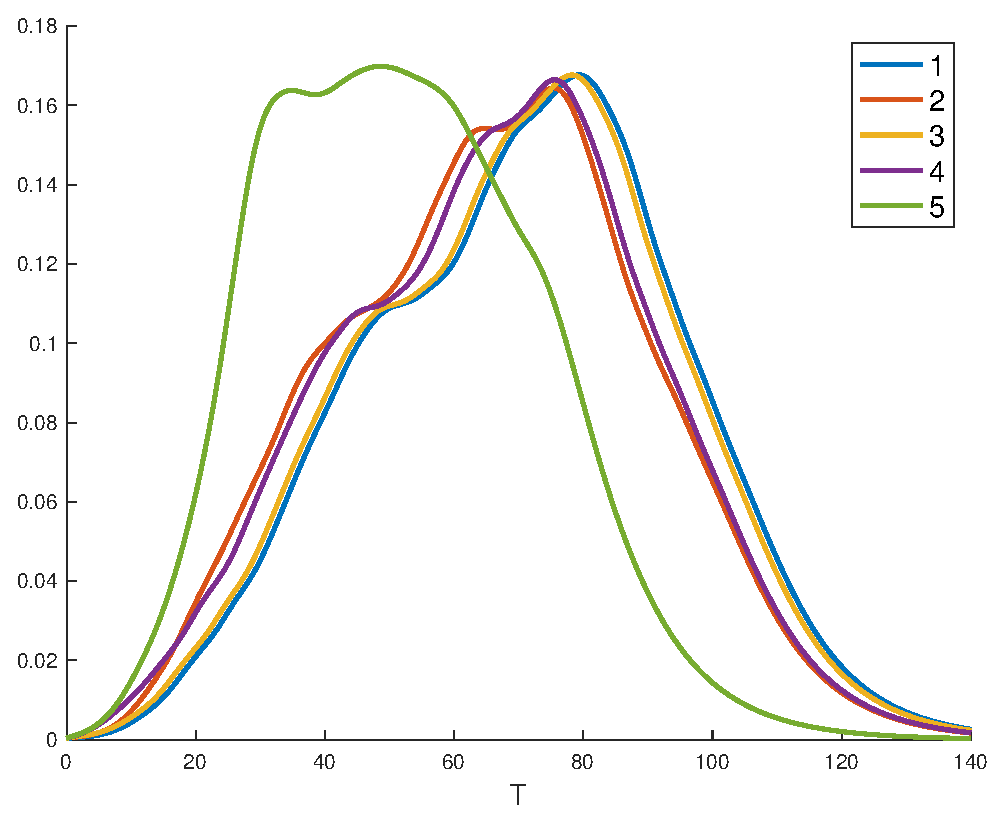
\includegraphics{Figure/minnesota_prevalenza}
\caption[Grafico della prevalenza al variare del grado del nodo inizialmente infetto.]{Grafico della prevalenza al variare del grado del nodo inizialmente infetto.\\ Per ottenere i grafici abbiamo risolto numericamente, usando MATLAB, cinque problemi di Cauchy ottenuti dal modello chiuso alle coppie.\\
Per le condizioni iniziali abbiamo preso ogni volta un nodo certamente infetto (con grado diverso e tutti gli altri nodi certamente sani).\\
Per la sperimentazione abbiamo utilizzato come parametri $\tau=0.3$ e $\gamma=0.1$.}
\label{fig::minnesota_prevalenza}
\end{figure}
In Figura~\ref{fig::minnesota_prevalenza} si osserva come al crescere del grado del nodo inizialmente infetto si velocizzi il tempo per arrivare al picco. Notiamo, inoltre, che il picco rimane pressappoco uguale sia che si scelga un nodo di grado $1$ che uno di grado $5$.

L'ultimo quesito su cui abbiamo indagato \`e come l'immunizzazione cambi le curve di prevalenza.
\begin{figure}[htbp]
\centering
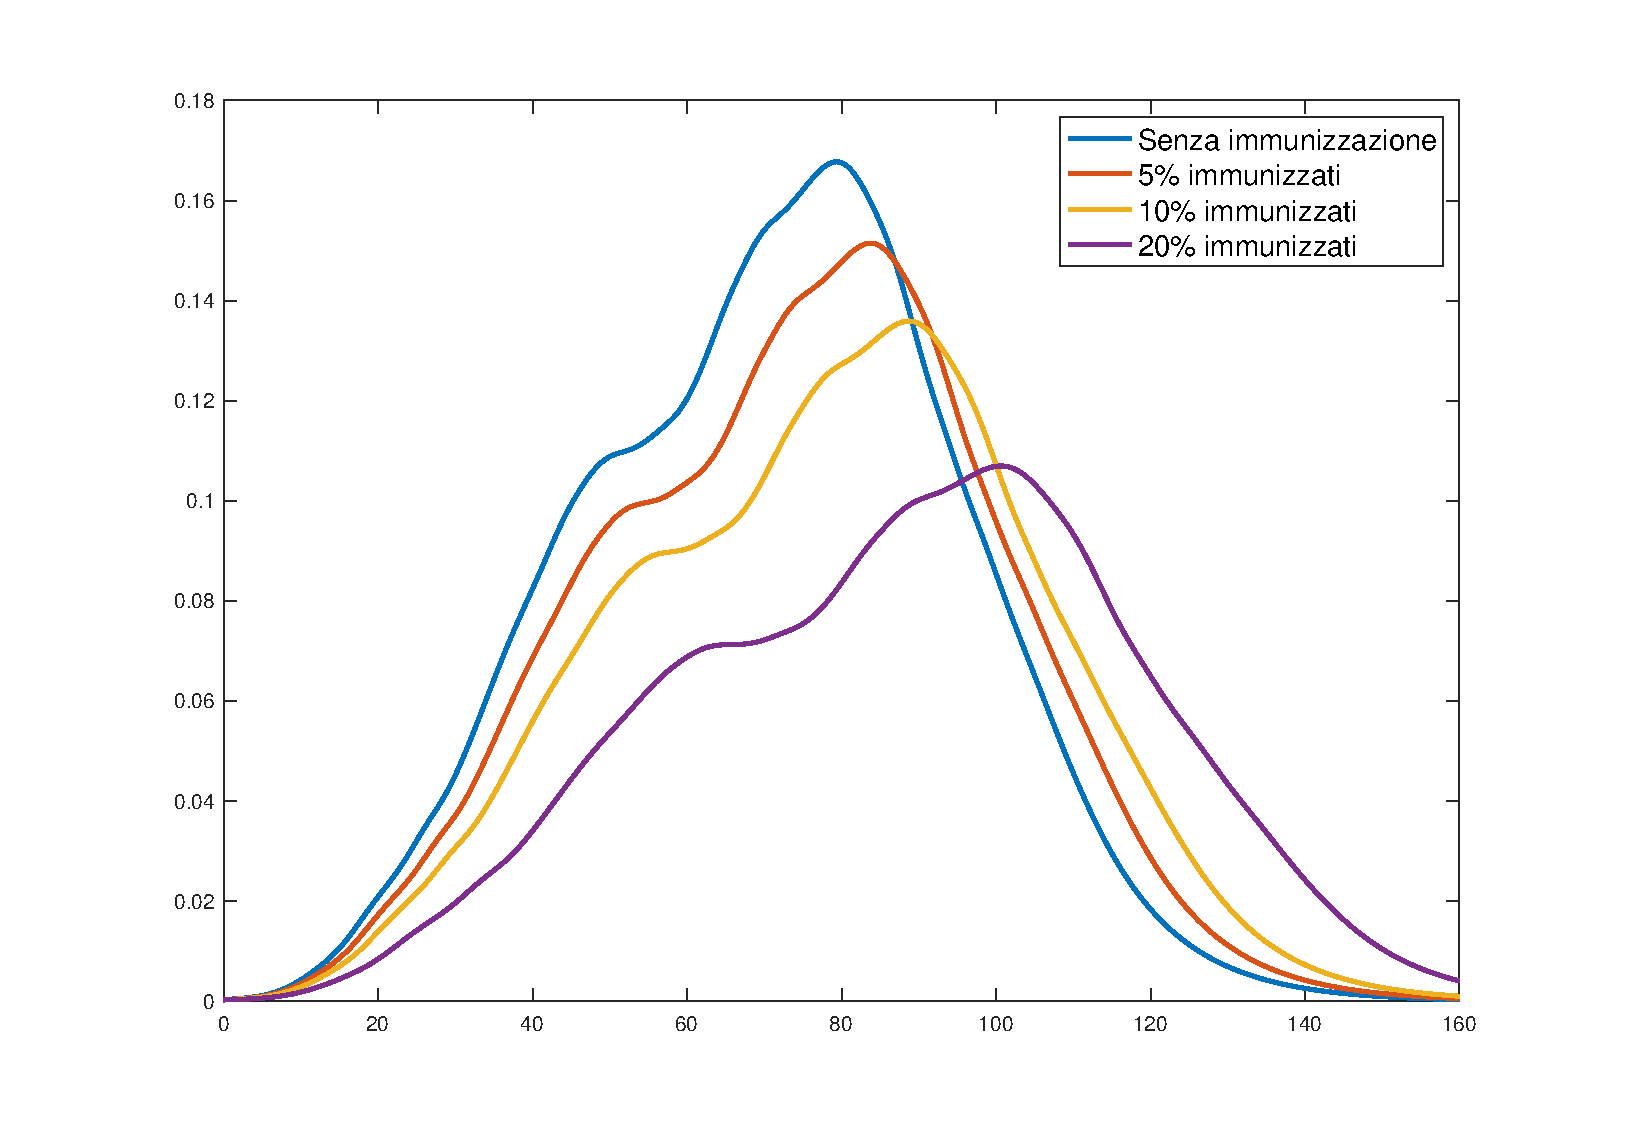
\includegraphics{Figure/minnesota_immunizzazione}
%% This file was created by matlab2tikz.
%
%The latest updates can be retrieved from
%  http://www.mathworks.com/matlabcentral/fileexchange/22022-matlab2tikz-matlab2tikz
%where you can also make suggestions and rate matlab2tikz.
%
\definecolor{mycolor1}{rgb}{0.00000,0.44700,0.74100}%
\definecolor{mycolor2}{rgb}{0.85000,0.32500,0.09800}%
\definecolor{mycolor3}{rgb}{0.92900,0.69400,0.12500}%
\definecolor{mycolor4}{rgb}{0.49400,0.18400,0.55600}%
%
\tikzsetnextfilename{minnesota_immunizzazione}
\begin{tikzpicture}

\begin{axis}[%
width=0.8\columnwidth,
height=3.6in,
at={(1.011in,0.642in)},
scale only axis,
xmin=0,
xmax=160,
xlabel style={font=\color{white!15!black}},
xlabel={T},
ymin=0,
ymax=0.18,
axis background/.style={fill=white},
legend style={legend cell align=left, align=left, draw=none,fill=none}
]
\addplot [color=mycolor1, line width=2.0pt, forget plot]
  table[row sep=crcr]{%
0	0.000378501135503407\\
4.55625e-06	0.000378501480412832\\
9.1125e-06	0.000378501825322563\\
1.366875e-05	0.000378502170232608\\
2.84504681523867e-05	0.000378503289216871\\
4.32321863047733e-05	0.000378504408204346\\
5.801390445716e-05	0.0003785055271951\\
7.27956226095467e-05	0.000378506646189157\\
0.000108852858422585	0.000378509375779682\\
0.000144910094235623	0.000378512105389894\\
0.000180967330048661	0.000378514835019796\\
0.000217024565861699	0.000378517564669389\\
0.000479191351002503	0.000378537412136795\\
0.000741358136143307	0.000378557260645701\\
0.00100352492128411	0.000378577110196571\\
0.00126569170642492	0.000378596960789886\\
0.00188353413484294	0.00037864374635214\\
0.00250137656326096	0.000378690537713006\\
0.00311921899167898	0.000378737334878856\\
0.003737061420097	0.00037878413785603\\
0.00435490384851502	0.000378830946650835\\
0.00615270508312202	0.000378967184286363\\
0.00795050631772902	0.000379103471387747\\
0.00974830755233602	0.00037923980810938\\
0.011546108786943	0.000379376194605366\\
0.01334391002155	0.000379512631029407\\
0.015141711256157	0.000379649117534736\\
0.0180565011171409	0.0003798705110365\\
0.0209712909781249	0.000380092037234274\\
0.0238860808391088	0.000380313696774061\\
0.0268008707000927	0.000380535490299028\\
0.0297156605610766	0.000380757418449495\\
0.0326304504220606	0.000380979481862932\\
0.041320277210953	0.000381642325740783\\
0.0500101039998455	0.00038230639414025\\
0.058699930788738	0.000382971703511921\\
0.0673897575776304	0.00038363827009071\\
0.0760795843665229	0.000384306109898812\\
0.0847694111554154	0.000384975238748522\\
0.0950808371531961	0.000385770926808199\\
0.105392263150977	0.000386568477554247\\
0.115703689148757	0.000387367916288971\\
0.126015115146538	0.000388169267922817\\
0.136326541144319	0.000388972556980627\\
0.1466379671421	0.000389777807607939\\
0.15694939313988	0.000390585043577232\\
0.173660013475191	0.000391897519814621\\
0.190370633810502	0.000393215369152515\\
0.207081254145813	0.000394538686780771\\
0.223791874481124	0.000395867565527705\\
0.240502494816435	0.000397202095922214\\
0.257213115151746	0.000398542366254429\\
0.273923735487057	0.000399888462634843\\
0.290634355822368	0.000401240469051897\\
0.307344976157679	0.000402598467428144\\
0.32405559649299	0.000403962537675052\\
0.340766216828301	0.000405332757746494\\
0.357476837163612	0.000406709203690915\\
0.374187457498923	0.000408091949702226\\
0.390898077834234	0.000409481068169471\\
0.407608698169545	0.000410876629725298\\
0.424319318504855	0.000412278703293273\\
0.441029938840166	0.000413687356134067\\
0.457740559175477	0.000415102653890544\\
0.474451179510788	0.000416524660631782\\
0.491161799846099	0.000417953438896068\\
0.50787242018141	0.000419389049732886\\
0.524583040516721	0.000420831552743928\\
0.541293660852032	0.000422281006123159\\
0.558004281187343	0.000423737466695967\\
0.574714901522654	0.000425200989957417\\
0.591425521857965	0.000426671630109636\\
0.608136142193276	0.000428149440098364\\
0.624846762528587	0.000429634471648678\\
0.641557530709371	0.00043112678853525\\
0.658268298890156	0.000432626427040546\\
0.674979067070941	0.000434133435435493\\
0.691689835251726	0.000435647860905538\\
0.708400603432511	0.000437169749582643\\
0.725111371613296	0.00043869914657659\\
0.741822139794081	0.000440236096005628\\
0.75899450999016	0.000441823414248279\\
0.77616688018624	0.000443418799308007\\
0.793339250382319	0.000445022295985988\\
0.810511620578399	0.000446633948109136\\
0.827683990774478	0.000448253798561713\\
0.844856360970558	0.000449881889316286\\
0.862028731166637	0.000451518261464056\\
0.879667551146585	0.000453207746207722\\
0.897306371126533	0.000454906053503258\\
0.91494519110648	0.000456613225173153\\
0.932584011086428	0.000458329302188942\\
0.950222831066376	0.000460054324702568\\
0.967861651046323	0.00046178833207715\\
0.985500471026271	0.000463531362917161\\
1.00362919780113	0.000465332248014685\\
1.02175792457598	0.000467142745135103\\
1.03988665135084	0.000468962893879786\\
1.0580153781257	0.000470792733133846\\
1.07614410490055	0.000472632301097649\\
1.09427283167541	0.000474481635317776\\
1.11240155845027	0.000476340772717428\\
1.1310367075177	0.000478262100735744\\
1.14967185658514	0.000480193864507438\\
1.16830700565258	0.000482136102275117\\
1.18694215472001	0.000484088851717279\\
1.20557730378745	0.000486052149980375\\
1.22421245285488	0.000488026033710349\\
1.24284760192232	0.000490010539083692\\
1.26200325789843	0.000492061582984501\\
1.28115891387454	0.000494123926298086\\
1.30031456985066	0.000496197606968998\\
1.31947022582677	0.000498282662552976\\
1.33862588180288	0.000500379130250002\\
1.357781537779	0.000502487046936909\\
1.37693719375511	0.000504606449199533\\
1.39662468700855	0.000506796701039762\\
1.41631218026199	0.000508999162637081\\
1.43599967351543	0.000511213872959266\\
1.45568716676887	0.000513440870790234\\
1.47537466002231	0.000515680194764647\\
1.49506215327575	0.000517931883402099\\
1.51474964652919	0.00052019597514093\\
1.53497592247303	0.000522534984950751\\
1.55520219841687	0.000524887168150391\\
1.57542847436072	0.000527252566374594\\
1.59565475030456	0.000529631221316225\\
1.6158810262484	0.000532023174762984\\
1.63610730219225	0.000534428468633795\\
1.65633357813609	0.000536847145014843\\
1.67709969228851	0.000539344343172217\\
1.69786580644092	0.00054185573833612\\
1.71863192059334	0.000544381376840001\\
1.73939803474576	0.000546921305362079\\
1.76016414889818	0.000549475570964814\\
1.7809302630506	0.00055204422113408\\
1.80169637720301	0.000554627303818073\\
1.82299592847734	0.000557291784533207\\
1.84429547975167	0.000559971552609811\\
1.865595031026	0.000562666661557704\\
1.88689458230033	0.000565377165569999\\
1.90819413357465	0.000568103119565908\\
1.92949368484898	0.000570844579233304\\
1.95079323612331	0.000573601601071053\\
1.97261121880314	0.000576441923769038\\
1.99442920148297	0.00057929869822242\\
2.0162471841628	0.00058217198808044\\
2.03806516684263	0.000585061858071583\\
2.05988314952246	0.000587968374050178\\
2.08170113220229	0.000590891603042807\\
2.10351911488212	0.00059383161329451\\
2.12583161691512	0.000596855689418558\\
2.14814411894812	0.000599897464603146\\
2.17045662098112	0.000602957016094296\\
2.19276912301412	0.000606034422673141\\
2.21508162504712	0.000609129764706587\\
2.23739412708012	0.000612243124197771\\
2.25970662911312	0.000615374584836328\\
2.28248185147063	0.000618589743056043\\
2.30525707382815	0.000621823942761735\\
2.32803229618567	0.00062507727871984\\
2.35080751854319	0.000628349847745956\\
2.3735827409007	0.000631641748759432\\
2.39635796325822	0.00063495308283772\\
2.41913318561574	0.000638283953270486\\
2.44233411243515	0.000641697279607446\\
2.46553503925456	0.000645131103062246\\
2.48873596607397	0.000648585540253171\\
2.51193689289338	0.000652060710413278\\
2.53513781971279	0.000655556735448265\\
2.5583387465322	0.000659073739994032\\
2.5815396733516	0.000662611851473878\\
2.60512813949053	0.000666230835228537\\
2.62871660562946	0.000669871911574081\\
2.65230507176839	0.000673535223650219\\
2.67589353790732	0.000677220917817346\\
2.69948200404625	0.000680929143716465\\
2.72307047018518	0.000684660054328589\\
2.74665893632411	0.000688413806033599\\
2.77060055005497	0.000692247276761732\\
2.79454216378583	0.000696104613114108\\
2.81848377751668	0.000699985989709192\\
2.84242539124754	0.00070389158501769\\
2.8663670049784	0.000707821581422504\\
2.89030861870926	0.000711776165277873\\
2.91425023244012	0.00071575552696767\\
2.9385191918258	0.000719814784850752\\
2.96278815121149	0.00072389990949627\\
2.98705711059717	0.000728011112241497\\
3.01132606998286	0.000732148608916235\\
3.03559502936854	0.000736312619899945\\
3.05986398875423	0.000740503370177668\\
3.08413294813992	0.000744721089394677\\
3.10871609496664	0.000749021146352029\\
3.13329924179337	0.000753349364093136\\
3.15788238862009	0.000757705996253526\\
3.18246553544682	0.000762091301591839\\
3.20704868227355	0.000766505544040316\\
3.23163182910027	0.000770948992753536\\
3.256214975927	0.000775421922155294\\
3.28111476070479	0.000779982803286346\\
3.30601454548257	0.000784574512728746\\
3.33091433026036	0.000789197352454698\\
3.35581411503815	0.000793851630159764\\
3.38071389981593	0.000798537659301747\\
3.40561368459372	0.00080325575913703\\
3.43051346937151	0.000808006254754358\\
3.45541325414929	0.00081278947710592\\
3.48031303892708	0.00081760576303567\\
3.50521282370487	0.000822455455304765\\
3.53011260848265	0.000827338902614064\\
3.55501239326044	0.000832256459623554\\
3.57991217803823	0.000837208486968621\\
3.60481196281601	0.00084219535127309\\
3.6297117475938	0.000847217425158883\\
3.65461153237159	0.000852275087252258\\
3.67951131714937	0.000857368722186472\\
3.70441110192716	0.000862498720600834\\
3.72931088670495	0.000867665479135973\\
3.75421067148273	0.000872869400425274\\
3.77911045626052	0.000878110893082384\\
3.80401024103831	0.000883390371684642\\
3.82891002581609	0.000888708256752386\\
3.85380981059388	0.000894064974724008\\
3.87870959537167	0.000899460957926667\\
3.90360938014945	0.000904896644542575\\
3.92850916492724	0.000910372478570729\\
3.95340894970503	0.000915888909784036\\
3.97830873448281	0.000921446393681698\\
4.0032085192606	0.000927045391436805\\
4.02810830403839	0.000932686369838999\\
4.05300808881617	0.000938369801232179\\
4.07790787359396	0.000944096163447103\\
4.10280765837175	0.000949865939728852\\
4.12770744314953	0.000955679618659046\\
4.15260722792732	0.000961537694072752\\
4.17750701270511	0.000967440664970007\\
4.20240679748289	0.000973389035421861\\
4.22730658226068	0.000979383314470941\\
4.25220636703846	0.000985424016026377\\
4.27710615181625	0.000991511658753116\\
4.30200593659404	0.000997646765955536\\
4.32690572137182	0.0010038298654553\\
4.35180550614961	0.00101006148946344\\
4.3767052909274	0.00101634217444657\\
4.40160507570518	0.00102267246098731\\
4.42650486048297	0.00102905289363875\\
4.45140464526076	0.00103548402077305\\
4.47630443003854	0.00104196639442413\\
4.50120421481633	0.00104850057012436\\
4.52610399959411	0.00105508710673541\\
4.5510037843719	0.00106172656627314\\
4.57590356914969	0.00106841951372658\\
4.60080335392747	0.00107516651687102\\
4.62570313870526	0.0010819681460753\\
4.65060292348305	0.00108882497410325\\
4.67550270826083	0.00109573757590935\\
4.70040249303862	0.00110270652842874\\
4.7253022778164	0.00110973241036159\\
4.75020206259419	0.00111681580195187\\
4.77510184737198	0.00112395728476065\\
4.80000163214976	0.00113115744143414\\
4.82490141692755	0.00113841685546627\\
4.84980120170534	0.00114573611095633\\
4.87470098648312	0.00115311579236145\\
4.89960077126091	0.00116055648424424\\
4.9245005560387	0.00116805877101575\\
4.94940034081648	0.00117562323667381\\
4.97430012559427	0.00118325046453702\\
4.99919991037205	0.00119094103697449\\
5.02409969514984	0.00119869553513165\\
5.04899947992763	0.00120651453865221\\
5.07389926470541	0.00121439862539655\\
5.0987990494832	0.00122234837115679\\
5.12369883426099	0.00123036434936874\\
5.14859861903877	0.00123844713082107\\
5.17349840381656	0.00124659728336182\\
5.19839818859434	0.0012548153716027\\
5.22329797337213	0.00126310195662137\\
5.24819775814992	0.00127145759566204\\
5.2730975429277	0.00127988284183467\\
5.29799732770549	0.00128837824381315\\
5.32289711248328	0.00129694434553279\\
5.34779689726106	0.0013055816858874\\
5.37269668203885	0.00131429079842643\\
5.39759646681664	0.00132307221105244\\
5.42249625159442	0.00133192644571936\\
5.44739603637221	0.00134085401813186\\
5.47229582114999	0.00134985543744632\\
5.49719560592778	0.00135893120597365\\
5.51781096531216	0.00136650195010865\\
5.53842632469654	0.00137412427539467\\
5.55904168408092	0.00138179845540734\\
5.57965704346531	0.00138952476000624\\
5.60027240284969	0.00139730345522487\\
5.62088776223407	0.00140513480316207\\
5.64150312161845	0.00141301906187488\\
5.66211848100283	0.00142095648527308\\
5.68273384038721	0.00142894732301537\\
5.70334919977159	0.00143699182040753\\
5.72396455915597	0.00144509021830258\\
5.74457991854035	0.00145324275300293\\
5.76519527792474	0.00146144965616496\\
5.78581063730912	0.00146971115470579\\
5.8064259966935	0.00147802747071267\\
5.82704135607788	0.00148639882135489\\
5.84765671546226	0.00149482541879844\\
5.86827207484664	0.00150330747012358\\
5.88888743423102	0.00151184517724528\\
5.9095027936154	0.00152043873683687\\
5.93011815299979	0.00152908834025675\\
5.95073351238417	0.00153779417347857\\
5.97134887176855	0.00154655641702476\\
5.99196423115293	0.00155537524590361\\
6.01257959053731	0.00156425082955005\\
6.03319494992169	0.00157318333177015\\
6.05381030930607	0.00158217291068956\\
6.07442566869045	0.00159121971870582\\
6.09504102807484	0.00160032390244483\\
6.11565638745922	0.00160948560272143\\
6.1362717468436	0.00161870495450429\\
6.15688710622798	0.00162798208688511\\
6.17750246561236	0.00163731712305227\\
6.19811782499674	0.001646710180269\\
6.21873318438112	0.00165616136985607\\
6.2393485437655	0.0016656707971793\\
6.25996390314988	0.00167523856164162\\
6.28057926253427	0.00168486475668004\\
6.30119462191865	0.00169454946976742\\
6.32180998130303	0.00170429278241917\\
6.34242534068741	0.00171409477020488\\
6.36304070007179	0.00172395550276494\\
6.38365605945617	0.00173387504383218\\
6.40427141884055	0.0017438534512586\\
6.42488677822493	0.00175389077704713\\
6.44550213760932	0.00176398706738854\\
6.4661174969937	0.00177414236270339\\
6.48673285637808	0.00178435669768916\\
6.50734821576246	0.00179463010137245\\
6.52796357514684	0.00180496259716628\\
6.54857893453122	0.0018153542029325\\
6.5691942939156	0.00182580493104924\\
6.58980965329998	0.00183631478848343\\
6.61042501268436	0.00184688377686825\\
6.63104037206875	0.00185751189258559\\
6.65165573145313	0.00186819912685343\\
6.67227109083751	0.00187894546581799\\
6.69288645022189	0.00188975089065076\\
6.71350180960627	0.00190061537765014\\
6.73411716899065	0.00191153889834778\\
6.75473252837503	0.00192252141961947\\
6.77534788775941	0.0019335629038004\\
6.7959632471438	0.00194466330880488\\
6.81657860652818	0.00195582258825022\\
6.83719396591256	0.00196704069158478\\
6.85780932529694	0.00197831756422004\\
6.87842468468132	0.0019896531476665\\
6.8990400440657	0.00200104737967338\\
6.91965540345008	0.0020125001943719\\
6.94027076283446	0.00202401152242204\\
6.96088612221885	0.00203558129116254\\
6.98150148160323	0.00204720942476417\\
7.00211684098761	0.00205889584438588\\
7.02273220037199	0.0020706404683338\\
7.04334755975637	0.00208244321222282\\
7.06396291914075	0.00209430398914077\\
7.08457827852513	0.00210622270981468\\
7.10519363790951	0.00211819928277927\\
7.12580899729389	0.00213023361454724\\
7.14642435667828	0.00214232560978126\\
7.16703971606266	0.00215447517146746\\
7.18765507544704	0.00216668220109016\\
7.20827043483142	0.00217894659880769\\
7.2288857942158	0.00219126826362904\\
7.24950115360018	0.00220364709359118\\
7.27012353405424	0.0022160872309955\\
7.2907459145083	0.00222858436617823\\
7.31136829496236	0.00224113839522068\\
7.33199067541642	0.00225374921394297\\
7.35261305587048	0.00226641671808143\\
7.37323543632455	0.00227914080346535\\
7.39385781677861	0.00229192136619275\\
7.41460983983197	0.00230483918030318\\
7.43536186288534	0.00231781397452473\\
7.4561138859387	0.00233084564487555\\
7.47686590899207	0.00234393408835832\\
7.49761793204544	0.00235707920313326\\
7.5183699550988	0.00237028088868878\\
7.53912197815217	0.00238353904600956\\
7.55987400120554	0.0023968535777417\\
7.5806260242589	0.00241022438835491\\
7.60137804731227	0.00242365138430133\\
7.62213007036563	0.00243713447417093\\
7.642882093419	0.00245067356884311\\
7.66363411647237	0.00246426858163442\\
7.68438613952573	0.00247791942844216\\
7.7051381625791	0.00249162602788365\\
7.72589018563247	0.00250538830143089\\
7.74664220868583	0.0025192061735406\\
7.7673942317392	0.0025330795717793\\
7.78814625479256	0.00254700842694334\\
7.80889827784593	0.00256099267317367\\
7.8296503008993	0.0025750322480651\\
7.85040232395266	0.00258912709277019\\
7.87115434700603	0.00260327715209716\\
7.8919063700594	0.00261748237460211\\
7.91265839311276	0.00263174271267513\\
7.93341041616613	0.00264605812262036\\
7.95416243921949	0.00266042856472965\\
7.97491446227286	0.00267485400334999\\
7.99566648532623	0.0026893344069444\\
8.01641850837959	0.0027038697481462\\
8.03717053143296	0.00271846000380673\\
8.05792255448632	0.00273310515503621\\
8.07867457753969	0.00274780518723786\\
8.09942660059305	0.00276256009013517\\
8.12017862364642	0.00277736985779217\\
8.14093064669978	0.00279223448862682\\
8.16168266975315	0.0028071539854173\\
8.18243469280652	0.0028221283553014\\
8.20318671585988	0.0028371576097688\\
8.22393873891325	0.00285224176464627\\
8.24469076196661	0.00286738084007594\\
8.26544278501998	0.00288257486048646\\
8.28619480807334	0.00289782385455718\\
8.30694683112671	0.00291312785517533\\
8.32769885418007	0.00292848689938633\\
8.34845087723344	0.00294390102833718\\
8.3692029002868	0.00295937028721299\\
8.38995492334017	0.00297489472516683\\
8.41070694639353	0.00299047439524283\\
8.4314589694469	0.00300610935429273\\
8.45221099250026	0.00302179966288591\\
8.47296301555363	0.00303754538521303\\
8.49371503860699	0.00305334658898335\\
8.51446706166036	0.00306920334531592\\
8.53521908471373	0.00308511572862473\\
8.55597110776709	0.00310108381649789\\
8.57672313082046	0.00311710768957115\\
8.59747515387382	0.00313318743139566\\
8.61822717692719	0.00314932312830042\\
8.63897919998055	0.00316551486924935\\
8.65973122303392	0.00318176274569319\\
8.68048324608728	0.00319806685141666\\
8.70123526914065	0.00321442728238054\\
8.72198729219401	0.0032308441365595\\
8.74273931524738	0.00324731751377531\\
8.76349133830074	0.00326384751552608\\
8.78424336135411	0.00328043424481131\\
8.80499538440747	0.00329707780595343\\
8.82574740746084	0.00331377830441562\\
8.84649943051421	0.00333053584661641\\
8.86725145356757	0.0033473505397412\\
8.88800347662094	0.00336422249155088\\
8.9087554996743	0.00338115181018786\\
8.92950752272767	0.00339813860397977\\
8.95025954578103	0.00341518298124091\\
8.9710115688344	0.00343228505007196\\
8.99176359188776	0.00344944491815793\\
9.01251561494113	0.00346666269256477\\
9.03326763799449	0.00348393847953487\\
9.05401966104786	0.00350127238428162\\
9.07477168410122	0.00351866451078343\\
9.09552370715459	0.00353611496157729\\
9.11627573020795	0.00355362383755232\\
9.13702775326132	0.0035711912377434\\
9.15777977631469	0.00358881725912528\\
9.17853179936805	0.00360650199640733\\
9.19928382242142	0.00362424554182923\\
9.22003584547478	0.00364204798495796\\
9.24078786852815	0.00365990941248604\\
9.26153989158151	0.00367782990803173\\
9.28229191463488	0.00369580955194109\\
9.30304393768824	0.00371384842109226\\
9.32379596074161	0.00373194658870232\\
9.34454798379497	0.00375010412413683\\
9.36530000684834	0.00376832109272236\\
9.3860520299017	0.00378659755556237\\
9.40680405295507	0.00380493356935646\\
9.42755607600843	0.00382332918622341\\
9.4483080990618	0.00384178445352825\\
9.46906012211516	0.00386029941371344\\
9.48981214516853	0.00387887410413455\\
9.5105641682219	0.00389750855690061\\
9.53131619127526	0.00391620279871938\\
9.55206821432863	0.00393495685074767\\
9.57282023738199	0.00395377072844704\\
9.59357226043536	0.00397264444144504\\
9.61432428348872	0.00399157799340209\\
9.63507630654209	0.00401057138188448\\
9.65582832959545	0.0040296245982433\\
9.67658035264882	0.00404873762749988\\
9.69733237570218	0.00406791044823752\\
9.71808439875555	0.00408714303250001\\
9.73883642180891	0.00410643534569704\\
9.75958844486228	0.00412578734651636\\
9.78034046791564	0.0041451989868434\\
9.80109249096901	0.00416467021168789\\
9.82184451402238	0.00418420095911809\\
9.84259653707574	0.00420379116020247\\
9.86334856012911	0.00422344073895913\\
9.88410058318247	0.00424314961231293\\
9.90485260623584	0.00426291769006058\\
9.9256046292892	0.00428274487484368\\
9.94635665234257	0.00430263106212976\\
9.96362926847745	0.0043192279262049\\
9.98090188461232	0.00433586552055169\\
9.9981745007472	0.00435254377350682\\
10.0154471168821	0.00436926260996393\\
10.032719733017	0.00438602195138114\\
10.0499923491518	0.00440282171579165\\
10.0672649652867	0.00441966181781697\\
10.0845375814216	0.00443654216868286\\
10.1018101975565	0.00445346267623798\\
10.1190828136914	0.00447042324497553\\
10.1363554298262	0.00448742377605764\\
10.1536280459611	0.00450446416734263\\
10.170900662096	0.00452154431341496\\
10.1881732782309	0.00453866410561808\\
10.2054458943657	0.00455582343208991\\
10.2227185105006	0.00457302217780133\\
10.2399911266355	0.00459026022459723\\
10.2572637427704	0.00460753745124036\\
10.2745363589053	0.004624853733458\\
10.2918089750401	0.00464220894399115\\
10.309081591175	0.0046596029526466\\
10.3263542073099	0.00467703562635151\\
10.3436268234448	0.00469450682921073\\
10.3608994395796	0.00471201642256659\\
10.3781720557145	0.00472956426506147\\
10.3954446718494	0.00474715021270266\\
10.4127172879843	0.0047647741189299\\
10.4299899041192	0.00478243583468534\\
10.447262520254	0.00480013520848589\\
10.4645351363889	0.00481787208649798\\
10.4818077525238	0.00483564631261468\\
10.4990803686587	0.00485345772853509\\
10.5163529847936	0.00487130617384598\\
10.5336256009284	0.00488919148610567\\
10.550917995854	0.00490713404431864\\
10.5682103907796	0.00492511322238851\\
10.5855027857052	0.00494312885173169\\
10.6027951806307	0.00496118076208499\\
10.6200875755563	0.00497926878160024\\
10.6373799704819	0.00499739273694068\\
10.6546723654075	0.00501555245337932\\
10.6723958722839	0.00503420183008026\\
10.6901193791604	0.00505288839749136\\
10.7078428860368	0.0050716119636111\\
10.7255663929132	0.00509037233536214\\
10.7432898997897	0.00510916931871184\\
10.7610134066661	0.00512800271879428\\
10.7787369135425	0.00514687234003396\\
10.7970872823529	0.00516644731641472\\
10.8154376511632	0.00518606069295544\\
10.8337880199735	0.00520571225104851\\
10.8521383887839	0.00522540177186584\\
10.8704887575942	0.00524512903651364\\
10.8888391264045	0.00526489382618877\\
10.9071894952149	0.00528469592233597\\
10.9255609481436	0.00530455792278457\\
10.9439324010722	0.00532445687849851\\
10.9623038540009	0.00534439257187294\\
10.9806753069296	0.00536436478619362\\
10.9990467598583	0.00538437330579917\\
11.017418212787	0.00540441791624352\\
11.0357896657156	0.00542449840445888\\
11.0541611186443	0.00544461455891867\\
11.072532571573	0.00546476616980069\\
11.0909040245017	0.00548495302915002\\
11.1092754774304	0.00550517493104196\\
11.127646930359	0.00552543167174444\\
11.1460183832877	0.00554572304988008\\
11.1643898362164	0.00556604886658777\\
11.1827612891451	0.00558640892568341\\
11.2011403406705	0.00560681147602303\\
11.219519392196	0.00562724791298918\\
11.2378984437214	0.00564771804915498\\
11.2562774952468	0.00566822170041045\\
11.2746565467723	0.00568875868611843\\
11.2930355982977	0.00570932882926929\\
11.3114146498232	0.00572993195663406\\
11.3299697673701	0.00575076574344697\\
11.348524884917	0.00577163280692248\\
11.367080002464	0.00579253298146902\\
11.3856351200109	0.00581346610604434\\
11.4041902375578	0.00583443202430654\\
11.4227453551047	0.00585543058476305\\
11.4413004726517	0.00587646164091711\\
11.4598555901986	0.00589752505141193\\
11.4784107077455	0.00591862068017222\\
11.4969658252925	0.00593974839654313\\
11.5155209428394	0.00596090807542648\\
11.5340760603863	0.00598209959741418\\
11.5526311779332	0.00600332284891868\\
11.5711862954802	0.00602457772230052\\
11.5897414130271	0.0060458641159928\\
11.608296530574	0.00606718193462246\\
11.626851648121	0.00608853108912841\\
11.6454067656679	0.00610991149687637\\
11.6639618832148	0.00613132308177025\\
11.6825170007617	0.00615276577436035\\
11.7010721183087	0.00617423951194782\\
11.7196272358556	0.00619574423868581\\
11.7381823534025	0.00621727990567683\\
11.7567374709495	0.00623884647106674\\
11.7752925884964	0.0062604439001348\\
11.7938477060433	0.00628207216538014\\
11.8124028235902	0.00630373124660445\\
11.8309579411372	0.0063254211309909\\
11.8495130586841	0.0063471418131791\\
11.868068176231	0.00636889329533642\\
11.8866232937779	0.00639067558722521\\
11.9051784113249	0.00641248870626629\\
11.9237335288718	0.00643433267759842\\
11.9422886464187	0.00645620753413385\\
11.9608437639657	0.00647811331660989\\
11.9793988815126	0.00650005007363669\\
11.9979539990595	0.00652201786174076\\
12.0165091166064	0.00654401674540483\\
12.0350642341534	0.0065660467971036\\
12.0536193517003	0.00658810809733547\\
12.0721744692472	0.00661020073465045\\
12.0907295867942	0.00663232480567411\\
12.1092847043411	0.00665448041512749\\
12.127839821888	0.00667666767584323\\
12.1463949394349	0.00669888670877776\\
12.1649500569819	0.00672113764301958\\
12.1835051745288	0.00674342061579379\\
12.2020602920757	0.00676573577246268\\
12.2206154096226	0.00678808326652259\\
12.2391705271696	0.00681046325959703\\
12.2577256447165	0.00683287592142609\\
12.2762807622634	0.00685532142985207\\
12.2948358798104	0.00687779997080149\\
12.3133909973573	0.00690031173826363\\
12.3319461149042	0.00692285693426518\\
12.3505012324511	0.00694543576884177\\
12.3690563499981	0.00696804846000564\\
12.387611467545	0.0069906952337102\\
12.4061665850919	0.00701337632381089\\
12.4247217026389	0.00703609197202291\\
12.4432768201858	0.00705884242787573\\
12.4618319377327	0.00708162794866402\\
12.4803870552796	0.0071044487993958\\
12.4989421728266	0.0071273052527373\\
12.5174972903735	0.00715019758895451\\
12.5360524079204	0.00717312609585222\\
12.5546075254673	0.0071960910687096\\
12.5731626430143	0.00721909281021323\\
12.5917177605612	0.007242131630387\\
12.6102728781081	0.00726520784651952\\
12.628847103658	0.0072883456053049\\
12.6474213292079	0.00731152149487455\\
12.6659955547579	0.00733473585490553\\
12.6845697803078	0.00735798903205017\\
12.7031440058577	0.00738128137985001\\
12.7217182314076	0.00740461325864695\\
12.7402924569575	0.00742798503549216\\
12.7594483555952	0.00745213091355812\\
12.778604254233	0.00747632004232564\\
12.7977601528708	0.00750055284620186\\
12.8169160515085	0.00752482975673852\\
12.8360719501463	0.00754915121251257\\
12.855227848784	0.00757351765900413\\
12.8743837474218	0.00759792954847213\\
12.8935396460595	0.00762238733982762\\
12.9126955446973	0.00764689149850491\\
12.931851443335	0.00767144249633016\\
12.9510073419728	0.00769604081138827\\
12.9701632406105	0.00772068692788738\\
12.9893191392483	0.00774538133602139\\
13.008475037886	0.00777012453183063\\
13.0276309365238	0.0077949170170606\\
13.0467868351616	0.00781975929901854\\
13.0659427337993	0.00784465189042879\\
13.0850986324371	0.00786959530928587\\
13.1042545310748	0.00789459007870601\\
13.1234104297126	0.00791963672677728\\
13.1425663283503	0.00794473578640764\\
13.1617222269881	0.00796988779517196\\
13.1808781256258	0.007995093295157\\
13.2000340242636	0.00802035283280535\\
13.2191899229013	0.00804566695875761\\
13.2383458215391	0.00807103622769347\\
13.2575017201769	0.00809646119817103\\
13.2766576188146	0.00812194243246522\\
13.2958135174524	0.00814748049640461\\
13.3149694160901	0.00817307595920706\\
13.3341253147279	0.00819872939331415\\
13.3532812133656	0.00822444137422435\\
13.3724371120034	0.00825021248032506\\
13.3915930106411	0.00827604329272346\\
13.4107489092789	0.00830193439507599\\
13.4299048079166	0.00832788637341734\\
13.4490607065544	0.00835389981598752\\
13.4682166051921	0.00837997531305849\\
13.4873725038299	0.00840611345675937\\
13.5065284024677	0.00843231484090076\\
13.5256843011054	0.00845858006079792\\
13.5448401997432	0.00848490971309307\\
13.5639960983809	0.00851130439557646\\
13.5831519970187	0.00853776470700666\\
13.6023078956564	0.00856429124692972\\
13.6214637942942	0.0085908846154974\\
13.6406196929319	0.00861754541328433\\
13.6597755915697	0.00864427424110446\\
13.6789643623313	0.00867111774443916\\
13.6981531330928	0.00869803071825817\\
13.7173419038544	0.00872501376607635\\
13.736530674616	0.0087520674908993\\
13.7557194453775	0.00877919249503319\\
13.7749082161391	0.00880638937989388\\
13.7940969869007	0.00883365874581488\\
13.8138258640017	0.00886177186298745\\
13.8335547411028	0.00888996288160031\\
13.8532836182039	0.00891823244924714\\
13.8730124953049	0.00894658121143172\\
13.892741372406	0.00897500981134238\\
13.9124702495071	0.00900351888962507\\
13.9321991266081	0.00903210908415558\\
13.9519280037092	0.00906078102981066\\
13.9716568808103	0.00908953535823825\\
13.9913857579113	0.00911837269762666\\
14.0111146350124	0.00914729367247288\\
14.0308435121134	0.00917629890334978\\
14.0505723892145	0.00920538900667269\\
14.0703012663156	0.00923456459446467\\
14.0900301434166	0.00926382627412147\\
14.1097590205177	0.00929317464817513\\
14.1294878976188	0.00932261031405716\\
14.1492167747198	0.00935213386386076\\
14.1689456518209	0.00938174588410234\\
14.188674528922	0.00941144695548257\\
14.208403406023	0.00944123765264633\\
14.2281322831241	0.00947111854394263\\
14.2478611602252	0.00950109019118363\\
14.2675900373262	0.00953115314940312\\
14.2873189144273	0.00956130796661492\\
14.3070477915283	0.00959155518357057\\
14.3267766686294	0.00962189533351679\\
14.3465055457305	0.00965232894195292\\
14.3662344228315	0.00968285652638788\\
14.3859632999326	0.00971347859609718\\
14.4056921770337	0.00974419565188\\
14.4254210541347	0.00977500818581613\\
14.4451499312358	0.00980591668102326\\
14.4648788083369	0.00983692161141441\\
14.4846076854379	0.00986802344145571\\
14.504336562539	0.00989922262592463\\
14.5240654396401	0.00993051960966874\\
14.5437943167411	0.00996191482736515\\
14.5635231938422	0.00999340870328056\\
14.5832520709433	0.0100250016510324\\
14.6029809480443	0.0100566940733509\\
14.6227098251454	0.0100884863618419\\
14.6424387022464	0.0101203788967516\\
14.6621675793475	0.0101523720467318\\
14.6818964564486	0.0101844661686077\\
14.7016253335496	0.010216661607146\\
14.7213542106507	0.0102489586948263\\
14.7410830877518	0.0102813577516126\\
14.7608119648528	0.0103138590847288\\
14.7805408419539	0.010346462988435\\
14.800269719055	0.0103791697438067\\
14.819998596156	0.0104119796185162\\
14.8397274732571	0.0104448928666174\\
14.8594563503582	0.0104779097283322\\
14.8791852274592	0.0105110304298414\\
14.8989141045603	0.0105442551830773\\
14.9186429816613	0.0105775841855207\\
14.9383718587624	0.0106110176200009\\
14.9581007358635	0.0106445556544992\\
14.9778296129645	0.0106781984419569\\
14.9975584900656	0.0107119461200866\\
15.0172873671667	0.0107457988111878\\
15.0370162442677	0.0107797566219676\\
15.0567451213688	0.0108138196433648\\
15.0764739984699	0.0108479879503796\\
15.0962028755709	0.0108822616019075\\
15.115931752672	0.0109166406405792\\
15.1356606297731	0.0109511250926047\\
15.1553895068741	0.0109857149676232\\
15.1751183839752	0.0110204102585591\\
15.1948472610762	0.0110552109414831\\
15.2145761381773	0.0110901169754792\\
15.2343050152784	0.0111251283025187\\
15.2540338923794	0.0111602448473392\\
15.2737627694805	0.0111954665173311\\
15.2934916465816	0.01123079320243\\
15.3132205236826	0.0112662247750166\\
15.3329494007837	0.0113017610898225\\
15.3526782778848	0.0113374019838444\\
15.3724071549858	0.011373147276264\\
15.3921360320869	0.011408996768377\\
15.411864909188	0.0114449502435277\\
15.431593786289	0.0114810074670534\\
15.4513226633901	0.0115171681862346\\
15.4710515404911	0.0115534321302544\\
15.4907804175922	0.0115897990101658\\
15.5105092946933	0.0116262685188666\\
15.5302381717943	0.0116628403310831\\
15.5499670488954	0.0116995141033622\\
15.5696959259965	0.0117362894740719\\
15.5894248030975	0.01177316606341\\
15.6091536801986	0.0118101434734226\\
15.6288825572997	0.01184722128803\\
15.6486114344007	0.0118843990730623\\
15.6683403115018	0.011921676376304\\
15.6880691886029	0.0119590527275472\\
15.7077980657039	0.0119965276386536\\
15.727526942805	0.0120341006036267\\
15.7472558199061	0.0120717710986917\\
15.7669846970071	0.0121095385823855\\
15.7867135741082	0.0121474024956558\\
15.8064424512092	0.0121853622619691\\
15.8261713283103	0.0122234172874277\\
15.8459002054114	0.0122615669608966\\
15.8656290825124	0.0122998106541393\\
15.8853579596135	0.0123381477219621\\
15.9050868367146	0.0123765775023687\\
15.9248157138156	0.0124150993167229\\
15.9445445909167	0.0124537124699212\\
15.9642734680178	0.0124924162505732\\
15.9840023451188	0.0125312099311925\\
16.0037312222199	0.0125700927683951\\
16.0234600993209	0.0126090640031073\\
16.043188976422	0.0126481228607821\\
16.0629178535231	0.0126872685516241\\
16.0826467306241	0.0127265002708229\\
16.1023756077252	0.0127658171987951\\
16.1221044848263	0.0128052185014339\\
16.1418333619273	0.0128447033303677\\
16.1615622390284	0.0128842708232257\\
16.1812911161295	0.0129239201039119\\
16.2010199932305	0.0129636502828865\\
16.2207488703316	0.0130034604574547\\
16.2404777474326	0.0130433497120631\\
16.2602066245337	0.0130833171186024\\
16.2799355016348	0.0131233617367181\\
16.2996643787358	0.0131634826141269\\
16.3193932558369	0.0132036787869399\\
16.339122132938	0.0132439492799925\\
16.358851010039	0.0132842931071796\\
16.3785798871401	0.0133247092717968\\
16.3983087642411	0.0133651967668875\\
16.4180376413422	0.0134057545755952\\
16.4377665184433	0.0134463816715202\\
16.4574953955443	0.0134870770190822\\
16.4772242726454	0.0135278395738862\\
16.4969531497465	0.013568668283094\\
16.5166820268475	0.0136095620857983\\
16.5364109039486	0.0136505199134019\\
16.5561397810496	0.0136915406899989\\
16.5758686581507	0.0137326233327603\\
16.5955975352518	0.0137737667523215\\
16.6153264123528	0.0138149698531732\\
16.6350552894539	0.0138562315340537\\
16.654784166555	0.0138975506883435\\
16.674513043656	0.0139389262044624\\
16.6942419207571	0.0139803569662659\\
16.7139707978581	0.0140218418534453\\
16.7336996749592	0.0140633797419258\\
16.7534285520603	0.0141049695042675\\
16.7731574291613	0.0141466100100648\\
16.7928863062624	0.0141883001263461\\
16.8126151833635	0.0142300387179737\\
16.8323440604645	0.0142718246480417\\
16.8520729375656	0.0143136567782739\\
16.8718018146666	0.0143555339694194\\
16.8915306917677	0.0143974550816471\\
16.9112595688688	0.0144394189749381\\
16.9309884459698	0.0144814245094753\\
16.9507173230709	0.0145234705460313\\
16.970446200172	0.0145655559463522\\
16.990175077273	0.0146076795735396\\
17.0099039543741	0.014649840292428\\
17.0296328314751	0.014692036969959\\
17.0493617085762	0.0147342684755515\\
17.0690905856773	0.0147765336814676\\
17.0888194627783	0.0148188314631733\\
17.1085483398794	0.014861160699696\\
17.1282772169805	0.014903520273975\\
17.1480060940815	0.0149459090732081\\
17.1677349711826	0.0149883259891925\\
17.1874638482836	0.015030769918659\\
17.2071927253847	0.0150732397636016\\
17.2269216024858	0.0151157344315998\\
17.2466504795868	0.0151582528361354\\
17.2663793566879	0.0152007938969019\\
17.286108233789	0.0152433565401077\\
17.30583711089	0.0152859396987721\\
17.3255659879911	0.0153285423130144\\
17.3452948650921	0.0153711633303354\\
17.3650237421932	0.0154138017058917\\
17.3847526192943	0.0154564564027626\\
17.4044814963953	0.0154991263922086\\
17.4242103734964	0.0155418106539233\\
17.4439392505975	0.0155845081762757\\
17.4636681276985	0.0156272179565464\\
17.4833970047996	0.0156699390011539\\
17.5031258819006	0.0157126703258737\\
17.5228547590017	0.0157554109560492\\
17.5425836361028	0.0157981599267936\\
17.5623125132038	0.0158409162831838\\
17.5820413903049	0.0158836790804463\\
17.601770267406	0.0159264473841336\\
17.621499144507	0.0159692202702931\\
17.6412280216081	0.0160119968256273\\
17.6609568987091	0.016054776147645\\
17.6806857758102	0.0160975573448049\\
17.7004146529113	0.0161403395366501\\
17.7201435300123	0.0161831218539345\\
17.7398724071134	0.0162259034387407\\
17.7596012842145	0.0162686834445898\\
17.7793301613155	0.0163114610365429\\
17.7990590384166	0.0163542353912944\\
17.8187879155176	0.0163970056972569\\
17.8385167926187	0.0164397711546393\\
17.8582456697198	0.0164825309755153\\
17.8779745468208	0.0165252843838854\\
17.8977034239219	0.0165680306157313\\
17.917432301023	0.0166107689190615\\
17.937161178124	0.0166534985539512\\
17.9568900552251	0.0166962187925739\\
17.9766189323262	0.0167389289192261\\
17.9963478094272	0.0167816282303453\\
18.0160766865283	0.0168243160345211\\
18.0358055636293	0.0168669916525\\
18.0555344407304	0.016909654417183\\
18.0752633178315	0.0169523036736181\\
18.0949921949325	0.0169949387789862\\
18.1147210720336	0.0170375591025809\\
18.1344499491347	0.0170801640257835\\
18.1541788262357	0.0171227529420316\\
18.1739077033368	0.0171653252567834\\
18.1936365804378	0.0172078803874767\\
18.2133654575389	0.0172504177634828\\
18.23309433464	0.0172929368260566\\
18.252823211741	0.0173354370282816\\
18.2725520888421	0.0173779178350114\\
18.2922809659432	0.0174203787228073\\
18.3120098430442	0.0174628191798721\\
18.3317387201453	0.0175052387059805\\
18.3514675972463	0.0175476368124068\\
18.3711964743474	0.0175900130218492\\
18.3909253514485	0.0176323668683517\\
18.4106542285495	0.0176746978972236\\
18.4303831056506	0.0177170056649571\\
18.4501119827517	0.0177592897391421\\
18.4698408598527	0.0178015496983803\\
18.4895697369538	0.0178437851321975\\
18.5092986140548	0.0178859956409543\\
18.5290274911559	0.0179281808357564\\
18.548756368257	0.0179703403383638\\
18.568485245358	0.0180124737810997\\
18.5882141224591	0.0180545808067586\\
18.6079429995602	0.0180966610685154\\
18.6276718766612	0.0181387142298331\\
18.6474007537623	0.0181807399643726\\
18.6671296308633	0.0182227379559015\\
18.6868585079644	0.0182647078982047\\
18.7065873850655	0.0183066494949956\\
18.7263162621665	0.0183485624598288\\
18.7460451392676	0.0183904465160137\\
18.7657740163687	0.0184323013965299\\
18.7855028934697	0.0184741268439446\\
18.8052317705708	0.0185159226103319\\
18.8249606476718	0.0185576884571934\\
18.8446895247729	0.0185994241553823\\
18.864418401874	0.0186411294850292\\
18.884147278975	0.0186828042354707\\
18.9038761560761	0.0187244482051809\\
18.9236050331772	0.0187660612017049\\
18.9433339102782	0.0188076430415971\\
18.9630627873793	0.0188491935503608\\
18.9827916644803	0.0188907125623922\\
19.0025205415814	0.0189321999209272\\
19.0222494186825	0.0189736554779926\\
19.0419782957835	0.0190150790943598\\
19.0617071728846	0.0190564706395024\\
19.0814360499857	0.0190978299915589\\
19.1011649270867	0.0191391570372974\\
19.1208938041878	0.0191804516720855\\
19.1406226812888	0.019221713799864\\
19.1603515583899	0.019262943333124\\
19.180080435491	0.0193041401928894\\
19.199809312592	0.0193453043087025\\
19.2195381896931	0.0193864356186141\\
19.2392670667942	0.0194275340691782\\
19.2589959438952	0.0194685996154509\\
19.2787248209963	0.019509632220993\\
19.2984536980973	0.0195506318578777\\
19.3181825751984	0.0195915985067024\\
19.3379114522995	0.0196325321566043\\
19.3576403294005	0.0196734328052817\\
19.3773692065016	0.0197143004590176\\
19.3970980836027	0.0197551351327092\\
19.4168269607037	0.0197959368499012\\
19.4365558378048	0.0198367056428233\\
19.4562847149058	0.0198774415524315\\
19.4760135920069	0.0199181446284544\\
19.495742469108	0.0199588149294427\\
19.515471346209	0.0199994525228233\\
19.5352002233101	0.0200400574849576\\
19.5549291004112	0.0200806299012028\\
19.5746579775122	0.020121169865978\\
19.5943868546133	0.0201616774828335\\
19.6141157317143	0.0202021528645241\\
19.6338446088154	0.0202425961330857\\
19.6535734859165	0.0202830074199156\\
19.6733023630175	0.0203233868658561\\
19.6930312401186	0.0203637346212817\\
19.7127601172197	0.020404050846189\\
19.7324889943207	0.0204443357102899\\
19.7522178714218	0.0204845893931078\\
19.7719467485229	0.0205248120840767\\
19.7916756256239	0.0205650039826428\\
19.811404502725	0.0206051652983687\\
19.831133379826	0.0206452962510404\\
19.8508622569271	0.0206853970707759\\
19.8705911340282	0.0207254679981369\\
19.8903200111292	0.0207655092842415\\
19.9100488882303	0.0208055211908792\\
19.9297777653314	0.0208455039906282\\
19.9495066424324	0.0208854579669732\\
19.9692355195335	0.0209253834144247\\
19.9889643966345	0.0209652806386408\\
20.0086932737356	0.0210051499565483\\
20.0284221508367	0.0210449916964656\\
20.0481510279377	0.0210848061982265\\
20.0678799050388	0.0211245938133033\\
20.0876087821399	0.0211643549049321\\
20.1073376592409	0.0212040898482364\\
20.127066536342	0.0212437990303515\\
20.146795413443	0.0212834828505489\\
20.1665242905441	0.0213231417203598\\
20.1862531676452	0.0213627760636975\\
20.2059820447462	0.0214023863169805\\
20.2257109218473	0.0214419729292527\\
20.2454397989484	0.0214815363623034\\
20.2651686760494	0.0215210770907856\\
20.2848975531505	0.0215605956023329\\
20.3046264302515	0.0216000923976735\\
20.3243553073526	0.0216395679907435\\
20.3440841844537	0.0216790229087963\\
20.3638130615547	0.0217184576925111\\
20.3835419386558	0.0217578728960969\\
20.4032708157569	0.0217972690873948\\
20.4229996928579	0.0218366468479761\\
20.442728569959	0.021876006773238\\
20.46245744706	0.0219153494724941\\
20.4821863241611	0.0219546755690623\\
20.5019152012622	0.0219939857003476\\
20.5216440783632	0.0220332805179211\\
20.5413729554643	0.022072560687594\\
20.5611018325654	0.0221118268894861\\
20.5808307096664	0.0221510798180908\\
20.6005595867675	0.0221903201823327\\
20.6202884638685	0.0222295487056211\\
20.6400173409696	0.0222687661258964\\
20.6597462180707	0.0223079731956717\\
20.6794750951717	0.0223471706820667\\
20.6992039722728	0.0223863593668357\\
20.7189328493739	0.0224255400463887\\
20.7386617264749	0.0224647135318053\\
20.758390603576	0.0225038806488409\\
20.778119480677	0.022543042237926\\
20.7978483577781	0.0225821991541569\\
20.8175772348792	0.022621352267279\\
20.8373061119802	0.0226605024616613\\
20.8570349890813	0.0226996506362623\\
20.8767638661824	0.0227387977045879\\
20.8964927432834	0.022777944594639\\
20.9162216203845	0.0228170922488512\\
20.9359504974855	0.0228562416240236\\
20.9556793745866	0.0228953936912396\\
20.9754082516877	0.022934549435776\\
20.9951371287887	0.0229737098570033\\
21.0148660058898	0.0230128759682748\\
21.0345948829909	0.0230520487968062\\
21.0543237600919	0.0230912293835428\\
21.074052637193	0.0231304187830176\\
21.093781514294	0.023169618063197\\
21.1135103913951	0.0232088283053155\\
21.1332392684962	0.0232480506036993\\
21.1529681455972	0.0232872860655776\\
21.1726970226983	0.0233265358108826\\
21.1924258997994	0.0233658009720374\\
21.2121547769004	0.0234050826937313\\
21.2318836540015	0.0234443821326838\\
21.2516125311025	0.0234837004573951\\
21.2713414082036	0.0235230388478853\\
21.2910702853047	0.0235623984954192\\
21.3107991624057	0.0236017806022208\\
21.3305280395068	0.0236411863811726\\
21.3502569166079	0.0236806170555036\\
21.3699857937089	0.0237200738584637\\
21.38971467081	0.0237595580329851\\
21.409443547911	0.0237990708313306\\
21.4291724250121	0.0238386135147293\\
21.4489013021132	0.0238781873529982\\
21.4686301792142	0.0239177936241518\\
21.4883590563153	0.0239574336139977\\
21.5080879334164	0.0239971086157192\\
21.5278168105174	0.0240368199294456\\
21.5475456876185	0.0240765688618085\\
21.5672745647196	0.0241163567254856\\
21.5870034418206	0.0241561848387314\\
21.6067323189217	0.0241960545248958\\
21.6264611960227	0.0242359671119286\\
21.6461900731238	0.0242759239318728\\
21.6659189502249	0.0243159263203448\\
21.6856478273259	0.0243559756160024\\
21.705376704427	0.0243960731600008\\
21.7251055815281	0.0244362202954365\\
21.7448344586291	0.0244764183667795\\
21.7645633357302	0.0245166687192941\\
21.7842922128312	0.0245569726984484\\
21.8040210899323	0.0245973316493128\\
21.8237499670334	0.0246377469159476\\
21.8434788441344	0.0246782198407802\\
21.8632077212355	0.0247187517639718\\
21.8829365983366	0.0247593440227755\\
21.9026654754376	0.0247999979508833\\
21.9223943525387	0.0248407148777649\\
21.9421232296397	0.0248814961279969\\
21.9618521067408	0.0249223430205854\\
21.9815809838419	0.024963256868278\\
22.0013098609429	0.0250042389768707\\
22.021038738044	0.0250452906445056\\
22.0407676151451	0.0250864131609637\\
22.0604964922461	0.0251276078069503\\
22.0802253693472	0.025168875853375\\
22.0999542464482	0.0252102185606269\\
22.1196831235493	0.0252516371778441\\
22.1394120006504	0.0252931329421804\\
22.1591408777514	0.0253347070780672\\
22.1788697548525	0.0253763607964725\\
22.1985986319536	0.0254180952941583\\
22.2183275090546	0.0254599117529346\\
22.2380563861557	0.0255018113389142\\
22.2577852632567	0.0255437952017639\\
22.2775141403578	0.0255858644739586\\
22.2972430174589	0.0256280202700337\\
22.3169718945599	0.0256702636858402\\
22.336700771661	0.0257125957978006\\
22.3564296487621	0.0257550176621679\\
22.3761585258631	0.0257975303142878\\
22.3958874029642	0.0258401347678644\\
22.4156162800652	0.0258828320142305\\
22.4353451571663	0.0259256230216238\\
22.4550740342674	0.0259685087344682\\
22.4748029113684	0.0260114900726617\\
22.4945317884695	0.0260545679308729\\
22.5142606655706	0.0260977431778439\\
22.5339895426716	0.0261410166557032\\
22.5537184197727	0.0261843891792873\\
22.5734472968737	0.0262278615354733\\
22.5931761739748	0.0262714344825215\\
22.6129050510759	0.0263151087494301\\
22.6326339281769	0.0263588850353025\\
22.652362805278	0.0264027640087274\\
22.6720916823791	0.0264467463071714\\
22.6918205594801	0.0264908325363889\\
22.7115494365812	0.0265350232698439\\
22.7312783136822	0.0265793190481502\\
22.7510071907833	0.0266237203785258\\
22.7707360678844	0.0266682277342669\\
22.7904649449854	0.0267128415542372\\
22.8101938220865	0.0267575622423771\\
22.8299226991876	0.0268023901672318\\
22.8496515762886	0.0268473256614988\\
22.8693804533897	0.0268923690215952\\
22.8891093304907	0.0269375205072472\\
22.9088382075918	0.0269827803410992\\
22.9285670846929	0.0270281487083464\\
22.9449872691531	0.0270659912966464\\
22.9614074536134	0.0271039092347347\\
22.9778276380737	0.0271419025690627\\
22.994247822534	0.0271799713275568\\
23.0106680069942	0.027218115519515\\
23.0270881914545	0.0272563351355115\\
23.0435083759148	0.0272946301473081\\
23.0599285603751	0.0273330005077758\\
23.0763487448353	0.0273714461508227\\
23.0927689292956	0.0274099669913321\\
23.1091891137559	0.0274485629251087\\
23.1256092982161	0.0274872338288343\\
23.1420294826764	0.0275259795600311\\
23.1584496671367	0.0275647999570341\\
23.174869851597	0.0276036948389745\\
23.1912900360572	0.0276426640057689\\
23.2077102205175	0.02768170723812\\
23.2241304049778	0.0277208242975257\\
23.2405505894381	0.0277600149262967\\
23.2569707738983	0.0277992788475851\\
23.2733909583586	0.0278386157654194\\
23.2898111428189	0.0278780253647518\\
23.3062313272791	0.0279175073115129\\
23.3226515117394	0.0279570612526752\\
23.3390716961997	0.0279966868163277\\
23.35549188066	0.0280363836117581\\
23.3719120651202	0.0280761512295451\\
23.3883322495805	0.0281159892416591\\
23.4047524340408	0.0281558972015727\\
23.4211726185011	0.0281958746443805\\
23.4375928029613	0.0282359210869263\\
23.4540129874216	0.028276036027942\\
23.4704331718819	0.0283162189481919\\
23.4868533563422	0.0283564693106301\\
23.5032735408024	0.0283967865605621\\
23.5196937252627	0.0284371701258189\\
23.536113909723	0.0284776194169374\\
23.5525340941832	0.0285181338273501\\
23.5689542786435	0.0285587127335829\\
23.5853744631038	0.0285993554954611\\
23.6017946475641	0.0286400614563245\\
23.6182148320243	0.0286808299432484\\
23.6346350164846	0.0287216602672749\\
23.6510552009449	0.0287625517236497\\
23.6674753854052	0.0288035035920687\\
23.6838955698654	0.0288445151369299\\
23.7003157543257	0.0288855856075938\\
23.716735938786	0.0289267142386507\\
23.7331561232462	0.0289679002501947\\
23.749588147927	0.0290091726074238\\
23.7660201726077	0.0290505008228495\\
23.7824521972884	0.0290918840729956\\
23.7988842219692	0.0291333215210133\\
23.8153162466499	0.0291748123169894\\
23.8317482713306	0.0292163555982584\\
23.8481802960113	0.0292579504897216\\
23.8652826414711	0.029301296040876\\
23.8823849869309	0.0293446955238601\\
23.8994873323906	0.0293881479114399\\
23.9165896778504	0.0294316521633805\\
23.9336920233101	0.0294752072268673\\
23.9507943687699	0.0295188120369308\\
23.9678967142296	0.0295624655168776\\
23.9849990596894	0.0296061665787257\\
24.0021014051491	0.0296499141236455\\
24.0192037506089	0.029693707042404\\
24.0363060960686	0.0297375442158128\\
24.0534084415284	0.0297814245151815\\
24.0705107869882	0.0298253468027721\\
24.0876131324479	0.0298693099322581\\
24.1047154779077	0.0299133127491863\\
24.1218178233674	0.0299573540914399\\
24.1389201688272	0.0300014327897048\\
24.1560225142869	0.0300455476679376\\
24.1731248597467	0.030089697543835\\
24.1902272052064	0.0301338812293038\\
24.2073295506662	0.0301780975309331\\
24.2244318961259	0.0302223452504667\\
24.2415342415857	0.0302666231852749\\
24.2586365870455	0.0303109301288276\\
24.2757389325052	0.0303552648711668\\
24.292841277965	0.0303996261993784\\
24.3099436234247	0.0304440128980633\\
24.3270459688845	0.0304884237498079\\
24.3441483143442	0.0305328575356522\\
24.361250659804	0.0305773130355582\\
24.3783530052637	0.0306217890288742\\
24.3954553507235	0.0306662842947985\\
24.4125576961832	0.0307107976128411\\
24.429660041643	0.0307553277632816\\
24.4467623871028	0.0307998735276247\\
24.4638647325625	0.0308444336890534\\
24.4809670780223	0.0308890070328785\\
24.498069423482	0.0309335923469841\\
24.5151717689418	0.0309781884222707\\
24.5322741144015	0.031022794053093\\
24.5493764598613	0.0310674080376954\\
24.566478805321	0.0311120291786412\\
24.5835811507808	0.0311566562832394\\
24.6006834962405	0.0312012881639659\\
24.6177858417003	0.0312459236388797\\
24.6348881871601	0.0312905615320358\\
24.6519905326198	0.0313352006738907\\
24.6690928780796	0.0313798399017052\\
24.6861952235393	0.0314244780599401\\
24.7032975689991	0.0314691140006479\\
24.7203999144588	0.0315137465838576\\
24.7375022599186	0.0315583746779554\\
24.7546046053783	0.0316029971600586\\
24.7717069508381	0.0316476129163839\\
24.7888092962978	0.0316922208426108\\
24.8059116417576	0.0317368198442375\\
24.8230139872174	0.0317814088369319\\
24.8401163326771	0.0318259867468764\\
24.8572186781369	0.0318705525111067\\
24.8743210235966	0.0319151050778433\\
24.8914233690564	0.0319596434068189\\
24.9085257145161	0.0320041664695975\\
24.9256280599759	0.0320486732498887\\
24.9427304054356	0.0320931627438552\\
24.9598327508954	0.032137633960414\\
24.9769350963551	0.0321820859215311\\
24.9940374418149	0.0322265176625109\\
25.0111397872747	0.0322709282322785\\
25.0282421327344	0.0323153166936554\\
25.0453444781942	0.0323596821236304\\
25.0624468236539	0.0324040236136227\\
25.0795491691137	0.0324483402697401\\
25.0966515145734	0.0324926312130305\\
25.1137538600332	0.0325368955797265\\
25.1308562054929	0.032581132521486\\
25.1479585509527	0.0326253412056247\\
25.1650608964124	0.0326695208153439\\
25.1821632418722	0.0327136705499511\\
25.199265587332	0.032757789625077\\
25.2163679327917	0.0328018772728839\\
25.2334702782515	0.0328459327422708\\
25.2505726237112	0.0328899552990707\\
25.267674969171	0.0329339442262443\\
25.2847773146307	0.0329778988240661\\
25.3018796600905	0.0330218184103071\\
25.3189820055502	0.0330657023204102\\
25.33608435101	0.0331095499076612\\
25.3531866964697	0.0331533605433547\\
25.3702890419295	0.0331971336169544\\
25.3873913873893	0.0332408685362473\\
25.404493732849	0.0332845647274949\\
25.4215960783088	0.0333282216355784\\
25.4386984237685	0.0333718387241374\\
25.4558007692283	0.0334154154757068\\
25.472903114688	0.0334589513918458\\
25.4900054601478	0.0335024459932647\\
25.5071078056075	0.0335458988199449\\
25.5242101510673	0.0335893094312562\\
25.541312496527	0.033632677406068\\
25.5584541130099	0.0336761017773173\\
25.5755957294927	0.033719482528246\\
25.5927373459755	0.0337628192944183\\
25.6098789624584	0.0338061117314843\\
25.6270205789412	0.033849359515272\\
25.644162195424	0.0338925623418724\\
25.6613038119069	0.033935719927723\\
25.6790107252587	0.0339802529836189\\
25.6967176386104	0.0340247372179308\\
25.7144245519622	0.0340691723870075\\
25.732131465314	0.0341135582706952\\
25.7498383786658	0.0341578946724101\\
25.7675452920176	0.0342021814192061\\
25.7852522053694	0.0342464183618364\\
25.8035311075215	0.0342920319201197\\
25.8218100096736	0.0343375921595851\\
25.8400889118257	0.0343830989958962\\
25.8583678139778	0.0344285523718616\\
25.8766467161299	0.0344739522574795\\
25.894925618282	0.034519298649977\\
25.9132045204341	0.0345645915738424\\
25.9318968168544	0.0346108535969892\\
25.9505891132748	0.0346570598448315\\
25.9692814096952	0.0347032104321597\\
25.9879737061156	0.0347493055036581\\
26.0066660025359	0.03479534523391\\
26.0253582989563	0.0348413298273952\\
26.0440505953767	0.034887259518481\\
26.0631921027082	0.0349342363649688\\
26.0823336100397	0.0349811562319404\\
26.1014751173712	0.0350280194683736\\
26.1206166247027	0.0350748264559947\\
26.1397581320342	0.035121577609229\\
26.1588996393657	0.0351682733751434\\
26.1780411466972	0.035214914233381\\
26.1971826540287	0.0352615006960869\\
26.2163241613602	0.0353080333078261\\
26.2354656686917	0.0353545126454927\\
26.2546071760232	0.0354009393182112\\
26.2737486833547	0.0354473139672279\\
26.2928901906862	0.0354936372657947\\
26.3120316980177	0.035539909919044\\
26.3311732053492	0.0355861326638542\\
26.3503147126807	0.0356323062687068\\
26.3694562200122	0.0356784315335333\\
26.3885977273437	0.0357245092895551\\
26.4077392346752	0.0357705403991111\\
26.4268807420067	0.0358165257554785\\
26.4460222493382	0.0358624662826834\\
26.4651637566697	0.0359083629353011\\
26.4843052640012	0.0359542166982473\\
26.5034467713327	0.0360000285865603\\
26.5225882786642	0.0360457996451719\\
26.5417297859957	0.0360915309486698\\
26.5608712933272	0.0361372236010491\\
26.5800128006587	0.0361828787354546\\
26.5991543079902	0.0362284975139124\\
26.6182958153217	0.0362740811270515\\
26.6374373226532	0.0363196307938157\\
26.6565788299847	0.0363651477611645\\
26.6757203373162	0.0364106333037646\\
26.6948618446477	0.03645608872367\\
26.7140033519792	0.0365015153499933\\
26.7331448593107	0.0365469145385652\\
26.7522863666422	0.0365922876715843\\
26.7714278739737	0.0366376361572565\\
26.7905693813052	0.0366829614294247\\
26.8097108886367	0.0367282649471867\\
26.8288523959682	0.036773548194504\\
26.8479939032997	0.0368188126797996\\
26.8671354106312	0.0368640599355464\\
26.8862769179627	0.0369092915178448\\
26.9054184252942	0.0369545090059892\\
26.9245599326257	0.0369997140020265\\
26.9437014399572	0.0370449081303036\\
26.9628429472887	0.0370900930370035\\
26.9819844546202	0.0371352703896741\\
27.0011259619517	0.0371804418767457\\
27.0202674692832	0.0372256092070386\\
27.0394089766147	0.0372707741092619\\
27.0585504839462	0.0373159383315035\\
27.0776919912777	0.0373611036407084\\
27.0968334986092	0.0374062718221504\\
27.1159750059407	0.0374514446788937\\
27.1351165132722	0.0374966240312453\\
27.1542580206037	0.0375418117161995\\
27.1733995279352	0.0375870095868731\\
27.1925410352667	0.0376322195119328\\
27.2116825425982	0.0376774433750146\\
27.2308240499297	0.0377226830741341\\
27.2499655572612	0.0377679405210909\\
27.2691070645927	0.0378132176408636\\
27.2882485719242	0.0378585163709984\\
27.3073900792557	0.0379038386609914\\
27.3265315865872	0.0379491864716614\\
27.3456730939187	0.0379945617745197\\
27.3648146012502	0.0380399665511302\\
27.3839561085817	0.0380854027924652\\
27.4030976159132	0.0381308724982552\\
27.4222391232447	0.0381763776763328\\
27.4413806305762	0.0382219203419705\\
27.4605221379077	0.038267502517215\\
27.4796636452392	0.0383131262302162\\
27.4988051525707	0.0383587935145499\\
27.5179466599022	0.0384045064085397\\
27.5370881672337	0.0384502669545719\\
27.5562296745652	0.0384960771984084\\
27.5753711818967	0.0385419391884963\\
27.5945126892282	0.0385878549752735\\
27.6136541965597	0.0386338266104723\\
27.6327957038912	0.0386798561464213\\
27.6519372112227	0.0387259456353444\\
27.6710787185542	0.0387720971286572\\
27.6902202258857	0.0388183126762646\\
27.7093617332172	0.0388645943258547\\
27.7285032405488	0.0389109441221937\\
27.7476447478803	0.0389573641064196\\
27.7667862552118	0.0390038563153361\\
27.7859277625433	0.0390504227807067\\
27.8050692698748	0.0390970655285491\\
27.8242107772063	0.0391437865784318\\
27.8433522845378	0.0391905879427702\\
27.8624937918693	0.0392374716261259\\
27.8816352992008	0.0392844396245071\\
27.9007768065323	0.0393314939246717\\
27.9199183138638	0.0393786365034333\\
27.9390598211953	0.0394258693269691\\
27.9582013285268	0.0394731943501334\\
27.9773428358583	0.039520613515772\\
27.9964843431898	0.0395681287540434\\
28.0156258505213	0.0396157419817428\\
28.0347673578528	0.0396634551016306\\
28.0539088651843	0.0397112700017679\\
28.0730503725158	0.0397591885548553\\
28.0921918798473	0.0398072126175791\\
28.1113333871788	0.0398553440299622\\
28.1304748945103	0.0399035846147238\\
28.1496164018418	0.0399519361766429\\
28.1687579091733	0.0400004005019314\\
28.1878994165048	0.0400489793576138\\
28.2070409238363	0.0400976744909149\\
28.2261824311678	0.0401464876286552\\
28.2453239384993	0.0401954204766555\\
28.2644654458308	0.04024447471915\\
28.2836069531623	0.0402936520182088\\
28.3027484604938	0.0403429540131696\\
28.3218899678253	0.0403923823200791\\
28.3410314751568	0.0404419385311453\\
28.3601729824883	0.0404916242141993\\
28.3793144898198	0.0405414409121679\\
28.3984559971513	0.0405913901425589\\
28.4175975044828	0.0406414733969547\\
28.4367390118143	0.0406916921405212\\
28.4558805191458	0.0407420478115248\\
28.4750220264773	0.0407925418208654\\
28.4941635338088	0.0408431755516187\\
28.5133050411403	0.0408939503585937\\
28.5324465484718	0.0409448675679019\\
28.5515880558033	0.04099592847654\\
28.5707295631348	0.041047134351987\\
28.5898710704663	0.0410984864318139\\
28.6090125777978	0.0411499859233084\\
28.6281540851293	0.041201634003114\\
28.6472955924608	0.0412534318168834\\
28.6664370997923	0.0413053804789461\\
28.6855786071238	0.0413574810719923\\
28.7047201144553	0.0414097346467712\\
28.7238616217868	0.0414621422218046\\
28.7430031291183	0.041514704783117\\
28.7621446364498	0.0415674232839809\\
28.7812861437813	0.0416202986446782\\
28.8004276511128	0.0416733317522776\\
28.8195691584443	0.0417265234604292\\
28.8387106657758	0.0417798745891746\\
28.8578521731073	0.041833385924774\\
28.8769936804388	0.041887058219551\\
28.8961351877703	0.0419408921917525\\
28.9152766951018	0.0419948885254272\\
28.9344182024333	0.0420490478703208\\
28.9535597097648	0.0421033708417878\\
28.9727012170963	0.0421578580207222\\
28.9918427244278	0.0422125099535028\\
29.0109842317593	0.04226732715196\\
29.0301257390908	0.0423223100933554\\
29.0492672464223	0.0423774592203833\\
29.0684087537538	0.0424327749411863\\
29.0875502610853	0.0424882576293911\\
29.1066917684168	0.0425439076241597\\
29.1258332757483	0.0425997252302599\\
29.1449747830798	0.0426557107181522\\
29.1641162904113	0.0427118643240946\\
29.1832577977428	0.0427681862502648\\
29.2023993050743	0.0428246766648999\\
29.2215408124058	0.0428813357024529\\
29.2406823197373	0.0429381634637671\\
29.2598238270688	0.0429951600162667\\
29.2789653344003	0.0430523253941651\\
29.2981068417318	0.0431096595986899\\
29.3172483490633	0.0431671625983243\\
29.3363898563948	0.043224834329065\\
29.3555313637263	0.0432826746946964\\
29.3746728710578	0.043340683567082\\
29.3938143783893	0.0433988607864694\\
29.4129558857208	0.0434572061618134\\
29.4320973930523	0.0435157194711136\\
29.4512389003838	0.0435744004617666\\
29.4703804077153	0.0436332488509342\\
29.4895219150468	0.043692264325926\\
29.5086634223783	0.0437514465445958\\
29.5278049297098	0.0438107951357531\\
29.5469464370413	0.0438703096995875\\
29.5660879443728	0.0439299898081067\\
29.5852294517043	0.0439898350055885\\
29.6043709590358	0.0440498448090441\\
29.6235124663673	0.0441100187086953\\
29.6426539736988	0.0441703561684624\\
29.6617954810303	0.0442308566264644\\
29.6809369883618	0.0442915194955305\\
29.7000784956933	0.0443523441637224\\
29.7192200030248	0.0444133299948666\\
29.7383615103563	0.0444744763290963\\
29.7575030176878	0.0445357824834047\\
29.7766445250193	0.0445972477522053\\
29.7957860323508	0.0446588714079009\\
29.8149275396823	0.0447206527014632\\
29.8340690470138	0.0447825908630161\\
29.8532105543453	0.0448446851024299\\
29.8723520616768	0.0449069346099198\\
29.8914935690083	0.0449693385566515\\
29.9106350763398	0.0450318960953522\\
29.9297765836713	0.045094606360927\\
29.9489180910028	0.0451574684710796\\
29.9680595983343	0.0452204815269372\\
29.9872011056658	0.0452836446136794\\
30.0063426129973	0.0453469568011694\\
30.0254841203288	0.045410417144588\\
30.0446256276603	0.0454740246850699\\
30.0637671349918	0.0455377784503413\\
30.0829086423233	0.0456016774553582\\
30.1020501496548	0.0456657207029446\\
30.1211916569863	0.0457299071844322\\
30.1403331643178	0.0457942358802969\\
30.1594746716493	0.0458587057607968\\
30.1786161789808	0.0459233157866055\\
30.1977576863123	0.0459880649094459\\
30.2168991936438	0.0460529520727188\\
30.2360407009753	0.0461179762121295\\
30.2551822083068	0.0461831362563101\\
30.2743237156383	0.0462484311274374\\
30.2934652229698	0.0463138597418456\\
30.3126067303013	0.0463794210106334\\
30.3317482376328	0.0464451138402665\\
30.3508897449643	0.0465109371331716\\
30.3700312522958	0.0465768897883252\\
30.3891727596273	0.0466429707018342\\
30.4083142669588	0.046709178767508\\
30.4274557742903	0.046775512877424\\
30.4465972816218	0.0468419719224828\\
30.4657387889533	0.0469085547929545\\
30.4848802962848	0.0469752603790164\\
30.5040218036163	0.0470420875712786\\
30.5231633109478	0.0471090352613011\\
30.5423048182793	0.0471761023420991\\
30.5614463256108	0.047243287708637\\
30.5805878329423	0.0473105902583114\\
30.5997293402738	0.0473780088914217\\
30.6188708476054	0.0474455425116284\\
30.6380123549369	0.0475131900263987\\
30.6571538622684	0.0475809503474401\\
30.6762953695999	0.0476488223911195\\
30.6954368769314	0.0477168050788696\\
30.7145783842629	0.0477848973375818\\
30.7337198915944	0.0478530980999842\\
30.7528613989259	0.0479214063050066\\
30.7720029062574	0.0479898208981296\\
30.7911444135889	0.0480583408317211\\
30.8102859209204	0.0481269650653567\\
30.8294274282519	0.0481956925661243\\
30.8485689355834	0.0482645223089164\\
30.8677104429149	0.0483334532767045\\
30.8868519502464	0.0484024844608001\\
30.9059934575779	0.0484716148610993\\
30.9251349649094	0.0485408434863119\\
30.9442764722409	0.0486101693541765\\
30.9634179795724	0.0486795914916578\\
30.9825594869039	0.0487491089351311\\
31.0017009942354	0.0488187207305483\\
31.0208425015669	0.0488884259335914\\
31.0399840088984	0.0489582236098089\\
31.0591255162299	0.049028112834737\\
31.0782670235614	0.0490980926940058\\
31.0974085308929	0.04916816228343\\
31.1165500382244	0.0492383207090864\\
31.1356915455559	0.049308567087373\\
31.1548330528874	0.0493789005450566\\
31.1739745602189	0.0494493202193043\\
31.1931160675504	0.0495198252577009\\
31.2122575748819	0.0495904148182523\\
31.2313990822134	0.0496610880693751\\
31.2505405895449	0.0497318441898713\\
31.2696820968764	0.0498026823688916\\
31.2888236042079	0.0498736018058841\\
31.3079651115394	0.0499446017105299\\
31.3271066188709	0.0500156813026666\\
31.3462481262024	0.0500868398122019\\
31.3653896335339	0.0501580764790086\\
31.3845311408654	0.0502293905528169\\
31.4036726481969	0.0503007812930876\\
31.4228141555284	0.0503722479688795\\
31.4419556628599	0.0504437898587037\\
31.4610971701914	0.0505154062503691\\
31.4802386775229	0.0505870964408177\\
31.4993801848544	0.0506588597359496\\
31.5185216921859	0.050730695450443\\
31.5376631995174	0.0508026029075582\\
31.5568047068489	0.050874581438943\\
31.5759462141804	0.0509466303844236\\
31.5950877215119	0.0510187490917905\\
31.6142292288434	0.0510909369165783\\
31.6333707361749	0.0511631932218397\\
31.6525122435064	0.0512355173779108\\
31.6716537508379	0.0513079087621766\\
31.6907952581694	0.0513803667588251\\
31.7099367655009	0.0514528907586025\\
31.7290782728324	0.0515254801585624\\
31.7482197801639	0.051598134361811\\
31.7673612874954	0.0516708527772512\\
31.7865027948269	0.0517436348193228\\
31.8056443021584	0.0518164799077411\\
31.8215854121265	0.0518771932369867\\
31.8375265220946	0.0519379495639185\\
31.8534676320627	0.0519987485609646\\
31.8694087420308	0.0520595899026269\\
31.8853498519989	0.0521204732653761\\
31.901290961967	0.0521813983275433\\
31.917232071935	0.052242364769219\\
31.9331731819031	0.0523033722721446\\
31.9491142918712	0.0523644205196111\\
31.9650554018393	0.052425509196355\\
31.9809965118074	0.0524866379884552\\
31.9969376217755	0.0525478065832322\\
32.0128787317436	0.0526090146691478\\
32.0288198417117	0.0526702619357053\\
32.0447609516798	0.0527315480733521\\
32.0607020616479	0.052792872773383\\
32.076643171616	0.0528542357278452\\
32.0925842815841	0.0529156366294438\\
32.1085253915522	0.0529770751714525\\
32.1244665015203	0.0530385510476215\\
32.1404076114884	0.0531000639520895\\
32.1563487214565	0.0531616135792988\\
32.1722898314246	0.053223199623911\\
32.1882309413927	0.0532848217807243\\
32.2041720513608	0.0533464797445944\\
32.2201131613289	0.0534081732103577\\
32.236054271297	0.0534699018727545\\
32.2519953812651	0.0535316654263589\\
32.2679364912332	0.0535934635655066\\
32.2838776012012	0.0536552959842282\\
32.2998187111693	0.0537171623761851\\
32.3157598211374	0.0537790624346053\\
32.3317009311055	0.0538409958522257\\
32.3476420410736	0.0539029623212345\\
32.3635831510417	0.0539649615332167\\
32.3795242610098	0.0540269931791042\\
32.3954653709779	0.0540890569491264\\
32.411406480946	0.0541511525327645\\
32.4273475909141	0.0542132796187104\\
32.4432887008822	0.0542754378948254\\
32.4592298108503	0.0543376270481046\\
32.4751709208184	0.0543998467646424\\
32.4911363524661	0.054462191728605\\
32.5071017841139	0.0545245667161166\\
32.5230672157616	0.0545869714089432\\
32.5390326474094	0.0546494054878378\\
32.5549980790571	0.0547118686325228\\
32.5709635107049	0.0547743605216718\\
32.5869289423526	0.0548368808328981\\
32.6034749997204	0.0549017045087133\\
32.6200210570883	0.0549665580027952\\
32.6365671144561	0.0550314409526213\\
32.6531131718239	0.055096352994417\\
32.6696592291917	0.0551612937631561\\
32.6862052865596	0.0552262628925645\\
32.7027513439274	0.05529126001513\\
32.7202526967579	0.0553600398363759\\
32.7377540495883	0.0554288501260842\\
32.7552554024188	0.0554976904449144\\
32.7727567552492	0.055566560352057\\
32.7902581080797	0.0556354594052665\\
32.8077594609102	0.0557043871608942\\
32.8252608137406	0.0557733431739307\\
32.8427621665711	0.0558423269980463\\
32.8602635194016	0.0559113381856394\\
32.877764872232	0.0559803762878849\\
32.8952662250625	0.0560494408547892\\
32.9127752912861	0.0561185618912926\\
32.9302843575096	0.0561877085115251\\
32.9477934237332	0.0562568802617361\\
32.9653024899568	0.0563260766872476\\
32.9828115561803	0.05639529733252\\
33.0003206224039	0.0564645417412254\\
33.0178296886275	0.0565338094563165\\
33.035450065044	0.0566035405923465\\
33.0530704414605	0.0566732944014485\\
33.070690817877	0.0567430704160633\\
33.0883111942935	0.0568128681682096\\
33.10593157071	0.0568826871895681\\
33.1235519471265	0.0569525270115637\\
33.141172323543	0.0570223871654517\\
33.1587926999595	0.0570922671824038\\
33.1764130763761	0.0571621665935933\\
33.1940334527926	0.0572320849302821\\
33.2116538292091	0.0573020217239075\\
33.2292742056256	0.05737197650617\\
33.2468945820421	0.0574419488091194\\
33.2645149584586	0.0575119381652413\\
33.2821353348751	0.0575819441075436\\
33.2997557112916	0.0576519661696419\\
33.3173760877081	0.0577220038858435\\
33.3349964641246	0.0577920567912325\\
33.3526168405412	0.0578621244217504\\
33.3702372169577	0.0579322063142805\\
33.3878575933742	0.0580023020067236\\
33.4054779697907	0.0580724110380807\\
33.4230983462072	0.058142532948527\\
33.4407187226237	0.0582126672794876\\
33.4583390990402	0.0582828135737097\\
33.4759594754567	0.0583529713753357\\
33.4935798518732	0.0584231402299679\\
33.5112002282897	0.0584933196847385\\
33.5288206047062	0.0585635092883719\\
33.5464409811228	0.0586337085912457\\
33.5640613575393	0.0587039171454507\\
33.5816817339558	0.0587741345048453\\
33.5993021103723	0.05884436022511\\
33.6169224867888	0.0589145938637974\\
33.6345428632053	0.0589848349803794\\
33.6521632396218	0.0590550831362914\\
33.6697836160383	0.0591253378949749\\
33.6874039924548	0.0591955988219136\\
33.7050243688713	0.0592658654846708\\
33.7226447452879	0.059336137452919\\
33.7402651217044	0.0594064142984705\\
33.7578854981209	0.0594766955953003\\
33.7755058745374	0.0595469809195708\\
33.7931262509539	0.0596172698496482\\
33.8107466273704	0.0596875619661195\\
33.8283670037869	0.0597578568518035\\
33.8459873802034	0.0598281540917595\\
33.8636077566199	0.0598984532732934\\
33.8812281330364	0.0599687539859592\\
33.8988485094529	0.0600390558215574\\
33.9164688858695	0.0601093583741318\\
33.934089262286	0.0601796612399609\\
33.9517096387025	0.0602499640175464\\
33.969330015119	0.0603202663076009\\
33.9869503915355	0.0603905677130281\\
34.004570767952	0.0604608678389058\\
34.0221911443685	0.0605311662924596\\
34.039811520785	0.0606014626830393\\
34.0574318972015	0.0606717566220873\\
34.075052273618	0.0607420477231096\\
34.0926726500346	0.0608123356016386\\
34.1102930264511	0.0608826198751975\\
34.1279134028676	0.0609529001632602\\
34.1455337792841	0.0610231760872084\\
34.1631541557006	0.0610934472702878\\
34.1807745321171	0.0611637133375609\\
34.1983949085336	0.0612339739158572\\
34.2160152849501	0.0613042286337232\\
34.2336356613666	0.0613744771213681\\
34.2512560377831	0.0614447190106085\\
34.2688764141996	0.0615149539348137\\
34.2864967906162	0.0615851815288436\\
34.3041171670327	0.0616554014289919\\
34.3217375434492	0.0617256132729226\\
34.3393579198657	0.0617958166996079\\
34.3569782962822	0.0618660113492634\\
34.3745986726987	0.0619361968632841\\
34.3922190491152	0.0620063728841778\\
34.4098394255317	0.0620765390554975\\
34.4274598019482	0.0621466950217752\\
34.4450801783647	0.0622168404284512\\
34.4627005547813	0.0622869749218087\\
34.4803209311978	0.0623570981489023\\
34.4979413076143	0.06242720975749\\
34.5155616840308	0.0624973093959625\\
34.5331820604473	0.0625673967132765\\
34.5508024368638	0.0626374713588826\\
34.5684228132803	0.0627075329826585\\
34.5860431896968	0.06277758123484\\
34.6036635661133	0.0628476157659529\\
34.6212839425298	0.0629176362267474\\
34.6389043189463	0.0629876422681282\\
34.6565246953629	0.0630576335410929\\
34.6741450717794	0.0631276096966658\\
34.6917654481959	0.0631975703858341\\
34.7093858246124	0.0632675152594864\\
34.7270062010289	0.0633374439683526\\
34.7446265774454	0.0634073561629432\\
34.7622469538619	0.0634772514934931\\
34.7798673302784	0.0635471296099044\\
34.7974877066949	0.0636169901616935\\
34.8151080831114	0.0636868327979374\\
34.8327284595279	0.0637566571672242\\
34.8503488359445	0.0638264629176055\\
34.867969212361	0.0638962496965482\\
34.8855895887775	0.0639660171508932\\
34.903209965194	0.0640357649268122\\
34.9208303416105	0.0641054926697692\\
34.938450718027	0.0641752000244839\\
34.9560710944435	0.064244886634897\\
34.97369147086	0.0643145521441409\\
34.9913118472765	0.064384196194508\\
35.008932223693	0.0644538184274271\\
35.0265526001096	0.0645234184834391\\
35.0441729765261	0.0645929960021773\\
35.0617933529426	0.0646625506223498\\
35.0794137293591	0.0647320819817252\\
35.0970341057756	0.0648015897171204\\
35.1146544821921	0.0648710734643939\\
35.1322748586086	0.0649405328584395\\
35.1498952350251	0.0650099675331827\\
35.1675156114416	0.0650793771215848\\
35.1851359878581	0.0651487612556439\\
35.2027563642746	0.0652181195664033\\
35.2203767406912	0.0652874516839616\\
35.2379971171077	0.0653567572374871\\
35.2556174935242	0.0654260358552325\\
35.2732378699407	0.0654952871645556\\
35.2908582463572	0.0655645107919426\\
35.3084786227737	0.0656337063630337\\
35.3260989991902	0.0657028735026518\\
35.3437193756067	0.0657720118348349\\
35.3613397520232	0.0658411209828713\\
35.3789601284397	0.0659102005693388\\
35.3965805048563	0.0659792502161441\\
35.4142008812728	0.0660482695445685\\
35.4318212576893	0.0661172581753149\\
35.4494416341058	0.066186215728556\\
35.4670620105223	0.0662551418239897\\
35.4846823869388	0.0663240360808932\\
35.5023027633553	0.0663928981181811\\
35.5199231397718	0.0664617275544667\\
35.5375435161883	0.0665305240081258\\
35.5551638926048	0.0665992870973628\\
35.5727842690213	0.0666680164402777\\
35.5904046454379	0.0667367116549394\\
35.6080250218544	0.0668053723594563\\
35.6256453982709	0.0668739981720543\\
35.6432657746874	0.0669425887111525\\
35.6608861511039	0.0670111435954436\\
35.6785065275204	0.0670796624439763\\
35.6961269039369	0.0671481448762365\\
35.7137472803534	0.0672165905122361\\
35.7313676567699	0.0672849989725976\\
35.7489880331864	0.0673533698786442\\
35.766608409603	0.0674217028524898\\
35.7842287860195	0.0674899975171313\\
35.801849162436	0.067558253496542\\
35.8194695388525	0.0676264704157649\\
35.837089915269	0.0676946479010116\\
35.8547102916855	0.0677627855797559\\
35.872330668102	0.0678308830808342\\
35.8899510445185	0.0678989400345438\\
35.907571420935	0.0679669560727428\\
35.9251917973515	0.0680349308289511\\
35.942812173768	0.0681028639384509\\
35.9604325501846	0.0681707550383903\\
35.9780529266011	0.0682386037678853\\
35.9956733030176	0.0683064097681215\\
36.0132936794341	0.0683741726824593\\
36.0309140558506	0.0684418921565367\\
36.0485344322671	0.0685095678383736\\
36.0661548086836	0.0685771993784753\\
36.0837751851001	0.0686447864299368\\
36.1013955615166	0.0687123286485485\\
36.1190159379331	0.0687798256928969\\
36.1366363143497	0.0688472772244713\\
36.1542566907662	0.0689146829077671\\
36.1718770671827	0.0689820424103873\\
36.1894974435992	0.0690493554031489\\
36.2071178200157	0.0691166215601825\\
36.2247381964322	0.0691838405590365\\
36.2423585728487	0.0692510120807779\\
36.2599789492652	0.0693181358100946\\
36.2775993256817	0.0693852114353949\\
36.2952197020982	0.0694522386489087\\
36.3128400785147	0.0695192171467865\\
36.3304604549313	0.0695861466291984\\
36.3480808313478	0.0696530268004312\\
36.3657012077643	0.0697198573689875\\
36.3833215841808	0.0697866380476807\\
36.4009419605973	0.0698533685537315\\
36.4185623370138	0.069920048608862\\
36.4361827134303	0.0699866779393921\\
36.4538030898468	0.0700532562763291\\
36.4714234662633	0.0701197833554642\\
36.4890438426798	0.0701862589174605\\
36.5066642190964	0.0702526827079459\\
36.5242845955129	0.0703190544776024\\
36.5419049719294	0.0703853739822553\\
36.5595253483459	0.07045164098296\\
36.5771457247624	0.070517855246091\\
36.5947661011789	0.0705840165434271\\
36.6123864775954	0.0706501246522378\\
36.6300068540119	0.0707161793553675\\
36.6476272304284	0.0707821804413186\\
36.6652476068449	0.070848127704337\\
36.6828679832614	0.0709140209444917\\
36.700488359678	0.0709798599677573\\
36.7181087360945	0.0710456445860959\\
36.735729112511	0.0711113746175354\\
36.7533494889275	0.0711770498862498\\
36.770969865344	0.0712426702226373\\
36.7885902417605	0.0713082354633991\\
36.806210618177	0.0713737454516154\\
36.8238309945935	0.071439200036823\\
36.84145137101	0.0715045990750917\\
36.8590717474265	0.0715699424290973\\
36.876692123843	0.0716352299682007\\
36.8943125002596	0.0717004615685179\\
36.9119328766761	0.0717656371129976\\
36.9295532530926	0.0718307564914904\\
36.9471736295091	0.0718958196008259\\
36.9647940059256	0.0719608263448819\\
36.9824143823421	0.0720257766346581\\
37.0000347587586	0.0720906703883461\\
37.0176551351751	0.0721555075314015\\
37.0352755115916	0.0722202879966142\\
37.0528958880081	0.0722850117241778\\
37.0705162644247	0.0723496786617609\\
37.0881366408412	0.0724142887645752\\
37.1057570172577	0.072478841995444\\
37.1233773936742	0.0725433383248721\\
37.1409977700907	0.0726077777311136\\
37.1586181465072	0.0726721602002376\\
37.1762385229237	0.0727364857261989\\
37.1938588993402	0.0728007543109008\\
37.2114792757567	0.0728649659642656\\
37.2290996521732	0.0729291207042962\\
37.2467200285897	0.0729932185571449\\
37.2643404050063	0.073057259557176\\
37.2819607814228	0.0731212437470306\\
37.2995811578393	0.07318517117769\\
37.3172015342558	0.07324904190854\\
37.3348219106723	0.0733128560074301\\
37.3524422870888	0.0733766135507386\\
37.3700626635053	0.0734403146234305\\
37.3876830399218	0.0735039593191189\\
37.4053034163383	0.0735675477401232\\
37.4229237927548	0.073631079997528\\
37.4405441691714	0.0736945562112393\\
37.4581645455879	0.0737579765100406\\
37.4757849220044	0.0738213410316485\\
37.4934052984209	0.0738846499227649\\
37.5110256748374	0.0739479033391306\\
37.5286460512539	0.0740111014455758\\
37.5462664276704	0.0740742444160689\\
37.5638868040869	0.0741373324337653\\
37.5815071805034	0.0742003656910531\\
37.5991275569199	0.074263344389598\\
37.6167479333364	0.0743262687403864\\
37.634368309753	0.0743891389637648\\
37.6519886861695	0.0744519552894804\\
37.669609062586	0.0745147179567168\\
37.6872294390025	0.0745774272141282\\
37.704849815419	0.0746400833198735\\
37.7224836327301	0.0747027342755191\\
37.7401174500411	0.0747653325443692\\
37.7577512673522	0.0748278784139287\\
37.7753850846633	0.0748903721813385\\
37.7930189019744	0.0749528141533944\\
37.8106527192854	0.0750152046465644\\
37.8282865365965	0.0750775439870008\\
37.8464324094644	0.0751416405057722\\
37.8645782823323	0.0752056835902755\\
37.8827241552002	0.0752696736280793\\
37.9008700280681	0.0753336110176338\\
37.919015900936	0.0753974961682647\\
37.9371617738039	0.0754613295001648\\
37.9553076466718	0.0755251114443812\\
37.9734535195397	0.0755888424427944\\
37.9915993924076	0.0756525229480976\\
38.0097452652755	0.0757161534237664\\
38.0278911381435	0.0757797343440266\\
38.0460370110114	0.0758432661938162\\
38.0641828838793	0.0759067494687394\\
38.0823287567472	0.0759701846750221\\
38.1004746296151	0.0760335723294516\\
38.118620502483	0.0760969129593206\\
38.1367663753509	0.0761602071023608\\
38.1549122482188	0.0762234553066704\\
38.1730581210867	0.0762866581306364\\
38.1912039939546	0.0763498161428539\\
38.2093498668225	0.0764129299220343\\
38.2274957396904	0.0764760000569101\\
38.2456416125583	0.0765390271461357\\
38.2637874854262	0.076602011798178\\
38.2819333582941	0.0766649546312039\\
38.300079231162	0.0767278562729583\\
38.3182251040299	0.0767907173606416\\
38.3363709768978	0.0768535385407727\\
38.3545168497657	0.0769163204690547\\
38.3726627226336	0.0769790638102256\\
38.3908085955015	0.0770417692379103\\
38.4089544683695	0.0771044374344615\\
38.4271003412374	0.0771670690907944\\
38.4452462141053	0.07722966490622\\
38.4633920869732	0.0772922255882634\\
38.4815379598411	0.0773547518524869\\
38.499683832709	0.0774172444222957\\
38.5178297055769	0.0774797040287474\\
38.5359755784448	0.0775421314103476\\
38.5541214513127	0.0776045273128444\\
38.5722673241806	0.0776668924890164\\
38.5904131970485	0.0777292276984514\\
38.6085590699164	0.0777915337073244\\
38.6267049427843	0.0778538112881667\\
38.6448508156522	0.0779160612196302\\
38.6629966885201	0.0779782842862456\\
38.681142561388	0.078040481278179\\
38.6992884342559	0.0781026529909771\\
38.7174343071238	0.0781648002253133\\
38.7355801799917	0.0782269237867253\\
38.7537260528596	0.07828902448535\\
38.7718719257275	0.0783511031356523\\
38.7900177985954	0.0784131605561517\\
38.8081636714634	0.0784751975691406\\
38.8263095443313	0.0785372150004048\\
38.8444554171992	0.0785992136789343\\
38.8626012900671	0.0786611944366337\\
38.880747162935	0.0787231581080271\\
38.8988930358029	0.0787851055299632\\
38.9170389086708	0.0788470375413127\\
38.9351847815387	0.0789089549826668\\
38.9533306544066	0.0789708586960305\\
38.9714765272745	0.0790327495245156\\
38.9896224001424	0.0790946283120293\\
39.0077682730103	0.0791564959029622\\
39.0259141458782	0.0792183531418749\\
39.0440600187461	0.0792802008731822\\
39.062205891614	0.0793420399408355\\
39.0803517644819	0.0794038711880063\\
39.0984976373498	0.0794656954567667\\
39.1166435102177	0.0795275135877702\\
39.1347893830856	0.0795893264199331\\
39.1529352559535	0.0796511347901128\\
39.1710811288214	0.0797129395327908\\
39.1892270016894	0.0797747414797508\\
39.2073728745573	0.079836541459763\\
39.2255187474252	0.0798983402982646\\
39.2436646202931	0.0799601388170424\\
39.261810493161	0.0800219378339201\\
39.2799563660289	0.0800837381624426\\
39.2981022388968	0.0801455406115638\\
39.3162481117647	0.0802073459853375\\
39.3343939846326	0.0802691550826088\\
39.3525398575005	0.0803309686967095\\
39.3706857303684	0.0803927876151546\\
39.3888316032363	0.0804546126193427\\
39.4069774761042	0.0805164444842596\\
39.4251233489721	0.0805782839781831\\
39.44326922184	0.0806401318623955\\
39.4614150947079	0.0807019888908937\\
39.4795609675758	0.0807638558101103\\
39.4977068404437	0.0808257333586326\\
39.5158527133116	0.0808876222669284\\
39.5339985861795	0.0809495232570767\\
39.5521444590474	0.0810114370425016\\
39.5702903319154	0.0810733643277118\\
39.5884362047833	0.0811353058080437\\
39.6065820776512	0.081197262169412\\
39.6247279505191	0.0812592340880632\\
39.642873823387	0.0813212222303328\\
39.6610196962549	0.081383227252413\\
39.6791655691228	0.081445249800121\\
39.6973114419907	0.0815072905086756\\
39.7154573148586	0.0815693500024774\\
39.7336031877265	0.0816314288948973\\
39.7517490605944	0.0816935277880685\\
39.7698949334623	0.0817556472726851\\
39.7880408063302	0.0818177879278079\\
39.8061866791981	0.0818799503206751\\
39.824332552066	0.0819421350065178\\
39.8424784249339	0.0820043425283853\\
39.8606242978018	0.0820665734169717\\
39.8787701706697	0.0821288281904539\\
39.8969160435376	0.0821911073543305\\
39.9150619164055	0.0822534114012716\\
39.9332077892734	0.0823157408109713\\
39.9513536621414	0.0823780960500096\\
39.9694995350093	0.0824404775717155\\
39.9876454078772	0.0825028858160428\\
40.0057912807451	0.0825653212094459\\
40.023937153613	0.0826277841647659\\
40.0420830264809	0.0826902750811204\\
40.0602288993488	0.0827527943438005\\
40.0783747722167	0.0828153423241726\\
40.0965206450846	0.0828779193795869\\
40.1146665179525	0.0829405258532914\\
40.1328123908204	0.0830031620743514\\
40.1509582636883	0.0830658283575753\\
40.1691041365562	0.0831285250034446\\
40.1872500094241	0.0831912522980495\\
40.205395882292	0.0832540105130325\\
40.2235417551599	0.0833167999055324\\
40.2416876280278	0.0833796207181376\\
40.2598335008957	0.0834424731788423\\
40.2779793737636	0.0835053575010065\\
40.2961252466315	0.083568273883326\\
40.3142711194994	0.0836312225097974\\
40.3324169923673	0.0836942035496983\\
40.3505628652353	0.0837572171575642\\
40.3687087381032	0.0838202634731725\\
40.3868546109711	0.0838833426215305\\
40.405000483839	0.0839464547128651\\
40.4231463567069	0.084009599842621\\
40.4412922295748	0.0840727780914577\\
40.4594381024427	0.0841359895252509\\
40.4775839753106	0.0841992341950995\\
40.4957298481785	0.0842625121373337\\
40.5138757210464	0.0843258233735263\\
40.5320215939143	0.0843891679105078\\
40.5501674667822	0.0844525457403831\\
40.5683133396501	0.0845159568405516\\
40.586459212518	0.0845794011737286\\
40.6046050853859	0.0846428786879701\\
40.6227509582538	0.0847063893167006\\
40.6408968311217	0.0847699329787386\\
40.6590427039896	0.0848335095783306\\
40.6771885768575	0.0848971190051798\\
40.6953344497254	0.0849607611344831\\
40.7134803225933	0.0850244358269632\\
40.7316261954613	0.0850881429289069\\
40.7497720683292	0.085151882272203\\
40.7679179411971	0.0852156536743802\\
40.786063814065	0.0852794569386478\\
40.8042096869329	0.0853432918539359\\
40.8223555598008	0.0854071581949377\\
40.8405014326687	0.0854710557221517\\
40.8586473055366	0.085534984181924\\
40.8767931784045	0.0855989433064928\\
40.8949390512724	0.0856629328140336\\
40.9130849241403	0.0857269524087001\\
40.9312307970082	0.0857910017806733\\
40.9493766698761	0.0858550806062037\\
40.967522542744	0.0859191885476585\\
40.9856684156119	0.0859833252535659\\
41.0038142884798	0.0860474903586631\\
41.0219601613477	0.0861116834839409\\
41.0401060342156	0.0861759042366893\\
41.0582519070835	0.0862401522105458\\
41.0763977799514	0.0863044269855407\\
41.0945436528193	0.0863687281281436\\
41.1126895256873	0.086433055191311\\
41.1308353985552	0.0864974077145333\\
41.1489812714231	0.086561785223881\\
41.167127144291	0.0866261872320533\\
41.1852730171589	0.0866906132384248\\
41.2034188900268	0.0867550627290941\\
41.2215647628947	0.0868195351769324\\
41.2397106357626	0.0868840300416312\\
41.2578565086305	0.0869485467697527\\
41.2760023814984	0.0870130847947784\\
41.2941482543663	0.0870776435371622\\
41.3122941272342	0.0871422224043777\\
41.3304400001021	0.0872068207909731\\
41.34858587297	0.0872714380786232\\
41.3667317458379	0.0873360736361836\\
41.3848776187058	0.0874007268197455\\
41.4030234915737	0.0874653969726915\\
41.4211693644416	0.087530083425755\\
41.4393152373095	0.0875947854970767\\
41.4574611101774	0.0876595024922677\\
41.4756069830453	0.0877242337044712\\
41.4937528559133	0.0877889784144259\\
41.5118987287812	0.0878537358905339\\
41.5300446016491	0.0879185053889273\\
41.548190474517	0.0879832861535407\\
41.5663363473849	0.0880480774161835\\
41.5844822202528	0.0881128783966158\\
41.6026280931207	0.0881776883026269\\
41.6207739659886	0.0882425063301164\\
41.6389198388565	0.0883073316631791\\
41.6570657117244	0.0883721634741911\\
41.6752115845923	0.0884370009239029\\
41.6933574574602	0.0885018431615322\\
41.7115033303281	0.0885666893248618\\
41.729649203196	0.0886315385403417\\
41.7477950760639	0.0886963899231949\\
41.7659409489318	0.0887612425775264\\
41.7840868217997	0.0888260955964377\\
41.8022326946676	0.0888909480621446\\
41.8203785675355	0.0889557990461002\\
41.8385244404034	0.0890206476091217\\
41.8566703132713	0.0890854928015222\\
41.8748161861392	0.0891503336632483\\
41.8929620590072	0.0892151692240224\\
41.9111079318751	0.089279998503487\\
41.929253804743	0.0893448205113604\\
41.9473996776109	0.0894096342475911\\
41.9655455504788	0.0894744387025218\\
41.9836914233467	0.0895392328570583\\
42.0018372962146	0.0896040156828421\\
42.0199831690825	0.0896687861424302\\
42.0381290419504	0.0897335431894814\\
42.0562749148183	0.0897982857689459\\
42.0744207876862	0.0898630128172623\\
42.0925666605541	0.0899277232625614\\
42.110712533422	0.0899924160248738\\
42.1288584062899	0.090057090016344\\
42.1470042791578	0.0901217441414527\\
42.1651501520257	0.0901863772972412\\
42.1832960248936	0.0902509883735453\\
42.2014418977615	0.0903155762532335\\
42.2195877706294	0.09038013981245\\
42.2377336434973	0.0904446779208681\\
42.2558795163652	0.0905091894419427\\
42.2740253892332	0.0905736732331753\\
42.2921712621011	0.0906381281463799\\
42.310317134969	0.0907025530279579\\
42.3284630078369	0.0907669467191772\\
42.3466088807048	0.0908313080564563\\
42.3647547535727	0.0908956358716548\\
42.3829006264406	0.0909599289923698\\
42.4010464993085	0.0910241862422368\\
42.4191923721764	0.091088406441234\\
42.4373382450443	0.0911525884059961\\
42.4554841179122	0.0912167309501293\\
42.4736299907801	0.0912808328845311\\
42.491775863648	0.0913448930177164\\
42.5099217365159	0.0914089101561484\\
42.5280676093838	0.0914728831045695\\
42.5462134822517	0.0915368106663431\\
42.5643593551196	0.0916006916437927\\
42.5825052279875	0.0916645248385485\\
42.6006868697933	0.0917284347334495\\
42.6188685115991	0.0917922942478409\\
42.6370501534049	0.0918561021762798\\
42.6552317952107	0.0919198573140524\\
42.6734134370165	0.0919835584575377\\
42.6915950788223	0.0920472044045737\\
42.7097767206281	0.0921107939548251\\
42.7285271659653	0.0921763125333022\\
42.7472776113025	0.0922417685455764\\
42.7660280566397	0.09230716068372\\
42.7847785019769	0.0923724876435851\\
42.8035289473141	0.0924377481252407\\
42.8222793926513	0.0925029408334117\\
42.8410298379885	0.0925680644779181\\
42.8597802833257	0.0926331177741118\\
42.8785307286629	0.0926980994433165\\
42.8972811740001	0.0927630082132634\\
42.9160316193373	0.0928278428185272\\
42.9347820646745	0.0928926020009627\\
42.9535325100117	0.0929572845101341\\
42.9722829553489	0.0930218891037473\\
42.9910334006861	0.0930864145480785\\
43.0097838460233	0.0931508596183962\\
43.0285342913605	0.0932152230993841\\
43.0472847366977	0.0932795037855607\\
43.0660351820349	0.0933437004816888\\
43.0847856273721	0.0934078120031887\\
43.1035360727093	0.0934718371765405\\
43.1222865180466	0.0935357748396852\\
43.1410369633838	0.0935996238424177\\
43.159787408721	0.0936633830467762\\
43.1785378540582	0.093727051327423\\
43.1972882993954	0.093790627572023\\
43.2160387447326	0.093854110681611\\
43.2347891900698	0.0939174995709553\\
43.253539635407	0.0939807931689114\\
43.2722900807442	0.0940439904187712\\
43.2910405260814	0.0941070902786017\\
43.3097909714186	0.0941700917215771\\
43.3285414167558	0.0942329937363004\\
43.347291862093	0.09429579532712\\
43.3660423074302	0.0943584955144336\\
43.3847927527674	0.0944210933349853\\
43.4035431981046	0.0944835878421535\\
43.4222936434418	0.0945459781062255\\
43.441044088779	0.0946082632146686\\
43.4597945341162	0.0946704422723844\\
43.4785449794534	0.0947325144019594\\
43.4972954247906	0.0947944787438991\\
43.5160458701278	0.0948563344568562\\
43.534796315465	0.0949180807178456\\
43.5535467608022	0.0949797167224491\\
43.5722972061395	0.0950412416850099\\
43.5910476514767	0.0951026548388145\\
43.6097980968139	0.095163955436265\\
43.6285485421511	0.0952251427490377\\
43.6472989874883	0.0952862160682335\\
43.6660494328255	0.095347174704514\\
43.6847998781627	0.0954080179882271\\
43.7035503234999	0.0954687452695207\\
43.7223007688371	0.0955293559184452\\
43.7410512141743	0.0955898493250425\\
43.7598016595115	0.095650224899427\\
43.7785521048487	0.0957104820718494\\
43.7973025501859	0.0957706202927527\\
43.8160529955231	0.0958306390328167\\
43.8348034408603	0.0958905377829862\\
43.8535538861975	0.0959503160544925\\
43.8723043315347	0.0960099733788592\\
43.8910547768719	0.0960695093079002\\
43.9098052222091	0.0961289234137015\\
43.9285556675463	0.0961882152885954\\
43.9473061128835	0.0962473845451191\\
43.9660565582207	0.0963064308159653\\
43.9848070035579	0.0963653537539207\\
44.0035574488952	0.0964241530317906\\
44.0223078942324	0.0964828283423153\\
44.0410583395696	0.0965413793980732\\
44.0598087849068	0.0965998059313742\\
44.078559230244	0.096658107694141\\
44.0973096755812	0.0967162844577806\\
44.1160601209184	0.0967743360130451\\
44.1348105662556	0.0968322621698791\\
44.1535610115928	0.0968900627572625\\
44.17231145693	0.0969477376230369\\
44.1910619022672	0.0970052866337253\\
44.2098123476044	0.0970627096743397\\
44.2285627929416	0.0971200066481831\\
44.2473132382788	0.0971771774766357\\
44.266063683616	0.0972342220989372\\
44.2848141289532	0.0972911404719531\\
44.3035645742904	0.0973479325699427\\
44.3223150196276	0.0974045983843054\\
44.3410654649648	0.0974611379233274\\
44.359815910302	0.0975175512119163\\
44.3785663556392	0.0975738382913259\\
44.3973168009764	0.0976299992188785\\
44.4160672463136	0.0976860340676707\\
44.4348176916508	0.0977419429262781\\
44.4535681369881	0.097797725898452\\
44.4723185823253	0.0978533831028035\\
44.4910690276625	0.097908914672486\\
44.5098194729997	0.0979643207548685\\
44.5285699183369	0.0980196015112005\\
44.5473203636741	0.098074757116276\\
44.5660708090113	0.0981297877580819\\
44.5848212543485	0.0981846936374498\\
44.6035716996857	0.0982394749676963\\
44.6223221450229	0.0982941319742589\\
44.6410725903601	0.0983486648943264\\
44.6598230356973	0.0984030739764642\\
44.6785734810345	0.0984573594802369\\
44.6973239263717	0.0985115216758207\\
44.7160743717089	0.0985655608436154\\
44.7348248170461	0.0986194772738538\\
44.7535752623833	0.0986732712662007\\
44.7723257077205	0.0987269431293534\\
44.7910761530577	0.0987804931806378\\
44.8098265983949	0.0988339217455994\\
44.8285770437321	0.0988872291575919\\
44.8473274890693	0.0989404157573634\\
44.8660779344065	0.0989934818926395\\
44.8848283797438	0.0990464279177065\\
44.903578825081	0.0990992541929837\\
44.9223292704182	0.0991519610846084\\
44.9410797157554	0.0992045489640055\\
44.9598301610926	0.0992570182074617\\
44.9785806064298	0.0993093691957017\\
44.997331051767	0.0993616023134547\\
45.0160814971042	0.0994137179490286\\
45.0348319424414	0.0994657164938804\\
45.0535823877786	0.0995175983421851\\
45.0723328331158	0.0995693638904053\\
45.091083278453	0.0996210135368659\\
45.1098337237902	0.0996725476813215\\
45.1285841691274	0.0997239667245295\\
45.1473346144646	0.0997752710678249\\
45.1660850598018	0.0998264611126924\\
45.184835505139	0.0998775372603453\\
45.2035859504762	0.0999284999113005\\
45.2223363958134	0.0999793494649622\\
45.2410868411506	0.100030086319202\\
45.2598372864878	0.100080710869944\\
45.278587731825	0.100131223510754\\
45.2973381771622	0.100181624632433\\
45.3160886224994	0.100231914622605\\
45.3348390678367	0.100282093865325\\
45.3535895131739	0.100332162740671\\
45.3723399585111	0.100382121624361\\
45.3910904038483	0.100431970887355\\
45.4098408491855	0.100481710895475\\
45.4285912945227	0.100531342009027\\
45.4473417398599	0.100580864582424\\
45.4660921851971	0.100630278963817\\
45.4848426305343	0.100679585494735\\
45.5035930758715	0.100728784509725\\
45.5223435212087	0.100777876336003\\
45.5410939665459	0.100826861293107\\
45.5598444118831	0.100875739692566\\
45.5785948572203	0.10092451183756\\
45.5973453025575	0.100973178022601\\
45.6129214200758	0.101013524974915\\
45.628497537594	0.101053799163105\\
45.6440736551123	0.10109400074144\\
45.6596497726306	0.101134129859529\\
45.6752258901488	0.101174186662202\\
45.6908020076671	0.101214171289405\\
45.7063781251854	0.101254083876083\\
45.7219542427036	0.101293924552084\\
45.7375303602219	0.101333693442046\\
45.7531064777402	0.101373390665308\\
45.7686825952584	0.101413016335803\\
45.7842587127767	0.101452570561968\\
45.799834830295	0.101492053446657\\
45.8154109478132	0.101531465087045\\
45.8309870653315	0.101570805574548\\
45.8465631828497	0.101610074994744\\
45.862139300368	0.10164927342729\\
45.8777154178863	0.101688400945846\\
45.8932915354045	0.101727457618009\\
45.9088676529228	0.10176644350524\\
45.9244437704411	0.101805358662799\\
45.9400198879593	0.101844203139685\\
45.9555960054776	0.101882976978576\\
45.9711721229959	0.101921680215775\\
45.9867482405141	0.101960312881155\\
46.0023243580324	0.101998874998118\\
46.0179004755507	0.102037366583538\\
46.0334765930689	0.102075787647734\\
46.0490527105872	0.102114138194421\\
46.0646288281055	0.10215241822068\\
46.0802049456237	0.102190627716927\\
46.095781063142	0.102228766666879\\
46.1113571806602	0.102266835047543\\
46.1269478059044	0.102304868187712\\
46.1425384311486	0.102342830560683\\
46.1581290563928	0.102380722123062\\
46.173719681637	0.102418542824649\\
46.1893103068812	0.10245629260843\\
46.2049009321254	0.102493971410573\\
46.2204915573696	0.102531579160428\\
46.2364606000918	0.102570025988879\\
46.252429642814	0.102608398102048\\
46.2683986855362	0.102646695401801\\
46.2843677282584	0.102684917782527\\
46.3003367709806	0.102723065131165\\
46.3163058137028	0.10276113732722\\
46.332274856425	0.10279913424279\\
46.348433624896	0.102837505828227\\
46.3645923933669	0.102875800047414\\
46.3807511618378	0.102914016744866\\
46.3969099303088	0.102952155757476\\
46.4130686987797	0.102990216914554\\
46.4292274672506	0.103028200037879\\
46.4453862357215	0.103066104941747\\
46.4618918533821	0.103104742520432\\
46.4783974710426	0.103143298070335\\
46.4949030887032	0.103181771369724\\
46.5114087063637	0.103220162188984\\
46.5279143240243	0.103258470290687\\
46.5444199416848	0.103296695429671\\
46.5609255593453	0.103334837353119\\
46.5778159535754	0.103373782015853\\
46.5947063478054	0.103412638978174\\
46.6115967420354	0.103451407944836\\
46.6284871362654	0.103490088612587\\
46.6453775304954	0.103528680670276\\
46.6622679247254	0.103567183798961\\
46.6791583189555	0.103605597672016\\
46.6966316995948	0.103645243147062\\
46.7141050802341	0.103684792362573\\
46.7315784608734	0.103724244931757\\
46.7490518415127	0.103763600459568\\
46.766525222152	0.103802858542849\\
46.7839986027913	0.103842018770481\\
46.8014719834306	0.103881080723527\\
46.8189453640699	0.103920043975389\\
46.8364187447092	0.10395890809195\\
46.8538921253485	0.103997672631738\\
46.8713655059878	0.104036337146071\\
46.8888388866271	0.104074901179218\\
46.9063122672664	0.104113364268556\\
46.9237856479057	0.104151725944722\\
46.941259028545	0.104189985731777\\
46.9587324091843	0.104228143147361\\
46.9762057898236	0.104266197702852\\
46.9936791704629	0.10430414890353\\
47.0111525511022	0.104341996248728\\
47.0286259317415	0.104379739232\\
47.0460993123808	0.104417377341273\\
47.0635726930201	0.104454910059012\\
47.0810460736594	0.104492336862375\\
47.0985194542987	0.104529657223373\\
47.115992834938	0.104566870609029\\
47.1334662155773	0.104603976481533\\
47.1509395962166	0.1046409742984\\
47.1684129768559	0.104677863512628\\
47.1858863574952	0.104714643572852\\
47.2033597381345	0.104751313923496\\
47.2208331187738	0.104787874004934\\
47.2383064994131	0.104824323253635\\
47.2557798800524	0.104860661102322\\
47.2732532606917	0.10489688698012\\
47.290726641331	0.104933000312708\\
47.3082000219703	0.104969000522467\\
47.3256734026096	0.105004887028631\\
47.3431467832489	0.105040659247435\\
47.3606201638882	0.105076316592261\\
47.3780935445276	0.105111858473787\\
47.3955669251669	0.105147284300132\\
47.4130403058062	0.105182593476999\\
47.4305136864455	0.105217785407825\\
47.4479870670848	0.105252859493919\\
47.4654604477241	0.105287815134612\\
47.4829338283634	0.1053226517274\\
47.5004072090027	0.105357368668081\\
47.517880589642	0.105391965350906\\
47.5353539702813	0.105426441168719\\
47.5528273509206	0.105460795513098\\
47.5703007315599	0.105495027774505\\
47.5877741121992	0.105529137342424\\
47.6052474928385	0.105563123605508\\
47.6227208734778	0.105596985951719\\
47.6401942541171	0.105630723768486\\
47.6576676347564	0.105664336442835\\
47.6751410153957	0.10569782336155\\
47.692614396035	0.105731183911312\\
47.7100877766743	0.105764417478858\\
47.7275611573136	0.105797523451121\\
47.7450345379529	0.105830501215394\\
47.7625079185922	0.105863350159475\\
47.7799812992315	0.105896069671832\\
47.7974546798708	0.105928659141751\\
47.8149280605101	0.10596111795951\\
47.8324014411494	0.105993445516525\\
47.8498748217887	0.106025641205531\\
47.867348202428	0.106057704420739\\
47.8848215830673	0.106089634558012\\
47.9022949637066	0.106121431015036\\
47.9197683443459	0.106153093191494\\
47.9372417249852	0.106184620489252\\
47.9547151056245	0.106216012312535\\
47.9721884862638	0.106247268068113\\
47.9896618669031	0.106278387165496\\
48.0071352475424	0.106309369017121\\
48.0246086281817	0.106340213038551\\
48.042082008821	0.106370918648673\\
48.0595553894603	0.106401485269907\\
48.0770287700996	0.106431912328405\\
48.0945021507389	0.106462199254272\\
48.1119755313782	0.106492345481775\\
48.1294489120175	0.106522350449566\\
48.1469222926568	0.106552213600904\\
48.1643956732961	0.106581934383885\\
48.1818690539355	0.106611512251671\\
48.1993424345748	0.106640946662728\\
48.2168158152141	0.106670237081065\\
48.2342891958534	0.106699382976481\\
48.2517625764927	0.106728383824806\\
48.269235957132	0.106757239108162\\
48.2867093377713	0.106785948315214\\
48.3041827184106	0.106814510941433\\
48.3216560990499	0.106842926489355\\
48.3391294796892	0.106871194468852\\
48.3566028603285	0.106899314397406\\
48.3740762409678	0.106927285800376\\
48.3915496216071	0.106955108211282\\
48.4090230022464	0.106982781172087\\
48.4264963828857	0.107010304233475\\
48.443969763525	0.107037676955146\\
48.4614431441643	0.107064898906099\\
48.4789165248036	0.107091969664932\\
48.4963899054429	0.10711888882013\\
48.5138632860822	0.107145655970365\\
48.5313366667215	0.107172270724797\\
48.5488100473608	0.107198732703374\\
48.5662834280001	0.10722504153713\\
48.5837568086394	0.107251196868497\\
48.6012301892787	0.107277198351601\\
48.618703569918	0.107303045652571\\
48.6361769505573	0.10732873844985\\
48.6536503311966	0.107354276434489\\
48.6711237118359	0.107379659310466\\
48.6885970924752	0.107404886794978\\
48.7060704731145	0.107429958618761\\
48.7235438537538	0.10745487452638\\
48.7410172343931	0.107479634276536\\
48.7584906150324	0.107504237642373\\
48.7759639956717	0.107528684411763\\
48.793437376311	0.107552974387618\\
48.8109107569503	0.107577107388169\\
48.8283841375896	0.107601083247268\\
48.8458575182289	0.107624901814668\\
48.8633308988682	0.107648562956311\\
48.8808042795075	0.107672066554605\\
48.8982776601468	0.107695412508699\\
48.9157510407861	0.107718600734757\\
48.9332244214254	0.107741631166218\\
48.9506978020647	0.107764503754062\\
48.968171182704	0.107787218467058\\
48.9856445633433	0.10780977529202\\
49.0031179439827	0.107832174234042\\
49.020591324622	0.107854415316736\\
49.0380647052613	0.107876498582463\\
49.0555380859006	0.107898424092549\\
49.0730114665399	0.107920191927503\\
49.0904848471792	0.107941802187216\\
49.1079582278185	0.107963254991169\\
49.1254316084578	0.107984550478611\\
49.1429049890971	0.108005688808744\\
49.1603783697364	0.108026670160894\\
49.1778517503757	0.108047494734672\\
49.195325131015	0.108068162750126\\
49.2127985116543	0.108088674447884\\
49.2302718922936	0.108109030089288\\
49.2477452729329	0.10812922995651\\
49.2652186535722	0.108149274352674\\
49.2826920342115	0.108169163601948\\
49.3001654148508	0.108188898049641\\
49.3176387954901	0.108208478062279\\
49.3351121761294	0.108227904027677\\
49.3525855567687	0.108247176354993\\
49.370058937408	0.108266295474776\\
49.3875323180473	0.108285261839005\\
49.4020809303806	0.108300937331255\\
49.4166295427139	0.108316507538306\\
49.4311781550472	0.108331972755089\\
49.4457267673806	0.10834733328685\\
49.4602753797139	0.10836258944914\\
49.4748239920472	0.108377741567802\\
49.4893726043805	0.10839278997896\\
49.5039784257786	0.108407793593408\\
49.5185842471768	0.108422693393123\\
49.5331900685749	0.108437489749342\\
49.5477958899731	0.108452183043644\\
49.5624017113712	0.108466773667916\\
49.5770075327694	0.108481262024315\\
49.5916133541675	0.108495648525219\\
49.6062191755656	0.108509933593189\\
49.6208249969638	0.108524117660913\\
49.6354308183619	0.108538201171154\\
49.6500366397601	0.108552184576693\\
49.6646492494177	0.108566074769847\\
49.6792618590753	0.108579865701683\\
49.6938744687329	0.10859355785533\\
49.7084870783905	0.108607151723683\\
49.7230996880481	0.10862064780933\\
49.7377122977057	0.108634046624475\\
49.7523249073633	0.108647348690846\\
49.7671211907774	0.108660719921032\\
49.7819174741914	0.108673993060848\\
49.7967137576054	0.108687168681258\\
49.8115100410195	0.108700247362863\\
49.8263063244335	0.10871322969579\\
49.8411026078476	0.108726116279591\\
49.8558988912616	0.108738907723124\\
49.8707876485441	0.108751683701807\\
49.8856764058266	0.108764364612097\\
49.9005651631091	0.108776951102174\\
49.9154539203917	0.108789443829272\\
49.9303426776742	0.108801843459553\\
49.9452314349567	0.108814150667978\\
49.9601201922392	0.108826366138169\\
49.9750219654771	0.10883850112198\\
49.989923738715	0.108850545602824\\
50.0048255119529	0.108862500291351\\
50.0197272851908	0.10887436590634\\
50.0346290584287	0.108886143174556\\
50.0495308316666	0.108897832830602\\
50.0644326049044	0.108909435616768\\
50.0794485020977	0.108921040151937\\
50.0944643992909	0.108932558017695\\
50.1094802964842	0.108943989996269\\
50.1244961936775	0.108955336877175\\
50.1395120908707	0.108966599457064\\
50.154527988064	0.108977778539551\\
50.1695438852572	0.108988874935059\\
50.1847697773727	0.109000042920466\\
50.1999956694882	0.109011127588698\\
50.2152215616037	0.109022129805038\\
50.2304474537192	0.109033050441256\\
50.2456733458348	0.10904389037543\\
50.2608992379503	0.10905465049177\\
50.2761251300658	0.109065331680434\\
50.2916435639678	0.10907613780239\\
50.3071619978698	0.109086863819851\\
50.3226804317718	0.109097510693207\\
50.3381988656738	0.109108079388495\\
50.3537172995757	0.109118570877203\\
50.3692357334777	0.109128986136074\\
50.3847541673797	0.109139326146917\\
50.4006906903584	0.109149867452517\\
50.4166272133371	0.109160331515207\\
50.4325637363158	0.10917071941371\\
50.4485002592945	0.109181032231527\\
50.4644367822732	0.109191271056725\\
50.4803733052519	0.109201436981723\\
50.4963098282306	0.109211531103091\\
50.5122943742545	0.109221584620122\\
50.5282789202783	0.109231568121543\\
50.5442634663022	0.109241482725197\\
50.560248012326	0.109251329552309\\
50.5762325583499	0.109261109727282\\
50.5922171043737	0.109270824377506\\
50.6082016503975	0.109280474633166\\
50.6241861964214	0.109290061627051\\
50.6401707424452	0.10929958649437\\
50.6561552884691	0.109309050372571\\
50.6721398344929	0.109318454401162\\
50.6881243805168	0.109327799721536\\
50.7041089265406	0.109337087476799\\
50.7200934725645	0.109346318811602\\
50.7360780185883	0.109355494871981\\
50.7520625646121	0.109364616805192\\
50.7680593539648	0.109373692685896\\
50.7840561433175	0.109382716658449\\
50.8000529326702	0.1093916898755\\
50.8160497220229	0.109400613490326\\
50.8320465113756	0.109409488656681\\
50.8480433007283	0.109418316528672\\
50.864040090081	0.109427098260618\\
50.8802505604362	0.109435951410911\\
50.8964610307913	0.10944475956697\\
50.9126715011465	0.10945352392987\\
50.9288819715016	0.109462245700399\\
50.9450924418568	0.109470926078929\\
50.961302912212	0.109479566265309\\
50.9775133825671	0.109488167458749\\
50.9937238529223	0.109496730857716\\
51.0099343232774	0.109505257659832\\
51.0261447936326	0.109513749061778\\
51.0423552639877	0.109522206259196\\
51.0585657343429	0.109530630446604\\
51.074776204698	0.109539022817313\\
51.0909866750532	0.109547384563339\\
51.1071971454083	0.109555716875331\\
51.1234076157635	0.1095640209425\\
51.1396222815771	0.10957230009133\\
51.1558369473906	0.109580553356073\\
51.1720516132042	0.109588781922136\\
51.1882662790177	0.10959698697323\\
51.2044809448313	0.109605169691315\\
51.2206956106448	0.109613331256546\\
51.2369102764584	0.109621472847235\\
51.2533132998706	0.109629689892359\\
51.2697163232827	0.109637888915951\\
51.2861193466949	0.109646071131821\\
51.3025223701071	0.10965423775167\\
51.3189253935192	0.109662389985065\\
51.3353284169314	0.109670529039398\\
51.3517314403436	0.109678656119866\\
51.3684841093199	0.109686945327626\\
51.3852367782963	0.109695224579531\\
51.4019894472726	0.109703495152241\\
51.418742116249	0.109711758319922\\
51.4354947852254	0.109720015354232\\
51.4522474542017	0.109728267524301\\
51.4690001231781	0.109736516096723\\
51.4857777908453	0.109744774639637\\
51.5025554585125	0.109753032109103\\
51.5193331261797	0.109761289769666\\
51.536110793847	0.109769548883277\\
51.5528884615142	0.109777810709283\\
51.5696661291814	0.109786076504432\\
51.5864437968486	0.109794347522858\\
51.6032214645158	0.109802625016085\\
51.6199991321831	0.10981091023302\\
51.6367767998503	0.109819204419958\\
51.6535544675175	0.109827508820575\\
51.6703321351847	0.109835824675928\\
51.6871098028519	0.109844153224455\\
51.7038874705192	0.109852495701976\\
51.7206651381864	0.109860853341688\\
51.7374428058536	0.109869227374167\\
51.7542204735208	0.109877619027367\\
51.7709981411881	0.109886029526615\\
51.7877758088553	0.109894460094611\\
51.8045534765225	0.109902911951422\\
51.8213311441897	0.109911386314483\\
51.8381088118569	0.109919884398585\\
51.8548864795242	0.109928407415875\\
51.8716641471914	0.109936956575845\\
51.8884418148586	0.109945533085326\\
51.9052194825258	0.109954138148474\\
51.921997150193	0.109962772966766\\
51.9387748178603	0.109971438738981\\
51.9555524855275	0.109980136661186\\
51.9723301531947	0.109988867926726\\
51.9891078208619	0.1099976337262\\
52.0058854885291	0.110006435247447\\
52.0226631561964	0.11001527367552\\
52.0394408238636	0.11002415019267\\
52.0562184915308	0.110033065978313\\
52.072996159198	0.110042022209009\\
52.0897738268652	0.110051020058435\\
52.1065514945325	0.11006006069735\\
52.1233291621997	0.110069145293565\\
52.1401068298669	0.11007827501191\\
52.1568844975341	0.110087451014195\\
52.1736621652013	0.110096674459173\\
52.1904398328686	0.110105946502503\\
52.2072175005358	0.1101152682967\\
52.223995168203	0.1101246409911\\
52.2407728358702	0.110134065731808\\
52.2575505035374	0.110143543661652\\
52.2743281712047	0.110153075920132\\
52.2911058388719	0.110162663643372\\
52.3078835065391	0.110172307964061\\
52.3246611742063	0.110182010011401\\
52.3414388418735	0.110191770911053\\
52.3582165095408	0.110201591785068\\
52.374994177208	0.110211473751841\\
52.3917718448752	0.110221417926038\\
52.4085495125424	0.110231425418535\\
52.4253271802096	0.110241497336359\\
52.4421048478769	0.110251634782613\\
52.4588825155441	0.110261838856415\\
52.4756601832113	0.110272110652829\\
52.4924378508785	0.11028245126279\\
52.5092155185458	0.110292861773039\\
52.525993186213	0.110303343266047\\
52.5427708538802	0.110313896819946\\
52.5595485215474	0.110324523508451\\
52.5763261892146	0.11033522440079\\
52.5931038568819	0.110346000561625\\
52.6098815245491	0.110356853050979\\
52.6266591922163	0.110367782924162\\
52.6434368598835	0.110378791231687\\
52.6602145275507	0.110389879019202\\
52.676992195218	0.11040104732741\\
52.6937698628852	0.110412297191992\\
52.7105475305524	0.110423629643527\\
52.7273251982196	0.110435045707423\\
52.7441028658868	0.110446546403832\\
52.7608805335541	0.110458132747579\\
52.7776582012213	0.110469805748088\\
52.7944358688885	0.1104815664093\\
52.8112135365557	0.110493415729603\\
52.8279912042229	0.110505354701759\\
52.8447688718902	0.110517384312828\\
52.8615465395574	0.110529505544097\\
52.8783242072246	0.110541719371008\\
52.8951018748918	0.110554026763088\\
52.911879542559	0.110566428683883\\
52.9286572102263	0.110578926090885\\
52.9454348778935	0.110591519935468\\
52.9622125455607	0.110604211162823\\
52.9789902132279	0.110617000711893\\
52.9957678808951	0.110629889515313\\
53.0125455485624	0.11064287849935\\
53.0293232162296	0.110655968583837\\
53.0461008838968	0.110669160682128\\
53.062878551564	0.11068245570103\\
53.0796562192312	0.110695854540762\\
53.0964338868985	0.110709358094892\\
53.1132115545657	0.110722967250296\\
53.1299892222329	0.110736682887108\\
53.1467668899001	0.110750505878671\\
53.1635445575673	0.110764437091501\\
53.1803222252346	0.11077847738524\\
53.1970998929018	0.110792627612622\\
53.213877560569	0.110806888619432\\
53.2306552282362	0.110821261244476\\
53.2474328959035	0.110835746319547\\
53.2642105635707	0.110850344669395\\
53.2809882312379	0.110865057111704\\
53.2977658989051	0.110879884457059\\
53.3145435665723	0.110894827508937\\
53.3313212342396	0.110909887063674\\
53.3480989019068	0.110925063910454\\
53.364876569574	0.110940358831296\\
53.3816542372412	0.110955772601036\\
53.3984319049084	0.110971305987322\\
53.4152095725757	0.110986959750603\\
53.4319872402429	0.111002734644127\\
53.4487649079101	0.111018631413936\\
53.4655425755773	0.111034650798866\\
53.4823202432445	0.111050793530551\\
53.4990979109118	0.111067060333426\\
53.515875578579	0.111083451924733\\
53.5326532462462	0.111099969014533\\
53.5494309139134	0.111116612305714\\
53.5662085815806	0.11113338249401\\
53.5829862492479	0.111150280268012\\
53.599768877764	0.111167311362512\\
53.6165515062802	0.111184471475014\\
53.6333341347963	0.111201761273393\\
53.6501167633125	0.111219181418464\\
53.6668993918286	0.111236732564004\\
53.6836820203448	0.111254415356782\\
53.7004646488609	0.111272230436593\\
53.7173481397949	0.111290286705594\\
53.7342316307289	0.111308478134228\\
53.7511151216629	0.111326805352731\\
53.7679986125968	0.111345268984343\\
53.7848821035308	0.111363869645347\\
53.8017655944648	0.111382607945113\\
53.8186490853988	0.111401484486142\\
53.8355325763328	0.111420499864115\\
53.8524160672667	0.111439654667937\\
53.8692995582007	0.111458949479795\\
53.8861830491347	0.111478384875203\\
53.9030665400687	0.111497961423057\\
53.9199500310026	0.111517679685688\\
53.9368335219366	0.111537540218924\\
53.9537170128706	0.11155754357214\\
53.9706005038046	0.111577690288321\\
53.9874839947386	0.111597980904123\\
54.0043674856725	0.11161841594993\\
54.0212509766065	0.111638995949919\\
54.0381344675405	0.111659721422127\\
54.0550179584745	0.11168059287851\\
54.0719014494085	0.111701610825013\\
54.0887849403424	0.111722775761633\\
54.1056684312764	0.111744088182495\\
54.1225519222104	0.111765548575911\\
54.1394354131444	0.111787157424459\\
54.1563189040783	0.111808915205047\\
54.1732023950123	0.111830822388991\\
54.1900858859463	0.111852879442084\\
54.2069693768803	0.11187508682467\\
54.2238528678143	0.111897444991724\\
54.2407363587482	0.111919954392919\\
54.2576198496822	0.11194261547271\\
54.2745033406162	0.111965428670409\\
54.2913868315502	0.111988394420262\\
54.3082703224841	0.11201151315153\\
54.3251538134181	0.112034785288567\\
54.3420373043521	0.112058211250904\\
54.3589207952861	0.112081791453329\\
54.3758042862201	0.112105526305968\\
54.392687777154	0.112129416214372\\
54.409571268088	0.1121534615796\\
54.426454759022	0.112177662798302\\
54.443338249956	0.112202020262809\\
54.4602217408899	0.11222653436122\\
54.4771052318239	0.112251205477485\\
54.4939887227579	0.112276033991503\\
54.5108722136919	0.112301020279202\\
54.5277557046259	0.112326164712642\\
54.5446391955598	0.112351467660093\\
54.5615226864938	0.112376929486141\\
54.5784061774278	0.112402550551775\\
54.5952896683618	0.112428331214487\\
54.6121731592957	0.112454271828364\\
54.6290566502297	0.112480372744189\\
54.6459401411637	0.112506634309538\\
54.6628236320977	0.112533056868884\\
54.6797071230317	0.112559640763691\\
54.6965906139656	0.112586386332525\\
54.7134741048996	0.112613293911154\\
54.7303575958336	0.112640363832649\\
54.7472410867676	0.112667596427499\\
54.7641245777015	0.112694992023715\\
54.7810080686355	0.112722550946934\\
54.7978915595695	0.112750273520539\\
54.8147750505035	0.112778160065764\\
54.8316585414375	0.112806210901811\\
54.8485420323714	0.112834426345961\\
54.8654255233054	0.112862806713693\\
54.8823090142394	0.112891352318804\\
54.8991925051734	0.112920063473521\\
54.9160759961073	0.112948940488626\\
54.9329594870413	0.112977983673579\\
54.9498429779753	0.113007193336635\\
54.9667264689093	0.113036569784977\\
54.9836099598433	0.113066113324833\\
55.0004934507772	0.113095824261608\\
55.0173769417112	0.113125702900015\\
55.0342604326452	0.113155749544196\\
55.0511439235792	0.113185964497861\\
55.0680274145131	0.113216348064418\\
55.0849109054471	0.113246900547103\\
55.1017943963811	0.113277622249116\\
55.1186778873151	0.11330851347376\\
55.1355613782491	0.11333957452457\\
55.152444869183	0.113370805705457\\
55.169328360117	0.11340220732084\\
55.186211851051	0.11343377967579\\
55.203095341985	0.113465523076163\\
55.2199788329189	0.113497437828748\\
55.2368623238529	0.113529524241398\\
55.2537458147869	0.113561782623179\\
55.2706293057209	0.113594213284506\\
55.2875127966549	0.113626816537282\\
55.3043962875888	0.113659592695045\\
55.3212797785228	0.113692542073106\\
55.3381632694568	0.113725664988687\\
55.3550467603908	0.113758961761067\\
55.3719302513247	0.113792432711715\\
55.3888137422587	0.113826078164434\\
55.4056972331927	0.113859898445497\\
55.4225807241267	0.113893893883786\\
55.4394642150607	0.113928064810924\\
55.4563477059946	0.113962411561417\\
55.4732311969286	0.11399693447278\\
55.4901146878626	0.114031633885671\\
55.5069981787966	0.114066510144026\\
55.5238816697305	0.114101563595177\\
55.5407651606645	0.114136794589988\\
55.5576486515985	0.114172203482969\\
55.5745321425325	0.114207790632405\\
55.5914156334665	0.114243556400469\\
55.6082991244004	0.114279501153337\\
55.6251826153344	0.114315625261303\\
55.6420661062684	0.114351929098884\\
55.6589495972024	0.114388413044929\\
55.6758330881364	0.114425077482714\\
55.6927165790703	0.114461922800048\\
55.7096000700043	0.114498949389358\\
55.7264835609383	0.114536157647782\\
55.7433670518723	0.114573547977251\\
55.7602505428062	0.114611120784572\\
55.7771340337402	0.114648876481498\\
55.7940175246742	0.114686815484802\\
55.8109010156082	0.114724938216333\\
55.8277845065422	0.114763245103085\\
55.8446679974761	0.114801736577241\\
55.8615514884101	0.114840413076224\\
55.8784349793441	0.114879275042735\\
55.8953184702781	0.114918322924789\\
55.912201961212	0.114957557175744\\
55.929085452146	0.114996978254315\\
55.94596894308	0.115036586624598\\
55.962852434014	0.115076382756069\\
55.979735924948	0.115116367123589\\
55.9966194158819	0.115156540207392\\
56.0135029068159	0.115196902493076\\
56.0303863977499	0.115237454471574\\
56.0472698886839	0.115278196639129\\
56.0641533796178	0.115319129497253\\
56.0810368705518	0.115360253552681\\
56.0979203614858	0.115401569317319\\
56.1148038524198	0.115443077308175\\
56.1316873433538	0.115484778047298\\
56.1485708342877	0.115526672061689\\
56.1654543252217	0.115568759883222\\
56.1823378161557	0.11561104204854\\
56.1992213070897	0.115653519098953\\
56.2161047980236	0.115696191580326\\
56.2329882889576	0.115739060042954\\
56.2498717798916	0.115782125041433\\
56.2667552708256	0.115825387134517\\
56.2836387617596	0.115868846884974\\
56.3005222526935	0.115912504859423\\
56.3174057436275	0.115956361628173\\
56.3342892345615	0.116000417765043\\
56.3511727254955	0.11604467384718\\
56.3680562164294	0.11608913045487\\
56.3849397073634	0.11613378817133\\
56.4018231982974	0.116178647582503\\
56.4187066892314	0.116223709276842\\
56.4355901801654	0.116268973845071\\
56.4524736710993	0.116314441879971\\
56.4693571620333	0.116360113976112\\
56.4862406529673	0.116405990729622\\
56.5031241439013	0.116452072737915\\
56.5200076348352	0.116498360599429\\
56.5368911257692	0.116544854913352\\
56.5537746167032	0.116591556279333\\
56.5706581076372	0.116638465297196\\
56.5875415985712	0.116685582566645\\
56.6044250895051	0.116732908686955\\
56.6213085804391	0.116780444256664\\
56.6381920713731	0.116828189873251\\
56.6550755623071	0.116876146132815\\
56.671959053241	0.116924313629743\\
56.688842544175	0.116972692956374\\
56.705726035109	0.117021284702652\\
56.722609526043	0.117070089455786\\
56.739493016977	0.117119107799889\\
56.7563765079109	0.117168340315621\\
56.7732599988449	0.117217787579832\\
56.7901434897789	0.117267450165182\\
56.8070269807129	0.117317328639779\\
56.8239104716468	0.117367423566799\\
56.8407939625808	0.117417735504107\\
56.8576774535148	0.117468265003871\\
56.8745609444488	0.117519012612178\\
56.8914444353828	0.117569978868647\\
56.9083279263167	0.117621164306029\\
56.9252114172507	0.117672569449824\\
56.9420949081847	0.117724194817874\\
56.9589783991187	0.117776040919973\\
56.9758618900526	0.117828108257467\\
56.9927453809866	0.117880397322848\\
57.0096288719206	0.117932908599363\\
57.0265123628546	0.117985642560604\\
57.0433958537886	0.118038599670113\\
57.0602793447225	0.118091780380978\\
57.0771628356565	0.118145185135434\\
57.0940463265905	0.118198814364464\\
57.1109298175245	0.118252668487397\\
57.1278133084584	0.118306747911519\\
57.1446967993924	0.11836105303167\\
57.1615802903264	0.118415584229858\\
57.1784637812604	0.118470341874863\\
57.1953472721944	0.118525326321852\\
57.2122307631283	0.118580537911997\\
57.2291142540623	0.118635976972089\\
57.2459977449963	0.118691643814163\\
57.2628812359303	0.118747538735125\\
57.2797647268643	0.118803662016381\\
57.2966482177982	0.118860013923473\\
57.3135317087322	0.118916594705719\\
57.3304151996662	0.118973404595854\\
57.3472986906002	0.119030443809687\\
57.3641821815341	0.119087712545751\\
57.3810656724681	0.119145210984967\\
57.3979491634021	0.11920293929031\\
57.4148326543361	0.119260897606483\\
57.4317161452701	0.119319086059598\\
57.448599636204	0.119377504756864\\
57.465483127138	0.119436153786279\\
57.482366618072	0.11949503321633\\
57.499250109006	0.119554143095707\\
57.5161335999399	0.119613483453011\\
57.5330170908739	0.119673054296488\\
57.5499005818079	0.11973285561375\\
57.5667840727419	0.119792887371525\\
57.5836675636759	0.1198531495154\\
57.6005510546098	0.119913641969578\\
57.6174345455438	0.119974364636644\\
57.6343180364778	0.120035317397344\\
57.6512015274118	0.12009650011036\\
57.6680850183457	0.120157912612109\\
57.6849685092797	0.120219554716542\\
57.7018520002137	0.120281426214958\\
57.7187354911477	0.120343526875818\\
57.7356189820817	0.120405856444583\\
57.7525024730156	0.120468414643547\\
57.7693859639496	0.120531201171689\\
57.7862694548836	0.120594215704536\\
57.8031529458176	0.120657457894025\\
57.8200364367515	0.120720927368386\\
57.8369199276855	0.120784623732033\\
57.8538034186195	0.12084854656546\\
57.8706869095535	0.12091269542515\\
57.8875704004875	0.120977069843498\\
57.9044538914214	0.121041669328738\\
57.9213373823554	0.121106493364883\\
57.9382208732894	0.121171541411678\\
57.9551043642234	0.121236812904557\\
57.9719878551573	0.121302307254616\\
57.9888713460913	0.121368023848593\\
58.0057548370253	0.121433962048861\\
58.0226383279593	0.121500121193427\\
58.0395218188933	0.121566500595947\\
58.0564053098272	0.121633099545746\\
58.0732888007612	0.121699917307851\\
58.0901722916952	0.121766953123033\\
58.1070557826292	0.12183420620786\\
58.1239392735631	0.121901675754761\\
58.1408227644971	0.121969360932097\\
58.1577062554311	0.122037260884245\\
58.1745897463651	0.122105374731688\\
58.1914732372991	0.122173701571122\\
58.208356728233	0.122242240475564\\
58.225240219167	0.122310990494479\\
58.242123710101	0.122379950653903\\
58.259007201035	0.122449119956596\\
58.2758906919689	0.122518497382183\\
58.2927741829029	0.122588081887319\\
58.3096576738369	0.122657872405855\\
58.3265411647709	0.122727867849021\\
58.3434246557049	0.122798067105611\\
58.3603081466388	0.12286846904218\\
58.3771916375728	0.122939072503247\\
58.3940751285068	0.123009876311516\\
58.4109586194408	0.12308087926809\\
58.4278421103747	0.123152080152712\\
58.4447256013087	0.123223477723996\\
58.4616090922427	0.123295070719682\\
58.4784925831767	0.123366857856887\\
58.4953760741107	0.123438837832376\\
58.5122595650446	0.123511009322827\\
58.5291430559786	0.123583370985113\\
58.5460265469126	0.123655921456594\\
58.5629100378466	0.123728659355409\\
58.5797935287805	0.123801583280776\\
58.5966770197145	0.123874691813307\\
58.6135605106485	0.12394798351532\\
58.6304440015825	0.124021456931166\\
58.6473274925165	0.124095110587557\\
58.6642109834504	0.124168942993905\\
58.6810944743844	0.124242952642665\\
58.6979779653184	0.124317138009684\\
58.7148614562524	0.124391497554558\\
58.7317449471863	0.124466029720992\\
58.7486284381203	0.124540732937172\\
58.7655119290543	0.124615605616133\\
58.7823954199883	0.124690646156142\\
58.7992789109223	0.124765852941082\\
58.8161624018562	0.12484122434084\\
58.8330458927902	0.124916758711701\\
58.8499293837242	0.124992454396751\\
58.8668128746582	0.125068309726276\\
58.8836963655922	0.125144323018178\\
58.9005798565261	0.125220492578379\\
58.9174633474601	0.125296816701246\\
58.9343468383941	0.125373293670007\\
58.9512303293281	0.12544992175718\\
58.968113820262	0.125526699225001\\
58.984997311196	0.125603624325851\\
59.00188080213	0.125680695302701\\
59.018764293064	0.125757910389545\\
59.035647783998	0.125835267811844\\
59.0525312749319	0.125912765786965\\
59.0694147658659	0.125990402524641\\
59.0862982567999	0.126068176227408\\
59.1031817477339	0.126146085091065\\
59.1200652386678	0.126224127305126\\
59.1369487296018	0.126302301053277\\
59.1538322205358	0.126380604513833\\
59.1707157114698	0.126459035860201\\
59.1875992024038	0.12653759326134\\
59.2044826933377	0.126616274882221\\
59.2213661842717	0.126695078884296\\
59.2382496752057	0.12677400342596\\
59.2551331661397	0.126853046663018\\
59.2720166570736	0.126932206749151\\
59.2889001480076	0.12701148183638\\
59.3057836389416	0.127090870075543\\
59.3226671298756	0.127170369616749\\
59.3395506208096	0.127249978609859\\
59.3564341117435	0.12732969520494\\
59.3733176026775	0.127409517552745\\
59.3902010936115	0.127489443805172\\
59.4070845845455	0.127569472115728\\
59.4239680754794	0.127649600640002\\
59.4408515664134	0.127729827536123\\
59.4577350573474	0.127810150965227\\
59.4746185482814	0.127890569091912\\
59.4915020392154	0.127971080084711\\
59.5083855301493	0.128051682116534\\
59.5252690210833	0.128132373365143\\
59.5421525120173	0.128213152013591\\
59.5590360029513	0.128294016250689\\
59.5759194938852	0.128374964271444\\
59.5928029848192	0.12845599427752\\
59.6096864757532	0.128537104477676\\
59.6265699666872	0.12861829308821\\
59.6434534576212	0.128699558333406\\
59.6603369485551	0.128780898445963\\
59.6772204394891	0.128862311667437\\
59.6941039304231	0.12894379624867\\
59.7109874213571	0.129025350450215\\
59.727870912291	0.129106972542767\\
59.744754403225	0.129188660807578\\
59.761637894159	0.129270413536878\\
59.778521385093	0.129352229034288\\
59.795404876027	0.129434105615226\\
59.8122883669609	0.129516041607317\\
59.8291718578949	0.129598035350791\\
59.8460553488289	0.129680085198877\\
59.8629388397629	0.129762189518199\\
59.8798223306968	0.129844346689162\\
59.8967058216308	0.129926555106333\\
59.9135893125648	0.130008813178816\\
59.9304728034988	0.130091119330629\\
59.9473562944328	0.130173472001066\\
59.9642397853667	0.130255869645063\\
59.9811232763007	0.130338310733548\\
59.9980067672347	0.130420793753797\\
60.0148902581687	0.130503317209774\\
60.0317737491026	0.130585879622471\\
60.0486572400366	0.130668479530244\\
60.0655407309706	0.130751115489132\\
60.0824242219046	0.130833786073186\\
60.0993077128386	0.130916489874773\\
60.1161912037725	0.130999225504894\\
60.1330746947065	0.131081991593475\\
60.1499581856405	0.131164786789668\\
60.1668416765745	0.131247609762135\\
60.1837251675084	0.131330459199325\\
60.2006086584424	0.131413333809756\\
60.2174921493764	0.131496232322271\\
60.2343756403104	0.131579153486303\\
60.2512591312444	0.131662096072125\\
60.2681426221783	0.131745058871091\\
60.2850261131123	0.131828040695875\\
60.3019096040463	0.131911040380698\\
60.3187930949803	0.131994056781548\\
60.3356765859142	0.132077088776394\\
60.3525600768482	0.132160135265387\\
60.3694435677822	0.132243195171062\\
60.3863270587162	0.13232626743852\\
60.4032105496502	0.132409351035611\\
60.4200940405841	0.132492444953103\\
60.4369775315181	0.132575548204848\\
60.4538610224521	0.132658659827931\\
60.4707445133861	0.132741778882819\\
60.4876280043201	0.132824904453496\\
60.504511495254	0.132908035647587\\
60.521394986188	0.132991171596483\\
60.538278477122	0.133074311455444\\
60.555161968056	0.133157454403702\\
60.5720454589899	0.133240599644548\\
60.5889289499239	0.13332374640542\\
60.6058124408579	0.133406893937965\\
60.6226959317919	0.133490041518111\\
60.6395794227259	0.13357318844611\\
60.6564629136598	0.133656334046589\\
60.6733464045938	0.133739477668578\\
60.6902298955278	0.133822618685532\\
60.7071133864618	0.13390575649535\\
60.7239968773957	0.133988890520372\\
60.7408803683297	0.134072020207374\\
60.7577638592637	0.134155145027553\\
60.7746473501977	0.134238264476496\\
60.7915308411317	0.134321378074146\\
60.8084143320656	0.134404485364752\\
60.8252978229996	0.134487585916811\\
60.8421813139336	0.134570679323001\\
60.8590648048676	0.134653765200099\\
60.8759482958015	0.134736843188897\\
60.8928424260829	0.134819965298907\\
60.9097365563642	0.134903078862873\\
60.9266306866456	0.134986183592454\\
60.9435248169269	0.135069279222918\\
60.9604189472082	0.135152365512997\\
60.9773130774896	0.135235442244734\\
60.9942072077709	0.135318509223322\\
61.01116943313	0.135401901034239\\
61.0281316584891	0.135485282689201\\
61.0450938838482	0.135568654060352\\
61.0620561092073	0.135652015042581\\
61.0790183345664	0.135735365553299\\
61.0959805599256	0.135818705532208\\
61.1129427852847	0.135902034941055\\
61.1299050106438	0.135985353763382\\
61.1468672360029	0.136068662004249\\
61.163829461362	0.136151959689974\\
61.1807916867211	0.13623524686783\\
61.1977539120802	0.136318523605756\\
61.2147161374393	0.136401789992043\\
61.2316783627984	0.136485046135022\\
61.2486405881575	0.136568292162724\\
61.2656028135166	0.136651528222545\\
61.2825650388757	0.136734754480897\\
61.2995272642349	0.13681797112284\\
61.316489489594	0.136901178351715\\
61.3334517149531	0.136984376388761\\
61.3504139403122	0.137067565472722\\
61.3673761656713	0.137150745859444\\
61.3843383910304	0.137233917821465\\
61.4013006163895	0.13731708164759\\
61.4182628417486	0.137400237642462\\
61.4352250671077	0.13748338612612\\
61.4521872924668	0.137566527433545\\
61.4691495178259	0.137649661914203\\
61.486111743185	0.137732789931575\\
61.5030739685442	0.137815911862677\\
61.5200361939033	0.137899028097574\\
61.5369984192624	0.137982139038881\\
61.5539606446215	0.138065245101261\\
61.5709228699806	0.138148346710909\\
61.5878850953397	0.138231444305034\\
61.6048473206988	0.138314538331321\\
61.6218095460579	0.138397629247402\\
61.638771771417	0.138480717520305\\
61.6557339967761	0.138563803625902\\
61.6726962221352	0.138646888048349\\
61.6896584474944	0.138729971279516\\
61.7066206728535	0.138813053818411\\
61.7235828982126	0.138896136170604\\
61.7405451235717	0.138979218847632\\
61.7575073489308	0.139062302366407\\
61.7744695742899	0.139145387248615\\
61.791431799649	0.139228474020111\\
61.8083940250081	0.139311563210301\\
61.8253562503672	0.139394655351527\\
61.8423184757263	0.139477750978446\\
61.8592807010854	0.139560850627399\\
61.8762429264445	0.139643954835778\\
61.8932051518037	0.139727064141389\\
61.9101673771628	0.139810179081811\\
61.9271296025219	0.13989330019375\\
61.944091827881	0.139976428012388\\
61.9610540532401	0.140059563070734\\
61.9780162785992	0.140142705898964\\
61.9949785039583	0.140225857023765\\
62.0119407293174	0.140309016967675\\
62.0289029546765	0.140392186248412\\
62.0458651800356	0.140475365378221\\
62.0628274053947	0.140558554863194\\
62.0797896307539	0.14064175520261\\
62.096751856113	0.140724966888262\\
62.1137140814721	0.140808190403787\\
62.1306763068312	0.140891426223994\\
62.1476385321903	0.140974674814194\\
62.1646007575494	0.14105793662953\\
62.1815629829085	0.141141212114303\\
62.1985252082676	0.141224501701306\\
62.2154874336267	0.141307805811151\\
62.2324496589858	0.141391124851609\\
62.2494118843449	0.141474459216934\\
62.266374109704	0.14155780928721\\
62.2833363350632	0.141641175427682\\
62.3002985604223	0.141724557988104\\
62.3172607857814	0.141807957302077\\
62.3342230111405	0.141891373686404\\
62.3511852364996	0.141974807440435\\
62.3681474618587	0.142058258845433\\
62.3851096872178	0.142141728163921\\
62.4020719125769	0.142225215639059\\
62.419034137936	0.142308721494007\\
62.4359963632951	0.142392245931307\\
62.4529585886542	0.142475789132258\\
62.4699208140133	0.142559351256307\\
62.4868830393725	0.142642932440445\\
62.5038452647316	0.142726532798606\\
62.5208074900907	0.142810152421073\\
62.5377697154498	0.142893791373898\\
62.5547319408089	0.142977449698326\\
62.571694166168	0.143061127410222\\
62.5886563915271	0.143144824499515\\
62.6056186168862	0.143228540929649\\
62.6225808422453	0.143312276637038\\
62.6395430676044	0.143396031530535\\
62.6565052929635	0.143479805490915\\
62.6734675183227	0.143563598370357\\
62.6904297436818	0.143647409991946\\
62.7073919690409	0.143731240149183\\
62.7243541944	0.143815088605509\\
62.7413164197591	0.143898955093834\\
62.7582786451182	0.143982839316082\\
62.7752408704773	0.144066740942754\\
62.7922030958364	0.144150659612489\\
62.8091653211955	0.144234594931656\\
62.8261275465546	0.144318546473945\\
62.8430897719137	0.144402513779974\\
62.8600519972728	0.144486496356919\\
62.877014222632	0.144570493678148\\
62.8939764479911	0.144654505182874\\
62.9109386733502	0.144738530275818\\
62.9279008987093	0.144822568326898\\
62.9448631240684	0.144906618670921\\
62.9618253494275	0.144990680607297\\
62.9787875747866	0.145074753399769\\
62.9957498001457	0.145158836276154\\
63.0127120255048	0.145242928428109\\
63.0296742508639	0.145327029010908\\
63.046636476223	0.145411137143232\\
63.0635987015822	0.145495251906989\\
63.0805609269413	0.145579372347134\\
63.0975231523004	0.145663497471526\\
63.1144853776595	0.145747626250782\\
63.1314476030186	0.145831757618171\\
63.1484098283777	0.145915890469506\\
63.1653720537368	0.146000023663066\\
63.1823342790959	0.146084156019538\\
63.199296504455	0.146168286321968\\
63.2162587298141	0.146252413315743\\
63.2332209551732	0.146336535708578\\
63.2501831805323	0.146420652170539\\
63.2671454058915	0.14650476133407\\
63.2841076312506	0.146588861794048\\
63.3010698566097	0.146672952107859\\
63.3180320819688	0.146757030795485\\
63.3349943073279	0.146841096339619\\
63.351956532687	0.146925147185801\\
63.3689187580461	0.147009181742562\\
63.3858809834052	0.147093198381605\\
63.4028432087643	0.147177195437992\\
63.4198054341234	0.147261171210358\\
63.4367676594825	0.147345123961145\\
63.4537298848416	0.147429051916852\\
63.4706921102008	0.147512953268316\\
63.4876543355599	0.147596826170995\\
63.504616560919	0.14768066874529\\
63.5215787862781	0.147764479076873\\
63.5385410116372	0.147848255217044\\
63.5555032369963	0.147931995183108\\
63.5724654623554	0.148015696958763\\
63.5894276877145	0.148099358494517\\
63.6063899130736	0.148182977708123\\
63.6233521384327	0.148266552485029\\
63.6403143637918	0.148350080678855\\
63.657276589151	0.148433560111885\\
63.6742388145101	0.148516988575575\\
63.6912010398692	0.148600363831088\\
63.7081632652283	0.148683683609845\\
63.7251254905874	0.14876694561409\\
63.7420877159465	0.148850147517479\\
63.7590499413056	0.148933286965689\\
63.7760121666647	0.149016361577041\\
63.7929743920238	0.149099368943138\\
63.8099366173829	0.14918230662953\\
63.826898842742	0.14926517217639\\
63.8438610681011	0.14934796309921\\
63.8608232934603	0.149430676889511\\
63.8777855188194	0.149513311015572\\
63.8947477441785	0.149595862923176\\
63.9117099695376	0.149678330036367\\
63.9286721948967	0.149760709758235\\
63.9456344202558	0.149842999471701\\
63.9625966456149	0.149925196540326\\
63.979558870974	0.150007298309136\\
63.9965210963331	0.150089302105453\\
64.0134833216922	0.150171205239753\\
64.0304455470513	0.150253005006527\\
64.0474077724105	0.150334698685155\\
64.0643699977696	0.150416283540803\\
64.0813322231287	0.150497756825322\\
64.0982944484878	0.150579115778164\\
64.1152566738469	0.150660357627311\\
64.132218899206	0.150741479590212\\
64.1491811245651	0.150822478874731\\
64.1661433499242	0.150903352680108\\
64.1831055752833	0.150984098197929\\
64.2000678006424	0.151064712613103\\
64.2170300260015	0.151145193104855\\
64.2339922513606	0.151225536847715\\
64.2509544767198	0.151305741012533\\
64.2679167020789	0.151385802767482\\
64.284878927438	0.151465719279087\\
64.3018411527971	0.151545487713245\\
64.3188033781562	0.151625105236262\\
64.3357656035153	0.15170456901589\\
64.3527278288744	0.151783876222374\\
64.3696900542335	0.1518630240295\\
64.3866522795926	0.151942009615645\\
64.4036145049517	0.15202083016484\\
64.4205767303108	0.15209948286783\\
64.43753895567	0.152177964923133\\
64.4545011810291	0.152256273538113\\
64.4714634063882	0.152334405930042\\
64.4884256317473	0.152412359327172\\
64.5053878571064	0.15249013096981\\
64.5223500824655	0.152567718111378\\
64.5393123078246	0.152645118019493\\
64.5562745331837	0.152722327977037\\
64.5732367585428	0.152799345283217\\
64.5901989839019	0.152876167254646\\
64.607161209261	0.152952791226394\\
64.6241234346201	0.153029214553061\\
64.6410856599793	0.153105434609836\\
64.6580478853384	0.153181448793546\\
64.6750101106975	0.153257254523716\\
64.6919723360566	0.153332849243612\\
64.7089345614157	0.153408230421285\\
64.7258967867748	0.153483395550607\\
64.7428590121339	0.153558342152305\\
64.759821237493	0.153633067774979\\
64.7767834628521	0.153707569996128\\
64.7937456882112	0.153781846423153\\
64.8107079135703	0.15385589469436\\
64.8276701389294	0.153929712479959\\
64.8446323642886	0.154003297483042\\
64.8615945896477	0.154076647440563\\
64.8785568150068	0.154149760124298\\
64.8955190403659	0.154222633341809\\
64.912481265725	0.154295264937382\\
64.9294434910841	0.154367652792959\\
64.9464057164432	0.154439794829066\\
64.9633679418023	0.154511689005718\\
64.9803301671614	0.154583333323317\\
64.9972923925205	0.154654725823536\\
65.0142546178796	0.154725864590191\\
65.0312168432388	0.154796747750096\\
65.0481790685979	0.154867373473907\\
65.065141293957	0.154937739976946\\
65.0821035193161	0.155007845520021\\
65.0990657446752	0.155077688410216\\
65.1160279700343	0.155147267001679\\
65.1329901953934	0.155216579696378\\
65.1499524207525	0.155285624944858\\
65.1669146461116	0.155354401246967\\
65.1838768714707	0.155422907152572\\
65.2008390968298	0.155491141262253\\
65.2178013221889	0.155559102227983\\
65.2347635475481	0.155626788753782\\
65.2517257729072	0.155694199596362\\
65.2686879982663	0.155761333565746\\
65.2856502236254	0.155828189525868\\
65.3026124489845	0.155894766395153\\
65.3195746743436	0.155961063147081\\
65.3365368997027	0.156027078810723\\
65.3534991250618	0.156092812471264\\
65.3704613504209	0.156158263270498\\
65.38742357578	0.156223430407305\\
65.4043858011391	0.156288313138104\\
65.4213480264983	0.156352910777291\\
65.4383102518574	0.156417222697639\\
65.4552724772165	0.156481248330697\\
65.4722347025756	0.156544987167145\\
65.4891969279347	0.156608438757142\\
65.5061591532938	0.156671602710641\\
65.5231213786529	0.156734478697683\\
65.540083604012	0.156797066448673\\
65.5570458293711	0.156859365754622\\
65.5740080547302	0.156921376467371\\
65.5909702800893	0.156983098499795\\
65.6079325054484	0.157044531825972\\
65.6248947308076	0.157105676481335\\
65.6418569561667	0.157166532562802\\
65.6588191815258	0.15722710022887\\
65.6757814068849	0.157287379699697\\
65.692743632244	0.157347371257151\\
65.7097058576031	0.157407075244838\\
65.7266680829622	0.157466492068104\\
65.7436303083213	0.15752562219401\\
65.7605925336804	0.157584466151286\\
65.7775547590395	0.157643024530258\\
65.7945169843986	0.157701297982749\\
65.8114792097577	0.157759287221956\\
65.8284414351169	0.157816993022304\\
65.845403660476	0.157874416219273\\
65.8623658858351	0.157931557709199\\
65.8793281111942	0.157988418449055\\
65.8962903365533	0.158044999456204\\
65.9132525619124	0.158101301808128\\
65.9302147872715	0.158157326642133\\
65.9471770126306	0.158213075155029\\
65.9641392379897	0.15826854860279\\
65.9811014633488	0.158323748300188\\
65.9980636887079	0.158378675620399\\
66.0150259140671	0.158433331994592\\
66.0319881394262	0.158487718911492\\
66.0489503647853	0.158541837916925\\
66.0659125901444	0.158595690613328\\
66.0828748155035	0.158649278659255\\
66.0998370408626	0.158702603768842\\
66.1167992662217	0.158755667711266\\
66.1337614915808	0.158808472310171\\
66.1507237169399	0.158861019443085\\
66.167685942299	0.158913311040801\\
66.1846481676581	0.15896534908675\\
66.2016103930172	0.159017135616353\\
66.2185726183764	0.159068672716347\\
66.2355348437355	0.159119962524093\\
66.2524970690946	0.159171007226872\\
66.2694592944537	0.159221809061159\\
66.2864215198128	0.159272370311871\\
66.3033837451719	0.159322693311613\\
66.320345970531	0.159372780439895\\
66.3373081958901	0.159422634122332\\
66.3542704212492	0.159472256829838\\
66.3712326466083	0.159521651077796\\
66.3881948719674	0.159570819425213\\
66.4051570973266	0.159619764473863\\
66.4221193226857	0.159668488867414\\
66.4390815480448	0.159716995290545\\
66.4560437734039	0.159765286468041\\
66.473005998763	0.159813365163883\\
66.4899682241221	0.159861234180329\\
66.5069304494812	0.159908896356967\\
66.5238926748403	0.159956354569775\\
66.5408549001994	0.16000361173016\\
66.5578171255585	0.160050670783988\\
66.5747793509176	0.160097534710607\\
66.5917415762767	0.16014420652186\\
66.6087038016359	0.160190689261083\\
66.625666026995	0.160236986002107\\
66.6426282523541	0.160283099848241\\
66.6595904777132	0.160329033931254\\
66.6765527030723	0.160374791410344\\
66.6935149284314	0.160420375471112\\
66.7104771537905	0.160465789324518\\
66.7274393791496	0.160511036205841\\
66.7444016045087	0.160556119373627\\
66.7613638298678	0.160601042108637\\
66.7783260552269	0.160645807712792\\
66.795288280586	0.160690419508115\\
66.8122505059452	0.160734880835663\\
66.8292127313043	0.160779195054465\\
66.8461749566634	0.160823365540458\\
66.8631371820225	0.160867395685415\\
66.8800994073816	0.160911288895878\\
66.8970616327407	0.160955048592086\\
66.9140238580998	0.160998678206913\\
66.9309860834589	0.161042181184787\\
66.947948308818	0.161085560980632\\
66.9649105341771	0.161128821058797\\
66.9818727595362	0.161171964891989\\
66.9988349848954	0.161214995960213\\
67.0157972102545	0.161257917749709\\
67.0327594356136	0.161300733751894\\
67.0497216609727	0.161343447462308\\
67.0666838863318	0.16138606237956\\
67.0836461116909	0.161428582004285\\
67.10060833705	0.161471009838096\\
67.1175705624091	0.16151334938255\\
67.1345327877682	0.161555604138109\\
67.1514950131273	0.161597777603116\\
67.1684572384864	0.161639873272768\\
67.1854194638455	0.161681894638104\\
67.2023816892047	0.161723845184989\\
67.2193439145638	0.161765728393113\\
67.2363061399229	0.161807547734989\\
67.253268365282	0.161849306674965\\
67.2702305906411	0.161891008668242\\
67.2871928160002	0.161932657159892\\
67.3041550413593	0.161974255583895\\
67.3211172667184	0.162015807362174\\
67.3380794920775	0.162057315903641\\
67.3550417174366	0.162098784603262\\
67.3720039427957	0.162140216841108\\
67.3889661681549	0.162181615981438\\
67.405928393514	0.162222985371774\\
67.4228906188731	0.162264328341997\\
67.4398528442322	0.162305648203441\\
67.4568150695913	0.162346948248007\\
67.4737772949504	0.16238823174728\\
67.4907395203095	0.162429501951659\\
67.5077017456686	0.16247076208949\\
67.5246639710277	0.162512015366219\\
67.5416261963868	0.162553264963551\\
67.5585884217459	0.162594514038611\\
67.575550647105	0.162635765723132\\
67.5925128724642	0.162677023122638\\
67.6094750978233	0.16271828931564\\
67.6264373231824	0.162759567352857\\
67.6433995485415	0.162800860256423\\
67.6603617739006	0.162842171019128\\
67.6773239992597	0.162883502603655\\
67.6942862246188	0.162924857941833\\
67.7112484499779	0.162966239933902\\
67.728210675337	0.163007651447785\\
67.7451729006961	0.163049095318376\\
67.7621351260552	0.163090574346833\\
67.7790973514144	0.163132091299892\\
67.7960595767735	0.163173648909175\\
67.8130218021326	0.163215249870529\\
67.8299840274917	0.163256896843365\\
67.8469462528508	0.163298592450004\\
67.8639084782099	0.163340339275051\\
67.880870703569	0.163382139864757\\
67.8978329289281	0.163423996726418\\
67.9147951542872	0.16346591232776\\
67.9317573796463	0.163507889096357\\
67.9487196050054	0.163549929419047\\
67.9656818303645	0.163592035641362\\
67.9826440557237	0.163634210066974\\
67.9996062810828	0.163676454957145\\
68.0165685064419	0.163718772530198\\
68.033530731801	0.163761164960989\\
68.0504929571601	0.163803634380397\\
68.0674551825192	0.163846182874828\\
68.0844174078783	0.163888812485718\\
68.1013796332374	0.163931525209064\\
68.1183418585965	0.163974322994954\\
68.1353040839556	0.164017207747116\\
68.1522663093147	0.16406018132247\\
68.1692285346738	0.164103245530704\\
68.186190760033	0.16414640213385\\
68.2031529853921	0.164189652845879\\
68.2201152107512	0.164232999332303\\
68.2370774361103	0.164276443209789\\
68.2540396614694	0.164319986045792\\
68.2710018868285	0.164363629358187\\
68.2879641121876	0.164407374614925\\
68.3049263375467	0.164451223233691\\
68.3218885629058	0.164495176581582\\
68.3388507882649	0.164539235974788\\
68.355813013624	0.164583402678295\\
68.3727752389832	0.16462767790559\\
68.3897374643423	0.164672062818385\\
68.4066996897014	0.16471655852635\\
68.4236619150605	0.164761166086856\\
68.4406241404196	0.164805886504734\\
68.4575863657787	0.164850720732044\\
68.4745485911378	0.164895669667857\\
68.4915108164969	0.164940734158044\\
68.508473041856	0.164985914995088\\
68.5254352672151	0.165031212917898\\
68.5423974925742	0.165076628611636\\
68.5593597179333	0.165122162707566\\
68.5763219432925	0.165167815782902\\
68.5932841686516	0.16521358836068\\
68.6102463940107	0.165259480909631\\
68.6272086193698	0.16530549384408\\
68.6441708447289	0.165351627523845\\
68.661133070088	0.165397882254156\\
68.6780952954471	0.165444258285584\\
68.6950575208062	0.165490755813984\\
68.7120197461653	0.165537374980448\\
68.7289819715244	0.165584115871275\\
68.7459441968835	0.165630978517949\\
68.7629064222427	0.165677962897137\\
68.7798686476018	0.165725068930692\\
68.7968308729609	0.165772296485673\\
68.81379309832	0.165819645374379\\
68.8307553236791	0.165867115354394\\
68.8477175490382	0.165914706128646\\
68.8646797743973	0.165962417345483\\
68.8816419997564	0.166010248598754\\
68.8986042251155	0.16605819942791\\
68.9155664504746	0.166106269318118\\
68.9325286758337	0.166154457700386\\
68.9494909011928	0.166202763951705\\
68.966453126552	0.166251187395198\\
68.9834153519111	0.166299727300293\\
69.0003775772702	0.1663483828829\\
69.0173398026293	0.166397153305606\\
69.0343020279884	0.166446037677887\\
69.0512642533475	0.166495035056326\\
69.0682264787066	0.166544144444852\\
69.0851887040657	0.166593364794989\\
69.1021509294248	0.166642695006124\\
69.1191131547839	0.166692133925781\\
69.136075380143	0.166741680349913\\
69.1530376055021	0.166791333023215\\
69.1699998308613	0.166841090639436\\
69.1869620562204	0.166890951841722\\
69.2039242815795	0.16694091522296\\
69.2208865069386	0.166990979326139\\
69.2378487322977	0.167041142644736\\
69.2548109576568	0.167091403623098\\
69.2717731830159	0.16714176065685\\
69.288735408375	0.167192212093321\\
69.3056976337341	0.167242756231969\\
69.3226598590932	0.167293391324832\\
69.3396220844523	0.167344115576995\\
69.3565843098115	0.167394927147058\\
69.3735465351706	0.167445824147631\\
69.3905087605297	0.167496804645834\\
69.4074709858888	0.167547866663823\\
69.4244332112479	0.167599008179311\\
69.441395436607	0.167650227126121\\
69.4583576619661	0.167701521394744\\
69.4753198873252	0.167752888832908\\
69.4922821126843	0.167804327246168\\
69.5092443380434	0.167855834398507\\
69.5262065634025	0.167907408012945\\
69.5431687887616	0.167959045772169\\
69.5601310141208	0.168010745319168\\
69.5770932394799	0.168062504257894\\
69.594055464839	0.168114320153918\\
69.6110176901981	0.168166190535112\\
69.6279799155572	0.168218112892344\\
69.6449421409163	0.168270084680175\\
69.6619043662754	0.168322103317574\\
69.6788665916345	0.168374166188652\\
69.6958288169936	0.168426270643398\\
69.7127910423527	0.168478413998426\\
69.7297532677118	0.168530593537745\\
69.746715493071	0.16858280651353\\
69.7636777184301	0.168635050146905\\
69.7806399437892	0.168687321628741\\
69.7976021691483	0.168739618120465\\
69.8145643945074	0.168791936754874\\
69.8315266198665	0.168844274636962\\
69.8484888452256	0.168896628844762\\
69.8654510705847	0.168948996430186\\
69.8824132959438	0.16900137441989\\
69.8993755213029	0.169053759816132\\
69.916337746662	0.16910614959765\\
69.9332999720211	0.169158540720547\\
69.9502621973803	0.169210930119177\\
69.9672244227394	0.169263314707051\\
69.9841866480985	0.169315691377738\\
70.0011488734576	0.169368057005785\\
70.0181110988167	0.169420408447634\\
70.0350733241758	0.169472742542554\\
70.0520355495349	0.16952505611357\\
70.068997774894	0.169577345968413\\
70.0859600002531	0.169629608900457\\
70.1029222256122	0.169681841689678\\
70.1198844509713	0.169734041103605\\
70.1368466763304	0.169786203898285\\
70.1538089016896	0.169838326819251\\
70.1707711270487	0.169890406602486\\
70.1877333524078	0.169942439975402\\
70.2046955777669	0.169994423657809\\
70.221657803126	0.170046354362906\\
70.2386200284851	0.17009822879825\\
70.2555822538442	0.170150043666751\\
70.2725444792033	0.170201795667649\\
70.2895067045624	0.170253481497506\\
70.3064689299215	0.170305097851192\\
70.3234311552806	0.170356641422872\\
70.3403933806398	0.170408108906997\\
70.3573556059989	0.17045949699929\\
70.374317831358	0.170510802397735\\
70.3912800567171	0.17056202180356\\
70.4082422820762	0.170613151922229\\
70.4252045074353	0.170664189464414\\
70.4421667327944	0.170715131146987\\
70.4591289581535	0.170765973693991\\
70.4760911835126	0.170816713837617\\
70.4930534088717	0.170867348319179\\
70.5100156342308	0.170917873890074\\
70.5269778595899	0.170968287312755\\
70.5439400849491	0.171018585361681\\
70.5609023103082	0.17106876482428\\
70.5778645356673	0.171118822501891\\
70.5948267610264	0.171168755210709\\
70.6117889863855	0.171218559782724\\
70.6287512117446	0.171268233066649\\
70.6457134371037	0.171317771928843\\
70.6626756624628	0.171367173254231\\
70.6796378878219	0.171416433947208\\
70.696600113181	0.171465550932547\\
70.7135623385401	0.17151452115628\\
70.7305245638993	0.171563341586597\\
70.7474867892584	0.171612009214706\\
70.7644490146175	0.171660521055713\\
70.7814112399766	0.171708874149464\\
70.7983734653357	0.171757065561403\\
70.8153356906948	0.171805092383403\\
70.8322979160539	0.171852951734588\\
70.849260141413	0.171900640762154\\
70.8662223667721	0.171948156642168\\
70.8831845921312	0.17199549658036\\
70.9001468174903	0.172042657812904\\
70.9171090428494	0.172089637607186\\
70.9340712682086	0.172136433262557\\
70.9510334935677	0.172183042111078\\
70.9679957189268	0.172229461518252\\
70.9849579442859	0.172275688883734\\
71.001920169645	0.17232172164204\\
71.0188823950041	0.172367557263238\\
71.0358446203632	0.172413193253617\\
71.0528068457223	0.172458627156354\\
71.0697690710814	0.17250385655216\\
71.0867312964405	0.172548879059915\\
71.1036935217996	0.172593692337279\\
71.1206557471588	0.172638294081303\\
71.1376179725179	0.172682682029013\\
71.154580197877	0.172726853957983\\
71.1715424232361	0.172770807686891\\
71.1885046485952	0.172814541076062\\
71.2054668739543	0.172858052027995\\
71.2224290993134	0.172901338487866\\
71.2393913246725	0.172944398444027\\
71.2563535500316	0.172987229928482\\
71.2733157753907	0.173029831017347\\
71.2902780007498	0.173072199831292\\
71.3072402261089	0.17311433453597\\
71.3242024514681	0.173156233342426\\
71.3411646768272	0.173197894507494\\
71.3581269021863	0.173239316334171\\
71.3750891275454	0.173280497171973\\
71.3920513529045	0.173321435417284\\
71.4090135782636	0.173362129513678\\
71.4259758036227	0.173402577952222\\
71.4429380289818	0.173442779271776\\
71.4599002543409	0.173482732059258\\
71.4768624797	0.1735224349499\\
71.4938247050591	0.173561886627494\\
71.5107869304182	0.173601085824601\\
71.5277491557774	0.173640031322764\\
71.5447113811365	0.173678721952685\\
71.5616736064956	0.173717156594401\\
71.5786358318547	0.173755334177428\\
71.5955980572138	0.173793253680898\\
71.6125602825729	0.173830914133673\\
71.629522507932	0.173868314614441\\
71.6464847332911	0.173905454251802\\
71.6634469586502	0.173942332224326\\
71.6804091840093	0.173978947760598\\
71.6973714093684	0.174015300139255\\
71.7143336347276	0.174051388688988\\
71.7312958600867	0.174087212788542\\
71.7482580854458	0.174122771866689\\
71.7652203108049	0.174158065402194\\
71.782182536164	0.174193092923755\\
71.7991447615231	0.174227854009928\\
71.8161069868822	0.174262348289042\\
71.8330692122413	0.174296575439089\\
71.8500314376004	0.174330535187604\\
71.8669936629595	0.174364227311524\\
71.8839558883186	0.174397651637033\\
71.9009181136777	0.174430808039393\\
71.9178803390369	0.174463696442756\\
71.934842564396	0.174496316819963\\
71.9518047897551	0.174528669192323\\
71.9687670151142	0.174560753629385\\
71.9857292404733	0.174592570248684\\
};
\addplot [color=mycolor1, line width=2.0pt]
  table[row sep=crcr]{%
71.9857292404733	0.174592570248684\\
72.0026914658324	0.174624119215486\\
72.0196536911915	0.1746554007425\\
72.0366159165506	0.174686415089595\\
72.0535781419097	0.17471716256349\\
72.0705403672688	0.174747643517432\\
72.0875025926279	0.174777858350865\\
72.1044648179871	0.174807807509079\\
72.1214270433462	0.174837491482851\\
72.1383892687053	0.174866910808071\\
72.1553514940644	0.17489606606535\\
72.1723137194235	0.174924957879628\\
72.1892759447826	0.174953586919754\\
72.2062381701417	0.174981953898067\\
72.2232003955008	0.175010059569957\\
72.2401626208599	0.17503790473342\\
72.257124846219	0.175065490228595\\
72.2740870715781	0.175092816937296\\
72.2910492969372	0.175119885782534\\
72.3080115222964	0.17514669772802\\
72.3249737476555	0.175173253777671\\
72.3419359730146	0.17519955497509\\
72.3588981983737	0.175225602403055\\
72.3758604237328	0.175251397182981\\
72.3928226490919	0.175276940474387\\
72.4098299334664	0.17530230033127\\
72.4268372178408	0.175327409809171\\
72.4438445022153	0.175352270188893\\
72.4608517865898	0.175376882787484\\
72.4778590709643	0.175401248957645\\
72.4948663553387	0.175425370087146\\
72.5118736397132	0.175449247598215\\
72.5289683762801	0.175473003857679\\
72.546063112847	0.175496516970515\\
72.5631578494139	0.175519788482531\\
72.5802525859808	0.175542819972193\\
72.5973473225476	0.175565613049977\\
72.6144420591145	0.175588169357723\\
72.6315367956814	0.175610490567978\\
72.6486315322483	0.175632578383333\\
72.6657262688152	0.175654434535768\\
72.6828210053821	0.175676060785979\\
72.699915741949	0.175697458922706\\
72.7170104785159	0.175718630762068\\
72.7341052150828	0.175739578146881\\
72.7511999516497	0.175760302945985\\
72.7682946882165	0.175780807053558\\
72.7853894247834	0.175801092388445\\
72.8024841613503	0.175821160893465\\
72.8195788979172	0.175841014534738\\
72.8366736344841	0.175860655300993\\
72.853768371051	0.175880085202889\\
72.8708631076179	0.175899306272329\\
72.8879578441848	0.175918320561783\\
72.9050525807517	0.175937130143592\\
72.9221473173185	0.175955737109301\\
72.9392420538854	0.175974143568968\\
72.9563367904523	0.175992351650491\\
72.9734315270192	0.176010363498929\\
72.9905262635861	0.176028181275825\\
73.007621000153	0.176045807158541\\
73.0247157367199	0.176063243339575\\
73.0418104732868	0.17608049202591\\
73.0589052098537	0.176097555438336\\
73.0759999464206	0.176114435810799\\
73.0930946829874	0.176131135389741\\
73.1101894195543	0.176147656433446\\
73.1272841561212	0.176164001211393\\
73.1443788926881	0.176180172003612\\
73.161473629255	0.176196171100045\\
73.1785683658219	0.176212000799903\\
73.1956631023888	0.176227663411049\\
73.2127578389557	0.176243161249361\\
73.2298525755226	0.176258496638121\\
73.2469473120894	0.176273671907393\\
73.2640420486563	0.17628868939342\\
73.2811367852232	0.176303551438019\\
73.2982315217901	0.176318260387982\\
73.315326258357	0.176332818594488\\
73.3324209949239	0.176347228412517\\
73.3495157314908	0.176361492200271\\
73.3666104680577	0.176375612318602\\
73.3837052046246	0.176389591130445\\
73.4008143149124	0.176403442579406\\
73.4179234252001	0.176417157223997\\
73.4350325354879	0.176430737436054\\
73.4521416457757	0.176444185587299\\
73.4692507560635	0.176457504048807\\
73.4863598663513	0.176470695190479\\
73.5034689766391	0.176483761380522\\
73.5209427225219	0.176496979526951\\
73.5384164684048	0.176510072324477\\
73.5558902142876	0.176523042287187\\
73.5733639601705	0.176535891925119\\
73.5908377060533	0.17654862374372\\
73.6083114519361	0.176561240243315\\
73.625785197819	0.176573743918589\\
73.6433588880853	0.176586207831541\\
73.6609325783516	0.176598562667588\\
73.6785062686179	0.176610810944082\\
73.6960799588842	0.176622955170541\\
73.7136536491505	0.176634997848159\\
73.7312273394168	0.176646941469312\\
73.7488010296831	0.176658788517088\\
73.7666264328135	0.176670709134014\\
73.7844518359438	0.176682535506282\\
73.8022772390742	0.176694270192952\\
73.8201026422046	0.176705915741283\\
73.837928045335	0.176717474686269\\
73.8557534484653	0.176728949550167\\
73.8735788515957	0.176740342842049\\
73.8914042547261	0.176751657057343\\
73.9092296578565	0.176762894677405\\
73.9270550609868	0.176774058169077\\
73.9448804641172	0.176785149984267\\
73.9627058672476	0.17679617255953\\
73.980531270378	0.176807128315654\\
73.9983566735083	0.176818019657265\\
74.0161820766387	0.176828848972422\\
74.0340074797691	0.176839618632231\\
74.0518328828994	0.176850330990464\\
74.0696582860298	0.17686098838318\\
74.0874836891602	0.176871593128355\\
74.1053090922906	0.176882147525518\\
74.1231344954209	0.176892653855394\\
74.1409598985513	0.176903114379552\\
74.1587853016817	0.176913531340056\\
74.1766107048121	0.176923906959125\\
74.1944361079424	0.176934243438802\\
74.2122615110728	0.176944542960614\\
74.2300869142032	0.176954807685255\\
74.2479123173336	0.176965039752258\\
74.2657377204639	0.176975241279689\\
74.2835631235943	0.176985414363821\\
74.3013885267247	0.176995561078841\\
74.3192139298551	0.177005683476538\\
74.3370393329854	0.177015783586008\\
74.3548647361158	0.177025863413357\\
74.3726901392462	0.177035924941411\\
74.3905155423765	0.177045970129428\\
74.4083409455069	0.177056000912815\\
74.4261663486373	0.177066019202844\\
74.4439917517677	0.177076026886379\\
74.461817154898	0.177086025825599\\
74.4796425580284	0.177096017857727\\
74.4974679611588	0.177106004794762\\
74.5152933642892	0.177115988423214\\
74.5331187674195	0.177125970503842\\
74.5509441705499	0.177135952771389\\
74.5687695736803	0.17714593693433\\
74.5865949768107	0.177155924674618\\
74.604420379941	0.177165917647421\\
74.6222457830714	0.177175917480883\\
74.6400711862018	0.17718592577587\\
74.6578965893322	0.177195944105725\\
74.6757219924625	0.177205974016023\\
74.6935473955929	0.17721601702433\\
74.7113727987233	0.177226074619964\\
74.7291982018536	0.177236148263754\\
74.747023604984	0.177246239387807\\
74.7648490081144	0.177256349395273\\
74.7826744112448	0.177266479660111\\
74.8004998143751	0.177276631526862\\
74.8183252175055	0.177286806310416\\
74.8361506206359	0.17729700529579\\
74.8539760237663	0.1773072297379\\
74.8718014268966	0.177317480861338\\
74.889626830027	0.177327759860154\\
74.9074522331574	0.177338067897633\\
74.9252776362878	0.177348406106078\\
74.9431030394181	0.177358775586599\\
74.9609284425485	0.177369177408894\\
74.9787538456789	0.177379612611037\\
74.9965792488093	0.177390082199273\\
75.0144046519396	0.177400587147808\\
75.03223005507	0.1774111283986\\
75.0500554582004	0.17742170686116\\
75.0678808613307	0.17743232341235\\
75.0857062644611	0.177442978896178\\
75.1035316675915	0.177453674123608\\
75.1213570707219	0.177464409872359\\
75.1391824738522	0.177475186886716\\
75.1570078769826	0.177486005877337\\
75.174833280113	0.177496867521066\\
75.1926586832434	0.177507772460746\\
75.2104840863737	0.177518721305036\\
75.2283094895041	0.177529714628229\\
75.2461348926345	0.177540752970077\\
75.2639602957649	0.17755183683561\\
75.2817856988952	0.177562966694964\\
75.2996111020256	0.177574142983214\\
75.317436505156	0.177585366100199\\
75.3352619082864	0.177596636410364\\
75.3530873114167	0.177607954242589\\
75.3709127145471	0.177619319890038\\
75.3887381176775	0.177630733609993\\
75.4065635208079	0.177642195623705\\
75.4243889239382	0.177653706116244\\
75.4422143270686	0.177665265236341\\
75.460039730199	0.177676873096255\\
75.4778651333293	0.177688529771619\\
75.492697440556	0.177698266391052\\
75.5075297477827	0.177708036839371\\
75.5223620550094	0.177717841101763\\
75.537194362236	0.177727679145618\\
75.5520266694627	0.17773755092048\\
75.5668589766894	0.177747456357998\\
75.581691283916	0.17775739537187\\
75.5965493970117	0.177767385237451\\
75.6114075101073	0.177777408568666\\
75.6262656232029	0.177787465224303\\
75.6411237362985	0.177797555044889\\
75.6559818493942	0.177807677852642\\
75.6708399624898	0.177817833451425\\
75.6856980755854	0.17782802162671\\
75.700556188681	0.177838242145528\\
75.7154143017767	0.177848494756429\\
75.7302724148723	0.177858779189445\\
75.7451305279679	0.177869095156049\\
75.7599886410636	0.177879442349113\\
75.7748467541592	0.177889820442874\\
75.7897048672548	0.177900229092897\\
75.8045832838034	0.177910682221092\\
75.819461700352	0.177921165241505\\
75.8343401169006	0.177931677751789\\
75.8492185334492	0.177942219330682\\
75.8640969499978	0.177952789537976\\
75.8789753665464	0.177963387914484\\
75.893853783095	0.177974013982013\\
75.9089929817755	0.177984854208287\\
75.9241321804559	0.177995722045824\\
75.9392713791364	0.178006616930053\\
75.9544105778169	0.178017538275902\\
75.9695497764974	0.178028485477772\\
75.9846889751778	0.178039457909509\\
75.9998281738583	0.178050454924379\\
76.0154166272605	0.178061803258749\\
76.0310050806627	0.178073176197867\\
76.046593534065	0.178084572967122\\
76.0621819874672	0.178095992768658\\
76.0777704408694	0.178107434781352\\
76.0933588942716	0.178118898160783\\
76.1089473476738	0.178130382039217\\
76.1253105677705	0.178142457759316\\
76.1416737878671	0.178154554026313\\
76.1580370079637	0.178166669753491\\
76.1744002280604	0.178178803825736\\
76.190763448157	0.17819095509951\\
76.2071266682536	0.178203122402834\\
76.2234898883503	0.178215304535276\\
76.2402806779693	0.17822781911238\\
76.2570714675882	0.178240346650654\\
76.2738622572072	0.178252885759565\\
76.2906530468262	0.178265435016987\\
76.3074438364452	0.1782779929692\\
76.3242346260642	0.178290558130878\\
76.3410254156831	0.178303128985102\\
76.3579244165972	0.178315785035248\\
76.3748234175112	0.178328443672027\\
76.3917224184252	0.178341103252092\\
76.4086214193392	0.178353762099719\\
76.4255204202532	0.178366418506821\\
76.4424194211673	0.178379070732977\\
76.4593184220813	0.178391717005461\\
76.4762174229953	0.178404355519269\\
76.4931164239093	0.178416984437166\\
76.5100154248234	0.17842960188972\\
76.5269144257374	0.178442205975362\\
76.5438134266514	0.178454794760429\\
76.5607124275654	0.178467366279232\\
76.5776114284795	0.17847991853412\\
76.5945104293935	0.17849244949555\\
76.6114094303075	0.178504957102172\\
76.6283084312215	0.178517439260912\\
76.6452074321355	0.178529893847065\\
76.6621064330496	0.178542318704401\\
76.6790054339636	0.178554711645269\\
76.6959044348776	0.178567070450717\\
76.7128034357916	0.178579392870621\\
76.7297024367057	0.178591676623813\\
76.7466014376197	0.178603919398233\\
76.7635004385337	0.178616118851077\\
76.7803994394477	0.178628272608962\\
76.7972984403618	0.178640378268104\\
76.8141974412758	0.178652433394494\\
76.8310964421898	0.178664435524101\\
76.8479954431038	0.178676382163075\\
76.8648944440178	0.178688270787964\\
76.8817934449319	0.178700098845944\\
76.8986924458459	0.178711863755066\\
76.9155914467599	0.178723562904502\\
76.9324904476739	0.178735193654818\\
76.949389448588	0.178746753338254\\
76.966288449502	0.178758239259015\\
76.983187450416	0.178769648693581\\
77.00008645133	0.178780978891029\\
77.0169854522441	0.178792227073366\\
77.0338844531581	0.178803390435884\\
77.0507834540721	0.178814466147521\\
77.0676824549861	0.178825451351244\\
77.0845814559001	0.178836343164444\\
77.1014804568142	0.178847138679349\\
77.1183794577282	0.178857834963445\\
77.1352784586422	0.178868429059928\\
77.1521774595562	0.178878917988155\\
77.1690764604703	0.178889298744124\\
77.1859754613843	0.178899568300965\\
77.2028744622983	0.178909723609444\\
77.2197734632123	0.178919761598496\\
77.2366724641264	0.178929679175755\\
77.2535714650404	0.178939473228123\\
77.2704704659544	0.178949140622339\\
77.2873694668684	0.178958678205568\\
77.3042684677824	0.178968082806018\\
77.3211674686965	0.178977351233555\\
77.3380664696105	0.178986480280351\\
77.3549654705245	0.178995466721538\\
77.3718644714385	0.179004307315885\\
77.3887634723526	0.179012998806489\\
77.4056624732666	0.179021537921477\\
77.4225614741806	0.179029921374734\\
77.4394604750946	0.179038145866638\\
77.4563594760087	0.179046208084813\\
77.4732584769227	0.179054104704902\\
77.4901574778367	0.179061832391346\\
77.5070564787507	0.179069387798184\\
77.5239554796647	0.179076767569862\\
77.5408544805788	0.179083968342067\\
77.5577534814928	0.179090986742556\\
77.5746524824068	0.179097819392016\\
77.5915514833208	0.179104462904925\\
77.6084504842349	0.179110913890428\\
77.6253494851489	0.179117168953229\\
77.6422484860629	0.179123224694487\\
77.6591474869769	0.179129077712723\\
77.676046487891	0.179134724604746\\
77.692945488805	0.179140161966577\\
77.709844489719	0.179145386394385\\
77.726743490633	0.179150394485435\\
77.743642491547	0.179155182839038\\
77.7605414924611	0.179159748057513\\
77.7774404933751	0.179164086747146\\
77.7943394942891	0.179168195519167\\
77.8112384952031	0.17917207099072\\
77.8281374961172	0.179175709785842\\
77.8450364970312	0.179179108536445\\
77.8619354979452	0.179182263883299\\
77.8788344988592	0.179185172477016\\
77.8957334997733	0.179187830979036\\
77.9126325006873	0.179190236062616\\
77.9295315016013	0.179192384413806\\
77.9464305025153	0.179194272732442\\
77.9633295034293	0.179195897733117\\
77.9802285043434	0.179197256146163\\
77.9971275052574	0.179198344718624\\
78.0140265061714	0.179199160215221\\
78.0309255070854	0.179199699419313\\
78.0478245079995	0.179199959133855\\
78.0647235089135	0.179199936182347\\
78.0816225098275	0.179199627409768\\
78.0985215107415	0.179199029683513\\
78.1154205116556	0.179198139894308\\
78.1323195125696	0.179196954957123\\
78.1492185134836	0.179195471812074\\
78.1661175143976	0.179193687425302\\
78.1830165153116	0.179191598789852\\
78.1999155162257	0.179189202926537\\
78.2168145171397	0.179186496884774\\
78.2337135180537	0.179183477743425\\
78.2506125189677	0.179180142611607\\
78.2675115198818	0.179176488629491\\
78.2844105207958	0.179172512969089\\
78.3013095217098	0.179168212835015\\
78.3182085226238	0.179163585465228\\
78.3351075235379	0.17915862813177\\
78.3520065244519	0.179153338141465\\
78.3689055253659	0.179147712836612\\
78.3858045262799	0.179141749595656\\
78.3998631923324	0.179136529268018\\
78.4139218583848	0.179131071798149\\
78.4279805244373	0.179125375735687\\
78.4420391904897	0.179119439648671\\
78.4560978565422	0.179113262123767\\
78.4701565225946	0.179106841766486\\
78.4842151886471	0.1791001772014\\
78.4983161652379	0.179093245903838\\
78.5124171418286	0.179086066213223\\
78.5265181184194	0.179078636800656\\
78.5406190950102	0.179070956357314\\
78.554720071601	0.179063023594614\\
78.5688210481918	0.17905483724439\\
78.5829220247825	0.179046396059048\\
78.5970230013733	0.179037698811716\\
78.6111239779641	0.179028744296391\\
78.6252249545549	0.179019531328069\\
78.6393259311457	0.179010058742874\\
78.6534269077365	0.179000325398177\\
78.6675412147758	0.178990320599401\\
78.6816555218152	0.178980052321547\\
78.6957698288546	0.178969519483314\\
78.7098841358939	0.178958721025123\\
78.7239984429333	0.178947655909186\\
78.7381127499726	0.178936323119576\\
78.752227057012	0.178924721662291\\
78.7665362103845	0.178912684794867\\
78.780845363757	0.178900369801978\\
78.7951545171295	0.178887775717185\\
78.809463670502	0.178874901597376\\
78.8237728238745	0.178861746522789\\
78.8380819772471	0.178848309597024\\
78.8523911306196	0.178834589947047\\
78.8669943388213	0.178820295975753\\
78.881597547023	0.178805705777885\\
78.8962007552247	0.178790818500682\\
78.9108039634264	0.178775633316657\\
78.9254071716281	0.178760149423552\\
78.9400103798298	0.178744366044292\\
78.9546135880315	0.178728282426921\\
78.969407032236	0.178711682413563\\
78.9842004764405	0.178694772813284\\
78.998993920645	0.178677552922749\\
79.0137873648495	0.178660022064739\\
79.028580809054	0.17864217958804\\
79.0433742532585	0.178624024867329\\
79.058167697463	0.178605557303049\\
79.0731502082403	0.178586534261446\\
79.0881327190175	0.178567189170427\\
79.1031152297948	0.178547521487089\\
79.118097740572	0.178527530695026\\
79.1330802513493	0.178507216304155\\
79.1480627621266	0.178486577850531\\
79.1630452729038	0.178465614896158\\
79.1782983214392	0.178443939646958\\
79.1935513699745	0.17842192723729\\
79.2088044185099	0.178399577286591\\
79.2240574670452	0.178376889441281\\
79.2393105155806	0.178353863374517\\
79.254563564116	0.178330498785935\\
79.2698166126513	0.178306795401406\\
79.2854068504159	0.178282217650318\\
79.3009970881805	0.178257285462215\\
79.3165873259452	0.178231998627578\\
79.3321775637098	0.178206356964316\\
79.3477678014744	0.178180360317442\\
79.363358039239	0.178154008558755\\
79.3789482770036	0.178127301586505\\
79.3945708664763	0.178100182798023\\
79.410193455949	0.178072707194163\\
79.4258160454217	0.178044874750445\\
79.4414386348945	0.178016685467695\\
79.4570612243672	0.177988139371685\\
79.4726838138399	0.177959236512781\\
79.4883064033126	0.177929976965579\\
79.5039596121936	0.177900302432503\\
79.5196128210745	0.177870270033153\\
79.5352660299555	0.17783987991356\\
79.5509192388364	0.177809132242703\\
79.5665724477174	0.177778027212128\\
79.5822256565984	0.177746565035584\\
79.5978788654793	0.177714745948635\\
79.6135974086691	0.177682435164206\\
79.6293159518589	0.177649765024552\\
79.6450344950487	0.177616735832316\\
79.6607530382386	0.177583347910789\\
79.6764715814284	0.17754960160352\\
79.6921901246182	0.177515497273932\\
79.707908667808	0.177481035304936\\
79.7238216950564	0.177445783048148\\
79.7397347223048	0.177410165095855\\
79.7556477495532	0.177374181903978\\
79.7715607768016	0.177337833947297\\
79.78747380405	0.177301121719042\\
79.8033868312984	0.177264045730495\\
79.8192998585468	0.17722660651059\\
79.8355748891485	0.177187940440175\\
79.8518499197503	0.177148895598177\\
79.8681249503521	0.177109472605174\\
79.8843999809538	0.177069672099327\\
79.9006750115556	0.177029494735947\\
79.9169500421574	0.176988941187071\\
79.9332250727591	0.176948012141043\\
79.9498243212341	0.1769058816781\\
79.9664235697091	0.176863362104645\\
79.9830228181842	0.176820454200705\\
79.9996220666592	0.176777158762152\\
80.0162213151342	0.176733476600261\\
80.0328205636092	0.176689408541278\\
80.0494198120842	0.176644955425985\\
80.0664785534411	0.176598871486453\\
80.083537294798	0.17655238272354\\
80.100596036155	0.176505490094991\\
80.1176547775119	0.17645819457289\\
80.1347135188688	0.176410497143203\\
80.1517722602257	0.176362398805322\\
80.1688310015826	0.176313900571625\\
80.1859351101883	0.176264872895666\\
80.203039218794	0.176215445269789\\
80.2201433273997	0.176165618751174\\
80.2372474360055	0.176115394408404\\
80.2543515446112	0.176064773321053\\
80.2714556532169	0.176013756579284\\
80.2885597618226	0.175962345283448\\
80.3058340917239	0.175910023005766\\
80.3231084216251	0.175857300567444\\
80.3403827515263	0.175804179131283\\
80.3576570814276	0.175750659869109\\
80.3749314113288	0.175696743961407\\
80.3922057412301	0.175642432596946\\
80.4094800711313	0.175587726972427\\
80.4267544010326	0.175532628292132\\
80.4440287309338	0.175477137767581\\
80.461303060835	0.175421256617195\\
80.4785773907363	0.17536498606598\\
80.4958517206375	0.175308327345197\\
80.5131260505388	0.175251281692063\\
80.53040038044	0.175193850349443\\
80.5476747103412	0.175136034565559\\
80.5649490402425	0.175077835593702\\
80.5822233701437	0.175019254691956\\
80.599497700045	0.174960293122926\\
80.6167720299462	0.174900952153475\\
80.6340463598474	0.174841233054468\\
80.6513206897487	0.174781137100527\\
80.6685950196499	0.174720665569785\\
80.6858693495512	0.174659819743656\\
80.7031436794524	0.174598600906609\\
80.7204180093537	0.174537010345948\\
80.7376923392549	0.174475049351598\\
80.7549666691561	0.174412719215905\\
80.7722409990574	0.17435002123343\\
80.7895153289586	0.174286956700765\\
80.8067896588599	0.174223526916346\\
80.8240639887611	0.174159733180269\\
80.8413383186623	0.174095576794128\\
80.8586126485636	0.174031059060843\\
80.8758869784648	0.173966181284503\\
80.8931613083661	0.173900944770212\\
80.9104356382673	0.173835350823949\\
80.9277099681685	0.173769400752416\\
80.9449842980698	0.173703095862917\\
80.962258627971	0.173636437463218\\
80.9795329578723	0.173569426861434\\
80.9968072877735	0.173502065365906\\
81.0140816176747	0.173434354285093\\
81.031355947576	0.173366294927465\\
81.0486302774772	0.173297888601405\\
81.0659046073785	0.173229136615115\\
81.0831789372797	0.173160040276525\\
81.100453267181	0.173090600893209\\
81.1177275970822	0.173020819772311\\
81.1350019269834	0.172950698220466\\
81.1522762568847	0.172880237543738\\
81.1695505867859	0.172809439047551\\
81.1868249166872	0.172738304036635\\
81.2040992465884	0.172666833814969\\
81.2213735764896	0.172595029685737\\
81.2386479063909	0.172522892951281\\
81.2559222362921	0.172450424913062\\
81.2731965661934	0.172377626871624\\
81.2904708960946	0.17230450012657\\
81.3077452259958	0.172231045976526\\
81.3250195558971	0.172157265719128\\
81.3422938857983	0.172083160651003\\
81.3595682156996	0.172008732067749\\
81.3768425456008	0.171933981263937\\
81.394116875502	0.171858909533097\\
81.4113912054033	0.17178351816772\\
81.4286655353045	0.171707808459261\\
81.4459398652058	0.171631781698146\\
81.463214195107	0.171555439173779\\
81.4804885250083	0.171478782174556\\
81.4977628549095	0.171401811987887\\
81.5150371848107	0.17132452990021\\
81.532311514712	0.17124693719702\\
81.5495858446132	0.17116903516289\\
81.5668601745145	0.17109082508151\\
81.5841345044157	0.17101230823571\\
81.6014088343169	0.170933485907503\\
81.6186831642182	0.170854359378124\\
81.6359574941194	0.170774929928068\\
81.6532318240207	0.170695198837136\\
81.6705419001185	0.170615001462897\\
81.6878519762164	0.170534503769071\\
81.7051620523142	0.170453707041622\\
81.722472128412	0.170372612566018\\
81.7397822045099	0.170291221627288\\
81.7570922806077	0.170209535510085\\
81.7744023567056	0.170127555498744\\
81.7922236212956	0.170042848827572\\
81.8100448858856	0.169957833409892\\
81.8278661504756	0.169872510646594\\
81.8456874150656	0.169786881938511\\
81.8635086796556	0.1697009486865\\
81.8813299442456	0.169614712291527\\
81.8991512088355	0.169528174154744\\
81.9176662129904	0.169437949207546\\
81.9361812171453	0.169347401653728\\
81.9546962213001	0.169256533065777\\
81.973211225455	0.169165345016815\\
81.9917262296099	0.169073839080706\\
82.0102412337647	0.168982016832162\\
82.0287562379196	0.168889879846862\\
82.0472712420745	0.168797429701549\\
82.0657862462293	0.168704667974153\\
82.0843012503842	0.168611596243893\\
82.1028162545391	0.168518216091392\\
82.1213312586939	0.168424529098787\\
82.1398462628488	0.168330536849836\\
82.1583612670036	0.168236240930032\\
82.1768762711585	0.16814164292671\\
82.1953912753134	0.168046744429154\\
82.2139062794682	0.167951547028707\\
82.2324212836231	0.167856052318874\\
82.250936287778	0.167760261895427\\
82.2694512919328	0.167664177356512\\
82.2879662960877	0.167567800302746\\
82.3064813002426	0.167471132337319\\
82.3249963043974	0.167374175066092\\
82.3435113085523	0.167276930097692\\
82.3620263127071	0.167179399043607\\
82.380541316862	0.167081583518279\\
82.3990563210169	0.166983485139189\\
82.4175713251717	0.166885105526946\\
82.4360863293266	0.166786446305372\\
82.4546013334815	0.166687509101583\\
82.4731163376363	0.166588295546064\\
82.4916313417912	0.166488807272747\\
82.5101463459461	0.166389045919087\\
82.5286613501009	0.166289013126123\\
82.5471763542558	0.166188710538551\\
82.5656913584106	0.166088139804783\\
82.5842063625655	0.165987302577007\\
82.6027213667204	0.165886200511244\\
82.6212363708752	0.165784835267398\\
82.6397513750301	0.165683208509306\\
82.658266379185	0.165581321904782\\
82.6767813833398	0.165479177125661\\
82.6952963874947	0.165376775847833\\
82.7138113916496	0.165274119751277\\
82.7323263958044	0.165171210520093\\
82.7508413999593	0.165068049842527\\
82.7693564041141	0.164964639410993\\
82.787871408269	0.164860980922091\\
82.8063864124239	0.16475707607662\\
82.8249014165787	0.164652926579594\\
82.8434164207336	0.164548534140238\\
82.8619314248885	0.164443900472003\\
82.8804464290433	0.164339027292554\\
82.8989614331982	0.16423391632377\\
82.9174764373531	0.164128569291736\\
82.9359914415079	0.164022987926724\\
82.9545064456628	0.163917173963182\\
82.9730214498177	0.163811129139709\\
82.9915364539725	0.163704855199034\\
83.0100514581274	0.163598353887985\\
83.0285664622822	0.163491626957458\\
83.0470814664371	0.16338467616238\\
83.065596470592	0.163277503261671\\
83.0841114747468	0.1631701100182\\
83.1026264789017	0.163062498198741\\
83.1211414830566	0.162954669573919\\
83.1396564872114	0.162846625918159\\
83.1581714913663	0.16273836900963\\
83.1766864955212	0.162629900630182\\
83.195201499676	0.162521222565287\\
83.2137165038309	0.162412336603971\\
83.2322315079857	0.16230324453874\\
83.2507465121406	0.162193948165516\\
83.2692615162955	0.162084449283556\\
83.2877765204503	0.161974749695375\\
83.3062915246052	0.161864851206666\\
83.3248065287601	0.161754755626216\\
83.3433215329149	0.16164446476582\\
83.3618365370698	0.161533980440193\\
83.3803515412247	0.161423304466879\\
83.3988665453795	0.161312438666155\\
83.4173815495344	0.161201384860942\\
83.4358965536892	0.161090144876698\\
83.4544115578441	0.160978720541331\\
83.472926561999	0.160867113685083\\
83.4914415661538	0.16075532614044\\
83.5099565703087	0.160643359742016\\
83.5284715744636	0.160531216326454\\
83.5469865786184	0.160418897732314\\
83.5655015827733	0.160306405799965\\
83.5840165869282	0.160193742371471\\
83.602531591083	0.16008090929048\\
83.6210465952379	0.159967908402114\\
83.6395615993927	0.159854741552847\\
83.6580766035476	0.159741410590397\\
83.6765916077025	0.159627917363602\\
83.6951066118573	0.159514263722308\\
83.7136216160122	0.159400451517251\\
83.7321366201671	0.159286482599932\\
83.7506516243219	0.159172358822506\\
83.7691666284768	0.159058082037656\\
83.7876816326317	0.158943654098476\\
83.8061966367865	0.15882907685835\\
83.8247116409414	0.158714352170831\\
83.8432266450963	0.158599481889519\\
83.8617416492511	0.158484467867944\\
83.880256653406	0.158369311959444\\
83.8987716575608	0.158254016017042\\
83.9172866617157	0.158138581893329\\
83.9358016658706	0.158023011440342\\
83.9543166700254	0.157907306509448\\
83.9728316741803	0.157791468951221\\
83.9913466783352	0.157675500615326\\
84.00986168249	0.1575594033504\\
84.0283766866449	0.157443179003938\\
84.0468916907998	0.157326829422173\\
84.0654066949546	0.157210356449964\\
84.0839216991095	0.157093761930678\\
84.1024367032643	0.156977047706081\\
84.1210051379295	0.156859878293957\\
84.1395735725947	0.156742592189501\\
84.1581420072598	0.156625191244937\\
84.176710441925	0.15650767731042\\
84.1952788765901	0.156390052233925\\
84.2138473112553	0.156272317861147\\
84.2324157459204	0.156154476035387\\
84.2509841805856	0.156036528597455\\
84.2695526152507	0.155918477385563\\
84.2881210499159	0.155800324235225\\
84.3066894845811	0.155682070979162\\
84.3252579192462	0.155563719447198\\
84.3438263539114	0.155445271466173\\
84.3623947885765	0.155326728859842\\
84.3809632232417	0.155208093448789\\
84.3995316579068	0.155089367050333\\
84.418100092572	0.154970551478449\\
84.4366685272371	0.154851648543674\\
84.4552369619023	0.154732660053027\\
84.4738053965675	0.154613587809934\\
84.4923738312326	0.15449443361414\\
84.5109422658978	0.15437519926164\\
84.5295107005629	0.154255886544603\\
84.5480791352281	0.154136497251302\\
84.5666475698932	0.15401703316604\\
84.5852160045584	0.153897496069091\\
84.6037844392235	0.153777887736629\\
84.6223528738887	0.153658209940672\\
84.6409213085539	0.153538464449018\\
84.659489743219	0.153418653025191\\
84.6780581778842	0.153298777428388\\
84.6966266125493	0.153178839413423\\
84.7151950472145	0.153058840730682\\
84.7337634818796	0.152938783126076\\
84.7523319165448	0.152818668340993\\
84.7709003512099	0.152698498112263\\
84.7894687858751	0.152578274172113\\
84.8080372205403	0.152457998248134\\
84.8266056552054	0.152337672063246\\
84.8451740898706	0.152217297335667\\
84.8637425245357	0.152096875778884\\
84.8823109592009	0.151976409101625\\
84.900879393866	0.151855899007836\\
84.9194478285312	0.15173534719666\\
84.9380162631963	0.151614755362416\\
84.9565846978615	0.151494125194582\\
84.9751531325267	0.151373458377782\\
84.9937215671918	0.151252756591769\\
85.012290001857	0.151132021511419\\
85.0308584365221	0.15101125480672\\
85.0494268711873	0.150890458142765\\
85.0679953058524	0.150769633179747\\
85.0865637405176	0.150648781572958\\
85.1051321751827	0.150527904972788\\
85.1237006098479	0.150407005024721\\
85.1422690445131	0.150286083369343\\
85.1608374791782	0.15016514164234\\
85.1794059138434	0.150044181474509\\
85.1979743485085	0.149923204491758\\
85.2165427831737	0.149802212315116\\
85.2351112178388	0.149681206560744\\
85.253679652504	0.149560188839936\\
85.2722480871691	0.149439160759139\\
85.2908165218343	0.149318123919956\\
85.3093849564995	0.149197079919162\\
85.3279533911646	0.14907603034871\\
85.3465218258298	0.148954976795748\\
85.3650902604949	0.148833920842627\\
85.3836586951601	0.148712864066914\\
85.4022271298252	0.148591808041404\\
85.4207955644904	0.148470754334127\\
85.4393639991555	0.148349704508363\\
85.4579324338207	0.148228660122648\\
85.4765008684859	0.148107622730783\\
85.495069303151	0.147986593881844\\
85.5136377378162	0.147865575120183\\
85.5322061724813	0.147744567985437\\
85.5507746071465	0.147623574012527\\
85.5693430418116	0.147502594731662\\
85.5879114764768	0.147381631668335\\
85.6064799111419	0.147260686343324\\
85.6250483458071	0.147139760272678\\
85.6436167804723	0.147018854967716\\
85.6621852151374	0.146897971935013\\
85.6807536498026	0.146777112676384\\
85.6993220844677	0.146656278688865\\
85.7178905191329	0.146535471464698\\
85.736458953798	0.146414692491297\\
85.7550273884632	0.146293943251227\\
85.7735958231283	0.146173225222166\\
85.7921642577935	0.146052539876869\\
85.8107326924587	0.145931888683129\\
85.8293011271238	0.145811273103726\\
85.847869561789	0.145690694596379\\
85.8664379964541	0.145570154613689\\
85.8850064311193	0.145449654603076\\
85.9035900005216	0.145329097840753\\
85.9221735699239	0.145208584000592\\
85.9407571393262	0.145088114517547\\
85.9593407087285	0.144967690821076\\
85.9779242781308	0.144847314335045\\
85.9965078475331	0.144726986477634\\
86.0150914169353	0.144606708661234\\
86.0336749863376	0.144486482292335\\
86.0522585557399	0.144366308771413\\
86.0708421251422	0.144246189492805\\
86.0894256945445	0.144126125844577\\
86.1080092639468	0.144006119208388\\
86.1265928333491	0.143886170959348\\
86.1451764027514	0.14376628246586\\
86.1637599721537	0.143646455089469\\
86.182343541556	0.143526690184687\\
86.2009271109583	0.143406989098826\\
86.2195106803606	0.14328735317181\\
86.2380942497629	0.143167783735991\\
86.2566778191652	0.143048282115947\\
86.2752613885675	0.142928849628283\\
86.2938449579698	0.14280948758141\\
86.3124285273721	0.142690197275332\\
86.3310120967744	0.142570980001416\\
86.3495956661767	0.142451837042153\\
86.368179235579	0.142332769670917\\
86.3867628049813	0.142213779151715\\
86.4053463743836	0.142094866738923\\
86.4239299437859	0.141976033677024\\
86.4425135131881	0.141857281200332\\
86.4610970825904	0.14173861053271\\
86.4796806519927	0.141620022887281\\
86.498264221395	0.141501519466132\\
86.5168477907973	0.141383101460012\\
86.5354313601996	0.14126477004802\\
86.5540149296019	0.141146526397287\\
86.5725984990042	0.141028371662654\\
86.5911820684065	0.140910306986341\\
86.6097656378088	0.140792333497608\\
86.6283492072111	0.140674452312418\\
86.6469327766134	0.140556664533079\\
86.6655163460157	0.1404389712479\\
86.684099915418	0.140321373530823\\
86.7026834848203	0.140203872441059\\
86.7212670542226	0.140086469022723\\
86.7398506236249	0.139969164304454\\
86.7584341930272	0.139851959299036\\
86.7770177624295	0.139734855003018\\
86.7956013318318	0.139617852396325\\
86.8141849012341	0.139500952441867\\
86.8327684706364	0.139384156085146\\
86.8513520400386	0.139267464253858\\
86.8699356094409	0.139150877857501\\
86.8885191788432	0.139034397786963\\
86.9071027482455	0.138918024914129\\
86.9256863176478	0.138801760091473\\
86.9442698870501	0.138685604151654\\
86.9628534564524	0.138569557907112\\
86.9814370258547	0.138453622149661\\
87.000020595257	0.138337797650088\\
87.0186041646593	0.138222085157744\\
87.0371877340616	0.138106485400146\\
87.0557713034639	0.137990999082574\\
87.0743548728662	0.137875626887675\\
87.0929384422685	0.137760369475063\\
87.1115220116708	0.137645227480932\\
87.1301055810731	0.137530201517661\\
87.1486891504754	0.137415292173436\\
87.1672727198777	0.137300500011863\\
87.18585628928	0.137185825571599\\
87.2044398586823	0.137071269365981\\
87.2230234280846	0.136956831882662\\
87.2416069974869	0.136842513583256\\
87.2601905668892	0.136728314902988\\
87.2787741362914	0.136614236250356\\
87.2973577056937	0.136500278006795\\
87.315941275096	0.136386440526355\\
87.3345248444983	0.136272724135385\\
87.3531084139006	0.136159129132232\\
87.3716919833029	0.136045655786942\\
87.3902755527052	0.135932304340981\\
87.4088591221075	0.135819075006962\\
87.4274426915098	0.135705967968387\\
87.4460262609121	0.135592983379396\\
87.4646098303144	0.135480121364539\\
87.4831933997167	0.135367382018554\\
87.501776969119	0.135254765406159\\
87.5203605385213	0.135142271561863\\
87.5358282886823	0.13504873265038\\
87.5512960388432	0.13495527877996\\
87.5667637890042	0.134861909922133\\
87.5822315391652	0.134768626033654\\
87.5976992893261	0.134675427056464\\
87.6131670394871	0.134582312917639\\
87.628634789648	0.134489283529365\\
87.6441409849525	0.134396107879806\\
87.659647180257	0.134303017180771\\
87.6751533755614	0.13421001129856\\
87.6906595708659	0.134117090084346\\
87.7061657661703	0.134024253374177\\
87.7216719614748	0.133931500988973\\
87.7371781567792	0.133838832734537\\
87.7526843520837	0.133746248401575\\
87.7681905473881	0.133653747765712\\
87.7836967426926	0.13356133058753\\
87.799202937997	0.133468996612599\\
87.8147091333015	0.133376745571528\\
87.8302153286059	0.133284577180013\\
87.8457215239104	0.133192491138899\\
87.8612277192149	0.133100487134245\\
87.8767339145193	0.133008564837399\\
87.8922401098238	0.132916723905084\\
87.9077463051282	0.132824963979485\\
87.9232525004327	0.132733284688344\\
87.9387586957371	0.132641685645073\\
87.9542648910416	0.132550166448859\\
87.969771086346	0.132458726684795\\
87.9852772816505	0.132367365923998\\
88.0007834769549	0.132276083723756\\
88.0162896722594	0.132184879627665\\
88.0317958675638	0.13209375316579\\
88.0473020628683	0.132002703854818\\
88.0628082581728	0.131911731198233\\
88.0783144534772	0.131820834686489\\
88.0938206487817	0.131730013797194\\
88.1093268440861	0.131639267995309\\
88.1248330393906	0.13154859673334\\
88.140339234695	0.13145799945155\\
88.1558454299995	0.131367475578178\\
88.1713516253039	0.131277024529655\\
88.1868578206084	0.131186645710844\\
88.2023640159128	0.131096338515273\\
88.2178702112173	0.131006102325384\\
88.2333764065217	0.130915936512786\\
88.2488826018262	0.130825840438515\\
88.2643887971306	0.130735813453306\\
88.2798949924351	0.130645854897867\\
88.2954011877396	0.130555964103158\\
88.310907383044	0.130466140390688\\
88.3264135783485	0.130376383072804\\
88.3419197736529	0.130286691452999\\
88.3574259689574	0.130197064826222\\
88.3729321642618	0.130107502479187\\
88.3884383595663	0.130018003690705\\
88.4039445548707	0.129928567732006\\
88.4194507501752	0.129839193867074\\
88.4349569454796	0.12974988135299\\
88.4504631407841	0.129660629440273\\
88.4659693360885	0.129571437373235\\
88.481475531393	0.129482304390335\\
88.4969817266975	0.129393229724541\\
88.5124879220019	0.129304212603694\\
88.5279941173064	0.129215252250881\\
88.5435003126108	0.12912634788481\\
88.5590065079153	0.129037498720185\\
88.5745127032197	0.128948703968094\\
88.5900188985242	0.12885996283639\\
88.6055250938286	0.128771274530088\\
88.6210312891331	0.128682638251751\\
88.6365475718754	0.12859399559006\\
88.6520638546177	0.128505403420814\\
88.66758013736	0.12841686094005\\
88.6830964201023	0.128328367342958\\
88.6986127028446	0.128239921824281\\
88.714128985587	0.128151523578729\\
88.7296452683293	0.128063171801387\\
88.745471804702	0.127973100435911\\
88.7612983410748	0.127883075726867\\
88.7771248774476	0.127793096823959\\
88.7929514138203	0.127703162879099\\
88.8087779501931	0.127613273046864\\
88.8246044865659	0.127523426484951\\
88.8404310229387	0.127433622354631\\
88.8562575593114	0.127343859821207\\
88.8720840956842	0.12725413805446\\
88.887910632057	0.127164456229109\\
88.9037371684297	0.127074813525255\\
88.9195637048025	0.126985209128829\\
88.9353902411753	0.126895642232037\\
88.9512167775481	0.126806112033805\\
88.9670433139208	0.126716617740214\\
88.9828698502936	0.126627158564936\\
88.9986963866664	0.12653773372967\\
89.0145229230391	0.126448342464562\\
89.0303494594119	0.126358984008636\\
89.0461759957847	0.126269657610208\\
89.0620025321575	0.1261803625273\\
89.0778290685302	0.126091098028048\\
89.093655604903	0.126001863391111\\
89.1094821412758	0.125912657906055\\
89.1253086776485	0.125823480873759\\
89.1411352140213	0.125734331606787\\
89.1569617503941	0.125645209429774\\
89.1727882867668	0.125556113679792\\
89.1886148231396	0.125467043706718\\
89.2044413595124	0.125377998873584\\
89.2202678958852	0.125288978556936\\
89.2360944322579	0.125199982147162\\
89.2519209686307	0.125111009048839\\
89.2677475050035	0.125022058681044\\
89.2835740413762	0.124933130477679\\
89.299400577749	0.124844223887777\\
89.3152271141218	0.124755338375796\\
89.3310536504946	0.124666473421915\\
89.3468801868673	0.124577628522306\\
89.3627067232401	0.124488803189416\\
89.3785332596129	0.124399996952215\\
89.3943597959856	0.124311209356458\\
89.4101863323584	0.124222439964921\\
89.4260128687312	0.124133688357636\\
89.4418394051039	0.124044954132109\\
89.4576659414767	0.123956236903534\\
89.4734924778495	0.123867536304994\\
89.4893190142223	0.123778851987651\\
89.505145550595	0.123690183620925\\
89.5209720869678	0.123601530892667\\
89.5367986233406	0.123512893509315\\
89.5526251597133	0.123424271196044\\
89.5684516960861	0.123335663696904\\
89.5842782324589	0.123247070774946\\
89.6001047688317	0.12315849221234\\
89.6159313052044	0.123069927810478\\
89.6317578415772	0.122981377390072\\
89.64758437795	0.122892840791235\\
89.6634109143227	0.12280431787356\\
89.6792374506955	0.122715808516174\\
89.6950639870683	0.122627312617797\\
89.7108905234411	0.122538830096783\\
89.7267170598138	0.122450360891147\\
89.7425435961866	0.122361904958589\\
89.7583701325594	0.1222734622765\\
89.7741966689321	0.122185032841968\\
89.7900232053049	0.122096616671759\\
89.8058497416777	0.122008213802304\\
89.8216762780504	0.121919824289662\\
89.8375028144232	0.121831448209482\\
89.853329350796	0.121743085656952\\
89.8691558871688	0.121654736746735\\
89.8849824235415	0.121566401612904\\
89.9008089599143	0.121478080408859\\
89.9166354962871	0.121389773307238\\
89.9324620326598	0.121301480499819\\
89.9482885690326	0.121213202197413\\
89.9641151054054	0.121124938629746\\
89.9799416417782	0.121036690045336\\
89.9957681781509	0.120948456711358\\
90.0115947145237	0.120860238913504\\
90.0274212508965	0.120772036955829\\
90.0432477872692	0.120683851160595\\
90.059074323642	0.120595681868106\\
90.0749008600148	0.12050752943653\\
90.0907273963875	0.120419394241722\\
90.1065539327603	0.120331276677033\\
90.1223804691331	0.120243177153116\\
90.1382070055059	0.120155096097719\\
90.1540335418786	0.120067033955481\\
90.1698602621914	0.119978990164572\\
90.1856869825042	0.119890966226363\\
90.201513702817	0.119802962634854\\
90.2173404231297	0.119714979900037\\
90.2331671434425	0.119627018547652\\
90.2489938637553	0.119539079118942\\
90.264820584068	0.119451162170406\\
90.2810216354425	0.11936118970494\\
90.297222686817	0.119271242023536\\
90.3134237381914	0.119181319771084\\
90.3296247895659	0.11909142360806\\
90.3458258409404	0.119001554210209\\
90.3620268923148	0.118911712268245\\
90.3782279436893	0.118821898487522\\
90.3947042736803	0.118730588269954\\
90.4111806036713	0.118639308694991\\
90.4276569336622	0.118548060549102\\
90.4441332636532	0.118456844633015\\
90.4606095936442	0.118365661761359\\
90.4770859236352	0.118274512762292\\
90.4935622536262	0.118183398477137\\
90.5104298258441	0.1180901574702\\
90.5272973980621	0.117996954670461\\
90.5441649702801	0.117903791021025\\
90.561032542498	0.117810667477788\\
90.577900114716	0.117717585009008\\
90.5947676869339	0.117624544594883\\
90.6116352591519	0.117531547227114\\
90.6290493136263	0.117435583118337\\
90.6464633681008	0.117339667074565\\
90.6638774225752	0.117243800222717\\
90.6812914770496	0.117147983700795\\
90.698705531524	0.117052218657375\\
90.7161195859985	0.116956506251106\\
90.7335336404729	0.116860847650206\\
90.7517005457685	0.116761112119177\\
90.7698674510641	0.116661437774284\\
90.7880343563597	0.116561825971643\\
90.8062012616552	0.116462278076283\\
90.8243681669508	0.116362795461534\\
90.8425350722464	0.11626337950842\\
90.860701977542	0.116164031605054\\
90.8788688828376	0.116064753146038\\
90.8970357881332	0.115965545531867\\
90.9152026934288	0.115866410168337\\
90.9333695987244	0.115767348465963\\
90.9515365040199	0.115668361839394\\
90.9697034093155	0.115569451706841\\
90.9878703146111	0.115470619489504\\
91.0060372199067	0.115371866611012\\
91.0242041252023	0.115273194496867\\
91.0423710304979	0.115174604573889\\
91.0605379357935	0.115076098269677\\
91.078704841089	0.114977677012068\\
91.0968717463846	0.114879342228611\\
91.1150386516802	0.114781095346043\\
91.1332055569758	0.114682937789777\\
91.1513724622714	0.114584870983387\\
91.169539367567	0.114486896348118\\
91.1877062728626	0.11438901530239\\
91.2058731781582	0.114291229261314\\
91.2240400834537	0.114193539636219\\
91.2422069887493	0.114095947834181\\
91.2603738940449	0.113998455257569\\
91.2785407993405	0.113901063303594\\
91.2967077046361	0.113803773363863\\
91.3148746099317	0.113706586823951\\
91.3330415152273	0.113609505062973\\
91.3512084205229	0.113512529453169\\
91.3693753258184	0.113415661359498\\
91.387542231114	0.113318902139239\\
91.4057091364096	0.1132222531416\\
91.4238760417052	0.113125715707338\\
91.4420429470008	0.113029291168387\\
91.4602098522964	0.112932980847496\\
91.478376757592	0.112836786057868\\
91.4965436628875	0.112740708102825\\
91.5147105681831	0.112644748275458\\
91.5328774734787	0.112548907858309\\
91.5510443787743	0.112453188123046\\
91.5692112840699	0.112357590330148\\
91.5873781893655	0.112262115728611\\
91.6055450946611	0.112166765555647\\
91.6237119999567	0.112071541036398\\
91.6418789052522	0.111976443383659\\
91.6600676399305	0.111881359759516\\
91.6782563746087	0.111786405701594\\
91.6964451092869	0.111691582388277\\
91.7146338439652	0.111596890984505\\
91.7328225786434	0.111502332641538\\
91.7510113133216	0.111407908496723\\
91.7692000479999	0.111313619673267\\
91.7877826876203	0.11121742978305\\
91.8063653272407	0.111121383462964\\
91.8249479668612	0.111025481863688\\
91.8435306064816	0.110929726119601\\
91.862113246102	0.110834117348567\\
91.8806958857225	0.110738656651735\\
91.8992785253429	0.110643345113351\\
91.9183494505156	0.110545685335524\\
91.9374203756884	0.110448184916325\\
91.9564913008611	0.110350844971\\
91.9755622260339	0.110253666595258\\
91.9946331512066	0.1101566508651\\
92.0137040763794	0.110059798836643\\
92.0327750015521	0.109963111545961\\
92.0521597144507	0.109865003261959\\
92.0715444273494	0.109767067276261\\
92.090929140248	0.109669304612302\\
92.1103138531467	0.109571716271507\\
92.1296985660453	0.109474303233145\\
92.1490832789439	0.109377066454206\\
92.1684679918426	0.109280006869273\\
92.1878527047412	0.109183125390407\\
92.2072374176399	0.109086422907035\\
92.2266221305385	0.108989900285848\\
92.2460068434372	0.108893558370699\\
92.2653915563358	0.108797397982512\\
92.2847762692344	0.108701419919197\\
92.3041609821331	0.108605624955562\\
92.3235456950317	0.108510013843241\\
92.3429304079304	0.108414587310619\\
92.362315120829	0.108319346062764\\
92.3816998337277	0.108224290781365\\
92.4010845466263	0.108129422124673\\
92.4204692595249	0.108034740727443\\
92.43986892711	0.107940174374826\\
92.4592685946951	0.107845796771832\\
92.4786682622803	0.10775160848372\\
92.4980679298654	0.107657610051994\\
92.5174675974505	0.107563801994371\\
92.5368672650356	0.107470184804741\\
92.5562669326207	0.107376758953139\\
92.5756666002058	0.107283524885708\\
92.5950662677909	0.107190483024682\\
92.614465935376	0.107097633768351\\
92.6338656029611	0.107004977491046\\
92.6532652705462	0.106912514543115\\
92.6726649381313	0.106820245250906\\
92.6920646057164	0.106728169916749\\
92.7114642733015	0.106636288818942\\
92.7308639408866	0.106544602211738\\
92.7502636084717	0.106453110325335\\
92.7696632760568	0.106361813365866\\
92.7890629436419	0.106270711515386\\
92.808462611227	0.106179804931873\\
92.8278622788121	0.106089093749216\\
92.8472619463973	0.105998578077215\\
92.8666616139824	0.105908258001574\\
92.8860612815675	0.105818133583905\\
92.9054609491526	0.105728204861722\\
92.9248606167377	0.105638471848447\\
92.9442602843228	0.105548934533408\\
92.9636599519079	0.105459592881844\\
92.983059619493	0.105370446834912\\
93.0024592870781	0.105281496309689\\
93.0218589546632	0.105192741199182\\
93.0412586222483	0.105104181372337\\
93.0606582898334	0.105015816674045\\
93.0800579574185	0.10492764692516\\
93.0994576250036	0.104839671922507\\
93.1188572925887	0.104751891438898\\
93.1382569601738	0.10466430522315\\
93.1576566277589	0.104576913000101\\
93.177056295344	0.104489714470629\\
93.1964559629292	0.104402709311677\\
93.2158556305143	0.104315897176278\\
93.2352552980994	0.104229277693573\\
93.2546549656845	0.104142850468849\\
93.2740546332696	0.104056615083563\\
93.2934543008547	0.10397057109538\\
93.3128539684398	0.103884718038205\\
93.3322536360249	0.103799055422224\\
93.35165330361	0.103713582733945\\
93.3710529711951	0.103628299436242\\
93.3904526387802	0.103543204968405\\
93.4098523063653	0.103458298746189\\
93.4292519739504	0.103373580161871\\
93.4486516415355	0.103289048584307\\
93.4680513091206	0.103204703358997\\
93.4874509767057	0.103120543808149\\
93.5068506442908	0.10303656923075\\
93.5262503118759	0.102952778902643\\
93.545649979461	0.102869172076608\\
93.5650496470462	0.102785747982444\\
93.5844493146313	0.102702505827058\\
93.6038489822164	0.102619444794563\\
93.6232486498015	0.102536564046377\\
93.6426483173866	0.102453862721327\\
93.6620479849717	0.102371339935761\\
93.6814476525568	0.102288994783668\\
93.7008473201419	0.102206826336795\\
93.720246987727	0.102124833644783\\
93.7396466553121	0.102043015735297\\
93.7590463228972	0.101961371614173\\
93.7784459904823	0.101879900265562\\
93.7978456580674	0.101798600652091\\
93.8172453256525	0.101717471715021\\
93.8366449932376	0.10163651237442\\
93.8527606399431	0.101569386192088\\
93.8688762866485	0.101502375645429\\
93.8849919333539	0.101435480082514\\
93.9011075800593	0.101368698841648\\
93.9172232267648	0.101302031251447\\
93.9333388734702	0.101235476630927\\
93.9494545201756	0.101169034289587\\
93.9655701668811	0.101102703527495\\
93.9816858135865	0.101036483635386\\
93.9978014602919	0.100970373894748\\
94.0139171069974	0.100904373577927\\
94.0300327537028	0.100838481948218\\
94.0461484004082	0.100772698259976\\
94.0622640471136	0.100707021758713\\
94.0783796938191	0.100641451681211\\
94.0944953405245	0.10057598725563\\
94.1106109872299	0.100510627701622\\
94.1267266339354	0.100445372230448\\
94.1428422806408	0.100380220045096\\
94.1589579273462	0.100315170340402\\
94.1750735740517	0.100250222303176\\
94.1911892207571	0.100185375112328\\
94.2073048674625	0.100120627939001\\
94.2234205141679	0.100055979946699\\
94.2395361608734	0.0999914302914273\\
94.2556518075788	0.0999269781218277\\
94.2717674542842	0.0998626225793215\\
94.2878831009897	0.0997983627982527\\
94.3039987476951	0.0997341979060344\\
94.3201143944005	0.099670127023298\\
94.3362300411059	0.0996061492640454\\
94.3523456878114	0.0995422637358028\\
94.3684613345168	0.0994784695397786\\
94.3845769812222	0.0994147657710209\\
94.4006926279277	0.0993511515185815\\
94.4168082746331	0.0992876258656795\\
94.4329239213385	0.0992241878898677\\
94.449039568044	0.0991608366632018\\
94.4651676369585	0.0990975225192375\\
94.4812957058731	0.0990342933829009\\
94.4974237747877	0.0989711483086048\\
94.5135518437023	0.0989080863459487\\
94.5296799126169	0.0988451065399\\
94.5458079815315	0.0987822079309753\\
94.561936050446	0.0987193895554259\\
94.5783414160104	0.0986555724330359\\
94.5947467815748	0.0985918363025634\\
94.6111521471392	0.0985281801373075\\
94.6275575127036	0.0984646029068159\\
94.643962878268	0.0984011035770952\\
94.6603682438324	0.0983376811108224\\
94.6767736093968	0.0982743344675575\\
94.6935213186265	0.0982097430492448\\
94.7102690278561	0.0981452284512078\\
94.7270167370858	0.0980807895578521\\
94.7437644463155	0.0980164252511486\\
94.7605121555451	0.0979521344108737\\
94.7772598647748	0.0978879159148562\\
94.7940075740044	0.097823768639219\\
94.8112181650329	0.0977579214451856\\
94.8284287560613	0.0976921470518023\\
94.8456393470898	0.0976264442354192\\
94.8628499381182	0.0975608117715973\\
94.8800605291467	0.0974952484353908\\
94.8972711201751	0.0974297530016306\\
94.9144817112035	0.0973643242452059\\
94.9322795376836	0.0972967318472092\\
94.9500773641636	0.0972292080907813\\
94.9678751906436	0.0971617516232048\\
94.9856730171236	0.0970943610931372\\
95.0034708436037	0.0970270351509406\\
95.0212686700837	0.09695977244901\\
95.0390664965637	0.0968925716420994\\
95.0568643230437	0.0968254313876477\\
95.0746621495237	0.0967583503460997\\
95.0924599760038	0.0966913271812279\\
95.1102578024838	0.0966243605604489\\
95.1280556289638	0.0965574491551386\\
95.1458534554438	0.0964905916409441\\
95.1636512819238	0.0964237866980934\\
95.1814491084039	0.0963570330116984\\
95.1992469348839	0.0962903292720595\\
95.2170447613639	0.0962236741749617\\
95.2348425878439	0.0961570664219687\\
95.2526404143239	0.0960905047207141\\
95.270438240804	0.0960239877851858\\
95.288236067284	0.0959575143360073\\
95.306033893764	0.0958910831007145\\
95.323831720244	0.0958246928140269\\
95.341629546724	0.0957583422181144\\
95.3594273732041	0.0956920300628581\\
95.3772251996841	0.0956257551061073\\
95.3950230261641	0.0955595161139291\\
95.4128208526441	0.0954933118608544\\
95.4306186791241	0.0954271411301161\\
95.4484165056042	0.0953610027138831\\
95.4662143320842	0.0952948954134875\\
95.4840121585642	0.0952288180396462\\
95.5018099850442	0.0951627694126747\\
95.5196078115242	0.0950967483626978\\
95.5374056380043	0.0950307537298497\\
95.5552034644843	0.0949647843644711\\
95.5730012909643	0.0948988391272981\\
95.5907991174443	0.0948329168896439\\
95.6085969439243	0.0947670165335753\\
95.6263947704044	0.0947011369520808\\
95.6441925968844	0.0946352770492333\\
95.6619904233644	0.0945694357403444\\
95.6797882498444	0.0945036119521124\\
95.6975860763244	0.094437804622764\\
95.7153839028045	0.0943720127021869\\
95.7331817292845	0.0943062351520577\\
95.7509795557645	0.0942404709459613\\
95.7687773822445	0.0941747190695028\\
95.7865752087245	0.094108978520414\\
95.8043730352046	0.0940432483086507\\
95.8221708616846	0.0939775274564847\\
95.8399686881646	0.0939118149985863\\
95.8577665146446	0.0938461099821035\\
95.8755643411246	0.0937804114667299\\
95.8933621676047	0.0937147185247679\\
95.9111599940847	0.0936490302411855\\
95.9289578205647	0.0935833457136638\\
95.9467556470447	0.0935176640526389\\
95.9645534735247	0.0934519843813379\\
95.9823513000048	0.093386305835806\\
96.0001491264848	0.0933206275649283\\
96.0179469529648	0.0932549487304441\\
96.0357447794448	0.0931892685069557\\
96.0535426059248	0.0931235860819283\\
96.0713404324049	0.0930579006556868\\
96.0891382588849	0.0929922114414028\\
96.1069360853649	0.0929265176650778\\
96.1247339118449	0.0928608185655184\\
96.1425317383249	0.0927951133943073\\
96.160329564805	0.092729401415766\\
96.178127391285	0.0926636819069128\\
96.195925217765	0.0925979541574159\\
96.213723044245	0.0925322174695381\\
96.231520870725	0.0924664711580796\\
96.2493186972051	0.0924007145503116\\
96.2671165236851	0.0923349469859062\\
96.2849143501651	0.092269167816862\\
96.3027121766451	0.0922033764074231\\
96.3205100031252	0.0921375721339929\\
96.3383078296052	0.0920717543850446\\
96.3561056560852	0.0920059225610257\\
96.3739034825652	0.0919400760742573\\
96.3917013090452	0.0918742143488311\\
96.4094991355253	0.0918083368204996\\
96.4272969620053	0.0917424429365635\\
96.4450947884853	0.0916765321557547\\
96.4628926149653	0.0916106039481149\\
96.4806904414453	0.0915446577948711\\
96.4984882679254	0.0914786931883064\\
96.5162860944054	0.0914127096316288\\
96.5341534647411	0.0913464486976621\\
96.5520208350768	0.0912801676944709\\
96.5698882054126	0.0912138661518005\\
96.5877555757483	0.0911475436099208\\
96.6056229460841	0.0910811996194753\\
96.6234903164198	0.0910148337413276\\
96.6413576867555	0.0909484455464054\\
96.6593367812921	0.0908816192773272\\
96.6773158758287	0.0908147695699726\\
96.6952949703653	0.0907478960170413\\
96.7132740649019	0.0906809982208846\\
96.7312531594385	0.0906140757933317\\
96.749232253975	0.0905471283555156\\
96.7672113485116	0.090480155537697\\
96.7851904430482	0.0904131569790865\\
96.8031695375848	0.0903461323276654\\
96.8211486321214	0.090279081240005\\
96.839127726658	0.0902120033810862\\
96.8571068211945	0.0901448984241159\\
96.8750859157311	0.0900777660503435\\
96.8930650102677	0.090010605948878\\
96.9110441048043	0.0899434178165032\\
96.9290231993409	0.0898762013574919\\
96.9470022938775	0.0898089562834217\\
96.9649813884141	0.0897416823129887\\
96.9829604829506	0.0896743791718229\\
97.0009436829658	0.0896070312137051\\
97.0189268829809	0.0895396535425506\\
97.036910082996	0.0894722459035081\\
97.0548932830111	0.0894048080479254\\
97.0728764830262	0.0893373397331683\\
97.0908596830413	0.0892698407224355\\
97.1088428830564	0.0892023107845783\\
97.127041602594	0.089133939818732\\
97.1452403221316	0.0890655367205442\\
97.1634390416692	0.0889971012670009\\
97.1816377612068	0.0889286332402591\\
97.1998364807444	0.0888601324274621\\
97.218035200282	0.0887915986205531\\
97.2362339198196	0.0887230316160936\\
97.2547601552479	0.088653196330906\\
97.2732863906763	0.0885833262309007\\
97.2918126261047	0.0885134211150473\\
97.310338861533	0.0884434807865041\\
97.3288650969614	0.0883735050524299\\
97.3473913323898	0.0883034937237991\\
97.3659175678181	0.0882334466152196\\
97.3845335347191	0.0881630240109154\\
97.40314950162	0.0880925649142585\\
97.421765468521	0.0880220691471505\\
97.4403814354219	0.0879515365344823\\
97.4589974023228	0.0878809669039649\\
97.4776133692238	0.0878103600859616\\
97.4962293361247	0.0877397159133251\\
97.5148453030257	0.0876690342212377\\
97.5334612699266	0.0875983148470564\\
97.5520772368275	0.0875275576301601\\
97.5706932037285	0.0874567624118028\\
97.5893091706294	0.0873859290349697\\
97.6079251375303	0.0873150573442375\\
97.6265411044313	0.0872441471856396\\
97.6451570713322	0.087173198406534\\
97.6637730382332	0.0871022108554781\\
97.6823890051341	0.0870311843821054\\
97.701004972035	0.0869601188370075\\
97.719620938936	0.0868890140716216\\
97.7382369058369	0.0868178699381202\\
97.7568528727379	0.0867466862893075\\
97.7754688396388	0.0866754629785201\\
97.7940848065397	0.0866041998595308\\
97.8127007734407	0.0865328967864584\\
97.8313167403416	0.0864615536136815\\
97.8499327072425	0.086390170195758\\
97.8685486741435	0.0863187463873475\\
97.8871646410444	0.0862472820431398\\
97.9057806079454	0.0861757770177878\\
97.9243965748463	0.0861042311658446\\
97.9430125417472	0.0860326443417061\\
97.9616285086482	0.0859610163995569\\
97.9802444755491	0.0858893471933223\\
97.9988604424501	0.0858176365766248\\
98.017476409351	0.0857458844027435\\
98.0360923762519	0.0856740905245808\\
98.0547083431529	0.085602254794631\\
98.0733243100538	0.0855303770649555\\
98.0919402769547	0.085458457187161\\
98.1105562438557	0.0853864950123833\\
98.1291722107566	0.0853144903912751\\
98.1477881776576	0.0852424431739972\\
98.1664264667788	0.0851702667421397\\
98.1850647559	0.085098047309832\\
98.2037030450212	0.0850257847252103\\
98.2223413341424	0.0849534788359286\\
98.2409796232636	0.0848811294891713\\
98.2596179123848	0.0848087365316703\\
98.278256201506	0.0847362998097262\\
98.2973639890838	0.0846619928136457\\
98.3164717766617	0.0845876394920723\\
98.3355795642396	0.0845132396781682\\
98.3546873518175	0.0844387932047568\\
98.3737951393954	0.0843642999043686\\
98.3929029269733	0.08428975960929\\
98.4120107145512	0.0842151721516177\\
98.4311185021291	0.0841405373633147\\
98.450226289707	0.0840658550762718\\
98.4693340772849	0.0839911251223727\\
98.4884418648628	0.0839163473335608\\
98.5075496524407	0.0838415215419112\\
98.5266574400186	0.0837666475797054\\
98.5457652275965	0.0836917252795088\\
98.5648730151744	0.0836167544742519\\
98.5839808027523	0.0835417349973129\\
98.6030885903302	0.0834666666826058\\
98.6221963779081	0.0833915493646671\\
98.6413041654859	0.0833163828787492\\
98.6604119530638	0.0832411670609137\\
98.6795197406417	0.0831659017481268\\
98.6986275282196	0.0830905867783586\\
98.7177353157975	0.0830152219906824\\
98.7368431033754	0.0829398072253769\\
98.7559508909533	0.0828643423240302\\
98.7750586785312	0.0827888271296445\\
98.7941664661091	0.0827132614867431\\
98.813274253687	0.0826376452414788\\
98.8323820412649	0.0825619782417421\\
98.8514898288428	0.0824862603372718\\
98.8705976164207	0.0824104913797671\\
98.8897054039986	0.0823346712229975\\
98.9088131915765	0.0822587997229172\\
98.9279209791544	0.0821828767377766\\
98.9470287667323	0.0821069021282368\\
98.9661365543102	0.0820308757574827\\
98.985244341888	0.0819547974913375\\
99.0043521294659	0.0818786671983748\\
99.0234599170438	0.0818024847500343\\
99.0425677046217	0.0817262500207338\\
99.0616754921996	0.0816499628879834\\
99.0807832797775	0.0815736232324965\\
99.0998910673554	0.0814972309383036\\
99.1189988549333	0.0814207858928622\\
99.1381066425112	0.0813442879871676\\
99.1572144300891	0.0812677371158625\\
99.176322217667	0.0811911331773456\\
99.1954300052449	0.0811144760738785\\
99.2145377928228	0.0810377657116915\\
99.2336455804007	0.0809610020010893\\
99.2527533679786	0.0808841848565526\\
99.2718611555565	0.0808073141968408\\
99.2909689431344	0.0807303899450917\\
99.3100767307123	0.0806534120289194\\
99.3291845182901	0.0805763803805104\\
99.348292305868	0.0804992949367191\\
99.3674000934459	0.0804221556391585\\
99.3865078810238	0.0803449624342915\\
99.4056156686017	0.0802677152735188\\
99.4247234561796	0.0801904141132643\\
99.4438312437575	0.0801130589150584\\
99.4629390313354	0.0800356496456196\\
99.4820468189133	0.0799581862769321\\
99.5011546064912	0.079880668786323\\
99.5202623940691	0.0798030971565337\\
99.539370181647	0.0797254713757922\\
99.5584779692249	0.0796477914378798\\
99.5775857568028	0.0795700573421967\\
99.5966935443807	0.079492269093824\\
99.6158013319586	0.0794144267035827\\
99.6349091195365	0.0793365301880904\\
99.6540169071144	0.0792585795698133\\
99.6731246946922	0.0791805748771185\\
99.6922324822701	0.0791025161443191\\
99.711340269848	0.0790244034117188\\
99.7304480574259	0.0789462367256527\\
99.7495558450038	0.0788680161385251\\
99.7686636325817	0.0787897417088426\\
99.7877714201596	0.0787114135012467\\
99.8068792077375	0.0786330315865404\\
99.8259869953154	0.0785545960417126\\
99.8450947828933	0.0784761069499596\\
99.8642025704712	0.0783975644007024\\
99.8833103580491	0.0783189684896015\\
99.902418145627	0.0782403193185665\\
99.9215259332049	0.0781616169957654\\
99.9406337207828	0.0780828616356273\\
99.9597415083607	0.0780040533588436\\
99.9788492959386	0.0779251922923653\\
99.9979570835165	0.0778462785693967\\
100.017064871094	0.0777673123293859\\
100.036172658672	0.0776882937180118\\
100.05528044625	0.0776092228871679\\
100.074388233828	0.0775300999949425\\
100.093496021406	0.0774509252055951\\
100.112603808984	0.0773716986895311\\
100.131711596562	0.0772924206232709\\
100.15081938414	0.0772130911894174\\
100.169982919301	0.0771334789064451\\
100.189146454463	0.0770538153418357\\
100.208309989625	0.0769741006979948\\
100.227473524787	0.0768943351833148\\
100.246637059948	0.0768145190121244\\
100.26580059511	0.0767346524046352\\
100.284964130272	0.0766547355868868\\
100.304127665433	0.0765747687906855\\
100.323291200595	0.0764947522535435\\
100.342454735757	0.0764146862186123\\
100.361618270919	0.0763345709346152\\
100.38078180608	0.0762544066557752\\
100.399945341242	0.0761741936417418\\
100.419108876404	0.0760939321575134\\
100.438272411565	0.0760136224733578\\
100.457435946727	0.0759332648647306\\
100.476599481889	0.0758528596121891\\
100.495763017051	0.0757724070013063\\
100.514926552212	0.07569190732258\\
100.534090087374	0.0756113608713413\\
100.553253622536	0.0755307679476601\\
100.572417157698	0.075450128856248\\
100.591580692859	0.0753694439063596\\
100.610744228021	0.075288713411692\\
100.629907763183	0.0752079376902817\\
100.649071298344	0.0751271170643995\\
100.668234833506	0.0750462518604452\\
100.687398368668	0.074965342408837\\
100.70656190383	0.0748843890439052\\
100.725725438991	0.0748033921037773\\
100.744888974153	0.0747223519302676\\
100.764052509315	0.0746412688687627\\
100.783216044476	0.0745601432681054\\
100.802379579638	0.074478975480479\\
100.8215431148	0.0743977658612902\\
100.840706649962	0.0743165147690498\\
100.859870185123	0.0742352225652547\\
100.879033720285	0.0741538896142676\\
100.898197255447	0.0740725162831969\\
100.917360790609	0.0739911029417755\\
100.93652432577	0.0739096499622396\\
100.955687860932	0.0738281577192083\\
100.974851396094	0.0737466265895605\\
100.994014931255	0.0736650569523146\\
101.013178466417	0.0735834491885063\\
101.032342001579	0.0735018036810676\\
101.051505536741	0.0734201208147056\\
101.070669071902	0.0733384009757825\\
101.089832607064	0.0732566445521946\\
101.108996142226	0.0731748519332542\\
101.128159677388	0.0730930235095702\\
101.147323212549	0.0730111596729307\\
101.166486747711	0.0729292608161859\\
101.185650282873	0.0728473273331335\\
101.204813818034	0.0727653596184032\\
101.223977353196	0.0726833580673443\\
101.243140888358	0.0726013230759139\\
101.26230442352	0.0725192550405673\\
101.281467958681	0.0724371543581487\\
101.300631493843	0.0723550214257849\\
101.319795029005	0.0722728566407809\\
101.338958564166	0.0721906604005162\\
101.358122099328	0.0721084331023452\\
101.37728563449	0.0720261751434965\\
101.396449169652	0.0719438869209786\\
101.415612704813	0.0718615688314847\\
101.434776239975	0.0717792212713004\\
101.453939775137	0.0716968446362157\\
101.473103310299	0.0716144393214371\\
101.49226684546	0.0715320057215047\\
101.511430380622	0.07144954423021\\
101.530593915784	0.0713670552405181\\
101.549757450945	0.0712845391444914\\
101.568920986107	0.0712019963332177\\
101.588084521269	0.0711194271967394\\
101.607248056431	0.0710368321239878\\
101.626411591592	0.0709542115027197\\
101.645575126754	0.0708715657194557\\
101.664738661916	0.0707888951594243\\
101.683902197078	0.0707062002065077\\
101.703065732239	0.0706234812431903\\
101.722229267401	0.0705407386505122\\
101.741392802563	0.0704579728080253\\
101.760556337724	0.0703751840937515\\
101.779719872886	0.0702923728841466\\
101.798883408048	0.0702095395540657\\
101.81804694321	0.0701266844767331\\
101.837210478371	0.0700438080237148\\
101.856374013533	0.0699609105648952\\
101.875537548695	0.0698779924684564\\
101.894701083856	0.0697950541008618\\
101.913864619018	0.0697120958268425\\
101.93302815418	0.0696291180093867\\
101.952191689342	0.0695461210097334\\
101.971355224503	0.0694631051873691\\
101.990518759665	0.0693800709000269\\
102.009682294827	0.06929701850369\\
102.028845829989	0.0692139483525983\\
102.04800936515	0.0691308607992571\\
102.067172900312	0.06904775619445\\
102.086336435474	0.0689646348872551\\
102.105499970635	0.0688814972250625\\
102.124663505797	0.0687983435535964\\
102.143827040959	0.0687151742169398\\
102.162990576121	0.0686319895575614\\
102.182154111282	0.0685487899163458\\
102.201317646444	0.0684655756326253\\
102.220481181606	0.0683823470442167\\
102.239644716767	0.0682991044874574\\
102.258808251929	0.0682158482972463\\
102.277971787091	0.068132578807086\\
102.297135322253	0.0680492963491279\\
102.316298857414	0.0679660012542181\\
102.335462392576	0.0678826938519467\\
102.354687203166	0.0677991080380093\\
102.373912013756	0.0677155104987461\\
102.393136824345	0.0676319015634235\\
102.412361634935	0.0675482815602532\\
102.431586445525	0.0674646508164484\\
102.450811256115	0.0673810096582856\\
102.470036066704	0.0672973584111641\\
102.489564131166	0.0672123776469527\\
102.509092195627	0.067127387147284\\
102.528620260088	0.0670423872508236\\
102.54814832455	0.0669573782955776\\
102.567676389011	0.0668723606189639\\
102.587204453472	0.0667873345578831\\
102.606732517933	0.0667023004487925\\
102.626260582395	0.0666172586277769\\
102.645788646856	0.0665322094306233\\
102.665316711317	0.0664471531928935\\
102.684844775779	0.0663620902499969\\
102.70437284024	0.066277020937264\\
102.723900904701	0.066191945590019\\
102.743428969163	0.0661068645436524\\
102.762957033624	0.0660217781336928\\
102.782485098085	0.0659366866958777\\
102.802013162546	0.065851590566225\\
102.821541227008	0.0657664900811018\\
102.841069291469	0.0656813855772937\\
102.86059735593	0.0655962773920718\\
102.880125420392	0.0655111658632599\\
102.899653484853	0.0654260513292985\\
102.919181549314	0.0653409341293095\\
102.938709613775	0.0652558146031579\\
102.958237678237	0.0651706930915121\\
102.977765742698	0.0650855699359037\\
102.997293807159	0.0650004454787831\\
103.016821871621	0.0649153200635761\\
103.036349936082	0.0648301940347361\\
103.055878000543	0.0647450677377966\\
103.075406065005	0.0646599415194181\\
103.094934129466	0.0645748157274373\\
103.114462193927	0.0644896907109105\\
103.133990258388	0.0644045668201561\\
103.15351832285	0.0643194444067947\\
103.173046387311	0.064234323823787\\
103.192574451772	0.0641492054254686\\
103.212102516234	0.0640640895675819\\
103.231630580695	0.063978976607308\\
103.251158645156	0.0638938669032922\\
103.270686709618	0.0638087608156703\\
103.290214774079	0.0637236587060901\\
103.30974283854	0.0636385609377316\\
103.329270903001	0.0635534678753228\\
103.348798967463	0.0634683798851557\\
103.368327031924	0.0633832973350961\\
103.387855096385	0.0632982205945936\\
103.407383160847	0.0632131500346875\\
103.426911225308	0.0631280860280099\\
103.446439289769	0.0630430289487875\\
103.465967354231	0.0629579791728385\\
103.485495418692	0.0628729370775689\\
103.505023483153	0.0627879030419656\\
103.524551547614	0.0627028774465857\\
103.544079612076	0.0626178606735455\\
103.563607676537	0.0625328531065043\\
103.583135740998	0.0624478551306486\\
103.60266380546	0.062362867132671\\
103.622191869921	0.0622778895007489\\
103.641719934382	0.0621929226245192\\
103.661247998844	0.0621079668950523\\
103.680776063305	0.0620230227048222\\
103.700304127766	0.0619380904476753\\
103.719832192227	0.0618531705187969\\
103.739360256689	0.061768263314676\\
103.75888832115	0.0616833692330668\\
103.778416385611	0.0615984886729495\\
103.797944450073	0.0615136220344887\\
103.817472514534	0.0614287697189903\\
103.837000578995	0.0613439321288555\\
103.856528643456	0.0612591096675348\\
103.876056707918	0.0611743027394791\\
103.895584772379	0.0610895117500894\\
103.91511283684	0.0610047371056659\\
103.934640901302	0.0609199792133546\\
103.954168965763	0.0608352384810929\\
103.973697030224	0.0607505153175547\\
103.993225094686	0.0606658101320932\\
104.012753159147	0.0605811233346836\\
104.032281223608	0.0604964553358634\\
104.051809288069	0.0604118065466745\\
104.071337352531	0.060327177378601\\
104.090865416992	0.0602425682435084\\
104.110393481453	0.060157979553582\\
104.129921545915	0.0600734117212643\\
104.149449610376	0.0599888651591914\\
104.168977674837	0.0599043402801299\\
104.188526845828	0.0598197461758222\\
104.208076016819	0.0597351746293244\\
104.22762518781	0.0596506260547496\\
104.247174358801	0.0595661008660838\\
104.266723529792	0.0594815994771209\\
104.286272700782	0.0593971223013979\\
104.305821871773	0.0593126697521298\\
104.326127526531	0.059224975704998\\
104.346433181289	0.0591373091346203\\
104.366738836046	0.0590496705025104\\
104.387044490804	0.0589620602695025\\
104.407350145561	0.0588744788956761\\
104.427655800319	0.0587869268402788\\
104.447961455077	0.0586994045616522\\
104.469315485075	0.0586073961567851\\
104.490669515073	0.0585154217192545\\
104.512023545072	0.0584234817783407\\
104.53337757507	0.0583315768618514\\
104.554731605068	0.0582397074960306\\
104.576085635066	0.0581478742054706\\
104.597439665065	0.0580560775130254\\
104.618860001097	0.0579640330769881\\
104.64028033713	0.0578720265149411\\
104.661700673163	0.0577800583488445\\
104.683121009195	0.057688129098565\\
104.704541345228	0.0575962392817994\\
104.725961681261	0.0575043894139974\\
104.747382017293	0.0574125800082889\\
104.76885356239	0.0573205922364049\\
104.790325107487	0.0572286461454213\\
104.811796652584	0.0571367422447169\\
104.833268197681	0.0570448810410549\\
104.854739742777	0.0569530630385214\\
104.876211287874	0.0568612887384652\\
104.897682832971	0.0567695586394419\\
104.919351750943	0.0566770306463265\\
104.941020668916	0.0565845486819661\\
104.962689586888	0.0564921132498127\\
104.98435850486	0.0563997248502129\\
105.006027422833	0.0563073839803616\\
105.027696340805	0.056215091134261\\
105.049365258777	0.0561228468026807\\
105.071374252506	0.0560292049367868\\
105.093383246235	0.0559356141303952\\
105.115392239963	0.0558420748872864\\
105.137401233692	0.055748587707665\\
105.15941022742	0.0556551530881309\\
105.181419221149	0.0555617715216584\\
105.203428214878	0.0554684434975738\\
105.225437208606	0.0553751695015396\\
105.247446202335	0.0552819500155401\\
105.269455196063	0.0551887855178695\\
105.291464189792	0.0550956764831255\\
105.313473183521	0.0550026233822026\\
105.335482177249	0.0549096266822908\\
105.357491170978	0.0548166868468758\\
105.379500164706	0.0547238043357426\\
105.401509158435	0.0546309796049817\\
105.423518152163	0.0545382131069973\\
105.445527145892	0.0544455052905201\\
105.467536139621	0.0543528566006197\\
105.489545133349	0.0542602674787222\\
105.511554127078	0.0541677383626287\\
105.533563120806	0.0540752696865365\\
105.555572114535	0.0539828618810628\\
105.577581108264	0.0538905153732704\\
105.599590101992	0.0537982305866953\\
105.621599095721	0.0537060079413769\\
105.643608089449	0.05361384785389\\
105.665617083178	0.0535217507373778\\
105.687652108016	0.0534296081864905\\
105.709687132854	0.0533375295741728\\
105.731722157692	0.0532455153049213\\
105.753757182531	0.0531535657799386\\
105.775792207369	0.0530616813971758\\
105.797827232207	0.0529698625513755\\
105.819862257045	0.0528781096341173\\
105.842222801953	0.0527850690606921\\
105.864583346861	0.0526920971808226\\
105.886943891769	0.05259919439401\\
105.909304436677	0.0525063610966059\\
105.931664981585	0.052413597681867\\
105.954025526493	0.0523209045400102\\
105.976386071401	0.0522282820582684\\
105.999184237428	0.0521339199961673\\
106.021982403456	0.0520396321907716\\
106.044780569483	0.0519454190432869\\
106.067578735511	0.0518512809519463\\
106.090376901538	0.0517572183120741\\
106.113175067565	0.0516632315161511\\
106.135973233593	0.0515693209538804\\
106.159199660357	0.0514737250888859\\
106.18242608712	0.0513782091565673\\
106.205652513884	0.0512827735605301\\
106.228878940648	0.0511874187016715\\
106.252105367412	0.0510921449782517\\
106.275331794176	0.0509969527859639\\
106.29855822094	0.0509018425180061\\
106.321784647704	0.0508068145651499\\
106.345011074467	0.0507118693158111\\
106.368237501231	0.0506170071561168\\
106.391463927995	0.050522228469975\\
106.414690354759	0.0504275336391405\\
106.437916781523	0.0503329230432813\\
106.461143208287	0.0502383970600438\\
106.48436963505	0.0501439560651165\\
106.507596061814	0.0500496004322933\\
106.530822488578	0.0499553305335347\\
106.554048915342	0.0498611467390286\\
106.577275342106	0.049767049417249\\
106.60050176887	0.0496730389350142\\
106.623728195634	0.0495791156575424\\
106.646954622397	0.049485279948507\\
106.670181049161	0.0493915321700896\\
106.693407475925	0.049297872683032\\
106.716633902689	0.0492043018466859\\
106.739860329453	0.0491108200190621\\
106.763086756217	0.0490174275568763\\
106.786313182981	0.0489241248155953\\
106.809539609744	0.0488309121494796\\
106.832766036508	0.0487377899116255\\
106.855992463272	0.048644758454005\\
106.879218890036	0.0485518181275039\\
106.9024453168	0.0484589692819578\\
106.925671743564	0.0483662122661871\\
106.948898170328	0.0482735474280299\\
106.972124597091	0.0481809751143721\\
106.995351023855	0.0480884956711774\\
107.018577450619	0.0479961094435137\\
107.041803877383	0.0479038167755793\\
107.065030304147	0.0478116180107263\\
107.088256730911	0.0477195134914819\\
107.111483157675	0.0476275035595693\\
107.134709584438	0.0475355885559252\\
107.157936011202	0.0474437688207163\\
107.181162437966	0.0473520446933546\\
107.20438886473	0.0472604165125094\\
107.227615291494	0.047168884616119\\
107.250841718258	0.0470774493414004\\
107.274068145022	0.0469861110248565\\
107.297294571785	0.0468948700022826\\
107.320520998549	0.0468037266087706\\
107.343747425313	0.0467126811787121\\
107.366973852077	0.0466217340457999\\
107.390200278841	0.0465308855430268\\
107.413426705605	0.0464401360026848\\
107.436653132369	0.0463494857563613\\
107.459879559132	0.0462589351349346\\
107.483105985896	0.046168484468567\\
107.50633241266	0.0460781340866982\\
107.529558839424	0.0459878843180357\\
107.552873557162	0.0458973929994181\\
107.5761882749	0.0458070037218043\\
107.599502992638	0.0457167168153717\\
107.622817710376	0.0456265326095048\\
107.646132428114	0.0455364514327803\\
107.669447145852	0.0454464736129498\\
107.69276186359	0.0453565994769229\\
107.716904805637	0.0452636423036196\\
107.741047747683	0.0451707970220867\\
107.76519068973	0.0450780639923346\\
107.789333631777	0.0449854435733095\\
107.813476573823	0.0448929361228674\\
107.83761951587	0.0448005419977448\\
107.861762457917	0.04470826155353\\
107.887052843279	0.0446117175898758\\
107.912343228641	0.0445152991646026\\
107.937633614003	0.044419006682173\\
107.962923999365	0.0443228405455126\\
107.988214384727	0.0442268011559676\\
108.013504770088	0.0441308889132623\\
108.03879515545	0.0440351042154548\\
108.065624847853	0.0439336294204814\\
108.092454540256	0.04383229908612\\
108.119284232659	0.0437311136811368\\
108.146113925062	0.0436300736719505\\
108.172943617465	0.0435291795225691\\
108.199773309868	0.0434284316945264\\
108.226603002271	0.0433278306468176\\
108.254070312863	0.0432249913064003\\
108.281537623454	0.043122306770949\\
108.309004934046	0.0430197775242755\\
108.336472244637	0.0429174040471157\\
108.363939555228	0.0428151868170562\\
108.39140686582	0.0427131263084622\\
108.418874176411	0.0426112229924045\\
108.447189133008	0.0425063399606614\\
108.475504089604	0.0424016249786592\\
108.5038190462	0.0422970785509579\\
108.532134002796	0.0421927011780687\\
108.560448959392	0.0420884933563706\\
108.588763915988	0.0419844555780303\\
108.617078872584	0.041880588330922\\
108.646048637605	0.0417744960584162\\
108.675018402626	0.0416685833148269\\
108.703988167647	0.0415628506081988\\
108.732957932668	0.0414572984415296\\
108.761927697689	0.0413519273126878\\
108.79089746271	0.0412467377143309\\
108.819867227731	0.0411417301338248\\
108.848836992752	0.0410369050531674\\
108.877806757773	0.0409322629489108\\
108.906776522794	0.040827804292088\\
108.935746287815	0.0407235295481401\\
108.964716052836	0.0406194391768459\\
108.993685817857	0.0405155336322541\\
109.022655582878	0.0404118133626159\\
109.051625347899	0.0403082788103224\\
109.08059511292	0.0402049304118411\\
109.109564877941	0.040101768597657\\
109.138534642962	0.0399987937922148\\
109.167504407983	0.0398960064138634\\
109.196474173004	0.0397934068748031\\
109.225443938025	0.0396909955810344\\
109.254413703046	0.0395887729323094\\
109.283383468067	0.0394867393220864\\
109.312353233088	0.0393848951374847\\
109.341322998109	0.0392832407592439\\
109.37029276313	0.0391817765616843\\
109.399262528151	0.0390805029126698\\
109.428232293172	0.038979420173573\\
109.457202058193	0.0388785286992431\\
109.486171823214	0.0387778288379758\\
109.515141588235	0.0386773209314851\\
109.544111353256	0.0385770053148779\\
109.573081118277	0.0384768823166305\\
109.602050883298	0.0383769522585676\\
109.631020648319	0.0382772154558432\\
109.65999041334	0.0381776722169242\\
109.68896017836	0.0380783228435753\\
109.717929943381	0.0379791676308468\\
109.746899708402	0.0378802068670641\\
109.775869473423	0.03778144083382\\
109.804839238444	0.0376828698059676\\
109.833809003465	0.0375844940516167\\
109.862778768486	0.0374863138321311\\
109.891748533507	0.037388329402129\\
109.920718298528	0.0372905410094842\\
109.949688063549	0.0371929488953296\\
109.97865782857	0.0370955532940628\\
110.007627593591	0.0369983544333535\\
110.036597358612	0.0369013525341518\\
110.065567123633	0.0368045478106996\\
110.094536888654	0.0367079404705428\\
110.123506653675	0.0366115307145455\\
110.152476418696	0.0365153187369053\\
110.181446183717	0.0364193047251715\\
110.210415948738	0.036323488860263\\
110.239385713759	0.036227871316489\\
110.26835547878	0.0361324522615714\\
110.297325243801	0.0360372318566671\\
110.326295008822	0.0359422102563936\\
110.355264773843	0.0358473876088542\\
110.38423862809	0.0357527507131421\\
110.413212482337	0.0356583131032071\\
110.442186336584	0.0355640749078333\\
110.471160190831	0.0354700362494044\\
110.500134045078	0.0353761972439352\\
110.529107899325	0.0352825580011056\\
110.558081753572	0.0351891186242949\\
110.58788779737	0.0350932041351851\\
110.617693841168	0.0349975013597003\\
110.647499884966	0.0349020103897537\\
110.677305928764	0.0348067313103702\\
110.707111972562	0.0347116641997311\\
110.736918016359	0.0346168091292207\\
110.766724060157	0.0345221661634731\\
110.79751594278	0.0344246156744862\\
110.828307825403	0.0343272916712891\\
110.859099708026	0.0342301942027805\\
110.889891590649	0.0341333233104\\
110.920683473272	0.0340366790281883\\
110.951475355895	0.0339402613828491\\
110.982267238518	0.0338440703938109\\
111.01426691971	0.033744346533371\\
111.046266600902	0.0336448674776283\\
111.078266282095	0.0335456332238559\\
111.110265963287	0.0334466437611467\\
111.142265644479	0.0333478990704927\\
111.174265325671	0.0332493991248655\\
111.206265006863	0.0331511438892971\\
111.239704838806	0.0330487280923615\\
111.273144670749	0.0329465794227903\\
111.306584502692	0.0328446978134699\\
111.340024334635	0.0327430831882196\\
111.373464166578	0.0326417354618958\\
111.406903998521	0.0325406545404962\\
111.440343830464	0.0324398403212646\\
111.475471256129	0.0323342254628685\\
111.510598681794	0.0322289046426836\\
111.545726107459	0.0321238777111532\\
111.580853533123	0.0320191445085869\\
111.615980958788	0.0319147048652959\\
111.651108384453	0.0318105586017273\\
111.686235810118	0.0317067055286007\\
111.723166110094	0.0315978382469861\\
111.76009641007	0.0314892945611679\\
111.797026710046	0.0313810742174012\\
111.833957010021	0.0312731769507315\\
111.870887309997	0.0311656024851661\\
111.907817609973	0.0310583505338465\\
111.944747909949	0.0309514207992184\\
111.982681350664	0.0308419216639553\\
112.020614791379	0.0307327618175829\\
112.058548232094	0.0306239409035204\\
112.096481672809	0.030515458554044\\
112.134415113524	0.0304073143904771\\
112.172348554239	0.0302995080233801\\
112.210281994954	0.0301920390527386\\
112.24942119461	0.0300815072736051\\
112.288560394267	0.0299713337817624\\
112.327699593924	0.0298615181036876\\
112.36683879358	0.0297520597547246\\
112.405977993237	0.0296429582392963\\
112.445117192894	0.0295342130511143\\
112.484256392551	0.0294258236733876\\
112.524793913156	0.0293139364260066\\
112.565331433762	0.0292024297047058\\
112.605868954367	0.0290913029010811\\
112.646406474972	0.0289805553955954\\
112.686943995578	0.0288701865578144\\
112.727481516183	0.0287601957466404\\
112.768019036789	0.028650582310543\\
112.810188532226	0.0285369557731798\\
112.852358027663	0.0284237361350047\\
112.8945275231	0.0283109226282346\\
112.936697018537	0.0281985144739408\\
112.978866513975	0.028086510882314\\
113.021036009412	0.0279749110529255\\
113.063205504849	0.0278637141749847\\
113.107293193289	0.0277478891788891\\
113.151380881729	0.027632502779694\\
113.195468570168	0.0275175540163247\\
113.239556258608	0.0274030419165426\\
113.283643947048	0.0272889654972451\\
113.327731635488	0.02717532376476\\
113.371819323928	0.0270621157151361\\
113.417683779478	0.0269448044567343\\
113.463548235027	0.0268279602909774\\
113.509412690577	0.0267115820541406\\
113.555277146126	0.0265956685717926\\
113.601141601676	0.0264802186591216\\
113.647006057226	0.0263652311212552\\
113.692870512775	0.0262507047535751\\
113.738734968325	0.0261366383420261\\
113.784599423875	0.0260230306634192\\
113.830463879424	0.0259098804857302\\
113.876328334974	0.0257971865683919\\
113.922192790524	0.0256849476625815\\
113.968057246073	0.0255731625115025\\
114.013921701623	0.0254618298506618\\
114.059786157172	0.0253509484081407\\
114.105650612722	0.0252405169048616\\
114.151515068272	0.0251305340548498\\
114.197379523821	0.0250209985654889\\
114.243243979371	0.0249119091377732\\
114.289108434921	0.0248032644665536\\
114.33497289047	0.0246950632407795\\
114.38083734602	0.024587304143736\\
114.42670180157	0.0244799858532757\\
114.472566257119	0.024373107042047\\
114.518494884526	0.0242665177561824\\
114.564423511933	0.024160366501431\\
114.61035213934	0.0240546519304996\\
114.656280766747	0.023949372691732\\
114.702209394154	0.0238445274293164\\
114.748138021561	0.0237401147834882\\
114.794066648968	0.0236361333907282\\
114.840736251418	0.0235309147844582\\
114.887405853867	0.0234261386090377\\
114.934075456316	0.0233218034231949\\
114.980745058765	0.0232179077824643\\
115.027414661215	0.0231144502393805\\
115.074084263664	0.0230114293436667\\
115.120753866113	0.0229088436424198\\
115.168351187996	0.0228046654442382\\
115.215948509879	0.02270093685438\\
115.263545831763	0.0225976563242773\\
115.311143153646	0.022494822303285\\
115.358740475529	0.0223924332388629\\
115.406337797412	0.0222904875767541\\
115.453935119295	0.0221889837611589\\
115.502624333882	0.0220856069697721\\
115.551313548469	0.0219826892319681\\
115.600002763057	0.0218802288784878\\
115.648691977644	0.0217782242391096\\
115.697381192231	0.0216766736428228\\
115.746070406818	0.0215755754179968\\
115.794759621405	0.0214749278925452\\
115.844699264622	0.0213721620113848\\
115.894638907839	0.0212698667123402\\
115.944578551055	0.0211680401907176\\
115.994518194272	0.0210666806420143\\
116.044457837489	0.0209657862620834\\
116.094397480706	0.0208653552472952\\
116.144337123923	0.0207653857946938\\
116.195675875583	0.0206630948430111\\
116.247014627244	0.020561287816718\\
116.298353378905	0.0204599627602695\\
116.349692130566	0.0203591177195385\\
116.401030882227	0.0202587507419731\\
116.452369633888	0.0201588598767504\\
116.503708385549	0.0200594431749253\\
116.556595147934	0.0199575225428995\\
116.609481910319	0.0198561009080653\\
116.662368672704	0.0197551761470221\\
116.715255435089	0.0196547461391205\\
116.768142197474	0.0195548087666124\\
116.821028959858	0.0194553619147974\\
116.873915722243	0.0193564034721639\\
116.928502027736	0.019254774919197\\
116.983088333229	0.0191536621103464\\
117.037674638722	0.0190530627355301\\
117.092260944214	0.0189529744888915\\
117.146847249707	0.018853395068942\\
117.2014335552	0.0187543221786996\\
117.256019860693	0.0186557535258222\\
117.312462837345	0.0185543600308481\\
117.368905813998	0.0184535006890266\\
117.42534879065	0.0183531729825762\\
117.481791767303	0.0182533743995938\\
117.538234743956	0.0181541024341883\\
117.594677720608	0.0180553545866106\\
117.651120697261	0.0179571283633783\\
117.709585471915	0.0178559309908631\\
117.768050246569	0.0177552878562404\\
117.826515021223	0.0176551962104459\\
117.884979795877	0.0175556533121666\\
117.943444570531	0.0174566564279651\\
118.001909345185	0.0173582028323995\\
118.060374119839	0.0172602898081385\\
118.121036178702	0.0171592654423734\\
118.181698237564	0.0170588171108773\\
118.242360296426	0.0169589418067232\\
118.303022355289	0.0168596365328777\\
118.363684414151	0.0167608983023142\\
118.424346473014	0.0166627241381212\\
118.485008531876	0.0165651110736063\\
118.548056139795	0.0164642508110455\\
118.611103747713	0.0163639901461099\\
118.674151355632	0.0162643257839312\\
118.737198963551	0.0161652544420049\\
118.800246571469	0.0160667728502901\\
118.863294179388	0.0159688777513039\\
118.926341787307	0.015871565900211\\
118.991978525531	0.0157708740006697\\
119.057615263756	0.0156708071012379\\
119.123252001981	0.0155713615849466\\
119.188888740206	0.0154725338500589\\
119.254525478431	0.0153743203101525\\
119.320162216656	0.0152767173941971\\
119.385798954881	0.015179721546627\\
119.45424658117	0.0150792146568571\\
119.522694207459	0.014979360097998\\
119.591141833748	0.014880153892039\\
119.659589460037	0.014781592079552\\
119.728037086326	0.0146836707197529\\
119.796484712615	0.0145863858905579\\
119.864932338904	0.0144897336886347\\
119.936434191415	0.014389440124177\\
120.007936043927	0.0142898282590674\\
120.079437896438	0.0141908937096591\\
120.15093974895	0.0140926321148255\\
120.222441601461	0.0139950391359944\\
120.293943453973	0.0138981104571784\\
120.365445306485	0.0138018417849985\\
120.440270370395	0.0137018008958734\\
120.515095434306	0.0136024732451641\\
120.589920498217	0.0135038539922557\\
120.664745562128	0.0134059383237069\\
120.739570626039	0.0133087214532513\\
120.814395689949	0.0132121986217927\\
120.88922075386	0.0131163650973955\\
120.966080597153	0.0130186382299296\\
121.042940440445	0.0129216286356904\\
121.119800283738	0.0128253312755043\\
121.196660127031	0.0127297411403366\\
121.273519970323	0.0126348532512536\\
121.350379813616	0.0125406626593799\\
121.427239656909	0.0124471644458511\\
121.506229654795	0.0123517912358247\\
121.58521965268	0.0122571388768532\\
121.664209650566	0.012163202128372\\
121.743199648452	0.0120699757830309\\
121.822189646338	0.0119774546666164\\
121.901179644224	0.0118856336379684\\
121.98016964211	0.0117945075888938\\
122.061427796212	0.0117014847568708\\
122.142685950314	0.0116091865295908\\
122.223944104416	0.0115176074546554\\
122.305202258518	0.0114267421161487\\
122.38646041262	0.0113365851345165\\
122.467718566723	0.0112471311664413\\
122.548976720825	0.0111583749047147\\
122.632651165056	0.0110677029616254\\
122.716325609287	0.0109777595307048\\
122.800000053517	0.0108885389362214\\
122.883674497748	0.0108000355424214\\
122.967348941979	0.0107122437533625\\
123.05102338621	0.0106251580127446\\
123.134697830441	0.0105387728037375\\
123.220942907132	0.0104504610363032\\
123.307187983823	0.0103628817312936\\
123.393433060514	0.0102760289780959\\
123.479678137205	0.0101898969098255\\
123.565923213896	0.0101044797031116\\
123.652168290587	0.0100197715778791\\
123.738413367278	0.00993576679712918\\
123.827387658759	0.00984983474812899\\
123.91636195024	0.00976463899799332\\
124.005336241721	0.00968017339028622\\
124.094310533202	0.00959643181632923\\
124.183284824683	0.0095134082149333\\
124.272259116164	0.00943109657212878\\
124.361233407645	0.00934949092089387\\
124.453102326437	0.00926596490670848\\
124.544971245229	0.0091831787909671\\
124.636840164021	0.00910112616081393\\
124.728709082812	0.00901980065548375\\
124.820578001604	0.0089391959659757\\
124.912446920396	0.00885930583472571\\
125.004315839188	0.00878012405527802\\
125.099191615766	0.00869908764283471\\
125.194067392344	0.00861879342098687\\
125.288943168923	0.00853923472310321\\
125.383818945501	0.00846040493916104\\
125.478694722079	0.00838229751535723\\
125.573570498657	0.0083049059537186\\
125.668446275236	0.00822822381171206\\
125.766573580715	0.0081496531723799\\
125.864700886194	0.00807182757364327\\
125.962828191673	0.007994740072123\\
126.060955497152	0.00791838378606717\\
126.159082802631	0.007842751894891\\
126.257210108111	0.0077678376387172\\
126.35533741359	0.00769363431791748\\
126.456827484098	0.00761762892650662\\
126.558317554607	0.00754236965034278\\
126.659807625115	0.00746784927741614\\
126.761297695623	0.00739406066253531\\
126.862787766132	0.0073209967267905\\
126.96427783664	0.00724865045701852\\
127.065767907149	0.00717701490526956\\
127.170934323549	0.00710352690148081\\
127.276100739949	0.00703078706136977\\
127.381267156349	0.00695878787223086\\
127.486433572749	0.00688752189406686\\
127.591599989149	0.006816981758964\\
127.696766405549	0.0067471601704697\\
127.801932821949	0.00667804990297344\\
127.910980351163	0.00660713268956952\\
128.020027880378	0.00653696467687437\\
128.129075409593	0.00646753804647899\\
128.238122938808	0.00639884505898871\\
128.347170468023	0.00633087805329998\\
128.456217997238	0.00626362944588106\\
128.565265526452	0.0061970917300573\\
128.67845773167	0.00612876902632066\\
128.791649936888	0.00606119605023076\\
128.904842142107	0.00599436466408837\\
129.018034347325	0.00592826681609011\\
129.131226552543	0.00586289453949401\\
129.244418757761	0.00579823995179044\\
129.357610962979	0.00573429525387926\\
129.475229244765	0.00566859395993544\\
129.59284752655	0.00560364226264036\\
129.710465808336	0.00553943169232836\\
129.828084090122	0.00547595387273406\\
129.945702371908	0.00541320052003172\\
130.063320653694	0.00535116344188174\\
130.18093893548	0.00528983453648533\\
130.303301751519	0.0052267747025462\\
130.425664567558	0.00516446373624509\\
130.548027383597	0.00510289282073224\\
130.670390199636	0.00504205324079078\\
130.792753015675	0.00498193638173202\\
130.915115831714	0.00492253372829984\\
131.037478647753	0.00486383686358555\\
131.164947217522	0.00480343240147486\\
131.29241578729	0.00474377553508413\\
131.419884357059	0.00468485708227811\\
131.547352926828	0.00462666797164225\\
131.674821496596	0.00456919924121208\\
131.802290066365	0.00451244203721424\\
131.929758636134	0.00445638761282057\\
132.062749228685	0.00439864463753024\\
132.195739821235	0.004341647553044\\
132.328730413786	0.00428538678939864\\
132.461721006337	0.0042298528974679\\
132.594711598888	0.00417503654749906\\
132.727702191438	0.00412092852766413\\
132.860692783989	0.00406751974262766\\
132.999692710871	0.00401243522060628\\
133.138692637753	0.00395809462258359\\
133.277692564634	0.00390448796172846\\
133.416692491516	0.00385160538342985\\
133.555692418398	0.0037994371636069\\
133.694692345279	0.00374797370703726\\
133.833692272161	0.00369720554570604\\
133.979283238846	0.00364476543771077\\
134.124874205531	0.0035930672887135\\
134.270465172216	0.00354210065624825\\
134.416056138901	0.00349185524306034\\
134.561647105586	0.00344232089514636\\
134.707238072271	0.00339348759981672\\
134.852829038956	0.00334534548378406\\
135.005721956793	0.00329552224686706\\
135.15861487463	0.00324643940859703\\
135.311507792467	0.00319808601726582\\
135.464400710304	0.00315045128148191\\
135.617293628141	0.00310352456788172\\
135.770186545978	0.00305729539886926\\
135.923079463815	0.0030117534503883\\
136.084169283691	0.00296450217813775\\
136.245259103566	0.00291799077802079\\
136.406348923441	0.00287220771204198\\
136.567438743316	0.00282714162052552\\
136.728528563192	0.00278278131941856\\
136.889618383067	0.00273911579763151\\
137.050708202942	0.00269613421441426\\
137.220555225296	0.0026515450100858\\
137.390402247651	0.00260769195203795\\
137.560249270005	0.00256456293005272\\
137.730096292359	0.00252214603159953\\
137.899943314713	0.00248042953866726\\
138.069790337068	0.00243940192464284\\
138.239637359422	0.00239905185123704\\
138.420406149963	0.0023568389071663\\
138.601174940504	0.00231536759159002\\
138.781943731044	0.00227462491534891\\
138.962712521585	0.00223459811527819\\
139.143481312126	0.00219527465033451\\
139.324250102667	0.00215664219778584\\
139.505018893207	0.00211868864946503\\
139.694909607601	0.00207953802677876\\
139.884800321995	0.00204110988367371\\
140.074691036389	0.00200339092338333\\
140.264581750783	0.0019663680924792\\
140.454472465177	0.00193002857647382\\
140.644363179571	0.00189435979549957\\
140.834253893965	0.00185934940006395\\
141.033328446576	0.00182333946327735\\
141.232402999188	0.0017880261070901\\
141.431477551799	0.00175339588798283\\
141.630552104411	0.00171943562064105\\
141.829626657022	0.00168613237304809\\
142.028701209633	0.00165347346166799\\
142.227775762245	0.00162144644671821\\
142.430769331668	0.00158942697605793\\
142.633762901091	0.00155803915660074\\
142.836756470514	0.00152727055259877\\
143.039750039937	0.00149710897213526\\
143.242743609361	0.00146754246238563\\
143.445737178784	0.00143855930496846\\
143.648730748207	0.00141014801138532\\
143.855984973569	0.00138171868372878\\
144.06323919893	0.00135386198800084\\
144.270493424292	0.00132656640996798\\
144.477747649654	0.00129982066611472\\
144.685001875015	0.00127361369905456\\
144.892256100377	0.00124793467303036\\
145.099510325739	0.00122277296950286\\
145.31129230248	0.00119758514639313\\
145.523074279221	0.00117291575383287\\
145.734856255962	0.00114875413706735\\
145.946638232703	0.00112508985966866\\
146.158420209444	0.00110191269908952\\
146.370202186185	0.00107921264230608\\
146.581984162926	0.00105697988154848\\
146.798619417054	0.00103471109391945\\
147.015254671182	0.0010129111447339\\
147.23188992531	0.000991570175941286\\
147.448525179438	0.000970678536247535\\
147.665160433566	0.000950226776801106\\
147.881795687694	0.00093020564696766\\
148.098430941822	0.00091060609019215\\
148.320242190577	0.000890965790996122\\
148.542053439333	0.000871748840719429\\
148.763864688089	0.000852946124160956\\
148.985675936844	0.000834548721956605\\
149.2074871856	0.000816547906390155\\
149.429298434356	0.000798935137292373\\
149.651109683111	0.000781702058027331\\
149.878421516437	0.000764427001866603\\
150.105733349763	0.000747533504545319\\
150.333045183089	0.000731013146546997\\
150.560357016415	0.000714857693797668\\
150.787668849741	0.000699059093596374\\
151.014980683067	0.000683609470633771\\
151.242292516392	0.000668501123097711\\
151.475439364608	0.0006533515876284\\
151.708586212823	0.000638545204417705\\
151.941733061039	0.000624074207137867\\
152.174879909254	0.000609931004952242\\
152.40802675747	0.000596108178561944\\
152.641173605685	0.000582598476340445\\
152.8743204539	0.000569394810554988\\
153.113651622179	0.000556151964378765\\
153.352982790458	0.000543216984309087\\
153.592313958737	0.00053058271822688\\
153.831645127015	0.000518242179938327\\
154.070976295294	0.000506188545335256\\
154.310307463573	0.000494415148643335\\
154.549638631852	0.000482915478756954\\
154.795523245875	0.000471379310404182\\
155.041407859899	0.000460118617562632\\
155.287292473923	0.000449126826033072\\
155.533177087947	0.000438397518321363\\
155.779061701971	0.000427924429910921\\
156.024946315994	0.000417701445622868\\
156.270830930018	0.000407722596062675\\
156.523662467064	0.000397710262150332\\
156.776494004109	0.000387943710580908\\
157.029325541154	0.000378416910926928\\
157.2821570782	0.000369123980563359\\
157.534988615245	0.000360059181050989\\
157.787820152291	0.00035121691460736\\
158.040651689336	0.00034259172066405\\
158.300852498061	0.0003339361688281\\
158.561053306786	0.000325499225006211\\
158.821254115511	0.000317275370153505\\
159.081454924236	0.000309259224422157\\
159.341655732961	0.000301445543654886\\
159.601856541686	0.000293829215965843\\
159.862057350411	0.000286405258407656\\
160	0.000282545885026828\\
};
\addlegendentry{0\%}

\addplot [color=mycolor2, line width=2.0pt, forget plot]
  table[row sep=crcr]{%
0	0.000359576078728236\\
4.55625e-06	0.000359576381817376\\
9.1125e-06	0.000359576684906765\\
1.366875e-05	0.000359576987996408\\
2.91207245233592e-05	0.000359578015890262\\
4.45726990467184e-05	0.000359579043786972\\
6.00246735700776e-05	0.000359580071686595\\
7.54766480934368e-05	0.000359581099589154\\
0.000114296203953576	0.000359583681972467\\
0.000153115759813716	0.000359586264374329\\
0.000191935315673855	0.000359588846794743\\
0.000230754871533995	0.000359591429233708\\
0.000513623405177108	0.000359610247390115\\
0.00079649193882022	0.000359629066532138\\
0.00107936047246333	0.000359647886660249\\
0.00136222900610645	0.00035966670777494\\
0.00201963129078311	0.000359710452911064\\
0.00267703357545977	0.000359754203384738\\
0.00333443586013644	0.000359797959202202\\
0.0039918381448131	0.000359841720369664\\
0.00464924042948977	0.000359885486893299\\
0.00655819056598748	0.00036001260556664\\
0.00846714070248519	0.000360139769605464\\
0.0103760908389829	0.000360266979159967\\
0.0122850409754806	0.000360394234380054\\
0.0141939911119783	0.00036052153541523\\
0.016102941248476	0.000360648882414528\\
0.0191841460296221	0.000360854528442591\\
0.0222653508107682	0.000361060295228917\\
0.0253465555919143	0.000361266183393271\\
0.0284277603730604	0.000361472193552633\\
0.0315089651542065	0.00036167832632118\\
0.0345901699353526	0.000361884582310295\\
0.0437851764067726	0.000362500834997481\\
0.0529801828781926	0.000363118206470408\\
0.0621751893496127	0.000363736712542398\\
0.0713701958210327	0.000364356368814118\\
0.0805652022924527	0.00036497719067655\\
0.0897602087638728	0.000365599193313803\\
0.100658188622343	0.000366337944415218\\
0.111556168480813	0.000367078399774994\\
0.122454148339283	0.000367820583577237\\
0.133352128197753	0.00036856451962203\\
0.144250108056223	0.000369310231331648\\
0.155148087914693	0.000370057741756827\\
0.166046067773163	0.000370807073582966\\
0.183656570417681	0.000372021856763478\\
0.2012670730622	0.000373241546553942\\
0.218877575706718	0.000374466232876439\\
0.236488078351236	0.000375696003369438\\
0.254098580995755	0.00037693094344859\\
0.271709083640273	0.000378171136366083\\
0.289319586284791	0.00037941666326848\\
0.30693008892931	0.000380667603253039\\
0.324540591573828	0.000381924033422627\\
0.342151094218347	0.00038318602893929\\
0.359761596862865	0.000384453663076525\\
0.377372099507383	0.000385727007270248\\
0.394982602151902	0.000387006131168503\\
0.41259310479642	0.000388291102679959\\
0.430203607440938	0.000389581988021229\\
0.447814110085457	0.000390878851763045\\
0.465424612729975	0.000392181756875321\\
0.483035115374493	0.00039349076477113\\
0.500645618019012	0.000394805935349635\\
0.51825612066353	0.000396127327037995\\
0.535866623308048	0.000397454996832289\\
0.553477125952567	0.000398789000337468\\
0.571087628597085	0.000400129391806386\\
0.588698131241604	0.000401476224177909\\
0.606308633886122	0.000402829549114152\\
0.62391913653064	0.000404189417036869\\
0.641529639175159	0.000405555877162993\\
0.659140141819677	0.000406928977539386\\
0.676778865779444	0.000408310981615756\\
0.694417589739211	0.000409699740330319\\
0.712056313698978	0.000411095298633382\\
0.729695037658746	0.000412497700429993\\
0.747333761618513	0.000413906988611249\\
0.76497248557828	0.000415323205084916\\
0.782611209538047	0.000416746390805396\\
0.800738457951592	0.000418216296806402\\
0.818865706365136	0.000419693648181101\\
0.836992954778681	0.000421178486427524\\
0.855120203192225	0.000422670852108685\\
0.87324745160577	0.000424170784883435\\
0.891374700019314	0.000425678323536659\\
0.909501948432859	0.000427193506008864\\
0.928123926980715	0.000428758039541277\\
0.94674590552857	0.000430330718376851\\
0.965367884076426	0.000431911581054859\\
0.983989862624282	0.000433500665301006\\
1.00261184117214	0.000435098008057964\\
1.02123381971999	0.000436703645515314\\
1.03985579826785	0.000438317613138885\\
1.05899675975141	0.000439985279239892\\
1.07813772123497	0.000441661820048924\\
1.09727868271854	0.000443347271879554\\
1.1164196442021	0.000445041670364046\\
1.13556060568566	0.00044674505048394\\
1.15470156716922	0.000448457446600072\\
1.17384252865279	0.000450178892482055\\
1.19351985194371	0.000451958044800329\\
1.21319717523463	0.000453746831751627\\
1.23287449852555	0.000455545288261991\\
1.25255182181647	0.000457353448724836\\
1.27222914510739	0.000459171347031944\\
1.29190646839832	0.00046099901660395\\
1.31158379168924	0.000462836490420312\\
1.33181250568503	0.000464735707704762\\
1.35204121968083	0.000466645355772402\\
1.37226993367662	0.000468565469190627\\
1.39249864767241	0.000470496082164595\\
1.41272736166821	0.000472437228569072\\
1.432956075664	0.000474388941979789\\
1.45318478965979	0.000476351255704366\\
1.47397728956305	0.000478379342612532\\
1.4947697894663	0.000480418699565\\
1.51556228936955	0.000482469362048874\\
1.5363547892728	0.000484531365387216\\
1.55714728917606	0.000486604744772206\\
1.57793978907931	0.000488689535297898\\
1.59873228898256	0.000490785771992586\\
1.62009676978487	0.000492951633659287\\
1.64146125058718	0.00049512965480921\\
1.6628257313895	0.000497319873436495\\
1.68419021219181	0.000499522327604083\\
1.70555469299412	0.000501737055478758\\
1.72691917379643	0.000503964095365847\\
1.74828365459874	0.000506203485743562\\
1.77022271984009	0.000508515996952005\\
1.79216178508144	0.000510841614852513\\
1.81410085032278	0.000513180381906424\\
1.83603991556413	0.000515532340918615\\
1.85797898080548	0.000517897535075007\\
1.87991804604683	0.000520276007979766\\
1.90185711128817	0.000522667803692224\\
1.92436627390649	0.000525135644702684\\
1.9468754365248	0.000527617605508983\\
1.96938459914311	0.000530113735431003\\
1.99189376176143	0.000532624084455728\\
2.01440292437974	0.000535148703277762\\
2.03691208699806	0.000537687643339596\\
2.05942124961637	0.000540240956871634\\
2.08248785681658	0.000542872471126422\\
2.10555446401679	0.000545519193357828\\
2.128621071217	0.000548181182610646\\
2.15168767841721	0.000550858498974777\\
2.17475428561742	0.000553551203629225\\
2.19782089281764	0.000556259358885875\\
2.22088750001785	0.00055898302823305\\
2.24449035244609	0.000561786143380042\\
2.26809320487434	0.000564605640788631\\
2.29169605730258	0.000567441592587645\\
2.31529890973083	0.000570294072386571\\
2.33890176215907	0.000573163155323275\\
2.36250461458732	0.000576048918111523\\
2.38610746701557	0.000578951439088272\\
2.41021772443665	0.000581933742998015\\
2.43432798185774	0.000584933703983104\\
2.45843823927882	0.00058795141109441\\
2.48254849669991	0.000590986955355955\\
2.506658754121	0.000594040429816307\\
2.53076901154208	0.000597111929599707\\
2.55487926896317	0.000600201551956951\\
2.57946277797011	0.000603370582104996\\
2.60404628697706	0.000606558664412882\\
2.628629795984	0.00060976590912687\\
2.65321330499095	0.000612992429010818\\
2.67779681399789	0.000616238339400678\\
2.70238032300484	0.00061950375825864\\
2.72696383201178	0.000622788806226914\\
2.7519849367629	0.000626152613071895\\
2.77700604151402	0.000629537014920035\\
2.80202714626514	0.00063294214786546\\
2.82704825101626	0.000636368151106848\\
2.85206935576738	0.000639815167003868\\
2.8770904605185	0.000643283341133091\\
2.90211156526962	0.000646772822343355\\
2.92753775983555	0.000650340782053748\\
2.95296395440149	0.00065393106476746\\
2.97839014896742	0.000657543837412648\\
3.00381634353336	0.000661179270638264\\
3.02924253809929	0.000664837538870541\\
3.05466873266523	0.000668518820368668\\
3.08009492723116	0.000672223297279616\\
3.10590172935793	0.000676007137007697\\
3.1317085314847	0.000679815262267095\\
3.15751533361147	0.000683647876132814\\
3.18332213573824	0.000687505186030135\\
3.20912893786501	0.000691387403788371\\
3.23493573999178	0.000695294745693405\\
3.26074254211855	0.000699227432538953\\
3.28691778673667	0.000703242387777421\\
3.31309303135479	0.000707283888646016\\
3.33926827597291	0.000711352180053411\\
3.36544352059103	0.000715447511882809\\
3.39161876520915	0.000719570139039156\\
3.41779400982726	0.000723720321494578\\
3.44396925444538	0.000727898324331982\\
3.47051648342215	0.000732164395624672\\
3.49706371239892	0.000736459649005715\\
3.52361094137569	0.00074078437738555\\
3.55015817035246	0.000745138879246578\\
3.57670539932923	0.000749523458678749\\
3.603252628306	0.000753938425412639\\
3.62979985728277	0.000758384094849933\\
3.65634708625954	0.000762860788091212\\
3.68289431523631	0.000767368831960958\\
3.70944154421308	0.000771908559029685\\
3.73598877318985	0.000776480307633109\\
3.76253600216662	0.000781084421888262\\
3.78908323114339	0.000785721251706423\\
3.81563046012016	0.00079039115280284\\
3.84217768909693	0.000795094486703062\\
3.8687249180737	0.000799831620745845\\
3.89527214705047	0.000804602928082518\\
3.92181937602724	0.000809408787672694\\
3.94836660500401	0.000814249584276256\\
3.97491383398078	0.000819125708441494\\
4.00146106295755	0.000824037556489318\\
4.02800829193432	0.000828985530493439\\
4.05455552091109	0.000833970038256414\\
4.08110274988786	0.000838991493281472\\
4.10764997886463	0.000844050314740027\\
4.1341972078414	0.00084914692743476\\
4.16074443681817	0.00085428176175821\\
4.18729166579494	0.00085945525364677\\
4.21383889477171	0.000864667844529976\\
4.24038612374848	0.000869919981275037\\
4.26693335272525	0.000875212116126489\\
4.29348058170202	0.000880544706640915\\
4.32002781067879	0.000885918215616626\\
4.34657503965556	0.000891333111018241\\
4.37312226863233	0.000896789865896076\\
4.3996694976091	0.000902288958300288\\
4.42621672658587	0.000907830871189679\\
4.45276395556264	0.000913416092335125\\
4.47931118453941	0.000919045114217536\\
4.50585841351618	0.000924718433920309\\
4.53240564249295	0.000930436553016224\\
4.55895287146972	0.000936199977448718\\
4.58550010044649	0.000942009217407507\\
4.61204732942326	0.000947864787198504\\
4.63859455840003	0.000953767205108031\\
4.6651417873768	0.000959716993261242\\
4.69168901635357	0.000965714677474812\\
4.71823624533034	0.000971760787103797\\
4.74478347430711	0.000977855854882718\\
4.77133070328388	0.000984000416760851\\
4.79787793226065	0.000990195011731711\\
4.82442516123742	0.000996440181656767\\
4.85097239021419	0.0010027364710834\\
4.87751961919096	0.00100908442705715\\
4.90406684816773	0.00101548459892824\\
4.9306140771445	0.00102193753815252\\
4.95716130612127	0.00102844379808677\\
4.98370853509804	0.00103500393377852\\
5.01025576407481	0.00104161850175045\\
5.03680299305157	0.00104828805977938\\
5.06335022202834	0.00105501316667002\\
5.08989745100511	0.00106179438202361\\
5.11644467998188	0.00106863226600148\\
5.14299190895865	0.00107552737908368\\
5.16953913793542	0.00108248028182286\\
5.19608636691219	0.00108949153459357\\
5.22263359588896	0.001096561697337\\
5.24918082486573	0.00110369132930149\\
5.2757280538425	0.00111088098877891\\
5.30227528281927	0.00111813123283714\\
5.32882251179604	0.00112544261704879\\
5.35536974077281	0.0011328156952165\\
5.38191696974958	0.00114025101909491\\
5.40846419872635	0.00114774913810963\\
5.43501142770312	0.00115531059907346\\
5.46155865667989	0.00116293594590011\\
5.48810588565666	0.00117062571931561\\
5.51465311463343	0.00117838045656794\\
5.5412003436102	0.00118620069113486\\
5.56774757258697	0.00119408695243055\\
5.59429480156374	0.0012020397655111\\
5.62084203054051	0.00121005965077953\\
5.64738925951728	0.0012181471236903\\
5.67393648849405	0.00122630269445392\\
5.70048371747082	0.00123452686774204\\
5.72703094644759	0.00124282014239316\\
5.75357817542436	0.00125118301111964\\
5.78012540440113	0.00125961596021616\\
5.8066726333779	0.00126811946927019\\
5.82873030871388	0.00127523891049499\\
5.85078798404986	0.00128240765777599\\
5.87284565938584	0.0012896259748101\\
5.89490333472183	0.00129689412160316\\
5.91696101005781	0.00130421235436096\\
5.93901868539379	0.00131158092538167\\
5.96107636072977	0.00131900008294977\\
5.98313403606575	0.00132647007123166\\
6.00519171140173	0.00133399113017299\\
6.02724938673771	0.0013415634953979\\
6.04930706207369	0.00134918739811034\\
6.07136473740967	0.0013568630649975\\
6.09342241274566	0.00136459071813551\\
6.11548008808164	0.00137237057489754\\
6.13753776341762	0.00138020284786444\\
6.1595954387536	0.001388087744738\\
6.18165311408958	0.00139602546825697\\
6.20371078942556	0.001404016216116\\
6.22576846476154	0.00141206018088756\\
6.24782614009752	0.001420157549947\\
6.2698838154335	0.00142830850540086\\
6.29194149076949	0.00143651322401851\\
6.31399916610547	0.00144477187716736\\
6.33605684144145	0.00145308463075149\\
6.35811451677743	0.00146145164515418\\
6.38017219211341	0.0014698730751841\\
6.40222986744939	0.00147834907002545\\
6.42428754278537	0.00148687977319218\\
6.44634521812135	0.00149546532248622\\
6.46840289345733	0.00150410584995997\\
6.49046056879332	0.00151280148188313\\
6.5125182441293	0.00152155233871383\\
6.53457591946528	0.0015303585350743\\
6.55663359480126	0.00153922017973109\\
6.57869127013724	0.00154813737557986\\
6.60074894547322	0.00155711021963493\\
6.6228066208092	0.00156613880302358\\
6.64486429614518	0.00157522321098517\\
6.66692197148117	0.00158436352287512\\
6.68897964681715	0.00159355981217386\\
6.71103732215313	0.00160281214650074\\
6.73309499748911	0.00161212058763295\\
6.75515267282509	0.00162148519152945\\
6.77721034816107	0.00163090600836012\\
6.79926802349705	0.00164038308253979\\
6.82132569883303	0.00164991645276757\\
6.84338337416901	0.00165950615207117\\
6.865441049505	0.00166915220785642\\
6.88749872484098	0.00167885464196187\\
6.90955640017696	0.00168861347071847\\
6.93161407551294	0.00169842870501438\\
6.95367175084892	0.00170830035036478\\
6.9757294261849	0.00171822840698676\\
6.99778710152088	0.00172821286987912\\
7.01984477685686	0.00173825372890718\\
7.04190245219284	0.00174835096889238\\
7.06396012752883	0.00175850456970677\\
7.08601780286481	0.0017687145063722\\
7.10807547820079	0.00177898074916418\\
7.13013315353677	0.00178930326372034\\
7.15219082887275	0.00179968201115336\\
7.17424850420873	0.00181011694816831\\
7.19630617954471	0.00182060802718425\\
7.21836385488069	0.00183115519646\\
7.24042153021667	0.001841758400224\\
7.26247920555266	0.00185241757880806\\
7.28453688088864	0.00186313266878492\\
7.30659455622462	0.00187390360310942\\
7.3286522315606	0.00188473031126321\\
7.35070990689658	0.00189561271940283\\
7.37276758223256	0.0019065507505109\\
7.39482525756854	0.00191754432455043\\
7.41688293290452	0.0019285933586219\\
7.4389406082405	0.00193969776712308\\
7.46099828357649	0.00195085746191133\\
7.48305595891247	0.00196207235246815\\
7.50511363424845	0.00197334234606592\\
7.52717130958443	0.00198466734793657\\
7.54922898492041	0.00199604726144183\\
7.57128666025639	0.00200748198824519\\
7.59334433559237	0.00201897142848501\\
7.61540201092835	0.00203051548094879\\
7.63745968626433	0.0020421140432483\\
7.65951736160032	0.00205376701199538\\
7.6815750369363	0.00206547428297816\\
7.70365706993883	0.00207724876911267\\
7.72573910294137	0.00208907746670752\\
7.74782113594391	0.00210096026978751\\
7.76990316894644	0.00211289707225836\\
7.79198520194898	0.00212488776808274\\
7.81406723495152	0.00213693225145538\\
7.83614926795406	0.00214903041697689\\
7.85823130095659	0.00216118215982639\\
7.88031333395913	0.00217338737593234\\
7.90239536696167	0.00218564596214162\\
7.9244773999642	0.00219795781638652\\
7.94655943296674	0.00221032283784937\\
7.96864146596928	0.00222274092712476\\
7.99072349897181	0.00223521198637886\\
8.01280553197435	0.00224773591950593\\
8.03488756497689	0.00226031263228151\\
8.05696959797942	0.00227294203251231\\
8.07905163098196	0.00228562403018246\\
8.1011336639845	0.00229835853759595\\
8.12321569698703	0.00231114546951506\\
8.14529772998957	0.00232398474329463\\
8.16737976299211	0.00233687627901186\\
8.18946179599464	0.0023498199995916\\
8.21154382899718	0.00236281583092688\\
8.23362586199972	0.00237586370199444\\
8.25570789500225	0.00238896354496528\\
8.27778992800479	0.00240211529530984\\
8.29987196100733	0.00241531889189782\\
8.32195399400987	0.00242857427709249\\
8.3440360270124	0.0024418813968392\\
8.36611806001494	0.00245524020074816\\
8.38820009301748	0.00246865064217118\\
8.41028212602001	0.00248211267827243\\
8.43236415902255	0.00249562627009299\\
8.45444619202509	0.00250919138260905\\
8.47652822502762	0.00252280798478384\\
8.49861025803016	0.00253647604961304\\
8.5206922910327	0.00255019555416375\\
8.54277432403523	0.00256396647960671\\
8.56485635703777	0.00257778881124202\\
8.58693839004031	0.00259166253851809\\
8.60902042304284	0.0026055876550438\\
8.63110245604538	0.00261956415859401\\
8.65318448904792	0.00263359205110817\\
8.67526652205046	0.00264767133868214\\
8.69734855505299	0.00266180203155324\\
8.71943058805553	0.00267598414407846\\
8.74151262105807	0.00269021769470589\\
8.7635946540606	0.00270450270593937\\
8.78567668706314	0.0027188392042964\\
8.80775872006568	0.00273322722025942\\
8.82984075306821	0.00274766678822031\\
8.85192278607075	0.00276215794641844\\
8.87400481907329	0.00277670073687214\\
8.89608685207582	0.00279129520530375\\
8.91816888507836	0.00280594140105823\\
8.9402509180809	0.00282063937701568\\
8.96233295108343	0.00283538918949749\\
8.98441498408597	0.00285019089816664\\
9.00649701708851	0.00286504456592187\\
9.02857905009104	0.00287995025878622\\
9.05066108309358	0.00289490804578975\\
9.07274311609612	0.00290991799884686\\
9.09482514909866	0.00292498019262804\\
9.11690718210119	0.00294009470442659\\
9.13898921510373	0.00295526161402017\\
9.16107124810627	0.00297048100352737\\
9.1831532811088	0.00298575295725975\\
9.20523531411134	0.00300107756156915\\
9.22731734711388	0.00301645490469071\\
9.24939938011641	0.00303188507658177\\
9.27148141311895	0.00304736816875677\\
9.29356344612149	0.00306290427411829\\
9.31564547912402	0.00307849348678474\\
9.33772751212656	0.00309413590191454\\
9.3598095451291	0.00310983161552722\\
9.38189157813163	0.00312558072432171\\
9.40397361113417	0.00314138332549181\\
9.42605564413671	0.00315723951653936\\
9.44813767713925	0.00317314939508511\\
9.47021971014178	0.00318911305867766\\
9.49230174314432	0.00320513060460067\\
9.51438377614686	0.00322120212967859\\
9.53646580914939	0.00323732773008112\\
9.55854784215193	0.00325350750112673\\
9.58062987515447	0.00326974153708538\\
9.602711908157	0.00328602993098078\\
9.62479394115954	0.00330237277439242\\
9.64687597416208	0.00331877015725758\\
9.66895800716461	0.00333522216767362\\
9.69104004016715	0.00335172889170083\\
9.71312207316969	0.00336829041316604\\
9.73520410617222	0.00338490681346716\\
9.75728613917476	0.00340157817137919\\
9.7793681721773	0.00341830456286161\\
9.80145020517983	0.00343508606086765\\
9.82353223818237	0.00345192273515558\\
9.84561427118491	0.00346881465210227\\
9.86769630418745	0.00348576187451929\\
9.88977833718998	0.00350276446147185\\
9.91186037019252	0.0035198224681007\\
9.93394240319506	0.00353693594544735\\
9.95602443619759	0.00355410494028275\\
9.97810646920013	0.00357132949493977\\
10.0001885022027	0.00358860964714957\\
10.0222705352052	0.00360594542988226\\
10.0443525682077	0.00362333687119195\\
10.0664346012103	0.00364078399406641\\
10.0885166342128	0.00365828681628161\\
10.1105986672154	0.00367584535026134\\
10.1326807002179	0.00369345960294212\\
10.1547627332204	0.00371112957564349\\
10.176844766223	0.00372885526394413\\
10.1989267992255	0.00374663665756362\\
10.221008832228	0.00376447374025046\\
10.2430908652306	0.00378236648967618\\
10.2651728982331	0.0038003148773358\\
10.2872549312356	0.00381831886845494\\
10.3093369642382	0.00383637842190362\\
10.3314189972407	0.00385449349011684\\
10.3535010302433	0.00387266401902222\\
10.3755830632458	0.00389088994797479\\
10.3976650962483	0.00390917120969896\\
10.4197471292509	0.003927507730238\\
10.4418291622534	0.00394589942891086\\
10.4639111952559	0.00396434621827673\\
10.4859932282585	0.00398284800410722\\
10.508075261261	0.00400140468536629\\
10.5301572942636	0.00402001615419814\\
10.5522393272661	0.00403868229592297\\
10.5743213602686	0.00405740298904072\\
10.5926738888453	0.00407300330252426\\
10.6110264174219	0.00408864113102376\\
10.6293789459986	0.00410431639408295\\
10.6477314745753	0.00412002900803059\\
10.6660840031519	0.00413577888599662\\
10.6844365317286	0.0041515659379314\\
10.7027890603052	0.00416739007062724\\
10.7211415888819	0.00418325118774273\\
10.7394941174585	0.00419914918982964\\
10.7578466460352	0.00421508397436253\\
10.7761991746118	0.00423105543577124\\
10.7945517031885	0.00424706346547581\\
10.8129042317652	0.00426310795192418\\
10.8312567603418	0.00427918878063246\\
10.8496092889185	0.00429530583422792\\
10.8679618174951	0.00431145899249442\\
10.8863143460718	0.00432764813242067\\
10.9046668746484	0.00434387312825079\\
10.9230194032251	0.00436013385153763\\
10.9413719318018	0.00437643017119842\\
10.9597244603784	0.00439276195357309\\
10.9780769889551	0.00440912906248485\\
10.9964295175317	0.00442553135930334\\
11.0147820461084	0.00444196870301007\\
11.033134574685	0.00445844095026628\\
11.0514871032617	0.00447494795548305\\
11.0698396318383	0.00449148957089373\\
11.088192160415	0.00450806564662855\\
11.1065819404447	0.00452470978087383\\
11.1249717204744	0.00454138820818039\\
11.1433615005041	0.00455810077188288\\
11.1617512805337	0.00457484731351845\\
11.1801410605634	0.00459162767291282\\
11.1985308405931	0.00460844168826811\\
11.2169206206228	0.00462528919625263\\
11.2356933648935	0.00464252192587424\\
11.2544661091641	0.0046597892091618\\
11.2732388534348	0.00467709086802364\\
11.2920115977054	0.00469442672311635\\
11.3107843419761	0.00471179659395397\\
11.3295570862468	0.00472920029901886\\
11.3483298305174	0.00474663765587431\\
11.3677440901276	0.00476470609573189\\
11.3871583497378	0.00478281012718943\\
11.406572609348	0.00480094954614741\\
11.4259868689582	0.00481912414799653\\
11.4454011285684	0.0048373337277595\\
11.4648153881786	0.00485557808023406\\
11.4842296477888	0.00487385700013748\\
11.5039644543202	0.00489247293824523\\
11.5236992608516	0.00491112416730881\\
11.5434340673829	0.00492981047238914\\
11.5631688739143	0.00494853163909501\\
11.5829036804457	0.00496728745374529\\
11.602638486977	0.00498607770353176\\
11.6223732935084	0.00500490217668259\\
11.6421081000398	0.00502376066262626\\
11.6618429065711	0.00504265295215582\\
11.6815777131025	0.00506157883759336\\
11.7013125196339	0.00508053811295457\\
11.7210473261653	0.00509953057411325\\
11.7407821326966	0.00511855601896563\\
11.760516939228	0.00513761424759443\\
11.7802517457594	0.00515670506243245\\
11.7999865522907	0.00517582826842561\\
11.8197213588221	0.00519498367319538\\
11.8394561653535	0.00521417108720035\\
11.8591909718848	0.00523339032389686\\
11.8789257784162	0.0052526411998987\\
11.8986641817089	0.00527192705228839\\
11.9184025850016	0.00529124419868781\\
11.9381409882944	0.00531059246603495\\
11.9578793915871	0.0053299716850537\\
11.9776177948798	0.00534938169040668\\
11.9973561981725	0.00536882232084625\\
12.0170946014652	0.00538829341936378\\
12.0370684385322	0.00540802762272267\\
12.0570422755992	0.00542779271562196\\
12.0770161126662	0.00544758854954018\\
12.0969899497331	0.0054674149810084\\
12.1169637868001	0.00548727187175702\\
12.1369376238671	0.0055071590888599\\
12.1569114609341	0.00552707650487581\\
12.176885298001	0.00554702399798694\\
12.196859135068	0.00556700145213456\\
12.216832972135	0.00558700875715162\\
12.2368068092019	0.00560704580889225\\
12.2567806462689	0.00562711250935807\\
12.2767544833359	0.00564720876682127\\
12.2967283204029	0.00566733449594417\\
12.3167021574698	0.00568748961789562\\
12.3366759945368	0.00570767406046369\\
12.3566498316038	0.0057278877581649\\
12.3766236686708	0.00574813065234973\\
12.3965975057377	0.00576840269130472\\
12.4165713428047	0.00578870383035033\\
12.4365451798717	0.00580903403193561\\
12.4565190169386	0.00582939326572857\\
12.4764928540056	0.00584978150870283\\
12.4964666910726	0.00587019874522049\\
12.5164405281396	0.00589064496711077\\
12.5364143652065	0.00591112017374487\\
12.5563882022735	0.00593162437210673\\
12.5763620393405	0.00595215757685976\\
12.5963358764074	0.00597271981040949\\
12.6163097134744	0.00599331110296213\\
12.6362835505414	0.00601393149257914\\
12.6562573876084	0.00603458102522747\\
12.6762312246753	0.00605525975482587\\
12.6962050617423	0.00607596774328706\\
12.7161788988093	0.00609670506055571\\
12.7361527358763	0.00611747178464227\\
12.7561265729432	0.00613826800165286\\
12.7761004100102	0.00615909380581487\\
12.7960742470772	0.00617994929949853\\
12.8160480841441	0.0062008345932345\\
12.8360219212111	0.00622174980572726\\
12.8559957582781	0.00624269506386453\\
12.8759695953451	0.00626367050272268\\
12.895943432412	0.00628467626556813\\
12.915917269479	0.00630571250385488\\
12.935891106546	0.00632677937721797\\
12.955864943613	0.00634787705346319\\
12.9758387806799	0.00636900570855283\\
12.9958126177469	0.00639016552658772\\
13.0157864548139	0.00641135669978534\\
13.0357602918808	0.00643257942845447\\
13.0557341289478	0.00645383392096589\\
13.0757079660148	0.00647512039371942\\
13.0956818030818	0.0064964390711078\\
13.1156556401487	0.00651779018547643\\
13.1356294772157	0.00653917397708011\\
13.1556033142827	0.00656059069403605\\
13.1755771513496	0.00658204059227361\\
13.1955509884166	0.00660352393548085\\
13.2155248254836	0.00662504099504744\\
13.2354986625506	0.00664659205000486\\
13.2554724996175	0.00666817738696295\\
13.2754463366845	0.00668979730004373\\
13.2954201737515	0.00671145209081207\\
13.3153940108185	0.00673314206820328\\
13.3353678478854	0.00675486754844793\\
13.3553416849524	0.00677662885499382\\
13.3753324535906	0.00679844481129444\\
13.3953232222288	0.00682029732430597\\
13.415313990867	0.00684218673951767\\
13.4353047595052	0.00686411340931947\\
13.4552955281434	0.00688607769291024\\
13.4752862967816	0.00690807995620361\\
13.4952770654198	0.00693012057173099\\
13.5157635292458	0.00695274789793557\\
13.5362499930717	0.00697541631498737\\
13.5567364568976	0.00699812624479018\\
13.5772229207236	0.00702087811608852\\
13.5977093845495	0.00704367236434556\\
13.6181958483754	0.00706650943161825\\
13.6386823122013	0.00708938976643054\\
13.6591687760273	0.00711231382364381\\
13.6796552398532	0.00713528206432548\\
13.7001417036791	0.00715829495561536\\
13.7206281675051	0.0071813529705898\\
13.741114631331	0.00720445658812391\\
13.7616010951569	0.00722760629275174\\
13.7820875589828	0.00725080257452469\\
13.8025740228088	0.00727404592886778\\
13.8230604866347	0.0072973368564344\\
13.8435469504606	0.00732067586295913\\
13.8640334142866	0.00734406345910889\\
13.8845198781125	0.00736750016033243\\
13.9050063419384	0.00739098648670814\\
13.9254928057643	0.00741452296279053\\
13.9459792695903	0.0074381101174548\\
13.9664657334162	0.00746174848374031\\
13.9869521972421	0.00748543859869222\\
14.0074386610681	0.00750918100320213\\
14.027925124894	0.00753297624184705\\
14.0484115887199	0.00755682486272703\\
14.0688980525458	0.00758072741730171\\
14.0893845163718	0.00760468446022534\\
14.1098709801977	0.00762869654918073\\
14.1303574440236	0.00765276424471194\\
14.1508439078496	0.00767688811005558\\
14.1713303716755	0.00770106871097128\\
14.1918168355014	0.00772530661557072\\
14.2123032993273	0.00774960239414571\\
14.2327897631533	0.00777395661899506\\
14.2532762269792	0.00779836986425035\\
14.2737626908051	0.0078228427057007\\
14.2942491546311	0.00784737572061655\\
14.314735618457	0.00787196948757213\\
14.3352220822829	0.00789662458626715\\
14.3557085461088	0.00792134159734736\\
14.3761950099348	0.00794612110222416\\
14.3966814737607	0.00797096368289329\\
14.4171679375866	0.00799586992175215\\
14.4376544014126	0.00802084040141678\\
14.4581804810715	0.00804592417989215\\
14.4787065607305	0.00807107361865571\\
14.4992326403894	0.00809628930325155\\
14.5197587200484	0.00812157181869443\\
14.5402847997073	0.00814692174927978\\
14.5608108793663	0.00817233967839293\\
14.5813369590252	0.00819782618831721\\
14.6024617353986	0.00822412830189155\\
14.623586511772	0.0082505043023414\\
14.6447112881454	0.0082769548194477\\
14.6658360645187	0.00830348048087127\\
14.6869608408921	0.00833008191192652\\
14.7080856172655	0.00835675973535359\\
14.7292103936389	0.0083835145710895\\
14.7503351700122	0.00841034703603867\\
14.7714599463856	0.00843725774384205\\
14.792584722759	0.00846424730464555\\
14.8137094991324	0.00849131632486747\\
14.8348342755057	0.00851846540696489\\
14.8559590518791	0.00854569514919951\\
14.8770838282525	0.00857300614540226\\
14.8982086046259	0.00860039898473723\\
14.9193333809992	0.00862787425146496\\
14.9404581573726	0.00865543252470473\\
14.961582933746	0.00868307437819623\\
14.9827077101194	0.0087108003800606\\
15.0038324864927	0.00873861109256078\\
15.0249572628661	0.00876650707186126\\
15.0460820392395	0.00879448886778737\\
15.0672068156129	0.00882255702358392\\
15.0883315919862	0.00885071207567365\\
15.1094563683596	0.00887895455341516\\
15.130581144733	0.00890728497886042\\
15.1517059211064	0.00893570386651239\\
15.1728306974797	0.00896421172308217\\
15.1939554738531	0.00899280904724609\\
15.2150802502265	0.00902149632940303\\
15.2362050265999	0.00905027405143148\\
15.2573298029732	0.00907914268644703\\
15.2784545793466	0.00910810269855989\\
15.29957935572	0.00913715454263297\\
15.3207041320934	0.00916629866404026\\
15.3418289084667	0.00919553549842569\\
15.3629536848401	0.00922486547146281\\
15.3840784612135	0.00925428899861524\\
15.4052032375869	0.00928380648489769\\
15.4263280139602	0.00931341832463845\\
15.4474527903336	0.00934312490124248\\
15.468577566707	0.00937292658695623\\
15.4897023430804	0.00940282374263337\\
15.5108271194537	0.00943281671750243\\
15.5319518958271	0.00946290584893588\\
15.5530766722005	0.00949309146222086\\
15.5742014485739	0.00952337387033212\\
15.5953262249472	0.00955375337370695\\
15.6164510013206	0.00958423026002207\\
15.637575777694	0.00961480480397333\\
15.6587005540674	0.0096454772670576\\
15.6798253304407	0.00967624789735748\\
15.7009501068141	0.00970711692932887\\
15.7220748831875	0.00973808458359155\\
15.7431996595609	0.00976915106672294\\
15.7643244359342	0.00980031657105519\\
15.7854492123076	0.00983158127447582\\
15.806573988681	0.00986294534023208\\
15.8276987650544	0.00989440891673912\\
15.8488235414277	0.00992597213739228\\
15.8699483178011	0.00995763512038353\\
15.8910730941745	0.00998939796852235\\
15.9121978705479	0.0100212607690612\\
15.9333226469212	0.0100532235935258\\
15.9544474232946	0.0100852864975501\\
15.975572199668	0.0101174495207167\\
15.9966969760414	0.0101497126864023\\
16.0178217524147	0.010182076001629\\
16.0389465287881	0.0102145394569205\\
16.0600713051615	0.0102471030261651\\
16.0811960815348	0.0102797666664839\\
16.1023208579082	0.0103125303181054\\
16.1234456342816	0.0103453939042468\\
16.144570410655	0.0103783573310015\\
16.1656951870283	0.010411420487233\\
16.1868199634017	0.0104445832444763\\
16.2079447397751	0.0104778454568457\\
16.2290695161485	0.0105112069609502\\
16.2501942925218	0.0105446675758156\\
16.2713190688952	0.0105782271028153\\
16.2924438452686	0.0106118853256071\\
16.3135686216419	0.0106456420100788\\
16.3346933980153	0.0106794969043015\\
16.3558181743887	0.0107134497384909\\
16.3769429507621	0.0107475002249763\\
16.3980677271354	0.0107816480581788\\
16.4191925035088	0.010815892914597\\
16.4403172798822	0.0108502344528013\\
16.4614420562556	0.0108846723134374\\
16.4825668326289	0.0109192061192379\\
16.5036916090023	0.0109538354750431\\
16.5248163853757	0.0109885599678297\\
16.5459411617491	0.0110233791667502\\
16.5670659381224	0.0110582926231792\\
16.5881907144958	0.0110932998707707\\
16.6093154908692	0.0111284004255229\\
16.6304402672425	0.0111635937858535\\
16.6515650436159	0.0111988794326829\\
16.6726898199893	0.0112342568295281\\
16.6938145963627	0.0112697254226043\\
16.714939372736	0.0113052846409368\\
16.7360641491094	0.0113409338964821\\
16.7571889254828	0.0113766725842573\\
16.7783137018562	0.0114125000824804\\
16.7994384782295	0.0114484157527177\\
16.8205632546029	0.0114844189400425\\
16.8416880309763	0.0115205089732014\\
16.8628128073496	0.0115566851647904\\
16.883937583723	0.0115929468114396\\
16.9050623600964	0.0116292931940076\\
16.9261871364698	0.0116657235777835\\
16.9473119128431	0.0117022372126993\\
16.9684366892165	0.0117388333335492\\
16.9895614655899	0.0117755111602193\\
17.0106862419633	0.011812269897924\\
17.0318110183366	0.011849108737452\\
17.05293579471	0.0118860268554201\\
17.0740605710834	0.0119230234145349\\
17.0951853474568	0.0119600975638621\\
17.1163101238301	0.0119972484391047\\
17.1374349002035	0.0120344751628874\\
17.1585596765769	0.012071776845049\\
17.1796844529502	0.0121091525829424\\
17.2008092293236	0.0121466014617405\\
17.221934005697	0.0121841225547499\\
17.2430587820704	0.0122217149237311\\
17.2641835584437	0.0122593776192242\\
17.2853083348171	0.0122971096808815\\
17.3064331111905	0.012334910137806\\
17.3275578875639	0.0123727780088953\\
17.3486826639372	0.0124107123031909\\
17.3698074403106	0.0124487120202325\\
17.390932216684	0.012486776150418\\
17.4120569930573	0.012524903675367\\
17.4331817694307	0.0125630935682895\\
17.4543065458041	0.0126013447943581\\
17.4754313221775	0.0126396563110846\\
17.4965560985508	0.0126780270686996\\
17.5176808749242	0.0127164560105354\\
17.5388056512976	0.0127549420734122\\
17.559930427671	0.0127934841880263\\
17.5810552040443	0.0128320812793414\\
17.6021799804177	0.0128707322669807\\
17.6233047567911	0.0129094360656228\\
17.6444295331645	0.0129481915853962\\
17.6655543095378	0.0129869977322776\\
17.6866790859112	0.0130258534084891\\
17.7078038622846	0.0130647575128966\\
17.7289286386579	0.013103708941409\\
17.7500534150313	0.0131427065873755\\
17.7711781914047	0.0131817493419841\\
17.7923029677781	0.0132208360946589\\
17.8134277441514	0.0132599657334554\\
17.8345525205248	0.0132991371454561\\
17.8556772968982	0.0133383492171625\\
17.8768020732716	0.0133776008348865\\
17.8979268496449	0.0134168908851391\\
17.9190516260183	0.013456218255016\\
17.9401764023917	0.0134955818325811\\
17.961301178765	0.0135349805072462\\
17.9824259551384	0.0135744131701475\\
18.0035507315118	0.0136138787145182\\
18.0246755078852	0.0136533760360572\\
18.0458002842585	0.0136929040332938\\
18.0669250606319	0.0137324616079466\\
18.0880498370053	0.0137720476652792\\
18.1091746133787	0.0138116611144499\\
18.130299389752	0.0138513008688561\\
18.1514241661254	0.0138909658464733\\
18.1725489424988	0.013930654970188\\
18.1936737188722	0.0139703671681259\\
18.2147984952455	0.0140101013739714\\
18.2359232716189	0.0140498565272832\\
18.2570480479923	0.0140896315738014\\
18.2781728243656	0.0141294254657491\\
18.299297600739	0.0141692371621263\\
18.3204223771124	0.0142090656289964\\
18.3415471534858	0.014248909839766\\
18.3626719298591	0.0142887687754573\\
18.3837967062325	0.0143286414249717\\
18.4049214826059	0.014368526785347\\
18.4260462589793	0.0144084238620064\\
18.4471710353526	0.0144483316689984\\
18.468295811726	0.0144882492292307\\
18.4894205880994	0.0145281755746936\\
18.5105453644727	0.0145681097466771\\
18.5316701408461	0.0146080507959784\\
18.5527949172195	0.0146479977831016\\
18.5739196935929	0.0146879497784491\\
18.5950444699662	0.0147279058625037\\
18.6161692463396	0.0147678651260036\\
18.637294022713	0.0148078266701072\\
18.6584187990864	0.0148477896065513\\
18.6795435754597	0.014887753057799\\
18.7006683518331	0.0149277161571802\\
18.7217931282065	0.0149676780490236\\
18.7429179045799	0.0150076378887798\\
18.7640426809532	0.0150475948431366\\
18.7851674573266	0.0150875480901255\\
18.8062922337	0.0151274968192203\\
18.8274170100733	0.0151674402314274\\
18.8485417864467	0.0152073775393682\\
18.8696665628201	0.0152473079673536\\
18.8907913391935	0.0152872307514498\\
18.9119161155668	0.0153271451395382\\
18.9330408919402	0.0153670503913652\\
18.9541656683136	0.0154069457785872\\
18.975290444687	0.015446830584806\\
18.9964152210603	0.0154867041055984\\
19.0175399974337	0.0155265656485384\\
19.0386647738071	0.0155664145332121\\
19.0597895501804	0.0156062500912269\\
19.0809143265538	0.0156460716662132\\
19.1020391029272	0.0156858786138203\\
19.1231638793006	0.0157256703017064\\
19.1442886556739	0.0157654461095218\\
19.1654134320473	0.0158052054288875\\
19.1865382084207	0.0158449476633675\\
19.2076629847941	0.0158846722284361\\
19.2287877611674	0.01592437855144\\
19.2499125375408	0.0159640660715561\\
19.2710373139142	0.0160037342397434\\
19.2921620902876	0.0160433825186922\\
19.3132868666609	0.0160830103827675\\
19.3344116430343	0.0161226173179496\\
19.3555364194077	0.016162202821771\\
19.376661195781	0.0162017664032486\\
19.3977859721544	0.0162413075828145\\
19.4189107485278	0.0162808258922422\\
19.4400355249012	0.0163203208745713\\
19.4611603012745	0.0163597920840287\\
19.4822850776479	0.0163992390859488\\
19.5034098540213	0.0164386614566902\\
19.5245346303947	0.0164780587835519\\
19.545659406768	0.016517430664687\\
19.5667841831414	0.0165567767090163\\
19.5879089595148	0.0165960965361397\\
19.6090337358881	0.0166353897762472\\
19.6301585122615	0.0166746560700296\\
19.6512832886349	0.0167138950685887\\
19.6724080650083	0.0167531064333472\\
19.6935328413816	0.0167922898359588\\
19.714657617755	0.0168314449582186\\
19.7357823941284	0.0168705714919743\\
19.7569071705018	0.0169096691390381\\
19.7780319468751	0.0169487376110987\\
19.7991567232485	0.0169877766296359\\
19.8202814996219	0.0170267859258356\\
19.8414062759953	0.0170657652405065\\
19.8625310523686	0.0171047143239986\\
19.883655828742	0.0171436329361239\\
19.9047806051154	0.0171825208460786\\
19.9259053814887	0.0172213778323682\\
19.9470301578621	0.0172602036827346\\
19.9681549342355	0.0172989981940858\\
19.9892797106089	0.0173377611724287\\
20.0104044869822	0.0173764924328047\\
20.0315292633556	0.0174151917992274\\
20.052654039729	0.0174538591046254\\
20.0737788161024	0.0174924941907859\\
20.0949035924757	0.0175310969083043\\
20.1160283688491	0.0175696671165348\\
20.1371531452225	0.0176082046835469\\
20.1582779215958	0.0176467094860836\\
20.1794026979692	0.017685181409525\\
20.2005274743426	0.0177236203478548\\
20.221652250716	0.017762026203631\\
20.2427770270893	0.0178003988879609\\
20.2639018034627	0.0178387383204799\\
20.2850265798361	0.0178770444293343\\
20.3061513562095	0.0179153171511688\\
20.3272761325828	0.0179535564311177\\
20.3484009089562	0.0179917622228006\\
20.3695256853296	0.0180299344883226\\
20.390650461703	0.0180680731982782\\
20.4117752380763	0.0181061783317601\\
20.4329000144497	0.0181442498763719\\
20.4540247908231	0.0181822878282457\\
20.4751495671964	0.0182202921920632\\
20.4962743435698	0.0182582629810818\\
20.5173991199432	0.0182962002171646\\
20.5385238963166	0.0183341039308144\\
20.5596486726899	0.0183719741612128\\
20.5807734490633	0.0184098109562626\\
20.6018982254367	0.0184476143726347\\
20.6230230018101	0.018485384475819\\
20.6441477781834	0.0185231213401793\\
20.6652725545568	0.0185608250490118\\
20.6863973309302	0.0185984956946086\\
20.7075221073035	0.0186361333783235\\
20.7286468836769	0.0186737382106426\\
20.7497716600503	0.0187113103112581\\
20.7708964364237	0.0187488498091454\\
20.792021212797	0.0187863568426446\\
20.8131459891704	0.0188238315595439\\
20.8342707655438	0.0188612741171675\\
20.8553955419172	0.018898684682466\\
20.8765203182905	0.0189360634321094\\
20.8976450946639	0.0189734105525845\\
20.9187698710373	0.0190107262402927\\
20.9398946474107	0.019048010701653\\
20.961019423784	0.0190852641532051\\
20.9821442001574	0.0191224868217164\\
21.0032689765308	0.0191596789442908\\
21.0243937529041	0.0191968407684791\\
21.0455185292775	0.0192339725523919\\
21.0666433056509	0.0192710745648138\\
21.0877680820243	0.019308147085319\\
21.1088928583976	0.019345190404389\\
21.130017634771	0.0193822048235311\\
21.1511424111444	0.0194191906553976\\
21.1722671875178	0.0194561482239066\\
21.1933919638911	0.0194930778643627\\
21.2145167402645	0.019529979923579\\
21.2356415166379	0.0195668547599988\\
21.2567662930112	0.0196037027438179\\
21.2778910693846	0.0196405242571065\\
21.299015845758	0.0196773196939306\\
21.3201406221314	0.0197140894604739\\
21.3412653985047	0.0197508339751578\\
21.3623901748781	0.0197875536687616\\
21.3835149512515	0.0198242489845409\\
21.4046397276249	0.0198609203783447\\
21.4257645039982	0.0198975683187317\\
21.4468892803716	0.019934193287084\\
21.468014056745	0.0199707957777194\\
21.4891388331183	0.0200073762980012\\
21.5102636094917	0.0200439353684458\\
21.5313883858651	0.0200804735228276\\
21.5525131622385	0.0201169913082809\\
21.5736379386118	0.0201534892853992\\
21.5947627149852	0.02018996802833\\
21.6158874913586	0.0202264281248675\\
21.637012267732	0.0202628701765405\\
21.6581370441053	0.0202992947986968\\
21.6792618204787	0.0203357026205824\\
21.7003865968521	0.0203720942854174\\
21.7215113732255	0.0204084704504662\\
21.7426361495988	0.0204448317871032\\
21.7637609259722	0.0204811789808725\\
21.7848857023456	0.020517512731543\\
21.8060104787189	0.0205538337531573\\
21.8271352550923	0.020590142774074\\
21.8482600314657	0.0206264405370049\\
21.8693848078391	0.0206627277990445\\
21.8905095842124	0.0206990053316936\\
21.9116343605858	0.0207352739208754\\
21.9327591369592	0.0207715343669443\\
21.9538839133326	0.0208077874846879\\
21.9750086897059	0.0208440341033196\\
21.9961334660793	0.0208802750664653\\
22.0172582424527	0.02091651123214\\
22.038383018826	0.0209527434727173\\
22.0595077951994	0.020988972674889\\
22.0806325715728	0.0210251997396165\\
22.1017573479462	0.0210614255820727\\
22.1228821243195	0.0210976511315745\\
22.1440069006929	0.0211338773315055\\
22.1651316770663	0.0211701051392292\\
22.1862564534397	0.0212063355259913\\
22.207381229813	0.021242569476813\\
22.2285060061864	0.021278807990372\\
22.2496307825598	0.0213150520788742\\
22.2707555589332	0.0213513027679141\\
22.2918803353065	0.0213875610963232\\
22.3130051116799	0.0214238281160084\\
22.3341298880533	0.0214601048917781\\
22.3552546644266	0.0214963925011566\\
22.3763794408	0.021532692034187\\
22.3975042171734	0.0215690045932214\\
22.4186289935468	0.0216053312927003\\
22.4397537699201	0.0216416732589181\\
22.4608785462935	0.0216780316297772\\
22.4820033226669	0.0217144075545289\\
22.5031280990403	0.0217508021935024\\
22.5242528754136	0.0217872167178204\\
22.545377651787	0.0218236523091016\\
22.5665024281604	0.0218601101591514\\
22.5876272045337	0.021896591469638\\
22.6087519809071	0.0219330974517566\\
22.6298767572805	0.0219696293258802\\
22.6510015336539	0.0220061883211969\\
22.6721263100272	0.0220427756753342\\
22.6932510864006	0.0220793926339704\\
22.714375862774	0.022116040450432\\
22.7355006391474	0.0221527203852791\\
22.7566254155207	0.0221894337058764\\
22.7777501918941	0.0222261816859523\\
22.7988749682675	0.0222629656051438\\
22.8199997446409	0.0222997867485295\\
22.8411245210142	0.022336646406149\\
22.8622492973876	0.0223735458725099\\
22.883374073761	0.0224104864460821\\
22.9044988501343	0.0224474694287795\\
22.9256236265077	0.0224844961254298\\
22.9467484028811	0.0225215678432315\\
22.9678731792545	0.0225586858911992\\
22.9889979556278	0.0225958515795977\\
23.0101227320012	0.0226330662193633\\
23.0312475083746	0.0226703311215155\\
23.052372284748	0.0227076475965562\\
23.0734970611213	0.0227450169538586\\
23.0946218374947	0.0227824405010464\\
23.1157466138681	0.0228199195433616\\
23.1368713902414	0.0228574553830234\\
23.1579961666148	0.0228950493185774\\
23.1791209429882	0.0229327026442352\\
23.2002457193616	0.0229704166492066\\
23.2213704957349	0.0230081926170217\\
23.2424952721083	0.0230460318248467\\
23.2636200484817	0.0230839355427908\\
23.2847448248551	0.0231219050332079\\
23.3058696012284	0.0231599415499894\\
23.3269943776018	0.0231980463378532\\
23.3481191539752	0.0232362206316259\\
23.3692439303486	0.0232744656555197\\
23.3903687067219	0.0233127826224058\\
23.4114934830953	0.0233511727330831\\
23.4326182594687	0.0233896371755436\\
23.453743035842	0.0234281771242352\\
23.4748678122154	0.0234667937393218\\
23.4959925885888	0.0235054881659421\\
23.5171173649622	0.0235442615334675\\
23.5382421413355	0.023583114954759\\
23.5593669177089	0.023622049525425\\
23.5804916940823	0.0236610663230793\\
23.6016164704557	0.0237001664066014\\
23.622741246829	0.0237393508153984\\
23.6438660232024	0.0237786205686699\\
23.6649907995758	0.0238179766646767\\
23.6861155759491	0.0238574200800136\\
23.7072403523225	0.023896951768887\\
23.7283651286959	0.0239365726623987\\
23.7494899050693	0.0239762836678352\\
23.7706146814426	0.0240160856679655\\
23.791739457816	0.0240559795203448\\
23.8128642341894	0.0240959660566287\\
23.8339890105628	0.0241360460818953\\
23.8551137869361	0.0241762203739778\\
23.8762385633095	0.024216489682808\\
23.8973633396829	0.0242568547297709\\
23.9184881160563	0.0242973162070716\\
23.9396128924296	0.0243378747771149\\
23.960737668803	0.0243785310718987\\
23.9818624451764	0.0244192856924223\\
24.0029872215497	0.0244601392081078\\
24.0241119979231	0.0245010921562393\\
24.0452367742965	0.0245421450414179\\
24.0663615506699	0.0245832983350323\\
24.0874863270432	0.0246245524747493\\
24.1086111034166	0.0246659078640214\\
24.12973587979	0.0247073648716133\\
24.1508606561634	0.0247489238311488\\
24.1719854325367	0.0247905850406772\\
24.1931102089101	0.024832348762261\\
24.2142349852835	0.0248742152215849\\
24.2353597616568	0.0249161846075869\\
24.2529221483432	0.0249511549250674\\
24.2704845350295	0.0249861965552361\\
24.2880469217158	0.0250213095476764\\
24.3056093084022	0.0250564939338637\\
24.3231716950885	0.0250917497270617\\
24.3407340817748	0.0251270769222275\\
24.3582964684612	0.0251624754959232\\
24.3758588551475	0.0251979454062372\\
24.3934212418338	0.025233486592713\\
24.4109836285202	0.025269098976287\\
24.4285460152065	0.0253047824592349\\
24.4461084018928	0.0253405369251273\\
24.4636707885792	0.0253763622387931\\
24.4812331752655	0.0254122582462927\\
24.4987955619518	0.0254482247749\\
24.5163579486382	0.0254842616330928\\
24.5339203353245	0.0255203686105531\\
24.5514827220108	0.0255565454781763\\
24.5690451086972	0.0255927919880884\\
24.5866074953835	0.0256291078736748\\
24.6041698820698	0.0256654928496158\\
24.6217322687562	0.0257019466119326\\
24.6392946554425	0.0257384688380426\\
24.6568570421288	0.0257750591868231\\
24.6744194288152	0.0258117172986853\\
24.6919818155015	0.0258484427956565\\
24.7095442021878	0.0258852352814718\\
24.7271065888742	0.0259220943416753\\
24.7446689755605	0.0259590195437303\\
24.7622313622468	0.025996010437138\\
24.7797937489332	0.0260330665535657\\
24.7973561356195	0.026070187406984\\
24.8149185223058	0.0261073724938126\\
24.8324809089922	0.0261446212930753\\
24.8500432956785	0.0261819332665628\\
24.8676056823648	0.0262193078590055\\
24.8851680690512	0.0262567444982539\\
24.9027304557375	0.0262942425954677\\
24.9202928424238	0.0263318015453126\\
24.9378552291102	0.0263694207261668\\
24.9554176157965	0.0264070995003342\\
24.9729800024828	0.0264448372142657\\
24.9905423891691	0.0264826331987891\\
25.0081047758555	0.026520486769346\\
25.0256671625418	0.0265583972262363\\
25.0432295492281	0.0265963638548703\\
25.0607919359145	0.0266343859260278\\
25.0783543226008	0.0266724626961237\\
25.0959167092871	0.0267105934074821\\
25.1135216930887	0.0267488699666357\\
25.1311266768903	0.0267871991630401\\
25.1487316606919	0.0268255801925782\\
25.1663366444935	0.026864012238075\\
25.1839416282951	0.0269024944696046\\
25.2015466120967	0.0269410260448044\\
25.2191515958983	0.0269796061091954\\
25.2374374798257	0.0270197287270027\\
25.2557233637532	0.0270599017388611\\
25.2740092476806	0.0271001241480288\\
25.2922951316081	0.0271403949452404\\
25.3105810155355	0.0271807131091232\\
25.328866899463	0.0272210776066195\\
25.3471527833904	0.0272614873934139\\
25.3654386673179	0.0273019414143649\\
25.3837245512453	0.0273424386039411\\
25.4020104351728	0.0273829778866622\\
25.4202963191002	0.0274235581775422\\
25.4385822030277	0.0274641783825383\\
25.4568680869551	0.0275048373990005\\
25.4751539708826	0.0275455341161265\\
25.49343985481	0.0275862674154175\\
25.5117257387375	0.0276270361711367\\
25.5300116226649	0.0276678392507705\\
25.5482975065924	0.0277086755154901\\
25.5665833905198	0.0277495438206155\\
25.5848692744473	0.02779044301608\\
25.6031551583747	0.0278313719468957\\
25.6214410423022	0.0278723294536194\\
25.6397269262296	0.0279133143728187\\
25.6580128101571	0.027954325537538\\
25.6762986940845	0.0279953617777638\\
25.694584578012	0.02803642192089\\
25.7128704619394	0.0280775047921813\\
25.7311563458669	0.0281186092152367\\
25.7494422297944	0.0281597340124502\\
25.7677281137218	0.0282008780054701\\
25.7860139976493	0.0282420400156569\\
25.8042998815767	0.0282832188645387\\
25.8225857655042	0.0283244133742634\\
25.8408716494316	0.0283656223680494\\
25.8591575333591	0.0284068446706319\\
25.8774434172865	0.028448079108708\\
25.895729301214	0.0284893245113759\\
25.9140151851414	0.0285305797105729\\
25.9323010690689	0.028571843541508\\
25.9505869529963	0.0286131148430917\\
25.9688728369238	0.0286543924583601\\
25.9871587208512	0.0286956752348963\\
26.0054446047787	0.0287369620252467\\
26.0237304887061	0.0287782516873319\\
26.0420163726336	0.0288195430848535\\
26.060302256561	0.0288608350876967\\
26.0785881404885	0.0289021265723252\\
26.0968740244159	0.0289434164221746\\
26.1151599083434	0.0289847035280367\\
26.1334457922708	0.029025986788441\\
26.1517316761983	0.0290672651100293\\
26.1700175601257	0.0291085374079254\\
26.1883034440532	0.0291498026060979\\
26.2065893279806	0.0291910596377189\\
26.2248752119081	0.0292323074455151\\
26.2431610958355	0.0292735449821138\\
26.261446979763	0.0293147712103825\\
26.2797328636904	0.0293559851037631\\
26.2980187476179	0.0293971856465991\\
26.3163046315453	0.0294383718344568\\
26.3345905154728	0.0294795426744413\\
26.3528763994002	0.0295206971855044\\
26.3711622833277	0.0295618343987482\\
26.3894481672551	0.0296029533577213\\
26.4077340511826	0.0296440531187091\\
26.42601993511	0.0296851327510177\\
26.4443058190375	0.0297261913372517\\
26.4625917029649	0.0297672279735861\\
26.4808775868924	0.0298082417700311\\
26.4991634708198	0.0298492318506915\\
26.5174493547473	0.0298901973540202\\
26.5357352386747	0.0299311374330641\\
26.5540211226022	0.0299720512557058\\
26.5723070065296	0.0300129380048979\\
26.5905928904571	0.0300537968788919\\
26.6088787743845	0.0300946270914611\\
26.627164658312	0.0301354278721177\\
26.6454505422394	0.0301761984663234\\
26.6637364261669	0.030216938135695\\
26.6820223100943	0.0302576461582043\\
26.7003081940218	0.0302983218283715\\
26.7185940779492	0.0303389644574544\\
26.7368799618767	0.0303795733736299\\
26.7551658458042	0.0304201479221725\\
26.7734517297316	0.030460687465626\\
26.7917376136591	0.0305011913839701\\
26.8100234975865	0.0305416590747819\\
26.828309381514	0.0305820899533912\\
26.8465952654414	0.0306224834530336\\
26.8648811493689	0.0306628390249946\\
26.8831670332963	0.0307031561387517\\
26.9014529172238	0.0307434342821106\\
26.9197388011512	0.030783672961336\\
26.9380246850787	0.0308238717012793\\
26.9563105690061	0.030864030045499\\
26.9745964529336	0.0309041475563792\\
26.992882336861	0.030944223815242\\
27.0111682207885	0.0309842584224553\\
27.0295116422893	0.0310243767697262\\
27.0478550637901	0.0310644524553238\\
27.0661984852909	0.0311044851342148\\
27.0845419067918	0.0311444744810466\\
27.1028853282926	0.0311844201902367\\
27.1212287497934	0.0312243219760546\\
27.1395721712942	0.0312641795727026\\
27.1585227512916	0.0313053097686392\\
27.1774733312891	0.0313463922909943\\
27.1964239112865	0.0313874269142119\\
27.2153744912839	0.0314284134357598\\
27.2343250712813	0.0314693516761993\\
27.2532756512787	0.0315102414792493\\
27.2722262312761	0.0315510827118455\\
27.29180894457	0.0315932351387083\\
27.3113916578639	0.0316353354886639\\
27.3309743711578	0.03167738369337\\
27.3505570844517	0.0317193797111759\\
27.3701397977456	0.0317613235271639\\
27.3897225110395	0.0318032151531852\\
27.4093052243334	0.0318450546278891\\
27.4293465000758	0.0318878199159127\\
27.4493877758181	0.0319305307495729\\
27.4694290515605	0.0319731872576171\\
27.4894703273028	0.0320157895982585\\
27.5095116030452	0.0320583379591765\\
27.5295528787875	0.0321008325575118\\
27.5495941545299	0.0321432736398522\\
27.5700973543454	0.032186637838846\\
27.5906005541609	0.0322299466428684\\
27.6111037539764	0.0322732004114779\\
27.6316069537919	0.0323163995363573\\
27.6521101536074	0.0323595444412594\\
27.672613353423	0.0324026355819458\\
27.6931165532385	0.0324456734461167\\
27.713619753054	0.0324886585533326\\
27.7341229528695	0.0325315914549272\\
27.754626152685	0.0325744727339123\\
27.7751293525005	0.0326173030048746\\
27.795632552316	0.0326600829138618\\
27.8161357521315	0.0327028131382626\\
27.8366389519471	0.0327454943866758\\
27.8571421517626	0.032788127398771\\
27.8776453515781	0.0328307129451408\\
27.8981485513936	0.0328732518271431\\
27.9186517512091	0.0329157448767343\\
27.9391549510246	0.0329581929562933\\
27.9596581508401	0.0330005969584357\\
27.9801613506556	0.0330429578058195\\
28.0006645504711	0.0330852764509388\\
28.0211677502867	0.0331275538759109\\
28.0416709501022	0.033169791092251\\
28.0621741499177	0.0332119891406379\\
28.0826773497332	0.0332541490906707\\
28.1031805495487	0.0332962720406133\\
28.1236837493642	0.0333383591171311\\
28.1441869491797	0.0333804114750158\\
28.1646901489952	0.0334224302969008\\
28.1851933488107	0.0334644167929662\\
28.2056965486263	0.0335063722006334\\
28.2261997484418	0.0335482977842491\\
28.2467029482573	0.0335901948347598\\
28.2672061480728	0.0336320646693746\\
28.2877093478883	0.0336739086312185\\
28.3082125477038	0.033715728088975\\
28.3287157475193	0.0337575244365184\\
28.3492189473348	0.0337992990925355\\
28.3697221471503	0.0338410535001363\\
28.3902253469659	0.033882789126456\\
28.4107285467814	0.0339245074622453\\
28.4312317465969	0.03396621002145\\
28.4517349464124	0.0340078983407818\\
28.4722381462279	0.0340495739792781\\
28.4927413460434	0.0340912385178511\\
28.5132445458589	0.0341328935588284\\
28.5337477456744	0.0341745407254817\\
28.55425094549	0.0342161816615478\\
28.5747541453055	0.0342578180307377\\
28.595257345121	0.0342994515162371\\
28.6157605449365	0.0343410838201979\\
28.636263744752	0.0343827166632194\\
28.6567669445675	0.0344243517838205\\
28.677270144383	0.0344659909379029\\
28.6977733441985	0.0345076358982052\\
28.718276544014	0.0345492884537485\\
28.7387797438296	0.0345909504092732\\
28.7592829436451	0.0346326235846671\\
28.7797861434606	0.0346743098143861\\
28.8002893432761	0.0347160109468657\\
28.8207925430916	0.0347577288439261\\
28.8412957429071	0.034799465380168\\
28.8617989427226	0.0348412224423627\\
28.8823021425381	0.0348830019288335\\
28.9028053423536	0.0349248057488324\\
28.9233085421692	0.0349666358219065\\
28.9438117419847	0.0350084940772621\\
28.9643149418002	0.0350503824531201\\
28.9848181416157	0.0350923028960658\\
29.0053213414312	0.0351342573603936\\
29.0258245412467	0.0351762478074463\\
29.0463277410622	0.0352182762049493\\
29.0668309408777	0.0352603445263395\\
29.0873341406932	0.0353024547500906\\
29.1078373405088	0.0353446088590338\\
29.1283405403243	0.0353868088396739\\
29.1488437401398	0.0354290566815036\\
29.1693469399553	0.0354713543763127\\
29.1898501397708	0.0355137039174956\\
29.2103533395863	0.035556107299356\\
29.2308565394018	0.0355985665164077\\
29.2513597392173	0.0356410835626768\\
29.2718629390329	0.0356836604309989\\
29.2923661388484	0.0357262991123172\\
29.3128693386639	0.0357690015949779\\
29.3333725384794	0.0358117698640273\\
29.3538757382949	0.035854605900506\\
29.3743789381104	0.0358975116807458\\
29.3948821379259	0.0359404891756643\\
29.4153853377414	0.0359835403500626\\
29.4358885375569	0.0360266671619232\\
29.4563917373725	0.0360698715617091\\
29.476894937188	0.0361131554916649\\
29.4973981370035	0.0361565208851212\\
29.517901336819	0.0361999696657991\\
29.5384045366345	0.0362435037471205\\
29.55890773645	0.0362871250315192\\
29.5794109362655	0.0363308354097578\\
29.599914136081	0.0363746367602459\\
29.6204173358965	0.0364185309483656\\
29.6409205357121	0.0364625198257996\\
29.6614237355276	0.0365066052298654\\
29.6819269353431	0.0365507889828539\\
29.7024301351586	0.0365950728913746\\
29.7229333349741	0.0366394587457074\\
29.7434365347896	0.0366839483191592\\
29.7639397346051	0.0367285433674283\\
29.7844429344206	0.0367732456279768\\
29.8049461342361	0.0368180568194085\\
29.8254493340517	0.0368629786408567\\
29.8459525338672	0.0369080127713784\\
29.8664557336827	0.0369531608693588\\
29.8869589334982	0.0369984245719231\\
29.9074621333137	0.0370438054943583\\
29.9279653331292	0.0370893052295447\\
29.9484685329447	0.0371349253473967\\
29.9689717327602	0.0371806673943146\\
29.9894749325757	0.0372265328926455\\
30.0099781323913	0.0372725233401569\\
30.0304813322068	0.0373186402095201\\
30.0509845320223	0.0373648849478055\\
30.0714877318378	0.0374112589759896\\
30.0919909316533	0.0374577636884743\\
30.1124941314688	0.0375044004526184\\
30.1329973312843	0.0375511706082814\\
30.1535005310998	0.0375980754673814\\
30.1740037309154	0.0376451163134646\\
30.1945069307309	0.0376922944012897\\
30.2150101305464	0.0377396109564256\\
30.2355133303619	0.0377870671748626\\
30.2560165301774	0.0378346642226386\\
30.2765197299929	0.0378824032354799\\
30.2970229298084	0.0379302853184566\\
30.3175261296239	0.0379783115456521\\
30.3380293294394	0.03802648295985\\
30.358532529255	0.0380748005722337\\
30.3790357290705	0.0381232653621047\\
30.399538928886	0.0381718782766142\\
30.4200421287015	0.038220640230512\\
30.440545328517	0.0382695521059123\\
30.4610485283325	0.038318614752074\\
30.481551728148	0.0383678289851999\\
30.5020549279635	0.038417195588251\\
30.522558127779	0.0384667153107779\\
30.5430613275946	0.0385163888687709\\
30.5635645274101	0.0385662169445248\\
30.5840677272256	0.0386162001865233\\
30.6045709270411	0.0386663392093384\\
30.6250741268566	0.0387166345935507\\
30.6455773266721	0.0387670868856829\\
30.6660805264876	0.0388176965981551\\
30.6865837263031	0.0388684642092556\\
30.7070869261186	0.0389193901631293\\
30.7275901259342	0.0389704748697851\\
30.7480933257497	0.0390217187051203\\
30.7685965255652	0.0390731220109631\\
30.7890997253807	0.0391246850951323\\
30.8096029251962	0.0391764082315162\\
30.8301061250117	0.0392282916601676\\
30.8506093248272	0.0392803355874176\\
30.8711125246427	0.0393325401860072\\
30.8916157244583	0.0393849055952347\\
30.9121189242738	0.0394374319211233\\
30.9326221240893	0.0394901192366042\\
30.9531253239048	0.0395429675817171\\
30.9736285237203	0.0395959769638283\\
30.9941317235358	0.0396491473578661\\
31.0146349233513	0.039702478706572\\
31.0351381231668	0.0397559709207698\\
31.0556413229823	0.0398096238796497\\
31.0761445227979	0.0398634374310699\\
31.0966477226134	0.0399174113918738\\
31.1171509224289	0.039971545548223\\
31.1376541222444	0.0400258396559453\\
31.1581573220599	0.0400802934408988\\
31.1786605218754	0.0401349065993511\\
31.1991637216909	0.0401896787983722\\
31.2196669215064	0.0402446096762424\\
31.2401701213219	0.040299698842875\\
31.2606733211375	0.0403549458802509\\
31.281176520953	0.0404103503428688\\
31.3016797207685	0.040465911758207\\
31.322182920584	0.0405216296271976\\
31.3426861203995	0.040577503424715\\
31.363189320215	0.0406335326000739\\
31.3836925200305	0.0406897165775394\\
31.404195719846	0.0407460547568501\\
31.4246989196615	0.0408025465137492\\
31.4452021194771	0.0408591912005266\\
31.4657053192926	0.0409159881465716\\
31.4862085191081	0.0409729366589342\\
31.5067117189236	0.0410300360228949\\
31.5272149187391	0.041087285502543\\
31.5477181185546	0.0411446843413638\\
31.5682213183701	0.0412022317628306\\
31.5887245181856	0.0412599269710063\\
31.6092277180012	0.0413177691511495\\
31.6297309178167	0.041375757470327\\
31.6502341176322	0.0414338910780309\\
31.6707373174477	0.0414921691068021\\
31.6912405172632	0.0415505906728551\\
31.7117437170787	0.0416091548767103\\
31.7322469168942	0.0416678608038247\\
31.7527501167097	0.0417267075252295\\
31.7732533165252	0.0417856940981668\\
31.7937565163408	0.0418448195667292\\
31.8142597161563	0.0419040829624993\\
31.8347629159718	0.0419634833051902\\
31.8552661157873	0.0420230196032855\\
31.8757693156028	0.0420826908546786\\
31.8962725154183	0.0421424960473101\\
31.9167757152338	0.0422024341598044\\
31.9372789150493	0.0422625041621025\\
31.9577821148648	0.042322705016093\\
31.9782853146804	0.0423830356762384\\
31.9987885144959	0.0424434950901989\\
32.0192917143114	0.0425040821994496\\
32.0397949141269	0.042564795939894\\
32.0602981139424	0.0426256352424714\\
32.0808013137579	0.0426865990337581\\
32.1013045135734	0.0427476862365619\\
32.121807713389	0.0428088957705093\\
32.1423109132045	0.0428702265526258\\
32.16281411302	0.0429316774979064\\
32.1833173128355	0.0429932475198791\\
32.203820512651	0.0430549355311592\\
32.2243237124665	0.0431167404439929\\
32.244826912282	0.0431786611707913\\
32.2653301120976	0.0432406966246558\\
32.2858333119131	0.0433028457198901\\
32.3063365117286	0.0433651073725028\\
32.3268397115441	0.0434274805006972\\
32.3473429113596	0.0434899640253505\\
32.3678461111751	0.0435525568704799\\
32.3883493109906	0.043615257963696\\
32.4088525108062	0.0436780662366435\\
32.4293557106217	0.043740980625429\\
32.4498589104372	0.0438040000710339\\
32.4703621102527	0.0438671235197158\\
32.4908653100682	0.0439303499233934\\
32.5113685098837	0.0439936782400187\\
32.5318717096993	0.0440571074339341\\
32.5523749095148	0.0441206364762147\\
32.5728781093303	0.0441842643449959\\
32.5933813091458	0.0442479900257855\\
32.6138845089613	0.044311812511762\\
32.6343877087768	0.0443757308040546\\
32.6548909085923	0.0444397439120114\\
32.6753941084079	0.044503850853449\\
32.6958973082234	0.0445680506548881\\
32.7164005080389	0.0446323423517732\\
32.7369037078544	0.0446967249886759\\
32.7574069076699	0.0447611976194833\\
32.7779101074854	0.0448257593075705\\
32.7984133073009	0.0448904091259564\\
32.8189165071165	0.044955146157446\\
32.839419706932	0.0450199694947545\\
32.8599229067475	0.0450848782406174\\
32.880426106563	0.0451498715078862\\
32.9009293063785	0.0452149484196058\\
32.921432506194	0.0452801081090801\\
32.9419357060096	0.0453453497199195\\
32.9624389058251	0.0454106724060765\\
32.9829421056406	0.0454760753318644\\
33.0034453054561	0.0455415576719633\\
33.0239485052716	0.04560711861141\\
33.0444517050871	0.0456727573455757\\
33.0649549049026	0.0457384730801299\\
33.0854581047182	0.0458042650309891\\
33.1059613045337	0.0458701324242545\\
33.1264645043492	0.0459360744961362\\
33.1469677041647	0.046002090492864\\
33.1674709039802	0.0460681796705877\\
33.1879741037957	0.0461343412952641\\
33.2084773036112	0.0462005746425335\\
33.2289805034268	0.0462668789975848\\
33.2494837032423	0.0463332536550102\\
33.2699869030578	0.0463996979186493\\
33.2904901028733	0.0464662111014232\\
33.3109933026888	0.0465327925251603\\
33.3314965025043	0.0465994415204116\\
33.3519997023199	0.0466661574262583\\
33.3725029021354	0.0467329395901115\\
33.3930061019509	0.0467997873675038\\
33.4135093017664	0.0468667001218734\\
33.4340125015819	0.0469336772243426\\
33.4545157013974	0.0470007180534894\\
33.4750189012129	0.0470678219951126\\
33.4955221010285	0.0471349884419936\\
33.516025300844	0.0472022167936511\\
33.5365285006595	0.047269506456094\\
33.557031700475	0.0473368568415677\\
33.5775349002905	0.0474042673682999\\
33.598038100106	0.0474717374602417\\
33.6185412999215	0.0475392665468068\\
33.6390444997371	0.0476068540626097\\
33.6560790381753	0.0476630513888717\\
33.6731135766136	0.0477192883410497\\
33.6901481150519	0.0477755646023172\\
33.7071826534902	0.0478318798578645\\
33.7242171919284	0.0478882337947933\\
33.7412517303667	0.0479446261020126\\
33.758286268805	0.0480010564701346\\
33.7753208072433	0.0480575245913707\\
33.7923553456815	0.0481140301594296\\
33.8093898841198	0.048170572869414\\
33.8264244225581	0.0482271524177201\\
33.8434589609964	0.0482837685019368\\
33.8604934994346	0.0483404208207477\\
33.8775280378729	0.0483971090738316\\
33.8945625763112	0.0484538329617668\\
33.9115971147494	0.048510592185936\\
33.9286316531877	0.0485673864484326\\
33.945666191626	0.0486242154519683\\
33.9627007300643	0.0486810788997843\\
33.9797352685025	0.0487379764955599\\
33.9967698069408	0.0487949079433302\\
34.0138043453791	0.0488518729473985\\
34.0308388838174	0.0489088712122549\\
34.0478734222556	0.0489659024424967\\
34.0649079606939	0.0490229663427496\\
34.0819424991322	0.0490800626175931\\
34.0989770375705	0.0491371909714862\\
34.1160115760087	0.0491943511086975\\
34.133046114447	0.0492515427332371\\
34.1500806528853	0.0493087655487904\\
34.1671151913236	0.0493660192586554\\
34.1841497297618	0.0494233035656828\\
34.2011842682001	0.0494806181722178\\
34.2182188066384	0.0495379627800462\\
34.2352533450767	0.049595337090341\\
34.2522878835149	0.0496527408036147\\
34.2693224219532	0.0497101736196719\\
34.2863569603915	0.0497676352375675\\
34.3033914988298	0.0498251253555643\\
34.320426037268	0.0498826436710962\\
34.3374605757063	0.0499401898807348\\
34.3545170799282	0.0499978379383921\\
34.37157358415	0.0500555133505994\\
34.3886300883718	0.0501132158099715\\
34.4056865925937	0.0501709450081455\\
34.4227430968155	0.0502287006357608\\
34.4397996010374	0.0502864823824425\\
34.4568561052592	0.0503442899367861\\
34.4745258335024	0.0504042027000698\\
34.4921955617456	0.0504641424761966\\
34.5098652899888	0.0505241089153956\\
34.5275350182319	0.0505841016666778\\
34.5452047464751	0.0506441203778376\\
34.5628744747183	0.050704164695456\\
34.5805442029614	0.0507642342649065\\
34.5992641124286	0.0508279011561451\\
34.6179840218957	0.0508915955660964\\
34.6367039313629	0.0509553170687318\\
34.65542384083	0.0510190652365791\\
34.6741437502972	0.0510828396407561\\
34.6928636597643	0.0511466398510014\\
34.7115835692314	0.0512104654357159\\
34.7303034786986	0.0512743159620025\\
34.7490233881657	0.0513381909957134\\
34.7677432976329	0.0514020901014982\\
34.7864642894039	0.0514660165392684\\
34.8051852811749	0.0515299661776765\\
34.823906272946	0.051593938578018\\
34.842627264717	0.0516579333006142\\
34.861348256488	0.051721949904876\\
34.880069248259	0.0517859879493716\\
34.8987902400301	0.0518500469918957\\
34.9176567700684	0.0519146248280609\\
34.9365233001067	0.0519792230862156\\
34.9553898301451	0.0520438413118233\\
34.9742563601834	0.0521084790498556\\
34.9931228902217	0.0521731358448731\\
35.01198942026	0.052237811241109\\
35.0308559502984	0.0523025047825519\\
35.0497224803367	0.0523672160130305\\
35.068589010375	0.0524319444763002\\
35.0874555404134	0.0524966897161274\\
35.1063220704517	0.0525614512763767\\
35.12518860049	0.0526262287010983\\
35.1440551305284	0.0526910215346133\\
35.1629216605667	0.0527558293216012\\
35.181788190605	0.0528206516071859\\
35.2006547206433	0.0528854879370212\\
35.2195212506817	0.0529503378573758\\
35.23838778072	0.0530152009152184\\
35.2572543107583	0.0530800766583001\\
35.2761208407967	0.0531449646352364\\
35.294987370835	0.0532098643955889\\
35.3138539008733	0.0532747754899428\\
35.3327204309117	0.0533396974699877\\
35.35158696095	0.0534046298885905\\
35.3704534909883	0.0534695722998708\\
35.3893200210267	0.0535345242592736\\
35.408186551065	0.0535994853236379\\
35.4270530811033	0.0536644550512652\\
35.4459196111416	0.053729433001985\\
35.46478614118	0.0537944187372173\\
35.4836526712183	0.0538594118200324\\
35.5025192012566	0.0539244118152097\\
35.521385731295	0.0539894182892909\\
35.5402522613333	0.0540544308106336\\
35.5591187913716	0.0541194489494585\\
35.57798532141	0.0541844722778978\\
35.5968518514483	0.0542495003700353\\
35.6157183814866	0.0543145328019483\\
35.634584911525	0.0543795691517438\\
35.6534514415633	0.0544446089995911\\
35.6723179716016	0.0545096519277526\\
35.6911845016399	0.0545746975206111\\
35.7100510316783	0.0546397453646918\\
35.7289175617166	0.0547047950486838\\
35.7477840917549	0.0547698461634568\\
35.7666506217933	0.0548348983020738\\
35.7855171518316	0.0548999510598012\\
35.8043836818699	0.0549650040341166\\
35.8232502119083	0.0550300568247112\\
35.8421167419466	0.0550951090334895\\
35.8609832719849	0.0551601602645673\\
35.8798498020233	0.0552252101242642\\
35.8987163320616	0.0552902582210933\\
35.9175828620999	0.0553553041657493\\
35.9364493921382	0.0554203475710921\\
35.9553159221766	0.0554853880521267\\
35.9741824522149	0.0555504252259814\\
35.9930489822532	0.0556154587118826\\
36.0119155122916	0.0556804881311261\\
36.0307820423299	0.0557455131070462\\
36.0496485723682	0.0558105332649823\\
36.0685151024066	0.0558755482322406\\
36.0873816324449	0.0559405576380572\\
36.1062481624832	0.0560055611135542\\
36.1251146925215	0.0560705582916971\\
36.1439812225599	0.0561355488072468\\
36.1628477525982	0.0562005322967124\\
36.1817142826365	0.0562655083982991\\
36.2005808126749	0.0563304767518555\\
36.2194473427132	0.056395436998819\\
36.2383138727515	0.0564603887821582\\
36.2571804027899	0.0565253317463165\\
36.2760469328282	0.0565902655371491\\
36.2949134628665	0.0566551898018647\\
36.3137799929049	0.0567201041889604\\
36.3326465229432	0.0567850083481585\\
36.3515130529815	0.0568499019303416\\
36.3703795830198	0.0569147845874863\\
36.3892461130582	0.0569796559725955\\
36.4081126430965	0.0570445157396319\\
36.4269791731348	0.0571093635434497\\
36.4458457031732	0.0571741990397245\\
36.4647122332115	0.0572390218848854\\
36.4835787632498	0.0573038317360458\\
36.5024452932882	0.0573686282509332\\
36.5213118233265	0.0574334110878207\\
36.5401783533648	0.0574981799054576\\
36.5590448834032	0.0575629343630004\\
36.5779114134415	0.0576276741199442\\
36.5967779434798	0.0576923988360566\\
36.6156444735181	0.0577571081713075\\
36.6345110035565	0.0578218017858058\\
36.6533775335948	0.0578864793397323\\
36.6722440636331	0.0579511404932761\\
36.6911105936715	0.0580157849065711\\
36.7099771237098	0.0580804122396339\\
36.7288436537481	0.058145022152304\\
36.7477101837865	0.0582096143041848\\
36.7665767138248	0.0582741883545857\\
36.7854432438631	0.0583387439624674\\
36.8043097739015	0.0584032807863865\\
36.8231763039398	0.0584677984844467\\
36.8420428339781	0.0585322967142454\\
36.8609093640164	0.0585967751328293\\
36.8797758940548	0.0586612333966464\\
36.8986424240931	0.0587256711615058\\
36.9175089541314	0.0587900880825336\\
36.9363754841698	0.0588544838141373\\
36.9552420142081	0.0589188580099695\\
36.9741085442464	0.0589832103228945\\
36.9929750742848	0.059047540404958\\
37.0118416043231	0.0591118479073597\\
37.0307081343614	0.059176132480429\\
37.0495746643997	0.0592403937736023\\
37.0684411944381	0.0593046314354045\\
37.0873077244764	0.0593688451134334\\
37.1061742545147	0.059433034454346\\
37.1250407845531	0.0594971991038495\\
37.1439073145914	0.0595613387066934\\
37.1627738446297	0.0596254529066674\\
37.1816403746681	0.0596895413465993\\
37.2005069047064	0.0597536036683585\\
37.2193734347447	0.0598176395128623\\
37.2382399647831	0.0598816485200839\\
37.2571064948214	0.0599456303290652\\
37.2759730248597	0.0600095845779325\\
37.294839554898	0.0600735109039145\\
37.3137060849364	0.0601374089433649\\
37.3325726149747	0.0602012783317866\\
37.351439145013	0.0602651187038609\\
37.3703056750514	0.0603289296934778\\
37.3891722050897	0.0603927109337717\\
37.408038735128	0.0604564620571575\\
37.4269052651664	0.0605201826953726\\
37.4457717952047	0.0605838724795195\\
37.464638325243	0.0606475310401136\\
37.4835048552814	0.0607111580071307\\
37.5023713853197	0.0607747530100624\\
37.521237915358	0.0608383156779691\\
37.5401044453963	0.0609018456395389\\
37.5589709754347	0.0609653425231482\\
37.577837505473	0.0610288059569254\\
37.5967040355113	0.0610922355688174\\
37.6155705655497	0.0611556309866565\\
37.634437095588	0.0612189918382339\\
37.6533036256263	0.0612823177513714\\
37.6721701556647	0.0613456083539972\\
37.691036685703	0.0614088632742252\\
37.7099032157413	0.0614720821404329\\
37.7287697457797	0.0615352645813463\\
37.747636275818	0.0615984102261223\\
37.7665028058563	0.0616615187044346\\
37.7853693358946	0.0617245896465631\\
37.804235865933	0.0617876226834825\\
37.8231023959713	0.0618506174469529\\
37.8419689260096	0.0619135735696141\\
37.860835456048	0.0619764906850795\\
37.8797019860863	0.0620393684280307\\
37.8985685161246	0.062102206434316\\
37.917435046163	0.062165004341046\\
37.9363015762013	0.0622277617866962\\
37.9551681062396	0.0622904784112049\\
37.9740346362779	0.0623531538560751\\
37.9929011663163	0.0624157877644753\\
38.0117676963546	0.062478379781344\\
38.0306342263929	0.0625409295534919\\
38.0495007564313	0.0626034367297057\\
38.0683672864696	0.0626659009608534\\
38.0872338165079	0.0627283218999883\\
38.1061003465463	0.0627906992024539\\
38.1249668765846	0.0628530325259904\\
38.1438334066229	0.0629153215308388\\
38.1626999366613	0.062977565879848\\
38.1815664666996	0.0630397652385781\\
38.2004329967379	0.0631019192754087\\
38.2192995267762	0.0631640276616424\\
38.2381660568146	0.0632260900716111\\
38.2570325868529	0.0632881061827796\\
38.2758991168912	0.063350075675852\\
38.2947656469296	0.0634119982348743\\
38.3136321769679	0.06347387354734\\
38.3324987070062	0.0635357013042919\\
38.3513652370446	0.0635974812004257\\
38.3702317670829	0.0636592129341925\\
38.3890982971212	0.063720896207899\\
38.4079648271596	0.0637825307278111\\
38.4268313571979	0.0638441162042516\\
38.4456978872362	0.0639056523517012\\
38.4645644172745	0.0639671388888975\\
38.4834309473129	0.064028575538932\\
38.5022974773512	0.0640899620293479\\
38.5211640073895	0.064151298092237\\
38.5400305374279	0.0642125834643348\\
38.5588970674662	0.0642738178871149\\
38.5777635975045	0.0643350011068828\\
38.5966301275429	0.0643961328748706\\
38.6154966575812	0.0644572129473266\\
38.6343631876195	0.064518241085608\\
38.6532297176579	0.0645792170562707\\
38.6720962476962	0.0646401406311593\\
38.6909627777345	0.0647010115874948\\
38.7098293077728	0.0647618297079618\\
38.7286958378112	0.0648225947807981\\
38.7475623678495	0.0648833065998765\\
38.7664288978878	0.0649439649647933\\
38.7852954279262	0.06500456968095\\
38.8041619579645	0.065065120559639\\
38.8230284880028	0.0651256174181235\\
38.8418950180412	0.0651860600797216\\
38.8607615480795	0.0652464483738863\\
38.8796280781178	0.065306782136285\\
38.8984946081561	0.0653670612088809\\
38.9173611381945	0.0654272854400093\\
38.9362276682328	0.0654874546844577\\
38.9550941982711	0.0655475688035419\\
38.9739607283095	0.0656076276651833\\
38.9928272583478	0.0656676311439848\\
39.0116937883861	0.0657275791213052\\
39.0305603184245	0.0657874714853362\\
39.0494268484628	0.0658473081311739\\
39.0682933785011	0.065907088960895\\
39.0871599085395	0.0659668138836273\\
39.1060264385778	0.0660264828156246\\
39.1248929686161	0.0660860956803363\\
39.1437594986544	0.0661456524084802\\
39.1626260286928	0.0662051529381137\\
39.1814925587311	0.066264597214702\\
39.2003590887694	0.0663239851911914\\
39.2192256188078	0.0663833168280743\\
39.2380921488461	0.0664425920934616\\
39.2569586788844	0.0665018109631493\\
39.2758252089228	0.0665609734206856\\
39.2946917389611	0.0666200794574401\\
39.3135582689994	0.0666791290726684\\
39.3324247990378	0.0667381222735784\\
39.3512913290761	0.0667970590753975\\
39.3701578591144	0.0668559395014349\\
39.3890243891527	0.0669147635831476\\
39.4078909191911	0.0669735313602032\\
39.4267574492294	0.0670322428805427\\
39.4456239792677	0.0670908982004422\\
39.4644905093061	0.0671494973845758\\
39.4833570393444	0.0672080405060735\\
39.5022235693827	0.0672665276465831\\
39.5210900994211	0.0673249588963277\\
39.5399566294594	0.0673833343541636\\
39.5588231594977	0.0674416541276366\\
39.5776896895361	0.0674999183330382\\
39.5965562195744	0.0675581270954613\\
39.6154227496127	0.067616280548849\\
39.634289279651	0.0676743788360519\\
39.6531558096894	0.0677324221088746\\
39.6720223397277	0.0677904105281279\\
39.690888869766	0.0678483442636728\\
39.7097553998044	0.0679062234944703\\
39.7286219298427	0.0679640484086228\\
39.747488459881	0.0680218192034182\\
39.7663549899194	0.0680795360853696\\
39.7852215199577	0.0681371992702545\\
39.804088049996	0.0681948089831512\\
39.8229545800343	0.0682523654584738\\
39.8418211100727	0.0683098689400026\\
39.860687640111	0.0683673196809162\\
39.8795541701493	0.0684247179438175\\
39.8984698452012	0.0684822133123259\\
39.9173855202531	0.0685396564862858\\
39.936301195305	0.0685970477590296\\
39.9552168703569	0.0686543874334969\\
39.9741325454087	0.0687116758222467\\
39.9930482204606	0.0687689132474705\\
40.0119638955125	0.068826100040997\\
40.0314522326682	0.0688849655412336\\
40.0509405698239	0.0689437780443213\\
40.0704289069796	0.0690025379452585\\
40.0899172441352	0.0690612456498959\\
40.1094055812909	0.0691199015749241\\
40.1288939184466	0.0691785061478561\\
40.1483822556023	0.0692370598070056\\
40.167870592758	0.0692955630014583\\
40.1873589299137	0.0693540161910422\\
40.2068472670693	0.0694124198462884\\
40.226335604225	0.0694707744483892\\
40.2458239413807	0.069529080489151\\
40.2653122785364	0.0695873384709391\\
40.2848006156921	0.0696455489066206\\
40.3042889528478	0.0697037123194991\\
40.3237772900035	0.0697618292432437\\
40.3432656271591	0.0698199002218134\\
40.3627539643148	0.0698779258093747\\
40.3822423014705	0.0699359065702134\\
40.4017306386262	0.0699938430786405\\
40.4212189757819	0.0700517359188914\\
40.4407073129376	0.0701095856850191\\
40.4601956500933	0.0701673929807823\\
40.4796839872489	0.0702251584195257\\
40.4991723244046	0.0702828826240529\\
40.5186606615603	0.0703405662264976\\
40.538148998716	0.0703982098681841\\
40.5576373358717	0.0704558141994803\\
40.5771256730274	0.0705133798796516\\
40.5966140101831	0.0705709075766979\\
40.6161023473387	0.0706283979671954\\
40.6355906844944	0.0706858517361215\\
40.6550790216501	0.0707432695766822\\
40.6745673588058	0.070800652190127\\
40.6940556959615	0.0708580002855605\\
40.7135440331172	0.070915314579748\\
40.7330323702729	0.0709725957969136\\
40.7525207074285	0.0710298446685324\\
40.7720090445842	0.0710870619331181\\
40.7914973817399	0.0711442483360021\\
40.8109857188956	0.0712014046291107\\
40.8304740560513	0.0712585315707318\\
40.849962393207	0.0713156299252811\\
40.8694507303627	0.0713727004630579\\
40.8889390675183	0.0714297439599991\\
40.908427404674	0.071486761197426\\
40.9279157418297	0.0715437529617878\\
40.9474040789854	0.0716007200443984\\
40.9668924161411	0.0716576632411688\\
40.9863807532968	0.071714583352336\\
41.0058690904525	0.0717714811821861\\
41.0253574276081	0.071828357538774\\
41.0448457647638	0.0718852132336389\\
41.0643341019195	0.0719420490815153\\
41.0838224390752	0.0719988659000399\\
41.1033107762309	0.0720556645094582\\
41.1227991133866	0.0721124457323226\\
41.1422874505423	0.0721692103931929\\
41.1617757876979	0.072225959318328\\
41.1812641248536	0.0722826933353814\\
41.2007524620093	0.072339413273089\\
41.220240799165	0.0723961199609581\\
41.2397291363207	0.0724528142289502\\
41.2592174734764	0.072509496907169\\
41.2787058106321	0.0725661688255397\\
41.2981941477877	0.0726228308134915\\
41.3176824849434	0.0726794836996361\\
41.3371708220991	0.0727361283114497\\
41.3566591592548	0.0727927654749487\\
41.3761474964105	0.0728493960143706\\
41.3956358335662	0.0729060207518499\\
41.4151241707219	0.0729626405070996\\
41.4346125078775	0.0730192560970875\\
41.4541008450332	0.0730758683357169\\
41.4735891821889	0.0731324780335079\\
41.4930775193446	0.0731890859972775\\
41.5125658565003	0.0732456930298233\\
41.532054193656	0.0733022999296099\\
41.5515425308117	0.0733589074904522\\
41.5710308679673	0.0734155165012074\\
41.590519205123	0.0734721277454634\\
41.6100075422787	0.0735287420012341\\
41.6294958794344	0.0735853600406545\\
41.6489842165901	0.0736419826296812\\
41.6684725537458	0.0736986105277941\\
41.6879608909015	0.0737552444877023\\
41.7074492280571	0.0738118852550538\\
41.7269375652128	0.0738685335681494\\
41.7464259023685	0.0739251901576588\\
41.7659142395242	0.0739818557463437\\
41.7854025766799	0.0740385310487819\\
41.8048909138356	0.0740952167710991\\
41.8243792509912	0.0741519136107039\\
41.8438675881469	0.0742086222560269\\
41.8633559253026	0.0742653433862661\\
41.8828442624583	0.0743220776711377\\
41.902332599614	0.0743788257706304\\
41.9218209367697	0.0744355883347677\\
41.9413092739254	0.0744923660033725\\
41.960797611081	0.0745491594058404\\
41.9802859482367	0.0746059691609173\\
41.9997742853924	0.0746627958764825\\
42.0192626225481	0.0747196401493394\\
42.0387509597038	0.07477650256501\\
42.0582392968595	0.074833383697537\\
42.0777276340152	0.0748902841092916\\
42.0972159711708	0.0749472043507878\\
42.1167043083265	0.0750041449605025\\
42.1361926454822	0.0750611064647024\\
42.1556809826379	0.0751180893772758\\
42.1751693197936	0.075175094199574\\
42.1946576569493	0.075232121420254\\
42.214145994105	0.0752891715151334\\
42.2336343312606	0.0753462449470464\\
42.2531226684163	0.0754033421657089\\
42.272611005572	0.0754604636075908\\
42.2920993427277	0.0755176096957915\\
42.3115876798834	0.0755747808399239\\
42.3310760170391	0.0756319774360034\\
42.3505643541948	0.0756891998663455\\
42.3700526913504	0.0757464484994642\\
42.3895410285061	0.075803723689983\\
42.4090293656618	0.075861025778547\\
42.4285177028175	0.0759183550917429\\
42.4480060399732	0.0759757119420233\\
42.4674943771289	0.0760330966276394\\
42.4869827142846	0.0760905094325753\\
42.5064710514402	0.0761479506264927\\
42.5259593885959	0.0762054204646745\\
42.5454477257516	0.0762629191879802\\
42.5649360629073	0.0763204470228026\\
42.584424400063	0.0763780041810302\\
42.6039127372187	0.0764355908600141\\
42.6234010743744	0.0764932072425409\\
42.64288941153	0.0765508534968084\\
42.6623777486857	0.0766085297764084\\
42.6818660858414	0.0766662362203091\\
42.7013544229971	0.076723972952847\\
42.7208427601528	0.0767817400837198\\
42.7403310973085	0.0768395377079825\\
42.7598194344642	0.0768973659060498\\
42.7793077716198	0.0769552247436991\\
42.7987961087755	0.0770131142720804\\
42.8182844459312	0.0770710345277243\\
42.8377727830869	0.077128985532559\\
42.8572611202426	0.0771869672939255\\
42.8767494573983	0.0772449798045982\\
42.896237794554	0.0773030230428068\\
42.9157261317096	0.0773610969722618\\
42.9352144688653	0.0774192015421802\\
42.954702806021	0.077477336687316\\
42.9741911431767	0.0775355023279916\\
42.9936794803324	0.0775936983701305\\
43.0131678174881	0.0776519247052919\\
43.0326561546438	0.0777101812107078\\
43.0521444917994	0.0777684677493211\\
43.0716328289551	0.077826784169824\\
43.0911211661108	0.0778851303067006\\
43.1106095032665	0.0779435059802666\\
43.1300978404222	0.0780019109967123\\
43.1495861775779	0.078060345148148\\
43.1690745147336	0.0781188082126466\\
43.1885628518892	0.0781772999542896\\
43.2080511890449	0.0782358201232125\\
43.2275395262006	0.0782943684556522\\
43.2470278633563	0.078352944673992\\
43.266516200512	0.0784115484868107\\
43.2860045376677	0.0784701795889289\\
43.3054928748234	0.0785288376614579\\
43.324981211979	0.0785875223718465\\
43.3444695491347	0.0786462333739308\\
43.3639578862904	0.0787049703079818\\
43.3834462234461	0.0787637328007539\\
43.4029345606018	0.0788225204655342\\
43.4224228977575	0.0788813329021918\\
43.4419112349131	0.0789401696972255\\
43.4613995720688	0.0789990304238139\\
43.4808879092245	0.079057914641864\\
43.5003762463802	0.0791168218980623\\
43.5198645835359	0.0791757517259214\\
43.5393529206916	0.0792347036458333\\
43.5588412578473	0.0792936771651174\\
43.5783295950029	0.0793526717780708\\
43.5978179321586	0.0794116869660205\\
43.6173062693143	0.0794707221973736\\
43.63679460647	0.0795297769276684\\
43.6562829436257	0.0795888505996294\\
43.6757712807814	0.079647942643217\\
43.6952596179371	0.0797070524756836\\
43.7147479550927	0.0797661795016272\\
43.7342362922484	0.0798253231130474\\
43.7537246294041	0.0798844826894019\\
43.7732129665598	0.079943657597664\\
43.7927013037155	0.0800028471923829\\
43.8121896408712	0.0800620508157434\\
43.8316779780269	0.0801212677976274\\
43.8511663151825	0.0801804974556794\\
43.8706546523382	0.0802397390953707\\
43.8901429894939	0.0802989920100681\\
43.9096313266496	0.0803582554811031\\
43.9291196638053	0.0804175287778439\\
43.948608000961	0.0804768111577694\\
43.9680963381167	0.0805361018665482\\
43.9875846752723	0.0805954001381143\\
44.007073012428	0.0806547051947545\\
44.0265613495837	0.0807140162471892\\
44.0460496867394	0.0807733324946652\\
44.0655380238951	0.0808326531250448\\
44.0850263610508	0.0808919773149027\\
44.1045146982065	0.0809513042296244\\
44.1240030353621	0.0810106330235097\\
44.1434913725178	0.0810699628398804\\
44.1629797096735	0.0811292928111879\\
44.1824680468292	0.0811886220591318\\
44.2019563839849	0.0812479496947788\\
44.2214447211406	0.081307274818685\\
44.2409330582963	0.0813665965210255\\
44.2604213954519	0.0814259138817283\\
44.2799097326076	0.0814852259706126\\
44.2993980697633	0.0815445318475311\\
44.318886406919	0.0816038305625193\\
44.3383747440747	0.0816631211559491\\
44.3578630812304	0.0817224026586876\\
44.3773514183861	0.0817816740922619\\
44.3968397555417	0.0818409344690295\\
44.4163280926974	0.0819001827923533\\
44.4358164298531	0.0819594180567828\\
44.4553047670088	0.082018639248243\\
44.4747931041645	0.0820778453442244\\
44.4942814413202	0.0821370353139856\\
44.5137697784759	0.0821962081187548\\
44.5332581156315	0.0822553627119428\\
44.5527464527872	0.0823144980393588\\
44.5722347899429	0.0823736130394329\\
44.5917231270986	0.0824327066434462\\
44.6112114642543	0.082491777775765\\
44.63069980141	0.0825508253540815\\
44.6501881385657	0.0826098482896598\\
44.6696764757213	0.0826688454875916\\
44.689164812877	0.082727815847052\\
44.7086531500327	0.0827867582615648\\
44.7281414871884	0.0828456716192747\\
44.7476298243441	0.0829045548032206\\
44.7671181614998	0.0829634066916206\\
44.7866064986555	0.0830222261581557\\
44.8060948358111	0.0830810120722677\\
44.8255831729668	0.0831397632994518\\
44.8450715101225	0.083198478701565\\
44.8645598472782	0.083257157137131\\
44.8840481844339	0.0833157974616561\\
44.9035365215896	0.0833743985279463\\
44.9230248587453	0.0834329591864316\\
44.9425131959009	0.0834914782854922\\
44.9620015330566	0.0835499546717913\\
44.9814898702123	0.0836083871906104\\
45.000978207368	0.0836667746861901\\
45.0204665445237	0.0837251160020733\\
45.0399548816794	0.0837834099814521\\
45.0595620610444	0.083842010504321\\
45.0791692404094	0.0839005607629011\\
45.0987764197745	0.0839590595801848\\
45.1183835991395	0.0840175057802636\\
45.1379907785046	0.0840758981887025\\
45.1575979578696	0.084134235632914\\
45.1772051372346	0.0841925169425342\\
45.1973237011633	0.0842522587417074\\
45.217442265092	0.0843119389522347\\
45.2375608290207	0.0843715563195889\\
45.2576793929493	0.0844311095934166\\
45.277797956878	0.084490597527972\\
45.2979165208067	0.0845500188825529\\
45.3180350847354	0.084609372421934\\
45.338153648664	0.0846686569168027\\
45.3582722125927	0.0847278711441918\\
45.3783907765214	0.0847870138879126\\
45.3985093404501	0.0848460839389838\\
45.4186279043788	0.0849050800960619\\
45.4387464683074	0.0849640011658679\\
45.4588650322361	0.085022845963609\\
45.4789835961648	0.0850816133134016\\
45.4991021600935	0.085140302048687\\
45.5192207240221	0.085198911012646\\
45.5393392879508	0.0852574390586067\\
45.5594578518795	0.085315885050453\\
45.5795764158082	0.0853742478630202\\
45.5996949797368	0.0854325263824924\\
45.6198135436655	0.0854907195067931\\
45.6399321075942	0.0855488261459658\\
45.6600506715229	0.0856068452225542\\
45.6801692354515	0.085664775671971\\
45.7002877993802	0.0857226164428635\\
45.7204063633089	0.0857803664974691\\
45.7405249272376	0.0858380248119672\\
45.7606434911662	0.0858955903768175\\
45.7807620550949	0.085953062197097\\
45.8008806190236	0.0860104392928245\\
45.8209991829523	0.0860677206992756\\
45.841117746881	0.086124905467293\\
45.8612363108096	0.0861819926635853\\
45.8813548747383	0.0862389813710152\\
45.901473438667	0.0862958706888806\\
45.9215920025957	0.0863526597331849\\
45.9417105665243	0.0864093476368968\\
45.961829130453	0.0864659335502004\\
45.9819476943817	0.0865224166407363\\
46.0020662583104	0.0865787960938275\\
46.022184822239	0.0866350711127015\\
46.0423033861677	0.0866912409186955\\
46.0624219500964	0.0867473047514535\\
46.0825405140251	0.0868032618691112\\
46.1026590779537	0.0868591115484706\\
46.1227776418824	0.0869148530851615\\
46.1428962058111	0.0869704857937936\\
46.1630147697398	0.0870260090080952\\
46.1831333336685	0.0870814220810407\\
46.2032518975971	0.0871367243849675\\
46.2233704615258	0.0871919153116784\\
46.2434890254545	0.0872469942725351\\
46.2636075893832	0.0873019606985385\\
46.2837261533118	0.0873568140403964\\
46.3038447172405	0.0874115537685799\\
46.3239632811692	0.0874661793733673\\
46.3440818450979	0.0875206903648784\\
46.3642004090265	0.0875750862730932\\
46.3843189729552	0.08762936664786\\
46.4044375368839	0.0876835310588945\\
46.4245561008126	0.0877375790957619\\
46.4446746647412	0.0877915103678519\\
46.4647932286699	0.0878453245043381\\
46.4849117925986	0.0878990211541292\\
46.5050303565273	0.0879525999858055\\
46.5251489204559	0.0880060606875471\\
46.5452674843846	0.088059402967047\\
46.5653860483133	0.088112626551416\\
46.585504612242	0.0881657311870744\\
46.6056231761707	0.0882187166396347\\
46.6257417400993	0.0882715826937695\\
46.645860304028	0.0883243291530747\\
46.6659788679567	0.088376955839914\\
46.6860974318854	0.0884294625952613\\
46.706215995814	0.088481849278525\\
46.7263345597427	0.088534115767368\\
46.7464531236714	0.0885862619575143\\
46.7665716876001	0.0886382877625466\\
46.7866902515287	0.0886901931136931\\
46.8068088154574	0.0887419779596074\\
46.8269273793861	0.0887936422661347\\
46.8470459433148	0.0888451860160745\\
46.8671645072434	0.0888966092089282\\
46.8872830711721	0.0889479118606411\\
46.9074016351008	0.0889990940033366\\
46.9275201990295	0.0890501556850386\\
46.9476387629581	0.0891010969693896\\
46.9677573268868	0.0891519179353567\\
46.9878758908155	0.0892026186769333\\
47.0079944547442	0.0892531993028302\\
47.0281130186729	0.0893036599361625\\
47.0482315826015	0.0893540007141252\\
47.0683501465302	0.0894042217876653\\
47.0884687104589	0.0894543233211459\\
47.1085872743876	0.089504305492003\\
47.1287058383162	0.0895541684903968\\
47.1488244022449	0.0896039125188573\\
47.1689429661736	0.0896535377919226\\
47.1890615301023	0.0897030445357723\\
47.2091800940309	0.0897524329878563\\
47.2292986579596	0.0898017033965173\\
47.2494172218883	0.0898508560206082\\
47.269535785817	0.0898998911291067\\
47.2896543497456	0.0899488090007219\\
47.3097729136743	0.0899976099234999\\
47.329891477603	0.0900462941944251\\
47.3500100415317	0.0900948621190164\\
47.3701286054604	0.090143314010919\\
47.390247169389	0.0901916501914963\\
47.4103657333177	0.0902398709894165\\
47.4304842972464	0.0902879767402355\\
47.4506028611751	0.09033596778598\\
47.4707214251037	0.0903838444747277\\
47.4908399890324	0.0904316071601818\\
47.5109585529611	0.0904792562012496\\
47.5310771168898	0.0905267919616157\\
47.5511956808184	0.0905742148093146\\
47.5713142447471	0.0906215251163028\\
47.5914328086758	0.0906687232580308\\
47.6115513726045	0.0907158096130136\\
47.6316699365331	0.0907627845624003\\
47.6517885004618	0.0908096484895469\\
47.6719070643905	0.0908564017795853\\
47.6920256283192	0.0909030448189955\\
47.7121441922478	0.0909495779951793\\
47.7322627561765	0.0909960016960321\\
47.7523813201052	0.0910423163095185\\
47.7724998840339	0.0910885222232504\\
47.7926184479626	0.0911346198240626\\
47.8127370118912	0.091180609497597\\
47.8328555758199	0.0912264916278826\\
47.8529741397486	0.0912722665969241\\
47.8730927036773	0.0913179347842892\\
47.8932112676059	0.0913634965667015\\
47.9133298315346	0.0914089523176354\\
47.9334483954633	0.0914543024069179\\
47.953566959392	0.0914995472003296\\
47.9736855233206	0.0915446870592132\\
47.9938040872493	0.0915897223400882\\
48.013922651178	0.0916346533942651\\
48.0340412151067	0.0916794805674704\\
48.0541597790353	0.0917242041994736\\
48.074278342964	0.0917688246237196\\
48.0943969068927	0.0918133421669705\\
48.1145154708214	0.0918577571489495\\
48.1346340347501	0.0919020698819932\\
48.1547525986787	0.0919462806707102\\
48.1748711626074	0.0919903898116464\\
48.1916097801458	0.0920270112970445\\
48.2083483976842	0.0920635627806404\\
48.2250870152226	0.0921000444195104\\
48.241825632761	0.0921364563663116\\
48.2585642502994	0.0921727987691595\\
48.2753028678379	0.0922090717715115\\
48.2920414853763	0.0922452755120541\\
48.3087801029147	0.0922814101245901\\
48.3255187204531	0.092317475737931\\
48.3422573379915	0.09235347247579\\
48.3589959555299	0.0923894004566806\\
48.3757345730683	0.0924252597938168\\
48.3924731906067	0.092461050595015\\
48.4092118081451	0.0924967729626035\\
48.4259504256835	0.0925324269933284\\
48.4426890432219	0.0925680127782692\\
48.4594276607603	0.092603530402754\\
48.4761662782987	0.0926389799462789\\
48.4929048958372	0.092674361482429\\
48.5096435133756	0.092709675078808\\
48.526382130914	0.0927449207969642\\
48.5431207484524	0.0927800986923236\\
48.5598593659908	0.0928152088141282\\
48.5765979835292	0.0928502512053726\\
48.5933366010676	0.0928852259027503\\
48.610075218606	0.0929201329365965\\
48.6268138361444	0.0929549723308412\\
48.6435524536828	0.0929897441029609\\
48.6602910712212	0.0930244482639365\\
48.6770296887596	0.0930590848182128\\
48.6937683062981	0.0930936537636644\\
48.7105069238365	0.0931281550915611\\
48.7272455413749	0.0931625887865396\\
48.7439841589133	0.0931969548265795\\
48.7607227764517	0.09323125318298\\
48.7774613939901	0.0932654838203414\\
48.794207477243	0.093299661918663\\
48.8109535604958	0.0933337721464685\\
48.8276996437487	0.093367814448109\\
48.8444457270016	0.0934017887611859\\
48.8611918102544	0.0934356950165493\\
48.8779378935073	0.0934695331383011\\
48.8946839767602	0.0935033030438008\\
48.9118072068119	0.0935377628667945\\
48.9289304368636	0.0935721511699811\\
48.9460536669153	0.093606467843212\\
48.9631768969671	0.0936407127690277\\
48.9803001270188	0.0936748858226837\\
48.9974233570705	0.0937089868721768\\
49.0145465871222	0.0937430157782779\\
49.0318950840567	0.0937774186328104\\
49.0492435809912	0.0938117471232031\\
49.0665920779257	0.0938460010821984\\
49.0839405748602	0.0938801803350946\\
49.1012890717947	0.0939142846997955\\
49.1186375687292	0.0939483139868651\\
49.1359860656637	0.0939822679995855\\
49.1537642858002	0.0940169847473885\\
49.1715425059367	0.0940516220040903\\
49.1893207260732	0.0940861795346031\\
49.2070989462097	0.0941206570961015\\
49.2248771663462	0.0941550544381024\\
49.2426553864827	0.0941893713025498\\
49.2604336066192	0.0942236074239052\\
49.2786444017234	0.0942585925703048\\
49.2968551968276	0.0942934924088785\\
49.3150659919318	0.0943283066304141\\
49.3332767870361	0.0943630349178824\\
49.3514875821403	0.0943976769465505\\
49.3696983772445	0.0944322323840992\\
49.3879091723488	0.0944667008907401\\
49.4066080345834	0.0945020023657197\\
49.425306896818	0.0945372114379338\\
49.4440057590527	0.0945723277157708\\
49.4627046212873	0.0946073507998768\\
49.481403483522	0.0946422802833022\\
49.5001023457566	0.0946771157516492\\
49.5188012079912	0.0947118567832231\\
49.5375000702259	0.0947465029491831\\
49.5561989324605	0.0947810538136958\\
49.5748977946951	0.0948155089340875\\
49.5935966569298	0.0948498678610006\\
49.6122955191644	0.094884130138548\\
49.630994381399	0.0949182953044698\\
49.6496932436337	0.0949523628902901\\
49.6683921058683	0.0949863324214736\\
49.687090968103	0.0950202034175844\\
49.7057898303376	0.0950539753924398\\
49.7244886925722	0.0950876478542719\\
49.7431875548069	0.0951212203058832\\
49.7618864170415	0.0951546922448029\\
49.7805852792761	0.0951880631634446\\
49.7992841415108	0.0952213325492632\\
49.8179830037454	0.0952544998849093\\
49.83668186598	0.0952875646483861\\
49.8553807282147	0.0953205263132026\\
49.8740795904493	0.0953533843485304\\
49.8927784526839	0.0953861382193539\\
49.9114773149186	0.0954187873866246\\
49.9301761771532	0.0954513313074139\\
49.9488750393879	0.0954837694350617\\
49.9675739016225	0.0955161012193281\\
49.9862727638571	0.0955483261065445\\
50.0049716260918	0.0955804435397588\\
50.0236704883264	0.0956124529588851\\
50.042369350561	0.0956443538008512\\
50.0610682127957	0.0956761454997439\\
50.0797670750303	0.0957078274869549\\
50.0984659372649	0.0957393991913257\\
50.1171647994996	0.0957708600392917\\
50.1358636617342	0.0958022094550267\\
50.1545625239689	0.0958334468605851\\
50.1732613862035	0.0958645716760455\\
50.1919602484381	0.0958955833196528\\
50.2106591106728	0.0959264812079601\\
50.2293579729074	0.0959572647559732\\
50.248056835142	0.0959879333772886\\
50.2667556973767	0.0960184864842395\\
50.2854545596113	0.0960489234880369\\
50.3041534218459	0.0960792437989115\\
50.3228522840806	0.0961094468262576\\
50.3415511463152	0.0961395319787776\\
50.3602500085499	0.0961694986646248\\
50.3789488707845	0.0961993462915501\\
50.3976477330191	0.0962290742670474\\
50.4163465952538	0.096258681998502\\
50.4350454574884	0.0962881688933382\\
50.453744319723	0.0963175343591698\\
50.4724431819577	0.0963467778039525\\
50.4911420441923	0.0963758986361362\\
50.5098409064269	0.0964048962648208\\
50.5285397686616	0.0964337700999136\\
50.5472386308962	0.0964625195522886\\
50.5659374931309	0.0964911440339487\\
50.5846363553655	0.0965196429581884\\
50.6033352176001	0.0965480157397634\\
50.6220340798348	0.0965762617950572\\
50.6407329420694	0.0966043805422555\\
50.659431804304	0.0966323714015204\\
50.6781306665387	0.0966602337951705\\
50.6968295287733	0.0966879671478607\\
50.7155283910079	0.0967155708867699\\
50.7342272532426	0.0967430444417871\\
50.7529261154772	0.0967703872457053\\
50.7716249777119	0.0967975987344165\\
50.7903238399465	0.0968246783471121\\
50.8090227021811	0.0968516255264861\\
50.8277215644158	0.0968784397189427\\
50.8464204266504	0.0969051203748078\\
50.865119288885	0.0969316669485428\\
50.8838181511197	0.0969580788989668\\
50.9025170133543	0.0969843556894794\\
50.9212158755889	0.0970104967882867\\
50.9399147378236	0.0970365016686341\\
50.9586136000582	0.0970623698090452\\
50.9773124622929	0.0970881006935567\\
50.9960113245275	0.097113693811967\\
51.0147101867621	0.0971391486600813\\
51.0334090489968	0.0971644647399681\\
51.0521079112314	0.097189641560211\\
51.070806773466	0.0972146786361725\\
51.0895056357007	0.0972395754902547\\
51.1082044979353	0.097264331652171\\
51.1269033601699	0.0972889466592137\\
51.1456022224046	0.097313420056533\\
51.1643010846392	0.0973377513974098\\
51.1829999468738	0.0973619402435442\\
51.2016988091085	0.0973859861653333\\
51.2203976713431	0.0974098887421629\\
51.2390965335778	0.0974336475626964\\
51.2577953958124	0.0974572622251687\\
51.276494258047	0.0974807323376787\\
51.2951931202817	0.0975040575184885\\
51.3138919825163	0.0975272373963235\\
51.3325908447509	0.0975502716106685\\
51.3512897069856	0.0975731598120767\\
51.3699885692202	0.097595901662466\\
51.3886874314548	0.097618496835429\\
51.4073862936895	0.0976409450165331\\
51.4260851559241	0.0976632459036293\\
51.4447840181588	0.0976853992071556\\
51.4634828803934	0.0977074046504397\\
51.482181742628	0.0977292619700094\\
51.5008806048627	0.0977509709158879\\
51.5195794670973	0.0977725312519026\\
51.5382783293319	0.0977939427559823\\
51.5569771915666	0.0978152052204575\\
51.5756760538012	0.0978363184523571\\
51.5943749160358	0.097857282273699\\
51.6130737782705	0.0978780965217858\\
51.6317726405051	0.0978987610494893\\
51.6504715027398	0.0979192757255387\\
51.6691703649744	0.0979396404347945\\
51.687869227209	0.0979598550785313\\
51.7065680894437	0.0979799195747056\\
51.7252669516783	0.0979998338582234\\
51.7439658139129	0.0980195978812008\\
51.7626646761476	0.0980392116132196\\
51.7813635383822	0.0980586750415773\\
51.8000624006168	0.0980779881715294\\
51.8187612628515	0.098097151026529\\
51.8374601250861	0.0981161636484507\\
51.8561589873208	0.0981350260978165\\
51.8748578495554	0.0981537384540134\\
51.89355671179	0.098172300815493\\
51.9122555740247	0.0981907132999758\\
51.9309544362593	0.0982089760446378\\
51.9496532984939	0.0982270892062936\\
51.9683521607286	0.0982450529615684\\
51.9870510229632	0.0982628675070595\\
52.0057498851978	0.0982805330594903\\
52.0244487474325	0.0982980498558541\\
52.0431476096671	0.0983154181535474\\
52.0618464719018	0.0983326382304915\\
52.0805453341364	0.0983497103852485\\
52.099244196371	0.0983666349371185\\
52.1179430586057	0.0983834122262359\\
52.1366419208403	0.0984000426136458\\
52.1553407830749	0.0984165264813746\\
52.1740396453096	0.0984328642324891\\
52.1927385075442	0.0984490562911389\\
52.2083125478641	0.0984624315613294\\
52.2238865881839	0.0984757063415071\\
52.2394606285038	0.0984888809103138\\
52.2550346688237	0.0985019555565727\\
52.2706087091435	0.0985149305792849\\
52.2861827494634	0.098527806287626\\
52.3017567897832	0.098540583000932\\
52.3173713746185	0.0985532939254773\\
52.3329859594539	0.0985659060123712\\
52.3486005442892	0.0985784196141087\\
52.3642151291245	0.0985908350933715\\
52.3798297139598	0.0986031528229974\\
52.3954442987951	0.0986153731859423\\
52.4110588836304	0.0986274965752445\\
52.4266734684657	0.0986395233939844\\
52.442288053301	0.0986514540552322\\
52.4579026381363	0.0986632889820035\\
52.4735172229716	0.0986750286072056\\
52.4891318078069	0.0986866733735741\\
52.5047463926422	0.0986982237336192\\
52.520382830918	0.0987096961178033\\
52.5360192691938	0.0987210747685795\\
52.5516557074695	0.0987323601694084\\
52.5672921457453	0.0987435528132945\\
52.5829285840211	0.0987546532027058\\
52.5985650222969	0.0987656618494904\\
52.6142014605726	0.0987765792747894\\
52.6300556574783	0.0987875561481724\\
52.6459098543839	0.0987984403492293\\
52.6617640512895	0.0988092324498637\\
52.6776182481951	0.0988199330313961\\
52.6934724451007	0.0988305426844612\\
52.7093266420063	0.0988410620088908\\
52.7251808389119	0.0988514916135987\\
52.7410872729933	0.0988618660402715\\
52.7569937070746	0.0988721514099361\\
52.772900141156	0.0988823483643762\\
52.7888065752374	0.0988924575540826\\
52.8047130093187	0.0989024796381164\\
52.8206194434001	0.098912415283979\\
52.8365258774815	0.0989222651674739\\
52.852468382	0.0989320520196988\\
52.8684108865185	0.0989417541039488\\
52.884353391037	0.0989513721248927\\
52.9002958955556	0.0989609067950058\\
52.9162384000741	0.0989703588344187\\
52.9321809045926	0.0989797289707699\\
52.9481234091111	0.0989890179390534\\
52.9642094164001	0.0989983090070788\\
52.980295423689	0.099007518964548\\
52.996381430978	0.0990166485882945\\
53.0124674382669	0.0990256986621292\\
53.0285534455559	0.099034669976679\\
53.0446394528448	0.0990435633292173\\
53.0607254601338	0.0990523795234974\\
53.0770547112437	0.0990612509469956\\
53.0933839623537	0.0990700445497255\\
53.1097132134637	0.0990787611918853\\
53.1260424645736	0.0990874017398381\\
53.1423717156836	0.0990959670659278\\
53.1587009667936	0.0991044580483001\\
53.1750302179035	0.099112875570722\\
53.1917006022025	0.0991213940887154\\
53.2083709865014	0.0991298379239227\\
53.2250413708003	0.099138208033612\\
53.2417117550993	0.099146505380361\\
53.2583821393982	0.0991547309318633\\
53.2750525236971	0.0991628856607282\\
53.2917229079961	0.0991709705442872\\
53.3088774516545	0.0991792183552473\\
53.326031995313	0.0991873943193836\\
53.3431865389714	0.0991954995160372\\
53.3603410826299	0.0992035350289694\\
53.3774956262884	0.0992115019461437\\
53.3946501699468	0.0992194013595136\\
53.4118047136053	0.0992272343648099\\
53.4289592572637	0.0992350020613322\\
53.4461138009222	0.0992427055517413\\
53.4632683445806	0.0992503459418586\\
53.4804228882391	0.0992579243404619\\
53.4975774318976	0.099265441859093\\
53.514731975556	0.0992728996118603\\
53.5318865192145	0.0992802987152489\\
53.5490410628729	0.0992876402879364\\
53.5661956065314	0.0992949254506038\\
53.5833501501898	0.0993021553257627\\
53.6005046938483	0.099309331037574\\
53.6176592375068	0.0993164537116776\\
53.6348137811652	0.0993235244750241\\
53.6519683248237	0.0993305444557089\\
53.6691228684821	0.0993375147828156\\
53.6862774121406	0.0993444365862539\\
53.703431955799	0.0993513109966141\\
53.7205923351642	0.0993581414600967\\
53.7377527145293	0.099364926762795\\
53.7549130938945	0.0993716680376102\\
53.7720734732596	0.0993783664175543\\
53.7892338526248	0.0993850230356176\\
53.8063942319899	0.0993916390246415\\
53.823554611355	0.0993982155171946\\
53.8408825077384	0.0994048172843259\\
53.8582104041217	0.099411381099629\\
53.875538300505	0.0994179081275981\\
53.8928661968883	0.0994243995319727\\
53.9101940932716	0.0994308564756351\\
53.927521989655	0.0994372801205028\\
53.9448498860383	0.0994436716274345\\
53.9621777824216	0.0994500321561349\\
53.9795056788049	0.0994563628650628\\
53.9968335751883	0.0994626649113497\\
54.0141614715716	0.0994689394507165\\
54.0314893679549	0.0994751876373958\\
54.0488172643382	0.099481410624059\\
54.0661451607215	0.0994876095617507\\
54.083492308019	0.0994937924489512\\
54.1008394553164	0.0994999535370364\\
54.1181866026138	0.0995060939756002\\
54.1355337499113	0.0995122149123637\\
54.1528808972087	0.0995183174931179\\
54.1702280445061	0.0995244028616786\\
54.1875751918035	0.0995304721598429\\
54.2051377019431	0.09953660160259\\
54.2227002120826	0.0995427169221672\\
54.2402627222222	0.0995488192968561\\
54.2578252323618	0.0995549099026613\\
54.2753877425013	0.0995609899132824\\
54.2929502526409	0.0995670605000838\\
54.3105127627804	0.0995731228320707\\
54.328470615282	0.0995793143104004\\
54.3464284677835	0.0995854996224126\\
54.364386320285	0.0995916800100567\\
54.3823441727865	0.0995978567126177\\
54.400302025288	0.0996040309667023\\
54.4182598777896	0.0996102040062248\\
54.4362177302911	0.0996163770623983\\
54.4541755827926	0.0996225513637238\\
54.4721334352941	0.0996287281359836\\
54.4900912877957	0.099634908602236\\
54.5080491402972	0.0996410939828111\\
54.5260069927987	0.0996472854953054\\
54.5439648453002	0.099653484354585\\
54.5619226978018	0.0996596917727798\\
54.5798805503033	0.0996659089592846\\
54.5978384028048	0.0996721371207619\\
54.6157962553063	0.0996783774611384\\
54.6337541078079	0.0996846311816111\\
54.6517119603094	0.0996908994806451\\
54.6696698128109	0.0996971835539774\\
54.6876276653124	0.0997034845946157\\
54.705585517814	0.0997098037928431\\
54.7235433703155	0.0997161423362165\\
54.741501222817	0.0997225014095678\\
54.7594590753185	0.0997288821950041\\
54.7774169278201	0.0997352858719059\\
54.7953747803216	0.0997417136169262\\
54.8133326328231	0.0997481666039874\\
54.8312904853246	0.0997546460042784\\
54.8492483378262	0.0997611529862499\\
54.8672061903277	0.0997676887156065\\
54.8851640428292	0.0997742543553026\\
54.9031218953307	0.09978085106553\\
54.9210797478323	0.099787480003712\\
54.9390376003338	0.0997941423244884\\
54.9569954528353	0.0998008391797029\\
54.9749533053368	0.0998075717183902\\
54.9929111578384	0.0998143410867557\\
55.0108690103399	0.0998211484281611\\
55.0288268628414	0.0998279948831009\\
55.0467847153429	0.0998348815891801\\
55.0647425678445	0.0998418096810945\\
55.082700420346	0.0998487802905998\\
55.1006582728475	0.0998557945464857\\
55.118616125349	0.099862853574546\\
55.1365739778506	0.0998699584975466\\
55.1545318303521	0.0998771104351909\\
55.1724896828536	0.0998843105040858\\
55.1904475353551	0.099891559817701\\
55.2084053878567	0.099898859486332\\
55.2263632403582	0.0999062106170558\\
55.2443210928597	0.0999136143136897\\
55.2622789453612	0.0999210716767417\\
55.2802367978627	0.0999285838033672\\
55.2981946503643	0.0999361517873176\\
55.3161525028658	0.0999437767188882\\
55.3341103553673	0.0999514596848651\\
55.3520682078688	0.099959201768473\\
55.3700260603704	0.0999670040493144\\
55.3879839128719	0.0999748676033154\\
55.4059417653734	0.0999827935026631\\
55.4238996178749	0.0999907828157456\\
55.4418574703765	0.0999988366070897\\
55.459815322878	0.100006955937294\\
55.4777731753795	0.10001514186297\\
55.495731027881	0.100023395436664\\
55.5136888803826	0.100031717706803\\
55.5316467328841	0.100040109717613\\
55.5496045853856	0.100048572509059\\
55.5675624378871	0.10005710711677\\
55.5855202903887	0.100065714571963\\
55.6034781428902	0.100074395901379\\
55.6214359953917	0.100083152127205\\
55.6393938478932	0.100091984267\\
55.6573517003948	0.100100893333623\\
55.6753095528963	0.100109880335158\\
55.6932674053978	0.100118946274837\\
55.7112252578993	0.100128092150969\\
55.7291831104009	0.100137318956862\\
55.7471409629024	0.100146627680746\\
55.7650988154039	0.100156019305708\\
55.7830566679054	0.100165494809604\\
55.801014520407	0.100175055164992\\
55.8189723729085	0.10018470133906\\
55.83693022541	0.100194434293547\\
55.8548880779115	0.100204254984671\\
55.8728459304131	0.100214164363063\\
55.8908037829146	0.100224163373686\\
55.9087616354161	0.100234252955772\\
55.9267194879176	0.10024443404275\\
55.9446773404192	0.100254707562176\\
55.9626351929207	0.100265074435666\\
55.9805930454222	0.100275535578832\\
55.9985508979237	0.100286091901213\\
56.0165087504253	0.100296744306218\\
56.0344666029268	0.100307493691056\\
56.0524244554283	0.100318340946677\\
56.0703823079298	0.100329286957723\\
56.0883401604314	0.100340332602454\\
56.1062980129329	0.100351478752707\\
56.1242558654344	0.100362726273831\\
56.1422137179359	0.100374076024644\\
56.1601715704374	0.100385528857378\\
56.178129422939	0.100397085617631\\
56.1960872754405	0.100408747144323\\
56.214045127942	0.10042051426965\\
56.2320029804435	0.100432387819042\\
56.2499608329451	0.100444368611126\\
56.2679186854466	0.100456457457684\\
56.2858765379481	0.100468655163621\\
56.3038343904496	0.100480962526933\\
56.3217922429512	0.10049338033867\\
56.3397500954527	0.100505909382914\\
56.3577079479542	0.100518550436749\\
56.3756658004557	0.100531304270241\\
56.3936236529573	0.10054417164641\\
56.4115815054588	0.100557153321217\\
56.4295393579603	0.100570250043544\\
56.4474972104618	0.100583462555181\\
56.4654550629634	0.100596791590814\\
56.4834129154649	0.100610237878014\\
56.5013707679664	0.10062380213723\\
56.5193286204679	0.100637485081787\\
56.5372864729695	0.100651287417878\\
56.555244325471	0.100665209844571\\
56.5732021779725	0.100679253053803\\
56.591160030474	0.100693417730392\\
56.6091178829756	0.100707704552037\\
56.6270757354771	0.100722114189336\\
56.6450335879786	0.100736647305787\\
56.6629914404801	0.100751304557806\\
56.6809492929817	0.100766086594746\\
56.698912683476	0.100780998675611\\
56.7168760739704	0.100796036896932\\
56.7348394644647	0.10081120188756\\
56.7528028549591	0.100826494269348\\
56.7707662454535	0.10084191465719\\
56.7887296359478	0.10085746365904\\
56.8066930264422	0.100873141875949\\
56.8247958240867	0.100889073091415\\
56.8428986217312	0.100905136739813\\
56.8610014193758	0.100921333415213\\
56.8791042170203	0.100937663704707\\
56.8972070146648	0.100954128188447\\
56.9153098123094	0.100970727439691\\
56.9334126099539	0.100987462024843\\
56.9515154075984	0.101004332503506\\
56.9696182052429	0.101021339428521\\
56.9877210028875	0.101038483346024\\
57.005823800532	0.101055764795492\\
57.0239265981765	0.101073184309797\\
57.0420293958211	0.10109074241526\\
57.0601321934656	0.101108439631704\\
57.0782349911101	0.101126276472516\\
57.0963377887547	0.1011442534447\\
57.1144405863992	0.101162371048939\\
57.1325433840437	0.101180629779654\\
57.1506461816883	0.101199030125067\\
57.1687489793328	0.101217572567266\\
57.1868517769773	0.101236257582266\\
57.2049545746218	0.101255085640075\\
57.2230573722664	0.101274057204767\\
57.2411601699109	0.10129317273454\\
57.2592629675554	0.101312432681792\\
57.2773657652	0.10133183749319\\
57.2954685628445	0.10135138760974\\
57.313571360489	0.101371083466861\\
57.3316741581336	0.101390925494454\\
57.3497769557781	0.101410914116984\\
57.3678797534226	0.10143104975355\\
57.3859825510672	0.101451332817963\\
57.4040853487117	0.101471763718822\\
57.4221881463562	0.101492342859596\\
57.4402909440007	0.101513070638701\\
57.4583937416453	0.101533947449585\\
57.4764965392898	0.101554973680802\\
57.4945993369343	0.101576149716104\\
57.5127021345789	0.101597475934516\\
57.5308049322234	0.101618952710429\\
57.5489077298679	0.101640580413684\\
57.5670105275125	0.101662359409655\\
57.585113325157	0.101684290059344\\
57.6032161228015	0.101706372719464\\
57.6213189204461	0.101728607742536\\
57.6394217180906	0.101750995476979\\
57.6575245157351	0.1017735362672\\
57.6756273133796	0.101796230453696\\
57.6937301110242	0.101819078373139\\
57.7118329086687	0.101842080358483\\
57.7299357063132	0.10186523673906\\
57.7480385039578	0.101888547840676\\
57.7661413016023	0.101912013985717\\
57.7842440992468	0.101935635493247\\
57.8023468968914	0.101959412679115\\
57.8204496945359	0.101983345856064\\
57.8385524921804	0.102007435333829\\
57.8566552898249	0.102031681419253\\
57.8747580874695	0.102056084416393\\
57.892860885114	0.102080644626636\\
57.9109636827585	0.102105362348805\\
57.9290664804031	0.102130237879281\\
57.9471692780476	0.102155271512114\\
57.9652720756921	0.102180463539143\\
57.9833748733367	0.102205814250116\\
58.0014776709812	0.102231323932809\\
58.0195804686257	0.10225699287315\\
58.0376832662703	0.102282821355343\\
58.0557860639148	0.102308809661994\\
58.0738888615593	0.102334958074236\\
58.0919916592038	0.102361266871861\\
58.1100944568484	0.10238773633345\\
58.1281972544929	0.102414366736504\\
58.1463000521374	0.102441158357575\\
58.164402849782	0.102468111472407\\
58.1825056474265	0.102495226356066\\
58.200608445071	0.102522503283083\\
58.2187112427156	0.102549942527588\\
58.2368140403601	0.102577544363456\\
58.2549168380046	0.102605309064443\\
58.2730196356492	0.102633236904331\\
58.2911224332937	0.102661328157074\\
58.3092252309382	0.102689583096939\\
58.3273280285827	0.102718001998655\\
58.3454308262273	0.102746585137558\\
58.3635336238718	0.102775332789736\\
58.3816364215163	0.102804245232182\\
58.3997392191609	0.102833322742941\\
58.4178420168054	0.102862565601255\\
58.4359448144499	0.102891974087717\\
58.4540476120945	0.102921548484419\\
58.472150409739	0.1029512890751\\
58.4902532073835	0.102981196145301\\
58.5083560050281	0.103011269982506\\
58.5264588026726	0.103041510876297\\
58.5445616003171	0.103071919118502\\
58.5626643979616	0.10310249500334\\
58.5807671956062	0.10313323882757\\
58.5988699932507	0.103164150890636\\
58.6169727908952	0.103195231494817\\
58.6350755885398	0.10322648094536\\
58.6531783861843	0.103257899550634\\
58.6712811838288	0.103289487622259\\
58.6893839814734	0.103321245475254\\
58.7074867791179	0.103353173428167\\
58.7255895767624	0.103385271803214\\
58.743692374407	0.103417540926406\\
58.7617951720515	0.103449981127679\\
58.779897969696	0.103482592741026\\
58.7980007673405	0.103515376104608\\
58.8161035649851	0.103548331560886\\
58.8342063626296	0.103581459456728\\
58.8523091602741	0.103614760143529\\
58.8704119579187	0.10364823397731\\
58.8885147555632	0.103681881318834\\
58.9066175532077	0.103715702533692\\
58.9247203508523	0.103749697992412\\
58.9428231484968	0.10378386807054\\
58.9609259461413	0.103818213148728\\
58.9790287437859	0.103852733612818\\
58.9971315414304	0.103887429853909\\
59.0152343390749	0.103922302268433\\
59.0333371367194	0.103957351258214\\
59.051439934364	0.103992577230527\\
59.0695427320085	0.104027980598148\\
59.087645529653	0.104063561779398\\
59.1057483272976	0.104099321198182\\
59.1238511249421	0.104135259284018\\
59.1419539225866	0.104171376472061\\
59.1600567202312	0.10420767320312\\
59.1781595178757	0.104244149923666\\
59.1962623155202	0.104280807085835\\
59.2143651131648	0.10431764514742\\
59.2324679108093	0.104354664571859\\
59.2505707084538	0.104391865828209\\
59.2686735060983	0.104429249391119\\
59.2867763037429	0.104466815740789\\
59.3048791013874	0.104504565362926\\
59.3229818990319	0.104542498748682\\
59.3410846966765	0.104580616394596\\
59.359187494321	0.104618918802518\\
59.3772902919655	0.104657406479525\\
59.3953930896101	0.104696079937834\\
59.4134958872546	0.104734939694698\\
59.4315986848991	0.104773986272298\\
59.4497014825437	0.104813220197628\\
59.4678042801882	0.10485264200236\\
59.4859070778327	0.104892252222715\\
59.5040098754772	0.104932051399313\\
59.5221126731218	0.10497204007702\\
59.5402154707663	0.10501221880478\\
59.5583182684108	0.105052588135444\\
59.5764210660554	0.105093148625589\\
59.5945238636999	0.105133900835322\\
59.6126266613444	0.105174845328081\\
59.630729458989	0.105215982670423\\
59.6488322566335	0.105257313431811\\
59.666935054278	0.105298838184376\\
59.6850378519226	0.105340557502689\\
59.7031406495671	0.105382471963512\\
59.7212434472116	0.105424582145543\\
59.7393462448561	0.105466888629152\\
59.7574490425007	0.105509391996117\\
59.7755518401452	0.105552092829339\\
59.7936546377897	0.105594991712552\\
59.8117574354343	0.105638089230036\\
59.8298602330788	0.10568138596631\\
59.8479630307233	0.10572488250582\\
59.8660658283679	0.105768579432626\\
59.8841686260124	0.105812477330074\\
59.9022714236569	0.105856576780464\\
59.9203742213015	0.105900878364715\\
59.938477018946	0.105945382662021\\
59.9565798165905	0.105990090249494\\
59.974682614235	0.106035001701815\\
59.9927854118796	0.106080117590867\\
60.0108882095241	0.106125438485369\\
60.0289910071686	0.106170964950503\\
60.0470938048132	0.106216697547535\\
60.0651966024577	0.106262636833437\\
60.0832994001022	0.106308783360497\\
60.1014021977468	0.106355137675927\\
60.1195049953913	0.106401700321476\\
60.1376077930358	0.106448471833024\\
60.1557105906803	0.106495452740187\\
60.1738133883249	0.106542643565913\\
60.1919161859694	0.106590044826076\\
60.2100189836139	0.106637657029069\\
60.2281217812585	0.106685480675395\\
60.246224578903	0.106733516257251\\
60.2643273765475	0.106781764258126\\
60.2824301741921	0.106830225152382\\
60.3005329718366	0.106878899404838\\
60.3186357694811	0.106927787470367\\
60.3367385671257	0.106976889793474\\
60.3548413647702	0.107026206807886\\
60.3729441624147	0.107075738936145\\
60.3910469600592	0.107125486589193\\
60.4091497577038	0.107175450165963\\
60.4272525553483	0.107225630052977\\
60.4453553529928	0.10727602662394\\
60.4634581506374	0.107326640239336\\
60.4815609482819	0.107377471246031\\
60.4996637459264	0.107428519976875\\
60.517766543571	0.107479786750315\\
60.5358693412155	0.107531271870002\\
60.55397213886	0.107582975624408\\
60.5720749365046	0.107634898286446\\
60.5901777341491	0.107687040113095\\
60.6082805317936	0.107739401345033\\
60.6263833294381	0.107791982206266\\
60.6444861270827	0.107844782903776\\
60.6625889247272	0.107897803627162\\
60.6806917223717	0.107951044548297\\
60.6987945200163	0.108004505820982\\
60.7168973176608	0.10805818758062\\
60.7350001153053	0.108112089943882\\
60.7531029129499	0.10816621300839\\
60.7712057105944	0.108220556852403\\
60.7893085082389	0.108275121534514\\
60.8074113058835	0.108329907093349\\
60.825514103528	0.108384913547284\\
60.8436169011725	0.108440140894159\\
60.861719698817	0.108495589111004\\
60.8798224964616	0.108551258153784\\
60.8979252941061	0.108607147957134\\
60.9160280917506	0.108663258434119\\
60.9341308893952	0.108719589475994\\
60.9522336870397	0.10877614095198\\
60.9703364846842	0.10883291270904\\
60.9884392823288	0.108889904571677\\
61.0065420799733	0.108947116341733\\
61.0246448776178	0.109004547798196\\
61.0427476752624	0.109062198697027\\
61.0608504729069	0.109120068770988\\
61.0789532705514	0.109178157729482\\
61.0970560681959	0.109236465258409\\
61.1151588658405	0.109294991020021\\
61.133261663485	0.109353734652804\\
61.1513644611295	0.10941269577135\\
61.1694672587741	0.109471873966257\\
61.1875700564186	0.109531268804032\\
61.2056728540631	0.109590879827006\\
61.2237756517077	0.109650706553255\\
61.2418784493522	0.109710748476542\\
61.2599812469967	0.10977100506626\\
61.2780840446413	0.109831475767389\\
61.2961868422858	0.109892160000469\\
61.3142896399303	0.109953057161573\\
61.3323924375748	0.110014166622298\\
61.3504952352194	0.110075487729772\\
61.3685980328639	0.110137019806654\\
61.3867008305084	0.110198762151167\\
61.404803628153	0.110260714037123\\
61.4229064257975	0.110322874713969\\
61.441009223442	0.110385243406841\\
61.4591120210866	0.110447819316629\\
61.4772148187311	0.110510601620051\\
61.4953176163756	0.110573589469737\\
61.5134204140202	0.110636781994327\\
61.5315232116647	0.110700178298574\\
61.5496260093092	0.110763777463466\\
61.5677288069537	0.110827578546344\\
61.5858316045983	0.110891580581047\\
61.6039344022428	0.11095578257805\\
61.6220371998873	0.111020183524629\\
61.6401399975319	0.111084782385016\\
61.6582427951764	0.111149578100588\\
61.6763455928209	0.11121456959004\\
61.6944483904655	0.111279755749588\\
61.71255118811	0.111345135453166\\
61.7306539857545	0.111410707552648\\
61.7487567833991	0.111476470878061\\
61.7668595810436	0.111542424237822\\
61.7849623786881	0.111608566418978\\
61.8030651763326	0.111674896187451\\
61.8211679739772	0.111741412288298\\
61.8392707716217	0.111808113445979\\
61.8573735692662	0.111874998364625\\
61.8754763669108	0.111942065728328\\
61.8935791645553	0.112009314201422\\
61.9116819621998	0.112076742428791\\
61.9297847598444	0.112144349036167\\
61.9478875574889	0.112212132630448\\
61.9659903551334	0.112280091800014\\
61.984093152778	0.112348225115062\\
62.0021959504225	0.112416531127934\\
62.020298748067	0.112485008373462\\
62.0384015457115	0.112553655369318\\
62.0565043433561	0.112622470616368\\
62.0746071410006	0.11269145259903\\
62.0927099386451	0.112760599785651\\
62.1108127362897	0.112829910628871\\
62.1289155339342	0.112899383566009\\
62.1470183315787	0.112969017019448\\
62.1651211292233	0.113038809397025\\
62.1832239268678	0.113108759092424\\
62.2013267245123	0.113178864485589\\
62.2194295221569	0.113249123943119\\
62.2375323198014	0.113319535818686\\
62.2556351174459	0.113390098453448\\
62.2737379150904	0.113460810176475\\
62.291840712735	0.113531669305169\\
62.3099435103795	0.113602674145699\\
62.328046308024	0.113673822993426\\
62.3461491056686	0.113745114133349\\
62.3642519033131	0.113816545840543\\
62.3823547009576	0.113888116380601\\
62.4004574986022	0.113959824010084\\
62.4185602962467	0.11403166697697\\
62.4366630938912	0.114103643521111\\
62.4547658915358	0.114175751874683\\
62.4728686891803	0.114247990262652\\
62.4909714868248	0.114320356903231\\
62.5090742844693	0.114392850008345\\
62.5271770821139	0.114465467784093\\
62.5452798797584	0.114538208431221\\
62.5633826774029	0.114611070145587\\
62.5814854750475	0.114684051118632\\
62.599588272692	0.114757149537852\\
62.6176910703365	0.114830363587272\\
62.6357938679811	0.114903691447916\\
62.6538966656256	0.114977131298288\\
62.6719994632701	0.115050681314838\\
62.6901022609146	0.11512433967245\\
62.7082050585592	0.115198104544903\\
62.7263078562037	0.115271974105361\\
62.7444106538482	0.115345946526839\\
62.7625134514928	0.115420019982682\\
62.7806162491373	0.115494192647042\\
62.7987190467818	0.115568462695351\\
62.8168218444264	0.115642828304794\\
62.8349246420709	0.115717287654781\\
62.8530274397154	0.115791838927422\\
62.87113023736	0.115866480307997\\
62.8892330350045	0.115941209985421\\
62.907335832649	0.116016026152719\\
62.9254386302935	0.116090927007484\\
62.9435414279381	0.116165910752347\\
62.9616442255826	0.116240975595432\\
62.9797470232271	0.116316119750826\\
62.9978498208717	0.116391341439028\\
63.0159526185162	0.116466638887405\\
63.0340554161607	0.116542010330646\\
63.0521582138053	0.116617454011212\\
63.0702610114498	0.11669296817978\\
63.0883638090943	0.116768551095687\\
63.1064666067389	0.116844201027371\\
63.1245694043834	0.116919916252805\\
63.1426722020279	0.116995695059935\\
63.1607749996724	0.117071535747103\\
63.178877797317	0.117147436623476\\
63.1969805949615	0.117223396009465\\
63.215083392606	0.117299412237148\\
63.2331861902506	0.117375483650674\\
63.2512889878951	0.117451608606681\\
63.2693917855396	0.11752778547469\\
63.2874945831842	0.117604012637513\\
63.3055973808287	0.117680288491643\\
63.3237001784732	0.117756611447644\\
63.3418029761178	0.117832979930536\\
63.3599057737623	0.117909392380172\\
63.3780085714068	0.117985847251617\\
63.3961113690513	0.118062343015509\\
63.4142141666959	0.118138878158427\\
63.4323169643404	0.118215451183246\\
63.4504197619849	0.118292060609485\\
63.4685225596295	0.118368704973659\\
63.486625357274	0.11844538282961\\
63.5047281549185	0.118522092748846\\
63.5228309525631	0.118598833320861\\
63.5409337502076	0.118675603153458\\
63.5590365478521	0.118752400873065\\
63.5771393454967	0.118829225125032\\
63.5952421431412	0.118906074573939\\
63.6133449407857	0.118982947903886\\
63.6314477384302	0.119059843818775\\
63.6495505360748	0.11913676104259\\
63.6676533337193	0.11921369831967\\
63.6857561313638	0.119290654414966\\
63.7038589290084	0.119367628114303\\
63.7219617266529	0.119444618224624\\
63.7400645242974	0.119521623574228\\
63.758167321942	0.119598643013011\\
63.7762701195865	0.119675675412677\\
63.794372917231	0.119752719666965\\
63.8124757148756	0.11982977469185\\
63.8305785125201	0.119906839425744\\
63.8486813101646	0.119983912829688\\
63.8667841078091	0.120060993887535\\
63.8848869054537	0.120138081606117\\
63.9029897030982	0.120215175015419\\
63.9210925007427	0.120292273168729\\
63.9391952983873	0.120369375142784\\
63.9572980960318	0.120446480037913\\
63.9754008936763	0.120523586978161\\
63.9935036913209	0.12060069511141\\
64.0116064889654	0.12067780360949\\
64.0297092866099	0.120754911668278\\
64.0478120842544	0.120832018507789\\
64.065914881899	0.120909123372259\\
64.0840176795435	0.120986225530216\\
64.102120477188	0.121063324274541\\
64.1202232748326	0.121140418922522\\
64.1383260724771	0.121217508815894\\
64.1564288701216	0.121294593320874\\
64.1745316677662	0.12137167182818\\
64.1926344654107	0.121448743753043\\
64.2107372630552	0.121525808535214\\
64.2288400606998	0.121602865638948\\
64.2469428583443	0.121679914552988\\
64.2650456559888	0.12175695479054\\
64.2831484536333	0.121833985889225\\
64.3012512512779	0.121911007411036\\
64.3193540489224	0.121988018942273\\
64.3374568465669	0.122065020093472\\
64.3555596442115	0.122142010499324\\
64.373662441856	0.122218989818583\\
64.3917652395005	0.122295957733959\\
64.4098804218737	0.12237296659626\\
64.4279956042469	0.122449963474954\\
64.44611078662	0.122526948123416\\
64.4642259689932	0.12260392031852\\
64.4823411513664	0.122680879860484\\
64.5004563337395	0.1227578265727\\
64.5185715161127	0.122834760301549\\
64.5366866984859	0.122911680916219\\
64.554801880859	0.122988588308496\\
64.5729170632322	0.123065482392554\\
64.5910322456053	0.123142363104731\\
64.6091474279785	0.123219230403297\\
64.6272626103517	0.123296084268206\\
64.6453777927248	0.123372924700841\\
64.663492975098	0.123449751723746\\
64.6816081574712	0.12352656538035\\
64.6997233398443	0.123603365734678\\
64.7178385222175	0.123680152871055\\
64.7359537045907	0.123756926893786\\
64.7540688869638	0.123833687926852\\
64.772184069337	0.123910436113567\\
64.7902992517102	0.123987171616238\\
64.8084144340833	0.124063894615821\\
64.8265296164565	0.124140605311551\\
64.8446447988297	0.124217303920575\\
64.8627599812028	0.124293990677569\\
64.880875163576	0.124370665834343\\
64.8989903459492	0.124447329659443\\
64.9171055283223	0.124523982437737\\
64.9352207106955	0.124600624469997\\
64.9533358930687	0.124677256072459\\
64.9714510754418	0.124753877576395\\
64.989566257815	0.124830489327651\\
65.0076814401882	0.124907091686196\\
65.0257966225613	0.124983685025652\\
65.0439118049345	0.125060269732813\\
65.0620269873076	0.125136846207166\\
65.0801421696808	0.12521341486039\\
65.098257352054	0.125289976115855\\
65.1163725344271	0.125366530408114\\
65.1344877168003	0.125443078182379\\
65.1526028991735	0.125519619893997\\
65.1707180815466	0.125596156007913\\
65.1888332639198	0.125672686998127\\
65.206948446293	0.125749213347143\\
65.2250636286661	0.125825735545417\\
65.2431788110393	0.125902254090787\\
65.2612939934125	0.125978769487902\\
65.2794091757856	0.12605528224765\\
65.2975243581588	0.126131792886566\\
65.315639540532	0.126208301926248\\
65.3337547229051	0.126284809892758\\
65.3518699052783	0.12636131731602\\
65.3699850876515	0.126437824729213\\
65.3881002700246	0.126514332668161\\
65.4062154523978	0.126590841670712\\
65.424330634771	0.126667352276116\\
65.4424458171441	0.126743865024402\\
65.4605609995173	0.126820380455741\\
65.4786761818904	0.126896899109819\\
65.4967913642636	0.12697342152519\\
65.5149065466368	0.127049948238639\\
65.5330217290099	0.127126479784539\\
65.5511369113831	0.127203016694194\\
65.5692520937563	0.1272795594952\\
65.5873672761294	0.127356108710784\\
65.6054824585026	0.127432664859151\\
65.6235976408758	0.127509228452828\\
65.6417128232489	0.127585799998006\\
65.6598280056221	0.127662379993881\\
65.6779431879953	0.127738968931991\\
65.6960583703684	0.127815567295561\\
65.7141735527416	0.127892175558837\\
65.7322887351148	0.127968794186427\\
65.7504039174879	0.128045423632641\\
65.7685190998611	0.128122064340832\\
65.7866342822343	0.128198716742736\\
65.8047494646074	0.128275381257815\\
65.8228646469806	0.128352058292601\\
65.8409798293538	0.128428748240044\\
65.8590950117269	0.128505451478861\\
65.8772101941001	0.128582168372883\\
65.8953253764733	0.128658899270417\\
65.9134405588464	0.128735644503594\\
65.9315557412196	0.12881240438774\\
65.9496709235927	0.128889179220733\\
65.9677861059659	0.128965969282379\\
65.9859012883391	0.129042774833784\\
66.0040164707122	0.129119596116731\\
66.0221316530854	0.129196433353068\\
66.0402468354586	0.129273286744097\\
66.0583620178317	0.129350156469968\\
66.0764772002049	0.129427042689086\\
66.0945923825781	0.12950394553752\\
66.1127075649512	0.129580865128412\\
66.1308227473244	0.129657801551413\\
66.1489379296976	0.129734754872101\\
66.1670531120707	0.129811725131434\\
66.1851682944439	0.129888712345188\\
66.2032834768171	0.129965716503418\\
66.2213986591902	0.130042737569922\\
66.2395138415634	0.130119775481719\\
66.2576290239366	0.130196830148532\\
66.2757442063097	0.130273901452284\\
66.2938593886829	0.130350989246601\\
66.3119745710561	0.130428093356331\\
66.3300897534292	0.130505213577073\\
66.3482049358024	0.13058234967471\\
66.3663201181756	0.130659501384967\\
66.3844353005487	0.130736668412968\\
66.4025504829219	0.130813850432811\\
66.420665665295	0.13089104708716\\
66.4387808476682	0.130968257986844\\
66.4568960300414	0.131045482710468\\
66.4750112124145	0.131122720804045\\
66.4931263947877	0.131199971780636\\
66.5112415771609	0.131277235120004\\
66.529356759534	0.131354510268287\\
66.5474719419072	0.131431796637685\\
66.5655871242804	0.131509093606153\\
66.5837023066535	0.131586400517125\\
66.6018174890267	0.131663716679241\\
66.6199326713999	0.131741041366094\\
66.638047853773	0.131818373815996\\
66.6561630361462	0.131895713231757\\
66.6742782185194	0.131973058780477\\
66.6923934008925	0.132050409593368\\
66.7105085832657	0.132127764765578\\
66.7286237656389	0.13220512335604\\
66.746738948012	0.132282484387341\\
66.7648541303852	0.132359846845601\\
66.7829693127584	0.132437209680378\\
66.8010844951315	0.132514571804582\\
66.8191996775047	0.132591932094424\\
66.8373148598778	0.132669289389359\\
66.855430042251	0.132746642492071\\
66.8735452246242	0.132823990168463\\
66.8916604069973	0.132901331147672\\
66.9097755893705	0.132978664122101\\
66.9278907717437	0.133055987747469\\
66.9460059541168	0.133133300642885\\
66.96412113649	0.133210601390937\\
66.9822363188632	0.133287888537803\\
67.0003515012363	0.133365160593381\\
67.0184666836095	0.133442416031438\\
67.0365818659827	0.133519653289781\\
67.0546970483558	0.133596870770448\\
67.072812230729	0.133674066839915\\
67.0909274131022	0.133751239829328\\
67.1090425954753	0.133828388034748\\
67.1271577778485	0.13390550971743\\
67.1452729602217	0.133982603104105\\
67.1633881425948	0.134059666387293\\
67.181503324968	0.13413669772563\\
67.1996185073412	0.134213695244224\\
67.2177336897143	0.134290657035019\\
67.2358488720875	0.134367581157185\\
67.2539640544607	0.134444465637534\\
67.2720792368338	0.134521308470939\\
67.290194419207	0.134598107620791\\
67.3083096015801	0.134674861019462\\
67.3264247839533	0.134751566568796\\
67.3445399663265	0.134828222140613\\
67.3626551486996	0.134904825577237\\
67.3807703310728	0.134981374692037\\
67.398885513446	0.135057867269995\\
67.4170006958191	0.135134301068286\\
67.4351158781923	0.135210673816876\\
67.4532310605655	0.135286983219142\\
67.4713462429386	0.13536322695251\\
67.4894614253118	0.135439402669105\\
67.507576607685	0.135515507996427\\
67.5256917900581	0.135591540538032\\
67.5438069724313	0.135667497874245\\
67.5619221548045	0.135743377562881\\
67.5800373371776	0.135819177139974\\
67.5981525195508	0.135894894120546\\
67.616267701924	0.13597052599936\\
67.6343828842971	0.136046070251721\\
67.6524980666703	0.136121524334266\\
67.6706132490435	0.136196885685782\\
67.6887284314166	0.136272151728034\\
67.7068436137898	0.13634731986661\\
67.724958796163	0.136422387491779\\
67.7430739785361	0.136497351979356\\
67.7611891609093	0.136572210691587\\
67.7793043432824	0.136646960978046\\
67.7974195256556	0.136721600176542\\
67.8155347080288	0.136796125614035\\
67.8336498904019	0.136870534607566\\
67.8517650727751	0.136944824465201\\
67.8698802551483	0.13701899248698\\
67.8879954375214	0.137093035965877\\
67.9061106198946	0.137166952188773\\
67.9242258022678	0.137240738437431\\
67.9423409846409	0.137314391989489\\
67.9604561670141	0.13738791011945\\
67.9785713493873	0.13746129009969\\
67.9966865317604	0.137534529201466\\
68.0148017141336	0.137607624695936\\
68.0329168965068	0.137680573855179\\
68.0510320788799	0.137753373953222\\
68.0691472612531	0.137826022267082\\
68.0872624436263	0.137898516077798\\
68.1053776259994	0.137970852671476\\
68.1234928083726	0.138043029340335\\
68.1416079907458	0.138115043383759\\
68.1597231731189	0.138186892109346\\
68.1778383554921	0.138258572833966\\
68.1959535378653	0.138330082884816\\
68.2140687202384	0.138401419600479\\
68.2321839026116	0.138472580331978\\
68.2502990849847	0.13854356244384\\
68.2684142673579	0.138614363315151\\
68.2865294497311	0.138684980340615\\
68.3046446321042	0.138755410931608\\
68.3227598144774	0.138825652517232\\
68.3408749968506	0.138895702545371\\
68.3589901792237	0.138965558483734\\
68.3771053615969	0.139035217820905\\
68.3952205439701	0.139104678067381\\
68.4133357263432	0.139173936756615\\
68.4314509087164	0.139242991446041\\
68.4495660910896	0.139311839718108\\
68.4676812734627	0.139380479181297\\
68.4857964558359	0.139448907471136\\
68.5039116382091	0.13951712225121\\
68.5220268205822	0.139585121214163\\
68.5401420029554	0.139652902082687\\
68.5582571853286	0.139720462610508\\
68.5763723677017	0.139787800583362\\
68.5944875500749	0.139854913819964\\
68.6126027324481	0.13992180017296\\
68.6307179148212	0.139988457529879\\
68.6488330971944	0.140054883814063\\
68.6669482795675	0.140121076985598\\
68.6850634619407	0.140187035042221\\
68.7031786443139	0.140252756020227\\
68.721293826687	0.140318237995353\\
68.7394090090602	0.140383479083655\\
68.7575241914334	0.140448477442372\\
68.7756393738065	0.14051323127077\\
68.7937545561797	0.140577738810981\\
68.8118697385529	0.140641998348821\\
68.829984920926	0.140706008214588\\
68.8481001032992	0.140769766783861\\
68.8662152856724	0.140833272478264\\
68.8843304680455	0.140896523766227\\
68.9024456504187	0.140959519163722\\
68.9205608327919	0.141022257234988\\
68.938676015165	0.141084736593233\\
68.9567911975382	0.141146955901321\\
68.9749063799114	0.141208913872445\\
68.9930215622845	0.141270609270766\\
69.0111367446577	0.141332040912056\\
69.0292519270309	0.141393207664299\\
69.047367109404	0.141454108448285\\
69.0654822917772	0.141514742238186\\
69.0835974741504	0.141575108062098\\
69.1017126565235	0.141635205002577\\
69.1198278388967	0.141695032197146\\
69.1379430212698	0.141754588838782\\
69.156058203643	0.14181387417638\\
69.1741733860162	0.141872887515201\\
69.1922885683893	0.141931628217289\\
69.2104037507625	0.141990095701873\\
69.2285189331357	0.14204828944574\\
69.2466341155088	0.142106208983592\\
69.264749297882	0.142163853908373\\
69.2828644802552	0.142221223871576\\
69.3009796626283	0.14227831858353\\
69.3190948450015	0.142335137813651\\
69.3372100273747	0.142391681390686\\
69.3553252097478	0.142447949202918\\
69.373440392121	0.142503941198356\\
69.3915555744942	0.142559657384896\\
69.4096707568673	0.142615097830457\\
69.4277859392405	0.142670262663098\\
69.4459011216137	0.142725152071104\\
69.4640163039868	0.14277976630305\\
69.48213148636	0.142834105667841\\
69.5002466687332	0.142888170534721\\
69.5183618511063	0.142941961333269\\
69.5364770334795	0.142995478553356\\
69.5545922158527	0.14304872274509\\
69.5727073982258	0.143101694518723\\
69.590822580599	0.143154394544548\\
69.6089377629721	0.143206823552754\\
69.6270529453453	0.143258982333275\\
69.6451681277185	0.143310871735594\\
69.6632833100916	0.143362492668543\\
69.6813984924648	0.143413846100062\\
69.699513674838	0.14346493305694\\
69.7176288572111	0.143515754624534\\
69.7357440395843	0.143566311946461\\
69.7538592219575	0.143616606224266\\
69.7719744043306	0.143666638717065\\
69.7900895867038	0.143716410741171\\
69.808204769077	0.143765923669686\\
69.8263199514501	0.143815178932082\\
69.8444351338233	0.143864178013745\\
69.8625503161965	0.143912922455514\\
69.8806654985696	0.143961413853181\\
69.8987806809428	0.144009653856977\\
69.916895863316	0.14405764417104\\
69.9350110456891	0.144105386552851\\
69.9531262280623	0.14415288281266\\
69.9712414104355	0.144200134812879\\
69.9893565928086	0.144247144467472\\
70.0074717751818	0.144293913741308\\
70.0255869575549	0.144340444649502\\
70.0437021399281	0.144386739256739\\
70.0618173223013	0.144432799676573\\
70.0799325046744	0.144478628070715\\
70.0980476870476	0.144524226648291\\
70.1161628694208	0.144569597665102\\
70.1342780517939	0.144614743422847\\
70.1523932341671	0.144659666268342\\
70.1705084165403	0.144704368592713\\
70.1886235989134	0.144748852830587\\
70.2067387812866	0.144793121459254\\
70.2248539636598	0.144837176997821\\
70.2429691460329	0.144881022006354\\
70.2610843284061	0.144924659084996\\
70.2791995107793	0.144968090873087\\
70.2973146931524	0.145011320048256\\
70.3154298755256	0.145054349325513\\
70.3335450578988	0.145097181456318\\
70.3516602402719	0.145139819227652\\
70.3697754226451	0.145182265461062\\
70.3878906050183	0.145224523011711\\
70.4060057873914	0.145266594767404\\
70.4241209697646	0.145308483647618\\
70.4422361521378	0.145350192602512\\
70.4603513345109	0.145391724611938\\
70.4784665168841	0.145433082684436\\
70.4965816992572	0.145474269856231\\
70.5146968816304	0.145515289190213\\
70.5328120640036	0.145556143774919\\
70.5509272463767	0.145596836723509\\
70.5690424287499	0.145637371172731\\
70.5871576111231	0.145677750281884\\
70.6052727934962	0.145717977231781\\
70.6233879758694	0.145758055223704\\
70.6415031582426	0.145797987478357\\
70.6596183406157	0.145837777234813\\
70.6777335229889	0.145877427749467\\
70.6958487053621	0.145916942294978\\
70.7139638877352	0.145956324159216\\
70.7320790701084	0.145995576644207\\
70.7501942524816	0.146034703065074\\
70.7683094348547	0.146073706748979\\
70.7864246172279	0.146112591034073\\
70.8045397996011	0.146151359268436\\
70.8226549819742	0.146190014809025\\
70.8407701643474	0.146228561020621\\
70.8588853467206	0.146267001274779\\
70.8770005290937	0.146305338948782\\
70.8951157114669	0.146343577424592\\
70.9132308938401	0.146381720087816\\
70.9313460762132	0.146419770326657\\
70.9494612585864	0.146457731530892\\
70.9675764409595	0.146495607090833\\
70.9856916233327	0.146533400396305\\
71.0038068057059	0.146571114835627\\
71.021921988079	0.146608753794594\\
71.0400371704522	0.146646320655471\\
71.0581523528254	0.146683818795985\\
71.0762675351985	0.14672125158833\\
71.0943827175717	0.146758622398176\\
71.1124978999449	0.146795934583683\\
71.130613082318	0.146833191494522\\
71.1487282646912	0.146870396470909\\
71.1668434470644	0.146907552842638\\
71.1849586294375	0.146944663928123\\
71.2030738118107	0.146981733033459\\
71.2211889941839	0.147018763451472\\
71.239304176557	0.147055758460796\\
71.2574193589302	0.147092721324942\\
71.2755345413034	0.147129655291391\\
71.2936497236765	0.147166563590683\\
71.3117649060497	0.147203449435523\\
71.3298800884229	0.147240316019895\\
71.347995270796	0.147277166518177\\
71.3661104531692	0.14731400408428\\
71.3842256355424	0.147350831850784\\
71.4023408179155	0.147387652928091\\
71.4204560002887	0.147424470403582\\
71.4385711826618	0.147461287340792\\
71.456686365035	0.147498106778583\\
71.4748015474082	0.147534931730344\\
71.4929167297813	0.147571765183181\\
71.5110319121545	0.147608610097138\\
71.5291470945277	0.147645469404411\\
71.5472622769008	0.147682346008584\\
71.565377459274	0.147719242783866\\
71.5834926416472	0.147756162574355\\
71.6016078240203	0.14779310819329\\
71.6197230063935	0.147830082422334\\
71.6378381887667	0.147867088010853\\
71.6559533711398	0.147904127675219\\
71.674068553513	0.147941204098114\\
71.6921837358862	0.147978319927848\\
71.7102989182593	0.148015477777688\\
71.7284141006325	0.148052680225204\\
71.7465292830057	0.148089929811613\\
71.7646444653788	0.14812722904115\\
71.782759647752	0.148164580380433\\
71.8008748301252	0.148201986257859\\
71.8189900124983	0.148239449062992\\
71.8371051948715	0.148276971145976\\
71.8552203772446	0.148314554816953\\
71.8733355596178	0.148352202345494\\
71.891450741991	0.148389915960042\\
71.9095659243641	0.148427697847362\\
71.9276811067373	0.148465550152014\\
71.9457962891105	0.148503474975822\\
71.9639114714836	0.148541474377367\\
71.9820266538568	0.148579550371483\\
72.00014183623	0.148617704928773\\
72.0182570186031	0.148655939975128\\
72.0363722009763	0.148694257391262\\
72.0544873833495	0.148732659012263\\
72.0726025657226	0.148771146627145\\
72.0907177480958	0.148809721978419\\
72.108832930469	0.148848386761678\\
72.1269481128421	0.148887142625186\\
72.1450632952153	0.148925991169485\\
72.1631784775885	0.148964933947015\\
72.1812936599616	0.149003972461733\\
72.1994088423348	0.149043108168764\\
72.217524024708	0.149082342474049\\
72.2356392070811	0.14912167673401\\
72.2537543894543	0.149161112255226\\
72.2718695718275	0.149200650294124\\
72.2899847542006	0.149240292056675\\
72.3080999365738	0.149280038698112\\
72.3262151189469	0.149319891322653\\
72.3443303013201	0.149359850983236\\
72.3624454836933	0.149399918681273\\
72.3805606660664	0.149440095366409\\
72.3986758484396	0.149480381936294\\
72.4167910308128	0.149520779236376\\
72.4349062131859	0.149561288059694\\
72.4530213955591	0.149601909146692\\
72.4711365779323	0.149642643185046\\
72.4892517603054	0.149683490809494\\
72.5073669426786	0.149724452601693\\
72.5254821250518	0.149765529090075\\
72.5435973074249	0.149806720749726\\
72.5617124897981	0.149848028002275\\
72.5798276721713	0.149889451215788\\
72.5979428545444	0.149930990704691\\
72.6160580369176	0.149972646729689\\
72.6341732192908	0.15001441949771\\
72.6522884016639	0.15005630916186\\
72.6704035840371	0.150098315821382\\
72.6885187664103	0.150140439521644\\
72.7066339487834	0.150182680254128\\
72.7247491311566	0.150225037956435\\
72.7428643135298	0.150267512512307\\
72.7609794959029	0.150310103751662\\
72.7790946782761	0.150352811450636\\
72.7972098606492	0.150395635331649\\
72.8153250430224	0.150438575063474\\
72.8334402253956	0.150481630261331\\
72.8515554077687	0.150524800486985\\
72.8696705901419	0.150568085248861\\
72.8877857725151	0.150611484002177\\
72.9059009548882	0.150654996149086\\
72.9240161372614	0.150698621038833\\
72.9421313196346	0.150742357967928\\
72.9602465020077	0.150786206180332\\
72.9783616843809	0.150830164867655\\
72.9964768667541	0.150874233169372\\
73.0145920491272	0.150918410173053\\
73.0327072315004	0.150962694914601\\
73.0508224138736	0.151007086378515\\
73.0689375962467	0.151051583498156\\
73.0870527786199	0.151096185156035\\
73.1051679609931	0.151140890184115\\
73.1232831433662	0.15118569736412\\
73.1413983257394	0.15123060542787\\
73.1595135081126	0.151275613057621\\
73.1776286904857	0.15132071888642\\
73.1957438728589	0.151365921498483\\
73.213859055232	0.151411219429576\\
73.2319742376052	0.151456611167418\\
73.2500894199784	0.151502095152095\\
73.2682046023515	0.151547669776491\\
73.2863197847247	0.151593333386728\\
73.3044349670979	0.151639084282628\\
73.322550149471	0.151684920718181\\
73.3406653318442	0.151730840902036\\
73.3587805142174	0.151776842997993\\
73.3768956965905	0.151822925125526\\
73.3950108789637	0.151869085360306\\
73.4131260613369	0.151915321734743\\
73.43124124371	0.151961632238544\\
73.4493564260832	0.15200801481928\\
73.4674716084564	0.15205446738297\\
73.4855867908295	0.152100987794677\\
73.5037019732027	0.15214757387912\\
73.5218171555759	0.152194223421292\\
73.539932337949	0.1522409341671\\
73.5580475203222	0.152287703824014\\
73.5761627026954	0.152334530061726\\
73.5942778850685	0.152381410512828\\
73.6123930674417	0.152428342773497\\
73.6305082498149	0.152475324404194\\
73.648623432188	0.152522352930374\\
73.6667386145612	0.152569425843216\\
73.6848537969343	0.152616540600349\\
73.7029689793075	0.152663694626606\\
73.7210841616807	0.152710885314778\\
73.7391993440538	0.152758110026384\\
73.757314526427	0.152805366092454\\
73.7754297088002	0.152852650814315\\
73.7935448911733	0.152899961464396\\
73.8116600735465	0.152947295287038\\
73.8297752559197	0.152994649499313\\
73.8478904382928	0.15304202129186\\
73.866005620666	0.153089407829722\\
73.8841208030392	0.153136806253197\\
73.9022359854123	0.153184213678694\\
73.9203511677855	0.153231627199601\\
73.9384663501587	0.153279043887163\\
73.9565815325318	0.15332646079136\\
73.974696714905	0.153373874941802\\
73.9928118972782	0.153421283348623\\
74.0109270796513	0.153468683003391\\
74.0290422620245	0.153516070880014\\
74.0471574443977	0.15356344393566\\
74.0652726267708	0.153610799111685\\
74.083387809144	0.153658133334554\\
74.1015029915172	0.153705443516785\\
74.1196181738903	0.15375272655788\\
74.1377333562635	0.153799979345277\\
74.1558485386366	0.153847198755291\\
74.1739637210098	0.153894381654075\\
74.192078903383	0.153941524898568\\
74.2101940857561	0.153988625337454\\
74.2283092681293	0.15403567981213\\
74.2464244505025	0.154082685157666\\
74.2645396328756	0.154129638203768\\
74.2826548152488	0.154176535775749\\
74.300769997622	0.154223374695498\\
74.3188851799951	0.154270151782447\\
74.3370003623683	0.154316863854541\\
74.3551155447415	0.154363507729209\\
74.3732307271146	0.154410080224333\\
74.3913459094878	0.154456578159215\\
74.409461091861	0.154502998355547\\
74.4275762742341	0.154549337638375\\
74.4456914566073	0.154595592837065\\
74.4638066389805	0.154641760786261\\
74.4819218213536	0.154687838326848\\
74.5000370037268	0.154733822306905\\
74.5181521861	0.154779709582658\\
74.5362673684731	0.15482549701943\\
74.5543825508463	0.154871181492585\\
74.5724977332194	0.154916759888463\\
74.5906129155926	0.154962229105322\\
74.6087280979658	0.155007586054261\\
74.6268432803389	0.155052827660149\\
74.6449584627121	0.155097950862539\\
74.6630736450853	0.155142952616576\\
74.6811888274584	0.155187829893911\\
74.6993040098316	0.155232579683586\\
74.7174191922048	0.155277198992932\\
74.7355343745779	0.155321684848449\\
74.7536495569511	0.155366034296678\\
74.7717647393243	0.155410244405063\\
74.7898799216974	0.155454312262815\\
74.8079951040706	0.155498234981751\\
74.8261102864438	0.155542009697137\\
74.8442254688169	0.155585633568511\\
74.8623406511901	0.155629103780502\\
74.8804558335633	0.15567241754364\\
74.8985710159364	0.155715572095149\\
74.9166861983096	0.15575856469973\\
74.9348013806828	0.155801392650342\\
74.9529165630559	0.155844053268957\\
74.9710317454291	0.155886543907316\\
74.9891469278023	0.155928861947664\\
75.0072621101754	0.155971004803478\\
75.0253772925486	0.156012969920178\\
75.0434924749217	0.156054754775831\\
75.0616076572949	0.156096356881836\\
75.0797228396681	0.156137773783601\\
75.0978380220412	0.156179003061197\\
75.1159532044144	0.156220042330012\\
75.1340683867876	0.156260889241383\\
75.1521835691607	0.156301541483209\\
75.1702987515339	0.156341996780564\\
75.1884139339071	0.156382252896276\\
75.2065291162802	0.156422307631514\\
75.2246442986534	0.156462158826339\\
75.2427594810266	0.156501804360251\\
75.2608746633997	0.156541242152723\\
75.2789898457729	0.156580470163712\\
75.2971050281461	0.156619486394155\\
75.3152202105192	0.156658288886459\\
75.3333353928924	0.156696875724962\\
75.3514505752656	0.156735245036391\\
75.3695657576387	0.156773394990289\\
75.3876809400119	0.156811323799441\\
75.4057961223851	0.156849029720277\\
75.4239113047582	0.156886511053253\\
75.4420264871314	0.156923766143226\\
75.4601416695046	0.156960793379808\\
75.4782568518777	0.1569975911977\\
75.4963720342509	0.157034158077013\\
75.514487216624	0.157070492543576\\
75.5326023989972	0.157106593169218\\
75.5507175813704	0.157142458572039\\
75.5688327637435	0.157178087416666\\
75.5869479461167	0.157213478414487\\
75.6050631284899	0.157248630323872\\
75.623178310863	0.157283541950373\\
75.6412934932362	0.157318212146916\\
75.6594086756094	0.157352639813962\\
75.6775238579825	0.157386823899664\\
75.6956390403557	0.1574207634\\
75.7137542227289	0.157454457358893\\
75.731869405102	0.157487904868311\\
75.7499845874752	0.157521105068351\\
75.7680997698484	0.157554057147307\\
75.7862149522215	0.157586760341724\\
75.8043301345947	0.157619213936427\\
75.8224453169679	0.157651417264542\\
75.840560499341	0.157683369707499\\
75.8586756817142	0.157715070695013\\
75.8767908640874	0.157746519705055\\
75.8949060464605	0.157777716263801\\
75.9130212288337	0.157808659945572\\
75.9311364112069	0.157839350372753\\
75.94925159358	0.157869787215694\\
75.9673667759532	0.157899970192601\\
75.9854819583263	0.157929899069408\\
76.0035971406995	0.157959573659632\\
76.0217123230727	0.157988993824217\\
76.0398275054458	0.158018159471359\\
76.057942687819	0.158047070556314\\
76.0760578701922	0.158075727081201\\
76.0941730525653	0.158104129094774\\
76.1122882349385	0.158132276692196\\
76.1304034173117	0.158160170014789\\
76.1485185996848	0.158187809249769\\
76.166633782058	0.158215194629973\\
76.1847489644312	0.158242326433564\\
76.2028641468043	0.158269204983736\\
76.2209793291775	0.158295830648387\\
76.2390945115507	0.158322203839793\\
76.2572096939238	0.158348325014265\\
76.275324876297	0.158374194671789\\
76.2934400586702	0.158399813355661\\
76.3115552410433	0.158425181652102\\
76.3296704234165	0.158450300189867\\
76.3477856057897	0.158475169639838\\
76.3659007881628	0.158499790714606\\
76.384015970536	0.158524164168048\\
76.4021311529091	0.158548290794881\\
76.4202463352823	0.158572171430213\\
76.4383615176555	0.158595806949087\\
76.4564767000286	0.158619198266005\\
76.4745918824018	0.158642346334448\\
76.492707064775	0.158665252146389\\
76.5108222471481	0.158687916731784\\
76.5289374295213	0.158710341158076\\
76.5470526118945	0.158732526529662\\
76.5651677942676	0.158754473987378\\
76.5832954409207	0.158776199564953\\
76.6014230875737	0.158797689294115\\
76.6195507342268	0.158818944424378\\
76.6376783808799	0.158839966239593\\
76.6558060275329	0.158860756057391\\
76.673933674186	0.158881315228604\\
76.692061320839	0.158901645136688\\
76.7103682161161	0.158921944836212\\
76.7286751113932	0.158942013650342\\
76.7469820066703	0.158961853101604\\
76.7652889019473	0.15898146474397\\
76.7835957972244	0.159000850162226\\
76.8019026925015	0.159020010971321\\
76.8202095877786	0.15903894881573\\
76.8385164830557	0.159057665368796\\
76.8568233783327	0.159076162332078\\
76.8751302736098	0.159094441434692\\
76.8934371688869	0.159112504432652\\
76.911744064164	0.159130353108202\\
76.930050959441	0.159147989269155\\
76.9483578547181	0.159165414748221\\
};
\addplot [color=mycolor2, line width=2.0pt]
  table[row sep=crcr]{%
76.9483578547181	0.159165414748221\\
76.9666647499952	0.159182631402338\\
76.9849716452723	0.159199641112001\\
77.0032785405494	0.159216445780588\\
77.0215854358264	0.15923304733369\\
77.0398923311035	0.159249447718433\\
77.0581992263806	0.15926564890281\\
77.0765061216577	0.159281652875\\
77.0948130169348	0.1592974616427\\
77.1131199122118	0.159313077232454\\
77.1314268074889	0.159328501688977\\
77.149733702766	0.159343737074486\\
77.1680405980431	0.159358785468036\\
77.1863474933201	0.15937364896485\\
77.2046543885972	0.159388329675656\\
77.2229612838743	0.159402829726023\\
77.2412681791514	0.159417151255709\\
77.2595750744285	0.159431296417996\\
77.2778819697055	0.159445267379044\\
77.2961888649826	0.159459066317241\\
77.3144957602597	0.159472695422554\\
77.3328026555368	0.159486156895892\\
77.3511095508138	0.159499452948465\\
77.3694164460909	0.159512585801154\\
77.387723341368	0.159525557683882\\
77.4060302366451	0.159538370834987\\
77.4243371319222	0.159551027500609\\
77.4426440271992	0.159563529934072\\
77.4609509224763	0.159575880395278\\
77.4792578177534	0.159588081150107\\
77.4975647130305	0.159600134469811\\
77.5158716083075	0.159612042630434\\
77.5341785035846	0.159623807912219\\
77.5524853988617	0.15963543259903\\
77.5707922941388	0.159646918977784\\
77.5890991894159	0.159658269337876\\
77.6074060846929	0.159669485970626\\
77.62571297997	0.159680571168721\\
77.6440198752471	0.15969152722567\\
77.6623342961835	0.1597023608612\\
77.6806487171199	0.159713069841425\\
77.6989631380562	0.159723656461929\\
77.7172775589926	0.159734123016992\\
77.735591979929	0.159744471799075\\
77.7539064008654	0.159754705098317\\
77.7722208218017	0.159764825202031\\
77.7909581389751	0.159775064223424\\
77.8096954561485	0.159785189593807\\
77.8284327733218	0.159795203750245\\
77.8471700904952	0.159805109124567\\
77.8659074076685	0.159814908142847\\
77.8846447248419	0.159824603224894\\
77.9033820420153	0.159834196783744\\
77.9223009744654	0.159843782774833\\
77.9412199069156	0.159853270186114\\
77.9601388393658	0.159862661477401\\
77.979057771816	0.159871959099441\\
77.9979767042662	0.159881165493437\\
78.0168956367163	0.159890283090558\\
78.0358145691665	0.159899314311473\\
78.0547960188872	0.159908290995398\\
78.0737774686079	0.15991718557909\\
78.0927589183286	0.159926000472645\\
78.1117403680492	0.159934738073688\\
78.1307218177699	0.159943400766927\\
78.1497032674906	0.159951990923731\\
78.1686847172113	0.159960510901699\\
78.187666166932	0.15996896304425\\
78.2066476166527	0.159977349680204\\
78.2256290663733	0.159985673123391\\
78.244610516094	0.15999393567225\\
78.2635919658147	0.160002139609438\\
78.2825734155354	0.160010287201456\\
78.3015548652561	0.160018380698267\\
78.3205363149768	0.160026422332933\\
78.3395177646974	0.160034414321249\\
78.3584992144181	0.160042358861389\\
78.3774806641388	0.160050258133553\\
78.3964621138595	0.160058114299626\\
78.4154435635802	0.160065929502839\\
78.4344250133009	0.160073705867433\\
78.4534064630216	0.160081445498332\\
78.4723879127422	0.160089150480823\\
78.4913693624629	0.160096822880233\\
78.5103508121836	0.160104464741622\\
78.5293322619043	0.160112078089472\\
78.548313711625	0.160119664927383\\
78.5672951613457	0.160127227237772\\
78.5862766110663	0.160134766981585\\
78.605258060787	0.160142286097998\\
78.6242395105077	0.160149786504136\\
78.6432209602284	0.160157270094788\\
78.6622024099491	0.160164738742126\\
78.6811838596698	0.160172194295435\\
78.7001653093904	0.160179638580836\\
78.7191467591111	0.160187073401017\\
78.7381282088318	0.160194500534971\\
78.7571096585525	0.160201921737732\\
78.7760911082732	0.160209338740116\\
78.7950725579939	0.160216753248463\\
78.8140540077145	0.160224166944386\\
78.8330354574352	0.160231581484521\\
78.8520169071559	0.160238998500273\\
78.8709983568766	0.160246419597579\\
78.8899798065973	0.160253846356658\\
78.908961256318	0.160261280331773\\
78.9279427060386	0.160268723050994\\
78.9469241557593	0.160276176015961\\
78.96590560548	0.16028364070165\\
78.9848870552007	0.160291118556141\\
79.0038685049214	0.160298611000393\\
79.0228499546421	0.160306119428009\\
79.0418314043628	0.16031364520502\\
79.0608128540834	0.160321189669653\\
79.0797943038041	0.160328754132119\\
79.0987757535248	0.160336339874388\\
79.1177572032455	0.160343948149972\\
79.1367386529662	0.160351580183715\\
79.1557201026869	0.160359237171576\\
79.1747015524075	0.160366920280418\\
79.1936830021282	0.160374630647802\\
79.2126644518489	0.160382369381776\\
79.2316459015696	0.160390137560675\\
79.2506273512903	0.160397936232914\\
79.269608801011	0.160405766416789\\
79.2885902507316	0.160413629100276\\
79.3075717004523	0.160421525240841\\
79.326553150173	0.160429455765235\\
79.3455345998937	0.160437421569312\\
79.3645160496144	0.16044542351783\\
79.3834974993351	0.160453462444271\\
79.4024789490557	0.160461539150647\\
79.4214603987764	0.160469654407322\\
79.4404418484971	0.16047780895283\\
79.4594232982178	0.160486003493697\\
79.4784047479385	0.160494238704257\\
79.4973861976592	0.16050251522649\\
79.5163676473799	0.160510833669839\\
79.5353490971005	0.160519194611048\\
79.5543305468212	0.160527598593994\\
79.5733119965419	0.160536046129518\\
79.5922934462626	0.160544537695272\\
79.6112748959833	0.160553073735549\\
79.630256345704	0.160561654661139\\
79.6492377954246	0.160570280849165\\
79.6682192451453	0.160578952642937\\
79.687200694866	0.160587670351801\\
79.7061821445867	0.160596434251\\
79.7251635943074	0.160605244581521\\
79.7441450440281	0.16061410154996\\
79.7631264937487	0.16062300532839\\
79.7821079434694	0.160631956054216\\
79.8010893931901	0.16064095383005\\
79.8200708429108	0.160649998723582\\
79.8390522926315	0.16065909076745\\
79.8548554017709	0.160666696365959\\
79.8706585109104	0.160674334625405\\
79.8864616200499	0.160682005508664\\
79.9022647291894	0.160689708961561\\
79.9180678383288	0.160697444912827\\
79.9338709474683	0.160705213274052\\
79.9496740566078	0.160713013939637\\
79.9655527446794	0.160720884324739\\
79.981431432751	0.16072878705777\\
79.9973101208227	0.160736721978934\\
80.0131888088943	0.160744688910753\\
80.029067496966	0.160752687658022\\
80.0449461850376	0.160760718007774\\
80.0608248731092	0.160768779729239\\
80.0767035611809	0.160776872573809\\
80.0925822492525	0.160784996274999\\
80.1084609373241	0.160793150548413\\
80.1243580458384	0.160801344603833\\
80.1402551543527	0.160809568677951\\
80.1561522628669	0.160817822431219\\
80.1720493713812	0.160826105505957\\
80.1879464798955	0.160834417526325\\
80.2038435884097	0.160842758098287\\
80.219740696924	0.160851126809585\\
80.2358970556732	0.160859660385774\\
80.2520534144225	0.160868222110588\\
80.2682097731717	0.160876811493225\\
80.2843661319209	0.160885428023319\\
80.3005224906701	0.160894071170909\\
80.3166788494194	0.160902740386417\\
80.3328352081686	0.160911435100614\\
80.3494556237216	0.160920405539105\\
80.3660760392745	0.160929401675922\\
80.3826964548275	0.160938422826097\\
80.3993168703805	0.160947468282552\\
80.4159372859334	0.160956537316057\\
80.4325577014864	0.160965629175216\\
80.4491781170394	0.160974743086437\\
80.4665992720627	0.160984318891307\\
80.484020427086	0.160993917107044\\
80.5014415821093	0.161003536764078\\
80.5188627371326	0.161013176865942\\
80.5362838921559	0.161022836389246\\
80.5537050471792	0.16103251428365\\
80.5711262022024	0.161042209471847\\
80.5890687046681	0.161052211711084\\
80.6070112071337	0.161062229886771\\
80.6249537095993	0.16107226273212\\
80.6428962120649	0.161082308949921\\
80.6608387145305	0.161092367212529\\
80.6787812169961	0.161102436161844\\
80.6967237194617	0.161112514409312\\
80.7148656259459	0.161122712666923\\
80.7330075324301	0.16113291748117\\
80.7511494389144	0.161143127321667\\
80.7692913453986	0.161153340626177\\
80.7874332518828	0.161163555800621\\
80.805575158367	0.161173771219084\\
80.8237170648513	0.161183985223826\\
80.8418589713355	0.161194196125303\\
80.8600008778197	0.161204402202183\\
80.878142784304	0.161214601701374\\
80.8962846907882	0.161224792838052\\
80.9144265972724	0.161234973795696\\
80.9325685037567	0.161245142726129\\
80.9507104102409	0.161255297749564\\
80.9688523167251	0.161265436954652\\
80.9869942232094	0.161275558398541\\
81.0051361296936	0.161285660106943\\
81.0232780361778	0.161295740074197\\
81.0414199426621	0.161305796263353\\
81.0595618491463	0.161315826606254\\
81.0777037556305	0.161325829003628\\
81.0958456621148	0.161335801325187\\
81.113987568599	0.161345741409738\\
81.1321294750832	0.161355647065298\\
81.1502713815674	0.161365516069223\\
81.1684132880517	0.16137534616834\\
81.1865551945359	0.161385135079094\\
81.2046971010201	0.161394880487701\\
81.2228390075044	0.161404580050321\\
81.2409809139886	0.161414231393223\\
81.2591228204728	0.161423832112983\\
81.2772647269571	0.161433379776678\\
81.2954066334413	0.161442871922097\\
81.3135485399255	0.161452306057968\\
81.3316904464098	0.161461679664188\\
81.349832352894	0.161470990192079\\
81.3679742593782	0.161480235064644\\
81.3861161658625	0.161489411676846\\
81.4042580723467	0.161498517395898\\
81.4223999788309	0.161507549561565\\
81.4405418853152	0.161516505486482\\
81.4586837917994	0.161525382456492\\
81.4768256982836	0.16153417773099\\
81.4949676047679	0.161542888543291\\
81.5131095112521	0.161551512101003\\
81.5312514177363	0.161560045586432\\
81.5493933242205	0.161568486156985\\
81.5675352307048	0.161576830945606\\
81.585677137189	0.161585077061215\\
81.6038190436732	0.161593221589173\\
81.6219609501575	0.161601261591758\\
81.6401028566417	0.161609194108664\\
81.6582447631259	0.16161701615751\\
81.6763866696102	0.161624724734372\\
81.6945285760944	0.161632316814331\\
81.7126704825786	0.161639789352035\\
81.7308123890629	0.161647139282285\\
81.7489542955471	0.16165436352063\\
81.7670962020313	0.161661458963989\\
81.7852381085156	0.161668422491278\\
81.8033800149998	0.161675250964071\\
81.821521921484	0.161681941227259\\
81.8396638279683	0.161688490109741\\
81.8578057344525	0.161694894425126\\
81.8759476409367	0.161701150972449\\
81.8940895474209	0.16170725653691\\
81.9122314539052	0.161713207890623\\
81.9303733603894	0.161719001793382\\
81.9485152668736	0.161724634993449\\
81.9666571733579	0.161730104228347\\
81.9847990798421	0.161735406225675\\
82.0029409863263	0.161740537703937\\
82.0210828928106	0.161745495373382\\
82.0392247992948	0.161750275936855\\
82.057366705779	0.161754876090673\\
82.0755086122633	0.161759292525504\\
82.0936505187475	0.161763521927255\\
82.1117924252317	0.161767560977982\\
82.129934331716	0.161771406356802\\
82.1480762382002	0.161775054740822\\
82.1662181446844	0.161778502806072\\
82.1843600511687	0.161781747228453\\
82.2025019576529	0.161784784684686\\
82.2206438641371	0.161787611853278\\
82.2387857706213	0.161790225415484\\
82.2569276771056	0.161792622056289\\
82.2750695835898	0.161794798465381\\
82.293211490074	0.161796751338139\\
82.3113533965583	0.161798477376623\\
82.3294953030425	0.161799973290561\\
82.3476372095267	0.161801235798351\\
82.365779116011	0.161802261628052\\
82.3839210224952	0.161803047518379\\
82.4020629289794	0.161803590219707\\
82.4202048354637	0.16180388649506\\
82.4383467419479	0.161803933121111\\
82.4564886484321	0.161803726889169\\
82.4746305549164	0.161803264606169\\
82.4927724614006	0.161802543095659\\
82.5109143678848	0.161801559198774\\
82.5290562743691	0.161800309775214\\
82.5471981808533	0.161798791704206\\
82.5653400873375	0.161797001885466\\
82.5834819938217	0.161794937240144\\
82.601623900306	0.161792594711774\\
82.6197658067902	0.161789971267193\\
82.6379077132744	0.16178706389747\\
82.6560496197587	0.161783869618809\\
82.6741915262429	0.161780385473447\\
82.6923334327271	0.161776608530533\\
82.7104753392114	0.161772535886999\\
82.7286172456956	0.161768164668412\\
82.7467591521798	0.161763492029811\\
82.7649010586641	0.161758515156531\\
82.7830429651483	0.161753231265002\\
82.8011848716325	0.161747637603542\\
82.8193267781168	0.161741731453124\\
82.837468684601	0.161735510128123\\
82.8556105910852	0.16172897097705\\
82.8707087843207	0.161723284715942\\
82.8858069775561	0.161717375025244\\
82.9009051707916	0.16171124043276\\
82.9160033640271	0.161704879483875\\
82.9311015572625	0.1616982907418\\
82.946199750498	0.16169147278782\\
82.9612979437334	0.161684424221535\\
82.9763961369689	0.161677143661088\\
82.9915084553384	0.161669622604051\\
83.0066207737079	0.161661866405051\\
83.0217330920774	0.161653873735477\\
83.0368454104469	0.16164564328618\\
83.0519577288164	0.161637173767666\\
83.0670700471859	0.161628463910282\\
83.0821823655554	0.161619512464389\\
83.0972946839249	0.161610318200533\\
83.1124070022944	0.161600879909602\\
83.1275193206639	0.161591196402977\\
83.1426316390334	0.161581266512676\\
83.1577439574029	0.161571089091492\\
83.1728562757724	0.161560663013108\\
83.1879685941419	0.161549987172228\\
83.2030809125115	0.161539060484674\\
83.2182027241501	0.161527874785923\\
83.2333245357887	0.16151643581737\\
83.2484463474274	0.161504742556871\\
83.263568159066	0.161492794003819\\
83.2786899707046	0.161480589179198\\
83.2938117823433	0.16146812712565\\
83.3089335939819	0.161455406907523\\
83.3242807446224	0.161442232235119\\
83.3396278952629	0.16142878977296\\
83.3549750459034	0.16141507861175\\
83.3703221965439	0.161401097865349\\
83.3856693471844	0.161386846670782\\
83.401016497825	0.161372324188242\\
83.4163636484655	0.161357529601083\\
83.4320526512701	0.161342123380074\\
83.4477416540747	0.161326431145482\\
83.4634306568793	0.161310452099781\\
83.4791196596839	0.161294185470614\\
83.4948086624885	0.161277630510739\\
83.5104976652931	0.161260786497964\\
83.5261866680977	0.161243652735077\\
83.542038156056	0.161226046572205\\
83.5578896440142	0.161208143272504\\
83.5737411319724	0.161189942194018\\
83.5895926199307	0.16117144272043\\
83.6054441078889	0.161152644260939\\
83.6212955958472	0.161133546250127\\
83.6371470838054	0.161114148147829\\
83.6532266958364	0.161094163751642\\
83.6693063078674	0.161073869523062\\
83.6853859198984	0.161053264976949\\
83.7014655319293	0.161032349654228\\
83.7175451439603	0.161011123121704\\
83.7336247559913	0.160989584971865\\
83.7497043680223	0.160967734822682\\
83.7661076880979	0.160945122941337\\
83.7825110081736	0.160922185649062\\
83.7989143282493	0.160898922620869\\
83.8153176483249	0.160875333558402\\
83.8317209684006	0.160851418189681\\
83.8481242884763	0.160827176268835\\
83.8645276085519	0.160802607575825\\
83.8811995429966	0.160777301512603\\
83.8978714774413	0.160751657509127\\
83.914543411886	0.160725675414608\\
83.9312153463307	0.160699355104589\\
83.9478872807754	0.160672696480622\\
83.9645592152201	0.160645699469938\\
83.9812311496648	0.160618364025114\\
83.9979815355357	0.160590559101393\\
84.0147319214067	0.160562412530689\\
84.0314823072777	0.160533924340111\\
84.0482326931487	0.160505094581186\\
84.0649830790197	0.160475923329492\\
84.0817334648907	0.160446410684302\\
84.0984838507617	0.160416556768213\\
84.1152342366327	0.160386361726775\\
84.1319910551821	0.160355813935864\\
84.1487478737315	0.160324925116382\\
84.1655046922809	0.160293695480772\\
84.1822615108303	0.160262125262968\\
84.1990183293797	0.16023021471802\\
84.2157751479292	0.160197964121723\\
84.2325319664786	0.160165373770228\\
84.2494296306988	0.160132165758133\\
84.266327294919	0.160098612921234\\
84.2832249591391	0.160064715623774\\
84.3001226233593	0.160030474249488\\
84.3170202875795	0.159995889201202\\
84.3339179517997	0.159960960900451\\
84.3508156160199	0.159925689787081\\
84.3680094871665	0.159889448983586\\
84.3852033583132	0.159852854218425\\
84.4023972294598	0.159815906010896\\
84.4195911006064	0.159778604898266\\
84.436784971753	0.159740951435358\\
84.4539788428996	0.159702946194138\\
84.4711727140462	0.15966458976331\\
84.4887517923833	0.159625011555189\\
84.5063308707204	0.1595850675416\\
84.5239099490575	0.159544758403337\\
84.5414890273946	0.159504084837715\\
84.5590681057316	0.159463047558139\\
84.5766471840687	0.15942164729367\\
84.5942262624058	0.1593798847886\\
84.6122434969788	0.159336706256572\\
84.6302607315518	0.159293148831761\\
84.6482779661247	0.15924921336256\\
84.6662952006977	0.159204900712333\\
84.6843124352707	0.159160211758948\\
84.7023296698437	0.159115147394343\\
84.7203469044167	0.159069708524079\\
84.7385842943696	0.15902333397091\\
84.7568216843225	0.158976577611429\\
84.7750590742754	0.158929440424772\\
84.7932964642283	0.158881923402598\\
84.8115338541812	0.158834027548662\\
84.8297712441342	0.158785753878393\\
84.8480086340871	0.15873710341848\\
84.8663606723778	0.158687767819625\\
84.8847127106686	0.158638052797463\\
84.9030647489593	0.158587959430229\\
84.92141678725	0.158537488806086\\
84.9397688255408	0.158486642022732\\
84.9581208638315	0.15843542018702\\
84.9764729021223	0.158383824414594\\
84.994824940413	0.158331855829521\\
85.0131769787038	0.15827951556394\\
85.0315290169945	0.158226804757714\\
85.0498810552852	0.158173724558094\\
85.068233093576	0.158120276119386\\
85.0865851318667	0.158066460602632\\
85.1049371701575	0.158012279175295\\
85.1232892084482	0.157957733010952\\
85.141641246739	0.157902823288998\\
85.1599932850297	0.157847551194354\\
85.1783453233204	0.157791917917184\\
85.1966973616112	0.157735924652621\\
85.2150493999019	0.157679572600499\\
85.2334014381927	0.157622862965096\\
85.2517534764834	0.157565796954875\\
85.2701055147742	0.15750837578225\\
85.2884575530649	0.157450600663335\\
85.3068095913556	0.157392472817728\\
85.3251616296464	0.157333993468274\\
85.3435136679371	0.157275163840862\\
85.3618657062279	0.157215985164207\\
85.3802177445186	0.157156458669652\\
85.3985697828094	0.157096585590971\\
85.4169218211001	0.157036367164185\\
85.4352738593908	0.156975804627372\\
85.4536258976816	0.156914899220502\\
85.4719779359723	0.156853652185261\\
85.4903299742631	0.156792064764894\\
85.5086820125538	0.156730138204045\\
85.5270340508446	0.15666787374861\\
85.5453860891353	0.156605272645593\\
85.563738127426	0.156542336142971\\
85.5820901657168	0.15647906548956\\
85.6004422040075	0.15641546193489\\
85.6187942422983	0.156351526729088\\
85.637146280589	0.156287261122763\\
85.6554983188798	0.156222666366897\\
85.6738503571705	0.156157743712744\\
85.6922023954613	0.156092494411734\\
85.710554433752	0.15602691971538\\
85.7289064720427	0.15596102087519\\
85.7472585103335	0.155894799142591\\
85.7656105486242	0.155828255768851\\
85.783962586915	0.155761392005008\\
85.8023146252057	0.155694209101803\\
85.8206666634965	0.155626708309624\\
85.8390187017872	0.155558890878445\\
85.8573707400779	0.155490758057778\\
85.8757227783687	0.155422311096625\\
85.8940748166594	0.155353551243441\\
85.9124268549502	0.155284479746087\\
85.9307788932409	0.155215097851809\\
85.9491309315317	0.155145406807199\\
85.9674829698224	0.155075407858177\\
85.9858350081131	0.155005102249973\\
86.0041870464039	0.154934491227101\\
86.0225390846946	0.154863576033358\\
86.0408911229854	0.154792357911812\\
86.0592431612761	0.154720838104796\\
86.0775951995669	0.154649017853909\\
86.0959472378576	0.154576898400023\\
86.1142992761483	0.154504480983283\\
86.1326513144391	0.154431766843122\\
86.1510033527298	0.154358757218277\\
86.1693553910206	0.154285453346799\\
86.1877074293113	0.154211856466081\\
86.2060594676021	0.154137967812877\\
86.2244115058928	0.154063788623331\\
86.2427635441835	0.153989320133006\\
86.2611155824743	0.153914563576913\\
86.279467620765	0.153839520189556\\
86.2978196590558	0.153764191204959\\
86.3161716973465	0.153688577856712\\
86.3345690869114	0.153612493474129\\
86.3529664764763	0.153536125802049\\
86.3713638660412	0.153459476082186\\
86.389761255606	0.153382545556006\\
86.4081586451709	0.153305335464776\\
86.4265560347358	0.153227847049623\\
86.4449534243007	0.153150081551588\\
86.4638586294958	0.153069882168291\\
86.482763834691	0.152989392851741\\
86.5016690398861	0.152908614948728\\
86.5205742450812	0.152827549806223\\
86.5394794502764	0.152746198771454\\
86.5583846554715	0.152664563191982\\
86.5772898606667	0.152582644415778\\
86.5968869302885	0.152497430207078\\
86.6164839999104	0.152411914645945\\
86.6360810695323	0.152326099235771\\
86.6556781391541	0.152239985480803\\
86.675275208776	0.152153574886236\\
86.6948722783979	0.152066868958317\\
86.7144693480197	0.151979869204448\\
86.7340664176416	0.151892577133281\\
86.7536634872635	0.151804994254821\\
86.7732605568853	0.151717122080532\\
86.7928576265072	0.151628962123431\\
86.8124546961291	0.151540515898195\\
86.8320517657509	0.151451784921259\\
86.8516488353728	0.151362770710917\\
86.8712459049947	0.151273474787419\\
86.8908429746165	0.151183898673076\\
86.9104400442384	0.151094043892353\\
86.9300371138603	0.151003911971964\\
86.9496341834821	0.150913504440973\\
86.969231253104	0.150822822830883\\
86.9888283227259	0.150731868675733\\
87.0084253923477	0.150640643512185\\
87.0280224619696	0.150549148879613\\
87.0476195315915	0.150457386320196\\
87.0672166012133	0.150365357378993\\
87.0868136708352	0.150273063604036\\
87.1064107404571	0.150180506546402\\
87.1260078100789	0.150087687760299\\
87.1456048797008	0.149994608803134\\
87.1652019493227	0.149901271235591\\
87.1847990189445	0.1498076766217\\
87.2043960885664	0.149713826528903\\
87.2239931581883	0.14961972252812\\
87.2435902278101	0.149525366193811\\
87.263187297432	0.149430759104031\\
87.2827843670539	0.149335902840488\\
87.3023814366757	0.149240798988595\\
87.3219785062976	0.149145449137519\\
87.3415755759195	0.149049854880223\\
87.3611726455413	0.14895401781351\\
87.3807697151632	0.148857939538061\\
87.4003667847851	0.148761621658473\\
87.4199638544069	0.148665065783284\\
87.4395609240288	0.148568273525002\\
87.4591579936507	0.148471246500137\\
87.4787550632725	0.148373986329207\\
87.4983521328944	0.148276494636768\\
87.5179492025163	0.148178773051419\\
87.5375462721381	0.148080823205812\\
87.55714334176	0.14798264673666\\
87.5767404113819	0.147884245284736\\
87.5963374810037	0.147785620494874\\
87.6159345506256	0.147686774015956\\
87.6355316202475	0.147587707500911\\
87.6551286898693	0.147488422606698\\
87.6747257594912	0.147388920994287\\
87.6943228291131	0.147289204328638\\
87.7139198987349	0.147189274278684\\
87.7335169683568	0.14708913251729\\
87.7531140379787	0.146988780721235\\
87.7727111076005	0.146888220571168\\
87.7923081772224	0.146787453751572\\
87.8119052468443	0.14668648195072\\
87.8315023164661	0.146585306860633\\
87.851099386088	0.14648393017703\\
87.8706964557099	0.146382353599272\\
87.8902935253317	0.146280578830313\\
87.9098905949536	0.146178607576635\\
87.9294876645755	0.14607644154819\\
87.9490847341973	0.145974082458334\\
87.9686818038192	0.145871532023761\\
87.9882788734411	0.145768791964429\\
88.0078759430629	0.145665864003488\\
88.0274730126848	0.145562749867207\\
88.0470700823067	0.145459451284887\\
88.0666671519285	0.145355969988789\\
88.0862642215504	0.145252307714044\\
88.1058612911723	0.145148466198567\\
88.1254583607941	0.145044447182969\\
88.145055430416	0.144940252410467\\
88.1646525000379	0.144835883626789\\
88.1842495696597	0.144731342580079\\
88.2038466392816	0.144626631020799\\
88.2234437089035	0.144521750701632\\
88.2430407785253	0.14441670337738\\
88.2626378481472	0.144311490804857\\
88.2822349177691	0.144206114742792\\
88.3018319873909	0.144100576951716\\
88.3214290570128	0.143994879193859\\
88.3410261266347	0.14388902323304\\
88.3606231962565	0.143783010834556\\
88.3802202658784	0.143676843765069\\
88.3998173355003	0.1435705237925\\
88.4194144051221	0.143464052685908\\
88.439011474744	0.143357432215382\\
88.4586085443659	0.14325066415192\\
88.4782056139877	0.143143750267318\\
88.4978026836096	0.14303669233405\\
88.5173997532315	0.142929492125155\\
88.5369968228533	0.142822151414117\\
88.5565938924752	0.142714671974744\\
88.5761909620971	0.142607055581058\\
88.5957880317189	0.142499304007168\\
88.6153851013408	0.142391419027157\\
88.6349821709627	0.142283402414963\\
88.6545792405845	0.142175255944258\\
88.6741763102064	0.142066981388332\\
88.6937733798283	0.141958580519975\\
88.7133704494501	0.141850055111357\\
88.732967519072	0.141741406933914\\
88.7525645886939	0.141632637758228\\
88.7721616583157	0.141523749353913\\
88.7917587279376	0.141414743489498\\
88.8113557975595	0.141305621932312\\
88.8309528671813	0.141196386448371\\
88.8505499368032	0.141087038802262\\
88.8701470064251	0.140977580757034\\
88.8897440760469	0.140868014074082\\
88.9093649531238	0.140758207212083\\
88.9289858302006	0.140648294976331\\
88.9486067072775	0.140538279129016\\
88.9682275843544	0.140428161430226\\
88.9878484614312	0.140317943637849\\
89.0074693385081	0.140207627507465\\
89.0270902155849	0.140097214792241\\
89.0469485615056	0.139985369211137\\
89.0668069074263	0.139873428298687\\
89.0866652533469	0.139761393864307\\
89.1065235992676	0.139649267714465\\
89.1263819451882	0.139537051652577\\
89.1462402911089	0.13942474747891\\
89.1660986370295	0.139312356990481\\
89.1859569829502	0.139199881980967\\
89.2058153288708	0.139087324240609\\
89.2256736747915	0.138974685556118\\
89.2455320207121	0.138861967710594\\
89.2653903666328	0.138749172483433\\
89.2852487125534	0.138636301650245\\
89.3051070584741	0.138523356982771\\
89.3249654043947	0.138410340248806\\
89.3448237503154	0.138297253212121\\
89.3646820962361	0.138184097632384\\
89.3845404421567	0.138070875265096\\
89.4043987880774	0.137957587861514\\
89.424257133998	0.137844237168587\\
89.4441154799187	0.13773082492889\\
89.4639738258393	0.137617352880564\\
89.48383217176	0.137503822757255\\
89.5036905176806	0.137390236288056\\
89.5235488636013	0.137276595197455\\
89.5434072095219	0.137162901205283\\
89.5632655554426	0.137049156026663\\
89.5831239013632	0.136935361371966\\
89.6029822472839	0.136821518946765\\
89.6228405932045	0.136707630451796\\
89.6426989391252	0.136593697582917\\
89.6625572850458	0.136479722031076\\
89.6824156309665	0.136365705482274\\
89.7022739768872	0.136251649617536\\
89.7221323228078	0.136137556112881\\
89.7419906687285	0.1360234266393\\
89.7618490146491	0.13590926286273\\
89.7817073605698	0.135795066444032\\
89.8015657064904	0.135680839038977\\
89.8214240524111	0.135566582298226\\
89.8412823983317	0.135452297867318\\
89.8611407442524	0.135337987386661\\
89.880999090173	0.135223652491517\\
89.9008574360937	0.135109294812002\\
89.9207157820143	0.134994915973074\\
89.940574127935	0.134880517594535\\
89.9604324738556	0.134766101291028\\
89.9802908197763	0.134651668672039\\
90.000149165697	0.134537221341898\\
90.0200075116176	0.134422760899783\\
90.0398658575383	0.134308288939726\\
90.0597242034589	0.134193807050622\\
90.0795825493796	0.134079316816232\\
90.0994408953002	0.133964819815201\\
90.1192992412209	0.13385031762106\\
90.1391575871415	0.133735811802241\\
90.1590159330622	0.133621303922094\\
90.1788742789828	0.133506795538892\\
90.1987326249035	0.133392288205848\\
90.2185909708241	0.133277783471132\\
90.2384493167448	0.133163282877882\\
90.2583076626654	0.133048787964217\\
90.2781660085861	0.132934300263255\\
90.2980243545068	0.132819821303125\\
90.3178827004274	0.132705352606982\\
90.3377410463481	0.132590895693016\\
90.3575993922687	0.13247645207447\\
90.3774577381894	0.132362023259647\\
90.39731608411	0.132247610751922\\
90.4171744300307	0.132133216049752\\
90.4370327759513	0.132018840646681\\
90.456891121872	0.131904486031346\\
90.4767494677926	0.131790153687484\\
90.4966078137133	0.131675845093932\\
90.5164661596339	0.131561561724623\\
90.5363245055546	0.131447305048589\\
90.5561828514752	0.131333076529951\\
90.5760411973959	0.131218877627916\\
90.5958995433165	0.131104709796755\\
90.6157578892372	0.1309905744858\\
90.6356162351579	0.13087647313942\\
90.6554745810785	0.130762407196996\\
90.6753329269992	0.130648378092903\\
90.6951912729198	0.130534387256471\\
90.7150496188405	0.13042043611196\\
90.7349079647611	0.130306526078512\\
90.7547663106818	0.130192658570115\\
90.7746246566024	0.13007883499555\\
90.7944830025231	0.129965056758339\\
90.8143413484437	0.129851325256688\\
90.8341996943644	0.129737641883419\\
90.8541172662449	0.129623669197273\\
90.8740348381254	0.12950974771691\\
90.893952410006	0.12939587883089\\
90.9138699818865	0.129282063922009\\
90.933787553767	0.129168304367202\\
90.9537051256475	0.129054601537443\\
90.9736226975281	0.128940956797632\\
90.9935402694086	0.128827371506484\\
91.0134578412891	0.128713847016405\\
91.0333754131697	0.128600384673359\\
91.0532929850502	0.128486985816737\\
91.0732105569307	0.128373651779208\\
91.0931281288112	0.12826038388657\\
91.1130457006918	0.128147183457588\\
91.1329632725723	0.128034051803829\\
91.1528808444528	0.127920990229487\\
91.1727984163333	0.1278080000312\\
91.1927159882139	0.127695082497859\\
91.2126335600944	0.127582238910411\\
91.2325511319749	0.127469470541654\\
91.2524687038554	0.12735677865602\\
91.272386275736	0.127244164509354\\
91.2923038476165	0.127131629348684\\
91.312221419497	0.127019174411986\\
91.3321389913775	0.126906800927934\\
91.3520565632581	0.126794510115645\\
91.3719741351386	0.126682303184425\\
91.3918917070191	0.126570181333493\\
91.4118092788997	0.126458145751705\\
91.4317268507802	0.126346197617273\\
91.4516444226607	0.126234338097468\\
91.4715619945412	0.126122568348324\\
91.4914795664218	0.126010889514332\\
91.5113971383023	0.125899302728121\\
91.5313147101828	0.125787809110144\\
91.5512322820633	0.125676409768346\\
91.5711498539439	0.12556510579783\\
91.5910674258244	0.125453898280522\\
91.6109849977049	0.125342788284816\\
91.6309025695854	0.125231776865226\\
91.650820141466	0.12512086506203\\
91.6707377133465	0.125010053900899\\
91.690655285227	0.124899344392536\\
91.7105728571076	0.124788737532296\\
91.7304904289881	0.124678234299812\\
91.7504080008686	0.124567835658608\\
91.7703255727491	0.124457542555714\\
91.7902431446297	0.124347355921276\\
91.8101607165102	0.124237276668162\\
91.8300782883907	0.124127305691562\\
91.8499958602712	0.124017443868595\\
91.8699134321518	0.123907692057898\\
91.8898310040323	0.123798051099233\\
91.9097485759128	0.123688521813072\\
91.9296661477933	0.123579105000198\\
91.9495837196739	0.123469801441294\\
91.9695012915544	0.123360611896539\\
91.9894188634349	0.123251537105202\\
92.0093364353154	0.123142577785231\\
92.029254007196	0.123033734632853\\
92.0491715790765	0.122925008322172\\
92.069089150957	0.122816399504765\\
92.0890067228376	0.122707908809283\\
92.1089242947181	0.122599536841061\\
92.1288418665986	0.122491284181723\\
92.1487594384791	0.122383151388795\\
92.1686770103597	0.122275138995323\\
92.1885945822402	0.122167247509498\\
92.2085121541207	0.122059477414281\\
92.2284297260012	0.12195182916704\\
92.2483472978818	0.12184430319919\\
92.2682648697623	0.121736899915846\\
92.2881824416428	0.121629619695474\\
92.3081000135233	0.121522462889562\\
92.3280175854039	0.121415429822291\\
92.3479351572844	0.121308520790221\\
92.3678527291649	0.121201736061985\\
92.3877703010454	0.121095075877991\\
92.407687872926	0.120988540450145\\
92.4276054448065	0.120882129961572\\
92.447523016687	0.120775844566359\\
92.4674405885676	0.12066968438931\\
92.4873581604481	0.12056364952571\\
92.5072757323286	0.120457740041107\\
92.5238627560846	0.120369636087911\\
92.5404497798405	0.120281619118442\\
92.5570368035964	0.120193689122763\\
92.5736238273524	0.120105846076308\\
92.5902108511083	0.120018089939822\\
92.6067978748643	0.11993042065931\\
92.6233848986202	0.119842838165987\\
92.6399822988381	0.119755287667992\\
92.6565796990559	0.119667823883406\\
92.6731770992738	0.11958044669862\\
92.6897744994916	0.119493155985066\\
92.7063718997095	0.119405951599197\\
92.7229692999273	0.119318833382483\\
92.7395667001452	0.119231801161399\\
92.756164100363	0.119144854747435\\
92.7727615005809	0.119057993937097\\
92.7893589007987	0.118971218511935\\
92.8059563010166	0.118884528238554\\
92.8225537012344	0.118797922868654\\
92.8391511014522	0.118711402139066\\
92.8557485016701	0.118624965771793\\
92.8723459018879	0.11853861347407\\
92.8889433021058	0.11845234493842\\
92.9055407023236	0.118366159842723\\
92.9221381025415	0.11828005785029\\
92.9387355027593	0.118194038609952\\
92.9553329029772	0.118108101756146\\
92.971930303195	0.118022246909017\\
92.9885277034129	0.117936473674522\\
93.0051251036307	0.117850781644551\\
93.0217225038486	0.117765170397043\\
93.0383199040664	0.117679639496122\\
93.0549173042843	0.117594188492234\\
93.0715147045021	0.117508816922294\\
93.08811210472	0.117423524309843\\
93.1047095049378	0.117338310165209\\
93.1213069051556	0.117253173985679\\
93.1379043053735	0.117168115255679\\
93.1545017055913	0.11708313344696\\
93.1710991058092	0.116998228018795\\
93.187696506027	0.116913398418181\\
93.2042939062449	0.116828644080048\\
93.2208913064627	0.116743964427484\\
93.2374887066806	0.116659358871957\\
93.2540861068984	0.116574826813549\\
93.2706835071163	0.116490367641202\\
93.2872809073341	0.116405980732966\\
93.303878307552	0.116321665456253\\
93.3204757077698	0.11623742116811\\
93.3370731079877	0.116153247215481\\
93.3536705082055	0.116069142935495\\
93.3702679084234	0.115985107655747\\
93.3868653086412	0.115901140694593\\
93.4034627088591	0.11581724136145\\
93.4200601090769	0.115733408957105\\
93.4366575092947	0.115649642774023\\
93.4532549095126	0.115565942096675\\
93.4698523097304	0.115482306201856\\
93.4864497099483	0.115398734359022\\
93.5030471101661	0.115315225830626\\
93.519644510384	0.115231779872464\\
93.5362419106018	0.115148395734023\\
93.5528393108197	0.115065072658833\\
93.5694367110375	0.114981809884833\\
93.5860341112554	0.11489860664473\\
93.6026315114732	0.114815462166372\\
93.6192289116911	0.114732375673121\\
93.6358263119089	0.11464934638423\\
93.6524237121268	0.114566373515227\\
93.6690211123446	0.114483456278303\\
93.6856185125625	0.114400593882696\\
93.7022159127803	0.114317785535088\\
93.7188133129982	0.114235030440005\\
93.7354891569922	0.114151937048573\\
93.7521650009862	0.114068895799456\\
93.7688408449802	0.113985905881706\\
93.7855166889742	0.113902966483819\\
93.8021925329682	0.113820076794152\\
93.8188683769622	0.113737236001343\\
93.8355442209562	0.11365444329473\\
93.8524936610098	0.113570340672557\\
93.8694431010633	0.113486286042678\\
93.8863925411169	0.113402278558795\\
93.9033419811705	0.113318317377176\\
93.920291421224	0.113234401657111\\
93.9372408612776	0.113150530561369\\
93.9541903013312	0.113066703256659\\
93.9711397413847	0.11298291891408\\
93.9880891814383	0.11289917670958\\
94.0050386214919	0.112815475824403\\
94.0219880615454	0.112731815445545\\
94.038937501599	0.112648194766195\\
94.0558869416526	0.112564612986186\\
94.0728363817061	0.112481069312431\\
94.0897858217597	0.112397562959363\\
94.1067352618133	0.11231409314937\\
94.1236847018668	0.112230659113225\\
94.1406341419204	0.11214726009051\\
94.157583581974	0.112063895330039\\
94.1745330220275	0.111980564090269\\
94.1914824620811	0.111897265639718\\
94.2084319021346	0.111813999257363\\
94.2253813421882	0.111730764233043\\
94.2423307822418	0.11164755986785\\
94.2592802222953	0.111564385474514\\
94.2762296623489	0.111481240377786\\
94.2931791024025	0.111398123914806\\
94.310128542456	0.111315035435472\\
94.3270779825096	0.111231974302794\\
94.3440274225632	0.111148939893247\\
94.3609768626167	0.11106593159711\\
94.3779263026703	0.110982948818802\\
94.3948757427239	0.110899990977206\\
94.4118251827774	0.110817057505984\\
94.428774622831	0.110734147853887\\
94.4457240628846	0.110651261485051\\
94.4626735029381	0.110568397879289\\
94.4796229429917	0.110485556532367\\
94.4965723830453	0.110402736956279\\
94.5135218230988	0.110319938679504\\
94.5304712631524	0.110237161247256\\
94.547420703206	0.110154404221727\\
94.5643701432595	0.110071667182318\\
94.5813195833131	0.109988949725854\\
94.5982690233667	0.109906251466799\\
94.6152184634202	0.109823572037454\\
94.6321679034738	0.109740911088143\\
94.6491173435274	0.109658268287395\\
94.6660667835809	0.109575643322107\\
94.6830162236345	0.109493035897705\\
94.699965663688	0.109410445738287\\
94.7169151037416	0.109327872586757\\
94.7338645437952	0.10924531620495\\
94.7508139838487	0.109162776373749\\
94.7677634239023	0.109080252893178\\
94.7847128639559	0.108997745582503\\
94.8016623040094	0.108915254280306\\
94.818611744063	0.108832778844558\\
94.8355611841166	0.108750319152674\\
94.8525106241701	0.108667875101563\\
94.8694600642237	0.108585446607667\\
94.8864095042773	0.108503033606982\\
94.9033589443308	0.10842063605508\\
94.9203083843844	0.108338253927108\\
94.937257824438	0.108255887217788\\
94.9542072644915	0.108173535941397\\
94.9711567045451	0.108091200131744\\
94.9881061445987	0.108008879842129\\
95.0050555846522	0.107926575145303\\
95.0220050247058	0.10784428613341\\
95.0389544647594	0.107762012917914\\
95.0559039048129	0.107679755629534\\
95.0728533448665	0.107597514418151\\
95.0898027849201	0.107515289452715\\
95.1067522249736	0.10743308092114\\
95.1237016650272	0.107350889030194\\
95.1406511050807	0.107268714005375\\
95.1576005451343	0.107186556090779\\
95.1745499851879	0.107104415548961\\
95.1914994252414	0.107022292660788\\
95.208448865295	0.106940187725283\\
95.2253983053486	0.106858101059459\\
95.2423477454021	0.10677603299815\\
95.2592971854557	0.106693983893828\\
95.2762466255093	0.106611954116416\\
95.2931960655628	0.106529944053098\\
95.3101455056164	0.106447954108113\\
95.32709494567	0.106365984702547\\
95.3440443857235	0.106284036274122\\
95.3610536355017	0.106201820218534\\
95.3780628852799	0.106119626221086\\
95.395072135058	0.106037454773296\\
95.4120813848362	0.105955306382614\\
95.4290906346144	0.105873181572175\\
95.4460998843926	0.105791080880541\\
95.4631091341707	0.105709004861444\\
95.4804657894404	0.105625278504172\\
95.4978224447101	0.105541579049628\\
95.5151790999798	0.105457907133276\\
95.5325357552494	0.105374263405831\\
95.5498924105191	0.105290648532952\\
95.5672490657888	0.105207063194922\\
95.5846057210585	0.105123508086328\\
95.6022752845248	0.105038478418703\\
95.6199448479911	0.104953481576792\\
95.6376144114574	0.104868518336999\\
95.6552839749237	0.104783589489657\\
95.67295353839	0.104698695838661\\
95.6906231018564	0.10461383820109\\
95.7082926653227	0.104529017406838\\
95.7264064325006	0.104442103387625\\
95.7445201996785	0.104355229893329\\
95.7626339668564	0.104268397857439\\
95.7807477340343	0.104181608225888\\
95.7988615012122	0.104094861956622\\
95.8169752683901	0.104008160019159\\
95.835089035568	0.103921503394159\\
95.8538239851112	0.103831923745213\\
95.8725589346544	0.103742394738857\\
95.8912938841976	0.103652917494737\\
95.9100288337408	0.103563493143206\\
95.928763783284	0.103474122824803\\
95.9474987328272	0.103384807689739\\
95.9662336823703	0.103295548897376\\
95.9856446501474	0.103203130031758\\
96.0050556179244	0.103110774210378\\
96.0244665857015	0.103018482750248\\
96.0438775534785	0.102926256976529\\
96.0632885212556	0.102834098221932\\
96.0826994890326	0.102742007826122\\
96.1021104568097	0.102649987135121\\
96.1215214245867	0.102558037500716\\
96.1409323923638	0.102466160279881\\
96.1603433601408	0.102374356834189\\
96.1797543279179	0.102282628529242\\
96.1991652956949	0.102190976734102\\
96.218576263472	0.102099402820726\\
96.237987231249	0.102007908163408\\
96.2573981990261	0.101916494138232\\
96.2768091668031	0.101825162122524\\
96.2962201345802	0.101733913494315\\
96.3156311023572	0.101642749631814\\
96.3350420701343	0.10155167191288\\
96.3544530379113	0.101460681714509\\
96.3738640056884	0.101369780412324\\
96.3932749734654	0.101278969380077\\
96.4126859412425	0.101188249989152\\
96.4320969090195	0.101097623608082\\
96.4515078767966	0.101007091602071\\
96.4709188445736	0.100916655332528\\
96.4903298123507	0.100826316156605\\
96.5097407801277	0.10073607542674\\
96.5291517479047	0.100645934490222\\
96.5485627156818	0.10055589468875\\
96.5679736834588	0.100465957358005\\
96.5873846512359	0.100376123827238\\
96.6067956190129	0.100286395418855\\
96.62620658679	0.100196773448019\\
96.645617554567	0.100107259222258\\
96.6650285223441	0.100017854041081\\
96.6844394901211	0.0999285591956027\\
96.7038504578982	0.0998393759681799\\
96.7232614256752	0.0997503056320532\\
96.7426723934523	0.0996613494509979\\
96.7620833612293	0.0995725086789869\\
96.7814943290064	0.0994837845598562\\
96.8009052967834	0.0993951783269863\\
96.8203162645605	0.0993066912029852\\
96.8397272323375	0.0992183243993851\\
96.8591382001146	0.0991300791163447\\
96.8785491678916	0.0990419565423611\\
96.8979601356687	0.0989539578539891\\
96.9173843826063	0.098866024143749\\
96.936808629544	0.0987782168088392\\
96.9562328764816	0.098690536990716\\
96.9756571234193	0.0986029858178195\\
96.9950813703569	0.098515564405332\\
97.0145056172945	0.098428273854945\\
97.0339298642322	0.0983411152546347\\
97.0537742152851	0.0982522089824913\\
97.0736185663381	0.0981634426806831\\
97.0934629173911	0.0980748174635787\\
97.113307268444	0.097986334429697\\
97.133151619497	0.0978979946614974\\
97.1529959705499	0.0978097992251773\\
97.1728403216029	0.0977217491704798\\
97.1932067881931	0.097631534724622\\
97.2135732547833	0.0975414755976501\\
97.2339397213736	0.0974515728690948\\
97.2543061879638	0.0973618275994418\\
97.274672654554	0.0972722408299561\\
97.2950391211443	0.0971828135825099\\
97.3154055877345	0.0970935468594187\\
97.3361791931699	0.0970026620255895\\
97.3569527986053	0.096911946241881\\
97.3777264040408	0.0968214005080727\\
97.3985000094762	0.0967310258021426\\
97.4192736149116	0.0966408230801273\\
97.440047220347	0.0965507932759884\\
97.4608208257824	0.0964609373014858\\
97.4815944312179	0.0963712560460576\\
97.5023680366533	0.0962817503767069\\
97.5231416420887	0.0961924211378954\\
97.5439152475241	0.0961032691514418\\
97.5646888529596	0.0960142952164272\\
97.585462458395	0.0959255001091055\\
97.6062360638304	0.095836884582819\\
97.6270096692658	0.0957484493679196\\
97.6477832747013	0.0956601951716955\\
97.6685568801367	0.0955721226783013\\
97.6893304855721	0.0954842325486936\\
97.7101040910075	0.0953965254205703\\
97.7308776964429	0.0953090019083153\\
97.7516649681135	0.0952216052062\\
97.772452239784	0.0951343935221276\\
97.7932395114545	0.0950473674012899\\
97.814026783125	0.0949605273653153\\
97.8348140547955	0.0948738739122293\\
97.855601326466	0.0947874075164201\\
97.8763885981365	0.0947011286286048\\
97.8971758698071	0.0946150376758008\\
97.9179631414776	0.094529135061298\\
97.9387504131481	0.0944434211646346\\
97.9595376848186	0.0943578963415737\\
97.9803249564891	0.0942725609240846\\
98.0011122281596	0.0941874152203236\\
98.0218994998301	0.0941024595146185\\
98.0426867715007	0.094017694067454\\
98.0634740431712	0.0939331191154597\\
98.0842613148417	0.0938487348713993\\
98.1050485865122	0.0937645415241618\\
98.1258358581827	0.0936805392387533\\
98.1466231298532	0.0935967281562912\\
98.1674104015237	0.0935131083940005\\
98.1881976731943	0.0934296800452101\\
98.2089849448648	0.0933464431793508\\
98.2297722165353	0.0932633978419549\\
98.2505594882058	0.0931805440546578\\
98.2713467598763	0.0930978818151999\\
98.2921340315468	0.0930154110974293\\
98.3129213032173	0.0929331318513083\\
98.3337085748879	0.0928510440029184\\
98.3544958465584	0.0927691474544689\\
98.3752831182289	0.0926874420843044\\
98.3960703898994	0.0926059277469166\\
98.4168576615699	0.0925246042729563\\
98.4376449332404	0.0924434714692456\\
98.4584322049109	0.0923625291187939\\
98.4792194765814	0.0922817769808155\\
98.500006748252	0.0922012147907461\\
98.5207940199225	0.0921208422602644\\
98.541581291593	0.0920406590773151\\
98.5623685632635	0.0919606649061318\\
98.583155834934	0.0918808593872645\\
98.6039431066045	0.091801242137608\\
98.624730378275	0.0917218127504337\\
98.6455176499456	0.0916425707954222\\
98.6663049216161	0.0915635158187009\\
98.6870921932866	0.091484647342882\\
98.7078794649571	0.0914059648671062\\
98.7286667366276	0.0913274678670856\\
98.7494540082981	0.0912491557951543\\
98.7702412799686	0.0911710280803189\\
98.7910285516392	0.0910930841283146\\
98.8118158233097	0.0910153233216632\\
98.8326030949802	0.0909377450197375\\
98.8533903666507	0.0908603485588276\\
98.8741776383212	0.090783133252212\\
98.8949649099917	0.0907060983902336\\
98.9157521816622	0.09062924324038\\
98.9365394533328	0.0905525670473684\\
98.9573267250033	0.0904760690332362\\
98.9781139966738	0.090399748397435\\
98.9989012683443	0.090323604316932\\
99.0196885400148	0.0902476359463159\\
99.0404758116853	0.0901718424179085\\
99.0612630833558	0.0900962228418818\\
99.0820503550264	0.0900207763063818\\
99.1028376266969	0.0899455018776584\\
99.1236248983674	0.0898703986002016\\
99.1444121700379	0.0897954654968837\\
99.1651994417084	0.0897207015691096\\
99.1859867133789	0.0896461057969716\\
99.2067739850494	0.0895716771394147\\
99.2240803515574	0.0895098385518991\\
99.2413867180653	0.089448114437445\\
99.2586930845732	0.0893865041622644\\
99.2759994510811	0.0893250070827263\\
99.2933058175891	0.0892636225454349\\
99.310612184097	0.0892023498873123\\
99.3279185506049	0.0891411884356832\\
99.3452249171128	0.0890801375083596\\
99.3625312836208	0.089019196413733\\
99.3798376501287	0.0889583644508646\\
99.3971440166366	0.0888976409095807\\
99.4144503831445	0.0888370250705716\\
99.4317567496525	0.0887765162054912\\
99.4490631161604	0.0887161135770602\\
99.4663694826683	0.0886558164391728\\
99.4836758491762	0.0885956240370056\\
99.5009822156841	0.0885355356071288\\
99.5182885821921	0.0884755503776225\\
99.5355949487	0.0884156675681923\\
99.5529013152079	0.0883558863902909\\
99.5702076817158	0.0882962060472415\\
99.5875140482238	0.0882366257343632\\
99.6048204147317	0.0881771446391005\\
99.6221267812396	0.0881177619411551\\
99.6394331477475	0.0880584768126202\\
99.6567395142555	0.0879992884181192\\
99.6740458807634	0.0879401959149437\\
99.6913522472713	0.0878811984531993\\
99.7086586137792	0.08782229517595\\
99.7259649802872	0.0877634852193662\\
99.7432713467951	0.0877047677128774\\
99.760577713303	0.0876461417793258\\
99.7778840798109	0.0875876065351221\\
99.7951904463189	0.0875291610904055\\
99.8124968128268	0.0874708045492055\\
99.8298031793347	0.0874125360096058\\
99.8471095458426	0.0873543545639112\\
99.8644159123506	0.0872962592988173\\
99.8817222788585	0.0872382492955808\\
99.8990286453664	0.0871803236301953\\
99.9163350118743	0.0871224813735652\\
99.9336590908178	0.087064662518581\\
99.9509831697614	0.0870069253656312\\
99.9683072487049	0.0869492689685286\\
99.9856313276484	0.086891692376706\\
100.002955406592	0.0868341946354041\\
100.020279485535	0.0867767747858603\\
100.037603564479	0.0867194318654985\\
100.05529247206	0.0866609597301114\\
100.072981379641	0.0866025657585908\\
100.090670287221	0.0865442489152169\\
100.108359194802	0.086486008160983\\
100.126048102383	0.086427842453816\\
100.143737009964	0.0863697507487974\\
100.161425917545	0.0863117319983876\\
100.179476765849	0.0862526002193729\\
100.197527614154	0.0861935421996296\\
100.215578462458	0.0861345568190081\\
100.233629310763	0.0860756429555053\\
100.251680159068	0.0860167994855164\\
100.269731007372	0.0859580252840876\\
100.287781855677	0.0858993192251699\\
100.306435489941	0.0858387231460103\\
100.325089124205	0.0857781973887566\\
100.343742758469	0.0857177407087849\\
100.362396392734	0.0856573518614005\\
100.381050026998	0.085597029602134\\
100.399703661262	0.0855367726870418\\
100.418357295526	0.0854765798730023\\
100.43735041237	0.0854153561712266\\
100.456343529214	0.0853541963277604\\
100.475336646057	0.0852930990349034\\
100.494329762901	0.0852320629871195\\
100.513322879744	0.0851710868813556\\
100.532315996588	0.085110169417359\\
100.551309113432	0.0850493092979915\\
100.570302230275	0.0849885052295419\\
100.589295347119	0.0849277559220356\\
100.608288463962	0.0848670600895411\\
100.627281580806	0.0848064164504741\\
100.64627469765	0.0847458237278981\\
100.665267814493	0.0846852806498199\\
100.684260931337	0.0846247859494858\\
100.70325404818	0.0845643383656673\\
100.722247165024	0.0845039366429503\\
100.741240281867	0.0844435795320136\\
100.760233398711	0.0843832657899072\\
100.779226515555	0.0843229941803246\\
100.798219632398	0.084262763473869\\
100.817212749242	0.0842025724483181\\
100.836205866085	0.0841424198888802\\
100.855198982929	0.0840823045884468\\
100.874192099773	0.0840222253478404\\
100.893185216616	0.0839621809760555\\
100.91217833346	0.0839021702904947\\
100.931171450303	0.0838421921171985\\
100.950164567147	0.0837822452910706\\
100.969157683991	0.0837223286560952\\
100.988150800834	0.0836624410655495\\
101.007143917678	0.0836025813822096\\
101.026137034521	0.0835427484785504\\
101.045130151365	0.0834829412369378\\
101.064123268208	0.083423158549817\\
101.083116385052	0.0833633993198909\\
101.102109501896	0.0833036624602951\\
101.121102618739	0.0832439468947627\\
101.140095735583	0.083184251557786\\
101.159088852426	0.0831245753947687\\
101.17808196927	0.0830649173621718\\
101.197075086114	0.0830052764276535\\
101.216068202957	0.082945651570201\\
101.235061319801	0.0828860417802557\\
101.254054436644	0.0828264460598316\\
101.273047553488	0.0827668634226267\\
101.292040670332	0.0827072928941268\\
101.311033787175	0.0826477335117027\\
101.330026904019	0.0825881843247006\\
101.349020020862	0.0825286443945245\\
101.368013137706	0.0824691127947125\\
101.387006254549	0.0824095886110066\\
101.405999371393	0.0823500709414137\\
101.424992488237	0.0822905588962609\\
101.44398560508	0.0822310515982446\\
101.462978721924	0.0821715481824709\\
101.481971838767	0.0821120477964906\\
101.500964955611	0.0820525496003276\\
101.519958072455	0.0819930527664992\\
101.538951189298	0.0819335564800309\\
101.557944306142	0.0818740599384651\\
101.576937422985	0.0818145623518616\\
101.595930539829	0.0817550629427936\\
101.614923656673	0.0816955609463358\\
101.633916773516	0.0816360556100477\\
101.65290989036	0.0815765461939495\\
101.671903007203	0.0815170319704929\\
101.690896124047	0.0814575122245253\\
101.70988924089	0.0813979862532487\\
101.728882357734	0.0813384533661723\\
101.747875474578	0.0812789128850597\\
101.766868591421	0.0812193641438707\\
101.785861708265	0.0811598064886981\\
101.804854825108	0.081100239277698\\
101.823847941952	0.0810406618810162\\
101.842841058796	0.0809810736807083\\
101.861834175639	0.0809214740706563\\
101.880827292483	0.0808618624564791\\
101.899820409326	0.0808022382554392\\
101.91881352617	0.0807426008963443\\
101.937806643014	0.0806829498194451\\
101.956799759857	0.0806232844763274\\
101.975792876701	0.0805636043298022\\
101.994785993544	0.0805039088537901\\
102.013779110388	0.0804441975332023\\
102.032772227232	0.0803844698638177\\
102.051765344075	0.0803247253521569\\
102.070799900922	0.0802648331051061\\
102.089834457769	0.0802049229817548\\
102.108869014615	0.0801449945170591\\
102.127903571462	0.0800850472562665\\
102.146938128309	0.0800250807547722\\
102.165972685155	0.0799650945779719\\
102.185007242002	0.0799050883011131\\
102.204291650069	0.0798442734478052\\
102.223576058135	0.079783437115679\\
102.242860466201	0.0797225788930007\\
102.262144874268	0.0796616983777563\\
102.281429282334	0.0796007951774799\\
102.3007136904	0.0795398689090797\\
102.319998098467	0.079478919198663\\
102.339282506533	0.0794179456813593\\
102.3585669146	0.0793569480011422\\
102.377851322666	0.0792959258106478\\
102.397135730732	0.0792348787709955\\
102.416420138799	0.0791738065516043\\
102.435704546865	0.0791127088300107\\
102.454988954931	0.0790515852916842\\
102.474273362998	0.0789904356298431\\
102.493557771064	0.0789292595452689\\
102.512842179131	0.0788680567461216\\
102.532126587197	0.0788068269477534\\
102.551410995263	0.0787455698725239\\
102.57069540333	0.0786842852496139\\
102.589979811396	0.0786229728148398\\
102.609267333539	0.0785616224028267\\
102.628554855683	0.0785002436605638\\
102.647842377826	0.0784388363425497\\
102.667129899969	0.0783774002091858\\
102.686417422112	0.0783159350265944\\
102.705704944256	0.0782544405664358\\
102.724992466399	0.0781929166057287\\
102.744527534742	0.0781305727202999\\
102.764062603085	0.0780681981277271\\
102.783597671429	0.0780057926120169\\
102.803132739772	0.0779433559620653\\
102.822667808115	0.0778808879714718\\
102.842202876459	0.0778183884383576\\
102.861737944802	0.0777558571651848\\
102.8816515693	0.0776920812741553\\
102.901565193799	0.0776282719995092\\
102.921478818297	0.0775644291447854\\
102.941392442795	0.0775005525174486\\
102.961306067293	0.0774366419287029\\
102.981219691791	0.07737269719331\\
103.00113331629	0.07730871812941\\
103.021046940788	0.077244704558345\\
103.040960565286	0.0771806563044866\\
103.060874189784	0.0771165731950673\\
103.080787814283	0.0770524550600138\\
103.100701438781	0.0769883017317865\\
103.120615063279	0.0769241130452194\\
103.140528687777	0.0768598888373675\\
103.160442312276	0.0767956289473549\\
103.180355936774	0.0767313332162289\\
103.200269561272	0.0766670014868173\\
103.22018318577	0.0766026336035904\\
103.240096810268	0.0765382294125258\\
103.260010434767	0.0764737887609795\\
103.279924059265	0.0764093114975596\\
103.299837683763	0.0763447974720049\\
103.319751308261	0.0762802465350683\\
103.33966493276	0.076215658538404\\
103.359578557258	0.0761510333344602\\
103.379492181756	0.076086370776374\\
103.399405806254	0.0760216707178747\\
103.419319430753	0.0759569330131872\\
103.439233055251	0.0758921575169437\\
103.459146679749	0.0758273440840981\\
103.479060304247	0.0757624925698454\\
103.498973928745	0.075697602829546\\
103.518887553244	0.0756326747186545\\
103.538801177742	0.0755677080926529\\
103.55871480224	0.0755027028069889\\
103.578628426738	0.0754376587170191\\
103.598542051237	0.0753725756779555\\
103.618455675735	0.0753074535448183\\
103.638369300233	0.0752422921723915\\
103.658282924731	0.0751770914151866\\
103.67819654923	0.0751118511274047\\
103.698110173728	0.0750465711629102\\
103.718023798226	0.0749812513752039\\
103.737937422724	0.0749158916174026\\
103.757851047222	0.0748504917422228\\
103.777764671721	0.0747850516019695\\
103.797678296219	0.0747195710485275\\
103.817630480467	0.0746539230220938\\
103.837582664715	0.0745882341268707\\
103.857534848964	0.0745225042126113\\
103.877487033212	0.0744567331286578\\
103.89743921746	0.0743909207239553\\
103.917391401708	0.0743250668470689\\
103.937343585957	0.0742591713462059\\
103.957804043783	0.074191553797576\\
103.97826450161	0.0741238921528915\\
103.998724959437	0.0740561862474711\\
104.019185417263	0.0739884359163763\\
104.03964587509	0.0739206409944575\\
104.060106332917	0.073852801316402\\
104.080566790743	0.0737849167167897\\
104.10102724857	0.0737169870301485\\
104.121487706397	0.0736490120910167\\
104.141948164223	0.073580991734007\\
104.16240862205	0.0735129257938744\\
104.182869079877	0.0734448141055884\\
104.203329537703	0.0733766565044068\\
104.22378999553	0.0733084528259538\\
104.244250453357	0.0732402029063009\\
104.264710911183	0.0731719065820494\\
104.28517136901	0.0731035636904181\\
104.305631826837	0.0730351740693313\\
104.326092284663	0.0729667375575099\\
104.34655274249	0.0728982539945651\\
104.367013200317	0.0728297232210944\\
104.387473658143	0.0727611450787795\\
104.40793411597	0.0726925194104853\\
104.428394573797	0.0726238460603621\\
104.448855031623	0.0725551248739486\\
104.46931548945	0.0724863556982759\\
104.489775947277	0.072417538381975\\
104.510236405103	0.0723486727753822\\
104.53069686293	0.0722797587306492\\
104.551157320757	0.0722107961018511\\
104.571617778583	0.0721417847450976\\
104.59207823641	0.0720727245186431\\
104.612538694237	0.072003615282999\\
104.632999152063	0.0719344569010447\\
104.65345960989	0.0718652492381404\\
104.673920067717	0.0717959921622396\\
104.694380525543	0.0717266855440015\\
104.71484098337	0.0716573292569029\\
104.735301441197	0.071587923177351\\
104.755761899023	0.0715184671847953\\
104.77622235685	0.0714489611618386\\
104.796682814677	0.0713794049943482\\
104.817143272504	0.0713097985715663\\
104.83760373033	0.0712401417862192\\
104.858064188157	0.0711704345346259\\
104.878524645984	0.071100676716805\\
104.89898510381	0.0710308682365823\\
104.919445561637	0.0709610090016952\\
104.939906019464	0.0708910989238963\\
104.96036647729	0.0708211379190563\\
104.980826935117	0.0707511259072644\\
105.001287392944	0.0706810628129273\\
105.02174785077	0.0706109485648675\\
105.042208308597	0.0705407830964177\\
105.062668766424	0.0704705663455153\\
105.08312922425	0.0704002982547936\\
105.103589682077	0.0703299787716715\\
105.124050139904	0.0702596078484409\\
105.14451059773	0.0701891854423513\\
105.164971055557	0.070118711515693\\
105.185431513384	0.0700481860358775\\
105.20589197121	0.0699776089755147\\
105.226352429037	0.0699069803124883\\
105.246812886864	0.0698363000300292\\
105.26727334469	0.0697655681167843\\
105.287733802517	0.069694784566884\\
105.308194260344	0.0696239493800066\\
105.32865471817	0.06955306256144\\
105.349115175997	0.0694821241221395\\
105.369575633824	0.0694111340787838\\
105.39003609165	0.0693400924538276\\
105.410496549477	0.0692689992755507\\
105.430957007304	0.0691978545781038\\
105.45141746513	0.0691266584015531\\
105.471877922957	0.0690554107919188\\
105.492338380784	0.068984111801212\\
105.51279883861	0.0689127614874687\\
105.533259296437	0.0688413599147797\\
105.553719754264	0.0687699071533173\\
105.57418021209	0.0686984032793584\\
105.594640669917	0.0686268483753055\\
105.615101127744	0.0685552425297025\\
105.63556158557	0.0684835858372487\\
105.656022043397	0.068411878398808\\
105.676482501224	0.0683401203214162\\
105.69694295905	0.0682683117182836\\
105.717403416877	0.0681964527087943\\
105.737863874704	0.0681245434185033\\
105.75832433253	0.0680525839791283\\
105.778784790357	0.0679805745285399\\
105.799245248184	0.0679085152107469\\
105.81970570601	0.0678364061758785\\
105.840166163837	0.0677642475801647\\
105.860626621664	0.0676920395859109\\
105.88108707949	0.0676197823614704\\
105.901547537317	0.0675474760812136\\
105.922007995144	0.067475120925494\\
105.942527240014	0.0674025089797187\\
105.963046484885	0.0673298482584649\\
105.983565729755	0.0672571389615328\\
106.004084974626	0.0671843812946027\\
106.024604219497	0.0671115754691831\\
106.045123464367	0.0670387217025561\\
106.065642709238	0.0669658202177211\\
106.086161954108	0.0668928712433324\\
106.106681198979	0.066819875013637\\
106.127200443849	0.0667468317684073\\
106.14771968872	0.0666737417528713\\
106.16823893359	0.0666006052176404\\
106.188758178461	0.0665274224186342\\
106.209277423332	0.0664541936170019\\
106.229796668202	0.066380919079042\\
106.250315913073	0.0663075990761186\\
106.270835157943	0.0662342338845756\\
106.291354402814	0.0661608237856486\\
106.311873647684	0.066087369065373\\
106.332392892555	0.0660138700144916\\
106.352912137425	0.0659403269283591\\
106.373431382296	0.0658667401068442\\
106.393950627167	0.0657931098542301\\
106.414469872037	0.0657194364791121\\
106.434989116908	0.0656457202942953\\
106.455508361778	0.0655719616166876\\
106.476027606649	0.0654981607671937\\
106.496546851519	0.0654243180706055\\
106.51706609639	0.0653504338554916\\
106.53758534126	0.0652765084540867\\
106.558104586131	0.0652025422021765\\
106.578623831002	0.0651285354389852\\
106.599143075872	0.0650544885070584\\
106.619662320743	0.0649804017521479\\
106.640181565613	0.0649062755230925\\
106.660700810484	0.0648321101717016\\
106.681220055354	0.0647579060526345\\
106.701739300225	0.064683663523282\\
106.722258545095	0.0646093829436458\\
106.742777789966	0.0645350646762174\\
106.763297034837	0.0644607090858587\\
106.783816279707	0.0643863165396801\\
106.804335524578	0.0643118874069197\\
106.824854769448	0.0642374220588227\\
106.845374014319	0.064162920868521\\
106.865893259189	0.0640883842109122\\
106.88641250406	0.0640138124625407\\
106.906931748931	0.063939206001477\\
106.927450993801	0.0638645652072005\\
106.947970238672	0.0637898904604805\\
106.968489483542	0.0637151821432598\\
106.989008728413	0.0636404406385386\\
107.009527973283	0.0635656663302591\\
107.030047218154	0.0634908596031929\\
107.050566463024	0.0634160208428276\\
107.071085707895	0.0633411504352566\\
107.091604952766	0.0632662487670695\\
107.112124197636	0.0631913162252447\\
107.132643442507	0.0631163531970429\\
107.153162687377	0.0630413600699041\\
107.173681932248	0.0629663372313447\\
107.194201177118	0.0628912850688577\\
107.214720421989	0.0628162039698153\\
107.235239666859	0.0627410943213729\\
107.25575891173	0.062665956510376\\
107.276278156601	0.0625907909232694\\
107.296797401471	0.0625155979460094\\
107.317316646342	0.0624403779639773\\
107.337835891212	0.0623651313618969\\
107.358355136083	0.0622898585237546\\
107.378874380953	0.0622145598327214\\
107.399393625824	0.0621392356710789\\
107.419912870694	0.0620638864201474\\
107.440432115565	0.0619885124602175\\
107.460951360436	0.0619131141704848\\
107.481470605306	0.0618376919289872\\
107.501989850177	0.0617622461125467\\
107.522509095047	0.0616867770967118\\
107.543028339918	0.0616112852557071\\
107.563547584788	0.0615357709623819\\
107.584066829659	0.0614602345881653\\
107.604586074529	0.0613846765030232\\
107.6251053194	0.0613090970754189\\
107.645624564271	0.0612334966722776\\
107.666143809141	0.0611578756589536\\
107.686663054012	0.061082234399201\\
107.707182298882	0.0610065732551487\\
107.727701543753	0.0609308925872775\\
107.748220788623	0.0608551927544013\\
107.768740033494	0.0607794741136523\\
107.789259278364	0.0607037370204683\\
107.809778523235	0.060627981828584\\
107.830297768106	0.0605522088900262\\
107.850817012976	0.060476418555111\\
107.871336257847	0.0604006111724454\\
107.891855502717	0.0603247870889319\\
107.912374747588	0.0602489466497757\\
107.932893992458	0.0601730901984959\\
107.953413237329	0.0600972180769386\\
107.973932482199	0.0600213306252951\\
107.99445172707	0.0599454281821201\\
108.014970971941	0.0598695110843561\\
108.035490216811	0.0597935796673576\\
108.056009461682	0.0597176342649204\\
108.076528706552	0.0596416752093118\\
108.097047951423	0.0595657028313052\\
108.117567196293	0.0594897174602156\\
108.138086441164	0.0594137194239381\\
108.158605686034	0.0593377090489893\\
108.179124930905	0.0592616866605503\\
108.199644175776	0.0591856525825118\\
108.220163420646	0.0591096071375219\\
108.240723770535	0.0590333982765877\\
108.261284120424	0.0589571786480982\\
108.281844470314	0.0588809485731956\\
108.302404820203	0.058804708371979\\
108.322965170092	0.0587284583635613\\
108.343525519981	0.0586521988661276\\
108.36408586987	0.0585759301969941\\
108.385002161464	0.058498332076622\\
108.405918453057	0.0584207251242403\\
108.426834744651	0.0583431096715584\\
108.447751036244	0.0582654860496245\\
108.468667327838	0.0581878545888949\\
108.489583619431	0.0581102156193049\\
108.510499911025	0.05803256947034\\
108.531416202618	0.0579549164711078\\
108.552332494212	0.0578772569504099\\
108.573248785805	0.0577995912368136\\
108.594165077399	0.0577219196587245\\
108.615081368992	0.0576442425444583\\
108.635997660586	0.0575665602223125\\
108.656913952179	0.0574888730206379\\
108.677830243773	0.057411181267909\\
108.698746535366	0.057333485292795\\
108.71966282696	0.0572557854242283\\
108.740579118553	0.0571780819914742\\
108.761495410147	0.0571003753241977\\
108.78241170174	0.0570226657525302\\
108.803327993334	0.0569449536071354\\
108.824244284927	0.0568672392192724\\
108.845160576521	0.0567895229208592\\
108.866076868114	0.0567118050445327\\
108.886993159708	0.0566340859237096\\
108.907909451301	0.0565563658926426\\
108.928825742895	0.0564786452864776\\
108.949742034488	0.0564009244413071\\
108.970658326082	0.0563232036942221\\
108.991574617675	0.056245483383363\\
109.012490909269	0.0561677638479668\\
109.033407200862	0.0560900454284127\\
109.054323492456	0.0560123284662662\\
109.075239784049	0.0559346133043199\\
109.096156075643	0.0558569002866323\\
109.117072367236	0.0557791897585641\\
109.13798865883	0.0557014820668123\\
109.158904950423	0.0556237775594413\\
109.179821242017	0.055546076585912\\
109.20073753361	0.0554683794971076\\
109.221653825204	0.0553906866453581\\
109.242570116797	0.05531299838446\\
109.263486408391	0.0552353150696958\\
109.284402699984	0.0551576370578493\\
109.305318991578	0.0550799647072181\\
109.326235283171	0.0550022983776243\\
109.347151574765	0.0549246384304221\\
109.368067866358	0.0548469852285031\\
109.388984157952	0.0547693391362972\\
109.409900449545	0.0546917005197739\\
109.430816741139	0.0546140697464379\\
109.451733032732	0.0545364471853237\\
109.472649324326	0.0544588332069878\\
109.493565615919	0.0543812281834969\\
109.514481907513	0.0543036324884153\\
109.535398199106	0.0542260464967881\\
109.5563144907	0.0541484705851232\\
109.577230782293	0.0540709051313705\\
109.598147073887	0.053993350514898\\
109.61906336548	0.0539158071164667\\
109.639979657074	0.0538382753182021\\
109.660895948667	0.0537607555035651\\
109.681812240261	0.053683248057318\\
109.702728531854	0.0536057533654912\\
109.723644823448	0.0535282718153464\\
109.744561115041	0.0534508037953376\\
109.765477406635	0.0533733496950709\\
109.786393698228	0.0532959099052622\\
109.807309989822	0.0532184848176928\\
109.828226281415	0.0531410748251635\\
109.849142573009	0.0530636803214472\\
109.870058864602	0.0529863017012395\\
109.890975156196	0.0529089393601085\\
109.911891447789	0.0528315936944423\\
109.932807739382	0.0527542651013957\\
109.953724030976	0.0526769539788356\\
109.974640322569	0.0525996607252849\\
109.995556614163	0.0525223857398661\\
110.016472905756	0.0524451294222425\\
110.03738919735	0.0523678921725597\\
110.058305488943	0.052290674391386\\
110.079221780537	0.0522134764796512\\
110.10013807213	0.0521362988385858\\
110.121054363724	0.0520591418696588\\
110.141970655317	0.0519820059745155\\
110.162886946911	0.0519048915549141\\
110.183803238504	0.0518277990126634\\
110.204816059267	0.0517503731207817\\
110.225828880029	0.0516729701214616\\
110.246841700792	0.0515955904218632\\
110.267854521554	0.0515182344289368\\
110.288867342317	0.0514409025493572\\
110.309880163079	0.0513635951894584\\
110.330892983842	0.0512863127551685\\
110.352757623004	0.0512059243410831\\
110.374622262167	0.0511255638096052\\
110.39648690133	0.0510452316162032\\
110.418351540492	0.0509649282155613\\
110.440216179655	0.0508846540615022\\
110.462080818818	0.0508044096069108\\
110.48394545798	0.0507241953036583\\
110.506985989541	0.0506397001545771\\
110.530026521101	0.0505552395138122\\
110.553067052662	0.050470813905933\\
110.576107584222	0.0503864238538891\\
110.599148115782	0.0503020698789194\\
110.622188647343	0.0502177525004632\\
110.645229178903	0.0501334722360725\\
110.668269710463	0.0500492296013264\\
110.691310242024	0.0499650251097488\\
110.714350773584	0.0498808592727263\\
110.737391305145	0.0497967325994293\\
110.760431836705	0.0497126455967362\\
110.783472368265	0.0496285987691578\\
110.806512899826	0.0495445926187666\\
110.829558488133	0.0494606092217383\\
110.852604076441	0.0493766675168534\\
110.875649664748	0.0492927679987857\\
110.898695253055	0.0492089111595058\\
110.921740841363	0.0491250974882213\\
110.94478642967	0.0490413274713208\\
110.967832017977	0.0489576015923199\\
110.991127593529	0.0488730128449031\\
111.01442316908	0.0487884701825358\\
111.037718744632	0.0487039740953821\\
111.061014320183	0.0486195250704091\\
111.084309895735	0.0485351235913467\\
111.107605471286	0.0484507701386469\\
111.130901046837	0.0483664651894494\\
111.15441108806	0.0482814337621791\\
111.177921129284	0.0481964527016613\\
111.201431170507	0.0481115224878792\\
111.22494121173	0.0480266435972602\\
111.248451252953	0.0479418165026537\\
111.271961294176	0.0478570416733129\\
111.295471335399	0.0477723195748776\\
111.318981376622	0.0476876506693621\\
111.342491417845	0.0476030354151447\\
111.366001459068	0.0475184742669608\\
111.389511500291	0.0474339676758983\\
111.413021541514	0.0473495160893966\\
111.436531582737	0.0472651199512477\\
111.46004162396	0.0471807797016002\\
111.483551665183	0.0470964957769663\\
111.507061706406	0.0470122686102313\\
111.530571747629	0.0469280986306648\\
111.554081788852	0.0468439862639357\\
111.577591830075	0.0467599319321287\\
111.601101871298	0.0466759360537639\\
111.624611912521	0.0465919990438174\\
111.648121953744	0.0465081213137458\\
111.671631994967	0.0464243032715112\\
111.69514203619	0.0463405453216101\\
111.718652077413	0.0462568478651017\\
111.742175788309	0.046173162687804\\
111.765699499206	0.046089538867354\\
111.789223210102	0.0460059767953785\\
111.812746920998	0.0459224768601978\\
111.836270631894	0.0458390394468644\\
111.85979434279	0.0457556649372028\\
111.883318053687	0.0456723537098511\\
111.907167356001	0.0455879543600273\\
111.931016658316	0.0455036208304217\\
111.954865960631	0.0454193535058602\\
111.978715262945	0.045335152767993\\
112.00256456526	0.0452510189953448\\
112.026413867574	0.0451669525633679\\
112.050263169889	0.0450829538444937\\
112.074561029151	0.0449974452980082\\
112.098858888413	0.0449120078067521\\
112.123156747675	0.0448266417552466\\
112.147454606937	0.0447413475249966\\
112.171752466199	0.0446561254945528\\
112.19605032546	0.0445709760395732\\
112.220348184722	0.0444858995328862\\
112.245225919816	0.0443988686162985\\
112.27010365491	0.044311914953598\\
112.294981390003	0.0442250389361403\\
112.319859125097	0.0441382409524504\\
112.344736860191	0.0440515213882933\\
112.369614595284	0.0439648806267452\\
112.394492330378	0.0438783190482624\\
112.419370065472	0.0437918370307524\\
112.444247800565	0.0437054349496419\\
112.469125535659	0.0436191131779462\\
112.494003270753	0.0435328720863369\\
112.518881005846	0.0434467120432093\\
112.54375874094	0.0433606334147486\\
112.568636476034	0.0432746365649955\\
112.593514211127	0.0431887218559108\\
112.618391946221	0.0431028896474387\\
112.643269681315	0.0430171402975694\\
112.668147416408	0.0429314741623999\\
112.693025151502	0.0428458915961944\\
112.717902886596	0.0427603929514428\\
112.742780621689	0.0426749785789176\\
112.767658356783	0.0425896488277304\\
112.792536091877	0.042504404045386\\
112.81741382697	0.0424192445778355\\
112.842291562064	0.0423341707695277\\
112.867169297158	0.0422491829634587\\
112.892047032251	0.0421642815012206\\
112.916924767345	0.0420794667230476\\
112.941802502439	0.0419947389678614\\
112.966680237532	0.0419100985733141\\
112.991557972626	0.0418255458758297\\
113.01643570772	0.0417410812106441\\
113.041313442813	0.041656704911843\\
113.066191177907	0.0415724173123981\\
113.091068913001	0.0414882187442015\\
113.115946648094	0.0414041095380985\\
113.140824383188	0.0413200900239186\\
113.165702118282	0.0412361605305039\\
113.190579853375	0.0411523213857372\\
113.215457588469	0.0410685729165671\\
113.240335323563	0.0409849154490312\\
113.265213058656	0.0409013493082787\\
113.29009079375	0.0408178748185901\\
113.314968528844	0.0407344923033953\\
113.339846263937	0.0406512020852909\\
113.364723999031	0.040568004486054\\
113.389601734125	0.0404848998266557\\
113.414479469218	0.0404018884272727\\
113.439357204312	0.0403189706072965\\
113.464234939406	0.0402361466853416\\
113.489112674499	0.040153416979252\\
113.513990409593	0.0400707818061054\\
113.538868144687	0.0399882414822169\\
113.56374587978	0.0399057963231404\\
113.588623614874	0.0398234466436679\\
113.613501349968	0.0397411927578294\\
113.638379085061	0.0396590349788887\\
113.663256820155	0.0395769736193395\\
113.688134555249	0.0394950089908995\\
113.713012290342	0.0394131414045033\\
113.737939192452	0.0393312096606017\\
113.762866094562	0.0392493759652486\\
113.787792996672	0.0391676406288034\\
113.812719898781	0.0390860039607943\\
113.837646800891	0.0390044662699042\\
113.862573703001	0.0389230278639562\\
113.887500605111	0.0388416890498979\\
113.913295794871	0.0387576221139433\\
113.939090984631	0.0386736624948386\\
113.964886174391	0.038589810529654\\
113.990681364151	0.0385060665543696\\
114.016476553911	0.0384224309038496\\
114.042271743671	0.0383389039118171\\
114.068066933431	0.0382554859108268\\
114.095062209873	0.0381683040742957\\
114.122057486315	0.0380812423472887\\
114.149052762757	0.0379943011066533\\
114.176048039199	0.0379074807276927\\
114.203043315641	0.0378207815841259\\
114.230038592083	0.037734204048048\\
114.257033868525	0.037647748489889\\
114.285751626099	0.0375559107967457\\
114.314469383674	0.0374642120031484\\
114.343187141248	0.0373726525485278\\
114.371904898823	0.0372812328699565\\
114.400622656397	0.0371899534020889\\
114.429340413972	0.0370988145771008\\
114.458058171546	0.0370078168246273\\
114.487455669756	0.0369148117494151\\
114.516853167965	0.0368219554067073\\
114.546250666175	0.0367292482486979\\
114.575648164385	0.0366366907245154\\
114.605045662594	0.0365442832801541\\
114.634443160804	0.0364520263584027\\
114.663840659013	0.0363599203987759\\
114.694143157968	0.0362651374269361\\
114.724445656923	0.0361705157923423\\
114.754748155878	0.0360760559649685\\
114.785050654833	0.0359817584107756\\
114.815353153788	0.0358876235916322\\
114.845655652743	0.0357936519652366\\
114.875958151698	0.0356998439850401\\
114.907000223771	0.0356039166507141\\
114.938042295844	0.0355081619974103\\
114.969084367918	0.0354125804982366\\
115.000126439991	0.0353171726212916\\
115.031168512065	0.0352219388295848\\
115.062210584138	0.0351268795809571\\
115.093252656211	0.0350319953280044\\
115.124294728285	0.0349372865180016\\
115.155336800358	0.0348427535928289\\
115.186378872432	0.0347483969889005\\
115.217420944505	0.034654217137094\\
115.248463016578	0.0345602144626831\\
115.279505088652	0.0344663893852714\\
115.310547160725	0.0343727423187283\\
115.341589232799	0.0342792736711277\\
115.372631304872	0.0341859838446881\\
115.403673376945	0.034092873235715\\
115.434715449019	0.0339999422345459\\
115.465757521092	0.0339071912254969\\
115.496799593165	0.033814620586812\\
115.527841665239	0.0337222306906146\\
115.558883737312	0.033630021902861\\
115.589925809386	0.0335379945832965\\
115.620967881459	0.0334461490854135\\
115.652009953532	0.0333544857564119\\
115.683052025606	0.0332630049371622\\
115.714094097679	0.0331717069621704\\
115.745136169753	0.0330805921595453\\
115.776178241826	0.0329896608509682\\
115.807220313899	0.0328989133516651\\
115.838262385973	0.0328083499703802\\
115.869304458046	0.0327179710093528\\
115.90034653012	0.0326277767642958\\
115.931388602193	0.0325377675243765\\
115.962430674266	0.0324479435721996\\
115.99347274634	0.0323583051837923\\
116.024514818413	0.0322688526285917\\
116.055556890486	0.0321795861694342\\
116.08659896256	0.0320905060625468\\
116.117641034633	0.0320016125575411\\
116.148683106707	0.0319129058974084\\
116.17972517878	0.0318243863185174\\
116.210767250853	0.0317360540506144\\
116.241809322927	0.0316479093168236\\
116.272851395	0.0315599523336512\\
116.303893467074	0.0314721833109909\\
116.334935539147	0.0313846024521302\\
116.36597761122	0.0312972099537598\\
116.397019683294	0.031210006005984\\
116.428061755367	0.0311229907923335\\
116.459103827441	0.0310361644897782\\
116.490145899514	0.0309495272687445\\
116.521187971587	0.0308630792931311\\
116.552230043661	0.0307768207203286\\
116.583272115734	0.0306907517012397\\
116.614314187808	0.0306048723803008\\
116.645356259881	0.0305191828955054\\
116.676398331954	0.0304336833784288\\
116.707440404028	0.0303483739542541\\
116.738482476101	0.0302632547417993\\
116.769579011175	0.030178177013991\\
116.800675546249	0.0300932903855419\\
116.831772081322	0.0300085949568625\\
116.862868616396	0.029924090822076\\
116.89396515147	0.0298397780690525\\
116.925061686543	0.0297556567794436\\
116.956158221617	0.0296717270287183\\
116.988163249035	0.0295855453386896\\
117.020168276453	0.0294995666849557\\
117.052173303872	0.02941379112953\\
117.08417833129	0.0293282187276627\\
117.116183358708	0.0292428495278879\\
117.148188386126	0.0291576835720714\\
117.180193413544	0.0290727208954593\\
117.213278604839	0.0289851044602623\\
117.246363796133	0.0288977053120491\\
117.279448987428	0.028810523467792\\
117.312534178722	0.0287235589371408\\
117.345619370017	0.028636811722485\\
117.378704561312	0.0285502818190176\\
117.411789752606	0.0284639692147987\\
117.446199948654	0.0283744304465839\\
117.480610144701	0.0282851266810251\\
117.515020340748	0.0281960578805921\\
117.549430536795	0.0281072239997235\\
117.583840732843	0.0280186249849085\\
117.61825092889	0.02793026077477\\
117.652661124937	0.027842131300148\\
117.688638967288	0.0277502377938224\\
117.72461680964	0.0276586007173474\\
117.760594651991	0.0275672199649781\\
117.796572494342	0.0274760954220819\\
117.832550336693	0.0273852269652444\\
117.868528179044	0.0272946144623771\\
117.904506021395	0.0272042577728246\\
117.94233297298	0.0271095328399164\\
117.980159924565	0.0270150903433323\\
118.01798687615	0.026920930089746\\
118.055813827735	0.0268270518759038\\
118.09364077932	0.0267334554887635\\
118.131467730905	0.0266401407056332\\
118.16929468249	0.0265471072943105\\
118.208936348404	0.0264499123678341\\
118.248578014319	0.0263530259035617\\
118.288219680233	0.0262564476016138\\
118.327861346148	0.0261601771513218\\
118.367503012062	0.0260642142314007\\
118.407144677976	0.0259685585101228\\
118.446786343891	0.0258732096454889\\
118.487541122027	0.0257755029782281\\
118.528295900164	0.0256781198764844\\
118.5690506783	0.0255810599358211\\
118.609805456436	0.025484322741097\\
118.650560234573	0.0253879078666587\\
118.691315012709	0.0252918148765309\\
118.732069790846	0.0251960433246074\\
118.774157275593	0.0250974768762724\\
118.81624476034	0.0249992522327169\\
118.858332245087	0.0249013688698761\\
118.900419729834	0.0248038262530225\\
118.942507214581	0.0247066238369795\\
118.984594699328	0.0246097610663335\\
119.026682184075	0.0245132373756439\\
119.070318789032	0.0244135183388823\\
119.113955393988	0.0243141625320771\\
119.157591998944	0.0242151692923096\\
119.201228603901	0.024116537946038\\
119.244865208857	0.0240182678093363\\
119.288501813814	0.0239203581881301\\
119.33213841877	0.0238228083784301\\
119.377588168343	0.023721587055005\\
119.423037917916	0.0236207544737801\\
119.46848766749	0.0235203098066159\\
119.513937417063	0.0234202522147905\\
119.559387166636	0.0233205808492675\\
119.604836916209	0.0232212948509609\\
119.650286665783	0.0231223933509956\\
119.697876574188	0.023019245857902\\
119.745466482593	0.0229165179440895\\
119.793056390999	0.0228142085793922\\
119.840646299404	0.0227123167231138\\
119.888236207809	0.0226108413243321\\
119.935826116214	0.0225097813221985\\
119.98341602462	0.0224091356462329\\
120.03240861705	0.0223059551842729\\
120.08140120948	0.0222032114998246\\
120.13039380191	0.0221009033948728\\
120.179386394339	0.0219990296618722\\
120.228378986769	0.0218975890840607\\
120.277371579199	0.0217965804357665\\
120.326364171629	0.02169600248271\\
120.375356764059	0.0215958539823002\\
120.424349356489	0.0214961336839256\\
120.473341948919	0.0213968403292397\\
120.522334541349	0.0212979726524411\\
120.571327133779	0.0211995293805488\\
120.620319726209	0.0211015092336718\\
120.669312318639	0.0210039109252735\\
120.718304911069	0.0209067331624315\\
120.767297503499	0.020809974646092\\
120.816290095928	0.0207136340713195\\
120.865282688358	0.0206177101275409\\
120.914275280788	0.0205222014987859\\
120.963267873218	0.0204271068639215\\
121.012260465648	0.0203324248968828\\
121.061297265855	0.0202380693884682\\
121.110334066062	0.0201441246208933\\
121.159370866269	0.0200505892509966\\
121.208407666475	0.0199574619315457\\
121.257444466682	0.0198647413114456\\
121.306481266889	0.0197724260359427\\
121.355518067096	0.0196805147468252\\
121.405292293456	0.019587633021178\\
121.455066519816	0.0194951646939506\\
121.504840746176	0.0194031083350256\\
121.554614972536	0.0193114625114255\\
121.604389198896	0.0192202257875059\\
121.654163425256	0.0191293967251447\\
121.703937651616	0.0190389738839269\\
121.754660528761	0.0189472440816217\\
121.805383405907	0.0188559331057206\\
121.856106283052	0.0187650394256724\\
121.906829160198	0.0186745615092141\\
121.957552037343	0.0185844978225529\\
122.008274914489	0.0184948468305424\\
122.058997791634	0.0184056069968563\\
122.110851782975	0.0183148005381419\\
122.162705774316	0.0182244205297014\\
122.214559765657	0.0181344653273826\\
122.266413756997	0.0180449332864643\\
122.318267748338	0.0179558227618275\\
122.370121739679	0.0178671321081221\\
122.42197573102	0.0177788596799303\\
122.475134316214	0.0176887988257437\\
122.528292901408	0.017599174004508\\
122.581451486603	0.017509983444274\\
122.634610071797	0.0174212253737016\\
122.687768656991	0.017332898022222\\
122.740927242185	0.0172449996201957\\
122.79408582738	0.0171575283990668\\
122.848710371047	0.0170680881331302\\
122.903334914715	0.0169790951515417\\
122.957959458383	0.0168905475399166\\
123.01258400205	0.0168024433857292\\
123.067208545718	0.0167147807784665\\
123.121833089385	0.0166275578097781\\
123.176457633053	0.0165407725736215\\
123.232708429277	0.0164518590793169\\
123.288959225501	0.0163634056749341\\
123.345210021724	0.0162754102876836\\
123.401460817948	0.0161878708479894\\
123.457711614172	0.0161007852896353\\
123.513962410396	0.016014151549906\\
123.570213206619	0.0159279675697242\\
123.628252435621	0.0158395127229213\\
123.686291664622	0.0157515322481933\\
123.744330893624	0.0156640238968176\\
123.802370122625	0.0155769854247795\\
123.860409351626	0.0154904145929096\\
123.918448580628	0.015404309167016\\
123.976487809629	0.0153186669180131\\
124.036482876547	0.0152306231380441\\
124.096477943465	0.015143069451169\\
124.156473010384	0.0150560034133064\\
124.216468077302	0.0149694225867525\\
124.27646314422	0.0148833245403093\\
124.336458211138	0.0147977068494073\\
124.396453278056	0.0147125670962245\\
124.458579551763	0.01462490405571\\
124.520705825471	0.0145377482571185\\
124.582832099178	0.0144510970393454\\
124.644958372885	0.0143649477495511\\
124.707084646592	0.0142792977432774\\
124.7692109203	0.0141941443845602\\
124.831337194007	0.0141094850460367\\
124.895780587304	0.0140221873743358\\
124.960223980601	0.0139354155306295\\
125.024667373898	0.0138491666125116\\
125.089110767196	0.0137634377279917\\
125.153554160493	0.0136782259955997\\
125.21799755379	0.0135935285444852\\
125.282440947087	0.0135093425145127\\
125.349400521026	0.0134224081621602\\
125.416360094964	0.0133360196873745\\
125.483319668903	0.0132501739191211\\
125.550279242842	0.0131648676992532\\
125.61723881678	0.0130800978826006\\
125.684198390719	0.0129958613370541\\
125.751157964657	0.0129121549436451\\
125.820848709615	0.012825593990103\\
125.890539454573	0.0127396004683849\\
125.960230199531	0.0126541709079473\\
126.029920944488	0.0125693018539933\\
126.099611689446	0.0124849898675427\\
126.169302434404	0.0124012315254984\\
126.238993179362	0.0123180234207062\\
126.311649170215	0.0122318571162465\\
126.384305161069	0.0121462813589971\\
126.456961151923	0.012061292343855\\
126.529617142777	0.0119768862847906\\
126.60227313363	0.0118930594148951\\
126.674929124484	0.0118098079864232\\
126.747585115338	0.0117271282708309\\
126.82346317393	0.0116413882540048\\
126.899341232522	0.0115562635337816\\
126.975219291114	0.011471749930525\\
127.051097349706	0.0113878432875661\\
127.126975408298	0.011304539471222\\
127.20285346689	0.0112218343708101\\
127.278731525482	0.0111397238986564\\
127.358115688817	0.0110544513996996\\
127.437499852153	0.0109698206743208\\
127.516884015488	0.0108858271224981\\
127.596268178824	0.0108024661717607\\
127.675652342159	0.0107197332771718\\
127.755036505495	0.0106376239213062\\
127.83442066883	0.0105561336142223\\
127.916149470817	0.0104728784995022\\
127.997878272803	0.0103902699720527\\
128.07960707479	0.0103083032232972\\
128.161335876776	0.0102269734753583\\
128.243064678762	0.010146275981\\
128.324793480749	0.0100662060235658\\
128.406522282735	0.00998675891691155\\
128.490524109419	0.00990574642268177\\
128.574525936103	0.00982538196645265\\
128.658527762787	0.009745660560393\\
128.742529589471	0.0096665772503735\\
128.826531416155	0.00958812711586744\\
128.910533242839	0.00951030526984716\\
128.994535069523	0.00943310685867679\\
129.080966970504	0.00935432085680769\\
129.167398871484	0.00927618456462642\\
129.253830772464	0.0091986928049048\\
129.340262673444	0.00912184043731259\\
129.426694574425	0.00904562235827433\\
129.513126475405	0.00897003350082239\\
129.599558376385	0.00889506883444699\\
129.688580199848	0.00881850511426932\\
129.77760202331	0.00874259283880523\\
129.866623846773	0.00866732663189139\\
129.955645670235	0.00859270115767287\\
130.044667493698	0.00851871112041283\\
130.13368931716	0.0084453512642995\\
130.222711140623	0.00837261637325042\\
130.314491366341	0.0082982765789672\\
130.406271592059	0.00822458994858013\\
130.498051817777	0.00815155089724238\\
130.589832043494	0.008079153884069\\
130.681612269212	0.00800739341189605\\
130.77339249493	0.00793626402703745\\
130.865172720648	0.00786576031903985\\
130.959817057609	0.00779370604842293\\
131.05446139457	0.00772230556828574\\
131.149105731531	0.00765155308844918\\
131.243750068492	0.00758144286647635\\
131.338394405453	0.00751196920737777\\
131.433038742415	0.00744312646331488\\
131.527683079376	0.00737490903330243\\
131.62544237109	0.00730509704478204\\
131.723201662804	0.00723594021351522\\
131.820960954518	0.0071674325225031\\
131.918720246232	0.00709956800669098\\
132.016479537946	0.00703234075261314\\
132.11423882966	0.00696574489803707\\
132.211998121374	0.00689977463160735\\
132.312973949336	0.00683228445879073\\
132.413949777299	0.00676544928026928\\
132.514925605262	0.00669926286051604\\
132.615901433225	0.00663371902026403\\
132.716877261188	0.00656881163608672\\
132.817853089151	0.00650453463997869\\
132.918828917114	0.00644088201893672\\
133.023329594376	0.00637565852392487\\
133.127830271638	0.00631109083131119\\
133.2323309489	0.00624717245937243\\
133.336831626162	0.00618389698753125\\
133.441332303424	0.0061212580558631\\
133.545832980686	0.00605924936460426\\
133.650333657948	0.00599786467366145\\
133.758552211108	0.00593494717152452\\
133.866770764268	0.00587268543412772\\
133.974989317428	0.00581107273036422\\
134.083207870588	0.00575010239547589\\
134.191426423748	0.00568976783047898\\
134.299644976908	0.00563006250159196\\
134.407863530068	0.00557097993966619\\
134.520047775638	0.00551038285824259\\
134.632232021208	0.00545044107692576\\
134.744416266779	0.00539114760505586\\
134.856600512349	0.00533249552396677\\
134.968784757919	0.00527447798632074\\
135.08096900349	0.00521708821544639\\
135.19315324906	0.00516031950468082\\
135.309564697701	0.00510206119749263\\
135.425976146342	0.00504445715193685\\
135.542387594983	0.00498750010886031\\
135.658799043624	0.00493118288721983\\
135.775210492265	0.00487549838331453\\
135.891621940906	0.00482043957002285\\
136.008033389547	0.00476599949604517\\
136.128964377305	0.0047100937125653\\
136.249895365062	0.00465484060101131\\
136.37082635282	0.00460023262335234\\
136.491757340577	0.00454626232632616\\
136.612688328334	0.00449292234055566\\
136.733619316092	0.00444020537967167\\
136.854550303849	0.00438810423944339\\
136.980328207356	0.00433456056619281\\
137.106106110863	0.00428166744034943\\
137.23188401437	0.00422941703306034\\
137.357661917877	0.00417780160752551\\
137.483439821384	0.00412681351798235\\
137.609217724891	0.00407644520869869\\
137.734995628398	0.00402668921297534\\
137.865992164982	0.00397551179531294\\
137.996988701566	0.00392498231779738\\
138.127985238149	0.00387509264632597\\
138.258981774733	0.00382583474686939\\
138.389978311316	0.00377720068430501\\
138.5209748479	0.00372918262126084\\
138.651971384483	0.00368177281697168\\
138.788614424534	0.00363295933901033\\
138.925257464585	0.0035847908013597\\
139.061900504635	0.00353725874657165\\
139.198543544686	0.00349035482617699\\
139.335186584736	0.00344407079934337\\
139.471829624787	0.0033983985315469\\
139.608472664837	0.00335332999325885\\
139.751262762862	0.00330687047571676\\
139.894052860886	0.00326105264954733\\
140.036842958911	0.00321586771041476\\
140.179633056935	0.00317130697295841\\
140.32242315496	0.00312736186924548\\
140.465213252984	0.00308402394724047\\
140.608003351009	0.00304128486929375\\
140.757537413057	0.00299716021140087\\
140.907071475104	0.00295367396598256\\
141.056605537152	0.00291081695012201\\
141.206139599199	0.00286858011125867\\
141.355673661247	0.0028269545253965\\
141.505207723294	0.00278593139533341\\
141.654741785342	0.00274550204891435\\
141.811748489232	0.00270368201595644\\
141.968755193122	0.00266249742082299\\
142.125761897013	0.00262193865785986\\
142.282768600903	0.00258199626497105\\
142.439775304793	0.00254266092153076\\
142.596782008684	0.00250392344632176\\
142.753788712574	0.00246577479550376\\
142.91918404651	0.00242621497019056\\
143.084579380446	0.00238728843167979\\
143.249974714383	0.00234898508775172\\
143.415370048319	0.00231129500544227\\
143.580765382255	0.00227420840858688\\
143.746160716191	0.0022377156754025\\
143.911556050128	0.00220180733610345\\
144.085133578651	0.00216474088024331\\
144.258711107175	0.00212829720682642\\
144.432288635698	0.00209246589319061\\
144.605866164222	0.0020572366896325\\
144.779443692746	0.00202259951659385\\
144.953021221269	0.00198854446188861\\
145.126598749793	0.00195506177797364\\
145.31241025625	0.0019198426248821\\
145.498221762708	0.00188525683022934\\
145.684033269165	0.00185129304315547\\
145.869844775622	0.00181794011475565\\
146.05565628208	0.00178518709454521\\
146.241467788537	0.00175302322698344\\
146.427279294995	0.00172143794805646\\
146.622423835429	0.00168887774362493\\
146.817568375863	0.00165693246847857\\
147.012712916297	0.00162559054361554\\
147.207857456731	0.00159484060671798\\
147.403001997165	0.00156467150815232\\
147.598146537599	0.00153507230704026\\
147.793291078033	0.00150603226740037\\
147.997570581275	0.00147622040374318\\
148.201850084517	0.0014469978813888\\
148.406129587758	0.00141835307973333\\
148.610409091	0.00139027460610306\\
148.814688594241	0.00136275129133475\\
149.018968097483	0.00133577218543834\\
149.223247600724	0.0013093265533421\\
149.431316328061	0.00128292789956606\\
149.639385055399	0.00125706087590645\\
149.847453782736	0.0012317147998133\\
150.055522510073	0.00120687920243139\\
150.26359123741	0.00118254382436615\\
150.471659964747	0.00115869861153116\\
150.679728692085	0.00113533371107659\\
150.892143997027	0.00111196615466566\\
151.104559301969	0.00108907905962248\\
151.316974606911	0.00106666256604029\\
151.529389911854	0.00104470701558406\\
151.741805216796	0.00102320294740243\\
151.954220521738	0.00100214109412069\\
152.16663582668	0.000981512377913878\\
152.383700748464	0.000960870324306355\\
152.600765670247	0.000940661999749215\\
152.817830592031	0.000920878305811381\\
153.034895513815	0.000901510334301272\\
153.251960435598	0.000882549363315627\\
153.469025357382	0.000863986853368789\\
153.686090279165	0.00084581444360145\\
153.908169379539	0.00082761743814113\\
154.130248479912	0.000809811614828411\\
154.352327580286	0.000792388576390093\\
154.574406680659	0.000775340105311527\\
154.796485781033	0.000758658160010115\\
155.018564881406	0.000742334871088833\\
155.24064398178	0.000726362537668814\\
155.468092717441	0.000710359923577458\\
155.695541453102	0.000694709617084647\\
155.922990188763	0.000679403871466322\\
156.150438924424	0.000664435109932155\\
156.377887660084	0.000649795921915345\\
156.605336395745	0.000635479059442137\\
156.832785131406	0.000621477433580088\\
157.065959042004	0.000607443351039795\\
157.299132952602	0.000593725984283487\\
157.5323068632	0.000580318193370154\\
157.765480773797	0.000567212998990037\\
157.998654684395	0.000554403578864986\\
158.231828594993	0.000541883264228318\\
158.465002505591	0.000529645536383183\\
158.704266545882	0.000517375252420745\\
158.943530586172	0.000505389073429767\\
159.182794626463	0.000493680427249082\\
159.422058666754	0.000482242893481073\\
159.661322707045	0.000471070199998554\\
159.900586747335	0.000460156219530998\\
160	0.00045569616099759\\
};
\addlegendentry{5\%}

\addplot [color=mycolor3, line width=2.0pt, forget plot]
  table[row sep=crcr]{%
0	0.000340651021953066\\
4.55625e-06	0.000340651285808746\\
9.1125e-06	0.000340651549664625\\
1.366875e-05	0.000340651813520707\\
2.98564343228243e-05	0.000340652750963973\\
4.60441186456485e-05	0.000340653688409749\\
6.22318029684728e-05	0.000340654625858085\\
7.84194872912971e-05	0.000340655563308997\\
0.00012036389869169	0.000340657992379166\\
0.000162308310092083	0.000340660421466659\\
0.000204252721492476	0.000340662850571478\\
0.000246197132892868	0.000340665279693624\\
0.000552165160158001	0.000340682999711157\\
0.000858133187423133	0.000340700720651255\\
0.00116410121468826	0.000340718442514396\\
0.0014700692419534	0.000340736165301084\\
0.00217168473238097	0.000340776808924895\\
0.00287330022280855	0.000340817457413626\\
0.00357491571323613	0.000340858110773378\\
0.0042765312036637	0.00034089876901022\\
0.00497814669409128	0.000340939432130187\\
0.00701104731988251	0.00034105727939414\\
0.00904394794567373	0.00034117516785003\\
0.011076848571465	0.000341293097643668\\
0.0131097491972562	0.000341411068920579\\
0.0151426498230474	0.000341529081825881\\
0.0171755504488386	0.000341647136504227\\
0.0204430348855638	0.000341836973870849\\
0.023710519322289	0.000342026920123673\\
0.0269780037590142	0.000342216975856496\\
0.0302454881957393	0.000342407141660383\\
0.0335129726324645	0.000342597418123641\\
0.0367804570691897	0.000342787805831827\\
0.0465432727139209	0.00034335732788851\\
0.0563060883586521	0.000343927863659054\\
0.0644214250365032	0.000344402903762135\\
0.0725367617143544	0.000344878663430368\\
0.0806520983922056	0.00034535515117874\\
0.0887674350700567	0.000345832375424217\\
0.0968827717479079	0.000346310344486918\\
0.104998108425759	0.000346789066591313\\
0.118672886676305	0.000347597465154119\\
0.132347664926851	0.000348408063252014\\
0.146022443177396	0.000349220898447308\\
0.159697221427942	0.000350036007578498\\
0.173371999678488	0.000350853426774549\\
0.187046777929034	0.000351673191469034\\
0.20072155617958	0.000352495336413965\\
0.216998287361107	0.000353477063946858\\
0.233275018542635	0.000354462268229801\\
0.249551749724163	0.000355451004248965\\
0.26582848090569	0.000356443325737483\\
0.282105212087218	0.000357439285205125\\
0.298381943268745	0.000358438933967318\\
0.314658674450273	0.000359442322173505\\
0.331811774789932	0.000360503835494983\\
0.34896487512959	0.000361569612224626\\
0.366117975469249	0.00036263970705348\\
0.383271075808908	0.000363714173370243\\
0.400424176148566	0.00036479306329415\\
0.417577276488225	0.000365876427707126\\
0.434730376827883	0.000366964316285196\\
0.452380612108135	0.000368088508145889\\
0.470030847388386	0.000369217593135373\\
0.487681082668638	0.000370351621579511\\
0.505331317948889	0.000371490642587158\\
0.52298155322914	0.000372634704082436\\
0.540631788509392	0.000373783852836277\\
0.558282023789643	0.000374938134497248\\
0.576405855864295	0.00037612877633478\\
0.594529687938947	0.000377324924279442\\
0.612653520013599	0.000378526624256936\\
0.63077735208825	0.000379733921076357\\
0.648901184162902	0.00038094685846156\\
0.667025016237554	0.000382165479081823\\
0.685148848312205	0.000383389824581813\\
0.703767136635205	0.00038465357679785\\
0.722385424958204	0.000385923456427242\\
0.741003713281204	0.000387199505431578\\
0.759622001604203	0.000388481764759246\\
0.778240289927202	0.000389770274376041\\
0.796858578250202	0.000391065073295111\\
0.815476866573201	0.000392366199606237\\
0.834607138342313	0.000393709735400971\\
0.853737410111425	0.000395060030026363\\
0.872867681880537	0.000396417121943731\\
0.891997953649649	0.000397781048710432\\
0.911128225418761	0.000399151847009886\\
0.930258497187873	0.000400529552680982\\
0.949388768956985	0.000401914200746839\\
0.969050363291935	0.000403344576210425\\
0.988711957626886	0.000404782357550742\\
1.00837355196184	0.00040622758028253\\
1.02803514629679	0.00040768027913372\\
1.04769674063174	0.000409140488075115\\
1.06735833496669	0.000410608240349463\\
1.08701992930164	0.000412083568499941\\
1.10723172962479	0.000413608112300147\\
1.12744352994794	0.000415140729503064\\
1.14765533027109	0.000416681453333423\\
1.16786713059424	0.000418230316357408\\
1.18807893091739	0.000419787350512249\\
1.20829073124054	0.000421352587135248\\
1.22850253156368	0.000422926056992258\\
1.2492826233692	0.000424552383339927\\
1.27006271517471	0.000426187476633924\\
1.29084280698022	0.000427831368604254\\
1.31162289878573	0.000429484090465627\\
1.33240299059124	0.000431145672947291\\
1.35318308239675	0.000432816146322347\\
1.37396317420226	0.000434495540436557\\
1.39532805024267	0.000436231527147239\\
1.41669292628309	0.000437977006469189\\
1.4380578023235	0.000439732009613883\\
1.45942267836391	0.00044149656744047\\
1.48078755440433	0.000443270710486245\\
1.50215243044474	0.000445054468996632\\
1.52351730648515	0.000446847872954724\\
1.54548088732342	0.000448701619184277\\
1.56744446816169	0.000450565622558088\\
1.58940804899995	0.000452439914976814\\
1.61137162983822	0.000454324528177054\\
1.63333521067648	0.000456219493762896\\
1.65529879151475	0.000458124843237038\\
1.67726237235301	0.000460040608031508\\
1.69983481526686	0.000462020366008665\\
1.7224072581807	0.000464011191986016\\
1.74497970109454	0.000466013120050263\\
1.76755214400839	0.000468026184343937\\
1.79012458692223	0.000470050419098518\\
1.81269702983607	0.000472085858667199\\
1.83526947274992	0.000474132537557283\\
1.85845578178641	0.00047624661506845\\
1.88164209082291	0.000478372625977391\\
1.9048283998594	0.00048051060840414\\
1.9280147088959	0.000482660600782832\\
1.9512010179324	0.000484822641896944\\
1.97438732696889	0.000486996770914227\\
1.99757363600539	0.000489183027421319\\
2.02137232224644	0.000491439679669222\\
2.04517100848748	0.000493709194484783\\
2.06896969472853	0.000495991616278526\\
2.09276838096957	0.000498286990078437\\
2.11656706721062	0.000500595361567857\\
2.14036575345166	0.000502916777123106\\
2.16416443969271	0.000505251283850828\\
2.18856637952928	0.000507658609365701\\
2.21296831936585	0.000510079800961239\\
2.23737025920243	0.000512514912054133\\
2.261772199039	0.000514963997032794\\
2.28617413887558	0.000517427111298355\\
2.31057607871215	0.000519904311305412\\
2.33497801854872	0.000522395654602544\\
2.35996602126231	0.000524961550841102\\
2.38495402397589	0.000527542403718845\\
2.40994202668948	0.000530138278861919\\
2.43493002940306	0.000532749243277216\\
2.45991803211665	0.000535375365396755\\
2.48490603483023	0.000538016715121819\\
2.50989403754382	0.000540673363866875\\
2.53544342729865	0.0005434055920532\\
2.56099281705349	0.000546153970429492\\
2.58654220680832	0.000548918580524254\\
2.61209159656315	0.00055169950571135\\
2.63764098631798	0.000554496831257776\\
2.66319037607282	0.00055731064437116\\
2.68873976582765	0.000560141034246991\\
2.71482032531927	0.000563047459745799\\
2.74090088481089	0.000565971352778638\\
2.76698144430251	0.000568912814933981\\
2.79306200379413	0.000571871950162841\\
2.81914256328575	0.000574848864829517\\
2.84522312277737	0.000577843667761957\\
2.87130368226899	0.000580856470301784\\
2.89788295899447	0.000583945521342118\\
2.92446223571995	0.000587053508623871\\
2.95104151244544	0.000590180558376126\\
2.97762078917092	0.000593326799753011\\
3.0042000658964	0.000596492364886395\\
3.03077934262189	0.000599677388938072\\
3.05735861934737	0.000602882010151399\\
3.08440631059916	0.000606163371617868\\
3.11145400185094	0.000609465325845889\\
3.13850169310273	0.000612788028670838\\
3.16554938435452	0.000616131639449708\\
3.1925970756063	0.000619496321114046\\
3.21964476685809	0.000622882240222134\\
3.24669245810987	0.000626289567010316\\
3.27418519813074	0.000629775076940684\\
3.30167793815161	0.000633283071283493\\
3.32917067817249	0.000636813740819726\\
3.35666341819336	0.000640367280467887\\
3.38415615821423	0.000643943889334601\\
3.4116488982351	0.000647543770764028\\
3.43914163825597	0.000651167132386071\\
3.46706756469513	0.000654871841325963\\
3.49499349113429	0.000658601221686273\\
3.52291941757346	0.000662355504941144\\
3.55084534401262	0.000666134927319505\\
3.57877127045178	0.000669939729849628\\
3.60669719689094	0.000673770158401988\\
3.63462312333011	0.000677626463730338\\
3.66298580199459	0.000681569830481523\\
3.69134848065907	0.000685540426594141\\
3.71971115932355	0.000689538530481789\\
3.74807383798803	0.000693564425909507\\
3.77643651665251	0.000697618402027295\\
3.804799195317	0.000701700753401222\\
3.83316187398148	0.000705811780041994\\
3.86152455264596	0.000709951787430918\\
3.88988723131044	0.000714121086543172\\
3.91824990997492	0.000718319993868291\\
3.9466125886394	0.00072254883142777\\
3.97497526730389	0.000726807926789715\\
4.00333794596837	0.000731097613080434\\
4.03170062463285	0.000735418228992866\\
4.06006330329733	0.000739770118791774\\
4.08842598196181	0.000744153632315608\\
4.11678866062629	0.000748569124974928\\
4.14515133929077	0.000753016957747298\\
4.17351401795526	0.000757497497168574\\
4.20187669661974	0.000762011115320462\\
4.23023937528422	0.000766558189814283\\
4.2586020539487	0.000771139103770818\\
4.28696473261318	0.000775754245796178\\
4.31532741127766	0.000780404009953563\\
4.34369008994214	0.00078508879573086\\
4.37205276860663	0.000789809008003955\\
4.40041544727111	0.000794565056995694\\
4.42877812593559	0.000799357358230389\\
4.45714080460007	0.000804186332483782\\
4.48550348326455	0.000809052405728395\\
4.51386616192903	0.00081395600907418\\
4.54222884059352	0.000818897578704363\\
4.570591519258	0.000823877555806436\\
4.59895419792248	0.00082889638649821\\
4.62731687658696	0.000833954521748847\\
4.65567955525144	0.000839052417294808\\
4.68404223391592	0.000844190533550651\\
4.7124049125804	0.000849369335514616\\
4.74076759124489	0.000854589292668932\\
4.76913026990937	0.000859850878874787\\
4.79749294857385	0.000865154572261946\\
4.82585562723833	0.000870500855112898\\
4.85421830590281	0.000875890213741578\\
4.88258098456729	0.000881323138366548\\
4.91094366323177	0.00088680012297867\\
4.93930634189626	0.000892321665203199\\
4.96766902056074	0.000897888266156312\\
4.99603169922522	0.000903500430296016\\
5.0243943778897	0.000909158665267503\\
5.05275705655418	0.000914863481742859\\
5.08111973521866	0.000920615393255205\\
5.10948241388315	0.000926414916027269\\
5.13784509254763	0.000932262568794384\\
5.16620777121211	0.000938158872621983\\
5.19457044987659	0.000944104350717603\\
5.22293312854107	0.000950099528237454\\
5.25129580720555	0.000956144932087612\\
5.27965848587003	0.000962241090719889\\
5.30802116453452	0.00096838853392249\\
5.336383843199	0.000974587792605482\\
5.36474652186348	0.000980839398581239\\
5.39310920052796	0.000987143884339896\\
5.42147187919244	0.000993501782820007\\
5.44983455785692	0.000999913627174439\\
5.4781972365214	0.00100637995053173\\
5.50655991518589	0.00101290128575299\\
5.53492259385037	0.00101947816518452\\
5.56328527251485	0.00102611112040635\\
5.59164795117933	0.00103280068197687\\
5.62001062984381	0.00103954737917361\\
5.64837330850829	0.00104635173973067\\
5.67673598717278	0.00105321428957268\\
5.70509866583726	0.00106013555254572\\
5.73346134450174	0.00106711605014543\\
5.76182402316622	0.00107415630124242\\
5.7901867018307	0.00108125682180546\\
5.81854938049518	0.00108841812462245\\
5.84691205915966	0.00109564071901974\\
5.87527473782415	0.00110292511057987\\
5.90363741648863	0.00111027180085812\\
5.93200009515311	0.00111768128709828\\
5.96036277381759	0.00112515406194773\\
5.98872545248207	0.00113269061317247\\
6.01708813114655	0.00114029142337216\\
6.04545080981103	0.00114795696969572\\
6.07381348847552	0.00115568772355782\\
6.10217616714	0.00116348415035654\\
6.13053884580448	0.00117134670919275\\
6.15890152446896	0.00117927585259142\\
6.18726420313344	0.00118727202622539\\
6.21074561000853	0.00119394307482093\\
6.23422701688361	0.00120066061271093\\
6.2577084237587	0.00120742488134896\\
6.28118983063379	0.00121423611850769\\
6.30467123750887	0.00122109455817783\\
6.32815264438396	0.00122800043046863\\
6.35163405125904	0.00123495396150998\\
6.37511545813413	0.00124195537335619\\
6.39859686500922	0.00124900488389172\\
6.4220782718843	0.00125610270673882\\
6.44555967875939	0.00126324905116739\\
6.46904108563447	0.00127044412200696\\
6.49252249250956	0.00127768811956108\\
6.51600389938465	0.00128498123952412\\
6.53948530625973	0.0012923236729007\\
6.56296671313482	0.00129971560592775\\
6.5864481200099	0.00130715721999943\\
6.60992952688499	0.00131464869159493\\
6.63341093376008	0.00132219019220935\\
6.65689234063516	0.00132978188828763\\
6.68037374751025	0.00133742394116187\\
6.70385515438533	0.00134511650699189\\
6.72733656126042	0.00135285973670928\\
6.7508179681355	0.00136065377596511\\
6.77429937501059	0.00136849876508115\\
6.79778078188568	0.00137639483900501\\
6.82126218876076	0.00138434212726904\\
6.84474359563585	0.0013923407539532\\
6.86822500251093	0.00140039083765205\\
6.89170640938602	0.00140849249144575\\
6.91518781626111	0.00141664582287531\\
6.93866922313619	0.00142485093392219\\
6.96215063001128	0.00143310792099217\\
6.98563203688636	0.0014414168749037\\
7.00911344376145	0.00144977788088069\\
7.03259485063654	0.00145819101854992\\
7.05607625751162	0.00146665636194298\\
7.07955766438671	0.00147517397950296\\
7.10303907126179	0.00148374393409571\\
7.12652047813688	0.00149236628302599\\
7.15000188501197	0.00150104107805825\\
7.17348329188705	0.00150976836544228\\
7.19696469876214	0.00151854818594373\\
7.22044610563722	0.00152738057487935\\
7.24392751251231	0.00153626556215715\\
7.2674089193874	0.00154520317232144\\
7.29089032626248	0.00155419342460262\\
7.31437173313757	0.0015632363329719\\
7.33785314001265	0.00157233190620079\\
7.36133454688774	0.00158148014792542\\
7.38481595376282	0.00159068105671559\\
7.40829736063791	0.0015999346261486\\
7.431778767513	0.00160924084488775\\
7.45526017438808	0.00161859969676544\\
7.47874158126317	0.00162801116087094\\
7.50222298813825	0.00163747521164261\\
7.52570439501334	0.00164699181896459\\
7.54918580188843	0.00165656094826786\\
7.57266720876351	0.00166618256063559\\
7.5961486156386	0.00167585661291268\\
7.61963002251368	0.00168558305781942\\
7.64311142938877	0.00169536184406909\\
7.66659283626386	0.00170519291648949\\
7.69007424313894	0.00171507621614825\\
7.71355565001403	0.00172501168048167\\
7.73703705688911	0.0017349992434272\\
7.7605184637642	0.00174503883555922\\
7.78399987063929	0.00175513038422805\\
7.80748127751437	0.00176527381370205\\
7.83096268438946	0.00177546904531263\\
7.85444409126454	0.00178571599760205\\
7.87792549813963	0.00179601458647378\\
7.90140690501472	0.00180636472534533\\
7.9248883118898	0.00181676632530327\\
7.94836971876489	0.00182721929526038\\
7.97185112563997	0.00183772354211467\\
7.99533253251506	0.00184827897091005\\
8.01881393939015	0.00185888548499856\\
8.04229534626523	0.0018695429862039\\
8.06577675314032	0.00188025137498602\\
8.08925816001541	0.00189101055060667\\
8.11291890344101	0.00190190316513129\\
8.13657964686662	0.00191284713687442\\
8.16024039029222	0.00192384236010963\\
8.18390113371783	0.00193488872856546\\
8.20756187714343	0.00194598613559879\\
8.23122262056904	0.00195713447436778\\
8.25488336399464	0.00196833363800429\\
8.27879226379188	0.00197970177811148\\
8.30270116358912	0.00199112159602938\\
8.32661006338636	0.00200259298247733\\
8.3505189631836	0.00201411582885854\\
8.37442786298084	0.00202569002743475\\
8.39833676277808	0.00203731547149882\\
8.42224566257532	0.00204899205554492\\
8.44615456237256	0.00206071967543617\\
8.4700634621698	0.00207249822856937\\
8.49397236196704	0.00208432761403675\\
8.51788126176428	0.00209620773278433\\
8.54179016156152	0.00210813848776679\\
8.56569906135876	0.00212011978409866\\
8.589607961156	0.00213215152920138\\
8.61351686095324	0.00214423363294629\\
8.63742576075048	0.00215636600779326\\
8.66133466054772	0.00216854856892462\\
8.68524356034496	0.00218078123437433\\
8.7091524601422	0.00219306392515227\\
8.73306135993944	0.00220539656536319\\
8.75697025973668	0.00221777908232046\\
8.78087915953392	0.00223021140665421\\
8.80478805933116	0.00224269347241387\\
8.8286969591284	0.00225522521716482\\
8.85260585892564	0.00226780658207903\\
8.87651475872288	0.00228043751201971\\
8.90042365852012	0.00229311795561953\\
8.92433255831736	0.00230584786535262\\
8.9482414581146	0.00231862719759994\\
8.97215035791184	0.00233145591270821\\
8.99605925770908	0.00234433397504198\\
9.01996815750632	0.00235726135302906\\
9.04387705730356	0.00237023801919905\\
9.0677859571008	0.00238326395021484\\
9.09169485689804	0.00239633912689733\\
9.11560375669528	0.00240946353424294\\
9.13951265649252	0.00242263716143417\\
9.16342155628976	0.00243586000184298\\
9.187330456087	0.00244913205302707\\
9.21123935588424	0.00246245331671905\\
9.23514825568148	0.00247582379880846\\
9.25905715547872	0.00248924350931673\\
9.28296605527596	0.00250271246236492\\
9.3068749550732	0.0025162306761345\\
9.33078385487044	0.00252979817282108\\
9.35469275466768	0.00254341497858111\\
9.37860165446492	0.00255708112347171\\
9.40251055426216	0.00257079664138361\\
9.4264194540594	0.00258456156996739\\
9.45032835385664	0.00259837595055289\\
9.47423725365388	0.00261223982806218\\
9.49814615345112	0.00262615325091595\\
9.52205505324835	0.00264011627093357\\
9.54596395304559	0.00265412894322686\\
9.56987285284283	0.00266819132608781\\
9.59378175264007	0.00268230348087026\\
9.61769065243731	0.00269646547186576\\
9.64159955223455	0.00271067736617381\\
9.66550845203179	0.00272493923356652\\
9.68941735182903	0.00273925114634797\\
9.71332625162627	0.00275361317920845\\
9.73723515142351	0.00276802540907362\\
9.76114405122075	0.002782487914949\\
9.78505295101799	0.00279700077775984\\
9.80896185081523	0.00281156408018662\\
9.83287075061247	0.00282617790649632\\
9.85677965040971	0.00284084234236989\\
9.88068855020695	0.00285555747472588\\
9.90459745000419	0.00287032339154061\\
9.92850634980143	0.00288514018166511\\
9.95241524959867	0.00290000793463898\\
9.97632414939591	0.00291492674050156\\
10.0002330491932	0.00292989668960045\\
10.0241419489904	0.00294491787239789\\
10.0480508487876	0.00295999037927499\\
10.0719597485849	0.00297511430033425\\
10.0958686483821	0.00299028972520056\\
10.1197775481794	0.00300551674282096\\
10.1436864479766	0.00302079544126342\\
10.1675953477738	0.00303612590751488\\
10.1915042475711	0.00305150822727885\\
10.2154131473683	0.00306694248477287\\
10.2393220471656	0.00308242876252604\\
10.2632309469628	0.00309796714117688\\
10.28713984676	0.00311355769927188\\
10.3110487465573	0.00312920051306495\\
10.3349576463545	0.00314489565631801\\
10.3588665461518	0.00316064320010309\\
10.382775445949	0.00317644321260613\\
10.4066843457462	0.00319229575893274\\
10.4305932455435	0.00320820090091627\\
10.4545021453407	0.00322415869692839\\
10.4784110451379	0.0032401692016924\\
10.5023199449352	0.0032562324660997\\
10.5262288447324	0.0032723485370295\\
10.5501377445297	0.00328851745717205\\
10.5740466443269	0.00330473926485582\\
10.5979555441241	0.00332101399387857\\
10.6218644439214	0.00333734167334293\\
10.6457733437186	0.00335372232749631\\
10.6696822435159	0.0033701559755758\\
10.6935911433131	0.00338664263165792\\
10.7175000431103	0.00340318230451375\\
10.7414089429076	0.00341977499746941\\
10.7653178427048	0.00343642070827225\\
10.7892267425021	0.00345311942896303\\
10.8131356422993	0.00346987114575399\\
10.8370445420965	0.00348667583891339\\
10.8609534418938	0.00350353348265642\\
10.884862341691	0.00352044404504285\\
10.9087712414883	0.00353740748788138\\
10.9326801412855	0.00355442376664117\\
10.9565890410827	0.00357149283037038\\
10.98049794088	0.00358861462162216\\
11.0044068406772	0.00360578907638793\\
11.0283157404745	0.00362301612403848\\
11.0522246402717	0.0036402956872726\\
11.0761335400689	0.00365762768207367\\
11.1000424398662	0.00367501201767418\\
11.1239513396634	0.00369244859652828\\
11.1438670007485	0.00370701274523648\\
11.1637826618336	0.00372161300712366\\
11.1836983229186	0.00373624931499684\\
11.2036139840037	0.00375092159838476\\
11.2235296450888	0.0037656297835421\\
11.2434453061738	0.00378037379345676\\
11.2633609672589	0.00379515354785982\\
11.283276628344	0.00380996896323819\\
11.303192289429	0.00382481995285018\\
11.3231079505141	0.00383970642674388\\
11.3430236115992	0.00385462829177857\\
11.3629392726842	0.00386958545164884\\
11.3828549337693	0.00388457780691159\\
11.4027705948544	0.0038996052550159\\
11.4226862559395	0.00391466769033575\\
11.4426019170245	0.00392976500420554\\
11.4625175781096	0.00394489708495847\\
11.4824332391947	0.00396006381796767\\
11.5023489002797	0.00397526508569019\\
11.5222645613648	0.00399050076771373\\
11.5421802224499	0.00400577074080609\\
11.5620958835349	0.00402107487896739\\
11.58201154462	0.00403641305348493\\
11.6019272057051	0.00405178513299083\\
11.6218428667901	0.00406719098352218\\
11.6417585278752	0.00408263046858389\\
11.6616741889603	0.00409810344921404\\
11.6815898500453	0.00411360978405183\\
11.7015055111304	0.00412914932940798\\
11.7214211722155	0.00414472193933758\\
11.7413368333006	0.00416032746571543\\
11.7612524943856	0.00417596575831357\\
11.7811681554707	0.0041916366648813\\
11.8010838165558	0.00420734003122738\\
11.8209994776408	0.00422307570130445\\
11.8409171058625	0.00423884507631812\\
11.8608347340842	0.00425464644405129\\
11.8807523623059	0.00427047964336806\\
11.9006699905276	0.00428634451163449\\
11.9205876187493	0.00430224088481329\\
11.940505246971	0.00431816859756036\\
11.9604228751927	0.00433412748332311\\
11.9808734739785	0.00435054566809182\\
12.0013240727642	0.00436699635715302\\
12.02177467155	0.0043834793669194\\
12.0422252703357	0.00439999451292234\\
12.0626758691214	0.00441654160993341\\
12.0831264679072	0.00443312047208728\\
12.1035770666929	0.0044497309130062\\
12.1247211717365	0.00446693764010604\\
12.14586527678	0.00448417771768697\\
12.1670093818236	0.0045014509388997\\
12.1881534868671	0.00451875709690377\\
12.2092975919107	0.00453609598502217\\
12.2304416969542	0.00455346739689684\\
12.2515858019977	0.00457087112664543\\
12.2727299070413	0.00458830696901884\\
12.2938740120848	0.00460577471955954\\
12.3150181171284	0.0046232741747607\\
12.3361622221719	0.00464080513222551\\
12.3573063272155	0.0046583673908273\\
12.378450432259	0.00467596075086967\\
12.3995945373025	0.00469358501424681\\
12.4207386423461	0.00471123998460394\\
12.4418827473896	0.00472892546749752\\
12.4630268524332	0.00474664127055536\\
12.4841709574767	0.00476438720363622\\
12.5053150625203	0.00478216307898907\\
12.5264591675638	0.00479996871141168\\
12.5476032726073	0.00481780391840846\\
12.5687590109869	0.00483567835738261\\
12.5899147493664	0.0048535820467511\\
12.6110704877459	0.00487151481279274\\
12.6322262261254	0.00488947648512238\\
12.6533819645049	0.00490746689684362\\
12.6745377028845	0.00492548588470031\\
12.695693441264	0.00494353328922637\\
12.7170513627402	0.00496178183791201\\
12.7384092842163	0.00498005903469834\\
12.7597672056925	0.00499836472817389\\
12.7811251271687	0.00501669877147122\\
12.8024830486449	0.00503506102241407\\
12.823840970121	0.00505345134366229\\
12.8451988915972	0.00507186960285425\\
12.8665568130734	0.00509031567274676\\
12.8879147345495	0.00510878943135233\\
12.9092726560257	0.00512729076207375\\
12.9306305775019	0.00514581955383579\\
12.9519884989781	0.00516437570121401\\
12.9733464204542	0.00518295910456055\\
12.9947043419304	0.00520156967012687\\
13.0160622634066	0.00522020731018335\\
13.0374201848828	0.00523887194313552\\
13.0587781063589	0.00525756349363711\\
13.0801360278351	0.00527628189269973\\
13.1014939493113	0.00529502707779893\\
13.1228518707875	0.00531379899297696\\
13.1442097922636	0.0053325975889418\\
13.1655677137398	0.00535142282316266\\
13.186925635216	0.00537027465996175\\
13.2082835566922	0.00538915307060235\\
13.2296414781683	0.00540805803337311\\
13.2509993996445	0.00542698953366851\\
13.2723573211207	0.00544594756406555\\
13.2937152425968	0.00546493212439641\\
13.315073164073	0.00548394322181742\\
13.3364310855492	0.0055029808708739\\
13.3577890070254	0.00552204509356111\\
13.3791469285015	0.00554113591938127\\
13.4005048499777	0.00556025338539651\\
13.4218627714539	0.00557939753627786\\
13.4432206929301	0.00559856842435029\\
13.4645786144062	0.00561776610963357\\
13.4859365358824	0.00563699065987926\\
13.5072944573586	0.00565624215060365\\
13.5286523788348	0.00567552066511666\\
13.5500103003109	0.00569482629454671\\
13.5713682217871	0.00571415913786172\\
13.5927261432633	0.00573351930188602\\
13.6140840647395	0.00575290690131329\\
13.6354419862156	0.00577232205871572\\
13.6567999076918	0.00579176490454899\\
13.678157829168	0.00581123557715366\\
13.6995157506441	0.00583073422275244\\
13.7208736721203	0.00585026099544378\\
13.7422315935965	0.00586981605719162\\
13.7635895150727	0.00588939957781135\\
13.7849474365488	0.0059090117349521\\
13.806305358025	0.00592865271407526\\
13.8276632795012	0.00594832270842947\\
13.8490212009774	0.00596802191902192\\
13.8703791224535	0.00598775055458606\\
13.8917370439297	0.00600750883154595\\
13.9130949654059	0.00602729697397704\\
13.9344528868821	0.00604711521356351\\
13.9558108083582	0.00606696378955238\\
13.9771687298344	0.00608684294870413\\
13.9985266513106	0.00610675294524033\\
14.0198845727868	0.00612669404078772\\
14.0412424942629	0.00614666650431955\\
14.0626004157391	0.00616667061209348\\
14.0839583372153	0.00618670664758667\\
14.1053162586914	0.00620677490142782\\
14.1266741801676	0.00622687567132635\\
14.1480321016438	0.0062470092619986\\
14.16939002312	0.00626717598509143\\
14.1908689307945	0.00628749068290794\\
14.2123478384691	0.00630783954254742\\
14.2338267461437	0.00632822290169269\\
14.2553056538182	0.00634864110477394\\
14.2767845614928	0.00636909450287671\\
14.2982634691674	0.00638958345364709\\
14.3197423768419	0.0064101083211947\\
14.3417432322137	0.00643116957662152\\
14.3637440875854	0.00645226930930225\\
14.3857449429571	0.00647340793096586\\
14.4077457983289	0.006494585859997\\
14.4297466537006	0.0065158035213134\\
14.4517475090724	0.00653706134624095\\
14.4737483644441	0.00655835977238639\\
14.4957492198158	0.00657969924350762\\
14.5177500751876	0.00660108020938191\\
14.5397509305593	0.00662250312567182\\
14.561751785931	0.00664396845378911\\
14.5837526413028	0.00666547666075646\\
14.6057534966745	0.00668702821906745\\
14.6277543520463	0.00670862360654433\\
14.649755207418	0.00673026330619408\\
14.6717560627897	0.00675194780606261\\
14.6937569181615	0.00677367759908718\\
14.7157577735332	0.00679545318294703\\
14.7377586289049	0.00681727505991253\\
14.7597594842767	0.00683914373669241\\
14.7817603396484	0.00686105972427974\\
14.8037611950202	0.00688302353779607\\
14.8257620503919	0.00690503569633423\\
14.8477629057636	0.00692709672279965\\
14.8697637611354	0.0069492071437503\\
14.8917646165071	0.00697136748923506\\
14.9137654718789	0.006993578292631\\
14.9357663272506	0.0070158400904791\\
14.9577671826223	0.00703815342231884\\
14.9797680379941	0.00706051883052156\\
15.0017688933658	0.00708293686012229\\
15.0237697487375	0.0071054080586508\\
15.0457706041093	0.00712793297596116\\
15.067771459481	0.00715051216406021\\
15.0897723148528	0.00717314617693501\\
15.1117731702245	0.00719583557037901\\
15.1337740255962	0.00721858090181719\\
15.155774880968	0.00724138273013016\\
15.1777757363397	0.00726424161547719\\
15.1997765917114	0.00728715811911803\\
15.2217774470832	0.00731013280323395\\
15.2437783024549	0.00733316623074764\\
15.2657791578267	0.00735625896514199\\
15.2877800131984	0.007379411570278\\
15.3097808685701	0.00740262461021188\\
15.3318295730607	0.00742594933403182\\
15.3538782775513	0.00744933588991497\\
15.3759269820419	0.00747278484507772\\
15.3979756865325	0.00749629676618389\\
15.4200243910232	0.00751987221915499\\
15.4420730955138	0.00754351176897918\\
15.4641218000044	0.00756721597951966\\
15.4868376658664	0.00759170566399248\\
15.5095535317283	0.00761626519204667\\
15.5322693975903	0.00764089517524464\\
15.5549852634523	0.00766559622299366\\
15.5777011293143	0.00769036894231807\\
15.6004169951763	0.00771521393763041\\
15.6231328610383	0.00774013181050158\\
15.6458487269003	0.00776512315943014\\
15.6685645927623	0.00779018857961047\\
15.6912804586243	0.00781532866270009\\
15.7139963244863	0.00784054399658616\\
15.7367121903483	0.0078658351651508\\
15.7594280562103	0.00789120274803598\\
15.7821439220723	0.00791664732040723\\
15.8048597879343	0.00794216945271672\\
15.8275756537963	0.00796776971046564\\
15.8502915196582	0.00799344865396565\\
15.8730073855202	0.00801920683809989\\
15.8957232513822	0.00804504481208326\\
15.9184391172442	0.00807096311922216\\
15.9411549831062	0.00809696229667357\\
15.9638708489682	0.00812304287520382\\
15.9865867148302	0.00814920537894685\\
16.0093025806922	0.00817545032516219\\
16.0320184465542	0.00820177822399245\\
16.0547343124162	0.00822818957822088\\
16.0774501782782	0.00825468488302848\\
16.1001660441402	0.00828126462575134\\
16.1228819100022	0.00830792928563756\\
16.1455977758642	0.00833467933360478\\
16.1683136417262	0.00836151523199737\\
16.1910295075881	0.00838843743434426\\
16.2137453734501	0.00841544638511688\\
16.2364612393121	0.00844254251948776\\
16.2591771051741	0.00846972626308952\\
16.2818929710361	0.00849699803177456\\
16.3046088368981	0.00852435823137566\\
16.3273247027601	0.00855180725746726\\
16.3500405686221	0.00857934549512797\\
16.3727564344841	0.00860697331870404\\
16.3954723003461	0.0086346910915742\\
16.4181881662081	0.00866249916591578\\
16.4409040320701	0.00869039788247262\\
16.4636198979321	0.00871838757032426\\
16.4863357637941	0.00874646854665721\\
16.5090516296561	0.0087746411165382\\
16.5317674955181	0.00880290557268929\\
16.55448336138	0.00883126219526554\\
16.577199227242	0.00885971125163476\\
16.599915093104	0.00888825299616024\\
16.622630958966	0.00891688766998571\\
16.645346824828	0.00894561550082372\\
16.66806269069	0.00897443670274666\\
16.690778556552	0.00900335147598125\\
16.713494422414	0.00903236000670631\\
16.736210288276	0.00906146246685419\\
16.758926154138	0.00909065901391595\\
16.78164202	0.00911994979075034\\
16.804357885862	0.00914933492539708\\
16.827073751724	0.00917881453089424\\
16.849789617586	0.00920838870510013\\
16.872505483448	0.00923805753052007\\
16.8952213493099	0.00926782107413752\\
16.9179372151719	0.00929767938725061\\
16.9406530810339	0.00932763250531377\\
16.9633689468959	0.0093576804477846\\
16.9860848127579	0.00938782321797637\\
17.0088006786199	0.00941806080291629\\
17.0315165444819	0.00944839317320968\\
17.0542324103439	0.00947882028291011\\
17.0769482762059	0.00950934206939595\\
17.0996641420679	0.00953995845325315\\
17.1223800079299	0.00957066933816494\\
17.1450958737919	0.00960147461080788\\
17.1678117396539	0.00963237414075531\\
17.1905276055159	0.00966336778038744\\
17.2132434713779	0.00969445536480911\\
17.2359593372398	0.00972563671177456\\
17.2586752031018	0.00975691162162006\\
17.2813910689638	0.00978827987720418\\
17.3041069348258	0.00981974124385583\\
17.3268228006878	0.00985129546933032\\
17.3495386665498	0.00988294228377357\\
17.3722545324118	0.00991468139969444\\
17.3949703982738	0.0099465125119457\\
17.4176862641358	0.00997843529771321\\
17.4404021299978	0.0100104494165137\\
17.4631179958598	0.0100425545102013\\
17.4858338617218	0.0100747502029831\\
17.5085497275838	0.0101070361014432\\
17.5312655934458	0.0101394117945755\\
17.5539814593078	0.0101718768538267\\
17.5766973251698	0.0102044308331465\\
17.5994131910317	0.0102370732690489\\
17.6221290568937	0.0102698036806815\\
17.6448449227557	0.0103026215699041\\
17.6675607886177	0.0103355264213772\\
17.6902766544797	0.0103685177026589\\
17.7129925203417	0.0104015948643121\\
17.7357083862037	0.0104347573400206\\
17.7584242520657	0.0104680045467138\\
17.7811401179277	0.0105013358847019\\
17.8038559837897	0.0105347507378198\\
17.8265718496517	0.01056824847358\\
17.8492877155137	0.0106018284433353\\
17.8720035813757	0.0106354899824503\\
17.8947194472377	0.0106692324104818\\
17.9174353130997	0.0107030550313688\\
17.9401511789616	0.0107369571336311\\
17.9628670448236	0.0107709379905769\\
17.9855829106856	0.0108049968605189\\
18.0082987765476	0.0108391329869994\\
18.0310146424096	0.010873345599024\\
18.0537305082716	0.0109076339113032\\
18.0764463741336	0.010941997124503\\
18.0991622399956	0.0109764344255032\\
18.1218781058576	0.0110109449876635\\
18.1445939717196	0.0110455279710984\\
18.1673098375816	0.0110801825229583\\
18.1900257034436	0.0111149077777194\\
18.2127415693056	0.0111497028574802\\
18.2354574351676	0.0111845668722652\\
18.2581733010296	0.0112194989203357\\
18.2808891668915	0.011254498088507\\
18.3036050327535	0.0112895634524721\\
18.3263208986155	0.0113246940771317\\
18.3490367644775	0.0113598890169304\\
18.3717526303395	0.0113951473161981\\
18.3944684962015	0.0114304680094976\\
18.4171843620635	0.0114658501219764\\
18.4399002279255	0.0115012926697248\\
18.4626160937875	0.0115367946601375\\
18.4853319596495	0.0115723550922804\\
18.5080478255115	0.0116079729572611\\
18.5307636913735	0.0116436472386035\\
18.5534795572355	0.0116793769126258\\
18.5761954230975	0.011715160948822\\
18.5989112889595	0.0117509983102458\\
18.6216271548215	0.0117868879538983\\
18.6443430206834	0.0118228288311165\\
18.6670588865454	0.0118588198879654\\
18.6897747524074	0.0118948600656306\\
18.7124906182694	0.0119309483008131\\
18.7352064841314	0.011967083526125\\
18.7579223499934	0.0120032646704857\\
18.7806382158554	0.0120394906595191\\
18.8033540817174	0.0120757604159505\\
18.8260699475794	0.0121120728600035\\
18.8487858134414	0.0121484269097967\\
18.8715016793034	0.0121848214817389\\
18.8942175451654	0.0122212554909241\\
18.9169334110274	0.0122577278515244\\
18.9396492768894	0.0122942374771814\\
18.9623651427514	0.0123307832813955\\
18.9850810086133	0.0123673641779129\\
19.0077968744753	0.01240397908111\\
19.0305127403373	0.0124406269063748\\
19.0532286061993	0.0124773065704851\\
19.0759444720613	0.0125140169919828\\
19.0986603379233	0.0125507570915453\\
19.1213762037853	0.0125875257923513\\
19.1440920696473	0.0126243220204441\\
19.1668079355093	0.0126611447050887\\
19.1895238013713	0.0126979927791245\\
19.2122396672333	0.0127348651793136\\
19.2349555330953	0.0127717608466821\\
19.2576713989573	0.0128086787268573\\
19.2803872648193	0.0128456177703984\\
19.3031031306813	0.0128825769331207\\
19.3258189965432	0.0129195551764142\\
19.3485348624052	0.0129565514675556\\
19.3712507282672	0.0129935647800125\\
19.3939665941292	0.0130305940937426\\
19.4166824599912	0.0130676383954838\\
19.4393983258532	0.0131046966790389\\
19.4621141917152	0.0131417679455511\\
19.4848300575772	0.0131788512037734\\
19.5075459234392	0.0132159454703294\\
19.5302617893012	0.013253049769967\\
19.5529776551632	0.0132901631358028\\
19.5756935210252	0.0133272846095607\\
19.5984093868872	0.0133644132417996\\
19.6211252527492	0.0134015480921352\\
19.6438411186112	0.0134386882294524\\
19.6665569844732	0.0134758327321088\\
19.6892728503351	0.0135129806881314\\
19.7119887161971	0.0135501311954032\\
19.7347045820591	0.0135872833618418\\
19.7574204479211	0.0136244363055703\\
19.7801363137831	0.0136615891550783\\
19.8028521796451	0.0136987410493753\\
19.8255680455071	0.0137358911381354\\
19.8482839113691	0.0137730385818332\\
19.8709997772311	0.0138101825518718\\
19.8937156430931	0.0138473222307016\\
19.9164315089551	0.0138844568119315\\
19.9391473748171	0.0139215855004315\\
19.9618632406791	0.013958707512427\\
19.9845791065411	0.013995822075585\\
20.0072949724031	0.0140329284290924\\
20.030010838265	0.0140700258237263\\
20.052726704127	0.0141071135219164\\
20.075442569989	0.0141441907978\\
20.098158435851	0.0141812569372692\\
20.120874301713	0.0142183112380105\\
20.143590167575	0.0142553530095376\\
20.166306033437	0.014292381573217\\
20.189021899299	0.0143293962622863\\
20.211737765161	0.0143663964218663\\
20.234453631023	0.0144033814089658\\
20.257169496885	0.0144403505924808\\
20.279885362747	0.014477303353187\\
20.302601228609	0.0145142390837264\\
20.325317094471	0.0145511571885881\\
20.348032960333	0.0145880570840838\\
20.3707488261949	0.0146249381983174\\
20.3934646920569	0.0146617999711499\\
20.4161805579189	0.0146986418541591\\
20.4388964237809	0.0147354633105952\\
20.4616122896429	0.014772263815331\\
20.4843281555049	0.0148090428548081\\
20.5070440213669	0.0148457999269804\\
20.5297598872289	0.0148825345412519\\
20.5524757530909	0.0149192462184123\\
20.5751916189529	0.014955934490569\\
20.5979074848149	0.0149925989010757\\
20.6206233506769	0.0150292390044593\\
20.6433392165389	0.0150658543663428\\
20.6660550824009	0.0151024445633671\\
20.6887709482629	0.0151390091831103\\
20.7114868141249	0.0151755478240053\\
20.7342026799868	0.0152120600952555\\
20.7569185458488	0.0152485456167499\\
20.7796344117108	0.0152850040189767\\
20.8023502775728	0.015321434942936\\
20.8250661434348	0.0153578380400519\\
20.8477820092968	0.0153942129720848\\
20.8704978751588	0.0154305594110428\\
20.8932137410208	0.0154668770390937\\
20.9159296068828	0.0155031655484772\\
20.9386454727448	0.0155394246414174\\
20.9613613386068	0.0155756540300364\\
20.9840772044688	0.0156118534362691\\
21.0067930703308	0.015648022591778\\
21.0295089361928	0.015684161237871\\
21.0522248020548	0.0157202691254192\\
21.0749406679167	0.0157563460147777\\
21.0976565337787	0.0157923916757076\\
21.1203723996407	0.0158284058873003\\
21.1430882655027	0.0158643884379041\\
21.1658041313647	0.0159003391250534\\
21.1885199972267	0.0159362577553999\\
21.2112358630887	0.0159721441446478\\
21.2339517289507	0.0160079981174903\\
21.2566675948127	0.0160438195075503\\
21.2793834606747	0.016079608157324\\
21.3020993265367	0.0161153639181277\\
21.3248151923987	0.0161510866500475\\
21.3475310582607	0.0161867762218942\\
21.3702469241227	0.0162224325111593\\
21.3929627899847	0.0162580554039771\\
21.4156786558466	0.0162936447950893\\
21.4383945217086	0.0163292005878137\\
21.4611103875706	0.0163647226940171\\
21.4838262534326	0.0164002110340921\\
21.5065421192946	0.016435665536938\\
21.5292579851566	0.0164710861399458\\
21.5519738510186	0.0165064727889875\\
21.5746897168806	0.0165418254384093\\
21.5974055827426	0.01657714405103\\
21.6201214486046	0.0166124285981421\\
21.6428373144666	0.0166476790595189\\
21.6655531803286	0.0166828954234243\\
21.6882690461906	0.0167180776866286\\
21.7109849120526	0.016753225854427\\
21.7337007779146	0.0167883399406635\\
21.7564166437766	0.0168234199677583\\
21.7791325096385	0.0168584659667402\\
21.8018483755005	0.0168934779772826\\
21.8245642413625	0.016928456047744\\
21.8472801072245	0.0169634002352123\\
21.8699959730865	0.0169983106055537\\
21.8927118389485	0.0170331872334652\\
21.9154277048105	0.017068030202531\\
21.9381435706725	0.0171028396052833\\
21.9608594365345	0.0171376155432661\\
21.9835753023965	0.0171723581271037\\
22.0062911682585	0.0172070674765721\\
22.0290070341205	0.0172417437206739\\
22.0517228999825	0.0172763869977174\\
22.0744387658445	0.0173109974553982\\
22.0971546317065	0.0173455752508847\\
22.1198704975684	0.0173801205509062\\
22.1425863634304	0.0174146335318442\\
22.1653022292924	0.0174491143798267\\
22.1880180951544	0.017483563290825\\
22.2107339610164	0.0175179804707535\\
22.2334498268784	0.0175523661355715\\
22.2561656927404	0.0175867205113875\\
22.2788815586024	0.017621043834566\\
22.3015974244644	0.0176553363518355\\
22.3243132903264	0.0176895983203996\\
22.3470291561884	0.0177238300080486\\
22.3697450220504	0.0177580316932736\\
22.3924608879124	0.0177922036653809\\
22.4151767537744	0.0178263462246089\\
22.4378926196364	0.0178604596822449\\
22.4606084854983	0.0178945443607435\\
22.4833243513603	0.017928600593845\\
22.5060402172223	0.017962628726695\\
22.5287560830843	0.0179966291159635\\
22.5514719489463	0.0180306021299646\\
22.5741878148083	0.0180645481487761\\
22.5969036806703	0.0180984675643584\\
22.6196195465323	0.0181323607806729\\
22.6423354123943	0.0181662282138004\\
22.6650512782563	0.0182000702920571\\
22.6877671441183	0.0182338874561112\\
22.7104830099803	0.0182676801590963\\
22.7331988758423	0.0183014488667248\\
22.7559147417043	0.0183351940573985\\
22.7786306075663	0.0183689162223171\\
22.8013464734283	0.0184026158655851\\
22.8240623392902	0.0184362935043152\\
22.8467782051522	0.0184699496687302\\
22.8694940710142	0.0185035849022603\\
22.8922099368762	0.0185371997616389\\
22.9149258027382	0.0185707948169933\\
22.9376416686002	0.0186043706519328\\
22.9603575344622	0.0186379278636325\\
22.9830734003242	0.0186714670629123\\
23.0057892661862	0.0187049888743126\\
23.0285051320482	0.0187384939361642\\
23.0512209979102	0.0187719829006538\\
23.0739368637722	0.0188054564338837\\
23.0966527296342	0.0188389152159274\\
23.1193685954962	0.0188723599408771\\
23.1420844613582	0.0189057913168881\\
23.1648003272201	0.0189392100662142\\
23.1875161930821	0.0189726169252387\\
23.2102320589441	0.0190060126444973\\
23.2329479248061	0.0190393979886949\\
23.2556637906681	0.0190727737367141\\
23.2783796565301	0.0191061406816178\\
23.3010955223921	0.0191394996306418\\
23.3238113882541	0.0191728514051819\\
23.3465272541161	0.0192061968407704\\
23.3692431199781	0.0192395367870457\\
23.3919589858401	0.0192728721077122\\
23.4146748517021	0.0193062036804921\\
23.4373907175641	0.0193395323970668\\
23.4601065834261	0.0193728591630098\\
23.4828224492881	0.0194061848977094\\
23.50553831515	0.0194395105342817\\
23.528254181012	0.0194728370194729\\
23.550970046874	0.0195061653135523\\
23.573685912736	0.0195394963901933\\
23.596401778598	0.0195728312363448\\
23.61911764446	0.0196061708520909\\
23.641833510322	0.0196395162504993\\
23.664549376184	0.0196728684574593\\
23.687265242046	0.0197062285115066\\
23.709981107908	0.0197395974636377\\
23.73269697377	0.0197729763771119\\
23.755412839632	0.0198063663272409\\
23.778128705494	0.0198397684011665\\
23.800844571356	0.0198731836976259\\
23.823560437218	0.0199066133267043\\
23.84627630308	0.0199400584095751\\
23.8689921689419	0.0199735200782267\\
23.8917080348039	0.0200069994751776\\
23.9144239006659	0.0200404977531773\\
23.9371397665279	0.0200740160748947\\
23.9598556323899	0.0201075556125935\\
23.9825714982519	0.0201411175477943\\
24.0052873641139	0.0201747030709234\\
24.0280032299759	0.0202083133809485\\
24.0507190958379	0.0202419496850008\\
24.0734349616999	0.0202756131979843\\
24.0961508275619	0.0203093051421717\\
24.1188666934239	0.0203430267467866\\
24.1415825592859	0.0203767792475733\\
24.1642984251479	0.0204105638863527\\
24.1870142910099	0.0204443819105655\\
24.2097301568718	0.0204782345728024\\
24.2324460227338	0.0205121231303218\\
24.2551618885958	0.0205460488445532\\
24.2778777544578	0.0205800129805902\\
24.3005936203198	0.0206140168066691\\
24.3233094861818	0.0206480615936366\\
24.3460253520438	0.020682148614404\\
24.3687412179058	0.0207162791433909\\
24.3914570837678	0.0207504544559556\\
24.4141729496298	0.020784675827816\\
24.4368888154918	0.0208189445344574\\
24.4596046813538	0.0208532618505304\\
24.4823205472158	0.020887629049238\\
24.5050364130778	0.0209220474017119\\
24.5277522789398	0.0209565181763797\\
24.5504681448017	0.0209910426383215\\
24.5731840106637	0.0210256220486176\\
24.5958998765257	0.0210602576636877\\
24.6186157423877	0.0210949507346206\\
24.6413316082497	0.0211297025064965\\
24.6640474741117	0.021164514217702\\
24.6867633399737	0.0211993870992366\\
24.7094792058357	0.0212343223740139\\
24.7321950716977	0.0212693212561554\\
24.7549109375597	0.0213043849502794\\
24.7776268034217	0.0213395146507841\\
24.8003426692837	0.0213747115411261\\
24.8230585351457	0.0214099767930952\\
24.8457744010077	0.0214453115660851\\
24.8684902668697	0.0214807170063611\\
24.8912061327317	0.0215161942463261\\
24.9139219985936	0.0215517444037833\\
24.9366378644556	0.0215873685812002\\
24.9593537303176	0.0216230678649692\\
24.9820695961796	0.0216588433246704\\
25.0047854620416	0.0216946960123345\\
25.0275013279036	0.0217306269617067\\
25.0502171937656	0.0217666371875138\\
25.0729330596276	0.0218027276847326\\
25.0956489254896	0.0218388994278636\\
25.1183647913516	0.0218751533702072\\
25.1410806572136	0.0219114904431462\\
25.1637965230756	0.021947911555433\\
25.1865123889376	0.0219844175924837\\
25.2092282547996	0.0220210094156791\\
25.2319441206616	0.0220576878616737\\
25.2546599865235	0.022094453741713\\
25.2773758523855	0.0221313078409603\\
25.3000917182475	0.0221682509178337\\
25.3228075841095	0.0222052837033534\\
25.3455234499715	0.022242406900501\\
25.3682393158335	0.0222796211835907\\
25.3909551816955	0.0223169271976542\\
25.4136710475575	0.0223543255578379\\
25.4363869134195	0.0223918168488161\\
25.4591027792815	0.0224294016242181\\
25.4818186451435	0.022467080406072\\
25.5045345110055	0.0225048536842647\\
25.5272503768675	0.0225427219160192\\
25.5499662427295	0.022580685525389\\
25.5726821085915	0.0226187449027729\\
25.5953979744534	0.0226569004044472\\
25.6181138403154	0.0226951523521183\\
25.6408297061774	0.0227335010324966\\
25.6635455720394	0.02277194669689\\
25.6824615812007	0.0228040354232171\\
25.701377590362	0.0228361916562565\\
25.7202935995233	0.0228684154838274\\
25.7392096086846	0.0229007069761009\\
25.7581256178459	0.0229330661854792\\
25.7770416270072	0.0229654931464832\\
25.7959576361685	0.0229979878756478\\
25.8148736453298	0.023030550371425\\
25.8337896544911	0.0230631806140958\\
25.8527056636524	0.0230958785656904\\
25.8716216728137	0.0231286441699172\\
25.8905376819751	0.0231614773521006\\
25.9094536911364	0.023194378019127\\
25.9283697002977	0.0232273460594004\\
25.947285709459	0.0232603813428065\\
25.9662017186203	0.0232934837206859\\
25.9851177277816	0.0233266530258166\\
26.0040337369429	0.0233598890724053\\
26.0229497461042	0.0233931916560887\\
26.0418657552655	0.0234265605539427\\
26.0607817644268	0.023459995524502\\
26.0796977735881	0.0234934963077891\\
26.0986137827494	0.0235270626253517\\
26.1175297919107	0.0235606941803101\\
26.136445801072	0.0235943906574138\\
26.1553618102333	0.023628151723108\\
26.1742778193946	0.023661977025608\\
26.1931938285559	0.0236958661949851\\
26.2121098377172	0.0237298188432594\\
26.2310258468785	0.023763834564504\\
26.2499418560398	0.0237979129349571\\
26.2688578652011	0.0238320535131433\\
26.2877738743624	0.0238662558400056\\
26.3066898835237	0.0239005194390439\\
26.325605892685	0.0239348438164647\\
26.3445219018463	0.0239692284613387\\
26.3634379110076	0.0240036728457673\\
26.3823539201689	0.0240381764250584\\
26.4012699293302	0.0240727386379095\\
26.4201859384915	0.024107358906601\\
26.4391019476528	0.0241420366371967\\
26.4580179568141	0.024176771219753\\
26.4769339659754	0.0242115620285361\\
26.4958499751367	0.0242464084222479\\
26.514765984298	0.0242813097442581\\
26.5336819934593	0.0243162653228462\\
26.5525980026206	0.0243512744714493\\
26.5715140117819	0.0243863364889177\\
26.5904300209432	0.0244214506597788\\
26.6093460301045	0.0244566162545065\\
26.6282620392658	0.0244918325297984\\
26.6472216835394	0.0245271801374206\\
26.666181327813	0.0245625771240451\\
26.6851409720866	0.0245980227012932\\
26.7041006163602	0.0246335160680673\\
26.7230602606338	0.0246690564108625\\
26.7420199049074	0.024704642904085\\
26.760979549181	0.0247402747103748\\
26.7805669531527	0.0247771329838593\\
26.8001543571244	0.0248140377663729\\
26.8197417610962	0.0248509880972934\\
26.8393291650679	0.0248879830041523\\
26.8589165690396	0.0249250215030439\\
26.8785039730114	0.0249621025990406\\
26.8980913769831	0.0249992252866111\\
26.9176787809549	0.0250363885500449\\
26.9372661849266	0.0250735913638793\\
26.9568535888983	0.0251108326933316\\
26.9764409928701	0.025148111494734\\
26.9960283968418	0.0251854267159718\\
27.0156158008135	0.0252227772969252\\
27.0352032047853	0.0252601621699125\\
27.054790608757	0.0252975802601366\\
27.0743780127288	0.0253350304861331\\
27.0939654167005	0.0253725117602205\\
27.1135528206722	0.025410022988951\\
27.133140224644	0.0254475630735631\\
27.1527276286157	0.0254851309104348\\
27.1723150325874	0.0255227253915375\\
27.1919024365592	0.0255603454048893\\
27.2114898405309	0.0255979898350097\\
27.2310772445027	0.0256356575633724\\
27.2506646484744	0.0256733474688587\\
27.2702520524461	0.0257110584282094\\
27.2898394564179	0.025748789316475\\
27.3094268603896	0.0257865390074665\\
27.3290142643613	0.0258243063742019\\
27.3486016683331	0.0258620902893523\\
27.3681890723048	0.025899889625686\\
27.3877764762765	0.0259377032565092\\
27.4073638802483	0.0259755300561047\\
27.42695128422	0.0260133689001675\\
27.4465386881918	0.0260512186662377\\
27.4661260921635	0.0260890782341294\\
27.4857134961352	0.0261269464863565\\
27.505300900107	0.0261648223085547\\
27.5248883040787	0.0262027045898999\\
27.5444757080504	0.026240592223522\\
27.5640631120222	0.0262784841069141\\
27.5836505159939	0.0263163791423392\\
27.6032379199657	0.0263542762372294\\
27.6228253239374	0.026392174304583\\
27.6424127279091	0.026430072263355\\
27.6620001318809	0.0264679690388434\\
27.6815875358526	0.0265058635630697\\
27.7011749398243	0.0265437547751556\\
27.7207623437961	0.0265816416216916\\
27.7403497477678	0.0266195230571033\\
27.7599371517396	0.0266573980440098\\
27.7795245557113	0.0266952655535773\\
27.799111959683	0.026733124565867\\
27.8186993636548	0.0267709740701773\\
27.8382867676265	0.0268088130653788\\
27.8578741715982	0.0268466405602455\\
27.87746157557	0.0268844555737788\\
27.8970489795417	0.0269222571355249\\
27.9166363835135	0.0269600442858873\\
27.9362237874852	0.0269978160764328\\
27.9558111914569	0.0270355715701911\\
27.9753985954287	0.0270733098419481\\
27.9949859994004	0.0271110299785341\\
28.0145734033721	0.0271487310791044\\
28.0341608073439	0.0271864122554157\\
28.0537482113156	0.0272240726320934\\
28.0733356152874	0.0272617113468963\\
28.0929230192591	0.0272993275509722\\
28.1125104232308	0.0273369204091095\\
28.1320978272026	0.0273744890999815\\
28.1516852311743	0.0274120328163854\\
28.171272635146	0.0274495507654749\\
28.1908600391178	0.0274870421689868\\
28.2104474430895	0.0275245062634624\\
28.2300348470613	0.0275619423004625\\
28.249622251033	0.0275993495467765\\
28.2692096550047	0.0276367272846261\\
28.2887970589765	0.0276740748118637\\
28.3083844629482	0.0277113914421639\\
28.3279718669199	0.0277486765052112\\
28.3475592708917	0.0277859293468806\\
28.3671466748634	0.0278231493294139\\
28.3867340788352	0.0278603358315904\\
28.4063214828069	0.0278974882488917\\
28.4259088867786	0.0279346059936625\\
28.4454962907504	0.0279716884952653\\
28.4650836947221	0.0280087352002296\\
28.4846710986938	0.0280457455723981\\
28.5042585026656	0.028082719093066\\
28.5238459066373	0.0281196552611162\\
28.5434333106091	0.0281565535931496\\
28.5630207145808	0.0281934136236111\\
28.5826081185525	0.0282302349049105\\
28.6021955225243	0.0282670170075387\\
28.621782926496	0.0283037595201803\\
28.6413703304677	0.0283404620498202\\
28.6610145979221	0.0283772305953693\\
28.6806588653764	0.0284139581894615\\
28.7003031328308	0.02845064449172\\
28.7199474002851	0.0284872891806734\\
28.7395916677395	0.0285238919538439\\
28.7592359351938	0.0285604525278304\\
28.7788802026482	0.0285969706383872\\
28.7991304135229	0.0286345704724832\\
28.8193806243977	0.0286721246759283\\
28.8396308352724	0.0287096330236721\\
28.8598810461471	0.0287470953126098\\
28.8801312570219	0.028784511361652\\
28.9003814678966	0.0288218810117873\\
28.9206316787714	0.028859204126142\\
28.9416439372061	0.0288978824504113\\
28.9626561956409	0.0289365104444403\\
28.9836684540757	0.0289750880312613\\
29.0046807125104	0.029013615159793\\
29.0256929709452	0.0290520918048832\\
29.0467052293799	0.0290905179673465\\
29.0677174878147	0.0291288936739957\\
29.0892149053434	0.0291681032887358\\
29.1107123228722	0.0292072602309866\\
29.1322097404009	0.0292463646140939\\
29.1537071579296	0.0292854165799644\\
29.1752045754583	0.0293244162990686\\
29.1967019929871	0.0293633639704378\\
29.2181994105158	0.0294022598216541\\
29.2402727856234	0.0294421441160739\\
29.262346160731	0.0294819743551139\\
29.2844195358386	0.0295217508789662\\
29.3064929109462	0.0295614740594374\\
29.3285662860538	0.0296011442998979\\
29.3506396611614	0.0296407620352226\\
29.372713036269	0.029680327731725\\
29.3947864113766	0.0297198418870809\\
29.4168597864842	0.0297593050302458\\
29.4389331615918	0.0297987177213617\\
29.4610065366994	0.0298380805516571\\
29.483079911807	0.0298773941433366\\
29.5051532869146	0.0299166591494634\\
29.5272266620222	0.0299558762538318\\
29.5493000371298	0.0299950461708307\\
29.5713734122374	0.0300341696452984\\
29.593446787345	0.0300732474523681\\
29.6155201624526	0.0301122803973039\\
29.6375935375602	0.0301512693153271\\
29.6596669126678	0.0301902150714339\\
29.6817402877754	0.0302291185602026\\
29.703813662883	0.0302679807055912\\
29.7258870379906	0.0303068024607256\\
29.7479604130982	0.0303455848076776\\
29.7700337882058	0.030384328757233\\
29.7921071633134	0.0304230353486496\\
29.814180538421	0.0304617056494046\\
29.8362539135286	0.0305003407549331\\
29.8583272886362	0.0305389417883548\\
29.8804006637438	0.0305775099001911\\
29.9024740388514	0.0306160462680719\\
29.924547413959	0.0306545520964317\\
29.9466207890666	0.0306930286161951\\
29.9686941641742	0.0307314770844524\\
29.9907675392818	0.0307698987841237\\
30.0128409143894	0.0308082950236135\\
30.034914289497	0.0308466671364535\\
30.0569876646046	0.0308850164809364\\
30.0790610397122	0.0309233444397378\\
30.1011344148198	0.0309616524195275\\
30.1232077899274	0.030999941850572\\
30.145281165035	0.0310382141863237\\
30.1673545401426	0.0310764709030029\\
30.1894279152502	0.0311147134991663\\
30.2115012903578	0.0311529434952675\\
30.2335746654654	0.0311911624332058\\
30.255648040573	0.0312293718758652\\
30.2777214156805	0.0312675734066442\\
30.2997947907881	0.0313057686289739\\
30.3218681658957	0.0313439591658274\\
30.3439415410033	0.0313821466592188\\
30.3660149161109	0.0314203327696935\\
30.3880882912185	0.0314585191758075\\
30.4101616663261	0.0314967075735988\\
30.4322350414337	0.0315348996760484\\
30.4543084165413	0.0315730972125328\\
30.4763817916489	0.0316113019282675\\
30.4984551667565	0.031649515583742\\
30.5205285418641	0.0316877399541459\\
30.5426019169717	0.0317259768287868\\
30.5646752920793	0.0317642280105003\\
30.5867486671869	0.0318024953150517\\
30.6088220422945	0.0318407805705304\\
30.6308954174021	0.0318790856167368\\
30.6529687925097	0.0319174123045614\\
30.6750421676173	0.0319557624953579\\
30.6971155427249	0.031994138060309\\
30.7191889178325	0.0320325408797856\\
30.7412622929401	0.0320709728427003\\
30.7633356680477	0.0321094358458548\\
30.7854090431553	0.0321479317932812\\
30.8074824182629	0.0321864625955793\\
30.8295557933705	0.0322250301692467\\
30.8516291684781	0.0322636364360067\\
30.8737025435857	0.0323022833221297\\
30.8957759186933	0.032340972757751\\
30.9178492938009	0.0323797066761861\\
30.9399226689085	0.0324184870132403\\
30.9619960440161	0.0324573157065173\\
30.9840694191237	0.0324961946947228\\
31.0061427942313	0.0325351259169678\\
31.0282161693389	0.0325741113120682\\
31.0502895444465	0.0326131528178429\\
31.0723629195541	0.032652252370411\\
31.0944362946617	0.0326914119034868\\
31.1165096697693	0.0327306333476758\\
31.1385830448769	0.0327699186297676\\
31.1606564199845	0.0328092696720316\\
31.1827297950921	0.032848688391511\\
31.2048031701997	0.0328881766993185\\
31.2268765453073	0.0329277364999319\\
31.2489499204149	0.0329673696904923\\
31.2710232955225	0.0330070781601041\\
31.2930966706301	0.0330468637891354\\
31.3151700457377	0.0330867284485229\\
31.3372434208453	0.0331266739990779\\
31.3593167959529	0.0331667022907976\\
31.3813901710605	0.0332068151621778\\
31.4034635461681	0.0332470144395303\\
31.4255369212757	0.0332873019363062\\
31.4476102963833	0.033327679452421\\
31.4696836714909	0.0333681487735873\\
31.4917570465985	0.0334087116706511\\
31.5138304217061	0.0334493698989353\\
31.5359037968137	0.0334901251975889\\
31.5579771719213	0.0335309792889417\\
31.5800505470289	0.0335719338778679\\
31.6021239221365	0.0336129906511546\\
31.6241972972441	0.0336541512768807\\
31.6462706723517	0.0336954174038005\\
31.6683440474593	0.0337367906607383\\
31.6904174225669	0.033778272655991\\
31.7124907976745	0.0338198649767385\\
31.7345641727821	0.033861569188465\\
31.7566375478897	0.0339033868343897\\
31.7787109229973	0.0339453194349063\\
31.8007842981049	0.0339873684870352\\
31.8228576732125	0.0340295354638842\\
31.8449310483201	0.0340718218141215\\
31.8670044234277	0.0341142289614598\\
31.8890777985353	0.0341567583041522\\
31.9111511736429	0.0341994112145003\\
31.9332245487505	0.0342421890383737\\
31.9552979238581	0.0342850930947436\\
31.9773712989657	0.034328124675228\\
31.9994446740733	0.0343712850436516\\
32.0215180491809	0.0344145754356177\\
32.0435914242885	0.0344579970580948\\
32.0656647993961	0.0345015510890175\\
32.0877381745037	0.0345452386769011\\
32.1098115496113	0.0345890609404717\\
32.1318849247189	0.0346330189683097\\
32.1539582998265	0.034677113818511\\
32.1760316749341	0.0347213465183606\\
32.1981050500417	0.034765718064024\\
32.2201784251493	0.0348102294202538\\
32.2422518002569	0.0348548815201121\\
32.2643251753645	0.0348996752647098\\
32.2863985504721	0.0349446115229616\\
32.3084719255797	0.0349896911313582\\
32.3305453006873	0.0350349148937552\\
32.3526186757949	0.0350802835811791\\
32.3746920509025	0.0351257979316509\\
32.3967654260101	0.0351714586500259\\
32.4188388011177	0.0352172664078521\\
32.4409121762253	0.0352632218432454\\
32.4629855513329	0.0353093255607833\\
32.4850589264405	0.0353555781314158\\
32.5071323015481	0.035401980092394\\
32.5292056766557	0.035448531947218\\
32.5512790517633	0.035495234165601\\
32.5733524268709	0.0355420871834531\\
32.5954258019785	0.035589091402882\\
32.6174991770861	0.0356362471922132\\
32.6395725521937	0.035683554886027\\
32.6616459273013	0.0357310147852143\\
32.6837193024089	0.0357786271570512\\
32.7057926775165	0.0358263922352904\\
32.7278660526242	0.0358743102202721\\
32.7499394277318	0.0359223812790517\\
32.7720128028394	0.0359706055455461\\
32.794086177947	0.0360189831206983\\
32.8161595530546	0.0360675140726582\\
32.8382329281622	0.0361161984369834\\
32.8603063032698	0.0361650362168548\\
32.8823796783774	0.0362140273833124\\
32.904453053485	0.0362631718755056\\
32.9265264285926	0.0363124696009629\\
32.9485998037002	0.036361920435876\\
32.9706731788078	0.0364115242254033\\
32.9927465539154	0.0364612807839875\\
33.014819929023	0.0365111898956898\\
33.0368933041306	0.036561251314541\\
33.0589666792382	0.0366114647649076\\
33.0810400543458	0.0366618299418725\\
33.1031134294534	0.036712346511632\\
33.125186804561	0.0367630141119068\\
33.1472601796686	0.0368138323523672\\
33.1693335547762	0.0368648008150729\\
33.1914069298838	0.0369159190549259\\
33.2134803049914	0.0369671866001376\\
33.235553680099	0.0370186029527071\\
33.2576270552066	0.0370701675889143\\
33.2797004303142	0.0371218799598227\\
33.3017738054218	0.0371737394917962\\
33.3238471805294	0.037225745587025\\
33.345920555637	0.0372778976240636\\
33.3679939307446	0.0373301949583788\\
33.3900673058522	0.0373826369229077\\
33.4121406809598	0.0374352228286244\\
33.4342140560674	0.0374879519651162\\
33.456287431175	0.0375408236011678\\
33.4783608062826	0.0375938369853542\\
33.5004341813902	0.0376469913466393\\
33.5225075564978	0.0377002858949827\\
33.5445809316054	0.0377537198219525\\
33.566654306713	0.0378072923013429\\
33.5887276818207	0.0378610024897987\\
33.6108010569283	0.0379148495274424\\
33.6328744320359	0.037968832538507\\
33.6549478071435	0.0380229506319714\\
33.6770211822511	0.0380772029021988\\
33.6990945573587	0.0381315884295779\\
33.7211679324663	0.0381861062811652\\
33.7432413075739	0.0382407555113295\\
33.7653146826815	0.0382955351623953\\
33.7873880577891	0.0383504442652886\\
33.8094614328967	0.0384054818401801\\
33.8315348080043	0.038460646897128\\
33.8536081831119	0.0385159384367201\\
33.8756815582195	0.0385713554507117\\
33.8977549333271	0.0386268969226624\\
33.9198283084347	0.0386825618285684\\
33.9419016835423	0.0387383491374921\\
33.9639750586499	0.0387942578121855\\
33.9860484337575	0.0388502868097097\\
34.0081218088651	0.0389064350820493\\
34.0301951839727	0.0389627015767185\\
34.0522685590803	0.0390190852373636\\
34.0743419341879	0.0390755850043555\\
34.0964153092955	0.0391321998153764\\
34.1184886844031	0.0391889286059973\\
34.1405620595107	0.0392457703102475\\
34.1626354346183	0.039302723861174\\
34.1847088097259	0.039359788191393\\
34.2067821848335	0.0394169622336289\\
34.2288555599411	0.0394742449212456\\
34.2509289350487	0.0395316351887639\\
34.2730023101563	0.0395891319723704\\
34.2950756852639	0.0396467342104121\\
34.3171490603715	0.0397044408438813\\
34.3392224354791	0.0397622508168854\\
34.3612958105867	0.0398201630771068\\
34.3833691856943	0.0398781765762462\\
34.4054425608019	0.0399362902704559\\
34.4275159359095	0.0399945031207564\\
34.4495893110171	0.0400528140934407\\
34.4716626861248	0.0401112221604635\\
34.4937360612324	0.0401697262998157\\
34.51580943634	0.0402283254958847\\
34.5378828114476	0.0402870187397988\\
34.5599561865552	0.0403458050297573\\
34.5820295616628	0.0404046833713439\\
34.6041029367704	0.040463652777826\\
34.626176311878	0.0405227122704376\\
34.6482496869856	0.0405818608786454\\
34.6703230620932	0.0406410976404017\\
34.6923964372008	0.0407004216023778\\
34.7144698123084	0.0407598318201845\\
34.736543187416	0.0408193273585746\\
34.7586165625236	0.0408789072916298\\
34.7806899376312	0.0409385707029323\\
34.8027633127388	0.0409983166857191\\
34.8248366878464	0.0410581443430216\\
34.846910062954	0.0411180527877875\\
34.8689834380616	0.04117804114299\\
34.8910568131692	0.0412381085417167\\
34.9131301882768	0.041298254127248\\
34.9352035633844	0.0413584770531154\\
34.957276938492	0.0414187764831486\\
34.9793503135996	0.0414791515915042\\
35.0014236887072	0.0415396015626817\\
35.0234970638148	0.0416001255915234\\
35.0455704389224	0.0416607228832016\\
35.06764381403	0.0417213926531892\\
35.0897171891376	0.0417821341272188\\
35.1117905642452	0.0418429465412274\\
35.1338639393528	0.0419038291412867\\
35.1559373144604	0.0419647811835218\\
35.178010689568	0.0420258019340174\\
35.2000840646756	0.0420868906687104\\
35.2221574397832	0.0421480466732724\\
35.2442308148908	0.0422092692429787\\
35.2663041899984	0.0422705576825679\\
35.288377565106	0.04233191130609\\
35.3104509402136	0.0423933294367446\\
35.3325243153213	0.0424548114067083\\
35.3545976904289	0.0425163565569545\\
35.3766710655365	0.0425779642370623\\
35.3987444406441	0.0426396338050181\\
35.4208178157517	0.0427013646270096\\
35.4428911908593	0.0427631560772101\\
35.4649645659669	0.0428250075375588\\
35.4870379410745	0.042886918397532\\
35.5091113161821	0.0429488880539091\\
35.5311846912897	0.0430109159105345\\
35.5532580663973	0.0430730013780712\\
35.5753314415049	0.043135143873753\\
35.5974048166125	0.0431973428211316\\
35.6194781917201	0.0432595976498188\\
35.6415515668277	0.043321907795228\\
35.6636249419353	0.0433842726983116\\
35.682002699874	0.0434362375818372\\
35.7003804578126	0.0434882397215318\\
35.7187582157513	0.0435402788027594\\
35.73713597369	0.0435923545130777\\
35.7555137316287	0.0436444665421306\\
35.7738914895673	0.0436966145815426\\
35.792269247506	0.0437487983248105\\
35.8106470054447	0.0438010174671991\\
35.8290247633833	0.0438532717056337\\
35.847402521322	0.0439055607385959\\
35.8657802792607	0.0439578842660196\\
35.8841580371994	0.0440102419891862\\
35.902535795138	0.0440626336106229\\
35.9209135530767	0.0441150588340012\\
35.9392913110154	0.0441675173640368\\
35.9576690689541	0.0442200089063903\\
35.9760468268927	0.0442725331675696\\
35.9944245848314	0.0443250898548355\\
36.0128023427701	0.0443776786761056\\
36.0311801007087	0.0444302993398633\\
36.0495578586474	0.0444829515550666\\
36.0679356165861	0.0445356350310598\\
36.0863133745248	0.0445883494774869\\
36.1046911324634	0.0446410946042074\\
36.1230688904021	0.0446938701212137\\
36.1414466483408	0.0447466757385521\\
36.1598244062795	0.0447995111662448\\
36.1782021642181	0.0448523761142156\\
36.1965799221568	0.0449052702922164\\
36.2149576800955	0.0449581934097587\\
36.2333354380341	0.0450111451760451\\
36.2517131959728	0.0450641252999068\\
36.2700909539115	0.0451171334897399\\
36.2884687118502	0.0451701694534477\\
36.3068464697888	0.0452232328983845\\
36.3252242277275	0.0452763235313031\\
36.3436019856662	0.0453294410583032\\
36.3619797436049	0.0453825851847856\\
36.3803575015435	0.0454357556154077\\
36.3987352594822	0.0454889520540419\\
36.4171130174209	0.0455421742037378\\
36.4354907753595	0.0455954217666867\\
36.4538685332982	0.0456486944441904\\
36.4722729802155	0.0457020693554638\\
36.4906774271328	0.0457554688519256\\
36.5090818740501	0.0458088926307262\\
36.5274863209674	0.0458623403880227\\
36.5458907678847	0.0459158118189606\\
36.564295214802	0.0459693066176607\\
36.5826996617193	0.0460228244772068\\
36.6018341135766	0.0460784892211789\\
36.6209685654338	0.0461341782115128\\
36.6401030172911	0.0461898910996982\\
36.6592374691483	0.0462456275359962\\
36.6783719210055	0.0463013871694444\\
36.6975063728628	0.0463571696478641\\
36.71664082472	0.0464129746178722\\
36.7367267986094	0.0464715784784224\\
36.7568127724989	0.0465302063208528\\
36.7768987463883	0.0465888577322325\\
36.7969847202777	0.0466475322982646\\
36.8170706941672	0.0467062296033214\\
36.8371566680566	0.0467649492304834\\
36.857242641946	0.0468236907615805\\
36.8773286158355	0.0468824537772395\\
36.8974145897249	0.0469412378569328\\
36.9175140452095	0.0470000820552749\\
36.937613500694	0.0470589465002147\\
36.9577129561786	0.0471178307672359\\
36.9778124116632	0.0471767344308943\\
36.9979118671477	0.0472356570648823\\
37.0180113226323	0.0472945982420959\\
37.0381107781169	0.0473535575347031\\
37.0583606435337	0.0474129759212906\\
37.0786105089506	0.0474724118217078\\
37.0988603743675	0.0475318647966535\\
37.1191102397844	0.047591334406383\\
37.1393601052012	0.0476508202107883\\
37.1596099706181	0.0477103217694805\\
37.179859836035	0.0477698386418731\\
37.2001097014518	0.0478293703872657\\
37.2203595668687	0.0478889165649282\\
37.2406094322856	0.0479484767341875\\
37.2608592977025	0.0480080504545111\\
37.2811091631193	0.0480676372855941\\
37.3013590285362	0.0481272367874438\\
37.3216088939531	0.0481868485204658\\
37.3418587593699	0.0482464720455484\\
37.3621086247868	0.0483061069241469\\
37.3823584902037	0.0483657527183678\\
37.4026083556206	0.0484254089910501\\
37.4228582210374	0.0484850753058488\\
37.4431080864543	0.0485447512273129\\
37.4633579518712	0.048604436320966\\
37.4836078172881	0.0486641301533836\\
37.5038576827049	0.0487238322922674\\
37.5241075481218	0.0487835423065208\\
37.5443574135387	0.0488432597663192\\
37.5646072789555	0.048902984243181\\
37.5848571443724	0.0489627153100341\\
37.6051070097893	0.0490224525412822\\
37.6253568752062	0.049082195512866\\
37.645606740623	0.0491419438023255\\
37.6658566060399	0.0492016969888552\\
37.6861064714568	0.0492614546533607\\
37.7063563368736	0.0493212163785093\\
37.7266062022905	0.0493809817487797\\
37.7468560677074	0.0494407503505089\\
37.7671059331243	0.0495005217719323\\
37.7873557985411	0.0495602956032269\\
37.807605663958	0.0496200714365456\\
37.8278555293749	0.0496798488660521\\
37.8481053947918	0.0497396274879502\\
37.8683552602086	0.0497994069005104\\
37.8886051256255	0.0498591867040953\\
37.9088549910424	0.0499189665011765\\
37.9291048564592	0.0499787458963552\\
37.9493547218761	0.0500385244963726\\
37.969604587293	0.050098301910123\\
37.9898544527099	0.050158077748656\\
38.0101043181267	0.0502178516251851\\
38.0303541835436	0.0502776231550842\\
38.0506040489605	0.0503373919558855\\
38.0708539143773	0.0503971576472728\\
38.0911037797942	0.0504569198510718\\
38.1113536452111	0.0505166781912369\\
38.131603510628	0.0505764322938348\\
38.1518533760448	0.0506361817870254\\
38.1721032414617	0.0506959263010396\\
38.1923531068786	0.0507556654681533\\
38.2126029722954	0.0508153989226604\\
38.2328528377123	0.0508751263008394\\
38.2531027031292	0.0509348472409219\\
38.2733525685461	0.0509945613830542\\
38.2936024339629	0.0510542683692589\\
38.3138522993798	0.0511139678433928\\
38.3341021647967	0.0511736594511027\\
38.3543520302136	0.0512333428397792\\
38.3746018956304	0.0512930176585068\\
38.3948517610473	0.051352683558015\\
38.4151016264642	0.0514123401906234\\
38.435351491881	0.0514719872101878\\
38.4556013572979	0.0515316242720434\\
38.4758512227148	0.0515912510329465\\
38.4961010881317	0.0516508671510146\\
38.5163509535485	0.0517104722856654\\
38.5366008189654	0.0517700660975532\\
38.5568506843823	0.0518296482485061\\
38.5771005497991	0.0518892184014609\\
38.597350415216	0.051948776220397\\
38.6176002806329	0.0520083213702699\\
38.6378501460498	0.0520678535169438\\
38.6581000114666	0.0521273723271234\\
38.6783498768835	0.0521868774682866\\
38.6985997423004	0.052246368608615\\
38.7188496077173	0.0523058454169253\\
38.7390994731341	0.0523653075626012\\
38.759349338551	0.0524247547155235\\
38.7795992039679	0.0524841865460028\\
38.7998490693847	0.052543602724711\\
38.8200989348016	0.0526030029226141\\
38.8403488002185	0.052662386810904\\
38.8605986656354	0.0527217540609347\\
38.8808485310522	0.0527811043441538\\
38.9010983964691	0.0528404373320412\\
38.921348261886	0.0528997526960443\\
38.9415981273028	0.0529590501075161\\
38.9618479927197	0.0530183292376554\\
38.9820978581366	0.0530775897574461\\
39.0023477235535	0.0531368313376018\\
39.0225975889703	0.0531960536485085\\
39.0428474543872	0.0532552563601709\\
39.0630973198041	0.0533144391421598\\
39.083347185221	0.0533736016635638\\
39.1035970506378	0.0534327435929387\\
39.1238469160547	0.0534918645982636\\
39.1440967814716	0.0535509643468966\\
39.1643466468884	0.0536100425055338\\
39.1845965123053	0.0536690987401715\\
39.2048463777222	0.0537281327160677\\
39.2250962431391	0.0537871440977113\\
39.2453461085559	0.0538461325487902\\
39.2655959739728	0.0539050977321625\\
39.2858458393897	0.0539640393098332\\
39.3060957048065	0.0540229569429297\\
39.3263455702234	0.0540818502916833\\
39.3465954356403	0.0541407190154136\\
39.3668453010572	0.054199562772514\\
39.387095166474	0.0542583812204417\\
39.4073450318909	0.0543171740157107\\
39.4275948973078	0.0543759408138877\\
39.4478447627246	0.0544346812695911\\
39.4680946281415	0.054493395036493\\
39.4883444935584	0.0545520817673256\\
39.5085943589753	0.0546107411138889\\
39.5288442243921	0.0546693727270637\\
39.549094089809	0.0547279762568254\\
39.5693439552259	0.0547865513522635\\
39.5895938206428	0.0548450976616035\\
39.6098436860596	0.0549036148322301\\
39.6300935514765	0.0549621025107176\\
39.6503434168934	0.0550205603428591\\
39.6705932823102	0.0550789879737014\\
39.6908431477271	0.0551373850475832\\
39.711093013144	0.0551957512081751\\
39.7313428785609	0.0552540860985235\\
39.7515927439777	0.0553123893610965\\
39.7718426093946	0.055370660637835\\
39.7920924748115	0.055428899570204\\
39.8123423402283	0.0554871057992486\\
39.8325922056452	0.0555452789656515\\
39.8528420710621	0.0556034187097959\\
39.873091936479	0.0556615246718259\\
39.8933418018958	0.0557195964917166\\
39.9135916673127	0.0557776338093404\\
39.9338415327296	0.0558356362645392\\
39.9540913981465	0.0558936034971979\\
39.9743412635633	0.0559515351473207\\
39.9945911289802	0.0560094308551101\\
40.0148409943971	0.0560672902610458\\
40.0350908598139	0.0561251130059691\\
40.0553407252308	0.0561828987311664\\
40.0755905906477	0.0562406470784569\\
40.0958404560646	0.0562983576902789\\
40.1160903214814	0.0563560302097829\\
40.1363401868983	0.0564136642809206\\
40.1565900523152	0.0564712595485397\\
40.176839917732	0.0565288156584797\\
40.1970897831489	0.0565863322576658\\
40.2173396485658	0.0566438089942076\\
40.2375895139827	0.056701245517499\\
40.2578393793995	0.0567586414783159\\
40.2780892448164	0.0568159965289182\\
40.2983391102333	0.0568733103231521\\
40.3185889756502	0.0569305825165514\\
40.338838841067	0.0569878127664415\\
40.3590887064839	0.057045000732044\\
40.3793385719008	0.0571021460745808\\
40.3995884373176	0.0571592484573785\\
40.4198383027345	0.0572163075459748\\
40.4400881681514	0.0572733230082248\\
40.4603380335683	0.0573302945144052\\
40.4805878989851	0.0573872217373222\\
40.500837764402	0.0574441043524175\\
40.5210876298189	0.0575009420378736\\
40.5413374952357	0.0575577344747215\\
40.5615873606526	0.0576144813469459\\
40.5818372260695	0.0576711823415914\\
40.6020870914864	0.0577278371488675\\
40.6223369569032	0.0577844454622557\\
40.6425868223201	0.0578410069786128\\
40.662836687737	0.0578975213982756\\
40.6830865531538	0.0579539884251658\\
40.7033364185707	0.0580104077668933\\
40.7235862839876	0.0580667791348587\\
40.7438361494045	0.0581231022443557\\
40.7640860148213	0.0581793768146726\\
40.7843358802382	0.0582356025691943\\
40.8045857456551	0.0582917792355014\\
40.824835611072	0.05834790654547\\
40.8450854764888	0.0584039842353704\\
40.8653353419057	0.0584600120459649\\
40.8855852073226	0.0585159897226046\\
40.9058350727394	0.058571917015326\\
40.9260849381563	0.0586277936789463\\
40.9463348035732	0.0586836194731571\\
40.9665846689901	0.0587393941626182\\
40.9868345344069	0.0587951175170504\\
41.0070843998238	0.0588507893113274\\
41.0273342652407	0.0589064093255654\\
41.0475841306575	0.0589619773452143\\
41.0678339960744	0.0590174931611459\\
41.0880838614913	0.0590729565697422\\
41.1083337269082	0.0591283673729816\\
41.128583592325	0.0591837253785264\\
41.1488334577419	0.0592390303998082\\
41.1690833231588	0.0592942822561102\\
41.1893331885757	0.0593494807726535\\
41.2095830539925	0.0594046257806783\\
41.2298329194094	0.0594597171175255\\
41.2500827848263	0.059514754626719\\
41.2703326502431	0.0595697381580449\\
41.29058251566	0.0596246675676317\\
41.3108323810769	0.059679542718028\\
41.3310822464938	0.0597343634782815\\
41.3513321119106	0.059789129724015\\
41.3715819773275	0.0598438413375045\\
41.3918318427444	0.0598984982077528\\
41.4120817081612	0.0599531002305654\\
41.4323315735781	0.0600076473086261\\
41.452581438995	0.0600621393515683\\
41.4728313044119	0.0601165762760503\\
41.4930811698287	0.060170958005825\\
41.5133310352456	0.0602252844718138\\
41.5335809006625	0.0602795556121768\\
41.5538307660794	0.0603337713723828\\
41.5740806314962	0.0603879317052798\\
41.5943304969131	0.0604420365711628\\
41.61458036233	0.0604960859378437\\
41.6348302277468	0.0605500797807189\\
41.6550800931637	0.0606040180828347\\
41.6753299585806	0.0606579008349566\\
41.6955798239975	0.0607117280356334\\
41.7158296894143	0.0607654996912612\\
41.7360795548312	0.0608192158161515\\
41.7563294202481	0.0608728764325905\\
41.7765792856649	0.0609264815709059\\
41.7968291510818	0.0609800312695262\\
41.8170790164987	0.0610335255750437\\
41.8373288819156	0.0610869645422745\\
41.8575787473324	0.0611403482343181\\
41.8778286127493	0.0611936767226164\\
41.8980784781662	0.0612469500870108\\
41.918328343583	0.0613001684157997\\
41.9385782089999	0.0613533318057929\\
41.9588280744168	0.0614064403623683\\
41.9790779398337	0.0614594941995225\\
41.9993278052505	0.0615124934399252\\
42.0195776706674	0.0615654382149683\\
42.0398275360843	0.061618328664817\\
42.0600774015012	0.0616711649384557\\
42.080327266918	0.0617239471937358\\
42.1005771323349	0.06177667559742\\
42.1208269977518	0.0618293503252263\\
42.1410768631686	0.0618819715618682\\
42.1613267285855	0.0619345395010943\\
42.1815765940024	0.0619870543457266\\
42.2018264594193	0.0620395163076959\\
42.2220763248361	0.0620919256080745\\
42.242326190253	0.0621442824771082\\
42.2625760556699	0.0621965871542448\\
42.2828259210867	0.0622488398881607\\
42.3030757865036	0.0623010409367848\\
42.3233918029299	0.0623533608425525\\
42.3437078193563	0.0624056292729779\\
42.3640238357826	0.0624578465167213\\
42.3843398522089	0.0625100128718859\\
42.4046558686353	0.0625621286460293\\
42.4249718850616	0.0626141941561705\\
42.4452879014879	0.0626662097287905\\
42.4662231881335	0.0627197589445619\\
42.4871584747791	0.0627732558669508\\
42.5080937614246	0.0628267008847412\\
42.5290290480702	0.0628800943973651\\
42.5499643347158	0.062933436814885\\
42.5708996213614	0.0629867285579717\\
42.5918349080069	0.0630399700578782\\
42.6127701946525	0.0630931617564073\\
42.6337054812981	0.0631463041058764\\
42.6546407679437	0.0631993975690735\\
42.6755760545892	0.0632524426192119\\
42.6965113412348	0.0633054397398771\\
42.7174466278804	0.0633583894249687\\
42.738381914526	0.0634112921786374\\
42.7593172011715	0.0634641485152144\\
42.7802524878171	0.0635169589591385\\
42.8011877744627	0.0635697240448731\\
42.8221230611083	0.0636224443168215\\
42.8430583477538	0.0636751203292324\\
42.8639936343994	0.0637277526461024\\
42.884928921045	0.0637803418410708\\
42.9058642076906	0.0638328884973084\\
42.9267994943361	0.0638853932074\\
42.9477347809817	0.0639378565732225\\
42.9686700676273	0.0639902792058123\\
42.9896053542729	0.0640426617252322\\
43.0105406409184	0.0640950047604283\\
43.031475927564	0.0641473089490796\\
43.0524112142096	0.064199574937446\\
43.0733465008552	0.0642518033802046\\
43.0942817875007	0.0643039949402836\\
43.1152170741463	0.064356150288688\\
43.1361523607919	0.0644082701043201\\
43.1570876474375	0.0644603550737927\\
43.178022934083	0.0645124058912372\\
43.1989582207286	0.0645644232581057\\
43.2198935073742	0.0646164078829649\\
43.2408287940197	0.0646683604812882\\
43.2617640806653	0.0647202817752385\\
43.2826993673109	0.0647721724934453\\
43.3036346539565	0.0648240333707788\\
43.324569940602	0.0648758651481155\\
43.3455052272476	0.0649276685721006\\
43.3664405138932	0.0649794443949043\\
43.3873758005388	0.0650311933739717\\
43.4083110871843	0.0650829162717692\\
43.4292463738299	0.0651346138555267\\
43.4501816604755	0.065186286896972\\
43.4711169471211	0.0652379361720643\\
43.4920522337666	0.0652895624607204\\
43.5129875204122	0.0653411665465389\\
43.5339228070578	0.0653927492165176\\
43.5548580937034	0.0654443112607707\\
43.5757933803489	0.0654958534722398\\
43.5967286669945	0.0655473766464002\\
43.6176639536401	0.0655988815809689\\
43.6385992402857	0.0656503690756035\\
43.6595345269312	0.0657018399316027\\
43.6804698135768	0.065753294951602\\
43.7014051002224	0.0658047349392689\\
43.722340386868	0.0658561606989919\\
43.7432756735135	0.0659075730355738\\
43.7642109601591	0.0659589727539164\\
43.7851462468047	0.0660103606587106\\
43.8060815334503	0.0660617375541188\\
43.8270168200958	0.0661131042434606\\
43.8479521067414	0.0661644615288968\\
43.868887393387	0.0662158102111123\\
43.8898226800326	0.0662671510889985\\
43.9107579666781	0.0663184849593368\\
43.9316932533237	0.0663698126164815\\
43.9526285399693	0.0664211348520438\\
43.9735638266149	0.0664724524545754\\
43.9944991132604	0.0665237662092542\\
44.015434399906	0.0665750768975708\\
44.0363696865516	0.066626385297016\\
44.0573049731972	0.066677692180772\\
44.0782402598427	0.0667289983174017\\
44.0991755464883	0.0667803044705435\\
44.1201108331339	0.0668316113986076\\
44.1410461197795	0.0668829198544747\\
44.161981406425	0.0669342305851965\\
44.1829166930706	0.0669855443317016\\
44.2038519797162	0.0670368618285021\\
44.2247872663618	0.0670881838034057\\
44.2457225530073	0.0671395109772305\\
44.2666578396529	0.067190844063523\\
44.2875931262985	0.0672421837682827\\
44.308528412944	0.0672935307896875\\
44.3294636995896	0.0673448858178256\\
44.3503989862352	0.0673962495344325\\
44.3713342728808	0.0674476226126305\\
44.3922695595263	0.0674990057166757\\
44.4132048461719	0.0675503995017087\\
44.4341401328175	0.0676018046135093\\
44.4550754194631	0.0676532216882599\\
44.4760107061086	0.0677046513523105\\
44.4969459927542	0.0677560942219529\\
44.5178812793998	0.0678075509031977\\
44.5388165660454	0.0678590219915581\\
44.5597518526909	0.0679105080718407\\
44.5806871393365	0.0679620097179406\\
44.6016224259821	0.0680135274926441\\
44.6225577126277	0.0680650619474353\\
44.6434929992732	0.0681166136223118\\
44.6644282859188	0.0681681830456041\\
44.6853635725644	0.0682197707338032\\
44.70629885921	0.0682713771913932\\
44.7272341458555	0.0683230029106896\\
44.7481694325011	0.0683746483716874\\
44.7691047191467	0.0684263140419116\\
44.7900400057923	0.0684780003762749\\
44.8109752924378	0.0685297078169443\\
44.8319105790834	0.0685814367932108\\
44.852845865729	0.0686331877213681\\
44.8737811523746	0.0686849610045946\\
44.8947164390201	0.0687367570328445\\
44.9156517256657	0.0687885761827436\\
44.9365870123113	0.0688404188174916\\
44.9575222989569	0.0688922852867694\\
44.9784575856024	0.0689441759266542\\
44.999392872248	0.0689960910595393\\
45.0203281588936	0.0690480309940598\\
45.0412634455392	0.0690999960250245\\
45.0621987321847	0.0691519864333525\\
45.0831340188303	0.0692040024860164\\
45.1040693054759	0.0692560444359906\\
45.1250045921215	0.0693081125222032\\
45.145939878767	0.0693602069694967\\
45.1668751654126	0.0694123279885891\\
45.1878104520582	0.0694644757760445\\
45.2087457387038	0.069516650514245\\
45.2296810253493	0.069568852371368\\
45.2506163119949	0.0696210815013699\\
45.2715515986405	0.0696733380439725\\
45.2924868852861	0.069725622124652\\
45.3134221719316	0.0697779338546362\\
45.3343574585772	0.0698302733309012\\
45.3552927452228	0.0698826406361747\\
45.3762280318684	0.0699350358389425\\
45.3971633185139	0.0699874589934571\\
45.4180986051595	0.0700399101397501\\
45.4390338918051	0.0700923893036488\\
45.4599691784506	0.070144896496795\\
45.4809044650962	0.0701974317166653\\
45.5018397517418	0.0702499949465961\\
45.5227750383874	0.0703025861558102\\
45.5437103250329	0.0703552052994468\\
45.5646456116785	0.0704078523185896\\
45.5855808983241	0.070460527140303\\
45.6065161849697	0.0705132296776669\\
45.6274514716152	0.0705659598298112\\
45.6483867582608	0.0706187174819576\\
45.6693220449064	0.0706715025054566\\
45.690257331552	0.0707243147578312\\
45.7111926181975	0.0707771540828176\\
45.7321279048431	0.0708300203104108\\
45.7530631914887	0.0708829132569079\\
45.7739984781343	0.0709358327249541\\
45.7949337647798	0.0709887785035895\\
45.8158690514254	0.0710417503682965\\
45.836804338071	0.071094748081046\\
45.8577396247166	0.0711477713903487\\
45.8786749113621	0.0712008200313005\\
45.8996101980077	0.0712538937256337\\
45.9205454846533	0.0713069921817668\\
45.9414807712989	0.0713601150948526\\
45.9624160579444	0.0714132621468302\\
45.98335134459	0.0714664330064739\\
46.0042866312356	0.0715196273294427\\
46.0252219178812	0.0715728447583338\\
46.0461572045267	0.0716260849227301\\
46.0670924911723	0.0716793474392527\\
46.0880277778179	0.0717326319116106\\
46.1089630644635	0.0717859379306523\\
46.129898351109	0.0718392650744165\\
46.1508336377546	0.0718926129081834\\
46.1717689244002	0.0719459809845255\\
46.1927042110458	0.0719993688433597\\
46.2136394976913	0.0720527760119987\\
46.2345747843369	0.0721062020052024\\
46.2555100709825	0.072159646325232\\
46.2764453576281	0.0722131084619006\\
46.2973806442736	0.0722665878926283\\
46.3183159309192	0.0723200840824945\\
46.3392512175648	0.0723735964842934\\
46.3601865042104	0.0724271245385889\\
46.3811217908559	0.0724806676737711\\
46.4020570775015	0.0725342253061111\\
46.4229923641471	0.0725877968398231\\
46.4439276507927	0.0726413816671189\\
46.4648629374382	0.0726949791682726\\
46.4857982240838	0.0727485887116795\\
46.5067335107294	0.0728022096539214\\
46.527668797375	0.0728558413398303\\
46.5486040840205	0.0729094831025567\\
46.5695393706661	0.0729631342636381\\
46.5904746573117	0.0730167941330685\\
46.6114099439572	0.0730704620093738\\
46.6323452306028	0.0731241371796869\\
46.6532805172484	0.0731778189198243\\
46.674215803894	0.0732315064943693\\
46.6951510905395	0.073285199156754\\
46.7160863771851	0.0733388961493467\\
46.7370216638307	0.0733925967035419\\
46.7579569504763	0.0734463000398531\\
46.7788922371218	0.0735000053680096\\
46.7998275237674	0.0735537118870571\\
46.820762810413	0.0736074187854617\\
46.8416980970586	0.0736611252412171\\
46.8626333837041	0.0737148304219579\\
46.8835686703497	0.0737685334850747\\
46.9045039569953	0.0738222335778357\\
46.9254392436409	0.0738759298375105\\
46.9463745302864	0.0739296213915013\\
46.967309816932	0.0739833073574771\\
46.9882451035776	0.0740369868435111\\
47.0091803902232	0.0740906589482282\\
47.0301156768687	0.0741443227609519\\
47.0510509635143	0.0741979773618599\\
47.0719862501599	0.0742516218221446\\
47.0929215368055	0.0743052552041771\\
47.113856823451	0.0743588765616799\\
47.1347921100966	0.0744124849399018\\
47.1557273967422	0.0744660793757999\\
47.1766626833878	0.0745196588982295\\
47.1975979700333	0.0745732225281352\\
47.2185332566789	0.0746267692787523\\
47.2394685433245	0.0746802981558096\\
47.2604038299701	0.0747338081577434\\
47.2813391166156	0.0747872982759127\\
47.3022744032612	0.0748407674948227\\
47.3232096899068	0.0748942147923537\\
47.3441449765524	0.0749476391399951\\
47.3650802631979	0.0750010395030877\\
47.3860155498435	0.0750544148410687\\
47.4069508364891	0.0751077641077239\\
47.4278861231347	0.0751610862514479\\
47.4488214097802	0.0752143802155055\\
47.4697566964258	0.0752676449383021\\
47.4906919830714	0.0753208793536592\\
47.511627269717	0.0753740823910944\\
47.5325625563625	0.0754272529761071\\
47.5534978430081	0.07548039003047\\
47.5744331296537	0.0755334924725253\\
47.5953684162993	0.0755865592174856\\
47.6163037029448	0.0756395891777412\\
47.6372389895904	0.07569258126317\\
47.658174276236	0.0757455343814522\\
47.6791095628815	0.0757984474383928\\
47.7000448495271	0.0758513193382432\\
47.7209801361727	0.0759041489840302\\
47.7419154228183	0.0759569352778885\\
47.7628507094638	0.0760096771213954\\
47.7837912269345	0.0760623865766582\\
47.8047317444051	0.0761150493608257\\
47.8256722618757	0.0761676643750282\\
47.8466127793463	0.0762202305212156\\
47.867553296817	0.0762727467025071\\
47.8884938142876	0.0763252118235442\\
47.9094343317582	0.0763776247908477\\
47.9309959007314	0.0764315365676684\\
47.9525574697045	0.0764853907060591\\
47.9741190386777	0.0765391860209861\\
47.9956806076508	0.0765929213311654\\
48.017242176624	0.0766465954594817\\
48.0388037455972	0.0767002072334052\\
48.0603653145703	0.0767537554854124\\
48.0819268835435	0.0768072390534034\\
48.1034884525167	0.0768606567811208\\
48.1250500214898	0.0769140075185663\\
48.146611590463	0.076967290122417\\
48.1681731594361	0.077020503456439\\
48.1897347284093	0.0770736463918996\\
48.2112962973825	0.0771267178079781\\
48.2328578663556	0.0771797165921698\\
48.2544194353288	0.0772326416406937\\
48.2759810043019	0.0772854918588899\\
48.2975425732751	0.0773382661616186\\
48.3191041422483	0.0773909634736493\\
48.3406657112214	0.077443582730052\\
48.3622272801946	0.0774961228765778\\
48.3837888491678	0.0775485828700392\\
48.4053504181409	0.0776009616786787\\
48.4269119871141	0.0776532582825396\\
48.4484735560872	0.0777054716738232\\
48.4700351250604	0.0777576008572437\\
48.4915966940336	0.0778096448503739\\
48.5131582630067	0.0778616026839882\\
48.5347198319799	0.0779134734023911\\
48.5562814009531	0.0779652560637448\\
48.5778429699262	0.0780169497403844\\
48.5994045388994	0.0780685535191272\\
48.6209661078725	0.0781200665015727\\
48.6425276768457	0.078171487804393\\
48.6640892458189	0.0782228165596162\\
48.685650814792	0.0782740519148986\\
48.7072123837652	0.0783251930337886\\
48.7287739527384	0.0783762390959801\\
48.7503355217115	0.0784271892975575\\
48.7718970906847	0.0784780428512286\\
48.7934586596578	0.0785287989865488\\
48.815020228631	0.0785794569501337\\
48.8365817976042	0.0786300160058626\\
48.8581433665773	0.0786804754350699\\
48.8797049355505	0.0787308345367256\\
48.9012665045236	0.0787810926276072\\
48.9228280734968	0.0788312490424561\\
48.94438964247	0.0788813031341262\\
48.9659512114431	0.0789312542737221\\
48.9875127804163	0.0789811018507202\\
49.0090743493895	0.0790308452730864\\
49.0306359183626	0.0790804839673738\\
49.0521974873358	0.0791300173788174\\
49.0737590563089	0.0791794449714085\\
49.0953206252821	0.0792287662279643\\
49.1168821942553	0.0792779806501824\\
49.1384437632284	0.0793270877586847\\
49.1600053322016	0.0793760870930492\\
49.1815669011748	0.0794249782118291\\
49.2031284701479	0.0794737606925634\\
49.2246900391211	0.0795224341317722\\
49.2462516080942	0.0795709981449417\\
49.2678131770674	0.0796194523665002\\
49.2893747460406	0.0796677964497773\\
49.3109363150137	0.0797160300669569\\
49.3324978839869	0.0797641529090155\\
49.3540594529601	0.0798121646856509\\
49.3756210219332	0.079860065125199\\
49.3971825909064	0.0799078539745395\\
49.4187441598795	0.0799555309989901\\
49.4403057288527	0.0800030959821931\\
49.4618672978259	0.0800505487259847\\
49.483428866799	0.0800978890502611\\
49.5049904357722	0.0801451167928281\\
49.5265520047453	0.0801922318092447\\
49.5481135737185	0.0802392339726543\\
49.5696751426917	0.0802861231736042\\
49.5912367116648	0.0803328993198598\\
49.612798280638	0.0803795623362054\\
49.6343598496112	0.0804261121642354\\
49.6559214185843	0.0804725487621388\\
49.6774829875575	0.0805188721044714\\
49.6990445565306	0.0805650821819217\\
49.7206061255038	0.0806111790010653\\
49.742167694477	0.0806571625841121\\
49.7637292634501	0.0807030329686462\\
49.7852908324233	0.0807487902073536\\
49.8068524013965	0.0807944343677464\\
49.8284139703696	0.0808399655318765\\
49.8499755393428	0.0808853837960415\\
49.8715371083159	0.0809306892704841\\
49.8930986772891	0.0809758820790852\\
49.9146602462623	0.0810209623590461\\
49.9362218152354	0.0810659302605686\\
49.9577833842086	0.0811107859465255\\
49.9793449531818	0.0811555295921252\\
50.0009065221549	0.0812001613845708\\
50.0224680911281	0.0812446815227145\\
50.0440296601012	0.0812890902167008\\
50.0655912290744	0.0813333876876122\\
50.0871527980476	0.0813775741671033\\
50.1087143670207	0.0814216498970337\\
50.1302759359939	0.0814656151290927\\
50.151837504967	0.0815094701244231\\
50.1733990739402	0.0815532151532376\\
50.1949606429134	0.0815968504944341\\
50.2165222118865	0.0816403764352044\\
50.2380837808597	0.0816837932706408\\
50.2596453498329	0.081727101303339\\
50.281206918806	0.0817703008429987\\
50.3027684877792	0.0818133922060202\\
50.3243300567523	0.0818563757150981\\
50.3458916257255	0.0818992516988153\\
50.3674531946987	0.0819420204912317\\
50.3890147636718	0.0819846824314732\\
50.410576332645	0.0820272378633183\\
50.4321379016182	0.0820696871347828\\
50.4536994705913	0.0821120305977058\\
50.4752610395645	0.0821542686073311\\
50.4968226085376	0.0821964015218924\\
50.5183841775108	0.0822384297021951\\
50.539945746484	0.0822803535111984\\
50.5615073154571	0.0823221733135995\\
50.5830688844303	0.082363889475417\\
50.6046304534035	0.0824055023635746\\
50.6261920223766	0.0824470123454865\\
50.6477535913498	0.0824884197886449\\
50.6693151603229	0.0825297250602077\\
50.6908767292961	0.082570928526589\\
50.7124382982693	0.0826120305530505\\
50.7339998672424	0.0826530315032972\\
50.7555614362156	0.0826939317390743\\
50.7771230051887	0.0827347316197675\\
50.7986845741619	0.0827754315020057\\
50.8202461431351	0.0828160317392696\\
50.8418077121082	0.0828565326815004\\
50.8633692810814	0.0828969346747156\\
50.8849308500546	0.0829372380606272\\
50.9064924190277	0.0829774431762656\\
50.9280539880009	0.0830175503536079\\
50.949615556974	0.08305755991921\\
50.9711771259472	0.0830974721938467\\
50.9927386949204	0.0831372874921542\\
51.0143002638935	0.0831770061222811\\
51.0358618328667	0.0832166283855437\\
51.0574234018399	0.0832561545760886\\
51.078984970813	0.0832955849805614\\
51.1005465397862	0.0833349198777825\\
51.1221081087593	0.0833741595384284\\
51.1400233672514	0.0834066910674887\\
51.1579386257434	0.0834391571745634\\
51.1758538842355	0.0834715580011962\\
51.1937691427275	0.0835038936845256\\
51.2116844012196	0.0835361643571733\\
51.2295996597116	0.0835683701471353\\
51.2475149182037	0.0836005111776751\\
51.2654301766957	0.0836325875672201\\
51.2833454351878	0.0836645994292625\\
51.3012606936798	0.0836965468722584\\
51.3191759521718	0.0837284299995367\\
51.3370912106639	0.0837602489092036\\
51.3550064691559	0.0837920036940572\\
51.372921727648	0.083823694441499\\
51.39083698614	0.0838553212334532\\
51.4087522446321	0.0838868841462867\\
51.4266675031241	0.0839183832507329\\
51.4445827616162	0.0839498186118185\\
51.4624980201082	0.0839811902887949\\
51.4804132786003	0.0840124983350701\\
51.4983285370923	0.0840437427981476\\
51.5162437955844	0.0840749237195651\\
51.5341590540764	0.0841060411348393\\
51.5520743125684	0.0841370950734115\\
51.5699895710605	0.0841680855586004\\
51.5879048295525	0.0841990126075532\\
51.6058200880446	0.0842298762312056\\
51.6237353465366	0.0842606764342401\\
51.6416506050287	0.084291413215052\\
51.6595658635207	0.0843220865657152\\
51.6774811220128	0.0843526964719551\\
51.6953963805048	0.0843832429131224\\
51.7133116389969	0.0844137258621698\\
51.7312268974889	0.0844441452856351\\
51.7491738743735	0.0844745548313048\\
51.7671208512581	0.0845049005396273\\
51.7850678281428	0.0845351823575167\\
51.8030148050274	0.0845654002253839\\
51.820961781912	0.0845955540771355\\
51.8389087587966	0.0846256438401752\\
51.8568557356813	0.0846556694354082\\
51.8752271264218	0.0846863385308709\\
51.8935985171623	0.0847169401991929\\
51.9119699079028	0.0847474743344421\\
51.9303412986433	0.0847779408236084\\
51.9487126893838	0.0848083395466279\\
51.9670840801243	0.0848386703764076\\
51.9854554708648	0.084868933178858\\
52.0040611784854	0.084899512487801\\
52.022666886106	0.0849300217245958\\
52.0412725937267	0.084960460728238\\
52.0598783013473	0.0849908293305246\\
52.0784840089679	0.085021127356106\\
52.0970897165885	0.0850513546225369\\
52.1156954242092	0.0850815109403331\\
52.1347558801929	0.0851123305424694\\
52.1538163361766	0.0851430752604638\\
52.1728767921603	0.0851737448680202\\
52.191937248144	0.0852043391313745\\
52.2109977041277	0.0852348578093738\\
52.2300581601114	0.0852653006535604\\
52.2491186160951	0.0852956674082563\\
52.2686709520997	0.0853267384811374\\
52.2882232881042	0.0853577289187172\\
52.3077756241087	0.0853886384219272\\
52.3273279601132	0.08541946668412\\
52.3468802961177	0.085450213391182\\
52.3664326321222	0.0854808782216464\\
52.3859849681267	0.0855114608468115\\
52.406065441946	0.0855427836356203\\
52.4261459157652	0.0855740189924864\\
52.4462263895845	0.0856051665383169\\
52.4663068634038	0.0856362258865214\\
52.4863873372231	0.0856671966431558\\
52.5064678110423	0.0856980784070669\\
52.5265482848616	0.0857288707700427\\
52.5466287586809	0.0857595733169603\\
52.5667092325001	0.0857901856259371\\
52.5867897063194	0.0858207072684814\\
52.6068701801387	0.0858511378096458\\
52.6269506539579	0.08588147680818\\
52.6470311277772	0.0859117238166849\\
52.6671116015965	0.0859418783817664\\
52.6871920754158	0.0859719400441904\\
52.707272549235	0.0860019083390387\\
52.7273530230543	0.0860317827958616\\
52.7474334968736	0.0860615629388349\\
52.7675139706928	0.0860912482869133\\
52.7875944445121	0.0861208383539871\\
52.8076749183314	0.0861503326490339\\
52.8277553921506	0.0861797306762745\\
52.8478358659699	0.0862090319353246\\
52.8679163397892	0.0862382359213496\\
52.8879968136085	0.0862673421252147\\
52.9080772874277	0.0862963500336385\\
52.928157761247	0.0863252591293422\\
52.9482382350663	0.0863540688912004\\
52.9683187088855	0.0863827787943914\\
52.9883991827048	0.0864113883105442\\
53.0084796565241	0.0864398969078871\\
53.0285601303434	0.0864683040513941\\
53.0486406041626	0.0864966092029326\\
53.0687210779819	0.0865248118214072\\
53.0888015518012	0.0865529113629054\\
53.1088820256204	0.086580907280841\\
53.1289624994397	0.0866087990260981\\
53.149042973259	0.0866365860471731\\
53.1691234470782	0.0866642677903174\\
53.1892039208975	0.0866918436996796\\
53.2092843947168	0.0867193132174461\\
53.2293648685361	0.0867466757839811\\
53.2494453423553	0.0867739308379706\\
53.2695258161746	0.0868010778165593\\
53.2896062899939	0.0868281161554939\\
53.3096867638131	0.0868550452892624\\
53.3297672376324	0.0868818646512351\\
53.3498477114517	0.0869085736738075\\
53.3699281852709	0.0869351717885389\\
53.3900086590902	0.0869616584262965\\
53.4100891329095	0.0869880330173999\\
53.4301696067288	0.0870142949917607\\
53.450250080548	0.0870404437790311\\
53.4703305543673	0.0870664788087485\\
53.4904110281866	0.0870923995104815\\
53.5104915020058	0.0871182053139807\\
53.5305719758251	0.0871438956493271\\
53.5506524496444	0.087169469947085\\
53.5707329234636	0.0871949276384555\\
53.5908133972829	0.0872202681554322\\
53.6108938711022	0.0872454909309597\\
53.6309743449215	0.0872705953990931\\
53.6510548187407	0.087295580995162\\
53.67113529256	0.0873204471559347\\
53.6912157663793	0.087345193319788\\
53.7112962401985	0.0873698189268765\\
53.7313767140178	0.0873943234193073\\
53.7514571878371	0.0874187062413189\\
53.7715376616563	0.0874429668394597\\
53.7916181354756	0.0874671046627728\\
53.8116986092949	0.0874911191629834\\
53.8317790831142	0.0875150097946906\\
53.8518595569334	0.0875387760155608\\
53.8719400307527	0.0875624172865281\\
53.892020504572	0.0875859330719947\\
53.9121009783912	0.0876093228400402\\
53.9321814522105	0.0876325860626285\\
53.9522619260298	0.0876557222158254\\
53.972342399849	0.0876787307800156\\
53.9924228736683	0.0877016112401268\\
54.0125033474876	0.0877243630858541\\
54.0325838213069	0.0877469858118947\\
54.0526642951261	0.0877694789181796\\
54.0727447689454	0.0877918419101165\\
54.0928252427647	0.0878140742988294\\
54.1129057165839	0.0878361756014102\\
54.1329861904032	0.0878581453411688\\
54.1530666642225	0.0878799830478875\\
54.1731471380417	0.0879016882580826\\
54.193227611861	0.0879232605152676\\
54.2133080856803	0.0879446993702189\\
54.2333885594996	0.0879660043812471\\
54.2534690333188	0.0879871751144743\\
54.2735495071381	0.0880082111441068\\
54.2936299809574	0.0880291120527189\\
54.3137104547766	0.0880498774315372\\
54.3337909285959	0.0880705068807257\\
54.3538714024152	0.088091000009676\\
54.3739518762345	0.0881113564372993\\
54.3940323500537	0.0881315757923203\\
54.414112823873	0.0881516577135739\\
54.4341932976923	0.0881716018503029\\
54.4542737715115	0.0881914078624575\\
54.4743542453308	0.088211075420996\\
54.4944347191501	0.0882306042081881\\
54.5145151929693	0.0882499939179156\\
54.5345956667886	0.088269244255978\\
54.5546761406079	0.0882883549403934\\
54.5747566144272	0.0883073257017037\\
54.5948370882464	0.0883261562832765\\
54.6149175620657	0.088344846441608\\
54.634998035885	0.088363395946623\\
54.6550785097042	0.088381804581977\\
54.6751589835235	0.0884000721453502\\
54.6952394573428	0.0884181984487473\\
54.715319931162	0.0884361833187883\\
54.7354004049813	0.0884540265970019\\
54.7554808788006	0.0884717281401103\\
54.7755613526199	0.0884892878203163\\
54.7956418264391	0.0885067055255802\\
54.8157223002584	0.0885239811599004\\
54.8358027740777	0.0885411146435805\\
54.8558832478969	0.0885581059135008\\
54.8759637217162	0.0885749549233751\\
54.8960441955355	0.0885916616440116\\
54.9161246693547	0.0886082260635591\\
54.936205143174	0.0886246481877532\\
54.9562856169933	0.0886409280401526\\
54.9763660908126	0.0886570656623699\\
54.9964465646318	0.0886730611142952\\
55.0165270384511	0.0886889144743091\\
55.0366075122704	0.0887046258394942\\
55.0566879860896	0.0887201953258312\\
55.0767684599089	0.0887356230683916\\
55.0968489337282	0.0887509092215194\\
55.1169294075474	0.0887660539590035\\
55.1370098813667	0.0887810574742429\\
55.157090355186	0.0887959199803989\\
55.1771708290053	0.0888106417105409\\
55.1972513028245	0.0888252229177806\\
55.2173317766438	0.0888396638753945\\
55.2374122504631	0.0888539648769389\\
55.2574927242823	0.0888681262363518\\
55.2775731981016	0.0888821482880445\\
55.2976536719209	0.0888960313869836\\
55.3177341457401	0.0889097759087591\\
55.3378146195594	0.0889233822496439\\
55.3578950933787	0.088936850826639\\
55.374601369085	0.0889479515565825\\
55.3913076447913	0.0889589574964962\\
55.4080139204977	0.0889698689194021\\
55.424720196204	0.0889806861082873\\
55.4414264719103	0.0889914093561024\\
55.4581327476166	0.0890020389657555\\
55.474839023323	0.0890125752500997\\
55.4915987929816	0.0890230518225744\\
55.5083585626402	0.0890334351319055\\
55.5251183322988	0.0890437255240309\\
55.5418781019575	0.0890539233548811\\
55.5586378716161	0.0890640289903473\\
55.5753976412747	0.0890740428062455\\
55.5921574109333	0.0890839651882802\\
55.6089171805919	0.0890937965320003\\
55.6256769502506	0.0891035372427526\\
55.6424367199092	0.0891131877356333\\
55.6591964895678	0.0891227484354319\\
55.6759562592264	0.0891322197765737\\
55.6927181161421	0.0891416033660261\\
55.7094799730578	0.0891508984723552\\
55.7262418299734	0.0891601055586859\\
55.7430036868891	0.0891692250975169\\
55.7597655438048	0.0891782575706427\\
55.7765274007204	0.0891872034690753\\
55.7932892576361	0.0891960632929612\\
55.8102725409452	0.0892049528903207\\
55.8272558242543	0.0892137551857772\\
55.8442391075635	0.0892224707276933\\
55.8612223908726	0.0892311000736725\\
55.8782056741817	0.0892396437904518\\
55.8951889574908	0.0892481024537941\\
55.9121722407999	0.0892564766483746\\
55.9292437040839	0.0892648097945263\\
55.9463151673678	0.089273058803755\\
55.9633866306518	0.0892812242964049\\
55.9804580939357	0.0892893069014318\\
55.9975295572197	0.0892973072562734\\
56.0146010205036	0.0893052260067183\\
56.0316724837876	0.0893130638067705\\
56.0487736911555	0.0893208347649633\\
56.0658748985235	0.0893285258283669\\
56.0829761058915	0.0893361376783711\\
56.1000773132594	0.0893436710040766\\
56.1171785206274	0.0893511265021454\\
56.1342797279954	0.0893585048766532\\
56.1513809353634	0.08936580683894\\
56.1686310865013	0.089373095714613\\
56.1858812376392	0.0893803083168331\\
56.2031313887771	0.0893874453972076\\
56.220381539915	0.0893945077142268\\
56.2376316910529	0.0894014960330999\\
56.2548818421909	0.0894084111255904\\
56.2721319933288	0.0894152537698532\\
56.2896403809566	0.0894221255721081\\
56.3071487685844	0.0894289243753517\\
56.3246571562121	0.089435651012347\\
56.3421655438399	0.0894423063219246\\
56.3596739314677	0.0894488911488037\\
56.3771823190955	0.0894554063434113\\
56.3946907067233	0.0894618527617018\\
56.4125609416497	0.0894683623798719\\
56.4304311765761	0.0894748021681903\\
56.4483014115024	0.08948117305343\\
56.4661716464288	0.0894874759675765\\
56.4840418813552	0.0894937118476285\\
56.5019121162815	0.0894998816354052\\
56.5197823512079	0.0895059862773465\\
56.5381691924289	0.0895122004010184\\
56.5565560336499	0.0895183476049303\\
56.5749428748708	0.0895244289340353\\
56.5933297160918	0.0895304454375979\\
56.6117165573128	0.0895363981689787\\
56.6301033985338	0.0895422881854205\\
56.6484902397548	0.0895481165478382\\
56.6668770809758	0.0895538843206098\\
56.6852639221967	0.0895595925713716\\
56.7036507634177	0.0895652423708143\\
56.7220376046387	0.0895708347924842\\
56.7404244458597	0.089576370912587\\
56.7588112870807	0.0895818518097933\\
56.7771981283016	0.089587278565049\\
56.7955849695226	0.08959265226139\\
56.8139718107436	0.0895979739837566\\
56.8323586519646	0.089603244818817\\
56.8507454931856	0.0896084658547891\\
56.8691323344065	0.0896136381812702\\
56.8875191756275	0.0896187628890688\\
56.9059060168485	0.0896238410700399\\
56.9242928580695	0.0896288738169251\\
56.9426796992905	0.0896338622231975\\
56.9610665405114	0.0896388073829079\\
56.9794688399014	0.0896437144951651\\
56.9978711392914	0.0896485804819707\\
57.0162734386814	0.0896534064410067\\
57.0346757380714	0.0896581934699677\\
57.0530780374614	0.0896629426664299\\
57.0714803368514	0.0896676551277225\\
57.0898826362414	0.0896723319508069\\
57.1084979473732	0.0896770277699299\\
57.127113258505	0.0896816893773927\\
57.1457285696368	0.0896863179068139\\
57.1643438807686	0.0896909144909524\\
57.1829591919004	0.089695480261601\\
57.2015745030322	0.089700016349484\\
57.220189814164	0.0897045238841573\\
57.2388051252958	0.0897090039939158\\
57.2574204364276	0.0897134578057018\\
57.2760357475594	0.0897178864450211\\
57.2946510586912	0.0897222910358621\\
57.313266369823	0.0897266727006176\\
57.3318816809548	0.0897310325600114\\
57.3504969920866	0.0897353717330328\\
57.3691124156827	0.0897396913629071\\
57.3877278392788	0.0897439925387029\\
57.4063432628749	0.0897482763738441\\
57.424958686471	0.0897525439797819\\
57.4435741100671	0.0897567964659443\\
57.4621895336632	0.0897610349396905\\
57.4808049572593	0.089765260506267\\
57.4996440342969	0.0897695248273932\\
57.5184831113346	0.0897737782001494\\
57.5373221883723	0.0897780217632561\\
57.5561612654099	0.0897822566530713\\
57.5750003424476	0.0897864840035615\\
57.5938394194853	0.0897907049462737\\
57.6126784965229	0.0897949206103151\\
57.6319344455231	0.0897992252764805\\
57.6511903945233	0.0898035268052482\\
57.6704463435235	0.0898078263943186\\
57.6897022925237	0.0898121252386519\\
57.7089582415239	0.0898164245304557\\
57.7282141905241	0.0898207254591762\\
57.7474701395243	0.0898250292114881\\
57.7667260885245	0.0898293369712895\\
57.7859820375247	0.0898336499196969\\
57.8052379865249	0.0898379692350436\\
57.8244939355251	0.0898422960928769\\
57.8437498845253	0.0898466316659579\\
57.8630058335255	0.0898509771242644\\
57.8822617825257	0.0898553336349911\\
57.9015177315259	0.0898597023625538\\
57.9207736805261	0.0898640844685919\\
57.9400296295263	0.0898684811119726\\
57.9592855785265	0.0898728934487978\\
57.9785415275267	0.0898773226324046\\
57.9977974765269	0.0898817698133734\\
58.0170534255271	0.0898862361395327\\
58.0363093745272	0.0898907227559608\\
58.0555653235274	0.0898952308049937\\
58.0748212725276	0.089899761426227\\
58.0940772215278	0.0899043157565197\\
58.113333170528	0.0899088949299972\\
58.1325891195282	0.0899135000780521\\
58.1518450685284	0.0899181323293469\\
58.1711010175286	0.0899227928098134\\
58.1903569665288	0.0899274826426498\\
58.209612915529	0.0899322029483218\\
58.2288688645292	0.0899369548445567\\
58.2481248135294	0.0899417394463392\\
58.2673807625296	0.0899465578659041\\
58.2866367115298	0.08995141121273\\
58.30589266053	0.0899563005935293\\
58.3251486095302	0.0899612271122366\\
58.3444045585304	0.0899661918699964\\
58.3636605075306	0.0899711959651471\\
58.3829164565308	0.0899762404932073\\
58.402172405531	0.0899813265468548\\
58.4214283545312	0.0899864552159087\\
58.4406843035314	0.0899916275873053\\
58.4599402525316	0.0899968447450757\\
58.4791962015318	0.0900021077703189\\
58.498452150532	0.0900074177411752\\
58.5177080995322	0.0900127757327931\\
58.5369640485324	0.0900181828173019\\
58.5562199975326	0.0900236400637742\\
58.5754759465328	0.0900291485381914\\
58.594731895533	0.0900347093034066\\
58.6139878445332	0.0900403234191021\\
58.6332437935334	0.0900459919417522\\
58.6524997425335	0.0900517159245744\\
58.6717556915337	0.090057496417488\\
58.6910116405339	0.0900633344670647\\
58.7102675895341	0.0900692311164804\\
58.7295235385343	0.0900751874054631\\
58.7487794875345	0.0900812043702428\\
58.7680354365347	0.0900872830434946\\
58.7872913855349	0.090093424454284\\
58.8065473345351	0.0900996296280105\\
58.8258032835353	0.0901058995863476\\
58.8450592325355	0.0901122353471827\\
58.8643151815357	0.0901186379245569\\
58.8835711305359	0.0901251083286011\\
58.9028270795361	0.0901316475654718\\
58.9220830285363	0.0901382566372873\\
58.9413389775365	0.0901449365420609\\
58.9605949265367	0.0901516882736338\\
58.9798508755369	0.0901585128216084\\
58.9991068245371	0.0901654111712784\\
59.0183627735373	0.0901723843035598\\
59.0376187225375	0.0901794331949225\\
59.0568746715377	0.0901865588173182\\
59.0761306205379	0.0901937621381107\\
59.0953865695381	0.0902010441200047\\
59.1146425185383	0.0902084057209744\\
59.1338984675385	0.0902158478941923\\
59.1531544165387	0.0902233715879586\\
59.1724103655389	0.0902309777456285\\
59.1916663145391	0.0902386673055416\\
59.2109222635393	0.0902464412009521\\
59.2301782125395	0.0902543003599571\\
59.2494341615397	0.0902622457054271\\
59.2686901105399	0.0902702781549349\\
59.28794605954	0.0902783986206904\\
59.3072020085402	0.0902866080094683\\
59.3264579575404	0.0902949072225429\\
59.3457139065406	0.0903032971556216\\
59.3649698555408	0.0903117786987788\\
59.384225804541	0.0903203527363911\\
59.4034817535412	0.0903290201470756\\
59.4227377025414	0.0903377818036256\\
59.4419936515416	0.0903466385729505\\
59.4612496005418	0.0903555913160182\\
59.480505549542	0.0903646408877938\\
59.4997614985422	0.0903737881371857\\
59.5190174475424	0.0903830339069898\\
59.5382733965426	0.0903923790338352\\
59.5575293455428	0.0904018243481342\\
59.576785294543	0.0904113706740309\\
59.5960412435432	0.0904210188293545\\
59.6152971925434	0.0904307696255712\\
59.6345531415436	0.0904406238677423\\
59.6538090905438	0.0904505823544797\\
59.673065039544	0.0904606458779067\\
59.6923209885442	0.0904708152236188\\
59.7115769375444	0.0904810911706478\\
59.7308328865446	0.0904914744914276\\
59.7500888355448	0.0905019659517621\\
59.769344784545	0.0905125663107948\\
59.7886007335452	0.0905232763209821\\
59.8078566825454	0.0905340967280662\\
59.8271126315456	0.0905450282710525\\
59.8463685805458	0.0905560716821885\\
59.865624529546	0.0905672276869441\\
59.8848804785462	0.0905784970039966\\
59.9041364275463	0.0905898803452139\\
59.9233923765465	0.0906013784156428\\
59.9426483255467	0.090612991913501\\
59.9619042745469	0.090624721530167\\
59.9811602235471	0.0906365679501743\\
60.0004161725473	0.0906485318512095\\
60.0196721215475	0.0906606139041106\\
60.0389328058007	0.0906728177878653\\
60.058193490054	0.0906851412035481\\
60.0774541743072	0.0906975848019427\\
60.0967148585604	0.0907101492269937\\
60.1159755428136	0.0907228351158157\\
60.1352362270668	0.0907356430987059\\
60.1544969113201	0.0907485737991565\\
60.1738097284135	0.0907616633351117\\
60.193122545507	0.0907748774887784\\
60.2124353626005	0.0907882168682218\\
60.231748179694	0.0908016820747028\\
60.2510609967875	0.0908152737027026\\
60.2703738138809	0.0908289923399476\\
60.2896866309744	0.0908428385674384\\
60.3091817018947	0.0908569454471892\\
60.3286767728149	0.090871183505677\\
60.3481718437351	0.0908855533198377\\
60.3676669146554	0.090900055459756\\
60.3871619855756	0.0909146904887016\\
60.4066570564959	0.0909294589631682\\
60.4261521274161	0.090944361432916\\
60.4456471983364	0.0909593984410128\\
60.4651422692566	0.0909745705238787\\
60.4846373401768	0.0909898782113329\\
60.5041324110971	0.0910053220266392\\
60.5236274820173	0.0910209024865554\\
60.5431225529376	0.091036620101383\\
60.5626176238578	0.0910524753750202\\
60.5821126947781	0.0910684688050134\\
60.6016077656983	0.0910846008826105\\
60.6211028366185	0.0911008720928193\\
60.6405979075388	0.0911172829144614\\
60.660092978459	0.0911338338202315\\
60.6795880493793	0.0911505252767564\\
60.6990831202995	0.0911673577446552\\
60.7185781912198	0.091184331678602\\
60.73807326214	0.0912014475273869\\
60.7575683330602	0.0912187057339813\\
60.7770634039805	0.0912361067356021\\
60.7965584749007	0.0912536509637784\\
60.816053545821	0.0912713388444193\\
60.8355486167412	0.09128917079788\\
60.8550436876615	0.0913071472390345\\
60.8745387585817	0.0913252685773435\\
60.8940338295019	0.0913435352169277\\
60.9135289004222	0.0913619475566399\\
60.9330239713424	0.0913805059901395\\
60.9525190422627	0.0913992109059656\\
60.9720141131829	0.0914180626876167\\
60.9915091841032	0.0914370617136245\\
61.0110042550234	0.0914562083576346\\
61.0304993259436	0.0914755029884844\\
61.0499943968639	0.091494945970285\\
61.0694894677841	0.0915145376625031\\
61.0889845387044	0.0915342784200439\\
61.1084796096246	0.0915541685933355\\
61.1279746805449	0.0915742085284145\\
61.1474697514651	0.0915943985670127\\
61.1669648223853	0.091614739046647\\
61.1864598933056	0.0916352303007064\\
61.2059549642258	0.091655872658545\\
61.2254500351461	0.0916766664455729\\
61.2449451060663	0.0916976119833511\\
61.2644401769866	0.0917187095896863\\
61.2839352479068	0.0917399595787266\\
61.303430318827	0.0917613622610604\\
61.3229253897473	0.0917829179438155\\
61.3424204606675	0.0918046269307618\\
61.3619155315878	0.0918264895224111\\
61.381410602508	0.0918485060161232\\
61.4009056734283	0.0918706767062113\\
61.4204007443485	0.0918930018840496\\
61.4398958152687	0.0919154818381808\\
61.459390886189	0.0919381168544293\\
61.4788859571092	0.0919609072160106\\
61.4983810280295	0.0919838532036475\\
61.5178760989497	0.0920069550956834\\
61.53737116987	0.0920302131682021\\
61.5568662407902	0.0920536276951435\\
61.5763613117104	0.0920771989484259\\
61.5958563826307	0.0921009271980686\\
61.6153514535509	0.0921248127123141\\
61.6348465244712	0.0921488557577526\\
61.6543415953914	0.0921730565994523\\
61.6738366663117	0.0921974155010829\\
61.6933317372319	0.0922219327250496\\
61.7128268081522	0.0922466085326226\\
61.7323218790724	0.0922714431840689\\
61.7518169499926	0.0922964369387879\\
61.7713120209129	0.0923215900554463\\
61.7908070918331	0.0923469027921147\\
61.8103021627534	0.092372375406405\\
61.8297972336736	0.0923980081556102\\
61.8492923045939	0.0924238012968444\\
61.8687873755141	0.092449755087182\\
61.8882824464343	0.0924758697838026\\
61.9077775173546	0.0925021456441309\\
61.9272725882748	0.0925285829259815\\
61.9467676591951	0.0925551818877023\\
61.9662627301153	0.0925819427883191\\
61.9857578010356	0.0926088658876793\\
62.0052528719558	0.0926359514465992\\
62.024747942876	0.0926631997270058\\
62.0442430137963	0.092690610992085\\
62.0637380847165	0.0927181855064225\\
62.0832331556368	0.0927459235361532\\
62.102728226557	0.0927738253490997\\
62.1222232974773	0.09280189121492\\
62.1417183683975	0.0928301214052473\\
62.1612134393177	0.0928585161938325\\
62.180708510238	0.0928870758566839\\
62.2002035811582	0.0929158006722077\\
62.2196986520785	0.0929446909213424\\
62.2391937229987	0.0929737468876973\\
62.258688793919	0.0930029688576853\\
62.2781838648392	0.093032357120654\\
62.2976789357594	0.093061911969016\\
62.3171740066797	0.0930916336983754\\
62.3366690775999	0.0931215226076515\\
62.3561641485202	0.0931515789992005\\
62.3756592194404	0.0931818031789338\\
62.3951542903607	0.0932121954564323\\
62.4146493612809	0.0932427561450574\\
62.4341444322011	0.0932734855620588\\
62.4536395031214	0.0933043840286782\\
62.4731345740416	0.0933354518702478\\
62.4926296449619	0.0933666894162854\\
62.5121247158821	0.0933980970005839\\
62.5316197868024	0.0934296749612989\\
62.5511148577226	0.0934614236410251\\
62.5706099286428	0.0934933433868744\\
62.5901049995631	0.0935254345505443\\
62.6096000704833	0.0935576974883807\\
62.6290951414036	0.0935901325614375\\
62.6485902123238	0.0936227401355262\\
62.6680852832441	0.0936555205812629\\
62.6875803541643	0.0936884742741067\\
62.7070754250845	0.0937216015943912\\
62.7265704960048	0.0937549029273508\\
62.746065566925	0.0937883786631377\\
62.7655606378453	0.0938220291968336\\
62.7850557087655	0.0938558549284542\\
62.8045507796858	0.093889856262943\\
62.824045850606	0.0939240336101605\\
62.8435409215262	0.0939583873848652\\
62.8630359924465	0.0939929180066858\\
62.8825310633667	0.0940276259000843\\
62.902026134287	0.0940625114943127\\
62.9215212052072	0.0940975752233605\\
62.9410162761275	0.0941328175258942\\
62.9605113470477	0.0941682388451864\\
62.9800064179679	0.0942038396290395\\
62.9995014888882	0.0942396203296951\\
63.0189965598084	0.0942755814037432\\
63.0384916307287	0.0943117233120133\\
63.0579867016489	0.0943480465194622\\
63.0774817725692	0.0943845514950516\\
63.0969768434894	0.0944212387116159\\
63.1164719144097	0.0944581086457214\\
63.1359669853299	0.0944951617775174\\
63.1554620562501	0.0945323985905763\\
63.1749571271704	0.0945698195717268\\
63.1944521980906	0.0946074252108762\\
63.2139472690109	0.0946452160008254\\
63.2334423399311	0.0946831924370745\\
63.2529374108514	0.0947213550176184\\
63.2724324817716	0.0947597042427364\\
63.2919275526918	0.0947982406147687\\
63.3114226236121	0.0948369646378906\\
63.3309176945323	0.0948758768178709\\
63.3504127654526	0.0949149776618288\\
63.3699078363728	0.0949542676779781\\
63.3894029072931	0.0949937473753645\\
63.4088979782133	0.0950334172635957\\
63.4283930491335	0.0950732778525643\\
63.4478881200538	0.0951133296521595\\
63.467383190974	0.0951535731719779\\
63.4868782618943	0.0951940089210187\\
63.5063733328145	0.0952346374073802\\
63.5258684037348	0.095275459137944\\
63.545363474655	0.0953164746180551\\
63.5648585455752	0.0953576843511934\\
63.5843536164955	0.0953990888386433\\
63.6038486874157	0.0954406885791531\\
63.623343758336	0.0954824840685897\\
63.6428388292562	0.0955244757995918\\
63.6623339001765	0.0955666642612118\\
63.6818289710967	0.0956090499385587\\
63.7013240420169	0.0956516333124323\\
63.7208191129372	0.0956944148589566\\
63.7403141838574	0.0957373950492048\\
63.7598092547777	0.0957805743488271\\
63.7793043256979	0.0958239532176696\\
63.7987993966182	0.0958675321093914\\
63.8182944675384	0.0959113114710822\\
63.8377895384586	0.0959552917428728\\
63.8572846093789	0.0959994733575482\\
63.8767796802991	0.0960438567401544\\
63.8962747512194	0.0960884423076076\\
63.9157698221396	0.0961332304683019\\
63.9352648930599	0.0961782216217124\\
63.9547599639801	0.0962234161580043\\
63.9742550349003	0.0962688144576341\\
63.9937501058206	0.0963144168909598\\
64.0132451767408	0.0963602238178448\\
64.0327402476611	0.0964062355872651\\
64.0522353185813	0.096452452536919\\
64.0717303895016	0.0964988749928368\\
64.0912254604218	0.0965455032689922\\
64.110720531342	0.096592337666917\\
64.1302156022623	0.0966393784753188\\
64.1497106731825	0.0966866259696992\\
64.1692057441028	0.0967340804119775\\
64.188700815023	0.0967817420501166\\
64.2081958859433	0.0968296111177536\\
64.2276909568635	0.0968776878338346\\
64.2471860277837	0.0969259724022511\\
64.266681098704	0.0969744650114863\\
64.2861761696242	0.0970231658342608\\
64.3056712405445	0.0970720750271882\\
64.3251663114647	0.0971211927304323\\
64.344661382385	0.0971705190673735\\
64.3641564533052	0.0972200541442798\\
64.3836515242254	0.0972697980499821\\
64.4031465951457	0.0973197508555608\\
64.4226416660659	0.0973699126140332\\
64.4421367369862	0.0974202833600546\\
64.4616318079064	0.0974708631096211\\
64.4811268788267	0.0975216518597819\\
64.5006219497469	0.0975726495883614\\
64.5201170206671	0.0976238562536847\\
64.5396120915874	0.0976752717943162\\
64.5591071625076	0.0977268961288013\\
64.5786022334279	0.0977787291554231\\
64.5980973043481	0.0978307707519594\\
64.6175923752684	0.097883020775458\\
64.6370874461886	0.0979354790620123\\
64.6565825171088	0.097988145426551\\
64.6760775880291	0.0980410196626367\\
64.6955726589493	0.0980941015422733\\
64.7150677298696	0.0981473908157198\\
64.7345628007898	0.0982008872113211\\
64.7540578717101	0.0982545904353411\\
64.7735529426303	0.0983085001718092\\
64.7930480135505	0.0983626160823767\\
64.8125430844708	0.0984169378061838\\
64.832038155391	0.0984714649597317\\
64.8515332263113	0.0985261971367753\\
64.8710282972315	0.0985811339082139\\
64.8905233681518	0.0986362748220014\\
64.910018439072	0.098691619403062\\
64.9295135099922	0.0987471671532181\\
64.9490085809125	0.0988029175511295\\
64.9685036518327	0.0988588700522385\\
64.987998722753	0.0989150240887337\\
65.0074937936732	0.0989713790695153\\
65.0269888645935	0.0990279343801763\\
65.0464839355137	0.099084689382994\\
65.0659790064339	0.0991416434169289\\
65.0854740773542	0.0991987957976371\\
65.1049691482744	0.0992561458174918\\
65.1244642191947	0.0993136927456151\\
65.1439592901149	0.0993714358279214\\
65.1634543610352	0.0994293742871682\\
65.1829494319554	0.0994875073230232\\
65.2024445028757	0.0995458341121312\\
65.2219395737959	0.0996043538082045\\
65.2414346447161	0.099663065542111\\
65.2609297156364	0.0997219684219829\\
65.2804247865566	0.0997810615333248\\
65.2999198574769	0.0998403439391417\\
65.3194149283971	0.0998998146800711\\
65.3389099993174	0.0999594727745247\\
65.3584050702376	0.100019317218842\\
65.3779001411578	0.100079346987457\\
65.3973952120781	0.100139561033058\\
65.4168902829983	0.100199958286784\\
65.4363853539186	0.100260537658402\\
65.4558804248388	0.100321298036516\\
65.4753754957591	0.10038223828877\\
65.4948705666793	0.100443357262066\\
65.5143656375995	0.100504653782792\\
65.5338607085198	0.100566126657054\\
65.55335577944	0.100627774670925\\
65.5728508503603	0.100689596590689\\
65.5923459212805	0.100751591163106\\
65.6118409922008	0.100813757115679\\
65.631336063121	0.10087609315693\\
65.6508311340412	0.100938597976685\\
65.6703262049615	0.101001270246363\\
65.6898212758817	0.101064108619277\\
65.709316346802	0.101127111730939\\
65.7288114177222	0.101190278199379\\
65.7483064886425	0.101253606625459\\
65.7678015595627	0.101317095593203\\
65.7872966304829	0.101380743670136\\
65.8067917014032	0.101444549407618\\
65.8262867723234	0.101508511341198\\
65.8457818432437	0.101572627990964\\
65.8652769141639	0.101636897861907\\
65.8847719850842	0.101701319444282\\
65.9042670560044	0.101765891213985\\
65.9237621269246	0.101830611632926\\
65.9432571978449	0.101895479149418\\
65.9627522687651	0.10196049219856\\
65.9822473396854	0.10202564920263\\
66.0017424106056	0.102090948571491\\
66.0212374815259	0.102156388702985\\
66.0407325524461	0.102221967983345\\
66.0602276233663	0.102287684787611\\
66.0797226942866	0.102353537480038\\
66.0992177652068	0.102419524414524\\
66.1187128361271	0.102485643935032\\
66.1382079070473	0.102551894376018\\
66.1577029779676	0.102618274062863\\
66.1771980488878	0.102684781312308\\
66.196693119808	0.102751414432894\\
66.2161881907283	0.1028181717254\\
66.2356832616485	0.102885051483294\\
66.2551783325688	0.102952051993171\\
66.274673403489	0.103019171535211\\
66.2941684744093	0.103086408383624\\
66.3136635453295	0.103153760807109\\
66.3331586162497	0.103221227069308\\
66.35265368717	0.103288805429264\\
66.3721487580902	0.103356494141876\\
66.3916438290105	0.103424291458372\\
66.4111388999307	0.103492195626755\\
66.430633970851	0.103560204892279\\
66.4501290417712	0.103628317497906\\
66.4696241126914	0.103696531684776\\
66.4891191836117	0.103764845692666\\
66.5086142545319	0.103833257760461\\
66.5281093254522	0.103901766126619\\
66.5476043963724	0.103970369029635\\
66.5670994672927	0.104039064708509\\
66.5865945382129	0.104107851403213\\
66.6060896091332	0.104176727355151\\
66.6255846800534	0.10424569080763\\
66.6450797509736	0.104314740006319\\
66.6645748218939	0.104383873199714\\
66.6840698928141	0.104453088639602\\
66.7035649637344	0.104522384581516\\
66.7230600346546	0.104591759285196\\
66.7425551055749	0.104661211015053\\
66.7620501764951	0.104730738040614\\
66.7815452474153	0.104800338636983\\
66.8010403183356	0.104870011085291\\
66.8205353892558	0.104939753673144\\
66.8400304601761	0.10500956469507\\
66.8595255310963	0.105079442452969\\
66.8790206020166	0.105149385256544\\
66.8985156729368	0.105219391423751\\
66.918010743857	0.105289459281229\\
66.9375058147773	0.105359587164729\\
66.9570008856975	0.105429773419555\\
66.9764959566178	0.105500016400979\\
66.995991027538	0.105570314474666\\
67.0154860984583	0.105640666017095\\
67.0349811693785	0.105711069415975\\
67.0544762402987	0.105781523070646\\
67.073971311219	0.105852025392496\\
67.0934663821392	0.105922574805359\\
67.1129614530595	0.105993169745911\\
67.1324565239797	0.106063808664063\\
67.1519515949	0.106134490023351\\
67.1714466658202	0.106205212301319\\
67.1909417367404	0.106275973989895\\
67.2104368076607	0.106346773595762\\
67.2299318785809	0.106417609640734\\
67.2494269495012	0.106488480662106\\
67.2689220204214	0.106559385213022\\
67.2884170913417	0.106630321862818\\
67.3079121622619	0.106701289197367\\
67.3274072331821	0.106772285819423\\
67.3469023041024	0.106843310348949\\
67.3663973750226	0.106914361423444\\
67.3858924459429	0.106985437698266\\
67.4053875168631	0.107056537846942\\
67.4248825877834	0.107127660561474\\
67.4443776587036	0.107198804552643\\
67.4638727296238	0.1072699685503\\
67.4833678005441	0.10734115130365\\
67.5028628714643	0.107412351581535\\
67.5223579423846	0.107483568172702\\
67.5418530133048	0.107554799886069\\
67.5613480842251	0.107626045550979\\
67.5808431551453	0.107697304017455\\
67.6003382260655	0.107768574156434\\
67.6198332969858	0.107839854860005\\
67.639328367906	0.107911145041633\\
67.6588234388263	0.107982443636375\\
67.6783185097465	0.108053749601092\\
67.6978135806668	0.108125061914645\\
67.717308651587	0.108196379578093\\
67.7368037225072	0.10826770161487\\
67.7562987934275	0.108339027070965\\
67.7757938643477	0.108410355015088\\
67.795288935268	0.108481684538822\\
67.8147840061882	0.108553014756779\\
67.8342790771085	0.10862434480673\\
67.8537741480287	0.108695673849746\\
67.8732692189489	0.108767001070305\\
67.8927642898692	0.108838325676415\\
67.9122593607894	0.108909646899714\\
67.9317544317097	0.108980963995552\\
67.9512495026299	0.109052276243087\\
67.9707445735502	0.109123582945349\\
67.9902396444704	0.109194883429303\\
68.0097347153906	0.109266177045909\\
68.0292297863109	0.109337463170155\\
68.0487248572311	0.109408741201097\\
68.0682199281514	0.109480010561877\\
68.0877149990716	0.109551270699739\\
68.1072100699919	0.109622521086027\\
68.1267051409121	0.10969376121618\\
68.1462002118324	0.10976499060971\\
68.1656952827526	0.109836208810174\\
68.1851903536728	0.109907415385135\\
68.2046854245931	0.109978609926107\\
68.2241804955133	0.1100497920485\\
68.2436755664336	0.110120961391541\\
68.2631706373538	0.110192117618195\\
68.2826657082741	0.11026326041507\\
68.3021607791943	0.110334389492312\\
68.3216558501145	0.110405504583491\\
68.3411638411562	0.110476652561934\\
68.3606718321979	0.110547786071907\\
68.3801798232396	0.110618904916072\\
68.3996878142813	0.110690008920005\\
68.419195805323	0.110761097932015\\
68.4387037963647	0.110832171822974\\
68.4582117874064	0.110903230486114\\
68.4777197784481	0.110974273836827\\
68.4972277694898	0.111045301812448\\
68.5167357605315	0.111116314372027\\
68.5362437515732	0.111187311496096\\
68.5557517426148	0.111258293186415\\
68.5752597336565	0.111329259465715\\
68.5947677246982	0.111400210377427\\
68.6142757157399	0.1114711459854\\
68.6337837067816	0.111542066373611\\
68.6532916978233	0.111612971645855\\
68.672799688865	0.111683861925438\\
68.6923076799067	0.111754737354849\\
68.7118156709484	0.111825598095425\\
68.7313236619901	0.111896444327004\\
68.7508316530318	0.111967276247571\\
68.7703396440735	0.112038094072886\\
68.7898476351152	0.112108898036111\\
68.8093556261568	0.112179688387422\\
68.8288636171985	0.112250465393609\\
68.8483716082402	0.112321229337668\\
68.8678795992819	0.112391980518385\\
68.8873875903236	0.112462719249909\\
68.9068955813653	0.112533445861309\\
68.926403572407	0.112604160696136\\
68.9459115634487	0.112674864111958\\
68.9654195544904	0.112745556479899\\
68.9849275455321	0.112816238184165\\
69.0044355365738	0.112886909621554\\
69.0239435276155	0.112957571200969\\
69.0434515186572	0.113028223342916\\
69.0629595096988	0.11309886647899\\
69.0824675007405	0.113169501051363\\
69.1019754917822	0.11324012751225\\
69.1214834828239	0.11331074632338\\
69.1409914738656	0.113381357955451\\
69.1604994649073	0.113451962887583\\
69.180007455949	0.113522561606755\\
69.1995154469907	0.113593154607248\\
69.2190234380324	0.113663742390066\\
69.2385314290741	0.113734325462363\\
69.2580394201158	0.113804904336856\\
69.2775474111575	0.113875479531234\\
69.2970554021991	0.113946051567559\\
69.3165633932408	0.114016620971668\\
69.3360713842825	0.114087188272558\\
69.3555793753242	0.114157754001777\\
69.3750873663659	0.114228318692802\\
69.3945953574076	0.114298882880413\\
69.4141033484493	0.114369447100073\\
69.433611339491	0.114440011887281\\
69.4531193305327	0.114510577776949\\
69.4726273215744	0.114581145302754\\
69.4921353126161	0.114651714996491\\
69.5116433036578	0.114722287387434\\
69.5311512946995	0.114792863001678\\
69.5506592857411	0.114863442361489\\
69.5701672767828	0.114934025984649\\
69.5896752678245	0.115004614383796\\
69.6091832588662	0.115075208065766\\
69.6286912499079	0.115145807530934\\
69.6481992409496	0.11521641327255\\
69.6677072319913	0.115287025776077\\
69.687215223033	0.115357645518526\\
69.7067232140747	0.115428272967797\\
69.7262312051164	0.11549890858201\\
69.7457391961581	0.115569552808847\\
69.7652471871998	0.115640206084888\\
69.7847551782415	0.115710868834948\\
69.8042631692831	0.115781541471422\\
69.8237711603248	0.115852224393623\\
69.8432791513665	0.115922917987129\\
69.8627871424082	0.11599362262313\\
69.8822951334499	0.116064338657774\\
69.9018031244916	0.116135066431525\\
69.9213111155333	0.116205806268514\\
69.940819106575	0.116276558475903\\
69.9603270976167	0.116347323343247\\
69.9798350886584	0.116418101141866\\
69.9993430797001	0.116488892124213\\
70.0188510707418	0.116559696523258\\
70.0383590617835	0.116630514551869\\
70.0578670528251	0.116701346402204\\
70.0773750438668	0.116772192245108\\
70.0968830349085	0.116843052229517\\
70.1163910259502	0.116913926481861\\
70.1358990169919	0.116984815105494\\
70.1554070080336	0.117055718180107\\
70.1749149990753	0.117126635761173\\
70.194422990117	0.117197567879376\\
70.2139309811587	0.117268514540072\\
70.2334389722004	0.117339475722744\\
70.2529469632421	0.11741045138047\\
70.2724549542838	0.117481441439405\\
70.2919629453255	0.117552445798265\\
70.3114709363671	0.117623464327836\\
70.3309789274088	0.117694496870471\\
70.3504869184505	0.117765543239623\\
70.3699949094922	0.11783660321937\\
70.3895029005339	0.117907676563966\\
70.4090108915756	0.117978762997394\\
70.4285188826173	0.118049862212937\\
70.448026873659	0.118120973872758\\
70.4675348647007	0.118192097607501\\
70.4870428557424	0.118263233015895\\
70.5065508467841	0.118334379664378\\
70.5260588378258	0.118405537086733\\
70.5455668288675	0.118476704783746\\
70.5650748199091	0.118547882222862\\
70.5845828109508	0.118619068837873\\
70.6040908019925	0.118690264028612\\
70.6235987930342	0.118761467160665\\
70.6431067840759	0.118832677565103\\
70.6626147751176	0.118903894538219\\
70.6821227661593	0.118975117341294\\
70.701630757201	0.119046345200374\\
70.7211387482427	0.119117577306059\\
70.7406467392844	0.119188812813322\\
70.7601547303261	0.119260050841334\\
70.7796627213678	0.119331290473308\\
70.7991707124094	0.119402530756371\\
70.8186787034511	0.119473770701438\\
70.8381866944928	0.119545009283119\\
70.8576946855345	0.119616245439636\\
70.8772026765762	0.119687478072762\\
70.8967106676179	0.119758706047778\\
70.9162186586596	0.119829928193448\\
70.9357266497013	0.119901143302019\\
70.955234640743	0.119972350129229\\
70.9747426317847	0.120043547394346\\
70.9942506228264	0.120114733780225\\
71.0137586138681	0.120185907933373\\
71.0332666049098	0.120257068464053\\
71.0527745959514	0.120328213946391\\
71.0722825869931	0.120399342918511\\
71.0917905780348	0.120470453882695\\
71.1112985690765	0.120541545305551\\
71.1308065601182	0.12061261561821\\
71.1503145511599	0.120683663216541\\
71.1698225422016	0.120754686461389\\
71.1893305332433	0.12082568367883\\
71.208838524285	0.120896653160445\\
71.2283465153267	0.120967593163621\\
71.2478545063684	0.121038501911863\\
71.2673624974101	0.121109377595141\\
71.2868704884518	0.121180218370238\\
71.3063784794934	0.121251022361136\\
71.3258864705351	0.121321787659409\\
71.3453944615768	0.121392512324647\\
71.3649024526185	0.121463194384893\\
71.3844104436602	0.121533831837098\\
71.4039184347019	0.121604422647607\\
71.4234264257436	0.121674964752652\\
71.4429344167853	0.12174545605887\\
71.462442407827	0.121815894443845\\
71.4819503988687	0.121886277756661\\
71.5014583899104	0.121956603818476\\
71.5209663809521	0.122026870423121\\
71.5404743719938	0.122097075337709\\
71.5599823630354	0.12216721630327\\
71.5794903540771	0.122237291035397\\
71.5989983451188	0.122307297224919\\
71.6185063361605	0.12237723253858\\
71.6380143272022	0.122447094619747\\
71.6575223182439	0.122516881089128\\
71.6770303092856	0.122586589545505\\
71.6965383003273	0.122656217566495\\
71.716046291369	0.122725762709315\\
71.7355542824107	0.122795222511564\\
71.7550622734524	0.122864594492033\\
71.7745702644941	0.122933876151513\\
71.7940782555358	0.123003064973627\\
71.8135862465774	0.123072158425681\\
71.8330942376191	0.123141153959518\\
71.8526022286608	0.123210049012393\\
71.8721102197025	0.123278841007861\\
71.8916182107442	0.123347527356675\\
71.9111262017859	0.123416105457696\\
71.9306341928276	0.123484572698824\\
71.9501421838693	0.123552926457925\\
71.969650174911	0.123621164103784\\
71.9891581659527	0.123689282997062\\
72.0086661569944	0.123757280491261\\
72.0281741480361	0.123825153933704\\
72.0476821390778	0.123892900666521\\
72.0671901301194	0.123960518027651\\
72.0866981211611	0.124028003351838\\
72.1062061122028	0.124095353971647\\
72.1257141032445	0.124162567218487\\
72.1452220942862	0.124229640423634\\
72.1647300853279	0.124296570919267\\
72.1842380763696	0.124363356039507\\
72.2037460674113	0.124429993121461\\
72.223254058453	0.124496479506271\\
72.2427620494947	0.124562812540173\\
72.2622700405364	0.124628989575553\\
72.2817780315781	0.124695007972004\\
72.3012860226197	0.124760865097399\\
72.3207940136614	0.124826558328953\\
72.3403020047031	0.12489208505429\\
72.3598099957448	0.124957442672523\\
72.3793179867865	0.125022628595312\\
72.3988259778282	0.125087640247945\\
72.4183339688699	0.125152475070407\\
72.4378419599116	0.125217130518446\\
72.4573499509533	0.125281604064648\\
72.476857941995	0.125345893199504\\
72.4963659330367	0.125409995432468\\
72.5158739240784	0.125473908293029\\
72.5353819151201	0.12553762933176\\
72.5548899061617	0.125601156121381\\
72.5743978972034	0.125664486257804\\
72.5939058882451	0.125727617361181\\
72.6134138792868	0.125790547076941\\
72.6329218703285	0.125853273076827\\
72.6524298613702	0.12591579305992\\
72.6719378524119	0.125978104753664\\
72.6914458434536	0.126040205914873\\
72.7109538344953	0.126102094330738\\
72.730461825537	0.126163767819822\\
72.7499698165787	0.126225224233051\\
72.7694778076204	0.126286461454682\\
72.7889857986621	0.126347477403282\\
72.8084937897037	0.126408270032672\\
72.8280017807454	0.126468837332882\\
72.8475097717871	0.126529177331079\\
72.8670177628288	0.126589288092491\\
72.8865257538705	0.126649167721317\\
72.9060337449122	0.126708814361617\\
72.9255417359539	0.126768226198203\\
72.9450497269956	0.126827401457499\\
72.9645577180373	0.126886338408401\\
72.984065709079	0.126945035363113\\
73.0035737001207	0.12700349067797\\
73.0230816911624	0.127061702754247\\
73.0425896822041	0.127119670038951\\
73.0620976732457	0.127177391025594\\
73.0816056642874	0.12723486425495\\
73.1011136553291	0.127292088315797\\
73.1206216463708	0.127349061845636\\
73.1401296374125	0.127405783531396\\
73.1596376284542	0.127462252110122\\
73.1791456194959	0.127518466369631\\
73.1986536105376	0.127574425149167\\
73.2181616015793	0.127630127340025\\
73.237669592621	0.127685571886148\\
73.2571775836627	0.127740757784725\\
73.2766855747044	0.127795684086743\\
73.2961935657461	0.127850349897537\\
73.3157015567877	0.127904754377303\\
73.3352095478294	0.127958896741605\\
73.3547175388711	0.128012776261841\\
73.3742255299128	0.128066392265705\\
73.3937335209545	0.128119744137612\\
73.4132415119962	0.128172831319107\\
73.4327495030379	0.128225653309246\\
73.4522574940796	0.128278209664957\\
73.4717654851213	0.12833050000138\\
73.491273476163	0.12838252399217\\
73.5107814672047	0.128434281369788\\
73.5302894582464	0.128485771925765\\
73.5497974492881	0.128536995510937\\
73.5693054403297	0.128587952035659\\
73.5888134313714	0.128638641469988\\
73.6083214224131	0.12868906384385\\
73.6278294134548	0.128739219247175\\
73.6473374044965	0.128789107830005\\
73.6668453955382	0.128838729802585\\
73.6863533865799	0.128888085435416\\
73.7058613776216	0.128937175059292\\
73.7253693686633	0.128985999065309\\
73.744877359705	0.129034557904844\\
73.7643853507467	0.129082852089514\\
73.7838933417884	0.129130882191107\\
73.80340133283	0.12917864884148\\
73.8229093238717	0.129226152732446\\
73.8424173149134	0.129273394615622\\
73.8619253059551	0.129320375302258\\
73.8814332969968	0.129367095663037\\
73.9009412880385	0.129413556627852\\
73.9204492790802	0.129459759185559\\
73.9399572701219	0.1295057043837\\
73.9594652611636	0.129551393328201\\
73.9789732522053	0.129596827183056\\
73.998481243247	0.129642007169967\\
74.0179892342887	0.129686934567981\\
74.0374972253304	0.129731610713085\\
74.057005216372	0.129776036997786\\
74.0765132074137	0.129820214870666\\
74.0960211984554	0.129864145835914\\
74.1155291894971	0.129907831452832\\
74.1350371805388	0.129951273335319\\
74.1545451715805	0.129994473151336\\
74.1740531626222	0.130037432622343\\
74.1935611536639	0.13008015352272\\
74.2130691447056	0.13012263767916\\
74.2325771357473	0.130164886970049\\
74.252085126789	0.130206903324814\\
74.2715931178307	0.130248688723265\\
74.2911011088724	0.130290245194902\\
74.310609099914	0.130331574818215\\
74.3301170909557	0.130372679719955\\
74.3496250819974	0.130413562074397\\
74.3691330730391	0.130454224102569\\
74.3886410640808	0.130494668071484\\
74.4081490551225	0.130534896293335\\
74.4276570461642	0.130574911124686\\
74.4471650372059	0.130614714965641\\
74.4666730282476	0.130654310258998\\
74.4861810192893	0.130693699489392\\
74.505689010331	0.130732885182414\\
74.5251970013727	0.130771869903725\\
74.5447049924144	0.130810656258152\\
74.564212983456	0.130849246888768\\
74.5837209744977	0.13088764447597\\
74.6032289655394	0.130925851736526\\
74.6227369565811	0.130963871422634\\
74.6422449476228	0.131001706320947\\
74.6617529386645	0.131039359251605\\
74.6812609297062	0.131076833067246\\
74.7007689207479	0.131114130652013\\
74.7202769117896	0.131151254920551\\
74.7397849028313	0.131188208816992\\
74.759292893873	0.131224995313939\\
74.7788008849147	0.131261617411437\\
74.7983088759564	0.131298078135938\\
74.817816866998	0.131334380539262\\
74.8373248580397	0.131370527697549\\
74.8568328490814	0.131406522710212\\
74.8763408401231	0.131442368698877\\
74.8958488311648	0.131478068806321\\
74.9153568222065	0.131513626195415\\
74.9348648132482	0.13154904404805\\
74.9543728042899	0.131584325564071\\
74.9738807953316	0.131619473960203\\
74.9933887863733	0.131654492468978\\
75.012896777415	0.13168938433766\\
75.0324047684567	0.131724152827171\\
75.0519127594984	0.13175880121101\\
75.07142075054	0.131793332774182\\
75.0909287415817	0.131827750812121\\
75.1104367326234	0.131862058629615\\
75.1299447236651	0.131896259539734\\
75.1494527147068	0.131930356862757\\
75.1689607057485	0.131964353925109\\
75.1884686967902	0.131998254058288\\
75.2079766878319	0.132032060597806\\
75.2274846788736	0.132065776882129\\
75.2469926699153	0.132099406251622\\
75.266500660957	0.132132952047497\\
75.2860086519987	0.132166417610765\\
75.3055166430403	0.132199806281197\\
75.325024634082	0.132233121396286\\
75.3445326251237	0.132266366290215\\
75.3640406161654	0.132299544292832\\
75.3835486072071	0.132332658728634\\
75.4030565982488	0.132365712915751\\
75.4225645892905	0.132398710164942\\
75.4420725803322	0.132431653778596\\
75.4615805713739	0.132464547049742\\
75.4810885624156	0.132497393261061\\
75.5005965534573	0.132530195683915\\
75.520104544499	0.132562957577378\\
75.5396125355407	0.132595682187274\\
75.5591205265823	0.132628372745225\\
75.578628517624	0.132661032467716\\
75.5981365086657	0.132693664555152\\
75.6176444997074	0.132726272190939\\
75.6371524907491	0.132758858540568\\
75.6566604817908	0.132791426750708\\
75.6761684728325	0.13282397994831\\
75.6956764638742	0.132856521239722\\
75.7151844549159	0.132889053709812\\
75.7346924459576	0.132921580421101\\
75.7542004369993	0.132954104412904\\
75.773708428041	0.13298662870049\\
75.7932164190827	0.133019156274244\\
75.8127244101243	0.13305169009884\\
75.832232401166	0.133084233112426\\
75.8517403922077	0.133116788225827\\
75.8712483832494	0.133149358321746\\
75.8907563742911	0.133181946253983\\
75.9102643653328	0.133214554846667\\
75.9297723563745	0.133247186893496\\
75.9492803474162	0.133279845156985\\
75.9687883384579	0.133312532367734\\
75.9882963294996	0.1333452512237\\
76.0078043205413	0.133378004389478\\
76.027312311583	0.133410794495608\\
76.0468203026247	0.133443624137876\\
76.0663282936663	0.133476495876634\\
76.085836284708	0.133509412236138\\
76.1053442757497	0.133542375703883\\
76.1248522667914	0.133575388729966\\
76.1443602578331	0.133608453726448\\
76.1638682488748	0.133641573066733\\
76.1833762399165	0.13367474908496\\
76.2028842309582	0.133707984075406\\
76.2223922219999	0.133741280291896\\
76.2419002130416	0.133774639947236\\
76.2614082040833	0.133808065212643\\
76.280916195125	0.133841558217201\\
76.3004241861667	0.133875121047322\\
76.3199321772083	0.133908755746219\\
76.33944016825	0.133942464313391\\
76.3589481592917	0.133976248704125\\
76.3784561503334	0.134010110829004\\
76.3979641413751	0.134044052553431\\
76.4174721324168	0.13407807569716\\
76.4369801234585	0.13411218203385\\
76.4564881145002	0.134146373290617\\
76.4759961055419	0.134180651147612\\
76.4955040965836	0.134215017237601\\
76.5150120876253	0.134249473145562\\
76.534520078667	0.134284020408295\\
76.5540280697087	0.134318660514043\\
76.5735360607503	0.134353394902124\\
76.593044051792	0.134388224962579\\
76.6125520428337	0.134423152035831\\
76.6320600338754	0.134458177412353\\
76.6515680249171	0.134493302332359\\
76.6710760159588	0.13452852798549\\
76.6905840070005	0.134563855510536\\
76.7100919980422	0.134599285995146\\
76.7295999890839	0.134634820475573\\
76.7491079801256	0.134670459936414\\
76.7686159711673	0.134706205310376\\
76.788123962209	0.134742057478049\\
76.8076319532506	0.134778017267687\\
76.8271399442923	0.134814085455017\\
76.846647935334	0.134850262763046\\
76.8661559263757	0.134886549861885\\
76.8856639174174	0.134922947368598\\
76.9051719084591	0.134959455847041\\
76.9246798995008	0.134996075807741\\
76.9441878905425	0.135032807707764\\
76.9636958815842	0.135069651950619\\
76.9832038726259	0.135106608886154\\
77.0027118636676	0.135143678810482\\
77.0222198547093	0.135180861965913\\
77.041727845751	0.135218158540904\\
77.0612358367926	0.135255568670011\\
77.0807438278343	0.135293092433877\\
77.100251818876	0.135330729859211\\
77.1197598099177	0.135368480918793\\
77.1392678009594	0.135406345531494\\
77.1587757920011	0.135444323562302\\
77.1782837830428	0.135482414822371\\
77.1977917740845	0.135520619069077\\
77.2172997651262	0.135558936006094\\
77.2368077561679	0.135597365283481\\
77.2563157472096	0.135635906497782\\
77.2758237382513	0.135674559192145\\
77.295331729293	0.135713322856452\\
77.3148397203346	0.135752196927464\\
77.3343477113763	0.135791180788982\\
77.353855702418	0.135830273772019\\
77.3733636934597	0.135869475154994\\
77.3928716845014	0.135908784163931\\
77.4123796755431	0.135948199972681\\
77.4318876665848	0.135987721703151\\
77.4513956576265	0.136027348425559\\
77.4709036486682	0.136067079158691\\
77.4904116397099	0.136106912870178\\
77.5099196307516	0.136146848476797\\
77.5294276217933	0.136186884844767\\
77.548935612835	0.136227020790078\\
77.5684436038766	0.136267255078829\\
77.5879515949183	0.136307586427576\\
77.60745958596	0.136348013503702\\
77.6269675770017	0.136388534925793\\
77.6464755680434	0.136429149264042\\
77.6659835590851	0.136469855040657\\
77.6854915501268	0.136510650730285\\
77.7049995411685	0.136551534760454\\
77.7245075322102	0.136592505512029\\
77.7440155232519	0.136633561319683\\
77.7635235142936	0.136674700472379\\
77.7830315053353	0.136715921213868\\
77.802539496377	0.136757221743207\\
77.8220474874186	0.136798600215286\\
77.8415554784603	0.136840054741364\\
77.861063469502	0.136881583389635\\
77.8805714605437	0.13692318418579\\
77.9000794515854	0.136964855113605\\
77.9195874426271	0.137006594115541\\
77.9390954336688	0.137048399093352\\
77.9586034247105	0.137090267908713\\
77.9781114157522	0.13713219838386\\
77.9976194067939	0.137174188302241\\
78.0171273978356	0.13721623540918\\
78.0366353888773	0.137258337412559\\
78.056143379919	0.137300491983509\\
78.0756513709606	0.13734269675711\\
78.0951593620023	0.137384949333113\\
78.114667353044	0.137427247276667\\
78.1341753440857	0.137469588119058\\
78.1536833351274	0.137511969358464\\
78.1731913261691	0.13755438846072\\
78.1926993172108	0.137596842860092\\
78.2122073082525	0.137639329960063\\
78.2317152992942	0.137681847134137\\
78.2512232903359	0.13772439172664\\
78.2707312813776	0.137766961053545\\
78.2902392724193	0.137809552403298\\
78.3097472634609	0.137852163037658\\
78.3292552545026	0.137894790192547\\
78.3487632455443	0.137937431078905\\
78.368271236586	0.137980082883561\\
78.3877792276277	0.138022742770106\\
78.4072872186694	0.138065407879775\\
78.4267952097111	0.138108075332347\\
78.4463032007528	0.138150742227036\\
78.4658111917945	0.138193405643402\\
78.4853191828362	0.138236062642268\\
78.5048271738779	0.138278710266636\\
78.5243351649196	0.138321345542617\\
78.5438431559613	0.138363965480367\\
78.5633511470029	0.13840656707502\\
78.5828591380446	0.138449147307637\\
78.6023671290863	0.138491703146156\\
78.621875120128	0.138534231546342\\
78.6413831111697	0.138576729452748\\
78.6608911022114	0.138619193799674\\
78.6803990932531	0.138661621512136\\
78.6999070842948	0.138704009506832\\
78.7194150753365	0.138746354693113\\
78.7389230663782	0.138788653973956\\
78.7584310574199	0.138830904246937\\
78.7779390484616	0.138873102405213\\
78.7974470395033	0.138915245338492\\
78.8169550305449	0.138957329934018\\
78.8364630215866	0.138999353077543\\
78.8559710126283	0.139041311654309\\
78.87547900367	0.139083202550024\\
78.8949869947117	0.139125022651839\\
78.9144949857534	0.139166768849321\\
78.9340029767951	0.139208438035431\\
78.9535109678368	0.13925002710749\\
78.9730189588785	0.13929153296815\\
78.9925269499202	0.139332952526358\\
79.0120349409619	0.139374282698322\\
79.0315429320036	0.139415520408464\\
79.0510509230453	0.139456662590378\\
79.0705589140869	0.139497706187776\\
79.0900669051286	0.13953864815544\\
79.1095748961703	0.13957948546015\\
79.129082887212	0.13962021508163\\
79.1485908782537	0.139660834013464\\
79.1680988692954	0.139701339264027\\
79.1876068603371	0.139741727857392\\
79.2071148513788	0.13978199683424\\
79.2266228424205	0.13982214325276\\
79.2461308334622	0.139862164189541\\
79.2656388245039	0.139902056740452\\
79.2851468155456	0.139941818021519\\
79.3046548065873	0.139981445169793\\
79.3241627976289	0.140020935344202\\
79.3436707886706	0.1400602857264\\
79.3631787797123	0.140099493521604\\
79.382686770754	0.140138555959423\\
79.4021947617957	0.14017747029467\\
79.4217027528374	0.14021623380817\\
79.4412107438791	0.140254843807551\\
79.4607187349208	0.140293297628034\\
79.4802267259625	0.140331592633195\\
79.4997347170042	0.14036972621573\\
79.5192427080459	0.1404076957982\\
79.5387506990876	0.140445498833764\\
79.5582586901293	0.140483132806904\\
79.5777666811709	0.140520595234129\\
79.5972746722126	0.140557883664673\\
79.6167826632543	0.140594995681175\\
79.636290654296	0.140631928900349\\
79.6557986453377	0.140668680973636\\
79.6753066363794	0.140705249587844\\
79.6948146274211	0.140741632465772\\
79.7143226184628	0.140777827366827\\
79.7338306095045	0.140813832087611\\
79.7533386005462	0.140849644462509\\
79.7728465915879	0.140885262364251\\
79.7923545826296	0.140920683704465\\
79.8118625736712	0.140955906434212\\
79.8313705647129	0.140990928544505\\
79.8508785557546	0.14102574806681\\
79.8703865467963	0.141060363073541\\
79.889894537838	0.141094771678525\\
79.9094025288797	0.141128972037462\\
79.9289105199214	0.141162962348362\\
79.9484185109631	0.141196740851972\\
79.9679265020048	0.141230305832177\\
79.9874344930465	0.141263655616395\\
80.0069424840882	0.141296788575949\\
80.0264504751299	0.141329703126423\\
80.0459584661716	0.141362397728004\\
80.0654664572132	0.141394870885802\\
80.0849744482549	0.141427121150161\\
80.1044824392966	0.141459147116943\\
80.1239904303383	0.141490947427804\\
80.14349842138	0.141522520770449\\
80.1630064124217	0.141553865878867\\
80.1825144034634	0.141584981533555\\
80.2020223945051	0.141615866561724\\
80.2215303855468	0.141646519837481\\
80.2410383765885	0.141676940282001\\
80.2605463676302	0.141707126863683\\
80.2800543586719	0.141737078598279\\
80.2995623497136	0.141766794549018\\
80.3190703407552	0.141796273826705\\
80.3385783317969	0.141825515589809\\
80.3580863228386	0.141854519044525\\
80.3775943138803	0.14188328344483\\
80.397102304922	0.141911808092514\\
80.4166102959637	0.141940092337199\\
80.4361182870054	0.141968135576338\\
80.4556262780471	0.1419959372552\\
80.4751342690888	0.142023496866838\\
80.4946422601305	0.142050813952037\\
80.5141502511722	0.142077888099254\\
80.5336582422139	0.142104718944529\\
80.5531662332556	0.142131306171397\\
80.5726742242972	0.142157649510763\\
80.5921822153389	0.142183748740785\\
80.6116902063806	0.142209603686718\\
80.6311981974223	0.142235214220759\\
80.650706188464	0.142260580261872\\
80.6702141795057	0.14228570177559\\
80.6897221705474	0.142310578773818\\
80.7092301615891	0.142335211314603\\
80.7287381526308	0.142359599501902\\
80.7482461436725	0.142383743485332\\
80.7677541347142	0.142407643459904\\
80.7872621257559	0.142431299665742\\
80.8067701167976	0.142454712387791\\
80.8262781078392	0.142477881955512\\
80.8457860988809	0.142500808742559\\
80.8652940899226	0.142523493166445\\
80.8848020809643	0.142545935688198\\
80.904310072006	0.142568136811996\\
80.9238180630477	0.1425900970848\\
80.9433260540894	0.142611817095967\\
80.9628340451311	0.14263329747685\\
80.9823420361728	0.142654538900393\\
81.0018500272145	0.142675542080709\\
81.0213580182562	0.142696307772648\\
81.0408660092979	0.142716836771354\\
81.0603740003396	0.14273712991181\\
81.0798819913812	0.142757188068377\\
81.0993899824229	0.142777012154314\\
81.1188979734646	0.142796603121297\\
81.1384059645063	0.142815961958923\\
81.157913955548	0.142835089694208\\
81.1774219465897	0.142853987391072\\
81.1969299376314	0.142872656149819\\
81.2164379286731	0.142891097106603\\
81.2359459197148	0.142909311432893\\
81.255455679848	0.142927301956074\\
81.2749654399811	0.142945068254903\\
81.2944752001143	0.142962611603833\\
81.3139849602475	0.142979933310416\\
81.3334947203807	0.142997034714722\\
81.3530044805138	0.143013917188763\\
81.372514240647	0.143030582135902\\
81.3921934732438	0.143047172931591\\
81.4118727058407	0.143063545366944\\
81.4315519384375	0.14307970097546\\
81.4512311710343	0.14309564132059\\
81.4709104036312	0.143111367995108\\
81.490589636228	0.143126882620457\\
81.5102688688248	0.143142186846106\\
81.5299481014216	0.143157282348897\\
81.5496273340185	0.143172170832392\\
81.5693065666153	0.143186854026211\\
81.5889857992121	0.143201333685376\\
81.608665031809	0.143215611589648\\
81.6283442644058	0.143229689542859\\
81.6480234970026	0.143243569372248\\
81.6677027295994	0.143257252927798\\
81.6873819621963	0.143270742081558\\
81.7070611947931	0.143284038726984\\
81.7267404273899	0.143297144778264\\
81.7464196599868	0.14331006216965\\
81.7660988925836	0.143322792854792\\
81.7857781251804	0.143335338806066\\
81.8054573577772	0.143347702013908\\
81.8251365903741	0.14335988448615\\
81.8448158229709	0.143371888247353\\
81.8644950555677	0.143383715338147\\
81.8841742881646	0.143395367814566\\
81.9038535207614	0.143406847747395\\
81.9235327533582	0.143418157221511\\
81.943211985955	0.143429298335233\\
81.9628912185519	0.143440273199667\\
81.9825704511487	0.14345108393807\\
82.0022496837455	0.143461732685194\\
82.0219289163424	0.14347222158666\\
82.0416081489392	0.143482552798315\\
82.061287381536	0.143492728485604\\
82.0809666141328	0.143502750822948\\
82.1006458467297	0.143512621993114\\
82.1203250793265	0.143522344186611\\
82.1400043119233	0.143531919601067\\
82.1596835445202	0.14354135044063\\
82.179362777117	0.143550638915368\\
82.1990420097138	0.143559787240667\\
82.2187212423107	0.143568797636654\\
82.2384004749075	0.143577672327601\\
82.2580797075043	0.143586413541356\\
82.2777589401011	0.143595023508771\\
82.297438172698	0.143603504463134\\
82.3171174052948	0.143611858639614\\
82.3367966378916	0.143620088274708\\
82.3564758704885	0.143628195605695\\
82.3761551030853	0.143636182870099\\
82.3958398581455	0.14364405449718\\
82.4155246132058	0.14365181046708\\
82.435209368266	0.143659453016772\\
82.4548941233262	0.143666984381389\\
82.4745788783865	0.14367440679371\\
82.4942636334467	0.143681722483669\\
82.513948388507	0.143688933677864\\
82.5341042281542	0.1436962114911\\
};
\addplot [color=mycolor3, line width=2.0pt]
  table[row sep=crcr]{%
82.5341042281542	0.1436962114911\\
82.5542600678014	0.143703384459204\\
82.5744159074486	0.143710454958456\\
82.5945717470958	0.143717425359359\\
82.614727586743	0.143724298026135\\
82.6348834263902	0.143731075316211\\
82.6550392660374	0.143737759579733\\
82.6754220541867	0.143744426893359\\
82.6958048423361	0.14375100388294\\
82.7161876304855	0.143757492953148\\
82.7365704186348	0.143763896499034\\
82.7569532067842	0.143770216905547\\
82.7773359949336	0.143776456547059\\
82.7977187830829	0.143782617786899\\
82.8181015712323	0.143788702976898\\
82.8384843593816	0.143794714456936\\
82.858867147531	0.1438006545545\\
82.8792499356804	0.143806525584257\\
82.8996327238297	0.143812329847618\\
82.9200155119791	0.143818069632327\\
82.9403983001285	0.143823747212044\\
82.9607810882778	0.143829364845949\\
82.9811638764272	0.143834924778336\\
83.0015466645765	0.143840429238228\\
83.0219294527259	0.143845880438995\\
83.0423122408753	0.143851280577976\\
83.0626950290246	0.14385663183611\\
83.083077817174	0.143861936377573\\
83.1034606053233	0.143867196349417\\
83.1238433934727	0.143872413881229\\
83.1442261816221	0.143877591084775\\
83.1646089697714	0.143882730053669\\
83.1849917579208	0.143887832863035\\
83.2053745460702	0.143892901569182\\
83.2257573342195	0.143897938209278\\
83.2461401223689	0.143902944801037\\
83.2665229105182	0.143907923342404\\
83.2869056986676	0.143912875811248\\
83.307288486817	0.143917804165057\\
83.3276712749663	0.143922710340646\\
83.3480540631157	0.143927596253857\\
83.3684368512651	0.143932463799272\\
83.3888196394144	0.143937314849929\\
83.4092024275638	0.143942151257037\\
83.4295852157131	0.143946974849705\\
83.4499680038625	0.143951787434662\\
83.4703507920119	0.143956590795989\\
83.4907335801612	0.143961386694856\\
83.5111163683106	0.143966176869254\\
83.53149915646	0.143970963033738\\
83.5518819446093	0.143975746879169\\
83.5722647327587	0.143980530072464\\
83.592647520908	0.143985314256339\\
83.6130303090574	0.143990101049069\\
83.6334130972068	0.143994892044235\\
83.6537958853561	0.143999688810491\\
83.6741786735055	0.144004492891315\\
83.6945614616549	0.144009305804779\\
83.7149442498042	0.144014129043312\\
83.7353270379536	0.144018964073469\\
83.7557098261029	0.144023812335697\\
83.7760926142523	0.144028675244114\\
83.7964754024017	0.144033554186282\\
83.816858190551	0.144038450522981\\
83.8372409787004	0.14404336558799\\
83.8576237668498	0.144048300687872\\
83.8780065549991	0.144053257101753\\
83.8983893431485	0.144058236081109\\
83.9187721312978	0.144063238849555\\
83.9391549194472	0.144068266602638\\
83.9595377075966	0.144073320507619\\
83.9799204957459	0.144078401703279\\
84.0003032838953	0.14408351129971\\
84.0206860720447	0.144088650378111\\
84.041068860194	0.144093819990592\\
84.0614516483434	0.144099021159978\\
84.0818344364927	0.144104254879607\\
84.1022172246421	0.144109522113145\\
84.1226000127915	0.144114823794388\\
84.1429828009408	0.14412016082708\\
84.1633655890902	0.144125534084718\\
84.1837483772396	0.144130944410378\\
84.2041311653889	0.144136392616524\\
84.2245139535383	0.144141879484831\\
84.2448967416876	0.14414740576601\\
84.265279529837	0.14415297217963\\
84.2856623179864	0.144158579413947\\
84.3060451061357	0.144164228125731\\
84.3264278942851	0.144169918940103\\
84.3468106824345	0.144175652450366\\
84.3671934705838	0.144181429217841\\
84.3875762587332	0.144187249771711\\
84.4079590468825	0.144193114608857\\
84.4283418350319	0.144199024193712\\
84.4487246231813	0.1442049789581\\
84.4691074113306	0.144210979301089\\
84.48949019948	0.144217025588844\\
84.5098729876294	0.144223118154486\\
84.5302557757787	0.144229257297942\\
84.5506385639281	0.144235443285813\\
84.5710213520774	0.144241676351235\\
84.5914041402268	0.144247956693745\\
84.6117869283762	0.144254284479152\\
84.6321697165255	0.144260659839406\\
84.6525525046749	0.144267082872476\\
84.6729352928242	0.144273553642222\\
84.6899050884941	0.144278977353418\\
84.7068748841639	0.144284434173301\\
84.7238446798338	0.144289924084276\\
84.7408144755036	0.144295447052152\\
84.7577842711734	0.144301003026107\\
84.7747540668433	0.144306591938638\\
84.7917238625131	0.144312213705524\\
84.8087719789181	0.144317894398854\\
84.8258200953231	0.144323608029106\\
84.8428682117281	0.144329354459657\\
84.8599163281331	0.144335133536693\\
84.8769644445381	0.144340945089159\\
84.8940125609431	0.144346788928734\\
84.9110606773481	0.144352664849781\\
84.9281087937531	0.144358572629321\\
84.945156910158	0.14436451202699\\
84.962205026563	0.144370482785009\\
84.9792730590437	0.144376491657731\\
84.9963410915243	0.144382531394488\\
85.0134091240049	0.144388601683931\\
85.0304771564855	0.144394702197077\\
85.0475451889662	0.144400832587283\\
85.0646132214468	0.144406992490215\\
85.0816812539274	0.144413181523815\\
85.0990314097449	0.144419502302867\\
85.1163815655624	0.144425852331589\\
85.1337317213798	0.144432231152172\\
85.1510818771973	0.144438638287764\\
85.1684320330148	0.144445073242443\\
85.1857821888323	0.144451535501185\\
85.2031323446498	0.14445802452984\\
85.2209896601401	0.144464730609805\\
85.2388469756305	0.144471463836878\\
85.2567042911208	0.144478223565037\\
85.2745616066112	0.144485009126685\\
85.2924189221015	0.144491819832619\\
85.3102762375919	0.144498654972005\\
85.3281335530822	0.144505513812355\\
85.3468712868547	0.144512735471829\\
85.3656090206272	0.144519981499364\\
85.3843467543998	0.144527250971617\\
85.4030844881723	0.144534542938883\\
85.4218222219448	0.14454185642506\\
85.4405599557173	0.144549190427633\\
85.4592976894899	0.144556543917644\\
85.4785703344261	0.144564126547854\\
85.4978429793622	0.144571727499694\\
85.5171156242984	0.14457934556586\\
85.5363882692346	0.144586979509371\\
85.5556609141708	0.144594628063547\\
85.574933559107	0.144602289931993\\
85.5942062040431	0.144609963788589\\
85.6136080405714	0.144617699822182\\
85.6330098770997	0.1446254452173\\
85.652411713628	0.144633198529625\\
85.6718135501563	0.144640958284285\\
85.6912153866846	0.144648722975845\\
85.7106172232129	0.144656491068315\\
85.7300190597412	0.144664260995157\\
85.7494208962694	0.144672031159293\\
85.7688227327977	0.144679799933124\\
85.788224569326	0.144687565658546\\
85.8076264058543	0.144695326646975\\
85.8270282423826	0.144703081179374\\
85.8464300789109	0.144710827506287\\
85.8658319154392	0.144718563847878\\
85.8852337519675	0.14472628839397\\
85.9046355884958	0.144733999304102\\
85.924037425024	0.144741694707578\\
85.9434392615523	0.144749372703535\\
85.9628410980806	0.144757031361003\\
85.9822429346089	0.144764668718989\\
86.0016447711372	0.144772282786557\\
86.0210466076655	0.144779871542918\\
86.0404484441938	0.144787432937527\\
86.0598502807221	0.144794964890194\\
86.0792521172503	0.144802465291198\\
86.0986539537786	0.144809932001408\\
86.1180557903069	0.144817362852425\\
86.1374576268352	0.144824755646718\\
86.1568594633635	0.144832108157784\\
86.1762612998918	0.144839418130308\\
86.1956631364201	0.144846683280344\\
86.2150649729484	0.144853901295495\\
86.2344668094767	0.144861069835117\\
86.2538686460049	0.144868186530526\\
86.2732704825332	0.144875248985224\\
86.2926723190615	0.144882254775128\\
86.3120741555898	0.144889201448826\\
86.3314759921181	0.144896086527833\\
86.3508778286464	0.144902907506869\\
86.3702796651747	0.144909661854147\\
86.389681501703	0.144916347011677\\
86.4090833382313	0.144922960395585\\
86.4284851747595	0.144929499396443\\
86.4478870112878	0.144935961379623\\
86.4672888478161	0.144942343685654\\
86.4866906843444	0.144948643630607\\
86.5060925208727	0.144954858506486\\
86.525494357401	0.144960985581643\\
86.5448961939293	0.144967022101201\\
86.5642980304576	0.144972965287504\\
86.5836998669859	0.144978812340573\\
86.6031017035141	0.144984560438586\\
86.6225035400424	0.144990206738373\\
86.6419053765707	0.144995748375925\\
86.661307213099	0.145001182466925\\
86.6807090496273	0.145006506107292\\
86.7001108861556	0.145011716373746\\
86.7195127226839	0.145016810324386\\
86.7389145592122	0.145021784999288\\
86.7583163957405	0.145026637421118\\
86.7777182322687	0.145031364595766\\
86.797120068797	0.145035963512989\\
86.8165219053253	0.145040431147083\\
86.8359237418536	0.145044764457556\\
86.8553255783819	0.145048960389832\\
86.8747274149102	0.145053015875963\\
86.8941292514385	0.145056927835357\\
86.9135310879668	0.145060693175524\\
86.932932924495	0.14506430879284\\
86.9523347610233	0.145067771573318\\
86.9717365975516	0.1450710783934\\
86.9911384340799	0.145074226120765\\
87.0105402706082	0.14507721161514\\
87.0299421071365	0.14508003172914\\
87.0493439436648	0.145082683309106\\
87.0687457801931	0.145085163195967\\
87.0881476167214	0.145087468226104\\
87.1075494532496	0.145089595232237\\
87.1269512897779	0.145091541044309\\
87.1463531263062	0.145093302490392\\
87.1657549628345	0.145094876397597\\
87.1851567993628	0.145096259592991\\
87.2045586358911	0.145097448904528\\
87.2239604724194	0.145098441161985\\
87.2433623089477	0.145099233197899\\
87.262764145476	0.145099821848524\\
87.2821659820042	0.145100203954776\\
87.3015678185325	0.145100376363197\\
87.3209696550608	0.145100335926917\\
87.3403714915891	0.145100079506618\\
87.3597733281174	0.1450996039715\\
87.3791751646457	0.145098906200255\\
87.398577001174	0.145097983082032\\
87.4179788377023	0.145096831517411\\
87.4373806742306	0.145095448419368\\
87.4567825107588	0.145093830714242\\
87.4761843472871	0.145091975342704\\
87.4955861838154	0.145089879260712\\
87.5149880203437	0.14508753944047\\
87.534389856872	0.145084952871377\\
87.5537916934003	0.145082116560978\\
87.5731935299286	0.145079027535893\\
87.5925953664569	0.145075682842756\\
87.6119972029852	0.145072079549133\\
87.6313990395134	0.145068214744434\\
87.6508008760417	0.145064085540818\\
87.67020271257	0.145059689074082\\
87.6896045490983	0.145055022504544\\
87.7090063856266	0.145050083017906\\
87.7284082221549	0.145044867826113\\
87.7478100586832	0.145039374168188\\
87.7672118952115	0.145033599311061\\
87.7866137317397	0.14502754055038\\
87.806015568268	0.145021195211298\\
87.8254174047963	0.145014560649258\\
87.8448192413246	0.145007634250748\\
87.8642210778529	0.145000413434043\\
87.8836229143812	0.14499289564993\\
87.9030247509095	0.144985078382408\\
87.9224265874378	0.144976959149375\\
87.9385813348017	0.144969966596929\\
87.9547360821655	0.144962761603194\\
87.9708908295294	0.144955342791066\\
87.9870455768933	0.144947708800855\\
88.0032003242572	0.144939858290515\\
88.0193550716211	0.144931789935881\\
88.035509818985	0.144923502430881\\
88.0516907335339	0.144914980527219\\
88.0678716480828	0.144906236195317\\
88.0840525626318	0.144897268178592\\
88.1002334771807	0.144888075239482\\
88.1164143917297	0.144878656159632\\
88.1325953062786	0.144869009740063\\
88.1487762208275	0.144859134801341\\
88.1649571353765	0.144849030183736\\
88.1811380499254	0.144838694747368\\
88.1973189644744	0.144828127372353\\
88.2134998790233	0.144817326958933\\
88.2296807935722	0.144806292427603\\
88.2458617081212	0.144795022719225\\
88.2620599333263	0.144783504359024\\
88.2782581585314	0.14477174825609\\
88.2944563837365	0.144759753409837\\
88.3106546089416	0.144747518840518\\
88.3268528341468	0.144735043589306\\
88.3430510593519	0.144722326718354\\
88.359249284557	0.14470936731086\\
88.3756799683711	0.144695973222789\\
88.3921106521852	0.144682327752841\\
88.4085413359993	0.144668430010817\\
88.4249720198134	0.144654279128954\\
88.4414027036275	0.14463987426195\\
88.4578333874416	0.144625214586972\\
88.4742640712556	0.144610299303658\\
88.4910434795501	0.144594802846853\\
88.5078228878445	0.144579038201015\\
88.524602296139	0.144563004586215\\
88.5413817044334	0.14454670124688\\
88.5581611127278	0.144530127451751\\
88.5749405210223	0.144513282493829\\
88.5917199293167	0.144496165690313\\
88.6087139054136	0.144478552248202\\
88.6257078815105	0.14446065862886\\
88.6427018576073	0.144442484198375\\
88.6596958337042	0.144424028347941\\
88.6766898098011	0.144405290493747\\
88.6936837858979	0.144386270076862\\
88.7106777619948	0.144366966563104\\
88.7279100283935	0.144347102772826\\
88.7451422947921	0.14432694686131\\
88.7623745611907	0.144306498348656\\
88.7796068275894	0.144285756780505\\
88.796839093988	0.14426472172786\\
88.8140713603866	0.144243392786902\\
88.8313036267853	0.144221769578796\\
88.8488756909164	0.144199416594271\\
88.8664477550476	0.144176756905889\\
88.8840198191787	0.144153790190892\\
88.9015918833099	0.144130516152615\\
88.9191639474411	0.144106934520239\\
88.9367360115722	0.144083045048531\\
88.9543080757034	0.144058847517587\\
88.972211187043	0.14403387709868\\
88.9901142983826	0.144008586522099\\
89.0080174097222	0.14398297563462\\
89.0259205210618	0.143957044309101\\
89.0438236324014	0.143930792444164\\
89.061726743741	0.143904219963868\\
89.0796298550806	0.14387732681738\\
89.0976141199808	0.143849988890061\\
89.115598384881	0.143822327354986\\
89.1335826497811	0.143794342235107\\
89.1515669146813	0.143766033577552\\
89.1695511795814	0.143737401453277\\
89.1875354444816	0.1437084459567\\
89.2055197093818	0.143679167205345\\
89.2235039742819	0.14364956533947\\
89.2414958434536	0.143619627800339\\
89.2594877126253	0.143589367221024\\
89.2774795817969	0.143558783808063\\
89.2954714509686	0.143527877789287\\
89.3134633201403	0.143496649413448\\
89.3314551893119	0.143465098949847\\
89.3494470584836	0.143433226687954\\
89.367591287034	0.143400758940959\\
89.3857355155843	0.143367964574217\\
89.4038797441347	0.143334843944615\\
89.422023972685	0.143301397428349\\
89.4401682012354	0.143267625420531\\
89.4583124297857	0.143233528334798\\
89.4764566583361	0.143199106602932\\
89.4949238210988	0.143163739326655\\
89.5133909838614	0.143128036703355\\
89.5318581466241	0.143091999243694\\
89.5503253093867	0.143055627476142\\
89.5687924721494	0.14301892194656\\
89.5872596349121	0.142981883217797\\
89.6057267976747	0.142944511869279\\
89.6246093269229	0.142905956652851\\
89.6434918561711	0.142867054962219\\
89.6623743854192	0.142827807467927\\
89.6812569146674	0.142788214856877\\
89.7001394439156	0.142748277831893\\
89.7190219731638	0.142707997111292\\
89.7379045024119	0.142667373428461\\
89.7572705717805	0.142625353997592\\
89.776636641149	0.142582975424\\
89.7960027105176	0.142540238545494\\
89.8153687798861	0.142497144214704\\
89.8347348492547	0.142453693298631\\
89.8541009186232	0.142409886678196\\
89.8734669879917	0.142365725247806\\
89.8930360906826	0.14232074134608\\
89.9126051933735	0.142275397031757\\
89.9321742960643	0.142229693266943\\
89.9517433987552	0.142183631026031\\
89.971312501446	0.142137211295271\\
89.9908816041369	0.142090435072356\\
90.0104507068277	0.142043303366004\\
90.0301435113499	0.141995515896819\\
90.049836315872	0.141947370517304\\
90.0695291203942	0.141898868286804\\
90.0892219249163	0.141850010274356\\
90.1089147294385	0.141800797558311\\
90.1286075339606	0.141751231225957\\
90.1483003384828	0.14170131237315\\
90.1679931430049	0.141651042103954\\
90.1876859475271	0.14160042153029\\
90.2073787520492	0.141549451771591\\
90.2270715565714	0.141498133954468\\
90.2467643610935	0.141446469212382\\
90.2664571656157	0.141394458685322\\
90.2861499701378	0.1413421035195\\
90.30584277466	0.141289404867038\\
90.3255355791821	0.14123636388568\\
90.3452283837043	0.141182981738502\\
90.3649211882264	0.141129259593628\\
90.3846139927486	0.141075198623963\\
90.4043067972707	0.141020800006927\\
90.4239996017929	0.140966064924192\\
90.443692406315	0.140910994561442\\
90.4633852108372	0.140855590108123\\
90.4830780153593	0.14079985275721\\
90.5027708198815	0.140743783704983\\
90.5224636244036	0.140687384150799\\
90.5421564289258	0.140630655296889\\
90.5618492334479	0.14057359834814\\
90.5815420379701	0.140516214511907\\
90.6012348424922	0.140458504997812\\
90.6209276470144	0.140400471017563\\
90.6406204515365	0.140342113784774\\
90.6603132560587	0.140283434514792\\
90.6800060605809	0.140224434424533\\
90.699698865103	0.140165114732319\\
90.7193916696252	0.140105476657733\\
90.7390844741473	0.140045521421461\\
90.7587772786695	0.139985250245163\\
90.7784700831916	0.13992466435133\\
90.7981628877138	0.139863764963161\\
90.8178556922359	0.139802553304439\\
90.8375484967581	0.139741030599416\\
90.8572413012802	0.139679198072698\\
90.8769341058024	0.139617056949146\\
90.8966269103245	0.139554608453771\\
90.9163197148467	0.139491853811647\\
90.9360125193688	0.139428794247813\\
90.955705323891	0.139365430987201\\
90.9753981284131	0.139301765254549\\
90.9950909329353	0.139237798274334\\
91.0147837374574	0.139173531270701\\
91.0344765419796	0.139108965467404\\
91.0541693465017	0.139044102087746\\
91.0738621510239	0.138978942354526\\
91.093554955546	0.138913487489992\\
91.1132477600682	0.138847738715801\\
91.1329405645903	0.138781697252971\\
91.1526333691125	0.138715364321858\\
91.1723261736346	0.13864874114212\\
91.1920189781568	0.138581828932692\\
91.2117117826789	0.138514628911766\\
91.2314045872011	0.138447142296773\\
91.2510973917232	0.138379370304373\\
91.2707901962454	0.138311314150442\\
91.2904830007675	0.138242975050071\\
91.3101758052897	0.13817435421756\\
91.3298686098118	0.138105452866428\\
91.349561414334	0.13803627220941\\
91.3692542188561	0.137966813458476\\
91.3889470233783	0.137897077824836\\
91.4086398279004	0.137827066518967\\
91.4283326324226	0.137756780750619\\
91.4480254369447	0.137686221728852\\
91.4677182414669	0.137615390662054\\
91.487411045989	0.137544288757972\\
91.5071038505112	0.137472917223745\\
91.5267966550334	0.137401277265942\\
91.5464894595555	0.137329370090591\\
91.56618791427	0.137257176157487\\
91.5858863689844	0.137184717265825\\
91.6055848236989	0.13711199462132\\
91.6252832784134	0.137039009429326\\
91.6449817331279	0.13696576289489\\
91.6646801878423	0.136892256222798\\
91.6843786425568	0.136818490617638\\
91.7046072216138	0.136742471619576\\
91.7248358006708	0.136666182138472\\
91.7450643797279	0.136589623478516\\
91.7652929587849	0.136512796943941\\
91.7855215378419	0.136435703839089\\
91.8057501168989	0.136358345468486\\
91.8259786959559	0.136280723136916\\
91.8469301808776	0.136200049940162\\
91.8678816657993	0.136119096429705\\
91.888833150721	0.136037864056683\\
91.9097846356427	0.135956354272903\\
91.9307361205644	0.13587456853093\\
91.9516876054861	0.135792508284184\\
91.9726390904078	0.135710174987043\\
91.9935905753295	0.135627570094932\\
92.0145420602512	0.135544695064435\\
92.0354935451729	0.135461551353379\\
92.0564450300946	0.135378140420944\\
92.0773965150163	0.135294463727757\\
92.098347999938	0.135210522735991\\
92.1192994848597	0.135126318909463\\
92.1402509697814	0.135041853713734\\
92.1612024547031	0.134957128616202\\
92.1821539396248	0.134872145086201\\
92.2031054245465	0.134786904595096\\
92.2240569094682	0.134701408616376\\
92.2450083943899	0.134615658625745\\
92.2659598793116	0.134529656101217\\
92.2869113642332	0.134443402523201\\
92.3078628491549	0.134356899374596\\
92.3288143340766	0.134270148140866\\
92.3497658189983	0.134183150310137\\
92.37071730392	0.134095907373269\\
92.3916687888417	0.13400842082394\\
92.4126202737634	0.133920692158723\\
92.4335717586851	0.133832722877163\\
92.4545232436068	0.133744514481844\\
92.4754747285285	0.133656068478465\\
92.4964262134502	0.133567386375905\\
92.5173776983719	0.133478469686286\\
92.5383291832936	0.133389319925036\\
92.5592806682153	0.133299938610946\\
92.580232153137	0.133210327266228\\
92.6011836380587	0.133120487416563\\
92.6221351229804	0.133030420591154\\
92.6430866079021	0.13294012832277\\
92.6640380928238	0.132849612147787\\
92.6849895777455	0.132758873606232\\
92.7059410626672	0.132667914241808\\
92.7268925475889	0.132576735601938\\
92.7478440325106	0.132485339237786\\
92.7687955174323	0.132393726704285\\
92.7897470023539	0.132301899560155\\
92.8106984872756	0.132209859367922\\
92.8316499721973	0.132117607693936\\
92.852601457119	0.132025146108374\\
92.8735529420407	0.131932476185251\\
92.8945044269624	0.131839599502422\\
92.9154559118841	0.131746517641584\\
92.9364073968058	0.131653232188263\\
92.9573588817275	0.131559744731815\\
92.9783103666492	0.131466056865411\\
92.9992618515709	0.131372170186018\\
93.0202133364926	0.131278086294386\\
93.0411648214143	0.131183806795021\\
93.062116306336	0.131089333296158\\
93.0830677912577	0.130994667409734\\
93.1040192761794	0.130899810751355\\
93.1249707611011	0.130804764940255\\
93.1459222460228	0.13070953159926\\
93.1668737309445	0.130614112354742\\
93.1878252158662	0.130518508836573\\
93.2087767007879	0.130422722678075\\
93.2297281857096	0.130326755515964\\
93.2506796706313	0.130230608990298\\
93.271631155553	0.130134284744413\\
93.2925826404746	0.130037784424864\\
93.3135341253963	0.129941109681354\\
93.334485610318	0.129844262166674\\
93.3554370952397	0.129747243536621\\
93.3763885801614	0.129650055449934\\
93.3973400650831	0.129552699568211\\
93.4182915500048	0.129455177555832\\
93.4392430349265	0.129357491079875\\
93.4601945198482	0.129259641810036\\
93.4811460047699	0.12916163141854\\
93.5020974896916	0.129063461580048\\
93.5230489746133	0.128965133971577\\
93.544000459535	0.128866650272394\\
93.5649519444567	0.128768012163933\\
93.5859034293784	0.128669221329687\\
93.6068549143001	0.128570279455118\\
93.6278063992218	0.128471188227552\\
93.6487578841435	0.12837194933608\\
93.6697093690652	0.128272564471451\\
93.6906608539869	0.128173035325968\\
93.7116123389086	0.128073363593385\\
93.7325638238303	0.127973550968795\\
93.753515308752	0.127873599148523\\
93.7744667936737	0.127773509830017\\
93.7954182785953	0.127673284711734\\
93.816369763517	0.127572925493033\\
93.8373212484387	0.127472433874061\\
93.8582727333604	0.127371811555633\\
93.8792242182821	0.127271060239131\\
93.9001757032038	0.127170181626377\\
93.9211271881255	0.127069177419527\\
93.9420786730472	0.12696804932095\\
93.9630301579689	0.126866799033117\\
93.9839816428906	0.12676542825848\\
94.0049331278123	0.126663938699363\\
94.025884612734	0.12656233205784\\
94.0468360976557	0.126460610035623\\
94.0677875825774	0.126358774333944\\
94.0887390674991	0.126256826653444\\
94.1096905524208	0.126154768694052\\
94.1306420373425	0.126052602154873\\
94.1515935222642	0.125950328734075\\
94.1725450071859	0.125847950128776\\
94.1934964921076	0.125745468034927\\
94.2144479770293	0.125642884147202\\
94.235399461951	0.125540200158889\\
94.2563509468727	0.125437417761774\\
94.2773024317944	0.125334538646037\\
94.2983039511039	0.125231318474465\\
94.3193054704134	0.125128004517049\\
94.3403069897229	0.125024598470585\\
94.3613085090324	0.124921102029809\\
94.3823100283419	0.124817516887296\\
94.4033115476514	0.124713844733353\\
94.4243130669609	0.124610087255917\\
94.4457438937559	0.124504122587423\\
94.4671747205509	0.124398072614728\\
94.4886055473459	0.12429193912313\\
94.5100363741408	0.124185723894927\\
94.5314672009358	0.124079428709308\\
94.5528980277308	0.123973055342254\\
94.5743288545258	0.12386660556643\\
94.5957596813208	0.123760081151098\\
94.6171905081158	0.123653483862011\\
94.6386213349107	0.12354681546132\\
94.6600521617057	0.123440077707486\\
94.6814829885007	0.123333272355186\\
94.7029138152957	0.123226401155229\\
94.7243446420907	0.123119465854468\\
94.7457754688857	0.123012468195719\\
94.7672062956806	0.122905409917681\\
94.7886371224756	0.122798292754857\\
94.8100679492706	0.122691118437482\\
94.8314987760656	0.122583888691446\\
94.8529296028606	0.122476605238229\\
94.8743604296556	0.122369269794829\\
94.8957912564505	0.122261884073702\\
94.9172220832455	0.122154449782698\\
94.9386529100405	0.122046968625\\
94.9600837368355	0.121939442299071\\
94.9815145636305	0.121831872498597\\
95.0029453904255	0.121724260912441\\
95.0243762172204	0.121616609224586\\
95.0458070440154	0.1215089191141\\
95.0672378708104	0.121401192255084\\
95.0886686976054	0.121293430316639\\
95.1100995244004	0.121185634962822\\
95.1315303511954	0.121077807852616\\
95.1529611779903	0.120969950639897\\
95.1743920047853	0.120862064973403\\
95.1958228315803	0.12075415249671\\
95.2172536583753	0.120646214848203\\
95.2386844851703	0.120538253661059\\
95.2601153119653	0.120430270563225\\
95.2815461387602	0.120322267177402\\
95.3029769655552	0.120214245121031\\
95.3244077923502	0.12010620600628\\
95.3458386191452	0.119998151440036\\
95.3672694459402	0.119890083023892\\
95.3887002727352	0.119782002354149\\
95.4101310995301	0.119673911021807\\
95.4315619263251	0.119565810612564\\
95.4529927531201	0.119457702706821\\
95.4744235799151	0.119349588879676\\
95.4958544067101	0.119241470700934\\
95.517285233505	0.11913334973511\\
95.5387160603	0.119025227541436\\
95.560146887095	0.118917105673868\\
95.58157771389	0.118808985681097\\
95.603008540685	0.118700869106556\\
95.62443936748	0.118592757488435\\
95.6458701942749	0.11848465235969\\
95.6673010210699	0.118376555248059\\
95.6887318478649	0.118268467676069\\
95.7101626746599	0.118160391161056\\
95.7315935014549	0.118052327215175\\
95.7530243282499	0.117944277345413\\
95.7744551550448	0.117836243053605\\
95.7958859818398	0.117728225836445\\
95.8173168086348	0.1176202271855\\
95.8387476354298	0.11751224858722\\
95.8601784622248	0.117404291522952\\
95.8816092890198	0.117296357468945\\
95.9030401158147	0.117188447896365\\
95.9244709426097	0.117080564271299\\
95.9459017694047	0.116972708054757\\
95.9673325961997	0.116864880702682\\
95.9887634229947	0.116757083665948\\
96.0101942497897	0.116649318390362\\
96.0316250765846	0.116541586316656\\
96.0530559033796	0.116433888880487\\
96.0744867301746	0.116326227512423\\
96.0959175569696	0.116218603637935\\
96.1173483837646	0.116111018677382\\
96.1387792105596	0.116003474045988\\
96.1602100373545	0.115895971153823\\
96.1816408641495	0.115788511405777\\
96.2030716909445	0.115681096201528\\
96.2245025177395	0.115573726935508\\
96.2459333445345	0.115466404996859\\
96.2673641713295	0.115359131769397\\
96.2887949981244	0.115251908631556\\
96.3102258249194	0.115144736956334\\
96.3316566517144	0.115037618111235\\
96.3530874785094	0.114930553458204\\
96.3745183053044	0.114823544353553\\
96.3959702871505	0.114716486600514\\
96.4174222689966	0.114609487207641\\
96.4388742508427	0.11450254751782\\
96.4603262326888	0.114395668867938\\
96.4817782145349	0.114288852588775\\
96.5032301963811	0.114182100004894\\
96.5246821782272	0.114075412434522\\
96.5461341600733	0.113968791189432\\
96.5675861419194	0.113862237574803\\
96.5890381237655	0.113755752889087\\
96.6104901056116	0.11364933842386\\
96.6319420874577	0.113542995463665\\
96.6533940693038	0.113436725285857\\
96.67484605115	0.113330529160426\\
96.6962980329961	0.113224408349824\\
96.7177500148422	0.113118364108774\\
96.7392019966883	0.113012397684086\\
96.7606539785344	0.112906510314444\\
96.7821059603805	0.112800703230203\\
96.8035579422266	0.112694977653172\\
96.8250099240727	0.112589334796382\\
96.8464619059189	0.112483775863859\\
96.867913887765	0.112378302050377\\
96.8893658696111	0.112272914541207\\
96.9108178514572	0.112167614511865\\
96.9322698333033	0.11206240312784\\
96.9537218151494	0.111957281544321\\
96.9751737969955	0.111852250905916\\
96.9966257788416	0.111747312346364\\
97.0180777606878	0.111642466988235\\
97.0395297425339	0.111537715942625\\
97.06098172438	0.111433060308847\\
97.0824337062261	0.111328501174109\\
97.1038856880722	0.111224039613191\\
97.1253376699183	0.111119676688106\\
97.1467896517644	0.111015413447769\\
97.1682416336105	0.110911250927643\\
97.1896936154567	0.110807190149389\\
97.2111455973028	0.110703232120512\\
97.2325975791489	0.11059937783399\\
97.254049560995	0.11049562826791\\
97.2755015428411	0.110391984385092\\
97.2969535246872	0.110288447132707\\
97.3184055065333	0.110185017441897\\
97.3398574883795	0.110081696227385\\
97.3613094702256	0.109978484387081\\
97.3827614520717	0.109875382801689\\
97.4042134339178	0.109772392334309\\
97.4256654157639	0.109669513830032\\
97.44711739761	0.109566748115538\\
97.4685693794561	0.109464095998691\\
97.4900213613022	0.109361558268129\\
97.5114733431484	0.109259135692856\\
97.5329253249945	0.109156829021836\\
97.5543773068406	0.109054638983576\\
97.5758292886867	0.108952566285725\\
97.5972812705328	0.108850611614658\\
97.6187332523789	0.108748775635073\\
97.640185234225	0.108647058989581\\
97.6616372160711	0.108545462298307\\
97.6830891979173	0.108443986158485\\
97.7045411797634	0.108342631144059\\
97.7259931616095	0.108241397805294\\
97.7474451434556	0.108140286668379\\
97.7688971253017	0.108039298235047\\
97.7903491071478	0.107938432982193\\
97.8118010889939	0.107837691361498\\
97.83325307084	0.107737073799065\\
97.8547050526862	0.107636580695056\\
97.8761570345323	0.107536212423339\\
97.8976090163784	0.107435969331141\\
97.9190609982245	0.107335851738719\\
97.9405129800706	0.107235859939023\\
97.9619649619167	0.107135994197386\\
97.9834169437628	0.107036254751216\\
98.0048689256089	0.106936641809698\\
98.0263209074551	0.106837155553513\\
98.0477728893012	0.106737796134565\\
98.0692248711473	0.106638563675721\\
98.0906768529934	0.106539458270565\\
98.1121288348395	0.106440479983171\\
98.1299636747029	0.106358287793137\\
98.1477985145662	0.106276183495131\\
98.1656333544295	0.106194167078768\\
98.1834681942929	0.10611223851922\\
98.2013030341562	0.106030397777147\\
98.2191378740196	0.105948644798641\\
98.2369727138829	0.105866979515178\\
98.2548075537462	0.105785401843561\\
98.2726472319714	0.105703889590527\\
98.2904869101966	0.105622464786188\\
98.3083265884218	0.105541127303021\\
98.326166266647	0.105459876998691\\
98.3440059448722	0.10537871371604\\
98.3618456230974	0.105297637283077\\
98.3796853013226	0.105216647512976\\
98.3975249795478	0.10513574420408\\
98.415364657773	0.105054927139917\\
98.4332043359982	0.104974196089211\\
98.4510440142234	0.104893550805918\\
98.4688836924486	0.104812991029251\\
98.4867233706738	0.104732516483729\\
98.504563048899	0.104652126879217\\
98.5224027271242	0.104571821910991\\
98.5402424053494	0.104491601259795\\
98.5580820835746	0.104411464591916\\
98.5759217617998	0.104331411559262\\
98.593761440025	0.10425144179945\\
98.6116011182502	0.104171554935902\\
98.6294407964754	0.104091750577947\\
98.6472804747007	0.10401202832093\\
98.6651201529259	0.103932387746337\\
98.6829598311511	0.103852828421918\\
98.7007995093763	0.103773349901824\\
98.7186391876015	0.103693951726749\\
98.7364788658267	0.103614633424087\\
98.7543185440519	0.103535394508084\\
98.7721582222771	0.103456234480013\\
98.7899979005023	0.103377152828348\\
98.8078375787275	0.103298149028946\\
98.8256772569527	0.103219222545245\\
98.8435169351779	0.103140372828459\\
98.8613566134031	0.10306159931779\\
98.8791962916283	0.102982901440646\\
98.8970359698535	0.10290427861286\\
98.9148756480787	0.102825730238928\\
98.9327153263039	0.102747255712247\\
98.9505550045291	0.102668854415363\\
98.9683946827543	0.102590525720229\\
98.9862343609795	0.102512268988463\\
99.0040740392047	0.102434083571625\\
99.0219137174299	0.102355968811491\\
99.0397533956551	0.102277924040339\\
99.0575930738803	0.102199948581241\\
99.0754327521055	0.102122041748365\\
99.0932724303307	0.102044202847277\\
99.1111121085559	0.101966431175258\\
99.1289517867811	0.101888726021619\\
99.1467914650063	0.101811086668032\\
99.1646311432315	0.101733512388857\\
99.1824708214567	0.101656002451481\\
99.2003104996819	0.101578556116665\\
99.2181501779071	0.101501172638891\\
99.2359898561323	0.101423851266716\\
99.2538295343575	0.101346591243132\\
99.2716692125827	0.101269391805936\\
99.2895088908079	0.101192252188092\\
99.3073485690331	0.101115171618112\\
99.3251882472583	0.101038149320434\\
99.3430279254835	0.1009611845158\\
99.3608676037087	0.10088427642165\\
99.3787072819339	0.100807424252509\\
99.3965469601591	0.100730627220378\\
99.4143866383843	0.100653884535137\\
99.4322953816692	0.100576898611407\\
99.4502041249542	0.100499965855779\\
99.4681128682391	0.100423085464908\\
99.4860216115241	0.100346256634937\\
99.503930354809	0.100269478561908\\
99.521839098094	0.100192750442188\\
99.5397478413789	0.100116071472882\\
99.5579500304592	0.100038185610434\\
99.5761522195394	0.0999603488539839\\
99.5943544086197	0.0998825603655621\\
99.6125565976999	0.0998048193098023\\
99.6307587867801	0.099727124854399\\
99.6489609758604	0.0996494761705633\\
99.6671631649406	0.0995718724334772\\
99.6853653540209	0.0994943128227504\\
99.7035675431011	0.0994167965228715\\
99.7217697321813	0.0993393227236584\\
99.7399719212616	0.0992618906207078\\
99.7581741103418	0.0991844994158403\\
99.7763762994221	0.099107148317544\\
99.7945784885023	0.0990298365414132\\
99.8127806775826	0.0989525633105851\\
99.8309828666628	0.0988753278561722\\
99.849185055743	0.0987981294176898\\
99.8673872448233	0.0987209672434786\\
99.8855894339035	0.0986438405911244\\
99.9037916229838	0.0985667487278713\\
99.921993812064	0.0984896909310282\\
99.9401960011442	0.098412666488372\\
99.9583981902245	0.0983356746985437\\
99.9766003793047	0.0982587148714365\\
99.994802568385	0.0981817863285805\\
100.013004757465	0.0981048884035172\\
100.031206946545	0.09802802044217\\
100.049409135626	0.0979511818032034\\
100.067611324706	0.0978743718583791\\
100.085813513786	0.0977975899929\\
100.104015702866	0.0977208356057479\\
100.122217891947	0.0976441081100144\\
100.140420081027	0.097567406933219\\
100.158622270107	0.0974907315176223\\
100.176824459187	0.0974140813205286\\
100.195026648268	0.0973374558145795\\
100.213228837348	0.0972608544880367\\
100.231431026428	0.0971842768450583\\
100.249633215508	0.097107722405962\\
100.267835404589	0.0970311907074806\\
100.286037593669	0.0969546813030072\\
100.304239782749	0.0968781937628285\\
100.322441971829	0.0968017276743505\\
100.34064416091	0.0967252826423116\\
100.35884634999	0.0966488582889857\\
100.37704853907	0.0965724542543758\\
100.39525072815	0.0964960701963956\\
100.413452917231	0.0964197057910398\\
100.431655106311	0.0963433607325463\\
100.449857295391	0.0962670347335451\\
100.468059484471	0.0961907275251956\\
100.486261673551	0.0961144388573159\\
100.504463862632	0.0960381684984996\\
100.522666051712	0.095961916236219\\
100.540868240792	0.0958856818769232\\
100.559070429872	0.0958094652461191\\
100.577272618953	0.0957332661884455\\
100.595474808033	0.0956570845677343\\
100.613676997113	0.0955809202670616\\
100.631879186193	0.0955047731887876\\
100.650081375274	0.0954286432545857\\
100.668283564354	0.0953525304054617\\
100.686485753434	0.0952764346017599\\
100.704687942514	0.0952003558231621\\
100.722890131595	0.0951242940686737\\
100.741092320675	0.0950482493565992\\
100.759294509755	0.0949722217245096\\
100.777496698835	0.094896211229197\\
100.795698887916	0.0948202179466209\\
100.813901076996	0.0947442419718445\\
100.832103266076	0.09466828341896\\
100.850305455156	0.094592342421005\\
100.868507644237	0.0945164191298703\\
100.886709833317	0.0944405137161964\\
100.904912022397	0.0943646263692626\\
100.923114211477	0.094288757296866\\
100.941316400558	0.0942129067251922\\
100.959518589638	0.0941370748986768\\
100.977720778718	0.0940612620798591\\
100.995922967798	0.093985468549227\\
101.014125156879	0.0939096946050539\\
101.032327345959	0.0938339405632279\\
101.050529535039	0.093758206757073\\
101.068731724119	0.0936824935371625\\
101.086933913199	0.0936068012711264\\
101.10513610228	0.0935311303434498\\
101.12333829136	0.093455481155266\\
101.14154048044	0.0933798541241421\\
101.159808296251	0.0933039771387007\\
101.178076112062	0.09322812336198\\
101.196343927873	0.0931522932646387\\
101.214611743685	0.0930764873330735\\
101.232879559496	0.0930007060691698\\
101.251147375307	0.0929249499900482\\
101.269415191118	0.0928492196278049\\
101.288056967577	0.0927719660681025\\
101.306698744037	0.0926947404550121\\
101.325340520496	0.0926175434004721\\
101.343982296956	0.0925403755314713\\
101.362624073415	0.0924632374897345\\
101.381265849874	0.0923861299314079\\
101.399907626334	0.0923090535267364\\
101.418891937809	0.0922305935995889\\
101.437876249283	0.0921521674276665\\
101.456860560758	0.0920737757618169\\
101.475844872233	0.0919954193666197\\
101.494829183708	0.0919170990200155\\
101.513813495182	0.0918388155129334\\
101.532797806657	0.091760569648915\\
101.552270438922	0.0916803510814793\\
101.571743071187	0.0916001738702021\\
101.591215703452	0.0915200389210885\\
101.610688335717	0.0914399471523983\\
101.630160967982	0.0913598994942106\\
101.649633600247	0.0912798968879863\\
101.669106232512	0.091199940286128\\
101.689263491601	0.0911172220223617\\
101.70942075069	0.0910345551660169\\
101.729578009779	0.0909519408075664\\
101.749735268869	0.0908693800479965\\
101.769892527958	0.0907868739982879\\
101.790049787047	0.0907044237788969\\
101.810207046136	0.0906220305192352\\
101.831039086864	0.0905369401349727\\
101.851871127591	0.0904519130680599\\
101.872703168319	0.0903669505918151\\
101.893535209046	0.0902820539873954\\
101.914367249774	0.0901972245432013\\
101.935199290501	0.0901124635542821\\
101.956031331228	0.0900277723217497\\
101.976863371956	0.0899431521521931\\
101.997695412683	0.0898586043571015\\
102.018527453411	0.089774130252288\\
102.039359494138	0.0896897311573247\\
102.060191534865	0.0896054083949775\\
102.081023575593	0.0895211632906504\\
102.10185561632	0.0894369971718357\\
102.122687657048	0.0893529113675698\\
102.143519697775	0.0892689072078963\\
102.164351738502	0.0891849860233356\\
102.18518377923	0.0891011491443614\\
102.206015819957	0.0890173979008854\\
102.226847860685	0.0889337336217488\\
102.247679901412	0.0888501576342203\\
102.26851194214	0.088766671263505\\
102.289343982867	0.0886832758322569\\
102.310176023594	0.088599972660104\\
102.331008064322	0.0885167630631775\\
102.351840105049	0.0884336483536511\\
102.372672145777	0.0883506298392893\\
102.393504186504	0.088267708823003\\
102.414336227231	0.0881848866024134\\
102.435168267959	0.0881021644694258\\
102.456000308686	0.0880195437098102\\
102.476832349414	0.0879370256027924\\
102.497664390141	0.0878546114206523\\
102.518496430869	0.087772302428332\\
102.539328471596	0.0876900998830519\\
102.560160512323	0.0876080050339355\\
102.580992553051	0.0875260191216441\\
102.601824593778	0.0874441433780187\\
102.622656634506	0.0873623790257321\\
102.643488675233	0.0872807272779474\\
102.66432071596	0.0871991893379884\\
102.685152756688	0.0871177663990165\\
102.705984797415	0.0870364596437158\\
102.726816838143	0.0869552702439885\\
102.74764887887	0.0868741993606577\\
102.768480919597	0.0867932481431775\\
102.789312960325	0.086712417729355\\
102.810156427124	0.0866316650113066\\
102.830999893923	0.0865510354721228\\
102.851843360722	0.0864705302148681\\
102.872686827521	0.0863901503298913\\
102.89353029432	0.0863098968945847\\
102.914373761119	0.086229770973151\\
102.935217227918	0.0861497736163792\\
102.95651544507	0.0860681648066313\\
102.977813662221	0.0859866924070927\\
102.999111879373	0.0859053574940506\\
103.020410096525	0.0858241611282596\\
103.041708313677	0.0857431043547326\\
103.063006530829	0.0856621882025401\\
103.08430474798	0.0855814136846149\\
103.106169135504	0.0854986403158698\\
103.128033523028	0.085416018321957\\
103.149897910551	0.0853335487444841\\
103.171762298075	0.0852512326063508\\
103.193626685599	0.0851690709115693\\
103.215491073122	0.0850870646450947\\
103.237355460646	0.0850052147726623\\
103.259705860067	0.0849217081353028\\
103.282056259487	0.0848383669006766\\
103.304406658908	0.0847551920371005\\
103.326757058328	0.084672184491267\\
103.349107457749	0.084589345188102\\
103.37145785717	0.0845066750306312\\
103.39380825659	0.0844241748998514\\
103.416158656011	0.0843418456546122\\
103.438509055431	0.0842596881315009\\
103.460859454852	0.0841777031447364\\
103.483209854273	0.0840958914860671\\
103.505560253693	0.0840142539246768\\
103.527910653114	0.0839327912070952\\
103.550261052534	0.0838515040571135\\
103.572611451955	0.083770393175707\\
103.594961851376	0.0836894592409601\\
103.617312250796	0.0836087029079988\\
103.639662650217	0.0835281248089262\\
103.662013049637	0.0834477255527631\\
103.684363449058	0.0833675057253922\\
103.706744152226	0.0832873574900761\\
103.729124855395	0.0832073902762918\\
103.751505558563	0.0831276046022691\\
103.773886261732	0.0830480009627907\\
103.7962669649	0.0829685798291533\\
103.818647668068	0.0828893416491333\\
103.841028371237	0.0828102868469559\\
103.863409074405	0.0827314158232667\\
103.885789777573	0.0826527289551054\\
103.908170480742	0.082574226595882\\
103.93055118391	0.0824959090753575\\
103.952931887078	0.0824177766996238\\
103.975312590247	0.0823398297510877\\
103.997693293415	0.0822620684884564\\
104.020073996583	0.0821844931467248\\
104.042454699752	0.0821071039371656\\
104.06483540292	0.0820299010473199\\
104.087216106088	0.0819528846409896\\
104.109596809257	0.0818760548582323\\
104.131977512425	0.0817994118153578\\
104.154358215593	0.0817229556049247\\
104.176738918762	0.0816466862957401\\
104.19911962193	0.0815706039328597\\
104.221500325099	0.0814947085375899\\
104.243881028267	0.0814190001074906\\
104.266261731435	0.081343478616381\\
104.288642434604	0.0812681440143438\\
104.311023137772	0.0811929962277351\\
104.33340384094	0.0811180351591912\\
104.355784544109	0.08104326068764\\
104.378165247277	0.080968672668313\\
104.400545950445	0.0808942709327577\\
104.422926653614	0.0808200552888546\\
104.445307356782	0.0807460255208319\\
104.46768805995	0.0806721813892844\\
104.490068763119	0.0805985226311949\\
104.512449466287	0.0805250489599549\\
104.534830169455	0.0804517600653892\\
104.557210872624	0.0803786556137825\\
104.579591575792	0.0803057352479073\\
104.601972278961	0.0802329985870543\\
104.624352982129	0.080160445227067\\
104.646733685297	0.0800880747403754\\
104.669114388466	0.0800158866760359\\
104.691495091634	0.0799438805597718\\
104.713875794802	0.0798720558940175\\
104.736256497971	0.0798004121579663\\
104.758637201139	0.0797289488076208\\
104.781017904307	0.0796576652758464\\
104.803398607476	0.0795865609724297\\
104.825779310644	0.0795156352841396\\
104.848160013812	0.0794448875747926\\
104.870540716981	0.0793743171853228\\
104.892921420149	0.0793039234338547\\
104.915302123317	0.0792337056157827\\
104.937682826486	0.079163663003853\\
104.960063529654	0.0790937948482524\\
104.982444232823	0.0790241003767\\
105.004824935991	0.0789545787945458\\
105.027205639159	0.0788852292848747\\
105.049586342328	0.0788160510086139\\
105.071967045496	0.0787470431046497\\
105.094347748664	0.0786782046899469\\
105.116728451833	0.0786095348596753\\
105.139109155001	0.0785410326873445\\
105.161489858169	0.0784726972249418\\
105.183870561338	0.0784045275030795\\
105.206251264506	0.0783365225311475\\
105.228631967674	0.0782686812974742\\
105.251012670843	0.0782010027694927\\
105.269586717405	0.0781449582431809\\
105.288160763967	0.0780890244435363\\
105.306734810529	0.0780332007480729\\
105.325308857091	0.0779774865247126\\
105.343882903653	0.077921881131865\\
105.362456950216	0.077866383918509\\
105.381030996778	0.0778109942242777\\
105.39960504334	0.077755711379546\\
105.418179089902	0.0777005347055201\\
105.436753136464	0.0776454635143306\\
105.455327183026	0.077590497109127\\
105.473901229588	0.0775356347841774\\
105.492475276151	0.0774808758249684\\
105.511049322713	0.0774262195083085\\
105.529623369275	0.0773716651024361\\
105.548197415837	0.0773172118671271\\
105.566771462399	0.0772628590538081\\
105.585345508961	0.0772086059056714\\
105.603919555523	0.0771544516577921\\
105.622493602085	0.0771003955372496\\
105.641067648648	0.0770464367632506\\
105.65964169521	0.0769925745472558\\
105.678215741772	0.0769388080931083\\
105.696789788334	0.076885136597167\\
105.715363834896	0.0768315592484395\\
105.733937881458	0.0767780752287216\\
105.75251192802	0.0767246837127362\\
105.771085974583	0.0766713838682771\\
105.789660021145	0.0766181748563546\\
105.808234067707	0.076565055831344\\
105.826808114269	0.076512025941137\\
105.845382160831	0.0764590843272953\\
105.863956207393	0.076406230125207\\
105.882530253955	0.0763534624642459\\
105.901104300518	0.0763007804679325\\
105.91967834708	0.0762481832540981\\
105.938252393642	0.0761956699350514\\
105.956826440204	0.0761432396177471\\
105.975400486766	0.076090891403957\\
105.993974533328	0.0760386243904433\\
106.012567745519	0.0759863838614212\\
106.03116095771	0.0759342228748274\\
106.049754169902	0.0758821405106073\\
106.068347382093	0.0758301358443934\\
106.086940594284	0.0757782079476904\\
106.105533806475	0.0757263558880609\\
106.124127018666	0.0756745787293145\\
106.143104500577	0.075621807744521\\
106.162081982488	0.0755691128067201\\
106.181059464399	0.0755164929096118\\
106.200036946309	0.0754639470436653\\
106.21901442822	0.0754114741963355\\
106.237991910131	0.0753590733522823\\
106.256969392042	0.0753067434935893\\
106.276342870443	0.0752533938488968\\
106.295716348844	0.07520011603185\\
106.315089827245	0.0751469089526055\\
106.334463305646	0.0750937715194978\\
106.353836784047	0.0750407026392879\\
106.373210262449	0.074987701217413\\
106.39258374085	0.0749347661582361\\
106.412602662955	0.0748801360743641\\
106.432621585061	0.074825574467588\\
106.452640507166	0.0747710801271707\\
106.472659429272	0.074716651842311\\
106.492678351377	0.0746622884024404\\
106.512697273482	0.0746079885975155\\
106.532716195588	0.0745537512183129\\
106.55312186928	0.0744985290058995\\
106.573527542973	0.0744433691213257\\
106.593933216665	0.074388270288439\\
106.614338890358	0.0743332312332414\\
106.63474456405	0.0742782506842034\\
106.655150237742	0.0742233273725804\\
106.675555911435	0.0741684600327238\\
106.695961585127	0.0741136474023902\\
106.71636725882	0.0740588882230488\\
106.736772932512	0.0740041812401851\\
106.757178606205	0.0739495252036014\\
106.777584279897	0.0738949188677157\\
106.797989953589	0.0738403609918534\\
106.818395627282	0.0737858503405404\\
106.838801300974	0.0737313856837878\\
106.859206974667	0.0736769657973752\\
106.879612648359	0.0736225894631283\\
106.900018322052	0.0735682554691937\\
106.920423995744	0.0735139626103064\\
106.940829669436	0.0734597096880565\\
106.961235343129	0.0734054955111464\\
106.981641016821	0.0733513188956472\\
107.002046690514	0.0732971786652458\\
107.022452364206	0.0732430736514902\\
107.042858037898	0.0731890026940271\\
107.063263711591	0.0731349646408345\\
107.083669385283	0.0730809583484481\\
107.104075058976	0.0730269826821822\\
107.124480732668	0.0729730365163445\\
107.144886406361	0.0729191187344444\\
107.165292080053	0.0728652282293954\\
107.185697753745	0.0728113639037109\\
107.206103427438	0.0727575246696935\\
107.22650910113	0.0727037094496178\\
107.246914774823	0.0726499171759069\\
107.267320448515	0.0725961467913011\\
107.287726122208	0.0725423972490218\\
107.3081317959	0.0724886675129264\\
107.328537469592	0.0724349565576578\\
107.348943143285	0.0723812633687861\\
107.369348816977	0.0723275869429436\\
107.38975449067	0.072273926287954\\
107.410160164362	0.0722202804229519\\
107.430565838055	0.0721666483784982\\
107.450971511747	0.0721130291966856\\
107.471377185439	0.0720594219312404\\
107.491782859132	0.0720058256476137\\
107.512188532824	0.0719522394230679\\
107.532594206517	0.0718986623467558\\
107.552999880209	0.0718450935197914\\
107.573405553901	0.0717915320553153\\
107.593811227594	0.0717379770785527\\
107.614216901286	0.0716844277268639\\
107.634622574979	0.071630883149788\\
107.655028248671	0.0715773425090804\\
107.675433922364	0.0715238049787438\\
107.695839596056	0.0714702697450506\\
107.716245269748	0.0714167360065603\\
107.736650943441	0.0713632029741304\\
107.757056617133	0.0713096698709202\\
107.777462290826	0.0712561359323874\\
107.797867964518	0.0712026004062801\\
107.818273638211	0.0711490625526214\\
107.838679311903	0.0710955216436877\\
107.859084985595	0.0710419769639814\\
107.879490659288	0.0709884278101979\\
107.89989633298	0.0709348734911855\\
107.920302006673	0.070881313327901\\
107.940707680365	0.0708277466533585\\
107.961113354058	0.0707741728125735\\
107.98151902775	0.0707205911625003\\
108.001924701442	0.0706670010719657\\
108.022330375135	0.0706134019215967\\
108.042736048827	0.0705597931037423\\
108.06314172252	0.0705061740223919\\
108.083547396212	0.0704525440930881\\
108.103953069904	0.0703989027428342\\
108.124358743597	0.0703452494099978\\
108.144764417289	0.0702915835442112\\
108.165170090982	0.0702379046062639\\
108.185575764674	0.0701842120679951\\
108.205981438367	0.0701305054121795\\
108.226387112059	0.0700767841324094\\
108.246792785751	0.0700230477329747\\
108.267198459444	0.0699692957287374\\
108.287628839779	0.0699154625341144\\
108.308059220114	0.0698616127549722\\
108.328489600449	0.0698077459354736\\
108.348919980785	0.0697538616298697\\
108.36935036112	0.0696999594023579\\
108.389780741455	0.0696460388269382\\
108.41021112179	0.0695920994872652\\
108.430960242098	0.0695372990009503\\
108.451709362406	0.0694824783244072\\
108.472458482714	0.0694276370511133\\
108.493207603022	0.069372774784161\\
108.51395672333	0.0693178911360872\\
108.534705843638	0.0692629857286999\\
108.555454963947	0.0692080581929033\\
108.576204084255	0.0691531081685215\\
108.596953204563	0.06909813530412\\
108.617702324871	0.0690431392568269\\
108.638451445179	0.0689881196921518\\
108.659200565487	0.0689330762838048\\
108.679949685795	0.0688780087135129\\
108.700698806103	0.0688229166708373\\
108.721447926411	0.06876779985299\\
108.742197046719	0.0687126579646482\\
108.762946167027	0.0686574907177707\\
108.783695287335	0.0686022978314127\\
108.804444407643	0.0685470790315405\\
108.825193527951	0.0684918340508473\\
108.845942648259	0.068436562628568\\
108.866691768567	0.0683812645102959\\
108.88746201772	0.0683258830964298\\
108.908232266873	0.0682704744404577\\
108.929002516026	0.0682150383052336\\
108.949772765179	0.068159574459261\\
108.970543014332	0.0681040826765136\\
108.991313263485	0.0680485627362537\\
109.012083512639	0.0679930144228545\\
109.033133819938	0.067936687951607\\
109.054184127237	0.0678803319061664\\
109.075234434536	0.0678239460770184\\
109.096284741835	0.0677675302592978\\
109.117335049134	0.0677110842526054\\
109.138385356433	0.067654607860829\\
109.159435663732	0.0675981008919644\\
109.180918485947	0.0675404011686944\\
109.202401308162	0.0674826692071767\\
109.223884130377	0.0674249048154337\\
109.245366952592	0.0673671078051926\\
109.266849774808	0.0673092779917027\\
109.288332597023	0.0672514151935562\\
109.309815419238	0.067193519232513\\
109.331298241453	0.0671355899333274\\
109.352781063668	0.0670776271235806\\
109.374263885883	0.0670196306335147\\
109.395746708099	0.066961600295872\\
109.417229530314	0.0669035359457381\\
109.438712352529	0.066845437420387\\
109.460195174744	0.0667873045591337\\
109.481677996959	0.0667291372031872\\
109.503160819175	0.0666709351955106\\
109.52464364139	0.0666126983806835\\
109.546126463605	0.0665544266047703\\
109.56760928582	0.0664961197151912\\
109.589092108035	0.0664377775605991\\
109.61057493025	0.0663793999907598\\
109.632057752466	0.066320986856438\\
109.653540574681	0.0662625380092869\\
109.675023396896	0.0662040533017419\\
109.696506219111	0.0661455325869213\\
109.717989041326	0.0660869757185283\\
109.739471863541	0.066028382550761\\
109.760954685757	0.0659697529382247\\
109.782437507972	0.0659110867358499\\
109.803920330187	0.0658523837988152\\
109.825403152402	0.0657936439824752\\
109.846885974617	0.0657348671422912\\
109.868368796833	0.0656760531337696\\
109.889851619048	0.0656172018124033\\
109.911334441263	0.0655583130336174\\
109.932817263478	0.0654993866527208\\
109.954300085693	0.0654404225248625\\
109.975782907908	0.0653814205049913\\
109.997265730124	0.0653223804478217\\
110.018748552339	0.0652633022078031\\
110.040231374554	0.0652041856390948\\
110.061714196769	0.0651450305955447\\
110.083197018984	0.0650858369306728\\
110.104679841199	0.0650266044976589\\
110.126162663415	0.0649673331493358\\
110.14764548563	0.0649080227381852\\
110.169153862157	0.0648486024951877\\
110.190662238685	0.0647891427994127\\
110.212170615213	0.0647296435017817\\
110.23367899174	0.0646701044528931\\
110.255187368268	0.0646105255030404\\
110.276695744795	0.0645509065022334\\
110.298204121323	0.0644912473002251\\
110.3201441428	0.0644303492406121\\
110.342084164278	0.0643694090335324\\
110.364024185755	0.0643084265188899\\
110.385964207233	0.0642474015364631\\
110.40790422871	0.0641863339259546\\
110.429844250188	0.0641252235270434\\
110.451784271665	0.0640640701794414\\
110.473724293143	0.0640028737229536\\
110.49566431462	0.0639416339975416\\
110.517604336098	0.0638803508433901\\
110.539544357575	0.0638190241009772\\
110.561484379053	0.0637576536111483\\
110.58342440053	0.0636962392151912\\
110.605364422008	0.0636347807549163\\
110.627304443485	0.0635732780727378\\
110.649244464963	0.0635117310117587\\
110.67118448644	0.0634501394158576\\
110.693124507918	0.0633885031297783\\
110.715064529395	0.0633268219992211\\
110.737004550873	0.063265095870937\\
110.75894457235	0.0632033245928229\\
110.780884593828	0.0631415080140202\\
110.802824615305	0.0630796459850126\\
110.824764636783	0.0630177383577282\\
110.84670465826	0.0629557849856407\\
110.868644679738	0.0628937857238748\\
110.890584701215	0.0628317404293085\\
110.912524722693	0.0627696489606808\\
110.93446474417	0.0627075111786981\\
110.956404765648	0.0626453269461408\\
110.978344787126	0.0625830961279726\\
111.000284808603	0.0625208185914481\\
111.022224830081	0.0624584942062229\\
111.044164851558	0.0623961228444617\\
111.066104873036	0.0623337043809488\\
111.088044894513	0.0622712386931969\\
111.109984915991	0.0622087256615565\\
111.131924937468	0.0621461651693247\\
111.153864958946	0.0620835571028551\\
111.175804980423	0.0620209013516637\\
111.197745001901	0.0619581978085388\\
111.219685023378	0.0618954463696464\\
111.241625044856	0.0618326469346367\\
111.263565066333	0.0617697994067493\\
111.285505087811	0.0617069036929167\\
111.307445109288	0.0616439597038675\\
111.329385130766	0.061580967354228\\
111.351325152243	0.061517926562622\\
111.373265173721	0.0614548372517698\\
111.395205195198	0.0613916993485851\\
111.417145216676	0.0613285127842705\\
111.439085238153	0.0612652774944109\\
111.461025259631	0.0612019934190659\\
111.482965281108	0.0611386605028588\\
111.504905302586	0.0610752786950647\\
111.526845324063	0.0610118479496962\\
111.548785345541	0.0609483682255869\\
111.570725367018	0.0608848394864724\\
111.592665388496	0.0608212617010681\\
111.614605409973	0.0607576348431478\\
111.636545431451	0.0606939588916155\\
111.658485452928	0.0606302338305771\\
111.680425474406	0.060566459649409\\
111.702365495883	0.0605026363428245\\
111.724305517361	0.060438763910936\\
111.746245538838	0.0603748423593159\\
111.768185560316	0.060310871699054\\
111.790125581793	0.0602468519468109\\
111.812065603271	0.0601827831248711\\
111.834005624748	0.0601186652611897\\
111.855945646226	0.0600544983894391\\
111.877885667703	0.0599902825490508\\
111.899825689181	0.0599260177852534\\
111.921765710658	0.0598617041491106\\
111.943705732136	0.059797341697552\\
111.965645753613	0.0597329304934032\\
111.987585775091	0.0596684706054119\\
112.009525796568	0.0596039621082706\\
112.031465818046	0.0595394050826365\\
112.053405839523	0.0594747996151468\\
112.075345861001	0.0594101457984325\\
112.097285882478	0.0593454437311271\\
112.119225903956	0.0592806935178727\\
112.141165925433	0.059215895269323\\
112.163105946911	0.0591510491021423\\
112.185045968388	0.0590861551390015\\
112.206985989866	0.0590212135085702\\
112.228926011343	0.0589562243455066\\
112.250866032821	0.0588911877904419\\
112.272806054298	0.0588261039899639\\
112.294746075776	0.0587609730965952\\
112.316686097253	0.058695795268769\\
112.338626118731	0.0586305706708017\\
112.360566140208	0.0585652994728612\\
112.382536818763	0.0584998905493768\\
112.404507497317	0.0584344352546105\\
112.426478175871	0.0583689337768666\\
112.448448854426	0.0583033863101758\\
112.47041953298	0.058237793054249\\
112.492390211534	0.0581721542144252\\
112.514360890088	0.0581064700016189\\
112.536331568643	0.0580407406322631\\
112.558302247197	0.0579749663282487\\
112.580272925751	0.0579091473168624\\
112.602243604306	0.0578432838307208\\
112.62421428286	0.0577773761077016\\
112.646184961414	0.0577114243908726\\
112.668155639968	0.057645428928417\\
112.690126318523	0.0575793899735567\\
112.712096997077	0.0575133077844731\\
112.734067675631	0.0574471826242246\\
112.756038354186	0.0573810147606624\\
112.77800903274	0.0573148044663434\\
112.799979711294	0.0572485520184409\\
112.821950389849	0.0571822576986531\\
112.843921068403	0.0571159217931092\\
112.865891746957	0.057049544592274\\
112.887862425511	0.0569831263908491\\
112.909833104066	0.0569166674876742\\
112.93180378262	0.0568501681856247\\
112.953774461174	0.0567836287915084\\
112.975745139729	0.0567170496159612\\
112.997715818283	0.056650430973339\\
113.019686496837	0.0565837731816109\\
113.041657175392	0.0565170765622493\\
113.063627853946	0.056450341440119\\
113.0855985325	0.0563835681433652\\
113.107569211054	0.0563167570033016\\
113.129539889609	0.0562499083542946\\
113.151510568163	0.05618302253365\\
113.173481246717	0.0561160998814971\\
113.195451925272	0.0560491407406724\\
113.217422603826	0.0559821454566028\\
113.23939328238	0.0559151143771886\\
113.261363960934	0.0558480478526861\\
113.283334639489	0.0557809462355903\\
113.305305318043	0.0557138098805165\\
113.327275996597	0.0556466391440833\\
113.349246675152	0.0555794343847947\\
113.371217353706	0.0555121959629232\\
113.39318803226	0.0554449242403924\\
113.415158710815	0.0553776195806612\\
113.437129389369	0.0553102823486076\\
113.459100067923	0.055242912910414\\
113.481070746477	0.0551755116334525\\
113.503041425032	0.0551080788861721\\
113.525012103586	0.0550406150379864\\
113.54698278214	0.0549731204591619\\
113.568953460695	0.0549055955207092\\
113.590924139249	0.0548380405942739\\
113.612894817803	0.0547704560520296\\
113.634865496358	0.0547028422665734\\
113.656836174912	0.0546351996108214\\
113.678806853466	0.054567528457907\\
113.70077753202	0.0544998291810813\\
113.722748210575	0.0544321021536153\\
113.744718889129	0.0543643477487034\\
113.766689567683	0.0542965663393701\\
113.788660246238	0.0542287582983788\\
113.810630924792	0.0541609239981427\\
113.832601603346	0.0540930638106376\\
113.854572281901	0.0540251781073192\\
113.876542960455	0.0539572672590399\\
113.898513639009	0.0538893316359717\\
113.920484317563	0.0538213716075286\\
113.942454996118	0.053753387542295\\
113.964425674672	0.0536853798079543\\
113.986396353226	0.0536173487712215\\
114.008367031781	0.0535492947977798\\
114.030337710335	0.0534812182522177\\
114.052308388889	0.0534131194979726\\
114.074279067443	0.0533449988972741\\
114.096249745998	0.0532768568110932\\
114.118220424552	0.0532086935990927\\
114.140191103106	0.0531405096195828\\
114.162161781661	0.0530723052294779\\
114.184132460215	0.0530040807842584\\
114.206103138769	0.0529358366379352\\
114.228073817324	0.0528675731430166\\
114.250044495878	0.0527992906504806\\
114.272015174432	0.0527309895097483\\
114.293985852986	0.0526626700686626\\
114.315956531541	0.0525943326734684\\
114.337927210095	0.0525259776687978\\
114.359897888649	0.0524576053976574\\
114.381868567204	0.0523892162014192\\
114.403839245758	0.0523208104198155\\
114.425809924312	0.0522523883909356\\
114.447780602867	0.0521839504512271\\
114.469751281421	0.0521154969354994\\
114.491721959975	0.0520470281769307\\
114.513692638529	0.0519785445070785\\
114.535663317084	0.0519100462558918\\
114.557633995638	0.0518415337517279\\
114.579604674192	0.0517730073213705\\
114.601575352747	0.0517044672900522\\
114.623546031301	0.0516359139814787\\
114.645516709855	0.0515673477178557\\
114.667487388409	0.0514987688199188\\
114.689458066964	0.0514301776069664\\
114.711428745518	0.0513615743968936\\
114.733399424072	0.05129295950623\\
114.755370102627	0.0512243332501789\\
114.777340781181	0.0511556959426589\\
114.799311459735	0.0510870478963477\\
114.821297832124	0.0510183403757684\\
114.843284204513	0.050949622723978\\
114.865270576902	0.0508808952508754\\
114.887256949291	0.0508121582653087\\
114.90924332168	0.0507434120751296\\
114.931229694068	0.0506746569872463\\
114.953216066457	0.05060589330768\\
114.975731943082	0.0505354649866012\\
114.998247819706	0.0504650283020269\\
115.02076369633	0.0503945835801124\\
115.043279572954	0.0503241311462981\\
115.065795449579	0.0502536713253784\\
115.088311326203	0.0501832044415706\\
115.110827202827	0.050112730818585\\
115.133343079452	0.0500422507796962\\
115.155858956076	0.0499717646478131\\
115.1783748327	0.0499012727455503\\
115.200890709325	0.0498307753952997\\
115.223406585949	0.0497602729193017\\
115.245922462573	0.0496897656397159\\
115.268438339198	0.0496192538786922\\
115.290954215822	0.0495487379584413\\
115.313470092446	0.0494782182013041\\
115.335985969071	0.0494076949298216\\
115.358501845695	0.0493371684668022\\
115.381017722319	0.04926663913539\\
115.403533598943	0.0491961072591312\\
115.426049475568	0.0491255731620388\\
115.448565352192	0.0490550371686571\\
115.471081228816	0.0489844996041243\\
115.493597105441	0.0489139607942333\\
115.516112982065	0.0488434210654918\\
115.538628858689	0.04877288074518\\
115.561144735314	0.0487023401614067\\
115.583660611938	0.0486317996431636\\
115.606176488562	0.048561259520378\\
115.628692365187	0.0484907201239629\\
115.651208241811	0.0484201817858651\\
115.673724118435	0.0483496448391117\\
115.696239995059	0.0482791096178535\\
115.718755871684	0.0482085764574069\\
115.741271748308	0.048138045694293\\
115.763787624932	0.0480675176662745\\
115.786303501557	0.0479969927123895\\
115.808819378181	0.0479264711729839\\
115.831335254805	0.0478559533897406\\
115.85385113143	0.0477854397057055\\
115.876367008054	0.0477149304653124\\
115.898882884678	0.0476444260144041\\
115.921398761303	0.0475739267002508\\
115.943914637927	0.0475034328715669\\
115.966430514551	0.0474329448785236\\
115.988946391176	0.0473624630727602\\
116.0114622678	0.0472919878073915\\
116.033978144424	0.0472215194370137\\
116.056494021048	0.0471510583177066\\
116.079009897673	0.0470806048070337\\
116.101525774297	0.0470101592640392\\
116.124041650921	0.0469397220492426\\
116.146557527546	0.0468692935246312\\
116.16907340417	0.0467988740536487\\
116.191589280794	0.0467284640011823\\
116.214105157419	0.0466580637335473\\
116.236621034043	0.0465876736184685\\
116.259136910667	0.0465172940250593\\
116.281652787292	0.0464469253237993\\
116.304168663916	0.046376567886508\\
116.32668454054	0.0463062220863179\\
116.349200417165	0.0462358882976436\\
116.371716293789	0.0461655668961505\\
116.394232170413	0.0460952582587195\\
116.416748047037	0.0460249627634114\\
116.439263923662	0.0459546807894279\\
116.461779800286	0.0458844127170714\\
116.48429567691	0.0458141589277026\\
116.506811553535	0.0457439198036971\\
116.529327430159	0.0456736957283987\\
116.551843306783	0.0456034870860722\\
116.574359183408	0.045533294261855\\
116.596875060032	0.0454631176417056\\
116.619390936656	0.0453929576123524\\
116.641906813281	0.0453228145612401\\
116.664422689905	0.0452526888764751\\
116.686938566529	0.04518258094677\\
116.709454443154	0.0451124911613865\\
116.731970319778	0.0450424199100774\\
116.754486196402	0.0449723675830284\\
116.777002073026	0.0449023345707978\\
116.799517949651	0.0448323212642566\\
116.822033826275	0.0447623280545268\\
116.844549702899	0.0446923553329205\\
116.867065579524	0.0446224034908767\\
116.889581456148	0.0445524729198995\\
116.912097332772	0.0444825640114945\\
116.934720388597	0.0444123445377852\\
116.957343444421	0.0443421477254863\\
116.979966500246	0.0442719739713384\\
117.00258955607	0.044201823671824\\
117.025212611895	0.0441316972231026\\
117.047835667719	0.0440615950209455\\
117.070458723544	0.0439915174606711\\
117.094023596671	0.0439185491388394\\
117.117588469798	0.0438456084271922\\
117.141153342926	0.0437726957704828\\
117.164718216053	0.0436998116126235\\
117.188283089181	0.0436269563966083\\
117.211847962308	0.0435541305644377\\
117.235412835435	0.0434813345570421\\
117.260206341914	0.0434047757675586\\
117.284999848393	0.0433282509915529\\
117.309793354872	0.043251760738209\\
117.334586861351	0.0431753055150352\\
117.35938036783	0.0430988858277748\\
117.384173874309	0.0430225021803174\\
117.408967380788	0.0429461550746143\\
117.433760887267	0.0428698450105936\\
117.458554393746	0.0427935724860795\\
117.483347900225	0.0427173379967112\\
117.508141406704	0.0426411420358674\\
117.532934913183	0.0425649850945898\\
117.557728419662	0.0424888676615118\\
117.582532524451	0.0424127577111056\\
117.607336629241	0.0423366882734791\\
117.63214073403	0.0422606598302432\\
117.65694483882	0.0421846728603294\\
117.681748943609	0.0421087278399307\\
117.706553048399	0.0420328252424434\\
117.731357153188	0.0419569655384132\\
117.756431902443	0.0418803221832074\\
117.781506651697	0.0418037236205602\\
117.806581400952	0.0417271703273919\\
117.831656150206	0.041650662777445\\
117.856730899461	0.0415742014412418\\
117.881805648715	0.0414977867860441\\
117.90688039797	0.0414214192758167\\
117.932147524559	0.0413445140183449\\
117.957414651148	0.0412676575676136\\
117.982681777738	0.0411908503879908\\
118.007948904327	0.0411140929403237\\
118.033216030917	0.0410373856819151\\
118.058483157506	0.0409607290665035\\
118.083750284095	0.0408841235442469\\
118.109017410685	0.0408075695617088\\
118.134284537274	0.040731067561847\\
118.159551663864	0.040654617984006\\
118.184818790453	0.0405782212639121\\
118.210085917042	0.0405018778336706\\
118.235353043632	0.0404255881217671\\
118.260620170221	0.0403493525530699\\
118.285887296811	0.0402731715488369\\
118.3111544234	0.0401970455267229\\
118.33642154999	0.0401209749007917\\
118.361688676579	0.0400449600815293\\
118.386955803168	0.0399690014758594\\
118.412222929758	0.0398930994871624\\
118.437490056347	0.0398172545152952\\
118.462757182937	0.0397414669566147\\
118.488024309526	0.039665737204002\\
118.513291436115	0.0395900656468898\\
118.538558562705	0.0395144526712911\\
118.56383744184	0.0394388635310315\\
118.589116320974	0.0393633337895705\\
118.614395200109	0.039287863823377\\
118.639674079244	0.0392124540056273\\
118.664952958378	0.0391371047062438\\
118.690231837513	0.0390618162919338\\
118.715510716648	0.0389865891262299\\
118.74114476181	0.0389103679406694\\
118.766778806972	0.0388342104800335\\
118.792412852134	0.0387581171136654\\
118.818046897296	0.0386820882077374\\
118.843680942458	0.0386061241253021\\
118.86931498762	0.0385302252263423\\
118.894949032782	0.0384543918678235\\
118.921072624267	0.0383771780777008\\
118.947196215751	0.0383000330944424\\
118.973319807236	0.038222957286528\\
118.999443398721	0.0381459510194167\\
119.025566990206	0.038069014655607\\
119.051690581691	0.0379921485546976\\
119.077814173176	0.0379153530734491\\
119.104571198367	0.0378367690669862\\
119.131328223558	0.0377582598951742\\
119.158085248749	0.0376798259325064\\
119.18484227394	0.0376014675506277\\
119.211599299131	0.0375231851184039\\
119.238356324322	0.0374449790019912\\
119.265113349513	0.0373668495649053\\
119.291870374704	0.0372887971680898\\
119.318627399895	0.0372108221699846\\
119.345384425086	0.0371329249265931\\
119.372141450277	0.0370551057915493\\
119.398898475468	0.036977365116184\\
119.425655500659	0.0368997032495896\\
119.45241252585	0.0368221205386853\\
119.479169551041	0.0367446173282796\\
119.505926576232	0.0366671939611334\\
119.532683601423	0.0365898507780207\\
119.559440626614	0.0365125881177889\\
119.586197651805	0.0364354063174177\\
119.612954676996	0.0363583057120767\\
119.639711702187	0.0362812866351811\\
119.666468727378	0.0362043494184472\\
119.693225752569	0.036127494391945\\
119.71998277776	0.036050721884151\\
119.746739802951	0.0359740322219974\\
119.773496828142	0.0358974257309218\\
119.800253853333	0.0358209027349141\\
119.827010878524	0.0357444635565616\\
119.853767903715	0.0356681085170938\\
119.880524928906	0.0355918379364235\\
119.907281954097	0.0355156521331883\\
119.934038979288	0.0354395514247885\\
119.960796004479	0.0353635361274249\\
119.98755302967	0.0352876065561336\\
120.014310054861	0.0352117630248194\\
120.041067080052	0.035136005846288\\
120.067824105243	0.0350603353322755\\
120.094581130434	0.0349847517934769\\
120.121338155625	0.0349092555395722\\
120.148095180816	0.0348338468792512\\
120.174852206007	0.0347585261202365\\
120.201609231198	0.034683293569304\\
120.228366256389	0.0346081495323027\\
120.25512328158	0.0345330943141722\\
120.281880306771	0.0344581282189583\\
120.308637331962	0.0343832515498274\\
120.335394357153	0.0343084646090787\\
120.362151382344	0.0342337676981551\\
120.388908407535	0.0341591611176519\\
120.415665432726	0.0340846451673247\\
120.442422457917	0.0340102201460953\\
120.469179483108	0.0339358863520553\\
120.495936508299	0.0338616440824692\\
120.52269353349	0.0337874936337759\\
120.549450558681	0.0337134353015876\\
120.576207583872	0.0336394693806885\\
120.602964609063	0.0335655961650316\\
120.629721634254	0.0334918159477337\\
120.656478659445	0.0334181290210697\\
120.683305511017	0.0333443437465199\\
120.71013236259	0.0332706528359461\\
120.736959214162	0.0331970565813186\\
120.763786065735	0.0331235552737195\\
120.790612917307	0.0330501492033305\\
120.81743976888	0.0329768386594187\\
120.844266620452	0.0329036239303225\\
120.872028333758	0.0328279590029309\\
120.899790047064	0.0327523973097975\\
120.927551760371	0.0326769391672121\\
120.955313473677	0.0326015848903177\\
120.983075186983	0.0325263347930883\\
121.010836900289	0.032451189188303\\
121.038598613595	0.0323761483875217\\
121.067656394779	0.0322977168687167\\
121.096714175963	0.032219400862275\\
121.125771957147	0.0321412007209728\\
121.154829738331	0.0320631167959856\\
121.183887519515	0.0319851494368511\\
121.212945300699	0.0319072989914305\\
121.242003081882	0.0318295658058695\\
121.272924417689	0.0317469765470515\\
121.303845753496	0.0316645208734841\\
121.334767089303	0.0315821991955626\\
121.36568842511	0.0315000119212655\\
121.396609760917	0.031417959456097\\
121.427531096724	0.0313360422030281\\
121.458452432531	0.0312542605624381\\
121.490114394469	0.0311706610315568\\
121.521776356408	0.0310872045283686\\
121.553438318346	0.0310038914738772\\
121.585100280285	0.0309207222859716\\
121.616762242223	0.0308376973793584\\
121.648424204162	0.0307548171654942\\
121.6800861661	0.0306720820525185\\
121.712741868405	0.0305869026524041\\
121.745397570709	0.0305018784751384\\
121.778053273013	0.030417009956967\\
121.810708975317	0.0303322975300763\\
121.843364677622	0.0302477416225177\\
121.876020379926	0.0301633426581322\\
121.90867608223	0.030079101056476\\
121.942136988829	0.0299929459420217\\
121.975597895429	0.0299069569240352\\
122.009058802028	0.0298211344394021\\
122.042519708627	0.0297354789199657\\
122.075980615227	0.0296499907924496\\
122.109441521826	0.0295646704783817\\
122.142902428425	0.0294795183940207\\
122.176363335024	0.0293945349502836\\
122.209824241624	0.0293097205526752\\
122.243285148223	0.0292250756012197\\
122.276746054822	0.0291406004903939\\
122.310206961422	0.0290562956090626\\
122.343667868021	0.0289721613404158\\
122.37712877462	0.0288881980619085\\
122.41058968122	0.0288044061452017\\
122.444050587819	0.0287207859561068\\
122.477511494418	0.0286373378545304\\
122.510972401018	0.0285540621944236\\
122.544433307617	0.0284709593237308\\
122.577894214216	0.0283880295843437\\
122.611355120815	0.0283052733120551\\
122.644816027415	0.0282226908365159\\
122.678276934014	0.0281402824811949\\
122.711737840613	0.0280580485633403\\
122.745198747213	0.027975989393943\\
122.778659653812	0.0278941052777035\\
122.812120560411	0.0278123965129998\\
122.845581467011	0.0277308633918582\\
122.87904237361	0.0276495061999268\\
122.912503280209	0.0275683252164497\\
122.945964186808	0.0274873207142455\\
122.979425093408	0.0274064929596863\\
123.012886000007	0.0273258422126801\\
123.046346906606	0.0272453687266544\\
123.079807813206	0.0271650727485429\\
123.113268719805	0.0270849545187737\\
123.146729626404	0.0270050142712597\\
123.180190533004	0.0269252522333918\\
123.213651439603	0.0268456686260325\\
123.247112346202	0.0267662636635139\\
123.280573252801	0.0266870375536354\\
123.314034159401	0.026607990497665\\
123.347495066	0.0265291226903415\\
123.380955972599	0.0264504343198793\\
123.414416879199	0.0263719255679749\\
123.447877785798	0.0262935966098148\\
123.481338692397	0.0262154476140856\\
123.514799598997	0.0261374787429859\\
123.548260505596	0.02605969015224\\
123.581721412195	0.0259820819911125\\
123.615182318794	0.0259046544024257\\
123.648643225394	0.0258274075225777\\
123.682104131993	0.0257503414815625\\
123.715565038592	0.0256734564029913\\
123.749025945192	0.0255967524041159\\
123.782486851791	0.0255202295958529\\
123.81594775839	0.0254438880828093\\
123.84940866499	0.0253677279633101\\
123.882869571589	0.0252917493294267\\
123.916345212297	0.0252159189306856\\
123.949820853005	0.0251402703431066\\
123.983296493712	0.0250648036402765\\
124.01677213442	0.0249895188896443\\
124.050247775128	0.0249144161525557\\
124.083723415836	0.0248394954842883\\
124.117199056544	0.0247647569340891\\
124.151664482293	0.0246879988855036\\
124.186129908043	0.0246114339701138\\
124.220595333792	0.0245350622218851\\
124.255060759542	0.0244588836681852\\
124.289526185291	0.0243828983298316\\
124.323991611041	0.0243071062211403\\
124.35845703679	0.0242315073499762\\
124.394098842499	0.0241535313698894\\
124.429740648208	0.0240757620396911\\
124.465382453917	0.0239981993466601\\
124.501024259626	0.0239208432709379\\
124.536666065335	0.0238436937855929\\
124.572307871044	0.0237667508566846\\
124.607949676753	0.0236900144433291\\
124.645038138093	0.0236103826039069\\
124.682126599433	0.0235309742712551\\
124.719215060773	0.0234517893758245\\
124.756303522113	0.0233728278402451\\
124.793391983453	0.023294089579409\\
124.830480444793	0.0232155745005549\\
124.867568906133	0.0231372825033523\\
124.906360007614	0.0230556348741169\\
124.945151109094	0.0229742310289244\\
124.983942210575	0.0228930708270175\\
125.022733312056	0.022812154119002\\
125.061524413537	0.022731480746954\\
125.100315515018	0.0226510505445295\\
125.139106616498	0.022570863337073\\
125.179910000588	0.0224867784592281\\
125.220713384678	0.0224029620160298\\
125.261516768768	0.0223194137752359\\
125.302320152858	0.0222361334949787\\
125.343123536947	0.0221531209239061\\
125.383926921037	0.0220703758013224\\
125.424730305127	0.0219878978573287\\
125.467416529509	0.0219018996859125\\
125.510102753891	0.0218161932842686\\
125.552788978273	0.0217307783120493\\
125.595475202655	0.0216456544185691\\
125.638161427038	0.021560821242979\\
125.68084765142	0.0214762784144391\\
125.723533875802	0.0213920255522911\\
125.767450762956	0.021305645858135\\
125.81136765011	0.0212195722424125\\
125.855284537264	0.0211338042591896\\
125.899201424418	0.0210483414523045\\
125.943118311572	0.02096318335556\\
125.987035198726	0.0208783294929156\\
126.03095208588	0.0207937793786775\\
126.076340204025	0.0207067154623659\\
126.12172832217	0.0206199749007391\\
126.167116440315	0.0205335571264134\\
126.212504558461	0.0204474615618556\\
126.257892676606	0.0203616876195985\\
126.303280794751	0.0202762347024533\\
126.348668912896	0.0201911022037203\\
126.395771460357	0.0201030921671912\\
126.442874007817	0.020015425850031\\
126.489976555278	0.0199281025431052\\
126.537079102738	0.0198411215272173\\
126.584181650199	0.0197544820733489\\
126.631284197659	0.019668183442897\\
126.678386745119	0.0195822248879079\\
126.727502148596	0.0194929543912894\\
126.776617552073	0.0194040519645251\\
126.82573295555	0.0193155167287553\\
126.874848359026	0.0192273477951607\\
126.923963762503	0.0191395442652333\\
126.97307916598	0.0190521052310416\\
127.022194569457	0.0189650297754939\\
127.0736964225	0.0188741129396158\\
127.125198275544	0.0187835937762188\\
127.176700128588	0.0186934711973243\\
127.228201981632	0.0186037441051298\\
127.279703834675	0.0185144113923159\\
127.331205687719	0.0184254719423495\\
127.382707540763	0.0183369246297811\\
127.435346625841	0.01824682611109\\
127.487985710919	0.0181571348342594\\
127.540624795997	0.0180678495706398\\
127.593263881076	0.0179789690831083\\
127.645902966154	0.0178904921263725\\
127.698542051232	0.0178024174472678\\
127.75118113631	0.0177147437850508\\
127.803820221388	0.0176274698716864\\
127.856459306466	0.0175405944321292\\
127.909098391544	0.0174541161845999\\
127.961737476623	0.0173680338408569\\
128.014376561701	0.0172823461064616\\
128.067015646779	0.0171970516810396\\
128.119654731857	0.0171121492585357\\
128.172293816935	0.0170276375274646\\
128.224932902013	0.0169435151711568\\
128.277571987091	0.0168597808679984\\
128.33021107217	0.0167764332916674\\
128.382850157248	0.0166934711113642\\
128.435509592506	0.0166108611415724\\
128.488169027765	0.0165286341891342\\
128.540828463024	0.0164467889095954\\
128.593487898283	0.0163653239548958\\
128.646147333542	0.0162842379735774\\
128.6988067688	0.0162035296109878\\
128.751466204059	0.0161231975094801\\
128.804880004779	0.0160420976098946\\
128.858293805498	0.0159613820065531\\
128.911707606217	0.0158810492743999\\
128.965121406937	0.0158010979860148\\
129.018535207656	0.0157215267118041\\
129.071949008375	0.0156423340201893\\
129.125362809095	0.0155635184777893\\
129.179768681283	0.015483625306576\\
129.234174553471	0.0154041204176965\\
129.288580425659	0.0153250022917795\\
129.342986297847	0.0152462694082651\\
129.397392170035	0.0151679202455837\\
129.451798042223	0.0150899532813302\\
129.506203914411	0.0150123669924348\\
129.561803890595	0.0149334695481596\\
129.617403866779	0.0148549664551518\\
129.673003842963	0.0147768560867544\\
129.728603819147	0.0146991368162919\\
129.784203795331	0.0146218070172375\\
129.839803771515	0.0145448650633768\\
129.895403747699	0.0144683093289673\\
129.952387764281	0.0143902469661314\\
130.009371780863	0.0143125868345551\\
130.066355797445	0.0142353271865919\\
130.123339814027	0.0141584662757826\\
130.180323830609	0.0140820023570141\\
130.237307847191	0.0140059336866727\\
130.294291863773	0.0139302585227935\\
130.352835628314	0.0138529199844315\\
130.411379392854	0.0137759930676038\\
130.469923157395	0.0136994758897438\\
130.528466921936	0.0136233665707528\\
130.587010686476	0.0135476632331479\\
130.645554451017	0.0134723640022072\\
130.704098215558	0.0133974670061097\\
130.76437529877	0.0133207708203477\\
130.824652381981	0.0132444970228547\\
130.884929465193	0.0131686435811179\\
130.945206548405	0.0130932084664787\\
131.005483631617	0.0130181896542716\\
131.065760714829	0.0129435851239601\\
131.126037798041	0.0128693928592668\\
131.188223158933	0.0127932817032123\\
131.250408519826	0.0127176049840135\\
131.312593880719	0.0126423605028648\\
131.374779241612	0.0125675460663411\\
131.436964602504	0.012493159486528\\
131.499149963397	0.0124191985811471\\
131.56133532429	0.0123456611736767\\
131.625609061076	0.0122700969172057\\
131.689882797862	0.0121949803721085\\
131.754156534648	0.0121203091553038\\
131.818430271434	0.0120460808907948\\
131.88270400822	0.0119722932097878\\
131.946977745006	0.0118989437508073\\
132.011251481793	0.0118260301598056\\
132.077801925817	0.0117509906188972\\
132.144352369841	0.0116764132597097\\
132.210902813865	0.0116022954949597\\
132.277453257889	0.0115286347463682\\
132.344003701913	0.0114554284447681\\
132.410554145937	0.0113826740302061\\
132.477104589961	0.0113103689520404\\
132.546131127482	0.011235845678509\\
132.615157665002	0.0111618002410855\\
132.684184202523	0.0110882298260842\\
132.753210740044	0.0110151316310076\\
132.822237277564	0.0109425028646394\\
132.891263815085	0.0108703407471322\\
132.960290352605	0.0107986425100911\\
133.032006356541	0.0107246390955779\\
133.103722360476	0.0106511303595501\\
133.175438364411	0.010578113237062\\
133.247154368347	0.0105055846768577\\
133.318870372282	0.010433541641447\\
133.390586376218	0.0103619811071759\\
133.462302380153	0.0102909000642929\\
133.536938304923	0.0102174309013898\\
133.611574229693	0.0101444744644939\\
133.686210154463	0.0100720274094392\\
133.760846079233	0.0100000864086337\\
133.835482004003	0.00992864815111398\\
133.910117928772	0.00985770934259552\\
133.984753853542	0.0097872667055182\\
134.062560797992	0.00971435592653234\\
134.140367742443	0.0096419771573\\
134.218174686893	0.00957012674282362\\
134.295981631343	0.00949880104802426\\
134.373788575793	0.00942799645777097\\
134.451595520243	0.00935770937690552\\
134.529402464693	0.00928793623026213\\
134.610656295056	0.00921561683805005\\
134.691910125418	0.00914385002121016\\
134.773163955781	0.00907263177797975\\
134.854417786144	0.00900195813041595\\
134.935671616506	0.00893182512439364\\
135.016925446869	0.00886222882959843\\
135.098179277232	0.00879316533951481\\
135.183185849232	0.00872147818881823\\
135.268192421232	0.00865036552740054\\
135.353198993233	0.00857982296559249\\
135.438205565233	0.00850984614212169\\
135.523212137233	0.00844043072407072\\
135.608218709234	0.00837157240683047\\
135.693225281234	0.00830326691404873\\
135.780730142254	0.00823352691976144\\
135.868235003273	0.00816436361769769\\
135.955739864293	0.00809577243670752\\
136.043244725312	0.00802774883708473\\
136.130749586332	0.0079602883104829\\
136.218254447351	0.0078933863798275\\
136.305759308371	0.0078270385992236\\
136.395727754107	0.00775939600953685\\
136.485696199844	0.0076923297809929\\
136.57566464558	0.00762583518395478\\
136.665633091316	0.00755990752316607\\
136.755601537052	0.00749454213762394\\
136.845569982789	0.00742973440044843\\
136.935538428525	0.00736547971874814\\
137.028063314004	0.00729997130125261\\
137.120588199483	0.0072350380724715\\
137.213113084961	0.00717067514831181\\
137.30563797044	0.00710687768205478\\
137.398162855919	0.00704364086418417\\
137.490687741398	0.00698095992221096\\
137.583212626877	0.00691883012049577\\
137.678552704905	0.00685538152099785\\
137.773892782933	0.0067925080207179\\
137.869232860962	0.00673020456002638\\
137.96457293899	0.00666846611999368\\
138.059913017018	0.00660728772216939\\
138.155253095047	0.00654666442835931\\
138.250593173075	0.00648659134040025\\
138.348839683801	0.00642525741725238\\
138.447086194526	0.00636449732594734\\
138.545332705252	0.00630430583844261\\
138.643579215978	0.00624467777078309\\
138.741825726703	0.00618560798282909\\
138.840072237429	0.00612709137798267\\
138.938318748155	0.00606912290291265\\
139.039770943949	0.0060098329085598\\
139.141223139742	0.005951116585841\\
139.242675335536	0.00589296851382472\\
139.34412753133	0.00583538331949062\\
139.445579727124	0.00577835567740016\\
139.547031922918	0.00572188030936637\\
139.648484118712	0.00566595198412309\\
139.75331731194	0.0056087289765299\\
139.858150505169	0.00555207887645889\\
139.962983698397	0.00549599606764327\\
140.067816891626	0.00544047498577281\\
140.172650084855	0.00538551011810199\\
140.277483278083	0.00533109600305823\\
140.382316471312	0.00527722722985042\\
140.490754364999	0.00522207426061391\\
140.599192258686	0.00516749316989588\\
140.707630152374	0.0051134781381677\\
140.816068046061	0.00506002340221654\\
140.924505939749	0.00500712325468468\\
141.032943833436	0.00495477204360958\\
141.141381727124	0.0049029641719653\\
141.253655300518	0.00484989034485623\\
141.365928873912	0.00479738694317239\\
141.478202447306	0.00474544793771641\\
141.5904760207	0.00469406736029349\\
141.702749594094	0.00464323930317416\\
141.815023167488	0.00459295791855894\\
141.927296740882	0.00454321741804552\\
142.043658959251	0.00449223019688563\\
142.16002117762	0.00444181150518982\\
142.276383395989	0.00439195509719803\\
142.392745614357	0.00434265479320826\\
142.509107832726	0.00429390447895403\\
142.625470051095	0.00424569810498499\\
142.741832269463	0.00419802968605123\\
142.862560375192	0.00414913503037976\\
142.983288480921	0.00410080653917321\\
143.10401658665	0.00405303774280459\\
143.224744692379	0.00400582224317451\\
143.345472798108	0.00395915371299308\\
143.466200903837	0.00391302589506617\\
143.586929009566	0.00386743260158701\\
143.712330694355	0.00382063371990804\\
143.837732379144	0.00377439816675687\\
143.963134063933	0.00372871924045327\\
144.088535748722	0.00368359031678664\\
144.213937433511	0.00363900484818999\\
144.339339118301	0.00359495636291986\\
144.46474080309	0.00355143846424338\\
144.595161309845	0.00350673496207431\\
144.7255818166	0.00346259150018637\\
144.856002323355	0.00341900113526833\\
144.986422830111	0.00337595700796777\\
145.116843336866	0.00333345234194247\\
145.247263843621	0.00329148044291966\\
145.377684350377	0.0032500346977644\\
145.513516096987	0.00320742165128715\\
145.649347843598	0.00316536495090044\\
145.785179590208	0.00312385739992771\\
145.921011336819	0.00308289189278656\\
146.056843083429	0.00304246141389966\\
146.19267483004	0.00300255903661584\\
146.32850657665	0.00296317792214272\\
146.470201963234	0.00292264499133657\\
146.611897349818	0.00288266438678509\\
146.753592736402	0.0028432286434872\\
146.895288122985	0.00280433039545108\\
147.036983509569	0.00276596237444275\\
147.178678896153	0.00272811740874734\\
147.320374282737	0.00269078842194497\\
147.468463656958	0.00265231882530348\\
147.616553031178	0.00261439733680649\\
147.764642405399	0.00257701620333996\\
147.91273177962	0.00254016777968051\\
148.060821153841	0.00250384452705377\\
148.208910528062	0.00246803901170867\\
148.356999902283	0.00243274390351003\\
148.512117270538	0.00239631321180878\\
148.667234638793	0.00236042640510541\\
148.822352007049	0.00232507541512783\\
148.977469375304	0.00229025229160991\\
149.13258674356	0.00225594920062358\\
149.287704111815	0.00222215842293095\\
149.442821480071	0.00218887235235917\\
149.605743210257	0.00215444680420698\\
149.768664940443	0.00212056120690734\\
149.931586670629	0.00208720713883313\\
150.094508400815	0.00205437630811219\\
150.257430131001	0.00202206055068485\\
150.420351861187	0.00199025182838664\\
150.583273591373	0.0019589422270595\\
150.754979608956	0.00192647612893452\\
150.926685626539	0.00189454679453383\\
151.098391644123	0.00186314539295172\\
151.270097661706	0.00183226323704364\\
151.441803679289	0.0018018917811419\\
151.613509696872	0.00177202261880783\\
151.785215714455	0.00174264748061628\\
151.965548546378	0.0017123194593546\\
152.145881378302	0.00168251811347426\\
152.326214210226	0.00165323433586433\\
152.506547042149	0.00162445917546952\\
152.686879874073	0.00159618383467151\\
152.867212705997	0.00156839966670952\\
153.04754553792	0.00154109817314244\\
153.24074705142	0.00151237450907259\\
153.433948564919	0.00148418519119667\\
153.627150078418	0.00145652031607331\\
153.820351591917	0.00142937016238918\\
154.013553105416	0.0014027251876669\\
154.206754618915	0.00137657602502934\\
154.399956132415	0.0013509134800205\\
154.602518134152	0.0013245203085852\\
154.805080135889	0.00129864192490169\\
155.007642137627	0.00127326832061805\\
155.210204139364	0.00124838968067826\\
155.412766141101	0.00122399637964258\\
155.615328142839	0.00120007897807488\\
155.817890144576	0.00117662821899684\\
156.028467370459	0.00115273448709479\\
156.239044596342	0.00112932525056815\\
156.449621822224	0.00110639071262376\\
156.660199048107	0.00108392127345394\\
156.87077627399	0.00106190752632319\\
157.081353499873	0.00104034025372977\\
157.291930725755	0.00101921042364181\\
157.506424947648	0.000998128122027054\\
157.720919169541	0.000977481342860172\\
157.935413391433	0.000957261110673655\\
158.149907613326	0.00093745863408782\\
158.364401835218	0.000918065302072896\\
158.578896057111	0.000899072680285062\\
158.793390279004	0.000880472507475432\\
159.012370751213	0.00086187974567584\\
159.231351223422	0.000843679156458964\\
159.450331695631	0.000825862485033123\\
159.66931216784	0.00080842164965388\\
159.888292640049	0.000791348738026856\\
160	0.000782778635595052\\
};
\addlegendentry{10\%}

\addplot [color=mycolor4, line width=2.0pt, forget plot]
  table[row sep=crcr]{%
0	0.000302800908402725\\
4.55625e-06	0.000302801101551959\\
9.1125e-06	0.000302801294701312\\
1.366875e-05	0.000302801487850789\\
3.15678945962273e-05	0.000302802246636067\\
4.94670391924547e-05	0.000302803005423201\\
6.7366183788682e-05	0.000302803764212222\\
8.52653283849093e-05	0.000302804523003143\\
0.000134846466029215	0.000302806624885424\\
0.000184427603673521	0.000302808726782297\\
0.000234008741317827	0.000302810828693766\\
0.000283589878962133	0.000302812930619831\\
0.000644595294616717	0.000302828235402177\\
0.0010056007102713	0.000302843540958926\\
0.00136660612592588	0.000302858847290572\\
0.00172761154158047	0.000302874154397626\\
0.0025349919802959	0.000302908391204855\\
0.00334237241901134	0.000302942631898803\\
0.00414975285772678	0.000302976876485264\\
0.00495713329644221	0.00030301112497\\
0.00576451373515765	0.00030304537735874\\
0.00809319955260311	0.000303144191680271\\
0.0104218853700486	0.000303243038663253\\
0.012750571187494	0.000303341918444137\\
0.0150792570049395	0.000303440831159086\\
0.017407942822385	0.000303539776943861\\
0.0197366286398304	0.000303638755933753\\
0.0234511230892006	0.000303796706707808\\
0.0271656175385707	0.000303954742855521\\
0.0308801119879409	0.000304112864919333\\
0.034594606437311	0.000304271073439037\\
0.0383091008866812	0.000304429368951757\\
0.0420235953360513	0.000304587751991956\\
0.0531597843049059	0.000305063119946776\\
0.0642959732737605	0.000305539293573164\\
0.0734938137755131	0.000305933202589778\\
0.0826916542772658	0.000306327678532347\\
0.0918894947790184	0.000306722729078282\\
0.101087335280771	0.000307118361811483\\
0.110285175782524	0.000307514584223496\\
0.119483016284276	0.000307911403714695\\
0.13515424738918	0.000308588898655761\\
0.150825478494083	0.00030926818361204\\
0.166496709598986	0.000309949293413617\\
0.18216794070389	0.00031063226217136\\
0.197839171808793	0.000311317123291762\\
0.213510402913696	0.000312003909491623\\
0.229181634018599	0.000312692652812409\\
0.247560694604273	0.000313502939819708\\
0.265939755189948	0.000314316011341333\\
0.284318815775622	0.000315131915668191\\
0.302697876361296	0.000315950699924944\\
0.32107693694697	0.000316772410098499\\
0.339455997532644	0.000317597091065861\\
0.357835058118318	0.000318424786621341\\
0.377214480592119	0.000319300845470666\\
0.396593903065919	0.000320180352374107\\
0.41597332553972	0.000321063354955234\\
0.435352748013521	0.000321949899629588\\
0.454732170487322	0.000322840031636215\\
0.474111592961122	0.000323733795068468\\
0.493491015434923	0.000324631232904084\\
0.513437519443344	0.000325558813030135\\
0.533384023451765	0.000326490374628465\\
0.553330527460187	0.000327425961052596\\
0.573277031468608	0.000328365614533077\\
0.593223535477029	0.000329309376208318\\
0.61317003948545	0.000330257286154697\\
0.633116543493871	0.000331209383415964\\
0.653605402827737	0.000332191768276276\\
0.674094262161603	0.000333178651545735\\
0.694583121495469	0.000334170072325513\\
0.715071980829335	0.000335166068692229\\
0.735560840163201	0.00033616667772779\\
0.756049699497067	0.000337171935548548\\
0.776538558830933	0.00033818187733377\\
0.797593721433476	0.00033922464945014\\
0.818648884036019	0.000340272440441778\\
0.839704046638562	0.000341325285576088\\
0.860759209241105	0.00034238321919681\\
0.881814371843648	0.000343446274753028\\
0.902869534446191	0.000344514484827505\\
0.923924697048734	0.00034558788116437\\
0.945565803428282	0.000346696586322659\\
0.967206909807829	0.000347810835814448\\
0.988848016187376	0.000348930661516651\\
1.01048912256692	0.000350056094488502\\
1.03213022894647	0.000351187164999852\\
1.05377133532602	0.000352323902558834\\
1.07541244170557	0.000353466335938904\\
1.09766132771939	0.000354646821529465\\
1.11991021373322	0.000355833386767832\\
1.14215909974705	0.000357026060666041\\
1.16440798576088	0.000358224871531235\\
1.18665687177471	0.000359429846993441\\
1.20890575778854	0.000360641014032745\\
1.23115464380237	0.000361858399005888\\
1.25403272143566	0.000363116722543196\\
1.27691079906896	0.000364381675280676\\
1.29978887670226	0.000365653283984718\\
1.32266695433555	0.000366931574839105\\
1.34554503196885	0.000368216573472495\\
1.36842310960215	0.00036950830498534\\
1.39130118723544	0.000370806793976258\\
1.4148292302071	0.000372149246561211\\
1.43835727317875	0.000373498897289022\\
1.46188531615041	0.000374855771424953\\
1.48541335912207	0.000376219893786718\\
1.50894140209372	0.000377591288771939\\
1.53246944506538	0.000378969980385082\\
1.55599748803704	0.000380355992263885\\
1.58019493657383	0.000381789098274237\\
1.60439238511062	0.000383229996654265\\
1.62858983364742	0.000384678712075022\\
1.65278728218421	0.000386135268911802\\
1.67698473072101	0.000387599691271902\\
1.7011821792578	0.000389072003021892\\
1.7253796277946	0.000390552227814432\\
1.75026374085827	0.000392082735535122\\
1.77514785392195	0.000393621661933361\\
1.80003196698563	0.000395169032199866\\
1.8249160800493	0.000396724871402816\\
1.84980019311298	0.000398289204516278\\
1.87468430617665	0.000399862056448201\\
1.89956841924033	0.000401443452067983\\
1.92515327865295	0.000403078314533549\\
1.95073813806557	0.000404722261962332\\
1.97632299747819	0.000406375321437021\\
2.00190785689082	0.000408037520117774\\
2.02749271630344	0.000409708885271727\\
2.05307757571606	0.000411389444302122\\
2.07866243512868	0.000413079224777064\\
2.10495781883515	0.000414825570954069\\
2.13125320254162	0.000416581717579153\\
2.15754858624808	0.000418347695314147\\
2.18384396995455	0.000420123535131003\\
2.21013935366102	0.000421909268342853\\
2.23643473736749	0.000423704926634716\\
2.26273012107396	0.000425510542093884\\
2.28974034863005	0.000427375644518229\\
2.31675057618615	0.000429251322909238\\
2.34376080374224	0.000431137613567627\\
2.37077103129833	0.000433034553375599\\
2.39778125885443	0.000434942179829881\\
2.42479148641052	0.000436860531074476\\
2.45180171396662	0.00043878964593311\\
2.47952471438064	0.000440780903105513\\
2.50724771479467	0.000442783584686916\\
2.53497071520869	0.00044479773510297\\
2.56269371562272	0.000446823399676549\\
2.59041671603675	0.000448860624663187\\
2.61813971645077	0.000450909457286257\\
2.6458627168648	0.000452969945771869\\
2.67428957736122	0.00045509490317225\\
2.70271643785765	0.000457232221894661\\
2.73114329835407	0.000459381957445047\\
2.7595701588505	0.000461544166591262\\
2.78799701934692	0.000463718907401204\\
2.81642387984335	0.000465906239280672\\
2.84485074033977	0.000468106223010962\\
2.87396600951952	0.000470372663535011\\
2.90308127869927	0.000472652509754356\\
2.93219654787902	0.00047494583170597\\
2.96131181705877	0.000477252701104993\\
2.99042708623852	0.000479573191385598\\
3.01954235541827	0.000481907377741566\\
3.04865762459802	0.000484255337166564\\
3.07844075664612	0.000486671488237696\\
3.10822388869421	0.000489102220412714\\
3.13800702074231	0.00049154762221294\\
3.1677901527904	0.00049400778430543\\
3.1975732848385	0.000496482799546293\\
3.22735641688659	0.000498972763023638\\
3.25713954893469	0.00050147777210012\\
3.28756753257609	0.000504052660021309\\
3.31799551621749	0.000506643465005931\\
3.3484234998589	0.000509250298507241\\
3.3788514835003	0.000511873274639362\\
3.40927946714171	0.000514512510222235\\
3.43970745078311	0.000517168124826056\\
3.47013543442451	0.000519840240815144\\
3.50118651999834	0.000522584217878453\\
3.53223760557217	0.000525345645611814\\
3.56328869114599	0.000528124663329644\\
3.59433977671982	0.000530921413562162\\
3.62539086229364	0.000533736042100471\\
3.65644194786747	0.000536568698040878\\
3.6874930334413	0.000539419533828387\\
3.71915123758439	0.000542344987875192\\
3.75080944172749	0.000545289670465981\\
3.78246764587059	0.000548253754186868\\
3.81412585001369	0.000551237415422455\\
3.84578405415678	0.000554240834398649\\
3.87744225829988	0.000557264195224311\\
3.90910046244298	0.000560307685931709\\
3.94136034966885	0.000563429926160043\\
3.97362023689472	0.000566573475502313\\
4.00588012412059	0.000569738545736789\\
4.03814001134647	0.000572925353033849\\
4.07039989857234	0.000576134117992918\\
4.10265978579821	0.000579365065677721\\
4.13491967302408	0.000582618425649794\\
4.16779113857804	0.000585956758336898\\
4.200662604132	0.000589318856738233\\
4.23353406968596	0.000592704978327488\\
4.26640553523992	0.000596115385552189\\
4.29927700079388	0.000599550345859668\\
4.33214846634784	0.00060301013172063\\
4.3650199319018	0.000606495020650207\\
4.39789139745577	0.000610005295226429\\
4.43076286300973	0.00061354124310603\\
4.46363432856369	0.000617103157037513\\
4.49650579411765	0.000620691334871356\\
4.52937725967161	0.000624306079567334\\
4.56224872522557	0.000627947699198802\\
4.59512019077953	0.000631616506953898\\
4.62799165633349	0.000635312821133556\\
4.66086312188745	0.000639036965146259\\
4.69373458744141	0.000642789267499421\\
4.72660605299537	0.000646570061787335\\
4.75947751854933	0.00065037968667557\\
4.7923489841033	0.000654218485881763\\
4.82522044965726	0.000658086808152683\\
4.85809191521122	0.000661985007237511\\
4.89096338076518	0.000665913441857228\\
4.92383484631914	0.000669872475670037\\
4.9567063118731	0.000673862477232724\\
4.98957777742706	0.000677883819957894\\
5.02244924298102	0.000681936882066972\\
5.05532070853498	0.000686022046538914\\
5.08819217408894	0.000690139701054538\\
5.1210636396429	0.000694290237936392\\
5.15393510519686	0.000698474054084104\\
5.18680657075083	0.000702691550905118\\
5.21967803630479	0.000706943134240768\\
5.25254950185875	0.000711229214287604\\
5.28542096741271	0.00071555020551393\\
5.31829243296667	0.00071990652657146\\
5.35116389852063	0.000724298600202079\\
5.38403536407459	0.000728726853139609\\
5.41690682962855	0.000733191716006579\\
5.44977829518251	0.000737693623205906\\
5.48264976073647	0.000742233012807494\\
5.51552122629043	0.000746810326429676\\
5.54839269184439	0.000751426009115498\\
5.58126415739835	0.000756080509203803\\
5.61413562295232	0.000760774278195117\\
5.64700708850628	0.000765507770612283\\
5.67987855406024	0.000770281443855892\\
5.7127500196142	0.000775095758054467\\
5.74562148516816	0.000779951175909429\\
5.77849295072212	0.000784848162534844\\
5.81136441627608	0.00078978718529199\\
5.84423588183004	0.000794768713618758\\
5.877107347384	0.000799793218853936\\
5.90997881293796	0.000804861174056398\\
5.94285027849192	0.000809973053819284\\
5.97572174404588	0.00081512933407921\\
6.00859320959985	0.000820330491920577\\
6.04146467515381	0.000825577005375081\\
6.07433614070777	0.000830869353216485\\
6.10720760626173	0.000836208014750772\\
6.14007907181569	0.000841593469601783\\
6.17295053736965	0.000847026197492464\\
6.20582200292361	0.000852506678021815\\
6.23869346847757	0.000858035390437747\\
6.27156493403153	0.000863612813405934\\
6.30443639958549	0.000869239424774859\\
6.33730786513945	0.000874915701337202\\
6.37017933069341	0.000880642118587765\\
6.40305079624738	0.000886419150478128\\
6.43592226180134	0.00089224726916824\\
6.4687937273553	0.000898126944775141\\
6.50166519290926	0.000904058645119066\\
6.53453665846322	0.000910042835467171\\
6.56740812401718	0.00091607997827509\\
6.60027958957114	0.000922170532926644\\
6.6331510551251	0.000928314955471909\\
6.66602252067906	0.000934513698363963\\
6.69889398623302	0.00094076721019461\\
6.73176545178698	0.000947075935429339\\
6.76463691734094	0.000953440314141887\\
6.7975083828949	0.000959860781748672\\
6.83037984844887	0.000966337768743484\\
6.86325131400283	0.000972871700432724\\
6.89612277955679	0.000979462996671581\\
6.92899424511075	0.000986112071601473\\
6.96186571066471	0.000992819333389156\\
6.99473717621867	0.000999585183967837\\
7.02760864177263	0.0010064100187807\\
7.06048010732659	0.00101329422652723\\
7.08778348522842	0.00101905773340368\\
7.11508686313024	0.00102486268088822\\
7.14239024103207	0.00103070928038675\\
7.1696936189339	0.00103659773966739\\
7.19699699683572	0.00104252826276733\\
7.22430037473755	0.00104850104990124\\
7.25160375263937	0.00105451629737153\\
7.2789071305412	0.00106057419748038\\
7.30621050844303	0.00106667493844375\\
7.33351388634485	0.00107281870430753\\
7.36081726424668	0.00107900567486593\\
7.3881206421485	0.00108523602558217\\
7.41542402005033	0.00109150992751164\\
7.44272739795216	0.00109782754722755\\
7.47003077585398	0.00110418904674935\\
7.49733415375581	0.00111059458347385\\
7.52463753165764	0.00111704431010928\\
7.55194090955946	0.00112353837461229\\
7.57924428746129	0.0011300769201281\\
7.60654766536311	0.00113666008493385\\
7.63385104326494	0.00114328800238527\\
7.66115442116677	0.00114996080086671\\
7.68845779906859	0.00115667860374472\\
7.71576117697042	0.00116344152932525\\
7.74306455487224	0.00117024969081452\\
7.77036793277407	0.00117710319628366\\
7.7976713106759	0.00118400214863724\\
7.82497468857772	0.00119094664558577\\
7.85227806647955	0.00119793677962224\\
7.87958144438138	0.00120497263800268\\
7.9068848222832	0.00121205430273105\\
7.93418820018503	0.0012191818505482\\
7.96149157808685	0.00122635535292534\\
7.98879495598868	0.00123357487606166\\
8.01609833389051	0.00124084048088655\\
8.04340171179233	0.0012481522230662\\
8.07070508969416	0.0012555101530147\\
8.09800846759599	0.00126291431590972\\
8.12531184549781	0.00127036475171279\\
8.15261522339964	0.00127786149519412\\
8.17991860130147	0.0012854045759621\\
8.20722197920329	0.00129299401849741\\
8.23452535710512	0.00130062984219179\\
8.26182873500695	0.00130831206139148\\
8.28913211290878	0.00131604068544526\\
8.3164354908106	0.00132381571875717\\
8.34373886871243	0.00133163716084383\\
8.37104224661426	0.00133950500639633\\
8.39834562451608	0.00134741924534675\\
8.42564900241791	0.00135537986293913\\
8.45295238031974	0.00136338683980499\\
8.48025575822157	0.00137144015204324\\
8.50755913612339	0.00137953977130446\\
8.53486251402522	0.00138768566487957\\
8.56216589192705	0.00139587779579261\\
8.58946926982887	0.00140411612289779\\
8.6167726477307	0.00141240060098058\\
8.64407602563253	0.00142073118086277\\
8.67137940353435	0.00142910780951145\\
8.69868278143618	0.00143753043015176\\
8.72598615933801	0.00144599898238326\\
8.75328953723984	0.00145451340229999\\
8.78059291514166	0.00146307362261379\\
8.80789629304349	0.00147167957278102\\
8.83519967094532	0.00148033117913249\\
8.86250304884714	0.00148902836500624\\
8.88980642674897	0.0014977710508834\\
8.9171098046508	0.0015065591545266\\
8.94441318255262	0.00151539259112105\\
8.97171656045445	0.00152427127341795\\
8.99901993835628	0.00153319511188019\\
9.02632331625811	0.00154216401483005\\
9.05362669415993	0.00155117788859878\\
9.08093007206176	0.00156023663767794\\
9.10823344996359	0.00156934016487215\\
9.13553682786541	0.0015784883714532\\
9.16284020576724	0.00158768115731536\\
9.19014358366907	0.00159691842113146\\
9.21783088563342	0.00160633088935603\\
9.24551818759777	0.00161578888215755\\
9.27320548956212	0.00162529229102259\\
9.30089279152647	0.00163484100681695\\
9.32858009349082	0.00164443491995478\\
9.35626739545517	0.00165407392056746\\
9.38395469741952	0.00166375789867181\\
9.41194163723209	0.00167359227697476\\
9.43992857704466	0.00168347238591748\\
9.46791551685723	0.00169339811259378\\
9.4959024566698	0.00170336934467335\\
9.52388939648237	0.00171338597057261\\
9.55187633629494	0.00172344787962341\\
9.57986327610751	0.00173355496223938\\
9.60785021592008	0.00174370711007976\\
9.63583715573265	0.00175390421621032\\
9.66382409554522	0.00176414617526124\\
9.69181103535779	0.00177443288358172\\
9.71979797517035	0.00178476423939097\\
9.74778491498292	0.00179514014292557\\
9.77577185479549	0.00180556049658274\\
9.80375879460806	0.0018160252050594\\
9.83174573442063	0.00182653417548696\\
9.8597326742332	0.00183708731756134\\
9.88771961404577	0.00184768454366828\\
9.91570655385834	0.00185832576900356\\
9.94369349367091	0.0018690109116881\\
9.97168043348348	0.00187973989287769\\
9.99966737329605	0.0018905126368671\\
10.0276543131086	0.00190132907118855\\
10.0556412529212	0.00191218912670436\\
10.0836281927338	0.00192309273769346\\
10.1116151325463	0.00193403984193189\\
10.1396020723589	0.00194503038076692\\
10.1675890121715	0.0019560642991849\\
10.195575951984	0.00196714154587249\\
10.2235628917966	0.00197826207327129\\
10.2515498316092	0.00198942583762586\\
10.2795367714217	0.00200063279902485\\
10.3075237112343	0.00201188292143534\\
10.3355106510469	0.00202317617273023\\
10.3634975908595	0.00203451252470869\\
10.391484530672	0.00204589195310956\\
10.4194714704846	0.00205731443761769\\
10.4474584102972	0.0020687799618633\\
10.4754453501097	0.00208028851341415\\
10.5034322899223	0.00209184008376069\\
10.5314192297349	0.00210343466829412\\
10.5594061695474	0.00211507226627741\\
10.58739310936	0.00212675288080925\\
10.6153800491726	0.00213847651878109\\
10.6433669889851	0.00215024319082718\\
10.6713539287977	0.00216205291126775\\
10.6993408686103	0.00217390569804541\\
10.7273278084229	0.00218580157265476\\
10.7553147482354	0.00219774056006548\\
10.783301688048	0.00220972268863874\\
10.8112886278606	0.00222174799003729\\
10.8392755676731	0.0022338164991292\\
10.8672625074857	0.00224592825388539\\
10.8952494472983	0.00225808329527115\\
10.9232363871108	0.00227028166713175\\
10.9512233269234	0.00228252341607228\\
10.979210266736	0.00229480859133194\\
11.0071972065485	0.00230713724465282\\
11.0351841463611	0.00231950943014362\\
11.0631710861737	0.00233192520413806\\
11.0911580259863	0.00234438462504866\\
11.1191449657988	0.00235688775321571\\
11.1471319056114	0.00236943465075186\\
11.175118845424	0.00238202538138242\\
11.2031057852365	0.00239466001028162\\
11.2310927250491	0.00240733860390515\\
11.2590796648617	0.00242006122981904\\
11.2870666046742	0.00243282795652527\\
11.3150535444868	0.00244563885328423\\
11.3430404842994	0.00245849398993438\\
11.3710274241119	0.00247139343670929\\
11.3990143639245	0.00248433726405237\\
11.4270013037371	0.00249732554242944\\
11.4549882435497	0.00251035834213958\\
11.4829751833622	0.00252343573312435\\
11.5109621231748	0.00253655778477573\\
11.5389490629874	0.00254972456574308\\
11.5669360027999	0.00256293614373929\\
11.5949229426125	0.00257619258534654\\
11.6229098824251	0.00258949395582176\\
11.6508968222376	0.00260284031890223\\
11.6788837620502	0.00261623173661159\\
11.7068707018628	0.00262966826906633\\
11.7348576416754	0.00264314997428334\\
11.7628445814879	0.00265667690798856\\
11.7908315213005	0.00267024912342716\\
11.8188184611131	0.00268386667117538\\
11.8468054009256	0.00269752959895445\\
11.8747923407382	0.00271123795144681\\
11.9027792805508	0.0027249917701148\\
11.9307662203633	0.00273879109302231\\
11.9587531601759	0.00275263595465937\\
11.9867400999885	0.00276652638577026\\
12.014727039801	0.00278046241318511\\
12.0427139796136	0.00279444405965543\\
12.0707009194262	0.00280847134369376\\
12.0986878592388	0.00282254427941772\\
12.1266747990513	0.00283666287639861\\
12.1546617388639	0.00285082713951492\\
12.1826486786765	0.00286503706881092\\
12.210635618489	0.0028792926593606\\
12.2386225583016	0.00289359390113704\\
12.2666094981142	0.00290794077888769\\
12.2945964379267	0.0029223332720155\\
12.3225833777393	0.00293677135446626\\
12.3505703175519	0.00295125499462234\\
12.3785572573644	0.0029657841552029\\
12.406544197177	0.00298035879317094\\
12.4345311369896	0.00299497885964718\\
12.4625180768022	0.00300964429983103\\
12.4905050166147	0.00302435505292891\\
12.5184919564273	0.00303911105208973\\
12.5464788962399	0.00305391222434811\\
12.5744658360524	0.00306875849057517\\
12.602452775865	0.00308364976543707\\
12.6304397156776	0.0030985859573615\\
12.6584266554901	0.00311356696851218\\
12.6864135953027	0.00312859269477137\\
12.7096648668638	0.00314110984572495\\
12.732916138425	0.00315365771688226\\
12.7561674099861	0.00316623623863535\\
12.7794186815472	0.00317884533838656\\
12.8026699531083	0.00319148494055664\\
12.8259212246694	0.00320415496659588\\
12.8491724962306	0.00321685533499785\\
12.8724237677917	0.00322958596131584\\
12.8956750393528	0.00324234675818207\\
12.9189263109139	0.00325513763532974\\
12.942177582475	0.00326795849961793\\
12.9654288540362	0.00328080925505926\\
12.9886801255973	0.00329368980285035\\
13.0119313971584	0.0033066000414049\\
13.0351826687195	0.00331953986638977\\
13.0584339402806	0.00333250917076365\\
13.0816852118418	0.00334550784481847\\
13.1049364834029	0.00335853577622361\\
13.128187754964	0.00337159285007275\\
13.1514390265251	0.00338467894893334\\
13.1746902980862	0.00339779395289881\\
13.1979415696474	0.00341093773964333\\
13.2211928412085	0.00342411018447919\\
13.2444441127696	0.0034373111604167\\
13.2676953843307	0.00345054053822665\\
13.2909466558918	0.00346379818650523\\
13.314197927453	0.00347708397174132\\
13.3374491990141	0.00349039775838635\\
13.3607004705752	0.00350373940892638\\
13.3839517421363	0.00351710878395643\\
13.4072030136974	0.00353050574225732\\
13.4304542852586	0.00354393014087442\\
13.453741456579	0.0035574026255263\\
13.4770286278994	0.00357090234337934\\
13.5003157992199	0.00358442914607905\\
13.5236029705403	0.00359798288386376\\
13.5468901418607	0.0036115634056544\\
13.5701773131812	0.00362517055914629\\
13.5934644845016	0.00363880419090256\\
13.61735237899	0.00365281686984326\\
13.6412402734785	0.00366685708043543\\
13.6651281679669	0.00368092465398476\\
13.6890160624553	0.00369501942098205\\
13.7129039569437	0.00370914121121866\\
13.7367918514322	0.00372328985390368\\
13.7606797459206	0.00373746517778254\\
13.7854488836292	0.00375219143285458\\
13.8102180213377	0.00376694599797031\\
13.8349871590463	0.00378172868147215\\
13.8597562967549	0.00379653929174156\\
13.8845254344635	0.00381137763734891\\
13.909294572172	0.00382624352720462\\
13.9340637098806	0.00384113677071122\\
13.9588819592802	0.00385608678862305\\
13.9837002086798	0.00387106388778028\\
14.0085184580793	0.00388606787886509\\
14.0333367074789	0.00390109857367804\\
14.0581549568785	0.00391615578529525\\
14.0829732062781	0.00393123932822578\\
14.1077914556776	0.00394634901856927\\
14.1326097050772	0.00396148467417368\\
14.1574279544768	0.00397664611479273\\
14.1822462038764	0.00399183316224333\\
14.2070644532759	0.0040070456405626\\
14.2318827026755	0.0040222833761643\\
14.2567009520751	0.00403754619799481\\
14.2815192014747	0.00405283393768825\\
14.3063374508742	0.00406814642972081\\
14.3311801348851	0.00408349862363088\\
14.356022818896	0.00409887529594491\\
14.3808655029069	0.00411427629012408\\
14.4057081869178	0.00412970145309158\\
14.4305508709287	0.00414515063538143\\
14.4553935549395	0.00416062369128568\\
14.4802362389504	0.00417612047900002\\
14.505324309874	0.00419179428262864\\
14.5304123807976	0.00420749201118273\\
14.5555004517212	0.0042232135316226\\
14.5805885226448	0.00423895871555649\\
14.6056765935684	0.00425472743938267\\
14.630764664492	0.00427051958442879\\
14.6558527354156	0.00428633503708877\\
14.6809408063392	0.00430217368895691\\
14.7060288772628	0.00431803543695908\\
14.7311169481864	0.00433392018348116\\
14.75620501911	0.00434982783649433\\
14.7812930900336	0.00436575830967724\\
14.8063811609572	0.00438171152253516\\
14.8314692318808	0.00439768740051558\\
14.8565573028044	0.00441368587512074\\
14.881645373728	0.00442970688401657\\
14.9067334446516	0.00444575037113812\\
14.9318215155752	0.00446181628679151\\
14.9569095864988	0.00447790458775221\\
14.9819976574224	0.00449401523735967\\
15.007085728346	0.00451014820560807\\
15.0321737992696	0.00452630346923347\\
15.0572618701932	0.00454248101179696\\
15.0823499411168	0.00455868082376408\\
15.1074380120404	0.0045749029025801\\
15.132526082964	0.00459114725274157\\
15.1576141538876	0.00460741388586368\\
15.1827022248112	0.00462370282074375\\
15.2077902957348	0.00464001408342057\\
15.2328783666584	0.00465634770722974\\
15.257966437582	0.0046727037328549\\
15.2830545085056	0.00468908220837489\\
15.3081425794292	0.00470548318930669\\
15.3332306503528	0.00472190673864447\\
15.3583187212764	0.00473835292689434\\
15.3834067922	0.00475482183210508\\
15.4084948631236	0.00477131353989466\\
15.4335829340471	0.00478782814347287\\
15.4586710049707	0.00480436574365967\\
15.4837590758943	0.00482092644889952\\
15.5088471468179	0.00483751037527172\\
15.5339352177415	0.00485411764649664\\
15.5590232886651	0.00487074839393805\\
15.5841113595887	0.00488740275660132\\
15.6091994305123	0.0049040808811278\\
15.6342875014359	0.0049207829217852\\
15.6593755723595	0.00493750904045418\\
15.6844636432831	0.00495425940661095\\
15.7095517142067	0.00497103419730621\\
15.7346397851303	0.00498783359714028\\
15.7597278560539	0.0050046577982344\\
15.7848159269775	0.0050215070001985\\
15.8099039979011	0.00503838141009535\\
15.8349920688247	0.00505528124240089\\
15.8600801397483	0.00507220671896145\\
15.8851682106719	0.00508915806894702\\
15.9102562815955	0.00510613552880149\\
15.9353443525191	0.0051231393421893\\
15.9604324234427	0.00514016975993881\\
15.9855204943663	0.00515722703998255\\
16.0106085652899	0.00517431144729406\\
16.0356966362135	0.00519142325382179\\
16.0607847071371	0.00520856273841979\\
16.0858727780607	0.00522573018677546\\
16.1109608489843	0.00524292589133429\\
16.1360489199079	0.00526015015122176\\
16.1612014297174	0.00527744762435141\\
16.1863539395269	0.00529477442164727\\
16.2115064493364	0.00531213086426443\\
16.2366589591459	0.00532951727976267\\
16.2618114689554	0.00534693400201353\\
16.2869639787649	0.00536438137110479\\
16.3121164885744	0.00538185973324264\\
16.337877072467	0.00539979313732479\\
16.3636376563596	0.00541775980541914\\
16.3893982402521	0.00543576012873771\\
16.4151588241447	0.00545379450476114\\
16.4409194080372	0.00547186333711509\\
16.4666799919298	0.00548996703544416\\
16.4924405758223	0.00550810601528335\\
16.5182011597149	0.00552628069792726\\
16.5439617436074	0.00554449151029692\\
16.5697223275	0.00556273888480445\\
16.5954829113925	0.00558102325921566\\
16.6212434952851	0.00559934507651032\\
16.6470040791776	0.00561770478474074\\
16.6727646630702	0.00563610283688801\\
16.6985252469627	0.00565453969071661\\
16.7242858308553	0.00567301580862704\\
16.7500464147478	0.00569153165750657\\
16.7758069986404	0.00571008770857837\\
16.8015675825329	0.00572868443724884\\
16.8273281664255	0.00574732232295327\\
16.853088750318	0.00576600184899996\\
16.8788493342106	0.00578472350241263\\
16.9046099181031	0.00580348777377143\\
16.9303705019957	0.0058222951570524\\
16.9561310858883	0.00584114614946543\\
16.9818916697808	0.00586004125129088\\
17.0076522536734	0.00587898096571479\\
17.0334128375659	0.00589796579866269\\
17.0591734214585	0.00591699625863218\\
17.084934005351	0.00593607285652412\\
17.1106945892436	0.00595519610547269\\
17.1364551731361	0.00597436652067407\\
17.1622157570287	0.00599358461921403\\
17.1879763409212	0.0060128509198943\\
17.2137369248138	0.00603216594305776\\
17.2394975087063	0.00605153021041248\\
17.2652580925989	0.00607094424485479\\
17.2910186764914	0.00609040857029105\\
17.316779260384	0.00610992371145847\\
17.3425398442765	0.00612949019374479\\
17.3683004281691	0.00614910854300706\\
17.3940610120616	0.00616877928538925\\
17.4198215959542	0.00618850294713895\\
17.4456632857719	0.00620834240662257\\
17.4715049755896	0.0062282361795945\\
17.4973466654072	0.00624818479647908\\
17.5231883552249	0.00626818878705194\\
17.5490300450426	0.00628824868024871\\
17.5748717348603	0.00630836500397301\\
17.600713424678	0.00632853828490342\\
17.6273657312699	0.00634940459394602\\
17.6540180378619	0.0063703326227473\\
17.6806703444539	0.00639132294370792\\
17.7073226510459	0.00641237612694489\\
17.7339749576379	0.00643349274006125\\
17.7606272642298	0.00645467334791475\\
17.7872795708218	0.00647591851238554\\
17.8139318774138	0.00649722879214292\\
17.8405841840058	0.0065186047424112\\
17.8672364905978	0.00654004691473473\\
17.8938887971897	0.00656155585674207\\
17.9205411037817	0.00658313211190935\\
17.9471934103737	0.0066047762193228\\
17.9738457169657	0.00662648871344075\\
18.0004980235577	0.00664827012385469\\
18.0271503301497	0.00667012097504986\\
18.0538026367416	0.00669204178616518\\
18.0804549433336	0.00671403307075277\\
18.1071072499256	0.00673609533653661\\
18.1337595565176	0.00675822908517132\\
18.1604118631096	0.00678043481200008\\
18.1870641697015	0.00680271300581245\\
18.2137164762935	0.006825064148602\\
18.2403687828855	0.00684748871532359\\
18.2670210894775	0.00686998717365084\\
18.2936733960695	0.00689255998373312\\
18.3203257026614	0.00691520759795318\\
18.3469780092534	0.00693793046068437\\
18.3736303158454	0.00696072900804865\\
18.4002826224374	0.00698360366767434\\
18.4269349290294	0.00700655485845488\\
18.4535872356213	0.00702958299030764\\
18.4802395422133	0.0070526884639338\\
18.5068918488053	0.00707587167057859\\
18.5335441553973	0.00709913299179272\\
18.5601964619893	0.00712247279919461\\
18.5868487685812	0.00714589145423374\\
18.6135010751732	0.00716938930795541\\
18.6401533817652	0.00719296670076665\\
18.6668056883572	0.00721662396220372\\
18.6934579949492	0.00724036141070131\\
18.7201103015411	0.00726417935336356\\
18.7467626081331	0.00728807808573674\\
18.7734149147251	0.00731205789158448\\
18.8000672213171	0.00733611904266476\\
18.8267195279091	0.00736026179850964\\
18.8533718345011	0.00738448640620739\\
18.880024141093	0.00740879310018738\\
18.906676447685	0.00743318210200786\\
18.933328754277	0.00745765362014681\\
18.959981060869	0.007482207849796\\
18.986633367461	0.00750684497265845\\
19.0132856740529	0.00753156515674953\\
19.0399379806449	0.00755636855620167\\
19.0665902872369	0.00758125531107326\\
19.0932425938289	0.00760622554716147\\
19.1198949004209	0.00763127937581939\\
19.1465472070128	0.00765641689377773\\
19.1731995136048	0.00768163818297123\\
19.1998518201968	0.00770694331036982\\
19.2265041267888	0.00773233232781491\\
19.2531564333808	0.0077578052718609\\
19.2798087399727	0.00778336216362205\\
19.3064610465647	0.00780900300862506\\
19.3331133531567	0.00783472779666734\\
19.3597656597487	0.00786053650168134\\
19.3864179663407	0.00788642908160501\\
19.4130702729326	0.00791240547825849\\
19.4397225795246	0.00793846561722755\\
19.4663748861166	0.00796460940775338\\
19.4930271927086	0.00799083674262959\\
19.5196794993006	0.00801714749810614\\
19.5463318058925	0.00804354153380019\\
19.5729841124845	0.00807001869261477\\
19.5996364190765	0.0080965788006646\\
19.6262887256685	0.00812322166720987\\
19.6529410322605	0.00814994708459756\\
19.6795933388524	0.00817675482821095\\
19.7062456454444	0.00820364465642731\\
19.7328979520364	0.0082306163105834\\
19.7595502586284	0.00825766951494999\\
19.7862025652204	0.00828480397671432\\
19.8128548718124	0.00831201938597145\\
19.8395071784043	0.00833931541572446\\
19.8661594849963	0.00836669172189304\\
19.8928117915883	0.00839414794333147\\
19.9194640981803	0.00842168370185539\\
19.9461164047723	0.00844929860227769\\
19.9727687113642	0.00847699223245349\\
19.9994210179562	0.00850476416333471\\
20.0260733245482	0.00853261394903333\\
20.0527256311402	0.00856054112689461\\
20.0793779377322	0.00858854521757925\\
20.1060302443241	0.0086166257251551\\
20.1326825509161	0.00864478213719843\\
20.1593348575081	0.00867301392490441\\
20.1859871641001	0.00870132054320714\\
20.2126394706921	0.0087297014309092\\
20.239291777284	0.00875815601082045\\
20.265944083876	0.00878668368990626\\
20.292596390468	0.00881528385944527\\
20.31924869706	0.00884395589519618\\
20.345901003652	0.0088726991575739\\
20.3725533102439	0.00890151299183511\\
20.3992056168359	0.0089303967282724\\
20.4258579234279	0.00895934968241798\\
20.4525102300199	0.00898837115525589\\
20.4791625366119	0.00901746043344332\\
20.5058148432038	0.00904661678954039\\
20.5324671497958	0.00907583948224865\\
20.5591194563878	0.0091051277566578\\
20.5857717629798	0.00913448084450109\\
20.6124240695718	0.00916389796441822\\
20.6390763761638	0.00919337832222679\\
20.6657286827557	0.00922292111120119\\
20.6923809893477	0.00925252551235916\\
20.7190332959397	0.00928219069475572\\
20.7456856025317	0.00931191581578424\\
20.7723379091237	0.0093417000214846\\
20.7989902157156	0.00937154244685806\\
20.8256425223076	0.00940144221618852\\
20.8522948288996	0.00943139844337028\\
20.8789471354916	0.00946141023224162\\
20.9055994420836	0.00949147667692419\\
20.9322517486755	0.00952159686216817\\
20.9589040552675	0.00955176986370227\\
20.9855563618595	0.00958199474858907\\
21.0122086684515	0.00961227057558483\\
21.0388609750435	0.00964259639550371\\
21.0655132816354	0.00967297125158631\\
21.0921655882274	0.00970339417987177\\
21.1188178948194	0.00973386420957343\\
21.1454702014114	0.00976438036345795\\
21.1721225080034	0.00979494165822684\\
21.1987748145953	0.00982554710490111\\
21.2254271211873	0.00985619570920774\\
21.2520794277793	0.00988688647196831\\
21.2787317343713	0.00991761838948927\\
21.3053840409633	0.00994839045395321\\
21.3320363475552	0.00997920165381148\\
21.3586886541472	0.0100100509741772\\
21.3853409607392	0.0100409373972187\\
21.4119932673312	0.0100718599025527\\
21.4386455739232	0.0101028174676376\\
21.4652978805151	0.0101338090681653\\
21.4919501871071	0.0101648336784532\\
21.5186024936991	0.0101958902718333\\
21.5452548002911	0.0102269778210415\\
21.5719071068831	0.0102580952986031\\
21.5985594134751	0.0102892416772174\\
21.625211720067	0.0103204159301387\\
21.651864026659	0.0103516170315553\\
21.678516333251	0.0103828439569644\\
21.705168639843	0.0104140956835442\\
21.731820946435	0.0104453711905218\\
21.7584732530269	0.0104766694595368\\
21.7851255596189	0.010507989475001\\
21.8117778662109	0.0105393302244535\\
21.8384301728029	0.0105706906989099\\
21.8650824793949	0.0106020698932078\\
21.8917347859868	0.0106334668063451\\
21.9183870925788	0.0106648804418145\\
21.9450393991708	0.0106963098079305\\
21.9716917057628	0.0107277539181507\\
21.9983440123548	0.0107592117913915\\
22.0249963189467	0.0107906824523358\\
22.0516486255387	0.0108221649317352\\
22.0783009321307	0.0108536582667043\\
22.1049532387227	0.0108851615010081\\
22.1316055453147	0.0109166736853425\\
22.1582578519066	0.0109481938776065\\
22.1849101584986	0.0109797211431673\\
22.2115624650906	0.0110112545551173\\
22.2382147716826	0.0110427931945236\\
22.2648670782746	0.0110743361506686\\
22.2915193848665	0.0111058825212836\\
22.3181716914585	0.0111374314127729\\
22.3448239980505	0.0111689819404309\\
22.3714763046425	0.0112005332286493\\
22.3981286112345	0.0112320844111173\\
22.4247809178264	0.0112636346310122\\
22.4514332244184	0.011295183041182\\
22.4780855310104	0.0113267288043192\\
22.5047378376024	0.0113582710931262\\
22.5313901441944	0.0113898090904718\\
22.5580424507864	0.0114213419895397\\
22.5846947573783	0.0114528689939674\\
22.6113470639703	0.0114843893179778\\
22.6379993705623	0.0115159021865015\\
22.6646516771543	0.011547406835291\\
22.6913039837463	0.0115789025110263\\
22.7179562903382	0.0116103884714124\\
22.7446085969302	0.0116418639852687\\
22.7712609035222	0.0116733283326099\\
22.7979132101142	0.0117047808047197\\
22.8245655167062	0.0117362207042152\\
22.8512178232981	0.0117676473451054\\
22.8778701298901	0.0117990600528405\\
22.9045224364821	0.0118304581643546\\
22.9311747430741	0.0118618410281008\\
22.9578270496661	0.0118932080040792\\
22.984479356258	0.0119245584638582\\
23.01113166285	0.0119558917905882\\
23.037783969442	0.0119872073790098\\
23.064436276034	0.0120185046354545\\
23.091088582626	0.01204978297784\\
23.1177408892179	0.0120810418356594\\
23.1443931958099	0.0121122806499637\\
23.1710455024019	0.01214349887334\\
23.1976978089939	0.0121746959698834\\
23.2243501155859	0.0122058714151644\\
23.2510024221778	0.0122370246961906\\
23.2776547287698	0.0122681553113651\\
23.3043070353618	0.0122992627704385\\
23.3309593419538	0.0123303465944587\\
23.3576116485458	0.0123614063157158\\
23.3842639551378	0.012392441477683\\
23.4109162617297	0.0124234516349547\\
23.4375685683217	0.0124544363531811\\
23.4642208749137	0.0124853952090001\\
23.4908731815057	0.0125163277899663\\
23.5175254880977	0.0125472336944773\\
23.5441777946896	0.0125781125316986\\
23.5708301012816	0.0126089639214856\\
23.5974824078736	0.0126397874943049\\
23.6241347144656	0.0126705828911531\\
23.6507870210576	0.0127013497634757\\
23.6774393276495	0.0127320877730837\\
23.7040916342415	0.0127627965920702\\
23.7307439408335	0.012793475902727\\
23.7573962474255	0.0128241253974599\\
23.7840485540175	0.0128547447787046\\
23.8107008606094	0.0128853337588433\\
23.8373531672014	0.0129158920601205\\
23.8640054737934	0.012946419414561\\
23.8906577803854	0.0129769155638872\\
23.9173100869774	0.0130073802594392\\
23.9439623935693	0.0130378132620946\\
23.9706147001613	0.013068214342191\\
23.9972670067533	0.0130985832794496\\
24.0239193133453	0.0131289198629009\\
24.0505716199373	0.0131592238908122\\
24.0772239265292	0.013189495170618\\
24.1038762331212	0.0132197335188519\\
24.1305285397132	0.0132499387610819\\
24.1571808463052	0.013280110731848\\
24.1838331528972	0.0133102492746029\\
24.2104854594891	0.0133403542416552\\
24.2371377660811	0.0133704254941164\\
24.2637900726731	0.0134004629018512\\
24.2904423792651	0.0134304663434305\\
24.3170946858571	0.0134604357060887\\
24.3437469924491	0.0134903708856838\\
24.370399299041	0.0135202717866622\\
24.397051605633	0.0135501383220264\\
24.423703912225	0.0135799704133072\\
24.450356218817	0.0136097679905394\\
24.477008525409	0.0136395309922417\\
24.5036608320009	0.013669259365401\\
24.5303131385929	0.01369895306546\\
24.5569654451849	0.0137286120563101\\
24.5836177517769	0.0137582363102871\\
24.6102700583689	0.0137878258081728\\
24.6369223649608	0.0138173805391991\\
24.6635746715528	0.0138469005010578\\
24.6902269781448	0.0138763856999137\\
24.7168792847368	0.0139058361504224\\
24.7435315913288	0.0139352518757524\\
24.7701838979207	0.0139646329076111\\
24.7968362045127	0.0139939792862751\\
24.8234885111047	0.0140232910606251\\
24.8501408176967	0.014052568288184\\
24.8767931242887	0.0140818110351604\\
24.9034454308806	0.0141110193764944\\
24.9300977374726	0.0141401933959093\\
24.9567500440646	0.0141693331859656\\
24.9834023506566	0.0141984388481198\\
25.0100546572486	0.0142275104927863\\
25.0367069638405	0.0142565482394036\\
25.0633592704325	0.0142855522165035\\
25.0900115770245	0.0143145225617841\\
25.1166638836165	0.0143434594221859\\
25.1433161902085	0.0143723629539718\\
25.1699684968005	0.014401233322809\\
25.1966208033924	0.0144300707038554\\
25.2232731099844	0.0144588752818478\\
25.2499254165764	0.0144876472511932\\
25.2765777231684	0.0145163868160629\\
25.3032300297604	0.0145450941904889\\
25.3298823363523	0.0145737695984624\\
25.3565346429443	0.0146024132740352\\
25.3831869495363	0.0146310254614222\\
25.4098392561283	0.0146596064151062\\
25.4364915627203	0.0146881563999448\\
25.4631438693122	0.0147166756912779\\
25.4897961759042	0.0147451645750373\\
25.5164484824962	0.0147736233478569\\
25.5431007890882	0.0148020523171848\\
25.5697530956802	0.0148304518013943\\
25.5964054022721	0.0148588221298982\\
25.6230577088641	0.0148871636432606\\
25.6497100154561	0.0149154766933112\\
25.6763623220481	0.0149437616432583\\
25.7030146286401	0.0149720188678018\\
25.729666935232	0.0150002487532461\\
25.756319241824	0.0150284516976116\\
25.782971548416	0.0150566281107464\\
25.809623855008	0.015084778414436\\
25.8362761616	0.0151129030425117\\
25.8629284681919	0.015141002440958\\
25.8895807747839	0.0151690770680178\\
25.9162330813759	0.0151971273942951\\
25.9428853879679	0.0152251539028566\\
25.9695376945599	0.0152531570893299\\
25.9961900011518	0.0152811374619985\\
26.0228423077438	0.0153090955418952\\
26.0494946143358	0.0153370318628908\\
26.0761469209278	0.0153649469717801\\
26.1027992275198	0.0153928414283638\\
26.1294515341118	0.0154207158055264\\
26.1561038407037	0.01544857068931\\
26.1827561472957	0.0154764066789828\\
26.2094084538877	0.015504224387104\\
26.2360607604797	0.0155320244395825\\
26.2627130670717	0.0155598074757307\\
26.2893653736636	0.0155875741483128\\
26.3160176802556	0.0156153251235867\\
26.3426699868476	0.0156430610813405\\
26.3693222934396	0.0156707827149219\\
26.3959746000316	0.0156984907312613\\
26.4226269066235	0.0157261858508876\\
26.4492792132155	0.0157538688079369\\
26.4759315198075	0.0157815403501544\\
26.5025838263995	0.0158092012388873\\
26.5292361329915	0.0158368522490704\\
26.5558884395834	0.0158644941692034\\
26.5825407461754	0.0158921278013198\\
26.6091930527674	0.0159197539609466\\
26.6358453593594	0.0159473734770547\\
26.6624976659514	0.0159749871920015\\
26.6891499725433	0.0160025959614619\\
26.7158022791353	0.0160302006543507\\
26.7424545857273	0.0160578021527354\\
26.7691068923193	0.016085401351737\\
26.7957591989113	0.0161129991594225\\
26.8224115055032	0.0161405964966849\\
26.8490638120952	0.0161681942971132\\
26.8757161186872	0.016195793506851\\
26.9023684252792	0.0162233950844435\\
26.9290207318712	0.0162510000006736\\
26.9556730384631	0.0162786092383855\\
26.9823253450551	0.0163062237922966\\
27.0089776516471	0.016333844668798\\
27.0356299582391	0.0163614728857418\\
27.0622822648311	0.0163891094722159\\
27.0889345714231	0.0164167554683076\\
27.115586878015	0.0164444119248526\\
27.142239184607	0.0164720799031726\\
27.168891491199	0.0164997604747996\\
27.195543797791	0.0165274547211866\\
27.222196104383	0.0165551637334061\\
27.2488484109749	0.0165828886118342\\
27.2755007175669	0.0166106304658229\\
27.3021530241589	0.0166383904133575\\
27.3288053307509	0.016666169580702\\
27.3554576373429	0.01669396910203\\
27.3821099439348	0.0167217901190431\\
27.4087622505268	0.0167496337805753\\
27.4354145571188	0.0167775012421842\\
27.4620668637108	0.0168053936657291\\
27.4887191703028	0.0168333122189352\\
27.5153714768947	0.0168612580749455\\
27.5420237834867	0.0168892324118586\\
27.5686760900787	0.0169172364122543\\
27.5953283966707	0.0169452712627057\\
27.6219807032627	0.016973338153279\\
27.6486330098546	0.0170014382770201\\
27.6752853164466	0.0170295728294299\\
27.7019376230386	0.0170577430079254\\
27.7285899296306	0.0170859500112913\\
27.7552422362226	0.0171141950391177\\
27.7818945428145	0.0171424792912271\\
27.8085468494065	0.0171708039670905\\
27.8351991559985	0.0171991702652318\\
27.8618514625905	0.0172275793826215\\
27.8885037691825	0.0172560325140612\\
27.9151560757745	0.0172845308515566\\
27.9418083823664	0.0173130755836819\\
27.9684606889584	0.0173416678949344\\
27.9951129955504	0.0173703089650802\\
28.0217653021424	0.0173989999684924\\
28.0484176087344	0.01742774207348\\
28.0750699153263	0.01745653644161\\
28.1017222219183	0.0174853842270228\\
28.1283745285103	0.0175142865757401\\
28.1550268351023	0.0175432446249673\\
28.1816791416943	0.017572259502391\\
28.2083314482862	0.0176013323254698\\
28.2349837548782	0.0176304642007231\\
28.2616360614702	0.0176596562230137\\
28.2882883680622	0.0176889094748293\\
28.3149406746542	0.0177182250255597\\
28.3415929812461	0.0177476039307732\\
28.3682452878381	0.017777047231491\\
28.3948975944301	0.0178065559534613\\
28.4215499010221	0.0178361311064335\\
28.4482022076141	0.0178657736834325\\
28.474854514206	0.0178954846600351\\
28.501506820798	0.017925264993648\\
28.52815912739	0.0179551156227888\\
28.554811433982	0.0179850374663706\\
28.581463740574	0.0180150314229906\\
28.6081160471659	0.018045098370224\\
28.6347683537579	0.0180752391639233\\
28.6614206603499	0.0181054546375247\\
28.6880729669419	0.0181357456013608\\
28.7147252735339	0.0181661128419823\\
28.7413775801258	0.018196557121488\\
28.7680298867178	0.0182270791768641\\
28.7946821933098	0.0182576797193345\\
28.8213344999018	0.0182883594337215\\
28.8479868064938	0.0183191189778187\\
28.8746391130858	0.0183499589817762\\
28.9012914196777	0.0183808800474999\\
28.9279437262697	0.0184118827480635\\
28.9545960328617	0.018442967627137\\
28.9812483394537	0.0184741351984293\\
29.0079006460457	0.0185053859451483\\
29.0345529526376	0.0185367203194772\\
29.0612052592296	0.0185681387420687\\
29.0878575658216	0.0185996416015578\\
29.1145098724136	0.0186312292540941\\
29.1411621790056	0.0186629020228923\\
29.1633494149763	0.0186893337723384\\
29.185536650947	0.0187158248586919\\
29.2077238869177	0.0187423754149656\\
29.2299111228884	0.0187689855576511\\
29.2520983588591	0.0187956553865791\\
29.2742855948298	0.0188223849847873\\
29.2964728308005	0.0188491744183965\\
29.3186600667712	0.018876023736494\\
29.3408473027419	0.0189029329710252\\
29.3630345387126	0.0189299021366929\\
29.3852217746833	0.0189569312308669\\
29.407409010654	0.0189840202334998\\
29.4295962466247	0.019011169107053\\
29.4517834825954	0.0190383777964303\\
29.4739707185661	0.0190656462289213\\
29.4961579545368	0.019092974314153\\
29.5183451905075	0.0191203619440507\\
29.5405324264782	0.0191478089928081\\
29.562719662449	0.019175315316866\\
29.5849068984197	0.0192028807549007\\
29.6070941343904	0.0192305051278217\\
29.6292813703611	0.0192581882387784\\
29.6514686063318	0.0192859298731759\\
29.6736558423025	0.0193137297987015\\
29.6958430782732	0.0193415877653586\\
29.7180303142439	0.0193695035055119\\
29.7402175502146	0.0193974767339406\\
29.7624047861853	0.0194255071479023\\
29.784592022156	0.0194535944272051\\
29.8067792581267	0.0194817382342898\\
29.8289664940974	0.0195099382143219\\
29.8511537300681	0.0195381939952916\\
29.8733409660388	0.0195665051881245\\
29.8955282020095	0.0195948713868007\\
29.9177154379802	0.0196232921684832\\
29.9399026739509	0.0196517670936562\\
29.9620899099216	0.0196802957062711\\
29.9842771458923	0.0197088775339028\\
30.0064643818631	0.0197375120879139\\
30.0286516178338	0.0197661988636281\\
30.0508388538045	0.0197949373405126\\
30.0730260897752	0.0198237269823682\\
30.0952133257459	0.0198525672375286\\
30.1174005617166	0.0198814575390679\\
30.1395877976873	0.0199103973050156\\
30.161775033658	0.0199393859385806\\
30.1839622696287	0.019968422828382\\
30.2061495055994	0.0199975073486891\\
30.2283367415701	0.0200266388596671\\
30.2505239775408	0.0200558167076317\\
30.2727112135115	0.0200850402253099\\
30.2948984494822	0.0201143087321086\\
30.3170856854529	0.0201436215343894\\
30.3393455503362	0.0201730740933604\\
30.3616054152194	0.020202569801265\\
30.3838652801026	0.0202321079197821\\
30.4061251449859	0.0202616876985554\\
30.4283850098691	0.0202913083755044\\
30.4506448747523	0.0203209691771416\\
30.4729047396356	0.0203506693188944\\
30.4957846100926	0.0203812368631239\\
30.5186644805496	0.0204118442540428\\
30.5415443510066	0.020442490605274\\
30.5644242214636	0.0204731750195838\\
30.5873040919207	0.0205038965892793\\
30.6101839623777	0.0205346543966103\\
30.6330638328347	0.0205654475141758\\
30.6559437032917	0.0205962750053339\\
30.6788235737487	0.0206271359246171\\
30.7017034442057	0.0206580293181491\\
30.7245833146628	0.0206889542240663\\
30.7474631851198	0.0207199096729412\\
30.7703430555768	0.0207508946882089\\
30.7932229260338	0.020781908286596\\
30.8161027964908	0.0208129494785506\\
30.8389826669479	0.0208440172686753\\
30.8618625374049	0.02087511065616\\
30.8847424078619	0.0209062286352169\\
30.9076222783189	0.020937370195516\\
30.9305021487759	0.0209685343226207\\
30.9533820192329	0.0209997199984236\\
30.97626188969	0.0210309262015832\\
30.999141760147	0.0210621519079582\\
31.022021630604	0.0210933960910434\\
31.044901501061	0.0211246577224028\\
31.067781371518	0.0211559357721026\\
31.0906612419751	0.0211872292091419\\
31.1135411124321	0.0212185370018827\\
31.1364209828891	0.0212498581184769\\
31.1593008533461	0.0212811915272912\\
31.1821807238031	0.0213125361973303\\
31.2050605942601	0.0213438910986565\\
31.2279404647172	0.0213752552028068\\
31.2508203351742	0.0214066274832065\\
31.2737002056312	0.0214380069155801\\
31.2965800760882	0.0214693924783579\\
31.3194599465452	0.0215007831530791\\
31.3423398170023	0.0215321779247911\\
31.3652196874593	0.0215635757824444\\
31.3880995579163	0.0215949757192835\\
31.4109794283733	0.0216263767332329\\
31.4338592988303	0.0216577778272786\\
31.4567391692873	0.0216891780098456\\
31.4796190397444	0.0217205762951688\\
31.5024989102014	0.0217519717036607\\
31.5253787806584	0.0217833632622728\\
31.5482586511154	0.0218147500048517\\
31.5711385215724	0.0218461309724904\\
31.5940183920295	0.0218775052138738\\
31.6168982624865	0.0219088717856185\\
31.6397781329435	0.0219402297526071\\
31.6626580034005	0.0219715781883169\\
31.6855378738575	0.0220029161751421\\
31.7084177443145	0.0220342428047112\\
31.7312976147716	0.0220655571781978\\
31.7541774852286	0.0220968584066252\\
31.7770573556856	0.0221281456111662\\
31.7999372261426	0.022159417923435\\
31.8228170965996	0.0221906744857752\\
31.8456969670567	0.0222219144515399\\
31.8685768375137	0.022253136985367\\
31.8914567079707	0.0222843412634475\\
31.9143365784277	0.0223155264737888\\
31.9372164488847	0.0223466918164708\\
31.9600963193417	0.0223778365038968\\
31.9829761897988	0.0224089597610381\\
32.0058560602558	0.0224400608256724\\
32.0287359307128	0.0224711389486167\\
32.0516158011698	0.0225021933939541\\
32.0744956716268	0.0225332234392546\\
32.0973755420839	0.02256422837579\\
32.1202554125409	0.0225952075087435\\
32.1431352829979	0.0226261601574129\\
32.1660151534549	0.022657085655409\\
32.1888950239119	0.0226879833508472\\
32.2117748943689	0.0227188526065349\\
32.234654764826	0.0227496928001524\\
32.257534635283	0.0227805033244286\\
32.28041450574	0.0228112835873119\\
32.303294376197	0.022842033012135\\
32.326174246654	0.022872751037775\\
32.3490541171111	0.0229034371188085\\
32.3719339875681	0.022934090725661\\
32.3948138580251	0.022964711344752\\
32.4176937284821	0.0229952984786348\\
32.4405735989391	0.0230258516461312\\
32.4634534693961	0.0230563703824625\\
32.4863333398532	0.0230868542393743\\
32.5092132103102	0.023117302785258\\
32.5320930807672	0.0231477156052668\\
32.5549729512242	0.0231780923014277\\
32.5778528216812	0.0232084324927493\\
32.6007326921383	0.0232387358153245\\
32.6236703515667	0.0232690783198335\\
32.6466080109952	0.0232993830887217\\
32.6695456704237	0.0233296498076073\\
32.6924833298522	0.023359878179741\\
32.7154209892806	0.0233900679260893\\
32.7383586487091	0.0234202187854131\\
32.7612963081376	0.0234503305143437\\
32.7848829203311	0.023481253121133\\
32.8084695325246	0.0235121338885314\\
32.8320561447181	0.0235429726114984\\
32.8556427569116	0.0235737691052707\\
32.8792293691052	0.0236045232054248\\
32.9028159812987	0.0236352347679378\\
32.9264025934922	0.0236659036692416\\
32.9510190123128	0.0236978659873996\\
32.9756354311334	0.0237297816324182\\
33.000251849954	0.0237616505354489\\
33.0248682687746	0.0237934726521254\\
33.0494846875953	0.0238252479626045\\
33.0741011064159	0.0238569764716016\\
33.0987175252365	0.0238886582084205\\
33.1239164333861	0.023921041229644\\
33.1491153415357	0.0239533753801662\\
33.1743142496854	0.0239856607716187\\
33.199513157835	0.0240178975427037\\
33.2247120659846	0.0240500858591954\\
33.2499109741343	0.0240822259139362\\
33.2751098822839	0.024114317926825\\
33.3009940194349	0.0241472328519918\\
33.3268781565858	0.0241800976449915\\
33.3527622937367	0.0242129126331778\\
33.3786464308877	0.0242456781739015\\
33.4045305680386	0.0242783946544595\\
33.4304147051895	0.0243110624920355\\
33.4562988423405	0.0243436821336327\\
33.4821829794914	0.0243762540559978\\
33.5080671166424	0.0244087787655381\\
33.5339512537933	0.0244412567982279\\
33.5598353909442	0.0244736887195081\\
33.5857195280952	0.0245060751241768\\
33.6116036652461	0.0245384166362705\\
33.6374878023971	0.0245707139089369\\
33.663371939548	0.0246029676242989\\
33.6892560766989	0.0246351784933094\\
33.7151402138499	0.0246673472555962\\
33.7410243510008	0.0246994746792982\\
33.7669084881518	0.0247315615608927\\
33.7927926253027	0.0247636087250121\\
33.8186767624536	0.0247956170242512\\
33.8445608996046	0.0248275873389652\\
33.8704450367555	0.0248595205770579\\
33.8963291739065	0.024891417673759\\
33.9222133110574	0.0249232795913924\\
33.9480974482083	0.0249551073191337\\
33.9739815853593	0.0249869018727586\\
33.9998657225102	0.0250186642943789\\
34.0257498596611	0.0250503956521707\\
34.0516339968121	0.0250820970400898\\
34.077518133963	0.0251137695775787\\
34.103402271114	0.0251454144092616\\
34.1292864082649	0.0251770327046293\\
34.1551705454158	0.0252086256577139\\
34.1810546825668	0.0252401944867523\\
34.2069388197177	0.0252717404338392\\
34.2328229568687	0.0253032647645696\\
34.2587070940196	0.0253347687676706\\
34.2845912311705	0.0253662537546225\\
34.3104753683215	0.0253977210592693\\
34.3363595054724	0.0254291720374184\\
34.3622436426234	0.0254606080664298\\
34.3881277797743	0.0254920305447956\\
34.4140119169252	0.0255234408917073\\
34.4398960540762	0.0255548405466147\\
34.4657801912271	0.0255862309687726\\
34.4916643283781	0.025617613636779\\
34.517548465529	0.0256489900481016\\
34.5434326026799	0.0256803617185951\\
34.5693167398309	0.0257117301820094\\
34.5952008769818	0.0257430969894859\\
34.6210850141327	0.0257744637090461\\
34.6469691512837	0.0258058319250694\\
34.6728532884346	0.025837203237763\\
34.6987374255856	0.0258685792626208\\
34.7246215627365	0.0258999616298746\\
34.7505056998874	0.0259313519839365\\
34.7763898370384	0.0259627519828322\\
34.8022739741893	0.0259941632976253\\
34.8281581113403	0.0260255876118351\\
34.8540422484912	0.0260570266208453\\
34.8799263856421	0.0260884820313046\\
34.9058105227931	0.026119955560521\\
34.931694659944	0.0261514489358479\\
34.957578797095	0.0261829638940635\\
34.9834629342459	0.0262145021807437\\
35.0093470713968	0.0262460655496283\\
35.0352312085478	0.0262776557619813\\
35.0611153456987	0.0263092745859448\\
35.0869994828496	0.0263409237958883\\
35.1128836200006	0.0263726051717514\\
35.1387677571515	0.0264043204983825\\
35.1646518943025	0.0264360715648732\\
35.1905360314534	0.0264678601638869\\
35.2164201686043	0.0264996880909849\\
35.2423043057553	0.0265315571439483\\
35.2681884429062	0.026563469122096\\
35.2940725800572	0.0265954258256007\\
35.3199567172081	0.0266274290548015\\
35.345840854359	0.0266594806095148\\
35.37172499151	0.0266915822883429\\
35.3976091286609	0.0267237358879812\\
35.4234932658119	0.0267559432025237\\
35.4493774029628	0.0267882060227691\\
35.4752615401137	0.0268205261355244\\
35.5011456772647	0.0268529053229097\\
35.5270298144156	0.026885345361664\\
35.5529139515666	0.0269178480224493\\
35.5787980887175	0.026950415069158\\
35.6046822258684	0.0269830482582212\\
35.6305663630194	0.0270157493379173\\
35.6564505001703	0.0270485200476854\\
35.6823346373212	0.0270813621174391\\
35.7082187744722	0.0271142772668841\\
35.7341029116231	0.0271472672048394\\
35.7599870487741	0.0271803336285621\\
35.785871185925	0.0272134782230756\\
35.8117553230759	0.0272467026605041\\
35.8376394602269	0.0272800085994092\\
35.8635235973778	0.0273133976841354\\
35.8894077345288	0.0273468715441581\\
35.9152918716797	0.0273804317934393\\
35.9411760088306	0.0274140800297895\\
35.9670601459816	0.0274478178342367\\
35.9929442831325	0.0274816467704016\\
36.0188284202835	0.0275155683838819\\
36.0447125574344	0.0275495842016434\\
36.0705966945853	0.0275836957314205\\
36.0964808317363	0.0276179044611241\\
36.1223649688872	0.0276522118582597\\
36.1482491060382	0.0276866193693552\\
36.1741332431891	0.0277211284193975\\
36.20001738034	0.0277557404112801\\
36.225901517491	0.027790456725261\\
36.2517856546419	0.0278252787184315\\
36.2776697917928	0.0278602077241969\\
36.3035539289438	0.0278952450517675\\
36.3294380660947	0.0279303919856631\\
36.3553222032457	0.0279656497852289\\
36.3812063403966	0.0280010196841641\\
36.4070904775475	0.0280365028900638\\
36.4329746146985	0.0280721005839738\\
36.4588587518494	0.0281078139199594\\
36.4847428890004	0.0281436440246882\\
36.5106270261513	0.0281795919970261\\
36.5365111633022	0.0282156589076494\\
36.5623953004532	0.0282518457986699\\
36.5882794376041	0.028288153683277\\
36.6141635747551	0.0283245835453938\\
36.640047711906	0.0283611363393482\\
36.6659318490569	0.0283978129895627\\
36.6918159862079	0.0284346143902571\\
36.7177001233588	0.0284715414051689\\
36.7435842605097	0.028508594867291\\
36.7694683976607	0.0285457755786246\\
36.7953525348116	0.0285830843099502\\
36.8212366719626	0.0286205218006162\\
36.8471208091135	0.0286580887583427\\
36.8730049462644	0.0286957858590461\\
36.8988890834154	0.028733613746678\\
36.9247732205663	0.0287715730330846\\
36.9506573577173	0.0288096642978827\\
36.9765414948682	0.0288478880883544\\
37.0024256320191	0.0288862449193594\\
37.0283097691701	0.0289247352732666\\
37.054193906321	0.0289633595999032\\
37.080078043472	0.0290021183165226\\
37.1059621806229	0.0290410118077913\\
37.1318463177738	0.0290800404257935\\
37.1577304549248	0.0291192044900552\\
37.1836145920757	0.0291585042875858\\
37.2094987292267	0.0291979400729402\\
37.2353828663776	0.0292375120682972\\
37.2612670035285	0.0292772204635582\\
37.2871511406795	0.0293170654164638\\
37.3130352778304	0.0293570470527282\\
37.3389194149813	0.0293971654661939\\
37.3648035521323	0.0294374207190026\\
37.3906876892832	0.0294778128417846\\
37.4165718264342	0.0295183418338684\\
37.4424559635851	0.0295590076635045\\
37.468340100736	0.0295998102681103\\
37.494224237887	0.0296407495545306\\
37.5201083750379	0.0296818253993162\\
37.5459925121889	0.0297230376490194\\
37.5718766493398	0.0297643861205057\\
37.5977607864907	0.0298058706012842\\
37.6236449236417	0.0298474908498519\\
37.6495290607926	0.0298892465960556\\
37.6754131979436	0.0299311375414689\\
37.7012973350945	0.0299731633597859\\
37.7271814722454	0.0300153236972276\\
37.7530656093964	0.0300576181729661\\
37.7789497465473	0.0301000463795608\\
37.8048338836983	0.0301426078834102\\
37.8307180208492	0.0301853022252159\\
37.8566021580001	0.0302281289204622\\
37.8824862951511	0.0302710874599056\\
37.908370432302	0.030314177310079\\
37.9342545694529	0.0303573979138064\\
37.9601387066039	0.0304007486907305\\
37.9860228437548	0.0304442290378496\\
38.0119069809058	0.0304878383300664\\
38.0377911180567	0.0305315759207463\\
38.0636752552076	0.0305754411422848\\
38.0895593923586	0.0306194333066844\\
38.1154435295095	0.0306635517061402\\
38.1413276666605	0.0307077956136325\\
38.1672118038114	0.0307521642835276\\
38.1930959409623	0.030796656952184\\
38.2189800781133	0.0308412728385674\\
38.2448642152642	0.0308860111448685\\
38.2707483524152	0.0309308710571272\\
38.2966324895661	0.0309758517458616\\
38.322516626717	0.0310209523666998\\
38.348400763868	0.0310661720610162\\
38.3742849010189	0.0311115099565691\\
38.4001690381698	0.0311569651681413\\
38.4260531753208	0.0312025367981816\\
38.4519373124717	0.0312482239374483\\
38.4778214496227	0.0312940256656506\\
38.5037055867736	0.0313399410520922\\
38.5295897239245	0.0313859691563119\\
38.5554738610755	0.0314321090287242\\
38.5813579982264	0.031478359711256\\
38.6072421353774	0.0315247202379819\\
38.6331262725283	0.0315711896357556\\
38.6590104096792	0.0316177669248368\\
38.6848945468302	0.031664451119514\\
38.7107786839811	0.0317112412287231\\
38.7366628211321	0.0317581362566575\\
38.762546958283	0.0318051352033749\\
38.7884310954339	0.0318522370653951\\
38.8143152325849	0.0318994408362915\\
38.8401993697358	0.0319467455072747\\
38.8660835068868	0.0319941500677664\\
38.8919676440377	0.0320416535059658\\
38.9178517811886	0.0320892548094053\\
38.9437359183396	0.0321369529654971\\
38.9696200554905	0.0321847469620686\\
38.9955041926414	0.0322326357878873\\
39.0213883297924	0.0322806184331743\\
39.0472724669433	0.0323286938901054\\
39.0731566040943	0.0323768611533013\\
39.0990407412452	0.0324251192203034\\
39.1249248783961	0.0324734670920378\\
39.1508090155471	0.0325219037732655\\
39.176693152698	0.0325704282730192\\
39.202577289849	0.0326190396050256\\
39.2284614269999	0.0326677367881134\\
39.2543455641508	0.032716518846607\\
39.2802297013018	0.0327653848107048\\
39.3061138384527	0.0328143337168425\\
39.3319979756037	0.0328633646080419\\
39.3578821127546	0.032912476534242\\
39.3837662499055	0.0329616685526156\\
39.4096503870565	0.0330109397278714\\
39.4355345242074	0.0330602891325368\\
39.4614186613584	0.0331097158472268\\
39.4873027985093	0.033159218960896\\
39.5131869356602	0.0332087975710737\\
39.5390710728112	0.033258450784083\\
39.5649552099621	0.0333081777152438\\
39.590839347113	0.0333579774890583\\
39.616723484264	0.0334078492393807\\
39.6426076214149	0.0334577921095697\\
39.6684917585659	0.0335078052526264\\
39.6943758957168	0.0335578878313129\\
39.7202600328677	0.0336080390182578\\
39.7461441700187	0.0336582579960432\\
39.7720283071696	0.0337085439572769\\
39.7979124443206	0.0337588961046486\\
39.8237965814715	0.0338093136509703\\
39.8496807186224	0.0338597958192011\\
39.8755648557734	0.0339103418424571\\
39.9014489929243	0.0339609509640068\\
39.9273331300753	0.0340116224372505\\
39.9532172672262	0.0340623555256864\\
39.9791014043771	0.0341131495028619\\
40.0049855415281	0.0341640036523119\\
40.030869678679	0.0342149172674826\\
40.0567538158299	0.034265889651643\\
40.0826379529809	0.0343169201177829\\
40.1085220901318	0.0343680079884997\\
40.1344062272828	0.0344191525958723\\
40.1602903644337	0.0344703532813227\\
40.1861745015846	0.034521609395469\\
40.2120586387356	0.034572920297965\\
40.2379427758865	0.0346242853573312\\
40.2638269130375	0.0346757039507754\\
40.2897110501884	0.0347271754640043\\
40.3155951873393	0.034778699291026\\
40.3414793244903	0.0348302748339442\\
40.3673634616412	0.0348819015027455\\
40.3932475987922	0.0349335787150776\\
40.4191317359431	0.0349853058960225\\
40.445015873094	0.0350370824778627\\
40.470900010245	0.0350889078998409\\
40.4967841473959	0.0351407816079164\\
40.5226682845469	0.0351927030545148\\
40.5485524216978	0.035244671698275\\
40.5744365588487	0.0352966870037918\\
40.6003206959997	0.0353487484413558\\
40.6262048331506	0.0354008554866912\\
40.6476983090957	0.0354441580318169\\
40.6691917850407	0.0354874913716852\\
40.6906852609858	0.0355308552138828\\
40.7121787369308	0.0355742492681173\\
40.7336722128759	0.0356176732461094\\
40.7551656888209	0.0356611268614898\\
40.776659164766	0.0357046098296914\\
40.798152640711	0.0357481218678469\\
40.8196461166561	0.0357916626946828\\
40.8411395926011	0.0358352320304168\\
40.8626330685462	0.0358788295966545\\
40.8841265444912	0.0359224551162876\\
40.9056200204363	0.035966108313393\\
40.9271134963813	0.0360097889131334\\
40.9486069723264	0.0360534966416587\\
40.9701004482714	0.0360972312260093\\
40.9915939242165	0.03614099239402\\
41.0130874001615	0.0361847798742271\\
41.0345808761066	0.0362285933957757\\
41.0560743520516	0.03627243268833\\
41.0775678279967	0.0363162974819844\\
41.0990613039417	0.0363601875071777\\
41.1205547798868	0.0364041024946095\\
41.1420482558318	0.036448042175157\\
41.1635417317769	0.0364920062797973\\
41.1850352077219	0.0365359945395285\\
41.206528683667	0.0365800066852961\\
41.228022159612	0.0366240424479205\\
41.2495156355571	0.0366681015580276\\
41.2710091115021	0.0367121837459821\\
41.2925025874472	0.0367562887418229\\
41.3139960633922	0.0368004162752021\\
41.3354895393373	0.036844566075326\\
41.3569830152823	0.0368887378709006\\
41.3784764912274	0.0369329313900777\\
41.3999699671724	0.0369771463604058\\
41.4214634431175	0.0370213825087826\\
41.4429569190625	0.0370656395614122\\
41.4644503950076	0.0371099172437633\\
41.4859438709526	0.0371542152805325\\
41.5074373468977	0.0371985333956086\\
41.5289308228427	0.0372428713120417\\
41.5504950182337	0.0372873747321065\\
41.5720592136246	0.0373318975229252\\
41.5936234090156	0.037376439402098\\
41.6151876044065	0.0374210000862778\\
41.6367517997975	0.0374655792911532\\
41.6583159951885	0.0375101767314352\\
41.6798801905794	0.0375547921208472\\
41.7023354554456	0.0376012698619847\\
41.7247907203118	0.0376477664292355\\
41.747245985178	0.0376942814958912\\
41.7697012500442	0.0377408147340674\\
41.7921565149104	0.0377873658147081\\
41.8146117797766	0.0378339344075945\\
41.8370670446428	0.0378805201813577\\
41.8605688666836	0.0379292951854091\\
41.8840706887243	0.0379780882623992\\
41.9075725107651	0.0380268990285144\\
41.9310743328059	0.0380757270986612\\
41.9545761548466	0.0381245720865038\\
41.9780779768874	0.0381734336045027\\
42.0015797989281	0.0382223112639578\\
42.0250936138759	0.0382712296291675\\
42.0486074288237	0.0383201633706254\\
42.0721212437714	0.0383691120958446\\
42.0956350587192	0.038418075411383\\
42.1191488736669	0.0384670529229025\\
42.1426626886147	0.0385160442352307\\
42.1661765035625	0.0385650489524266\\
42.1899009520328	0.0386145058294766\\
42.2136254005031	0.0386639755407932\\
42.2373498489735	0.0387134576777426\\
42.2610742974438	0.0387629518311847\\
42.2847987459141	0.0388124575915514\\
42.3085231943845	0.0388619745489257\\
42.3322476428548	0.0389115022931226\\
42.3559720913251	0.0389610404137704\\
42.3796965397955	0.0390105885003927\\
42.4034209882658	0.0390601461424931\\
42.4271454367361	0.0391097129296376\\
42.4508698852065	0.0391592884515393\\
42.4745943336768	0.039208872298142\\
42.4983187821471	0.0392584640597051\\
42.5220432306175	0.0393080633268865\\
42.5457676790878	0.0393576696908267\\
42.5694921275581	0.0394072827432305\\
42.5932165760285	0.0394569020764502\\
42.6169410244988	0.0395065272835651\\
42.6406654729691	0.0395561579584627\\
42.6643899214395	0.0396057936959156\\
42.6881143699098	0.0396554340916596\\
42.7118388183801	0.0397050787424688\\
42.7355632668504	0.0397547272462284\\
42.7592877153208	0.0398043792020073\\
42.7830121637911	0.0398540342101274\\
42.8067366122614	0.0399036918722302\\
42.8304610607318	0.0399533517913427\\
42.8541855092021	0.0400030135719399\\
42.8779099576724	0.0400526768200041\\
42.9016344061428	0.0401023411430828\\
42.9253588546131	0.040152006150344\\
42.9490833030834	0.0402016714526266\\
42.9728077515538	0.04025133666249\\
42.9965322000241	0.0403010013942594\\
43.0202566484944	0.0403506652640698\\
43.0439810969648	0.0404003278899033\\
43.0677055454351	0.0404499888916275\\
43.0914299939054	0.0404996478910275\\
43.1151544423758	0.0405493045118362\\
43.1388788908461	0.0405989583797598\\
43.1626033393164	0.0406486091225016\\
43.1863277877868	0.0406982563697816\\
43.2100522362571	0.0407478997533519\\
43.2337766847274	0.0407975389070108\\
43.2575011331978	0.0408471734666106\\
43.2812255816681	0.0408968030700646\\
43.3049500301384	0.0409464273573495\\
43.3286744786088	0.0409960459705035\\
43.3523989270791	0.0410456585536235\\
43.3761233755494	0.0410952647528566\\
43.3998478240198	0.0411448642163893\\
43.4235722724901	0.0411944565944332\\
43.4472967209604	0.0412440415392081\\
43.4710211694308	0.0412936187049214\\
43.4947456179011	0.0413431877477439\\
43.5184700663714	0.0413927483257837\\
43.5421945148418	0.041442300099057\\
43.5659189633121	0.0414918427294544\\
43.5896434117824	0.0415413758807074\\
43.6133678602528	0.0415908992183483\\
43.6370923087231	0.041640412409672\\
43.6608167571934	0.0416899151236911\\
43.6845412056637	0.0417394070310912\\
43.7082656541341	0.0417888878041835\\
43.7319901026044	0.0418383571168535\\
43.7557145510747	0.0418878146445108\\
43.7794389995451	0.0419372600640331\\
43.8031634480154	0.0419866930537121\\
43.8268878964857	0.0420361132931946\\
43.8506123449561	0.0420855204634233\\
43.8743367934264	0.0421349142465776\\
43.8980612418967	0.0421842943260093\\
43.9217856903671	0.0422336603861809\\
43.9455101388374	0.0422830121126009\\
43.9692345873077	0.0423323491917583\\
43.9929590357781	0.0423816713110563\\
44.0166834842484	0.0424309781587457\\
44.0404079327187	0.0424802694238575\\
44.0641323811891	0.0425295447961352\\
44.0878568296594	0.0425788039659666\\
44.1115812781297	0.0426280466243158\\
44.1353057266001	0.0426772724626547\\
44.1590301750704	0.0427264811728954\\
44.1827546235407	0.0427756724473218\\
44.2064790720111	0.0428248459785232\\
44.2302035204814	0.042874001459327\\
44.2539279689517	0.0429231385827324\\
44.2776524174221	0.0429722570418457\\
44.3013768658924	0.0430213565298158\\
44.3251013143627	0.0430704367397704\\
44.3488257628331	0.0431194973647555\\
44.3725502113034	0.0431685380976726\\
44.3962746597737	0.0432175586312221\\
44.4199991082441	0.043266558657843\\
44.4437235567144	0.0433155378696593\\
44.4674480051847	0.0433644959584243\\
44.4911724536551	0.0434134326154695\\
44.5148969021254	0.0434623475316536\\
44.5386213505957	0.0435112403973153\\
44.5623457990661	0.0435601109022273\\
44.5860702475364	0.0436089587355523\\
44.6097946960067	0.043657783585803\\
44.633519144477	0.0437065851408034\\
44.6572435929474	0.0437553630876521\\
44.6809680414177	0.0438041171126904\\
44.704692489888	0.0438528469014711\\
44.7284169383584	0.0439015521387314\\
44.7521413868287	0.0439502325083681\\
44.775865835299	0.0439988876934153\\
44.7995902837694	0.0440475173760274\\
44.8233147322397	0.0440961212374619\\
44.84703918071	0.0441446989580673\\
44.8707636291804	0.0441932502172749\\
44.8944880776507	0.0442417746935916\\
44.918212526121	0.0442902720645973\\
44.9419369745914	0.0443387420069462\\
44.9656614230617	0.0443871841963693\\
44.989385871532	0.0444355983076823\\
45.0131103200024	0.0444839840147957\\
45.0368347684727	0.0445323409907291\\
45.060559216943	0.0445806689076273\\
45.0842836654134	0.0446289674367818\\
45.1080081138837	0.0446772362486534\\
45.131732562354	0.0447254750129003\\
45.1554570108244	0.044773683398408\\
45.1791814592947	0.0448218610733225\\
45.202905907765	0.0448700077050884\\
45.2266303562354	0.0449181229604882\\
45.2503548047057	0.0449662065056847\\
45.274079253176	0.0450142580062696\\
45.2978037016464	0.0450622771273112\\
45.3215281501167	0.0451102635334082\\
45.345252598587	0.0451582168887444\\
45.3689770470574	0.0452061368571478\\
45.3927014955277	0.0452540231021522\\
45.416425943998	0.0453018752870607\\
45.4401503924684	0.0453496930750134\\
45.4638748409387	0.0453974761290574\\
45.487599289409	0.0454452241122179\\
45.5113237378794	0.0454929366875742\\
45.5350481863497	0.0455406135183368\\
45.55877263482	0.0455882542679266\\
45.5824970832903	0.0456358586000577\\
45.6062215317607	0.0456834261788206\\
45.629945980231	0.0457309566687693\\
45.6536704287013	0.0457784497350098\\
45.6773948771717	0.0458259050432894\\
45.701119325642	0.0458733222600899\\
45.7248437741123	0.0459207010527207\\
45.7485682225827	0.0459680410894149\\
45.772292671053	0.0460153420394263\\
45.7960171195233	0.0460626035731279\\
45.8197415679937	0.0461098253621114\\
45.843466016464	0.0461570070792894\\
45.8671904649343	0.0462041483989972\\
45.8909149134047	0.0462512489970959\\
45.914639361875	0.0462983085510779\\
45.9383638103453	0.0463453267401718\\
45.9620882588157	0.046392303245448\\
45.985812707286	0.0464392377499266\\
46.0095371557563	0.0464861299386837\\
46.0332616042267	0.0465329794989612\\
46.056986052697	0.0465797861202732\\
46.0807105011673	0.0466265494945163\\
46.1044349496377	0.0466732693160781\\
46.128159398108	0.0467199452819464\\
46.1518838465783	0.0467665770918187\\
46.1756082950487	0.0468131644482119\\
46.199332743519	0.0468597070565712\\
46.2230571919893	0.0469062046253794\\
46.2467816404597	0.0469526568662663\\
46.27050608893	0.0469990634941167\\
46.2942305374003	0.0470454242271798\\
46.3179549858707	0.0470917387871763\\
46.341679434341	0.0471380068994071\\
46.3654038828113	0.0471842282928589\\
46.3891283312817	0.0472304027003125\\
46.412852779752	0.0472765298584472\\
46.4365772282223	0.0473226095079471\\
46.4603016766927	0.0473686413936052\\
46.484026125163	0.0474146252644272\\
46.5077505736333	0.0474605608737349\\
46.5314750221036	0.047506447979268\\
46.555199470574	0.0475522863432862\\
46.5789239190443	0.047598075732669\\
46.6026483675146	0.0476438159190159\\
46.626372815985	0.0476895066787441\\
46.6500972644553	0.0477351477931887\\
46.6738217129256	0.0477807390486963\\
46.697546161396	0.0478262802367231\\
46.7212706098663	0.0478717711539293\\
46.7449950583366	0.0479172116022725\\
46.768719506807	0.047962601389101\\
46.7924439552773	0.0480079403272459\\
46.8161684037476	0.0480532282351107\\
46.839892852218	0.0480984649367632\\
46.8636173006883	0.0481436502620225\\
46.8873417491586	0.0481887840465475\\
46.911066197629	0.0482338661319241\\
46.9347906460993	0.0482788963657508\\
46.9585150945696	0.0483238746017226\\
46.98223954304	0.0483688006997164\\
47.0059639915103	0.0484136745258727\\
47.0296884399806	0.0484584959526779\\
47.053412888451	0.0485032648590452\\
47.0771373369213	0.0485479811303945\\
47.1008617853916	0.0485926446587311\\
47.124586233862	0.0486372553427239\\
47.1483106823323	0.0486818130877833\\
47.1720351308026	0.0487263178061359\\
47.195759579273	0.0487707694169002\\
47.2194840277433	0.0488151678461624\\
47.2432084762136	0.0488595130270478\\
47.266932924684	0.0489038048997942\\
47.2906573731543	0.048948043411823\\
47.3143818216246	0.0489922285178107\\
47.338106270095	0.0490363601797587\\
47.3618307185653	0.0490804383670603\\
47.3855551670356	0.0491244630565705\\
47.409279615506	0.0491684342326724\\
47.4330040639763	0.0492123518873433\\
47.4567285124466	0.0492562160202193\\
47.4804529609169	0.0493000266386592\\
47.5041774093873	0.0493437837578091\\
47.5279018578576	0.0493874874006627\\
47.5516263063279	0.049431137598123\\
47.5753507547983	0.0494747343890628\\
47.5990752032686	0.049518277820382\\
47.6227996517389	0.0495617679470677\\
47.6465241002093	0.0496052048322479\\
47.6702485486796	0.0496485885472501\\
47.6939729971499	0.0496919191716515\\
47.7176974456203	0.0497351967933356\\
47.7414218940906	0.0497784215085414\\
47.7651463425609	0.049821593421914\\
47.7888707910313	0.0498647126465529\\
47.8125952395016	0.0499077793040598\\
47.8363196879719	0.0499507935245836\\
47.8600441364423	0.0499937554468645\\
47.8837685849126	0.0500366652182754\\
47.9074930333829	0.0500795229948639\\
47.9312174818533	0.0501223289413885\\
47.9549419303236	0.0501650832313577\\
47.9786663787939	0.0502077860470631\\
48.0023908272643	0.0502504375796115\\
48.0261152757346	0.0502930380289566\\
48.0498397242049	0.0503355876039266\\
48.0735641726753	0.0503780865222492\\
48.0972886211456	0.050420535010576\\
48.1210130696159	0.0504629333045023\\
48.1447375180863	0.0505052816485861\\
48.1684665374047	0.0505475884410199\\
48.192195556723	0.0505898457806745\\
48.2159245760414	0.050632053939236\\
48.2396535953598	0.0506742131974038\\
48.2633826146782	0.050716323844895\\
48.2871116339966	0.0507583861804456\\
48.310840653315	0.0508004005118064\\
48.3352866056361	0.0508436343695934\\
48.3597325579572	0.0508868179712094\\
48.3841785102783	0.0509299516831122\\
48.4086244625993	0.0509730358818609\\
48.4330704149204	0.0510160709540925\\
48.4575163672415	0.0510590572964925\\
48.4819623195626	0.0511019953157618\\
48.5064082718837	0.0511448854285773\\
48.5308542242048	0.0511877280615498\\
48.5553001765258	0.0512305236511738\\
48.5797461288469	0.0512732726437748\\
48.604192081168	0.0513159754954506\\
48.6286380334891	0.0513586326720068\\
48.6530839858102	0.0514012446488867\\
48.6775299381312	0.051443811911097\\
48.7019758904523	0.0514863349531264\\
48.7264218427734	0.0515288142788599\\
48.7508677950945	0.051571250401486\\
48.7753137474156	0.0516136438433999\\
48.7997596997366	0.0516559951360987\\
48.8242056520577	0.0516983048200722\\
48.8486516043788	0.051740573444688\\
48.8730975566999	0.0517828015680701\\
48.897543509021	0.0518249897569701\\
48.921989461342	0.0518671385866357\\
48.9464354136631	0.0519092486406708\\
48.9708813659842	0.0519513205108894\\
48.9953273183053	0.0519933547971641\\
49.0197732706264	0.0520353521072705\\
49.0442192229474	0.052077313056722\\
49.0686651752685	0.0521192382686004\\
49.0931111275896	0.0521611283733817\\
49.1175570799107	0.052202984008755\\
49.1420030322318	0.052244805819434\\
49.1664489845529	0.0522865944569653\\
49.1908949368739	0.0523283505795303\\
49.215340889195	0.0523700748517403\\
49.2397868415161	0.0524117679444268\\
49.2642327938372	0.0524534305344262\\
49.2886787461583	0.0524950633043605\\
49.3131246984793	0.0525366669424101\\
49.3375706508004	0.0525782421420836\\
49.3620166031215	0.0526197896019813\\
49.3864625554426	0.0526613100255553\\
49.4109085077637	0.0527028041208627\\
49.4353544600847	0.0527442726003164\\
49.4598004124058	0.0527857161804296\\
49.4842463647269	0.0528271355815579\\
49.508692317048	0.0528685315276353\\
49.5331382693691	0.0529099047459067\\
49.5575842216901	0.0529512559666589\\
49.5820301740112	0.0529925859229442\\
49.6064761263323	0.053033895350304\\
49.6309220786534	0.0530751849864867\\
49.6553680309745	0.0531164555711643\\
49.6798139832955	0.0531577078456453\\
49.7042599356166	0.0531989425525855\\
49.7287058879377	0.0532401604356963\\
49.7531518402588	0.0532813622394503\\
49.7775977925799	0.0533225487087855\\
49.8020437449009	0.0533637205888087\\
49.826489697222	0.0534048786244952\\
49.8509356495431	0.0534460235603888\\
49.8753816018642	0.0534871561403022\\
49.8998275541853	0.0535282771070126\\
49.9242735065064	0.0535693872019603\\
49.9487194588274	0.053610487164947\\
49.9731654111485	0.0536515777338308\\
49.9976113634696	0.0536926596442256\\
50.0220573157907	0.0537337336291975\\
50.0465032681118	0.0537748004189644\\
50.0709492204328	0.0538158607405942\\
50.0953951727539	0.0538569153177079\\
50.119841125075	0.0538979648701783\\
50.1442870773961	0.0539390101138357\\
50.1687330297172	0.0539800517601743\\
50.1931789820382	0.0540210905160578\\
50.2176249343593	0.0540621270834303\\
50.2420708866804	0.0541031621590289\\
50.2665168390015	0.0541441964340998\\
50.2909627913226	0.0541852305941155\\
50.3154087436436	0.0542262653184961\\
50.3398546959647	0.0542673012803367\\
50.3643006482858	0.0543083391461324\\
50.3887466006069	0.0543493795755136\\
50.413192552928	0.0543904232209815\\
50.437638505249	0.0544314707276478\\
50.4620844575701	0.0544725227329817\\
50.4865304098912	0.0545135798665569\\
50.5109763622123	0.0545546427498082\\
50.5354223145334	0.0545957119957888\\
50.5598682668545	0.054636788208935\\
50.5843142191755	0.0546778719848361\\
50.6087601714966	0.0547189639100078\\
50.6332061238177	0.0547600645616728\\
50.6576520761388	0.0548011745075463\\
50.6820980284599	0.0548422943056272\\
50.7065439807809	0.0548834245039938\\
50.730989933102	0.0549245656406081\\
50.7554358854231	0.0549657182431234\\
50.7798818377442	0.0550068828286999\\
50.8043277900653	0.0550480599038237\\
50.8287737423863	0.055089249964135\\
50.8532196947074	0.055130453494261\\
50.8776656470285	0.0551716709676542\\
50.9021115993496	0.0552129028464386\\
50.9265575516707	0.0552541495812608\\
50.9510035039917	0.0552954116111487\\
50.9754494563128	0.0553366893633752\\
50.9998954086339	0.0553779832533283\\
51.024341360955	0.0554192936843891\\
51.0487873132761	0.055460621047813\\
51.0732332655971	0.0555019657226214\\
51.0976792179182	0.055543328075494\\
51.1221251702393	0.0555847084606733\\
51.1465711225604	0.0556261072198705\\
51.1710170748815	0.0556675246821796\\
51.1954630272025	0.0557089611639956\\
51.2199089795236	0.0557504169689427\\
51.2443549318447	0.0557918923878032\\
51.2688008841658	0.0558333876984548\\
51.2932468364869	0.0558749031658141\\
51.317692788808	0.0559164390417822\\
51.342138741129	0.0559579955652011\\
51.3665846934501	0.0559995729618104\\
51.3910306457712	0.0560411714442105\\
51.4154765980923	0.0560827912118331\\
51.4399225504134	0.056124432450914\\
51.4643685027344	0.0561660953344702\\
51.4888144550555	0.0562077800222855\\
51.5132604073766	0.0562494866608957\\
51.5377063596977	0.0562912153835818\\
51.5621523120188	0.0563329663103654\\
51.5865982643398	0.0563747395480076\\
51.6110442166609	0.056416535190015\\
51.635490168982	0.0564583533166461\\
51.6599361213031	0.0565001939949219\\
51.6843820736242	0.0565420572786422\\
51.7088280259452	0.0565839432084007\\
51.7332739782663	0.0566258518116089\\
51.7577199305874	0.0566677831025173\\
51.7821658829085	0.0567097370822438\\
51.8066118352296	0.0567517137388024\\
51.8310577875506	0.0567937130471339\\
51.8555037398717	0.0568357349691407\\
51.8799496921928	0.0568777794537237\\
51.9043956445139	0.0569198464368191\\
51.928841596835	0.0569619358414387\\
51.9532875491561	0.0570040475777122\\
51.9777335014771	0.05704618154293\\
52.0021794537982	0.0570883376215884\\
52.0266254061193	0.0571305156854355\\
52.0510713584404	0.0571727155935183\\
52.0755173107615	0.0572149371922318\\
52.0999632630825	0.0572571803153678\\
52.1244092154036	0.0572994447841649\\
52.1488551677247	0.0573417304073601\\
52.1733011200458	0.0573840369812399\\
52.1977470723669	0.0574263642896931\\
52.2221930246879	0.0574687121042631\\
52.246638977009	0.0575110801842009\\
52.2710849293301	0.057553468276519\\
52.2955308816512	0.057595876116044\\
52.3199768339723	0.0576383034254719\\
52.3444227862933	0.0576807499154221\\
52.3688687386144	0.0577232152844898\\
52.3933146909355	0.0577656992193031\\
52.4177606432566	0.0578082013945746\\
52.4422065955777	0.0578507214731566\\
52.4666525478987	0.0578932591060981\\
52.4910985002198	0.0579358139326958\\
52.5155444525409	0.0579783855805491\\
52.539990404862	0.0580209736656175\\
52.5644363571831	0.0580635777922722\\
52.5888823095042	0.0581061975533524\\
52.6133282618252	0.0581488325302189\\
52.6377742141463	0.0581914822928115\\
52.6622201664674	0.0582341463997017\\
52.6866661187885	0.0582768243981493\\
52.7111120711096	0.0583195158241602\\
52.7355580234306	0.0583622202025391\\
52.7600039757517	0.0584049370469502\\
52.7844499280728	0.0584476658599718\\
52.8088958803939	0.0584904061331553\\
52.833341832715	0.0585331573470871\\
52.857787785036	0.0585759189714428\\
52.8822337373571	0.0586186904650536\\
52.9066796896782	0.0586614712759654\\
52.9311256419993	0.0587042608415028\\
52.9555715943204	0.0587470585883331\\
52.9800175466414	0.0587898639325339\\
53.0044634989625	0.0588326762796599\\
53.0289094512836	0.058875495024812\\
53.0533554036047	0.05891831955271\\
53.0778013559258	0.0589611492377652\\
53.1022473082468	0.0590039834441571\\
53.1266932605679	0.0590468215259088\\
53.151139212889	0.0590896628269716\\
53.1755851652101	0.0591325066813055\\
53.2000311175312	0.0591753524129646\\
53.2244770698522	0.0592181993361887\\
53.2489230221733	0.059261046755493\\
53.2733689744944	0.0593038939657639\\
53.2978149268155	0.0593467402523586\\
53.3222608791366	0.0593895848912066\\
53.3467068314577	0.059432427148915\\
53.3711527837787	0.0594752662828783\\
53.3955987360998	0.0595181015413942\\
53.4200446884209	0.059560932163778\\
53.444490640742	0.0596037573804872\\
53.4689365930631	0.0596465764132464\\
53.4933825453841	0.0596893884751795\\
53.5178284977052	0.059732192770943\\
53.5422744500263	0.0597749884968687\\
53.5667204023474	0.0598177748411062\\
53.5911663546685	0.0598605509837756\\
53.6156123069895	0.0599033160971197\\
53.6400582593106	0.059946069345666\\
53.6645042116317	0.0599888098863902\\
53.6889501639528	0.0600315368688887\\
53.7133961162739	0.0600742494355528\\
53.7378420685949	0.0601169467217505\\
53.762288020916	0.0601596278560128\\
53.7867339732371	0.060202291960227\\
53.8111799255582	0.060244938149832\\
53.8356258778793	0.0602875655340243\\
53.8600718302003	0.0603301732159634\\
53.8845177825214	0.0603727602929888\\
53.9089637348425	0.0604153258568387\\
53.9334096871636	0.0604578689938744\\
53.9578556394847	0.0605003887853118\\
53.9823015918058	0.0605428843074578\\
54.0067475441268	0.0605853546319509\\
54.0311934964479	0.0606277988260098\\
54.055639448769	0.0606702159526829\\
54.0800854010901	0.0607126050711077\\
54.1045313534112	0.0607549652367731\\
54.1289773057322	0.0607972955017857\\
54.1534232580533	0.0608395949151435\\
54.1778692103744	0.0608818625230117\\
54.2023151626955	0.0609240973690056\\
54.2267611150166	0.0609662984944761\\
54.2512070673376	0.061008464938801\\
54.2756530196587	0.0610505957396794\\
54.3000989719798	0.0610926899334306\\
54.3245449243009	0.061134746555297\\
54.348990876622	0.061176764639751\\
54.373436828943	0.061218743220804\\
54.3979625966078	0.0612608181917311\\
54.4224883642725	0.0613028514529679\\
54.4470141319373	0.0613448420295514\\
54.471539899602	0.0613867889473417\\
54.4960656672668	0.0614286912333507\\
54.5205914349315	0.0614705479160758\\
54.5451172025963	0.0615123580258299\\
54.5703565361761	0.0615553349363171\\
54.595595869756	0.0615982604480299\\
54.6208352033359	0.0616411335124476\\
54.6460745369158	0.0616839530846247\\
54.6713138704956	0.0617267181235803\\
54.6965532040755	0.0617694275926963\\
54.7217925376554	0.0618120804601027\\
54.7470318712352	0.0618546756990759\\
54.7722712048151	0.0618972122884269\\
54.797510538395	0.0619396892128934\\
54.8227498719748	0.0619821054635292\\
54.8479892055547	0.0620244600380902\\
54.8732285391346	0.0620667519414227\\
54.8984678727144	0.0621089801858442\\
54.9237072062943	0.0621511437915247\\
54.9489465398742	0.0621932417868642\\
54.974185873454	0.0622352732088665\\
54.9994252070339	0.0622772371035085\\
55.0246645406138	0.0623191325261071\\
55.0499038741937	0.0623609585416795\\
55.0751432077735	0.0624027142253012\\
55.1003825413534	0.0624443986624545\\
55.1256218749333	0.0624860109493781\\
55.1508612085131	0.0625275501934038\\
55.176100542093	0.0625690155132914\\
55.2013398756729	0.0626104060395572\\
55.2265792092527	0.0626517209147926\\
55.2518185428326	0.0626929592939789\\
55.2770578764125	0.0627341203447929\\
55.3022972099923	0.0627752032479049\\
55.3275365435722	0.0628162071972713\\
55.3527758771521	0.0628571314004137\\
55.3780152107319	0.0628979750786957\\
55.4032545443118	0.0629387374675864\\
55.4284938778917	0.0629794178169186\\
55.4537332114716	0.0630200153911334\\
55.4789725450514	0.0630605294695193\\
55.5042118786313	0.0631009593464416\\
55.5294512122112	0.0631413043315588\\
55.554690545791	0.0631815637500329\\
55.5799298793709	0.0632217369427255\\
55.6051692129508	0.0632618232663884\\
55.6304085465306	0.0633018220938402\\
55.6556478801105	0.0633417328141329\\
55.6808872136904	0.0633815548327086\\
55.7061265472702	0.0634212875715459\\
55.7313658808501	0.0634609304692925\\
55.75660521443	0.0635004829813905\\
55.7818445480098	0.0635399445801886\\
55.8070838815897	0.0635793147550421\\
55.8323232151696	0.0636185930124045\\
55.8575625487494	0.0636577788759044\\
55.8828018823293	0.0636968718864149\\
55.9080412159092	0.0637358716021073\\
55.9332805494891	0.063774777598497\\
55.9585198830689	0.0638135894684765\\
55.9837592166488	0.0638523068223367\\
56.0089985502287	0.0638909292877764\\
56.0342378838085	0.0639294565099036\\
56.0594772173884	0.0639678881512196\\
56.0847165509683	0.0640062238915989\\
56.1099558845481	0.0640444634282508\\
56.135195218128	0.0640826064756756\\
56.1604345517079	0.0641206527656057\\
56.1856738852877	0.064158602046938\\
56.2109132188676	0.0641964540856542\\
56.2361525524475	0.0642342086647299\\
56.2613918860273	0.0642718655840346\\
56.2866312196072	0.0643094246602188\\
56.3118705531871	0.0643468857265921\\
56.337109886767	0.0643842486329908\\
56.3623492203468	0.0644215132456336\\
56.3875885539267	0.06445867944697\\
56.4128278875066	0.0644957471355148\\
56.4380672210864	0.0645327162256778\\
56.4633065546663	0.064569586647577\\
56.4885458882462	0.0646063583468496\\
56.513785221826	0.0646430312844482\\
56.5390245554059	0.0646796054364302\\
56.5642638889858	0.0647160807937366\\
56.5895032225656	0.0647524573619649\\
56.6147425561455	0.064788735161129\\
56.6399818897254	0.0648249142254148\\
56.6652212233052	0.0648609946029235\\
56.6904605568851	0.0648969763554122\\
56.715699890465	0.0649328595580183\\
56.7409392240449	0.0649686442989862\\
56.7661785576247	0.0650043306793786\\
56.7914178912046	0.0650399188127836\\
56.8166572247845	0.0650754088250157\\
56.8418965583643	0.065110800853807\\
56.8671358919442	0.0651460950484956\\
56.8923752255241	0.0651812915697038\\
56.9176145591039	0.0652163905890129\\
56.9428538926838	0.0652513922886302\\
56.9680932262637	0.0652862968610522\\
56.9933325598435	0.0653211045087208\\
57.0185718934234	0.0653558154436743\\
57.0438112270033	0.0653904298871934\\
57.0690505605831	0.0654249480694447\\
57.094289894163	0.0654593702291165\\
57.1195292277429	0.0654936966130517\\
57.1447685613227	0.0655279274758766\\
57.1700078949026	0.0655620630796272\\
57.1952472284825	0.0655961036933696\\
57.2204865620624	0.0656300495928181\\
57.2457258956422	0.0656639010599514\\
57.2709652292221	0.0656976583826258\\
57.296204562802	0.065731321854183\\
57.3214438963818	0.0657648917730605\\
57.3466832299617	0.0657983684423954\\
57.3719225635416	0.0658317521696301\\
57.3971618971214	0.065865043266115\\
57.4224012307013	0.0658982420467083\\
57.4476405642812	0.0659313488293801\\
57.472879897861	0.0659643639348078\\
57.4981192314409	0.0659972876859804\\
57.5233585650208	0.0660301204077953\\
57.5485978986006	0.0660628624266593\\
57.5738372321805	0.0660955140700877\\
57.5990765657604	0.0661280756663059\\
57.6243158993403	0.0661605475438525\\
57.6495552329201	0.0661929300311805\\
57.6747945665	0.0662252234562636\\
57.7000339000799	0.0662574281462018\\
57.7252732336597	0.0662895444268317\\
57.7505125672396	0.0663215726223353\\
57.7757519008195	0.0663535130548561\\
57.8009912343993	0.0663853660441144\\
57.8262305679792	0.0664171319070282\\
57.8514699015591	0.0664488109573357\\
57.8767092351389	0.0664804035052235\\
57.9019485687188	0.0665119098569573\\
57.9271879022987	0.0665433303145173\\
57.9524272358785	0.06657466517524\\
57.9776665694584	0.0666059147314598\\
58.0029059030383	0.066637079270163\\
58.0281452366182	0.0666681590726416\\
58.053384570198	0.0666991544141542\\
58.0786239037779	0.0667300655635932\\
58.1038632373578	0.0667608927831589\\
58.1291025709376	0.0667916363280389\\
58.1543419045175	0.0668222964460936\\
58.1795812380974	0.0668528733775506\\
58.2005717408593	0.0668782397458006\\
58.2215622436213	0.0669035488676858\\
58.2425527463833	0.066928800868459\\
58.2635432491452	0.0669539958692133\\
58.2845337519072	0.0669791339867719\\
58.3055242546692	0.0670042153335876\\
58.3265147574311	0.0670292400176349\\
58.3475052601931	0.0670542081423133\\
58.3684957629551	0.0670791198063486\\
58.389486265717	0.0671039751036982\\
58.410476768479	0.0671287741234615\\
58.431467271241	0.0671535169497896\\
58.452457774003	0.067178203661802\\
58.4734482767649	0.0672028343335023\\
58.4944387795269	0.0672274090337008\\
58.5154292822889	0.0672519278259377\\
58.5364197850508	0.0672763907684112\\
58.5574102878128	0.0673007979139067\\
58.5784007905748	0.0673251493097325\\
58.5993912933367	0.0673494449976549\\
58.6203817960987	0.0673736850138399\\
58.6413722988607	0.067397869388797\\
58.6623628016226	0.0674219981473259\\
58.6833533043846	0.0674460713084669\\
58.7043438071466	0.0674700888854548\\
58.7253343099085	0.0674940508856769\\
58.7463248126705	0.0675179573106333\\
58.7673153154325	0.067541808155901\\
58.7883058181944	0.0675656034111012\\
58.8092963209564	0.0675893430598706\\
58.8302868237184	0.0676130270798364\\
58.8512773264803	0.0676366554425936\\
58.8722678292423	0.0676602281136858\\
58.8932583320043	0.0676837450525903\\
58.9142533318026	0.0677072112330801\\
58.9352483316009	0.0677306215581563\\
58.9562433313992	0.0677539759689993\\
58.9772383311975	0.0677772744006897\\
58.9982333309958	0.0678005167822108\\
59.0192283307941	0.067823703036451\\
59.0402233305924	0.0678468330802144\\
59.0617133528261	0.0678704501793927\\
59.0832033750597	0.0678940081903037\\
59.1046933972933	0.0679175070040014\\
59.126183419527	0.0679409465049308\\
59.1476734417606	0.0679643265709507\\
59.1691634639943	0.0679876470733674\\
59.1906534862279	0.0680109078769642\\
59.2124398189237	0.0680344283225108\\
59.2342261516194	0.0680578871115432\\
59.2560124843152	0.0680812840828936\\
59.2777988170109	0.0681046190686799\\
59.2995851497067	0.0681278918943592\\
59.3213714824024	0.0681511023787813\\
59.3431578150981	0.0681742503342497\\
59.3655170650608	0.0681979417929152\\
59.3878763150235	0.0682215669692231\\
59.4102355649861	0.0682451256391837\\
59.4325948149488	0.068268617571838\\
59.4549540649115	0.0682920425293399\\
59.4773133148741	0.068315400267042\\
59.4996725648368	0.0683386905335837\\
59.522688230119	0.0683625938043437\\
59.5457038954011	0.0683864250222096\\
59.5687195606833	0.0684101838913572\\
59.5917352259655	0.0684338701088549\\
59.6147508912477	0.0684574833647786\\
59.6377665565299	0.0684810233423297\\
59.660782221812	0.0685044897179553\\
59.684123584592	0.0685282126586737\\
59.7074649473719	0.0685518592087765\\
59.7308063101518	0.0685754290102745\\
59.7541476729318	0.0685989216985645\\
59.7774890357117	0.0686223369025673\\
59.8008303984916	0.0686456742448674\\
59.8241717612716	0.0686689333418521\\
59.8475131240515	0.0686921138038543\\
59.8708544868314	0.0687152152352947\\
59.8941958496114	0.0687382372348248\\
59.9175372123913	0.0687611793954706\\
59.9408785751712	0.0687840413047778\\
59.9642199379511	0.068806822544955\\
59.9875613007311	0.0688295226930208\\
60.010902663511	0.0688521413209463\\
60.0342440262909	0.0688746779958028\\
60.0575853890709	0.0688971322799047\\
60.0809267518508	0.0689195037309552\\
60.1042681146307	0.0689417919021911\\
60.1276094774107	0.0689639963425269\\
60.1509508401906	0.0689861165966974\\
60.1742922029705	0.0690081522054033\\
60.1976335657505	0.0690301027054517\\
60.2209749285304	0.0690519676298992\\
60.2443162913103	0.0690737465081939\\
60.2676576540902	0.0690954388663157\\
60.2909990168702	0.0691170442269158\\
60.3143403796501	0.0691385621094577\\
60.33768174243	0.0691599920303549\\
60.36102310521	0.0691813335031095\\
60.3843644679899	0.0692025860384492\\
60.4077058307698	0.0692237491444645\\
60.4310471935498	0.0692448223267444\\
60.4543885563297	0.0692658050885122\\
60.4777299191096	0.0692866969307605\\
60.5010712818896	0.0693074973523852\\
60.5244126446695	0.0693282058503207\\
60.5477540074494	0.0693488219196729\\
60.5710953702293	0.0693693450538519\\
60.5944367330093	0.0693897747447062\\
60.6177780957892	0.0694101104826563\\
60.6411194585691	0.0694303517568273\\
60.6644608213491	0.0694504980551813\\
60.687802184129	0.0694705488646523\\
60.7111435469089	0.0694905036712797\\
60.7344849096889	0.0695103619603419\\
60.7578262724688	0.069530123216491\\
60.7811676352487	0.0695497869238904\\
60.8045089980287	0.0695693525663492\\
60.8278503608086	0.0695888196274601\\
60.8511917235885	0.0696081875907383\\
60.8745330863684	0.0696274559397619\\
60.8978744491484	0.0696466241583116\\
60.9212158119283	0.0696656917305143\\
60.9445571747082	0.0696846581409887\\
60.9678985374882	0.0697035228749906\\
60.9912399002681	0.0697222854185611\\
61.014581263048	0.0697409452586778\\
61.037922625828	0.0697595018834082\\
61.0612639886079	0.0697779547820636\\
61.0846053513878	0.0697963034453581\\
61.1079467141678	0.0698145473655695\\
61.1312880769477	0.0698326860367015\\
61.1546294397276	0.0698507189546521\\
61.1779708025075	0.069868645617381\\
61.2013121652875	0.0698864655250852\\
61.2246535280674	0.0699041781803726\\
61.2479948908473	0.0699217830884432\\
61.2713362536273	0.0699392797572714\\
61.2946776164072	0.069956667697794\\
61.3180189791871	0.0699739464241003\\
61.3413603419671	0.0699911154536259\\
61.364701704747	0.0700081743073515\\
61.3880430675269	0.0700251225100055\\
61.4113844303069	0.0700419595902699\\
61.4347257930868	0.0700586850809896\\
61.4580671558667	0.0700752985193894\\
61.4814085186466	0.0700917994472876\\
61.5047498814266	0.0701081874113241\\
61.5280912442065	0.0701244619631824\\
61.5514326069864	0.0701406226598214\\
61.5747739697664	0.0701566690637115\\
61.5981153325463	0.0701726007430715\\
61.6214566953262	0.0701884172721097\\
61.6447980581062	0.0702041182312734\\
61.6681394208861	0.0702197032074968\\
61.691480783666	0.0702351717944544\\
61.714822146446	0.0702505235928187\\
61.7381635092259	0.0702657582105226\\
61.7615048720058	0.0702808752630196\\
61.7848462347857	0.0702958743735545\\
61.8081875975657	0.0703107551734317\\
61.8315289603456	0.0703255173022889\\
61.8548703231255	0.0703401604083718\\
61.8782116859055	0.0703546841488136\\
61.9015530486854	0.0703690881899143\\
61.9248944114653	0.0703833722074236\\
61.9482357742453	0.0703975358868243\\
61.9715771370252	0.0704115789236198\\
61.9949184998051	0.070425501023619\\
62.0182598625851	0.0704393019032261\\
62.041601225365	0.0704529812897287\\
62.0649425881449	0.0704665389215868\\
62.0882839509248	0.0704799745487236\\
62.1116253137048	0.0704932879328144\\
62.1349666764847	0.0705064788475754\\
62.1583080392646	0.070519547079052\\
62.1816494020446	0.0705324924259073\\
62.2049907648245	0.0705453146997071\\
62.2283321276044	0.0705580137252032\\
62.2516734903844	0.0705705893406184\\
62.2750148531643	0.0705830413979239\\
62.2983562159442	0.0705953697631176\\
62.3216975787242	0.0706075743164976\\
62.3450389415041	0.0706196549529334\\
62.368380304284	0.0706316115821328\\
62.3917216670639	0.0706434441289038\\
62.4150630298439	0.0706551525334137\\
62.4384043926238	0.070666736751443\\
62.4617457554037	0.0706781967546317\\
62.4850871181837	0.0706895325307243\\
62.5084284809636	0.0707007440838052\\
62.5317698437435	0.0707118314345307\\
62.5551112065235	0.0707227946203503\\
62.5784525693034	0.0707336336957279\\
62.6017939320833	0.0707443487323489\\
62.6251352948633	0.0707549398193236\\
62.6484766576432	0.0707654070633813\\
62.6718180204231	0.0707757505890587\\
62.695159383203	0.0707859705388751\\
62.718500745983	0.0707960670735043\\
62.7418421087629	0.0708060403719333\\
62.7651834715428	0.070815890631615\\
62.7885248343228	0.0708256180686083\\
62.8118661971027	0.0708352229177105\\
62.8352075598826	0.0708447054325796\\
62.8585489226626	0.0708540658858456\\
62.8818902854425	0.0708633045692127\\
62.9052316482224	0.0708724217935482\\
62.9285730110024	0.0708814178889644\\
62.9519143737823	0.0708902932048866\\
62.9752557365622	0.0708990481101121\\
62.9985970993421	0.070907682992855\\
63.0219384621221	0.0709161982607847\\
63.045279824902	0.0709245943410478\\
63.0686211876819	0.0709328716802809\\
63.0919625504619	0.0709410307446141\\
63.1153039132418	0.0709490720196568\\
63.1347412014855	0.0709556787902228\\
63.1541784897292	0.0709622045309372\\
63.1736157779729	0.0709686495530669\\
63.1930530662166	0.0709750141771804\\
63.2124903544603	0.0709812987331244\\
63.231927642704	0.0709875035599924\\
63.2513649309477	0.070993629006091\\
63.2709729683074	0.0709997281953462\\
63.2905810056671	0.0710057473432624\\
63.3101890430268	0.0710116868356638\\
63.3297970803865	0.0710175470677381\\
63.3494051177463	0.0710233284439839\\
63.369013155106	0.0710290313781504\\
63.3886211924657	0.0710346562931768\\
63.4082409717473	0.0710402069198875\\
63.427860751029	0.0710456803084833\\
63.4474805303106	0.0710510769098797\\
63.4671003095923	0.0710563971839155\\
63.4867200888739	0.0710616415992764\\
63.5063398681556	0.0710668106334067\\
63.5259596474372	0.0710719047724241\\
63.5458583650535	0.0710769953436813\\
63.5657570826698	0.0710820099089942\\
63.585655800286	0.0710869490022564\\
63.6055545179023	0.0710918131661316\\
63.6254532355186	0.0710966029519391\\
63.6453519531349	0.0711013189195418\\
63.6652506707512	0.0711059616372284\\
63.6851862296929	0.071110540075726\\
63.7051217886345	0.0711150461595909\\
63.7250573475762	0.0711194804849752\\
63.7449929065179	0.0711238436560162\\
63.7649284654596	0.0711281362847049\\
63.7848640244013	0.0711323589907492\\
63.804799583343	0.0711365124014382\\
63.8248116929083	0.0711406127050409\\
63.8448238024735	0.0711446444691775\\
63.8648359120388	0.0711486083505799\\
63.8848480216041	0.0711525050130976\\
63.9048601311694	0.0711563351275477\\
63.9248722407347	0.0711600993715612\\
63.9448843502999	0.071163798429431\\
63.9651151215474	0.0711674723512612\\
63.9853458927949	0.0711710810809349\\
64.0055766640424	0.0711746253452067\\
64.0258074352898	0.0711781058771316\\
64.0460382065373	0.0711815234158956\\
64.0662689777848	0.0711848787066482\\
64.0864997490322	0.0711881725003322\\
64.1070693921027	0.0711914591952998\\
64.1276390351732	0.0711946838988958\\
64.1482086782436	0.0711978474177653\\
64.1687783213141	0.0712009505640092\\
64.1893479643846	0.071203994155\\
64.2099176074551	0.0712069790131969\\
64.2304872505255	0.071209905965958\\
64.2515410883015	0.0712128427195144\\
64.2725949260775	0.0712157205783159\\
64.2936487638534	0.0712185404442744\\
64.3147026016294	0.0712213032238658\\
64.3357564394054	0.0712240098279258\\
64.3568102771813	0.0712266611714485\\
64.3778641149573	0.0712292581733847\\
64.3995481774249	0.0712318770821535\\
64.4212322398925	0.071234440338144\\
64.4429163023601	0.0712369489571582\\
64.4646003648277	0.0712394039585556\\
64.4862844272953	0.0712418063650311\\
64.5079684897629	0.0712441572023979\\
64.5296525522305	0.0712464574993702\\
64.5513366146981	0.071248708287354\\
64.5730206771657	0.0712509106002338\\
64.5947047396333	0.0712530654741717\\
64.6163888021009	0.0712551739474018\\
64.6380728645685	0.0712572370600338\\
64.6597569270361	0.0712592558538567\\
64.6814409895037	0.0712612313721489\\
64.7031250519713	0.0712631646594912\\
64.7248091144389	0.0712650567615839\\
64.7464931769065	0.0712669087250674\\
64.7681772393741	0.0712687215973493\\
64.7898613018417	0.0712704964264318\\
64.8115453643093	0.0712722342607477\\
64.8332294267769	0.0712739361489992\\
64.8549134892445	0.0712756031399993\\
64.8765975517121	0.0712772362825204\\
64.8982816141797	0.0712788366251462\\
64.9199656766473	0.0712804052161278\\
64.9416497391149	0.0712819431032467\\
64.9633338015825	0.0712834513336781\\
64.9850481412759	0.071284933000328\\
65.0067624809692	0.0712863870267479\\
65.0284768206626	0.0712878144619204\\
65.0501911603559	0.0712892163537274\\
65.0719055000493	0.0712905937488367\\
65.0936198397427	0.0712919476925971\\
65.115334179436	0.0712932792289349\\
65.1370485191294	0.0712945894002553\\
65.1587628588227	0.0712958792473508\\
65.1804771985161	0.0712971498093101\\
65.2021915382095	0.0712984021234356\\
65.2239058779028	0.0712996372251629\\
65.2456202175962	0.0713008561479842\\
65.2673383631087	0.0713020601330927\\
65.2890565086211	0.071303249995401\\
65.3107746541336	0.0713044267626991\\
65.3324927996461	0.0713055914605731\\
65.3542109451586	0.0713067451123471\\
65.3759290906711	0.0713078887390322\\
65.3976472361835	0.0713090233592799\\
65.4195521087094	0.0713101596441119\\
65.4414569812353	0.0713112888409285\\
65.4633618537611	0.0713124119873252\\
65.485266726287	0.0713135301182937\\
65.5071715988129	0.0713146442661885\\
65.5290764713387	0.0713157554606998\\
65.5509813438646	0.071316864728826\\
65.5732851695718	0.0713179932795228\\
65.595588995279	0.0713191219733191\\
65.6178928209862	0.0713202518856245\\
65.6401966466933	0.0713213840888775\\
65.6625004724005	0.0713225196525318\\
65.6848042981077	0.0713236596430468\\
65.7071081238149	0.0713248051238788\\
65.7296841488454	0.0713259712598916\\
65.7522601738759	0.0713271452041399\\
65.7748361989064	0.0713283280500681\\
65.797412223937	0.0713295208879584\\
65.8199882489675	0.0713307248049323\\
65.842564273998	0.071331940884956\\
65.8651402990285	0.0713331702088433\\
65.887716324059	0.0713344138542637\\
65.9102923490895	0.0713356728957499\\
65.9328683741201	0.0713369484047059\\
65.9554443991506	0.0713382414494169\\
65.9780204241811	0.0713395530950577\\
66.0005964492116	0.0713408844037049\\
66.0231724742421	0.071342236434348\\
66.0457484992726	0.0713436102428981\\
66.0683245243032	0.0713450068822013\\
66.0909005493337	0.0713464274020475\\
66.1134765743642	0.0713478728491826\\
66.1360525993947	0.0713493442673169\\
66.1586286244252	0.0713508426971369\\
66.1812046494558	0.0713523691763119\\
66.2037806744863	0.0713539247395054\\
66.2263566995168	0.0713555104183795\\
66.2489327245473	0.0713571272416013\\
66.2715087495778	0.0713587762348511\\
66.2940847746083	0.0713604584208226\\
66.3166607996389	0.0713621748192294\\
66.3392368246694	0.0713639264468036\\
66.3618128496999	0.0713657143172961\\
66.3843888747304	0.0713675394414761\\
66.4069648997609	0.0713694028271272\\
66.4295409247914	0.0713713054790415\\
66.452116949822	0.0713732483990144\\
66.4746929748525	0.0713752325858353\\
66.497268999883	0.0713772590352767\\
66.5198450249135	0.0713793287400827\\
66.542421049944	0.0713814426899547\\
66.5649970749745	0.0713836018715338\\
66.5875731000051	0.0713858072683848\\
66.6101491250356	0.0713880598609748\\
66.6327251500661	0.0713903606266495\\
66.6553011750966	0.071392710539612\\
66.6778772001271	0.0713951105708928\\
66.7004532251576	0.0713975616883246\\
66.7230292501882	0.0714000648565104\\
66.7456052752187	0.0714026210367896\\
66.7681813002492	0.0714052311872064\\
66.7907573252797	0.0714078962624706\\
66.8133333503102	0.0714106172139208\\
66.8359093753407	0.0714133949894833\\
66.8584854003713	0.0714162305336303\\
66.8810614254018	0.0714191247873342\\
66.9036374504323	0.0714220786880245\\
66.9262134754628	0.0714250931695364\\
66.9487895004933	0.0714281691620649\\
66.9713655255239	0.0714313075921114\\
66.9939415505544	0.0714345093824322\\
67.0165175755849	0.0714377754519835\\
67.0390936006154	0.0714411067158664\\
67.0616696256459	0.0714445040852702\\
67.0842456506764	0.071447968467413\\
67.106821675707	0.0714515007654827\\
67.1293977007375	0.0714551018785772\\
67.151973725768	0.0714587727016413\\
67.1745497507985	0.0714625141254042\\
67.197125775829	0.0714663270363169\\
67.2197018008595	0.071470212316487\\
67.2422778258901	0.071474170843613\\
67.2648538509206	0.07147820349092\\
67.2874298759511	0.0714823111270923\\
67.3100059009816	0.0714864946162062\\
67.3325819260121	0.0714907548176646\\
67.3551579510426	0.0714950925861278\\
67.3777339760732	0.0714995087714465\\
67.4003100011037	0.0715040042185954\\
67.4228860261342	0.0715085797676036\\
67.4454620511647	0.071513236253489\\
67.4680380761952	0.0715179745061886\\
67.4906141012257	0.0715227953504945\\
67.5131901262563	0.0715276996059846\\
67.5357661512868	0.0715326880869587\\
67.5583421763173	0.0715377616023703\\
67.5809182013478	0.0715429209557647\\
67.6034942263783	0.0715481669452122\\
67.6260702514088	0.0715535003632461\\
67.6486462764394	0.0715589219967999\\
67.6712223014699	0.0715644326271459\\
67.6937983265004	0.0715700330298342\\
67.7163743515309	0.0715757239746336\\
67.7389503765614	0.0715815062254746\\
67.761526401592	0.0715873805403904\\
67.7841024266225	0.0715933476714632\\
67.806678451653	0.0715994083647692\\
67.8292544766835	0.0716055633603261\\
67.851830501714	0.0716118133920427\\
67.8744065267445	0.0716181591876679\\
67.8969825517751	0.0716246014687442\\
67.9195585768056	0.07163114095056\\
67.9421346018361	0.0716377783421082\\
67.9647106268666	0.0716445143460387\\
67.9872866518971	0.0716513496586225\\
68.0098626769276	0.0716582849697079\\
68.0324387019582	0.0716653209626888\\
68.0550147269887	0.0716724583144647\\
68.0775907520192	0.0716796976954093\\
68.1001667770497	0.0716870397693405\\
68.1227428020802	0.0716944851934889\\
68.1453188271107	0.0717020346184725\\
68.1678948521413	0.0717096886882701\\
68.1904708771718	0.071717448040199\\
68.2130469022023	0.0717253133048938\\
68.2356229272328	0.0717332851062884\\
68.2581989522633	0.071741364061596\\
68.2807749772938	0.0717495507812987\\
68.3033510023244	0.0717578458691316\\
68.3259270273549	0.0717662499220733\\
68.3485030523854	0.0717747635303371\\
68.3710790774159	0.071783387277365\\
68.3936551024464	0.0717921217398235\\
68.4162311274769	0.0718009674876007\\
68.4388071525075	0.0718099250838058\\
68.461383177538	0.0718189950847724\\
68.4839694297064	0.0718281822256984\\
68.5065556818748	0.0718374829668366\\
68.5291419340433	0.0718468978449455\\
68.5517281862117	0.0718564273900227\\
68.5743144383801	0.0718660721253142\\
68.5969006905485	0.0718758325673308\\
68.6194869427169	0.0718857092258639\\
68.6422777654134	0.0718957936519473\\
68.6650685881099	0.0719059974315119\\
68.6878594108064	0.0719163210676347\\
68.7106502335029	0.0719267650565094\\
68.7334410561993	0.0719373298874733\\
68.7562318788958	0.0719480160430352\\
68.7790227015923	0.0719588239989045\\
68.8018135242888	0.0719697542240225\\
68.8246043469853	0.0719808071805978\\
68.8473951696817	0.0719919833241388\\
68.8701859923782	0.0720032831034928\\
68.8929768150747	0.0720147069608831\\
68.9157676377712	0.0720262553319496\\
68.9385584604676	0.0720379286457928\\
68.9613492831641	0.0720497273250141\\
68.9841401058606	0.0720616517857638\\
69.0069309285571	0.0720737024377876\\
69.0297217512536	0.072085879684475\\
69.05251257395	0.0720981839229095\\
69.0753033966465	0.0721106155439199\\
69.098094219343	0.0721231749321363\\
69.1208850420395	0.0721358624660424\\
69.143675864736	0.0721486785180334\\
69.1664666874324	0.0721616234544738\\
69.1892575101289	0.0721746976357592\\
69.2120483328254	0.0721879014163745\\
69.2348391555219	0.0722012351449604\\
69.2576299782183	0.0722146991643749\\
69.2804208009148	0.0722282938117628\\
69.3032116236113	0.0722420194186206\\
69.3260024463078	0.0722558763108682\\
69.3487932690043	0.0722698648089197\\
69.3715840917007	0.0722839852277552\\
69.3943749143972	0.0722982378769958\\
69.4171657370937	0.0723126230609816\\
69.4399565597902	0.0723271410788458\\
69.4627473824867	0.0723417922245987\\
69.4855382051831	0.0723565767872058\\
69.5083290278796	0.0723714950506738\\
69.5311198505761	0.0723865472941317\\
69.5539106732726	0.0724017337919228\\
69.576701495969	0.0724170548136885\\
69.5994923186655	0.0724325106244619\\
69.622283141362	0.07244810148476\\
69.6450739640585	0.0724638276506767\\
69.667864786755	0.0724796893739805\\
69.6906556094514	0.0724956869022117\\
69.7134464321479	0.0725118204787845\\
69.7362372548444	0.0725280903430879\\
69.7590280775409	0.0725444967305914\\
69.7818189002374	0.0725610398729505\\
69.8046097229338	0.0725777199981158\\
69.8274005456303	0.0725945373304442\\
69.8501913683268	0.0726114920908121\\
69.8729821910233	0.0726285844967295\\
69.8957730137197	0.0726458147624586\\
69.9185638364162	0.0726631830991327\\
69.9413546591127	0.0726806897148781\\
69.9641454818092	0.0726983348149381\\
69.9869363045057	0.0727161186018\\
70.0097271272021	0.0727340412753219\\
70.0325179498986	0.0727521030328647\\
70.0553087725951	0.0727703040694247\\
70.0780995952916	0.0727886445777689\\
70.1008904179881	0.0728071247485716\\
70.1236812406845	0.0728257447705542\\
70.146472063381	0.0728445048306267\\
70.1692628860775	0.0728634051140322\\
70.192053708774	0.0728824458044914\\
70.2148445314704	0.0729016270843509\\
70.2376353541669	0.0729209491347331\\
70.2604261768634	0.0729404121356872\\
70.2832169995599	0.0729600162663444\\
70.3060078222564	0.0729797617050713\\
70.3287986449528	0.0729996486296287\\
70.3515894676493	0.0730196772173284\\
70.3743802903458	0.0730398476451959\\
70.3971711130423	0.0730601600901303\\
70.4199619357388	0.0730806147290682\\
70.4427527584352	0.0731012117391486\\
70.4655435811317	0.0731219512978777\\
70.4883344038282	0.0731428335832959\\
70.5111252265247	0.0731638587741468\\
70.5339160492211	0.0731850270500422\\
70.5567068719176	0.0732063385916357\\
70.5794976946141	0.073227793580788\\
70.6022885173106	0.0732493922007397\\
70.6250793400071	0.0732711346362805\\
70.6478701627035	0.0732930210739196\\
70.6706609854	0.0733150517020548\\
70.6934518080965	0.0733372267111441\\
70.716242630793	0.0733595462938728\\
70.7390334534895	0.0733820106453241\\
70.7618242761859	0.0734046199631454\\
70.7846150988824	0.0734273744477147\\
70.8074059215789	0.0734502743023079\\
70.8301967442754	0.07347331973326\\
70.8529875669718	0.0734965109501286\\
70.8757783896683	0.0735198481658541\\
70.8985692123648	0.0735433315969177\\
70.9213600350613	0.0735669614634964\\
70.9441508577578	0.0735907379896157\\
70.9669416804542	0.073614661403301\\
70.9897325031507	0.0736387319367242\\
71.0125233258472	0.0736629498263459\\
71.0353141485437	0.073687315313057\\
71.0581049712402	0.073711828642315\\
71.0808957939366	0.0737364900642745\\
71.1036866166331	0.0737612998339172\\
71.1264774393296	0.073786258211173\\
71.1492682620261	0.0738113654610406\\
71.1720590847225	0.0738366218536979\\
71.194849907419	0.0738620276646129\\
71.2176407301155	0.0738875831746442\\
71.240431552812	0.0739132886701388\\
71.2632223755085	0.0739391444430213\\
71.2860131982049	0.0739651507908795\\
71.3088040209014	0.0739913080170402\\
71.3315948435979	0.0740176164306428\\
71.3543856662944	0.0740440763467004\\
71.3771764889909	0.0740706880861584\\
71.3999673116873	0.0740974519759416\\
71.4227581343838	0.0741243683489995\\
71.4455489570803	0.0741514375443349\\
71.4683397797768	0.0741786599070341\\
71.4911306024732	0.0742060357882808\\
71.5139214251697	0.0742335655453673\\
71.5367122478662	0.0742612495416933\\
71.5595030705627	0.0742890881467571\\
71.5822938932592	0.07431708173614\\
71.6050847159556	0.074345230691477\\
71.6278755386521	0.0743735354004224\\
71.6506663613486	0.0744019962566047\\
71.6734571840451	0.0744306136595693\\
71.6962480067416	0.0744593880147164\\
71.719038829438	0.0744883197332263\\
71.7418296521345	0.074517409231974\\
71.764620474831	0.0745466569334356\\
71.7874112975275	0.0745760632655841\\
71.8102021202239	0.0746056286617763\\
71.8329929429204	0.0746353535606258\\
71.8557837656169	0.0746652384058718\\
71.8785745883134	0.0746952836462324\\
71.9013654110099	0.0747254897352497\\
71.9241562337063	0.0747558571311266\\
71.9469470564028	0.0747863862965492\\
71.9697378790993	0.0748170776985035\\
71.9925287017958	0.0748479318080803\\
72.0153195244923	0.074878949100268\\
72.0381103471887	0.0749101300537383\\
72.0609011698852	0.0749414751506219\\
72.0836919925817	0.0749729848762723\\
72.1064828152782	0.075004659719022\\
72.1292736379746	0.0750365001699276\\
72.1520644606711	0.0750685067225073\\
72.1748552833676	0.0751006798724677\\
72.1976461060641	0.075133020117421\\
72.2204369287606	0.0751655279565957\\
72.243227751457	0.0751982038905361\\
72.2660185741535	0.0752310484207946\\
72.28880939685	0.075264062049615\\
72.3116002195465	0.0752972452796077\\
72.334391042243	0.0753305986134185\\
72.3571818649394	0.0753641225533874\\
72.3799726876359	0.0753978176012008\\
72.4027635103324	0.0754316842575387\\
72.4255543330289	0.0754657230217116\\
72.4483451557253	0.0754999343912933\\
72.4711359784218	0.0755343188617464\\
72.4939268011183	0.075568876926043\\
72.5167176238148	0.0756036090742766\\
72.5395084465113	0.0756385157932749\\
72.5622992692077	0.0756735975661988\\
72.5850900919042	0.0757088548721444\\
72.6078809146007	0.0757442881857387\\
72.6306717372972	0.075779897976727\\
72.6534625599937	0.0758156847095637\\
72.6762533826901	0.0758516488429945\\
72.6990442053866	0.0758877908296357\\
72.7218350280831	0.0759241111155568\\
72.7446258507796	0.0759606101398515\\
72.767416673476	0.0759972883342177\\
72.7902074961725	0.0760341461225267\\
72.812998318869	0.076071183920395\\
72.8357891415655	0.076108402134758\\
72.858579964262	0.0761458011634391\\
72.8813707869584	0.0761833813947214\\
72.9041616096549	0.0762211432069186\\
72.9269524323514	0.0762590869679484\\
72.9497432550479	0.0762972130349045\\
72.9725340777444	0.0763355217536337\\
72.9953249004408	0.0763740134583112\\
73.0181157231373	0.076412688471021\\
73.0409065458338	0.0764515471013386\\
73.0636973685303	0.0764905896459145\\
73.0864881912267	0.0765298163880653\\
73.1092790139232	0.0765692275973642\\
73.1320698366197	0.0766088235292386\\
73.1548606593162	0.0766486044245726\\
73.1776514820127	0.0766885705093098\\
73.2004423047091	0.0767287219940688\\
73.2232331274056	0.0767690590737566\\
73.2460239501021	0.0768095819271929\\
73.2688147727986	0.0768502907167396\\
73.2916055954951	0.0768911855879346\\
73.3143964181915	0.0769322666691355\\
73.337187240888	0.0769735340711678\\
73.3599780635845	0.0770149878869829\\
73.382768886281	0.0770566281913207\\
73.4055597089774	0.0770984550403841\\
73.4283505316739	0.0771404684715177\\
73.4511413543704	0.0771826685028986\\
73.4739321770669	0.0772250551332318\\
73.4967229997634	0.0772676283414598\\
73.5195138224598	0.0773103880864763\\
73.5423046451563	0.0773533343068524\\
73.5650954678528	0.0773964669205706\\
73.5878862905493	0.0774397858247717\\
73.6106771132458	0.0774832908955067\\
73.6334679359422	0.0775269819875048\\
73.6562587586387	0.077570858933945\\
73.6790495813352	0.0776149215462455\\
73.7018404040317	0.077659169613857\\
73.7246312267281	0.0777036029040733\\
73.7474220494246	0.0777482211618457\\
73.7702128721211	0.0777930241096157\\
73.7930036948176	0.0778380114471529\\
73.8157945175141	0.0778831828514076\\
73.8385853402105	0.0779285379763742\\
73.861376162907	0.0779740764529648\\
73.8841669856035	0.0780197978888958\\
73.9069578083	0.078065701868585\\
73.9297486309965	0.0781117879530612\\
73.9525394536929	0.0781580556798842\\
73.9753302763894	0.0782045045630781\\
73.9981210990859	0.078251134093075\\
74.0209119217824	0.0782979437366719\\
74.0437027444788	0.0783449329369963\\
74.0664935671753	0.0783921011134884\\
74.0892843898718	0.0784394476618901\\
74.1120752125683	0.0784869719542493\\
74.1348660352648	0.0785346733389331\\
74.1576568579612	0.078582551140656\\
74.1804476806577	0.0786306046605154\\
74.2032385033542	0.0786788331760438\\
74.2260293260507	0.0787272359412669\\
74.2488201487472	0.0787758121867776\\
74.2716109714436	0.0788245611198203\\
74.2944017941401	0.0788734819243845\\
74.3171926168366	0.0789225737613124\\
74.3399834395331	0.0789718357684148\\
74.3627742622296	0.0790212670606012\\
74.385565084926	0.0790708667300184\\
74.4083559076225	0.0791206338462004\\
74.431146730319	0.0791705674562298\\
74.4539375530155	0.0792206665849082\\
74.4767283757119	0.0792709302349408\\
74.4995191984084	0.0793213573871249\\
74.5223100211049	0.0793719470005556\\
74.5451008438014	0.0794226980128359\\
74.5678916664979	0.0794736093403008\\
74.5906824891943	0.0795246798782487\\
74.6134733118908	0.0795759085011833\\
74.6362641345873	0.0796272940630642\\
74.6590549572838	0.0796788353975686\\
74.6818457799803	0.0797305313183602\\
74.7046366026767	0.0797823806193675\\
74.7274274253732	0.0798343820750727\\
74.7502182480697	0.0798865344408051\\
74.7730090707662	0.0799388364530481\\
74.7957998934626	0.0799912868297506\\
74.8185907161591	0.0800438842706479\\
74.8413815388556	0.0800966274575908\\
74.8641723615521	0.0801495150548813\\
74.8869631842486	0.080202545709617\\
74.909754006945	0.0802557180520432\\
74.9325448296415	0.0803090306959089\\
74.955335652338	0.0803624822388345\\
74.9781264750345	0.0804160712626833\\
75.000917297731	0.080469796333939\\
75.0237081204274	0.080523656004092\\
75.0464989431239	0.0805776488100302\\
75.0692897658204	0.0806317732744353\\
75.0920805885169	0.0806860279061871\\
75.1148714112133	0.0807404112007707\\
75.1376622339098	0.0807949216406912\\
75.1604530566063	0.0808495576958917\\
75.1832438793028	0.0809043178241775\\
75.2060347019993	0.0809592004716453\\
75.2288255246957	0.0810142040731157\\
75.2516163473922	0.0810693270525702\\
75.2744071700887	0.0811245678235942\\
75.2971979927852	0.0811799247898208\\
75.3199888154817	0.0812353963453819\\
75.3427796381781	0.0812909808753592\\
75.3655704608746	0.0813466767562419\\
75.3883612835711	0.0814024823563831\\
75.4111521062676	0.081458396036466\\
75.433942928964	0.0815144161499647\\
75.4567337516605	0.0815705410436141\\
75.479524574357	0.0816267690578776\\
75.5023153970535	0.0816830985274205\\
75.52510621975	0.0817395277815825\\
75.5478970424464	0.0817960551448528\\
75.5706878651429	0.0818526789373472\\
75.5934786878394	0.0819093974752864\\
75.6162695105359	0.0819662090714751\\
75.6390603332324	0.0820231120357814\\
75.6618511559288	0.0820801046756181\\
75.6846419786253	0.0821371852964242\\
75.7074328013218	0.0821943522021468\\
75.7302236240183	0.0822516036957216\\
75.7530144467147	0.0823089380795561\\
75.7758052694112	0.0823663536560103\\
75.7985960921077	0.0824238487278787\\
75.8213869148042	0.0824814215988698\\
75.8441777375007	0.082539070574086\\
75.8669685601971	0.0825967939605038\\
75.8897593828936	0.0826545900674493\\
75.9125502055901	0.0827124572070759\\
75.9353410282866	0.0827703936948395\\
75.9581318509831	0.0828283978499701\\
75.9809226736795	0.0828864679959448\\
76.003713496376	0.0829446024609554\\
76.0265043190725	0.0830027995783772\\
76.049295141769	0.0830610576872332\\
76.0720859644654	0.0831193751326558\\
76.0948767871619	0.083177750266347\\
76.1176676098584	0.0832361814470344\\
76.1404584325549	0.0832946670409261\\
76.1632492552514	0.0833532054221593\\
76.1860400779478	0.0834117949732494\\
76.2088309006443	0.0834704340855334\\
76.2316217233408	0.0835291211596079\\
76.2544125460373	0.0835878546057683\\
76.2772033687338	0.0836466328444388\\
76.2999941914302	0.0837054543066019\\
76.3227850141267	0.0837643174342211\\
76.3455758368232	0.0838232206806613\\
76.3683666595197	0.0838821625111038\\
76.3911574822161	0.0839411414029559\\
76.4139483049126	0.0840001558462562\\
76.4367391276091	0.0840592043440755\\
76.4595299503056	0.084118285412912\\
76.4823207730021	0.084177397583081\\
76.5051115956985	0.0842365393990997\\
76.527902418395	0.0842957094200649\\
76.5506932410915	0.0843549062200293\\
76.573484063788	0.084414128388365\\
76.5962748864845	0.0844733745301284\\
76.6190657091809	0.0845326432664132\\
76.6418565318774	0.0845919332347015\\
76.6646473545739	0.084651243089205\\
76.6874381772704	0.0847105715012028\\
76.7102289999668	0.0847699171593686\\
76.7330198226633	0.084829278770097\\
76.7558106453598	0.0848886550578165\\
76.7786014680563	0.0849480447653012\\
76.8013922907528	0.08500744665397\\
76.8241831134492	0.0850668595041836\\
76.8469739361457	0.0851262821155301\\
76.8697647588422	0.0851857133071067\\
76.8925555815387	0.0852451519177884\\
76.9153464042352	0.0853045968064979\\
76.9381372269316	0.0853640468524558\\
76.9609280496281	0.0854235009554347\\
76.9837188723246	0.0854829580359963\\
77.0065096950211	0.0855424170357254\\
77.0293005177175	0.085601876917453\\
77.052091340414	0.085661336665472\\
77.0748821631105	0.0857207952857445\\
77.097672985807	0.0857802518061004\\
77.1204638085035	0.0858397052764268\\
77.1432546311999	0.0858991547688477\\
77.1660454538964	0.0859585993778969\\
77.1888362765929	0.086018038220682\\
77.2116270992894	0.0860774704370341\\
77.2344179219859	0.0861368951896562\\
77.2572087446823	0.0861963116642549\\
77.2799995673788	0.0862557190696677\\
77.3027903900753	0.0863151166379785\\
77.3255812127718	0.0863745036246223\\
77.3483720354682	0.0864338793084837\\
77.3711628581647	0.0864932429919823\\
77.3939536808612	0.0865525940011492\\
77.4167445035577	0.0866119316856942\\
77.4395353262542	0.0866712554190612\\
77.4623261489506	0.0867305645984771\\
77.4851169716471	0.0867898586449844\\
77.5079077943436	0.0868491370034694\\
77.5306986170401	0.0869083991426765\\
77.5534894397366	0.0869676445552144\\
77.576280262433	0.0870268727575479\\
77.5990710851295	0.0870860832899849\\
77.621861907826	0.0871452757166466\\
77.6446527305225	0.0872044496254319\\
77.6674435532189	0.087263604627968\\
77.6902343759154	0.0873227403595524\\
77.7130251986119	0.0873818564790803\\
77.7358160213084	0.087440952668968\\
77.7586068440049	0.0875000286350566\\
77.7813976667013	0.0875590841065118\\
77.8042013279118	0.0876181520852329\\
77.8270049891222	0.0876771990734119\\
77.8498086503327	0.0877362248691379\\
77.8726123115431	0.0877952292933555\\
77.8954159727536	0.0878542121897037\\
77.918219633964	0.0879131734243482\\
77.9410232951745	0.0879721128858009\\
77.9638269563849	0.088031030484727\\
77.9866306175954	0.0880899261537433\\
78.0094342788058	0.0881487998472042\\
78.0322379400162	0.0882076515409765\\
78.0550416012267	0.0882664812322043\\
78.0778452624371	0.0883252889390608\\
78.1006489236476	0.0883840747004924\\
78.123452584858	0.0884428385759473\\
78.1462562460685	0.0885015806450981\\
78.1690599072789	0.0885603010075513\\
78.1918635684894	0.0886189997825442\\
78.2146672296998	0.0886776771086347\\
78.2374708909103	0.088736333143379\\
78.2602745521207	0.0887949680629963\\
78.2830782133312	0.0888535820620278\\
78.3058818745416	0.0889121753529817\\
78.328685535752	0.0889707481659684\\
78.3514891969625	0.0890293007483269\\
78.3742928581729	0.08908783336424\\
78.3970965193834	0.08914634629434\\
78.4199001805938	0.0892048398353039\\
78.4427038418043	0.0892633142994395\\
78.4655075030147	0.0893217700142616\\
78.4883111642252	0.0893802073220605\\
78.5111148254356	0.0894386265794555\\
78.5339184866461	0.0894970281569472\\
78.5567221478565	0.0895554124384545\\
78.579525809067	0.0896137798208465\\
78.6023294702774	0.0896721307134624\\
78.6251331314878	0.0897304655376251\\
78.6479367926983	0.0897887847261475\\
78.6707404539087	0.0898470887228262\\
78.6935441151192	0.0899053779819324\\
78.7163477763296	0.0899636529676912\\
78.7391514375401	0.0900219141537551\\
78.7619550987505	0.0900801620226697\\
78.784758759961	0.0901383970653313\\
78.8075624211714	0.0901966197804386\\
78.8303660823819	0.0902548306739387\\
78.8531697435923	0.0903130302584615\\
78.8759734048027	0.0903712190527554\\
78.8987770660132	0.0904293975811101\\
78.9215807272236	0.0904875663727774\\
78.9443843884341	0.0905457259613832\\
78.9671880496445	0.0906038768843392\\
78.989991710855	0.090662019682244\\
79.0127953720654	0.0907201548982818\\
79.0355990332759	0.0907782830776167\\
79.0584026944863	0.0908364047667815\\
79.0812063556968	0.0908945205130642\\
79.1040100169072	0.090952630863888\\
79.1268136781177	0.0910107363661903\\
79.1496173393281	0.0910688375657967\\
79.1724210005385	0.091126935006792\\
79.195224661749	0.0911850292308899\\
79.2180283229594	0.0912431207767999\\
79.2408319841699	0.091301210179589\\
79.2636356453803	0.091359297970047\\
79.2864393065908	0.091417384674045\\
79.3092429678012	0.0914754708118958\\
79.3320466290117	0.0915335568977122\\
79.3548502902221	0.0915916434387642\\
79.3776539514326	0.0916497309348387\\
79.400457612643	0.091707819877593\\
79.4232612738535	0.0917659107499169\\
79.4460649350639	0.0918240040252862\\
79.4688685962743	0.0918821001671259\\
79.4916722574848	0.0919401996281692\\
79.5144759186952	0.0919983028498171\\
79.5372795799057	0.0920564102615059\\
79.5600832411161	0.09211452228007\\
79.5828869023266	0.0921726393091117\\
79.605690563537	0.0922307617383728\\
79.6284942247475	0.092288889943107\\
79.6512978859579	0.0923470242834608\\
79.6741015471684	0.0924051651038522\\
79.6969052083788	0.092463312732358\\
79.7197088695893	0.0925214674801049\\
79.7425125307997	0.0925796296406625\\
79.7653161920101	0.0926377994894459\\
79.7881198532206	0.0926959772831205\\
79.810923514431	0.0927541632590131\\
79.8337271756415	0.0928123576345309\\
79.8565308368519	0.092870560606585\\
79.8793344980624	0.0929287723510226\\
79.9021381592728	0.0929869930220643\\
79.9249418204833	0.0930452227517505\\
79.9477454816937	0.0931034616493952\\
79.9705491429042	0.093161709801048\\
79.9933528041146	0.093219967268965\\
80.0161564653251	0.0932782340910873\\
80.0389601265355	0.0933365102805305\\
80.0617637877459	0.0933947958250823\\
80.0845674489564	0.0934530906867099\\
80.1073711101668	0.0935113948010809\\
80.1301747713773	0.0935697080770882\\
80.1529784325877	0.0936280303963923\\
80.1757820937982	0.0936863616129717\\
80.1985857550086	0.0937447015526841\\
80.2213894162191	0.0938030500128414\\
80.2441930774295	0.093861406761796\\
80.26699673864	0.0939197715385395\\
80.2898003998504	0.0939781440523138\\
80.3126040610609	0.0940365239822356\\
80.3354077222713	0.0940949109769354\\
80.3582113834817	0.0941533046542077\\
80.3810150446922	0.0942117046006778\\
80.4038187059026	0.094270110371482\\
80.4266223671131	0.0943285214899602\\
80.4494260283235	0.0943869374473675\\
80.472229689534	0.0944453577025974\\
80.4950333507444	0.0945037816819223\\
80.5178370119549	0.0945622087787491\\
80.5406406731653	0.0946206383533904\\
80.5634443343758	0.0946790697328525\\
80.5862479955862	0.09473750221064\\
80.6090516567967	0.0947959350465757\\
80.6318553180071	0.0948543674666404\\
80.6546589792175	0.0949127986628261\\
80.677462640428	0.0949712277930093\\
80.7002663016384	0.0950296539808414\\
80.7230699628489	0.0950880763156561\\
80.7458736240593	0.0951464938523958\\
80.7686772852698	0.0952049056115557\\
80.7914809464802	0.0952633105791468\\
80.8142846076907	0.0953217077066767\\
80.8370882689011	0.0953800959111491\\
80.8598919301116	0.0954384740750846\\
80.882695591322	0.095496841046557\\
80.9054992525325	0.095555195639251\\
80.9283029137429	0.0956135366325391\\
80.9511065749533	0.0956718627715774\\
80.9739102361638	0.0957301727674214\\
80.9967138973742	0.0957884652971611\\
81.0195175585847	0.0958467390040758\\
81.0423212197951	0.0959049924978095\\
81.0651248810056	0.0959632243545647\\
81.087928542216	0.0960214331173192\\
81.1107322034265	0.0960796172960576\\
81.1335358646369	0.0961377753680285\\
81.1563395258474	0.0961959057780189\\
81.1791431870578	0.0962540069386474\\
81.2019468482682	0.096312077230681\\
81.2247505094787	0.0963701150033679\\
81.2475541706891	0.0964281185747935\\
81.2703578318996	0.0964860862322551\\
81.29316149311	0.0965440162326553\\
81.3159651543205	0.0966019068029177\\
81.3387688155309	0.0966597561404195\\
81.3615724767414	0.0967175624134465\\
81.3843761379518	0.0967753237616643\\
81.4071797991623	0.096833038296612\\
81.4299834603727	0.0968907041022141\\
81.4527871215832	0.0969483192353103\\
81.4755907827936	0.0970058817262055\\
81.498394444004	0.0970633895792373\\
81.5211981052145	0.0971208407733649\\
81.5440017664249	0.0971782332627711\\
81.5668054276354	0.0972355649774889\\
81.5896090888458	0.0972928338240397\\
81.6124127500563	0.0973500376860936\\
81.6352164112667	0.0974071744251449\\
81.6580200724772	0.0974642418812062\\
81.6808237336876	0.0975212378735164\\
81.7036273948981	0.0975781602012698\\
81.7264310561085	0.0976350066443564\\
81.749234717319	0.0976917749641213\\
81.7720383785294	0.09774846290414\\
81.7948420397398	0.0978050681910068\\
81.8176457009503	0.0978615885351375\\
81.8404493621607	0.0979180216315905\\
81.8632530233712	0.0979743651608996\\
81.8860566845816	0.098030616789918\\
81.9088603457921	0.0980867741726811\\
81.9316640070025	0.0981428349512787\\
81.954467668213	0.0981987967567383\\
81.9772713294234	0.0982546572099264\\
82.0000749906339	0.0983104139224534\\
82.0228786518443	0.0983660644975978\\
82.0456823130548	0.0984216065312346\\
82.0684859742652	0.0984770376127783\\
82.0912896354756	0.0985323553261343\\
82.1140932966861	0.0985875572506595\\
82.1368969578965	0.0986426409621306\\
82.159700619107	0.0986976040337241\\
82.1825042803174	0.0987524440370011\\
82.2053079415279	0.0988071585429024\\
82.2281116027383	0.0988617451227469\\
82.2509152639488	0.0989162013492389\\
82.2737189251592	0.0989705247974821\\
82.2965225863697	0.0990247130459953\\
82.3193262475801	0.0990787636777386\\
82.3421299087906	0.0991326742811384\\
82.364933570001	0.0991864424511184\\
82.3877372312114	0.0992400657901352\\
82.4105408924219	0.0992935419092152\\
82.4333445536323	0.099346868428994\\
82.4561482148428	0.099400042980756\\
82.4789518760532	0.0994530632074787\\
82.5017555372637	0.0995059267648738\\
82.5245591984741	0.0995586313224307\\
82.5473628596846	0.0996111745644587\\
82.570166520895	0.0996635541911277\\
82.5929701821055	0.099715767919508\\
82.6157738433159	0.0997678134846074\\
82.6385775045264	0.0998196886404061\\
82.6613811657368	0.0998713911608872\\
82.6841848269472	0.0999229188410658\\
82.7069884881577	0.0999742694980095\\
82.7297921493681	0.100025440971862\\
82.7525958105786	0.100076431126846\\
82.775399471789	0.100127237852282\\
82.7982031329995	0.100177859063577\\
82.8210067942099	0.100228292703227\\
82.8438104554204	0.100278536741795\\
82.8666141166308	0.100328589178893\\
82.8894177778413	0.100378448044148\\
82.9122214390517	0.100428111398161\\
82.9350251002622	0.100477577333458\\
82.9578287614726	0.100526843975427\\
82.980632422683	0.100575909483248\\
83.0034360838935	0.100624772050809\\
83.0262397451039	0.100673429907609\\
83.0490434063144	0.100721881319655\\
83.0718470675248	0.100770124590335\\
83.0946507287353	0.10081815806129\\
83.1174543899457	0.100865980113265\\
83.1402580511562	0.100913589166943\\
83.1630617123666	0.100960983683771\\
83.1858653735771	0.101008162166769\\
83.2086690347875	0.101055123161316\\
83.231472695998	0.101101865255934\\
83.2542763572084	0.101148387083034\\
83.2770800184188	0.101194687319671\\
83.2998836796293	0.101240764688258\\
83.3226873408397	0.101286617957273\\
83.3454910020502	0.101332245941949\\
83.3682946632606	0.101377647504938\\
83.3910983244711	0.101422821556963\\
83.4139019856815	0.101467767057442\\
83.436705646892	0.101512483015101\\
83.4595093081024	0.101556968488557\\
83.4823129693129	0.101601222586889\\
83.5051166305233	0.101645244470181\\
83.5279202917337	0.101689033350044\\
83.5507239529442	0.101732588490122\\
83.5735276141546	0.101775909206567\\
83.5963312753651	0.101818994868499\\
83.6191349365755	0.101861844898435\\
83.641938597786	0.101904458772703\\
83.6647422589964	0.101946836021828\\
83.6875459202069	0.101988976230894\\
83.7103495814173	0.102030879039879\\
83.7331532426278	0.102072544143978\\
83.7559569038382	0.102113971293886\\
83.7787605650487	0.102155160296061\\
83.8015642262591	0.102196111012973\\
83.8243678874695	0.102236823363309\\
83.84717154868	0.10227729732217\\
83.8699752098904	0.102317532921229\\
83.8927788711009	0.102357530248876\\
83.9155825323113	0.102397289450325\\
83.9383861935218	0.102436810727704\\
83.9611898547322	0.102476094340114\\
83.9839935159427	0.102515140603671\\
84.0067971771531	0.102553949891503\\
84.0296008383636	0.102592522633748\\
84.052404499574	0.1026308593175\\
84.0752081607845	0.102668960486744\\
84.0980118219949	0.102706826742264\\
84.1208154832053	0.102744458741522\\
84.1436191444158	0.102781857198506\\
84.1664228056262	0.102819022883567\\
84.1892264668367	0.102855956623216\\
84.2120301280471	0.102892659299899\\
84.2348337892576	0.102929131851757\\
84.257637450468	0.102965375272341\\
84.2804411116785	0.103001390610325\\
84.3032447728889	0.103037178969173\\
84.3260484340994	0.103072741506797\\
84.3488520953098	0.10310807943518\\
84.3678413520857	0.103137335847421\\
84.3868306088616	0.103166438143151\\
84.4058198656375	0.103195387106851\\
84.4248091224133	0.103224183548249\\
84.4437983791892	0.103252828302128\\
84.4627876359651	0.103281322228126\\
84.481776892741	0.103309666210527\\
84.5009567477176	0.103338143402934\\
84.5201366026942	0.103366469515137\\
84.5393164576708	0.103394645533517\\
84.5584963126474	0.103422672469158\\
84.577676167624	0.103450551357593\\
84.5968560226006	0.103478283258545\\
84.6160358775772	0.103505869255644\\
84.6352157325538	0.103533310456164\\
84.6543955875304	0.103560607990726\\
84.6735838998782	0.103587774955778\\
84.692772212226	0.103614800460854\\
84.7119605245738	0.103641685706456\\
84.7311488369215	0.103668431915271\\
84.7503371492693	0.103695040331852\\
84.7695254616171	0.103721512222293\\
84.7887137739649	0.103747848873901\\
84.8080852867814	0.103774301124228\\
84.8274567995979	0.103800618241555\\
84.8468283124144	0.103826801614084\\
84.8661998252308	0.103852852650607\\
84.8855713380473	0.103878772780139\\
84.9049428508638	0.103904563451532\\
84.9243143636803	0.10393022613309\\
84.943973362624	0.103956140341024\\
84.9636323615676	0.103981925838138\\
84.9832913605113	0.104007584218022\\
85.002950359455	0.104033117093201\\
85.0226093583987	0.104058526094687\\
85.0422683573424	0.104083812871541\\
85.061927356286	0.104108979090416\\
85.0820339508233	0.104134595341671\\
85.1021405453606	0.104160089063635\\
85.1222471398979	0.104185462093544\\
85.1423537344351	0.104210716285852\\
85.1624603289724	0.104235853511709\\
85.1825669235097	0.104260875658435\\
85.2026735180469	0.104285784628985\\
85.2232316644801	0.104311137983535\\
85.2437898109132	0.104336377092609\\
85.2643479573463	0.104361504037471\\
85.2849061037794	0.104386520914088\\
85.3054642502126	0.104411429832532\\
85.3260223966457	0.104436232916359\\
85.3465805430788	0.104460932302002\\
85.3674131434126	0.10448585784533\\
85.3882457437464	0.104510681357793\\
85.4090783440802	0.104535405099103\\
85.4299109444139	0.104560031339926\\
85.4507435447477	0.10458456236122\\
85.4715761450815	0.104609000453571\\
85.4924087454153	0.104633347916529\\
85.5134917155415	0.104657898080827\\
85.5345746856677	0.104682360187934\\
85.5556576557939	0.104706736645175\\
85.5767406259201	0.104731029866473\\
85.5978235960464	0.104755242271647\\
85.6189065661726	0.104779376285712\\
85.6399895362988	0.104803434338171\\
85.661072506425	0.10482741886232\\
85.6821554765512	0.104851332294548\\
85.7032384466774	0.104875177073641\\
85.7243214168036	0.104898955640086\\
85.7454043869299	0.104922670435382\\
85.7664873570561	0.104946323901346\\
85.7875703271823	0.104969918479429\\
85.8086532973085	0.104993456610033\\
85.8297362674347	0.105016940731827\\
85.8508192375609	0.105040373281071\\
85.8719022076872	0.105063756690945\\
85.8929905478601	0.10508709932922\\
85.9140788880331	0.105110397660606\\
85.935167228206	0.105133654106871\\
85.956255568379	0.105156871084033\\
85.9773439085519	0.10518005100171\\
85.9984322487249	0.105203196262464\\
86.0195205888978	0.105226309261158\\
86.0409353002489	0.105249749405313\\
86.0623500116	0.105273161231585\\
86.0837647229511	0.105296547219312\\
86.1051794343022	0.105319909836925\\
86.1265941456532	0.10534325154128\\
86.1480088570043	0.105366574776985\\
86.1694235683554	0.105389881975753\\
86.1914209950526	0.105413809229348\\
86.2134184217498	0.105437724718207\\
86.2354158484469	0.105461631031149\\
86.2574132751441	0.105485530739721\\
86.2794107018413	0.105509426397483\\
86.3014081285384	0.105533320539296\\
86.3234055552356	0.105557215680623\\
86.3454029819328	0.105581114316829\\
86.3674004086299	0.105605018922503\\
86.3893978353271	0.105628931950771\\
86.4113952620243	0.105652855832633\\
86.4333926887214	0.105676792976298\\
86.4553901154186	0.105700745766531\\
86.4773875421158	0.10572471656401\\
86.4993849688129	0.105748707704687\\
86.5213823955101	0.105772721499162\\
86.5433798222073	0.105796760232063\\
86.5653772489045	0.105820826161439\\
86.5873746756016	0.105844921518153\\
86.6093721022988	0.105869048505294\\
86.631369528996	0.105893209297591\\
86.6533669556931	0.105917406040841\\
86.6753643823903	0.105941640851339\\
86.6973618090875	0.105965915815326\\
86.7193592357846	0.105990232988438\\
86.7413566624818	0.106014594395171\\
86.763354089179	0.106039002028351\\
86.7853515158761	0.106063457848613\\
86.8073489425733	0.106087963783894\\
86.8293463692705	0.106112521728929\\
86.8513437959677	0.106137133544761\\
86.8733412226648	0.106161801058263\\
86.895338649362	0.106186526061659\\
86.9173360760592	0.106211310312067\\
86.9393335027563	0.106236155531044\\
86.9613309294535	0.106261063404144\\
86.9833283561507	0.106286035580484\\
87.0053257828478	0.106311073672321\\
87.027323209545	0.106336179254639\\
87.0493206362422	0.106361353864744\\
87.0713180629393	0.106386599001873\\
87.0933154896365	0.106411916126807\\
87.1153129163337	0.106437306661502\\
87.1373103430308	0.106462771988722\\
87.159307769728	0.106488313451689\\
87.1813051964252	0.106513932353738\\
87.2033026231224	0.106539629957987\\
87.2253000498195	0.106565407487013\\
87.2472974765167	0.106591266122542\\
87.2692949032139	0.106617207005147\\
87.291292329911	0.10664323123396\\
87.3132897566082	0.106669339866388\\
87.3352871833054	0.10669553391785\\
87.3572846100025	0.106721814361514\\
87.3792820366997	0.10674818212805\\
87.4012794633969	0.106774638105397\\
87.423276890094	0.106801183138536\\
87.4452743167912	0.106827818029273\\
87.4672717434884	0.10685454353604\\
87.4892691701856	0.1068813603737\\
87.5112665968827	0.106908269213366\\
87.5332640235799	0.106935270682234\\
87.5552614502771	0.106962365363423\\
87.5772588769742	0.106989553795829\\
87.5992563036714	0.107016836473989\\
87.6212537303686	0.107044213847957\\
87.6432511570657	0.107071686323197\\
87.6652485837629	0.107099254260473\\
87.6872460104601	0.107126917975773\\
87.7092434371572	0.107154677740221\\
87.7312408638544	0.10718253378002\\
87.7532382905516	0.107210486276397\\
87.7752357172487	0.107238535365562\\
87.7972331439459	0.107266681138679\\
87.8192305706431	0.107294923641852\\
87.8412279973403	0.107323262876121\\
87.8632254240374	0.107351698797465\\
87.8852228507346	0.107380231316832\\
87.9072202774318	0.107408860300165\\
87.9292177041289	0.107437585568448\\
87.9512151308261	0.107466406897767\\
87.9732125575233	0.107495324019382\\
87.9952099842204	0.107524336619802\\
88.0172074109176	0.107553444340894\\
88.0392048376148	0.107582646779978\\
88.0612022643119	0.107611943489958\\
88.0831996910091	0.107641333979453\\
88.1051971177063	0.107670817712944\\
88.1271945444035	0.107700394110932\\
88.1491919711006	0.107730062550116\\
88.1711893977978	0.107759822363572\\
88.193186824495	0.107789672840958\\
88.2151842511921	0.107819613228718\\
88.2371816778893	0.107849642730313\\
88.2591791045865	0.107879760506456\\
88.2811765312836	0.107909965675359\\
88.3031739579808	0.107940257313002\\
88.325171384678	0.107970634453402\\
88.3471688113751	0.10800109608891\\
88.3691662380723	0.108031641170503\\
88.3911636647695	0.108062268608107\\
88.4131610914666	0.108092977270922\\
88.4351585181638	0.108123765987756\\
88.457155944861	0.108154633547387\\
88.4791533715582	0.108185578698923\\
88.5011507982553	0.10821660015218\\
88.5231482249525	0.108247696578077\\
88.5451456516497	0.108278866609031\\
88.5671430783468	0.108310108839381\\
88.589140505044	0.10834142182581\\
88.6111379317412	0.10837280408779\\
88.6331353584383	0.108404254108026\\
88.6551327851355	0.10843577033293\\
88.6771302118327	0.10846735117309\\
88.6991276385298	0.108498995003761\\
88.721125065227	0.108530700165364\\
88.7431224919242	0.108562464963995\\
88.7651199186214	0.108594287671952\\
88.7871173453185	0.108626166528265\\
88.8091147720157	0.108658099739242\\
88.8311121987129	0.108690085479025\\
88.85310962541	0.108722121890159\\
88.8751070521072	0.108754207084163\\
88.8971044788044	0.108786339142126\\
88.9191019055015	0.108818516115297\\
88.9410993321987	0.108850736025701\\
88.9630967588959	0.10888299686675\\
88.985094185593	0.108915296603875\\
89.0070916122902	0.108947633175162\\
89.0290890389874	0.108980004491997\\
89.0510864656845	0.109012408439724\\
89.0730838923817	0.109044842878307\\
89.0950813190789	0.109077305643002\\
89.1170787457761	0.109109794545044\\
89.1390761724732	0.109142307372327\\
89.1610735991704	0.109174841890106\\
89.1830710258676	0.109207395841704\\
89.2050684525647	0.109239966949217\\
89.2270658792619	0.109272552914238\\
89.2490633059591	0.10930515141858\\
89.2710607326562	0.10933776012501\\
89.2930581593534	0.109370376677982\\
89.3150555860506	0.109402998704388\\
89.3370530127477	0.109435623814303\\
89.3590504394449	0.109468249601739\\
89.3810478661421	0.109500873645407\\
89.4030452928393	0.109533493509482\\
89.4250427195364	0.109566106744368\\
89.4470401462336	0.109598710887476\\
89.4690375729308	0.109631303463995\\
89.4910349996279	0.109663881987675\\
89.5130324263251	0.109696443961611\\
89.5350298530223	0.109728986879026\\
89.5570272797194	0.109761508224061\\
89.5790247064166	0.109794005472563\\
89.6010221331138	0.109826476092882\\
89.6230195598109	0.10985891754666\\
89.6450169865081	0.109891327289627\\
89.6670144132053	0.109923702772396\\
89.6890118399024	0.109956041441261\\
89.7110092665996	0.109988340738992\\
89.7330066932968	0.110020598105629\\
89.755004119994	0.110052810979283\\
89.7770015466911	0.110084976796924\\
89.7989989733883	0.110117092995176\\
89.8209964000855	0.110149157011115\\
89.8429938267826	0.110181166283051\\
89.8649912534798	0.110213118251322\\
89.886988680177	0.110245010359076\\
89.9089861068741	0.110276840053055\\
89.9309835335713	0.110308604784375\\
89.9529809602685	0.110340302009305\\
89.9749783869656	0.110371929190034\\
89.9969758136628	0.110403483795445\\
90.01897324036	0.110434963301876\\
90.0409706670572	0.110466365193881\\
90.0629680937543	0.110497686964988\\
90.0849655204515	0.110528926118443\\
90.1069629471487	0.11056008016796\\
90.1289603738458	0.110591146638454\\
90.150957800543	0.11062212306678\\
90.1729552272402	0.110653007002456\\
90.1949526539373	0.11068379600838\\
90.2169500806345	0.11071448766155\\
90.2389475073317	0.110745079553763\\
90.2609449340288	0.110775569292318\\
90.282942360726	0.110805954500707\\
90.3049397874232	0.110836232819294\\
90.3269372141203	0.110866401905999\\
90.3489346408175	0.110896459436956\\
90.3709320675147	0.110926403107176\\
90.3929294942119	0.110956230631198\\
90.414926920909	0.110985939743727\\
90.4369243476062	0.111015528200269\\
90.4589217743034	0.111044993777752\\
90.4809192010005	0.11107433427514\\
90.5029166276977	0.111103547514035\\
90.5249140543949	0.111132631339275\\
90.546911481092	0.111161583619511\\
90.5689089077892	0.111190402247788\\
90.5909063344864	0.111219085142103\\
90.6129037611835	0.111247630245961\\
90.6349011878807	0.111276035528912\\
90.6568986145779	0.11130429898709\\
90.6788960412751	0.111332418643726\\
90.7008934679722	0.111360392549663\\
90.7228908946694	0.11138821878385\\
90.7448883213666	0.111415895453831\\
90.7668857480637	0.11144342069622\\
90.7888831747609	0.111470792677164\\
90.8108806014581	0.111498009592797\\
90.8328780281552	0.111525069669678\\
90.8548754548524	0.111551971165223\\
90.8768728815496	0.111578712368117\\
90.8988703082467	0.111605291598724\\
90.9208677349439	0.111631707209477\\
90.9428651616411	0.111657957585257\\
90.9648625883382	0.111684041143764\\
90.9868600150354	0.111709956335871\\
91.0088574417326	0.111735701645971\\
91.0308548684298	0.111761275592305\\
91.0528522951269	0.11178667672728\\
91.0748497218241	0.11181190363778\\
91.0968471485213	0.111836954945455\\
91.1188445752184	0.111861829307006\\
91.1408420019156	0.111886525414452\\
91.1628394286128	0.111911041995385\\
91.1848368553099	0.111935377813216\\
91.2068342820071	0.111959531667405\\
91.2288317087043	0.111983502393679\\
91.2508291354014	0.112007288864238\\
91.2728265620986	0.112030889987946\\
91.2948239887958	0.112054304710514\\
91.316821415493	0.112077532014667\\
91.3388188421901	0.112100570920297\\
91.3608162688873	0.112123420484609\\
91.3828136955845	0.112146079802245\\
91.4048111222816	0.112168548005408\\
91.4268085489788	0.112190824263962\\
91.448805975676	0.112212907785525\\
91.4708034023731	0.11223479781555\\
91.4928008290703	0.112256493637388\\
91.5147982557675	0.112277994572349\\
91.5367956824646	0.112299299979739\\
91.5587931091618	0.112320409256891\\
91.580790535859	0.112341321839185\\
91.6027879625561	0.112362037200051\\
91.6247853892533	0.112382554850961\\
91.6467828159505	0.112402874341415\\
91.6687802426477	0.112422995258907\\
91.6907776693448	0.112442917228879\\
91.712775096042	0.112462639914673\\
91.7347725227392	0.11248216301746\\
91.7567699494363	0.112501486276161\\
91.7787673761335	0.112520609467362\\
91.8007648028307	0.112539532405207\\
91.8227622295278	0.112558254941287\\
91.844759656225	0.112576776964518\\
91.8667570829222	0.112595098401002\\
91.8887545096193	0.112613219213881\\
91.9107519363165	0.112631139403182\\
91.9327493630137	0.112648859005646\\
91.9547467897109	0.112666378094548\\
91.976744216408	0.112683696779509\\
91.9987416431052	0.112700815206292\\
92.0207390698024	0.112717733556595\\
92.0427364964995	0.112734452047826\\
92.0647640178346	0.112750993395729\\
92.0867915391697	0.112767334880256\\
92.1088190605048	0.112783476825919\\
92.1308465818399	0.112799419592146\\
92.152874103175	0.112815163573007\\
92.1749016245101	0.112830709196932\\
92.1969291458452	0.112846056926419\\
92.2190009187939	0.11286123749527\\
92.2410726917427	0.112876220405005\\
92.2631444646915	0.112891006221986\\
92.2852162376403	0.112905595545651\\
92.307288010589	0.112919989008173\\
92.3293597835378	0.112934187274114\\
92.3514315564866	0.112948191040069\\
92.3736109634264	0.112962067905816\\
92.3957903703662	0.112975749876188\\
92.417969777306	0.112989237753512\\
92.4401491842459	0.113002532371241\\
92.4623285911857	0.113015634593553\\
92.4845079981255	0.113028545314938\\
92.5066874050653	0.113041265459778\\
92.5291158320909	0.113053935596077\\
92.5515442591166	0.113066412844385\\
92.5739726861422	0.113078698251137\\
92.5964011131679	0.113090792892205\\
92.6188295401935	0.113102697872414\\
92.6412579672192	0.113114414325066\\
92.6636863942448	0.113125943411446\\
92.6865074705363	0.113137483247038\\
92.7093285468278	0.113148831610424\\
92.7321496231193	0.113159989810989\\
92.7549706994108	0.113170959185944\\
92.7777917757023	0.113181741099779\\
92.8006128519938	0.113192336943685\\
92.8234339282854	0.113202748134995\\
92.8466144883283	0.113213135772676\\
92.8697950483712	0.113223335921885\\
92.8929756084142	0.11323335014715\\
92.9161561684571	0.113243180038341\\
92.9393367285001	0.113252827210037\\
92.962517288543	0.113262293300886\\
92.985697848586	0.113271579972969\\
93.0088784086289	0.113280688911153\\
93.0320589686719	0.11328962182245\\
93.0552395287148	0.11329838043537\\
93.0784200887578	0.113306966499275\\
93.1016006488007	0.113315381783728\\
93.1247812088436	0.113323628077848\\
93.1479617688866	0.113331707189656\\
93.1711423289295	0.11333962094543\\
93.1943228889725	0.113347371189053\\
93.2175034490154	0.113354959781366\\
93.2406840090584	0.113362388599518\\
93.2638645691013	0.113369659536321\\
93.2870451291443	0.113376774499605\\
93.3102256891872	0.113383735411572\\
93.3334062492302	0.113390544208156\\
93.3565868092731	0.113397202838382\\
93.379767369316	0.11340371326373\\
93.402947929359	0.113410077457501\\
93.4261284894019	0.113416297404183\\
93.4493090494449	0.113422375098826\\
93.4724896094878	0.113428312546414\\
93.4956701695308	0.113434111761246\\
93.5188507295737	0.113439774766318\\
93.5420312896167	0.113445303592708\\
93.5652118496596	0.113450700278972\\
93.5883924097025	0.113455966870534\\
93.6115729697455	0.113461105419093\\
93.6347535297884	0.113466117982019\\
93.6579340898314	0.113471006621773\\
93.6811146498743	0.113475773405318\\
93.7042952099173	0.11348042040354\\
93.7274757699602	0.113484949690674\\
93.7506563300032	0.11348936334374\\
93.7738368900461	0.113493663441979\\
93.7970174500891	0.113497852066295\\
93.820198010132	0.113501931298709\\
93.8433785701749	0.113505903221815\\
93.8665591302179	0.113509769918239\\
93.8897396902608	0.113513533470115\\
93.9129202503038	0.113517195958555\\
93.9361008103467	0.113520759463133\\
93.9592813703897	0.113524226061374\\
93.9824619304326	0.113527597828251\\
94.0056424904756	0.113530876835688\\
94.0288230505185	0.113534065152065\\
94.0520036105615	0.113537164841738\\
94.0752676479236	0.113540188661403\\
94.0985316852858	0.113543127366759\\
94.121795722648	0.113545983029445\\
94.1450597600101	0.113548757715115\\
94.1683237973723	0.113551453482989\\
94.1915878347345	0.113554072385398\\
94.2148518720966	0.11355661646734\\
94.2387010715802	0.113559149006107\\
94.2625502710637	0.113561607240022\\
94.2863994705472	0.113563993345464\\
94.3102486700307	0.11356630948881\\
94.3340978695142	0.113568557825977\\
94.3579470689978	0.11357074050196\\
94.3817962684813	0.113572859650393\\
94.4056454679648	0.113574917393107\\
94.4294946674483	0.113576915839698\\
94.4533438669318	0.113578857087105\\
94.4771930664154	0.113580743219196\\
94.5010422658989	0.113582576306357\\
94.5248914653824	0.113584358405091\\
94.5487406648659	0.113586091557625\\
94.5725898643495	0.113587777791524\\
94.596439063833	0.113589419119307\\
94.6202882633165	0.11359101753808\\
94.6441374628	0.113592575029164\\
94.6679866622835	0.113594093557738\\
94.6918358617671	0.113595575072485\\
94.7156850612506	0.113597021505247\\
94.7395342607341	0.113598434770679\\
94.7633834602176	0.11359981676592\\
94.7872326597011	0.113601169370261\\
94.8110818591847	0.113602494444825\\
94.8349310586682	0.113603793832243\\
94.8587802581517	0.113605069356352\\
94.8826294576352	0.11360632282188\\
94.9064786571188	0.11360755601415\\
94.9303278566023	0.113608770698784\\
94.9541770560858	0.113609968621409\\
94.9780262555693	0.113611151507375\\
95.0018754550528	0.113612321061471\\
95.0257246545364	0.11361347896765\\
95.0495738540199	0.113614626888757\\
95.0734230535034	0.113615766466265\\
95.0972722529869	0.113616899320003\\
95.1211214524704	0.113618027047908\\
95.144970651954	0.113619151225763\\
95.1688198514375	0.11362027340695\\
95.192669050921	0.113621395122202\\
95.2165182504045	0.11362251787936\\
95.2403674498881	0.113623643163137\\
95.2642166493716	0.113624772434878\\
95.2880658488551	0.113625907132333\\
95.3119150483386	0.113627048669423\\
95.3357642478221	0.113628198436023\\
95.3596134473057	0.113629357797736\\
95.3834626467892	0.113630528095674\\
95.4073118462727	0.113631710646247\\
95.4311610457562	0.11363290674095\\
95.4550102452397	0.113634117646155\\
95.4788594447233	0.113635344602904\\
95.5027086442068	0.113636588826712\\
95.5265578436903	0.113637851507362\\
95.5504070431738	0.113639133808716\\
95.5742562426574	0.113640436868516\\
95.5981054421409	0.113641761798198\\
95.6219546416244	0.113643109682705\\
95.6458038411079	0.113644481580302\\
95.6696530405914	0.113645878522396\\
95.693502240075	0.113647301513358\\
95.7173514395585	0.113648751530348\\
95.741200639042	0.113650229523144\\
95.7650498385255	0.113651736413972\\
95.788899038009	0.113653273097338\\
95.8127482374926	0.113654840439871\\
95.8365974369761	0.113656439280155\\
95.8604466364596	0.113658070428579\\
95.8842958359431	0.113659734667176\\
95.9081450354267	0.113661432749477\\
};
\addplot [color=mycolor4, line width=2.0pt]
  table[row sep=crcr]{%
95.9081450354267	0.113661432749477\\
95.9319942349102	0.11366316540036\\
95.9558434343937	0.113664933315904\\
95.9796926338772	0.11366673716325\\
96.0035418333607	0.113668577580457\\
96.0273910328443	0.113670455176368\\
96.0512402323278	0.113672370530477\\
96.0750894318113	0.113674324192795\\
96.0989386312948	0.113676316683727\\
96.1227878307783	0.113678348493945\\
96.1466370302619	0.113680420084266\\
96.1704862297454	0.113682531885532\\
96.1943354292289	0.113684684298497\\
96.2181846287124	0.113686877693714\\
96.242033828196	0.113689112411421\\
96.2658830276795	0.113691388761439\\
96.289732227163	0.113693707023063\\
96.3135814266465	0.113696067444965\\
96.33743062613	0.11369847024509\\
96.3612798256136	0.113700915610565\\
96.3811256476441	0.113702983052514\\
96.4009714696746	0.113705080151356\\
96.4208172917052	0.113707206965841\\
96.4406631137357	0.113709363539782\\
96.4605089357662	0.113711549902022\\
96.4803547577968	0.113713766066402\\
96.5002005798273	0.113716012031729\\
96.5201466854375	0.113718299356998\\
96.5400927910477	0.113720616736845\\
96.5600388966579	0.113722964123963\\
96.5799850022681	0.113725341455585\\
96.5999311078783	0.113727748653449\\
96.6198772134885	0.113730185623774\\
96.6398233190987	0.113732652257228\\
96.6597694247089	0.113735148428904\\
96.6797155303191	0.113737673998295\\
96.6996616359293	0.113740228809263\\
96.7196509625014	0.113742818320428\\
96.7396402890735	0.113745436838787\\
96.7596296156457	0.113748084159794\\
96.7796189422178	0.113750760063042\\
96.7996082687899	0.113753464312234\\
96.819597595362	0.113756196655166\\
96.8395869219341	0.113758956823699\\
96.8599368936532	0.113761795080392\\
96.8802868653724	0.113764661564551\\
96.9006368370915	0.113767555942232\\
96.9209868088106	0.113770477862282\\
96.9413367805297	0.113773426956313\\
96.9616867522488	0.113776402838686\\
96.9820367239679	0.113779405106481\\
97.0030362640142	0.113782530423057\\
97.0240358040605	0.113785682907703\\
97.0450353441068	0.113788862059651\\
97.0660348841531	0.113792067358438\\
97.0870344241994	0.113795298263882\\
97.1080339642457	0.113798554216054\\
97.129033504292	0.113801834635253\\
97.151181549104	0.113805320315939\\
97.173329593916	0.113808831818833\\
97.1954776387281	0.113812368392143\\
97.2176256835401	0.113815929259483\\
97.2397737283522	0.113819513619846\\
97.2619217731642	0.113823120647561\\
97.2840698179762	0.11382674949227\\
97.3066593607111	0.113830472240309\\
97.3292489034459	0.113834215818413\\
97.3518384461807	0.113837979244764\\
97.3744279889156	0.113841761510688\\
97.3970175316504	0.113845561580616\\
97.4196070743853	0.113849378392052\\
97.4421966171201	0.113853210855539\\
97.4647861598549	0.113857057854624\\
97.4873757025898	0.113860918245831\\
97.5099652453246	0.113864790858623\\
97.5325547880594	0.11386867449538\\
97.5551443307943	0.113872567931361\\
97.5777338735291	0.113876469914683\\
97.6003234162639	0.113880379166291\\
97.6229129589988	0.113884294379937\\
97.6455025017336	0.113888214222152\\
97.6680920444684	0.113892137332231\\
97.6906815872033	0.113896062322211\\
97.7132711299381	0.113899987776856\\
97.7358606726729	0.113903912253645\\
97.7584502154078	0.113907834282759\\
97.7810397581426	0.11391175236708\\
97.8036293008774	0.113915664982183\\
97.8262188436123	0.113919570576336\\
97.8488083863471	0.113923467570512\\
97.871397929082	0.11392735435839\\
97.8939874718168	0.113931229306374\\
97.9165770145516	0.113935090753612\\
97.9391665572865	0.113938937012021\\
97.9617561000213	0.113942766366316\\
97.9843456427561	0.113946577074053\\
98.006935185491	0.113950367365662\\
98.0295247282258	0.11395413544451\\
98.0521142709606	0.11395787948695\\
98.0747038136955	0.113961597642391\\
98.0972933564303	0.113965288033372\\
98.1198828991651	0.113968948755642\\
98.1424724419	0.113972577878257\\
98.1650619846348	0.113976173443671\\
98.1876515273696	0.11397973346786\\
98.2102410701045	0.11398325594043\\
98.2328306128393	0.113986738824758\\
98.2554201555741	0.113990180058127\\
98.278009698309	0.113993577551888\\
98.3005992410438	0.113996929191616\\
98.3231887837786	0.114000232837297\\
98.3457783265135	0.11400348632351\\
98.3683678692483	0.114006687459638\\
98.3909574119832	0.114009834030078\\
98.413546954718	0.114012923794475\\
98.4361364974528	0.114015954487967\\
98.4587260401877	0.114018923821442\\
98.4813155829225	0.114021829481809\\
98.5039051256573	0.114024669132292\\
98.5264946683922	0.11402744041273\\
98.549084211127	0.114030140939896\\
98.5716737538618	0.114032768307837\\
98.5942632965967	0.114035320088218\\
98.6168528393315	0.114037793830696\\
98.6394423820663	0.114040187063302\\
98.6620319248012	0.114042497292844\\
98.684621467536	0.11404472200532\\
98.7072110102708	0.114046858666361\\
98.7298005530057	0.114048904721675\\
98.7523900957405	0.114050857597525\\
98.7749796384753	0.11405271470121\\
98.7975691812102	0.114054473421571\\
98.820158723945	0.114056131129517\\
98.8427482666798	0.114057685178558\\
98.8653378094147	0.114059132905368\\
98.8879273521495	0.114060471630355\\
98.9105168948844	0.114061698658256\\
98.9331064376192	0.114062811278743\\
98.955695980354	0.11406380676705\\
98.9782855230889	0.114064682384617\\
99.0008750658237	0.114065435379747\\
99.0234646085585	0.114066062988282\\
99.0460541512934	0.114066562434296\\
99.0686436940282	0.114066930930802\\
99.091233236763	0.114067165680475\\
99.1138227794979	0.114067263876391\\
99.1364123222327	0.114067222702779\\
99.1590018649675	0.114067039335787\\
99.1815914077024	0.114066710944268\\
99.2041809504372	0.114066234690569\\
99.226770493172	0.114065607731343\\
99.2493600359069	0.114064827218367\\
99.2719495786417	0.114063890299371\\
99.2945391213765	0.114062794118888\\
99.3171286641114	0.114061535819102\\
99.3397182068462	0.114060112540714\\
99.362307749581	0.114058521423812\\
99.3848972923159	0.114056759608758\\
99.4074868350507	0.114054824237075\\
99.4300763777856	0.114052712452343\\
99.4526659205204	0.114050421401103\\
99.4752554632552	0.114047948233769\\
99.4978450059901	0.114045290105539\\
99.5204345487249	0.114042444177315\\
99.5430240914597	0.114039407616626\\
99.5656136341946	0.114036177598552\\
99.5882031769294	0.114032751306649\\
99.6107927196642	0.114029125933879\\
99.6333822623991	0.114025298683534\\
99.6559718051339	0.11402126677017\\
99.6785613478687	0.114017027420523\\
99.7011508906036	0.114012577874438\\
99.7237404333384	0.114007915385787\\
99.7463299760732	0.114003037223386\\
99.7689195188081	0.113997940671903\\
99.7915090615429	0.113992623032764\\
99.8140986042777	0.113987081625049\\
99.8366881470126	0.113981313786389\\
99.8592776897474	0.113975316873839\\
99.8818672324823	0.113969088264758\\
99.9044567752171	0.113962625357667\\
99.9270463179519	0.113955925573107\\
99.9496358606868	0.113948986354472\\
99.9722254034216	0.113941805168843\\
99.9948149461564	0.113934379507803\\
100.017404488891	0.113926706888233\\
100.039994031626	0.113918784853102\\
100.062583574361	0.113910610972241\\
100.085173117096	0.113902182843092\\
100.107762659831	0.113893498091449\\
100.130352202565	0.113884554372184\\
100.1529417453	0.11387534936994\\
100.175531288035	0.113865880799828\\
100.19812083077	0.113856146408082\\
100.220710373505	0.113846143972711\\
100.24329991624	0.113835871304124\\
100.265889458974	0.113825326245732\\
100.284695018454	0.113816338295088\\
100.303500577934	0.113807158888947\\
100.322306137415	0.1137977868371\\
100.341111696895	0.113788220966167\\
100.359917256375	0.113778460119802\\
100.378722815855	0.113768503158885\\
100.397528375335	0.113758348961709\\
100.416438252771	0.113747938441495\\
100.435348130208	0.113737326269881\\
100.454258007645	0.113726511360717\\
100.473167885082	0.113715492646342\\
100.492077762519	0.113704269077738\\
100.510987639955	0.11369283962467\\
100.529897517392	0.113681203275821\\
100.548807394829	0.113669359038921\\
100.567717272266	0.113657305940864\\
100.586634986082	0.113645037902363\\
100.605552699898	0.113632558939326\\
100.624470413713	0.113619868135641\\
100.643388127529	0.113606964594779\\
100.662305841345	0.113593847439879\\
100.681223555161	0.113580515813807\\
100.700141268977	0.113566968879225\\
100.719333761905	0.113553004314296\\
100.738526254833	0.113538816466648\\
100.757718747761	0.113524404524667\\
100.776911240689	0.113509767697874\\
100.796103733617	0.113494905216948\\
100.815296226545	0.113479816333737\\
100.834488719473	0.113464500321261\\
100.854087285299	0.113448625132217\\
100.873685851125	0.113432511636347\\
100.893284416952	0.113416159127824\\
100.912882982778	0.113399566923761\\
100.932481548604	0.113382734364173\\
100.95208011443	0.113365660811925\\
100.971678680256	0.113348345652669\\
100.991557902029	0.113330535107592\\
101.011437123801	0.113312474783978\\
101.031316345574	0.113294164112089\\
101.051195567346	0.113275602545962\\
101.071074789119	0.113256789563297\\
101.090954010891	0.113237724665339\\
101.110833232664	0.113218407376749\\
101.13101162959	0.113198540788565\\
101.151190026516	0.113178413241715\\
101.171368423442	0.113158024312213\\
101.191546820368	0.113137373600303\\
101.211725217294	0.113116460730283\\
101.23190361422	0.113095285350319\\
101.252082011146	0.113073847132254\\
101.272691459627	0.113051679313459\\
101.293300908107	0.113029236689773\\
101.313910356587	0.113006518986696\\
101.334519805068	0.112983525954566\\
101.355129253548	0.112960257368303\\
101.375738702028	0.11293671302715\\
101.396348150508	0.112912892754411\\
101.417310995458	0.112888380801191\\
101.438273840407	0.112863583078199\\
101.459236685356	0.112838499474335\\
101.480199530305	0.112813129903039\\
101.501162375255	0.11278747430198\\
101.522125220204	0.11276153263273\\
101.543088065153	0.112735304880435\\
101.564108805337	0.112708717431424\\
101.58512954552	0.112681842357006\\
101.606150285704	0.11265467971158\\
101.627171025887	0.112627229572013\\
101.648191766071	0.112599492037286\\
101.669212506254	0.112571467228142\\
101.690233246438	0.11254315528673\\
101.711307029395	0.112514483848239\\
101.732380812351	0.112485524175908\\
101.753454595308	0.112456276475569\\
101.774528378265	0.112426740973214\\
101.795602161222	0.112396917914628\\
101.816675944179	0.112366807565019\\
101.837749727136	0.112336410208649\\
101.859054669698	0.112305387984637\\
101.880359612261	0.112274073064654\\
101.901664554823	0.112242465799491\\
101.922969497386	0.112210566558291\\
101.944274439948	0.112178375728158\\
101.965579382511	0.112145893713777\\
101.986884325073	0.11211312093702\\
102.008648609926	0.112079341790257\\
102.030412894779	0.112045260151305\\
102.052177179632	0.112010876522997\\
102.073941464485	0.111976191425214\\
102.095705749338	0.111941205394467\\
102.117470034191	0.111905918983485\\
102.139234319044	0.111870332760804\\
102.161470112555	0.111833666569039\\
102.183705906066	0.111796688682869\\
102.205941699577	0.111759399757072\\
102.228177493087	0.111721800461886\\
102.250413286598	0.111683891482575\\
102.272649080109	0.111645673518999\\
102.29488487362	0.111607147285197\\
102.317774939177	0.11156716620317\\
102.340665004735	0.111526860022804\\
102.363555070293	0.111486229567332\\
102.38644513585	0.111445275674044\\
102.409335201408	0.111403999193834\\
102.432225266965	0.111362400990749\\
102.455115332523	0.111320481941554\\
102.47800539808	0.111278242935297\\
102.500895463638	0.111235684872887\\
102.52379708487	0.111192786941135\\
102.546698706102	0.111149571469073\\
102.569600327334	0.111106039392147\\
102.592501948566	0.11106219165607\\
102.615403569799	0.11101802921643\\
102.638305191031	0.110973553038322\\
102.661206812263	0.110928764095971\\
102.684108433495	0.110883663372378\\
102.707010054727	0.110838251858967\\
102.729911675959	0.110792530555239\\
102.752813297191	0.110746500468439\\
102.775714918424	0.110700162613228\\
102.798616539656	0.110653518011366\\
102.821518160888	0.1106065676914\\
102.84441978212	0.110559312688361\\
102.867321403352	0.110511754043474\\
102.890223024584	0.110463892803865\\
102.913124645817	0.110415730022292\\
102.936026267049	0.110367266756867\\
102.958927888281	0.1103185040708\\
102.981829509513	0.110269443032145\\
103.004731130745	0.110220084713547\\
103.027632751977	0.110170430192015\\
103.050534373209	0.110120480548681\\
103.073435994442	0.110070236868584\\
103.096337615674	0.110019700240453\\
103.119239236906	0.109968871756497\\
103.142140858138	0.109917752512208\\
103.16504247937	0.109866343606165\\
103.187944100602	0.109814646139851\\
103.210845721835	0.109762661217471\\
103.233747343067	0.109710389945782\\
103.256648964299	0.109657833433931\\
103.279550585531	0.109604992793292\\
103.302452206763	0.109551869137316\\
103.325353827995	0.109498463581391\\
103.348255449227	0.109444777242699\\
103.37115707046	0.109390811240084\\
103.394058691692	0.109336566693934\\
103.416960312924	0.10928204472605\\
103.439861934156	0.109227246459546\\
103.462763555388	0.109172173018734\\
103.48566517662	0.109116825529024\\
103.508566797852	0.109061205116833\\
103.531468419085	0.109005312909491\\
103.554370040317	0.108949150035159\\
103.577271661549	0.108892717622753\\
103.600173282781	0.108836016801868\\
103.623074904013	0.108779048702711\\
103.645976525245	0.10872181445604\\
103.668878146478	0.108664315193107\\
103.69177976771	0.108606552045605\\
103.714681388942	0.108548526145618\\
103.737583010174	0.108490238625585\\
103.760484631406	0.108431690618255\\
103.783386252638	0.10837288325666\\
103.80628787387	0.10831381767408\\
103.829189495103	0.108254495004022\\
103.852091116335	0.108194916380202\\
103.874992737567	0.108135082936523\\
103.897894358799	0.108074995807069\\
103.920795980031	0.108014656126092\\
103.943697601263	0.107954065028011\\
103.966599222496	0.10789322364741\\
103.989500843728	0.107832133119041\\
104.01240246496	0.107770794577833\\
104.035304086192	0.107709209158897\\
104.058205707424	0.107647377997545\\
104.081107328656	0.107585302229304\\
104.104008949888	0.107522982989934\\
104.126910571121	0.107460421415453\\
104.149812192353	0.107397618642162\\
104.172713813585	0.107334575806673\\
104.195615434817	0.10727129404594\\
104.218517056049	0.107207774497292\\
104.241418677281	0.10714401829847\\
104.264320298513	0.107080026587665\\
104.287221919746	0.107015800503558\\
104.31019253519	0.106951146641769\\
104.333163150634	0.106886259288601\\
104.356133766079	0.106821139594811\\
104.379104381523	0.106755788711837\\
104.402074996968	0.106690207791847\\
104.425045612412	0.106624397987795\\
104.448016227856	0.106558360453473\\
104.471591629028	0.106490348647056\\
104.495167030199	0.106422099426481\\
104.51874243137	0.106353614042219\\
104.542317832541	0.10628489374593\\
104.565893233713	0.106215939790526\\
104.589468634884	0.106146753430245\\
104.613044036055	0.106077335920716\\
104.637454777964	0.106005216520205\\
104.661865519873	0.105932852044761\\
104.686276261781	0.10586024389348\\
104.71068700369	0.10578739346739\\
104.735097745599	0.105714302169544\\
104.759508487508	0.105640971405095\\
104.783919229416	0.105567402581392\\
104.808329971325	0.105493597108055\\
104.832740713234	0.105419556397069\\
104.857151455143	0.10534528186286\\
104.881562197051	0.105270774922384\\
104.90597293896	0.105196036995205\\
104.930383680869	0.105121069503579\\
104.954794422778	0.105045873872533\\
104.979205164686	0.104970451529944\\
105.003615906595	0.104894803906615\\
105.028026648504	0.104818932436351\\
105.052437390412	0.104742838556033\\
105.076848132321	0.104666523705688\\
105.10125887423	0.104589989328561\\
105.125669616139	0.104513236871181\\
105.150080358047	0.104436267783428\\
105.174491099956	0.104359083518591\\
105.198901841865	0.104281685533433\\
105.223312583774	0.104204075288248\\
105.247723325682	0.104126254246913\\
105.272134067591	0.104048223876942\\
105.2965448095	0.103969985649536\\
105.320955551409	0.103891541039628\\
105.345366293317	0.103812891525923\\
105.369777035226	0.103734038590944\\
105.394187777135	0.103654983721064\\
105.418598519044	0.103575728406539\\
105.443009260952	0.103496274141539\\
105.467420002861	0.103416622424177\\
105.49183074477	0.103336774756526\\
105.516241486678	0.103256732644643\\
105.540652228587	0.103176497598583\\
105.565062970496	0.103096071132409\\
105.589473712405	0.103015454764205\\
105.613884454313	0.102934650016075\\
105.638295196222	0.102853658414148\\
105.662705938131	0.102772481488576\\
105.68711668004	0.10269112077352\\
105.711527421948	0.102609577807149\\
105.735938163857	0.10252785413162\\
105.760348905766	0.102445951293062\\
105.784759647675	0.102363870841552\\
105.809170389583	0.102281614331092\\
105.833581131492	0.10219918331958\\
105.857991873401	0.102116579368776\\
105.88240261531	0.102033804044262\\
105.906813357218	0.10195085891541\\
105.931224099127	0.101867745555328\\
105.955634841036	0.101784465540821\\
105.980045582945	0.101701020452333\\
106.004456324853	0.101617411873899\\
106.028867066762	0.101533641393081\\
106.053277808671	0.101449710600909\\
106.077688550579	0.101365621091818\\
106.102099292488	0.101281374463575\\
106.126510034397	0.101196972317214\\
106.150920776306	0.101112416256956\\
106.175331518214	0.101027707890133\\
106.199742260123	0.10094284882711\\
106.224153002032	0.100857840681198\\
106.248563743941	0.10077268506857\\
106.272974485849	0.100687383608169\\
106.297385227758	0.10060193792162\\
106.321795969667	0.100516349633132\\
106.346206711576	0.100430620369405\\
106.370617453484	0.100344751759526\\
106.395028195393	0.100258745434871\\
106.419438937302	0.100172603028997\\
106.443849679211	0.100086326177543\\
106.468260421119	0.0999999165181119\\
106.492671163028	0.0999133756901706\\
106.517081904937	0.0998267053349308\\
106.541492646846	0.099739907095238\\
106.565903388754	0.0996529826154564\\
106.590314130663	0.0995659335413509\\
106.614724872572	0.0994787615199697\\
106.63913561448	0.0993914681995235\\
106.663546356389	0.0993040552292657\\
106.687957098298	0.0992165242593692\\
106.712367840207	0.0991288769408037\\
106.736778582115	0.0990411149252116\\
106.761189324024	0.0989532398647829\\
106.785600065933	0.0988652534121285\\
106.810010807842	0.0987771572201557\\
106.83442154975	0.0986889529419397\\
106.858832291659	0.0986006422305967\\
106.883243033568	0.0985122267391557\\
106.907653775477	0.0984237081204317\\
106.932064517385	0.0983350880268953\\
106.956475259294	0.098246368110547\\
106.980886001203	0.0981575500227869\\
107.005296743112	0.0980686354142883\\
107.02970748502	0.0979796259348678\\
107.054118226929	0.0978905232333599\\
107.078528968838	0.097801328957488\\
107.102939710746	0.0977120447537396\\
107.127350452655	0.0976226722672379\\
107.151761194564	0.0975332131416179\\
107.176171936473	0.0974436690189017\\
107.200582678381	0.0973540415393742\\
107.22499342029	0.0972643323414599\\
107.249404162199	0.097174543061602\\
107.273814904108	0.0970846753341395\\
107.298225646016	0.0969947307911903\\
107.322636387925	0.0969047110625302\\
107.347047129834	0.0968146177754775\\
107.371457871743	0.0967244525547749\\
107.395875981386	0.0966341897768266\\
107.420294091029	0.0965438582655539\\
107.444712200673	0.096453459638761\\
107.469130310316	0.0963629955112258\\
107.49354841996	0.096272467494592\\
107.517966529603	0.0961818771972632\\
107.542384639246	0.0960912262242984\\
107.567606003871	0.0959975312061171\\
107.592827368496	0.0959037749243328\\
107.618048733121	0.0958099591357432\\
107.643270097745	0.095716085592879\\
107.66849146237	0.0956221560438922\\
107.693712826995	0.0955281722324494\\
107.71893419162	0.0954341358976254\\
107.744155556244	0.0953400487738004\\
107.769376920869	0.0952459125905613\\
107.794598285494	0.0951517290726036\\
107.819819650119	0.0950574999396382\\
107.845041014743	0.0949632269062999\\
107.870262379368	0.0948689116820583\\
107.895483743993	0.0947745559711356\\
107.920705108618	0.0946801614724217\\
107.945926473242	0.0945857298793961\\
107.971147837867	0.0944912628800538\\
107.996369202492	0.0943967621568301\\
108.021590567117	0.0943022293865335\\
108.046811931741	0.0942076662402782\\
108.072033296366	0.0941130743834212\\
108.097254660991	0.0940184554755045\\
108.122476025616	0.0939238111701953\\
108.14769739024	0.093829143115236\\
108.172918754865	0.0937344529523919\\
108.19814011949	0.0936397423174062\\
108.223361484115	0.0935450128399556\\
108.248582848739	0.0934502661436108\\
108.273804213364	0.0933555038457982\\
108.299025577989	0.0932607275577674\\
108.324246942614	0.0931659388845599\\
108.349468307238	0.0930711394249828\\
108.374689671863	0.0929763307715819\\
108.399911036488	0.0928815145106225\\
108.425132401113	0.0927866922220709\\
108.450353765737	0.0926918654795783\\
108.475575130362	0.0925970358504685\\
108.500796494987	0.0925022048957294\\
108.526017859612	0.0924073741700044\\
108.551239224236	0.0923125452215895\\
108.576460588861	0.092217719592433\\
108.601681953486	0.0921228988181337\\
108.626903318111	0.0920280844279473\\
108.652124682736	0.0919332779447912\\
108.67734604736	0.0918384808852527\\
108.702567411985	0.0917436947595996\\
108.72778877661	0.0916489210717934\\
108.753010141235	0.0915541613195024\\
108.778231505859	0.0914594169941195\\
108.803452870484	0.0913646895807791\\
108.828674235109	0.0912699805583765\\
108.853895599734	0.0911752913995904\\
108.879116964358	0.0910806235709033\\
108.904338328983	0.0909859785326258\\
108.929559693608	0.0908913577389206\\
108.954781058233	0.0907967626378284\\
108.980002422857	0.0907021946712922\\
109.005223787482	0.0906076552751845\\
109.030445152107	0.0905131458793338\\
109.055666516732	0.0904186679075509\\
109.080887881356	0.090324222777655\\
109.106109245981	0.0902298119015008\\
109.131330610606	0.0901354366850029\\
109.156551975231	0.0900410985281623\\
109.181773339855	0.0899467988250893\\
109.20699470448	0.0898525389640271\\
109.232216069105	0.0897583203273728\\
109.25743743373	0.0896641442916983\\
109.282658798354	0.0895700122277686\\
109.307880162979	0.0894759255005571\\
109.333101527604	0.0893818854692608\\
109.358322892229	0.0892878934873115\\
109.383544256853	0.0891939509023852\\
109.408765621478	0.0891000590564072\\
109.433986986103	0.0890062192855563\\
109.459208350728	0.088912432920264\\
109.484429715352	0.0888187012852095\\
109.509651079977	0.0887250256993132\\
109.534872444602	0.0886314074757233\\
109.560093809227	0.0885378479218011\\
109.585315173851	0.0884443483390984\\
109.610536538476	0.0883509100233339\\
109.635757903101	0.0882575342643606\\
109.660979267726	0.0881642223461309\\
109.68620063235	0.0880709755466552\\
109.711421996975	0.0879777951379552\\
109.7366433616	0.0878846823860104\\
109.761864726225	0.0877916385506998\\
109.787086090849	0.0876986648857354\\
109.812307455474	0.0876057626385924\\
109.837528820099	0.0875129330504293\\
109.862750184724	0.0874201773560024\\
109.887971549349	0.0873274967835744\\
109.913192913973	0.0872348925548142\\
109.938414278598	0.08714236588469\\
109.963635643223	0.087049917981354\\
109.988857007848	0.0869575500460212\\
110.014078372472	0.0868652632728386\\
110.039299737097	0.0867730588487476\\
110.064521101722	0.0866809379533365\\
110.089742466347	0.0865889017586882\\
110.114963830971	0.0864969514292151\\
110.140185195596	0.0864050881214902\\
110.165406560221	0.0863133129840656\\
110.190627924846	0.0862216271572863\\
110.21584928947	0.0861300317730919\\
110.241070654095	0.0860385279548123\\
110.26629201872	0.0859471168169538\\
110.291513383345	0.0858557994649763\\
110.316734747969	0.0857645769950622\\
110.341956112594	0.0856734504938765\\
110.367177477219	0.0855824210383188\\
110.392398841844	0.0854914896952661\\
110.417620206468	0.085400657521308\\
110.442841571093	0.0853099255624715\\
110.468062935718	0.0852192948539411\\
110.493284300343	0.0851287664197664\\
110.518505664967	0.0850383412725648\\
110.543727029592	0.0849480204132157\\
110.568948394217	0.0848578048305451\\
110.594169758842	0.0847676955010051\\
110.619391123466	0.0846776933883437\\
110.644612488091	0.0845877994432702\\
110.669833852716	0.0844980146031093\\
110.695055217341	0.0844083397914538\\
110.720276581965	0.0843187759178064\\
110.74549794659	0.0842293238772166\\
110.770719311215	0.0841399845499133\\
110.79594067584	0.084050758800929\\
110.821162040464	0.0839616474797211\\
110.846383405089	0.0838726514197859\\
110.871604769714	0.0837837714382705\\
110.896826134339	0.083695008335578\\
110.922047498963	0.0836063628949706\\
110.947268863588	0.0835178358821675\\
110.972490228213	0.0834294280449421\\
110.997711592838	0.083341140112713\\
111.022932957463	0.0832529727961367\\
111.048154322087	0.0831649267866956\\
111.073375686712	0.0830770027562854\\
111.098597051337	0.0829892013568027\\
111.123818415962	0.0829015232197308\\
111.149039780586	0.0828139689557264\\
111.174261145211	0.0827265391542073\\
111.199482509836	0.0826392343829396\\
111.224703874461	0.0825520551876292\\
111.249925239085	0.0824650020915137\\
111.27514660371	0.0823780755949574\\
111.300367968335	0.0822912761750494\\
111.32558933296	0.0822046042852087\\
111.350810697584	0.082118060354788\\
111.376032062209	0.0820316447886885\\
111.401253426834	0.0819453579669773\\
111.426474791459	0.0818592002445117\\
111.451696156083	0.081773171950571\\
111.476917520708	0.0816872733884962\\
111.502138885333	0.0816015048353357\\
111.527360249958	0.0815158665415034\\
111.552581614582	0.0814303587304431\\
111.577802979207	0.0813449815983052\\
111.603024343832	0.0812597353136328\\
111.628245708457	0.08117462001706\\
111.653467073081	0.0810896358210218\\
111.678688437706	0.0810047828094767\\
111.703909802331	0.0809200610376429\\
111.724867313796	0.0808497619452513\\
111.745824825262	0.0807795534877473\\
111.766782336727	0.0807094356508172\\
111.787739848192	0.0806394084060422\\
111.808697359658	0.0805694717108223\\
111.829654871123	0.0804996255083031\\
111.850612382588	0.0804298697273113\\
111.871569894054	0.0803602042822934\\
111.892527405519	0.080290629073261\\
111.913484916984	0.0802211439857426\\
111.93444242845	0.0801517488907419\\
111.955399939915	0.0800824436447019\\
111.976357451381	0.0800132280894756\\
111.997314962846	0.0799441020523035\\
112.018272474311	0.0798750653457989\\
112.039229985777	0.0798061177679382\\
112.060187497242	0.0797372591020596\\
112.081145008707	0.0796684891168706\\
112.102102520173	0.0795998075664579\\
112.123060031638	0.079531214190311\\
112.144017543103	0.0794627087133487\\
112.164975054569	0.0793942908459556\\
112.185932566034	0.0793259602840254\\
112.206890077499	0.0792577167090129\\
112.227847588965	0.0791895597879927\\
112.24880510043	0.0791214891737275\\
112.269762611895	0.0790535045047443\\
112.290720123361	0.0789856054054172\\
112.311677634826	0.07891779148606\\
112.332635146292	0.078850062343027\\
112.353592657757	0.0787824175588223\\
112.374550169222	0.0787148567022162\\
112.395507680688	0.0786473793283725\\
112.416465192153	0.0785799849789803\\
112.437422703618	0.0785126731824007\\
112.458380215084	0.0784454434538154\\
112.479337726549	0.0783782952953872\\
112.500295238014	0.0783112281964291\\
112.52125274948	0.0782442416335817\\
112.542210260945	0.0781773350709982\\
112.56316777241	0.0781105079605385\\
112.584125283876	0.0780437597419723\\
112.605082795341	0.07797708984319\\
112.626040306807	0.0779104976804221\\
112.646997818272	0.0778439826584675\\
112.667955329737	0.0777775441709281\\
112.688912841203	0.0777111816004556\\
112.709870352668	0.0776448943190002\\
112.730827864133	0.0775786816880754\\
112.751785375599	0.0775125430590223\\
112.772742887064	0.0774464777732877\\
112.793700398529	0.077380485162708\\
112.814657909995	0.0773145645497989\\
112.83561542146	0.0772487152480562\\
112.856572932925	0.0771829365622602\\
112.877530444391	0.0771172277887897\\
112.898487955856	0.0770515882159418\\
112.919445467321	0.0769860171242585\\
112.940402978787	0.0769205137868607\\
112.961360490252	0.0768550774697877\\
112.982318001718	0.0767897074323442\\
113.003275513183	0.0767244029274511\\
113.024233024648	0.0766591632020043\\
113.045190536114	0.0765939874972386\\
113.066148047579	0.0765288750490963\\
113.087105559044	0.0764638250886015\\
113.10806307051	0.0763988368422392\\
113.129020581975	0.076333909532338\\
113.14997809344	0.0762690423774607\\
113.170935604906	0.0762042345927943\\
113.191893116371	0.0761394853905467\\
113.212850627836	0.0760747939803477\\
113.233808139302	0.0760101595696506\\
113.254765650767	0.0759455813641401\\
113.275790173936	0.0758808523443276\\
113.296814697106	0.0758161782846433\\
113.317839220275	0.0757515583802547\\
113.338863743444	0.0756869918262111\\
113.359888266614	0.0756224778178671\\
113.380912789783	0.0755580155513094\\
113.401937312952	0.0754936042237815\\
113.423279724452	0.075428270281102\\
113.444622135952	0.0753629871679646\\
113.465964547452	0.0752977540510258\\
113.487306958952	0.0752325701000004\\
113.508649370451	0.0751674344881208\\
113.529991781951	0.0751023463925968\\
113.551334193451	0.0750373049950717\\
113.572676604951	0.0749723094820798\\
113.59401901645	0.0749073590454991\\
113.61536142795	0.074842452883003\\
113.63670383945	0.0747775901985091\\
113.65804625095	0.0747127702026239\\
113.679388662449	0.0746479921130859\\
113.700731073949	0.0745832551552029\\
113.722073485449	0.074518558562286\\
113.743415896949	0.0744539015760799\\
113.764758308448	0.0743892834471863\\
113.786100719948	0.0743247034354847\\
113.807443131448	0.0742601608105455\\
113.828785542948	0.0741956548520376\\
113.850127954447	0.0741311848501323\\
113.871470365947	0.0740667501058973\\
113.892812777447	0.0740023499316859\\
113.914155188947	0.0739379836515193\\
113.935497600446	0.0738736506014606\\
113.956840011946	0.0738093501299822\\
113.978182423446	0.0737450815983244\\
113.999524834946	0.0736808443808469\\
114.020867246445	0.073616637865371\\
114.042209657945	0.0735524614535133\\
114.063552069445	0.0734883145610119\\
114.084894480945	0.0734241966180412\\
114.106236892445	0.0733601070695197\\
114.127579303944	0.0732960453754064\\
114.148921715444	0.0732320110109888\\
114.170264126944	0.0731680034671609\\
114.191606538444	0.0731040222506903\\
114.212948949943	0.073040066884476\\
114.234291361443	0.0729761369077955\\
114.255633772943	0.072912231876541\\
114.276976184443	0.0728483513634461\\
114.298318595942	0.0727844949583\\
114.319661007442	0.0727206622681528\\
114.341003418942	0.0726568529175082\\
114.362345830442	0.0725930665485066\\
114.383688241941	0.0725293028210953\\
114.405030653441	0.0724655614131892\\
114.426373064941	0.0724018420208196\\
114.447715476441	0.0723381443582712\\
114.46905788794	0.0722744681582092\\
114.49040029944	0.0722108131717933\\
114.51174271094	0.0721471791687818\\
114.53308512244	0.0720835659376237\\
114.554427533939	0.0720199732855388\\
114.575769945439	0.0719564010385894\\
114.597112356939	0.0718928490417358\\
114.618454768439	0.0718293171588859\\
114.639797179939	0.0717658052729297\\
114.661139591438	0.0717023132857647\\
114.682482002938	0.0716388411183093\\
114.703824414438	0.0715753887105065\\
114.725166825938	0.0715119560213149\\
114.746509237437	0.0714485430286907\\
114.767851648937	0.071385149729558\\
114.789194060437	0.0713217761397697\\
114.810536471937	0.0712584222940549\\
114.831878883436	0.0711950882459611\\
114.853221294936	0.0711317740677825\\
114.874563706436	0.0710684798504783\\
114.895906117936	0.0710052057035839\\
114.917248529435	0.0709419517551096\\
114.938590940935	0.0708787181514309\\
114.959933352435	0.0708155050571709\\
114.981275763935	0.0707523126550707\\
115.002618175434	0.0706891411458531\\
115.023960586934	0.0706259907480772\\
115.045302998434	0.0705628616979831\\
115.066645409934	0.0704997542493302\\
115.087987821433	0.0704366686732258\\
115.109330232933	0.0703736052579469\\
115.130672644433	0.0703105643087526\\
115.152015055933	0.0702475461476919\\
115.173357467432	0.0701845511134011\\
115.194699878932	0.0701215795608959\\
115.216042290432	0.0700586318613561\\
115.237445046203	0.0699955305246864\\
115.258847801973	0.0699324539716659\\
115.280250557744	0.0698694026242359\\
115.301653313515	0.0698063769197485\\
115.323056069286	0.069743377310719\\
115.344458825056	0.0696804042645693\\
115.365861580827	0.0696174582633684\\
115.387692096141	0.0695532825874819\\
115.409522611455	0.0694891361068796\\
115.431353126769	0.0694250193784711\\
115.453183642082	0.0693609329738282\\
115.475014157396	0.069296877478873\\
115.49684467271	0.0692328534935604\\
115.518675188024	0.0691688616315574\\
115.540925372438	0.0691036732971311\\
115.563175556852	0.0690385196622718\\
115.585425741265	0.0689734014185793\\
115.607675925679	0.0689083192710117\\
115.629926110093	0.0688432739375167\\
115.652176294507	0.0687782661486538\\
115.674426478921	0.0687132966472216\\
115.697282730937	0.0686465981156149\\
115.720138982952	0.0685799416126601\\
115.742995234968	0.068513327981326\\
115.765851486984	0.0684467580764871\\
115.788707738999	0.0683802327644832\\
115.811563991015	0.0683137529226786\\
115.834420243031	0.0682473194390205\\
115.858131215612	0.0681784515951688\\
115.881842188193	0.0681096356217222\\
115.905553160773	0.0680408725430645\\
115.929264133354	0.0679721633937534\\
115.952975105935	0.0679035092179927\\
115.976686078516	0.0678349110691051\\
116.000397051097	0.0677663700090073\\
116.024733627384	0.0676960810134288\\
116.049070203671	0.0676258544513364\\
116.073406779957	0.067555691495717\\
116.097743356244	0.0674855933267614\\
116.122079932531	0.0674155611312806\\
116.146416508818	0.0673455961021279\\
116.170753085105	0.0672756994376256\\
116.195089661392	0.0672058723409968\\
116.219426237679	0.0671361160198013\\
116.243762813965	0.0670664316853785\\
116.268099390252	0.0669968205522945\\
116.292435966539	0.0669272838377967\\
116.316772542826	0.0668578227612735\\
116.341109119113	0.0667884385437215\\
116.3654456954	0.0667191324072182\\
116.389782271687	0.0666499055744024\\
116.414118847974	0.0665807592679626\\
116.43845542426	0.0665116947101304\\
116.462792000547	0.0664427131221833\\
116.487128576834	0.066373815723955\\
116.511465153121	0.0663050037333522\\
116.535801729408	0.0662362783658803\\
116.560138305695	0.0661676408341783\\
116.584474881982	0.0660990923475579\\
116.608811458269	0.0660306341115568\\
116.633148034555	0.0659622673274939\\
116.657484610842	0.0658939931920387\\
116.681821187129	0.0658258128967852\\
116.706157763416	0.0657577276278359\\
116.730494339703	0.0656897385653948\\
116.75483091599	0.0656218468833685\\
116.779167492277	0.0655540537489755\\
116.803504068564	0.0654863603223653\\
116.82784064485	0.0654187677562455\\
116.852177221137	0.0653512771955181\\
116.876513797424	0.0652838897769237\\
116.900850373711	0.0652166066286953\\
116.925186949998	0.0651494288702209\\
116.949523526285	0.065082357611713\\
116.973860102572	0.0650153939538895\\
116.998196678858	0.0649485389876607\\
117.022533255145	0.0648817937938264\\
117.046869831432	0.0648151594427803\\
117.071206407719	0.0647486369942241\\
117.095542984006	0.0646822274968884\\
117.119913558026	0.0646158394549148\\
117.144284132045	0.0645495667506373\\
117.168654706065	0.0644834104025191\\
117.193025280084	0.0644173714169532\\
117.217395854104	0.0643514507880231\\
117.241766428123	0.064285649497271\\
117.266137002143	0.0642199685134746\\
117.29105560562	0.0641529359299235\\
117.315974209097	0.0640860311316217\\
117.340892812575	0.064019255111402\\
117.365811416052	0.063952608847239\\
117.390730019529	0.0638860933020391\\
117.415648623006	0.0638197094234411\\
117.440567226484	0.063753458143622\\
117.46617076386	0.0636855249041103\\
117.491774301237	0.0636177335973389\\
117.517377838613	0.0635500851822783\\
117.54298137599	0.0634825805998821\\
117.568584913366	0.0634152207729071\\
117.594188450743	0.0633480066057442\\
117.61979198812	0.0632809389842555\\
117.646053180117	0.0632123018069407\\
117.672314372115	0.0631438206277205\\
117.698575564113	0.0630754963407449\\
117.724836756111	0.0630073298190116\\
117.751097948109	0.0629393219142239\\
117.777359140107	0.0628714734566544\\
117.803620332104	0.0628037852550166\\
117.829881524102	0.0627362580963441\\
117.8561427161	0.0626688927458759\\
117.882403908098	0.0626016899469481\\
117.908665100096	0.0625346504208939\\
117.934926292094	0.062467774866946\\
117.961187484091	0.0624010639621493\\
117.987448676089	0.0623345183612753\\
118.013709868087	0.0622681386967442\\
118.039971060085	0.0622019255785515\\
118.066232252083	0.0621358795941993\\
118.092493444081	0.0620700013086326\\
118.118778851971	0.0620042307496319\\
118.145064259861	0.0619386292632473\\
118.171349667751	0.0618731973477588\\
118.197635075641	0.0618079354785934\\
118.223920483532	0.0617428441082808\\
118.250205891422	0.0616779236664148\\
118.276491299312	0.0616131745596157\\
118.302776707202	0.0615485971714977\\
118.329062115092	0.0614841918626381\\
118.355347522983	0.0614199589705506\\
118.381632930873	0.0613558988096595\\
118.407918338763	0.0612920116712791\\
118.434203746653	0.0612282978235931\\
118.460489154544	0.0611647575116378\\
118.486774562434	0.0611013909572874\\
118.513059970324	0.0610381983592404\\
118.539345378214	0.0609751798930095\\
118.565630786104	0.0609123357109132\\
118.591916193995	0.0608496659420675\\
118.618201601885	0.0607871706923819\\
118.644487009775	0.0607248500445561\\
118.670772417665	0.0606627040580773\\
118.697057825555	0.0606007327692217\\
118.723343233446	0.0605389361910548\\
118.749628641336	0.0604773143134353\\
118.775914049226	0.0604158671030204\\
118.802199457116	0.0603545945032714\\
118.828484865007	0.0602934964344625\\
118.854770272897	0.06023257279369\\
118.881055680787	0.060171823454884\\
118.907341088677	0.0601112482688212\\
118.933626496567	0.0600508470631403\\
118.959911904458	0.0599906196423574\\
118.986197312348	0.0599305657878857\\
119.012482720238	0.059870685258055\\
119.038768128128	0.0598109777881341\\
119.065053536018	0.0597514430903552\\
119.091338943909	0.0596920808539408\\
119.117624351799	0.0596328907451322\\
119.143909759689	0.0595738724072204\\
119.170195167579	0.0595150254605805\\
119.19648057547	0.0594563495027077\\
119.22276598336	0.0593978441082558\\
119.24905139125	0.0593395088290805\\
119.27533679914	0.0592813431942829\\
119.30162220703	0.0592233467102587\\
119.327907614921	0.0591655188607495\\
119.354193022811	0.0591078591068974\\
119.380478430701	0.0590503668873046\\
119.406763838591	0.0589930416180948\\
119.433049246481	0.0589358826929809\\
119.459334654372	0.0588788894833348\\
119.485620062262	0.0588220613382627\\
119.511905470152	0.0587653975846854\\
119.538190878042	0.0587088975274216\\
119.564476285933	0.0586525604492786\\
119.590761693823	0.0585963856111453\\
119.617047101713	0.0585403722520927\\
119.643332509603	0.0584845195894789\\
119.669617917493	0.0584288268190603\\
119.695903325384	0.0583732931151083\\
119.722188733274	0.0583179176305313\\
119.748474141164	0.0582626994970049\\
119.774759549054	0.0582076378251071\\
119.801044956944	0.0581527317044601\\
119.827330364835	0.058097980203879\\
119.853615772725	0.0580433823715288\\
119.879901180615	0.0579889372350858\\
119.901742217209	0.0579438131934722\\
119.923583253803	0.0578987933120245\\
119.945424290397	0.0578538770011641\\
119.967265326991	0.0578090636618605\\
119.989106363585	0.0577643526857095\\
120.010947400178	0.0577197434550145\\
120.032788436772	0.05767523534287\\
120.054629473366	0.0576308277132475\\
120.07647050996	0.0575865199210847\\
120.098311546554	0.0575423113123772\\
120.120152583148	0.057498201224273\\
120.141993619742	0.0574541889851699\\
120.163834656336	0.0574102739148152\\
120.18567569293	0.0573664553244088\\
120.207516729524	0.0573227325167096\\
120.229357766117	0.0572791047861435\\
120.251198802711	0.0572355714189148\\
120.273039839305	0.0571921316931217\\
120.294880875899	0.0571487848788723\\
120.316721912493	0.0571055302384062\\
120.338562949087	0.0570623670262168\\
120.360403985681	0.0570192944891777\\
120.382245022275	0.0569763118666713\\
120.404086058869	0.0569334183907215\\
120.425927095463	0.0568906132861277\\
120.447768132056	0.0568478957706028\\
120.46960916865	0.0568052650549135\\
120.491450205244	0.0567627203430237\\
120.513291241838	0.0567202608322401\\
120.535132278432	0.0566778857133621\\
120.556973315026	0.0566355941708324\\
120.57881435162	0.0565933853828918\\
120.600655388214	0.0565512585217359\\
120.622496424808	0.0565092127536753\\
120.644337461402	0.0564672472392967\\
120.666178497995	0.0564253611336286\\
120.688019534589	0.0563835535863081\\
120.709860571183	0.0563418237417505\\
120.731701607777	0.0563001707393213\\
120.753542644371	0.0562585937135106\\
120.775383680965	0.0562170917941094\\
120.797224717559	0.0561756641063887\\
120.819090625867	0.0561342627200659\\
120.840956534175	0.0560929339672634\\
120.862822442482	0.0560516769577427\\
120.88468835079	0.0560104907974639\\
120.906554259098	0.0559693745887748\\
120.928420167406	0.0559283274306011\\
120.950286075714	0.055887348418641\\
120.972649707164	0.0558455061661103\\
120.995013338615	0.0558037332745513\\
121.017376970065	0.0557620287672933\\
121.039740601515	0.0557203916650031\\
121.062104232966	0.0556788209859082\\
121.084467864416	0.0556373157460211\\
121.106831495867	0.0555958749593656\\
121.129717888898	0.0555535311728119\\
121.152604281929	0.0555112527932008\\
121.175490674959	0.0554690387588051\\
121.19837706799	0.0554268880067253\\
121.221263461021	0.0553847994731482\\
121.244149854052	0.055342772093603\\
121.267036247083	0.0553008048032192\\
121.290856607135	0.055257187547608\\
121.314676967187	0.055213633031203\\
121.338497327238	0.0551701400537992\\
121.36231768729	0.0551267074159531\\
121.386138047342	0.0550833339192955\\
121.409958407393	0.0550400183668417\\
121.433778767445	0.0549967595633019\\
121.457645560434	0.0549534721529384\\
121.481512353423	0.0549102393170485\\
121.505379146412	0.0548670598603137\\
121.529245939401	0.0548239325903552\\
121.55311273239	0.0547808563180368\\
121.576979525379	0.0547378298577653\\
121.600846318368	0.0546948520277875\\
121.624713111357	0.054651921650485\\
121.648579904347	0.0546090375526642\\
121.672446697336	0.0545661985658445\\
121.696313490325	0.0545234035265416\\
121.720180283314	0.0544806512765478\\
121.744047076303	0.0544379406632073\\
121.767913869292	0.054395270539688\\
121.791780662281	0.054352639765249\\
121.81564745527	0.0543100472055023\\
121.839514248259	0.0542674917326713\\
121.863381041248	0.0542249722258427\\
121.887247834237	0.0541824875712149\\
121.911114627226	0.0541400366623399\\
121.934981420215	0.0540976184003604\\
121.958848213204	0.0540552316942408\\
121.982715006193	0.0540128754609931\\
122.006581799182	0.0539705486258968\\
122.030448592171	0.0539282501227122\\
122.05431538516	0.0538859788938885\\
122.078182178149	0.0538437338907652\\
122.102048971138	0.0538015140737672\\
122.125915764127	0.0537593184125936\\
122.149782557116	0.0537171458864001\\
122.173649350105	0.0536749954839744\\
122.197516143094	0.0536328662039056\\
122.221382936083	0.053590757054746\\
122.245249729072	0.0535486670551671\\
122.269116522062	0.0535065952341083\\
122.292983315051	0.0534645406309175\\
122.31685010804	0.0534225022954875\\
122.340716901029	0.0533804792883828\\
122.364583694018	0.0533384706809607\\
122.388450487007	0.0532964755554847\\
122.412317279996	0.0532544930052321\\
122.436184072985	0.0532125221345926\\
122.460050865974	0.0531705620591618\\
122.483917658963	0.0531286119058261\\
122.507784451952	0.0530866708128421\\
122.531651244941	0.053044737929907\\
122.55551803793	0.053002812418224\\
122.579384830919	0.05296089345056\\
122.603251623908	0.0529189802112953\\
122.627118416897	0.0528770718964687\\
122.650985209886	0.0528351677138131\\
122.674852002875	0.0527932668827868\\
122.698718795864	0.0527513686345966\\
122.722585588853	0.0527094722122143\\
122.746452381842	0.0526675768703875\\
122.770319174831	0.0526256818756433\\
122.79418596782	0.0525837865062848\\
122.818052760809	0.0525418900523834\\
122.841919553798	0.052499991815763\\
122.865786346788	0.0524580911099781\\
122.889653139777	0.052416187260287\\
122.913519932766	0.0523742796036184\\
122.937386725755	0.0523323674885316\\
122.961253518744	0.0522904502751723\\
122.985120311733	0.0522485273352211\\
123.008987104722	0.0522065980518383\\
123.032853897711	0.0521646618196018\\
123.0567206907	0.0521227180444402\\
123.080587483689	0.0520807661435616\\
123.104454276678	0.0520388055453758\\
123.128321069667	0.0519968356894128\\
123.152187862656	0.0519548560262364\\
123.176054655645	0.0519128660173528\\
123.199921448634	0.0518708651351144\\
123.223788241623	0.0518288528626208\\
123.247655034612	0.0517868286936132\\
123.271521827601	0.0517447921323667\\
123.29538862059	0.0517027426935783\\
123.319255413579	0.0516606799022498\\
123.343122206568	0.0516186032935687\\
123.366988999557	0.0515765124127845\\
123.390962008197	0.0515342193967681\\
123.414935016837	0.0514919110917374\\
123.438908025477	0.0514495870667162\\
123.462881034116	0.0514072469004347\\
123.486854042756	0.0513648901811872\\
123.510827051396	0.0513225165066877\\
123.534800060035	0.0512801254839227\\
123.559162274796	0.0512370280668433\\
123.583524489556	0.0511939119437861\\
123.607886704317	0.0511507767307487\\
123.632248919077	0.0511076220529601\\
123.656611133838	0.0510644475447102\\
123.680973348598	0.0510212528491763\\
123.705335563359	0.0509780376182485\\
123.729697778119	0.0509348015123536\\
123.75405999288	0.0508915442002777\\
123.77842220764	0.0508482653589871\\
123.802784422401	0.0508049646734481\\
123.827146637161	0.0507616418364474\\
123.851508851922	0.0507182965484096\\
123.875871066682	0.0506749285172157\\
123.900233281443	0.0506315374580203\\
123.924595496203	0.0505881230930691\\
123.948957710964	0.0505446851515158\\
123.973319925724	0.0505012233692396\\
123.997682140485	0.050457737488662\\
124.022044355245	0.050414227258565\\
124.046406570006	0.0503706924339083\\
124.070768784766	0.0503271327756491\\
124.095170332103	0.0502834776630232\\
124.119571879439	0.0502397971738735\\
124.143973426775	0.0501960910850019\\
124.168374974112	0.0501523591785243\\
124.192776521448	0.0501086012416925\\
124.217178068785	0.0500648170667169\\
124.241579616121	0.0500210064505922\\
124.266317716381	0.049976564392151\\
124.29105581664	0.0499320947522084\\
124.315793916899	0.0498875973332106\\
124.340532017159	0.0498430719419318\\
124.365270117418	0.0497985183892966\\
124.390008217677	0.0497539364902053\\
124.414746317937	0.0497093260633608\\
124.440011851249	0.0496637348807475\\
124.465277384561	0.0496181135701022\\
124.490542917873	0.0495724619494715\\
124.515808451185	0.0495267798403122\\
124.541073984497	0.0494810670673138\\
124.566339517809	0.0494353234582276\\
124.591605051121	0.0493895488436974\\
124.616870584433	0.0493437430570948\\
124.642136117745	0.0492979059343581\\
124.667401651057	0.0492520373138356\\
124.692667184369	0.049206137036132\\
124.717932717681	0.0491602049439596\\
124.743198250993	0.0491142408819943\\
124.768463784305	0.0490682446967337\\
124.793729317617	0.0490222162363624\\
124.818994850929	0.0489761553506194\\
124.844260384241	0.0489300618906709\\
124.869525917553	0.0488839357089881\\
124.894791450866	0.0488377766592282\\
124.920056984178	0.0487915845961216\\
124.94532251749	0.0487453593753623\\
124.970588050802	0.0486991008535044\\
124.995853584114	0.048652808887862\\
125.021119117426	0.0486064833364148\\
125.046384650738	0.0485601240577184\\
125.07165018405	0.0485137309108186\\
125.096915717362	0.0484673037551715\\
125.122181250674	0.0484208424505681\\
125.147446783986	0.0483743468570633\\
125.172712317298	0.0483278168349104\\
125.19797785061	0.0482812522445001\\
125.223243383922	0.0482346529463041\\
125.248508917234	0.0481880188008241\\
125.273774450546	0.0481413496685453\\
125.299039983858	0.0480946454098941\\
125.32430551717	0.0480479058852017\\
125.349571050482	0.0480011309546714\\
125.374836583794	0.0479543204783512\\
125.400102117107	0.0479074743161109\\
125.425367650419	0.0478605923276234\\
125.450633183731	0.0478136743723509\\
125.475898717043	0.0477667203095362\\
125.501164250355	0.0477197299981969\\
125.526429783667	0.0476727032971258\\
125.551702662813	0.0476256263761571\\
125.576975541959	0.0475785127610168\\
125.602248421104	0.0475313623097383\\
125.62752130025	0.0474841748801702\\
125.652794179396	0.0474369503299973\\
125.678067058542	0.0473896885167643\\
125.703339937688	0.0473423892979049\\
125.728973092752	0.0472943774523647\\
125.754606247816	0.0472463268315095\\
125.78023940288	0.0471982372864575\\
125.805872557945	0.0471501086683699\\
125.831505713009	0.0471019408285009\\
125.857138868073	0.0470537336182515\\
125.882772023137	0.0470054868892264\\
125.908405178201	0.0469572004932944\\
125.934038333265	0.0469088742826529\\
125.959671488329	0.0468605081098942\\
125.985304643394	0.0468121018280761\\
126.010937798458	0.0467636552907943\\
126.036570953522	0.0467151683522585\\
126.062204108586	0.0466666408673709\\
126.08783726365	0.046618072691807\\
126.113470418714	0.0465694636820987\\
126.139103573778	0.0465208136957209\\
126.164736728843	0.0464721225911782\\
126.190369883907	0.0464233902280951\\
126.216003038971	0.0463746164673082\\
126.241636194035	0.0463258011709592\\
126.267269349099	0.0462769442025903\\
126.292902504163	0.0462280454272402\\
126.318535659227	0.046179104711543\\
126.344168814292	0.0461301219238265\\
126.369801969356	0.046081096934213\\
126.39543512442	0.0460320296147205\\
126.421068279484	0.0459829198393643\\
126.446701434548	0.0459337674842604\\
126.472334589612	0.0458845724277284\\
126.497967744676	0.0458353345503955\\
126.523600899741	0.0457860537353002\\
126.549234054805	0.045736729867997\\
126.574867209869	0.0456873628366603\\
126.600500364933	0.0456379525321889\\
126.626133519997	0.0455884988483099\\
126.651766675061	0.0455390016816824\\
126.677399830125	0.0454894609320008\\
126.70303298519	0.0454398765020974\\
126.728666140254	0.0453902482980445\\
126.754299295318	0.0453405762292558\\
126.779932450382	0.0452908602085862\\
126.805565605446	0.045241100152432\\
126.83119876051	0.0451912959808278\\
126.856831915574	0.0451414476175447\\
126.882465070639	0.0450915549901851\\
126.908098225703	0.0450416180302773\\
126.933731380767	0.0449916366733676\\
126.959364535831	0.0449416108591118\\
126.984997690895	0.0448915405313641\\
127.010630845959	0.0448414256382647\\
127.036264001023	0.0447912661323249\\
127.061897156088	0.0447410619705111\\
127.087530311152	0.0446908131143256\\
127.113163466216	0.0446405195298862\\
127.13879662128	0.0445901811880029\\
127.164429776344	0.0445397980642525\\
127.190062931408	0.0444893701390509\\
127.215696086472	0.0444388973977225\\
127.241329241537	0.0443883798305679\\
127.266962396601	0.0443378174329274\\
127.292595551665	0.044287210205244\\
127.318228706729	0.0442365581531216\\
127.343861861793	0.0441858612873818\\
127.369495016857	0.044135119624117\\
127.395128171921	0.0440843331847407\\
127.420761326986	0.044033501996036\\
127.44639448205	0.043982626090199\\
127.472027637114	0.0439317055048807\\
127.497660792178	0.0438807402832258\\
127.523293947242	0.0438297304739075\\
127.548927102306	0.0437786761311596\\
127.57456025737	0.0437275773148057\\
127.600193412435	0.0436764340902844\\
127.625826567499	0.0436252465286726\\
127.651459722563	0.0435740147067035\\
127.677092877627	0.0435227387067835\\
127.702726032691	0.0434714186170041\\
127.728359187755	0.0434200545311512\\
127.753992342819	0.0433686465487115\\
127.779625497884	0.0433171947748744\\
127.805258652948	0.0432656993205315\\
127.830891808012	0.0432141603022723\\
127.856524963076	0.0431625778423772\\
127.88215811814	0.0431109520688056\\
127.907791273204	0.0430592831151828\\
127.933424428268	0.0430075711207818\\
127.959057583333	0.0429558162305025\\
127.984690738397	0.042904018594848\\
128.010323893461	0.0428521783698966\\
128.035974862877	0.0428002596455106\\
128.061625832293	0.0427482986019429\\
128.087276801709	0.0426962954121664\\
128.112927771126	0.0426442502546026\\
128.138578740542	0.0425921633130771\\
128.164229709958	0.0425400347767736\\
128.189880679374	0.0424878648401836\\
128.21553164879	0.0424356537030535\\
128.241182618207	0.0423834015703286\\
128.266833587623	0.0423311086520944\\
128.292484557039	0.0422787751635146\\
128.318135526455	0.0422264013247665\\
128.343786495871	0.0421739873609735\\
128.369437465288	0.0421215335021351\\
128.395088434704	0.0420690399830536\\
128.42073940412	0.0420165070432591\\
128.446390373536	0.041963934926931\\
128.472041342952	0.0419113238828177\\
128.497692312369	0.0418586741641541\\
128.523343281785	0.0418059860285755\\
128.548994251201	0.0417532597380307\\
128.574645220617	0.0417004955586922\\
128.600296190034	0.0416476937608644\\
128.62594715945	0.0415948546188898\\
128.651598128866	0.0415419784110534\\
128.677249098282	0.0414890654194852\\
128.702900067698	0.041436115930061\\
128.728551037115	0.0413831302323011\\
128.754202006531	0.0413301086192685\\
128.779852975947	0.0412770513874645\\
128.805503945363	0.0412239588367238\\
128.831154914779	0.0411708312701077\\
128.856805884196	0.0411176689937967\\
128.882456853612	0.0410644723169817\\
128.908107823028	0.0410112415517546\\
128.933758792444	0.0409579770129974\\
128.95940976186	0.0409046790182715\\
128.985060731277	0.0408513478877057\\
129.010711700693	0.0407979839438839\\
129.036362670109	0.0407445875117326\\
129.062013639525	0.0406911589184077\\
129.087664608941	0.0406376984931818\\
129.113315578358	0.0405842065673305\\
129.138966547774	0.04053068347402\\
129.16461751719	0.0404771295481935\\
129.190268486606	0.0404235451264591\\
129.215919456022	0.0403699305469772\\
129.241570425439	0.0403162861493492\\
129.267221394855	0.0402626122745064\\
129.292872364271	0.0402089092645993\\
129.318523333687	0.0401551774628886\\
129.344174303103	0.0401014172136368\\
129.36982527252	0.0400476288620005\\
129.395476241936	0.0399938127539243\\
129.421127211352	0.0399399692360362\\
129.446778180768	0.039886098655544\\
129.472429150184	0.0398322013601332\\
129.498080119601	0.039778277697867\\
129.523731089017	0.0397243280170874\\
129.549382058433	0.0396703526663187\\
129.575033027849	0.0396163519941728\\
129.600683997265	0.0395623263492556\\
129.626334966682	0.0395082760800772\\
129.651985936098	0.039454201534963\\
129.677636905514	0.0394001030619674\\
129.70328787493	0.0393459810087899\\
129.728938844347	0.0392918357226944\\
129.754589813763	0.039237667550429\\
129.780240783179	0.039183476838151\\
129.805891752595	0.0391292639313528\\
129.831542722011	0.0390750291747909\\
129.857193691428	0.039020772912418\\
129.882844660844	0.0389664954873182\\
129.90849563026	0.0389121972416438\\
129.934146599676	0.0388578785165574\\
129.959797569092	0.0388035396521742\\
129.985448538509	0.0387491809875099\\
130.011099507925	0.0386948028604299\\
130.036750477341	0.0386404056076029\\
130.062401446757	0.0385859895644567\\
130.088052416173	0.0385315550651376\\
130.11370338559	0.0384771024424735\\
130.139354355006	0.0384226320279393\\
130.165005324422	0.0383681441516257\\
130.190656293838	0.0383136391422125\\
130.216307263254	0.0382591173269431\\
130.241958232671	0.0382045790316039\\
130.267609202087	0.0381500245805064\\
130.293260171503	0.038095454296472\\
130.318911140919	0.0380408685008211\\
130.344562110335	0.0379862675133641\\
130.370213079752	0.0379316516523966\\
130.395864049168	0.0378770212346972\\
130.421515018584	0.0378223765755287\\
130.447165988	0.0377677179886418\\
130.472816957416	0.0377130457862825\\
130.498467926833	0.0376583602792019\\
130.524118896249	0.0376036617766692\\
130.549769865665	0.0375489505864875\\
130.575420835081	0.037494227015012\\
130.601071804497	0.0374394913671716\\
130.626722773914	0.0373847439464925\\
130.65237374333	0.037329985055125\\
130.678024712746	0.0372752149938719\\
130.703675682162	0.03722043406222\\
130.729326651579	0.0371656425583741\\
130.754977620995	0.0371108407792924\\
130.780628590411	0.0370560290207248\\
130.806279559827	0.0370012075772527\\
130.832085428106	0.0369460456066806\\
130.857891296384	0.0368908744285892\\
130.883697164662	0.0368356943396153\\
130.909503032941	0.0367805056353821\\
130.935308901219	0.0367253086105505\\
130.961114769498	0.0366701035588702\\
130.986920637776	0.0366148907732336\\
131.013362462718	0.0365583096137179\\
131.039804287661	0.0365017209544257\\
131.066246112603	0.0364451251080039\\
131.092687937545	0.0363885223864041\\
131.119129762487	0.0363319131009493\\
131.14557158743	0.0362752975623998\\
131.172013412372	0.0362186760810213\\
131.198455237314	0.0361620489666524\\
131.224897062257	0.0361054165287728\\
131.251338887199	0.0360487790765718\\
131.277780712141	0.0359921369190171\\
131.304222537083	0.0359354903649226\\
131.330664362026	0.0358788397230175\\
131.357106186968	0.0358221853020135\\
131.38354801191	0.0357655274106728\\
131.409989836853	0.0357088663578744\\
131.436431661795	0.0356522024526808\\
131.462873486737	0.0355955360044032\\
131.489315311679	0.0355388673226658\\
131.515757136622	0.0354821967174687\\
131.542198961564	0.0354255244992509\\
131.568640786506	0.0353688509789501\\
131.595082611448	0.0353121764680623\\
131.621524436391	0.0352555012787001\\
131.647966261333	0.0351988257236483\\
131.674408086275	0.0351421501164186\\
131.700849911218	0.0350854747713021\\
131.72729173616	0.0350288000034204\\
131.753733561102	0.0349721261287738\\
131.780175386044	0.0349154534642885\\
131.806617210987	0.0348587823278607\\
131.833059035929	0.0348021130383992\\
131.859500860871	0.0347454459158651\\
131.885942685814	0.0346887812813099\\
131.912384510756	0.0346321194569104\\
131.938826335698	0.0345754607660019\\
131.96526816064	0.0345188055331081\\
131.991709985583	0.0344621540839692\\
132.018151810525	0.0344055067455671\\
132.044593635467	0.0343488638461477\\
132.07103546041	0.0342922257152415\\
132.097477285352	0.0342355926836802\\
132.123919110294	0.034178965083612\\
132.150360935236	0.034122343248513\\
132.176802760179	0.0340657275131971\\
132.203244585121	0.034009118213822\\
132.229686410063	0.0339525156878935\\
132.256128235006	0.0338959202742667\\
132.282570059948	0.0338393323131444\\
132.30901188489	0.0337827521460731\\
132.335453709832	0.0337261801159364\\
132.361895534775	0.0336696165669455\\
132.388337359717	0.0336130618446274\\
132.414779184659	0.0335565162958104\\
132.441221009601	0.0334999802686073\\
132.467662834544	0.0334434541123958\\
132.494104659486	0.0333869381777968\\
132.520546484428	0.0333304328166504\\
132.546988309371	0.0332739383819886\\
132.573430134313	0.0332174552280076\\
132.599871959255	0.0331609837100358\\
132.626313784197	0.0331045241845014\\
132.65275560914	0.0330480770088966\\
132.679197434082	0.0329916425417411\\
132.705639259024	0.0329352211425416\\
132.732081083967	0.0328788131717521\\
132.758522908909	0.03282241899073\\
132.784964733851	0.0327660389616921\\
132.811406558793	0.0327096734476678\\
132.837848383736	0.0326533228124514\\
132.864290208678	0.0325969874205527\\
132.89073203362	0.0325406676371465\\
132.917173858563	0.0324843638280195\\
132.943615683505	0.032428076359518\\
132.970057508447	0.0323718055984926\\
132.996499333389	0.0323155519122426\\
133.022941158332	0.032259315668459\\
133.049382983274	0.032203097235168\\
133.075824808216	0.0321468969806708\\
133.102266633159	0.0320907152734857\\
133.128708458101	0.0320345524822875\\
133.155150283043	0.0319784089758474\\
133.181592107985	0.0319222851229715\\
133.208033932928	0.0318661812924397\\
133.234482120337	0.0318100843605561\\
133.260930307746	0.0317540081983304\\
133.287378495155	0.0316979531743576\\
133.313826682564	0.0316419196569579\\
133.340274869973	0.0315859080141139\\
133.366723057382	0.0315299186134087\\
133.393171244791	0.0314739518219631\\
133.420722925925	0.0314156743757352\\
133.44827460706	0.0313574222763391\\
133.475826288194	0.0312991959367565\\
133.503377969329	0.0312409957691297\\
133.530929650463	0.0311828221846869\\
133.558481331598	0.031124675593669\\
133.586033012732	0.0310665564052571\\
133.615143239006	0.0310051797504196\\
133.644253465279	0.0309438346214353\\
133.673363691553	0.0308825214965422\\
133.702473917826	0.0308212408522992\\
133.731584144099	0.0307599931634969\\
133.760694370373	0.0306987789030712\\
133.789804596646	0.0306375985420188\\
133.818920928186	0.0305764397288485\\
133.848037259725	0.0305153157656093\\
133.877153591264	0.0304542271172839\\
133.906269922804	0.0303931742465959\\
133.935386254343	0.0303321576139353\\
133.964502585883	0.030271177677287\\
133.993618917422	0.0302102348921618\\
134.022880778999	0.0301490253888101\\
134.052142640575	0.0300878543239445\\
134.081404502152	0.0300267221519883\\
134.110666363728	0.0299656293245836\\
134.139928225305	0.0299045762905327\\
134.169190086882	0.0298435634957441\\
134.198451948458	0.0297825913831795\\
134.228084362599	0.0297208890692131\\
134.257716776739	0.029659229379225\\
134.28734919088	0.029597612763682\\
134.31698160502	0.0295360396697618\\
134.346614019161	0.0294745105413125\\
134.376246433301	0.0294130258188153\\
134.405878847442	0.0293515859393504\\
134.435511261582	0.029290191336566\\
134.465143675723	0.0292288424406505\\
134.494776089864	0.0291675396783072\\
134.524408504004	0.029106283472733\\
134.554040918145	0.0290450742435991\\
134.583673332285	0.0289839124070352\\
134.613305746426	0.0289227983756167\\
134.642938160566	0.0288617325583541\\
134.672570574707	0.0288007153606867\\
134.702202988847	0.0287397471844774\\
134.731835402988	0.0286788284280113\\
134.761467817128	0.0286179594859972\\
134.791100231269	0.0285571407495705\\
134.820732645409	0.0284963726063003\\
134.85036505955	0.028435655440198\\
134.879997473691	0.0283749896317283\\
134.909629887831	0.0283143755578236\\
134.939262301972	0.0282538135918995\\
134.968894716112	0.0281933041038736\\
134.998527130253	0.0281328474601858\\
135.028159544393	0.0280724440238211\\
135.057791958534	0.0280120941543344\\
135.087424372674	0.0279517982078771\\
135.117056786815	0.0278915565372259\\
135.146728853336	0.0278312889897467\\
135.176400919857	0.027771076561305\\
135.206072986378	0.0277109195961144\\
135.235745052899	0.0276508184351284\\
135.26541711942	0.0275907734160777\\
135.295089185941	0.0275307848735087\\
135.324761252463	0.0274708531388235\\
135.354885115851	0.0274100673128446\\
135.385008979239	0.0273493407165354\\
135.415132842627	0.02728867368699\\
135.445256706015	0.0272280665581465\\
135.475380569404	0.0271675196608363\\
135.505504432792	0.0271070333228332\\
135.53562829618	0.0270466078689055\\
135.566367445631	0.0269850113088527\\
135.597106595081	0.0269234788193221\\
135.627845744532	0.0268620107360495\\
135.658584893983	0.0268006073917416\\
135.689324043434	0.0267392691161356\\
135.720063192884	0.0266779962360591\\
135.750802342335	0.0266167890754905\\
135.782265162579	0.0265542093502792\\
135.813727982822	0.0264916991533104\\
135.845190803065	0.0264292588231096\\
135.876653623309	0.0263668886953428\\
135.908116443552	0.0263045891028848\\
135.939579263795	0.0262423603758857\\
135.971042084039	0.0261802028418381\\
136.002504904282	0.0261181168256434\\
136.033967724525	0.0260561026496777\\
136.065430544769	0.0259941606338568\\
136.096893365012	0.0259322910957006\\
136.128356185255	0.0258704943503966\\
136.159819005499	0.0258087707108627\\
136.191281825742	0.0257471204878087\\
136.222744645985	0.0256855439897974\\
136.254207466229	0.0256240415233034\\
136.285670286472	0.0255626133927723\\
136.317133106715	0.0255012599006772\\
136.348595926959	0.025439981347575\\
136.380058747202	0.0253787780321607\\
136.411521567445	0.0253176502513206\\
136.442984387689	0.0252565983001843\\
136.474447207932	0.0251956224721744\\
136.505910028176	0.0251347230590558\\
136.537372848419	0.0250739003509826\\
136.568835668662	0.0250131546365438\\
136.600298488906	0.0249524862028072\\
136.631761309149	0.0248918953353618\\
136.663224129392	0.0248313823183588\\
136.694686949636	0.0247709474345504\\
136.726149769879	0.024710590965327\\
136.757612590122	0.0246503131907528\\
136.789075410366	0.0245901143896002\\
136.820538230609	0.0245299948393815\\
136.852001050852	0.0244699548163793\\
136.883463871096	0.0244099945956756\\
136.914926691339	0.0243501144511783\\
136.946389511582	0.0242903146556467\\
136.977852331826	0.0242305954807149\\
137.009315152069	0.0241709571969136\\
137.040777972312	0.0241114000736899\\
137.072240792556	0.0240519243794258\\
137.103703612799	0.0239925303814549\\
137.135166433042	0.0239332183460772\\
137.166629253286	0.0238739885385725\\
137.198092073529	0.0238148412232121\\
137.229554893773	0.0237557766632685\\
137.261017714016	0.0236967951210242\\
137.292480534259	0.0236378968577785\\
137.323943354503	0.0235790821338527\\
137.355406174746	0.023520351208594\\
137.386868994989	0.0234617043403777\\
137.418331815233	0.0234031417866083\\
137.449794635476	0.0233446638037186\\
137.481257455719	0.0232862706471682\\
137.512720275963	0.0232279625714396\\
137.544291583641	0.0231695392192237\\
137.575862891319	0.0231112020459634\\
137.607434198997	0.0230529513057838\\
137.639005506676	0.0229947872517931\\
137.670576814354	0.0229367101360729\\
137.702148122032	0.0228787202096673\\
137.73371942971	0.0228208177225711\\
137.766394179087	0.0227609838406286\\
137.799068928463	0.0227012441583229\\
137.83174367784	0.0226415989491423\\
137.864418427216	0.0225820484853029\\
137.897093176592	0.0225225930377282\\
137.929767925969	0.0224632328760281\\
137.962442675345	0.022403968268476\\
137.996656821329	0.0223420142470059\\
138.030870967313	0.0222801655928727\\
138.065085113296	0.0222184226091997\\
138.09929925928	0.0221567855973828\\
138.133513405264	0.0220952548570572\\
138.167727551247	0.0220338306860627\\
138.201941697231	0.0219725133804088\\
138.238371790581	0.0219073425390069\\
138.27480188393	0.0218422935400718\\
138.31123197728	0.0217773667338099\\
138.347662070629	0.0217125624678783\\
138.384092163978	0.0216478810873329\\
138.420522257328	0.0215833229345745\\
138.456952350677	0.0215188883492959\\
138.494275083298	0.0214530034347466\\
138.531597815918	0.0213872489302387\\
138.568920548538	0.0213216251918504\\
138.606243281158	0.0212561325724342\\
138.643566013778	0.0211907714215545\\
138.680888746398	0.0211255420854267\\
138.718211479018	0.0210604449068552\\
138.756760601651	0.0209933477988834\\
138.795309724284	0.0209263924082225\\
138.833858846918	0.0208595791007182\\
138.872407969551	0.0207929082380543\\
138.910957092184	0.0207263801776836\\
138.949506214817	0.0206599952727594\\
138.988055337451	0.0205937538720673\\
139.027454538187	0.0205262003726253\\
139.066853738923	0.020458797498726\\
139.106252939659	0.0203915456081688\\
139.145652140395	0.0203244450537007\\
139.185051341131	0.020257496182948\\
139.224450541867	0.0201906993383493\\
139.263849742603	0.0201240548570894\\
139.303248943339	0.0200575630710359\\
139.342648144075	0.0199912243066773\\
139.382047344811	0.0199250388850627\\
139.421446545547	0.0198590071217437\\
139.460845746283	0.0197931293267186\\
139.500244947019	0.0197274058043775\\
139.539644147755	0.0196618368534508\\
139.579043348491	0.0195964227669586\\
139.618442549227	0.0195311638321636\\
139.657841749963	0.0194660603305246\\
139.6972409507	0.019401112537653\\
139.736640151436	0.0193363207232721\\
139.776039352172	0.0192716851511769\\
139.815438552908	0.0192072060791979\\
139.854837753644	0.019142883759166\\
139.89423695438	0.0190787184368801\\
139.933636155116	0.019014710352077\\
139.973035355852	0.018950859738403\\
140.012434556588	0.0188871668233882\\
140.051833757324	0.0188236318284234\\
140.09123295806	0.0187602549687381\\
140.130632158796	0.0186970364533817\\
140.170031359532	0.0186339764852065\\
140.209430560268	0.0185710752608529\\
140.248829761004	0.0185083329707366\\
140.28822896174	0.0184457497990386\\
140.327628162476	0.0183833259236962\\
140.367027363212	0.018321061516397\\
140.406426563949	0.0182589567425748\\
140.445825764685	0.0181970117614073\\
140.485224965421	0.0181352267258157\\
140.524624166157	0.0180736017824668\\
140.564023366893	0.0180121370717764\\
140.603422567629	0.0179508327279154\\
140.642821768365	0.0178896888788167\\
140.682220969101	0.0178287056461851\\
140.721620169837	0.017767883145508\\
140.761019370573	0.0177072214860686\\
140.800418571309	0.0176467207709604\\
140.839817772045	0.0175863810971037\\
140.879216972781	0.0175262025552632\\
140.918616173517	0.017466185230068\\
140.958015374253	0.0174063292000325\\
140.997414574989	0.0173466345375791\\
141.036813775725	0.0172871013090625\\
141.076212976462	0.0172277295747953\\
141.115612177198	0.0171685193890748\\
141.155011377934	0.0171094708002117\\
141.19441057867	0.0170505838505595\\
141.233809779406	0.0169918585765457\\
141.273229250307	0.0169332649204467\\
141.312648721209	0.0168748331616619\\
141.352068192111	0.0168165633190634\\
141.391487663013	0.0167584554057216\\
141.430907133914	0.0167005094289418\\
141.470326604816	0.0166427253903019\\
141.509746075718	0.016585103285692\\
141.550361783957	0.0165259019295223\\
141.590977492196	0.0164668724574335\\
141.631593200436	0.0164080148462543\\
141.672208908675	0.0163493290665918\\
141.712824616915	0.0162908150828813\\
141.753440325154	0.0162324728534383\\
141.794056033393	0.0161743023305105\\
141.836098872894	0.0161142686505435\\
141.878141712394	0.016054418831722\\
141.920184551895	0.0159947528009037\\
141.962227391396	0.0159352704782326\\
142.004270230896	0.0158759717772062\\
142.046313070397	0.0158168566047419\\
142.088355909897	0.0157579248612459\\
142.132161534252	0.0156967172218855\\
142.175967158607	0.0156357084732228\\
142.219772782962	0.0155748984805305\\
142.263578407317	0.0155142871017419\\
142.307384031672	0.015453874187537\\
142.351189656027	0.0153936595814309\\
142.394995280382	0.0153336431198611\\
142.440839913467	0.0152710450961317\\
142.486684546552	0.0152086637017577\\
142.532529179636	0.0151464987249895\\
142.578373812721	0.0150845499460236\\
142.624218445805	0.0150228171371154\\
142.67006307889	0.0149613000626919\\
142.715907711974	0.0148999984794641\\
142.764181331761	0.0148356815974083\\
142.812454951549	0.0147716030660682\\
142.860728571336	0.0147077625744878\\
142.909002191123	0.0146441598027946\\
142.957275810911	0.0145807944223459\\
143.005549430698	0.0145176660958734\\
143.053823050485	0.0144547744776294\\
143.104124195649	0.014389492815781\\
143.154425340813	0.0143244673689744\\
143.204726485978	0.0142596977176723\\
143.255027631142	0.0141951834330337\\
143.305328776306	0.0141309240770877\\
143.35562992147	0.0140669192029079\\
143.405931066634	0.0140031683547853\\
143.457775489108	0.0139377269274971\\
143.509619911583	0.0138725543417518\\
143.561464334057	0.013807650070461\\
143.613308756532	0.0137430135774055\\
143.665153179006	0.0136786443174286\\
143.71699760148	0.0136145417366297\\
143.768842023955	0.013550705272555\\
143.822526003236	0.0134848835861681\\
143.876209982517	0.0134193459812921\\
143.929893961798	0.0133540918057532\\
143.983577941079	0.0132891203984182\\
144.037261920361	0.0132244310894111\\
144.090945899642	0.0131600232003282\\
144.144629878923	0.0130958960444496\\
144.200471522656	0.0130294886299008\\
144.25631316639	0.0129633834255454\\
144.312154810123	0.012897579631303\\
144.367996453857	0.012832076438341\\
144.42383809759	0.0127668730293175\\
144.479679741323	0.0127019685786213\\
144.535521385057	0.0126373622526085\\
144.593917369803	0.0125701186445689\\
144.65231335455	0.0125031991676176\\
144.710709339296	0.0124366028418615\\
144.769105324043	0.012370328678918\\
144.827501308789	0.0123043756821891\\
144.885897293536	0.0122387428471327\\
144.944293278282	0.0121734291615286\\
145.005677568836	0.0121051161167119\\
145.067061859389	0.012037153401291\\
145.128446149943	0.0119695398140145\\
145.189830440497	0.0119022741455355\\
145.25121473105	0.0118353551787252\\
145.312599021604	0.0117687816889813\\
145.373983312158	0.0117025524445298\\
145.435599546286	0.0116364179012242\\
145.497215780415	0.0115706277021779\\
145.558832014544	0.0115051805815855\\
145.620448248673	0.0114400752675346\\
145.682064482801	0.0113753104822857\\
145.74368071693	0.0113108849425465\\
145.805296951059	0.0112467973597412\\
145.866913185187	0.0111830464402734\\
145.928529419316	0.0111196308857851\\
145.990145653445	0.0110565493934089\\
146.051761887574	0.0109938006560163\\
146.113378121702	0.0109313833624601\\
146.174994355831	0.0108692961978117\\
146.23661058996	0.0108075378435938\\
146.298226824088	0.0107461069780078\\
146.359907643686	0.0106849383975257\\
146.421588463284	0.0106240953329399\\
146.483269282882	0.0105635764496128\\
146.544950102479	0.0105033804104373\\
146.606630922077	0.0104435058760423\\
146.668311741675	0.0103839515049922\\
146.729992561273	0.0103247159539833\\
146.792473825336	0.0102650353670161\\
146.8549550894	0.0102056791488641\\
146.917436353464	0.0101466458985698\\
146.979917617528	0.0100879342139921\\
147.042398881592	0.0100295426919915\\
147.104880145656	0.00997146992861181\\
147.16736140972	0.00991371451925729\\
147.230947872974	0.00985526187681743\\
147.294534336227	0.00979713497824826\\
147.358120799481	0.00973933234214378\\
147.421707262735	0.00968185248713251\\
147.485293725988	0.00962469393204804\\
147.548880189242	0.00956785519609555\\
147.612466652496	0.00951133479901368\\
147.677409013139	0.00945393623447263\\
147.742351373783	0.00939686661118388\\
147.807293734426	0.0093401243548937\\
147.872236095069	0.00928370789259681\\
147.937178455713	0.00922761565269388\\
148.002120816356	0.00917184606514517\\
148.067063177	0.0091163975616197\\
148.133592687047	0.009059925245386\\
148.200122197093	0.00900378657316985\\
148.26665170714	0.00894797986533859\\
148.333181217187	0.00889250344476206\\
148.399710727234	0.00883735563695846\\
148.46624023728	0.00878253477023623\\
148.532769747327	0.00872803917583159\\
148.601098415143	0.00867240669316009\\
148.66942708296	0.00861711375534841\\
148.737755750776	0.0085621585650687\\
148.806084418592	0.00850753932882583\\
148.874413086409	0.00845325425709196\\
148.942741754225	0.00839930156443691\\
149.011070422041	0.00834567946965455\\
149.081405531554	0.00829082621349274\\
149.151740641067	0.00823631944018588\\
149.22207575058	0.00818215722178922\\
149.292410860093	0.00812833763562977\\
149.362745969607	0.00807485876442937\\
149.43308107912	0.00802171869642366\\
149.503416188633	0.00796891552547672\\
149.575965320999	0.00791480116502538\\
149.648514453365	0.00786104114434477\\
149.721063585732	0.00780763339112121\\
149.793612718098	0.00775457583989336\\
149.866161850465	0.00770186643216288\\
149.938710982831	0.00764950311650117\\
150.011260115197	0.00759748384865161\\
150.086236062722	0.00754408384191636\\
150.161212010246	0.00749104686965745\\
150.236187957771	0.00743837070033181\\
150.311163905295	0.00738605311100493\\
150.38613985282	0.00733409188744807\\
150.461115800344	0.00728248482423127\\
150.536091747869	0.00723122972481206\\
150.613716466705	0.00717853237379374\\
150.691341185541	0.00712620753211556\\
150.768965904376	0.00707425279278796\\
150.846590623212	0.00702266575940004\\
150.924215342048	0.00697144404620127\\
151.001840060884	0.00692058527817905\\
151.079464779719	0.0068700870911319\\
151.159973123757	0.00681809138849361\\
151.240481467794	0.00676647841001017\\
151.320989811832	0.00671524555540748\\
151.401498155869	0.00666439023721732\\
151.482006499907	0.00661390988084107\\
151.562514843944	0.00656380192460929\\
151.643023187982	0.00651406381983672\\
151.726666712172	0.00646277781461044\\
151.810310236362	0.00641188546195691\\
151.893953760553	0.00636138394855927\\
151.977597284743	0.00631127047644154\\
152.061240808934	0.00626154226301106\\
152.144884333124	0.0062121965410966\\
152.228527857315	0.00616323055898208\\
152.315578970224	0.00611267004661962\\
152.402630083134	0.00606251481485177\\
152.489681196043	0.00601276181528383\\
152.576732308953	0.0059634080177651\\
152.663783421862	0.00591445041040559\\
152.750834534772	0.00586588599958836\\
152.837885647681	0.00581771180997758\\
152.928691315554	0.00576787247876796\\
153.019496983427	0.0057184512028234\\
153.110302651301	0.0056694446685823\\
153.201108319174	0.00562084958411742\\
153.291913987047	0.00557266267912143\\
153.38271965492	0.00552488070488785\\
153.473525322793	0.00547750043428795\\
153.568360937812	0.00542844279974471\\
153.66319655283	0.00537981619238698\\
153.758032167849	0.00533161701123874\\
153.852867782867	0.00528384168083291\\
153.947703397886	0.00523648665115813\\
154.042539012904	0.00518954839760156\\
154.137374627923	0.00514302342088723\\
154.236455965209	0.00509485323274801\\
154.335537302494	0.00504712642976697\\
154.43461863978	0.00499983910947161\\
154.533699977066	0.00495298739923028\\
154.632781314352	0.00490656745615224\\
154.731862651637	0.00486057546698366\\
154.830943988923	0.00481500764799965\\
154.93263398179	0.00476867723096409\\
155.034323974656	0.00472278563251956\\
155.136013967523	0.0046773288584172\\
155.237703960389	0.00463230294664562\\
155.339393953256	0.00458770396728835\\
155.441083946122	0.00454352802237763\\
155.542773938989	0.00449977124574522\\
155.647461468878	0.00445515848093238\\
155.752148998768	0.00441098174784368\\
155.856836528658	0.00436723693282487\\
155.961524058547	0.00432391995722591\\
156.066211588437	0.00428102677721226\\
156.170899118327	0.00423855338357352\\
156.275586648216	0.00419649580152961\\
156.383431693494	0.00415360035787609\\
156.491276738771	0.00411113773509871\\
156.599121784049	0.00406910370109841\\
156.706966829326	0.00402749406164005\\
156.814811874604	0.00398630466011526\\
156.922656919881	0.0039455313773033\\
157.030501965159	0.00390517013113029\\
157.141740763487	0.00386396617321893\\
157.252979561815	0.00382319189066537\\
157.364218360143	0.0037828429263379\\
157.475457158471	0.00374291496402798\\
157.586695956799	0.00370340372816101\\
157.697934755127	0.00366430498350572\\
157.809173553455	0.00362561453488275\\
157.924040981219	0.00358608608018981\\
158.038908408983	0.00354698403133512\\
158.153775836746	0.00350830390152656\\
158.26864326451	0.00347004124815568\\
158.383510692274	0.00343219167245177\\
158.498378120037	0.00339475081913558\\
158.613245547801	0.00335771437607297\\
158.731992386638	0.0033198476932179\\
158.850739225475	0.00328240396683244\\
158.969486064311	0.00324537857600598\\
159.088232903148	0.00320876694749599\\
159.206979741985	0.00317256455532026\\
159.325726580822	0.00313676692034961\\
159.444473419659	0.0031013696099016\\
159.567368287499	0.0030651526834721\\
159.690263155339	0.00302935502879343\\
159.813158023179	0.0029939718866221\\
159.936052891019	0.0029589985491144\\
160	0.00294096107193509\\
};
\addlegendentry{20\%}
\end{axis}
\end{tikzpicture}%
\caption[Grafico della prevalenza al variare della percentuale d'immunizzazione.]{Grafico della prevalenza al variare della percentuale d'immunizzazione al tempo iniziale.\\ Per ottenere i grafici abbiamo risolto numericamente, usando MATLAB, quattro problemi di Cauchy ottenuti dal modello chiuso alle coppie utilizzando come parametri $\tau=0.3$ e $\gamma=0.1$.}
\label{fig::minnesota_immunizzato}
\end{figure}
Per simulare l'immunizzazione di una percentuale $x$  della popolazione abbiamo considerato come condizioni iniziale un solo nodo infetto con probabilit\`a $1-x$ e rimosso con probabilit\`a $x$ mentre gli altri nodi sani con probabilit\`a $x$ e rimossi con probabilit\`a $1-x$.
In Figura~\ref{fig::minnesota_immunizzato} \`e possibile notare come una maggior immunizzazione riduca il picco e lo sposti nel tempo.
